\documentclass[twoside]{book}

% Packages required by doxygen
\usepackage{fixltx2e}
\usepackage{calc}
\usepackage{doxygen}
\usepackage[export]{adjustbox} % also loads graphicx
\usepackage{graphicx}
\usepackage[utf8]{inputenc}
\usepackage{makeidx}
\usepackage{multicol}
\usepackage{multirow}
\PassOptionsToPackage{warn}{textcomp}
\usepackage{textcomp}
\usepackage[nointegrals]{wasysym}
\usepackage[table]{xcolor}

% Font selection
\usepackage[T1]{fontenc}
\usepackage[scaled=.90]{helvet}
\usepackage{courier}
\usepackage{amssymb}
\usepackage{sectsty}
\renewcommand{\familydefault}{\sfdefault}
\allsectionsfont{%
  \fontseries{bc}\selectfont%
  \color{darkgray}%
}
\renewcommand{\DoxyLabelFont}{%
  \fontseries{bc}\selectfont%
  \color{darkgray}%
}
\newcommand{\+}{\discretionary{\mbox{\scriptsize$\hookleftarrow$}}{}{}}

% Page & text layout
\usepackage{geometry}
\geometry{%
  a4paper,%
  top=2.5cm,%
  bottom=2.5cm,%
  left=2.5cm,%
  right=2.5cm%
}
\tolerance=750
\hfuzz=15pt
\hbadness=750
\setlength{\emergencystretch}{15pt}
\setlength{\parindent}{0cm}
\setlength{\parskip}{0.2cm}
\makeatletter
\renewcommand{\paragraph}{%
  \@startsection{paragraph}{4}{0ex}{-1.0ex}{1.0ex}{%
    \normalfont\normalsize\bfseries\SS@parafont%
  }%
}
\renewcommand{\subparagraph}{%
  \@startsection{subparagraph}{5}{0ex}{-1.0ex}{1.0ex}{%
    \normalfont\normalsize\bfseries\SS@subparafont%
  }%
}
\makeatother

% Headers & footers
\usepackage{fancyhdr}
\pagestyle{fancyplain}
\fancyhead[LE]{\fancyplain{}{\bfseries\thepage}}
\fancyhead[CE]{\fancyplain{}{}}
\fancyhead[RE]{\fancyplain{}{\bfseries\leftmark}}
\fancyhead[LO]{\fancyplain{}{\bfseries\rightmark}}
\fancyhead[CO]{\fancyplain{}{}}
\fancyhead[RO]{\fancyplain{}{\bfseries\thepage}}
\fancyfoot[LE]{\fancyplain{}{}}
\fancyfoot[CE]{\fancyplain{}{}}
\fancyfoot[RE]{\fancyplain{}{\bfseries\scriptsize Generated on Wed Apr 1 2015 09\+:46\+:04 for D\+E0 N\+A\+N\+O v/f by Doxygen }}
\fancyfoot[LO]{\fancyplain{}{\bfseries\scriptsize Generated on Wed Apr 1 2015 09\+:46\+:04 for D\+E0 N\+A\+N\+O v/f by Doxygen }}
\fancyfoot[CO]{\fancyplain{}{}}
\fancyfoot[RO]{\fancyplain{}{}}
\renewcommand{\footrulewidth}{0.4pt}
\renewcommand{\chaptermark}[1]{%
  \markboth{#1}{}%
}
\renewcommand{\sectionmark}[1]{%
  \markright{\thesection\ #1}%
}

% Indices & bibliography
\usepackage{natbib}
\usepackage[titles]{tocloft}
\setcounter{tocdepth}{3}
\setcounter{secnumdepth}{5}
\makeindex

% Hyperlinks (required, but should be loaded last)
\usepackage{ifpdf}
\ifpdf
  \usepackage[pdftex,pagebackref=true]{hyperref}
\else
  \usepackage[ps2pdf,pagebackref=true]{hyperref}
\fi
\hypersetup{%
  colorlinks=true,%
  linkcolor=blue,%
  citecolor=blue,%
  unicode%
}

% Custom commands
\newcommand{\clearemptydoublepage}{%
  \newpage{\pagestyle{empty}\cleardoublepage}%
}


%===== C O N T E N T S =====

\begin{document}

% Titlepage & ToC
\hypersetup{pageanchor=false,
             bookmarks=true,
             bookmarksnumbered=true,
             pdfencoding=unicode
            }
\pagenumbering{roman}
\begin{titlepage}
\vspace*{7cm}
\begin{center}%
{\Large D\+E0 N\+A\+N\+O v/f }\\
\vspace*{1cm}
{\large Generated by Doxygen 1.8.9.1}\\
\vspace*{0.5cm}
{\small Wed Apr 1 2015 09:46:04}\\
\end{center}
\end{titlepage}
\clearemptydoublepage
\tableofcontents
\clearemptydoublepage
\pagenumbering{arabic}
\hypersetup{pageanchor=true}

%--- Begin generated contents ---
\chapter{Namespace Index}
\section{Packages}
Here are the packages with brief descriptions (if available)\+:\begin{DoxyCompactList}
\item\contentsline{section}{\hyperlink{classfixed__float__types}{fixed\+\_\+float\+\_\+types} }{\pageref{namespacefixed__float__types}}{}
\item\contentsline{section}{\hyperlink{classfixed__pkg}{fixed\+\_\+pkg} }{\pageref{namespacefixed__pkg}}{}
\item\contentsline{section}{\hyperlink{classmy__types__pkg}{my\+\_\+types\+\_\+pkg} }{\pageref{namespacemy__types__pkg}}{}
\end{DoxyCompactList}

\chapter{Design Unit Index}
\section{Design Unit Hierarchy}
This inheritance list is sorted roughly, but not completely, alphabetically\+:\begin{DoxyCompactList}
\item \contentsline{section}{comparadores}{\pageref{classcomparadores}}{}
\begin{DoxyCompactList}
\item \contentsline{section}{comparador}{\pageref{classcomparador}}{}
\end{DoxyCompactList}
\item \contentsline{section}{contador}{\pageref{classcontador}}{}
\item \contentsline{section}{D\+E0\+\_\+\+N\+A\+N\+O\+\_\+\+V\+F}{\pageref{class_d_e0___n_a_n_o___v_f}}{}
\begin{DoxyCompactList}
\item \contentsline{section}{pll}{\pageref{classpll}}{}
\item \contentsline{section}{clk\+\_\+div}{\pageref{classclk__div}}{}
\item \contentsline{section}{vfcontrol}{\pageref{classvfcontrol}}{}
\item \contentsline{section}{integrador}{\pageref{classintegrador}}{}
\item \contentsline{section}{portadora\+\_\+tringular}{\pageref{classportadora__tringular}}{}
\item \contentsline{section}{theta\+\_\+abc}{\pageref{classtheta__abc}}{}
\item \contentsline{section}{tabela\+\_\+sin}{\pageref{classtabela__sin}}{}
\item \contentsline{section}{fbpspwmdt}{\pageref{classfbpspwmdt}}{}
\end{DoxyCompactList}
\item \contentsline{section}{deadtime}{\pageref{classdeadtime}}{}
\item \contentsline{section}{L\+E\+Ds}{\pageref{class_l_e_ds}}{}
\item \contentsline{section}{sinewave}{\pageref{classsinewave}}{}
\item \contentsline{section}{wt}{\pageref{classwt}}{}
\end{DoxyCompactList}

\chapter{Design Unit Index}
\section{Design Unit List}
Here is a list of all design unit members with links to the Entities they belong to\+:\begin{DoxyCompactList}
\item\contentsline{section}{architecture \hyperlink{classsinewave_1_1_behavioral}{Behavioral} }{\pageref{classsinewave_1_1_behavioral}}{}
\item\contentsline{section}{entity \hyperlink{classclk__div}{clk\+\_\+div} }{\pageref{classclk__div}}{}
\item\contentsline{section}{architecture \hyperlink{classcomparador_1_1comparador}{comparador} }{\pageref{classcomparador_1_1comparador}}{}
\item\contentsline{section}{entity \hyperlink{classcomparador}{comparador} }{\pageref{classcomparador}}{}
\item\contentsline{section}{entity \hyperlink{classcomparadores}{comparadores} }{\pageref{classcomparadores}}{}
\item\contentsline{section}{architecture \hyperlink{classcomparadores_1_1comparadores}{comparadores} }{\pageref{classcomparadores_1_1comparadores}}{}
\item\contentsline{section}{architecture \hyperlink{classcontador_1_1contador}{contador} }{\pageref{classcontador_1_1contador}}{}
\item\contentsline{section}{entity \hyperlink{classcontador}{contador} }{\pageref{classcontador}}{}
\item\contentsline{section}{entity \hyperlink{class_d_e0___n_a_n_o___v_f}{D\+E0\+\_\+\+N\+A\+N\+O\+\_\+\+V\+F} }{\pageref{class_d_e0___n_a_n_o___v_f}}{}
\item\contentsline{section}{entity \hyperlink{classdeadtime}{deadtime} }{\pageref{classdeadtime}}{}
\item\contentsline{section}{architecture \hyperlink{classdeadtime_1_1deadtime__archetecture}{deadtime\+\_\+archetecture} }{\pageref{classdeadtime_1_1deadtime__archetecture}}{}
\item\contentsline{section}{architecture \hyperlink{classclk__div_1_1div}{div} }{\pageref{classclk__div_1_1div}}{}
\item\contentsline{section}{entity \hyperlink{classfbpspwmdt}{fbpspwmdt} }{\pageref{classfbpspwmdt}}{}
\item\contentsline{section}{architecture \hyperlink{classfbpspwmdt_1_1fbpspwmdt__arch}{fbpspwmdt\+\_\+arch} }{\pageref{classfbpspwmdt_1_1fbpspwmdt__arch}}{}
\item\contentsline{section}{entity \hyperlink{classintegrador}{integrador} }{\pageref{classintegrador}}{}
\item\contentsline{section}{architecture \hyperlink{classintegrador_1_1integrador}{integrador} }{\pageref{classintegrador_1_1integrador}}{}
\item\contentsline{section}{entity \hyperlink{class_l_e_ds}{L\+E\+Ds} }{\pageref{class_l_e_ds}}{}
\item\contentsline{section}{architecture \hyperlink{class_l_e_ds_1_1_l_e_ds}{L\+E\+Ds} }{\pageref{class_l_e_ds_1_1_l_e_ds}}{}
\item\contentsline{section}{architecture \hyperlink{class_d_e0___n_a_n_o___v_f_1_1_m_a_i_n}{M\+A\+I\+N} }{\pageref{class_d_e0___n_a_n_o___v_f_1_1_m_a_i_n}}{}
\item\contentsline{section}{entity \hyperlink{classpll}{pll} }{\pageref{classpll}}{}
\item\contentsline{section}{entity \hyperlink{classportadora__tringular}{portadora\+\_\+tringular} }{\pageref{classportadora__tringular}}{}
\item\contentsline{section}{architecture \hyperlink{classportadora__tringular_1_1portadora__tringular}{portadora\+\_\+tringular} }{\pageref{classportadora__tringular_1_1portadora__tringular}}{}
\item\contentsline{section}{entity \hyperlink{classsinewave}{sinewave} }{\pageref{classsinewave}}{}
\item\contentsline{section}{architecture \hyperlink{classpll_1_1_s_y_n}{S\+Y\+N} }{\pageref{classpll_1_1_s_y_n}}{}
\item\contentsline{section}{architecture \hyperlink{classtabela__sin_1_1tabela__sin}{tabela\+\_\+sin} }{\pageref{classtabela__sin_1_1tabela__sin}}{}
\item\contentsline{section}{entity \hyperlink{classtabela__sin}{tabela\+\_\+sin} }{\pageref{classtabela__sin}}{}
\item\contentsline{section}{architecture \hyperlink{classtheta__abc_1_1theta__abc}{theta\+\_\+abc} }{\pageref{classtheta__abc_1_1theta__abc}}{}
\item\contentsline{section}{entity \hyperlink{classtheta__abc}{theta\+\_\+abc} }{\pageref{classtheta__abc}}{}
\item\contentsline{section}{entity \hyperlink{classvfcontrol}{vfcontrol} }{\pageref{classvfcontrol}}{}
\item\contentsline{section}{architecture \hyperlink{classvfcontrol_1_1vfcontrol__arch}{vfcontrol\+\_\+arch} }{\pageref{classvfcontrol_1_1vfcontrol__arch}}{}
\item\contentsline{section}{entity \hyperlink{classwt}{wt} }{\pageref{classwt}}{}
\item\contentsline{section}{architecture \hyperlink{classwt_1_1wt__arch}{wt\+\_\+arch} }{\pageref{classwt_1_1wt__arch}}{}
\end{DoxyCompactList}

\chapter{File Index}
\section{File List}
Here is a list of all files with brief descriptions\+:\begin{DoxyCompactList}
\item\contentsline{section}{\hyperlink{clk__div_8vhd}{clk\+\_\+div.\+vhd} }{\pageref{clk__div_8vhd}}{}
\item\contentsline{section}{\hyperlink{comparador_8vhd}{comparador.\+vhd} }{\pageref{comparador_8vhd}}{}
\item\contentsline{section}{\hyperlink{comparadores_8vhd}{comparadores.\+vhd} }{\pageref{comparadores_8vhd}}{}
\item\contentsline{section}{\hyperlink{contador_8vhd}{contador.\+vhd} }{\pageref{contador_8vhd}}{}
\item\contentsline{section}{\hyperlink{_d_e0___n_a_n_o___v_f_8qsf}{D\+E0\+\_\+\+N\+A\+N\+O\+\_\+\+V\+F.\+qsf} }{\pageref{_d_e0___n_a_n_o___v_f_8qsf}}{}
\item\contentsline{section}{\hyperlink{_d_e0___n_a_n_o___v_f_8vhd}{D\+E0\+\_\+\+N\+A\+N\+O\+\_\+\+V\+F.\+vhd} }{\pageref{_d_e0___n_a_n_o___v_f_8vhd}}{}
\item\contentsline{section}{\hyperlink{deadtime_8vhd}{deadtime.\+vhd} }{\pageref{deadtime_8vhd}}{}
\item\contentsline{section}{\hyperlink{fbpspwmdt_8vhd}{fbpspwmdt.\+vhd} }{\pageref{fbpspwmdt_8vhd}}{}
\item\contentsline{section}{\hyperlink{fixed__float__types__c_8vhdl}{fixed\+\_\+float\+\_\+types\+\_\+c.\+vhdl} }{\pageref{fixed__float__types__c_8vhdl}}{}
\item\contentsline{section}{\hyperlink{fixed__pkg__c_8vhdl}{fixed\+\_\+pkg\+\_\+c.\+vhdl} }{\pageref{fixed__pkg__c_8vhdl}}{}
\item\contentsline{section}{\hyperlink{integrador_8vhd}{integrador.\+vhd} }{\pageref{integrador_8vhd}}{}
\item\contentsline{section}{\hyperlink{_l_e_ds_8vhd}{L\+E\+Ds.\+vhd} }{\pageref{_l_e_ds_8vhd}}{}
\item\contentsline{section}{\hyperlink{my__types__pkg_8vhd}{my\+\_\+types\+\_\+pkg.\+vhd} }{\pageref{my__types__pkg_8vhd}}{}
\item\contentsline{section}{\hyperlink{pll_8vhd}{pll.\+vhd} }{\pageref{pll_8vhd}}{}
\item\contentsline{section}{\hyperlink{portadora__tringular_8vhd}{portadora\+\_\+tringular.\+vhd} }{\pageref{portadora__tringular_8vhd}}{}
\item\contentsline{section}{\hyperlink{sinewave_8vhd}{sinewave.\+vhd} }{\pageref{sinewave_8vhd}}{}
\item\contentsline{section}{\hyperlink{tabela__sin_8m}{tabela\+\_\+sin.\+m} }{\pageref{tabela__sin_8m}}{}
\item\contentsline{section}{\hyperlink{tabela__sin_8vhd}{tabela\+\_\+sin.\+vhd} }{\pageref{tabela__sin_8vhd}}{}
\item\contentsline{section}{\hyperlink{theta__abc_8vhd}{theta\+\_\+abc.\+vhd} }{\pageref{theta__abc_8vhd}}{}
\item\contentsline{section}{\hyperlink{trash_8vhd}{trash.\+vhd} }{\pageref{trash_8vhd}}{}
\item\contentsline{section}{\hyperlink{vfcontrol_8vhd}{vfcontrol.\+vhd} }{\pageref{vfcontrol_8vhd}}{}
\item\contentsline{section}{\hyperlink{wt_8vhd}{wt.\+vhd} }{\pageref{wt_8vhd}}{}
\end{DoxyCompactList}

\chapter{Namespace Documentation}
\hypertarget{namespacefixed__float__types}{}\section{fixed\+\_\+float\+\_\+types Namespace Reference}
\label{namespacefixed__float__types}\index{fixed\+\_\+float\+\_\+types@{fixed\+\_\+float\+\_\+types}}

\hypertarget{namespacefixed__pkg}{}\section{fixed\+\_\+pkg Namespace Reference}
\label{namespacefixed__pkg}\index{fixed\+\_\+pkg@{fixed\+\_\+pkg}}

\hypertarget{namespacemy__types__pkg}{}\section{my\+\_\+types\+\_\+pkg Namespace Reference}
\label{namespacemy__types__pkg}\index{my\+\_\+types\+\_\+pkg@{my\+\_\+types\+\_\+pkg}}

\chapter{Class Documentation}
\hypertarget{class__fixed__pkg}{}\section{fixed\+\_\+pkg Package Body Reference}
\label{class__fixed__pkg}\index{fixed\+\_\+pkg@{fixed\+\_\+pkg}}
{\bfseries Package $>$$>$ }\hyperlink{classfixed__pkg}{fixed\+\_\+pkg}\\*
\subsection*{Functions}
 \begin{DoxyCompactItemize}
\item 
{\bfseries {\bfseries \textcolor{comment}{integer}\textcolor{vhdlchar}{ }}} \hyperlink{class__fixed__pkg_af2301504e3110d03c0942d108342fa4a}{maximum}{\bfseries  ( }{\bfseries \textcolor{vhdlchar}{l\+: }\textcolor{stringliteral}{in }{\bfseries \textcolor{comment}{integer}\textcolor{vhdlchar}{ }}}{\bfseries  , \textcolor{vhdlchar}{r\+: }\textcolor{stringliteral}{in }{\bfseries \textcolor{comment}{integer}\textcolor{vhdlchar}{ }}}{\bfseries  )} 
\item 
{\bfseries {\bfseries \textcolor{comment}{integer}\textcolor{vhdlchar}{ }}} \hyperlink{class__fixed__pkg_a4a31513d347a2ff169424c2e038ca049}{minimum}{\bfseries  ( }{\bfseries \textcolor{vhdlchar}{l\+: }\textcolor{stringliteral}{in }{\bfseries \textcolor{comment}{integer}\textcolor{vhdlchar}{ }}}{\bfseries  , \textcolor{vhdlchar}{r\+: }\textcolor{stringliteral}{in }{\bfseries \textcolor{comment}{integer}\textcolor{vhdlchar}{ }}}{\bfseries  )} 
\item 
{\bfseries {\bfseries \textcolor{comment}{S\+I\+G\+N\+E\+D}\textcolor{vhdlchar}{ }}} \hyperlink{class__fixed__pkg_a2256231b1578164e042607f13be97d4f}{\char`\"{}sra\char`\"{}}{\bfseries  ( }{\bfseries \textcolor{vhdlchar}{arg\+: }\textcolor{stringliteral}{in }{\bfseries \textcolor{comment}{S\+I\+G\+N\+E\+D}\textcolor{vhdlchar}{ }}}{\bfseries  , \textcolor{vhdlchar}{count\+: }\textcolor{stringliteral}{in }{\bfseries \textcolor{comment}{I\+N\+T\+E\+G\+E\+R}\textcolor{vhdlchar}{ }}}{\bfseries  )} 
\item 
{\bfseries {\bfseries \textcolor{comment}{S\+T\+D\+\_\+\+L\+O\+G\+I\+C}\textcolor{vhdlchar}{ }}} \hyperlink{class__fixed__pkg_a6dd56334cdc903b44d0a90d975059507}{or\+\_\+reduce}{\bfseries  ( }{\bfseries \textcolor{vhdlchar}{arg\+: }\textcolor{stringliteral}{in }{\bfseries \textcolor{comment}{S\+T\+D\+\_\+\+U\+L\+O\+G\+I\+C\+\_\+\+V\+E\+C\+T\+O\+R}\textcolor{vhdlchar}{ }}}{\bfseries  )} 
\item 
{\bfseries {\bfseries \textcolor{comment}{S\+T\+D\+\_\+\+L\+O\+G\+I\+C}\textcolor{vhdlchar}{ }}} \hyperlink{class__fixed__pkg_a0536c01913c6769529a66bfcc9f9bb87}{and\+\_\+reduce}{\bfseries  ( }{\bfseries \textcolor{vhdlchar}{arg\+: }\textcolor{stringliteral}{in }{\bfseries \textcolor{comment}{S\+T\+D\+\_\+\+U\+L\+O\+G\+I\+C\+\_\+\+V\+E\+C\+T\+O\+R}\textcolor{vhdlchar}{ }}}{\bfseries  )} 
\item 
{\bfseries {\bfseries \textcolor{comment}{S\+T\+D\+\_\+\+U\+L\+O\+G\+I\+C}\textcolor{vhdlchar}{ }}} \hyperlink{class__fixed__pkg_a3db852db39bb903af86c2a19e79ea4e6}{xor\+\_\+reduce}{\bfseries  ( }{\bfseries \textcolor{vhdlchar}{arg\+: }\textcolor{stringliteral}{in }{\bfseries \textcolor{comment}{S\+T\+D\+\_\+\+U\+L\+O\+G\+I\+C\+\_\+\+V\+E\+C\+T\+O\+R}\textcolor{vhdlchar}{ }}}{\bfseries  )} 
\item 
{\bfseries {\bfseries \textcolor{comment}{S\+T\+D\+\_\+\+U\+L\+O\+G\+I\+C}\textcolor{vhdlchar}{ }}} \hyperlink{class__fixed__pkg_a27cbd59aad93927a5ee058a0e2f169b0}{nand\+\_\+reduce}{\bfseries  ( }{\bfseries \textcolor{vhdlchar}{arg\+: }\textcolor{stringliteral}{in }{\bfseries \textcolor{comment}{std\+\_\+ulogic\+\_\+vector}\textcolor{vhdlchar}{ }}}{\bfseries  )} 
\item 
{\bfseries {\bfseries \textcolor{comment}{S\+T\+D\+\_\+\+U\+L\+O\+G\+I\+C}\textcolor{vhdlchar}{ }}} \hyperlink{class__fixed__pkg_ac8075bc59e40ee363d9cb139385842d8}{nor\+\_\+reduce}{\bfseries  ( }{\bfseries \textcolor{vhdlchar}{arg\+: }\textcolor{stringliteral}{in }{\bfseries \textcolor{comment}{std\+\_\+ulogic\+\_\+vector}\textcolor{vhdlchar}{ }}}{\bfseries  )} 
\item 
{\bfseries {\bfseries \textcolor{comment}{S\+T\+D\+\_\+\+U\+L\+O\+G\+I\+C}\textcolor{vhdlchar}{ }}} \hyperlink{class__fixed__pkg_aca83a99961c380ec818ab475a7fccff7}{xnor\+\_\+reduce}{\bfseries  ( }{\bfseries \textcolor{vhdlchar}{arg\+: }\textcolor{stringliteral}{in }{\bfseries \textcolor{comment}{std\+\_\+ulogic\+\_\+vector}\textcolor{vhdlchar}{ }}}{\bfseries  )} 
\item 
{\bfseries {\bfseries \textcolor{comment}{S\+T\+D\+\_\+\+U\+L\+O\+G\+I\+C}\textcolor{vhdlchar}{ }}} \hyperlink{class__fixed__pkg_a2d4857284cabcf55fd984b2bbe6e0e1b}{\textbackslash{}?=\textbackslash{}}{\bfseries  ( }{\bfseries \textcolor{vhdlchar}{l\+: }\textcolor{stringliteral}{in }{\bfseries \textcolor{comment}{S\+T\+D\+\_\+\+U\+L\+O\+G\+I\+C}\textcolor{vhdlchar}{ }}}{\bfseries  , \textcolor{vhdlchar}{r\+: }\textcolor{stringliteral}{in }{\bfseries \textcolor{comment}{S\+T\+D\+\_\+\+U\+L\+O\+G\+I\+C}\textcolor{vhdlchar}{ }}}{\bfseries  )} 
\item 
{\bfseries {\bfseries \textcolor{comment}{S\+T\+D\+\_\+\+U\+L\+O\+G\+I\+C}\textcolor{vhdlchar}{ }}} \hyperlink{class__fixed__pkg_a6c6e2cca732277bb9db1679431f7a7ee}{\textbackslash{}?/=\textbackslash{}}{\bfseries  ( }{\bfseries \textcolor{vhdlchar}{l\+: }\textcolor{stringliteral}{in }{\bfseries \textcolor{comment}{S\+T\+D\+\_\+\+U\+L\+O\+G\+I\+C}\textcolor{vhdlchar}{ }}}{\bfseries  , \textcolor{vhdlchar}{r\+: }\textcolor{stringliteral}{in }{\bfseries \textcolor{comment}{S\+T\+D\+\_\+\+U\+L\+O\+G\+I\+C}\textcolor{vhdlchar}{ }}}{\bfseries  )} 
\item 
{\bfseries {\bfseries \textcolor{comment}{S\+T\+D\+\_\+\+U\+L\+O\+G\+I\+C}\textcolor{vhdlchar}{ }}} \hyperlink{class__fixed__pkg_a8cb13e21bf841bcb05f30767ad54c888}{\textbackslash{}?=\textbackslash{}}{\bfseries  ( }{\bfseries \textcolor{vhdlchar}{L\+: }\textcolor{stringliteral}{in }{\bfseries \textcolor{comment}{U\+N\+S\+I\+G\+N\+E\+D}\textcolor{vhdlchar}{ }}}{\bfseries  , \textcolor{vhdlchar}{R\+: }\textcolor{stringliteral}{in }{\bfseries \textcolor{comment}{U\+N\+S\+I\+G\+N\+E\+D}\textcolor{vhdlchar}{ }}}{\bfseries  )} 
\item 
{\bfseries {\bfseries \textcolor{comment}{std\+\_\+ulogic}\textcolor{vhdlchar}{ }}} \hyperlink{class__fixed__pkg_a8d3800c8f9db376e23af776a543583ab}{\textbackslash{}?=\textbackslash{}}{\bfseries  ( }{\bfseries \textcolor{vhdlchar}{L\+: }\textcolor{stringliteral}{in }{\bfseries \textcolor{comment}{S\+I\+G\+N\+E\+D}\textcolor{vhdlchar}{ }}}{\bfseries  , \textcolor{vhdlchar}{R\+: }\textcolor{stringliteral}{in }{\bfseries \textcolor{comment}{S\+I\+G\+N\+E\+D}\textcolor{vhdlchar}{ }}}{\bfseries  )} 
\item 
{\bfseries {\bfseries \textcolor{comment}{std\+\_\+ulogic}\textcolor{vhdlchar}{ }}} \hyperlink{class__fixed__pkg_ac0a18348d3857a1e8859ce08533dd95e}{\textbackslash{}?/=\textbackslash{}}{\bfseries  ( }{\bfseries \textcolor{vhdlchar}{L\+: }\textcolor{stringliteral}{in }{\bfseries \textcolor{comment}{U\+N\+S\+I\+G\+N\+E\+D}\textcolor{vhdlchar}{ }}}{\bfseries  , \textcolor{vhdlchar}{R\+: }\textcolor{stringliteral}{in }{\bfseries \textcolor{comment}{U\+N\+S\+I\+G\+N\+E\+D}\textcolor{vhdlchar}{ }}}{\bfseries  )} 
\item 
{\bfseries {\bfseries \textcolor{comment}{std\+\_\+ulogic}\textcolor{vhdlchar}{ }}} \hyperlink{class__fixed__pkg_ac0a18348d3857a1e8859ce08533dd95e}{\textbackslash{}?/=\textbackslash{}}{\bfseries  ( }{\bfseries \textcolor{vhdlchar}{L\+: }\textcolor{stringliteral}{in }{\bfseries \textcolor{comment}{S\+I\+G\+N\+E\+D}\textcolor{vhdlchar}{ }}}{\bfseries  , \textcolor{vhdlchar}{R\+: }\textcolor{stringliteral}{in }{\bfseries \textcolor{comment}{S\+I\+G\+N\+E\+D}\textcolor{vhdlchar}{ }}}{\bfseries  )} 
\item 
{\bfseries {\bfseries \textcolor{comment}{B\+O\+O\+L\+E\+A\+N}\textcolor{vhdlchar}{ }}} \hyperlink{class__fixed__pkg_a6112d0830877a49e7b079106f08da1e1}{Is\+\_\+\+X}{\bfseries  ( }{\bfseries \textcolor{vhdlchar}{s\+: }\textcolor{stringliteral}{in }{\bfseries \textcolor{comment}{U\+N\+S\+I\+G\+N\+E\+D}\textcolor{vhdlchar}{ }}}{\bfseries  )} 
\item 
{\bfseries {\bfseries \textcolor{comment}{B\+O\+O\+L\+E\+A\+N}\textcolor{vhdlchar}{ }}} \hyperlink{class__fixed__pkg_a6112d0830877a49e7b079106f08da1e1}{Is\+\_\+\+X}{\bfseries  ( }{\bfseries \textcolor{vhdlchar}{s\+: }\textcolor{stringliteral}{in }{\bfseries \textcolor{comment}{S\+I\+G\+N\+E\+D}\textcolor{vhdlchar}{ }}}{\bfseries  )} 
\item 
{\bfseries {\bfseries \textcolor{comment}{S\+T\+D\+\_\+\+U\+L\+O\+G\+I\+C}\textcolor{vhdlchar}{ }}} \hyperlink{class__fixed__pkg_a28cc0c1d8980098982ca0485b5f2fe71}{\textbackslash{}?$>$\textbackslash{}}{\bfseries  ( }{\bfseries \textcolor{vhdlchar}{L\+: }\textcolor{stringliteral}{in }{\bfseries \textcolor{comment}{U\+N\+S\+I\+G\+N\+E\+D}\textcolor{vhdlchar}{ }}}{\bfseries  , \textcolor{vhdlchar}{R\+: }\textcolor{stringliteral}{in }{\bfseries \textcolor{comment}{U\+N\+S\+I\+G\+N\+E\+D}\textcolor{vhdlchar}{ }}}{\bfseries  )} 
\item 
{\bfseries {\bfseries \textcolor{comment}{S\+T\+D\+\_\+\+U\+L\+O\+G\+I\+C}\textcolor{vhdlchar}{ }}} \hyperlink{class__fixed__pkg_a28cc0c1d8980098982ca0485b5f2fe71}{\textbackslash{}?$>$\textbackslash{}}{\bfseries  ( }{\bfseries \textcolor{vhdlchar}{L\+: }\textcolor{stringliteral}{in }{\bfseries \textcolor{comment}{S\+I\+G\+N\+E\+D}\textcolor{vhdlchar}{ }}}{\bfseries  , \textcolor{vhdlchar}{R\+: }\textcolor{stringliteral}{in }{\bfseries \textcolor{comment}{S\+I\+G\+N\+E\+D}\textcolor{vhdlchar}{ }}}{\bfseries  )} 
\item 
{\bfseries {\bfseries \textcolor{comment}{S\+T\+D\+\_\+\+U\+L\+O\+G\+I\+C}\textcolor{vhdlchar}{ }}} \hyperlink{class__fixed__pkg_a5e612bbbb0da47cd9a87053bf3bc3697}{\textbackslash{}?$>$=\textbackslash{}}{\bfseries  ( }{\bfseries \textcolor{vhdlchar}{L\+: }\textcolor{stringliteral}{in }{\bfseries \textcolor{comment}{U\+N\+S\+I\+G\+N\+E\+D}\textcolor{vhdlchar}{ }}}{\bfseries  , \textcolor{vhdlchar}{R\+: }\textcolor{stringliteral}{in }{\bfseries \textcolor{comment}{U\+N\+S\+I\+G\+N\+E\+D}\textcolor{vhdlchar}{ }}}{\bfseries  )} 
\item 
{\bfseries {\bfseries \textcolor{comment}{S\+T\+D\+\_\+\+U\+L\+O\+G\+I\+C}\textcolor{vhdlchar}{ }}} \hyperlink{class__fixed__pkg_a5e612bbbb0da47cd9a87053bf3bc3697}{\textbackslash{}?$>$=\textbackslash{}}{\bfseries  ( }{\bfseries \textcolor{vhdlchar}{L\+: }\textcolor{stringliteral}{in }{\bfseries \textcolor{comment}{S\+I\+G\+N\+E\+D}\textcolor{vhdlchar}{ }}}{\bfseries  , \textcolor{vhdlchar}{R\+: }\textcolor{stringliteral}{in }{\bfseries \textcolor{comment}{S\+I\+G\+N\+E\+D}\textcolor{vhdlchar}{ }}}{\bfseries  )} 
\item 
{\bfseries {\bfseries \textcolor{comment}{S\+T\+D\+\_\+\+U\+L\+O\+G\+I\+C}\textcolor{vhdlchar}{ }}} \hyperlink{class__fixed__pkg_abe3172f3a06b21b546baa6a7fc1f29c7}{\textbackslash{}?$<$\textbackslash{}}{\bfseries  ( }{\bfseries \textcolor{vhdlchar}{L\+: }\textcolor{stringliteral}{in }{\bfseries \textcolor{comment}{U\+N\+S\+I\+G\+N\+E\+D}\textcolor{vhdlchar}{ }}}{\bfseries  , \textcolor{vhdlchar}{R\+: }\textcolor{stringliteral}{in }{\bfseries \textcolor{comment}{U\+N\+S\+I\+G\+N\+E\+D}\textcolor{vhdlchar}{ }}}{\bfseries  )} 
\item 
{\bfseries {\bfseries \textcolor{comment}{S\+T\+D\+\_\+\+U\+L\+O\+G\+I\+C}\textcolor{vhdlchar}{ }}} \hyperlink{class__fixed__pkg_abe3172f3a06b21b546baa6a7fc1f29c7}{\textbackslash{}?$<$\textbackslash{}}{\bfseries  ( }{\bfseries \textcolor{vhdlchar}{L\+: }\textcolor{stringliteral}{in }{\bfseries \textcolor{comment}{S\+I\+G\+N\+E\+D}\textcolor{vhdlchar}{ }}}{\bfseries  , \textcolor{vhdlchar}{R\+: }\textcolor{stringliteral}{in }{\bfseries \textcolor{comment}{S\+I\+G\+N\+E\+D}\textcolor{vhdlchar}{ }}}{\bfseries  )} 
\item 
{\bfseries {\bfseries \textcolor{comment}{S\+T\+D\+\_\+\+U\+L\+O\+G\+I\+C}\textcolor{vhdlchar}{ }}} \hyperlink{class__fixed__pkg_a276b77e776712ce9027d7858f46bf7b7}{\textbackslash{}?$<$=\textbackslash{}}{\bfseries  ( }{\bfseries \textcolor{vhdlchar}{L\+: }\textcolor{stringliteral}{in }{\bfseries \textcolor{comment}{U\+N\+S\+I\+G\+N\+E\+D}\textcolor{vhdlchar}{ }}}{\bfseries  , \textcolor{vhdlchar}{R\+: }\textcolor{stringliteral}{in }{\bfseries \textcolor{comment}{U\+N\+S\+I\+G\+N\+E\+D}\textcolor{vhdlchar}{ }}}{\bfseries  )} 
\item 
{\bfseries {\bfseries \textcolor{comment}{S\+T\+D\+\_\+\+U\+L\+O\+G\+I\+C}\textcolor{vhdlchar}{ }}} \hyperlink{class__fixed__pkg_a276b77e776712ce9027d7858f46bf7b7}{\textbackslash{}?$<$=\textbackslash{}}{\bfseries  ( }{\bfseries \textcolor{vhdlchar}{L\+: }\textcolor{stringliteral}{in }{\bfseries \textcolor{comment}{S\+I\+G\+N\+E\+D}\textcolor{vhdlchar}{ }}}{\bfseries  , \textcolor{vhdlchar}{R\+: }\textcolor{stringliteral}{in }{\bfseries \textcolor{comment}{S\+I\+G\+N\+E\+D}\textcolor{vhdlchar}{ }}}{\bfseries  )} 
\item 
{\bfseries {\bfseries \textcolor{comment}{I\+N\+T\+E\+G\+E\+R}\textcolor{vhdlchar}{ }}} \hyperlink{class__fixed__pkg_ad193ba188b936d8f47de5d208d1eb97a}{mins}{\bfseries  ( }{\bfseries \textcolor{vhdlchar}{l\+: }\textcolor{stringliteral}{in }{\bfseries \textcolor{comment}{I\+N\+T\+E\+G\+E\+R}\textcolor{vhdlchar}{ }}}{\bfseries  , \textcolor{vhdlchar}{r\+: }\textcolor{stringliteral}{in }{\bfseries \textcolor{comment}{I\+N\+T\+E\+G\+E\+R}\textcolor{vhdlchar}{ }}}{\bfseries  )} 
\item 
{\bfseries {\bfseries \textcolor{comment}{I\+N\+T\+E\+G\+E\+R}\textcolor{vhdlchar}{ }}} \hyperlink{class__fixed__pkg_a5e1c190d6749e2180bef253bc1e4a32f}{mine}{\bfseries  ( }{\bfseries \textcolor{vhdlchar}{l\+: }\textcolor{stringliteral}{in }{\bfseries \textcolor{comment}{I\+N\+T\+E\+G\+E\+R}\textcolor{vhdlchar}{ }}}{\bfseries  , \textcolor{vhdlchar}{r\+: }\textcolor{stringliteral}{in }{\bfseries \textcolor{comment}{I\+N\+T\+E\+G\+E\+R}\textcolor{vhdlchar}{ }}}{\bfseries  )} 
\item 
{\bfseries {\bfseries \textcolor{vhdlchar}{U\+N\+R\+E\+S\+O\+L\+V\+E\+D\+\_\+sfixed}\textcolor{vhdlchar}{ }}} \hyperlink{class__fixed__pkg_a73cce8d9734f7c1f1e65196d94d72cd6}{cleanvec}{\bfseries  ( }{\bfseries \textcolor{vhdlchar}{arg\+: }\textcolor{stringliteral}{in }\textcolor{vhdlchar}{U\+N\+R\+E\+S\+O\+L\+V\+E\+D\+\_\+sfixed}}{\bfseries  )} 
\item 
{\bfseries {\bfseries \textcolor{vhdlchar}{U\+N\+R\+E\+S\+O\+L\+V\+E\+D\+\_\+ufixed}\textcolor{vhdlchar}{ }}} \hyperlink{class__fixed__pkg_a99671cfb40eb849a416fcdbc62c7fe11}{cleanvec}{\bfseries  ( }{\bfseries \textcolor{vhdlchar}{arg\+: }\textcolor{stringliteral}{in }\textcolor{vhdlchar}{U\+N\+R\+E\+S\+O\+L\+V\+E\+D\+\_\+ufixed}}{\bfseries  )} 
\item 
{\bfseries {\bfseries \textcolor{vhdlchar}{U\+N\+R\+E\+S\+O\+L\+V\+E\+D\+\_\+ufixed}\textcolor{vhdlchar}{ }}} \hyperlink{class__fixed__pkg_a8866c9b8045ad92e0bbae719bba44ce2}{to\+\_\+fixed}{\bfseries  ( }\\*
{\bfseries \textcolor{vhdlchar}{arg\+: }\textcolor{stringliteral}{in }{\bfseries \textcolor{comment}{U\+N\+S\+I\+G\+N\+E\+D}\textcolor{vhdlchar}{ }}}\\*
{\bfseries {\bfseries \textcolor{keywordflow}{constant}\textcolor{vhdlchar}{ }}\textcolor{vhdlchar}{left\+\_\+index\+: }\textcolor{stringliteral}{in }{\bfseries \textcolor{comment}{I\+N\+T\+E\+G\+E\+R}\textcolor{vhdlchar}{ }}}\\*
{\bfseries {\bfseries \textcolor{keywordflow}{constant}\textcolor{vhdlchar}{ }}\textcolor{vhdlchar}{right\+\_\+index\+: }\textcolor{stringliteral}{in }{\bfseries \textcolor{comment}{I\+N\+T\+E\+G\+E\+R}\textcolor{vhdlchar}{ }}}\\*
{\bfseries  )} 
\item 
{\bfseries {\bfseries \textcolor{vhdlchar}{U\+N\+R\+E\+S\+O\+L\+V\+E\+D\+\_\+sfixed}\textcolor{vhdlchar}{ }}} \hyperlink{class__fixed__pkg_ad338e43900f64485b3705abccd15d090}{to\+\_\+fixed}{\bfseries  ( }\\*
{\bfseries \textcolor{vhdlchar}{arg\+: }\textcolor{stringliteral}{in }{\bfseries \textcolor{comment}{S\+I\+G\+N\+E\+D}\textcolor{vhdlchar}{ }}}\\*
{\bfseries {\bfseries \textcolor{keywordflow}{constant}\textcolor{vhdlchar}{ }}\textcolor{vhdlchar}{left\+\_\+index\+: }\textcolor{stringliteral}{in }{\bfseries \textcolor{comment}{I\+N\+T\+E\+G\+E\+R}\textcolor{vhdlchar}{ }}}\\*
{\bfseries {\bfseries \textcolor{keywordflow}{constant}\textcolor{vhdlchar}{ }}\textcolor{vhdlchar}{right\+\_\+index\+: }\textcolor{stringliteral}{in }{\bfseries \textcolor{comment}{I\+N\+T\+E\+G\+E\+R}\textcolor{vhdlchar}{ }}}\\*
{\bfseries  )} 
\item 
{\bfseries {\bfseries \textcolor{comment}{U\+N\+S\+I\+G\+N\+E\+D}\textcolor{vhdlchar}{ }}} \hyperlink{class__fixed__pkg_a970b6533467c860b47209bc0d924721c}{to\+\_\+uns}{\bfseries  ( }{\bfseries \textcolor{vhdlchar}{arg\+: }\textcolor{stringliteral}{in }\textcolor{vhdlchar}{U\+N\+R\+E\+S\+O\+L\+V\+E\+D\+\_\+ufixed}}{\bfseries  )} 
\item 
{\bfseries {\bfseries \textcolor{comment}{S\+I\+G\+N\+E\+D}\textcolor{vhdlchar}{ }}} \hyperlink{class__fixed__pkg_aff9c3e3783ab1bbb1cbba560b051e19b}{to\+\_\+s}{\bfseries  ( }{\bfseries \textcolor{vhdlchar}{arg\+: }\textcolor{stringliteral}{in }\textcolor{vhdlchar}{U\+N\+R\+E\+S\+O\+L\+V\+E\+D\+\_\+sfixed}}{\bfseries  )} 
\item 
{\bfseries {\bfseries \textcolor{vhdlchar}{U\+N\+R\+E\+S\+O\+L\+V\+E\+D\+\_\+ufixed}\textcolor{vhdlchar}{ }}} \hyperlink{class__fixed__pkg_af8029dfc107a75816e7fd14e74588de1}{round\+\_\+fixed}{\bfseries  ( }\\*
{\bfseries \textcolor{vhdlchar}{arg\+: }\textcolor{stringliteral}{in }\textcolor{vhdlchar}{U\+N\+R\+E\+S\+O\+L\+V\+E\+D\+\_\+ufixed}}\\*
{\bfseries \textcolor{vhdlchar}{remainder\+: }\textcolor{stringliteral}{in }\textcolor{vhdlchar}{U\+N\+R\+E\+S\+O\+L\+V\+E\+D\+\_\+ufixed}}\\*
{\bfseries \textcolor{vhdlchar}{overflow\+\_\+style\+: }\textcolor{stringliteral}{in }\textcolor{vhdlchar}{fixed\+\_\+overflow\+\_\+style\+\_\+type     fixed\+\_\+overflow\+\_\+style}}\\*
{\bfseries  )} 
\item 
{\bfseries {\bfseries \textcolor{vhdlchar}{U\+N\+R\+E\+S\+O\+L\+V\+E\+D\+\_\+sfixed}\textcolor{vhdlchar}{ }}} \hyperlink{class__fixed__pkg_ae3c2cc2a68146003c9aa5dfaefde0234}{round\+\_\+fixed}{\bfseries  ( }\\*
{\bfseries \textcolor{vhdlchar}{arg\+: }\textcolor{stringliteral}{in }\textcolor{vhdlchar}{U\+N\+R\+E\+S\+O\+L\+V\+E\+D\+\_\+sfixed}}\\*
{\bfseries \textcolor{vhdlchar}{remainder\+: }\textcolor{stringliteral}{in }\textcolor{vhdlchar}{U\+N\+R\+E\+S\+O\+L\+V\+E\+D\+\_\+sfixed}}\\*
{\bfseries \textcolor{vhdlchar}{overflow\+\_\+style\+: }\textcolor{stringliteral}{in }\textcolor{vhdlchar}{fixed\+\_\+overflow\+\_\+style\+\_\+type     fixed\+\_\+overflow\+\_\+style}}\\*
{\bfseries  )} 
\item 
{\bfseries {\bfseries \textcolor{vhdlchar}{U\+N\+R\+E\+S\+O\+L\+V\+E\+D\+\_\+ufixed}\textcolor{vhdlchar}{ }}} \hyperlink{class__fixed__pkg_a0540df42999977255e75bf7015888193}{to\+\_\+ufixed}{\bfseries  ( }{\bfseries \textcolor{vhdlchar}{arg\+: }\textcolor{stringliteral}{in }\textcolor{vhdlchar}{U\+N\+R\+E\+S\+O\+L\+V\+E\+D\+\_\+sfixed}}{\bfseries  )} 
\item 
{\bfseries {\bfseries \textcolor{comment}{S\+T\+D\+\_\+\+U\+L\+O\+G\+I\+C\+\_\+\+V\+E\+C\+T\+O\+R}\textcolor{vhdlchar}{ }}} \hyperlink{class__fixed__pkg_ae65ded74d90d1447219aadde498413f6}{to\+\_\+sulv}{\bfseries  ( }{\bfseries \textcolor{vhdlchar}{arg\+: }\textcolor{stringliteral}{in }\textcolor{vhdlchar}{U\+N\+R\+E\+S\+O\+L\+V\+E\+D\+\_\+ufixed}}{\bfseries  )} 
\item 
{\bfseries {\bfseries \textcolor{comment}{S\+T\+D\+\_\+\+U\+L\+O\+G\+I\+C\+\_\+\+V\+E\+C\+T\+O\+R}\textcolor{vhdlchar}{ }}} \hyperlink{class__fixed__pkg_ae65ded74d90d1447219aadde498413f6}{to\+\_\+sulv}{\bfseries  ( }{\bfseries \textcolor{vhdlchar}{arg\+: }\textcolor{stringliteral}{in }\textcolor{vhdlchar}{U\+N\+R\+E\+S\+O\+L\+V\+E\+D\+\_\+sfixed}}{\bfseries  )} 
\item 
{\bfseries {\bfseries \textcolor{comment}{S\+T\+D\+\_\+\+L\+O\+G\+I\+C\+\_\+\+V\+E\+C\+T\+O\+R}\textcolor{vhdlchar}{ }}} \hyperlink{class__fixed__pkg_a9c3180a00dbf88210834703d4f0e4a18}{to\+\_\+slv}{\bfseries  ( }{\bfseries \textcolor{vhdlchar}{arg\+: }\textcolor{stringliteral}{in }\textcolor{vhdlchar}{U\+N\+R\+E\+S\+O\+L\+V\+E\+D\+\_\+ufixed}}{\bfseries  )} 
\item 
{\bfseries {\bfseries \textcolor{comment}{S\+T\+D\+\_\+\+L\+O\+G\+I\+C\+\_\+\+V\+E\+C\+T\+O\+R}\textcolor{vhdlchar}{ }}} \hyperlink{class__fixed__pkg_a9c3180a00dbf88210834703d4f0e4a18}{to\+\_\+slv}{\bfseries  ( }{\bfseries \textcolor{vhdlchar}{arg\+: }\textcolor{stringliteral}{in }\textcolor{vhdlchar}{U\+N\+R\+E\+S\+O\+L\+V\+E\+D\+\_\+sfixed}}{\bfseries  )} 
\item 
{\bfseries {\bfseries \textcolor{vhdlchar}{unresolved\+\_\+ufixed}\textcolor{vhdlchar}{ }}} \hyperlink{class__fixed__pkg_a8dade4ccd486403422799795e2504d18}{to\+\_\+ufixed}{\bfseries  ( }\\*
{\bfseries \textcolor{vhdlchar}{arg\+: }\textcolor{stringliteral}{in }{\bfseries \textcolor{comment}{S\+T\+D\+\_\+\+U\+L\+O\+G\+I\+C\+\_\+\+V\+E\+C\+T\+O\+R}\textcolor{vhdlchar}{ }}}\\*
{\bfseries {\bfseries \textcolor{keywordflow}{constant}\textcolor{vhdlchar}{ }}\textcolor{vhdlchar}{left\+\_\+index\+: }\textcolor{stringliteral}{in }{\bfseries \textcolor{comment}{I\+N\+T\+E\+G\+E\+R}\textcolor{vhdlchar}{ }}}\\*
{\bfseries {\bfseries \textcolor{keywordflow}{constant}\textcolor{vhdlchar}{ }}\textcolor{vhdlchar}{right\+\_\+index\+: }\textcolor{stringliteral}{in }{\bfseries \textcolor{comment}{I\+N\+T\+E\+G\+E\+R}\textcolor{vhdlchar}{ }}}\\*
{\bfseries  )} 
\item 
{\bfseries {\bfseries \textcolor{vhdlchar}{unresolved\+\_\+sfixed}\textcolor{vhdlchar}{ }}} \hyperlink{class__fixed__pkg_af615b41794aa5a68c7880fa811042af6}{to\+\_\+sfixed}{\bfseries  ( }\\*
{\bfseries \textcolor{vhdlchar}{arg\+: }\textcolor{stringliteral}{in }{\bfseries \textcolor{comment}{S\+T\+D\+\_\+\+U\+L\+O\+G\+I\+C\+\_\+\+V\+E\+C\+T\+O\+R}\textcolor{vhdlchar}{ }}}\\*
{\bfseries {\bfseries \textcolor{keywordflow}{constant}\textcolor{vhdlchar}{ }}\textcolor{vhdlchar}{left\+\_\+index\+: }\textcolor{stringliteral}{in }{\bfseries \textcolor{comment}{I\+N\+T\+E\+G\+E\+R}\textcolor{vhdlchar}{ }}}\\*
{\bfseries {\bfseries \textcolor{keywordflow}{constant}\textcolor{vhdlchar}{ }}\textcolor{vhdlchar}{right\+\_\+index\+: }\textcolor{stringliteral}{in }{\bfseries \textcolor{comment}{I\+N\+T\+E\+G\+E\+R}\textcolor{vhdlchar}{ }}}\\*
{\bfseries  )} 
\item 
{\bfseries {\bfseries \textcolor{vhdlchar}{U\+N\+R\+E\+S\+O\+L\+V\+E\+D\+\_\+sfixed}\textcolor{vhdlchar}{ }}} \hyperlink{class__fixed__pkg_a38c1c4c6b1f76cfc07b009c92acabab5}{\char`\"{}abs\char`\"{}}{\bfseries  ( }{\bfseries \textcolor{vhdlchar}{arg\+: }\textcolor{stringliteral}{in }\textcolor{vhdlchar}{U\+N\+R\+E\+S\+O\+L\+V\+E\+D\+\_\+sfixed}}{\bfseries  )} 
\item 
{\bfseries {\bfseries \textcolor{vhdlchar}{U\+N\+R\+E\+S\+O\+L\+V\+E\+D\+\_\+sfixed}\textcolor{vhdlchar}{ }}} \hyperlink{class__fixed__pkg_acc47f8e7fbecebc0fc011d8431f076fd}{\char`\"{}-\/\char`\"{}}{\bfseries  ( }{\bfseries \textcolor{vhdlchar}{arg\+: }\textcolor{stringliteral}{in }\textcolor{vhdlchar}{U\+N\+R\+E\+S\+O\+L\+V\+E\+D\+\_\+sfixed}}{\bfseries  )} 
\item 
{\bfseries {\bfseries \textcolor{vhdlchar}{U\+N\+R\+E\+S\+O\+L\+V\+E\+D\+\_\+ufixed}\textcolor{vhdlchar}{ }}} \hyperlink{class__fixed__pkg_a758fadb06ceaaaffa80aa4473dc8dcda}{\char`\"{}+\char`\"{}}{\bfseries  ( }{\bfseries \textcolor{vhdlchar}{l\+: }\textcolor{stringliteral}{in }\textcolor{vhdlchar}{U\+N\+R\+E\+S\+O\+L\+V\+E\+D\+\_\+ufixed}}{\bfseries  , \textcolor{vhdlchar}{r\+: }\textcolor{stringliteral}{in }\textcolor{vhdlchar}{U\+N\+R\+E\+S\+O\+L\+V\+E\+D\+\_\+ufixed}}{\bfseries  )} 
\item 
{\bfseries {\bfseries \textcolor{vhdlchar}{U\+N\+R\+E\+S\+O\+L\+V\+E\+D\+\_\+sfixed}\textcolor{vhdlchar}{ }}} \hyperlink{class__fixed__pkg_a75f813bcb278832108d6fa67eccdfc1c}{\char`\"{}+\char`\"{}}{\bfseries  ( }{\bfseries \textcolor{vhdlchar}{l\+: }\textcolor{stringliteral}{in }\textcolor{vhdlchar}{U\+N\+R\+E\+S\+O\+L\+V\+E\+D\+\_\+sfixed}}{\bfseries  , \textcolor{vhdlchar}{r\+: }\textcolor{stringliteral}{in }\textcolor{vhdlchar}{U\+N\+R\+E\+S\+O\+L\+V\+E\+D\+\_\+sfixed}}{\bfseries  )} 
\item 
{\bfseries {\bfseries \textcolor{vhdlchar}{U\+N\+R\+E\+S\+O\+L\+V\+E\+D\+\_\+ufixed}\textcolor{vhdlchar}{ }}} \hyperlink{class__fixed__pkg_aa5b0e6d3b75f03dea7c3a4daedc04027}{\char`\"{}-\/\char`\"{}}{\bfseries  ( }{\bfseries \textcolor{vhdlchar}{l\+: }\textcolor{stringliteral}{in }\textcolor{vhdlchar}{U\+N\+R\+E\+S\+O\+L\+V\+E\+D\+\_\+ufixed}}{\bfseries  , \textcolor{vhdlchar}{r\+: }\textcolor{stringliteral}{in }\textcolor{vhdlchar}{U\+N\+R\+E\+S\+O\+L\+V\+E\+D\+\_\+ufixed}}{\bfseries  )} 
\item 
{\bfseries {\bfseries \textcolor{vhdlchar}{U\+N\+R\+E\+S\+O\+L\+V\+E\+D\+\_\+sfixed}\textcolor{vhdlchar}{ }}} \hyperlink{class__fixed__pkg_aa50f5cd3a12ba1cca2c9579edce09042}{\char`\"{}-\/\char`\"{}}{\bfseries  ( }{\bfseries \textcolor{vhdlchar}{l\+: }\textcolor{stringliteral}{in }\textcolor{vhdlchar}{U\+N\+R\+E\+S\+O\+L\+V\+E\+D\+\_\+sfixed}}{\bfseries  , \textcolor{vhdlchar}{r\+: }\textcolor{stringliteral}{in }\textcolor{vhdlchar}{U\+N\+R\+E\+S\+O\+L\+V\+E\+D\+\_\+sfixed}}{\bfseries  )} 
\item 
{\bfseries {\bfseries \textcolor{vhdlchar}{U\+N\+R\+E\+S\+O\+L\+V\+E\+D\+\_\+ufixed}\textcolor{vhdlchar}{ }}} \hyperlink{class__fixed__pkg_a29826fcafea88257a94a5fcc9ededcba}{\char`\"{}$\ast$\char`\"{}}{\bfseries  ( }{\bfseries \textcolor{vhdlchar}{l\+: }\textcolor{stringliteral}{in }\textcolor{vhdlchar}{U\+N\+R\+E\+S\+O\+L\+V\+E\+D\+\_\+ufixed}}{\bfseries  , \textcolor{vhdlchar}{r\+: }\textcolor{stringliteral}{in }\textcolor{vhdlchar}{U\+N\+R\+E\+S\+O\+L\+V\+E\+D\+\_\+ufixed}}{\bfseries  )} 
\item 
{\bfseries {\bfseries \textcolor{vhdlchar}{U\+N\+R\+E\+S\+O\+L\+V\+E\+D\+\_\+sfixed}\textcolor{vhdlchar}{ }}} \hyperlink{class__fixed__pkg_a12861e11afd1cb6346d3bab7f8e71b9c}{\char`\"{}$\ast$\char`\"{}}{\bfseries  ( }{\bfseries \textcolor{vhdlchar}{l\+: }\textcolor{stringliteral}{in }\textcolor{vhdlchar}{U\+N\+R\+E\+S\+O\+L\+V\+E\+D\+\_\+sfixed}}{\bfseries  , \textcolor{vhdlchar}{r\+: }\textcolor{stringliteral}{in }\textcolor{vhdlchar}{U\+N\+R\+E\+S\+O\+L\+V\+E\+D\+\_\+sfixed}}{\bfseries  )} 
\item 
{\bfseries {\bfseries \textcolor{vhdlchar}{U\+N\+R\+E\+S\+O\+L\+V\+E\+D\+\_\+ufixed}\textcolor{vhdlchar}{ }}} \hyperlink{class__fixed__pkg_a49d0495d91a74b686658a730a25948d1}{\char`\"{}/\char`\"{}}{\bfseries  ( }{\bfseries \textcolor{vhdlchar}{l\+: }\textcolor{stringliteral}{in }\textcolor{vhdlchar}{U\+N\+R\+E\+S\+O\+L\+V\+E\+D\+\_\+ufixed}}{\bfseries  , \textcolor{vhdlchar}{r\+: }\textcolor{stringliteral}{in }\textcolor{vhdlchar}{U\+N\+R\+E\+S\+O\+L\+V\+E\+D\+\_\+ufixed}}{\bfseries  )} 
\item 
{\bfseries {\bfseries \textcolor{vhdlchar}{U\+N\+R\+E\+S\+O\+L\+V\+E\+D\+\_\+sfixed}\textcolor{vhdlchar}{ }}} \hyperlink{class__fixed__pkg_a38133f42dc06bfa3083ee5757db5fdd1}{\char`\"{}/\char`\"{}}{\bfseries  ( }{\bfseries \textcolor{vhdlchar}{l\+: }\textcolor{stringliteral}{in }\textcolor{vhdlchar}{U\+N\+R\+E\+S\+O\+L\+V\+E\+D\+\_\+sfixed}}{\bfseries  , \textcolor{vhdlchar}{r\+: }\textcolor{stringliteral}{in }\textcolor{vhdlchar}{U\+N\+R\+E\+S\+O\+L\+V\+E\+D\+\_\+sfixed}}{\bfseries  )} 
\item 
{\bfseries {\bfseries \textcolor{vhdlchar}{U\+N\+R\+E\+S\+O\+L\+V\+E\+D\+\_\+ufixed}\textcolor{vhdlchar}{ }}} \hyperlink{class__fixed__pkg_ad3f8b999f2e7fa797352933c285309d8}{divide}{\bfseries  ( }\\*
{\bfseries \textcolor{vhdlchar}{l\+: }\textcolor{stringliteral}{in }\textcolor{vhdlchar}{U\+N\+R\+E\+S\+O\+L\+V\+E\+D\+\_\+ufixed}}\\*
{\bfseries \textcolor{vhdlchar}{r\+: }\textcolor{stringliteral}{in }\textcolor{vhdlchar}{U\+N\+R\+E\+S\+O\+L\+V\+E\+D\+\_\+ufixed}}\\*
{\bfseries {\bfseries \textcolor{keywordflow}{constant}\textcolor{vhdlchar}{ }}\textcolor{vhdlchar}{round\+\_\+style\+: }\textcolor{stringliteral}{in }\textcolor{vhdlchar}{fixed\+\_\+round\+\_\+style\+\_\+type     fixed\+\_\+round\+\_\+style}}\\*
{\bfseries {\bfseries \textcolor{keywordflow}{constant}\textcolor{vhdlchar}{ }}\textcolor{vhdlchar}{guard\+\_\+bits\+: }\textcolor{stringliteral}{in }\textcolor{vhdlchar}{N\+A\+T\+U\+R\+A\+L     fixed\+\_\+guard\+\_\+bits}}\\*
{\bfseries  )} 
\item 
{\bfseries {\bfseries \textcolor{vhdlchar}{U\+N\+R\+E\+S\+O\+L\+V\+E\+D\+\_\+sfixed}\textcolor{vhdlchar}{ }}} \hyperlink{class__fixed__pkg_a776ac0d7e64687407983f0b3853bb478}{divide}{\bfseries  ( }\\*
{\bfseries \textcolor{vhdlchar}{l\+: }\textcolor{stringliteral}{in }\textcolor{vhdlchar}{U\+N\+R\+E\+S\+O\+L\+V\+E\+D\+\_\+sfixed}}\\*
{\bfseries \textcolor{vhdlchar}{r\+: }\textcolor{stringliteral}{in }\textcolor{vhdlchar}{U\+N\+R\+E\+S\+O\+L\+V\+E\+D\+\_\+sfixed}}\\*
{\bfseries {\bfseries \textcolor{keywordflow}{constant}\textcolor{vhdlchar}{ }}\textcolor{vhdlchar}{round\+\_\+style\+: }\textcolor{stringliteral}{in }\textcolor{vhdlchar}{fixed\+\_\+round\+\_\+style\+\_\+type     fixed\+\_\+round\+\_\+style}}\\*
{\bfseries {\bfseries \textcolor{keywordflow}{constant}\textcolor{vhdlchar}{ }}\textcolor{vhdlchar}{guard\+\_\+bits\+: }\textcolor{stringliteral}{in }\textcolor{vhdlchar}{N\+A\+T\+U\+R\+A\+L     fixed\+\_\+guard\+\_\+bits}}\\*
{\bfseries  )} 
\item 
{\bfseries {\bfseries \textcolor{vhdlchar}{U\+N\+R\+E\+S\+O\+L\+V\+E\+D\+\_\+ufixed}\textcolor{vhdlchar}{ }}} \hyperlink{class__fixed__pkg_a4437e0396c5ce246806b13f9c9c5a400}{reciprocal}{\bfseries  ( }\\*
{\bfseries \textcolor{vhdlchar}{arg\+: }\textcolor{stringliteral}{in }\textcolor{vhdlchar}{U\+N\+R\+E\+S\+O\+L\+V\+E\+D\+\_\+ufixed}}\\*
{\bfseries {\bfseries \textcolor{keywordflow}{constant}\textcolor{vhdlchar}{ }}\textcolor{vhdlchar}{round\+\_\+style\+: }\textcolor{stringliteral}{in }\textcolor{vhdlchar}{fixed\+\_\+round\+\_\+style\+\_\+type     fixed\+\_\+round\+\_\+style}}\\*
{\bfseries {\bfseries \textcolor{keywordflow}{constant}\textcolor{vhdlchar}{ }}\textcolor{vhdlchar}{guard\+\_\+bits\+: }\textcolor{stringliteral}{in }\textcolor{vhdlchar}{N\+A\+T\+U\+R\+A\+L     fixed\+\_\+guard\+\_\+bits}}\\*
{\bfseries  )} 
\item 
{\bfseries {\bfseries \textcolor{vhdlchar}{U\+N\+R\+E\+S\+O\+L\+V\+E\+D\+\_\+sfixed}\textcolor{vhdlchar}{ }}} \hyperlink{class__fixed__pkg_a2963403e2073870bc4de54dcaca3b371}{reciprocal}{\bfseries  ( }\\*
{\bfseries \textcolor{vhdlchar}{arg\+: }\textcolor{stringliteral}{in }\textcolor{vhdlchar}{U\+N\+R\+E\+S\+O\+L\+V\+E\+D\+\_\+sfixed}}\\*
{\bfseries {\bfseries \textcolor{keywordflow}{constant}\textcolor{vhdlchar}{ }}\textcolor{vhdlchar}{round\+\_\+style\+: }\textcolor{stringliteral}{in }\textcolor{vhdlchar}{fixed\+\_\+round\+\_\+style\+\_\+type     fixed\+\_\+round\+\_\+style}}\\*
{\bfseries {\bfseries \textcolor{keywordflow}{constant}\textcolor{vhdlchar}{ }}\textcolor{vhdlchar}{guard\+\_\+bits\+: }\textcolor{stringliteral}{in }\textcolor{vhdlchar}{N\+A\+T\+U\+R\+A\+L     fixed\+\_\+guard\+\_\+bits}}\\*
{\bfseries  )} 
\item 
{\bfseries {\bfseries \textcolor{vhdlchar}{U\+N\+R\+E\+S\+O\+L\+V\+E\+D\+\_\+ufixed}\textcolor{vhdlchar}{ }}} \hyperlink{class__fixed__pkg_ad1f795e1e3cf142cf7bb4dfb5b951869}{\char`\"{}rem\char`\"{}}{\bfseries  ( }{\bfseries \textcolor{vhdlchar}{l\+: }\textcolor{stringliteral}{in }\textcolor{vhdlchar}{U\+N\+R\+E\+S\+O\+L\+V\+E\+D\+\_\+ufixed}}{\bfseries  , \textcolor{vhdlchar}{r\+: }\textcolor{stringliteral}{in }\textcolor{vhdlchar}{U\+N\+R\+E\+S\+O\+L\+V\+E\+D\+\_\+ufixed}}{\bfseries  )} 
\item 
{\bfseries {\bfseries \textcolor{vhdlchar}{U\+N\+R\+E\+S\+O\+L\+V\+E\+D\+\_\+sfixed}\textcolor{vhdlchar}{ }}} \hyperlink{class__fixed__pkg_a456d29ab7e0ace8e29746cae8333c4a8}{\char`\"{}rem\char`\"{}}{\bfseries  ( }{\bfseries \textcolor{vhdlchar}{l\+: }\textcolor{stringliteral}{in }\textcolor{vhdlchar}{U\+N\+R\+E\+S\+O\+L\+V\+E\+D\+\_\+sfixed}}{\bfseries  , \textcolor{vhdlchar}{r\+: }\textcolor{stringliteral}{in }\textcolor{vhdlchar}{U\+N\+R\+E\+S\+O\+L\+V\+E\+D\+\_\+sfixed}}{\bfseries  )} 
\item 
{\bfseries {\bfseries \textcolor{vhdlchar}{U\+N\+R\+E\+S\+O\+L\+V\+E\+D\+\_\+ufixed}\textcolor{vhdlchar}{ }}} \hyperlink{class__fixed__pkg_a40206b01a0930b7fece3e755b512760a}{remainder}{\bfseries  ( }\\*
{\bfseries \textcolor{vhdlchar}{l\+: }\textcolor{stringliteral}{in }\textcolor{vhdlchar}{U\+N\+R\+E\+S\+O\+L\+V\+E\+D\+\_\+ufixed}}\\*
{\bfseries \textcolor{vhdlchar}{r\+: }\textcolor{stringliteral}{in }\textcolor{vhdlchar}{U\+N\+R\+E\+S\+O\+L\+V\+E\+D\+\_\+ufixed}}\\*
{\bfseries {\bfseries \textcolor{keywordflow}{constant}\textcolor{vhdlchar}{ }}\textcolor{vhdlchar}{round\+\_\+style\+: }\textcolor{stringliteral}{in }\textcolor{vhdlchar}{fixed\+\_\+round\+\_\+style\+\_\+type     fixed\+\_\+round\+\_\+style}}\\*
{\bfseries {\bfseries \textcolor{keywordflow}{constant}\textcolor{vhdlchar}{ }}\textcolor{vhdlchar}{guard\+\_\+bits\+: }\textcolor{stringliteral}{in }\textcolor{vhdlchar}{N\+A\+T\+U\+R\+A\+L     fixed\+\_\+guard\+\_\+bits}}\\*
{\bfseries  )} 
\item 
{\bfseries {\bfseries \textcolor{vhdlchar}{U\+N\+R\+E\+S\+O\+L\+V\+E\+D\+\_\+sfixed}\textcolor{vhdlchar}{ }}} \hyperlink{class__fixed__pkg_a60e9ec39e9203cde6cec6fed45bf984a}{remainder}{\bfseries  ( }\\*
{\bfseries \textcolor{vhdlchar}{l\+: }\textcolor{stringliteral}{in }\textcolor{vhdlchar}{U\+N\+R\+E\+S\+O\+L\+V\+E\+D\+\_\+sfixed}}\\*
{\bfseries \textcolor{vhdlchar}{r\+: }\textcolor{stringliteral}{in }\textcolor{vhdlchar}{U\+N\+R\+E\+S\+O\+L\+V\+E\+D\+\_\+sfixed}}\\*
{\bfseries {\bfseries \textcolor{keywordflow}{constant}\textcolor{vhdlchar}{ }}\textcolor{vhdlchar}{round\+\_\+style\+: }\textcolor{stringliteral}{in }\textcolor{vhdlchar}{fixed\+\_\+round\+\_\+style\+\_\+type     fixed\+\_\+round\+\_\+style}}\\*
{\bfseries {\bfseries \textcolor{keywordflow}{constant}\textcolor{vhdlchar}{ }}\textcolor{vhdlchar}{guard\+\_\+bits\+: }\textcolor{stringliteral}{in }\textcolor{vhdlchar}{N\+A\+T\+U\+R\+A\+L     fixed\+\_\+guard\+\_\+bits}}\\*
{\bfseries  )} 
\item 
{\bfseries {\bfseries \textcolor{vhdlchar}{U\+N\+R\+E\+S\+O\+L\+V\+E\+D\+\_\+ufixed}\textcolor{vhdlchar}{ }}} \hyperlink{class__fixed__pkg_a2325680210a988617a0735f076a274b6}{\char`\"{}mod\char`\"{}}{\bfseries  ( }{\bfseries \textcolor{vhdlchar}{l\+: }\textcolor{stringliteral}{in }\textcolor{vhdlchar}{U\+N\+R\+E\+S\+O\+L\+V\+E\+D\+\_\+ufixed}}{\bfseries  , \textcolor{vhdlchar}{r\+: }\textcolor{stringliteral}{in }\textcolor{vhdlchar}{U\+N\+R\+E\+S\+O\+L\+V\+E\+D\+\_\+ufixed}}{\bfseries  )} 
\item 
{\bfseries {\bfseries \textcolor{vhdlchar}{U\+N\+R\+E\+S\+O\+L\+V\+E\+D\+\_\+sfixed}\textcolor{vhdlchar}{ }}} \hyperlink{class__fixed__pkg_a58efbda541d57d3b818c74b97123dc5b}{\char`\"{}mod\char`\"{}}{\bfseries  ( }{\bfseries \textcolor{vhdlchar}{l\+: }\textcolor{stringliteral}{in }\textcolor{vhdlchar}{U\+N\+R\+E\+S\+O\+L\+V\+E\+D\+\_\+sfixed}}{\bfseries  , \textcolor{vhdlchar}{r\+: }\textcolor{stringliteral}{in }\textcolor{vhdlchar}{U\+N\+R\+E\+S\+O\+L\+V\+E\+D\+\_\+sfixed}}{\bfseries  )} 
\item 
{\bfseries {\bfseries \textcolor{vhdlchar}{U\+N\+R\+E\+S\+O\+L\+V\+E\+D\+\_\+ufixed}\textcolor{vhdlchar}{ }}} \hyperlink{class__fixed__pkg_a5cff73edac1a7495ca003bf5dfebf12b}{modulo}{\bfseries  ( }\\*
{\bfseries \textcolor{vhdlchar}{l\+: }\textcolor{stringliteral}{in }\textcolor{vhdlchar}{U\+N\+R\+E\+S\+O\+L\+V\+E\+D\+\_\+ufixed}}\\*
{\bfseries \textcolor{vhdlchar}{r\+: }\textcolor{stringliteral}{in }\textcolor{vhdlchar}{U\+N\+R\+E\+S\+O\+L\+V\+E\+D\+\_\+ufixed}}\\*
{\bfseries {\bfseries \textcolor{keywordflow}{constant}\textcolor{vhdlchar}{ }}\textcolor{vhdlchar}{round\+\_\+style\+: }\textcolor{stringliteral}{in }\textcolor{vhdlchar}{fixed\+\_\+round\+\_\+style\+\_\+type     fixed\+\_\+round\+\_\+style}}\\*
{\bfseries {\bfseries \textcolor{keywordflow}{constant}\textcolor{vhdlchar}{ }}\textcolor{vhdlchar}{guard\+\_\+bits\+: }\textcolor{stringliteral}{in }\textcolor{vhdlchar}{N\+A\+T\+U\+R\+A\+L     fixed\+\_\+guard\+\_\+bits}}\\*
{\bfseries  )} 
\item 
{\bfseries {\bfseries \textcolor{vhdlchar}{U\+N\+R\+E\+S\+O\+L\+V\+E\+D\+\_\+sfixed}\textcolor{vhdlchar}{ }}} \hyperlink{class__fixed__pkg_a9f561bf3a259253d79b62c44114986d1}{modulo}{\bfseries  ( }\\*
{\bfseries \textcolor{vhdlchar}{l\+: }\textcolor{stringliteral}{in }\textcolor{vhdlchar}{U\+N\+R\+E\+S\+O\+L\+V\+E\+D\+\_\+sfixed}}\\*
{\bfseries \textcolor{vhdlchar}{r\+: }\textcolor{stringliteral}{in }\textcolor{vhdlchar}{U\+N\+R\+E\+S\+O\+L\+V\+E\+D\+\_\+sfixed}}\\*
{\bfseries {\bfseries \textcolor{keywordflow}{constant}\textcolor{vhdlchar}{ }}\textcolor{vhdlchar}{overflow\+\_\+style\+: }\textcolor{stringliteral}{in }\textcolor{vhdlchar}{fixed\+\_\+overflow\+\_\+style\+\_\+type     fixed\+\_\+overflow\+\_\+style}}\\*
{\bfseries {\bfseries \textcolor{keywordflow}{constant}\textcolor{vhdlchar}{ }}\textcolor{vhdlchar}{round\+\_\+style\+: }\textcolor{stringliteral}{in }\textcolor{vhdlchar}{fixed\+\_\+round\+\_\+style\+\_\+type     fixed\+\_\+round\+\_\+style}}\\*
{\bfseries {\bfseries \textcolor{keywordflow}{constant}\textcolor{vhdlchar}{ }}\textcolor{vhdlchar}{guard\+\_\+bits\+: }\textcolor{stringliteral}{in }\textcolor{vhdlchar}{N\+A\+T\+U\+R\+A\+L     fixed\+\_\+guard\+\_\+bits}}\\*
{\bfseries  )} 
\item 
{\bfseries {\bfseries \textcolor{vhdlchar}{U\+N\+R\+E\+S\+O\+L\+V\+E\+D\+\_\+ufixed}\textcolor{vhdlchar}{ }}} \hyperlink{class__fixed__pkg_a991487fdeca1541f633acc7ebb85598b}{scalb}{\bfseries  ( }{\bfseries \textcolor{vhdlchar}{y\+: }\textcolor{stringliteral}{in }\textcolor{vhdlchar}{U\+N\+R\+E\+S\+O\+L\+V\+E\+D\+\_\+ufixed}}{\bfseries  , \textcolor{vhdlchar}{N\+: }\textcolor{stringliteral}{in }{\bfseries \textcolor{comment}{I\+N\+T\+E\+G\+E\+R}\textcolor{vhdlchar}{ }}}{\bfseries  )} 
\item 
{\bfseries {\bfseries \textcolor{vhdlchar}{U\+N\+R\+E\+S\+O\+L\+V\+E\+D\+\_\+ufixed}\textcolor{vhdlchar}{ }}} \hyperlink{class__fixed__pkg_a991487fdeca1541f633acc7ebb85598b}{scalb}{\bfseries  ( }{\bfseries \textcolor{vhdlchar}{y\+: }\textcolor{stringliteral}{in }\textcolor{vhdlchar}{U\+N\+R\+E\+S\+O\+L\+V\+E\+D\+\_\+ufixed}}{\bfseries  , \textcolor{vhdlchar}{N\+: }\textcolor{stringliteral}{in }{\bfseries \textcolor{comment}{S\+I\+G\+N\+E\+D}\textcolor{vhdlchar}{ }}}{\bfseries  )} 
\item 
{\bfseries {\bfseries \textcolor{vhdlchar}{U\+N\+R\+E\+S\+O\+L\+V\+E\+D\+\_\+sfixed}\textcolor{vhdlchar}{ }}} \hyperlink{class__fixed__pkg_a3b0a3ce1dfacad6ea0446802d2f6aad7}{scalb}{\bfseries  ( }{\bfseries \textcolor{vhdlchar}{y\+: }\textcolor{stringliteral}{in }\textcolor{vhdlchar}{U\+N\+R\+E\+S\+O\+L\+V\+E\+D\+\_\+sfixed}}{\bfseries  , \textcolor{vhdlchar}{N\+: }\textcolor{stringliteral}{in }{\bfseries \textcolor{comment}{I\+N\+T\+E\+G\+E\+R}\textcolor{vhdlchar}{ }}}{\bfseries  )} 
\item 
{\bfseries {\bfseries \textcolor{vhdlchar}{U\+N\+R\+E\+S\+O\+L\+V\+E\+D\+\_\+sfixed}\textcolor{vhdlchar}{ }}} \hyperlink{class__fixed__pkg_a3b0a3ce1dfacad6ea0446802d2f6aad7}{scalb}{\bfseries  ( }{\bfseries \textcolor{vhdlchar}{y\+: }\textcolor{stringliteral}{in }\textcolor{vhdlchar}{U\+N\+R\+E\+S\+O\+L\+V\+E\+D\+\_\+sfixed}}{\bfseries  , \textcolor{vhdlchar}{N\+: }\textcolor{stringliteral}{in }{\bfseries \textcolor{comment}{S\+I\+G\+N\+E\+D}\textcolor{vhdlchar}{ }}}{\bfseries  )} 
\item 
{\bfseries {\bfseries \textcolor{comment}{B\+O\+O\+L\+E\+A\+N}\textcolor{vhdlchar}{ }}} \hyperlink{class__fixed__pkg_ad2d7b0b5140709f3c6df16e8e32acaa9}{Is\+\_\+\+Negative}{\bfseries  ( }{\bfseries \textcolor{vhdlchar}{arg\+: }\textcolor{stringliteral}{in }\textcolor{vhdlchar}{U\+N\+R\+E\+S\+O\+L\+V\+E\+D\+\_\+sfixed}}{\bfseries  )} 
\item 
{\bfseries {\bfseries \textcolor{comment}{I\+N\+T\+E\+G\+E\+R}\textcolor{vhdlchar}{ }}} \hyperlink{class__fixed__pkg_a5993175faa64790646b397a112b9124a}{find\+\_\+rightmost}{\bfseries  ( }{\bfseries \textcolor{vhdlchar}{arg\+: }\textcolor{stringliteral}{in }\textcolor{vhdlchar}{U\+N\+R\+E\+S\+O\+L\+V\+E\+D\+\_\+ufixed}}{\bfseries  , \textcolor{vhdlchar}{y\+: }\textcolor{stringliteral}{in }{\bfseries \textcolor{comment}{S\+T\+D\+\_\+\+U\+L\+O\+G\+I\+C}\textcolor{vhdlchar}{ }}}{\bfseries  )} 
\item 
{\bfseries {\bfseries \textcolor{comment}{I\+N\+T\+E\+G\+E\+R}\textcolor{vhdlchar}{ }}} \hyperlink{class__fixed__pkg_a0dfcc29be0080b3406b8147cbcff18a6}{find\+\_\+leftmost}{\bfseries  ( }{\bfseries \textcolor{vhdlchar}{arg\+: }\textcolor{stringliteral}{in }\textcolor{vhdlchar}{U\+N\+R\+E\+S\+O\+L\+V\+E\+D\+\_\+ufixed}}{\bfseries  , \textcolor{vhdlchar}{y\+: }\textcolor{stringliteral}{in }{\bfseries \textcolor{comment}{S\+T\+D\+\_\+\+U\+L\+O\+G\+I\+C}\textcolor{vhdlchar}{ }}}{\bfseries  )} 
\item 
{\bfseries {\bfseries \textcolor{comment}{I\+N\+T\+E\+G\+E\+R}\textcolor{vhdlchar}{ }}} \hyperlink{class__fixed__pkg_a5993175faa64790646b397a112b9124a}{find\+\_\+rightmost}{\bfseries  ( }{\bfseries \textcolor{vhdlchar}{arg\+: }\textcolor{stringliteral}{in }\textcolor{vhdlchar}{U\+N\+R\+E\+S\+O\+L\+V\+E\+D\+\_\+sfixed}}{\bfseries  , \textcolor{vhdlchar}{y\+: }\textcolor{stringliteral}{in }{\bfseries \textcolor{comment}{S\+T\+D\+\_\+\+U\+L\+O\+G\+I\+C}\textcolor{vhdlchar}{ }}}{\bfseries  )} 
\item 
{\bfseries {\bfseries \textcolor{comment}{I\+N\+T\+E\+G\+E\+R}\textcolor{vhdlchar}{ }}} \hyperlink{class__fixed__pkg_a0dfcc29be0080b3406b8147cbcff18a6}{find\+\_\+leftmost}{\bfseries  ( }{\bfseries \textcolor{vhdlchar}{arg\+: }\textcolor{stringliteral}{in }\textcolor{vhdlchar}{U\+N\+R\+E\+S\+O\+L\+V\+E\+D\+\_\+sfixed}}{\bfseries  , \textcolor{vhdlchar}{y\+: }\textcolor{stringliteral}{in }{\bfseries \textcolor{comment}{S\+T\+D\+\_\+\+U\+L\+O\+G\+I\+C}\textcolor{vhdlchar}{ }}}{\bfseries  )} 
\item 
{\bfseries {\bfseries \textcolor{vhdlchar}{U\+N\+R\+E\+S\+O\+L\+V\+E\+D\+\_\+ufixed}\textcolor{vhdlchar}{ }}} \hyperlink{class__fixed__pkg_aad968eb6805375f56208595b46969395}{\char`\"{}sll\char`\"{}}{\bfseries  ( }{\bfseries \textcolor{vhdlchar}{A\+R\+G\+: }\textcolor{stringliteral}{in }\textcolor{vhdlchar}{U\+N\+R\+E\+S\+O\+L\+V\+E\+D\+\_\+ufixed}}{\bfseries  , \textcolor{vhdlchar}{C\+O\+U\+N\+T\+: }\textcolor{stringliteral}{in }{\bfseries \textcolor{comment}{I\+N\+T\+E\+G\+E\+R}\textcolor{vhdlchar}{ }}}{\bfseries  )} 
\item 
{\bfseries {\bfseries \textcolor{vhdlchar}{U\+N\+R\+E\+S\+O\+L\+V\+E\+D\+\_\+ufixed}\textcolor{vhdlchar}{ }}} \hyperlink{class__fixed__pkg_aa5150cdcb54496878a67845683c19d7b}{\char`\"{}srl\char`\"{}}{\bfseries  ( }{\bfseries \textcolor{vhdlchar}{A\+R\+G\+: }\textcolor{stringliteral}{in }\textcolor{vhdlchar}{U\+N\+R\+E\+S\+O\+L\+V\+E\+D\+\_\+ufixed}}{\bfseries  , \textcolor{vhdlchar}{C\+O\+U\+N\+T\+: }\textcolor{stringliteral}{in }{\bfseries \textcolor{comment}{I\+N\+T\+E\+G\+E\+R}\textcolor{vhdlchar}{ }}}{\bfseries  )} 
\item 
{\bfseries {\bfseries \textcolor{vhdlchar}{U\+N\+R\+E\+S\+O\+L\+V\+E\+D\+\_\+ufixed}\textcolor{vhdlchar}{ }}} \hyperlink{class__fixed__pkg_a0b1d7e62fa044f078a21134a782f676b}{\char`\"{}rol\char`\"{}}{\bfseries  ( }{\bfseries \textcolor{vhdlchar}{A\+R\+G\+: }\textcolor{stringliteral}{in }\textcolor{vhdlchar}{U\+N\+R\+E\+S\+O\+L\+V\+E\+D\+\_\+ufixed}}{\bfseries  , \textcolor{vhdlchar}{C\+O\+U\+N\+T\+: }\textcolor{stringliteral}{in }{\bfseries \textcolor{comment}{I\+N\+T\+E\+G\+E\+R}\textcolor{vhdlchar}{ }}}{\bfseries  )} 
\item 
{\bfseries {\bfseries \textcolor{vhdlchar}{U\+N\+R\+E\+S\+O\+L\+V\+E\+D\+\_\+ufixed}\textcolor{vhdlchar}{ }}} \hyperlink{class__fixed__pkg_a9c6bda0792f388964062276c995926d6}{\char`\"{}ror\char`\"{}}{\bfseries  ( }{\bfseries \textcolor{vhdlchar}{A\+R\+G\+: }\textcolor{stringliteral}{in }\textcolor{vhdlchar}{U\+N\+R\+E\+S\+O\+L\+V\+E\+D\+\_\+ufixed}}{\bfseries  , \textcolor{vhdlchar}{C\+O\+U\+N\+T\+: }\textcolor{stringliteral}{in }{\bfseries \textcolor{comment}{I\+N\+T\+E\+G\+E\+R}\textcolor{vhdlchar}{ }}}{\bfseries  )} 
\item 
{\bfseries {\bfseries \textcolor{vhdlchar}{U\+N\+R\+E\+S\+O\+L\+V\+E\+D\+\_\+ufixed}\textcolor{vhdlchar}{ }}} \hyperlink{class__fixed__pkg_a58f9725ae8b23955d8f3982b8bf686bf}{\char`\"{}sla\char`\"{}}{\bfseries  ( }{\bfseries \textcolor{vhdlchar}{A\+R\+G\+: }\textcolor{stringliteral}{in }\textcolor{vhdlchar}{U\+N\+R\+E\+S\+O\+L\+V\+E\+D\+\_\+ufixed}}{\bfseries  , \textcolor{vhdlchar}{C\+O\+U\+N\+T\+: }\textcolor{stringliteral}{in }{\bfseries \textcolor{comment}{I\+N\+T\+E\+G\+E\+R}\textcolor{vhdlchar}{ }}}{\bfseries  )} 
\item 
{\bfseries {\bfseries \textcolor{vhdlchar}{U\+N\+R\+E\+S\+O\+L\+V\+E\+D\+\_\+ufixed}\textcolor{vhdlchar}{ }}} \hyperlink{class__fixed__pkg_a680f13e66a7cabdb18b78049f2041335}{\char`\"{}sra\char`\"{}}{\bfseries  ( }{\bfseries \textcolor{vhdlchar}{A\+R\+G\+: }\textcolor{stringliteral}{in }\textcolor{vhdlchar}{U\+N\+R\+E\+S\+O\+L\+V\+E\+D\+\_\+ufixed}}{\bfseries  , \textcolor{vhdlchar}{C\+O\+U\+N\+T\+: }\textcolor{stringliteral}{in }{\bfseries \textcolor{comment}{I\+N\+T\+E\+G\+E\+R}\textcolor{vhdlchar}{ }}}{\bfseries  )} 
\item 
{\bfseries {\bfseries \textcolor{vhdlchar}{U\+N\+R\+E\+S\+O\+L\+V\+E\+D\+\_\+sfixed}\textcolor{vhdlchar}{ }}} \hyperlink{class__fixed__pkg_a12aadf943c6794fc10b23db44db79889}{\char`\"{}sll\char`\"{}}{\bfseries  ( }{\bfseries \textcolor{vhdlchar}{A\+R\+G\+: }\textcolor{stringliteral}{in }\textcolor{vhdlchar}{U\+N\+R\+E\+S\+O\+L\+V\+E\+D\+\_\+sfixed}}{\bfseries  , \textcolor{vhdlchar}{C\+O\+U\+N\+T\+: }\textcolor{stringliteral}{in }{\bfseries \textcolor{comment}{I\+N\+T\+E\+G\+E\+R}\textcolor{vhdlchar}{ }}}{\bfseries  )} 
\item 
{\bfseries {\bfseries \textcolor{vhdlchar}{U\+N\+R\+E\+S\+O\+L\+V\+E\+D\+\_\+sfixed}\textcolor{vhdlchar}{ }}} \hyperlink{class__fixed__pkg_a42f659825599b007f7db51c81d8093c9}{\char`\"{}srl\char`\"{}}{\bfseries  ( }{\bfseries \textcolor{vhdlchar}{A\+R\+G\+: }\textcolor{stringliteral}{in }\textcolor{vhdlchar}{U\+N\+R\+E\+S\+O\+L\+V\+E\+D\+\_\+sfixed}}{\bfseries  , \textcolor{vhdlchar}{C\+O\+U\+N\+T\+: }\textcolor{stringliteral}{in }{\bfseries \textcolor{comment}{I\+N\+T\+E\+G\+E\+R}\textcolor{vhdlchar}{ }}}{\bfseries  )} 
\item 
{\bfseries {\bfseries \textcolor{vhdlchar}{U\+N\+R\+E\+S\+O\+L\+V\+E\+D\+\_\+sfixed}\textcolor{vhdlchar}{ }}} \hyperlink{class__fixed__pkg_a2f2ff884511f426e12ca1e5401086cb0}{\char`\"{}rol\char`\"{}}{\bfseries  ( }{\bfseries \textcolor{vhdlchar}{A\+R\+G\+: }\textcolor{stringliteral}{in }\textcolor{vhdlchar}{U\+N\+R\+E\+S\+O\+L\+V\+E\+D\+\_\+sfixed}}{\bfseries  , \textcolor{vhdlchar}{C\+O\+U\+N\+T\+: }\textcolor{stringliteral}{in }{\bfseries \textcolor{comment}{I\+N\+T\+E\+G\+E\+R}\textcolor{vhdlchar}{ }}}{\bfseries  )} 
\item 
{\bfseries {\bfseries \textcolor{vhdlchar}{U\+N\+R\+E\+S\+O\+L\+V\+E\+D\+\_\+sfixed}\textcolor{vhdlchar}{ }}} \hyperlink{class__fixed__pkg_ab04d1270cdd250cd23cc132d3005bd68}{\char`\"{}ror\char`\"{}}{\bfseries  ( }{\bfseries \textcolor{vhdlchar}{A\+R\+G\+: }\textcolor{stringliteral}{in }\textcolor{vhdlchar}{U\+N\+R\+E\+S\+O\+L\+V\+E\+D\+\_\+sfixed}}{\bfseries  , \textcolor{vhdlchar}{C\+O\+U\+N\+T\+: }\textcolor{stringliteral}{in }{\bfseries \textcolor{comment}{I\+N\+T\+E\+G\+E\+R}\textcolor{vhdlchar}{ }}}{\bfseries  )} 
\item 
{\bfseries {\bfseries \textcolor{vhdlchar}{U\+N\+R\+E\+S\+O\+L\+V\+E\+D\+\_\+sfixed}\textcolor{vhdlchar}{ }}} \hyperlink{class__fixed__pkg_a6625058c74350c50e27506b5711606d1}{\char`\"{}sla\char`\"{}}{\bfseries  ( }{\bfseries \textcolor{vhdlchar}{A\+R\+G\+: }\textcolor{stringliteral}{in }\textcolor{vhdlchar}{U\+N\+R\+E\+S\+O\+L\+V\+E\+D\+\_\+sfixed}}{\bfseries  , \textcolor{vhdlchar}{C\+O\+U\+N\+T\+: }\textcolor{stringliteral}{in }{\bfseries \textcolor{comment}{I\+N\+T\+E\+G\+E\+R}\textcolor{vhdlchar}{ }}}{\bfseries  )} 
\item 
{\bfseries {\bfseries \textcolor{vhdlchar}{U\+N\+R\+E\+S\+O\+L\+V\+E\+D\+\_\+sfixed}\textcolor{vhdlchar}{ }}} \hyperlink{class__fixed__pkg_a5f4c31f8c3d28ee7eed2d15f6dcd2840}{\char`\"{}sra\char`\"{}}{\bfseries  ( }{\bfseries \textcolor{vhdlchar}{A\+R\+G\+: }\textcolor{stringliteral}{in }\textcolor{vhdlchar}{U\+N\+R\+E\+S\+O\+L\+V\+E\+D\+\_\+sfixed}}{\bfseries  , \textcolor{vhdlchar}{C\+O\+U\+N\+T\+: }\textcolor{stringliteral}{in }{\bfseries \textcolor{comment}{I\+N\+T\+E\+G\+E\+R}\textcolor{vhdlchar}{ }}}{\bfseries  )} 
\item 
{\bfseries {\bfseries \textcolor{vhdlchar}{U\+N\+R\+E\+S\+O\+L\+V\+E\+D\+\_\+ufixed}\textcolor{vhdlchar}{ }}} \hyperlink{class__fixed__pkg_a2de27eedcaa3742451c07ee985b0686c}{S\+H\+I\+F\+T\+\_\+\+L\+E\+F\+T}{\bfseries  ( }{\bfseries \textcolor{vhdlchar}{A\+R\+G\+: }\textcolor{stringliteral}{in }\textcolor{vhdlchar}{U\+N\+R\+E\+S\+O\+L\+V\+E\+D\+\_\+ufixed}}{\bfseries  , \textcolor{vhdlchar}{C\+O\+U\+N\+T\+: }\textcolor{stringliteral}{in }{\bfseries \textcolor{comment}{N\+A\+T\+U\+R\+A\+L}\textcolor{vhdlchar}{ }}}{\bfseries  )} 
\item 
{\bfseries {\bfseries \textcolor{vhdlchar}{U\+N\+R\+E\+S\+O\+L\+V\+E\+D\+\_\+ufixed}\textcolor{vhdlchar}{ }}} \hyperlink{class__fixed__pkg_a4902245efcebf3b6e6566fdecdbe1332}{S\+H\+I\+F\+T\+\_\+\+R\+I\+G\+H\+T}{\bfseries  ( }{\bfseries \textcolor{vhdlchar}{A\+R\+G\+: }\textcolor{stringliteral}{in }\textcolor{vhdlchar}{U\+N\+R\+E\+S\+O\+L\+V\+E\+D\+\_\+ufixed}}{\bfseries  , \textcolor{vhdlchar}{C\+O\+U\+N\+T\+: }\textcolor{stringliteral}{in }{\bfseries \textcolor{comment}{N\+A\+T\+U\+R\+A\+L}\textcolor{vhdlchar}{ }}}{\bfseries  )} 
\item 
{\bfseries {\bfseries \textcolor{vhdlchar}{U\+N\+R\+E\+S\+O\+L\+V\+E\+D\+\_\+sfixed}\textcolor{vhdlchar}{ }}} \hyperlink{class__fixed__pkg_ae2ad89e91560b8c2ae7c0526eb1c1fa2}{S\+H\+I\+F\+T\+\_\+\+L\+E\+F\+T}{\bfseries  ( }{\bfseries \textcolor{vhdlchar}{A\+R\+G\+: }\textcolor{stringliteral}{in }\textcolor{vhdlchar}{U\+N\+R\+E\+S\+O\+L\+V\+E\+D\+\_\+sfixed}}{\bfseries  , \textcolor{vhdlchar}{C\+O\+U\+N\+T\+: }\textcolor{stringliteral}{in }{\bfseries \textcolor{comment}{N\+A\+T\+U\+R\+A\+L}\textcolor{vhdlchar}{ }}}{\bfseries  )} 
\item 
{\bfseries {\bfseries \textcolor{vhdlchar}{U\+N\+R\+E\+S\+O\+L\+V\+E\+D\+\_\+sfixed}\textcolor{vhdlchar}{ }}} \hyperlink{class__fixed__pkg_a5265a9d5e30365fb9abf08ca05c66687}{S\+H\+I\+F\+T\+\_\+\+R\+I\+G\+H\+T}{\bfseries  ( }{\bfseries \textcolor{vhdlchar}{A\+R\+G\+: }\textcolor{stringliteral}{in }\textcolor{vhdlchar}{U\+N\+R\+E\+S\+O\+L\+V\+E\+D\+\_\+sfixed}}{\bfseries  , \textcolor{vhdlchar}{C\+O\+U\+N\+T\+: }\textcolor{stringliteral}{in }{\bfseries \textcolor{comment}{N\+A\+T\+U\+R\+A\+L}\textcolor{vhdlchar}{ }}}{\bfseries  )} 
\item 
{\bfseries {\bfseries \textcolor{vhdlchar}{U\+N\+R\+E\+S\+O\+L\+V\+E\+D\+\_\+ufixed}\textcolor{vhdlchar}{ }}} \hyperlink{class__fixed__pkg_aa6c22e56a32fa4d4cece3c49aface404}{\char`\"{}not\char`\"{}}{\bfseries  ( }{\bfseries \textcolor{vhdlchar}{L\+: }\textcolor{stringliteral}{in }\textcolor{vhdlchar}{U\+N\+R\+E\+S\+O\+L\+V\+E\+D\+\_\+ufixed}}{\bfseries  )} 
\item 
{\bfseries {\bfseries \textcolor{vhdlchar}{U\+N\+R\+E\+S\+O\+L\+V\+E\+D\+\_\+ufixed}\textcolor{vhdlchar}{ }}} \hyperlink{class__fixed__pkg_a0f83c10da0a17e853c8c2dea4a5685db}{\char`\"{}and\char`\"{}}{\bfseries  ( }{\bfseries \textcolor{vhdlchar}{L\+: }\textcolor{stringliteral}{in }\textcolor{vhdlchar}{U\+N\+R\+E\+S\+O\+L\+V\+E\+D\+\_\+ufixed}}{\bfseries  , \textcolor{vhdlchar}{R\+: }\textcolor{stringliteral}{in }\textcolor{vhdlchar}{U\+N\+R\+E\+S\+O\+L\+V\+E\+D\+\_\+ufixed}}{\bfseries  )} 
\item 
{\bfseries {\bfseries \textcolor{vhdlchar}{U\+N\+R\+E\+S\+O\+L\+V\+E\+D\+\_\+ufixed}\textcolor{vhdlchar}{ }}} \hyperlink{class__fixed__pkg_a9fd278dce3b0af16ef31890aaf9688ba}{\char`\"{}or\char`\"{}}{\bfseries  ( }{\bfseries \textcolor{vhdlchar}{L\+: }\textcolor{stringliteral}{in }\textcolor{vhdlchar}{U\+N\+R\+E\+S\+O\+L\+V\+E\+D\+\_\+ufixed}}{\bfseries  , \textcolor{vhdlchar}{R\+: }\textcolor{stringliteral}{in }\textcolor{vhdlchar}{U\+N\+R\+E\+S\+O\+L\+V\+E\+D\+\_\+ufixed}}{\bfseries  )} 
\item 
{\bfseries {\bfseries \textcolor{vhdlchar}{U\+N\+R\+E\+S\+O\+L\+V\+E\+D\+\_\+ufixed}\textcolor{vhdlchar}{ }}} \hyperlink{class__fixed__pkg_a7ce0aed0c08cb035966d198c9ef8d730}{\char`\"{}nand\char`\"{}}{\bfseries  ( }{\bfseries \textcolor{vhdlchar}{L\+: }\textcolor{stringliteral}{in }\textcolor{vhdlchar}{U\+N\+R\+E\+S\+O\+L\+V\+E\+D\+\_\+ufixed}}{\bfseries  , \textcolor{vhdlchar}{R\+: }\textcolor{stringliteral}{in }\textcolor{vhdlchar}{U\+N\+R\+E\+S\+O\+L\+V\+E\+D\+\_\+ufixed}}{\bfseries  )} 
\item 
{\bfseries {\bfseries \textcolor{vhdlchar}{U\+N\+R\+E\+S\+O\+L\+V\+E\+D\+\_\+ufixed}\textcolor{vhdlchar}{ }}} \hyperlink{class__fixed__pkg_ac2bc75b25eecd34f86e413900706379c}{\char`\"{}nor\char`\"{}}{\bfseries  ( }{\bfseries \textcolor{vhdlchar}{L\+: }\textcolor{stringliteral}{in }\textcolor{vhdlchar}{U\+N\+R\+E\+S\+O\+L\+V\+E\+D\+\_\+ufixed}}{\bfseries  , \textcolor{vhdlchar}{R\+: }\textcolor{stringliteral}{in }\textcolor{vhdlchar}{U\+N\+R\+E\+S\+O\+L\+V\+E\+D\+\_\+ufixed}}{\bfseries  )} 
\item 
{\bfseries {\bfseries \textcolor{vhdlchar}{U\+N\+R\+E\+S\+O\+L\+V\+E\+D\+\_\+ufixed}\textcolor{vhdlchar}{ }}} \hyperlink{class__fixed__pkg_afa70e5bc32ddb1f0e6248a6231364f67}{\char`\"{}xor\char`\"{}}{\bfseries  ( }{\bfseries \textcolor{vhdlchar}{L\+: }\textcolor{stringliteral}{in }\textcolor{vhdlchar}{U\+N\+R\+E\+S\+O\+L\+V\+E\+D\+\_\+ufixed}}{\bfseries  , \textcolor{vhdlchar}{R\+: }\textcolor{stringliteral}{in }\textcolor{vhdlchar}{U\+N\+R\+E\+S\+O\+L\+V\+E\+D\+\_\+ufixed}}{\bfseries  )} 
\item 
{\bfseries {\bfseries \textcolor{vhdlchar}{U\+N\+R\+E\+S\+O\+L\+V\+E\+D\+\_\+ufixed}\textcolor{vhdlchar}{ }}} \hyperlink{class__fixed__pkg_a7412cd782132f28e4115a785867a1204}{\char`\"{}xnor\char`\"{}}{\bfseries  ( }{\bfseries \textcolor{vhdlchar}{L\+: }\textcolor{stringliteral}{in }\textcolor{vhdlchar}{U\+N\+R\+E\+S\+O\+L\+V\+E\+D\+\_\+ufixed}}{\bfseries  , \textcolor{vhdlchar}{R\+: }\textcolor{stringliteral}{in }\textcolor{vhdlchar}{U\+N\+R\+E\+S\+O\+L\+V\+E\+D\+\_\+ufixed}}{\bfseries  )} 
\item 
{\bfseries {\bfseries \textcolor{vhdlchar}{U\+N\+R\+E\+S\+O\+L\+V\+E\+D\+\_\+sfixed}\textcolor{vhdlchar}{ }}} \hyperlink{class__fixed__pkg_a2e0c00aea2fff7197dbe8e20362fc7d8}{\char`\"{}not\char`\"{}}{\bfseries  ( }{\bfseries \textcolor{vhdlchar}{L\+: }\textcolor{stringliteral}{in }\textcolor{vhdlchar}{U\+N\+R\+E\+S\+O\+L\+V\+E\+D\+\_\+sfixed}}{\bfseries  )} 
\item 
{\bfseries {\bfseries \textcolor{vhdlchar}{U\+N\+R\+E\+S\+O\+L\+V\+E\+D\+\_\+sfixed}\textcolor{vhdlchar}{ }}} \hyperlink{class__fixed__pkg_adc4ad35b9dd0894e4fd7235d7f087dad}{\char`\"{}and\char`\"{}}{\bfseries  ( }{\bfseries \textcolor{vhdlchar}{L\+: }\textcolor{stringliteral}{in }\textcolor{vhdlchar}{U\+N\+R\+E\+S\+O\+L\+V\+E\+D\+\_\+sfixed}}{\bfseries  , \textcolor{vhdlchar}{R\+: }\textcolor{stringliteral}{in }\textcolor{vhdlchar}{U\+N\+R\+E\+S\+O\+L\+V\+E\+D\+\_\+sfixed}}{\bfseries  )} 
\item 
{\bfseries {\bfseries \textcolor{vhdlchar}{U\+N\+R\+E\+S\+O\+L\+V\+E\+D\+\_\+sfixed}\textcolor{vhdlchar}{ }}} \hyperlink{class__fixed__pkg_a41e213ebb1b825cf11e19cb15676a800}{\char`\"{}or\char`\"{}}{\bfseries  ( }{\bfseries \textcolor{vhdlchar}{L\+: }\textcolor{stringliteral}{in }\textcolor{vhdlchar}{U\+N\+R\+E\+S\+O\+L\+V\+E\+D\+\_\+sfixed}}{\bfseries  , \textcolor{vhdlchar}{R\+: }\textcolor{stringliteral}{in }\textcolor{vhdlchar}{U\+N\+R\+E\+S\+O\+L\+V\+E\+D\+\_\+sfixed}}{\bfseries  )} 
\item 
{\bfseries {\bfseries \textcolor{vhdlchar}{U\+N\+R\+E\+S\+O\+L\+V\+E\+D\+\_\+sfixed}\textcolor{vhdlchar}{ }}} \hyperlink{class__fixed__pkg_a84856af5530a77e6833c030318eb84e5}{\char`\"{}nand\char`\"{}}{\bfseries  ( }{\bfseries \textcolor{vhdlchar}{L\+: }\textcolor{stringliteral}{in }\textcolor{vhdlchar}{U\+N\+R\+E\+S\+O\+L\+V\+E\+D\+\_\+sfixed}}{\bfseries  , \textcolor{vhdlchar}{R\+: }\textcolor{stringliteral}{in }\textcolor{vhdlchar}{U\+N\+R\+E\+S\+O\+L\+V\+E\+D\+\_\+sfixed}}{\bfseries  )} 
\item 
{\bfseries {\bfseries \textcolor{vhdlchar}{U\+N\+R\+E\+S\+O\+L\+V\+E\+D\+\_\+sfixed}\textcolor{vhdlchar}{ }}} \hyperlink{class__fixed__pkg_a2b42e09d66558766a2039e125c86e6b1}{\char`\"{}nor\char`\"{}}{\bfseries  ( }{\bfseries \textcolor{vhdlchar}{L\+: }\textcolor{stringliteral}{in }\textcolor{vhdlchar}{U\+N\+R\+E\+S\+O\+L\+V\+E\+D\+\_\+sfixed}}{\bfseries  , \textcolor{vhdlchar}{R\+: }\textcolor{stringliteral}{in }\textcolor{vhdlchar}{U\+N\+R\+E\+S\+O\+L\+V\+E\+D\+\_\+sfixed}}{\bfseries  )} 
\item 
{\bfseries {\bfseries \textcolor{vhdlchar}{U\+N\+R\+E\+S\+O\+L\+V\+E\+D\+\_\+sfixed}\textcolor{vhdlchar}{ }}} \hyperlink{class__fixed__pkg_a65771cfcb711b82a634bb11532b42ed2}{\char`\"{}xor\char`\"{}}{\bfseries  ( }{\bfseries \textcolor{vhdlchar}{L\+: }\textcolor{stringliteral}{in }\textcolor{vhdlchar}{U\+N\+R\+E\+S\+O\+L\+V\+E\+D\+\_\+sfixed}}{\bfseries  , \textcolor{vhdlchar}{R\+: }\textcolor{stringliteral}{in }\textcolor{vhdlchar}{U\+N\+R\+E\+S\+O\+L\+V\+E\+D\+\_\+sfixed}}{\bfseries  )} 
\item 
{\bfseries {\bfseries \textcolor{vhdlchar}{U\+N\+R\+E\+S\+O\+L\+V\+E\+D\+\_\+sfixed}\textcolor{vhdlchar}{ }}} \hyperlink{class__fixed__pkg_ab25f2a15b05ea72f6e17c4a8dc952642}{\char`\"{}xnor\char`\"{}}{\bfseries  ( }{\bfseries \textcolor{vhdlchar}{L\+: }\textcolor{stringliteral}{in }\textcolor{vhdlchar}{U\+N\+R\+E\+S\+O\+L\+V\+E\+D\+\_\+sfixed}}{\bfseries  , \textcolor{vhdlchar}{R\+: }\textcolor{stringliteral}{in }\textcolor{vhdlchar}{U\+N\+R\+E\+S\+O\+L\+V\+E\+D\+\_\+sfixed}}{\bfseries  )} 
\item 
{\bfseries {\bfseries \textcolor{vhdlchar}{U\+N\+R\+E\+S\+O\+L\+V\+E\+D\+\_\+ufixed}\textcolor{vhdlchar}{ }}} \hyperlink{class__fixed__pkg_a05c9ff72fee5262cef5cc1c4961f6879}{\char`\"{}and\char`\"{}}{\bfseries  ( }{\bfseries \textcolor{vhdlchar}{L\+: }\textcolor{stringliteral}{in }{\bfseries \textcolor{comment}{S\+T\+D\+\_\+\+U\+L\+O\+G\+I\+C}\textcolor{vhdlchar}{ }}}{\bfseries  , \textcolor{vhdlchar}{R\+: }\textcolor{stringliteral}{in }\textcolor{vhdlchar}{U\+N\+R\+E\+S\+O\+L\+V\+E\+D\+\_\+ufixed}}{\bfseries  )} 
\item 
{\bfseries {\bfseries \textcolor{vhdlchar}{U\+N\+R\+E\+S\+O\+L\+V\+E\+D\+\_\+ufixed}\textcolor{vhdlchar}{ }}} \hyperlink{class__fixed__pkg_a05c9ff72fee5262cef5cc1c4961f6879}{\char`\"{}and\char`\"{}}{\bfseries  ( }{\bfseries \textcolor{vhdlchar}{L\+: }\textcolor{stringliteral}{in }\textcolor{vhdlchar}{U\+N\+R\+E\+S\+O\+L\+V\+E\+D\+\_\+ufixed}}{\bfseries  , \textcolor{vhdlchar}{R\+: }\textcolor{stringliteral}{in }{\bfseries \textcolor{comment}{S\+T\+D\+\_\+\+U\+L\+O\+G\+I\+C}\textcolor{vhdlchar}{ }}}{\bfseries  )} 
\item 
{\bfseries {\bfseries \textcolor{vhdlchar}{U\+N\+R\+E\+S\+O\+L\+V\+E\+D\+\_\+ufixed}\textcolor{vhdlchar}{ }}} \hyperlink{class__fixed__pkg_a7478113186ff6e837bec25be51e9189d}{\char`\"{}or\char`\"{}}{\bfseries  ( }{\bfseries \textcolor{vhdlchar}{L\+: }\textcolor{stringliteral}{in }{\bfseries \textcolor{comment}{S\+T\+D\+\_\+\+U\+L\+O\+G\+I\+C}\textcolor{vhdlchar}{ }}}{\bfseries  , \textcolor{vhdlchar}{R\+: }\textcolor{stringliteral}{in }\textcolor{vhdlchar}{U\+N\+R\+E\+S\+O\+L\+V\+E\+D\+\_\+ufixed}}{\bfseries  )} 
\item 
{\bfseries {\bfseries \textcolor{vhdlchar}{U\+N\+R\+E\+S\+O\+L\+V\+E\+D\+\_\+ufixed}\textcolor{vhdlchar}{ }}} \hyperlink{class__fixed__pkg_a7478113186ff6e837bec25be51e9189d}{\char`\"{}or\char`\"{}}{\bfseries  ( }{\bfseries \textcolor{vhdlchar}{L\+: }\textcolor{stringliteral}{in }\textcolor{vhdlchar}{U\+N\+R\+E\+S\+O\+L\+V\+E\+D\+\_\+ufixed}}{\bfseries  , \textcolor{vhdlchar}{R\+: }\textcolor{stringliteral}{in }{\bfseries \textcolor{comment}{S\+T\+D\+\_\+\+U\+L\+O\+G\+I\+C}\textcolor{vhdlchar}{ }}}{\bfseries  )} 
\item 
{\bfseries {\bfseries \textcolor{vhdlchar}{U\+N\+R\+E\+S\+O\+L\+V\+E\+D\+\_\+ufixed}\textcolor{vhdlchar}{ }}} \hyperlink{class__fixed__pkg_a7f184ca9ccba784bb97a047a76132c1d}{\char`\"{}nand\char`\"{}}{\bfseries  ( }{\bfseries \textcolor{vhdlchar}{L\+: }\textcolor{stringliteral}{in }{\bfseries \textcolor{comment}{S\+T\+D\+\_\+\+U\+L\+O\+G\+I\+C}\textcolor{vhdlchar}{ }}}{\bfseries  , \textcolor{vhdlchar}{R\+: }\textcolor{stringliteral}{in }\textcolor{vhdlchar}{U\+N\+R\+E\+S\+O\+L\+V\+E\+D\+\_\+ufixed}}{\bfseries  )} 
\item 
{\bfseries {\bfseries \textcolor{vhdlchar}{U\+N\+R\+E\+S\+O\+L\+V\+E\+D\+\_\+ufixed}\textcolor{vhdlchar}{ }}} \hyperlink{class__fixed__pkg_a7f184ca9ccba784bb97a047a76132c1d}{\char`\"{}nand\char`\"{}}{\bfseries  ( }{\bfseries \textcolor{vhdlchar}{L\+: }\textcolor{stringliteral}{in }\textcolor{vhdlchar}{U\+N\+R\+E\+S\+O\+L\+V\+E\+D\+\_\+ufixed}}{\bfseries  , \textcolor{vhdlchar}{R\+: }\textcolor{stringliteral}{in }{\bfseries \textcolor{comment}{S\+T\+D\+\_\+\+U\+L\+O\+G\+I\+C}\textcolor{vhdlchar}{ }}}{\bfseries  )} 
\item 
{\bfseries {\bfseries \textcolor{vhdlchar}{U\+N\+R\+E\+S\+O\+L\+V\+E\+D\+\_\+ufixed}\textcolor{vhdlchar}{ }}} \hyperlink{class__fixed__pkg_a225239da021f68739471cff06638c197}{\char`\"{}nor\char`\"{}}{\bfseries  ( }{\bfseries \textcolor{vhdlchar}{L\+: }\textcolor{stringliteral}{in }{\bfseries \textcolor{comment}{S\+T\+D\+\_\+\+U\+L\+O\+G\+I\+C}\textcolor{vhdlchar}{ }}}{\bfseries  , \textcolor{vhdlchar}{R\+: }\textcolor{stringliteral}{in }\textcolor{vhdlchar}{U\+N\+R\+E\+S\+O\+L\+V\+E\+D\+\_\+ufixed}}{\bfseries  )} 
\item 
{\bfseries {\bfseries \textcolor{vhdlchar}{U\+N\+R\+E\+S\+O\+L\+V\+E\+D\+\_\+ufixed}\textcolor{vhdlchar}{ }}} \hyperlink{class__fixed__pkg_a225239da021f68739471cff06638c197}{\char`\"{}nor\char`\"{}}{\bfseries  ( }{\bfseries \textcolor{vhdlchar}{L\+: }\textcolor{stringliteral}{in }\textcolor{vhdlchar}{U\+N\+R\+E\+S\+O\+L\+V\+E\+D\+\_\+ufixed}}{\bfseries  , \textcolor{vhdlchar}{R\+: }\textcolor{stringliteral}{in }{\bfseries \textcolor{comment}{S\+T\+D\+\_\+\+U\+L\+O\+G\+I\+C}\textcolor{vhdlchar}{ }}}{\bfseries  )} 
\item 
{\bfseries {\bfseries \textcolor{vhdlchar}{U\+N\+R\+E\+S\+O\+L\+V\+E\+D\+\_\+ufixed}\textcolor{vhdlchar}{ }}} \hyperlink{class__fixed__pkg_a19fb968617591574247e67ab2aacc547}{\char`\"{}xor\char`\"{}}{\bfseries  ( }{\bfseries \textcolor{vhdlchar}{L\+: }\textcolor{stringliteral}{in }{\bfseries \textcolor{comment}{S\+T\+D\+\_\+\+U\+L\+O\+G\+I\+C}\textcolor{vhdlchar}{ }}}{\bfseries  , \textcolor{vhdlchar}{R\+: }\textcolor{stringliteral}{in }\textcolor{vhdlchar}{U\+N\+R\+E\+S\+O\+L\+V\+E\+D\+\_\+ufixed}}{\bfseries  )} 
\item 
{\bfseries {\bfseries \textcolor{vhdlchar}{U\+N\+R\+E\+S\+O\+L\+V\+E\+D\+\_\+ufixed}\textcolor{vhdlchar}{ }}} \hyperlink{class__fixed__pkg_a19fb968617591574247e67ab2aacc547}{\char`\"{}xor\char`\"{}}{\bfseries  ( }{\bfseries \textcolor{vhdlchar}{L\+: }\textcolor{stringliteral}{in }\textcolor{vhdlchar}{U\+N\+R\+E\+S\+O\+L\+V\+E\+D\+\_\+ufixed}}{\bfseries  , \textcolor{vhdlchar}{R\+: }\textcolor{stringliteral}{in }{\bfseries \textcolor{comment}{S\+T\+D\+\_\+\+U\+L\+O\+G\+I\+C}\textcolor{vhdlchar}{ }}}{\bfseries  )} 
\item 
{\bfseries {\bfseries \textcolor{vhdlchar}{U\+N\+R\+E\+S\+O\+L\+V\+E\+D\+\_\+ufixed}\textcolor{vhdlchar}{ }}} \hyperlink{class__fixed__pkg_aecb140bb5397d5cdc3a49e6e85882535}{\char`\"{}xnor\char`\"{}}{\bfseries  ( }{\bfseries \textcolor{vhdlchar}{L\+: }\textcolor{stringliteral}{in }{\bfseries \textcolor{comment}{S\+T\+D\+\_\+\+U\+L\+O\+G\+I\+C}\textcolor{vhdlchar}{ }}}{\bfseries  , \textcolor{vhdlchar}{R\+: }\textcolor{stringliteral}{in }\textcolor{vhdlchar}{U\+N\+R\+E\+S\+O\+L\+V\+E\+D\+\_\+ufixed}}{\bfseries  )} 
\item 
{\bfseries {\bfseries \textcolor{vhdlchar}{U\+N\+R\+E\+S\+O\+L\+V\+E\+D\+\_\+ufixed}\textcolor{vhdlchar}{ }}} \hyperlink{class__fixed__pkg_aecb140bb5397d5cdc3a49e6e85882535}{\char`\"{}xnor\char`\"{}}{\bfseries  ( }{\bfseries \textcolor{vhdlchar}{L\+: }\textcolor{stringliteral}{in }\textcolor{vhdlchar}{U\+N\+R\+E\+S\+O\+L\+V\+E\+D\+\_\+ufixed}}{\bfseries  , \textcolor{vhdlchar}{R\+: }\textcolor{stringliteral}{in }{\bfseries \textcolor{comment}{S\+T\+D\+\_\+\+U\+L\+O\+G\+I\+C}\textcolor{vhdlchar}{ }}}{\bfseries  )} 
\item 
{\bfseries {\bfseries \textcolor{vhdlchar}{U\+N\+R\+E\+S\+O\+L\+V\+E\+D\+\_\+sfixed}\textcolor{vhdlchar}{ }}} \hyperlink{class__fixed__pkg_a0033f7130cf6aa9248718b3eb3a675e5}{\char`\"{}and\char`\"{}}{\bfseries  ( }{\bfseries \textcolor{vhdlchar}{L\+: }\textcolor{stringliteral}{in }{\bfseries \textcolor{comment}{S\+T\+D\+\_\+\+U\+L\+O\+G\+I\+C}\textcolor{vhdlchar}{ }}}{\bfseries  , \textcolor{vhdlchar}{R\+: }\textcolor{stringliteral}{in }\textcolor{vhdlchar}{U\+N\+R\+E\+S\+O\+L\+V\+E\+D\+\_\+sfixed}}{\bfseries  )} 
\item 
{\bfseries {\bfseries \textcolor{vhdlchar}{U\+N\+R\+E\+S\+O\+L\+V\+E\+D\+\_\+sfixed}\textcolor{vhdlchar}{ }}} \hyperlink{class__fixed__pkg_a0033f7130cf6aa9248718b3eb3a675e5}{\char`\"{}and\char`\"{}}{\bfseries  ( }{\bfseries \textcolor{vhdlchar}{L\+: }\textcolor{stringliteral}{in }\textcolor{vhdlchar}{U\+N\+R\+E\+S\+O\+L\+V\+E\+D\+\_\+sfixed}}{\bfseries  , \textcolor{vhdlchar}{R\+: }\textcolor{stringliteral}{in }{\bfseries \textcolor{comment}{S\+T\+D\+\_\+\+U\+L\+O\+G\+I\+C}\textcolor{vhdlchar}{ }}}{\bfseries  )} 
\item 
{\bfseries {\bfseries \textcolor{vhdlchar}{U\+N\+R\+E\+S\+O\+L\+V\+E\+D\+\_\+sfixed}\textcolor{vhdlchar}{ }}} \hyperlink{class__fixed__pkg_a93589b14f4e54ca216eb6f0c400242d1}{\char`\"{}or\char`\"{}}{\bfseries  ( }{\bfseries \textcolor{vhdlchar}{L\+: }\textcolor{stringliteral}{in }{\bfseries \textcolor{comment}{S\+T\+D\+\_\+\+U\+L\+O\+G\+I\+C}\textcolor{vhdlchar}{ }}}{\bfseries  , \textcolor{vhdlchar}{R\+: }\textcolor{stringliteral}{in }\textcolor{vhdlchar}{U\+N\+R\+E\+S\+O\+L\+V\+E\+D\+\_\+sfixed}}{\bfseries  )} 
\item 
{\bfseries {\bfseries \textcolor{vhdlchar}{U\+N\+R\+E\+S\+O\+L\+V\+E\+D\+\_\+sfixed}\textcolor{vhdlchar}{ }}} \hyperlink{class__fixed__pkg_a93589b14f4e54ca216eb6f0c400242d1}{\char`\"{}or\char`\"{}}{\bfseries  ( }{\bfseries \textcolor{vhdlchar}{L\+: }\textcolor{stringliteral}{in }\textcolor{vhdlchar}{U\+N\+R\+E\+S\+O\+L\+V\+E\+D\+\_\+sfixed}}{\bfseries  , \textcolor{vhdlchar}{R\+: }\textcolor{stringliteral}{in }{\bfseries \textcolor{comment}{S\+T\+D\+\_\+\+U\+L\+O\+G\+I\+C}\textcolor{vhdlchar}{ }}}{\bfseries  )} 
\item 
{\bfseries {\bfseries \textcolor{vhdlchar}{U\+N\+R\+E\+S\+O\+L\+V\+E\+D\+\_\+sfixed}\textcolor{vhdlchar}{ }}} \hyperlink{class__fixed__pkg_a3fd15b1b6d11f10d71b4c7cc4e7e67d5}{\char`\"{}nand\char`\"{}}{\bfseries  ( }{\bfseries \textcolor{vhdlchar}{L\+: }\textcolor{stringliteral}{in }{\bfseries \textcolor{comment}{S\+T\+D\+\_\+\+U\+L\+O\+G\+I\+C}\textcolor{vhdlchar}{ }}}{\bfseries  , \textcolor{vhdlchar}{R\+: }\textcolor{stringliteral}{in }\textcolor{vhdlchar}{U\+N\+R\+E\+S\+O\+L\+V\+E\+D\+\_\+sfixed}}{\bfseries  )} 
\item 
{\bfseries {\bfseries \textcolor{vhdlchar}{U\+N\+R\+E\+S\+O\+L\+V\+E\+D\+\_\+sfixed}\textcolor{vhdlchar}{ }}} \hyperlink{class__fixed__pkg_a3fd15b1b6d11f10d71b4c7cc4e7e67d5}{\char`\"{}nand\char`\"{}}{\bfseries  ( }{\bfseries \textcolor{vhdlchar}{L\+: }\textcolor{stringliteral}{in }\textcolor{vhdlchar}{U\+N\+R\+E\+S\+O\+L\+V\+E\+D\+\_\+sfixed}}{\bfseries  , \textcolor{vhdlchar}{R\+: }\textcolor{stringliteral}{in }{\bfseries \textcolor{comment}{S\+T\+D\+\_\+\+U\+L\+O\+G\+I\+C}\textcolor{vhdlchar}{ }}}{\bfseries  )} 
\item 
{\bfseries {\bfseries \textcolor{vhdlchar}{U\+N\+R\+E\+S\+O\+L\+V\+E\+D\+\_\+sfixed}\textcolor{vhdlchar}{ }}} \hyperlink{class__fixed__pkg_aad7955f8191d6bf6980eef4991f65c8f}{\char`\"{}nor\char`\"{}}{\bfseries  ( }{\bfseries \textcolor{vhdlchar}{L\+: }\textcolor{stringliteral}{in }{\bfseries \textcolor{comment}{S\+T\+D\+\_\+\+U\+L\+O\+G\+I\+C}\textcolor{vhdlchar}{ }}}{\bfseries  , \textcolor{vhdlchar}{R\+: }\textcolor{stringliteral}{in }\textcolor{vhdlchar}{U\+N\+R\+E\+S\+O\+L\+V\+E\+D\+\_\+sfixed}}{\bfseries  )} 
\item 
{\bfseries {\bfseries \textcolor{vhdlchar}{U\+N\+R\+E\+S\+O\+L\+V\+E\+D\+\_\+sfixed}\textcolor{vhdlchar}{ }}} \hyperlink{class__fixed__pkg_aad7955f8191d6bf6980eef4991f65c8f}{\char`\"{}nor\char`\"{}}{\bfseries  ( }{\bfseries \textcolor{vhdlchar}{L\+: }\textcolor{stringliteral}{in }\textcolor{vhdlchar}{U\+N\+R\+E\+S\+O\+L\+V\+E\+D\+\_\+sfixed}}{\bfseries  , \textcolor{vhdlchar}{R\+: }\textcolor{stringliteral}{in }{\bfseries \textcolor{comment}{S\+T\+D\+\_\+\+U\+L\+O\+G\+I\+C}\textcolor{vhdlchar}{ }}}{\bfseries  )} 
\item 
{\bfseries {\bfseries \textcolor{vhdlchar}{U\+N\+R\+E\+S\+O\+L\+V\+E\+D\+\_\+sfixed}\textcolor{vhdlchar}{ }}} \hyperlink{class__fixed__pkg_ade30a4b44e5f614fbfb4d95f0eaa8e60}{\char`\"{}xor\char`\"{}}{\bfseries  ( }{\bfseries \textcolor{vhdlchar}{L\+: }\textcolor{stringliteral}{in }{\bfseries \textcolor{comment}{S\+T\+D\+\_\+\+U\+L\+O\+G\+I\+C}\textcolor{vhdlchar}{ }}}{\bfseries  , \textcolor{vhdlchar}{R\+: }\textcolor{stringliteral}{in }\textcolor{vhdlchar}{U\+N\+R\+E\+S\+O\+L\+V\+E\+D\+\_\+sfixed}}{\bfseries  )} 
\item 
{\bfseries {\bfseries \textcolor{vhdlchar}{U\+N\+R\+E\+S\+O\+L\+V\+E\+D\+\_\+sfixed}\textcolor{vhdlchar}{ }}} \hyperlink{class__fixed__pkg_ade30a4b44e5f614fbfb4d95f0eaa8e60}{\char`\"{}xor\char`\"{}}{\bfseries  ( }{\bfseries \textcolor{vhdlchar}{L\+: }\textcolor{stringliteral}{in }\textcolor{vhdlchar}{U\+N\+R\+E\+S\+O\+L\+V\+E\+D\+\_\+sfixed}}{\bfseries  , \textcolor{vhdlchar}{R\+: }\textcolor{stringliteral}{in }{\bfseries \textcolor{comment}{S\+T\+D\+\_\+\+U\+L\+O\+G\+I\+C}\textcolor{vhdlchar}{ }}}{\bfseries  )} 
\item 
{\bfseries {\bfseries \textcolor{vhdlchar}{U\+N\+R\+E\+S\+O\+L\+V\+E\+D\+\_\+sfixed}\textcolor{vhdlchar}{ }}} \hyperlink{class__fixed__pkg_ad2d3fa25b28fee177997bfb173f92fea}{\char`\"{}xnor\char`\"{}}{\bfseries  ( }{\bfseries \textcolor{vhdlchar}{L\+: }\textcolor{stringliteral}{in }{\bfseries \textcolor{comment}{S\+T\+D\+\_\+\+U\+L\+O\+G\+I\+C}\textcolor{vhdlchar}{ }}}{\bfseries  , \textcolor{vhdlchar}{R\+: }\textcolor{stringliteral}{in }\textcolor{vhdlchar}{U\+N\+R\+E\+S\+O\+L\+V\+E\+D\+\_\+sfixed}}{\bfseries  )} 
\item 
{\bfseries {\bfseries \textcolor{vhdlchar}{U\+N\+R\+E\+S\+O\+L\+V\+E\+D\+\_\+sfixed}\textcolor{vhdlchar}{ }}} \hyperlink{class__fixed__pkg_ad2d3fa25b28fee177997bfb173f92fea}{\char`\"{}xnor\char`\"{}}{\bfseries  ( }{\bfseries \textcolor{vhdlchar}{L\+: }\textcolor{stringliteral}{in }\textcolor{vhdlchar}{U\+N\+R\+E\+S\+O\+L\+V\+E\+D\+\_\+sfixed}}{\bfseries  , \textcolor{vhdlchar}{R\+: }\textcolor{stringliteral}{in }{\bfseries \textcolor{comment}{S\+T\+D\+\_\+\+U\+L\+O\+G\+I\+C}\textcolor{vhdlchar}{ }}}{\bfseries  )} 
\item 
{\bfseries {\bfseries \textcolor{comment}{S\+T\+D\+\_\+\+U\+L\+O\+G\+I\+C}\textcolor{vhdlchar}{ }}} \hyperlink{class__fixed__pkg_ab127ad18d0e5b9a38b09dfeeb23f2809}{and\+\_\+reduce}{\bfseries  ( }{\bfseries \textcolor{vhdlchar}{l\+: }\textcolor{stringliteral}{in }\textcolor{vhdlchar}{U\+N\+R\+E\+S\+O\+L\+V\+E\+D\+\_\+ufixed}}{\bfseries  )} 
\item 
{\bfseries {\bfseries \textcolor{comment}{S\+T\+D\+\_\+\+U\+L\+O\+G\+I\+C}\textcolor{vhdlchar}{ }}} \hyperlink{class__fixed__pkg_adce82fa7ec9d1f061f5d6b3dc67d583d}{nand\+\_\+reduce}{\bfseries  ( }{\bfseries \textcolor{vhdlchar}{l\+: }\textcolor{stringliteral}{in }\textcolor{vhdlchar}{U\+N\+R\+E\+S\+O\+L\+V\+E\+D\+\_\+ufixed}}{\bfseries  )} 
\item 
{\bfseries {\bfseries \textcolor{comment}{S\+T\+D\+\_\+\+U\+L\+O\+G\+I\+C}\textcolor{vhdlchar}{ }}} \hyperlink{class__fixed__pkg_adee70e282d92bddd3959ca7436fdfb87}{or\+\_\+reduce}{\bfseries  ( }{\bfseries \textcolor{vhdlchar}{l\+: }\textcolor{stringliteral}{in }\textcolor{vhdlchar}{U\+N\+R\+E\+S\+O\+L\+V\+E\+D\+\_\+ufixed}}{\bfseries  )} 
\item 
{\bfseries {\bfseries \textcolor{comment}{S\+T\+D\+\_\+\+U\+L\+O\+G\+I\+C}\textcolor{vhdlchar}{ }}} \hyperlink{class__fixed__pkg_a807bcfdd90aa99257feb3c93cb068e79}{nor\+\_\+reduce}{\bfseries  ( }{\bfseries \textcolor{vhdlchar}{l\+: }\textcolor{stringliteral}{in }\textcolor{vhdlchar}{U\+N\+R\+E\+S\+O\+L\+V\+E\+D\+\_\+ufixed}}{\bfseries  )} 
\item 
{\bfseries {\bfseries \textcolor{comment}{S\+T\+D\+\_\+\+U\+L\+O\+G\+I\+C}\textcolor{vhdlchar}{ }}} \hyperlink{class__fixed__pkg_a89bc2be1fa542184cf07e7c65187b945}{xor\+\_\+reduce}{\bfseries  ( }{\bfseries \textcolor{vhdlchar}{l\+: }\textcolor{stringliteral}{in }\textcolor{vhdlchar}{U\+N\+R\+E\+S\+O\+L\+V\+E\+D\+\_\+ufixed}}{\bfseries  )} 
\item 
{\bfseries {\bfseries \textcolor{comment}{S\+T\+D\+\_\+\+U\+L\+O\+G\+I\+C}\textcolor{vhdlchar}{ }}} \hyperlink{class__fixed__pkg_ab6ceee79204a420850ad9e7876dc0ec4}{xnor\+\_\+reduce}{\bfseries  ( }{\bfseries \textcolor{vhdlchar}{l\+: }\textcolor{stringliteral}{in }\textcolor{vhdlchar}{U\+N\+R\+E\+S\+O\+L\+V\+E\+D\+\_\+ufixed}}{\bfseries  )} 
\item 
{\bfseries {\bfseries \textcolor{comment}{S\+T\+D\+\_\+\+U\+L\+O\+G\+I\+C}\textcolor{vhdlchar}{ }}} \hyperlink{class__fixed__pkg_ab127ad18d0e5b9a38b09dfeeb23f2809}{and\+\_\+reduce}{\bfseries  ( }{\bfseries \textcolor{vhdlchar}{l\+: }\textcolor{stringliteral}{in }\textcolor{vhdlchar}{U\+N\+R\+E\+S\+O\+L\+V\+E\+D\+\_\+sfixed}}{\bfseries  )} 
\item 
{\bfseries {\bfseries \textcolor{comment}{S\+T\+D\+\_\+\+U\+L\+O\+G\+I\+C}\textcolor{vhdlchar}{ }}} \hyperlink{class__fixed__pkg_adce82fa7ec9d1f061f5d6b3dc67d583d}{nand\+\_\+reduce}{\bfseries  ( }{\bfseries \textcolor{vhdlchar}{l\+: }\textcolor{stringliteral}{in }\textcolor{vhdlchar}{U\+N\+R\+E\+S\+O\+L\+V\+E\+D\+\_\+sfixed}}{\bfseries  )} 
\item 
{\bfseries {\bfseries \textcolor{comment}{S\+T\+D\+\_\+\+U\+L\+O\+G\+I\+C}\textcolor{vhdlchar}{ }}} \hyperlink{class__fixed__pkg_adee70e282d92bddd3959ca7436fdfb87}{or\+\_\+reduce}{\bfseries  ( }{\bfseries \textcolor{vhdlchar}{l\+: }\textcolor{stringliteral}{in }\textcolor{vhdlchar}{U\+N\+R\+E\+S\+O\+L\+V\+E\+D\+\_\+sfixed}}{\bfseries  )} 
\item 
{\bfseries {\bfseries \textcolor{comment}{S\+T\+D\+\_\+\+U\+L\+O\+G\+I\+C}\textcolor{vhdlchar}{ }}} \hyperlink{class__fixed__pkg_a807bcfdd90aa99257feb3c93cb068e79}{nor\+\_\+reduce}{\bfseries  ( }{\bfseries \textcolor{vhdlchar}{l\+: }\textcolor{stringliteral}{in }\textcolor{vhdlchar}{U\+N\+R\+E\+S\+O\+L\+V\+E\+D\+\_\+sfixed}}{\bfseries  )} 
\item 
{\bfseries {\bfseries \textcolor{comment}{S\+T\+D\+\_\+\+U\+L\+O\+G\+I\+C}\textcolor{vhdlchar}{ }}} \hyperlink{class__fixed__pkg_a89bc2be1fa542184cf07e7c65187b945}{xor\+\_\+reduce}{\bfseries  ( }{\bfseries \textcolor{vhdlchar}{l\+: }\textcolor{stringliteral}{in }\textcolor{vhdlchar}{U\+N\+R\+E\+S\+O\+L\+V\+E\+D\+\_\+sfixed}}{\bfseries  )} 
\item 
{\bfseries {\bfseries \textcolor{comment}{S\+T\+D\+\_\+\+U\+L\+O\+G\+I\+C}\textcolor{vhdlchar}{ }}} \hyperlink{class__fixed__pkg_ab6ceee79204a420850ad9e7876dc0ec4}{xnor\+\_\+reduce}{\bfseries  ( }{\bfseries \textcolor{vhdlchar}{l\+: }\textcolor{stringliteral}{in }\textcolor{vhdlchar}{U\+N\+R\+E\+S\+O\+L\+V\+E\+D\+\_\+sfixed}}{\bfseries  )} 
\item 
{\bfseries {\bfseries \textcolor{comment}{S\+T\+D\+\_\+\+U\+L\+O\+G\+I\+C}\textcolor{vhdlchar}{ }}} \hyperlink{class__fixed__pkg_a8cb13e21bf841bcb05f30767ad54c888}{\textbackslash{}?=\textbackslash{}}{\bfseries  ( }{\bfseries \textcolor{vhdlchar}{L\+: }\textcolor{stringliteral}{in }\textcolor{vhdlchar}{U\+N\+R\+E\+S\+O\+L\+V\+E\+D\+\_\+ufixed}}{\bfseries  , \textcolor{vhdlchar}{R\+: }\textcolor{stringliteral}{in }\textcolor{vhdlchar}{U\+N\+R\+E\+S\+O\+L\+V\+E\+D\+\_\+ufixed}}{\bfseries  )} 
\item 
{\bfseries {\bfseries \textcolor{comment}{S\+T\+D\+\_\+\+U\+L\+O\+G\+I\+C}\textcolor{vhdlchar}{ }}} \hyperlink{class__fixed__pkg_a49424a53dc1761ab25455e586bd2412c}{\textbackslash{}?/=\textbackslash{}}{\bfseries  ( }{\bfseries \textcolor{vhdlchar}{L\+: }\textcolor{stringliteral}{in }\textcolor{vhdlchar}{U\+N\+R\+E\+S\+O\+L\+V\+E\+D\+\_\+ufixed}}{\bfseries  , \textcolor{vhdlchar}{R\+: }\textcolor{stringliteral}{in }\textcolor{vhdlchar}{U\+N\+R\+E\+S\+O\+L\+V\+E\+D\+\_\+ufixed}}{\bfseries  )} 
\item 
{\bfseries {\bfseries \textcolor{comment}{S\+T\+D\+\_\+\+U\+L\+O\+G\+I\+C}\textcolor{vhdlchar}{ }}} \hyperlink{class__fixed__pkg_a28cc0c1d8980098982ca0485b5f2fe71}{\textbackslash{}?$>$\textbackslash{}}{\bfseries  ( }{\bfseries \textcolor{vhdlchar}{L\+: }\textcolor{stringliteral}{in }\textcolor{vhdlchar}{U\+N\+R\+E\+S\+O\+L\+V\+E\+D\+\_\+ufixed}}{\bfseries  , \textcolor{vhdlchar}{R\+: }\textcolor{stringliteral}{in }\textcolor{vhdlchar}{U\+N\+R\+E\+S\+O\+L\+V\+E\+D\+\_\+ufixed}}{\bfseries  )} 
\item 
{\bfseries {\bfseries \textcolor{comment}{S\+T\+D\+\_\+\+U\+L\+O\+G\+I\+C}\textcolor{vhdlchar}{ }}} \hyperlink{class__fixed__pkg_a5e612bbbb0da47cd9a87053bf3bc3697}{\textbackslash{}?$>$=\textbackslash{}}{\bfseries  ( }{\bfseries \textcolor{vhdlchar}{L\+: }\textcolor{stringliteral}{in }\textcolor{vhdlchar}{U\+N\+R\+E\+S\+O\+L\+V\+E\+D\+\_\+ufixed}}{\bfseries  , \textcolor{vhdlchar}{R\+: }\textcolor{stringliteral}{in }\textcolor{vhdlchar}{U\+N\+R\+E\+S\+O\+L\+V\+E\+D\+\_\+ufixed}}{\bfseries  )} 
\item 
{\bfseries {\bfseries \textcolor{comment}{S\+T\+D\+\_\+\+U\+L\+O\+G\+I\+C}\textcolor{vhdlchar}{ }}} \hyperlink{class__fixed__pkg_abe3172f3a06b21b546baa6a7fc1f29c7}{\textbackslash{}?$<$\textbackslash{}}{\bfseries  ( }{\bfseries \textcolor{vhdlchar}{L\+: }\textcolor{stringliteral}{in }\textcolor{vhdlchar}{U\+N\+R\+E\+S\+O\+L\+V\+E\+D\+\_\+ufixed}}{\bfseries  , \textcolor{vhdlchar}{R\+: }\textcolor{stringliteral}{in }\textcolor{vhdlchar}{U\+N\+R\+E\+S\+O\+L\+V\+E\+D\+\_\+ufixed}}{\bfseries  )} 
\item 
{\bfseries {\bfseries \textcolor{comment}{S\+T\+D\+\_\+\+U\+L\+O\+G\+I\+C}\textcolor{vhdlchar}{ }}} \hyperlink{class__fixed__pkg_a276b77e776712ce9027d7858f46bf7b7}{\textbackslash{}?$<$=\textbackslash{}}{\bfseries  ( }{\bfseries \textcolor{vhdlchar}{L\+: }\textcolor{stringliteral}{in }\textcolor{vhdlchar}{U\+N\+R\+E\+S\+O\+L\+V\+E\+D\+\_\+ufixed}}{\bfseries  , \textcolor{vhdlchar}{R\+: }\textcolor{stringliteral}{in }\textcolor{vhdlchar}{U\+N\+R\+E\+S\+O\+L\+V\+E\+D\+\_\+ufixed}}{\bfseries  )} 
\item 
{\bfseries {\bfseries \textcolor{comment}{S\+T\+D\+\_\+\+U\+L\+O\+G\+I\+C}\textcolor{vhdlchar}{ }}} \hyperlink{class__fixed__pkg_a8cb13e21bf841bcb05f30767ad54c888}{\textbackslash{}?=\textbackslash{}}{\bfseries  ( }{\bfseries \textcolor{vhdlchar}{L\+: }\textcolor{stringliteral}{in }\textcolor{vhdlchar}{U\+N\+R\+E\+S\+O\+L\+V\+E\+D\+\_\+sfixed}}{\bfseries  , \textcolor{vhdlchar}{R\+: }\textcolor{stringliteral}{in }\textcolor{vhdlchar}{U\+N\+R\+E\+S\+O\+L\+V\+E\+D\+\_\+sfixed}}{\bfseries  )} 
\item 
{\bfseries {\bfseries \textcolor{comment}{S\+T\+D\+\_\+\+U\+L\+O\+G\+I\+C}\textcolor{vhdlchar}{ }}} \hyperlink{class__fixed__pkg_a49424a53dc1761ab25455e586bd2412c}{\textbackslash{}?/=\textbackslash{}}{\bfseries  ( }{\bfseries \textcolor{vhdlchar}{L\+: }\textcolor{stringliteral}{in }\textcolor{vhdlchar}{U\+N\+R\+E\+S\+O\+L\+V\+E\+D\+\_\+sfixed}}{\bfseries  , \textcolor{vhdlchar}{R\+: }\textcolor{stringliteral}{in }\textcolor{vhdlchar}{U\+N\+R\+E\+S\+O\+L\+V\+E\+D\+\_\+sfixed}}{\bfseries  )} 
\item 
{\bfseries {\bfseries \textcolor{comment}{S\+T\+D\+\_\+\+U\+L\+O\+G\+I\+C}\textcolor{vhdlchar}{ }}} \hyperlink{class__fixed__pkg_a28cc0c1d8980098982ca0485b5f2fe71}{\textbackslash{}?$>$\textbackslash{}}{\bfseries  ( }{\bfseries \textcolor{vhdlchar}{L\+: }\textcolor{stringliteral}{in }\textcolor{vhdlchar}{U\+N\+R\+E\+S\+O\+L\+V\+E\+D\+\_\+sfixed}}{\bfseries  , \textcolor{vhdlchar}{R\+: }\textcolor{stringliteral}{in }\textcolor{vhdlchar}{U\+N\+R\+E\+S\+O\+L\+V\+E\+D\+\_\+sfixed}}{\bfseries  )} 
\item 
{\bfseries {\bfseries \textcolor{comment}{S\+T\+D\+\_\+\+U\+L\+O\+G\+I\+C}\textcolor{vhdlchar}{ }}} \hyperlink{class__fixed__pkg_a5e612bbbb0da47cd9a87053bf3bc3697}{\textbackslash{}?$>$=\textbackslash{}}{\bfseries  ( }{\bfseries \textcolor{vhdlchar}{L\+: }\textcolor{stringliteral}{in }\textcolor{vhdlchar}{U\+N\+R\+E\+S\+O\+L\+V\+E\+D\+\_\+sfixed}}{\bfseries  , \textcolor{vhdlchar}{R\+: }\textcolor{stringliteral}{in }\textcolor{vhdlchar}{U\+N\+R\+E\+S\+O\+L\+V\+E\+D\+\_\+sfixed}}{\bfseries  )} 
\item 
{\bfseries {\bfseries \textcolor{comment}{S\+T\+D\+\_\+\+U\+L\+O\+G\+I\+C}\textcolor{vhdlchar}{ }}} \hyperlink{class__fixed__pkg_abe3172f3a06b21b546baa6a7fc1f29c7}{\textbackslash{}?$<$\textbackslash{}}{\bfseries  ( }{\bfseries \textcolor{vhdlchar}{L\+: }\textcolor{stringliteral}{in }\textcolor{vhdlchar}{U\+N\+R\+E\+S\+O\+L\+V\+E\+D\+\_\+sfixed}}{\bfseries  , \textcolor{vhdlchar}{R\+: }\textcolor{stringliteral}{in }\textcolor{vhdlchar}{U\+N\+R\+E\+S\+O\+L\+V\+E\+D\+\_\+sfixed}}{\bfseries  )} 
\item 
{\bfseries {\bfseries \textcolor{comment}{S\+T\+D\+\_\+\+U\+L\+O\+G\+I\+C}\textcolor{vhdlchar}{ }}} \hyperlink{class__fixed__pkg_a276b77e776712ce9027d7858f46bf7b7}{\textbackslash{}?$<$=\textbackslash{}}{\bfseries  ( }{\bfseries \textcolor{vhdlchar}{L\+: }\textcolor{stringliteral}{in }\textcolor{vhdlchar}{U\+N\+R\+E\+S\+O\+L\+V\+E\+D\+\_\+sfixed}}{\bfseries  , \textcolor{vhdlchar}{R\+: }\textcolor{stringliteral}{in }\textcolor{vhdlchar}{U\+N\+R\+E\+S\+O\+L\+V\+E\+D\+\_\+sfixed}}{\bfseries  )} 
\item 
{\bfseries {\bfseries \textcolor{comment}{B\+O\+O\+L\+E\+A\+N}\textcolor{vhdlchar}{ }}} \hyperlink{class__fixed__pkg_ae375556995afe4742e27b94c60c7b976}{std\+\_\+match}{\bfseries  ( }{\bfseries \textcolor{vhdlchar}{L\+: }\textcolor{stringliteral}{in }\textcolor{vhdlchar}{U\+N\+R\+E\+S\+O\+L\+V\+E\+D\+\_\+ufixed}}{\bfseries  , \textcolor{vhdlchar}{R\+: }\textcolor{stringliteral}{in }\textcolor{vhdlchar}{U\+N\+R\+E\+S\+O\+L\+V\+E\+D\+\_\+ufixed}}{\bfseries  )} 
\item 
{\bfseries {\bfseries \textcolor{comment}{B\+O\+O\+L\+E\+A\+N}\textcolor{vhdlchar}{ }}} \hyperlink{class__fixed__pkg_ae375556995afe4742e27b94c60c7b976}{std\+\_\+match}{\bfseries  ( }{\bfseries \textcolor{vhdlchar}{L\+: }\textcolor{stringliteral}{in }\textcolor{vhdlchar}{U\+N\+R\+E\+S\+O\+L\+V\+E\+D\+\_\+sfixed}}{\bfseries  , \textcolor{vhdlchar}{R\+: }\textcolor{stringliteral}{in }\textcolor{vhdlchar}{U\+N\+R\+E\+S\+O\+L\+V\+E\+D\+\_\+sfixed}}{\bfseries  )} 
\item 
{\bfseries {\bfseries \textcolor{comment}{B\+O\+O\+L\+E\+A\+N}\textcolor{vhdlchar}{ }}} \hyperlink{class__fixed__pkg_a86c71a44ce23a245689eee9ff2db636a}{\char`\"{}=\char`\"{}}{\bfseries  ( }{\bfseries \textcolor{vhdlchar}{l\+: }\textcolor{stringliteral}{in }\textcolor{vhdlchar}{U\+N\+R\+E\+S\+O\+L\+V\+E\+D\+\_\+ufixed}}{\bfseries  , \textcolor{vhdlchar}{r\+: }\textcolor{stringliteral}{in }\textcolor{vhdlchar}{U\+N\+R\+E\+S\+O\+L\+V\+E\+D\+\_\+ufixed}}{\bfseries  )} 
\item 
{\bfseries {\bfseries \textcolor{comment}{B\+O\+O\+L\+E\+A\+N}\textcolor{vhdlchar}{ }}} \hyperlink{class__fixed__pkg_a86c71a44ce23a245689eee9ff2db636a}{\char`\"{}=\char`\"{}}{\bfseries  ( }{\bfseries \textcolor{vhdlchar}{l\+: }\textcolor{stringliteral}{in }\textcolor{vhdlchar}{U\+N\+R\+E\+S\+O\+L\+V\+E\+D\+\_\+sfixed}}{\bfseries  , \textcolor{vhdlchar}{r\+: }\textcolor{stringliteral}{in }\textcolor{vhdlchar}{U\+N\+R\+E\+S\+O\+L\+V\+E\+D\+\_\+sfixed}}{\bfseries  )} 
\item 
{\bfseries {\bfseries \textcolor{comment}{B\+O\+O\+L\+E\+A\+N}\textcolor{vhdlchar}{ }}} \hyperlink{class__fixed__pkg_a24c7f496c9f427dec65fd0b1ce9cd4bf}{\char`\"{}/=\char`\"{}}{\bfseries  ( }{\bfseries \textcolor{vhdlchar}{l\+: }\textcolor{stringliteral}{in }\textcolor{vhdlchar}{U\+N\+R\+E\+S\+O\+L\+V\+E\+D\+\_\+ufixed}}{\bfseries  , \textcolor{vhdlchar}{r\+: }\textcolor{stringliteral}{in }\textcolor{vhdlchar}{U\+N\+R\+E\+S\+O\+L\+V\+E\+D\+\_\+ufixed}}{\bfseries  )} 
\item 
{\bfseries {\bfseries \textcolor{comment}{B\+O\+O\+L\+E\+A\+N}\textcolor{vhdlchar}{ }}} \hyperlink{class__fixed__pkg_a24c7f496c9f427dec65fd0b1ce9cd4bf}{\char`\"{}/=\char`\"{}}{\bfseries  ( }{\bfseries \textcolor{vhdlchar}{l\+: }\textcolor{stringliteral}{in }\textcolor{vhdlchar}{U\+N\+R\+E\+S\+O\+L\+V\+E\+D\+\_\+sfixed}}{\bfseries  , \textcolor{vhdlchar}{r\+: }\textcolor{stringliteral}{in }\textcolor{vhdlchar}{U\+N\+R\+E\+S\+O\+L\+V\+E\+D\+\_\+sfixed}}{\bfseries  )} 
\item 
{\bfseries {\bfseries \textcolor{comment}{B\+O\+O\+L\+E\+A\+N}\textcolor{vhdlchar}{ }}} \hyperlink{class__fixed__pkg_a3f54aa011a999eaf960a459e00088995}{\char`\"{}$>$\char`\"{}}{\bfseries  ( }{\bfseries \textcolor{vhdlchar}{l\+: }\textcolor{stringliteral}{in }\textcolor{vhdlchar}{U\+N\+R\+E\+S\+O\+L\+V\+E\+D\+\_\+ufixed}}{\bfseries  , \textcolor{vhdlchar}{r\+: }\textcolor{stringliteral}{in }\textcolor{vhdlchar}{U\+N\+R\+E\+S\+O\+L\+V\+E\+D\+\_\+ufixed}}{\bfseries  )} 
\item 
{\bfseries {\bfseries \textcolor{comment}{B\+O\+O\+L\+E\+A\+N}\textcolor{vhdlchar}{ }}} \hyperlink{class__fixed__pkg_a3f54aa011a999eaf960a459e00088995}{\char`\"{}$>$\char`\"{}}{\bfseries  ( }{\bfseries \textcolor{vhdlchar}{l\+: }\textcolor{stringliteral}{in }\textcolor{vhdlchar}{U\+N\+R\+E\+S\+O\+L\+V\+E\+D\+\_\+sfixed}}{\bfseries  , \textcolor{vhdlchar}{r\+: }\textcolor{stringliteral}{in }\textcolor{vhdlchar}{U\+N\+R\+E\+S\+O\+L\+V\+E\+D\+\_\+sfixed}}{\bfseries  )} 
\item 
{\bfseries {\bfseries \textcolor{comment}{B\+O\+O\+L\+E\+A\+N}\textcolor{vhdlchar}{ }}} \hyperlink{class__fixed__pkg_a5ad3a07264d5124001ca2ebc7d7257b3}{\char`\"{}$<$\char`\"{}}{\bfseries  ( }{\bfseries \textcolor{vhdlchar}{l\+: }\textcolor{stringliteral}{in }\textcolor{vhdlchar}{U\+N\+R\+E\+S\+O\+L\+V\+E\+D\+\_\+ufixed}}{\bfseries  , \textcolor{vhdlchar}{r\+: }\textcolor{stringliteral}{in }\textcolor{vhdlchar}{U\+N\+R\+E\+S\+O\+L\+V\+E\+D\+\_\+ufixed}}{\bfseries  )} 
\item 
{\bfseries {\bfseries \textcolor{comment}{B\+O\+O\+L\+E\+A\+N}\textcolor{vhdlchar}{ }}} \hyperlink{class__fixed__pkg_a5ad3a07264d5124001ca2ebc7d7257b3}{\char`\"{}$<$\char`\"{}}{\bfseries  ( }{\bfseries \textcolor{vhdlchar}{l\+: }\textcolor{stringliteral}{in }\textcolor{vhdlchar}{U\+N\+R\+E\+S\+O\+L\+V\+E\+D\+\_\+sfixed}}{\bfseries  , \textcolor{vhdlchar}{r\+: }\textcolor{stringliteral}{in }\textcolor{vhdlchar}{U\+N\+R\+E\+S\+O\+L\+V\+E\+D\+\_\+sfixed}}{\bfseries  )} 
\item 
{\bfseries {\bfseries \textcolor{comment}{B\+O\+O\+L\+E\+A\+N}\textcolor{vhdlchar}{ }}} \hyperlink{class__fixed__pkg_ae5388d5c75013b9b70d7c00870e790fb}{\char`\"{}$>$=\char`\"{}}{\bfseries  ( }{\bfseries \textcolor{vhdlchar}{l\+: }\textcolor{stringliteral}{in }\textcolor{vhdlchar}{U\+N\+R\+E\+S\+O\+L\+V\+E\+D\+\_\+ufixed}}{\bfseries  , \textcolor{vhdlchar}{r\+: }\textcolor{stringliteral}{in }\textcolor{vhdlchar}{U\+N\+R\+E\+S\+O\+L\+V\+E\+D\+\_\+ufixed}}{\bfseries  )} 
\item 
{\bfseries {\bfseries \textcolor{comment}{B\+O\+O\+L\+E\+A\+N}\textcolor{vhdlchar}{ }}} \hyperlink{class__fixed__pkg_ae5388d5c75013b9b70d7c00870e790fb}{\char`\"{}$>$=\char`\"{}}{\bfseries  ( }{\bfseries \textcolor{vhdlchar}{l\+: }\textcolor{stringliteral}{in }\textcolor{vhdlchar}{U\+N\+R\+E\+S\+O\+L\+V\+E\+D\+\_\+sfixed}}{\bfseries  , \textcolor{vhdlchar}{r\+: }\textcolor{stringliteral}{in }\textcolor{vhdlchar}{U\+N\+R\+E\+S\+O\+L\+V\+E\+D\+\_\+sfixed}}{\bfseries  )} 
\item 
{\bfseries {\bfseries \textcolor{comment}{B\+O\+O\+L\+E\+A\+N}\textcolor{vhdlchar}{ }}} \hyperlink{class__fixed__pkg_ab0154e9ed0efde2e95402ec9c4433043}{\char`\"{}$<$=\char`\"{}}{\bfseries  ( }{\bfseries \textcolor{vhdlchar}{l\+: }\textcolor{stringliteral}{in }\textcolor{vhdlchar}{U\+N\+R\+E\+S\+O\+L\+V\+E\+D\+\_\+ufixed}}{\bfseries  , \textcolor{vhdlchar}{r\+: }\textcolor{stringliteral}{in }\textcolor{vhdlchar}{U\+N\+R\+E\+S\+O\+L\+V\+E\+D\+\_\+ufixed}}{\bfseries  )} 
\item 
{\bfseries {\bfseries \textcolor{comment}{B\+O\+O\+L\+E\+A\+N}\textcolor{vhdlchar}{ }}} \hyperlink{class__fixed__pkg_ab0154e9ed0efde2e95402ec9c4433043}{\char`\"{}$<$=\char`\"{}}{\bfseries  ( }{\bfseries \textcolor{vhdlchar}{l\+: }\textcolor{stringliteral}{in }\textcolor{vhdlchar}{U\+N\+R\+E\+S\+O\+L\+V\+E\+D\+\_\+sfixed}}{\bfseries  , \textcolor{vhdlchar}{r\+: }\textcolor{stringliteral}{in }\textcolor{vhdlchar}{U\+N\+R\+E\+S\+O\+L\+V\+E\+D\+\_\+sfixed}}{\bfseries  )} 
\item 
{\bfseries {\bfseries \textcolor{vhdlchar}{U\+N\+R\+E\+S\+O\+L\+V\+E\+D\+\_\+ufixed}\textcolor{vhdlchar}{ }}} \hyperlink{class__fixed__pkg_aaa583443bea04e0ef9aec0f01379504e}{maximum}{\bfseries  ( }{\bfseries \textcolor{vhdlchar}{l\+: }\textcolor{stringliteral}{in }\textcolor{vhdlchar}{U\+N\+R\+E\+S\+O\+L\+V\+E\+D\+\_\+ufixed}}{\bfseries  , \textcolor{vhdlchar}{r\+: }\textcolor{stringliteral}{in }\textcolor{vhdlchar}{U\+N\+R\+E\+S\+O\+L\+V\+E\+D\+\_\+ufixed}}{\bfseries  )} 
\item 
{\bfseries {\bfseries \textcolor{vhdlchar}{U\+N\+R\+E\+S\+O\+L\+V\+E\+D\+\_\+sfixed}\textcolor{vhdlchar}{ }}} \hyperlink{class__fixed__pkg_ad28924ba158c1aecb85d28cf6a8f60e7}{maximum}{\bfseries  ( }{\bfseries \textcolor{vhdlchar}{l\+: }\textcolor{stringliteral}{in }\textcolor{vhdlchar}{U\+N\+R\+E\+S\+O\+L\+V\+E\+D\+\_\+sfixed}}{\bfseries  , \textcolor{vhdlchar}{r\+: }\textcolor{stringliteral}{in }\textcolor{vhdlchar}{U\+N\+R\+E\+S\+O\+L\+V\+E\+D\+\_\+sfixed}}{\bfseries  )} 
\item 
{\bfseries {\bfseries \textcolor{vhdlchar}{U\+N\+R\+E\+S\+O\+L\+V\+E\+D\+\_\+ufixed}\textcolor{vhdlchar}{ }}} \hyperlink{class__fixed__pkg_ad4adeedf9111551b8d7ff73c8ebc0c5a}{minimum}{\bfseries  ( }{\bfseries \textcolor{vhdlchar}{l\+: }\textcolor{stringliteral}{in }\textcolor{vhdlchar}{U\+N\+R\+E\+S\+O\+L\+V\+E\+D\+\_\+ufixed}}{\bfseries  , \textcolor{vhdlchar}{r\+: }\textcolor{stringliteral}{in }\textcolor{vhdlchar}{U\+N\+R\+E\+S\+O\+L\+V\+E\+D\+\_\+ufixed}}{\bfseries  )} 
\item 
{\bfseries {\bfseries \textcolor{vhdlchar}{U\+N\+R\+E\+S\+O\+L\+V\+E\+D\+\_\+sfixed}\textcolor{vhdlchar}{ }}} \hyperlink{class__fixed__pkg_a9d998ae3f8c174511bfd67b611b10096}{minimum}{\bfseries  ( }{\bfseries \textcolor{vhdlchar}{l\+: }\textcolor{stringliteral}{in }\textcolor{vhdlchar}{U\+N\+R\+E\+S\+O\+L\+V\+E\+D\+\_\+sfixed}}{\bfseries  , \textcolor{vhdlchar}{r\+: }\textcolor{stringliteral}{in }\textcolor{vhdlchar}{U\+N\+R\+E\+S\+O\+L\+V\+E\+D\+\_\+sfixed}}{\bfseries  )} 
\item 
{\bfseries {\bfseries \textcolor{vhdlchar}{U\+N\+R\+E\+S\+O\+L\+V\+E\+D\+\_\+ufixed}\textcolor{vhdlchar}{ }}} \hyperlink{class__fixed__pkg_a1c021bc528d8e3b63c69f6bf47c8053e}{to\+\_\+ufixed}{\bfseries  ( }\\*
{\bfseries \textcolor{vhdlchar}{arg\+: }\textcolor{stringliteral}{in }{\bfseries \textcolor{comment}{N\+A\+T\+U\+R\+A\+L}\textcolor{vhdlchar}{ }}}\\*
{\bfseries {\bfseries \textcolor{keywordflow}{constant}\textcolor{vhdlchar}{ }}\textcolor{vhdlchar}{left\+\_\+index\+: }\textcolor{stringliteral}{in }{\bfseries \textcolor{comment}{I\+N\+T\+E\+G\+E\+R}\textcolor{vhdlchar}{ }}}\\*
{\bfseries {\bfseries \textcolor{keywordflow}{constant}\textcolor{vhdlchar}{ }}\textcolor{vhdlchar}{right\+\_\+index\+: }\textcolor{stringliteral}{in }\textcolor{vhdlchar}{I\+N\+T\+E\+G\+E\+R   0}}\\*
{\bfseries {\bfseries \textcolor{keywordflow}{constant}\textcolor{vhdlchar}{ }}\textcolor{vhdlchar}{overflow\+\_\+style\+: }\textcolor{stringliteral}{in }\textcolor{vhdlchar}{fixed\+\_\+overflow\+\_\+style\+\_\+type     fixed\+\_\+overflow\+\_\+style}}\\*
{\bfseries {\bfseries \textcolor{keywordflow}{constant}\textcolor{vhdlchar}{ }}\textcolor{vhdlchar}{round\+\_\+style\+: }\textcolor{stringliteral}{in }\textcolor{vhdlchar}{fixed\+\_\+round\+\_\+style\+\_\+type     fixed\+\_\+round\+\_\+style}}\\*
{\bfseries  )} 
\item 
{\bfseries {\bfseries \textcolor{vhdlchar}{U\+N\+R\+E\+S\+O\+L\+V\+E\+D\+\_\+sfixed}\textcolor{vhdlchar}{ }}} \hyperlink{class__fixed__pkg_a440e389275888b28c0eff1c60223a3d0}{to\+\_\+sfixed}{\bfseries  ( }\\*
{\bfseries \textcolor{vhdlchar}{arg\+: }\textcolor{stringliteral}{in }{\bfseries \textcolor{comment}{I\+N\+T\+E\+G\+E\+R}\textcolor{vhdlchar}{ }}}\\*
{\bfseries {\bfseries \textcolor{keywordflow}{constant}\textcolor{vhdlchar}{ }}\textcolor{vhdlchar}{left\+\_\+index\+: }\textcolor{stringliteral}{in }{\bfseries \textcolor{comment}{I\+N\+T\+E\+G\+E\+R}\textcolor{vhdlchar}{ }}}\\*
{\bfseries {\bfseries \textcolor{keywordflow}{constant}\textcolor{vhdlchar}{ }}\textcolor{vhdlchar}{right\+\_\+index\+: }\textcolor{stringliteral}{in }\textcolor{vhdlchar}{I\+N\+T\+E\+G\+E\+R   0}}\\*
{\bfseries {\bfseries \textcolor{keywordflow}{constant}\textcolor{vhdlchar}{ }}\textcolor{vhdlchar}{overflow\+\_\+style\+: }\textcolor{stringliteral}{in }\textcolor{vhdlchar}{fixed\+\_\+overflow\+\_\+style\+\_\+type     fixed\+\_\+overflow\+\_\+style}}\\*
{\bfseries {\bfseries \textcolor{keywordflow}{constant}\textcolor{vhdlchar}{ }}\textcolor{vhdlchar}{round\+\_\+style\+: }\textcolor{stringliteral}{in }\textcolor{vhdlchar}{fixed\+\_\+round\+\_\+style\+\_\+type     fixed\+\_\+round\+\_\+style}}\\*
{\bfseries  )} 
\item 
{\bfseries {\bfseries \textcolor{vhdlchar}{U\+N\+R\+E\+S\+O\+L\+V\+E\+D\+\_\+ufixed}\textcolor{vhdlchar}{ }}} \hyperlink{class__fixed__pkg_add558c42f9de17fdcbe3150c6f82ab99}{to\+\_\+ufixed}{\bfseries  ( }\\*
{\bfseries \textcolor{vhdlchar}{arg\+: }\textcolor{stringliteral}{in }{\bfseries \textcolor{comment}{R\+E\+A\+L}\textcolor{vhdlchar}{ }}}\\*
{\bfseries {\bfseries \textcolor{keywordflow}{constant}\textcolor{vhdlchar}{ }}\textcolor{vhdlchar}{left\+\_\+index\+: }\textcolor{stringliteral}{in }{\bfseries \textcolor{comment}{I\+N\+T\+E\+G\+E\+R}\textcolor{vhdlchar}{ }}}\\*
{\bfseries {\bfseries \textcolor{keywordflow}{constant}\textcolor{vhdlchar}{ }}\textcolor{vhdlchar}{right\+\_\+index\+: }\textcolor{stringliteral}{in }{\bfseries \textcolor{comment}{I\+N\+T\+E\+G\+E\+R}\textcolor{vhdlchar}{ }}}\\*
{\bfseries {\bfseries \textcolor{keywordflow}{constant}\textcolor{vhdlchar}{ }}\textcolor{vhdlchar}{overflow\+\_\+style\+: }\textcolor{stringliteral}{in }\textcolor{vhdlchar}{fixed\+\_\+overflow\+\_\+style\+\_\+type     fixed\+\_\+overflow\+\_\+style}}\\*
{\bfseries {\bfseries \textcolor{keywordflow}{constant}\textcolor{vhdlchar}{ }}\textcolor{vhdlchar}{round\+\_\+style\+: }\textcolor{stringliteral}{in }\textcolor{vhdlchar}{fixed\+\_\+round\+\_\+style\+\_\+type     fixed\+\_\+round\+\_\+style}}\\*
{\bfseries {\bfseries \textcolor{keywordflow}{constant}\textcolor{vhdlchar}{ }}\textcolor{vhdlchar}{guard\+\_\+bits\+: }\textcolor{stringliteral}{in }\textcolor{vhdlchar}{N\+A\+T\+U\+R\+A\+L     fixed\+\_\+guard\+\_\+bits}}\\*
{\bfseries  )} 
\item 
{\bfseries {\bfseries \textcolor{vhdlchar}{U\+N\+R\+E\+S\+O\+L\+V\+E\+D\+\_\+sfixed}\textcolor{vhdlchar}{ }}} \hyperlink{class__fixed__pkg_ac9269a406e86f4b7816e2e357d628649}{to\+\_\+sfixed}{\bfseries  ( }\\*
{\bfseries \textcolor{vhdlchar}{arg\+: }\textcolor{stringliteral}{in }{\bfseries \textcolor{comment}{R\+E\+A\+L}\textcolor{vhdlchar}{ }}}\\*
{\bfseries {\bfseries \textcolor{keywordflow}{constant}\textcolor{vhdlchar}{ }}\textcolor{vhdlchar}{left\+\_\+index\+: }\textcolor{stringliteral}{in }{\bfseries \textcolor{comment}{I\+N\+T\+E\+G\+E\+R}\textcolor{vhdlchar}{ }}}\\*
{\bfseries {\bfseries \textcolor{keywordflow}{constant}\textcolor{vhdlchar}{ }}\textcolor{vhdlchar}{right\+\_\+index\+: }\textcolor{stringliteral}{in }{\bfseries \textcolor{comment}{I\+N\+T\+E\+G\+E\+R}\textcolor{vhdlchar}{ }}}\\*
{\bfseries {\bfseries \textcolor{keywordflow}{constant}\textcolor{vhdlchar}{ }}\textcolor{vhdlchar}{overflow\+\_\+style\+: }\textcolor{stringliteral}{in }\textcolor{vhdlchar}{fixed\+\_\+overflow\+\_\+style\+\_\+type     fixed\+\_\+overflow\+\_\+style}}\\*
{\bfseries {\bfseries \textcolor{keywordflow}{constant}\textcolor{vhdlchar}{ }}\textcolor{vhdlchar}{round\+\_\+style\+: }\textcolor{stringliteral}{in }\textcolor{vhdlchar}{fixed\+\_\+round\+\_\+style\+\_\+type     fixed\+\_\+round\+\_\+style}}\\*
{\bfseries {\bfseries \textcolor{keywordflow}{constant}\textcolor{vhdlchar}{ }}\textcolor{vhdlchar}{guard\+\_\+bits\+: }\textcolor{stringliteral}{in }\textcolor{vhdlchar}{N\+A\+T\+U\+R\+A\+L     fixed\+\_\+guard\+\_\+bits}}\\*
{\bfseries  )} 
\item 
{\bfseries {\bfseries \textcolor{vhdlchar}{U\+N\+R\+E\+S\+O\+L\+V\+E\+D\+\_\+ufixed}\textcolor{vhdlchar}{ }}} \hyperlink{class__fixed__pkg_a1c021bc528d8e3b63c69f6bf47c8053e}{to\+\_\+ufixed}{\bfseries  ( }\\*
{\bfseries \textcolor{vhdlchar}{arg\+: }\textcolor{stringliteral}{in }{\bfseries \textcolor{comment}{U\+N\+S\+I\+G\+N\+E\+D}\textcolor{vhdlchar}{ }}}\\*
{\bfseries {\bfseries \textcolor{keywordflow}{constant}\textcolor{vhdlchar}{ }}\textcolor{vhdlchar}{left\+\_\+index\+: }\textcolor{stringliteral}{in }{\bfseries \textcolor{comment}{I\+N\+T\+E\+G\+E\+R}\textcolor{vhdlchar}{ }}}\\*
{\bfseries {\bfseries \textcolor{keywordflow}{constant}\textcolor{vhdlchar}{ }}\textcolor{vhdlchar}{right\+\_\+index\+: }\textcolor{stringliteral}{in }\textcolor{vhdlchar}{I\+N\+T\+E\+G\+E\+R   0}}\\*
{\bfseries {\bfseries \textcolor{keywordflow}{constant}\textcolor{vhdlchar}{ }}\textcolor{vhdlchar}{overflow\+\_\+style\+: }\textcolor{stringliteral}{in }\textcolor{vhdlchar}{fixed\+\_\+overflow\+\_\+style\+\_\+type     fixed\+\_\+overflow\+\_\+style}}\\*
{\bfseries {\bfseries \textcolor{keywordflow}{constant}\textcolor{vhdlchar}{ }}\textcolor{vhdlchar}{round\+\_\+style\+: }\textcolor{stringliteral}{in }\textcolor{vhdlchar}{fixed\+\_\+round\+\_\+style\+\_\+type     fixed\+\_\+round\+\_\+style}}\\*
{\bfseries  )} 
\item 
{\bfseries {\bfseries \textcolor{vhdlchar}{U\+N\+R\+E\+S\+O\+L\+V\+E\+D\+\_\+ufixed}\textcolor{vhdlchar}{ }}} \hyperlink{class__fixed__pkg_a0540df42999977255e75bf7015888193}{to\+\_\+ufixed}{\bfseries  ( }{\bfseries \textcolor{vhdlchar}{arg\+: }\textcolor{stringliteral}{in }{\bfseries \textcolor{comment}{U\+N\+S\+I\+G\+N\+E\+D}\textcolor{vhdlchar}{ }}}{\bfseries  )} 
\item 
{\bfseries {\bfseries \textcolor{vhdlchar}{U\+N\+R\+E\+S\+O\+L\+V\+E\+D\+\_\+sfixed}\textcolor{vhdlchar}{ }}} \hyperlink{class__fixed__pkg_a440e389275888b28c0eff1c60223a3d0}{to\+\_\+sfixed}{\bfseries  ( }\\*
{\bfseries \textcolor{vhdlchar}{arg\+: }\textcolor{stringliteral}{in }{\bfseries \textcolor{comment}{S\+I\+G\+N\+E\+D}\textcolor{vhdlchar}{ }}}\\*
{\bfseries {\bfseries \textcolor{keywordflow}{constant}\textcolor{vhdlchar}{ }}\textcolor{vhdlchar}{left\+\_\+index\+: }\textcolor{stringliteral}{in }{\bfseries \textcolor{comment}{I\+N\+T\+E\+G\+E\+R}\textcolor{vhdlchar}{ }}}\\*
{\bfseries {\bfseries \textcolor{keywordflow}{constant}\textcolor{vhdlchar}{ }}\textcolor{vhdlchar}{right\+\_\+index\+: }\textcolor{stringliteral}{in }\textcolor{vhdlchar}{I\+N\+T\+E\+G\+E\+R   0}}\\*
{\bfseries {\bfseries \textcolor{keywordflow}{constant}\textcolor{vhdlchar}{ }}\textcolor{vhdlchar}{overflow\+\_\+style\+: }\textcolor{stringliteral}{in }\textcolor{vhdlchar}{fixed\+\_\+overflow\+\_\+style\+\_\+type     fixed\+\_\+overflow\+\_\+style}}\\*
{\bfseries {\bfseries \textcolor{keywordflow}{constant}\textcolor{vhdlchar}{ }}\textcolor{vhdlchar}{round\+\_\+style\+: }\textcolor{stringliteral}{in }\textcolor{vhdlchar}{fixed\+\_\+round\+\_\+style\+\_\+type     fixed\+\_\+round\+\_\+style}}\\*
{\bfseries  )} 
\item 
{\bfseries {\bfseries \textcolor{vhdlchar}{U\+N\+R\+E\+S\+O\+L\+V\+E\+D\+\_\+sfixed}\textcolor{vhdlchar}{ }}} \hyperlink{class__fixed__pkg_a1f688b4a8b367776e7de9dfafd6d0b9b}{to\+\_\+sfixed}{\bfseries  ( }{\bfseries \textcolor{vhdlchar}{arg\+: }\textcolor{stringliteral}{in }{\bfseries \textcolor{comment}{S\+I\+G\+N\+E\+D}\textcolor{vhdlchar}{ }}}{\bfseries  )} 
\item 
{\bfseries {\bfseries \textcolor{vhdlchar}{U\+N\+R\+E\+S\+O\+L\+V\+E\+D\+\_\+sfixed}\textcolor{vhdlchar}{ }}} \hyperlink{class__fixed__pkg_a1f688b4a8b367776e7de9dfafd6d0b9b}{to\+\_\+sfixed}{\bfseries  ( }{\bfseries \textcolor{vhdlchar}{arg\+: }\textcolor{stringliteral}{in }\textcolor{vhdlchar}{U\+N\+R\+E\+S\+O\+L\+V\+E\+D\+\_\+ufixed}}{\bfseries  )} 
\item 
{\bfseries {\bfseries \textcolor{comment}{I\+N\+T\+E\+G\+E\+R}\textcolor{vhdlchar}{ }}} \hyperlink{class__fixed__pkg_ab7b73a5311a295da9f1c4e4fb4515ebb}{ufixed\+\_\+high}{\bfseries  ( }\\*
{\bfseries \textcolor{vhdlchar}{left\+\_\+index\+: }\textcolor{stringliteral}{in }{\bfseries \textcolor{comment}{I\+N\+T\+E\+G\+E\+R}\textcolor{vhdlchar}{ }}}\\*
{\bfseries \textcolor{vhdlchar}{right\+\_\+index\+: }\textcolor{stringliteral}{in }{\bfseries \textcolor{comment}{I\+N\+T\+E\+G\+E\+R}\textcolor{vhdlchar}{ }}}\\*
{\bfseries \textcolor{vhdlchar}{operation\+: }\textcolor{stringliteral}{in }\textcolor{vhdlchar}{C\+H\+A\+R\+A\+C\+T\+E\+R   \textquotesingle{}\+X\textquotesingle{}}}\\*
{\bfseries \textcolor{vhdlchar}{left\+\_\+index2\+: }\textcolor{stringliteral}{in }\textcolor{vhdlchar}{I\+N\+T\+E\+G\+E\+R   0}}\\*
{\bfseries \textcolor{vhdlchar}{right\+\_\+index2\+: }\textcolor{stringliteral}{in }\textcolor{vhdlchar}{I\+N\+T\+E\+G\+E\+R   0}}\\*
{\bfseries  )} 
\item 
{\bfseries {\bfseries \textcolor{comment}{I\+N\+T\+E\+G\+E\+R}\textcolor{vhdlchar}{ }}} \hyperlink{class__fixed__pkg_a4d69efd65f02a7e7bdc4d70b13a6ec7e}{ufixed\+\_\+low}{\bfseries  ( }\\*
{\bfseries \textcolor{vhdlchar}{left\+\_\+index\+: }\textcolor{stringliteral}{in }{\bfseries \textcolor{comment}{I\+N\+T\+E\+G\+E\+R}\textcolor{vhdlchar}{ }}}\\*
{\bfseries \textcolor{vhdlchar}{right\+\_\+index\+: }\textcolor{stringliteral}{in }{\bfseries \textcolor{comment}{I\+N\+T\+E\+G\+E\+R}\textcolor{vhdlchar}{ }}}\\*
{\bfseries \textcolor{vhdlchar}{operation\+: }\textcolor{stringliteral}{in }\textcolor{vhdlchar}{C\+H\+A\+R\+A\+C\+T\+E\+R   \textquotesingle{}\+X\textquotesingle{}}}\\*
{\bfseries \textcolor{vhdlchar}{left\+\_\+index2\+: }\textcolor{stringliteral}{in }\textcolor{vhdlchar}{I\+N\+T\+E\+G\+E\+R   0}}\\*
{\bfseries \textcolor{vhdlchar}{right\+\_\+index2\+: }\textcolor{stringliteral}{in }\textcolor{vhdlchar}{I\+N\+T\+E\+G\+E\+R   0}}\\*
{\bfseries  )} 
\item 
{\bfseries {\bfseries \textcolor{comment}{I\+N\+T\+E\+G\+E\+R}\textcolor{vhdlchar}{ }}} \hyperlink{class__fixed__pkg_aa4fe04f18cc45d8b6513466ca7e9c319}{sfixed\+\_\+high}{\bfseries  ( }\\*
{\bfseries \textcolor{vhdlchar}{left\+\_\+index\+: }\textcolor{stringliteral}{in }{\bfseries \textcolor{comment}{I\+N\+T\+E\+G\+E\+R}\textcolor{vhdlchar}{ }}}\\*
{\bfseries \textcolor{vhdlchar}{right\+\_\+index\+: }\textcolor{stringliteral}{in }{\bfseries \textcolor{comment}{I\+N\+T\+E\+G\+E\+R}\textcolor{vhdlchar}{ }}}\\*
{\bfseries \textcolor{vhdlchar}{operation\+: }\textcolor{stringliteral}{in }\textcolor{vhdlchar}{C\+H\+A\+R\+A\+C\+T\+E\+R   \textquotesingle{}\+X\textquotesingle{}}}\\*
{\bfseries \textcolor{vhdlchar}{left\+\_\+index2\+: }\textcolor{stringliteral}{in }\textcolor{vhdlchar}{I\+N\+T\+E\+G\+E\+R   0}}\\*
{\bfseries \textcolor{vhdlchar}{right\+\_\+index2\+: }\textcolor{stringliteral}{in }\textcolor{vhdlchar}{I\+N\+T\+E\+G\+E\+R   0}}\\*
{\bfseries  )} 
\item 
{\bfseries {\bfseries \textcolor{comment}{I\+N\+T\+E\+G\+E\+R}\textcolor{vhdlchar}{ }}} \hyperlink{class__fixed__pkg_acf965cb1a906fb0fdc4b9bbbfdedcc82}{sfixed\+\_\+low}{\bfseries  ( }\\*
{\bfseries \textcolor{vhdlchar}{left\+\_\+index\+: }\textcolor{stringliteral}{in }{\bfseries \textcolor{comment}{I\+N\+T\+E\+G\+E\+R}\textcolor{vhdlchar}{ }}}\\*
{\bfseries \textcolor{vhdlchar}{right\+\_\+index\+: }\textcolor{stringliteral}{in }{\bfseries \textcolor{comment}{I\+N\+T\+E\+G\+E\+R}\textcolor{vhdlchar}{ }}}\\*
{\bfseries \textcolor{vhdlchar}{operation\+: }\textcolor{stringliteral}{in }\textcolor{vhdlchar}{C\+H\+A\+R\+A\+C\+T\+E\+R   \textquotesingle{}\+X\textquotesingle{}}}\\*
{\bfseries \textcolor{vhdlchar}{left\+\_\+index2\+: }\textcolor{stringliteral}{in }\textcolor{vhdlchar}{I\+N\+T\+E\+G\+E\+R   0}}\\*
{\bfseries \textcolor{vhdlchar}{right\+\_\+index2\+: }\textcolor{stringliteral}{in }\textcolor{vhdlchar}{I\+N\+T\+E\+G\+E\+R   0}}\\*
{\bfseries  )} 
\item 
{\bfseries {\bfseries \textcolor{comment}{I\+N\+T\+E\+G\+E\+R}\textcolor{vhdlchar}{ }}} \hyperlink{class__fixed__pkg_a62041ee415c981b256e2b111fa8e2576}{ufixed\+\_\+high}{\bfseries  ( }\\*
{\bfseries \textcolor{vhdlchar}{size\+\_\+res\+: }\textcolor{stringliteral}{in }\textcolor{vhdlchar}{U\+N\+R\+E\+S\+O\+L\+V\+E\+D\+\_\+ufixed}}\\*
{\bfseries \textcolor{vhdlchar}{operation\+: }\textcolor{stringliteral}{in }\textcolor{vhdlchar}{C\+H\+A\+R\+A\+C\+T\+E\+R   \textquotesingle{}\+X\textquotesingle{}}}\\*
{\bfseries \textcolor{vhdlchar}{size\+\_\+res2\+: }\textcolor{stringliteral}{in }\textcolor{vhdlchar}{U\+N\+R\+E\+S\+O\+L\+V\+E\+D\+\_\+ufixed}}\\*
{\bfseries  )} 
\item 
{\bfseries {\bfseries \textcolor{comment}{I\+N\+T\+E\+G\+E\+R}\textcolor{vhdlchar}{ }}} \hyperlink{class__fixed__pkg_a61464bf9312d1c70133d4f048e446dd7}{ufixed\+\_\+low}{\bfseries  ( }\\*
{\bfseries \textcolor{vhdlchar}{size\+\_\+res\+: }\textcolor{stringliteral}{in }\textcolor{vhdlchar}{U\+N\+R\+E\+S\+O\+L\+V\+E\+D\+\_\+ufixed}}\\*
{\bfseries \textcolor{vhdlchar}{operation\+: }\textcolor{stringliteral}{in }\textcolor{vhdlchar}{C\+H\+A\+R\+A\+C\+T\+E\+R   \textquotesingle{}\+X\textquotesingle{}}}\\*
{\bfseries \textcolor{vhdlchar}{size\+\_\+res2\+: }\textcolor{stringliteral}{in }\textcolor{vhdlchar}{U\+N\+R\+E\+S\+O\+L\+V\+E\+D\+\_\+ufixed}}\\*
{\bfseries  )} 
\item 
{\bfseries {\bfseries \textcolor{comment}{I\+N\+T\+E\+G\+E\+R}\textcolor{vhdlchar}{ }}} \hyperlink{class__fixed__pkg_a2eb78ffde3bf4ab8b16c47a3535d07ea}{sfixed\+\_\+high}{\bfseries  ( }\\*
{\bfseries \textcolor{vhdlchar}{size\+\_\+res\+: }\textcolor{stringliteral}{in }\textcolor{vhdlchar}{U\+N\+R\+E\+S\+O\+L\+V\+E\+D\+\_\+sfixed}}\\*
{\bfseries \textcolor{vhdlchar}{operation\+: }\textcolor{stringliteral}{in }\textcolor{vhdlchar}{C\+H\+A\+R\+A\+C\+T\+E\+R   \textquotesingle{}\+X\textquotesingle{}}}\\*
{\bfseries \textcolor{vhdlchar}{size\+\_\+res2\+: }\textcolor{stringliteral}{in }\textcolor{vhdlchar}{U\+N\+R\+E\+S\+O\+L\+V\+E\+D\+\_\+sfixed}}\\*
{\bfseries  )} 
\item 
{\bfseries {\bfseries \textcolor{comment}{I\+N\+T\+E\+G\+E\+R}\textcolor{vhdlchar}{ }}} \hyperlink{class__fixed__pkg_a5c29a132b64790ae25761495b4c72d13}{sfixed\+\_\+low}{\bfseries  ( }\\*
{\bfseries \textcolor{vhdlchar}{size\+\_\+res\+: }\textcolor{stringliteral}{in }\textcolor{vhdlchar}{U\+N\+R\+E\+S\+O\+L\+V\+E\+D\+\_\+sfixed}}\\*
{\bfseries \textcolor{vhdlchar}{operation\+: }\textcolor{stringliteral}{in }\textcolor{vhdlchar}{C\+H\+A\+R\+A\+C\+T\+E\+R   \textquotesingle{}\+X\textquotesingle{}}}\\*
{\bfseries \textcolor{vhdlchar}{size\+\_\+res2\+: }\textcolor{stringliteral}{in }\textcolor{vhdlchar}{U\+N\+R\+E\+S\+O\+L\+V\+E\+D\+\_\+sfixed}}\\*
{\bfseries  )} 
\item 
{\bfseries {\bfseries \textcolor{vhdlchar}{U\+N\+R\+E\+S\+O\+L\+V\+E\+D\+\_\+ufixed}\textcolor{vhdlchar}{ }}} \hyperlink{class__fixed__pkg_ad69f6265ecabea4646226a786cdf93e0}{saturate}{\bfseries  ( }{\bfseries {\bfseries \textcolor{keywordflow}{constant}\textcolor{vhdlchar}{ }}\textcolor{vhdlchar}{left\+\_\+index\+: }\textcolor{stringliteral}{in }{\bfseries \textcolor{comment}{I\+N\+T\+E\+G\+E\+R}\textcolor{vhdlchar}{ }}}{\bfseries  , {\bfseries \textcolor{keywordflow}{constant}\textcolor{vhdlchar}{ }}\textcolor{vhdlchar}{right\+\_\+index\+: }\textcolor{stringliteral}{in }{\bfseries \textcolor{comment}{I\+N\+T\+E\+G\+E\+R}\textcolor{vhdlchar}{ }}}{\bfseries  )} 
\item 
{\bfseries {\bfseries \textcolor{vhdlchar}{U\+N\+R\+E\+S\+O\+L\+V\+E\+D\+\_\+sfixed}\textcolor{vhdlchar}{ }}} \hyperlink{class__fixed__pkg_a53d2b082cd4171c5f98659bc00937b62}{saturate}{\bfseries  ( }{\bfseries {\bfseries \textcolor{keywordflow}{constant}\textcolor{vhdlchar}{ }}\textcolor{vhdlchar}{left\+\_\+index\+: }\textcolor{stringliteral}{in }{\bfseries \textcolor{comment}{I\+N\+T\+E\+G\+E\+R}\textcolor{vhdlchar}{ }}}{\bfseries  , {\bfseries \textcolor{keywordflow}{constant}\textcolor{vhdlchar}{ }}\textcolor{vhdlchar}{right\+\_\+index\+: }\textcolor{stringliteral}{in }{\bfseries \textcolor{comment}{I\+N\+T\+E\+G\+E\+R}\textcolor{vhdlchar}{ }}}{\bfseries  )} 
\item 
{\bfseries {\bfseries \textcolor{vhdlchar}{U\+N\+R\+E\+S\+O\+L\+V\+E\+D\+\_\+ufixed}\textcolor{vhdlchar}{ }}} \hyperlink{class__fixed__pkg_a5a4a80fca4ce1ae0ce0349f711403504}{saturate}{\bfseries  ( }{\bfseries \textcolor{vhdlchar}{size\+\_\+res\+: }\textcolor{stringliteral}{in }\textcolor{vhdlchar}{U\+N\+R\+E\+S\+O\+L\+V\+E\+D\+\_\+ufixed}}{\bfseries  )} 
\item 
{\bfseries {\bfseries \textcolor{vhdlchar}{U\+N\+R\+E\+S\+O\+L\+V\+E\+D\+\_\+sfixed}\textcolor{vhdlchar}{ }}} \hyperlink{class__fixed__pkg_a9fbb6432e98395eb6d27020bf82657f2}{saturate}{\bfseries  ( }{\bfseries \textcolor{vhdlchar}{size\+\_\+res\+: }\textcolor{stringliteral}{in }\textcolor{vhdlchar}{U\+N\+R\+E\+S\+O\+L\+V\+E\+D\+\_\+sfixed}}{\bfseries  )} 
\item 
{\bfseries {\bfseries \textcolor{vhdlchar}{U\+N\+R\+E\+S\+O\+L\+V\+E\+D\+\_\+ufixed}\textcolor{vhdlchar}{ }}} \hyperlink{class__fixed__pkg_a8958e5546182abd6114937a60e629a90}{to\+\_\+\+U\+Fix}{\bfseries  ( }\\*
{\bfseries \textcolor{vhdlchar}{arg\+: }\textcolor{stringliteral}{in }{\bfseries \textcolor{comment}{S\+T\+D\+\_\+\+U\+L\+O\+G\+I\+C\+\_\+\+V\+E\+C\+T\+O\+R}\textcolor{vhdlchar}{ }}}\\*
{\bfseries \textcolor{vhdlchar}{width\+: }\textcolor{stringliteral}{in }{\bfseries \textcolor{comment}{N\+A\+T\+U\+R\+A\+L}\textcolor{vhdlchar}{ }}}\\*
{\bfseries \textcolor{vhdlchar}{fraction\+: }\textcolor{stringliteral}{in }{\bfseries \textcolor{comment}{N\+A\+T\+U\+R\+A\+L}\textcolor{vhdlchar}{ }}}\\*
{\bfseries  )} 
\item 
{\bfseries {\bfseries \textcolor{vhdlchar}{U\+N\+R\+E\+S\+O\+L\+V\+E\+D\+\_\+sfixed}\textcolor{vhdlchar}{ }}} \hyperlink{class__fixed__pkg_a5206ba96e8fde8df1ad0cc58d7ea3a8b}{to\+\_\+\+S\+Fix}{\bfseries  ( }\\*
{\bfseries \textcolor{vhdlchar}{arg\+: }\textcolor{stringliteral}{in }{\bfseries \textcolor{comment}{S\+T\+D\+\_\+\+U\+L\+O\+G\+I\+C\+\_\+\+V\+E\+C\+T\+O\+R}\textcolor{vhdlchar}{ }}}\\*
{\bfseries \textcolor{vhdlchar}{width\+: }\textcolor{stringliteral}{in }{\bfseries \textcolor{comment}{N\+A\+T\+U\+R\+A\+L}\textcolor{vhdlchar}{ }}}\\*
{\bfseries \textcolor{vhdlchar}{fraction\+: }\textcolor{stringliteral}{in }{\bfseries \textcolor{comment}{N\+A\+T\+U\+R\+A\+L}\textcolor{vhdlchar}{ }}}\\*
{\bfseries  )} 
\item 
{\bfseries {\bfseries \textcolor{comment}{I\+N\+T\+E\+G\+E\+R}\textcolor{vhdlchar}{ }}} \hyperlink{class__fixed__pkg_a37cd091b4844db0ca7e4cac096c73a95}{ufix\+\_\+high}{\bfseries  ( }\\*
{\bfseries \textcolor{vhdlchar}{width\+: }\textcolor{stringliteral}{in }{\bfseries \textcolor{comment}{N\+A\+T\+U\+R\+A\+L}\textcolor{vhdlchar}{ }}}\\*
{\bfseries \textcolor{vhdlchar}{fraction\+: }\textcolor{stringliteral}{in }{\bfseries \textcolor{comment}{N\+A\+T\+U\+R\+A\+L}\textcolor{vhdlchar}{ }}}\\*
{\bfseries \textcolor{vhdlchar}{operation\+: }\textcolor{stringliteral}{in }\textcolor{vhdlchar}{C\+H\+A\+R\+A\+C\+T\+E\+R   \textquotesingle{}\+X\textquotesingle{}}}\\*
{\bfseries \textcolor{vhdlchar}{width2\+: }\textcolor{stringliteral}{in }\textcolor{vhdlchar}{N\+A\+T\+U\+R\+A\+L   0}}\\*
{\bfseries \textcolor{vhdlchar}{fraction2\+: }\textcolor{stringliteral}{in }\textcolor{vhdlchar}{N\+A\+T\+U\+R\+A\+L   0}}\\*
{\bfseries  )} 
\item 
{\bfseries {\bfseries \textcolor{comment}{I\+N\+T\+E\+G\+E\+R}\textcolor{vhdlchar}{ }}} \hyperlink{class__fixed__pkg_a1b9b0c575eba1ef00399c7eada92b303}{ufix\+\_\+low}{\bfseries  ( }\\*
{\bfseries \textcolor{vhdlchar}{width\+: }\textcolor{stringliteral}{in }{\bfseries \textcolor{comment}{N\+A\+T\+U\+R\+A\+L}\textcolor{vhdlchar}{ }}}\\*
{\bfseries \textcolor{vhdlchar}{fraction\+: }\textcolor{stringliteral}{in }{\bfseries \textcolor{comment}{N\+A\+T\+U\+R\+A\+L}\textcolor{vhdlchar}{ }}}\\*
{\bfseries \textcolor{vhdlchar}{operation\+: }\textcolor{stringliteral}{in }\textcolor{vhdlchar}{C\+H\+A\+R\+A\+C\+T\+E\+R   \textquotesingle{}\+X\textquotesingle{}}}\\*
{\bfseries \textcolor{vhdlchar}{width2\+: }\textcolor{stringliteral}{in }\textcolor{vhdlchar}{N\+A\+T\+U\+R\+A\+L   0}}\\*
{\bfseries \textcolor{vhdlchar}{fraction2\+: }\textcolor{stringliteral}{in }\textcolor{vhdlchar}{N\+A\+T\+U\+R\+A\+L   0}}\\*
{\bfseries  )} 
\item 
{\bfseries {\bfseries \textcolor{comment}{I\+N\+T\+E\+G\+E\+R}\textcolor{vhdlchar}{ }}} \hyperlink{class__fixed__pkg_ad91e017ea4ccf9f98f6e2d94e3851703}{sfix\+\_\+high}{\bfseries  ( }\\*
{\bfseries \textcolor{vhdlchar}{width\+: }\textcolor{stringliteral}{in }{\bfseries \textcolor{comment}{N\+A\+T\+U\+R\+A\+L}\textcolor{vhdlchar}{ }}}\\*
{\bfseries \textcolor{vhdlchar}{fraction\+: }\textcolor{stringliteral}{in }{\bfseries \textcolor{comment}{N\+A\+T\+U\+R\+A\+L}\textcolor{vhdlchar}{ }}}\\*
{\bfseries \textcolor{vhdlchar}{operation\+: }\textcolor{stringliteral}{in }\textcolor{vhdlchar}{C\+H\+A\+R\+A\+C\+T\+E\+R   \textquotesingle{}\+X\textquotesingle{}}}\\*
{\bfseries \textcolor{vhdlchar}{width2\+: }\textcolor{stringliteral}{in }\textcolor{vhdlchar}{N\+A\+T\+U\+R\+A\+L   0}}\\*
{\bfseries \textcolor{vhdlchar}{fraction2\+: }\textcolor{stringliteral}{in }\textcolor{vhdlchar}{N\+A\+T\+U\+R\+A\+L   0}}\\*
{\bfseries  )} 
\item 
{\bfseries {\bfseries \textcolor{comment}{I\+N\+T\+E\+G\+E\+R}\textcolor{vhdlchar}{ }}} \hyperlink{class__fixed__pkg_a6b051b7a5ea206111a4cf9433ab9658a}{sfix\+\_\+low}{\bfseries  ( }\\*
{\bfseries \textcolor{vhdlchar}{width\+: }\textcolor{stringliteral}{in }{\bfseries \textcolor{comment}{N\+A\+T\+U\+R\+A\+L}\textcolor{vhdlchar}{ }}}\\*
{\bfseries \textcolor{vhdlchar}{fraction\+: }\textcolor{stringliteral}{in }{\bfseries \textcolor{comment}{N\+A\+T\+U\+R\+A\+L}\textcolor{vhdlchar}{ }}}\\*
{\bfseries \textcolor{vhdlchar}{operation\+: }\textcolor{stringliteral}{in }\textcolor{vhdlchar}{C\+H\+A\+R\+A\+C\+T\+E\+R   \textquotesingle{}\+X\textquotesingle{}}}\\*
{\bfseries \textcolor{vhdlchar}{width2\+: }\textcolor{stringliteral}{in }\textcolor{vhdlchar}{N\+A\+T\+U\+R\+A\+L   0}}\\*
{\bfseries \textcolor{vhdlchar}{fraction2\+: }\textcolor{stringliteral}{in }\textcolor{vhdlchar}{N\+A\+T\+U\+R\+A\+L   0}}\\*
{\bfseries  )} 
\item 
{\bfseries {\bfseries \textcolor{comment}{U\+N\+S\+I\+G\+N\+E\+D}\textcolor{vhdlchar}{ }}} \hyperlink{class__fixed__pkg_a56598bb3d7b796e9fcbcedafc6e8b887}{to\+\_\+unsigned}{\bfseries  ( }\\*
{\bfseries \textcolor{vhdlchar}{arg\+: }\textcolor{stringliteral}{in }\textcolor{vhdlchar}{U\+N\+R\+E\+S\+O\+L\+V\+E\+D\+\_\+ufixed}}\\*
{\bfseries {\bfseries \textcolor{keywordflow}{constant}\textcolor{vhdlchar}{ }}\textcolor{vhdlchar}{size\+: }\textcolor{stringliteral}{in }{\bfseries \textcolor{comment}{N\+A\+T\+U\+R\+A\+L}\textcolor{vhdlchar}{ }}}\\*
{\bfseries {\bfseries \textcolor{keywordflow}{constant}\textcolor{vhdlchar}{ }}\textcolor{vhdlchar}{overflow\+\_\+style\+: }\textcolor{stringliteral}{in }\textcolor{vhdlchar}{fixed\+\_\+overflow\+\_\+style\+\_\+type     fixed\+\_\+overflow\+\_\+style}}\\*
{\bfseries {\bfseries \textcolor{keywordflow}{constant}\textcolor{vhdlchar}{ }}\textcolor{vhdlchar}{round\+\_\+style\+: }\textcolor{stringliteral}{in }\textcolor{vhdlchar}{fixed\+\_\+round\+\_\+style\+\_\+type     fixed\+\_\+round\+\_\+style}}\\*
{\bfseries  )} 
\item 
{\bfseries {\bfseries \textcolor{comment}{U\+N\+S\+I\+G\+N\+E\+D}\textcolor{vhdlchar}{ }}} \hyperlink{class__fixed__pkg_aeb7963e65584583be9e6899d2b7887e6}{to\+\_\+unsigned}{\bfseries  ( }\\*
{\bfseries \textcolor{vhdlchar}{arg\+: }\textcolor{stringliteral}{in }\textcolor{vhdlchar}{U\+N\+R\+E\+S\+O\+L\+V\+E\+D\+\_\+ufixed}}\\*
{\bfseries \textcolor{vhdlchar}{size\+\_\+res\+: }\textcolor{stringliteral}{in }{\bfseries \textcolor{comment}{U\+N\+S\+I\+G\+N\+E\+D}\textcolor{vhdlchar}{ }}}\\*
{\bfseries {\bfseries \textcolor{keywordflow}{constant}\textcolor{vhdlchar}{ }}\textcolor{vhdlchar}{overflow\+\_\+style\+: }\textcolor{stringliteral}{in }\textcolor{vhdlchar}{fixed\+\_\+overflow\+\_\+style\+\_\+type     fixed\+\_\+overflow\+\_\+style}}\\*
{\bfseries {\bfseries \textcolor{keywordflow}{constant}\textcolor{vhdlchar}{ }}\textcolor{vhdlchar}{round\+\_\+style\+: }\textcolor{stringliteral}{in }\textcolor{vhdlchar}{fixed\+\_\+round\+\_\+style\+\_\+type     fixed\+\_\+round\+\_\+style}}\\*
{\bfseries  )} 
\item 
{\bfseries {\bfseries \textcolor{comment}{S\+I\+G\+N\+E\+D}\textcolor{vhdlchar}{ }}} \hyperlink{class__fixed__pkg_a470ec6100534d89d907b3d8e672b3e6b}{to\+\_\+signed}{\bfseries  ( }\\*
{\bfseries \textcolor{vhdlchar}{arg\+: }\textcolor{stringliteral}{in }\textcolor{vhdlchar}{U\+N\+R\+E\+S\+O\+L\+V\+E\+D\+\_\+sfixed}}\\*
{\bfseries {\bfseries \textcolor{keywordflow}{constant}\textcolor{vhdlchar}{ }}\textcolor{vhdlchar}{size\+: }\textcolor{stringliteral}{in }{\bfseries \textcolor{comment}{N\+A\+T\+U\+R\+A\+L}\textcolor{vhdlchar}{ }}}\\*
{\bfseries {\bfseries \textcolor{keywordflow}{constant}\textcolor{vhdlchar}{ }}\textcolor{vhdlchar}{overflow\+\_\+style\+: }\textcolor{stringliteral}{in }\textcolor{vhdlchar}{fixed\+\_\+overflow\+\_\+style\+\_\+type     fixed\+\_\+overflow\+\_\+style}}\\*
{\bfseries {\bfseries \textcolor{keywordflow}{constant}\textcolor{vhdlchar}{ }}\textcolor{vhdlchar}{round\+\_\+style\+: }\textcolor{stringliteral}{in }\textcolor{vhdlchar}{fixed\+\_\+round\+\_\+style\+\_\+type     fixed\+\_\+round\+\_\+style}}\\*
{\bfseries  )} 
\item 
{\bfseries {\bfseries \textcolor{comment}{S\+I\+G\+N\+E\+D}\textcolor{vhdlchar}{ }}} \hyperlink{class__fixed__pkg_a10344b797d1b40385ab85edc4709b649}{to\+\_\+signed}{\bfseries  ( }\\*
{\bfseries \textcolor{vhdlchar}{arg\+: }\textcolor{stringliteral}{in }\textcolor{vhdlchar}{U\+N\+R\+E\+S\+O\+L\+V\+E\+D\+\_\+sfixed}}\\*
{\bfseries \textcolor{vhdlchar}{size\+\_\+res\+: }\textcolor{stringliteral}{in }{\bfseries \textcolor{comment}{S\+I\+G\+N\+E\+D}\textcolor{vhdlchar}{ }}}\\*
{\bfseries {\bfseries \textcolor{keywordflow}{constant}\textcolor{vhdlchar}{ }}\textcolor{vhdlchar}{overflow\+\_\+style\+: }\textcolor{stringliteral}{in }\textcolor{vhdlchar}{fixed\+\_\+overflow\+\_\+style\+\_\+type     fixed\+\_\+overflow\+\_\+style}}\\*
{\bfseries {\bfseries \textcolor{keywordflow}{constant}\textcolor{vhdlchar}{ }}\textcolor{vhdlchar}{round\+\_\+style\+: }\textcolor{stringliteral}{in }\textcolor{vhdlchar}{fixed\+\_\+round\+\_\+style\+\_\+type     fixed\+\_\+round\+\_\+style}}\\*
{\bfseries  )} 
\item 
{\bfseries {\bfseries \textcolor{comment}{R\+E\+A\+L}\textcolor{vhdlchar}{ }}} \hyperlink{class__fixed__pkg_a5a07993e8b679308d776fe3fd1b67eb7}{to\+\_\+real}{\bfseries  ( }{\bfseries \textcolor{vhdlchar}{arg\+: }\textcolor{stringliteral}{in }\textcolor{vhdlchar}{U\+N\+R\+E\+S\+O\+L\+V\+E\+D\+\_\+ufixed}}{\bfseries  )} 
\item 
{\bfseries {\bfseries \textcolor{comment}{R\+E\+A\+L}\textcolor{vhdlchar}{ }}} \hyperlink{class__fixed__pkg_a5a07993e8b679308d776fe3fd1b67eb7}{to\+\_\+real}{\bfseries  ( }{\bfseries \textcolor{vhdlchar}{arg\+: }\textcolor{stringliteral}{in }\textcolor{vhdlchar}{U\+N\+R\+E\+S\+O\+L\+V\+E\+D\+\_\+sfixed}}{\bfseries  )} 
\item 
{\bfseries {\bfseries \textcolor{comment}{N\+A\+T\+U\+R\+A\+L}\textcolor{vhdlchar}{ }}} \hyperlink{class__fixed__pkg_a5198b212bc0f81a037389f568aefa7c6}{to\+\_\+integer}{\bfseries  ( }\\*
{\bfseries \textcolor{vhdlchar}{arg\+: }\textcolor{stringliteral}{in }\textcolor{vhdlchar}{U\+N\+R\+E\+S\+O\+L\+V\+E\+D\+\_\+ufixed}}\\*
{\bfseries {\bfseries \textcolor{keywordflow}{constant}\textcolor{vhdlchar}{ }}\textcolor{vhdlchar}{overflow\+\_\+style\+: }\textcolor{stringliteral}{in }\textcolor{vhdlchar}{fixed\+\_\+overflow\+\_\+style\+\_\+type     fixed\+\_\+overflow\+\_\+style}}\\*
{\bfseries {\bfseries \textcolor{keywordflow}{constant}\textcolor{vhdlchar}{ }}\textcolor{vhdlchar}{round\+\_\+style\+: }\textcolor{stringliteral}{in }\textcolor{vhdlchar}{fixed\+\_\+round\+\_\+style\+\_\+type     fixed\+\_\+round\+\_\+style}}\\*
{\bfseries  )} 
\item 
{\bfseries {\bfseries \textcolor{comment}{I\+N\+T\+E\+G\+E\+R}\textcolor{vhdlchar}{ }}} \hyperlink{class__fixed__pkg_ac9431306d38abee05eb7d1bc4a5f19b2}{to\+\_\+integer}{\bfseries  ( }\\*
{\bfseries \textcolor{vhdlchar}{arg\+: }\textcolor{stringliteral}{in }\textcolor{vhdlchar}{U\+N\+R\+E\+S\+O\+L\+V\+E\+D\+\_\+sfixed}}\\*
{\bfseries {\bfseries \textcolor{keywordflow}{constant}\textcolor{vhdlchar}{ }}\textcolor{vhdlchar}{overflow\+\_\+style\+: }\textcolor{stringliteral}{in }\textcolor{vhdlchar}{fixed\+\_\+overflow\+\_\+style\+\_\+type     fixed\+\_\+overflow\+\_\+style}}\\*
{\bfseries {\bfseries \textcolor{keywordflow}{constant}\textcolor{vhdlchar}{ }}\textcolor{vhdlchar}{round\+\_\+style\+: }\textcolor{stringliteral}{in }\textcolor{vhdlchar}{fixed\+\_\+round\+\_\+style\+\_\+type     fixed\+\_\+round\+\_\+style}}\\*
{\bfseries  )} 
\item 
{\bfseries {\bfseries \textcolor{vhdlchar}{U\+N\+R\+E\+S\+O\+L\+V\+E\+D\+\_\+ufixed}\textcolor{vhdlchar}{ }}} \hyperlink{class__fixed__pkg_a1a0ba551d5dae1edf3512dff88ca0d5d}{to\+\_\+01}{\bfseries  ( }{\bfseries \textcolor{vhdlchar}{s\+: }\textcolor{stringliteral}{in }\textcolor{vhdlchar}{U\+N\+R\+E\+S\+O\+L\+V\+E\+D\+\_\+ufixed}}{\bfseries  , {\bfseries \textcolor{keywordflow}{constant}\textcolor{vhdlchar}{ }}\textcolor{vhdlchar}{X\+M\+A\+P\+: }\textcolor{stringliteral}{in }\textcolor{vhdlchar}{S\+T\+D\+\_\+\+U\+L\+O\+G\+I\+C   \textquotesingle{}0\textquotesingle{}}}{\bfseries  )} 
\item 
{\bfseries {\bfseries \textcolor{vhdlchar}{U\+N\+R\+E\+S\+O\+L\+V\+E\+D\+\_\+sfixed}\textcolor{vhdlchar}{ }}} \hyperlink{class__fixed__pkg_a54eb204a872904b05f02e464fc87b12b}{to\+\_\+01}{\bfseries  ( }{\bfseries \textcolor{vhdlchar}{s\+: }\textcolor{stringliteral}{in }\textcolor{vhdlchar}{U\+N\+R\+E\+S\+O\+L\+V\+E\+D\+\_\+sfixed}}{\bfseries  , {\bfseries \textcolor{keywordflow}{constant}\textcolor{vhdlchar}{ }}\textcolor{vhdlchar}{X\+M\+A\+P\+: }\textcolor{stringliteral}{in }\textcolor{vhdlchar}{S\+T\+D\+\_\+\+U\+L\+O\+G\+I\+C   \textquotesingle{}0\textquotesingle{}}}{\bfseries  )} 
\item 
{\bfseries {\bfseries \textcolor{comment}{B\+O\+O\+L\+E\+A\+N}\textcolor{vhdlchar}{ }}} \hyperlink{class__fixed__pkg_a636b800ea5efef42745688098f894ad9}{Is\+\_\+\+X}{\bfseries  ( }{\bfseries \textcolor{vhdlchar}{arg\+: }\textcolor{stringliteral}{in }\textcolor{vhdlchar}{U\+N\+R\+E\+S\+O\+L\+V\+E\+D\+\_\+ufixed}}{\bfseries  )} 
\item 
{\bfseries {\bfseries \textcolor{comment}{B\+O\+O\+L\+E\+A\+N}\textcolor{vhdlchar}{ }}} \hyperlink{class__fixed__pkg_a636b800ea5efef42745688098f894ad9}{Is\+\_\+\+X}{\bfseries  ( }{\bfseries \textcolor{vhdlchar}{arg\+: }\textcolor{stringliteral}{in }\textcolor{vhdlchar}{U\+N\+R\+E\+S\+O\+L\+V\+E\+D\+\_\+sfixed}}{\bfseries  )} 
\item 
{\bfseries {\bfseries \textcolor{vhdlchar}{U\+N\+R\+E\+S\+O\+L\+V\+E\+D\+\_\+ufixed}\textcolor{vhdlchar}{ }}} \hyperlink{class__fixed__pkg_ae292872771cd0aac2838d7b4fad747b2}{To\+\_\+\+X01}{\bfseries  ( }{\bfseries \textcolor{vhdlchar}{arg\+: }\textcolor{stringliteral}{in }\textcolor{vhdlchar}{U\+N\+R\+E\+S\+O\+L\+V\+E\+D\+\_\+ufixed}}{\bfseries  )} 
\item 
{\bfseries {\bfseries \textcolor{vhdlchar}{U\+N\+R\+E\+S\+O\+L\+V\+E\+D\+\_\+sfixed}\textcolor{vhdlchar}{ }}} \hyperlink{class__fixed__pkg_ac5b3fb81c3a159b05af4c019c17ac111}{to\+\_\+\+X01}{\bfseries  ( }{\bfseries \textcolor{vhdlchar}{arg\+: }\textcolor{stringliteral}{in }\textcolor{vhdlchar}{U\+N\+R\+E\+S\+O\+L\+V\+E\+D\+\_\+sfixed}}{\bfseries  )} 
\item 
{\bfseries {\bfseries \textcolor{vhdlchar}{U\+N\+R\+E\+S\+O\+L\+V\+E\+D\+\_\+ufixed}\textcolor{vhdlchar}{ }}} \hyperlink{class__fixed__pkg_acd138011159b452763e8186f79991503}{To\+\_\+\+X01\+Z}{\bfseries  ( }{\bfseries \textcolor{vhdlchar}{arg\+: }\textcolor{stringliteral}{in }\textcolor{vhdlchar}{U\+N\+R\+E\+S\+O\+L\+V\+E\+D\+\_\+ufixed}}{\bfseries  )} 
\item 
{\bfseries {\bfseries \textcolor{vhdlchar}{U\+N\+R\+E\+S\+O\+L\+V\+E\+D\+\_\+sfixed}\textcolor{vhdlchar}{ }}} \hyperlink{class__fixed__pkg_a3ed6719b346c7599520f0eaf0f005525}{to\+\_\+\+X01\+Z}{\bfseries  ( }{\bfseries \textcolor{vhdlchar}{arg\+: }\textcolor{stringliteral}{in }\textcolor{vhdlchar}{U\+N\+R\+E\+S\+O\+L\+V\+E\+D\+\_\+sfixed}}{\bfseries  )} 
\item 
{\bfseries {\bfseries \textcolor{vhdlchar}{U\+N\+R\+E\+S\+O\+L\+V\+E\+D\+\_\+ufixed}\textcolor{vhdlchar}{ }}} \hyperlink{class__fixed__pkg_a96d97470cad673822d1889dfc627ec3f}{To\+\_\+\+U\+X01}{\bfseries  ( }{\bfseries \textcolor{vhdlchar}{arg\+: }\textcolor{stringliteral}{in }\textcolor{vhdlchar}{U\+N\+R\+E\+S\+O\+L\+V\+E\+D\+\_\+ufixed}}{\bfseries  )} 
\item 
{\bfseries {\bfseries \textcolor{vhdlchar}{U\+N\+R\+E\+S\+O\+L\+V\+E\+D\+\_\+sfixed}\textcolor{vhdlchar}{ }}} \hyperlink{class__fixed__pkg_a334f0e406ea4f02f81890e38376e20a1}{to\+\_\+\+U\+X01}{\bfseries  ( }{\bfseries \textcolor{vhdlchar}{arg\+: }\textcolor{stringliteral}{in }\textcolor{vhdlchar}{U\+N\+R\+E\+S\+O\+L\+V\+E\+D\+\_\+sfixed}}{\bfseries  )} 
\item 
{\bfseries {\bfseries \textcolor{vhdlchar}{U\+N\+R\+E\+S\+O\+L\+V\+E\+D\+\_\+ufixed}\textcolor{vhdlchar}{ }}} \hyperlink{class__fixed__pkg_abf2f374584cfbfe89412617938b9014a}{resize}{\bfseries  ( }\\*
{\bfseries \textcolor{vhdlchar}{arg\+: }\textcolor{stringliteral}{in }\textcolor{vhdlchar}{U\+N\+R\+E\+S\+O\+L\+V\+E\+D\+\_\+ufixed}}\\*
{\bfseries {\bfseries \textcolor{keywordflow}{constant}\textcolor{vhdlchar}{ }}\textcolor{vhdlchar}{left\+\_\+index\+: }\textcolor{stringliteral}{in }{\bfseries \textcolor{comment}{I\+N\+T\+E\+G\+E\+R}\textcolor{vhdlchar}{ }}}\\*
{\bfseries {\bfseries \textcolor{keywordflow}{constant}\textcolor{vhdlchar}{ }}\textcolor{vhdlchar}{right\+\_\+index\+: }\textcolor{stringliteral}{in }{\bfseries \textcolor{comment}{I\+N\+T\+E\+G\+E\+R}\textcolor{vhdlchar}{ }}}\\*
{\bfseries {\bfseries \textcolor{keywordflow}{constant}\textcolor{vhdlchar}{ }}\textcolor{vhdlchar}{overflow\+\_\+style\+: }\textcolor{stringliteral}{in }\textcolor{vhdlchar}{fixed\+\_\+overflow\+\_\+style\+\_\+type     fixed\+\_\+overflow\+\_\+style}}\\*
{\bfseries {\bfseries \textcolor{keywordflow}{constant}\textcolor{vhdlchar}{ }}\textcolor{vhdlchar}{round\+\_\+style\+: }\textcolor{stringliteral}{in }\textcolor{vhdlchar}{fixed\+\_\+round\+\_\+style\+\_\+type     fixed\+\_\+round\+\_\+style}}\\*
{\bfseries  )} 
\item 
{\bfseries {\bfseries \textcolor{vhdlchar}{U\+N\+R\+E\+S\+O\+L\+V\+E\+D\+\_\+sfixed}\textcolor{vhdlchar}{ }}} \hyperlink{class__fixed__pkg_a53ad8e2e1b09715a3ab4fa151d798a67}{resize}{\bfseries  ( }\\*
{\bfseries \textcolor{vhdlchar}{arg\+: }\textcolor{stringliteral}{in }\textcolor{vhdlchar}{U\+N\+R\+E\+S\+O\+L\+V\+E\+D\+\_\+sfixed}}\\*
{\bfseries {\bfseries \textcolor{keywordflow}{constant}\textcolor{vhdlchar}{ }}\textcolor{vhdlchar}{left\+\_\+index\+: }\textcolor{stringliteral}{in }{\bfseries \textcolor{comment}{I\+N\+T\+E\+G\+E\+R}\textcolor{vhdlchar}{ }}}\\*
{\bfseries {\bfseries \textcolor{keywordflow}{constant}\textcolor{vhdlchar}{ }}\textcolor{vhdlchar}{right\+\_\+index\+: }\textcolor{stringliteral}{in }{\bfseries \textcolor{comment}{I\+N\+T\+E\+G\+E\+R}\textcolor{vhdlchar}{ }}}\\*
{\bfseries {\bfseries \textcolor{keywordflow}{constant}\textcolor{vhdlchar}{ }}\textcolor{vhdlchar}{overflow\+\_\+style\+: }\textcolor{stringliteral}{in }\textcolor{vhdlchar}{fixed\+\_\+overflow\+\_\+style\+\_\+type     fixed\+\_\+overflow\+\_\+style}}\\*
{\bfseries {\bfseries \textcolor{keywordflow}{constant}\textcolor{vhdlchar}{ }}\textcolor{vhdlchar}{round\+\_\+style\+: }\textcolor{stringliteral}{in }\textcolor{vhdlchar}{fixed\+\_\+round\+\_\+style\+\_\+type     fixed\+\_\+round\+\_\+style}}\\*
{\bfseries  )} 
\item 
{\bfseries {\bfseries \textcolor{vhdlchar}{U\+N\+R\+E\+S\+O\+L\+V\+E\+D\+\_\+ufixed}\textcolor{vhdlchar}{ }}} \hyperlink{class__fixed__pkg_af26dc87215f262aaa602a93f0fc9c123}{to\+\_\+ufixed}{\bfseries  ( }{\bfseries \textcolor{vhdlchar}{arg\+: }\textcolor{stringliteral}{in }{\bfseries \textcolor{comment}{S\+T\+D\+\_\+\+U\+L\+O\+G\+I\+C\+\_\+\+V\+E\+C\+T\+O\+R}\textcolor{vhdlchar}{ }}}{\bfseries  , \textcolor{vhdlchar}{size\+\_\+res\+: }\textcolor{stringliteral}{in }\textcolor{vhdlchar}{U\+N\+R\+E\+S\+O\+L\+V\+E\+D\+\_\+ufixed}}{\bfseries  )} 
\item 
{\bfseries {\bfseries \textcolor{vhdlchar}{U\+N\+R\+E\+S\+O\+L\+V\+E\+D\+\_\+sfixed}\textcolor{vhdlchar}{ }}} \hyperlink{class__fixed__pkg_acef6c4472059ccc60871f4189787d202}{to\+\_\+sfixed}{\bfseries  ( }{\bfseries \textcolor{vhdlchar}{arg\+: }\textcolor{stringliteral}{in }{\bfseries \textcolor{comment}{S\+T\+D\+\_\+\+U\+L\+O\+G\+I\+C\+\_\+\+V\+E\+C\+T\+O\+R}\textcolor{vhdlchar}{ }}}{\bfseries  , \textcolor{vhdlchar}{size\+\_\+res\+: }\textcolor{stringliteral}{in }\textcolor{vhdlchar}{U\+N\+R\+E\+S\+O\+L\+V\+E\+D\+\_\+sfixed}}{\bfseries  )} 
\item 
{\bfseries {\bfseries \textcolor{vhdlchar}{U\+N\+R\+E\+S\+O\+L\+V\+E\+D\+\_\+ufixed}\textcolor{vhdlchar}{ }}} \hyperlink{class__fixed__pkg_ade2913ec678d66be09db3a25d30ded44}{to\+\_\+ufixed}{\bfseries  ( }\\*
{\bfseries \textcolor{vhdlchar}{arg\+: }\textcolor{stringliteral}{in }{\bfseries \textcolor{comment}{N\+A\+T\+U\+R\+A\+L}\textcolor{vhdlchar}{ }}}\\*
{\bfseries \textcolor{vhdlchar}{size\+\_\+res\+: }\textcolor{stringliteral}{in }\textcolor{vhdlchar}{U\+N\+R\+E\+S\+O\+L\+V\+E\+D\+\_\+ufixed}}\\*
{\bfseries {\bfseries \textcolor{keywordflow}{constant}\textcolor{vhdlchar}{ }}\textcolor{vhdlchar}{overflow\+\_\+style\+: }\textcolor{stringliteral}{in }\textcolor{vhdlchar}{fixed\+\_\+overflow\+\_\+style\+\_\+type     fixed\+\_\+overflow\+\_\+style}}\\*
{\bfseries {\bfseries \textcolor{keywordflow}{constant}\textcolor{vhdlchar}{ }}\textcolor{vhdlchar}{round\+\_\+style\+: }\textcolor{stringliteral}{in }\textcolor{vhdlchar}{fixed\+\_\+round\+\_\+style\+\_\+type     fixed\+\_\+round\+\_\+style}}\\*
{\bfseries  )} 
\item 
{\bfseries {\bfseries \textcolor{vhdlchar}{U\+N\+R\+E\+S\+O\+L\+V\+E\+D\+\_\+sfixed}\textcolor{vhdlchar}{ }}} \hyperlink{class__fixed__pkg_a575822ec305f0e37fa911df9b379bf4c}{to\+\_\+sfixed}{\bfseries  ( }\\*
{\bfseries \textcolor{vhdlchar}{arg\+: }\textcolor{stringliteral}{in }{\bfseries \textcolor{comment}{I\+N\+T\+E\+G\+E\+R}\textcolor{vhdlchar}{ }}}\\*
{\bfseries \textcolor{vhdlchar}{size\+\_\+res\+: }\textcolor{stringliteral}{in }\textcolor{vhdlchar}{U\+N\+R\+E\+S\+O\+L\+V\+E\+D\+\_\+sfixed}}\\*
{\bfseries {\bfseries \textcolor{keywordflow}{constant}\textcolor{vhdlchar}{ }}\textcolor{vhdlchar}{overflow\+\_\+style\+: }\textcolor{stringliteral}{in }\textcolor{vhdlchar}{fixed\+\_\+overflow\+\_\+style\+\_\+type     fixed\+\_\+overflow\+\_\+style}}\\*
{\bfseries {\bfseries \textcolor{keywordflow}{constant}\textcolor{vhdlchar}{ }}\textcolor{vhdlchar}{round\+\_\+style\+: }\textcolor{stringliteral}{in }\textcolor{vhdlchar}{fixed\+\_\+round\+\_\+style\+\_\+type     fixed\+\_\+round\+\_\+style}}\\*
{\bfseries  )} 
\item 
{\bfseries {\bfseries \textcolor{vhdlchar}{U\+N\+R\+E\+S\+O\+L\+V\+E\+D\+\_\+ufixed}\textcolor{vhdlchar}{ }}} \hyperlink{class__fixed__pkg_a450c24c2f73938e897e818ad413d78bf}{to\+\_\+ufixed}{\bfseries  ( }\\*
{\bfseries \textcolor{vhdlchar}{arg\+: }\textcolor{stringliteral}{in }{\bfseries \textcolor{comment}{R\+E\+A\+L}\textcolor{vhdlchar}{ }}}\\*
{\bfseries \textcolor{vhdlchar}{size\+\_\+res\+: }\textcolor{stringliteral}{in }\textcolor{vhdlchar}{U\+N\+R\+E\+S\+O\+L\+V\+E\+D\+\_\+ufixed}}\\*
{\bfseries {\bfseries \textcolor{keywordflow}{constant}\textcolor{vhdlchar}{ }}\textcolor{vhdlchar}{overflow\+\_\+style\+: }\textcolor{stringliteral}{in }\textcolor{vhdlchar}{fixed\+\_\+overflow\+\_\+style\+\_\+type     fixed\+\_\+overflow\+\_\+style}}\\*
{\bfseries {\bfseries \textcolor{keywordflow}{constant}\textcolor{vhdlchar}{ }}\textcolor{vhdlchar}{round\+\_\+style\+: }\textcolor{stringliteral}{in }\textcolor{vhdlchar}{fixed\+\_\+round\+\_\+style\+\_\+type     fixed\+\_\+round\+\_\+style}}\\*
{\bfseries {\bfseries \textcolor{keywordflow}{constant}\textcolor{vhdlchar}{ }}\textcolor{vhdlchar}{guard\+\_\+bits\+: }\textcolor{stringliteral}{in }\textcolor{vhdlchar}{N\+A\+T\+U\+R\+A\+L     fixed\+\_\+guard\+\_\+bits}}\\*
{\bfseries  )} 
\item 
{\bfseries {\bfseries \textcolor{vhdlchar}{U\+N\+R\+E\+S\+O\+L\+V\+E\+D\+\_\+sfixed}\textcolor{vhdlchar}{ }}} \hyperlink{class__fixed__pkg_abbbd2a0b519a9fd9b21058a114a7864c}{to\+\_\+sfixed}{\bfseries  ( }\\*
{\bfseries \textcolor{vhdlchar}{arg\+: }\textcolor{stringliteral}{in }{\bfseries \textcolor{comment}{R\+E\+A\+L}\textcolor{vhdlchar}{ }}}\\*
{\bfseries \textcolor{vhdlchar}{size\+\_\+res\+: }\textcolor{stringliteral}{in }\textcolor{vhdlchar}{U\+N\+R\+E\+S\+O\+L\+V\+E\+D\+\_\+sfixed}}\\*
{\bfseries {\bfseries \textcolor{keywordflow}{constant}\textcolor{vhdlchar}{ }}\textcolor{vhdlchar}{overflow\+\_\+style\+: }\textcolor{stringliteral}{in }\textcolor{vhdlchar}{fixed\+\_\+overflow\+\_\+style\+\_\+type     fixed\+\_\+overflow\+\_\+style}}\\*
{\bfseries {\bfseries \textcolor{keywordflow}{constant}\textcolor{vhdlchar}{ }}\textcolor{vhdlchar}{round\+\_\+style\+: }\textcolor{stringliteral}{in }\textcolor{vhdlchar}{fixed\+\_\+round\+\_\+style\+\_\+type     fixed\+\_\+round\+\_\+style}}\\*
{\bfseries {\bfseries \textcolor{keywordflow}{constant}\textcolor{vhdlchar}{ }}\textcolor{vhdlchar}{guard\+\_\+bits\+: }\textcolor{stringliteral}{in }\textcolor{vhdlchar}{N\+A\+T\+U\+R\+A\+L     fixed\+\_\+guard\+\_\+bits}}\\*
{\bfseries  )} 
\item 
{\bfseries {\bfseries \textcolor{vhdlchar}{U\+N\+R\+E\+S\+O\+L\+V\+E\+D\+\_\+ufixed}\textcolor{vhdlchar}{ }}} \hyperlink{class__fixed__pkg_ade2913ec678d66be09db3a25d30ded44}{to\+\_\+ufixed}{\bfseries  ( }\\*
{\bfseries \textcolor{vhdlchar}{arg\+: }\textcolor{stringliteral}{in }{\bfseries \textcolor{comment}{U\+N\+S\+I\+G\+N\+E\+D}\textcolor{vhdlchar}{ }}}\\*
{\bfseries \textcolor{vhdlchar}{size\+\_\+res\+: }\textcolor{stringliteral}{in }\textcolor{vhdlchar}{U\+N\+R\+E\+S\+O\+L\+V\+E\+D\+\_\+ufixed}}\\*
{\bfseries {\bfseries \textcolor{keywordflow}{constant}\textcolor{vhdlchar}{ }}\textcolor{vhdlchar}{overflow\+\_\+style\+: }\textcolor{stringliteral}{in }\textcolor{vhdlchar}{fixed\+\_\+overflow\+\_\+style\+\_\+type     fixed\+\_\+overflow\+\_\+style}}\\*
{\bfseries {\bfseries \textcolor{keywordflow}{constant}\textcolor{vhdlchar}{ }}\textcolor{vhdlchar}{round\+\_\+style\+: }\textcolor{stringliteral}{in }\textcolor{vhdlchar}{fixed\+\_\+round\+\_\+style\+\_\+type     fixed\+\_\+round\+\_\+style}}\\*
{\bfseries  )} 
\item 
{\bfseries {\bfseries \textcolor{vhdlchar}{U\+N\+R\+E\+S\+O\+L\+V\+E\+D\+\_\+sfixed}\textcolor{vhdlchar}{ }}} \hyperlink{class__fixed__pkg_a575822ec305f0e37fa911df9b379bf4c}{to\+\_\+sfixed}{\bfseries  ( }\\*
{\bfseries \textcolor{vhdlchar}{arg\+: }\textcolor{stringliteral}{in }{\bfseries \textcolor{comment}{S\+I\+G\+N\+E\+D}\textcolor{vhdlchar}{ }}}\\*
{\bfseries \textcolor{vhdlchar}{size\+\_\+res\+: }\textcolor{stringliteral}{in }\textcolor{vhdlchar}{U\+N\+R\+E\+S\+O\+L\+V\+E\+D\+\_\+sfixed}}\\*
{\bfseries {\bfseries \textcolor{keywordflow}{constant}\textcolor{vhdlchar}{ }}\textcolor{vhdlchar}{overflow\+\_\+style\+: }\textcolor{stringliteral}{in }\textcolor{vhdlchar}{fixed\+\_\+overflow\+\_\+style\+\_\+type     fixed\+\_\+overflow\+\_\+style}}\\*
{\bfseries {\bfseries \textcolor{keywordflow}{constant}\textcolor{vhdlchar}{ }}\textcolor{vhdlchar}{round\+\_\+style\+: }\textcolor{stringliteral}{in }\textcolor{vhdlchar}{fixed\+\_\+round\+\_\+style\+\_\+type     fixed\+\_\+round\+\_\+style}}\\*
{\bfseries  )} 
\item 
{\bfseries {\bfseries \textcolor{vhdlchar}{U\+N\+R\+E\+S\+O\+L\+V\+E\+D\+\_\+ufixed}\textcolor{vhdlchar}{ }}} \hyperlink{class__fixed__pkg_af034c1c5f4d397445d06a2b331870d7f}{resize}{\bfseries  ( }\\*
{\bfseries \textcolor{vhdlchar}{arg\+: }\textcolor{stringliteral}{in }\textcolor{vhdlchar}{U\+N\+R\+E\+S\+O\+L\+V\+E\+D\+\_\+ufixed}}\\*
{\bfseries \textcolor{vhdlchar}{size\+\_\+res\+: }\textcolor{stringliteral}{in }\textcolor{vhdlchar}{U\+N\+R\+E\+S\+O\+L\+V\+E\+D\+\_\+ufixed}}\\*
{\bfseries {\bfseries \textcolor{keywordflow}{constant}\textcolor{vhdlchar}{ }}\textcolor{vhdlchar}{overflow\+\_\+style\+: }\textcolor{stringliteral}{in }\textcolor{vhdlchar}{fixed\+\_\+overflow\+\_\+style\+\_\+type     fixed\+\_\+overflow\+\_\+style}}\\*
{\bfseries {\bfseries \textcolor{keywordflow}{constant}\textcolor{vhdlchar}{ }}\textcolor{vhdlchar}{round\+\_\+style\+: }\textcolor{stringliteral}{in }\textcolor{vhdlchar}{fixed\+\_\+round\+\_\+style\+\_\+type     fixed\+\_\+round\+\_\+style}}\\*
{\bfseries  )} 
\item 
{\bfseries {\bfseries \textcolor{vhdlchar}{U\+N\+R\+E\+S\+O\+L\+V\+E\+D\+\_\+sfixed}\textcolor{vhdlchar}{ }}} \hyperlink{class__fixed__pkg_abf8ab4f861cacff7247feeeeebedcdfb}{resize}{\bfseries  ( }\\*
{\bfseries \textcolor{vhdlchar}{arg\+: }\textcolor{stringliteral}{in }\textcolor{vhdlchar}{U\+N\+R\+E\+S\+O\+L\+V\+E\+D\+\_\+sfixed}}\\*
{\bfseries \textcolor{vhdlchar}{size\+\_\+res\+: }\textcolor{stringliteral}{in }\textcolor{vhdlchar}{U\+N\+R\+E\+S\+O\+L\+V\+E\+D\+\_\+sfixed}}\\*
{\bfseries {\bfseries \textcolor{keywordflow}{constant}\textcolor{vhdlchar}{ }}\textcolor{vhdlchar}{overflow\+\_\+style\+: }\textcolor{stringliteral}{in }\textcolor{vhdlchar}{fixed\+\_\+overflow\+\_\+style\+\_\+type     fixed\+\_\+overflow\+\_\+style}}\\*
{\bfseries {\bfseries \textcolor{keywordflow}{constant}\textcolor{vhdlchar}{ }}\textcolor{vhdlchar}{round\+\_\+style\+: }\textcolor{stringliteral}{in }\textcolor{vhdlchar}{fixed\+\_\+round\+\_\+style\+\_\+type     fixed\+\_\+round\+\_\+style}}\\*
{\bfseries  )} 
\item 
{\bfseries {\bfseries \textcolor{vhdlchar}{U\+N\+R\+E\+S\+O\+L\+V\+E\+D\+\_\+ufixed}\textcolor{vhdlchar}{ }}} \hyperlink{class__fixed__pkg_aa622ccc4cb69ba73b8e7f9a8cfe42788}{\char`\"{}+\char`\"{}}{\bfseries  ( }{\bfseries \textcolor{vhdlchar}{l\+: }\textcolor{stringliteral}{in }\textcolor{vhdlchar}{U\+N\+R\+E\+S\+O\+L\+V\+E\+D\+\_\+ufixed}}{\bfseries  , \textcolor{vhdlchar}{r\+: }\textcolor{stringliteral}{in }{\bfseries \textcolor{comment}{R\+E\+A\+L}\textcolor{vhdlchar}{ }}}{\bfseries  )} 
\item 
{\bfseries {\bfseries \textcolor{vhdlchar}{U\+N\+R\+E\+S\+O\+L\+V\+E\+D\+\_\+ufixed}\textcolor{vhdlchar}{ }}} \hyperlink{class__fixed__pkg_aa622ccc4cb69ba73b8e7f9a8cfe42788}{\char`\"{}+\char`\"{}}{\bfseries  ( }{\bfseries \textcolor{vhdlchar}{l\+: }\textcolor{stringliteral}{in }{\bfseries \textcolor{comment}{R\+E\+A\+L}\textcolor{vhdlchar}{ }}}{\bfseries  , \textcolor{vhdlchar}{r\+: }\textcolor{stringliteral}{in }\textcolor{vhdlchar}{U\+N\+R\+E\+S\+O\+L\+V\+E\+D\+\_\+ufixed}}{\bfseries  )} 
\item 
{\bfseries {\bfseries \textcolor{vhdlchar}{U\+N\+R\+E\+S\+O\+L\+V\+E\+D\+\_\+sfixed}\textcolor{vhdlchar}{ }}} \hyperlink{class__fixed__pkg_a85a3dc07f1049b4642e6c837673edf13}{\char`\"{}+\char`\"{}}{\bfseries  ( }{\bfseries \textcolor{vhdlchar}{l\+: }\textcolor{stringliteral}{in }\textcolor{vhdlchar}{U\+N\+R\+E\+S\+O\+L\+V\+E\+D\+\_\+sfixed}}{\bfseries  , \textcolor{vhdlchar}{r\+: }\textcolor{stringliteral}{in }{\bfseries \textcolor{comment}{R\+E\+A\+L}\textcolor{vhdlchar}{ }}}{\bfseries  )} 
\item 
{\bfseries {\bfseries \textcolor{vhdlchar}{U\+N\+R\+E\+S\+O\+L\+V\+E\+D\+\_\+sfixed}\textcolor{vhdlchar}{ }}} \hyperlink{class__fixed__pkg_a85a3dc07f1049b4642e6c837673edf13}{\char`\"{}+\char`\"{}}{\bfseries  ( }{\bfseries \textcolor{vhdlchar}{l\+: }\textcolor{stringliteral}{in }{\bfseries \textcolor{comment}{R\+E\+A\+L}\textcolor{vhdlchar}{ }}}{\bfseries  , \textcolor{vhdlchar}{r\+: }\textcolor{stringliteral}{in }\textcolor{vhdlchar}{U\+N\+R\+E\+S\+O\+L\+V\+E\+D\+\_\+sfixed}}{\bfseries  )} 
\item 
{\bfseries {\bfseries \textcolor{vhdlchar}{U\+N\+R\+E\+S\+O\+L\+V\+E\+D\+\_\+ufixed}\textcolor{vhdlchar}{ }}} \hyperlink{class__fixed__pkg_a39970596105025f91b3839479d54d447}{\char`\"{}-\/\char`\"{}}{\bfseries  ( }{\bfseries \textcolor{vhdlchar}{l\+: }\textcolor{stringliteral}{in }\textcolor{vhdlchar}{U\+N\+R\+E\+S\+O\+L\+V\+E\+D\+\_\+ufixed}}{\bfseries  , \textcolor{vhdlchar}{r\+: }\textcolor{stringliteral}{in }{\bfseries \textcolor{comment}{R\+E\+A\+L}\textcolor{vhdlchar}{ }}}{\bfseries  )} 
\item 
{\bfseries {\bfseries \textcolor{vhdlchar}{U\+N\+R\+E\+S\+O\+L\+V\+E\+D\+\_\+ufixed}\textcolor{vhdlchar}{ }}} \hyperlink{class__fixed__pkg_a39970596105025f91b3839479d54d447}{\char`\"{}-\/\char`\"{}}{\bfseries  ( }{\bfseries \textcolor{vhdlchar}{l\+: }\textcolor{stringliteral}{in }{\bfseries \textcolor{comment}{R\+E\+A\+L}\textcolor{vhdlchar}{ }}}{\bfseries  , \textcolor{vhdlchar}{r\+: }\textcolor{stringliteral}{in }\textcolor{vhdlchar}{U\+N\+R\+E\+S\+O\+L\+V\+E\+D\+\_\+ufixed}}{\bfseries  )} 
\item 
{\bfseries {\bfseries \textcolor{vhdlchar}{U\+N\+R\+E\+S\+O\+L\+V\+E\+D\+\_\+sfixed}\textcolor{vhdlchar}{ }}} \hyperlink{class__fixed__pkg_ac2f01ba70fd51fb20393648e564e9cf8}{\char`\"{}-\/\char`\"{}}{\bfseries  ( }{\bfseries \textcolor{vhdlchar}{l\+: }\textcolor{stringliteral}{in }\textcolor{vhdlchar}{U\+N\+R\+E\+S\+O\+L\+V\+E\+D\+\_\+sfixed}}{\bfseries  , \textcolor{vhdlchar}{r\+: }\textcolor{stringliteral}{in }{\bfseries \textcolor{comment}{R\+E\+A\+L}\textcolor{vhdlchar}{ }}}{\bfseries  )} 
\item 
{\bfseries {\bfseries \textcolor{vhdlchar}{U\+N\+R\+E\+S\+O\+L\+V\+E\+D\+\_\+sfixed}\textcolor{vhdlchar}{ }}} \hyperlink{class__fixed__pkg_ac2f01ba70fd51fb20393648e564e9cf8}{\char`\"{}-\/\char`\"{}}{\bfseries  ( }{\bfseries \textcolor{vhdlchar}{l\+: }\textcolor{stringliteral}{in }{\bfseries \textcolor{comment}{R\+E\+A\+L}\textcolor{vhdlchar}{ }}}{\bfseries  , \textcolor{vhdlchar}{r\+: }\textcolor{stringliteral}{in }\textcolor{vhdlchar}{U\+N\+R\+E\+S\+O\+L\+V\+E\+D\+\_\+sfixed}}{\bfseries  )} 
\item 
{\bfseries {\bfseries \textcolor{vhdlchar}{U\+N\+R\+E\+S\+O\+L\+V\+E\+D\+\_\+ufixed}\textcolor{vhdlchar}{ }}} \hyperlink{class__fixed__pkg_a72ee02603ebb0ddcc88451a45e24e9e0}{\char`\"{}$\ast$\char`\"{}}{\bfseries  ( }{\bfseries \textcolor{vhdlchar}{l\+: }\textcolor{stringliteral}{in }\textcolor{vhdlchar}{U\+N\+R\+E\+S\+O\+L\+V\+E\+D\+\_\+ufixed}}{\bfseries  , \textcolor{vhdlchar}{r\+: }\textcolor{stringliteral}{in }{\bfseries \textcolor{comment}{R\+E\+A\+L}\textcolor{vhdlchar}{ }}}{\bfseries  )} 
\item 
{\bfseries {\bfseries \textcolor{vhdlchar}{U\+N\+R\+E\+S\+O\+L\+V\+E\+D\+\_\+ufixed}\textcolor{vhdlchar}{ }}} \hyperlink{class__fixed__pkg_a72ee02603ebb0ddcc88451a45e24e9e0}{\char`\"{}$\ast$\char`\"{}}{\bfseries  ( }{\bfseries \textcolor{vhdlchar}{l\+: }\textcolor{stringliteral}{in }{\bfseries \textcolor{comment}{R\+E\+A\+L}\textcolor{vhdlchar}{ }}}{\bfseries  , \textcolor{vhdlchar}{r\+: }\textcolor{stringliteral}{in }\textcolor{vhdlchar}{U\+N\+R\+E\+S\+O\+L\+V\+E\+D\+\_\+ufixed}}{\bfseries  )} 
\item 
{\bfseries {\bfseries \textcolor{vhdlchar}{U\+N\+R\+E\+S\+O\+L\+V\+E\+D\+\_\+sfixed}\textcolor{vhdlchar}{ }}} \hyperlink{class__fixed__pkg_adc75e260eb741edc3aae92fed900c09a}{\char`\"{}$\ast$\char`\"{}}{\bfseries  ( }{\bfseries \textcolor{vhdlchar}{l\+: }\textcolor{stringliteral}{in }\textcolor{vhdlchar}{U\+N\+R\+E\+S\+O\+L\+V\+E\+D\+\_\+sfixed}}{\bfseries  , \textcolor{vhdlchar}{r\+: }\textcolor{stringliteral}{in }{\bfseries \textcolor{comment}{R\+E\+A\+L}\textcolor{vhdlchar}{ }}}{\bfseries  )} 
\item 
{\bfseries {\bfseries \textcolor{vhdlchar}{U\+N\+R\+E\+S\+O\+L\+V\+E\+D\+\_\+sfixed}\textcolor{vhdlchar}{ }}} \hyperlink{class__fixed__pkg_adc75e260eb741edc3aae92fed900c09a}{\char`\"{}$\ast$\char`\"{}}{\bfseries  ( }{\bfseries \textcolor{vhdlchar}{l\+: }\textcolor{stringliteral}{in }{\bfseries \textcolor{comment}{R\+E\+A\+L}\textcolor{vhdlchar}{ }}}{\bfseries  , \textcolor{vhdlchar}{r\+: }\textcolor{stringliteral}{in }\textcolor{vhdlchar}{U\+N\+R\+E\+S\+O\+L\+V\+E\+D\+\_\+sfixed}}{\bfseries  )} 
\item 
{\bfseries {\bfseries \textcolor{vhdlchar}{U\+N\+R\+E\+S\+O\+L\+V\+E\+D\+\_\+ufixed}\textcolor{vhdlchar}{ }}} \hyperlink{class__fixed__pkg_ab2a8e4ea631432a5f115c76c3e709388}{\char`\"{}/\char`\"{}}{\bfseries  ( }{\bfseries \textcolor{vhdlchar}{l\+: }\textcolor{stringliteral}{in }\textcolor{vhdlchar}{U\+N\+R\+E\+S\+O\+L\+V\+E\+D\+\_\+ufixed}}{\bfseries  , \textcolor{vhdlchar}{r\+: }\textcolor{stringliteral}{in }{\bfseries \textcolor{comment}{R\+E\+A\+L}\textcolor{vhdlchar}{ }}}{\bfseries  )} 
\item 
{\bfseries {\bfseries \textcolor{vhdlchar}{U\+N\+R\+E\+S\+O\+L\+V\+E\+D\+\_\+ufixed}\textcolor{vhdlchar}{ }}} \hyperlink{class__fixed__pkg_ab2a8e4ea631432a5f115c76c3e709388}{\char`\"{}/\char`\"{}}{\bfseries  ( }{\bfseries \textcolor{vhdlchar}{l\+: }\textcolor{stringliteral}{in }{\bfseries \textcolor{comment}{R\+E\+A\+L}\textcolor{vhdlchar}{ }}}{\bfseries  , \textcolor{vhdlchar}{r\+: }\textcolor{stringliteral}{in }\textcolor{vhdlchar}{U\+N\+R\+E\+S\+O\+L\+V\+E\+D\+\_\+ufixed}}{\bfseries  )} 
\item 
{\bfseries {\bfseries \textcolor{vhdlchar}{U\+N\+R\+E\+S\+O\+L\+V\+E\+D\+\_\+sfixed}\textcolor{vhdlchar}{ }}} \hyperlink{class__fixed__pkg_af45777f020bdfeb4078a948c1a3856c3}{\char`\"{}/\char`\"{}}{\bfseries  ( }{\bfseries \textcolor{vhdlchar}{l\+: }\textcolor{stringliteral}{in }\textcolor{vhdlchar}{U\+N\+R\+E\+S\+O\+L\+V\+E\+D\+\_\+sfixed}}{\bfseries  , \textcolor{vhdlchar}{r\+: }\textcolor{stringliteral}{in }{\bfseries \textcolor{comment}{R\+E\+A\+L}\textcolor{vhdlchar}{ }}}{\bfseries  )} 
\item 
{\bfseries {\bfseries \textcolor{vhdlchar}{U\+N\+R\+E\+S\+O\+L\+V\+E\+D\+\_\+sfixed}\textcolor{vhdlchar}{ }}} \hyperlink{class__fixed__pkg_af45777f020bdfeb4078a948c1a3856c3}{\char`\"{}/\char`\"{}}{\bfseries  ( }{\bfseries \textcolor{vhdlchar}{l\+: }\textcolor{stringliteral}{in }{\bfseries \textcolor{comment}{R\+E\+A\+L}\textcolor{vhdlchar}{ }}}{\bfseries  , \textcolor{vhdlchar}{r\+: }\textcolor{stringliteral}{in }\textcolor{vhdlchar}{U\+N\+R\+E\+S\+O\+L\+V\+E\+D\+\_\+sfixed}}{\bfseries  )} 
\item 
{\bfseries {\bfseries \textcolor{vhdlchar}{U\+N\+R\+E\+S\+O\+L\+V\+E\+D\+\_\+ufixed}\textcolor{vhdlchar}{ }}} \hyperlink{class__fixed__pkg_a66a380593306e6133903e7a5cb03056a}{\char`\"{}rem\char`\"{}}{\bfseries  ( }{\bfseries \textcolor{vhdlchar}{l\+: }\textcolor{stringliteral}{in }\textcolor{vhdlchar}{U\+N\+R\+E\+S\+O\+L\+V\+E\+D\+\_\+ufixed}}{\bfseries  , \textcolor{vhdlchar}{r\+: }\textcolor{stringliteral}{in }{\bfseries \textcolor{comment}{R\+E\+A\+L}\textcolor{vhdlchar}{ }}}{\bfseries  )} 
\item 
{\bfseries {\bfseries \textcolor{vhdlchar}{U\+N\+R\+E\+S\+O\+L\+V\+E\+D\+\_\+ufixed}\textcolor{vhdlchar}{ }}} \hyperlink{class__fixed__pkg_a66a380593306e6133903e7a5cb03056a}{\char`\"{}rem\char`\"{}}{\bfseries  ( }{\bfseries \textcolor{vhdlchar}{l\+: }\textcolor{stringliteral}{in }{\bfseries \textcolor{comment}{R\+E\+A\+L}\textcolor{vhdlchar}{ }}}{\bfseries  , \textcolor{vhdlchar}{r\+: }\textcolor{stringliteral}{in }\textcolor{vhdlchar}{U\+N\+R\+E\+S\+O\+L\+V\+E\+D\+\_\+ufixed}}{\bfseries  )} 
\item 
{\bfseries {\bfseries \textcolor{vhdlchar}{U\+N\+R\+E\+S\+O\+L\+V\+E\+D\+\_\+sfixed}\textcolor{vhdlchar}{ }}} \hyperlink{class__fixed__pkg_ac069740ccb193c395e563f253d734127}{\char`\"{}rem\char`\"{}}{\bfseries  ( }{\bfseries \textcolor{vhdlchar}{l\+: }\textcolor{stringliteral}{in }\textcolor{vhdlchar}{U\+N\+R\+E\+S\+O\+L\+V\+E\+D\+\_\+sfixed}}{\bfseries  , \textcolor{vhdlchar}{r\+: }\textcolor{stringliteral}{in }{\bfseries \textcolor{comment}{R\+E\+A\+L}\textcolor{vhdlchar}{ }}}{\bfseries  )} 
\item 
{\bfseries {\bfseries \textcolor{vhdlchar}{U\+N\+R\+E\+S\+O\+L\+V\+E\+D\+\_\+sfixed}\textcolor{vhdlchar}{ }}} \hyperlink{class__fixed__pkg_ac069740ccb193c395e563f253d734127}{\char`\"{}rem\char`\"{}}{\bfseries  ( }{\bfseries \textcolor{vhdlchar}{l\+: }\textcolor{stringliteral}{in }{\bfseries \textcolor{comment}{R\+E\+A\+L}\textcolor{vhdlchar}{ }}}{\bfseries  , \textcolor{vhdlchar}{r\+: }\textcolor{stringliteral}{in }\textcolor{vhdlchar}{U\+N\+R\+E\+S\+O\+L\+V\+E\+D\+\_\+sfixed}}{\bfseries  )} 
\item 
{\bfseries {\bfseries \textcolor{vhdlchar}{U\+N\+R\+E\+S\+O\+L\+V\+E\+D\+\_\+ufixed}\textcolor{vhdlchar}{ }}} \hyperlink{class__fixed__pkg_adcb31bd19e000188752c17ad006b956d}{\char`\"{}mod\char`\"{}}{\bfseries  ( }{\bfseries \textcolor{vhdlchar}{l\+: }\textcolor{stringliteral}{in }\textcolor{vhdlchar}{U\+N\+R\+E\+S\+O\+L\+V\+E\+D\+\_\+ufixed}}{\bfseries  , \textcolor{vhdlchar}{r\+: }\textcolor{stringliteral}{in }{\bfseries \textcolor{comment}{R\+E\+A\+L}\textcolor{vhdlchar}{ }}}{\bfseries  )} 
\item 
{\bfseries {\bfseries \textcolor{vhdlchar}{U\+N\+R\+E\+S\+O\+L\+V\+E\+D\+\_\+ufixed}\textcolor{vhdlchar}{ }}} \hyperlink{class__fixed__pkg_adcb31bd19e000188752c17ad006b956d}{\char`\"{}mod\char`\"{}}{\bfseries  ( }{\bfseries \textcolor{vhdlchar}{l\+: }\textcolor{stringliteral}{in }{\bfseries \textcolor{comment}{R\+E\+A\+L}\textcolor{vhdlchar}{ }}}{\bfseries  , \textcolor{vhdlchar}{r\+: }\textcolor{stringliteral}{in }\textcolor{vhdlchar}{U\+N\+R\+E\+S\+O\+L\+V\+E\+D\+\_\+ufixed}}{\bfseries  )} 
\item 
{\bfseries {\bfseries \textcolor{vhdlchar}{U\+N\+R\+E\+S\+O\+L\+V\+E\+D\+\_\+sfixed}\textcolor{vhdlchar}{ }}} \hyperlink{class__fixed__pkg_a3ef5d5f2634d904601d29ae5c41d2f9e}{\char`\"{}mod\char`\"{}}{\bfseries  ( }{\bfseries \textcolor{vhdlchar}{l\+: }\textcolor{stringliteral}{in }\textcolor{vhdlchar}{U\+N\+R\+E\+S\+O\+L\+V\+E\+D\+\_\+sfixed}}{\bfseries  , \textcolor{vhdlchar}{r\+: }\textcolor{stringliteral}{in }{\bfseries \textcolor{comment}{R\+E\+A\+L}\textcolor{vhdlchar}{ }}}{\bfseries  )} 
\item 
{\bfseries {\bfseries \textcolor{vhdlchar}{U\+N\+R\+E\+S\+O\+L\+V\+E\+D\+\_\+sfixed}\textcolor{vhdlchar}{ }}} \hyperlink{class__fixed__pkg_a3ef5d5f2634d904601d29ae5c41d2f9e}{\char`\"{}mod\char`\"{}}{\bfseries  ( }{\bfseries \textcolor{vhdlchar}{l\+: }\textcolor{stringliteral}{in }{\bfseries \textcolor{comment}{R\+E\+A\+L}\textcolor{vhdlchar}{ }}}{\bfseries  , \textcolor{vhdlchar}{r\+: }\textcolor{stringliteral}{in }\textcolor{vhdlchar}{U\+N\+R\+E\+S\+O\+L\+V\+E\+D\+\_\+sfixed}}{\bfseries  )} 
\item 
{\bfseries {\bfseries \textcolor{vhdlchar}{U\+N\+R\+E\+S\+O\+L\+V\+E\+D\+\_\+ufixed}\textcolor{vhdlchar}{ }}} \hyperlink{class__fixed__pkg_aa622ccc4cb69ba73b8e7f9a8cfe42788}{\char`\"{}+\char`\"{}}{\bfseries  ( }{\bfseries \textcolor{vhdlchar}{l\+: }\textcolor{stringliteral}{in }\textcolor{vhdlchar}{U\+N\+R\+E\+S\+O\+L\+V\+E\+D\+\_\+ufixed}}{\bfseries  , \textcolor{vhdlchar}{r\+: }\textcolor{stringliteral}{in }{\bfseries \textcolor{comment}{N\+A\+T\+U\+R\+A\+L}\textcolor{vhdlchar}{ }}}{\bfseries  )} 
\item 
{\bfseries {\bfseries \textcolor{vhdlchar}{U\+N\+R\+E\+S\+O\+L\+V\+E\+D\+\_\+ufixed}\textcolor{vhdlchar}{ }}} \hyperlink{class__fixed__pkg_aa622ccc4cb69ba73b8e7f9a8cfe42788}{\char`\"{}+\char`\"{}}{\bfseries  ( }{\bfseries \textcolor{vhdlchar}{l\+: }\textcolor{stringliteral}{in }{\bfseries \textcolor{comment}{N\+A\+T\+U\+R\+A\+L}\textcolor{vhdlchar}{ }}}{\bfseries  , \textcolor{vhdlchar}{r\+: }\textcolor{stringliteral}{in }\textcolor{vhdlchar}{U\+N\+R\+E\+S\+O\+L\+V\+E\+D\+\_\+ufixed}}{\bfseries  )} 
\item 
{\bfseries {\bfseries \textcolor{vhdlchar}{U\+N\+R\+E\+S\+O\+L\+V\+E\+D\+\_\+sfixed}\textcolor{vhdlchar}{ }}} \hyperlink{class__fixed__pkg_a85a3dc07f1049b4642e6c837673edf13}{\char`\"{}+\char`\"{}}{\bfseries  ( }{\bfseries \textcolor{vhdlchar}{l\+: }\textcolor{stringliteral}{in }\textcolor{vhdlchar}{U\+N\+R\+E\+S\+O\+L\+V\+E\+D\+\_\+sfixed}}{\bfseries  , \textcolor{vhdlchar}{r\+: }\textcolor{stringliteral}{in }{\bfseries \textcolor{comment}{I\+N\+T\+E\+G\+E\+R}\textcolor{vhdlchar}{ }}}{\bfseries  )} 
\item 
{\bfseries {\bfseries \textcolor{vhdlchar}{U\+N\+R\+E\+S\+O\+L\+V\+E\+D\+\_\+sfixed}\textcolor{vhdlchar}{ }}} \hyperlink{class__fixed__pkg_a85a3dc07f1049b4642e6c837673edf13}{\char`\"{}+\char`\"{}}{\bfseries  ( }{\bfseries \textcolor{vhdlchar}{l\+: }\textcolor{stringliteral}{in }{\bfseries \textcolor{comment}{I\+N\+T\+E\+G\+E\+R}\textcolor{vhdlchar}{ }}}{\bfseries  , \textcolor{vhdlchar}{r\+: }\textcolor{stringliteral}{in }\textcolor{vhdlchar}{U\+N\+R\+E\+S\+O\+L\+V\+E\+D\+\_\+sfixed}}{\bfseries  )} 
\item 
{\bfseries {\bfseries \textcolor{vhdlchar}{U\+N\+R\+E\+S\+O\+L\+V\+E\+D\+\_\+ufixed}\textcolor{vhdlchar}{ }}} \hyperlink{class__fixed__pkg_a39970596105025f91b3839479d54d447}{\char`\"{}-\/\char`\"{}}{\bfseries  ( }{\bfseries \textcolor{vhdlchar}{l\+: }\textcolor{stringliteral}{in }\textcolor{vhdlchar}{U\+N\+R\+E\+S\+O\+L\+V\+E\+D\+\_\+ufixed}}{\bfseries  , \textcolor{vhdlchar}{r\+: }\textcolor{stringliteral}{in }{\bfseries \textcolor{comment}{N\+A\+T\+U\+R\+A\+L}\textcolor{vhdlchar}{ }}}{\bfseries  )} 
\item 
{\bfseries {\bfseries \textcolor{vhdlchar}{U\+N\+R\+E\+S\+O\+L\+V\+E\+D\+\_\+ufixed}\textcolor{vhdlchar}{ }}} \hyperlink{class__fixed__pkg_a39970596105025f91b3839479d54d447}{\char`\"{}-\/\char`\"{}}{\bfseries  ( }{\bfseries \textcolor{vhdlchar}{l\+: }\textcolor{stringliteral}{in }{\bfseries \textcolor{comment}{N\+A\+T\+U\+R\+A\+L}\textcolor{vhdlchar}{ }}}{\bfseries  , \textcolor{vhdlchar}{r\+: }\textcolor{stringliteral}{in }\textcolor{vhdlchar}{U\+N\+R\+E\+S\+O\+L\+V\+E\+D\+\_\+ufixed}}{\bfseries  )} 
\item 
{\bfseries {\bfseries \textcolor{vhdlchar}{U\+N\+R\+E\+S\+O\+L\+V\+E\+D\+\_\+sfixed}\textcolor{vhdlchar}{ }}} \hyperlink{class__fixed__pkg_ac2f01ba70fd51fb20393648e564e9cf8}{\char`\"{}-\/\char`\"{}}{\bfseries  ( }{\bfseries \textcolor{vhdlchar}{l\+: }\textcolor{stringliteral}{in }\textcolor{vhdlchar}{U\+N\+R\+E\+S\+O\+L\+V\+E\+D\+\_\+sfixed}}{\bfseries  , \textcolor{vhdlchar}{r\+: }\textcolor{stringliteral}{in }{\bfseries \textcolor{comment}{I\+N\+T\+E\+G\+E\+R}\textcolor{vhdlchar}{ }}}{\bfseries  )} 
\item 
{\bfseries {\bfseries \textcolor{vhdlchar}{U\+N\+R\+E\+S\+O\+L\+V\+E\+D\+\_\+sfixed}\textcolor{vhdlchar}{ }}} \hyperlink{class__fixed__pkg_ac2f01ba70fd51fb20393648e564e9cf8}{\char`\"{}-\/\char`\"{}}{\bfseries  ( }{\bfseries \textcolor{vhdlchar}{l\+: }\textcolor{stringliteral}{in }{\bfseries \textcolor{comment}{I\+N\+T\+E\+G\+E\+R}\textcolor{vhdlchar}{ }}}{\bfseries  , \textcolor{vhdlchar}{r\+: }\textcolor{stringliteral}{in }\textcolor{vhdlchar}{U\+N\+R\+E\+S\+O\+L\+V\+E\+D\+\_\+sfixed}}{\bfseries  )} 
\item 
{\bfseries {\bfseries \textcolor{vhdlchar}{U\+N\+R\+E\+S\+O\+L\+V\+E\+D\+\_\+ufixed}\textcolor{vhdlchar}{ }}} \hyperlink{class__fixed__pkg_a72ee02603ebb0ddcc88451a45e24e9e0}{\char`\"{}$\ast$\char`\"{}}{\bfseries  ( }{\bfseries \textcolor{vhdlchar}{l\+: }\textcolor{stringliteral}{in }\textcolor{vhdlchar}{U\+N\+R\+E\+S\+O\+L\+V\+E\+D\+\_\+ufixed}}{\bfseries  , \textcolor{vhdlchar}{r\+: }\textcolor{stringliteral}{in }{\bfseries \textcolor{comment}{N\+A\+T\+U\+R\+A\+L}\textcolor{vhdlchar}{ }}}{\bfseries  )} 
\item 
{\bfseries {\bfseries \textcolor{vhdlchar}{U\+N\+R\+E\+S\+O\+L\+V\+E\+D\+\_\+ufixed}\textcolor{vhdlchar}{ }}} \hyperlink{class__fixed__pkg_a72ee02603ebb0ddcc88451a45e24e9e0}{\char`\"{}$\ast$\char`\"{}}{\bfseries  ( }{\bfseries \textcolor{vhdlchar}{l\+: }\textcolor{stringliteral}{in }{\bfseries \textcolor{comment}{N\+A\+T\+U\+R\+A\+L}\textcolor{vhdlchar}{ }}}{\bfseries  , \textcolor{vhdlchar}{r\+: }\textcolor{stringliteral}{in }\textcolor{vhdlchar}{U\+N\+R\+E\+S\+O\+L\+V\+E\+D\+\_\+ufixed}}{\bfseries  )} 
\item 
{\bfseries {\bfseries \textcolor{vhdlchar}{U\+N\+R\+E\+S\+O\+L\+V\+E\+D\+\_\+sfixed}\textcolor{vhdlchar}{ }}} \hyperlink{class__fixed__pkg_adc75e260eb741edc3aae92fed900c09a}{\char`\"{}$\ast$\char`\"{}}{\bfseries  ( }{\bfseries \textcolor{vhdlchar}{l\+: }\textcolor{stringliteral}{in }\textcolor{vhdlchar}{U\+N\+R\+E\+S\+O\+L\+V\+E\+D\+\_\+sfixed}}{\bfseries  , \textcolor{vhdlchar}{r\+: }\textcolor{stringliteral}{in }{\bfseries \textcolor{comment}{I\+N\+T\+E\+G\+E\+R}\textcolor{vhdlchar}{ }}}{\bfseries  )} 
\item 
{\bfseries {\bfseries \textcolor{vhdlchar}{U\+N\+R\+E\+S\+O\+L\+V\+E\+D\+\_\+sfixed}\textcolor{vhdlchar}{ }}} \hyperlink{class__fixed__pkg_adc75e260eb741edc3aae92fed900c09a}{\char`\"{}$\ast$\char`\"{}}{\bfseries  ( }{\bfseries \textcolor{vhdlchar}{l\+: }\textcolor{stringliteral}{in }{\bfseries \textcolor{comment}{I\+N\+T\+E\+G\+E\+R}\textcolor{vhdlchar}{ }}}{\bfseries  , \textcolor{vhdlchar}{r\+: }\textcolor{stringliteral}{in }\textcolor{vhdlchar}{U\+N\+R\+E\+S\+O\+L\+V\+E\+D\+\_\+sfixed}}{\bfseries  )} 
\item 
{\bfseries {\bfseries \textcolor{vhdlchar}{U\+N\+R\+E\+S\+O\+L\+V\+E\+D\+\_\+ufixed}\textcolor{vhdlchar}{ }}} \hyperlink{class__fixed__pkg_ab2a8e4ea631432a5f115c76c3e709388}{\char`\"{}/\char`\"{}}{\bfseries  ( }{\bfseries \textcolor{vhdlchar}{l\+: }\textcolor{stringliteral}{in }\textcolor{vhdlchar}{U\+N\+R\+E\+S\+O\+L\+V\+E\+D\+\_\+ufixed}}{\bfseries  , \textcolor{vhdlchar}{r\+: }\textcolor{stringliteral}{in }{\bfseries \textcolor{comment}{N\+A\+T\+U\+R\+A\+L}\textcolor{vhdlchar}{ }}}{\bfseries  )} 
\item 
{\bfseries {\bfseries \textcolor{vhdlchar}{U\+N\+R\+E\+S\+O\+L\+V\+E\+D\+\_\+ufixed}\textcolor{vhdlchar}{ }}} \hyperlink{class__fixed__pkg_ab2a8e4ea631432a5f115c76c3e709388}{\char`\"{}/\char`\"{}}{\bfseries  ( }{\bfseries \textcolor{vhdlchar}{l\+: }\textcolor{stringliteral}{in }{\bfseries \textcolor{comment}{N\+A\+T\+U\+R\+A\+L}\textcolor{vhdlchar}{ }}}{\bfseries  , \textcolor{vhdlchar}{r\+: }\textcolor{stringliteral}{in }\textcolor{vhdlchar}{U\+N\+R\+E\+S\+O\+L\+V\+E\+D\+\_\+ufixed}}{\bfseries  )} 
\item 
{\bfseries {\bfseries \textcolor{vhdlchar}{U\+N\+R\+E\+S\+O\+L\+V\+E\+D\+\_\+sfixed}\textcolor{vhdlchar}{ }}} \hyperlink{class__fixed__pkg_af45777f020bdfeb4078a948c1a3856c3}{\char`\"{}/\char`\"{}}{\bfseries  ( }{\bfseries \textcolor{vhdlchar}{l\+: }\textcolor{stringliteral}{in }\textcolor{vhdlchar}{U\+N\+R\+E\+S\+O\+L\+V\+E\+D\+\_\+sfixed}}{\bfseries  , \textcolor{vhdlchar}{r\+: }\textcolor{stringliteral}{in }{\bfseries \textcolor{comment}{I\+N\+T\+E\+G\+E\+R}\textcolor{vhdlchar}{ }}}{\bfseries  )} 
\item 
{\bfseries {\bfseries \textcolor{vhdlchar}{U\+N\+R\+E\+S\+O\+L\+V\+E\+D\+\_\+sfixed}\textcolor{vhdlchar}{ }}} \hyperlink{class__fixed__pkg_af45777f020bdfeb4078a948c1a3856c3}{\char`\"{}/\char`\"{}}{\bfseries  ( }{\bfseries \textcolor{vhdlchar}{l\+: }\textcolor{stringliteral}{in }{\bfseries \textcolor{comment}{I\+N\+T\+E\+G\+E\+R}\textcolor{vhdlchar}{ }}}{\bfseries  , \textcolor{vhdlchar}{r\+: }\textcolor{stringliteral}{in }\textcolor{vhdlchar}{U\+N\+R\+E\+S\+O\+L\+V\+E\+D\+\_\+sfixed}}{\bfseries  )} 
\item 
{\bfseries {\bfseries \textcolor{vhdlchar}{U\+N\+R\+E\+S\+O\+L\+V\+E\+D\+\_\+ufixed}\textcolor{vhdlchar}{ }}} \hyperlink{class__fixed__pkg_a66a380593306e6133903e7a5cb03056a}{\char`\"{}rem\char`\"{}}{\bfseries  ( }{\bfseries \textcolor{vhdlchar}{l\+: }\textcolor{stringliteral}{in }\textcolor{vhdlchar}{U\+N\+R\+E\+S\+O\+L\+V\+E\+D\+\_\+ufixed}}{\bfseries  , \textcolor{vhdlchar}{r\+: }\textcolor{stringliteral}{in }{\bfseries \textcolor{comment}{N\+A\+T\+U\+R\+A\+L}\textcolor{vhdlchar}{ }}}{\bfseries  )} 
\item 
{\bfseries {\bfseries \textcolor{vhdlchar}{U\+N\+R\+E\+S\+O\+L\+V\+E\+D\+\_\+ufixed}\textcolor{vhdlchar}{ }}} \hyperlink{class__fixed__pkg_a66a380593306e6133903e7a5cb03056a}{\char`\"{}rem\char`\"{}}{\bfseries  ( }{\bfseries \textcolor{vhdlchar}{l\+: }\textcolor{stringliteral}{in }{\bfseries \textcolor{comment}{N\+A\+T\+U\+R\+A\+L}\textcolor{vhdlchar}{ }}}{\bfseries  , \textcolor{vhdlchar}{r\+: }\textcolor{stringliteral}{in }\textcolor{vhdlchar}{U\+N\+R\+E\+S\+O\+L\+V\+E\+D\+\_\+ufixed}}{\bfseries  )} 
\item 
{\bfseries {\bfseries \textcolor{vhdlchar}{U\+N\+R\+E\+S\+O\+L\+V\+E\+D\+\_\+sfixed}\textcolor{vhdlchar}{ }}} \hyperlink{class__fixed__pkg_ac069740ccb193c395e563f253d734127}{\char`\"{}rem\char`\"{}}{\bfseries  ( }{\bfseries \textcolor{vhdlchar}{l\+: }\textcolor{stringliteral}{in }\textcolor{vhdlchar}{U\+N\+R\+E\+S\+O\+L\+V\+E\+D\+\_\+sfixed}}{\bfseries  , \textcolor{vhdlchar}{r\+: }\textcolor{stringliteral}{in }{\bfseries \textcolor{comment}{I\+N\+T\+E\+G\+E\+R}\textcolor{vhdlchar}{ }}}{\bfseries  )} 
\item 
{\bfseries {\bfseries \textcolor{vhdlchar}{U\+N\+R\+E\+S\+O\+L\+V\+E\+D\+\_\+sfixed}\textcolor{vhdlchar}{ }}} \hyperlink{class__fixed__pkg_ac069740ccb193c395e563f253d734127}{\char`\"{}rem\char`\"{}}{\bfseries  ( }{\bfseries \textcolor{vhdlchar}{l\+: }\textcolor{stringliteral}{in }{\bfseries \textcolor{comment}{I\+N\+T\+E\+G\+E\+R}\textcolor{vhdlchar}{ }}}{\bfseries  , \textcolor{vhdlchar}{r\+: }\textcolor{stringliteral}{in }\textcolor{vhdlchar}{U\+N\+R\+E\+S\+O\+L\+V\+E\+D\+\_\+sfixed}}{\bfseries  )} 
\item 
{\bfseries {\bfseries \textcolor{vhdlchar}{U\+N\+R\+E\+S\+O\+L\+V\+E\+D\+\_\+ufixed}\textcolor{vhdlchar}{ }}} \hyperlink{class__fixed__pkg_adcb31bd19e000188752c17ad006b956d}{\char`\"{}mod\char`\"{}}{\bfseries  ( }{\bfseries \textcolor{vhdlchar}{l\+: }\textcolor{stringliteral}{in }\textcolor{vhdlchar}{U\+N\+R\+E\+S\+O\+L\+V\+E\+D\+\_\+ufixed}}{\bfseries  , \textcolor{vhdlchar}{r\+: }\textcolor{stringliteral}{in }{\bfseries \textcolor{comment}{N\+A\+T\+U\+R\+A\+L}\textcolor{vhdlchar}{ }}}{\bfseries  )} 
\item 
{\bfseries {\bfseries \textcolor{vhdlchar}{U\+N\+R\+E\+S\+O\+L\+V\+E\+D\+\_\+ufixed}\textcolor{vhdlchar}{ }}} \hyperlink{class__fixed__pkg_adcb31bd19e000188752c17ad006b956d}{\char`\"{}mod\char`\"{}}{\bfseries  ( }{\bfseries \textcolor{vhdlchar}{l\+: }\textcolor{stringliteral}{in }{\bfseries \textcolor{comment}{N\+A\+T\+U\+R\+A\+L}\textcolor{vhdlchar}{ }}}{\bfseries  , \textcolor{vhdlchar}{r\+: }\textcolor{stringliteral}{in }\textcolor{vhdlchar}{U\+N\+R\+E\+S\+O\+L\+V\+E\+D\+\_\+ufixed}}{\bfseries  )} 
\item 
{\bfseries {\bfseries \textcolor{vhdlchar}{U\+N\+R\+E\+S\+O\+L\+V\+E\+D\+\_\+sfixed}\textcolor{vhdlchar}{ }}} \hyperlink{class__fixed__pkg_a3ef5d5f2634d904601d29ae5c41d2f9e}{\char`\"{}mod\char`\"{}}{\bfseries  ( }{\bfseries \textcolor{vhdlchar}{l\+: }\textcolor{stringliteral}{in }\textcolor{vhdlchar}{U\+N\+R\+E\+S\+O\+L\+V\+E\+D\+\_\+sfixed}}{\bfseries  , \textcolor{vhdlchar}{r\+: }\textcolor{stringliteral}{in }{\bfseries \textcolor{comment}{I\+N\+T\+E\+G\+E\+R}\textcolor{vhdlchar}{ }}}{\bfseries  )} 
\item 
{\bfseries {\bfseries \textcolor{vhdlchar}{U\+N\+R\+E\+S\+O\+L\+V\+E\+D\+\_\+sfixed}\textcolor{vhdlchar}{ }}} \hyperlink{class__fixed__pkg_a3ef5d5f2634d904601d29ae5c41d2f9e}{\char`\"{}mod\char`\"{}}{\bfseries  ( }{\bfseries \textcolor{vhdlchar}{l\+: }\textcolor{stringliteral}{in }{\bfseries \textcolor{comment}{I\+N\+T\+E\+G\+E\+R}\textcolor{vhdlchar}{ }}}{\bfseries  , \textcolor{vhdlchar}{r\+: }\textcolor{stringliteral}{in }\textcolor{vhdlchar}{U\+N\+R\+E\+S\+O\+L\+V\+E\+D\+\_\+sfixed}}{\bfseries  )} 
\item 
{\bfseries {\bfseries \textcolor{comment}{B\+O\+O\+L\+E\+A\+N}\textcolor{vhdlchar}{ }}} \hyperlink{class__fixed__pkg_a7949e9258ea0749e3b35961feea8db87}{\char`\"{}=\char`\"{}}{\bfseries  ( }{\bfseries \textcolor{vhdlchar}{l\+: }\textcolor{stringliteral}{in }\textcolor{vhdlchar}{U\+N\+R\+E\+S\+O\+L\+V\+E\+D\+\_\+ufixed}}{\bfseries  , \textcolor{vhdlchar}{r\+: }\textcolor{stringliteral}{in }{\bfseries \textcolor{comment}{N\+A\+T\+U\+R\+A\+L}\textcolor{vhdlchar}{ }}}{\bfseries  )} 
\item 
{\bfseries {\bfseries \textcolor{comment}{B\+O\+O\+L\+E\+A\+N}\textcolor{vhdlchar}{ }}} \hyperlink{class__fixed__pkg_a00087aded97b434060226b9ba63a9077}{\char`\"{}/=\char`\"{}}{\bfseries  ( }{\bfseries \textcolor{vhdlchar}{l\+: }\textcolor{stringliteral}{in }\textcolor{vhdlchar}{U\+N\+R\+E\+S\+O\+L\+V\+E\+D\+\_\+ufixed}}{\bfseries  , \textcolor{vhdlchar}{r\+: }\textcolor{stringliteral}{in }{\bfseries \textcolor{comment}{N\+A\+T\+U\+R\+A\+L}\textcolor{vhdlchar}{ }}}{\bfseries  )} 
\item 
{\bfseries {\bfseries \textcolor{comment}{B\+O\+O\+L\+E\+A\+N}\textcolor{vhdlchar}{ }}} \hyperlink{class__fixed__pkg_a4cd07e388cdbb3996dd11f56781d3758}{\char`\"{}$>$=\char`\"{}}{\bfseries  ( }{\bfseries \textcolor{vhdlchar}{l\+: }\textcolor{stringliteral}{in }\textcolor{vhdlchar}{U\+N\+R\+E\+S\+O\+L\+V\+E\+D\+\_\+ufixed}}{\bfseries  , \textcolor{vhdlchar}{r\+: }\textcolor{stringliteral}{in }{\bfseries \textcolor{comment}{N\+A\+T\+U\+R\+A\+L}\textcolor{vhdlchar}{ }}}{\bfseries  )} 
\item 
{\bfseries {\bfseries \textcolor{comment}{B\+O\+O\+L\+E\+A\+N}\textcolor{vhdlchar}{ }}} \hyperlink{class__fixed__pkg_a65b73a94d4fe541a941f431175b342b7}{\char`\"{}$<$=\char`\"{}}{\bfseries  ( }{\bfseries \textcolor{vhdlchar}{l\+: }\textcolor{stringliteral}{in }\textcolor{vhdlchar}{U\+N\+R\+E\+S\+O\+L\+V\+E\+D\+\_\+ufixed}}{\bfseries  , \textcolor{vhdlchar}{r\+: }\textcolor{stringliteral}{in }{\bfseries \textcolor{comment}{N\+A\+T\+U\+R\+A\+L}\textcolor{vhdlchar}{ }}}{\bfseries  )} 
\item 
{\bfseries {\bfseries \textcolor{comment}{B\+O\+O\+L\+E\+A\+N}\textcolor{vhdlchar}{ }}} \hyperlink{class__fixed__pkg_ac6c82329bf849852be997a3d0a737cf9}{\char`\"{}$>$\char`\"{}}{\bfseries  ( }{\bfseries \textcolor{vhdlchar}{l\+: }\textcolor{stringliteral}{in }\textcolor{vhdlchar}{U\+N\+R\+E\+S\+O\+L\+V\+E\+D\+\_\+ufixed}}{\bfseries  , \textcolor{vhdlchar}{r\+: }\textcolor{stringliteral}{in }{\bfseries \textcolor{comment}{N\+A\+T\+U\+R\+A\+L}\textcolor{vhdlchar}{ }}}{\bfseries  )} 
\item 
{\bfseries {\bfseries \textcolor{comment}{B\+O\+O\+L\+E\+A\+N}\textcolor{vhdlchar}{ }}} \hyperlink{class__fixed__pkg_a5d059cf3277e3585e4f3f076db10b273}{\char`\"{}$<$\char`\"{}}{\bfseries  ( }{\bfseries \textcolor{vhdlchar}{l\+: }\textcolor{stringliteral}{in }\textcolor{vhdlchar}{U\+N\+R\+E\+S\+O\+L\+V\+E\+D\+\_\+ufixed}}{\bfseries  , \textcolor{vhdlchar}{r\+: }\textcolor{stringliteral}{in }{\bfseries \textcolor{comment}{N\+A\+T\+U\+R\+A\+L}\textcolor{vhdlchar}{ }}}{\bfseries  )} 
\item 
{\bfseries {\bfseries \textcolor{comment}{S\+T\+D\+\_\+\+U\+L\+O\+G\+I\+C}\textcolor{vhdlchar}{ }}} \hyperlink{class__fixed__pkg_a69151531d87456d952c2073704fa1779}{\textbackslash{}?=\textbackslash{}}{\bfseries  ( }{\bfseries \textcolor{vhdlchar}{l\+: }\textcolor{stringliteral}{in }\textcolor{vhdlchar}{U\+N\+R\+E\+S\+O\+L\+V\+E\+D\+\_\+ufixed}}{\bfseries  , \textcolor{vhdlchar}{r\+: }\textcolor{stringliteral}{in }{\bfseries \textcolor{comment}{N\+A\+T\+U\+R\+A\+L}\textcolor{vhdlchar}{ }}}{\bfseries  )} 
\item 
{\bfseries {\bfseries \textcolor{comment}{S\+T\+D\+\_\+\+U\+L\+O\+G\+I\+C}\textcolor{vhdlchar}{ }}} \hyperlink{class__fixed__pkg_a172a73302b09f0d298b93ecda8c5e976}{\textbackslash{}?/=\textbackslash{}}{\bfseries  ( }{\bfseries \textcolor{vhdlchar}{l\+: }\textcolor{stringliteral}{in }\textcolor{vhdlchar}{U\+N\+R\+E\+S\+O\+L\+V\+E\+D\+\_\+ufixed}}{\bfseries  , \textcolor{vhdlchar}{r\+: }\textcolor{stringliteral}{in }{\bfseries \textcolor{comment}{N\+A\+T\+U\+R\+A\+L}\textcolor{vhdlchar}{ }}}{\bfseries  )} 
\item 
{\bfseries {\bfseries \textcolor{comment}{S\+T\+D\+\_\+\+U\+L\+O\+G\+I\+C}\textcolor{vhdlchar}{ }}} \hyperlink{class__fixed__pkg_a3adee8c12e5c0bb76fc3e1a493284a27}{\textbackslash{}?$>$=\textbackslash{}}{\bfseries  ( }{\bfseries \textcolor{vhdlchar}{l\+: }\textcolor{stringliteral}{in }\textcolor{vhdlchar}{U\+N\+R\+E\+S\+O\+L\+V\+E\+D\+\_\+ufixed}}{\bfseries  , \textcolor{vhdlchar}{r\+: }\textcolor{stringliteral}{in }{\bfseries \textcolor{comment}{N\+A\+T\+U\+R\+A\+L}\textcolor{vhdlchar}{ }}}{\bfseries  )} 
\item 
{\bfseries {\bfseries \textcolor{comment}{S\+T\+D\+\_\+\+U\+L\+O\+G\+I\+C}\textcolor{vhdlchar}{ }}} \hyperlink{class__fixed__pkg_a271da29f659a2bc9480dbd29d7727913}{\textbackslash{}?$<$=\textbackslash{}}{\bfseries  ( }{\bfseries \textcolor{vhdlchar}{l\+: }\textcolor{stringliteral}{in }\textcolor{vhdlchar}{U\+N\+R\+E\+S\+O\+L\+V\+E\+D\+\_\+ufixed}}{\bfseries  , \textcolor{vhdlchar}{r\+: }\textcolor{stringliteral}{in }{\bfseries \textcolor{comment}{N\+A\+T\+U\+R\+A\+L}\textcolor{vhdlchar}{ }}}{\bfseries  )} 
\item 
{\bfseries {\bfseries \textcolor{comment}{S\+T\+D\+\_\+\+U\+L\+O\+G\+I\+C}\textcolor{vhdlchar}{ }}} \hyperlink{class__fixed__pkg_a9e6b6b8c2c14da978e6f70cb6e85e6dc}{\textbackslash{}?$>$\textbackslash{}}{\bfseries  ( }{\bfseries \textcolor{vhdlchar}{l\+: }\textcolor{stringliteral}{in }\textcolor{vhdlchar}{U\+N\+R\+E\+S\+O\+L\+V\+E\+D\+\_\+ufixed}}{\bfseries  , \textcolor{vhdlchar}{r\+: }\textcolor{stringliteral}{in }{\bfseries \textcolor{comment}{N\+A\+T\+U\+R\+A\+L}\textcolor{vhdlchar}{ }}}{\bfseries  )} 
\item 
{\bfseries {\bfseries \textcolor{comment}{S\+T\+D\+\_\+\+U\+L\+O\+G\+I\+C}\textcolor{vhdlchar}{ }}} \hyperlink{class__fixed__pkg_a7e98e66a4a282c529968f69f70dd16ad}{\textbackslash{}?$<$\textbackslash{}}{\bfseries  ( }{\bfseries \textcolor{vhdlchar}{l\+: }\textcolor{stringliteral}{in }\textcolor{vhdlchar}{U\+N\+R\+E\+S\+O\+L\+V\+E\+D\+\_\+ufixed}}{\bfseries  , \textcolor{vhdlchar}{r\+: }\textcolor{stringliteral}{in }{\bfseries \textcolor{comment}{N\+A\+T\+U\+R\+A\+L}\textcolor{vhdlchar}{ }}}{\bfseries  )} 
\item 
{\bfseries {\bfseries \textcolor{vhdlchar}{U\+N\+R\+E\+S\+O\+L\+V\+E\+D\+\_\+ufixed}\textcolor{vhdlchar}{ }}} \hyperlink{class__fixed__pkg_a8e1abbe4534fa7d5dea9fee275da3723}{maximum}{\bfseries  ( }{\bfseries \textcolor{vhdlchar}{l\+: }\textcolor{stringliteral}{in }\textcolor{vhdlchar}{U\+N\+R\+E\+S\+O\+L\+V\+E\+D\+\_\+ufixed}}{\bfseries  , \textcolor{vhdlchar}{r\+: }\textcolor{stringliteral}{in }{\bfseries \textcolor{comment}{N\+A\+T\+U\+R\+A\+L}\textcolor{vhdlchar}{ }}}{\bfseries  )} 
\item 
{\bfseries {\bfseries \textcolor{vhdlchar}{U\+N\+R\+E\+S\+O\+L\+V\+E\+D\+\_\+ufixed}\textcolor{vhdlchar}{ }}} \hyperlink{class__fixed__pkg_ae6f8be7af801cf9cb3dcc7b877059955}{minimum}{\bfseries  ( }{\bfseries \textcolor{vhdlchar}{l\+: }\textcolor{stringliteral}{in }\textcolor{vhdlchar}{U\+N\+R\+E\+S\+O\+L\+V\+E\+D\+\_\+ufixed}}{\bfseries  , \textcolor{vhdlchar}{r\+: }\textcolor{stringliteral}{in }{\bfseries \textcolor{comment}{N\+A\+T\+U\+R\+A\+L}\textcolor{vhdlchar}{ }}}{\bfseries  )} 
\item 
{\bfseries {\bfseries \textcolor{comment}{B\+O\+O\+L\+E\+A\+N}\textcolor{vhdlchar}{ }}} \hyperlink{class__fixed__pkg_a7949e9258ea0749e3b35961feea8db87}{\char`\"{}=\char`\"{}}{\bfseries  ( }{\bfseries \textcolor{vhdlchar}{l\+: }\textcolor{stringliteral}{in }{\bfseries \textcolor{comment}{N\+A\+T\+U\+R\+A\+L}\textcolor{vhdlchar}{ }}}{\bfseries  , \textcolor{vhdlchar}{r\+: }\textcolor{stringliteral}{in }\textcolor{vhdlchar}{U\+N\+R\+E\+S\+O\+L\+V\+E\+D\+\_\+ufixed}}{\bfseries  )} 
\item 
{\bfseries {\bfseries \textcolor{comment}{B\+O\+O\+L\+E\+A\+N}\textcolor{vhdlchar}{ }}} \hyperlink{class__fixed__pkg_a00087aded97b434060226b9ba63a9077}{\char`\"{}/=\char`\"{}}{\bfseries  ( }{\bfseries \textcolor{vhdlchar}{l\+: }\textcolor{stringliteral}{in }{\bfseries \textcolor{comment}{N\+A\+T\+U\+R\+A\+L}\textcolor{vhdlchar}{ }}}{\bfseries  , \textcolor{vhdlchar}{r\+: }\textcolor{stringliteral}{in }\textcolor{vhdlchar}{U\+N\+R\+E\+S\+O\+L\+V\+E\+D\+\_\+ufixed}}{\bfseries  )} 
\item 
{\bfseries {\bfseries \textcolor{comment}{B\+O\+O\+L\+E\+A\+N}\textcolor{vhdlchar}{ }}} \hyperlink{class__fixed__pkg_a4cd07e388cdbb3996dd11f56781d3758}{\char`\"{}$>$=\char`\"{}}{\bfseries  ( }{\bfseries \textcolor{vhdlchar}{l\+: }\textcolor{stringliteral}{in }{\bfseries \textcolor{comment}{N\+A\+T\+U\+R\+A\+L}\textcolor{vhdlchar}{ }}}{\bfseries  , \textcolor{vhdlchar}{r\+: }\textcolor{stringliteral}{in }\textcolor{vhdlchar}{U\+N\+R\+E\+S\+O\+L\+V\+E\+D\+\_\+ufixed}}{\bfseries  )} 
\item 
{\bfseries {\bfseries \textcolor{comment}{B\+O\+O\+L\+E\+A\+N}\textcolor{vhdlchar}{ }}} \hyperlink{class__fixed__pkg_a65b73a94d4fe541a941f431175b342b7}{\char`\"{}$<$=\char`\"{}}{\bfseries  ( }{\bfseries \textcolor{vhdlchar}{l\+: }\textcolor{stringliteral}{in }{\bfseries \textcolor{comment}{N\+A\+T\+U\+R\+A\+L}\textcolor{vhdlchar}{ }}}{\bfseries  , \textcolor{vhdlchar}{r\+: }\textcolor{stringliteral}{in }\textcolor{vhdlchar}{U\+N\+R\+E\+S\+O\+L\+V\+E\+D\+\_\+ufixed}}{\bfseries  )} 
\item 
{\bfseries {\bfseries \textcolor{comment}{B\+O\+O\+L\+E\+A\+N}\textcolor{vhdlchar}{ }}} \hyperlink{class__fixed__pkg_ac6c82329bf849852be997a3d0a737cf9}{\char`\"{}$>$\char`\"{}}{\bfseries  ( }{\bfseries \textcolor{vhdlchar}{l\+: }\textcolor{stringliteral}{in }{\bfseries \textcolor{comment}{N\+A\+T\+U\+R\+A\+L}\textcolor{vhdlchar}{ }}}{\bfseries  , \textcolor{vhdlchar}{r\+: }\textcolor{stringliteral}{in }\textcolor{vhdlchar}{U\+N\+R\+E\+S\+O\+L\+V\+E\+D\+\_\+ufixed}}{\bfseries  )} 
\item 
{\bfseries {\bfseries \textcolor{comment}{B\+O\+O\+L\+E\+A\+N}\textcolor{vhdlchar}{ }}} \hyperlink{class__fixed__pkg_a5d059cf3277e3585e4f3f076db10b273}{\char`\"{}$<$\char`\"{}}{\bfseries  ( }{\bfseries \textcolor{vhdlchar}{l\+: }\textcolor{stringliteral}{in }{\bfseries \textcolor{comment}{N\+A\+T\+U\+R\+A\+L}\textcolor{vhdlchar}{ }}}{\bfseries  , \textcolor{vhdlchar}{r\+: }\textcolor{stringliteral}{in }\textcolor{vhdlchar}{U\+N\+R\+E\+S\+O\+L\+V\+E\+D\+\_\+ufixed}}{\bfseries  )} 
\item 
{\bfseries {\bfseries \textcolor{comment}{S\+T\+D\+\_\+\+U\+L\+O\+G\+I\+C}\textcolor{vhdlchar}{ }}} \hyperlink{class__fixed__pkg_a69151531d87456d952c2073704fa1779}{\textbackslash{}?=\textbackslash{}}{\bfseries  ( }{\bfseries \textcolor{vhdlchar}{l\+: }\textcolor{stringliteral}{in }{\bfseries \textcolor{comment}{N\+A\+T\+U\+R\+A\+L}\textcolor{vhdlchar}{ }}}{\bfseries  , \textcolor{vhdlchar}{r\+: }\textcolor{stringliteral}{in }\textcolor{vhdlchar}{U\+N\+R\+E\+S\+O\+L\+V\+E\+D\+\_\+ufixed}}{\bfseries  )} 
\item 
{\bfseries {\bfseries \textcolor{comment}{S\+T\+D\+\_\+\+U\+L\+O\+G\+I\+C}\textcolor{vhdlchar}{ }}} \hyperlink{class__fixed__pkg_a172a73302b09f0d298b93ecda8c5e976}{\textbackslash{}?/=\textbackslash{}}{\bfseries  ( }{\bfseries \textcolor{vhdlchar}{l\+: }\textcolor{stringliteral}{in }{\bfseries \textcolor{comment}{N\+A\+T\+U\+R\+A\+L}\textcolor{vhdlchar}{ }}}{\bfseries  , \textcolor{vhdlchar}{r\+: }\textcolor{stringliteral}{in }\textcolor{vhdlchar}{U\+N\+R\+E\+S\+O\+L\+V\+E\+D\+\_\+ufixed}}{\bfseries  )} 
\item 
{\bfseries {\bfseries \textcolor{comment}{S\+T\+D\+\_\+\+U\+L\+O\+G\+I\+C}\textcolor{vhdlchar}{ }}} \hyperlink{class__fixed__pkg_a3adee8c12e5c0bb76fc3e1a493284a27}{\textbackslash{}?$>$=\textbackslash{}}{\bfseries  ( }{\bfseries \textcolor{vhdlchar}{l\+: }\textcolor{stringliteral}{in }{\bfseries \textcolor{comment}{N\+A\+T\+U\+R\+A\+L}\textcolor{vhdlchar}{ }}}{\bfseries  , \textcolor{vhdlchar}{r\+: }\textcolor{stringliteral}{in }\textcolor{vhdlchar}{U\+N\+R\+E\+S\+O\+L\+V\+E\+D\+\_\+ufixed}}{\bfseries  )} 
\item 
{\bfseries {\bfseries \textcolor{comment}{S\+T\+D\+\_\+\+U\+L\+O\+G\+I\+C}\textcolor{vhdlchar}{ }}} \hyperlink{class__fixed__pkg_a271da29f659a2bc9480dbd29d7727913}{\textbackslash{}?$<$=\textbackslash{}}{\bfseries  ( }{\bfseries \textcolor{vhdlchar}{l\+: }\textcolor{stringliteral}{in }{\bfseries \textcolor{comment}{N\+A\+T\+U\+R\+A\+L}\textcolor{vhdlchar}{ }}}{\bfseries  , \textcolor{vhdlchar}{r\+: }\textcolor{stringliteral}{in }\textcolor{vhdlchar}{U\+N\+R\+E\+S\+O\+L\+V\+E\+D\+\_\+ufixed}}{\bfseries  )} 
\item 
{\bfseries {\bfseries \textcolor{comment}{S\+T\+D\+\_\+\+U\+L\+O\+G\+I\+C}\textcolor{vhdlchar}{ }}} \hyperlink{class__fixed__pkg_a9e6b6b8c2c14da978e6f70cb6e85e6dc}{\textbackslash{}?$>$\textbackslash{}}{\bfseries  ( }{\bfseries \textcolor{vhdlchar}{l\+: }\textcolor{stringliteral}{in }{\bfseries \textcolor{comment}{N\+A\+T\+U\+R\+A\+L}\textcolor{vhdlchar}{ }}}{\bfseries  , \textcolor{vhdlchar}{r\+: }\textcolor{stringliteral}{in }\textcolor{vhdlchar}{U\+N\+R\+E\+S\+O\+L\+V\+E\+D\+\_\+ufixed}}{\bfseries  )} 
\item 
{\bfseries {\bfseries \textcolor{comment}{S\+T\+D\+\_\+\+U\+L\+O\+G\+I\+C}\textcolor{vhdlchar}{ }}} \hyperlink{class__fixed__pkg_a7e98e66a4a282c529968f69f70dd16ad}{\textbackslash{}?$<$\textbackslash{}}{\bfseries  ( }{\bfseries \textcolor{vhdlchar}{l\+: }\textcolor{stringliteral}{in }{\bfseries \textcolor{comment}{N\+A\+T\+U\+R\+A\+L}\textcolor{vhdlchar}{ }}}{\bfseries  , \textcolor{vhdlchar}{r\+: }\textcolor{stringliteral}{in }\textcolor{vhdlchar}{U\+N\+R\+E\+S\+O\+L\+V\+E\+D\+\_\+ufixed}}{\bfseries  )} 
\item 
{\bfseries {\bfseries \textcolor{vhdlchar}{U\+N\+R\+E\+S\+O\+L\+V\+E\+D\+\_\+ufixed}\textcolor{vhdlchar}{ }}} \hyperlink{class__fixed__pkg_a8e1abbe4534fa7d5dea9fee275da3723}{maximum}{\bfseries  ( }{\bfseries \textcolor{vhdlchar}{l\+: }\textcolor{stringliteral}{in }{\bfseries \textcolor{comment}{N\+A\+T\+U\+R\+A\+L}\textcolor{vhdlchar}{ }}}{\bfseries  , \textcolor{vhdlchar}{r\+: }\textcolor{stringliteral}{in }\textcolor{vhdlchar}{U\+N\+R\+E\+S\+O\+L\+V\+E\+D\+\_\+ufixed}}{\bfseries  )} 
\item 
{\bfseries {\bfseries \textcolor{vhdlchar}{U\+N\+R\+E\+S\+O\+L\+V\+E\+D\+\_\+ufixed}\textcolor{vhdlchar}{ }}} \hyperlink{class__fixed__pkg_ae6f8be7af801cf9cb3dcc7b877059955}{minimum}{\bfseries  ( }{\bfseries \textcolor{vhdlchar}{l\+: }\textcolor{stringliteral}{in }{\bfseries \textcolor{comment}{N\+A\+T\+U\+R\+A\+L}\textcolor{vhdlchar}{ }}}{\bfseries  , \textcolor{vhdlchar}{r\+: }\textcolor{stringliteral}{in }\textcolor{vhdlchar}{U\+N\+R\+E\+S\+O\+L\+V\+E\+D\+\_\+ufixed}}{\bfseries  )} 
\item 
{\bfseries {\bfseries \textcolor{comment}{B\+O\+O\+L\+E\+A\+N}\textcolor{vhdlchar}{ }}} \hyperlink{class__fixed__pkg_a7949e9258ea0749e3b35961feea8db87}{\char`\"{}=\char`\"{}}{\bfseries  ( }{\bfseries \textcolor{vhdlchar}{l\+: }\textcolor{stringliteral}{in }\textcolor{vhdlchar}{U\+N\+R\+E\+S\+O\+L\+V\+E\+D\+\_\+ufixed}}{\bfseries  , \textcolor{vhdlchar}{r\+: }\textcolor{stringliteral}{in }{\bfseries \textcolor{comment}{R\+E\+A\+L}\textcolor{vhdlchar}{ }}}{\bfseries  )} 
\item 
{\bfseries {\bfseries \textcolor{comment}{B\+O\+O\+L\+E\+A\+N}\textcolor{vhdlchar}{ }}} \hyperlink{class__fixed__pkg_a00087aded97b434060226b9ba63a9077}{\char`\"{}/=\char`\"{}}{\bfseries  ( }{\bfseries \textcolor{vhdlchar}{l\+: }\textcolor{stringliteral}{in }\textcolor{vhdlchar}{U\+N\+R\+E\+S\+O\+L\+V\+E\+D\+\_\+ufixed}}{\bfseries  , \textcolor{vhdlchar}{r\+: }\textcolor{stringliteral}{in }{\bfseries \textcolor{comment}{R\+E\+A\+L}\textcolor{vhdlchar}{ }}}{\bfseries  )} 
\item 
{\bfseries {\bfseries \textcolor{comment}{B\+O\+O\+L\+E\+A\+N}\textcolor{vhdlchar}{ }}} \hyperlink{class__fixed__pkg_a4cd07e388cdbb3996dd11f56781d3758}{\char`\"{}$>$=\char`\"{}}{\bfseries  ( }{\bfseries \textcolor{vhdlchar}{l\+: }\textcolor{stringliteral}{in }\textcolor{vhdlchar}{U\+N\+R\+E\+S\+O\+L\+V\+E\+D\+\_\+ufixed}}{\bfseries  , \textcolor{vhdlchar}{r\+: }\textcolor{stringliteral}{in }{\bfseries \textcolor{comment}{R\+E\+A\+L}\textcolor{vhdlchar}{ }}}{\bfseries  )} 
\item 
{\bfseries {\bfseries \textcolor{comment}{B\+O\+O\+L\+E\+A\+N}\textcolor{vhdlchar}{ }}} \hyperlink{class__fixed__pkg_a65b73a94d4fe541a941f431175b342b7}{\char`\"{}$<$=\char`\"{}}{\bfseries  ( }{\bfseries \textcolor{vhdlchar}{l\+: }\textcolor{stringliteral}{in }\textcolor{vhdlchar}{U\+N\+R\+E\+S\+O\+L\+V\+E\+D\+\_\+ufixed}}{\bfseries  , \textcolor{vhdlchar}{r\+: }\textcolor{stringliteral}{in }{\bfseries \textcolor{comment}{R\+E\+A\+L}\textcolor{vhdlchar}{ }}}{\bfseries  )} 
\item 
{\bfseries {\bfseries \textcolor{comment}{B\+O\+O\+L\+E\+A\+N}\textcolor{vhdlchar}{ }}} \hyperlink{class__fixed__pkg_ac6c82329bf849852be997a3d0a737cf9}{\char`\"{}$>$\char`\"{}}{\bfseries  ( }{\bfseries \textcolor{vhdlchar}{l\+: }\textcolor{stringliteral}{in }\textcolor{vhdlchar}{U\+N\+R\+E\+S\+O\+L\+V\+E\+D\+\_\+ufixed}}{\bfseries  , \textcolor{vhdlchar}{r\+: }\textcolor{stringliteral}{in }{\bfseries \textcolor{comment}{R\+E\+A\+L}\textcolor{vhdlchar}{ }}}{\bfseries  )} 
\item 
{\bfseries {\bfseries \textcolor{comment}{B\+O\+O\+L\+E\+A\+N}\textcolor{vhdlchar}{ }}} \hyperlink{class__fixed__pkg_a5d059cf3277e3585e4f3f076db10b273}{\char`\"{}$<$\char`\"{}}{\bfseries  ( }{\bfseries \textcolor{vhdlchar}{l\+: }\textcolor{stringliteral}{in }\textcolor{vhdlchar}{U\+N\+R\+E\+S\+O\+L\+V\+E\+D\+\_\+ufixed}}{\bfseries  , \textcolor{vhdlchar}{r\+: }\textcolor{stringliteral}{in }{\bfseries \textcolor{comment}{R\+E\+A\+L}\textcolor{vhdlchar}{ }}}{\bfseries  )} 
\item 
{\bfseries {\bfseries \textcolor{comment}{S\+T\+D\+\_\+\+U\+L\+O\+G\+I\+C}\textcolor{vhdlchar}{ }}} \hyperlink{class__fixed__pkg_a69151531d87456d952c2073704fa1779}{\textbackslash{}?=\textbackslash{}}{\bfseries  ( }{\bfseries \textcolor{vhdlchar}{l\+: }\textcolor{stringliteral}{in }\textcolor{vhdlchar}{U\+N\+R\+E\+S\+O\+L\+V\+E\+D\+\_\+ufixed}}{\bfseries  , \textcolor{vhdlchar}{r\+: }\textcolor{stringliteral}{in }{\bfseries \textcolor{comment}{R\+E\+A\+L}\textcolor{vhdlchar}{ }}}{\bfseries  )} 
\item 
{\bfseries {\bfseries \textcolor{comment}{S\+T\+D\+\_\+\+U\+L\+O\+G\+I\+C}\textcolor{vhdlchar}{ }}} \hyperlink{class__fixed__pkg_a172a73302b09f0d298b93ecda8c5e976}{\textbackslash{}?/=\textbackslash{}}{\bfseries  ( }{\bfseries \textcolor{vhdlchar}{l\+: }\textcolor{stringliteral}{in }\textcolor{vhdlchar}{U\+N\+R\+E\+S\+O\+L\+V\+E\+D\+\_\+ufixed}}{\bfseries  , \textcolor{vhdlchar}{r\+: }\textcolor{stringliteral}{in }{\bfseries \textcolor{comment}{R\+E\+A\+L}\textcolor{vhdlchar}{ }}}{\bfseries  )} 
\item 
{\bfseries {\bfseries \textcolor{comment}{S\+T\+D\+\_\+\+U\+L\+O\+G\+I\+C}\textcolor{vhdlchar}{ }}} \hyperlink{class__fixed__pkg_a3adee8c12e5c0bb76fc3e1a493284a27}{\textbackslash{}?$>$=\textbackslash{}}{\bfseries  ( }{\bfseries \textcolor{vhdlchar}{l\+: }\textcolor{stringliteral}{in }\textcolor{vhdlchar}{U\+N\+R\+E\+S\+O\+L\+V\+E\+D\+\_\+ufixed}}{\bfseries  , \textcolor{vhdlchar}{r\+: }\textcolor{stringliteral}{in }{\bfseries \textcolor{comment}{R\+E\+A\+L}\textcolor{vhdlchar}{ }}}{\bfseries  )} 
\item 
{\bfseries {\bfseries \textcolor{comment}{S\+T\+D\+\_\+\+U\+L\+O\+G\+I\+C}\textcolor{vhdlchar}{ }}} \hyperlink{class__fixed__pkg_a271da29f659a2bc9480dbd29d7727913}{\textbackslash{}?$<$=\textbackslash{}}{\bfseries  ( }{\bfseries \textcolor{vhdlchar}{l\+: }\textcolor{stringliteral}{in }\textcolor{vhdlchar}{U\+N\+R\+E\+S\+O\+L\+V\+E\+D\+\_\+ufixed}}{\bfseries  , \textcolor{vhdlchar}{r\+: }\textcolor{stringliteral}{in }{\bfseries \textcolor{comment}{R\+E\+A\+L}\textcolor{vhdlchar}{ }}}{\bfseries  )} 
\item 
{\bfseries {\bfseries \textcolor{comment}{S\+T\+D\+\_\+\+U\+L\+O\+G\+I\+C}\textcolor{vhdlchar}{ }}} \hyperlink{class__fixed__pkg_a9e6b6b8c2c14da978e6f70cb6e85e6dc}{\textbackslash{}?$>$\textbackslash{}}{\bfseries  ( }{\bfseries \textcolor{vhdlchar}{l\+: }\textcolor{stringliteral}{in }\textcolor{vhdlchar}{U\+N\+R\+E\+S\+O\+L\+V\+E\+D\+\_\+ufixed}}{\bfseries  , \textcolor{vhdlchar}{r\+: }\textcolor{stringliteral}{in }{\bfseries \textcolor{comment}{R\+E\+A\+L}\textcolor{vhdlchar}{ }}}{\bfseries  )} 
\item 
{\bfseries {\bfseries \textcolor{comment}{S\+T\+D\+\_\+\+U\+L\+O\+G\+I\+C}\textcolor{vhdlchar}{ }}} \hyperlink{class__fixed__pkg_a7e98e66a4a282c529968f69f70dd16ad}{\textbackslash{}?$<$\textbackslash{}}{\bfseries  ( }{\bfseries \textcolor{vhdlchar}{l\+: }\textcolor{stringliteral}{in }\textcolor{vhdlchar}{U\+N\+R\+E\+S\+O\+L\+V\+E\+D\+\_\+ufixed}}{\bfseries  , \textcolor{vhdlchar}{r\+: }\textcolor{stringliteral}{in }{\bfseries \textcolor{comment}{R\+E\+A\+L}\textcolor{vhdlchar}{ }}}{\bfseries  )} 
\item 
{\bfseries {\bfseries \textcolor{vhdlchar}{U\+N\+R\+E\+S\+O\+L\+V\+E\+D\+\_\+ufixed}\textcolor{vhdlchar}{ }}} \hyperlink{class__fixed__pkg_a8e1abbe4534fa7d5dea9fee275da3723}{maximum}{\bfseries  ( }{\bfseries \textcolor{vhdlchar}{l\+: }\textcolor{stringliteral}{in }\textcolor{vhdlchar}{U\+N\+R\+E\+S\+O\+L\+V\+E\+D\+\_\+ufixed}}{\bfseries  , \textcolor{vhdlchar}{r\+: }\textcolor{stringliteral}{in }{\bfseries \textcolor{comment}{R\+E\+A\+L}\textcolor{vhdlchar}{ }}}{\bfseries  )} 
\item 
{\bfseries {\bfseries \textcolor{vhdlchar}{U\+N\+R\+E\+S\+O\+L\+V\+E\+D\+\_\+ufixed}\textcolor{vhdlchar}{ }}} \hyperlink{class__fixed__pkg_ae6f8be7af801cf9cb3dcc7b877059955}{minimum}{\bfseries  ( }{\bfseries \textcolor{vhdlchar}{l\+: }\textcolor{stringliteral}{in }\textcolor{vhdlchar}{U\+N\+R\+E\+S\+O\+L\+V\+E\+D\+\_\+ufixed}}{\bfseries  , \textcolor{vhdlchar}{r\+: }\textcolor{stringliteral}{in }{\bfseries \textcolor{comment}{R\+E\+A\+L}\textcolor{vhdlchar}{ }}}{\bfseries  )} 
\item 
{\bfseries {\bfseries \textcolor{comment}{B\+O\+O\+L\+E\+A\+N}\textcolor{vhdlchar}{ }}} \hyperlink{class__fixed__pkg_a7949e9258ea0749e3b35961feea8db87}{\char`\"{}=\char`\"{}}{\bfseries  ( }{\bfseries \textcolor{vhdlchar}{l\+: }\textcolor{stringliteral}{in }{\bfseries \textcolor{comment}{R\+E\+A\+L}\textcolor{vhdlchar}{ }}}{\bfseries  , \textcolor{vhdlchar}{r\+: }\textcolor{stringliteral}{in }\textcolor{vhdlchar}{U\+N\+R\+E\+S\+O\+L\+V\+E\+D\+\_\+ufixed}}{\bfseries  )} 
\item 
{\bfseries {\bfseries \textcolor{comment}{B\+O\+O\+L\+E\+A\+N}\textcolor{vhdlchar}{ }}} \hyperlink{class__fixed__pkg_a00087aded97b434060226b9ba63a9077}{\char`\"{}/=\char`\"{}}{\bfseries  ( }{\bfseries \textcolor{vhdlchar}{l\+: }\textcolor{stringliteral}{in }{\bfseries \textcolor{comment}{R\+E\+A\+L}\textcolor{vhdlchar}{ }}}{\bfseries  , \textcolor{vhdlchar}{r\+: }\textcolor{stringliteral}{in }\textcolor{vhdlchar}{U\+N\+R\+E\+S\+O\+L\+V\+E\+D\+\_\+ufixed}}{\bfseries  )} 
\item 
{\bfseries {\bfseries \textcolor{comment}{B\+O\+O\+L\+E\+A\+N}\textcolor{vhdlchar}{ }}} \hyperlink{class__fixed__pkg_a4cd07e388cdbb3996dd11f56781d3758}{\char`\"{}$>$=\char`\"{}}{\bfseries  ( }{\bfseries \textcolor{vhdlchar}{l\+: }\textcolor{stringliteral}{in }{\bfseries \textcolor{comment}{R\+E\+A\+L}\textcolor{vhdlchar}{ }}}{\bfseries  , \textcolor{vhdlchar}{r\+: }\textcolor{stringliteral}{in }\textcolor{vhdlchar}{U\+N\+R\+E\+S\+O\+L\+V\+E\+D\+\_\+ufixed}}{\bfseries  )} 
\item 
{\bfseries {\bfseries \textcolor{comment}{B\+O\+O\+L\+E\+A\+N}\textcolor{vhdlchar}{ }}} \hyperlink{class__fixed__pkg_a65b73a94d4fe541a941f431175b342b7}{\char`\"{}$<$=\char`\"{}}{\bfseries  ( }{\bfseries \textcolor{vhdlchar}{l\+: }\textcolor{stringliteral}{in }{\bfseries \textcolor{comment}{R\+E\+A\+L}\textcolor{vhdlchar}{ }}}{\bfseries  , \textcolor{vhdlchar}{r\+: }\textcolor{stringliteral}{in }\textcolor{vhdlchar}{U\+N\+R\+E\+S\+O\+L\+V\+E\+D\+\_\+ufixed}}{\bfseries  )} 
\item 
{\bfseries {\bfseries \textcolor{comment}{B\+O\+O\+L\+E\+A\+N}\textcolor{vhdlchar}{ }}} \hyperlink{class__fixed__pkg_ac6c82329bf849852be997a3d0a737cf9}{\char`\"{}$>$\char`\"{}}{\bfseries  ( }{\bfseries \textcolor{vhdlchar}{l\+: }\textcolor{stringliteral}{in }{\bfseries \textcolor{comment}{R\+E\+A\+L}\textcolor{vhdlchar}{ }}}{\bfseries  , \textcolor{vhdlchar}{r\+: }\textcolor{stringliteral}{in }\textcolor{vhdlchar}{U\+N\+R\+E\+S\+O\+L\+V\+E\+D\+\_\+ufixed}}{\bfseries  )} 
\item 
{\bfseries {\bfseries \textcolor{comment}{B\+O\+O\+L\+E\+A\+N}\textcolor{vhdlchar}{ }}} \hyperlink{class__fixed__pkg_a5d059cf3277e3585e4f3f076db10b273}{\char`\"{}$<$\char`\"{}}{\bfseries  ( }{\bfseries \textcolor{vhdlchar}{l\+: }\textcolor{stringliteral}{in }{\bfseries \textcolor{comment}{R\+E\+A\+L}\textcolor{vhdlchar}{ }}}{\bfseries  , \textcolor{vhdlchar}{r\+: }\textcolor{stringliteral}{in }\textcolor{vhdlchar}{U\+N\+R\+E\+S\+O\+L\+V\+E\+D\+\_\+ufixed}}{\bfseries  )} 
\item 
{\bfseries {\bfseries \textcolor{comment}{S\+T\+D\+\_\+\+U\+L\+O\+G\+I\+C}\textcolor{vhdlchar}{ }}} \hyperlink{class__fixed__pkg_a69151531d87456d952c2073704fa1779}{\textbackslash{}?=\textbackslash{}}{\bfseries  ( }{\bfseries \textcolor{vhdlchar}{l\+: }\textcolor{stringliteral}{in }{\bfseries \textcolor{comment}{R\+E\+A\+L}\textcolor{vhdlchar}{ }}}{\bfseries  , \textcolor{vhdlchar}{r\+: }\textcolor{stringliteral}{in }\textcolor{vhdlchar}{U\+N\+R\+E\+S\+O\+L\+V\+E\+D\+\_\+ufixed}}{\bfseries  )} 
\item 
{\bfseries {\bfseries \textcolor{comment}{S\+T\+D\+\_\+\+U\+L\+O\+G\+I\+C}\textcolor{vhdlchar}{ }}} \hyperlink{class__fixed__pkg_a172a73302b09f0d298b93ecda8c5e976}{\textbackslash{}?/=\textbackslash{}}{\bfseries  ( }{\bfseries \textcolor{vhdlchar}{l\+: }\textcolor{stringliteral}{in }{\bfseries \textcolor{comment}{R\+E\+A\+L}\textcolor{vhdlchar}{ }}}{\bfseries  , \textcolor{vhdlchar}{r\+: }\textcolor{stringliteral}{in }\textcolor{vhdlchar}{U\+N\+R\+E\+S\+O\+L\+V\+E\+D\+\_\+ufixed}}{\bfseries  )} 
\item 
{\bfseries {\bfseries \textcolor{comment}{S\+T\+D\+\_\+\+U\+L\+O\+G\+I\+C}\textcolor{vhdlchar}{ }}} \hyperlink{class__fixed__pkg_a3adee8c12e5c0bb76fc3e1a493284a27}{\textbackslash{}?$>$=\textbackslash{}}{\bfseries  ( }{\bfseries \textcolor{vhdlchar}{l\+: }\textcolor{stringliteral}{in }{\bfseries \textcolor{comment}{R\+E\+A\+L}\textcolor{vhdlchar}{ }}}{\bfseries  , \textcolor{vhdlchar}{r\+: }\textcolor{stringliteral}{in }\textcolor{vhdlchar}{U\+N\+R\+E\+S\+O\+L\+V\+E\+D\+\_\+ufixed}}{\bfseries  )} 
\item 
{\bfseries {\bfseries \textcolor{comment}{S\+T\+D\+\_\+\+U\+L\+O\+G\+I\+C}\textcolor{vhdlchar}{ }}} \hyperlink{class__fixed__pkg_a271da29f659a2bc9480dbd29d7727913}{\textbackslash{}?$<$=\textbackslash{}}{\bfseries  ( }{\bfseries \textcolor{vhdlchar}{l\+: }\textcolor{stringliteral}{in }{\bfseries \textcolor{comment}{R\+E\+A\+L}\textcolor{vhdlchar}{ }}}{\bfseries  , \textcolor{vhdlchar}{r\+: }\textcolor{stringliteral}{in }\textcolor{vhdlchar}{U\+N\+R\+E\+S\+O\+L\+V\+E\+D\+\_\+ufixed}}{\bfseries  )} 
\item 
{\bfseries {\bfseries \textcolor{comment}{S\+T\+D\+\_\+\+U\+L\+O\+G\+I\+C}\textcolor{vhdlchar}{ }}} \hyperlink{class__fixed__pkg_a9e6b6b8c2c14da978e6f70cb6e85e6dc}{\textbackslash{}?$>$\textbackslash{}}{\bfseries  ( }{\bfseries \textcolor{vhdlchar}{l\+: }\textcolor{stringliteral}{in }{\bfseries \textcolor{comment}{R\+E\+A\+L}\textcolor{vhdlchar}{ }}}{\bfseries  , \textcolor{vhdlchar}{r\+: }\textcolor{stringliteral}{in }\textcolor{vhdlchar}{U\+N\+R\+E\+S\+O\+L\+V\+E\+D\+\_\+ufixed}}{\bfseries  )} 
\item 
{\bfseries {\bfseries \textcolor{comment}{S\+T\+D\+\_\+\+U\+L\+O\+G\+I\+C}\textcolor{vhdlchar}{ }}} \hyperlink{class__fixed__pkg_a7e98e66a4a282c529968f69f70dd16ad}{\textbackslash{}?$<$\textbackslash{}}{\bfseries  ( }{\bfseries \textcolor{vhdlchar}{l\+: }\textcolor{stringliteral}{in }{\bfseries \textcolor{comment}{R\+E\+A\+L}\textcolor{vhdlchar}{ }}}{\bfseries  , \textcolor{vhdlchar}{r\+: }\textcolor{stringliteral}{in }\textcolor{vhdlchar}{U\+N\+R\+E\+S\+O\+L\+V\+E\+D\+\_\+ufixed}}{\bfseries  )} 
\item 
{\bfseries {\bfseries \textcolor{vhdlchar}{U\+N\+R\+E\+S\+O\+L\+V\+E\+D\+\_\+ufixed}\textcolor{vhdlchar}{ }}} \hyperlink{class__fixed__pkg_a8e1abbe4534fa7d5dea9fee275da3723}{maximum}{\bfseries  ( }{\bfseries \textcolor{vhdlchar}{l\+: }\textcolor{stringliteral}{in }{\bfseries \textcolor{comment}{R\+E\+A\+L}\textcolor{vhdlchar}{ }}}{\bfseries  , \textcolor{vhdlchar}{r\+: }\textcolor{stringliteral}{in }\textcolor{vhdlchar}{U\+N\+R\+E\+S\+O\+L\+V\+E\+D\+\_\+ufixed}}{\bfseries  )} 
\item 
{\bfseries {\bfseries \textcolor{vhdlchar}{U\+N\+R\+E\+S\+O\+L\+V\+E\+D\+\_\+ufixed}\textcolor{vhdlchar}{ }}} \hyperlink{class__fixed__pkg_ae6f8be7af801cf9cb3dcc7b877059955}{minimum}{\bfseries  ( }{\bfseries \textcolor{vhdlchar}{l\+: }\textcolor{stringliteral}{in }{\bfseries \textcolor{comment}{R\+E\+A\+L}\textcolor{vhdlchar}{ }}}{\bfseries  , \textcolor{vhdlchar}{r\+: }\textcolor{stringliteral}{in }\textcolor{vhdlchar}{U\+N\+R\+E\+S\+O\+L\+V\+E\+D\+\_\+ufixed}}{\bfseries  )} 
\item 
{\bfseries {\bfseries \textcolor{comment}{B\+O\+O\+L\+E\+A\+N}\textcolor{vhdlchar}{ }}} \hyperlink{class__fixed__pkg_a7949e9258ea0749e3b35961feea8db87}{\char`\"{}=\char`\"{}}{\bfseries  ( }{\bfseries \textcolor{vhdlchar}{l\+: }\textcolor{stringliteral}{in }\textcolor{vhdlchar}{U\+N\+R\+E\+S\+O\+L\+V\+E\+D\+\_\+sfixed}}{\bfseries  , \textcolor{vhdlchar}{r\+: }\textcolor{stringliteral}{in }{\bfseries \textcolor{comment}{I\+N\+T\+E\+G\+E\+R}\textcolor{vhdlchar}{ }}}{\bfseries  )} 
\item 
{\bfseries {\bfseries \textcolor{comment}{B\+O\+O\+L\+E\+A\+N}\textcolor{vhdlchar}{ }}} \hyperlink{class__fixed__pkg_a00087aded97b434060226b9ba63a9077}{\char`\"{}/=\char`\"{}}{\bfseries  ( }{\bfseries \textcolor{vhdlchar}{l\+: }\textcolor{stringliteral}{in }\textcolor{vhdlchar}{U\+N\+R\+E\+S\+O\+L\+V\+E\+D\+\_\+sfixed}}{\bfseries  , \textcolor{vhdlchar}{r\+: }\textcolor{stringliteral}{in }{\bfseries \textcolor{comment}{I\+N\+T\+E\+G\+E\+R}\textcolor{vhdlchar}{ }}}{\bfseries  )} 
\item 
{\bfseries {\bfseries \textcolor{comment}{B\+O\+O\+L\+E\+A\+N}\textcolor{vhdlchar}{ }}} \hyperlink{class__fixed__pkg_a4cd07e388cdbb3996dd11f56781d3758}{\char`\"{}$>$=\char`\"{}}{\bfseries  ( }{\bfseries \textcolor{vhdlchar}{l\+: }\textcolor{stringliteral}{in }\textcolor{vhdlchar}{U\+N\+R\+E\+S\+O\+L\+V\+E\+D\+\_\+sfixed}}{\bfseries  , \textcolor{vhdlchar}{r\+: }\textcolor{stringliteral}{in }{\bfseries \textcolor{comment}{I\+N\+T\+E\+G\+E\+R}\textcolor{vhdlchar}{ }}}{\bfseries  )} 
\item 
{\bfseries {\bfseries \textcolor{comment}{B\+O\+O\+L\+E\+A\+N}\textcolor{vhdlchar}{ }}} \hyperlink{class__fixed__pkg_a65b73a94d4fe541a941f431175b342b7}{\char`\"{}$<$=\char`\"{}}{\bfseries  ( }{\bfseries \textcolor{vhdlchar}{l\+: }\textcolor{stringliteral}{in }\textcolor{vhdlchar}{U\+N\+R\+E\+S\+O\+L\+V\+E\+D\+\_\+sfixed}}{\bfseries  , \textcolor{vhdlchar}{r\+: }\textcolor{stringliteral}{in }{\bfseries \textcolor{comment}{I\+N\+T\+E\+G\+E\+R}\textcolor{vhdlchar}{ }}}{\bfseries  )} 
\item 
{\bfseries {\bfseries \textcolor{comment}{B\+O\+O\+L\+E\+A\+N}\textcolor{vhdlchar}{ }}} \hyperlink{class__fixed__pkg_ac6c82329bf849852be997a3d0a737cf9}{\char`\"{}$>$\char`\"{}}{\bfseries  ( }{\bfseries \textcolor{vhdlchar}{l\+: }\textcolor{stringliteral}{in }\textcolor{vhdlchar}{U\+N\+R\+E\+S\+O\+L\+V\+E\+D\+\_\+sfixed}}{\bfseries  , \textcolor{vhdlchar}{r\+: }\textcolor{stringliteral}{in }{\bfseries \textcolor{comment}{I\+N\+T\+E\+G\+E\+R}\textcolor{vhdlchar}{ }}}{\bfseries  )} 
\item 
{\bfseries {\bfseries \textcolor{comment}{B\+O\+O\+L\+E\+A\+N}\textcolor{vhdlchar}{ }}} \hyperlink{class__fixed__pkg_a5d059cf3277e3585e4f3f076db10b273}{\char`\"{}$<$\char`\"{}}{\bfseries  ( }{\bfseries \textcolor{vhdlchar}{l\+: }\textcolor{stringliteral}{in }\textcolor{vhdlchar}{U\+N\+R\+E\+S\+O\+L\+V\+E\+D\+\_\+sfixed}}{\bfseries  , \textcolor{vhdlchar}{r\+: }\textcolor{stringliteral}{in }{\bfseries \textcolor{comment}{I\+N\+T\+E\+G\+E\+R}\textcolor{vhdlchar}{ }}}{\bfseries  )} 
\item 
{\bfseries {\bfseries \textcolor{comment}{S\+T\+D\+\_\+\+U\+L\+O\+G\+I\+C}\textcolor{vhdlchar}{ }}} \hyperlink{class__fixed__pkg_a69151531d87456d952c2073704fa1779}{\textbackslash{}?=\textbackslash{}}{\bfseries  ( }{\bfseries \textcolor{vhdlchar}{l\+: }\textcolor{stringliteral}{in }\textcolor{vhdlchar}{U\+N\+R\+E\+S\+O\+L\+V\+E\+D\+\_\+sfixed}}{\bfseries  , \textcolor{vhdlchar}{r\+: }\textcolor{stringliteral}{in }{\bfseries \textcolor{comment}{I\+N\+T\+E\+G\+E\+R}\textcolor{vhdlchar}{ }}}{\bfseries  )} 
\item 
{\bfseries {\bfseries \textcolor{comment}{S\+T\+D\+\_\+\+U\+L\+O\+G\+I\+C}\textcolor{vhdlchar}{ }}} \hyperlink{class__fixed__pkg_a172a73302b09f0d298b93ecda8c5e976}{\textbackslash{}?/=\textbackslash{}}{\bfseries  ( }{\bfseries \textcolor{vhdlchar}{l\+: }\textcolor{stringliteral}{in }\textcolor{vhdlchar}{U\+N\+R\+E\+S\+O\+L\+V\+E\+D\+\_\+sfixed}}{\bfseries  , \textcolor{vhdlchar}{r\+: }\textcolor{stringliteral}{in }{\bfseries \textcolor{comment}{I\+N\+T\+E\+G\+E\+R}\textcolor{vhdlchar}{ }}}{\bfseries  )} 
\item 
{\bfseries {\bfseries \textcolor{comment}{S\+T\+D\+\_\+\+U\+L\+O\+G\+I\+C}\textcolor{vhdlchar}{ }}} \hyperlink{class__fixed__pkg_a3adee8c12e5c0bb76fc3e1a493284a27}{\textbackslash{}?$>$=\textbackslash{}}{\bfseries  ( }{\bfseries \textcolor{vhdlchar}{l\+: }\textcolor{stringliteral}{in }\textcolor{vhdlchar}{U\+N\+R\+E\+S\+O\+L\+V\+E\+D\+\_\+sfixed}}{\bfseries  , \textcolor{vhdlchar}{r\+: }\textcolor{stringliteral}{in }{\bfseries \textcolor{comment}{I\+N\+T\+E\+G\+E\+R}\textcolor{vhdlchar}{ }}}{\bfseries  )} 
\item 
{\bfseries {\bfseries \textcolor{comment}{S\+T\+D\+\_\+\+U\+L\+O\+G\+I\+C}\textcolor{vhdlchar}{ }}} \hyperlink{class__fixed__pkg_a271da29f659a2bc9480dbd29d7727913}{\textbackslash{}?$<$=\textbackslash{}}{\bfseries  ( }{\bfseries \textcolor{vhdlchar}{l\+: }\textcolor{stringliteral}{in }\textcolor{vhdlchar}{U\+N\+R\+E\+S\+O\+L\+V\+E\+D\+\_\+sfixed}}{\bfseries  , \textcolor{vhdlchar}{r\+: }\textcolor{stringliteral}{in }{\bfseries \textcolor{comment}{I\+N\+T\+E\+G\+E\+R}\textcolor{vhdlchar}{ }}}{\bfseries  )} 
\item 
{\bfseries {\bfseries \textcolor{comment}{S\+T\+D\+\_\+\+U\+L\+O\+G\+I\+C}\textcolor{vhdlchar}{ }}} \hyperlink{class__fixed__pkg_a9e6b6b8c2c14da978e6f70cb6e85e6dc}{\textbackslash{}?$>$\textbackslash{}}{\bfseries  ( }{\bfseries \textcolor{vhdlchar}{l\+: }\textcolor{stringliteral}{in }\textcolor{vhdlchar}{U\+N\+R\+E\+S\+O\+L\+V\+E\+D\+\_\+sfixed}}{\bfseries  , \textcolor{vhdlchar}{r\+: }\textcolor{stringliteral}{in }{\bfseries \textcolor{comment}{I\+N\+T\+E\+G\+E\+R}\textcolor{vhdlchar}{ }}}{\bfseries  )} 
\item 
{\bfseries {\bfseries \textcolor{comment}{S\+T\+D\+\_\+\+U\+L\+O\+G\+I\+C}\textcolor{vhdlchar}{ }}} \hyperlink{class__fixed__pkg_a7e98e66a4a282c529968f69f70dd16ad}{\textbackslash{}?$<$\textbackslash{}}{\bfseries  ( }{\bfseries \textcolor{vhdlchar}{l\+: }\textcolor{stringliteral}{in }\textcolor{vhdlchar}{U\+N\+R\+E\+S\+O\+L\+V\+E\+D\+\_\+sfixed}}{\bfseries  , \textcolor{vhdlchar}{r\+: }\textcolor{stringliteral}{in }{\bfseries \textcolor{comment}{I\+N\+T\+E\+G\+E\+R}\textcolor{vhdlchar}{ }}}{\bfseries  )} 
\item 
{\bfseries {\bfseries \textcolor{vhdlchar}{U\+N\+R\+E\+S\+O\+L\+V\+E\+D\+\_\+sfixed}\textcolor{vhdlchar}{ }}} \hyperlink{class__fixed__pkg_a427ed4c94126ca4966f81712b325a314}{maximum}{\bfseries  ( }{\bfseries \textcolor{vhdlchar}{l\+: }\textcolor{stringliteral}{in }\textcolor{vhdlchar}{U\+N\+R\+E\+S\+O\+L\+V\+E\+D\+\_\+sfixed}}{\bfseries  , \textcolor{vhdlchar}{r\+: }\textcolor{stringliteral}{in }{\bfseries \textcolor{comment}{I\+N\+T\+E\+G\+E\+R}\textcolor{vhdlchar}{ }}}{\bfseries  )} 
\item 
{\bfseries {\bfseries \textcolor{vhdlchar}{U\+N\+R\+E\+S\+O\+L\+V\+E\+D\+\_\+sfixed}\textcolor{vhdlchar}{ }}} \hyperlink{class__fixed__pkg_ac6e7f426014fe929a97c17a175463b51}{minimum}{\bfseries  ( }{\bfseries \textcolor{vhdlchar}{l\+: }\textcolor{stringliteral}{in }\textcolor{vhdlchar}{U\+N\+R\+E\+S\+O\+L\+V\+E\+D\+\_\+sfixed}}{\bfseries  , \textcolor{vhdlchar}{r\+: }\textcolor{stringliteral}{in }{\bfseries \textcolor{comment}{I\+N\+T\+E\+G\+E\+R}\textcolor{vhdlchar}{ }}}{\bfseries  )} 
\item 
{\bfseries {\bfseries \textcolor{comment}{B\+O\+O\+L\+E\+A\+N}\textcolor{vhdlchar}{ }}} \hyperlink{class__fixed__pkg_a7949e9258ea0749e3b35961feea8db87}{\char`\"{}=\char`\"{}}{\bfseries  ( }{\bfseries \textcolor{vhdlchar}{l\+: }\textcolor{stringliteral}{in }{\bfseries \textcolor{comment}{I\+N\+T\+E\+G\+E\+R}\textcolor{vhdlchar}{ }}}{\bfseries  , \textcolor{vhdlchar}{r\+: }\textcolor{stringliteral}{in }\textcolor{vhdlchar}{U\+N\+R\+E\+S\+O\+L\+V\+E\+D\+\_\+sfixed}}{\bfseries  )} 
\item 
{\bfseries {\bfseries \textcolor{comment}{B\+O\+O\+L\+E\+A\+N}\textcolor{vhdlchar}{ }}} \hyperlink{class__fixed__pkg_a00087aded97b434060226b9ba63a9077}{\char`\"{}/=\char`\"{}}{\bfseries  ( }{\bfseries \textcolor{vhdlchar}{l\+: }\textcolor{stringliteral}{in }{\bfseries \textcolor{comment}{I\+N\+T\+E\+G\+E\+R}\textcolor{vhdlchar}{ }}}{\bfseries  , \textcolor{vhdlchar}{r\+: }\textcolor{stringliteral}{in }\textcolor{vhdlchar}{U\+N\+R\+E\+S\+O\+L\+V\+E\+D\+\_\+sfixed}}{\bfseries  )} 
\item 
{\bfseries {\bfseries \textcolor{comment}{B\+O\+O\+L\+E\+A\+N}\textcolor{vhdlchar}{ }}} \hyperlink{class__fixed__pkg_a4cd07e388cdbb3996dd11f56781d3758}{\char`\"{}$>$=\char`\"{}}{\bfseries  ( }{\bfseries \textcolor{vhdlchar}{l\+: }\textcolor{stringliteral}{in }{\bfseries \textcolor{comment}{I\+N\+T\+E\+G\+E\+R}\textcolor{vhdlchar}{ }}}{\bfseries  , \textcolor{vhdlchar}{r\+: }\textcolor{stringliteral}{in }\textcolor{vhdlchar}{U\+N\+R\+E\+S\+O\+L\+V\+E\+D\+\_\+sfixed}}{\bfseries  )} 
\item 
{\bfseries {\bfseries \textcolor{comment}{B\+O\+O\+L\+E\+A\+N}\textcolor{vhdlchar}{ }}} \hyperlink{class__fixed__pkg_a65b73a94d4fe541a941f431175b342b7}{\char`\"{}$<$=\char`\"{}}{\bfseries  ( }{\bfseries \textcolor{vhdlchar}{l\+: }\textcolor{stringliteral}{in }{\bfseries \textcolor{comment}{I\+N\+T\+E\+G\+E\+R}\textcolor{vhdlchar}{ }}}{\bfseries  , \textcolor{vhdlchar}{r\+: }\textcolor{stringliteral}{in }\textcolor{vhdlchar}{U\+N\+R\+E\+S\+O\+L\+V\+E\+D\+\_\+sfixed}}{\bfseries  )} 
\item 
{\bfseries {\bfseries \textcolor{comment}{B\+O\+O\+L\+E\+A\+N}\textcolor{vhdlchar}{ }}} \hyperlink{class__fixed__pkg_ac6c82329bf849852be997a3d0a737cf9}{\char`\"{}$>$\char`\"{}}{\bfseries  ( }{\bfseries \textcolor{vhdlchar}{l\+: }\textcolor{stringliteral}{in }{\bfseries \textcolor{comment}{I\+N\+T\+E\+G\+E\+R}\textcolor{vhdlchar}{ }}}{\bfseries  , \textcolor{vhdlchar}{r\+: }\textcolor{stringliteral}{in }\textcolor{vhdlchar}{U\+N\+R\+E\+S\+O\+L\+V\+E\+D\+\_\+sfixed}}{\bfseries  )} 
\item 
{\bfseries {\bfseries \textcolor{comment}{B\+O\+O\+L\+E\+A\+N}\textcolor{vhdlchar}{ }}} \hyperlink{class__fixed__pkg_a5d059cf3277e3585e4f3f076db10b273}{\char`\"{}$<$\char`\"{}}{\bfseries  ( }{\bfseries \textcolor{vhdlchar}{l\+: }\textcolor{stringliteral}{in }{\bfseries \textcolor{comment}{I\+N\+T\+E\+G\+E\+R}\textcolor{vhdlchar}{ }}}{\bfseries  , \textcolor{vhdlchar}{r\+: }\textcolor{stringliteral}{in }\textcolor{vhdlchar}{U\+N\+R\+E\+S\+O\+L\+V\+E\+D\+\_\+sfixed}}{\bfseries  )} 
\item 
{\bfseries {\bfseries \textcolor{comment}{S\+T\+D\+\_\+\+U\+L\+O\+G\+I\+C}\textcolor{vhdlchar}{ }}} \hyperlink{class__fixed__pkg_a69151531d87456d952c2073704fa1779}{\textbackslash{}?=\textbackslash{}}{\bfseries  ( }{\bfseries \textcolor{vhdlchar}{l\+: }\textcolor{stringliteral}{in }{\bfseries \textcolor{comment}{I\+N\+T\+E\+G\+E\+R}\textcolor{vhdlchar}{ }}}{\bfseries  , \textcolor{vhdlchar}{r\+: }\textcolor{stringliteral}{in }\textcolor{vhdlchar}{U\+N\+R\+E\+S\+O\+L\+V\+E\+D\+\_\+sfixed}}{\bfseries  )} 
\item 
{\bfseries {\bfseries \textcolor{comment}{S\+T\+D\+\_\+\+U\+L\+O\+G\+I\+C}\textcolor{vhdlchar}{ }}} \hyperlink{class__fixed__pkg_a172a73302b09f0d298b93ecda8c5e976}{\textbackslash{}?/=\textbackslash{}}{\bfseries  ( }{\bfseries \textcolor{vhdlchar}{l\+: }\textcolor{stringliteral}{in }{\bfseries \textcolor{comment}{I\+N\+T\+E\+G\+E\+R}\textcolor{vhdlchar}{ }}}{\bfseries  , \textcolor{vhdlchar}{r\+: }\textcolor{stringliteral}{in }\textcolor{vhdlchar}{U\+N\+R\+E\+S\+O\+L\+V\+E\+D\+\_\+sfixed}}{\bfseries  )} 
\item 
{\bfseries {\bfseries \textcolor{comment}{S\+T\+D\+\_\+\+U\+L\+O\+G\+I\+C}\textcolor{vhdlchar}{ }}} \hyperlink{class__fixed__pkg_a3adee8c12e5c0bb76fc3e1a493284a27}{\textbackslash{}?$>$=\textbackslash{}}{\bfseries  ( }{\bfseries \textcolor{vhdlchar}{l\+: }\textcolor{stringliteral}{in }{\bfseries \textcolor{comment}{I\+N\+T\+E\+G\+E\+R}\textcolor{vhdlchar}{ }}}{\bfseries  , \textcolor{vhdlchar}{r\+: }\textcolor{stringliteral}{in }\textcolor{vhdlchar}{U\+N\+R\+E\+S\+O\+L\+V\+E\+D\+\_\+sfixed}}{\bfseries  )} 
\item 
{\bfseries {\bfseries \textcolor{comment}{S\+T\+D\+\_\+\+U\+L\+O\+G\+I\+C}\textcolor{vhdlchar}{ }}} \hyperlink{class__fixed__pkg_a271da29f659a2bc9480dbd29d7727913}{\textbackslash{}?$<$=\textbackslash{}}{\bfseries  ( }{\bfseries \textcolor{vhdlchar}{l\+: }\textcolor{stringliteral}{in }{\bfseries \textcolor{comment}{I\+N\+T\+E\+G\+E\+R}\textcolor{vhdlchar}{ }}}{\bfseries  , \textcolor{vhdlchar}{r\+: }\textcolor{stringliteral}{in }\textcolor{vhdlchar}{U\+N\+R\+E\+S\+O\+L\+V\+E\+D\+\_\+sfixed}}{\bfseries  )} 
\item 
{\bfseries {\bfseries \textcolor{comment}{S\+T\+D\+\_\+\+U\+L\+O\+G\+I\+C}\textcolor{vhdlchar}{ }}} \hyperlink{class__fixed__pkg_a9e6b6b8c2c14da978e6f70cb6e85e6dc}{\textbackslash{}?$>$\textbackslash{}}{\bfseries  ( }{\bfseries \textcolor{vhdlchar}{l\+: }\textcolor{stringliteral}{in }{\bfseries \textcolor{comment}{I\+N\+T\+E\+G\+E\+R}\textcolor{vhdlchar}{ }}}{\bfseries  , \textcolor{vhdlchar}{r\+: }\textcolor{stringliteral}{in }\textcolor{vhdlchar}{U\+N\+R\+E\+S\+O\+L\+V\+E\+D\+\_\+sfixed}}{\bfseries  )} 
\item 
{\bfseries {\bfseries \textcolor{comment}{S\+T\+D\+\_\+\+U\+L\+O\+G\+I\+C}\textcolor{vhdlchar}{ }}} \hyperlink{class__fixed__pkg_a7e98e66a4a282c529968f69f70dd16ad}{\textbackslash{}?$<$\textbackslash{}}{\bfseries  ( }{\bfseries \textcolor{vhdlchar}{l\+: }\textcolor{stringliteral}{in }{\bfseries \textcolor{comment}{I\+N\+T\+E\+G\+E\+R}\textcolor{vhdlchar}{ }}}{\bfseries  , \textcolor{vhdlchar}{r\+: }\textcolor{stringliteral}{in }\textcolor{vhdlchar}{U\+N\+R\+E\+S\+O\+L\+V\+E\+D\+\_\+sfixed}}{\bfseries  )} 
\item 
{\bfseries {\bfseries \textcolor{vhdlchar}{U\+N\+R\+E\+S\+O\+L\+V\+E\+D\+\_\+sfixed}\textcolor{vhdlchar}{ }}} \hyperlink{class__fixed__pkg_a427ed4c94126ca4966f81712b325a314}{maximum}{\bfseries  ( }{\bfseries \textcolor{vhdlchar}{l\+: }\textcolor{stringliteral}{in }{\bfseries \textcolor{comment}{I\+N\+T\+E\+G\+E\+R}\textcolor{vhdlchar}{ }}}{\bfseries  , \textcolor{vhdlchar}{r\+: }\textcolor{stringliteral}{in }\textcolor{vhdlchar}{U\+N\+R\+E\+S\+O\+L\+V\+E\+D\+\_\+sfixed}}{\bfseries  )} 
\item 
{\bfseries {\bfseries \textcolor{vhdlchar}{U\+N\+R\+E\+S\+O\+L\+V\+E\+D\+\_\+sfixed}\textcolor{vhdlchar}{ }}} \hyperlink{class__fixed__pkg_ac6e7f426014fe929a97c17a175463b51}{minimum}{\bfseries  ( }{\bfseries \textcolor{vhdlchar}{l\+: }\textcolor{stringliteral}{in }{\bfseries \textcolor{comment}{I\+N\+T\+E\+G\+E\+R}\textcolor{vhdlchar}{ }}}{\bfseries  , \textcolor{vhdlchar}{r\+: }\textcolor{stringliteral}{in }\textcolor{vhdlchar}{U\+N\+R\+E\+S\+O\+L\+V\+E\+D\+\_\+sfixed}}{\bfseries  )} 
\item 
{\bfseries {\bfseries \textcolor{comment}{B\+O\+O\+L\+E\+A\+N}\textcolor{vhdlchar}{ }}} \hyperlink{class__fixed__pkg_a7949e9258ea0749e3b35961feea8db87}{\char`\"{}=\char`\"{}}{\bfseries  ( }{\bfseries \textcolor{vhdlchar}{l\+: }\textcolor{stringliteral}{in }\textcolor{vhdlchar}{U\+N\+R\+E\+S\+O\+L\+V\+E\+D\+\_\+sfixed}}{\bfseries  , \textcolor{vhdlchar}{r\+: }\textcolor{stringliteral}{in }{\bfseries \textcolor{comment}{R\+E\+A\+L}\textcolor{vhdlchar}{ }}}{\bfseries  )} 
\item 
{\bfseries {\bfseries \textcolor{comment}{B\+O\+O\+L\+E\+A\+N}\textcolor{vhdlchar}{ }}} \hyperlink{class__fixed__pkg_a00087aded97b434060226b9ba63a9077}{\char`\"{}/=\char`\"{}}{\bfseries  ( }{\bfseries \textcolor{vhdlchar}{l\+: }\textcolor{stringliteral}{in }\textcolor{vhdlchar}{U\+N\+R\+E\+S\+O\+L\+V\+E\+D\+\_\+sfixed}}{\bfseries  , \textcolor{vhdlchar}{r\+: }\textcolor{stringliteral}{in }{\bfseries \textcolor{comment}{R\+E\+A\+L}\textcolor{vhdlchar}{ }}}{\bfseries  )} 
\item 
{\bfseries {\bfseries \textcolor{comment}{B\+O\+O\+L\+E\+A\+N}\textcolor{vhdlchar}{ }}} \hyperlink{class__fixed__pkg_a4cd07e388cdbb3996dd11f56781d3758}{\char`\"{}$>$=\char`\"{}}{\bfseries  ( }{\bfseries \textcolor{vhdlchar}{l\+: }\textcolor{stringliteral}{in }\textcolor{vhdlchar}{U\+N\+R\+E\+S\+O\+L\+V\+E\+D\+\_\+sfixed}}{\bfseries  , \textcolor{vhdlchar}{r\+: }\textcolor{stringliteral}{in }{\bfseries \textcolor{comment}{R\+E\+A\+L}\textcolor{vhdlchar}{ }}}{\bfseries  )} 
\item 
{\bfseries {\bfseries \textcolor{comment}{B\+O\+O\+L\+E\+A\+N}\textcolor{vhdlchar}{ }}} \hyperlink{class__fixed__pkg_a65b73a94d4fe541a941f431175b342b7}{\char`\"{}$<$=\char`\"{}}{\bfseries  ( }{\bfseries \textcolor{vhdlchar}{l\+: }\textcolor{stringliteral}{in }\textcolor{vhdlchar}{U\+N\+R\+E\+S\+O\+L\+V\+E\+D\+\_\+sfixed}}{\bfseries  , \textcolor{vhdlchar}{r\+: }\textcolor{stringliteral}{in }{\bfseries \textcolor{comment}{R\+E\+A\+L}\textcolor{vhdlchar}{ }}}{\bfseries  )} 
\item 
{\bfseries {\bfseries \textcolor{comment}{B\+O\+O\+L\+E\+A\+N}\textcolor{vhdlchar}{ }}} \hyperlink{class__fixed__pkg_ac6c82329bf849852be997a3d0a737cf9}{\char`\"{}$>$\char`\"{}}{\bfseries  ( }{\bfseries \textcolor{vhdlchar}{l\+: }\textcolor{stringliteral}{in }\textcolor{vhdlchar}{U\+N\+R\+E\+S\+O\+L\+V\+E\+D\+\_\+sfixed}}{\bfseries  , \textcolor{vhdlchar}{r\+: }\textcolor{stringliteral}{in }{\bfseries \textcolor{comment}{R\+E\+A\+L}\textcolor{vhdlchar}{ }}}{\bfseries  )} 
\item 
{\bfseries {\bfseries \textcolor{comment}{B\+O\+O\+L\+E\+A\+N}\textcolor{vhdlchar}{ }}} \hyperlink{class__fixed__pkg_a5d059cf3277e3585e4f3f076db10b273}{\char`\"{}$<$\char`\"{}}{\bfseries  ( }{\bfseries \textcolor{vhdlchar}{l\+: }\textcolor{stringliteral}{in }\textcolor{vhdlchar}{U\+N\+R\+E\+S\+O\+L\+V\+E\+D\+\_\+sfixed}}{\bfseries  , \textcolor{vhdlchar}{r\+: }\textcolor{stringliteral}{in }{\bfseries \textcolor{comment}{R\+E\+A\+L}\textcolor{vhdlchar}{ }}}{\bfseries  )} 
\item 
{\bfseries {\bfseries \textcolor{comment}{S\+T\+D\+\_\+\+U\+L\+O\+G\+I\+C}\textcolor{vhdlchar}{ }}} \hyperlink{class__fixed__pkg_a69151531d87456d952c2073704fa1779}{\textbackslash{}?=\textbackslash{}}{\bfseries  ( }{\bfseries \textcolor{vhdlchar}{l\+: }\textcolor{stringliteral}{in }\textcolor{vhdlchar}{U\+N\+R\+E\+S\+O\+L\+V\+E\+D\+\_\+sfixed}}{\bfseries  , \textcolor{vhdlchar}{r\+: }\textcolor{stringliteral}{in }{\bfseries \textcolor{comment}{R\+E\+A\+L}\textcolor{vhdlchar}{ }}}{\bfseries  )} 
\item 
{\bfseries {\bfseries \textcolor{comment}{S\+T\+D\+\_\+\+U\+L\+O\+G\+I\+C}\textcolor{vhdlchar}{ }}} \hyperlink{class__fixed__pkg_a172a73302b09f0d298b93ecda8c5e976}{\textbackslash{}?/=\textbackslash{}}{\bfseries  ( }{\bfseries \textcolor{vhdlchar}{l\+: }\textcolor{stringliteral}{in }\textcolor{vhdlchar}{U\+N\+R\+E\+S\+O\+L\+V\+E\+D\+\_\+sfixed}}{\bfseries  , \textcolor{vhdlchar}{r\+: }\textcolor{stringliteral}{in }{\bfseries \textcolor{comment}{R\+E\+A\+L}\textcolor{vhdlchar}{ }}}{\bfseries  )} 
\item 
{\bfseries {\bfseries \textcolor{comment}{S\+T\+D\+\_\+\+U\+L\+O\+G\+I\+C}\textcolor{vhdlchar}{ }}} \hyperlink{class__fixed__pkg_a3adee8c12e5c0bb76fc3e1a493284a27}{\textbackslash{}?$>$=\textbackslash{}}{\bfseries  ( }{\bfseries \textcolor{vhdlchar}{l\+: }\textcolor{stringliteral}{in }\textcolor{vhdlchar}{U\+N\+R\+E\+S\+O\+L\+V\+E\+D\+\_\+sfixed}}{\bfseries  , \textcolor{vhdlchar}{r\+: }\textcolor{stringliteral}{in }{\bfseries \textcolor{comment}{R\+E\+A\+L}\textcolor{vhdlchar}{ }}}{\bfseries  )} 
\item 
{\bfseries {\bfseries \textcolor{comment}{S\+T\+D\+\_\+\+U\+L\+O\+G\+I\+C}\textcolor{vhdlchar}{ }}} \hyperlink{class__fixed__pkg_a271da29f659a2bc9480dbd29d7727913}{\textbackslash{}?$<$=\textbackslash{}}{\bfseries  ( }{\bfseries \textcolor{vhdlchar}{l\+: }\textcolor{stringliteral}{in }\textcolor{vhdlchar}{U\+N\+R\+E\+S\+O\+L\+V\+E\+D\+\_\+sfixed}}{\bfseries  , \textcolor{vhdlchar}{r\+: }\textcolor{stringliteral}{in }{\bfseries \textcolor{comment}{R\+E\+A\+L}\textcolor{vhdlchar}{ }}}{\bfseries  )} 
\item 
{\bfseries {\bfseries \textcolor{comment}{S\+T\+D\+\_\+\+U\+L\+O\+G\+I\+C}\textcolor{vhdlchar}{ }}} \hyperlink{class__fixed__pkg_a9e6b6b8c2c14da978e6f70cb6e85e6dc}{\textbackslash{}?$>$\textbackslash{}}{\bfseries  ( }{\bfseries \textcolor{vhdlchar}{l\+: }\textcolor{stringliteral}{in }\textcolor{vhdlchar}{U\+N\+R\+E\+S\+O\+L\+V\+E\+D\+\_\+sfixed}}{\bfseries  , \textcolor{vhdlchar}{r\+: }\textcolor{stringliteral}{in }{\bfseries \textcolor{comment}{R\+E\+A\+L}\textcolor{vhdlchar}{ }}}{\bfseries  )} 
\item 
{\bfseries {\bfseries \textcolor{comment}{S\+T\+D\+\_\+\+U\+L\+O\+G\+I\+C}\textcolor{vhdlchar}{ }}} \hyperlink{class__fixed__pkg_a7e98e66a4a282c529968f69f70dd16ad}{\textbackslash{}?$<$\textbackslash{}}{\bfseries  ( }{\bfseries \textcolor{vhdlchar}{l\+: }\textcolor{stringliteral}{in }\textcolor{vhdlchar}{U\+N\+R\+E\+S\+O\+L\+V\+E\+D\+\_\+sfixed}}{\bfseries  , \textcolor{vhdlchar}{r\+: }\textcolor{stringliteral}{in }{\bfseries \textcolor{comment}{R\+E\+A\+L}\textcolor{vhdlchar}{ }}}{\bfseries  )} 
\item 
{\bfseries {\bfseries \textcolor{vhdlchar}{U\+N\+R\+E\+S\+O\+L\+V\+E\+D\+\_\+sfixed}\textcolor{vhdlchar}{ }}} \hyperlink{class__fixed__pkg_a427ed4c94126ca4966f81712b325a314}{maximum}{\bfseries  ( }{\bfseries \textcolor{vhdlchar}{l\+: }\textcolor{stringliteral}{in }\textcolor{vhdlchar}{U\+N\+R\+E\+S\+O\+L\+V\+E\+D\+\_\+sfixed}}{\bfseries  , \textcolor{vhdlchar}{r\+: }\textcolor{stringliteral}{in }{\bfseries \textcolor{comment}{R\+E\+A\+L}\textcolor{vhdlchar}{ }}}{\bfseries  )} 
\item 
{\bfseries {\bfseries \textcolor{vhdlchar}{U\+N\+R\+E\+S\+O\+L\+V\+E\+D\+\_\+sfixed}\textcolor{vhdlchar}{ }}} \hyperlink{class__fixed__pkg_ac6e7f426014fe929a97c17a175463b51}{minimum}{\bfseries  ( }{\bfseries \textcolor{vhdlchar}{l\+: }\textcolor{stringliteral}{in }\textcolor{vhdlchar}{U\+N\+R\+E\+S\+O\+L\+V\+E\+D\+\_\+sfixed}}{\bfseries  , \textcolor{vhdlchar}{r\+: }\textcolor{stringliteral}{in }{\bfseries \textcolor{comment}{R\+E\+A\+L}\textcolor{vhdlchar}{ }}}{\bfseries  )} 
\item 
{\bfseries {\bfseries \textcolor{comment}{B\+O\+O\+L\+E\+A\+N}\textcolor{vhdlchar}{ }}} \hyperlink{class__fixed__pkg_a7949e9258ea0749e3b35961feea8db87}{\char`\"{}=\char`\"{}}{\bfseries  ( }{\bfseries \textcolor{vhdlchar}{l\+: }\textcolor{stringliteral}{in }{\bfseries \textcolor{comment}{R\+E\+A\+L}\textcolor{vhdlchar}{ }}}{\bfseries  , \textcolor{vhdlchar}{r\+: }\textcolor{stringliteral}{in }\textcolor{vhdlchar}{U\+N\+R\+E\+S\+O\+L\+V\+E\+D\+\_\+sfixed}}{\bfseries  )} 
\item 
{\bfseries {\bfseries \textcolor{comment}{B\+O\+O\+L\+E\+A\+N}\textcolor{vhdlchar}{ }}} \hyperlink{class__fixed__pkg_a00087aded97b434060226b9ba63a9077}{\char`\"{}/=\char`\"{}}{\bfseries  ( }{\bfseries \textcolor{vhdlchar}{l\+: }\textcolor{stringliteral}{in }{\bfseries \textcolor{comment}{R\+E\+A\+L}\textcolor{vhdlchar}{ }}}{\bfseries  , \textcolor{vhdlchar}{r\+: }\textcolor{stringliteral}{in }\textcolor{vhdlchar}{U\+N\+R\+E\+S\+O\+L\+V\+E\+D\+\_\+sfixed}}{\bfseries  )} 
\item 
{\bfseries {\bfseries \textcolor{comment}{B\+O\+O\+L\+E\+A\+N}\textcolor{vhdlchar}{ }}} \hyperlink{class__fixed__pkg_a4cd07e388cdbb3996dd11f56781d3758}{\char`\"{}$>$=\char`\"{}}{\bfseries  ( }{\bfseries \textcolor{vhdlchar}{l\+: }\textcolor{stringliteral}{in }{\bfseries \textcolor{comment}{R\+E\+A\+L}\textcolor{vhdlchar}{ }}}{\bfseries  , \textcolor{vhdlchar}{r\+: }\textcolor{stringliteral}{in }\textcolor{vhdlchar}{U\+N\+R\+E\+S\+O\+L\+V\+E\+D\+\_\+sfixed}}{\bfseries  )} 
\item 
{\bfseries {\bfseries \textcolor{comment}{B\+O\+O\+L\+E\+A\+N}\textcolor{vhdlchar}{ }}} \hyperlink{class__fixed__pkg_a65b73a94d4fe541a941f431175b342b7}{\char`\"{}$<$=\char`\"{}}{\bfseries  ( }{\bfseries \textcolor{vhdlchar}{l\+: }\textcolor{stringliteral}{in }{\bfseries \textcolor{comment}{R\+E\+A\+L}\textcolor{vhdlchar}{ }}}{\bfseries  , \textcolor{vhdlchar}{r\+: }\textcolor{stringliteral}{in }\textcolor{vhdlchar}{U\+N\+R\+E\+S\+O\+L\+V\+E\+D\+\_\+sfixed}}{\bfseries  )} 
\item 
{\bfseries {\bfseries \textcolor{comment}{B\+O\+O\+L\+E\+A\+N}\textcolor{vhdlchar}{ }}} \hyperlink{class__fixed__pkg_ac6c82329bf849852be997a3d0a737cf9}{\char`\"{}$>$\char`\"{}}{\bfseries  ( }{\bfseries \textcolor{vhdlchar}{l\+: }\textcolor{stringliteral}{in }{\bfseries \textcolor{comment}{R\+E\+A\+L}\textcolor{vhdlchar}{ }}}{\bfseries  , \textcolor{vhdlchar}{r\+: }\textcolor{stringliteral}{in }\textcolor{vhdlchar}{U\+N\+R\+E\+S\+O\+L\+V\+E\+D\+\_\+sfixed}}{\bfseries  )} 
\item 
{\bfseries {\bfseries \textcolor{comment}{B\+O\+O\+L\+E\+A\+N}\textcolor{vhdlchar}{ }}} \hyperlink{class__fixed__pkg_a5d059cf3277e3585e4f3f076db10b273}{\char`\"{}$<$\char`\"{}}{\bfseries  ( }{\bfseries \textcolor{vhdlchar}{l\+: }\textcolor{stringliteral}{in }{\bfseries \textcolor{comment}{R\+E\+A\+L}\textcolor{vhdlchar}{ }}}{\bfseries  , \textcolor{vhdlchar}{r\+: }\textcolor{stringliteral}{in }\textcolor{vhdlchar}{U\+N\+R\+E\+S\+O\+L\+V\+E\+D\+\_\+sfixed}}{\bfseries  )} 
\item 
{\bfseries {\bfseries \textcolor{comment}{S\+T\+D\+\_\+\+U\+L\+O\+G\+I\+C}\textcolor{vhdlchar}{ }}} \hyperlink{class__fixed__pkg_a69151531d87456d952c2073704fa1779}{\textbackslash{}?=\textbackslash{}}{\bfseries  ( }{\bfseries \textcolor{vhdlchar}{l\+: }\textcolor{stringliteral}{in }{\bfseries \textcolor{comment}{R\+E\+A\+L}\textcolor{vhdlchar}{ }}}{\bfseries  , \textcolor{vhdlchar}{r\+: }\textcolor{stringliteral}{in }\textcolor{vhdlchar}{U\+N\+R\+E\+S\+O\+L\+V\+E\+D\+\_\+sfixed}}{\bfseries  )} 
\item 
{\bfseries {\bfseries \textcolor{comment}{S\+T\+D\+\_\+\+U\+L\+O\+G\+I\+C}\textcolor{vhdlchar}{ }}} \hyperlink{class__fixed__pkg_a172a73302b09f0d298b93ecda8c5e976}{\textbackslash{}?/=\textbackslash{}}{\bfseries  ( }{\bfseries \textcolor{vhdlchar}{l\+: }\textcolor{stringliteral}{in }{\bfseries \textcolor{comment}{R\+E\+A\+L}\textcolor{vhdlchar}{ }}}{\bfseries  , \textcolor{vhdlchar}{r\+: }\textcolor{stringliteral}{in }\textcolor{vhdlchar}{U\+N\+R\+E\+S\+O\+L\+V\+E\+D\+\_\+sfixed}}{\bfseries  )} 
\item 
{\bfseries {\bfseries \textcolor{comment}{S\+T\+D\+\_\+\+U\+L\+O\+G\+I\+C}\textcolor{vhdlchar}{ }}} \hyperlink{class__fixed__pkg_a3adee8c12e5c0bb76fc3e1a493284a27}{\textbackslash{}?$>$=\textbackslash{}}{\bfseries  ( }{\bfseries \textcolor{vhdlchar}{l\+: }\textcolor{stringliteral}{in }{\bfseries \textcolor{comment}{R\+E\+A\+L}\textcolor{vhdlchar}{ }}}{\bfseries  , \textcolor{vhdlchar}{r\+: }\textcolor{stringliteral}{in }\textcolor{vhdlchar}{U\+N\+R\+E\+S\+O\+L\+V\+E\+D\+\_\+sfixed}}{\bfseries  )} 
\item 
{\bfseries {\bfseries \textcolor{comment}{S\+T\+D\+\_\+\+U\+L\+O\+G\+I\+C}\textcolor{vhdlchar}{ }}} \hyperlink{class__fixed__pkg_a271da29f659a2bc9480dbd29d7727913}{\textbackslash{}?$<$=\textbackslash{}}{\bfseries  ( }{\bfseries \textcolor{vhdlchar}{l\+: }\textcolor{stringliteral}{in }{\bfseries \textcolor{comment}{R\+E\+A\+L}\textcolor{vhdlchar}{ }}}{\bfseries  , \textcolor{vhdlchar}{r\+: }\textcolor{stringliteral}{in }\textcolor{vhdlchar}{U\+N\+R\+E\+S\+O\+L\+V\+E\+D\+\_\+sfixed}}{\bfseries  )} 
\item 
{\bfseries {\bfseries \textcolor{comment}{S\+T\+D\+\_\+\+U\+L\+O\+G\+I\+C}\textcolor{vhdlchar}{ }}} \hyperlink{class__fixed__pkg_a9e6b6b8c2c14da978e6f70cb6e85e6dc}{\textbackslash{}?$>$\textbackslash{}}{\bfseries  ( }{\bfseries \textcolor{vhdlchar}{l\+: }\textcolor{stringliteral}{in }{\bfseries \textcolor{comment}{R\+E\+A\+L}\textcolor{vhdlchar}{ }}}{\bfseries  , \textcolor{vhdlchar}{r\+: }\textcolor{stringliteral}{in }\textcolor{vhdlchar}{U\+N\+R\+E\+S\+O\+L\+V\+E\+D\+\_\+sfixed}}{\bfseries  )} 
\item 
{\bfseries {\bfseries \textcolor{comment}{S\+T\+D\+\_\+\+U\+L\+O\+G\+I\+C}\textcolor{vhdlchar}{ }}} \hyperlink{class__fixed__pkg_a7e98e66a4a282c529968f69f70dd16ad}{\textbackslash{}?$<$\textbackslash{}}{\bfseries  ( }{\bfseries \textcolor{vhdlchar}{l\+: }\textcolor{stringliteral}{in }{\bfseries \textcolor{comment}{R\+E\+A\+L}\textcolor{vhdlchar}{ }}}{\bfseries  , \textcolor{vhdlchar}{r\+: }\textcolor{stringliteral}{in }\textcolor{vhdlchar}{U\+N\+R\+E\+S\+O\+L\+V\+E\+D\+\_\+sfixed}}{\bfseries  )} 
\item 
{\bfseries {\bfseries \textcolor{vhdlchar}{U\+N\+R\+E\+S\+O\+L\+V\+E\+D\+\_\+sfixed}\textcolor{vhdlchar}{ }}} \hyperlink{class__fixed__pkg_a427ed4c94126ca4966f81712b325a314}{maximum}{\bfseries  ( }{\bfseries \textcolor{vhdlchar}{l\+: }\textcolor{stringliteral}{in }{\bfseries \textcolor{comment}{R\+E\+A\+L}\textcolor{vhdlchar}{ }}}{\bfseries  , \textcolor{vhdlchar}{r\+: }\textcolor{stringliteral}{in }\textcolor{vhdlchar}{U\+N\+R\+E\+S\+O\+L\+V\+E\+D\+\_\+sfixed}}{\bfseries  )} 
\item 
{\bfseries {\bfseries \textcolor{vhdlchar}{U\+N\+R\+E\+S\+O\+L\+V\+E\+D\+\_\+sfixed}\textcolor{vhdlchar}{ }}} \hyperlink{class__fixed__pkg_ac6e7f426014fe929a97c17a175463b51}{minimum}{\bfseries  ( }{\bfseries \textcolor{vhdlchar}{l\+: }\textcolor{stringliteral}{in }{\bfseries \textcolor{comment}{R\+E\+A\+L}\textcolor{vhdlchar}{ }}}{\bfseries  , \textcolor{vhdlchar}{r\+: }\textcolor{stringliteral}{in }\textcolor{vhdlchar}{U\+N\+R\+E\+S\+O\+L\+V\+E\+D\+\_\+sfixed}}{\bfseries  )} 
\item 
{\bfseries {\bfseries \textcolor{comment}{S\+T\+R\+I\+N\+G}\textcolor{vhdlchar}{ }}} \hyperlink{class__fixed__pkg_aa4e5c418f084f52cb97589cd0ea72a57}{to\+\_\+ostring}{\bfseries  ( }{\bfseries \textcolor{vhdlchar}{value\+: }\textcolor{stringliteral}{in }{\bfseries \textcolor{comment}{S\+T\+D\+\_\+\+U\+L\+O\+G\+I\+C\+\_\+\+V\+E\+C\+T\+O\+R}\textcolor{vhdlchar}{ }}}{\bfseries  )} 
\item 
{\bfseries {\bfseries \textcolor{comment}{S\+T\+R\+I\+N\+G}\textcolor{vhdlchar}{ }}} \hyperlink{class__fixed__pkg_a8edf96017c02c0534882acdd5058d739}{to\+\_\+hstring}{\bfseries  ( }{\bfseries \textcolor{vhdlchar}{value\+: }\textcolor{stringliteral}{in }{\bfseries \textcolor{comment}{S\+T\+D\+\_\+\+U\+L\+O\+G\+I\+C\+\_\+\+V\+E\+C\+T\+O\+R}\textcolor{vhdlchar}{ }}}{\bfseries  )} 
\item 
{\bfseries {\bfseries \textcolor{comment}{S\+T\+R\+I\+N\+G}\textcolor{vhdlchar}{ }}} \hyperlink{class__fixed__pkg_af56ceef013a6410cf13e94e989da4d33}{to\+\_\+string}{\bfseries  ( }{\bfseries \textcolor{vhdlchar}{value\+: }\textcolor{stringliteral}{in }\textcolor{vhdlchar}{U\+N\+R\+E\+S\+O\+L\+V\+E\+D\+\_\+ufixed}}{\bfseries  )} 
\item 
{\bfseries {\bfseries \textcolor{comment}{S\+T\+R\+I\+N\+G}\textcolor{vhdlchar}{ }}} \hyperlink{class__fixed__pkg_af56ceef013a6410cf13e94e989da4d33}{to\+\_\+string}{\bfseries  ( }{\bfseries \textcolor{vhdlchar}{value\+: }\textcolor{stringliteral}{in }\textcolor{vhdlchar}{U\+N\+R\+E\+S\+O\+L\+V\+E\+D\+\_\+sfixed}}{\bfseries  )} 
\item 
{\bfseries {\bfseries \textcolor{comment}{S\+T\+R\+I\+N\+G}\textcolor{vhdlchar}{ }}} \hyperlink{class__fixed__pkg_aa4e5c418f084f52cb97589cd0ea72a57}{to\+\_\+ostring}{\bfseries  ( }{\bfseries \textcolor{vhdlchar}{value\+: }\textcolor{stringliteral}{in }\textcolor{vhdlchar}{U\+N\+R\+E\+S\+O\+L\+V\+E\+D\+\_\+ufixed}}{\bfseries  )} 
\item 
{\bfseries {\bfseries \textcolor{comment}{S\+T\+R\+I\+N\+G}\textcolor{vhdlchar}{ }}} \hyperlink{class__fixed__pkg_a8edf96017c02c0534882acdd5058d739}{to\+\_\+hstring}{\bfseries  ( }{\bfseries \textcolor{vhdlchar}{value\+: }\textcolor{stringliteral}{in }\textcolor{vhdlchar}{U\+N\+R\+E\+S\+O\+L\+V\+E\+D\+\_\+ufixed}}{\bfseries  )} 
\item 
{\bfseries {\bfseries \textcolor{comment}{S\+T\+R\+I\+N\+G}\textcolor{vhdlchar}{ }}} \hyperlink{class__fixed__pkg_aa4e5c418f084f52cb97589cd0ea72a57}{to\+\_\+ostring}{\bfseries  ( }{\bfseries \textcolor{vhdlchar}{value\+: }\textcolor{stringliteral}{in }\textcolor{vhdlchar}{U\+N\+R\+E\+S\+O\+L\+V\+E\+D\+\_\+sfixed}}{\bfseries  )} 
\item 
{\bfseries {\bfseries \textcolor{comment}{S\+T\+R\+I\+N\+G}\textcolor{vhdlchar}{ }}} \hyperlink{class__fixed__pkg_a8edf96017c02c0534882acdd5058d739}{to\+\_\+hstring}{\bfseries  ( }{\bfseries \textcolor{vhdlchar}{value\+: }\textcolor{stringliteral}{in }\textcolor{vhdlchar}{U\+N\+R\+E\+S\+O\+L\+V\+E\+D\+\_\+sfixed}}{\bfseries  )} 
\item 
{\bfseries {\bfseries \textcolor{vhdlchar}{U\+N\+R\+E\+S\+O\+L\+V\+E\+D\+\_\+ufixed}\textcolor{vhdlchar}{ }}} \hyperlink{class__fixed__pkg_aeab263e2ba2f221f75e5c777fc4d4e31}{from\+\_\+string}{\bfseries  ( }\\*
{\bfseries \textcolor{vhdlchar}{bstring\+: }\textcolor{stringliteral}{in }{\bfseries \textcolor{comment}{S\+T\+R\+I\+N\+G}\textcolor{vhdlchar}{ }}}\\*
{\bfseries {\bfseries \textcolor{keywordflow}{constant}\textcolor{vhdlchar}{ }}\textcolor{vhdlchar}{left\+\_\+index\+: }\textcolor{stringliteral}{in }{\bfseries \textcolor{comment}{I\+N\+T\+E\+G\+E\+R}\textcolor{vhdlchar}{ }}}\\*
{\bfseries {\bfseries \textcolor{keywordflow}{constant}\textcolor{vhdlchar}{ }}\textcolor{vhdlchar}{right\+\_\+index\+: }\textcolor{stringliteral}{in }{\bfseries \textcolor{comment}{I\+N\+T\+E\+G\+E\+R}\textcolor{vhdlchar}{ }}}\\*
{\bfseries  )} 
\item 
{\bfseries {\bfseries \textcolor{vhdlchar}{U\+N\+R\+E\+S\+O\+L\+V\+E\+D\+\_\+ufixed}\textcolor{vhdlchar}{ }}} \hyperlink{class__fixed__pkg_ac21b381d5dc0c001dc930721aacd668f}{from\+\_\+ostring}{\bfseries  ( }\\*
{\bfseries \textcolor{vhdlchar}{ostring\+: }\textcolor{stringliteral}{in }{\bfseries \textcolor{comment}{S\+T\+R\+I\+N\+G}\textcolor{vhdlchar}{ }}}\\*
{\bfseries {\bfseries \textcolor{keywordflow}{constant}\textcolor{vhdlchar}{ }}\textcolor{vhdlchar}{left\+\_\+index\+: }\textcolor{stringliteral}{in }{\bfseries \textcolor{comment}{I\+N\+T\+E\+G\+E\+R}\textcolor{vhdlchar}{ }}}\\*
{\bfseries {\bfseries \textcolor{keywordflow}{constant}\textcolor{vhdlchar}{ }}\textcolor{vhdlchar}{right\+\_\+index\+: }\textcolor{stringliteral}{in }{\bfseries \textcolor{comment}{I\+N\+T\+E\+G\+E\+R}\textcolor{vhdlchar}{ }}}\\*
{\bfseries  )} 
\item 
{\bfseries {\bfseries \textcolor{vhdlchar}{U\+N\+R\+E\+S\+O\+L\+V\+E\+D\+\_\+ufixed}\textcolor{vhdlchar}{ }}} \hyperlink{class__fixed__pkg_a2b8346249788ae734131b93a72b6529e}{from\+\_\+hstring}{\bfseries  ( }\\*
{\bfseries \textcolor{vhdlchar}{hstring\+: }\textcolor{stringliteral}{in }{\bfseries \textcolor{comment}{S\+T\+R\+I\+N\+G}\textcolor{vhdlchar}{ }}}\\*
{\bfseries {\bfseries \textcolor{keywordflow}{constant}\textcolor{vhdlchar}{ }}\textcolor{vhdlchar}{left\+\_\+index\+: }\textcolor{stringliteral}{in }{\bfseries \textcolor{comment}{I\+N\+T\+E\+G\+E\+R}\textcolor{vhdlchar}{ }}}\\*
{\bfseries {\bfseries \textcolor{keywordflow}{constant}\textcolor{vhdlchar}{ }}\textcolor{vhdlchar}{right\+\_\+index\+: }\textcolor{stringliteral}{in }{\bfseries \textcolor{comment}{I\+N\+T\+E\+G\+E\+R}\textcolor{vhdlchar}{ }}}\\*
{\bfseries  )} 
\item 
{\bfseries {\bfseries \textcolor{vhdlchar}{U\+N\+R\+E\+S\+O\+L\+V\+E\+D\+\_\+sfixed}\textcolor{vhdlchar}{ }}} \hyperlink{class__fixed__pkg_a593418ad4a048a688bec13ffd5de25ce}{from\+\_\+string}{\bfseries  ( }\\*
{\bfseries \textcolor{vhdlchar}{bstring\+: }\textcolor{stringliteral}{in }{\bfseries \textcolor{comment}{S\+T\+R\+I\+N\+G}\textcolor{vhdlchar}{ }}}\\*
{\bfseries {\bfseries \textcolor{keywordflow}{constant}\textcolor{vhdlchar}{ }}\textcolor{vhdlchar}{left\+\_\+index\+: }\textcolor{stringliteral}{in }{\bfseries \textcolor{comment}{I\+N\+T\+E\+G\+E\+R}\textcolor{vhdlchar}{ }}}\\*
{\bfseries {\bfseries \textcolor{keywordflow}{constant}\textcolor{vhdlchar}{ }}\textcolor{vhdlchar}{right\+\_\+index\+: }\textcolor{stringliteral}{in }{\bfseries \textcolor{comment}{I\+N\+T\+E\+G\+E\+R}\textcolor{vhdlchar}{ }}}\\*
{\bfseries  )} 
\item 
{\bfseries {\bfseries \textcolor{vhdlchar}{U\+N\+R\+E\+S\+O\+L\+V\+E\+D\+\_\+sfixed}\textcolor{vhdlchar}{ }}} \hyperlink{class__fixed__pkg_a13b6ef359fc5a25e37e6867e6b36629c}{from\+\_\+ostring}{\bfseries  ( }\\*
{\bfseries \textcolor{vhdlchar}{ostring\+: }\textcolor{stringliteral}{in }{\bfseries \textcolor{comment}{S\+T\+R\+I\+N\+G}\textcolor{vhdlchar}{ }}}\\*
{\bfseries {\bfseries \textcolor{keywordflow}{constant}\textcolor{vhdlchar}{ }}\textcolor{vhdlchar}{left\+\_\+index\+: }\textcolor{stringliteral}{in }{\bfseries \textcolor{comment}{I\+N\+T\+E\+G\+E\+R}\textcolor{vhdlchar}{ }}}\\*
{\bfseries {\bfseries \textcolor{keywordflow}{constant}\textcolor{vhdlchar}{ }}\textcolor{vhdlchar}{right\+\_\+index\+: }\textcolor{stringliteral}{in }{\bfseries \textcolor{comment}{I\+N\+T\+E\+G\+E\+R}\textcolor{vhdlchar}{ }}}\\*
{\bfseries  )} 
\item 
{\bfseries {\bfseries \textcolor{vhdlchar}{U\+N\+R\+E\+S\+O\+L\+V\+E\+D\+\_\+sfixed}\textcolor{vhdlchar}{ }}} \hyperlink{class__fixed__pkg_a10a9883c71bef33c1cdb7889520f1c36}{from\+\_\+hstring}{\bfseries  ( }\\*
{\bfseries \textcolor{vhdlchar}{hstring\+: }\textcolor{stringliteral}{in }{\bfseries \textcolor{comment}{S\+T\+R\+I\+N\+G}\textcolor{vhdlchar}{ }}}\\*
{\bfseries {\bfseries \textcolor{keywordflow}{constant}\textcolor{vhdlchar}{ }}\textcolor{vhdlchar}{left\+\_\+index\+: }\textcolor{stringliteral}{in }{\bfseries \textcolor{comment}{I\+N\+T\+E\+G\+E\+R}\textcolor{vhdlchar}{ }}}\\*
{\bfseries {\bfseries \textcolor{keywordflow}{constant}\textcolor{vhdlchar}{ }}\textcolor{vhdlchar}{right\+\_\+index\+: }\textcolor{stringliteral}{in }{\bfseries \textcolor{comment}{I\+N\+T\+E\+G\+E\+R}\textcolor{vhdlchar}{ }}}\\*
{\bfseries  )} 
\item 
{\bfseries {\bfseries \textcolor{vhdlchar}{U\+N\+R\+E\+S\+O\+L\+V\+E\+D\+\_\+ufixed}\textcolor{vhdlchar}{ }}} \hyperlink{class__fixed__pkg_ab76fd9edde5c322c159dc314164e65e5}{from\+\_\+string}{\bfseries  ( }{\bfseries \textcolor{vhdlchar}{bstring\+: }\textcolor{stringliteral}{in }{\bfseries \textcolor{comment}{S\+T\+R\+I\+N\+G}\textcolor{vhdlchar}{ }}}{\bfseries  , \textcolor{vhdlchar}{size\+\_\+res\+: }\textcolor{stringliteral}{in }\textcolor{vhdlchar}{U\+N\+R\+E\+S\+O\+L\+V\+E\+D\+\_\+ufixed}}{\bfseries  )} 
\item 
{\bfseries {\bfseries \textcolor{vhdlchar}{U\+N\+R\+E\+S\+O\+L\+V\+E\+D\+\_\+ufixed}\textcolor{vhdlchar}{ }}} \hyperlink{class__fixed__pkg_a6d1d9e86789f0f1a451f92f85640396f}{from\+\_\+ostring}{\bfseries  ( }{\bfseries \textcolor{vhdlchar}{ostring\+: }\textcolor{stringliteral}{in }{\bfseries \textcolor{comment}{S\+T\+R\+I\+N\+G}\textcolor{vhdlchar}{ }}}{\bfseries  , \textcolor{vhdlchar}{size\+\_\+res\+: }\textcolor{stringliteral}{in }\textcolor{vhdlchar}{U\+N\+R\+E\+S\+O\+L\+V\+E\+D\+\_\+ufixed}}{\bfseries  )} 
\item 
{\bfseries {\bfseries \textcolor{vhdlchar}{U\+N\+R\+E\+S\+O\+L\+V\+E\+D\+\_\+ufixed}\textcolor{vhdlchar}{ }}} \hyperlink{class__fixed__pkg_a2b290e41375b7067bea0da8031b9d434}{from\+\_\+hstring}{\bfseries  ( }{\bfseries \textcolor{vhdlchar}{hstring\+: }\textcolor{stringliteral}{in }{\bfseries \textcolor{comment}{S\+T\+R\+I\+N\+G}\textcolor{vhdlchar}{ }}}{\bfseries  , \textcolor{vhdlchar}{size\+\_\+res\+: }\textcolor{stringliteral}{in }\textcolor{vhdlchar}{U\+N\+R\+E\+S\+O\+L\+V\+E\+D\+\_\+ufixed}}{\bfseries  )} 
\item 
{\bfseries {\bfseries \textcolor{vhdlchar}{U\+N\+R\+E\+S\+O\+L\+V\+E\+D\+\_\+sfixed}\textcolor{vhdlchar}{ }}} \hyperlink{class__fixed__pkg_a03e4e32f0028050c120a971c541ccde3}{from\+\_\+string}{\bfseries  ( }{\bfseries \textcolor{vhdlchar}{bstring\+: }\textcolor{stringliteral}{in }{\bfseries \textcolor{comment}{S\+T\+R\+I\+N\+G}\textcolor{vhdlchar}{ }}}{\bfseries  , \textcolor{vhdlchar}{size\+\_\+res\+: }\textcolor{stringliteral}{in }\textcolor{vhdlchar}{U\+N\+R\+E\+S\+O\+L\+V\+E\+D\+\_\+sfixed}}{\bfseries  )} 
\item 
{\bfseries {\bfseries \textcolor{vhdlchar}{U\+N\+R\+E\+S\+O\+L\+V\+E\+D\+\_\+sfixed}\textcolor{vhdlchar}{ }}} \hyperlink{class__fixed__pkg_ab56a504111d706bf1d60a6018c706381}{from\+\_\+ostring}{\bfseries  ( }{\bfseries \textcolor{vhdlchar}{ostring\+: }\textcolor{stringliteral}{in }{\bfseries \textcolor{comment}{S\+T\+R\+I\+N\+G}\textcolor{vhdlchar}{ }}}{\bfseries  , \textcolor{vhdlchar}{size\+\_\+res\+: }\textcolor{stringliteral}{in }\textcolor{vhdlchar}{U\+N\+R\+E\+S\+O\+L\+V\+E\+D\+\_\+sfixed}}{\bfseries  )} 
\item 
{\bfseries {\bfseries \textcolor{vhdlchar}{U\+N\+R\+E\+S\+O\+L\+V\+E\+D\+\_\+sfixed}\textcolor{vhdlchar}{ }}} \hyperlink{class__fixed__pkg_a406a5f8022635c932b98bf9a276674bf}{from\+\_\+hstring}{\bfseries  ( }{\bfseries \textcolor{vhdlchar}{hstring\+: }\textcolor{stringliteral}{in }{\bfseries \textcolor{comment}{S\+T\+R\+I\+N\+G}\textcolor{vhdlchar}{ }}}{\bfseries  , \textcolor{vhdlchar}{size\+\_\+res\+: }\textcolor{stringliteral}{in }\textcolor{vhdlchar}{U\+N\+R\+E\+S\+O\+L\+V\+E\+D\+\_\+sfixed}}{\bfseries  )} 
\item 
{\bfseries {\bfseries \textcolor{vhdlchar}{U\+N\+R\+E\+S\+O\+L\+V\+E\+D\+\_\+ufixed}\textcolor{vhdlchar}{ }}} \hyperlink{class__fixed__pkg_abb53b970a1e042806d48465a0eaf88a2}{from\+\_\+string}{\bfseries  ( }{\bfseries \textcolor{vhdlchar}{bstring\+: }\textcolor{stringliteral}{in }{\bfseries \textcolor{comment}{S\+T\+R\+I\+N\+G}\textcolor{vhdlchar}{ }}}{\bfseries  )} 
\item 
{\bfseries {\bfseries \textcolor{vhdlchar}{U\+N\+R\+E\+S\+O\+L\+V\+E\+D\+\_\+ufixed}\textcolor{vhdlchar}{ }}} \hyperlink{class__fixed__pkg_a9543fa305824b857903791a3e3f1dc8f}{from\+\_\+ostring}{\bfseries  ( }{\bfseries \textcolor{vhdlchar}{ostring\+: }\textcolor{stringliteral}{in }{\bfseries \textcolor{comment}{S\+T\+R\+I\+N\+G}\textcolor{vhdlchar}{ }}}{\bfseries  )} 
\item 
{\bfseries {\bfseries \textcolor{vhdlchar}{U\+N\+R\+E\+S\+O\+L\+V\+E\+D\+\_\+ufixed}\textcolor{vhdlchar}{ }}} \hyperlink{class__fixed__pkg_af4e65a5fd0731c7913df14fa262c75ba}{from\+\_\+hstring}{\bfseries  ( }{\bfseries \textcolor{vhdlchar}{hstring\+: }\textcolor{stringliteral}{in }{\bfseries \textcolor{comment}{S\+T\+R\+I\+N\+G}\textcolor{vhdlchar}{ }}}{\bfseries  )} 
\item 
{\bfseries {\bfseries \textcolor{vhdlchar}{U\+N\+R\+E\+S\+O\+L\+V\+E\+D\+\_\+sfixed}\textcolor{vhdlchar}{ }}} \hyperlink{class__fixed__pkg_acaa3b6971823145294d128baab33dfab}{from\+\_\+string}{\bfseries  ( }{\bfseries \textcolor{vhdlchar}{bstring\+: }\textcolor{stringliteral}{in }{\bfseries \textcolor{comment}{S\+T\+R\+I\+N\+G}\textcolor{vhdlchar}{ }}}{\bfseries  )} 
\item 
{\bfseries {\bfseries \textcolor{vhdlchar}{U\+N\+R\+E\+S\+O\+L\+V\+E\+D\+\_\+sfixed}\textcolor{vhdlchar}{ }}} \hyperlink{class__fixed__pkg_a7a4d6a9ab321855319dec0480a51ddbd}{from\+\_\+ostring}{\bfseries  ( }{\bfseries \textcolor{vhdlchar}{ostring\+: }\textcolor{stringliteral}{in }{\bfseries \textcolor{comment}{S\+T\+R\+I\+N\+G}\textcolor{vhdlchar}{ }}}{\bfseries  )} 
\item 
{\bfseries {\bfseries \textcolor{vhdlchar}{U\+N\+R\+E\+S\+O\+L\+V\+E\+D\+\_\+sfixed}\textcolor{vhdlchar}{ }}} \hyperlink{class__fixed__pkg_ad3909655b61442d0dc32b3ea5d91af4d}{from\+\_\+hstring}{\bfseries  ( }{\bfseries \textcolor{vhdlchar}{hstring\+: }\textcolor{stringliteral}{in }{\bfseries \textcolor{comment}{S\+T\+R\+I\+N\+G}\textcolor{vhdlchar}{ }}}{\bfseries  )} 
\item 
{\bfseries {\bfseries \textcolor{vhdlchar}{U\+N\+R\+E\+S\+O\+L\+V\+E\+D\+\_\+ufixed}\textcolor{vhdlchar}{ }}} \hyperlink{class__fixed__pkg_ae9cf50571e74e38ef01f8a47789c29fc}{to\+\_\+ufixed}{\bfseries  ( }\\*
{\bfseries \textcolor{vhdlchar}{arg\+: }\textcolor{stringliteral}{in }{\bfseries \textcolor{comment}{S\+T\+D\+\_\+\+L\+O\+G\+I\+C\+\_\+\+V\+E\+C\+T\+O\+R}\textcolor{vhdlchar}{ }}}\\*
{\bfseries {\bfseries \textcolor{keywordflow}{constant}\textcolor{vhdlchar}{ }}\textcolor{vhdlchar}{left\+\_\+index\+: }\textcolor{stringliteral}{in }{\bfseries \textcolor{comment}{I\+N\+T\+E\+G\+E\+R}\textcolor{vhdlchar}{ }}}\\*
{\bfseries {\bfseries \textcolor{keywordflow}{constant}\textcolor{vhdlchar}{ }}\textcolor{vhdlchar}{right\+\_\+index\+: }\textcolor{stringliteral}{in }{\bfseries \textcolor{comment}{I\+N\+T\+E\+G\+E\+R}\textcolor{vhdlchar}{ }}}\\*
{\bfseries  )} 
\item 
{\bfseries {\bfseries \textcolor{vhdlchar}{U\+N\+R\+E\+S\+O\+L\+V\+E\+D\+\_\+ufixed}\textcolor{vhdlchar}{ }}} \hyperlink{class__fixed__pkg_af26dc87215f262aaa602a93f0fc9c123}{to\+\_\+ufixed}{\bfseries  ( }{\bfseries \textcolor{vhdlchar}{arg\+: }\textcolor{stringliteral}{in }{\bfseries \textcolor{comment}{S\+T\+D\+\_\+\+L\+O\+G\+I\+C\+\_\+\+V\+E\+C\+T\+O\+R}\textcolor{vhdlchar}{ }}}{\bfseries  , \textcolor{vhdlchar}{size\+\_\+res\+: }\textcolor{stringliteral}{in }\textcolor{vhdlchar}{U\+N\+R\+E\+S\+O\+L\+V\+E\+D\+\_\+ufixed}}{\bfseries  )} 
\item 
{\bfseries {\bfseries \textcolor{vhdlchar}{U\+N\+R\+E\+S\+O\+L\+V\+E\+D\+\_\+sfixed}\textcolor{vhdlchar}{ }}} \hyperlink{class__fixed__pkg_af46256039c7dcae5645c9522a0d7a78f}{to\+\_\+sfixed}{\bfseries  ( }\\*
{\bfseries \textcolor{vhdlchar}{arg\+: }\textcolor{stringliteral}{in }{\bfseries \textcolor{comment}{S\+T\+D\+\_\+\+L\+O\+G\+I\+C\+\_\+\+V\+E\+C\+T\+O\+R}\textcolor{vhdlchar}{ }}}\\*
{\bfseries {\bfseries \textcolor{keywordflow}{constant}\textcolor{vhdlchar}{ }}\textcolor{vhdlchar}{left\+\_\+index\+: }\textcolor{stringliteral}{in }{\bfseries \textcolor{comment}{I\+N\+T\+E\+G\+E\+R}\textcolor{vhdlchar}{ }}}\\*
{\bfseries {\bfseries \textcolor{keywordflow}{constant}\textcolor{vhdlchar}{ }}\textcolor{vhdlchar}{right\+\_\+index\+: }\textcolor{stringliteral}{in }{\bfseries \textcolor{comment}{I\+N\+T\+E\+G\+E\+R}\textcolor{vhdlchar}{ }}}\\*
{\bfseries  )} 
\item 
{\bfseries {\bfseries \textcolor{vhdlchar}{U\+N\+R\+E\+S\+O\+L\+V\+E\+D\+\_\+sfixed}\textcolor{vhdlchar}{ }}} \hyperlink{class__fixed__pkg_acef6c4472059ccc60871f4189787d202}{to\+\_\+sfixed}{\bfseries  ( }{\bfseries \textcolor{vhdlchar}{arg\+: }\textcolor{stringliteral}{in }{\bfseries \textcolor{comment}{S\+T\+D\+\_\+\+L\+O\+G\+I\+C\+\_\+\+V\+E\+C\+T\+O\+R}\textcolor{vhdlchar}{ }}}{\bfseries  , \textcolor{vhdlchar}{size\+\_\+res\+: }\textcolor{stringliteral}{in }\textcolor{vhdlchar}{U\+N\+R\+E\+S\+O\+L\+V\+E\+D\+\_\+sfixed}}{\bfseries  )} 
\item 
{\bfseries {\bfseries \textcolor{vhdlchar}{U\+N\+R\+E\+S\+O\+L\+V\+E\+D\+\_\+ufixed}\textcolor{vhdlchar}{ }}} \hyperlink{class__fixed__pkg_a8958e5546182abd6114937a60e629a90}{to\+\_\+\+U\+Fix}{\bfseries  ( }\\*
{\bfseries \textcolor{vhdlchar}{arg\+: }\textcolor{stringliteral}{in }{\bfseries \textcolor{comment}{S\+T\+D\+\_\+\+L\+O\+G\+I\+C\+\_\+\+V\+E\+C\+T\+O\+R}\textcolor{vhdlchar}{ }}}\\*
{\bfseries \textcolor{vhdlchar}{width\+: }\textcolor{stringliteral}{in }{\bfseries \textcolor{comment}{N\+A\+T\+U\+R\+A\+L}\textcolor{vhdlchar}{ }}}\\*
{\bfseries \textcolor{vhdlchar}{fraction\+: }\textcolor{stringliteral}{in }{\bfseries \textcolor{comment}{N\+A\+T\+U\+R\+A\+L}\textcolor{vhdlchar}{ }}}\\*
{\bfseries  )} 
\item 
{\bfseries {\bfseries \textcolor{vhdlchar}{U\+N\+R\+E\+S\+O\+L\+V\+E\+D\+\_\+sfixed}\textcolor{vhdlchar}{ }}} \hyperlink{class__fixed__pkg_a5206ba96e8fde8df1ad0cc58d7ea3a8b}{to\+\_\+\+S\+Fix}{\bfseries  ( }\\*
{\bfseries \textcolor{vhdlchar}{arg\+: }\textcolor{stringliteral}{in }{\bfseries \textcolor{comment}{S\+T\+D\+\_\+\+L\+O\+G\+I\+C\+\_\+\+V\+E\+C\+T\+O\+R}\textcolor{vhdlchar}{ }}}\\*
{\bfseries \textcolor{vhdlchar}{width\+: }\textcolor{stringliteral}{in }{\bfseries \textcolor{comment}{N\+A\+T\+U\+R\+A\+L}\textcolor{vhdlchar}{ }}}\\*
{\bfseries \textcolor{vhdlchar}{fraction\+: }\textcolor{stringliteral}{in }{\bfseries \textcolor{comment}{N\+A\+T\+U\+R\+A\+L}\textcolor{vhdlchar}{ }}}\\*
{\bfseries  )} 
\end{DoxyCompactItemize}
\subsection*{Procedures}
 \begin{DoxyCompactItemize}
\item 
{\bfseries {\bfseries \textcolor{vhdlchar}{ }}} \hyperlink{class__fixed__pkg_ae2412cad395e63f171000f1085f2b78d}{round\+\_\+up}( \\*
{\bfseries \textcolor{vhdlchar}{ }\textcolor{vhdlchar}{arg\+: }\textcolor{stringliteral}{} {\bfseries \textcolor{keywordflow}{in}\textcolor{vhdlchar}{ }\textcolor{vhdlchar}{U\+N\+R\+E\+S\+O\+L\+V\+E\+D\+\_\+ufixed}\textcolor{vhdlchar}{ }}}\\*
  {\bfseries \textcolor{vhdlchar}{ }\textcolor{vhdlchar}{result\+: }\textcolor{stringliteral}{} {\bfseries \textcolor{keywordflow}{out}\textcolor{vhdlchar}{ }\textcolor{vhdlchar}{U\+N\+R\+E\+S\+O\+L\+V\+E\+D\+\_\+ufixed}\textcolor{vhdlchar}{ }}}\\*
  {\bfseries \textcolor{vhdlchar}{ }\textcolor{vhdlchar}{overflowx\+: }\textcolor{stringliteral}{} {\bfseries \textcolor{keywordflow}{out}\textcolor{vhdlchar}{ }\textcolor{comment}{B\+O\+O\+L\+E\+A\+N}\textcolor{vhdlchar}{ }}}\\*
   )
\item 
{\bfseries {\bfseries \textcolor{vhdlchar}{ }}} \hyperlink{class__fixed__pkg_ae2412cad395e63f171000f1085f2b78d}{round\+\_\+up}( \\*
{\bfseries \textcolor{vhdlchar}{ }\textcolor{vhdlchar}{arg\+: }\textcolor{stringliteral}{} {\bfseries \textcolor{keywordflow}{in}\textcolor{vhdlchar}{ }\textcolor{vhdlchar}{U\+N\+R\+E\+S\+O\+L\+V\+E\+D\+\_\+sfixed}\textcolor{vhdlchar}{ }}}\\*
  {\bfseries \textcolor{vhdlchar}{ }\textcolor{vhdlchar}{result\+: }\textcolor{stringliteral}{} {\bfseries \textcolor{keywordflow}{out}\textcolor{vhdlchar}{ }\textcolor{vhdlchar}{U\+N\+R\+E\+S\+O\+L\+V\+E\+D\+\_\+sfixed}\textcolor{vhdlchar}{ }}}\\*
  {\bfseries \textcolor{vhdlchar}{ }\textcolor{vhdlchar}{overflowx\+: }\textcolor{stringliteral}{} {\bfseries \textcolor{keywordflow}{out}\textcolor{vhdlchar}{ }\textcolor{comment}{B\+O\+O\+L\+E\+A\+N}\textcolor{vhdlchar}{ }}}\\*
   )
\item 
{\bfseries {\bfseries \textcolor{vhdlchar}{ }}} \hyperlink{class__fixed__pkg_abf0ec41fde696894c1f3a895e1156a1b}{add\+\_\+carry}( \\*
{\bfseries \textcolor{vhdlchar}{ }\textcolor{vhdlchar}{L\+: }\textcolor{stringliteral}{} {\bfseries \textcolor{keywordflow}{in}\textcolor{vhdlchar}{ }\textcolor{vhdlchar}{U\+N\+R\+E\+S\+O\+L\+V\+E\+D\+\_\+ufixed}\textcolor{vhdlchar}{ }}}\\*
  {\bfseries \textcolor{vhdlchar}{ }\textcolor{vhdlchar}{R\+: }\textcolor{stringliteral}{} {\bfseries \textcolor{keywordflow}{in}\textcolor{vhdlchar}{ }\textcolor{vhdlchar}{U\+N\+R\+E\+S\+O\+L\+V\+E\+D\+\_\+ufixed}\textcolor{vhdlchar}{ }}}\\*
  {\bfseries \textcolor{vhdlchar}{ }\textcolor{vhdlchar}{c\+\_\+in\+: }\textcolor{stringliteral}{} {\bfseries \textcolor{keywordflow}{in}\textcolor{vhdlchar}{ }\textcolor{comment}{S\+T\+D\+\_\+\+U\+L\+O\+G\+I\+C}\textcolor{vhdlchar}{ }}}\\*
  {\bfseries \textcolor{vhdlchar}{ }\textcolor{vhdlchar}{result\+: }\textcolor{stringliteral}{} {\bfseries \textcolor{keywordflow}{out}\textcolor{vhdlchar}{ }\textcolor{vhdlchar}{U\+N\+R\+E\+S\+O\+L\+V\+E\+D\+\_\+ufixed}\textcolor{vhdlchar}{ }}}\\*
  {\bfseries \textcolor{vhdlchar}{ }\textcolor{vhdlchar}{c\+\_\+out\+: }\textcolor{stringliteral}{} {\bfseries \textcolor{keywordflow}{out}\textcolor{vhdlchar}{ }\textcolor{comment}{S\+T\+D\+\_\+\+U\+L\+O\+G\+I\+C}\textcolor{vhdlchar}{ }}}\\*
   )
\item 
{\bfseries {\bfseries \textcolor{vhdlchar}{ }}} \hyperlink{class__fixed__pkg_abf0ec41fde696894c1f3a895e1156a1b}{add\+\_\+carry}( \\*
{\bfseries \textcolor{vhdlchar}{ }\textcolor{vhdlchar}{L\+: }\textcolor{stringliteral}{} {\bfseries \textcolor{keywordflow}{in}\textcolor{vhdlchar}{ }\textcolor{vhdlchar}{U\+N\+R\+E\+S\+O\+L\+V\+E\+D\+\_\+sfixed}\textcolor{vhdlchar}{ }}}\\*
  {\bfseries \textcolor{vhdlchar}{ }\textcolor{vhdlchar}{R\+: }\textcolor{stringliteral}{} {\bfseries \textcolor{keywordflow}{in}\textcolor{vhdlchar}{ }\textcolor{vhdlchar}{U\+N\+R\+E\+S\+O\+L\+V\+E\+D\+\_\+sfixed}\textcolor{vhdlchar}{ }}}\\*
  {\bfseries \textcolor{vhdlchar}{ }\textcolor{vhdlchar}{c\+\_\+in\+: }\textcolor{stringliteral}{} {\bfseries \textcolor{keywordflow}{in}\textcolor{vhdlchar}{ }\textcolor{comment}{S\+T\+D\+\_\+\+U\+L\+O\+G\+I\+C}\textcolor{vhdlchar}{ }}}\\*
  {\bfseries \textcolor{vhdlchar}{ }\textcolor{vhdlchar}{result\+: }\textcolor{stringliteral}{} {\bfseries \textcolor{keywordflow}{out}\textcolor{vhdlchar}{ }\textcolor{vhdlchar}{U\+N\+R\+E\+S\+O\+L\+V\+E\+D\+\_\+sfixed}\textcolor{vhdlchar}{ }}}\\*
  {\bfseries \textcolor{vhdlchar}{ }\textcolor{vhdlchar}{c\+\_\+out\+: }\textcolor{stringliteral}{} {\bfseries \textcolor{keywordflow}{out}\textcolor{vhdlchar}{ }\textcolor{comment}{S\+T\+D\+\_\+\+U\+L\+O\+G\+I\+C}\textcolor{vhdlchar}{ }}}\\*
   )
\item 
{\bfseries {\bfseries \textcolor{vhdlchar}{ }}} \hyperlink{class__fixed__pkg_a4a8f981dc9afd488c335109bd5680e88}{Char2\+Tri\+Bits}( \\*
{\bfseries \textcolor{vhdlchar}{ }\textcolor{vhdlchar}{C\+: }\textcolor{stringliteral}{} {\bfseries \textcolor{comment}{C\+H\+A\+R\+A\+C\+T\+E\+R}\textcolor{vhdlchar}{ }}}\\*
  {\bfseries \textcolor{vhdlchar}{ }\textcolor{vhdlchar}{R\+E\+S\+U\+L\+T\+: }\textcolor{stringliteral}{} {\bfseries \textcolor{keywordflow}{out}\textcolor{vhdlchar}{ }\textcolor{comment}{S\+T\+D\+\_\+\+U\+L\+O\+G\+I\+C\+\_\+\+V\+E\+C\+T\+O\+R}\textcolor{vhdlchar}{ }\textcolor{vhdlchar}{(}\textcolor{vhdlchar}{ }\textcolor{vhdlchar}{ } \textcolor{vhdldigit}{2} \textcolor{vhdlchar}{ }\textcolor{keywordflow}{downto}\textcolor{vhdlchar}{ }\textcolor{vhdlchar}{ } \textcolor{vhdldigit}{0} \textcolor{vhdlchar}{ }\textcolor{vhdlchar}{)}\textcolor{vhdlchar}{ }}}\\*
  {\bfseries \textcolor{vhdlchar}{ }\textcolor{vhdlchar}{G\+O\+O\+D\+: }\textcolor{stringliteral}{} {\bfseries \textcolor{keywordflow}{out}\textcolor{vhdlchar}{ }\textcolor{comment}{B\+O\+O\+L\+E\+A\+N}\textcolor{vhdlchar}{ }}}\\*
  {\bfseries \textcolor{vhdlchar}{ }\textcolor{vhdlchar}{I\+S\+S\+U\+E\+\_\+\+E\+R\+R\+O\+R\+: }\textcolor{stringliteral}{} {\bfseries \textcolor{keywordflow}{in}\textcolor{vhdlchar}{ }\textcolor{comment}{B\+O\+O\+L\+E\+A\+N}\textcolor{vhdlchar}{ }}}\\*
   )
\item 
{\bfseries {\bfseries \textcolor{vhdlchar}{ }}} \hyperlink{class__fixed__pkg_a37b717f2845e100f119484fdbe8cc7f8}{Char2\+Quad\+Bits}( \\*
{\bfseries \textcolor{vhdlchar}{ }\textcolor{vhdlchar}{C\+: }\textcolor{stringliteral}{} {\bfseries \textcolor{comment}{C\+H\+A\+R\+A\+C\+T\+E\+R}\textcolor{vhdlchar}{ }}}\\*
  {\bfseries \textcolor{vhdlchar}{ }\textcolor{vhdlchar}{R\+E\+S\+U\+L\+T\+: }\textcolor{stringliteral}{} {\bfseries \textcolor{keywordflow}{out}\textcolor{vhdlchar}{ }\textcolor{comment}{S\+T\+D\+\_\+\+U\+L\+O\+G\+I\+C\+\_\+\+V\+E\+C\+T\+O\+R}\textcolor{vhdlchar}{ }\textcolor{vhdlchar}{(}\textcolor{vhdlchar}{ }\textcolor{vhdlchar}{ } \textcolor{vhdldigit}{3} \textcolor{vhdlchar}{ }\textcolor{keywordflow}{downto}\textcolor{vhdlchar}{ }\textcolor{vhdlchar}{ } \textcolor{vhdldigit}{0} \textcolor{vhdlchar}{ }\textcolor{vhdlchar}{)}\textcolor{vhdlchar}{ }}}\\*
  {\bfseries \textcolor{vhdlchar}{ }\textcolor{vhdlchar}{G\+O\+O\+D\+: }\textcolor{stringliteral}{} {\bfseries \textcolor{keywordflow}{out}\textcolor{vhdlchar}{ }\textcolor{comment}{B\+O\+O\+L\+E\+A\+N}\textcolor{vhdlchar}{ }}}\\*
  {\bfseries \textcolor{vhdlchar}{ }\textcolor{vhdlchar}{I\+S\+S\+U\+E\+\_\+\+E\+R\+R\+O\+R\+: }\textcolor{stringliteral}{} {\bfseries \textcolor{keywordflow}{in}\textcolor{vhdlchar}{ }\textcolor{comment}{B\+O\+O\+L\+E\+A\+N}\textcolor{vhdlchar}{ }}}\\*
   )
\item 
{\bfseries {\bfseries \textcolor{vhdlchar}{ }}} \hyperlink{class__fixed__pkg_addb4d4d6f3faa66bcf78b6be3585267e}{skip\+\_\+whitespace}( {\bfseries \textcolor{vhdlchar}{ }\textcolor{vhdlchar}{L\+: }\textcolor{stringliteral}{} {\bfseries \textcolor{keywordflow}{inout}\textcolor{vhdlchar}{ }\textcolor{vhdlchar}{L\+I\+N\+E}\textcolor{vhdlchar}{ }}} )
\item 
{\bfseries {\bfseries \textcolor{vhdlchar}{ }}} \hyperlink{class__fixed__pkg_a50939ad5084b27323fa46ce88fb5c299}{write}( \\*
{\bfseries \textcolor{vhdlchar}{ }\textcolor{vhdlchar}{L\+: }\textcolor{stringliteral}{} {\bfseries \textcolor{keywordflow}{inout}\textcolor{vhdlchar}{ }\textcolor{vhdlchar}{L\+I\+N\+E}\textcolor{vhdlchar}{ }}}\\*
  {\bfseries \textcolor{vhdlchar}{ }\textcolor{vhdlchar}{V\+A\+L\+U\+E\+: }\textcolor{stringliteral}{} {\bfseries \textcolor{keywordflow}{in}\textcolor{vhdlchar}{ }\textcolor{vhdlchar}{U\+N\+R\+E\+S\+O\+L\+V\+E\+D\+\_\+ufixed}\textcolor{vhdlchar}{ }}}\\*
  {\bfseries \textcolor{vhdlchar}{ }\textcolor{vhdlchar}{J\+U\+S\+T\+I\+F\+I\+E\+D\+: }\textcolor{stringliteral}{} {\bfseries \textcolor{keywordflow}{in}\textcolor{vhdlchar}{ }\textcolor{vhdlchar}{S\+I\+D\+E}\textcolor{vhdlchar}{ }\textcolor{vhdlchar}{ }\textcolor{vhdlchar}{ }\textcolor{vhdlchar}{ }\textcolor{vhdlchar}{ }\textcolor{vhdlkeyword}{right}\textcolor{vhdlchar}{ }}}\\*
  {\bfseries \textcolor{vhdlchar}{ }\textcolor{vhdlchar}{F\+I\+E\+L\+D\+: }\textcolor{stringliteral}{} {\bfseries \textcolor{keywordflow}{in}\textcolor{vhdlchar}{ }\textcolor{vhdlchar}{W\+I\+D\+T\+H}\textcolor{vhdlchar}{ }\textcolor{vhdlchar}{ }\textcolor{vhdlchar}{ } \textcolor{vhdldigit}{0} \textcolor{vhdlchar}{ }}}\\*
   )
\item 
{\bfseries {\bfseries \textcolor{vhdlchar}{ }}} \hyperlink{class__fixed__pkg_a50939ad5084b27323fa46ce88fb5c299}{write}( \\*
{\bfseries \textcolor{vhdlchar}{ }\textcolor{vhdlchar}{L\+: }\textcolor{stringliteral}{} {\bfseries \textcolor{keywordflow}{inout}\textcolor{vhdlchar}{ }\textcolor{vhdlchar}{L\+I\+N\+E}\textcolor{vhdlchar}{ }}}\\*
  {\bfseries \textcolor{vhdlchar}{ }\textcolor{vhdlchar}{V\+A\+L\+U\+E\+: }\textcolor{stringliteral}{} {\bfseries \textcolor{keywordflow}{in}\textcolor{vhdlchar}{ }\textcolor{vhdlchar}{U\+N\+R\+E\+S\+O\+L\+V\+E\+D\+\_\+sfixed}\textcolor{vhdlchar}{ }}}\\*
  {\bfseries \textcolor{vhdlchar}{ }\textcolor{vhdlchar}{J\+U\+S\+T\+I\+F\+I\+E\+D\+: }\textcolor{stringliteral}{} {\bfseries \textcolor{keywordflow}{in}\textcolor{vhdlchar}{ }\textcolor{vhdlchar}{S\+I\+D\+E}\textcolor{vhdlchar}{ }\textcolor{vhdlchar}{ }\textcolor{vhdlchar}{ }\textcolor{vhdlchar}{ }\textcolor{vhdlchar}{ }\textcolor{vhdlkeyword}{right}\textcolor{vhdlchar}{ }}}\\*
  {\bfseries \textcolor{vhdlchar}{ }\textcolor{vhdlchar}{F\+I\+E\+L\+D\+: }\textcolor{stringliteral}{} {\bfseries \textcolor{keywordflow}{in}\textcolor{vhdlchar}{ }\textcolor{vhdlchar}{W\+I\+D\+T\+H}\textcolor{vhdlchar}{ }\textcolor{vhdlchar}{ }\textcolor{vhdlchar}{ } \textcolor{vhdldigit}{0} \textcolor{vhdlchar}{ }}}\\*
   )
\item 
{\bfseries {\bfseries \textcolor{vhdlchar}{ }}} \hyperlink{class__fixed__pkg_a1b1262258b9fb1a68fec2aad83940efe}{R\+E\+A\+D}( {\bfseries \textcolor{vhdlchar}{ }\textcolor{vhdlchar}{L\+: }\textcolor{stringliteral}{} {\bfseries \textcolor{keywordflow}{inout}\textcolor{vhdlchar}{ }\textcolor{vhdlchar}{L\+I\+N\+E}\textcolor{vhdlchar}{ }}}{\bfseries ,\textcolor{vhdlchar}{ }\textcolor{vhdlchar}{V\+A\+L\+U\+E\+: }\textcolor{stringliteral}{} {\bfseries \textcolor{keywordflow}{out}\textcolor{vhdlchar}{ }\textcolor{vhdlchar}{U\+N\+R\+E\+S\+O\+L\+V\+E\+D\+\_\+ufixed}\textcolor{vhdlchar}{ }}} )
\item 
{\bfseries {\bfseries \textcolor{vhdlchar}{ }}} \hyperlink{class__fixed__pkg_ae7e16de39ab0d01050084742fd86814f}{R\+E\+A\+D}( \\*
{\bfseries \textcolor{vhdlchar}{ }\textcolor{vhdlchar}{L\+: }\textcolor{stringliteral}{} {\bfseries \textcolor{keywordflow}{inout}\textcolor{vhdlchar}{ }\textcolor{vhdlchar}{L\+I\+N\+E}\textcolor{vhdlchar}{ }}}\\*
  {\bfseries \textcolor{vhdlchar}{ }\textcolor{vhdlchar}{V\+A\+L\+U\+E\+: }\textcolor{stringliteral}{} {\bfseries \textcolor{keywordflow}{out}\textcolor{vhdlchar}{ }\textcolor{vhdlchar}{U\+N\+R\+E\+S\+O\+L\+V\+E\+D\+\_\+ufixed}\textcolor{vhdlchar}{ }}}\\*
  {\bfseries \textcolor{vhdlchar}{ }\textcolor{vhdlchar}{G\+O\+O\+D\+: }\textcolor{stringliteral}{} {\bfseries \textcolor{keywordflow}{out}\textcolor{vhdlchar}{ }\textcolor{comment}{B\+O\+O\+L\+E\+A\+N}\textcolor{vhdlchar}{ }}}\\*
   )
\item 
{\bfseries {\bfseries \textcolor{vhdlchar}{ }}} \hyperlink{class__fixed__pkg_a1b1262258b9fb1a68fec2aad83940efe}{R\+E\+A\+D}( {\bfseries \textcolor{vhdlchar}{ }\textcolor{vhdlchar}{L\+: }\textcolor{stringliteral}{} {\bfseries \textcolor{keywordflow}{inout}\textcolor{vhdlchar}{ }\textcolor{vhdlchar}{L\+I\+N\+E}\textcolor{vhdlchar}{ }}}{\bfseries ,\textcolor{vhdlchar}{ }\textcolor{vhdlchar}{V\+A\+L\+U\+E\+: }\textcolor{stringliteral}{} {\bfseries \textcolor{keywordflow}{out}\textcolor{vhdlchar}{ }\textcolor{vhdlchar}{U\+N\+R\+E\+S\+O\+L\+V\+E\+D\+\_\+sfixed}\textcolor{vhdlchar}{ }}} )
\item 
{\bfseries {\bfseries \textcolor{vhdlchar}{ }}} \hyperlink{class__fixed__pkg_ae7e16de39ab0d01050084742fd86814f}{R\+E\+A\+D}( \\*
{\bfseries \textcolor{vhdlchar}{ }\textcolor{vhdlchar}{L\+: }\textcolor{stringliteral}{} {\bfseries \textcolor{keywordflow}{inout}\textcolor{vhdlchar}{ }\textcolor{vhdlchar}{L\+I\+N\+E}\textcolor{vhdlchar}{ }}}\\*
  {\bfseries \textcolor{vhdlchar}{ }\textcolor{vhdlchar}{V\+A\+L\+U\+E\+: }\textcolor{stringliteral}{} {\bfseries \textcolor{keywordflow}{out}\textcolor{vhdlchar}{ }\textcolor{vhdlchar}{U\+N\+R\+E\+S\+O\+L\+V\+E\+D\+\_\+sfixed}\textcolor{vhdlchar}{ }}}\\*
  {\bfseries \textcolor{vhdlchar}{ }\textcolor{vhdlchar}{G\+O\+O\+D\+: }\textcolor{stringliteral}{} {\bfseries \textcolor{keywordflow}{out}\textcolor{vhdlchar}{ }\textcolor{comment}{B\+O\+O\+L\+E\+A\+N}\textcolor{vhdlchar}{ }}}\\*
   )
\item 
{\bfseries {\bfseries \textcolor{vhdlchar}{ }}} \hyperlink{class__fixed__pkg_a5d58f9f26562a215affad21f3ae0d368}{owrite}( \\*
{\bfseries \textcolor{vhdlchar}{ }\textcolor{vhdlchar}{L\+: }\textcolor{stringliteral}{} {\bfseries \textcolor{keywordflow}{inout}\textcolor{vhdlchar}{ }\textcolor{vhdlchar}{L\+I\+N\+E}\textcolor{vhdlchar}{ }}}\\*
  {\bfseries \textcolor{vhdlchar}{ }\textcolor{vhdlchar}{V\+A\+L\+U\+E\+: }\textcolor{stringliteral}{} {\bfseries \textcolor{keywordflow}{in}\textcolor{vhdlchar}{ }\textcolor{vhdlchar}{U\+N\+R\+E\+S\+O\+L\+V\+E\+D\+\_\+ufixed}\textcolor{vhdlchar}{ }}}\\*
  {\bfseries \textcolor{vhdlchar}{ }\textcolor{vhdlchar}{J\+U\+S\+T\+I\+F\+I\+E\+D\+: }\textcolor{stringliteral}{} {\bfseries \textcolor{keywordflow}{in}\textcolor{vhdlchar}{ }\textcolor{vhdlchar}{S\+I\+D\+E}\textcolor{vhdlchar}{ }\textcolor{vhdlchar}{ }\textcolor{vhdlchar}{ }\textcolor{vhdlchar}{ }\textcolor{vhdlchar}{ }\textcolor{vhdlkeyword}{right}\textcolor{vhdlchar}{ }}}\\*
  {\bfseries \textcolor{vhdlchar}{ }\textcolor{vhdlchar}{F\+I\+E\+L\+D\+: }\textcolor{stringliteral}{} {\bfseries \textcolor{keywordflow}{in}\textcolor{vhdlchar}{ }\textcolor{vhdlchar}{W\+I\+D\+T\+H}\textcolor{vhdlchar}{ }\textcolor{vhdlchar}{ }\textcolor{vhdlchar}{ } \textcolor{vhdldigit}{0} \textcolor{vhdlchar}{ }}}\\*
   )
\item 
{\bfseries {\bfseries \textcolor{vhdlchar}{ }}} \hyperlink{class__fixed__pkg_a5d58f9f26562a215affad21f3ae0d368}{owrite}( \\*
{\bfseries \textcolor{vhdlchar}{ }\textcolor{vhdlchar}{L\+: }\textcolor{stringliteral}{} {\bfseries \textcolor{keywordflow}{inout}\textcolor{vhdlchar}{ }\textcolor{vhdlchar}{L\+I\+N\+E}\textcolor{vhdlchar}{ }}}\\*
  {\bfseries \textcolor{vhdlchar}{ }\textcolor{vhdlchar}{V\+A\+L\+U\+E\+: }\textcolor{stringliteral}{} {\bfseries \textcolor{keywordflow}{in}\textcolor{vhdlchar}{ }\textcolor{vhdlchar}{U\+N\+R\+E\+S\+O\+L\+V\+E\+D\+\_\+sfixed}\textcolor{vhdlchar}{ }}}\\*
  {\bfseries \textcolor{vhdlchar}{ }\textcolor{vhdlchar}{J\+U\+S\+T\+I\+F\+I\+E\+D\+: }\textcolor{stringliteral}{} {\bfseries \textcolor{keywordflow}{in}\textcolor{vhdlchar}{ }\textcolor{vhdlchar}{S\+I\+D\+E}\textcolor{vhdlchar}{ }\textcolor{vhdlchar}{ }\textcolor{vhdlchar}{ }\textcolor{vhdlchar}{ }\textcolor{vhdlchar}{ }\textcolor{vhdlkeyword}{right}\textcolor{vhdlchar}{ }}}\\*
  {\bfseries \textcolor{vhdlchar}{ }\textcolor{vhdlchar}{F\+I\+E\+L\+D\+: }\textcolor{stringliteral}{} {\bfseries \textcolor{keywordflow}{in}\textcolor{vhdlchar}{ }\textcolor{vhdlchar}{W\+I\+D\+T\+H}\textcolor{vhdlchar}{ }\textcolor{vhdlchar}{ }\textcolor{vhdlchar}{ } \textcolor{vhdldigit}{0} \textcolor{vhdlchar}{ }}}\\*
   )
\item 
{\bfseries {\bfseries \textcolor{vhdlchar}{ }}} \hyperlink{class__fixed__pkg_aeef6269be56d1948f9d91d4d15e2e42c}{O\+R\+E\+A\+D\+\_\+common}( \\*
{\bfseries \textcolor{vhdlchar}{ }\textcolor{vhdlchar}{L\+: }\textcolor{stringliteral}{} {\bfseries \textcolor{keywordflow}{inout}\textcolor{vhdlchar}{ }\textcolor{vhdlchar}{L\+I\+N\+E}\textcolor{vhdlchar}{ }}}\\*
  {\bfseries \textcolor{vhdlchar}{ }\textcolor{vhdlchar}{slv\+: }\textcolor{stringliteral}{} {\bfseries \textcolor{keywordflow}{out}\textcolor{vhdlchar}{ }\textcolor{comment}{S\+T\+D\+\_\+\+U\+L\+O\+G\+I\+C\+\_\+\+V\+E\+C\+T\+O\+R}\textcolor{vhdlchar}{ }}}\\*
  {\bfseries \textcolor{vhdlchar}{ }\textcolor{vhdlchar}{igood\+: }\textcolor{stringliteral}{} {\bfseries \textcolor{keywordflow}{out}\textcolor{vhdlchar}{ }\textcolor{comment}{B\+O\+O\+L\+E\+A\+N}\textcolor{vhdlchar}{ }}}\\*
  {\bfseries \textcolor{vhdlchar}{ }\textcolor{vhdlchar}{idex\+: }\textcolor{stringliteral}{} {\bfseries \textcolor{keywordflow}{out}\textcolor{vhdlchar}{ }\textcolor{comment}{I\+N\+T\+E\+G\+E\+R}\textcolor{vhdlchar}{ }}}\\*
  {\bfseries \textcolor{keywordflow}{constant }\textcolor{vhdlchar}{bpoint\+: }\textcolor{stringliteral}{} {\bfseries \textcolor{keywordflow}{in}\textcolor{vhdlchar}{ }\textcolor{comment}{I\+N\+T\+E\+G\+E\+R}\textcolor{vhdlchar}{ }}}\\*
  {\bfseries \textcolor{keywordflow}{constant }\textcolor{vhdlchar}{message\+: }\textcolor{stringliteral}{} {\bfseries \textcolor{keywordflow}{in}\textcolor{vhdlchar}{ }\textcolor{comment}{B\+O\+O\+L\+E\+A\+N}\textcolor{vhdlchar}{ }}}\\*
  {\bfseries \textcolor{keywordflow}{constant }\textcolor{vhdlchar}{smath\+: }\textcolor{stringliteral}{} {\bfseries \textcolor{keywordflow}{in}\textcolor{vhdlchar}{ }\textcolor{comment}{B\+O\+O\+L\+E\+A\+N}\textcolor{vhdlchar}{ }}}\\*
   )
\item 
{\bfseries {\bfseries \textcolor{vhdlchar}{ }}} \hyperlink{class__fixed__pkg_a01ae8a1428d06176f59f7fe4220a4163}{errmes}( {\bfseries \textcolor{keywordflow}{constant }\textcolor{vhdlchar}{mess\+: }\textcolor{stringliteral}{} {\bfseries \textcolor{keywordflow}{in}\textcolor{vhdlchar}{ }\textcolor{comment}{S\+T\+R\+I\+N\+G}\textcolor{vhdlchar}{ }}} )
\item 
{\bfseries {\bfseries \textcolor{vhdlchar}{ }}} \hyperlink{class__fixed__pkg_aee7eef038bb2e610868a9cb8c0c14497}{O\+R\+E\+A\+D}( {\bfseries \textcolor{vhdlchar}{ }\textcolor{vhdlchar}{L\+: }\textcolor{stringliteral}{} {\bfseries \textcolor{keywordflow}{inout}\textcolor{vhdlchar}{ }\textcolor{vhdlchar}{L\+I\+N\+E}\textcolor{vhdlchar}{ }}}{\bfseries ,\textcolor{vhdlchar}{ }\textcolor{vhdlchar}{V\+A\+L\+U\+E\+: }\textcolor{stringliteral}{} {\bfseries \textcolor{keywordflow}{out}\textcolor{vhdlchar}{ }\textcolor{vhdlchar}{U\+N\+R\+E\+S\+O\+L\+V\+E\+D\+\_\+ufixed}\textcolor{vhdlchar}{ }}} )
\item 
{\bfseries {\bfseries \textcolor{vhdlchar}{ }}} \hyperlink{class__fixed__pkg_a9ed16f2e9095995d98073cf26843bf3e}{O\+R\+E\+A\+D}( \\*
{\bfseries \textcolor{vhdlchar}{ }\textcolor{vhdlchar}{L\+: }\textcolor{stringliteral}{} {\bfseries \textcolor{keywordflow}{inout}\textcolor{vhdlchar}{ }\textcolor{vhdlchar}{L\+I\+N\+E}\textcolor{vhdlchar}{ }}}\\*
  {\bfseries \textcolor{vhdlchar}{ }\textcolor{vhdlchar}{V\+A\+L\+U\+E\+: }\textcolor{stringliteral}{} {\bfseries \textcolor{keywordflow}{out}\textcolor{vhdlchar}{ }\textcolor{vhdlchar}{U\+N\+R\+E\+S\+O\+L\+V\+E\+D\+\_\+ufixed}\textcolor{vhdlchar}{ }}}\\*
  {\bfseries \textcolor{vhdlchar}{ }\textcolor{vhdlchar}{G\+O\+O\+D\+: }\textcolor{stringliteral}{} {\bfseries \textcolor{keywordflow}{out}\textcolor{vhdlchar}{ }\textcolor{comment}{B\+O\+O\+L\+E\+A\+N}\textcolor{vhdlchar}{ }}}\\*
   )
\item 
{\bfseries {\bfseries \textcolor{vhdlchar}{ }}} \hyperlink{class__fixed__pkg_aee7eef038bb2e610868a9cb8c0c14497}{O\+R\+E\+A\+D}( {\bfseries \textcolor{vhdlchar}{ }\textcolor{vhdlchar}{L\+: }\textcolor{stringliteral}{} {\bfseries \textcolor{keywordflow}{inout}\textcolor{vhdlchar}{ }\textcolor{vhdlchar}{L\+I\+N\+E}\textcolor{vhdlchar}{ }}}{\bfseries ,\textcolor{vhdlchar}{ }\textcolor{vhdlchar}{V\+A\+L\+U\+E\+: }\textcolor{stringliteral}{} {\bfseries \textcolor{keywordflow}{out}\textcolor{vhdlchar}{ }\textcolor{vhdlchar}{U\+N\+R\+E\+S\+O\+L\+V\+E\+D\+\_\+sfixed}\textcolor{vhdlchar}{ }}} )
\item 
{\bfseries {\bfseries \textcolor{vhdlchar}{ }}} \hyperlink{class__fixed__pkg_a9ed16f2e9095995d98073cf26843bf3e}{O\+R\+E\+A\+D}( \\*
{\bfseries \textcolor{vhdlchar}{ }\textcolor{vhdlchar}{L\+: }\textcolor{stringliteral}{} {\bfseries \textcolor{keywordflow}{inout}\textcolor{vhdlchar}{ }\textcolor{vhdlchar}{L\+I\+N\+E}\textcolor{vhdlchar}{ }}}\\*
  {\bfseries \textcolor{vhdlchar}{ }\textcolor{vhdlchar}{V\+A\+L\+U\+E\+: }\textcolor{stringliteral}{} {\bfseries \textcolor{keywordflow}{out}\textcolor{vhdlchar}{ }\textcolor{vhdlchar}{U\+N\+R\+E\+S\+O\+L\+V\+E\+D\+\_\+sfixed}\textcolor{vhdlchar}{ }}}\\*
  {\bfseries \textcolor{vhdlchar}{ }\textcolor{vhdlchar}{G\+O\+O\+D\+: }\textcolor{stringliteral}{} {\bfseries \textcolor{keywordflow}{out}\textcolor{vhdlchar}{ }\textcolor{comment}{B\+O\+O\+L\+E\+A\+N}\textcolor{vhdlchar}{ }}}\\*
   )
\item 
{\bfseries {\bfseries \textcolor{vhdlchar}{ }}} \hyperlink{class__fixed__pkg_ab1001685e3bc671509d9604b49c93ad3}{hwrite}( \\*
{\bfseries \textcolor{vhdlchar}{ }\textcolor{vhdlchar}{L\+: }\textcolor{stringliteral}{} {\bfseries \textcolor{keywordflow}{inout}\textcolor{vhdlchar}{ }\textcolor{vhdlchar}{L\+I\+N\+E}\textcolor{vhdlchar}{ }}}\\*
  {\bfseries \textcolor{vhdlchar}{ }\textcolor{vhdlchar}{V\+A\+L\+U\+E\+: }\textcolor{stringliteral}{} {\bfseries \textcolor{keywordflow}{in}\textcolor{vhdlchar}{ }\textcolor{vhdlchar}{U\+N\+R\+E\+S\+O\+L\+V\+E\+D\+\_\+ufixed}\textcolor{vhdlchar}{ }}}\\*
  {\bfseries \textcolor{vhdlchar}{ }\textcolor{vhdlchar}{J\+U\+S\+T\+I\+F\+I\+E\+D\+: }\textcolor{stringliteral}{} {\bfseries \textcolor{keywordflow}{in}\textcolor{vhdlchar}{ }\textcolor{vhdlchar}{S\+I\+D\+E}\textcolor{vhdlchar}{ }\textcolor{vhdlchar}{ }\textcolor{vhdlchar}{ }\textcolor{vhdlchar}{ }\textcolor{vhdlchar}{ }\textcolor{vhdlkeyword}{right}\textcolor{vhdlchar}{ }}}\\*
  {\bfseries \textcolor{vhdlchar}{ }\textcolor{vhdlchar}{F\+I\+E\+L\+D\+: }\textcolor{stringliteral}{} {\bfseries \textcolor{keywordflow}{in}\textcolor{vhdlchar}{ }\textcolor{vhdlchar}{W\+I\+D\+T\+H}\textcolor{vhdlchar}{ }\textcolor{vhdlchar}{ }\textcolor{vhdlchar}{ } \textcolor{vhdldigit}{0} \textcolor{vhdlchar}{ }}}\\*
   )
\item 
{\bfseries {\bfseries \textcolor{vhdlchar}{ }}} \hyperlink{class__fixed__pkg_ab1001685e3bc671509d9604b49c93ad3}{hwrite}( \\*
{\bfseries \textcolor{vhdlchar}{ }\textcolor{vhdlchar}{L\+: }\textcolor{stringliteral}{} {\bfseries \textcolor{keywordflow}{inout}\textcolor{vhdlchar}{ }\textcolor{vhdlchar}{L\+I\+N\+E}\textcolor{vhdlchar}{ }}}\\*
  {\bfseries \textcolor{vhdlchar}{ }\textcolor{vhdlchar}{V\+A\+L\+U\+E\+: }\textcolor{stringliteral}{} {\bfseries \textcolor{keywordflow}{in}\textcolor{vhdlchar}{ }\textcolor{vhdlchar}{U\+N\+R\+E\+S\+O\+L\+V\+E\+D\+\_\+sfixed}\textcolor{vhdlchar}{ }}}\\*
  {\bfseries \textcolor{vhdlchar}{ }\textcolor{vhdlchar}{J\+U\+S\+T\+I\+F\+I\+E\+D\+: }\textcolor{stringliteral}{} {\bfseries \textcolor{keywordflow}{in}\textcolor{vhdlchar}{ }\textcolor{vhdlchar}{S\+I\+D\+E}\textcolor{vhdlchar}{ }\textcolor{vhdlchar}{ }\textcolor{vhdlchar}{ }\textcolor{vhdlchar}{ }\textcolor{vhdlchar}{ }\textcolor{vhdlkeyword}{right}\textcolor{vhdlchar}{ }}}\\*
  {\bfseries \textcolor{vhdlchar}{ }\textcolor{vhdlchar}{F\+I\+E\+L\+D\+: }\textcolor{stringliteral}{} {\bfseries \textcolor{keywordflow}{in}\textcolor{vhdlchar}{ }\textcolor{vhdlchar}{W\+I\+D\+T\+H}\textcolor{vhdlchar}{ }\textcolor{vhdlchar}{ }\textcolor{vhdlchar}{ } \textcolor{vhdldigit}{0} \textcolor{vhdlchar}{ }}}\\*
   )
\item 
{\bfseries {\bfseries \textcolor{vhdlchar}{ }}} \hyperlink{class__fixed__pkg_aac54e1a97c53292b103d49f4355b51f2}{H\+R\+E\+A\+D\+\_\+common}( \\*
{\bfseries \textcolor{vhdlchar}{ }\textcolor{vhdlchar}{L\+: }\textcolor{stringliteral}{} {\bfseries \textcolor{keywordflow}{inout}\textcolor{vhdlchar}{ }\textcolor{vhdlchar}{L\+I\+N\+E}\textcolor{vhdlchar}{ }}}\\*
  {\bfseries \textcolor{vhdlchar}{ }\textcolor{vhdlchar}{slv\+: }\textcolor{stringliteral}{} {\bfseries \textcolor{keywordflow}{out}\textcolor{vhdlchar}{ }\textcolor{comment}{S\+T\+D\+\_\+\+U\+L\+O\+G\+I\+C\+\_\+\+V\+E\+C\+T\+O\+R}\textcolor{vhdlchar}{ }}}\\*
  {\bfseries \textcolor{vhdlchar}{ }\textcolor{vhdlchar}{igood\+: }\textcolor{stringliteral}{} {\bfseries \textcolor{keywordflow}{out}\textcolor{vhdlchar}{ }\textcolor{comment}{B\+O\+O\+L\+E\+A\+N}\textcolor{vhdlchar}{ }}}\\*
  {\bfseries \textcolor{vhdlchar}{ }\textcolor{vhdlchar}{idex\+: }\textcolor{stringliteral}{} {\bfseries \textcolor{keywordflow}{out}\textcolor{vhdlchar}{ }\textcolor{comment}{I\+N\+T\+E\+G\+E\+R}\textcolor{vhdlchar}{ }}}\\*
  {\bfseries \textcolor{keywordflow}{constant }\textcolor{vhdlchar}{bpoint\+: }\textcolor{stringliteral}{} {\bfseries \textcolor{keywordflow}{in}\textcolor{vhdlchar}{ }\textcolor{comment}{I\+N\+T\+E\+G\+E\+R}\textcolor{vhdlchar}{ }}}\\*
  {\bfseries \textcolor{keywordflow}{constant }\textcolor{vhdlchar}{message\+: }\textcolor{stringliteral}{} {\bfseries \textcolor{keywordflow}{in}\textcolor{vhdlchar}{ }\textcolor{comment}{B\+O\+O\+L\+E\+A\+N}\textcolor{vhdlchar}{ }}}\\*
  {\bfseries \textcolor{keywordflow}{constant }\textcolor{vhdlchar}{smath\+: }\textcolor{stringliteral}{} {\bfseries \textcolor{keywordflow}{in}\textcolor{vhdlchar}{ }\textcolor{comment}{B\+O\+O\+L\+E\+A\+N}\textcolor{vhdlchar}{ }}}\\*
   )
\item 
{\bfseries {\bfseries \textcolor{vhdlchar}{ }}} \hyperlink{class__fixed__pkg_a01ae8a1428d06176f59f7fe4220a4163}{errmes}( {\bfseries \textcolor{keywordflow}{constant }\textcolor{vhdlchar}{mess\+: }\textcolor{stringliteral}{} {\bfseries \textcolor{keywordflow}{in}\textcolor{vhdlchar}{ }\textcolor{comment}{S\+T\+R\+I\+N\+G}\textcolor{vhdlchar}{ }}} )
\item 
{\bfseries {\bfseries \textcolor{vhdlchar}{ }}} \hyperlink{class__fixed__pkg_a32e9f65860805423413af60fab3bddee}{H\+R\+E\+A\+D}( {\bfseries \textcolor{vhdlchar}{ }\textcolor{vhdlchar}{L\+: }\textcolor{stringliteral}{} {\bfseries \textcolor{keywordflow}{inout}\textcolor{vhdlchar}{ }\textcolor{vhdlchar}{L\+I\+N\+E}\textcolor{vhdlchar}{ }}}{\bfseries ,\textcolor{vhdlchar}{ }\textcolor{vhdlchar}{V\+A\+L\+U\+E\+: }\textcolor{stringliteral}{} {\bfseries \textcolor{keywordflow}{out}\textcolor{vhdlchar}{ }\textcolor{vhdlchar}{U\+N\+R\+E\+S\+O\+L\+V\+E\+D\+\_\+ufixed}\textcolor{vhdlchar}{ }}} )
\item 
{\bfseries {\bfseries \textcolor{vhdlchar}{ }}} \hyperlink{class__fixed__pkg_abd2fa8e7226ac69f2ec1646ed64652af}{H\+R\+E\+A\+D}( \\*
{\bfseries \textcolor{vhdlchar}{ }\textcolor{vhdlchar}{L\+: }\textcolor{stringliteral}{} {\bfseries \textcolor{keywordflow}{inout}\textcolor{vhdlchar}{ }\textcolor{vhdlchar}{L\+I\+N\+E}\textcolor{vhdlchar}{ }}}\\*
  {\bfseries \textcolor{vhdlchar}{ }\textcolor{vhdlchar}{V\+A\+L\+U\+E\+: }\textcolor{stringliteral}{} {\bfseries \textcolor{keywordflow}{out}\textcolor{vhdlchar}{ }\textcolor{vhdlchar}{U\+N\+R\+E\+S\+O\+L\+V\+E\+D\+\_\+ufixed}\textcolor{vhdlchar}{ }}}\\*
  {\bfseries \textcolor{vhdlchar}{ }\textcolor{vhdlchar}{G\+O\+O\+D\+: }\textcolor{stringliteral}{} {\bfseries \textcolor{keywordflow}{out}\textcolor{vhdlchar}{ }\textcolor{comment}{B\+O\+O\+L\+E\+A\+N}\textcolor{vhdlchar}{ }}}\\*
   )
\item 
{\bfseries {\bfseries \textcolor{vhdlchar}{ }}} \hyperlink{class__fixed__pkg_a32e9f65860805423413af60fab3bddee}{H\+R\+E\+A\+D}( {\bfseries \textcolor{vhdlchar}{ }\textcolor{vhdlchar}{L\+: }\textcolor{stringliteral}{} {\bfseries \textcolor{keywordflow}{inout}\textcolor{vhdlchar}{ }\textcolor{vhdlchar}{L\+I\+N\+E}\textcolor{vhdlchar}{ }}}{\bfseries ,\textcolor{vhdlchar}{ }\textcolor{vhdlchar}{V\+A\+L\+U\+E\+: }\textcolor{stringliteral}{} {\bfseries \textcolor{keywordflow}{out}\textcolor{vhdlchar}{ }\textcolor{vhdlchar}{U\+N\+R\+E\+S\+O\+L\+V\+E\+D\+\_\+sfixed}\textcolor{vhdlchar}{ }}} )
\item 
{\bfseries {\bfseries \textcolor{vhdlchar}{ }}} \hyperlink{class__fixed__pkg_abd2fa8e7226ac69f2ec1646ed64652af}{H\+R\+E\+A\+D}( \\*
{\bfseries \textcolor{vhdlchar}{ }\textcolor{vhdlchar}{L\+: }\textcolor{stringliteral}{} {\bfseries \textcolor{keywordflow}{inout}\textcolor{vhdlchar}{ }\textcolor{vhdlchar}{L\+I\+N\+E}\textcolor{vhdlchar}{ }}}\\*
  {\bfseries \textcolor{vhdlchar}{ }\textcolor{vhdlchar}{V\+A\+L\+U\+E\+: }\textcolor{stringliteral}{} {\bfseries \textcolor{keywordflow}{out}\textcolor{vhdlchar}{ }\textcolor{vhdlchar}{U\+N\+R\+E\+S\+O\+L\+V\+E\+D\+\_\+sfixed}\textcolor{vhdlchar}{ }}}\\*
  {\bfseries \textcolor{vhdlchar}{ }\textcolor{vhdlchar}{G\+O\+O\+D\+: }\textcolor{stringliteral}{} {\bfseries \textcolor{keywordflow}{out}\textcolor{vhdlchar}{ }\textcolor{comment}{B\+O\+O\+L\+E\+A\+N}\textcolor{vhdlchar}{ }}}\\*
   )
\item 
{\bfseries {\bfseries \textcolor{vhdlchar}{ }}} \hyperlink{class__fixed__pkg_ad4f73e7adf38861b239276668d4f5ebc}{calculate\+\_\+string\+\_\+boundry}( \\*
{\bfseries \textcolor{vhdlchar}{ }\textcolor{vhdlchar}{arg\+: }\textcolor{stringliteral}{} {\bfseries \textcolor{keywordflow}{in}\textcolor{vhdlchar}{ }\textcolor{comment}{S\+T\+R\+I\+N\+G}\textcolor{vhdlchar}{ }}}\\*
  {\bfseries \textcolor{vhdlchar}{ }\textcolor{vhdlchar}{left\+\_\+index\+: }\textcolor{stringliteral}{} {\bfseries \textcolor{keywordflow}{out}\textcolor{vhdlchar}{ }\textcolor{comment}{I\+N\+T\+E\+G\+E\+R}\textcolor{vhdlchar}{ }}}\\*
  {\bfseries \textcolor{vhdlchar}{ }\textcolor{vhdlchar}{right\+\_\+index\+: }\textcolor{stringliteral}{} {\bfseries \textcolor{keywordflow}{out}\textcolor{vhdlchar}{ }\textcolor{comment}{I\+N\+T\+E\+G\+E\+R}\textcolor{vhdlchar}{ }}}\\*
   )
\end{DoxyCompactItemize}
\subsection*{Libraries}
 \begin{DoxyCompactItemize}
\item 
\hyperlink{class__fixed__pkg_ae4f03c286607f3181e16b9aa12d0c6d4}{I\+E\+E\+E} 
\end{DoxyCompactItemize}
\subsection*{Use Clauses}
 \begin{DoxyCompactItemize}
\item 
\hyperlink{class__fixed__pkg_a6af860958a1bb510ee63ced87b57e11a}{M\+A\+T\+H\+\_\+\+R\+E\+A\+L}   
\end{DoxyCompactItemize}
\subsection*{Constants}
 \begin{DoxyCompactItemize}
\item 
\hyperlink{class__fixed__pkg_aaa13dedeada214ddb498756062b3ef2c}{N\+A\+U\+F} {\bfseries \textcolor{vhdlchar}{U\+N\+R\+E\+S\+O\+L\+V\+E\+D\+\_\+ufixed}\textcolor{vhdlchar}{ }\textcolor{vhdlchar}{(}\textcolor{vhdlchar}{ }\textcolor{vhdlchar}{ } \textcolor{vhdldigit}{0} \textcolor{vhdlchar}{ }\textcolor{keywordflow}{downto}\textcolor{vhdlchar}{ }\textcolor{vhdlchar}{ } \textcolor{vhdldigit}{1} \textcolor{vhdlchar}{ }\textcolor{vhdlchar}{)}\textcolor{vhdlchar}{ }\textcolor{vhdlchar}{ }\textcolor{vhdlchar}{ }\textcolor{vhdlchar}{\+:}\textcolor{vhdlchar}{=}\textcolor{vhdlchar}{ }\textcolor{vhdlchar}{(}\textcolor{vhdlchar}{ }\textcolor{vhdlchar}{ }\textcolor{keywordflow}{others}\textcolor{vhdlchar}{ }\textcolor{vhdlchar}{ }\textcolor{vhdlchar}{=}\textcolor{vhdlchar}{ }\textcolor{vhdlchar}{$>$}\textcolor{vhdlchar}{ }\textcolor{vhdlchar}{\textquotesingle{}}\textcolor{vhdlchar}{ } \textcolor{vhdldigit}{0} \textcolor{vhdlchar}{ }\textcolor{vhdlchar}{\textquotesingle{}}\textcolor{vhdlchar}{ }\textcolor{vhdlchar}{)}\textcolor{vhdlchar}{ }} 
\item 
\hyperlink{class__fixed__pkg_a9657b2024d461062c70823c9791a6c8e}{N\+A\+S\+F} {\bfseries \textcolor{vhdlchar}{U\+N\+R\+E\+S\+O\+L\+V\+E\+D\+\_\+sfixed}\textcolor{vhdlchar}{ }\textcolor{vhdlchar}{(}\textcolor{vhdlchar}{ }\textcolor{vhdlchar}{ } \textcolor{vhdldigit}{0} \textcolor{vhdlchar}{ }\textcolor{keywordflow}{downto}\textcolor{vhdlchar}{ }\textcolor{vhdlchar}{ } \textcolor{vhdldigit}{1} \textcolor{vhdlchar}{ }\textcolor{vhdlchar}{)}\textcolor{vhdlchar}{ }\textcolor{vhdlchar}{ }\textcolor{vhdlchar}{ }\textcolor{vhdlchar}{\+:}\textcolor{vhdlchar}{=}\textcolor{vhdlchar}{ }\textcolor{vhdlchar}{(}\textcolor{vhdlchar}{ }\textcolor{vhdlchar}{ }\textcolor{keywordflow}{others}\textcolor{vhdlchar}{ }\textcolor{vhdlchar}{ }\textcolor{vhdlchar}{=}\textcolor{vhdlchar}{ }\textcolor{vhdlchar}{$>$}\textcolor{vhdlchar}{ }\textcolor{vhdlchar}{\textquotesingle{}}\textcolor{vhdlchar}{ } \textcolor{vhdldigit}{0} \textcolor{vhdlchar}{ }\textcolor{vhdlchar}{\textquotesingle{}}\textcolor{vhdlchar}{ }\textcolor{vhdlchar}{)}\textcolor{vhdlchar}{ }} 
\item 
\hyperlink{class__fixed__pkg_a3575e58926817f265cfa6d013accb240}{N\+S\+L\+V} {\bfseries \textcolor{comment}{S\+T\+D\+\_\+\+U\+L\+O\+G\+I\+C\+\_\+\+V\+E\+C\+T\+O\+R}\textcolor{vhdlchar}{ }\textcolor{vhdlchar}{(}\textcolor{vhdlchar}{ }\textcolor{vhdlchar}{ } \textcolor{vhdldigit}{0} \textcolor{vhdlchar}{ }\textcolor{keywordflow}{downto}\textcolor{vhdlchar}{ }\textcolor{vhdlchar}{ } \textcolor{vhdldigit}{1} \textcolor{vhdlchar}{ }\textcolor{vhdlchar}{)}\textcolor{vhdlchar}{ }\textcolor{vhdlchar}{ }\textcolor{vhdlchar}{ }\textcolor{vhdlchar}{\+:}\textcolor{vhdlchar}{=}\textcolor{vhdlchar}{ }\textcolor{vhdlchar}{(}\textcolor{vhdlchar}{ }\textcolor{vhdlchar}{ }\textcolor{keywordflow}{others}\textcolor{vhdlchar}{ }\textcolor{vhdlchar}{ }\textcolor{vhdlchar}{=}\textcolor{vhdlchar}{ }\textcolor{vhdlchar}{$>$}\textcolor{vhdlchar}{ }\textcolor{vhdlchar}{\textquotesingle{}}\textcolor{vhdlchar}{ } \textcolor{vhdldigit}{0} \textcolor{vhdlchar}{ }\textcolor{vhdlchar}{\textquotesingle{}}\textcolor{vhdlchar}{ }\textcolor{vhdlchar}{)}\textcolor{vhdlchar}{ }} 
\item 
\hyperlink{class__fixed__pkg_a6c6410013317f622b003dac67a3ce18e}{fixedsynth\+\_\+or\+\_\+real} {\bfseries \textcolor{comment}{B\+O\+O\+L\+E\+A\+N}\textcolor{vhdlchar}{ }\textcolor{vhdlchar}{ }\textcolor{vhdlchar}{\+:}\textcolor{vhdlchar}{=}\textcolor{vhdlchar}{ }\textcolor{vhdlchar}{ }\textcolor{vhdlchar}{ }\textcolor{vhdlchar}{ }\textcolor{vhdlchar}{true}\textcolor{vhdlchar}{ }} 
\item 
\hyperlink{class__fixed__pkg_af151fc909f07ed921672f0b6f1b7f734}{match\+\_\+logic\+\_\+table} {\bfseries {\bfseries \hyperlink{class__fixed__pkg_a0836495acd435e1eea69bfb97f880575}{stdlogic\+\_\+table}} \textcolor{vhdlchar}{ }\textcolor{vhdlchar}{ }\textcolor{vhdlchar}{\+:}\textcolor{vhdlchar}{=}\textcolor{vhdlchar}{ }\textcolor{vhdlchar}{(}\textcolor{vhdlchar}{ }\textcolor{vhdlchar}{(}\textcolor{vhdlchar}{ }\textcolor{vhdlchar}{ }\textcolor{vhdlchar}{\textquotesingle{}}\textcolor{vhdlchar}{ }\textcolor{vhdlchar}{U}\textcolor{vhdlchar}{ }\textcolor{vhdlchar}{\textquotesingle{}}\textcolor{vhdlchar}{ }\textcolor{vhdlchar}{,}\textcolor{vhdlchar}{ }\textcolor{vhdlchar}{ }\textcolor{vhdlchar}{\textquotesingle{}}\textcolor{vhdlchar}{ }\textcolor{vhdlchar}{U}\textcolor{vhdlchar}{ }\textcolor{vhdlchar}{\textquotesingle{}}\textcolor{vhdlchar}{ }\textcolor{vhdlchar}{,}\textcolor{vhdlchar}{ }\textcolor{vhdlchar}{ }\textcolor{vhdlchar}{\textquotesingle{}}\textcolor{vhdlchar}{ }\textcolor{vhdlchar}{U}\textcolor{vhdlchar}{ }\textcolor{vhdlchar}{\textquotesingle{}}\textcolor{vhdlchar}{ }\textcolor{vhdlchar}{,}\textcolor{vhdlchar}{ }\textcolor{vhdlchar}{ }\textcolor{vhdlchar}{\textquotesingle{}}\textcolor{vhdlchar}{ }\textcolor{vhdlchar}{U}\textcolor{vhdlchar}{ }\textcolor{vhdlchar}{\textquotesingle{}}\textcolor{vhdlchar}{ }\textcolor{vhdlchar}{,}\textcolor{vhdlchar}{ }\textcolor{vhdlchar}{ }\textcolor{vhdlchar}{\textquotesingle{}}\textcolor{vhdlchar}{ }\textcolor{vhdlchar}{U}\textcolor{vhdlchar}{ }\textcolor{vhdlchar}{\textquotesingle{}}\textcolor{vhdlchar}{ }\textcolor{vhdlchar}{,}\textcolor{vhdlchar}{ }\textcolor{vhdlchar}{ }\textcolor{vhdlchar}{\textquotesingle{}}\textcolor{vhdlchar}{ }\textcolor{vhdlchar}{U}\textcolor{vhdlchar}{ }\textcolor{vhdlchar}{\textquotesingle{}}\textcolor{vhdlchar}{ }\textcolor{vhdlchar}{,}\textcolor{vhdlchar}{ }\textcolor{vhdlchar}{ }\textcolor{vhdlchar}{\textquotesingle{}}\textcolor{vhdlchar}{ }\textcolor{vhdlchar}{U}\textcolor{vhdlchar}{ }\textcolor{vhdlchar}{\textquotesingle{}}\textcolor{vhdlchar}{ }\textcolor{vhdlchar}{,}\textcolor{vhdlchar}{ }\textcolor{vhdlchar}{ }\textcolor{vhdlchar}{\textquotesingle{}}\textcolor{vhdlchar}{ }\textcolor{vhdlchar}{U}\textcolor{vhdlchar}{ }\textcolor{vhdlchar}{\textquotesingle{}}\textcolor{vhdlchar}{ }\textcolor{vhdlchar}{,}\textcolor{vhdlchar}{ }\textcolor{vhdlchar}{ }\textcolor{vhdlchar}{\textquotesingle{}}\textcolor{vhdlchar}{ } \textcolor{vhdldigit}{1} \textcolor{vhdlchar}{ }\textcolor{vhdlchar}{\textquotesingle{}}\textcolor{vhdlchar}{ }\textcolor{vhdlchar}{)}\textcolor{vhdlchar}{ }\textcolor{vhdlchar}{,}\textcolor{vhdlchar}{ }\textcolor{vhdlchar}{(}\textcolor{vhdlchar}{ }\textcolor{vhdlchar}{ }\textcolor{vhdlchar}{\textquotesingle{}}\textcolor{vhdlchar}{ }\textcolor{vhdlchar}{U}\textcolor{vhdlchar}{ }\textcolor{vhdlchar}{\textquotesingle{}}\textcolor{vhdlchar}{ }\textcolor{vhdlchar}{,}\textcolor{vhdlchar}{ }\textcolor{vhdlchar}{ }\textcolor{vhdlchar}{\textquotesingle{}}\textcolor{vhdlchar}{ }\textcolor{vhdlchar}{X}\textcolor{vhdlchar}{ }\textcolor{vhdlchar}{\textquotesingle{}}\textcolor{vhdlchar}{ }\textcolor{vhdlchar}{,}\textcolor{vhdlchar}{ }\textcolor{vhdlchar}{ }\textcolor{vhdlchar}{\textquotesingle{}}\textcolor{vhdlchar}{ }\textcolor{vhdlchar}{X}\textcolor{vhdlchar}{ }\textcolor{vhdlchar}{\textquotesingle{}}\textcolor{vhdlchar}{ }\textcolor{vhdlchar}{,}\textcolor{vhdlchar}{ }\textcolor{vhdlchar}{ }\textcolor{vhdlchar}{\textquotesingle{}}\textcolor{vhdlchar}{ }\textcolor{vhdlchar}{X}\textcolor{vhdlchar}{ }\textcolor{vhdlchar}{\textquotesingle{}}\textcolor{vhdlchar}{ }\textcolor{vhdlchar}{,}\textcolor{vhdlchar}{ }\textcolor{vhdlchar}{ }\textcolor{vhdlchar}{\textquotesingle{}}\textcolor{vhdlchar}{ }\textcolor{vhdlchar}{X}\textcolor{vhdlchar}{ }\textcolor{vhdlchar}{\textquotesingle{}}\textcolor{vhdlchar}{ }\textcolor{vhdlchar}{,}\textcolor{vhdlchar}{ }\textcolor{vhdlchar}{ }\textcolor{vhdlchar}{\textquotesingle{}}\textcolor{vhdlchar}{ }\textcolor{vhdlchar}{X}\textcolor{vhdlchar}{ }\textcolor{vhdlchar}{\textquotesingle{}}\textcolor{vhdlchar}{ }\textcolor{vhdlchar}{,}\textcolor{vhdlchar}{ }\textcolor{vhdlchar}{ }\textcolor{vhdlchar}{\textquotesingle{}}\textcolor{vhdlchar}{ }\textcolor{vhdlchar}{X}\textcolor{vhdlchar}{ }\textcolor{vhdlchar}{\textquotesingle{}}\textcolor{vhdlchar}{ }\textcolor{vhdlchar}{,}\textcolor{vhdlchar}{ }\textcolor{vhdlchar}{ }\textcolor{vhdlchar}{\textquotesingle{}}\textcolor{vhdlchar}{ }\textcolor{vhdlchar}{X}\textcolor{vhdlchar}{ }\textcolor{vhdlchar}{\textquotesingle{}}\textcolor{vhdlchar}{ }\textcolor{vhdlchar}{,}\textcolor{vhdlchar}{ }\textcolor{vhdlchar}{ }\textcolor{vhdlchar}{\textquotesingle{}}\textcolor{vhdlchar}{ } \textcolor{vhdldigit}{1} \textcolor{vhdlchar}{ }\textcolor{vhdlchar}{\textquotesingle{}}\textcolor{vhdlchar}{ }\textcolor{vhdlchar}{)}\textcolor{vhdlchar}{ }\textcolor{vhdlchar}{,}\textcolor{vhdlchar}{ }\textcolor{vhdlchar}{(}\textcolor{vhdlchar}{ }\textcolor{vhdlchar}{ }\textcolor{vhdlchar}{\textquotesingle{}}\textcolor{vhdlchar}{ }\textcolor{vhdlchar}{U}\textcolor{vhdlchar}{ }\textcolor{vhdlchar}{\textquotesingle{}}\textcolor{vhdlchar}{ }\textcolor{vhdlchar}{,}\textcolor{vhdlchar}{ }\textcolor{vhdlchar}{ }\textcolor{vhdlchar}{\textquotesingle{}}\textcolor{vhdlchar}{ }\textcolor{vhdlchar}{X}\textcolor{vhdlchar}{ }\textcolor{vhdlchar}{\textquotesingle{}}\textcolor{vhdlchar}{ }\textcolor{vhdlchar}{,}\textcolor{vhdlchar}{ }\textcolor{vhdlchar}{ }\textcolor{vhdlchar}{\textquotesingle{}}\textcolor{vhdlchar}{ } \textcolor{vhdldigit}{1} \textcolor{vhdlchar}{ }\textcolor{vhdlchar}{\textquotesingle{}}\textcolor{vhdlchar}{ }\textcolor{vhdlchar}{,}\textcolor{vhdlchar}{ }\textcolor{vhdlchar}{ }\textcolor{vhdlchar}{\textquotesingle{}}\textcolor{vhdlchar}{ } \textcolor{vhdldigit}{0} \textcolor{vhdlchar}{ }\textcolor{vhdlchar}{\textquotesingle{}}\textcolor{vhdlchar}{ }\textcolor{vhdlchar}{,}\textcolor{vhdlchar}{ }\textcolor{vhdlchar}{ }\textcolor{vhdlchar}{\textquotesingle{}}\textcolor{vhdlchar}{ }\textcolor{vhdlchar}{X}\textcolor{vhdlchar}{ }\textcolor{vhdlchar}{\textquotesingle{}}\textcolor{vhdlchar}{ }\textcolor{vhdlchar}{,}\textcolor{vhdlchar}{ }\textcolor{vhdlchar}{ }\textcolor{vhdlchar}{\textquotesingle{}}\textcolor{vhdlchar}{ }\textcolor{vhdlchar}{X}\textcolor{vhdlchar}{ }\textcolor{vhdlchar}{\textquotesingle{}}\textcolor{vhdlchar}{ }\textcolor{vhdlchar}{,}\textcolor{vhdlchar}{ }\textcolor{vhdlchar}{ }\textcolor{vhdlchar}{\textquotesingle{}}\textcolor{vhdlchar}{ } \textcolor{vhdldigit}{1} \textcolor{vhdlchar}{ }\textcolor{vhdlchar}{\textquotesingle{}}\textcolor{vhdlchar}{ }\textcolor{vhdlchar}{,}\textcolor{vhdlchar}{ }\textcolor{vhdlchar}{ }\textcolor{vhdlchar}{\textquotesingle{}}\textcolor{vhdlchar}{ } \textcolor{vhdldigit}{0} \textcolor{vhdlchar}{ }\textcolor{vhdlchar}{\textquotesingle{}}\textcolor{vhdlchar}{ }\textcolor{vhdlchar}{,}\textcolor{vhdlchar}{ }\textcolor{vhdlchar}{ }\textcolor{vhdlchar}{\textquotesingle{}}\textcolor{vhdlchar}{ } \textcolor{vhdldigit}{1} \textcolor{vhdlchar}{ }\textcolor{vhdlchar}{\textquotesingle{}}\textcolor{vhdlchar}{ }\textcolor{vhdlchar}{)}\textcolor{vhdlchar}{ }\textcolor{vhdlchar}{,}\textcolor{vhdlchar}{ }\textcolor{vhdlchar}{(}\textcolor{vhdlchar}{ }\textcolor{vhdlchar}{ }\textcolor{vhdlchar}{\textquotesingle{}}\textcolor{vhdlchar}{ }\textcolor{vhdlchar}{U}\textcolor{vhdlchar}{ }\textcolor{vhdlchar}{\textquotesingle{}}\textcolor{vhdlchar}{ }\textcolor{vhdlchar}{,}\textcolor{vhdlchar}{ }\textcolor{vhdlchar}{ }\textcolor{vhdlchar}{\textquotesingle{}}\textcolor{vhdlchar}{ }\textcolor{vhdlchar}{X}\textcolor{vhdlchar}{ }\textcolor{vhdlchar}{\textquotesingle{}}\textcolor{vhdlchar}{ }\textcolor{vhdlchar}{,}\textcolor{vhdlchar}{ }\textcolor{vhdlchar}{ }\textcolor{vhdlchar}{\textquotesingle{}}\textcolor{vhdlchar}{ } \textcolor{vhdldigit}{0} \textcolor{vhdlchar}{ }\textcolor{vhdlchar}{\textquotesingle{}}\textcolor{vhdlchar}{ }\textcolor{vhdlchar}{,}\textcolor{vhdlchar}{ }\textcolor{vhdlchar}{ }\textcolor{vhdlchar}{\textquotesingle{}}\textcolor{vhdlchar}{ } \textcolor{vhdldigit}{1} \textcolor{vhdlchar}{ }\textcolor{vhdlchar}{\textquotesingle{}}\textcolor{vhdlchar}{ }\textcolor{vhdlchar}{,}\textcolor{vhdlchar}{ }\textcolor{vhdlchar}{ }\textcolor{vhdlchar}{\textquotesingle{}}\textcolor{vhdlchar}{ }\textcolor{vhdlchar}{X}\textcolor{vhdlchar}{ }\textcolor{vhdlchar}{\textquotesingle{}}\textcolor{vhdlchar}{ }\textcolor{vhdlchar}{,}\textcolor{vhdlchar}{ }\textcolor{vhdlchar}{ }\textcolor{vhdlchar}{\textquotesingle{}}\textcolor{vhdlchar}{ }\textcolor{vhdlchar}{X}\textcolor{vhdlchar}{ }\textcolor{vhdlchar}{\textquotesingle{}}\textcolor{vhdlchar}{ }\textcolor{vhdlchar}{,}\textcolor{vhdlchar}{ }\textcolor{vhdlchar}{ }\textcolor{vhdlchar}{\textquotesingle{}}\textcolor{vhdlchar}{ } \textcolor{vhdldigit}{0} \textcolor{vhdlchar}{ }\textcolor{vhdlchar}{\textquotesingle{}}\textcolor{vhdlchar}{ }\textcolor{vhdlchar}{,}\textcolor{vhdlchar}{ }\textcolor{vhdlchar}{ }\textcolor{vhdlchar}{\textquotesingle{}}\textcolor{vhdlchar}{ } \textcolor{vhdldigit}{1} \textcolor{vhdlchar}{ }\textcolor{vhdlchar}{\textquotesingle{}}\textcolor{vhdlchar}{ }\textcolor{vhdlchar}{,}\textcolor{vhdlchar}{ }\textcolor{vhdlchar}{ }\textcolor{vhdlchar}{\textquotesingle{}}\textcolor{vhdlchar}{ } \textcolor{vhdldigit}{1} \textcolor{vhdlchar}{ }\textcolor{vhdlchar}{\textquotesingle{}}\textcolor{vhdlchar}{ }\textcolor{vhdlchar}{)}\textcolor{vhdlchar}{ }\textcolor{vhdlchar}{,}\textcolor{vhdlchar}{ }\textcolor{vhdlchar}{(}\textcolor{vhdlchar}{ }\textcolor{vhdlchar}{ }\textcolor{vhdlchar}{\textquotesingle{}}\textcolor{vhdlchar}{ }\textcolor{vhdlchar}{U}\textcolor{vhdlchar}{ }\textcolor{vhdlchar}{\textquotesingle{}}\textcolor{vhdlchar}{ }\textcolor{vhdlchar}{,}\textcolor{vhdlchar}{ }\textcolor{vhdlchar}{ }\textcolor{vhdlchar}{\textquotesingle{}}\textcolor{vhdlchar}{ }\textcolor{vhdlchar}{X}\textcolor{vhdlchar}{ }\textcolor{vhdlchar}{\textquotesingle{}}\textcolor{vhdlchar}{ }\textcolor{vhdlchar}{,}\textcolor{vhdlchar}{ }\textcolor{vhdlchar}{ }\textcolor{vhdlchar}{\textquotesingle{}}\textcolor{vhdlchar}{ }\textcolor{vhdlchar}{X}\textcolor{vhdlchar}{ }\textcolor{vhdlchar}{\textquotesingle{}}\textcolor{vhdlchar}{ }\textcolor{vhdlchar}{,}\textcolor{vhdlchar}{ }\textcolor{vhdlchar}{ }\textcolor{vhdlchar}{\textquotesingle{}}\textcolor{vhdlchar}{ }\textcolor{vhdlchar}{X}\textcolor{vhdlchar}{ }\textcolor{vhdlchar}{\textquotesingle{}}\textcolor{vhdlchar}{ }\textcolor{vhdlchar}{,}\textcolor{vhdlchar}{ }\textcolor{vhdlchar}{ }\textcolor{vhdlchar}{\textquotesingle{}}\textcolor{vhdlchar}{ }\textcolor{vhdlchar}{X}\textcolor{vhdlchar}{ }\textcolor{vhdlchar}{\textquotesingle{}}\textcolor{vhdlchar}{ }\textcolor{vhdlchar}{,}\textcolor{vhdlchar}{ }\textcolor{vhdlchar}{ }\textcolor{vhdlchar}{\textquotesingle{}}\textcolor{vhdlchar}{ }\textcolor{vhdlchar}{X}\textcolor{vhdlchar}{ }\textcolor{vhdlchar}{\textquotesingle{}}\textcolor{vhdlchar}{ }\textcolor{vhdlchar}{,}\textcolor{vhdlchar}{ }\textcolor{vhdlchar}{ }\textcolor{vhdlchar}{\textquotesingle{}}\textcolor{vhdlchar}{ }\textcolor{vhdlchar}{X}\textcolor{vhdlchar}{ }\textcolor{vhdlchar}{\textquotesingle{}}\textcolor{vhdlchar}{ }\textcolor{vhdlchar}{,}\textcolor{vhdlchar}{ }\textcolor{vhdlchar}{ }\textcolor{vhdlchar}{\textquotesingle{}}\textcolor{vhdlchar}{ }\textcolor{vhdlchar}{X}\textcolor{vhdlchar}{ }\textcolor{vhdlchar}{\textquotesingle{}}\textcolor{vhdlchar}{ }\textcolor{vhdlchar}{,}\textcolor{vhdlchar}{ }\textcolor{vhdlchar}{ }\textcolor{vhdlchar}{\textquotesingle{}}\textcolor{vhdlchar}{ } \textcolor{vhdldigit}{1} \textcolor{vhdlchar}{ }\textcolor{vhdlchar}{\textquotesingle{}}\textcolor{vhdlchar}{ }\textcolor{vhdlchar}{)}\textcolor{vhdlchar}{ }\textcolor{vhdlchar}{,}\textcolor{vhdlchar}{ }\textcolor{vhdlchar}{(}\textcolor{vhdlchar}{ }\textcolor{vhdlchar}{ }\textcolor{vhdlchar}{\textquotesingle{}}\textcolor{vhdlchar}{ }\textcolor{vhdlchar}{U}\textcolor{vhdlchar}{ }\textcolor{vhdlchar}{\textquotesingle{}}\textcolor{vhdlchar}{ }\textcolor{vhdlchar}{,}\textcolor{vhdlchar}{ }\textcolor{vhdlchar}{ }\textcolor{vhdlchar}{\textquotesingle{}}\textcolor{vhdlchar}{ }\textcolor{vhdlchar}{X}\textcolor{vhdlchar}{ }\textcolor{vhdlchar}{\textquotesingle{}}\textcolor{vhdlchar}{ }\textcolor{vhdlchar}{,}\textcolor{vhdlchar}{ }\textcolor{vhdlchar}{ }\textcolor{vhdlchar}{\textquotesingle{}}\textcolor{vhdlchar}{ }\textcolor{vhdlchar}{X}\textcolor{vhdlchar}{ }\textcolor{vhdlchar}{\textquotesingle{}}\textcolor{vhdlchar}{ }\textcolor{vhdlchar}{,}\textcolor{vhdlchar}{ }\textcolor{vhdlchar}{ }\textcolor{vhdlchar}{\textquotesingle{}}\textcolor{vhdlchar}{ }\textcolor{vhdlchar}{X}\textcolor{vhdlchar}{ }\textcolor{vhdlchar}{\textquotesingle{}}\textcolor{vhdlchar}{ }\textcolor{vhdlchar}{,}\textcolor{vhdlchar}{ }\textcolor{vhdlchar}{ }\textcolor{vhdlchar}{\textquotesingle{}}\textcolor{vhdlchar}{ }\textcolor{vhdlchar}{X}\textcolor{vhdlchar}{ }\textcolor{vhdlchar}{\textquotesingle{}}\textcolor{vhdlchar}{ }\textcolor{vhdlchar}{,}\textcolor{vhdlchar}{ }\textcolor{vhdlchar}{ }\textcolor{vhdlchar}{\textquotesingle{}}\textcolor{vhdlchar}{ }\textcolor{vhdlchar}{X}\textcolor{vhdlchar}{ }\textcolor{vhdlchar}{\textquotesingle{}}\textcolor{vhdlchar}{ }\textcolor{vhdlchar}{,}\textcolor{vhdlchar}{ }\textcolor{vhdlchar}{ }\textcolor{vhdlchar}{\textquotesingle{}}\textcolor{vhdlchar}{ }\textcolor{vhdlchar}{X}\textcolor{vhdlchar}{ }\textcolor{vhdlchar}{\textquotesingle{}}\textcolor{vhdlchar}{ }\textcolor{vhdlchar}{,}\textcolor{vhdlchar}{ }\textcolor{vhdlchar}{ }\textcolor{vhdlchar}{\textquotesingle{}}\textcolor{vhdlchar}{ }\textcolor{vhdlchar}{X}\textcolor{vhdlchar}{ }\textcolor{vhdlchar}{\textquotesingle{}}\textcolor{vhdlchar}{ }\textcolor{vhdlchar}{,}\textcolor{vhdlchar}{ }\textcolor{vhdlchar}{ }\textcolor{vhdlchar}{\textquotesingle{}}\textcolor{vhdlchar}{ } \textcolor{vhdldigit}{1} \textcolor{vhdlchar}{ }\textcolor{vhdlchar}{\textquotesingle{}}\textcolor{vhdlchar}{ }\textcolor{vhdlchar}{)}\textcolor{vhdlchar}{ }\textcolor{vhdlchar}{,}\textcolor{vhdlchar}{ }\textcolor{vhdlchar}{(}\textcolor{vhdlchar}{ }\textcolor{vhdlchar}{ }\textcolor{vhdlchar}{\textquotesingle{}}\textcolor{vhdlchar}{ }\textcolor{vhdlchar}{U}\textcolor{vhdlchar}{ }\textcolor{vhdlchar}{\textquotesingle{}}\textcolor{vhdlchar}{ }\textcolor{vhdlchar}{,}\textcolor{vhdlchar}{ }\textcolor{vhdlchar}{ }\textcolor{vhdlchar}{\textquotesingle{}}\textcolor{vhdlchar}{ }\textcolor{vhdlchar}{X}\textcolor{vhdlchar}{ }\textcolor{vhdlchar}{\textquotesingle{}}\textcolor{vhdlchar}{ }\textcolor{vhdlchar}{,}\textcolor{vhdlchar}{ }\textcolor{vhdlchar}{ }\textcolor{vhdlchar}{\textquotesingle{}}\textcolor{vhdlchar}{ } \textcolor{vhdldigit}{1} \textcolor{vhdlchar}{ }\textcolor{vhdlchar}{\textquotesingle{}}\textcolor{vhdlchar}{ }\textcolor{vhdlchar}{,}\textcolor{vhdlchar}{ }\textcolor{vhdlchar}{ }\textcolor{vhdlchar}{\textquotesingle{}}\textcolor{vhdlchar}{ } \textcolor{vhdldigit}{0} \textcolor{vhdlchar}{ }\textcolor{vhdlchar}{\textquotesingle{}}\textcolor{vhdlchar}{ }\textcolor{vhdlchar}{,}\textcolor{vhdlchar}{ }\textcolor{vhdlchar}{ }\textcolor{vhdlchar}{\textquotesingle{}}\textcolor{vhdlchar}{ }\textcolor{vhdlchar}{X}\textcolor{vhdlchar}{ }\textcolor{vhdlchar}{\textquotesingle{}}\textcolor{vhdlchar}{ }\textcolor{vhdlchar}{,}\textcolor{vhdlchar}{ }\textcolor{vhdlchar}{ }\textcolor{vhdlchar}{\textquotesingle{}}\textcolor{vhdlchar}{ }\textcolor{vhdlchar}{X}\textcolor{vhdlchar}{ }\textcolor{vhdlchar}{\textquotesingle{}}\textcolor{vhdlchar}{ }\textcolor{vhdlchar}{,}\textcolor{vhdlchar}{ }\textcolor{vhdlchar}{ }\textcolor{vhdlchar}{\textquotesingle{}}\textcolor{vhdlchar}{ } \textcolor{vhdldigit}{1} \textcolor{vhdlchar}{ }\textcolor{vhdlchar}{\textquotesingle{}}\textcolor{vhdlchar}{ }\textcolor{vhdlchar}{,}\textcolor{vhdlchar}{ }\textcolor{vhdlchar}{ }\textcolor{vhdlchar}{\textquotesingle{}}\textcolor{vhdlchar}{ } \textcolor{vhdldigit}{0} \textcolor{vhdlchar}{ }\textcolor{vhdlchar}{\textquotesingle{}}\textcolor{vhdlchar}{ }\textcolor{vhdlchar}{,}\textcolor{vhdlchar}{ }\textcolor{vhdlchar}{ }\textcolor{vhdlchar}{\textquotesingle{}}\textcolor{vhdlchar}{ } \textcolor{vhdldigit}{1} \textcolor{vhdlchar}{ }\textcolor{vhdlchar}{\textquotesingle{}}\textcolor{vhdlchar}{ }\textcolor{vhdlchar}{)}\textcolor{vhdlchar}{ }\textcolor{vhdlchar}{,}\textcolor{vhdlchar}{ }\textcolor{vhdlchar}{(}\textcolor{vhdlchar}{ }\textcolor{vhdlchar}{ }\textcolor{vhdlchar}{\textquotesingle{}}\textcolor{vhdlchar}{ }\textcolor{vhdlchar}{U}\textcolor{vhdlchar}{ }\textcolor{vhdlchar}{\textquotesingle{}}\textcolor{vhdlchar}{ }\textcolor{vhdlchar}{,}\textcolor{vhdlchar}{ }\textcolor{vhdlchar}{ }\textcolor{vhdlchar}{\textquotesingle{}}\textcolor{vhdlchar}{ }\textcolor{vhdlchar}{X}\textcolor{vhdlchar}{ }\textcolor{vhdlchar}{\textquotesingle{}}\textcolor{vhdlchar}{ }\textcolor{vhdlchar}{,}\textcolor{vhdlchar}{ }\textcolor{vhdlchar}{ }\textcolor{vhdlchar}{\textquotesingle{}}\textcolor{vhdlchar}{ } \textcolor{vhdldigit}{0} \textcolor{vhdlchar}{ }\textcolor{vhdlchar}{\textquotesingle{}}\textcolor{vhdlchar}{ }\textcolor{vhdlchar}{,}\textcolor{vhdlchar}{ }\textcolor{vhdlchar}{ }\textcolor{vhdlchar}{\textquotesingle{}}\textcolor{vhdlchar}{ } \textcolor{vhdldigit}{1} \textcolor{vhdlchar}{ }\textcolor{vhdlchar}{\textquotesingle{}}\textcolor{vhdlchar}{ }\textcolor{vhdlchar}{,}\textcolor{vhdlchar}{ }\textcolor{vhdlchar}{ }\textcolor{vhdlchar}{\textquotesingle{}}\textcolor{vhdlchar}{ }\textcolor{vhdlchar}{X}\textcolor{vhdlchar}{ }\textcolor{vhdlchar}{\textquotesingle{}}\textcolor{vhdlchar}{ }\textcolor{vhdlchar}{,}\textcolor{vhdlchar}{ }\textcolor{vhdlchar}{ }\textcolor{vhdlchar}{\textquotesingle{}}\textcolor{vhdlchar}{ }\textcolor{vhdlchar}{X}\textcolor{vhdlchar}{ }\textcolor{vhdlchar}{\textquotesingle{}}\textcolor{vhdlchar}{ }\textcolor{vhdlchar}{,}\textcolor{vhdlchar}{ }\textcolor{vhdlchar}{ }\textcolor{vhdlchar}{\textquotesingle{}}\textcolor{vhdlchar}{ } \textcolor{vhdldigit}{0} \textcolor{vhdlchar}{ }\textcolor{vhdlchar}{\textquotesingle{}}\textcolor{vhdlchar}{ }\textcolor{vhdlchar}{,}\textcolor{vhdlchar}{ }\textcolor{vhdlchar}{ }\textcolor{vhdlchar}{\textquotesingle{}}\textcolor{vhdlchar}{ } \textcolor{vhdldigit}{1} \textcolor{vhdlchar}{ }\textcolor{vhdlchar}{\textquotesingle{}}\textcolor{vhdlchar}{ }\textcolor{vhdlchar}{,}\textcolor{vhdlchar}{ }\textcolor{vhdlchar}{ }\textcolor{vhdlchar}{\textquotesingle{}}\textcolor{vhdlchar}{ } \textcolor{vhdldigit}{1} \textcolor{vhdlchar}{ }\textcolor{vhdlchar}{\textquotesingle{}}\textcolor{vhdlchar}{ }\textcolor{vhdlchar}{)}\textcolor{vhdlchar}{ }\textcolor{vhdlchar}{,}\textcolor{vhdlchar}{ }\textcolor{vhdlchar}{(}\textcolor{vhdlchar}{ }\textcolor{vhdlchar}{ }\textcolor{vhdlchar}{\textquotesingle{}}\textcolor{vhdlchar}{ } \textcolor{vhdldigit}{1} \textcolor{vhdlchar}{ }\textcolor{vhdlchar}{\textquotesingle{}}\textcolor{vhdlchar}{ }\textcolor{vhdlchar}{,}\textcolor{vhdlchar}{ }\textcolor{vhdlchar}{ }\textcolor{vhdlchar}{\textquotesingle{}}\textcolor{vhdlchar}{ } \textcolor{vhdldigit}{1} \textcolor{vhdlchar}{ }\textcolor{vhdlchar}{\textquotesingle{}}\textcolor{vhdlchar}{ }\textcolor{vhdlchar}{,}\textcolor{vhdlchar}{ }\textcolor{vhdlchar}{ }\textcolor{vhdlchar}{\textquotesingle{}}\textcolor{vhdlchar}{ } \textcolor{vhdldigit}{1} \textcolor{vhdlchar}{ }\textcolor{vhdlchar}{\textquotesingle{}}\textcolor{vhdlchar}{ }\textcolor{vhdlchar}{,}\textcolor{vhdlchar}{ }\textcolor{vhdlchar}{ }\textcolor{vhdlchar}{\textquotesingle{}}\textcolor{vhdlchar}{ } \textcolor{vhdldigit}{1} \textcolor{vhdlchar}{ }\textcolor{vhdlchar}{\textquotesingle{}}\textcolor{vhdlchar}{ }\textcolor{vhdlchar}{,}\textcolor{vhdlchar}{ }\textcolor{vhdlchar}{ }\textcolor{vhdlchar}{\textquotesingle{}}\textcolor{vhdlchar}{ } \textcolor{vhdldigit}{1} \textcolor{vhdlchar}{ }\textcolor{vhdlchar}{\textquotesingle{}}\textcolor{vhdlchar}{ }\textcolor{vhdlchar}{,}\textcolor{vhdlchar}{ }\textcolor{vhdlchar}{ }\textcolor{vhdlchar}{\textquotesingle{}}\textcolor{vhdlchar}{ } \textcolor{vhdldigit}{1} \textcolor{vhdlchar}{ }\textcolor{vhdlchar}{\textquotesingle{}}\textcolor{vhdlchar}{ }\textcolor{vhdlchar}{,}\textcolor{vhdlchar}{ }\textcolor{vhdlchar}{ }\textcolor{vhdlchar}{\textquotesingle{}}\textcolor{vhdlchar}{ } \textcolor{vhdldigit}{1} \textcolor{vhdlchar}{ }\textcolor{vhdlchar}{\textquotesingle{}}\textcolor{vhdlchar}{ }\textcolor{vhdlchar}{,}\textcolor{vhdlchar}{ }\textcolor{vhdlchar}{ }\textcolor{vhdlchar}{\textquotesingle{}}\textcolor{vhdlchar}{ } \textcolor{vhdldigit}{1} \textcolor{vhdlchar}{ }\textcolor{vhdlchar}{\textquotesingle{}}\textcolor{vhdlchar}{ }\textcolor{vhdlchar}{,}\textcolor{vhdlchar}{ }\textcolor{vhdlchar}{ }\textcolor{vhdlchar}{\textquotesingle{}}\textcolor{vhdlchar}{ } \textcolor{vhdldigit}{1} \textcolor{vhdlchar}{ }\textcolor{vhdlchar}{\textquotesingle{}}\textcolor{vhdlchar}{ }\textcolor{vhdlchar}{)}\textcolor{vhdlchar}{ }\textcolor{vhdlchar}{)}\textcolor{vhdlchar}{ }} 
\item 
\hyperlink{class__fixed__pkg_a0c74429b5ba52d57a87e320074138dbf}{M\+V\+L9\+\_\+to\+\_\+char} {\bfseries {\bfseries \hyperlink{class__fixed__pkg_ac5afd6f2b5c1ac54ef4c85df4948c7e3}{char\+\_\+indexed\+\_\+by\+\_\+\+M\+V\+L9}} \textcolor{vhdlchar}{ }\textcolor{vhdlchar}{ }\textcolor{vhdlchar}{\+:}\textcolor{vhdlchar}{=}\textcolor{vhdlchar}{ }\textcolor{vhdlchar}{ }\textcolor{vhdlchar}{ }\textcolor{vhdlchar}{ }\textcolor{keyword}{\char`\"{} U\+X01\+Z\+W\+L\+H-\/ \char`\"{}}\textcolor{vhdlchar}{ }} 
\item 
\hyperlink{class__fixed__pkg_a359977d02776b2bfdb59f49f2a7bf4c3}{char\+\_\+to\+\_\+\+M\+V\+L9} {\bfseries {\bfseries \hyperlink{class__fixed__pkg_a7fdb28412c8b531fb7e5cd8031cf44c4}{M\+V\+L9\+\_\+indexed\+\_\+by\+\_\+char}} \textcolor{vhdlchar}{ }\textcolor{vhdlchar}{ }\textcolor{vhdlchar}{\+:}\textcolor{vhdlchar}{=}\textcolor{vhdlchar}{ }\textcolor{vhdlchar}{(}\textcolor{vhdlchar}{ }\textcolor{vhdlchar}{ }\textcolor{vhdlchar}{\textquotesingle{}}\textcolor{vhdlchar}{ }\textcolor{vhdlchar}{U}\textcolor{vhdlchar}{ }\textcolor{vhdlchar}{\textquotesingle{}}\textcolor{vhdlchar}{ }\textcolor{vhdlchar}{ }\textcolor{vhdlchar}{=}\textcolor{vhdlchar}{ }\textcolor{vhdlchar}{$>$}\textcolor{vhdlchar}{ }\textcolor{vhdlchar}{\textquotesingle{}}\textcolor{vhdlchar}{ }\textcolor{vhdlchar}{U}\textcolor{vhdlchar}{ }\textcolor{vhdlchar}{\textquotesingle{}}\textcolor{vhdlchar}{ }\textcolor{vhdlchar}{,}\textcolor{vhdlchar}{ }\textcolor{vhdlchar}{ }\textcolor{vhdlchar}{\textquotesingle{}}\textcolor{vhdlchar}{ }\textcolor{vhdlchar}{X}\textcolor{vhdlchar}{ }\textcolor{vhdlchar}{\textquotesingle{}}\textcolor{vhdlchar}{ }\textcolor{vhdlchar}{ }\textcolor{vhdlchar}{=}\textcolor{vhdlchar}{ }\textcolor{vhdlchar}{$>$}\textcolor{vhdlchar}{ }\textcolor{vhdlchar}{\textquotesingle{}}\textcolor{vhdlchar}{ }\textcolor{vhdlchar}{X}\textcolor{vhdlchar}{ }\textcolor{vhdlchar}{\textquotesingle{}}\textcolor{vhdlchar}{ }\textcolor{vhdlchar}{,}\textcolor{vhdlchar}{ }\textcolor{vhdlchar}{ }\textcolor{vhdlchar}{\textquotesingle{}}\textcolor{vhdlchar}{ } \textcolor{vhdldigit}{0} \textcolor{vhdlchar}{ }\textcolor{vhdlchar}{\textquotesingle{}}\textcolor{vhdlchar}{ }\textcolor{vhdlchar}{ }\textcolor{vhdlchar}{=}\textcolor{vhdlchar}{ }\textcolor{vhdlchar}{$>$}\textcolor{vhdlchar}{ }\textcolor{vhdlchar}{\textquotesingle{}}\textcolor{vhdlchar}{ } \textcolor{vhdldigit}{0} \textcolor{vhdlchar}{ }\textcolor{vhdlchar}{\textquotesingle{}}\textcolor{vhdlchar}{ }\textcolor{vhdlchar}{,}\textcolor{vhdlchar}{ }\textcolor{vhdlchar}{ }\textcolor{vhdlchar}{\textquotesingle{}}\textcolor{vhdlchar}{ } \textcolor{vhdldigit}{1} \textcolor{vhdlchar}{ }\textcolor{vhdlchar}{\textquotesingle{}}\textcolor{vhdlchar}{ }\textcolor{vhdlchar}{ }\textcolor{vhdlchar}{=}\textcolor{vhdlchar}{ }\textcolor{vhdlchar}{$>$}\textcolor{vhdlchar}{ }\textcolor{vhdlchar}{\textquotesingle{}}\textcolor{vhdlchar}{ } \textcolor{vhdldigit}{1} \textcolor{vhdlchar}{ }\textcolor{vhdlchar}{\textquotesingle{}}\textcolor{vhdlchar}{ }\textcolor{vhdlchar}{,}\textcolor{vhdlchar}{ }\textcolor{vhdlchar}{ }\textcolor{vhdlchar}{\textquotesingle{}}\textcolor{vhdlchar}{ }\textcolor{vhdlchar}{Z}\textcolor{vhdlchar}{ }\textcolor{vhdlchar}{\textquotesingle{}}\textcolor{vhdlchar}{ }\textcolor{vhdlchar}{ }\textcolor{vhdlchar}{=}\textcolor{vhdlchar}{ }\textcolor{vhdlchar}{$>$}\textcolor{vhdlchar}{ }\textcolor{vhdlchar}{\textquotesingle{}}\textcolor{vhdlchar}{ }\textcolor{vhdlchar}{Z}\textcolor{vhdlchar}{ }\textcolor{vhdlchar}{\textquotesingle{}}\textcolor{vhdlchar}{ }\textcolor{vhdlchar}{,}\textcolor{vhdlchar}{ }\textcolor{vhdlchar}{ }\textcolor{vhdlchar}{\textquotesingle{}}\textcolor{vhdlchar}{ }\textcolor{vhdlchar}{W}\textcolor{vhdlchar}{ }\textcolor{vhdlchar}{\textquotesingle{}}\textcolor{vhdlchar}{ }\textcolor{vhdlchar}{ }\textcolor{vhdlchar}{=}\textcolor{vhdlchar}{ }\textcolor{vhdlchar}{$>$}\textcolor{vhdlchar}{ }\textcolor{vhdlchar}{\textquotesingle{}}\textcolor{vhdlchar}{ }\textcolor{vhdlchar}{W}\textcolor{vhdlchar}{ }\textcolor{vhdlchar}{\textquotesingle{}}\textcolor{vhdlchar}{ }\textcolor{vhdlchar}{,}\textcolor{vhdlchar}{ }\textcolor{vhdlchar}{ }\textcolor{vhdlchar}{\textquotesingle{}}\textcolor{vhdlchar}{ }\textcolor{vhdlchar}{L}\textcolor{vhdlchar}{ }\textcolor{vhdlchar}{\textquotesingle{}}\textcolor{vhdlchar}{ }\textcolor{vhdlchar}{ }\textcolor{vhdlchar}{=}\textcolor{vhdlchar}{ }\textcolor{vhdlchar}{$>$}\textcolor{vhdlchar}{ }\textcolor{vhdlchar}{\textquotesingle{}}\textcolor{vhdlchar}{ }\textcolor{vhdlchar}{L}\textcolor{vhdlchar}{ }\textcolor{vhdlchar}{\textquotesingle{}}\textcolor{vhdlchar}{ }\textcolor{vhdlchar}{,}\textcolor{vhdlchar}{ }\textcolor{vhdlchar}{ }\textcolor{vhdlchar}{\textquotesingle{}}\textcolor{vhdlchar}{ }\textcolor{vhdlchar}{H}\textcolor{vhdlchar}{ }\textcolor{vhdlchar}{\textquotesingle{}}\textcolor{vhdlchar}{ }\textcolor{vhdlchar}{ }\textcolor{vhdlchar}{=}\textcolor{vhdlchar}{ }\textcolor{vhdlchar}{$>$}\textcolor{vhdlchar}{ }\textcolor{vhdlchar}{\textquotesingle{}}\textcolor{vhdlchar}{ }\textcolor{vhdlchar}{H}\textcolor{vhdlchar}{ }\textcolor{vhdlchar}{\textquotesingle{}}\textcolor{vhdlchar}{ }\textcolor{vhdlchar}{,}\textcolor{vhdlchar}{ }\textcolor{vhdlchar}{ }\textcolor{vhdlchar}{\textquotesingle{}}\textcolor{vhdlchar}{ }\textcolor{vhdlchar}{-\/}\textcolor{vhdlchar}{ }\textcolor{vhdlchar}{\textquotesingle{}}\textcolor{vhdlchar}{ }\textcolor{vhdlchar}{ }\textcolor{vhdlchar}{=}\textcolor{vhdlchar}{ }\textcolor{vhdlchar}{$>$}\textcolor{vhdlchar}{ }\textcolor{vhdlchar}{\textquotesingle{}}\textcolor{vhdlchar}{ }\textcolor{vhdlchar}{-\/}\textcolor{vhdlchar}{ }\textcolor{vhdlchar}{\textquotesingle{}}\textcolor{vhdlchar}{ }\textcolor{vhdlchar}{,}\textcolor{vhdlchar}{ }\textcolor{vhdlchar}{ }\textcolor{keywordflow}{others}\textcolor{vhdlchar}{ }\textcolor{vhdlchar}{ }\textcolor{vhdlchar}{=}\textcolor{vhdlchar}{ }\textcolor{vhdlchar}{$>$}\textcolor{vhdlchar}{ }\textcolor{vhdlchar}{\textquotesingle{}}\textcolor{vhdlchar}{ }\textcolor{vhdlchar}{U}\textcolor{vhdlchar}{ }\textcolor{vhdlchar}{\textquotesingle{}}\textcolor{vhdlchar}{ }\textcolor{vhdlchar}{)}\textcolor{vhdlchar}{ }} 
\item 
\hyperlink{class__fixed__pkg_a715e655d4acf4b5a8f25d591b9098fa4}{char\+\_\+to\+\_\+\+M\+V\+L9plus} {\bfseries {\bfseries \hyperlink{class__fixed__pkg_a30f86aadffea64943b4f334d8d9734b6}{M\+V\+L9plus\+\_\+indexed\+\_\+by\+\_\+char}} \textcolor{vhdlchar}{ }\textcolor{vhdlchar}{ }\textcolor{vhdlchar}{\+:}\textcolor{vhdlchar}{=}\textcolor{vhdlchar}{ }\textcolor{vhdlchar}{(}\textcolor{vhdlchar}{ }\textcolor{vhdlchar}{ }\textcolor{vhdlchar}{\textquotesingle{}}\textcolor{vhdlchar}{ }\textcolor{vhdlchar}{U}\textcolor{vhdlchar}{ }\textcolor{vhdlchar}{\textquotesingle{}}\textcolor{vhdlchar}{ }\textcolor{vhdlchar}{ }\textcolor{vhdlchar}{=}\textcolor{vhdlchar}{ }\textcolor{vhdlchar}{$>$}\textcolor{vhdlchar}{ }\textcolor{vhdlchar}{\textquotesingle{}}\textcolor{vhdlchar}{ }\textcolor{vhdlchar}{U}\textcolor{vhdlchar}{ }\textcolor{vhdlchar}{\textquotesingle{}}\textcolor{vhdlchar}{ }\textcolor{vhdlchar}{,}\textcolor{vhdlchar}{ }\textcolor{vhdlchar}{ }\textcolor{vhdlchar}{\textquotesingle{}}\textcolor{vhdlchar}{ }\textcolor{vhdlchar}{X}\textcolor{vhdlchar}{ }\textcolor{vhdlchar}{\textquotesingle{}}\textcolor{vhdlchar}{ }\textcolor{vhdlchar}{ }\textcolor{vhdlchar}{=}\textcolor{vhdlchar}{ }\textcolor{vhdlchar}{$>$}\textcolor{vhdlchar}{ }\textcolor{vhdlchar}{\textquotesingle{}}\textcolor{vhdlchar}{ }\textcolor{vhdlchar}{X}\textcolor{vhdlchar}{ }\textcolor{vhdlchar}{\textquotesingle{}}\textcolor{vhdlchar}{ }\textcolor{vhdlchar}{,}\textcolor{vhdlchar}{ }\textcolor{vhdlchar}{ }\textcolor{vhdlchar}{\textquotesingle{}}\textcolor{vhdlchar}{ } \textcolor{vhdldigit}{0} \textcolor{vhdlchar}{ }\textcolor{vhdlchar}{\textquotesingle{}}\textcolor{vhdlchar}{ }\textcolor{vhdlchar}{ }\textcolor{vhdlchar}{=}\textcolor{vhdlchar}{ }\textcolor{vhdlchar}{$>$}\textcolor{vhdlchar}{ }\textcolor{vhdlchar}{\textquotesingle{}}\textcolor{vhdlchar}{ } \textcolor{vhdldigit}{0} \textcolor{vhdlchar}{ }\textcolor{vhdlchar}{\textquotesingle{}}\textcolor{vhdlchar}{ }\textcolor{vhdlchar}{,}\textcolor{vhdlchar}{ }\textcolor{vhdlchar}{ }\textcolor{vhdlchar}{\textquotesingle{}}\textcolor{vhdlchar}{ } \textcolor{vhdldigit}{1} \textcolor{vhdlchar}{ }\textcolor{vhdlchar}{\textquotesingle{}}\textcolor{vhdlchar}{ }\textcolor{vhdlchar}{ }\textcolor{vhdlchar}{=}\textcolor{vhdlchar}{ }\textcolor{vhdlchar}{$>$}\textcolor{vhdlchar}{ }\textcolor{vhdlchar}{\textquotesingle{}}\textcolor{vhdlchar}{ } \textcolor{vhdldigit}{1} \textcolor{vhdlchar}{ }\textcolor{vhdlchar}{\textquotesingle{}}\textcolor{vhdlchar}{ }\textcolor{vhdlchar}{,}\textcolor{vhdlchar}{ }\textcolor{vhdlchar}{ }\textcolor{vhdlchar}{\textquotesingle{}}\textcolor{vhdlchar}{ }\textcolor{vhdlchar}{Z}\textcolor{vhdlchar}{ }\textcolor{vhdlchar}{\textquotesingle{}}\textcolor{vhdlchar}{ }\textcolor{vhdlchar}{ }\textcolor{vhdlchar}{=}\textcolor{vhdlchar}{ }\textcolor{vhdlchar}{$>$}\textcolor{vhdlchar}{ }\textcolor{vhdlchar}{\textquotesingle{}}\textcolor{vhdlchar}{ }\textcolor{vhdlchar}{Z}\textcolor{vhdlchar}{ }\textcolor{vhdlchar}{\textquotesingle{}}\textcolor{vhdlchar}{ }\textcolor{vhdlchar}{,}\textcolor{vhdlchar}{ }\textcolor{vhdlchar}{ }\textcolor{vhdlchar}{\textquotesingle{}}\textcolor{vhdlchar}{ }\textcolor{vhdlchar}{W}\textcolor{vhdlchar}{ }\textcolor{vhdlchar}{\textquotesingle{}}\textcolor{vhdlchar}{ }\textcolor{vhdlchar}{ }\textcolor{vhdlchar}{=}\textcolor{vhdlchar}{ }\textcolor{vhdlchar}{$>$}\textcolor{vhdlchar}{ }\textcolor{vhdlchar}{\textquotesingle{}}\textcolor{vhdlchar}{ }\textcolor{vhdlchar}{W}\textcolor{vhdlchar}{ }\textcolor{vhdlchar}{\textquotesingle{}}\textcolor{vhdlchar}{ }\textcolor{vhdlchar}{,}\textcolor{vhdlchar}{ }\textcolor{vhdlchar}{ }\textcolor{vhdlchar}{\textquotesingle{}}\textcolor{vhdlchar}{ }\textcolor{vhdlchar}{L}\textcolor{vhdlchar}{ }\textcolor{vhdlchar}{\textquotesingle{}}\textcolor{vhdlchar}{ }\textcolor{vhdlchar}{ }\textcolor{vhdlchar}{=}\textcolor{vhdlchar}{ }\textcolor{vhdlchar}{$>$}\textcolor{vhdlchar}{ }\textcolor{vhdlchar}{\textquotesingle{}}\textcolor{vhdlchar}{ }\textcolor{vhdlchar}{L}\textcolor{vhdlchar}{ }\textcolor{vhdlchar}{\textquotesingle{}}\textcolor{vhdlchar}{ }\textcolor{vhdlchar}{,}\textcolor{vhdlchar}{ }\textcolor{vhdlchar}{ }\textcolor{vhdlchar}{\textquotesingle{}}\textcolor{vhdlchar}{ }\textcolor{vhdlchar}{H}\textcolor{vhdlchar}{ }\textcolor{vhdlchar}{\textquotesingle{}}\textcolor{vhdlchar}{ }\textcolor{vhdlchar}{ }\textcolor{vhdlchar}{=}\textcolor{vhdlchar}{ }\textcolor{vhdlchar}{$>$}\textcolor{vhdlchar}{ }\textcolor{vhdlchar}{\textquotesingle{}}\textcolor{vhdlchar}{ }\textcolor{vhdlchar}{H}\textcolor{vhdlchar}{ }\textcolor{vhdlchar}{\textquotesingle{}}\textcolor{vhdlchar}{ }\textcolor{vhdlchar}{,}\textcolor{vhdlchar}{ }\textcolor{vhdlchar}{ }\textcolor{vhdlchar}{\textquotesingle{}}\textcolor{vhdlchar}{ }\textcolor{vhdlchar}{-\/}\textcolor{vhdlchar}{ }\textcolor{vhdlchar}{\textquotesingle{}}\textcolor{vhdlchar}{ }\textcolor{vhdlchar}{ }\textcolor{vhdlchar}{=}\textcolor{vhdlchar}{ }\textcolor{vhdlchar}{$>$}\textcolor{vhdlchar}{ }\textcolor{vhdlchar}{\textquotesingle{}}\textcolor{vhdlchar}{ }\textcolor{vhdlchar}{-\/}\textcolor{vhdlchar}{ }\textcolor{vhdlchar}{\textquotesingle{}}\textcolor{vhdlchar}{ }\textcolor{vhdlchar}{,}\textcolor{vhdlchar}{ }\textcolor{vhdlchar}{ }\textcolor{keywordflow}{others}\textcolor{vhdlchar}{ }\textcolor{vhdlchar}{ }\textcolor{vhdlchar}{=}\textcolor{vhdlchar}{ }\textcolor{vhdlchar}{$>$}\textcolor{vhdlchar}{ }\textcolor{vhdlchar}{ }\textcolor{vhdlchar}{ }\textcolor{vhdlchar}{error}\textcolor{vhdlchar}{ }\textcolor{vhdlchar}{)}\textcolor{vhdlchar}{ }} 
\item 
\hyperlink{class__fixed__pkg_a01c98527cf0c3f553c4c8c51521dbd59}{N\+B\+S\+P} {\bfseries \textcolor{comment}{C\+H\+A\+R\+A\+C\+T\+E\+R}\textcolor{vhdlchar}{ }\textcolor{vhdlchar}{ }\textcolor{vhdlchar}{\+:}\textcolor{vhdlchar}{=}\textcolor{vhdlchar}{ }\textcolor{vhdlchar}{ }\textcolor{vhdlchar}{ }\textcolor{vhdlchar}{ }\textcolor{comment}{C\+H\+A\+R\+A\+C\+T\+E\+R}\textcolor{vhdlchar}{ }\textcolor{vhdlchar}{\textquotesingle{}}\textcolor{vhdlchar}{ }\textcolor{vhdlkeyword}{val}\textcolor{vhdlchar}{ }\textcolor{vhdlchar}{(}\textcolor{vhdlchar}{ }\textcolor{vhdlchar}{ } \textcolor{vhdldigit}{160} \textcolor{vhdlchar}{ }\textcolor{vhdlchar}{)}\textcolor{vhdlchar}{ }} 
\item 
\hyperlink{class__fixed__pkg_a88459acb584ef0053a7b4eafa97ad818}{N\+U\+S} {\bfseries \textcolor{comment}{S\+T\+R\+I\+N\+G}\textcolor{vhdlchar}{ }\textcolor{vhdlchar}{(}\textcolor{vhdlchar}{ }\textcolor{vhdlchar}{ } \textcolor{vhdldigit}{2} \textcolor{vhdlchar}{ }\textcolor{keywordflow}{to}\textcolor{vhdlchar}{ }\textcolor{vhdlchar}{ } \textcolor{vhdldigit}{1} \textcolor{vhdlchar}{ }\textcolor{vhdlchar}{)}\textcolor{vhdlchar}{ }\textcolor{vhdlchar}{ }\textcolor{vhdlchar}{ }\textcolor{vhdlchar}{\+:}\textcolor{vhdlchar}{=}\textcolor{vhdlchar}{ }\textcolor{vhdlchar}{(}\textcolor{vhdlchar}{ }\textcolor{vhdlchar}{ }\textcolor{keywordflow}{others}\textcolor{vhdlchar}{ }\textcolor{vhdlchar}{ }\textcolor{vhdlchar}{=}\textcolor{vhdlchar}{ }\textcolor{vhdlchar}{$>$}\textcolor{vhdlchar}{ }\textcolor{vhdlchar}{\textquotesingle{}}\textcolor{vhdlchar}{ }\textcolor{vhdlchar}{ }\textcolor{vhdlchar}{\textquotesingle{}}\textcolor{vhdlchar}{ }\textcolor{vhdlchar}{)}\textcolor{vhdlchar}{ }} 
\end{DoxyCompactItemize}
\subsection*{Types}
 \begin{DoxyCompactItemize}
\item 
{\bfseries \hyperlink{class__fixed__pkg_a0836495acd435e1eea69bfb97f880575}{stdlogic\+\_\+table}{\bfseries \textcolor{vhdlchar}{(}\textcolor{vhdlchar}{ }\textcolor{comment}{S\+T\+D\+\_\+\+U\+L\+O\+G\+I\+C}\textcolor{vhdlchar}{ }\textcolor{vhdlchar}{ }\textcolor{vhdlchar}{,}\textcolor{vhdlchar}{ }\textcolor{comment}{S\+T\+D\+\_\+\+U\+L\+O\+G\+I\+C}\textcolor{vhdlchar}{ }\textcolor{vhdlchar}{ }\textcolor{vhdlchar}{)}\textcolor{vhdlchar}{ }\textcolor{vhdlchar}{ }\textcolor{comment}{S\+T\+D\+\_\+\+U\+L\+O\+G\+I\+C}\textcolor{vhdlchar}{ }}} 
\item 
{\bfseries \hyperlink{class__fixed__pkg_a4c30d096487fa6505bd1c078f89a98fb}{M\+V\+L9plus}{\bfseries \textcolor{vhdlchar}{(}\textcolor{vhdlchar}{ }\textcolor{vhdlchar}{\textquotesingle{}}\textcolor{vhdlchar}{ }\textcolor{vhdlchar}{U}\textcolor{vhdlchar}{ }\textcolor{vhdlchar}{\textquotesingle{}}\textcolor{vhdlchar}{ }\textcolor{vhdlchar}{,}\textcolor{vhdlchar}{ }\textcolor{vhdlchar}{\textquotesingle{}}\textcolor{vhdlchar}{ }\textcolor{vhdlchar}{X}\textcolor{vhdlchar}{ }\textcolor{vhdlchar}{\textquotesingle{}}\textcolor{vhdlchar}{ }\textcolor{vhdlchar}{,}\textcolor{vhdlchar}{ }\textcolor{vhdlchar}{\textquotesingle{}}\textcolor{vhdlchar}{ } \textcolor{vhdldigit}{0} \textcolor{vhdlchar}{ }\textcolor{vhdlchar}{\textquotesingle{}}\textcolor{vhdlchar}{ }\textcolor{vhdlchar}{,}\textcolor{vhdlchar}{ }\textcolor{vhdlchar}{\textquotesingle{}}\textcolor{vhdlchar}{ } \textcolor{vhdldigit}{1} \textcolor{vhdlchar}{ }\textcolor{vhdlchar}{\textquotesingle{}}\textcolor{vhdlchar}{ }\textcolor{vhdlchar}{,}\textcolor{vhdlchar}{ }\textcolor{vhdlchar}{\textquotesingle{}}\textcolor{vhdlchar}{ }\textcolor{vhdlchar}{Z}\textcolor{vhdlchar}{ }\textcolor{vhdlchar}{\textquotesingle{}}\textcolor{vhdlchar}{ }\textcolor{vhdlchar}{,}\textcolor{vhdlchar}{ }\textcolor{vhdlchar}{\textquotesingle{}}\textcolor{vhdlchar}{ }\textcolor{vhdlchar}{W}\textcolor{vhdlchar}{ }\textcolor{vhdlchar}{\textquotesingle{}}\textcolor{vhdlchar}{ }\textcolor{vhdlchar}{,}\textcolor{vhdlchar}{ }\textcolor{vhdlchar}{\textquotesingle{}}\textcolor{vhdlchar}{ }\textcolor{vhdlchar}{L}\textcolor{vhdlchar}{ }\textcolor{vhdlchar}{\textquotesingle{}}\textcolor{vhdlchar}{ }\textcolor{vhdlchar}{,}\textcolor{vhdlchar}{ }\textcolor{vhdlchar}{\textquotesingle{}}\textcolor{vhdlchar}{ }\textcolor{vhdlchar}{H}\textcolor{vhdlchar}{ }\textcolor{vhdlchar}{\textquotesingle{}}\textcolor{vhdlchar}{ }\textcolor{vhdlchar}{,}\textcolor{vhdlchar}{ }\textcolor{vhdlchar}{\textquotesingle{}}\textcolor{vhdlchar}{ }\textcolor{vhdlchar}{-\/}\textcolor{vhdlchar}{ }\textcolor{vhdlchar}{\textquotesingle{}}\textcolor{vhdlchar}{ }\textcolor{vhdlchar}{,}\textcolor{vhdlchar}{ }\textcolor{vhdlchar}{error}\textcolor{vhdlchar}{ }\textcolor{vhdlchar}{)}\textcolor{vhdlchar}{ }}} 
\item 
{\bfseries \hyperlink{class__fixed__pkg_ac5afd6f2b5c1ac54ef4c85df4948c7e3}{char\+\_\+indexed\+\_\+by\+\_\+\+M\+V\+L9}{\bfseries \textcolor{vhdlchar}{(}\textcolor{vhdlchar}{ }\textcolor{comment}{S\+T\+D\+\_\+\+U\+L\+O\+G\+I\+C}\textcolor{vhdlchar}{ }\textcolor{vhdlchar}{ }\textcolor{vhdlchar}{)}\textcolor{vhdlchar}{ }\textcolor{vhdlchar}{ }\textcolor{comment}{C\+H\+A\+R\+A\+C\+T\+E\+R}\textcolor{vhdlchar}{ }}} 
\item 
{\bfseries \hyperlink{class__fixed__pkg_a7fdb28412c8b531fb7e5cd8031cf44c4}{M\+V\+L9\+\_\+indexed\+\_\+by\+\_\+char}{\bfseries \textcolor{vhdlchar}{(}\textcolor{vhdlchar}{ }\textcolor{comment}{C\+H\+A\+R\+A\+C\+T\+E\+R}\textcolor{vhdlchar}{ }\textcolor{vhdlchar}{ }\textcolor{vhdlchar}{)}\textcolor{vhdlchar}{ }\textcolor{vhdlchar}{ }\textcolor{comment}{S\+T\+D\+\_\+\+U\+L\+O\+G\+I\+C}\textcolor{vhdlchar}{ }}} 
\item 
{\bfseries \hyperlink{class__fixed__pkg_a30f86aadffea64943b4f334d8d9734b6}{M\+V\+L9plus\+\_\+indexed\+\_\+by\+\_\+char}{\bfseries \textcolor{vhdlchar}{(}\textcolor{vhdlchar}{ }\textcolor{comment}{C\+H\+A\+R\+A\+C\+T\+E\+R}\textcolor{vhdlchar}{ }\textcolor{vhdlchar}{ }\textcolor{vhdlchar}{)}\textcolor{vhdlchar}{ }\textcolor{vhdlchar}{ }{\bfseries \hyperlink{class__fixed__pkg_a4c30d096487fa6505bd1c078f89a98fb}{M\+V\+L9plus}} \textcolor{vhdlchar}{ }}} 
\end{DoxyCompactItemize}
\subsection*{Shared Variables}
 \begin{DoxyCompactItemize}
\item 
\hyperlink{class__fixed__pkg_a73f9cce55faa4f1d41ba7ea34d447f88}{xgood} {\bfseries \textcolor{comment}{B\+O\+O\+L\+E\+A\+N}\textcolor{vhdlchar}{ }} 
\item 
\hyperlink{class__fixed__pkg_ac6295307f17083127bb86c1099624e75}{nybble} {\bfseries \textcolor{comment}{S\+T\+D\+\_\+\+U\+L\+O\+G\+I\+C\+\_\+\+V\+E\+C\+T\+O\+R}\textcolor{vhdlchar}{ }\textcolor{vhdlchar}{(}\textcolor{vhdlchar}{ }\textcolor{vhdlchar}{ } \textcolor{vhdldigit}{2} \textcolor{vhdlchar}{ }\textcolor{keywordflow}{downto}\textcolor{vhdlchar}{ }\textcolor{vhdlchar}{ } \textcolor{vhdldigit}{0} \textcolor{vhdlchar}{ }\textcolor{vhdlchar}{)}\textcolor{vhdlchar}{ }} 
\item 
\hyperlink{class__fixed__pkg_a5d09b73b2e53a1420261a99b8362bfb7}{c} {\bfseries \textcolor{comment}{C\+H\+A\+R\+A\+C\+T\+E\+R}\textcolor{vhdlchar}{ }} 
\item 
\hyperlink{class__fixed__pkg_ae68b22484ddb5973bbd6638fb8aa36f7}{i} {\bfseries \textcolor{comment}{I\+N\+T\+E\+G\+E\+R}\textcolor{vhdlchar}{ }} 
\item 
\hyperlink{class__fixed__pkg_a13bfea3db42214b0906e3efa96772004}{lastu} {\bfseries \textcolor{comment}{B\+O\+O\+L\+E\+A\+N}\textcolor{vhdlchar}{ }\textcolor{vhdlchar}{ }\textcolor{vhdlchar}{\+:}\textcolor{vhdlchar}{=}\textcolor{vhdlchar}{ }\textcolor{vhdlchar}{\+:}\textcolor{vhdlchar}{=}\textcolor{vhdlchar}{ }\textcolor{vhdlchar}{ }\textcolor{vhdlchar}{ }\textcolor{vhdlchar}{ }\textcolor{vhdlchar}{false}\textcolor{vhdlchar}{ }} 
\item 
\hyperlink{class__fixed__pkg_a3337237e7fa6ef72f361432a63bb1ef2}{founddot} {\bfseries \textcolor{comment}{B\+O\+O\+L\+E\+A\+N}\textcolor{vhdlchar}{ }\textcolor{vhdlchar}{ }\textcolor{vhdlchar}{\+:}\textcolor{vhdlchar}{=}\textcolor{vhdlchar}{ }\textcolor{vhdlchar}{\+:}\textcolor{vhdlchar}{=}\textcolor{vhdlchar}{ }\textcolor{vhdlchar}{ }\textcolor{vhdlchar}{ }\textcolor{vhdlchar}{ }\textcolor{vhdlchar}{false}\textcolor{vhdlchar}{ }} 
\item 
\hyperlink{class__fixed__pkg_a5d906e8ada3696b5c64dada4896947dc}{nybble} {\bfseries \textcolor{comment}{S\+T\+D\+\_\+\+U\+L\+O\+G\+I\+C\+\_\+\+V\+E\+C\+T\+O\+R}\textcolor{vhdlchar}{ }\textcolor{vhdlchar}{(}\textcolor{vhdlchar}{ }\textcolor{vhdlchar}{ } \textcolor{vhdldigit}{3} \textcolor{vhdlchar}{ }\textcolor{keywordflow}{downto}\textcolor{vhdlchar}{ }\textcolor{vhdlchar}{ } \textcolor{vhdldigit}{0} \textcolor{vhdlchar}{ }\textcolor{vhdlchar}{)}\textcolor{vhdlchar}{ }} 
\end{DoxyCompactItemize}


\subsection{Detailed Description}


Definition at line \hyperlink{fixed__pkg__c_8vhdl_source_l01466}{1466} of file \hyperlink{fixed__pkg__c_8vhdl_source}{fixed\+\_\+pkg\+\_\+c.\+vhdl}.



\subsection{Member Function Documentation}
\hypertarget{class__fixed__pkg_a29826fcafea88257a94a5fcc9ededcba}{}\index{\+\_\+fixed\+\_\+pkg@{\+\_\+fixed\+\_\+pkg}!\char`\"{}$\ast$\char`\"{}@{""$\ast$""}}
\index{\char`\"{}$\ast$\char`\"{}@{""$\ast$""}!\+\_\+fixed\+\_\+pkg@{\+\_\+fixed\+\_\+pkg}}
\subsubsection[{""$\ast$""}]{\setlength{\rightskip}{0pt plus 5cm} {\bfseries \textcolor{vhdlchar}{U\+N\+R\+E\+S\+O\+L\+V\+E\+D\+\_\+ufixed}\textcolor{vhdlchar}{ }} \char`\"{}$\ast$\char`\"{}(
\begin{DoxyParamCaption}
\item[{}]{{\bfseries \textcolor{vhdlchar}{l}\textcolor{vhdlchar}{ }}\textcolor{stringliteral}{in} {\em {\bfseries \textcolor{vhdlchar}{ }\textcolor{vhdlchar}{U\+N\+R\+E\+S\+O\+L\+V\+E\+D\+\_\+ufixed}\textcolor{vhdlchar}{ }\textcolor{vhdlchar}{ }\textcolor{vhdlchar}{ }}} , }
\item[{}]{{\bfseries \textcolor{vhdlchar}{r}\textcolor{vhdlchar}{ }}\textcolor{stringliteral}{in} {\em {\bfseries \textcolor{vhdlchar}{ }\textcolor{vhdlchar}{U\+N\+R\+E\+S\+O\+L\+V\+E\+D\+\_\+ufixed}\textcolor{vhdlchar}{ }\textcolor{vhdlchar}{ }\textcolor{vhdlchar}{ }}}}
\end{DoxyParamCaption}
)\hspace{0.3cm}{\ttfamily [Function]}}\label{class__fixed__pkg_a29826fcafea88257a94a5fcc9ededcba}


Definition at line \hyperlink{fixed__pkg__c_8vhdl_source_l02470}{2470} of file \hyperlink{fixed__pkg__c_8vhdl_source}{fixed\+\_\+pkg\+\_\+c.\+vhdl}.

\hypertarget{class__fixed__pkg_a12861e11afd1cb6346d3bab7f8e71b9c}{}\index{\+\_\+fixed\+\_\+pkg@{\+\_\+fixed\+\_\+pkg}!\char`\"{}$\ast$\char`\"{}@{""$\ast$""}}
\index{\char`\"{}$\ast$\char`\"{}@{""$\ast$""}!\+\_\+fixed\+\_\+pkg@{\+\_\+fixed\+\_\+pkg}}
\subsubsection[{""$\ast$""}]{\setlength{\rightskip}{0pt plus 5cm} {\bfseries \textcolor{vhdlchar}{U\+N\+R\+E\+S\+O\+L\+V\+E\+D\+\_\+sfixed}\textcolor{vhdlchar}{ }} \char`\"{}$\ast$\char`\"{}(
\begin{DoxyParamCaption}
\item[{}]{{\bfseries \textcolor{vhdlchar}{l}\textcolor{vhdlchar}{ }}\textcolor{stringliteral}{in} {\em {\bfseries \textcolor{vhdlchar}{ }\textcolor{vhdlchar}{U\+N\+R\+E\+S\+O\+L\+V\+E\+D\+\_\+sfixed}\textcolor{vhdlchar}{ }\textcolor{vhdlchar}{ }\textcolor{vhdlchar}{ }}} , }
\item[{}]{{\bfseries \textcolor{vhdlchar}{r}\textcolor{vhdlchar}{ }}\textcolor{stringliteral}{in} {\em {\bfseries \textcolor{vhdlchar}{ }\textcolor{vhdlchar}{U\+N\+R\+E\+S\+O\+L\+V\+E\+D\+\_\+sfixed}\textcolor{vhdlchar}{ }\textcolor{vhdlchar}{ }\textcolor{vhdlchar}{ }}}}
\end{DoxyParamCaption}
)\hspace{0.3cm}{\ttfamily [Function]}}\label{class__fixed__pkg_a12861e11afd1cb6346d3bab7f8e71b9c}


Definition at line \hyperlink{fixed__pkg__c_8vhdl_source_l02490}{2490} of file \hyperlink{fixed__pkg__c_8vhdl_source}{fixed\+\_\+pkg\+\_\+c.\+vhdl}.

\hypertarget{class__fixed__pkg_a72ee02603ebb0ddcc88451a45e24e9e0}{}\index{\+\_\+fixed\+\_\+pkg@{\+\_\+fixed\+\_\+pkg}!\char`\"{}$\ast$\char`\"{}@{""$\ast$""}}
\index{\char`\"{}$\ast$\char`\"{}@{""$\ast$""}!\+\_\+fixed\+\_\+pkg@{\+\_\+fixed\+\_\+pkg}}
\subsubsection[{""$\ast$""}]{\setlength{\rightskip}{0pt plus 5cm} {\bfseries \textcolor{vhdlchar}{U\+N\+R\+E\+S\+O\+L\+V\+E\+D\+\_\+ufixed}\textcolor{vhdlchar}{ }} \char`\"{}$\ast$\char`\"{}(
\begin{DoxyParamCaption}
\item[{}]{{\bfseries \textcolor{vhdlchar}{l}\textcolor{vhdlchar}{ }}\textcolor{stringliteral}{in} {\em {\bfseries \textcolor{vhdlchar}{ }\textcolor{vhdlchar}{U\+N\+R\+E\+S\+O\+L\+V\+E\+D\+\_\+ufixed}\textcolor{vhdlchar}{ }\textcolor{vhdlchar}{ }\textcolor{vhdlchar}{ }}} , }
\item[{}]{{\bfseries \textcolor{vhdlchar}{r}\textcolor{vhdlchar}{ }}\textcolor{stringliteral}{in} {\em {\bfseries \textcolor{vhdlchar}{ }\textcolor{comment}{R\+E\+A\+L}\textcolor{vhdlchar}{ }\textcolor{vhdlchar}{ }\textcolor{vhdlchar}{ }}}}
\end{DoxyParamCaption}
)\hspace{0.3cm}{\ttfamily [Function]}}\label{class__fixed__pkg_a72ee02603ebb0ddcc88451a45e24e9e0}


Definition at line \hyperlink{fixed__pkg__c_8vhdl_source_l05630}{5630} of file \hyperlink{fixed__pkg__c_8vhdl_source}{fixed\+\_\+pkg\+\_\+c.\+vhdl}.

\hypertarget{class__fixed__pkg_a72ee02603ebb0ddcc88451a45e24e9e0}{}\index{\+\_\+fixed\+\_\+pkg@{\+\_\+fixed\+\_\+pkg}!\char`\"{}$\ast$\char`\"{}@{""$\ast$""}}
\index{\char`\"{}$\ast$\char`\"{}@{""$\ast$""}!\+\_\+fixed\+\_\+pkg@{\+\_\+fixed\+\_\+pkg}}
\subsubsection[{""$\ast$""}]{\setlength{\rightskip}{0pt plus 5cm} {\bfseries \textcolor{vhdlchar}{U\+N\+R\+E\+S\+O\+L\+V\+E\+D\+\_\+ufixed}\textcolor{vhdlchar}{ }} \char`\"{}$\ast$\char`\"{}(
\begin{DoxyParamCaption}
\item[{}]{{\bfseries \textcolor{vhdlchar}{l}\textcolor{vhdlchar}{ }}\textcolor{stringliteral}{in} {\em {\bfseries \textcolor{vhdlchar}{ }\textcolor{comment}{R\+E\+A\+L}\textcolor{vhdlchar}{ }\textcolor{vhdlchar}{ }\textcolor{vhdlchar}{ }}} , }
\item[{}]{{\bfseries \textcolor{vhdlchar}{r}\textcolor{vhdlchar}{ }}\textcolor{stringliteral}{in} {\em {\bfseries \textcolor{vhdlchar}{ }\textcolor{vhdlchar}{U\+N\+R\+E\+S\+O\+L\+V\+E\+D\+\_\+ufixed}\textcolor{vhdlchar}{ }\textcolor{vhdlchar}{ }\textcolor{vhdlchar}{ }}}}
\end{DoxyParamCaption}
)\hspace{0.3cm}{\ttfamily [Function]}}\label{class__fixed__pkg_a72ee02603ebb0ddcc88451a45e24e9e0}


Definition at line \hyperlink{fixed__pkg__c_8vhdl_source_l05638}{5638} of file \hyperlink{fixed__pkg__c_8vhdl_source}{fixed\+\_\+pkg\+\_\+c.\+vhdl}.

\hypertarget{class__fixed__pkg_adc75e260eb741edc3aae92fed900c09a}{}\index{\+\_\+fixed\+\_\+pkg@{\+\_\+fixed\+\_\+pkg}!\char`\"{}$\ast$\char`\"{}@{""$\ast$""}}
\index{\char`\"{}$\ast$\char`\"{}@{""$\ast$""}!\+\_\+fixed\+\_\+pkg@{\+\_\+fixed\+\_\+pkg}}
\subsubsection[{""$\ast$""}]{\setlength{\rightskip}{0pt plus 5cm} {\bfseries \textcolor{vhdlchar}{U\+N\+R\+E\+S\+O\+L\+V\+E\+D\+\_\+sfixed}\textcolor{vhdlchar}{ }} \char`\"{}$\ast$\char`\"{}(
\begin{DoxyParamCaption}
\item[{}]{{\bfseries \textcolor{vhdlchar}{l}\textcolor{vhdlchar}{ }}\textcolor{stringliteral}{in} {\em {\bfseries \textcolor{vhdlchar}{ }\textcolor{vhdlchar}{U\+N\+R\+E\+S\+O\+L\+V\+E\+D\+\_\+sfixed}\textcolor{vhdlchar}{ }\textcolor{vhdlchar}{ }\textcolor{vhdlchar}{ }}} , }
\item[{}]{{\bfseries \textcolor{vhdlchar}{r}\textcolor{vhdlchar}{ }}\textcolor{stringliteral}{in} {\em {\bfseries \textcolor{vhdlchar}{ }\textcolor{comment}{R\+E\+A\+L}\textcolor{vhdlchar}{ }\textcolor{vhdlchar}{ }\textcolor{vhdlchar}{ }}}}
\end{DoxyParamCaption}
)\hspace{0.3cm}{\ttfamily [Function]}}\label{class__fixed__pkg_adc75e260eb741edc3aae92fed900c09a}


Definition at line \hyperlink{fixed__pkg__c_8vhdl_source_l05646}{5646} of file \hyperlink{fixed__pkg__c_8vhdl_source}{fixed\+\_\+pkg\+\_\+c.\+vhdl}.

\hypertarget{class__fixed__pkg_adc75e260eb741edc3aae92fed900c09a}{}\index{\+\_\+fixed\+\_\+pkg@{\+\_\+fixed\+\_\+pkg}!\char`\"{}$\ast$\char`\"{}@{""$\ast$""}}
\index{\char`\"{}$\ast$\char`\"{}@{""$\ast$""}!\+\_\+fixed\+\_\+pkg@{\+\_\+fixed\+\_\+pkg}}
\subsubsection[{""$\ast$""}]{\setlength{\rightskip}{0pt plus 5cm} {\bfseries \textcolor{vhdlchar}{U\+N\+R\+E\+S\+O\+L\+V\+E\+D\+\_\+sfixed}\textcolor{vhdlchar}{ }} \char`\"{}$\ast$\char`\"{}(
\begin{DoxyParamCaption}
\item[{}]{{\bfseries \textcolor{vhdlchar}{l}\textcolor{vhdlchar}{ }}\textcolor{stringliteral}{in} {\em {\bfseries \textcolor{vhdlchar}{ }\textcolor{comment}{R\+E\+A\+L}\textcolor{vhdlchar}{ }\textcolor{vhdlchar}{ }\textcolor{vhdlchar}{ }}} , }
\item[{}]{{\bfseries \textcolor{vhdlchar}{r}\textcolor{vhdlchar}{ }}\textcolor{stringliteral}{in} {\em {\bfseries \textcolor{vhdlchar}{ }\textcolor{vhdlchar}{U\+N\+R\+E\+S\+O\+L\+V\+E\+D\+\_\+sfixed}\textcolor{vhdlchar}{ }\textcolor{vhdlchar}{ }\textcolor{vhdlchar}{ }}}}
\end{DoxyParamCaption}
)\hspace{0.3cm}{\ttfamily [Function]}}\label{class__fixed__pkg_adc75e260eb741edc3aae92fed900c09a}


Definition at line \hyperlink{fixed__pkg__c_8vhdl_source_l05654}{5654} of file \hyperlink{fixed__pkg__c_8vhdl_source}{fixed\+\_\+pkg\+\_\+c.\+vhdl}.

\hypertarget{class__fixed__pkg_a72ee02603ebb0ddcc88451a45e24e9e0}{}\index{\+\_\+fixed\+\_\+pkg@{\+\_\+fixed\+\_\+pkg}!\char`\"{}$\ast$\char`\"{}@{""$\ast$""}}
\index{\char`\"{}$\ast$\char`\"{}@{""$\ast$""}!\+\_\+fixed\+\_\+pkg@{\+\_\+fixed\+\_\+pkg}}
\subsubsection[{""$\ast$""}]{\setlength{\rightskip}{0pt plus 5cm} {\bfseries \textcolor{vhdlchar}{U\+N\+R\+E\+S\+O\+L\+V\+E\+D\+\_\+ufixed}\textcolor{vhdlchar}{ }} \char`\"{}$\ast$\char`\"{}(
\begin{DoxyParamCaption}
\item[{}]{{\bfseries \textcolor{vhdlchar}{l}\textcolor{vhdlchar}{ }}\textcolor{stringliteral}{in} {\em {\bfseries \textcolor{vhdlchar}{ }\textcolor{vhdlchar}{U\+N\+R\+E\+S\+O\+L\+V\+E\+D\+\_\+ufixed}\textcolor{vhdlchar}{ }\textcolor{vhdlchar}{ }\textcolor{vhdlchar}{ }}} , }
\item[{}]{{\bfseries \textcolor{vhdlchar}{r}\textcolor{vhdlchar}{ }}\textcolor{stringliteral}{in} {\em {\bfseries \textcolor{vhdlchar}{ }\textcolor{comment}{N\+A\+T\+U\+R\+A\+L}\textcolor{vhdlchar}{ }\textcolor{vhdlchar}{ }\textcolor{vhdlchar}{ }}}}
\end{DoxyParamCaption}
)\hspace{0.3cm}{\ttfamily [Function]}}\label{class__fixed__pkg_a72ee02603ebb0ddcc88451a45e24e9e0}


Definition at line \hyperlink{fixed__pkg__c_8vhdl_source_l05825}{5825} of file \hyperlink{fixed__pkg__c_8vhdl_source}{fixed\+\_\+pkg\+\_\+c.\+vhdl}.

\hypertarget{class__fixed__pkg_a72ee02603ebb0ddcc88451a45e24e9e0}{}\index{\+\_\+fixed\+\_\+pkg@{\+\_\+fixed\+\_\+pkg}!\char`\"{}$\ast$\char`\"{}@{""$\ast$""}}
\index{\char`\"{}$\ast$\char`\"{}@{""$\ast$""}!\+\_\+fixed\+\_\+pkg@{\+\_\+fixed\+\_\+pkg}}
\subsubsection[{""$\ast$""}]{\setlength{\rightskip}{0pt plus 5cm} {\bfseries \textcolor{vhdlchar}{U\+N\+R\+E\+S\+O\+L\+V\+E\+D\+\_\+ufixed}\textcolor{vhdlchar}{ }} \char`\"{}$\ast$\char`\"{}(
\begin{DoxyParamCaption}
\item[{}]{{\bfseries \textcolor{vhdlchar}{l}\textcolor{vhdlchar}{ }}\textcolor{stringliteral}{in} {\em {\bfseries \textcolor{vhdlchar}{ }\textcolor{comment}{N\+A\+T\+U\+R\+A\+L}\textcolor{vhdlchar}{ }\textcolor{vhdlchar}{ }\textcolor{vhdlchar}{ }}} , }
\item[{}]{{\bfseries \textcolor{vhdlchar}{r}\textcolor{vhdlchar}{ }}\textcolor{stringliteral}{in} {\em {\bfseries \textcolor{vhdlchar}{ }\textcolor{vhdlchar}{U\+N\+R\+E\+S\+O\+L\+V\+E\+D\+\_\+ufixed}\textcolor{vhdlchar}{ }\textcolor{vhdlchar}{ }\textcolor{vhdlchar}{ }}}}
\end{DoxyParamCaption}
)\hspace{0.3cm}{\ttfamily [Function]}}\label{class__fixed__pkg_a72ee02603ebb0ddcc88451a45e24e9e0}


Definition at line \hyperlink{fixed__pkg__c_8vhdl_source_l05833}{5833} of file \hyperlink{fixed__pkg__c_8vhdl_source}{fixed\+\_\+pkg\+\_\+c.\+vhdl}.

\hypertarget{class__fixed__pkg_adc75e260eb741edc3aae92fed900c09a}{}\index{\+\_\+fixed\+\_\+pkg@{\+\_\+fixed\+\_\+pkg}!\char`\"{}$\ast$\char`\"{}@{""$\ast$""}}
\index{\char`\"{}$\ast$\char`\"{}@{""$\ast$""}!\+\_\+fixed\+\_\+pkg@{\+\_\+fixed\+\_\+pkg}}
\subsubsection[{""$\ast$""}]{\setlength{\rightskip}{0pt plus 5cm} {\bfseries \textcolor{vhdlchar}{U\+N\+R\+E\+S\+O\+L\+V\+E\+D\+\_\+sfixed}\textcolor{vhdlchar}{ }} \char`\"{}$\ast$\char`\"{}(
\begin{DoxyParamCaption}
\item[{}]{{\bfseries \textcolor{vhdlchar}{l}\textcolor{vhdlchar}{ }}\textcolor{stringliteral}{in} {\em {\bfseries \textcolor{vhdlchar}{ }\textcolor{vhdlchar}{U\+N\+R\+E\+S\+O\+L\+V\+E\+D\+\_\+sfixed}\textcolor{vhdlchar}{ }\textcolor{vhdlchar}{ }\textcolor{vhdlchar}{ }}} , }
\item[{}]{{\bfseries \textcolor{vhdlchar}{r}\textcolor{vhdlchar}{ }}\textcolor{stringliteral}{in} {\em {\bfseries \textcolor{vhdlchar}{ }\textcolor{comment}{I\+N\+T\+E\+G\+E\+R}\textcolor{vhdlchar}{ }\textcolor{vhdlchar}{ }\textcolor{vhdlchar}{ }}}}
\end{DoxyParamCaption}
)\hspace{0.3cm}{\ttfamily [Function]}}\label{class__fixed__pkg_adc75e260eb741edc3aae92fed900c09a}


Definition at line \hyperlink{fixed__pkg__c_8vhdl_source_l05841}{5841} of file \hyperlink{fixed__pkg__c_8vhdl_source}{fixed\+\_\+pkg\+\_\+c.\+vhdl}.

\hypertarget{class__fixed__pkg_adc75e260eb741edc3aae92fed900c09a}{}\index{\+\_\+fixed\+\_\+pkg@{\+\_\+fixed\+\_\+pkg}!\char`\"{}$\ast$\char`\"{}@{""$\ast$""}}
\index{\char`\"{}$\ast$\char`\"{}@{""$\ast$""}!\+\_\+fixed\+\_\+pkg@{\+\_\+fixed\+\_\+pkg}}
\subsubsection[{""$\ast$""}]{\setlength{\rightskip}{0pt plus 5cm} {\bfseries \textcolor{vhdlchar}{U\+N\+R\+E\+S\+O\+L\+V\+E\+D\+\_\+sfixed}\textcolor{vhdlchar}{ }} \char`\"{}$\ast$\char`\"{}(
\begin{DoxyParamCaption}
\item[{}]{{\bfseries \textcolor{vhdlchar}{l}\textcolor{vhdlchar}{ }}\textcolor{stringliteral}{in} {\em {\bfseries \textcolor{vhdlchar}{ }\textcolor{comment}{I\+N\+T\+E\+G\+E\+R}\textcolor{vhdlchar}{ }\textcolor{vhdlchar}{ }\textcolor{vhdlchar}{ }}} , }
\item[{}]{{\bfseries \textcolor{vhdlchar}{r}\textcolor{vhdlchar}{ }}\textcolor{stringliteral}{in} {\em {\bfseries \textcolor{vhdlchar}{ }\textcolor{vhdlchar}{U\+N\+R\+E\+S\+O\+L\+V\+E\+D\+\_\+sfixed}\textcolor{vhdlchar}{ }\textcolor{vhdlchar}{ }\textcolor{vhdlchar}{ }}}}
\end{DoxyParamCaption}
)\hspace{0.3cm}{\ttfamily [Function]}}\label{class__fixed__pkg_adc75e260eb741edc3aae92fed900c09a}


Definition at line \hyperlink{fixed__pkg__c_8vhdl_source_l05849}{5849} of file \hyperlink{fixed__pkg__c_8vhdl_source}{fixed\+\_\+pkg\+\_\+c.\+vhdl}.

\hypertarget{class__fixed__pkg_a758fadb06ceaaaffa80aa4473dc8dcda}{}\index{\+\_\+fixed\+\_\+pkg@{\+\_\+fixed\+\_\+pkg}!\char`\"{}+\char`\"{}@{""+""}}
\index{\char`\"{}+\char`\"{}@{""+""}!\+\_\+fixed\+\_\+pkg@{\+\_\+fixed\+\_\+pkg}}
\subsubsection[{""+""}]{\setlength{\rightskip}{0pt plus 5cm} {\bfseries \textcolor{vhdlchar}{U\+N\+R\+E\+S\+O\+L\+V\+E\+D\+\_\+ufixed}\textcolor{vhdlchar}{ }} \char`\"{}+\char`\"{}(
\begin{DoxyParamCaption}
\item[{}]{{\bfseries \textcolor{vhdlchar}{l}\textcolor{vhdlchar}{ }}\textcolor{stringliteral}{in} {\em {\bfseries \textcolor{vhdlchar}{ }\textcolor{vhdlchar}{U\+N\+R\+E\+S\+O\+L\+V\+E\+D\+\_\+ufixed}\textcolor{vhdlchar}{ }\textcolor{vhdlchar}{ }\textcolor{vhdlchar}{ }}} , }
\item[{}]{{\bfseries \textcolor{vhdlchar}{r}\textcolor{vhdlchar}{ }}\textcolor{stringliteral}{in} {\em {\bfseries \textcolor{vhdlchar}{ }\textcolor{vhdlchar}{U\+N\+R\+E\+S\+O\+L\+V\+E\+D\+\_\+ufixed}\textcolor{vhdlchar}{ }\textcolor{vhdlchar}{ }\textcolor{vhdlchar}{ }}}}
\end{DoxyParamCaption}
)\hspace{0.3cm}{\ttfamily [Function]}}\label{class__fixed__pkg_a758fadb06ceaaaffa80aa4473dc8dcda}


Definition at line \hyperlink{fixed__pkg__c_8vhdl_source_l02377}{2377} of file \hyperlink{fixed__pkg__c_8vhdl_source}{fixed\+\_\+pkg\+\_\+c.\+vhdl}.

\hypertarget{class__fixed__pkg_a75f813bcb278832108d6fa67eccdfc1c}{}\index{\+\_\+fixed\+\_\+pkg@{\+\_\+fixed\+\_\+pkg}!\char`\"{}+\char`\"{}@{""+""}}
\index{\char`\"{}+\char`\"{}@{""+""}!\+\_\+fixed\+\_\+pkg@{\+\_\+fixed\+\_\+pkg}}
\subsubsection[{""+""}]{\setlength{\rightskip}{0pt plus 5cm} {\bfseries \textcolor{vhdlchar}{U\+N\+R\+E\+S\+O\+L\+V\+E\+D\+\_\+sfixed}\textcolor{vhdlchar}{ }} \char`\"{}+\char`\"{}(
\begin{DoxyParamCaption}
\item[{}]{{\bfseries \textcolor{vhdlchar}{l}\textcolor{vhdlchar}{ }}\textcolor{stringliteral}{in} {\em {\bfseries \textcolor{vhdlchar}{ }\textcolor{vhdlchar}{U\+N\+R\+E\+S\+O\+L\+V\+E\+D\+\_\+sfixed}\textcolor{vhdlchar}{ }\textcolor{vhdlchar}{ }\textcolor{vhdlchar}{ }}} , }
\item[{}]{{\bfseries \textcolor{vhdlchar}{r}\textcolor{vhdlchar}{ }}\textcolor{stringliteral}{in} {\em {\bfseries \textcolor{vhdlchar}{ }\textcolor{vhdlchar}{U\+N\+R\+E\+S\+O\+L\+V\+E\+D\+\_\+sfixed}\textcolor{vhdlchar}{ }\textcolor{vhdlchar}{ }\textcolor{vhdlchar}{ }}}}
\end{DoxyParamCaption}
)\hspace{0.3cm}{\ttfamily [Function]}}\label{class__fixed__pkg_a75f813bcb278832108d6fa67eccdfc1c}


Definition at line \hyperlink{fixed__pkg__c_8vhdl_source_l02401}{2401} of file \hyperlink{fixed__pkg__c_8vhdl_source}{fixed\+\_\+pkg\+\_\+c.\+vhdl}.

\hypertarget{class__fixed__pkg_aa622ccc4cb69ba73b8e7f9a8cfe42788}{}\index{\+\_\+fixed\+\_\+pkg@{\+\_\+fixed\+\_\+pkg}!\char`\"{}+\char`\"{}@{""+""}}
\index{\char`\"{}+\char`\"{}@{""+""}!\+\_\+fixed\+\_\+pkg@{\+\_\+fixed\+\_\+pkg}}
\subsubsection[{""+""}]{\setlength{\rightskip}{0pt plus 5cm} {\bfseries \textcolor{vhdlchar}{U\+N\+R\+E\+S\+O\+L\+V\+E\+D\+\_\+ufixed}\textcolor{vhdlchar}{ }} \char`\"{}+\char`\"{}(
\begin{DoxyParamCaption}
\item[{}]{{\bfseries \textcolor{vhdlchar}{l}\textcolor{vhdlchar}{ }}\textcolor{stringliteral}{in} {\em {\bfseries \textcolor{vhdlchar}{ }\textcolor{vhdlchar}{U\+N\+R\+E\+S\+O\+L\+V\+E\+D\+\_\+ufixed}\textcolor{vhdlchar}{ }\textcolor{vhdlchar}{ }\textcolor{vhdlchar}{ }}} , }
\item[{}]{{\bfseries \textcolor{vhdlchar}{r}\textcolor{vhdlchar}{ }}\textcolor{stringliteral}{in} {\em {\bfseries \textcolor{vhdlchar}{ }\textcolor{comment}{R\+E\+A\+L}\textcolor{vhdlchar}{ }\textcolor{vhdlchar}{ }\textcolor{vhdlchar}{ }}}}
\end{DoxyParamCaption}
)\hspace{0.3cm}{\ttfamily [Function]}}\label{class__fixed__pkg_aa622ccc4cb69ba73b8e7f9a8cfe42788}


Definition at line \hyperlink{fixed__pkg__c_8vhdl_source_l05566}{5566} of file \hyperlink{fixed__pkg__c_8vhdl_source}{fixed\+\_\+pkg\+\_\+c.\+vhdl}.

\hypertarget{class__fixed__pkg_aa622ccc4cb69ba73b8e7f9a8cfe42788}{}\index{\+\_\+fixed\+\_\+pkg@{\+\_\+fixed\+\_\+pkg}!\char`\"{}+\char`\"{}@{""+""}}
\index{\char`\"{}+\char`\"{}@{""+""}!\+\_\+fixed\+\_\+pkg@{\+\_\+fixed\+\_\+pkg}}
\subsubsection[{""+""}]{\setlength{\rightskip}{0pt plus 5cm} {\bfseries \textcolor{vhdlchar}{U\+N\+R\+E\+S\+O\+L\+V\+E\+D\+\_\+ufixed}\textcolor{vhdlchar}{ }} \char`\"{}+\char`\"{}(
\begin{DoxyParamCaption}
\item[{}]{{\bfseries \textcolor{vhdlchar}{l}\textcolor{vhdlchar}{ }}\textcolor{stringliteral}{in} {\em {\bfseries \textcolor{vhdlchar}{ }\textcolor{comment}{R\+E\+A\+L}\textcolor{vhdlchar}{ }\textcolor{vhdlchar}{ }\textcolor{vhdlchar}{ }}} , }
\item[{}]{{\bfseries \textcolor{vhdlchar}{r}\textcolor{vhdlchar}{ }}\textcolor{stringliteral}{in} {\em {\bfseries \textcolor{vhdlchar}{ }\textcolor{vhdlchar}{U\+N\+R\+E\+S\+O\+L\+V\+E\+D\+\_\+ufixed}\textcolor{vhdlchar}{ }\textcolor{vhdlchar}{ }\textcolor{vhdlchar}{ }}}}
\end{DoxyParamCaption}
)\hspace{0.3cm}{\ttfamily [Function]}}\label{class__fixed__pkg_aa622ccc4cb69ba73b8e7f9a8cfe42788}


Definition at line \hyperlink{fixed__pkg__c_8vhdl_source_l05574}{5574} of file \hyperlink{fixed__pkg__c_8vhdl_source}{fixed\+\_\+pkg\+\_\+c.\+vhdl}.

\hypertarget{class__fixed__pkg_a85a3dc07f1049b4642e6c837673edf13}{}\index{\+\_\+fixed\+\_\+pkg@{\+\_\+fixed\+\_\+pkg}!\char`\"{}+\char`\"{}@{""+""}}
\index{\char`\"{}+\char`\"{}@{""+""}!\+\_\+fixed\+\_\+pkg@{\+\_\+fixed\+\_\+pkg}}
\subsubsection[{""+""}]{\setlength{\rightskip}{0pt plus 5cm} {\bfseries \textcolor{vhdlchar}{U\+N\+R\+E\+S\+O\+L\+V\+E\+D\+\_\+sfixed}\textcolor{vhdlchar}{ }} \char`\"{}+\char`\"{}(
\begin{DoxyParamCaption}
\item[{}]{{\bfseries \textcolor{vhdlchar}{l}\textcolor{vhdlchar}{ }}\textcolor{stringliteral}{in} {\em {\bfseries \textcolor{vhdlchar}{ }\textcolor{vhdlchar}{U\+N\+R\+E\+S\+O\+L\+V\+E\+D\+\_\+sfixed}\textcolor{vhdlchar}{ }\textcolor{vhdlchar}{ }\textcolor{vhdlchar}{ }}} , }
\item[{}]{{\bfseries \textcolor{vhdlchar}{r}\textcolor{vhdlchar}{ }}\textcolor{stringliteral}{in} {\em {\bfseries \textcolor{vhdlchar}{ }\textcolor{comment}{R\+E\+A\+L}\textcolor{vhdlchar}{ }\textcolor{vhdlchar}{ }\textcolor{vhdlchar}{ }}}}
\end{DoxyParamCaption}
)\hspace{0.3cm}{\ttfamily [Function]}}\label{class__fixed__pkg_a85a3dc07f1049b4642e6c837673edf13}


Definition at line \hyperlink{fixed__pkg__c_8vhdl_source_l05582}{5582} of file \hyperlink{fixed__pkg__c_8vhdl_source}{fixed\+\_\+pkg\+\_\+c.\+vhdl}.

\hypertarget{class__fixed__pkg_a85a3dc07f1049b4642e6c837673edf13}{}\index{\+\_\+fixed\+\_\+pkg@{\+\_\+fixed\+\_\+pkg}!\char`\"{}+\char`\"{}@{""+""}}
\index{\char`\"{}+\char`\"{}@{""+""}!\+\_\+fixed\+\_\+pkg@{\+\_\+fixed\+\_\+pkg}}
\subsubsection[{""+""}]{\setlength{\rightskip}{0pt plus 5cm} {\bfseries \textcolor{vhdlchar}{U\+N\+R\+E\+S\+O\+L\+V\+E\+D\+\_\+sfixed}\textcolor{vhdlchar}{ }} \char`\"{}+\char`\"{}(
\begin{DoxyParamCaption}
\item[{}]{{\bfseries \textcolor{vhdlchar}{l}\textcolor{vhdlchar}{ }}\textcolor{stringliteral}{in} {\em {\bfseries \textcolor{vhdlchar}{ }\textcolor{comment}{R\+E\+A\+L}\textcolor{vhdlchar}{ }\textcolor{vhdlchar}{ }\textcolor{vhdlchar}{ }}} , }
\item[{}]{{\bfseries \textcolor{vhdlchar}{r}\textcolor{vhdlchar}{ }}\textcolor{stringliteral}{in} {\em {\bfseries \textcolor{vhdlchar}{ }\textcolor{vhdlchar}{U\+N\+R\+E\+S\+O\+L\+V\+E\+D\+\_\+sfixed}\textcolor{vhdlchar}{ }\textcolor{vhdlchar}{ }\textcolor{vhdlchar}{ }}}}
\end{DoxyParamCaption}
)\hspace{0.3cm}{\ttfamily [Function]}}\label{class__fixed__pkg_a85a3dc07f1049b4642e6c837673edf13}


Definition at line \hyperlink{fixed__pkg__c_8vhdl_source_l05590}{5590} of file \hyperlink{fixed__pkg__c_8vhdl_source}{fixed\+\_\+pkg\+\_\+c.\+vhdl}.

\hypertarget{class__fixed__pkg_aa622ccc4cb69ba73b8e7f9a8cfe42788}{}\index{\+\_\+fixed\+\_\+pkg@{\+\_\+fixed\+\_\+pkg}!\char`\"{}+\char`\"{}@{""+""}}
\index{\char`\"{}+\char`\"{}@{""+""}!\+\_\+fixed\+\_\+pkg@{\+\_\+fixed\+\_\+pkg}}
\subsubsection[{""+""}]{\setlength{\rightskip}{0pt plus 5cm} {\bfseries \textcolor{vhdlchar}{U\+N\+R\+E\+S\+O\+L\+V\+E\+D\+\_\+ufixed}\textcolor{vhdlchar}{ }} \char`\"{}+\char`\"{}(
\begin{DoxyParamCaption}
\item[{}]{{\bfseries \textcolor{vhdlchar}{l}\textcolor{vhdlchar}{ }}\textcolor{stringliteral}{in} {\em {\bfseries \textcolor{vhdlchar}{ }\textcolor{vhdlchar}{U\+N\+R\+E\+S\+O\+L\+V\+E\+D\+\_\+ufixed}\textcolor{vhdlchar}{ }\textcolor{vhdlchar}{ }\textcolor{vhdlchar}{ }}} , }
\item[{}]{{\bfseries \textcolor{vhdlchar}{r}\textcolor{vhdlchar}{ }}\textcolor{stringliteral}{in} {\em {\bfseries \textcolor{vhdlchar}{ }\textcolor{comment}{N\+A\+T\+U\+R\+A\+L}\textcolor{vhdlchar}{ }\textcolor{vhdlchar}{ }\textcolor{vhdlchar}{ }}}}
\end{DoxyParamCaption}
)\hspace{0.3cm}{\ttfamily [Function]}}\label{class__fixed__pkg_aa622ccc4cb69ba73b8e7f9a8cfe42788}


Definition at line \hyperlink{fixed__pkg__c_8vhdl_source_l05759}{5759} of file \hyperlink{fixed__pkg__c_8vhdl_source}{fixed\+\_\+pkg\+\_\+c.\+vhdl}.

\hypertarget{class__fixed__pkg_aa622ccc4cb69ba73b8e7f9a8cfe42788}{}\index{\+\_\+fixed\+\_\+pkg@{\+\_\+fixed\+\_\+pkg}!\char`\"{}+\char`\"{}@{""+""}}
\index{\char`\"{}+\char`\"{}@{""+""}!\+\_\+fixed\+\_\+pkg@{\+\_\+fixed\+\_\+pkg}}
\subsubsection[{""+""}]{\setlength{\rightskip}{0pt plus 5cm} {\bfseries \textcolor{vhdlchar}{U\+N\+R\+E\+S\+O\+L\+V\+E\+D\+\_\+ufixed}\textcolor{vhdlchar}{ }} \char`\"{}+\char`\"{}(
\begin{DoxyParamCaption}
\item[{}]{{\bfseries \textcolor{vhdlchar}{l}\textcolor{vhdlchar}{ }}\textcolor{stringliteral}{in} {\em {\bfseries \textcolor{vhdlchar}{ }\textcolor{comment}{N\+A\+T\+U\+R\+A\+L}\textcolor{vhdlchar}{ }\textcolor{vhdlchar}{ }\textcolor{vhdlchar}{ }}} , }
\item[{}]{{\bfseries \textcolor{vhdlchar}{r}\textcolor{vhdlchar}{ }}\textcolor{stringliteral}{in} {\em {\bfseries \textcolor{vhdlchar}{ }\textcolor{vhdlchar}{U\+N\+R\+E\+S\+O\+L\+V\+E\+D\+\_\+ufixed}\textcolor{vhdlchar}{ }\textcolor{vhdlchar}{ }\textcolor{vhdlchar}{ }}}}
\end{DoxyParamCaption}
)\hspace{0.3cm}{\ttfamily [Function]}}\label{class__fixed__pkg_aa622ccc4cb69ba73b8e7f9a8cfe42788}


Definition at line \hyperlink{fixed__pkg__c_8vhdl_source_l05767}{5767} of file \hyperlink{fixed__pkg__c_8vhdl_source}{fixed\+\_\+pkg\+\_\+c.\+vhdl}.

\hypertarget{class__fixed__pkg_a85a3dc07f1049b4642e6c837673edf13}{}\index{\+\_\+fixed\+\_\+pkg@{\+\_\+fixed\+\_\+pkg}!\char`\"{}+\char`\"{}@{""+""}}
\index{\char`\"{}+\char`\"{}@{""+""}!\+\_\+fixed\+\_\+pkg@{\+\_\+fixed\+\_\+pkg}}
\subsubsection[{""+""}]{\setlength{\rightskip}{0pt plus 5cm} {\bfseries \textcolor{vhdlchar}{U\+N\+R\+E\+S\+O\+L\+V\+E\+D\+\_\+sfixed}\textcolor{vhdlchar}{ }} \char`\"{}+\char`\"{}(
\begin{DoxyParamCaption}
\item[{}]{{\bfseries \textcolor{vhdlchar}{l}\textcolor{vhdlchar}{ }}\textcolor{stringliteral}{in} {\em {\bfseries \textcolor{vhdlchar}{ }\textcolor{vhdlchar}{U\+N\+R\+E\+S\+O\+L\+V\+E\+D\+\_\+sfixed}\textcolor{vhdlchar}{ }\textcolor{vhdlchar}{ }\textcolor{vhdlchar}{ }}} , }
\item[{}]{{\bfseries \textcolor{vhdlchar}{r}\textcolor{vhdlchar}{ }}\textcolor{stringliteral}{in} {\em {\bfseries \textcolor{vhdlchar}{ }\textcolor{comment}{I\+N\+T\+E\+G\+E\+R}\textcolor{vhdlchar}{ }\textcolor{vhdlchar}{ }\textcolor{vhdlchar}{ }}}}
\end{DoxyParamCaption}
)\hspace{0.3cm}{\ttfamily [Function]}}\label{class__fixed__pkg_a85a3dc07f1049b4642e6c837673edf13}


Definition at line \hyperlink{fixed__pkg__c_8vhdl_source_l05775}{5775} of file \hyperlink{fixed__pkg__c_8vhdl_source}{fixed\+\_\+pkg\+\_\+c.\+vhdl}.

\hypertarget{class__fixed__pkg_a85a3dc07f1049b4642e6c837673edf13}{}\index{\+\_\+fixed\+\_\+pkg@{\+\_\+fixed\+\_\+pkg}!\char`\"{}+\char`\"{}@{""+""}}
\index{\char`\"{}+\char`\"{}@{""+""}!\+\_\+fixed\+\_\+pkg@{\+\_\+fixed\+\_\+pkg}}
\subsubsection[{""+""}]{\setlength{\rightskip}{0pt plus 5cm} {\bfseries \textcolor{vhdlchar}{U\+N\+R\+E\+S\+O\+L\+V\+E\+D\+\_\+sfixed}\textcolor{vhdlchar}{ }} \char`\"{}+\char`\"{}(
\begin{DoxyParamCaption}
\item[{}]{{\bfseries \textcolor{vhdlchar}{l}\textcolor{vhdlchar}{ }}\textcolor{stringliteral}{in} {\em {\bfseries \textcolor{vhdlchar}{ }\textcolor{comment}{I\+N\+T\+E\+G\+E\+R}\textcolor{vhdlchar}{ }\textcolor{vhdlchar}{ }\textcolor{vhdlchar}{ }}} , }
\item[{}]{{\bfseries \textcolor{vhdlchar}{r}\textcolor{vhdlchar}{ }}\textcolor{stringliteral}{in} {\em {\bfseries \textcolor{vhdlchar}{ }\textcolor{vhdlchar}{U\+N\+R\+E\+S\+O\+L\+V\+E\+D\+\_\+sfixed}\textcolor{vhdlchar}{ }\textcolor{vhdlchar}{ }\textcolor{vhdlchar}{ }}}}
\end{DoxyParamCaption}
)\hspace{0.3cm}{\ttfamily [Function]}}\label{class__fixed__pkg_a85a3dc07f1049b4642e6c837673edf13}


Definition at line \hyperlink{fixed__pkg__c_8vhdl_source_l05783}{5783} of file \hyperlink{fixed__pkg__c_8vhdl_source}{fixed\+\_\+pkg\+\_\+c.\+vhdl}.

\hypertarget{class__fixed__pkg_acc47f8e7fbecebc0fc011d8431f076fd}{}\index{\+\_\+fixed\+\_\+pkg@{\+\_\+fixed\+\_\+pkg}!\char`\"{}-\/\char`\"{}@{""-\/""}}
\index{\char`\"{}-\/\char`\"{}@{""-\/""}!\+\_\+fixed\+\_\+pkg@{\+\_\+fixed\+\_\+pkg}}
\subsubsection[{""-\/""}]{\setlength{\rightskip}{0pt plus 5cm} {\bfseries \textcolor{vhdlchar}{U\+N\+R\+E\+S\+O\+L\+V\+E\+D\+\_\+sfixed}\textcolor{vhdlchar}{ }} \char`\"{}-\/\char`\"{}(
\begin{DoxyParamCaption}
\item[{}]{{\bfseries \textcolor{vhdlchar}{arg}\textcolor{vhdlchar}{ }}\textcolor{stringliteral}{in} {\em {\bfseries \textcolor{vhdlchar}{ }\textcolor{vhdlchar}{U\+N\+R\+E\+S\+O\+L\+V\+E\+D\+\_\+sfixed}\textcolor{vhdlchar}{ }\textcolor{vhdlchar}{ }\textcolor{vhdlchar}{ }}}}
\end{DoxyParamCaption}
)\hspace{0.3cm}{\ttfamily [Function]}}\label{class__fixed__pkg_acc47f8e7fbecebc0fc011d8431f076fd}


Definition at line \hyperlink{fixed__pkg__c_8vhdl_source_l02359}{2359} of file \hyperlink{fixed__pkg__c_8vhdl_source}{fixed\+\_\+pkg\+\_\+c.\+vhdl}.

\hypertarget{class__fixed__pkg_aa5b0e6d3b75f03dea7c3a4daedc04027}{}\index{\+\_\+fixed\+\_\+pkg@{\+\_\+fixed\+\_\+pkg}!\char`\"{}-\/\char`\"{}@{""-\/""}}
\index{\char`\"{}-\/\char`\"{}@{""-\/""}!\+\_\+fixed\+\_\+pkg@{\+\_\+fixed\+\_\+pkg}}
\subsubsection[{""-\/""}]{\setlength{\rightskip}{0pt plus 5cm} {\bfseries \textcolor{vhdlchar}{U\+N\+R\+E\+S\+O\+L\+V\+E\+D\+\_\+ufixed}\textcolor{vhdlchar}{ }} \char`\"{}-\/\char`\"{}(
\begin{DoxyParamCaption}
\item[{}]{{\bfseries \textcolor{vhdlchar}{l}\textcolor{vhdlchar}{ }}\textcolor{stringliteral}{in} {\em {\bfseries \textcolor{vhdlchar}{ }\textcolor{vhdlchar}{U\+N\+R\+E\+S\+O\+L\+V\+E\+D\+\_\+ufixed}\textcolor{vhdlchar}{ }\textcolor{vhdlchar}{ }\textcolor{vhdlchar}{ }}} , }
\item[{}]{{\bfseries \textcolor{vhdlchar}{r}\textcolor{vhdlchar}{ }}\textcolor{stringliteral}{in} {\em {\bfseries \textcolor{vhdlchar}{ }\textcolor{vhdlchar}{U\+N\+R\+E\+S\+O\+L\+V\+E\+D\+\_\+ufixed}\textcolor{vhdlchar}{ }\textcolor{vhdlchar}{ }\textcolor{vhdlchar}{ }}}}
\end{DoxyParamCaption}
)\hspace{0.3cm}{\ttfamily [Function]}}\label{class__fixed__pkg_aa5b0e6d3b75f03dea7c3a4daedc04027}


Definition at line \hyperlink{fixed__pkg__c_8vhdl_source_l02424}{2424} of file \hyperlink{fixed__pkg__c_8vhdl_source}{fixed\+\_\+pkg\+\_\+c.\+vhdl}.

\hypertarget{class__fixed__pkg_aa50f5cd3a12ba1cca2c9579edce09042}{}\index{\+\_\+fixed\+\_\+pkg@{\+\_\+fixed\+\_\+pkg}!\char`\"{}-\/\char`\"{}@{""-\/""}}
\index{\char`\"{}-\/\char`\"{}@{""-\/""}!\+\_\+fixed\+\_\+pkg@{\+\_\+fixed\+\_\+pkg}}
\subsubsection[{""-\/""}]{\setlength{\rightskip}{0pt plus 5cm} {\bfseries \textcolor{vhdlchar}{U\+N\+R\+E\+S\+O\+L\+V\+E\+D\+\_\+sfixed}\textcolor{vhdlchar}{ }} \char`\"{}-\/\char`\"{}(
\begin{DoxyParamCaption}
\item[{}]{{\bfseries \textcolor{vhdlchar}{l}\textcolor{vhdlchar}{ }}\textcolor{stringliteral}{in} {\em {\bfseries \textcolor{vhdlchar}{ }\textcolor{vhdlchar}{U\+N\+R\+E\+S\+O\+L\+V\+E\+D\+\_\+sfixed}\textcolor{vhdlchar}{ }\textcolor{vhdlchar}{ }\textcolor{vhdlchar}{ }}} , }
\item[{}]{{\bfseries \textcolor{vhdlchar}{r}\textcolor{vhdlchar}{ }}\textcolor{stringliteral}{in} {\em {\bfseries \textcolor{vhdlchar}{ }\textcolor{vhdlchar}{U\+N\+R\+E\+S\+O\+L\+V\+E\+D\+\_\+sfixed}\textcolor{vhdlchar}{ }\textcolor{vhdlchar}{ }\textcolor{vhdlchar}{ }}}}
\end{DoxyParamCaption}
)\hspace{0.3cm}{\ttfamily [Function]}}\label{class__fixed__pkg_aa50f5cd3a12ba1cca2c9579edce09042}


Definition at line \hyperlink{fixed__pkg__c_8vhdl_source_l02448}{2448} of file \hyperlink{fixed__pkg__c_8vhdl_source}{fixed\+\_\+pkg\+\_\+c.\+vhdl}.

\hypertarget{class__fixed__pkg_a39970596105025f91b3839479d54d447}{}\index{\+\_\+fixed\+\_\+pkg@{\+\_\+fixed\+\_\+pkg}!\char`\"{}-\/\char`\"{}@{""-\/""}}
\index{\char`\"{}-\/\char`\"{}@{""-\/""}!\+\_\+fixed\+\_\+pkg@{\+\_\+fixed\+\_\+pkg}}
\subsubsection[{""-\/""}]{\setlength{\rightskip}{0pt plus 5cm} {\bfseries \textcolor{vhdlchar}{U\+N\+R\+E\+S\+O\+L\+V\+E\+D\+\_\+ufixed}\textcolor{vhdlchar}{ }} \char`\"{}-\/\char`\"{}(
\begin{DoxyParamCaption}
\item[{}]{{\bfseries \textcolor{vhdlchar}{l}\textcolor{vhdlchar}{ }}\textcolor{stringliteral}{in} {\em {\bfseries \textcolor{vhdlchar}{ }\textcolor{vhdlchar}{U\+N\+R\+E\+S\+O\+L\+V\+E\+D\+\_\+ufixed}\textcolor{vhdlchar}{ }\textcolor{vhdlchar}{ }\textcolor{vhdlchar}{ }}} , }
\item[{}]{{\bfseries \textcolor{vhdlchar}{r}\textcolor{vhdlchar}{ }}\textcolor{stringliteral}{in} {\em {\bfseries \textcolor{vhdlchar}{ }\textcolor{comment}{R\+E\+A\+L}\textcolor{vhdlchar}{ }\textcolor{vhdlchar}{ }\textcolor{vhdlchar}{ }}}}
\end{DoxyParamCaption}
)\hspace{0.3cm}{\ttfamily [Function]}}\label{class__fixed__pkg_a39970596105025f91b3839479d54d447}


Definition at line \hyperlink{fixed__pkg__c_8vhdl_source_l05598}{5598} of file \hyperlink{fixed__pkg__c_8vhdl_source}{fixed\+\_\+pkg\+\_\+c.\+vhdl}.

\hypertarget{class__fixed__pkg_a39970596105025f91b3839479d54d447}{}\index{\+\_\+fixed\+\_\+pkg@{\+\_\+fixed\+\_\+pkg}!\char`\"{}-\/\char`\"{}@{""-\/""}}
\index{\char`\"{}-\/\char`\"{}@{""-\/""}!\+\_\+fixed\+\_\+pkg@{\+\_\+fixed\+\_\+pkg}}
\subsubsection[{""-\/""}]{\setlength{\rightskip}{0pt plus 5cm} {\bfseries \textcolor{vhdlchar}{U\+N\+R\+E\+S\+O\+L\+V\+E\+D\+\_\+ufixed}\textcolor{vhdlchar}{ }} \char`\"{}-\/\char`\"{}(
\begin{DoxyParamCaption}
\item[{}]{{\bfseries \textcolor{vhdlchar}{l}\textcolor{vhdlchar}{ }}\textcolor{stringliteral}{in} {\em {\bfseries \textcolor{vhdlchar}{ }\textcolor{comment}{R\+E\+A\+L}\textcolor{vhdlchar}{ }\textcolor{vhdlchar}{ }\textcolor{vhdlchar}{ }}} , }
\item[{}]{{\bfseries \textcolor{vhdlchar}{r}\textcolor{vhdlchar}{ }}\textcolor{stringliteral}{in} {\em {\bfseries \textcolor{vhdlchar}{ }\textcolor{vhdlchar}{U\+N\+R\+E\+S\+O\+L\+V\+E\+D\+\_\+ufixed}\textcolor{vhdlchar}{ }\textcolor{vhdlchar}{ }\textcolor{vhdlchar}{ }}}}
\end{DoxyParamCaption}
)\hspace{0.3cm}{\ttfamily [Function]}}\label{class__fixed__pkg_a39970596105025f91b3839479d54d447}


Definition at line \hyperlink{fixed__pkg__c_8vhdl_source_l05606}{5606} of file \hyperlink{fixed__pkg__c_8vhdl_source}{fixed\+\_\+pkg\+\_\+c.\+vhdl}.

\hypertarget{class__fixed__pkg_ac2f01ba70fd51fb20393648e564e9cf8}{}\index{\+\_\+fixed\+\_\+pkg@{\+\_\+fixed\+\_\+pkg}!\char`\"{}-\/\char`\"{}@{""-\/""}}
\index{\char`\"{}-\/\char`\"{}@{""-\/""}!\+\_\+fixed\+\_\+pkg@{\+\_\+fixed\+\_\+pkg}}
\subsubsection[{""-\/""}]{\setlength{\rightskip}{0pt plus 5cm} {\bfseries \textcolor{vhdlchar}{U\+N\+R\+E\+S\+O\+L\+V\+E\+D\+\_\+sfixed}\textcolor{vhdlchar}{ }} \char`\"{}-\/\char`\"{}(
\begin{DoxyParamCaption}
\item[{}]{{\bfseries \textcolor{vhdlchar}{l}\textcolor{vhdlchar}{ }}\textcolor{stringliteral}{in} {\em {\bfseries \textcolor{vhdlchar}{ }\textcolor{vhdlchar}{U\+N\+R\+E\+S\+O\+L\+V\+E\+D\+\_\+sfixed}\textcolor{vhdlchar}{ }\textcolor{vhdlchar}{ }\textcolor{vhdlchar}{ }}} , }
\item[{}]{{\bfseries \textcolor{vhdlchar}{r}\textcolor{vhdlchar}{ }}\textcolor{stringliteral}{in} {\em {\bfseries \textcolor{vhdlchar}{ }\textcolor{comment}{R\+E\+A\+L}\textcolor{vhdlchar}{ }\textcolor{vhdlchar}{ }\textcolor{vhdlchar}{ }}}}
\end{DoxyParamCaption}
)\hspace{0.3cm}{\ttfamily [Function]}}\label{class__fixed__pkg_ac2f01ba70fd51fb20393648e564e9cf8}


Definition at line \hyperlink{fixed__pkg__c_8vhdl_source_l05614}{5614} of file \hyperlink{fixed__pkg__c_8vhdl_source}{fixed\+\_\+pkg\+\_\+c.\+vhdl}.

\hypertarget{class__fixed__pkg_ac2f01ba70fd51fb20393648e564e9cf8}{}\index{\+\_\+fixed\+\_\+pkg@{\+\_\+fixed\+\_\+pkg}!\char`\"{}-\/\char`\"{}@{""-\/""}}
\index{\char`\"{}-\/\char`\"{}@{""-\/""}!\+\_\+fixed\+\_\+pkg@{\+\_\+fixed\+\_\+pkg}}
\subsubsection[{""-\/""}]{\setlength{\rightskip}{0pt plus 5cm} {\bfseries \textcolor{vhdlchar}{U\+N\+R\+E\+S\+O\+L\+V\+E\+D\+\_\+sfixed}\textcolor{vhdlchar}{ }} \char`\"{}-\/\char`\"{}(
\begin{DoxyParamCaption}
\item[{}]{{\bfseries \textcolor{vhdlchar}{l}\textcolor{vhdlchar}{ }}\textcolor{stringliteral}{in} {\em {\bfseries \textcolor{vhdlchar}{ }\textcolor{comment}{R\+E\+A\+L}\textcolor{vhdlchar}{ }\textcolor{vhdlchar}{ }\textcolor{vhdlchar}{ }}} , }
\item[{}]{{\bfseries \textcolor{vhdlchar}{r}\textcolor{vhdlchar}{ }}\textcolor{stringliteral}{in} {\em {\bfseries \textcolor{vhdlchar}{ }\textcolor{vhdlchar}{U\+N\+R\+E\+S\+O\+L\+V\+E\+D\+\_\+sfixed}\textcolor{vhdlchar}{ }\textcolor{vhdlchar}{ }\textcolor{vhdlchar}{ }}}}
\end{DoxyParamCaption}
)\hspace{0.3cm}{\ttfamily [Function]}}\label{class__fixed__pkg_ac2f01ba70fd51fb20393648e564e9cf8}


Definition at line \hyperlink{fixed__pkg__c_8vhdl_source_l05622}{5622} of file \hyperlink{fixed__pkg__c_8vhdl_source}{fixed\+\_\+pkg\+\_\+c.\+vhdl}.

\hypertarget{class__fixed__pkg_a39970596105025f91b3839479d54d447}{}\index{\+\_\+fixed\+\_\+pkg@{\+\_\+fixed\+\_\+pkg}!\char`\"{}-\/\char`\"{}@{""-\/""}}
\index{\char`\"{}-\/\char`\"{}@{""-\/""}!\+\_\+fixed\+\_\+pkg@{\+\_\+fixed\+\_\+pkg}}
\subsubsection[{""-\/""}]{\setlength{\rightskip}{0pt plus 5cm} {\bfseries \textcolor{vhdlchar}{U\+N\+R\+E\+S\+O\+L\+V\+E\+D\+\_\+ufixed}\textcolor{vhdlchar}{ }} \char`\"{}-\/\char`\"{}(
\begin{DoxyParamCaption}
\item[{}]{{\bfseries \textcolor{vhdlchar}{l}\textcolor{vhdlchar}{ }}\textcolor{stringliteral}{in} {\em {\bfseries \textcolor{vhdlchar}{ }\textcolor{vhdlchar}{U\+N\+R\+E\+S\+O\+L\+V\+E\+D\+\_\+ufixed}\textcolor{vhdlchar}{ }\textcolor{vhdlchar}{ }\textcolor{vhdlchar}{ }}} , }
\item[{}]{{\bfseries \textcolor{vhdlchar}{r}\textcolor{vhdlchar}{ }}\textcolor{stringliteral}{in} {\em {\bfseries \textcolor{vhdlchar}{ }\textcolor{comment}{N\+A\+T\+U\+R\+A\+L}\textcolor{vhdlchar}{ }\textcolor{vhdlchar}{ }\textcolor{vhdlchar}{ }}}}
\end{DoxyParamCaption}
)\hspace{0.3cm}{\ttfamily [Function]}}\label{class__fixed__pkg_a39970596105025f91b3839479d54d447}


Definition at line \hyperlink{fixed__pkg__c_8vhdl_source_l05792}{5792} of file \hyperlink{fixed__pkg__c_8vhdl_source}{fixed\+\_\+pkg\+\_\+c.\+vhdl}.

\hypertarget{class__fixed__pkg_a39970596105025f91b3839479d54d447}{}\index{\+\_\+fixed\+\_\+pkg@{\+\_\+fixed\+\_\+pkg}!\char`\"{}-\/\char`\"{}@{""-\/""}}
\index{\char`\"{}-\/\char`\"{}@{""-\/""}!\+\_\+fixed\+\_\+pkg@{\+\_\+fixed\+\_\+pkg}}
\subsubsection[{""-\/""}]{\setlength{\rightskip}{0pt plus 5cm} {\bfseries \textcolor{vhdlchar}{U\+N\+R\+E\+S\+O\+L\+V\+E\+D\+\_\+ufixed}\textcolor{vhdlchar}{ }} \char`\"{}-\/\char`\"{}(
\begin{DoxyParamCaption}
\item[{}]{{\bfseries \textcolor{vhdlchar}{l}\textcolor{vhdlchar}{ }}\textcolor{stringliteral}{in} {\em {\bfseries \textcolor{vhdlchar}{ }\textcolor{comment}{N\+A\+T\+U\+R\+A\+L}\textcolor{vhdlchar}{ }\textcolor{vhdlchar}{ }\textcolor{vhdlchar}{ }}} , }
\item[{}]{{\bfseries \textcolor{vhdlchar}{r}\textcolor{vhdlchar}{ }}\textcolor{stringliteral}{in} {\em {\bfseries \textcolor{vhdlchar}{ }\textcolor{vhdlchar}{U\+N\+R\+E\+S\+O\+L\+V\+E\+D\+\_\+ufixed}\textcolor{vhdlchar}{ }\textcolor{vhdlchar}{ }\textcolor{vhdlchar}{ }}}}
\end{DoxyParamCaption}
)\hspace{0.3cm}{\ttfamily [Function]}}\label{class__fixed__pkg_a39970596105025f91b3839479d54d447}


Definition at line \hyperlink{fixed__pkg__c_8vhdl_source_l05800}{5800} of file \hyperlink{fixed__pkg__c_8vhdl_source}{fixed\+\_\+pkg\+\_\+c.\+vhdl}.

\hypertarget{class__fixed__pkg_ac2f01ba70fd51fb20393648e564e9cf8}{}\index{\+\_\+fixed\+\_\+pkg@{\+\_\+fixed\+\_\+pkg}!\char`\"{}-\/\char`\"{}@{""-\/""}}
\index{\char`\"{}-\/\char`\"{}@{""-\/""}!\+\_\+fixed\+\_\+pkg@{\+\_\+fixed\+\_\+pkg}}
\subsubsection[{""-\/""}]{\setlength{\rightskip}{0pt plus 5cm} {\bfseries \textcolor{vhdlchar}{U\+N\+R\+E\+S\+O\+L\+V\+E\+D\+\_\+sfixed}\textcolor{vhdlchar}{ }} \char`\"{}-\/\char`\"{}(
\begin{DoxyParamCaption}
\item[{}]{{\bfseries \textcolor{vhdlchar}{l}\textcolor{vhdlchar}{ }}\textcolor{stringliteral}{in} {\em {\bfseries \textcolor{vhdlchar}{ }\textcolor{vhdlchar}{U\+N\+R\+E\+S\+O\+L\+V\+E\+D\+\_\+sfixed}\textcolor{vhdlchar}{ }\textcolor{vhdlchar}{ }\textcolor{vhdlchar}{ }}} , }
\item[{}]{{\bfseries \textcolor{vhdlchar}{r}\textcolor{vhdlchar}{ }}\textcolor{stringliteral}{in} {\em {\bfseries \textcolor{vhdlchar}{ }\textcolor{comment}{I\+N\+T\+E\+G\+E\+R}\textcolor{vhdlchar}{ }\textcolor{vhdlchar}{ }\textcolor{vhdlchar}{ }}}}
\end{DoxyParamCaption}
)\hspace{0.3cm}{\ttfamily [Function]}}\label{class__fixed__pkg_ac2f01ba70fd51fb20393648e564e9cf8}


Definition at line \hyperlink{fixed__pkg__c_8vhdl_source_l05808}{5808} of file \hyperlink{fixed__pkg__c_8vhdl_source}{fixed\+\_\+pkg\+\_\+c.\+vhdl}.

\hypertarget{class__fixed__pkg_ac2f01ba70fd51fb20393648e564e9cf8}{}\index{\+\_\+fixed\+\_\+pkg@{\+\_\+fixed\+\_\+pkg}!\char`\"{}-\/\char`\"{}@{""-\/""}}
\index{\char`\"{}-\/\char`\"{}@{""-\/""}!\+\_\+fixed\+\_\+pkg@{\+\_\+fixed\+\_\+pkg}}
\subsubsection[{""-\/""}]{\setlength{\rightskip}{0pt plus 5cm} {\bfseries \textcolor{vhdlchar}{U\+N\+R\+E\+S\+O\+L\+V\+E\+D\+\_\+sfixed}\textcolor{vhdlchar}{ }} \char`\"{}-\/\char`\"{}(
\begin{DoxyParamCaption}
\item[{}]{{\bfseries \textcolor{vhdlchar}{l}\textcolor{vhdlchar}{ }}\textcolor{stringliteral}{in} {\em {\bfseries \textcolor{vhdlchar}{ }\textcolor{comment}{I\+N\+T\+E\+G\+E\+R}\textcolor{vhdlchar}{ }\textcolor{vhdlchar}{ }\textcolor{vhdlchar}{ }}} , }
\item[{}]{{\bfseries \textcolor{vhdlchar}{r}\textcolor{vhdlchar}{ }}\textcolor{stringliteral}{in} {\em {\bfseries \textcolor{vhdlchar}{ }\textcolor{vhdlchar}{U\+N\+R\+E\+S\+O\+L\+V\+E\+D\+\_\+sfixed}\textcolor{vhdlchar}{ }\textcolor{vhdlchar}{ }\textcolor{vhdlchar}{ }}}}
\end{DoxyParamCaption}
)\hspace{0.3cm}{\ttfamily [Function]}}\label{class__fixed__pkg_ac2f01ba70fd51fb20393648e564e9cf8}


Definition at line \hyperlink{fixed__pkg__c_8vhdl_source_l05816}{5816} of file \hyperlink{fixed__pkg__c_8vhdl_source}{fixed\+\_\+pkg\+\_\+c.\+vhdl}.

\hypertarget{class__fixed__pkg_a49d0495d91a74b686658a730a25948d1}{}\index{\+\_\+fixed\+\_\+pkg@{\+\_\+fixed\+\_\+pkg}!\char`\"{}/\char`\"{}@{""/""}}
\index{\char`\"{}/\char`\"{}@{""/""}!\+\_\+fixed\+\_\+pkg@{\+\_\+fixed\+\_\+pkg}}
\subsubsection[{""/""}]{\setlength{\rightskip}{0pt plus 5cm} {\bfseries \textcolor{vhdlchar}{U\+N\+R\+E\+S\+O\+L\+V\+E\+D\+\_\+ufixed}\textcolor{vhdlchar}{ }} \char`\"{}/\char`\"{}(
\begin{DoxyParamCaption}
\item[{}]{{\bfseries \textcolor{vhdlchar}{l}\textcolor{vhdlchar}{ }}\textcolor{stringliteral}{in} {\em {\bfseries \textcolor{vhdlchar}{ }\textcolor{vhdlchar}{U\+N\+R\+E\+S\+O\+L\+V\+E\+D\+\_\+ufixed}\textcolor{vhdlchar}{ }\textcolor{vhdlchar}{ }\textcolor{vhdlchar}{ }}} , }
\item[{}]{{\bfseries \textcolor{vhdlchar}{r}\textcolor{vhdlchar}{ }}\textcolor{stringliteral}{in} {\em {\bfseries \textcolor{vhdlchar}{ }\textcolor{vhdlchar}{U\+N\+R\+E\+S\+O\+L\+V\+E\+D\+\_\+ufixed}\textcolor{vhdlchar}{ }\textcolor{vhdlchar}{ }\textcolor{vhdlchar}{ }}}}
\end{DoxyParamCaption}
)\hspace{0.3cm}{\ttfamily [Function]}}\label{class__fixed__pkg_a49d0495d91a74b686658a730a25948d1}


Definition at line \hyperlink{fixed__pkg__c_8vhdl_source_l02510}{2510} of file \hyperlink{fixed__pkg__c_8vhdl_source}{fixed\+\_\+pkg\+\_\+c.\+vhdl}.

\hypertarget{class__fixed__pkg_a38133f42dc06bfa3083ee5757db5fdd1}{}\index{\+\_\+fixed\+\_\+pkg@{\+\_\+fixed\+\_\+pkg}!\char`\"{}/\char`\"{}@{""/""}}
\index{\char`\"{}/\char`\"{}@{""/""}!\+\_\+fixed\+\_\+pkg@{\+\_\+fixed\+\_\+pkg}}
\subsubsection[{""/""}]{\setlength{\rightskip}{0pt plus 5cm} {\bfseries \textcolor{vhdlchar}{U\+N\+R\+E\+S\+O\+L\+V\+E\+D\+\_\+sfixed}\textcolor{vhdlchar}{ }} \char`\"{}/\char`\"{}(
\begin{DoxyParamCaption}
\item[{}]{{\bfseries \textcolor{vhdlchar}{l}\textcolor{vhdlchar}{ }}\textcolor{stringliteral}{in} {\em {\bfseries \textcolor{vhdlchar}{ }\textcolor{vhdlchar}{U\+N\+R\+E\+S\+O\+L\+V\+E\+D\+\_\+sfixed}\textcolor{vhdlchar}{ }\textcolor{vhdlchar}{ }\textcolor{vhdlchar}{ }}} , }
\item[{}]{{\bfseries \textcolor{vhdlchar}{r}\textcolor{vhdlchar}{ }}\textcolor{stringliteral}{in} {\em {\bfseries \textcolor{vhdlchar}{ }\textcolor{vhdlchar}{U\+N\+R\+E\+S\+O\+L\+V\+E\+D\+\_\+sfixed}\textcolor{vhdlchar}{ }\textcolor{vhdlchar}{ }\textcolor{vhdlchar}{ }}}}
\end{DoxyParamCaption}
)\hspace{0.3cm}{\ttfamily [Function]}}\label{class__fixed__pkg_a38133f42dc06bfa3083ee5757db5fdd1}


Definition at line \hyperlink{fixed__pkg__c_8vhdl_source_l02517}{2517} of file \hyperlink{fixed__pkg__c_8vhdl_source}{fixed\+\_\+pkg\+\_\+c.\+vhdl}.

\hypertarget{class__fixed__pkg_ab2a8e4ea631432a5f115c76c3e709388}{}\index{\+\_\+fixed\+\_\+pkg@{\+\_\+fixed\+\_\+pkg}!\char`\"{}/\char`\"{}@{""/""}}
\index{\char`\"{}/\char`\"{}@{""/""}!\+\_\+fixed\+\_\+pkg@{\+\_\+fixed\+\_\+pkg}}
\subsubsection[{""/""}]{\setlength{\rightskip}{0pt plus 5cm} {\bfseries \textcolor{vhdlchar}{U\+N\+R\+E\+S\+O\+L\+V\+E\+D\+\_\+ufixed}\textcolor{vhdlchar}{ }} \char`\"{}/\char`\"{}(
\begin{DoxyParamCaption}
\item[{}]{{\bfseries \textcolor{vhdlchar}{l}\textcolor{vhdlchar}{ }}\textcolor{stringliteral}{in} {\em {\bfseries \textcolor{vhdlchar}{ }\textcolor{vhdlchar}{U\+N\+R\+E\+S\+O\+L\+V\+E\+D\+\_\+ufixed}\textcolor{vhdlchar}{ }\textcolor{vhdlchar}{ }\textcolor{vhdlchar}{ }}} , }
\item[{}]{{\bfseries \textcolor{vhdlchar}{r}\textcolor{vhdlchar}{ }}\textcolor{stringliteral}{in} {\em {\bfseries \textcolor{vhdlchar}{ }\textcolor{comment}{R\+E\+A\+L}\textcolor{vhdlchar}{ }\textcolor{vhdlchar}{ }\textcolor{vhdlchar}{ }}}}
\end{DoxyParamCaption}
)\hspace{0.3cm}{\ttfamily [Function]}}\label{class__fixed__pkg_ab2a8e4ea631432a5f115c76c3e709388}


Definition at line \hyperlink{fixed__pkg__c_8vhdl_source_l05662}{5662} of file \hyperlink{fixed__pkg__c_8vhdl_source}{fixed\+\_\+pkg\+\_\+c.\+vhdl}.

\hypertarget{class__fixed__pkg_ab2a8e4ea631432a5f115c76c3e709388}{}\index{\+\_\+fixed\+\_\+pkg@{\+\_\+fixed\+\_\+pkg}!\char`\"{}/\char`\"{}@{""/""}}
\index{\char`\"{}/\char`\"{}@{""/""}!\+\_\+fixed\+\_\+pkg@{\+\_\+fixed\+\_\+pkg}}
\subsubsection[{""/""}]{\setlength{\rightskip}{0pt plus 5cm} {\bfseries \textcolor{vhdlchar}{U\+N\+R\+E\+S\+O\+L\+V\+E\+D\+\_\+ufixed}\textcolor{vhdlchar}{ }} \char`\"{}/\char`\"{}(
\begin{DoxyParamCaption}
\item[{}]{{\bfseries \textcolor{vhdlchar}{l}\textcolor{vhdlchar}{ }}\textcolor{stringliteral}{in} {\em {\bfseries \textcolor{vhdlchar}{ }\textcolor{comment}{R\+E\+A\+L}\textcolor{vhdlchar}{ }\textcolor{vhdlchar}{ }\textcolor{vhdlchar}{ }}} , }
\item[{}]{{\bfseries \textcolor{vhdlchar}{r}\textcolor{vhdlchar}{ }}\textcolor{stringliteral}{in} {\em {\bfseries \textcolor{vhdlchar}{ }\textcolor{vhdlchar}{U\+N\+R\+E\+S\+O\+L\+V\+E\+D\+\_\+ufixed}\textcolor{vhdlchar}{ }\textcolor{vhdlchar}{ }\textcolor{vhdlchar}{ }}}}
\end{DoxyParamCaption}
)\hspace{0.3cm}{\ttfamily [Function]}}\label{class__fixed__pkg_ab2a8e4ea631432a5f115c76c3e709388}


Definition at line \hyperlink{fixed__pkg__c_8vhdl_source_l05670}{5670} of file \hyperlink{fixed__pkg__c_8vhdl_source}{fixed\+\_\+pkg\+\_\+c.\+vhdl}.

\hypertarget{class__fixed__pkg_af45777f020bdfeb4078a948c1a3856c3}{}\index{\+\_\+fixed\+\_\+pkg@{\+\_\+fixed\+\_\+pkg}!\char`\"{}/\char`\"{}@{""/""}}
\index{\char`\"{}/\char`\"{}@{""/""}!\+\_\+fixed\+\_\+pkg@{\+\_\+fixed\+\_\+pkg}}
\subsubsection[{""/""}]{\setlength{\rightskip}{0pt plus 5cm} {\bfseries \textcolor{vhdlchar}{U\+N\+R\+E\+S\+O\+L\+V\+E\+D\+\_\+sfixed}\textcolor{vhdlchar}{ }} \char`\"{}/\char`\"{}(
\begin{DoxyParamCaption}
\item[{}]{{\bfseries \textcolor{vhdlchar}{l}\textcolor{vhdlchar}{ }}\textcolor{stringliteral}{in} {\em {\bfseries \textcolor{vhdlchar}{ }\textcolor{vhdlchar}{U\+N\+R\+E\+S\+O\+L\+V\+E\+D\+\_\+sfixed}\textcolor{vhdlchar}{ }\textcolor{vhdlchar}{ }\textcolor{vhdlchar}{ }}} , }
\item[{}]{{\bfseries \textcolor{vhdlchar}{r}\textcolor{vhdlchar}{ }}\textcolor{stringliteral}{in} {\em {\bfseries \textcolor{vhdlchar}{ }\textcolor{comment}{R\+E\+A\+L}\textcolor{vhdlchar}{ }\textcolor{vhdlchar}{ }\textcolor{vhdlchar}{ }}}}
\end{DoxyParamCaption}
)\hspace{0.3cm}{\ttfamily [Function]}}\label{class__fixed__pkg_af45777f020bdfeb4078a948c1a3856c3}


Definition at line \hyperlink{fixed__pkg__c_8vhdl_source_l05678}{5678} of file \hyperlink{fixed__pkg__c_8vhdl_source}{fixed\+\_\+pkg\+\_\+c.\+vhdl}.

\hypertarget{class__fixed__pkg_af45777f020bdfeb4078a948c1a3856c3}{}\index{\+\_\+fixed\+\_\+pkg@{\+\_\+fixed\+\_\+pkg}!\char`\"{}/\char`\"{}@{""/""}}
\index{\char`\"{}/\char`\"{}@{""/""}!\+\_\+fixed\+\_\+pkg@{\+\_\+fixed\+\_\+pkg}}
\subsubsection[{""/""}]{\setlength{\rightskip}{0pt plus 5cm} {\bfseries \textcolor{vhdlchar}{U\+N\+R\+E\+S\+O\+L\+V\+E\+D\+\_\+sfixed}\textcolor{vhdlchar}{ }} \char`\"{}/\char`\"{}(
\begin{DoxyParamCaption}
\item[{}]{{\bfseries \textcolor{vhdlchar}{l}\textcolor{vhdlchar}{ }}\textcolor{stringliteral}{in} {\em {\bfseries \textcolor{vhdlchar}{ }\textcolor{comment}{R\+E\+A\+L}\textcolor{vhdlchar}{ }\textcolor{vhdlchar}{ }\textcolor{vhdlchar}{ }}} , }
\item[{}]{{\bfseries \textcolor{vhdlchar}{r}\textcolor{vhdlchar}{ }}\textcolor{stringliteral}{in} {\em {\bfseries \textcolor{vhdlchar}{ }\textcolor{vhdlchar}{U\+N\+R\+E\+S\+O\+L\+V\+E\+D\+\_\+sfixed}\textcolor{vhdlchar}{ }\textcolor{vhdlchar}{ }\textcolor{vhdlchar}{ }}}}
\end{DoxyParamCaption}
)\hspace{0.3cm}{\ttfamily [Function]}}\label{class__fixed__pkg_af45777f020bdfeb4078a948c1a3856c3}


Definition at line \hyperlink{fixed__pkg__c_8vhdl_source_l05686}{5686} of file \hyperlink{fixed__pkg__c_8vhdl_source}{fixed\+\_\+pkg\+\_\+c.\+vhdl}.

\hypertarget{class__fixed__pkg_ab2a8e4ea631432a5f115c76c3e709388}{}\index{\+\_\+fixed\+\_\+pkg@{\+\_\+fixed\+\_\+pkg}!\char`\"{}/\char`\"{}@{""/""}}
\index{\char`\"{}/\char`\"{}@{""/""}!\+\_\+fixed\+\_\+pkg@{\+\_\+fixed\+\_\+pkg}}
\subsubsection[{""/""}]{\setlength{\rightskip}{0pt plus 5cm} {\bfseries \textcolor{vhdlchar}{U\+N\+R\+E\+S\+O\+L\+V\+E\+D\+\_\+ufixed}\textcolor{vhdlchar}{ }} \char`\"{}/\char`\"{}(
\begin{DoxyParamCaption}
\item[{}]{{\bfseries \textcolor{vhdlchar}{l}\textcolor{vhdlchar}{ }}\textcolor{stringliteral}{in} {\em {\bfseries \textcolor{vhdlchar}{ }\textcolor{vhdlchar}{U\+N\+R\+E\+S\+O\+L\+V\+E\+D\+\_\+ufixed}\textcolor{vhdlchar}{ }\textcolor{vhdlchar}{ }\textcolor{vhdlchar}{ }}} , }
\item[{}]{{\bfseries \textcolor{vhdlchar}{r}\textcolor{vhdlchar}{ }}\textcolor{stringliteral}{in} {\em {\bfseries \textcolor{vhdlchar}{ }\textcolor{comment}{N\+A\+T\+U\+R\+A\+L}\textcolor{vhdlchar}{ }\textcolor{vhdlchar}{ }\textcolor{vhdlchar}{ }}}}
\end{DoxyParamCaption}
)\hspace{0.3cm}{\ttfamily [Function]}}\label{class__fixed__pkg_ab2a8e4ea631432a5f115c76c3e709388}


Definition at line \hyperlink{fixed__pkg__c_8vhdl_source_l05858}{5858} of file \hyperlink{fixed__pkg__c_8vhdl_source}{fixed\+\_\+pkg\+\_\+c.\+vhdl}.

\hypertarget{class__fixed__pkg_ab2a8e4ea631432a5f115c76c3e709388}{}\index{\+\_\+fixed\+\_\+pkg@{\+\_\+fixed\+\_\+pkg}!\char`\"{}/\char`\"{}@{""/""}}
\index{\char`\"{}/\char`\"{}@{""/""}!\+\_\+fixed\+\_\+pkg@{\+\_\+fixed\+\_\+pkg}}
\subsubsection[{""/""}]{\setlength{\rightskip}{0pt plus 5cm} {\bfseries \textcolor{vhdlchar}{U\+N\+R\+E\+S\+O\+L\+V\+E\+D\+\_\+ufixed}\textcolor{vhdlchar}{ }} \char`\"{}/\char`\"{}(
\begin{DoxyParamCaption}
\item[{}]{{\bfseries \textcolor{vhdlchar}{l}\textcolor{vhdlchar}{ }}\textcolor{stringliteral}{in} {\em {\bfseries \textcolor{vhdlchar}{ }\textcolor{comment}{N\+A\+T\+U\+R\+A\+L}\textcolor{vhdlchar}{ }\textcolor{vhdlchar}{ }\textcolor{vhdlchar}{ }}} , }
\item[{}]{{\bfseries \textcolor{vhdlchar}{r}\textcolor{vhdlchar}{ }}\textcolor{stringliteral}{in} {\em {\bfseries \textcolor{vhdlchar}{ }\textcolor{vhdlchar}{U\+N\+R\+E\+S\+O\+L\+V\+E\+D\+\_\+ufixed}\textcolor{vhdlchar}{ }\textcolor{vhdlchar}{ }\textcolor{vhdlchar}{ }}}}
\end{DoxyParamCaption}
)\hspace{0.3cm}{\ttfamily [Function]}}\label{class__fixed__pkg_ab2a8e4ea631432a5f115c76c3e709388}


Definition at line \hyperlink{fixed__pkg__c_8vhdl_source_l05866}{5866} of file \hyperlink{fixed__pkg__c_8vhdl_source}{fixed\+\_\+pkg\+\_\+c.\+vhdl}.

\hypertarget{class__fixed__pkg_af45777f020bdfeb4078a948c1a3856c3}{}\index{\+\_\+fixed\+\_\+pkg@{\+\_\+fixed\+\_\+pkg}!\char`\"{}/\char`\"{}@{""/""}}
\index{\char`\"{}/\char`\"{}@{""/""}!\+\_\+fixed\+\_\+pkg@{\+\_\+fixed\+\_\+pkg}}
\subsubsection[{""/""}]{\setlength{\rightskip}{0pt plus 5cm} {\bfseries \textcolor{vhdlchar}{U\+N\+R\+E\+S\+O\+L\+V\+E\+D\+\_\+sfixed}\textcolor{vhdlchar}{ }} \char`\"{}/\char`\"{}(
\begin{DoxyParamCaption}
\item[{}]{{\bfseries \textcolor{vhdlchar}{l}\textcolor{vhdlchar}{ }}\textcolor{stringliteral}{in} {\em {\bfseries \textcolor{vhdlchar}{ }\textcolor{vhdlchar}{U\+N\+R\+E\+S\+O\+L\+V\+E\+D\+\_\+sfixed}\textcolor{vhdlchar}{ }\textcolor{vhdlchar}{ }\textcolor{vhdlchar}{ }}} , }
\item[{}]{{\bfseries \textcolor{vhdlchar}{r}\textcolor{vhdlchar}{ }}\textcolor{stringliteral}{in} {\em {\bfseries \textcolor{vhdlchar}{ }\textcolor{comment}{I\+N\+T\+E\+G\+E\+R}\textcolor{vhdlchar}{ }\textcolor{vhdlchar}{ }\textcolor{vhdlchar}{ }}}}
\end{DoxyParamCaption}
)\hspace{0.3cm}{\ttfamily [Function]}}\label{class__fixed__pkg_af45777f020bdfeb4078a948c1a3856c3}


Definition at line \hyperlink{fixed__pkg__c_8vhdl_source_l05874}{5874} of file \hyperlink{fixed__pkg__c_8vhdl_source}{fixed\+\_\+pkg\+\_\+c.\+vhdl}.

\hypertarget{class__fixed__pkg_af45777f020bdfeb4078a948c1a3856c3}{}\index{\+\_\+fixed\+\_\+pkg@{\+\_\+fixed\+\_\+pkg}!\char`\"{}/\char`\"{}@{""/""}}
\index{\char`\"{}/\char`\"{}@{""/""}!\+\_\+fixed\+\_\+pkg@{\+\_\+fixed\+\_\+pkg}}
\subsubsection[{""/""}]{\setlength{\rightskip}{0pt plus 5cm} {\bfseries \textcolor{vhdlchar}{U\+N\+R\+E\+S\+O\+L\+V\+E\+D\+\_\+sfixed}\textcolor{vhdlchar}{ }} \char`\"{}/\char`\"{}(
\begin{DoxyParamCaption}
\item[{}]{{\bfseries \textcolor{vhdlchar}{l}\textcolor{vhdlchar}{ }}\textcolor{stringliteral}{in} {\em {\bfseries \textcolor{vhdlchar}{ }\textcolor{comment}{I\+N\+T\+E\+G\+E\+R}\textcolor{vhdlchar}{ }\textcolor{vhdlchar}{ }\textcolor{vhdlchar}{ }}} , }
\item[{}]{{\bfseries \textcolor{vhdlchar}{r}\textcolor{vhdlchar}{ }}\textcolor{stringliteral}{in} {\em {\bfseries \textcolor{vhdlchar}{ }\textcolor{vhdlchar}{U\+N\+R\+E\+S\+O\+L\+V\+E\+D\+\_\+sfixed}\textcolor{vhdlchar}{ }\textcolor{vhdlchar}{ }\textcolor{vhdlchar}{ }}}}
\end{DoxyParamCaption}
)\hspace{0.3cm}{\ttfamily [Function]}}\label{class__fixed__pkg_af45777f020bdfeb4078a948c1a3856c3}


Definition at line \hyperlink{fixed__pkg__c_8vhdl_source_l05882}{5882} of file \hyperlink{fixed__pkg__c_8vhdl_source}{fixed\+\_\+pkg\+\_\+c.\+vhdl}.

\hypertarget{class__fixed__pkg_a24c7f496c9f427dec65fd0b1ce9cd4bf}{}\index{\+\_\+fixed\+\_\+pkg@{\+\_\+fixed\+\_\+pkg}!\char`\"{}/=\char`\"{}@{""/=""}}
\index{\char`\"{}/=\char`\"{}@{""/=""}!\+\_\+fixed\+\_\+pkg@{\+\_\+fixed\+\_\+pkg}}
\subsubsection[{""/=""}]{\setlength{\rightskip}{0pt plus 5cm} {\bfseries \textcolor{comment}{B\+O\+O\+L\+E\+A\+N}\textcolor{vhdlchar}{ }} \char`\"{}/=\char`\"{}(
\begin{DoxyParamCaption}
\item[{}]{{\bfseries \textcolor{vhdlchar}{l}\textcolor{vhdlchar}{ }}\textcolor{stringliteral}{in} {\em {\bfseries \textcolor{vhdlchar}{ }\textcolor{vhdlchar}{U\+N\+R\+E\+S\+O\+L\+V\+E\+D\+\_\+ufixed}\textcolor{vhdlchar}{ }\textcolor{vhdlchar}{ }\textcolor{vhdlchar}{ }}} , }
\item[{}]{{\bfseries \textcolor{vhdlchar}{r}\textcolor{vhdlchar}{ }}\textcolor{stringliteral}{in} {\em {\bfseries \textcolor{vhdlchar}{ }\textcolor{vhdlchar}{U\+N\+R\+E\+S\+O\+L\+V\+E\+D\+\_\+ufixed}\textcolor{vhdlchar}{ }\textcolor{vhdlchar}{ }\textcolor{vhdlchar}{ }}}}
\end{DoxyParamCaption}
)\hspace{0.3cm}{\ttfamily [Function]}}\label{class__fixed__pkg_a24c7f496c9f427dec65fd0b1ce9cd4bf}


Definition at line \hyperlink{fixed__pkg__c_8vhdl_source_l04013}{4013} of file \hyperlink{fixed__pkg__c_8vhdl_source}{fixed\+\_\+pkg\+\_\+c.\+vhdl}.

\hypertarget{class__fixed__pkg_a24c7f496c9f427dec65fd0b1ce9cd4bf}{}\index{\+\_\+fixed\+\_\+pkg@{\+\_\+fixed\+\_\+pkg}!\char`\"{}/=\char`\"{}@{""/=""}}
\index{\char`\"{}/=\char`\"{}@{""/=""}!\+\_\+fixed\+\_\+pkg@{\+\_\+fixed\+\_\+pkg}}
\subsubsection[{""/=""}]{\setlength{\rightskip}{0pt plus 5cm} {\bfseries \textcolor{comment}{B\+O\+O\+L\+E\+A\+N}\textcolor{vhdlchar}{ }} \char`\"{}/=\char`\"{}(
\begin{DoxyParamCaption}
\item[{}]{{\bfseries \textcolor{vhdlchar}{l}\textcolor{vhdlchar}{ }}\textcolor{stringliteral}{in} {\em {\bfseries \textcolor{vhdlchar}{ }\textcolor{vhdlchar}{U\+N\+R\+E\+S\+O\+L\+V\+E\+D\+\_\+sfixed}\textcolor{vhdlchar}{ }\textcolor{vhdlchar}{ }\textcolor{vhdlchar}{ }}} , }
\item[{}]{{\bfseries \textcolor{vhdlchar}{r}\textcolor{vhdlchar}{ }}\textcolor{stringliteral}{in} {\em {\bfseries \textcolor{vhdlchar}{ }\textcolor{vhdlchar}{U\+N\+R\+E\+S\+O\+L\+V\+E\+D\+\_\+sfixed}\textcolor{vhdlchar}{ }\textcolor{vhdlchar}{ }\textcolor{vhdlchar}{ }}}}
\end{DoxyParamCaption}
)\hspace{0.3cm}{\ttfamily [Function]}}\label{class__fixed__pkg_a24c7f496c9f427dec65fd0b1ce9cd4bf}


Definition at line \hyperlink{fixed__pkg__c_8vhdl_source_l04041}{4041} of file \hyperlink{fixed__pkg__c_8vhdl_source}{fixed\+\_\+pkg\+\_\+c.\+vhdl}.

\hypertarget{class__fixed__pkg_a00087aded97b434060226b9ba63a9077}{}\index{\+\_\+fixed\+\_\+pkg@{\+\_\+fixed\+\_\+pkg}!\char`\"{}/=\char`\"{}@{""/=""}}
\index{\char`\"{}/=\char`\"{}@{""/=""}!\+\_\+fixed\+\_\+pkg@{\+\_\+fixed\+\_\+pkg}}
\subsubsection[{""/=""}]{\setlength{\rightskip}{0pt plus 5cm} {\bfseries \textcolor{comment}{B\+O\+O\+L\+E\+A\+N}\textcolor{vhdlchar}{ }} \char`\"{}/=\char`\"{}(
\begin{DoxyParamCaption}
\item[{}]{{\bfseries \textcolor{vhdlchar}{l}\textcolor{vhdlchar}{ }}\textcolor{stringliteral}{in} {\em {\bfseries \textcolor{vhdlchar}{ }\textcolor{vhdlchar}{U\+N\+R\+E\+S\+O\+L\+V\+E\+D\+\_\+ufixed}\textcolor{vhdlchar}{ }\textcolor{vhdlchar}{ }\textcolor{vhdlchar}{ }}} , }
\item[{}]{{\bfseries \textcolor{vhdlchar}{r}\textcolor{vhdlchar}{ }}\textcolor{stringliteral}{in} {\em {\bfseries \textcolor{vhdlchar}{ }\textcolor{comment}{N\+A\+T\+U\+R\+A\+L}\textcolor{vhdlchar}{ }\textcolor{vhdlchar}{ }\textcolor{vhdlchar}{ }}}}
\end{DoxyParamCaption}
)\hspace{0.3cm}{\ttfamily [Function]}}\label{class__fixed__pkg_a00087aded97b434060226b9ba63a9077}


Definition at line \hyperlink{fixed__pkg__c_8vhdl_source_l05963}{5963} of file \hyperlink{fixed__pkg__c_8vhdl_source}{fixed\+\_\+pkg\+\_\+c.\+vhdl}.

\hypertarget{class__fixed__pkg_a00087aded97b434060226b9ba63a9077}{}\index{\+\_\+fixed\+\_\+pkg@{\+\_\+fixed\+\_\+pkg}!\char`\"{}/=\char`\"{}@{""/=""}}
\index{\char`\"{}/=\char`\"{}@{""/=""}!\+\_\+fixed\+\_\+pkg@{\+\_\+fixed\+\_\+pkg}}
\subsubsection[{""/=""}]{\setlength{\rightskip}{0pt plus 5cm} {\bfseries \textcolor{comment}{B\+O\+O\+L\+E\+A\+N}\textcolor{vhdlchar}{ }} \char`\"{}/=\char`\"{}(
\begin{DoxyParamCaption}
\item[{}]{{\bfseries \textcolor{vhdlchar}{l}\textcolor{vhdlchar}{ }}\textcolor{stringliteral}{in} {\em {\bfseries \textcolor{vhdlchar}{ }\textcolor{comment}{N\+A\+T\+U\+R\+A\+L}\textcolor{vhdlchar}{ }\textcolor{vhdlchar}{ }\textcolor{vhdlchar}{ }}} , }
\item[{}]{{\bfseries \textcolor{vhdlchar}{r}\textcolor{vhdlchar}{ }}\textcolor{stringliteral}{in} {\em {\bfseries \textcolor{vhdlchar}{ }\textcolor{vhdlchar}{U\+N\+R\+E\+S\+O\+L\+V\+E\+D\+\_\+ufixed}\textcolor{vhdlchar}{ }\textcolor{vhdlchar}{ }\textcolor{vhdlchar}{ }}}}
\end{DoxyParamCaption}
)\hspace{0.3cm}{\ttfamily [Function]}}\label{class__fixed__pkg_a00087aded97b434060226b9ba63a9077}


Definition at line \hyperlink{fixed__pkg__c_8vhdl_source_l06076}{6076} of file \hyperlink{fixed__pkg__c_8vhdl_source}{fixed\+\_\+pkg\+\_\+c.\+vhdl}.

\hypertarget{class__fixed__pkg_a00087aded97b434060226b9ba63a9077}{}\index{\+\_\+fixed\+\_\+pkg@{\+\_\+fixed\+\_\+pkg}!\char`\"{}/=\char`\"{}@{""/=""}}
\index{\char`\"{}/=\char`\"{}@{""/=""}!\+\_\+fixed\+\_\+pkg@{\+\_\+fixed\+\_\+pkg}}
\subsubsection[{""/=""}]{\setlength{\rightskip}{0pt plus 5cm} {\bfseries \textcolor{comment}{B\+O\+O\+L\+E\+A\+N}\textcolor{vhdlchar}{ }} \char`\"{}/=\char`\"{}(
\begin{DoxyParamCaption}
\item[{}]{{\bfseries \textcolor{vhdlchar}{l}\textcolor{vhdlchar}{ }}\textcolor{stringliteral}{in} {\em {\bfseries \textcolor{vhdlchar}{ }\textcolor{vhdlchar}{U\+N\+R\+E\+S\+O\+L\+V\+E\+D\+\_\+ufixed}\textcolor{vhdlchar}{ }\textcolor{vhdlchar}{ }\textcolor{vhdlchar}{ }}} , }
\item[{}]{{\bfseries \textcolor{vhdlchar}{r}\textcolor{vhdlchar}{ }}\textcolor{stringliteral}{in} {\em {\bfseries \textcolor{vhdlchar}{ }\textcolor{comment}{R\+E\+A\+L}\textcolor{vhdlchar}{ }\textcolor{vhdlchar}{ }\textcolor{vhdlchar}{ }}}}
\end{DoxyParamCaption}
)\hspace{0.3cm}{\ttfamily [Function]}}\label{class__fixed__pkg_a00087aded97b434060226b9ba63a9077}


Definition at line \hyperlink{fixed__pkg__c_8vhdl_source_l06189}{6189} of file \hyperlink{fixed__pkg__c_8vhdl_source}{fixed\+\_\+pkg\+\_\+c.\+vhdl}.

\hypertarget{class__fixed__pkg_a00087aded97b434060226b9ba63a9077}{}\index{\+\_\+fixed\+\_\+pkg@{\+\_\+fixed\+\_\+pkg}!\char`\"{}/=\char`\"{}@{""/=""}}
\index{\char`\"{}/=\char`\"{}@{""/=""}!\+\_\+fixed\+\_\+pkg@{\+\_\+fixed\+\_\+pkg}}
\subsubsection[{""/=""}]{\setlength{\rightskip}{0pt plus 5cm} {\bfseries \textcolor{comment}{B\+O\+O\+L\+E\+A\+N}\textcolor{vhdlchar}{ }} \char`\"{}/=\char`\"{}(
\begin{DoxyParamCaption}
\item[{}]{{\bfseries \textcolor{vhdlchar}{l}\textcolor{vhdlchar}{ }}\textcolor{stringliteral}{in} {\em {\bfseries \textcolor{vhdlchar}{ }\textcolor{comment}{R\+E\+A\+L}\textcolor{vhdlchar}{ }\textcolor{vhdlchar}{ }\textcolor{vhdlchar}{ }}} , }
\item[{}]{{\bfseries \textcolor{vhdlchar}{r}\textcolor{vhdlchar}{ }}\textcolor{stringliteral}{in} {\em {\bfseries \textcolor{vhdlchar}{ }\textcolor{vhdlchar}{U\+N\+R\+E\+S\+O\+L\+V\+E\+D\+\_\+ufixed}\textcolor{vhdlchar}{ }\textcolor{vhdlchar}{ }\textcolor{vhdlchar}{ }}}}
\end{DoxyParamCaption}
)\hspace{0.3cm}{\ttfamily [Function]}}\label{class__fixed__pkg_a00087aded97b434060226b9ba63a9077}


Definition at line \hyperlink{fixed__pkg__c_8vhdl_source_l06302}{6302} of file \hyperlink{fixed__pkg__c_8vhdl_source}{fixed\+\_\+pkg\+\_\+c.\+vhdl}.

\hypertarget{class__fixed__pkg_a00087aded97b434060226b9ba63a9077}{}\index{\+\_\+fixed\+\_\+pkg@{\+\_\+fixed\+\_\+pkg}!\char`\"{}/=\char`\"{}@{""/=""}}
\index{\char`\"{}/=\char`\"{}@{""/=""}!\+\_\+fixed\+\_\+pkg@{\+\_\+fixed\+\_\+pkg}}
\subsubsection[{""/=""}]{\setlength{\rightskip}{0pt plus 5cm} {\bfseries \textcolor{comment}{B\+O\+O\+L\+E\+A\+N}\textcolor{vhdlchar}{ }} \char`\"{}/=\char`\"{}(
\begin{DoxyParamCaption}
\item[{}]{{\bfseries \textcolor{vhdlchar}{l}\textcolor{vhdlchar}{ }}\textcolor{stringliteral}{in} {\em {\bfseries \textcolor{vhdlchar}{ }\textcolor{vhdlchar}{U\+N\+R\+E\+S\+O\+L\+V\+E\+D\+\_\+sfixed}\textcolor{vhdlchar}{ }\textcolor{vhdlchar}{ }\textcolor{vhdlchar}{ }}} , }
\item[{}]{{\bfseries \textcolor{vhdlchar}{r}\textcolor{vhdlchar}{ }}\textcolor{stringliteral}{in} {\em {\bfseries \textcolor{vhdlchar}{ }\textcolor{comment}{I\+N\+T\+E\+G\+E\+R}\textcolor{vhdlchar}{ }\textcolor{vhdlchar}{ }\textcolor{vhdlchar}{ }}}}
\end{DoxyParamCaption}
)\hspace{0.3cm}{\ttfamily [Function]}}\label{class__fixed__pkg_a00087aded97b434060226b9ba63a9077}


Definition at line \hyperlink{fixed__pkg__c_8vhdl_source_l06415}{6415} of file \hyperlink{fixed__pkg__c_8vhdl_source}{fixed\+\_\+pkg\+\_\+c.\+vhdl}.

\hypertarget{class__fixed__pkg_a00087aded97b434060226b9ba63a9077}{}\index{\+\_\+fixed\+\_\+pkg@{\+\_\+fixed\+\_\+pkg}!\char`\"{}/=\char`\"{}@{""/=""}}
\index{\char`\"{}/=\char`\"{}@{""/=""}!\+\_\+fixed\+\_\+pkg@{\+\_\+fixed\+\_\+pkg}}
\subsubsection[{""/=""}]{\setlength{\rightskip}{0pt plus 5cm} {\bfseries \textcolor{comment}{B\+O\+O\+L\+E\+A\+N}\textcolor{vhdlchar}{ }} \char`\"{}/=\char`\"{}(
\begin{DoxyParamCaption}
\item[{}]{{\bfseries \textcolor{vhdlchar}{l}\textcolor{vhdlchar}{ }}\textcolor{stringliteral}{in} {\em {\bfseries \textcolor{vhdlchar}{ }\textcolor{comment}{I\+N\+T\+E\+G\+E\+R}\textcolor{vhdlchar}{ }\textcolor{vhdlchar}{ }\textcolor{vhdlchar}{ }}} , }
\item[{}]{{\bfseries \textcolor{vhdlchar}{r}\textcolor{vhdlchar}{ }}\textcolor{stringliteral}{in} {\em {\bfseries \textcolor{vhdlchar}{ }\textcolor{vhdlchar}{U\+N\+R\+E\+S\+O\+L\+V\+E\+D\+\_\+sfixed}\textcolor{vhdlchar}{ }\textcolor{vhdlchar}{ }\textcolor{vhdlchar}{ }}}}
\end{DoxyParamCaption}
)\hspace{0.3cm}{\ttfamily [Function]}}\label{class__fixed__pkg_a00087aded97b434060226b9ba63a9077}


Definition at line \hyperlink{fixed__pkg__c_8vhdl_source_l06528}{6528} of file \hyperlink{fixed__pkg__c_8vhdl_source}{fixed\+\_\+pkg\+\_\+c.\+vhdl}.

\hypertarget{class__fixed__pkg_a00087aded97b434060226b9ba63a9077}{}\index{\+\_\+fixed\+\_\+pkg@{\+\_\+fixed\+\_\+pkg}!\char`\"{}/=\char`\"{}@{""/=""}}
\index{\char`\"{}/=\char`\"{}@{""/=""}!\+\_\+fixed\+\_\+pkg@{\+\_\+fixed\+\_\+pkg}}
\subsubsection[{""/=""}]{\setlength{\rightskip}{0pt plus 5cm} {\bfseries \textcolor{comment}{B\+O\+O\+L\+E\+A\+N}\textcolor{vhdlchar}{ }} \char`\"{}/=\char`\"{}(
\begin{DoxyParamCaption}
\item[{}]{{\bfseries \textcolor{vhdlchar}{l}\textcolor{vhdlchar}{ }}\textcolor{stringliteral}{in} {\em {\bfseries \textcolor{vhdlchar}{ }\textcolor{vhdlchar}{U\+N\+R\+E\+S\+O\+L\+V\+E\+D\+\_\+sfixed}\textcolor{vhdlchar}{ }\textcolor{vhdlchar}{ }\textcolor{vhdlchar}{ }}} , }
\item[{}]{{\bfseries \textcolor{vhdlchar}{r}\textcolor{vhdlchar}{ }}\textcolor{stringliteral}{in} {\em {\bfseries \textcolor{vhdlchar}{ }\textcolor{comment}{R\+E\+A\+L}\textcolor{vhdlchar}{ }\textcolor{vhdlchar}{ }\textcolor{vhdlchar}{ }}}}
\end{DoxyParamCaption}
)\hspace{0.3cm}{\ttfamily [Function]}}\label{class__fixed__pkg_a00087aded97b434060226b9ba63a9077}


Definition at line \hyperlink{fixed__pkg__c_8vhdl_source_l06641}{6641} of file \hyperlink{fixed__pkg__c_8vhdl_source}{fixed\+\_\+pkg\+\_\+c.\+vhdl}.

\hypertarget{class__fixed__pkg_a00087aded97b434060226b9ba63a9077}{}\index{\+\_\+fixed\+\_\+pkg@{\+\_\+fixed\+\_\+pkg}!\char`\"{}/=\char`\"{}@{""/=""}}
\index{\char`\"{}/=\char`\"{}@{""/=""}!\+\_\+fixed\+\_\+pkg@{\+\_\+fixed\+\_\+pkg}}
\subsubsection[{""/=""}]{\setlength{\rightskip}{0pt plus 5cm} {\bfseries \textcolor{comment}{B\+O\+O\+L\+E\+A\+N}\textcolor{vhdlchar}{ }} \char`\"{}/=\char`\"{}(
\begin{DoxyParamCaption}
\item[{}]{{\bfseries \textcolor{vhdlchar}{l}\textcolor{vhdlchar}{ }}\textcolor{stringliteral}{in} {\em {\bfseries \textcolor{vhdlchar}{ }\textcolor{comment}{R\+E\+A\+L}\textcolor{vhdlchar}{ }\textcolor{vhdlchar}{ }\textcolor{vhdlchar}{ }}} , }
\item[{}]{{\bfseries \textcolor{vhdlchar}{r}\textcolor{vhdlchar}{ }}\textcolor{stringliteral}{in} {\em {\bfseries \textcolor{vhdlchar}{ }\textcolor{vhdlchar}{U\+N\+R\+E\+S\+O\+L\+V\+E\+D\+\_\+sfixed}\textcolor{vhdlchar}{ }\textcolor{vhdlchar}{ }\textcolor{vhdlchar}{ }}}}
\end{DoxyParamCaption}
)\hspace{0.3cm}{\ttfamily [Function]}}\label{class__fixed__pkg_a00087aded97b434060226b9ba63a9077}


Definition at line \hyperlink{fixed__pkg__c_8vhdl_source_l06754}{6754} of file \hyperlink{fixed__pkg__c_8vhdl_source}{fixed\+\_\+pkg\+\_\+c.\+vhdl}.

\hypertarget{class__fixed__pkg_a5ad3a07264d5124001ca2ebc7d7257b3}{}\index{\+\_\+fixed\+\_\+pkg@{\+\_\+fixed\+\_\+pkg}!\char`\"{}$<$\char`\"{}@{""$<$""}}
\index{\char`\"{}$<$\char`\"{}@{""$<$""}!\+\_\+fixed\+\_\+pkg@{\+\_\+fixed\+\_\+pkg}}
\subsubsection[{""$<$""}]{\setlength{\rightskip}{0pt plus 5cm} {\bfseries \textcolor{comment}{B\+O\+O\+L\+E\+A\+N}\textcolor{vhdlchar}{ }} \char`\"{}$<$\char`\"{}(
\begin{DoxyParamCaption}
\item[{}]{{\bfseries \textcolor{vhdlchar}{l}\textcolor{vhdlchar}{ }}\textcolor{stringliteral}{in} {\em {\bfseries \textcolor{vhdlchar}{ }\textcolor{vhdlchar}{U\+N\+R\+E\+S\+O\+L\+V\+E\+D\+\_\+ufixed}\textcolor{vhdlchar}{ }\textcolor{vhdlchar}{ }\textcolor{vhdlchar}{ }}} , }
\item[{}]{{\bfseries \textcolor{vhdlchar}{r}\textcolor{vhdlchar}{ }}\textcolor{stringliteral}{in} {\em {\bfseries \textcolor{vhdlchar}{ }\textcolor{vhdlchar}{U\+N\+R\+E\+S\+O\+L\+V\+E\+D\+\_\+ufixed}\textcolor{vhdlchar}{ }\textcolor{vhdlchar}{ }\textcolor{vhdlchar}{ }}}}
\end{DoxyParamCaption}
)\hspace{0.3cm}{\ttfamily [Function]}}\label{class__fixed__pkg_a5ad3a07264d5124001ca2ebc7d7257b3}


Definition at line \hyperlink{fixed__pkg__c_8vhdl_source_l04125}{4125} of file \hyperlink{fixed__pkg__c_8vhdl_source}{fixed\+\_\+pkg\+\_\+c.\+vhdl}.

\hypertarget{class__fixed__pkg_a5ad3a07264d5124001ca2ebc7d7257b3}{}\index{\+\_\+fixed\+\_\+pkg@{\+\_\+fixed\+\_\+pkg}!\char`\"{}$<$\char`\"{}@{""$<$""}}
\index{\char`\"{}$<$\char`\"{}@{""$<$""}!\+\_\+fixed\+\_\+pkg@{\+\_\+fixed\+\_\+pkg}}
\subsubsection[{""$<$""}]{\setlength{\rightskip}{0pt plus 5cm} {\bfseries \textcolor{comment}{B\+O\+O\+L\+E\+A\+N}\textcolor{vhdlchar}{ }} \char`\"{}$<$\char`\"{}(
\begin{DoxyParamCaption}
\item[{}]{{\bfseries \textcolor{vhdlchar}{l}\textcolor{vhdlchar}{ }}\textcolor{stringliteral}{in} {\em {\bfseries \textcolor{vhdlchar}{ }\textcolor{vhdlchar}{U\+N\+R\+E\+S\+O\+L\+V\+E\+D\+\_\+sfixed}\textcolor{vhdlchar}{ }\textcolor{vhdlchar}{ }\textcolor{vhdlchar}{ }}} , }
\item[{}]{{\bfseries \textcolor{vhdlchar}{r}\textcolor{vhdlchar}{ }}\textcolor{stringliteral}{in} {\em {\bfseries \textcolor{vhdlchar}{ }\textcolor{vhdlchar}{U\+N\+R\+E\+S\+O\+L\+V\+E\+D\+\_\+sfixed}\textcolor{vhdlchar}{ }\textcolor{vhdlchar}{ }\textcolor{vhdlchar}{ }}}}
\end{DoxyParamCaption}
)\hspace{0.3cm}{\ttfamily [Function]}}\label{class__fixed__pkg_a5ad3a07264d5124001ca2ebc7d7257b3}


Definition at line \hyperlink{fixed__pkg__c_8vhdl_source_l04153}{4153} of file \hyperlink{fixed__pkg__c_8vhdl_source}{fixed\+\_\+pkg\+\_\+c.\+vhdl}.

\hypertarget{class__fixed__pkg_a5d059cf3277e3585e4f3f076db10b273}{}\index{\+\_\+fixed\+\_\+pkg@{\+\_\+fixed\+\_\+pkg}!\char`\"{}$<$\char`\"{}@{""$<$""}}
\index{\char`\"{}$<$\char`\"{}@{""$<$""}!\+\_\+fixed\+\_\+pkg@{\+\_\+fixed\+\_\+pkg}}
\subsubsection[{""$<$""}]{\setlength{\rightskip}{0pt plus 5cm} {\bfseries \textcolor{comment}{B\+O\+O\+L\+E\+A\+N}\textcolor{vhdlchar}{ }} \char`\"{}$<$\char`\"{}(
\begin{DoxyParamCaption}
\item[{}]{{\bfseries \textcolor{vhdlchar}{l}\textcolor{vhdlchar}{ }}\textcolor{stringliteral}{in} {\em {\bfseries \textcolor{vhdlchar}{ }\textcolor{vhdlchar}{U\+N\+R\+E\+S\+O\+L\+V\+E\+D\+\_\+ufixed}\textcolor{vhdlchar}{ }\textcolor{vhdlchar}{ }\textcolor{vhdlchar}{ }}} , }
\item[{}]{{\bfseries \textcolor{vhdlchar}{r}\textcolor{vhdlchar}{ }}\textcolor{stringliteral}{in} {\em {\bfseries \textcolor{vhdlchar}{ }\textcolor{comment}{N\+A\+T\+U\+R\+A\+L}\textcolor{vhdlchar}{ }\textcolor{vhdlchar}{ }\textcolor{vhdlchar}{ }}}}
\end{DoxyParamCaption}
)\hspace{0.3cm}{\ttfamily [Function]}}\label{class__fixed__pkg_a5d059cf3277e3585e4f3f076db10b273}


Definition at line \hyperlink{fixed__pkg__c_8vhdl_source_l05995}{5995} of file \hyperlink{fixed__pkg__c_8vhdl_source}{fixed\+\_\+pkg\+\_\+c.\+vhdl}.

\hypertarget{class__fixed__pkg_a5d059cf3277e3585e4f3f076db10b273}{}\index{\+\_\+fixed\+\_\+pkg@{\+\_\+fixed\+\_\+pkg}!\char`\"{}$<$\char`\"{}@{""$<$""}}
\index{\char`\"{}$<$\char`\"{}@{""$<$""}!\+\_\+fixed\+\_\+pkg@{\+\_\+fixed\+\_\+pkg}}
\subsubsection[{""$<$""}]{\setlength{\rightskip}{0pt plus 5cm} {\bfseries \textcolor{comment}{B\+O\+O\+L\+E\+A\+N}\textcolor{vhdlchar}{ }} \char`\"{}$<$\char`\"{}(
\begin{DoxyParamCaption}
\item[{}]{{\bfseries \textcolor{vhdlchar}{l}\textcolor{vhdlchar}{ }}\textcolor{stringliteral}{in} {\em {\bfseries \textcolor{vhdlchar}{ }\textcolor{comment}{N\+A\+T\+U\+R\+A\+L}\textcolor{vhdlchar}{ }\textcolor{vhdlchar}{ }\textcolor{vhdlchar}{ }}} , }
\item[{}]{{\bfseries \textcolor{vhdlchar}{r}\textcolor{vhdlchar}{ }}\textcolor{stringliteral}{in} {\em {\bfseries \textcolor{vhdlchar}{ }\textcolor{vhdlchar}{U\+N\+R\+E\+S\+O\+L\+V\+E\+D\+\_\+ufixed}\textcolor{vhdlchar}{ }\textcolor{vhdlchar}{ }\textcolor{vhdlchar}{ }}}}
\end{DoxyParamCaption}
)\hspace{0.3cm}{\ttfamily [Function]}}\label{class__fixed__pkg_a5d059cf3277e3585e4f3f076db10b273}


Definition at line \hyperlink{fixed__pkg__c_8vhdl_source_l06108}{6108} of file \hyperlink{fixed__pkg__c_8vhdl_source}{fixed\+\_\+pkg\+\_\+c.\+vhdl}.

\hypertarget{class__fixed__pkg_a5d059cf3277e3585e4f3f076db10b273}{}\index{\+\_\+fixed\+\_\+pkg@{\+\_\+fixed\+\_\+pkg}!\char`\"{}$<$\char`\"{}@{""$<$""}}
\index{\char`\"{}$<$\char`\"{}@{""$<$""}!\+\_\+fixed\+\_\+pkg@{\+\_\+fixed\+\_\+pkg}}
\subsubsection[{""$<$""}]{\setlength{\rightskip}{0pt plus 5cm} {\bfseries \textcolor{comment}{B\+O\+O\+L\+E\+A\+N}\textcolor{vhdlchar}{ }} \char`\"{}$<$\char`\"{}(
\begin{DoxyParamCaption}
\item[{}]{{\bfseries \textcolor{vhdlchar}{l}\textcolor{vhdlchar}{ }}\textcolor{stringliteral}{in} {\em {\bfseries \textcolor{vhdlchar}{ }\textcolor{vhdlchar}{U\+N\+R\+E\+S\+O\+L\+V\+E\+D\+\_\+ufixed}\textcolor{vhdlchar}{ }\textcolor{vhdlchar}{ }\textcolor{vhdlchar}{ }}} , }
\item[{}]{{\bfseries \textcolor{vhdlchar}{r}\textcolor{vhdlchar}{ }}\textcolor{stringliteral}{in} {\em {\bfseries \textcolor{vhdlchar}{ }\textcolor{comment}{R\+E\+A\+L}\textcolor{vhdlchar}{ }\textcolor{vhdlchar}{ }\textcolor{vhdlchar}{ }}}}
\end{DoxyParamCaption}
)\hspace{0.3cm}{\ttfamily [Function]}}\label{class__fixed__pkg_a5d059cf3277e3585e4f3f076db10b273}


Definition at line \hyperlink{fixed__pkg__c_8vhdl_source_l06221}{6221} of file \hyperlink{fixed__pkg__c_8vhdl_source}{fixed\+\_\+pkg\+\_\+c.\+vhdl}.

\hypertarget{class__fixed__pkg_a5d059cf3277e3585e4f3f076db10b273}{}\index{\+\_\+fixed\+\_\+pkg@{\+\_\+fixed\+\_\+pkg}!\char`\"{}$<$\char`\"{}@{""$<$""}}
\index{\char`\"{}$<$\char`\"{}@{""$<$""}!\+\_\+fixed\+\_\+pkg@{\+\_\+fixed\+\_\+pkg}}
\subsubsection[{""$<$""}]{\setlength{\rightskip}{0pt plus 5cm} {\bfseries \textcolor{comment}{B\+O\+O\+L\+E\+A\+N}\textcolor{vhdlchar}{ }} \char`\"{}$<$\char`\"{}(
\begin{DoxyParamCaption}
\item[{}]{{\bfseries \textcolor{vhdlchar}{l}\textcolor{vhdlchar}{ }}\textcolor{stringliteral}{in} {\em {\bfseries \textcolor{vhdlchar}{ }\textcolor{comment}{R\+E\+A\+L}\textcolor{vhdlchar}{ }\textcolor{vhdlchar}{ }\textcolor{vhdlchar}{ }}} , }
\item[{}]{{\bfseries \textcolor{vhdlchar}{r}\textcolor{vhdlchar}{ }}\textcolor{stringliteral}{in} {\em {\bfseries \textcolor{vhdlchar}{ }\textcolor{vhdlchar}{U\+N\+R\+E\+S\+O\+L\+V\+E\+D\+\_\+ufixed}\textcolor{vhdlchar}{ }\textcolor{vhdlchar}{ }\textcolor{vhdlchar}{ }}}}
\end{DoxyParamCaption}
)\hspace{0.3cm}{\ttfamily [Function]}}\label{class__fixed__pkg_a5d059cf3277e3585e4f3f076db10b273}


Definition at line \hyperlink{fixed__pkg__c_8vhdl_source_l06334}{6334} of file \hyperlink{fixed__pkg__c_8vhdl_source}{fixed\+\_\+pkg\+\_\+c.\+vhdl}.

\hypertarget{class__fixed__pkg_a5d059cf3277e3585e4f3f076db10b273}{}\index{\+\_\+fixed\+\_\+pkg@{\+\_\+fixed\+\_\+pkg}!\char`\"{}$<$\char`\"{}@{""$<$""}}
\index{\char`\"{}$<$\char`\"{}@{""$<$""}!\+\_\+fixed\+\_\+pkg@{\+\_\+fixed\+\_\+pkg}}
\subsubsection[{""$<$""}]{\setlength{\rightskip}{0pt plus 5cm} {\bfseries \textcolor{comment}{B\+O\+O\+L\+E\+A\+N}\textcolor{vhdlchar}{ }} \char`\"{}$<$\char`\"{}(
\begin{DoxyParamCaption}
\item[{}]{{\bfseries \textcolor{vhdlchar}{l}\textcolor{vhdlchar}{ }}\textcolor{stringliteral}{in} {\em {\bfseries \textcolor{vhdlchar}{ }\textcolor{vhdlchar}{U\+N\+R\+E\+S\+O\+L\+V\+E\+D\+\_\+sfixed}\textcolor{vhdlchar}{ }\textcolor{vhdlchar}{ }\textcolor{vhdlchar}{ }}} , }
\item[{}]{{\bfseries \textcolor{vhdlchar}{r}\textcolor{vhdlchar}{ }}\textcolor{stringliteral}{in} {\em {\bfseries \textcolor{vhdlchar}{ }\textcolor{comment}{I\+N\+T\+E\+G\+E\+R}\textcolor{vhdlchar}{ }\textcolor{vhdlchar}{ }\textcolor{vhdlchar}{ }}}}
\end{DoxyParamCaption}
)\hspace{0.3cm}{\ttfamily [Function]}}\label{class__fixed__pkg_a5d059cf3277e3585e4f3f076db10b273}


Definition at line \hyperlink{fixed__pkg__c_8vhdl_source_l06447}{6447} of file \hyperlink{fixed__pkg__c_8vhdl_source}{fixed\+\_\+pkg\+\_\+c.\+vhdl}.

\hypertarget{class__fixed__pkg_a5d059cf3277e3585e4f3f076db10b273}{}\index{\+\_\+fixed\+\_\+pkg@{\+\_\+fixed\+\_\+pkg}!\char`\"{}$<$\char`\"{}@{""$<$""}}
\index{\char`\"{}$<$\char`\"{}@{""$<$""}!\+\_\+fixed\+\_\+pkg@{\+\_\+fixed\+\_\+pkg}}
\subsubsection[{""$<$""}]{\setlength{\rightskip}{0pt plus 5cm} {\bfseries \textcolor{comment}{B\+O\+O\+L\+E\+A\+N}\textcolor{vhdlchar}{ }} \char`\"{}$<$\char`\"{}(
\begin{DoxyParamCaption}
\item[{}]{{\bfseries \textcolor{vhdlchar}{l}\textcolor{vhdlchar}{ }}\textcolor{stringliteral}{in} {\em {\bfseries \textcolor{vhdlchar}{ }\textcolor{comment}{I\+N\+T\+E\+G\+E\+R}\textcolor{vhdlchar}{ }\textcolor{vhdlchar}{ }\textcolor{vhdlchar}{ }}} , }
\item[{}]{{\bfseries \textcolor{vhdlchar}{r}\textcolor{vhdlchar}{ }}\textcolor{stringliteral}{in} {\em {\bfseries \textcolor{vhdlchar}{ }\textcolor{vhdlchar}{U\+N\+R\+E\+S\+O\+L\+V\+E\+D\+\_\+sfixed}\textcolor{vhdlchar}{ }\textcolor{vhdlchar}{ }\textcolor{vhdlchar}{ }}}}
\end{DoxyParamCaption}
)\hspace{0.3cm}{\ttfamily [Function]}}\label{class__fixed__pkg_a5d059cf3277e3585e4f3f076db10b273}


Definition at line \hyperlink{fixed__pkg__c_8vhdl_source_l06560}{6560} of file \hyperlink{fixed__pkg__c_8vhdl_source}{fixed\+\_\+pkg\+\_\+c.\+vhdl}.

\hypertarget{class__fixed__pkg_a5d059cf3277e3585e4f3f076db10b273}{}\index{\+\_\+fixed\+\_\+pkg@{\+\_\+fixed\+\_\+pkg}!\char`\"{}$<$\char`\"{}@{""$<$""}}
\index{\char`\"{}$<$\char`\"{}@{""$<$""}!\+\_\+fixed\+\_\+pkg@{\+\_\+fixed\+\_\+pkg}}
\subsubsection[{""$<$""}]{\setlength{\rightskip}{0pt plus 5cm} {\bfseries \textcolor{comment}{B\+O\+O\+L\+E\+A\+N}\textcolor{vhdlchar}{ }} \char`\"{}$<$\char`\"{}(
\begin{DoxyParamCaption}
\item[{}]{{\bfseries \textcolor{vhdlchar}{l}\textcolor{vhdlchar}{ }}\textcolor{stringliteral}{in} {\em {\bfseries \textcolor{vhdlchar}{ }\textcolor{vhdlchar}{U\+N\+R\+E\+S\+O\+L\+V\+E\+D\+\_\+sfixed}\textcolor{vhdlchar}{ }\textcolor{vhdlchar}{ }\textcolor{vhdlchar}{ }}} , }
\item[{}]{{\bfseries \textcolor{vhdlchar}{r}\textcolor{vhdlchar}{ }}\textcolor{stringliteral}{in} {\em {\bfseries \textcolor{vhdlchar}{ }\textcolor{comment}{R\+E\+A\+L}\textcolor{vhdlchar}{ }\textcolor{vhdlchar}{ }\textcolor{vhdlchar}{ }}}}
\end{DoxyParamCaption}
)\hspace{0.3cm}{\ttfamily [Function]}}\label{class__fixed__pkg_a5d059cf3277e3585e4f3f076db10b273}


Definition at line \hyperlink{fixed__pkg__c_8vhdl_source_l06673}{6673} of file \hyperlink{fixed__pkg__c_8vhdl_source}{fixed\+\_\+pkg\+\_\+c.\+vhdl}.

\hypertarget{class__fixed__pkg_a5d059cf3277e3585e4f3f076db10b273}{}\index{\+\_\+fixed\+\_\+pkg@{\+\_\+fixed\+\_\+pkg}!\char`\"{}$<$\char`\"{}@{""$<$""}}
\index{\char`\"{}$<$\char`\"{}@{""$<$""}!\+\_\+fixed\+\_\+pkg@{\+\_\+fixed\+\_\+pkg}}
\subsubsection[{""$<$""}]{\setlength{\rightskip}{0pt plus 5cm} {\bfseries \textcolor{comment}{B\+O\+O\+L\+E\+A\+N}\textcolor{vhdlchar}{ }} \char`\"{}$<$\char`\"{}(
\begin{DoxyParamCaption}
\item[{}]{{\bfseries \textcolor{vhdlchar}{l}\textcolor{vhdlchar}{ }}\textcolor{stringliteral}{in} {\em {\bfseries \textcolor{vhdlchar}{ }\textcolor{comment}{R\+E\+A\+L}\textcolor{vhdlchar}{ }\textcolor{vhdlchar}{ }\textcolor{vhdlchar}{ }}} , }
\item[{}]{{\bfseries \textcolor{vhdlchar}{r}\textcolor{vhdlchar}{ }}\textcolor{stringliteral}{in} {\em {\bfseries \textcolor{vhdlchar}{ }\textcolor{vhdlchar}{U\+N\+R\+E\+S\+O\+L\+V\+E\+D\+\_\+sfixed}\textcolor{vhdlchar}{ }\textcolor{vhdlchar}{ }\textcolor{vhdlchar}{ }}}}
\end{DoxyParamCaption}
)\hspace{0.3cm}{\ttfamily [Function]}}\label{class__fixed__pkg_a5d059cf3277e3585e4f3f076db10b273}


Definition at line \hyperlink{fixed__pkg__c_8vhdl_source_l06786}{6786} of file \hyperlink{fixed__pkg__c_8vhdl_source}{fixed\+\_\+pkg\+\_\+c.\+vhdl}.

\hypertarget{class__fixed__pkg_ab0154e9ed0efde2e95402ec9c4433043}{}\index{\+\_\+fixed\+\_\+pkg@{\+\_\+fixed\+\_\+pkg}!\char`\"{}$<$=\char`\"{}@{""$<$=""}}
\index{\char`\"{}$<$=\char`\"{}@{""$<$=""}!\+\_\+fixed\+\_\+pkg@{\+\_\+fixed\+\_\+pkg}}
\subsubsection[{""$<$=""}]{\setlength{\rightskip}{0pt plus 5cm} {\bfseries \textcolor{comment}{B\+O\+O\+L\+E\+A\+N}\textcolor{vhdlchar}{ }} \char`\"{}$<$=\char`\"{}(
\begin{DoxyParamCaption}
\item[{}]{{\bfseries \textcolor{vhdlchar}{l}\textcolor{vhdlchar}{ }}\textcolor{stringliteral}{in} {\em {\bfseries \textcolor{vhdlchar}{ }\textcolor{vhdlchar}{U\+N\+R\+E\+S\+O\+L\+V\+E\+D\+\_\+ufixed}\textcolor{vhdlchar}{ }\textcolor{vhdlchar}{ }\textcolor{vhdlchar}{ }}} , }
\item[{}]{{\bfseries \textcolor{vhdlchar}{r}\textcolor{vhdlchar}{ }}\textcolor{stringliteral}{in} {\em {\bfseries \textcolor{vhdlchar}{ }\textcolor{vhdlchar}{U\+N\+R\+E\+S\+O\+L\+V\+E\+D\+\_\+ufixed}\textcolor{vhdlchar}{ }\textcolor{vhdlchar}{ }\textcolor{vhdlchar}{ }}}}
\end{DoxyParamCaption}
)\hspace{0.3cm}{\ttfamily [Function]}}\label{class__fixed__pkg_ab0154e9ed0efde2e95402ec9c4433043}


Definition at line \hyperlink{fixed__pkg__c_8vhdl_source_l04237}{4237} of file \hyperlink{fixed__pkg__c_8vhdl_source}{fixed\+\_\+pkg\+\_\+c.\+vhdl}.

\hypertarget{class__fixed__pkg_ab0154e9ed0efde2e95402ec9c4433043}{}\index{\+\_\+fixed\+\_\+pkg@{\+\_\+fixed\+\_\+pkg}!\char`\"{}$<$=\char`\"{}@{""$<$=""}}
\index{\char`\"{}$<$=\char`\"{}@{""$<$=""}!\+\_\+fixed\+\_\+pkg@{\+\_\+fixed\+\_\+pkg}}
\subsubsection[{""$<$=""}]{\setlength{\rightskip}{0pt plus 5cm} {\bfseries \textcolor{comment}{B\+O\+O\+L\+E\+A\+N}\textcolor{vhdlchar}{ }} \char`\"{}$<$=\char`\"{}(
\begin{DoxyParamCaption}
\item[{}]{{\bfseries \textcolor{vhdlchar}{l}\textcolor{vhdlchar}{ }}\textcolor{stringliteral}{in} {\em {\bfseries \textcolor{vhdlchar}{ }\textcolor{vhdlchar}{U\+N\+R\+E\+S\+O\+L\+V\+E\+D\+\_\+sfixed}\textcolor{vhdlchar}{ }\textcolor{vhdlchar}{ }\textcolor{vhdlchar}{ }}} , }
\item[{}]{{\bfseries \textcolor{vhdlchar}{r}\textcolor{vhdlchar}{ }}\textcolor{stringliteral}{in} {\em {\bfseries \textcolor{vhdlchar}{ }\textcolor{vhdlchar}{U\+N\+R\+E\+S\+O\+L\+V\+E\+D\+\_\+sfixed}\textcolor{vhdlchar}{ }\textcolor{vhdlchar}{ }\textcolor{vhdlchar}{ }}}}
\end{DoxyParamCaption}
)\hspace{0.3cm}{\ttfamily [Function]}}\label{class__fixed__pkg_ab0154e9ed0efde2e95402ec9c4433043}


Definition at line \hyperlink{fixed__pkg__c_8vhdl_source_l04265}{4265} of file \hyperlink{fixed__pkg__c_8vhdl_source}{fixed\+\_\+pkg\+\_\+c.\+vhdl}.

\hypertarget{class__fixed__pkg_a65b73a94d4fe541a941f431175b342b7}{}\index{\+\_\+fixed\+\_\+pkg@{\+\_\+fixed\+\_\+pkg}!\char`\"{}$<$=\char`\"{}@{""$<$=""}}
\index{\char`\"{}$<$=\char`\"{}@{""$<$=""}!\+\_\+fixed\+\_\+pkg@{\+\_\+fixed\+\_\+pkg}}
\subsubsection[{""$<$=""}]{\setlength{\rightskip}{0pt plus 5cm} {\bfseries \textcolor{comment}{B\+O\+O\+L\+E\+A\+N}\textcolor{vhdlchar}{ }} \char`\"{}$<$=\char`\"{}(
\begin{DoxyParamCaption}
\item[{}]{{\bfseries \textcolor{vhdlchar}{l}\textcolor{vhdlchar}{ }}\textcolor{stringliteral}{in} {\em {\bfseries \textcolor{vhdlchar}{ }\textcolor{vhdlchar}{U\+N\+R\+E\+S\+O\+L\+V\+E\+D\+\_\+ufixed}\textcolor{vhdlchar}{ }\textcolor{vhdlchar}{ }\textcolor{vhdlchar}{ }}} , }
\item[{}]{{\bfseries \textcolor{vhdlchar}{r}\textcolor{vhdlchar}{ }}\textcolor{stringliteral}{in} {\em {\bfseries \textcolor{vhdlchar}{ }\textcolor{comment}{N\+A\+T\+U\+R\+A\+L}\textcolor{vhdlchar}{ }\textcolor{vhdlchar}{ }\textcolor{vhdlchar}{ }}}}
\end{DoxyParamCaption}
)\hspace{0.3cm}{\ttfamily [Function]}}\label{class__fixed__pkg_a65b73a94d4fe541a941f431175b342b7}


Definition at line \hyperlink{fixed__pkg__c_8vhdl_source_l05979}{5979} of file \hyperlink{fixed__pkg__c_8vhdl_source}{fixed\+\_\+pkg\+\_\+c.\+vhdl}.

\hypertarget{class__fixed__pkg_a65b73a94d4fe541a941f431175b342b7}{}\index{\+\_\+fixed\+\_\+pkg@{\+\_\+fixed\+\_\+pkg}!\char`\"{}$<$=\char`\"{}@{""$<$=""}}
\index{\char`\"{}$<$=\char`\"{}@{""$<$=""}!\+\_\+fixed\+\_\+pkg@{\+\_\+fixed\+\_\+pkg}}
\subsubsection[{""$<$=""}]{\setlength{\rightskip}{0pt plus 5cm} {\bfseries \textcolor{comment}{B\+O\+O\+L\+E\+A\+N}\textcolor{vhdlchar}{ }} \char`\"{}$<$=\char`\"{}(
\begin{DoxyParamCaption}
\item[{}]{{\bfseries \textcolor{vhdlchar}{l}\textcolor{vhdlchar}{ }}\textcolor{stringliteral}{in} {\em {\bfseries \textcolor{vhdlchar}{ }\textcolor{comment}{N\+A\+T\+U\+R\+A\+L}\textcolor{vhdlchar}{ }\textcolor{vhdlchar}{ }\textcolor{vhdlchar}{ }}} , }
\item[{}]{{\bfseries \textcolor{vhdlchar}{r}\textcolor{vhdlchar}{ }}\textcolor{stringliteral}{in} {\em {\bfseries \textcolor{vhdlchar}{ }\textcolor{vhdlchar}{U\+N\+R\+E\+S\+O\+L\+V\+E\+D\+\_\+ufixed}\textcolor{vhdlchar}{ }\textcolor{vhdlchar}{ }\textcolor{vhdlchar}{ }}}}
\end{DoxyParamCaption}
)\hspace{0.3cm}{\ttfamily [Function]}}\label{class__fixed__pkg_a65b73a94d4fe541a941f431175b342b7}


Definition at line \hyperlink{fixed__pkg__c_8vhdl_source_l06092}{6092} of file \hyperlink{fixed__pkg__c_8vhdl_source}{fixed\+\_\+pkg\+\_\+c.\+vhdl}.

\hypertarget{class__fixed__pkg_a65b73a94d4fe541a941f431175b342b7}{}\index{\+\_\+fixed\+\_\+pkg@{\+\_\+fixed\+\_\+pkg}!\char`\"{}$<$=\char`\"{}@{""$<$=""}}
\index{\char`\"{}$<$=\char`\"{}@{""$<$=""}!\+\_\+fixed\+\_\+pkg@{\+\_\+fixed\+\_\+pkg}}
\subsubsection[{""$<$=""}]{\setlength{\rightskip}{0pt plus 5cm} {\bfseries \textcolor{comment}{B\+O\+O\+L\+E\+A\+N}\textcolor{vhdlchar}{ }} \char`\"{}$<$=\char`\"{}(
\begin{DoxyParamCaption}
\item[{}]{{\bfseries \textcolor{vhdlchar}{l}\textcolor{vhdlchar}{ }}\textcolor{stringliteral}{in} {\em {\bfseries \textcolor{vhdlchar}{ }\textcolor{vhdlchar}{U\+N\+R\+E\+S\+O\+L\+V\+E\+D\+\_\+ufixed}\textcolor{vhdlchar}{ }\textcolor{vhdlchar}{ }\textcolor{vhdlchar}{ }}} , }
\item[{}]{{\bfseries \textcolor{vhdlchar}{r}\textcolor{vhdlchar}{ }}\textcolor{stringliteral}{in} {\em {\bfseries \textcolor{vhdlchar}{ }\textcolor{comment}{R\+E\+A\+L}\textcolor{vhdlchar}{ }\textcolor{vhdlchar}{ }\textcolor{vhdlchar}{ }}}}
\end{DoxyParamCaption}
)\hspace{0.3cm}{\ttfamily [Function]}}\label{class__fixed__pkg_a65b73a94d4fe541a941f431175b342b7}


Definition at line \hyperlink{fixed__pkg__c_8vhdl_source_l06205}{6205} of file \hyperlink{fixed__pkg__c_8vhdl_source}{fixed\+\_\+pkg\+\_\+c.\+vhdl}.

\hypertarget{class__fixed__pkg_a65b73a94d4fe541a941f431175b342b7}{}\index{\+\_\+fixed\+\_\+pkg@{\+\_\+fixed\+\_\+pkg}!\char`\"{}$<$=\char`\"{}@{""$<$=""}}
\index{\char`\"{}$<$=\char`\"{}@{""$<$=""}!\+\_\+fixed\+\_\+pkg@{\+\_\+fixed\+\_\+pkg}}
\subsubsection[{""$<$=""}]{\setlength{\rightskip}{0pt plus 5cm} {\bfseries \textcolor{comment}{B\+O\+O\+L\+E\+A\+N}\textcolor{vhdlchar}{ }} \char`\"{}$<$=\char`\"{}(
\begin{DoxyParamCaption}
\item[{}]{{\bfseries \textcolor{vhdlchar}{l}\textcolor{vhdlchar}{ }}\textcolor{stringliteral}{in} {\em {\bfseries \textcolor{vhdlchar}{ }\textcolor{comment}{R\+E\+A\+L}\textcolor{vhdlchar}{ }\textcolor{vhdlchar}{ }\textcolor{vhdlchar}{ }}} , }
\item[{}]{{\bfseries \textcolor{vhdlchar}{r}\textcolor{vhdlchar}{ }}\textcolor{stringliteral}{in} {\em {\bfseries \textcolor{vhdlchar}{ }\textcolor{vhdlchar}{U\+N\+R\+E\+S\+O\+L\+V\+E\+D\+\_\+ufixed}\textcolor{vhdlchar}{ }\textcolor{vhdlchar}{ }\textcolor{vhdlchar}{ }}}}
\end{DoxyParamCaption}
)\hspace{0.3cm}{\ttfamily [Function]}}\label{class__fixed__pkg_a65b73a94d4fe541a941f431175b342b7}


Definition at line \hyperlink{fixed__pkg__c_8vhdl_source_l06318}{6318} of file \hyperlink{fixed__pkg__c_8vhdl_source}{fixed\+\_\+pkg\+\_\+c.\+vhdl}.

\hypertarget{class__fixed__pkg_a65b73a94d4fe541a941f431175b342b7}{}\index{\+\_\+fixed\+\_\+pkg@{\+\_\+fixed\+\_\+pkg}!\char`\"{}$<$=\char`\"{}@{""$<$=""}}
\index{\char`\"{}$<$=\char`\"{}@{""$<$=""}!\+\_\+fixed\+\_\+pkg@{\+\_\+fixed\+\_\+pkg}}
\subsubsection[{""$<$=""}]{\setlength{\rightskip}{0pt plus 5cm} {\bfseries \textcolor{comment}{B\+O\+O\+L\+E\+A\+N}\textcolor{vhdlchar}{ }} \char`\"{}$<$=\char`\"{}(
\begin{DoxyParamCaption}
\item[{}]{{\bfseries \textcolor{vhdlchar}{l}\textcolor{vhdlchar}{ }}\textcolor{stringliteral}{in} {\em {\bfseries \textcolor{vhdlchar}{ }\textcolor{vhdlchar}{U\+N\+R\+E\+S\+O\+L\+V\+E\+D\+\_\+sfixed}\textcolor{vhdlchar}{ }\textcolor{vhdlchar}{ }\textcolor{vhdlchar}{ }}} , }
\item[{}]{{\bfseries \textcolor{vhdlchar}{r}\textcolor{vhdlchar}{ }}\textcolor{stringliteral}{in} {\em {\bfseries \textcolor{vhdlchar}{ }\textcolor{comment}{I\+N\+T\+E\+G\+E\+R}\textcolor{vhdlchar}{ }\textcolor{vhdlchar}{ }\textcolor{vhdlchar}{ }}}}
\end{DoxyParamCaption}
)\hspace{0.3cm}{\ttfamily [Function]}}\label{class__fixed__pkg_a65b73a94d4fe541a941f431175b342b7}


Definition at line \hyperlink{fixed__pkg__c_8vhdl_source_l06431}{6431} of file \hyperlink{fixed__pkg__c_8vhdl_source}{fixed\+\_\+pkg\+\_\+c.\+vhdl}.

\hypertarget{class__fixed__pkg_a65b73a94d4fe541a941f431175b342b7}{}\index{\+\_\+fixed\+\_\+pkg@{\+\_\+fixed\+\_\+pkg}!\char`\"{}$<$=\char`\"{}@{""$<$=""}}
\index{\char`\"{}$<$=\char`\"{}@{""$<$=""}!\+\_\+fixed\+\_\+pkg@{\+\_\+fixed\+\_\+pkg}}
\subsubsection[{""$<$=""}]{\setlength{\rightskip}{0pt plus 5cm} {\bfseries \textcolor{comment}{B\+O\+O\+L\+E\+A\+N}\textcolor{vhdlchar}{ }} \char`\"{}$<$=\char`\"{}(
\begin{DoxyParamCaption}
\item[{}]{{\bfseries \textcolor{vhdlchar}{l}\textcolor{vhdlchar}{ }}\textcolor{stringliteral}{in} {\em {\bfseries \textcolor{vhdlchar}{ }\textcolor{comment}{I\+N\+T\+E\+G\+E\+R}\textcolor{vhdlchar}{ }\textcolor{vhdlchar}{ }\textcolor{vhdlchar}{ }}} , }
\item[{}]{{\bfseries \textcolor{vhdlchar}{r}\textcolor{vhdlchar}{ }}\textcolor{stringliteral}{in} {\em {\bfseries \textcolor{vhdlchar}{ }\textcolor{vhdlchar}{U\+N\+R\+E\+S\+O\+L\+V\+E\+D\+\_\+sfixed}\textcolor{vhdlchar}{ }\textcolor{vhdlchar}{ }\textcolor{vhdlchar}{ }}}}
\end{DoxyParamCaption}
)\hspace{0.3cm}{\ttfamily [Function]}}\label{class__fixed__pkg_a65b73a94d4fe541a941f431175b342b7}


Definition at line \hyperlink{fixed__pkg__c_8vhdl_source_l06544}{6544} of file \hyperlink{fixed__pkg__c_8vhdl_source}{fixed\+\_\+pkg\+\_\+c.\+vhdl}.

\hypertarget{class__fixed__pkg_a65b73a94d4fe541a941f431175b342b7}{}\index{\+\_\+fixed\+\_\+pkg@{\+\_\+fixed\+\_\+pkg}!\char`\"{}$<$=\char`\"{}@{""$<$=""}}
\index{\char`\"{}$<$=\char`\"{}@{""$<$=""}!\+\_\+fixed\+\_\+pkg@{\+\_\+fixed\+\_\+pkg}}
\subsubsection[{""$<$=""}]{\setlength{\rightskip}{0pt plus 5cm} {\bfseries \textcolor{comment}{B\+O\+O\+L\+E\+A\+N}\textcolor{vhdlchar}{ }} \char`\"{}$<$=\char`\"{}(
\begin{DoxyParamCaption}
\item[{}]{{\bfseries \textcolor{vhdlchar}{l}\textcolor{vhdlchar}{ }}\textcolor{stringliteral}{in} {\em {\bfseries \textcolor{vhdlchar}{ }\textcolor{vhdlchar}{U\+N\+R\+E\+S\+O\+L\+V\+E\+D\+\_\+sfixed}\textcolor{vhdlchar}{ }\textcolor{vhdlchar}{ }\textcolor{vhdlchar}{ }}} , }
\item[{}]{{\bfseries \textcolor{vhdlchar}{r}\textcolor{vhdlchar}{ }}\textcolor{stringliteral}{in} {\em {\bfseries \textcolor{vhdlchar}{ }\textcolor{comment}{R\+E\+A\+L}\textcolor{vhdlchar}{ }\textcolor{vhdlchar}{ }\textcolor{vhdlchar}{ }}}}
\end{DoxyParamCaption}
)\hspace{0.3cm}{\ttfamily [Function]}}\label{class__fixed__pkg_a65b73a94d4fe541a941f431175b342b7}


Definition at line \hyperlink{fixed__pkg__c_8vhdl_source_l06657}{6657} of file \hyperlink{fixed__pkg__c_8vhdl_source}{fixed\+\_\+pkg\+\_\+c.\+vhdl}.

\hypertarget{class__fixed__pkg_a65b73a94d4fe541a941f431175b342b7}{}\index{\+\_\+fixed\+\_\+pkg@{\+\_\+fixed\+\_\+pkg}!\char`\"{}$<$=\char`\"{}@{""$<$=""}}
\index{\char`\"{}$<$=\char`\"{}@{""$<$=""}!\+\_\+fixed\+\_\+pkg@{\+\_\+fixed\+\_\+pkg}}
\subsubsection[{""$<$=""}]{\setlength{\rightskip}{0pt plus 5cm} {\bfseries \textcolor{comment}{B\+O\+O\+L\+E\+A\+N}\textcolor{vhdlchar}{ }} \char`\"{}$<$=\char`\"{}(
\begin{DoxyParamCaption}
\item[{}]{{\bfseries \textcolor{vhdlchar}{l}\textcolor{vhdlchar}{ }}\textcolor{stringliteral}{in} {\em {\bfseries \textcolor{vhdlchar}{ }\textcolor{comment}{R\+E\+A\+L}\textcolor{vhdlchar}{ }\textcolor{vhdlchar}{ }\textcolor{vhdlchar}{ }}} , }
\item[{}]{{\bfseries \textcolor{vhdlchar}{r}\textcolor{vhdlchar}{ }}\textcolor{stringliteral}{in} {\em {\bfseries \textcolor{vhdlchar}{ }\textcolor{vhdlchar}{U\+N\+R\+E\+S\+O\+L\+V\+E\+D\+\_\+sfixed}\textcolor{vhdlchar}{ }\textcolor{vhdlchar}{ }\textcolor{vhdlchar}{ }}}}
\end{DoxyParamCaption}
)\hspace{0.3cm}{\ttfamily [Function]}}\label{class__fixed__pkg_a65b73a94d4fe541a941f431175b342b7}


Definition at line \hyperlink{fixed__pkg__c_8vhdl_source_l06770}{6770} of file \hyperlink{fixed__pkg__c_8vhdl_source}{fixed\+\_\+pkg\+\_\+c.\+vhdl}.

\hypertarget{class__fixed__pkg_a86c71a44ce23a245689eee9ff2db636a}{}\index{\+\_\+fixed\+\_\+pkg@{\+\_\+fixed\+\_\+pkg}!\char`\"{}=\char`\"{}@{""=""}}
\index{\char`\"{}=\char`\"{}@{""=""}!\+\_\+fixed\+\_\+pkg@{\+\_\+fixed\+\_\+pkg}}
\subsubsection[{""=""}]{\setlength{\rightskip}{0pt plus 5cm} {\bfseries \textcolor{comment}{B\+O\+O\+L\+E\+A\+N}\textcolor{vhdlchar}{ }} \char`\"{}=\char`\"{}(
\begin{DoxyParamCaption}
\item[{}]{{\bfseries \textcolor{vhdlchar}{l}\textcolor{vhdlchar}{ }}\textcolor{stringliteral}{in} {\em {\bfseries \textcolor{vhdlchar}{ }\textcolor{vhdlchar}{U\+N\+R\+E\+S\+O\+L\+V\+E\+D\+\_\+ufixed}\textcolor{vhdlchar}{ }\textcolor{vhdlchar}{ }\textcolor{vhdlchar}{ }}} , }
\item[{}]{{\bfseries \textcolor{vhdlchar}{r}\textcolor{vhdlchar}{ }}\textcolor{stringliteral}{in} {\em {\bfseries \textcolor{vhdlchar}{ }\textcolor{vhdlchar}{U\+N\+R\+E\+S\+O\+L\+V\+E\+D\+\_\+ufixed}\textcolor{vhdlchar}{ }\textcolor{vhdlchar}{ }\textcolor{vhdlchar}{ }}}}
\end{DoxyParamCaption}
)\hspace{0.3cm}{\ttfamily [Function]}}\label{class__fixed__pkg_a86c71a44ce23a245689eee9ff2db636a}


Definition at line \hyperlink{fixed__pkg__c_8vhdl_source_l03957}{3957} of file \hyperlink{fixed__pkg__c_8vhdl_source}{fixed\+\_\+pkg\+\_\+c.\+vhdl}.

\hypertarget{class__fixed__pkg_a86c71a44ce23a245689eee9ff2db636a}{}\index{\+\_\+fixed\+\_\+pkg@{\+\_\+fixed\+\_\+pkg}!\char`\"{}=\char`\"{}@{""=""}}
\index{\char`\"{}=\char`\"{}@{""=""}!\+\_\+fixed\+\_\+pkg@{\+\_\+fixed\+\_\+pkg}}
\subsubsection[{""=""}]{\setlength{\rightskip}{0pt plus 5cm} {\bfseries \textcolor{comment}{B\+O\+O\+L\+E\+A\+N}\textcolor{vhdlchar}{ }} \char`\"{}=\char`\"{}(
\begin{DoxyParamCaption}
\item[{}]{{\bfseries \textcolor{vhdlchar}{l}\textcolor{vhdlchar}{ }}\textcolor{stringliteral}{in} {\em {\bfseries \textcolor{vhdlchar}{ }\textcolor{vhdlchar}{U\+N\+R\+E\+S\+O\+L\+V\+E\+D\+\_\+sfixed}\textcolor{vhdlchar}{ }\textcolor{vhdlchar}{ }\textcolor{vhdlchar}{ }}} , }
\item[{}]{{\bfseries \textcolor{vhdlchar}{r}\textcolor{vhdlchar}{ }}\textcolor{stringliteral}{in} {\em {\bfseries \textcolor{vhdlchar}{ }\textcolor{vhdlchar}{U\+N\+R\+E\+S\+O\+L\+V\+E\+D\+\_\+sfixed}\textcolor{vhdlchar}{ }\textcolor{vhdlchar}{ }\textcolor{vhdlchar}{ }}}}
\end{DoxyParamCaption}
)\hspace{0.3cm}{\ttfamily [Function]}}\label{class__fixed__pkg_a86c71a44ce23a245689eee9ff2db636a}


Definition at line \hyperlink{fixed__pkg__c_8vhdl_source_l03985}{3985} of file \hyperlink{fixed__pkg__c_8vhdl_source}{fixed\+\_\+pkg\+\_\+c.\+vhdl}.

\hypertarget{class__fixed__pkg_a7949e9258ea0749e3b35961feea8db87}{}\index{\+\_\+fixed\+\_\+pkg@{\+\_\+fixed\+\_\+pkg}!\char`\"{}=\char`\"{}@{""=""}}
\index{\char`\"{}=\char`\"{}@{""=""}!\+\_\+fixed\+\_\+pkg@{\+\_\+fixed\+\_\+pkg}}
\subsubsection[{""=""}]{\setlength{\rightskip}{0pt plus 5cm} {\bfseries \textcolor{comment}{B\+O\+O\+L\+E\+A\+N}\textcolor{vhdlchar}{ }} \char`\"{}=\char`\"{}(
\begin{DoxyParamCaption}
\item[{}]{{\bfseries \textcolor{vhdlchar}{l}\textcolor{vhdlchar}{ }}\textcolor{stringliteral}{in} {\em {\bfseries \textcolor{vhdlchar}{ }\textcolor{vhdlchar}{U\+N\+R\+E\+S\+O\+L\+V\+E\+D\+\_\+ufixed}\textcolor{vhdlchar}{ }\textcolor{vhdlchar}{ }\textcolor{vhdlchar}{ }}} , }
\item[{}]{{\bfseries \textcolor{vhdlchar}{r}\textcolor{vhdlchar}{ }}\textcolor{stringliteral}{in} {\em {\bfseries \textcolor{vhdlchar}{ }\textcolor{comment}{N\+A\+T\+U\+R\+A\+L}\textcolor{vhdlchar}{ }\textcolor{vhdlchar}{ }\textcolor{vhdlchar}{ }}}}
\end{DoxyParamCaption}
)\hspace{0.3cm}{\ttfamily [Function]}}\label{class__fixed__pkg_a7949e9258ea0749e3b35961feea8db87}


Definition at line \hyperlink{fixed__pkg__c_8vhdl_source_l05955}{5955} of file \hyperlink{fixed__pkg__c_8vhdl_source}{fixed\+\_\+pkg\+\_\+c.\+vhdl}.

\hypertarget{class__fixed__pkg_a7949e9258ea0749e3b35961feea8db87}{}\index{\+\_\+fixed\+\_\+pkg@{\+\_\+fixed\+\_\+pkg}!\char`\"{}=\char`\"{}@{""=""}}
\index{\char`\"{}=\char`\"{}@{""=""}!\+\_\+fixed\+\_\+pkg@{\+\_\+fixed\+\_\+pkg}}
\subsubsection[{""=""}]{\setlength{\rightskip}{0pt plus 5cm} {\bfseries \textcolor{comment}{B\+O\+O\+L\+E\+A\+N}\textcolor{vhdlchar}{ }} \char`\"{}=\char`\"{}(
\begin{DoxyParamCaption}
\item[{}]{{\bfseries \textcolor{vhdlchar}{l}\textcolor{vhdlchar}{ }}\textcolor{stringliteral}{in} {\em {\bfseries \textcolor{vhdlchar}{ }\textcolor{comment}{N\+A\+T\+U\+R\+A\+L}\textcolor{vhdlchar}{ }\textcolor{vhdlchar}{ }\textcolor{vhdlchar}{ }}} , }
\item[{}]{{\bfseries \textcolor{vhdlchar}{r}\textcolor{vhdlchar}{ }}\textcolor{stringliteral}{in} {\em {\bfseries \textcolor{vhdlchar}{ }\textcolor{vhdlchar}{U\+N\+R\+E\+S\+O\+L\+V\+E\+D\+\_\+ufixed}\textcolor{vhdlchar}{ }\textcolor{vhdlchar}{ }\textcolor{vhdlchar}{ }}}}
\end{DoxyParamCaption}
)\hspace{0.3cm}{\ttfamily [Function]}}\label{class__fixed__pkg_a7949e9258ea0749e3b35961feea8db87}


Definition at line \hyperlink{fixed__pkg__c_8vhdl_source_l06068}{6068} of file \hyperlink{fixed__pkg__c_8vhdl_source}{fixed\+\_\+pkg\+\_\+c.\+vhdl}.

\hypertarget{class__fixed__pkg_a7949e9258ea0749e3b35961feea8db87}{}\index{\+\_\+fixed\+\_\+pkg@{\+\_\+fixed\+\_\+pkg}!\char`\"{}=\char`\"{}@{""=""}}
\index{\char`\"{}=\char`\"{}@{""=""}!\+\_\+fixed\+\_\+pkg@{\+\_\+fixed\+\_\+pkg}}
\subsubsection[{""=""}]{\setlength{\rightskip}{0pt plus 5cm} {\bfseries \textcolor{comment}{B\+O\+O\+L\+E\+A\+N}\textcolor{vhdlchar}{ }} \char`\"{}=\char`\"{}(
\begin{DoxyParamCaption}
\item[{}]{{\bfseries \textcolor{vhdlchar}{l}\textcolor{vhdlchar}{ }}\textcolor{stringliteral}{in} {\em {\bfseries \textcolor{vhdlchar}{ }\textcolor{vhdlchar}{U\+N\+R\+E\+S\+O\+L\+V\+E\+D\+\_\+ufixed}\textcolor{vhdlchar}{ }\textcolor{vhdlchar}{ }\textcolor{vhdlchar}{ }}} , }
\item[{}]{{\bfseries \textcolor{vhdlchar}{r}\textcolor{vhdlchar}{ }}\textcolor{stringliteral}{in} {\em {\bfseries \textcolor{vhdlchar}{ }\textcolor{comment}{R\+E\+A\+L}\textcolor{vhdlchar}{ }\textcolor{vhdlchar}{ }\textcolor{vhdlchar}{ }}}}
\end{DoxyParamCaption}
)\hspace{0.3cm}{\ttfamily [Function]}}\label{class__fixed__pkg_a7949e9258ea0749e3b35961feea8db87}


Definition at line \hyperlink{fixed__pkg__c_8vhdl_source_l06181}{6181} of file \hyperlink{fixed__pkg__c_8vhdl_source}{fixed\+\_\+pkg\+\_\+c.\+vhdl}.

\hypertarget{class__fixed__pkg_a7949e9258ea0749e3b35961feea8db87}{}\index{\+\_\+fixed\+\_\+pkg@{\+\_\+fixed\+\_\+pkg}!\char`\"{}=\char`\"{}@{""=""}}
\index{\char`\"{}=\char`\"{}@{""=""}!\+\_\+fixed\+\_\+pkg@{\+\_\+fixed\+\_\+pkg}}
\subsubsection[{""=""}]{\setlength{\rightskip}{0pt plus 5cm} {\bfseries \textcolor{comment}{B\+O\+O\+L\+E\+A\+N}\textcolor{vhdlchar}{ }} \char`\"{}=\char`\"{}(
\begin{DoxyParamCaption}
\item[{}]{{\bfseries \textcolor{vhdlchar}{l}\textcolor{vhdlchar}{ }}\textcolor{stringliteral}{in} {\em {\bfseries \textcolor{vhdlchar}{ }\textcolor{comment}{R\+E\+A\+L}\textcolor{vhdlchar}{ }\textcolor{vhdlchar}{ }\textcolor{vhdlchar}{ }}} , }
\item[{}]{{\bfseries \textcolor{vhdlchar}{r}\textcolor{vhdlchar}{ }}\textcolor{stringliteral}{in} {\em {\bfseries \textcolor{vhdlchar}{ }\textcolor{vhdlchar}{U\+N\+R\+E\+S\+O\+L\+V\+E\+D\+\_\+ufixed}\textcolor{vhdlchar}{ }\textcolor{vhdlchar}{ }\textcolor{vhdlchar}{ }}}}
\end{DoxyParamCaption}
)\hspace{0.3cm}{\ttfamily [Function]}}\label{class__fixed__pkg_a7949e9258ea0749e3b35961feea8db87}


Definition at line \hyperlink{fixed__pkg__c_8vhdl_source_l06294}{6294} of file \hyperlink{fixed__pkg__c_8vhdl_source}{fixed\+\_\+pkg\+\_\+c.\+vhdl}.

\hypertarget{class__fixed__pkg_a7949e9258ea0749e3b35961feea8db87}{}\index{\+\_\+fixed\+\_\+pkg@{\+\_\+fixed\+\_\+pkg}!\char`\"{}=\char`\"{}@{""=""}}
\index{\char`\"{}=\char`\"{}@{""=""}!\+\_\+fixed\+\_\+pkg@{\+\_\+fixed\+\_\+pkg}}
\subsubsection[{""=""}]{\setlength{\rightskip}{0pt plus 5cm} {\bfseries \textcolor{comment}{B\+O\+O\+L\+E\+A\+N}\textcolor{vhdlchar}{ }} \char`\"{}=\char`\"{}(
\begin{DoxyParamCaption}
\item[{}]{{\bfseries \textcolor{vhdlchar}{l}\textcolor{vhdlchar}{ }}\textcolor{stringliteral}{in} {\em {\bfseries \textcolor{vhdlchar}{ }\textcolor{vhdlchar}{U\+N\+R\+E\+S\+O\+L\+V\+E\+D\+\_\+sfixed}\textcolor{vhdlchar}{ }\textcolor{vhdlchar}{ }\textcolor{vhdlchar}{ }}} , }
\item[{}]{{\bfseries \textcolor{vhdlchar}{r}\textcolor{vhdlchar}{ }}\textcolor{stringliteral}{in} {\em {\bfseries \textcolor{vhdlchar}{ }\textcolor{comment}{I\+N\+T\+E\+G\+E\+R}\textcolor{vhdlchar}{ }\textcolor{vhdlchar}{ }\textcolor{vhdlchar}{ }}}}
\end{DoxyParamCaption}
)\hspace{0.3cm}{\ttfamily [Function]}}\label{class__fixed__pkg_a7949e9258ea0749e3b35961feea8db87}


Definition at line \hyperlink{fixed__pkg__c_8vhdl_source_l06407}{6407} of file \hyperlink{fixed__pkg__c_8vhdl_source}{fixed\+\_\+pkg\+\_\+c.\+vhdl}.

\hypertarget{class__fixed__pkg_a7949e9258ea0749e3b35961feea8db87}{}\index{\+\_\+fixed\+\_\+pkg@{\+\_\+fixed\+\_\+pkg}!\char`\"{}=\char`\"{}@{""=""}}
\index{\char`\"{}=\char`\"{}@{""=""}!\+\_\+fixed\+\_\+pkg@{\+\_\+fixed\+\_\+pkg}}
\subsubsection[{""=""}]{\setlength{\rightskip}{0pt plus 5cm} {\bfseries \textcolor{comment}{B\+O\+O\+L\+E\+A\+N}\textcolor{vhdlchar}{ }} \char`\"{}=\char`\"{}(
\begin{DoxyParamCaption}
\item[{}]{{\bfseries \textcolor{vhdlchar}{l}\textcolor{vhdlchar}{ }}\textcolor{stringliteral}{in} {\em {\bfseries \textcolor{vhdlchar}{ }\textcolor{comment}{I\+N\+T\+E\+G\+E\+R}\textcolor{vhdlchar}{ }\textcolor{vhdlchar}{ }\textcolor{vhdlchar}{ }}} , }
\item[{}]{{\bfseries \textcolor{vhdlchar}{r}\textcolor{vhdlchar}{ }}\textcolor{stringliteral}{in} {\em {\bfseries \textcolor{vhdlchar}{ }\textcolor{vhdlchar}{U\+N\+R\+E\+S\+O\+L\+V\+E\+D\+\_\+sfixed}\textcolor{vhdlchar}{ }\textcolor{vhdlchar}{ }\textcolor{vhdlchar}{ }}}}
\end{DoxyParamCaption}
)\hspace{0.3cm}{\ttfamily [Function]}}\label{class__fixed__pkg_a7949e9258ea0749e3b35961feea8db87}


Definition at line \hyperlink{fixed__pkg__c_8vhdl_source_l06520}{6520} of file \hyperlink{fixed__pkg__c_8vhdl_source}{fixed\+\_\+pkg\+\_\+c.\+vhdl}.

\hypertarget{class__fixed__pkg_a7949e9258ea0749e3b35961feea8db87}{}\index{\+\_\+fixed\+\_\+pkg@{\+\_\+fixed\+\_\+pkg}!\char`\"{}=\char`\"{}@{""=""}}
\index{\char`\"{}=\char`\"{}@{""=""}!\+\_\+fixed\+\_\+pkg@{\+\_\+fixed\+\_\+pkg}}
\subsubsection[{""=""}]{\setlength{\rightskip}{0pt plus 5cm} {\bfseries \textcolor{comment}{B\+O\+O\+L\+E\+A\+N}\textcolor{vhdlchar}{ }} \char`\"{}=\char`\"{}(
\begin{DoxyParamCaption}
\item[{}]{{\bfseries \textcolor{vhdlchar}{l}\textcolor{vhdlchar}{ }}\textcolor{stringliteral}{in} {\em {\bfseries \textcolor{vhdlchar}{ }\textcolor{vhdlchar}{U\+N\+R\+E\+S\+O\+L\+V\+E\+D\+\_\+sfixed}\textcolor{vhdlchar}{ }\textcolor{vhdlchar}{ }\textcolor{vhdlchar}{ }}} , }
\item[{}]{{\bfseries \textcolor{vhdlchar}{r}\textcolor{vhdlchar}{ }}\textcolor{stringliteral}{in} {\em {\bfseries \textcolor{vhdlchar}{ }\textcolor{comment}{R\+E\+A\+L}\textcolor{vhdlchar}{ }\textcolor{vhdlchar}{ }\textcolor{vhdlchar}{ }}}}
\end{DoxyParamCaption}
)\hspace{0.3cm}{\ttfamily [Function]}}\label{class__fixed__pkg_a7949e9258ea0749e3b35961feea8db87}


Definition at line \hyperlink{fixed__pkg__c_8vhdl_source_l06633}{6633} of file \hyperlink{fixed__pkg__c_8vhdl_source}{fixed\+\_\+pkg\+\_\+c.\+vhdl}.

\hypertarget{class__fixed__pkg_a7949e9258ea0749e3b35961feea8db87}{}\index{\+\_\+fixed\+\_\+pkg@{\+\_\+fixed\+\_\+pkg}!\char`\"{}=\char`\"{}@{""=""}}
\index{\char`\"{}=\char`\"{}@{""=""}!\+\_\+fixed\+\_\+pkg@{\+\_\+fixed\+\_\+pkg}}
\subsubsection[{""=""}]{\setlength{\rightskip}{0pt plus 5cm} {\bfseries \textcolor{comment}{B\+O\+O\+L\+E\+A\+N}\textcolor{vhdlchar}{ }} \char`\"{}=\char`\"{}(
\begin{DoxyParamCaption}
\item[{}]{{\bfseries \textcolor{vhdlchar}{l}\textcolor{vhdlchar}{ }}\textcolor{stringliteral}{in} {\em {\bfseries \textcolor{vhdlchar}{ }\textcolor{comment}{R\+E\+A\+L}\textcolor{vhdlchar}{ }\textcolor{vhdlchar}{ }\textcolor{vhdlchar}{ }}} , }
\item[{}]{{\bfseries \textcolor{vhdlchar}{r}\textcolor{vhdlchar}{ }}\textcolor{stringliteral}{in} {\em {\bfseries \textcolor{vhdlchar}{ }\textcolor{vhdlchar}{U\+N\+R\+E\+S\+O\+L\+V\+E\+D\+\_\+sfixed}\textcolor{vhdlchar}{ }\textcolor{vhdlchar}{ }\textcolor{vhdlchar}{ }}}}
\end{DoxyParamCaption}
)\hspace{0.3cm}{\ttfamily [Function]}}\label{class__fixed__pkg_a7949e9258ea0749e3b35961feea8db87}


Definition at line \hyperlink{fixed__pkg__c_8vhdl_source_l06746}{6746} of file \hyperlink{fixed__pkg__c_8vhdl_source}{fixed\+\_\+pkg\+\_\+c.\+vhdl}.

\hypertarget{class__fixed__pkg_a3f54aa011a999eaf960a459e00088995}{}\index{\+\_\+fixed\+\_\+pkg@{\+\_\+fixed\+\_\+pkg}!\char`\"{}$>$\char`\"{}@{""$>$""}}
\index{\char`\"{}$>$\char`\"{}@{""$>$""}!\+\_\+fixed\+\_\+pkg@{\+\_\+fixed\+\_\+pkg}}
\subsubsection[{""$>$""}]{\setlength{\rightskip}{0pt plus 5cm} {\bfseries \textcolor{comment}{B\+O\+O\+L\+E\+A\+N}\textcolor{vhdlchar}{ }} \char`\"{}$>$\char`\"{}(
\begin{DoxyParamCaption}
\item[{}]{{\bfseries \textcolor{vhdlchar}{l}\textcolor{vhdlchar}{ }}\textcolor{stringliteral}{in} {\em {\bfseries \textcolor{vhdlchar}{ }\textcolor{vhdlchar}{U\+N\+R\+E\+S\+O\+L\+V\+E\+D\+\_\+ufixed}\textcolor{vhdlchar}{ }\textcolor{vhdlchar}{ }\textcolor{vhdlchar}{ }}} , }
\item[{}]{{\bfseries \textcolor{vhdlchar}{r}\textcolor{vhdlchar}{ }}\textcolor{stringliteral}{in} {\em {\bfseries \textcolor{vhdlchar}{ }\textcolor{vhdlchar}{U\+N\+R\+E\+S\+O\+L\+V\+E\+D\+\_\+ufixed}\textcolor{vhdlchar}{ }\textcolor{vhdlchar}{ }\textcolor{vhdlchar}{ }}}}
\end{DoxyParamCaption}
)\hspace{0.3cm}{\ttfamily [Function]}}\label{class__fixed__pkg_a3f54aa011a999eaf960a459e00088995}


Definition at line \hyperlink{fixed__pkg__c_8vhdl_source_l04069}{4069} of file \hyperlink{fixed__pkg__c_8vhdl_source}{fixed\+\_\+pkg\+\_\+c.\+vhdl}.

\hypertarget{class__fixed__pkg_a3f54aa011a999eaf960a459e00088995}{}\index{\+\_\+fixed\+\_\+pkg@{\+\_\+fixed\+\_\+pkg}!\char`\"{}$>$\char`\"{}@{""$>$""}}
\index{\char`\"{}$>$\char`\"{}@{""$>$""}!\+\_\+fixed\+\_\+pkg@{\+\_\+fixed\+\_\+pkg}}
\subsubsection[{""$>$""}]{\setlength{\rightskip}{0pt plus 5cm} {\bfseries \textcolor{comment}{B\+O\+O\+L\+E\+A\+N}\textcolor{vhdlchar}{ }} \char`\"{}$>$\char`\"{}(
\begin{DoxyParamCaption}
\item[{}]{{\bfseries \textcolor{vhdlchar}{l}\textcolor{vhdlchar}{ }}\textcolor{stringliteral}{in} {\em {\bfseries \textcolor{vhdlchar}{ }\textcolor{vhdlchar}{U\+N\+R\+E\+S\+O\+L\+V\+E\+D\+\_\+sfixed}\textcolor{vhdlchar}{ }\textcolor{vhdlchar}{ }\textcolor{vhdlchar}{ }}} , }
\item[{}]{{\bfseries \textcolor{vhdlchar}{r}\textcolor{vhdlchar}{ }}\textcolor{stringliteral}{in} {\em {\bfseries \textcolor{vhdlchar}{ }\textcolor{vhdlchar}{U\+N\+R\+E\+S\+O\+L\+V\+E\+D\+\_\+sfixed}\textcolor{vhdlchar}{ }\textcolor{vhdlchar}{ }\textcolor{vhdlchar}{ }}}}
\end{DoxyParamCaption}
)\hspace{0.3cm}{\ttfamily [Function]}}\label{class__fixed__pkg_a3f54aa011a999eaf960a459e00088995}


Definition at line \hyperlink{fixed__pkg__c_8vhdl_source_l04097}{4097} of file \hyperlink{fixed__pkg__c_8vhdl_source}{fixed\+\_\+pkg\+\_\+c.\+vhdl}.

\hypertarget{class__fixed__pkg_ac6c82329bf849852be997a3d0a737cf9}{}\index{\+\_\+fixed\+\_\+pkg@{\+\_\+fixed\+\_\+pkg}!\char`\"{}$>$\char`\"{}@{""$>$""}}
\index{\char`\"{}$>$\char`\"{}@{""$>$""}!\+\_\+fixed\+\_\+pkg@{\+\_\+fixed\+\_\+pkg}}
\subsubsection[{""$>$""}]{\setlength{\rightskip}{0pt plus 5cm} {\bfseries \textcolor{comment}{B\+O\+O\+L\+E\+A\+N}\textcolor{vhdlchar}{ }} \char`\"{}$>$\char`\"{}(
\begin{DoxyParamCaption}
\item[{}]{{\bfseries \textcolor{vhdlchar}{l}\textcolor{vhdlchar}{ }}\textcolor{stringliteral}{in} {\em {\bfseries \textcolor{vhdlchar}{ }\textcolor{vhdlchar}{U\+N\+R\+E\+S\+O\+L\+V\+E\+D\+\_\+ufixed}\textcolor{vhdlchar}{ }\textcolor{vhdlchar}{ }\textcolor{vhdlchar}{ }}} , }
\item[{}]{{\bfseries \textcolor{vhdlchar}{r}\textcolor{vhdlchar}{ }}\textcolor{stringliteral}{in} {\em {\bfseries \textcolor{vhdlchar}{ }\textcolor{comment}{N\+A\+T\+U\+R\+A\+L}\textcolor{vhdlchar}{ }\textcolor{vhdlchar}{ }\textcolor{vhdlchar}{ }}}}
\end{DoxyParamCaption}
)\hspace{0.3cm}{\ttfamily [Function]}}\label{class__fixed__pkg_ac6c82329bf849852be997a3d0a737cf9}


Definition at line \hyperlink{fixed__pkg__c_8vhdl_source_l05987}{5987} of file \hyperlink{fixed__pkg__c_8vhdl_source}{fixed\+\_\+pkg\+\_\+c.\+vhdl}.

\hypertarget{class__fixed__pkg_ac6c82329bf849852be997a3d0a737cf9}{}\index{\+\_\+fixed\+\_\+pkg@{\+\_\+fixed\+\_\+pkg}!\char`\"{}$>$\char`\"{}@{""$>$""}}
\index{\char`\"{}$>$\char`\"{}@{""$>$""}!\+\_\+fixed\+\_\+pkg@{\+\_\+fixed\+\_\+pkg}}
\subsubsection[{""$>$""}]{\setlength{\rightskip}{0pt plus 5cm} {\bfseries \textcolor{comment}{B\+O\+O\+L\+E\+A\+N}\textcolor{vhdlchar}{ }} \char`\"{}$>$\char`\"{}(
\begin{DoxyParamCaption}
\item[{}]{{\bfseries \textcolor{vhdlchar}{l}\textcolor{vhdlchar}{ }}\textcolor{stringliteral}{in} {\em {\bfseries \textcolor{vhdlchar}{ }\textcolor{comment}{N\+A\+T\+U\+R\+A\+L}\textcolor{vhdlchar}{ }\textcolor{vhdlchar}{ }\textcolor{vhdlchar}{ }}} , }
\item[{}]{{\bfseries \textcolor{vhdlchar}{r}\textcolor{vhdlchar}{ }}\textcolor{stringliteral}{in} {\em {\bfseries \textcolor{vhdlchar}{ }\textcolor{vhdlchar}{U\+N\+R\+E\+S\+O\+L\+V\+E\+D\+\_\+ufixed}\textcolor{vhdlchar}{ }\textcolor{vhdlchar}{ }\textcolor{vhdlchar}{ }}}}
\end{DoxyParamCaption}
)\hspace{0.3cm}{\ttfamily [Function]}}\label{class__fixed__pkg_ac6c82329bf849852be997a3d0a737cf9}


Definition at line \hyperlink{fixed__pkg__c_8vhdl_source_l06100}{6100} of file \hyperlink{fixed__pkg__c_8vhdl_source}{fixed\+\_\+pkg\+\_\+c.\+vhdl}.

\hypertarget{class__fixed__pkg_ac6c82329bf849852be997a3d0a737cf9}{}\index{\+\_\+fixed\+\_\+pkg@{\+\_\+fixed\+\_\+pkg}!\char`\"{}$>$\char`\"{}@{""$>$""}}
\index{\char`\"{}$>$\char`\"{}@{""$>$""}!\+\_\+fixed\+\_\+pkg@{\+\_\+fixed\+\_\+pkg}}
\subsubsection[{""$>$""}]{\setlength{\rightskip}{0pt plus 5cm} {\bfseries \textcolor{comment}{B\+O\+O\+L\+E\+A\+N}\textcolor{vhdlchar}{ }} \char`\"{}$>$\char`\"{}(
\begin{DoxyParamCaption}
\item[{}]{{\bfseries \textcolor{vhdlchar}{l}\textcolor{vhdlchar}{ }}\textcolor{stringliteral}{in} {\em {\bfseries \textcolor{vhdlchar}{ }\textcolor{vhdlchar}{U\+N\+R\+E\+S\+O\+L\+V\+E\+D\+\_\+ufixed}\textcolor{vhdlchar}{ }\textcolor{vhdlchar}{ }\textcolor{vhdlchar}{ }}} , }
\item[{}]{{\bfseries \textcolor{vhdlchar}{r}\textcolor{vhdlchar}{ }}\textcolor{stringliteral}{in} {\em {\bfseries \textcolor{vhdlchar}{ }\textcolor{comment}{R\+E\+A\+L}\textcolor{vhdlchar}{ }\textcolor{vhdlchar}{ }\textcolor{vhdlchar}{ }}}}
\end{DoxyParamCaption}
)\hspace{0.3cm}{\ttfamily [Function]}}\label{class__fixed__pkg_ac6c82329bf849852be997a3d0a737cf9}


Definition at line \hyperlink{fixed__pkg__c_8vhdl_source_l06213}{6213} of file \hyperlink{fixed__pkg__c_8vhdl_source}{fixed\+\_\+pkg\+\_\+c.\+vhdl}.

\hypertarget{class__fixed__pkg_ac6c82329bf849852be997a3d0a737cf9}{}\index{\+\_\+fixed\+\_\+pkg@{\+\_\+fixed\+\_\+pkg}!\char`\"{}$>$\char`\"{}@{""$>$""}}
\index{\char`\"{}$>$\char`\"{}@{""$>$""}!\+\_\+fixed\+\_\+pkg@{\+\_\+fixed\+\_\+pkg}}
\subsubsection[{""$>$""}]{\setlength{\rightskip}{0pt plus 5cm} {\bfseries \textcolor{comment}{B\+O\+O\+L\+E\+A\+N}\textcolor{vhdlchar}{ }} \char`\"{}$>$\char`\"{}(
\begin{DoxyParamCaption}
\item[{}]{{\bfseries \textcolor{vhdlchar}{l}\textcolor{vhdlchar}{ }}\textcolor{stringliteral}{in} {\em {\bfseries \textcolor{vhdlchar}{ }\textcolor{comment}{R\+E\+A\+L}\textcolor{vhdlchar}{ }\textcolor{vhdlchar}{ }\textcolor{vhdlchar}{ }}} , }
\item[{}]{{\bfseries \textcolor{vhdlchar}{r}\textcolor{vhdlchar}{ }}\textcolor{stringliteral}{in} {\em {\bfseries \textcolor{vhdlchar}{ }\textcolor{vhdlchar}{U\+N\+R\+E\+S\+O\+L\+V\+E\+D\+\_\+ufixed}\textcolor{vhdlchar}{ }\textcolor{vhdlchar}{ }\textcolor{vhdlchar}{ }}}}
\end{DoxyParamCaption}
)\hspace{0.3cm}{\ttfamily [Function]}}\label{class__fixed__pkg_ac6c82329bf849852be997a3d0a737cf9}


Definition at line \hyperlink{fixed__pkg__c_8vhdl_source_l06326}{6326} of file \hyperlink{fixed__pkg__c_8vhdl_source}{fixed\+\_\+pkg\+\_\+c.\+vhdl}.

\hypertarget{class__fixed__pkg_ac6c82329bf849852be997a3d0a737cf9}{}\index{\+\_\+fixed\+\_\+pkg@{\+\_\+fixed\+\_\+pkg}!\char`\"{}$>$\char`\"{}@{""$>$""}}
\index{\char`\"{}$>$\char`\"{}@{""$>$""}!\+\_\+fixed\+\_\+pkg@{\+\_\+fixed\+\_\+pkg}}
\subsubsection[{""$>$""}]{\setlength{\rightskip}{0pt plus 5cm} {\bfseries \textcolor{comment}{B\+O\+O\+L\+E\+A\+N}\textcolor{vhdlchar}{ }} \char`\"{}$>$\char`\"{}(
\begin{DoxyParamCaption}
\item[{}]{{\bfseries \textcolor{vhdlchar}{l}\textcolor{vhdlchar}{ }}\textcolor{stringliteral}{in} {\em {\bfseries \textcolor{vhdlchar}{ }\textcolor{vhdlchar}{U\+N\+R\+E\+S\+O\+L\+V\+E\+D\+\_\+sfixed}\textcolor{vhdlchar}{ }\textcolor{vhdlchar}{ }\textcolor{vhdlchar}{ }}} , }
\item[{}]{{\bfseries \textcolor{vhdlchar}{r}\textcolor{vhdlchar}{ }}\textcolor{stringliteral}{in} {\em {\bfseries \textcolor{vhdlchar}{ }\textcolor{comment}{I\+N\+T\+E\+G\+E\+R}\textcolor{vhdlchar}{ }\textcolor{vhdlchar}{ }\textcolor{vhdlchar}{ }}}}
\end{DoxyParamCaption}
)\hspace{0.3cm}{\ttfamily [Function]}}\label{class__fixed__pkg_ac6c82329bf849852be997a3d0a737cf9}


Definition at line \hyperlink{fixed__pkg__c_8vhdl_source_l06439}{6439} of file \hyperlink{fixed__pkg__c_8vhdl_source}{fixed\+\_\+pkg\+\_\+c.\+vhdl}.

\hypertarget{class__fixed__pkg_ac6c82329bf849852be997a3d0a737cf9}{}\index{\+\_\+fixed\+\_\+pkg@{\+\_\+fixed\+\_\+pkg}!\char`\"{}$>$\char`\"{}@{""$>$""}}
\index{\char`\"{}$>$\char`\"{}@{""$>$""}!\+\_\+fixed\+\_\+pkg@{\+\_\+fixed\+\_\+pkg}}
\subsubsection[{""$>$""}]{\setlength{\rightskip}{0pt plus 5cm} {\bfseries \textcolor{comment}{B\+O\+O\+L\+E\+A\+N}\textcolor{vhdlchar}{ }} \char`\"{}$>$\char`\"{}(
\begin{DoxyParamCaption}
\item[{}]{{\bfseries \textcolor{vhdlchar}{l}\textcolor{vhdlchar}{ }}\textcolor{stringliteral}{in} {\em {\bfseries \textcolor{vhdlchar}{ }\textcolor{comment}{I\+N\+T\+E\+G\+E\+R}\textcolor{vhdlchar}{ }\textcolor{vhdlchar}{ }\textcolor{vhdlchar}{ }}} , }
\item[{}]{{\bfseries \textcolor{vhdlchar}{r}\textcolor{vhdlchar}{ }}\textcolor{stringliteral}{in} {\em {\bfseries \textcolor{vhdlchar}{ }\textcolor{vhdlchar}{U\+N\+R\+E\+S\+O\+L\+V\+E\+D\+\_\+sfixed}\textcolor{vhdlchar}{ }\textcolor{vhdlchar}{ }\textcolor{vhdlchar}{ }}}}
\end{DoxyParamCaption}
)\hspace{0.3cm}{\ttfamily [Function]}}\label{class__fixed__pkg_ac6c82329bf849852be997a3d0a737cf9}


Definition at line \hyperlink{fixed__pkg__c_8vhdl_source_l06552}{6552} of file \hyperlink{fixed__pkg__c_8vhdl_source}{fixed\+\_\+pkg\+\_\+c.\+vhdl}.

\hypertarget{class__fixed__pkg_ac6c82329bf849852be997a3d0a737cf9}{}\index{\+\_\+fixed\+\_\+pkg@{\+\_\+fixed\+\_\+pkg}!\char`\"{}$>$\char`\"{}@{""$>$""}}
\index{\char`\"{}$>$\char`\"{}@{""$>$""}!\+\_\+fixed\+\_\+pkg@{\+\_\+fixed\+\_\+pkg}}
\subsubsection[{""$>$""}]{\setlength{\rightskip}{0pt plus 5cm} {\bfseries \textcolor{comment}{B\+O\+O\+L\+E\+A\+N}\textcolor{vhdlchar}{ }} \char`\"{}$>$\char`\"{}(
\begin{DoxyParamCaption}
\item[{}]{{\bfseries \textcolor{vhdlchar}{l}\textcolor{vhdlchar}{ }}\textcolor{stringliteral}{in} {\em {\bfseries \textcolor{vhdlchar}{ }\textcolor{vhdlchar}{U\+N\+R\+E\+S\+O\+L\+V\+E\+D\+\_\+sfixed}\textcolor{vhdlchar}{ }\textcolor{vhdlchar}{ }\textcolor{vhdlchar}{ }}} , }
\item[{}]{{\bfseries \textcolor{vhdlchar}{r}\textcolor{vhdlchar}{ }}\textcolor{stringliteral}{in} {\em {\bfseries \textcolor{vhdlchar}{ }\textcolor{comment}{R\+E\+A\+L}\textcolor{vhdlchar}{ }\textcolor{vhdlchar}{ }\textcolor{vhdlchar}{ }}}}
\end{DoxyParamCaption}
)\hspace{0.3cm}{\ttfamily [Function]}}\label{class__fixed__pkg_ac6c82329bf849852be997a3d0a737cf9}


Definition at line \hyperlink{fixed__pkg__c_8vhdl_source_l06665}{6665} of file \hyperlink{fixed__pkg__c_8vhdl_source}{fixed\+\_\+pkg\+\_\+c.\+vhdl}.

\hypertarget{class__fixed__pkg_ac6c82329bf849852be997a3d0a737cf9}{}\index{\+\_\+fixed\+\_\+pkg@{\+\_\+fixed\+\_\+pkg}!\char`\"{}$>$\char`\"{}@{""$>$""}}
\index{\char`\"{}$>$\char`\"{}@{""$>$""}!\+\_\+fixed\+\_\+pkg@{\+\_\+fixed\+\_\+pkg}}
\subsubsection[{""$>$""}]{\setlength{\rightskip}{0pt plus 5cm} {\bfseries \textcolor{comment}{B\+O\+O\+L\+E\+A\+N}\textcolor{vhdlchar}{ }} \char`\"{}$>$\char`\"{}(
\begin{DoxyParamCaption}
\item[{}]{{\bfseries \textcolor{vhdlchar}{l}\textcolor{vhdlchar}{ }}\textcolor{stringliteral}{in} {\em {\bfseries \textcolor{vhdlchar}{ }\textcolor{comment}{R\+E\+A\+L}\textcolor{vhdlchar}{ }\textcolor{vhdlchar}{ }\textcolor{vhdlchar}{ }}} , }
\item[{}]{{\bfseries \textcolor{vhdlchar}{r}\textcolor{vhdlchar}{ }}\textcolor{stringliteral}{in} {\em {\bfseries \textcolor{vhdlchar}{ }\textcolor{vhdlchar}{U\+N\+R\+E\+S\+O\+L\+V\+E\+D\+\_\+sfixed}\textcolor{vhdlchar}{ }\textcolor{vhdlchar}{ }\textcolor{vhdlchar}{ }}}}
\end{DoxyParamCaption}
)\hspace{0.3cm}{\ttfamily [Function]}}\label{class__fixed__pkg_ac6c82329bf849852be997a3d0a737cf9}


Definition at line \hyperlink{fixed__pkg__c_8vhdl_source_l06778}{6778} of file \hyperlink{fixed__pkg__c_8vhdl_source}{fixed\+\_\+pkg\+\_\+c.\+vhdl}.

\hypertarget{class__fixed__pkg_ae5388d5c75013b9b70d7c00870e790fb}{}\index{\+\_\+fixed\+\_\+pkg@{\+\_\+fixed\+\_\+pkg}!\char`\"{}$>$=\char`\"{}@{""$>$=""}}
\index{\char`\"{}$>$=\char`\"{}@{""$>$=""}!\+\_\+fixed\+\_\+pkg@{\+\_\+fixed\+\_\+pkg}}
\subsubsection[{""$>$=""}]{\setlength{\rightskip}{0pt plus 5cm} {\bfseries \textcolor{comment}{B\+O\+O\+L\+E\+A\+N}\textcolor{vhdlchar}{ }} \char`\"{}$>$=\char`\"{}(
\begin{DoxyParamCaption}
\item[{}]{{\bfseries \textcolor{vhdlchar}{l}\textcolor{vhdlchar}{ }}\textcolor{stringliteral}{in} {\em {\bfseries \textcolor{vhdlchar}{ }\textcolor{vhdlchar}{U\+N\+R\+E\+S\+O\+L\+V\+E\+D\+\_\+ufixed}\textcolor{vhdlchar}{ }\textcolor{vhdlchar}{ }\textcolor{vhdlchar}{ }}} , }
\item[{}]{{\bfseries \textcolor{vhdlchar}{r}\textcolor{vhdlchar}{ }}\textcolor{stringliteral}{in} {\em {\bfseries \textcolor{vhdlchar}{ }\textcolor{vhdlchar}{U\+N\+R\+E\+S\+O\+L\+V\+E\+D\+\_\+ufixed}\textcolor{vhdlchar}{ }\textcolor{vhdlchar}{ }\textcolor{vhdlchar}{ }}}}
\end{DoxyParamCaption}
)\hspace{0.3cm}{\ttfamily [Function]}}\label{class__fixed__pkg_ae5388d5c75013b9b70d7c00870e790fb}


Definition at line \hyperlink{fixed__pkg__c_8vhdl_source_l04181}{4181} of file \hyperlink{fixed__pkg__c_8vhdl_source}{fixed\+\_\+pkg\+\_\+c.\+vhdl}.

\hypertarget{class__fixed__pkg_ae5388d5c75013b9b70d7c00870e790fb}{}\index{\+\_\+fixed\+\_\+pkg@{\+\_\+fixed\+\_\+pkg}!\char`\"{}$>$=\char`\"{}@{""$>$=""}}
\index{\char`\"{}$>$=\char`\"{}@{""$>$=""}!\+\_\+fixed\+\_\+pkg@{\+\_\+fixed\+\_\+pkg}}
\subsubsection[{""$>$=""}]{\setlength{\rightskip}{0pt plus 5cm} {\bfseries \textcolor{comment}{B\+O\+O\+L\+E\+A\+N}\textcolor{vhdlchar}{ }} \char`\"{}$>$=\char`\"{}(
\begin{DoxyParamCaption}
\item[{}]{{\bfseries \textcolor{vhdlchar}{l}\textcolor{vhdlchar}{ }}\textcolor{stringliteral}{in} {\em {\bfseries \textcolor{vhdlchar}{ }\textcolor{vhdlchar}{U\+N\+R\+E\+S\+O\+L\+V\+E\+D\+\_\+sfixed}\textcolor{vhdlchar}{ }\textcolor{vhdlchar}{ }\textcolor{vhdlchar}{ }}} , }
\item[{}]{{\bfseries \textcolor{vhdlchar}{r}\textcolor{vhdlchar}{ }}\textcolor{stringliteral}{in} {\em {\bfseries \textcolor{vhdlchar}{ }\textcolor{vhdlchar}{U\+N\+R\+E\+S\+O\+L\+V\+E\+D\+\_\+sfixed}\textcolor{vhdlchar}{ }\textcolor{vhdlchar}{ }\textcolor{vhdlchar}{ }}}}
\end{DoxyParamCaption}
)\hspace{0.3cm}{\ttfamily [Function]}}\label{class__fixed__pkg_ae5388d5c75013b9b70d7c00870e790fb}


Definition at line \hyperlink{fixed__pkg__c_8vhdl_source_l04209}{4209} of file \hyperlink{fixed__pkg__c_8vhdl_source}{fixed\+\_\+pkg\+\_\+c.\+vhdl}.

\hypertarget{class__fixed__pkg_a4cd07e388cdbb3996dd11f56781d3758}{}\index{\+\_\+fixed\+\_\+pkg@{\+\_\+fixed\+\_\+pkg}!\char`\"{}$>$=\char`\"{}@{""$>$=""}}
\index{\char`\"{}$>$=\char`\"{}@{""$>$=""}!\+\_\+fixed\+\_\+pkg@{\+\_\+fixed\+\_\+pkg}}
\subsubsection[{""$>$=""}]{\setlength{\rightskip}{0pt plus 5cm} {\bfseries \textcolor{comment}{B\+O\+O\+L\+E\+A\+N}\textcolor{vhdlchar}{ }} \char`\"{}$>$=\char`\"{}(
\begin{DoxyParamCaption}
\item[{}]{{\bfseries \textcolor{vhdlchar}{l}\textcolor{vhdlchar}{ }}\textcolor{stringliteral}{in} {\em {\bfseries \textcolor{vhdlchar}{ }\textcolor{vhdlchar}{U\+N\+R\+E\+S\+O\+L\+V\+E\+D\+\_\+ufixed}\textcolor{vhdlchar}{ }\textcolor{vhdlchar}{ }\textcolor{vhdlchar}{ }}} , }
\item[{}]{{\bfseries \textcolor{vhdlchar}{r}\textcolor{vhdlchar}{ }}\textcolor{stringliteral}{in} {\em {\bfseries \textcolor{vhdlchar}{ }\textcolor{comment}{N\+A\+T\+U\+R\+A\+L}\textcolor{vhdlchar}{ }\textcolor{vhdlchar}{ }\textcolor{vhdlchar}{ }}}}
\end{DoxyParamCaption}
)\hspace{0.3cm}{\ttfamily [Function]}}\label{class__fixed__pkg_a4cd07e388cdbb3996dd11f56781d3758}


Definition at line \hyperlink{fixed__pkg__c_8vhdl_source_l05971}{5971} of file \hyperlink{fixed__pkg__c_8vhdl_source}{fixed\+\_\+pkg\+\_\+c.\+vhdl}.

\hypertarget{class__fixed__pkg_a4cd07e388cdbb3996dd11f56781d3758}{}\index{\+\_\+fixed\+\_\+pkg@{\+\_\+fixed\+\_\+pkg}!\char`\"{}$>$=\char`\"{}@{""$>$=""}}
\index{\char`\"{}$>$=\char`\"{}@{""$>$=""}!\+\_\+fixed\+\_\+pkg@{\+\_\+fixed\+\_\+pkg}}
\subsubsection[{""$>$=""}]{\setlength{\rightskip}{0pt plus 5cm} {\bfseries \textcolor{comment}{B\+O\+O\+L\+E\+A\+N}\textcolor{vhdlchar}{ }} \char`\"{}$>$=\char`\"{}(
\begin{DoxyParamCaption}
\item[{}]{{\bfseries \textcolor{vhdlchar}{l}\textcolor{vhdlchar}{ }}\textcolor{stringliteral}{in} {\em {\bfseries \textcolor{vhdlchar}{ }\textcolor{comment}{N\+A\+T\+U\+R\+A\+L}\textcolor{vhdlchar}{ }\textcolor{vhdlchar}{ }\textcolor{vhdlchar}{ }}} , }
\item[{}]{{\bfseries \textcolor{vhdlchar}{r}\textcolor{vhdlchar}{ }}\textcolor{stringliteral}{in} {\em {\bfseries \textcolor{vhdlchar}{ }\textcolor{vhdlchar}{U\+N\+R\+E\+S\+O\+L\+V\+E\+D\+\_\+ufixed}\textcolor{vhdlchar}{ }\textcolor{vhdlchar}{ }\textcolor{vhdlchar}{ }}}}
\end{DoxyParamCaption}
)\hspace{0.3cm}{\ttfamily [Function]}}\label{class__fixed__pkg_a4cd07e388cdbb3996dd11f56781d3758}


Definition at line \hyperlink{fixed__pkg__c_8vhdl_source_l06084}{6084} of file \hyperlink{fixed__pkg__c_8vhdl_source}{fixed\+\_\+pkg\+\_\+c.\+vhdl}.

\hypertarget{class__fixed__pkg_a4cd07e388cdbb3996dd11f56781d3758}{}\index{\+\_\+fixed\+\_\+pkg@{\+\_\+fixed\+\_\+pkg}!\char`\"{}$>$=\char`\"{}@{""$>$=""}}
\index{\char`\"{}$>$=\char`\"{}@{""$>$=""}!\+\_\+fixed\+\_\+pkg@{\+\_\+fixed\+\_\+pkg}}
\subsubsection[{""$>$=""}]{\setlength{\rightskip}{0pt plus 5cm} {\bfseries \textcolor{comment}{B\+O\+O\+L\+E\+A\+N}\textcolor{vhdlchar}{ }} \char`\"{}$>$=\char`\"{}(
\begin{DoxyParamCaption}
\item[{}]{{\bfseries \textcolor{vhdlchar}{l}\textcolor{vhdlchar}{ }}\textcolor{stringliteral}{in} {\em {\bfseries \textcolor{vhdlchar}{ }\textcolor{vhdlchar}{U\+N\+R\+E\+S\+O\+L\+V\+E\+D\+\_\+ufixed}\textcolor{vhdlchar}{ }\textcolor{vhdlchar}{ }\textcolor{vhdlchar}{ }}} , }
\item[{}]{{\bfseries \textcolor{vhdlchar}{r}\textcolor{vhdlchar}{ }}\textcolor{stringliteral}{in} {\em {\bfseries \textcolor{vhdlchar}{ }\textcolor{comment}{R\+E\+A\+L}\textcolor{vhdlchar}{ }\textcolor{vhdlchar}{ }\textcolor{vhdlchar}{ }}}}
\end{DoxyParamCaption}
)\hspace{0.3cm}{\ttfamily [Function]}}\label{class__fixed__pkg_a4cd07e388cdbb3996dd11f56781d3758}


Definition at line \hyperlink{fixed__pkg__c_8vhdl_source_l06197}{6197} of file \hyperlink{fixed__pkg__c_8vhdl_source}{fixed\+\_\+pkg\+\_\+c.\+vhdl}.

\hypertarget{class__fixed__pkg_a4cd07e388cdbb3996dd11f56781d3758}{}\index{\+\_\+fixed\+\_\+pkg@{\+\_\+fixed\+\_\+pkg}!\char`\"{}$>$=\char`\"{}@{""$>$=""}}
\index{\char`\"{}$>$=\char`\"{}@{""$>$=""}!\+\_\+fixed\+\_\+pkg@{\+\_\+fixed\+\_\+pkg}}
\subsubsection[{""$>$=""}]{\setlength{\rightskip}{0pt plus 5cm} {\bfseries \textcolor{comment}{B\+O\+O\+L\+E\+A\+N}\textcolor{vhdlchar}{ }} \char`\"{}$>$=\char`\"{}(
\begin{DoxyParamCaption}
\item[{}]{{\bfseries \textcolor{vhdlchar}{l}\textcolor{vhdlchar}{ }}\textcolor{stringliteral}{in} {\em {\bfseries \textcolor{vhdlchar}{ }\textcolor{comment}{R\+E\+A\+L}\textcolor{vhdlchar}{ }\textcolor{vhdlchar}{ }\textcolor{vhdlchar}{ }}} , }
\item[{}]{{\bfseries \textcolor{vhdlchar}{r}\textcolor{vhdlchar}{ }}\textcolor{stringliteral}{in} {\em {\bfseries \textcolor{vhdlchar}{ }\textcolor{vhdlchar}{U\+N\+R\+E\+S\+O\+L\+V\+E\+D\+\_\+ufixed}\textcolor{vhdlchar}{ }\textcolor{vhdlchar}{ }\textcolor{vhdlchar}{ }}}}
\end{DoxyParamCaption}
)\hspace{0.3cm}{\ttfamily [Function]}}\label{class__fixed__pkg_a4cd07e388cdbb3996dd11f56781d3758}


Definition at line \hyperlink{fixed__pkg__c_8vhdl_source_l06310}{6310} of file \hyperlink{fixed__pkg__c_8vhdl_source}{fixed\+\_\+pkg\+\_\+c.\+vhdl}.

\hypertarget{class__fixed__pkg_a4cd07e388cdbb3996dd11f56781d3758}{}\index{\+\_\+fixed\+\_\+pkg@{\+\_\+fixed\+\_\+pkg}!\char`\"{}$>$=\char`\"{}@{""$>$=""}}
\index{\char`\"{}$>$=\char`\"{}@{""$>$=""}!\+\_\+fixed\+\_\+pkg@{\+\_\+fixed\+\_\+pkg}}
\subsubsection[{""$>$=""}]{\setlength{\rightskip}{0pt plus 5cm} {\bfseries \textcolor{comment}{B\+O\+O\+L\+E\+A\+N}\textcolor{vhdlchar}{ }} \char`\"{}$>$=\char`\"{}(
\begin{DoxyParamCaption}
\item[{}]{{\bfseries \textcolor{vhdlchar}{l}\textcolor{vhdlchar}{ }}\textcolor{stringliteral}{in} {\em {\bfseries \textcolor{vhdlchar}{ }\textcolor{vhdlchar}{U\+N\+R\+E\+S\+O\+L\+V\+E\+D\+\_\+sfixed}\textcolor{vhdlchar}{ }\textcolor{vhdlchar}{ }\textcolor{vhdlchar}{ }}} , }
\item[{}]{{\bfseries \textcolor{vhdlchar}{r}\textcolor{vhdlchar}{ }}\textcolor{stringliteral}{in} {\em {\bfseries \textcolor{vhdlchar}{ }\textcolor{comment}{I\+N\+T\+E\+G\+E\+R}\textcolor{vhdlchar}{ }\textcolor{vhdlchar}{ }\textcolor{vhdlchar}{ }}}}
\end{DoxyParamCaption}
)\hspace{0.3cm}{\ttfamily [Function]}}\label{class__fixed__pkg_a4cd07e388cdbb3996dd11f56781d3758}


Definition at line \hyperlink{fixed__pkg__c_8vhdl_source_l06423}{6423} of file \hyperlink{fixed__pkg__c_8vhdl_source}{fixed\+\_\+pkg\+\_\+c.\+vhdl}.

\hypertarget{class__fixed__pkg_a4cd07e388cdbb3996dd11f56781d3758}{}\index{\+\_\+fixed\+\_\+pkg@{\+\_\+fixed\+\_\+pkg}!\char`\"{}$>$=\char`\"{}@{""$>$=""}}
\index{\char`\"{}$>$=\char`\"{}@{""$>$=""}!\+\_\+fixed\+\_\+pkg@{\+\_\+fixed\+\_\+pkg}}
\subsubsection[{""$>$=""}]{\setlength{\rightskip}{0pt plus 5cm} {\bfseries \textcolor{comment}{B\+O\+O\+L\+E\+A\+N}\textcolor{vhdlchar}{ }} \char`\"{}$>$=\char`\"{}(
\begin{DoxyParamCaption}
\item[{}]{{\bfseries \textcolor{vhdlchar}{l}\textcolor{vhdlchar}{ }}\textcolor{stringliteral}{in} {\em {\bfseries \textcolor{vhdlchar}{ }\textcolor{comment}{I\+N\+T\+E\+G\+E\+R}\textcolor{vhdlchar}{ }\textcolor{vhdlchar}{ }\textcolor{vhdlchar}{ }}} , }
\item[{}]{{\bfseries \textcolor{vhdlchar}{r}\textcolor{vhdlchar}{ }}\textcolor{stringliteral}{in} {\em {\bfseries \textcolor{vhdlchar}{ }\textcolor{vhdlchar}{U\+N\+R\+E\+S\+O\+L\+V\+E\+D\+\_\+sfixed}\textcolor{vhdlchar}{ }\textcolor{vhdlchar}{ }\textcolor{vhdlchar}{ }}}}
\end{DoxyParamCaption}
)\hspace{0.3cm}{\ttfamily [Function]}}\label{class__fixed__pkg_a4cd07e388cdbb3996dd11f56781d3758}


Definition at line \hyperlink{fixed__pkg__c_8vhdl_source_l06536}{6536} of file \hyperlink{fixed__pkg__c_8vhdl_source}{fixed\+\_\+pkg\+\_\+c.\+vhdl}.

\hypertarget{class__fixed__pkg_a4cd07e388cdbb3996dd11f56781d3758}{}\index{\+\_\+fixed\+\_\+pkg@{\+\_\+fixed\+\_\+pkg}!\char`\"{}$>$=\char`\"{}@{""$>$=""}}
\index{\char`\"{}$>$=\char`\"{}@{""$>$=""}!\+\_\+fixed\+\_\+pkg@{\+\_\+fixed\+\_\+pkg}}
\subsubsection[{""$>$=""}]{\setlength{\rightskip}{0pt plus 5cm} {\bfseries \textcolor{comment}{B\+O\+O\+L\+E\+A\+N}\textcolor{vhdlchar}{ }} \char`\"{}$>$=\char`\"{}(
\begin{DoxyParamCaption}
\item[{}]{{\bfseries \textcolor{vhdlchar}{l}\textcolor{vhdlchar}{ }}\textcolor{stringliteral}{in} {\em {\bfseries \textcolor{vhdlchar}{ }\textcolor{vhdlchar}{U\+N\+R\+E\+S\+O\+L\+V\+E\+D\+\_\+sfixed}\textcolor{vhdlchar}{ }\textcolor{vhdlchar}{ }\textcolor{vhdlchar}{ }}} , }
\item[{}]{{\bfseries \textcolor{vhdlchar}{r}\textcolor{vhdlchar}{ }}\textcolor{stringliteral}{in} {\em {\bfseries \textcolor{vhdlchar}{ }\textcolor{comment}{R\+E\+A\+L}\textcolor{vhdlchar}{ }\textcolor{vhdlchar}{ }\textcolor{vhdlchar}{ }}}}
\end{DoxyParamCaption}
)\hspace{0.3cm}{\ttfamily [Function]}}\label{class__fixed__pkg_a4cd07e388cdbb3996dd11f56781d3758}


Definition at line \hyperlink{fixed__pkg__c_8vhdl_source_l06649}{6649} of file \hyperlink{fixed__pkg__c_8vhdl_source}{fixed\+\_\+pkg\+\_\+c.\+vhdl}.

\hypertarget{class__fixed__pkg_a4cd07e388cdbb3996dd11f56781d3758}{}\index{\+\_\+fixed\+\_\+pkg@{\+\_\+fixed\+\_\+pkg}!\char`\"{}$>$=\char`\"{}@{""$>$=""}}
\index{\char`\"{}$>$=\char`\"{}@{""$>$=""}!\+\_\+fixed\+\_\+pkg@{\+\_\+fixed\+\_\+pkg}}
\subsubsection[{""$>$=""}]{\setlength{\rightskip}{0pt plus 5cm} {\bfseries \textcolor{comment}{B\+O\+O\+L\+E\+A\+N}\textcolor{vhdlchar}{ }} \char`\"{}$>$=\char`\"{}(
\begin{DoxyParamCaption}
\item[{}]{{\bfseries \textcolor{vhdlchar}{l}\textcolor{vhdlchar}{ }}\textcolor{stringliteral}{in} {\em {\bfseries \textcolor{vhdlchar}{ }\textcolor{comment}{R\+E\+A\+L}\textcolor{vhdlchar}{ }\textcolor{vhdlchar}{ }\textcolor{vhdlchar}{ }}} , }
\item[{}]{{\bfseries \textcolor{vhdlchar}{r}\textcolor{vhdlchar}{ }}\textcolor{stringliteral}{in} {\em {\bfseries \textcolor{vhdlchar}{ }\textcolor{vhdlchar}{U\+N\+R\+E\+S\+O\+L\+V\+E\+D\+\_\+sfixed}\textcolor{vhdlchar}{ }\textcolor{vhdlchar}{ }\textcolor{vhdlchar}{ }}}}
\end{DoxyParamCaption}
)\hspace{0.3cm}{\ttfamily [Function]}}\label{class__fixed__pkg_a4cd07e388cdbb3996dd11f56781d3758}


Definition at line \hyperlink{fixed__pkg__c_8vhdl_source_l06762}{6762} of file \hyperlink{fixed__pkg__c_8vhdl_source}{fixed\+\_\+pkg\+\_\+c.\+vhdl}.

\hypertarget{class__fixed__pkg_a38c1c4c6b1f76cfc07b009c92acabab5}{}\index{\+\_\+fixed\+\_\+pkg@{\+\_\+fixed\+\_\+pkg}!\char`\"{}abs\char`\"{}@{""abs""}}
\index{\char`\"{}abs\char`\"{}@{""abs""}!\+\_\+fixed\+\_\+pkg@{\+\_\+fixed\+\_\+pkg}}
\subsubsection[{""abs""}]{\setlength{\rightskip}{0pt plus 5cm} {\bfseries \textcolor{vhdlchar}{U\+N\+R\+E\+S\+O\+L\+V\+E\+D\+\_\+sfixed}\textcolor{vhdlchar}{ }} \char`\"{}abs\char`\"{}(
\begin{DoxyParamCaption}
\item[{}]{{\bfseries \textcolor{vhdlchar}{arg}\textcolor{vhdlchar}{ }}\textcolor{stringliteral}{in} {\em {\bfseries \textcolor{vhdlchar}{ }\textcolor{vhdlchar}{U\+N\+R\+E\+S\+O\+L\+V\+E\+D\+\_\+sfixed}\textcolor{vhdlchar}{ }\textcolor{vhdlchar}{ }\textcolor{vhdlchar}{ }}}}
\end{DoxyParamCaption}
)\hspace{0.3cm}{\ttfamily [Function]}}\label{class__fixed__pkg_a38c1c4c6b1f76cfc07b009c92acabab5}


Definition at line \hyperlink{fixed__pkg__c_8vhdl_source_l02341}{2341} of file \hyperlink{fixed__pkg__c_8vhdl_source}{fixed\+\_\+pkg\+\_\+c.\+vhdl}.

\hypertarget{class__fixed__pkg_a0f83c10da0a17e853c8c2dea4a5685db}{}\index{\+\_\+fixed\+\_\+pkg@{\+\_\+fixed\+\_\+pkg}!\char`\"{}and\char`\"{}@{""and""}}
\index{\char`\"{}and\char`\"{}@{""and""}!\+\_\+fixed\+\_\+pkg@{\+\_\+fixed\+\_\+pkg}}
\subsubsection[{""and""}]{\setlength{\rightskip}{0pt plus 5cm} {\bfseries \textcolor{vhdlchar}{U\+N\+R\+E\+S\+O\+L\+V\+E\+D\+\_\+ufixed}\textcolor{vhdlchar}{ }} \char`\"{}and\char`\"{}(
\begin{DoxyParamCaption}
\item[{}]{{\bfseries \textcolor{vhdlchar}{L}\textcolor{vhdlchar}{ }}\textcolor{stringliteral}{in} {\em {\bfseries \textcolor{vhdlchar}{ }\textcolor{vhdlchar}{U\+N\+R\+E\+S\+O\+L\+V\+E\+D\+\_\+ufixed}\textcolor{vhdlchar}{ }\textcolor{vhdlchar}{ }\textcolor{vhdlchar}{ }}} , }
\item[{}]{{\bfseries \textcolor{vhdlchar}{R}\textcolor{vhdlchar}{ }}\textcolor{stringliteral}{in} {\em {\bfseries \textcolor{vhdlchar}{ }\textcolor{vhdlchar}{U\+N\+R\+E\+S\+O\+L\+V\+E\+D\+\_\+ufixed}\textcolor{vhdlchar}{ }\textcolor{vhdlchar}{ }\textcolor{vhdlchar}{ }}}}
\end{DoxyParamCaption}
)\hspace{0.3cm}{\ttfamily [Function]}}\label{class__fixed__pkg_a0f83c10da0a17e853c8c2dea4a5685db}


Definition at line \hyperlink{fixed__pkg__c_8vhdl_source_l03187}{3187} of file \hyperlink{fixed__pkg__c_8vhdl_source}{fixed\+\_\+pkg\+\_\+c.\+vhdl}.

\hypertarget{class__fixed__pkg_adc4ad35b9dd0894e4fd7235d7f087dad}{}\index{\+\_\+fixed\+\_\+pkg@{\+\_\+fixed\+\_\+pkg}!\char`\"{}and\char`\"{}@{""and""}}
\index{\char`\"{}and\char`\"{}@{""and""}!\+\_\+fixed\+\_\+pkg@{\+\_\+fixed\+\_\+pkg}}
\subsubsection[{""and""}]{\setlength{\rightskip}{0pt plus 5cm} {\bfseries \textcolor{vhdlchar}{U\+N\+R\+E\+S\+O\+L\+V\+E\+D\+\_\+sfixed}\textcolor{vhdlchar}{ }} \char`\"{}and\char`\"{}(
\begin{DoxyParamCaption}
\item[{}]{{\bfseries \textcolor{vhdlchar}{L}\textcolor{vhdlchar}{ }}\textcolor{stringliteral}{in} {\em {\bfseries \textcolor{vhdlchar}{ }\textcolor{vhdlchar}{U\+N\+R\+E\+S\+O\+L\+V\+E\+D\+\_\+sfixed}\textcolor{vhdlchar}{ }\textcolor{vhdlchar}{ }\textcolor{vhdlchar}{ }}} , }
\item[{}]{{\bfseries \textcolor{vhdlchar}{R}\textcolor{vhdlchar}{ }}\textcolor{stringliteral}{in} {\em {\bfseries \textcolor{vhdlchar}{ }\textcolor{vhdlchar}{U\+N\+R\+E\+S\+O\+L\+V\+E\+D\+\_\+sfixed}\textcolor{vhdlchar}{ }\textcolor{vhdlchar}{ }\textcolor{vhdlchar}{ }}}}
\end{DoxyParamCaption}
)\hspace{0.3cm}{\ttfamily [Function]}}\label{class__fixed__pkg_adc4ad35b9dd0894e4fd7235d7f087dad}


Definition at line \hyperlink{fixed__pkg__c_8vhdl_source_l03284}{3284} of file \hyperlink{fixed__pkg__c_8vhdl_source}{fixed\+\_\+pkg\+\_\+c.\+vhdl}.

\hypertarget{class__fixed__pkg_a05c9ff72fee5262cef5cc1c4961f6879}{}\index{\+\_\+fixed\+\_\+pkg@{\+\_\+fixed\+\_\+pkg}!\char`\"{}and\char`\"{}@{""and""}}
\index{\char`\"{}and\char`\"{}@{""and""}!\+\_\+fixed\+\_\+pkg@{\+\_\+fixed\+\_\+pkg}}
\subsubsection[{""and""}]{\setlength{\rightskip}{0pt plus 5cm} {\bfseries \textcolor{vhdlchar}{U\+N\+R\+E\+S\+O\+L\+V\+E\+D\+\_\+ufixed}\textcolor{vhdlchar}{ }} \char`\"{}and\char`\"{}(
\begin{DoxyParamCaption}
\item[{}]{{\bfseries \textcolor{vhdlchar}{L}\textcolor{vhdlchar}{ }}\textcolor{stringliteral}{in} {\em {\bfseries \textcolor{vhdlchar}{ }\textcolor{comment}{S\+T\+D\+\_\+\+U\+L\+O\+G\+I\+C}\textcolor{vhdlchar}{ }\textcolor{vhdlchar}{ }\textcolor{vhdlchar}{ }}} , }
\item[{}]{{\bfseries \textcolor{vhdlchar}{R}\textcolor{vhdlchar}{ }}\textcolor{stringliteral}{in} {\em {\bfseries \textcolor{vhdlchar}{ }\textcolor{vhdlchar}{U\+N\+R\+E\+S\+O\+L\+V\+E\+D\+\_\+ufixed}\textcolor{vhdlchar}{ }\textcolor{vhdlchar}{ }\textcolor{vhdlchar}{ }}}}
\end{DoxyParamCaption}
)\hspace{0.3cm}{\ttfamily [Function]}}\label{class__fixed__pkg_a05c9ff72fee5262cef5cc1c4961f6879}


Definition at line \hyperlink{fixed__pkg__c_8vhdl_source_l03375}{3375} of file \hyperlink{fixed__pkg__c_8vhdl_source}{fixed\+\_\+pkg\+\_\+c.\+vhdl}.

\hypertarget{class__fixed__pkg_a05c9ff72fee5262cef5cc1c4961f6879}{}\index{\+\_\+fixed\+\_\+pkg@{\+\_\+fixed\+\_\+pkg}!\char`\"{}and\char`\"{}@{""and""}}
\index{\char`\"{}and\char`\"{}@{""and""}!\+\_\+fixed\+\_\+pkg@{\+\_\+fixed\+\_\+pkg}}
\subsubsection[{""and""}]{\setlength{\rightskip}{0pt plus 5cm} {\bfseries \textcolor{vhdlchar}{U\+N\+R\+E\+S\+O\+L\+V\+E\+D\+\_\+ufixed}\textcolor{vhdlchar}{ }} \char`\"{}and\char`\"{}(
\begin{DoxyParamCaption}
\item[{}]{{\bfseries \textcolor{vhdlchar}{L}\textcolor{vhdlchar}{ }}\textcolor{stringliteral}{in} {\em {\bfseries \textcolor{vhdlchar}{ }\textcolor{vhdlchar}{U\+N\+R\+E\+S\+O\+L\+V\+E\+D\+\_\+ufixed}\textcolor{vhdlchar}{ }\textcolor{vhdlchar}{ }\textcolor{vhdlchar}{ }}} , }
\item[{}]{{\bfseries \textcolor{vhdlchar}{R}\textcolor{vhdlchar}{ }}\textcolor{stringliteral}{in} {\em {\bfseries \textcolor{vhdlchar}{ }\textcolor{comment}{S\+T\+D\+\_\+\+U\+L\+O\+G\+I\+C}\textcolor{vhdlchar}{ }\textcolor{vhdlchar}{ }\textcolor{vhdlchar}{ }}}}
\end{DoxyParamCaption}
)\hspace{0.3cm}{\ttfamily [Function]}}\label{class__fixed__pkg_a05c9ff72fee5262cef5cc1c4961f6879}


Definition at line \hyperlink{fixed__pkg__c_8vhdl_source_l03385}{3385} of file \hyperlink{fixed__pkg__c_8vhdl_source}{fixed\+\_\+pkg\+\_\+c.\+vhdl}.

\hypertarget{class__fixed__pkg_a0033f7130cf6aa9248718b3eb3a675e5}{}\index{\+\_\+fixed\+\_\+pkg@{\+\_\+fixed\+\_\+pkg}!\char`\"{}and\char`\"{}@{""and""}}
\index{\char`\"{}and\char`\"{}@{""and""}!\+\_\+fixed\+\_\+pkg@{\+\_\+fixed\+\_\+pkg}}
\subsubsection[{""and""}]{\setlength{\rightskip}{0pt plus 5cm} {\bfseries \textcolor{vhdlchar}{U\+N\+R\+E\+S\+O\+L\+V\+E\+D\+\_\+sfixed}\textcolor{vhdlchar}{ }} \char`\"{}and\char`\"{}(
\begin{DoxyParamCaption}
\item[{}]{{\bfseries \textcolor{vhdlchar}{L}\textcolor{vhdlchar}{ }}\textcolor{stringliteral}{in} {\em {\bfseries \textcolor{vhdlchar}{ }\textcolor{comment}{S\+T\+D\+\_\+\+U\+L\+O\+G\+I\+C}\textcolor{vhdlchar}{ }\textcolor{vhdlchar}{ }\textcolor{vhdlchar}{ }}} , }
\item[{}]{{\bfseries \textcolor{vhdlchar}{R}\textcolor{vhdlchar}{ }}\textcolor{stringliteral}{in} {\em {\bfseries \textcolor{vhdlchar}{ }\textcolor{vhdlchar}{U\+N\+R\+E\+S\+O\+L\+V\+E\+D\+\_\+sfixed}\textcolor{vhdlchar}{ }\textcolor{vhdlchar}{ }\textcolor{vhdlchar}{ }}}}
\end{DoxyParamCaption}
)\hspace{0.3cm}{\ttfamily [Function]}}\label{class__fixed__pkg_a0033f7130cf6aa9248718b3eb3a675e5}


Definition at line \hyperlink{fixed__pkg__c_8vhdl_source_l03495}{3495} of file \hyperlink{fixed__pkg__c_8vhdl_source}{fixed\+\_\+pkg\+\_\+c.\+vhdl}.

\hypertarget{class__fixed__pkg_a0033f7130cf6aa9248718b3eb3a675e5}{}\index{\+\_\+fixed\+\_\+pkg@{\+\_\+fixed\+\_\+pkg}!\char`\"{}and\char`\"{}@{""and""}}
\index{\char`\"{}and\char`\"{}@{""and""}!\+\_\+fixed\+\_\+pkg@{\+\_\+fixed\+\_\+pkg}}
\subsubsection[{""and""}]{\setlength{\rightskip}{0pt plus 5cm} {\bfseries \textcolor{vhdlchar}{U\+N\+R\+E\+S\+O\+L\+V\+E\+D\+\_\+sfixed}\textcolor{vhdlchar}{ }} \char`\"{}and\char`\"{}(
\begin{DoxyParamCaption}
\item[{}]{{\bfseries \textcolor{vhdlchar}{L}\textcolor{vhdlchar}{ }}\textcolor{stringliteral}{in} {\em {\bfseries \textcolor{vhdlchar}{ }\textcolor{vhdlchar}{U\+N\+R\+E\+S\+O\+L\+V\+E\+D\+\_\+sfixed}\textcolor{vhdlchar}{ }\textcolor{vhdlchar}{ }\textcolor{vhdlchar}{ }}} , }
\item[{}]{{\bfseries \textcolor{vhdlchar}{R}\textcolor{vhdlchar}{ }}\textcolor{stringliteral}{in} {\em {\bfseries \textcolor{vhdlchar}{ }\textcolor{comment}{S\+T\+D\+\_\+\+U\+L\+O\+G\+I\+C}\textcolor{vhdlchar}{ }\textcolor{vhdlchar}{ }\textcolor{vhdlchar}{ }}}}
\end{DoxyParamCaption}
)\hspace{0.3cm}{\ttfamily [Function]}}\label{class__fixed__pkg_a0033f7130cf6aa9248718b3eb3a675e5}


Definition at line \hyperlink{fixed__pkg__c_8vhdl_source_l03505}{3505} of file \hyperlink{fixed__pkg__c_8vhdl_source}{fixed\+\_\+pkg\+\_\+c.\+vhdl}.

\hypertarget{class__fixed__pkg_a2325680210a988617a0735f076a274b6}{}\index{\+\_\+fixed\+\_\+pkg@{\+\_\+fixed\+\_\+pkg}!\char`\"{}mod\char`\"{}@{""mod""}}
\index{\char`\"{}mod\char`\"{}@{""mod""}!\+\_\+fixed\+\_\+pkg@{\+\_\+fixed\+\_\+pkg}}
\subsubsection[{""mod""}]{\setlength{\rightskip}{0pt plus 5cm} {\bfseries \textcolor{vhdlchar}{U\+N\+R\+E\+S\+O\+L\+V\+E\+D\+\_\+ufixed}\textcolor{vhdlchar}{ }} \char`\"{}mod\char`\"{}(
\begin{DoxyParamCaption}
\item[{}]{{\bfseries \textcolor{vhdlchar}{l}\textcolor{vhdlchar}{ }}\textcolor{stringliteral}{in} {\em {\bfseries \textcolor{vhdlchar}{ }\textcolor{vhdlchar}{U\+N\+R\+E\+S\+O\+L\+V\+E\+D\+\_\+ufixed}\textcolor{vhdlchar}{ }\textcolor{vhdlchar}{ }\textcolor{vhdlchar}{ }}} , }
\item[{}]{{\bfseries \textcolor{vhdlchar}{r}\textcolor{vhdlchar}{ }}\textcolor{stringliteral}{in} {\em {\bfseries \textcolor{vhdlchar}{ }\textcolor{vhdlchar}{U\+N\+R\+E\+S\+O\+L\+V\+E\+D\+\_\+ufixed}\textcolor{vhdlchar}{ }\textcolor{vhdlchar}{ }\textcolor{vhdlchar}{ }}}}
\end{DoxyParamCaption}
)\hspace{0.3cm}{\ttfamily [Function]}}\label{class__fixed__pkg_a2325680210a988617a0735f076a274b6}


Definition at line \hyperlink{fixed__pkg__c_8vhdl_source_l02750}{2750} of file \hyperlink{fixed__pkg__c_8vhdl_source}{fixed\+\_\+pkg\+\_\+c.\+vhdl}.

\hypertarget{class__fixed__pkg_a58efbda541d57d3b818c74b97123dc5b}{}\index{\+\_\+fixed\+\_\+pkg@{\+\_\+fixed\+\_\+pkg}!\char`\"{}mod\char`\"{}@{""mod""}}
\index{\char`\"{}mod\char`\"{}@{""mod""}!\+\_\+fixed\+\_\+pkg@{\+\_\+fixed\+\_\+pkg}}
\subsubsection[{""mod""}]{\setlength{\rightskip}{0pt plus 5cm} {\bfseries \textcolor{vhdlchar}{U\+N\+R\+E\+S\+O\+L\+V\+E\+D\+\_\+sfixed}\textcolor{vhdlchar}{ }} \char`\"{}mod\char`\"{}(
\begin{DoxyParamCaption}
\item[{}]{{\bfseries \textcolor{vhdlchar}{l}\textcolor{vhdlchar}{ }}\textcolor{stringliteral}{in} {\em {\bfseries \textcolor{vhdlchar}{ }\textcolor{vhdlchar}{U\+N\+R\+E\+S\+O\+L\+V\+E\+D\+\_\+sfixed}\textcolor{vhdlchar}{ }\textcolor{vhdlchar}{ }\textcolor{vhdlchar}{ }}} , }
\item[{}]{{\bfseries \textcolor{vhdlchar}{r}\textcolor{vhdlchar}{ }}\textcolor{stringliteral}{in} {\em {\bfseries \textcolor{vhdlchar}{ }\textcolor{vhdlchar}{U\+N\+R\+E\+S\+O\+L\+V\+E\+D\+\_\+sfixed}\textcolor{vhdlchar}{ }\textcolor{vhdlchar}{ }\textcolor{vhdlchar}{ }}}}
\end{DoxyParamCaption}
)\hspace{0.3cm}{\ttfamily [Function]}}\label{class__fixed__pkg_a58efbda541d57d3b818c74b97123dc5b}


Definition at line \hyperlink{fixed__pkg__c_8vhdl_source_l02759}{2759} of file \hyperlink{fixed__pkg__c_8vhdl_source}{fixed\+\_\+pkg\+\_\+c.\+vhdl}.

\hypertarget{class__fixed__pkg_adcb31bd19e000188752c17ad006b956d}{}\index{\+\_\+fixed\+\_\+pkg@{\+\_\+fixed\+\_\+pkg}!\char`\"{}mod\char`\"{}@{""mod""}}
\index{\char`\"{}mod\char`\"{}@{""mod""}!\+\_\+fixed\+\_\+pkg@{\+\_\+fixed\+\_\+pkg}}
\subsubsection[{""mod""}]{\setlength{\rightskip}{0pt plus 5cm} {\bfseries \textcolor{vhdlchar}{U\+N\+R\+E\+S\+O\+L\+V\+E\+D\+\_\+ufixed}\textcolor{vhdlchar}{ }} \char`\"{}mod\char`\"{}(
\begin{DoxyParamCaption}
\item[{}]{{\bfseries \textcolor{vhdlchar}{l}\textcolor{vhdlchar}{ }}\textcolor{stringliteral}{in} {\em {\bfseries \textcolor{vhdlchar}{ }\textcolor{vhdlchar}{U\+N\+R\+E\+S\+O\+L\+V\+E\+D\+\_\+ufixed}\textcolor{vhdlchar}{ }\textcolor{vhdlchar}{ }\textcolor{vhdlchar}{ }}} , }
\item[{}]{{\bfseries \textcolor{vhdlchar}{r}\textcolor{vhdlchar}{ }}\textcolor{stringliteral}{in} {\em {\bfseries \textcolor{vhdlchar}{ }\textcolor{comment}{R\+E\+A\+L}\textcolor{vhdlchar}{ }\textcolor{vhdlchar}{ }\textcolor{vhdlchar}{ }}}}
\end{DoxyParamCaption}
)\hspace{0.3cm}{\ttfamily [Function]}}\label{class__fixed__pkg_adcb31bd19e000188752c17ad006b956d}


Definition at line \hyperlink{fixed__pkg__c_8vhdl_source_l05726}{5726} of file \hyperlink{fixed__pkg__c_8vhdl_source}{fixed\+\_\+pkg\+\_\+c.\+vhdl}.

\hypertarget{class__fixed__pkg_adcb31bd19e000188752c17ad006b956d}{}\index{\+\_\+fixed\+\_\+pkg@{\+\_\+fixed\+\_\+pkg}!\char`\"{}mod\char`\"{}@{""mod""}}
\index{\char`\"{}mod\char`\"{}@{""mod""}!\+\_\+fixed\+\_\+pkg@{\+\_\+fixed\+\_\+pkg}}
\subsubsection[{""mod""}]{\setlength{\rightskip}{0pt plus 5cm} {\bfseries \textcolor{vhdlchar}{U\+N\+R\+E\+S\+O\+L\+V\+E\+D\+\_\+ufixed}\textcolor{vhdlchar}{ }} \char`\"{}mod\char`\"{}(
\begin{DoxyParamCaption}
\item[{}]{{\bfseries \textcolor{vhdlchar}{l}\textcolor{vhdlchar}{ }}\textcolor{stringliteral}{in} {\em {\bfseries \textcolor{vhdlchar}{ }\textcolor{comment}{R\+E\+A\+L}\textcolor{vhdlchar}{ }\textcolor{vhdlchar}{ }\textcolor{vhdlchar}{ }}} , }
\item[{}]{{\bfseries \textcolor{vhdlchar}{r}\textcolor{vhdlchar}{ }}\textcolor{stringliteral}{in} {\em {\bfseries \textcolor{vhdlchar}{ }\textcolor{vhdlchar}{U\+N\+R\+E\+S\+O\+L\+V\+E\+D\+\_\+ufixed}\textcolor{vhdlchar}{ }\textcolor{vhdlchar}{ }\textcolor{vhdlchar}{ }}}}
\end{DoxyParamCaption}
)\hspace{0.3cm}{\ttfamily [Function]}}\label{class__fixed__pkg_adcb31bd19e000188752c17ad006b956d}


Definition at line \hyperlink{fixed__pkg__c_8vhdl_source_l05734}{5734} of file \hyperlink{fixed__pkg__c_8vhdl_source}{fixed\+\_\+pkg\+\_\+c.\+vhdl}.

\hypertarget{class__fixed__pkg_a3ef5d5f2634d904601d29ae5c41d2f9e}{}\index{\+\_\+fixed\+\_\+pkg@{\+\_\+fixed\+\_\+pkg}!\char`\"{}mod\char`\"{}@{""mod""}}
\index{\char`\"{}mod\char`\"{}@{""mod""}!\+\_\+fixed\+\_\+pkg@{\+\_\+fixed\+\_\+pkg}}
\subsubsection[{""mod""}]{\setlength{\rightskip}{0pt plus 5cm} {\bfseries \textcolor{vhdlchar}{U\+N\+R\+E\+S\+O\+L\+V\+E\+D\+\_\+sfixed}\textcolor{vhdlchar}{ }} \char`\"{}mod\char`\"{}(
\begin{DoxyParamCaption}
\item[{}]{{\bfseries \textcolor{vhdlchar}{l}\textcolor{vhdlchar}{ }}\textcolor{stringliteral}{in} {\em {\bfseries \textcolor{vhdlchar}{ }\textcolor{vhdlchar}{U\+N\+R\+E\+S\+O\+L\+V\+E\+D\+\_\+sfixed}\textcolor{vhdlchar}{ }\textcolor{vhdlchar}{ }\textcolor{vhdlchar}{ }}} , }
\item[{}]{{\bfseries \textcolor{vhdlchar}{r}\textcolor{vhdlchar}{ }}\textcolor{stringliteral}{in} {\em {\bfseries \textcolor{vhdlchar}{ }\textcolor{comment}{R\+E\+A\+L}\textcolor{vhdlchar}{ }\textcolor{vhdlchar}{ }\textcolor{vhdlchar}{ }}}}
\end{DoxyParamCaption}
)\hspace{0.3cm}{\ttfamily [Function]}}\label{class__fixed__pkg_a3ef5d5f2634d904601d29ae5c41d2f9e}


Definition at line \hyperlink{fixed__pkg__c_8vhdl_source_l05742}{5742} of file \hyperlink{fixed__pkg__c_8vhdl_source}{fixed\+\_\+pkg\+\_\+c.\+vhdl}.

\hypertarget{class__fixed__pkg_a3ef5d5f2634d904601d29ae5c41d2f9e}{}\index{\+\_\+fixed\+\_\+pkg@{\+\_\+fixed\+\_\+pkg}!\char`\"{}mod\char`\"{}@{""mod""}}
\index{\char`\"{}mod\char`\"{}@{""mod""}!\+\_\+fixed\+\_\+pkg@{\+\_\+fixed\+\_\+pkg}}
\subsubsection[{""mod""}]{\setlength{\rightskip}{0pt plus 5cm} {\bfseries \textcolor{vhdlchar}{U\+N\+R\+E\+S\+O\+L\+V\+E\+D\+\_\+sfixed}\textcolor{vhdlchar}{ }} \char`\"{}mod\char`\"{}(
\begin{DoxyParamCaption}
\item[{}]{{\bfseries \textcolor{vhdlchar}{l}\textcolor{vhdlchar}{ }}\textcolor{stringliteral}{in} {\em {\bfseries \textcolor{vhdlchar}{ }\textcolor{comment}{R\+E\+A\+L}\textcolor{vhdlchar}{ }\textcolor{vhdlchar}{ }\textcolor{vhdlchar}{ }}} , }
\item[{}]{{\bfseries \textcolor{vhdlchar}{r}\textcolor{vhdlchar}{ }}\textcolor{stringliteral}{in} {\em {\bfseries \textcolor{vhdlchar}{ }\textcolor{vhdlchar}{U\+N\+R\+E\+S\+O\+L\+V\+E\+D\+\_\+sfixed}\textcolor{vhdlchar}{ }\textcolor{vhdlchar}{ }\textcolor{vhdlchar}{ }}}}
\end{DoxyParamCaption}
)\hspace{0.3cm}{\ttfamily [Function]}}\label{class__fixed__pkg_a3ef5d5f2634d904601d29ae5c41d2f9e}


Definition at line \hyperlink{fixed__pkg__c_8vhdl_source_l05750}{5750} of file \hyperlink{fixed__pkg__c_8vhdl_source}{fixed\+\_\+pkg\+\_\+c.\+vhdl}.

\hypertarget{class__fixed__pkg_adcb31bd19e000188752c17ad006b956d}{}\index{\+\_\+fixed\+\_\+pkg@{\+\_\+fixed\+\_\+pkg}!\char`\"{}mod\char`\"{}@{""mod""}}
\index{\char`\"{}mod\char`\"{}@{""mod""}!\+\_\+fixed\+\_\+pkg@{\+\_\+fixed\+\_\+pkg}}
\subsubsection[{""mod""}]{\setlength{\rightskip}{0pt plus 5cm} {\bfseries \textcolor{vhdlchar}{U\+N\+R\+E\+S\+O\+L\+V\+E\+D\+\_\+ufixed}\textcolor{vhdlchar}{ }} \char`\"{}mod\char`\"{}(
\begin{DoxyParamCaption}
\item[{}]{{\bfseries \textcolor{vhdlchar}{l}\textcolor{vhdlchar}{ }}\textcolor{stringliteral}{in} {\em {\bfseries \textcolor{vhdlchar}{ }\textcolor{vhdlchar}{U\+N\+R\+E\+S\+O\+L\+V\+E\+D\+\_\+ufixed}\textcolor{vhdlchar}{ }\textcolor{vhdlchar}{ }\textcolor{vhdlchar}{ }}} , }
\item[{}]{{\bfseries \textcolor{vhdlchar}{r}\textcolor{vhdlchar}{ }}\textcolor{stringliteral}{in} {\em {\bfseries \textcolor{vhdlchar}{ }\textcolor{comment}{N\+A\+T\+U\+R\+A\+L}\textcolor{vhdlchar}{ }\textcolor{vhdlchar}{ }\textcolor{vhdlchar}{ }}}}
\end{DoxyParamCaption}
)\hspace{0.3cm}{\ttfamily [Function]}}\label{class__fixed__pkg_adcb31bd19e000188752c17ad006b956d}


Definition at line \hyperlink{fixed__pkg__c_8vhdl_source_l05922}{5922} of file \hyperlink{fixed__pkg__c_8vhdl_source}{fixed\+\_\+pkg\+\_\+c.\+vhdl}.

\hypertarget{class__fixed__pkg_adcb31bd19e000188752c17ad006b956d}{}\index{\+\_\+fixed\+\_\+pkg@{\+\_\+fixed\+\_\+pkg}!\char`\"{}mod\char`\"{}@{""mod""}}
\index{\char`\"{}mod\char`\"{}@{""mod""}!\+\_\+fixed\+\_\+pkg@{\+\_\+fixed\+\_\+pkg}}
\subsubsection[{""mod""}]{\setlength{\rightskip}{0pt plus 5cm} {\bfseries \textcolor{vhdlchar}{U\+N\+R\+E\+S\+O\+L\+V\+E\+D\+\_\+ufixed}\textcolor{vhdlchar}{ }} \char`\"{}mod\char`\"{}(
\begin{DoxyParamCaption}
\item[{}]{{\bfseries \textcolor{vhdlchar}{l}\textcolor{vhdlchar}{ }}\textcolor{stringliteral}{in} {\em {\bfseries \textcolor{vhdlchar}{ }\textcolor{comment}{N\+A\+T\+U\+R\+A\+L}\textcolor{vhdlchar}{ }\textcolor{vhdlchar}{ }\textcolor{vhdlchar}{ }}} , }
\item[{}]{{\bfseries \textcolor{vhdlchar}{r}\textcolor{vhdlchar}{ }}\textcolor{stringliteral}{in} {\em {\bfseries \textcolor{vhdlchar}{ }\textcolor{vhdlchar}{U\+N\+R\+E\+S\+O\+L\+V\+E\+D\+\_\+ufixed}\textcolor{vhdlchar}{ }\textcolor{vhdlchar}{ }\textcolor{vhdlchar}{ }}}}
\end{DoxyParamCaption}
)\hspace{0.3cm}{\ttfamily [Function]}}\label{class__fixed__pkg_adcb31bd19e000188752c17ad006b956d}


Definition at line \hyperlink{fixed__pkg__c_8vhdl_source_l05930}{5930} of file \hyperlink{fixed__pkg__c_8vhdl_source}{fixed\+\_\+pkg\+\_\+c.\+vhdl}.

\hypertarget{class__fixed__pkg_a3ef5d5f2634d904601d29ae5c41d2f9e}{}\index{\+\_\+fixed\+\_\+pkg@{\+\_\+fixed\+\_\+pkg}!\char`\"{}mod\char`\"{}@{""mod""}}
\index{\char`\"{}mod\char`\"{}@{""mod""}!\+\_\+fixed\+\_\+pkg@{\+\_\+fixed\+\_\+pkg}}
\subsubsection[{""mod""}]{\setlength{\rightskip}{0pt plus 5cm} {\bfseries \textcolor{vhdlchar}{U\+N\+R\+E\+S\+O\+L\+V\+E\+D\+\_\+sfixed}\textcolor{vhdlchar}{ }} \char`\"{}mod\char`\"{}(
\begin{DoxyParamCaption}
\item[{}]{{\bfseries \textcolor{vhdlchar}{l}\textcolor{vhdlchar}{ }}\textcolor{stringliteral}{in} {\em {\bfseries \textcolor{vhdlchar}{ }\textcolor{vhdlchar}{U\+N\+R\+E\+S\+O\+L\+V\+E\+D\+\_\+sfixed}\textcolor{vhdlchar}{ }\textcolor{vhdlchar}{ }\textcolor{vhdlchar}{ }}} , }
\item[{}]{{\bfseries \textcolor{vhdlchar}{r}\textcolor{vhdlchar}{ }}\textcolor{stringliteral}{in} {\em {\bfseries \textcolor{vhdlchar}{ }\textcolor{comment}{I\+N\+T\+E\+G\+E\+R}\textcolor{vhdlchar}{ }\textcolor{vhdlchar}{ }\textcolor{vhdlchar}{ }}}}
\end{DoxyParamCaption}
)\hspace{0.3cm}{\ttfamily [Function]}}\label{class__fixed__pkg_a3ef5d5f2634d904601d29ae5c41d2f9e}


Definition at line \hyperlink{fixed__pkg__c_8vhdl_source_l05938}{5938} of file \hyperlink{fixed__pkg__c_8vhdl_source}{fixed\+\_\+pkg\+\_\+c.\+vhdl}.

\hypertarget{class__fixed__pkg_a3ef5d5f2634d904601d29ae5c41d2f9e}{}\index{\+\_\+fixed\+\_\+pkg@{\+\_\+fixed\+\_\+pkg}!\char`\"{}mod\char`\"{}@{""mod""}}
\index{\char`\"{}mod\char`\"{}@{""mod""}!\+\_\+fixed\+\_\+pkg@{\+\_\+fixed\+\_\+pkg}}
\subsubsection[{""mod""}]{\setlength{\rightskip}{0pt plus 5cm} {\bfseries \textcolor{vhdlchar}{U\+N\+R\+E\+S\+O\+L\+V\+E\+D\+\_\+sfixed}\textcolor{vhdlchar}{ }} \char`\"{}mod\char`\"{}(
\begin{DoxyParamCaption}
\item[{}]{{\bfseries \textcolor{vhdlchar}{l}\textcolor{vhdlchar}{ }}\textcolor{stringliteral}{in} {\em {\bfseries \textcolor{vhdlchar}{ }\textcolor{comment}{I\+N\+T\+E\+G\+E\+R}\textcolor{vhdlchar}{ }\textcolor{vhdlchar}{ }\textcolor{vhdlchar}{ }}} , }
\item[{}]{{\bfseries \textcolor{vhdlchar}{r}\textcolor{vhdlchar}{ }}\textcolor{stringliteral}{in} {\em {\bfseries \textcolor{vhdlchar}{ }\textcolor{vhdlchar}{U\+N\+R\+E\+S\+O\+L\+V\+E\+D\+\_\+sfixed}\textcolor{vhdlchar}{ }\textcolor{vhdlchar}{ }\textcolor{vhdlchar}{ }}}}
\end{DoxyParamCaption}
)\hspace{0.3cm}{\ttfamily [Function]}}\label{class__fixed__pkg_a3ef5d5f2634d904601d29ae5c41d2f9e}


Definition at line \hyperlink{fixed__pkg__c_8vhdl_source_l05946}{5946} of file \hyperlink{fixed__pkg__c_8vhdl_source}{fixed\+\_\+pkg\+\_\+c.\+vhdl}.

\hypertarget{class__fixed__pkg_a7ce0aed0c08cb035966d198c9ef8d730}{}\index{\+\_\+fixed\+\_\+pkg@{\+\_\+fixed\+\_\+pkg}!\char`\"{}nand\char`\"{}@{""nand""}}
\index{\char`\"{}nand\char`\"{}@{""nand""}!\+\_\+fixed\+\_\+pkg@{\+\_\+fixed\+\_\+pkg}}
\subsubsection[{""nand""}]{\setlength{\rightskip}{0pt plus 5cm} {\bfseries \textcolor{vhdlchar}{U\+N\+R\+E\+S\+O\+L\+V\+E\+D\+\_\+ufixed}\textcolor{vhdlchar}{ }} \char`\"{}nand\char`\"{}(
\begin{DoxyParamCaption}
\item[{}]{{\bfseries \textcolor{vhdlchar}{L}\textcolor{vhdlchar}{ }}\textcolor{stringliteral}{in} {\em {\bfseries \textcolor{vhdlchar}{ }\textcolor{vhdlchar}{U\+N\+R\+E\+S\+O\+L\+V\+E\+D\+\_\+ufixed}\textcolor{vhdlchar}{ }\textcolor{vhdlchar}{ }\textcolor{vhdlchar}{ }}} , }
\item[{}]{{\bfseries \textcolor{vhdlchar}{R}\textcolor{vhdlchar}{ }}\textcolor{stringliteral}{in} {\em {\bfseries \textcolor{vhdlchar}{ }\textcolor{vhdlchar}{U\+N\+R\+E\+S\+O\+L\+V\+E\+D\+\_\+ufixed}\textcolor{vhdlchar}{ }\textcolor{vhdlchar}{ }\textcolor{vhdlchar}{ }}}}
\end{DoxyParamCaption}
)\hspace{0.3cm}{\ttfamily [Function]}}\label{class__fixed__pkg_a7ce0aed0c08cb035966d198c9ef8d730}


Definition at line \hyperlink{fixed__pkg__c_8vhdl_source_l03217}{3217} of file \hyperlink{fixed__pkg__c_8vhdl_source}{fixed\+\_\+pkg\+\_\+c.\+vhdl}.

\hypertarget{class__fixed__pkg_a84856af5530a77e6833c030318eb84e5}{}\index{\+\_\+fixed\+\_\+pkg@{\+\_\+fixed\+\_\+pkg}!\char`\"{}nand\char`\"{}@{""nand""}}
\index{\char`\"{}nand\char`\"{}@{""nand""}!\+\_\+fixed\+\_\+pkg@{\+\_\+fixed\+\_\+pkg}}
\subsubsection[{""nand""}]{\setlength{\rightskip}{0pt plus 5cm} {\bfseries \textcolor{vhdlchar}{U\+N\+R\+E\+S\+O\+L\+V\+E\+D\+\_\+sfixed}\textcolor{vhdlchar}{ }} \char`\"{}nand\char`\"{}(
\begin{DoxyParamCaption}
\item[{}]{{\bfseries \textcolor{vhdlchar}{L}\textcolor{vhdlchar}{ }}\textcolor{stringliteral}{in} {\em {\bfseries \textcolor{vhdlchar}{ }\textcolor{vhdlchar}{U\+N\+R\+E\+S\+O\+L\+V\+E\+D\+\_\+sfixed}\textcolor{vhdlchar}{ }\textcolor{vhdlchar}{ }\textcolor{vhdlchar}{ }}} , }
\item[{}]{{\bfseries \textcolor{vhdlchar}{R}\textcolor{vhdlchar}{ }}\textcolor{stringliteral}{in} {\em {\bfseries \textcolor{vhdlchar}{ }\textcolor{vhdlchar}{U\+N\+R\+E\+S\+O\+L\+V\+E\+D\+\_\+sfixed}\textcolor{vhdlchar}{ }\textcolor{vhdlchar}{ }\textcolor{vhdlchar}{ }}}}
\end{DoxyParamCaption}
)\hspace{0.3cm}{\ttfamily [Function]}}\label{class__fixed__pkg_a84856af5530a77e6833c030318eb84e5}


Definition at line \hyperlink{fixed__pkg__c_8vhdl_source_l03314}{3314} of file \hyperlink{fixed__pkg__c_8vhdl_source}{fixed\+\_\+pkg\+\_\+c.\+vhdl}.

\hypertarget{class__fixed__pkg_a7f184ca9ccba784bb97a047a76132c1d}{}\index{\+\_\+fixed\+\_\+pkg@{\+\_\+fixed\+\_\+pkg}!\char`\"{}nand\char`\"{}@{""nand""}}
\index{\char`\"{}nand\char`\"{}@{""nand""}!\+\_\+fixed\+\_\+pkg@{\+\_\+fixed\+\_\+pkg}}
\subsubsection[{""nand""}]{\setlength{\rightskip}{0pt plus 5cm} {\bfseries \textcolor{vhdlchar}{U\+N\+R\+E\+S\+O\+L\+V\+E\+D\+\_\+ufixed}\textcolor{vhdlchar}{ }} \char`\"{}nand\char`\"{}(
\begin{DoxyParamCaption}
\item[{}]{{\bfseries \textcolor{vhdlchar}{L}\textcolor{vhdlchar}{ }}\textcolor{stringliteral}{in} {\em {\bfseries \textcolor{vhdlchar}{ }\textcolor{comment}{S\+T\+D\+\_\+\+U\+L\+O\+G\+I\+C}\textcolor{vhdlchar}{ }\textcolor{vhdlchar}{ }\textcolor{vhdlchar}{ }}} , }
\item[{}]{{\bfseries \textcolor{vhdlchar}{R}\textcolor{vhdlchar}{ }}\textcolor{stringliteral}{in} {\em {\bfseries \textcolor{vhdlchar}{ }\textcolor{vhdlchar}{U\+N\+R\+E\+S\+O\+L\+V\+E\+D\+\_\+ufixed}\textcolor{vhdlchar}{ }\textcolor{vhdlchar}{ }\textcolor{vhdlchar}{ }}}}
\end{DoxyParamCaption}
)\hspace{0.3cm}{\ttfamily [Function]}}\label{class__fixed__pkg_a7f184ca9ccba784bb97a047a76132c1d}


Definition at line \hyperlink{fixed__pkg__c_8vhdl_source_l03415}{3415} of file \hyperlink{fixed__pkg__c_8vhdl_source}{fixed\+\_\+pkg\+\_\+c.\+vhdl}.

\hypertarget{class__fixed__pkg_a7f184ca9ccba784bb97a047a76132c1d}{}\index{\+\_\+fixed\+\_\+pkg@{\+\_\+fixed\+\_\+pkg}!\char`\"{}nand\char`\"{}@{""nand""}}
\index{\char`\"{}nand\char`\"{}@{""nand""}!\+\_\+fixed\+\_\+pkg@{\+\_\+fixed\+\_\+pkg}}
\subsubsection[{""nand""}]{\setlength{\rightskip}{0pt plus 5cm} {\bfseries \textcolor{vhdlchar}{U\+N\+R\+E\+S\+O\+L\+V\+E\+D\+\_\+ufixed}\textcolor{vhdlchar}{ }} \char`\"{}nand\char`\"{}(
\begin{DoxyParamCaption}
\item[{}]{{\bfseries \textcolor{vhdlchar}{L}\textcolor{vhdlchar}{ }}\textcolor{stringliteral}{in} {\em {\bfseries \textcolor{vhdlchar}{ }\textcolor{vhdlchar}{U\+N\+R\+E\+S\+O\+L\+V\+E\+D\+\_\+ufixed}\textcolor{vhdlchar}{ }\textcolor{vhdlchar}{ }\textcolor{vhdlchar}{ }}} , }
\item[{}]{{\bfseries \textcolor{vhdlchar}{R}\textcolor{vhdlchar}{ }}\textcolor{stringliteral}{in} {\em {\bfseries \textcolor{vhdlchar}{ }\textcolor{comment}{S\+T\+D\+\_\+\+U\+L\+O\+G\+I\+C}\textcolor{vhdlchar}{ }\textcolor{vhdlchar}{ }\textcolor{vhdlchar}{ }}}}
\end{DoxyParamCaption}
)\hspace{0.3cm}{\ttfamily [Function]}}\label{class__fixed__pkg_a7f184ca9ccba784bb97a047a76132c1d}


Definition at line \hyperlink{fixed__pkg__c_8vhdl_source_l03425}{3425} of file \hyperlink{fixed__pkg__c_8vhdl_source}{fixed\+\_\+pkg\+\_\+c.\+vhdl}.

\hypertarget{class__fixed__pkg_a3fd15b1b6d11f10d71b4c7cc4e7e67d5}{}\index{\+\_\+fixed\+\_\+pkg@{\+\_\+fixed\+\_\+pkg}!\char`\"{}nand\char`\"{}@{""nand""}}
\index{\char`\"{}nand\char`\"{}@{""nand""}!\+\_\+fixed\+\_\+pkg@{\+\_\+fixed\+\_\+pkg}}
\subsubsection[{""nand""}]{\setlength{\rightskip}{0pt plus 5cm} {\bfseries \textcolor{vhdlchar}{U\+N\+R\+E\+S\+O\+L\+V\+E\+D\+\_\+sfixed}\textcolor{vhdlchar}{ }} \char`\"{}nand\char`\"{}(
\begin{DoxyParamCaption}
\item[{}]{{\bfseries \textcolor{vhdlchar}{L}\textcolor{vhdlchar}{ }}\textcolor{stringliteral}{in} {\em {\bfseries \textcolor{vhdlchar}{ }\textcolor{comment}{S\+T\+D\+\_\+\+U\+L\+O\+G\+I\+C}\textcolor{vhdlchar}{ }\textcolor{vhdlchar}{ }\textcolor{vhdlchar}{ }}} , }
\item[{}]{{\bfseries \textcolor{vhdlchar}{R}\textcolor{vhdlchar}{ }}\textcolor{stringliteral}{in} {\em {\bfseries \textcolor{vhdlchar}{ }\textcolor{vhdlchar}{U\+N\+R\+E\+S\+O\+L\+V\+E\+D\+\_\+sfixed}\textcolor{vhdlchar}{ }\textcolor{vhdlchar}{ }\textcolor{vhdlchar}{ }}}}
\end{DoxyParamCaption}
)\hspace{0.3cm}{\ttfamily [Function]}}\label{class__fixed__pkg_a3fd15b1b6d11f10d71b4c7cc4e7e67d5}


Definition at line \hyperlink{fixed__pkg__c_8vhdl_source_l03535}{3535} of file \hyperlink{fixed__pkg__c_8vhdl_source}{fixed\+\_\+pkg\+\_\+c.\+vhdl}.

\hypertarget{class__fixed__pkg_a3fd15b1b6d11f10d71b4c7cc4e7e67d5}{}\index{\+\_\+fixed\+\_\+pkg@{\+\_\+fixed\+\_\+pkg}!\char`\"{}nand\char`\"{}@{""nand""}}
\index{\char`\"{}nand\char`\"{}@{""nand""}!\+\_\+fixed\+\_\+pkg@{\+\_\+fixed\+\_\+pkg}}
\subsubsection[{""nand""}]{\setlength{\rightskip}{0pt plus 5cm} {\bfseries \textcolor{vhdlchar}{U\+N\+R\+E\+S\+O\+L\+V\+E\+D\+\_\+sfixed}\textcolor{vhdlchar}{ }} \char`\"{}nand\char`\"{}(
\begin{DoxyParamCaption}
\item[{}]{{\bfseries \textcolor{vhdlchar}{L}\textcolor{vhdlchar}{ }}\textcolor{stringliteral}{in} {\em {\bfseries \textcolor{vhdlchar}{ }\textcolor{vhdlchar}{U\+N\+R\+E\+S\+O\+L\+V\+E\+D\+\_\+sfixed}\textcolor{vhdlchar}{ }\textcolor{vhdlchar}{ }\textcolor{vhdlchar}{ }}} , }
\item[{}]{{\bfseries \textcolor{vhdlchar}{R}\textcolor{vhdlchar}{ }}\textcolor{stringliteral}{in} {\em {\bfseries \textcolor{vhdlchar}{ }\textcolor{comment}{S\+T\+D\+\_\+\+U\+L\+O\+G\+I\+C}\textcolor{vhdlchar}{ }\textcolor{vhdlchar}{ }\textcolor{vhdlchar}{ }}}}
\end{DoxyParamCaption}
)\hspace{0.3cm}{\ttfamily [Function]}}\label{class__fixed__pkg_a3fd15b1b6d11f10d71b4c7cc4e7e67d5}


Definition at line \hyperlink{fixed__pkg__c_8vhdl_source_l03545}{3545} of file \hyperlink{fixed__pkg__c_8vhdl_source}{fixed\+\_\+pkg\+\_\+c.\+vhdl}.

\hypertarget{class__fixed__pkg_ac2bc75b25eecd34f86e413900706379c}{}\index{\+\_\+fixed\+\_\+pkg@{\+\_\+fixed\+\_\+pkg}!\char`\"{}nor\char`\"{}@{""nor""}}
\index{\char`\"{}nor\char`\"{}@{""nor""}!\+\_\+fixed\+\_\+pkg@{\+\_\+fixed\+\_\+pkg}}
\subsubsection[{""nor""}]{\setlength{\rightskip}{0pt plus 5cm} {\bfseries \textcolor{vhdlchar}{U\+N\+R\+E\+S\+O\+L\+V\+E\+D\+\_\+ufixed}\textcolor{vhdlchar}{ }} \char`\"{}nor\char`\"{}(
\begin{DoxyParamCaption}
\item[{}]{{\bfseries \textcolor{vhdlchar}{L}\textcolor{vhdlchar}{ }}\textcolor{stringliteral}{in} {\em {\bfseries \textcolor{vhdlchar}{ }\textcolor{vhdlchar}{U\+N\+R\+E\+S\+O\+L\+V\+E\+D\+\_\+ufixed}\textcolor{vhdlchar}{ }\textcolor{vhdlchar}{ }\textcolor{vhdlchar}{ }}} , }
\item[{}]{{\bfseries \textcolor{vhdlchar}{R}\textcolor{vhdlchar}{ }}\textcolor{stringliteral}{in} {\em {\bfseries \textcolor{vhdlchar}{ }\textcolor{vhdlchar}{U\+N\+R\+E\+S\+O\+L\+V\+E\+D\+\_\+ufixed}\textcolor{vhdlchar}{ }\textcolor{vhdlchar}{ }\textcolor{vhdlchar}{ }}}}
\end{DoxyParamCaption}
)\hspace{0.3cm}{\ttfamily [Function]}}\label{class__fixed__pkg_ac2bc75b25eecd34f86e413900706379c}


Definition at line \hyperlink{fixed__pkg__c_8vhdl_source_l03232}{3232} of file \hyperlink{fixed__pkg__c_8vhdl_source}{fixed\+\_\+pkg\+\_\+c.\+vhdl}.

\hypertarget{class__fixed__pkg_a2b42e09d66558766a2039e125c86e6b1}{}\index{\+\_\+fixed\+\_\+pkg@{\+\_\+fixed\+\_\+pkg}!\char`\"{}nor\char`\"{}@{""nor""}}
\index{\char`\"{}nor\char`\"{}@{""nor""}!\+\_\+fixed\+\_\+pkg@{\+\_\+fixed\+\_\+pkg}}
\subsubsection[{""nor""}]{\setlength{\rightskip}{0pt plus 5cm} {\bfseries \textcolor{vhdlchar}{U\+N\+R\+E\+S\+O\+L\+V\+E\+D\+\_\+sfixed}\textcolor{vhdlchar}{ }} \char`\"{}nor\char`\"{}(
\begin{DoxyParamCaption}
\item[{}]{{\bfseries \textcolor{vhdlchar}{L}\textcolor{vhdlchar}{ }}\textcolor{stringliteral}{in} {\em {\bfseries \textcolor{vhdlchar}{ }\textcolor{vhdlchar}{U\+N\+R\+E\+S\+O\+L\+V\+E\+D\+\_\+sfixed}\textcolor{vhdlchar}{ }\textcolor{vhdlchar}{ }\textcolor{vhdlchar}{ }}} , }
\item[{}]{{\bfseries \textcolor{vhdlchar}{R}\textcolor{vhdlchar}{ }}\textcolor{stringliteral}{in} {\em {\bfseries \textcolor{vhdlchar}{ }\textcolor{vhdlchar}{U\+N\+R\+E\+S\+O\+L\+V\+E\+D\+\_\+sfixed}\textcolor{vhdlchar}{ }\textcolor{vhdlchar}{ }\textcolor{vhdlchar}{ }}}}
\end{DoxyParamCaption}
)\hspace{0.3cm}{\ttfamily [Function]}}\label{class__fixed__pkg_a2b42e09d66558766a2039e125c86e6b1}


Definition at line \hyperlink{fixed__pkg__c_8vhdl_source_l03329}{3329} of file \hyperlink{fixed__pkg__c_8vhdl_source}{fixed\+\_\+pkg\+\_\+c.\+vhdl}.

\hypertarget{class__fixed__pkg_a225239da021f68739471cff06638c197}{}\index{\+\_\+fixed\+\_\+pkg@{\+\_\+fixed\+\_\+pkg}!\char`\"{}nor\char`\"{}@{""nor""}}
\index{\char`\"{}nor\char`\"{}@{""nor""}!\+\_\+fixed\+\_\+pkg@{\+\_\+fixed\+\_\+pkg}}
\subsubsection[{""nor""}]{\setlength{\rightskip}{0pt plus 5cm} {\bfseries \textcolor{vhdlchar}{U\+N\+R\+E\+S\+O\+L\+V\+E\+D\+\_\+ufixed}\textcolor{vhdlchar}{ }} \char`\"{}nor\char`\"{}(
\begin{DoxyParamCaption}
\item[{}]{{\bfseries \textcolor{vhdlchar}{L}\textcolor{vhdlchar}{ }}\textcolor{stringliteral}{in} {\em {\bfseries \textcolor{vhdlchar}{ }\textcolor{comment}{S\+T\+D\+\_\+\+U\+L\+O\+G\+I\+C}\textcolor{vhdlchar}{ }\textcolor{vhdlchar}{ }\textcolor{vhdlchar}{ }}} , }
\item[{}]{{\bfseries \textcolor{vhdlchar}{R}\textcolor{vhdlchar}{ }}\textcolor{stringliteral}{in} {\em {\bfseries \textcolor{vhdlchar}{ }\textcolor{vhdlchar}{U\+N\+R\+E\+S\+O\+L\+V\+E\+D\+\_\+ufixed}\textcolor{vhdlchar}{ }\textcolor{vhdlchar}{ }\textcolor{vhdlchar}{ }}}}
\end{DoxyParamCaption}
)\hspace{0.3cm}{\ttfamily [Function]}}\label{class__fixed__pkg_a225239da021f68739471cff06638c197}


Definition at line \hyperlink{fixed__pkg__c_8vhdl_source_l03435}{3435} of file \hyperlink{fixed__pkg__c_8vhdl_source}{fixed\+\_\+pkg\+\_\+c.\+vhdl}.

\hypertarget{class__fixed__pkg_a225239da021f68739471cff06638c197}{}\index{\+\_\+fixed\+\_\+pkg@{\+\_\+fixed\+\_\+pkg}!\char`\"{}nor\char`\"{}@{""nor""}}
\index{\char`\"{}nor\char`\"{}@{""nor""}!\+\_\+fixed\+\_\+pkg@{\+\_\+fixed\+\_\+pkg}}
\subsubsection[{""nor""}]{\setlength{\rightskip}{0pt plus 5cm} {\bfseries \textcolor{vhdlchar}{U\+N\+R\+E\+S\+O\+L\+V\+E\+D\+\_\+ufixed}\textcolor{vhdlchar}{ }} \char`\"{}nor\char`\"{}(
\begin{DoxyParamCaption}
\item[{}]{{\bfseries \textcolor{vhdlchar}{L}\textcolor{vhdlchar}{ }}\textcolor{stringliteral}{in} {\em {\bfseries \textcolor{vhdlchar}{ }\textcolor{vhdlchar}{U\+N\+R\+E\+S\+O\+L\+V\+E\+D\+\_\+ufixed}\textcolor{vhdlchar}{ }\textcolor{vhdlchar}{ }\textcolor{vhdlchar}{ }}} , }
\item[{}]{{\bfseries \textcolor{vhdlchar}{R}\textcolor{vhdlchar}{ }}\textcolor{stringliteral}{in} {\em {\bfseries \textcolor{vhdlchar}{ }\textcolor{comment}{S\+T\+D\+\_\+\+U\+L\+O\+G\+I\+C}\textcolor{vhdlchar}{ }\textcolor{vhdlchar}{ }\textcolor{vhdlchar}{ }}}}
\end{DoxyParamCaption}
)\hspace{0.3cm}{\ttfamily [Function]}}\label{class__fixed__pkg_a225239da021f68739471cff06638c197}


Definition at line \hyperlink{fixed__pkg__c_8vhdl_source_l03445}{3445} of file \hyperlink{fixed__pkg__c_8vhdl_source}{fixed\+\_\+pkg\+\_\+c.\+vhdl}.

\hypertarget{class__fixed__pkg_aad7955f8191d6bf6980eef4991f65c8f}{}\index{\+\_\+fixed\+\_\+pkg@{\+\_\+fixed\+\_\+pkg}!\char`\"{}nor\char`\"{}@{""nor""}}
\index{\char`\"{}nor\char`\"{}@{""nor""}!\+\_\+fixed\+\_\+pkg@{\+\_\+fixed\+\_\+pkg}}
\subsubsection[{""nor""}]{\setlength{\rightskip}{0pt plus 5cm} {\bfseries \textcolor{vhdlchar}{U\+N\+R\+E\+S\+O\+L\+V\+E\+D\+\_\+sfixed}\textcolor{vhdlchar}{ }} \char`\"{}nor\char`\"{}(
\begin{DoxyParamCaption}
\item[{}]{{\bfseries \textcolor{vhdlchar}{L}\textcolor{vhdlchar}{ }}\textcolor{stringliteral}{in} {\em {\bfseries \textcolor{vhdlchar}{ }\textcolor{comment}{S\+T\+D\+\_\+\+U\+L\+O\+G\+I\+C}\textcolor{vhdlchar}{ }\textcolor{vhdlchar}{ }\textcolor{vhdlchar}{ }}} , }
\item[{}]{{\bfseries \textcolor{vhdlchar}{R}\textcolor{vhdlchar}{ }}\textcolor{stringliteral}{in} {\em {\bfseries \textcolor{vhdlchar}{ }\textcolor{vhdlchar}{U\+N\+R\+E\+S\+O\+L\+V\+E\+D\+\_\+sfixed}\textcolor{vhdlchar}{ }\textcolor{vhdlchar}{ }\textcolor{vhdlchar}{ }}}}
\end{DoxyParamCaption}
)\hspace{0.3cm}{\ttfamily [Function]}}\label{class__fixed__pkg_aad7955f8191d6bf6980eef4991f65c8f}


Definition at line \hyperlink{fixed__pkg__c_8vhdl_source_l03555}{3555} of file \hyperlink{fixed__pkg__c_8vhdl_source}{fixed\+\_\+pkg\+\_\+c.\+vhdl}.

\hypertarget{class__fixed__pkg_aad7955f8191d6bf6980eef4991f65c8f}{}\index{\+\_\+fixed\+\_\+pkg@{\+\_\+fixed\+\_\+pkg}!\char`\"{}nor\char`\"{}@{""nor""}}
\index{\char`\"{}nor\char`\"{}@{""nor""}!\+\_\+fixed\+\_\+pkg@{\+\_\+fixed\+\_\+pkg}}
\subsubsection[{""nor""}]{\setlength{\rightskip}{0pt plus 5cm} {\bfseries \textcolor{vhdlchar}{U\+N\+R\+E\+S\+O\+L\+V\+E\+D\+\_\+sfixed}\textcolor{vhdlchar}{ }} \char`\"{}nor\char`\"{}(
\begin{DoxyParamCaption}
\item[{}]{{\bfseries \textcolor{vhdlchar}{L}\textcolor{vhdlchar}{ }}\textcolor{stringliteral}{in} {\em {\bfseries \textcolor{vhdlchar}{ }\textcolor{vhdlchar}{U\+N\+R\+E\+S\+O\+L\+V\+E\+D\+\_\+sfixed}\textcolor{vhdlchar}{ }\textcolor{vhdlchar}{ }\textcolor{vhdlchar}{ }}} , }
\item[{}]{{\bfseries \textcolor{vhdlchar}{R}\textcolor{vhdlchar}{ }}\textcolor{stringliteral}{in} {\em {\bfseries \textcolor{vhdlchar}{ }\textcolor{comment}{S\+T\+D\+\_\+\+U\+L\+O\+G\+I\+C}\textcolor{vhdlchar}{ }\textcolor{vhdlchar}{ }\textcolor{vhdlchar}{ }}}}
\end{DoxyParamCaption}
)\hspace{0.3cm}{\ttfamily [Function]}}\label{class__fixed__pkg_aad7955f8191d6bf6980eef4991f65c8f}


Definition at line \hyperlink{fixed__pkg__c_8vhdl_source_l03565}{3565} of file \hyperlink{fixed__pkg__c_8vhdl_source}{fixed\+\_\+pkg\+\_\+c.\+vhdl}.

\hypertarget{class__fixed__pkg_aa6c22e56a32fa4d4cece3c49aface404}{}\index{\+\_\+fixed\+\_\+pkg@{\+\_\+fixed\+\_\+pkg}!\char`\"{}not\char`\"{}@{""not""}}
\index{\char`\"{}not\char`\"{}@{""not""}!\+\_\+fixed\+\_\+pkg@{\+\_\+fixed\+\_\+pkg}}
\subsubsection[{""not""}]{\setlength{\rightskip}{0pt plus 5cm} {\bfseries \textcolor{vhdlchar}{U\+N\+R\+E\+S\+O\+L\+V\+E\+D\+\_\+ufixed}\textcolor{vhdlchar}{ }} \char`\"{}not\char`\"{}(
\begin{DoxyParamCaption}
\item[{}]{{\bfseries \textcolor{vhdlchar}{L}\textcolor{vhdlchar}{ }}\textcolor{stringliteral}{in} {\em {\bfseries \textcolor{vhdlchar}{ }\textcolor{vhdlchar}{U\+N\+R\+E\+S\+O\+L\+V\+E\+D\+\_\+ufixed}\textcolor{vhdlchar}{ }\textcolor{vhdlchar}{ }\textcolor{vhdlchar}{ }}}}
\end{DoxyParamCaption}
)\hspace{0.3cm}{\ttfamily [Function]}}\label{class__fixed__pkg_aa6c22e56a32fa4d4cece3c49aface404}


Definition at line \hyperlink{fixed__pkg__c_8vhdl_source_l03180}{3180} of file \hyperlink{fixed__pkg__c_8vhdl_source}{fixed\+\_\+pkg\+\_\+c.\+vhdl}.

\hypertarget{class__fixed__pkg_a2e0c00aea2fff7197dbe8e20362fc7d8}{}\index{\+\_\+fixed\+\_\+pkg@{\+\_\+fixed\+\_\+pkg}!\char`\"{}not\char`\"{}@{""not""}}
\index{\char`\"{}not\char`\"{}@{""not""}!\+\_\+fixed\+\_\+pkg@{\+\_\+fixed\+\_\+pkg}}
\subsubsection[{""not""}]{\setlength{\rightskip}{0pt plus 5cm} {\bfseries \textcolor{vhdlchar}{U\+N\+R\+E\+S\+O\+L\+V\+E\+D\+\_\+sfixed}\textcolor{vhdlchar}{ }} \char`\"{}not\char`\"{}(
\begin{DoxyParamCaption}
\item[{}]{{\bfseries \textcolor{vhdlchar}{L}\textcolor{vhdlchar}{ }}\textcolor{stringliteral}{in} {\em {\bfseries \textcolor{vhdlchar}{ }\textcolor{vhdlchar}{U\+N\+R\+E\+S\+O\+L\+V\+E\+D\+\_\+sfixed}\textcolor{vhdlchar}{ }\textcolor{vhdlchar}{ }\textcolor{vhdlchar}{ }}}}
\end{DoxyParamCaption}
)\hspace{0.3cm}{\ttfamily [Function]}}\label{class__fixed__pkg_a2e0c00aea2fff7197dbe8e20362fc7d8}


Definition at line \hyperlink{fixed__pkg__c_8vhdl_source_l03277}{3277} of file \hyperlink{fixed__pkg__c_8vhdl_source}{fixed\+\_\+pkg\+\_\+c.\+vhdl}.

\hypertarget{class__fixed__pkg_a9fd278dce3b0af16ef31890aaf9688ba}{}\index{\+\_\+fixed\+\_\+pkg@{\+\_\+fixed\+\_\+pkg}!\char`\"{}or\char`\"{}@{""or""}}
\index{\char`\"{}or\char`\"{}@{""or""}!\+\_\+fixed\+\_\+pkg@{\+\_\+fixed\+\_\+pkg}}
\subsubsection[{""or""}]{\setlength{\rightskip}{0pt plus 5cm} {\bfseries \textcolor{vhdlchar}{U\+N\+R\+E\+S\+O\+L\+V\+E\+D\+\_\+ufixed}\textcolor{vhdlchar}{ }} \char`\"{}or\char`\"{}(
\begin{DoxyParamCaption}
\item[{}]{{\bfseries \textcolor{vhdlchar}{L}\textcolor{vhdlchar}{ }}\textcolor{stringliteral}{in} {\em {\bfseries \textcolor{vhdlchar}{ }\textcolor{vhdlchar}{U\+N\+R\+E\+S\+O\+L\+V\+E\+D\+\_\+ufixed}\textcolor{vhdlchar}{ }\textcolor{vhdlchar}{ }\textcolor{vhdlchar}{ }}} , }
\item[{}]{{\bfseries \textcolor{vhdlchar}{R}\textcolor{vhdlchar}{ }}\textcolor{stringliteral}{in} {\em {\bfseries \textcolor{vhdlchar}{ }\textcolor{vhdlchar}{U\+N\+R\+E\+S\+O\+L\+V\+E\+D\+\_\+ufixed}\textcolor{vhdlchar}{ }\textcolor{vhdlchar}{ }\textcolor{vhdlchar}{ }}}}
\end{DoxyParamCaption}
)\hspace{0.3cm}{\ttfamily [Function]}}\label{class__fixed__pkg_a9fd278dce3b0af16ef31890aaf9688ba}


Definition at line \hyperlink{fixed__pkg__c_8vhdl_source_l03202}{3202} of file \hyperlink{fixed__pkg__c_8vhdl_source}{fixed\+\_\+pkg\+\_\+c.\+vhdl}.

\hypertarget{class__fixed__pkg_a41e213ebb1b825cf11e19cb15676a800}{}\index{\+\_\+fixed\+\_\+pkg@{\+\_\+fixed\+\_\+pkg}!\char`\"{}or\char`\"{}@{""or""}}
\index{\char`\"{}or\char`\"{}@{""or""}!\+\_\+fixed\+\_\+pkg@{\+\_\+fixed\+\_\+pkg}}
\subsubsection[{""or""}]{\setlength{\rightskip}{0pt plus 5cm} {\bfseries \textcolor{vhdlchar}{U\+N\+R\+E\+S\+O\+L\+V\+E\+D\+\_\+sfixed}\textcolor{vhdlchar}{ }} \char`\"{}or\char`\"{}(
\begin{DoxyParamCaption}
\item[{}]{{\bfseries \textcolor{vhdlchar}{L}\textcolor{vhdlchar}{ }}\textcolor{stringliteral}{in} {\em {\bfseries \textcolor{vhdlchar}{ }\textcolor{vhdlchar}{U\+N\+R\+E\+S\+O\+L\+V\+E\+D\+\_\+sfixed}\textcolor{vhdlchar}{ }\textcolor{vhdlchar}{ }\textcolor{vhdlchar}{ }}} , }
\item[{}]{{\bfseries \textcolor{vhdlchar}{R}\textcolor{vhdlchar}{ }}\textcolor{stringliteral}{in} {\em {\bfseries \textcolor{vhdlchar}{ }\textcolor{vhdlchar}{U\+N\+R\+E\+S\+O\+L\+V\+E\+D\+\_\+sfixed}\textcolor{vhdlchar}{ }\textcolor{vhdlchar}{ }\textcolor{vhdlchar}{ }}}}
\end{DoxyParamCaption}
)\hspace{0.3cm}{\ttfamily [Function]}}\label{class__fixed__pkg_a41e213ebb1b825cf11e19cb15676a800}


Definition at line \hyperlink{fixed__pkg__c_8vhdl_source_l03299}{3299} of file \hyperlink{fixed__pkg__c_8vhdl_source}{fixed\+\_\+pkg\+\_\+c.\+vhdl}.

\hypertarget{class__fixed__pkg_a7478113186ff6e837bec25be51e9189d}{}\index{\+\_\+fixed\+\_\+pkg@{\+\_\+fixed\+\_\+pkg}!\char`\"{}or\char`\"{}@{""or""}}
\index{\char`\"{}or\char`\"{}@{""or""}!\+\_\+fixed\+\_\+pkg@{\+\_\+fixed\+\_\+pkg}}
\subsubsection[{""or""}]{\setlength{\rightskip}{0pt plus 5cm} {\bfseries \textcolor{vhdlchar}{U\+N\+R\+E\+S\+O\+L\+V\+E\+D\+\_\+ufixed}\textcolor{vhdlchar}{ }} \char`\"{}or\char`\"{}(
\begin{DoxyParamCaption}
\item[{}]{{\bfseries \textcolor{vhdlchar}{L}\textcolor{vhdlchar}{ }}\textcolor{stringliteral}{in} {\em {\bfseries \textcolor{vhdlchar}{ }\textcolor{comment}{S\+T\+D\+\_\+\+U\+L\+O\+G\+I\+C}\textcolor{vhdlchar}{ }\textcolor{vhdlchar}{ }\textcolor{vhdlchar}{ }}} , }
\item[{}]{{\bfseries \textcolor{vhdlchar}{R}\textcolor{vhdlchar}{ }}\textcolor{stringliteral}{in} {\em {\bfseries \textcolor{vhdlchar}{ }\textcolor{vhdlchar}{U\+N\+R\+E\+S\+O\+L\+V\+E\+D\+\_\+ufixed}\textcolor{vhdlchar}{ }\textcolor{vhdlchar}{ }\textcolor{vhdlchar}{ }}}}
\end{DoxyParamCaption}
)\hspace{0.3cm}{\ttfamily [Function]}}\label{class__fixed__pkg_a7478113186ff6e837bec25be51e9189d}


Definition at line \hyperlink{fixed__pkg__c_8vhdl_source_l03395}{3395} of file \hyperlink{fixed__pkg__c_8vhdl_source}{fixed\+\_\+pkg\+\_\+c.\+vhdl}.

\hypertarget{class__fixed__pkg_a7478113186ff6e837bec25be51e9189d}{}\index{\+\_\+fixed\+\_\+pkg@{\+\_\+fixed\+\_\+pkg}!\char`\"{}or\char`\"{}@{""or""}}
\index{\char`\"{}or\char`\"{}@{""or""}!\+\_\+fixed\+\_\+pkg@{\+\_\+fixed\+\_\+pkg}}
\subsubsection[{""or""}]{\setlength{\rightskip}{0pt plus 5cm} {\bfseries \textcolor{vhdlchar}{U\+N\+R\+E\+S\+O\+L\+V\+E\+D\+\_\+ufixed}\textcolor{vhdlchar}{ }} \char`\"{}or\char`\"{}(
\begin{DoxyParamCaption}
\item[{}]{{\bfseries \textcolor{vhdlchar}{L}\textcolor{vhdlchar}{ }}\textcolor{stringliteral}{in} {\em {\bfseries \textcolor{vhdlchar}{ }\textcolor{vhdlchar}{U\+N\+R\+E\+S\+O\+L\+V\+E\+D\+\_\+ufixed}\textcolor{vhdlchar}{ }\textcolor{vhdlchar}{ }\textcolor{vhdlchar}{ }}} , }
\item[{}]{{\bfseries \textcolor{vhdlchar}{R}\textcolor{vhdlchar}{ }}\textcolor{stringliteral}{in} {\em {\bfseries \textcolor{vhdlchar}{ }\textcolor{comment}{S\+T\+D\+\_\+\+U\+L\+O\+G\+I\+C}\textcolor{vhdlchar}{ }\textcolor{vhdlchar}{ }\textcolor{vhdlchar}{ }}}}
\end{DoxyParamCaption}
)\hspace{0.3cm}{\ttfamily [Function]}}\label{class__fixed__pkg_a7478113186ff6e837bec25be51e9189d}


Definition at line \hyperlink{fixed__pkg__c_8vhdl_source_l03405}{3405} of file \hyperlink{fixed__pkg__c_8vhdl_source}{fixed\+\_\+pkg\+\_\+c.\+vhdl}.

\hypertarget{class__fixed__pkg_a93589b14f4e54ca216eb6f0c400242d1}{}\index{\+\_\+fixed\+\_\+pkg@{\+\_\+fixed\+\_\+pkg}!\char`\"{}or\char`\"{}@{""or""}}
\index{\char`\"{}or\char`\"{}@{""or""}!\+\_\+fixed\+\_\+pkg@{\+\_\+fixed\+\_\+pkg}}
\subsubsection[{""or""}]{\setlength{\rightskip}{0pt plus 5cm} {\bfseries \textcolor{vhdlchar}{U\+N\+R\+E\+S\+O\+L\+V\+E\+D\+\_\+sfixed}\textcolor{vhdlchar}{ }} \char`\"{}or\char`\"{}(
\begin{DoxyParamCaption}
\item[{}]{{\bfseries \textcolor{vhdlchar}{L}\textcolor{vhdlchar}{ }}\textcolor{stringliteral}{in} {\em {\bfseries \textcolor{vhdlchar}{ }\textcolor{comment}{S\+T\+D\+\_\+\+U\+L\+O\+G\+I\+C}\textcolor{vhdlchar}{ }\textcolor{vhdlchar}{ }\textcolor{vhdlchar}{ }}} , }
\item[{}]{{\bfseries \textcolor{vhdlchar}{R}\textcolor{vhdlchar}{ }}\textcolor{stringliteral}{in} {\em {\bfseries \textcolor{vhdlchar}{ }\textcolor{vhdlchar}{U\+N\+R\+E\+S\+O\+L\+V\+E\+D\+\_\+sfixed}\textcolor{vhdlchar}{ }\textcolor{vhdlchar}{ }\textcolor{vhdlchar}{ }}}}
\end{DoxyParamCaption}
)\hspace{0.3cm}{\ttfamily [Function]}}\label{class__fixed__pkg_a93589b14f4e54ca216eb6f0c400242d1}


Definition at line \hyperlink{fixed__pkg__c_8vhdl_source_l03515}{3515} of file \hyperlink{fixed__pkg__c_8vhdl_source}{fixed\+\_\+pkg\+\_\+c.\+vhdl}.

\hypertarget{class__fixed__pkg_a93589b14f4e54ca216eb6f0c400242d1}{}\index{\+\_\+fixed\+\_\+pkg@{\+\_\+fixed\+\_\+pkg}!\char`\"{}or\char`\"{}@{""or""}}
\index{\char`\"{}or\char`\"{}@{""or""}!\+\_\+fixed\+\_\+pkg@{\+\_\+fixed\+\_\+pkg}}
\subsubsection[{""or""}]{\setlength{\rightskip}{0pt plus 5cm} {\bfseries \textcolor{vhdlchar}{U\+N\+R\+E\+S\+O\+L\+V\+E\+D\+\_\+sfixed}\textcolor{vhdlchar}{ }} \char`\"{}or\char`\"{}(
\begin{DoxyParamCaption}
\item[{}]{{\bfseries \textcolor{vhdlchar}{L}\textcolor{vhdlchar}{ }}\textcolor{stringliteral}{in} {\em {\bfseries \textcolor{vhdlchar}{ }\textcolor{vhdlchar}{U\+N\+R\+E\+S\+O\+L\+V\+E\+D\+\_\+sfixed}\textcolor{vhdlchar}{ }\textcolor{vhdlchar}{ }\textcolor{vhdlchar}{ }}} , }
\item[{}]{{\bfseries \textcolor{vhdlchar}{R}\textcolor{vhdlchar}{ }}\textcolor{stringliteral}{in} {\em {\bfseries \textcolor{vhdlchar}{ }\textcolor{comment}{S\+T\+D\+\_\+\+U\+L\+O\+G\+I\+C}\textcolor{vhdlchar}{ }\textcolor{vhdlchar}{ }\textcolor{vhdlchar}{ }}}}
\end{DoxyParamCaption}
)\hspace{0.3cm}{\ttfamily [Function]}}\label{class__fixed__pkg_a93589b14f4e54ca216eb6f0c400242d1}


Definition at line \hyperlink{fixed__pkg__c_8vhdl_source_l03525}{3525} of file \hyperlink{fixed__pkg__c_8vhdl_source}{fixed\+\_\+pkg\+\_\+c.\+vhdl}.

\hypertarget{class__fixed__pkg_ad1f795e1e3cf142cf7bb4dfb5b951869}{}\index{\+\_\+fixed\+\_\+pkg@{\+\_\+fixed\+\_\+pkg}!\char`\"{}rem\char`\"{}@{""rem""}}
\index{\char`\"{}rem\char`\"{}@{""rem""}!\+\_\+fixed\+\_\+pkg@{\+\_\+fixed\+\_\+pkg}}
\subsubsection[{""rem""}]{\setlength{\rightskip}{0pt plus 5cm} {\bfseries \textcolor{vhdlchar}{U\+N\+R\+E\+S\+O\+L\+V\+E\+D\+\_\+ufixed}\textcolor{vhdlchar}{ }} \char`\"{}rem\char`\"{}(
\begin{DoxyParamCaption}
\item[{}]{{\bfseries \textcolor{vhdlchar}{l}\textcolor{vhdlchar}{ }}\textcolor{stringliteral}{in} {\em {\bfseries \textcolor{vhdlchar}{ }\textcolor{vhdlchar}{U\+N\+R\+E\+S\+O\+L\+V\+E\+D\+\_\+ufixed}\textcolor{vhdlchar}{ }\textcolor{vhdlchar}{ }\textcolor{vhdlchar}{ }}} , }
\item[{}]{{\bfseries \textcolor{vhdlchar}{r}\textcolor{vhdlchar}{ }}\textcolor{stringliteral}{in} {\em {\bfseries \textcolor{vhdlchar}{ }\textcolor{vhdlchar}{U\+N\+R\+E\+S\+O\+L\+V\+E\+D\+\_\+ufixed}\textcolor{vhdlchar}{ }\textcolor{vhdlchar}{ }\textcolor{vhdlchar}{ }}}}
\end{DoxyParamCaption}
)\hspace{0.3cm}{\ttfamily [Function]}}\label{class__fixed__pkg_ad1f795e1e3cf142cf7bb4dfb5b951869}


Definition at line \hyperlink{fixed__pkg__c_8vhdl_source_l02643}{2643} of file \hyperlink{fixed__pkg__c_8vhdl_source}{fixed\+\_\+pkg\+\_\+c.\+vhdl}.

\hypertarget{class__fixed__pkg_a456d29ab7e0ace8e29746cae8333c4a8}{}\index{\+\_\+fixed\+\_\+pkg@{\+\_\+fixed\+\_\+pkg}!\char`\"{}rem\char`\"{}@{""rem""}}
\index{\char`\"{}rem\char`\"{}@{""rem""}!\+\_\+fixed\+\_\+pkg@{\+\_\+fixed\+\_\+pkg}}
\subsubsection[{""rem""}]{\setlength{\rightskip}{0pt plus 5cm} {\bfseries \textcolor{vhdlchar}{U\+N\+R\+E\+S\+O\+L\+V\+E\+D\+\_\+sfixed}\textcolor{vhdlchar}{ }} \char`\"{}rem\char`\"{}(
\begin{DoxyParamCaption}
\item[{}]{{\bfseries \textcolor{vhdlchar}{l}\textcolor{vhdlchar}{ }}\textcolor{stringliteral}{in} {\em {\bfseries \textcolor{vhdlchar}{ }\textcolor{vhdlchar}{U\+N\+R\+E\+S\+O\+L\+V\+E\+D\+\_\+sfixed}\textcolor{vhdlchar}{ }\textcolor{vhdlchar}{ }\textcolor{vhdlchar}{ }}} , }
\item[{}]{{\bfseries \textcolor{vhdlchar}{r}\textcolor{vhdlchar}{ }}\textcolor{stringliteral}{in} {\em {\bfseries \textcolor{vhdlchar}{ }\textcolor{vhdlchar}{U\+N\+R\+E\+S\+O\+L\+V\+E\+D\+\_\+sfixed}\textcolor{vhdlchar}{ }\textcolor{vhdlchar}{ }\textcolor{vhdlchar}{ }}}}
\end{DoxyParamCaption}
)\hspace{0.3cm}{\ttfamily [Function]}}\label{class__fixed__pkg_a456d29ab7e0ace8e29746cae8333c4a8}


Definition at line \hyperlink{fixed__pkg__c_8vhdl_source_l02653}{2653} of file \hyperlink{fixed__pkg__c_8vhdl_source}{fixed\+\_\+pkg\+\_\+c.\+vhdl}.

\hypertarget{class__fixed__pkg_a66a380593306e6133903e7a5cb03056a}{}\index{\+\_\+fixed\+\_\+pkg@{\+\_\+fixed\+\_\+pkg}!\char`\"{}rem\char`\"{}@{""rem""}}
\index{\char`\"{}rem\char`\"{}@{""rem""}!\+\_\+fixed\+\_\+pkg@{\+\_\+fixed\+\_\+pkg}}
\subsubsection[{""rem""}]{\setlength{\rightskip}{0pt plus 5cm} {\bfseries \textcolor{vhdlchar}{U\+N\+R\+E\+S\+O\+L\+V\+E\+D\+\_\+ufixed}\textcolor{vhdlchar}{ }} \char`\"{}rem\char`\"{}(
\begin{DoxyParamCaption}
\item[{}]{{\bfseries \textcolor{vhdlchar}{l}\textcolor{vhdlchar}{ }}\textcolor{stringliteral}{in} {\em {\bfseries \textcolor{vhdlchar}{ }\textcolor{vhdlchar}{U\+N\+R\+E\+S\+O\+L\+V\+E\+D\+\_\+ufixed}\textcolor{vhdlchar}{ }\textcolor{vhdlchar}{ }\textcolor{vhdlchar}{ }}} , }
\item[{}]{{\bfseries \textcolor{vhdlchar}{r}\textcolor{vhdlchar}{ }}\textcolor{stringliteral}{in} {\em {\bfseries \textcolor{vhdlchar}{ }\textcolor{comment}{R\+E\+A\+L}\textcolor{vhdlchar}{ }\textcolor{vhdlchar}{ }\textcolor{vhdlchar}{ }}}}
\end{DoxyParamCaption}
)\hspace{0.3cm}{\ttfamily [Function]}}\label{class__fixed__pkg_a66a380593306e6133903e7a5cb03056a}


Definition at line \hyperlink{fixed__pkg__c_8vhdl_source_l05694}{5694} of file \hyperlink{fixed__pkg__c_8vhdl_source}{fixed\+\_\+pkg\+\_\+c.\+vhdl}.

\hypertarget{class__fixed__pkg_a66a380593306e6133903e7a5cb03056a}{}\index{\+\_\+fixed\+\_\+pkg@{\+\_\+fixed\+\_\+pkg}!\char`\"{}rem\char`\"{}@{""rem""}}
\index{\char`\"{}rem\char`\"{}@{""rem""}!\+\_\+fixed\+\_\+pkg@{\+\_\+fixed\+\_\+pkg}}
\subsubsection[{""rem""}]{\setlength{\rightskip}{0pt plus 5cm} {\bfseries \textcolor{vhdlchar}{U\+N\+R\+E\+S\+O\+L\+V\+E\+D\+\_\+ufixed}\textcolor{vhdlchar}{ }} \char`\"{}rem\char`\"{}(
\begin{DoxyParamCaption}
\item[{}]{{\bfseries \textcolor{vhdlchar}{l}\textcolor{vhdlchar}{ }}\textcolor{stringliteral}{in} {\em {\bfseries \textcolor{vhdlchar}{ }\textcolor{comment}{R\+E\+A\+L}\textcolor{vhdlchar}{ }\textcolor{vhdlchar}{ }\textcolor{vhdlchar}{ }}} , }
\item[{}]{{\bfseries \textcolor{vhdlchar}{r}\textcolor{vhdlchar}{ }}\textcolor{stringliteral}{in} {\em {\bfseries \textcolor{vhdlchar}{ }\textcolor{vhdlchar}{U\+N\+R\+E\+S\+O\+L\+V\+E\+D\+\_\+ufixed}\textcolor{vhdlchar}{ }\textcolor{vhdlchar}{ }\textcolor{vhdlchar}{ }}}}
\end{DoxyParamCaption}
)\hspace{0.3cm}{\ttfamily [Function]}}\label{class__fixed__pkg_a66a380593306e6133903e7a5cb03056a}


Definition at line \hyperlink{fixed__pkg__c_8vhdl_source_l05702}{5702} of file \hyperlink{fixed__pkg__c_8vhdl_source}{fixed\+\_\+pkg\+\_\+c.\+vhdl}.

\hypertarget{class__fixed__pkg_ac069740ccb193c395e563f253d734127}{}\index{\+\_\+fixed\+\_\+pkg@{\+\_\+fixed\+\_\+pkg}!\char`\"{}rem\char`\"{}@{""rem""}}
\index{\char`\"{}rem\char`\"{}@{""rem""}!\+\_\+fixed\+\_\+pkg@{\+\_\+fixed\+\_\+pkg}}
\subsubsection[{""rem""}]{\setlength{\rightskip}{0pt plus 5cm} {\bfseries \textcolor{vhdlchar}{U\+N\+R\+E\+S\+O\+L\+V\+E\+D\+\_\+sfixed}\textcolor{vhdlchar}{ }} \char`\"{}rem\char`\"{}(
\begin{DoxyParamCaption}
\item[{}]{{\bfseries \textcolor{vhdlchar}{l}\textcolor{vhdlchar}{ }}\textcolor{stringliteral}{in} {\em {\bfseries \textcolor{vhdlchar}{ }\textcolor{vhdlchar}{U\+N\+R\+E\+S\+O\+L\+V\+E\+D\+\_\+sfixed}\textcolor{vhdlchar}{ }\textcolor{vhdlchar}{ }\textcolor{vhdlchar}{ }}} , }
\item[{}]{{\bfseries \textcolor{vhdlchar}{r}\textcolor{vhdlchar}{ }}\textcolor{stringliteral}{in} {\em {\bfseries \textcolor{vhdlchar}{ }\textcolor{comment}{R\+E\+A\+L}\textcolor{vhdlchar}{ }\textcolor{vhdlchar}{ }\textcolor{vhdlchar}{ }}}}
\end{DoxyParamCaption}
)\hspace{0.3cm}{\ttfamily [Function]}}\label{class__fixed__pkg_ac069740ccb193c395e563f253d734127}


Definition at line \hyperlink{fixed__pkg__c_8vhdl_source_l05710}{5710} of file \hyperlink{fixed__pkg__c_8vhdl_source}{fixed\+\_\+pkg\+\_\+c.\+vhdl}.

\hypertarget{class__fixed__pkg_ac069740ccb193c395e563f253d734127}{}\index{\+\_\+fixed\+\_\+pkg@{\+\_\+fixed\+\_\+pkg}!\char`\"{}rem\char`\"{}@{""rem""}}
\index{\char`\"{}rem\char`\"{}@{""rem""}!\+\_\+fixed\+\_\+pkg@{\+\_\+fixed\+\_\+pkg}}
\subsubsection[{""rem""}]{\setlength{\rightskip}{0pt plus 5cm} {\bfseries \textcolor{vhdlchar}{U\+N\+R\+E\+S\+O\+L\+V\+E\+D\+\_\+sfixed}\textcolor{vhdlchar}{ }} \char`\"{}rem\char`\"{}(
\begin{DoxyParamCaption}
\item[{}]{{\bfseries \textcolor{vhdlchar}{l}\textcolor{vhdlchar}{ }}\textcolor{stringliteral}{in} {\em {\bfseries \textcolor{vhdlchar}{ }\textcolor{comment}{R\+E\+A\+L}\textcolor{vhdlchar}{ }\textcolor{vhdlchar}{ }\textcolor{vhdlchar}{ }}} , }
\item[{}]{{\bfseries \textcolor{vhdlchar}{r}\textcolor{vhdlchar}{ }}\textcolor{stringliteral}{in} {\em {\bfseries \textcolor{vhdlchar}{ }\textcolor{vhdlchar}{U\+N\+R\+E\+S\+O\+L\+V\+E\+D\+\_\+sfixed}\textcolor{vhdlchar}{ }\textcolor{vhdlchar}{ }\textcolor{vhdlchar}{ }}}}
\end{DoxyParamCaption}
)\hspace{0.3cm}{\ttfamily [Function]}}\label{class__fixed__pkg_ac069740ccb193c395e563f253d734127}


Definition at line \hyperlink{fixed__pkg__c_8vhdl_source_l05718}{5718} of file \hyperlink{fixed__pkg__c_8vhdl_source}{fixed\+\_\+pkg\+\_\+c.\+vhdl}.

\hypertarget{class__fixed__pkg_a66a380593306e6133903e7a5cb03056a}{}\index{\+\_\+fixed\+\_\+pkg@{\+\_\+fixed\+\_\+pkg}!\char`\"{}rem\char`\"{}@{""rem""}}
\index{\char`\"{}rem\char`\"{}@{""rem""}!\+\_\+fixed\+\_\+pkg@{\+\_\+fixed\+\_\+pkg}}
\subsubsection[{""rem""}]{\setlength{\rightskip}{0pt plus 5cm} {\bfseries \textcolor{vhdlchar}{U\+N\+R\+E\+S\+O\+L\+V\+E\+D\+\_\+ufixed}\textcolor{vhdlchar}{ }} \char`\"{}rem\char`\"{}(
\begin{DoxyParamCaption}
\item[{}]{{\bfseries \textcolor{vhdlchar}{l}\textcolor{vhdlchar}{ }}\textcolor{stringliteral}{in} {\em {\bfseries \textcolor{vhdlchar}{ }\textcolor{vhdlchar}{U\+N\+R\+E\+S\+O\+L\+V\+E\+D\+\_\+ufixed}\textcolor{vhdlchar}{ }\textcolor{vhdlchar}{ }\textcolor{vhdlchar}{ }}} , }
\item[{}]{{\bfseries \textcolor{vhdlchar}{r}\textcolor{vhdlchar}{ }}\textcolor{stringliteral}{in} {\em {\bfseries \textcolor{vhdlchar}{ }\textcolor{comment}{N\+A\+T\+U\+R\+A\+L}\textcolor{vhdlchar}{ }\textcolor{vhdlchar}{ }\textcolor{vhdlchar}{ }}}}
\end{DoxyParamCaption}
)\hspace{0.3cm}{\ttfamily [Function]}}\label{class__fixed__pkg_a66a380593306e6133903e7a5cb03056a}


Definition at line \hyperlink{fixed__pkg__c_8vhdl_source_l05890}{5890} of file \hyperlink{fixed__pkg__c_8vhdl_source}{fixed\+\_\+pkg\+\_\+c.\+vhdl}.

\hypertarget{class__fixed__pkg_a66a380593306e6133903e7a5cb03056a}{}\index{\+\_\+fixed\+\_\+pkg@{\+\_\+fixed\+\_\+pkg}!\char`\"{}rem\char`\"{}@{""rem""}}
\index{\char`\"{}rem\char`\"{}@{""rem""}!\+\_\+fixed\+\_\+pkg@{\+\_\+fixed\+\_\+pkg}}
\subsubsection[{""rem""}]{\setlength{\rightskip}{0pt plus 5cm} {\bfseries \textcolor{vhdlchar}{U\+N\+R\+E\+S\+O\+L\+V\+E\+D\+\_\+ufixed}\textcolor{vhdlchar}{ }} \char`\"{}rem\char`\"{}(
\begin{DoxyParamCaption}
\item[{}]{{\bfseries \textcolor{vhdlchar}{l}\textcolor{vhdlchar}{ }}\textcolor{stringliteral}{in} {\em {\bfseries \textcolor{vhdlchar}{ }\textcolor{comment}{N\+A\+T\+U\+R\+A\+L}\textcolor{vhdlchar}{ }\textcolor{vhdlchar}{ }\textcolor{vhdlchar}{ }}} , }
\item[{}]{{\bfseries \textcolor{vhdlchar}{r}\textcolor{vhdlchar}{ }}\textcolor{stringliteral}{in} {\em {\bfseries \textcolor{vhdlchar}{ }\textcolor{vhdlchar}{U\+N\+R\+E\+S\+O\+L\+V\+E\+D\+\_\+ufixed}\textcolor{vhdlchar}{ }\textcolor{vhdlchar}{ }\textcolor{vhdlchar}{ }}}}
\end{DoxyParamCaption}
)\hspace{0.3cm}{\ttfamily [Function]}}\label{class__fixed__pkg_a66a380593306e6133903e7a5cb03056a}


Definition at line \hyperlink{fixed__pkg__c_8vhdl_source_l05898}{5898} of file \hyperlink{fixed__pkg__c_8vhdl_source}{fixed\+\_\+pkg\+\_\+c.\+vhdl}.

\hypertarget{class__fixed__pkg_ac069740ccb193c395e563f253d734127}{}\index{\+\_\+fixed\+\_\+pkg@{\+\_\+fixed\+\_\+pkg}!\char`\"{}rem\char`\"{}@{""rem""}}
\index{\char`\"{}rem\char`\"{}@{""rem""}!\+\_\+fixed\+\_\+pkg@{\+\_\+fixed\+\_\+pkg}}
\subsubsection[{""rem""}]{\setlength{\rightskip}{0pt plus 5cm} {\bfseries \textcolor{vhdlchar}{U\+N\+R\+E\+S\+O\+L\+V\+E\+D\+\_\+sfixed}\textcolor{vhdlchar}{ }} \char`\"{}rem\char`\"{}(
\begin{DoxyParamCaption}
\item[{}]{{\bfseries \textcolor{vhdlchar}{l}\textcolor{vhdlchar}{ }}\textcolor{stringliteral}{in} {\em {\bfseries \textcolor{vhdlchar}{ }\textcolor{vhdlchar}{U\+N\+R\+E\+S\+O\+L\+V\+E\+D\+\_\+sfixed}\textcolor{vhdlchar}{ }\textcolor{vhdlchar}{ }\textcolor{vhdlchar}{ }}} , }
\item[{}]{{\bfseries \textcolor{vhdlchar}{r}\textcolor{vhdlchar}{ }}\textcolor{stringliteral}{in} {\em {\bfseries \textcolor{vhdlchar}{ }\textcolor{comment}{I\+N\+T\+E\+G\+E\+R}\textcolor{vhdlchar}{ }\textcolor{vhdlchar}{ }\textcolor{vhdlchar}{ }}}}
\end{DoxyParamCaption}
)\hspace{0.3cm}{\ttfamily [Function]}}\label{class__fixed__pkg_ac069740ccb193c395e563f253d734127}


Definition at line \hyperlink{fixed__pkg__c_8vhdl_source_l05906}{5906} of file \hyperlink{fixed__pkg__c_8vhdl_source}{fixed\+\_\+pkg\+\_\+c.\+vhdl}.

\hypertarget{class__fixed__pkg_ac069740ccb193c395e563f253d734127}{}\index{\+\_\+fixed\+\_\+pkg@{\+\_\+fixed\+\_\+pkg}!\char`\"{}rem\char`\"{}@{""rem""}}
\index{\char`\"{}rem\char`\"{}@{""rem""}!\+\_\+fixed\+\_\+pkg@{\+\_\+fixed\+\_\+pkg}}
\subsubsection[{""rem""}]{\setlength{\rightskip}{0pt plus 5cm} {\bfseries \textcolor{vhdlchar}{U\+N\+R\+E\+S\+O\+L\+V\+E\+D\+\_\+sfixed}\textcolor{vhdlchar}{ }} \char`\"{}rem\char`\"{}(
\begin{DoxyParamCaption}
\item[{}]{{\bfseries \textcolor{vhdlchar}{l}\textcolor{vhdlchar}{ }}\textcolor{stringliteral}{in} {\em {\bfseries \textcolor{vhdlchar}{ }\textcolor{comment}{I\+N\+T\+E\+G\+E\+R}\textcolor{vhdlchar}{ }\textcolor{vhdlchar}{ }\textcolor{vhdlchar}{ }}} , }
\item[{}]{{\bfseries \textcolor{vhdlchar}{r}\textcolor{vhdlchar}{ }}\textcolor{stringliteral}{in} {\em {\bfseries \textcolor{vhdlchar}{ }\textcolor{vhdlchar}{U\+N\+R\+E\+S\+O\+L\+V\+E\+D\+\_\+sfixed}\textcolor{vhdlchar}{ }\textcolor{vhdlchar}{ }\textcolor{vhdlchar}{ }}}}
\end{DoxyParamCaption}
)\hspace{0.3cm}{\ttfamily [Function]}}\label{class__fixed__pkg_ac069740ccb193c395e563f253d734127}


Definition at line \hyperlink{fixed__pkg__c_8vhdl_source_l05914}{5914} of file \hyperlink{fixed__pkg__c_8vhdl_source}{fixed\+\_\+pkg\+\_\+c.\+vhdl}.

\hypertarget{class__fixed__pkg_a0b1d7e62fa044f078a21134a782f676b}{}\index{\+\_\+fixed\+\_\+pkg@{\+\_\+fixed\+\_\+pkg}!\char`\"{}rol\char`\"{}@{""rol""}}
\index{\char`\"{}rol\char`\"{}@{""rol""}!\+\_\+fixed\+\_\+pkg@{\+\_\+fixed\+\_\+pkg}}
\subsubsection[{""rol""}]{\setlength{\rightskip}{0pt plus 5cm} {\bfseries \textcolor{vhdlchar}{U\+N\+R\+E\+S\+O\+L\+V\+E\+D\+\_\+ufixed}\textcolor{vhdlchar}{ }} \char`\"{}rol\char`\"{}(
\begin{DoxyParamCaption}
\item[{}]{{\bfseries \textcolor{vhdlchar}{A\+R\+G}\textcolor{vhdlchar}{ }}\textcolor{stringliteral}{in} {\em {\bfseries \textcolor{vhdlchar}{ }\textcolor{vhdlchar}{U\+N\+R\+E\+S\+O\+L\+V\+E\+D\+\_\+ufixed}\textcolor{vhdlchar}{ }\textcolor{vhdlchar}{ }\textcolor{vhdlchar}{ }}} , }
\item[{}]{{\bfseries \textcolor{vhdlchar}{C\+O\+U\+N\+T}\textcolor{vhdlchar}{ }}\textcolor{stringliteral}{in} {\em {\bfseries \textcolor{vhdlchar}{ }\textcolor{comment}{I\+N\+T\+E\+G\+E\+R}\textcolor{vhdlchar}{ }\textcolor{vhdlchar}{ }\textcolor{vhdlchar}{ }}}}
\end{DoxyParamCaption}
)\hspace{0.3cm}{\ttfamily [Function]}}\label{class__fixed__pkg_a0b1d7e62fa044f078a21134a782f676b}


Definition at line \hyperlink{fixed__pkg__c_8vhdl_source_l03018}{3018} of file \hyperlink{fixed__pkg__c_8vhdl_source}{fixed\+\_\+pkg\+\_\+c.\+vhdl}.

\hypertarget{class__fixed__pkg_a2f2ff884511f426e12ca1e5401086cb0}{}\index{\+\_\+fixed\+\_\+pkg@{\+\_\+fixed\+\_\+pkg}!\char`\"{}rol\char`\"{}@{""rol""}}
\index{\char`\"{}rol\char`\"{}@{""rol""}!\+\_\+fixed\+\_\+pkg@{\+\_\+fixed\+\_\+pkg}}
\subsubsection[{""rol""}]{\setlength{\rightskip}{0pt plus 5cm} {\bfseries \textcolor{vhdlchar}{U\+N\+R\+E\+S\+O\+L\+V\+E\+D\+\_\+sfixed}\textcolor{vhdlchar}{ }} \char`\"{}rol\char`\"{}(
\begin{DoxyParamCaption}
\item[{}]{{\bfseries \textcolor{vhdlchar}{A\+R\+G}\textcolor{vhdlchar}{ }}\textcolor{stringliteral}{in} {\em {\bfseries \textcolor{vhdlchar}{ }\textcolor{vhdlchar}{U\+N\+R\+E\+S\+O\+L\+V\+E\+D\+\_\+sfixed}\textcolor{vhdlchar}{ }\textcolor{vhdlchar}{ }\textcolor{vhdlchar}{ }}} , }
\item[{}]{{\bfseries \textcolor{vhdlchar}{C\+O\+U\+N\+T}\textcolor{vhdlchar}{ }}\textcolor{stringliteral}{in} {\em {\bfseries \textcolor{vhdlchar}{ }\textcolor{comment}{I\+N\+T\+E\+G\+E\+R}\textcolor{vhdlchar}{ }\textcolor{vhdlchar}{ }\textcolor{vhdlchar}{ }}}}
\end{DoxyParamCaption}
)\hspace{0.3cm}{\ttfamily [Function]}}\label{class__fixed__pkg_a2f2ff884511f426e12ca1e5401086cb0}


Definition at line \hyperlink{fixed__pkg__c_8vhdl_source_l03086}{3086} of file \hyperlink{fixed__pkg__c_8vhdl_source}{fixed\+\_\+pkg\+\_\+c.\+vhdl}.

\hypertarget{class__fixed__pkg_a9c6bda0792f388964062276c995926d6}{}\index{\+\_\+fixed\+\_\+pkg@{\+\_\+fixed\+\_\+pkg}!\char`\"{}ror\char`\"{}@{""ror""}}
\index{\char`\"{}ror\char`\"{}@{""ror""}!\+\_\+fixed\+\_\+pkg@{\+\_\+fixed\+\_\+pkg}}
\subsubsection[{""ror""}]{\setlength{\rightskip}{0pt plus 5cm} {\bfseries \textcolor{vhdlchar}{U\+N\+R\+E\+S\+O\+L\+V\+E\+D\+\_\+ufixed}\textcolor{vhdlchar}{ }} \char`\"{}ror\char`\"{}(
\begin{DoxyParamCaption}
\item[{}]{{\bfseries \textcolor{vhdlchar}{A\+R\+G}\textcolor{vhdlchar}{ }}\textcolor{stringliteral}{in} {\em {\bfseries \textcolor{vhdlchar}{ }\textcolor{vhdlchar}{U\+N\+R\+E\+S\+O\+L\+V\+E\+D\+\_\+ufixed}\textcolor{vhdlchar}{ }\textcolor{vhdlchar}{ }\textcolor{vhdlchar}{ }}} , }
\item[{}]{{\bfseries \textcolor{vhdlchar}{C\+O\+U\+N\+T}\textcolor{vhdlchar}{ }}\textcolor{stringliteral}{in} {\em {\bfseries \textcolor{vhdlchar}{ }\textcolor{comment}{I\+N\+T\+E\+G\+E\+R}\textcolor{vhdlchar}{ }\textcolor{vhdlchar}{ }\textcolor{vhdlchar}{ }}}}
\end{DoxyParamCaption}
)\hspace{0.3cm}{\ttfamily [Function]}}\label{class__fixed__pkg_a9c6bda0792f388964062276c995926d6}


Definition at line \hyperlink{fixed__pkg__c_8vhdl_source_l03029}{3029} of file \hyperlink{fixed__pkg__c_8vhdl_source}{fixed\+\_\+pkg\+\_\+c.\+vhdl}.

\hypertarget{class__fixed__pkg_ab04d1270cdd250cd23cc132d3005bd68}{}\index{\+\_\+fixed\+\_\+pkg@{\+\_\+fixed\+\_\+pkg}!\char`\"{}ror\char`\"{}@{""ror""}}
\index{\char`\"{}ror\char`\"{}@{""ror""}!\+\_\+fixed\+\_\+pkg@{\+\_\+fixed\+\_\+pkg}}
\subsubsection[{""ror""}]{\setlength{\rightskip}{0pt plus 5cm} {\bfseries \textcolor{vhdlchar}{U\+N\+R\+E\+S\+O\+L\+V\+E\+D\+\_\+sfixed}\textcolor{vhdlchar}{ }} \char`\"{}ror\char`\"{}(
\begin{DoxyParamCaption}
\item[{}]{{\bfseries \textcolor{vhdlchar}{A\+R\+G}\textcolor{vhdlchar}{ }}\textcolor{stringliteral}{in} {\em {\bfseries \textcolor{vhdlchar}{ }\textcolor{vhdlchar}{U\+N\+R\+E\+S\+O\+L\+V\+E\+D\+\_\+sfixed}\textcolor{vhdlchar}{ }\textcolor{vhdlchar}{ }\textcolor{vhdlchar}{ }}} , }
\item[{}]{{\bfseries \textcolor{vhdlchar}{C\+O\+U\+N\+T}\textcolor{vhdlchar}{ }}\textcolor{stringliteral}{in} {\em {\bfseries \textcolor{vhdlchar}{ }\textcolor{comment}{I\+N\+T\+E\+G\+E\+R}\textcolor{vhdlchar}{ }\textcolor{vhdlchar}{ }\textcolor{vhdlchar}{ }}}}
\end{DoxyParamCaption}
)\hspace{0.3cm}{\ttfamily [Function]}}\label{class__fixed__pkg_ab04d1270cdd250cd23cc132d3005bd68}


Definition at line \hyperlink{fixed__pkg__c_8vhdl_source_l03097}{3097} of file \hyperlink{fixed__pkg__c_8vhdl_source}{fixed\+\_\+pkg\+\_\+c.\+vhdl}.

\hypertarget{class__fixed__pkg_a58f9725ae8b23955d8f3982b8bf686bf}{}\index{\+\_\+fixed\+\_\+pkg@{\+\_\+fixed\+\_\+pkg}!\char`\"{}sla\char`\"{}@{""sla""}}
\index{\char`\"{}sla\char`\"{}@{""sla""}!\+\_\+fixed\+\_\+pkg@{\+\_\+fixed\+\_\+pkg}}
\subsubsection[{""sla""}]{\setlength{\rightskip}{0pt plus 5cm} {\bfseries \textcolor{vhdlchar}{U\+N\+R\+E\+S\+O\+L\+V\+E\+D\+\_\+ufixed}\textcolor{vhdlchar}{ }} \char`\"{}sla\char`\"{}(
\begin{DoxyParamCaption}
\item[{}]{{\bfseries \textcolor{vhdlchar}{A\+R\+G}\textcolor{vhdlchar}{ }}\textcolor{stringliteral}{in} {\em {\bfseries \textcolor{vhdlchar}{ }\textcolor{vhdlchar}{U\+N\+R\+E\+S\+O\+L\+V\+E\+D\+\_\+ufixed}\textcolor{vhdlchar}{ }\textcolor{vhdlchar}{ }\textcolor{vhdlchar}{ }}} , }
\item[{}]{{\bfseries \textcolor{vhdlchar}{C\+O\+U\+N\+T}\textcolor{vhdlchar}{ }}\textcolor{stringliteral}{in} {\em {\bfseries \textcolor{vhdlchar}{ }\textcolor{comment}{I\+N\+T\+E\+G\+E\+R}\textcolor{vhdlchar}{ }\textcolor{vhdlchar}{ }\textcolor{vhdlchar}{ }}}}
\end{DoxyParamCaption}
)\hspace{0.3cm}{\ttfamily [Function]}}\label{class__fixed__pkg_a58f9725ae8b23955d8f3982b8bf686bf}


Definition at line \hyperlink{fixed__pkg__c_8vhdl_source_l03040}{3040} of file \hyperlink{fixed__pkg__c_8vhdl_source}{fixed\+\_\+pkg\+\_\+c.\+vhdl}.

\hypertarget{class__fixed__pkg_a6625058c74350c50e27506b5711606d1}{}\index{\+\_\+fixed\+\_\+pkg@{\+\_\+fixed\+\_\+pkg}!\char`\"{}sla\char`\"{}@{""sla""}}
\index{\char`\"{}sla\char`\"{}@{""sla""}!\+\_\+fixed\+\_\+pkg@{\+\_\+fixed\+\_\+pkg}}
\subsubsection[{""sla""}]{\setlength{\rightskip}{0pt plus 5cm} {\bfseries \textcolor{vhdlchar}{U\+N\+R\+E\+S\+O\+L\+V\+E\+D\+\_\+sfixed}\textcolor{vhdlchar}{ }} \char`\"{}sla\char`\"{}(
\begin{DoxyParamCaption}
\item[{}]{{\bfseries \textcolor{vhdlchar}{A\+R\+G}\textcolor{vhdlchar}{ }}\textcolor{stringliteral}{in} {\em {\bfseries \textcolor{vhdlchar}{ }\textcolor{vhdlchar}{U\+N\+R\+E\+S\+O\+L\+V\+E\+D\+\_\+sfixed}\textcolor{vhdlchar}{ }\textcolor{vhdlchar}{ }\textcolor{vhdlchar}{ }}} , }
\item[{}]{{\bfseries \textcolor{vhdlchar}{C\+O\+U\+N\+T}\textcolor{vhdlchar}{ }}\textcolor{stringliteral}{in} {\em {\bfseries \textcolor{vhdlchar}{ }\textcolor{comment}{I\+N\+T\+E\+G\+E\+R}\textcolor{vhdlchar}{ }\textcolor{vhdlchar}{ }\textcolor{vhdlchar}{ }}}}
\end{DoxyParamCaption}
)\hspace{0.3cm}{\ttfamily [Function]}}\label{class__fixed__pkg_a6625058c74350c50e27506b5711606d1}


Definition at line \hyperlink{fixed__pkg__c_8vhdl_source_l03108}{3108} of file \hyperlink{fixed__pkg__c_8vhdl_source}{fixed\+\_\+pkg\+\_\+c.\+vhdl}.

\hypertarget{class__fixed__pkg_aad968eb6805375f56208595b46969395}{}\index{\+\_\+fixed\+\_\+pkg@{\+\_\+fixed\+\_\+pkg}!\char`\"{}sll\char`\"{}@{""sll""}}
\index{\char`\"{}sll\char`\"{}@{""sll""}!\+\_\+fixed\+\_\+pkg@{\+\_\+fixed\+\_\+pkg}}
\subsubsection[{""sll""}]{\setlength{\rightskip}{0pt plus 5cm} {\bfseries \textcolor{vhdlchar}{U\+N\+R\+E\+S\+O\+L\+V\+E\+D\+\_\+ufixed}\textcolor{vhdlchar}{ }} \char`\"{}sll\char`\"{}(
\begin{DoxyParamCaption}
\item[{}]{{\bfseries \textcolor{vhdlchar}{A\+R\+G}\textcolor{vhdlchar}{ }}\textcolor{stringliteral}{in} {\em {\bfseries \textcolor{vhdlchar}{ }\textcolor{vhdlchar}{U\+N\+R\+E\+S\+O\+L\+V\+E\+D\+\_\+ufixed}\textcolor{vhdlchar}{ }\textcolor{vhdlchar}{ }\textcolor{vhdlchar}{ }}} , }
\item[{}]{{\bfseries \textcolor{vhdlchar}{C\+O\+U\+N\+T}\textcolor{vhdlchar}{ }}\textcolor{stringliteral}{in} {\em {\bfseries \textcolor{vhdlchar}{ }\textcolor{comment}{I\+N\+T\+E\+G\+E\+R}\textcolor{vhdlchar}{ }\textcolor{vhdlchar}{ }\textcolor{vhdlchar}{ }}}}
\end{DoxyParamCaption}
)\hspace{0.3cm}{\ttfamily [Function]}}\label{class__fixed__pkg_aad968eb6805375f56208595b46969395}


Definition at line \hyperlink{fixed__pkg__c_8vhdl_source_l02996}{2996} of file \hyperlink{fixed__pkg__c_8vhdl_source}{fixed\+\_\+pkg\+\_\+c.\+vhdl}.

\hypertarget{class__fixed__pkg_a12aadf943c6794fc10b23db44db79889}{}\index{\+\_\+fixed\+\_\+pkg@{\+\_\+fixed\+\_\+pkg}!\char`\"{}sll\char`\"{}@{""sll""}}
\index{\char`\"{}sll\char`\"{}@{""sll""}!\+\_\+fixed\+\_\+pkg@{\+\_\+fixed\+\_\+pkg}}
\subsubsection[{""sll""}]{\setlength{\rightskip}{0pt plus 5cm} {\bfseries \textcolor{vhdlchar}{U\+N\+R\+E\+S\+O\+L\+V\+E\+D\+\_\+sfixed}\textcolor{vhdlchar}{ }} \char`\"{}sll\char`\"{}(
\begin{DoxyParamCaption}
\item[{}]{{\bfseries \textcolor{vhdlchar}{A\+R\+G}\textcolor{vhdlchar}{ }}\textcolor{stringliteral}{in} {\em {\bfseries \textcolor{vhdlchar}{ }\textcolor{vhdlchar}{U\+N\+R\+E\+S\+O\+L\+V\+E\+D\+\_\+sfixed}\textcolor{vhdlchar}{ }\textcolor{vhdlchar}{ }\textcolor{vhdlchar}{ }}} , }
\item[{}]{{\bfseries \textcolor{vhdlchar}{C\+O\+U\+N\+T}\textcolor{vhdlchar}{ }}\textcolor{stringliteral}{in} {\em {\bfseries \textcolor{vhdlchar}{ }\textcolor{comment}{I\+N\+T\+E\+G\+E\+R}\textcolor{vhdlchar}{ }\textcolor{vhdlchar}{ }\textcolor{vhdlchar}{ }}}}
\end{DoxyParamCaption}
)\hspace{0.3cm}{\ttfamily [Function]}}\label{class__fixed__pkg_a12aadf943c6794fc10b23db44db79889}


Definition at line \hyperlink{fixed__pkg__c_8vhdl_source_l03064}{3064} of file \hyperlink{fixed__pkg__c_8vhdl_source}{fixed\+\_\+pkg\+\_\+c.\+vhdl}.

\hypertarget{class__fixed__pkg_a2256231b1578164e042607f13be97d4f}{}\index{\+\_\+fixed\+\_\+pkg@{\+\_\+fixed\+\_\+pkg}!\char`\"{}sra\char`\"{}@{""sra""}}
\index{\char`\"{}sra\char`\"{}@{""sra""}!\+\_\+fixed\+\_\+pkg@{\+\_\+fixed\+\_\+pkg}}
\subsubsection[{""sra""}]{\setlength{\rightskip}{0pt plus 5cm} {\bfseries \textcolor{comment}{S\+I\+G\+N\+E\+D}\textcolor{vhdlchar}{ }} \char`\"{}sra\char`\"{}(
\begin{DoxyParamCaption}
\item[{}]{{\bfseries \textcolor{vhdlchar}{arg}\textcolor{vhdlchar}{ }}\textcolor{stringliteral}{in} {\em {\bfseries \textcolor{vhdlchar}{ }\textcolor{comment}{S\+I\+G\+N\+E\+D}\textcolor{vhdlchar}{ }\textcolor{vhdlchar}{ }\textcolor{vhdlchar}{ }}} , }
\item[{}]{{\bfseries \textcolor{vhdlchar}{count}\textcolor{vhdlchar}{ }}\textcolor{stringliteral}{in} {\em {\bfseries \textcolor{vhdlchar}{ }\textcolor{comment}{I\+N\+T\+E\+G\+E\+R}\textcolor{vhdlchar}{ }\textcolor{vhdlchar}{ }\textcolor{vhdlchar}{ }}}}
\end{DoxyParamCaption}
)\hspace{0.3cm}{\ttfamily [Function]}}\label{class__fixed__pkg_a2256231b1578164e042607f13be97d4f}


Definition at line \hyperlink{fixed__pkg__c_8vhdl_source_l01497}{1497} of file \hyperlink{fixed__pkg__c_8vhdl_source}{fixed\+\_\+pkg\+\_\+c.\+vhdl}.

\hypertarget{class__fixed__pkg_a680f13e66a7cabdb18b78049f2041335}{}\index{\+\_\+fixed\+\_\+pkg@{\+\_\+fixed\+\_\+pkg}!\char`\"{}sra\char`\"{}@{""sra""}}
\index{\char`\"{}sra\char`\"{}@{""sra""}!\+\_\+fixed\+\_\+pkg@{\+\_\+fixed\+\_\+pkg}}
\subsubsection[{""sra""}]{\setlength{\rightskip}{0pt plus 5cm} {\bfseries \textcolor{vhdlchar}{U\+N\+R\+E\+S\+O\+L\+V\+E\+D\+\_\+ufixed}\textcolor{vhdlchar}{ }} \char`\"{}sra\char`\"{}(
\begin{DoxyParamCaption}
\item[{}]{{\bfseries \textcolor{vhdlchar}{A\+R\+G}\textcolor{vhdlchar}{ }}\textcolor{stringliteral}{in} {\em {\bfseries \textcolor{vhdlchar}{ }\textcolor{vhdlchar}{U\+N\+R\+E\+S\+O\+L\+V\+E\+D\+\_\+ufixed}\textcolor{vhdlchar}{ }\textcolor{vhdlchar}{ }\textcolor{vhdlchar}{ }}} , }
\item[{}]{{\bfseries \textcolor{vhdlchar}{C\+O\+U\+N\+T}\textcolor{vhdlchar}{ }}\textcolor{stringliteral}{in} {\em {\bfseries \textcolor{vhdlchar}{ }\textcolor{comment}{I\+N\+T\+E\+G\+E\+R}\textcolor{vhdlchar}{ }\textcolor{vhdlchar}{ }\textcolor{vhdlchar}{ }}}}
\end{DoxyParamCaption}
)\hspace{0.3cm}{\ttfamily [Function]}}\label{class__fixed__pkg_a680f13e66a7cabdb18b78049f2041335}


Definition at line \hyperlink{fixed__pkg__c_8vhdl_source_l03052}{3052} of file \hyperlink{fixed__pkg__c_8vhdl_source}{fixed\+\_\+pkg\+\_\+c.\+vhdl}.

\hypertarget{class__fixed__pkg_a5f4c31f8c3d28ee7eed2d15f6dcd2840}{}\index{\+\_\+fixed\+\_\+pkg@{\+\_\+fixed\+\_\+pkg}!\char`\"{}sra\char`\"{}@{""sra""}}
\index{\char`\"{}sra\char`\"{}@{""sra""}!\+\_\+fixed\+\_\+pkg@{\+\_\+fixed\+\_\+pkg}}
\subsubsection[{""sra""}]{\setlength{\rightskip}{0pt plus 5cm} {\bfseries \textcolor{vhdlchar}{U\+N\+R\+E\+S\+O\+L\+V\+E\+D\+\_\+sfixed}\textcolor{vhdlchar}{ }} \char`\"{}sra\char`\"{}(
\begin{DoxyParamCaption}
\item[{}]{{\bfseries \textcolor{vhdlchar}{A\+R\+G}\textcolor{vhdlchar}{ }}\textcolor{stringliteral}{in} {\em {\bfseries \textcolor{vhdlchar}{ }\textcolor{vhdlchar}{U\+N\+R\+E\+S\+O\+L\+V\+E\+D\+\_\+sfixed}\textcolor{vhdlchar}{ }\textcolor{vhdlchar}{ }\textcolor{vhdlchar}{ }}} , }
\item[{}]{{\bfseries \textcolor{vhdlchar}{C\+O\+U\+N\+T}\textcolor{vhdlchar}{ }}\textcolor{stringliteral}{in} {\em {\bfseries \textcolor{vhdlchar}{ }\textcolor{comment}{I\+N\+T\+E\+G\+E\+R}\textcolor{vhdlchar}{ }\textcolor{vhdlchar}{ }\textcolor{vhdlchar}{ }}}}
\end{DoxyParamCaption}
)\hspace{0.3cm}{\ttfamily [Function]}}\label{class__fixed__pkg_a5f4c31f8c3d28ee7eed2d15f6dcd2840}


Definition at line \hyperlink{fixed__pkg__c_8vhdl_source_l03124}{3124} of file \hyperlink{fixed__pkg__c_8vhdl_source}{fixed\+\_\+pkg\+\_\+c.\+vhdl}.

\hypertarget{class__fixed__pkg_aa5150cdcb54496878a67845683c19d7b}{}\index{\+\_\+fixed\+\_\+pkg@{\+\_\+fixed\+\_\+pkg}!\char`\"{}srl\char`\"{}@{""srl""}}
\index{\char`\"{}srl\char`\"{}@{""srl""}!\+\_\+fixed\+\_\+pkg@{\+\_\+fixed\+\_\+pkg}}
\subsubsection[{""srl""}]{\setlength{\rightskip}{0pt plus 5cm} {\bfseries \textcolor{vhdlchar}{U\+N\+R\+E\+S\+O\+L\+V\+E\+D\+\_\+ufixed}\textcolor{vhdlchar}{ }} \char`\"{}srl\char`\"{}(
\begin{DoxyParamCaption}
\item[{}]{{\bfseries \textcolor{vhdlchar}{A\+R\+G}\textcolor{vhdlchar}{ }}\textcolor{stringliteral}{in} {\em {\bfseries \textcolor{vhdlchar}{ }\textcolor{vhdlchar}{U\+N\+R\+E\+S\+O\+L\+V\+E\+D\+\_\+ufixed}\textcolor{vhdlchar}{ }\textcolor{vhdlchar}{ }\textcolor{vhdlchar}{ }}} , }
\item[{}]{{\bfseries \textcolor{vhdlchar}{C\+O\+U\+N\+T}\textcolor{vhdlchar}{ }}\textcolor{stringliteral}{in} {\em {\bfseries \textcolor{vhdlchar}{ }\textcolor{comment}{I\+N\+T\+E\+G\+E\+R}\textcolor{vhdlchar}{ }\textcolor{vhdlchar}{ }\textcolor{vhdlchar}{ }}}}
\end{DoxyParamCaption}
)\hspace{0.3cm}{\ttfamily [Function]}}\label{class__fixed__pkg_aa5150cdcb54496878a67845683c19d7b}


Definition at line \hyperlink{fixed__pkg__c_8vhdl_source_l03007}{3007} of file \hyperlink{fixed__pkg__c_8vhdl_source}{fixed\+\_\+pkg\+\_\+c.\+vhdl}.

\hypertarget{class__fixed__pkg_a42f659825599b007f7db51c81d8093c9}{}\index{\+\_\+fixed\+\_\+pkg@{\+\_\+fixed\+\_\+pkg}!\char`\"{}srl\char`\"{}@{""srl""}}
\index{\char`\"{}srl\char`\"{}@{""srl""}!\+\_\+fixed\+\_\+pkg@{\+\_\+fixed\+\_\+pkg}}
\subsubsection[{""srl""}]{\setlength{\rightskip}{0pt plus 5cm} {\bfseries \textcolor{vhdlchar}{U\+N\+R\+E\+S\+O\+L\+V\+E\+D\+\_\+sfixed}\textcolor{vhdlchar}{ }} \char`\"{}srl\char`\"{}(
\begin{DoxyParamCaption}
\item[{}]{{\bfseries \textcolor{vhdlchar}{A\+R\+G}\textcolor{vhdlchar}{ }}\textcolor{stringliteral}{in} {\em {\bfseries \textcolor{vhdlchar}{ }\textcolor{vhdlchar}{U\+N\+R\+E\+S\+O\+L\+V\+E\+D\+\_\+sfixed}\textcolor{vhdlchar}{ }\textcolor{vhdlchar}{ }\textcolor{vhdlchar}{ }}} , }
\item[{}]{{\bfseries \textcolor{vhdlchar}{C\+O\+U\+N\+T}\textcolor{vhdlchar}{ }}\textcolor{stringliteral}{in} {\em {\bfseries \textcolor{vhdlchar}{ }\textcolor{comment}{I\+N\+T\+E\+G\+E\+R}\textcolor{vhdlchar}{ }\textcolor{vhdlchar}{ }\textcolor{vhdlchar}{ }}}}
\end{DoxyParamCaption}
)\hspace{0.3cm}{\ttfamily [Function]}}\label{class__fixed__pkg_a42f659825599b007f7db51c81d8093c9}


Definition at line \hyperlink{fixed__pkg__c_8vhdl_source_l03075}{3075} of file \hyperlink{fixed__pkg__c_8vhdl_source}{fixed\+\_\+pkg\+\_\+c.\+vhdl}.

\hypertarget{class__fixed__pkg_a7412cd782132f28e4115a785867a1204}{}\index{\+\_\+fixed\+\_\+pkg@{\+\_\+fixed\+\_\+pkg}!\char`\"{}xnor\char`\"{}@{""xnor""}}
\index{\char`\"{}xnor\char`\"{}@{""xnor""}!\+\_\+fixed\+\_\+pkg@{\+\_\+fixed\+\_\+pkg}}
\subsubsection[{""xnor""}]{\setlength{\rightskip}{0pt plus 5cm} {\bfseries \textcolor{vhdlchar}{U\+N\+R\+E\+S\+O\+L\+V\+E\+D\+\_\+ufixed}\textcolor{vhdlchar}{ }} \char`\"{}xnor\char`\"{}(
\begin{DoxyParamCaption}
\item[{}]{{\bfseries \textcolor{vhdlchar}{L}\textcolor{vhdlchar}{ }}\textcolor{stringliteral}{in} {\em {\bfseries \textcolor{vhdlchar}{ }\textcolor{vhdlchar}{U\+N\+R\+E\+S\+O\+L\+V\+E\+D\+\_\+ufixed}\textcolor{vhdlchar}{ }\textcolor{vhdlchar}{ }\textcolor{vhdlchar}{ }}} , }
\item[{}]{{\bfseries \textcolor{vhdlchar}{R}\textcolor{vhdlchar}{ }}\textcolor{stringliteral}{in} {\em {\bfseries \textcolor{vhdlchar}{ }\textcolor{vhdlchar}{U\+N\+R\+E\+S\+O\+L\+V\+E\+D\+\_\+ufixed}\textcolor{vhdlchar}{ }\textcolor{vhdlchar}{ }\textcolor{vhdlchar}{ }}}}
\end{DoxyParamCaption}
)\hspace{0.3cm}{\ttfamily [Function]}}\label{class__fixed__pkg_a7412cd782132f28e4115a785867a1204}


Definition at line \hyperlink{fixed__pkg__c_8vhdl_source_l03262}{3262} of file \hyperlink{fixed__pkg__c_8vhdl_source}{fixed\+\_\+pkg\+\_\+c.\+vhdl}.

\hypertarget{class__fixed__pkg_ab25f2a15b05ea72f6e17c4a8dc952642}{}\index{\+\_\+fixed\+\_\+pkg@{\+\_\+fixed\+\_\+pkg}!\char`\"{}xnor\char`\"{}@{""xnor""}}
\index{\char`\"{}xnor\char`\"{}@{""xnor""}!\+\_\+fixed\+\_\+pkg@{\+\_\+fixed\+\_\+pkg}}
\subsubsection[{""xnor""}]{\setlength{\rightskip}{0pt plus 5cm} {\bfseries \textcolor{vhdlchar}{U\+N\+R\+E\+S\+O\+L\+V\+E\+D\+\_\+sfixed}\textcolor{vhdlchar}{ }} \char`\"{}xnor\char`\"{}(
\begin{DoxyParamCaption}
\item[{}]{{\bfseries \textcolor{vhdlchar}{L}\textcolor{vhdlchar}{ }}\textcolor{stringliteral}{in} {\em {\bfseries \textcolor{vhdlchar}{ }\textcolor{vhdlchar}{U\+N\+R\+E\+S\+O\+L\+V\+E\+D\+\_\+sfixed}\textcolor{vhdlchar}{ }\textcolor{vhdlchar}{ }\textcolor{vhdlchar}{ }}} , }
\item[{}]{{\bfseries \textcolor{vhdlchar}{R}\textcolor{vhdlchar}{ }}\textcolor{stringliteral}{in} {\em {\bfseries \textcolor{vhdlchar}{ }\textcolor{vhdlchar}{U\+N\+R\+E\+S\+O\+L\+V\+E\+D\+\_\+sfixed}\textcolor{vhdlchar}{ }\textcolor{vhdlchar}{ }\textcolor{vhdlchar}{ }}}}
\end{DoxyParamCaption}
)\hspace{0.3cm}{\ttfamily [Function]}}\label{class__fixed__pkg_ab25f2a15b05ea72f6e17c4a8dc952642}


Definition at line \hyperlink{fixed__pkg__c_8vhdl_source_l03359}{3359} of file \hyperlink{fixed__pkg__c_8vhdl_source}{fixed\+\_\+pkg\+\_\+c.\+vhdl}.

\hypertarget{class__fixed__pkg_aecb140bb5397d5cdc3a49e6e85882535}{}\index{\+\_\+fixed\+\_\+pkg@{\+\_\+fixed\+\_\+pkg}!\char`\"{}xnor\char`\"{}@{""xnor""}}
\index{\char`\"{}xnor\char`\"{}@{""xnor""}!\+\_\+fixed\+\_\+pkg@{\+\_\+fixed\+\_\+pkg}}
\subsubsection[{""xnor""}]{\setlength{\rightskip}{0pt plus 5cm} {\bfseries \textcolor{vhdlchar}{U\+N\+R\+E\+S\+O\+L\+V\+E\+D\+\_\+ufixed}\textcolor{vhdlchar}{ }} \char`\"{}xnor\char`\"{}(
\begin{DoxyParamCaption}
\item[{}]{{\bfseries \textcolor{vhdlchar}{L}\textcolor{vhdlchar}{ }}\textcolor{stringliteral}{in} {\em {\bfseries \textcolor{vhdlchar}{ }\textcolor{comment}{S\+T\+D\+\_\+\+U\+L\+O\+G\+I\+C}\textcolor{vhdlchar}{ }\textcolor{vhdlchar}{ }\textcolor{vhdlchar}{ }}} , }
\item[{}]{{\bfseries \textcolor{vhdlchar}{R}\textcolor{vhdlchar}{ }}\textcolor{stringliteral}{in} {\em {\bfseries \textcolor{vhdlchar}{ }\textcolor{vhdlchar}{U\+N\+R\+E\+S\+O\+L\+V\+E\+D\+\_\+ufixed}\textcolor{vhdlchar}{ }\textcolor{vhdlchar}{ }\textcolor{vhdlchar}{ }}}}
\end{DoxyParamCaption}
)\hspace{0.3cm}{\ttfamily [Function]}}\label{class__fixed__pkg_aecb140bb5397d5cdc3a49e6e85882535}


Definition at line \hyperlink{fixed__pkg__c_8vhdl_source_l03475}{3475} of file \hyperlink{fixed__pkg__c_8vhdl_source}{fixed\+\_\+pkg\+\_\+c.\+vhdl}.

\hypertarget{class__fixed__pkg_aecb140bb5397d5cdc3a49e6e85882535}{}\index{\+\_\+fixed\+\_\+pkg@{\+\_\+fixed\+\_\+pkg}!\char`\"{}xnor\char`\"{}@{""xnor""}}
\index{\char`\"{}xnor\char`\"{}@{""xnor""}!\+\_\+fixed\+\_\+pkg@{\+\_\+fixed\+\_\+pkg}}
\subsubsection[{""xnor""}]{\setlength{\rightskip}{0pt plus 5cm} {\bfseries \textcolor{vhdlchar}{U\+N\+R\+E\+S\+O\+L\+V\+E\+D\+\_\+ufixed}\textcolor{vhdlchar}{ }} \char`\"{}xnor\char`\"{}(
\begin{DoxyParamCaption}
\item[{}]{{\bfseries \textcolor{vhdlchar}{L}\textcolor{vhdlchar}{ }}\textcolor{stringliteral}{in} {\em {\bfseries \textcolor{vhdlchar}{ }\textcolor{vhdlchar}{U\+N\+R\+E\+S\+O\+L\+V\+E\+D\+\_\+ufixed}\textcolor{vhdlchar}{ }\textcolor{vhdlchar}{ }\textcolor{vhdlchar}{ }}} , }
\item[{}]{{\bfseries \textcolor{vhdlchar}{R}\textcolor{vhdlchar}{ }}\textcolor{stringliteral}{in} {\em {\bfseries \textcolor{vhdlchar}{ }\textcolor{comment}{S\+T\+D\+\_\+\+U\+L\+O\+G\+I\+C}\textcolor{vhdlchar}{ }\textcolor{vhdlchar}{ }\textcolor{vhdlchar}{ }}}}
\end{DoxyParamCaption}
)\hspace{0.3cm}{\ttfamily [Function]}}\label{class__fixed__pkg_aecb140bb5397d5cdc3a49e6e85882535}


Definition at line \hyperlink{fixed__pkg__c_8vhdl_source_l03485}{3485} of file \hyperlink{fixed__pkg__c_8vhdl_source}{fixed\+\_\+pkg\+\_\+c.\+vhdl}.

\hypertarget{class__fixed__pkg_ad2d3fa25b28fee177997bfb173f92fea}{}\index{\+\_\+fixed\+\_\+pkg@{\+\_\+fixed\+\_\+pkg}!\char`\"{}xnor\char`\"{}@{""xnor""}}
\index{\char`\"{}xnor\char`\"{}@{""xnor""}!\+\_\+fixed\+\_\+pkg@{\+\_\+fixed\+\_\+pkg}}
\subsubsection[{""xnor""}]{\setlength{\rightskip}{0pt plus 5cm} {\bfseries \textcolor{vhdlchar}{U\+N\+R\+E\+S\+O\+L\+V\+E\+D\+\_\+sfixed}\textcolor{vhdlchar}{ }} \char`\"{}xnor\char`\"{}(
\begin{DoxyParamCaption}
\item[{}]{{\bfseries \textcolor{vhdlchar}{L}\textcolor{vhdlchar}{ }}\textcolor{stringliteral}{in} {\em {\bfseries \textcolor{vhdlchar}{ }\textcolor{comment}{S\+T\+D\+\_\+\+U\+L\+O\+G\+I\+C}\textcolor{vhdlchar}{ }\textcolor{vhdlchar}{ }\textcolor{vhdlchar}{ }}} , }
\item[{}]{{\bfseries \textcolor{vhdlchar}{R}\textcolor{vhdlchar}{ }}\textcolor{stringliteral}{in} {\em {\bfseries \textcolor{vhdlchar}{ }\textcolor{vhdlchar}{U\+N\+R\+E\+S\+O\+L\+V\+E\+D\+\_\+sfixed}\textcolor{vhdlchar}{ }\textcolor{vhdlchar}{ }\textcolor{vhdlchar}{ }}}}
\end{DoxyParamCaption}
)\hspace{0.3cm}{\ttfamily [Function]}}\label{class__fixed__pkg_ad2d3fa25b28fee177997bfb173f92fea}


Definition at line \hyperlink{fixed__pkg__c_8vhdl_source_l03595}{3595} of file \hyperlink{fixed__pkg__c_8vhdl_source}{fixed\+\_\+pkg\+\_\+c.\+vhdl}.

\hypertarget{class__fixed__pkg_ad2d3fa25b28fee177997bfb173f92fea}{}\index{\+\_\+fixed\+\_\+pkg@{\+\_\+fixed\+\_\+pkg}!\char`\"{}xnor\char`\"{}@{""xnor""}}
\index{\char`\"{}xnor\char`\"{}@{""xnor""}!\+\_\+fixed\+\_\+pkg@{\+\_\+fixed\+\_\+pkg}}
\subsubsection[{""xnor""}]{\setlength{\rightskip}{0pt plus 5cm} {\bfseries \textcolor{vhdlchar}{U\+N\+R\+E\+S\+O\+L\+V\+E\+D\+\_\+sfixed}\textcolor{vhdlchar}{ }} \char`\"{}xnor\char`\"{}(
\begin{DoxyParamCaption}
\item[{}]{{\bfseries \textcolor{vhdlchar}{L}\textcolor{vhdlchar}{ }}\textcolor{stringliteral}{in} {\em {\bfseries \textcolor{vhdlchar}{ }\textcolor{vhdlchar}{U\+N\+R\+E\+S\+O\+L\+V\+E\+D\+\_\+sfixed}\textcolor{vhdlchar}{ }\textcolor{vhdlchar}{ }\textcolor{vhdlchar}{ }}} , }
\item[{}]{{\bfseries \textcolor{vhdlchar}{R}\textcolor{vhdlchar}{ }}\textcolor{stringliteral}{in} {\em {\bfseries \textcolor{vhdlchar}{ }\textcolor{comment}{S\+T\+D\+\_\+\+U\+L\+O\+G\+I\+C}\textcolor{vhdlchar}{ }\textcolor{vhdlchar}{ }\textcolor{vhdlchar}{ }}}}
\end{DoxyParamCaption}
)\hspace{0.3cm}{\ttfamily [Function]}}\label{class__fixed__pkg_ad2d3fa25b28fee177997bfb173f92fea}


Definition at line \hyperlink{fixed__pkg__c_8vhdl_source_l03605}{3605} of file \hyperlink{fixed__pkg__c_8vhdl_source}{fixed\+\_\+pkg\+\_\+c.\+vhdl}.

\hypertarget{class__fixed__pkg_afa70e5bc32ddb1f0e6248a6231364f67}{}\index{\+\_\+fixed\+\_\+pkg@{\+\_\+fixed\+\_\+pkg}!\char`\"{}xor\char`\"{}@{""xor""}}
\index{\char`\"{}xor\char`\"{}@{""xor""}!\+\_\+fixed\+\_\+pkg@{\+\_\+fixed\+\_\+pkg}}
\subsubsection[{""xor""}]{\setlength{\rightskip}{0pt plus 5cm} {\bfseries \textcolor{vhdlchar}{U\+N\+R\+E\+S\+O\+L\+V\+E\+D\+\_\+ufixed}\textcolor{vhdlchar}{ }} \char`\"{}xor\char`\"{}(
\begin{DoxyParamCaption}
\item[{}]{{\bfseries \textcolor{vhdlchar}{L}\textcolor{vhdlchar}{ }}\textcolor{stringliteral}{in} {\em {\bfseries \textcolor{vhdlchar}{ }\textcolor{vhdlchar}{U\+N\+R\+E\+S\+O\+L\+V\+E\+D\+\_\+ufixed}\textcolor{vhdlchar}{ }\textcolor{vhdlchar}{ }\textcolor{vhdlchar}{ }}} , }
\item[{}]{{\bfseries \textcolor{vhdlchar}{R}\textcolor{vhdlchar}{ }}\textcolor{stringliteral}{in} {\em {\bfseries \textcolor{vhdlchar}{ }\textcolor{vhdlchar}{U\+N\+R\+E\+S\+O\+L\+V\+E\+D\+\_\+ufixed}\textcolor{vhdlchar}{ }\textcolor{vhdlchar}{ }\textcolor{vhdlchar}{ }}}}
\end{DoxyParamCaption}
)\hspace{0.3cm}{\ttfamily [Function]}}\label{class__fixed__pkg_afa70e5bc32ddb1f0e6248a6231364f67}


Definition at line \hyperlink{fixed__pkg__c_8vhdl_source_l03247}{3247} of file \hyperlink{fixed__pkg__c_8vhdl_source}{fixed\+\_\+pkg\+\_\+c.\+vhdl}.

\hypertarget{class__fixed__pkg_a65771cfcb711b82a634bb11532b42ed2}{}\index{\+\_\+fixed\+\_\+pkg@{\+\_\+fixed\+\_\+pkg}!\char`\"{}xor\char`\"{}@{""xor""}}
\index{\char`\"{}xor\char`\"{}@{""xor""}!\+\_\+fixed\+\_\+pkg@{\+\_\+fixed\+\_\+pkg}}
\subsubsection[{""xor""}]{\setlength{\rightskip}{0pt plus 5cm} {\bfseries \textcolor{vhdlchar}{U\+N\+R\+E\+S\+O\+L\+V\+E\+D\+\_\+sfixed}\textcolor{vhdlchar}{ }} \char`\"{}xor\char`\"{}(
\begin{DoxyParamCaption}
\item[{}]{{\bfseries \textcolor{vhdlchar}{L}\textcolor{vhdlchar}{ }}\textcolor{stringliteral}{in} {\em {\bfseries \textcolor{vhdlchar}{ }\textcolor{vhdlchar}{U\+N\+R\+E\+S\+O\+L\+V\+E\+D\+\_\+sfixed}\textcolor{vhdlchar}{ }\textcolor{vhdlchar}{ }\textcolor{vhdlchar}{ }}} , }
\item[{}]{{\bfseries \textcolor{vhdlchar}{R}\textcolor{vhdlchar}{ }}\textcolor{stringliteral}{in} {\em {\bfseries \textcolor{vhdlchar}{ }\textcolor{vhdlchar}{U\+N\+R\+E\+S\+O\+L\+V\+E\+D\+\_\+sfixed}\textcolor{vhdlchar}{ }\textcolor{vhdlchar}{ }\textcolor{vhdlchar}{ }}}}
\end{DoxyParamCaption}
)\hspace{0.3cm}{\ttfamily [Function]}}\label{class__fixed__pkg_a65771cfcb711b82a634bb11532b42ed2}


Definition at line \hyperlink{fixed__pkg__c_8vhdl_source_l03344}{3344} of file \hyperlink{fixed__pkg__c_8vhdl_source}{fixed\+\_\+pkg\+\_\+c.\+vhdl}.

\hypertarget{class__fixed__pkg_a19fb968617591574247e67ab2aacc547}{}\index{\+\_\+fixed\+\_\+pkg@{\+\_\+fixed\+\_\+pkg}!\char`\"{}xor\char`\"{}@{""xor""}}
\index{\char`\"{}xor\char`\"{}@{""xor""}!\+\_\+fixed\+\_\+pkg@{\+\_\+fixed\+\_\+pkg}}
\subsubsection[{""xor""}]{\setlength{\rightskip}{0pt plus 5cm} {\bfseries \textcolor{vhdlchar}{U\+N\+R\+E\+S\+O\+L\+V\+E\+D\+\_\+ufixed}\textcolor{vhdlchar}{ }} \char`\"{}xor\char`\"{}(
\begin{DoxyParamCaption}
\item[{}]{{\bfseries \textcolor{vhdlchar}{L}\textcolor{vhdlchar}{ }}\textcolor{stringliteral}{in} {\em {\bfseries \textcolor{vhdlchar}{ }\textcolor{comment}{S\+T\+D\+\_\+\+U\+L\+O\+G\+I\+C}\textcolor{vhdlchar}{ }\textcolor{vhdlchar}{ }\textcolor{vhdlchar}{ }}} , }
\item[{}]{{\bfseries \textcolor{vhdlchar}{R}\textcolor{vhdlchar}{ }}\textcolor{stringliteral}{in} {\em {\bfseries \textcolor{vhdlchar}{ }\textcolor{vhdlchar}{U\+N\+R\+E\+S\+O\+L\+V\+E\+D\+\_\+ufixed}\textcolor{vhdlchar}{ }\textcolor{vhdlchar}{ }\textcolor{vhdlchar}{ }}}}
\end{DoxyParamCaption}
)\hspace{0.3cm}{\ttfamily [Function]}}\label{class__fixed__pkg_a19fb968617591574247e67ab2aacc547}


Definition at line \hyperlink{fixed__pkg__c_8vhdl_source_l03455}{3455} of file \hyperlink{fixed__pkg__c_8vhdl_source}{fixed\+\_\+pkg\+\_\+c.\+vhdl}.

\hypertarget{class__fixed__pkg_a19fb968617591574247e67ab2aacc547}{}\index{\+\_\+fixed\+\_\+pkg@{\+\_\+fixed\+\_\+pkg}!\char`\"{}xor\char`\"{}@{""xor""}}
\index{\char`\"{}xor\char`\"{}@{""xor""}!\+\_\+fixed\+\_\+pkg@{\+\_\+fixed\+\_\+pkg}}
\subsubsection[{""xor""}]{\setlength{\rightskip}{0pt plus 5cm} {\bfseries \textcolor{vhdlchar}{U\+N\+R\+E\+S\+O\+L\+V\+E\+D\+\_\+ufixed}\textcolor{vhdlchar}{ }} \char`\"{}xor\char`\"{}(
\begin{DoxyParamCaption}
\item[{}]{{\bfseries \textcolor{vhdlchar}{L}\textcolor{vhdlchar}{ }}\textcolor{stringliteral}{in} {\em {\bfseries \textcolor{vhdlchar}{ }\textcolor{vhdlchar}{U\+N\+R\+E\+S\+O\+L\+V\+E\+D\+\_\+ufixed}\textcolor{vhdlchar}{ }\textcolor{vhdlchar}{ }\textcolor{vhdlchar}{ }}} , }
\item[{}]{{\bfseries \textcolor{vhdlchar}{R}\textcolor{vhdlchar}{ }}\textcolor{stringliteral}{in} {\em {\bfseries \textcolor{vhdlchar}{ }\textcolor{comment}{S\+T\+D\+\_\+\+U\+L\+O\+G\+I\+C}\textcolor{vhdlchar}{ }\textcolor{vhdlchar}{ }\textcolor{vhdlchar}{ }}}}
\end{DoxyParamCaption}
)\hspace{0.3cm}{\ttfamily [Function]}}\label{class__fixed__pkg_a19fb968617591574247e67ab2aacc547}


Definition at line \hyperlink{fixed__pkg__c_8vhdl_source_l03465}{3465} of file \hyperlink{fixed__pkg__c_8vhdl_source}{fixed\+\_\+pkg\+\_\+c.\+vhdl}.

\hypertarget{class__fixed__pkg_ade30a4b44e5f614fbfb4d95f0eaa8e60}{}\index{\+\_\+fixed\+\_\+pkg@{\+\_\+fixed\+\_\+pkg}!\char`\"{}xor\char`\"{}@{""xor""}}
\index{\char`\"{}xor\char`\"{}@{""xor""}!\+\_\+fixed\+\_\+pkg@{\+\_\+fixed\+\_\+pkg}}
\subsubsection[{""xor""}]{\setlength{\rightskip}{0pt plus 5cm} {\bfseries \textcolor{vhdlchar}{U\+N\+R\+E\+S\+O\+L\+V\+E\+D\+\_\+sfixed}\textcolor{vhdlchar}{ }} \char`\"{}xor\char`\"{}(
\begin{DoxyParamCaption}
\item[{}]{{\bfseries \textcolor{vhdlchar}{L}\textcolor{vhdlchar}{ }}\textcolor{stringliteral}{in} {\em {\bfseries \textcolor{vhdlchar}{ }\textcolor{comment}{S\+T\+D\+\_\+\+U\+L\+O\+G\+I\+C}\textcolor{vhdlchar}{ }\textcolor{vhdlchar}{ }\textcolor{vhdlchar}{ }}} , }
\item[{}]{{\bfseries \textcolor{vhdlchar}{R}\textcolor{vhdlchar}{ }}\textcolor{stringliteral}{in} {\em {\bfseries \textcolor{vhdlchar}{ }\textcolor{vhdlchar}{U\+N\+R\+E\+S\+O\+L\+V\+E\+D\+\_\+sfixed}\textcolor{vhdlchar}{ }\textcolor{vhdlchar}{ }\textcolor{vhdlchar}{ }}}}
\end{DoxyParamCaption}
)\hspace{0.3cm}{\ttfamily [Function]}}\label{class__fixed__pkg_ade30a4b44e5f614fbfb4d95f0eaa8e60}


Definition at line \hyperlink{fixed__pkg__c_8vhdl_source_l03575}{3575} of file \hyperlink{fixed__pkg__c_8vhdl_source}{fixed\+\_\+pkg\+\_\+c.\+vhdl}.

\hypertarget{class__fixed__pkg_ade30a4b44e5f614fbfb4d95f0eaa8e60}{}\index{\+\_\+fixed\+\_\+pkg@{\+\_\+fixed\+\_\+pkg}!\char`\"{}xor\char`\"{}@{""xor""}}
\index{\char`\"{}xor\char`\"{}@{""xor""}!\+\_\+fixed\+\_\+pkg@{\+\_\+fixed\+\_\+pkg}}
\subsubsection[{""xor""}]{\setlength{\rightskip}{0pt plus 5cm} {\bfseries \textcolor{vhdlchar}{U\+N\+R\+E\+S\+O\+L\+V\+E\+D\+\_\+sfixed}\textcolor{vhdlchar}{ }} \char`\"{}xor\char`\"{}(
\begin{DoxyParamCaption}
\item[{}]{{\bfseries \textcolor{vhdlchar}{L}\textcolor{vhdlchar}{ }}\textcolor{stringliteral}{in} {\em {\bfseries \textcolor{vhdlchar}{ }\textcolor{vhdlchar}{U\+N\+R\+E\+S\+O\+L\+V\+E\+D\+\_\+sfixed}\textcolor{vhdlchar}{ }\textcolor{vhdlchar}{ }\textcolor{vhdlchar}{ }}} , }
\item[{}]{{\bfseries \textcolor{vhdlchar}{R}\textcolor{vhdlchar}{ }}\textcolor{stringliteral}{in} {\em {\bfseries \textcolor{vhdlchar}{ }\textcolor{comment}{S\+T\+D\+\_\+\+U\+L\+O\+G\+I\+C}\textcolor{vhdlchar}{ }\textcolor{vhdlchar}{ }\textcolor{vhdlchar}{ }}}}
\end{DoxyParamCaption}
)\hspace{0.3cm}{\ttfamily [Function]}}\label{class__fixed__pkg_ade30a4b44e5f614fbfb4d95f0eaa8e60}


Definition at line \hyperlink{fixed__pkg__c_8vhdl_source_l03585}{3585} of file \hyperlink{fixed__pkg__c_8vhdl_source}{fixed\+\_\+pkg\+\_\+c.\+vhdl}.

\hypertarget{class__fixed__pkg_a6c6e2cca732277bb9db1679431f7a7ee}{}\index{\+\_\+fixed\+\_\+pkg@{\+\_\+fixed\+\_\+pkg}!\textbackslash{}?/=\textbackslash{}@{\textbackslash{}?/=\textbackslash{}}}
\index{\textbackslash{}?/=\textbackslash{}@{\textbackslash{}?/=\textbackslash{}}!\+\_\+fixed\+\_\+pkg@{\+\_\+fixed\+\_\+pkg}}
\subsubsection[{\textbackslash{}?/=\textbackslash{}}]{\setlength{\rightskip}{0pt plus 5cm} {\bfseries \textcolor{comment}{S\+T\+D\+\_\+\+U\+L\+O\+G\+I\+C}\textcolor{vhdlchar}{ }} \textbackslash{}?/=\textbackslash{}(
\begin{DoxyParamCaption}
\item[{}]{{\bfseries \textcolor{vhdlchar}{l}\textcolor{vhdlchar}{ }}\textcolor{stringliteral}{in} {\em {\bfseries \textcolor{vhdlchar}{ }\textcolor{comment}{S\+T\+D\+\_\+\+U\+L\+O\+G\+I\+C}\textcolor{vhdlchar}{ }\textcolor{vhdlchar}{ }\textcolor{vhdlchar}{ }}} , }
\item[{}]{{\bfseries \textcolor{vhdlchar}{r}\textcolor{vhdlchar}{ }}\textcolor{stringliteral}{in} {\em {\bfseries \textcolor{vhdlchar}{ }\textcolor{comment}{S\+T\+D\+\_\+\+U\+L\+O\+G\+I\+C}\textcolor{vhdlchar}{ }\textcolor{vhdlchar}{ }\textcolor{vhdlchar}{ }}}}
\end{DoxyParamCaption}
)\hspace{0.3cm}{\ttfamily [Function]}}\label{class__fixed__pkg_a6c6e2cca732277bb9db1679431f7a7ee}


Definition at line \hyperlink{fixed__pkg__c_8vhdl_source_l01617}{1617} of file \hyperlink{fixed__pkg__c_8vhdl_source}{fixed\+\_\+pkg\+\_\+c.\+vhdl}.

\hypertarget{class__fixed__pkg_ac0a18348d3857a1e8859ce08533dd95e}{}\index{\+\_\+fixed\+\_\+pkg@{\+\_\+fixed\+\_\+pkg}!\textbackslash{}?/=\textbackslash{}@{\textbackslash{}?/=\textbackslash{}}}
\index{\textbackslash{}?/=\textbackslash{}@{\textbackslash{}?/=\textbackslash{}}!\+\_\+fixed\+\_\+pkg@{\+\_\+fixed\+\_\+pkg}}
\subsubsection[{\textbackslash{}?/=\textbackslash{}}]{\setlength{\rightskip}{0pt plus 5cm} {\bfseries \textcolor{comment}{std\+\_\+ulogic}\textcolor{vhdlchar}{ }} \textbackslash{}?/=\textbackslash{}(
\begin{DoxyParamCaption}
\item[{}]{{\bfseries \textcolor{vhdlchar}{L}\textcolor{vhdlchar}{ }}\textcolor{stringliteral}{in} {\em {\bfseries \textcolor{vhdlchar}{ }\textcolor{comment}{U\+N\+S\+I\+G\+N\+E\+D}\textcolor{vhdlchar}{ }\textcolor{vhdlchar}{ }\textcolor{vhdlchar}{ }}} , }
\item[{}]{{\bfseries \textcolor{vhdlchar}{R}\textcolor{vhdlchar}{ }}\textcolor{stringliteral}{in} {\em {\bfseries \textcolor{vhdlchar}{ }\textcolor{comment}{U\+N\+S\+I\+G\+N\+E\+D}\textcolor{vhdlchar}{ }\textcolor{vhdlchar}{ }\textcolor{vhdlchar}{ }}}}
\end{DoxyParamCaption}
)\hspace{0.3cm}{\ttfamily [Function]}}\label{class__fixed__pkg_ac0a18348d3857a1e8859ce08533dd95e}


Definition at line \hyperlink{fixed__pkg__c_8vhdl_source_l01691}{1691} of file \hyperlink{fixed__pkg__c_8vhdl_source}{fixed\+\_\+pkg\+\_\+c.\+vhdl}.

\hypertarget{class__fixed__pkg_ac0a18348d3857a1e8859ce08533dd95e}{}\index{\+\_\+fixed\+\_\+pkg@{\+\_\+fixed\+\_\+pkg}!\textbackslash{}?/=\textbackslash{}@{\textbackslash{}?/=\textbackslash{}}}
\index{\textbackslash{}?/=\textbackslash{}@{\textbackslash{}?/=\textbackslash{}}!\+\_\+fixed\+\_\+pkg@{\+\_\+fixed\+\_\+pkg}}
\subsubsection[{\textbackslash{}?/=\textbackslash{}}]{\setlength{\rightskip}{0pt plus 5cm} {\bfseries \textcolor{comment}{std\+\_\+ulogic}\textcolor{vhdlchar}{ }} \textbackslash{}?/=\textbackslash{}(
\begin{DoxyParamCaption}
\item[{}]{{\bfseries \textcolor{vhdlchar}{L}\textcolor{vhdlchar}{ }}\textcolor{stringliteral}{in} {\em {\bfseries \textcolor{vhdlchar}{ }\textcolor{comment}{S\+I\+G\+N\+E\+D}\textcolor{vhdlchar}{ }\textcolor{vhdlchar}{ }\textcolor{vhdlchar}{ }}} , }
\item[{}]{{\bfseries \textcolor{vhdlchar}{R}\textcolor{vhdlchar}{ }}\textcolor{stringliteral}{in} {\em {\bfseries \textcolor{vhdlchar}{ }\textcolor{comment}{S\+I\+G\+N\+E\+D}\textcolor{vhdlchar}{ }\textcolor{vhdlchar}{ }\textcolor{vhdlchar}{ }}}}
\end{DoxyParamCaption}
)\hspace{0.3cm}{\ttfamily [Function]}}\label{class__fixed__pkg_ac0a18348d3857a1e8859ce08533dd95e}


Definition at line \hyperlink{fixed__pkg__c_8vhdl_source_l01724}{1724} of file \hyperlink{fixed__pkg__c_8vhdl_source}{fixed\+\_\+pkg\+\_\+c.\+vhdl}.

\hypertarget{class__fixed__pkg_a49424a53dc1761ab25455e586bd2412c}{}\index{\+\_\+fixed\+\_\+pkg@{\+\_\+fixed\+\_\+pkg}!\textbackslash{}?/=\textbackslash{}@{\textbackslash{}?/=\textbackslash{}}}
\index{\textbackslash{}?/=\textbackslash{}@{\textbackslash{}?/=\textbackslash{}}!\+\_\+fixed\+\_\+pkg@{\+\_\+fixed\+\_\+pkg}}
\subsubsection[{\textbackslash{}?/=\textbackslash{}}]{\setlength{\rightskip}{0pt plus 5cm} {\bfseries \textcolor{comment}{S\+T\+D\+\_\+\+U\+L\+O\+G\+I\+C}\textcolor{vhdlchar}{ }} \textbackslash{}?/=\textbackslash{}(
\begin{DoxyParamCaption}
\item[{}]{{\bfseries \textcolor{vhdlchar}{L}\textcolor{vhdlchar}{ }}\textcolor{stringliteral}{in} {\em {\bfseries \textcolor{vhdlchar}{ }\textcolor{vhdlchar}{U\+N\+R\+E\+S\+O\+L\+V\+E\+D\+\_\+ufixed}\textcolor{vhdlchar}{ }\textcolor{vhdlchar}{ }\textcolor{vhdlchar}{ }}} , }
\item[{}]{{\bfseries \textcolor{vhdlchar}{R}\textcolor{vhdlchar}{ }}\textcolor{stringliteral}{in} {\em {\bfseries \textcolor{vhdlchar}{ }\textcolor{vhdlchar}{U\+N\+R\+E\+S\+O\+L\+V\+E\+D\+\_\+ufixed}\textcolor{vhdlchar}{ }\textcolor{vhdlchar}{ }\textcolor{vhdlchar}{ }}}}
\end{DoxyParamCaption}
)\hspace{0.3cm}{\ttfamily [Function]}}\label{class__fixed__pkg_a49424a53dc1761ab25455e586bd2412c}


Definition at line \hyperlink{fixed__pkg__c_8vhdl_source_l03698}{3698} of file \hyperlink{fixed__pkg__c_8vhdl_source}{fixed\+\_\+pkg\+\_\+c.\+vhdl}.

\hypertarget{class__fixed__pkg_a49424a53dc1761ab25455e586bd2412c}{}\index{\+\_\+fixed\+\_\+pkg@{\+\_\+fixed\+\_\+pkg}!\textbackslash{}?/=\textbackslash{}@{\textbackslash{}?/=\textbackslash{}}}
\index{\textbackslash{}?/=\textbackslash{}@{\textbackslash{}?/=\textbackslash{}}!\+\_\+fixed\+\_\+pkg@{\+\_\+fixed\+\_\+pkg}}
\subsubsection[{\textbackslash{}?/=\textbackslash{}}]{\setlength{\rightskip}{0pt plus 5cm} {\bfseries \textcolor{comment}{S\+T\+D\+\_\+\+U\+L\+O\+G\+I\+C}\textcolor{vhdlchar}{ }} \textbackslash{}?/=\textbackslash{}(
\begin{DoxyParamCaption}
\item[{}]{{\bfseries \textcolor{vhdlchar}{L}\textcolor{vhdlchar}{ }}\textcolor{stringliteral}{in} {\em {\bfseries \textcolor{vhdlchar}{ }\textcolor{vhdlchar}{U\+N\+R\+E\+S\+O\+L\+V\+E\+D\+\_\+sfixed}\textcolor{vhdlchar}{ }\textcolor{vhdlchar}{ }\textcolor{vhdlchar}{ }}} , }
\item[{}]{{\bfseries \textcolor{vhdlchar}{R}\textcolor{vhdlchar}{ }}\textcolor{stringliteral}{in} {\em {\bfseries \textcolor{vhdlchar}{ }\textcolor{vhdlchar}{U\+N\+R\+E\+S\+O\+L\+V\+E\+D\+\_\+sfixed}\textcolor{vhdlchar}{ }\textcolor{vhdlchar}{ }\textcolor{vhdlchar}{ }}}}
\end{DoxyParamCaption}
)\hspace{0.3cm}{\ttfamily [Function]}}\label{class__fixed__pkg_a49424a53dc1761ab25455e586bd2412c}


Definition at line \hyperlink{fixed__pkg__c_8vhdl_source_l03824}{3824} of file \hyperlink{fixed__pkg__c_8vhdl_source}{fixed\+\_\+pkg\+\_\+c.\+vhdl}.

\hypertarget{class__fixed__pkg_a172a73302b09f0d298b93ecda8c5e976}{}\index{\+\_\+fixed\+\_\+pkg@{\+\_\+fixed\+\_\+pkg}!\textbackslash{}?/=\textbackslash{}@{\textbackslash{}?/=\textbackslash{}}}
\index{\textbackslash{}?/=\textbackslash{}@{\textbackslash{}?/=\textbackslash{}}!\+\_\+fixed\+\_\+pkg@{\+\_\+fixed\+\_\+pkg}}
\subsubsection[{\textbackslash{}?/=\textbackslash{}}]{\setlength{\rightskip}{0pt plus 5cm} {\bfseries \textcolor{comment}{S\+T\+D\+\_\+\+U\+L\+O\+G\+I\+C}\textcolor{vhdlchar}{ }} \textbackslash{}?/=\textbackslash{}(
\begin{DoxyParamCaption}
\item[{}]{{\bfseries \textcolor{vhdlchar}{l}\textcolor{vhdlchar}{ }}\textcolor{stringliteral}{in} {\em {\bfseries \textcolor{vhdlchar}{ }\textcolor{vhdlchar}{U\+N\+R\+E\+S\+O\+L\+V\+E\+D\+\_\+ufixed}\textcolor{vhdlchar}{ }\textcolor{vhdlchar}{ }\textcolor{vhdlchar}{ }}} , }
\item[{}]{{\bfseries \textcolor{vhdlchar}{r}\textcolor{vhdlchar}{ }}\textcolor{stringliteral}{in} {\em {\bfseries \textcolor{vhdlchar}{ }\textcolor{comment}{N\+A\+T\+U\+R\+A\+L}\textcolor{vhdlchar}{ }\textcolor{vhdlchar}{ }\textcolor{vhdlchar}{ }}}}
\end{DoxyParamCaption}
)\hspace{0.3cm}{\ttfamily [Function]}}\label{class__fixed__pkg_a172a73302b09f0d298b93ecda8c5e976}


Definition at line \hyperlink{fixed__pkg__c_8vhdl_source_l06011}{6011} of file \hyperlink{fixed__pkg__c_8vhdl_source}{fixed\+\_\+pkg\+\_\+c.\+vhdl}.

\hypertarget{class__fixed__pkg_a172a73302b09f0d298b93ecda8c5e976}{}\index{\+\_\+fixed\+\_\+pkg@{\+\_\+fixed\+\_\+pkg}!\textbackslash{}?/=\textbackslash{}@{\textbackslash{}?/=\textbackslash{}}}
\index{\textbackslash{}?/=\textbackslash{}@{\textbackslash{}?/=\textbackslash{}}!\+\_\+fixed\+\_\+pkg@{\+\_\+fixed\+\_\+pkg}}
\subsubsection[{\textbackslash{}?/=\textbackslash{}}]{\setlength{\rightskip}{0pt plus 5cm} {\bfseries \textcolor{comment}{S\+T\+D\+\_\+\+U\+L\+O\+G\+I\+C}\textcolor{vhdlchar}{ }} \textbackslash{}?/=\textbackslash{}(
\begin{DoxyParamCaption}
\item[{}]{{\bfseries \textcolor{vhdlchar}{l}\textcolor{vhdlchar}{ }}\textcolor{stringliteral}{in} {\em {\bfseries \textcolor{vhdlchar}{ }\textcolor{comment}{N\+A\+T\+U\+R\+A\+L}\textcolor{vhdlchar}{ }\textcolor{vhdlchar}{ }\textcolor{vhdlchar}{ }}} , }
\item[{}]{{\bfseries \textcolor{vhdlchar}{r}\textcolor{vhdlchar}{ }}\textcolor{stringliteral}{in} {\em {\bfseries \textcolor{vhdlchar}{ }\textcolor{vhdlchar}{U\+N\+R\+E\+S\+O\+L\+V\+E\+D\+\_\+ufixed}\textcolor{vhdlchar}{ }\textcolor{vhdlchar}{ }\textcolor{vhdlchar}{ }}}}
\end{DoxyParamCaption}
)\hspace{0.3cm}{\ttfamily [Function]}}\label{class__fixed__pkg_a172a73302b09f0d298b93ecda8c5e976}


Definition at line \hyperlink{fixed__pkg__c_8vhdl_source_l06124}{6124} of file \hyperlink{fixed__pkg__c_8vhdl_source}{fixed\+\_\+pkg\+\_\+c.\+vhdl}.

\hypertarget{class__fixed__pkg_a172a73302b09f0d298b93ecda8c5e976}{}\index{\+\_\+fixed\+\_\+pkg@{\+\_\+fixed\+\_\+pkg}!\textbackslash{}?/=\textbackslash{}@{\textbackslash{}?/=\textbackslash{}}}
\index{\textbackslash{}?/=\textbackslash{}@{\textbackslash{}?/=\textbackslash{}}!\+\_\+fixed\+\_\+pkg@{\+\_\+fixed\+\_\+pkg}}
\subsubsection[{\textbackslash{}?/=\textbackslash{}}]{\setlength{\rightskip}{0pt plus 5cm} {\bfseries \textcolor{comment}{S\+T\+D\+\_\+\+U\+L\+O\+G\+I\+C}\textcolor{vhdlchar}{ }} \textbackslash{}?/=\textbackslash{}(
\begin{DoxyParamCaption}
\item[{}]{{\bfseries \textcolor{vhdlchar}{l}\textcolor{vhdlchar}{ }}\textcolor{stringliteral}{in} {\em {\bfseries \textcolor{vhdlchar}{ }\textcolor{vhdlchar}{U\+N\+R\+E\+S\+O\+L\+V\+E\+D\+\_\+ufixed}\textcolor{vhdlchar}{ }\textcolor{vhdlchar}{ }\textcolor{vhdlchar}{ }}} , }
\item[{}]{{\bfseries \textcolor{vhdlchar}{r}\textcolor{vhdlchar}{ }}\textcolor{stringliteral}{in} {\em {\bfseries \textcolor{vhdlchar}{ }\textcolor{comment}{R\+E\+A\+L}\textcolor{vhdlchar}{ }\textcolor{vhdlchar}{ }\textcolor{vhdlchar}{ }}}}
\end{DoxyParamCaption}
)\hspace{0.3cm}{\ttfamily [Function]}}\label{class__fixed__pkg_a172a73302b09f0d298b93ecda8c5e976}


Definition at line \hyperlink{fixed__pkg__c_8vhdl_source_l06237}{6237} of file \hyperlink{fixed__pkg__c_8vhdl_source}{fixed\+\_\+pkg\+\_\+c.\+vhdl}.

\hypertarget{class__fixed__pkg_a172a73302b09f0d298b93ecda8c5e976}{}\index{\+\_\+fixed\+\_\+pkg@{\+\_\+fixed\+\_\+pkg}!\textbackslash{}?/=\textbackslash{}@{\textbackslash{}?/=\textbackslash{}}}
\index{\textbackslash{}?/=\textbackslash{}@{\textbackslash{}?/=\textbackslash{}}!\+\_\+fixed\+\_\+pkg@{\+\_\+fixed\+\_\+pkg}}
\subsubsection[{\textbackslash{}?/=\textbackslash{}}]{\setlength{\rightskip}{0pt plus 5cm} {\bfseries \textcolor{comment}{S\+T\+D\+\_\+\+U\+L\+O\+G\+I\+C}\textcolor{vhdlchar}{ }} \textbackslash{}?/=\textbackslash{}(
\begin{DoxyParamCaption}
\item[{}]{{\bfseries \textcolor{vhdlchar}{l}\textcolor{vhdlchar}{ }}\textcolor{stringliteral}{in} {\em {\bfseries \textcolor{vhdlchar}{ }\textcolor{comment}{R\+E\+A\+L}\textcolor{vhdlchar}{ }\textcolor{vhdlchar}{ }\textcolor{vhdlchar}{ }}} , }
\item[{}]{{\bfseries \textcolor{vhdlchar}{r}\textcolor{vhdlchar}{ }}\textcolor{stringliteral}{in} {\em {\bfseries \textcolor{vhdlchar}{ }\textcolor{vhdlchar}{U\+N\+R\+E\+S\+O\+L\+V\+E\+D\+\_\+ufixed}\textcolor{vhdlchar}{ }\textcolor{vhdlchar}{ }\textcolor{vhdlchar}{ }}}}
\end{DoxyParamCaption}
)\hspace{0.3cm}{\ttfamily [Function]}}\label{class__fixed__pkg_a172a73302b09f0d298b93ecda8c5e976}


Definition at line \hyperlink{fixed__pkg__c_8vhdl_source_l06350}{6350} of file \hyperlink{fixed__pkg__c_8vhdl_source}{fixed\+\_\+pkg\+\_\+c.\+vhdl}.

\hypertarget{class__fixed__pkg_a172a73302b09f0d298b93ecda8c5e976}{}\index{\+\_\+fixed\+\_\+pkg@{\+\_\+fixed\+\_\+pkg}!\textbackslash{}?/=\textbackslash{}@{\textbackslash{}?/=\textbackslash{}}}
\index{\textbackslash{}?/=\textbackslash{}@{\textbackslash{}?/=\textbackslash{}}!\+\_\+fixed\+\_\+pkg@{\+\_\+fixed\+\_\+pkg}}
\subsubsection[{\textbackslash{}?/=\textbackslash{}}]{\setlength{\rightskip}{0pt plus 5cm} {\bfseries \textcolor{comment}{S\+T\+D\+\_\+\+U\+L\+O\+G\+I\+C}\textcolor{vhdlchar}{ }} \textbackslash{}?/=\textbackslash{}(
\begin{DoxyParamCaption}
\item[{}]{{\bfseries \textcolor{vhdlchar}{l}\textcolor{vhdlchar}{ }}\textcolor{stringliteral}{in} {\em {\bfseries \textcolor{vhdlchar}{ }\textcolor{vhdlchar}{U\+N\+R\+E\+S\+O\+L\+V\+E\+D\+\_\+sfixed}\textcolor{vhdlchar}{ }\textcolor{vhdlchar}{ }\textcolor{vhdlchar}{ }}} , }
\item[{}]{{\bfseries \textcolor{vhdlchar}{r}\textcolor{vhdlchar}{ }}\textcolor{stringliteral}{in} {\em {\bfseries \textcolor{vhdlchar}{ }\textcolor{comment}{I\+N\+T\+E\+G\+E\+R}\textcolor{vhdlchar}{ }\textcolor{vhdlchar}{ }\textcolor{vhdlchar}{ }}}}
\end{DoxyParamCaption}
)\hspace{0.3cm}{\ttfamily [Function]}}\label{class__fixed__pkg_a172a73302b09f0d298b93ecda8c5e976}


Definition at line \hyperlink{fixed__pkg__c_8vhdl_source_l06463}{6463} of file \hyperlink{fixed__pkg__c_8vhdl_source}{fixed\+\_\+pkg\+\_\+c.\+vhdl}.

\hypertarget{class__fixed__pkg_a172a73302b09f0d298b93ecda8c5e976}{}\index{\+\_\+fixed\+\_\+pkg@{\+\_\+fixed\+\_\+pkg}!\textbackslash{}?/=\textbackslash{}@{\textbackslash{}?/=\textbackslash{}}}
\index{\textbackslash{}?/=\textbackslash{}@{\textbackslash{}?/=\textbackslash{}}!\+\_\+fixed\+\_\+pkg@{\+\_\+fixed\+\_\+pkg}}
\subsubsection[{\textbackslash{}?/=\textbackslash{}}]{\setlength{\rightskip}{0pt plus 5cm} {\bfseries \textcolor{comment}{S\+T\+D\+\_\+\+U\+L\+O\+G\+I\+C}\textcolor{vhdlchar}{ }} \textbackslash{}?/=\textbackslash{}(
\begin{DoxyParamCaption}
\item[{}]{{\bfseries \textcolor{vhdlchar}{l}\textcolor{vhdlchar}{ }}\textcolor{stringliteral}{in} {\em {\bfseries \textcolor{vhdlchar}{ }\textcolor{comment}{I\+N\+T\+E\+G\+E\+R}\textcolor{vhdlchar}{ }\textcolor{vhdlchar}{ }\textcolor{vhdlchar}{ }}} , }
\item[{}]{{\bfseries \textcolor{vhdlchar}{r}\textcolor{vhdlchar}{ }}\textcolor{stringliteral}{in} {\em {\bfseries \textcolor{vhdlchar}{ }\textcolor{vhdlchar}{U\+N\+R\+E\+S\+O\+L\+V\+E\+D\+\_\+sfixed}\textcolor{vhdlchar}{ }\textcolor{vhdlchar}{ }\textcolor{vhdlchar}{ }}}}
\end{DoxyParamCaption}
)\hspace{0.3cm}{\ttfamily [Function]}}\label{class__fixed__pkg_a172a73302b09f0d298b93ecda8c5e976}


Definition at line \hyperlink{fixed__pkg__c_8vhdl_source_l06576}{6576} of file \hyperlink{fixed__pkg__c_8vhdl_source}{fixed\+\_\+pkg\+\_\+c.\+vhdl}.

\hypertarget{class__fixed__pkg_a172a73302b09f0d298b93ecda8c5e976}{}\index{\+\_\+fixed\+\_\+pkg@{\+\_\+fixed\+\_\+pkg}!\textbackslash{}?/=\textbackslash{}@{\textbackslash{}?/=\textbackslash{}}}
\index{\textbackslash{}?/=\textbackslash{}@{\textbackslash{}?/=\textbackslash{}}!\+\_\+fixed\+\_\+pkg@{\+\_\+fixed\+\_\+pkg}}
\subsubsection[{\textbackslash{}?/=\textbackslash{}}]{\setlength{\rightskip}{0pt plus 5cm} {\bfseries \textcolor{comment}{S\+T\+D\+\_\+\+U\+L\+O\+G\+I\+C}\textcolor{vhdlchar}{ }} \textbackslash{}?/=\textbackslash{}(
\begin{DoxyParamCaption}
\item[{}]{{\bfseries \textcolor{vhdlchar}{l}\textcolor{vhdlchar}{ }}\textcolor{stringliteral}{in} {\em {\bfseries \textcolor{vhdlchar}{ }\textcolor{vhdlchar}{U\+N\+R\+E\+S\+O\+L\+V\+E\+D\+\_\+sfixed}\textcolor{vhdlchar}{ }\textcolor{vhdlchar}{ }\textcolor{vhdlchar}{ }}} , }
\item[{}]{{\bfseries \textcolor{vhdlchar}{r}\textcolor{vhdlchar}{ }}\textcolor{stringliteral}{in} {\em {\bfseries \textcolor{vhdlchar}{ }\textcolor{comment}{R\+E\+A\+L}\textcolor{vhdlchar}{ }\textcolor{vhdlchar}{ }\textcolor{vhdlchar}{ }}}}
\end{DoxyParamCaption}
)\hspace{0.3cm}{\ttfamily [Function]}}\label{class__fixed__pkg_a172a73302b09f0d298b93ecda8c5e976}


Definition at line \hyperlink{fixed__pkg__c_8vhdl_source_l06689}{6689} of file \hyperlink{fixed__pkg__c_8vhdl_source}{fixed\+\_\+pkg\+\_\+c.\+vhdl}.

\hypertarget{class__fixed__pkg_a172a73302b09f0d298b93ecda8c5e976}{}\index{\+\_\+fixed\+\_\+pkg@{\+\_\+fixed\+\_\+pkg}!\textbackslash{}?/=\textbackslash{}@{\textbackslash{}?/=\textbackslash{}}}
\index{\textbackslash{}?/=\textbackslash{}@{\textbackslash{}?/=\textbackslash{}}!\+\_\+fixed\+\_\+pkg@{\+\_\+fixed\+\_\+pkg}}
\subsubsection[{\textbackslash{}?/=\textbackslash{}}]{\setlength{\rightskip}{0pt plus 5cm} {\bfseries \textcolor{comment}{S\+T\+D\+\_\+\+U\+L\+O\+G\+I\+C}\textcolor{vhdlchar}{ }} \textbackslash{}?/=\textbackslash{}(
\begin{DoxyParamCaption}
\item[{}]{{\bfseries \textcolor{vhdlchar}{l}\textcolor{vhdlchar}{ }}\textcolor{stringliteral}{in} {\em {\bfseries \textcolor{vhdlchar}{ }\textcolor{comment}{R\+E\+A\+L}\textcolor{vhdlchar}{ }\textcolor{vhdlchar}{ }\textcolor{vhdlchar}{ }}} , }
\item[{}]{{\bfseries \textcolor{vhdlchar}{r}\textcolor{vhdlchar}{ }}\textcolor{stringliteral}{in} {\em {\bfseries \textcolor{vhdlchar}{ }\textcolor{vhdlchar}{U\+N\+R\+E\+S\+O\+L\+V\+E\+D\+\_\+sfixed}\textcolor{vhdlchar}{ }\textcolor{vhdlchar}{ }\textcolor{vhdlchar}{ }}}}
\end{DoxyParamCaption}
)\hspace{0.3cm}{\ttfamily [Function]}}\label{class__fixed__pkg_a172a73302b09f0d298b93ecda8c5e976}


Definition at line \hyperlink{fixed__pkg__c_8vhdl_source_l06802}{6802} of file \hyperlink{fixed__pkg__c_8vhdl_source}{fixed\+\_\+pkg\+\_\+c.\+vhdl}.

\hypertarget{class__fixed__pkg_a276b77e776712ce9027d7858f46bf7b7}{}\index{\+\_\+fixed\+\_\+pkg@{\+\_\+fixed\+\_\+pkg}!\textbackslash{}?$<$=\textbackslash{}@{\textbackslash{}?$<$=\textbackslash{}}}
\index{\textbackslash{}?$<$=\textbackslash{}@{\textbackslash{}?$<$=\textbackslash{}}!\+\_\+fixed\+\_\+pkg@{\+\_\+fixed\+\_\+pkg}}
\subsubsection[{\textbackslash{}?$<$=\textbackslash{}}]{\setlength{\rightskip}{0pt plus 5cm} {\bfseries \textcolor{comment}{S\+T\+D\+\_\+\+U\+L\+O\+G\+I\+C}\textcolor{vhdlchar}{ }} \textbackslash{}?$<$=\textbackslash{}(
\begin{DoxyParamCaption}
\item[{}]{{\bfseries \textcolor{vhdlchar}{L}\textcolor{vhdlchar}{ }}\textcolor{stringliteral}{in} {\em {\bfseries \textcolor{vhdlchar}{ }\textcolor{comment}{U\+N\+S\+I\+G\+N\+E\+D}\textcolor{vhdlchar}{ }\textcolor{vhdlchar}{ }\textcolor{vhdlchar}{ }}} , }
\item[{}]{{\bfseries \textcolor{vhdlchar}{R}\textcolor{vhdlchar}{ }}\textcolor{stringliteral}{in} {\em {\bfseries \textcolor{vhdlchar}{ }\textcolor{comment}{U\+N\+S\+I\+G\+N\+E\+D}\textcolor{vhdlchar}{ }\textcolor{vhdlchar}{ }\textcolor{vhdlchar}{ }}}}
\end{DoxyParamCaption}
)\hspace{0.3cm}{\ttfamily [Function]}}\label{class__fixed__pkg_a276b77e776712ce9027d7858f46bf7b7}


Definition at line \hyperlink{fixed__pkg__c_8vhdl_source_l01957}{1957} of file \hyperlink{fixed__pkg__c_8vhdl_source}{fixed\+\_\+pkg\+\_\+c.\+vhdl}.

\hypertarget{class__fixed__pkg_a276b77e776712ce9027d7858f46bf7b7}{}\index{\+\_\+fixed\+\_\+pkg@{\+\_\+fixed\+\_\+pkg}!\textbackslash{}?$<$=\textbackslash{}@{\textbackslash{}?$<$=\textbackslash{}}}
\index{\textbackslash{}?$<$=\textbackslash{}@{\textbackslash{}?$<$=\textbackslash{}}!\+\_\+fixed\+\_\+pkg@{\+\_\+fixed\+\_\+pkg}}
\subsubsection[{\textbackslash{}?$<$=\textbackslash{}}]{\setlength{\rightskip}{0pt plus 5cm} {\bfseries \textcolor{comment}{S\+T\+D\+\_\+\+U\+L\+O\+G\+I\+C}\textcolor{vhdlchar}{ }} \textbackslash{}?$<$=\textbackslash{}(
\begin{DoxyParamCaption}
\item[{}]{{\bfseries \textcolor{vhdlchar}{L}\textcolor{vhdlchar}{ }}\textcolor{stringliteral}{in} {\em {\bfseries \textcolor{vhdlchar}{ }\textcolor{comment}{S\+I\+G\+N\+E\+D}\textcolor{vhdlchar}{ }\textcolor{vhdlchar}{ }\textcolor{vhdlchar}{ }}} , }
\item[{}]{{\bfseries \textcolor{vhdlchar}{R}\textcolor{vhdlchar}{ }}\textcolor{stringliteral}{in} {\em {\bfseries \textcolor{vhdlchar}{ }\textcolor{comment}{S\+I\+G\+N\+E\+D}\textcolor{vhdlchar}{ }\textcolor{vhdlchar}{ }\textcolor{vhdlchar}{ }}}}
\end{DoxyParamCaption}
)\hspace{0.3cm}{\ttfamily [Function]}}\label{class__fixed__pkg_a276b77e776712ce9027d7858f46bf7b7}


Definition at line \hyperlink{fixed__pkg__c_8vhdl_source_l01990}{1990} of file \hyperlink{fixed__pkg__c_8vhdl_source}{fixed\+\_\+pkg\+\_\+c.\+vhdl}.

\hypertarget{class__fixed__pkg_a276b77e776712ce9027d7858f46bf7b7}{}\index{\+\_\+fixed\+\_\+pkg@{\+\_\+fixed\+\_\+pkg}!\textbackslash{}?$<$=\textbackslash{}@{\textbackslash{}?$<$=\textbackslash{}}}
\index{\textbackslash{}?$<$=\textbackslash{}@{\textbackslash{}?$<$=\textbackslash{}}!\+\_\+fixed\+\_\+pkg@{\+\_\+fixed\+\_\+pkg}}
\subsubsection[{\textbackslash{}?$<$=\textbackslash{}}]{\setlength{\rightskip}{0pt plus 5cm} {\bfseries \textcolor{comment}{S\+T\+D\+\_\+\+U\+L\+O\+G\+I\+C}\textcolor{vhdlchar}{ }} \textbackslash{}?$<$=\textbackslash{}(
\begin{DoxyParamCaption}
\item[{}]{{\bfseries \textcolor{vhdlchar}{L}\textcolor{vhdlchar}{ }}\textcolor{stringliteral}{in} {\em {\bfseries \textcolor{vhdlchar}{ }\textcolor{vhdlchar}{U\+N\+R\+E\+S\+O\+L\+V\+E\+D\+\_\+ufixed}\textcolor{vhdlchar}{ }\textcolor{vhdlchar}{ }\textcolor{vhdlchar}{ }}} , }
\item[{}]{{\bfseries \textcolor{vhdlchar}{R}\textcolor{vhdlchar}{ }}\textcolor{stringliteral}{in} {\em {\bfseries \textcolor{vhdlchar}{ }\textcolor{vhdlchar}{U\+N\+R\+E\+S\+O\+L\+V\+E\+D\+\_\+ufixed}\textcolor{vhdlchar}{ }\textcolor{vhdlchar}{ }\textcolor{vhdlchar}{ }}}}
\end{DoxyParamCaption}
)\hspace{0.3cm}{\ttfamily [Function]}}\label{class__fixed__pkg_a276b77e776712ce9027d7858f46bf7b7}


Definition at line \hyperlink{fixed__pkg__c_8vhdl_source_l03782}{3782} of file \hyperlink{fixed__pkg__c_8vhdl_source}{fixed\+\_\+pkg\+\_\+c.\+vhdl}.

\hypertarget{class__fixed__pkg_a276b77e776712ce9027d7858f46bf7b7}{}\index{\+\_\+fixed\+\_\+pkg@{\+\_\+fixed\+\_\+pkg}!\textbackslash{}?$<$=\textbackslash{}@{\textbackslash{}?$<$=\textbackslash{}}}
\index{\textbackslash{}?$<$=\textbackslash{}@{\textbackslash{}?$<$=\textbackslash{}}!\+\_\+fixed\+\_\+pkg@{\+\_\+fixed\+\_\+pkg}}
\subsubsection[{\textbackslash{}?$<$=\textbackslash{}}]{\setlength{\rightskip}{0pt plus 5cm} {\bfseries \textcolor{comment}{S\+T\+D\+\_\+\+U\+L\+O\+G\+I\+C}\textcolor{vhdlchar}{ }} \textbackslash{}?$<$=\textbackslash{}(
\begin{DoxyParamCaption}
\item[{}]{{\bfseries \textcolor{vhdlchar}{L}\textcolor{vhdlchar}{ }}\textcolor{stringliteral}{in} {\em {\bfseries \textcolor{vhdlchar}{ }\textcolor{vhdlchar}{U\+N\+R\+E\+S\+O\+L\+V\+E\+D\+\_\+sfixed}\textcolor{vhdlchar}{ }\textcolor{vhdlchar}{ }\textcolor{vhdlchar}{ }}} , }
\item[{}]{{\bfseries \textcolor{vhdlchar}{R}\textcolor{vhdlchar}{ }}\textcolor{stringliteral}{in} {\em {\bfseries \textcolor{vhdlchar}{ }\textcolor{vhdlchar}{U\+N\+R\+E\+S\+O\+L\+V\+E\+D\+\_\+sfixed}\textcolor{vhdlchar}{ }\textcolor{vhdlchar}{ }\textcolor{vhdlchar}{ }}}}
\end{DoxyParamCaption}
)\hspace{0.3cm}{\ttfamily [Function]}}\label{class__fixed__pkg_a276b77e776712ce9027d7858f46bf7b7}


Definition at line \hyperlink{fixed__pkg__c_8vhdl_source_l03908}{3908} of file \hyperlink{fixed__pkg__c_8vhdl_source}{fixed\+\_\+pkg\+\_\+c.\+vhdl}.

\hypertarget{class__fixed__pkg_a271da29f659a2bc9480dbd29d7727913}{}\index{\+\_\+fixed\+\_\+pkg@{\+\_\+fixed\+\_\+pkg}!\textbackslash{}?$<$=\textbackslash{}@{\textbackslash{}?$<$=\textbackslash{}}}
\index{\textbackslash{}?$<$=\textbackslash{}@{\textbackslash{}?$<$=\textbackslash{}}!\+\_\+fixed\+\_\+pkg@{\+\_\+fixed\+\_\+pkg}}
\subsubsection[{\textbackslash{}?$<$=\textbackslash{}}]{\setlength{\rightskip}{0pt plus 5cm} {\bfseries \textcolor{comment}{S\+T\+D\+\_\+\+U\+L\+O\+G\+I\+C}\textcolor{vhdlchar}{ }} \textbackslash{}?$<$=\textbackslash{}(
\begin{DoxyParamCaption}
\item[{}]{{\bfseries \textcolor{vhdlchar}{l}\textcolor{vhdlchar}{ }}\textcolor{stringliteral}{in} {\em {\bfseries \textcolor{vhdlchar}{ }\textcolor{vhdlchar}{U\+N\+R\+E\+S\+O\+L\+V\+E\+D\+\_\+ufixed}\textcolor{vhdlchar}{ }\textcolor{vhdlchar}{ }\textcolor{vhdlchar}{ }}} , }
\item[{}]{{\bfseries \textcolor{vhdlchar}{r}\textcolor{vhdlchar}{ }}\textcolor{stringliteral}{in} {\em {\bfseries \textcolor{vhdlchar}{ }\textcolor{comment}{N\+A\+T\+U\+R\+A\+L}\textcolor{vhdlchar}{ }\textcolor{vhdlchar}{ }\textcolor{vhdlchar}{ }}}}
\end{DoxyParamCaption}
)\hspace{0.3cm}{\ttfamily [Function]}}\label{class__fixed__pkg_a271da29f659a2bc9480dbd29d7727913}


Definition at line \hyperlink{fixed__pkg__c_8vhdl_source_l06027}{6027} of file \hyperlink{fixed__pkg__c_8vhdl_source}{fixed\+\_\+pkg\+\_\+c.\+vhdl}.

\hypertarget{class__fixed__pkg_a271da29f659a2bc9480dbd29d7727913}{}\index{\+\_\+fixed\+\_\+pkg@{\+\_\+fixed\+\_\+pkg}!\textbackslash{}?$<$=\textbackslash{}@{\textbackslash{}?$<$=\textbackslash{}}}
\index{\textbackslash{}?$<$=\textbackslash{}@{\textbackslash{}?$<$=\textbackslash{}}!\+\_\+fixed\+\_\+pkg@{\+\_\+fixed\+\_\+pkg}}
\subsubsection[{\textbackslash{}?$<$=\textbackslash{}}]{\setlength{\rightskip}{0pt plus 5cm} {\bfseries \textcolor{comment}{S\+T\+D\+\_\+\+U\+L\+O\+G\+I\+C}\textcolor{vhdlchar}{ }} \textbackslash{}?$<$=\textbackslash{}(
\begin{DoxyParamCaption}
\item[{}]{{\bfseries \textcolor{vhdlchar}{l}\textcolor{vhdlchar}{ }}\textcolor{stringliteral}{in} {\em {\bfseries \textcolor{vhdlchar}{ }\textcolor{comment}{N\+A\+T\+U\+R\+A\+L}\textcolor{vhdlchar}{ }\textcolor{vhdlchar}{ }\textcolor{vhdlchar}{ }}} , }
\item[{}]{{\bfseries \textcolor{vhdlchar}{r}\textcolor{vhdlchar}{ }}\textcolor{stringliteral}{in} {\em {\bfseries \textcolor{vhdlchar}{ }\textcolor{vhdlchar}{U\+N\+R\+E\+S\+O\+L\+V\+E\+D\+\_\+ufixed}\textcolor{vhdlchar}{ }\textcolor{vhdlchar}{ }\textcolor{vhdlchar}{ }}}}
\end{DoxyParamCaption}
)\hspace{0.3cm}{\ttfamily [Function]}}\label{class__fixed__pkg_a271da29f659a2bc9480dbd29d7727913}


Definition at line \hyperlink{fixed__pkg__c_8vhdl_source_l06140}{6140} of file \hyperlink{fixed__pkg__c_8vhdl_source}{fixed\+\_\+pkg\+\_\+c.\+vhdl}.

\hypertarget{class__fixed__pkg_a271da29f659a2bc9480dbd29d7727913}{}\index{\+\_\+fixed\+\_\+pkg@{\+\_\+fixed\+\_\+pkg}!\textbackslash{}?$<$=\textbackslash{}@{\textbackslash{}?$<$=\textbackslash{}}}
\index{\textbackslash{}?$<$=\textbackslash{}@{\textbackslash{}?$<$=\textbackslash{}}!\+\_\+fixed\+\_\+pkg@{\+\_\+fixed\+\_\+pkg}}
\subsubsection[{\textbackslash{}?$<$=\textbackslash{}}]{\setlength{\rightskip}{0pt plus 5cm} {\bfseries \textcolor{comment}{S\+T\+D\+\_\+\+U\+L\+O\+G\+I\+C}\textcolor{vhdlchar}{ }} \textbackslash{}?$<$=\textbackslash{}(
\begin{DoxyParamCaption}
\item[{}]{{\bfseries \textcolor{vhdlchar}{l}\textcolor{vhdlchar}{ }}\textcolor{stringliteral}{in} {\em {\bfseries \textcolor{vhdlchar}{ }\textcolor{vhdlchar}{U\+N\+R\+E\+S\+O\+L\+V\+E\+D\+\_\+ufixed}\textcolor{vhdlchar}{ }\textcolor{vhdlchar}{ }\textcolor{vhdlchar}{ }}} , }
\item[{}]{{\bfseries \textcolor{vhdlchar}{r}\textcolor{vhdlchar}{ }}\textcolor{stringliteral}{in} {\em {\bfseries \textcolor{vhdlchar}{ }\textcolor{comment}{R\+E\+A\+L}\textcolor{vhdlchar}{ }\textcolor{vhdlchar}{ }\textcolor{vhdlchar}{ }}}}
\end{DoxyParamCaption}
)\hspace{0.3cm}{\ttfamily [Function]}}\label{class__fixed__pkg_a271da29f659a2bc9480dbd29d7727913}


Definition at line \hyperlink{fixed__pkg__c_8vhdl_source_l06253}{6253} of file \hyperlink{fixed__pkg__c_8vhdl_source}{fixed\+\_\+pkg\+\_\+c.\+vhdl}.

\hypertarget{class__fixed__pkg_a271da29f659a2bc9480dbd29d7727913}{}\index{\+\_\+fixed\+\_\+pkg@{\+\_\+fixed\+\_\+pkg}!\textbackslash{}?$<$=\textbackslash{}@{\textbackslash{}?$<$=\textbackslash{}}}
\index{\textbackslash{}?$<$=\textbackslash{}@{\textbackslash{}?$<$=\textbackslash{}}!\+\_\+fixed\+\_\+pkg@{\+\_\+fixed\+\_\+pkg}}
\subsubsection[{\textbackslash{}?$<$=\textbackslash{}}]{\setlength{\rightskip}{0pt plus 5cm} {\bfseries \textcolor{comment}{S\+T\+D\+\_\+\+U\+L\+O\+G\+I\+C}\textcolor{vhdlchar}{ }} \textbackslash{}?$<$=\textbackslash{}(
\begin{DoxyParamCaption}
\item[{}]{{\bfseries \textcolor{vhdlchar}{l}\textcolor{vhdlchar}{ }}\textcolor{stringliteral}{in} {\em {\bfseries \textcolor{vhdlchar}{ }\textcolor{comment}{R\+E\+A\+L}\textcolor{vhdlchar}{ }\textcolor{vhdlchar}{ }\textcolor{vhdlchar}{ }}} , }
\item[{}]{{\bfseries \textcolor{vhdlchar}{r}\textcolor{vhdlchar}{ }}\textcolor{stringliteral}{in} {\em {\bfseries \textcolor{vhdlchar}{ }\textcolor{vhdlchar}{U\+N\+R\+E\+S\+O\+L\+V\+E\+D\+\_\+ufixed}\textcolor{vhdlchar}{ }\textcolor{vhdlchar}{ }\textcolor{vhdlchar}{ }}}}
\end{DoxyParamCaption}
)\hspace{0.3cm}{\ttfamily [Function]}}\label{class__fixed__pkg_a271da29f659a2bc9480dbd29d7727913}


Definition at line \hyperlink{fixed__pkg__c_8vhdl_source_l06366}{6366} of file \hyperlink{fixed__pkg__c_8vhdl_source}{fixed\+\_\+pkg\+\_\+c.\+vhdl}.

\hypertarget{class__fixed__pkg_a271da29f659a2bc9480dbd29d7727913}{}\index{\+\_\+fixed\+\_\+pkg@{\+\_\+fixed\+\_\+pkg}!\textbackslash{}?$<$=\textbackslash{}@{\textbackslash{}?$<$=\textbackslash{}}}
\index{\textbackslash{}?$<$=\textbackslash{}@{\textbackslash{}?$<$=\textbackslash{}}!\+\_\+fixed\+\_\+pkg@{\+\_\+fixed\+\_\+pkg}}
\subsubsection[{\textbackslash{}?$<$=\textbackslash{}}]{\setlength{\rightskip}{0pt plus 5cm} {\bfseries \textcolor{comment}{S\+T\+D\+\_\+\+U\+L\+O\+G\+I\+C}\textcolor{vhdlchar}{ }} \textbackslash{}?$<$=\textbackslash{}(
\begin{DoxyParamCaption}
\item[{}]{{\bfseries \textcolor{vhdlchar}{l}\textcolor{vhdlchar}{ }}\textcolor{stringliteral}{in} {\em {\bfseries \textcolor{vhdlchar}{ }\textcolor{vhdlchar}{U\+N\+R\+E\+S\+O\+L\+V\+E\+D\+\_\+sfixed}\textcolor{vhdlchar}{ }\textcolor{vhdlchar}{ }\textcolor{vhdlchar}{ }}} , }
\item[{}]{{\bfseries \textcolor{vhdlchar}{r}\textcolor{vhdlchar}{ }}\textcolor{stringliteral}{in} {\em {\bfseries \textcolor{vhdlchar}{ }\textcolor{comment}{I\+N\+T\+E\+G\+E\+R}\textcolor{vhdlchar}{ }\textcolor{vhdlchar}{ }\textcolor{vhdlchar}{ }}}}
\end{DoxyParamCaption}
)\hspace{0.3cm}{\ttfamily [Function]}}\label{class__fixed__pkg_a271da29f659a2bc9480dbd29d7727913}


Definition at line \hyperlink{fixed__pkg__c_8vhdl_source_l06479}{6479} of file \hyperlink{fixed__pkg__c_8vhdl_source}{fixed\+\_\+pkg\+\_\+c.\+vhdl}.

\hypertarget{class__fixed__pkg_a271da29f659a2bc9480dbd29d7727913}{}\index{\+\_\+fixed\+\_\+pkg@{\+\_\+fixed\+\_\+pkg}!\textbackslash{}?$<$=\textbackslash{}@{\textbackslash{}?$<$=\textbackslash{}}}
\index{\textbackslash{}?$<$=\textbackslash{}@{\textbackslash{}?$<$=\textbackslash{}}!\+\_\+fixed\+\_\+pkg@{\+\_\+fixed\+\_\+pkg}}
\subsubsection[{\textbackslash{}?$<$=\textbackslash{}}]{\setlength{\rightskip}{0pt plus 5cm} {\bfseries \textcolor{comment}{S\+T\+D\+\_\+\+U\+L\+O\+G\+I\+C}\textcolor{vhdlchar}{ }} \textbackslash{}?$<$=\textbackslash{}(
\begin{DoxyParamCaption}
\item[{}]{{\bfseries \textcolor{vhdlchar}{l}\textcolor{vhdlchar}{ }}\textcolor{stringliteral}{in} {\em {\bfseries \textcolor{vhdlchar}{ }\textcolor{comment}{I\+N\+T\+E\+G\+E\+R}\textcolor{vhdlchar}{ }\textcolor{vhdlchar}{ }\textcolor{vhdlchar}{ }}} , }
\item[{}]{{\bfseries \textcolor{vhdlchar}{r}\textcolor{vhdlchar}{ }}\textcolor{stringliteral}{in} {\em {\bfseries \textcolor{vhdlchar}{ }\textcolor{vhdlchar}{U\+N\+R\+E\+S\+O\+L\+V\+E\+D\+\_\+sfixed}\textcolor{vhdlchar}{ }\textcolor{vhdlchar}{ }\textcolor{vhdlchar}{ }}}}
\end{DoxyParamCaption}
)\hspace{0.3cm}{\ttfamily [Function]}}\label{class__fixed__pkg_a271da29f659a2bc9480dbd29d7727913}


Definition at line \hyperlink{fixed__pkg__c_8vhdl_source_l06592}{6592} of file \hyperlink{fixed__pkg__c_8vhdl_source}{fixed\+\_\+pkg\+\_\+c.\+vhdl}.

\hypertarget{class__fixed__pkg_a271da29f659a2bc9480dbd29d7727913}{}\index{\+\_\+fixed\+\_\+pkg@{\+\_\+fixed\+\_\+pkg}!\textbackslash{}?$<$=\textbackslash{}@{\textbackslash{}?$<$=\textbackslash{}}}
\index{\textbackslash{}?$<$=\textbackslash{}@{\textbackslash{}?$<$=\textbackslash{}}!\+\_\+fixed\+\_\+pkg@{\+\_\+fixed\+\_\+pkg}}
\subsubsection[{\textbackslash{}?$<$=\textbackslash{}}]{\setlength{\rightskip}{0pt plus 5cm} {\bfseries \textcolor{comment}{S\+T\+D\+\_\+\+U\+L\+O\+G\+I\+C}\textcolor{vhdlchar}{ }} \textbackslash{}?$<$=\textbackslash{}(
\begin{DoxyParamCaption}
\item[{}]{{\bfseries \textcolor{vhdlchar}{l}\textcolor{vhdlchar}{ }}\textcolor{stringliteral}{in} {\em {\bfseries \textcolor{vhdlchar}{ }\textcolor{vhdlchar}{U\+N\+R\+E\+S\+O\+L\+V\+E\+D\+\_\+sfixed}\textcolor{vhdlchar}{ }\textcolor{vhdlchar}{ }\textcolor{vhdlchar}{ }}} , }
\item[{}]{{\bfseries \textcolor{vhdlchar}{r}\textcolor{vhdlchar}{ }}\textcolor{stringliteral}{in} {\em {\bfseries \textcolor{vhdlchar}{ }\textcolor{comment}{R\+E\+A\+L}\textcolor{vhdlchar}{ }\textcolor{vhdlchar}{ }\textcolor{vhdlchar}{ }}}}
\end{DoxyParamCaption}
)\hspace{0.3cm}{\ttfamily [Function]}}\label{class__fixed__pkg_a271da29f659a2bc9480dbd29d7727913}


Definition at line \hyperlink{fixed__pkg__c_8vhdl_source_l06705}{6705} of file \hyperlink{fixed__pkg__c_8vhdl_source}{fixed\+\_\+pkg\+\_\+c.\+vhdl}.

\hypertarget{class__fixed__pkg_a271da29f659a2bc9480dbd29d7727913}{}\index{\+\_\+fixed\+\_\+pkg@{\+\_\+fixed\+\_\+pkg}!\textbackslash{}?$<$=\textbackslash{}@{\textbackslash{}?$<$=\textbackslash{}}}
\index{\textbackslash{}?$<$=\textbackslash{}@{\textbackslash{}?$<$=\textbackslash{}}!\+\_\+fixed\+\_\+pkg@{\+\_\+fixed\+\_\+pkg}}
\subsubsection[{\textbackslash{}?$<$=\textbackslash{}}]{\setlength{\rightskip}{0pt plus 5cm} {\bfseries \textcolor{comment}{S\+T\+D\+\_\+\+U\+L\+O\+G\+I\+C}\textcolor{vhdlchar}{ }} \textbackslash{}?$<$=\textbackslash{}(
\begin{DoxyParamCaption}
\item[{}]{{\bfseries \textcolor{vhdlchar}{l}\textcolor{vhdlchar}{ }}\textcolor{stringliteral}{in} {\em {\bfseries \textcolor{vhdlchar}{ }\textcolor{comment}{R\+E\+A\+L}\textcolor{vhdlchar}{ }\textcolor{vhdlchar}{ }\textcolor{vhdlchar}{ }}} , }
\item[{}]{{\bfseries \textcolor{vhdlchar}{r}\textcolor{vhdlchar}{ }}\textcolor{stringliteral}{in} {\em {\bfseries \textcolor{vhdlchar}{ }\textcolor{vhdlchar}{U\+N\+R\+E\+S\+O\+L\+V\+E\+D\+\_\+sfixed}\textcolor{vhdlchar}{ }\textcolor{vhdlchar}{ }\textcolor{vhdlchar}{ }}}}
\end{DoxyParamCaption}
)\hspace{0.3cm}{\ttfamily [Function]}}\label{class__fixed__pkg_a271da29f659a2bc9480dbd29d7727913}


Definition at line \hyperlink{fixed__pkg__c_8vhdl_source_l06818}{6818} of file \hyperlink{fixed__pkg__c_8vhdl_source}{fixed\+\_\+pkg\+\_\+c.\+vhdl}.

\hypertarget{class__fixed__pkg_abe3172f3a06b21b546baa6a7fc1f29c7}{}\index{\+\_\+fixed\+\_\+pkg@{\+\_\+fixed\+\_\+pkg}!\textbackslash{}?$<$\textbackslash{}@{\textbackslash{}?$<$\textbackslash{}}}
\index{\textbackslash{}?$<$\textbackslash{}@{\textbackslash{}?$<$\textbackslash{}}!\+\_\+fixed\+\_\+pkg@{\+\_\+fixed\+\_\+pkg}}
\subsubsection[{\textbackslash{}?$<$\textbackslash{}}]{\setlength{\rightskip}{0pt plus 5cm} {\bfseries \textcolor{comment}{S\+T\+D\+\_\+\+U\+L\+O\+G\+I\+C}\textcolor{vhdlchar}{ }} \textbackslash{}?$<$\textbackslash{}(
\begin{DoxyParamCaption}
\item[{}]{{\bfseries \textcolor{vhdlchar}{L}\textcolor{vhdlchar}{ }}\textcolor{stringliteral}{in} {\em {\bfseries \textcolor{vhdlchar}{ }\textcolor{comment}{U\+N\+S\+I\+G\+N\+E\+D}\textcolor{vhdlchar}{ }\textcolor{vhdlchar}{ }\textcolor{vhdlchar}{ }}} , }
\item[{}]{{\bfseries \textcolor{vhdlchar}{R}\textcolor{vhdlchar}{ }}\textcolor{stringliteral}{in} {\em {\bfseries \textcolor{vhdlchar}{ }\textcolor{comment}{U\+N\+S\+I\+G\+N\+E\+D}\textcolor{vhdlchar}{ }\textcolor{vhdlchar}{ }\textcolor{vhdlchar}{ }}}}
\end{DoxyParamCaption}
)\hspace{0.3cm}{\ttfamily [Function]}}\label{class__fixed__pkg_abe3172f3a06b21b546baa6a7fc1f29c7}


Definition at line \hyperlink{fixed__pkg__c_8vhdl_source_l01893}{1893} of file \hyperlink{fixed__pkg__c_8vhdl_source}{fixed\+\_\+pkg\+\_\+c.\+vhdl}.

\hypertarget{class__fixed__pkg_abe3172f3a06b21b546baa6a7fc1f29c7}{}\index{\+\_\+fixed\+\_\+pkg@{\+\_\+fixed\+\_\+pkg}!\textbackslash{}?$<$\textbackslash{}@{\textbackslash{}?$<$\textbackslash{}}}
\index{\textbackslash{}?$<$\textbackslash{}@{\textbackslash{}?$<$\textbackslash{}}!\+\_\+fixed\+\_\+pkg@{\+\_\+fixed\+\_\+pkg}}
\subsubsection[{\textbackslash{}?$<$\textbackslash{}}]{\setlength{\rightskip}{0pt plus 5cm} {\bfseries \textcolor{comment}{S\+T\+D\+\_\+\+U\+L\+O\+G\+I\+C}\textcolor{vhdlchar}{ }} \textbackslash{}?$<$\textbackslash{}(
\begin{DoxyParamCaption}
\item[{}]{{\bfseries \textcolor{vhdlchar}{L}\textcolor{vhdlchar}{ }}\textcolor{stringliteral}{in} {\em {\bfseries \textcolor{vhdlchar}{ }\textcolor{comment}{S\+I\+G\+N\+E\+D}\textcolor{vhdlchar}{ }\textcolor{vhdlchar}{ }\textcolor{vhdlchar}{ }}} , }
\item[{}]{{\bfseries \textcolor{vhdlchar}{R}\textcolor{vhdlchar}{ }}\textcolor{stringliteral}{in} {\em {\bfseries \textcolor{vhdlchar}{ }\textcolor{comment}{S\+I\+G\+N\+E\+D}\textcolor{vhdlchar}{ }\textcolor{vhdlchar}{ }\textcolor{vhdlchar}{ }}}}
\end{DoxyParamCaption}
)\hspace{0.3cm}{\ttfamily [Function]}}\label{class__fixed__pkg_abe3172f3a06b21b546baa6a7fc1f29c7}


Definition at line \hyperlink{fixed__pkg__c_8vhdl_source_l01926}{1926} of file \hyperlink{fixed__pkg__c_8vhdl_source}{fixed\+\_\+pkg\+\_\+c.\+vhdl}.

\hypertarget{class__fixed__pkg_abe3172f3a06b21b546baa6a7fc1f29c7}{}\index{\+\_\+fixed\+\_\+pkg@{\+\_\+fixed\+\_\+pkg}!\textbackslash{}?$<$\textbackslash{}@{\textbackslash{}?$<$\textbackslash{}}}
\index{\textbackslash{}?$<$\textbackslash{}@{\textbackslash{}?$<$\textbackslash{}}!\+\_\+fixed\+\_\+pkg@{\+\_\+fixed\+\_\+pkg}}
\subsubsection[{\textbackslash{}?$<$\textbackslash{}}]{\setlength{\rightskip}{0pt plus 5cm} {\bfseries \textcolor{comment}{S\+T\+D\+\_\+\+U\+L\+O\+G\+I\+C}\textcolor{vhdlchar}{ }} \textbackslash{}?$<$\textbackslash{}(
\begin{DoxyParamCaption}
\item[{}]{{\bfseries \textcolor{vhdlchar}{L}\textcolor{vhdlchar}{ }}\textcolor{stringliteral}{in} {\em {\bfseries \textcolor{vhdlchar}{ }\textcolor{vhdlchar}{U\+N\+R\+E\+S\+O\+L\+V\+E\+D\+\_\+ufixed}\textcolor{vhdlchar}{ }\textcolor{vhdlchar}{ }\textcolor{vhdlchar}{ }}} , }
\item[{}]{{\bfseries \textcolor{vhdlchar}{R}\textcolor{vhdlchar}{ }}\textcolor{stringliteral}{in} {\em {\bfseries \textcolor{vhdlchar}{ }\textcolor{vhdlchar}{U\+N\+R\+E\+S\+O\+L\+V\+E\+D\+\_\+ufixed}\textcolor{vhdlchar}{ }\textcolor{vhdlchar}{ }\textcolor{vhdlchar}{ }}}}
\end{DoxyParamCaption}
)\hspace{0.3cm}{\ttfamily [Function]}}\label{class__fixed__pkg_abe3172f3a06b21b546baa6a7fc1f29c7}


Definition at line \hyperlink{fixed__pkg__c_8vhdl_source_l03761}{3761} of file \hyperlink{fixed__pkg__c_8vhdl_source}{fixed\+\_\+pkg\+\_\+c.\+vhdl}.

\hypertarget{class__fixed__pkg_abe3172f3a06b21b546baa6a7fc1f29c7}{}\index{\+\_\+fixed\+\_\+pkg@{\+\_\+fixed\+\_\+pkg}!\textbackslash{}?$<$\textbackslash{}@{\textbackslash{}?$<$\textbackslash{}}}
\index{\textbackslash{}?$<$\textbackslash{}@{\textbackslash{}?$<$\textbackslash{}}!\+\_\+fixed\+\_\+pkg@{\+\_\+fixed\+\_\+pkg}}
\subsubsection[{\textbackslash{}?$<$\textbackslash{}}]{\setlength{\rightskip}{0pt plus 5cm} {\bfseries \textcolor{comment}{S\+T\+D\+\_\+\+U\+L\+O\+G\+I\+C}\textcolor{vhdlchar}{ }} \textbackslash{}?$<$\textbackslash{}(
\begin{DoxyParamCaption}
\item[{}]{{\bfseries \textcolor{vhdlchar}{L}\textcolor{vhdlchar}{ }}\textcolor{stringliteral}{in} {\em {\bfseries \textcolor{vhdlchar}{ }\textcolor{vhdlchar}{U\+N\+R\+E\+S\+O\+L\+V\+E\+D\+\_\+sfixed}\textcolor{vhdlchar}{ }\textcolor{vhdlchar}{ }\textcolor{vhdlchar}{ }}} , }
\item[{}]{{\bfseries \textcolor{vhdlchar}{R}\textcolor{vhdlchar}{ }}\textcolor{stringliteral}{in} {\em {\bfseries \textcolor{vhdlchar}{ }\textcolor{vhdlchar}{U\+N\+R\+E\+S\+O\+L\+V\+E\+D\+\_\+sfixed}\textcolor{vhdlchar}{ }\textcolor{vhdlchar}{ }\textcolor{vhdlchar}{ }}}}
\end{DoxyParamCaption}
)\hspace{0.3cm}{\ttfamily [Function]}}\label{class__fixed__pkg_abe3172f3a06b21b546baa6a7fc1f29c7}


Definition at line \hyperlink{fixed__pkg__c_8vhdl_source_l03887}{3887} of file \hyperlink{fixed__pkg__c_8vhdl_source}{fixed\+\_\+pkg\+\_\+c.\+vhdl}.

\hypertarget{class__fixed__pkg_a7e98e66a4a282c529968f69f70dd16ad}{}\index{\+\_\+fixed\+\_\+pkg@{\+\_\+fixed\+\_\+pkg}!\textbackslash{}?$<$\textbackslash{}@{\textbackslash{}?$<$\textbackslash{}}}
\index{\textbackslash{}?$<$\textbackslash{}@{\textbackslash{}?$<$\textbackslash{}}!\+\_\+fixed\+\_\+pkg@{\+\_\+fixed\+\_\+pkg}}
\subsubsection[{\textbackslash{}?$<$\textbackslash{}}]{\setlength{\rightskip}{0pt plus 5cm} {\bfseries \textcolor{comment}{S\+T\+D\+\_\+\+U\+L\+O\+G\+I\+C}\textcolor{vhdlchar}{ }} \textbackslash{}?$<$\textbackslash{}(
\begin{DoxyParamCaption}
\item[{}]{{\bfseries \textcolor{vhdlchar}{l}\textcolor{vhdlchar}{ }}\textcolor{stringliteral}{in} {\em {\bfseries \textcolor{vhdlchar}{ }\textcolor{vhdlchar}{U\+N\+R\+E\+S\+O\+L\+V\+E\+D\+\_\+ufixed}\textcolor{vhdlchar}{ }\textcolor{vhdlchar}{ }\textcolor{vhdlchar}{ }}} , }
\item[{}]{{\bfseries \textcolor{vhdlchar}{r}\textcolor{vhdlchar}{ }}\textcolor{stringliteral}{in} {\em {\bfseries \textcolor{vhdlchar}{ }\textcolor{comment}{N\+A\+T\+U\+R\+A\+L}\textcolor{vhdlchar}{ }\textcolor{vhdlchar}{ }\textcolor{vhdlchar}{ }}}}
\end{DoxyParamCaption}
)\hspace{0.3cm}{\ttfamily [Function]}}\label{class__fixed__pkg_a7e98e66a4a282c529968f69f70dd16ad}


Definition at line \hyperlink{fixed__pkg__c_8vhdl_source_l06043}{6043} of file \hyperlink{fixed__pkg__c_8vhdl_source}{fixed\+\_\+pkg\+\_\+c.\+vhdl}.

\hypertarget{class__fixed__pkg_a7e98e66a4a282c529968f69f70dd16ad}{}\index{\+\_\+fixed\+\_\+pkg@{\+\_\+fixed\+\_\+pkg}!\textbackslash{}?$<$\textbackslash{}@{\textbackslash{}?$<$\textbackslash{}}}
\index{\textbackslash{}?$<$\textbackslash{}@{\textbackslash{}?$<$\textbackslash{}}!\+\_\+fixed\+\_\+pkg@{\+\_\+fixed\+\_\+pkg}}
\subsubsection[{\textbackslash{}?$<$\textbackslash{}}]{\setlength{\rightskip}{0pt plus 5cm} {\bfseries \textcolor{comment}{S\+T\+D\+\_\+\+U\+L\+O\+G\+I\+C}\textcolor{vhdlchar}{ }} \textbackslash{}?$<$\textbackslash{}(
\begin{DoxyParamCaption}
\item[{}]{{\bfseries \textcolor{vhdlchar}{l}\textcolor{vhdlchar}{ }}\textcolor{stringliteral}{in} {\em {\bfseries \textcolor{vhdlchar}{ }\textcolor{comment}{N\+A\+T\+U\+R\+A\+L}\textcolor{vhdlchar}{ }\textcolor{vhdlchar}{ }\textcolor{vhdlchar}{ }}} , }
\item[{}]{{\bfseries \textcolor{vhdlchar}{r}\textcolor{vhdlchar}{ }}\textcolor{stringliteral}{in} {\em {\bfseries \textcolor{vhdlchar}{ }\textcolor{vhdlchar}{U\+N\+R\+E\+S\+O\+L\+V\+E\+D\+\_\+ufixed}\textcolor{vhdlchar}{ }\textcolor{vhdlchar}{ }\textcolor{vhdlchar}{ }}}}
\end{DoxyParamCaption}
)\hspace{0.3cm}{\ttfamily [Function]}}\label{class__fixed__pkg_a7e98e66a4a282c529968f69f70dd16ad}


Definition at line \hyperlink{fixed__pkg__c_8vhdl_source_l06156}{6156} of file \hyperlink{fixed__pkg__c_8vhdl_source}{fixed\+\_\+pkg\+\_\+c.\+vhdl}.

\hypertarget{class__fixed__pkg_a7e98e66a4a282c529968f69f70dd16ad}{}\index{\+\_\+fixed\+\_\+pkg@{\+\_\+fixed\+\_\+pkg}!\textbackslash{}?$<$\textbackslash{}@{\textbackslash{}?$<$\textbackslash{}}}
\index{\textbackslash{}?$<$\textbackslash{}@{\textbackslash{}?$<$\textbackslash{}}!\+\_\+fixed\+\_\+pkg@{\+\_\+fixed\+\_\+pkg}}
\subsubsection[{\textbackslash{}?$<$\textbackslash{}}]{\setlength{\rightskip}{0pt plus 5cm} {\bfseries \textcolor{comment}{S\+T\+D\+\_\+\+U\+L\+O\+G\+I\+C}\textcolor{vhdlchar}{ }} \textbackslash{}?$<$\textbackslash{}(
\begin{DoxyParamCaption}
\item[{}]{{\bfseries \textcolor{vhdlchar}{l}\textcolor{vhdlchar}{ }}\textcolor{stringliteral}{in} {\em {\bfseries \textcolor{vhdlchar}{ }\textcolor{vhdlchar}{U\+N\+R\+E\+S\+O\+L\+V\+E\+D\+\_\+ufixed}\textcolor{vhdlchar}{ }\textcolor{vhdlchar}{ }\textcolor{vhdlchar}{ }}} , }
\item[{}]{{\bfseries \textcolor{vhdlchar}{r}\textcolor{vhdlchar}{ }}\textcolor{stringliteral}{in} {\em {\bfseries \textcolor{vhdlchar}{ }\textcolor{comment}{R\+E\+A\+L}\textcolor{vhdlchar}{ }\textcolor{vhdlchar}{ }\textcolor{vhdlchar}{ }}}}
\end{DoxyParamCaption}
)\hspace{0.3cm}{\ttfamily [Function]}}\label{class__fixed__pkg_a7e98e66a4a282c529968f69f70dd16ad}


Definition at line \hyperlink{fixed__pkg__c_8vhdl_source_l06269}{6269} of file \hyperlink{fixed__pkg__c_8vhdl_source}{fixed\+\_\+pkg\+\_\+c.\+vhdl}.

\hypertarget{class__fixed__pkg_a7e98e66a4a282c529968f69f70dd16ad}{}\index{\+\_\+fixed\+\_\+pkg@{\+\_\+fixed\+\_\+pkg}!\textbackslash{}?$<$\textbackslash{}@{\textbackslash{}?$<$\textbackslash{}}}
\index{\textbackslash{}?$<$\textbackslash{}@{\textbackslash{}?$<$\textbackslash{}}!\+\_\+fixed\+\_\+pkg@{\+\_\+fixed\+\_\+pkg}}
\subsubsection[{\textbackslash{}?$<$\textbackslash{}}]{\setlength{\rightskip}{0pt plus 5cm} {\bfseries \textcolor{comment}{S\+T\+D\+\_\+\+U\+L\+O\+G\+I\+C}\textcolor{vhdlchar}{ }} \textbackslash{}?$<$\textbackslash{}(
\begin{DoxyParamCaption}
\item[{}]{{\bfseries \textcolor{vhdlchar}{l}\textcolor{vhdlchar}{ }}\textcolor{stringliteral}{in} {\em {\bfseries \textcolor{vhdlchar}{ }\textcolor{comment}{R\+E\+A\+L}\textcolor{vhdlchar}{ }\textcolor{vhdlchar}{ }\textcolor{vhdlchar}{ }}} , }
\item[{}]{{\bfseries \textcolor{vhdlchar}{r}\textcolor{vhdlchar}{ }}\textcolor{stringliteral}{in} {\em {\bfseries \textcolor{vhdlchar}{ }\textcolor{vhdlchar}{U\+N\+R\+E\+S\+O\+L\+V\+E\+D\+\_\+ufixed}\textcolor{vhdlchar}{ }\textcolor{vhdlchar}{ }\textcolor{vhdlchar}{ }}}}
\end{DoxyParamCaption}
)\hspace{0.3cm}{\ttfamily [Function]}}\label{class__fixed__pkg_a7e98e66a4a282c529968f69f70dd16ad}


Definition at line \hyperlink{fixed__pkg__c_8vhdl_source_l06382}{6382} of file \hyperlink{fixed__pkg__c_8vhdl_source}{fixed\+\_\+pkg\+\_\+c.\+vhdl}.

\hypertarget{class__fixed__pkg_a7e98e66a4a282c529968f69f70dd16ad}{}\index{\+\_\+fixed\+\_\+pkg@{\+\_\+fixed\+\_\+pkg}!\textbackslash{}?$<$\textbackslash{}@{\textbackslash{}?$<$\textbackslash{}}}
\index{\textbackslash{}?$<$\textbackslash{}@{\textbackslash{}?$<$\textbackslash{}}!\+\_\+fixed\+\_\+pkg@{\+\_\+fixed\+\_\+pkg}}
\subsubsection[{\textbackslash{}?$<$\textbackslash{}}]{\setlength{\rightskip}{0pt plus 5cm} {\bfseries \textcolor{comment}{S\+T\+D\+\_\+\+U\+L\+O\+G\+I\+C}\textcolor{vhdlchar}{ }} \textbackslash{}?$<$\textbackslash{}(
\begin{DoxyParamCaption}
\item[{}]{{\bfseries \textcolor{vhdlchar}{l}\textcolor{vhdlchar}{ }}\textcolor{stringliteral}{in} {\em {\bfseries \textcolor{vhdlchar}{ }\textcolor{vhdlchar}{U\+N\+R\+E\+S\+O\+L\+V\+E\+D\+\_\+sfixed}\textcolor{vhdlchar}{ }\textcolor{vhdlchar}{ }\textcolor{vhdlchar}{ }}} , }
\item[{}]{{\bfseries \textcolor{vhdlchar}{r}\textcolor{vhdlchar}{ }}\textcolor{stringliteral}{in} {\em {\bfseries \textcolor{vhdlchar}{ }\textcolor{comment}{I\+N\+T\+E\+G\+E\+R}\textcolor{vhdlchar}{ }\textcolor{vhdlchar}{ }\textcolor{vhdlchar}{ }}}}
\end{DoxyParamCaption}
)\hspace{0.3cm}{\ttfamily [Function]}}\label{class__fixed__pkg_a7e98e66a4a282c529968f69f70dd16ad}


Definition at line \hyperlink{fixed__pkg__c_8vhdl_source_l06495}{6495} of file \hyperlink{fixed__pkg__c_8vhdl_source}{fixed\+\_\+pkg\+\_\+c.\+vhdl}.

\hypertarget{class__fixed__pkg_a7e98e66a4a282c529968f69f70dd16ad}{}\index{\+\_\+fixed\+\_\+pkg@{\+\_\+fixed\+\_\+pkg}!\textbackslash{}?$<$\textbackslash{}@{\textbackslash{}?$<$\textbackslash{}}}
\index{\textbackslash{}?$<$\textbackslash{}@{\textbackslash{}?$<$\textbackslash{}}!\+\_\+fixed\+\_\+pkg@{\+\_\+fixed\+\_\+pkg}}
\subsubsection[{\textbackslash{}?$<$\textbackslash{}}]{\setlength{\rightskip}{0pt plus 5cm} {\bfseries \textcolor{comment}{S\+T\+D\+\_\+\+U\+L\+O\+G\+I\+C}\textcolor{vhdlchar}{ }} \textbackslash{}?$<$\textbackslash{}(
\begin{DoxyParamCaption}
\item[{}]{{\bfseries \textcolor{vhdlchar}{l}\textcolor{vhdlchar}{ }}\textcolor{stringliteral}{in} {\em {\bfseries \textcolor{vhdlchar}{ }\textcolor{comment}{I\+N\+T\+E\+G\+E\+R}\textcolor{vhdlchar}{ }\textcolor{vhdlchar}{ }\textcolor{vhdlchar}{ }}} , }
\item[{}]{{\bfseries \textcolor{vhdlchar}{r}\textcolor{vhdlchar}{ }}\textcolor{stringliteral}{in} {\em {\bfseries \textcolor{vhdlchar}{ }\textcolor{vhdlchar}{U\+N\+R\+E\+S\+O\+L\+V\+E\+D\+\_\+sfixed}\textcolor{vhdlchar}{ }\textcolor{vhdlchar}{ }\textcolor{vhdlchar}{ }}}}
\end{DoxyParamCaption}
)\hspace{0.3cm}{\ttfamily [Function]}}\label{class__fixed__pkg_a7e98e66a4a282c529968f69f70dd16ad}


Definition at line \hyperlink{fixed__pkg__c_8vhdl_source_l06608}{6608} of file \hyperlink{fixed__pkg__c_8vhdl_source}{fixed\+\_\+pkg\+\_\+c.\+vhdl}.

\hypertarget{class__fixed__pkg_a7e98e66a4a282c529968f69f70dd16ad}{}\index{\+\_\+fixed\+\_\+pkg@{\+\_\+fixed\+\_\+pkg}!\textbackslash{}?$<$\textbackslash{}@{\textbackslash{}?$<$\textbackslash{}}}
\index{\textbackslash{}?$<$\textbackslash{}@{\textbackslash{}?$<$\textbackslash{}}!\+\_\+fixed\+\_\+pkg@{\+\_\+fixed\+\_\+pkg}}
\subsubsection[{\textbackslash{}?$<$\textbackslash{}}]{\setlength{\rightskip}{0pt plus 5cm} {\bfseries \textcolor{comment}{S\+T\+D\+\_\+\+U\+L\+O\+G\+I\+C}\textcolor{vhdlchar}{ }} \textbackslash{}?$<$\textbackslash{}(
\begin{DoxyParamCaption}
\item[{}]{{\bfseries \textcolor{vhdlchar}{l}\textcolor{vhdlchar}{ }}\textcolor{stringliteral}{in} {\em {\bfseries \textcolor{vhdlchar}{ }\textcolor{vhdlchar}{U\+N\+R\+E\+S\+O\+L\+V\+E\+D\+\_\+sfixed}\textcolor{vhdlchar}{ }\textcolor{vhdlchar}{ }\textcolor{vhdlchar}{ }}} , }
\item[{}]{{\bfseries \textcolor{vhdlchar}{r}\textcolor{vhdlchar}{ }}\textcolor{stringliteral}{in} {\em {\bfseries \textcolor{vhdlchar}{ }\textcolor{comment}{R\+E\+A\+L}\textcolor{vhdlchar}{ }\textcolor{vhdlchar}{ }\textcolor{vhdlchar}{ }}}}
\end{DoxyParamCaption}
)\hspace{0.3cm}{\ttfamily [Function]}}\label{class__fixed__pkg_a7e98e66a4a282c529968f69f70dd16ad}


Definition at line \hyperlink{fixed__pkg__c_8vhdl_source_l06721}{6721} of file \hyperlink{fixed__pkg__c_8vhdl_source}{fixed\+\_\+pkg\+\_\+c.\+vhdl}.

\hypertarget{class__fixed__pkg_a7e98e66a4a282c529968f69f70dd16ad}{}\index{\+\_\+fixed\+\_\+pkg@{\+\_\+fixed\+\_\+pkg}!\textbackslash{}?$<$\textbackslash{}@{\textbackslash{}?$<$\textbackslash{}}}
\index{\textbackslash{}?$<$\textbackslash{}@{\textbackslash{}?$<$\textbackslash{}}!\+\_\+fixed\+\_\+pkg@{\+\_\+fixed\+\_\+pkg}}
\subsubsection[{\textbackslash{}?$<$\textbackslash{}}]{\setlength{\rightskip}{0pt plus 5cm} {\bfseries \textcolor{comment}{S\+T\+D\+\_\+\+U\+L\+O\+G\+I\+C}\textcolor{vhdlchar}{ }} \textbackslash{}?$<$\textbackslash{}(
\begin{DoxyParamCaption}
\item[{}]{{\bfseries \textcolor{vhdlchar}{l}\textcolor{vhdlchar}{ }}\textcolor{stringliteral}{in} {\em {\bfseries \textcolor{vhdlchar}{ }\textcolor{comment}{R\+E\+A\+L}\textcolor{vhdlchar}{ }\textcolor{vhdlchar}{ }\textcolor{vhdlchar}{ }}} , }
\item[{}]{{\bfseries \textcolor{vhdlchar}{r}\textcolor{vhdlchar}{ }}\textcolor{stringliteral}{in} {\em {\bfseries \textcolor{vhdlchar}{ }\textcolor{vhdlchar}{U\+N\+R\+E\+S\+O\+L\+V\+E\+D\+\_\+sfixed}\textcolor{vhdlchar}{ }\textcolor{vhdlchar}{ }\textcolor{vhdlchar}{ }}}}
\end{DoxyParamCaption}
)\hspace{0.3cm}{\ttfamily [Function]}}\label{class__fixed__pkg_a7e98e66a4a282c529968f69f70dd16ad}


Definition at line \hyperlink{fixed__pkg__c_8vhdl_source_l06834}{6834} of file \hyperlink{fixed__pkg__c_8vhdl_source}{fixed\+\_\+pkg\+\_\+c.\+vhdl}.

\hypertarget{class__fixed__pkg_a2d4857284cabcf55fd984b2bbe6e0e1b}{}\index{\+\_\+fixed\+\_\+pkg@{\+\_\+fixed\+\_\+pkg}!\textbackslash{}?=\textbackslash{}@{\textbackslash{}?=\textbackslash{}}}
\index{\textbackslash{}?=\textbackslash{}@{\textbackslash{}?=\textbackslash{}}!\+\_\+fixed\+\_\+pkg@{\+\_\+fixed\+\_\+pkg}}
\subsubsection[{\textbackslash{}?=\textbackslash{}}]{\setlength{\rightskip}{0pt plus 5cm} {\bfseries \textcolor{comment}{S\+T\+D\+\_\+\+U\+L\+O\+G\+I\+C}\textcolor{vhdlchar}{ }} \textbackslash{}?=\textbackslash{}(
\begin{DoxyParamCaption}
\item[{}]{{\bfseries \textcolor{vhdlchar}{l}\textcolor{vhdlchar}{ }}\textcolor{stringliteral}{in} {\em {\bfseries \textcolor{vhdlchar}{ }\textcolor{comment}{S\+T\+D\+\_\+\+U\+L\+O\+G\+I\+C}\textcolor{vhdlchar}{ }\textcolor{vhdlchar}{ }\textcolor{vhdlchar}{ }}} , }
\item[{}]{{\bfseries \textcolor{vhdlchar}{r}\textcolor{vhdlchar}{ }}\textcolor{stringliteral}{in} {\em {\bfseries \textcolor{vhdlchar}{ }\textcolor{comment}{S\+T\+D\+\_\+\+U\+L\+O\+G\+I\+C}\textcolor{vhdlchar}{ }\textcolor{vhdlchar}{ }\textcolor{vhdlchar}{ }}}}
\end{DoxyParamCaption}
)\hspace{0.3cm}{\ttfamily [Function]}}\label{class__fixed__pkg_a2d4857284cabcf55fd984b2bbe6e0e1b}


Definition at line \hyperlink{fixed__pkg__c_8vhdl_source_l01613}{1613} of file \hyperlink{fixed__pkg__c_8vhdl_source}{fixed\+\_\+pkg\+\_\+c.\+vhdl}.

\hypertarget{class__fixed__pkg_a8cb13e21bf841bcb05f30767ad54c888}{}\index{\+\_\+fixed\+\_\+pkg@{\+\_\+fixed\+\_\+pkg}!\textbackslash{}?=\textbackslash{}@{\textbackslash{}?=\textbackslash{}}}
\index{\textbackslash{}?=\textbackslash{}@{\textbackslash{}?=\textbackslash{}}!\+\_\+fixed\+\_\+pkg@{\+\_\+fixed\+\_\+pkg}}
\subsubsection[{\textbackslash{}?=\textbackslash{}}]{\setlength{\rightskip}{0pt plus 5cm} {\bfseries \textcolor{comment}{S\+T\+D\+\_\+\+U\+L\+O\+G\+I\+C}\textcolor{vhdlchar}{ }} \textbackslash{}?=\textbackslash{}(
\begin{DoxyParamCaption}
\item[{}]{{\bfseries \textcolor{vhdlchar}{L}\textcolor{vhdlchar}{ }}\textcolor{stringliteral}{in} {\em {\bfseries \textcolor{vhdlchar}{ }\textcolor{comment}{U\+N\+S\+I\+G\+N\+E\+D}\textcolor{vhdlchar}{ }\textcolor{vhdlchar}{ }\textcolor{vhdlchar}{ }}} , }
\item[{}]{{\bfseries \textcolor{vhdlchar}{R}\textcolor{vhdlchar}{ }}\textcolor{stringliteral}{in} {\em {\bfseries \textcolor{vhdlchar}{ }\textcolor{comment}{U\+N\+S\+I\+G\+N\+E\+D}\textcolor{vhdlchar}{ }\textcolor{vhdlchar}{ }\textcolor{vhdlchar}{ }}}}
\end{DoxyParamCaption}
)\hspace{0.3cm}{\ttfamily [Function]}}\label{class__fixed__pkg_a8cb13e21bf841bcb05f30767ad54c888}


Definition at line \hyperlink{fixed__pkg__c_8vhdl_source_l01623}{1623} of file \hyperlink{fixed__pkg__c_8vhdl_source}{fixed\+\_\+pkg\+\_\+c.\+vhdl}.

\hypertarget{class__fixed__pkg_a8d3800c8f9db376e23af776a543583ab}{}\index{\+\_\+fixed\+\_\+pkg@{\+\_\+fixed\+\_\+pkg}!\textbackslash{}?=\textbackslash{}@{\textbackslash{}?=\textbackslash{}}}
\index{\textbackslash{}?=\textbackslash{}@{\textbackslash{}?=\textbackslash{}}!\+\_\+fixed\+\_\+pkg@{\+\_\+fixed\+\_\+pkg}}
\subsubsection[{\textbackslash{}?=\textbackslash{}}]{\setlength{\rightskip}{0pt plus 5cm} {\bfseries \textcolor{comment}{std\+\_\+ulogic}\textcolor{vhdlchar}{ }} \textbackslash{}?=\textbackslash{}(
\begin{DoxyParamCaption}
\item[{}]{{\bfseries \textcolor{vhdlchar}{L}\textcolor{vhdlchar}{ }}\textcolor{stringliteral}{in} {\em {\bfseries \textcolor{vhdlchar}{ }\textcolor{comment}{S\+I\+G\+N\+E\+D}\textcolor{vhdlchar}{ }\textcolor{vhdlchar}{ }\textcolor{vhdlchar}{ }}} , }
\item[{}]{{\bfseries \textcolor{vhdlchar}{R}\textcolor{vhdlchar}{ }}\textcolor{stringliteral}{in} {\em {\bfseries \textcolor{vhdlchar}{ }\textcolor{comment}{S\+I\+G\+N\+E\+D}\textcolor{vhdlchar}{ }\textcolor{vhdlchar}{ }\textcolor{vhdlchar}{ }}}}
\end{DoxyParamCaption}
)\hspace{0.3cm}{\ttfamily [Function]}}\label{class__fixed__pkg_a8d3800c8f9db376e23af776a543583ab}


Definition at line \hyperlink{fixed__pkg__c_8vhdl_source_l01658}{1658} of file \hyperlink{fixed__pkg__c_8vhdl_source}{fixed\+\_\+pkg\+\_\+c.\+vhdl}.

\hypertarget{class__fixed__pkg_a8cb13e21bf841bcb05f30767ad54c888}{}\index{\+\_\+fixed\+\_\+pkg@{\+\_\+fixed\+\_\+pkg}!\textbackslash{}?=\textbackslash{}@{\textbackslash{}?=\textbackslash{}}}
\index{\textbackslash{}?=\textbackslash{}@{\textbackslash{}?=\textbackslash{}}!\+\_\+fixed\+\_\+pkg@{\+\_\+fixed\+\_\+pkg}}
\subsubsection[{\textbackslash{}?=\textbackslash{}}]{\setlength{\rightskip}{0pt plus 5cm} {\bfseries \textcolor{comment}{S\+T\+D\+\_\+\+U\+L\+O\+G\+I\+C}\textcolor{vhdlchar}{ }} \textbackslash{}?=\textbackslash{}(
\begin{DoxyParamCaption}
\item[{}]{{\bfseries \textcolor{vhdlchar}{L}\textcolor{vhdlchar}{ }}\textcolor{stringliteral}{in} {\em {\bfseries \textcolor{vhdlchar}{ }\textcolor{vhdlchar}{U\+N\+R\+E\+S\+O\+L\+V\+E\+D\+\_\+ufixed}\textcolor{vhdlchar}{ }\textcolor{vhdlchar}{ }\textcolor{vhdlchar}{ }}} , }
\item[{}]{{\bfseries \textcolor{vhdlchar}{R}\textcolor{vhdlchar}{ }}\textcolor{stringliteral}{in} {\em {\bfseries \textcolor{vhdlchar}{ }\textcolor{vhdlchar}{U\+N\+R\+E\+S\+O\+L\+V\+E\+D\+\_\+ufixed}\textcolor{vhdlchar}{ }\textcolor{vhdlchar}{ }\textcolor{vhdlchar}{ }}}}
\end{DoxyParamCaption}
)\hspace{0.3cm}{\ttfamily [Function]}}\label{class__fixed__pkg_a8cb13e21bf841bcb05f30767ad54c888}


Definition at line \hyperlink{fixed__pkg__c_8vhdl_source_l03677}{3677} of file \hyperlink{fixed__pkg__c_8vhdl_source}{fixed\+\_\+pkg\+\_\+c.\+vhdl}.

\hypertarget{class__fixed__pkg_a8cb13e21bf841bcb05f30767ad54c888}{}\index{\+\_\+fixed\+\_\+pkg@{\+\_\+fixed\+\_\+pkg}!\textbackslash{}?=\textbackslash{}@{\textbackslash{}?=\textbackslash{}}}
\index{\textbackslash{}?=\textbackslash{}@{\textbackslash{}?=\textbackslash{}}!\+\_\+fixed\+\_\+pkg@{\+\_\+fixed\+\_\+pkg}}
\subsubsection[{\textbackslash{}?=\textbackslash{}}]{\setlength{\rightskip}{0pt plus 5cm} {\bfseries \textcolor{comment}{S\+T\+D\+\_\+\+U\+L\+O\+G\+I\+C}\textcolor{vhdlchar}{ }} \textbackslash{}?=\textbackslash{}(
\begin{DoxyParamCaption}
\item[{}]{{\bfseries \textcolor{vhdlchar}{L}\textcolor{vhdlchar}{ }}\textcolor{stringliteral}{in} {\em {\bfseries \textcolor{vhdlchar}{ }\textcolor{vhdlchar}{U\+N\+R\+E\+S\+O\+L\+V\+E\+D\+\_\+sfixed}\textcolor{vhdlchar}{ }\textcolor{vhdlchar}{ }\textcolor{vhdlchar}{ }}} , }
\item[{}]{{\bfseries \textcolor{vhdlchar}{R}\textcolor{vhdlchar}{ }}\textcolor{stringliteral}{in} {\em {\bfseries \textcolor{vhdlchar}{ }\textcolor{vhdlchar}{U\+N\+R\+E\+S\+O\+L\+V\+E\+D\+\_\+sfixed}\textcolor{vhdlchar}{ }\textcolor{vhdlchar}{ }\textcolor{vhdlchar}{ }}}}
\end{DoxyParamCaption}
)\hspace{0.3cm}{\ttfamily [Function]}}\label{class__fixed__pkg_a8cb13e21bf841bcb05f30767ad54c888}


Definition at line \hyperlink{fixed__pkg__c_8vhdl_source_l03803}{3803} of file \hyperlink{fixed__pkg__c_8vhdl_source}{fixed\+\_\+pkg\+\_\+c.\+vhdl}.

\hypertarget{class__fixed__pkg_a69151531d87456d952c2073704fa1779}{}\index{\+\_\+fixed\+\_\+pkg@{\+\_\+fixed\+\_\+pkg}!\textbackslash{}?=\textbackslash{}@{\textbackslash{}?=\textbackslash{}}}
\index{\textbackslash{}?=\textbackslash{}@{\textbackslash{}?=\textbackslash{}}!\+\_\+fixed\+\_\+pkg@{\+\_\+fixed\+\_\+pkg}}
\subsubsection[{\textbackslash{}?=\textbackslash{}}]{\setlength{\rightskip}{0pt plus 5cm} {\bfseries \textcolor{comment}{S\+T\+D\+\_\+\+U\+L\+O\+G\+I\+C}\textcolor{vhdlchar}{ }} \textbackslash{}?=\textbackslash{}(
\begin{DoxyParamCaption}
\item[{}]{{\bfseries \textcolor{vhdlchar}{l}\textcolor{vhdlchar}{ }}\textcolor{stringliteral}{in} {\em {\bfseries \textcolor{vhdlchar}{ }\textcolor{vhdlchar}{U\+N\+R\+E\+S\+O\+L\+V\+E\+D\+\_\+ufixed}\textcolor{vhdlchar}{ }\textcolor{vhdlchar}{ }\textcolor{vhdlchar}{ }}} , }
\item[{}]{{\bfseries \textcolor{vhdlchar}{r}\textcolor{vhdlchar}{ }}\textcolor{stringliteral}{in} {\em {\bfseries \textcolor{vhdlchar}{ }\textcolor{comment}{N\+A\+T\+U\+R\+A\+L}\textcolor{vhdlchar}{ }\textcolor{vhdlchar}{ }\textcolor{vhdlchar}{ }}}}
\end{DoxyParamCaption}
)\hspace{0.3cm}{\ttfamily [Function]}}\label{class__fixed__pkg_a69151531d87456d952c2073704fa1779}


Definition at line \hyperlink{fixed__pkg__c_8vhdl_source_l06003}{6003} of file \hyperlink{fixed__pkg__c_8vhdl_source}{fixed\+\_\+pkg\+\_\+c.\+vhdl}.

\hypertarget{class__fixed__pkg_a69151531d87456d952c2073704fa1779}{}\index{\+\_\+fixed\+\_\+pkg@{\+\_\+fixed\+\_\+pkg}!\textbackslash{}?=\textbackslash{}@{\textbackslash{}?=\textbackslash{}}}
\index{\textbackslash{}?=\textbackslash{}@{\textbackslash{}?=\textbackslash{}}!\+\_\+fixed\+\_\+pkg@{\+\_\+fixed\+\_\+pkg}}
\subsubsection[{\textbackslash{}?=\textbackslash{}}]{\setlength{\rightskip}{0pt plus 5cm} {\bfseries \textcolor{comment}{S\+T\+D\+\_\+\+U\+L\+O\+G\+I\+C}\textcolor{vhdlchar}{ }} \textbackslash{}?=\textbackslash{}(
\begin{DoxyParamCaption}
\item[{}]{{\bfseries \textcolor{vhdlchar}{l}\textcolor{vhdlchar}{ }}\textcolor{stringliteral}{in} {\em {\bfseries \textcolor{vhdlchar}{ }\textcolor{comment}{N\+A\+T\+U\+R\+A\+L}\textcolor{vhdlchar}{ }\textcolor{vhdlchar}{ }\textcolor{vhdlchar}{ }}} , }
\item[{}]{{\bfseries \textcolor{vhdlchar}{r}\textcolor{vhdlchar}{ }}\textcolor{stringliteral}{in} {\em {\bfseries \textcolor{vhdlchar}{ }\textcolor{vhdlchar}{U\+N\+R\+E\+S\+O\+L\+V\+E\+D\+\_\+ufixed}\textcolor{vhdlchar}{ }\textcolor{vhdlchar}{ }\textcolor{vhdlchar}{ }}}}
\end{DoxyParamCaption}
)\hspace{0.3cm}{\ttfamily [Function]}}\label{class__fixed__pkg_a69151531d87456d952c2073704fa1779}


Definition at line \hyperlink{fixed__pkg__c_8vhdl_source_l06116}{6116} of file \hyperlink{fixed__pkg__c_8vhdl_source}{fixed\+\_\+pkg\+\_\+c.\+vhdl}.

\hypertarget{class__fixed__pkg_a69151531d87456d952c2073704fa1779}{}\index{\+\_\+fixed\+\_\+pkg@{\+\_\+fixed\+\_\+pkg}!\textbackslash{}?=\textbackslash{}@{\textbackslash{}?=\textbackslash{}}}
\index{\textbackslash{}?=\textbackslash{}@{\textbackslash{}?=\textbackslash{}}!\+\_\+fixed\+\_\+pkg@{\+\_\+fixed\+\_\+pkg}}
\subsubsection[{\textbackslash{}?=\textbackslash{}}]{\setlength{\rightskip}{0pt plus 5cm} {\bfseries \textcolor{comment}{S\+T\+D\+\_\+\+U\+L\+O\+G\+I\+C}\textcolor{vhdlchar}{ }} \textbackslash{}?=\textbackslash{}(
\begin{DoxyParamCaption}
\item[{}]{{\bfseries \textcolor{vhdlchar}{l}\textcolor{vhdlchar}{ }}\textcolor{stringliteral}{in} {\em {\bfseries \textcolor{vhdlchar}{ }\textcolor{vhdlchar}{U\+N\+R\+E\+S\+O\+L\+V\+E\+D\+\_\+ufixed}\textcolor{vhdlchar}{ }\textcolor{vhdlchar}{ }\textcolor{vhdlchar}{ }}} , }
\item[{}]{{\bfseries \textcolor{vhdlchar}{r}\textcolor{vhdlchar}{ }}\textcolor{stringliteral}{in} {\em {\bfseries \textcolor{vhdlchar}{ }\textcolor{comment}{R\+E\+A\+L}\textcolor{vhdlchar}{ }\textcolor{vhdlchar}{ }\textcolor{vhdlchar}{ }}}}
\end{DoxyParamCaption}
)\hspace{0.3cm}{\ttfamily [Function]}}\label{class__fixed__pkg_a69151531d87456d952c2073704fa1779}


Definition at line \hyperlink{fixed__pkg__c_8vhdl_source_l06229}{6229} of file \hyperlink{fixed__pkg__c_8vhdl_source}{fixed\+\_\+pkg\+\_\+c.\+vhdl}.

\hypertarget{class__fixed__pkg_a69151531d87456d952c2073704fa1779}{}\index{\+\_\+fixed\+\_\+pkg@{\+\_\+fixed\+\_\+pkg}!\textbackslash{}?=\textbackslash{}@{\textbackslash{}?=\textbackslash{}}}
\index{\textbackslash{}?=\textbackslash{}@{\textbackslash{}?=\textbackslash{}}!\+\_\+fixed\+\_\+pkg@{\+\_\+fixed\+\_\+pkg}}
\subsubsection[{\textbackslash{}?=\textbackslash{}}]{\setlength{\rightskip}{0pt plus 5cm} {\bfseries \textcolor{comment}{S\+T\+D\+\_\+\+U\+L\+O\+G\+I\+C}\textcolor{vhdlchar}{ }} \textbackslash{}?=\textbackslash{}(
\begin{DoxyParamCaption}
\item[{}]{{\bfseries \textcolor{vhdlchar}{l}\textcolor{vhdlchar}{ }}\textcolor{stringliteral}{in} {\em {\bfseries \textcolor{vhdlchar}{ }\textcolor{comment}{R\+E\+A\+L}\textcolor{vhdlchar}{ }\textcolor{vhdlchar}{ }\textcolor{vhdlchar}{ }}} , }
\item[{}]{{\bfseries \textcolor{vhdlchar}{r}\textcolor{vhdlchar}{ }}\textcolor{stringliteral}{in} {\em {\bfseries \textcolor{vhdlchar}{ }\textcolor{vhdlchar}{U\+N\+R\+E\+S\+O\+L\+V\+E\+D\+\_\+ufixed}\textcolor{vhdlchar}{ }\textcolor{vhdlchar}{ }\textcolor{vhdlchar}{ }}}}
\end{DoxyParamCaption}
)\hspace{0.3cm}{\ttfamily [Function]}}\label{class__fixed__pkg_a69151531d87456d952c2073704fa1779}


Definition at line \hyperlink{fixed__pkg__c_8vhdl_source_l06342}{6342} of file \hyperlink{fixed__pkg__c_8vhdl_source}{fixed\+\_\+pkg\+\_\+c.\+vhdl}.

\hypertarget{class__fixed__pkg_a69151531d87456d952c2073704fa1779}{}\index{\+\_\+fixed\+\_\+pkg@{\+\_\+fixed\+\_\+pkg}!\textbackslash{}?=\textbackslash{}@{\textbackslash{}?=\textbackslash{}}}
\index{\textbackslash{}?=\textbackslash{}@{\textbackslash{}?=\textbackslash{}}!\+\_\+fixed\+\_\+pkg@{\+\_\+fixed\+\_\+pkg}}
\subsubsection[{\textbackslash{}?=\textbackslash{}}]{\setlength{\rightskip}{0pt plus 5cm} {\bfseries \textcolor{comment}{S\+T\+D\+\_\+\+U\+L\+O\+G\+I\+C}\textcolor{vhdlchar}{ }} \textbackslash{}?=\textbackslash{}(
\begin{DoxyParamCaption}
\item[{}]{{\bfseries \textcolor{vhdlchar}{l}\textcolor{vhdlchar}{ }}\textcolor{stringliteral}{in} {\em {\bfseries \textcolor{vhdlchar}{ }\textcolor{vhdlchar}{U\+N\+R\+E\+S\+O\+L\+V\+E\+D\+\_\+sfixed}\textcolor{vhdlchar}{ }\textcolor{vhdlchar}{ }\textcolor{vhdlchar}{ }}} , }
\item[{}]{{\bfseries \textcolor{vhdlchar}{r}\textcolor{vhdlchar}{ }}\textcolor{stringliteral}{in} {\em {\bfseries \textcolor{vhdlchar}{ }\textcolor{comment}{I\+N\+T\+E\+G\+E\+R}\textcolor{vhdlchar}{ }\textcolor{vhdlchar}{ }\textcolor{vhdlchar}{ }}}}
\end{DoxyParamCaption}
)\hspace{0.3cm}{\ttfamily [Function]}}\label{class__fixed__pkg_a69151531d87456d952c2073704fa1779}


Definition at line \hyperlink{fixed__pkg__c_8vhdl_source_l06455}{6455} of file \hyperlink{fixed__pkg__c_8vhdl_source}{fixed\+\_\+pkg\+\_\+c.\+vhdl}.

\hypertarget{class__fixed__pkg_a69151531d87456d952c2073704fa1779}{}\index{\+\_\+fixed\+\_\+pkg@{\+\_\+fixed\+\_\+pkg}!\textbackslash{}?=\textbackslash{}@{\textbackslash{}?=\textbackslash{}}}
\index{\textbackslash{}?=\textbackslash{}@{\textbackslash{}?=\textbackslash{}}!\+\_\+fixed\+\_\+pkg@{\+\_\+fixed\+\_\+pkg}}
\subsubsection[{\textbackslash{}?=\textbackslash{}}]{\setlength{\rightskip}{0pt plus 5cm} {\bfseries \textcolor{comment}{S\+T\+D\+\_\+\+U\+L\+O\+G\+I\+C}\textcolor{vhdlchar}{ }} \textbackslash{}?=\textbackslash{}(
\begin{DoxyParamCaption}
\item[{}]{{\bfseries \textcolor{vhdlchar}{l}\textcolor{vhdlchar}{ }}\textcolor{stringliteral}{in} {\em {\bfseries \textcolor{vhdlchar}{ }\textcolor{comment}{I\+N\+T\+E\+G\+E\+R}\textcolor{vhdlchar}{ }\textcolor{vhdlchar}{ }\textcolor{vhdlchar}{ }}} , }
\item[{}]{{\bfseries \textcolor{vhdlchar}{r}\textcolor{vhdlchar}{ }}\textcolor{stringliteral}{in} {\em {\bfseries \textcolor{vhdlchar}{ }\textcolor{vhdlchar}{U\+N\+R\+E\+S\+O\+L\+V\+E\+D\+\_\+sfixed}\textcolor{vhdlchar}{ }\textcolor{vhdlchar}{ }\textcolor{vhdlchar}{ }}}}
\end{DoxyParamCaption}
)\hspace{0.3cm}{\ttfamily [Function]}}\label{class__fixed__pkg_a69151531d87456d952c2073704fa1779}


Definition at line \hyperlink{fixed__pkg__c_8vhdl_source_l06568}{6568} of file \hyperlink{fixed__pkg__c_8vhdl_source}{fixed\+\_\+pkg\+\_\+c.\+vhdl}.

\hypertarget{class__fixed__pkg_a69151531d87456d952c2073704fa1779}{}\index{\+\_\+fixed\+\_\+pkg@{\+\_\+fixed\+\_\+pkg}!\textbackslash{}?=\textbackslash{}@{\textbackslash{}?=\textbackslash{}}}
\index{\textbackslash{}?=\textbackslash{}@{\textbackslash{}?=\textbackslash{}}!\+\_\+fixed\+\_\+pkg@{\+\_\+fixed\+\_\+pkg}}
\subsubsection[{\textbackslash{}?=\textbackslash{}}]{\setlength{\rightskip}{0pt plus 5cm} {\bfseries \textcolor{comment}{S\+T\+D\+\_\+\+U\+L\+O\+G\+I\+C}\textcolor{vhdlchar}{ }} \textbackslash{}?=\textbackslash{}(
\begin{DoxyParamCaption}
\item[{}]{{\bfseries \textcolor{vhdlchar}{l}\textcolor{vhdlchar}{ }}\textcolor{stringliteral}{in} {\em {\bfseries \textcolor{vhdlchar}{ }\textcolor{vhdlchar}{U\+N\+R\+E\+S\+O\+L\+V\+E\+D\+\_\+sfixed}\textcolor{vhdlchar}{ }\textcolor{vhdlchar}{ }\textcolor{vhdlchar}{ }}} , }
\item[{}]{{\bfseries \textcolor{vhdlchar}{r}\textcolor{vhdlchar}{ }}\textcolor{stringliteral}{in} {\em {\bfseries \textcolor{vhdlchar}{ }\textcolor{comment}{R\+E\+A\+L}\textcolor{vhdlchar}{ }\textcolor{vhdlchar}{ }\textcolor{vhdlchar}{ }}}}
\end{DoxyParamCaption}
)\hspace{0.3cm}{\ttfamily [Function]}}\label{class__fixed__pkg_a69151531d87456d952c2073704fa1779}


Definition at line \hyperlink{fixed__pkg__c_8vhdl_source_l06681}{6681} of file \hyperlink{fixed__pkg__c_8vhdl_source}{fixed\+\_\+pkg\+\_\+c.\+vhdl}.

\hypertarget{class__fixed__pkg_a69151531d87456d952c2073704fa1779}{}\index{\+\_\+fixed\+\_\+pkg@{\+\_\+fixed\+\_\+pkg}!\textbackslash{}?=\textbackslash{}@{\textbackslash{}?=\textbackslash{}}}
\index{\textbackslash{}?=\textbackslash{}@{\textbackslash{}?=\textbackslash{}}!\+\_\+fixed\+\_\+pkg@{\+\_\+fixed\+\_\+pkg}}
\subsubsection[{\textbackslash{}?=\textbackslash{}}]{\setlength{\rightskip}{0pt plus 5cm} {\bfseries \textcolor{comment}{S\+T\+D\+\_\+\+U\+L\+O\+G\+I\+C}\textcolor{vhdlchar}{ }} \textbackslash{}?=\textbackslash{}(
\begin{DoxyParamCaption}
\item[{}]{{\bfseries \textcolor{vhdlchar}{l}\textcolor{vhdlchar}{ }}\textcolor{stringliteral}{in} {\em {\bfseries \textcolor{vhdlchar}{ }\textcolor{comment}{R\+E\+A\+L}\textcolor{vhdlchar}{ }\textcolor{vhdlchar}{ }\textcolor{vhdlchar}{ }}} , }
\item[{}]{{\bfseries \textcolor{vhdlchar}{r}\textcolor{vhdlchar}{ }}\textcolor{stringliteral}{in} {\em {\bfseries \textcolor{vhdlchar}{ }\textcolor{vhdlchar}{U\+N\+R\+E\+S\+O\+L\+V\+E\+D\+\_\+sfixed}\textcolor{vhdlchar}{ }\textcolor{vhdlchar}{ }\textcolor{vhdlchar}{ }}}}
\end{DoxyParamCaption}
)\hspace{0.3cm}{\ttfamily [Function]}}\label{class__fixed__pkg_a69151531d87456d952c2073704fa1779}


Definition at line \hyperlink{fixed__pkg__c_8vhdl_source_l06794}{6794} of file \hyperlink{fixed__pkg__c_8vhdl_source}{fixed\+\_\+pkg\+\_\+c.\+vhdl}.

\hypertarget{class__fixed__pkg_a5e612bbbb0da47cd9a87053bf3bc3697}{}\index{\+\_\+fixed\+\_\+pkg@{\+\_\+fixed\+\_\+pkg}!\textbackslash{}?$>$=\textbackslash{}@{\textbackslash{}?$>$=\textbackslash{}}}
\index{\textbackslash{}?$>$=\textbackslash{}@{\textbackslash{}?$>$=\textbackslash{}}!\+\_\+fixed\+\_\+pkg@{\+\_\+fixed\+\_\+pkg}}
\subsubsection[{\textbackslash{}?$>$=\textbackslash{}}]{\setlength{\rightskip}{0pt plus 5cm} {\bfseries \textcolor{comment}{S\+T\+D\+\_\+\+U\+L\+O\+G\+I\+C}\textcolor{vhdlchar}{ }} \textbackslash{}?$>$=\textbackslash{}(
\begin{DoxyParamCaption}
\item[{}]{{\bfseries \textcolor{vhdlchar}{L}\textcolor{vhdlchar}{ }}\textcolor{stringliteral}{in} {\em {\bfseries \textcolor{vhdlchar}{ }\textcolor{comment}{U\+N\+S\+I\+G\+N\+E\+D}\textcolor{vhdlchar}{ }\textcolor{vhdlchar}{ }\textcolor{vhdlchar}{ }}} , }
\item[{}]{{\bfseries \textcolor{vhdlchar}{R}\textcolor{vhdlchar}{ }}\textcolor{stringliteral}{in} {\em {\bfseries \textcolor{vhdlchar}{ }\textcolor{comment}{U\+N\+S\+I\+G\+N\+E\+D}\textcolor{vhdlchar}{ }\textcolor{vhdlchar}{ }\textcolor{vhdlchar}{ }}}}
\end{DoxyParamCaption}
)\hspace{0.3cm}{\ttfamily [Function]}}\label{class__fixed__pkg_a5e612bbbb0da47cd9a87053bf3bc3697}


Definition at line \hyperlink{fixed__pkg__c_8vhdl_source_l01829}{1829} of file \hyperlink{fixed__pkg__c_8vhdl_source}{fixed\+\_\+pkg\+\_\+c.\+vhdl}.

\hypertarget{class__fixed__pkg_a5e612bbbb0da47cd9a87053bf3bc3697}{}\index{\+\_\+fixed\+\_\+pkg@{\+\_\+fixed\+\_\+pkg}!\textbackslash{}?$>$=\textbackslash{}@{\textbackslash{}?$>$=\textbackslash{}}}
\index{\textbackslash{}?$>$=\textbackslash{}@{\textbackslash{}?$>$=\textbackslash{}}!\+\_\+fixed\+\_\+pkg@{\+\_\+fixed\+\_\+pkg}}
\subsubsection[{\textbackslash{}?$>$=\textbackslash{}}]{\setlength{\rightskip}{0pt plus 5cm} {\bfseries \textcolor{comment}{S\+T\+D\+\_\+\+U\+L\+O\+G\+I\+C}\textcolor{vhdlchar}{ }} \textbackslash{}?$>$=\textbackslash{}(
\begin{DoxyParamCaption}
\item[{}]{{\bfseries \textcolor{vhdlchar}{L}\textcolor{vhdlchar}{ }}\textcolor{stringliteral}{in} {\em {\bfseries \textcolor{vhdlchar}{ }\textcolor{comment}{S\+I\+G\+N\+E\+D}\textcolor{vhdlchar}{ }\textcolor{vhdlchar}{ }\textcolor{vhdlchar}{ }}} , }
\item[{}]{{\bfseries \textcolor{vhdlchar}{R}\textcolor{vhdlchar}{ }}\textcolor{stringliteral}{in} {\em {\bfseries \textcolor{vhdlchar}{ }\textcolor{comment}{S\+I\+G\+N\+E\+D}\textcolor{vhdlchar}{ }\textcolor{vhdlchar}{ }\textcolor{vhdlchar}{ }}}}
\end{DoxyParamCaption}
)\hspace{0.3cm}{\ttfamily [Function]}}\label{class__fixed__pkg_a5e612bbbb0da47cd9a87053bf3bc3697}


Definition at line \hyperlink{fixed__pkg__c_8vhdl_source_l01862}{1862} of file \hyperlink{fixed__pkg__c_8vhdl_source}{fixed\+\_\+pkg\+\_\+c.\+vhdl}.

\hypertarget{class__fixed__pkg_a5e612bbbb0da47cd9a87053bf3bc3697}{}\index{\+\_\+fixed\+\_\+pkg@{\+\_\+fixed\+\_\+pkg}!\textbackslash{}?$>$=\textbackslash{}@{\textbackslash{}?$>$=\textbackslash{}}}
\index{\textbackslash{}?$>$=\textbackslash{}@{\textbackslash{}?$>$=\textbackslash{}}!\+\_\+fixed\+\_\+pkg@{\+\_\+fixed\+\_\+pkg}}
\subsubsection[{\textbackslash{}?$>$=\textbackslash{}}]{\setlength{\rightskip}{0pt plus 5cm} {\bfseries \textcolor{comment}{S\+T\+D\+\_\+\+U\+L\+O\+G\+I\+C}\textcolor{vhdlchar}{ }} \textbackslash{}?$>$=\textbackslash{}(
\begin{DoxyParamCaption}
\item[{}]{{\bfseries \textcolor{vhdlchar}{L}\textcolor{vhdlchar}{ }}\textcolor{stringliteral}{in} {\em {\bfseries \textcolor{vhdlchar}{ }\textcolor{vhdlchar}{U\+N\+R\+E\+S\+O\+L\+V\+E\+D\+\_\+ufixed}\textcolor{vhdlchar}{ }\textcolor{vhdlchar}{ }\textcolor{vhdlchar}{ }}} , }
\item[{}]{{\bfseries \textcolor{vhdlchar}{R}\textcolor{vhdlchar}{ }}\textcolor{stringliteral}{in} {\em {\bfseries \textcolor{vhdlchar}{ }\textcolor{vhdlchar}{U\+N\+R\+E\+S\+O\+L\+V\+E\+D\+\_\+ufixed}\textcolor{vhdlchar}{ }\textcolor{vhdlchar}{ }\textcolor{vhdlchar}{ }}}}
\end{DoxyParamCaption}
)\hspace{0.3cm}{\ttfamily [Function]}}\label{class__fixed__pkg_a5e612bbbb0da47cd9a87053bf3bc3697}


Definition at line \hyperlink{fixed__pkg__c_8vhdl_source_l03740}{3740} of file \hyperlink{fixed__pkg__c_8vhdl_source}{fixed\+\_\+pkg\+\_\+c.\+vhdl}.

\hypertarget{class__fixed__pkg_a5e612bbbb0da47cd9a87053bf3bc3697}{}\index{\+\_\+fixed\+\_\+pkg@{\+\_\+fixed\+\_\+pkg}!\textbackslash{}?$>$=\textbackslash{}@{\textbackslash{}?$>$=\textbackslash{}}}
\index{\textbackslash{}?$>$=\textbackslash{}@{\textbackslash{}?$>$=\textbackslash{}}!\+\_\+fixed\+\_\+pkg@{\+\_\+fixed\+\_\+pkg}}
\subsubsection[{\textbackslash{}?$>$=\textbackslash{}}]{\setlength{\rightskip}{0pt plus 5cm} {\bfseries \textcolor{comment}{S\+T\+D\+\_\+\+U\+L\+O\+G\+I\+C}\textcolor{vhdlchar}{ }} \textbackslash{}?$>$=\textbackslash{}(
\begin{DoxyParamCaption}
\item[{}]{{\bfseries \textcolor{vhdlchar}{L}\textcolor{vhdlchar}{ }}\textcolor{stringliteral}{in} {\em {\bfseries \textcolor{vhdlchar}{ }\textcolor{vhdlchar}{U\+N\+R\+E\+S\+O\+L\+V\+E\+D\+\_\+sfixed}\textcolor{vhdlchar}{ }\textcolor{vhdlchar}{ }\textcolor{vhdlchar}{ }}} , }
\item[{}]{{\bfseries \textcolor{vhdlchar}{R}\textcolor{vhdlchar}{ }}\textcolor{stringliteral}{in} {\em {\bfseries \textcolor{vhdlchar}{ }\textcolor{vhdlchar}{U\+N\+R\+E\+S\+O\+L\+V\+E\+D\+\_\+sfixed}\textcolor{vhdlchar}{ }\textcolor{vhdlchar}{ }\textcolor{vhdlchar}{ }}}}
\end{DoxyParamCaption}
)\hspace{0.3cm}{\ttfamily [Function]}}\label{class__fixed__pkg_a5e612bbbb0da47cd9a87053bf3bc3697}


Definition at line \hyperlink{fixed__pkg__c_8vhdl_source_l03866}{3866} of file \hyperlink{fixed__pkg__c_8vhdl_source}{fixed\+\_\+pkg\+\_\+c.\+vhdl}.

\hypertarget{class__fixed__pkg_a3adee8c12e5c0bb76fc3e1a493284a27}{}\index{\+\_\+fixed\+\_\+pkg@{\+\_\+fixed\+\_\+pkg}!\textbackslash{}?$>$=\textbackslash{}@{\textbackslash{}?$>$=\textbackslash{}}}
\index{\textbackslash{}?$>$=\textbackslash{}@{\textbackslash{}?$>$=\textbackslash{}}!\+\_\+fixed\+\_\+pkg@{\+\_\+fixed\+\_\+pkg}}
\subsubsection[{\textbackslash{}?$>$=\textbackslash{}}]{\setlength{\rightskip}{0pt plus 5cm} {\bfseries \textcolor{comment}{S\+T\+D\+\_\+\+U\+L\+O\+G\+I\+C}\textcolor{vhdlchar}{ }} \textbackslash{}?$>$=\textbackslash{}(
\begin{DoxyParamCaption}
\item[{}]{{\bfseries \textcolor{vhdlchar}{l}\textcolor{vhdlchar}{ }}\textcolor{stringliteral}{in} {\em {\bfseries \textcolor{vhdlchar}{ }\textcolor{vhdlchar}{U\+N\+R\+E\+S\+O\+L\+V\+E\+D\+\_\+ufixed}\textcolor{vhdlchar}{ }\textcolor{vhdlchar}{ }\textcolor{vhdlchar}{ }}} , }
\item[{}]{{\bfseries \textcolor{vhdlchar}{r}\textcolor{vhdlchar}{ }}\textcolor{stringliteral}{in} {\em {\bfseries \textcolor{vhdlchar}{ }\textcolor{comment}{N\+A\+T\+U\+R\+A\+L}\textcolor{vhdlchar}{ }\textcolor{vhdlchar}{ }\textcolor{vhdlchar}{ }}}}
\end{DoxyParamCaption}
)\hspace{0.3cm}{\ttfamily [Function]}}\label{class__fixed__pkg_a3adee8c12e5c0bb76fc3e1a493284a27}


Definition at line \hyperlink{fixed__pkg__c_8vhdl_source_l06019}{6019} of file \hyperlink{fixed__pkg__c_8vhdl_source}{fixed\+\_\+pkg\+\_\+c.\+vhdl}.

\hypertarget{class__fixed__pkg_a3adee8c12e5c0bb76fc3e1a493284a27}{}\index{\+\_\+fixed\+\_\+pkg@{\+\_\+fixed\+\_\+pkg}!\textbackslash{}?$>$=\textbackslash{}@{\textbackslash{}?$>$=\textbackslash{}}}
\index{\textbackslash{}?$>$=\textbackslash{}@{\textbackslash{}?$>$=\textbackslash{}}!\+\_\+fixed\+\_\+pkg@{\+\_\+fixed\+\_\+pkg}}
\subsubsection[{\textbackslash{}?$>$=\textbackslash{}}]{\setlength{\rightskip}{0pt plus 5cm} {\bfseries \textcolor{comment}{S\+T\+D\+\_\+\+U\+L\+O\+G\+I\+C}\textcolor{vhdlchar}{ }} \textbackslash{}?$>$=\textbackslash{}(
\begin{DoxyParamCaption}
\item[{}]{{\bfseries \textcolor{vhdlchar}{l}\textcolor{vhdlchar}{ }}\textcolor{stringliteral}{in} {\em {\bfseries \textcolor{vhdlchar}{ }\textcolor{comment}{N\+A\+T\+U\+R\+A\+L}\textcolor{vhdlchar}{ }\textcolor{vhdlchar}{ }\textcolor{vhdlchar}{ }}} , }
\item[{}]{{\bfseries \textcolor{vhdlchar}{r}\textcolor{vhdlchar}{ }}\textcolor{stringliteral}{in} {\em {\bfseries \textcolor{vhdlchar}{ }\textcolor{vhdlchar}{U\+N\+R\+E\+S\+O\+L\+V\+E\+D\+\_\+ufixed}\textcolor{vhdlchar}{ }\textcolor{vhdlchar}{ }\textcolor{vhdlchar}{ }}}}
\end{DoxyParamCaption}
)\hspace{0.3cm}{\ttfamily [Function]}}\label{class__fixed__pkg_a3adee8c12e5c0bb76fc3e1a493284a27}


Definition at line \hyperlink{fixed__pkg__c_8vhdl_source_l06132}{6132} of file \hyperlink{fixed__pkg__c_8vhdl_source}{fixed\+\_\+pkg\+\_\+c.\+vhdl}.

\hypertarget{class__fixed__pkg_a3adee8c12e5c0bb76fc3e1a493284a27}{}\index{\+\_\+fixed\+\_\+pkg@{\+\_\+fixed\+\_\+pkg}!\textbackslash{}?$>$=\textbackslash{}@{\textbackslash{}?$>$=\textbackslash{}}}
\index{\textbackslash{}?$>$=\textbackslash{}@{\textbackslash{}?$>$=\textbackslash{}}!\+\_\+fixed\+\_\+pkg@{\+\_\+fixed\+\_\+pkg}}
\subsubsection[{\textbackslash{}?$>$=\textbackslash{}}]{\setlength{\rightskip}{0pt plus 5cm} {\bfseries \textcolor{comment}{S\+T\+D\+\_\+\+U\+L\+O\+G\+I\+C}\textcolor{vhdlchar}{ }} \textbackslash{}?$>$=\textbackslash{}(
\begin{DoxyParamCaption}
\item[{}]{{\bfseries \textcolor{vhdlchar}{l}\textcolor{vhdlchar}{ }}\textcolor{stringliteral}{in} {\em {\bfseries \textcolor{vhdlchar}{ }\textcolor{vhdlchar}{U\+N\+R\+E\+S\+O\+L\+V\+E\+D\+\_\+ufixed}\textcolor{vhdlchar}{ }\textcolor{vhdlchar}{ }\textcolor{vhdlchar}{ }}} , }
\item[{}]{{\bfseries \textcolor{vhdlchar}{r}\textcolor{vhdlchar}{ }}\textcolor{stringliteral}{in} {\em {\bfseries \textcolor{vhdlchar}{ }\textcolor{comment}{R\+E\+A\+L}\textcolor{vhdlchar}{ }\textcolor{vhdlchar}{ }\textcolor{vhdlchar}{ }}}}
\end{DoxyParamCaption}
)\hspace{0.3cm}{\ttfamily [Function]}}\label{class__fixed__pkg_a3adee8c12e5c0bb76fc3e1a493284a27}


Definition at line \hyperlink{fixed__pkg__c_8vhdl_source_l06245}{6245} of file \hyperlink{fixed__pkg__c_8vhdl_source}{fixed\+\_\+pkg\+\_\+c.\+vhdl}.

\hypertarget{class__fixed__pkg_a3adee8c12e5c0bb76fc3e1a493284a27}{}\index{\+\_\+fixed\+\_\+pkg@{\+\_\+fixed\+\_\+pkg}!\textbackslash{}?$>$=\textbackslash{}@{\textbackslash{}?$>$=\textbackslash{}}}
\index{\textbackslash{}?$>$=\textbackslash{}@{\textbackslash{}?$>$=\textbackslash{}}!\+\_\+fixed\+\_\+pkg@{\+\_\+fixed\+\_\+pkg}}
\subsubsection[{\textbackslash{}?$>$=\textbackslash{}}]{\setlength{\rightskip}{0pt plus 5cm} {\bfseries \textcolor{comment}{S\+T\+D\+\_\+\+U\+L\+O\+G\+I\+C}\textcolor{vhdlchar}{ }} \textbackslash{}?$>$=\textbackslash{}(
\begin{DoxyParamCaption}
\item[{}]{{\bfseries \textcolor{vhdlchar}{l}\textcolor{vhdlchar}{ }}\textcolor{stringliteral}{in} {\em {\bfseries \textcolor{vhdlchar}{ }\textcolor{comment}{R\+E\+A\+L}\textcolor{vhdlchar}{ }\textcolor{vhdlchar}{ }\textcolor{vhdlchar}{ }}} , }
\item[{}]{{\bfseries \textcolor{vhdlchar}{r}\textcolor{vhdlchar}{ }}\textcolor{stringliteral}{in} {\em {\bfseries \textcolor{vhdlchar}{ }\textcolor{vhdlchar}{U\+N\+R\+E\+S\+O\+L\+V\+E\+D\+\_\+ufixed}\textcolor{vhdlchar}{ }\textcolor{vhdlchar}{ }\textcolor{vhdlchar}{ }}}}
\end{DoxyParamCaption}
)\hspace{0.3cm}{\ttfamily [Function]}}\label{class__fixed__pkg_a3adee8c12e5c0bb76fc3e1a493284a27}


Definition at line \hyperlink{fixed__pkg__c_8vhdl_source_l06358}{6358} of file \hyperlink{fixed__pkg__c_8vhdl_source}{fixed\+\_\+pkg\+\_\+c.\+vhdl}.

\hypertarget{class__fixed__pkg_a3adee8c12e5c0bb76fc3e1a493284a27}{}\index{\+\_\+fixed\+\_\+pkg@{\+\_\+fixed\+\_\+pkg}!\textbackslash{}?$>$=\textbackslash{}@{\textbackslash{}?$>$=\textbackslash{}}}
\index{\textbackslash{}?$>$=\textbackslash{}@{\textbackslash{}?$>$=\textbackslash{}}!\+\_\+fixed\+\_\+pkg@{\+\_\+fixed\+\_\+pkg}}
\subsubsection[{\textbackslash{}?$>$=\textbackslash{}}]{\setlength{\rightskip}{0pt plus 5cm} {\bfseries \textcolor{comment}{S\+T\+D\+\_\+\+U\+L\+O\+G\+I\+C}\textcolor{vhdlchar}{ }} \textbackslash{}?$>$=\textbackslash{}(
\begin{DoxyParamCaption}
\item[{}]{{\bfseries \textcolor{vhdlchar}{l}\textcolor{vhdlchar}{ }}\textcolor{stringliteral}{in} {\em {\bfseries \textcolor{vhdlchar}{ }\textcolor{vhdlchar}{U\+N\+R\+E\+S\+O\+L\+V\+E\+D\+\_\+sfixed}\textcolor{vhdlchar}{ }\textcolor{vhdlchar}{ }\textcolor{vhdlchar}{ }}} , }
\item[{}]{{\bfseries \textcolor{vhdlchar}{r}\textcolor{vhdlchar}{ }}\textcolor{stringliteral}{in} {\em {\bfseries \textcolor{vhdlchar}{ }\textcolor{comment}{I\+N\+T\+E\+G\+E\+R}\textcolor{vhdlchar}{ }\textcolor{vhdlchar}{ }\textcolor{vhdlchar}{ }}}}
\end{DoxyParamCaption}
)\hspace{0.3cm}{\ttfamily [Function]}}\label{class__fixed__pkg_a3adee8c12e5c0bb76fc3e1a493284a27}


Definition at line \hyperlink{fixed__pkg__c_8vhdl_source_l06471}{6471} of file \hyperlink{fixed__pkg__c_8vhdl_source}{fixed\+\_\+pkg\+\_\+c.\+vhdl}.

\hypertarget{class__fixed__pkg_a3adee8c12e5c0bb76fc3e1a493284a27}{}\index{\+\_\+fixed\+\_\+pkg@{\+\_\+fixed\+\_\+pkg}!\textbackslash{}?$>$=\textbackslash{}@{\textbackslash{}?$>$=\textbackslash{}}}
\index{\textbackslash{}?$>$=\textbackslash{}@{\textbackslash{}?$>$=\textbackslash{}}!\+\_\+fixed\+\_\+pkg@{\+\_\+fixed\+\_\+pkg}}
\subsubsection[{\textbackslash{}?$>$=\textbackslash{}}]{\setlength{\rightskip}{0pt plus 5cm} {\bfseries \textcolor{comment}{S\+T\+D\+\_\+\+U\+L\+O\+G\+I\+C}\textcolor{vhdlchar}{ }} \textbackslash{}?$>$=\textbackslash{}(
\begin{DoxyParamCaption}
\item[{}]{{\bfseries \textcolor{vhdlchar}{l}\textcolor{vhdlchar}{ }}\textcolor{stringliteral}{in} {\em {\bfseries \textcolor{vhdlchar}{ }\textcolor{comment}{I\+N\+T\+E\+G\+E\+R}\textcolor{vhdlchar}{ }\textcolor{vhdlchar}{ }\textcolor{vhdlchar}{ }}} , }
\item[{}]{{\bfseries \textcolor{vhdlchar}{r}\textcolor{vhdlchar}{ }}\textcolor{stringliteral}{in} {\em {\bfseries \textcolor{vhdlchar}{ }\textcolor{vhdlchar}{U\+N\+R\+E\+S\+O\+L\+V\+E\+D\+\_\+sfixed}\textcolor{vhdlchar}{ }\textcolor{vhdlchar}{ }\textcolor{vhdlchar}{ }}}}
\end{DoxyParamCaption}
)\hspace{0.3cm}{\ttfamily [Function]}}\label{class__fixed__pkg_a3adee8c12e5c0bb76fc3e1a493284a27}


Definition at line \hyperlink{fixed__pkg__c_8vhdl_source_l06584}{6584} of file \hyperlink{fixed__pkg__c_8vhdl_source}{fixed\+\_\+pkg\+\_\+c.\+vhdl}.

\hypertarget{class__fixed__pkg_a3adee8c12e5c0bb76fc3e1a493284a27}{}\index{\+\_\+fixed\+\_\+pkg@{\+\_\+fixed\+\_\+pkg}!\textbackslash{}?$>$=\textbackslash{}@{\textbackslash{}?$>$=\textbackslash{}}}
\index{\textbackslash{}?$>$=\textbackslash{}@{\textbackslash{}?$>$=\textbackslash{}}!\+\_\+fixed\+\_\+pkg@{\+\_\+fixed\+\_\+pkg}}
\subsubsection[{\textbackslash{}?$>$=\textbackslash{}}]{\setlength{\rightskip}{0pt plus 5cm} {\bfseries \textcolor{comment}{S\+T\+D\+\_\+\+U\+L\+O\+G\+I\+C}\textcolor{vhdlchar}{ }} \textbackslash{}?$>$=\textbackslash{}(
\begin{DoxyParamCaption}
\item[{}]{{\bfseries \textcolor{vhdlchar}{l}\textcolor{vhdlchar}{ }}\textcolor{stringliteral}{in} {\em {\bfseries \textcolor{vhdlchar}{ }\textcolor{vhdlchar}{U\+N\+R\+E\+S\+O\+L\+V\+E\+D\+\_\+sfixed}\textcolor{vhdlchar}{ }\textcolor{vhdlchar}{ }\textcolor{vhdlchar}{ }}} , }
\item[{}]{{\bfseries \textcolor{vhdlchar}{r}\textcolor{vhdlchar}{ }}\textcolor{stringliteral}{in} {\em {\bfseries \textcolor{vhdlchar}{ }\textcolor{comment}{R\+E\+A\+L}\textcolor{vhdlchar}{ }\textcolor{vhdlchar}{ }\textcolor{vhdlchar}{ }}}}
\end{DoxyParamCaption}
)\hspace{0.3cm}{\ttfamily [Function]}}\label{class__fixed__pkg_a3adee8c12e5c0bb76fc3e1a493284a27}


Definition at line \hyperlink{fixed__pkg__c_8vhdl_source_l06697}{6697} of file \hyperlink{fixed__pkg__c_8vhdl_source}{fixed\+\_\+pkg\+\_\+c.\+vhdl}.

\hypertarget{class__fixed__pkg_a3adee8c12e5c0bb76fc3e1a493284a27}{}\index{\+\_\+fixed\+\_\+pkg@{\+\_\+fixed\+\_\+pkg}!\textbackslash{}?$>$=\textbackslash{}@{\textbackslash{}?$>$=\textbackslash{}}}
\index{\textbackslash{}?$>$=\textbackslash{}@{\textbackslash{}?$>$=\textbackslash{}}!\+\_\+fixed\+\_\+pkg@{\+\_\+fixed\+\_\+pkg}}
\subsubsection[{\textbackslash{}?$>$=\textbackslash{}}]{\setlength{\rightskip}{0pt plus 5cm} {\bfseries \textcolor{comment}{S\+T\+D\+\_\+\+U\+L\+O\+G\+I\+C}\textcolor{vhdlchar}{ }} \textbackslash{}?$>$=\textbackslash{}(
\begin{DoxyParamCaption}
\item[{}]{{\bfseries \textcolor{vhdlchar}{l}\textcolor{vhdlchar}{ }}\textcolor{stringliteral}{in} {\em {\bfseries \textcolor{vhdlchar}{ }\textcolor{comment}{R\+E\+A\+L}\textcolor{vhdlchar}{ }\textcolor{vhdlchar}{ }\textcolor{vhdlchar}{ }}} , }
\item[{}]{{\bfseries \textcolor{vhdlchar}{r}\textcolor{vhdlchar}{ }}\textcolor{stringliteral}{in} {\em {\bfseries \textcolor{vhdlchar}{ }\textcolor{vhdlchar}{U\+N\+R\+E\+S\+O\+L\+V\+E\+D\+\_\+sfixed}\textcolor{vhdlchar}{ }\textcolor{vhdlchar}{ }\textcolor{vhdlchar}{ }}}}
\end{DoxyParamCaption}
)\hspace{0.3cm}{\ttfamily [Function]}}\label{class__fixed__pkg_a3adee8c12e5c0bb76fc3e1a493284a27}


Definition at line \hyperlink{fixed__pkg__c_8vhdl_source_l06810}{6810} of file \hyperlink{fixed__pkg__c_8vhdl_source}{fixed\+\_\+pkg\+\_\+c.\+vhdl}.

\hypertarget{class__fixed__pkg_a28cc0c1d8980098982ca0485b5f2fe71}{}\index{\+\_\+fixed\+\_\+pkg@{\+\_\+fixed\+\_\+pkg}!\textbackslash{}?$>$\textbackslash{}@{\textbackslash{}?$>$\textbackslash{}}}
\index{\textbackslash{}?$>$\textbackslash{}@{\textbackslash{}?$>$\textbackslash{}}!\+\_\+fixed\+\_\+pkg@{\+\_\+fixed\+\_\+pkg}}
\subsubsection[{\textbackslash{}?$>$\textbackslash{}}]{\setlength{\rightskip}{0pt plus 5cm} {\bfseries \textcolor{comment}{S\+T\+D\+\_\+\+U\+L\+O\+G\+I\+C}\textcolor{vhdlchar}{ }} \textbackslash{}?$>$\textbackslash{}(
\begin{DoxyParamCaption}
\item[{}]{{\bfseries \textcolor{vhdlchar}{L}\textcolor{vhdlchar}{ }}\textcolor{stringliteral}{in} {\em {\bfseries \textcolor{vhdlchar}{ }\textcolor{comment}{U\+N\+S\+I\+G\+N\+E\+D}\textcolor{vhdlchar}{ }\textcolor{vhdlchar}{ }\textcolor{vhdlchar}{ }}} , }
\item[{}]{{\bfseries \textcolor{vhdlchar}{R}\textcolor{vhdlchar}{ }}\textcolor{stringliteral}{in} {\em {\bfseries \textcolor{vhdlchar}{ }\textcolor{comment}{U\+N\+S\+I\+G\+N\+E\+D}\textcolor{vhdlchar}{ }\textcolor{vhdlchar}{ }\textcolor{vhdlchar}{ }}}}
\end{DoxyParamCaption}
)\hspace{0.3cm}{\ttfamily [Function]}}\label{class__fixed__pkg_a28cc0c1d8980098982ca0485b5f2fe71}


Definition at line \hyperlink{fixed__pkg__c_8vhdl_source_l01765}{1765} of file \hyperlink{fixed__pkg__c_8vhdl_source}{fixed\+\_\+pkg\+\_\+c.\+vhdl}.

\hypertarget{class__fixed__pkg_a28cc0c1d8980098982ca0485b5f2fe71}{}\index{\+\_\+fixed\+\_\+pkg@{\+\_\+fixed\+\_\+pkg}!\textbackslash{}?$>$\textbackslash{}@{\textbackslash{}?$>$\textbackslash{}}}
\index{\textbackslash{}?$>$\textbackslash{}@{\textbackslash{}?$>$\textbackslash{}}!\+\_\+fixed\+\_\+pkg@{\+\_\+fixed\+\_\+pkg}}
\subsubsection[{\textbackslash{}?$>$\textbackslash{}}]{\setlength{\rightskip}{0pt plus 5cm} {\bfseries \textcolor{comment}{S\+T\+D\+\_\+\+U\+L\+O\+G\+I\+C}\textcolor{vhdlchar}{ }} \textbackslash{}?$>$\textbackslash{}(
\begin{DoxyParamCaption}
\item[{}]{{\bfseries \textcolor{vhdlchar}{L}\textcolor{vhdlchar}{ }}\textcolor{stringliteral}{in} {\em {\bfseries \textcolor{vhdlchar}{ }\textcolor{comment}{S\+I\+G\+N\+E\+D}\textcolor{vhdlchar}{ }\textcolor{vhdlchar}{ }\textcolor{vhdlchar}{ }}} , }
\item[{}]{{\bfseries \textcolor{vhdlchar}{R}\textcolor{vhdlchar}{ }}\textcolor{stringliteral}{in} {\em {\bfseries \textcolor{vhdlchar}{ }\textcolor{comment}{S\+I\+G\+N\+E\+D}\textcolor{vhdlchar}{ }\textcolor{vhdlchar}{ }\textcolor{vhdlchar}{ }}}}
\end{DoxyParamCaption}
)\hspace{0.3cm}{\ttfamily [Function]}}\label{class__fixed__pkg_a28cc0c1d8980098982ca0485b5f2fe71}


Definition at line \hyperlink{fixed__pkg__c_8vhdl_source_l01798}{1798} of file \hyperlink{fixed__pkg__c_8vhdl_source}{fixed\+\_\+pkg\+\_\+c.\+vhdl}.

\hypertarget{class__fixed__pkg_a28cc0c1d8980098982ca0485b5f2fe71}{}\index{\+\_\+fixed\+\_\+pkg@{\+\_\+fixed\+\_\+pkg}!\textbackslash{}?$>$\textbackslash{}@{\textbackslash{}?$>$\textbackslash{}}}
\index{\textbackslash{}?$>$\textbackslash{}@{\textbackslash{}?$>$\textbackslash{}}!\+\_\+fixed\+\_\+pkg@{\+\_\+fixed\+\_\+pkg}}
\subsubsection[{\textbackslash{}?$>$\textbackslash{}}]{\setlength{\rightskip}{0pt plus 5cm} {\bfseries \textcolor{comment}{S\+T\+D\+\_\+\+U\+L\+O\+G\+I\+C}\textcolor{vhdlchar}{ }} \textbackslash{}?$>$\textbackslash{}(
\begin{DoxyParamCaption}
\item[{}]{{\bfseries \textcolor{vhdlchar}{L}\textcolor{vhdlchar}{ }}\textcolor{stringliteral}{in} {\em {\bfseries \textcolor{vhdlchar}{ }\textcolor{vhdlchar}{U\+N\+R\+E\+S\+O\+L\+V\+E\+D\+\_\+ufixed}\textcolor{vhdlchar}{ }\textcolor{vhdlchar}{ }\textcolor{vhdlchar}{ }}} , }
\item[{}]{{\bfseries \textcolor{vhdlchar}{R}\textcolor{vhdlchar}{ }}\textcolor{stringliteral}{in} {\em {\bfseries \textcolor{vhdlchar}{ }\textcolor{vhdlchar}{U\+N\+R\+E\+S\+O\+L\+V\+E\+D\+\_\+ufixed}\textcolor{vhdlchar}{ }\textcolor{vhdlchar}{ }\textcolor{vhdlchar}{ }}}}
\end{DoxyParamCaption}
)\hspace{0.3cm}{\ttfamily [Function]}}\label{class__fixed__pkg_a28cc0c1d8980098982ca0485b5f2fe71}


Definition at line \hyperlink{fixed__pkg__c_8vhdl_source_l03719}{3719} of file \hyperlink{fixed__pkg__c_8vhdl_source}{fixed\+\_\+pkg\+\_\+c.\+vhdl}.

\hypertarget{class__fixed__pkg_a28cc0c1d8980098982ca0485b5f2fe71}{}\index{\+\_\+fixed\+\_\+pkg@{\+\_\+fixed\+\_\+pkg}!\textbackslash{}?$>$\textbackslash{}@{\textbackslash{}?$>$\textbackslash{}}}
\index{\textbackslash{}?$>$\textbackslash{}@{\textbackslash{}?$>$\textbackslash{}}!\+\_\+fixed\+\_\+pkg@{\+\_\+fixed\+\_\+pkg}}
\subsubsection[{\textbackslash{}?$>$\textbackslash{}}]{\setlength{\rightskip}{0pt plus 5cm} {\bfseries \textcolor{comment}{S\+T\+D\+\_\+\+U\+L\+O\+G\+I\+C}\textcolor{vhdlchar}{ }} \textbackslash{}?$>$\textbackslash{}(
\begin{DoxyParamCaption}
\item[{}]{{\bfseries \textcolor{vhdlchar}{L}\textcolor{vhdlchar}{ }}\textcolor{stringliteral}{in} {\em {\bfseries \textcolor{vhdlchar}{ }\textcolor{vhdlchar}{U\+N\+R\+E\+S\+O\+L\+V\+E\+D\+\_\+sfixed}\textcolor{vhdlchar}{ }\textcolor{vhdlchar}{ }\textcolor{vhdlchar}{ }}} , }
\item[{}]{{\bfseries \textcolor{vhdlchar}{R}\textcolor{vhdlchar}{ }}\textcolor{stringliteral}{in} {\em {\bfseries \textcolor{vhdlchar}{ }\textcolor{vhdlchar}{U\+N\+R\+E\+S\+O\+L\+V\+E\+D\+\_\+sfixed}\textcolor{vhdlchar}{ }\textcolor{vhdlchar}{ }\textcolor{vhdlchar}{ }}}}
\end{DoxyParamCaption}
)\hspace{0.3cm}{\ttfamily [Function]}}\label{class__fixed__pkg_a28cc0c1d8980098982ca0485b5f2fe71}


Definition at line \hyperlink{fixed__pkg__c_8vhdl_source_l03845}{3845} of file \hyperlink{fixed__pkg__c_8vhdl_source}{fixed\+\_\+pkg\+\_\+c.\+vhdl}.

\hypertarget{class__fixed__pkg_a9e6b6b8c2c14da978e6f70cb6e85e6dc}{}\index{\+\_\+fixed\+\_\+pkg@{\+\_\+fixed\+\_\+pkg}!\textbackslash{}?$>$\textbackslash{}@{\textbackslash{}?$>$\textbackslash{}}}
\index{\textbackslash{}?$>$\textbackslash{}@{\textbackslash{}?$>$\textbackslash{}}!\+\_\+fixed\+\_\+pkg@{\+\_\+fixed\+\_\+pkg}}
\subsubsection[{\textbackslash{}?$>$\textbackslash{}}]{\setlength{\rightskip}{0pt plus 5cm} {\bfseries \textcolor{comment}{S\+T\+D\+\_\+\+U\+L\+O\+G\+I\+C}\textcolor{vhdlchar}{ }} \textbackslash{}?$>$\textbackslash{}(
\begin{DoxyParamCaption}
\item[{}]{{\bfseries \textcolor{vhdlchar}{l}\textcolor{vhdlchar}{ }}\textcolor{stringliteral}{in} {\em {\bfseries \textcolor{vhdlchar}{ }\textcolor{vhdlchar}{U\+N\+R\+E\+S\+O\+L\+V\+E\+D\+\_\+ufixed}\textcolor{vhdlchar}{ }\textcolor{vhdlchar}{ }\textcolor{vhdlchar}{ }}} , }
\item[{}]{{\bfseries \textcolor{vhdlchar}{r}\textcolor{vhdlchar}{ }}\textcolor{stringliteral}{in} {\em {\bfseries \textcolor{vhdlchar}{ }\textcolor{comment}{N\+A\+T\+U\+R\+A\+L}\textcolor{vhdlchar}{ }\textcolor{vhdlchar}{ }\textcolor{vhdlchar}{ }}}}
\end{DoxyParamCaption}
)\hspace{0.3cm}{\ttfamily [Function]}}\label{class__fixed__pkg_a9e6b6b8c2c14da978e6f70cb6e85e6dc}


Definition at line \hyperlink{fixed__pkg__c_8vhdl_source_l06035}{6035} of file \hyperlink{fixed__pkg__c_8vhdl_source}{fixed\+\_\+pkg\+\_\+c.\+vhdl}.

\hypertarget{class__fixed__pkg_a9e6b6b8c2c14da978e6f70cb6e85e6dc}{}\index{\+\_\+fixed\+\_\+pkg@{\+\_\+fixed\+\_\+pkg}!\textbackslash{}?$>$\textbackslash{}@{\textbackslash{}?$>$\textbackslash{}}}
\index{\textbackslash{}?$>$\textbackslash{}@{\textbackslash{}?$>$\textbackslash{}}!\+\_\+fixed\+\_\+pkg@{\+\_\+fixed\+\_\+pkg}}
\subsubsection[{\textbackslash{}?$>$\textbackslash{}}]{\setlength{\rightskip}{0pt plus 5cm} {\bfseries \textcolor{comment}{S\+T\+D\+\_\+\+U\+L\+O\+G\+I\+C}\textcolor{vhdlchar}{ }} \textbackslash{}?$>$\textbackslash{}(
\begin{DoxyParamCaption}
\item[{}]{{\bfseries \textcolor{vhdlchar}{l}\textcolor{vhdlchar}{ }}\textcolor{stringliteral}{in} {\em {\bfseries \textcolor{vhdlchar}{ }\textcolor{comment}{N\+A\+T\+U\+R\+A\+L}\textcolor{vhdlchar}{ }\textcolor{vhdlchar}{ }\textcolor{vhdlchar}{ }}} , }
\item[{}]{{\bfseries \textcolor{vhdlchar}{r}\textcolor{vhdlchar}{ }}\textcolor{stringliteral}{in} {\em {\bfseries \textcolor{vhdlchar}{ }\textcolor{vhdlchar}{U\+N\+R\+E\+S\+O\+L\+V\+E\+D\+\_\+ufixed}\textcolor{vhdlchar}{ }\textcolor{vhdlchar}{ }\textcolor{vhdlchar}{ }}}}
\end{DoxyParamCaption}
)\hspace{0.3cm}{\ttfamily [Function]}}\label{class__fixed__pkg_a9e6b6b8c2c14da978e6f70cb6e85e6dc}


Definition at line \hyperlink{fixed__pkg__c_8vhdl_source_l06148}{6148} of file \hyperlink{fixed__pkg__c_8vhdl_source}{fixed\+\_\+pkg\+\_\+c.\+vhdl}.

\hypertarget{class__fixed__pkg_a9e6b6b8c2c14da978e6f70cb6e85e6dc}{}\index{\+\_\+fixed\+\_\+pkg@{\+\_\+fixed\+\_\+pkg}!\textbackslash{}?$>$\textbackslash{}@{\textbackslash{}?$>$\textbackslash{}}}
\index{\textbackslash{}?$>$\textbackslash{}@{\textbackslash{}?$>$\textbackslash{}}!\+\_\+fixed\+\_\+pkg@{\+\_\+fixed\+\_\+pkg}}
\subsubsection[{\textbackslash{}?$>$\textbackslash{}}]{\setlength{\rightskip}{0pt plus 5cm} {\bfseries \textcolor{comment}{S\+T\+D\+\_\+\+U\+L\+O\+G\+I\+C}\textcolor{vhdlchar}{ }} \textbackslash{}?$>$\textbackslash{}(
\begin{DoxyParamCaption}
\item[{}]{{\bfseries \textcolor{vhdlchar}{l}\textcolor{vhdlchar}{ }}\textcolor{stringliteral}{in} {\em {\bfseries \textcolor{vhdlchar}{ }\textcolor{vhdlchar}{U\+N\+R\+E\+S\+O\+L\+V\+E\+D\+\_\+ufixed}\textcolor{vhdlchar}{ }\textcolor{vhdlchar}{ }\textcolor{vhdlchar}{ }}} , }
\item[{}]{{\bfseries \textcolor{vhdlchar}{r}\textcolor{vhdlchar}{ }}\textcolor{stringliteral}{in} {\em {\bfseries \textcolor{vhdlchar}{ }\textcolor{comment}{R\+E\+A\+L}\textcolor{vhdlchar}{ }\textcolor{vhdlchar}{ }\textcolor{vhdlchar}{ }}}}
\end{DoxyParamCaption}
)\hspace{0.3cm}{\ttfamily [Function]}}\label{class__fixed__pkg_a9e6b6b8c2c14da978e6f70cb6e85e6dc}


Definition at line \hyperlink{fixed__pkg__c_8vhdl_source_l06261}{6261} of file \hyperlink{fixed__pkg__c_8vhdl_source}{fixed\+\_\+pkg\+\_\+c.\+vhdl}.

\hypertarget{class__fixed__pkg_a9e6b6b8c2c14da978e6f70cb6e85e6dc}{}\index{\+\_\+fixed\+\_\+pkg@{\+\_\+fixed\+\_\+pkg}!\textbackslash{}?$>$\textbackslash{}@{\textbackslash{}?$>$\textbackslash{}}}
\index{\textbackslash{}?$>$\textbackslash{}@{\textbackslash{}?$>$\textbackslash{}}!\+\_\+fixed\+\_\+pkg@{\+\_\+fixed\+\_\+pkg}}
\subsubsection[{\textbackslash{}?$>$\textbackslash{}}]{\setlength{\rightskip}{0pt plus 5cm} {\bfseries \textcolor{comment}{S\+T\+D\+\_\+\+U\+L\+O\+G\+I\+C}\textcolor{vhdlchar}{ }} \textbackslash{}?$>$\textbackslash{}(
\begin{DoxyParamCaption}
\item[{}]{{\bfseries \textcolor{vhdlchar}{l}\textcolor{vhdlchar}{ }}\textcolor{stringliteral}{in} {\em {\bfseries \textcolor{vhdlchar}{ }\textcolor{comment}{R\+E\+A\+L}\textcolor{vhdlchar}{ }\textcolor{vhdlchar}{ }\textcolor{vhdlchar}{ }}} , }
\item[{}]{{\bfseries \textcolor{vhdlchar}{r}\textcolor{vhdlchar}{ }}\textcolor{stringliteral}{in} {\em {\bfseries \textcolor{vhdlchar}{ }\textcolor{vhdlchar}{U\+N\+R\+E\+S\+O\+L\+V\+E\+D\+\_\+ufixed}\textcolor{vhdlchar}{ }\textcolor{vhdlchar}{ }\textcolor{vhdlchar}{ }}}}
\end{DoxyParamCaption}
)\hspace{0.3cm}{\ttfamily [Function]}}\label{class__fixed__pkg_a9e6b6b8c2c14da978e6f70cb6e85e6dc}


Definition at line \hyperlink{fixed__pkg__c_8vhdl_source_l06374}{6374} of file \hyperlink{fixed__pkg__c_8vhdl_source}{fixed\+\_\+pkg\+\_\+c.\+vhdl}.

\hypertarget{class__fixed__pkg_a9e6b6b8c2c14da978e6f70cb6e85e6dc}{}\index{\+\_\+fixed\+\_\+pkg@{\+\_\+fixed\+\_\+pkg}!\textbackslash{}?$>$\textbackslash{}@{\textbackslash{}?$>$\textbackslash{}}}
\index{\textbackslash{}?$>$\textbackslash{}@{\textbackslash{}?$>$\textbackslash{}}!\+\_\+fixed\+\_\+pkg@{\+\_\+fixed\+\_\+pkg}}
\subsubsection[{\textbackslash{}?$>$\textbackslash{}}]{\setlength{\rightskip}{0pt plus 5cm} {\bfseries \textcolor{comment}{S\+T\+D\+\_\+\+U\+L\+O\+G\+I\+C}\textcolor{vhdlchar}{ }} \textbackslash{}?$>$\textbackslash{}(
\begin{DoxyParamCaption}
\item[{}]{{\bfseries \textcolor{vhdlchar}{l}\textcolor{vhdlchar}{ }}\textcolor{stringliteral}{in} {\em {\bfseries \textcolor{vhdlchar}{ }\textcolor{vhdlchar}{U\+N\+R\+E\+S\+O\+L\+V\+E\+D\+\_\+sfixed}\textcolor{vhdlchar}{ }\textcolor{vhdlchar}{ }\textcolor{vhdlchar}{ }}} , }
\item[{}]{{\bfseries \textcolor{vhdlchar}{r}\textcolor{vhdlchar}{ }}\textcolor{stringliteral}{in} {\em {\bfseries \textcolor{vhdlchar}{ }\textcolor{comment}{I\+N\+T\+E\+G\+E\+R}\textcolor{vhdlchar}{ }\textcolor{vhdlchar}{ }\textcolor{vhdlchar}{ }}}}
\end{DoxyParamCaption}
)\hspace{0.3cm}{\ttfamily [Function]}}\label{class__fixed__pkg_a9e6b6b8c2c14da978e6f70cb6e85e6dc}


Definition at line \hyperlink{fixed__pkg__c_8vhdl_source_l06487}{6487} of file \hyperlink{fixed__pkg__c_8vhdl_source}{fixed\+\_\+pkg\+\_\+c.\+vhdl}.

\hypertarget{class__fixed__pkg_a9e6b6b8c2c14da978e6f70cb6e85e6dc}{}\index{\+\_\+fixed\+\_\+pkg@{\+\_\+fixed\+\_\+pkg}!\textbackslash{}?$>$\textbackslash{}@{\textbackslash{}?$>$\textbackslash{}}}
\index{\textbackslash{}?$>$\textbackslash{}@{\textbackslash{}?$>$\textbackslash{}}!\+\_\+fixed\+\_\+pkg@{\+\_\+fixed\+\_\+pkg}}
\subsubsection[{\textbackslash{}?$>$\textbackslash{}}]{\setlength{\rightskip}{0pt plus 5cm} {\bfseries \textcolor{comment}{S\+T\+D\+\_\+\+U\+L\+O\+G\+I\+C}\textcolor{vhdlchar}{ }} \textbackslash{}?$>$\textbackslash{}(
\begin{DoxyParamCaption}
\item[{}]{{\bfseries \textcolor{vhdlchar}{l}\textcolor{vhdlchar}{ }}\textcolor{stringliteral}{in} {\em {\bfseries \textcolor{vhdlchar}{ }\textcolor{comment}{I\+N\+T\+E\+G\+E\+R}\textcolor{vhdlchar}{ }\textcolor{vhdlchar}{ }\textcolor{vhdlchar}{ }}} , }
\item[{}]{{\bfseries \textcolor{vhdlchar}{r}\textcolor{vhdlchar}{ }}\textcolor{stringliteral}{in} {\em {\bfseries \textcolor{vhdlchar}{ }\textcolor{vhdlchar}{U\+N\+R\+E\+S\+O\+L\+V\+E\+D\+\_\+sfixed}\textcolor{vhdlchar}{ }\textcolor{vhdlchar}{ }\textcolor{vhdlchar}{ }}}}
\end{DoxyParamCaption}
)\hspace{0.3cm}{\ttfamily [Function]}}\label{class__fixed__pkg_a9e6b6b8c2c14da978e6f70cb6e85e6dc}


Definition at line \hyperlink{fixed__pkg__c_8vhdl_source_l06600}{6600} of file \hyperlink{fixed__pkg__c_8vhdl_source}{fixed\+\_\+pkg\+\_\+c.\+vhdl}.

\hypertarget{class__fixed__pkg_a9e6b6b8c2c14da978e6f70cb6e85e6dc}{}\index{\+\_\+fixed\+\_\+pkg@{\+\_\+fixed\+\_\+pkg}!\textbackslash{}?$>$\textbackslash{}@{\textbackslash{}?$>$\textbackslash{}}}
\index{\textbackslash{}?$>$\textbackslash{}@{\textbackslash{}?$>$\textbackslash{}}!\+\_\+fixed\+\_\+pkg@{\+\_\+fixed\+\_\+pkg}}
\subsubsection[{\textbackslash{}?$>$\textbackslash{}}]{\setlength{\rightskip}{0pt plus 5cm} {\bfseries \textcolor{comment}{S\+T\+D\+\_\+\+U\+L\+O\+G\+I\+C}\textcolor{vhdlchar}{ }} \textbackslash{}?$>$\textbackslash{}(
\begin{DoxyParamCaption}
\item[{}]{{\bfseries \textcolor{vhdlchar}{l}\textcolor{vhdlchar}{ }}\textcolor{stringliteral}{in} {\em {\bfseries \textcolor{vhdlchar}{ }\textcolor{vhdlchar}{U\+N\+R\+E\+S\+O\+L\+V\+E\+D\+\_\+sfixed}\textcolor{vhdlchar}{ }\textcolor{vhdlchar}{ }\textcolor{vhdlchar}{ }}} , }
\item[{}]{{\bfseries \textcolor{vhdlchar}{r}\textcolor{vhdlchar}{ }}\textcolor{stringliteral}{in} {\em {\bfseries \textcolor{vhdlchar}{ }\textcolor{comment}{R\+E\+A\+L}\textcolor{vhdlchar}{ }\textcolor{vhdlchar}{ }\textcolor{vhdlchar}{ }}}}
\end{DoxyParamCaption}
)\hspace{0.3cm}{\ttfamily [Function]}}\label{class__fixed__pkg_a9e6b6b8c2c14da978e6f70cb6e85e6dc}


Definition at line \hyperlink{fixed__pkg__c_8vhdl_source_l06713}{6713} of file \hyperlink{fixed__pkg__c_8vhdl_source}{fixed\+\_\+pkg\+\_\+c.\+vhdl}.

\hypertarget{class__fixed__pkg_a9e6b6b8c2c14da978e6f70cb6e85e6dc}{}\index{\+\_\+fixed\+\_\+pkg@{\+\_\+fixed\+\_\+pkg}!\textbackslash{}?$>$\textbackslash{}@{\textbackslash{}?$>$\textbackslash{}}}
\index{\textbackslash{}?$>$\textbackslash{}@{\textbackslash{}?$>$\textbackslash{}}!\+\_\+fixed\+\_\+pkg@{\+\_\+fixed\+\_\+pkg}}
\subsubsection[{\textbackslash{}?$>$\textbackslash{}}]{\setlength{\rightskip}{0pt plus 5cm} {\bfseries \textcolor{comment}{S\+T\+D\+\_\+\+U\+L\+O\+G\+I\+C}\textcolor{vhdlchar}{ }} \textbackslash{}?$>$\textbackslash{}(
\begin{DoxyParamCaption}
\item[{}]{{\bfseries \textcolor{vhdlchar}{l}\textcolor{vhdlchar}{ }}\textcolor{stringliteral}{in} {\em {\bfseries \textcolor{vhdlchar}{ }\textcolor{comment}{R\+E\+A\+L}\textcolor{vhdlchar}{ }\textcolor{vhdlchar}{ }\textcolor{vhdlchar}{ }}} , }
\item[{}]{{\bfseries \textcolor{vhdlchar}{r}\textcolor{vhdlchar}{ }}\textcolor{stringliteral}{in} {\em {\bfseries \textcolor{vhdlchar}{ }\textcolor{vhdlchar}{U\+N\+R\+E\+S\+O\+L\+V\+E\+D\+\_\+sfixed}\textcolor{vhdlchar}{ }\textcolor{vhdlchar}{ }\textcolor{vhdlchar}{ }}}}
\end{DoxyParamCaption}
)\hspace{0.3cm}{\ttfamily [Function]}}\label{class__fixed__pkg_a9e6b6b8c2c14da978e6f70cb6e85e6dc}


Definition at line \hyperlink{fixed__pkg__c_8vhdl_source_l06826}{6826} of file \hyperlink{fixed__pkg__c_8vhdl_source}{fixed\+\_\+pkg\+\_\+c.\+vhdl}.

\hypertarget{class__fixed__pkg_abf0ec41fde696894c1f3a895e1156a1b}{}\index{\+\_\+fixed\+\_\+pkg@{\+\_\+fixed\+\_\+pkg}!add\+\_\+carry@{add\+\_\+carry}}
\index{add\+\_\+carry@{add\+\_\+carry}!\+\_\+fixed\+\_\+pkg@{\+\_\+fixed\+\_\+pkg}}
\subsubsection[{add\+\_\+carry}]{\setlength{\rightskip}{0pt plus 5cm} {\bfseries \textcolor{vhdlchar}{ }} add\+\_\+carry(
\begin{DoxyParamCaption}
\item[{\textcolor{keywordtype}{ } }]{{\bfseries \textcolor{vhdlchar}{L}\textcolor{vhdlchar}{ }}\textcolor{stringliteral}{} {\em {\bfseries \textcolor{keywordflow}{in}\textcolor{vhdlchar}{ }\textcolor{vhdlchar}{U\+N\+R\+E\+S\+O\+L\+V\+E\+D\+\_\+ufixed}\textcolor{vhdlchar}{ }\textcolor{vhdlchar}{ }\textcolor{vhdlchar}{ }}} , }
\item[{\textcolor{keywordtype}{ } }]{{\bfseries \textcolor{vhdlchar}{R}\textcolor{vhdlchar}{ }}\textcolor{stringliteral}{} {\em {\bfseries \textcolor{keywordflow}{in}\textcolor{vhdlchar}{ }\textcolor{vhdlchar}{U\+N\+R\+E\+S\+O\+L\+V\+E\+D\+\_\+ufixed}\textcolor{vhdlchar}{ }\textcolor{vhdlchar}{ }\textcolor{vhdlchar}{ }}} , }
\item[{\textcolor{keywordtype}{ } }]{{\bfseries \textcolor{vhdlchar}{c\+\_\+in}\textcolor{vhdlchar}{ }}\textcolor{stringliteral}{} {\em {\bfseries \textcolor{keywordflow}{in}\textcolor{vhdlchar}{ }\textcolor{comment}{S\+T\+D\+\_\+\+U\+L\+O\+G\+I\+C}\textcolor{vhdlchar}{ }\textcolor{vhdlchar}{ }\textcolor{vhdlchar}{ }}} , }
\item[{\textcolor{keywordtype}{ } }]{{\bfseries \textcolor{vhdlchar}{result}\textcolor{vhdlchar}{ }}\textcolor{stringliteral}{} {\em {\bfseries \textcolor{keywordflow}{out}\textcolor{vhdlchar}{ }\textcolor{vhdlchar}{U\+N\+R\+E\+S\+O\+L\+V\+E\+D\+\_\+ufixed}\textcolor{vhdlchar}{ }\textcolor{vhdlchar}{ }\textcolor{vhdlchar}{ }}} , }
\item[{\textcolor{keywordtype}{ } }]{{\bfseries \textcolor{vhdlchar}{c\+\_\+out}\textcolor{vhdlchar}{ }}\textcolor{stringliteral}{} {\em {\bfseries \textcolor{keywordflow}{out}\textcolor{vhdlchar}{ }\textcolor{comment}{S\+T\+D\+\_\+\+U\+L\+O\+G\+I\+C}\textcolor{vhdlchar}{ }\textcolor{vhdlchar}{ }\textcolor{vhdlchar}{ }}}}
\end{DoxyParamCaption}
)\hspace{0.3cm}{\ttfamily [Procedure]}}\label{class__fixed__pkg_abf0ec41fde696894c1f3a895e1156a1b}


Definition at line \hyperlink{fixed__pkg__c_8vhdl_source_l02842}{2842} of file \hyperlink{fixed__pkg__c_8vhdl_source}{fixed\+\_\+pkg\+\_\+c.\+vhdl}.

\hypertarget{class__fixed__pkg_abf0ec41fde696894c1f3a895e1156a1b}{}\index{\+\_\+fixed\+\_\+pkg@{\+\_\+fixed\+\_\+pkg}!add\+\_\+carry@{add\+\_\+carry}}
\index{add\+\_\+carry@{add\+\_\+carry}!\+\_\+fixed\+\_\+pkg@{\+\_\+fixed\+\_\+pkg}}
\subsubsection[{add\+\_\+carry}]{\setlength{\rightskip}{0pt plus 5cm} {\bfseries \textcolor{vhdlchar}{ }} add\+\_\+carry(
\begin{DoxyParamCaption}
\item[{\textcolor{keywordtype}{ } }]{{\bfseries \textcolor{vhdlchar}{L}\textcolor{vhdlchar}{ }}\textcolor{stringliteral}{} {\em {\bfseries \textcolor{keywordflow}{in}\textcolor{vhdlchar}{ }\textcolor{vhdlchar}{U\+N\+R\+E\+S\+O\+L\+V\+E\+D\+\_\+sfixed}\textcolor{vhdlchar}{ }\textcolor{vhdlchar}{ }\textcolor{vhdlchar}{ }}} , }
\item[{\textcolor{keywordtype}{ } }]{{\bfseries \textcolor{vhdlchar}{R}\textcolor{vhdlchar}{ }}\textcolor{stringliteral}{} {\em {\bfseries \textcolor{keywordflow}{in}\textcolor{vhdlchar}{ }\textcolor{vhdlchar}{U\+N\+R\+E\+S\+O\+L\+V\+E\+D\+\_\+sfixed}\textcolor{vhdlchar}{ }\textcolor{vhdlchar}{ }\textcolor{vhdlchar}{ }}} , }
\item[{\textcolor{keywordtype}{ } }]{{\bfseries \textcolor{vhdlchar}{c\+\_\+in}\textcolor{vhdlchar}{ }}\textcolor{stringliteral}{} {\em {\bfseries \textcolor{keywordflow}{in}\textcolor{vhdlchar}{ }\textcolor{comment}{S\+T\+D\+\_\+\+U\+L\+O\+G\+I\+C}\textcolor{vhdlchar}{ }\textcolor{vhdlchar}{ }\textcolor{vhdlchar}{ }}} , }
\item[{\textcolor{keywordtype}{ } }]{{\bfseries \textcolor{vhdlchar}{result}\textcolor{vhdlchar}{ }}\textcolor{stringliteral}{} {\em {\bfseries \textcolor{keywordflow}{out}\textcolor{vhdlchar}{ }\textcolor{vhdlchar}{U\+N\+R\+E\+S\+O\+L\+V\+E\+D\+\_\+sfixed}\textcolor{vhdlchar}{ }\textcolor{vhdlchar}{ }\textcolor{vhdlchar}{ }}} , }
\item[{\textcolor{keywordtype}{ } }]{{\bfseries \textcolor{vhdlchar}{c\+\_\+out}\textcolor{vhdlchar}{ }}\textcolor{stringliteral}{} {\em {\bfseries \textcolor{keywordflow}{out}\textcolor{vhdlchar}{ }\textcolor{comment}{S\+T\+D\+\_\+\+U\+L\+O\+G\+I\+C}\textcolor{vhdlchar}{ }\textcolor{vhdlchar}{ }\textcolor{vhdlchar}{ }}}}
\end{DoxyParamCaption}
)\hspace{0.3cm}{\ttfamily [Procedure]}}\label{class__fixed__pkg_abf0ec41fde696894c1f3a895e1156a1b}


Definition at line \hyperlink{fixed__pkg__c_8vhdl_source_l02872}{2872} of file \hyperlink{fixed__pkg__c_8vhdl_source}{fixed\+\_\+pkg\+\_\+c.\+vhdl}.

\hypertarget{class__fixed__pkg_a0536c01913c6769529a66bfcc9f9bb87}{}\index{\+\_\+fixed\+\_\+pkg@{\+\_\+fixed\+\_\+pkg}!and\+\_\+reduce@{and\+\_\+reduce}}
\index{and\+\_\+reduce@{and\+\_\+reduce}!\+\_\+fixed\+\_\+pkg@{\+\_\+fixed\+\_\+pkg}}
\subsubsection[{and\+\_\+reduce}]{\setlength{\rightskip}{0pt plus 5cm} {\bfseries \textcolor{comment}{S\+T\+D\+\_\+\+L\+O\+G\+I\+C}\textcolor{vhdlchar}{ }} and\+\_\+reduce(
\begin{DoxyParamCaption}
\item[{}]{{\bfseries \textcolor{vhdlchar}{arg}\textcolor{vhdlchar}{ }}\textcolor{stringliteral}{in} {\em {\bfseries \textcolor{vhdlchar}{ }\textcolor{comment}{S\+T\+D\+\_\+\+U\+L\+O\+G\+I\+C\+\_\+\+V\+E\+C\+T\+O\+R}\textcolor{vhdlchar}{ }\textcolor{vhdlchar}{ }\textcolor{vhdlchar}{ }}}}
\end{DoxyParamCaption}
)\hspace{0.3cm}{\ttfamily [Function]}}\label{class__fixed__pkg_a0536c01913c6769529a66bfcc9f9bb87}


Definition at line \hyperlink{fixed__pkg__c_8vhdl_source_l01534}{1534} of file \hyperlink{fixed__pkg__c_8vhdl_source}{fixed\+\_\+pkg\+\_\+c.\+vhdl}.

\hypertarget{class__fixed__pkg_ab127ad18d0e5b9a38b09dfeeb23f2809}{}\index{\+\_\+fixed\+\_\+pkg@{\+\_\+fixed\+\_\+pkg}!and\+\_\+reduce@{and\+\_\+reduce}}
\index{and\+\_\+reduce@{and\+\_\+reduce}!\+\_\+fixed\+\_\+pkg@{\+\_\+fixed\+\_\+pkg}}
\subsubsection[{and\+\_\+reduce}]{\setlength{\rightskip}{0pt plus 5cm} {\bfseries \textcolor{comment}{S\+T\+D\+\_\+\+U\+L\+O\+G\+I\+C}\textcolor{vhdlchar}{ }} and\+\_\+reduce(
\begin{DoxyParamCaption}
\item[{}]{{\bfseries \textcolor{vhdlchar}{l}\textcolor{vhdlchar}{ }}\textcolor{stringliteral}{in} {\em {\bfseries \textcolor{vhdlchar}{ }\textcolor{vhdlchar}{U\+N\+R\+E\+S\+O\+L\+V\+E\+D\+\_\+ufixed}\textcolor{vhdlchar}{ }\textcolor{vhdlchar}{ }\textcolor{vhdlchar}{ }}}}
\end{DoxyParamCaption}
)\hspace{0.3cm}{\ttfamily [Function]}}\label{class__fixed__pkg_ab127ad18d0e5b9a38b09dfeeb23f2809}


Definition at line \hyperlink{fixed__pkg__c_8vhdl_source_l03616}{3616} of file \hyperlink{fixed__pkg__c_8vhdl_source}{fixed\+\_\+pkg\+\_\+c.\+vhdl}.

\hypertarget{class__fixed__pkg_ab127ad18d0e5b9a38b09dfeeb23f2809}{}\index{\+\_\+fixed\+\_\+pkg@{\+\_\+fixed\+\_\+pkg}!and\+\_\+reduce@{and\+\_\+reduce}}
\index{and\+\_\+reduce@{and\+\_\+reduce}!\+\_\+fixed\+\_\+pkg@{\+\_\+fixed\+\_\+pkg}}
\subsubsection[{and\+\_\+reduce}]{\setlength{\rightskip}{0pt plus 5cm} {\bfseries \textcolor{comment}{S\+T\+D\+\_\+\+U\+L\+O\+G\+I\+C}\textcolor{vhdlchar}{ }} and\+\_\+reduce(
\begin{DoxyParamCaption}
\item[{}]{{\bfseries \textcolor{vhdlchar}{l}\textcolor{vhdlchar}{ }}\textcolor{stringliteral}{in} {\em {\bfseries \textcolor{vhdlchar}{ }\textcolor{vhdlchar}{U\+N\+R\+E\+S\+O\+L\+V\+E\+D\+\_\+sfixed}\textcolor{vhdlchar}{ }\textcolor{vhdlchar}{ }\textcolor{vhdlchar}{ }}}}
\end{DoxyParamCaption}
)\hspace{0.3cm}{\ttfamily [Function]}}\label{class__fixed__pkg_ab127ad18d0e5b9a38b09dfeeb23f2809}


Definition at line \hyperlink{fixed__pkg__c_8vhdl_source_l03646}{3646} of file \hyperlink{fixed__pkg__c_8vhdl_source}{fixed\+\_\+pkg\+\_\+c.\+vhdl}.

\hypertarget{class__fixed__pkg_ad4f73e7adf38861b239276668d4f5ebc}{}\index{\+\_\+fixed\+\_\+pkg@{\+\_\+fixed\+\_\+pkg}!calculate\+\_\+string\+\_\+boundry@{calculate\+\_\+string\+\_\+boundry}}
\index{calculate\+\_\+string\+\_\+boundry@{calculate\+\_\+string\+\_\+boundry}!\+\_\+fixed\+\_\+pkg@{\+\_\+fixed\+\_\+pkg}}
\subsubsection[{calculate\+\_\+string\+\_\+boundry}]{\setlength{\rightskip}{0pt plus 5cm} {\bfseries \textcolor{vhdlchar}{ }} calculate\+\_\+string\+\_\+boundry(
\begin{DoxyParamCaption}
\item[{\textcolor{keywordtype}{ } }]{{\bfseries \textcolor{vhdlchar}{arg}\textcolor{vhdlchar}{ }}\textcolor{stringliteral}{} {\em {\bfseries \textcolor{keywordflow}{in}\textcolor{vhdlchar}{ }\textcolor{comment}{S\+T\+R\+I\+N\+G}\textcolor{vhdlchar}{ }\textcolor{vhdlchar}{ }\textcolor{vhdlchar}{ }}} , }
\item[{\textcolor{keywordtype}{ } }]{{\bfseries \textcolor{vhdlchar}{left\+\_\+index}\textcolor{vhdlchar}{ }}\textcolor{stringliteral}{} {\em {\bfseries \textcolor{keywordflow}{out}\textcolor{vhdlchar}{ }\textcolor{comment}{I\+N\+T\+E\+G\+E\+R}\textcolor{vhdlchar}{ }\textcolor{vhdlchar}{ }\textcolor{vhdlchar}{ }}} , }
\item[{\textcolor{keywordtype}{ } }]{{\bfseries \textcolor{vhdlchar}{right\+\_\+index}\textcolor{vhdlchar}{ }}\textcolor{stringliteral}{} {\em {\bfseries \textcolor{keywordflow}{out}\textcolor{vhdlchar}{ }\textcolor{comment}{I\+N\+T\+E\+G\+E\+R}\textcolor{vhdlchar}{ }\textcolor{vhdlchar}{ }\textcolor{vhdlchar}{ }}}}
\end{DoxyParamCaption}
)\hspace{0.3cm}{\ttfamily [Procedure]}}\label{class__fixed__pkg_ad4f73e7adf38861b239276668d4f5ebc}


Definition at line \hyperlink{fixed__pkg__c_8vhdl_source_l08182}{8182} of file \hyperlink{fixed__pkg__c_8vhdl_source}{fixed\+\_\+pkg\+\_\+c.\+vhdl}.

\hypertarget{class__fixed__pkg_a37b717f2845e100f119484fdbe8cc7f8}{}\index{\+\_\+fixed\+\_\+pkg@{\+\_\+fixed\+\_\+pkg}!Char2\+Quad\+Bits@{Char2\+Quad\+Bits}}
\index{Char2\+Quad\+Bits@{Char2\+Quad\+Bits}!\+\_\+fixed\+\_\+pkg@{\+\_\+fixed\+\_\+pkg}}
\subsubsection[{Char2\+Quad\+Bits}]{\setlength{\rightskip}{0pt plus 5cm} {\bfseries \textcolor{vhdlchar}{ }} Char2\+Quad\+Bits(
\begin{DoxyParamCaption}
\item[{\textcolor{keywordtype}{ } }]{{\bfseries \textcolor{vhdlchar}{C}\textcolor{vhdlchar}{ }}\textcolor{stringliteral}{} {\em {\bfseries \textcolor{vhdlchar}{ }\textcolor{comment}{C\+H\+A\+R\+A\+C\+T\+E\+R}\textcolor{vhdlchar}{ }\textcolor{vhdlchar}{ }\textcolor{vhdlchar}{ }}} , }
\item[{\textcolor{keywordtype}{ } }]{{\bfseries \textcolor{vhdlchar}{R\+E\+S\+U\+L\+T}\textcolor{vhdlchar}{ }}\textcolor{stringliteral}{} {\em {\bfseries \textcolor{keywordflow}{out}\textcolor{vhdlchar}{ }\textcolor{comment}{S\+T\+D\+\_\+\+U\+L\+O\+G\+I\+C\+\_\+\+V\+E\+C\+T\+O\+R}\textcolor{vhdlchar}{(}\textcolor{vhdlchar}{ } \textcolor{vhdldigit}{3} \textcolor{vhdlchar}{ }\textcolor{keywordflow}{downto}\textcolor{vhdlchar}{ }\textcolor{vhdlchar}{ } \textcolor{vhdldigit}{0} \textcolor{vhdlchar}{)}\textcolor{vhdlchar}{ }\textcolor{vhdlchar}{ }\textcolor{vhdlchar}{ }}} , }
\item[{\textcolor{keywordtype}{ } }]{{\bfseries \textcolor{vhdlchar}{G\+O\+O\+D}\textcolor{vhdlchar}{ }}\textcolor{stringliteral}{} {\em {\bfseries \textcolor{keywordflow}{out}\textcolor{vhdlchar}{ }\textcolor{comment}{B\+O\+O\+L\+E\+A\+N}\textcolor{vhdlchar}{ }\textcolor{vhdlchar}{ }\textcolor{vhdlchar}{ }}} , }
\item[{\textcolor{keywordtype}{ } }]{{\bfseries \textcolor{vhdlchar}{I\+S\+S\+U\+E\+\_\+\+E\+R\+R\+O\+R}\textcolor{vhdlchar}{ }}\textcolor{stringliteral}{} {\em {\bfseries \textcolor{keywordflow}{in}\textcolor{vhdlchar}{ }\textcolor{comment}{B\+O\+O\+L\+E\+A\+N}\textcolor{vhdlchar}{ }\textcolor{vhdlchar}{ }\textcolor{vhdlchar}{ }}}}
\end{DoxyParamCaption}
)\hspace{0.3cm}{\ttfamily [Procedure]}}\label{class__fixed__pkg_a37b717f2845e100f119484fdbe8cc7f8}


Definition at line \hyperlink{fixed__pkg__c_8vhdl_source_l06905}{6905} of file \hyperlink{fixed__pkg__c_8vhdl_source}{fixed\+\_\+pkg\+\_\+c.\+vhdl}.

\hypertarget{class__fixed__pkg_a4a8f981dc9afd488c335109bd5680e88}{}\index{\+\_\+fixed\+\_\+pkg@{\+\_\+fixed\+\_\+pkg}!Char2\+Tri\+Bits@{Char2\+Tri\+Bits}}
\index{Char2\+Tri\+Bits@{Char2\+Tri\+Bits}!\+\_\+fixed\+\_\+pkg@{\+\_\+fixed\+\_\+pkg}}
\subsubsection[{Char2\+Tri\+Bits}]{\setlength{\rightskip}{0pt plus 5cm} {\bfseries \textcolor{vhdlchar}{ }} Char2\+Tri\+Bits(
\begin{DoxyParamCaption}
\item[{\textcolor{keywordtype}{ } }]{{\bfseries \textcolor{vhdlchar}{C}\textcolor{vhdlchar}{ }}\textcolor{stringliteral}{} {\em {\bfseries \textcolor{vhdlchar}{ }\textcolor{comment}{C\+H\+A\+R\+A\+C\+T\+E\+R}\textcolor{vhdlchar}{ }\textcolor{vhdlchar}{ }\textcolor{vhdlchar}{ }}} , }
\item[{\textcolor{keywordtype}{ } }]{{\bfseries \textcolor{vhdlchar}{R\+E\+S\+U\+L\+T}\textcolor{vhdlchar}{ }}\textcolor{stringliteral}{} {\em {\bfseries \textcolor{keywordflow}{out}\textcolor{vhdlchar}{ }\textcolor{comment}{S\+T\+D\+\_\+\+U\+L\+O\+G\+I\+C\+\_\+\+V\+E\+C\+T\+O\+R}\textcolor{vhdlchar}{(}\textcolor{vhdlchar}{ } \textcolor{vhdldigit}{2} \textcolor{vhdlchar}{ }\textcolor{keywordflow}{downto}\textcolor{vhdlchar}{ }\textcolor{vhdlchar}{ } \textcolor{vhdldigit}{0} \textcolor{vhdlchar}{)}\textcolor{vhdlchar}{ }\textcolor{vhdlchar}{ }\textcolor{vhdlchar}{ }}} , }
\item[{\textcolor{keywordtype}{ } }]{{\bfseries \textcolor{vhdlchar}{G\+O\+O\+D}\textcolor{vhdlchar}{ }}\textcolor{stringliteral}{} {\em {\bfseries \textcolor{keywordflow}{out}\textcolor{vhdlchar}{ }\textcolor{comment}{B\+O\+O\+L\+E\+A\+N}\textcolor{vhdlchar}{ }\textcolor{vhdlchar}{ }\textcolor{vhdlchar}{ }}} , }
\item[{\textcolor{keywordtype}{ } }]{{\bfseries \textcolor{vhdlchar}{I\+S\+S\+U\+E\+\_\+\+E\+R\+R\+O\+R}\textcolor{vhdlchar}{ }}\textcolor{stringliteral}{} {\em {\bfseries \textcolor{keywordflow}{in}\textcolor{vhdlchar}{ }\textcolor{comment}{B\+O\+O\+L\+E\+A\+N}\textcolor{vhdlchar}{ }\textcolor{vhdlchar}{ }\textcolor{vhdlchar}{ }}}}
\end{DoxyParamCaption}
)\hspace{0.3cm}{\ttfamily [Procedure]}}\label{class__fixed__pkg_a4a8f981dc9afd488c335109bd5680e88}


Definition at line \hyperlink{fixed__pkg__c_8vhdl_source_l06876}{6876} of file \hyperlink{fixed__pkg__c_8vhdl_source}{fixed\+\_\+pkg\+\_\+c.\+vhdl}.

\hypertarget{class__fixed__pkg_a73cce8d9734f7c1f1e65196d94d72cd6}{}\index{\+\_\+fixed\+\_\+pkg@{\+\_\+fixed\+\_\+pkg}!cleanvec@{cleanvec}}
\index{cleanvec@{cleanvec}!\+\_\+fixed\+\_\+pkg@{\+\_\+fixed\+\_\+pkg}}
\subsubsection[{cleanvec}]{\setlength{\rightskip}{0pt plus 5cm} {\bfseries \textcolor{vhdlchar}{U\+N\+R\+E\+S\+O\+L\+V\+E\+D\+\_\+sfixed}\textcolor{vhdlchar}{ }} cleanvec(
\begin{DoxyParamCaption}
\item[{}]{{\bfseries \textcolor{vhdlchar}{arg}\textcolor{vhdlchar}{ }}\textcolor{stringliteral}{in} {\em {\bfseries \textcolor{vhdlchar}{ }\textcolor{vhdlchar}{U\+N\+R\+E\+S\+O\+L\+V\+E\+D\+\_\+sfixed}\textcolor{vhdlchar}{ }\textcolor{vhdlchar}{ }\textcolor{vhdlchar}{ }}}}
\end{DoxyParamCaption}
)\hspace{0.3cm}{\ttfamily [Function]}}\label{class__fixed__pkg_a73cce8d9734f7c1f1e65196d94d72cd6}


Definition at line \hyperlink{fixed__pkg__c_8vhdl_source_l02049}{2049} of file \hyperlink{fixed__pkg__c_8vhdl_source}{fixed\+\_\+pkg\+\_\+c.\+vhdl}.

\hypertarget{class__fixed__pkg_a99671cfb40eb849a416fcdbc62c7fe11}{}\index{\+\_\+fixed\+\_\+pkg@{\+\_\+fixed\+\_\+pkg}!cleanvec@{cleanvec}}
\index{cleanvec@{cleanvec}!\+\_\+fixed\+\_\+pkg@{\+\_\+fixed\+\_\+pkg}}
\subsubsection[{cleanvec}]{\setlength{\rightskip}{0pt plus 5cm} {\bfseries \textcolor{vhdlchar}{U\+N\+R\+E\+S\+O\+L\+V\+E\+D\+\_\+ufixed}\textcolor{vhdlchar}{ }} cleanvec(
\begin{DoxyParamCaption}
\item[{}]{{\bfseries \textcolor{vhdlchar}{arg}\textcolor{vhdlchar}{ }}\textcolor{stringliteral}{in} {\em {\bfseries \textcolor{vhdlchar}{ }\textcolor{vhdlchar}{U\+N\+R\+E\+S\+O\+L\+V\+E\+D\+\_\+ufixed}\textcolor{vhdlchar}{ }\textcolor{vhdlchar}{ }\textcolor{vhdlchar}{ }}}}
\end{DoxyParamCaption}
)\hspace{0.3cm}{\ttfamily [Function]}}\label{class__fixed__pkg_a99671cfb40eb849a416fcdbc62c7fe11}


Definition at line \hyperlink{fixed__pkg__c_8vhdl_source_l02064}{2064} of file \hyperlink{fixed__pkg__c_8vhdl_source}{fixed\+\_\+pkg\+\_\+c.\+vhdl}.

\hypertarget{class__fixed__pkg_ad3f8b999f2e7fa797352933c285309d8}{}\index{\+\_\+fixed\+\_\+pkg@{\+\_\+fixed\+\_\+pkg}!divide@{divide}}
\index{divide@{divide}!\+\_\+fixed\+\_\+pkg@{\+\_\+fixed\+\_\+pkg}}
\subsubsection[{divide}]{\setlength{\rightskip}{0pt plus 5cm} {\bfseries \textcolor{vhdlchar}{U\+N\+R\+E\+S\+O\+L\+V\+E\+D\+\_\+ufixed}\textcolor{vhdlchar}{ }} divide(
\begin{DoxyParamCaption}
\item[{}]{{\bfseries \textcolor{vhdlchar}{l}\textcolor{vhdlchar}{ }}\textcolor{stringliteral}{in} {\em {\bfseries \textcolor{vhdlchar}{ }\textcolor{vhdlchar}{U\+N\+R\+E\+S\+O\+L\+V\+E\+D\+\_\+ufixed}\textcolor{vhdlchar}{ }\textcolor{vhdlchar}{ }\textcolor{vhdlchar}{ }}} , }
\item[{}]{{\bfseries \textcolor{vhdlchar}{r}\textcolor{vhdlchar}{ }}\textcolor{stringliteral}{in} {\em {\bfseries \textcolor{vhdlchar}{ }\textcolor{vhdlchar}{U\+N\+R\+E\+S\+O\+L\+V\+E\+D\+\_\+ufixed}\textcolor{vhdlchar}{ }\textcolor{vhdlchar}{ }\textcolor{vhdlchar}{ }}} , }
\item[{}]{{\bfseries \textcolor{vhdlchar}{round\+\_\+style}\textcolor{vhdlchar}{ }}\textcolor{stringliteral}{in} {\em {\bfseries \textcolor{vhdlchar}{ }\textcolor{vhdlchar}{fixed\+\_\+round\+\_\+style\+\_\+type}\textcolor{vhdlchar}{ }\textcolor{vhdlchar}{ }\textcolor{vhdlchar}{ }\textcolor{vhdlchar}{ }\textcolor{vhdlchar}{ }\textcolor{vhdlchar}{fixed\+\_\+round\+\_\+style}\textcolor{vhdlchar}{ }}} , }
\item[{}]{{\bfseries \textcolor{vhdlchar}{guard\+\_\+bits}\textcolor{vhdlchar}{ }}\textcolor{stringliteral}{in} {\em {\bfseries \textcolor{vhdlchar}{ }\textcolor{comment}{N\+A\+T\+U\+R\+A\+L}\textcolor{vhdlchar}{ }\textcolor{vhdlchar}{ }\textcolor{vhdlchar}{ }\textcolor{vhdlchar}{ }\textcolor{vhdlchar}{ }\textcolor{vhdlchar}{fixed\+\_\+guard\+\_\+bits}\textcolor{vhdlchar}{ }}}}
\end{DoxyParamCaption}
)\hspace{0.3cm}{\ttfamily [Function]}}\label{class__fixed__pkg_ad3f8b999f2e7fa797352933c285309d8}


Definition at line \hyperlink{fixed__pkg__c_8vhdl_source_l02526}{2526} of file \hyperlink{fixed__pkg__c_8vhdl_source}{fixed\+\_\+pkg\+\_\+c.\+vhdl}.

\hypertarget{class__fixed__pkg_a776ac0d7e64687407983f0b3853bb478}{}\index{\+\_\+fixed\+\_\+pkg@{\+\_\+fixed\+\_\+pkg}!divide@{divide}}
\index{divide@{divide}!\+\_\+fixed\+\_\+pkg@{\+\_\+fixed\+\_\+pkg}}
\subsubsection[{divide}]{\setlength{\rightskip}{0pt plus 5cm} {\bfseries \textcolor{vhdlchar}{U\+N\+R\+E\+S\+O\+L\+V\+E\+D\+\_\+sfixed}\textcolor{vhdlchar}{ }} divide(
\begin{DoxyParamCaption}
\item[{}]{{\bfseries \textcolor{vhdlchar}{l}\textcolor{vhdlchar}{ }}\textcolor{stringliteral}{in} {\em {\bfseries \textcolor{vhdlchar}{ }\textcolor{vhdlchar}{U\+N\+R\+E\+S\+O\+L\+V\+E\+D\+\_\+sfixed}\textcolor{vhdlchar}{ }\textcolor{vhdlchar}{ }\textcolor{vhdlchar}{ }}} , }
\item[{}]{{\bfseries \textcolor{vhdlchar}{r}\textcolor{vhdlchar}{ }}\textcolor{stringliteral}{in} {\em {\bfseries \textcolor{vhdlchar}{ }\textcolor{vhdlchar}{U\+N\+R\+E\+S\+O\+L\+V\+E\+D\+\_\+sfixed}\textcolor{vhdlchar}{ }\textcolor{vhdlchar}{ }\textcolor{vhdlchar}{ }}} , }
\item[{}]{{\bfseries \textcolor{vhdlchar}{round\+\_\+style}\textcolor{vhdlchar}{ }}\textcolor{stringliteral}{in} {\em {\bfseries \textcolor{vhdlchar}{ }\textcolor{vhdlchar}{fixed\+\_\+round\+\_\+style\+\_\+type}\textcolor{vhdlchar}{ }\textcolor{vhdlchar}{ }\textcolor{vhdlchar}{ }\textcolor{vhdlchar}{ }\textcolor{vhdlchar}{ }\textcolor{vhdlchar}{fixed\+\_\+round\+\_\+style}\textcolor{vhdlchar}{ }}} , }
\item[{}]{{\bfseries \textcolor{vhdlchar}{guard\+\_\+bits}\textcolor{vhdlchar}{ }}\textcolor{stringliteral}{in} {\em {\bfseries \textcolor{vhdlchar}{ }\textcolor{comment}{N\+A\+T\+U\+R\+A\+L}\textcolor{vhdlchar}{ }\textcolor{vhdlchar}{ }\textcolor{vhdlchar}{ }\textcolor{vhdlchar}{ }\textcolor{vhdlchar}{ }\textcolor{vhdlchar}{fixed\+\_\+guard\+\_\+bits}\textcolor{vhdlchar}{ }}}}
\end{DoxyParamCaption}
)\hspace{0.3cm}{\ttfamily [Function]}}\label{class__fixed__pkg_a776ac0d7e64687407983f0b3853bb478}


Definition at line \hyperlink{fixed__pkg__c_8vhdl_source_l02567}{2567} of file \hyperlink{fixed__pkg__c_8vhdl_source}{fixed\+\_\+pkg\+\_\+c.\+vhdl}.

\hypertarget{class__fixed__pkg_a01ae8a1428d06176f59f7fe4220a4163}{}\index{\+\_\+fixed\+\_\+pkg@{\+\_\+fixed\+\_\+pkg}!errmes@{errmes}}
\index{errmes@{errmes}!\+\_\+fixed\+\_\+pkg@{\+\_\+fixed\+\_\+pkg}}
\subsubsection[{errmes}]{\setlength{\rightskip}{0pt plus 5cm} {\bfseries \textcolor{vhdlchar}{ }} errmes(
\begin{DoxyParamCaption}
\item[{\textcolor{keywordtype}{constant } }]{{\bfseries \textcolor{vhdlchar}{mess}\textcolor{vhdlchar}{ }}\textcolor{stringliteral}{} {\em {\bfseries \textcolor{keywordflow}{in}\textcolor{vhdlchar}{ }\textcolor{comment}{S\+T\+R\+I\+N\+G}\textcolor{vhdlchar}{ }\textcolor{vhdlchar}{ }\textcolor{vhdlchar}{ }}}}
\end{DoxyParamCaption}
)\hspace{0.3cm}{\ttfamily [Procedure]}}\label{class__fixed__pkg_a01ae8a1428d06176f59f7fe4220a4163}


Definition at line \hyperlink{fixed__pkg__c_8vhdl_source_l07323}{7323} of file \hyperlink{fixed__pkg__c_8vhdl_source}{fixed\+\_\+pkg\+\_\+c.\+vhdl}.

\hypertarget{class__fixed__pkg_a01ae8a1428d06176f59f7fe4220a4163}{}\index{\+\_\+fixed\+\_\+pkg@{\+\_\+fixed\+\_\+pkg}!errmes@{errmes}}
\index{errmes@{errmes}!\+\_\+fixed\+\_\+pkg@{\+\_\+fixed\+\_\+pkg}}
\subsubsection[{errmes}]{\setlength{\rightskip}{0pt plus 5cm} {\bfseries \textcolor{vhdlchar}{ }} errmes(
\begin{DoxyParamCaption}
\item[{\textcolor{keywordtype}{constant } }]{{\bfseries \textcolor{vhdlchar}{mess}\textcolor{vhdlchar}{ }}\textcolor{stringliteral}{} {\em {\bfseries \textcolor{keywordflow}{in}\textcolor{vhdlchar}{ }\textcolor{comment}{S\+T\+R\+I\+N\+G}\textcolor{vhdlchar}{ }\textcolor{vhdlchar}{ }\textcolor{vhdlchar}{ }}}}
\end{DoxyParamCaption}
)\hspace{0.3cm}{\ttfamily [Procedure]}}\label{class__fixed__pkg_a01ae8a1428d06176f59f7fe4220a4163}


Definition at line \hyperlink{fixed__pkg__c_8vhdl_source_l07580}{7580} of file \hyperlink{fixed__pkg__c_8vhdl_source}{fixed\+\_\+pkg\+\_\+c.\+vhdl}.

\hypertarget{class__fixed__pkg_a0dfcc29be0080b3406b8147cbcff18a6}{}\index{\+\_\+fixed\+\_\+pkg@{\+\_\+fixed\+\_\+pkg}!find\+\_\+leftmost@{find\+\_\+leftmost}}
\index{find\+\_\+leftmost@{find\+\_\+leftmost}!\+\_\+fixed\+\_\+pkg@{\+\_\+fixed\+\_\+pkg}}
\subsubsection[{find\+\_\+leftmost}]{\setlength{\rightskip}{0pt plus 5cm} {\bfseries \textcolor{comment}{I\+N\+T\+E\+G\+E\+R}\textcolor{vhdlchar}{ }} find\+\_\+leftmost(
\begin{DoxyParamCaption}
\item[{}]{{\bfseries \textcolor{vhdlchar}{arg}\textcolor{vhdlchar}{ }}\textcolor{stringliteral}{in} {\em {\bfseries \textcolor{vhdlchar}{ }\textcolor{vhdlchar}{U\+N\+R\+E\+S\+O\+L\+V\+E\+D\+\_\+ufixed}\textcolor{vhdlchar}{ }\textcolor{vhdlchar}{ }\textcolor{vhdlchar}{ }}} , }
\item[{}]{{\bfseries \textcolor{vhdlchar}{y}\textcolor{vhdlchar}{ }}\textcolor{stringliteral}{in} {\em {\bfseries \textcolor{vhdlchar}{ }\textcolor{comment}{S\+T\+D\+\_\+\+U\+L\+O\+G\+I\+C}\textcolor{vhdlchar}{ }\textcolor{vhdlchar}{ }\textcolor{vhdlchar}{ }}}}
\end{DoxyParamCaption}
)\hspace{0.3cm}{\ttfamily [Function]}}\label{class__fixed__pkg_a0dfcc29be0080b3406b8147cbcff18a6}


Definition at line \hyperlink{fixed__pkg__c_8vhdl_source_l02963}{2963} of file \hyperlink{fixed__pkg__c_8vhdl_source}{fixed\+\_\+pkg\+\_\+c.\+vhdl}.

\hypertarget{class__fixed__pkg_a0dfcc29be0080b3406b8147cbcff18a6}{}\index{\+\_\+fixed\+\_\+pkg@{\+\_\+fixed\+\_\+pkg}!find\+\_\+leftmost@{find\+\_\+leftmost}}
\index{find\+\_\+leftmost@{find\+\_\+leftmost}!\+\_\+fixed\+\_\+pkg@{\+\_\+fixed\+\_\+pkg}}
\subsubsection[{find\+\_\+leftmost}]{\setlength{\rightskip}{0pt plus 5cm} {\bfseries \textcolor{comment}{I\+N\+T\+E\+G\+E\+R}\textcolor{vhdlchar}{ }} find\+\_\+leftmost(
\begin{DoxyParamCaption}
\item[{}]{{\bfseries \textcolor{vhdlchar}{arg}\textcolor{vhdlchar}{ }}\textcolor{stringliteral}{in} {\em {\bfseries \textcolor{vhdlchar}{ }\textcolor{vhdlchar}{U\+N\+R\+E\+S\+O\+L\+V\+E\+D\+\_\+sfixed}\textcolor{vhdlchar}{ }\textcolor{vhdlchar}{ }\textcolor{vhdlchar}{ }}} , }
\item[{}]{{\bfseries \textcolor{vhdlchar}{y}\textcolor{vhdlchar}{ }}\textcolor{stringliteral}{in} {\em {\bfseries \textcolor{vhdlchar}{ }\textcolor{comment}{S\+T\+D\+\_\+\+U\+L\+O\+G\+I\+C}\textcolor{vhdlchar}{ }\textcolor{vhdlchar}{ }\textcolor{vhdlchar}{ }}}}
\end{DoxyParamCaption}
)\hspace{0.3cm}{\ttfamily [Function]}}\label{class__fixed__pkg_a0dfcc29be0080b3406b8147cbcff18a6}


Definition at line \hyperlink{fixed__pkg__c_8vhdl_source_l02985}{2985} of file \hyperlink{fixed__pkg__c_8vhdl_source}{fixed\+\_\+pkg\+\_\+c.\+vhdl}.

\hypertarget{class__fixed__pkg_a5993175faa64790646b397a112b9124a}{}\index{\+\_\+fixed\+\_\+pkg@{\+\_\+fixed\+\_\+pkg}!find\+\_\+rightmost@{find\+\_\+rightmost}}
\index{find\+\_\+rightmost@{find\+\_\+rightmost}!\+\_\+fixed\+\_\+pkg@{\+\_\+fixed\+\_\+pkg}}
\subsubsection[{find\+\_\+rightmost}]{\setlength{\rightskip}{0pt plus 5cm} {\bfseries \textcolor{comment}{I\+N\+T\+E\+G\+E\+R}\textcolor{vhdlchar}{ }} find\+\_\+rightmost(
\begin{DoxyParamCaption}
\item[{}]{{\bfseries \textcolor{vhdlchar}{arg}\textcolor{vhdlchar}{ }}\textcolor{stringliteral}{in} {\em {\bfseries \textcolor{vhdlchar}{ }\textcolor{vhdlchar}{U\+N\+R\+E\+S\+O\+L\+V\+E\+D\+\_\+ufixed}\textcolor{vhdlchar}{ }\textcolor{vhdlchar}{ }\textcolor{vhdlchar}{ }}} , }
\item[{}]{{\bfseries \textcolor{vhdlchar}{y}\textcolor{vhdlchar}{ }}\textcolor{stringliteral}{in} {\em {\bfseries \textcolor{vhdlchar}{ }\textcolor{comment}{S\+T\+D\+\_\+\+U\+L\+O\+G\+I\+C}\textcolor{vhdlchar}{ }\textcolor{vhdlchar}{ }\textcolor{vhdlchar}{ }}}}
\end{DoxyParamCaption}
)\hspace{0.3cm}{\ttfamily [Function]}}\label{class__fixed__pkg_a5993175faa64790646b397a112b9124a}


Definition at line \hyperlink{fixed__pkg__c_8vhdl_source_l02952}{2952} of file \hyperlink{fixed__pkg__c_8vhdl_source}{fixed\+\_\+pkg\+\_\+c.\+vhdl}.

\hypertarget{class__fixed__pkg_a5993175faa64790646b397a112b9124a}{}\index{\+\_\+fixed\+\_\+pkg@{\+\_\+fixed\+\_\+pkg}!find\+\_\+rightmost@{find\+\_\+rightmost}}
\index{find\+\_\+rightmost@{find\+\_\+rightmost}!\+\_\+fixed\+\_\+pkg@{\+\_\+fixed\+\_\+pkg}}
\subsubsection[{find\+\_\+rightmost}]{\setlength{\rightskip}{0pt plus 5cm} {\bfseries \textcolor{comment}{I\+N\+T\+E\+G\+E\+R}\textcolor{vhdlchar}{ }} find\+\_\+rightmost(
\begin{DoxyParamCaption}
\item[{}]{{\bfseries \textcolor{vhdlchar}{arg}\textcolor{vhdlchar}{ }}\textcolor{stringliteral}{in} {\em {\bfseries \textcolor{vhdlchar}{ }\textcolor{vhdlchar}{U\+N\+R\+E\+S\+O\+L\+V\+E\+D\+\_\+sfixed}\textcolor{vhdlchar}{ }\textcolor{vhdlchar}{ }\textcolor{vhdlchar}{ }}} , }
\item[{}]{{\bfseries \textcolor{vhdlchar}{y}\textcolor{vhdlchar}{ }}\textcolor{stringliteral}{in} {\em {\bfseries \textcolor{vhdlchar}{ }\textcolor{comment}{S\+T\+D\+\_\+\+U\+L\+O\+G\+I\+C}\textcolor{vhdlchar}{ }\textcolor{vhdlchar}{ }\textcolor{vhdlchar}{ }}}}
\end{DoxyParamCaption}
)\hspace{0.3cm}{\ttfamily [Function]}}\label{class__fixed__pkg_a5993175faa64790646b397a112b9124a}


Definition at line \hyperlink{fixed__pkg__c_8vhdl_source_l02974}{2974} of file \hyperlink{fixed__pkg__c_8vhdl_source}{fixed\+\_\+pkg\+\_\+c.\+vhdl}.

\hypertarget{class__fixed__pkg_a2b8346249788ae734131b93a72b6529e}{}\index{\+\_\+fixed\+\_\+pkg@{\+\_\+fixed\+\_\+pkg}!from\+\_\+hstring@{from\+\_\+hstring}}
\index{from\+\_\+hstring@{from\+\_\+hstring}!\+\_\+fixed\+\_\+pkg@{\+\_\+fixed\+\_\+pkg}}
\subsubsection[{from\+\_\+hstring}]{\setlength{\rightskip}{0pt plus 5cm} {\bfseries \textcolor{vhdlchar}{U\+N\+R\+E\+S\+O\+L\+V\+E\+D\+\_\+ufixed}\textcolor{vhdlchar}{ }} from\+\_\+hstring(
\begin{DoxyParamCaption}
\item[{}]{{\bfseries \textcolor{vhdlchar}{hstring}\textcolor{vhdlchar}{ }}\textcolor{stringliteral}{in} {\em {\bfseries \textcolor{vhdlchar}{ }\textcolor{comment}{S\+T\+R\+I\+N\+G}\textcolor{vhdlchar}{ }\textcolor{vhdlchar}{ }\textcolor{vhdlchar}{ }}} , }
\item[{}]{{\bfseries \textcolor{vhdlchar}{left\+\_\+index}\textcolor{vhdlchar}{ }}\textcolor{stringliteral}{in} {\em {\bfseries \textcolor{vhdlchar}{ }\textcolor{comment}{I\+N\+T\+E\+G\+E\+R}\textcolor{vhdlchar}{ }\textcolor{vhdlchar}{ }\textcolor{vhdlchar}{ }}} , }
\item[{}]{{\bfseries \textcolor{vhdlchar}{right\+\_\+index}\textcolor{vhdlchar}{ }}\textcolor{stringliteral}{in} {\em {\bfseries \textcolor{vhdlchar}{ }\textcolor{comment}{I\+N\+T\+E\+G\+E\+R}\textcolor{vhdlchar}{ }\textcolor{vhdlchar}{ }\textcolor{vhdlchar}{ }}}}
\end{DoxyParamCaption}
)\hspace{0.3cm}{\ttfamily [Function]}}\label{class__fixed__pkg_a2b8346249788ae734131b93a72b6529e}


Definition at line \hyperlink{fixed__pkg__c_8vhdl_source_l08060}{8060} of file \hyperlink{fixed__pkg__c_8vhdl_source}{fixed\+\_\+pkg\+\_\+c.\+vhdl}.

\hypertarget{class__fixed__pkg_a10a9883c71bef33c1cdb7889520f1c36}{}\index{\+\_\+fixed\+\_\+pkg@{\+\_\+fixed\+\_\+pkg}!from\+\_\+hstring@{from\+\_\+hstring}}
\index{from\+\_\+hstring@{from\+\_\+hstring}!\+\_\+fixed\+\_\+pkg@{\+\_\+fixed\+\_\+pkg}}
\subsubsection[{from\+\_\+hstring}]{\setlength{\rightskip}{0pt plus 5cm} {\bfseries \textcolor{vhdlchar}{U\+N\+R\+E\+S\+O\+L\+V\+E\+D\+\_\+sfixed}\textcolor{vhdlchar}{ }} from\+\_\+hstring(
\begin{DoxyParamCaption}
\item[{}]{{\bfseries \textcolor{vhdlchar}{hstring}\textcolor{vhdlchar}{ }}\textcolor{stringliteral}{in} {\em {\bfseries \textcolor{vhdlchar}{ }\textcolor{comment}{S\+T\+R\+I\+N\+G}\textcolor{vhdlchar}{ }\textcolor{vhdlchar}{ }\textcolor{vhdlchar}{ }}} , }
\item[{}]{{\bfseries \textcolor{vhdlchar}{left\+\_\+index}\textcolor{vhdlchar}{ }}\textcolor{stringliteral}{in} {\em {\bfseries \textcolor{vhdlchar}{ }\textcolor{comment}{I\+N\+T\+E\+G\+E\+R}\textcolor{vhdlchar}{ }\textcolor{vhdlchar}{ }\textcolor{vhdlchar}{ }}} , }
\item[{}]{{\bfseries \textcolor{vhdlchar}{right\+\_\+index}\textcolor{vhdlchar}{ }}\textcolor{stringliteral}{in} {\em {\bfseries \textcolor{vhdlchar}{ }\textcolor{comment}{I\+N\+T\+E\+G\+E\+R}\textcolor{vhdlchar}{ }\textcolor{vhdlchar}{ }\textcolor{vhdlchar}{ }}}}
\end{DoxyParamCaption}
)\hspace{0.3cm}{\ttfamily [Function]}}\label{class__fixed__pkg_a10a9883c71bef33c1cdb7889520f1c36}


Definition at line \hyperlink{fixed__pkg__c_8vhdl_source_l08114}{8114} of file \hyperlink{fixed__pkg__c_8vhdl_source}{fixed\+\_\+pkg\+\_\+c.\+vhdl}.

\hypertarget{class__fixed__pkg_a2b290e41375b7067bea0da8031b9d434}{}\index{\+\_\+fixed\+\_\+pkg@{\+\_\+fixed\+\_\+pkg}!from\+\_\+hstring@{from\+\_\+hstring}}
\index{from\+\_\+hstring@{from\+\_\+hstring}!\+\_\+fixed\+\_\+pkg@{\+\_\+fixed\+\_\+pkg}}
\subsubsection[{from\+\_\+hstring}]{\setlength{\rightskip}{0pt plus 5cm} {\bfseries \textcolor{vhdlchar}{U\+N\+R\+E\+S\+O\+L\+V\+E\+D\+\_\+ufixed}\textcolor{vhdlchar}{ }} from\+\_\+hstring(
\begin{DoxyParamCaption}
\item[{}]{{\bfseries \textcolor{vhdlchar}{hstring}\textcolor{vhdlchar}{ }}\textcolor{stringliteral}{in} {\em {\bfseries \textcolor{vhdlchar}{ }\textcolor{comment}{S\+T\+R\+I\+N\+G}\textcolor{vhdlchar}{ }\textcolor{vhdlchar}{ }\textcolor{vhdlchar}{ }}} , }
\item[{}]{{\bfseries \textcolor{vhdlchar}{size\+\_\+res}\textcolor{vhdlchar}{ }}\textcolor{stringliteral}{in} {\em {\bfseries \textcolor{vhdlchar}{ }\textcolor{vhdlchar}{U\+N\+R\+E\+S\+O\+L\+V\+E\+D\+\_\+ufixed}\textcolor{vhdlchar}{ }\textcolor{vhdlchar}{ }\textcolor{vhdlchar}{ }}}}
\end{DoxyParamCaption}
)\hspace{0.3cm}{\ttfamily [Function]}}\label{class__fixed__pkg_a2b290e41375b7067bea0da8031b9d434}


Definition at line \hyperlink{fixed__pkg__c_8vhdl_source_l08149}{8149} of file \hyperlink{fixed__pkg__c_8vhdl_source}{fixed\+\_\+pkg\+\_\+c.\+vhdl}.

\hypertarget{class__fixed__pkg_a406a5f8022635c932b98bf9a276674bf}{}\index{\+\_\+fixed\+\_\+pkg@{\+\_\+fixed\+\_\+pkg}!from\+\_\+hstring@{from\+\_\+hstring}}
\index{from\+\_\+hstring@{from\+\_\+hstring}!\+\_\+fixed\+\_\+pkg@{\+\_\+fixed\+\_\+pkg}}
\subsubsection[{from\+\_\+hstring}]{\setlength{\rightskip}{0pt plus 5cm} {\bfseries \textcolor{vhdlchar}{U\+N\+R\+E\+S\+O\+L\+V\+E\+D\+\_\+sfixed}\textcolor{vhdlchar}{ }} from\+\_\+hstring(
\begin{DoxyParamCaption}
\item[{}]{{\bfseries \textcolor{vhdlchar}{hstring}\textcolor{vhdlchar}{ }}\textcolor{stringliteral}{in} {\em {\bfseries \textcolor{vhdlchar}{ }\textcolor{comment}{S\+T\+R\+I\+N\+G}\textcolor{vhdlchar}{ }\textcolor{vhdlchar}{ }\textcolor{vhdlchar}{ }}} , }
\item[{}]{{\bfseries \textcolor{vhdlchar}{size\+\_\+res}\textcolor{vhdlchar}{ }}\textcolor{stringliteral}{in} {\em {\bfseries \textcolor{vhdlchar}{ }\textcolor{vhdlchar}{U\+N\+R\+E\+S\+O\+L\+V\+E\+D\+\_\+sfixed}\textcolor{vhdlchar}{ }\textcolor{vhdlchar}{ }\textcolor{vhdlchar}{ }}}}
\end{DoxyParamCaption}
)\hspace{0.3cm}{\ttfamily [Function]}}\label{class__fixed__pkg_a406a5f8022635c932b98bf9a276674bf}


Definition at line \hyperlink{fixed__pkg__c_8vhdl_source_l08173}{8173} of file \hyperlink{fixed__pkg__c_8vhdl_source}{fixed\+\_\+pkg\+\_\+c.\+vhdl}.

\hypertarget{class__fixed__pkg_af4e65a5fd0731c7913df14fa262c75ba}{}\index{\+\_\+fixed\+\_\+pkg@{\+\_\+fixed\+\_\+pkg}!from\+\_\+hstring@{from\+\_\+hstring}}
\index{from\+\_\+hstring@{from\+\_\+hstring}!\+\_\+fixed\+\_\+pkg@{\+\_\+fixed\+\_\+pkg}}
\subsubsection[{from\+\_\+hstring}]{\setlength{\rightskip}{0pt plus 5cm} {\bfseries \textcolor{vhdlchar}{U\+N\+R\+E\+S\+O\+L\+V\+E\+D\+\_\+ufixed}\textcolor{vhdlchar}{ }} from\+\_\+hstring(
\begin{DoxyParamCaption}
\item[{}]{{\bfseries \textcolor{vhdlchar}{hstring}\textcolor{vhdlchar}{ }}\textcolor{stringliteral}{in} {\em {\bfseries \textcolor{vhdlchar}{ }\textcolor{comment}{S\+T\+R\+I\+N\+G}\textcolor{vhdlchar}{ }\textcolor{vhdlchar}{ }\textcolor{vhdlchar}{ }}}}
\end{DoxyParamCaption}
)\hspace{0.3cm}{\ttfamily [Function]}}\label{class__fixed__pkg_af4e65a5fd0731c7913df14fa262c75ba}


Definition at line \hyperlink{fixed__pkg__c_8vhdl_source_l08254}{8254} of file \hyperlink{fixed__pkg__c_8vhdl_source}{fixed\+\_\+pkg\+\_\+c.\+vhdl}.

\hypertarget{class__fixed__pkg_ad3909655b61442d0dc32b3ea5d91af4d}{}\index{\+\_\+fixed\+\_\+pkg@{\+\_\+fixed\+\_\+pkg}!from\+\_\+hstring@{from\+\_\+hstring}}
\index{from\+\_\+hstring@{from\+\_\+hstring}!\+\_\+fixed\+\_\+pkg@{\+\_\+fixed\+\_\+pkg}}
\subsubsection[{from\+\_\+hstring}]{\setlength{\rightskip}{0pt plus 5cm} {\bfseries \textcolor{vhdlchar}{U\+N\+R\+E\+S\+O\+L\+V\+E\+D\+\_\+sfixed}\textcolor{vhdlchar}{ }} from\+\_\+hstring(
\begin{DoxyParamCaption}
\item[{}]{{\bfseries \textcolor{vhdlchar}{hstring}\textcolor{vhdlchar}{ }}\textcolor{stringliteral}{in} {\em {\bfseries \textcolor{vhdlchar}{ }\textcolor{comment}{S\+T\+R\+I\+N\+G}\textcolor{vhdlchar}{ }\textcolor{vhdlchar}{ }\textcolor{vhdlchar}{ }}}}
\end{DoxyParamCaption}
)\hspace{0.3cm}{\ttfamily [Function]}}\label{class__fixed__pkg_ad3909655b61442d0dc32b3ea5d91af4d}


Definition at line \hyperlink{fixed__pkg__c_8vhdl_source_l08281}{8281} of file \hyperlink{fixed__pkg__c_8vhdl_source}{fixed\+\_\+pkg\+\_\+c.\+vhdl}.

\hypertarget{class__fixed__pkg_ac21b381d5dc0c001dc930721aacd668f}{}\index{\+\_\+fixed\+\_\+pkg@{\+\_\+fixed\+\_\+pkg}!from\+\_\+ostring@{from\+\_\+ostring}}
\index{from\+\_\+ostring@{from\+\_\+ostring}!\+\_\+fixed\+\_\+pkg@{\+\_\+fixed\+\_\+pkg}}
\subsubsection[{from\+\_\+ostring}]{\setlength{\rightskip}{0pt plus 5cm} {\bfseries \textcolor{vhdlchar}{U\+N\+R\+E\+S\+O\+L\+V\+E\+D\+\_\+ufixed}\textcolor{vhdlchar}{ }} from\+\_\+ostring(
\begin{DoxyParamCaption}
\item[{}]{{\bfseries \textcolor{vhdlchar}{ostring}\textcolor{vhdlchar}{ }}\textcolor{stringliteral}{in} {\em {\bfseries \textcolor{vhdlchar}{ }\textcolor{comment}{S\+T\+R\+I\+N\+G}\textcolor{vhdlchar}{ }\textcolor{vhdlchar}{ }\textcolor{vhdlchar}{ }}} , }
\item[{}]{{\bfseries \textcolor{vhdlchar}{left\+\_\+index}\textcolor{vhdlchar}{ }}\textcolor{stringliteral}{in} {\em {\bfseries \textcolor{vhdlchar}{ }\textcolor{comment}{I\+N\+T\+E\+G\+E\+R}\textcolor{vhdlchar}{ }\textcolor{vhdlchar}{ }\textcolor{vhdlchar}{ }}} , }
\item[{}]{{\bfseries \textcolor{vhdlchar}{right\+\_\+index}\textcolor{vhdlchar}{ }}\textcolor{stringliteral}{in} {\em {\bfseries \textcolor{vhdlchar}{ }\textcolor{comment}{I\+N\+T\+E\+G\+E\+R}\textcolor{vhdlchar}{ }\textcolor{vhdlchar}{ }\textcolor{vhdlchar}{ }}}}
\end{DoxyParamCaption}
)\hspace{0.3cm}{\ttfamily [Function]}}\label{class__fixed__pkg_ac21b381d5dc0c001dc930721aacd668f}


Definition at line \hyperlink{fixed__pkg__c_8vhdl_source_l08042}{8042} of file \hyperlink{fixed__pkg__c_8vhdl_source}{fixed\+\_\+pkg\+\_\+c.\+vhdl}.

\hypertarget{class__fixed__pkg_a13b6ef359fc5a25e37e6867e6b36629c}{}\index{\+\_\+fixed\+\_\+pkg@{\+\_\+fixed\+\_\+pkg}!from\+\_\+ostring@{from\+\_\+ostring}}
\index{from\+\_\+ostring@{from\+\_\+ostring}!\+\_\+fixed\+\_\+pkg@{\+\_\+fixed\+\_\+pkg}}
\subsubsection[{from\+\_\+ostring}]{\setlength{\rightskip}{0pt plus 5cm} {\bfseries \textcolor{vhdlchar}{U\+N\+R\+E\+S\+O\+L\+V\+E\+D\+\_\+sfixed}\textcolor{vhdlchar}{ }} from\+\_\+ostring(
\begin{DoxyParamCaption}
\item[{}]{{\bfseries \textcolor{vhdlchar}{ostring}\textcolor{vhdlchar}{ }}\textcolor{stringliteral}{in} {\em {\bfseries \textcolor{vhdlchar}{ }\textcolor{comment}{S\+T\+R\+I\+N\+G}\textcolor{vhdlchar}{ }\textcolor{vhdlchar}{ }\textcolor{vhdlchar}{ }}} , }
\item[{}]{{\bfseries \textcolor{vhdlchar}{left\+\_\+index}\textcolor{vhdlchar}{ }}\textcolor{stringliteral}{in} {\em {\bfseries \textcolor{vhdlchar}{ }\textcolor{comment}{I\+N\+T\+E\+G\+E\+R}\textcolor{vhdlchar}{ }\textcolor{vhdlchar}{ }\textcolor{vhdlchar}{ }}} , }
\item[{}]{{\bfseries \textcolor{vhdlchar}{right\+\_\+index}\textcolor{vhdlchar}{ }}\textcolor{stringliteral}{in} {\em {\bfseries \textcolor{vhdlchar}{ }\textcolor{comment}{I\+N\+T\+E\+G\+E\+R}\textcolor{vhdlchar}{ }\textcolor{vhdlchar}{ }\textcolor{vhdlchar}{ }}}}
\end{DoxyParamCaption}
)\hspace{0.3cm}{\ttfamily [Function]}}\label{class__fixed__pkg_a13b6ef359fc5a25e37e6867e6b36629c}


Definition at line \hyperlink{fixed__pkg__c_8vhdl_source_l08096}{8096} of file \hyperlink{fixed__pkg__c_8vhdl_source}{fixed\+\_\+pkg\+\_\+c.\+vhdl}.

\hypertarget{class__fixed__pkg_a6d1d9e86789f0f1a451f92f85640396f}{}\index{\+\_\+fixed\+\_\+pkg@{\+\_\+fixed\+\_\+pkg}!from\+\_\+ostring@{from\+\_\+ostring}}
\index{from\+\_\+ostring@{from\+\_\+ostring}!\+\_\+fixed\+\_\+pkg@{\+\_\+fixed\+\_\+pkg}}
\subsubsection[{from\+\_\+ostring}]{\setlength{\rightskip}{0pt plus 5cm} {\bfseries \textcolor{vhdlchar}{U\+N\+R\+E\+S\+O\+L\+V\+E\+D\+\_\+ufixed}\textcolor{vhdlchar}{ }} from\+\_\+ostring(
\begin{DoxyParamCaption}
\item[{}]{{\bfseries \textcolor{vhdlchar}{ostring}\textcolor{vhdlchar}{ }}\textcolor{stringliteral}{in} {\em {\bfseries \textcolor{vhdlchar}{ }\textcolor{comment}{S\+T\+R\+I\+N\+G}\textcolor{vhdlchar}{ }\textcolor{vhdlchar}{ }\textcolor{vhdlchar}{ }}} , }
\item[{}]{{\bfseries \textcolor{vhdlchar}{size\+\_\+res}\textcolor{vhdlchar}{ }}\textcolor{stringliteral}{in} {\em {\bfseries \textcolor{vhdlchar}{ }\textcolor{vhdlchar}{U\+N\+R\+E\+S\+O\+L\+V\+E\+D\+\_\+ufixed}\textcolor{vhdlchar}{ }\textcolor{vhdlchar}{ }\textcolor{vhdlchar}{ }}}}
\end{DoxyParamCaption}
)\hspace{0.3cm}{\ttfamily [Function]}}\label{class__fixed__pkg_a6d1d9e86789f0f1a451f92f85640396f}


Definition at line \hyperlink{fixed__pkg__c_8vhdl_source_l08141}{8141} of file \hyperlink{fixed__pkg__c_8vhdl_source}{fixed\+\_\+pkg\+\_\+c.\+vhdl}.

\hypertarget{class__fixed__pkg_ab56a504111d706bf1d60a6018c706381}{}\index{\+\_\+fixed\+\_\+pkg@{\+\_\+fixed\+\_\+pkg}!from\+\_\+ostring@{from\+\_\+ostring}}
\index{from\+\_\+ostring@{from\+\_\+ostring}!\+\_\+fixed\+\_\+pkg@{\+\_\+fixed\+\_\+pkg}}
\subsubsection[{from\+\_\+ostring}]{\setlength{\rightskip}{0pt plus 5cm} {\bfseries \textcolor{vhdlchar}{U\+N\+R\+E\+S\+O\+L\+V\+E\+D\+\_\+sfixed}\textcolor{vhdlchar}{ }} from\+\_\+ostring(
\begin{DoxyParamCaption}
\item[{}]{{\bfseries \textcolor{vhdlchar}{ostring}\textcolor{vhdlchar}{ }}\textcolor{stringliteral}{in} {\em {\bfseries \textcolor{vhdlchar}{ }\textcolor{comment}{S\+T\+R\+I\+N\+G}\textcolor{vhdlchar}{ }\textcolor{vhdlchar}{ }\textcolor{vhdlchar}{ }}} , }
\item[{}]{{\bfseries \textcolor{vhdlchar}{size\+\_\+res}\textcolor{vhdlchar}{ }}\textcolor{stringliteral}{in} {\em {\bfseries \textcolor{vhdlchar}{ }\textcolor{vhdlchar}{U\+N\+R\+E\+S\+O\+L\+V\+E\+D\+\_\+sfixed}\textcolor{vhdlchar}{ }\textcolor{vhdlchar}{ }\textcolor{vhdlchar}{ }}}}
\end{DoxyParamCaption}
)\hspace{0.3cm}{\ttfamily [Function]}}\label{class__fixed__pkg_ab56a504111d706bf1d60a6018c706381}


Definition at line \hyperlink{fixed__pkg__c_8vhdl_source_l08165}{8165} of file \hyperlink{fixed__pkg__c_8vhdl_source}{fixed\+\_\+pkg\+\_\+c.\+vhdl}.

\hypertarget{class__fixed__pkg_a9543fa305824b857903791a3e3f1dc8f}{}\index{\+\_\+fixed\+\_\+pkg@{\+\_\+fixed\+\_\+pkg}!from\+\_\+ostring@{from\+\_\+ostring}}
\index{from\+\_\+ostring@{from\+\_\+ostring}!\+\_\+fixed\+\_\+pkg@{\+\_\+fixed\+\_\+pkg}}
\subsubsection[{from\+\_\+ostring}]{\setlength{\rightskip}{0pt plus 5cm} {\bfseries \textcolor{vhdlchar}{U\+N\+R\+E\+S\+O\+L\+V\+E\+D\+\_\+ufixed}\textcolor{vhdlchar}{ }} from\+\_\+ostring(
\begin{DoxyParamCaption}
\item[{}]{{\bfseries \textcolor{vhdlchar}{ostring}\textcolor{vhdlchar}{ }}\textcolor{stringliteral}{in} {\em {\bfseries \textcolor{vhdlchar}{ }\textcolor{comment}{S\+T\+R\+I\+N\+G}\textcolor{vhdlchar}{ }\textcolor{vhdlchar}{ }\textcolor{vhdlchar}{ }}}}
\end{DoxyParamCaption}
)\hspace{0.3cm}{\ttfamily [Function]}}\label{class__fixed__pkg_a9543fa305824b857903791a3e3f1dc8f}


Definition at line \hyperlink{fixed__pkg__c_8vhdl_source_l08245}{8245} of file \hyperlink{fixed__pkg__c_8vhdl_source}{fixed\+\_\+pkg\+\_\+c.\+vhdl}.

\hypertarget{class__fixed__pkg_a7a4d6a9ab321855319dec0480a51ddbd}{}\index{\+\_\+fixed\+\_\+pkg@{\+\_\+fixed\+\_\+pkg}!from\+\_\+ostring@{from\+\_\+ostring}}
\index{from\+\_\+ostring@{from\+\_\+ostring}!\+\_\+fixed\+\_\+pkg@{\+\_\+fixed\+\_\+pkg}}
\subsubsection[{from\+\_\+ostring}]{\setlength{\rightskip}{0pt plus 5cm} {\bfseries \textcolor{vhdlchar}{U\+N\+R\+E\+S\+O\+L\+V\+E\+D\+\_\+sfixed}\textcolor{vhdlchar}{ }} from\+\_\+ostring(
\begin{DoxyParamCaption}
\item[{}]{{\bfseries \textcolor{vhdlchar}{ostring}\textcolor{vhdlchar}{ }}\textcolor{stringliteral}{in} {\em {\bfseries \textcolor{vhdlchar}{ }\textcolor{comment}{S\+T\+R\+I\+N\+G}\textcolor{vhdlchar}{ }\textcolor{vhdlchar}{ }\textcolor{vhdlchar}{ }}}}
\end{DoxyParamCaption}
)\hspace{0.3cm}{\ttfamily [Function]}}\label{class__fixed__pkg_a7a4d6a9ab321855319dec0480a51ddbd}


Definition at line \hyperlink{fixed__pkg__c_8vhdl_source_l08272}{8272} of file \hyperlink{fixed__pkg__c_8vhdl_source}{fixed\+\_\+pkg\+\_\+c.\+vhdl}.

\hypertarget{class__fixed__pkg_aeab263e2ba2f221f75e5c777fc4d4e31}{}\index{\+\_\+fixed\+\_\+pkg@{\+\_\+fixed\+\_\+pkg}!from\+\_\+string@{from\+\_\+string}}
\index{from\+\_\+string@{from\+\_\+string}!\+\_\+fixed\+\_\+pkg@{\+\_\+fixed\+\_\+pkg}}
\subsubsection[{from\+\_\+string}]{\setlength{\rightskip}{0pt plus 5cm} {\bfseries \textcolor{vhdlchar}{U\+N\+R\+E\+S\+O\+L\+V\+E\+D\+\_\+ufixed}\textcolor{vhdlchar}{ }} from\+\_\+string(
\begin{DoxyParamCaption}
\item[{}]{{\bfseries \textcolor{vhdlchar}{bstring}\textcolor{vhdlchar}{ }}\textcolor{stringliteral}{in} {\em {\bfseries \textcolor{vhdlchar}{ }\textcolor{comment}{S\+T\+R\+I\+N\+G}\textcolor{vhdlchar}{ }\textcolor{vhdlchar}{ }\textcolor{vhdlchar}{ }}} , }
\item[{}]{{\bfseries \textcolor{vhdlchar}{left\+\_\+index}\textcolor{vhdlchar}{ }}\textcolor{stringliteral}{in} {\em {\bfseries \textcolor{vhdlchar}{ }\textcolor{comment}{I\+N\+T\+E\+G\+E\+R}\textcolor{vhdlchar}{ }\textcolor{vhdlchar}{ }\textcolor{vhdlchar}{ }}} , }
\item[{}]{{\bfseries \textcolor{vhdlchar}{right\+\_\+index}\textcolor{vhdlchar}{ }}\textcolor{stringliteral}{in} {\em {\bfseries \textcolor{vhdlchar}{ }\textcolor{comment}{I\+N\+T\+E\+G\+E\+R}\textcolor{vhdlchar}{ }\textcolor{vhdlchar}{ }\textcolor{vhdlchar}{ }}}}
\end{DoxyParamCaption}
)\hspace{0.3cm}{\ttfamily [Function]}}\label{class__fixed__pkg_aeab263e2ba2f221f75e5c777fc4d4e31}


Definition at line \hyperlink{fixed__pkg__c_8vhdl_source_l08021}{8021} of file \hyperlink{fixed__pkg__c_8vhdl_source}{fixed\+\_\+pkg\+\_\+c.\+vhdl}.

\hypertarget{class__fixed__pkg_a593418ad4a048a688bec13ffd5de25ce}{}\index{\+\_\+fixed\+\_\+pkg@{\+\_\+fixed\+\_\+pkg}!from\+\_\+string@{from\+\_\+string}}
\index{from\+\_\+string@{from\+\_\+string}!\+\_\+fixed\+\_\+pkg@{\+\_\+fixed\+\_\+pkg}}
\subsubsection[{from\+\_\+string}]{\setlength{\rightskip}{0pt plus 5cm} {\bfseries \textcolor{vhdlchar}{U\+N\+R\+E\+S\+O\+L\+V\+E\+D\+\_\+sfixed}\textcolor{vhdlchar}{ }} from\+\_\+string(
\begin{DoxyParamCaption}
\item[{}]{{\bfseries \textcolor{vhdlchar}{bstring}\textcolor{vhdlchar}{ }}\textcolor{stringliteral}{in} {\em {\bfseries \textcolor{vhdlchar}{ }\textcolor{comment}{S\+T\+R\+I\+N\+G}\textcolor{vhdlchar}{ }\textcolor{vhdlchar}{ }\textcolor{vhdlchar}{ }}} , }
\item[{}]{{\bfseries \textcolor{vhdlchar}{left\+\_\+index}\textcolor{vhdlchar}{ }}\textcolor{stringliteral}{in} {\em {\bfseries \textcolor{vhdlchar}{ }\textcolor{comment}{I\+N\+T\+E\+G\+E\+R}\textcolor{vhdlchar}{ }\textcolor{vhdlchar}{ }\textcolor{vhdlchar}{ }}} , }
\item[{}]{{\bfseries \textcolor{vhdlchar}{right\+\_\+index}\textcolor{vhdlchar}{ }}\textcolor{stringliteral}{in} {\em {\bfseries \textcolor{vhdlchar}{ }\textcolor{comment}{I\+N\+T\+E\+G\+E\+R}\textcolor{vhdlchar}{ }\textcolor{vhdlchar}{ }\textcolor{vhdlchar}{ }}}}
\end{DoxyParamCaption}
)\hspace{0.3cm}{\ttfamily [Function]}}\label{class__fixed__pkg_a593418ad4a048a688bec13ffd5de25ce}


Definition at line \hyperlink{fixed__pkg__c_8vhdl_source_l08078}{8078} of file \hyperlink{fixed__pkg__c_8vhdl_source}{fixed\+\_\+pkg\+\_\+c.\+vhdl}.

\hypertarget{class__fixed__pkg_ab76fd9edde5c322c159dc314164e65e5}{}\index{\+\_\+fixed\+\_\+pkg@{\+\_\+fixed\+\_\+pkg}!from\+\_\+string@{from\+\_\+string}}
\index{from\+\_\+string@{from\+\_\+string}!\+\_\+fixed\+\_\+pkg@{\+\_\+fixed\+\_\+pkg}}
\subsubsection[{from\+\_\+string}]{\setlength{\rightskip}{0pt plus 5cm} {\bfseries \textcolor{vhdlchar}{U\+N\+R\+E\+S\+O\+L\+V\+E\+D\+\_\+ufixed}\textcolor{vhdlchar}{ }} from\+\_\+string(
\begin{DoxyParamCaption}
\item[{}]{{\bfseries \textcolor{vhdlchar}{bstring}\textcolor{vhdlchar}{ }}\textcolor{stringliteral}{in} {\em {\bfseries \textcolor{vhdlchar}{ }\textcolor{comment}{S\+T\+R\+I\+N\+G}\textcolor{vhdlchar}{ }\textcolor{vhdlchar}{ }\textcolor{vhdlchar}{ }}} , }
\item[{}]{{\bfseries \textcolor{vhdlchar}{size\+\_\+res}\textcolor{vhdlchar}{ }}\textcolor{stringliteral}{in} {\em {\bfseries \textcolor{vhdlchar}{ }\textcolor{vhdlchar}{U\+N\+R\+E\+S\+O\+L\+V\+E\+D\+\_\+ufixed}\textcolor{vhdlchar}{ }\textcolor{vhdlchar}{ }\textcolor{vhdlchar}{ }}}}
\end{DoxyParamCaption}
)\hspace{0.3cm}{\ttfamily [Function]}}\label{class__fixed__pkg_ab76fd9edde5c322c159dc314164e65e5}


Definition at line \hyperlink{fixed__pkg__c_8vhdl_source_l08133}{8133} of file \hyperlink{fixed__pkg__c_8vhdl_source}{fixed\+\_\+pkg\+\_\+c.\+vhdl}.

\hypertarget{class__fixed__pkg_a03e4e32f0028050c120a971c541ccde3}{}\index{\+\_\+fixed\+\_\+pkg@{\+\_\+fixed\+\_\+pkg}!from\+\_\+string@{from\+\_\+string}}
\index{from\+\_\+string@{from\+\_\+string}!\+\_\+fixed\+\_\+pkg@{\+\_\+fixed\+\_\+pkg}}
\subsubsection[{from\+\_\+string}]{\setlength{\rightskip}{0pt plus 5cm} {\bfseries \textcolor{vhdlchar}{U\+N\+R\+E\+S\+O\+L\+V\+E\+D\+\_\+sfixed}\textcolor{vhdlchar}{ }} from\+\_\+string(
\begin{DoxyParamCaption}
\item[{}]{{\bfseries \textcolor{vhdlchar}{bstring}\textcolor{vhdlchar}{ }}\textcolor{stringliteral}{in} {\em {\bfseries \textcolor{vhdlchar}{ }\textcolor{comment}{S\+T\+R\+I\+N\+G}\textcolor{vhdlchar}{ }\textcolor{vhdlchar}{ }\textcolor{vhdlchar}{ }}} , }
\item[{}]{{\bfseries \textcolor{vhdlchar}{size\+\_\+res}\textcolor{vhdlchar}{ }}\textcolor{stringliteral}{in} {\em {\bfseries \textcolor{vhdlchar}{ }\textcolor{vhdlchar}{U\+N\+R\+E\+S\+O\+L\+V\+E\+D\+\_\+sfixed}\textcolor{vhdlchar}{ }\textcolor{vhdlchar}{ }\textcolor{vhdlchar}{ }}}}
\end{DoxyParamCaption}
)\hspace{0.3cm}{\ttfamily [Function]}}\label{class__fixed__pkg_a03e4e32f0028050c120a971c541ccde3}


Definition at line \hyperlink{fixed__pkg__c_8vhdl_source_l08157}{8157} of file \hyperlink{fixed__pkg__c_8vhdl_source}{fixed\+\_\+pkg\+\_\+c.\+vhdl}.

\hypertarget{class__fixed__pkg_abb53b970a1e042806d48465a0eaf88a2}{}\index{\+\_\+fixed\+\_\+pkg@{\+\_\+fixed\+\_\+pkg}!from\+\_\+string@{from\+\_\+string}}
\index{from\+\_\+string@{from\+\_\+string}!\+\_\+fixed\+\_\+pkg@{\+\_\+fixed\+\_\+pkg}}
\subsubsection[{from\+\_\+string}]{\setlength{\rightskip}{0pt plus 5cm} {\bfseries \textcolor{vhdlchar}{U\+N\+R\+E\+S\+O\+L\+V\+E\+D\+\_\+ufixed}\textcolor{vhdlchar}{ }} from\+\_\+string(
\begin{DoxyParamCaption}
\item[{}]{{\bfseries \textcolor{vhdlchar}{bstring}\textcolor{vhdlchar}{ }}\textcolor{stringliteral}{in} {\em {\bfseries \textcolor{vhdlchar}{ }\textcolor{comment}{S\+T\+R\+I\+N\+G}\textcolor{vhdlchar}{ }\textcolor{vhdlchar}{ }\textcolor{vhdlchar}{ }}}}
\end{DoxyParamCaption}
)\hspace{0.3cm}{\ttfamily [Function]}}\label{class__fixed__pkg_abb53b970a1e042806d48465a0eaf88a2}


Definition at line \hyperlink{fixed__pkg__c_8vhdl_source_l08232}{8232} of file \hyperlink{fixed__pkg__c_8vhdl_source}{fixed\+\_\+pkg\+\_\+c.\+vhdl}.

\hypertarget{class__fixed__pkg_acaa3b6971823145294d128baab33dfab}{}\index{\+\_\+fixed\+\_\+pkg@{\+\_\+fixed\+\_\+pkg}!from\+\_\+string@{from\+\_\+string}}
\index{from\+\_\+string@{from\+\_\+string}!\+\_\+fixed\+\_\+pkg@{\+\_\+fixed\+\_\+pkg}}
\subsubsection[{from\+\_\+string}]{\setlength{\rightskip}{0pt plus 5cm} {\bfseries \textcolor{vhdlchar}{U\+N\+R\+E\+S\+O\+L\+V\+E\+D\+\_\+sfixed}\textcolor{vhdlchar}{ }} from\+\_\+string(
\begin{DoxyParamCaption}
\item[{}]{{\bfseries \textcolor{vhdlchar}{bstring}\textcolor{vhdlchar}{ }}\textcolor{stringliteral}{in} {\em {\bfseries \textcolor{vhdlchar}{ }\textcolor{comment}{S\+T\+R\+I\+N\+G}\textcolor{vhdlchar}{ }\textcolor{vhdlchar}{ }\textcolor{vhdlchar}{ }}}}
\end{DoxyParamCaption}
)\hspace{0.3cm}{\ttfamily [Function]}}\label{class__fixed__pkg_acaa3b6971823145294d128baab33dfab}


Definition at line \hyperlink{fixed__pkg__c_8vhdl_source_l08263}{8263} of file \hyperlink{fixed__pkg__c_8vhdl_source}{fixed\+\_\+pkg\+\_\+c.\+vhdl}.

\hypertarget{class__fixed__pkg_a32e9f65860805423413af60fab3bddee}{}\index{\+\_\+fixed\+\_\+pkg@{\+\_\+fixed\+\_\+pkg}!H\+R\+E\+A\+D@{H\+R\+E\+A\+D}}
\index{H\+R\+E\+A\+D@{H\+R\+E\+A\+D}!\+\_\+fixed\+\_\+pkg@{\+\_\+fixed\+\_\+pkg}}
\subsubsection[{H\+R\+E\+A\+D}]{\setlength{\rightskip}{0pt plus 5cm} {\bfseries \textcolor{vhdlchar}{ }} H\+R\+E\+A\+D(
\begin{DoxyParamCaption}
\item[{\textcolor{keywordtype}{ } }]{{\bfseries \textcolor{vhdlchar}{L}\textcolor{vhdlchar}{ }}\textcolor{stringliteral}{} {\em {\bfseries \textcolor{keywordflow}{inout}\textcolor{vhdlchar}{ }\textcolor{vhdlchar}{L\+I\+N\+E}\textcolor{vhdlchar}{ }\textcolor{vhdlchar}{ }\textcolor{vhdlchar}{ }}} , }
\item[{\textcolor{keywordtype}{ } }]{{\bfseries \textcolor{vhdlkeyword}{V\+A\+L\+U\+E}\textcolor{vhdlchar}{ }}\textcolor{stringliteral}{} {\em {\bfseries \textcolor{keywordflow}{out}\textcolor{vhdlchar}{ }\textcolor{vhdlchar}{U\+N\+R\+E\+S\+O\+L\+V\+E\+D\+\_\+ufixed}\textcolor{vhdlchar}{ }\textcolor{vhdlchar}{ }\textcolor{vhdlchar}{ }}}}
\end{DoxyParamCaption}
)\hspace{0.3cm}{\ttfamily [Procedure]}}\label{class__fixed__pkg_a32e9f65860805423413af60fab3bddee}


Definition at line \hyperlink{fixed__pkg__c_8vhdl_source_l07661}{7661} of file \hyperlink{fixed__pkg__c_8vhdl_source}{fixed\+\_\+pkg\+\_\+c.\+vhdl}.

\hypertarget{class__fixed__pkg_abd2fa8e7226ac69f2ec1646ed64652af}{}\index{\+\_\+fixed\+\_\+pkg@{\+\_\+fixed\+\_\+pkg}!H\+R\+E\+A\+D@{H\+R\+E\+A\+D}}
\index{H\+R\+E\+A\+D@{H\+R\+E\+A\+D}!\+\_\+fixed\+\_\+pkg@{\+\_\+fixed\+\_\+pkg}}
\subsubsection[{H\+R\+E\+A\+D}]{\setlength{\rightskip}{0pt plus 5cm} {\bfseries \textcolor{vhdlchar}{ }} H\+R\+E\+A\+D(
\begin{DoxyParamCaption}
\item[{\textcolor{keywordtype}{ } }]{{\bfseries \textcolor{vhdlchar}{L}\textcolor{vhdlchar}{ }}\textcolor{stringliteral}{} {\em {\bfseries \textcolor{keywordflow}{inout}\textcolor{vhdlchar}{ }\textcolor{vhdlchar}{L\+I\+N\+E}\textcolor{vhdlchar}{ }\textcolor{vhdlchar}{ }\textcolor{vhdlchar}{ }}} , }
\item[{\textcolor{keywordtype}{ } }]{{\bfseries \textcolor{vhdlkeyword}{V\+A\+L\+U\+E}\textcolor{vhdlchar}{ }}\textcolor{stringliteral}{} {\em {\bfseries \textcolor{keywordflow}{out}\textcolor{vhdlchar}{ }\textcolor{vhdlchar}{U\+N\+R\+E\+S\+O\+L\+V\+E\+D\+\_\+ufixed}\textcolor{vhdlchar}{ }\textcolor{vhdlchar}{ }\textcolor{vhdlchar}{ }}} , }
\item[{\textcolor{keywordtype}{ } }]{{\bfseries \textcolor{vhdlchar}{G\+O\+O\+D}\textcolor{vhdlchar}{ }}\textcolor{stringliteral}{} {\em {\bfseries \textcolor{keywordflow}{out}\textcolor{vhdlchar}{ }\textcolor{comment}{B\+O\+O\+L\+E\+A\+N}\textcolor{vhdlchar}{ }\textcolor{vhdlchar}{ }\textcolor{vhdlchar}{ }}}}
\end{DoxyParamCaption}
)\hspace{0.3cm}{\ttfamily [Procedure]}}\label{class__fixed__pkg_abd2fa8e7226ac69f2ec1646ed64652af}


Definition at line \hyperlink{fixed__pkg__c_8vhdl_source_l07697}{7697} of file \hyperlink{fixed__pkg__c_8vhdl_source}{fixed\+\_\+pkg\+\_\+c.\+vhdl}.

\hypertarget{class__fixed__pkg_a32e9f65860805423413af60fab3bddee}{}\index{\+\_\+fixed\+\_\+pkg@{\+\_\+fixed\+\_\+pkg}!H\+R\+E\+A\+D@{H\+R\+E\+A\+D}}
\index{H\+R\+E\+A\+D@{H\+R\+E\+A\+D}!\+\_\+fixed\+\_\+pkg@{\+\_\+fixed\+\_\+pkg}}
\subsubsection[{H\+R\+E\+A\+D}]{\setlength{\rightskip}{0pt plus 5cm} {\bfseries \textcolor{vhdlchar}{ }} H\+R\+E\+A\+D(
\begin{DoxyParamCaption}
\item[{\textcolor{keywordtype}{ } }]{{\bfseries \textcolor{vhdlchar}{L}\textcolor{vhdlchar}{ }}\textcolor{stringliteral}{} {\em {\bfseries \textcolor{keywordflow}{inout}\textcolor{vhdlchar}{ }\textcolor{vhdlchar}{L\+I\+N\+E}\textcolor{vhdlchar}{ }\textcolor{vhdlchar}{ }\textcolor{vhdlchar}{ }}} , }
\item[{\textcolor{keywordtype}{ } }]{{\bfseries \textcolor{vhdlkeyword}{V\+A\+L\+U\+E}\textcolor{vhdlchar}{ }}\textcolor{stringliteral}{} {\em {\bfseries \textcolor{keywordflow}{out}\textcolor{vhdlchar}{ }\textcolor{vhdlchar}{U\+N\+R\+E\+S\+O\+L\+V\+E\+D\+\_\+sfixed}\textcolor{vhdlchar}{ }\textcolor{vhdlchar}{ }\textcolor{vhdlchar}{ }}}}
\end{DoxyParamCaption}
)\hspace{0.3cm}{\ttfamily [Procedure]}}\label{class__fixed__pkg_a32e9f65860805423413af60fab3bddee}


Definition at line \hyperlink{fixed__pkg__c_8vhdl_source_l07726}{7726} of file \hyperlink{fixed__pkg__c_8vhdl_source}{fixed\+\_\+pkg\+\_\+c.\+vhdl}.

\hypertarget{class__fixed__pkg_abd2fa8e7226ac69f2ec1646ed64652af}{}\index{\+\_\+fixed\+\_\+pkg@{\+\_\+fixed\+\_\+pkg}!H\+R\+E\+A\+D@{H\+R\+E\+A\+D}}
\index{H\+R\+E\+A\+D@{H\+R\+E\+A\+D}!\+\_\+fixed\+\_\+pkg@{\+\_\+fixed\+\_\+pkg}}
\subsubsection[{H\+R\+E\+A\+D}]{\setlength{\rightskip}{0pt plus 5cm} {\bfseries \textcolor{vhdlchar}{ }} H\+R\+E\+A\+D(
\begin{DoxyParamCaption}
\item[{\textcolor{keywordtype}{ } }]{{\bfseries \textcolor{vhdlchar}{L}\textcolor{vhdlchar}{ }}\textcolor{stringliteral}{} {\em {\bfseries \textcolor{keywordflow}{inout}\textcolor{vhdlchar}{ }\textcolor{vhdlchar}{L\+I\+N\+E}\textcolor{vhdlchar}{ }\textcolor{vhdlchar}{ }\textcolor{vhdlchar}{ }}} , }
\item[{\textcolor{keywordtype}{ } }]{{\bfseries \textcolor{vhdlkeyword}{V\+A\+L\+U\+E}\textcolor{vhdlchar}{ }}\textcolor{stringliteral}{} {\em {\bfseries \textcolor{keywordflow}{out}\textcolor{vhdlchar}{ }\textcolor{vhdlchar}{U\+N\+R\+E\+S\+O\+L\+V\+E\+D\+\_\+sfixed}\textcolor{vhdlchar}{ }\textcolor{vhdlchar}{ }\textcolor{vhdlchar}{ }}} , }
\item[{\textcolor{keywordtype}{ } }]{{\bfseries \textcolor{vhdlchar}{G\+O\+O\+D}\textcolor{vhdlchar}{ }}\textcolor{stringliteral}{} {\em {\bfseries \textcolor{keywordflow}{out}\textcolor{vhdlchar}{ }\textcolor{comment}{B\+O\+O\+L\+E\+A\+N}\textcolor{vhdlchar}{ }\textcolor{vhdlchar}{ }\textcolor{vhdlchar}{ }}}}
\end{DoxyParamCaption}
)\hspace{0.3cm}{\ttfamily [Procedure]}}\label{class__fixed__pkg_abd2fa8e7226ac69f2ec1646ed64652af}


Definition at line \hyperlink{fixed__pkg__c_8vhdl_source_l07765}{7765} of file \hyperlink{fixed__pkg__c_8vhdl_source}{fixed\+\_\+pkg\+\_\+c.\+vhdl}.

\hypertarget{class__fixed__pkg_aac54e1a97c53292b103d49f4355b51f2}{}\index{\+\_\+fixed\+\_\+pkg@{\+\_\+fixed\+\_\+pkg}!H\+R\+E\+A\+D\+\_\+common@{H\+R\+E\+A\+D\+\_\+common}}
\index{H\+R\+E\+A\+D\+\_\+common@{H\+R\+E\+A\+D\+\_\+common}!\+\_\+fixed\+\_\+pkg@{\+\_\+fixed\+\_\+pkg}}
\subsubsection[{H\+R\+E\+A\+D\+\_\+common}]{\setlength{\rightskip}{0pt plus 5cm} {\bfseries \textcolor{vhdlchar}{ }} H\+R\+E\+A\+D\+\_\+common(
\begin{DoxyParamCaption}
\item[{\textcolor{keywordtype}{ } }]{{\bfseries \textcolor{vhdlchar}{L}\textcolor{vhdlchar}{ }}\textcolor{stringliteral}{} {\em {\bfseries \textcolor{keywordflow}{inout}\textcolor{vhdlchar}{ }\textcolor{vhdlchar}{L\+I\+N\+E}\textcolor{vhdlchar}{ }\textcolor{vhdlchar}{ }\textcolor{vhdlchar}{ }}} , }
\item[{\textcolor{keywordtype}{ } }]{{\bfseries \textcolor{vhdlchar}{slv}\textcolor{vhdlchar}{ }}\textcolor{stringliteral}{} {\em {\bfseries \textcolor{keywordflow}{out}\textcolor{vhdlchar}{ }\textcolor{comment}{S\+T\+D\+\_\+\+U\+L\+O\+G\+I\+C\+\_\+\+V\+E\+C\+T\+O\+R}\textcolor{vhdlchar}{ }\textcolor{vhdlchar}{ }\textcolor{vhdlchar}{ }}} , }
\item[{\textcolor{keywordtype}{ } }]{{\bfseries \textcolor{vhdlchar}{igood}\textcolor{vhdlchar}{ }}\textcolor{stringliteral}{} {\em {\bfseries \textcolor{keywordflow}{out}\textcolor{vhdlchar}{ }\textcolor{comment}{B\+O\+O\+L\+E\+A\+N}\textcolor{vhdlchar}{ }\textcolor{vhdlchar}{ }\textcolor{vhdlchar}{ }}} , }
\item[{\textcolor{keywordtype}{ } }]{{\bfseries \textcolor{vhdlchar}{idex}\textcolor{vhdlchar}{ }}\textcolor{stringliteral}{} {\em {\bfseries \textcolor{keywordflow}{out}\textcolor{vhdlchar}{ }\textcolor{comment}{I\+N\+T\+E\+G\+E\+R}\textcolor{vhdlchar}{ }\textcolor{vhdlchar}{ }\textcolor{vhdlchar}{ }}} , }
\item[{\textcolor{keywordtype}{constant } }]{{\bfseries \textcolor{vhdlchar}{bpoint}\textcolor{vhdlchar}{ }}\textcolor{stringliteral}{} {\em {\bfseries \textcolor{keywordflow}{in}\textcolor{vhdlchar}{ }\textcolor{comment}{I\+N\+T\+E\+G\+E\+R}\textcolor{vhdlchar}{ }\textcolor{vhdlchar}{ }\textcolor{vhdlchar}{ }}} , }
\item[{\textcolor{keywordtype}{constant } }]{{\bfseries \textcolor{vhdlchar}{message}\textcolor{vhdlchar}{ }}\textcolor{stringliteral}{} {\em {\bfseries \textcolor{keywordflow}{in}\textcolor{vhdlchar}{ }\textcolor{comment}{B\+O\+O\+L\+E\+A\+N}\textcolor{vhdlchar}{ }\textcolor{vhdlchar}{ }\textcolor{vhdlchar}{ }}} , }
\item[{\textcolor{keywordtype}{constant } }]{{\bfseries \textcolor{vhdlchar}{smath}\textcolor{vhdlchar}{ }}\textcolor{stringliteral}{} {\em {\bfseries \textcolor{keywordflow}{in}\textcolor{vhdlchar}{ }\textcolor{comment}{B\+O\+O\+L\+E\+A\+N}\textcolor{vhdlchar}{ }\textcolor{vhdlchar}{ }\textcolor{vhdlchar}{ }}}}
\end{DoxyParamCaption}
)\hspace{0.3cm}{\ttfamily [Procedure]}}\label{class__fixed__pkg_aac54e1a97c53292b103d49f4355b51f2}


Definition at line \hyperlink{fixed__pkg__c_8vhdl_source_l07570}{7570} of file \hyperlink{fixed__pkg__c_8vhdl_source}{fixed\+\_\+pkg\+\_\+c.\+vhdl}.

\hypertarget{class__fixed__pkg_ab1001685e3bc671509d9604b49c93ad3}{}\index{\+\_\+fixed\+\_\+pkg@{\+\_\+fixed\+\_\+pkg}!hwrite@{hwrite}}
\index{hwrite@{hwrite}!\+\_\+fixed\+\_\+pkg@{\+\_\+fixed\+\_\+pkg}}
\subsubsection[{hwrite}]{\setlength{\rightskip}{0pt plus 5cm} {\bfseries \textcolor{vhdlchar}{ }} hwrite(
\begin{DoxyParamCaption}
\item[{\textcolor{keywordtype}{ } }]{{\bfseries \textcolor{vhdlchar}{L}\textcolor{vhdlchar}{ }}\textcolor{stringliteral}{} {\em {\bfseries \textcolor{keywordflow}{inout}\textcolor{vhdlchar}{ }\textcolor{vhdlchar}{L\+I\+N\+E}\textcolor{vhdlchar}{ }\textcolor{vhdlchar}{ }\textcolor{vhdlchar}{ }}} , }
\item[{\textcolor{keywordtype}{ } }]{{\bfseries \textcolor{vhdlkeyword}{V\+A\+L\+U\+E}\textcolor{vhdlchar}{ }}\textcolor{stringliteral}{} {\em {\bfseries \textcolor{keywordflow}{in}\textcolor{vhdlchar}{ }\textcolor{vhdlchar}{U\+N\+R\+E\+S\+O\+L\+V\+E\+D\+\_\+ufixed}\textcolor{vhdlchar}{ }\textcolor{vhdlchar}{ }\textcolor{vhdlchar}{ }}} , }
\item[{\textcolor{keywordtype}{ } }]{{\bfseries \textcolor{vhdlchar}{J\+U\+S\+T\+I\+F\+I\+E\+D}\textcolor{vhdlchar}{ }}\textcolor{stringliteral}{} {\em {\bfseries \textcolor{keywordflow}{in}\textcolor{vhdlchar}{ }\textcolor{vhdlchar}{S\+I\+D\+E}\textcolor{vhdlchar}{ }\textcolor{vhdlchar}{ }\textcolor{vhdlchar}{ }\textcolor{vhdlchar}{ }\textcolor{vhdlchar}{ }\textcolor{vhdlkeyword}{right}\textcolor{vhdlchar}{ }}} , }
\item[{\textcolor{keywordtype}{ } }]{{\bfseries \textcolor{vhdlchar}{F\+I\+E\+L\+D}\textcolor{vhdlchar}{ }}\textcolor{stringliteral}{} {\em {\bfseries \textcolor{keywordflow}{in}\textcolor{vhdlchar}{ }\textcolor{vhdlchar}{W\+I\+D\+T\+H}\textcolor{vhdlchar}{ }\textcolor{vhdlchar}{ }\textcolor{vhdlchar}{ } \textcolor{vhdldigit}{0} \textcolor{vhdlchar}{ }}}}
\end{DoxyParamCaption}
)\hspace{0.3cm}{\ttfamily [Procedure]}}\label{class__fixed__pkg_ab1001685e3bc671509d9604b49c93ad3}


Definition at line \hyperlink{fixed__pkg__c_8vhdl_source_l07544}{7544} of file \hyperlink{fixed__pkg__c_8vhdl_source}{fixed\+\_\+pkg\+\_\+c.\+vhdl}.

\hypertarget{class__fixed__pkg_ab1001685e3bc671509d9604b49c93ad3}{}\index{\+\_\+fixed\+\_\+pkg@{\+\_\+fixed\+\_\+pkg}!hwrite@{hwrite}}
\index{hwrite@{hwrite}!\+\_\+fixed\+\_\+pkg@{\+\_\+fixed\+\_\+pkg}}
\subsubsection[{hwrite}]{\setlength{\rightskip}{0pt plus 5cm} {\bfseries \textcolor{vhdlchar}{ }} hwrite(
\begin{DoxyParamCaption}
\item[{\textcolor{keywordtype}{ } }]{{\bfseries \textcolor{vhdlchar}{L}\textcolor{vhdlchar}{ }}\textcolor{stringliteral}{} {\em {\bfseries \textcolor{keywordflow}{inout}\textcolor{vhdlchar}{ }\textcolor{vhdlchar}{L\+I\+N\+E}\textcolor{vhdlchar}{ }\textcolor{vhdlchar}{ }\textcolor{vhdlchar}{ }}} , }
\item[{\textcolor{keywordtype}{ } }]{{\bfseries \textcolor{vhdlkeyword}{V\+A\+L\+U\+E}\textcolor{vhdlchar}{ }}\textcolor{stringliteral}{} {\em {\bfseries \textcolor{keywordflow}{in}\textcolor{vhdlchar}{ }\textcolor{vhdlchar}{U\+N\+R\+E\+S\+O\+L\+V\+E\+D\+\_\+sfixed}\textcolor{vhdlchar}{ }\textcolor{vhdlchar}{ }\textcolor{vhdlchar}{ }}} , }
\item[{\textcolor{keywordtype}{ } }]{{\bfseries \textcolor{vhdlchar}{J\+U\+S\+T\+I\+F\+I\+E\+D}\textcolor{vhdlchar}{ }}\textcolor{stringliteral}{} {\em {\bfseries \textcolor{keywordflow}{in}\textcolor{vhdlchar}{ }\textcolor{vhdlchar}{S\+I\+D\+E}\textcolor{vhdlchar}{ }\textcolor{vhdlchar}{ }\textcolor{vhdlchar}{ }\textcolor{vhdlchar}{ }\textcolor{vhdlchar}{ }\textcolor{vhdlkeyword}{right}\textcolor{vhdlchar}{ }}} , }
\item[{\textcolor{keywordtype}{ } }]{{\bfseries \textcolor{vhdlchar}{F\+I\+E\+L\+D}\textcolor{vhdlchar}{ }}\textcolor{stringliteral}{} {\em {\bfseries \textcolor{keywordflow}{in}\textcolor{vhdlchar}{ }\textcolor{vhdlchar}{W\+I\+D\+T\+H}\textcolor{vhdlchar}{ }\textcolor{vhdlchar}{ }\textcolor{vhdlchar}{ } \textcolor{vhdldigit}{0} \textcolor{vhdlchar}{ }}}}
\end{DoxyParamCaption}
)\hspace{0.3cm}{\ttfamily [Procedure]}}\label{class__fixed__pkg_ab1001685e3bc671509d9604b49c93ad3}


Definition at line \hyperlink{fixed__pkg__c_8vhdl_source_l07557}{7557} of file \hyperlink{fixed__pkg__c_8vhdl_source}{fixed\+\_\+pkg\+\_\+c.\+vhdl}.

\hypertarget{class__fixed__pkg_ad2d7b0b5140709f3c6df16e8e32acaa9}{}\index{\+\_\+fixed\+\_\+pkg@{\+\_\+fixed\+\_\+pkg}!Is\+\_\+\+Negative@{Is\+\_\+\+Negative}}
\index{Is\+\_\+\+Negative@{Is\+\_\+\+Negative}!\+\_\+fixed\+\_\+pkg@{\+\_\+fixed\+\_\+pkg}}
\subsubsection[{Is\+\_\+\+Negative}]{\setlength{\rightskip}{0pt plus 5cm} {\bfseries \textcolor{comment}{B\+O\+O\+L\+E\+A\+N}\textcolor{vhdlchar}{ }} Is\+\_\+\+Negative(
\begin{DoxyParamCaption}
\item[{}]{{\bfseries \textcolor{vhdlchar}{arg}\textcolor{vhdlchar}{ }}\textcolor{stringliteral}{in} {\em {\bfseries \textcolor{vhdlchar}{ }\textcolor{vhdlchar}{U\+N\+R\+E\+S\+O\+L\+V\+E\+D\+\_\+sfixed}\textcolor{vhdlchar}{ }\textcolor{vhdlchar}{ }\textcolor{vhdlchar}{ }}}}
\end{DoxyParamCaption}
)\hspace{0.3cm}{\ttfamily [Function]}}\label{class__fixed__pkg_ad2d7b0b5140709f3c6df16e8e32acaa9}


Definition at line \hyperlink{fixed__pkg__c_8vhdl_source_l02943}{2943} of file \hyperlink{fixed__pkg__c_8vhdl_source}{fixed\+\_\+pkg\+\_\+c.\+vhdl}.

\hypertarget{class__fixed__pkg_a6112d0830877a49e7b079106f08da1e1}{}\index{\+\_\+fixed\+\_\+pkg@{\+\_\+fixed\+\_\+pkg}!Is\+\_\+\+X@{Is\+\_\+\+X}}
\index{Is\+\_\+\+X@{Is\+\_\+\+X}!\+\_\+fixed\+\_\+pkg@{\+\_\+fixed\+\_\+pkg}}
\subsubsection[{Is\+\_\+\+X}]{\setlength{\rightskip}{0pt plus 5cm} {\bfseries \textcolor{comment}{B\+O\+O\+L\+E\+A\+N}\textcolor{vhdlchar}{ }} Is\+\_\+\+X(
\begin{DoxyParamCaption}
\item[{}]{{\bfseries \textcolor{vhdlchar}{s}\textcolor{vhdlchar}{ }}\textcolor{stringliteral}{in} {\em {\bfseries \textcolor{vhdlchar}{ }\textcolor{comment}{U\+N\+S\+I\+G\+N\+E\+D}\textcolor{vhdlchar}{ }\textcolor{vhdlchar}{ }\textcolor{vhdlchar}{ }}}}
\end{DoxyParamCaption}
)\hspace{0.3cm}{\ttfamily [Function]}}\label{class__fixed__pkg_a6112d0830877a49e7b079106f08da1e1}


Definition at line \hyperlink{fixed__pkg__c_8vhdl_source_l01756}{1756} of file \hyperlink{fixed__pkg__c_8vhdl_source}{fixed\+\_\+pkg\+\_\+c.\+vhdl}.

\hypertarget{class__fixed__pkg_a6112d0830877a49e7b079106f08da1e1}{}\index{\+\_\+fixed\+\_\+pkg@{\+\_\+fixed\+\_\+pkg}!Is\+\_\+\+X@{Is\+\_\+\+X}}
\index{Is\+\_\+\+X@{Is\+\_\+\+X}!\+\_\+fixed\+\_\+pkg@{\+\_\+fixed\+\_\+pkg}}
\subsubsection[{Is\+\_\+\+X}]{\setlength{\rightskip}{0pt plus 5cm} {\bfseries \textcolor{comment}{B\+O\+O\+L\+E\+A\+N}\textcolor{vhdlchar}{ }} Is\+\_\+\+X(
\begin{DoxyParamCaption}
\item[{}]{{\bfseries \textcolor{vhdlchar}{s}\textcolor{vhdlchar}{ }}\textcolor{stringliteral}{in} {\em {\bfseries \textcolor{vhdlchar}{ }\textcolor{comment}{S\+I\+G\+N\+E\+D}\textcolor{vhdlchar}{ }\textcolor{vhdlchar}{ }\textcolor{vhdlchar}{ }}}}
\end{DoxyParamCaption}
)\hspace{0.3cm}{\ttfamily [Function]}}\label{class__fixed__pkg_a6112d0830877a49e7b079106f08da1e1}


Definition at line \hyperlink{fixed__pkg__c_8vhdl_source_l01761}{1761} of file \hyperlink{fixed__pkg__c_8vhdl_source}{fixed\+\_\+pkg\+\_\+c.\+vhdl}.

\hypertarget{class__fixed__pkg_a636b800ea5efef42745688098f894ad9}{}\index{\+\_\+fixed\+\_\+pkg@{\+\_\+fixed\+\_\+pkg}!Is\+\_\+\+X@{Is\+\_\+\+X}}
\index{Is\+\_\+\+X@{Is\+\_\+\+X}!\+\_\+fixed\+\_\+pkg@{\+\_\+fixed\+\_\+pkg}}
\subsubsection[{Is\+\_\+\+X}]{\setlength{\rightskip}{0pt plus 5cm} {\bfseries \textcolor{comment}{B\+O\+O\+L\+E\+A\+N}\textcolor{vhdlchar}{ }} Is\+\_\+\+X(
\begin{DoxyParamCaption}
\item[{}]{{\bfseries \textcolor{vhdlchar}{arg}\textcolor{vhdlchar}{ }}\textcolor{stringliteral}{in} {\em {\bfseries \textcolor{vhdlchar}{ }\textcolor{vhdlchar}{U\+N\+R\+E\+S\+O\+L\+V\+E\+D\+\_\+ufixed}\textcolor{vhdlchar}{ }\textcolor{vhdlchar}{ }\textcolor{vhdlchar}{ }}}}
\end{DoxyParamCaption}
)\hspace{0.3cm}{\ttfamily [Function]}}\label{class__fixed__pkg_a636b800ea5efef42745688098f894ad9}


Definition at line \hyperlink{fixed__pkg__c_8vhdl_source_l05135}{5135} of file \hyperlink{fixed__pkg__c_8vhdl_source}{fixed\+\_\+pkg\+\_\+c.\+vhdl}.

\hypertarget{class__fixed__pkg_a636b800ea5efef42745688098f894ad9}{}\index{\+\_\+fixed\+\_\+pkg@{\+\_\+fixed\+\_\+pkg}!Is\+\_\+\+X@{Is\+\_\+\+X}}
\index{Is\+\_\+\+X@{Is\+\_\+\+X}!\+\_\+fixed\+\_\+pkg@{\+\_\+fixed\+\_\+pkg}}
\subsubsection[{Is\+\_\+\+X}]{\setlength{\rightskip}{0pt plus 5cm} {\bfseries \textcolor{comment}{B\+O\+O\+L\+E\+A\+N}\textcolor{vhdlchar}{ }} Is\+\_\+\+X(
\begin{DoxyParamCaption}
\item[{}]{{\bfseries \textcolor{vhdlchar}{arg}\textcolor{vhdlchar}{ }}\textcolor{stringliteral}{in} {\em {\bfseries \textcolor{vhdlchar}{ }\textcolor{vhdlchar}{U\+N\+R\+E\+S\+O\+L\+V\+E\+D\+\_\+sfixed}\textcolor{vhdlchar}{ }\textcolor{vhdlchar}{ }\textcolor{vhdlchar}{ }}}}
\end{DoxyParamCaption}
)\hspace{0.3cm}{\ttfamily [Function]}}\label{class__fixed__pkg_a636b800ea5efef42745688098f894ad9}


Definition at line \hyperlink{fixed__pkg__c_8vhdl_source_l05144}{5144} of file \hyperlink{fixed__pkg__c_8vhdl_source}{fixed\+\_\+pkg\+\_\+c.\+vhdl}.

\hypertarget{class__fixed__pkg_af2301504e3110d03c0942d108342fa4a}{}\index{\+\_\+fixed\+\_\+pkg@{\+\_\+fixed\+\_\+pkg}!maximum@{maximum}}
\index{maximum@{maximum}!\+\_\+fixed\+\_\+pkg@{\+\_\+fixed\+\_\+pkg}}
\subsubsection[{maximum}]{\setlength{\rightskip}{0pt plus 5cm} {\bfseries \textcolor{comment}{integer}\textcolor{vhdlchar}{ }} maximum(
\begin{DoxyParamCaption}
\item[{}]{{\bfseries \textcolor{vhdlchar}{l}\textcolor{vhdlchar}{ }}\textcolor{stringliteral}{in} {\em {\bfseries \textcolor{vhdlchar}{ }\textcolor{comment}{integer}\textcolor{vhdlchar}{ }\textcolor{vhdlchar}{ }\textcolor{vhdlchar}{ }}} , }
\item[{}]{{\bfseries \textcolor{vhdlchar}{r}\textcolor{vhdlchar}{ }}\textcolor{stringliteral}{in} {\em {\bfseries \textcolor{vhdlchar}{ }\textcolor{comment}{integer}\textcolor{vhdlchar}{ }\textcolor{vhdlchar}{ }\textcolor{vhdlchar}{ }}}}
\end{DoxyParamCaption}
)\hspace{0.3cm}{\ttfamily [Function]}}\label{class__fixed__pkg_af2301504e3110d03c0942d108342fa4a}


Definition at line \hyperlink{fixed__pkg__c_8vhdl_source_l01479}{1479} of file \hyperlink{fixed__pkg__c_8vhdl_source}{fixed\+\_\+pkg\+\_\+c.\+vhdl}.

\hypertarget{class__fixed__pkg_aaa583443bea04e0ef9aec0f01379504e}{}\index{\+\_\+fixed\+\_\+pkg@{\+\_\+fixed\+\_\+pkg}!maximum@{maximum}}
\index{maximum@{maximum}!\+\_\+fixed\+\_\+pkg@{\+\_\+fixed\+\_\+pkg}}
\subsubsection[{maximum}]{\setlength{\rightskip}{0pt plus 5cm} {\bfseries \textcolor{vhdlchar}{U\+N\+R\+E\+S\+O\+L\+V\+E\+D\+\_\+ufixed}\textcolor{vhdlchar}{ }} maximum(
\begin{DoxyParamCaption}
\item[{}]{{\bfseries \textcolor{vhdlchar}{l}\textcolor{vhdlchar}{ }}\textcolor{stringliteral}{in} {\em {\bfseries \textcolor{vhdlchar}{ }\textcolor{vhdlchar}{U\+N\+R\+E\+S\+O\+L\+V\+E\+D\+\_\+ufixed}\textcolor{vhdlchar}{ }\textcolor{vhdlchar}{ }\textcolor{vhdlchar}{ }}} , }
\item[{}]{{\bfseries \textcolor{vhdlchar}{r}\textcolor{vhdlchar}{ }}\textcolor{stringliteral}{in} {\em {\bfseries \textcolor{vhdlchar}{ }\textcolor{vhdlchar}{U\+N\+R\+E\+S\+O\+L\+V\+E\+D\+\_\+ufixed}\textcolor{vhdlchar}{ }\textcolor{vhdlchar}{ }\textcolor{vhdlchar}{ }}}}
\end{DoxyParamCaption}
)\hspace{0.3cm}{\ttfamily [Function]}}\label{class__fixed__pkg_aaa583443bea04e0ef9aec0f01379504e}


Definition at line \hyperlink{fixed__pkg__c_8vhdl_source_l04294}{4294} of file \hyperlink{fixed__pkg__c_8vhdl_source}{fixed\+\_\+pkg\+\_\+c.\+vhdl}.

\hypertarget{class__fixed__pkg_ad28924ba158c1aecb85d28cf6a8f60e7}{}\index{\+\_\+fixed\+\_\+pkg@{\+\_\+fixed\+\_\+pkg}!maximum@{maximum}}
\index{maximum@{maximum}!\+\_\+fixed\+\_\+pkg@{\+\_\+fixed\+\_\+pkg}}
\subsubsection[{maximum}]{\setlength{\rightskip}{0pt plus 5cm} {\bfseries \textcolor{vhdlchar}{U\+N\+R\+E\+S\+O\+L\+V\+E\+D\+\_\+sfixed}\textcolor{vhdlchar}{ }} maximum(
\begin{DoxyParamCaption}
\item[{}]{{\bfseries \textcolor{vhdlchar}{l}\textcolor{vhdlchar}{ }}\textcolor{stringliteral}{in} {\em {\bfseries \textcolor{vhdlchar}{ }\textcolor{vhdlchar}{U\+N\+R\+E\+S\+O\+L\+V\+E\+D\+\_\+sfixed}\textcolor{vhdlchar}{ }\textcolor{vhdlchar}{ }\textcolor{vhdlchar}{ }}} , }
\item[{}]{{\bfseries \textcolor{vhdlchar}{r}\textcolor{vhdlchar}{ }}\textcolor{stringliteral}{in} {\em {\bfseries \textcolor{vhdlchar}{ }\textcolor{vhdlchar}{U\+N\+R\+E\+S\+O\+L\+V\+E\+D\+\_\+sfixed}\textcolor{vhdlchar}{ }\textcolor{vhdlchar}{ }\textcolor{vhdlchar}{ }}}}
\end{DoxyParamCaption}
)\hspace{0.3cm}{\ttfamily [Function]}}\label{class__fixed__pkg_ad28924ba158c1aecb85d28cf6a8f60e7}


Definition at line \hyperlink{fixed__pkg__c_8vhdl_source_l04309}{4309} of file \hyperlink{fixed__pkg__c_8vhdl_source}{fixed\+\_\+pkg\+\_\+c.\+vhdl}.

\hypertarget{class__fixed__pkg_a8e1abbe4534fa7d5dea9fee275da3723}{}\index{\+\_\+fixed\+\_\+pkg@{\+\_\+fixed\+\_\+pkg}!maximum@{maximum}}
\index{maximum@{maximum}!\+\_\+fixed\+\_\+pkg@{\+\_\+fixed\+\_\+pkg}}
\subsubsection[{maximum}]{\setlength{\rightskip}{0pt plus 5cm} {\bfseries \textcolor{vhdlchar}{U\+N\+R\+E\+S\+O\+L\+V\+E\+D\+\_\+ufixed}\textcolor{vhdlchar}{ }} maximum(
\begin{DoxyParamCaption}
\item[{}]{{\bfseries \textcolor{vhdlchar}{l}\textcolor{vhdlchar}{ }}\textcolor{stringliteral}{in} {\em {\bfseries \textcolor{vhdlchar}{ }\textcolor{vhdlchar}{U\+N\+R\+E\+S\+O\+L\+V\+E\+D\+\_\+ufixed}\textcolor{vhdlchar}{ }\textcolor{vhdlchar}{ }\textcolor{vhdlchar}{ }}} , }
\item[{}]{{\bfseries \textcolor{vhdlchar}{r}\textcolor{vhdlchar}{ }}\textcolor{stringliteral}{in} {\em {\bfseries \textcolor{vhdlchar}{ }\textcolor{comment}{N\+A\+T\+U\+R\+A\+L}\textcolor{vhdlchar}{ }\textcolor{vhdlchar}{ }\textcolor{vhdlchar}{ }}}}
\end{DoxyParamCaption}
)\hspace{0.3cm}{\ttfamily [Function]}}\label{class__fixed__pkg_a8e1abbe4534fa7d5dea9fee275da3723}


Definition at line \hyperlink{fixed__pkg__c_8vhdl_source_l06051}{6051} of file \hyperlink{fixed__pkg__c_8vhdl_source}{fixed\+\_\+pkg\+\_\+c.\+vhdl}.

\hypertarget{class__fixed__pkg_a8e1abbe4534fa7d5dea9fee275da3723}{}\index{\+\_\+fixed\+\_\+pkg@{\+\_\+fixed\+\_\+pkg}!maximum@{maximum}}
\index{maximum@{maximum}!\+\_\+fixed\+\_\+pkg@{\+\_\+fixed\+\_\+pkg}}
\subsubsection[{maximum}]{\setlength{\rightskip}{0pt plus 5cm} {\bfseries \textcolor{vhdlchar}{U\+N\+R\+E\+S\+O\+L\+V\+E\+D\+\_\+ufixed}\textcolor{vhdlchar}{ }} maximum(
\begin{DoxyParamCaption}
\item[{}]{{\bfseries \textcolor{vhdlchar}{l}\textcolor{vhdlchar}{ }}\textcolor{stringliteral}{in} {\em {\bfseries \textcolor{vhdlchar}{ }\textcolor{comment}{N\+A\+T\+U\+R\+A\+L}\textcolor{vhdlchar}{ }\textcolor{vhdlchar}{ }\textcolor{vhdlchar}{ }}} , }
\item[{}]{{\bfseries \textcolor{vhdlchar}{r}\textcolor{vhdlchar}{ }}\textcolor{stringliteral}{in} {\em {\bfseries \textcolor{vhdlchar}{ }\textcolor{vhdlchar}{U\+N\+R\+E\+S\+O\+L\+V\+E\+D\+\_\+ufixed}\textcolor{vhdlchar}{ }\textcolor{vhdlchar}{ }\textcolor{vhdlchar}{ }}}}
\end{DoxyParamCaption}
)\hspace{0.3cm}{\ttfamily [Function]}}\label{class__fixed__pkg_a8e1abbe4534fa7d5dea9fee275da3723}


Definition at line \hyperlink{fixed__pkg__c_8vhdl_source_l06164}{6164} of file \hyperlink{fixed__pkg__c_8vhdl_source}{fixed\+\_\+pkg\+\_\+c.\+vhdl}.

\hypertarget{class__fixed__pkg_a8e1abbe4534fa7d5dea9fee275da3723}{}\index{\+\_\+fixed\+\_\+pkg@{\+\_\+fixed\+\_\+pkg}!maximum@{maximum}}
\index{maximum@{maximum}!\+\_\+fixed\+\_\+pkg@{\+\_\+fixed\+\_\+pkg}}
\subsubsection[{maximum}]{\setlength{\rightskip}{0pt plus 5cm} {\bfseries \textcolor{vhdlchar}{U\+N\+R\+E\+S\+O\+L\+V\+E\+D\+\_\+ufixed}\textcolor{vhdlchar}{ }} maximum(
\begin{DoxyParamCaption}
\item[{}]{{\bfseries \textcolor{vhdlchar}{l}\textcolor{vhdlchar}{ }}\textcolor{stringliteral}{in} {\em {\bfseries \textcolor{vhdlchar}{ }\textcolor{vhdlchar}{U\+N\+R\+E\+S\+O\+L\+V\+E\+D\+\_\+ufixed}\textcolor{vhdlchar}{ }\textcolor{vhdlchar}{ }\textcolor{vhdlchar}{ }}} , }
\item[{}]{{\bfseries \textcolor{vhdlchar}{r}\textcolor{vhdlchar}{ }}\textcolor{stringliteral}{in} {\em {\bfseries \textcolor{vhdlchar}{ }\textcolor{comment}{R\+E\+A\+L}\textcolor{vhdlchar}{ }\textcolor{vhdlchar}{ }\textcolor{vhdlchar}{ }}}}
\end{DoxyParamCaption}
)\hspace{0.3cm}{\ttfamily [Function]}}\label{class__fixed__pkg_a8e1abbe4534fa7d5dea9fee275da3723}


Definition at line \hyperlink{fixed__pkg__c_8vhdl_source_l06277}{6277} of file \hyperlink{fixed__pkg__c_8vhdl_source}{fixed\+\_\+pkg\+\_\+c.\+vhdl}.

\hypertarget{class__fixed__pkg_a8e1abbe4534fa7d5dea9fee275da3723}{}\index{\+\_\+fixed\+\_\+pkg@{\+\_\+fixed\+\_\+pkg}!maximum@{maximum}}
\index{maximum@{maximum}!\+\_\+fixed\+\_\+pkg@{\+\_\+fixed\+\_\+pkg}}
\subsubsection[{maximum}]{\setlength{\rightskip}{0pt plus 5cm} {\bfseries \textcolor{vhdlchar}{U\+N\+R\+E\+S\+O\+L\+V\+E\+D\+\_\+ufixed}\textcolor{vhdlchar}{ }} maximum(
\begin{DoxyParamCaption}
\item[{}]{{\bfseries \textcolor{vhdlchar}{l}\textcolor{vhdlchar}{ }}\textcolor{stringliteral}{in} {\em {\bfseries \textcolor{vhdlchar}{ }\textcolor{comment}{R\+E\+A\+L}\textcolor{vhdlchar}{ }\textcolor{vhdlchar}{ }\textcolor{vhdlchar}{ }}} , }
\item[{}]{{\bfseries \textcolor{vhdlchar}{r}\textcolor{vhdlchar}{ }}\textcolor{stringliteral}{in} {\em {\bfseries \textcolor{vhdlchar}{ }\textcolor{vhdlchar}{U\+N\+R\+E\+S\+O\+L\+V\+E\+D\+\_\+ufixed}\textcolor{vhdlchar}{ }\textcolor{vhdlchar}{ }\textcolor{vhdlchar}{ }}}}
\end{DoxyParamCaption}
)\hspace{0.3cm}{\ttfamily [Function]}}\label{class__fixed__pkg_a8e1abbe4534fa7d5dea9fee275da3723}


Definition at line \hyperlink{fixed__pkg__c_8vhdl_source_l06390}{6390} of file \hyperlink{fixed__pkg__c_8vhdl_source}{fixed\+\_\+pkg\+\_\+c.\+vhdl}.

\hypertarget{class__fixed__pkg_a427ed4c94126ca4966f81712b325a314}{}\index{\+\_\+fixed\+\_\+pkg@{\+\_\+fixed\+\_\+pkg}!maximum@{maximum}}
\index{maximum@{maximum}!\+\_\+fixed\+\_\+pkg@{\+\_\+fixed\+\_\+pkg}}
\subsubsection[{maximum}]{\setlength{\rightskip}{0pt plus 5cm} {\bfseries \textcolor{vhdlchar}{U\+N\+R\+E\+S\+O\+L\+V\+E\+D\+\_\+sfixed}\textcolor{vhdlchar}{ }} maximum(
\begin{DoxyParamCaption}
\item[{}]{{\bfseries \textcolor{vhdlchar}{l}\textcolor{vhdlchar}{ }}\textcolor{stringliteral}{in} {\em {\bfseries \textcolor{vhdlchar}{ }\textcolor{vhdlchar}{U\+N\+R\+E\+S\+O\+L\+V\+E\+D\+\_\+sfixed}\textcolor{vhdlchar}{ }\textcolor{vhdlchar}{ }\textcolor{vhdlchar}{ }}} , }
\item[{}]{{\bfseries \textcolor{vhdlchar}{r}\textcolor{vhdlchar}{ }}\textcolor{stringliteral}{in} {\em {\bfseries \textcolor{vhdlchar}{ }\textcolor{comment}{I\+N\+T\+E\+G\+E\+R}\textcolor{vhdlchar}{ }\textcolor{vhdlchar}{ }\textcolor{vhdlchar}{ }}}}
\end{DoxyParamCaption}
)\hspace{0.3cm}{\ttfamily [Function]}}\label{class__fixed__pkg_a427ed4c94126ca4966f81712b325a314}


Definition at line \hyperlink{fixed__pkg__c_8vhdl_source_l06503}{6503} of file \hyperlink{fixed__pkg__c_8vhdl_source}{fixed\+\_\+pkg\+\_\+c.\+vhdl}.

\hypertarget{class__fixed__pkg_a427ed4c94126ca4966f81712b325a314}{}\index{\+\_\+fixed\+\_\+pkg@{\+\_\+fixed\+\_\+pkg}!maximum@{maximum}}
\index{maximum@{maximum}!\+\_\+fixed\+\_\+pkg@{\+\_\+fixed\+\_\+pkg}}
\subsubsection[{maximum}]{\setlength{\rightskip}{0pt plus 5cm} {\bfseries \textcolor{vhdlchar}{U\+N\+R\+E\+S\+O\+L\+V\+E\+D\+\_\+sfixed}\textcolor{vhdlchar}{ }} maximum(
\begin{DoxyParamCaption}
\item[{}]{{\bfseries \textcolor{vhdlchar}{l}\textcolor{vhdlchar}{ }}\textcolor{stringliteral}{in} {\em {\bfseries \textcolor{vhdlchar}{ }\textcolor{comment}{I\+N\+T\+E\+G\+E\+R}\textcolor{vhdlchar}{ }\textcolor{vhdlchar}{ }\textcolor{vhdlchar}{ }}} , }
\item[{}]{{\bfseries \textcolor{vhdlchar}{r}\textcolor{vhdlchar}{ }}\textcolor{stringliteral}{in} {\em {\bfseries \textcolor{vhdlchar}{ }\textcolor{vhdlchar}{U\+N\+R\+E\+S\+O\+L\+V\+E\+D\+\_\+sfixed}\textcolor{vhdlchar}{ }\textcolor{vhdlchar}{ }\textcolor{vhdlchar}{ }}}}
\end{DoxyParamCaption}
)\hspace{0.3cm}{\ttfamily [Function]}}\label{class__fixed__pkg_a427ed4c94126ca4966f81712b325a314}


Definition at line \hyperlink{fixed__pkg__c_8vhdl_source_l06616}{6616} of file \hyperlink{fixed__pkg__c_8vhdl_source}{fixed\+\_\+pkg\+\_\+c.\+vhdl}.

\hypertarget{class__fixed__pkg_a427ed4c94126ca4966f81712b325a314}{}\index{\+\_\+fixed\+\_\+pkg@{\+\_\+fixed\+\_\+pkg}!maximum@{maximum}}
\index{maximum@{maximum}!\+\_\+fixed\+\_\+pkg@{\+\_\+fixed\+\_\+pkg}}
\subsubsection[{maximum}]{\setlength{\rightskip}{0pt plus 5cm} {\bfseries \textcolor{vhdlchar}{U\+N\+R\+E\+S\+O\+L\+V\+E\+D\+\_\+sfixed}\textcolor{vhdlchar}{ }} maximum(
\begin{DoxyParamCaption}
\item[{}]{{\bfseries \textcolor{vhdlchar}{l}\textcolor{vhdlchar}{ }}\textcolor{stringliteral}{in} {\em {\bfseries \textcolor{vhdlchar}{ }\textcolor{vhdlchar}{U\+N\+R\+E\+S\+O\+L\+V\+E\+D\+\_\+sfixed}\textcolor{vhdlchar}{ }\textcolor{vhdlchar}{ }\textcolor{vhdlchar}{ }}} , }
\item[{}]{{\bfseries \textcolor{vhdlchar}{r}\textcolor{vhdlchar}{ }}\textcolor{stringliteral}{in} {\em {\bfseries \textcolor{vhdlchar}{ }\textcolor{comment}{R\+E\+A\+L}\textcolor{vhdlchar}{ }\textcolor{vhdlchar}{ }\textcolor{vhdlchar}{ }}}}
\end{DoxyParamCaption}
)\hspace{0.3cm}{\ttfamily [Function]}}\label{class__fixed__pkg_a427ed4c94126ca4966f81712b325a314}


Definition at line \hyperlink{fixed__pkg__c_8vhdl_source_l06729}{6729} of file \hyperlink{fixed__pkg__c_8vhdl_source}{fixed\+\_\+pkg\+\_\+c.\+vhdl}.

\hypertarget{class__fixed__pkg_a427ed4c94126ca4966f81712b325a314}{}\index{\+\_\+fixed\+\_\+pkg@{\+\_\+fixed\+\_\+pkg}!maximum@{maximum}}
\index{maximum@{maximum}!\+\_\+fixed\+\_\+pkg@{\+\_\+fixed\+\_\+pkg}}
\subsubsection[{maximum}]{\setlength{\rightskip}{0pt plus 5cm} {\bfseries \textcolor{vhdlchar}{U\+N\+R\+E\+S\+O\+L\+V\+E\+D\+\_\+sfixed}\textcolor{vhdlchar}{ }} maximum(
\begin{DoxyParamCaption}
\item[{}]{{\bfseries \textcolor{vhdlchar}{l}\textcolor{vhdlchar}{ }}\textcolor{stringliteral}{in} {\em {\bfseries \textcolor{vhdlchar}{ }\textcolor{comment}{R\+E\+A\+L}\textcolor{vhdlchar}{ }\textcolor{vhdlchar}{ }\textcolor{vhdlchar}{ }}} , }
\item[{}]{{\bfseries \textcolor{vhdlchar}{r}\textcolor{vhdlchar}{ }}\textcolor{stringliteral}{in} {\em {\bfseries \textcolor{vhdlchar}{ }\textcolor{vhdlchar}{U\+N\+R\+E\+S\+O\+L\+V\+E\+D\+\_\+sfixed}\textcolor{vhdlchar}{ }\textcolor{vhdlchar}{ }\textcolor{vhdlchar}{ }}}}
\end{DoxyParamCaption}
)\hspace{0.3cm}{\ttfamily [Function]}}\label{class__fixed__pkg_a427ed4c94126ca4966f81712b325a314}


Definition at line \hyperlink{fixed__pkg__c_8vhdl_source_l06842}{6842} of file \hyperlink{fixed__pkg__c_8vhdl_source}{fixed\+\_\+pkg\+\_\+c.\+vhdl}.

\hypertarget{class__fixed__pkg_a5e1c190d6749e2180bef253bc1e4a32f}{}\index{\+\_\+fixed\+\_\+pkg@{\+\_\+fixed\+\_\+pkg}!mine@{mine}}
\index{mine@{mine}!\+\_\+fixed\+\_\+pkg@{\+\_\+fixed\+\_\+pkg}}
\subsubsection[{mine}]{\setlength{\rightskip}{0pt plus 5cm} {\bfseries \textcolor{comment}{I\+N\+T\+E\+G\+E\+R}\textcolor{vhdlchar}{ }} mine(
\begin{DoxyParamCaption}
\item[{}]{{\bfseries \textcolor{vhdlchar}{l}\textcolor{vhdlchar}{ }}\textcolor{stringliteral}{in} {\em {\bfseries \textcolor{vhdlchar}{ }\textcolor{comment}{I\+N\+T\+E\+G\+E\+R}\textcolor{vhdlchar}{ }\textcolor{vhdlchar}{ }\textcolor{vhdlchar}{ }}} , }
\item[{}]{{\bfseries \textcolor{vhdlchar}{r}\textcolor{vhdlchar}{ }}\textcolor{stringliteral}{in} {\em {\bfseries \textcolor{vhdlchar}{ }\textcolor{comment}{I\+N\+T\+E\+G\+E\+R}\textcolor{vhdlchar}{ }\textcolor{vhdlchar}{ }\textcolor{vhdlchar}{ }}}}
\end{DoxyParamCaption}
)\hspace{0.3cm}{\ttfamily [Function]}}\label{class__fixed__pkg_a5e1c190d6749e2180bef253bc1e4a32f}


Definition at line \hyperlink{fixed__pkg__c_8vhdl_source_l02034}{2034} of file \hyperlink{fixed__pkg__c_8vhdl_source}{fixed\+\_\+pkg\+\_\+c.\+vhdl}.

\hypertarget{class__fixed__pkg_a4a31513d347a2ff169424c2e038ca049}{}\index{\+\_\+fixed\+\_\+pkg@{\+\_\+fixed\+\_\+pkg}!minimum@{minimum}}
\index{minimum@{minimum}!\+\_\+fixed\+\_\+pkg@{\+\_\+fixed\+\_\+pkg}}
\subsubsection[{minimum}]{\setlength{\rightskip}{0pt plus 5cm} {\bfseries \textcolor{comment}{integer}\textcolor{vhdlchar}{ }} minimum(
\begin{DoxyParamCaption}
\item[{}]{{\bfseries \textcolor{vhdlchar}{l}\textcolor{vhdlchar}{ }}\textcolor{stringliteral}{in} {\em {\bfseries \textcolor{vhdlchar}{ }\textcolor{comment}{integer}\textcolor{vhdlchar}{ }\textcolor{vhdlchar}{ }\textcolor{vhdlchar}{ }}} , }
\item[{}]{{\bfseries \textcolor{vhdlchar}{r}\textcolor{vhdlchar}{ }}\textcolor{stringliteral}{in} {\em {\bfseries \textcolor{vhdlchar}{ }\textcolor{comment}{integer}\textcolor{vhdlchar}{ }\textcolor{vhdlchar}{ }\textcolor{vhdlchar}{ }}}}
\end{DoxyParamCaption}
)\hspace{0.3cm}{\ttfamily [Function]}}\label{class__fixed__pkg_a4a31513d347a2ff169424c2e038ca049}


Definition at line \hyperlink{fixed__pkg__c_8vhdl_source_l01488}{1488} of file \hyperlink{fixed__pkg__c_8vhdl_source}{fixed\+\_\+pkg\+\_\+c.\+vhdl}.

\hypertarget{class__fixed__pkg_ad4adeedf9111551b8d7ff73c8ebc0c5a}{}\index{\+\_\+fixed\+\_\+pkg@{\+\_\+fixed\+\_\+pkg}!minimum@{minimum}}
\index{minimum@{minimum}!\+\_\+fixed\+\_\+pkg@{\+\_\+fixed\+\_\+pkg}}
\subsubsection[{minimum}]{\setlength{\rightskip}{0pt plus 5cm} {\bfseries \textcolor{vhdlchar}{U\+N\+R\+E\+S\+O\+L\+V\+E\+D\+\_\+ufixed}\textcolor{vhdlchar}{ }} minimum(
\begin{DoxyParamCaption}
\item[{}]{{\bfseries \textcolor{vhdlchar}{l}\textcolor{vhdlchar}{ }}\textcolor{stringliteral}{in} {\em {\bfseries \textcolor{vhdlchar}{ }\textcolor{vhdlchar}{U\+N\+R\+E\+S\+O\+L\+V\+E\+D\+\_\+ufixed}\textcolor{vhdlchar}{ }\textcolor{vhdlchar}{ }\textcolor{vhdlchar}{ }}} , }
\item[{}]{{\bfseries \textcolor{vhdlchar}{r}\textcolor{vhdlchar}{ }}\textcolor{stringliteral}{in} {\em {\bfseries \textcolor{vhdlchar}{ }\textcolor{vhdlchar}{U\+N\+R\+E\+S\+O\+L\+V\+E\+D\+\_\+ufixed}\textcolor{vhdlchar}{ }\textcolor{vhdlchar}{ }\textcolor{vhdlchar}{ }}}}
\end{DoxyParamCaption}
)\hspace{0.3cm}{\ttfamily [Function]}}\label{class__fixed__pkg_ad4adeedf9111551b8d7ff73c8ebc0c5a}


Definition at line \hyperlink{fixed__pkg__c_8vhdl_source_l04324}{4324} of file \hyperlink{fixed__pkg__c_8vhdl_source}{fixed\+\_\+pkg\+\_\+c.\+vhdl}.

\hypertarget{class__fixed__pkg_a9d998ae3f8c174511bfd67b611b10096}{}\index{\+\_\+fixed\+\_\+pkg@{\+\_\+fixed\+\_\+pkg}!minimum@{minimum}}
\index{minimum@{minimum}!\+\_\+fixed\+\_\+pkg@{\+\_\+fixed\+\_\+pkg}}
\subsubsection[{minimum}]{\setlength{\rightskip}{0pt plus 5cm} {\bfseries \textcolor{vhdlchar}{U\+N\+R\+E\+S\+O\+L\+V\+E\+D\+\_\+sfixed}\textcolor{vhdlchar}{ }} minimum(
\begin{DoxyParamCaption}
\item[{}]{{\bfseries \textcolor{vhdlchar}{l}\textcolor{vhdlchar}{ }}\textcolor{stringliteral}{in} {\em {\bfseries \textcolor{vhdlchar}{ }\textcolor{vhdlchar}{U\+N\+R\+E\+S\+O\+L\+V\+E\+D\+\_\+sfixed}\textcolor{vhdlchar}{ }\textcolor{vhdlchar}{ }\textcolor{vhdlchar}{ }}} , }
\item[{}]{{\bfseries \textcolor{vhdlchar}{r}\textcolor{vhdlchar}{ }}\textcolor{stringliteral}{in} {\em {\bfseries \textcolor{vhdlchar}{ }\textcolor{vhdlchar}{U\+N\+R\+E\+S\+O\+L\+V\+E\+D\+\_\+sfixed}\textcolor{vhdlchar}{ }\textcolor{vhdlchar}{ }\textcolor{vhdlchar}{ }}}}
\end{DoxyParamCaption}
)\hspace{0.3cm}{\ttfamily [Function]}}\label{class__fixed__pkg_a9d998ae3f8c174511bfd67b611b10096}


Definition at line \hyperlink{fixed__pkg__c_8vhdl_source_l04339}{4339} of file \hyperlink{fixed__pkg__c_8vhdl_source}{fixed\+\_\+pkg\+\_\+c.\+vhdl}.

\hypertarget{class__fixed__pkg_ae6f8be7af801cf9cb3dcc7b877059955}{}\index{\+\_\+fixed\+\_\+pkg@{\+\_\+fixed\+\_\+pkg}!minimum@{minimum}}
\index{minimum@{minimum}!\+\_\+fixed\+\_\+pkg@{\+\_\+fixed\+\_\+pkg}}
\subsubsection[{minimum}]{\setlength{\rightskip}{0pt plus 5cm} {\bfseries \textcolor{vhdlchar}{U\+N\+R\+E\+S\+O\+L\+V\+E\+D\+\_\+ufixed}\textcolor{vhdlchar}{ }} minimum(
\begin{DoxyParamCaption}
\item[{}]{{\bfseries \textcolor{vhdlchar}{l}\textcolor{vhdlchar}{ }}\textcolor{stringliteral}{in} {\em {\bfseries \textcolor{vhdlchar}{ }\textcolor{vhdlchar}{U\+N\+R\+E\+S\+O\+L\+V\+E\+D\+\_\+ufixed}\textcolor{vhdlchar}{ }\textcolor{vhdlchar}{ }\textcolor{vhdlchar}{ }}} , }
\item[{}]{{\bfseries \textcolor{vhdlchar}{r}\textcolor{vhdlchar}{ }}\textcolor{stringliteral}{in} {\em {\bfseries \textcolor{vhdlchar}{ }\textcolor{comment}{N\+A\+T\+U\+R\+A\+L}\textcolor{vhdlchar}{ }\textcolor{vhdlchar}{ }\textcolor{vhdlchar}{ }}}}
\end{DoxyParamCaption}
)\hspace{0.3cm}{\ttfamily [Function]}}\label{class__fixed__pkg_ae6f8be7af801cf9cb3dcc7b877059955}


Definition at line \hyperlink{fixed__pkg__c_8vhdl_source_l06059}{6059} of file \hyperlink{fixed__pkg__c_8vhdl_source}{fixed\+\_\+pkg\+\_\+c.\+vhdl}.

\hypertarget{class__fixed__pkg_ae6f8be7af801cf9cb3dcc7b877059955}{}\index{\+\_\+fixed\+\_\+pkg@{\+\_\+fixed\+\_\+pkg}!minimum@{minimum}}
\index{minimum@{minimum}!\+\_\+fixed\+\_\+pkg@{\+\_\+fixed\+\_\+pkg}}
\subsubsection[{minimum}]{\setlength{\rightskip}{0pt plus 5cm} {\bfseries \textcolor{vhdlchar}{U\+N\+R\+E\+S\+O\+L\+V\+E\+D\+\_\+ufixed}\textcolor{vhdlchar}{ }} minimum(
\begin{DoxyParamCaption}
\item[{}]{{\bfseries \textcolor{vhdlchar}{l}\textcolor{vhdlchar}{ }}\textcolor{stringliteral}{in} {\em {\bfseries \textcolor{vhdlchar}{ }\textcolor{comment}{N\+A\+T\+U\+R\+A\+L}\textcolor{vhdlchar}{ }\textcolor{vhdlchar}{ }\textcolor{vhdlchar}{ }}} , }
\item[{}]{{\bfseries \textcolor{vhdlchar}{r}\textcolor{vhdlchar}{ }}\textcolor{stringliteral}{in} {\em {\bfseries \textcolor{vhdlchar}{ }\textcolor{vhdlchar}{U\+N\+R\+E\+S\+O\+L\+V\+E\+D\+\_\+ufixed}\textcolor{vhdlchar}{ }\textcolor{vhdlchar}{ }\textcolor{vhdlchar}{ }}}}
\end{DoxyParamCaption}
)\hspace{0.3cm}{\ttfamily [Function]}}\label{class__fixed__pkg_ae6f8be7af801cf9cb3dcc7b877059955}


Definition at line \hyperlink{fixed__pkg__c_8vhdl_source_l06172}{6172} of file \hyperlink{fixed__pkg__c_8vhdl_source}{fixed\+\_\+pkg\+\_\+c.\+vhdl}.

\hypertarget{class__fixed__pkg_ae6f8be7af801cf9cb3dcc7b877059955}{}\index{\+\_\+fixed\+\_\+pkg@{\+\_\+fixed\+\_\+pkg}!minimum@{minimum}}
\index{minimum@{minimum}!\+\_\+fixed\+\_\+pkg@{\+\_\+fixed\+\_\+pkg}}
\subsubsection[{minimum}]{\setlength{\rightskip}{0pt plus 5cm} {\bfseries \textcolor{vhdlchar}{U\+N\+R\+E\+S\+O\+L\+V\+E\+D\+\_\+ufixed}\textcolor{vhdlchar}{ }} minimum(
\begin{DoxyParamCaption}
\item[{}]{{\bfseries \textcolor{vhdlchar}{l}\textcolor{vhdlchar}{ }}\textcolor{stringliteral}{in} {\em {\bfseries \textcolor{vhdlchar}{ }\textcolor{vhdlchar}{U\+N\+R\+E\+S\+O\+L\+V\+E\+D\+\_\+ufixed}\textcolor{vhdlchar}{ }\textcolor{vhdlchar}{ }\textcolor{vhdlchar}{ }}} , }
\item[{}]{{\bfseries \textcolor{vhdlchar}{r}\textcolor{vhdlchar}{ }}\textcolor{stringliteral}{in} {\em {\bfseries \textcolor{vhdlchar}{ }\textcolor{comment}{R\+E\+A\+L}\textcolor{vhdlchar}{ }\textcolor{vhdlchar}{ }\textcolor{vhdlchar}{ }}}}
\end{DoxyParamCaption}
)\hspace{0.3cm}{\ttfamily [Function]}}\label{class__fixed__pkg_ae6f8be7af801cf9cb3dcc7b877059955}


Definition at line \hyperlink{fixed__pkg__c_8vhdl_source_l06285}{6285} of file \hyperlink{fixed__pkg__c_8vhdl_source}{fixed\+\_\+pkg\+\_\+c.\+vhdl}.

\hypertarget{class__fixed__pkg_ae6f8be7af801cf9cb3dcc7b877059955}{}\index{\+\_\+fixed\+\_\+pkg@{\+\_\+fixed\+\_\+pkg}!minimum@{minimum}}
\index{minimum@{minimum}!\+\_\+fixed\+\_\+pkg@{\+\_\+fixed\+\_\+pkg}}
\subsubsection[{minimum}]{\setlength{\rightskip}{0pt plus 5cm} {\bfseries \textcolor{vhdlchar}{U\+N\+R\+E\+S\+O\+L\+V\+E\+D\+\_\+ufixed}\textcolor{vhdlchar}{ }} minimum(
\begin{DoxyParamCaption}
\item[{}]{{\bfseries \textcolor{vhdlchar}{l}\textcolor{vhdlchar}{ }}\textcolor{stringliteral}{in} {\em {\bfseries \textcolor{vhdlchar}{ }\textcolor{comment}{R\+E\+A\+L}\textcolor{vhdlchar}{ }\textcolor{vhdlchar}{ }\textcolor{vhdlchar}{ }}} , }
\item[{}]{{\bfseries \textcolor{vhdlchar}{r}\textcolor{vhdlchar}{ }}\textcolor{stringliteral}{in} {\em {\bfseries \textcolor{vhdlchar}{ }\textcolor{vhdlchar}{U\+N\+R\+E\+S\+O\+L\+V\+E\+D\+\_\+ufixed}\textcolor{vhdlchar}{ }\textcolor{vhdlchar}{ }\textcolor{vhdlchar}{ }}}}
\end{DoxyParamCaption}
)\hspace{0.3cm}{\ttfamily [Function]}}\label{class__fixed__pkg_ae6f8be7af801cf9cb3dcc7b877059955}


Definition at line \hyperlink{fixed__pkg__c_8vhdl_source_l06398}{6398} of file \hyperlink{fixed__pkg__c_8vhdl_source}{fixed\+\_\+pkg\+\_\+c.\+vhdl}.

\hypertarget{class__fixed__pkg_ac6e7f426014fe929a97c17a175463b51}{}\index{\+\_\+fixed\+\_\+pkg@{\+\_\+fixed\+\_\+pkg}!minimum@{minimum}}
\index{minimum@{minimum}!\+\_\+fixed\+\_\+pkg@{\+\_\+fixed\+\_\+pkg}}
\subsubsection[{minimum}]{\setlength{\rightskip}{0pt plus 5cm} {\bfseries \textcolor{vhdlchar}{U\+N\+R\+E\+S\+O\+L\+V\+E\+D\+\_\+sfixed}\textcolor{vhdlchar}{ }} minimum(
\begin{DoxyParamCaption}
\item[{}]{{\bfseries \textcolor{vhdlchar}{l}\textcolor{vhdlchar}{ }}\textcolor{stringliteral}{in} {\em {\bfseries \textcolor{vhdlchar}{ }\textcolor{vhdlchar}{U\+N\+R\+E\+S\+O\+L\+V\+E\+D\+\_\+sfixed}\textcolor{vhdlchar}{ }\textcolor{vhdlchar}{ }\textcolor{vhdlchar}{ }}} , }
\item[{}]{{\bfseries \textcolor{vhdlchar}{r}\textcolor{vhdlchar}{ }}\textcolor{stringliteral}{in} {\em {\bfseries \textcolor{vhdlchar}{ }\textcolor{comment}{I\+N\+T\+E\+G\+E\+R}\textcolor{vhdlchar}{ }\textcolor{vhdlchar}{ }\textcolor{vhdlchar}{ }}}}
\end{DoxyParamCaption}
)\hspace{0.3cm}{\ttfamily [Function]}}\label{class__fixed__pkg_ac6e7f426014fe929a97c17a175463b51}


Definition at line \hyperlink{fixed__pkg__c_8vhdl_source_l06511}{6511} of file \hyperlink{fixed__pkg__c_8vhdl_source}{fixed\+\_\+pkg\+\_\+c.\+vhdl}.

\hypertarget{class__fixed__pkg_ac6e7f426014fe929a97c17a175463b51}{}\index{\+\_\+fixed\+\_\+pkg@{\+\_\+fixed\+\_\+pkg}!minimum@{minimum}}
\index{minimum@{minimum}!\+\_\+fixed\+\_\+pkg@{\+\_\+fixed\+\_\+pkg}}
\subsubsection[{minimum}]{\setlength{\rightskip}{0pt plus 5cm} {\bfseries \textcolor{vhdlchar}{U\+N\+R\+E\+S\+O\+L\+V\+E\+D\+\_\+sfixed}\textcolor{vhdlchar}{ }} minimum(
\begin{DoxyParamCaption}
\item[{}]{{\bfseries \textcolor{vhdlchar}{l}\textcolor{vhdlchar}{ }}\textcolor{stringliteral}{in} {\em {\bfseries \textcolor{vhdlchar}{ }\textcolor{comment}{I\+N\+T\+E\+G\+E\+R}\textcolor{vhdlchar}{ }\textcolor{vhdlchar}{ }\textcolor{vhdlchar}{ }}} , }
\item[{}]{{\bfseries \textcolor{vhdlchar}{r}\textcolor{vhdlchar}{ }}\textcolor{stringliteral}{in} {\em {\bfseries \textcolor{vhdlchar}{ }\textcolor{vhdlchar}{U\+N\+R\+E\+S\+O\+L\+V\+E\+D\+\_\+sfixed}\textcolor{vhdlchar}{ }\textcolor{vhdlchar}{ }\textcolor{vhdlchar}{ }}}}
\end{DoxyParamCaption}
)\hspace{0.3cm}{\ttfamily [Function]}}\label{class__fixed__pkg_ac6e7f426014fe929a97c17a175463b51}


Definition at line \hyperlink{fixed__pkg__c_8vhdl_source_l06624}{6624} of file \hyperlink{fixed__pkg__c_8vhdl_source}{fixed\+\_\+pkg\+\_\+c.\+vhdl}.

\hypertarget{class__fixed__pkg_ac6e7f426014fe929a97c17a175463b51}{}\index{\+\_\+fixed\+\_\+pkg@{\+\_\+fixed\+\_\+pkg}!minimum@{minimum}}
\index{minimum@{minimum}!\+\_\+fixed\+\_\+pkg@{\+\_\+fixed\+\_\+pkg}}
\subsubsection[{minimum}]{\setlength{\rightskip}{0pt plus 5cm} {\bfseries \textcolor{vhdlchar}{U\+N\+R\+E\+S\+O\+L\+V\+E\+D\+\_\+sfixed}\textcolor{vhdlchar}{ }} minimum(
\begin{DoxyParamCaption}
\item[{}]{{\bfseries \textcolor{vhdlchar}{l}\textcolor{vhdlchar}{ }}\textcolor{stringliteral}{in} {\em {\bfseries \textcolor{vhdlchar}{ }\textcolor{vhdlchar}{U\+N\+R\+E\+S\+O\+L\+V\+E\+D\+\_\+sfixed}\textcolor{vhdlchar}{ }\textcolor{vhdlchar}{ }\textcolor{vhdlchar}{ }}} , }
\item[{}]{{\bfseries \textcolor{vhdlchar}{r}\textcolor{vhdlchar}{ }}\textcolor{stringliteral}{in} {\em {\bfseries \textcolor{vhdlchar}{ }\textcolor{comment}{R\+E\+A\+L}\textcolor{vhdlchar}{ }\textcolor{vhdlchar}{ }\textcolor{vhdlchar}{ }}}}
\end{DoxyParamCaption}
)\hspace{0.3cm}{\ttfamily [Function]}}\label{class__fixed__pkg_ac6e7f426014fe929a97c17a175463b51}


Definition at line \hyperlink{fixed__pkg__c_8vhdl_source_l06737}{6737} of file \hyperlink{fixed__pkg__c_8vhdl_source}{fixed\+\_\+pkg\+\_\+c.\+vhdl}.

\hypertarget{class__fixed__pkg_ac6e7f426014fe929a97c17a175463b51}{}\index{\+\_\+fixed\+\_\+pkg@{\+\_\+fixed\+\_\+pkg}!minimum@{minimum}}
\index{minimum@{minimum}!\+\_\+fixed\+\_\+pkg@{\+\_\+fixed\+\_\+pkg}}
\subsubsection[{minimum}]{\setlength{\rightskip}{0pt plus 5cm} {\bfseries \textcolor{vhdlchar}{U\+N\+R\+E\+S\+O\+L\+V\+E\+D\+\_\+sfixed}\textcolor{vhdlchar}{ }} minimum(
\begin{DoxyParamCaption}
\item[{}]{{\bfseries \textcolor{vhdlchar}{l}\textcolor{vhdlchar}{ }}\textcolor{stringliteral}{in} {\em {\bfseries \textcolor{vhdlchar}{ }\textcolor{comment}{R\+E\+A\+L}\textcolor{vhdlchar}{ }\textcolor{vhdlchar}{ }\textcolor{vhdlchar}{ }}} , }
\item[{}]{{\bfseries \textcolor{vhdlchar}{r}\textcolor{vhdlchar}{ }}\textcolor{stringliteral}{in} {\em {\bfseries \textcolor{vhdlchar}{ }\textcolor{vhdlchar}{U\+N\+R\+E\+S\+O\+L\+V\+E\+D\+\_\+sfixed}\textcolor{vhdlchar}{ }\textcolor{vhdlchar}{ }\textcolor{vhdlchar}{ }}}}
\end{DoxyParamCaption}
)\hspace{0.3cm}{\ttfamily [Function]}}\label{class__fixed__pkg_ac6e7f426014fe929a97c17a175463b51}


Definition at line \hyperlink{fixed__pkg__c_8vhdl_source_l06850}{6850} of file \hyperlink{fixed__pkg__c_8vhdl_source}{fixed\+\_\+pkg\+\_\+c.\+vhdl}.

\hypertarget{class__fixed__pkg_ad193ba188b936d8f47de5d208d1eb97a}{}\index{\+\_\+fixed\+\_\+pkg@{\+\_\+fixed\+\_\+pkg}!mins@{mins}}
\index{mins@{mins}!\+\_\+fixed\+\_\+pkg@{\+\_\+fixed\+\_\+pkg}}
\subsubsection[{mins}]{\setlength{\rightskip}{0pt plus 5cm} {\bfseries \textcolor{comment}{I\+N\+T\+E\+G\+E\+R}\textcolor{vhdlchar}{ }} mins(
\begin{DoxyParamCaption}
\item[{}]{{\bfseries \textcolor{vhdlchar}{l}\textcolor{vhdlchar}{ }}\textcolor{stringliteral}{in} {\em {\bfseries \textcolor{vhdlchar}{ }\textcolor{comment}{I\+N\+T\+E\+G\+E\+R}\textcolor{vhdlchar}{ }\textcolor{vhdlchar}{ }\textcolor{vhdlchar}{ }}} , }
\item[{}]{{\bfseries \textcolor{vhdlchar}{r}\textcolor{vhdlchar}{ }}\textcolor{stringliteral}{in} {\em {\bfseries \textcolor{vhdlchar}{ }\textcolor{comment}{I\+N\+T\+E\+G\+E\+R}\textcolor{vhdlchar}{ }\textcolor{vhdlchar}{ }\textcolor{vhdlchar}{ }}}}
\end{DoxyParamCaption}
)\hspace{0.3cm}{\ttfamily [Function]}}\label{class__fixed__pkg_ad193ba188b936d8f47de5d208d1eb97a}


Definition at line \hyperlink{fixed__pkg__c_8vhdl_source_l02024}{2024} of file \hyperlink{fixed__pkg__c_8vhdl_source}{fixed\+\_\+pkg\+\_\+c.\+vhdl}.

\hypertarget{class__fixed__pkg_a5cff73edac1a7495ca003bf5dfebf12b}{}\index{\+\_\+fixed\+\_\+pkg@{\+\_\+fixed\+\_\+pkg}!modulo@{modulo}}
\index{modulo@{modulo}!\+\_\+fixed\+\_\+pkg@{\+\_\+fixed\+\_\+pkg}}
\subsubsection[{modulo}]{\setlength{\rightskip}{0pt plus 5cm} {\bfseries \textcolor{vhdlchar}{U\+N\+R\+E\+S\+O\+L\+V\+E\+D\+\_\+ufixed}\textcolor{vhdlchar}{ }} modulo(
\begin{DoxyParamCaption}
\item[{}]{{\bfseries \textcolor{vhdlchar}{l}\textcolor{vhdlchar}{ }}\textcolor{stringliteral}{in} {\em {\bfseries \textcolor{vhdlchar}{ }\textcolor{vhdlchar}{U\+N\+R\+E\+S\+O\+L\+V\+E\+D\+\_\+ufixed}\textcolor{vhdlchar}{ }\textcolor{vhdlchar}{ }\textcolor{vhdlchar}{ }}} , }
\item[{}]{{\bfseries \textcolor{vhdlchar}{r}\textcolor{vhdlchar}{ }}\textcolor{stringliteral}{in} {\em {\bfseries \textcolor{vhdlchar}{ }\textcolor{vhdlchar}{U\+N\+R\+E\+S\+O\+L\+V\+E\+D\+\_\+ufixed}\textcolor{vhdlchar}{ }\textcolor{vhdlchar}{ }\textcolor{vhdlchar}{ }}} , }
\item[{}]{{\bfseries \textcolor{vhdlchar}{round\+\_\+style}\textcolor{vhdlchar}{ }}\textcolor{stringliteral}{in} {\em {\bfseries \textcolor{vhdlchar}{ }\textcolor{vhdlchar}{fixed\+\_\+round\+\_\+style\+\_\+type}\textcolor{vhdlchar}{ }\textcolor{vhdlchar}{ }\textcolor{vhdlchar}{ }\textcolor{vhdlchar}{ }\textcolor{vhdlchar}{ }\textcolor{vhdlchar}{fixed\+\_\+round\+\_\+style}\textcolor{vhdlchar}{ }}} , }
\item[{}]{{\bfseries \textcolor{vhdlchar}{guard\+\_\+bits}\textcolor{vhdlchar}{ }}\textcolor{stringliteral}{in} {\em {\bfseries \textcolor{vhdlchar}{ }\textcolor{comment}{N\+A\+T\+U\+R\+A\+L}\textcolor{vhdlchar}{ }\textcolor{vhdlchar}{ }\textcolor{vhdlchar}{ }\textcolor{vhdlchar}{ }\textcolor{vhdlchar}{ }\textcolor{vhdlchar}{fixed\+\_\+guard\+\_\+bits}\textcolor{vhdlchar}{ }}}}
\end{DoxyParamCaption}
)\hspace{0.3cm}{\ttfamily [Function]}}\label{class__fixed__pkg_a5cff73edac1a7495ca003bf5dfebf12b}


Definition at line \hyperlink{fixed__pkg__c_8vhdl_source_l02769}{2769} of file \hyperlink{fixed__pkg__c_8vhdl_source}{fixed\+\_\+pkg\+\_\+c.\+vhdl}.

\hypertarget{class__fixed__pkg_a9f561bf3a259253d79b62c44114986d1}{}\index{\+\_\+fixed\+\_\+pkg@{\+\_\+fixed\+\_\+pkg}!modulo@{modulo}}
\index{modulo@{modulo}!\+\_\+fixed\+\_\+pkg@{\+\_\+fixed\+\_\+pkg}}
\subsubsection[{modulo}]{\setlength{\rightskip}{0pt plus 5cm} {\bfseries \textcolor{vhdlchar}{U\+N\+R\+E\+S\+O\+L\+V\+E\+D\+\_\+sfixed}\textcolor{vhdlchar}{ }} modulo(
\begin{DoxyParamCaption}
\item[{}]{{\bfseries \textcolor{vhdlchar}{l}\textcolor{vhdlchar}{ }}\textcolor{stringliteral}{in} {\em {\bfseries \textcolor{vhdlchar}{ }\textcolor{vhdlchar}{U\+N\+R\+E\+S\+O\+L\+V\+E\+D\+\_\+sfixed}\textcolor{vhdlchar}{ }\textcolor{vhdlchar}{ }\textcolor{vhdlchar}{ }}} , }
\item[{}]{{\bfseries \textcolor{vhdlchar}{r}\textcolor{vhdlchar}{ }}\textcolor{stringliteral}{in} {\em {\bfseries \textcolor{vhdlchar}{ }\textcolor{vhdlchar}{U\+N\+R\+E\+S\+O\+L\+V\+E\+D\+\_\+sfixed}\textcolor{vhdlchar}{ }\textcolor{vhdlchar}{ }\textcolor{vhdlchar}{ }}} , }
\item[{}]{{\bfseries \textcolor{vhdlchar}{overflow\+\_\+style}\textcolor{vhdlchar}{ }}\textcolor{stringliteral}{in} {\em {\bfseries \textcolor{vhdlchar}{ }\textcolor{vhdlchar}{fixed\+\_\+overflow\+\_\+style\+\_\+type}\textcolor{vhdlchar}{ }\textcolor{vhdlchar}{ }\textcolor{vhdlchar}{ }\textcolor{vhdlchar}{ }\textcolor{vhdlchar}{ }\textcolor{vhdlchar}{fixed\+\_\+overflow\+\_\+style}\textcolor{vhdlchar}{ }}} , }
\item[{}]{{\bfseries \textcolor{vhdlchar}{round\+\_\+style}\textcolor{vhdlchar}{ }}\textcolor{stringliteral}{in} {\em {\bfseries \textcolor{vhdlchar}{ }\textcolor{vhdlchar}{fixed\+\_\+round\+\_\+style\+\_\+type}\textcolor{vhdlchar}{ }\textcolor{vhdlchar}{ }\textcolor{vhdlchar}{ }\textcolor{vhdlchar}{ }\textcolor{vhdlchar}{ }\textcolor{vhdlchar}{fixed\+\_\+round\+\_\+style}\textcolor{vhdlchar}{ }}} , }
\item[{}]{{\bfseries \textcolor{vhdlchar}{guard\+\_\+bits}\textcolor{vhdlchar}{ }}\textcolor{stringliteral}{in} {\em {\bfseries \textcolor{vhdlchar}{ }\textcolor{comment}{N\+A\+T\+U\+R\+A\+L}\textcolor{vhdlchar}{ }\textcolor{vhdlchar}{ }\textcolor{vhdlchar}{ }\textcolor{vhdlchar}{ }\textcolor{vhdlchar}{ }\textcolor{vhdlchar}{fixed\+\_\+guard\+\_\+bits}\textcolor{vhdlchar}{ }}}}
\end{DoxyParamCaption}
)\hspace{0.3cm}{\ttfamily [Function]}}\label{class__fixed__pkg_a9f561bf3a259253d79b62c44114986d1}


Definition at line \hyperlink{fixed__pkg__c_8vhdl_source_l02783}{2783} of file \hyperlink{fixed__pkg__c_8vhdl_source}{fixed\+\_\+pkg\+\_\+c.\+vhdl}.

\hypertarget{class__fixed__pkg_a27cbd59aad93927a5ee058a0e2f169b0}{}\index{\+\_\+fixed\+\_\+pkg@{\+\_\+fixed\+\_\+pkg}!nand\+\_\+reduce@{nand\+\_\+reduce}}
\index{nand\+\_\+reduce@{nand\+\_\+reduce}!\+\_\+fixed\+\_\+pkg@{\+\_\+fixed\+\_\+pkg}}
\subsubsection[{nand\+\_\+reduce}]{\setlength{\rightskip}{0pt plus 5cm} {\bfseries \textcolor{comment}{S\+T\+D\+\_\+\+U\+L\+O\+G\+I\+C}\textcolor{vhdlchar}{ }} nand\+\_\+reduce(
\begin{DoxyParamCaption}
\item[{}]{{\bfseries \textcolor{vhdlchar}{arg}\textcolor{vhdlchar}{ }}\textcolor{stringliteral}{in} {\em {\bfseries \textcolor{vhdlchar}{ }\textcolor{comment}{std\+\_\+ulogic\+\_\+vector}\textcolor{vhdlchar}{ }\textcolor{vhdlchar}{ }\textcolor{vhdlchar}{ }}}}
\end{DoxyParamCaption}
)\hspace{0.3cm}{\ttfamily [Function]}}\label{class__fixed__pkg_a27cbd59aad93927a5ee058a0e2f169b0}


Definition at line \hyperlink{fixed__pkg__c_8vhdl_source_l01581}{1581} of file \hyperlink{fixed__pkg__c_8vhdl_source}{fixed\+\_\+pkg\+\_\+c.\+vhdl}.

\hypertarget{class__fixed__pkg_adce82fa7ec9d1f061f5d6b3dc67d583d}{}\index{\+\_\+fixed\+\_\+pkg@{\+\_\+fixed\+\_\+pkg}!nand\+\_\+reduce@{nand\+\_\+reduce}}
\index{nand\+\_\+reduce@{nand\+\_\+reduce}!\+\_\+fixed\+\_\+pkg@{\+\_\+fixed\+\_\+pkg}}
\subsubsection[{nand\+\_\+reduce}]{\setlength{\rightskip}{0pt plus 5cm} {\bfseries \textcolor{comment}{S\+T\+D\+\_\+\+U\+L\+O\+G\+I\+C}\textcolor{vhdlchar}{ }} nand\+\_\+reduce(
\begin{DoxyParamCaption}
\item[{}]{{\bfseries \textcolor{vhdlchar}{l}\textcolor{vhdlchar}{ }}\textcolor{stringliteral}{in} {\em {\bfseries \textcolor{vhdlchar}{ }\textcolor{vhdlchar}{U\+N\+R\+E\+S\+O\+L\+V\+E\+D\+\_\+ufixed}\textcolor{vhdlchar}{ }\textcolor{vhdlchar}{ }\textcolor{vhdlchar}{ }}}}
\end{DoxyParamCaption}
)\hspace{0.3cm}{\ttfamily [Function]}}\label{class__fixed__pkg_adce82fa7ec9d1f061f5d6b3dc67d583d}


Definition at line \hyperlink{fixed__pkg__c_8vhdl_source_l03621}{3621} of file \hyperlink{fixed__pkg__c_8vhdl_source}{fixed\+\_\+pkg\+\_\+c.\+vhdl}.

\hypertarget{class__fixed__pkg_adce82fa7ec9d1f061f5d6b3dc67d583d}{}\index{\+\_\+fixed\+\_\+pkg@{\+\_\+fixed\+\_\+pkg}!nand\+\_\+reduce@{nand\+\_\+reduce}}
\index{nand\+\_\+reduce@{nand\+\_\+reduce}!\+\_\+fixed\+\_\+pkg@{\+\_\+fixed\+\_\+pkg}}
\subsubsection[{nand\+\_\+reduce}]{\setlength{\rightskip}{0pt plus 5cm} {\bfseries \textcolor{comment}{S\+T\+D\+\_\+\+U\+L\+O\+G\+I\+C}\textcolor{vhdlchar}{ }} nand\+\_\+reduce(
\begin{DoxyParamCaption}
\item[{}]{{\bfseries \textcolor{vhdlchar}{l}\textcolor{vhdlchar}{ }}\textcolor{stringliteral}{in} {\em {\bfseries \textcolor{vhdlchar}{ }\textcolor{vhdlchar}{U\+N\+R\+E\+S\+O\+L\+V\+E\+D\+\_\+sfixed}\textcolor{vhdlchar}{ }\textcolor{vhdlchar}{ }\textcolor{vhdlchar}{ }}}}
\end{DoxyParamCaption}
)\hspace{0.3cm}{\ttfamily [Function]}}\label{class__fixed__pkg_adce82fa7ec9d1f061f5d6b3dc67d583d}


Definition at line \hyperlink{fixed__pkg__c_8vhdl_source_l03651}{3651} of file \hyperlink{fixed__pkg__c_8vhdl_source}{fixed\+\_\+pkg\+\_\+c.\+vhdl}.

\hypertarget{class__fixed__pkg_ac8075bc59e40ee363d9cb139385842d8}{}\index{\+\_\+fixed\+\_\+pkg@{\+\_\+fixed\+\_\+pkg}!nor\+\_\+reduce@{nor\+\_\+reduce}}
\index{nor\+\_\+reduce@{nor\+\_\+reduce}!\+\_\+fixed\+\_\+pkg@{\+\_\+fixed\+\_\+pkg}}
\subsubsection[{nor\+\_\+reduce}]{\setlength{\rightskip}{0pt plus 5cm} {\bfseries \textcolor{comment}{S\+T\+D\+\_\+\+U\+L\+O\+G\+I\+C}\textcolor{vhdlchar}{ }} nor\+\_\+reduce(
\begin{DoxyParamCaption}
\item[{}]{{\bfseries \textcolor{vhdlchar}{arg}\textcolor{vhdlchar}{ }}\textcolor{stringliteral}{in} {\em {\bfseries \textcolor{vhdlchar}{ }\textcolor{comment}{std\+\_\+ulogic\+\_\+vector}\textcolor{vhdlchar}{ }\textcolor{vhdlchar}{ }\textcolor{vhdlchar}{ }}}}
\end{DoxyParamCaption}
)\hspace{0.3cm}{\ttfamily [Function]}}\label{class__fixed__pkg_ac8075bc59e40ee363d9cb139385842d8}


Definition at line \hyperlink{fixed__pkg__c_8vhdl_source_l01585}{1585} of file \hyperlink{fixed__pkg__c_8vhdl_source}{fixed\+\_\+pkg\+\_\+c.\+vhdl}.

\hypertarget{class__fixed__pkg_a807bcfdd90aa99257feb3c93cb068e79}{}\index{\+\_\+fixed\+\_\+pkg@{\+\_\+fixed\+\_\+pkg}!nor\+\_\+reduce@{nor\+\_\+reduce}}
\index{nor\+\_\+reduce@{nor\+\_\+reduce}!\+\_\+fixed\+\_\+pkg@{\+\_\+fixed\+\_\+pkg}}
\subsubsection[{nor\+\_\+reduce}]{\setlength{\rightskip}{0pt plus 5cm} {\bfseries \textcolor{comment}{S\+T\+D\+\_\+\+U\+L\+O\+G\+I\+C}\textcolor{vhdlchar}{ }} nor\+\_\+reduce(
\begin{DoxyParamCaption}
\item[{}]{{\bfseries \textcolor{vhdlchar}{l}\textcolor{vhdlchar}{ }}\textcolor{stringliteral}{in} {\em {\bfseries \textcolor{vhdlchar}{ }\textcolor{vhdlchar}{U\+N\+R\+E\+S\+O\+L\+V\+E\+D\+\_\+ufixed}\textcolor{vhdlchar}{ }\textcolor{vhdlchar}{ }\textcolor{vhdlchar}{ }}}}
\end{DoxyParamCaption}
)\hspace{0.3cm}{\ttfamily [Function]}}\label{class__fixed__pkg_a807bcfdd90aa99257feb3c93cb068e79}


Definition at line \hyperlink{fixed__pkg__c_8vhdl_source_l03631}{3631} of file \hyperlink{fixed__pkg__c_8vhdl_source}{fixed\+\_\+pkg\+\_\+c.\+vhdl}.

\hypertarget{class__fixed__pkg_a807bcfdd90aa99257feb3c93cb068e79}{}\index{\+\_\+fixed\+\_\+pkg@{\+\_\+fixed\+\_\+pkg}!nor\+\_\+reduce@{nor\+\_\+reduce}}
\index{nor\+\_\+reduce@{nor\+\_\+reduce}!\+\_\+fixed\+\_\+pkg@{\+\_\+fixed\+\_\+pkg}}
\subsubsection[{nor\+\_\+reduce}]{\setlength{\rightskip}{0pt plus 5cm} {\bfseries \textcolor{comment}{S\+T\+D\+\_\+\+U\+L\+O\+G\+I\+C}\textcolor{vhdlchar}{ }} nor\+\_\+reduce(
\begin{DoxyParamCaption}
\item[{}]{{\bfseries \textcolor{vhdlchar}{l}\textcolor{vhdlchar}{ }}\textcolor{stringliteral}{in} {\em {\bfseries \textcolor{vhdlchar}{ }\textcolor{vhdlchar}{U\+N\+R\+E\+S\+O\+L\+V\+E\+D\+\_\+sfixed}\textcolor{vhdlchar}{ }\textcolor{vhdlchar}{ }\textcolor{vhdlchar}{ }}}}
\end{DoxyParamCaption}
)\hspace{0.3cm}{\ttfamily [Function]}}\label{class__fixed__pkg_a807bcfdd90aa99257feb3c93cb068e79}


Definition at line \hyperlink{fixed__pkg__c_8vhdl_source_l03661}{3661} of file \hyperlink{fixed__pkg__c_8vhdl_source}{fixed\+\_\+pkg\+\_\+c.\+vhdl}.

\hypertarget{class__fixed__pkg_a6dd56334cdc903b44d0a90d975059507}{}\index{\+\_\+fixed\+\_\+pkg@{\+\_\+fixed\+\_\+pkg}!or\+\_\+reduce@{or\+\_\+reduce}}
\index{or\+\_\+reduce@{or\+\_\+reduce}!\+\_\+fixed\+\_\+pkg@{\+\_\+fixed\+\_\+pkg}}
\subsubsection[{or\+\_\+reduce}]{\setlength{\rightskip}{0pt plus 5cm} {\bfseries \textcolor{comment}{S\+T\+D\+\_\+\+L\+O\+G\+I\+C}\textcolor{vhdlchar}{ }} or\+\_\+reduce(
\begin{DoxyParamCaption}
\item[{}]{{\bfseries \textcolor{vhdlchar}{arg}\textcolor{vhdlchar}{ }}\textcolor{stringliteral}{in} {\em {\bfseries \textcolor{vhdlchar}{ }\textcolor{comment}{S\+T\+D\+\_\+\+U\+L\+O\+G\+I\+C\+\_\+\+V\+E\+C\+T\+O\+R}\textcolor{vhdlchar}{ }\textcolor{vhdlchar}{ }\textcolor{vhdlchar}{ }}}}
\end{DoxyParamCaption}
)\hspace{0.3cm}{\ttfamily [Function]}}\label{class__fixed__pkg_a6dd56334cdc903b44d0a90d975059507}


Definition at line \hyperlink{fixed__pkg__c_8vhdl_source_l01507}{1507} of file \hyperlink{fixed__pkg__c_8vhdl_source}{fixed\+\_\+pkg\+\_\+c.\+vhdl}.

\hypertarget{class__fixed__pkg_adee70e282d92bddd3959ca7436fdfb87}{}\index{\+\_\+fixed\+\_\+pkg@{\+\_\+fixed\+\_\+pkg}!or\+\_\+reduce@{or\+\_\+reduce}}
\index{or\+\_\+reduce@{or\+\_\+reduce}!\+\_\+fixed\+\_\+pkg@{\+\_\+fixed\+\_\+pkg}}
\subsubsection[{or\+\_\+reduce}]{\setlength{\rightskip}{0pt plus 5cm} {\bfseries \textcolor{comment}{S\+T\+D\+\_\+\+U\+L\+O\+G\+I\+C}\textcolor{vhdlchar}{ }} or\+\_\+reduce(
\begin{DoxyParamCaption}
\item[{}]{{\bfseries \textcolor{vhdlchar}{l}\textcolor{vhdlchar}{ }}\textcolor{stringliteral}{in} {\em {\bfseries \textcolor{vhdlchar}{ }\textcolor{vhdlchar}{U\+N\+R\+E\+S\+O\+L\+V\+E\+D\+\_\+ufixed}\textcolor{vhdlchar}{ }\textcolor{vhdlchar}{ }\textcolor{vhdlchar}{ }}}}
\end{DoxyParamCaption}
)\hspace{0.3cm}{\ttfamily [Function]}}\label{class__fixed__pkg_adee70e282d92bddd3959ca7436fdfb87}


Definition at line \hyperlink{fixed__pkg__c_8vhdl_source_l03626}{3626} of file \hyperlink{fixed__pkg__c_8vhdl_source}{fixed\+\_\+pkg\+\_\+c.\+vhdl}.

\hypertarget{class__fixed__pkg_adee70e282d92bddd3959ca7436fdfb87}{}\index{\+\_\+fixed\+\_\+pkg@{\+\_\+fixed\+\_\+pkg}!or\+\_\+reduce@{or\+\_\+reduce}}
\index{or\+\_\+reduce@{or\+\_\+reduce}!\+\_\+fixed\+\_\+pkg@{\+\_\+fixed\+\_\+pkg}}
\subsubsection[{or\+\_\+reduce}]{\setlength{\rightskip}{0pt plus 5cm} {\bfseries \textcolor{comment}{S\+T\+D\+\_\+\+U\+L\+O\+G\+I\+C}\textcolor{vhdlchar}{ }} or\+\_\+reduce(
\begin{DoxyParamCaption}
\item[{}]{{\bfseries \textcolor{vhdlchar}{l}\textcolor{vhdlchar}{ }}\textcolor{stringliteral}{in} {\em {\bfseries \textcolor{vhdlchar}{ }\textcolor{vhdlchar}{U\+N\+R\+E\+S\+O\+L\+V\+E\+D\+\_\+sfixed}\textcolor{vhdlchar}{ }\textcolor{vhdlchar}{ }\textcolor{vhdlchar}{ }}}}
\end{DoxyParamCaption}
)\hspace{0.3cm}{\ttfamily [Function]}}\label{class__fixed__pkg_adee70e282d92bddd3959ca7436fdfb87}


Definition at line \hyperlink{fixed__pkg__c_8vhdl_source_l03656}{3656} of file \hyperlink{fixed__pkg__c_8vhdl_source}{fixed\+\_\+pkg\+\_\+c.\+vhdl}.

\hypertarget{class__fixed__pkg_aee7eef038bb2e610868a9cb8c0c14497}{}\index{\+\_\+fixed\+\_\+pkg@{\+\_\+fixed\+\_\+pkg}!O\+R\+E\+A\+D@{O\+R\+E\+A\+D}}
\index{O\+R\+E\+A\+D@{O\+R\+E\+A\+D}!\+\_\+fixed\+\_\+pkg@{\+\_\+fixed\+\_\+pkg}}
\subsubsection[{O\+R\+E\+A\+D}]{\setlength{\rightskip}{0pt plus 5cm} {\bfseries \textcolor{vhdlchar}{ }} O\+R\+E\+A\+D(
\begin{DoxyParamCaption}
\item[{\textcolor{keywordtype}{ } }]{{\bfseries \textcolor{vhdlchar}{L}\textcolor{vhdlchar}{ }}\textcolor{stringliteral}{} {\em {\bfseries \textcolor{keywordflow}{inout}\textcolor{vhdlchar}{ }\textcolor{vhdlchar}{L\+I\+N\+E}\textcolor{vhdlchar}{ }\textcolor{vhdlchar}{ }\textcolor{vhdlchar}{ }}} , }
\item[{\textcolor{keywordtype}{ } }]{{\bfseries \textcolor{vhdlkeyword}{V\+A\+L\+U\+E}\textcolor{vhdlchar}{ }}\textcolor{stringliteral}{} {\em {\bfseries \textcolor{keywordflow}{out}\textcolor{vhdlchar}{ }\textcolor{vhdlchar}{U\+N\+R\+E\+S\+O\+L\+V\+E\+D\+\_\+ufixed}\textcolor{vhdlchar}{ }\textcolor{vhdlchar}{ }\textcolor{vhdlchar}{ }}}}
\end{DoxyParamCaption}
)\hspace{0.3cm}{\ttfamily [Procedure]}}\label{class__fixed__pkg_aee7eef038bb2e610868a9cb8c0c14497}


Definition at line \hyperlink{fixed__pkg__c_8vhdl_source_l07407}{7407} of file \hyperlink{fixed__pkg__c_8vhdl_source}{fixed\+\_\+pkg\+\_\+c.\+vhdl}.

\hypertarget{class__fixed__pkg_a9ed16f2e9095995d98073cf26843bf3e}{}\index{\+\_\+fixed\+\_\+pkg@{\+\_\+fixed\+\_\+pkg}!O\+R\+E\+A\+D@{O\+R\+E\+A\+D}}
\index{O\+R\+E\+A\+D@{O\+R\+E\+A\+D}!\+\_\+fixed\+\_\+pkg@{\+\_\+fixed\+\_\+pkg}}
\subsubsection[{O\+R\+E\+A\+D}]{\setlength{\rightskip}{0pt plus 5cm} {\bfseries \textcolor{vhdlchar}{ }} O\+R\+E\+A\+D(
\begin{DoxyParamCaption}
\item[{\textcolor{keywordtype}{ } }]{{\bfseries \textcolor{vhdlchar}{L}\textcolor{vhdlchar}{ }}\textcolor{stringliteral}{} {\em {\bfseries \textcolor{keywordflow}{inout}\textcolor{vhdlchar}{ }\textcolor{vhdlchar}{L\+I\+N\+E}\textcolor{vhdlchar}{ }\textcolor{vhdlchar}{ }\textcolor{vhdlchar}{ }}} , }
\item[{\textcolor{keywordtype}{ } }]{{\bfseries \textcolor{vhdlkeyword}{V\+A\+L\+U\+E}\textcolor{vhdlchar}{ }}\textcolor{stringliteral}{} {\em {\bfseries \textcolor{keywordflow}{out}\textcolor{vhdlchar}{ }\textcolor{vhdlchar}{U\+N\+R\+E\+S\+O\+L\+V\+E\+D\+\_\+ufixed}\textcolor{vhdlchar}{ }\textcolor{vhdlchar}{ }\textcolor{vhdlchar}{ }}} , }
\item[{\textcolor{keywordtype}{ } }]{{\bfseries \textcolor{vhdlchar}{G\+O\+O\+D}\textcolor{vhdlchar}{ }}\textcolor{stringliteral}{} {\em {\bfseries \textcolor{keywordflow}{out}\textcolor{vhdlchar}{ }\textcolor{comment}{B\+O\+O\+L\+E\+A\+N}\textcolor{vhdlchar}{ }\textcolor{vhdlchar}{ }\textcolor{vhdlchar}{ }}}}
\end{DoxyParamCaption}
)\hspace{0.3cm}{\ttfamily [Procedure]}}\label{class__fixed__pkg_a9ed16f2e9095995d98073cf26843bf3e}


Definition at line \hyperlink{fixed__pkg__c_8vhdl_source_l07443}{7443} of file \hyperlink{fixed__pkg__c_8vhdl_source}{fixed\+\_\+pkg\+\_\+c.\+vhdl}.

\hypertarget{class__fixed__pkg_aee7eef038bb2e610868a9cb8c0c14497}{}\index{\+\_\+fixed\+\_\+pkg@{\+\_\+fixed\+\_\+pkg}!O\+R\+E\+A\+D@{O\+R\+E\+A\+D}}
\index{O\+R\+E\+A\+D@{O\+R\+E\+A\+D}!\+\_\+fixed\+\_\+pkg@{\+\_\+fixed\+\_\+pkg}}
\subsubsection[{O\+R\+E\+A\+D}]{\setlength{\rightskip}{0pt plus 5cm} {\bfseries \textcolor{vhdlchar}{ }} O\+R\+E\+A\+D(
\begin{DoxyParamCaption}
\item[{\textcolor{keywordtype}{ } }]{{\bfseries \textcolor{vhdlchar}{L}\textcolor{vhdlchar}{ }}\textcolor{stringliteral}{} {\em {\bfseries \textcolor{keywordflow}{inout}\textcolor{vhdlchar}{ }\textcolor{vhdlchar}{L\+I\+N\+E}\textcolor{vhdlchar}{ }\textcolor{vhdlchar}{ }\textcolor{vhdlchar}{ }}} , }
\item[{\textcolor{keywordtype}{ } }]{{\bfseries \textcolor{vhdlkeyword}{V\+A\+L\+U\+E}\textcolor{vhdlchar}{ }}\textcolor{stringliteral}{} {\em {\bfseries \textcolor{keywordflow}{out}\textcolor{vhdlchar}{ }\textcolor{vhdlchar}{U\+N\+R\+E\+S\+O\+L\+V\+E\+D\+\_\+sfixed}\textcolor{vhdlchar}{ }\textcolor{vhdlchar}{ }\textcolor{vhdlchar}{ }}}}
\end{DoxyParamCaption}
)\hspace{0.3cm}{\ttfamily [Procedure]}}\label{class__fixed__pkg_aee7eef038bb2e610868a9cb8c0c14497}


Definition at line \hyperlink{fixed__pkg__c_8vhdl_source_l07472}{7472} of file \hyperlink{fixed__pkg__c_8vhdl_source}{fixed\+\_\+pkg\+\_\+c.\+vhdl}.

\hypertarget{class__fixed__pkg_a9ed16f2e9095995d98073cf26843bf3e}{}\index{\+\_\+fixed\+\_\+pkg@{\+\_\+fixed\+\_\+pkg}!O\+R\+E\+A\+D@{O\+R\+E\+A\+D}}
\index{O\+R\+E\+A\+D@{O\+R\+E\+A\+D}!\+\_\+fixed\+\_\+pkg@{\+\_\+fixed\+\_\+pkg}}
\subsubsection[{O\+R\+E\+A\+D}]{\setlength{\rightskip}{0pt plus 5cm} {\bfseries \textcolor{vhdlchar}{ }} O\+R\+E\+A\+D(
\begin{DoxyParamCaption}
\item[{\textcolor{keywordtype}{ } }]{{\bfseries \textcolor{vhdlchar}{L}\textcolor{vhdlchar}{ }}\textcolor{stringliteral}{} {\em {\bfseries \textcolor{keywordflow}{inout}\textcolor{vhdlchar}{ }\textcolor{vhdlchar}{L\+I\+N\+E}\textcolor{vhdlchar}{ }\textcolor{vhdlchar}{ }\textcolor{vhdlchar}{ }}} , }
\item[{\textcolor{keywordtype}{ } }]{{\bfseries \textcolor{vhdlkeyword}{V\+A\+L\+U\+E}\textcolor{vhdlchar}{ }}\textcolor{stringliteral}{} {\em {\bfseries \textcolor{keywordflow}{out}\textcolor{vhdlchar}{ }\textcolor{vhdlchar}{U\+N\+R\+E\+S\+O\+L\+V\+E\+D\+\_\+sfixed}\textcolor{vhdlchar}{ }\textcolor{vhdlchar}{ }\textcolor{vhdlchar}{ }}} , }
\item[{\textcolor{keywordtype}{ } }]{{\bfseries \textcolor{vhdlchar}{G\+O\+O\+D}\textcolor{vhdlchar}{ }}\textcolor{stringliteral}{} {\em {\bfseries \textcolor{keywordflow}{out}\textcolor{vhdlchar}{ }\textcolor{comment}{B\+O\+O\+L\+E\+A\+N}\textcolor{vhdlchar}{ }\textcolor{vhdlchar}{ }\textcolor{vhdlchar}{ }}}}
\end{DoxyParamCaption}
)\hspace{0.3cm}{\ttfamily [Procedure]}}\label{class__fixed__pkg_a9ed16f2e9095995d98073cf26843bf3e}


Definition at line \hyperlink{fixed__pkg__c_8vhdl_source_l07511}{7511} of file \hyperlink{fixed__pkg__c_8vhdl_source}{fixed\+\_\+pkg\+\_\+c.\+vhdl}.

\hypertarget{class__fixed__pkg_aeef6269be56d1948f9d91d4d15e2e42c}{}\index{\+\_\+fixed\+\_\+pkg@{\+\_\+fixed\+\_\+pkg}!O\+R\+E\+A\+D\+\_\+common@{O\+R\+E\+A\+D\+\_\+common}}
\index{O\+R\+E\+A\+D\+\_\+common@{O\+R\+E\+A\+D\+\_\+common}!\+\_\+fixed\+\_\+pkg@{\+\_\+fixed\+\_\+pkg}}
\subsubsection[{O\+R\+E\+A\+D\+\_\+common}]{\setlength{\rightskip}{0pt plus 5cm} {\bfseries \textcolor{vhdlchar}{ }} O\+R\+E\+A\+D\+\_\+common(
\begin{DoxyParamCaption}
\item[{\textcolor{keywordtype}{ } }]{{\bfseries \textcolor{vhdlchar}{L}\textcolor{vhdlchar}{ }}\textcolor{stringliteral}{} {\em {\bfseries \textcolor{keywordflow}{inout}\textcolor{vhdlchar}{ }\textcolor{vhdlchar}{L\+I\+N\+E}\textcolor{vhdlchar}{ }\textcolor{vhdlchar}{ }\textcolor{vhdlchar}{ }}} , }
\item[{\textcolor{keywordtype}{ } }]{{\bfseries \textcolor{vhdlchar}{slv}\textcolor{vhdlchar}{ }}\textcolor{stringliteral}{} {\em {\bfseries \textcolor{keywordflow}{out}\textcolor{vhdlchar}{ }\textcolor{comment}{S\+T\+D\+\_\+\+U\+L\+O\+G\+I\+C\+\_\+\+V\+E\+C\+T\+O\+R}\textcolor{vhdlchar}{ }\textcolor{vhdlchar}{ }\textcolor{vhdlchar}{ }}} , }
\item[{\textcolor{keywordtype}{ } }]{{\bfseries \textcolor{vhdlchar}{igood}\textcolor{vhdlchar}{ }}\textcolor{stringliteral}{} {\em {\bfseries \textcolor{keywordflow}{out}\textcolor{vhdlchar}{ }\textcolor{comment}{B\+O\+O\+L\+E\+A\+N}\textcolor{vhdlchar}{ }\textcolor{vhdlchar}{ }\textcolor{vhdlchar}{ }}} , }
\item[{\textcolor{keywordtype}{ } }]{{\bfseries \textcolor{vhdlchar}{idex}\textcolor{vhdlchar}{ }}\textcolor{stringliteral}{} {\em {\bfseries \textcolor{keywordflow}{out}\textcolor{vhdlchar}{ }\textcolor{comment}{I\+N\+T\+E\+G\+E\+R}\textcolor{vhdlchar}{ }\textcolor{vhdlchar}{ }\textcolor{vhdlchar}{ }}} , }
\item[{\textcolor{keywordtype}{constant } }]{{\bfseries \textcolor{vhdlchar}{bpoint}\textcolor{vhdlchar}{ }}\textcolor{stringliteral}{} {\em {\bfseries \textcolor{keywordflow}{in}\textcolor{vhdlchar}{ }\textcolor{comment}{I\+N\+T\+E\+G\+E\+R}\textcolor{vhdlchar}{ }\textcolor{vhdlchar}{ }\textcolor{vhdlchar}{ }}} , }
\item[{\textcolor{keywordtype}{constant } }]{{\bfseries \textcolor{vhdlchar}{message}\textcolor{vhdlchar}{ }}\textcolor{stringliteral}{} {\em {\bfseries \textcolor{keywordflow}{in}\textcolor{vhdlchar}{ }\textcolor{comment}{B\+O\+O\+L\+E\+A\+N}\textcolor{vhdlchar}{ }\textcolor{vhdlchar}{ }\textcolor{vhdlchar}{ }}} , }
\item[{\textcolor{keywordtype}{constant } }]{{\bfseries \textcolor{vhdlchar}{smath}\textcolor{vhdlchar}{ }}\textcolor{stringliteral}{} {\em {\bfseries \textcolor{keywordflow}{in}\textcolor{vhdlchar}{ }\textcolor{comment}{B\+O\+O\+L\+E\+A\+N}\textcolor{vhdlchar}{ }\textcolor{vhdlchar}{ }\textcolor{vhdlchar}{ }}}}
\end{DoxyParamCaption}
)\hspace{0.3cm}{\ttfamily [Procedure]}}\label{class__fixed__pkg_aeef6269be56d1948f9d91d4d15e2e42c}


Definition at line \hyperlink{fixed__pkg__c_8vhdl_source_l07313}{7313} of file \hyperlink{fixed__pkg__c_8vhdl_source}{fixed\+\_\+pkg\+\_\+c.\+vhdl}.

\hypertarget{class__fixed__pkg_a5d58f9f26562a215affad21f3ae0d368}{}\index{\+\_\+fixed\+\_\+pkg@{\+\_\+fixed\+\_\+pkg}!owrite@{owrite}}
\index{owrite@{owrite}!\+\_\+fixed\+\_\+pkg@{\+\_\+fixed\+\_\+pkg}}
\subsubsection[{owrite}]{\setlength{\rightskip}{0pt plus 5cm} {\bfseries \textcolor{vhdlchar}{ }} owrite(
\begin{DoxyParamCaption}
\item[{\textcolor{keywordtype}{ } }]{{\bfseries \textcolor{vhdlchar}{L}\textcolor{vhdlchar}{ }}\textcolor{stringliteral}{} {\em {\bfseries \textcolor{keywordflow}{inout}\textcolor{vhdlchar}{ }\textcolor{vhdlchar}{L\+I\+N\+E}\textcolor{vhdlchar}{ }\textcolor{vhdlchar}{ }\textcolor{vhdlchar}{ }}} , }
\item[{\textcolor{keywordtype}{ } }]{{\bfseries \textcolor{vhdlkeyword}{V\+A\+L\+U\+E}\textcolor{vhdlchar}{ }}\textcolor{stringliteral}{} {\em {\bfseries \textcolor{keywordflow}{in}\textcolor{vhdlchar}{ }\textcolor{vhdlchar}{U\+N\+R\+E\+S\+O\+L\+V\+E\+D\+\_\+ufixed}\textcolor{vhdlchar}{ }\textcolor{vhdlchar}{ }\textcolor{vhdlchar}{ }}} , }
\item[{\textcolor{keywordtype}{ } }]{{\bfseries \textcolor{vhdlchar}{J\+U\+S\+T\+I\+F\+I\+E\+D}\textcolor{vhdlchar}{ }}\textcolor{stringliteral}{} {\em {\bfseries \textcolor{keywordflow}{in}\textcolor{vhdlchar}{ }\textcolor{vhdlchar}{S\+I\+D\+E}\textcolor{vhdlchar}{ }\textcolor{vhdlchar}{ }\textcolor{vhdlchar}{ }\textcolor{vhdlchar}{ }\textcolor{vhdlchar}{ }\textcolor{vhdlkeyword}{right}\textcolor{vhdlchar}{ }}} , }
\item[{\textcolor{keywordtype}{ } }]{{\bfseries \textcolor{vhdlchar}{F\+I\+E\+L\+D}\textcolor{vhdlchar}{ }}\textcolor{stringliteral}{} {\em {\bfseries \textcolor{keywordflow}{in}\textcolor{vhdlchar}{ }\textcolor{vhdlchar}{W\+I\+D\+T\+H}\textcolor{vhdlchar}{ }\textcolor{vhdlchar}{ }\textcolor{vhdlchar}{ } \textcolor{vhdldigit}{0} \textcolor{vhdlchar}{ }}}}
\end{DoxyParamCaption}
)\hspace{0.3cm}{\ttfamily [Procedure]}}\label{class__fixed__pkg_a5d58f9f26562a215affad21f3ae0d368}


Definition at line \hyperlink{fixed__pkg__c_8vhdl_source_l07288}{7288} of file \hyperlink{fixed__pkg__c_8vhdl_source}{fixed\+\_\+pkg\+\_\+c.\+vhdl}.

\hypertarget{class__fixed__pkg_a5d58f9f26562a215affad21f3ae0d368}{}\index{\+\_\+fixed\+\_\+pkg@{\+\_\+fixed\+\_\+pkg}!owrite@{owrite}}
\index{owrite@{owrite}!\+\_\+fixed\+\_\+pkg@{\+\_\+fixed\+\_\+pkg}}
\subsubsection[{owrite}]{\setlength{\rightskip}{0pt plus 5cm} {\bfseries \textcolor{vhdlchar}{ }} owrite(
\begin{DoxyParamCaption}
\item[{\textcolor{keywordtype}{ } }]{{\bfseries \textcolor{vhdlchar}{L}\textcolor{vhdlchar}{ }}\textcolor{stringliteral}{} {\em {\bfseries \textcolor{keywordflow}{inout}\textcolor{vhdlchar}{ }\textcolor{vhdlchar}{L\+I\+N\+E}\textcolor{vhdlchar}{ }\textcolor{vhdlchar}{ }\textcolor{vhdlchar}{ }}} , }
\item[{\textcolor{keywordtype}{ } }]{{\bfseries \textcolor{vhdlkeyword}{V\+A\+L\+U\+E}\textcolor{vhdlchar}{ }}\textcolor{stringliteral}{} {\em {\bfseries \textcolor{keywordflow}{in}\textcolor{vhdlchar}{ }\textcolor{vhdlchar}{U\+N\+R\+E\+S\+O\+L\+V\+E\+D\+\_\+sfixed}\textcolor{vhdlchar}{ }\textcolor{vhdlchar}{ }\textcolor{vhdlchar}{ }}} , }
\item[{\textcolor{keywordtype}{ } }]{{\bfseries \textcolor{vhdlchar}{J\+U\+S\+T\+I\+F\+I\+E\+D}\textcolor{vhdlchar}{ }}\textcolor{stringliteral}{} {\em {\bfseries \textcolor{keywordflow}{in}\textcolor{vhdlchar}{ }\textcolor{vhdlchar}{S\+I\+D\+E}\textcolor{vhdlchar}{ }\textcolor{vhdlchar}{ }\textcolor{vhdlchar}{ }\textcolor{vhdlchar}{ }\textcolor{vhdlchar}{ }\textcolor{vhdlkeyword}{right}\textcolor{vhdlchar}{ }}} , }
\item[{\textcolor{keywordtype}{ } }]{{\bfseries \textcolor{vhdlchar}{F\+I\+E\+L\+D}\textcolor{vhdlchar}{ }}\textcolor{stringliteral}{} {\em {\bfseries \textcolor{keywordflow}{in}\textcolor{vhdlchar}{ }\textcolor{vhdlchar}{W\+I\+D\+T\+H}\textcolor{vhdlchar}{ }\textcolor{vhdlchar}{ }\textcolor{vhdlchar}{ } \textcolor{vhdldigit}{0} \textcolor{vhdlchar}{ }}}}
\end{DoxyParamCaption}
)\hspace{0.3cm}{\ttfamily [Procedure]}}\label{class__fixed__pkg_a5d58f9f26562a215affad21f3ae0d368}


Definition at line \hyperlink{fixed__pkg__c_8vhdl_source_l07300}{7300} of file \hyperlink{fixed__pkg__c_8vhdl_source}{fixed\+\_\+pkg\+\_\+c.\+vhdl}.

\hypertarget{class__fixed__pkg_a1b1262258b9fb1a68fec2aad83940efe}{}\index{\+\_\+fixed\+\_\+pkg@{\+\_\+fixed\+\_\+pkg}!R\+E\+A\+D@{R\+E\+A\+D}}
\index{R\+E\+A\+D@{R\+E\+A\+D}!\+\_\+fixed\+\_\+pkg@{\+\_\+fixed\+\_\+pkg}}
\subsubsection[{R\+E\+A\+D}]{\setlength{\rightskip}{0pt plus 5cm} {\bfseries \textcolor{vhdlchar}{ }} R\+E\+A\+D(
\begin{DoxyParamCaption}
\item[{\textcolor{keywordtype}{ } }]{{\bfseries \textcolor{vhdlchar}{L}\textcolor{vhdlchar}{ }}\textcolor{stringliteral}{} {\em {\bfseries \textcolor{keywordflow}{inout}\textcolor{vhdlchar}{ }\textcolor{vhdlchar}{L\+I\+N\+E}\textcolor{vhdlchar}{ }\textcolor{vhdlchar}{ }\textcolor{vhdlchar}{ }}} , }
\item[{\textcolor{keywordtype}{ } }]{{\bfseries \textcolor{vhdlkeyword}{V\+A\+L\+U\+E}\textcolor{vhdlchar}{ }}\textcolor{stringliteral}{} {\em {\bfseries \textcolor{keywordflow}{out}\textcolor{vhdlchar}{ }\textcolor{vhdlchar}{U\+N\+R\+E\+S\+O\+L\+V\+E\+D\+\_\+ufixed}\textcolor{vhdlchar}{ }\textcolor{vhdlchar}{ }\textcolor{vhdlchar}{ }}}}
\end{DoxyParamCaption}
)\hspace{0.3cm}{\ttfamily [Procedure]}}\label{class__fixed__pkg_a1b1262258b9fb1a68fec2aad83940efe}


Definition at line \hyperlink{fixed__pkg__c_8vhdl_source_l07078}{7078} of file \hyperlink{fixed__pkg__c_8vhdl_source}{fixed\+\_\+pkg\+\_\+c.\+vhdl}.

\hypertarget{class__fixed__pkg_ae7e16de39ab0d01050084742fd86814f}{}\index{\+\_\+fixed\+\_\+pkg@{\+\_\+fixed\+\_\+pkg}!R\+E\+A\+D@{R\+E\+A\+D}}
\index{R\+E\+A\+D@{R\+E\+A\+D}!\+\_\+fixed\+\_\+pkg@{\+\_\+fixed\+\_\+pkg}}
\subsubsection[{R\+E\+A\+D}]{\setlength{\rightskip}{0pt plus 5cm} {\bfseries \textcolor{vhdlchar}{ }} R\+E\+A\+D(
\begin{DoxyParamCaption}
\item[{\textcolor{keywordtype}{ } }]{{\bfseries \textcolor{vhdlchar}{L}\textcolor{vhdlchar}{ }}\textcolor{stringliteral}{} {\em {\bfseries \textcolor{keywordflow}{inout}\textcolor{vhdlchar}{ }\textcolor{vhdlchar}{L\+I\+N\+E}\textcolor{vhdlchar}{ }\textcolor{vhdlchar}{ }\textcolor{vhdlchar}{ }}} , }
\item[{\textcolor{keywordtype}{ } }]{{\bfseries \textcolor{vhdlkeyword}{V\+A\+L\+U\+E}\textcolor{vhdlchar}{ }}\textcolor{stringliteral}{} {\em {\bfseries \textcolor{keywordflow}{out}\textcolor{vhdlchar}{ }\textcolor{vhdlchar}{U\+N\+R\+E\+S\+O\+L\+V\+E\+D\+\_\+ufixed}\textcolor{vhdlchar}{ }\textcolor{vhdlchar}{ }\textcolor{vhdlchar}{ }}} , }
\item[{\textcolor{keywordtype}{ } }]{{\bfseries \textcolor{vhdlchar}{G\+O\+O\+D}\textcolor{vhdlchar}{ }}\textcolor{stringliteral}{} {\em {\bfseries \textcolor{keywordflow}{out}\textcolor{vhdlchar}{ }\textcolor{comment}{B\+O\+O\+L\+E\+A\+N}\textcolor{vhdlchar}{ }\textcolor{vhdlchar}{ }\textcolor{vhdlchar}{ }}}}
\end{DoxyParamCaption}
)\hspace{0.3cm}{\ttfamily [Procedure]}}\label{class__fixed__pkg_ae7e16de39ab0d01050084742fd86814f}


Definition at line \hyperlink{fixed__pkg__c_8vhdl_source_l07151}{7151} of file \hyperlink{fixed__pkg__c_8vhdl_source}{fixed\+\_\+pkg\+\_\+c.\+vhdl}.

\hypertarget{class__fixed__pkg_a1b1262258b9fb1a68fec2aad83940efe}{}\index{\+\_\+fixed\+\_\+pkg@{\+\_\+fixed\+\_\+pkg}!R\+E\+A\+D@{R\+E\+A\+D}}
\index{R\+E\+A\+D@{R\+E\+A\+D}!\+\_\+fixed\+\_\+pkg@{\+\_\+fixed\+\_\+pkg}}
\subsubsection[{R\+E\+A\+D}]{\setlength{\rightskip}{0pt plus 5cm} {\bfseries \textcolor{vhdlchar}{ }} R\+E\+A\+D(
\begin{DoxyParamCaption}
\item[{\textcolor{keywordtype}{ } }]{{\bfseries \textcolor{vhdlchar}{L}\textcolor{vhdlchar}{ }}\textcolor{stringliteral}{} {\em {\bfseries \textcolor{keywordflow}{inout}\textcolor{vhdlchar}{ }\textcolor{vhdlchar}{L\+I\+N\+E}\textcolor{vhdlchar}{ }\textcolor{vhdlchar}{ }\textcolor{vhdlchar}{ }}} , }
\item[{\textcolor{keywordtype}{ } }]{{\bfseries \textcolor{vhdlkeyword}{V\+A\+L\+U\+E}\textcolor{vhdlchar}{ }}\textcolor{stringliteral}{} {\em {\bfseries \textcolor{keywordflow}{out}\textcolor{vhdlchar}{ }\textcolor{vhdlchar}{U\+N\+R\+E\+S\+O\+L\+V\+E\+D\+\_\+sfixed}\textcolor{vhdlchar}{ }\textcolor{vhdlchar}{ }\textcolor{vhdlchar}{ }}}}
\end{DoxyParamCaption}
)\hspace{0.3cm}{\ttfamily [Procedure]}}\label{class__fixed__pkg_a1b1262258b9fb1a68fec2aad83940efe}


Definition at line \hyperlink{fixed__pkg__c_8vhdl_source_l07207}{7207} of file \hyperlink{fixed__pkg__c_8vhdl_source}{fixed\+\_\+pkg\+\_\+c.\+vhdl}.

\hypertarget{class__fixed__pkg_ae7e16de39ab0d01050084742fd86814f}{}\index{\+\_\+fixed\+\_\+pkg@{\+\_\+fixed\+\_\+pkg}!R\+E\+A\+D@{R\+E\+A\+D}}
\index{R\+E\+A\+D@{R\+E\+A\+D}!\+\_\+fixed\+\_\+pkg@{\+\_\+fixed\+\_\+pkg}}
\subsubsection[{R\+E\+A\+D}]{\setlength{\rightskip}{0pt plus 5cm} {\bfseries \textcolor{vhdlchar}{ }} R\+E\+A\+D(
\begin{DoxyParamCaption}
\item[{\textcolor{keywordtype}{ } }]{{\bfseries \textcolor{vhdlchar}{L}\textcolor{vhdlchar}{ }}\textcolor{stringliteral}{} {\em {\bfseries \textcolor{keywordflow}{inout}\textcolor{vhdlchar}{ }\textcolor{vhdlchar}{L\+I\+N\+E}\textcolor{vhdlchar}{ }\textcolor{vhdlchar}{ }\textcolor{vhdlchar}{ }}} , }
\item[{\textcolor{keywordtype}{ } }]{{\bfseries \textcolor{vhdlkeyword}{V\+A\+L\+U\+E}\textcolor{vhdlchar}{ }}\textcolor{stringliteral}{} {\em {\bfseries \textcolor{keywordflow}{out}\textcolor{vhdlchar}{ }\textcolor{vhdlchar}{U\+N\+R\+E\+S\+O\+L\+V\+E\+D\+\_\+sfixed}\textcolor{vhdlchar}{ }\textcolor{vhdlchar}{ }\textcolor{vhdlchar}{ }}} , }
\item[{\textcolor{keywordtype}{ } }]{{\bfseries \textcolor{vhdlchar}{G\+O\+O\+D}\textcolor{vhdlchar}{ }}\textcolor{stringliteral}{} {\em {\bfseries \textcolor{keywordflow}{out}\textcolor{vhdlchar}{ }\textcolor{comment}{B\+O\+O\+L\+E\+A\+N}\textcolor{vhdlchar}{ }\textcolor{vhdlchar}{ }\textcolor{vhdlchar}{ }}}}
\end{DoxyParamCaption}
)\hspace{0.3cm}{\ttfamily [Procedure]}}\label{class__fixed__pkg_ae7e16de39ab0d01050084742fd86814f}


Definition at line \hyperlink{fixed__pkg__c_8vhdl_source_l07278}{7278} of file \hyperlink{fixed__pkg__c_8vhdl_source}{fixed\+\_\+pkg\+\_\+c.\+vhdl}.

\hypertarget{class__fixed__pkg_a4437e0396c5ce246806b13f9c9c5a400}{}\index{\+\_\+fixed\+\_\+pkg@{\+\_\+fixed\+\_\+pkg}!reciprocal@{reciprocal}}
\index{reciprocal@{reciprocal}!\+\_\+fixed\+\_\+pkg@{\+\_\+fixed\+\_\+pkg}}
\subsubsection[{reciprocal}]{\setlength{\rightskip}{0pt plus 5cm} {\bfseries \textcolor{vhdlchar}{U\+N\+R\+E\+S\+O\+L\+V\+E\+D\+\_\+ufixed}\textcolor{vhdlchar}{ }} reciprocal(
\begin{DoxyParamCaption}
\item[{}]{{\bfseries \textcolor{vhdlchar}{arg}\textcolor{vhdlchar}{ }}\textcolor{stringliteral}{in} {\em {\bfseries \textcolor{vhdlchar}{ }\textcolor{vhdlchar}{U\+N\+R\+E\+S\+O\+L\+V\+E\+D\+\_\+ufixed}\textcolor{vhdlchar}{ }\textcolor{vhdlchar}{ }\textcolor{vhdlchar}{ }}} , }
\item[{}]{{\bfseries \textcolor{vhdlchar}{round\+\_\+style}\textcolor{vhdlchar}{ }}\textcolor{stringliteral}{in} {\em {\bfseries \textcolor{vhdlchar}{ }\textcolor{vhdlchar}{fixed\+\_\+round\+\_\+style\+\_\+type}\textcolor{vhdlchar}{ }\textcolor{vhdlchar}{ }\textcolor{vhdlchar}{ }\textcolor{vhdlchar}{ }\textcolor{vhdlchar}{ }\textcolor{vhdlchar}{fixed\+\_\+round\+\_\+style}\textcolor{vhdlchar}{ }}} , }
\item[{}]{{\bfseries \textcolor{vhdlchar}{guard\+\_\+bits}\textcolor{vhdlchar}{ }}\textcolor{stringliteral}{in} {\em {\bfseries \textcolor{vhdlchar}{ }\textcolor{comment}{N\+A\+T\+U\+R\+A\+L}\textcolor{vhdlchar}{ }\textcolor{vhdlchar}{ }\textcolor{vhdlchar}{ }\textcolor{vhdlchar}{ }\textcolor{vhdlchar}{ }\textcolor{vhdlchar}{fixed\+\_\+guard\+\_\+bits}\textcolor{vhdlchar}{ }}}}
\end{DoxyParamCaption}
)\hspace{0.3cm}{\ttfamily [Function]}}\label{class__fixed__pkg_a4437e0396c5ce246806b13f9c9c5a400}


Definition at line \hyperlink{fixed__pkg__c_8vhdl_source_l02608}{2608} of file \hyperlink{fixed__pkg__c_8vhdl_source}{fixed\+\_\+pkg\+\_\+c.\+vhdl}.

\hypertarget{class__fixed__pkg_a2963403e2073870bc4de54dcaca3b371}{}\index{\+\_\+fixed\+\_\+pkg@{\+\_\+fixed\+\_\+pkg}!reciprocal@{reciprocal}}
\index{reciprocal@{reciprocal}!\+\_\+fixed\+\_\+pkg@{\+\_\+fixed\+\_\+pkg}}
\subsubsection[{reciprocal}]{\setlength{\rightskip}{0pt plus 5cm} {\bfseries \textcolor{vhdlchar}{U\+N\+R\+E\+S\+O\+L\+V\+E\+D\+\_\+sfixed}\textcolor{vhdlchar}{ }} reciprocal(
\begin{DoxyParamCaption}
\item[{}]{{\bfseries \textcolor{vhdlchar}{arg}\textcolor{vhdlchar}{ }}\textcolor{stringliteral}{in} {\em {\bfseries \textcolor{vhdlchar}{ }\textcolor{vhdlchar}{U\+N\+R\+E\+S\+O\+L\+V\+E\+D\+\_\+sfixed}\textcolor{vhdlchar}{ }\textcolor{vhdlchar}{ }\textcolor{vhdlchar}{ }}} , }
\item[{}]{{\bfseries \textcolor{vhdlchar}{round\+\_\+style}\textcolor{vhdlchar}{ }}\textcolor{stringliteral}{in} {\em {\bfseries \textcolor{vhdlchar}{ }\textcolor{vhdlchar}{fixed\+\_\+round\+\_\+style\+\_\+type}\textcolor{vhdlchar}{ }\textcolor{vhdlchar}{ }\textcolor{vhdlchar}{ }\textcolor{vhdlchar}{ }\textcolor{vhdlchar}{ }\textcolor{vhdlchar}{fixed\+\_\+round\+\_\+style}\textcolor{vhdlchar}{ }}} , }
\item[{}]{{\bfseries \textcolor{vhdlchar}{guard\+\_\+bits}\textcolor{vhdlchar}{ }}\textcolor{stringliteral}{in} {\em {\bfseries \textcolor{vhdlchar}{ }\textcolor{comment}{N\+A\+T\+U\+R\+A\+L}\textcolor{vhdlchar}{ }\textcolor{vhdlchar}{ }\textcolor{vhdlchar}{ }\textcolor{vhdlchar}{ }\textcolor{vhdlchar}{ }\textcolor{vhdlchar}{fixed\+\_\+guard\+\_\+bits}\textcolor{vhdlchar}{ }}}}
\end{DoxyParamCaption}
)\hspace{0.3cm}{\ttfamily [Function]}}\label{class__fixed__pkg_a2963403e2073870bc4de54dcaca3b371}


Definition at line \hyperlink{fixed__pkg__c_8vhdl_source_l02622}{2622} of file \hyperlink{fixed__pkg__c_8vhdl_source}{fixed\+\_\+pkg\+\_\+c.\+vhdl}.

\hypertarget{class__fixed__pkg_a40206b01a0930b7fece3e755b512760a}{}\index{\+\_\+fixed\+\_\+pkg@{\+\_\+fixed\+\_\+pkg}!remainder@{remainder}}
\index{remainder@{remainder}!\+\_\+fixed\+\_\+pkg@{\+\_\+fixed\+\_\+pkg}}
\subsubsection[{remainder}]{\setlength{\rightskip}{0pt plus 5cm} {\bfseries \textcolor{vhdlchar}{U\+N\+R\+E\+S\+O\+L\+V\+E\+D\+\_\+ufixed}\textcolor{vhdlchar}{ }} remainder(
\begin{DoxyParamCaption}
\item[{}]{{\bfseries \textcolor{vhdlchar}{l}\textcolor{vhdlchar}{ }}\textcolor{stringliteral}{in} {\em {\bfseries \textcolor{vhdlchar}{ }\textcolor{vhdlchar}{U\+N\+R\+E\+S\+O\+L\+V\+E\+D\+\_\+ufixed}\textcolor{vhdlchar}{ }\textcolor{vhdlchar}{ }\textcolor{vhdlchar}{ }}} , }
\item[{}]{{\bfseries \textcolor{vhdlchar}{r}\textcolor{vhdlchar}{ }}\textcolor{stringliteral}{in} {\em {\bfseries \textcolor{vhdlchar}{ }\textcolor{vhdlchar}{U\+N\+R\+E\+S\+O\+L\+V\+E\+D\+\_\+ufixed}\textcolor{vhdlchar}{ }\textcolor{vhdlchar}{ }\textcolor{vhdlchar}{ }}} , }
\item[{}]{{\bfseries \textcolor{vhdlchar}{round\+\_\+style}\textcolor{vhdlchar}{ }}\textcolor{stringliteral}{in} {\em {\bfseries \textcolor{vhdlchar}{ }\textcolor{vhdlchar}{fixed\+\_\+round\+\_\+style\+\_\+type}\textcolor{vhdlchar}{ }\textcolor{vhdlchar}{ }\textcolor{vhdlchar}{ }\textcolor{vhdlchar}{ }\textcolor{vhdlchar}{ }\textcolor{vhdlchar}{fixed\+\_\+round\+\_\+style}\textcolor{vhdlchar}{ }}} , }
\item[{}]{{\bfseries \textcolor{vhdlchar}{guard\+\_\+bits}\textcolor{vhdlchar}{ }}\textcolor{stringliteral}{in} {\em {\bfseries \textcolor{vhdlchar}{ }\textcolor{comment}{N\+A\+T\+U\+R\+A\+L}\textcolor{vhdlchar}{ }\textcolor{vhdlchar}{ }\textcolor{vhdlchar}{ }\textcolor{vhdlchar}{ }\textcolor{vhdlchar}{ }\textcolor{vhdlchar}{fixed\+\_\+guard\+\_\+bits}\textcolor{vhdlchar}{ }}}}
\end{DoxyParamCaption}
)\hspace{0.3cm}{\ttfamily [Function]}}\label{class__fixed__pkg_a40206b01a0930b7fece3e755b512760a}


Definition at line \hyperlink{fixed__pkg__c_8vhdl_source_l02662}{2662} of file \hyperlink{fixed__pkg__c_8vhdl_source}{fixed\+\_\+pkg\+\_\+c.\+vhdl}.

\hypertarget{class__fixed__pkg_a60e9ec39e9203cde6cec6fed45bf984a}{}\index{\+\_\+fixed\+\_\+pkg@{\+\_\+fixed\+\_\+pkg}!remainder@{remainder}}
\index{remainder@{remainder}!\+\_\+fixed\+\_\+pkg@{\+\_\+fixed\+\_\+pkg}}
\subsubsection[{remainder}]{\setlength{\rightskip}{0pt plus 5cm} {\bfseries \textcolor{vhdlchar}{U\+N\+R\+E\+S\+O\+L\+V\+E\+D\+\_\+sfixed}\textcolor{vhdlchar}{ }} remainder(
\begin{DoxyParamCaption}
\item[{}]{{\bfseries \textcolor{vhdlchar}{l}\textcolor{vhdlchar}{ }}\textcolor{stringliteral}{in} {\em {\bfseries \textcolor{vhdlchar}{ }\textcolor{vhdlchar}{U\+N\+R\+E\+S\+O\+L\+V\+E\+D\+\_\+sfixed}\textcolor{vhdlchar}{ }\textcolor{vhdlchar}{ }\textcolor{vhdlchar}{ }}} , }
\item[{}]{{\bfseries \textcolor{vhdlchar}{r}\textcolor{vhdlchar}{ }}\textcolor{stringliteral}{in} {\em {\bfseries \textcolor{vhdlchar}{ }\textcolor{vhdlchar}{U\+N\+R\+E\+S\+O\+L\+V\+E\+D\+\_\+sfixed}\textcolor{vhdlchar}{ }\textcolor{vhdlchar}{ }\textcolor{vhdlchar}{ }}} , }
\item[{}]{{\bfseries \textcolor{vhdlchar}{round\+\_\+style}\textcolor{vhdlchar}{ }}\textcolor{stringliteral}{in} {\em {\bfseries \textcolor{vhdlchar}{ }\textcolor{vhdlchar}{fixed\+\_\+round\+\_\+style\+\_\+type}\textcolor{vhdlchar}{ }\textcolor{vhdlchar}{ }\textcolor{vhdlchar}{ }\textcolor{vhdlchar}{ }\textcolor{vhdlchar}{ }\textcolor{vhdlchar}{fixed\+\_\+round\+\_\+style}\textcolor{vhdlchar}{ }}} , }
\item[{}]{{\bfseries \textcolor{vhdlchar}{guard\+\_\+bits}\textcolor{vhdlchar}{ }}\textcolor{stringliteral}{in} {\em {\bfseries \textcolor{vhdlchar}{ }\textcolor{comment}{N\+A\+T\+U\+R\+A\+L}\textcolor{vhdlchar}{ }\textcolor{vhdlchar}{ }\textcolor{vhdlchar}{ }\textcolor{vhdlchar}{ }\textcolor{vhdlchar}{ }\textcolor{vhdlchar}{fixed\+\_\+guard\+\_\+bits}\textcolor{vhdlchar}{ }}}}
\end{DoxyParamCaption}
)\hspace{0.3cm}{\ttfamily [Function]}}\label{class__fixed__pkg_a60e9ec39e9203cde6cec6fed45bf984a}


Definition at line \hyperlink{fixed__pkg__c_8vhdl_source_l02718}{2718} of file \hyperlink{fixed__pkg__c_8vhdl_source}{fixed\+\_\+pkg\+\_\+c.\+vhdl}.

\hypertarget{class__fixed__pkg_abf2f374584cfbfe89412617938b9014a}{}\index{\+\_\+fixed\+\_\+pkg@{\+\_\+fixed\+\_\+pkg}!resize@{resize}}
\index{resize@{resize}!\+\_\+fixed\+\_\+pkg@{\+\_\+fixed\+\_\+pkg}}
\subsubsection[{resize}]{\setlength{\rightskip}{0pt plus 5cm} {\bfseries \textcolor{vhdlchar}{U\+N\+R\+E\+S\+O\+L\+V\+E\+D\+\_\+ufixed}\textcolor{vhdlchar}{ }} resize(
\begin{DoxyParamCaption}
\item[{}]{{\bfseries \textcolor{vhdlchar}{arg}\textcolor{vhdlchar}{ }}\textcolor{stringliteral}{in} {\em {\bfseries \textcolor{vhdlchar}{ }\textcolor{vhdlchar}{U\+N\+R\+E\+S\+O\+L\+V\+E\+D\+\_\+ufixed}\textcolor{vhdlchar}{ }\textcolor{vhdlchar}{ }\textcolor{vhdlchar}{ }}} , }
\item[{}]{{\bfseries \textcolor{vhdlchar}{left\+\_\+index}\textcolor{vhdlchar}{ }}\textcolor{stringliteral}{in} {\em {\bfseries \textcolor{vhdlchar}{ }\textcolor{comment}{I\+N\+T\+E\+G\+E\+R}\textcolor{vhdlchar}{ }\textcolor{vhdlchar}{ }\textcolor{vhdlchar}{ }}} , }
\item[{}]{{\bfseries \textcolor{vhdlchar}{right\+\_\+index}\textcolor{vhdlchar}{ }}\textcolor{stringliteral}{in} {\em {\bfseries \textcolor{vhdlchar}{ }\textcolor{comment}{I\+N\+T\+E\+G\+E\+R}\textcolor{vhdlchar}{ }\textcolor{vhdlchar}{ }\textcolor{vhdlchar}{ }}} , }
\item[{}]{{\bfseries \textcolor{vhdlchar}{overflow\+\_\+style}\textcolor{vhdlchar}{ }}\textcolor{stringliteral}{in} {\em {\bfseries \textcolor{vhdlchar}{ }\textcolor{vhdlchar}{fixed\+\_\+overflow\+\_\+style\+\_\+type}\textcolor{vhdlchar}{ }\textcolor{vhdlchar}{ }\textcolor{vhdlchar}{ }\textcolor{vhdlchar}{ }\textcolor{vhdlchar}{ }\textcolor{vhdlchar}{fixed\+\_\+overflow\+\_\+style}\textcolor{vhdlchar}{ }}} , }
\item[{}]{{\bfseries \textcolor{vhdlchar}{round\+\_\+style}\textcolor{vhdlchar}{ }}\textcolor{stringliteral}{in} {\em {\bfseries \textcolor{vhdlchar}{ }\textcolor{vhdlchar}{fixed\+\_\+round\+\_\+style\+\_\+type}\textcolor{vhdlchar}{ }\textcolor{vhdlchar}{ }\textcolor{vhdlchar}{ }\textcolor{vhdlchar}{ }\textcolor{vhdlchar}{ }\textcolor{vhdlchar}{fixed\+\_\+round\+\_\+style}\textcolor{vhdlchar}{ }}}}
\end{DoxyParamCaption}
)\hspace{0.3cm}{\ttfamily [Function]}}\label{class__fixed__pkg_abf2f374584cfbfe89412617938b9014a}


Definition at line \hyperlink{fixed__pkg__c_8vhdl_source_l05195}{5195} of file \hyperlink{fixed__pkg__c_8vhdl_source}{fixed\+\_\+pkg\+\_\+c.\+vhdl}.

\hypertarget{class__fixed__pkg_a53ad8e2e1b09715a3ab4fa151d798a67}{}\index{\+\_\+fixed\+\_\+pkg@{\+\_\+fixed\+\_\+pkg}!resize@{resize}}
\index{resize@{resize}!\+\_\+fixed\+\_\+pkg@{\+\_\+fixed\+\_\+pkg}}
\subsubsection[{resize}]{\setlength{\rightskip}{0pt plus 5cm} {\bfseries \textcolor{vhdlchar}{U\+N\+R\+E\+S\+O\+L\+V\+E\+D\+\_\+sfixed}\textcolor{vhdlchar}{ }} resize(
\begin{DoxyParamCaption}
\item[{}]{{\bfseries \textcolor{vhdlchar}{arg}\textcolor{vhdlchar}{ }}\textcolor{stringliteral}{in} {\em {\bfseries \textcolor{vhdlchar}{ }\textcolor{vhdlchar}{U\+N\+R\+E\+S\+O\+L\+V\+E\+D\+\_\+sfixed}\textcolor{vhdlchar}{ }\textcolor{vhdlchar}{ }\textcolor{vhdlchar}{ }}} , }
\item[{}]{{\bfseries \textcolor{vhdlchar}{left\+\_\+index}\textcolor{vhdlchar}{ }}\textcolor{stringliteral}{in} {\em {\bfseries \textcolor{vhdlchar}{ }\textcolor{comment}{I\+N\+T\+E\+G\+E\+R}\textcolor{vhdlchar}{ }\textcolor{vhdlchar}{ }\textcolor{vhdlchar}{ }}} , }
\item[{}]{{\bfseries \textcolor{vhdlchar}{right\+\_\+index}\textcolor{vhdlchar}{ }}\textcolor{stringliteral}{in} {\em {\bfseries \textcolor{vhdlchar}{ }\textcolor{comment}{I\+N\+T\+E\+G\+E\+R}\textcolor{vhdlchar}{ }\textcolor{vhdlchar}{ }\textcolor{vhdlchar}{ }}} , }
\item[{}]{{\bfseries \textcolor{vhdlchar}{overflow\+\_\+style}\textcolor{vhdlchar}{ }}\textcolor{stringliteral}{in} {\em {\bfseries \textcolor{vhdlchar}{ }\textcolor{vhdlchar}{fixed\+\_\+overflow\+\_\+style\+\_\+type}\textcolor{vhdlchar}{ }\textcolor{vhdlchar}{ }\textcolor{vhdlchar}{ }\textcolor{vhdlchar}{ }\textcolor{vhdlchar}{ }\textcolor{vhdlchar}{fixed\+\_\+overflow\+\_\+style}\textcolor{vhdlchar}{ }}} , }
\item[{}]{{\bfseries \textcolor{vhdlchar}{round\+\_\+style}\textcolor{vhdlchar}{ }}\textcolor{stringliteral}{in} {\em {\bfseries \textcolor{vhdlchar}{ }\textcolor{vhdlchar}{fixed\+\_\+round\+\_\+style\+\_\+type}\textcolor{vhdlchar}{ }\textcolor{vhdlchar}{ }\textcolor{vhdlchar}{ }\textcolor{vhdlchar}{ }\textcolor{vhdlchar}{ }\textcolor{vhdlchar}{fixed\+\_\+round\+\_\+style}\textcolor{vhdlchar}{ }}}}
\end{DoxyParamCaption}
)\hspace{0.3cm}{\ttfamily [Function]}}\label{class__fixed__pkg_a53ad8e2e1b09715a3ab4fa151d798a67}


Definition at line \hyperlink{fixed__pkg__c_8vhdl_source_l05259}{5259} of file \hyperlink{fixed__pkg__c_8vhdl_source}{fixed\+\_\+pkg\+\_\+c.\+vhdl}.

\hypertarget{class__fixed__pkg_af034c1c5f4d397445d06a2b331870d7f}{}\index{\+\_\+fixed\+\_\+pkg@{\+\_\+fixed\+\_\+pkg}!resize@{resize}}
\index{resize@{resize}!\+\_\+fixed\+\_\+pkg@{\+\_\+fixed\+\_\+pkg}}
\subsubsection[{resize}]{\setlength{\rightskip}{0pt plus 5cm} {\bfseries \textcolor{vhdlchar}{U\+N\+R\+E\+S\+O\+L\+V\+E\+D\+\_\+ufixed}\textcolor{vhdlchar}{ }} resize(
\begin{DoxyParamCaption}
\item[{}]{{\bfseries \textcolor{vhdlchar}{arg}\textcolor{vhdlchar}{ }}\textcolor{stringliteral}{in} {\em {\bfseries \textcolor{vhdlchar}{ }\textcolor{vhdlchar}{U\+N\+R\+E\+S\+O\+L\+V\+E\+D\+\_\+ufixed}\textcolor{vhdlchar}{ }\textcolor{vhdlchar}{ }\textcolor{vhdlchar}{ }}} , }
\item[{}]{{\bfseries \textcolor{vhdlchar}{size\+\_\+res}\textcolor{vhdlchar}{ }}\textcolor{stringliteral}{in} {\em {\bfseries \textcolor{vhdlchar}{ }\textcolor{vhdlchar}{U\+N\+R\+E\+S\+O\+L\+V\+E\+D\+\_\+ufixed}\textcolor{vhdlchar}{ }\textcolor{vhdlchar}{ }\textcolor{vhdlchar}{ }}} , }
\item[{}]{{\bfseries \textcolor{vhdlchar}{overflow\+\_\+style}\textcolor{vhdlchar}{ }}\textcolor{stringliteral}{in} {\em {\bfseries \textcolor{vhdlchar}{ }\textcolor{vhdlchar}{fixed\+\_\+overflow\+\_\+style\+\_\+type}\textcolor{vhdlchar}{ }\textcolor{vhdlchar}{ }\textcolor{vhdlchar}{ }\textcolor{vhdlchar}{ }\textcolor{vhdlchar}{ }\textcolor{vhdlchar}{fixed\+\_\+overflow\+\_\+style}\textcolor{vhdlchar}{ }}} , }
\item[{}]{{\bfseries \textcolor{vhdlchar}{round\+\_\+style}\textcolor{vhdlchar}{ }}\textcolor{stringliteral}{in} {\em {\bfseries \textcolor{vhdlchar}{ }\textcolor{vhdlchar}{fixed\+\_\+round\+\_\+style\+\_\+type}\textcolor{vhdlchar}{ }\textcolor{vhdlchar}{ }\textcolor{vhdlchar}{ }\textcolor{vhdlchar}{ }\textcolor{vhdlchar}{ }\textcolor{vhdlchar}{fixed\+\_\+round\+\_\+style}\textcolor{vhdlchar}{ }}}}
\end{DoxyParamCaption}
)\hspace{0.3cm}{\ttfamily [Function]}}\label{class__fixed__pkg_af034c1c5f4d397445d06a2b331870d7f}


Definition at line \hyperlink{fixed__pkg__c_8vhdl_source_l05523}{5523} of file \hyperlink{fixed__pkg__c_8vhdl_source}{fixed\+\_\+pkg\+\_\+c.\+vhdl}.

\hypertarget{class__fixed__pkg_abf8ab4f861cacff7247feeeeebedcdfb}{}\index{\+\_\+fixed\+\_\+pkg@{\+\_\+fixed\+\_\+pkg}!resize@{resize}}
\index{resize@{resize}!\+\_\+fixed\+\_\+pkg@{\+\_\+fixed\+\_\+pkg}}
\subsubsection[{resize}]{\setlength{\rightskip}{0pt plus 5cm} {\bfseries \textcolor{vhdlchar}{U\+N\+R\+E\+S\+O\+L\+V\+E\+D\+\_\+sfixed}\textcolor{vhdlchar}{ }} resize(
\begin{DoxyParamCaption}
\item[{}]{{\bfseries \textcolor{vhdlchar}{arg}\textcolor{vhdlchar}{ }}\textcolor{stringliteral}{in} {\em {\bfseries \textcolor{vhdlchar}{ }\textcolor{vhdlchar}{U\+N\+R\+E\+S\+O\+L\+V\+E\+D\+\_\+sfixed}\textcolor{vhdlchar}{ }\textcolor{vhdlchar}{ }\textcolor{vhdlchar}{ }}} , }
\item[{}]{{\bfseries \textcolor{vhdlchar}{size\+\_\+res}\textcolor{vhdlchar}{ }}\textcolor{stringliteral}{in} {\em {\bfseries \textcolor{vhdlchar}{ }\textcolor{vhdlchar}{U\+N\+R\+E\+S\+O\+L\+V\+E\+D\+\_\+sfixed}\textcolor{vhdlchar}{ }\textcolor{vhdlchar}{ }\textcolor{vhdlchar}{ }}} , }
\item[{}]{{\bfseries \textcolor{vhdlchar}{overflow\+\_\+style}\textcolor{vhdlchar}{ }}\textcolor{stringliteral}{in} {\em {\bfseries \textcolor{vhdlchar}{ }\textcolor{vhdlchar}{fixed\+\_\+overflow\+\_\+style\+\_\+type}\textcolor{vhdlchar}{ }\textcolor{vhdlchar}{ }\textcolor{vhdlchar}{ }\textcolor{vhdlchar}{ }\textcolor{vhdlchar}{ }\textcolor{vhdlchar}{fixed\+\_\+overflow\+\_\+style}\textcolor{vhdlchar}{ }}} , }
\item[{}]{{\bfseries \textcolor{vhdlchar}{round\+\_\+style}\textcolor{vhdlchar}{ }}\textcolor{stringliteral}{in} {\em {\bfseries \textcolor{vhdlchar}{ }\textcolor{vhdlchar}{fixed\+\_\+round\+\_\+style\+\_\+type}\textcolor{vhdlchar}{ }\textcolor{vhdlchar}{ }\textcolor{vhdlchar}{ }\textcolor{vhdlchar}{ }\textcolor{vhdlchar}{ }\textcolor{vhdlchar}{fixed\+\_\+round\+\_\+style}\textcolor{vhdlchar}{ }}}}
\end{DoxyParamCaption}
)\hspace{0.3cm}{\ttfamily [Function]}}\label{class__fixed__pkg_abf8ab4f861cacff7247feeeeebedcdfb}


Definition at line \hyperlink{fixed__pkg__c_8vhdl_source_l05544}{5544} of file \hyperlink{fixed__pkg__c_8vhdl_source}{fixed\+\_\+pkg\+\_\+c.\+vhdl}.

\hypertarget{class__fixed__pkg_af8029dfc107a75816e7fd14e74588de1}{}\index{\+\_\+fixed\+\_\+pkg@{\+\_\+fixed\+\_\+pkg}!round\+\_\+fixed@{round\+\_\+fixed}}
\index{round\+\_\+fixed@{round\+\_\+fixed}!\+\_\+fixed\+\_\+pkg@{\+\_\+fixed\+\_\+pkg}}
\subsubsection[{round\+\_\+fixed}]{\setlength{\rightskip}{0pt plus 5cm} {\bfseries \textcolor{vhdlchar}{U\+N\+R\+E\+S\+O\+L\+V\+E\+D\+\_\+ufixed}\textcolor{vhdlchar}{ }} round\+\_\+fixed(
\begin{DoxyParamCaption}
\item[{}]{{\bfseries \textcolor{vhdlchar}{arg}\textcolor{vhdlchar}{ }}\textcolor{stringliteral}{in} {\em {\bfseries \textcolor{vhdlchar}{ }\textcolor{vhdlchar}{U\+N\+R\+E\+S\+O\+L\+V\+E\+D\+\_\+ufixed}\textcolor{vhdlchar}{ }\textcolor{vhdlchar}{ }\textcolor{vhdlchar}{ }}} , }
\item[{}]{{\bfseries \textcolor{vhdlchar}{remainder}\textcolor{vhdlchar}{ }}\textcolor{stringliteral}{in} {\em {\bfseries \textcolor{vhdlchar}{ }\textcolor{vhdlchar}{U\+N\+R\+E\+S\+O\+L\+V\+E\+D\+\_\+ufixed}\textcolor{vhdlchar}{ }\textcolor{vhdlchar}{ }\textcolor{vhdlchar}{ }}} , }
\item[{}]{{\bfseries \textcolor{vhdlchar}{overflow\+\_\+style}\textcolor{vhdlchar}{ }}\textcolor{stringliteral}{in} {\em {\bfseries \textcolor{vhdlchar}{ }\textcolor{vhdlchar}{fixed\+\_\+overflow\+\_\+style\+\_\+type}\textcolor{vhdlchar}{ }\textcolor{vhdlchar}{ }\textcolor{vhdlchar}{ }\textcolor{vhdlchar}{ }\textcolor{vhdlchar}{ }\textcolor{vhdlchar}{fixed\+\_\+overflow\+\_\+style}\textcolor{vhdlchar}{ }}}}
\end{DoxyParamCaption}
)\hspace{0.3cm}{\ttfamily [Function]}}\label{class__fixed__pkg_af8029dfc107a75816e7fd14e74588de1}


Definition at line \hyperlink{fixed__pkg__c_8vhdl_source_l02156}{2156} of file \hyperlink{fixed__pkg__c_8vhdl_source}{fixed\+\_\+pkg\+\_\+c.\+vhdl}.

\hypertarget{class__fixed__pkg_ae3c2cc2a68146003c9aa5dfaefde0234}{}\index{\+\_\+fixed\+\_\+pkg@{\+\_\+fixed\+\_\+pkg}!round\+\_\+fixed@{round\+\_\+fixed}}
\index{round\+\_\+fixed@{round\+\_\+fixed}!\+\_\+fixed\+\_\+pkg@{\+\_\+fixed\+\_\+pkg}}
\subsubsection[{round\+\_\+fixed}]{\setlength{\rightskip}{0pt plus 5cm} {\bfseries \textcolor{vhdlchar}{U\+N\+R\+E\+S\+O\+L\+V\+E\+D\+\_\+sfixed}\textcolor{vhdlchar}{ }} round\+\_\+fixed(
\begin{DoxyParamCaption}
\item[{}]{{\bfseries \textcolor{vhdlchar}{arg}\textcolor{vhdlchar}{ }}\textcolor{stringliteral}{in} {\em {\bfseries \textcolor{vhdlchar}{ }\textcolor{vhdlchar}{U\+N\+R\+E\+S\+O\+L\+V\+E\+D\+\_\+sfixed}\textcolor{vhdlchar}{ }\textcolor{vhdlchar}{ }\textcolor{vhdlchar}{ }}} , }
\item[{}]{{\bfseries \textcolor{vhdlchar}{remainder}\textcolor{vhdlchar}{ }}\textcolor{stringliteral}{in} {\em {\bfseries \textcolor{vhdlchar}{ }\textcolor{vhdlchar}{U\+N\+R\+E\+S\+O\+L\+V\+E\+D\+\_\+sfixed}\textcolor{vhdlchar}{ }\textcolor{vhdlchar}{ }\textcolor{vhdlchar}{ }}} , }
\item[{}]{{\bfseries \textcolor{vhdlchar}{overflow\+\_\+style}\textcolor{vhdlchar}{ }}\textcolor{stringliteral}{in} {\em {\bfseries \textcolor{vhdlchar}{ }\textcolor{vhdlchar}{fixed\+\_\+overflow\+\_\+style\+\_\+type}\textcolor{vhdlchar}{ }\textcolor{vhdlchar}{ }\textcolor{vhdlchar}{ }\textcolor{vhdlchar}{ }\textcolor{vhdlchar}{ }\textcolor{vhdlchar}{fixed\+\_\+overflow\+\_\+style}\textcolor{vhdlchar}{ }}}}
\end{DoxyParamCaption}
)\hspace{0.3cm}{\ttfamily [Function]}}\label{class__fixed__pkg_ae3c2cc2a68146003c9aa5dfaefde0234}


Definition at line \hyperlink{fixed__pkg__c_8vhdl_source_l02188}{2188} of file \hyperlink{fixed__pkg__c_8vhdl_source}{fixed\+\_\+pkg\+\_\+c.\+vhdl}.

\hypertarget{class__fixed__pkg_ae2412cad395e63f171000f1085f2b78d}{}\index{\+\_\+fixed\+\_\+pkg@{\+\_\+fixed\+\_\+pkg}!round\+\_\+up@{round\+\_\+up}}
\index{round\+\_\+up@{round\+\_\+up}!\+\_\+fixed\+\_\+pkg@{\+\_\+fixed\+\_\+pkg}}
\subsubsection[{round\+\_\+up}]{\setlength{\rightskip}{0pt plus 5cm} {\bfseries \textcolor{vhdlchar}{ }} round\+\_\+up(
\begin{DoxyParamCaption}
\item[{\textcolor{keywordtype}{ } }]{{\bfseries \textcolor{vhdlchar}{arg}\textcolor{vhdlchar}{ }}\textcolor{stringliteral}{} {\em {\bfseries \textcolor{keywordflow}{in}\textcolor{vhdlchar}{ }\textcolor{vhdlchar}{U\+N\+R\+E\+S\+O\+L\+V\+E\+D\+\_\+ufixed}\textcolor{vhdlchar}{ }\textcolor{vhdlchar}{ }\textcolor{vhdlchar}{ }}} , }
\item[{\textcolor{keywordtype}{ } }]{{\bfseries \textcolor{vhdlchar}{result}\textcolor{vhdlchar}{ }}\textcolor{stringliteral}{} {\em {\bfseries \textcolor{keywordflow}{out}\textcolor{vhdlchar}{ }\textcolor{vhdlchar}{U\+N\+R\+E\+S\+O\+L\+V\+E\+D\+\_\+ufixed}\textcolor{vhdlchar}{ }\textcolor{vhdlchar}{ }\textcolor{vhdlchar}{ }}} , }
\item[{\textcolor{keywordtype}{ } }]{{\bfseries \textcolor{vhdlchar}{overflowx}\textcolor{vhdlchar}{ }}\textcolor{stringliteral}{} {\em {\bfseries \textcolor{keywordflow}{out}\textcolor{vhdlchar}{ }\textcolor{comment}{B\+O\+O\+L\+E\+A\+N}\textcolor{vhdlchar}{ }\textcolor{vhdlchar}{ }\textcolor{vhdlchar}{ }}}}
\end{DoxyParamCaption}
)\hspace{0.3cm}{\ttfamily [Procedure]}}\label{class__fixed__pkg_ae2412cad395e63f171000f1085f2b78d}


Definition at line \hyperlink{fixed__pkg__c_8vhdl_source_l02125}{2125} of file \hyperlink{fixed__pkg__c_8vhdl_source}{fixed\+\_\+pkg\+\_\+c.\+vhdl}.

\hypertarget{class__fixed__pkg_ae2412cad395e63f171000f1085f2b78d}{}\index{\+\_\+fixed\+\_\+pkg@{\+\_\+fixed\+\_\+pkg}!round\+\_\+up@{round\+\_\+up}}
\index{round\+\_\+up@{round\+\_\+up}!\+\_\+fixed\+\_\+pkg@{\+\_\+fixed\+\_\+pkg}}
\subsubsection[{round\+\_\+up}]{\setlength{\rightskip}{0pt plus 5cm} {\bfseries \textcolor{vhdlchar}{ }} round\+\_\+up(
\begin{DoxyParamCaption}
\item[{\textcolor{keywordtype}{ } }]{{\bfseries \textcolor{vhdlchar}{arg}\textcolor{vhdlchar}{ }}\textcolor{stringliteral}{} {\em {\bfseries \textcolor{keywordflow}{in}\textcolor{vhdlchar}{ }\textcolor{vhdlchar}{U\+N\+R\+E\+S\+O\+L\+V\+E\+D\+\_\+sfixed}\textcolor{vhdlchar}{ }\textcolor{vhdlchar}{ }\textcolor{vhdlchar}{ }}} , }
\item[{\textcolor{keywordtype}{ } }]{{\bfseries \textcolor{vhdlchar}{result}\textcolor{vhdlchar}{ }}\textcolor{stringliteral}{} {\em {\bfseries \textcolor{keywordflow}{out}\textcolor{vhdlchar}{ }\textcolor{vhdlchar}{U\+N\+R\+E\+S\+O\+L\+V\+E\+D\+\_\+sfixed}\textcolor{vhdlchar}{ }\textcolor{vhdlchar}{ }\textcolor{vhdlchar}{ }}} , }
\item[{\textcolor{keywordtype}{ } }]{{\bfseries \textcolor{vhdlchar}{overflowx}\textcolor{vhdlchar}{ }}\textcolor{stringliteral}{} {\em {\bfseries \textcolor{keywordflow}{out}\textcolor{vhdlchar}{ }\textcolor{comment}{B\+O\+O\+L\+E\+A\+N}\textcolor{vhdlchar}{ }\textcolor{vhdlchar}{ }\textcolor{vhdlchar}{ }}}}
\end{DoxyParamCaption}
)\hspace{0.3cm}{\ttfamily [Procedure]}}\label{class__fixed__pkg_ae2412cad395e63f171000f1085f2b78d}


Definition at line \hyperlink{fixed__pkg__c_8vhdl_source_l02139}{2139} of file \hyperlink{fixed__pkg__c_8vhdl_source}{fixed\+\_\+pkg\+\_\+c.\+vhdl}.

\hypertarget{class__fixed__pkg_ad69f6265ecabea4646226a786cdf93e0}{}\index{\+\_\+fixed\+\_\+pkg@{\+\_\+fixed\+\_\+pkg}!saturate@{saturate}}
\index{saturate@{saturate}!\+\_\+fixed\+\_\+pkg@{\+\_\+fixed\+\_\+pkg}}
\subsubsection[{saturate}]{\setlength{\rightskip}{0pt plus 5cm} {\bfseries \textcolor{vhdlchar}{U\+N\+R\+E\+S\+O\+L\+V\+E\+D\+\_\+ufixed}\textcolor{vhdlchar}{ }} saturate(
\begin{DoxyParamCaption}
\item[{}]{{\bfseries \textcolor{vhdlchar}{left\+\_\+index}\textcolor{vhdlchar}{ }}\textcolor{stringliteral}{in} {\em {\bfseries \textcolor{vhdlchar}{ }\textcolor{comment}{I\+N\+T\+E\+G\+E\+R}\textcolor{vhdlchar}{ }\textcolor{vhdlchar}{ }\textcolor{vhdlchar}{ }}} , }
\item[{}]{{\bfseries \textcolor{vhdlchar}{right\+\_\+index}\textcolor{vhdlchar}{ }}\textcolor{stringliteral}{in} {\em {\bfseries \textcolor{vhdlchar}{ }\textcolor{comment}{I\+N\+T\+E\+G\+E\+R}\textcolor{vhdlchar}{ }\textcolor{vhdlchar}{ }\textcolor{vhdlchar}{ }}}}
\end{DoxyParamCaption}
)\hspace{0.3cm}{\ttfamily [Function]}}\label{class__fixed__pkg_ad69f6265ecabea4646226a786cdf93e0}


Definition at line \hyperlink{fixed__pkg__c_8vhdl_source_l04784}{4784} of file \hyperlink{fixed__pkg__c_8vhdl_source}{fixed\+\_\+pkg\+\_\+c.\+vhdl}.

\hypertarget{class__fixed__pkg_a53d2b082cd4171c5f98659bc00937b62}{}\index{\+\_\+fixed\+\_\+pkg@{\+\_\+fixed\+\_\+pkg}!saturate@{saturate}}
\index{saturate@{saturate}!\+\_\+fixed\+\_\+pkg@{\+\_\+fixed\+\_\+pkg}}
\subsubsection[{saturate}]{\setlength{\rightskip}{0pt plus 5cm} {\bfseries \textcolor{vhdlchar}{U\+N\+R\+E\+S\+O\+L\+V\+E\+D\+\_\+sfixed}\textcolor{vhdlchar}{ }} saturate(
\begin{DoxyParamCaption}
\item[{}]{{\bfseries \textcolor{vhdlchar}{left\+\_\+index}\textcolor{vhdlchar}{ }}\textcolor{stringliteral}{in} {\em {\bfseries \textcolor{vhdlchar}{ }\textcolor{comment}{I\+N\+T\+E\+G\+E\+R}\textcolor{vhdlchar}{ }\textcolor{vhdlchar}{ }\textcolor{vhdlchar}{ }}} , }
\item[{}]{{\bfseries \textcolor{vhdlchar}{right\+\_\+index}\textcolor{vhdlchar}{ }}\textcolor{stringliteral}{in} {\em {\bfseries \textcolor{vhdlchar}{ }\textcolor{comment}{I\+N\+T\+E\+G\+E\+R}\textcolor{vhdlchar}{ }\textcolor{vhdlchar}{ }\textcolor{vhdlchar}{ }}}}
\end{DoxyParamCaption}
)\hspace{0.3cm}{\ttfamily [Function]}}\label{class__fixed__pkg_a53d2b082cd4171c5f98659bc00937b62}


Definition at line \hyperlink{fixed__pkg__c_8vhdl_source_l04795}{4795} of file \hyperlink{fixed__pkg__c_8vhdl_source}{fixed\+\_\+pkg\+\_\+c.\+vhdl}.

\hypertarget{class__fixed__pkg_a5a4a80fca4ce1ae0ce0349f711403504}{}\index{\+\_\+fixed\+\_\+pkg@{\+\_\+fixed\+\_\+pkg}!saturate@{saturate}}
\index{saturate@{saturate}!\+\_\+fixed\+\_\+pkg@{\+\_\+fixed\+\_\+pkg}}
\subsubsection[{saturate}]{\setlength{\rightskip}{0pt plus 5cm} {\bfseries \textcolor{vhdlchar}{U\+N\+R\+E\+S\+O\+L\+V\+E\+D\+\_\+ufixed}\textcolor{vhdlchar}{ }} saturate(
\begin{DoxyParamCaption}
\item[{}]{{\bfseries \textcolor{vhdlchar}{size\+\_\+res}\textcolor{vhdlchar}{ }}\textcolor{stringliteral}{in} {\em {\bfseries \textcolor{vhdlchar}{ }\textcolor{vhdlchar}{U\+N\+R\+E\+S\+O\+L\+V\+E\+D\+\_\+ufixed}\textcolor{vhdlchar}{ }\textcolor{vhdlchar}{ }\textcolor{vhdlchar}{ }}}}
\end{DoxyParamCaption}
)\hspace{0.3cm}{\ttfamily [Function]}}\label{class__fixed__pkg_a5a4a80fca4ce1ae0ce0349f711403504}


Definition at line \hyperlink{fixed__pkg__c_8vhdl_source_l04807}{4807} of file \hyperlink{fixed__pkg__c_8vhdl_source}{fixed\+\_\+pkg\+\_\+c.\+vhdl}.

\hypertarget{class__fixed__pkg_a9fbb6432e98395eb6d27020bf82657f2}{}\index{\+\_\+fixed\+\_\+pkg@{\+\_\+fixed\+\_\+pkg}!saturate@{saturate}}
\index{saturate@{saturate}!\+\_\+fixed\+\_\+pkg@{\+\_\+fixed\+\_\+pkg}}
\subsubsection[{saturate}]{\setlength{\rightskip}{0pt plus 5cm} {\bfseries \textcolor{vhdlchar}{U\+N\+R\+E\+S\+O\+L\+V\+E\+D\+\_\+sfixed}\textcolor{vhdlchar}{ }} saturate(
\begin{DoxyParamCaption}
\item[{}]{{\bfseries \textcolor{vhdlchar}{size\+\_\+res}\textcolor{vhdlchar}{ }}\textcolor{stringliteral}{in} {\em {\bfseries \textcolor{vhdlchar}{ }\textcolor{vhdlchar}{U\+N\+R\+E\+S\+O\+L\+V\+E\+D\+\_\+sfixed}\textcolor{vhdlchar}{ }\textcolor{vhdlchar}{ }\textcolor{vhdlchar}{ }}}}
\end{DoxyParamCaption}
)\hspace{0.3cm}{\ttfamily [Function]}}\label{class__fixed__pkg_a9fbb6432e98395eb6d27020bf82657f2}


Definition at line \hyperlink{fixed__pkg__c_8vhdl_source_l04814}{4814} of file \hyperlink{fixed__pkg__c_8vhdl_source}{fixed\+\_\+pkg\+\_\+c.\+vhdl}.

\hypertarget{class__fixed__pkg_a991487fdeca1541f633acc7ebb85598b}{}\index{\+\_\+fixed\+\_\+pkg@{\+\_\+fixed\+\_\+pkg}!scalb@{scalb}}
\index{scalb@{scalb}!\+\_\+fixed\+\_\+pkg@{\+\_\+fixed\+\_\+pkg}}
\subsubsection[{scalb}]{\setlength{\rightskip}{0pt plus 5cm} {\bfseries \textcolor{vhdlchar}{U\+N\+R\+E\+S\+O\+L\+V\+E\+D\+\_\+ufixed}\textcolor{vhdlchar}{ }} scalb(
\begin{DoxyParamCaption}
\item[{}]{{\bfseries \textcolor{vhdlchar}{y}\textcolor{vhdlchar}{ }}\textcolor{stringliteral}{in} {\em {\bfseries \textcolor{vhdlchar}{ }\textcolor{vhdlchar}{U\+N\+R\+E\+S\+O\+L\+V\+E\+D\+\_\+ufixed}\textcolor{vhdlchar}{ }\textcolor{vhdlchar}{ }\textcolor{vhdlchar}{ }}} , }
\item[{}]{{\bfseries \textcolor{vhdlchar}{N}\textcolor{vhdlchar}{ }}\textcolor{stringliteral}{in} {\em {\bfseries \textcolor{vhdlchar}{ }\textcolor{comment}{I\+N\+T\+E\+G\+E\+R}\textcolor{vhdlchar}{ }\textcolor{vhdlchar}{ }\textcolor{vhdlchar}{ }}}}
\end{DoxyParamCaption}
)\hspace{0.3cm}{\ttfamily [Function]}}\label{class__fixed__pkg_a991487fdeca1541f633acc7ebb85598b}


Definition at line \hyperlink{fixed__pkg__c_8vhdl_source_l02905}{2905} of file \hyperlink{fixed__pkg__c_8vhdl_source}{fixed\+\_\+pkg\+\_\+c.\+vhdl}.

\hypertarget{class__fixed__pkg_a991487fdeca1541f633acc7ebb85598b}{}\index{\+\_\+fixed\+\_\+pkg@{\+\_\+fixed\+\_\+pkg}!scalb@{scalb}}
\index{scalb@{scalb}!\+\_\+fixed\+\_\+pkg@{\+\_\+fixed\+\_\+pkg}}
\subsubsection[{scalb}]{\setlength{\rightskip}{0pt plus 5cm} {\bfseries \textcolor{vhdlchar}{U\+N\+R\+E\+S\+O\+L\+V\+E\+D\+\_\+ufixed}\textcolor{vhdlchar}{ }} scalb(
\begin{DoxyParamCaption}
\item[{}]{{\bfseries \textcolor{vhdlchar}{y}\textcolor{vhdlchar}{ }}\textcolor{stringliteral}{in} {\em {\bfseries \textcolor{vhdlchar}{ }\textcolor{vhdlchar}{U\+N\+R\+E\+S\+O\+L\+V\+E\+D\+\_\+ufixed}\textcolor{vhdlchar}{ }\textcolor{vhdlchar}{ }\textcolor{vhdlchar}{ }}} , }
\item[{}]{{\bfseries \textcolor{vhdlchar}{N}\textcolor{vhdlchar}{ }}\textcolor{stringliteral}{in} {\em {\bfseries \textcolor{vhdlchar}{ }\textcolor{comment}{S\+I\+G\+N\+E\+D}\textcolor{vhdlchar}{ }\textcolor{vhdlchar}{ }\textcolor{vhdlchar}{ }}}}
\end{DoxyParamCaption}
)\hspace{0.3cm}{\ttfamily [Function]}}\label{class__fixed__pkg_a991487fdeca1541f633acc7ebb85598b}


Definition at line \hyperlink{fixed__pkg__c_8vhdl_source_l02917}{2917} of file \hyperlink{fixed__pkg__c_8vhdl_source}{fixed\+\_\+pkg\+\_\+c.\+vhdl}.

\hypertarget{class__fixed__pkg_a3b0a3ce1dfacad6ea0446802d2f6aad7}{}\index{\+\_\+fixed\+\_\+pkg@{\+\_\+fixed\+\_\+pkg}!scalb@{scalb}}
\index{scalb@{scalb}!\+\_\+fixed\+\_\+pkg@{\+\_\+fixed\+\_\+pkg}}
\subsubsection[{scalb}]{\setlength{\rightskip}{0pt plus 5cm} {\bfseries \textcolor{vhdlchar}{U\+N\+R\+E\+S\+O\+L\+V\+E\+D\+\_\+sfixed}\textcolor{vhdlchar}{ }} scalb(
\begin{DoxyParamCaption}
\item[{}]{{\bfseries \textcolor{vhdlchar}{y}\textcolor{vhdlchar}{ }}\textcolor{stringliteral}{in} {\em {\bfseries \textcolor{vhdlchar}{ }\textcolor{vhdlchar}{U\+N\+R\+E\+S\+O\+L\+V\+E\+D\+\_\+sfixed}\textcolor{vhdlchar}{ }\textcolor{vhdlchar}{ }\textcolor{vhdlchar}{ }}} , }
\item[{}]{{\bfseries \textcolor{vhdlchar}{N}\textcolor{vhdlchar}{ }}\textcolor{stringliteral}{in} {\em {\bfseries \textcolor{vhdlchar}{ }\textcolor{comment}{I\+N\+T\+E\+G\+E\+R}\textcolor{vhdlchar}{ }\textcolor{vhdlchar}{ }\textcolor{vhdlchar}{ }}}}
\end{DoxyParamCaption}
)\hspace{0.3cm}{\ttfamily [Function]}}\label{class__fixed__pkg_a3b0a3ce1dfacad6ea0446802d2f6aad7}


Definition at line \hyperlink{fixed__pkg__c_8vhdl_source_l02924}{2924} of file \hyperlink{fixed__pkg__c_8vhdl_source}{fixed\+\_\+pkg\+\_\+c.\+vhdl}.

\hypertarget{class__fixed__pkg_a3b0a3ce1dfacad6ea0446802d2f6aad7}{}\index{\+\_\+fixed\+\_\+pkg@{\+\_\+fixed\+\_\+pkg}!scalb@{scalb}}
\index{scalb@{scalb}!\+\_\+fixed\+\_\+pkg@{\+\_\+fixed\+\_\+pkg}}
\subsubsection[{scalb}]{\setlength{\rightskip}{0pt plus 5cm} {\bfseries \textcolor{vhdlchar}{U\+N\+R\+E\+S\+O\+L\+V\+E\+D\+\_\+sfixed}\textcolor{vhdlchar}{ }} scalb(
\begin{DoxyParamCaption}
\item[{}]{{\bfseries \textcolor{vhdlchar}{y}\textcolor{vhdlchar}{ }}\textcolor{stringliteral}{in} {\em {\bfseries \textcolor{vhdlchar}{ }\textcolor{vhdlchar}{U\+N\+R\+E\+S\+O\+L\+V\+E\+D\+\_\+sfixed}\textcolor{vhdlchar}{ }\textcolor{vhdlchar}{ }\textcolor{vhdlchar}{ }}} , }
\item[{}]{{\bfseries \textcolor{vhdlchar}{N}\textcolor{vhdlchar}{ }}\textcolor{stringliteral}{in} {\em {\bfseries \textcolor{vhdlchar}{ }\textcolor{comment}{S\+I\+G\+N\+E\+D}\textcolor{vhdlchar}{ }\textcolor{vhdlchar}{ }\textcolor{vhdlchar}{ }}}}
\end{DoxyParamCaption}
)\hspace{0.3cm}{\ttfamily [Function]}}\label{class__fixed__pkg_a3b0a3ce1dfacad6ea0446802d2f6aad7}


Definition at line \hyperlink{fixed__pkg__c_8vhdl_source_l02936}{2936} of file \hyperlink{fixed__pkg__c_8vhdl_source}{fixed\+\_\+pkg\+\_\+c.\+vhdl}.

\hypertarget{class__fixed__pkg_ad91e017ea4ccf9f98f6e2d94e3851703}{}\index{\+\_\+fixed\+\_\+pkg@{\+\_\+fixed\+\_\+pkg}!sfix\+\_\+high@{sfix\+\_\+high}}
\index{sfix\+\_\+high@{sfix\+\_\+high}!\+\_\+fixed\+\_\+pkg@{\+\_\+fixed\+\_\+pkg}}
\subsubsection[{sfix\+\_\+high}]{\setlength{\rightskip}{0pt plus 5cm} {\bfseries \textcolor{comment}{I\+N\+T\+E\+G\+E\+R}\textcolor{vhdlchar}{ }} sfix\+\_\+high(
\begin{DoxyParamCaption}
\item[{}]{{\bfseries \textcolor{vhdlchar}{width}\textcolor{vhdlchar}{ }}\textcolor{stringliteral}{in} {\em {\bfseries \textcolor{vhdlchar}{ }\textcolor{comment}{N\+A\+T\+U\+R\+A\+L}\textcolor{vhdlchar}{ }\textcolor{vhdlchar}{ }\textcolor{vhdlchar}{ }}} , }
\item[{}]{{\bfseries \textcolor{vhdlchar}{fraction}\textcolor{vhdlchar}{ }}\textcolor{stringliteral}{in} {\em {\bfseries \textcolor{vhdlchar}{ }\textcolor{comment}{N\+A\+T\+U\+R\+A\+L}\textcolor{vhdlchar}{ }\textcolor{vhdlchar}{ }\textcolor{vhdlchar}{ }}} , }
\item[{}]{{\bfseries \textcolor{vhdlchar}{operation}\textcolor{vhdlchar}{ }}\textcolor{stringliteral}{in} {\em {\bfseries \textcolor{vhdlchar}{ }\textcolor{comment}{C\+H\+A\+R\+A\+C\+T\+E\+R}\textcolor{vhdlchar}{ }\textcolor{vhdlchar}{ }\textcolor{vhdlchar}{ }\textcolor{vhdlchar}{\textquotesingle{}}\textcolor{vhdlchar}{X}\textcolor{vhdlchar}{\textquotesingle{}}\textcolor{vhdlchar}{ }}} , }
\item[{}]{{\bfseries \textcolor{vhdlchar}{width2}\textcolor{vhdlchar}{ }}\textcolor{stringliteral}{in} {\em {\bfseries \textcolor{vhdlchar}{ }\textcolor{comment}{N\+A\+T\+U\+R\+A\+L}\textcolor{vhdlchar}{ }\textcolor{vhdlchar}{ }\textcolor{vhdlchar}{ } \textcolor{vhdldigit}{0} \textcolor{vhdlchar}{ }}} , }
\item[{}]{{\bfseries \textcolor{vhdlchar}{fraction2}\textcolor{vhdlchar}{ }}\textcolor{stringliteral}{in} {\em {\bfseries \textcolor{vhdlchar}{ }\textcolor{comment}{N\+A\+T\+U\+R\+A\+L}\textcolor{vhdlchar}{ }\textcolor{vhdlchar}{ }\textcolor{vhdlchar}{ } \textcolor{vhdldigit}{0} \textcolor{vhdlchar}{ }}}}
\end{DoxyParamCaption}
)\hspace{0.3cm}{\ttfamily [Function]}}\label{class__fixed__pkg_ad91e017ea4ccf9f98f6e2d94e3851703}


Definition at line \hyperlink{fixed__pkg__c_8vhdl_source_l04905}{4905} of file \hyperlink{fixed__pkg__c_8vhdl_source}{fixed\+\_\+pkg\+\_\+c.\+vhdl}.

\hypertarget{class__fixed__pkg_a6b051b7a5ea206111a4cf9433ab9658a}{}\index{\+\_\+fixed\+\_\+pkg@{\+\_\+fixed\+\_\+pkg}!sfix\+\_\+low@{sfix\+\_\+low}}
\index{sfix\+\_\+low@{sfix\+\_\+low}!\+\_\+fixed\+\_\+pkg@{\+\_\+fixed\+\_\+pkg}}
\subsubsection[{sfix\+\_\+low}]{\setlength{\rightskip}{0pt plus 5cm} {\bfseries \textcolor{comment}{I\+N\+T\+E\+G\+E\+R}\textcolor{vhdlchar}{ }} sfix\+\_\+low(
\begin{DoxyParamCaption}
\item[{}]{{\bfseries \textcolor{vhdlchar}{width}\textcolor{vhdlchar}{ }}\textcolor{stringliteral}{in} {\em {\bfseries \textcolor{vhdlchar}{ }\textcolor{comment}{N\+A\+T\+U\+R\+A\+L}\textcolor{vhdlchar}{ }\textcolor{vhdlchar}{ }\textcolor{vhdlchar}{ }}} , }
\item[{}]{{\bfseries \textcolor{vhdlchar}{fraction}\textcolor{vhdlchar}{ }}\textcolor{stringliteral}{in} {\em {\bfseries \textcolor{vhdlchar}{ }\textcolor{comment}{N\+A\+T\+U\+R\+A\+L}\textcolor{vhdlchar}{ }\textcolor{vhdlchar}{ }\textcolor{vhdlchar}{ }}} , }
\item[{}]{{\bfseries \textcolor{vhdlchar}{operation}\textcolor{vhdlchar}{ }}\textcolor{stringliteral}{in} {\em {\bfseries \textcolor{vhdlchar}{ }\textcolor{comment}{C\+H\+A\+R\+A\+C\+T\+E\+R}\textcolor{vhdlchar}{ }\textcolor{vhdlchar}{ }\textcolor{vhdlchar}{ }\textcolor{vhdlchar}{\textquotesingle{}}\textcolor{vhdlchar}{X}\textcolor{vhdlchar}{\textquotesingle{}}\textcolor{vhdlchar}{ }}} , }
\item[{}]{{\bfseries \textcolor{vhdlchar}{width2}\textcolor{vhdlchar}{ }}\textcolor{stringliteral}{in} {\em {\bfseries \textcolor{vhdlchar}{ }\textcolor{comment}{N\+A\+T\+U\+R\+A\+L}\textcolor{vhdlchar}{ }\textcolor{vhdlchar}{ }\textcolor{vhdlchar}{ } \textcolor{vhdldigit}{0} \textcolor{vhdlchar}{ }}} , }
\item[{}]{{\bfseries \textcolor{vhdlchar}{fraction2}\textcolor{vhdlchar}{ }}\textcolor{stringliteral}{in} {\em {\bfseries \textcolor{vhdlchar}{ }\textcolor{comment}{N\+A\+T\+U\+R\+A\+L}\textcolor{vhdlchar}{ }\textcolor{vhdlchar}{ }\textcolor{vhdlchar}{ } \textcolor{vhdldigit}{0} \textcolor{vhdlchar}{ }}}}
\end{DoxyParamCaption}
)\hspace{0.3cm}{\ttfamily [Function]}}\label{class__fixed__pkg_a6b051b7a5ea206111a4cf9433ab9658a}


Definition at line \hyperlink{fixed__pkg__c_8vhdl_source_l04918}{4918} of file \hyperlink{fixed__pkg__c_8vhdl_source}{fixed\+\_\+pkg\+\_\+c.\+vhdl}.

\hypertarget{class__fixed__pkg_aa4fe04f18cc45d8b6513466ca7e9c319}{}\index{\+\_\+fixed\+\_\+pkg@{\+\_\+fixed\+\_\+pkg}!sfixed\+\_\+high@{sfixed\+\_\+high}}
\index{sfixed\+\_\+high@{sfixed\+\_\+high}!\+\_\+fixed\+\_\+pkg@{\+\_\+fixed\+\_\+pkg}}
\subsubsection[{sfixed\+\_\+high}]{\setlength{\rightskip}{0pt plus 5cm} {\bfseries \textcolor{comment}{I\+N\+T\+E\+G\+E\+R}\textcolor{vhdlchar}{ }} sfixed\+\_\+high(
\begin{DoxyParamCaption}
\item[{}]{{\bfseries \textcolor{vhdlchar}{left\+\_\+index}\textcolor{vhdlchar}{ }}\textcolor{stringliteral}{in} {\em {\bfseries \textcolor{vhdlchar}{ }\textcolor{comment}{I\+N\+T\+E\+G\+E\+R}\textcolor{vhdlchar}{ }\textcolor{vhdlchar}{ }\textcolor{vhdlchar}{ }}} , }
\item[{}]{{\bfseries \textcolor{vhdlchar}{right\+\_\+index}\textcolor{vhdlchar}{ }}\textcolor{stringliteral}{in} {\em {\bfseries \textcolor{vhdlchar}{ }\textcolor{comment}{I\+N\+T\+E\+G\+E\+R}\textcolor{vhdlchar}{ }\textcolor{vhdlchar}{ }\textcolor{vhdlchar}{ }}} , }
\item[{}]{{\bfseries \textcolor{vhdlchar}{operation}\textcolor{vhdlchar}{ }}\textcolor{stringliteral}{in} {\em {\bfseries \textcolor{vhdlchar}{ }\textcolor{comment}{C\+H\+A\+R\+A\+C\+T\+E\+R}\textcolor{vhdlchar}{ }\textcolor{vhdlchar}{ }\textcolor{vhdlchar}{ }\textcolor{vhdlchar}{\textquotesingle{}}\textcolor{vhdlchar}{X}\textcolor{vhdlchar}{\textquotesingle{}}\textcolor{vhdlchar}{ }}} , }
\item[{}]{{\bfseries \textcolor{vhdlchar}{left\+\_\+index2}\textcolor{vhdlchar}{ }}\textcolor{stringliteral}{in} {\em {\bfseries \textcolor{vhdlchar}{ }\textcolor{comment}{I\+N\+T\+E\+G\+E\+R}\textcolor{vhdlchar}{ }\textcolor{vhdlchar}{ }\textcolor{vhdlchar}{ } \textcolor{vhdldigit}{0} \textcolor{vhdlchar}{ }}} , }
\item[{}]{{\bfseries \textcolor{vhdlchar}{right\+\_\+index2}\textcolor{vhdlchar}{ }}\textcolor{stringliteral}{in} {\em {\bfseries \textcolor{vhdlchar}{ }\textcolor{comment}{I\+N\+T\+E\+G\+E\+R}\textcolor{vhdlchar}{ }\textcolor{vhdlchar}{ }\textcolor{vhdlchar}{ } \textcolor{vhdldigit}{0} \textcolor{vhdlchar}{ }}}}
\end{DoxyParamCaption}
)\hspace{0.3cm}{\ttfamily [Function]}}\label{class__fixed__pkg_aa4fe04f18cc45d8b6513466ca7e9c319}


Definition at line \hyperlink{fixed__pkg__c_8vhdl_source_l04697}{4697} of file \hyperlink{fixed__pkg__c_8vhdl_source}{fixed\+\_\+pkg\+\_\+c.\+vhdl}.

\hypertarget{class__fixed__pkg_a2eb78ffde3bf4ab8b16c47a3535d07ea}{}\index{\+\_\+fixed\+\_\+pkg@{\+\_\+fixed\+\_\+pkg}!sfixed\+\_\+high@{sfixed\+\_\+high}}
\index{sfixed\+\_\+high@{sfixed\+\_\+high}!\+\_\+fixed\+\_\+pkg@{\+\_\+fixed\+\_\+pkg}}
\subsubsection[{sfixed\+\_\+high}]{\setlength{\rightskip}{0pt plus 5cm} {\bfseries \textcolor{comment}{I\+N\+T\+E\+G\+E\+R}\textcolor{vhdlchar}{ }} sfixed\+\_\+high(
\begin{DoxyParamCaption}
\item[{}]{{\bfseries \textcolor{vhdlchar}{size\+\_\+res}\textcolor{vhdlchar}{ }}\textcolor{stringliteral}{in} {\em {\bfseries \textcolor{vhdlchar}{ }\textcolor{vhdlchar}{U\+N\+R\+E\+S\+O\+L\+V\+E\+D\+\_\+sfixed}\textcolor{vhdlchar}{ }\textcolor{vhdlchar}{ }\textcolor{vhdlchar}{ }}} , }
\item[{}]{{\bfseries \textcolor{vhdlchar}{operation}\textcolor{vhdlchar}{ }}\textcolor{stringliteral}{in} {\em {\bfseries \textcolor{vhdlchar}{ }\textcolor{comment}{C\+H\+A\+R\+A\+C\+T\+E\+R}\textcolor{vhdlchar}{ }\textcolor{vhdlchar}{ }\textcolor{vhdlchar}{ }\textcolor{vhdlchar}{\textquotesingle{}}\textcolor{vhdlchar}{X}\textcolor{vhdlchar}{\textquotesingle{}}\textcolor{vhdlchar}{ }}} , }
\item[{}]{{\bfseries \textcolor{vhdlchar}{size\+\_\+res2}\textcolor{vhdlchar}{ }}\textcolor{stringliteral}{in} {\em {\bfseries \textcolor{vhdlchar}{ }\textcolor{vhdlchar}{U\+N\+R\+E\+S\+O\+L\+V\+E\+D\+\_\+sfixed}\textcolor{vhdlchar}{ }\textcolor{vhdlchar}{ }\textcolor{vhdlchar}{ }}}}
\end{DoxyParamCaption}
)\hspace{0.3cm}{\ttfamily [Function]}}\label{class__fixed__pkg_a2eb78ffde3bf4ab8b16c47a3535d07ea}


Definition at line \hyperlink{fixed__pkg__c_8vhdl_source_l04759}{4759} of file \hyperlink{fixed__pkg__c_8vhdl_source}{fixed\+\_\+pkg\+\_\+c.\+vhdl}.

\hypertarget{class__fixed__pkg_acf965cb1a906fb0fdc4b9bbbfdedcc82}{}\index{\+\_\+fixed\+\_\+pkg@{\+\_\+fixed\+\_\+pkg}!sfixed\+\_\+low@{sfixed\+\_\+low}}
\index{sfixed\+\_\+low@{sfixed\+\_\+low}!\+\_\+fixed\+\_\+pkg@{\+\_\+fixed\+\_\+pkg}}
\subsubsection[{sfixed\+\_\+low}]{\setlength{\rightskip}{0pt plus 5cm} {\bfseries \textcolor{comment}{I\+N\+T\+E\+G\+E\+R}\textcolor{vhdlchar}{ }} sfixed\+\_\+low(
\begin{DoxyParamCaption}
\item[{}]{{\bfseries \textcolor{vhdlchar}{left\+\_\+index}\textcolor{vhdlchar}{ }}\textcolor{stringliteral}{in} {\em {\bfseries \textcolor{vhdlchar}{ }\textcolor{comment}{I\+N\+T\+E\+G\+E\+R}\textcolor{vhdlchar}{ }\textcolor{vhdlchar}{ }\textcolor{vhdlchar}{ }}} , }
\item[{}]{{\bfseries \textcolor{vhdlchar}{right\+\_\+index}\textcolor{vhdlchar}{ }}\textcolor{stringliteral}{in} {\em {\bfseries \textcolor{vhdlchar}{ }\textcolor{comment}{I\+N\+T\+E\+G\+E\+R}\textcolor{vhdlchar}{ }\textcolor{vhdlchar}{ }\textcolor{vhdlchar}{ }}} , }
\item[{}]{{\bfseries \textcolor{vhdlchar}{operation}\textcolor{vhdlchar}{ }}\textcolor{stringliteral}{in} {\em {\bfseries \textcolor{vhdlchar}{ }\textcolor{comment}{C\+H\+A\+R\+A\+C\+T\+E\+R}\textcolor{vhdlchar}{ }\textcolor{vhdlchar}{ }\textcolor{vhdlchar}{ }\textcolor{vhdlchar}{\textquotesingle{}}\textcolor{vhdlchar}{X}\textcolor{vhdlchar}{\textquotesingle{}}\textcolor{vhdlchar}{ }}} , }
\item[{}]{{\bfseries \textcolor{vhdlchar}{left\+\_\+index2}\textcolor{vhdlchar}{ }}\textcolor{stringliteral}{in} {\em {\bfseries \textcolor{vhdlchar}{ }\textcolor{comment}{I\+N\+T\+E\+G\+E\+R}\textcolor{vhdlchar}{ }\textcolor{vhdlchar}{ }\textcolor{vhdlchar}{ } \textcolor{vhdldigit}{0} \textcolor{vhdlchar}{ }}} , }
\item[{}]{{\bfseries \textcolor{vhdlchar}{right\+\_\+index2}\textcolor{vhdlchar}{ }}\textcolor{stringliteral}{in} {\em {\bfseries \textcolor{vhdlchar}{ }\textcolor{comment}{I\+N\+T\+E\+G\+E\+R}\textcolor{vhdlchar}{ }\textcolor{vhdlchar}{ }\textcolor{vhdlchar}{ } \textcolor{vhdldigit}{0} \textcolor{vhdlchar}{ }}}}
\end{DoxyParamCaption}
)\hspace{0.3cm}{\ttfamily [Function]}}\label{class__fixed__pkg_acf965cb1a906fb0fdc4b9bbbfdedcc82}


Definition at line \hyperlink{fixed__pkg__c_8vhdl_source_l04715}{4715} of file \hyperlink{fixed__pkg__c_8vhdl_source}{fixed\+\_\+pkg\+\_\+c.\+vhdl}.

\hypertarget{class__fixed__pkg_a5c29a132b64790ae25761495b4c72d13}{}\index{\+\_\+fixed\+\_\+pkg@{\+\_\+fixed\+\_\+pkg}!sfixed\+\_\+low@{sfixed\+\_\+low}}
\index{sfixed\+\_\+low@{sfixed\+\_\+low}!\+\_\+fixed\+\_\+pkg@{\+\_\+fixed\+\_\+pkg}}
\subsubsection[{sfixed\+\_\+low}]{\setlength{\rightskip}{0pt plus 5cm} {\bfseries \textcolor{comment}{I\+N\+T\+E\+G\+E\+R}\textcolor{vhdlchar}{ }} sfixed\+\_\+low(
\begin{DoxyParamCaption}
\item[{}]{{\bfseries \textcolor{vhdlchar}{size\+\_\+res}\textcolor{vhdlchar}{ }}\textcolor{stringliteral}{in} {\em {\bfseries \textcolor{vhdlchar}{ }\textcolor{vhdlchar}{U\+N\+R\+E\+S\+O\+L\+V\+E\+D\+\_\+sfixed}\textcolor{vhdlchar}{ }\textcolor{vhdlchar}{ }\textcolor{vhdlchar}{ }}} , }
\item[{}]{{\bfseries \textcolor{vhdlchar}{operation}\textcolor{vhdlchar}{ }}\textcolor{stringliteral}{in} {\em {\bfseries \textcolor{vhdlchar}{ }\textcolor{comment}{C\+H\+A\+R\+A\+C\+T\+E\+R}\textcolor{vhdlchar}{ }\textcolor{vhdlchar}{ }\textcolor{vhdlchar}{ }\textcolor{vhdlchar}{\textquotesingle{}}\textcolor{vhdlchar}{X}\textcolor{vhdlchar}{\textquotesingle{}}\textcolor{vhdlchar}{ }}} , }
\item[{}]{{\bfseries \textcolor{vhdlchar}{size\+\_\+res2}\textcolor{vhdlchar}{ }}\textcolor{stringliteral}{in} {\em {\bfseries \textcolor{vhdlchar}{ }\textcolor{vhdlchar}{U\+N\+R\+E\+S\+O\+L\+V\+E\+D\+\_\+sfixed}\textcolor{vhdlchar}{ }\textcolor{vhdlchar}{ }\textcolor{vhdlchar}{ }}}}
\end{DoxyParamCaption}
)\hspace{0.3cm}{\ttfamily [Function]}}\label{class__fixed__pkg_a5c29a132b64790ae25761495b4c72d13}


Definition at line \hyperlink{fixed__pkg__c_8vhdl_source_l04771}{4771} of file \hyperlink{fixed__pkg__c_8vhdl_source}{fixed\+\_\+pkg\+\_\+c.\+vhdl}.

\hypertarget{class__fixed__pkg_a2de27eedcaa3742451c07ee985b0686c}{}\index{\+\_\+fixed\+\_\+pkg@{\+\_\+fixed\+\_\+pkg}!S\+H\+I\+F\+T\+\_\+\+L\+E\+F\+T@{S\+H\+I\+F\+T\+\_\+\+L\+E\+F\+T}}
\index{S\+H\+I\+F\+T\+\_\+\+L\+E\+F\+T@{S\+H\+I\+F\+T\+\_\+\+L\+E\+F\+T}!\+\_\+fixed\+\_\+pkg@{\+\_\+fixed\+\_\+pkg}}
\subsubsection[{S\+H\+I\+F\+T\+\_\+\+L\+E\+F\+T}]{\setlength{\rightskip}{0pt plus 5cm} {\bfseries \textcolor{vhdlchar}{U\+N\+R\+E\+S\+O\+L\+V\+E\+D\+\_\+ufixed}\textcolor{vhdlchar}{ }} S\+H\+I\+F\+T\+\_\+\+L\+E\+F\+T(
\begin{DoxyParamCaption}
\item[{}]{{\bfseries \textcolor{vhdlchar}{A\+R\+G}\textcolor{vhdlchar}{ }}\textcolor{stringliteral}{in} {\em {\bfseries \textcolor{vhdlchar}{ }\textcolor{vhdlchar}{U\+N\+R\+E\+S\+O\+L\+V\+E\+D\+\_\+ufixed}\textcolor{vhdlchar}{ }\textcolor{vhdlchar}{ }\textcolor{vhdlchar}{ }}} , }
\item[{}]{{\bfseries \textcolor{vhdlchar}{C\+O\+U\+N\+T}\textcolor{vhdlchar}{ }}\textcolor{stringliteral}{in} {\em {\bfseries \textcolor{vhdlchar}{ }\textcolor{comment}{N\+A\+T\+U\+R\+A\+L}\textcolor{vhdlchar}{ }\textcolor{vhdlchar}{ }\textcolor{vhdlchar}{ }}}}
\end{DoxyParamCaption}
)\hspace{0.3cm}{\ttfamily [Function]}}\label{class__fixed__pkg_a2de27eedcaa3742451c07ee985b0686c}


Definition at line \hyperlink{fixed__pkg__c_8vhdl_source_l03141}{3141} of file \hyperlink{fixed__pkg__c_8vhdl_source}{fixed\+\_\+pkg\+\_\+c.\+vhdl}.

\hypertarget{class__fixed__pkg_ae2ad89e91560b8c2ae7c0526eb1c1fa2}{}\index{\+\_\+fixed\+\_\+pkg@{\+\_\+fixed\+\_\+pkg}!S\+H\+I\+F\+T\+\_\+\+L\+E\+F\+T@{S\+H\+I\+F\+T\+\_\+\+L\+E\+F\+T}}
\index{S\+H\+I\+F\+T\+\_\+\+L\+E\+F\+T@{S\+H\+I\+F\+T\+\_\+\+L\+E\+F\+T}!\+\_\+fixed\+\_\+pkg@{\+\_\+fixed\+\_\+pkg}}
\subsubsection[{S\+H\+I\+F\+T\+\_\+\+L\+E\+F\+T}]{\setlength{\rightskip}{0pt plus 5cm} {\bfseries \textcolor{vhdlchar}{U\+N\+R\+E\+S\+O\+L\+V\+E\+D\+\_\+sfixed}\textcolor{vhdlchar}{ }} S\+H\+I\+F\+T\+\_\+\+L\+E\+F\+T(
\begin{DoxyParamCaption}
\item[{}]{{\bfseries \textcolor{vhdlchar}{A\+R\+G}\textcolor{vhdlchar}{ }}\textcolor{stringliteral}{in} {\em {\bfseries \textcolor{vhdlchar}{ }\textcolor{vhdlchar}{U\+N\+R\+E\+S\+O\+L\+V\+E\+D\+\_\+sfixed}\textcolor{vhdlchar}{ }\textcolor{vhdlchar}{ }\textcolor{vhdlchar}{ }}} , }
\item[{}]{{\bfseries \textcolor{vhdlchar}{C\+O\+U\+N\+T}\textcolor{vhdlchar}{ }}\textcolor{stringliteral}{in} {\em {\bfseries \textcolor{vhdlchar}{ }\textcolor{comment}{N\+A\+T\+U\+R\+A\+L}\textcolor{vhdlchar}{ }\textcolor{vhdlchar}{ }\textcolor{vhdlchar}{ }}}}
\end{DoxyParamCaption}
)\hspace{0.3cm}{\ttfamily [Function]}}\label{class__fixed__pkg_ae2ad89e91560b8c2ae7c0526eb1c1fa2}


Definition at line \hyperlink{fixed__pkg__c_8vhdl_source_l03159}{3159} of file \hyperlink{fixed__pkg__c_8vhdl_source}{fixed\+\_\+pkg\+\_\+c.\+vhdl}.

\hypertarget{class__fixed__pkg_a4902245efcebf3b6e6566fdecdbe1332}{}\index{\+\_\+fixed\+\_\+pkg@{\+\_\+fixed\+\_\+pkg}!S\+H\+I\+F\+T\+\_\+\+R\+I\+G\+H\+T@{S\+H\+I\+F\+T\+\_\+\+R\+I\+G\+H\+T}}
\index{S\+H\+I\+F\+T\+\_\+\+R\+I\+G\+H\+T@{S\+H\+I\+F\+T\+\_\+\+R\+I\+G\+H\+T}!\+\_\+fixed\+\_\+pkg@{\+\_\+fixed\+\_\+pkg}}
\subsubsection[{S\+H\+I\+F\+T\+\_\+\+R\+I\+G\+H\+T}]{\setlength{\rightskip}{0pt plus 5cm} {\bfseries \textcolor{vhdlchar}{U\+N\+R\+E\+S\+O\+L\+V\+E\+D\+\_\+ufixed}\textcolor{vhdlchar}{ }} S\+H\+I\+F\+T\+\_\+\+R\+I\+G\+H\+T(
\begin{DoxyParamCaption}
\item[{}]{{\bfseries \textcolor{vhdlchar}{A\+R\+G}\textcolor{vhdlchar}{ }}\textcolor{stringliteral}{in} {\em {\bfseries \textcolor{vhdlchar}{ }\textcolor{vhdlchar}{U\+N\+R\+E\+S\+O\+L\+V\+E\+D\+\_\+ufixed}\textcolor{vhdlchar}{ }\textcolor{vhdlchar}{ }\textcolor{vhdlchar}{ }}} , }
\item[{}]{{\bfseries \textcolor{vhdlchar}{C\+O\+U\+N\+T}\textcolor{vhdlchar}{ }}\textcolor{stringliteral}{in} {\em {\bfseries \textcolor{vhdlchar}{ }\textcolor{comment}{N\+A\+T\+U\+R\+A\+L}\textcolor{vhdlchar}{ }\textcolor{vhdlchar}{ }\textcolor{vhdlchar}{ }}}}
\end{DoxyParamCaption}
)\hspace{0.3cm}{\ttfamily [Function]}}\label{class__fixed__pkg_a4902245efcebf3b6e6566fdecdbe1332}


Definition at line \hyperlink{fixed__pkg__c_8vhdl_source_l03150}{3150} of file \hyperlink{fixed__pkg__c_8vhdl_source}{fixed\+\_\+pkg\+\_\+c.\+vhdl}.

\hypertarget{class__fixed__pkg_a5265a9d5e30365fb9abf08ca05c66687}{}\index{\+\_\+fixed\+\_\+pkg@{\+\_\+fixed\+\_\+pkg}!S\+H\+I\+F\+T\+\_\+\+R\+I\+G\+H\+T@{S\+H\+I\+F\+T\+\_\+\+R\+I\+G\+H\+T}}
\index{S\+H\+I\+F\+T\+\_\+\+R\+I\+G\+H\+T@{S\+H\+I\+F\+T\+\_\+\+R\+I\+G\+H\+T}!\+\_\+fixed\+\_\+pkg@{\+\_\+fixed\+\_\+pkg}}
\subsubsection[{S\+H\+I\+F\+T\+\_\+\+R\+I\+G\+H\+T}]{\setlength{\rightskip}{0pt plus 5cm} {\bfseries \textcolor{vhdlchar}{U\+N\+R\+E\+S\+O\+L\+V\+E\+D\+\_\+sfixed}\textcolor{vhdlchar}{ }} S\+H\+I\+F\+T\+\_\+\+R\+I\+G\+H\+T(
\begin{DoxyParamCaption}
\item[{}]{{\bfseries \textcolor{vhdlchar}{A\+R\+G}\textcolor{vhdlchar}{ }}\textcolor{stringliteral}{in} {\em {\bfseries \textcolor{vhdlchar}{ }\textcolor{vhdlchar}{U\+N\+R\+E\+S\+O\+L\+V\+E\+D\+\_\+sfixed}\textcolor{vhdlchar}{ }\textcolor{vhdlchar}{ }\textcolor{vhdlchar}{ }}} , }
\item[{}]{{\bfseries \textcolor{vhdlchar}{C\+O\+U\+N\+T}\textcolor{vhdlchar}{ }}\textcolor{stringliteral}{in} {\em {\bfseries \textcolor{vhdlchar}{ }\textcolor{comment}{N\+A\+T\+U\+R\+A\+L}\textcolor{vhdlchar}{ }\textcolor{vhdlchar}{ }\textcolor{vhdlchar}{ }}}}
\end{DoxyParamCaption}
)\hspace{0.3cm}{\ttfamily [Function]}}\label{class__fixed__pkg_a5265a9d5e30365fb9abf08ca05c66687}


Definition at line \hyperlink{fixed__pkg__c_8vhdl_source_l03168}{3168} of file \hyperlink{fixed__pkg__c_8vhdl_source}{fixed\+\_\+pkg\+\_\+c.\+vhdl}.

\hypertarget{class__fixed__pkg_addb4d4d6f3faa66bcf78b6be3585267e}{}\index{\+\_\+fixed\+\_\+pkg@{\+\_\+fixed\+\_\+pkg}!skip\+\_\+whitespace@{skip\+\_\+whitespace}}
\index{skip\+\_\+whitespace@{skip\+\_\+whitespace}!\+\_\+fixed\+\_\+pkg@{\+\_\+fixed\+\_\+pkg}}
\subsubsection[{skip\+\_\+whitespace}]{\setlength{\rightskip}{0pt plus 5cm} {\bfseries \textcolor{vhdlchar}{ }} skip\+\_\+whitespace(
\begin{DoxyParamCaption}
\item[{\textcolor{keywordtype}{ } }]{{\bfseries \textcolor{vhdlchar}{L}\textcolor{vhdlchar}{ }}\textcolor{stringliteral}{} {\em {\bfseries \textcolor{keywordflow}{inout}\textcolor{vhdlchar}{ }\textcolor{vhdlchar}{L\+I\+N\+E}\textcolor{vhdlchar}{ }\textcolor{vhdlchar}{ }\textcolor{vhdlchar}{ }}}}
\end{DoxyParamCaption}
)\hspace{0.3cm}{\ttfamily [Procedure]}}\label{class__fixed__pkg_addb4d4d6f3faa66bcf78b6be3585267e}


Definition at line \hyperlink{fixed__pkg__c_8vhdl_source_l06941}{6941} of file \hyperlink{fixed__pkg__c_8vhdl_source}{fixed\+\_\+pkg\+\_\+c.\+vhdl}.

\hypertarget{class__fixed__pkg_ae375556995afe4742e27b94c60c7b976}{}\index{\+\_\+fixed\+\_\+pkg@{\+\_\+fixed\+\_\+pkg}!std\+\_\+match@{std\+\_\+match}}
\index{std\+\_\+match@{std\+\_\+match}!\+\_\+fixed\+\_\+pkg@{\+\_\+fixed\+\_\+pkg}}
\subsubsection[{std\+\_\+match}]{\setlength{\rightskip}{0pt plus 5cm} {\bfseries \textcolor{comment}{B\+O\+O\+L\+E\+A\+N}\textcolor{vhdlchar}{ }} std\+\_\+match(
\begin{DoxyParamCaption}
\item[{}]{{\bfseries \textcolor{vhdlchar}{L}\textcolor{vhdlchar}{ }}\textcolor{stringliteral}{in} {\em {\bfseries \textcolor{vhdlchar}{ }\textcolor{vhdlchar}{U\+N\+R\+E\+S\+O\+L\+V\+E\+D\+\_\+ufixed}\textcolor{vhdlchar}{ }\textcolor{vhdlchar}{ }\textcolor{vhdlchar}{ }}} , }
\item[{}]{{\bfseries \textcolor{vhdlchar}{R}\textcolor{vhdlchar}{ }}\textcolor{stringliteral}{in} {\em {\bfseries \textcolor{vhdlchar}{ }\textcolor{vhdlchar}{U\+N\+R\+E\+S\+O\+L\+V\+E\+D\+\_\+ufixed}\textcolor{vhdlchar}{ }\textcolor{vhdlchar}{ }\textcolor{vhdlchar}{ }}}}
\end{DoxyParamCaption}
)\hspace{0.3cm}{\ttfamily [Function]}}\label{class__fixed__pkg_ae375556995afe4742e27b94c60c7b976}


Definition at line \hyperlink{fixed__pkg__c_8vhdl_source_l03930}{3930} of file \hyperlink{fixed__pkg__c_8vhdl_source}{fixed\+\_\+pkg\+\_\+c.\+vhdl}.

\hypertarget{class__fixed__pkg_ae375556995afe4742e27b94c60c7b976}{}\index{\+\_\+fixed\+\_\+pkg@{\+\_\+fixed\+\_\+pkg}!std\+\_\+match@{std\+\_\+match}}
\index{std\+\_\+match@{std\+\_\+match}!\+\_\+fixed\+\_\+pkg@{\+\_\+fixed\+\_\+pkg}}
\subsubsection[{std\+\_\+match}]{\setlength{\rightskip}{0pt plus 5cm} {\bfseries \textcolor{comment}{B\+O\+O\+L\+E\+A\+N}\textcolor{vhdlchar}{ }} std\+\_\+match(
\begin{DoxyParamCaption}
\item[{}]{{\bfseries \textcolor{vhdlchar}{L}\textcolor{vhdlchar}{ }}\textcolor{stringliteral}{in} {\em {\bfseries \textcolor{vhdlchar}{ }\textcolor{vhdlchar}{U\+N\+R\+E\+S\+O\+L\+V\+E\+D\+\_\+sfixed}\textcolor{vhdlchar}{ }\textcolor{vhdlchar}{ }\textcolor{vhdlchar}{ }}} , }
\item[{}]{{\bfseries \textcolor{vhdlchar}{R}\textcolor{vhdlchar}{ }}\textcolor{stringliteral}{in} {\em {\bfseries \textcolor{vhdlchar}{ }\textcolor{vhdlchar}{U\+N\+R\+E\+S\+O\+L\+V\+E\+D\+\_\+sfixed}\textcolor{vhdlchar}{ }\textcolor{vhdlchar}{ }\textcolor{vhdlchar}{ }}}}
\end{DoxyParamCaption}
)\hspace{0.3cm}{\ttfamily [Function]}}\label{class__fixed__pkg_ae375556995afe4742e27b94c60c7b976}


Definition at line \hyperlink{fixed__pkg__c_8vhdl_source_l03943}{3943} of file \hyperlink{fixed__pkg__c_8vhdl_source}{fixed\+\_\+pkg\+\_\+c.\+vhdl}.

\hypertarget{class__fixed__pkg_a1a0ba551d5dae1edf3512dff88ca0d5d}{}\index{\+\_\+fixed\+\_\+pkg@{\+\_\+fixed\+\_\+pkg}!to\+\_\+01@{to\+\_\+01}}
\index{to\+\_\+01@{to\+\_\+01}!\+\_\+fixed\+\_\+pkg@{\+\_\+fixed\+\_\+pkg}}
\subsubsection[{to\+\_\+01}]{\setlength{\rightskip}{0pt plus 5cm} {\bfseries \textcolor{vhdlchar}{U\+N\+R\+E\+S\+O\+L\+V\+E\+D\+\_\+ufixed}\textcolor{vhdlchar}{ }} to\+\_\+01(
\begin{DoxyParamCaption}
\item[{}]{{\bfseries \textcolor{vhdlchar}{s}\textcolor{vhdlchar}{ }}\textcolor{stringliteral}{in} {\em {\bfseries \textcolor{vhdlchar}{ }\textcolor{vhdlchar}{U\+N\+R\+E\+S\+O\+L\+V\+E\+D\+\_\+ufixed}\textcolor{vhdlchar}{ }\textcolor{vhdlchar}{ }\textcolor{vhdlchar}{ }}} , }
\item[{}]{{\bfseries \textcolor{vhdlchar}{X\+M\+A\+P}\textcolor{vhdlchar}{ }}\textcolor{stringliteral}{in} {\em {\bfseries \textcolor{vhdlchar}{ }\textcolor{comment}{S\+T\+D\+\_\+\+U\+L\+O\+G\+I\+C}\textcolor{vhdlchar}{ }\textcolor{vhdlchar}{ }\textcolor{vhdlchar}{ }\textcolor{vhdlchar}{\textquotesingle{}} \textcolor{vhdldigit}{0} \textcolor{vhdlchar}{\textquotesingle{}}\textcolor{vhdlchar}{ }}}}
\end{DoxyParamCaption}
)\hspace{0.3cm}{\ttfamily [Function]}}\label{class__fixed__pkg_a1a0ba551d5dae1edf3512dff88ca0d5d}


Definition at line \hyperlink{fixed__pkg__c_8vhdl_source_l05103}{5103} of file \hyperlink{fixed__pkg__c_8vhdl_source}{fixed\+\_\+pkg\+\_\+c.\+vhdl}.

\hypertarget{class__fixed__pkg_a54eb204a872904b05f02e464fc87b12b}{}\index{\+\_\+fixed\+\_\+pkg@{\+\_\+fixed\+\_\+pkg}!to\+\_\+01@{to\+\_\+01}}
\index{to\+\_\+01@{to\+\_\+01}!\+\_\+fixed\+\_\+pkg@{\+\_\+fixed\+\_\+pkg}}
\subsubsection[{to\+\_\+01}]{\setlength{\rightskip}{0pt plus 5cm} {\bfseries \textcolor{vhdlchar}{U\+N\+R\+E\+S\+O\+L\+V\+E\+D\+\_\+sfixed}\textcolor{vhdlchar}{ }} to\+\_\+01(
\begin{DoxyParamCaption}
\item[{}]{{\bfseries \textcolor{vhdlchar}{s}\textcolor{vhdlchar}{ }}\textcolor{stringliteral}{in} {\em {\bfseries \textcolor{vhdlchar}{ }\textcolor{vhdlchar}{U\+N\+R\+E\+S\+O\+L\+V\+E\+D\+\_\+sfixed}\textcolor{vhdlchar}{ }\textcolor{vhdlchar}{ }\textcolor{vhdlchar}{ }}} , }
\item[{}]{{\bfseries \textcolor{vhdlchar}{X\+M\+A\+P}\textcolor{vhdlchar}{ }}\textcolor{stringliteral}{in} {\em {\bfseries \textcolor{vhdlchar}{ }\textcolor{comment}{S\+T\+D\+\_\+\+U\+L\+O\+G\+I\+C}\textcolor{vhdlchar}{ }\textcolor{vhdlchar}{ }\textcolor{vhdlchar}{ }\textcolor{vhdlchar}{\textquotesingle{}} \textcolor{vhdldigit}{0} \textcolor{vhdlchar}{\textquotesingle{}}\textcolor{vhdlchar}{ }}}}
\end{DoxyParamCaption}
)\hspace{0.3cm}{\ttfamily [Function]}}\label{class__fixed__pkg_a54eb204a872904b05f02e464fc87b12b}


Definition at line \hyperlink{fixed__pkg__c_8vhdl_source_l05119}{5119} of file \hyperlink{fixed__pkg__c_8vhdl_source}{fixed\+\_\+pkg\+\_\+c.\+vhdl}.

\hypertarget{class__fixed__pkg_a8866c9b8045ad92e0bbae719bba44ce2}{}\index{\+\_\+fixed\+\_\+pkg@{\+\_\+fixed\+\_\+pkg}!to\+\_\+fixed@{to\+\_\+fixed}}
\index{to\+\_\+fixed@{to\+\_\+fixed}!\+\_\+fixed\+\_\+pkg@{\+\_\+fixed\+\_\+pkg}}
\subsubsection[{to\+\_\+fixed}]{\setlength{\rightskip}{0pt plus 5cm} {\bfseries \textcolor{vhdlchar}{U\+N\+R\+E\+S\+O\+L\+V\+E\+D\+\_\+ufixed}\textcolor{vhdlchar}{ }} to\+\_\+fixed(
\begin{DoxyParamCaption}
\item[{}]{{\bfseries \textcolor{vhdlchar}{arg}\textcolor{vhdlchar}{ }}\textcolor{stringliteral}{in} {\em {\bfseries \textcolor{vhdlchar}{ }\textcolor{comment}{U\+N\+S\+I\+G\+N\+E\+D}\textcolor{vhdlchar}{ }\textcolor{vhdlchar}{ }\textcolor{vhdlchar}{ }}} , }
\item[{}]{{\bfseries \textcolor{vhdlchar}{left\+\_\+index}\textcolor{vhdlchar}{ }}\textcolor{stringliteral}{in} {\em {\bfseries \textcolor{vhdlchar}{ }\textcolor{comment}{I\+N\+T\+E\+G\+E\+R}\textcolor{vhdlchar}{ }\textcolor{vhdlchar}{ }\textcolor{vhdlchar}{ }}} , }
\item[{}]{{\bfseries \textcolor{vhdlchar}{right\+\_\+index}\textcolor{vhdlchar}{ }}\textcolor{stringliteral}{in} {\em {\bfseries \textcolor{vhdlchar}{ }\textcolor{comment}{I\+N\+T\+E\+G\+E\+R}\textcolor{vhdlchar}{ }\textcolor{vhdlchar}{ }\textcolor{vhdlchar}{ }}}}
\end{DoxyParamCaption}
)\hspace{0.3cm}{\ttfamily [Function]}}\label{class__fixed__pkg_a8866c9b8045ad92e0bbae719bba44ce2}


Definition at line \hyperlink{fixed__pkg__c_8vhdl_source_l02079}{2079} of file \hyperlink{fixed__pkg__c_8vhdl_source}{fixed\+\_\+pkg\+\_\+c.\+vhdl}.

\hypertarget{class__fixed__pkg_ad338e43900f64485b3705abccd15d090}{}\index{\+\_\+fixed\+\_\+pkg@{\+\_\+fixed\+\_\+pkg}!to\+\_\+fixed@{to\+\_\+fixed}}
\index{to\+\_\+fixed@{to\+\_\+fixed}!\+\_\+fixed\+\_\+pkg@{\+\_\+fixed\+\_\+pkg}}
\subsubsection[{to\+\_\+fixed}]{\setlength{\rightskip}{0pt plus 5cm} {\bfseries \textcolor{vhdlchar}{U\+N\+R\+E\+S\+O\+L\+V\+E\+D\+\_\+sfixed}\textcolor{vhdlchar}{ }} to\+\_\+fixed(
\begin{DoxyParamCaption}
\item[{}]{{\bfseries \textcolor{vhdlchar}{arg}\textcolor{vhdlchar}{ }}\textcolor{stringliteral}{in} {\em {\bfseries \textcolor{vhdlchar}{ }\textcolor{comment}{S\+I\+G\+N\+E\+D}\textcolor{vhdlchar}{ }\textcolor{vhdlchar}{ }\textcolor{vhdlchar}{ }}} , }
\item[{}]{{\bfseries \textcolor{vhdlchar}{left\+\_\+index}\textcolor{vhdlchar}{ }}\textcolor{stringliteral}{in} {\em {\bfseries \textcolor{vhdlchar}{ }\textcolor{comment}{I\+N\+T\+E\+G\+E\+R}\textcolor{vhdlchar}{ }\textcolor{vhdlchar}{ }\textcolor{vhdlchar}{ }}} , }
\item[{}]{{\bfseries \textcolor{vhdlchar}{right\+\_\+index}\textcolor{vhdlchar}{ }}\textcolor{stringliteral}{in} {\em {\bfseries \textcolor{vhdlchar}{ }\textcolor{comment}{I\+N\+T\+E\+G\+E\+R}\textcolor{vhdlchar}{ }\textcolor{vhdlchar}{ }\textcolor{vhdlchar}{ }}}}
\end{DoxyParamCaption}
)\hspace{0.3cm}{\ttfamily [Function]}}\label{class__fixed__pkg_ad338e43900f64485b3705abccd15d090}


Definition at line \hyperlink{fixed__pkg__c_8vhdl_source_l02091}{2091} of file \hyperlink{fixed__pkg__c_8vhdl_source}{fixed\+\_\+pkg\+\_\+c.\+vhdl}.

\hypertarget{class__fixed__pkg_a8edf96017c02c0534882acdd5058d739}{}\index{\+\_\+fixed\+\_\+pkg@{\+\_\+fixed\+\_\+pkg}!to\+\_\+hstring@{to\+\_\+hstring}}
\index{to\+\_\+hstring@{to\+\_\+hstring}!\+\_\+fixed\+\_\+pkg@{\+\_\+fixed\+\_\+pkg}}
\subsubsection[{to\+\_\+hstring}]{\setlength{\rightskip}{0pt plus 5cm} {\bfseries \textcolor{comment}{S\+T\+R\+I\+N\+G}\textcolor{vhdlchar}{ }} to\+\_\+hstring(
\begin{DoxyParamCaption}
\item[{}]{{\bfseries \textcolor{vhdlkeyword}{value}\textcolor{vhdlchar}{ }}\textcolor{stringliteral}{in} {\em {\bfseries \textcolor{vhdlchar}{ }\textcolor{comment}{S\+T\+D\+\_\+\+U\+L\+O\+G\+I\+C\+\_\+\+V\+E\+C\+T\+O\+R}\textcolor{vhdlchar}{ }\textcolor{vhdlchar}{ }\textcolor{vhdlchar}{ }}}}
\end{DoxyParamCaption}
)\hspace{0.3cm}{\ttfamily [Function]}}\label{class__fixed__pkg_a8edf96017c02c0534882acdd5058d739}


Definition at line \hyperlink{fixed__pkg__c_8vhdl_source_l06990}{6990} of file \hyperlink{fixed__pkg__c_8vhdl_source}{fixed\+\_\+pkg\+\_\+c.\+vhdl}.

\hypertarget{class__fixed__pkg_a8edf96017c02c0534882acdd5058d739}{}\index{\+\_\+fixed\+\_\+pkg@{\+\_\+fixed\+\_\+pkg}!to\+\_\+hstring@{to\+\_\+hstring}}
\index{to\+\_\+hstring@{to\+\_\+hstring}!\+\_\+fixed\+\_\+pkg@{\+\_\+fixed\+\_\+pkg}}
\subsubsection[{to\+\_\+hstring}]{\setlength{\rightskip}{0pt plus 5cm} {\bfseries \textcolor{comment}{S\+T\+R\+I\+N\+G}\textcolor{vhdlchar}{ }} to\+\_\+hstring(
\begin{DoxyParamCaption}
\item[{}]{{\bfseries \textcolor{vhdlkeyword}{value}\textcolor{vhdlchar}{ }}\textcolor{stringliteral}{in} {\em {\bfseries \textcolor{vhdlchar}{ }\textcolor{vhdlchar}{U\+N\+R\+E\+S\+O\+L\+V\+E\+D\+\_\+ufixed}\textcolor{vhdlchar}{ }\textcolor{vhdlchar}{ }\textcolor{vhdlchar}{ }}}}
\end{DoxyParamCaption}
)\hspace{0.3cm}{\ttfamily [Function]}}\label{class__fixed__pkg_a8edf96017c02c0534882acdd5058d739}


Definition at line \hyperlink{fixed__pkg__c_8vhdl_source_l07904}{7904} of file \hyperlink{fixed__pkg__c_8vhdl_source}{fixed\+\_\+pkg\+\_\+c.\+vhdl}.

\hypertarget{class__fixed__pkg_a8edf96017c02c0534882acdd5058d739}{}\index{\+\_\+fixed\+\_\+pkg@{\+\_\+fixed\+\_\+pkg}!to\+\_\+hstring@{to\+\_\+hstring}}
\index{to\+\_\+hstring@{to\+\_\+hstring}!\+\_\+fixed\+\_\+pkg@{\+\_\+fixed\+\_\+pkg}}
\subsubsection[{to\+\_\+hstring}]{\setlength{\rightskip}{0pt plus 5cm} {\bfseries \textcolor{comment}{S\+T\+R\+I\+N\+G}\textcolor{vhdlchar}{ }} to\+\_\+hstring(
\begin{DoxyParamCaption}
\item[{}]{{\bfseries \textcolor{vhdlkeyword}{value}\textcolor{vhdlchar}{ }}\textcolor{stringliteral}{in} {\em {\bfseries \textcolor{vhdlchar}{ }\textcolor{vhdlchar}{U\+N\+R\+E\+S\+O\+L\+V\+E\+D\+\_\+sfixed}\textcolor{vhdlchar}{ }\textcolor{vhdlchar}{ }\textcolor{vhdlchar}{ }}}}
\end{DoxyParamCaption}
)\hspace{0.3cm}{\ttfamily [Function]}}\label{class__fixed__pkg_a8edf96017c02c0534882acdd5058d739}


Definition at line \hyperlink{fixed__pkg__c_8vhdl_source_l07977}{7977} of file \hyperlink{fixed__pkg__c_8vhdl_source}{fixed\+\_\+pkg\+\_\+c.\+vhdl}.

\hypertarget{class__fixed__pkg_a5198b212bc0f81a037389f568aefa7c6}{}\index{\+\_\+fixed\+\_\+pkg@{\+\_\+fixed\+\_\+pkg}!to\+\_\+integer@{to\+\_\+integer}}
\index{to\+\_\+integer@{to\+\_\+integer}!\+\_\+fixed\+\_\+pkg@{\+\_\+fixed\+\_\+pkg}}
\subsubsection[{to\+\_\+integer}]{\setlength{\rightskip}{0pt plus 5cm} {\bfseries \textcolor{comment}{N\+A\+T\+U\+R\+A\+L}\textcolor{vhdlchar}{ }} to\+\_\+integer(
\begin{DoxyParamCaption}
\item[{}]{{\bfseries \textcolor{vhdlchar}{arg}\textcolor{vhdlchar}{ }}\textcolor{stringliteral}{in} {\em {\bfseries \textcolor{vhdlchar}{ }\textcolor{vhdlchar}{U\+N\+R\+E\+S\+O\+L\+V\+E\+D\+\_\+ufixed}\textcolor{vhdlchar}{ }\textcolor{vhdlchar}{ }\textcolor{vhdlchar}{ }}} , }
\item[{}]{{\bfseries \textcolor{vhdlchar}{overflow\+\_\+style}\textcolor{vhdlchar}{ }}\textcolor{stringliteral}{in} {\em {\bfseries \textcolor{vhdlchar}{ }\textcolor{vhdlchar}{fixed\+\_\+overflow\+\_\+style\+\_\+type}\textcolor{vhdlchar}{ }\textcolor{vhdlchar}{ }\textcolor{vhdlchar}{ }\textcolor{vhdlchar}{ }\textcolor{vhdlchar}{ }\textcolor{vhdlchar}{fixed\+\_\+overflow\+\_\+style}\textcolor{vhdlchar}{ }}} , }
\item[{}]{{\bfseries \textcolor{vhdlchar}{round\+\_\+style}\textcolor{vhdlchar}{ }}\textcolor{stringliteral}{in} {\em {\bfseries \textcolor{vhdlchar}{ }\textcolor{vhdlchar}{fixed\+\_\+round\+\_\+style\+\_\+type}\textcolor{vhdlchar}{ }\textcolor{vhdlchar}{ }\textcolor{vhdlchar}{ }\textcolor{vhdlchar}{ }\textcolor{vhdlchar}{ }\textcolor{vhdlchar}{fixed\+\_\+round\+\_\+style}\textcolor{vhdlchar}{ }}}}
\end{DoxyParamCaption}
)\hspace{0.3cm}{\ttfamily [Function]}}\label{class__fixed__pkg_a5198b212bc0f81a037389f568aefa7c6}


Definition at line \hyperlink{fixed__pkg__c_8vhdl_source_l05043}{5043} of file \hyperlink{fixed__pkg__c_8vhdl_source}{fixed\+\_\+pkg\+\_\+c.\+vhdl}.

\hypertarget{class__fixed__pkg_ac9431306d38abee05eb7d1bc4a5f19b2}{}\index{\+\_\+fixed\+\_\+pkg@{\+\_\+fixed\+\_\+pkg}!to\+\_\+integer@{to\+\_\+integer}}
\index{to\+\_\+integer@{to\+\_\+integer}!\+\_\+fixed\+\_\+pkg@{\+\_\+fixed\+\_\+pkg}}
\subsubsection[{to\+\_\+integer}]{\setlength{\rightskip}{0pt plus 5cm} {\bfseries \textcolor{comment}{I\+N\+T\+E\+G\+E\+R}\textcolor{vhdlchar}{ }} to\+\_\+integer(
\begin{DoxyParamCaption}
\item[{}]{{\bfseries \textcolor{vhdlchar}{arg}\textcolor{vhdlchar}{ }}\textcolor{stringliteral}{in} {\em {\bfseries \textcolor{vhdlchar}{ }\textcolor{vhdlchar}{U\+N\+R\+E\+S\+O\+L\+V\+E\+D\+\_\+sfixed}\textcolor{vhdlchar}{ }\textcolor{vhdlchar}{ }\textcolor{vhdlchar}{ }}} , }
\item[{}]{{\bfseries \textcolor{vhdlchar}{overflow\+\_\+style}\textcolor{vhdlchar}{ }}\textcolor{stringliteral}{in} {\em {\bfseries \textcolor{vhdlchar}{ }\textcolor{vhdlchar}{fixed\+\_\+overflow\+\_\+style\+\_\+type}\textcolor{vhdlchar}{ }\textcolor{vhdlchar}{ }\textcolor{vhdlchar}{ }\textcolor{vhdlchar}{ }\textcolor{vhdlchar}{ }\textcolor{vhdlchar}{fixed\+\_\+overflow\+\_\+style}\textcolor{vhdlchar}{ }}} , }
\item[{}]{{\bfseries \textcolor{vhdlchar}{round\+\_\+style}\textcolor{vhdlchar}{ }}\textcolor{stringliteral}{in} {\em {\bfseries \textcolor{vhdlchar}{ }\textcolor{vhdlchar}{fixed\+\_\+round\+\_\+style\+\_\+type}\textcolor{vhdlchar}{ }\textcolor{vhdlchar}{ }\textcolor{vhdlchar}{ }\textcolor{vhdlchar}{ }\textcolor{vhdlchar}{ }\textcolor{vhdlchar}{fixed\+\_\+round\+\_\+style}\textcolor{vhdlchar}{ }}}}
\end{DoxyParamCaption}
)\hspace{0.3cm}{\ttfamily [Function]}}\label{class__fixed__pkg_ac9431306d38abee05eb7d1bc4a5f19b2}


Definition at line \hyperlink{fixed__pkg__c_8vhdl_source_l05073}{5073} of file \hyperlink{fixed__pkg__c_8vhdl_source}{fixed\+\_\+pkg\+\_\+c.\+vhdl}.

\hypertarget{class__fixed__pkg_aa4e5c418f084f52cb97589cd0ea72a57}{}\index{\+\_\+fixed\+\_\+pkg@{\+\_\+fixed\+\_\+pkg}!to\+\_\+ostring@{to\+\_\+ostring}}
\index{to\+\_\+ostring@{to\+\_\+ostring}!\+\_\+fixed\+\_\+pkg@{\+\_\+fixed\+\_\+pkg}}
\subsubsection[{to\+\_\+ostring}]{\setlength{\rightskip}{0pt plus 5cm} {\bfseries \textcolor{comment}{S\+T\+R\+I\+N\+G}\textcolor{vhdlchar}{ }} to\+\_\+ostring(
\begin{DoxyParamCaption}
\item[{}]{{\bfseries \textcolor{vhdlkeyword}{value}\textcolor{vhdlchar}{ }}\textcolor{stringliteral}{in} {\em {\bfseries \textcolor{vhdlchar}{ }\textcolor{comment}{S\+T\+D\+\_\+\+U\+L\+O\+G\+I\+C\+\_\+\+V\+E\+C\+T\+O\+R}\textcolor{vhdlchar}{ }\textcolor{vhdlchar}{ }\textcolor{vhdlchar}{ }}}}
\end{DoxyParamCaption}
)\hspace{0.3cm}{\ttfamily [Function]}}\label{class__fixed__pkg_aa4e5c418f084f52cb97589cd0ea72a57}


Definition at line \hyperlink{fixed__pkg__c_8vhdl_source_l06955}{6955} of file \hyperlink{fixed__pkg__c_8vhdl_source}{fixed\+\_\+pkg\+\_\+c.\+vhdl}.

\hypertarget{class__fixed__pkg_aa4e5c418f084f52cb97589cd0ea72a57}{}\index{\+\_\+fixed\+\_\+pkg@{\+\_\+fixed\+\_\+pkg}!to\+\_\+ostring@{to\+\_\+ostring}}
\index{to\+\_\+ostring@{to\+\_\+ostring}!\+\_\+fixed\+\_\+pkg@{\+\_\+fixed\+\_\+pkg}}
\subsubsection[{to\+\_\+ostring}]{\setlength{\rightskip}{0pt plus 5cm} {\bfseries \textcolor{comment}{S\+T\+R\+I\+N\+G}\textcolor{vhdlchar}{ }} to\+\_\+ostring(
\begin{DoxyParamCaption}
\item[{}]{{\bfseries \textcolor{vhdlkeyword}{value}\textcolor{vhdlchar}{ }}\textcolor{stringliteral}{in} {\em {\bfseries \textcolor{vhdlchar}{ }\textcolor{vhdlchar}{U\+N\+R\+E\+S\+O\+L\+V\+E\+D\+\_\+ufixed}\textcolor{vhdlchar}{ }\textcolor{vhdlchar}{ }\textcolor{vhdlchar}{ }}}}
\end{DoxyParamCaption}
)\hspace{0.3cm}{\ttfamily [Function]}}\label{class__fixed__pkg_aa4e5c418f084f52cb97589cd0ea72a57}


Definition at line \hyperlink{fixed__pkg__c_8vhdl_source_l07867}{7867} of file \hyperlink{fixed__pkg__c_8vhdl_source}{fixed\+\_\+pkg\+\_\+c.\+vhdl}.

\hypertarget{class__fixed__pkg_aa4e5c418f084f52cb97589cd0ea72a57}{}\index{\+\_\+fixed\+\_\+pkg@{\+\_\+fixed\+\_\+pkg}!to\+\_\+ostring@{to\+\_\+ostring}}
\index{to\+\_\+ostring@{to\+\_\+ostring}!\+\_\+fixed\+\_\+pkg@{\+\_\+fixed\+\_\+pkg}}
\subsubsection[{to\+\_\+ostring}]{\setlength{\rightskip}{0pt plus 5cm} {\bfseries \textcolor{comment}{S\+T\+R\+I\+N\+G}\textcolor{vhdlchar}{ }} to\+\_\+ostring(
\begin{DoxyParamCaption}
\item[{}]{{\bfseries \textcolor{vhdlkeyword}{value}\textcolor{vhdlchar}{ }}\textcolor{stringliteral}{in} {\em {\bfseries \textcolor{vhdlchar}{ }\textcolor{vhdlchar}{U\+N\+R\+E\+S\+O\+L\+V\+E\+D\+\_\+sfixed}\textcolor{vhdlchar}{ }\textcolor{vhdlchar}{ }\textcolor{vhdlchar}{ }}}}
\end{DoxyParamCaption}
)\hspace{0.3cm}{\ttfamily [Function]}}\label{class__fixed__pkg_aa4e5c418f084f52cb97589cd0ea72a57}


Definition at line \hyperlink{fixed__pkg__c_8vhdl_source_l07941}{7941} of file \hyperlink{fixed__pkg__c_8vhdl_source}{fixed\+\_\+pkg\+\_\+c.\+vhdl}.

\hypertarget{class__fixed__pkg_a5a07993e8b679308d776fe3fd1b67eb7}{}\index{\+\_\+fixed\+\_\+pkg@{\+\_\+fixed\+\_\+pkg}!to\+\_\+real@{to\+\_\+real}}
\index{to\+\_\+real@{to\+\_\+real}!\+\_\+fixed\+\_\+pkg@{\+\_\+fixed\+\_\+pkg}}
\subsubsection[{to\+\_\+real}]{\setlength{\rightskip}{0pt plus 5cm} {\bfseries \textcolor{comment}{R\+E\+A\+L}\textcolor{vhdlchar}{ }} to\+\_\+real(
\begin{DoxyParamCaption}
\item[{}]{{\bfseries \textcolor{vhdlchar}{arg}\textcolor{vhdlchar}{ }}\textcolor{stringliteral}{in} {\em {\bfseries \textcolor{vhdlchar}{ }\textcolor{vhdlchar}{U\+N\+R\+E\+S\+O\+L\+V\+E\+D\+\_\+ufixed}\textcolor{vhdlchar}{ }\textcolor{vhdlchar}{ }\textcolor{vhdlchar}{ }}}}
\end{DoxyParamCaption}
)\hspace{0.3cm}{\ttfamily [Function]}}\label{class__fixed__pkg_a5a07993e8b679308d776fe3fd1b67eb7}


Definition at line \hyperlink{fixed__pkg__c_8vhdl_source_l04985}{4985} of file \hyperlink{fixed__pkg__c_8vhdl_source}{fixed\+\_\+pkg\+\_\+c.\+vhdl}.

\hypertarget{class__fixed__pkg_a5a07993e8b679308d776fe3fd1b67eb7}{}\index{\+\_\+fixed\+\_\+pkg@{\+\_\+fixed\+\_\+pkg}!to\+\_\+real@{to\+\_\+real}}
\index{to\+\_\+real@{to\+\_\+real}!\+\_\+fixed\+\_\+pkg@{\+\_\+fixed\+\_\+pkg}}
\subsubsection[{to\+\_\+real}]{\setlength{\rightskip}{0pt plus 5cm} {\bfseries \textcolor{comment}{R\+E\+A\+L}\textcolor{vhdlchar}{ }} to\+\_\+real(
\begin{DoxyParamCaption}
\item[{}]{{\bfseries \textcolor{vhdlchar}{arg}\textcolor{vhdlchar}{ }}\textcolor{stringliteral}{in} {\em {\bfseries \textcolor{vhdlchar}{ }\textcolor{vhdlchar}{U\+N\+R\+E\+S\+O\+L\+V\+E\+D\+\_\+sfixed}\textcolor{vhdlchar}{ }\textcolor{vhdlchar}{ }\textcolor{vhdlchar}{ }}}}
\end{DoxyParamCaption}
)\hspace{0.3cm}{\ttfamily [Function]}}\label{class__fixed__pkg_a5a07993e8b679308d776fe3fd1b67eb7}


Definition at line \hyperlink{fixed__pkg__c_8vhdl_source_l05013}{5013} of file \hyperlink{fixed__pkg__c_8vhdl_source}{fixed\+\_\+pkg\+\_\+c.\+vhdl}.

\hypertarget{class__fixed__pkg_aff9c3e3783ab1bbb1cbba560b051e19b}{}\index{\+\_\+fixed\+\_\+pkg@{\+\_\+fixed\+\_\+pkg}!to\+\_\+s@{to\+\_\+s}}
\index{to\+\_\+s@{to\+\_\+s}!\+\_\+fixed\+\_\+pkg@{\+\_\+fixed\+\_\+pkg}}
\subsubsection[{to\+\_\+s}]{\setlength{\rightskip}{0pt plus 5cm} {\bfseries \textcolor{comment}{S\+I\+G\+N\+E\+D}\textcolor{vhdlchar}{ }} to\+\_\+s(
\begin{DoxyParamCaption}
\item[{}]{{\bfseries \textcolor{vhdlchar}{arg}\textcolor{vhdlchar}{ }}\textcolor{stringliteral}{in} {\em {\bfseries \textcolor{vhdlchar}{ }\textcolor{vhdlchar}{U\+N\+R\+E\+S\+O\+L\+V\+E\+D\+\_\+sfixed}\textcolor{vhdlchar}{ }\textcolor{vhdlchar}{ }\textcolor{vhdlchar}{ }}}}
\end{DoxyParamCaption}
)\hspace{0.3cm}{\ttfamily [Function]}}\label{class__fixed__pkg_aff9c3e3783ab1bbb1cbba560b051e19b}


Definition at line \hyperlink{fixed__pkg__c_8vhdl_source_l02114}{2114} of file \hyperlink{fixed__pkg__c_8vhdl_source}{fixed\+\_\+pkg\+\_\+c.\+vhdl}.

\hypertarget{class__fixed__pkg_a5206ba96e8fde8df1ad0cc58d7ea3a8b}{}\index{\+\_\+fixed\+\_\+pkg@{\+\_\+fixed\+\_\+pkg}!to\+\_\+\+S\+Fix@{to\+\_\+\+S\+Fix}}
\index{to\+\_\+\+S\+Fix@{to\+\_\+\+S\+Fix}!\+\_\+fixed\+\_\+pkg@{\+\_\+fixed\+\_\+pkg}}
\subsubsection[{to\+\_\+\+S\+Fix}]{\setlength{\rightskip}{0pt plus 5cm} {\bfseries \textcolor{vhdlchar}{U\+N\+R\+E\+S\+O\+L\+V\+E\+D\+\_\+sfixed}\textcolor{vhdlchar}{ }} to\+\_\+\+S\+Fix(
\begin{DoxyParamCaption}
\item[{}]{{\bfseries \textcolor{vhdlchar}{arg}\textcolor{vhdlchar}{ }}\textcolor{stringliteral}{in} {\em {\bfseries \textcolor{vhdlchar}{ }\textcolor{comment}{S\+T\+D\+\_\+\+U\+L\+O\+G\+I\+C\+\_\+\+V\+E\+C\+T\+O\+R}\textcolor{vhdlchar}{ }\textcolor{vhdlchar}{ }\textcolor{vhdlchar}{ }}} , }
\item[{}]{{\bfseries \textcolor{vhdlchar}{width}\textcolor{vhdlchar}{ }}\textcolor{stringliteral}{in} {\em {\bfseries \textcolor{vhdlchar}{ }\textcolor{comment}{N\+A\+T\+U\+R\+A\+L}\textcolor{vhdlchar}{ }\textcolor{vhdlchar}{ }\textcolor{vhdlchar}{ }}} , }
\item[{}]{{\bfseries \textcolor{vhdlchar}{fraction}\textcolor{vhdlchar}{ }}\textcolor{stringliteral}{in} {\em {\bfseries \textcolor{vhdlchar}{ }\textcolor{comment}{N\+A\+T\+U\+R\+A\+L}\textcolor{vhdlchar}{ }\textcolor{vhdlchar}{ }\textcolor{vhdlchar}{ }}}}
\end{DoxyParamCaption}
)\hspace{0.3cm}{\ttfamily [Function]}}\label{class__fixed__pkg_a5206ba96e8fde8df1ad0cc58d7ea3a8b}


Definition at line \hyperlink{fixed__pkg__c_8vhdl_source_l04850}{4850} of file \hyperlink{fixed__pkg__c_8vhdl_source}{fixed\+\_\+pkg\+\_\+c.\+vhdl}.

\hypertarget{class__fixed__pkg_a5206ba96e8fde8df1ad0cc58d7ea3a8b}{}\index{\+\_\+fixed\+\_\+pkg@{\+\_\+fixed\+\_\+pkg}!to\+\_\+\+S\+Fix@{to\+\_\+\+S\+Fix}}
\index{to\+\_\+\+S\+Fix@{to\+\_\+\+S\+Fix}!\+\_\+fixed\+\_\+pkg@{\+\_\+fixed\+\_\+pkg}}
\subsubsection[{to\+\_\+\+S\+Fix}]{\setlength{\rightskip}{0pt plus 5cm} {\bfseries \textcolor{vhdlchar}{U\+N\+R\+E\+S\+O\+L\+V\+E\+D\+\_\+sfixed}\textcolor{vhdlchar}{ }} to\+\_\+\+S\+Fix(
\begin{DoxyParamCaption}
\item[{}]{{\bfseries \textcolor{vhdlchar}{arg}\textcolor{vhdlchar}{ }}\textcolor{stringliteral}{in} {\em {\bfseries \textcolor{vhdlchar}{ }\textcolor{comment}{S\+T\+D\+\_\+\+L\+O\+G\+I\+C\+\_\+\+V\+E\+C\+T\+O\+R}\textcolor{vhdlchar}{ }\textcolor{vhdlchar}{ }\textcolor{vhdlchar}{ }}} , }
\item[{}]{{\bfseries \textcolor{vhdlchar}{width}\textcolor{vhdlchar}{ }}\textcolor{stringliteral}{in} {\em {\bfseries \textcolor{vhdlchar}{ }\textcolor{comment}{N\+A\+T\+U\+R\+A\+L}\textcolor{vhdlchar}{ }\textcolor{vhdlchar}{ }\textcolor{vhdlchar}{ }}} , }
\item[{}]{{\bfseries \textcolor{vhdlchar}{fraction}\textcolor{vhdlchar}{ }}\textcolor{stringliteral}{in} {\em {\bfseries \textcolor{vhdlchar}{ }\textcolor{comment}{N\+A\+T\+U\+R\+A\+L}\textcolor{vhdlchar}{ }\textcolor{vhdlchar}{ }\textcolor{vhdlchar}{ }}}}
\end{DoxyParamCaption}
)\hspace{0.3cm}{\ttfamily [Function]}}\label{class__fixed__pkg_a5206ba96e8fde8df1ad0cc58d7ea3a8b}


Definition at line \hyperlink{fixed__pkg__c_8vhdl_source_l08351}{8351} of file \hyperlink{fixed__pkg__c_8vhdl_source}{fixed\+\_\+pkg\+\_\+c.\+vhdl}.

\hypertarget{class__fixed__pkg_af615b41794aa5a68c7880fa811042af6}{}\index{\+\_\+fixed\+\_\+pkg@{\+\_\+fixed\+\_\+pkg}!to\+\_\+sfixed@{to\+\_\+sfixed}}
\index{to\+\_\+sfixed@{to\+\_\+sfixed}!\+\_\+fixed\+\_\+pkg@{\+\_\+fixed\+\_\+pkg}}
\subsubsection[{to\+\_\+sfixed}]{\setlength{\rightskip}{0pt plus 5cm} {\bfseries \textcolor{vhdlchar}{unresolved\+\_\+sfixed}\textcolor{vhdlchar}{ }} to\+\_\+sfixed(
\begin{DoxyParamCaption}
\item[{}]{{\bfseries \textcolor{vhdlchar}{arg}\textcolor{vhdlchar}{ }}\textcolor{stringliteral}{in} {\em {\bfseries \textcolor{vhdlchar}{ }\textcolor{comment}{S\+T\+D\+\_\+\+U\+L\+O\+G\+I\+C\+\_\+\+V\+E\+C\+T\+O\+R}\textcolor{vhdlchar}{ }\textcolor{vhdlchar}{ }\textcolor{vhdlchar}{ }}} , }
\item[{}]{{\bfseries \textcolor{vhdlchar}{left\+\_\+index}\textcolor{vhdlchar}{ }}\textcolor{stringliteral}{in} {\em {\bfseries \textcolor{vhdlchar}{ }\textcolor{comment}{I\+N\+T\+E\+G\+E\+R}\textcolor{vhdlchar}{ }\textcolor{vhdlchar}{ }\textcolor{vhdlchar}{ }}} , }
\item[{}]{{\bfseries \textcolor{vhdlchar}{right\+\_\+index}\textcolor{vhdlchar}{ }}\textcolor{stringliteral}{in} {\em {\bfseries \textcolor{vhdlchar}{ }\textcolor{comment}{I\+N\+T\+E\+G\+E\+R}\textcolor{vhdlchar}{ }\textcolor{vhdlchar}{ }\textcolor{vhdlchar}{ }}}}
\end{DoxyParamCaption}
)\hspace{0.3cm}{\ttfamily [Function]}}\label{class__fixed__pkg_af615b41794aa5a68c7880fa811042af6}


Definition at line \hyperlink{fixed__pkg__c_8vhdl_source_l02314}{2314} of file \hyperlink{fixed__pkg__c_8vhdl_source}{fixed\+\_\+pkg\+\_\+c.\+vhdl}.

\hypertarget{class__fixed__pkg_a440e389275888b28c0eff1c60223a3d0}{}\index{\+\_\+fixed\+\_\+pkg@{\+\_\+fixed\+\_\+pkg}!to\+\_\+sfixed@{to\+\_\+sfixed}}
\index{to\+\_\+sfixed@{to\+\_\+sfixed}!\+\_\+fixed\+\_\+pkg@{\+\_\+fixed\+\_\+pkg}}
\subsubsection[{to\+\_\+sfixed}]{\setlength{\rightskip}{0pt plus 5cm} {\bfseries \textcolor{vhdlchar}{U\+N\+R\+E\+S\+O\+L\+V\+E\+D\+\_\+sfixed}\textcolor{vhdlchar}{ }} to\+\_\+sfixed(
\begin{DoxyParamCaption}
\item[{}]{{\bfseries \textcolor{vhdlchar}{arg}\textcolor{vhdlchar}{ }}\textcolor{stringliteral}{in} {\em {\bfseries \textcolor{vhdlchar}{ }\textcolor{comment}{I\+N\+T\+E\+G\+E\+R}\textcolor{vhdlchar}{ }\textcolor{vhdlchar}{ }\textcolor{vhdlchar}{ }}} , }
\item[{}]{{\bfseries \textcolor{vhdlchar}{left\+\_\+index}\textcolor{vhdlchar}{ }}\textcolor{stringliteral}{in} {\em {\bfseries \textcolor{vhdlchar}{ }\textcolor{comment}{I\+N\+T\+E\+G\+E\+R}\textcolor{vhdlchar}{ }\textcolor{vhdlchar}{ }\textcolor{vhdlchar}{ }}} , }
\item[{}]{{\bfseries \textcolor{vhdlchar}{right\+\_\+index}\textcolor{vhdlchar}{ }}\textcolor{stringliteral}{in} {\em {\bfseries \textcolor{vhdlchar}{ }\textcolor{comment}{I\+N\+T\+E\+G\+E\+R}\textcolor{vhdlchar}{ }\textcolor{vhdlchar}{ }\textcolor{vhdlchar}{ } \textcolor{vhdldigit}{0} \textcolor{vhdlchar}{ }}} , }
\item[{}]{{\bfseries \textcolor{vhdlchar}{overflow\+\_\+style}\textcolor{vhdlchar}{ }}\textcolor{stringliteral}{in} {\em {\bfseries \textcolor{vhdlchar}{ }\textcolor{vhdlchar}{fixed\+\_\+overflow\+\_\+style\+\_\+type}\textcolor{vhdlchar}{ }\textcolor{vhdlchar}{ }\textcolor{vhdlchar}{ }\textcolor{vhdlchar}{ }\textcolor{vhdlchar}{ }\textcolor{vhdlchar}{fixed\+\_\+overflow\+\_\+style}\textcolor{vhdlchar}{ }}} , }
\item[{}]{{\bfseries \textcolor{vhdlchar}{round\+\_\+style}\textcolor{vhdlchar}{ }}\textcolor{stringliteral}{in} {\em {\bfseries \textcolor{vhdlchar}{ }\textcolor{vhdlchar}{fixed\+\_\+round\+\_\+style\+\_\+type}\textcolor{vhdlchar}{ }\textcolor{vhdlchar}{ }\textcolor{vhdlchar}{ }\textcolor{vhdlchar}{ }\textcolor{vhdlchar}{ }\textcolor{vhdlchar}{fixed\+\_\+round\+\_\+style}\textcolor{vhdlchar}{ }}}}
\end{DoxyParamCaption}
)\hspace{0.3cm}{\ttfamily [Function]}}\label{class__fixed__pkg_a440e389275888b28c0eff1c60223a3d0}


Definition at line \hyperlink{fixed__pkg__c_8vhdl_source_l04400}{4400} of file \hyperlink{fixed__pkg__c_8vhdl_source}{fixed\+\_\+pkg\+\_\+c.\+vhdl}.

\hypertarget{class__fixed__pkg_ac9269a406e86f4b7816e2e357d628649}{}\index{\+\_\+fixed\+\_\+pkg@{\+\_\+fixed\+\_\+pkg}!to\+\_\+sfixed@{to\+\_\+sfixed}}
\index{to\+\_\+sfixed@{to\+\_\+sfixed}!\+\_\+fixed\+\_\+pkg@{\+\_\+fixed\+\_\+pkg}}
\subsubsection[{to\+\_\+sfixed}]{\setlength{\rightskip}{0pt plus 5cm} {\bfseries \textcolor{vhdlchar}{U\+N\+R\+E\+S\+O\+L\+V\+E\+D\+\_\+sfixed}\textcolor{vhdlchar}{ }} to\+\_\+sfixed(
\begin{DoxyParamCaption}
\item[{}]{{\bfseries \textcolor{vhdlchar}{arg}\textcolor{vhdlchar}{ }}\textcolor{stringliteral}{in} {\em {\bfseries \textcolor{vhdlchar}{ }\textcolor{comment}{R\+E\+A\+L}\textcolor{vhdlchar}{ }\textcolor{vhdlchar}{ }\textcolor{vhdlchar}{ }}} , }
\item[{}]{{\bfseries \textcolor{vhdlchar}{left\+\_\+index}\textcolor{vhdlchar}{ }}\textcolor{stringliteral}{in} {\em {\bfseries \textcolor{vhdlchar}{ }\textcolor{comment}{I\+N\+T\+E\+G\+E\+R}\textcolor{vhdlchar}{ }\textcolor{vhdlchar}{ }\textcolor{vhdlchar}{ }}} , }
\item[{}]{{\bfseries \textcolor{vhdlchar}{right\+\_\+index}\textcolor{vhdlchar}{ }}\textcolor{stringliteral}{in} {\em {\bfseries \textcolor{vhdlchar}{ }\textcolor{comment}{I\+N\+T\+E\+G\+E\+R}\textcolor{vhdlchar}{ }\textcolor{vhdlchar}{ }\textcolor{vhdlchar}{ }}} , }
\item[{}]{{\bfseries \textcolor{vhdlchar}{overflow\+\_\+style}\textcolor{vhdlchar}{ }}\textcolor{stringliteral}{in} {\em {\bfseries \textcolor{vhdlchar}{ }\textcolor{vhdlchar}{fixed\+\_\+overflow\+\_\+style\+\_\+type}\textcolor{vhdlchar}{ }\textcolor{vhdlchar}{ }\textcolor{vhdlchar}{ }\textcolor{vhdlchar}{ }\textcolor{vhdlchar}{ }\textcolor{vhdlchar}{fixed\+\_\+overflow\+\_\+style}\textcolor{vhdlchar}{ }}} , }
\item[{}]{{\bfseries \textcolor{vhdlchar}{round\+\_\+style}\textcolor{vhdlchar}{ }}\textcolor{stringliteral}{in} {\em {\bfseries \textcolor{vhdlchar}{ }\textcolor{vhdlchar}{fixed\+\_\+round\+\_\+style\+\_\+type}\textcolor{vhdlchar}{ }\textcolor{vhdlchar}{ }\textcolor{vhdlchar}{ }\textcolor{vhdlchar}{ }\textcolor{vhdlchar}{ }\textcolor{vhdlchar}{fixed\+\_\+round\+\_\+style}\textcolor{vhdlchar}{ }}} , }
\item[{}]{{\bfseries \textcolor{vhdlchar}{guard\+\_\+bits}\textcolor{vhdlchar}{ }}\textcolor{stringliteral}{in} {\em {\bfseries \textcolor{vhdlchar}{ }\textcolor{comment}{N\+A\+T\+U\+R\+A\+L}\textcolor{vhdlchar}{ }\textcolor{vhdlchar}{ }\textcolor{vhdlchar}{ }\textcolor{vhdlchar}{ }\textcolor{vhdlchar}{ }\textcolor{vhdlchar}{fixed\+\_\+guard\+\_\+bits}\textcolor{vhdlchar}{ }}}}
\end{DoxyParamCaption}
)\hspace{0.3cm}{\ttfamily [Function]}}\label{class__fixed__pkg_ac9269a406e86f4b7816e2e357d628649}


Definition at line \hyperlink{fixed__pkg__c_8vhdl_source_l04516}{4516} of file \hyperlink{fixed__pkg__c_8vhdl_source}{fixed\+\_\+pkg\+\_\+c.\+vhdl}.

\hypertarget{class__fixed__pkg_a440e389275888b28c0eff1c60223a3d0}{}\index{\+\_\+fixed\+\_\+pkg@{\+\_\+fixed\+\_\+pkg}!to\+\_\+sfixed@{to\+\_\+sfixed}}
\index{to\+\_\+sfixed@{to\+\_\+sfixed}!\+\_\+fixed\+\_\+pkg@{\+\_\+fixed\+\_\+pkg}}
\subsubsection[{to\+\_\+sfixed}]{\setlength{\rightskip}{0pt plus 5cm} {\bfseries \textcolor{vhdlchar}{U\+N\+R\+E\+S\+O\+L\+V\+E\+D\+\_\+sfixed}\textcolor{vhdlchar}{ }} to\+\_\+sfixed(
\begin{DoxyParamCaption}
\item[{}]{{\bfseries \textcolor{vhdlchar}{arg}\textcolor{vhdlchar}{ }}\textcolor{stringliteral}{in} {\em {\bfseries \textcolor{vhdlchar}{ }\textcolor{comment}{S\+I\+G\+N\+E\+D}\textcolor{vhdlchar}{ }\textcolor{vhdlchar}{ }\textcolor{vhdlchar}{ }}} , }
\item[{}]{{\bfseries \textcolor{vhdlchar}{left\+\_\+index}\textcolor{vhdlchar}{ }}\textcolor{stringliteral}{in} {\em {\bfseries \textcolor{vhdlchar}{ }\textcolor{comment}{I\+N\+T\+E\+G\+E\+R}\textcolor{vhdlchar}{ }\textcolor{vhdlchar}{ }\textcolor{vhdlchar}{ }}} , }
\item[{}]{{\bfseries \textcolor{vhdlchar}{right\+\_\+index}\textcolor{vhdlchar}{ }}\textcolor{stringliteral}{in} {\em {\bfseries \textcolor{vhdlchar}{ }\textcolor{comment}{I\+N\+T\+E\+G\+E\+R}\textcolor{vhdlchar}{ }\textcolor{vhdlchar}{ }\textcolor{vhdlchar}{ } \textcolor{vhdldigit}{0} \textcolor{vhdlchar}{ }}} , }
\item[{}]{{\bfseries \textcolor{vhdlchar}{overflow\+\_\+style}\textcolor{vhdlchar}{ }}\textcolor{stringliteral}{in} {\em {\bfseries \textcolor{vhdlchar}{ }\textcolor{vhdlchar}{fixed\+\_\+overflow\+\_\+style\+\_\+type}\textcolor{vhdlchar}{ }\textcolor{vhdlchar}{ }\textcolor{vhdlchar}{ }\textcolor{vhdlchar}{ }\textcolor{vhdlchar}{ }\textcolor{vhdlchar}{fixed\+\_\+overflow\+\_\+style}\textcolor{vhdlchar}{ }}} , }
\item[{}]{{\bfseries \textcolor{vhdlchar}{round\+\_\+style}\textcolor{vhdlchar}{ }}\textcolor{stringliteral}{in} {\em {\bfseries \textcolor{vhdlchar}{ }\textcolor{vhdlchar}{fixed\+\_\+round\+\_\+style\+\_\+type}\textcolor{vhdlchar}{ }\textcolor{vhdlchar}{ }\textcolor{vhdlchar}{ }\textcolor{vhdlchar}{ }\textcolor{vhdlchar}{ }\textcolor{vhdlchar}{fixed\+\_\+round\+\_\+style}\textcolor{vhdlchar}{ }}}}
\end{DoxyParamCaption}
)\hspace{0.3cm}{\ttfamily [Function]}}\label{class__fixed__pkg_a440e389275888b28c0eff1c60223a3d0}


Definition at line \hyperlink{fixed__pkg__c_8vhdl_source_l04609}{4609} of file \hyperlink{fixed__pkg__c_8vhdl_source}{fixed\+\_\+pkg\+\_\+c.\+vhdl}.

\hypertarget{class__fixed__pkg_a1f688b4a8b367776e7de9dfafd6d0b9b}{}\index{\+\_\+fixed\+\_\+pkg@{\+\_\+fixed\+\_\+pkg}!to\+\_\+sfixed@{to\+\_\+sfixed}}
\index{to\+\_\+sfixed@{to\+\_\+sfixed}!\+\_\+fixed\+\_\+pkg@{\+\_\+fixed\+\_\+pkg}}
\subsubsection[{to\+\_\+sfixed}]{\setlength{\rightskip}{0pt plus 5cm} {\bfseries \textcolor{vhdlchar}{U\+N\+R\+E\+S\+O\+L\+V\+E\+D\+\_\+sfixed}\textcolor{vhdlchar}{ }} to\+\_\+sfixed(
\begin{DoxyParamCaption}
\item[{}]{{\bfseries \textcolor{vhdlchar}{arg}\textcolor{vhdlchar}{ }}\textcolor{stringliteral}{in} {\em {\bfseries \textcolor{vhdlchar}{ }\textcolor{comment}{S\+I\+G\+N\+E\+D}\textcolor{vhdlchar}{ }\textcolor{vhdlchar}{ }\textcolor{vhdlchar}{ }}}}
\end{DoxyParamCaption}
)\hspace{0.3cm}{\ttfamily [Function]}}\label{class__fixed__pkg_a1f688b4a8b367776e7de9dfafd6d0b9b}


Definition at line \hyperlink{fixed__pkg__c_8vhdl_source_l04632}{4632} of file \hyperlink{fixed__pkg__c_8vhdl_source}{fixed\+\_\+pkg\+\_\+c.\+vhdl}.

\hypertarget{class__fixed__pkg_a1f688b4a8b367776e7de9dfafd6d0b9b}{}\index{\+\_\+fixed\+\_\+pkg@{\+\_\+fixed\+\_\+pkg}!to\+\_\+sfixed@{to\+\_\+sfixed}}
\index{to\+\_\+sfixed@{to\+\_\+sfixed}!\+\_\+fixed\+\_\+pkg@{\+\_\+fixed\+\_\+pkg}}
\subsubsection[{to\+\_\+sfixed}]{\setlength{\rightskip}{0pt plus 5cm} {\bfseries \textcolor{vhdlchar}{U\+N\+R\+E\+S\+O\+L\+V\+E\+D\+\_\+sfixed}\textcolor{vhdlchar}{ }} to\+\_\+sfixed(
\begin{DoxyParamCaption}
\item[{}]{{\bfseries \textcolor{vhdlchar}{arg}\textcolor{vhdlchar}{ }}\textcolor{stringliteral}{in} {\em {\bfseries \textcolor{vhdlchar}{ }\textcolor{vhdlchar}{U\+N\+R\+E\+S\+O\+L\+V\+E\+D\+\_\+ufixed}\textcolor{vhdlchar}{ }\textcolor{vhdlchar}{ }\textcolor{vhdlchar}{ }}}}
\end{DoxyParamCaption}
)\hspace{0.3cm}{\ttfamily [Function]}}\label{class__fixed__pkg_a1f688b4a8b367776e7de9dfafd6d0b9b}


Definition at line \hyperlink{fixed__pkg__c_8vhdl_source_l04644}{4644} of file \hyperlink{fixed__pkg__c_8vhdl_source}{fixed\+\_\+pkg\+\_\+c.\+vhdl}.

\hypertarget{class__fixed__pkg_acef6c4472059ccc60871f4189787d202}{}\index{\+\_\+fixed\+\_\+pkg@{\+\_\+fixed\+\_\+pkg}!to\+\_\+sfixed@{to\+\_\+sfixed}}
\index{to\+\_\+sfixed@{to\+\_\+sfixed}!\+\_\+fixed\+\_\+pkg@{\+\_\+fixed\+\_\+pkg}}
\subsubsection[{to\+\_\+sfixed}]{\setlength{\rightskip}{0pt plus 5cm} {\bfseries \textcolor{vhdlchar}{U\+N\+R\+E\+S\+O\+L\+V\+E\+D\+\_\+sfixed}\textcolor{vhdlchar}{ }} to\+\_\+sfixed(
\begin{DoxyParamCaption}
\item[{}]{{\bfseries \textcolor{vhdlchar}{arg}\textcolor{vhdlchar}{ }}\textcolor{stringliteral}{in} {\em {\bfseries \textcolor{vhdlchar}{ }\textcolor{comment}{S\+T\+D\+\_\+\+U\+L\+O\+G\+I\+C\+\_\+\+V\+E\+C\+T\+O\+R}\textcolor{vhdlchar}{ }\textcolor{vhdlchar}{ }\textcolor{vhdlchar}{ }}} , }
\item[{}]{{\bfseries \textcolor{vhdlchar}{size\+\_\+res}\textcolor{vhdlchar}{ }}\textcolor{stringliteral}{in} {\em {\bfseries \textcolor{vhdlchar}{ }\textcolor{vhdlchar}{U\+N\+R\+E\+S\+O\+L\+V\+E\+D\+\_\+sfixed}\textcolor{vhdlchar}{ }\textcolor{vhdlchar}{ }\textcolor{vhdlchar}{ }}}}
\end{DoxyParamCaption}
)\hspace{0.3cm}{\ttfamily [Function]}}\label{class__fixed__pkg_acef6c4472059ccc60871f4189787d202}


Definition at line \hyperlink{fixed__pkg__c_8vhdl_source_l05376}{5376} of file \hyperlink{fixed__pkg__c_8vhdl_source}{fixed\+\_\+pkg\+\_\+c.\+vhdl}.

\hypertarget{class__fixed__pkg_a575822ec305f0e37fa911df9b379bf4c}{}\index{\+\_\+fixed\+\_\+pkg@{\+\_\+fixed\+\_\+pkg}!to\+\_\+sfixed@{to\+\_\+sfixed}}
\index{to\+\_\+sfixed@{to\+\_\+sfixed}!\+\_\+fixed\+\_\+pkg@{\+\_\+fixed\+\_\+pkg}}
\subsubsection[{to\+\_\+sfixed}]{\setlength{\rightskip}{0pt plus 5cm} {\bfseries \textcolor{vhdlchar}{U\+N\+R\+E\+S\+O\+L\+V\+E\+D\+\_\+sfixed}\textcolor{vhdlchar}{ }} to\+\_\+sfixed(
\begin{DoxyParamCaption}
\item[{}]{{\bfseries \textcolor{vhdlchar}{arg}\textcolor{vhdlchar}{ }}\textcolor{stringliteral}{in} {\em {\bfseries \textcolor{vhdlchar}{ }\textcolor{comment}{I\+N\+T\+E\+G\+E\+R}\textcolor{vhdlchar}{ }\textcolor{vhdlchar}{ }\textcolor{vhdlchar}{ }}} , }
\item[{}]{{\bfseries \textcolor{vhdlchar}{size\+\_\+res}\textcolor{vhdlchar}{ }}\textcolor{stringliteral}{in} {\em {\bfseries \textcolor{vhdlchar}{ }\textcolor{vhdlchar}{U\+N\+R\+E\+S\+O\+L\+V\+E\+D\+\_\+sfixed}\textcolor{vhdlchar}{ }\textcolor{vhdlchar}{ }\textcolor{vhdlchar}{ }}} , }
\item[{}]{{\bfseries \textcolor{vhdlchar}{overflow\+\_\+style}\textcolor{vhdlchar}{ }}\textcolor{stringliteral}{in} {\em {\bfseries \textcolor{vhdlchar}{ }\textcolor{vhdlchar}{fixed\+\_\+overflow\+\_\+style\+\_\+type}\textcolor{vhdlchar}{ }\textcolor{vhdlchar}{ }\textcolor{vhdlchar}{ }\textcolor{vhdlchar}{ }\textcolor{vhdlchar}{ }\textcolor{vhdlchar}{fixed\+\_\+overflow\+\_\+style}\textcolor{vhdlchar}{ }}} , }
\item[{}]{{\bfseries \textcolor{vhdlchar}{round\+\_\+style}\textcolor{vhdlchar}{ }}\textcolor{stringliteral}{in} {\em {\bfseries \textcolor{vhdlchar}{ }\textcolor{vhdlchar}{fixed\+\_\+round\+\_\+style\+\_\+type}\textcolor{vhdlchar}{ }\textcolor{vhdlchar}{ }\textcolor{vhdlchar}{ }\textcolor{vhdlchar}{ }\textcolor{vhdlchar}{ }\textcolor{vhdlchar}{fixed\+\_\+round\+\_\+style}\textcolor{vhdlchar}{ }}}}
\end{DoxyParamCaption}
)\hspace{0.3cm}{\ttfamily [Function]}}\label{class__fixed__pkg_a575822ec305f0e37fa911df9b379bf4c}


Definition at line \hyperlink{fixed__pkg__c_8vhdl_source_l05414}{5414} of file \hyperlink{fixed__pkg__c_8vhdl_source}{fixed\+\_\+pkg\+\_\+c.\+vhdl}.

\hypertarget{class__fixed__pkg_abbbd2a0b519a9fd9b21058a114a7864c}{}\index{\+\_\+fixed\+\_\+pkg@{\+\_\+fixed\+\_\+pkg}!to\+\_\+sfixed@{to\+\_\+sfixed}}
\index{to\+\_\+sfixed@{to\+\_\+sfixed}!\+\_\+fixed\+\_\+pkg@{\+\_\+fixed\+\_\+pkg}}
\subsubsection[{to\+\_\+sfixed}]{\setlength{\rightskip}{0pt plus 5cm} {\bfseries \textcolor{vhdlchar}{U\+N\+R\+E\+S\+O\+L\+V\+E\+D\+\_\+sfixed}\textcolor{vhdlchar}{ }} to\+\_\+sfixed(
\begin{DoxyParamCaption}
\item[{}]{{\bfseries \textcolor{vhdlchar}{arg}\textcolor{vhdlchar}{ }}\textcolor{stringliteral}{in} {\em {\bfseries \textcolor{vhdlchar}{ }\textcolor{comment}{R\+E\+A\+L}\textcolor{vhdlchar}{ }\textcolor{vhdlchar}{ }\textcolor{vhdlchar}{ }}} , }
\item[{}]{{\bfseries \textcolor{vhdlchar}{size\+\_\+res}\textcolor{vhdlchar}{ }}\textcolor{stringliteral}{in} {\em {\bfseries \textcolor{vhdlchar}{ }\textcolor{vhdlchar}{U\+N\+R\+E\+S\+O\+L\+V\+E\+D\+\_\+sfixed}\textcolor{vhdlchar}{ }\textcolor{vhdlchar}{ }\textcolor{vhdlchar}{ }}} , }
\item[{}]{{\bfseries \textcolor{vhdlchar}{overflow\+\_\+style}\textcolor{vhdlchar}{ }}\textcolor{stringliteral}{in} {\em {\bfseries \textcolor{vhdlchar}{ }\textcolor{vhdlchar}{fixed\+\_\+overflow\+\_\+style\+\_\+type}\textcolor{vhdlchar}{ }\textcolor{vhdlchar}{ }\textcolor{vhdlchar}{ }\textcolor{vhdlchar}{ }\textcolor{vhdlchar}{ }\textcolor{vhdlchar}{fixed\+\_\+overflow\+\_\+style}\textcolor{vhdlchar}{ }}} , }
\item[{}]{{\bfseries \textcolor{vhdlchar}{round\+\_\+style}\textcolor{vhdlchar}{ }}\textcolor{stringliteral}{in} {\em {\bfseries \textcolor{vhdlchar}{ }\textcolor{vhdlchar}{fixed\+\_\+round\+\_\+style\+\_\+type}\textcolor{vhdlchar}{ }\textcolor{vhdlchar}{ }\textcolor{vhdlchar}{ }\textcolor{vhdlchar}{ }\textcolor{vhdlchar}{ }\textcolor{vhdlchar}{fixed\+\_\+round\+\_\+style}\textcolor{vhdlchar}{ }}} , }
\item[{}]{{\bfseries \textcolor{vhdlchar}{guard\+\_\+bits}\textcolor{vhdlchar}{ }}\textcolor{stringliteral}{in} {\em {\bfseries \textcolor{vhdlchar}{ }\textcolor{comment}{N\+A\+T\+U\+R\+A\+L}\textcolor{vhdlchar}{ }\textcolor{vhdlchar}{ }\textcolor{vhdlchar}{ }\textcolor{vhdlchar}{ }\textcolor{vhdlchar}{ }\textcolor{vhdlchar}{fixed\+\_\+guard\+\_\+bits}\textcolor{vhdlchar}{ }}}}
\end{DoxyParamCaption}
)\hspace{0.3cm}{\ttfamily [Function]}}\label{class__fixed__pkg_abbbd2a0b519a9fd9b21058a114a7864c}


Definition at line \hyperlink{fixed__pkg__c_8vhdl_source_l05458}{5458} of file \hyperlink{fixed__pkg__c_8vhdl_source}{fixed\+\_\+pkg\+\_\+c.\+vhdl}.

\hypertarget{class__fixed__pkg_a575822ec305f0e37fa911df9b379bf4c}{}\index{\+\_\+fixed\+\_\+pkg@{\+\_\+fixed\+\_\+pkg}!to\+\_\+sfixed@{to\+\_\+sfixed}}
\index{to\+\_\+sfixed@{to\+\_\+sfixed}!\+\_\+fixed\+\_\+pkg@{\+\_\+fixed\+\_\+pkg}}
\subsubsection[{to\+\_\+sfixed}]{\setlength{\rightskip}{0pt plus 5cm} {\bfseries \textcolor{vhdlchar}{U\+N\+R\+E\+S\+O\+L\+V\+E\+D\+\_\+sfixed}\textcolor{vhdlchar}{ }} to\+\_\+sfixed(
\begin{DoxyParamCaption}
\item[{}]{{\bfseries \textcolor{vhdlchar}{arg}\textcolor{vhdlchar}{ }}\textcolor{stringliteral}{in} {\em {\bfseries \textcolor{vhdlchar}{ }\textcolor{comment}{S\+I\+G\+N\+E\+D}\textcolor{vhdlchar}{ }\textcolor{vhdlchar}{ }\textcolor{vhdlchar}{ }}} , }
\item[{}]{{\bfseries \textcolor{vhdlchar}{size\+\_\+res}\textcolor{vhdlchar}{ }}\textcolor{stringliteral}{in} {\em {\bfseries \textcolor{vhdlchar}{ }\textcolor{vhdlchar}{U\+N\+R\+E\+S\+O\+L\+V\+E\+D\+\_\+sfixed}\textcolor{vhdlchar}{ }\textcolor{vhdlchar}{ }\textcolor{vhdlchar}{ }}} , }
\item[{}]{{\bfseries \textcolor{vhdlchar}{overflow\+\_\+style}\textcolor{vhdlchar}{ }}\textcolor{stringliteral}{in} {\em {\bfseries \textcolor{vhdlchar}{ }\textcolor{vhdlchar}{fixed\+\_\+overflow\+\_\+style\+\_\+type}\textcolor{vhdlchar}{ }\textcolor{vhdlchar}{ }\textcolor{vhdlchar}{ }\textcolor{vhdlchar}{ }\textcolor{vhdlchar}{ }\textcolor{vhdlchar}{fixed\+\_\+overflow\+\_\+style}\textcolor{vhdlchar}{ }}} , }
\item[{}]{{\bfseries \textcolor{vhdlchar}{round\+\_\+style}\textcolor{vhdlchar}{ }}\textcolor{stringliteral}{in} {\em {\bfseries \textcolor{vhdlchar}{ }\textcolor{vhdlchar}{fixed\+\_\+round\+\_\+style\+\_\+type}\textcolor{vhdlchar}{ }\textcolor{vhdlchar}{ }\textcolor{vhdlchar}{ }\textcolor{vhdlchar}{ }\textcolor{vhdlchar}{ }\textcolor{vhdlchar}{fixed\+\_\+round\+\_\+style}\textcolor{vhdlchar}{ }}}}
\end{DoxyParamCaption}
)\hspace{0.3cm}{\ttfamily [Function]}}\label{class__fixed__pkg_a575822ec305f0e37fa911df9b379bf4c}


Definition at line \hyperlink{fixed__pkg__c_8vhdl_source_l05502}{5502} of file \hyperlink{fixed__pkg__c_8vhdl_source}{fixed\+\_\+pkg\+\_\+c.\+vhdl}.

\hypertarget{class__fixed__pkg_af46256039c7dcae5645c9522a0d7a78f}{}\index{\+\_\+fixed\+\_\+pkg@{\+\_\+fixed\+\_\+pkg}!to\+\_\+sfixed@{to\+\_\+sfixed}}
\index{to\+\_\+sfixed@{to\+\_\+sfixed}!\+\_\+fixed\+\_\+pkg@{\+\_\+fixed\+\_\+pkg}}
\subsubsection[{to\+\_\+sfixed}]{\setlength{\rightskip}{0pt plus 5cm} {\bfseries \textcolor{vhdlchar}{U\+N\+R\+E\+S\+O\+L\+V\+E\+D\+\_\+sfixed}\textcolor{vhdlchar}{ }} to\+\_\+sfixed(
\begin{DoxyParamCaption}
\item[{}]{{\bfseries \textcolor{vhdlchar}{arg}\textcolor{vhdlchar}{ }}\textcolor{stringliteral}{in} {\em {\bfseries \textcolor{vhdlchar}{ }\textcolor{comment}{S\+T\+D\+\_\+\+L\+O\+G\+I\+C\+\_\+\+V\+E\+C\+T\+O\+R}\textcolor{vhdlchar}{ }\textcolor{vhdlchar}{ }\textcolor{vhdlchar}{ }}} , }
\item[{}]{{\bfseries \textcolor{vhdlchar}{left\+\_\+index}\textcolor{vhdlchar}{ }}\textcolor{stringliteral}{in} {\em {\bfseries \textcolor{vhdlchar}{ }\textcolor{comment}{I\+N\+T\+E\+G\+E\+R}\textcolor{vhdlchar}{ }\textcolor{vhdlchar}{ }\textcolor{vhdlchar}{ }}} , }
\item[{}]{{\bfseries \textcolor{vhdlchar}{right\+\_\+index}\textcolor{vhdlchar}{ }}\textcolor{stringliteral}{in} {\em {\bfseries \textcolor{vhdlchar}{ }\textcolor{comment}{I\+N\+T\+E\+G\+E\+R}\textcolor{vhdlchar}{ }\textcolor{vhdlchar}{ }\textcolor{vhdlchar}{ }}}}
\end{DoxyParamCaption}
)\hspace{0.3cm}{\ttfamily [Function]}}\label{class__fixed__pkg_af46256039c7dcae5645c9522a0d7a78f}


Definition at line \hyperlink{fixed__pkg__c_8vhdl_source_l08315}{8315} of file \hyperlink{fixed__pkg__c_8vhdl_source}{fixed\+\_\+pkg\+\_\+c.\+vhdl}.

\hypertarget{class__fixed__pkg_acef6c4472059ccc60871f4189787d202}{}\index{\+\_\+fixed\+\_\+pkg@{\+\_\+fixed\+\_\+pkg}!to\+\_\+sfixed@{to\+\_\+sfixed}}
\index{to\+\_\+sfixed@{to\+\_\+sfixed}!\+\_\+fixed\+\_\+pkg@{\+\_\+fixed\+\_\+pkg}}
\subsubsection[{to\+\_\+sfixed}]{\setlength{\rightskip}{0pt plus 5cm} {\bfseries \textcolor{vhdlchar}{U\+N\+R\+E\+S\+O\+L\+V\+E\+D\+\_\+sfixed}\textcolor{vhdlchar}{ }} to\+\_\+sfixed(
\begin{DoxyParamCaption}
\item[{}]{{\bfseries \textcolor{vhdlchar}{arg}\textcolor{vhdlchar}{ }}\textcolor{stringliteral}{in} {\em {\bfseries \textcolor{vhdlchar}{ }\textcolor{comment}{S\+T\+D\+\_\+\+L\+O\+G\+I\+C\+\_\+\+V\+E\+C\+T\+O\+R}\textcolor{vhdlchar}{ }\textcolor{vhdlchar}{ }\textcolor{vhdlchar}{ }}} , }
\item[{}]{{\bfseries \textcolor{vhdlchar}{size\+\_\+res}\textcolor{vhdlchar}{ }}\textcolor{stringliteral}{in} {\em {\bfseries \textcolor{vhdlchar}{ }\textcolor{vhdlchar}{U\+N\+R\+E\+S\+O\+L\+V\+E\+D\+\_\+sfixed}\textcolor{vhdlchar}{ }\textcolor{vhdlchar}{ }\textcolor{vhdlchar}{ }}}}
\end{DoxyParamCaption}
)\hspace{0.3cm}{\ttfamily [Function]}}\label{class__fixed__pkg_acef6c4472059ccc60871f4189787d202}


Definition at line \hyperlink{fixed__pkg__c_8vhdl_source_l08327}{8327} of file \hyperlink{fixed__pkg__c_8vhdl_source}{fixed\+\_\+pkg\+\_\+c.\+vhdl}.

\hypertarget{class__fixed__pkg_a470ec6100534d89d907b3d8e672b3e6b}{}\index{\+\_\+fixed\+\_\+pkg@{\+\_\+fixed\+\_\+pkg}!to\+\_\+signed@{to\+\_\+signed}}
\index{to\+\_\+signed@{to\+\_\+signed}!\+\_\+fixed\+\_\+pkg@{\+\_\+fixed\+\_\+pkg}}
\subsubsection[{to\+\_\+signed}]{\setlength{\rightskip}{0pt plus 5cm} {\bfseries \textcolor{comment}{S\+I\+G\+N\+E\+D}\textcolor{vhdlchar}{ }} to\+\_\+signed(
\begin{DoxyParamCaption}
\item[{}]{{\bfseries \textcolor{vhdlchar}{arg}\textcolor{vhdlchar}{ }}\textcolor{stringliteral}{in} {\em {\bfseries \textcolor{vhdlchar}{ }\textcolor{vhdlchar}{U\+N\+R\+E\+S\+O\+L\+V\+E\+D\+\_\+sfixed}\textcolor{vhdlchar}{ }\textcolor{vhdlchar}{ }\textcolor{vhdlchar}{ }}} , }
\item[{}]{{\bfseries \textcolor{vhdlchar}{size}\textcolor{vhdlchar}{ }}\textcolor{stringliteral}{in} {\em {\bfseries \textcolor{vhdlchar}{ }\textcolor{comment}{N\+A\+T\+U\+R\+A\+L}\textcolor{vhdlchar}{ }\textcolor{vhdlchar}{ }\textcolor{vhdlchar}{ }}} , }
\item[{}]{{\bfseries \textcolor{vhdlchar}{overflow\+\_\+style}\textcolor{vhdlchar}{ }}\textcolor{stringliteral}{in} {\em {\bfseries \textcolor{vhdlchar}{ }\textcolor{vhdlchar}{fixed\+\_\+overflow\+\_\+style\+\_\+type}\textcolor{vhdlchar}{ }\textcolor{vhdlchar}{ }\textcolor{vhdlchar}{ }\textcolor{vhdlchar}{ }\textcolor{vhdlchar}{ }\textcolor{vhdlchar}{fixed\+\_\+overflow\+\_\+style}\textcolor{vhdlchar}{ }}} , }
\item[{}]{{\bfseries \textcolor{vhdlchar}{round\+\_\+style}\textcolor{vhdlchar}{ }}\textcolor{stringliteral}{in} {\em {\bfseries \textcolor{vhdlchar}{ }\textcolor{vhdlchar}{fixed\+\_\+round\+\_\+style\+\_\+type}\textcolor{vhdlchar}{ }\textcolor{vhdlchar}{ }\textcolor{vhdlchar}{ }\textcolor{vhdlchar}{ }\textcolor{vhdlchar}{ }\textcolor{vhdlchar}{fixed\+\_\+round\+\_\+style}\textcolor{vhdlchar}{ }}}}
\end{DoxyParamCaption}
)\hspace{0.3cm}{\ttfamily [Function]}}\label{class__fixed__pkg_a470ec6100534d89d907b3d8e672b3e6b}


Definition at line \hyperlink{fixed__pkg__c_8vhdl_source_l04958}{4958} of file \hyperlink{fixed__pkg__c_8vhdl_source}{fixed\+\_\+pkg\+\_\+c.\+vhdl}.

\hypertarget{class__fixed__pkg_a10344b797d1b40385ab85edc4709b649}{}\index{\+\_\+fixed\+\_\+pkg@{\+\_\+fixed\+\_\+pkg}!to\+\_\+signed@{to\+\_\+signed}}
\index{to\+\_\+signed@{to\+\_\+signed}!\+\_\+fixed\+\_\+pkg@{\+\_\+fixed\+\_\+pkg}}
\subsubsection[{to\+\_\+signed}]{\setlength{\rightskip}{0pt plus 5cm} {\bfseries \textcolor{comment}{S\+I\+G\+N\+E\+D}\textcolor{vhdlchar}{ }} to\+\_\+signed(
\begin{DoxyParamCaption}
\item[{}]{{\bfseries \textcolor{vhdlchar}{arg}\textcolor{vhdlchar}{ }}\textcolor{stringliteral}{in} {\em {\bfseries \textcolor{vhdlchar}{ }\textcolor{vhdlchar}{U\+N\+R\+E\+S\+O\+L\+V\+E\+D\+\_\+sfixed}\textcolor{vhdlchar}{ }\textcolor{vhdlchar}{ }\textcolor{vhdlchar}{ }}} , }
\item[{}]{{\bfseries \textcolor{vhdlchar}{size\+\_\+res}\textcolor{vhdlchar}{ }}\textcolor{stringliteral}{in} {\em {\bfseries \textcolor{vhdlchar}{ }\textcolor{comment}{S\+I\+G\+N\+E\+D}\textcolor{vhdlchar}{ }\textcolor{vhdlchar}{ }\textcolor{vhdlchar}{ }}} , }
\item[{}]{{\bfseries \textcolor{vhdlchar}{overflow\+\_\+style}\textcolor{vhdlchar}{ }}\textcolor{stringliteral}{in} {\em {\bfseries \textcolor{vhdlchar}{ }\textcolor{vhdlchar}{fixed\+\_\+overflow\+\_\+style\+\_\+type}\textcolor{vhdlchar}{ }\textcolor{vhdlchar}{ }\textcolor{vhdlchar}{ }\textcolor{vhdlchar}{ }\textcolor{vhdlchar}{ }\textcolor{vhdlchar}{fixed\+\_\+overflow\+\_\+style}\textcolor{vhdlchar}{ }}} , }
\item[{}]{{\bfseries \textcolor{vhdlchar}{round\+\_\+style}\textcolor{vhdlchar}{ }}\textcolor{stringliteral}{in} {\em {\bfseries \textcolor{vhdlchar}{ }\textcolor{vhdlchar}{fixed\+\_\+round\+\_\+style\+\_\+type}\textcolor{vhdlchar}{ }\textcolor{vhdlchar}{ }\textcolor{vhdlchar}{ }\textcolor{vhdlchar}{ }\textcolor{vhdlchar}{ }\textcolor{vhdlchar}{fixed\+\_\+round\+\_\+style}\textcolor{vhdlchar}{ }}}}
\end{DoxyParamCaption}
)\hspace{0.3cm}{\ttfamily [Function]}}\label{class__fixed__pkg_a10344b797d1b40385ab85edc4709b649}


Definition at line \hyperlink{fixed__pkg__c_8vhdl_source_l04972}{4972} of file \hyperlink{fixed__pkg__c_8vhdl_source}{fixed\+\_\+pkg\+\_\+c.\+vhdl}.

\hypertarget{class__fixed__pkg_a9c3180a00dbf88210834703d4f0e4a18}{}\index{\+\_\+fixed\+\_\+pkg@{\+\_\+fixed\+\_\+pkg}!to\+\_\+slv@{to\+\_\+slv}}
\index{to\+\_\+slv@{to\+\_\+slv}!\+\_\+fixed\+\_\+pkg@{\+\_\+fixed\+\_\+pkg}}
\subsubsection[{to\+\_\+slv}]{\setlength{\rightskip}{0pt plus 5cm} {\bfseries \textcolor{comment}{S\+T\+D\+\_\+\+L\+O\+G\+I\+C\+\_\+\+V\+E\+C\+T\+O\+R}\textcolor{vhdlchar}{ }} to\+\_\+slv(
\begin{DoxyParamCaption}
\item[{}]{{\bfseries \textcolor{vhdlchar}{arg}\textcolor{vhdlchar}{ }}\textcolor{stringliteral}{in} {\em {\bfseries \textcolor{vhdlchar}{ }\textcolor{vhdlchar}{U\+N\+R\+E\+S\+O\+L\+V\+E\+D\+\_\+ufixed}\textcolor{vhdlchar}{ }\textcolor{vhdlchar}{ }\textcolor{vhdlchar}{ }}}}
\end{DoxyParamCaption}
)\hspace{0.3cm}{\ttfamily [Function]}}\label{class__fixed__pkg_a9c3180a00dbf88210834703d4f0e4a18}


Definition at line \hyperlink{fixed__pkg__c_8vhdl_source_l02275}{2275} of file \hyperlink{fixed__pkg__c_8vhdl_source}{fixed\+\_\+pkg\+\_\+c.\+vhdl}.

\hypertarget{class__fixed__pkg_a9c3180a00dbf88210834703d4f0e4a18}{}\index{\+\_\+fixed\+\_\+pkg@{\+\_\+fixed\+\_\+pkg}!to\+\_\+slv@{to\+\_\+slv}}
\index{to\+\_\+slv@{to\+\_\+slv}!\+\_\+fixed\+\_\+pkg@{\+\_\+fixed\+\_\+pkg}}
\subsubsection[{to\+\_\+slv}]{\setlength{\rightskip}{0pt plus 5cm} {\bfseries \textcolor{comment}{S\+T\+D\+\_\+\+L\+O\+G\+I\+C\+\_\+\+V\+E\+C\+T\+O\+R}\textcolor{vhdlchar}{ }} to\+\_\+slv(
\begin{DoxyParamCaption}
\item[{}]{{\bfseries \textcolor{vhdlchar}{arg}\textcolor{vhdlchar}{ }}\textcolor{stringliteral}{in} {\em {\bfseries \textcolor{vhdlchar}{ }\textcolor{vhdlchar}{U\+N\+R\+E\+S\+O\+L\+V\+E\+D\+\_\+sfixed}\textcolor{vhdlchar}{ }\textcolor{vhdlchar}{ }\textcolor{vhdlchar}{ }}}}
\end{DoxyParamCaption}
)\hspace{0.3cm}{\ttfamily [Function]}}\label{class__fixed__pkg_a9c3180a00dbf88210834703d4f0e4a18}


Definition at line \hyperlink{fixed__pkg__c_8vhdl_source_l02282}{2282} of file \hyperlink{fixed__pkg__c_8vhdl_source}{fixed\+\_\+pkg\+\_\+c.\+vhdl}.

\hypertarget{class__fixed__pkg_af56ceef013a6410cf13e94e989da4d33}{}\index{\+\_\+fixed\+\_\+pkg@{\+\_\+fixed\+\_\+pkg}!to\+\_\+string@{to\+\_\+string}}
\index{to\+\_\+string@{to\+\_\+string}!\+\_\+fixed\+\_\+pkg@{\+\_\+fixed\+\_\+pkg}}
\subsubsection[{to\+\_\+string}]{\setlength{\rightskip}{0pt plus 5cm} {\bfseries \textcolor{comment}{S\+T\+R\+I\+N\+G}\textcolor{vhdlchar}{ }} to\+\_\+string(
\begin{DoxyParamCaption}
\item[{}]{{\bfseries \textcolor{vhdlkeyword}{value}\textcolor{vhdlchar}{ }}\textcolor{stringliteral}{in} {\em {\bfseries \textcolor{vhdlchar}{ }\textcolor{vhdlchar}{U\+N\+R\+E\+S\+O\+L\+V\+E\+D\+\_\+ufixed}\textcolor{vhdlchar}{ }\textcolor{vhdlchar}{ }\textcolor{vhdlchar}{ }}}}
\end{DoxyParamCaption}
)\hspace{0.3cm}{\ttfamily [Function]}}\label{class__fixed__pkg_af56ceef013a6410cf13e94e989da4d33}


Definition at line \hyperlink{fixed__pkg__c_8vhdl_source_l07797}{7797} of file \hyperlink{fixed__pkg__c_8vhdl_source}{fixed\+\_\+pkg\+\_\+c.\+vhdl}.

\hypertarget{class__fixed__pkg_af56ceef013a6410cf13e94e989da4d33}{}\index{\+\_\+fixed\+\_\+pkg@{\+\_\+fixed\+\_\+pkg}!to\+\_\+string@{to\+\_\+string}}
\index{to\+\_\+string@{to\+\_\+string}!\+\_\+fixed\+\_\+pkg@{\+\_\+fixed\+\_\+pkg}}
\subsubsection[{to\+\_\+string}]{\setlength{\rightskip}{0pt plus 5cm} {\bfseries \textcolor{comment}{S\+T\+R\+I\+N\+G}\textcolor{vhdlchar}{ }} to\+\_\+string(
\begin{DoxyParamCaption}
\item[{}]{{\bfseries \textcolor{vhdlkeyword}{value}\textcolor{vhdlchar}{ }}\textcolor{stringliteral}{in} {\em {\bfseries \textcolor{vhdlchar}{ }\textcolor{vhdlchar}{U\+N\+R\+E\+S\+O\+L\+V\+E\+D\+\_\+sfixed}\textcolor{vhdlchar}{ }\textcolor{vhdlchar}{ }\textcolor{vhdlchar}{ }}}}
\end{DoxyParamCaption}
)\hspace{0.3cm}{\ttfamily [Function]}}\label{class__fixed__pkg_af56ceef013a6410cf13e94e989da4d33}


Definition at line \hyperlink{fixed__pkg__c_8vhdl_source_l07834}{7834} of file \hyperlink{fixed__pkg__c_8vhdl_source}{fixed\+\_\+pkg\+\_\+c.\+vhdl}.

\hypertarget{class__fixed__pkg_ae65ded74d90d1447219aadde498413f6}{}\index{\+\_\+fixed\+\_\+pkg@{\+\_\+fixed\+\_\+pkg}!to\+\_\+sulv@{to\+\_\+sulv}}
\index{to\+\_\+sulv@{to\+\_\+sulv}!\+\_\+fixed\+\_\+pkg@{\+\_\+fixed\+\_\+pkg}}
\subsubsection[{to\+\_\+sulv}]{\setlength{\rightskip}{0pt plus 5cm} {\bfseries \textcolor{comment}{S\+T\+D\+\_\+\+U\+L\+O\+G\+I\+C\+\_\+\+V\+E\+C\+T\+O\+R}\textcolor{vhdlchar}{ }} to\+\_\+sulv(
\begin{DoxyParamCaption}
\item[{}]{{\bfseries \textcolor{vhdlchar}{arg}\textcolor{vhdlchar}{ }}\textcolor{stringliteral}{in} {\em {\bfseries \textcolor{vhdlchar}{ }\textcolor{vhdlchar}{U\+N\+R\+E\+S\+O\+L\+V\+E\+D\+\_\+ufixed}\textcolor{vhdlchar}{ }\textcolor{vhdlchar}{ }\textcolor{vhdlchar}{ }}}}
\end{DoxyParamCaption}
)\hspace{0.3cm}{\ttfamily [Function]}}\label{class__fixed__pkg_ae65ded74d90d1447219aadde498413f6}


Definition at line \hyperlink{fixed__pkg__c_8vhdl_source_l02251}{2251} of file \hyperlink{fixed__pkg__c_8vhdl_source}{fixed\+\_\+pkg\+\_\+c.\+vhdl}.

\hypertarget{class__fixed__pkg_ae65ded74d90d1447219aadde498413f6}{}\index{\+\_\+fixed\+\_\+pkg@{\+\_\+fixed\+\_\+pkg}!to\+\_\+sulv@{to\+\_\+sulv}}
\index{to\+\_\+sulv@{to\+\_\+sulv}!\+\_\+fixed\+\_\+pkg@{\+\_\+fixed\+\_\+pkg}}
\subsubsection[{to\+\_\+sulv}]{\setlength{\rightskip}{0pt plus 5cm} {\bfseries \textcolor{comment}{S\+T\+D\+\_\+\+U\+L\+O\+G\+I\+C\+\_\+\+V\+E\+C\+T\+O\+R}\textcolor{vhdlchar}{ }} to\+\_\+sulv(
\begin{DoxyParamCaption}
\item[{}]{{\bfseries \textcolor{vhdlchar}{arg}\textcolor{vhdlchar}{ }}\textcolor{stringliteral}{in} {\em {\bfseries \textcolor{vhdlchar}{ }\textcolor{vhdlchar}{U\+N\+R\+E\+S\+O\+L\+V\+E\+D\+\_\+sfixed}\textcolor{vhdlchar}{ }\textcolor{vhdlchar}{ }\textcolor{vhdlchar}{ }}}}
\end{DoxyParamCaption}
)\hspace{0.3cm}{\ttfamily [Function]}}\label{class__fixed__pkg_ae65ded74d90d1447219aadde498413f6}


Definition at line \hyperlink{fixed__pkg__c_8vhdl_source_l02263}{2263} of file \hyperlink{fixed__pkg__c_8vhdl_source}{fixed\+\_\+pkg\+\_\+c.\+vhdl}.

\hypertarget{class__fixed__pkg_a8958e5546182abd6114937a60e629a90}{}\index{\+\_\+fixed\+\_\+pkg@{\+\_\+fixed\+\_\+pkg}!to\+\_\+\+U\+Fix@{to\+\_\+\+U\+Fix}}
\index{to\+\_\+\+U\+Fix@{to\+\_\+\+U\+Fix}!\+\_\+fixed\+\_\+pkg@{\+\_\+fixed\+\_\+pkg}}
\subsubsection[{to\+\_\+\+U\+Fix}]{\setlength{\rightskip}{0pt plus 5cm} {\bfseries \textcolor{vhdlchar}{U\+N\+R\+E\+S\+O\+L\+V\+E\+D\+\_\+ufixed}\textcolor{vhdlchar}{ }} to\+\_\+\+U\+Fix(
\begin{DoxyParamCaption}
\item[{}]{{\bfseries \textcolor{vhdlchar}{arg}\textcolor{vhdlchar}{ }}\textcolor{stringliteral}{in} {\em {\bfseries \textcolor{vhdlchar}{ }\textcolor{comment}{S\+T\+D\+\_\+\+U\+L\+O\+G\+I\+C\+\_\+\+V\+E\+C\+T\+O\+R}\textcolor{vhdlchar}{ }\textcolor{vhdlchar}{ }\textcolor{vhdlchar}{ }}} , }
\item[{}]{{\bfseries \textcolor{vhdlchar}{width}\textcolor{vhdlchar}{ }}\textcolor{stringliteral}{in} {\em {\bfseries \textcolor{vhdlchar}{ }\textcolor{comment}{N\+A\+T\+U\+R\+A\+L}\textcolor{vhdlchar}{ }\textcolor{vhdlchar}{ }\textcolor{vhdlchar}{ }}} , }
\item[{}]{{\bfseries \textcolor{vhdlchar}{fraction}\textcolor{vhdlchar}{ }}\textcolor{stringliteral}{in} {\em {\bfseries \textcolor{vhdlchar}{ }\textcolor{comment}{N\+A\+T\+U\+R\+A\+L}\textcolor{vhdlchar}{ }\textcolor{vhdlchar}{ }\textcolor{vhdlchar}{ }}}}
\end{DoxyParamCaption}
)\hspace{0.3cm}{\ttfamily [Function]}}\label{class__fixed__pkg_a8958e5546182abd6114937a60e629a90}


Definition at line \hyperlink{fixed__pkg__c_8vhdl_source_l04828}{4828} of file \hyperlink{fixed__pkg__c_8vhdl_source}{fixed\+\_\+pkg\+\_\+c.\+vhdl}.

\hypertarget{class__fixed__pkg_a8958e5546182abd6114937a60e629a90}{}\index{\+\_\+fixed\+\_\+pkg@{\+\_\+fixed\+\_\+pkg}!to\+\_\+\+U\+Fix@{to\+\_\+\+U\+Fix}}
\index{to\+\_\+\+U\+Fix@{to\+\_\+\+U\+Fix}!\+\_\+fixed\+\_\+pkg@{\+\_\+fixed\+\_\+pkg}}
\subsubsection[{to\+\_\+\+U\+Fix}]{\setlength{\rightskip}{0pt plus 5cm} {\bfseries \textcolor{vhdlchar}{U\+N\+R\+E\+S\+O\+L\+V\+E\+D\+\_\+ufixed}\textcolor{vhdlchar}{ }} to\+\_\+\+U\+Fix(
\begin{DoxyParamCaption}
\item[{}]{{\bfseries \textcolor{vhdlchar}{arg}\textcolor{vhdlchar}{ }}\textcolor{stringliteral}{in} {\em {\bfseries \textcolor{vhdlchar}{ }\textcolor{comment}{S\+T\+D\+\_\+\+L\+O\+G\+I\+C\+\_\+\+V\+E\+C\+T\+O\+R}\textcolor{vhdlchar}{ }\textcolor{vhdlchar}{ }\textcolor{vhdlchar}{ }}} , }
\item[{}]{{\bfseries \textcolor{vhdlchar}{width}\textcolor{vhdlchar}{ }}\textcolor{stringliteral}{in} {\em {\bfseries \textcolor{vhdlchar}{ }\textcolor{comment}{N\+A\+T\+U\+R\+A\+L}\textcolor{vhdlchar}{ }\textcolor{vhdlchar}{ }\textcolor{vhdlchar}{ }}} , }
\item[{}]{{\bfseries \textcolor{vhdlchar}{fraction}\textcolor{vhdlchar}{ }}\textcolor{stringliteral}{in} {\em {\bfseries \textcolor{vhdlchar}{ }\textcolor{comment}{N\+A\+T\+U\+R\+A\+L}\textcolor{vhdlchar}{ }\textcolor{vhdlchar}{ }\textcolor{vhdlchar}{ }}}}
\end{DoxyParamCaption}
)\hspace{0.3cm}{\ttfamily [Function]}}\label{class__fixed__pkg_a8958e5546182abd6114937a60e629a90}


Definition at line \hyperlink{fixed__pkg__c_8vhdl_source_l08338}{8338} of file \hyperlink{fixed__pkg__c_8vhdl_source}{fixed\+\_\+pkg\+\_\+c.\+vhdl}.

\hypertarget{class__fixed__pkg_a0540df42999977255e75bf7015888193}{}\index{\+\_\+fixed\+\_\+pkg@{\+\_\+fixed\+\_\+pkg}!to\+\_\+ufixed@{to\+\_\+ufixed}}
\index{to\+\_\+ufixed@{to\+\_\+ufixed}!\+\_\+fixed\+\_\+pkg@{\+\_\+fixed\+\_\+pkg}}
\subsubsection[{to\+\_\+ufixed}]{\setlength{\rightskip}{0pt plus 5cm} {\bfseries \textcolor{vhdlchar}{U\+N\+R\+E\+S\+O\+L\+V\+E\+D\+\_\+ufixed}\textcolor{vhdlchar}{ }} to\+\_\+ufixed(
\begin{DoxyParamCaption}
\item[{}]{{\bfseries \textcolor{vhdlchar}{arg}\textcolor{vhdlchar}{ }}\textcolor{stringliteral}{in} {\em {\bfseries \textcolor{vhdlchar}{ }\textcolor{vhdlchar}{U\+N\+R\+E\+S\+O\+L\+V\+E\+D\+\_\+sfixed}\textcolor{vhdlchar}{ }\textcolor{vhdlchar}{ }\textcolor{vhdlchar}{ }}}}
\end{DoxyParamCaption}
)\hspace{0.3cm}{\ttfamily [Function]}}\label{class__fixed__pkg_a0540df42999977255e75bf7015888193}


Definition at line \hyperlink{fixed__pkg__c_8vhdl_source_l02228}{2228} of file \hyperlink{fixed__pkg__c_8vhdl_source}{fixed\+\_\+pkg\+\_\+c.\+vhdl}.

\hypertarget{class__fixed__pkg_a8dade4ccd486403422799795e2504d18}{}\index{\+\_\+fixed\+\_\+pkg@{\+\_\+fixed\+\_\+pkg}!to\+\_\+ufixed@{to\+\_\+ufixed}}
\index{to\+\_\+ufixed@{to\+\_\+ufixed}!\+\_\+fixed\+\_\+pkg@{\+\_\+fixed\+\_\+pkg}}
\subsubsection[{to\+\_\+ufixed}]{\setlength{\rightskip}{0pt plus 5cm} {\bfseries \textcolor{vhdlchar}{unresolved\+\_\+ufixed}\textcolor{vhdlchar}{ }} to\+\_\+ufixed(
\begin{DoxyParamCaption}
\item[{}]{{\bfseries \textcolor{vhdlchar}{arg}\textcolor{vhdlchar}{ }}\textcolor{stringliteral}{in} {\em {\bfseries \textcolor{vhdlchar}{ }\textcolor{comment}{S\+T\+D\+\_\+\+U\+L\+O\+G\+I\+C\+\_\+\+V\+E\+C\+T\+O\+R}\textcolor{vhdlchar}{ }\textcolor{vhdlchar}{ }\textcolor{vhdlchar}{ }}} , }
\item[{}]{{\bfseries \textcolor{vhdlchar}{left\+\_\+index}\textcolor{vhdlchar}{ }}\textcolor{stringliteral}{in} {\em {\bfseries \textcolor{vhdlchar}{ }\textcolor{comment}{I\+N\+T\+E\+G\+E\+R}\textcolor{vhdlchar}{ }\textcolor{vhdlchar}{ }\textcolor{vhdlchar}{ }}} , }
\item[{}]{{\bfseries \textcolor{vhdlchar}{right\+\_\+index}\textcolor{vhdlchar}{ }}\textcolor{stringliteral}{in} {\em {\bfseries \textcolor{vhdlchar}{ }\textcolor{comment}{I\+N\+T\+E\+G\+E\+R}\textcolor{vhdlchar}{ }\textcolor{vhdlchar}{ }\textcolor{vhdlchar}{ }}}}
\end{DoxyParamCaption}
)\hspace{0.3cm}{\ttfamily [Function]}}\label{class__fixed__pkg_a8dade4ccd486403422799795e2504d18}


Definition at line \hyperlink{fixed__pkg__c_8vhdl_source_l02289}{2289} of file \hyperlink{fixed__pkg__c_8vhdl_source}{fixed\+\_\+pkg\+\_\+c.\+vhdl}.

\hypertarget{class__fixed__pkg_a1c021bc528d8e3b63c69f6bf47c8053e}{}\index{\+\_\+fixed\+\_\+pkg@{\+\_\+fixed\+\_\+pkg}!to\+\_\+ufixed@{to\+\_\+ufixed}}
\index{to\+\_\+ufixed@{to\+\_\+ufixed}!\+\_\+fixed\+\_\+pkg@{\+\_\+fixed\+\_\+pkg}}
\subsubsection[{to\+\_\+ufixed}]{\setlength{\rightskip}{0pt plus 5cm} {\bfseries \textcolor{vhdlchar}{U\+N\+R\+E\+S\+O\+L\+V\+E\+D\+\_\+ufixed}\textcolor{vhdlchar}{ }} to\+\_\+ufixed(
\begin{DoxyParamCaption}
\item[{}]{{\bfseries \textcolor{vhdlchar}{arg}\textcolor{vhdlchar}{ }}\textcolor{stringliteral}{in} {\em {\bfseries \textcolor{vhdlchar}{ }\textcolor{comment}{N\+A\+T\+U\+R\+A\+L}\textcolor{vhdlchar}{ }\textcolor{vhdlchar}{ }\textcolor{vhdlchar}{ }}} , }
\item[{}]{{\bfseries \textcolor{vhdlchar}{left\+\_\+index}\textcolor{vhdlchar}{ }}\textcolor{stringliteral}{in} {\em {\bfseries \textcolor{vhdlchar}{ }\textcolor{comment}{I\+N\+T\+E\+G\+E\+R}\textcolor{vhdlchar}{ }\textcolor{vhdlchar}{ }\textcolor{vhdlchar}{ }}} , }
\item[{}]{{\bfseries \textcolor{vhdlchar}{right\+\_\+index}\textcolor{vhdlchar}{ }}\textcolor{stringliteral}{in} {\em {\bfseries \textcolor{vhdlchar}{ }\textcolor{comment}{I\+N\+T\+E\+G\+E\+R}\textcolor{vhdlchar}{ }\textcolor{vhdlchar}{ }\textcolor{vhdlchar}{ } \textcolor{vhdldigit}{0} \textcolor{vhdlchar}{ }}} , }
\item[{}]{{\bfseries \textcolor{vhdlchar}{overflow\+\_\+style}\textcolor{vhdlchar}{ }}\textcolor{stringliteral}{in} {\em {\bfseries \textcolor{vhdlchar}{ }\textcolor{vhdlchar}{fixed\+\_\+overflow\+\_\+style\+\_\+type}\textcolor{vhdlchar}{ }\textcolor{vhdlchar}{ }\textcolor{vhdlchar}{ }\textcolor{vhdlchar}{ }\textcolor{vhdlchar}{ }\textcolor{vhdlchar}{fixed\+\_\+overflow\+\_\+style}\textcolor{vhdlchar}{ }}} , }
\item[{}]{{\bfseries \textcolor{vhdlchar}{round\+\_\+style}\textcolor{vhdlchar}{ }}\textcolor{stringliteral}{in} {\em {\bfseries \textcolor{vhdlchar}{ }\textcolor{vhdlchar}{fixed\+\_\+round\+\_\+style\+\_\+type}\textcolor{vhdlchar}{ }\textcolor{vhdlchar}{ }\textcolor{vhdlchar}{ }\textcolor{vhdlchar}{ }\textcolor{vhdlchar}{ }\textcolor{vhdlchar}{fixed\+\_\+round\+\_\+style}\textcolor{vhdlchar}{ }}}}
\end{DoxyParamCaption}
)\hspace{0.3cm}{\ttfamily [Function]}}\label{class__fixed__pkg_a1c021bc528d8e3b63c69f6bf47c8053e}


Definition at line \hyperlink{fixed__pkg__c_8vhdl_source_l04354}{4354} of file \hyperlink{fixed__pkg__c_8vhdl_source}{fixed\+\_\+pkg\+\_\+c.\+vhdl}.

\hypertarget{class__fixed__pkg_add558c42f9de17fdcbe3150c6f82ab99}{}\index{\+\_\+fixed\+\_\+pkg@{\+\_\+fixed\+\_\+pkg}!to\+\_\+ufixed@{to\+\_\+ufixed}}
\index{to\+\_\+ufixed@{to\+\_\+ufixed}!\+\_\+fixed\+\_\+pkg@{\+\_\+fixed\+\_\+pkg}}
\subsubsection[{to\+\_\+ufixed}]{\setlength{\rightskip}{0pt plus 5cm} {\bfseries \textcolor{vhdlchar}{U\+N\+R\+E\+S\+O\+L\+V\+E\+D\+\_\+ufixed}\textcolor{vhdlchar}{ }} to\+\_\+ufixed(
\begin{DoxyParamCaption}
\item[{}]{{\bfseries \textcolor{vhdlchar}{arg}\textcolor{vhdlchar}{ }}\textcolor{stringliteral}{in} {\em {\bfseries \textcolor{vhdlchar}{ }\textcolor{comment}{R\+E\+A\+L}\textcolor{vhdlchar}{ }\textcolor{vhdlchar}{ }\textcolor{vhdlchar}{ }}} , }
\item[{}]{{\bfseries \textcolor{vhdlchar}{left\+\_\+index}\textcolor{vhdlchar}{ }}\textcolor{stringliteral}{in} {\em {\bfseries \textcolor{vhdlchar}{ }\textcolor{comment}{I\+N\+T\+E\+G\+E\+R}\textcolor{vhdlchar}{ }\textcolor{vhdlchar}{ }\textcolor{vhdlchar}{ }}} , }
\item[{}]{{\bfseries \textcolor{vhdlchar}{right\+\_\+index}\textcolor{vhdlchar}{ }}\textcolor{stringliteral}{in} {\em {\bfseries \textcolor{vhdlchar}{ }\textcolor{comment}{I\+N\+T\+E\+G\+E\+R}\textcolor{vhdlchar}{ }\textcolor{vhdlchar}{ }\textcolor{vhdlchar}{ }}} , }
\item[{}]{{\bfseries \textcolor{vhdlchar}{overflow\+\_\+style}\textcolor{vhdlchar}{ }}\textcolor{stringliteral}{in} {\em {\bfseries \textcolor{vhdlchar}{ }\textcolor{vhdlchar}{fixed\+\_\+overflow\+\_\+style\+\_\+type}\textcolor{vhdlchar}{ }\textcolor{vhdlchar}{ }\textcolor{vhdlchar}{ }\textcolor{vhdlchar}{ }\textcolor{vhdlchar}{ }\textcolor{vhdlchar}{fixed\+\_\+overflow\+\_\+style}\textcolor{vhdlchar}{ }}} , }
\item[{}]{{\bfseries \textcolor{vhdlchar}{round\+\_\+style}\textcolor{vhdlchar}{ }}\textcolor{stringliteral}{in} {\em {\bfseries \textcolor{vhdlchar}{ }\textcolor{vhdlchar}{fixed\+\_\+round\+\_\+style\+\_\+type}\textcolor{vhdlchar}{ }\textcolor{vhdlchar}{ }\textcolor{vhdlchar}{ }\textcolor{vhdlchar}{ }\textcolor{vhdlchar}{ }\textcolor{vhdlchar}{fixed\+\_\+round\+\_\+style}\textcolor{vhdlchar}{ }}} , }
\item[{}]{{\bfseries \textcolor{vhdlchar}{guard\+\_\+bits}\textcolor{vhdlchar}{ }}\textcolor{stringliteral}{in} {\em {\bfseries \textcolor{vhdlchar}{ }\textcolor{comment}{N\+A\+T\+U\+R\+A\+L}\textcolor{vhdlchar}{ }\textcolor{vhdlchar}{ }\textcolor{vhdlchar}{ }\textcolor{vhdlchar}{ }\textcolor{vhdlchar}{ }\textcolor{vhdlchar}{fixed\+\_\+guard\+\_\+bits}\textcolor{vhdlchar}{ }}}}
\end{DoxyParamCaption}
)\hspace{0.3cm}{\ttfamily [Function]}}\label{class__fixed__pkg_add558c42f9de17fdcbe3150c6f82ab99}


Definition at line \hyperlink{fixed__pkg__c_8vhdl_source_l04458}{4458} of file \hyperlink{fixed__pkg__c_8vhdl_source}{fixed\+\_\+pkg\+\_\+c.\+vhdl}.

\hypertarget{class__fixed__pkg_a1c021bc528d8e3b63c69f6bf47c8053e}{}\index{\+\_\+fixed\+\_\+pkg@{\+\_\+fixed\+\_\+pkg}!to\+\_\+ufixed@{to\+\_\+ufixed}}
\index{to\+\_\+ufixed@{to\+\_\+ufixed}!\+\_\+fixed\+\_\+pkg@{\+\_\+fixed\+\_\+pkg}}
\subsubsection[{to\+\_\+ufixed}]{\setlength{\rightskip}{0pt plus 5cm} {\bfseries \textcolor{vhdlchar}{U\+N\+R\+E\+S\+O\+L\+V\+E\+D\+\_\+ufixed}\textcolor{vhdlchar}{ }} to\+\_\+ufixed(
\begin{DoxyParamCaption}
\item[{}]{{\bfseries \textcolor{vhdlchar}{arg}\textcolor{vhdlchar}{ }}\textcolor{stringliteral}{in} {\em {\bfseries \textcolor{vhdlchar}{ }\textcolor{comment}{U\+N\+S\+I\+G\+N\+E\+D}\textcolor{vhdlchar}{ }\textcolor{vhdlchar}{ }\textcolor{vhdlchar}{ }}} , }
\item[{}]{{\bfseries \textcolor{vhdlchar}{left\+\_\+index}\textcolor{vhdlchar}{ }}\textcolor{stringliteral}{in} {\em {\bfseries \textcolor{vhdlchar}{ }\textcolor{comment}{I\+N\+T\+E\+G\+E\+R}\textcolor{vhdlchar}{ }\textcolor{vhdlchar}{ }\textcolor{vhdlchar}{ }}} , }
\item[{}]{{\bfseries \textcolor{vhdlchar}{right\+\_\+index}\textcolor{vhdlchar}{ }}\textcolor{stringliteral}{in} {\em {\bfseries \textcolor{vhdlchar}{ }\textcolor{comment}{I\+N\+T\+E\+G\+E\+R}\textcolor{vhdlchar}{ }\textcolor{vhdlchar}{ }\textcolor{vhdlchar}{ } \textcolor{vhdldigit}{0} \textcolor{vhdlchar}{ }}} , }
\item[{}]{{\bfseries \textcolor{vhdlchar}{overflow\+\_\+style}\textcolor{vhdlchar}{ }}\textcolor{stringliteral}{in} {\em {\bfseries \textcolor{vhdlchar}{ }\textcolor{vhdlchar}{fixed\+\_\+overflow\+\_\+style\+\_\+type}\textcolor{vhdlchar}{ }\textcolor{vhdlchar}{ }\textcolor{vhdlchar}{ }\textcolor{vhdlchar}{ }\textcolor{vhdlchar}{ }\textcolor{vhdlchar}{fixed\+\_\+overflow\+\_\+style}\textcolor{vhdlchar}{ }}} , }
\item[{}]{{\bfseries \textcolor{vhdlchar}{round\+\_\+style}\textcolor{vhdlchar}{ }}\textcolor{stringliteral}{in} {\em {\bfseries \textcolor{vhdlchar}{ }\textcolor{vhdlchar}{fixed\+\_\+round\+\_\+style\+\_\+type}\textcolor{vhdlchar}{ }\textcolor{vhdlchar}{ }\textcolor{vhdlchar}{ }\textcolor{vhdlchar}{ }\textcolor{vhdlchar}{ }\textcolor{vhdlchar}{fixed\+\_\+round\+\_\+style}\textcolor{vhdlchar}{ }}}}
\end{DoxyParamCaption}
)\hspace{0.3cm}{\ttfamily [Function]}}\label{class__fixed__pkg_a1c021bc528d8e3b63c69f6bf47c8053e}


Definition at line \hyperlink{fixed__pkg__c_8vhdl_source_l04574}{4574} of file \hyperlink{fixed__pkg__c_8vhdl_source}{fixed\+\_\+pkg\+\_\+c.\+vhdl}.

\hypertarget{class__fixed__pkg_a0540df42999977255e75bf7015888193}{}\index{\+\_\+fixed\+\_\+pkg@{\+\_\+fixed\+\_\+pkg}!to\+\_\+ufixed@{to\+\_\+ufixed}}
\index{to\+\_\+ufixed@{to\+\_\+ufixed}!\+\_\+fixed\+\_\+pkg@{\+\_\+fixed\+\_\+pkg}}
\subsubsection[{to\+\_\+ufixed}]{\setlength{\rightskip}{0pt plus 5cm} {\bfseries \textcolor{vhdlchar}{U\+N\+R\+E\+S\+O\+L\+V\+E\+D\+\_\+ufixed}\textcolor{vhdlchar}{ }} to\+\_\+ufixed(
\begin{DoxyParamCaption}
\item[{}]{{\bfseries \textcolor{vhdlchar}{arg}\textcolor{vhdlchar}{ }}\textcolor{stringliteral}{in} {\em {\bfseries \textcolor{vhdlchar}{ }\textcolor{comment}{U\+N\+S\+I\+G\+N\+E\+D}\textcolor{vhdlchar}{ }\textcolor{vhdlchar}{ }\textcolor{vhdlchar}{ }}}}
\end{DoxyParamCaption}
)\hspace{0.3cm}{\ttfamily [Function]}}\label{class__fixed__pkg_a0540df42999977255e75bf7015888193}


Definition at line \hyperlink{fixed__pkg__c_8vhdl_source_l04597}{4597} of file \hyperlink{fixed__pkg__c_8vhdl_source}{fixed\+\_\+pkg\+\_\+c.\+vhdl}.

\hypertarget{class__fixed__pkg_af26dc87215f262aaa602a93f0fc9c123}{}\index{\+\_\+fixed\+\_\+pkg@{\+\_\+fixed\+\_\+pkg}!to\+\_\+ufixed@{to\+\_\+ufixed}}
\index{to\+\_\+ufixed@{to\+\_\+ufixed}!\+\_\+fixed\+\_\+pkg@{\+\_\+fixed\+\_\+pkg}}
\subsubsection[{to\+\_\+ufixed}]{\setlength{\rightskip}{0pt plus 5cm} {\bfseries \textcolor{vhdlchar}{U\+N\+R\+E\+S\+O\+L\+V\+E\+D\+\_\+ufixed}\textcolor{vhdlchar}{ }} to\+\_\+ufixed(
\begin{DoxyParamCaption}
\item[{}]{{\bfseries \textcolor{vhdlchar}{arg}\textcolor{vhdlchar}{ }}\textcolor{stringliteral}{in} {\em {\bfseries \textcolor{vhdlchar}{ }\textcolor{comment}{S\+T\+D\+\_\+\+U\+L\+O\+G\+I\+C\+\_\+\+V\+E\+C\+T\+O\+R}\textcolor{vhdlchar}{ }\textcolor{vhdlchar}{ }\textcolor{vhdlchar}{ }}} , }
\item[{}]{{\bfseries \textcolor{vhdlchar}{size\+\_\+res}\textcolor{vhdlchar}{ }}\textcolor{stringliteral}{in} {\em {\bfseries \textcolor{vhdlchar}{ }\textcolor{vhdlchar}{U\+N\+R\+E\+S\+O\+L\+V\+E\+D\+\_\+ufixed}\textcolor{vhdlchar}{ }\textcolor{vhdlchar}{ }\textcolor{vhdlchar}{ }}}}
\end{DoxyParamCaption}
)\hspace{0.3cm}{\ttfamily [Function]}}\label{class__fixed__pkg_af26dc87215f262aaa602a93f0fc9c123}


Definition at line \hyperlink{fixed__pkg__c_8vhdl_source_l05359}{5359} of file \hyperlink{fixed__pkg__c_8vhdl_source}{fixed\+\_\+pkg\+\_\+c.\+vhdl}.

\hypertarget{class__fixed__pkg_ade2913ec678d66be09db3a25d30ded44}{}\index{\+\_\+fixed\+\_\+pkg@{\+\_\+fixed\+\_\+pkg}!to\+\_\+ufixed@{to\+\_\+ufixed}}
\index{to\+\_\+ufixed@{to\+\_\+ufixed}!\+\_\+fixed\+\_\+pkg@{\+\_\+fixed\+\_\+pkg}}
\subsubsection[{to\+\_\+ufixed}]{\setlength{\rightskip}{0pt plus 5cm} {\bfseries \textcolor{vhdlchar}{U\+N\+R\+E\+S\+O\+L\+V\+E\+D\+\_\+ufixed}\textcolor{vhdlchar}{ }} to\+\_\+ufixed(
\begin{DoxyParamCaption}
\item[{}]{{\bfseries \textcolor{vhdlchar}{arg}\textcolor{vhdlchar}{ }}\textcolor{stringliteral}{in} {\em {\bfseries \textcolor{vhdlchar}{ }\textcolor{comment}{N\+A\+T\+U\+R\+A\+L}\textcolor{vhdlchar}{ }\textcolor{vhdlchar}{ }\textcolor{vhdlchar}{ }}} , }
\item[{}]{{\bfseries \textcolor{vhdlchar}{size\+\_\+res}\textcolor{vhdlchar}{ }}\textcolor{stringliteral}{in} {\em {\bfseries \textcolor{vhdlchar}{ }\textcolor{vhdlchar}{U\+N\+R\+E\+S\+O\+L\+V\+E\+D\+\_\+ufixed}\textcolor{vhdlchar}{ }\textcolor{vhdlchar}{ }\textcolor{vhdlchar}{ }}} , }
\item[{}]{{\bfseries \textcolor{vhdlchar}{overflow\+\_\+style}\textcolor{vhdlchar}{ }}\textcolor{stringliteral}{in} {\em {\bfseries \textcolor{vhdlchar}{ }\textcolor{vhdlchar}{fixed\+\_\+overflow\+\_\+style\+\_\+type}\textcolor{vhdlchar}{ }\textcolor{vhdlchar}{ }\textcolor{vhdlchar}{ }\textcolor{vhdlchar}{ }\textcolor{vhdlchar}{ }\textcolor{vhdlchar}{fixed\+\_\+overflow\+\_\+style}\textcolor{vhdlchar}{ }}} , }
\item[{}]{{\bfseries \textcolor{vhdlchar}{round\+\_\+style}\textcolor{vhdlchar}{ }}\textcolor{stringliteral}{in} {\em {\bfseries \textcolor{vhdlchar}{ }\textcolor{vhdlchar}{fixed\+\_\+round\+\_\+style\+\_\+type}\textcolor{vhdlchar}{ }\textcolor{vhdlchar}{ }\textcolor{vhdlchar}{ }\textcolor{vhdlchar}{ }\textcolor{vhdlchar}{ }\textcolor{vhdlchar}{fixed\+\_\+round\+\_\+style}\textcolor{vhdlchar}{ }}}}
\end{DoxyParamCaption}
)\hspace{0.3cm}{\ttfamily [Function]}}\label{class__fixed__pkg_ade2913ec678d66be09db3a25d30ded44}


Definition at line \hyperlink{fixed__pkg__c_8vhdl_source_l05393}{5393} of file \hyperlink{fixed__pkg__c_8vhdl_source}{fixed\+\_\+pkg\+\_\+c.\+vhdl}.

\hypertarget{class__fixed__pkg_a450c24c2f73938e897e818ad413d78bf}{}\index{\+\_\+fixed\+\_\+pkg@{\+\_\+fixed\+\_\+pkg}!to\+\_\+ufixed@{to\+\_\+ufixed}}
\index{to\+\_\+ufixed@{to\+\_\+ufixed}!\+\_\+fixed\+\_\+pkg@{\+\_\+fixed\+\_\+pkg}}
\subsubsection[{to\+\_\+ufixed}]{\setlength{\rightskip}{0pt plus 5cm} {\bfseries \textcolor{vhdlchar}{U\+N\+R\+E\+S\+O\+L\+V\+E\+D\+\_\+ufixed}\textcolor{vhdlchar}{ }} to\+\_\+ufixed(
\begin{DoxyParamCaption}
\item[{}]{{\bfseries \textcolor{vhdlchar}{arg}\textcolor{vhdlchar}{ }}\textcolor{stringliteral}{in} {\em {\bfseries \textcolor{vhdlchar}{ }\textcolor{comment}{R\+E\+A\+L}\textcolor{vhdlchar}{ }\textcolor{vhdlchar}{ }\textcolor{vhdlchar}{ }}} , }
\item[{}]{{\bfseries \textcolor{vhdlchar}{size\+\_\+res}\textcolor{vhdlchar}{ }}\textcolor{stringliteral}{in} {\em {\bfseries \textcolor{vhdlchar}{ }\textcolor{vhdlchar}{U\+N\+R\+E\+S\+O\+L\+V\+E\+D\+\_\+ufixed}\textcolor{vhdlchar}{ }\textcolor{vhdlchar}{ }\textcolor{vhdlchar}{ }}} , }
\item[{}]{{\bfseries \textcolor{vhdlchar}{overflow\+\_\+style}\textcolor{vhdlchar}{ }}\textcolor{stringliteral}{in} {\em {\bfseries \textcolor{vhdlchar}{ }\textcolor{vhdlchar}{fixed\+\_\+overflow\+\_\+style\+\_\+type}\textcolor{vhdlchar}{ }\textcolor{vhdlchar}{ }\textcolor{vhdlchar}{ }\textcolor{vhdlchar}{ }\textcolor{vhdlchar}{ }\textcolor{vhdlchar}{fixed\+\_\+overflow\+\_\+style}\textcolor{vhdlchar}{ }}} , }
\item[{}]{{\bfseries \textcolor{vhdlchar}{round\+\_\+style}\textcolor{vhdlchar}{ }}\textcolor{stringliteral}{in} {\em {\bfseries \textcolor{vhdlchar}{ }\textcolor{vhdlchar}{fixed\+\_\+round\+\_\+style\+\_\+type}\textcolor{vhdlchar}{ }\textcolor{vhdlchar}{ }\textcolor{vhdlchar}{ }\textcolor{vhdlchar}{ }\textcolor{vhdlchar}{ }\textcolor{vhdlchar}{fixed\+\_\+round\+\_\+style}\textcolor{vhdlchar}{ }}} , }
\item[{}]{{\bfseries \textcolor{vhdlchar}{guard\+\_\+bits}\textcolor{vhdlchar}{ }}\textcolor{stringliteral}{in} {\em {\bfseries \textcolor{vhdlchar}{ }\textcolor{comment}{N\+A\+T\+U\+R\+A\+L}\textcolor{vhdlchar}{ }\textcolor{vhdlchar}{ }\textcolor{vhdlchar}{ }\textcolor{vhdlchar}{ }\textcolor{vhdlchar}{ }\textcolor{vhdlchar}{fixed\+\_\+guard\+\_\+bits}\textcolor{vhdlchar}{ }}}}
\end{DoxyParamCaption}
)\hspace{0.3cm}{\ttfamily [Function]}}\label{class__fixed__pkg_a450c24c2f73938e897e818ad413d78bf}


Definition at line \hyperlink{fixed__pkg__c_8vhdl_source_l05435}{5435} of file \hyperlink{fixed__pkg__c_8vhdl_source}{fixed\+\_\+pkg\+\_\+c.\+vhdl}.

\hypertarget{class__fixed__pkg_ade2913ec678d66be09db3a25d30ded44}{}\index{\+\_\+fixed\+\_\+pkg@{\+\_\+fixed\+\_\+pkg}!to\+\_\+ufixed@{to\+\_\+ufixed}}
\index{to\+\_\+ufixed@{to\+\_\+ufixed}!\+\_\+fixed\+\_\+pkg@{\+\_\+fixed\+\_\+pkg}}
\subsubsection[{to\+\_\+ufixed}]{\setlength{\rightskip}{0pt plus 5cm} {\bfseries \textcolor{vhdlchar}{U\+N\+R\+E\+S\+O\+L\+V\+E\+D\+\_\+ufixed}\textcolor{vhdlchar}{ }} to\+\_\+ufixed(
\begin{DoxyParamCaption}
\item[{}]{{\bfseries \textcolor{vhdlchar}{arg}\textcolor{vhdlchar}{ }}\textcolor{stringliteral}{in} {\em {\bfseries \textcolor{vhdlchar}{ }\textcolor{comment}{U\+N\+S\+I\+G\+N\+E\+D}\textcolor{vhdlchar}{ }\textcolor{vhdlchar}{ }\textcolor{vhdlchar}{ }}} , }
\item[{}]{{\bfseries \textcolor{vhdlchar}{size\+\_\+res}\textcolor{vhdlchar}{ }}\textcolor{stringliteral}{in} {\em {\bfseries \textcolor{vhdlchar}{ }\textcolor{vhdlchar}{U\+N\+R\+E\+S\+O\+L\+V\+E\+D\+\_\+ufixed}\textcolor{vhdlchar}{ }\textcolor{vhdlchar}{ }\textcolor{vhdlchar}{ }}} , }
\item[{}]{{\bfseries \textcolor{vhdlchar}{overflow\+\_\+style}\textcolor{vhdlchar}{ }}\textcolor{stringliteral}{in} {\em {\bfseries \textcolor{vhdlchar}{ }\textcolor{vhdlchar}{fixed\+\_\+overflow\+\_\+style\+\_\+type}\textcolor{vhdlchar}{ }\textcolor{vhdlchar}{ }\textcolor{vhdlchar}{ }\textcolor{vhdlchar}{ }\textcolor{vhdlchar}{ }\textcolor{vhdlchar}{fixed\+\_\+overflow\+\_\+style}\textcolor{vhdlchar}{ }}} , }
\item[{}]{{\bfseries \textcolor{vhdlchar}{round\+\_\+style}\textcolor{vhdlchar}{ }}\textcolor{stringliteral}{in} {\em {\bfseries \textcolor{vhdlchar}{ }\textcolor{vhdlchar}{fixed\+\_\+round\+\_\+style\+\_\+type}\textcolor{vhdlchar}{ }\textcolor{vhdlchar}{ }\textcolor{vhdlchar}{ }\textcolor{vhdlchar}{ }\textcolor{vhdlchar}{ }\textcolor{vhdlchar}{fixed\+\_\+round\+\_\+style}\textcolor{vhdlchar}{ }}}}
\end{DoxyParamCaption}
)\hspace{0.3cm}{\ttfamily [Function]}}\label{class__fixed__pkg_ade2913ec678d66be09db3a25d30ded44}


Definition at line \hyperlink{fixed__pkg__c_8vhdl_source_l05481}{5481} of file \hyperlink{fixed__pkg__c_8vhdl_source}{fixed\+\_\+pkg\+\_\+c.\+vhdl}.

\hypertarget{class__fixed__pkg_ae9cf50571e74e38ef01f8a47789c29fc}{}\index{\+\_\+fixed\+\_\+pkg@{\+\_\+fixed\+\_\+pkg}!to\+\_\+ufixed@{to\+\_\+ufixed}}
\index{to\+\_\+ufixed@{to\+\_\+ufixed}!\+\_\+fixed\+\_\+pkg@{\+\_\+fixed\+\_\+pkg}}
\subsubsection[{to\+\_\+ufixed}]{\setlength{\rightskip}{0pt plus 5cm} {\bfseries \textcolor{vhdlchar}{U\+N\+R\+E\+S\+O\+L\+V\+E\+D\+\_\+ufixed}\textcolor{vhdlchar}{ }} to\+\_\+ufixed(
\begin{DoxyParamCaption}
\item[{}]{{\bfseries \textcolor{vhdlchar}{arg}\textcolor{vhdlchar}{ }}\textcolor{stringliteral}{in} {\em {\bfseries \textcolor{vhdlchar}{ }\textcolor{comment}{S\+T\+D\+\_\+\+L\+O\+G\+I\+C\+\_\+\+V\+E\+C\+T\+O\+R}\textcolor{vhdlchar}{ }\textcolor{vhdlchar}{ }\textcolor{vhdlchar}{ }}} , }
\item[{}]{{\bfseries \textcolor{vhdlchar}{left\+\_\+index}\textcolor{vhdlchar}{ }}\textcolor{stringliteral}{in} {\em {\bfseries \textcolor{vhdlchar}{ }\textcolor{comment}{I\+N\+T\+E\+G\+E\+R}\textcolor{vhdlchar}{ }\textcolor{vhdlchar}{ }\textcolor{vhdlchar}{ }}} , }
\item[{}]{{\bfseries \textcolor{vhdlchar}{right\+\_\+index}\textcolor{vhdlchar}{ }}\textcolor{stringliteral}{in} {\em {\bfseries \textcolor{vhdlchar}{ }\textcolor{comment}{I\+N\+T\+E\+G\+E\+R}\textcolor{vhdlchar}{ }\textcolor{vhdlchar}{ }\textcolor{vhdlchar}{ }}}}
\end{DoxyParamCaption}
)\hspace{0.3cm}{\ttfamily [Function]}}\label{class__fixed__pkg_ae9cf50571e74e38ef01f8a47789c29fc}


Definition at line \hyperlink{fixed__pkg__c_8vhdl_source_l08293}{8293} of file \hyperlink{fixed__pkg__c_8vhdl_source}{fixed\+\_\+pkg\+\_\+c.\+vhdl}.

\hypertarget{class__fixed__pkg_af26dc87215f262aaa602a93f0fc9c123}{}\index{\+\_\+fixed\+\_\+pkg@{\+\_\+fixed\+\_\+pkg}!to\+\_\+ufixed@{to\+\_\+ufixed}}
\index{to\+\_\+ufixed@{to\+\_\+ufixed}!\+\_\+fixed\+\_\+pkg@{\+\_\+fixed\+\_\+pkg}}
\subsubsection[{to\+\_\+ufixed}]{\setlength{\rightskip}{0pt plus 5cm} {\bfseries \textcolor{vhdlchar}{U\+N\+R\+E\+S\+O\+L\+V\+E\+D\+\_\+ufixed}\textcolor{vhdlchar}{ }} to\+\_\+ufixed(
\begin{DoxyParamCaption}
\item[{}]{{\bfseries \textcolor{vhdlchar}{arg}\textcolor{vhdlchar}{ }}\textcolor{stringliteral}{in} {\em {\bfseries \textcolor{vhdlchar}{ }\textcolor{comment}{S\+T\+D\+\_\+\+L\+O\+G\+I\+C\+\_\+\+V\+E\+C\+T\+O\+R}\textcolor{vhdlchar}{ }\textcolor{vhdlchar}{ }\textcolor{vhdlchar}{ }}} , }
\item[{}]{{\bfseries \textcolor{vhdlchar}{size\+\_\+res}\textcolor{vhdlchar}{ }}\textcolor{stringliteral}{in} {\em {\bfseries \textcolor{vhdlchar}{ }\textcolor{vhdlchar}{U\+N\+R\+E\+S\+O\+L\+V\+E\+D\+\_\+ufixed}\textcolor{vhdlchar}{ }\textcolor{vhdlchar}{ }\textcolor{vhdlchar}{ }}}}
\end{DoxyParamCaption}
)\hspace{0.3cm}{\ttfamily [Function]}}\label{class__fixed__pkg_af26dc87215f262aaa602a93f0fc9c123}


Definition at line \hyperlink{fixed__pkg__c_8vhdl_source_l08305}{8305} of file \hyperlink{fixed__pkg__c_8vhdl_source}{fixed\+\_\+pkg\+\_\+c.\+vhdl}.

\hypertarget{class__fixed__pkg_a970b6533467c860b47209bc0d924721c}{}\index{\+\_\+fixed\+\_\+pkg@{\+\_\+fixed\+\_\+pkg}!to\+\_\+uns@{to\+\_\+uns}}
\index{to\+\_\+uns@{to\+\_\+uns}!\+\_\+fixed\+\_\+pkg@{\+\_\+fixed\+\_\+pkg}}
\subsubsection[{to\+\_\+uns}]{\setlength{\rightskip}{0pt plus 5cm} {\bfseries \textcolor{comment}{U\+N\+S\+I\+G\+N\+E\+D}\textcolor{vhdlchar}{ }} to\+\_\+uns(
\begin{DoxyParamCaption}
\item[{}]{{\bfseries \textcolor{vhdlchar}{arg}\textcolor{vhdlchar}{ }}\textcolor{stringliteral}{in} {\em {\bfseries \textcolor{vhdlchar}{ }\textcolor{vhdlchar}{U\+N\+R\+E\+S\+O\+L\+V\+E\+D\+\_\+ufixed}\textcolor{vhdlchar}{ }\textcolor{vhdlchar}{ }\textcolor{vhdlchar}{ }}}}
\end{DoxyParamCaption}
)\hspace{0.3cm}{\ttfamily [Function]}}\label{class__fixed__pkg_a970b6533467c860b47209bc0d924721c}


Definition at line \hyperlink{fixed__pkg__c_8vhdl_source_l02103}{2103} of file \hyperlink{fixed__pkg__c_8vhdl_source}{fixed\+\_\+pkg\+\_\+c.\+vhdl}.

\hypertarget{class__fixed__pkg_a56598bb3d7b796e9fcbcedafc6e8b887}{}\index{\+\_\+fixed\+\_\+pkg@{\+\_\+fixed\+\_\+pkg}!to\+\_\+unsigned@{to\+\_\+unsigned}}
\index{to\+\_\+unsigned@{to\+\_\+unsigned}!\+\_\+fixed\+\_\+pkg@{\+\_\+fixed\+\_\+pkg}}
\subsubsection[{to\+\_\+unsigned}]{\setlength{\rightskip}{0pt plus 5cm} {\bfseries \textcolor{comment}{U\+N\+S\+I\+G\+N\+E\+D}\textcolor{vhdlchar}{ }} to\+\_\+unsigned(
\begin{DoxyParamCaption}
\item[{}]{{\bfseries \textcolor{vhdlchar}{arg}\textcolor{vhdlchar}{ }}\textcolor{stringliteral}{in} {\em {\bfseries \textcolor{vhdlchar}{ }\textcolor{vhdlchar}{U\+N\+R\+E\+S\+O\+L\+V\+E\+D\+\_\+ufixed}\textcolor{vhdlchar}{ }\textcolor{vhdlchar}{ }\textcolor{vhdlchar}{ }}} , }
\item[{}]{{\bfseries \textcolor{vhdlchar}{size}\textcolor{vhdlchar}{ }}\textcolor{stringliteral}{in} {\em {\bfseries \textcolor{vhdlchar}{ }\textcolor{comment}{N\+A\+T\+U\+R\+A\+L}\textcolor{vhdlchar}{ }\textcolor{vhdlchar}{ }\textcolor{vhdlchar}{ }}} , }
\item[{}]{{\bfseries \textcolor{vhdlchar}{overflow\+\_\+style}\textcolor{vhdlchar}{ }}\textcolor{stringliteral}{in} {\em {\bfseries \textcolor{vhdlchar}{ }\textcolor{vhdlchar}{fixed\+\_\+overflow\+\_\+style\+\_\+type}\textcolor{vhdlchar}{ }\textcolor{vhdlchar}{ }\textcolor{vhdlchar}{ }\textcolor{vhdlchar}{ }\textcolor{vhdlchar}{ }\textcolor{vhdlchar}{fixed\+\_\+overflow\+\_\+style}\textcolor{vhdlchar}{ }}} , }
\item[{}]{{\bfseries \textcolor{vhdlchar}{round\+\_\+style}\textcolor{vhdlchar}{ }}\textcolor{stringliteral}{in} {\em {\bfseries \textcolor{vhdlchar}{ }\textcolor{vhdlchar}{fixed\+\_\+round\+\_\+style\+\_\+type}\textcolor{vhdlchar}{ }\textcolor{vhdlchar}{ }\textcolor{vhdlchar}{ }\textcolor{vhdlchar}{ }\textcolor{vhdlchar}{ }\textcolor{vhdlchar}{fixed\+\_\+round\+\_\+style}\textcolor{vhdlchar}{ }}}}
\end{DoxyParamCaption}
)\hspace{0.3cm}{\ttfamily [Function]}}\label{class__fixed__pkg_a56598bb3d7b796e9fcbcedafc6e8b887}


Definition at line \hyperlink{fixed__pkg__c_8vhdl_source_l04931}{4931} of file \hyperlink{fixed__pkg__c_8vhdl_source}{fixed\+\_\+pkg\+\_\+c.\+vhdl}.

\hypertarget{class__fixed__pkg_aeb7963e65584583be9e6899d2b7887e6}{}\index{\+\_\+fixed\+\_\+pkg@{\+\_\+fixed\+\_\+pkg}!to\+\_\+unsigned@{to\+\_\+unsigned}}
\index{to\+\_\+unsigned@{to\+\_\+unsigned}!\+\_\+fixed\+\_\+pkg@{\+\_\+fixed\+\_\+pkg}}
\subsubsection[{to\+\_\+unsigned}]{\setlength{\rightskip}{0pt plus 5cm} {\bfseries \textcolor{comment}{U\+N\+S\+I\+G\+N\+E\+D}\textcolor{vhdlchar}{ }} to\+\_\+unsigned(
\begin{DoxyParamCaption}
\item[{}]{{\bfseries \textcolor{vhdlchar}{arg}\textcolor{vhdlchar}{ }}\textcolor{stringliteral}{in} {\em {\bfseries \textcolor{vhdlchar}{ }\textcolor{vhdlchar}{U\+N\+R\+E\+S\+O\+L\+V\+E\+D\+\_\+ufixed}\textcolor{vhdlchar}{ }\textcolor{vhdlchar}{ }\textcolor{vhdlchar}{ }}} , }
\item[{}]{{\bfseries \textcolor{vhdlchar}{size\+\_\+res}\textcolor{vhdlchar}{ }}\textcolor{stringliteral}{in} {\em {\bfseries \textcolor{vhdlchar}{ }\textcolor{comment}{U\+N\+S\+I\+G\+N\+E\+D}\textcolor{vhdlchar}{ }\textcolor{vhdlchar}{ }\textcolor{vhdlchar}{ }}} , }
\item[{}]{{\bfseries \textcolor{vhdlchar}{overflow\+\_\+style}\textcolor{vhdlchar}{ }}\textcolor{stringliteral}{in} {\em {\bfseries \textcolor{vhdlchar}{ }\textcolor{vhdlchar}{fixed\+\_\+overflow\+\_\+style\+\_\+type}\textcolor{vhdlchar}{ }\textcolor{vhdlchar}{ }\textcolor{vhdlchar}{ }\textcolor{vhdlchar}{ }\textcolor{vhdlchar}{ }\textcolor{vhdlchar}{fixed\+\_\+overflow\+\_\+style}\textcolor{vhdlchar}{ }}} , }
\item[{}]{{\bfseries \textcolor{vhdlchar}{round\+\_\+style}\textcolor{vhdlchar}{ }}\textcolor{stringliteral}{in} {\em {\bfseries \textcolor{vhdlchar}{ }\textcolor{vhdlchar}{fixed\+\_\+round\+\_\+style\+\_\+type}\textcolor{vhdlchar}{ }\textcolor{vhdlchar}{ }\textcolor{vhdlchar}{ }\textcolor{vhdlchar}{ }\textcolor{vhdlchar}{ }\textcolor{vhdlchar}{fixed\+\_\+round\+\_\+style}\textcolor{vhdlchar}{ }}}}
\end{DoxyParamCaption}
)\hspace{0.3cm}{\ttfamily [Function]}}\label{class__fixed__pkg_aeb7963e65584583be9e6899d2b7887e6}


Definition at line \hyperlink{fixed__pkg__c_8vhdl_source_l04945}{4945} of file \hyperlink{fixed__pkg__c_8vhdl_source}{fixed\+\_\+pkg\+\_\+c.\+vhdl}.

\hypertarget{class__fixed__pkg_a96d97470cad673822d1889dfc627ec3f}{}\index{\+\_\+fixed\+\_\+pkg@{\+\_\+fixed\+\_\+pkg}!To\+\_\+\+U\+X01@{To\+\_\+\+U\+X01}}
\index{To\+\_\+\+U\+X01@{To\+\_\+\+U\+X01}!\+\_\+fixed\+\_\+pkg@{\+\_\+fixed\+\_\+pkg}}
\subsubsection[{To\+\_\+\+U\+X01}]{\setlength{\rightskip}{0pt plus 5cm} {\bfseries \textcolor{vhdlchar}{U\+N\+R\+E\+S\+O\+L\+V\+E\+D\+\_\+ufixed}\textcolor{vhdlchar}{ }} To\+\_\+\+U\+X01(
\begin{DoxyParamCaption}
\item[{}]{{\bfseries \textcolor{vhdlchar}{arg}\textcolor{vhdlchar}{ }}\textcolor{stringliteral}{in} {\em {\bfseries \textcolor{vhdlchar}{ }\textcolor{vhdlchar}{U\+N\+R\+E\+S\+O\+L\+V\+E\+D\+\_\+ufixed}\textcolor{vhdlchar}{ }\textcolor{vhdlchar}{ }\textcolor{vhdlchar}{ }}}}
\end{DoxyParamCaption}
)\hspace{0.3cm}{\ttfamily [Function]}}\label{class__fixed__pkg_a96d97470cad673822d1889dfc627ec3f}


Definition at line \hyperlink{fixed__pkg__c_8vhdl_source_l05181}{5181} of file \hyperlink{fixed__pkg__c_8vhdl_source}{fixed\+\_\+pkg\+\_\+c.\+vhdl}.

\hypertarget{class__fixed__pkg_a334f0e406ea4f02f81890e38376e20a1}{}\index{\+\_\+fixed\+\_\+pkg@{\+\_\+fixed\+\_\+pkg}!to\+\_\+\+U\+X01@{to\+\_\+\+U\+X01}}
\index{to\+\_\+\+U\+X01@{to\+\_\+\+U\+X01}!\+\_\+fixed\+\_\+pkg@{\+\_\+fixed\+\_\+pkg}}
\subsubsection[{to\+\_\+\+U\+X01}]{\setlength{\rightskip}{0pt plus 5cm} {\bfseries \textcolor{vhdlchar}{U\+N\+R\+E\+S\+O\+L\+V\+E\+D\+\_\+sfixed}\textcolor{vhdlchar}{ }} to\+\_\+\+U\+X01(
\begin{DoxyParamCaption}
\item[{}]{{\bfseries \textcolor{vhdlchar}{arg}\textcolor{vhdlchar}{ }}\textcolor{stringliteral}{in} {\em {\bfseries \textcolor{vhdlchar}{ }\textcolor{vhdlchar}{U\+N\+R\+E\+S\+O\+L\+V\+E\+D\+\_\+sfixed}\textcolor{vhdlchar}{ }\textcolor{vhdlchar}{ }\textcolor{vhdlchar}{ }}}}
\end{DoxyParamCaption}
)\hspace{0.3cm}{\ttfamily [Function]}}\label{class__fixed__pkg_a334f0e406ea4f02f81890e38376e20a1}


Definition at line \hyperlink{fixed__pkg__c_8vhdl_source_l05188}{5188} of file \hyperlink{fixed__pkg__c_8vhdl_source}{fixed\+\_\+pkg\+\_\+c.\+vhdl}.

\hypertarget{class__fixed__pkg_ae292872771cd0aac2838d7b4fad747b2}{}\index{\+\_\+fixed\+\_\+pkg@{\+\_\+fixed\+\_\+pkg}!To\+\_\+\+X01@{To\+\_\+\+X01}}
\index{To\+\_\+\+X01@{To\+\_\+\+X01}!\+\_\+fixed\+\_\+pkg@{\+\_\+fixed\+\_\+pkg}}
\subsubsection[{To\+\_\+\+X01}]{\setlength{\rightskip}{0pt plus 5cm} {\bfseries \textcolor{vhdlchar}{U\+N\+R\+E\+S\+O\+L\+V\+E\+D\+\_\+ufixed}\textcolor{vhdlchar}{ }} To\+\_\+\+X01(
\begin{DoxyParamCaption}
\item[{}]{{\bfseries \textcolor{vhdlchar}{arg}\textcolor{vhdlchar}{ }}\textcolor{stringliteral}{in} {\em {\bfseries \textcolor{vhdlchar}{ }\textcolor{vhdlchar}{U\+N\+R\+E\+S\+O\+L\+V\+E\+D\+\_\+ufixed}\textcolor{vhdlchar}{ }\textcolor{vhdlchar}{ }\textcolor{vhdlchar}{ }}}}
\end{DoxyParamCaption}
)\hspace{0.3cm}{\ttfamily [Function]}}\label{class__fixed__pkg_ae292872771cd0aac2838d7b4fad747b2}


Definition at line \hyperlink{fixed__pkg__c_8vhdl_source_l05153}{5153} of file \hyperlink{fixed__pkg__c_8vhdl_source}{fixed\+\_\+pkg\+\_\+c.\+vhdl}.

\hypertarget{class__fixed__pkg_ac5b3fb81c3a159b05af4c019c17ac111}{}\index{\+\_\+fixed\+\_\+pkg@{\+\_\+fixed\+\_\+pkg}!to\+\_\+\+X01@{to\+\_\+\+X01}}
\index{to\+\_\+\+X01@{to\+\_\+\+X01}!\+\_\+fixed\+\_\+pkg@{\+\_\+fixed\+\_\+pkg}}
\subsubsection[{to\+\_\+\+X01}]{\setlength{\rightskip}{0pt plus 5cm} {\bfseries \textcolor{vhdlchar}{U\+N\+R\+E\+S\+O\+L\+V\+E\+D\+\_\+sfixed}\textcolor{vhdlchar}{ }} to\+\_\+\+X01(
\begin{DoxyParamCaption}
\item[{}]{{\bfseries \textcolor{vhdlchar}{arg}\textcolor{vhdlchar}{ }}\textcolor{stringliteral}{in} {\em {\bfseries \textcolor{vhdlchar}{ }\textcolor{vhdlchar}{U\+N\+R\+E\+S\+O\+L\+V\+E\+D\+\_\+sfixed}\textcolor{vhdlchar}{ }\textcolor{vhdlchar}{ }\textcolor{vhdlchar}{ }}}}
\end{DoxyParamCaption}
)\hspace{0.3cm}{\ttfamily [Function]}}\label{class__fixed__pkg_ac5b3fb81c3a159b05af4c019c17ac111}


Definition at line \hyperlink{fixed__pkg__c_8vhdl_source_l05160}{5160} of file \hyperlink{fixed__pkg__c_8vhdl_source}{fixed\+\_\+pkg\+\_\+c.\+vhdl}.

\hypertarget{class__fixed__pkg_acd138011159b452763e8186f79991503}{}\index{\+\_\+fixed\+\_\+pkg@{\+\_\+fixed\+\_\+pkg}!To\+\_\+\+X01\+Z@{To\+\_\+\+X01\+Z}}
\index{To\+\_\+\+X01\+Z@{To\+\_\+\+X01\+Z}!\+\_\+fixed\+\_\+pkg@{\+\_\+fixed\+\_\+pkg}}
\subsubsection[{To\+\_\+\+X01\+Z}]{\setlength{\rightskip}{0pt plus 5cm} {\bfseries \textcolor{vhdlchar}{U\+N\+R\+E\+S\+O\+L\+V\+E\+D\+\_\+ufixed}\textcolor{vhdlchar}{ }} To\+\_\+\+X01\+Z(
\begin{DoxyParamCaption}
\item[{}]{{\bfseries \textcolor{vhdlchar}{arg}\textcolor{vhdlchar}{ }}\textcolor{stringliteral}{in} {\em {\bfseries \textcolor{vhdlchar}{ }\textcolor{vhdlchar}{U\+N\+R\+E\+S\+O\+L\+V\+E\+D\+\_\+ufixed}\textcolor{vhdlchar}{ }\textcolor{vhdlchar}{ }\textcolor{vhdlchar}{ }}}}
\end{DoxyParamCaption}
)\hspace{0.3cm}{\ttfamily [Function]}}\label{class__fixed__pkg_acd138011159b452763e8186f79991503}


Definition at line \hyperlink{fixed__pkg__c_8vhdl_source_l05167}{5167} of file \hyperlink{fixed__pkg__c_8vhdl_source}{fixed\+\_\+pkg\+\_\+c.\+vhdl}.

\hypertarget{class__fixed__pkg_a3ed6719b346c7599520f0eaf0f005525}{}\index{\+\_\+fixed\+\_\+pkg@{\+\_\+fixed\+\_\+pkg}!to\+\_\+\+X01\+Z@{to\+\_\+\+X01\+Z}}
\index{to\+\_\+\+X01\+Z@{to\+\_\+\+X01\+Z}!\+\_\+fixed\+\_\+pkg@{\+\_\+fixed\+\_\+pkg}}
\subsubsection[{to\+\_\+\+X01\+Z}]{\setlength{\rightskip}{0pt plus 5cm} {\bfseries \textcolor{vhdlchar}{U\+N\+R\+E\+S\+O\+L\+V\+E\+D\+\_\+sfixed}\textcolor{vhdlchar}{ }} to\+\_\+\+X01\+Z(
\begin{DoxyParamCaption}
\item[{}]{{\bfseries \textcolor{vhdlchar}{arg}\textcolor{vhdlchar}{ }}\textcolor{stringliteral}{in} {\em {\bfseries \textcolor{vhdlchar}{ }\textcolor{vhdlchar}{U\+N\+R\+E\+S\+O\+L\+V\+E\+D\+\_\+sfixed}\textcolor{vhdlchar}{ }\textcolor{vhdlchar}{ }\textcolor{vhdlchar}{ }}}}
\end{DoxyParamCaption}
)\hspace{0.3cm}{\ttfamily [Function]}}\label{class__fixed__pkg_a3ed6719b346c7599520f0eaf0f005525}


Definition at line \hyperlink{fixed__pkg__c_8vhdl_source_l05174}{5174} of file \hyperlink{fixed__pkg__c_8vhdl_source}{fixed\+\_\+pkg\+\_\+c.\+vhdl}.

\hypertarget{class__fixed__pkg_a37cd091b4844db0ca7e4cac096c73a95}{}\index{\+\_\+fixed\+\_\+pkg@{\+\_\+fixed\+\_\+pkg}!ufix\+\_\+high@{ufix\+\_\+high}}
\index{ufix\+\_\+high@{ufix\+\_\+high}!\+\_\+fixed\+\_\+pkg@{\+\_\+fixed\+\_\+pkg}}
\subsubsection[{ufix\+\_\+high}]{\setlength{\rightskip}{0pt plus 5cm} {\bfseries \textcolor{comment}{I\+N\+T\+E\+G\+E\+R}\textcolor{vhdlchar}{ }} ufix\+\_\+high(
\begin{DoxyParamCaption}
\item[{}]{{\bfseries \textcolor{vhdlchar}{width}\textcolor{vhdlchar}{ }}\textcolor{stringliteral}{in} {\em {\bfseries \textcolor{vhdlchar}{ }\textcolor{comment}{N\+A\+T\+U\+R\+A\+L}\textcolor{vhdlchar}{ }\textcolor{vhdlchar}{ }\textcolor{vhdlchar}{ }}} , }
\item[{}]{{\bfseries \textcolor{vhdlchar}{fraction}\textcolor{vhdlchar}{ }}\textcolor{stringliteral}{in} {\em {\bfseries \textcolor{vhdlchar}{ }\textcolor{comment}{N\+A\+T\+U\+R\+A\+L}\textcolor{vhdlchar}{ }\textcolor{vhdlchar}{ }\textcolor{vhdlchar}{ }}} , }
\item[{}]{{\bfseries \textcolor{vhdlchar}{operation}\textcolor{vhdlchar}{ }}\textcolor{stringliteral}{in} {\em {\bfseries \textcolor{vhdlchar}{ }\textcolor{comment}{C\+H\+A\+R\+A\+C\+T\+E\+R}\textcolor{vhdlchar}{ }\textcolor{vhdlchar}{ }\textcolor{vhdlchar}{ }\textcolor{vhdlchar}{\textquotesingle{}}\textcolor{vhdlchar}{X}\textcolor{vhdlchar}{\textquotesingle{}}\textcolor{vhdlchar}{ }}} , }
\item[{}]{{\bfseries \textcolor{vhdlchar}{width2}\textcolor{vhdlchar}{ }}\textcolor{stringliteral}{in} {\em {\bfseries \textcolor{vhdlchar}{ }\textcolor{comment}{N\+A\+T\+U\+R\+A\+L}\textcolor{vhdlchar}{ }\textcolor{vhdlchar}{ }\textcolor{vhdlchar}{ } \textcolor{vhdldigit}{0} \textcolor{vhdlchar}{ }}} , }
\item[{}]{{\bfseries \textcolor{vhdlchar}{fraction2}\textcolor{vhdlchar}{ }}\textcolor{stringliteral}{in} {\em {\bfseries \textcolor{vhdlchar}{ }\textcolor{comment}{N\+A\+T\+U\+R\+A\+L}\textcolor{vhdlchar}{ }\textcolor{vhdlchar}{ }\textcolor{vhdlchar}{ } \textcolor{vhdldigit}{0} \textcolor{vhdlchar}{ }}}}
\end{DoxyParamCaption}
)\hspace{0.3cm}{\ttfamily [Function]}}\label{class__fixed__pkg_a37cd091b4844db0ca7e4cac096c73a95}


Definition at line \hyperlink{fixed__pkg__c_8vhdl_source_l04879}{4879} of file \hyperlink{fixed__pkg__c_8vhdl_source}{fixed\+\_\+pkg\+\_\+c.\+vhdl}.

\hypertarget{class__fixed__pkg_a1b9b0c575eba1ef00399c7eada92b303}{}\index{\+\_\+fixed\+\_\+pkg@{\+\_\+fixed\+\_\+pkg}!ufix\+\_\+low@{ufix\+\_\+low}}
\index{ufix\+\_\+low@{ufix\+\_\+low}!\+\_\+fixed\+\_\+pkg@{\+\_\+fixed\+\_\+pkg}}
\subsubsection[{ufix\+\_\+low}]{\setlength{\rightskip}{0pt plus 5cm} {\bfseries \textcolor{comment}{I\+N\+T\+E\+G\+E\+R}\textcolor{vhdlchar}{ }} ufix\+\_\+low(
\begin{DoxyParamCaption}
\item[{}]{{\bfseries \textcolor{vhdlchar}{width}\textcolor{vhdlchar}{ }}\textcolor{stringliteral}{in} {\em {\bfseries \textcolor{vhdlchar}{ }\textcolor{comment}{N\+A\+T\+U\+R\+A\+L}\textcolor{vhdlchar}{ }\textcolor{vhdlchar}{ }\textcolor{vhdlchar}{ }}} , }
\item[{}]{{\bfseries \textcolor{vhdlchar}{fraction}\textcolor{vhdlchar}{ }}\textcolor{stringliteral}{in} {\em {\bfseries \textcolor{vhdlchar}{ }\textcolor{comment}{N\+A\+T\+U\+R\+A\+L}\textcolor{vhdlchar}{ }\textcolor{vhdlchar}{ }\textcolor{vhdlchar}{ }}} , }
\item[{}]{{\bfseries \textcolor{vhdlchar}{operation}\textcolor{vhdlchar}{ }}\textcolor{stringliteral}{in} {\em {\bfseries \textcolor{vhdlchar}{ }\textcolor{comment}{C\+H\+A\+R\+A\+C\+T\+E\+R}\textcolor{vhdlchar}{ }\textcolor{vhdlchar}{ }\textcolor{vhdlchar}{ }\textcolor{vhdlchar}{\textquotesingle{}}\textcolor{vhdlchar}{X}\textcolor{vhdlchar}{\textquotesingle{}}\textcolor{vhdlchar}{ }}} , }
\item[{}]{{\bfseries \textcolor{vhdlchar}{width2}\textcolor{vhdlchar}{ }}\textcolor{stringliteral}{in} {\em {\bfseries \textcolor{vhdlchar}{ }\textcolor{comment}{N\+A\+T\+U\+R\+A\+L}\textcolor{vhdlchar}{ }\textcolor{vhdlchar}{ }\textcolor{vhdlchar}{ } \textcolor{vhdldigit}{0} \textcolor{vhdlchar}{ }}} , }
\item[{}]{{\bfseries \textcolor{vhdlchar}{fraction2}\textcolor{vhdlchar}{ }}\textcolor{stringliteral}{in} {\em {\bfseries \textcolor{vhdlchar}{ }\textcolor{comment}{N\+A\+T\+U\+R\+A\+L}\textcolor{vhdlchar}{ }\textcolor{vhdlchar}{ }\textcolor{vhdlchar}{ } \textcolor{vhdldigit}{0} \textcolor{vhdlchar}{ }}}}
\end{DoxyParamCaption}
)\hspace{0.3cm}{\ttfamily [Function]}}\label{class__fixed__pkg_a1b9b0c575eba1ef00399c7eada92b303}


Definition at line \hyperlink{fixed__pkg__c_8vhdl_source_l04892}{4892} of file \hyperlink{fixed__pkg__c_8vhdl_source}{fixed\+\_\+pkg\+\_\+c.\+vhdl}.

\hypertarget{class__fixed__pkg_ab7b73a5311a295da9f1c4e4fb4515ebb}{}\index{\+\_\+fixed\+\_\+pkg@{\+\_\+fixed\+\_\+pkg}!ufixed\+\_\+high@{ufixed\+\_\+high}}
\index{ufixed\+\_\+high@{ufixed\+\_\+high}!\+\_\+fixed\+\_\+pkg@{\+\_\+fixed\+\_\+pkg}}
\subsubsection[{ufixed\+\_\+high}]{\setlength{\rightskip}{0pt plus 5cm} {\bfseries \textcolor{comment}{I\+N\+T\+E\+G\+E\+R}\textcolor{vhdlchar}{ }} ufixed\+\_\+high(
\begin{DoxyParamCaption}
\item[{}]{{\bfseries \textcolor{vhdlchar}{left\+\_\+index}\textcolor{vhdlchar}{ }}\textcolor{stringliteral}{in} {\em {\bfseries \textcolor{vhdlchar}{ }\textcolor{comment}{I\+N\+T\+E\+G\+E\+R}\textcolor{vhdlchar}{ }\textcolor{vhdlchar}{ }\textcolor{vhdlchar}{ }}} , }
\item[{}]{{\bfseries \textcolor{vhdlchar}{right\+\_\+index}\textcolor{vhdlchar}{ }}\textcolor{stringliteral}{in} {\em {\bfseries \textcolor{vhdlchar}{ }\textcolor{comment}{I\+N\+T\+E\+G\+E\+R}\textcolor{vhdlchar}{ }\textcolor{vhdlchar}{ }\textcolor{vhdlchar}{ }}} , }
\item[{}]{{\bfseries \textcolor{vhdlchar}{operation}\textcolor{vhdlchar}{ }}\textcolor{stringliteral}{in} {\em {\bfseries \textcolor{vhdlchar}{ }\textcolor{comment}{C\+H\+A\+R\+A\+C\+T\+E\+R}\textcolor{vhdlchar}{ }\textcolor{vhdlchar}{ }\textcolor{vhdlchar}{ }\textcolor{vhdlchar}{\textquotesingle{}}\textcolor{vhdlchar}{X}\textcolor{vhdlchar}{\textquotesingle{}}\textcolor{vhdlchar}{ }}} , }
\item[{}]{{\bfseries \textcolor{vhdlchar}{left\+\_\+index2}\textcolor{vhdlchar}{ }}\textcolor{stringliteral}{in} {\em {\bfseries \textcolor{vhdlchar}{ }\textcolor{comment}{I\+N\+T\+E\+G\+E\+R}\textcolor{vhdlchar}{ }\textcolor{vhdlchar}{ }\textcolor{vhdlchar}{ } \textcolor{vhdldigit}{0} \textcolor{vhdlchar}{ }}} , }
\item[{}]{{\bfseries \textcolor{vhdlchar}{right\+\_\+index2}\textcolor{vhdlchar}{ }}\textcolor{stringliteral}{in} {\em {\bfseries \textcolor{vhdlchar}{ }\textcolor{comment}{I\+N\+T\+E\+G\+E\+R}\textcolor{vhdlchar}{ }\textcolor{vhdlchar}{ }\textcolor{vhdlchar}{ } \textcolor{vhdldigit}{0} \textcolor{vhdlchar}{ }}}}
\end{DoxyParamCaption}
)\hspace{0.3cm}{\ttfamily [Function]}}\label{class__fixed__pkg_ab7b73a5311a295da9f1c4e4fb4515ebb}


Definition at line \hyperlink{fixed__pkg__c_8vhdl_source_l04665}{4665} of file \hyperlink{fixed__pkg__c_8vhdl_source}{fixed\+\_\+pkg\+\_\+c.\+vhdl}.

\hypertarget{class__fixed__pkg_a62041ee415c981b256e2b111fa8e2576}{}\index{\+\_\+fixed\+\_\+pkg@{\+\_\+fixed\+\_\+pkg}!ufixed\+\_\+high@{ufixed\+\_\+high}}
\index{ufixed\+\_\+high@{ufixed\+\_\+high}!\+\_\+fixed\+\_\+pkg@{\+\_\+fixed\+\_\+pkg}}
\subsubsection[{ufixed\+\_\+high}]{\setlength{\rightskip}{0pt plus 5cm} {\bfseries \textcolor{comment}{I\+N\+T\+E\+G\+E\+R}\textcolor{vhdlchar}{ }} ufixed\+\_\+high(
\begin{DoxyParamCaption}
\item[{}]{{\bfseries \textcolor{vhdlchar}{size\+\_\+res}\textcolor{vhdlchar}{ }}\textcolor{stringliteral}{in} {\em {\bfseries \textcolor{vhdlchar}{ }\textcolor{vhdlchar}{U\+N\+R\+E\+S\+O\+L\+V\+E\+D\+\_\+ufixed}\textcolor{vhdlchar}{ }\textcolor{vhdlchar}{ }\textcolor{vhdlchar}{ }}} , }
\item[{}]{{\bfseries \textcolor{vhdlchar}{operation}\textcolor{vhdlchar}{ }}\textcolor{stringliteral}{in} {\em {\bfseries \textcolor{vhdlchar}{ }\textcolor{comment}{C\+H\+A\+R\+A\+C\+T\+E\+R}\textcolor{vhdlchar}{ }\textcolor{vhdlchar}{ }\textcolor{vhdlchar}{ }\textcolor{vhdlchar}{\textquotesingle{}}\textcolor{vhdlchar}{X}\textcolor{vhdlchar}{\textquotesingle{}}\textcolor{vhdlchar}{ }}} , }
\item[{}]{{\bfseries \textcolor{vhdlchar}{size\+\_\+res2}\textcolor{vhdlchar}{ }}\textcolor{stringliteral}{in} {\em {\bfseries \textcolor{vhdlchar}{ }\textcolor{vhdlchar}{U\+N\+R\+E\+S\+O\+L\+V\+E\+D\+\_\+ufixed}\textcolor{vhdlchar}{ }\textcolor{vhdlchar}{ }\textcolor{vhdlchar}{ }}}}
\end{DoxyParamCaption}
)\hspace{0.3cm}{\ttfamily [Function]}}\label{class__fixed__pkg_a62041ee415c981b256e2b111fa8e2576}


Definition at line \hyperlink{fixed__pkg__c_8vhdl_source_l04735}{4735} of file \hyperlink{fixed__pkg__c_8vhdl_source}{fixed\+\_\+pkg\+\_\+c.\+vhdl}.

\hypertarget{class__fixed__pkg_a4d69efd65f02a7e7bdc4d70b13a6ec7e}{}\index{\+\_\+fixed\+\_\+pkg@{\+\_\+fixed\+\_\+pkg}!ufixed\+\_\+low@{ufixed\+\_\+low}}
\index{ufixed\+\_\+low@{ufixed\+\_\+low}!\+\_\+fixed\+\_\+pkg@{\+\_\+fixed\+\_\+pkg}}
\subsubsection[{ufixed\+\_\+low}]{\setlength{\rightskip}{0pt plus 5cm} {\bfseries \textcolor{comment}{I\+N\+T\+E\+G\+E\+R}\textcolor{vhdlchar}{ }} ufixed\+\_\+low(
\begin{DoxyParamCaption}
\item[{}]{{\bfseries \textcolor{vhdlchar}{left\+\_\+index}\textcolor{vhdlchar}{ }}\textcolor{stringliteral}{in} {\em {\bfseries \textcolor{vhdlchar}{ }\textcolor{comment}{I\+N\+T\+E\+G\+E\+R}\textcolor{vhdlchar}{ }\textcolor{vhdlchar}{ }\textcolor{vhdlchar}{ }}} , }
\item[{}]{{\bfseries \textcolor{vhdlchar}{right\+\_\+index}\textcolor{vhdlchar}{ }}\textcolor{stringliteral}{in} {\em {\bfseries \textcolor{vhdlchar}{ }\textcolor{comment}{I\+N\+T\+E\+G\+E\+R}\textcolor{vhdlchar}{ }\textcolor{vhdlchar}{ }\textcolor{vhdlchar}{ }}} , }
\item[{}]{{\bfseries \textcolor{vhdlchar}{operation}\textcolor{vhdlchar}{ }}\textcolor{stringliteral}{in} {\em {\bfseries \textcolor{vhdlchar}{ }\textcolor{comment}{C\+H\+A\+R\+A\+C\+T\+E\+R}\textcolor{vhdlchar}{ }\textcolor{vhdlchar}{ }\textcolor{vhdlchar}{ }\textcolor{vhdlchar}{\textquotesingle{}}\textcolor{vhdlchar}{X}\textcolor{vhdlchar}{\textquotesingle{}}\textcolor{vhdlchar}{ }}} , }
\item[{}]{{\bfseries \textcolor{vhdlchar}{left\+\_\+index2}\textcolor{vhdlchar}{ }}\textcolor{stringliteral}{in} {\em {\bfseries \textcolor{vhdlchar}{ }\textcolor{comment}{I\+N\+T\+E\+G\+E\+R}\textcolor{vhdlchar}{ }\textcolor{vhdlchar}{ }\textcolor{vhdlchar}{ } \textcolor{vhdldigit}{0} \textcolor{vhdlchar}{ }}} , }
\item[{}]{{\bfseries \textcolor{vhdlchar}{right\+\_\+index2}\textcolor{vhdlchar}{ }}\textcolor{stringliteral}{in} {\em {\bfseries \textcolor{vhdlchar}{ }\textcolor{comment}{I\+N\+T\+E\+G\+E\+R}\textcolor{vhdlchar}{ }\textcolor{vhdlchar}{ }\textcolor{vhdlchar}{ } \textcolor{vhdldigit}{0} \textcolor{vhdlchar}{ }}}}
\end{DoxyParamCaption}
)\hspace{0.3cm}{\ttfamily [Function]}}\label{class__fixed__pkg_a4d69efd65f02a7e7bdc4d70b13a6ec7e}


Definition at line \hyperlink{fixed__pkg__c_8vhdl_source_l04681}{4681} of file \hyperlink{fixed__pkg__c_8vhdl_source}{fixed\+\_\+pkg\+\_\+c.\+vhdl}.

\hypertarget{class__fixed__pkg_a61464bf9312d1c70133d4f048e446dd7}{}\index{\+\_\+fixed\+\_\+pkg@{\+\_\+fixed\+\_\+pkg}!ufixed\+\_\+low@{ufixed\+\_\+low}}
\index{ufixed\+\_\+low@{ufixed\+\_\+low}!\+\_\+fixed\+\_\+pkg@{\+\_\+fixed\+\_\+pkg}}
\subsubsection[{ufixed\+\_\+low}]{\setlength{\rightskip}{0pt plus 5cm} {\bfseries \textcolor{comment}{I\+N\+T\+E\+G\+E\+R}\textcolor{vhdlchar}{ }} ufixed\+\_\+low(
\begin{DoxyParamCaption}
\item[{}]{{\bfseries \textcolor{vhdlchar}{size\+\_\+res}\textcolor{vhdlchar}{ }}\textcolor{stringliteral}{in} {\em {\bfseries \textcolor{vhdlchar}{ }\textcolor{vhdlchar}{U\+N\+R\+E\+S\+O\+L\+V\+E\+D\+\_\+ufixed}\textcolor{vhdlchar}{ }\textcolor{vhdlchar}{ }\textcolor{vhdlchar}{ }}} , }
\item[{}]{{\bfseries \textcolor{vhdlchar}{operation}\textcolor{vhdlchar}{ }}\textcolor{stringliteral}{in} {\em {\bfseries \textcolor{vhdlchar}{ }\textcolor{comment}{C\+H\+A\+R\+A\+C\+T\+E\+R}\textcolor{vhdlchar}{ }\textcolor{vhdlchar}{ }\textcolor{vhdlchar}{ }\textcolor{vhdlchar}{\textquotesingle{}}\textcolor{vhdlchar}{X}\textcolor{vhdlchar}{\textquotesingle{}}\textcolor{vhdlchar}{ }}} , }
\item[{}]{{\bfseries \textcolor{vhdlchar}{size\+\_\+res2}\textcolor{vhdlchar}{ }}\textcolor{stringliteral}{in} {\em {\bfseries \textcolor{vhdlchar}{ }\textcolor{vhdlchar}{U\+N\+R\+E\+S\+O\+L\+V\+E\+D\+\_\+ufixed}\textcolor{vhdlchar}{ }\textcolor{vhdlchar}{ }\textcolor{vhdlchar}{ }}}}
\end{DoxyParamCaption}
)\hspace{0.3cm}{\ttfamily [Function]}}\label{class__fixed__pkg_a61464bf9312d1c70133d4f048e446dd7}


Definition at line \hyperlink{fixed__pkg__c_8vhdl_source_l04747}{4747} of file \hyperlink{fixed__pkg__c_8vhdl_source}{fixed\+\_\+pkg\+\_\+c.\+vhdl}.

\hypertarget{class__fixed__pkg_a50939ad5084b27323fa46ce88fb5c299}{}\index{\+\_\+fixed\+\_\+pkg@{\+\_\+fixed\+\_\+pkg}!write@{write}}
\index{write@{write}!\+\_\+fixed\+\_\+pkg@{\+\_\+fixed\+\_\+pkg}}
\subsubsection[{write}]{\setlength{\rightskip}{0pt plus 5cm} {\bfseries \textcolor{vhdlchar}{ }} write(
\begin{DoxyParamCaption}
\item[{\textcolor{keywordtype}{ } }]{{\bfseries \textcolor{vhdlchar}{L}\textcolor{vhdlchar}{ }}\textcolor{stringliteral}{} {\em {\bfseries \textcolor{keywordflow}{inout}\textcolor{vhdlchar}{ }\textcolor{vhdlchar}{L\+I\+N\+E}\textcolor{vhdlchar}{ }\textcolor{vhdlchar}{ }\textcolor{vhdlchar}{ }}} , }
\item[{\textcolor{keywordtype}{ } }]{{\bfseries \textcolor{vhdlkeyword}{V\+A\+L\+U\+E}\textcolor{vhdlchar}{ }}\textcolor{stringliteral}{} {\em {\bfseries \textcolor{keywordflow}{in}\textcolor{vhdlchar}{ }\textcolor{vhdlchar}{U\+N\+R\+E\+S\+O\+L\+V\+E\+D\+\_\+ufixed}\textcolor{vhdlchar}{ }\textcolor{vhdlchar}{ }\textcolor{vhdlchar}{ }}} , }
\item[{\textcolor{keywordtype}{ } }]{{\bfseries \textcolor{vhdlchar}{J\+U\+S\+T\+I\+F\+I\+E\+D}\textcolor{vhdlchar}{ }}\textcolor{stringliteral}{} {\em {\bfseries \textcolor{keywordflow}{in}\textcolor{vhdlchar}{ }\textcolor{vhdlchar}{S\+I\+D\+E}\textcolor{vhdlchar}{ }\textcolor{vhdlchar}{ }\textcolor{vhdlchar}{ }\textcolor{vhdlchar}{ }\textcolor{vhdlchar}{ }\textcolor{vhdlkeyword}{right}\textcolor{vhdlchar}{ }}} , }
\item[{\textcolor{keywordtype}{ } }]{{\bfseries \textcolor{vhdlchar}{F\+I\+E\+L\+D}\textcolor{vhdlchar}{ }}\textcolor{stringliteral}{} {\em {\bfseries \textcolor{keywordflow}{in}\textcolor{vhdlchar}{ }\textcolor{vhdlchar}{W\+I\+D\+T\+H}\textcolor{vhdlchar}{ }\textcolor{vhdlchar}{ }\textcolor{vhdlchar}{ } \textcolor{vhdldigit}{0} \textcolor{vhdlchar}{ }}}}
\end{DoxyParamCaption}
)\hspace{0.3cm}{\ttfamily [Procedure]}}\label{class__fixed__pkg_a50939ad5084b27323fa46ce88fb5c299}


Definition at line \hyperlink{fixed__pkg__c_8vhdl_source_l07037}{7037} of file \hyperlink{fixed__pkg__c_8vhdl_source}{fixed\+\_\+pkg\+\_\+c.\+vhdl}.

\hypertarget{class__fixed__pkg_a50939ad5084b27323fa46ce88fb5c299}{}\index{\+\_\+fixed\+\_\+pkg@{\+\_\+fixed\+\_\+pkg}!write@{write}}
\index{write@{write}!\+\_\+fixed\+\_\+pkg@{\+\_\+fixed\+\_\+pkg}}
\subsubsection[{write}]{\setlength{\rightskip}{0pt plus 5cm} {\bfseries \textcolor{vhdlchar}{ }} write(
\begin{DoxyParamCaption}
\item[{\textcolor{keywordtype}{ } }]{{\bfseries \textcolor{vhdlchar}{L}\textcolor{vhdlchar}{ }}\textcolor{stringliteral}{} {\em {\bfseries \textcolor{keywordflow}{inout}\textcolor{vhdlchar}{ }\textcolor{vhdlchar}{L\+I\+N\+E}\textcolor{vhdlchar}{ }\textcolor{vhdlchar}{ }\textcolor{vhdlchar}{ }}} , }
\item[{\textcolor{keywordtype}{ } }]{{\bfseries \textcolor{vhdlkeyword}{V\+A\+L\+U\+E}\textcolor{vhdlchar}{ }}\textcolor{stringliteral}{} {\em {\bfseries \textcolor{keywordflow}{in}\textcolor{vhdlchar}{ }\textcolor{vhdlchar}{U\+N\+R\+E\+S\+O\+L\+V\+E\+D\+\_\+sfixed}\textcolor{vhdlchar}{ }\textcolor{vhdlchar}{ }\textcolor{vhdlchar}{ }}} , }
\item[{\textcolor{keywordtype}{ } }]{{\bfseries \textcolor{vhdlchar}{J\+U\+S\+T\+I\+F\+I\+E\+D}\textcolor{vhdlchar}{ }}\textcolor{stringliteral}{} {\em {\bfseries \textcolor{keywordflow}{in}\textcolor{vhdlchar}{ }\textcolor{vhdlchar}{S\+I\+D\+E}\textcolor{vhdlchar}{ }\textcolor{vhdlchar}{ }\textcolor{vhdlchar}{ }\textcolor{vhdlchar}{ }\textcolor{vhdlchar}{ }\textcolor{vhdlkeyword}{right}\textcolor{vhdlchar}{ }}} , }
\item[{\textcolor{keywordtype}{ } }]{{\bfseries \textcolor{vhdlchar}{F\+I\+E\+L\+D}\textcolor{vhdlchar}{ }}\textcolor{stringliteral}{} {\em {\bfseries \textcolor{keywordflow}{in}\textcolor{vhdlchar}{ }\textcolor{vhdlchar}{W\+I\+D\+T\+H}\textcolor{vhdlchar}{ }\textcolor{vhdlchar}{ }\textcolor{vhdlchar}{ } \textcolor{vhdldigit}{0} \textcolor{vhdlchar}{ }}}}
\end{DoxyParamCaption}
)\hspace{0.3cm}{\ttfamily [Procedure]}}\label{class__fixed__pkg_a50939ad5084b27323fa46ce88fb5c299}


Definition at line \hyperlink{fixed__pkg__c_8vhdl_source_l07058}{7058} of file \hyperlink{fixed__pkg__c_8vhdl_source}{fixed\+\_\+pkg\+\_\+c.\+vhdl}.

\hypertarget{class__fixed__pkg_aca83a99961c380ec818ab475a7fccff7}{}\index{\+\_\+fixed\+\_\+pkg@{\+\_\+fixed\+\_\+pkg}!xnor\+\_\+reduce@{xnor\+\_\+reduce}}
\index{xnor\+\_\+reduce@{xnor\+\_\+reduce}!\+\_\+fixed\+\_\+pkg@{\+\_\+fixed\+\_\+pkg}}
\subsubsection[{xnor\+\_\+reduce}]{\setlength{\rightskip}{0pt plus 5cm} {\bfseries \textcolor{comment}{S\+T\+D\+\_\+\+U\+L\+O\+G\+I\+C}\textcolor{vhdlchar}{ }} xnor\+\_\+reduce(
\begin{DoxyParamCaption}
\item[{}]{{\bfseries \textcolor{vhdlchar}{arg}\textcolor{vhdlchar}{ }}\textcolor{stringliteral}{in} {\em {\bfseries \textcolor{vhdlchar}{ }\textcolor{comment}{std\+\_\+ulogic\+\_\+vector}\textcolor{vhdlchar}{ }\textcolor{vhdlchar}{ }\textcolor{vhdlchar}{ }}}}
\end{DoxyParamCaption}
)\hspace{0.3cm}{\ttfamily [Function]}}\label{class__fixed__pkg_aca83a99961c380ec818ab475a7fccff7}


Definition at line \hyperlink{fixed__pkg__c_8vhdl_source_l01589}{1589} of file \hyperlink{fixed__pkg__c_8vhdl_source}{fixed\+\_\+pkg\+\_\+c.\+vhdl}.

\hypertarget{class__fixed__pkg_ab6ceee79204a420850ad9e7876dc0ec4}{}\index{\+\_\+fixed\+\_\+pkg@{\+\_\+fixed\+\_\+pkg}!xnor\+\_\+reduce@{xnor\+\_\+reduce}}
\index{xnor\+\_\+reduce@{xnor\+\_\+reduce}!\+\_\+fixed\+\_\+pkg@{\+\_\+fixed\+\_\+pkg}}
\subsubsection[{xnor\+\_\+reduce}]{\setlength{\rightskip}{0pt plus 5cm} {\bfseries \textcolor{comment}{S\+T\+D\+\_\+\+U\+L\+O\+G\+I\+C}\textcolor{vhdlchar}{ }} xnor\+\_\+reduce(
\begin{DoxyParamCaption}
\item[{}]{{\bfseries \textcolor{vhdlchar}{l}\textcolor{vhdlchar}{ }}\textcolor{stringliteral}{in} {\em {\bfseries \textcolor{vhdlchar}{ }\textcolor{vhdlchar}{U\+N\+R\+E\+S\+O\+L\+V\+E\+D\+\_\+ufixed}\textcolor{vhdlchar}{ }\textcolor{vhdlchar}{ }\textcolor{vhdlchar}{ }}}}
\end{DoxyParamCaption}
)\hspace{0.3cm}{\ttfamily [Function]}}\label{class__fixed__pkg_ab6ceee79204a420850ad9e7876dc0ec4}


Definition at line \hyperlink{fixed__pkg__c_8vhdl_source_l03641}{3641} of file \hyperlink{fixed__pkg__c_8vhdl_source}{fixed\+\_\+pkg\+\_\+c.\+vhdl}.

\hypertarget{class__fixed__pkg_ab6ceee79204a420850ad9e7876dc0ec4}{}\index{\+\_\+fixed\+\_\+pkg@{\+\_\+fixed\+\_\+pkg}!xnor\+\_\+reduce@{xnor\+\_\+reduce}}
\index{xnor\+\_\+reduce@{xnor\+\_\+reduce}!\+\_\+fixed\+\_\+pkg@{\+\_\+fixed\+\_\+pkg}}
\subsubsection[{xnor\+\_\+reduce}]{\setlength{\rightskip}{0pt plus 5cm} {\bfseries \textcolor{comment}{S\+T\+D\+\_\+\+U\+L\+O\+G\+I\+C}\textcolor{vhdlchar}{ }} xnor\+\_\+reduce(
\begin{DoxyParamCaption}
\item[{}]{{\bfseries \textcolor{vhdlchar}{l}\textcolor{vhdlchar}{ }}\textcolor{stringliteral}{in} {\em {\bfseries \textcolor{vhdlchar}{ }\textcolor{vhdlchar}{U\+N\+R\+E\+S\+O\+L\+V\+E\+D\+\_\+sfixed}\textcolor{vhdlchar}{ }\textcolor{vhdlchar}{ }\textcolor{vhdlchar}{ }}}}
\end{DoxyParamCaption}
)\hspace{0.3cm}{\ttfamily [Function]}}\label{class__fixed__pkg_ab6ceee79204a420850ad9e7876dc0ec4}


Definition at line \hyperlink{fixed__pkg__c_8vhdl_source_l03671}{3671} of file \hyperlink{fixed__pkg__c_8vhdl_source}{fixed\+\_\+pkg\+\_\+c.\+vhdl}.

\hypertarget{class__fixed__pkg_a3db852db39bb903af86c2a19e79ea4e6}{}\index{\+\_\+fixed\+\_\+pkg@{\+\_\+fixed\+\_\+pkg}!xor\+\_\+reduce@{xor\+\_\+reduce}}
\index{xor\+\_\+reduce@{xor\+\_\+reduce}!\+\_\+fixed\+\_\+pkg@{\+\_\+fixed\+\_\+pkg}}
\subsubsection[{xor\+\_\+reduce}]{\setlength{\rightskip}{0pt plus 5cm} {\bfseries \textcolor{comment}{S\+T\+D\+\_\+\+U\+L\+O\+G\+I\+C}\textcolor{vhdlchar}{ }} xor\+\_\+reduce(
\begin{DoxyParamCaption}
\item[{}]{{\bfseries \textcolor{vhdlchar}{arg}\textcolor{vhdlchar}{ }}\textcolor{stringliteral}{in} {\em {\bfseries \textcolor{vhdlchar}{ }\textcolor{comment}{S\+T\+D\+\_\+\+U\+L\+O\+G\+I\+C\+\_\+\+V\+E\+C\+T\+O\+R}\textcolor{vhdlchar}{ }\textcolor{vhdlchar}{ }\textcolor{vhdlchar}{ }}}}
\end{DoxyParamCaption}
)\hspace{0.3cm}{\ttfamily [Function]}}\label{class__fixed__pkg_a3db852db39bb903af86c2a19e79ea4e6}


Definition at line \hyperlink{fixed__pkg__c_8vhdl_source_l01559}{1559} of file \hyperlink{fixed__pkg__c_8vhdl_source}{fixed\+\_\+pkg\+\_\+c.\+vhdl}.

\hypertarget{class__fixed__pkg_a89bc2be1fa542184cf07e7c65187b945}{}\index{\+\_\+fixed\+\_\+pkg@{\+\_\+fixed\+\_\+pkg}!xor\+\_\+reduce@{xor\+\_\+reduce}}
\index{xor\+\_\+reduce@{xor\+\_\+reduce}!\+\_\+fixed\+\_\+pkg@{\+\_\+fixed\+\_\+pkg}}
\subsubsection[{xor\+\_\+reduce}]{\setlength{\rightskip}{0pt plus 5cm} {\bfseries \textcolor{comment}{S\+T\+D\+\_\+\+U\+L\+O\+G\+I\+C}\textcolor{vhdlchar}{ }} xor\+\_\+reduce(
\begin{DoxyParamCaption}
\item[{}]{{\bfseries \textcolor{vhdlchar}{l}\textcolor{vhdlchar}{ }}\textcolor{stringliteral}{in} {\em {\bfseries \textcolor{vhdlchar}{ }\textcolor{vhdlchar}{U\+N\+R\+E\+S\+O\+L\+V\+E\+D\+\_\+ufixed}\textcolor{vhdlchar}{ }\textcolor{vhdlchar}{ }\textcolor{vhdlchar}{ }}}}
\end{DoxyParamCaption}
)\hspace{0.3cm}{\ttfamily [Function]}}\label{class__fixed__pkg_a89bc2be1fa542184cf07e7c65187b945}


Definition at line \hyperlink{fixed__pkg__c_8vhdl_source_l03636}{3636} of file \hyperlink{fixed__pkg__c_8vhdl_source}{fixed\+\_\+pkg\+\_\+c.\+vhdl}.

\hypertarget{class__fixed__pkg_a89bc2be1fa542184cf07e7c65187b945}{}\index{\+\_\+fixed\+\_\+pkg@{\+\_\+fixed\+\_\+pkg}!xor\+\_\+reduce@{xor\+\_\+reduce}}
\index{xor\+\_\+reduce@{xor\+\_\+reduce}!\+\_\+fixed\+\_\+pkg@{\+\_\+fixed\+\_\+pkg}}
\subsubsection[{xor\+\_\+reduce}]{\setlength{\rightskip}{0pt plus 5cm} {\bfseries \textcolor{comment}{S\+T\+D\+\_\+\+U\+L\+O\+G\+I\+C}\textcolor{vhdlchar}{ }} xor\+\_\+reduce(
\begin{DoxyParamCaption}
\item[{}]{{\bfseries \textcolor{vhdlchar}{l}\textcolor{vhdlchar}{ }}\textcolor{stringliteral}{in} {\em {\bfseries \textcolor{vhdlchar}{ }\textcolor{vhdlchar}{U\+N\+R\+E\+S\+O\+L\+V\+E\+D\+\_\+sfixed}\textcolor{vhdlchar}{ }\textcolor{vhdlchar}{ }\textcolor{vhdlchar}{ }}}}
\end{DoxyParamCaption}
)\hspace{0.3cm}{\ttfamily [Function]}}\label{class__fixed__pkg_a89bc2be1fa542184cf07e7c65187b945}


Definition at line \hyperlink{fixed__pkg__c_8vhdl_source_l03666}{3666} of file \hyperlink{fixed__pkg__c_8vhdl_source}{fixed\+\_\+pkg\+\_\+c.\+vhdl}.



\subsection{Member Data Documentation}
\hypertarget{class__fixed__pkg_a5d09b73b2e53a1420261a99b8362bfb7}{}\index{\+\_\+fixed\+\_\+pkg@{\+\_\+fixed\+\_\+pkg}!c@{c}}
\index{c@{c}!\+\_\+fixed\+\_\+pkg@{\+\_\+fixed\+\_\+pkg}}
\subsubsection[{c}]{\setlength{\rightskip}{0pt plus 5cm}{\bf c} {\bfseries \textcolor{comment}{C\+H\+A\+R\+A\+C\+T\+E\+R}\textcolor{vhdlchar}{ }} \hspace{0.3cm}{\ttfamily [Shared Variable]}}\label{class__fixed__pkg_a5d09b73b2e53a1420261a99b8362bfb7}


Definition at line \hyperlink{fixed__pkg__c_8vhdl_source_l07342}{7342} of file \hyperlink{fixed__pkg__c_8vhdl_source}{fixed\+\_\+pkg\+\_\+c.\+vhdl}.

\hypertarget{class__fixed__pkg_ac5afd6f2b5c1ac54ef4c85df4948c7e3}{}\index{\+\_\+fixed\+\_\+pkg@{\+\_\+fixed\+\_\+pkg}!char\+\_\+indexed\+\_\+by\+\_\+\+M\+V\+L9@{char\+\_\+indexed\+\_\+by\+\_\+\+M\+V\+L9}}
\index{char\+\_\+indexed\+\_\+by\+\_\+\+M\+V\+L9@{char\+\_\+indexed\+\_\+by\+\_\+\+M\+V\+L9}!\+\_\+fixed\+\_\+pkg@{\+\_\+fixed\+\_\+pkg}}
\subsubsection[{char\+\_\+indexed\+\_\+by\+\_\+\+M\+V\+L9}]{\setlength{\rightskip}{0pt plus 5cm}{\bf char\+\_\+indexed\+\_\+by\+\_\+\+M\+V\+L9} {\bfseries \textcolor{vhdlchar}{(}\textcolor{vhdlchar}{ }\textcolor{comment}{S\+T\+D\+\_\+\+U\+L\+O\+G\+I\+C}\textcolor{vhdlchar}{ }\textcolor{vhdlchar}{ }\textcolor{vhdlchar}{)}\textcolor{vhdlchar}{ }\textcolor{vhdlchar}{ }\textcolor{comment}{C\+H\+A\+R\+A\+C\+T\+E\+R}\textcolor{vhdlchar}{ }} \hspace{0.3cm}{\ttfamily [Type]}}\label{class__fixed__pkg_ac5afd6f2b5c1ac54ef4c85df4948c7e3}


Definition at line \hyperlink{fixed__pkg__c_8vhdl_source_l06861}{6861} of file \hyperlink{fixed__pkg__c_8vhdl_source}{fixed\+\_\+pkg\+\_\+c.\+vhdl}.

\hypertarget{class__fixed__pkg_a359977d02776b2bfdb59f49f2a7bf4c3}{}\index{\+\_\+fixed\+\_\+pkg@{\+\_\+fixed\+\_\+pkg}!char\+\_\+to\+\_\+\+M\+V\+L9@{char\+\_\+to\+\_\+\+M\+V\+L9}}
\index{char\+\_\+to\+\_\+\+M\+V\+L9@{char\+\_\+to\+\_\+\+M\+V\+L9}!\+\_\+fixed\+\_\+pkg@{\+\_\+fixed\+\_\+pkg}}
\subsubsection[{char\+\_\+to\+\_\+\+M\+V\+L9}]{\setlength{\rightskip}{0pt plus 5cm}{\bf char\+\_\+to\+\_\+\+M\+V\+L9} {\bfseries {\bfseries {\bf M\+V\+L9\+\_\+indexed\+\_\+by\+\_\+char}} \textcolor{vhdlchar}{ }\textcolor{vhdlchar}{ }\textcolor{vhdlchar}{\+:}\textcolor{vhdlchar}{=}\textcolor{vhdlchar}{ }\textcolor{vhdlchar}{(}\textcolor{vhdlchar}{ }\textcolor{vhdlchar}{ }\textcolor{vhdlchar}{\textquotesingle{}}\textcolor{vhdlchar}{ }\textcolor{vhdlchar}{U}\textcolor{vhdlchar}{ }\textcolor{vhdlchar}{\textquotesingle{}}\textcolor{vhdlchar}{ }\textcolor{vhdlchar}{ }\textcolor{vhdlchar}{=}\textcolor{vhdlchar}{ }\textcolor{vhdlchar}{$>$}\textcolor{vhdlchar}{ }\textcolor{vhdlchar}{\textquotesingle{}}\textcolor{vhdlchar}{ }\textcolor{vhdlchar}{U}\textcolor{vhdlchar}{ }\textcolor{vhdlchar}{\textquotesingle{}}\textcolor{vhdlchar}{ }\textcolor{vhdlchar}{,}\textcolor{vhdlchar}{ }\textcolor{vhdlchar}{ }\textcolor{vhdlchar}{\textquotesingle{}}\textcolor{vhdlchar}{ }\textcolor{vhdlchar}{X}\textcolor{vhdlchar}{ }\textcolor{vhdlchar}{\textquotesingle{}}\textcolor{vhdlchar}{ }\textcolor{vhdlchar}{ }\textcolor{vhdlchar}{=}\textcolor{vhdlchar}{ }\textcolor{vhdlchar}{$>$}\textcolor{vhdlchar}{ }\textcolor{vhdlchar}{\textquotesingle{}}\textcolor{vhdlchar}{ }\textcolor{vhdlchar}{X}\textcolor{vhdlchar}{ }\textcolor{vhdlchar}{\textquotesingle{}}\textcolor{vhdlchar}{ }\textcolor{vhdlchar}{,}\textcolor{vhdlchar}{ }\textcolor{vhdlchar}{ }\textcolor{vhdlchar}{\textquotesingle{}}\textcolor{vhdlchar}{ } \textcolor{vhdldigit}{0} \textcolor{vhdlchar}{ }\textcolor{vhdlchar}{\textquotesingle{}}\textcolor{vhdlchar}{ }\textcolor{vhdlchar}{ }\textcolor{vhdlchar}{=}\textcolor{vhdlchar}{ }\textcolor{vhdlchar}{$>$}\textcolor{vhdlchar}{ }\textcolor{vhdlchar}{\textquotesingle{}}\textcolor{vhdlchar}{ } \textcolor{vhdldigit}{0} \textcolor{vhdlchar}{ }\textcolor{vhdlchar}{\textquotesingle{}}\textcolor{vhdlchar}{ }\textcolor{vhdlchar}{,}\textcolor{vhdlchar}{ }\textcolor{vhdlchar}{ }\textcolor{vhdlchar}{\textquotesingle{}}\textcolor{vhdlchar}{ } \textcolor{vhdldigit}{1} \textcolor{vhdlchar}{ }\textcolor{vhdlchar}{\textquotesingle{}}\textcolor{vhdlchar}{ }\textcolor{vhdlchar}{ }\textcolor{vhdlchar}{=}\textcolor{vhdlchar}{ }\textcolor{vhdlchar}{$>$}\textcolor{vhdlchar}{ }\textcolor{vhdlchar}{\textquotesingle{}}\textcolor{vhdlchar}{ } \textcolor{vhdldigit}{1} \textcolor{vhdlchar}{ }\textcolor{vhdlchar}{\textquotesingle{}}\textcolor{vhdlchar}{ }\textcolor{vhdlchar}{,}\textcolor{vhdlchar}{ }\textcolor{vhdlchar}{ }\textcolor{vhdlchar}{\textquotesingle{}}\textcolor{vhdlchar}{ }\textcolor{vhdlchar}{Z}\textcolor{vhdlchar}{ }\textcolor{vhdlchar}{\textquotesingle{}}\textcolor{vhdlchar}{ }\textcolor{vhdlchar}{ }\textcolor{vhdlchar}{=}\textcolor{vhdlchar}{ }\textcolor{vhdlchar}{$>$}\textcolor{vhdlchar}{ }\textcolor{vhdlchar}{\textquotesingle{}}\textcolor{vhdlchar}{ }\textcolor{vhdlchar}{Z}\textcolor{vhdlchar}{ }\textcolor{vhdlchar}{\textquotesingle{}}\textcolor{vhdlchar}{ }\textcolor{vhdlchar}{,}\textcolor{vhdlchar}{ }\textcolor{vhdlchar}{ }\textcolor{vhdlchar}{\textquotesingle{}}\textcolor{vhdlchar}{ }\textcolor{vhdlchar}{W}\textcolor{vhdlchar}{ }\textcolor{vhdlchar}{\textquotesingle{}}\textcolor{vhdlchar}{ }\textcolor{vhdlchar}{ }\textcolor{vhdlchar}{=}\textcolor{vhdlchar}{ }\textcolor{vhdlchar}{$>$}\textcolor{vhdlchar}{ }\textcolor{vhdlchar}{\textquotesingle{}}\textcolor{vhdlchar}{ }\textcolor{vhdlchar}{W}\textcolor{vhdlchar}{ }\textcolor{vhdlchar}{\textquotesingle{}}\textcolor{vhdlchar}{ }\textcolor{vhdlchar}{,}\textcolor{vhdlchar}{ }\textcolor{vhdlchar}{ }\textcolor{vhdlchar}{\textquotesingle{}}\textcolor{vhdlchar}{ }\textcolor{vhdlchar}{L}\textcolor{vhdlchar}{ }\textcolor{vhdlchar}{\textquotesingle{}}\textcolor{vhdlchar}{ }\textcolor{vhdlchar}{ }\textcolor{vhdlchar}{=}\textcolor{vhdlchar}{ }\textcolor{vhdlchar}{$>$}\textcolor{vhdlchar}{ }\textcolor{vhdlchar}{\textquotesingle{}}\textcolor{vhdlchar}{ }\textcolor{vhdlchar}{L}\textcolor{vhdlchar}{ }\textcolor{vhdlchar}{\textquotesingle{}}\textcolor{vhdlchar}{ }\textcolor{vhdlchar}{,}\textcolor{vhdlchar}{ }\textcolor{vhdlchar}{ }\textcolor{vhdlchar}{\textquotesingle{}}\textcolor{vhdlchar}{ }\textcolor{vhdlchar}{H}\textcolor{vhdlchar}{ }\textcolor{vhdlchar}{\textquotesingle{}}\textcolor{vhdlchar}{ }\textcolor{vhdlchar}{ }\textcolor{vhdlchar}{=}\textcolor{vhdlchar}{ }\textcolor{vhdlchar}{$>$}\textcolor{vhdlchar}{ }\textcolor{vhdlchar}{\textquotesingle{}}\textcolor{vhdlchar}{ }\textcolor{vhdlchar}{H}\textcolor{vhdlchar}{ }\textcolor{vhdlchar}{\textquotesingle{}}\textcolor{vhdlchar}{ }\textcolor{vhdlchar}{,}\textcolor{vhdlchar}{ }\textcolor{vhdlchar}{ }\textcolor{vhdlchar}{\textquotesingle{}}\textcolor{vhdlchar}{ }\textcolor{vhdlchar}{-\/}\textcolor{vhdlchar}{ }\textcolor{vhdlchar}{\textquotesingle{}}\textcolor{vhdlchar}{ }\textcolor{vhdlchar}{ }\textcolor{vhdlchar}{=}\textcolor{vhdlchar}{ }\textcolor{vhdlchar}{$>$}\textcolor{vhdlchar}{ }\textcolor{vhdlchar}{\textquotesingle{}}\textcolor{vhdlchar}{ }\textcolor{vhdlchar}{-\/}\textcolor{vhdlchar}{ }\textcolor{vhdlchar}{\textquotesingle{}}\textcolor{vhdlchar}{ }\textcolor{vhdlchar}{,}\textcolor{vhdlchar}{ }\textcolor{vhdlchar}{ }\textcolor{keywordflow}{others}\textcolor{vhdlchar}{ }\textcolor{vhdlchar}{ }\textcolor{vhdlchar}{=}\textcolor{vhdlchar}{ }\textcolor{vhdlchar}{$>$}\textcolor{vhdlchar}{ }\textcolor{vhdlchar}{\textquotesingle{}}\textcolor{vhdlchar}{ }\textcolor{vhdlchar}{U}\textcolor{vhdlchar}{ }\textcolor{vhdlchar}{\textquotesingle{}}\textcolor{vhdlchar}{ }\textcolor{vhdlchar}{)}\textcolor{vhdlchar}{ }} \hspace{0.3cm}{\ttfamily [Constant]}}\label{class__fixed__pkg_a359977d02776b2bfdb59f49f2a7bf4c3}


Definition at line \hyperlink{fixed__pkg__c_8vhdl_source_l06866}{6866} of file \hyperlink{fixed__pkg__c_8vhdl_source}{fixed\+\_\+pkg\+\_\+c.\+vhdl}.

\hypertarget{class__fixed__pkg_a715e655d4acf4b5a8f25d591b9098fa4}{}\index{\+\_\+fixed\+\_\+pkg@{\+\_\+fixed\+\_\+pkg}!char\+\_\+to\+\_\+\+M\+V\+L9plus@{char\+\_\+to\+\_\+\+M\+V\+L9plus}}
\index{char\+\_\+to\+\_\+\+M\+V\+L9plus@{char\+\_\+to\+\_\+\+M\+V\+L9plus}!\+\_\+fixed\+\_\+pkg@{\+\_\+fixed\+\_\+pkg}}
\subsubsection[{char\+\_\+to\+\_\+\+M\+V\+L9plus}]{\setlength{\rightskip}{0pt plus 5cm}{\bf char\+\_\+to\+\_\+\+M\+V\+L9plus} {\bfseries {\bfseries {\bf M\+V\+L9plus\+\_\+indexed\+\_\+by\+\_\+char}} \textcolor{vhdlchar}{ }\textcolor{vhdlchar}{ }\textcolor{vhdlchar}{\+:}\textcolor{vhdlchar}{=}\textcolor{vhdlchar}{ }\textcolor{vhdlchar}{(}\textcolor{vhdlchar}{ }\textcolor{vhdlchar}{ }\textcolor{vhdlchar}{\textquotesingle{}}\textcolor{vhdlchar}{ }\textcolor{vhdlchar}{U}\textcolor{vhdlchar}{ }\textcolor{vhdlchar}{\textquotesingle{}}\textcolor{vhdlchar}{ }\textcolor{vhdlchar}{ }\textcolor{vhdlchar}{=}\textcolor{vhdlchar}{ }\textcolor{vhdlchar}{$>$}\textcolor{vhdlchar}{ }\textcolor{vhdlchar}{\textquotesingle{}}\textcolor{vhdlchar}{ }\textcolor{vhdlchar}{U}\textcolor{vhdlchar}{ }\textcolor{vhdlchar}{\textquotesingle{}}\textcolor{vhdlchar}{ }\textcolor{vhdlchar}{,}\textcolor{vhdlchar}{ }\textcolor{vhdlchar}{ }\textcolor{vhdlchar}{\textquotesingle{}}\textcolor{vhdlchar}{ }\textcolor{vhdlchar}{X}\textcolor{vhdlchar}{ }\textcolor{vhdlchar}{\textquotesingle{}}\textcolor{vhdlchar}{ }\textcolor{vhdlchar}{ }\textcolor{vhdlchar}{=}\textcolor{vhdlchar}{ }\textcolor{vhdlchar}{$>$}\textcolor{vhdlchar}{ }\textcolor{vhdlchar}{\textquotesingle{}}\textcolor{vhdlchar}{ }\textcolor{vhdlchar}{X}\textcolor{vhdlchar}{ }\textcolor{vhdlchar}{\textquotesingle{}}\textcolor{vhdlchar}{ }\textcolor{vhdlchar}{,}\textcolor{vhdlchar}{ }\textcolor{vhdlchar}{ }\textcolor{vhdlchar}{\textquotesingle{}}\textcolor{vhdlchar}{ } \textcolor{vhdldigit}{0} \textcolor{vhdlchar}{ }\textcolor{vhdlchar}{\textquotesingle{}}\textcolor{vhdlchar}{ }\textcolor{vhdlchar}{ }\textcolor{vhdlchar}{=}\textcolor{vhdlchar}{ }\textcolor{vhdlchar}{$>$}\textcolor{vhdlchar}{ }\textcolor{vhdlchar}{\textquotesingle{}}\textcolor{vhdlchar}{ } \textcolor{vhdldigit}{0} \textcolor{vhdlchar}{ }\textcolor{vhdlchar}{\textquotesingle{}}\textcolor{vhdlchar}{ }\textcolor{vhdlchar}{,}\textcolor{vhdlchar}{ }\textcolor{vhdlchar}{ }\textcolor{vhdlchar}{\textquotesingle{}}\textcolor{vhdlchar}{ } \textcolor{vhdldigit}{1} \textcolor{vhdlchar}{ }\textcolor{vhdlchar}{\textquotesingle{}}\textcolor{vhdlchar}{ }\textcolor{vhdlchar}{ }\textcolor{vhdlchar}{=}\textcolor{vhdlchar}{ }\textcolor{vhdlchar}{$>$}\textcolor{vhdlchar}{ }\textcolor{vhdlchar}{\textquotesingle{}}\textcolor{vhdlchar}{ } \textcolor{vhdldigit}{1} \textcolor{vhdlchar}{ }\textcolor{vhdlchar}{\textquotesingle{}}\textcolor{vhdlchar}{ }\textcolor{vhdlchar}{,}\textcolor{vhdlchar}{ }\textcolor{vhdlchar}{ }\textcolor{vhdlchar}{\textquotesingle{}}\textcolor{vhdlchar}{ }\textcolor{vhdlchar}{Z}\textcolor{vhdlchar}{ }\textcolor{vhdlchar}{\textquotesingle{}}\textcolor{vhdlchar}{ }\textcolor{vhdlchar}{ }\textcolor{vhdlchar}{=}\textcolor{vhdlchar}{ }\textcolor{vhdlchar}{$>$}\textcolor{vhdlchar}{ }\textcolor{vhdlchar}{\textquotesingle{}}\textcolor{vhdlchar}{ }\textcolor{vhdlchar}{Z}\textcolor{vhdlchar}{ }\textcolor{vhdlchar}{\textquotesingle{}}\textcolor{vhdlchar}{ }\textcolor{vhdlchar}{,}\textcolor{vhdlchar}{ }\textcolor{vhdlchar}{ }\textcolor{vhdlchar}{\textquotesingle{}}\textcolor{vhdlchar}{ }\textcolor{vhdlchar}{W}\textcolor{vhdlchar}{ }\textcolor{vhdlchar}{\textquotesingle{}}\textcolor{vhdlchar}{ }\textcolor{vhdlchar}{ }\textcolor{vhdlchar}{=}\textcolor{vhdlchar}{ }\textcolor{vhdlchar}{$>$}\textcolor{vhdlchar}{ }\textcolor{vhdlchar}{\textquotesingle{}}\textcolor{vhdlchar}{ }\textcolor{vhdlchar}{W}\textcolor{vhdlchar}{ }\textcolor{vhdlchar}{\textquotesingle{}}\textcolor{vhdlchar}{ }\textcolor{vhdlchar}{,}\textcolor{vhdlchar}{ }\textcolor{vhdlchar}{ }\textcolor{vhdlchar}{\textquotesingle{}}\textcolor{vhdlchar}{ }\textcolor{vhdlchar}{L}\textcolor{vhdlchar}{ }\textcolor{vhdlchar}{\textquotesingle{}}\textcolor{vhdlchar}{ }\textcolor{vhdlchar}{ }\textcolor{vhdlchar}{=}\textcolor{vhdlchar}{ }\textcolor{vhdlchar}{$>$}\textcolor{vhdlchar}{ }\textcolor{vhdlchar}{\textquotesingle{}}\textcolor{vhdlchar}{ }\textcolor{vhdlchar}{L}\textcolor{vhdlchar}{ }\textcolor{vhdlchar}{\textquotesingle{}}\textcolor{vhdlchar}{ }\textcolor{vhdlchar}{,}\textcolor{vhdlchar}{ }\textcolor{vhdlchar}{ }\textcolor{vhdlchar}{\textquotesingle{}}\textcolor{vhdlchar}{ }\textcolor{vhdlchar}{H}\textcolor{vhdlchar}{ }\textcolor{vhdlchar}{\textquotesingle{}}\textcolor{vhdlchar}{ }\textcolor{vhdlchar}{ }\textcolor{vhdlchar}{=}\textcolor{vhdlchar}{ }\textcolor{vhdlchar}{$>$}\textcolor{vhdlchar}{ }\textcolor{vhdlchar}{\textquotesingle{}}\textcolor{vhdlchar}{ }\textcolor{vhdlchar}{H}\textcolor{vhdlchar}{ }\textcolor{vhdlchar}{\textquotesingle{}}\textcolor{vhdlchar}{ }\textcolor{vhdlchar}{,}\textcolor{vhdlchar}{ }\textcolor{vhdlchar}{ }\textcolor{vhdlchar}{\textquotesingle{}}\textcolor{vhdlchar}{ }\textcolor{vhdlchar}{-\/}\textcolor{vhdlchar}{ }\textcolor{vhdlchar}{\textquotesingle{}}\textcolor{vhdlchar}{ }\textcolor{vhdlchar}{ }\textcolor{vhdlchar}{=}\textcolor{vhdlchar}{ }\textcolor{vhdlchar}{$>$}\textcolor{vhdlchar}{ }\textcolor{vhdlchar}{\textquotesingle{}}\textcolor{vhdlchar}{ }\textcolor{vhdlchar}{-\/}\textcolor{vhdlchar}{ }\textcolor{vhdlchar}{\textquotesingle{}}\textcolor{vhdlchar}{ }\textcolor{vhdlchar}{,}\textcolor{vhdlchar}{ }\textcolor{vhdlchar}{ }\textcolor{keywordflow}{others}\textcolor{vhdlchar}{ }\textcolor{vhdlchar}{ }\textcolor{vhdlchar}{=}\textcolor{vhdlchar}{ }\textcolor{vhdlchar}{$>$}\textcolor{vhdlchar}{ }\textcolor{vhdlchar}{ }\textcolor{vhdlchar}{ }\textcolor{vhdlchar}{error}\textcolor{vhdlchar}{ }\textcolor{vhdlchar}{)}\textcolor{vhdlchar}{ }} \hspace{0.3cm}{\ttfamily [Constant]}}\label{class__fixed__pkg_a715e655d4acf4b5a8f25d591b9098fa4}


Definition at line \hyperlink{fixed__pkg__c_8vhdl_source_l06869}{6869} of file \hyperlink{fixed__pkg__c_8vhdl_source}{fixed\+\_\+pkg\+\_\+c.\+vhdl}.

\hypertarget{class__fixed__pkg_a6c6410013317f622b003dac67a3ce18e}{}\index{\+\_\+fixed\+\_\+pkg@{\+\_\+fixed\+\_\+pkg}!fixedsynth\+\_\+or\+\_\+real@{fixedsynth\+\_\+or\+\_\+real}}
\index{fixedsynth\+\_\+or\+\_\+real@{fixedsynth\+\_\+or\+\_\+real}!\+\_\+fixed\+\_\+pkg@{\+\_\+fixed\+\_\+pkg}}
\subsubsection[{fixedsynth\+\_\+or\+\_\+real}]{\setlength{\rightskip}{0pt plus 5cm}{\bf fixedsynth\+\_\+or\+\_\+real} {\bfseries \textcolor{comment}{B\+O\+O\+L\+E\+A\+N}\textcolor{vhdlchar}{ }\textcolor{vhdlchar}{ }\textcolor{vhdlchar}{\+:}\textcolor{vhdlchar}{=}\textcolor{vhdlchar}{ }\textcolor{vhdlchar}{ }\textcolor{vhdlchar}{ }\textcolor{vhdlchar}{ }\textcolor{vhdlchar}{true}\textcolor{vhdlchar}{ }} \hspace{0.3cm}{\ttfamily [Constant]}}\label{class__fixed__pkg_a6c6410013317f622b003dac67a3ce18e}


Definition at line \hyperlink{fixed__pkg__c_8vhdl_source_l01476}{1476} of file \hyperlink{fixed__pkg__c_8vhdl_source}{fixed\+\_\+pkg\+\_\+c.\+vhdl}.

\hypertarget{class__fixed__pkg_a3337237e7fa6ef72f361432a63bb1ef2}{}\index{\+\_\+fixed\+\_\+pkg@{\+\_\+fixed\+\_\+pkg}!founddot@{founddot}}
\index{founddot@{founddot}!\+\_\+fixed\+\_\+pkg@{\+\_\+fixed\+\_\+pkg}}
\subsubsection[{founddot}]{\setlength{\rightskip}{0pt plus 5cm}{\bf founddot} {\bfseries \textcolor{comment}{B\+O\+O\+L\+E\+A\+N}\textcolor{vhdlchar}{ }\textcolor{vhdlchar}{ }\textcolor{vhdlchar}{\+:}\textcolor{vhdlchar}{=}\textcolor{vhdlchar}{ }\textcolor{vhdlchar}{\+:}\textcolor{vhdlchar}{=}\textcolor{vhdlchar}{ }\textcolor{vhdlchar}{ }\textcolor{vhdlchar}{ }\textcolor{vhdlchar}{ }\textcolor{vhdlchar}{false}\textcolor{vhdlchar}{ }} \hspace{0.3cm}{\ttfamily [Shared Variable]}}\label{class__fixed__pkg_a3337237e7fa6ef72f361432a63bb1ef2}


Definition at line \hyperlink{fixed__pkg__c_8vhdl_source_l07345}{7345} of file \hyperlink{fixed__pkg__c_8vhdl_source}{fixed\+\_\+pkg\+\_\+c.\+vhdl}.

\hypertarget{class__fixed__pkg_ae68b22484ddb5973bbd6638fb8aa36f7}{}\index{\+\_\+fixed\+\_\+pkg@{\+\_\+fixed\+\_\+pkg}!i@{i}}
\index{i@{i}!\+\_\+fixed\+\_\+pkg@{\+\_\+fixed\+\_\+pkg}}
\subsubsection[{i}]{\setlength{\rightskip}{0pt plus 5cm}{\bf i} {\bfseries \textcolor{comment}{I\+N\+T\+E\+G\+E\+R}\textcolor{vhdlchar}{ }} \hspace{0.3cm}{\ttfamily [Shared Variable]}}\label{class__fixed__pkg_ae68b22484ddb5973bbd6638fb8aa36f7}


Definition at line \hyperlink{fixed__pkg__c_8vhdl_source_l07343}{7343} of file \hyperlink{fixed__pkg__c_8vhdl_source}{fixed\+\_\+pkg\+\_\+c.\+vhdl}.

\hypertarget{class__fixed__pkg_ae4f03c286607f3181e16b9aa12d0c6d4}{}\index{\+\_\+fixed\+\_\+pkg@{\+\_\+fixed\+\_\+pkg}!I\+E\+E\+E@{I\+E\+E\+E}}
\index{I\+E\+E\+E@{I\+E\+E\+E}!\+\_\+fixed\+\_\+pkg@{\+\_\+fixed\+\_\+pkg}}
\subsubsection[{I\+E\+E\+E}]{\setlength{\rightskip}{0pt plus 5cm}{\bf I\+E\+E\+E}\hspace{0.3cm}{\ttfamily [Library]}}\label{class__fixed__pkg_ae4f03c286607f3181e16b9aa12d0c6d4}


Definition at line \hyperlink{fixed__pkg__c_8vhdl_source_l01463}{1463} of file \hyperlink{fixed__pkg__c_8vhdl_source}{fixed\+\_\+pkg\+\_\+c.\+vhdl}.

\hypertarget{class__fixed__pkg_a13bfea3db42214b0906e3efa96772004}{}\index{\+\_\+fixed\+\_\+pkg@{\+\_\+fixed\+\_\+pkg}!lastu@{lastu}}
\index{lastu@{lastu}!\+\_\+fixed\+\_\+pkg@{\+\_\+fixed\+\_\+pkg}}
\subsubsection[{lastu}]{\setlength{\rightskip}{0pt plus 5cm}{\bf lastu} {\bfseries \textcolor{comment}{B\+O\+O\+L\+E\+A\+N}\textcolor{vhdlchar}{ }\textcolor{vhdlchar}{ }\textcolor{vhdlchar}{\+:}\textcolor{vhdlchar}{=}\textcolor{vhdlchar}{ }\textcolor{vhdlchar}{\+:}\textcolor{vhdlchar}{=}\textcolor{vhdlchar}{ }\textcolor{vhdlchar}{ }\textcolor{vhdlchar}{ }\textcolor{vhdlchar}{ }\textcolor{vhdlchar}{false}\textcolor{vhdlchar}{ }} \hspace{0.3cm}{\ttfamily [Shared Variable]}}\label{class__fixed__pkg_a13bfea3db42214b0906e3efa96772004}


Definition at line \hyperlink{fixed__pkg__c_8vhdl_source_l07344}{7344} of file \hyperlink{fixed__pkg__c_8vhdl_source}{fixed\+\_\+pkg\+\_\+c.\+vhdl}.

\hypertarget{class__fixed__pkg_af151fc909f07ed921672f0b6f1b7f734}{}\index{\+\_\+fixed\+\_\+pkg@{\+\_\+fixed\+\_\+pkg}!match\+\_\+logic\+\_\+table@{match\+\_\+logic\+\_\+table}}
\index{match\+\_\+logic\+\_\+table@{match\+\_\+logic\+\_\+table}!\+\_\+fixed\+\_\+pkg@{\+\_\+fixed\+\_\+pkg}}
\subsubsection[{match\+\_\+logic\+\_\+table}]{\setlength{\rightskip}{0pt plus 5cm}{\bf match\+\_\+logic\+\_\+table} {\bfseries {\bfseries {\bf stdlogic\+\_\+table}} \textcolor{vhdlchar}{ }\textcolor{vhdlchar}{ }\textcolor{vhdlchar}{\+:}\textcolor{vhdlchar}{=}\textcolor{vhdlchar}{ }\textcolor{vhdlchar}{(}\textcolor{vhdlchar}{ }\textcolor{vhdlchar}{(}\textcolor{vhdlchar}{ }\textcolor{vhdlchar}{ }\textcolor{vhdlchar}{\textquotesingle{}}\textcolor{vhdlchar}{ }\textcolor{vhdlchar}{U}\textcolor{vhdlchar}{ }\textcolor{vhdlchar}{\textquotesingle{}}\textcolor{vhdlchar}{ }\textcolor{vhdlchar}{,}\textcolor{vhdlchar}{ }\textcolor{vhdlchar}{ }\textcolor{vhdlchar}{\textquotesingle{}}\textcolor{vhdlchar}{ }\textcolor{vhdlchar}{U}\textcolor{vhdlchar}{ }\textcolor{vhdlchar}{\textquotesingle{}}\textcolor{vhdlchar}{ }\textcolor{vhdlchar}{,}\textcolor{vhdlchar}{ }\textcolor{vhdlchar}{ }\textcolor{vhdlchar}{\textquotesingle{}}\textcolor{vhdlchar}{ }\textcolor{vhdlchar}{U}\textcolor{vhdlchar}{ }\textcolor{vhdlchar}{\textquotesingle{}}\textcolor{vhdlchar}{ }\textcolor{vhdlchar}{,}\textcolor{vhdlchar}{ }\textcolor{vhdlchar}{ }\textcolor{vhdlchar}{\textquotesingle{}}\textcolor{vhdlchar}{ }\textcolor{vhdlchar}{U}\textcolor{vhdlchar}{ }\textcolor{vhdlchar}{\textquotesingle{}}\textcolor{vhdlchar}{ }\textcolor{vhdlchar}{,}\textcolor{vhdlchar}{ }\textcolor{vhdlchar}{ }\textcolor{vhdlchar}{\textquotesingle{}}\textcolor{vhdlchar}{ }\textcolor{vhdlchar}{U}\textcolor{vhdlchar}{ }\textcolor{vhdlchar}{\textquotesingle{}}\textcolor{vhdlchar}{ }\textcolor{vhdlchar}{,}\textcolor{vhdlchar}{ }\textcolor{vhdlchar}{ }\textcolor{vhdlchar}{\textquotesingle{}}\textcolor{vhdlchar}{ }\textcolor{vhdlchar}{U}\textcolor{vhdlchar}{ }\textcolor{vhdlchar}{\textquotesingle{}}\textcolor{vhdlchar}{ }\textcolor{vhdlchar}{,}\textcolor{vhdlchar}{ }\textcolor{vhdlchar}{ }\textcolor{vhdlchar}{\textquotesingle{}}\textcolor{vhdlchar}{ }\textcolor{vhdlchar}{U}\textcolor{vhdlchar}{ }\textcolor{vhdlchar}{\textquotesingle{}}\textcolor{vhdlchar}{ }\textcolor{vhdlchar}{,}\textcolor{vhdlchar}{ }\textcolor{vhdlchar}{ }\textcolor{vhdlchar}{\textquotesingle{}}\textcolor{vhdlchar}{ }\textcolor{vhdlchar}{U}\textcolor{vhdlchar}{ }\textcolor{vhdlchar}{\textquotesingle{}}\textcolor{vhdlchar}{ }\textcolor{vhdlchar}{,}\textcolor{vhdlchar}{ }\textcolor{vhdlchar}{ }\textcolor{vhdlchar}{\textquotesingle{}}\textcolor{vhdlchar}{ } \textcolor{vhdldigit}{1} \textcolor{vhdlchar}{ }\textcolor{vhdlchar}{\textquotesingle{}}\textcolor{vhdlchar}{ }\textcolor{vhdlchar}{)}\textcolor{vhdlchar}{ }\textcolor{vhdlchar}{,}\textcolor{vhdlchar}{ }\textcolor{vhdlchar}{(}\textcolor{vhdlchar}{ }\textcolor{vhdlchar}{ }\textcolor{vhdlchar}{\textquotesingle{}}\textcolor{vhdlchar}{ }\textcolor{vhdlchar}{U}\textcolor{vhdlchar}{ }\textcolor{vhdlchar}{\textquotesingle{}}\textcolor{vhdlchar}{ }\textcolor{vhdlchar}{,}\textcolor{vhdlchar}{ }\textcolor{vhdlchar}{ }\textcolor{vhdlchar}{\textquotesingle{}}\textcolor{vhdlchar}{ }\textcolor{vhdlchar}{X}\textcolor{vhdlchar}{ }\textcolor{vhdlchar}{\textquotesingle{}}\textcolor{vhdlchar}{ }\textcolor{vhdlchar}{,}\textcolor{vhdlchar}{ }\textcolor{vhdlchar}{ }\textcolor{vhdlchar}{\textquotesingle{}}\textcolor{vhdlchar}{ }\textcolor{vhdlchar}{X}\textcolor{vhdlchar}{ }\textcolor{vhdlchar}{\textquotesingle{}}\textcolor{vhdlchar}{ }\textcolor{vhdlchar}{,}\textcolor{vhdlchar}{ }\textcolor{vhdlchar}{ }\textcolor{vhdlchar}{\textquotesingle{}}\textcolor{vhdlchar}{ }\textcolor{vhdlchar}{X}\textcolor{vhdlchar}{ }\textcolor{vhdlchar}{\textquotesingle{}}\textcolor{vhdlchar}{ }\textcolor{vhdlchar}{,}\textcolor{vhdlchar}{ }\textcolor{vhdlchar}{ }\textcolor{vhdlchar}{\textquotesingle{}}\textcolor{vhdlchar}{ }\textcolor{vhdlchar}{X}\textcolor{vhdlchar}{ }\textcolor{vhdlchar}{\textquotesingle{}}\textcolor{vhdlchar}{ }\textcolor{vhdlchar}{,}\textcolor{vhdlchar}{ }\textcolor{vhdlchar}{ }\textcolor{vhdlchar}{\textquotesingle{}}\textcolor{vhdlchar}{ }\textcolor{vhdlchar}{X}\textcolor{vhdlchar}{ }\textcolor{vhdlchar}{\textquotesingle{}}\textcolor{vhdlchar}{ }\textcolor{vhdlchar}{,}\textcolor{vhdlchar}{ }\textcolor{vhdlchar}{ }\textcolor{vhdlchar}{\textquotesingle{}}\textcolor{vhdlchar}{ }\textcolor{vhdlchar}{X}\textcolor{vhdlchar}{ }\textcolor{vhdlchar}{\textquotesingle{}}\textcolor{vhdlchar}{ }\textcolor{vhdlchar}{,}\textcolor{vhdlchar}{ }\textcolor{vhdlchar}{ }\textcolor{vhdlchar}{\textquotesingle{}}\textcolor{vhdlchar}{ }\textcolor{vhdlchar}{X}\textcolor{vhdlchar}{ }\textcolor{vhdlchar}{\textquotesingle{}}\textcolor{vhdlchar}{ }\textcolor{vhdlchar}{,}\textcolor{vhdlchar}{ }\textcolor{vhdlchar}{ }\textcolor{vhdlchar}{\textquotesingle{}}\textcolor{vhdlchar}{ } \textcolor{vhdldigit}{1} \textcolor{vhdlchar}{ }\textcolor{vhdlchar}{\textquotesingle{}}\textcolor{vhdlchar}{ }\textcolor{vhdlchar}{)}\textcolor{vhdlchar}{ }\textcolor{vhdlchar}{,}\textcolor{vhdlchar}{ }\textcolor{vhdlchar}{(}\textcolor{vhdlchar}{ }\textcolor{vhdlchar}{ }\textcolor{vhdlchar}{\textquotesingle{}}\textcolor{vhdlchar}{ }\textcolor{vhdlchar}{U}\textcolor{vhdlchar}{ }\textcolor{vhdlchar}{\textquotesingle{}}\textcolor{vhdlchar}{ }\textcolor{vhdlchar}{,}\textcolor{vhdlchar}{ }\textcolor{vhdlchar}{ }\textcolor{vhdlchar}{\textquotesingle{}}\textcolor{vhdlchar}{ }\textcolor{vhdlchar}{X}\textcolor{vhdlchar}{ }\textcolor{vhdlchar}{\textquotesingle{}}\textcolor{vhdlchar}{ }\textcolor{vhdlchar}{,}\textcolor{vhdlchar}{ }\textcolor{vhdlchar}{ }\textcolor{vhdlchar}{\textquotesingle{}}\textcolor{vhdlchar}{ } \textcolor{vhdldigit}{1} \textcolor{vhdlchar}{ }\textcolor{vhdlchar}{\textquotesingle{}}\textcolor{vhdlchar}{ }\textcolor{vhdlchar}{,}\textcolor{vhdlchar}{ }\textcolor{vhdlchar}{ }\textcolor{vhdlchar}{\textquotesingle{}}\textcolor{vhdlchar}{ } \textcolor{vhdldigit}{0} \textcolor{vhdlchar}{ }\textcolor{vhdlchar}{\textquotesingle{}}\textcolor{vhdlchar}{ }\textcolor{vhdlchar}{,}\textcolor{vhdlchar}{ }\textcolor{vhdlchar}{ }\textcolor{vhdlchar}{\textquotesingle{}}\textcolor{vhdlchar}{ }\textcolor{vhdlchar}{X}\textcolor{vhdlchar}{ }\textcolor{vhdlchar}{\textquotesingle{}}\textcolor{vhdlchar}{ }\textcolor{vhdlchar}{,}\textcolor{vhdlchar}{ }\textcolor{vhdlchar}{ }\textcolor{vhdlchar}{\textquotesingle{}}\textcolor{vhdlchar}{ }\textcolor{vhdlchar}{X}\textcolor{vhdlchar}{ }\textcolor{vhdlchar}{\textquotesingle{}}\textcolor{vhdlchar}{ }\textcolor{vhdlchar}{,}\textcolor{vhdlchar}{ }\textcolor{vhdlchar}{ }\textcolor{vhdlchar}{\textquotesingle{}}\textcolor{vhdlchar}{ } \textcolor{vhdldigit}{1} \textcolor{vhdlchar}{ }\textcolor{vhdlchar}{\textquotesingle{}}\textcolor{vhdlchar}{ }\textcolor{vhdlchar}{,}\textcolor{vhdlchar}{ }\textcolor{vhdlchar}{ }\textcolor{vhdlchar}{\textquotesingle{}}\textcolor{vhdlchar}{ } \textcolor{vhdldigit}{0} \textcolor{vhdlchar}{ }\textcolor{vhdlchar}{\textquotesingle{}}\textcolor{vhdlchar}{ }\textcolor{vhdlchar}{,}\textcolor{vhdlchar}{ }\textcolor{vhdlchar}{ }\textcolor{vhdlchar}{\textquotesingle{}}\textcolor{vhdlchar}{ } \textcolor{vhdldigit}{1} \textcolor{vhdlchar}{ }\textcolor{vhdlchar}{\textquotesingle{}}\textcolor{vhdlchar}{ }\textcolor{vhdlchar}{)}\textcolor{vhdlchar}{ }\textcolor{vhdlchar}{,}\textcolor{vhdlchar}{ }\textcolor{vhdlchar}{(}\textcolor{vhdlchar}{ }\textcolor{vhdlchar}{ }\textcolor{vhdlchar}{\textquotesingle{}}\textcolor{vhdlchar}{ }\textcolor{vhdlchar}{U}\textcolor{vhdlchar}{ }\textcolor{vhdlchar}{\textquotesingle{}}\textcolor{vhdlchar}{ }\textcolor{vhdlchar}{,}\textcolor{vhdlchar}{ }\textcolor{vhdlchar}{ }\textcolor{vhdlchar}{\textquotesingle{}}\textcolor{vhdlchar}{ }\textcolor{vhdlchar}{X}\textcolor{vhdlchar}{ }\textcolor{vhdlchar}{\textquotesingle{}}\textcolor{vhdlchar}{ }\textcolor{vhdlchar}{,}\textcolor{vhdlchar}{ }\textcolor{vhdlchar}{ }\textcolor{vhdlchar}{\textquotesingle{}}\textcolor{vhdlchar}{ } \textcolor{vhdldigit}{0} \textcolor{vhdlchar}{ }\textcolor{vhdlchar}{\textquotesingle{}}\textcolor{vhdlchar}{ }\textcolor{vhdlchar}{,}\textcolor{vhdlchar}{ }\textcolor{vhdlchar}{ }\textcolor{vhdlchar}{\textquotesingle{}}\textcolor{vhdlchar}{ } \textcolor{vhdldigit}{1} \textcolor{vhdlchar}{ }\textcolor{vhdlchar}{\textquotesingle{}}\textcolor{vhdlchar}{ }\textcolor{vhdlchar}{,}\textcolor{vhdlchar}{ }\textcolor{vhdlchar}{ }\textcolor{vhdlchar}{\textquotesingle{}}\textcolor{vhdlchar}{ }\textcolor{vhdlchar}{X}\textcolor{vhdlchar}{ }\textcolor{vhdlchar}{\textquotesingle{}}\textcolor{vhdlchar}{ }\textcolor{vhdlchar}{,}\textcolor{vhdlchar}{ }\textcolor{vhdlchar}{ }\textcolor{vhdlchar}{\textquotesingle{}}\textcolor{vhdlchar}{ }\textcolor{vhdlchar}{X}\textcolor{vhdlchar}{ }\textcolor{vhdlchar}{\textquotesingle{}}\textcolor{vhdlchar}{ }\textcolor{vhdlchar}{,}\textcolor{vhdlchar}{ }\textcolor{vhdlchar}{ }\textcolor{vhdlchar}{\textquotesingle{}}\textcolor{vhdlchar}{ } \textcolor{vhdldigit}{0} \textcolor{vhdlchar}{ }\textcolor{vhdlchar}{\textquotesingle{}}\textcolor{vhdlchar}{ }\textcolor{vhdlchar}{,}\textcolor{vhdlchar}{ }\textcolor{vhdlchar}{ }\textcolor{vhdlchar}{\textquotesingle{}}\textcolor{vhdlchar}{ } \textcolor{vhdldigit}{1} \textcolor{vhdlchar}{ }\textcolor{vhdlchar}{\textquotesingle{}}\textcolor{vhdlchar}{ }\textcolor{vhdlchar}{,}\textcolor{vhdlchar}{ }\textcolor{vhdlchar}{ }\textcolor{vhdlchar}{\textquotesingle{}}\textcolor{vhdlchar}{ } \textcolor{vhdldigit}{1} \textcolor{vhdlchar}{ }\textcolor{vhdlchar}{\textquotesingle{}}\textcolor{vhdlchar}{ }\textcolor{vhdlchar}{)}\textcolor{vhdlchar}{ }\textcolor{vhdlchar}{,}\textcolor{vhdlchar}{ }\textcolor{vhdlchar}{(}\textcolor{vhdlchar}{ }\textcolor{vhdlchar}{ }\textcolor{vhdlchar}{\textquotesingle{}}\textcolor{vhdlchar}{ }\textcolor{vhdlchar}{U}\textcolor{vhdlchar}{ }\textcolor{vhdlchar}{\textquotesingle{}}\textcolor{vhdlchar}{ }\textcolor{vhdlchar}{,}\textcolor{vhdlchar}{ }\textcolor{vhdlchar}{ }\textcolor{vhdlchar}{\textquotesingle{}}\textcolor{vhdlchar}{ }\textcolor{vhdlchar}{X}\textcolor{vhdlchar}{ }\textcolor{vhdlchar}{\textquotesingle{}}\textcolor{vhdlchar}{ }\textcolor{vhdlchar}{,}\textcolor{vhdlchar}{ }\textcolor{vhdlchar}{ }\textcolor{vhdlchar}{\textquotesingle{}}\textcolor{vhdlchar}{ }\textcolor{vhdlchar}{X}\textcolor{vhdlchar}{ }\textcolor{vhdlchar}{\textquotesingle{}}\textcolor{vhdlchar}{ }\textcolor{vhdlchar}{,}\textcolor{vhdlchar}{ }\textcolor{vhdlchar}{ }\textcolor{vhdlchar}{\textquotesingle{}}\textcolor{vhdlchar}{ }\textcolor{vhdlchar}{X}\textcolor{vhdlchar}{ }\textcolor{vhdlchar}{\textquotesingle{}}\textcolor{vhdlchar}{ }\textcolor{vhdlchar}{,}\textcolor{vhdlchar}{ }\textcolor{vhdlchar}{ }\textcolor{vhdlchar}{\textquotesingle{}}\textcolor{vhdlchar}{ }\textcolor{vhdlchar}{X}\textcolor{vhdlchar}{ }\textcolor{vhdlchar}{\textquotesingle{}}\textcolor{vhdlchar}{ }\textcolor{vhdlchar}{,}\textcolor{vhdlchar}{ }\textcolor{vhdlchar}{ }\textcolor{vhdlchar}{\textquotesingle{}}\textcolor{vhdlchar}{ }\textcolor{vhdlchar}{X}\textcolor{vhdlchar}{ }\textcolor{vhdlchar}{\textquotesingle{}}\textcolor{vhdlchar}{ }\textcolor{vhdlchar}{,}\textcolor{vhdlchar}{ }\textcolor{vhdlchar}{ }\textcolor{vhdlchar}{\textquotesingle{}}\textcolor{vhdlchar}{ }\textcolor{vhdlchar}{X}\textcolor{vhdlchar}{ }\textcolor{vhdlchar}{\textquotesingle{}}\textcolor{vhdlchar}{ }\textcolor{vhdlchar}{,}\textcolor{vhdlchar}{ }\textcolor{vhdlchar}{ }\textcolor{vhdlchar}{\textquotesingle{}}\textcolor{vhdlchar}{ }\textcolor{vhdlchar}{X}\textcolor{vhdlchar}{ }\textcolor{vhdlchar}{\textquotesingle{}}\textcolor{vhdlchar}{ }\textcolor{vhdlchar}{,}\textcolor{vhdlchar}{ }\textcolor{vhdlchar}{ }\textcolor{vhdlchar}{\textquotesingle{}}\textcolor{vhdlchar}{ } \textcolor{vhdldigit}{1} \textcolor{vhdlchar}{ }\textcolor{vhdlchar}{\textquotesingle{}}\textcolor{vhdlchar}{ }\textcolor{vhdlchar}{)}\textcolor{vhdlchar}{ }\textcolor{vhdlchar}{,}\textcolor{vhdlchar}{ }\textcolor{vhdlchar}{(}\textcolor{vhdlchar}{ }\textcolor{vhdlchar}{ }\textcolor{vhdlchar}{\textquotesingle{}}\textcolor{vhdlchar}{ }\textcolor{vhdlchar}{U}\textcolor{vhdlchar}{ }\textcolor{vhdlchar}{\textquotesingle{}}\textcolor{vhdlchar}{ }\textcolor{vhdlchar}{,}\textcolor{vhdlchar}{ }\textcolor{vhdlchar}{ }\textcolor{vhdlchar}{\textquotesingle{}}\textcolor{vhdlchar}{ }\textcolor{vhdlchar}{X}\textcolor{vhdlchar}{ }\textcolor{vhdlchar}{\textquotesingle{}}\textcolor{vhdlchar}{ }\textcolor{vhdlchar}{,}\textcolor{vhdlchar}{ }\textcolor{vhdlchar}{ }\textcolor{vhdlchar}{\textquotesingle{}}\textcolor{vhdlchar}{ }\textcolor{vhdlchar}{X}\textcolor{vhdlchar}{ }\textcolor{vhdlchar}{\textquotesingle{}}\textcolor{vhdlchar}{ }\textcolor{vhdlchar}{,}\textcolor{vhdlchar}{ }\textcolor{vhdlchar}{ }\textcolor{vhdlchar}{\textquotesingle{}}\textcolor{vhdlchar}{ }\textcolor{vhdlchar}{X}\textcolor{vhdlchar}{ }\textcolor{vhdlchar}{\textquotesingle{}}\textcolor{vhdlchar}{ }\textcolor{vhdlchar}{,}\textcolor{vhdlchar}{ }\textcolor{vhdlchar}{ }\textcolor{vhdlchar}{\textquotesingle{}}\textcolor{vhdlchar}{ }\textcolor{vhdlchar}{X}\textcolor{vhdlchar}{ }\textcolor{vhdlchar}{\textquotesingle{}}\textcolor{vhdlchar}{ }\textcolor{vhdlchar}{,}\textcolor{vhdlchar}{ }\textcolor{vhdlchar}{ }\textcolor{vhdlchar}{\textquotesingle{}}\textcolor{vhdlchar}{ }\textcolor{vhdlchar}{X}\textcolor{vhdlchar}{ }\textcolor{vhdlchar}{\textquotesingle{}}\textcolor{vhdlchar}{ }\textcolor{vhdlchar}{,}\textcolor{vhdlchar}{ }\textcolor{vhdlchar}{ }\textcolor{vhdlchar}{\textquotesingle{}}\textcolor{vhdlchar}{ }\textcolor{vhdlchar}{X}\textcolor{vhdlchar}{ }\textcolor{vhdlchar}{\textquotesingle{}}\textcolor{vhdlchar}{ }\textcolor{vhdlchar}{,}\textcolor{vhdlchar}{ }\textcolor{vhdlchar}{ }\textcolor{vhdlchar}{\textquotesingle{}}\textcolor{vhdlchar}{ }\textcolor{vhdlchar}{X}\textcolor{vhdlchar}{ }\textcolor{vhdlchar}{\textquotesingle{}}\textcolor{vhdlchar}{ }\textcolor{vhdlchar}{,}\textcolor{vhdlchar}{ }\textcolor{vhdlchar}{ }\textcolor{vhdlchar}{\textquotesingle{}}\textcolor{vhdlchar}{ } \textcolor{vhdldigit}{1} \textcolor{vhdlchar}{ }\textcolor{vhdlchar}{\textquotesingle{}}\textcolor{vhdlchar}{ }\textcolor{vhdlchar}{)}\textcolor{vhdlchar}{ }\textcolor{vhdlchar}{,}\textcolor{vhdlchar}{ }\textcolor{vhdlchar}{(}\textcolor{vhdlchar}{ }\textcolor{vhdlchar}{ }\textcolor{vhdlchar}{\textquotesingle{}}\textcolor{vhdlchar}{ }\textcolor{vhdlchar}{U}\textcolor{vhdlchar}{ }\textcolor{vhdlchar}{\textquotesingle{}}\textcolor{vhdlchar}{ }\textcolor{vhdlchar}{,}\textcolor{vhdlchar}{ }\textcolor{vhdlchar}{ }\textcolor{vhdlchar}{\textquotesingle{}}\textcolor{vhdlchar}{ }\textcolor{vhdlchar}{X}\textcolor{vhdlchar}{ }\textcolor{vhdlchar}{\textquotesingle{}}\textcolor{vhdlchar}{ }\textcolor{vhdlchar}{,}\textcolor{vhdlchar}{ }\textcolor{vhdlchar}{ }\textcolor{vhdlchar}{\textquotesingle{}}\textcolor{vhdlchar}{ } \textcolor{vhdldigit}{1} \textcolor{vhdlchar}{ }\textcolor{vhdlchar}{\textquotesingle{}}\textcolor{vhdlchar}{ }\textcolor{vhdlchar}{,}\textcolor{vhdlchar}{ }\textcolor{vhdlchar}{ }\textcolor{vhdlchar}{\textquotesingle{}}\textcolor{vhdlchar}{ } \textcolor{vhdldigit}{0} \textcolor{vhdlchar}{ }\textcolor{vhdlchar}{\textquotesingle{}}\textcolor{vhdlchar}{ }\textcolor{vhdlchar}{,}\textcolor{vhdlchar}{ }\textcolor{vhdlchar}{ }\textcolor{vhdlchar}{\textquotesingle{}}\textcolor{vhdlchar}{ }\textcolor{vhdlchar}{X}\textcolor{vhdlchar}{ }\textcolor{vhdlchar}{\textquotesingle{}}\textcolor{vhdlchar}{ }\textcolor{vhdlchar}{,}\textcolor{vhdlchar}{ }\textcolor{vhdlchar}{ }\textcolor{vhdlchar}{\textquotesingle{}}\textcolor{vhdlchar}{ }\textcolor{vhdlchar}{X}\textcolor{vhdlchar}{ }\textcolor{vhdlchar}{\textquotesingle{}}\textcolor{vhdlchar}{ }\textcolor{vhdlchar}{,}\textcolor{vhdlchar}{ }\textcolor{vhdlchar}{ }\textcolor{vhdlchar}{\textquotesingle{}}\textcolor{vhdlchar}{ } \textcolor{vhdldigit}{1} \textcolor{vhdlchar}{ }\textcolor{vhdlchar}{\textquotesingle{}}\textcolor{vhdlchar}{ }\textcolor{vhdlchar}{,}\textcolor{vhdlchar}{ }\textcolor{vhdlchar}{ }\textcolor{vhdlchar}{\textquotesingle{}}\textcolor{vhdlchar}{ } \textcolor{vhdldigit}{0} \textcolor{vhdlchar}{ }\textcolor{vhdlchar}{\textquotesingle{}}\textcolor{vhdlchar}{ }\textcolor{vhdlchar}{,}\textcolor{vhdlchar}{ }\textcolor{vhdlchar}{ }\textcolor{vhdlchar}{\textquotesingle{}}\textcolor{vhdlchar}{ } \textcolor{vhdldigit}{1} \textcolor{vhdlchar}{ }\textcolor{vhdlchar}{\textquotesingle{}}\textcolor{vhdlchar}{ }\textcolor{vhdlchar}{)}\textcolor{vhdlchar}{ }\textcolor{vhdlchar}{,}\textcolor{vhdlchar}{ }\textcolor{vhdlchar}{(}\textcolor{vhdlchar}{ }\textcolor{vhdlchar}{ }\textcolor{vhdlchar}{\textquotesingle{}}\textcolor{vhdlchar}{ }\textcolor{vhdlchar}{U}\textcolor{vhdlchar}{ }\textcolor{vhdlchar}{\textquotesingle{}}\textcolor{vhdlchar}{ }\textcolor{vhdlchar}{,}\textcolor{vhdlchar}{ }\textcolor{vhdlchar}{ }\textcolor{vhdlchar}{\textquotesingle{}}\textcolor{vhdlchar}{ }\textcolor{vhdlchar}{X}\textcolor{vhdlchar}{ }\textcolor{vhdlchar}{\textquotesingle{}}\textcolor{vhdlchar}{ }\textcolor{vhdlchar}{,}\textcolor{vhdlchar}{ }\textcolor{vhdlchar}{ }\textcolor{vhdlchar}{\textquotesingle{}}\textcolor{vhdlchar}{ } \textcolor{vhdldigit}{0} \textcolor{vhdlchar}{ }\textcolor{vhdlchar}{\textquotesingle{}}\textcolor{vhdlchar}{ }\textcolor{vhdlchar}{,}\textcolor{vhdlchar}{ }\textcolor{vhdlchar}{ }\textcolor{vhdlchar}{\textquotesingle{}}\textcolor{vhdlchar}{ } \textcolor{vhdldigit}{1} \textcolor{vhdlchar}{ }\textcolor{vhdlchar}{\textquotesingle{}}\textcolor{vhdlchar}{ }\textcolor{vhdlchar}{,}\textcolor{vhdlchar}{ }\textcolor{vhdlchar}{ }\textcolor{vhdlchar}{\textquotesingle{}}\textcolor{vhdlchar}{ }\textcolor{vhdlchar}{X}\textcolor{vhdlchar}{ }\textcolor{vhdlchar}{\textquotesingle{}}\textcolor{vhdlchar}{ }\textcolor{vhdlchar}{,}\textcolor{vhdlchar}{ }\textcolor{vhdlchar}{ }\textcolor{vhdlchar}{\textquotesingle{}}\textcolor{vhdlchar}{ }\textcolor{vhdlchar}{X}\textcolor{vhdlchar}{ }\textcolor{vhdlchar}{\textquotesingle{}}\textcolor{vhdlchar}{ }\textcolor{vhdlchar}{,}\textcolor{vhdlchar}{ }\textcolor{vhdlchar}{ }\textcolor{vhdlchar}{\textquotesingle{}}\textcolor{vhdlchar}{ } \textcolor{vhdldigit}{0} \textcolor{vhdlchar}{ }\textcolor{vhdlchar}{\textquotesingle{}}\textcolor{vhdlchar}{ }\textcolor{vhdlchar}{,}\textcolor{vhdlchar}{ }\textcolor{vhdlchar}{ }\textcolor{vhdlchar}{\textquotesingle{}}\textcolor{vhdlchar}{ } \textcolor{vhdldigit}{1} \textcolor{vhdlchar}{ }\textcolor{vhdlchar}{\textquotesingle{}}\textcolor{vhdlchar}{ }\textcolor{vhdlchar}{,}\textcolor{vhdlchar}{ }\textcolor{vhdlchar}{ }\textcolor{vhdlchar}{\textquotesingle{}}\textcolor{vhdlchar}{ } \textcolor{vhdldigit}{1} \textcolor{vhdlchar}{ }\textcolor{vhdlchar}{\textquotesingle{}}\textcolor{vhdlchar}{ }\textcolor{vhdlchar}{)}\textcolor{vhdlchar}{ }\textcolor{vhdlchar}{,}\textcolor{vhdlchar}{ }\textcolor{vhdlchar}{(}\textcolor{vhdlchar}{ }\textcolor{vhdlchar}{ }\textcolor{vhdlchar}{\textquotesingle{}}\textcolor{vhdlchar}{ } \textcolor{vhdldigit}{1} \textcolor{vhdlchar}{ }\textcolor{vhdlchar}{\textquotesingle{}}\textcolor{vhdlchar}{ }\textcolor{vhdlchar}{,}\textcolor{vhdlchar}{ }\textcolor{vhdlchar}{ }\textcolor{vhdlchar}{\textquotesingle{}}\textcolor{vhdlchar}{ } \textcolor{vhdldigit}{1} \textcolor{vhdlchar}{ }\textcolor{vhdlchar}{\textquotesingle{}}\textcolor{vhdlchar}{ }\textcolor{vhdlchar}{,}\textcolor{vhdlchar}{ }\textcolor{vhdlchar}{ }\textcolor{vhdlchar}{\textquotesingle{}}\textcolor{vhdlchar}{ } \textcolor{vhdldigit}{1} \textcolor{vhdlchar}{ }\textcolor{vhdlchar}{\textquotesingle{}}\textcolor{vhdlchar}{ }\textcolor{vhdlchar}{,}\textcolor{vhdlchar}{ }\textcolor{vhdlchar}{ }\textcolor{vhdlchar}{\textquotesingle{}}\textcolor{vhdlchar}{ } \textcolor{vhdldigit}{1} \textcolor{vhdlchar}{ }\textcolor{vhdlchar}{\textquotesingle{}}\textcolor{vhdlchar}{ }\textcolor{vhdlchar}{,}\textcolor{vhdlchar}{ }\textcolor{vhdlchar}{ }\textcolor{vhdlchar}{\textquotesingle{}}\textcolor{vhdlchar}{ } \textcolor{vhdldigit}{1} \textcolor{vhdlchar}{ }\textcolor{vhdlchar}{\textquotesingle{}}\textcolor{vhdlchar}{ }\textcolor{vhdlchar}{,}\textcolor{vhdlchar}{ }\textcolor{vhdlchar}{ }\textcolor{vhdlchar}{\textquotesingle{}}\textcolor{vhdlchar}{ } \textcolor{vhdldigit}{1} \textcolor{vhdlchar}{ }\textcolor{vhdlchar}{\textquotesingle{}}\textcolor{vhdlchar}{ }\textcolor{vhdlchar}{,}\textcolor{vhdlchar}{ }\textcolor{vhdlchar}{ }\textcolor{vhdlchar}{\textquotesingle{}}\textcolor{vhdlchar}{ } \textcolor{vhdldigit}{1} \textcolor{vhdlchar}{ }\textcolor{vhdlchar}{\textquotesingle{}}\textcolor{vhdlchar}{ }\textcolor{vhdlchar}{,}\textcolor{vhdlchar}{ }\textcolor{vhdlchar}{ }\textcolor{vhdlchar}{\textquotesingle{}}\textcolor{vhdlchar}{ } \textcolor{vhdldigit}{1} \textcolor{vhdlchar}{ }\textcolor{vhdlchar}{\textquotesingle{}}\textcolor{vhdlchar}{ }\textcolor{vhdlchar}{,}\textcolor{vhdlchar}{ }\textcolor{vhdlchar}{ }\textcolor{vhdlchar}{\textquotesingle{}}\textcolor{vhdlchar}{ } \textcolor{vhdldigit}{1} \textcolor{vhdlchar}{ }\textcolor{vhdlchar}{\textquotesingle{}}\textcolor{vhdlchar}{ }\textcolor{vhdlchar}{)}\textcolor{vhdlchar}{ }\textcolor{vhdlchar}{)}\textcolor{vhdlchar}{ }} \hspace{0.3cm}{\ttfamily [Constant]}}\label{class__fixed__pkg_af151fc909f07ed921672f0b6f1b7f734}


Definition at line \hyperlink{fixed__pkg__c_8vhdl_source_l01595}{1595} of file \hyperlink{fixed__pkg__c_8vhdl_source}{fixed\+\_\+pkg\+\_\+c.\+vhdl}.

\hypertarget{class__fixed__pkg_a6af860958a1bb510ee63ced87b57e11a}{}\index{\+\_\+fixed\+\_\+pkg@{\+\_\+fixed\+\_\+pkg}!M\+A\+T\+H\+\_\+\+R\+E\+A\+L@{M\+A\+T\+H\+\_\+\+R\+E\+A\+L}}
\index{M\+A\+T\+H\+\_\+\+R\+E\+A\+L@{M\+A\+T\+H\+\_\+\+R\+E\+A\+L}!\+\_\+fixed\+\_\+pkg@{\+\_\+fixed\+\_\+pkg}}
\subsubsection[{M\+A\+T\+H\+\_\+\+R\+E\+A\+L}]{\setlength{\rightskip}{0pt plus 5cm}{\bf M\+A\+T\+H\+\_\+\+R\+E\+A\+L}\hspace{0.3cm}{\ttfamily [Package]}}\label{class__fixed__pkg_a6af860958a1bb510ee63ced87b57e11a}


Definition at line \hyperlink{fixed__pkg__c_8vhdl_source_l01464}{1464} of file \hyperlink{fixed__pkg__c_8vhdl_source}{fixed\+\_\+pkg\+\_\+c.\+vhdl}.

\hypertarget{class__fixed__pkg_a7fdb28412c8b531fb7e5cd8031cf44c4}{}\index{\+\_\+fixed\+\_\+pkg@{\+\_\+fixed\+\_\+pkg}!M\+V\+L9\+\_\+indexed\+\_\+by\+\_\+char@{M\+V\+L9\+\_\+indexed\+\_\+by\+\_\+char}}
\index{M\+V\+L9\+\_\+indexed\+\_\+by\+\_\+char@{M\+V\+L9\+\_\+indexed\+\_\+by\+\_\+char}!\+\_\+fixed\+\_\+pkg@{\+\_\+fixed\+\_\+pkg}}
\subsubsection[{M\+V\+L9\+\_\+indexed\+\_\+by\+\_\+char}]{\setlength{\rightskip}{0pt plus 5cm}{\bf M\+V\+L9\+\_\+indexed\+\_\+by\+\_\+char} {\bfseries \textcolor{vhdlchar}{(}\textcolor{vhdlchar}{ }\textcolor{comment}{C\+H\+A\+R\+A\+C\+T\+E\+R}\textcolor{vhdlchar}{ }\textcolor{vhdlchar}{ }\textcolor{vhdlchar}{)}\textcolor{vhdlchar}{ }\textcolor{vhdlchar}{ }\textcolor{comment}{S\+T\+D\+\_\+\+U\+L\+O\+G\+I\+C}\textcolor{vhdlchar}{ }} \hspace{0.3cm}{\ttfamily [Type]}}\label{class__fixed__pkg_a7fdb28412c8b531fb7e5cd8031cf44c4}


Definition at line \hyperlink{fixed__pkg__c_8vhdl_source_l06862}{6862} of file \hyperlink{fixed__pkg__c_8vhdl_source}{fixed\+\_\+pkg\+\_\+c.\+vhdl}.

\hypertarget{class__fixed__pkg_a0c74429b5ba52d57a87e320074138dbf}{}\index{\+\_\+fixed\+\_\+pkg@{\+\_\+fixed\+\_\+pkg}!M\+V\+L9\+\_\+to\+\_\+char@{M\+V\+L9\+\_\+to\+\_\+char}}
\index{M\+V\+L9\+\_\+to\+\_\+char@{M\+V\+L9\+\_\+to\+\_\+char}!\+\_\+fixed\+\_\+pkg@{\+\_\+fixed\+\_\+pkg}}
\subsubsection[{M\+V\+L9\+\_\+to\+\_\+char}]{\setlength{\rightskip}{0pt plus 5cm}{\bf M\+V\+L9\+\_\+to\+\_\+char} {\bfseries {\bfseries {\bf char\+\_\+indexed\+\_\+by\+\_\+\+M\+V\+L9}} \textcolor{vhdlchar}{ }\textcolor{vhdlchar}{ }\textcolor{vhdlchar}{\+:}\textcolor{vhdlchar}{=}\textcolor{vhdlchar}{ }\textcolor{vhdlchar}{ }\textcolor{vhdlchar}{ }\textcolor{vhdlchar}{ }\textcolor{keyword}{\char`\"{} U\+X01\+Z\+W\+L\+H-\/ \char`\"{}}\textcolor{vhdlchar}{ }} \hspace{0.3cm}{\ttfamily [Constant]}}\label{class__fixed__pkg_a0c74429b5ba52d57a87e320074138dbf}


Definition at line \hyperlink{fixed__pkg__c_8vhdl_source_l06865}{6865} of file \hyperlink{fixed__pkg__c_8vhdl_source}{fixed\+\_\+pkg\+\_\+c.\+vhdl}.

\hypertarget{class__fixed__pkg_a4c30d096487fa6505bd1c078f89a98fb}{}\index{\+\_\+fixed\+\_\+pkg@{\+\_\+fixed\+\_\+pkg}!M\+V\+L9plus@{M\+V\+L9plus}}
\index{M\+V\+L9plus@{M\+V\+L9plus}!\+\_\+fixed\+\_\+pkg@{\+\_\+fixed\+\_\+pkg}}
\subsubsection[{M\+V\+L9plus}]{\setlength{\rightskip}{0pt plus 5cm}{\bf M\+V\+L9plus} {\bfseries \textcolor{vhdlchar}{(}\textcolor{vhdlchar}{ }\textcolor{vhdlchar}{\textquotesingle{}}\textcolor{vhdlchar}{ }\textcolor{vhdlchar}{U}\textcolor{vhdlchar}{ }\textcolor{vhdlchar}{\textquotesingle{}}\textcolor{vhdlchar}{ }\textcolor{vhdlchar}{,}\textcolor{vhdlchar}{ }\textcolor{vhdlchar}{\textquotesingle{}}\textcolor{vhdlchar}{ }\textcolor{vhdlchar}{X}\textcolor{vhdlchar}{ }\textcolor{vhdlchar}{\textquotesingle{}}\textcolor{vhdlchar}{ }\textcolor{vhdlchar}{,}\textcolor{vhdlchar}{ }\textcolor{vhdlchar}{\textquotesingle{}}\textcolor{vhdlchar}{ } \textcolor{vhdldigit}{0} \textcolor{vhdlchar}{ }\textcolor{vhdlchar}{\textquotesingle{}}\textcolor{vhdlchar}{ }\textcolor{vhdlchar}{,}\textcolor{vhdlchar}{ }\textcolor{vhdlchar}{\textquotesingle{}}\textcolor{vhdlchar}{ } \textcolor{vhdldigit}{1} \textcolor{vhdlchar}{ }\textcolor{vhdlchar}{\textquotesingle{}}\textcolor{vhdlchar}{ }\textcolor{vhdlchar}{,}\textcolor{vhdlchar}{ }\textcolor{vhdlchar}{\textquotesingle{}}\textcolor{vhdlchar}{ }\textcolor{vhdlchar}{Z}\textcolor{vhdlchar}{ }\textcolor{vhdlchar}{\textquotesingle{}}\textcolor{vhdlchar}{ }\textcolor{vhdlchar}{,}\textcolor{vhdlchar}{ }\textcolor{vhdlchar}{\textquotesingle{}}\textcolor{vhdlchar}{ }\textcolor{vhdlchar}{W}\textcolor{vhdlchar}{ }\textcolor{vhdlchar}{\textquotesingle{}}\textcolor{vhdlchar}{ }\textcolor{vhdlchar}{,}\textcolor{vhdlchar}{ }\textcolor{vhdlchar}{\textquotesingle{}}\textcolor{vhdlchar}{ }\textcolor{vhdlchar}{L}\textcolor{vhdlchar}{ }\textcolor{vhdlchar}{\textquotesingle{}}\textcolor{vhdlchar}{ }\textcolor{vhdlchar}{,}\textcolor{vhdlchar}{ }\textcolor{vhdlchar}{\textquotesingle{}}\textcolor{vhdlchar}{ }\textcolor{vhdlchar}{H}\textcolor{vhdlchar}{ }\textcolor{vhdlchar}{\textquotesingle{}}\textcolor{vhdlchar}{ }\textcolor{vhdlchar}{,}\textcolor{vhdlchar}{ }\textcolor{vhdlchar}{\textquotesingle{}}\textcolor{vhdlchar}{ }\textcolor{vhdlchar}{-\/}\textcolor{vhdlchar}{ }\textcolor{vhdlchar}{\textquotesingle{}}\textcolor{vhdlchar}{ }\textcolor{vhdlchar}{,}\textcolor{vhdlchar}{ }\textcolor{vhdlchar}{error}\textcolor{vhdlchar}{ }\textcolor{vhdlchar}{)}\textcolor{vhdlchar}{ }} \hspace{0.3cm}{\ttfamily [Type]}}\label{class__fixed__pkg_a4c30d096487fa6505bd1c078f89a98fb}


Definition at line \hyperlink{fixed__pkg__c_8vhdl_source_l06860}{6860} of file \hyperlink{fixed__pkg__c_8vhdl_source}{fixed\+\_\+pkg\+\_\+c.\+vhdl}.

\hypertarget{class__fixed__pkg_a30f86aadffea64943b4f334d8d9734b6}{}\index{\+\_\+fixed\+\_\+pkg@{\+\_\+fixed\+\_\+pkg}!M\+V\+L9plus\+\_\+indexed\+\_\+by\+\_\+char@{M\+V\+L9plus\+\_\+indexed\+\_\+by\+\_\+char}}
\index{M\+V\+L9plus\+\_\+indexed\+\_\+by\+\_\+char@{M\+V\+L9plus\+\_\+indexed\+\_\+by\+\_\+char}!\+\_\+fixed\+\_\+pkg@{\+\_\+fixed\+\_\+pkg}}
\subsubsection[{M\+V\+L9plus\+\_\+indexed\+\_\+by\+\_\+char}]{\setlength{\rightskip}{0pt plus 5cm}{\bf M\+V\+L9plus\+\_\+indexed\+\_\+by\+\_\+char} {\bfseries \textcolor{vhdlchar}{(}\textcolor{vhdlchar}{ }\textcolor{comment}{C\+H\+A\+R\+A\+C\+T\+E\+R}\textcolor{vhdlchar}{ }\textcolor{vhdlchar}{ }\textcolor{vhdlchar}{)}\textcolor{vhdlchar}{ }\textcolor{vhdlchar}{ }{\bfseries {\bf M\+V\+L9plus}} \textcolor{vhdlchar}{ }} \hspace{0.3cm}{\ttfamily [Type]}}\label{class__fixed__pkg_a30f86aadffea64943b4f334d8d9734b6}


Definition at line \hyperlink{fixed__pkg__c_8vhdl_source_l06863}{6863} of file \hyperlink{fixed__pkg__c_8vhdl_source}{fixed\+\_\+pkg\+\_\+c.\+vhdl}.

\hypertarget{class__fixed__pkg_a9657b2024d461062c70823c9791a6c8e}{}\index{\+\_\+fixed\+\_\+pkg@{\+\_\+fixed\+\_\+pkg}!N\+A\+S\+F@{N\+A\+S\+F}}
\index{N\+A\+S\+F@{N\+A\+S\+F}!\+\_\+fixed\+\_\+pkg@{\+\_\+fixed\+\_\+pkg}}
\subsubsection[{N\+A\+S\+F}]{\setlength{\rightskip}{0pt plus 5cm}{\bf N\+A\+S\+F} {\bfseries \textcolor{vhdlchar}{U\+N\+R\+E\+S\+O\+L\+V\+E\+D\+\_\+sfixed}\textcolor{vhdlchar}{ }\textcolor{vhdlchar}{(}\textcolor{vhdlchar}{ }\textcolor{vhdlchar}{ } \textcolor{vhdldigit}{0} \textcolor{vhdlchar}{ }\textcolor{keywordflow}{downto}\textcolor{vhdlchar}{ }\textcolor{vhdlchar}{ } \textcolor{vhdldigit}{1} \textcolor{vhdlchar}{ }\textcolor{vhdlchar}{)}\textcolor{vhdlchar}{ }\textcolor{vhdlchar}{ }\textcolor{vhdlchar}{ }\textcolor{vhdlchar}{\+:}\textcolor{vhdlchar}{=}\textcolor{vhdlchar}{ }\textcolor{vhdlchar}{(}\textcolor{vhdlchar}{ }\textcolor{vhdlchar}{ }\textcolor{keywordflow}{others}\textcolor{vhdlchar}{ }\textcolor{vhdlchar}{ }\textcolor{vhdlchar}{=}\textcolor{vhdlchar}{ }\textcolor{vhdlchar}{$>$}\textcolor{vhdlchar}{ }\textcolor{vhdlchar}{\textquotesingle{}}\textcolor{vhdlchar}{ } \textcolor{vhdldigit}{0} \textcolor{vhdlchar}{ }\textcolor{vhdlchar}{\textquotesingle{}}\textcolor{vhdlchar}{ }\textcolor{vhdlchar}{)}\textcolor{vhdlchar}{ }} \hspace{0.3cm}{\ttfamily [Constant]}}\label{class__fixed__pkg_a9657b2024d461062c70823c9791a6c8e}


Definition at line \hyperlink{fixed__pkg__c_8vhdl_source_l01471}{1471} of file \hyperlink{fixed__pkg__c_8vhdl_source}{fixed\+\_\+pkg\+\_\+c.\+vhdl}.

\hypertarget{class__fixed__pkg_aaa13dedeada214ddb498756062b3ef2c}{}\index{\+\_\+fixed\+\_\+pkg@{\+\_\+fixed\+\_\+pkg}!N\+A\+U\+F@{N\+A\+U\+F}}
\index{N\+A\+U\+F@{N\+A\+U\+F}!\+\_\+fixed\+\_\+pkg@{\+\_\+fixed\+\_\+pkg}}
\subsubsection[{N\+A\+U\+F}]{\setlength{\rightskip}{0pt plus 5cm}{\bf N\+A\+U\+F} {\bfseries \textcolor{vhdlchar}{U\+N\+R\+E\+S\+O\+L\+V\+E\+D\+\_\+ufixed}\textcolor{vhdlchar}{ }\textcolor{vhdlchar}{(}\textcolor{vhdlchar}{ }\textcolor{vhdlchar}{ } \textcolor{vhdldigit}{0} \textcolor{vhdlchar}{ }\textcolor{keywordflow}{downto}\textcolor{vhdlchar}{ }\textcolor{vhdlchar}{ } \textcolor{vhdldigit}{1} \textcolor{vhdlchar}{ }\textcolor{vhdlchar}{)}\textcolor{vhdlchar}{ }\textcolor{vhdlchar}{ }\textcolor{vhdlchar}{ }\textcolor{vhdlchar}{\+:}\textcolor{vhdlchar}{=}\textcolor{vhdlchar}{ }\textcolor{vhdlchar}{(}\textcolor{vhdlchar}{ }\textcolor{vhdlchar}{ }\textcolor{keywordflow}{others}\textcolor{vhdlchar}{ }\textcolor{vhdlchar}{ }\textcolor{vhdlchar}{=}\textcolor{vhdlchar}{ }\textcolor{vhdlchar}{$>$}\textcolor{vhdlchar}{ }\textcolor{vhdlchar}{\textquotesingle{}}\textcolor{vhdlchar}{ } \textcolor{vhdldigit}{0} \textcolor{vhdlchar}{ }\textcolor{vhdlchar}{\textquotesingle{}}\textcolor{vhdlchar}{ }\textcolor{vhdlchar}{)}\textcolor{vhdlchar}{ }} \hspace{0.3cm}{\ttfamily [Constant]}}\label{class__fixed__pkg_aaa13dedeada214ddb498756062b3ef2c}


Definition at line \hyperlink{fixed__pkg__c_8vhdl_source_l01470}{1470} of file \hyperlink{fixed__pkg__c_8vhdl_source}{fixed\+\_\+pkg\+\_\+c.\+vhdl}.

\hypertarget{class__fixed__pkg_a01c98527cf0c3f553c4c8c51521dbd59}{}\index{\+\_\+fixed\+\_\+pkg@{\+\_\+fixed\+\_\+pkg}!N\+B\+S\+P@{N\+B\+S\+P}}
\index{N\+B\+S\+P@{N\+B\+S\+P}!\+\_\+fixed\+\_\+pkg@{\+\_\+fixed\+\_\+pkg}}
\subsubsection[{N\+B\+S\+P}]{\setlength{\rightskip}{0pt plus 5cm}{\bf N\+B\+S\+P} {\bfseries \textcolor{comment}{C\+H\+A\+R\+A\+C\+T\+E\+R}\textcolor{vhdlchar}{ }\textcolor{vhdlchar}{ }\textcolor{vhdlchar}{\+:}\textcolor{vhdlchar}{=}\textcolor{vhdlchar}{ }\textcolor{vhdlchar}{ }\textcolor{vhdlchar}{ }\textcolor{vhdlchar}{ }\textcolor{comment}{C\+H\+A\+R\+A\+C\+T\+E\+R}\textcolor{vhdlchar}{ }\textcolor{vhdlchar}{\textquotesingle{}}\textcolor{vhdlchar}{ }\textcolor{vhdlkeyword}{val}\textcolor{vhdlchar}{ }\textcolor{vhdlchar}{(}\textcolor{vhdlchar}{ }\textcolor{vhdlchar}{ } \textcolor{vhdldigit}{160} \textcolor{vhdlchar}{ }\textcolor{vhdlchar}{)}\textcolor{vhdlchar}{ }} \hspace{0.3cm}{\ttfamily [Constant]}}\label{class__fixed__pkg_a01c98527cf0c3f553c4c8c51521dbd59}


Definition at line \hyperlink{fixed__pkg__c_8vhdl_source_l06872}{6872} of file \hyperlink{fixed__pkg__c_8vhdl_source}{fixed\+\_\+pkg\+\_\+c.\+vhdl}.

\hypertarget{class__fixed__pkg_a3575e58926817f265cfa6d013accb240}{}\index{\+\_\+fixed\+\_\+pkg@{\+\_\+fixed\+\_\+pkg}!N\+S\+L\+V@{N\+S\+L\+V}}
\index{N\+S\+L\+V@{N\+S\+L\+V}!\+\_\+fixed\+\_\+pkg@{\+\_\+fixed\+\_\+pkg}}
\subsubsection[{N\+S\+L\+V}]{\setlength{\rightskip}{0pt plus 5cm}{\bf N\+S\+L\+V} {\bfseries \textcolor{comment}{S\+T\+D\+\_\+\+U\+L\+O\+G\+I\+C\+\_\+\+V\+E\+C\+T\+O\+R}\textcolor{vhdlchar}{ }\textcolor{vhdlchar}{(}\textcolor{vhdlchar}{ }\textcolor{vhdlchar}{ } \textcolor{vhdldigit}{0} \textcolor{vhdlchar}{ }\textcolor{keywordflow}{downto}\textcolor{vhdlchar}{ }\textcolor{vhdlchar}{ } \textcolor{vhdldigit}{1} \textcolor{vhdlchar}{ }\textcolor{vhdlchar}{)}\textcolor{vhdlchar}{ }\textcolor{vhdlchar}{ }\textcolor{vhdlchar}{ }\textcolor{vhdlchar}{\+:}\textcolor{vhdlchar}{=}\textcolor{vhdlchar}{ }\textcolor{vhdlchar}{(}\textcolor{vhdlchar}{ }\textcolor{vhdlchar}{ }\textcolor{keywordflow}{others}\textcolor{vhdlchar}{ }\textcolor{vhdlchar}{ }\textcolor{vhdlchar}{=}\textcolor{vhdlchar}{ }\textcolor{vhdlchar}{$>$}\textcolor{vhdlchar}{ }\textcolor{vhdlchar}{\textquotesingle{}}\textcolor{vhdlchar}{ } \textcolor{vhdldigit}{0} \textcolor{vhdlchar}{ }\textcolor{vhdlchar}{\textquotesingle{}}\textcolor{vhdlchar}{ }\textcolor{vhdlchar}{)}\textcolor{vhdlchar}{ }} \hspace{0.3cm}{\ttfamily [Constant]}}\label{class__fixed__pkg_a3575e58926817f265cfa6d013accb240}


Definition at line \hyperlink{fixed__pkg__c_8vhdl_source_l01472}{1472} of file \hyperlink{fixed__pkg__c_8vhdl_source}{fixed\+\_\+pkg\+\_\+c.\+vhdl}.

\hypertarget{class__fixed__pkg_a88459acb584ef0053a7b4eafa97ad818}{}\index{\+\_\+fixed\+\_\+pkg@{\+\_\+fixed\+\_\+pkg}!N\+U\+S@{N\+U\+S}}
\index{N\+U\+S@{N\+U\+S}!\+\_\+fixed\+\_\+pkg@{\+\_\+fixed\+\_\+pkg}}
\subsubsection[{N\+U\+S}]{\setlength{\rightskip}{0pt plus 5cm}{\bf N\+U\+S} {\bfseries \textcolor{comment}{S\+T\+R\+I\+N\+G}\textcolor{vhdlchar}{ }\textcolor{vhdlchar}{(}\textcolor{vhdlchar}{ }\textcolor{vhdlchar}{ } \textcolor{vhdldigit}{2} \textcolor{vhdlchar}{ }\textcolor{keywordflow}{to}\textcolor{vhdlchar}{ }\textcolor{vhdlchar}{ } \textcolor{vhdldigit}{1} \textcolor{vhdlchar}{ }\textcolor{vhdlchar}{)}\textcolor{vhdlchar}{ }\textcolor{vhdlchar}{ }\textcolor{vhdlchar}{ }\textcolor{vhdlchar}{\+:}\textcolor{vhdlchar}{=}\textcolor{vhdlchar}{ }\textcolor{vhdlchar}{(}\textcolor{vhdlchar}{ }\textcolor{vhdlchar}{ }\textcolor{keywordflow}{others}\textcolor{vhdlchar}{ }\textcolor{vhdlchar}{ }\textcolor{vhdlchar}{=}\textcolor{vhdlchar}{ }\textcolor{vhdlchar}{$>$}\textcolor{vhdlchar}{ }\textcolor{vhdlchar}{\textquotesingle{}}\textcolor{vhdlchar}{ }\textcolor{vhdlchar}{ }\textcolor{vhdlchar}{\textquotesingle{}}\textcolor{vhdlchar}{ }\textcolor{vhdlchar}{)}\textcolor{vhdlchar}{ }} \hspace{0.3cm}{\ttfamily [Constant]}}\label{class__fixed__pkg_a88459acb584ef0053a7b4eafa97ad818}


Definition at line \hyperlink{fixed__pkg__c_8vhdl_source_l06873}{6873} of file \hyperlink{fixed__pkg__c_8vhdl_source}{fixed\+\_\+pkg\+\_\+c.\+vhdl}.

\hypertarget{class__fixed__pkg_ac6295307f17083127bb86c1099624e75}{}\index{\+\_\+fixed\+\_\+pkg@{\+\_\+fixed\+\_\+pkg}!nybble@{nybble}}
\index{nybble@{nybble}!\+\_\+fixed\+\_\+pkg@{\+\_\+fixed\+\_\+pkg}}
\subsubsection[{nybble}]{\setlength{\rightskip}{0pt plus 5cm}{\bf nybble} {\bfseries \textcolor{comment}{S\+T\+D\+\_\+\+U\+L\+O\+G\+I\+C\+\_\+\+V\+E\+C\+T\+O\+R}\textcolor{vhdlchar}{ }\textcolor{vhdlchar}{(}\textcolor{vhdlchar}{ }\textcolor{vhdlchar}{ } \textcolor{vhdldigit}{2} \textcolor{vhdlchar}{ }\textcolor{keywordflow}{downto}\textcolor{vhdlchar}{ }\textcolor{vhdlchar}{ } \textcolor{vhdldigit}{0} \textcolor{vhdlchar}{ }\textcolor{vhdlchar}{)}\textcolor{vhdlchar}{ }} \hspace{0.3cm}{\ttfamily [Shared Variable]}}\label{class__fixed__pkg_ac6295307f17083127bb86c1099624e75}


Definition at line \hyperlink{fixed__pkg__c_8vhdl_source_l07341}{7341} of file \hyperlink{fixed__pkg__c_8vhdl_source}{fixed\+\_\+pkg\+\_\+c.\+vhdl}.

\hypertarget{class__fixed__pkg_a5d906e8ada3696b5c64dada4896947dc}{}\index{\+\_\+fixed\+\_\+pkg@{\+\_\+fixed\+\_\+pkg}!nybble@{nybble}}
\index{nybble@{nybble}!\+\_\+fixed\+\_\+pkg@{\+\_\+fixed\+\_\+pkg}}
\subsubsection[{nybble}]{\setlength{\rightskip}{0pt plus 5cm}{\bf nybble} {\bfseries \textcolor{comment}{S\+T\+D\+\_\+\+U\+L\+O\+G\+I\+C\+\_\+\+V\+E\+C\+T\+O\+R}\textcolor{vhdlchar}{ }\textcolor{vhdlchar}{(}\textcolor{vhdlchar}{ }\textcolor{vhdlchar}{ } \textcolor{vhdldigit}{3} \textcolor{vhdlchar}{ }\textcolor{keywordflow}{downto}\textcolor{vhdlchar}{ }\textcolor{vhdlchar}{ } \textcolor{vhdldigit}{0} \textcolor{vhdlchar}{ }\textcolor{vhdlchar}{)}\textcolor{vhdlchar}{ }} \hspace{0.3cm}{\ttfamily [Shared Variable]}}\label{class__fixed__pkg_a5d906e8ada3696b5c64dada4896947dc}


Definition at line \hyperlink{fixed__pkg__c_8vhdl_source_l07598}{7598} of file \hyperlink{fixed__pkg__c_8vhdl_source}{fixed\+\_\+pkg\+\_\+c.\+vhdl}.

\hypertarget{class__fixed__pkg_a0836495acd435e1eea69bfb97f880575}{}\index{\+\_\+fixed\+\_\+pkg@{\+\_\+fixed\+\_\+pkg}!stdlogic\+\_\+table@{stdlogic\+\_\+table}}
\index{stdlogic\+\_\+table@{stdlogic\+\_\+table}!\+\_\+fixed\+\_\+pkg@{\+\_\+fixed\+\_\+pkg}}
\subsubsection[{stdlogic\+\_\+table}]{\setlength{\rightskip}{0pt plus 5cm}{\bf stdlogic\+\_\+table} {\bfseries \textcolor{vhdlchar}{(}\textcolor{vhdlchar}{ }\textcolor{comment}{S\+T\+D\+\_\+\+U\+L\+O\+G\+I\+C}\textcolor{vhdlchar}{ }\textcolor{vhdlchar}{ }\textcolor{vhdlchar}{,}\textcolor{vhdlchar}{ }\textcolor{comment}{S\+T\+D\+\_\+\+U\+L\+O\+G\+I\+C}\textcolor{vhdlchar}{ }\textcolor{vhdlchar}{ }\textcolor{vhdlchar}{)}\textcolor{vhdlchar}{ }\textcolor{vhdlchar}{ }\textcolor{comment}{S\+T\+D\+\_\+\+U\+L\+O\+G\+I\+C}\textcolor{vhdlchar}{ }} \hspace{0.3cm}{\ttfamily [Type]}}\label{class__fixed__pkg_a0836495acd435e1eea69bfb97f880575}


Definition at line \hyperlink{fixed__pkg__c_8vhdl_source_l01594}{1594} of file \hyperlink{fixed__pkg__c_8vhdl_source}{fixed\+\_\+pkg\+\_\+c.\+vhdl}.

\hypertarget{class__fixed__pkg_a73f9cce55faa4f1d41ba7ea34d447f88}{}\index{\+\_\+fixed\+\_\+pkg@{\+\_\+fixed\+\_\+pkg}!xgood@{xgood}}
\index{xgood@{xgood}!\+\_\+fixed\+\_\+pkg@{\+\_\+fixed\+\_\+pkg}}
\subsubsection[{xgood}]{\setlength{\rightskip}{0pt plus 5cm}{\bf xgood} {\bfseries \textcolor{comment}{B\+O\+O\+L\+E\+A\+N}\textcolor{vhdlchar}{ }} \hspace{0.3cm}{\ttfamily [Shared Variable]}}\label{class__fixed__pkg_a73f9cce55faa4f1d41ba7ea34d447f88}


Definition at line \hyperlink{fixed__pkg__c_8vhdl_source_l07340}{7340} of file \hyperlink{fixed__pkg__c_8vhdl_source}{fixed\+\_\+pkg\+\_\+c.\+vhdl}.



The documentation for this class was generated from the following file\+:\begin{DoxyCompactItemize}
\item 
\hyperlink{fixed__pkg__c_8vhdl}{fixed\+\_\+pkg\+\_\+c.\+vhdl}\end{DoxyCompactItemize}

\hypertarget{classsinewave_1_1_behavioral}{}\section{Behavioral Architecture Reference}
\label{classsinewave_1_1_behavioral}\index{Behavioral@{Behavioral}}
\subsection*{Processes}
 \begin{DoxyCompactItemize}
\item 
\hyperlink{classsinewave_1_1_behavioral_ab420c8ab236dc4c973f8a5ae6dccbd65}{P\+R\+O\+C\+E\+S\+S\+\_\+13}{\bfseries  ( {\bfseries {\bfseries \hyperlink{classsinewave_a4a4609c199d30b3adebbeb3a01276ec5}{clk}} \textcolor{vhdlchar}{ }} )}
\end{DoxyCompactItemize}
\subsection*{Types}
 \begin{DoxyCompactItemize}
\item 
{\bfseries \hyperlink{classsinewave_1_1_behavioral_afe56ca9fb731309e3a6c15d4fd490e06}{memory\+\_\+type}{\bfseries \textcolor{vhdlchar}{(}\textcolor{vhdlchar}{ }\textcolor{vhdlchar}{ } \textcolor{vhdldigit}{0} \textcolor{vhdlchar}{ }\textcolor{keywordflow}{to}\textcolor{vhdlchar}{ }\textcolor{vhdlchar}{ } \textcolor{vhdldigit}{29} \textcolor{vhdlchar}{ }\textcolor{vhdlchar}{)}\textcolor{vhdlchar}{ }\textcolor{vhdlchar}{ }\textcolor{comment}{integer}\textcolor{vhdlchar}{ }\textcolor{vhdlchar}{ }\textcolor{vhdlchar}{ }\textcolor{keywordflow}{range}\textcolor{vhdlchar}{ }\textcolor{vhdlchar}{-\/}\textcolor{vhdlchar}{ } \textcolor{vhdldigit}{128} \textcolor{vhdlchar}{ }\textcolor{keywordflow}{to}\textcolor{vhdlchar}{ }\textcolor{vhdlchar}{ } \textcolor{vhdldigit}{127} \textcolor{vhdlchar}{ }}} 
\end{DoxyCompactItemize}
\subsection*{Signals}
 \begin{DoxyCompactItemize}
\item 
\hyperlink{classsinewave_1_1_behavioral_ab3e6a98cc767b4cbcd739de84f116197}{i} {\bfseries \textcolor{comment}{integer}\textcolor{vhdlchar}{ }\textcolor{vhdlchar}{ }\textcolor{vhdlchar}{ }\textcolor{keywordflow}{range}\textcolor{vhdlchar}{ }\textcolor{vhdlchar}{ } \textcolor{vhdldigit}{0} \textcolor{vhdlchar}{ }\textcolor{keywordflow}{to}\textcolor{vhdlchar}{ }\textcolor{vhdlchar}{ } \textcolor{vhdldigit}{30} \textcolor{vhdlchar}{ }\textcolor{vhdlchar}{\+:}\textcolor{vhdlchar}{=}\textcolor{vhdlchar}{ }\textcolor{vhdlchar}{ } \textcolor{vhdldigit}{0} \textcolor{vhdlchar}{ }} 
\item 
\hyperlink{classsinewave_1_1_behavioral_a7fe0245da7105cd09c1f2c1bc30f5658}{sine} {\bfseries {\bfseries \hyperlink{classsinewave_1_1_behavioral_afe56ca9fb731309e3a6c15d4fd490e06}{memory\+\_\+type}} \textcolor{vhdlchar}{ }\textcolor{vhdlchar}{ }\textcolor{vhdlchar}{\+:}\textcolor{vhdlchar}{=}\textcolor{vhdlchar}{ }\textcolor{vhdlchar}{(}\textcolor{vhdlchar}{ }\textcolor{vhdlchar}{ } \textcolor{vhdldigit}{0} \textcolor{vhdlchar}{ }\textcolor{vhdlchar}{,}\textcolor{vhdlchar}{ }\textcolor{vhdlchar}{ } \textcolor{vhdldigit}{16} \textcolor{vhdlchar}{ }\textcolor{vhdlchar}{,}\textcolor{vhdlchar}{ }\textcolor{vhdlchar}{ } \textcolor{vhdldigit}{31} \textcolor{vhdlchar}{ }\textcolor{vhdlchar}{,}\textcolor{vhdlchar}{ }\textcolor{vhdlchar}{ } \textcolor{vhdldigit}{45} \textcolor{vhdlchar}{ }\textcolor{vhdlchar}{,}\textcolor{vhdlchar}{ }\textcolor{vhdlchar}{ } \textcolor{vhdldigit}{58} \textcolor{vhdlchar}{ }\textcolor{vhdlchar}{,}\textcolor{vhdlchar}{ }\textcolor{vhdlchar}{ } \textcolor{vhdldigit}{67} \textcolor{vhdlchar}{ }\textcolor{vhdlchar}{,}\textcolor{vhdlchar}{ }\textcolor{vhdlchar}{ } \textcolor{vhdldigit}{74} \textcolor{vhdlchar}{ }\textcolor{vhdlchar}{,}\textcolor{vhdlchar}{ }\textcolor{vhdlchar}{ } \textcolor{vhdldigit}{77} \textcolor{vhdlchar}{ }\textcolor{vhdlchar}{,}\textcolor{vhdlchar}{ }\textcolor{vhdlchar}{ } \textcolor{vhdldigit}{77} \textcolor{vhdlchar}{ }\textcolor{vhdlchar}{,}\textcolor{vhdlchar}{ }\textcolor{vhdlchar}{ } \textcolor{vhdldigit}{74} \textcolor{vhdlchar}{ }\textcolor{vhdlchar}{,}\textcolor{vhdlchar}{ }\textcolor{vhdlchar}{ } \textcolor{vhdldigit}{67} \textcolor{vhdlchar}{ }\textcolor{vhdlchar}{,}\textcolor{vhdlchar}{ }\textcolor{vhdlchar}{ } \textcolor{vhdldigit}{58} \textcolor{vhdlchar}{ }\textcolor{vhdlchar}{,}\textcolor{vhdlchar}{ }\textcolor{vhdlchar}{ } \textcolor{vhdldigit}{45} \textcolor{vhdlchar}{ }\textcolor{vhdlchar}{,}\textcolor{vhdlchar}{ }\textcolor{vhdlchar}{ } \textcolor{vhdldigit}{31} \textcolor{vhdlchar}{ }\textcolor{vhdlchar}{,}\textcolor{vhdlchar}{ }\textcolor{vhdlchar}{ } \textcolor{vhdldigit}{16} \textcolor{vhdlchar}{ }\textcolor{vhdlchar}{,}\textcolor{vhdlchar}{ }\textcolor{vhdlchar}{ } \textcolor{vhdldigit}{0} \textcolor{vhdlchar}{ }\textcolor{vhdlchar}{,}\textcolor{vhdlchar}{ }\textcolor{vhdlchar}{-\/}\textcolor{vhdlchar}{ } \textcolor{vhdldigit}{16} \textcolor{vhdlchar}{ }\textcolor{vhdlchar}{,}\textcolor{vhdlchar}{ }\textcolor{vhdlchar}{-\/}\textcolor{vhdlchar}{ } \textcolor{vhdldigit}{31} \textcolor{vhdlchar}{ }\textcolor{vhdlchar}{,}\textcolor{vhdlchar}{ }\textcolor{vhdlchar}{-\/}\textcolor{vhdlchar}{ } \textcolor{vhdldigit}{45} \textcolor{vhdlchar}{ }\textcolor{vhdlchar}{,}\textcolor{vhdlchar}{ }\textcolor{vhdlchar}{-\/}\textcolor{vhdlchar}{ } \textcolor{vhdldigit}{58} \textcolor{vhdlchar}{ }\textcolor{vhdlchar}{,}\textcolor{vhdlchar}{ }\textcolor{vhdlchar}{-\/}\textcolor{vhdlchar}{ } \textcolor{vhdldigit}{67} \textcolor{vhdlchar}{ }\textcolor{vhdlchar}{,}\textcolor{vhdlchar}{ }\textcolor{vhdlchar}{-\/}\textcolor{vhdlchar}{ } \textcolor{vhdldigit}{74} \textcolor{vhdlchar}{ }\textcolor{vhdlchar}{,}\textcolor{vhdlchar}{ }\textcolor{vhdlchar}{-\/}\textcolor{vhdlchar}{ } \textcolor{vhdldigit}{77} \textcolor{vhdlchar}{ }\textcolor{vhdlchar}{,}\textcolor{vhdlchar}{ }\textcolor{vhdlchar}{-\/}\textcolor{vhdlchar}{ } \textcolor{vhdldigit}{77} \textcolor{vhdlchar}{ }\textcolor{vhdlchar}{,}\textcolor{vhdlchar}{ }\textcolor{vhdlchar}{-\/}\textcolor{vhdlchar}{ } \textcolor{vhdldigit}{74} \textcolor{vhdlchar}{ }\textcolor{vhdlchar}{,}\textcolor{vhdlchar}{ }\textcolor{vhdlchar}{-\/}\textcolor{vhdlchar}{ } \textcolor{vhdldigit}{67} \textcolor{vhdlchar}{ }\textcolor{vhdlchar}{,}\textcolor{vhdlchar}{ }\textcolor{vhdlchar}{-\/}\textcolor{vhdlchar}{ } \textcolor{vhdldigit}{58} \textcolor{vhdlchar}{ }\textcolor{vhdlchar}{,}\textcolor{vhdlchar}{ }\textcolor{vhdlchar}{-\/}\textcolor{vhdlchar}{ } \textcolor{vhdldigit}{45} \textcolor{vhdlchar}{ }\textcolor{vhdlchar}{,}\textcolor{vhdlchar}{ }\textcolor{vhdlchar}{-\/}\textcolor{vhdlchar}{ } \textcolor{vhdldigit}{31} \textcolor{vhdlchar}{ }\textcolor{vhdlchar}{,}\textcolor{vhdlchar}{ }\textcolor{vhdlchar}{-\/}\textcolor{vhdlchar}{ } \textcolor{vhdldigit}{16} \textcolor{vhdlchar}{ }\textcolor{vhdlchar}{)}\textcolor{vhdlchar}{ }} 
\end{DoxyCompactItemize}


\subsection{Detailed Description}


Definition at line \hyperlink{sinewave_8vhd_source_l00012}{12} of file \hyperlink{sinewave_8vhd_source}{sinewave.\+vhd}.



\subsection{Member Function Documentation}
\hypertarget{classsinewave_1_1_behavioral_ab420c8ab236dc4c973f8a5ae6dccbd65}{}\index{sinewave\+::\+Behavioral@{sinewave\+::\+Behavioral}!P\+R\+O\+C\+E\+S\+S\+\_\+13@{P\+R\+O\+C\+E\+S\+S\+\_\+13}}
\index{P\+R\+O\+C\+E\+S\+S\+\_\+13@{P\+R\+O\+C\+E\+S\+S\+\_\+13}!sinewave\+::\+Behavioral@{sinewave\+::\+Behavioral}}
\subsubsection[{P\+R\+O\+C\+E\+S\+S\+\_\+13}]{\setlength{\rightskip}{0pt plus 5cm} {\bfseries \textcolor{vhdlchar}{ }} P\+R\+O\+C\+E\+S\+S\+\_\+13(
\begin{DoxyParamCaption}
\item[{}]{{\bfseries {\bfseries {\bf clk}} \textcolor{vhdlchar}{ }} {\em }}
\end{DoxyParamCaption}
)\hspace{0.3cm}{\ttfamily [Process]}}\label{classsinewave_1_1_behavioral_ab420c8ab236dc4c973f8a5ae6dccbd65}


Definition at line \hyperlink{sinewave_8vhd_source_l00021}{21} of file \hyperlink{sinewave_8vhd_source}{sinewave.\+vhd}.



\subsection{Member Data Documentation}
\hypertarget{classsinewave_1_1_behavioral_ab3e6a98cc767b4cbcd739de84f116197}{}\index{sinewave\+::\+Behavioral@{sinewave\+::\+Behavioral}!i@{i}}
\index{i@{i}!sinewave\+::\+Behavioral@{sinewave\+::\+Behavioral}}
\subsubsection[{i}]{\setlength{\rightskip}{0pt plus 5cm}{\bf i} {\bfseries \textcolor{comment}{integer}\textcolor{vhdlchar}{ }\textcolor{vhdlchar}{ }\textcolor{vhdlchar}{ }\textcolor{keywordflow}{range}\textcolor{vhdlchar}{ }\textcolor{vhdlchar}{ } \textcolor{vhdldigit}{0} \textcolor{vhdlchar}{ }\textcolor{keywordflow}{to}\textcolor{vhdlchar}{ }\textcolor{vhdlchar}{ } \textcolor{vhdldigit}{30} \textcolor{vhdlchar}{ }\textcolor{vhdlchar}{\+:}\textcolor{vhdlchar}{=}\textcolor{vhdlchar}{ }\textcolor{vhdlchar}{ } \textcolor{vhdldigit}{0} \textcolor{vhdlchar}{ }} \hspace{0.3cm}{\ttfamily [Signal]}}\label{classsinewave_1_1_behavioral_ab3e6a98cc767b4cbcd739de84f116197}


Definition at line \hyperlink{sinewave_8vhd_source_l00013}{13} of file \hyperlink{sinewave_8vhd_source}{sinewave.\+vhd}.

\hypertarget{classsinewave_1_1_behavioral_afe56ca9fb731309e3a6c15d4fd490e06}{}\index{sinewave\+::\+Behavioral@{sinewave\+::\+Behavioral}!memory\+\_\+type@{memory\+\_\+type}}
\index{memory\+\_\+type@{memory\+\_\+type}!sinewave\+::\+Behavioral@{sinewave\+::\+Behavioral}}
\subsubsection[{memory\+\_\+type}]{\setlength{\rightskip}{0pt plus 5cm}{\bf memory\+\_\+type} {\bfseries \textcolor{vhdlchar}{(}\textcolor{vhdlchar}{ }\textcolor{vhdlchar}{ } \textcolor{vhdldigit}{0} \textcolor{vhdlchar}{ }\textcolor{keywordflow}{to}\textcolor{vhdlchar}{ }\textcolor{vhdlchar}{ } \textcolor{vhdldigit}{29} \textcolor{vhdlchar}{ }\textcolor{vhdlchar}{)}\textcolor{vhdlchar}{ }\textcolor{vhdlchar}{ }\textcolor{comment}{integer}\textcolor{vhdlchar}{ }\textcolor{vhdlchar}{ }\textcolor{vhdlchar}{ }\textcolor{keywordflow}{range}\textcolor{vhdlchar}{ }\textcolor{vhdlchar}{-\/}\textcolor{vhdlchar}{ } \textcolor{vhdldigit}{128} \textcolor{vhdlchar}{ }\textcolor{keywordflow}{to}\textcolor{vhdlchar}{ }\textcolor{vhdlchar}{ } \textcolor{vhdldigit}{127} \textcolor{vhdlchar}{ }} \hspace{0.3cm}{\ttfamily [Type]}}\label{classsinewave_1_1_behavioral_afe56ca9fb731309e3a6c15d4fd490e06}


Definition at line \hyperlink{sinewave_8vhd_source_l00014}{14} of file \hyperlink{sinewave_8vhd_source}{sinewave.\+vhd}.

\hypertarget{classsinewave_1_1_behavioral_a7fe0245da7105cd09c1f2c1bc30f5658}{}\index{sinewave\+::\+Behavioral@{sinewave\+::\+Behavioral}!sine@{sine}}
\index{sine@{sine}!sinewave\+::\+Behavioral@{sinewave\+::\+Behavioral}}
\subsubsection[{sine}]{\setlength{\rightskip}{0pt plus 5cm}{\bf sine} {\bfseries {\bfseries {\bf memory\+\_\+type}} \textcolor{vhdlchar}{ }\textcolor{vhdlchar}{ }\textcolor{vhdlchar}{\+:}\textcolor{vhdlchar}{=}\textcolor{vhdlchar}{ }\textcolor{vhdlchar}{(}\textcolor{vhdlchar}{ }\textcolor{vhdlchar}{ } \textcolor{vhdldigit}{0} \textcolor{vhdlchar}{ }\textcolor{vhdlchar}{,}\textcolor{vhdlchar}{ }\textcolor{vhdlchar}{ } \textcolor{vhdldigit}{16} \textcolor{vhdlchar}{ }\textcolor{vhdlchar}{,}\textcolor{vhdlchar}{ }\textcolor{vhdlchar}{ } \textcolor{vhdldigit}{31} \textcolor{vhdlchar}{ }\textcolor{vhdlchar}{,}\textcolor{vhdlchar}{ }\textcolor{vhdlchar}{ } \textcolor{vhdldigit}{45} \textcolor{vhdlchar}{ }\textcolor{vhdlchar}{,}\textcolor{vhdlchar}{ }\textcolor{vhdlchar}{ } \textcolor{vhdldigit}{58} \textcolor{vhdlchar}{ }\textcolor{vhdlchar}{,}\textcolor{vhdlchar}{ }\textcolor{vhdlchar}{ } \textcolor{vhdldigit}{67} \textcolor{vhdlchar}{ }\textcolor{vhdlchar}{,}\textcolor{vhdlchar}{ }\textcolor{vhdlchar}{ } \textcolor{vhdldigit}{74} \textcolor{vhdlchar}{ }\textcolor{vhdlchar}{,}\textcolor{vhdlchar}{ }\textcolor{vhdlchar}{ } \textcolor{vhdldigit}{77} \textcolor{vhdlchar}{ }\textcolor{vhdlchar}{,}\textcolor{vhdlchar}{ }\textcolor{vhdlchar}{ } \textcolor{vhdldigit}{77} \textcolor{vhdlchar}{ }\textcolor{vhdlchar}{,}\textcolor{vhdlchar}{ }\textcolor{vhdlchar}{ } \textcolor{vhdldigit}{74} \textcolor{vhdlchar}{ }\textcolor{vhdlchar}{,}\textcolor{vhdlchar}{ }\textcolor{vhdlchar}{ } \textcolor{vhdldigit}{67} \textcolor{vhdlchar}{ }\textcolor{vhdlchar}{,}\textcolor{vhdlchar}{ }\textcolor{vhdlchar}{ } \textcolor{vhdldigit}{58} \textcolor{vhdlchar}{ }\textcolor{vhdlchar}{,}\textcolor{vhdlchar}{ }\textcolor{vhdlchar}{ } \textcolor{vhdldigit}{45} \textcolor{vhdlchar}{ }\textcolor{vhdlchar}{,}\textcolor{vhdlchar}{ }\textcolor{vhdlchar}{ } \textcolor{vhdldigit}{31} \textcolor{vhdlchar}{ }\textcolor{vhdlchar}{,}\textcolor{vhdlchar}{ }\textcolor{vhdlchar}{ } \textcolor{vhdldigit}{16} \textcolor{vhdlchar}{ }\textcolor{vhdlchar}{,}\textcolor{vhdlchar}{ }\textcolor{vhdlchar}{ } \textcolor{vhdldigit}{0} \textcolor{vhdlchar}{ }\textcolor{vhdlchar}{,}\textcolor{vhdlchar}{ }\textcolor{vhdlchar}{-\/}\textcolor{vhdlchar}{ } \textcolor{vhdldigit}{16} \textcolor{vhdlchar}{ }\textcolor{vhdlchar}{,}\textcolor{vhdlchar}{ }\textcolor{vhdlchar}{-\/}\textcolor{vhdlchar}{ } \textcolor{vhdldigit}{31} \textcolor{vhdlchar}{ }\textcolor{vhdlchar}{,}\textcolor{vhdlchar}{ }\textcolor{vhdlchar}{-\/}\textcolor{vhdlchar}{ } \textcolor{vhdldigit}{45} \textcolor{vhdlchar}{ }\textcolor{vhdlchar}{,}\textcolor{vhdlchar}{ }\textcolor{vhdlchar}{-\/}\textcolor{vhdlchar}{ } \textcolor{vhdldigit}{58} \textcolor{vhdlchar}{ }\textcolor{vhdlchar}{,}\textcolor{vhdlchar}{ }\textcolor{vhdlchar}{-\/}\textcolor{vhdlchar}{ } \textcolor{vhdldigit}{67} \textcolor{vhdlchar}{ }\textcolor{vhdlchar}{,}\textcolor{vhdlchar}{ }\textcolor{vhdlchar}{-\/}\textcolor{vhdlchar}{ } \textcolor{vhdldigit}{74} \textcolor{vhdlchar}{ }\textcolor{vhdlchar}{,}\textcolor{vhdlchar}{ }\textcolor{vhdlchar}{-\/}\textcolor{vhdlchar}{ } \textcolor{vhdldigit}{77} \textcolor{vhdlchar}{ }\textcolor{vhdlchar}{,}\textcolor{vhdlchar}{ }\textcolor{vhdlchar}{-\/}\textcolor{vhdlchar}{ } \textcolor{vhdldigit}{77} \textcolor{vhdlchar}{ }\textcolor{vhdlchar}{,}\textcolor{vhdlchar}{ }\textcolor{vhdlchar}{-\/}\textcolor{vhdlchar}{ } \textcolor{vhdldigit}{74} \textcolor{vhdlchar}{ }\textcolor{vhdlchar}{,}\textcolor{vhdlchar}{ }\textcolor{vhdlchar}{-\/}\textcolor{vhdlchar}{ } \textcolor{vhdldigit}{67} \textcolor{vhdlchar}{ }\textcolor{vhdlchar}{,}\textcolor{vhdlchar}{ }\textcolor{vhdlchar}{-\/}\textcolor{vhdlchar}{ } \textcolor{vhdldigit}{58} \textcolor{vhdlchar}{ }\textcolor{vhdlchar}{,}\textcolor{vhdlchar}{ }\textcolor{vhdlchar}{-\/}\textcolor{vhdlchar}{ } \textcolor{vhdldigit}{45} \textcolor{vhdlchar}{ }\textcolor{vhdlchar}{,}\textcolor{vhdlchar}{ }\textcolor{vhdlchar}{-\/}\textcolor{vhdlchar}{ } \textcolor{vhdldigit}{31} \textcolor{vhdlchar}{ }\textcolor{vhdlchar}{,}\textcolor{vhdlchar}{ }\textcolor{vhdlchar}{-\/}\textcolor{vhdlchar}{ } \textcolor{vhdldigit}{16} \textcolor{vhdlchar}{ }\textcolor{vhdlchar}{)}\textcolor{vhdlchar}{ }} \hspace{0.3cm}{\ttfamily [Signal]}}\label{classsinewave_1_1_behavioral_a7fe0245da7105cd09c1f2c1bc30f5658}


Definition at line \hyperlink{sinewave_8vhd_source_l00017}{17} of file \hyperlink{sinewave_8vhd_source}{sinewave.\+vhd}.



The documentation for this class was generated from the following file\+:\begin{DoxyCompactItemize}
\item 
\hyperlink{sinewave_8vhd}{sinewave.\+vhd}\end{DoxyCompactItemize}

\hypertarget{classclk__div}{}\section{clk\+\_\+div Entity Reference}
\label{classclk__div}\index{clk\+\_\+div@{clk\+\_\+div}}
Inheritance diagram for clk\+\_\+div\+:\begin{figure}[H]
\begin{center}
\leavevmode
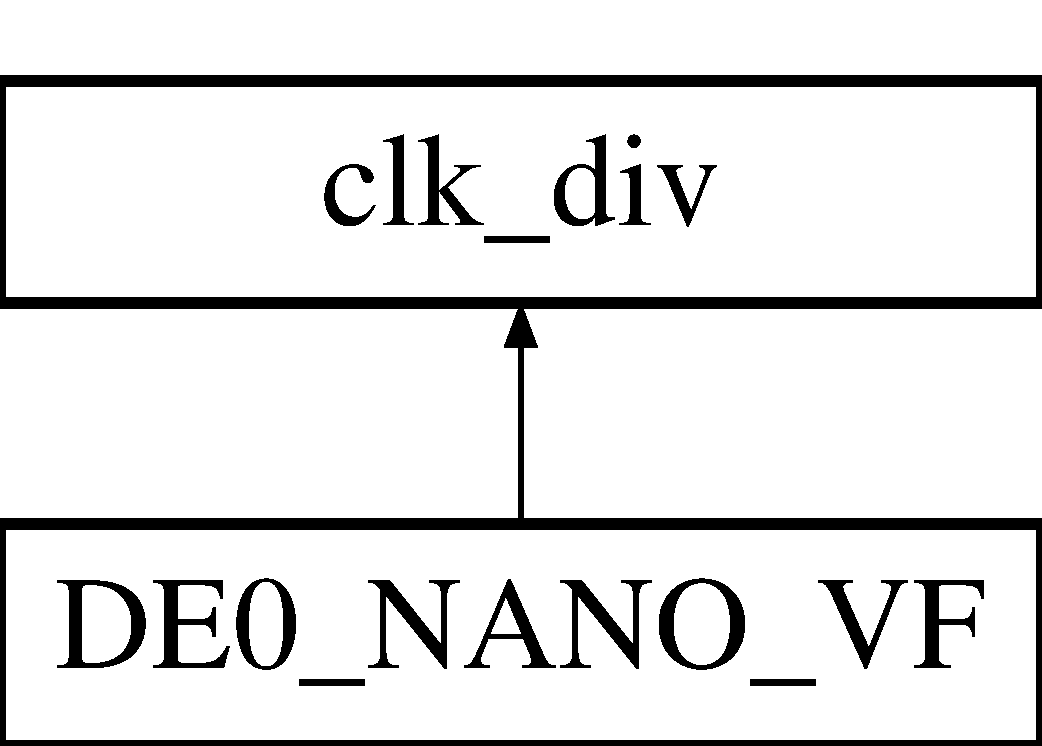
\includegraphics[height=2.000000cm]{classclk__div}
\end{center}
\end{figure}
\subsection*{Entities}
\begin{DoxyCompactItemize}
\item 
\hyperlink{classclk__div_1_1div}{div} architecture
\end{DoxyCompactItemize}
\subsection*{Libraries}
 \begin{DoxyCompactItemize}
\item 
\hyperlink{classclk__div_ae4f03c286607f3181e16b9aa12d0c6d4}{I\+E\+E\+E} 
\end{DoxyCompactItemize}
\subsection*{Use Clauses}
 \begin{DoxyCompactItemize}
\item 
\hyperlink{classclk__div_a241c3e72dd8024cc8ae831b1b2aed7db}{S\+T\+D\+\_\+\+L\+O\+G\+I\+C\+\_\+\+U\+N\+S\+I\+G\+N\+E\+D}   
\item 
\hyperlink{classclk__div_aa4b2b25246a821511120e3149b003563}{S\+T\+D\+\_\+\+L\+O\+G\+I\+C\+\_\+1164}   
\end{DoxyCompactItemize}
\subsection*{Ports}
 \begin{DoxyCompactItemize}
\item 
\hyperlink{classclk__div_a57fad7f33f7766724bdea76e7b0330ef}{clk\+\_\+in}  {\bfseries {\bfseries \textcolor{keywordflow}{in}\textcolor{vhdlchar}{ }}} {\bfseries \textcolor{comment}{S\+T\+D\+\_\+\+L\+O\+G\+I\+C}\textcolor{vhdlchar}{ }} 
\item 
\hyperlink{classclk__div_a512588aa484615b7e90600a1bc9507b4}{en}  {\bfseries {\bfseries \textcolor{keywordflow}{in}\textcolor{vhdlchar}{ }}} {\bfseries \textcolor{comment}{S\+T\+D\+\_\+\+L\+O\+G\+I\+C}\textcolor{vhdlchar}{ }} 
\item 
\hyperlink{classclk__div_a425c2042b3ea21827b9b29c6712312d9}{div}  {\bfseries {\bfseries \textcolor{keywordflow}{in}\textcolor{vhdlchar}{ }}} {\bfseries \textcolor{comment}{S\+T\+D\+\_\+\+L\+O\+G\+I\+C\+\_\+\+V\+E\+C\+T\+O\+R}\textcolor{vhdlchar}{ }\textcolor{vhdlchar}{(}\textcolor{vhdlchar}{ }\textcolor{vhdlchar}{ } \textcolor{vhdldigit}{15} \textcolor{vhdlchar}{ }\textcolor{keywordflow}{D\+O\+W\+N\+T\+O}\textcolor{vhdlchar}{ }\textcolor{vhdlchar}{ } \textcolor{vhdldigit}{0} \textcolor{vhdlchar}{ }\textcolor{vhdlchar}{)}\textcolor{vhdlchar}{ }} 
\item 
\hyperlink{classclk__div_a8147ca5cedee84ed9753ac6f1f0b2374}{clk\+\_\+out}  {\bfseries {\bfseries \textcolor{keywordflow}{out}\textcolor{vhdlchar}{ }}} {\bfseries \textcolor{comment}{S\+T\+D\+\_\+\+L\+O\+G\+I\+C}\textcolor{vhdlchar}{ }} 
\end{DoxyCompactItemize}


\subsection{Detailed Description}


Definition at line 5 of file clk\+\_\+div.\+vhd.



\subsection{Member Data Documentation}
\hypertarget{classclk__div_a57fad7f33f7766724bdea76e7b0330ef}{}\index{clk\+\_\+div@{clk\+\_\+div}!clk\+\_\+in@{clk\+\_\+in}}
\index{clk\+\_\+in@{clk\+\_\+in}!clk\+\_\+div@{clk\+\_\+div}}
\subsubsection[{clk\+\_\+in}]{\setlength{\rightskip}{0pt plus 5cm}{\bf clk\+\_\+in} {\bfseries \textcolor{keywordflow}{in}\textcolor{vhdlchar}{ }} {\bfseries \textcolor{comment}{S\+T\+D\+\_\+\+L\+O\+G\+I\+C}\textcolor{vhdlchar}{ }} \hspace{0.3cm}{\ttfamily [Port]}}\label{classclk__div_a57fad7f33f7766724bdea76e7b0330ef}


Definition at line 7 of file clk\+\_\+div.\+vhd.

\hypertarget{classclk__div_a8147ca5cedee84ed9753ac6f1f0b2374}{}\index{clk\+\_\+div@{clk\+\_\+div}!clk\+\_\+out@{clk\+\_\+out}}
\index{clk\+\_\+out@{clk\+\_\+out}!clk\+\_\+div@{clk\+\_\+div}}
\subsubsection[{clk\+\_\+out}]{\setlength{\rightskip}{0pt plus 5cm}{\bf clk\+\_\+out} {\bfseries \textcolor{keywordflow}{out}\textcolor{vhdlchar}{ }} {\bfseries \textcolor{comment}{S\+T\+D\+\_\+\+L\+O\+G\+I\+C}\textcolor{vhdlchar}{ }} \hspace{0.3cm}{\ttfamily [Port]}}\label{classclk__div_a8147ca5cedee84ed9753ac6f1f0b2374}


Definition at line 10 of file clk\+\_\+div.\+vhd.

\hypertarget{classclk__div_a425c2042b3ea21827b9b29c6712312d9}{}\index{clk\+\_\+div@{clk\+\_\+div}!div@{div}}
\index{div@{div}!clk\+\_\+div@{clk\+\_\+div}}
\subsubsection[{div}]{\setlength{\rightskip}{0pt plus 5cm}{\bf div} {\bfseries \textcolor{keywordflow}{in}\textcolor{vhdlchar}{ }} {\bfseries \textcolor{comment}{S\+T\+D\+\_\+\+L\+O\+G\+I\+C\+\_\+\+V\+E\+C\+T\+O\+R}\textcolor{vhdlchar}{ }\textcolor{vhdlchar}{(}\textcolor{vhdlchar}{ }\textcolor{vhdlchar}{ } \textcolor{vhdldigit}{15} \textcolor{vhdlchar}{ }\textcolor{keywordflow}{D\+O\+W\+N\+T\+O}\textcolor{vhdlchar}{ }\textcolor{vhdlchar}{ } \textcolor{vhdldigit}{0} \textcolor{vhdlchar}{ }\textcolor{vhdlchar}{)}\textcolor{vhdlchar}{ }} \hspace{0.3cm}{\ttfamily [Port]}}\label{classclk__div_a425c2042b3ea21827b9b29c6712312d9}


Definition at line 8 of file clk\+\_\+div.\+vhd.

\hypertarget{classclk__div_a512588aa484615b7e90600a1bc9507b4}{}\index{clk\+\_\+div@{clk\+\_\+div}!en@{en}}
\index{en@{en}!clk\+\_\+div@{clk\+\_\+div}}
\subsubsection[{en}]{\setlength{\rightskip}{0pt plus 5cm}{\bf en} {\bfseries \textcolor{keywordflow}{in}\textcolor{vhdlchar}{ }} {\bfseries \textcolor{comment}{S\+T\+D\+\_\+\+L\+O\+G\+I\+C}\textcolor{vhdlchar}{ }} \hspace{0.3cm}{\ttfamily [Port]}}\label{classclk__div_a512588aa484615b7e90600a1bc9507b4}


Definition at line 7 of file clk\+\_\+div.\+vhd.

\hypertarget{classclk__div_ae4f03c286607f3181e16b9aa12d0c6d4}{}\index{clk\+\_\+div@{clk\+\_\+div}!I\+E\+E\+E@{I\+E\+E\+E}}
\index{I\+E\+E\+E@{I\+E\+E\+E}!clk\+\_\+div@{clk\+\_\+div}}
\subsubsection[{I\+E\+E\+E}]{\setlength{\rightskip}{0pt plus 5cm}{\bf I\+E\+E\+E}\hspace{0.3cm}{\ttfamily [Library]}}\label{classclk__div_ae4f03c286607f3181e16b9aa12d0c6d4}


Definition at line 1 of file clk\+\_\+div.\+vhd.

\hypertarget{classclk__div_aa4b2b25246a821511120e3149b003563}{}\index{clk\+\_\+div@{clk\+\_\+div}!S\+T\+D\+\_\+\+L\+O\+G\+I\+C\+\_\+1164@{S\+T\+D\+\_\+\+L\+O\+G\+I\+C\+\_\+1164}}
\index{S\+T\+D\+\_\+\+L\+O\+G\+I\+C\+\_\+1164@{S\+T\+D\+\_\+\+L\+O\+G\+I\+C\+\_\+1164}!clk\+\_\+div@{clk\+\_\+div}}
\subsubsection[{S\+T\+D\+\_\+\+L\+O\+G\+I\+C\+\_\+1164}]{\setlength{\rightskip}{0pt plus 5cm}{\bf S\+T\+D\+\_\+\+L\+O\+G\+I\+C\+\_\+1164}\hspace{0.3cm}{\ttfamily [Package]}}\label{classclk__div_aa4b2b25246a821511120e3149b003563}


Definition at line 3 of file clk\+\_\+div.\+vhd.

\hypertarget{classclk__div_a241c3e72dd8024cc8ae831b1b2aed7db}{}\index{clk\+\_\+div@{clk\+\_\+div}!S\+T\+D\+\_\+\+L\+O\+G\+I\+C\+\_\+\+U\+N\+S\+I\+G\+N\+E\+D@{S\+T\+D\+\_\+\+L\+O\+G\+I\+C\+\_\+\+U\+N\+S\+I\+G\+N\+E\+D}}
\index{S\+T\+D\+\_\+\+L\+O\+G\+I\+C\+\_\+\+U\+N\+S\+I\+G\+N\+E\+D@{S\+T\+D\+\_\+\+L\+O\+G\+I\+C\+\_\+\+U\+N\+S\+I\+G\+N\+E\+D}!clk\+\_\+div@{clk\+\_\+div}}
\subsubsection[{S\+T\+D\+\_\+\+L\+O\+G\+I\+C\+\_\+\+U\+N\+S\+I\+G\+N\+E\+D}]{\setlength{\rightskip}{0pt plus 5cm}{\bf S\+T\+D\+\_\+\+L\+O\+G\+I\+C\+\_\+\+U\+N\+S\+I\+G\+N\+E\+D}\hspace{0.3cm}{\ttfamily [Package]}}\label{classclk__div_a241c3e72dd8024cc8ae831b1b2aed7db}


Definition at line 2 of file clk\+\_\+div.\+vhd.



The documentation for this class was generated from the following file\+:\begin{DoxyCompactItemize}
\item 
\hyperlink{clk__div_8vhd}{clk\+\_\+div.\+vhd}\end{DoxyCompactItemize}

\hypertarget{classcomparador_1_1comparador}{}\section{comparador Architecture Reference}
\label{classcomparador_1_1comparador}\index{comparador@{comparador}}
\subsection*{Processes}
 \begin{DoxyCompactItemize}
\item 
\hyperlink{classcomparador_1_1comparador_a67cbd29443fafed2b0446c1321a8e91c}{P\+R\+O\+C\+E\+S\+S\+\_\+1}{\bfseries  ( {\bfseries {\bfseries \hyperlink{classcomparador_a4a4609c199d30b3adebbeb3a01276ec5}{clk}} \textcolor{vhdlchar}{ }} )}
\item 
\hyperlink{classcomparador_1_1comparador_ab820ba1b225bbde57824e0ed4510038c}{P\+R\+O\+C\+E\+S\+S\+\_\+2}{\bfseries  ( {\bfseries {\bfseries \hyperlink{classcomparador_af9b8278b961604ab62a822537a109adb}{amost}} \textcolor{vhdlchar}{ }} )}
\end{DoxyCompactItemize}
\subsection*{Signals}
 \begin{DoxyCompactItemize}
\item 
\hyperlink{classcomparador_1_1comparador_abf7d8be25624dd08fcc1517c8e39cb23}{comp\+\_\+int} {\bfseries \textcolor{comment}{std\+\_\+logic\+\_\+vector}\textcolor{vhdlchar}{ }\textcolor{vhdlchar}{(}\textcolor{vhdlchar}{ }\textcolor{vhdlchar}{ }\textcolor{vhdlchar}{ }\textcolor{vhdlchar}{ }{\bfseries \hyperlink{classcomparador_afee4aa1628956aa350183d8881689198}{n\+\_\+bits\+\_\+c}} \textcolor{vhdlchar}{-\/}\textcolor{vhdlchar}{ } \textcolor{vhdldigit}{1} \textcolor{vhdlchar}{ }\textcolor{keywordflow}{downto}\textcolor{vhdlchar}{ }\textcolor{vhdlchar}{ } \textcolor{vhdldigit}{0} \textcolor{vhdlchar}{ }\textcolor{vhdlchar}{)}\textcolor{vhdlchar}{ }} 
\end{DoxyCompactItemize}


\subsection{Detailed Description}


Definition at line \hyperlink{comparador_8vhd_source_l00024}{24} of file \hyperlink{comparador_8vhd_source}{comparador.\+vhd}.



\subsection{Member Function Documentation}
\hypertarget{classcomparador_1_1comparador_a67cbd29443fafed2b0446c1321a8e91c}{}\index{comparador\+::comparador@{comparador\+::comparador}!P\+R\+O\+C\+E\+S\+S\+\_\+1@{P\+R\+O\+C\+E\+S\+S\+\_\+1}}
\index{P\+R\+O\+C\+E\+S\+S\+\_\+1@{P\+R\+O\+C\+E\+S\+S\+\_\+1}!comparador\+::comparador@{comparador\+::comparador}}
\subsubsection[{P\+R\+O\+C\+E\+S\+S\+\_\+1}]{\setlength{\rightskip}{0pt plus 5cm} {\bfseries \textcolor{vhdlchar}{ }} P\+R\+O\+C\+E\+S\+S\+\_\+1(
\begin{DoxyParamCaption}
\item[{}]{{\bfseries {\bfseries {\bf clk}} \textcolor{vhdlchar}{ }} {\em }}
\end{DoxyParamCaption}
)\hspace{0.3cm}{\ttfamily [Process]}}\label{classcomparador_1_1comparador_a67cbd29443fafed2b0446c1321a8e91c}


Definition at line \hyperlink{comparador_8vhd_source_l00032}{32} of file \hyperlink{comparador_8vhd_source}{comparador.\+vhd}.

\hypertarget{classcomparador_1_1comparador_ab820ba1b225bbde57824e0ed4510038c}{}\index{comparador\+::comparador@{comparador\+::comparador}!P\+R\+O\+C\+E\+S\+S\+\_\+2@{P\+R\+O\+C\+E\+S\+S\+\_\+2}}
\index{P\+R\+O\+C\+E\+S\+S\+\_\+2@{P\+R\+O\+C\+E\+S\+S\+\_\+2}!comparador\+::comparador@{comparador\+::comparador}}
\subsubsection[{P\+R\+O\+C\+E\+S\+S\+\_\+2}]{\setlength{\rightskip}{0pt plus 5cm} {\bfseries \textcolor{vhdlchar}{ }} P\+R\+O\+C\+E\+S\+S\+\_\+2(
\begin{DoxyParamCaption}
\item[{}]{{\bfseries {\bfseries {\bf amost}} \textcolor{vhdlchar}{ }} {\em }}
\end{DoxyParamCaption}
)\hspace{0.3cm}{\ttfamily [Process]}}\label{classcomparador_1_1comparador_ab820ba1b225bbde57824e0ed4510038c}


Definition at line \hyperlink{comparador_8vhd_source_l00045}{45} of file \hyperlink{comparador_8vhd_source}{comparador.\+vhd}.



\subsection{Member Data Documentation}
\hypertarget{classcomparador_1_1comparador_abf7d8be25624dd08fcc1517c8e39cb23}{}\index{comparador\+::comparador@{comparador\+::comparador}!comp\+\_\+int@{comp\+\_\+int}}
\index{comp\+\_\+int@{comp\+\_\+int}!comparador\+::comparador@{comparador\+::comparador}}
\subsubsection[{comp\+\_\+int}]{\setlength{\rightskip}{0pt plus 5cm}{\bf comp\+\_\+int} {\bfseries \textcolor{comment}{std\+\_\+logic\+\_\+vector}\textcolor{vhdlchar}{ }\textcolor{vhdlchar}{(}\textcolor{vhdlchar}{ }\textcolor{vhdlchar}{ }\textcolor{vhdlchar}{ }\textcolor{vhdlchar}{ }{\bfseries {\bf n\+\_\+bits\+\_\+c}} \textcolor{vhdlchar}{-\/}\textcolor{vhdlchar}{ } \textcolor{vhdldigit}{1} \textcolor{vhdlchar}{ }\textcolor{keywordflow}{downto}\textcolor{vhdlchar}{ }\textcolor{vhdlchar}{ } \textcolor{vhdldigit}{0} \textcolor{vhdlchar}{ }\textcolor{vhdlchar}{)}\textcolor{vhdlchar}{ }} \hspace{0.3cm}{\ttfamily [Signal]}}\label{classcomparador_1_1comparador_abf7d8be25624dd08fcc1517c8e39cb23}


Definition at line \hyperlink{comparador_8vhd_source_l00027}{27} of file \hyperlink{comparador_8vhd_source}{comparador.\+vhd}.



The documentation for this class was generated from the following file\+:\begin{DoxyCompactItemize}
\item 
\hyperlink{comparador_8vhd}{comparador.\+vhd}\end{DoxyCompactItemize}

\hypertarget{classcomparador}{}\section{comparador Entity Reference}
\label{classcomparador}\index{comparador@{comparador}}
Inheritance diagram for comparador\+:\begin{figure}[H]
\begin{center}
\leavevmode
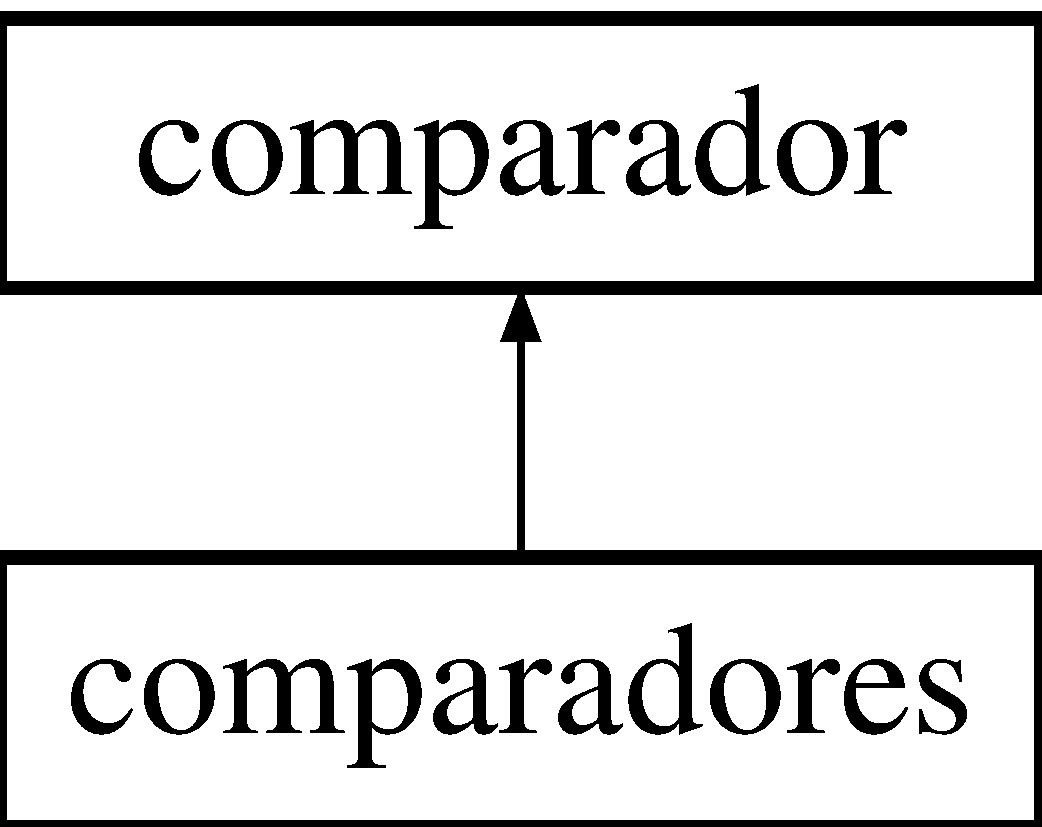
\includegraphics[height=2.000000cm]{classcomparador}
\end{center}
\end{figure}
\subsection*{Entities}
\begin{DoxyCompactItemize}
\item 
\hyperlink{classcomparador_1_1comparador}{comparador} architecture
\end{DoxyCompactItemize}
\subsection*{Libraries}
 \begin{DoxyCompactItemize}
\item 
\hyperlink{classcomparador_ae4f03c286607f3181e16b9aa12d0c6d4}{I\+E\+E\+E} 
\end{DoxyCompactItemize}
\subsection*{Use Clauses}
 \begin{DoxyCompactItemize}
\item 
\hyperlink{classcomparador_a241c3e72dd8024cc8ae831b1b2aed7db}{S\+T\+D\+\_\+\+L\+O\+G\+I\+C\+\_\+\+U\+N\+S\+I\+G\+N\+E\+D}   
\item 
\hyperlink{classcomparador_aa4b2b25246a821511120e3149b003563}{S\+T\+D\+\_\+\+L\+O\+G\+I\+C\+\_\+1164}   
\item 
\hyperlink{classcomparador_aad86249c80e8c1e7ee1c4748aba748e3}{fixed\+\_\+pkg}   
\item 
\hyperlink{classcomparador_a2edc34402b573437d5f25fa90ba4013e}{numeric\+\_\+std}   
\end{DoxyCompactItemize}
\subsection*{Generics}
 \begin{DoxyCompactItemize}
\item 
\hyperlink{classcomparador_afee4aa1628956aa350183d8881689198}{n\+\_\+bits\+\_\+c} {\bfseries {\bfseries \textcolor{comment}{integer}\textcolor{vhdlchar}{ }\textcolor{vhdlchar}{ }\textcolor{vhdlchar}{\+:}\textcolor{vhdlchar}{=}\textcolor{vhdlchar}{ }\textcolor{vhdlchar}{ } \textcolor{vhdldigit}{16} \textcolor{vhdlchar}{ }}}
\end{DoxyCompactItemize}
\subsection*{Ports}
 \begin{DoxyCompactItemize}
\item 
\hyperlink{classcomparador_a4a4609c199d30b3adebbeb3a01276ec5}{clk}  {\bfseries {\bfseries \textcolor{keywordflow}{in}\textcolor{vhdlchar}{ }}} {\bfseries \textcolor{comment}{std\+\_\+logic}\textcolor{vhdlchar}{ }} 
\item 
\hyperlink{classcomparador_adcf9c6f5161d039addbda5819bee64a3}{en}  {\bfseries {\bfseries \textcolor{keywordflow}{in}\textcolor{vhdlchar}{ }}} {\bfseries \textcolor{comment}{std\+\_\+logic}\textcolor{vhdlchar}{ }} 
\item 
\hyperlink{classcomparador_a0c2a0581e706d5256b50516b6ca4dbed}{comp}  {\bfseries {\bfseries \textcolor{keywordflow}{in}\textcolor{vhdlchar}{ }}} {\bfseries \textcolor{comment}{std\+\_\+logic\+\_\+vector}\textcolor{vhdlchar}{ }\textcolor{vhdlchar}{(}\textcolor{vhdlchar}{ }\textcolor{vhdlchar}{ }\textcolor{vhdlchar}{ }\textcolor{vhdlchar}{ }{\bfseries \hyperlink{classcomparador_afee4aa1628956aa350183d8881689198}{n\+\_\+bits\+\_\+c}} \textcolor{vhdlchar}{-\/}\textcolor{vhdlchar}{ } \textcolor{vhdldigit}{1} \textcolor{vhdlchar}{ }\textcolor{keywordflow}{downto}\textcolor{vhdlchar}{ }\textcolor{vhdlchar}{ } \textcolor{vhdldigit}{0} \textcolor{vhdlchar}{ }\textcolor{vhdlchar}{)}\textcolor{vhdlchar}{ }} 
\item 
\hyperlink{classcomparador_a0808bf3e7965a8ee90dec6604647f179}{c}  {\bfseries {\bfseries \textcolor{keywordflow}{in}\textcolor{vhdlchar}{ }}} {\bfseries \textcolor{comment}{std\+\_\+logic\+\_\+vector}\textcolor{vhdlchar}{ }\textcolor{vhdlchar}{(}\textcolor{vhdlchar}{ }\textcolor{vhdlchar}{ }\textcolor{vhdlchar}{ }\textcolor{vhdlchar}{ }{\bfseries \hyperlink{classcomparador_afee4aa1628956aa350183d8881689198}{n\+\_\+bits\+\_\+c}} \textcolor{vhdlchar}{-\/}\textcolor{vhdlchar}{ } \textcolor{vhdldigit}{1} \textcolor{vhdlchar}{ }\textcolor{keywordflow}{downto}\textcolor{vhdlchar}{ }\textcolor{vhdlchar}{ } \textcolor{vhdldigit}{0} \textcolor{vhdlchar}{ }\textcolor{vhdlchar}{)}\textcolor{vhdlchar}{ }} 
\item 
\hyperlink{classcomparador_af9b8278b961604ab62a822537a109adb}{amost}  {\bfseries {\bfseries \textcolor{keywordflow}{in}\textcolor{vhdlchar}{ }}} {\bfseries \textcolor{comment}{std\+\_\+logic}\textcolor{vhdlchar}{ }} 
\item 
\hyperlink{classcomparador_a2522d63dc2aa0652b3cca6ac9b1da0bd}{comp\+\_\+out}  {\bfseries {\bfseries \textcolor{keywordflow}{out}\textcolor{vhdlchar}{ }}} {\bfseries \textcolor{comment}{std\+\_\+logic}\textcolor{vhdlchar}{ }} 
\end{DoxyCompactItemize}


\subsection{Detailed Description}


Definition at line 8 of file comparador.\+vhd.



\subsection{Member Data Documentation}
\hypertarget{classcomparador_af9b8278b961604ab62a822537a109adb}{}\index{comparador@{comparador}!amost@{amost}}
\index{amost@{amost}!comparador@{comparador}}
\subsubsection[{amost}]{\setlength{\rightskip}{0pt plus 5cm}{\bf amost} {\bfseries \textcolor{keywordflow}{in}\textcolor{vhdlchar}{ }} {\bfseries \textcolor{comment}{std\+\_\+logic}\textcolor{vhdlchar}{ }} \hspace{0.3cm}{\ttfamily [Port]}}\label{classcomparador_af9b8278b961604ab62a822537a109adb}


Definition at line 17 of file comparador.\+vhd.

\hypertarget{classcomparador_a0808bf3e7965a8ee90dec6604647f179}{}\index{comparador@{comparador}!c@{c}}
\index{c@{c}!comparador@{comparador}}
\subsubsection[{c}]{\setlength{\rightskip}{0pt plus 5cm}{\bf c} {\bfseries \textcolor{keywordflow}{in}\textcolor{vhdlchar}{ }} {\bfseries \textcolor{comment}{std\+\_\+logic\+\_\+vector}\textcolor{vhdlchar}{ }\textcolor{vhdlchar}{(}\textcolor{vhdlchar}{ }\textcolor{vhdlchar}{ }\textcolor{vhdlchar}{ }\textcolor{vhdlchar}{ }{\bfseries {\bf n\+\_\+bits\+\_\+c}} \textcolor{vhdlchar}{-\/}\textcolor{vhdlchar}{ } \textcolor{vhdldigit}{1} \textcolor{vhdlchar}{ }\textcolor{keywordflow}{downto}\textcolor{vhdlchar}{ }\textcolor{vhdlchar}{ } \textcolor{vhdldigit}{0} \textcolor{vhdlchar}{ }\textcolor{vhdlchar}{)}\textcolor{vhdlchar}{ }} \hspace{0.3cm}{\ttfamily [Port]}}\label{classcomparador_a0808bf3e7965a8ee90dec6604647f179}


Definition at line 16 of file comparador.\+vhd.

\hypertarget{classcomparador_a4a4609c199d30b3adebbeb3a01276ec5}{}\index{comparador@{comparador}!clk@{clk}}
\index{clk@{clk}!comparador@{comparador}}
\subsubsection[{clk}]{\setlength{\rightskip}{0pt plus 5cm}{\bf clk} {\bfseries \textcolor{keywordflow}{in}\textcolor{vhdlchar}{ }} {\bfseries \textcolor{comment}{std\+\_\+logic}\textcolor{vhdlchar}{ }} \hspace{0.3cm}{\ttfamily [Port]}}\label{classcomparador_a4a4609c199d30b3adebbeb3a01276ec5}


Definition at line 13 of file comparador.\+vhd.

\hypertarget{classcomparador_a0c2a0581e706d5256b50516b6ca4dbed}{}\index{comparador@{comparador}!comp@{comp}}
\index{comp@{comp}!comparador@{comparador}}
\subsubsection[{comp}]{\setlength{\rightskip}{0pt plus 5cm}{\bf comp} {\bfseries \textcolor{keywordflow}{in}\textcolor{vhdlchar}{ }} {\bfseries \textcolor{comment}{std\+\_\+logic\+\_\+vector}\textcolor{vhdlchar}{ }\textcolor{vhdlchar}{(}\textcolor{vhdlchar}{ }\textcolor{vhdlchar}{ }\textcolor{vhdlchar}{ }\textcolor{vhdlchar}{ }{\bfseries {\bf n\+\_\+bits\+\_\+c}} \textcolor{vhdlchar}{-\/}\textcolor{vhdlchar}{ } \textcolor{vhdldigit}{1} \textcolor{vhdlchar}{ }\textcolor{keywordflow}{downto}\textcolor{vhdlchar}{ }\textcolor{vhdlchar}{ } \textcolor{vhdldigit}{0} \textcolor{vhdlchar}{ }\textcolor{vhdlchar}{)}\textcolor{vhdlchar}{ }} \hspace{0.3cm}{\ttfamily [Port]}}\label{classcomparador_a0c2a0581e706d5256b50516b6ca4dbed}


Definition at line 15 of file comparador.\+vhd.

\hypertarget{classcomparador_a2522d63dc2aa0652b3cca6ac9b1da0bd}{}\index{comparador@{comparador}!comp\+\_\+out@{comp\+\_\+out}}
\index{comp\+\_\+out@{comp\+\_\+out}!comparador@{comparador}}
\subsubsection[{comp\+\_\+out}]{\setlength{\rightskip}{0pt plus 5cm}{\bf comp\+\_\+out} {\bfseries \textcolor{keywordflow}{out}\textcolor{vhdlchar}{ }} {\bfseries \textcolor{comment}{std\+\_\+logic}\textcolor{vhdlchar}{ }} \hspace{0.3cm}{\ttfamily [Port]}}\label{classcomparador_a2522d63dc2aa0652b3cca6ac9b1da0bd}


Definition at line 19 of file comparador.\+vhd.

\hypertarget{classcomparador_adcf9c6f5161d039addbda5819bee64a3}{}\index{comparador@{comparador}!en@{en}}
\index{en@{en}!comparador@{comparador}}
\subsubsection[{en}]{\setlength{\rightskip}{0pt plus 5cm}{\bf en} {\bfseries \textcolor{keywordflow}{in}\textcolor{vhdlchar}{ }} {\bfseries \textcolor{comment}{std\+\_\+logic}\textcolor{vhdlchar}{ }} \hspace{0.3cm}{\ttfamily [Port]}}\label{classcomparador_adcf9c6f5161d039addbda5819bee64a3}


Definition at line 14 of file comparador.\+vhd.

\hypertarget{classcomparador_aad86249c80e8c1e7ee1c4748aba748e3}{}\index{comparador@{comparador}!fixed\+\_\+pkg@{fixed\+\_\+pkg}}
\index{fixed\+\_\+pkg@{fixed\+\_\+pkg}!comparador@{comparador}}
\subsubsection[{fixed\+\_\+pkg}]{\setlength{\rightskip}{0pt plus 5cm}{\bf fixed\+\_\+pkg}\hspace{0.3cm}{\ttfamily [Package]}}\label{classcomparador_aad86249c80e8c1e7ee1c4748aba748e3}


Definition at line 5 of file comparador.\+vhd.

\hypertarget{classcomparador_ae4f03c286607f3181e16b9aa12d0c6d4}{}\index{comparador@{comparador}!I\+E\+E\+E@{I\+E\+E\+E}}
\index{I\+E\+E\+E@{I\+E\+E\+E}!comparador@{comparador}}
\subsubsection[{I\+E\+E\+E}]{\setlength{\rightskip}{0pt plus 5cm}{\bf I\+E\+E\+E}\hspace{0.3cm}{\ttfamily [Library]}}\label{classcomparador_ae4f03c286607f3181e16b9aa12d0c6d4}


Definition at line 2 of file comparador.\+vhd.

\hypertarget{classcomparador_afee4aa1628956aa350183d8881689198}{}\index{comparador@{comparador}!n\+\_\+bits\+\_\+c@{n\+\_\+bits\+\_\+c}}
\index{n\+\_\+bits\+\_\+c@{n\+\_\+bits\+\_\+c}!comparador@{comparador}}
\subsubsection[{n\+\_\+bits\+\_\+c}]{\setlength{\rightskip}{0pt plus 5cm}{\bf n\+\_\+bits\+\_\+c} {\bfseries \textcolor{vhdlchar}{ }} {\bfseries \textcolor{comment}{integer}\textcolor{vhdlchar}{ }\textcolor{vhdlchar}{ }\textcolor{vhdlchar}{\+:}\textcolor{vhdlchar}{=}\textcolor{vhdlchar}{ }\textcolor{vhdlchar}{ } \textcolor{vhdldigit}{16} \textcolor{vhdlchar}{ }} \hspace{0.3cm}{\ttfamily [Generic]}}\label{classcomparador_afee4aa1628956aa350183d8881689198}


Definition at line 11 of file comparador.\+vhd.

\hypertarget{classcomparador_a2edc34402b573437d5f25fa90ba4013e}{}\index{comparador@{comparador}!numeric\+\_\+std@{numeric\+\_\+std}}
\index{numeric\+\_\+std@{numeric\+\_\+std}!comparador@{comparador}}
\subsubsection[{numeric\+\_\+std}]{\setlength{\rightskip}{0pt plus 5cm}{\bf numeric\+\_\+std}\hspace{0.3cm}{\ttfamily [Package]}}\label{classcomparador_a2edc34402b573437d5f25fa90ba4013e}


Definition at line 6 of file comparador.\+vhd.

\hypertarget{classcomparador_aa4b2b25246a821511120e3149b003563}{}\index{comparador@{comparador}!S\+T\+D\+\_\+\+L\+O\+G\+I\+C\+\_\+1164@{S\+T\+D\+\_\+\+L\+O\+G\+I\+C\+\_\+1164}}
\index{S\+T\+D\+\_\+\+L\+O\+G\+I\+C\+\_\+1164@{S\+T\+D\+\_\+\+L\+O\+G\+I\+C\+\_\+1164}!comparador@{comparador}}
\subsubsection[{S\+T\+D\+\_\+\+L\+O\+G\+I\+C\+\_\+1164}]{\setlength{\rightskip}{0pt plus 5cm}{\bf S\+T\+D\+\_\+\+L\+O\+G\+I\+C\+\_\+1164}\hspace{0.3cm}{\ttfamily [Package]}}\label{classcomparador_aa4b2b25246a821511120e3149b003563}


Definition at line 4 of file comparador.\+vhd.

\hypertarget{classcomparador_a241c3e72dd8024cc8ae831b1b2aed7db}{}\index{comparador@{comparador}!S\+T\+D\+\_\+\+L\+O\+G\+I\+C\+\_\+\+U\+N\+S\+I\+G\+N\+E\+D@{S\+T\+D\+\_\+\+L\+O\+G\+I\+C\+\_\+\+U\+N\+S\+I\+G\+N\+E\+D}}
\index{S\+T\+D\+\_\+\+L\+O\+G\+I\+C\+\_\+\+U\+N\+S\+I\+G\+N\+E\+D@{S\+T\+D\+\_\+\+L\+O\+G\+I\+C\+\_\+\+U\+N\+S\+I\+G\+N\+E\+D}!comparador@{comparador}}
\subsubsection[{S\+T\+D\+\_\+\+L\+O\+G\+I\+C\+\_\+\+U\+N\+S\+I\+G\+N\+E\+D}]{\setlength{\rightskip}{0pt plus 5cm}{\bf S\+T\+D\+\_\+\+L\+O\+G\+I\+C\+\_\+\+U\+N\+S\+I\+G\+N\+E\+D}\hspace{0.3cm}{\ttfamily [Package]}}\label{classcomparador_a241c3e72dd8024cc8ae831b1b2aed7db}


Definition at line 3 of file comparador.\+vhd.



The documentation for this class was generated from the following file\+:\begin{DoxyCompactItemize}
\item 
\hyperlink{comparador_8vhd}{comparador.\+vhd}\end{DoxyCompactItemize}

\hypertarget{classcomparadores}{}\section{comparadores Entity Reference}
\label{classcomparadores}\index{comparadores@{comparadores}}
Inheritance diagram for comparadores\+:\begin{figure}[H]
\begin{center}
\leavevmode
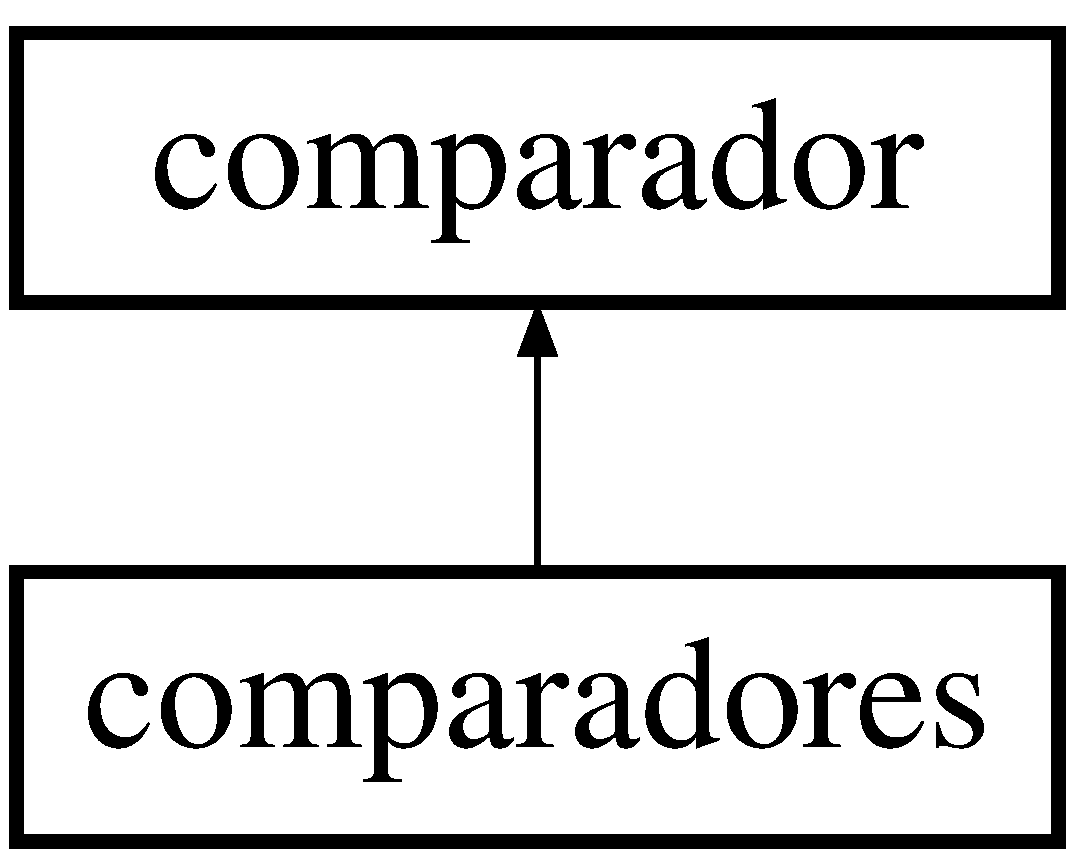
\includegraphics[height=2.000000cm]{classcomparadores}
\end{center}
\end{figure}
\subsection*{Entities}
\begin{DoxyCompactItemize}
\item 
\hyperlink{classcomparadores_1_1comparadores}{comparadores} architecture
\end{DoxyCompactItemize}
\subsection*{Libraries}
 \begin{DoxyCompactItemize}
\item 
\hyperlink{classcomparadores_ae4f03c286607f3181e16b9aa12d0c6d4}{I\+E\+E\+E} 
\end{DoxyCompactItemize}
\subsection*{Use Clauses}
 \begin{DoxyCompactItemize}
\item 
\hyperlink{classcomparadores_a241c3e72dd8024cc8ae831b1b2aed7db}{S\+T\+D\+\_\+\+L\+O\+G\+I\+C\+\_\+\+U\+N\+S\+I\+G\+N\+E\+D}   
\item 
\hyperlink{classcomparadores_aa4b2b25246a821511120e3149b003563}{S\+T\+D\+\_\+\+L\+O\+G\+I\+C\+\_\+1164}   
\item 
\hyperlink{classcomparadores_aad86249c80e8c1e7ee1c4748aba748e3}{fixed\+\_\+pkg}   
\item 
\hyperlink{classcomparadores_a2edc34402b573437d5f25fa90ba4013e}{numeric\+\_\+std}   
\item 
\hyperlink{classcomparadores_ac1788a894930eeee5aaed06b4775d746}{my\+\_\+types\+\_\+pkg}   
\end{DoxyCompactItemize}
\subsection*{Generics}
 \begin{DoxyCompactItemize}
\item 
\hyperlink{classcomparadores_a601f7f505b21fa95d9d2e36075d21041}{M\+A\+X} {\bfseries {\bfseries \textcolor{comment}{integer}\textcolor{vhdlchar}{ }\textcolor{vhdlchar}{ }\textcolor{vhdlchar}{\+:}\textcolor{vhdlchar}{=}\textcolor{vhdlchar}{ }\textcolor{vhdlchar}{ } \textcolor{vhdldigit}{3526000} \textcolor{vhdlchar}{ }}}
\item 
\hyperlink{classcomparadores_a363fe57541ccc1caaeb5b14dcf01182d}{n\+\_\+bits\+\_\+c} {\bfseries {\bfseries \textcolor{comment}{integer}\textcolor{vhdlchar}{ }\textcolor{vhdlchar}{ }\textcolor{vhdlchar}{\+:}\textcolor{vhdlchar}{=}\textcolor{vhdlchar}{ }\textcolor{vhdlchar}{ } \textcolor{vhdldigit}{22} \textcolor{vhdlchar}{ }}}
\end{DoxyCompactItemize}
\subsection*{Ports}
 \begin{DoxyCompactItemize}
\item 
\hyperlink{classcomparadores_a4a4609c199d30b3adebbeb3a01276ec5}{clk}  {\bfseries {\bfseries \textcolor{keywordflow}{in}\textcolor{vhdlchar}{ }}} {\bfseries \textcolor{comment}{std\+\_\+logic}\textcolor{vhdlchar}{ }} 
\item 
\hyperlink{classcomparadores_adcf9c6f5161d039addbda5819bee64a3}{en}  {\bfseries {\bfseries \textcolor{keywordflow}{in}\textcolor{vhdlchar}{ }}} {\bfseries \textcolor{comment}{std\+\_\+logic}\textcolor{vhdlchar}{ }} 
\item 
\hyperlink{classcomparadores_ab73cec596619a058f732a10e71d5aada}{comp}  {\bfseries {\bfseries \textcolor{keywordflow}{in}\textcolor{vhdlchar}{ }}} {\bfseries {\bfseries \hyperlink{classmy__types__pkg_ae9b90869e95e036baa1ead1b6238589a}{C\+O\+M\+P\+\_\+\+A\+R\+R\+A\+Y}} \textcolor{vhdlchar}{ }} 
\item 
\hyperlink{classcomparadores_ab52608f377848fc687beeb76bb39a6e8}{c}  {\bfseries {\bfseries \textcolor{keywordflow}{in}\textcolor{vhdlchar}{ }}} {\bfseries {\bfseries \hyperlink{classmy__types__pkg_ae9b90869e95e036baa1ead1b6238589a}{C\+O\+M\+P\+\_\+\+A\+R\+R\+A\+Y}} \textcolor{vhdlchar}{ }} 
\item 
\hyperlink{classcomparadores_a0d7d8d086cf18e0180f8c280d76ed624}{amost}  {\bfseries {\bfseries \textcolor{keywordflow}{in}\textcolor{vhdlchar}{ }}} {\bfseries \textcolor{comment}{std\+\_\+logic\+\_\+vector}\textcolor{vhdlchar}{ }\textcolor{vhdlchar}{(}\textcolor{vhdlchar}{ }\textcolor{vhdlchar}{ } \textcolor{vhdldigit}{24} \textcolor{vhdlchar}{ }\textcolor{keywordflow}{downto}\textcolor{vhdlchar}{ }\textcolor{vhdlchar}{ } \textcolor{vhdldigit}{1} \textcolor{vhdlchar}{ }\textcolor{vhdlchar}{)}\textcolor{vhdlchar}{ }} 
\item 
\hyperlink{classcomparadores_a8d13d6e22531ac75ac0b437c61c6eb4f}{comp\+\_\+out}  {\bfseries {\bfseries \textcolor{keywordflow}{out}\textcolor{vhdlchar}{ }}} {\bfseries \textcolor{comment}{std\+\_\+logic\+\_\+vector}\textcolor{vhdlchar}{ }\textcolor{vhdlchar}{(}\textcolor{vhdlchar}{ }\textcolor{vhdlchar}{ } \textcolor{vhdldigit}{24} \textcolor{vhdlchar}{ }\textcolor{keywordflow}{downto}\textcolor{vhdlchar}{ }\textcolor{vhdlchar}{ } \textcolor{vhdldigit}{1} \textcolor{vhdlchar}{ }\textcolor{vhdlchar}{)}\textcolor{vhdlchar}{ }} 
\end{DoxyCompactItemize}


\subsection{Detailed Description}


Definition at line 19 of file comparadores.\+vhd.



\subsection{Member Data Documentation}
\hypertarget{classcomparadores_a0d7d8d086cf18e0180f8c280d76ed624}{}\index{comparadores@{comparadores}!amost@{amost}}
\index{amost@{amost}!comparadores@{comparadores}}
\subsubsection[{amost}]{\setlength{\rightskip}{0pt plus 5cm}{\bf amost} {\bfseries \textcolor{keywordflow}{in}\textcolor{vhdlchar}{ }} {\bfseries \textcolor{comment}{std\+\_\+logic\+\_\+vector}\textcolor{vhdlchar}{ }\textcolor{vhdlchar}{(}\textcolor{vhdlchar}{ }\textcolor{vhdlchar}{ } \textcolor{vhdldigit}{24} \textcolor{vhdlchar}{ }\textcolor{keywordflow}{downto}\textcolor{vhdlchar}{ }\textcolor{vhdlchar}{ } \textcolor{vhdldigit}{1} \textcolor{vhdlchar}{ }\textcolor{vhdlchar}{)}\textcolor{vhdlchar}{ }} \hspace{0.3cm}{\ttfamily [Port]}}\label{classcomparadores_a0d7d8d086cf18e0180f8c280d76ed624}


Definition at line 28 of file comparadores.\+vhd.

\hypertarget{classcomparadores_ab52608f377848fc687beeb76bb39a6e8}{}\index{comparadores@{comparadores}!c@{c}}
\index{c@{c}!comparadores@{comparadores}}
\subsubsection[{c}]{\setlength{\rightskip}{0pt plus 5cm}{\bf c} {\bfseries \textcolor{keywordflow}{in}\textcolor{vhdlchar}{ }} {\bfseries {\bfseries {\bf C\+O\+M\+P\+\_\+\+A\+R\+R\+A\+Y}} \textcolor{vhdlchar}{ }} \hspace{0.3cm}{\ttfamily [Port]}}\label{classcomparadores_ab52608f377848fc687beeb76bb39a6e8}


Definition at line 27 of file comparadores.\+vhd.

\hypertarget{classcomparadores_a4a4609c199d30b3adebbeb3a01276ec5}{}\index{comparadores@{comparadores}!clk@{clk}}
\index{clk@{clk}!comparadores@{comparadores}}
\subsubsection[{clk}]{\setlength{\rightskip}{0pt plus 5cm}{\bf clk} {\bfseries \textcolor{keywordflow}{in}\textcolor{vhdlchar}{ }} {\bfseries \textcolor{comment}{std\+\_\+logic}\textcolor{vhdlchar}{ }} \hspace{0.3cm}{\ttfamily [Port]}}\label{classcomparadores_a4a4609c199d30b3adebbeb3a01276ec5}


Definition at line 24 of file comparadores.\+vhd.

\hypertarget{classcomparadores_ab73cec596619a058f732a10e71d5aada}{}\index{comparadores@{comparadores}!comp@{comp}}
\index{comp@{comp}!comparadores@{comparadores}}
\subsubsection[{comp}]{\setlength{\rightskip}{0pt plus 5cm}{\bf comp} {\bfseries \textcolor{keywordflow}{in}\textcolor{vhdlchar}{ }} {\bfseries {\bfseries {\bf C\+O\+M\+P\+\_\+\+A\+R\+R\+A\+Y}} \textcolor{vhdlchar}{ }} \hspace{0.3cm}{\ttfamily [Port]}}\label{classcomparadores_ab73cec596619a058f732a10e71d5aada}


Definition at line 26 of file comparadores.\+vhd.

\hypertarget{classcomparadores_a8d13d6e22531ac75ac0b437c61c6eb4f}{}\index{comparadores@{comparadores}!comp\+\_\+out@{comp\+\_\+out}}
\index{comp\+\_\+out@{comp\+\_\+out}!comparadores@{comparadores}}
\subsubsection[{comp\+\_\+out}]{\setlength{\rightskip}{0pt plus 5cm}{\bf comp\+\_\+out} {\bfseries \textcolor{keywordflow}{out}\textcolor{vhdlchar}{ }} {\bfseries \textcolor{comment}{std\+\_\+logic\+\_\+vector}\textcolor{vhdlchar}{ }\textcolor{vhdlchar}{(}\textcolor{vhdlchar}{ }\textcolor{vhdlchar}{ } \textcolor{vhdldigit}{24} \textcolor{vhdlchar}{ }\textcolor{keywordflow}{downto}\textcolor{vhdlchar}{ }\textcolor{vhdlchar}{ } \textcolor{vhdldigit}{1} \textcolor{vhdlchar}{ }\textcolor{vhdlchar}{)}\textcolor{vhdlchar}{ }} \hspace{0.3cm}{\ttfamily [Port]}}\label{classcomparadores_a8d13d6e22531ac75ac0b437c61c6eb4f}


Definition at line 30 of file comparadores.\+vhd.

\hypertarget{classcomparadores_adcf9c6f5161d039addbda5819bee64a3}{}\index{comparadores@{comparadores}!en@{en}}
\index{en@{en}!comparadores@{comparadores}}
\subsubsection[{en}]{\setlength{\rightskip}{0pt plus 5cm}{\bf en} {\bfseries \textcolor{keywordflow}{in}\textcolor{vhdlchar}{ }} {\bfseries \textcolor{comment}{std\+\_\+logic}\textcolor{vhdlchar}{ }} \hspace{0.3cm}{\ttfamily [Port]}}\label{classcomparadores_adcf9c6f5161d039addbda5819bee64a3}


Definition at line 25 of file comparadores.\+vhd.

\hypertarget{classcomparadores_aad86249c80e8c1e7ee1c4748aba748e3}{}\index{comparadores@{comparadores}!fixed\+\_\+pkg@{fixed\+\_\+pkg}}
\index{fixed\+\_\+pkg@{fixed\+\_\+pkg}!comparadores@{comparadores}}
\subsubsection[{fixed\+\_\+pkg}]{\setlength{\rightskip}{0pt plus 5cm}{\bf fixed\+\_\+pkg}\hspace{0.3cm}{\ttfamily [Package]}}\label{classcomparadores_aad86249c80e8c1e7ee1c4748aba748e3}


Definition at line 4 of file comparadores.\+vhd.

\hypertarget{classcomparadores_ae4f03c286607f3181e16b9aa12d0c6d4}{}\index{comparadores@{comparadores}!I\+E\+E\+E@{I\+E\+E\+E}}
\index{I\+E\+E\+E@{I\+E\+E\+E}!comparadores@{comparadores}}
\subsubsection[{I\+E\+E\+E}]{\setlength{\rightskip}{0pt plus 5cm}{\bf I\+E\+E\+E}\hspace{0.3cm}{\ttfamily [Library]}}\label{classcomparadores_ae4f03c286607f3181e16b9aa12d0c6d4}


Definition at line 1 of file comparadores.\+vhd.

\hypertarget{classcomparadores_a601f7f505b21fa95d9d2e36075d21041}{}\index{comparadores@{comparadores}!M\+A\+X@{M\+A\+X}}
\index{M\+A\+X@{M\+A\+X}!comparadores@{comparadores}}
\subsubsection[{M\+A\+X}]{\setlength{\rightskip}{0pt plus 5cm}{\bf M\+A\+X} {\bfseries \textcolor{vhdlchar}{ }} {\bfseries \textcolor{comment}{integer}\textcolor{vhdlchar}{ }\textcolor{vhdlchar}{ }\textcolor{vhdlchar}{\+:}\textcolor{vhdlchar}{=}\textcolor{vhdlchar}{ }\textcolor{vhdlchar}{ } \textcolor{vhdldigit}{3526000} \textcolor{vhdlchar}{ }} \hspace{0.3cm}{\ttfamily [Generic]}}\label{classcomparadores_a601f7f505b21fa95d9d2e36075d21041}


Definition at line 20 of file comparadores.\+vhd.

\hypertarget{classcomparadores_ac1788a894930eeee5aaed06b4775d746}{}\index{comparadores@{comparadores}!my\+\_\+types\+\_\+pkg@{my\+\_\+types\+\_\+pkg}}
\index{my\+\_\+types\+\_\+pkg@{my\+\_\+types\+\_\+pkg}!comparadores@{comparadores}}
\subsubsection[{my\+\_\+types\+\_\+pkg}]{\setlength{\rightskip}{0pt plus 5cm}{\bf my\+\_\+types\+\_\+pkg}\hspace{0.3cm}{\ttfamily [Package]}}\label{classcomparadores_ac1788a894930eeee5aaed06b4775d746}


Definition at line 6 of file comparadores.\+vhd.

\hypertarget{classcomparadores_a363fe57541ccc1caaeb5b14dcf01182d}{}\index{comparadores@{comparadores}!n\+\_\+bits\+\_\+c@{n\+\_\+bits\+\_\+c}}
\index{n\+\_\+bits\+\_\+c@{n\+\_\+bits\+\_\+c}!comparadores@{comparadores}}
\subsubsection[{n\+\_\+bits\+\_\+c}]{\setlength{\rightskip}{0pt plus 5cm}{\bf n\+\_\+bits\+\_\+c} {\bfseries \textcolor{vhdlchar}{ }} {\bfseries \textcolor{comment}{integer}\textcolor{vhdlchar}{ }\textcolor{vhdlchar}{ }\textcolor{vhdlchar}{\+:}\textcolor{vhdlchar}{=}\textcolor{vhdlchar}{ }\textcolor{vhdlchar}{ } \textcolor{vhdldigit}{22} \textcolor{vhdlchar}{ }} \hspace{0.3cm}{\ttfamily [Generic]}}\label{classcomparadores_a363fe57541ccc1caaeb5b14dcf01182d}


Definition at line 22 of file comparadores.\+vhd.

\hypertarget{classcomparadores_a2edc34402b573437d5f25fa90ba4013e}{}\index{comparadores@{comparadores}!numeric\+\_\+std@{numeric\+\_\+std}}
\index{numeric\+\_\+std@{numeric\+\_\+std}!comparadores@{comparadores}}
\subsubsection[{numeric\+\_\+std}]{\setlength{\rightskip}{0pt plus 5cm}{\bf numeric\+\_\+std}\hspace{0.3cm}{\ttfamily [Package]}}\label{classcomparadores_a2edc34402b573437d5f25fa90ba4013e}


Definition at line 5 of file comparadores.\+vhd.

\hypertarget{classcomparadores_aa4b2b25246a821511120e3149b003563}{}\index{comparadores@{comparadores}!S\+T\+D\+\_\+\+L\+O\+G\+I\+C\+\_\+1164@{S\+T\+D\+\_\+\+L\+O\+G\+I\+C\+\_\+1164}}
\index{S\+T\+D\+\_\+\+L\+O\+G\+I\+C\+\_\+1164@{S\+T\+D\+\_\+\+L\+O\+G\+I\+C\+\_\+1164}!comparadores@{comparadores}}
\subsubsection[{S\+T\+D\+\_\+\+L\+O\+G\+I\+C\+\_\+1164}]{\setlength{\rightskip}{0pt plus 5cm}{\bf S\+T\+D\+\_\+\+L\+O\+G\+I\+C\+\_\+1164}\hspace{0.3cm}{\ttfamily [Package]}}\label{classcomparadores_aa4b2b25246a821511120e3149b003563}


Definition at line 3 of file comparadores.\+vhd.

\hypertarget{classcomparadores_a241c3e72dd8024cc8ae831b1b2aed7db}{}\index{comparadores@{comparadores}!S\+T\+D\+\_\+\+L\+O\+G\+I\+C\+\_\+\+U\+N\+S\+I\+G\+N\+E\+D@{S\+T\+D\+\_\+\+L\+O\+G\+I\+C\+\_\+\+U\+N\+S\+I\+G\+N\+E\+D}}
\index{S\+T\+D\+\_\+\+L\+O\+G\+I\+C\+\_\+\+U\+N\+S\+I\+G\+N\+E\+D@{S\+T\+D\+\_\+\+L\+O\+G\+I\+C\+\_\+\+U\+N\+S\+I\+G\+N\+E\+D}!comparadores@{comparadores}}
\subsubsection[{S\+T\+D\+\_\+\+L\+O\+G\+I\+C\+\_\+\+U\+N\+S\+I\+G\+N\+E\+D}]{\setlength{\rightskip}{0pt plus 5cm}{\bf S\+T\+D\+\_\+\+L\+O\+G\+I\+C\+\_\+\+U\+N\+S\+I\+G\+N\+E\+D}\hspace{0.3cm}{\ttfamily [Package]}}\label{classcomparadores_a241c3e72dd8024cc8ae831b1b2aed7db}


Definition at line 2 of file comparadores.\+vhd.



The documentation for this class was generated from the following file\+:\begin{DoxyCompactItemize}
\item 
\hyperlink{comparadores_8vhd}{comparadores.\+vhd}\end{DoxyCompactItemize}

\hypertarget{classcomparadores_1_1comparadores}{}\section{comparadores Architecture Reference}
\label{classcomparadores_1_1comparadores}\index{comparadores@{comparadores}}
\subsection*{Components}
 \begin{DoxyCompactItemize}
\item 
\hyperlink{classcomparadores_1_1comparadores_ace6ea24c011c9df8c51cbea5a509a663}{comparador}  {\bfseries }  
\end{DoxyCompactItemize}
\subsection*{Instantiations}
 \begin{DoxyCompactItemize}
\item 
\hyperlink{classcomparadores_1_1comparadores_a6277e2a7446059985dc9bcf0a4ac1a8f}{u}  {\bfseries comparador}   
\end{DoxyCompactItemize}


\subsection{Detailed Description}


Definition at line \hyperlink{comparadores_8vhd_source_l00034}{34} of file \hyperlink{comparadores_8vhd_source}{comparadores.\+vhd}.



\subsection{Member Data Documentation}
\hypertarget{classcomparadores_1_1comparadores_ace6ea24c011c9df8c51cbea5a509a663}{}\index{comparadores\+::comparadores@{comparadores\+::comparadores}!comparador@{comparador}}
\index{comparador@{comparador}!comparadores\+::comparadores@{comparadores\+::comparadores}}
\subsubsection[{comparador}]{\setlength{\rightskip}{0pt plus 5cm}{\bf comparador} {\bfseries \textcolor{vhdlchar}{ }} \hspace{0.3cm}{\ttfamily [Component]}}\label{classcomparadores_1_1comparadores_ace6ea24c011c9df8c51cbea5a509a663}


Definition at line \hyperlink{comparadores_8vhd_source_l00036}{36} of file \hyperlink{comparadores_8vhd_source}{comparadores.\+vhd}.

\hypertarget{classcomparadores_1_1comparadores_a6277e2a7446059985dc9bcf0a4ac1a8f}{}\index{comparadores\+::comparadores@{comparadores\+::comparadores}!u@{u}}
\index{u@{u}!comparadores\+::comparadores@{comparadores\+::comparadores}}
\subsubsection[{u}]{\setlength{\rightskip}{0pt plus 5cm}{\bf u} {\bfseries \textcolor{vhdlchar}{comparador}\textcolor{vhdlchar}{ }} \hspace{0.3cm}{\ttfamily [Instantiation]}}\label{classcomparadores_1_1comparadores_a6277e2a7446059985dc9bcf0a4ac1a8f}


Definition at line \hyperlink{comparadores_8vhd_source_l00061}{61} of file \hyperlink{comparadores_8vhd_source}{comparadores.\+vhd}.



The documentation for this class was generated from the following file\+:\begin{DoxyCompactItemize}
\item 
\hyperlink{comparadores_8vhd}{comparadores.\+vhd}\end{DoxyCompactItemize}

\hypertarget{classcontador_1_1contador}{}\section{contador Architecture Reference}
\label{classcontador_1_1contador}\index{contador@{contador}}
\subsection*{Processes}
 \begin{DoxyCompactItemize}
\item 
\hyperlink{classcontador_1_1contador_a00d9e7e8c17b5cd71bc4c4b432911468}{P\+R\+O\+C\+E\+S\+S\+\_\+3}{\bfseries  ( {\bfseries {\bfseries \hyperlink{classcontador_a4a4609c199d30b3adebbeb3a01276ec5}{clk}} \textcolor{vhdlchar}{ }} )}
\end{DoxyCompactItemize}
\subsection*{Signals}
 \begin{DoxyCompactItemize}
\item 
\hyperlink{classcontador_1_1contador_a591dd47ce674ec0d3b488d8705b8e838}{count\+\_\+int} {\bfseries \textcolor{comment}{std\+\_\+logic\+\_\+vector}\textcolor{vhdlchar}{ }\textcolor{vhdlchar}{(}\textcolor{vhdlchar}{ }\textcolor{vhdlchar}{ }\textcolor{vhdlchar}{ }\textcolor{vhdlchar}{ }{\bfseries \hyperlink{classcontador_a986eb173f34190032418b47b9fc9b457}{n\+\_\+bits}} \textcolor{vhdlchar}{-\/}\textcolor{vhdlchar}{ } \textcolor{vhdldigit}{1} \textcolor{vhdlchar}{ }\textcolor{keywordflow}{downto}\textcolor{vhdlchar}{ }\textcolor{vhdlchar}{ } \textcolor{vhdldigit}{0} \textcolor{vhdlchar}{ }\textcolor{vhdlchar}{)}\textcolor{vhdlchar}{ }} 
\end{DoxyCompactItemize}


\subsection{Detailed Description}


Definition at line \hyperlink{contador_8vhd_source_l00025}{25} of file \hyperlink{contador_8vhd_source}{contador.\+vhd}.



\subsection{Member Function Documentation}
\hypertarget{classcontador_1_1contador_a00d9e7e8c17b5cd71bc4c4b432911468}{}\index{contador\+::contador@{contador\+::contador}!P\+R\+O\+C\+E\+S\+S\+\_\+3@{P\+R\+O\+C\+E\+S\+S\+\_\+3}}
\index{P\+R\+O\+C\+E\+S\+S\+\_\+3@{P\+R\+O\+C\+E\+S\+S\+\_\+3}!contador\+::contador@{contador\+::contador}}
\subsubsection[{P\+R\+O\+C\+E\+S\+S\+\_\+3}]{\setlength{\rightskip}{0pt plus 5cm} {\bfseries \textcolor{vhdlchar}{ }} P\+R\+O\+C\+E\+S\+S\+\_\+3(
\begin{DoxyParamCaption}
\item[{}]{{\bfseries {\bfseries {\bf clk}} \textcolor{vhdlchar}{ }} {\em }}
\end{DoxyParamCaption}
)\hspace{0.3cm}{\ttfamily [Process]}}\label{classcontador_1_1contador_a00d9e7e8c17b5cd71bc4c4b432911468}


Definition at line \hyperlink{contador_8vhd_source_l00031}{31} of file \hyperlink{contador_8vhd_source}{contador.\+vhd}.



\subsection{Member Data Documentation}
\hypertarget{classcontador_1_1contador_a591dd47ce674ec0d3b488d8705b8e838}{}\index{contador\+::contador@{contador\+::contador}!count\+\_\+int@{count\+\_\+int}}
\index{count\+\_\+int@{count\+\_\+int}!contador\+::contador@{contador\+::contador}}
\subsubsection[{count\+\_\+int}]{\setlength{\rightskip}{0pt plus 5cm}{\bf count\+\_\+int} {\bfseries \textcolor{comment}{std\+\_\+logic\+\_\+vector}\textcolor{vhdlchar}{ }\textcolor{vhdlchar}{(}\textcolor{vhdlchar}{ }\textcolor{vhdlchar}{ }\textcolor{vhdlchar}{ }\textcolor{vhdlchar}{ }{\bfseries {\bf n\+\_\+bits}} \textcolor{vhdlchar}{-\/}\textcolor{vhdlchar}{ } \textcolor{vhdldigit}{1} \textcolor{vhdlchar}{ }\textcolor{keywordflow}{downto}\textcolor{vhdlchar}{ }\textcolor{vhdlchar}{ } \textcolor{vhdldigit}{0} \textcolor{vhdlchar}{ }\textcolor{vhdlchar}{)}\textcolor{vhdlchar}{ }} \hspace{0.3cm}{\ttfamily [Signal]}}\label{classcontador_1_1contador_a591dd47ce674ec0d3b488d8705b8e838}


Definition at line \hyperlink{contador_8vhd_source_l00027}{27} of file \hyperlink{contador_8vhd_source}{contador.\+vhd}.



The documentation for this class was generated from the following file\+:\begin{DoxyCompactItemize}
\item 
\hyperlink{contador_8vhd}{contador.\+vhd}\end{DoxyCompactItemize}

\hypertarget{classcontador}{}\section{contador Entity Reference}
\label{classcontador}\index{contador@{contador}}
\subsection*{Entities}
\begin{DoxyCompactItemize}
\item 
\hyperlink{classcontador_1_1contador}{contador} architecture
\end{DoxyCompactItemize}
\subsection*{Libraries}
 \begin{DoxyCompactItemize}
\item 
\hyperlink{classcontador_ae4f03c286607f3181e16b9aa12d0c6d4}{I\+E\+E\+E} 
\end{DoxyCompactItemize}
\subsection*{Use Clauses}
 \begin{DoxyCompactItemize}
\item 
\hyperlink{classcontador_a241c3e72dd8024cc8ae831b1b2aed7db}{S\+T\+D\+\_\+\+L\+O\+G\+I\+C\+\_\+\+U\+N\+S\+I\+G\+N\+E\+D}   
\item 
\hyperlink{classcontador_aa4b2b25246a821511120e3149b003563}{S\+T\+D\+\_\+\+L\+O\+G\+I\+C\+\_\+1164}   
\item 
\hyperlink{classcontador_a2edc34402b573437d5f25fa90ba4013e}{numeric\+\_\+std}   
\end{DoxyCompactItemize}
\subsection*{Generics}
 \begin{DoxyCompactItemize}
\item 
\hyperlink{classcontador_a986eb173f34190032418b47b9fc9b457}{n\+\_\+bits} {\bfseries {\bfseries \textcolor{comment}{integer}\textcolor{vhdlchar}{ }\textcolor{vhdlchar}{ }\textcolor{vhdlchar}{\+:}\textcolor{vhdlchar}{=}\textcolor{vhdlchar}{ }\textcolor{vhdlchar}{ } \textcolor{vhdldigit}{16} \textcolor{vhdlchar}{ }}}
\end{DoxyCompactItemize}
\subsection*{Ports}
 \begin{DoxyCompactItemize}
\item 
\hyperlink{classcontador_a4a4609c199d30b3adebbeb3a01276ec5}{clk}  {\bfseries {\bfseries \textcolor{keywordflow}{in}\textcolor{vhdlchar}{ }}} {\bfseries \textcolor{comment}{std\+\_\+logic}\textcolor{vhdlchar}{ }} 
\item 
\hyperlink{classcontador_adcf9c6f5161d039addbda5819bee64a3}{en}  {\bfseries {\bfseries \textcolor{keywordflow}{in}\textcolor{vhdlchar}{ }}} {\bfseries \textcolor{comment}{std\+\_\+logic}\textcolor{vhdlchar}{ }} 
\item 
\hyperlink{classcontador_aad8dc6359d9e23dabcbf342fadf2fa06}{reset}  {\bfseries {\bfseries \textcolor{keywordflow}{in}\textcolor{vhdlchar}{ }}} {\bfseries \textcolor{comment}{std\+\_\+logic}\textcolor{vhdlchar}{ }} 
\item 
\hyperlink{classcontador_aae281cf725515894f893258c629a59c7}{sinc}  {\bfseries {\bfseries \textcolor{keywordflow}{out}\textcolor{vhdlchar}{ }}} {\bfseries \textcolor{comment}{std\+\_\+logic}\textcolor{vhdlchar}{ }} 
\item 
\hyperlink{classcontador_a9d661c671094e58facccf572c8b9f99c}{count\+\_\+max}  {\bfseries {\bfseries \textcolor{keywordflow}{in}\textcolor{vhdlchar}{ }}} {\bfseries \textcolor{comment}{std\+\_\+logic\+\_\+vector}\textcolor{vhdlchar}{ }\textcolor{vhdlchar}{(}\textcolor{vhdlchar}{ }\textcolor{vhdlchar}{ }\textcolor{vhdlchar}{ }\textcolor{vhdlchar}{ }{\bfseries \hyperlink{classcontador_a986eb173f34190032418b47b9fc9b457}{n\+\_\+bits}} \textcolor{vhdlchar}{-\/}\textcolor{vhdlchar}{ } \textcolor{vhdldigit}{1} \textcolor{vhdlchar}{ }\textcolor{keywordflow}{downto}\textcolor{vhdlchar}{ }\textcolor{vhdlchar}{ } \textcolor{vhdldigit}{0} \textcolor{vhdlchar}{ }\textcolor{vhdlchar}{)}\textcolor{vhdlchar}{ }} 
\item 
\hyperlink{classcontador_a224726764c54552090019aa60b48d801}{count\+\_\+ini}  {\bfseries {\bfseries \textcolor{keywordflow}{in}\textcolor{vhdlchar}{ }}} {\bfseries \textcolor{comment}{std\+\_\+logic\+\_\+vector}\textcolor{vhdlchar}{ }\textcolor{vhdlchar}{(}\textcolor{vhdlchar}{ }\textcolor{vhdlchar}{ }\textcolor{vhdlchar}{ }\textcolor{vhdlchar}{ }{\bfseries \hyperlink{classcontador_a986eb173f34190032418b47b9fc9b457}{n\+\_\+bits}} \textcolor{vhdlchar}{-\/}\textcolor{vhdlchar}{ } \textcolor{vhdldigit}{1} \textcolor{vhdlchar}{ }\textcolor{keywordflow}{downto}\textcolor{vhdlchar}{ }\textcolor{vhdlchar}{ } \textcolor{vhdldigit}{0} \textcolor{vhdlchar}{ }\textcolor{vhdlchar}{)}\textcolor{vhdlchar}{ }} 
\item 
\hyperlink{classcontador_a96447988f0843d79283d122598f5d510}{count\+\_\+comp}  {\bfseries {\bfseries \textcolor{keywordflow}{in}\textcolor{vhdlchar}{ }}} {\bfseries \textcolor{comment}{std\+\_\+logic\+\_\+vector}\textcolor{vhdlchar}{ }\textcolor{vhdlchar}{(}\textcolor{vhdlchar}{ }\textcolor{vhdlchar}{ }\textcolor{vhdlchar}{ }\textcolor{vhdlchar}{ }{\bfseries \hyperlink{classcontador_a986eb173f34190032418b47b9fc9b457}{n\+\_\+bits}} \textcolor{vhdlchar}{-\/}\textcolor{vhdlchar}{ } \textcolor{vhdldigit}{1} \textcolor{vhdlchar}{ }\textcolor{keywordflow}{downto}\textcolor{vhdlchar}{ }\textcolor{vhdlchar}{ } \textcolor{vhdldigit}{0} \textcolor{vhdlchar}{ }\textcolor{vhdlchar}{)}\textcolor{vhdlchar}{ }} 
\item 
\hyperlink{classcontador_a4566909c8f114af9a0e58632500cd4e9}{count}  {\bfseries {\bfseries \textcolor{keywordflow}{out}\textcolor{vhdlchar}{ }}} {\bfseries \textcolor{comment}{std\+\_\+logic\+\_\+vector}\textcolor{vhdlchar}{ }\textcolor{vhdlchar}{(}\textcolor{vhdlchar}{ }\textcolor{vhdlchar}{ }\textcolor{vhdlchar}{ }\textcolor{vhdlchar}{ }{\bfseries \hyperlink{classcontador_a986eb173f34190032418b47b9fc9b457}{n\+\_\+bits}} \textcolor{vhdlchar}{-\/}\textcolor{vhdlchar}{ } \textcolor{vhdldigit}{1} \textcolor{vhdlchar}{ }\textcolor{keywordflow}{downto}\textcolor{vhdlchar}{ }\textcolor{vhdlchar}{ } \textcolor{vhdldigit}{0} \textcolor{vhdlchar}{ }\textcolor{vhdlchar}{)}\textcolor{vhdlchar}{ }} 
\item 
\hyperlink{classcontador_a6fde1dafa392e429c8be2ce998a99f97}{comp}  {\bfseries {\bfseries \textcolor{keywordflow}{out}\textcolor{vhdlchar}{ }}} {\bfseries \textcolor{comment}{std\+\_\+logic}\textcolor{vhdlchar}{ }} 
\end{DoxyCompactItemize}


\subsection{Detailed Description}


Definition at line \hyperlink{contador_8vhd_source_l00006}{6} of file \hyperlink{contador_8vhd_source}{contador.\+vhd}.



\subsection{Member Data Documentation}
\hypertarget{classcontador_a4a4609c199d30b3adebbeb3a01276ec5}{}\index{contador@{contador}!clk@{clk}}
\index{clk@{clk}!contador@{contador}}
\subsubsection[{clk}]{\setlength{\rightskip}{0pt plus 5cm}{\bf clk} {\bfseries \textcolor{keywordflow}{in}\textcolor{vhdlchar}{ }} {\bfseries \textcolor{comment}{std\+\_\+logic}\textcolor{vhdlchar}{ }} \hspace{0.3cm}{\ttfamily [Port]}}\label{classcontador_a4a4609c199d30b3adebbeb3a01276ec5}


Definition at line \hyperlink{contador_8vhd_source_l00011}{11} of file \hyperlink{contador_8vhd_source}{contador.\+vhd}.

\hypertarget{classcontador_a6fde1dafa392e429c8be2ce998a99f97}{}\index{contador@{contador}!comp@{comp}}
\index{comp@{comp}!contador@{contador}}
\subsubsection[{comp}]{\setlength{\rightskip}{0pt plus 5cm}{\bf comp} {\bfseries \textcolor{keywordflow}{out}\textcolor{vhdlchar}{ }} {\bfseries \textcolor{comment}{std\+\_\+logic}\textcolor{vhdlchar}{ }} \hspace{0.3cm}{\ttfamily [Port]}}\label{classcontador_a6fde1dafa392e429c8be2ce998a99f97}


Definition at line \hyperlink{contador_8vhd_source_l00020}{20} of file \hyperlink{contador_8vhd_source}{contador.\+vhd}.

\hypertarget{classcontador_a4566909c8f114af9a0e58632500cd4e9}{}\index{contador@{contador}!count@{count}}
\index{count@{count}!contador@{contador}}
\subsubsection[{count}]{\setlength{\rightskip}{0pt plus 5cm}{\bf count} {\bfseries \textcolor{keywordflow}{out}\textcolor{vhdlchar}{ }} {\bfseries \textcolor{comment}{std\+\_\+logic\+\_\+vector}\textcolor{vhdlchar}{ }\textcolor{vhdlchar}{(}\textcolor{vhdlchar}{ }\textcolor{vhdlchar}{ }\textcolor{vhdlchar}{ }\textcolor{vhdlchar}{ }{\bfseries {\bf n\+\_\+bits}} \textcolor{vhdlchar}{-\/}\textcolor{vhdlchar}{ } \textcolor{vhdldigit}{1} \textcolor{vhdlchar}{ }\textcolor{keywordflow}{downto}\textcolor{vhdlchar}{ }\textcolor{vhdlchar}{ } \textcolor{vhdldigit}{0} \textcolor{vhdlchar}{ }\textcolor{vhdlchar}{)}\textcolor{vhdlchar}{ }} \hspace{0.3cm}{\ttfamily [Port]}}\label{classcontador_a4566909c8f114af9a0e58632500cd4e9}


Definition at line \hyperlink{contador_8vhd_source_l00018}{18} of file \hyperlink{contador_8vhd_source}{contador.\+vhd}.

\hypertarget{classcontador_a96447988f0843d79283d122598f5d510}{}\index{contador@{contador}!count\+\_\+comp@{count\+\_\+comp}}
\index{count\+\_\+comp@{count\+\_\+comp}!contador@{contador}}
\subsubsection[{count\+\_\+comp}]{\setlength{\rightskip}{0pt plus 5cm}{\bf count\+\_\+comp} {\bfseries \textcolor{keywordflow}{in}\textcolor{vhdlchar}{ }} {\bfseries \textcolor{comment}{std\+\_\+logic\+\_\+vector}\textcolor{vhdlchar}{ }\textcolor{vhdlchar}{(}\textcolor{vhdlchar}{ }\textcolor{vhdlchar}{ }\textcolor{vhdlchar}{ }\textcolor{vhdlchar}{ }{\bfseries {\bf n\+\_\+bits}} \textcolor{vhdlchar}{-\/}\textcolor{vhdlchar}{ } \textcolor{vhdldigit}{1} \textcolor{vhdlchar}{ }\textcolor{keywordflow}{downto}\textcolor{vhdlchar}{ }\textcolor{vhdlchar}{ } \textcolor{vhdldigit}{0} \textcolor{vhdlchar}{ }\textcolor{vhdlchar}{)}\textcolor{vhdlchar}{ }} \hspace{0.3cm}{\ttfamily [Port]}}\label{classcontador_a96447988f0843d79283d122598f5d510}


Definition at line \hyperlink{contador_8vhd_source_l00017}{17} of file \hyperlink{contador_8vhd_source}{contador.\+vhd}.

\hypertarget{classcontador_a224726764c54552090019aa60b48d801}{}\index{contador@{contador}!count\+\_\+ini@{count\+\_\+ini}}
\index{count\+\_\+ini@{count\+\_\+ini}!contador@{contador}}
\subsubsection[{count\+\_\+ini}]{\setlength{\rightskip}{0pt plus 5cm}{\bf count\+\_\+ini} {\bfseries \textcolor{keywordflow}{in}\textcolor{vhdlchar}{ }} {\bfseries \textcolor{comment}{std\+\_\+logic\+\_\+vector}\textcolor{vhdlchar}{ }\textcolor{vhdlchar}{(}\textcolor{vhdlchar}{ }\textcolor{vhdlchar}{ }\textcolor{vhdlchar}{ }\textcolor{vhdlchar}{ }{\bfseries {\bf n\+\_\+bits}} \textcolor{vhdlchar}{-\/}\textcolor{vhdlchar}{ } \textcolor{vhdldigit}{1} \textcolor{vhdlchar}{ }\textcolor{keywordflow}{downto}\textcolor{vhdlchar}{ }\textcolor{vhdlchar}{ } \textcolor{vhdldigit}{0} \textcolor{vhdlchar}{ }\textcolor{vhdlchar}{)}\textcolor{vhdlchar}{ }} \hspace{0.3cm}{\ttfamily [Port]}}\label{classcontador_a224726764c54552090019aa60b48d801}


Definition at line \hyperlink{contador_8vhd_source_l00016}{16} of file \hyperlink{contador_8vhd_source}{contador.\+vhd}.

\hypertarget{classcontador_a9d661c671094e58facccf572c8b9f99c}{}\index{contador@{contador}!count\+\_\+max@{count\+\_\+max}}
\index{count\+\_\+max@{count\+\_\+max}!contador@{contador}}
\subsubsection[{count\+\_\+max}]{\setlength{\rightskip}{0pt plus 5cm}{\bf count\+\_\+max} {\bfseries \textcolor{keywordflow}{in}\textcolor{vhdlchar}{ }} {\bfseries \textcolor{comment}{std\+\_\+logic\+\_\+vector}\textcolor{vhdlchar}{ }\textcolor{vhdlchar}{(}\textcolor{vhdlchar}{ }\textcolor{vhdlchar}{ }\textcolor{vhdlchar}{ }\textcolor{vhdlchar}{ }{\bfseries {\bf n\+\_\+bits}} \textcolor{vhdlchar}{-\/}\textcolor{vhdlchar}{ } \textcolor{vhdldigit}{1} \textcolor{vhdlchar}{ }\textcolor{keywordflow}{downto}\textcolor{vhdlchar}{ }\textcolor{vhdlchar}{ } \textcolor{vhdldigit}{0} \textcolor{vhdlchar}{ }\textcolor{vhdlchar}{)}\textcolor{vhdlchar}{ }} \hspace{0.3cm}{\ttfamily [Port]}}\label{classcontador_a9d661c671094e58facccf572c8b9f99c}


Definition at line \hyperlink{contador_8vhd_source_l00015}{15} of file \hyperlink{contador_8vhd_source}{contador.\+vhd}.

\hypertarget{classcontador_adcf9c6f5161d039addbda5819bee64a3}{}\index{contador@{contador}!en@{en}}
\index{en@{en}!contador@{contador}}
\subsubsection[{en}]{\setlength{\rightskip}{0pt plus 5cm}{\bf en} {\bfseries \textcolor{keywordflow}{in}\textcolor{vhdlchar}{ }} {\bfseries \textcolor{comment}{std\+\_\+logic}\textcolor{vhdlchar}{ }} \hspace{0.3cm}{\ttfamily [Port]}}\label{classcontador_adcf9c6f5161d039addbda5819bee64a3}


Definition at line \hyperlink{contador_8vhd_source_l00012}{12} of file \hyperlink{contador_8vhd_source}{contador.\+vhd}.

\hypertarget{classcontador_ae4f03c286607f3181e16b9aa12d0c6d4}{}\index{contador@{contador}!I\+E\+E\+E@{I\+E\+E\+E}}
\index{I\+E\+E\+E@{I\+E\+E\+E}!contador@{contador}}
\subsubsection[{I\+E\+E\+E}]{\setlength{\rightskip}{0pt plus 5cm}{\bf I\+E\+E\+E}\hspace{0.3cm}{\ttfamily [Library]}}\label{classcontador_ae4f03c286607f3181e16b9aa12d0c6d4}


Definition at line \hyperlink{contador_8vhd_source_l00001}{1} of file \hyperlink{contador_8vhd_source}{contador.\+vhd}.

\hypertarget{classcontador_a986eb173f34190032418b47b9fc9b457}{}\index{contador@{contador}!n\+\_\+bits@{n\+\_\+bits}}
\index{n\+\_\+bits@{n\+\_\+bits}!contador@{contador}}
\subsubsection[{n\+\_\+bits}]{\setlength{\rightskip}{0pt plus 5cm}{\bf n\+\_\+bits} {\bfseries \textcolor{vhdlchar}{ }} {\bfseries \textcolor{comment}{integer}\textcolor{vhdlchar}{ }\textcolor{vhdlchar}{ }\textcolor{vhdlchar}{\+:}\textcolor{vhdlchar}{=}\textcolor{vhdlchar}{ }\textcolor{vhdlchar}{ } \textcolor{vhdldigit}{16} \textcolor{vhdlchar}{ }} \hspace{0.3cm}{\ttfamily [Generic]}}\label{classcontador_a986eb173f34190032418b47b9fc9b457}


Definition at line \hyperlink{contador_8vhd_source_l00009}{9} of file \hyperlink{contador_8vhd_source}{contador.\+vhd}.

\hypertarget{classcontador_a2edc34402b573437d5f25fa90ba4013e}{}\index{contador@{contador}!numeric\+\_\+std@{numeric\+\_\+std}}
\index{numeric\+\_\+std@{numeric\+\_\+std}!contador@{contador}}
\subsubsection[{numeric\+\_\+std}]{\setlength{\rightskip}{0pt plus 5cm}{\bf numeric\+\_\+std}\hspace{0.3cm}{\ttfamily [Package]}}\label{classcontador_a2edc34402b573437d5f25fa90ba4013e}


Definition at line \hyperlink{contador_8vhd_source_l00004}{4} of file \hyperlink{contador_8vhd_source}{contador.\+vhd}.

\hypertarget{classcontador_aad8dc6359d9e23dabcbf342fadf2fa06}{}\index{contador@{contador}!reset@{reset}}
\index{reset@{reset}!contador@{contador}}
\subsubsection[{reset}]{\setlength{\rightskip}{0pt plus 5cm}{\bf reset} {\bfseries \textcolor{keywordflow}{in}\textcolor{vhdlchar}{ }} {\bfseries \textcolor{comment}{std\+\_\+logic}\textcolor{vhdlchar}{ }} \hspace{0.3cm}{\ttfamily [Port]}}\label{classcontador_aad8dc6359d9e23dabcbf342fadf2fa06}


Definition at line \hyperlink{contador_8vhd_source_l00013}{13} of file \hyperlink{contador_8vhd_source}{contador.\+vhd}.

\hypertarget{classcontador_aae281cf725515894f893258c629a59c7}{}\index{contador@{contador}!sinc@{sinc}}
\index{sinc@{sinc}!contador@{contador}}
\subsubsection[{sinc}]{\setlength{\rightskip}{0pt plus 5cm}{\bf sinc} {\bfseries \textcolor{keywordflow}{out}\textcolor{vhdlchar}{ }} {\bfseries \textcolor{comment}{std\+\_\+logic}\textcolor{vhdlchar}{ }} \hspace{0.3cm}{\ttfamily [Port]}}\label{classcontador_aae281cf725515894f893258c629a59c7}


Definition at line \hyperlink{contador_8vhd_source_l00014}{14} of file \hyperlink{contador_8vhd_source}{contador.\+vhd}.

\hypertarget{classcontador_aa4b2b25246a821511120e3149b003563}{}\index{contador@{contador}!S\+T\+D\+\_\+\+L\+O\+G\+I\+C\+\_\+1164@{S\+T\+D\+\_\+\+L\+O\+G\+I\+C\+\_\+1164}}
\index{S\+T\+D\+\_\+\+L\+O\+G\+I\+C\+\_\+1164@{S\+T\+D\+\_\+\+L\+O\+G\+I\+C\+\_\+1164}!contador@{contador}}
\subsubsection[{S\+T\+D\+\_\+\+L\+O\+G\+I\+C\+\_\+1164}]{\setlength{\rightskip}{0pt plus 5cm}{\bf S\+T\+D\+\_\+\+L\+O\+G\+I\+C\+\_\+1164}\hspace{0.3cm}{\ttfamily [Package]}}\label{classcontador_aa4b2b25246a821511120e3149b003563}


Definition at line \hyperlink{contador_8vhd_source_l00003}{3} of file \hyperlink{contador_8vhd_source}{contador.\+vhd}.

\hypertarget{classcontador_a241c3e72dd8024cc8ae831b1b2aed7db}{}\index{contador@{contador}!S\+T\+D\+\_\+\+L\+O\+G\+I\+C\+\_\+\+U\+N\+S\+I\+G\+N\+E\+D@{S\+T\+D\+\_\+\+L\+O\+G\+I\+C\+\_\+\+U\+N\+S\+I\+G\+N\+E\+D}}
\index{S\+T\+D\+\_\+\+L\+O\+G\+I\+C\+\_\+\+U\+N\+S\+I\+G\+N\+E\+D@{S\+T\+D\+\_\+\+L\+O\+G\+I\+C\+\_\+\+U\+N\+S\+I\+G\+N\+E\+D}!contador@{contador}}
\subsubsection[{S\+T\+D\+\_\+\+L\+O\+G\+I\+C\+\_\+\+U\+N\+S\+I\+G\+N\+E\+D}]{\setlength{\rightskip}{0pt plus 5cm}{\bf S\+T\+D\+\_\+\+L\+O\+G\+I\+C\+\_\+\+U\+N\+S\+I\+G\+N\+E\+D}\hspace{0.3cm}{\ttfamily [Package]}}\label{classcontador_a241c3e72dd8024cc8ae831b1b2aed7db}


Definition at line \hyperlink{contador_8vhd_source_l00002}{2} of file \hyperlink{contador_8vhd_source}{contador.\+vhd}.



The documentation for this class was generated from the following file\+:\begin{DoxyCompactItemize}
\item 
\hyperlink{contador_8vhd}{contador.\+vhd}\end{DoxyCompactItemize}

\hypertarget{class_d_e0___n_a_n_o___v_f}{}\section{D\+E0\+\_\+\+N\+A\+N\+O\+\_\+\+V\+F Entity Reference}
\label{class_d_e0___n_a_n_o___v_f}\index{D\+E0\+\_\+\+N\+A\+N\+O\+\_\+\+V\+F@{D\+E0\+\_\+\+N\+A\+N\+O\+\_\+\+V\+F}}
Inheritance diagram for D\+E0\+\_\+\+N\+A\+N\+O\+\_\+\+V\+F\+:\begin{figure}[H]
\begin{center}
\leavevmode
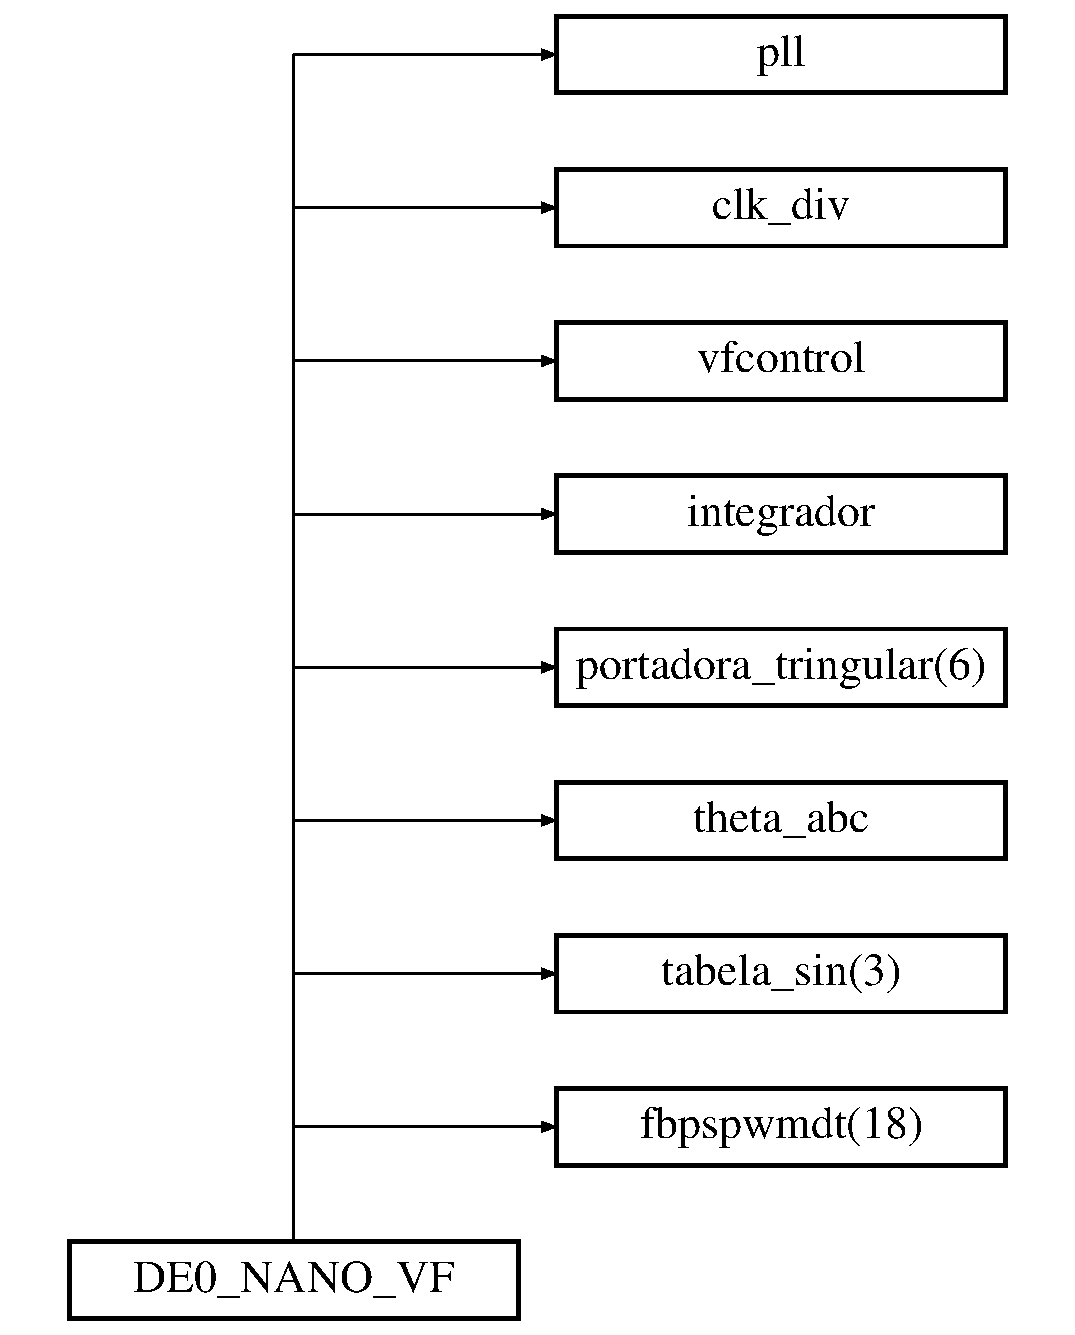
\includegraphics[height=9.000000cm]{class_d_e0___n_a_n_o___v_f}
\end{center}
\end{figure}
\subsection*{Entities}
\begin{DoxyCompactItemize}
\item 
\hyperlink{class_d_e0___n_a_n_o___v_f_1_1_m_a_i_n}{M\+A\+I\+N} architecture
\end{DoxyCompactItemize}
\subsection*{Libraries}
 \begin{DoxyCompactItemize}
\item 
\hyperlink{class_d_e0___n_a_n_o___v_f_a0a6af6eef40212dbaf130d57ce711256}{ieee} 
\end{DoxyCompactItemize}
\subsection*{Use Clauses}
 \begin{DoxyCompactItemize}
\item 
\hyperlink{class_d_e0___n_a_n_o___v_f_acd03516902501cd1c7296a98e22c6fcb}{std\+\_\+logic\+\_\+1164}   
\item 
\hyperlink{class_d_e0___n_a_n_o___v_f_a0f5ecc6613f63d07f7963a97b1b26095}{std\+\_\+logic\+\_\+arith}   
\item 
\hyperlink{class_d_e0___n_a_n_o___v_f_a598da929e807d58939b47499e8bc9fa8}{std\+\_\+logic\+\_\+unsigned}   
\item 
\hyperlink{class_d_e0___n_a_n_o___v_f_ae00f3f04545af57582ff10609eee23e2}{N\+U\+M\+E\+R\+I\+C\+\_\+\+S\+T\+D}   
\item 
\hyperlink{class_d_e0___n_a_n_o___v_f_aad86249c80e8c1e7ee1c4748aba748e3}{fixed\+\_\+pkg}   
\item 
\hyperlink{class_d_e0___n_a_n_o___v_f_ac1788a894930eeee5aaed06b4775d746}{my\+\_\+types\+\_\+pkg}   
\end{DoxyCompactItemize}
\subsection*{Generics}
 \begin{DoxyCompactItemize}
\item 
\hyperlink{class_d_e0___n_a_n_o___v_f_af855138be951f4c562436dfd59f85b54}{N} {\bfseries {\bfseries \textcolor{comment}{integer}\textcolor{vhdlchar}{ }\textcolor{vhdlchar}{ }\textcolor{vhdlchar}{\+:}\textcolor{vhdlchar}{=}\textcolor{vhdlchar}{ }\textcolor{vhdlchar}{ } \textcolor{vhdldigit}{3} \textcolor{vhdlchar}{ }}}
\item 
\hyperlink{class_d_e0___n_a_n_o___v_f_a2629ecb3bb37e8104b2866b0fd0c8574}{Nin} {\bfseries {\bfseries \textcolor{comment}{integer}\textcolor{vhdlchar}{ }\textcolor{vhdlchar}{ }\textcolor{vhdlchar}{\+:}\textcolor{vhdlchar}{=}\textcolor{vhdlchar}{ }\textcolor{vhdlchar}{ } \textcolor{vhdldigit}{13} \textcolor{vhdlchar}{ }}}
\item 
\hyperlink{class_d_e0___n_a_n_o___v_f_a061c0d632c8bdf5dd32c80acf9a9c475}{Nout} {\bfseries {\bfseries \textcolor{comment}{integer}\textcolor{vhdlchar}{ }\textcolor{vhdlchar}{ }\textcolor{vhdlchar}{\+:}\textcolor{vhdlchar}{=}\textcolor{vhdlchar}{ }\textcolor{vhdlchar}{ } \textcolor{vhdldigit}{30} \textcolor{vhdlchar}{ }}}
\item 
\hyperlink{class_d_e0___n_a_n_o___v_f_a9ba59f708a3f2e2c9a9bdba7ac62f13a}{n\+\_\+bits\+\_\+phase} {\bfseries {\bfseries \textcolor{comment}{integer}\textcolor{vhdlchar}{ }\textcolor{vhdlchar}{ }\textcolor{vhdlchar}{\+:}\textcolor{vhdlchar}{=}\textcolor{vhdlchar}{ }\textcolor{vhdlchar}{ } \textcolor{vhdldigit}{30} \textcolor{vhdlchar}{ }}}
\item 
\hyperlink{class_d_e0___n_a_n_o___v_f_afee4aa1628956aa350183d8881689198}{n\+\_\+bits\+\_\+c} {\bfseries {\bfseries \textcolor{comment}{integer}\textcolor{vhdlchar}{ }\textcolor{vhdlchar}{ }\textcolor{vhdlchar}{\+:}\textcolor{vhdlchar}{=}\textcolor{vhdlchar}{ }\textcolor{vhdlchar}{ } \textcolor{vhdldigit}{16} \textcolor{vhdlchar}{ }}}
\item 
\hyperlink{class_d_e0___n_a_n_o___v_f_a9aab84a644aefaf58d2d687a1b235ff3}{T\+A\+M\+\_\+\+M\+E\+M} {\bfseries {\bfseries \textcolor{comment}{integer}\textcolor{vhdlchar}{ }\textcolor{vhdlchar}{ }\textcolor{vhdlchar}{\+:}\textcolor{vhdlchar}{=}\textcolor{vhdlchar}{ }\textcolor{vhdlchar}{ } \textcolor{vhdldigit}{32} \textcolor{vhdlchar}{ }}}
\item 
\hyperlink{class_d_e0___n_a_n_o___v_f_abf975e3873df608ef7053790457e16db}{N\+B\+I\+T\+S\+\_\+\+M\+E\+M\+\_\+\+A\+D\+D\+R\+E\+S\+S} {\bfseries {\bfseries \textcolor{comment}{integer}\textcolor{vhdlchar}{ }\textcolor{vhdlchar}{ }\textcolor{vhdlchar}{\+:}\textcolor{vhdlchar}{=}\textcolor{vhdlchar}{ }\textcolor{vhdlchar}{ } \textcolor{vhdldigit}{6} \textcolor{vhdlchar}{ }}}
\item 
\hyperlink{class_d_e0___n_a_n_o___v_f_a0bc2b40306736322a2a9a1496e575aad}{I\+D\+\_\+\+M\+E\+M\+\_\+\+D\+A\+C} {\bfseries {\bfseries \textcolor{comment}{integer}\textcolor{vhdlchar}{ }\textcolor{vhdlchar}{ }\textcolor{vhdlchar}{\+:}\textcolor{vhdlchar}{=}\textcolor{vhdlchar}{ }\textcolor{vhdlchar}{ } \textcolor{vhdldigit}{28} \textcolor{vhdlchar}{ }}}
\item 
\hyperlink{class_d_e0___n_a_n_o___v_f_a5c5739ee995dcc5500803f87710cf9c9}{I\+D\+\_\+\+M\+E\+M\+\_\+\+S\+W1} {\bfseries {\bfseries \textcolor{comment}{integer}\textcolor{vhdlchar}{ }\textcolor{vhdlchar}{ }\textcolor{vhdlchar}{\+:}\textcolor{vhdlchar}{=}\textcolor{vhdlchar}{ }\textcolor{vhdlchar}{ } \textcolor{vhdldigit}{30} \textcolor{vhdlchar}{ }}}
\item 
\hyperlink{class_d_e0___n_a_n_o___v_f_abb7ce405d45a733b6db94314a4f791fd}{I} {\bfseries {\bfseries \textcolor{comment}{integer}\textcolor{vhdlchar}{ }\textcolor{vhdlchar}{ }\textcolor{vhdlchar}{\+:}\textcolor{vhdlchar}{=}\textcolor{vhdlchar}{ }\textcolor{vhdlchar}{ } \textcolor{vhdldigit}{1} \textcolor{vhdlchar}{ }}}
\item 
\hyperlink{class_d_e0___n_a_n_o___v_f_aac2d6825f96b21ae984648cc93554339}{F} {\bfseries {\bfseries \textcolor{comment}{integer}\textcolor{vhdlchar}{ }\textcolor{vhdlchar}{ }\textcolor{vhdlchar}{\+:}\textcolor{vhdlchar}{=}\textcolor{vhdlchar}{ }\textcolor{vhdlchar}{ } \textcolor{vhdldigit}{14} \textcolor{vhdlchar}{ }}}
\end{DoxyCompactItemize}
\subsection*{Ports}
 \begin{DoxyCompactItemize}
\item 
\hyperlink{class_d_e0___n_a_n_o___v_f_a4b5e1e3eba67b2e61c77c9a719d8518c}{C\+L\+O\+C\+K\+\_\+50}  {\bfseries {\bfseries \textcolor{keywordflow}{in}\textcolor{vhdlchar}{ }}} {\bfseries \textcolor{comment}{std\+\_\+logic}\textcolor{vhdlchar}{ }} 
\item 
\hyperlink{class_d_e0___n_a_n_o___v_f_a424944084857f6787a0ddb567d0b5240}{L\+E\+D}  {\bfseries {\bfseries \textcolor{keywordflow}{out}\textcolor{vhdlchar}{ }}} {\bfseries \textcolor{comment}{std\+\_\+logic\+\_\+vector}\textcolor{vhdlchar}{ }\textcolor{vhdlchar}{(}\textcolor{vhdlchar}{ }\textcolor{vhdlchar}{ } \textcolor{vhdldigit}{7} \textcolor{vhdlchar}{ }\textcolor{keywordflow}{D\+O\+W\+N\+T\+O}\textcolor{vhdlchar}{ }\textcolor{vhdlchar}{ } \textcolor{vhdldigit}{0} \textcolor{vhdlchar}{ }\textcolor{vhdlchar}{)}\textcolor{vhdlchar}{ }} 
\item 
\hyperlink{class_d_e0___n_a_n_o___v_f_a30974727c81621f672f7f9490463f9d3}{S\+W}  {\bfseries {\bfseries \textcolor{keywordflow}{in}\textcolor{vhdlchar}{ }}} {\bfseries \textcolor{comment}{std\+\_\+logic\+\_\+vector}\textcolor{vhdlchar}{ }\textcolor{vhdlchar}{(}\textcolor{vhdlchar}{ }\textcolor{vhdlchar}{ } \textcolor{vhdldigit}{3} \textcolor{vhdlchar}{ }\textcolor{keywordflow}{D\+O\+W\+N\+T\+O}\textcolor{vhdlchar}{ }\textcolor{vhdlchar}{ } \textcolor{vhdldigit}{0} \textcolor{vhdlchar}{ }\textcolor{vhdlchar}{)}\textcolor{vhdlchar}{ }} 
\item 
\hyperlink{class_d_e0___n_a_n_o___v_f_aa70bf9245705f33e4529eb81df3fbf94}{K\+E\+Y}  {\bfseries {\bfseries \textcolor{keywordflow}{in}\textcolor{vhdlchar}{ }}} {\bfseries \textcolor{comment}{std\+\_\+logic\+\_\+vector}\textcolor{vhdlchar}{ }\textcolor{vhdlchar}{(}\textcolor{vhdlchar}{ }\textcolor{vhdlchar}{ } \textcolor{vhdldigit}{1} \textcolor{vhdlchar}{ }\textcolor{keywordflow}{D\+O\+W\+N\+T\+O}\textcolor{vhdlchar}{ }\textcolor{vhdlchar}{ } \textcolor{vhdldigit}{0} \textcolor{vhdlchar}{ }\textcolor{vhdlchar}{)}\textcolor{vhdlchar}{ }} 
\item 
\hyperlink{class_d_e0___n_a_n_o___v_f_ab6bd5afe8823c3590ef5e4195757f852}{R\+E\+S\+E\+T\+\_\+\+F\+A}  {\bfseries {\bfseries \textcolor{keywordflow}{out}\textcolor{vhdlchar}{ }}} {\bfseries \textcolor{comment}{std\+\_\+logic\+\_\+vector}\textcolor{vhdlchar}{ }\textcolor{vhdlchar}{(}\textcolor{vhdlchar}{ }\textcolor{vhdlchar}{ }\textcolor{vhdlchar}{ }\textcolor{vhdlchar}{ }{\bfseries \hyperlink{class_d_e0___n_a_n_o___v_f_af855138be951f4c562436dfd59f85b54}{N}} \textcolor{vhdlchar}{-\/}\textcolor{vhdlchar}{ } \textcolor{vhdldigit}{1} \textcolor{vhdlchar}{ }\textcolor{keywordflow}{D\+O\+W\+N\+T\+O}\textcolor{vhdlchar}{ }\textcolor{vhdlchar}{ } \textcolor{vhdldigit}{0} \textcolor{vhdlchar}{ }\textcolor{vhdlchar}{)}\textcolor{vhdlchar}{ }} 
\item 
\hyperlink{class_d_e0___n_a_n_o___v_f_a292e884f4d72fca8a1bec36c11933ef7}{P\+W\+M1\+L\+\_\+\+F\+A}  {\bfseries {\bfseries \textcolor{keywordflow}{out}\textcolor{vhdlchar}{ }}} {\bfseries \textcolor{comment}{std\+\_\+logic\+\_\+vector}\textcolor{vhdlchar}{ }\textcolor{vhdlchar}{(}\textcolor{vhdlchar}{ }\textcolor{vhdlchar}{ }\textcolor{vhdlchar}{ }\textcolor{vhdlchar}{ }{\bfseries \hyperlink{class_d_e0___n_a_n_o___v_f_af855138be951f4c562436dfd59f85b54}{N}} \textcolor{vhdlchar}{-\/}\textcolor{vhdlchar}{ } \textcolor{vhdldigit}{1} \textcolor{vhdlchar}{ }\textcolor{keywordflow}{D\+O\+W\+N\+T\+O}\textcolor{vhdlchar}{ }\textcolor{vhdlchar}{ } \textcolor{vhdldigit}{0} \textcolor{vhdlchar}{ }\textcolor{vhdlchar}{)}\textcolor{vhdlchar}{ }} 
\item 
\hyperlink{class_d_e0___n_a_n_o___v_f_af21e77adde949f9a9a599f25976a6a74}{P\+W\+M1\+H\+\_\+\+F\+A}  {\bfseries {\bfseries \textcolor{keywordflow}{out}\textcolor{vhdlchar}{ }}} {\bfseries \textcolor{comment}{std\+\_\+logic\+\_\+vector}\textcolor{vhdlchar}{ }\textcolor{vhdlchar}{(}\textcolor{vhdlchar}{ }\textcolor{vhdlchar}{ }\textcolor{vhdlchar}{ }\textcolor{vhdlchar}{ }{\bfseries \hyperlink{class_d_e0___n_a_n_o___v_f_af855138be951f4c562436dfd59f85b54}{N}} \textcolor{vhdlchar}{-\/}\textcolor{vhdlchar}{ } \textcolor{vhdldigit}{1} \textcolor{vhdlchar}{ }\textcolor{keywordflow}{D\+O\+W\+N\+T\+O}\textcolor{vhdlchar}{ }\textcolor{vhdlchar}{ } \textcolor{vhdldigit}{0} \textcolor{vhdlchar}{ }\textcolor{vhdlchar}{)}\textcolor{vhdlchar}{ }} 
\item 
\hyperlink{class_d_e0___n_a_n_o___v_f_a357d73a496027c4f7000298ecdc41a05}{P\+W\+M2\+L\+\_\+\+F\+A}  {\bfseries {\bfseries \textcolor{keywordflow}{out}\textcolor{vhdlchar}{ }}} {\bfseries \textcolor{comment}{std\+\_\+logic\+\_\+vector}\textcolor{vhdlchar}{ }\textcolor{vhdlchar}{(}\textcolor{vhdlchar}{ }\textcolor{vhdlchar}{ }\textcolor{vhdlchar}{ }\textcolor{vhdlchar}{ }{\bfseries \hyperlink{class_d_e0___n_a_n_o___v_f_af855138be951f4c562436dfd59f85b54}{N}} \textcolor{vhdlchar}{-\/}\textcolor{vhdlchar}{ } \textcolor{vhdldigit}{1} \textcolor{vhdlchar}{ }\textcolor{keywordflow}{D\+O\+W\+N\+T\+O}\textcolor{vhdlchar}{ }\textcolor{vhdlchar}{ } \textcolor{vhdldigit}{0} \textcolor{vhdlchar}{ }\textcolor{vhdlchar}{)}\textcolor{vhdlchar}{ }} 
\item 
\hyperlink{class_d_e0___n_a_n_o___v_f_a3a05a366015b8398929044188870fa7b}{P\+W\+M2\+H\+\_\+\+F\+A}  {\bfseries {\bfseries \textcolor{keywordflow}{out}\textcolor{vhdlchar}{ }}} {\bfseries \textcolor{comment}{std\+\_\+logic\+\_\+vector}\textcolor{vhdlchar}{ }\textcolor{vhdlchar}{(}\textcolor{vhdlchar}{ }\textcolor{vhdlchar}{ }\textcolor{vhdlchar}{ }\textcolor{vhdlchar}{ }{\bfseries \hyperlink{class_d_e0___n_a_n_o___v_f_af855138be951f4c562436dfd59f85b54}{N}} \textcolor{vhdlchar}{-\/}\textcolor{vhdlchar}{ } \textcolor{vhdldigit}{1} \textcolor{vhdlchar}{ }\textcolor{keywordflow}{D\+O\+W\+N\+T\+O}\textcolor{vhdlchar}{ }\textcolor{vhdlchar}{ } \textcolor{vhdldigit}{0} \textcolor{vhdlchar}{ }\textcolor{vhdlchar}{)}\textcolor{vhdlchar}{ }} 
\item 
\hyperlink{class_d_e0___n_a_n_o___v_f_a11a54edd784d9fa7ce3a24aa015463d6}{I\+N\+T0\+\_\+\+F\+A}  {\bfseries {\bfseries \textcolor{keywordflow}{in}\textcolor{vhdlchar}{ }}} {\bfseries \textcolor{comment}{std\+\_\+logic\+\_\+vector}\textcolor{vhdlchar}{ }\textcolor{vhdlchar}{(}\textcolor{vhdlchar}{ }\textcolor{vhdlchar}{ }\textcolor{vhdlchar}{ }\textcolor{vhdlchar}{ }{\bfseries \hyperlink{class_d_e0___n_a_n_o___v_f_af855138be951f4c562436dfd59f85b54}{N}} \textcolor{vhdlchar}{-\/}\textcolor{vhdlchar}{ } \textcolor{vhdldigit}{1} \textcolor{vhdlchar}{ }\textcolor{keywordflow}{D\+O\+W\+N\+T\+O}\textcolor{vhdlchar}{ }\textcolor{vhdlchar}{ } \textcolor{vhdldigit}{0} \textcolor{vhdlchar}{ }\textcolor{vhdlchar}{)}\textcolor{vhdlchar}{ }} 
\item 
\hyperlink{class_d_e0___n_a_n_o___v_f_abce5db5149bd7ae87d6c3601972ae05f}{R\+E\+S\+E\+T\+\_\+\+F\+B}  {\bfseries {\bfseries \textcolor{keywordflow}{out}\textcolor{vhdlchar}{ }}} {\bfseries \textcolor{comment}{std\+\_\+logic\+\_\+vector}\textcolor{vhdlchar}{ }\textcolor{vhdlchar}{(}\textcolor{vhdlchar}{ }\textcolor{vhdlchar}{ }\textcolor{vhdlchar}{ }\textcolor{vhdlchar}{ }{\bfseries \hyperlink{class_d_e0___n_a_n_o___v_f_af855138be951f4c562436dfd59f85b54}{N}} \textcolor{vhdlchar}{-\/}\textcolor{vhdlchar}{ } \textcolor{vhdldigit}{1} \textcolor{vhdlchar}{ }\textcolor{keywordflow}{D\+O\+W\+N\+T\+O}\textcolor{vhdlchar}{ }\textcolor{vhdlchar}{ } \textcolor{vhdldigit}{0} \textcolor{vhdlchar}{ }\textcolor{vhdlchar}{)}\textcolor{vhdlchar}{ }} 
\item 
\hyperlink{class_d_e0___n_a_n_o___v_f_ac5cc3b06408f1596a61b08b946a9c1d0}{P\+W\+M1\+L\+\_\+\+F\+B}  {\bfseries {\bfseries \textcolor{keywordflow}{out}\textcolor{vhdlchar}{ }}} {\bfseries \textcolor{comment}{std\+\_\+logic\+\_\+vector}\textcolor{vhdlchar}{ }\textcolor{vhdlchar}{(}\textcolor{vhdlchar}{ }\textcolor{vhdlchar}{ }\textcolor{vhdlchar}{ }\textcolor{vhdlchar}{ }{\bfseries \hyperlink{class_d_e0___n_a_n_o___v_f_af855138be951f4c562436dfd59f85b54}{N}} \textcolor{vhdlchar}{-\/}\textcolor{vhdlchar}{ } \textcolor{vhdldigit}{1} \textcolor{vhdlchar}{ }\textcolor{keywordflow}{D\+O\+W\+N\+T\+O}\textcolor{vhdlchar}{ }\textcolor{vhdlchar}{ } \textcolor{vhdldigit}{0} \textcolor{vhdlchar}{ }\textcolor{vhdlchar}{)}\textcolor{vhdlchar}{ }} 
\item 
\hyperlink{class_d_e0___n_a_n_o___v_f_a69e944b362281970fb9a0a5ec6f5f068}{P\+W\+M1\+H\+\_\+\+F\+B}  {\bfseries {\bfseries \textcolor{keywordflow}{out}\textcolor{vhdlchar}{ }}} {\bfseries \textcolor{comment}{std\+\_\+logic\+\_\+vector}\textcolor{vhdlchar}{ }\textcolor{vhdlchar}{(}\textcolor{vhdlchar}{ }\textcolor{vhdlchar}{ }\textcolor{vhdlchar}{ }\textcolor{vhdlchar}{ }{\bfseries \hyperlink{class_d_e0___n_a_n_o___v_f_af855138be951f4c562436dfd59f85b54}{N}} \textcolor{vhdlchar}{-\/}\textcolor{vhdlchar}{ } \textcolor{vhdldigit}{1} \textcolor{vhdlchar}{ }\textcolor{keywordflow}{D\+O\+W\+N\+T\+O}\textcolor{vhdlchar}{ }\textcolor{vhdlchar}{ } \textcolor{vhdldigit}{0} \textcolor{vhdlchar}{ }\textcolor{vhdlchar}{)}\textcolor{vhdlchar}{ }} 
\item 
\hyperlink{class_d_e0___n_a_n_o___v_f_aefa13a97661cae3b7b87245ed460abe5}{P\+W\+M2\+L\+\_\+\+F\+B}  {\bfseries {\bfseries \textcolor{keywordflow}{out}\textcolor{vhdlchar}{ }}} {\bfseries \textcolor{comment}{std\+\_\+logic\+\_\+vector}\textcolor{vhdlchar}{ }\textcolor{vhdlchar}{(}\textcolor{vhdlchar}{ }\textcolor{vhdlchar}{ }\textcolor{vhdlchar}{ }\textcolor{vhdlchar}{ }{\bfseries \hyperlink{class_d_e0___n_a_n_o___v_f_af855138be951f4c562436dfd59f85b54}{N}} \textcolor{vhdlchar}{-\/}\textcolor{vhdlchar}{ } \textcolor{vhdldigit}{1} \textcolor{vhdlchar}{ }\textcolor{keywordflow}{D\+O\+W\+N\+T\+O}\textcolor{vhdlchar}{ }\textcolor{vhdlchar}{ } \textcolor{vhdldigit}{0} \textcolor{vhdlchar}{ }\textcolor{vhdlchar}{)}\textcolor{vhdlchar}{ }} 
\item 
\hyperlink{class_d_e0___n_a_n_o___v_f_a7efac822a270a6c828ef5eb2cc090127}{P\+W\+M2\+H\+\_\+\+F\+B}  {\bfseries {\bfseries \textcolor{keywordflow}{out}\textcolor{vhdlchar}{ }}} {\bfseries \textcolor{comment}{std\+\_\+logic\+\_\+vector}\textcolor{vhdlchar}{ }\textcolor{vhdlchar}{(}\textcolor{vhdlchar}{ }\textcolor{vhdlchar}{ }\textcolor{vhdlchar}{ }\textcolor{vhdlchar}{ }{\bfseries \hyperlink{class_d_e0___n_a_n_o___v_f_af855138be951f4c562436dfd59f85b54}{N}} \textcolor{vhdlchar}{-\/}\textcolor{vhdlchar}{ } \textcolor{vhdldigit}{1} \textcolor{vhdlchar}{ }\textcolor{keywordflow}{D\+O\+W\+N\+T\+O}\textcolor{vhdlchar}{ }\textcolor{vhdlchar}{ } \textcolor{vhdldigit}{0} \textcolor{vhdlchar}{ }\textcolor{vhdlchar}{)}\textcolor{vhdlchar}{ }} 
\item 
\hyperlink{class_d_e0___n_a_n_o___v_f_a072d40993d1ff4b3dc85aa2aed7be456}{I\+N\+T0\+\_\+\+F\+B}  {\bfseries {\bfseries \textcolor{keywordflow}{in}\textcolor{vhdlchar}{ }}} {\bfseries \textcolor{comment}{std\+\_\+logic\+\_\+vector}\textcolor{vhdlchar}{ }\textcolor{vhdlchar}{(}\textcolor{vhdlchar}{ }\textcolor{vhdlchar}{ }\textcolor{vhdlchar}{ }\textcolor{vhdlchar}{ }{\bfseries \hyperlink{class_d_e0___n_a_n_o___v_f_af855138be951f4c562436dfd59f85b54}{N}} \textcolor{vhdlchar}{-\/}\textcolor{vhdlchar}{ } \textcolor{vhdldigit}{1} \textcolor{vhdlchar}{ }\textcolor{keywordflow}{D\+O\+W\+N\+T\+O}\textcolor{vhdlchar}{ }\textcolor{vhdlchar}{ } \textcolor{vhdldigit}{0} \textcolor{vhdlchar}{ }\textcolor{vhdlchar}{)}\textcolor{vhdlchar}{ }} 
\item 
\hyperlink{class_d_e0___n_a_n_o___v_f_a05f3fd52a3ed4e3c8ccfeb431451afc6}{R\+E\+S\+E\+T\+\_\+\+F\+C}  {\bfseries {\bfseries \textcolor{keywordflow}{out}\textcolor{vhdlchar}{ }}} {\bfseries \textcolor{comment}{std\+\_\+logic\+\_\+vector}\textcolor{vhdlchar}{ }\textcolor{vhdlchar}{(}\textcolor{vhdlchar}{ }\textcolor{vhdlchar}{ }\textcolor{vhdlchar}{ }\textcolor{vhdlchar}{ }{\bfseries \hyperlink{class_d_e0___n_a_n_o___v_f_af855138be951f4c562436dfd59f85b54}{N}} \textcolor{vhdlchar}{-\/}\textcolor{vhdlchar}{ } \textcolor{vhdldigit}{1} \textcolor{vhdlchar}{ }\textcolor{keywordflow}{D\+O\+W\+N\+T\+O}\textcolor{vhdlchar}{ }\textcolor{vhdlchar}{ } \textcolor{vhdldigit}{0} \textcolor{vhdlchar}{ }\textcolor{vhdlchar}{)}\textcolor{vhdlchar}{ }} 
\item 
\hyperlink{class_d_e0___n_a_n_o___v_f_ac9a5e24e4c9b96a7ee1750285ff2af08}{P\+W\+M1\+L\+\_\+\+F\+C}  {\bfseries {\bfseries \textcolor{keywordflow}{out}\textcolor{vhdlchar}{ }}} {\bfseries \textcolor{comment}{std\+\_\+logic\+\_\+vector}\textcolor{vhdlchar}{ }\textcolor{vhdlchar}{(}\textcolor{vhdlchar}{ }\textcolor{vhdlchar}{ }\textcolor{vhdlchar}{ }\textcolor{vhdlchar}{ }{\bfseries \hyperlink{class_d_e0___n_a_n_o___v_f_af855138be951f4c562436dfd59f85b54}{N}} \textcolor{vhdlchar}{-\/}\textcolor{vhdlchar}{ } \textcolor{vhdldigit}{1} \textcolor{vhdlchar}{ }\textcolor{keywordflow}{D\+O\+W\+N\+T\+O}\textcolor{vhdlchar}{ }\textcolor{vhdlchar}{ } \textcolor{vhdldigit}{0} \textcolor{vhdlchar}{ }\textcolor{vhdlchar}{)}\textcolor{vhdlchar}{ }} 
\item 
\hyperlink{class_d_e0___n_a_n_o___v_f_ae64c7416adbe802e6aa4125230fad012}{P\+W\+M1\+H\+\_\+\+F\+C}  {\bfseries {\bfseries \textcolor{keywordflow}{out}\textcolor{vhdlchar}{ }}} {\bfseries \textcolor{comment}{std\+\_\+logic\+\_\+vector}\textcolor{vhdlchar}{ }\textcolor{vhdlchar}{(}\textcolor{vhdlchar}{ }\textcolor{vhdlchar}{ }\textcolor{vhdlchar}{ }\textcolor{vhdlchar}{ }{\bfseries \hyperlink{class_d_e0___n_a_n_o___v_f_af855138be951f4c562436dfd59f85b54}{N}} \textcolor{vhdlchar}{-\/}\textcolor{vhdlchar}{ } \textcolor{vhdldigit}{1} \textcolor{vhdlchar}{ }\textcolor{keywordflow}{D\+O\+W\+N\+T\+O}\textcolor{vhdlchar}{ }\textcolor{vhdlchar}{ } \textcolor{vhdldigit}{0} \textcolor{vhdlchar}{ }\textcolor{vhdlchar}{)}\textcolor{vhdlchar}{ }} 
\item 
\hyperlink{class_d_e0___n_a_n_o___v_f_a47c0de05323647e9484b2ec6764255c0}{P\+W\+M2\+L\+\_\+\+F\+C}  {\bfseries {\bfseries \textcolor{keywordflow}{out}\textcolor{vhdlchar}{ }}} {\bfseries \textcolor{comment}{std\+\_\+logic\+\_\+vector}\textcolor{vhdlchar}{ }\textcolor{vhdlchar}{(}\textcolor{vhdlchar}{ }\textcolor{vhdlchar}{ }\textcolor{vhdlchar}{ }\textcolor{vhdlchar}{ }{\bfseries \hyperlink{class_d_e0___n_a_n_o___v_f_af855138be951f4c562436dfd59f85b54}{N}} \textcolor{vhdlchar}{-\/}\textcolor{vhdlchar}{ } \textcolor{vhdldigit}{1} \textcolor{vhdlchar}{ }\textcolor{keywordflow}{D\+O\+W\+N\+T\+O}\textcolor{vhdlchar}{ }\textcolor{vhdlchar}{ } \textcolor{vhdldigit}{0} \textcolor{vhdlchar}{ }\textcolor{vhdlchar}{)}\textcolor{vhdlchar}{ }} 
\item 
\hyperlink{class_d_e0___n_a_n_o___v_f_a8318940c01015b267904bdca0e01c2a2}{P\+W\+M2\+H\+\_\+\+F\+C}  {\bfseries {\bfseries \textcolor{keywordflow}{out}\textcolor{vhdlchar}{ }}} {\bfseries \textcolor{comment}{std\+\_\+logic\+\_\+vector}\textcolor{vhdlchar}{ }\textcolor{vhdlchar}{(}\textcolor{vhdlchar}{ }\textcolor{vhdlchar}{ }\textcolor{vhdlchar}{ }\textcolor{vhdlchar}{ }{\bfseries \hyperlink{class_d_e0___n_a_n_o___v_f_af855138be951f4c562436dfd59f85b54}{N}} \textcolor{vhdlchar}{-\/}\textcolor{vhdlchar}{ } \textcolor{vhdldigit}{1} \textcolor{vhdlchar}{ }\textcolor{keywordflow}{D\+O\+W\+N\+T\+O}\textcolor{vhdlchar}{ }\textcolor{vhdlchar}{ } \textcolor{vhdldigit}{0} \textcolor{vhdlchar}{ }\textcolor{vhdlchar}{)}\textcolor{vhdlchar}{ }} 
\item 
\hyperlink{class_d_e0___n_a_n_o___v_f_a2da3143aa39453a927d622998a1d936b}{I\+N\+T0\+\_\+\+F\+C}  {\bfseries {\bfseries \textcolor{keywordflow}{in}\textcolor{vhdlchar}{ }}} {\bfseries \textcolor{comment}{std\+\_\+logic\+\_\+vector}\textcolor{vhdlchar}{ }\textcolor{vhdlchar}{(}\textcolor{vhdlchar}{ }\textcolor{vhdlchar}{ }\textcolor{vhdlchar}{ }\textcolor{vhdlchar}{ }{\bfseries \hyperlink{class_d_e0___n_a_n_o___v_f_af855138be951f4c562436dfd59f85b54}{N}} \textcolor{vhdlchar}{-\/}\textcolor{vhdlchar}{ } \textcolor{vhdldigit}{1} \textcolor{vhdlchar}{ }\textcolor{keywordflow}{D\+O\+W\+N\+T\+O}\textcolor{vhdlchar}{ }\textcolor{vhdlchar}{ } \textcolor{vhdldigit}{0} \textcolor{vhdlchar}{ }\textcolor{vhdlchar}{)}\textcolor{vhdlchar}{ }} 
\item 
\hyperlink{class_d_e0___n_a_n_o___v_f_a01eff012417d9c479e11ca1e08d0fdb5}{G\+P\+I\+O\+\_\+0}  {\bfseries {\bfseries \textcolor{keywordflow}{out}\textcolor{vhdlchar}{ }}} {\bfseries \textcolor{comment}{std\+\_\+logic\+\_\+vector}\textcolor{vhdlchar}{ }\textcolor{vhdlchar}{(}\textcolor{vhdlchar}{ }\textcolor{vhdlchar}{ } \textcolor{vhdldigit}{3} \textcolor{vhdlchar}{ }\textcolor{keywordflow}{D\+O\+W\+N\+T\+O}\textcolor{vhdlchar}{ }\textcolor{vhdlchar}{ } \textcolor{vhdldigit}{0} \textcolor{vhdlchar}{ }\textcolor{vhdlchar}{)}\textcolor{vhdlchar}{ }} 
\end{DoxyCompactItemize}


\subsection{Detailed Description}


Definition at line 15 of file D\+E0\+\_\+\+N\+A\+N\+O\+\_\+\+V\+F.\+vhd.



\subsection{Member Data Documentation}
\hypertarget{class_d_e0___n_a_n_o___v_f_a4b5e1e3eba67b2e61c77c9a719d8518c}{}\index{D\+E0\+\_\+\+N\+A\+N\+O\+\_\+\+V\+F@{D\+E0\+\_\+\+N\+A\+N\+O\+\_\+\+V\+F}!C\+L\+O\+C\+K\+\_\+50@{C\+L\+O\+C\+K\+\_\+50}}
\index{C\+L\+O\+C\+K\+\_\+50@{C\+L\+O\+C\+K\+\_\+50}!D\+E0\+\_\+\+N\+A\+N\+O\+\_\+\+V\+F@{D\+E0\+\_\+\+N\+A\+N\+O\+\_\+\+V\+F}}
\subsubsection[{C\+L\+O\+C\+K\+\_\+50}]{\setlength{\rightskip}{0pt plus 5cm}{\bf C\+L\+O\+C\+K\+\_\+50} {\bfseries \textcolor{keywordflow}{in}\textcolor{vhdlchar}{ }} {\bfseries \textcolor{comment}{std\+\_\+logic}\textcolor{vhdlchar}{ }} \hspace{0.3cm}{\ttfamily [Port]}}\label{class_d_e0___n_a_n_o___v_f_a4b5e1e3eba67b2e61c77c9a719d8518c}


Definition at line 30 of file D\+E0\+\_\+\+N\+A\+N\+O\+\_\+\+V\+F.\+vhd.

\hypertarget{class_d_e0___n_a_n_o___v_f_aac2d6825f96b21ae984648cc93554339}{}\index{D\+E0\+\_\+\+N\+A\+N\+O\+\_\+\+V\+F@{D\+E0\+\_\+\+N\+A\+N\+O\+\_\+\+V\+F}!F@{F}}
\index{F@{F}!D\+E0\+\_\+\+N\+A\+N\+O\+\_\+\+V\+F@{D\+E0\+\_\+\+N\+A\+N\+O\+\_\+\+V\+F}}
\subsubsection[{F}]{\setlength{\rightskip}{0pt plus 5cm}{\bf F} {\bfseries \textcolor{vhdlchar}{ }} {\bfseries \textcolor{comment}{integer}\textcolor{vhdlchar}{ }\textcolor{vhdlchar}{ }\textcolor{vhdlchar}{\+:}\textcolor{vhdlchar}{=}\textcolor{vhdlchar}{ }\textcolor{vhdlchar}{ } \textcolor{vhdldigit}{14} \textcolor{vhdlchar}{ }} \hspace{0.3cm}{\ttfamily [Generic]}}\label{class_d_e0___n_a_n_o___v_f_aac2d6825f96b21ae984648cc93554339}


Definition at line 28 of file D\+E0\+\_\+\+N\+A\+N\+O\+\_\+\+V\+F.\+vhd.

\hypertarget{class_d_e0___n_a_n_o___v_f_aad86249c80e8c1e7ee1c4748aba748e3}{}\index{D\+E0\+\_\+\+N\+A\+N\+O\+\_\+\+V\+F@{D\+E0\+\_\+\+N\+A\+N\+O\+\_\+\+V\+F}!fixed\+\_\+pkg@{fixed\+\_\+pkg}}
\index{fixed\+\_\+pkg@{fixed\+\_\+pkg}!D\+E0\+\_\+\+N\+A\+N\+O\+\_\+\+V\+F@{D\+E0\+\_\+\+N\+A\+N\+O\+\_\+\+V\+F}}
\subsubsection[{fixed\+\_\+pkg}]{\setlength{\rightskip}{0pt plus 5cm}{\bf fixed\+\_\+pkg}\hspace{0.3cm}{\ttfamily [Package]}}\label{class_d_e0___n_a_n_o___v_f_aad86249c80e8c1e7ee1c4748aba748e3}


Definition at line 10 of file D\+E0\+\_\+\+N\+A\+N\+O\+\_\+\+V\+F.\+vhd.

\hypertarget{class_d_e0___n_a_n_o___v_f_a01eff012417d9c479e11ca1e08d0fdb5}{}\index{D\+E0\+\_\+\+N\+A\+N\+O\+\_\+\+V\+F@{D\+E0\+\_\+\+N\+A\+N\+O\+\_\+\+V\+F}!G\+P\+I\+O\+\_\+0@{G\+P\+I\+O\+\_\+0}}
\index{G\+P\+I\+O\+\_\+0@{G\+P\+I\+O\+\_\+0}!D\+E0\+\_\+\+N\+A\+N\+O\+\_\+\+V\+F@{D\+E0\+\_\+\+N\+A\+N\+O\+\_\+\+V\+F}}
\subsubsection[{G\+P\+I\+O\+\_\+0}]{\setlength{\rightskip}{0pt plus 5cm}{\bf G\+P\+I\+O\+\_\+0} {\bfseries \textcolor{keywordflow}{out}\textcolor{vhdlchar}{ }} {\bfseries \textcolor{comment}{std\+\_\+logic\+\_\+vector}\textcolor{vhdlchar}{ }\textcolor{vhdlchar}{(}\textcolor{vhdlchar}{ }\textcolor{vhdlchar}{ } \textcolor{vhdldigit}{3} \textcolor{vhdlchar}{ }\textcolor{keywordflow}{D\+O\+W\+N\+T\+O}\textcolor{vhdlchar}{ }\textcolor{vhdlchar}{ } \textcolor{vhdldigit}{0} \textcolor{vhdlchar}{ }\textcolor{vhdlchar}{)}\textcolor{vhdlchar}{ }} \hspace{0.3cm}{\ttfamily [Port]}}\label{class_d_e0___n_a_n_o___v_f_a01eff012417d9c479e11ca1e08d0fdb5}


Definition at line 70 of file D\+E0\+\_\+\+N\+A\+N\+O\+\_\+\+V\+F.\+vhd.

\hypertarget{class_d_e0___n_a_n_o___v_f_abb7ce405d45a733b6db94314a4f791fd}{}\index{D\+E0\+\_\+\+N\+A\+N\+O\+\_\+\+V\+F@{D\+E0\+\_\+\+N\+A\+N\+O\+\_\+\+V\+F}!I@{I}}
\index{I@{I}!D\+E0\+\_\+\+N\+A\+N\+O\+\_\+\+V\+F@{D\+E0\+\_\+\+N\+A\+N\+O\+\_\+\+V\+F}}
\subsubsection[{I}]{\setlength{\rightskip}{0pt plus 5cm}{\bf I} {\bfseries \textcolor{vhdlchar}{ }} {\bfseries \textcolor{comment}{integer}\textcolor{vhdlchar}{ }\textcolor{vhdlchar}{ }\textcolor{vhdlchar}{\+:}\textcolor{vhdlchar}{=}\textcolor{vhdlchar}{ }\textcolor{vhdlchar}{ } \textcolor{vhdldigit}{1} \textcolor{vhdlchar}{ }} \hspace{0.3cm}{\ttfamily [Generic]}}\label{class_d_e0___n_a_n_o___v_f_abb7ce405d45a733b6db94314a4f791fd}


Definition at line 26 of file D\+E0\+\_\+\+N\+A\+N\+O\+\_\+\+V\+F.\+vhd.

\hypertarget{class_d_e0___n_a_n_o___v_f_a0bc2b40306736322a2a9a1496e575aad}{}\index{D\+E0\+\_\+\+N\+A\+N\+O\+\_\+\+V\+F@{D\+E0\+\_\+\+N\+A\+N\+O\+\_\+\+V\+F}!I\+D\+\_\+\+M\+E\+M\+\_\+\+D\+A\+C@{I\+D\+\_\+\+M\+E\+M\+\_\+\+D\+A\+C}}
\index{I\+D\+\_\+\+M\+E\+M\+\_\+\+D\+A\+C@{I\+D\+\_\+\+M\+E\+M\+\_\+\+D\+A\+C}!D\+E0\+\_\+\+N\+A\+N\+O\+\_\+\+V\+F@{D\+E0\+\_\+\+N\+A\+N\+O\+\_\+\+V\+F}}
\subsubsection[{I\+D\+\_\+\+M\+E\+M\+\_\+\+D\+A\+C}]{\setlength{\rightskip}{0pt plus 5cm}{\bf I\+D\+\_\+\+M\+E\+M\+\_\+\+D\+A\+C} {\bfseries \textcolor{vhdlchar}{ }} {\bfseries \textcolor{comment}{integer}\textcolor{vhdlchar}{ }\textcolor{vhdlchar}{ }\textcolor{vhdlchar}{\+:}\textcolor{vhdlchar}{=}\textcolor{vhdlchar}{ }\textcolor{vhdlchar}{ } \textcolor{vhdldigit}{28} \textcolor{vhdlchar}{ }} \hspace{0.3cm}{\ttfamily [Generic]}}\label{class_d_e0___n_a_n_o___v_f_a0bc2b40306736322a2a9a1496e575aad}


Definition at line 24 of file D\+E0\+\_\+\+N\+A\+N\+O\+\_\+\+V\+F.\+vhd.

\hypertarget{class_d_e0___n_a_n_o___v_f_a5c5739ee995dcc5500803f87710cf9c9}{}\index{D\+E0\+\_\+\+N\+A\+N\+O\+\_\+\+V\+F@{D\+E0\+\_\+\+N\+A\+N\+O\+\_\+\+V\+F}!I\+D\+\_\+\+M\+E\+M\+\_\+\+S\+W1@{I\+D\+\_\+\+M\+E\+M\+\_\+\+S\+W1}}
\index{I\+D\+\_\+\+M\+E\+M\+\_\+\+S\+W1@{I\+D\+\_\+\+M\+E\+M\+\_\+\+S\+W1}!D\+E0\+\_\+\+N\+A\+N\+O\+\_\+\+V\+F@{D\+E0\+\_\+\+N\+A\+N\+O\+\_\+\+V\+F}}
\subsubsection[{I\+D\+\_\+\+M\+E\+M\+\_\+\+S\+W1}]{\setlength{\rightskip}{0pt plus 5cm}{\bf I\+D\+\_\+\+M\+E\+M\+\_\+\+S\+W1} {\bfseries \textcolor{vhdlchar}{ }} {\bfseries \textcolor{comment}{integer}\textcolor{vhdlchar}{ }\textcolor{vhdlchar}{ }\textcolor{vhdlchar}{\+:}\textcolor{vhdlchar}{=}\textcolor{vhdlchar}{ }\textcolor{vhdlchar}{ } \textcolor{vhdldigit}{30} \textcolor{vhdlchar}{ }} \hspace{0.3cm}{\ttfamily [Generic]}}\label{class_d_e0___n_a_n_o___v_f_a5c5739ee995dcc5500803f87710cf9c9}


Definition at line 25 of file D\+E0\+\_\+\+N\+A\+N\+O\+\_\+\+V\+F.\+vhd.

\hypertarget{class_d_e0___n_a_n_o___v_f_a0a6af6eef40212dbaf130d57ce711256}{}\index{D\+E0\+\_\+\+N\+A\+N\+O\+\_\+\+V\+F@{D\+E0\+\_\+\+N\+A\+N\+O\+\_\+\+V\+F}!ieee@{ieee}}
\index{ieee@{ieee}!D\+E0\+\_\+\+N\+A\+N\+O\+\_\+\+V\+F@{D\+E0\+\_\+\+N\+A\+N\+O\+\_\+\+V\+F}}
\subsubsection[{ieee}]{\setlength{\rightskip}{0pt plus 5cm}{\bf ieee}\hspace{0.3cm}{\ttfamily [Library]}}\label{class_d_e0___n_a_n_o___v_f_a0a6af6eef40212dbaf130d57ce711256}


Definition at line 3 of file D\+E0\+\_\+\+N\+A\+N\+O\+\_\+\+V\+F.\+vhd.

\hypertarget{class_d_e0___n_a_n_o___v_f_a11a54edd784d9fa7ce3a24aa015463d6}{}\index{D\+E0\+\_\+\+N\+A\+N\+O\+\_\+\+V\+F@{D\+E0\+\_\+\+N\+A\+N\+O\+\_\+\+V\+F}!I\+N\+T0\+\_\+\+F\+A@{I\+N\+T0\+\_\+\+F\+A}}
\index{I\+N\+T0\+\_\+\+F\+A@{I\+N\+T0\+\_\+\+F\+A}!D\+E0\+\_\+\+N\+A\+N\+O\+\_\+\+V\+F@{D\+E0\+\_\+\+N\+A\+N\+O\+\_\+\+V\+F}}
\subsubsection[{I\+N\+T0\+\_\+\+F\+A}]{\setlength{\rightskip}{0pt plus 5cm}{\bf I\+N\+T0\+\_\+\+F\+A} {\bfseries \textcolor{keywordflow}{in}\textcolor{vhdlchar}{ }} {\bfseries \textcolor{comment}{std\+\_\+logic\+\_\+vector}\textcolor{vhdlchar}{ }\textcolor{vhdlchar}{(}\textcolor{vhdlchar}{ }\textcolor{vhdlchar}{ }\textcolor{vhdlchar}{ }\textcolor{vhdlchar}{ }{\bfseries {\bf N}} \textcolor{vhdlchar}{-\/}\textcolor{vhdlchar}{ } \textcolor{vhdldigit}{1} \textcolor{vhdlchar}{ }\textcolor{keywordflow}{D\+O\+W\+N\+T\+O}\textcolor{vhdlchar}{ }\textcolor{vhdlchar}{ } \textcolor{vhdldigit}{0} \textcolor{vhdlchar}{ }\textcolor{vhdlchar}{)}\textcolor{vhdlchar}{ }} \hspace{0.3cm}{\ttfamily [Port]}}\label{class_d_e0___n_a_n_o___v_f_a11a54edd784d9fa7ce3a24aa015463d6}


Definition at line 44 of file D\+E0\+\_\+\+N\+A\+N\+O\+\_\+\+V\+F.\+vhd.

\hypertarget{class_d_e0___n_a_n_o___v_f_a072d40993d1ff4b3dc85aa2aed7be456}{}\index{D\+E0\+\_\+\+N\+A\+N\+O\+\_\+\+V\+F@{D\+E0\+\_\+\+N\+A\+N\+O\+\_\+\+V\+F}!I\+N\+T0\+\_\+\+F\+B@{I\+N\+T0\+\_\+\+F\+B}}
\index{I\+N\+T0\+\_\+\+F\+B@{I\+N\+T0\+\_\+\+F\+B}!D\+E0\+\_\+\+N\+A\+N\+O\+\_\+\+V\+F@{D\+E0\+\_\+\+N\+A\+N\+O\+\_\+\+V\+F}}
\subsubsection[{I\+N\+T0\+\_\+\+F\+B}]{\setlength{\rightskip}{0pt plus 5cm}{\bf I\+N\+T0\+\_\+\+F\+B} {\bfseries \textcolor{keywordflow}{in}\textcolor{vhdlchar}{ }} {\bfseries \textcolor{comment}{std\+\_\+logic\+\_\+vector}\textcolor{vhdlchar}{ }\textcolor{vhdlchar}{(}\textcolor{vhdlchar}{ }\textcolor{vhdlchar}{ }\textcolor{vhdlchar}{ }\textcolor{vhdlchar}{ }{\bfseries {\bf N}} \textcolor{vhdlchar}{-\/}\textcolor{vhdlchar}{ } \textcolor{vhdldigit}{1} \textcolor{vhdlchar}{ }\textcolor{keywordflow}{D\+O\+W\+N\+T\+O}\textcolor{vhdlchar}{ }\textcolor{vhdlchar}{ } \textcolor{vhdldigit}{0} \textcolor{vhdlchar}{ }\textcolor{vhdlchar}{)}\textcolor{vhdlchar}{ }} \hspace{0.3cm}{\ttfamily [Port]}}\label{class_d_e0___n_a_n_o___v_f_a072d40993d1ff4b3dc85aa2aed7be456}


Definition at line 52 of file D\+E0\+\_\+\+N\+A\+N\+O\+\_\+\+V\+F.\+vhd.

\hypertarget{class_d_e0___n_a_n_o___v_f_a2da3143aa39453a927d622998a1d936b}{}\index{D\+E0\+\_\+\+N\+A\+N\+O\+\_\+\+V\+F@{D\+E0\+\_\+\+N\+A\+N\+O\+\_\+\+V\+F}!I\+N\+T0\+\_\+\+F\+C@{I\+N\+T0\+\_\+\+F\+C}}
\index{I\+N\+T0\+\_\+\+F\+C@{I\+N\+T0\+\_\+\+F\+C}!D\+E0\+\_\+\+N\+A\+N\+O\+\_\+\+V\+F@{D\+E0\+\_\+\+N\+A\+N\+O\+\_\+\+V\+F}}
\subsubsection[{I\+N\+T0\+\_\+\+F\+C}]{\setlength{\rightskip}{0pt plus 5cm}{\bf I\+N\+T0\+\_\+\+F\+C} {\bfseries \textcolor{keywordflow}{in}\textcolor{vhdlchar}{ }} {\bfseries \textcolor{comment}{std\+\_\+logic\+\_\+vector}\textcolor{vhdlchar}{ }\textcolor{vhdlchar}{(}\textcolor{vhdlchar}{ }\textcolor{vhdlchar}{ }\textcolor{vhdlchar}{ }\textcolor{vhdlchar}{ }{\bfseries {\bf N}} \textcolor{vhdlchar}{-\/}\textcolor{vhdlchar}{ } \textcolor{vhdldigit}{1} \textcolor{vhdlchar}{ }\textcolor{keywordflow}{D\+O\+W\+N\+T\+O}\textcolor{vhdlchar}{ }\textcolor{vhdlchar}{ } \textcolor{vhdldigit}{0} \textcolor{vhdlchar}{ }\textcolor{vhdlchar}{)}\textcolor{vhdlchar}{ }} \hspace{0.3cm}{\ttfamily [Port]}}\label{class_d_e0___n_a_n_o___v_f_a2da3143aa39453a927d622998a1d936b}


Definition at line 61 of file D\+E0\+\_\+\+N\+A\+N\+O\+\_\+\+V\+F.\+vhd.

\hypertarget{class_d_e0___n_a_n_o___v_f_aa70bf9245705f33e4529eb81df3fbf94}{}\index{D\+E0\+\_\+\+N\+A\+N\+O\+\_\+\+V\+F@{D\+E0\+\_\+\+N\+A\+N\+O\+\_\+\+V\+F}!K\+E\+Y@{K\+E\+Y}}
\index{K\+E\+Y@{K\+E\+Y}!D\+E0\+\_\+\+N\+A\+N\+O\+\_\+\+V\+F@{D\+E0\+\_\+\+N\+A\+N\+O\+\_\+\+V\+F}}
\subsubsection[{K\+E\+Y}]{\setlength{\rightskip}{0pt plus 5cm}{\bf K\+E\+Y} {\bfseries \textcolor{keywordflow}{in}\textcolor{vhdlchar}{ }} {\bfseries \textcolor{comment}{std\+\_\+logic\+\_\+vector}\textcolor{vhdlchar}{ }\textcolor{vhdlchar}{(}\textcolor{vhdlchar}{ }\textcolor{vhdlchar}{ } \textcolor{vhdldigit}{1} \textcolor{vhdlchar}{ }\textcolor{keywordflow}{D\+O\+W\+N\+T\+O}\textcolor{vhdlchar}{ }\textcolor{vhdlchar}{ } \textcolor{vhdldigit}{0} \textcolor{vhdlchar}{ }\textcolor{vhdlchar}{)}\textcolor{vhdlchar}{ }} \hspace{0.3cm}{\ttfamily [Port]}}\label{class_d_e0___n_a_n_o___v_f_aa70bf9245705f33e4529eb81df3fbf94}


Definition at line 33 of file D\+E0\+\_\+\+N\+A\+N\+O\+\_\+\+V\+F.\+vhd.

\hypertarget{class_d_e0___n_a_n_o___v_f_a424944084857f6787a0ddb567d0b5240}{}\index{D\+E0\+\_\+\+N\+A\+N\+O\+\_\+\+V\+F@{D\+E0\+\_\+\+N\+A\+N\+O\+\_\+\+V\+F}!L\+E\+D@{L\+E\+D}}
\index{L\+E\+D@{L\+E\+D}!D\+E0\+\_\+\+N\+A\+N\+O\+\_\+\+V\+F@{D\+E0\+\_\+\+N\+A\+N\+O\+\_\+\+V\+F}}
\subsubsection[{L\+E\+D}]{\setlength{\rightskip}{0pt plus 5cm}{\bf L\+E\+D} {\bfseries \textcolor{keywordflow}{out}\textcolor{vhdlchar}{ }} {\bfseries \textcolor{comment}{std\+\_\+logic\+\_\+vector}\textcolor{vhdlchar}{ }\textcolor{vhdlchar}{(}\textcolor{vhdlchar}{ }\textcolor{vhdlchar}{ } \textcolor{vhdldigit}{7} \textcolor{vhdlchar}{ }\textcolor{keywordflow}{D\+O\+W\+N\+T\+O}\textcolor{vhdlchar}{ }\textcolor{vhdlchar}{ } \textcolor{vhdldigit}{0} \textcolor{vhdlchar}{ }\textcolor{vhdlchar}{)}\textcolor{vhdlchar}{ }} \hspace{0.3cm}{\ttfamily [Port]}}\label{class_d_e0___n_a_n_o___v_f_a424944084857f6787a0ddb567d0b5240}


Definition at line 31 of file D\+E0\+\_\+\+N\+A\+N\+O\+\_\+\+V\+F.\+vhd.

\hypertarget{class_d_e0___n_a_n_o___v_f_ac1788a894930eeee5aaed06b4775d746}{}\index{D\+E0\+\_\+\+N\+A\+N\+O\+\_\+\+V\+F@{D\+E0\+\_\+\+N\+A\+N\+O\+\_\+\+V\+F}!my\+\_\+types\+\_\+pkg@{my\+\_\+types\+\_\+pkg}}
\index{my\+\_\+types\+\_\+pkg@{my\+\_\+types\+\_\+pkg}!D\+E0\+\_\+\+N\+A\+N\+O\+\_\+\+V\+F@{D\+E0\+\_\+\+N\+A\+N\+O\+\_\+\+V\+F}}
\subsubsection[{my\+\_\+types\+\_\+pkg}]{\setlength{\rightskip}{0pt plus 5cm}{\bf my\+\_\+types\+\_\+pkg}\hspace{0.3cm}{\ttfamily [Package]}}\label{class_d_e0___n_a_n_o___v_f_ac1788a894930eeee5aaed06b4775d746}


Definition at line 11 of file D\+E0\+\_\+\+N\+A\+N\+O\+\_\+\+V\+F.\+vhd.

\hypertarget{class_d_e0___n_a_n_o___v_f_af855138be951f4c562436dfd59f85b54}{}\index{D\+E0\+\_\+\+N\+A\+N\+O\+\_\+\+V\+F@{D\+E0\+\_\+\+N\+A\+N\+O\+\_\+\+V\+F}!N@{N}}
\index{N@{N}!D\+E0\+\_\+\+N\+A\+N\+O\+\_\+\+V\+F@{D\+E0\+\_\+\+N\+A\+N\+O\+\_\+\+V\+F}}
\subsubsection[{N}]{\setlength{\rightskip}{0pt plus 5cm}{\bf N} {\bfseries \textcolor{vhdlchar}{ }} {\bfseries \textcolor{comment}{integer}\textcolor{vhdlchar}{ }\textcolor{vhdlchar}{ }\textcolor{vhdlchar}{\+:}\textcolor{vhdlchar}{=}\textcolor{vhdlchar}{ }\textcolor{vhdlchar}{ } \textcolor{vhdldigit}{3} \textcolor{vhdlchar}{ }} \hspace{0.3cm}{\ttfamily [Generic]}}\label{class_d_e0___n_a_n_o___v_f_af855138be951f4c562436dfd59f85b54}


Definition at line 17 of file D\+E0\+\_\+\+N\+A\+N\+O\+\_\+\+V\+F.\+vhd.

\hypertarget{class_d_e0___n_a_n_o___v_f_afee4aa1628956aa350183d8881689198}{}\index{D\+E0\+\_\+\+N\+A\+N\+O\+\_\+\+V\+F@{D\+E0\+\_\+\+N\+A\+N\+O\+\_\+\+V\+F}!n\+\_\+bits\+\_\+c@{n\+\_\+bits\+\_\+c}}
\index{n\+\_\+bits\+\_\+c@{n\+\_\+bits\+\_\+c}!D\+E0\+\_\+\+N\+A\+N\+O\+\_\+\+V\+F@{D\+E0\+\_\+\+N\+A\+N\+O\+\_\+\+V\+F}}
\subsubsection[{n\+\_\+bits\+\_\+c}]{\setlength{\rightskip}{0pt plus 5cm}{\bf n\+\_\+bits\+\_\+c} {\bfseries \textcolor{vhdlchar}{ }} {\bfseries \textcolor{comment}{integer}\textcolor{vhdlchar}{ }\textcolor{vhdlchar}{ }\textcolor{vhdlchar}{\+:}\textcolor{vhdlchar}{=}\textcolor{vhdlchar}{ }\textcolor{vhdlchar}{ } \textcolor{vhdldigit}{16} \textcolor{vhdlchar}{ }} \hspace{0.3cm}{\ttfamily [Generic]}}\label{class_d_e0___n_a_n_o___v_f_afee4aa1628956aa350183d8881689198}


Definition at line 21 of file D\+E0\+\_\+\+N\+A\+N\+O\+\_\+\+V\+F.\+vhd.

\hypertarget{class_d_e0___n_a_n_o___v_f_a9ba59f708a3f2e2c9a9bdba7ac62f13a}{}\index{D\+E0\+\_\+\+N\+A\+N\+O\+\_\+\+V\+F@{D\+E0\+\_\+\+N\+A\+N\+O\+\_\+\+V\+F}!n\+\_\+bits\+\_\+phase@{n\+\_\+bits\+\_\+phase}}
\index{n\+\_\+bits\+\_\+phase@{n\+\_\+bits\+\_\+phase}!D\+E0\+\_\+\+N\+A\+N\+O\+\_\+\+V\+F@{D\+E0\+\_\+\+N\+A\+N\+O\+\_\+\+V\+F}}
\subsubsection[{n\+\_\+bits\+\_\+phase}]{\setlength{\rightskip}{0pt plus 5cm}{\bf n\+\_\+bits\+\_\+phase} {\bfseries \textcolor{vhdlchar}{ }} {\bfseries \textcolor{comment}{integer}\textcolor{vhdlchar}{ }\textcolor{vhdlchar}{ }\textcolor{vhdlchar}{\+:}\textcolor{vhdlchar}{=}\textcolor{vhdlchar}{ }\textcolor{vhdlchar}{ } \textcolor{vhdldigit}{30} \textcolor{vhdlchar}{ }} \hspace{0.3cm}{\ttfamily [Generic]}}\label{class_d_e0___n_a_n_o___v_f_a9ba59f708a3f2e2c9a9bdba7ac62f13a}


Definition at line 20 of file D\+E0\+\_\+\+N\+A\+N\+O\+\_\+\+V\+F.\+vhd.

\hypertarget{class_d_e0___n_a_n_o___v_f_abf975e3873df608ef7053790457e16db}{}\index{D\+E0\+\_\+\+N\+A\+N\+O\+\_\+\+V\+F@{D\+E0\+\_\+\+N\+A\+N\+O\+\_\+\+V\+F}!N\+B\+I\+T\+S\+\_\+\+M\+E\+M\+\_\+\+A\+D\+D\+R\+E\+S\+S@{N\+B\+I\+T\+S\+\_\+\+M\+E\+M\+\_\+\+A\+D\+D\+R\+E\+S\+S}}
\index{N\+B\+I\+T\+S\+\_\+\+M\+E\+M\+\_\+\+A\+D\+D\+R\+E\+S\+S@{N\+B\+I\+T\+S\+\_\+\+M\+E\+M\+\_\+\+A\+D\+D\+R\+E\+S\+S}!D\+E0\+\_\+\+N\+A\+N\+O\+\_\+\+V\+F@{D\+E0\+\_\+\+N\+A\+N\+O\+\_\+\+V\+F}}
\subsubsection[{N\+B\+I\+T\+S\+\_\+\+M\+E\+M\+\_\+\+A\+D\+D\+R\+E\+S\+S}]{\setlength{\rightskip}{0pt plus 5cm}{\bf N\+B\+I\+T\+S\+\_\+\+M\+E\+M\+\_\+\+A\+D\+D\+R\+E\+S\+S} {\bfseries \textcolor{vhdlchar}{ }} {\bfseries \textcolor{comment}{integer}\textcolor{vhdlchar}{ }\textcolor{vhdlchar}{ }\textcolor{vhdlchar}{\+:}\textcolor{vhdlchar}{=}\textcolor{vhdlchar}{ }\textcolor{vhdlchar}{ } \textcolor{vhdldigit}{6} \textcolor{vhdlchar}{ }} \hspace{0.3cm}{\ttfamily [Generic]}}\label{class_d_e0___n_a_n_o___v_f_abf975e3873df608ef7053790457e16db}


Definition at line 23 of file D\+E0\+\_\+\+N\+A\+N\+O\+\_\+\+V\+F.\+vhd.

\hypertarget{class_d_e0___n_a_n_o___v_f_a2629ecb3bb37e8104b2866b0fd0c8574}{}\index{D\+E0\+\_\+\+N\+A\+N\+O\+\_\+\+V\+F@{D\+E0\+\_\+\+N\+A\+N\+O\+\_\+\+V\+F}!Nin@{Nin}}
\index{Nin@{Nin}!D\+E0\+\_\+\+N\+A\+N\+O\+\_\+\+V\+F@{D\+E0\+\_\+\+N\+A\+N\+O\+\_\+\+V\+F}}
\subsubsection[{Nin}]{\setlength{\rightskip}{0pt plus 5cm}{\bf Nin} {\bfseries \textcolor{vhdlchar}{ }} {\bfseries \textcolor{comment}{integer}\textcolor{vhdlchar}{ }\textcolor{vhdlchar}{ }\textcolor{vhdlchar}{\+:}\textcolor{vhdlchar}{=}\textcolor{vhdlchar}{ }\textcolor{vhdlchar}{ } \textcolor{vhdldigit}{13} \textcolor{vhdlchar}{ }} \hspace{0.3cm}{\ttfamily [Generic]}}\label{class_d_e0___n_a_n_o___v_f_a2629ecb3bb37e8104b2866b0fd0c8574}


Definition at line 18 of file D\+E0\+\_\+\+N\+A\+N\+O\+\_\+\+V\+F.\+vhd.

\hypertarget{class_d_e0___n_a_n_o___v_f_a061c0d632c8bdf5dd32c80acf9a9c475}{}\index{D\+E0\+\_\+\+N\+A\+N\+O\+\_\+\+V\+F@{D\+E0\+\_\+\+N\+A\+N\+O\+\_\+\+V\+F}!Nout@{Nout}}
\index{Nout@{Nout}!D\+E0\+\_\+\+N\+A\+N\+O\+\_\+\+V\+F@{D\+E0\+\_\+\+N\+A\+N\+O\+\_\+\+V\+F}}
\subsubsection[{Nout}]{\setlength{\rightskip}{0pt plus 5cm}{\bf Nout} {\bfseries \textcolor{vhdlchar}{ }} {\bfseries \textcolor{comment}{integer}\textcolor{vhdlchar}{ }\textcolor{vhdlchar}{ }\textcolor{vhdlchar}{\+:}\textcolor{vhdlchar}{=}\textcolor{vhdlchar}{ }\textcolor{vhdlchar}{ } \textcolor{vhdldigit}{30} \textcolor{vhdlchar}{ }} \hspace{0.3cm}{\ttfamily [Generic]}}\label{class_d_e0___n_a_n_o___v_f_a061c0d632c8bdf5dd32c80acf9a9c475}


Definition at line 19 of file D\+E0\+\_\+\+N\+A\+N\+O\+\_\+\+V\+F.\+vhd.

\hypertarget{class_d_e0___n_a_n_o___v_f_ae00f3f04545af57582ff10609eee23e2}{}\index{D\+E0\+\_\+\+N\+A\+N\+O\+\_\+\+V\+F@{D\+E0\+\_\+\+N\+A\+N\+O\+\_\+\+V\+F}!N\+U\+M\+E\+R\+I\+C\+\_\+\+S\+T\+D@{N\+U\+M\+E\+R\+I\+C\+\_\+\+S\+T\+D}}
\index{N\+U\+M\+E\+R\+I\+C\+\_\+\+S\+T\+D@{N\+U\+M\+E\+R\+I\+C\+\_\+\+S\+T\+D}!D\+E0\+\_\+\+N\+A\+N\+O\+\_\+\+V\+F@{D\+E0\+\_\+\+N\+A\+N\+O\+\_\+\+V\+F}}
\subsubsection[{N\+U\+M\+E\+R\+I\+C\+\_\+\+S\+T\+D}]{\setlength{\rightskip}{0pt plus 5cm}{\bf N\+U\+M\+E\+R\+I\+C\+\_\+\+S\+T\+D}\hspace{0.3cm}{\ttfamily [Package]}}\label{class_d_e0___n_a_n_o___v_f_ae00f3f04545af57582ff10609eee23e2}


Definition at line 7 of file D\+E0\+\_\+\+N\+A\+N\+O\+\_\+\+V\+F.\+vhd.

\hypertarget{class_d_e0___n_a_n_o___v_f_af21e77adde949f9a9a599f25976a6a74}{}\index{D\+E0\+\_\+\+N\+A\+N\+O\+\_\+\+V\+F@{D\+E0\+\_\+\+N\+A\+N\+O\+\_\+\+V\+F}!P\+W\+M1\+H\+\_\+\+F\+A@{P\+W\+M1\+H\+\_\+\+F\+A}}
\index{P\+W\+M1\+H\+\_\+\+F\+A@{P\+W\+M1\+H\+\_\+\+F\+A}!D\+E0\+\_\+\+N\+A\+N\+O\+\_\+\+V\+F@{D\+E0\+\_\+\+N\+A\+N\+O\+\_\+\+V\+F}}
\subsubsection[{P\+W\+M1\+H\+\_\+\+F\+A}]{\setlength{\rightskip}{0pt plus 5cm}{\bf P\+W\+M1\+H\+\_\+\+F\+A} {\bfseries \textcolor{keywordflow}{out}\textcolor{vhdlchar}{ }} {\bfseries \textcolor{comment}{std\+\_\+logic\+\_\+vector}\textcolor{vhdlchar}{ }\textcolor{vhdlchar}{(}\textcolor{vhdlchar}{ }\textcolor{vhdlchar}{ }\textcolor{vhdlchar}{ }\textcolor{vhdlchar}{ }{\bfseries {\bf N}} \textcolor{vhdlchar}{-\/}\textcolor{vhdlchar}{ } \textcolor{vhdldigit}{1} \textcolor{vhdlchar}{ }\textcolor{keywordflow}{D\+O\+W\+N\+T\+O}\textcolor{vhdlchar}{ }\textcolor{vhdlchar}{ } \textcolor{vhdldigit}{0} \textcolor{vhdlchar}{ }\textcolor{vhdlchar}{)}\textcolor{vhdlchar}{ }} \hspace{0.3cm}{\ttfamily [Port]}}\label{class_d_e0___n_a_n_o___v_f_af21e77adde949f9a9a599f25976a6a74}


Definition at line 41 of file D\+E0\+\_\+\+N\+A\+N\+O\+\_\+\+V\+F.\+vhd.

\hypertarget{class_d_e0___n_a_n_o___v_f_a69e944b362281970fb9a0a5ec6f5f068}{}\index{D\+E0\+\_\+\+N\+A\+N\+O\+\_\+\+V\+F@{D\+E0\+\_\+\+N\+A\+N\+O\+\_\+\+V\+F}!P\+W\+M1\+H\+\_\+\+F\+B@{P\+W\+M1\+H\+\_\+\+F\+B}}
\index{P\+W\+M1\+H\+\_\+\+F\+B@{P\+W\+M1\+H\+\_\+\+F\+B}!D\+E0\+\_\+\+N\+A\+N\+O\+\_\+\+V\+F@{D\+E0\+\_\+\+N\+A\+N\+O\+\_\+\+V\+F}}
\subsubsection[{P\+W\+M1\+H\+\_\+\+F\+B}]{\setlength{\rightskip}{0pt plus 5cm}{\bf P\+W\+M1\+H\+\_\+\+F\+B} {\bfseries \textcolor{keywordflow}{out}\textcolor{vhdlchar}{ }} {\bfseries \textcolor{comment}{std\+\_\+logic\+\_\+vector}\textcolor{vhdlchar}{ }\textcolor{vhdlchar}{(}\textcolor{vhdlchar}{ }\textcolor{vhdlchar}{ }\textcolor{vhdlchar}{ }\textcolor{vhdlchar}{ }{\bfseries {\bf N}} \textcolor{vhdlchar}{-\/}\textcolor{vhdlchar}{ } \textcolor{vhdldigit}{1} \textcolor{vhdlchar}{ }\textcolor{keywordflow}{D\+O\+W\+N\+T\+O}\textcolor{vhdlchar}{ }\textcolor{vhdlchar}{ } \textcolor{vhdldigit}{0} \textcolor{vhdlchar}{ }\textcolor{vhdlchar}{)}\textcolor{vhdlchar}{ }} \hspace{0.3cm}{\ttfamily [Port]}}\label{class_d_e0___n_a_n_o___v_f_a69e944b362281970fb9a0a5ec6f5f068}


Definition at line 49 of file D\+E0\+\_\+\+N\+A\+N\+O\+\_\+\+V\+F.\+vhd.

\hypertarget{class_d_e0___n_a_n_o___v_f_ae64c7416adbe802e6aa4125230fad012}{}\index{D\+E0\+\_\+\+N\+A\+N\+O\+\_\+\+V\+F@{D\+E0\+\_\+\+N\+A\+N\+O\+\_\+\+V\+F}!P\+W\+M1\+H\+\_\+\+F\+C@{P\+W\+M1\+H\+\_\+\+F\+C}}
\index{P\+W\+M1\+H\+\_\+\+F\+C@{P\+W\+M1\+H\+\_\+\+F\+C}!D\+E0\+\_\+\+N\+A\+N\+O\+\_\+\+V\+F@{D\+E0\+\_\+\+N\+A\+N\+O\+\_\+\+V\+F}}
\subsubsection[{P\+W\+M1\+H\+\_\+\+F\+C}]{\setlength{\rightskip}{0pt plus 5cm}{\bf P\+W\+M1\+H\+\_\+\+F\+C} {\bfseries \textcolor{keywordflow}{out}\textcolor{vhdlchar}{ }} {\bfseries \textcolor{comment}{std\+\_\+logic\+\_\+vector}\textcolor{vhdlchar}{ }\textcolor{vhdlchar}{(}\textcolor{vhdlchar}{ }\textcolor{vhdlchar}{ }\textcolor{vhdlchar}{ }\textcolor{vhdlchar}{ }{\bfseries {\bf N}} \textcolor{vhdlchar}{-\/}\textcolor{vhdlchar}{ } \textcolor{vhdldigit}{1} \textcolor{vhdlchar}{ }\textcolor{keywordflow}{D\+O\+W\+N\+T\+O}\textcolor{vhdlchar}{ }\textcolor{vhdlchar}{ } \textcolor{vhdldigit}{0} \textcolor{vhdlchar}{ }\textcolor{vhdlchar}{)}\textcolor{vhdlchar}{ }} \hspace{0.3cm}{\ttfamily [Port]}}\label{class_d_e0___n_a_n_o___v_f_ae64c7416adbe802e6aa4125230fad012}


Definition at line 58 of file D\+E0\+\_\+\+N\+A\+N\+O\+\_\+\+V\+F.\+vhd.

\hypertarget{class_d_e0___n_a_n_o___v_f_a292e884f4d72fca8a1bec36c11933ef7}{}\index{D\+E0\+\_\+\+N\+A\+N\+O\+\_\+\+V\+F@{D\+E0\+\_\+\+N\+A\+N\+O\+\_\+\+V\+F}!P\+W\+M1\+L\+\_\+\+F\+A@{P\+W\+M1\+L\+\_\+\+F\+A}}
\index{P\+W\+M1\+L\+\_\+\+F\+A@{P\+W\+M1\+L\+\_\+\+F\+A}!D\+E0\+\_\+\+N\+A\+N\+O\+\_\+\+V\+F@{D\+E0\+\_\+\+N\+A\+N\+O\+\_\+\+V\+F}}
\subsubsection[{P\+W\+M1\+L\+\_\+\+F\+A}]{\setlength{\rightskip}{0pt plus 5cm}{\bf P\+W\+M1\+L\+\_\+\+F\+A} {\bfseries \textcolor{keywordflow}{out}\textcolor{vhdlchar}{ }} {\bfseries \textcolor{comment}{std\+\_\+logic\+\_\+vector}\textcolor{vhdlchar}{ }\textcolor{vhdlchar}{(}\textcolor{vhdlchar}{ }\textcolor{vhdlchar}{ }\textcolor{vhdlchar}{ }\textcolor{vhdlchar}{ }{\bfseries {\bf N}} \textcolor{vhdlchar}{-\/}\textcolor{vhdlchar}{ } \textcolor{vhdldigit}{1} \textcolor{vhdlchar}{ }\textcolor{keywordflow}{D\+O\+W\+N\+T\+O}\textcolor{vhdlchar}{ }\textcolor{vhdlchar}{ } \textcolor{vhdldigit}{0} \textcolor{vhdlchar}{ }\textcolor{vhdlchar}{)}\textcolor{vhdlchar}{ }} \hspace{0.3cm}{\ttfamily [Port]}}\label{class_d_e0___n_a_n_o___v_f_a292e884f4d72fca8a1bec36c11933ef7}


Definition at line 40 of file D\+E0\+\_\+\+N\+A\+N\+O\+\_\+\+V\+F.\+vhd.

\hypertarget{class_d_e0___n_a_n_o___v_f_ac5cc3b06408f1596a61b08b946a9c1d0}{}\index{D\+E0\+\_\+\+N\+A\+N\+O\+\_\+\+V\+F@{D\+E0\+\_\+\+N\+A\+N\+O\+\_\+\+V\+F}!P\+W\+M1\+L\+\_\+\+F\+B@{P\+W\+M1\+L\+\_\+\+F\+B}}
\index{P\+W\+M1\+L\+\_\+\+F\+B@{P\+W\+M1\+L\+\_\+\+F\+B}!D\+E0\+\_\+\+N\+A\+N\+O\+\_\+\+V\+F@{D\+E0\+\_\+\+N\+A\+N\+O\+\_\+\+V\+F}}
\subsubsection[{P\+W\+M1\+L\+\_\+\+F\+B}]{\setlength{\rightskip}{0pt plus 5cm}{\bf P\+W\+M1\+L\+\_\+\+F\+B} {\bfseries \textcolor{keywordflow}{out}\textcolor{vhdlchar}{ }} {\bfseries \textcolor{comment}{std\+\_\+logic\+\_\+vector}\textcolor{vhdlchar}{ }\textcolor{vhdlchar}{(}\textcolor{vhdlchar}{ }\textcolor{vhdlchar}{ }\textcolor{vhdlchar}{ }\textcolor{vhdlchar}{ }{\bfseries {\bf N}} \textcolor{vhdlchar}{-\/}\textcolor{vhdlchar}{ } \textcolor{vhdldigit}{1} \textcolor{vhdlchar}{ }\textcolor{keywordflow}{D\+O\+W\+N\+T\+O}\textcolor{vhdlchar}{ }\textcolor{vhdlchar}{ } \textcolor{vhdldigit}{0} \textcolor{vhdlchar}{ }\textcolor{vhdlchar}{)}\textcolor{vhdlchar}{ }} \hspace{0.3cm}{\ttfamily [Port]}}\label{class_d_e0___n_a_n_o___v_f_ac5cc3b06408f1596a61b08b946a9c1d0}


Definition at line 48 of file D\+E0\+\_\+\+N\+A\+N\+O\+\_\+\+V\+F.\+vhd.

\hypertarget{class_d_e0___n_a_n_o___v_f_ac9a5e24e4c9b96a7ee1750285ff2af08}{}\index{D\+E0\+\_\+\+N\+A\+N\+O\+\_\+\+V\+F@{D\+E0\+\_\+\+N\+A\+N\+O\+\_\+\+V\+F}!P\+W\+M1\+L\+\_\+\+F\+C@{P\+W\+M1\+L\+\_\+\+F\+C}}
\index{P\+W\+M1\+L\+\_\+\+F\+C@{P\+W\+M1\+L\+\_\+\+F\+C}!D\+E0\+\_\+\+N\+A\+N\+O\+\_\+\+V\+F@{D\+E0\+\_\+\+N\+A\+N\+O\+\_\+\+V\+F}}
\subsubsection[{P\+W\+M1\+L\+\_\+\+F\+C}]{\setlength{\rightskip}{0pt plus 5cm}{\bf P\+W\+M1\+L\+\_\+\+F\+C} {\bfseries \textcolor{keywordflow}{out}\textcolor{vhdlchar}{ }} {\bfseries \textcolor{comment}{std\+\_\+logic\+\_\+vector}\textcolor{vhdlchar}{ }\textcolor{vhdlchar}{(}\textcolor{vhdlchar}{ }\textcolor{vhdlchar}{ }\textcolor{vhdlchar}{ }\textcolor{vhdlchar}{ }{\bfseries {\bf N}} \textcolor{vhdlchar}{-\/}\textcolor{vhdlchar}{ } \textcolor{vhdldigit}{1} \textcolor{vhdlchar}{ }\textcolor{keywordflow}{D\+O\+W\+N\+T\+O}\textcolor{vhdlchar}{ }\textcolor{vhdlchar}{ } \textcolor{vhdldigit}{0} \textcolor{vhdlchar}{ }\textcolor{vhdlchar}{)}\textcolor{vhdlchar}{ }} \hspace{0.3cm}{\ttfamily [Port]}}\label{class_d_e0___n_a_n_o___v_f_ac9a5e24e4c9b96a7ee1750285ff2af08}


Definition at line 57 of file D\+E0\+\_\+\+N\+A\+N\+O\+\_\+\+V\+F.\+vhd.

\hypertarget{class_d_e0___n_a_n_o___v_f_a3a05a366015b8398929044188870fa7b}{}\index{D\+E0\+\_\+\+N\+A\+N\+O\+\_\+\+V\+F@{D\+E0\+\_\+\+N\+A\+N\+O\+\_\+\+V\+F}!P\+W\+M2\+H\+\_\+\+F\+A@{P\+W\+M2\+H\+\_\+\+F\+A}}
\index{P\+W\+M2\+H\+\_\+\+F\+A@{P\+W\+M2\+H\+\_\+\+F\+A}!D\+E0\+\_\+\+N\+A\+N\+O\+\_\+\+V\+F@{D\+E0\+\_\+\+N\+A\+N\+O\+\_\+\+V\+F}}
\subsubsection[{P\+W\+M2\+H\+\_\+\+F\+A}]{\setlength{\rightskip}{0pt plus 5cm}{\bf P\+W\+M2\+H\+\_\+\+F\+A} {\bfseries \textcolor{keywordflow}{out}\textcolor{vhdlchar}{ }} {\bfseries \textcolor{comment}{std\+\_\+logic\+\_\+vector}\textcolor{vhdlchar}{ }\textcolor{vhdlchar}{(}\textcolor{vhdlchar}{ }\textcolor{vhdlchar}{ }\textcolor{vhdlchar}{ }\textcolor{vhdlchar}{ }{\bfseries {\bf N}} \textcolor{vhdlchar}{-\/}\textcolor{vhdlchar}{ } \textcolor{vhdldigit}{1} \textcolor{vhdlchar}{ }\textcolor{keywordflow}{D\+O\+W\+N\+T\+O}\textcolor{vhdlchar}{ }\textcolor{vhdlchar}{ } \textcolor{vhdldigit}{0} \textcolor{vhdlchar}{ }\textcolor{vhdlchar}{)}\textcolor{vhdlchar}{ }} \hspace{0.3cm}{\ttfamily [Port]}}\label{class_d_e0___n_a_n_o___v_f_a3a05a366015b8398929044188870fa7b}


Definition at line 43 of file D\+E0\+\_\+\+N\+A\+N\+O\+\_\+\+V\+F.\+vhd.

\hypertarget{class_d_e0___n_a_n_o___v_f_a7efac822a270a6c828ef5eb2cc090127}{}\index{D\+E0\+\_\+\+N\+A\+N\+O\+\_\+\+V\+F@{D\+E0\+\_\+\+N\+A\+N\+O\+\_\+\+V\+F}!P\+W\+M2\+H\+\_\+\+F\+B@{P\+W\+M2\+H\+\_\+\+F\+B}}
\index{P\+W\+M2\+H\+\_\+\+F\+B@{P\+W\+M2\+H\+\_\+\+F\+B}!D\+E0\+\_\+\+N\+A\+N\+O\+\_\+\+V\+F@{D\+E0\+\_\+\+N\+A\+N\+O\+\_\+\+V\+F}}
\subsubsection[{P\+W\+M2\+H\+\_\+\+F\+B}]{\setlength{\rightskip}{0pt plus 5cm}{\bf P\+W\+M2\+H\+\_\+\+F\+B} {\bfseries \textcolor{keywordflow}{out}\textcolor{vhdlchar}{ }} {\bfseries \textcolor{comment}{std\+\_\+logic\+\_\+vector}\textcolor{vhdlchar}{ }\textcolor{vhdlchar}{(}\textcolor{vhdlchar}{ }\textcolor{vhdlchar}{ }\textcolor{vhdlchar}{ }\textcolor{vhdlchar}{ }{\bfseries {\bf N}} \textcolor{vhdlchar}{-\/}\textcolor{vhdlchar}{ } \textcolor{vhdldigit}{1} \textcolor{vhdlchar}{ }\textcolor{keywordflow}{D\+O\+W\+N\+T\+O}\textcolor{vhdlchar}{ }\textcolor{vhdlchar}{ } \textcolor{vhdldigit}{0} \textcolor{vhdlchar}{ }\textcolor{vhdlchar}{)}\textcolor{vhdlchar}{ }} \hspace{0.3cm}{\ttfamily [Port]}}\label{class_d_e0___n_a_n_o___v_f_a7efac822a270a6c828ef5eb2cc090127}


Definition at line 51 of file D\+E0\+\_\+\+N\+A\+N\+O\+\_\+\+V\+F.\+vhd.

\hypertarget{class_d_e0___n_a_n_o___v_f_a8318940c01015b267904bdca0e01c2a2}{}\index{D\+E0\+\_\+\+N\+A\+N\+O\+\_\+\+V\+F@{D\+E0\+\_\+\+N\+A\+N\+O\+\_\+\+V\+F}!P\+W\+M2\+H\+\_\+\+F\+C@{P\+W\+M2\+H\+\_\+\+F\+C}}
\index{P\+W\+M2\+H\+\_\+\+F\+C@{P\+W\+M2\+H\+\_\+\+F\+C}!D\+E0\+\_\+\+N\+A\+N\+O\+\_\+\+V\+F@{D\+E0\+\_\+\+N\+A\+N\+O\+\_\+\+V\+F}}
\subsubsection[{P\+W\+M2\+H\+\_\+\+F\+C}]{\setlength{\rightskip}{0pt plus 5cm}{\bf P\+W\+M2\+H\+\_\+\+F\+C} {\bfseries \textcolor{keywordflow}{out}\textcolor{vhdlchar}{ }} {\bfseries \textcolor{comment}{std\+\_\+logic\+\_\+vector}\textcolor{vhdlchar}{ }\textcolor{vhdlchar}{(}\textcolor{vhdlchar}{ }\textcolor{vhdlchar}{ }\textcolor{vhdlchar}{ }\textcolor{vhdlchar}{ }{\bfseries {\bf N}} \textcolor{vhdlchar}{-\/}\textcolor{vhdlchar}{ } \textcolor{vhdldigit}{1} \textcolor{vhdlchar}{ }\textcolor{keywordflow}{D\+O\+W\+N\+T\+O}\textcolor{vhdlchar}{ }\textcolor{vhdlchar}{ } \textcolor{vhdldigit}{0} \textcolor{vhdlchar}{ }\textcolor{vhdlchar}{)}\textcolor{vhdlchar}{ }} \hspace{0.3cm}{\ttfamily [Port]}}\label{class_d_e0___n_a_n_o___v_f_a8318940c01015b267904bdca0e01c2a2}


Definition at line 60 of file D\+E0\+\_\+\+N\+A\+N\+O\+\_\+\+V\+F.\+vhd.

\hypertarget{class_d_e0___n_a_n_o___v_f_a357d73a496027c4f7000298ecdc41a05}{}\index{D\+E0\+\_\+\+N\+A\+N\+O\+\_\+\+V\+F@{D\+E0\+\_\+\+N\+A\+N\+O\+\_\+\+V\+F}!P\+W\+M2\+L\+\_\+\+F\+A@{P\+W\+M2\+L\+\_\+\+F\+A}}
\index{P\+W\+M2\+L\+\_\+\+F\+A@{P\+W\+M2\+L\+\_\+\+F\+A}!D\+E0\+\_\+\+N\+A\+N\+O\+\_\+\+V\+F@{D\+E0\+\_\+\+N\+A\+N\+O\+\_\+\+V\+F}}
\subsubsection[{P\+W\+M2\+L\+\_\+\+F\+A}]{\setlength{\rightskip}{0pt plus 5cm}{\bf P\+W\+M2\+L\+\_\+\+F\+A} {\bfseries \textcolor{keywordflow}{out}\textcolor{vhdlchar}{ }} {\bfseries \textcolor{comment}{std\+\_\+logic\+\_\+vector}\textcolor{vhdlchar}{ }\textcolor{vhdlchar}{(}\textcolor{vhdlchar}{ }\textcolor{vhdlchar}{ }\textcolor{vhdlchar}{ }\textcolor{vhdlchar}{ }{\bfseries {\bf N}} \textcolor{vhdlchar}{-\/}\textcolor{vhdlchar}{ } \textcolor{vhdldigit}{1} \textcolor{vhdlchar}{ }\textcolor{keywordflow}{D\+O\+W\+N\+T\+O}\textcolor{vhdlchar}{ }\textcolor{vhdlchar}{ } \textcolor{vhdldigit}{0} \textcolor{vhdlchar}{ }\textcolor{vhdlchar}{)}\textcolor{vhdlchar}{ }} \hspace{0.3cm}{\ttfamily [Port]}}\label{class_d_e0___n_a_n_o___v_f_a357d73a496027c4f7000298ecdc41a05}


Definition at line 42 of file D\+E0\+\_\+\+N\+A\+N\+O\+\_\+\+V\+F.\+vhd.

\hypertarget{class_d_e0___n_a_n_o___v_f_aefa13a97661cae3b7b87245ed460abe5}{}\index{D\+E0\+\_\+\+N\+A\+N\+O\+\_\+\+V\+F@{D\+E0\+\_\+\+N\+A\+N\+O\+\_\+\+V\+F}!P\+W\+M2\+L\+\_\+\+F\+B@{P\+W\+M2\+L\+\_\+\+F\+B}}
\index{P\+W\+M2\+L\+\_\+\+F\+B@{P\+W\+M2\+L\+\_\+\+F\+B}!D\+E0\+\_\+\+N\+A\+N\+O\+\_\+\+V\+F@{D\+E0\+\_\+\+N\+A\+N\+O\+\_\+\+V\+F}}
\subsubsection[{P\+W\+M2\+L\+\_\+\+F\+B}]{\setlength{\rightskip}{0pt plus 5cm}{\bf P\+W\+M2\+L\+\_\+\+F\+B} {\bfseries \textcolor{keywordflow}{out}\textcolor{vhdlchar}{ }} {\bfseries \textcolor{comment}{std\+\_\+logic\+\_\+vector}\textcolor{vhdlchar}{ }\textcolor{vhdlchar}{(}\textcolor{vhdlchar}{ }\textcolor{vhdlchar}{ }\textcolor{vhdlchar}{ }\textcolor{vhdlchar}{ }{\bfseries {\bf N}} \textcolor{vhdlchar}{-\/}\textcolor{vhdlchar}{ } \textcolor{vhdldigit}{1} \textcolor{vhdlchar}{ }\textcolor{keywordflow}{D\+O\+W\+N\+T\+O}\textcolor{vhdlchar}{ }\textcolor{vhdlchar}{ } \textcolor{vhdldigit}{0} \textcolor{vhdlchar}{ }\textcolor{vhdlchar}{)}\textcolor{vhdlchar}{ }} \hspace{0.3cm}{\ttfamily [Port]}}\label{class_d_e0___n_a_n_o___v_f_aefa13a97661cae3b7b87245ed460abe5}


Definition at line 50 of file D\+E0\+\_\+\+N\+A\+N\+O\+\_\+\+V\+F.\+vhd.

\hypertarget{class_d_e0___n_a_n_o___v_f_a47c0de05323647e9484b2ec6764255c0}{}\index{D\+E0\+\_\+\+N\+A\+N\+O\+\_\+\+V\+F@{D\+E0\+\_\+\+N\+A\+N\+O\+\_\+\+V\+F}!P\+W\+M2\+L\+\_\+\+F\+C@{P\+W\+M2\+L\+\_\+\+F\+C}}
\index{P\+W\+M2\+L\+\_\+\+F\+C@{P\+W\+M2\+L\+\_\+\+F\+C}!D\+E0\+\_\+\+N\+A\+N\+O\+\_\+\+V\+F@{D\+E0\+\_\+\+N\+A\+N\+O\+\_\+\+V\+F}}
\subsubsection[{P\+W\+M2\+L\+\_\+\+F\+C}]{\setlength{\rightskip}{0pt plus 5cm}{\bf P\+W\+M2\+L\+\_\+\+F\+C} {\bfseries \textcolor{keywordflow}{out}\textcolor{vhdlchar}{ }} {\bfseries \textcolor{comment}{std\+\_\+logic\+\_\+vector}\textcolor{vhdlchar}{ }\textcolor{vhdlchar}{(}\textcolor{vhdlchar}{ }\textcolor{vhdlchar}{ }\textcolor{vhdlchar}{ }\textcolor{vhdlchar}{ }{\bfseries {\bf N}} \textcolor{vhdlchar}{-\/}\textcolor{vhdlchar}{ } \textcolor{vhdldigit}{1} \textcolor{vhdlchar}{ }\textcolor{keywordflow}{D\+O\+W\+N\+T\+O}\textcolor{vhdlchar}{ }\textcolor{vhdlchar}{ } \textcolor{vhdldigit}{0} \textcolor{vhdlchar}{ }\textcolor{vhdlchar}{)}\textcolor{vhdlchar}{ }} \hspace{0.3cm}{\ttfamily [Port]}}\label{class_d_e0___n_a_n_o___v_f_a47c0de05323647e9484b2ec6764255c0}


Definition at line 59 of file D\+E0\+\_\+\+N\+A\+N\+O\+\_\+\+V\+F.\+vhd.

\hypertarget{class_d_e0___n_a_n_o___v_f_ab6bd5afe8823c3590ef5e4195757f852}{}\index{D\+E0\+\_\+\+N\+A\+N\+O\+\_\+\+V\+F@{D\+E0\+\_\+\+N\+A\+N\+O\+\_\+\+V\+F}!R\+E\+S\+E\+T\+\_\+\+F\+A@{R\+E\+S\+E\+T\+\_\+\+F\+A}}
\index{R\+E\+S\+E\+T\+\_\+\+F\+A@{R\+E\+S\+E\+T\+\_\+\+F\+A}!D\+E0\+\_\+\+N\+A\+N\+O\+\_\+\+V\+F@{D\+E0\+\_\+\+N\+A\+N\+O\+\_\+\+V\+F}}
\subsubsection[{R\+E\+S\+E\+T\+\_\+\+F\+A}]{\setlength{\rightskip}{0pt plus 5cm}{\bf R\+E\+S\+E\+T\+\_\+\+F\+A} {\bfseries \textcolor{keywordflow}{out}\textcolor{vhdlchar}{ }} {\bfseries \textcolor{comment}{std\+\_\+logic\+\_\+vector}\textcolor{vhdlchar}{ }\textcolor{vhdlchar}{(}\textcolor{vhdlchar}{ }\textcolor{vhdlchar}{ }\textcolor{vhdlchar}{ }\textcolor{vhdlchar}{ }{\bfseries {\bf N}} \textcolor{vhdlchar}{-\/}\textcolor{vhdlchar}{ } \textcolor{vhdldigit}{1} \textcolor{vhdlchar}{ }\textcolor{keywordflow}{D\+O\+W\+N\+T\+O}\textcolor{vhdlchar}{ }\textcolor{vhdlchar}{ } \textcolor{vhdldigit}{0} \textcolor{vhdlchar}{ }\textcolor{vhdlchar}{)}\textcolor{vhdlchar}{ }} \hspace{0.3cm}{\ttfamily [Port]}}\label{class_d_e0___n_a_n_o___v_f_ab6bd5afe8823c3590ef5e4195757f852}


Definition at line 39 of file D\+E0\+\_\+\+N\+A\+N\+O\+\_\+\+V\+F.\+vhd.

\hypertarget{class_d_e0___n_a_n_o___v_f_abce5db5149bd7ae87d6c3601972ae05f}{}\index{D\+E0\+\_\+\+N\+A\+N\+O\+\_\+\+V\+F@{D\+E0\+\_\+\+N\+A\+N\+O\+\_\+\+V\+F}!R\+E\+S\+E\+T\+\_\+\+F\+B@{R\+E\+S\+E\+T\+\_\+\+F\+B}}
\index{R\+E\+S\+E\+T\+\_\+\+F\+B@{R\+E\+S\+E\+T\+\_\+\+F\+B}!D\+E0\+\_\+\+N\+A\+N\+O\+\_\+\+V\+F@{D\+E0\+\_\+\+N\+A\+N\+O\+\_\+\+V\+F}}
\subsubsection[{R\+E\+S\+E\+T\+\_\+\+F\+B}]{\setlength{\rightskip}{0pt plus 5cm}{\bf R\+E\+S\+E\+T\+\_\+\+F\+B} {\bfseries \textcolor{keywordflow}{out}\textcolor{vhdlchar}{ }} {\bfseries \textcolor{comment}{std\+\_\+logic\+\_\+vector}\textcolor{vhdlchar}{ }\textcolor{vhdlchar}{(}\textcolor{vhdlchar}{ }\textcolor{vhdlchar}{ }\textcolor{vhdlchar}{ }\textcolor{vhdlchar}{ }{\bfseries {\bf N}} \textcolor{vhdlchar}{-\/}\textcolor{vhdlchar}{ } \textcolor{vhdldigit}{1} \textcolor{vhdlchar}{ }\textcolor{keywordflow}{D\+O\+W\+N\+T\+O}\textcolor{vhdlchar}{ }\textcolor{vhdlchar}{ } \textcolor{vhdldigit}{0} \textcolor{vhdlchar}{ }\textcolor{vhdlchar}{)}\textcolor{vhdlchar}{ }} \hspace{0.3cm}{\ttfamily [Port]}}\label{class_d_e0___n_a_n_o___v_f_abce5db5149bd7ae87d6c3601972ae05f}


Definition at line 47 of file D\+E0\+\_\+\+N\+A\+N\+O\+\_\+\+V\+F.\+vhd.

\hypertarget{class_d_e0___n_a_n_o___v_f_a05f3fd52a3ed4e3c8ccfeb431451afc6}{}\index{D\+E0\+\_\+\+N\+A\+N\+O\+\_\+\+V\+F@{D\+E0\+\_\+\+N\+A\+N\+O\+\_\+\+V\+F}!R\+E\+S\+E\+T\+\_\+\+F\+C@{R\+E\+S\+E\+T\+\_\+\+F\+C}}
\index{R\+E\+S\+E\+T\+\_\+\+F\+C@{R\+E\+S\+E\+T\+\_\+\+F\+C}!D\+E0\+\_\+\+N\+A\+N\+O\+\_\+\+V\+F@{D\+E0\+\_\+\+N\+A\+N\+O\+\_\+\+V\+F}}
\subsubsection[{R\+E\+S\+E\+T\+\_\+\+F\+C}]{\setlength{\rightskip}{0pt plus 5cm}{\bf R\+E\+S\+E\+T\+\_\+\+F\+C} {\bfseries \textcolor{keywordflow}{out}\textcolor{vhdlchar}{ }} {\bfseries \textcolor{comment}{std\+\_\+logic\+\_\+vector}\textcolor{vhdlchar}{ }\textcolor{vhdlchar}{(}\textcolor{vhdlchar}{ }\textcolor{vhdlchar}{ }\textcolor{vhdlchar}{ }\textcolor{vhdlchar}{ }{\bfseries {\bf N}} \textcolor{vhdlchar}{-\/}\textcolor{vhdlchar}{ } \textcolor{vhdldigit}{1} \textcolor{vhdlchar}{ }\textcolor{keywordflow}{D\+O\+W\+N\+T\+O}\textcolor{vhdlchar}{ }\textcolor{vhdlchar}{ } \textcolor{vhdldigit}{0} \textcolor{vhdlchar}{ }\textcolor{vhdlchar}{)}\textcolor{vhdlchar}{ }} \hspace{0.3cm}{\ttfamily [Port]}}\label{class_d_e0___n_a_n_o___v_f_a05f3fd52a3ed4e3c8ccfeb431451afc6}


Definition at line 56 of file D\+E0\+\_\+\+N\+A\+N\+O\+\_\+\+V\+F.\+vhd.

\hypertarget{class_d_e0___n_a_n_o___v_f_acd03516902501cd1c7296a98e22c6fcb}{}\index{D\+E0\+\_\+\+N\+A\+N\+O\+\_\+\+V\+F@{D\+E0\+\_\+\+N\+A\+N\+O\+\_\+\+V\+F}!std\+\_\+logic\+\_\+1164@{std\+\_\+logic\+\_\+1164}}
\index{std\+\_\+logic\+\_\+1164@{std\+\_\+logic\+\_\+1164}!D\+E0\+\_\+\+N\+A\+N\+O\+\_\+\+V\+F@{D\+E0\+\_\+\+N\+A\+N\+O\+\_\+\+V\+F}}
\subsubsection[{std\+\_\+logic\+\_\+1164}]{\setlength{\rightskip}{0pt plus 5cm}{\bf std\+\_\+logic\+\_\+1164}\hspace{0.3cm}{\ttfamily [Package]}}\label{class_d_e0___n_a_n_o___v_f_acd03516902501cd1c7296a98e22c6fcb}


Definition at line 4 of file D\+E0\+\_\+\+N\+A\+N\+O\+\_\+\+V\+F.\+vhd.

\hypertarget{class_d_e0___n_a_n_o___v_f_a0f5ecc6613f63d07f7963a97b1b26095}{}\index{D\+E0\+\_\+\+N\+A\+N\+O\+\_\+\+V\+F@{D\+E0\+\_\+\+N\+A\+N\+O\+\_\+\+V\+F}!std\+\_\+logic\+\_\+arith@{std\+\_\+logic\+\_\+arith}}
\index{std\+\_\+logic\+\_\+arith@{std\+\_\+logic\+\_\+arith}!D\+E0\+\_\+\+N\+A\+N\+O\+\_\+\+V\+F@{D\+E0\+\_\+\+N\+A\+N\+O\+\_\+\+V\+F}}
\subsubsection[{std\+\_\+logic\+\_\+arith}]{\setlength{\rightskip}{0pt plus 5cm}{\bf std\+\_\+logic\+\_\+arith}\hspace{0.3cm}{\ttfamily [Package]}}\label{class_d_e0___n_a_n_o___v_f_a0f5ecc6613f63d07f7963a97b1b26095}


Definition at line 5 of file D\+E0\+\_\+\+N\+A\+N\+O\+\_\+\+V\+F.\+vhd.

\hypertarget{class_d_e0___n_a_n_o___v_f_a598da929e807d58939b47499e8bc9fa8}{}\index{D\+E0\+\_\+\+N\+A\+N\+O\+\_\+\+V\+F@{D\+E0\+\_\+\+N\+A\+N\+O\+\_\+\+V\+F}!std\+\_\+logic\+\_\+unsigned@{std\+\_\+logic\+\_\+unsigned}}
\index{std\+\_\+logic\+\_\+unsigned@{std\+\_\+logic\+\_\+unsigned}!D\+E0\+\_\+\+N\+A\+N\+O\+\_\+\+V\+F@{D\+E0\+\_\+\+N\+A\+N\+O\+\_\+\+V\+F}}
\subsubsection[{std\+\_\+logic\+\_\+unsigned}]{\setlength{\rightskip}{0pt plus 5cm}{\bf std\+\_\+logic\+\_\+unsigned}\hspace{0.3cm}{\ttfamily [Package]}}\label{class_d_e0___n_a_n_o___v_f_a598da929e807d58939b47499e8bc9fa8}


Definition at line 6 of file D\+E0\+\_\+\+N\+A\+N\+O\+\_\+\+V\+F.\+vhd.

\hypertarget{class_d_e0___n_a_n_o___v_f_a30974727c81621f672f7f9490463f9d3}{}\index{D\+E0\+\_\+\+N\+A\+N\+O\+\_\+\+V\+F@{D\+E0\+\_\+\+N\+A\+N\+O\+\_\+\+V\+F}!S\+W@{S\+W}}
\index{S\+W@{S\+W}!D\+E0\+\_\+\+N\+A\+N\+O\+\_\+\+V\+F@{D\+E0\+\_\+\+N\+A\+N\+O\+\_\+\+V\+F}}
\subsubsection[{S\+W}]{\setlength{\rightskip}{0pt plus 5cm}{\bf S\+W} {\bfseries \textcolor{keywordflow}{in}\textcolor{vhdlchar}{ }} {\bfseries \textcolor{comment}{std\+\_\+logic\+\_\+vector}\textcolor{vhdlchar}{ }\textcolor{vhdlchar}{(}\textcolor{vhdlchar}{ }\textcolor{vhdlchar}{ } \textcolor{vhdldigit}{3} \textcolor{vhdlchar}{ }\textcolor{keywordflow}{D\+O\+W\+N\+T\+O}\textcolor{vhdlchar}{ }\textcolor{vhdlchar}{ } \textcolor{vhdldigit}{0} \textcolor{vhdlchar}{ }\textcolor{vhdlchar}{)}\textcolor{vhdlchar}{ }} \hspace{0.3cm}{\ttfamily [Port]}}\label{class_d_e0___n_a_n_o___v_f_a30974727c81621f672f7f9490463f9d3}


Definition at line 32 of file D\+E0\+\_\+\+N\+A\+N\+O\+\_\+\+V\+F.\+vhd.

\hypertarget{class_d_e0___n_a_n_o___v_f_a9aab84a644aefaf58d2d687a1b235ff3}{}\index{D\+E0\+\_\+\+N\+A\+N\+O\+\_\+\+V\+F@{D\+E0\+\_\+\+N\+A\+N\+O\+\_\+\+V\+F}!T\+A\+M\+\_\+\+M\+E\+M@{T\+A\+M\+\_\+\+M\+E\+M}}
\index{T\+A\+M\+\_\+\+M\+E\+M@{T\+A\+M\+\_\+\+M\+E\+M}!D\+E0\+\_\+\+N\+A\+N\+O\+\_\+\+V\+F@{D\+E0\+\_\+\+N\+A\+N\+O\+\_\+\+V\+F}}
\subsubsection[{T\+A\+M\+\_\+\+M\+E\+M}]{\setlength{\rightskip}{0pt plus 5cm}{\bf T\+A\+M\+\_\+\+M\+E\+M} {\bfseries \textcolor{vhdlchar}{ }} {\bfseries \textcolor{comment}{integer}\textcolor{vhdlchar}{ }\textcolor{vhdlchar}{ }\textcolor{vhdlchar}{\+:}\textcolor{vhdlchar}{=}\textcolor{vhdlchar}{ }\textcolor{vhdlchar}{ } \textcolor{vhdldigit}{32} \textcolor{vhdlchar}{ }} \hspace{0.3cm}{\ttfamily [Generic]}}\label{class_d_e0___n_a_n_o___v_f_a9aab84a644aefaf58d2d687a1b235ff3}


Definition at line 22 of file D\+E0\+\_\+\+N\+A\+N\+O\+\_\+\+V\+F.\+vhd.



The documentation for this class was generated from the following file\+:\begin{DoxyCompactItemize}
\item 
\hyperlink{_d_e0___n_a_n_o___v_f_8vhd}{D\+E0\+\_\+\+N\+A\+N\+O\+\_\+\+V\+F.\+vhd}\end{DoxyCompactItemize}

\hypertarget{classdeadtime}{}\section{deadtime Entity Reference}
\label{classdeadtime}\index{deadtime@{deadtime}}
\subsection*{Entities}
\begin{DoxyCompactItemize}
\item 
\hyperlink{classdeadtime_1_1deadtime__archetecture}{deadtime\+\_\+archetecture} architecture
\end{DoxyCompactItemize}
\subsection*{Libraries}
 \begin{DoxyCompactItemize}
\item 
\hyperlink{classdeadtime_a0a6af6eef40212dbaf130d57ce711256}{ieee} 
\end{DoxyCompactItemize}
\subsection*{Use Clauses}
 \begin{DoxyCompactItemize}
\item 
\hyperlink{classdeadtime_acd03516902501cd1c7296a98e22c6fcb}{std\+\_\+logic\+\_\+1164}   
\item 
\hyperlink{classdeadtime_a0f5ecc6613f63d07f7963a97b1b26095}{std\+\_\+logic\+\_\+arith}   
\item 
\hyperlink{classdeadtime_a598da929e807d58939b47499e8bc9fa8}{std\+\_\+logic\+\_\+unsigned}   
\end{DoxyCompactItemize}
\subsection*{Ports}
 \begin{DoxyCompactItemize}
\item 
\hyperlink{classdeadtime_add98662948c2105b77ab5e8fc7f07f86}{p\+\_\+\+Pwm\+\_\+\+In}  {\bfseries {\bfseries \textcolor{keywordflow}{in}\textcolor{vhdlchar}{ }}} {\bfseries \textcolor{comment}{std\+\_\+logic}\textcolor{vhdlchar}{ }} 
\item 
\hyperlink{classdeadtime_ab5d0ea9e968d49d94da9db07a979d402}{C\+L\+K}  {\bfseries {\bfseries \textcolor{keywordflow}{in}\textcolor{vhdlchar}{ }}} {\bfseries \textcolor{comment}{std\+\_\+logic}\textcolor{vhdlchar}{ }} 
\item 
\hyperlink{classdeadtime_a629edf1594d9c8b1a0844cd27222067a}{p\+\_\+\+Pwm1\+\_\+\+Out}  {\bfseries {\bfseries \textcolor{keywordflow}{out}\textcolor{vhdlchar}{ }}} {\bfseries \textcolor{comment}{std\+\_\+logic}\textcolor{vhdlchar}{ }} 
\item 
\hyperlink{classdeadtime_a9dab8115e08009b8436cc7f0c07b5e0c}{p\+\_\+\+Pwm2\+\_\+\+Out}  {\bfseries {\bfseries \textcolor{keywordflow}{out}\textcolor{vhdlchar}{ }}} {\bfseries \textcolor{comment}{std\+\_\+logic}\textcolor{vhdlchar}{ }} 
\end{DoxyCompactItemize}


\subsection{Detailed Description}


Definition at line \hyperlink{deadtime_8vhd_source_l00010}{10} of file \hyperlink{deadtime_8vhd_source}{deadtime.\+vhd}.



\subsection{Member Data Documentation}
\hypertarget{classdeadtime_ab5d0ea9e968d49d94da9db07a979d402}{}\index{deadtime@{deadtime}!C\+L\+K@{C\+L\+K}}
\index{C\+L\+K@{C\+L\+K}!deadtime@{deadtime}}
\subsubsection[{C\+L\+K}]{\setlength{\rightskip}{0pt plus 5cm}{\bf C\+L\+K} {\bfseries \textcolor{keywordflow}{in}\textcolor{vhdlchar}{ }} {\bfseries \textcolor{comment}{std\+\_\+logic}\textcolor{vhdlchar}{ }} \hspace{0.3cm}{\ttfamily [Port]}}\label{classdeadtime_ab5d0ea9e968d49d94da9db07a979d402}


Definition at line \hyperlink{deadtime_8vhd_source_l00014}{14} of file \hyperlink{deadtime_8vhd_source}{deadtime.\+vhd}.

\hypertarget{classdeadtime_a0a6af6eef40212dbaf130d57ce711256}{}\index{deadtime@{deadtime}!ieee@{ieee}}
\index{ieee@{ieee}!deadtime@{deadtime}}
\subsubsection[{ieee}]{\setlength{\rightskip}{0pt plus 5cm}{\bf ieee}\hspace{0.3cm}{\ttfamily [Library]}}\label{classdeadtime_a0a6af6eef40212dbaf130d57ce711256}


Definition at line \hyperlink{deadtime_8vhd_source_l00003}{3} of file \hyperlink{deadtime_8vhd_source}{deadtime.\+vhd}.

\hypertarget{classdeadtime_a629edf1594d9c8b1a0844cd27222067a}{}\index{deadtime@{deadtime}!p\+\_\+\+Pwm1\+\_\+\+Out@{p\+\_\+\+Pwm1\+\_\+\+Out}}
\index{p\+\_\+\+Pwm1\+\_\+\+Out@{p\+\_\+\+Pwm1\+\_\+\+Out}!deadtime@{deadtime}}
\subsubsection[{p\+\_\+\+Pwm1\+\_\+\+Out}]{\setlength{\rightskip}{0pt plus 5cm}{\bf p\+\_\+\+Pwm1\+\_\+\+Out} {\bfseries \textcolor{keywordflow}{out}\textcolor{vhdlchar}{ }} {\bfseries \textcolor{comment}{std\+\_\+logic}\textcolor{vhdlchar}{ }} \hspace{0.3cm}{\ttfamily [Port]}}\label{classdeadtime_a629edf1594d9c8b1a0844cd27222067a}


Definition at line \hyperlink{deadtime_8vhd_source_l00015}{15} of file \hyperlink{deadtime_8vhd_source}{deadtime.\+vhd}.

\hypertarget{classdeadtime_a9dab8115e08009b8436cc7f0c07b5e0c}{}\index{deadtime@{deadtime}!p\+\_\+\+Pwm2\+\_\+\+Out@{p\+\_\+\+Pwm2\+\_\+\+Out}}
\index{p\+\_\+\+Pwm2\+\_\+\+Out@{p\+\_\+\+Pwm2\+\_\+\+Out}!deadtime@{deadtime}}
\subsubsection[{p\+\_\+\+Pwm2\+\_\+\+Out}]{\setlength{\rightskip}{0pt plus 5cm}{\bf p\+\_\+\+Pwm2\+\_\+\+Out} {\bfseries \textcolor{keywordflow}{out}\textcolor{vhdlchar}{ }} {\bfseries \textcolor{comment}{std\+\_\+logic}\textcolor{vhdlchar}{ }} \hspace{0.3cm}{\ttfamily [Port]}}\label{classdeadtime_a9dab8115e08009b8436cc7f0c07b5e0c}


Definition at line \hyperlink{deadtime_8vhd_source_l00016}{16} of file \hyperlink{deadtime_8vhd_source}{deadtime.\+vhd}.

\hypertarget{classdeadtime_add98662948c2105b77ab5e8fc7f07f86}{}\index{deadtime@{deadtime}!p\+\_\+\+Pwm\+\_\+\+In@{p\+\_\+\+Pwm\+\_\+\+In}}
\index{p\+\_\+\+Pwm\+\_\+\+In@{p\+\_\+\+Pwm\+\_\+\+In}!deadtime@{deadtime}}
\subsubsection[{p\+\_\+\+Pwm\+\_\+\+In}]{\setlength{\rightskip}{0pt plus 5cm}{\bf p\+\_\+\+Pwm\+\_\+\+In} {\bfseries \textcolor{keywordflow}{in}\textcolor{vhdlchar}{ }} {\bfseries \textcolor{comment}{std\+\_\+logic}\textcolor{vhdlchar}{ }} \hspace{0.3cm}{\ttfamily [Port]}}\label{classdeadtime_add98662948c2105b77ab5e8fc7f07f86}


Definition at line \hyperlink{deadtime_8vhd_source_l00013}{13} of file \hyperlink{deadtime_8vhd_source}{deadtime.\+vhd}.

\hypertarget{classdeadtime_acd03516902501cd1c7296a98e22c6fcb}{}\index{deadtime@{deadtime}!std\+\_\+logic\+\_\+1164@{std\+\_\+logic\+\_\+1164}}
\index{std\+\_\+logic\+\_\+1164@{std\+\_\+logic\+\_\+1164}!deadtime@{deadtime}}
\subsubsection[{std\+\_\+logic\+\_\+1164}]{\setlength{\rightskip}{0pt plus 5cm}{\bf std\+\_\+logic\+\_\+1164}\hspace{0.3cm}{\ttfamily [Package]}}\label{classdeadtime_acd03516902501cd1c7296a98e22c6fcb}


Definition at line \hyperlink{deadtime_8vhd_source_l00004}{4} of file \hyperlink{deadtime_8vhd_source}{deadtime.\+vhd}.

\hypertarget{classdeadtime_a0f5ecc6613f63d07f7963a97b1b26095}{}\index{deadtime@{deadtime}!std\+\_\+logic\+\_\+arith@{std\+\_\+logic\+\_\+arith}}
\index{std\+\_\+logic\+\_\+arith@{std\+\_\+logic\+\_\+arith}!deadtime@{deadtime}}
\subsubsection[{std\+\_\+logic\+\_\+arith}]{\setlength{\rightskip}{0pt plus 5cm}{\bf std\+\_\+logic\+\_\+arith}\hspace{0.3cm}{\ttfamily [Package]}}\label{classdeadtime_a0f5ecc6613f63d07f7963a97b1b26095}


Definition at line \hyperlink{deadtime_8vhd_source_l00005}{5} of file \hyperlink{deadtime_8vhd_source}{deadtime.\+vhd}.

\hypertarget{classdeadtime_a598da929e807d58939b47499e8bc9fa8}{}\index{deadtime@{deadtime}!std\+\_\+logic\+\_\+unsigned@{std\+\_\+logic\+\_\+unsigned}}
\index{std\+\_\+logic\+\_\+unsigned@{std\+\_\+logic\+\_\+unsigned}!deadtime@{deadtime}}
\subsubsection[{std\+\_\+logic\+\_\+unsigned}]{\setlength{\rightskip}{0pt plus 5cm}{\bf std\+\_\+logic\+\_\+unsigned}\hspace{0.3cm}{\ttfamily [Package]}}\label{classdeadtime_a598da929e807d58939b47499e8bc9fa8}


Definition at line \hyperlink{deadtime_8vhd_source_l00006}{6} of file \hyperlink{deadtime_8vhd_source}{deadtime.\+vhd}.



The documentation for this class was generated from the following file\+:\begin{DoxyCompactItemize}
\item 
\hyperlink{deadtime_8vhd}{deadtime.\+vhd}\end{DoxyCompactItemize}

\hypertarget{classdeadtime_1_1deadtime__archetecture}{}\section{deadtime\+\_\+archetecture Architecture Reference}
\label{classdeadtime_1_1deadtime__archetecture}\index{deadtime\+\_\+archetecture@{deadtime\+\_\+archetecture}}
\subsection*{Processes}
 \begin{DoxyCompactItemize}
\item 
\hyperlink{classdeadtime_1_1deadtime__archetecture_a19bf994b19eb6e55c6c247a7e25d7534}{P\+R\+O\+C\+E\+S\+S\+\_\+6}{\bfseries  ( {\bfseries {\bfseries \hyperlink{classdeadtime_ab5d0ea9e968d49d94da9db07a979d402}{C\+L\+K}} \textcolor{vhdlchar}{ }} )}
\end{DoxyCompactItemize}
\subsection*{Signals}
 \begin{DoxyCompactItemize}
\item 
\hyperlink{classdeadtime_1_1deadtime__archetecture_a90c7671dbb1af7d80f90cd96262cda3b}{sig\+\_\+\+Not\+\_\+\+Pwm\+\_\+\+In} {\bfseries \textcolor{comment}{std\+\_\+logic}\textcolor{vhdlchar}{ }} 
\end{DoxyCompactItemize}


\subsection{Detailed Description}


Definition at line 19 of file deadtime.\+vhd.



\subsection{Member Function Documentation}
\hypertarget{classdeadtime_1_1deadtime__archetecture_a19bf994b19eb6e55c6c247a7e25d7534}{}\index{deadtime\+::deadtime\+\_\+archetecture@{deadtime\+::deadtime\+\_\+archetecture}!P\+R\+O\+C\+E\+S\+S\+\_\+6@{P\+R\+O\+C\+E\+S\+S\+\_\+6}}
\index{P\+R\+O\+C\+E\+S\+S\+\_\+6@{P\+R\+O\+C\+E\+S\+S\+\_\+6}!deadtime\+::deadtime\+\_\+archetecture@{deadtime\+::deadtime\+\_\+archetecture}}
\subsubsection[{P\+R\+O\+C\+E\+S\+S\+\_\+6}]{\setlength{\rightskip}{0pt plus 5cm} {\bfseries \textcolor{vhdlchar}{ }} P\+R\+O\+C\+E\+S\+S\+\_\+6(
\begin{DoxyParamCaption}
\item[{}]{{\bfseries {\bfseries {\bf C\+L\+K}} \textcolor{vhdlchar}{ }} {\em }}
\end{DoxyParamCaption}
)\hspace{0.3cm}{\ttfamily [Process]}}\label{classdeadtime_1_1deadtime__archetecture_a19bf994b19eb6e55c6c247a7e25d7534}


Definition at line 24 of file deadtime.\+vhd.



\subsection{Member Data Documentation}
\hypertarget{classdeadtime_1_1deadtime__archetecture_a90c7671dbb1af7d80f90cd96262cda3b}{}\index{deadtime\+::deadtime\+\_\+archetecture@{deadtime\+::deadtime\+\_\+archetecture}!sig\+\_\+\+Not\+\_\+\+Pwm\+\_\+\+In@{sig\+\_\+\+Not\+\_\+\+Pwm\+\_\+\+In}}
\index{sig\+\_\+\+Not\+\_\+\+Pwm\+\_\+\+In@{sig\+\_\+\+Not\+\_\+\+Pwm\+\_\+\+In}!deadtime\+::deadtime\+\_\+archetecture@{deadtime\+::deadtime\+\_\+archetecture}}
\subsubsection[{sig\+\_\+\+Not\+\_\+\+Pwm\+\_\+\+In}]{\setlength{\rightskip}{0pt plus 5cm}{\bf sig\+\_\+\+Not\+\_\+\+Pwm\+\_\+\+In} {\bfseries \textcolor{comment}{std\+\_\+logic}\textcolor{vhdlchar}{ }} \hspace{0.3cm}{\ttfamily [Signal]}}\label{classdeadtime_1_1deadtime__archetecture_a90c7671dbb1af7d80f90cd96262cda3b}


Definition at line 20 of file deadtime.\+vhd.



The documentation for this class was generated from the following file\+:\begin{DoxyCompactItemize}
\item 
\hyperlink{deadtime_8vhd}{deadtime.\+vhd}\end{DoxyCompactItemize}

\hypertarget{classclk__div_1_1div}{}\section{div Architecture Reference}
\label{classclk__div_1_1div}\index{div@{div}}
\subsection*{Processes}
 \begin{DoxyCompactItemize}
\item 
\hyperlink{classclk__div_1_1div_a0a2b446597a947bf6a5807498fa17ba1}{P\+R\+O\+C\+E\+S\+S\+\_\+0}{\bfseries  ( {\bfseries {\bfseries \hyperlink{classclk__div_a57fad7f33f7766724bdea76e7b0330ef}{clk\+\_\+in}} \textcolor{vhdlchar}{ }} , {\bfseries {\bfseries \hyperlink{classclk__div_a512588aa484615b7e90600a1bc9507b4}{en}} \textcolor{vhdlchar}{ }} , {\bfseries {\bfseries \hyperlink{classclk__div_a425c2042b3ea21827b9b29c6712312d9}{div}} \textcolor{vhdlchar}{ }} )}
\end{DoxyCompactItemize}
\subsection*{Signals}
 \begin{DoxyCompactItemize}
\item 
\hyperlink{classclk__div_1_1div_a25d9525383f1b60f7c2e081319516a96}{count} {\bfseries \textcolor{comment}{S\+T\+D\+\_\+\+L\+O\+G\+I\+C\+\_\+\+V\+E\+C\+T\+O\+R}\textcolor{vhdlchar}{ }\textcolor{vhdlchar}{(}\textcolor{vhdlchar}{ }\textcolor{vhdlchar}{ } \textcolor{vhdldigit}{15} \textcolor{vhdlchar}{ }\textcolor{keywordflow}{D\+O\+W\+N\+T\+O}\textcolor{vhdlchar}{ }\textcolor{vhdlchar}{ } \textcolor{vhdldigit}{0} \textcolor{vhdlchar}{ }\textcolor{vhdlchar}{)}\textcolor{vhdlchar}{ }} 
\item 
\hyperlink{classclk__div_1_1div_a91ef6072d99aa4429fb1b3a883554754}{clk\+\_\+out\+\_\+bi} {\bfseries \textcolor{comment}{S\+T\+D\+\_\+\+L\+O\+G\+I\+C}\textcolor{vhdlchar}{ }} 
\end{DoxyCompactItemize}


\subsection{Detailed Description}


Definition at line 13 of file clk\+\_\+div.\+vhd.



\subsection{Member Function Documentation}
\hypertarget{classclk__div_1_1div_a0a2b446597a947bf6a5807498fa17ba1}{}\index{clk\+\_\+div\+::div@{clk\+\_\+div\+::div}!P\+R\+O\+C\+E\+S\+S\+\_\+0@{P\+R\+O\+C\+E\+S\+S\+\_\+0}}
\index{P\+R\+O\+C\+E\+S\+S\+\_\+0@{P\+R\+O\+C\+E\+S\+S\+\_\+0}!clk\+\_\+div\+::div@{clk\+\_\+div\+::div}}
\subsubsection[{P\+R\+O\+C\+E\+S\+S\+\_\+0}]{\setlength{\rightskip}{0pt plus 5cm} {\bfseries \textcolor{vhdlchar}{ }} P\+R\+O\+C\+E\+S\+S\+\_\+0(
\begin{DoxyParamCaption}
\item[{}]{{\bfseries {\bfseries {\bf clk\+\_\+in}} \textcolor{vhdlchar}{ }} {\em } , }
\item[{}]{{\bfseries {\bfseries {\bf en}} \textcolor{vhdlchar}{ }} {\em } , }
\item[{}]{{\bfseries {\bfseries {\bf div}} \textcolor{vhdlchar}{ }} {\em }}
\end{DoxyParamCaption}
)\hspace{0.3cm}{\ttfamily [Process]}}\label{classclk__div_1_1div_a0a2b446597a947bf6a5807498fa17ba1}


Definition at line 18 of file clk\+\_\+div.\+vhd.



\subsection{Member Data Documentation}
\hypertarget{classclk__div_1_1div_a91ef6072d99aa4429fb1b3a883554754}{}\index{clk\+\_\+div\+::div@{clk\+\_\+div\+::div}!clk\+\_\+out\+\_\+bi@{clk\+\_\+out\+\_\+bi}}
\index{clk\+\_\+out\+\_\+bi@{clk\+\_\+out\+\_\+bi}!clk\+\_\+div\+::div@{clk\+\_\+div\+::div}}
\subsubsection[{clk\+\_\+out\+\_\+bi}]{\setlength{\rightskip}{0pt plus 5cm}{\bf clk\+\_\+out\+\_\+bi} {\bfseries \textcolor{comment}{S\+T\+D\+\_\+\+L\+O\+G\+I\+C}\textcolor{vhdlchar}{ }} \hspace{0.3cm}{\ttfamily [Signal]}}\label{classclk__div_1_1div_a91ef6072d99aa4429fb1b3a883554754}


Definition at line 15 of file clk\+\_\+div.\+vhd.

\hypertarget{classclk__div_1_1div_a25d9525383f1b60f7c2e081319516a96}{}\index{clk\+\_\+div\+::div@{clk\+\_\+div\+::div}!count@{count}}
\index{count@{count}!clk\+\_\+div\+::div@{clk\+\_\+div\+::div}}
\subsubsection[{count}]{\setlength{\rightskip}{0pt plus 5cm}{\bf count} {\bfseries \textcolor{comment}{S\+T\+D\+\_\+\+L\+O\+G\+I\+C\+\_\+\+V\+E\+C\+T\+O\+R}\textcolor{vhdlchar}{ }\textcolor{vhdlchar}{(}\textcolor{vhdlchar}{ }\textcolor{vhdlchar}{ } \textcolor{vhdldigit}{15} \textcolor{vhdlchar}{ }\textcolor{keywordflow}{D\+O\+W\+N\+T\+O}\textcolor{vhdlchar}{ }\textcolor{vhdlchar}{ } \textcolor{vhdldigit}{0} \textcolor{vhdlchar}{ }\textcolor{vhdlchar}{)}\textcolor{vhdlchar}{ }} \hspace{0.3cm}{\ttfamily [Signal]}}\label{classclk__div_1_1div_a25d9525383f1b60f7c2e081319516a96}


Definition at line 14 of file clk\+\_\+div.\+vhd.



The documentation for this class was generated from the following file\+:\begin{DoxyCompactItemize}
\item 
\hyperlink{clk__div_8vhd}{clk\+\_\+div.\+vhd}\end{DoxyCompactItemize}

\hypertarget{classfbpspwmdt}{}\section{fbpspwmdt Entity Reference}
\label{classfbpspwmdt}\index{fbpspwmdt@{fbpspwmdt}}
Inheritance diagram for fbpspwmdt\+:\begin{figure}[H]
\begin{center}
\leavevmode
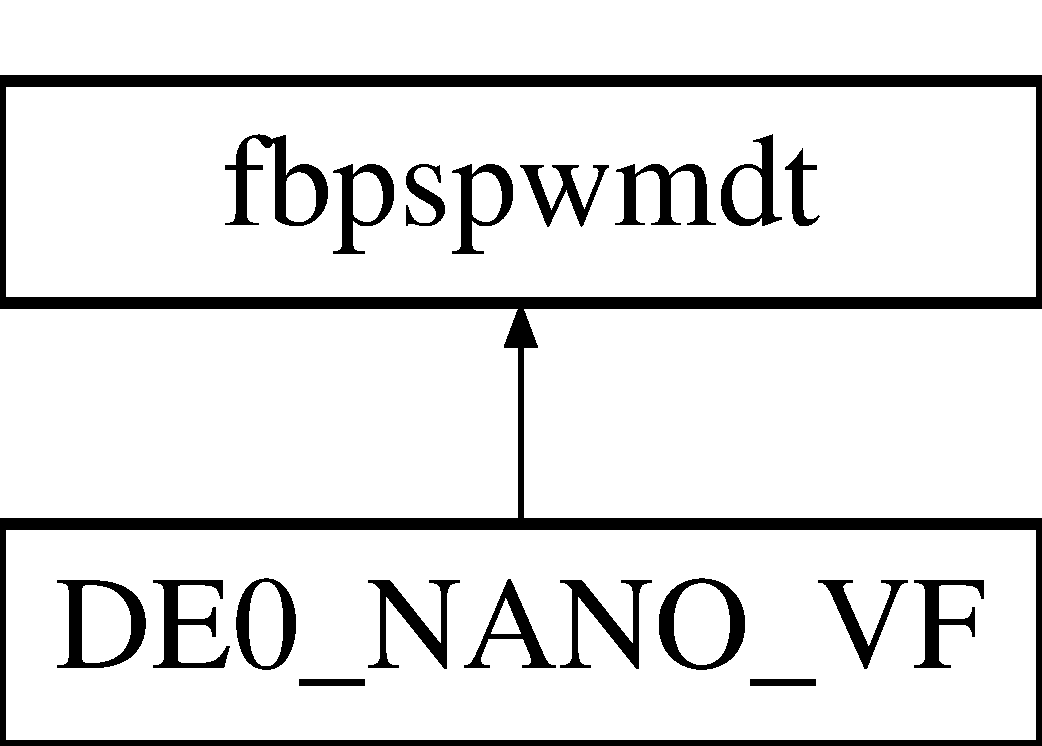
\includegraphics[height=2.000000cm]{classfbpspwmdt}
\end{center}
\end{figure}
\subsection*{Entities}
\begin{DoxyCompactItemize}
\item 
\hyperlink{classfbpspwmdt_1_1fbpspwmdt__arch}{fbpspwmdt\+\_\+arch} architecture
\end{DoxyCompactItemize}
\subsection*{Libraries}
 \begin{DoxyCompactItemize}
\item 
\hyperlink{classfbpspwmdt_ae4f03c286607f3181e16b9aa12d0c6d4}{I\+E\+E\+E} 
\end{DoxyCompactItemize}
\subsection*{Use Clauses}
 \begin{DoxyCompactItemize}
\item 
\hyperlink{classfbpspwmdt_a241c3e72dd8024cc8ae831b1b2aed7db}{S\+T\+D\+\_\+\+L\+O\+G\+I\+C\+\_\+\+U\+N\+S\+I\+G\+N\+E\+D}   
\item 
\hyperlink{classfbpspwmdt_aa4b2b25246a821511120e3149b003563}{S\+T\+D\+\_\+\+L\+O\+G\+I\+C\+\_\+1164}   
\item 
\hyperlink{classfbpspwmdt_aad86249c80e8c1e7ee1c4748aba748e3}{fixed\+\_\+pkg}   
\item 
\hyperlink{classfbpspwmdt_a2edc34402b573437d5f25fa90ba4013e}{numeric\+\_\+std}   
\end{DoxyCompactItemize}
\subsection*{Generics}
 \begin{DoxyCompactItemize}
\item 
\hyperlink{classfbpspwmdt_afee4aa1628956aa350183d8881689198}{n\+\_\+bits\+\_\+c} {\bfseries {\bfseries \textcolor{comment}{integer}\textcolor{vhdlchar}{ }\textcolor{vhdlchar}{ }\textcolor{vhdlchar}{\+:}\textcolor{vhdlchar}{=}\textcolor{vhdlchar}{ }\textcolor{vhdlchar}{ } \textcolor{vhdldigit}{16} \textcolor{vhdlchar}{ }}}
\item 
\hyperlink{classfbpspwmdt_a66678837c93def3337995d7ffcb44f3f}{c\+\_\+\+Dead\+\_\+t} {\bfseries {\bfseries \textcolor{comment}{integer}\textcolor{vhdlchar}{ }\textcolor{vhdlchar}{ }\textcolor{vhdlchar}{\+:}\textcolor{vhdlchar}{=}\textcolor{vhdlchar}{ }\textcolor{vhdlchar}{ } \textcolor{vhdldigit}{45} \textcolor{vhdlchar}{ }}}
\end{DoxyCompactItemize}
\subsection*{Ports}
 \begin{DoxyCompactItemize}
\item 
\hyperlink{classfbpspwmdt_a4a4609c199d30b3adebbeb3a01276ec5}{clk}  {\bfseries {\bfseries \textcolor{keywordflow}{in}\textcolor{vhdlchar}{ }}} {\bfseries \textcolor{comment}{std\+\_\+logic}\textcolor{vhdlchar}{ }} 
\item 
\hyperlink{classfbpspwmdt_adcf9c6f5161d039addbda5819bee64a3}{en}  {\bfseries {\bfseries \textcolor{keywordflow}{in}\textcolor{vhdlchar}{ }}} {\bfseries \textcolor{comment}{std\+\_\+logic}\textcolor{vhdlchar}{ }} 
\item 
\hyperlink{classfbpspwmdt_a021a597db1ce780174de5711902bf8f5}{comp}  {\bfseries {\bfseries \textcolor{vhdlchar}{ }}} {\bfseries \textcolor{comment}{std\+\_\+logic\+\_\+vector}\textcolor{vhdlchar}{ }\textcolor{vhdlchar}{(}\textcolor{vhdlchar}{ }\textcolor{vhdlchar}{ }\textcolor{vhdlchar}{ }\textcolor{vhdlchar}{ }{\bfseries \hyperlink{classfbpspwmdt_afee4aa1628956aa350183d8881689198}{n\+\_\+bits\+\_\+c}} \textcolor{vhdlchar}{-\/}\textcolor{vhdlchar}{ } \textcolor{vhdldigit}{1} \textcolor{vhdlchar}{ }\textcolor{keywordflow}{downto}\textcolor{vhdlchar}{ }\textcolor{vhdlchar}{ } \textcolor{vhdldigit}{0} \textcolor{vhdlchar}{ }\textcolor{vhdlchar}{)}\textcolor{vhdlchar}{ }}
\item 
\hyperlink{classfbpspwmdt_a0808bf3e7965a8ee90dec6604647f179}{c}  {\bfseries {\bfseries \textcolor{keywordflow}{in}\textcolor{vhdlchar}{ }}} {\bfseries \textcolor{comment}{std\+\_\+logic\+\_\+vector}\textcolor{vhdlchar}{ }\textcolor{vhdlchar}{(}\textcolor{vhdlchar}{ }\textcolor{vhdlchar}{ }\textcolor{vhdlchar}{ }\textcolor{vhdlchar}{ }{\bfseries \hyperlink{classfbpspwmdt_afee4aa1628956aa350183d8881689198}{n\+\_\+bits\+\_\+c}} \textcolor{vhdlchar}{-\/}\textcolor{vhdlchar}{ } \textcolor{vhdldigit}{1} \textcolor{vhdlchar}{ }\textcolor{keywordflow}{downto}\textcolor{vhdlchar}{ }\textcolor{vhdlchar}{ } \textcolor{vhdldigit}{0} \textcolor{vhdlchar}{ }\textcolor{vhdlchar}{)}\textcolor{vhdlchar}{ }} 
\item 
\hyperlink{classfbpspwmdt_af9b8278b961604ab62a822537a109adb}{amost}  {\bfseries {\bfseries \textcolor{keywordflow}{in}\textcolor{vhdlchar}{ }}} {\bfseries \textcolor{comment}{std\+\_\+logic}\textcolor{vhdlchar}{ }} 
\item 
\hyperlink{classfbpspwmdt_ad6bbafb165991aee14c6014831267789}{port\+\_\+\+P\+W\+M01}  {\bfseries {\bfseries \textcolor{keywordflow}{out}\textcolor{vhdlchar}{ }}} {\bfseries \textcolor{comment}{std\+\_\+logic}\textcolor{vhdlchar}{ }} 
\item 
\hyperlink{classfbpspwmdt_a0b2d13e9c0fd854957d88a65e0905e5b}{port\+\_\+\+P\+W\+M02}  {\bfseries {\bfseries \textcolor{keywordflow}{out}\textcolor{vhdlchar}{ }}} {\bfseries \textcolor{comment}{std\+\_\+logic}\textcolor{vhdlchar}{ }} 
\end{DoxyCompactItemize}


\subsection{Detailed Description}


Definition at line \hyperlink{fbpspwmdt_8vhd_source_l00011}{11} of file \hyperlink{fbpspwmdt_8vhd_source}{fbpspwmdt.\+vhd}.



\subsection{Member Data Documentation}
\hypertarget{classfbpspwmdt_af9b8278b961604ab62a822537a109adb}{}\index{fbpspwmdt@{fbpspwmdt}!amost@{amost}}
\index{amost@{amost}!fbpspwmdt@{fbpspwmdt}}
\subsubsection[{amost}]{\setlength{\rightskip}{0pt plus 5cm}{\bf amost} {\bfseries \textcolor{keywordflow}{in}\textcolor{vhdlchar}{ }} {\bfseries \textcolor{comment}{std\+\_\+logic}\textcolor{vhdlchar}{ }} \hspace{0.3cm}{\ttfamily [Port]}}\label{classfbpspwmdt_af9b8278b961604ab62a822537a109adb}


Definition at line \hyperlink{fbpspwmdt_8vhd_source_l00021}{21} of file \hyperlink{fbpspwmdt_8vhd_source}{fbpspwmdt.\+vhd}.

\hypertarget{classfbpspwmdt_a0808bf3e7965a8ee90dec6604647f179}{}\index{fbpspwmdt@{fbpspwmdt}!c@{c}}
\index{c@{c}!fbpspwmdt@{fbpspwmdt}}
\subsubsection[{c}]{\setlength{\rightskip}{0pt plus 5cm}{\bf c} {\bfseries \textcolor{keywordflow}{in}\textcolor{vhdlchar}{ }} {\bfseries \textcolor{comment}{std\+\_\+logic\+\_\+vector}\textcolor{vhdlchar}{ }\textcolor{vhdlchar}{(}\textcolor{vhdlchar}{ }\textcolor{vhdlchar}{ }\textcolor{vhdlchar}{ }\textcolor{vhdlchar}{ }{\bfseries {\bf n\+\_\+bits\+\_\+c}} \textcolor{vhdlchar}{-\/}\textcolor{vhdlchar}{ } \textcolor{vhdldigit}{1} \textcolor{vhdlchar}{ }\textcolor{keywordflow}{downto}\textcolor{vhdlchar}{ }\textcolor{vhdlchar}{ } \textcolor{vhdldigit}{0} \textcolor{vhdlchar}{ }\textcolor{vhdlchar}{)}\textcolor{vhdlchar}{ }} \hspace{0.3cm}{\ttfamily [Port]}}\label{classfbpspwmdt_a0808bf3e7965a8ee90dec6604647f179}


Definition at line \hyperlink{fbpspwmdt_8vhd_source_l00020}{20} of file \hyperlink{fbpspwmdt_8vhd_source}{fbpspwmdt.\+vhd}.

\hypertarget{classfbpspwmdt_a66678837c93def3337995d7ffcb44f3f}{}\index{fbpspwmdt@{fbpspwmdt}!c\+\_\+\+Dead\+\_\+t@{c\+\_\+\+Dead\+\_\+t}}
\index{c\+\_\+\+Dead\+\_\+t@{c\+\_\+\+Dead\+\_\+t}!fbpspwmdt@{fbpspwmdt}}
\subsubsection[{c\+\_\+\+Dead\+\_\+t}]{\setlength{\rightskip}{0pt plus 5cm}{\bf c\+\_\+\+Dead\+\_\+t} {\bfseries \textcolor{vhdlchar}{ }} {\bfseries \textcolor{comment}{integer}\textcolor{vhdlchar}{ }\textcolor{vhdlchar}{ }\textcolor{vhdlchar}{\+:}\textcolor{vhdlchar}{=}\textcolor{vhdlchar}{ }\textcolor{vhdlchar}{ } \textcolor{vhdldigit}{45} \textcolor{vhdlchar}{ }} \hspace{0.3cm}{\ttfamily [Generic]}}\label{classfbpspwmdt_a66678837c93def3337995d7ffcb44f3f}


Definition at line \hyperlink{fbpspwmdt_8vhd_source_l00015}{15} of file \hyperlink{fbpspwmdt_8vhd_source}{fbpspwmdt.\+vhd}.

\hypertarget{classfbpspwmdt_a4a4609c199d30b3adebbeb3a01276ec5}{}\index{fbpspwmdt@{fbpspwmdt}!clk@{clk}}
\index{clk@{clk}!fbpspwmdt@{fbpspwmdt}}
\subsubsection[{clk}]{\setlength{\rightskip}{0pt plus 5cm}{\bf clk} {\bfseries \textcolor{keywordflow}{in}\textcolor{vhdlchar}{ }} {\bfseries \textcolor{comment}{std\+\_\+logic}\textcolor{vhdlchar}{ }} \hspace{0.3cm}{\ttfamily [Port]}}\label{classfbpspwmdt_a4a4609c199d30b3adebbeb3a01276ec5}


Definition at line \hyperlink{fbpspwmdt_8vhd_source_l00017}{17} of file \hyperlink{fbpspwmdt_8vhd_source}{fbpspwmdt.\+vhd}.

\hypertarget{classfbpspwmdt_a021a597db1ce780174de5711902bf8f5}{}\index{fbpspwmdt@{fbpspwmdt}!comp@{comp}}
\index{comp@{comp}!fbpspwmdt@{fbpspwmdt}}
\subsubsection[{comp}]{\setlength{\rightskip}{0pt plus 5cm}{\bf comp} {\bfseries \textcolor{vhdlchar}{ }} {\bfseries \textcolor{comment}{std\+\_\+logic\+\_\+vector}\textcolor{vhdlchar}{ }\textcolor{vhdlchar}{(}\textcolor{vhdlchar}{ }\textcolor{vhdlchar}{ }\textcolor{vhdlchar}{ }\textcolor{vhdlchar}{ }{\bfseries {\bf n\+\_\+bits\+\_\+c}} \textcolor{vhdlchar}{-\/}\textcolor{vhdlchar}{ } \textcolor{vhdldigit}{1} \textcolor{vhdlchar}{ }\textcolor{keywordflow}{downto}\textcolor{vhdlchar}{ }\textcolor{vhdlchar}{ } \textcolor{vhdldigit}{0} \textcolor{vhdlchar}{ }\textcolor{vhdlchar}{)}\textcolor{vhdlchar}{ }} \hspace{0.3cm}{\ttfamily [Port]}}\label{classfbpspwmdt_a021a597db1ce780174de5711902bf8f5}


Definition at line \hyperlink{fbpspwmdt_8vhd_source_l00019}{19} of file \hyperlink{fbpspwmdt_8vhd_source}{fbpspwmdt.\+vhd}.

\hypertarget{classfbpspwmdt_adcf9c6f5161d039addbda5819bee64a3}{}\index{fbpspwmdt@{fbpspwmdt}!en@{en}}
\index{en@{en}!fbpspwmdt@{fbpspwmdt}}
\subsubsection[{en}]{\setlength{\rightskip}{0pt plus 5cm}{\bf en} {\bfseries \textcolor{keywordflow}{in}\textcolor{vhdlchar}{ }} {\bfseries \textcolor{comment}{std\+\_\+logic}\textcolor{vhdlchar}{ }} \hspace{0.3cm}{\ttfamily [Port]}}\label{classfbpspwmdt_adcf9c6f5161d039addbda5819bee64a3}


Definition at line \hyperlink{fbpspwmdt_8vhd_source_l00018}{18} of file \hyperlink{fbpspwmdt_8vhd_source}{fbpspwmdt.\+vhd}.

\hypertarget{classfbpspwmdt_aad86249c80e8c1e7ee1c4748aba748e3}{}\index{fbpspwmdt@{fbpspwmdt}!fixed\+\_\+pkg@{fixed\+\_\+pkg}}
\index{fixed\+\_\+pkg@{fixed\+\_\+pkg}!fbpspwmdt@{fbpspwmdt}}
\subsubsection[{fixed\+\_\+pkg}]{\setlength{\rightskip}{0pt plus 5cm}{\bf fixed\+\_\+pkg}\hspace{0.3cm}{\ttfamily [Package]}}\label{classfbpspwmdt_aad86249c80e8c1e7ee1c4748aba748e3}


Definition at line \hyperlink{fbpspwmdt_8vhd_source_l00007}{7} of file \hyperlink{fbpspwmdt_8vhd_source}{fbpspwmdt.\+vhd}.

\hypertarget{classfbpspwmdt_ae4f03c286607f3181e16b9aa12d0c6d4}{}\index{fbpspwmdt@{fbpspwmdt}!I\+E\+E\+E@{I\+E\+E\+E}}
\index{I\+E\+E\+E@{I\+E\+E\+E}!fbpspwmdt@{fbpspwmdt}}
\subsubsection[{I\+E\+E\+E}]{\setlength{\rightskip}{0pt plus 5cm}{\bf I\+E\+E\+E}\hspace{0.3cm}{\ttfamily [Library]}}\label{classfbpspwmdt_ae4f03c286607f3181e16b9aa12d0c6d4}


Definition at line \hyperlink{fbpspwmdt_8vhd_source_l00004}{4} of file \hyperlink{fbpspwmdt_8vhd_source}{fbpspwmdt.\+vhd}.

\hypertarget{classfbpspwmdt_afee4aa1628956aa350183d8881689198}{}\index{fbpspwmdt@{fbpspwmdt}!n\+\_\+bits\+\_\+c@{n\+\_\+bits\+\_\+c}}
\index{n\+\_\+bits\+\_\+c@{n\+\_\+bits\+\_\+c}!fbpspwmdt@{fbpspwmdt}}
\subsubsection[{n\+\_\+bits\+\_\+c}]{\setlength{\rightskip}{0pt plus 5cm}{\bf n\+\_\+bits\+\_\+c} {\bfseries \textcolor{vhdlchar}{ }} {\bfseries \textcolor{comment}{integer}\textcolor{vhdlchar}{ }\textcolor{vhdlchar}{ }\textcolor{vhdlchar}{\+:}\textcolor{vhdlchar}{=}\textcolor{vhdlchar}{ }\textcolor{vhdlchar}{ } \textcolor{vhdldigit}{16} \textcolor{vhdlchar}{ }} \hspace{0.3cm}{\ttfamily [Generic]}}\label{classfbpspwmdt_afee4aa1628956aa350183d8881689198}


Definition at line \hyperlink{fbpspwmdt_8vhd_source_l00013}{13} of file \hyperlink{fbpspwmdt_8vhd_source}{fbpspwmdt.\+vhd}.

\hypertarget{classfbpspwmdt_a2edc34402b573437d5f25fa90ba4013e}{}\index{fbpspwmdt@{fbpspwmdt}!numeric\+\_\+std@{numeric\+\_\+std}}
\index{numeric\+\_\+std@{numeric\+\_\+std}!fbpspwmdt@{fbpspwmdt}}
\subsubsection[{numeric\+\_\+std}]{\setlength{\rightskip}{0pt plus 5cm}{\bf numeric\+\_\+std}\hspace{0.3cm}{\ttfamily [Package]}}\label{classfbpspwmdt_a2edc34402b573437d5f25fa90ba4013e}


Definition at line \hyperlink{fbpspwmdt_8vhd_source_l00008}{8} of file \hyperlink{fbpspwmdt_8vhd_source}{fbpspwmdt.\+vhd}.

\hypertarget{classfbpspwmdt_ad6bbafb165991aee14c6014831267789}{}\index{fbpspwmdt@{fbpspwmdt}!port\+\_\+\+P\+W\+M01@{port\+\_\+\+P\+W\+M01}}
\index{port\+\_\+\+P\+W\+M01@{port\+\_\+\+P\+W\+M01}!fbpspwmdt@{fbpspwmdt}}
\subsubsection[{port\+\_\+\+P\+W\+M01}]{\setlength{\rightskip}{0pt plus 5cm}{\bf port\+\_\+\+P\+W\+M01} {\bfseries \textcolor{keywordflow}{out}\textcolor{vhdlchar}{ }} {\bfseries \textcolor{comment}{std\+\_\+logic}\textcolor{vhdlchar}{ }} \hspace{0.3cm}{\ttfamily [Port]}}\label{classfbpspwmdt_ad6bbafb165991aee14c6014831267789}


Definition at line \hyperlink{fbpspwmdt_8vhd_source_l00022}{22} of file \hyperlink{fbpspwmdt_8vhd_source}{fbpspwmdt.\+vhd}.

\hypertarget{classfbpspwmdt_a0b2d13e9c0fd854957d88a65e0905e5b}{}\index{fbpspwmdt@{fbpspwmdt}!port\+\_\+\+P\+W\+M02@{port\+\_\+\+P\+W\+M02}}
\index{port\+\_\+\+P\+W\+M02@{port\+\_\+\+P\+W\+M02}!fbpspwmdt@{fbpspwmdt}}
\subsubsection[{port\+\_\+\+P\+W\+M02}]{\setlength{\rightskip}{0pt plus 5cm}{\bf port\+\_\+\+P\+W\+M02} {\bfseries \textcolor{keywordflow}{out}\textcolor{vhdlchar}{ }} {\bfseries \textcolor{comment}{std\+\_\+logic}\textcolor{vhdlchar}{ }} \hspace{0.3cm}{\ttfamily [Port]}}\label{classfbpspwmdt_a0b2d13e9c0fd854957d88a65e0905e5b}


Definition at line \hyperlink{fbpspwmdt_8vhd_source_l00024}{24} of file \hyperlink{fbpspwmdt_8vhd_source}{fbpspwmdt.\+vhd}.

\hypertarget{classfbpspwmdt_aa4b2b25246a821511120e3149b003563}{}\index{fbpspwmdt@{fbpspwmdt}!S\+T\+D\+\_\+\+L\+O\+G\+I\+C\+\_\+1164@{S\+T\+D\+\_\+\+L\+O\+G\+I\+C\+\_\+1164}}
\index{S\+T\+D\+\_\+\+L\+O\+G\+I\+C\+\_\+1164@{S\+T\+D\+\_\+\+L\+O\+G\+I\+C\+\_\+1164}!fbpspwmdt@{fbpspwmdt}}
\subsubsection[{S\+T\+D\+\_\+\+L\+O\+G\+I\+C\+\_\+1164}]{\setlength{\rightskip}{0pt plus 5cm}{\bf S\+T\+D\+\_\+\+L\+O\+G\+I\+C\+\_\+1164}\hspace{0.3cm}{\ttfamily [Package]}}\label{classfbpspwmdt_aa4b2b25246a821511120e3149b003563}


Definition at line \hyperlink{fbpspwmdt_8vhd_source_l00006}{6} of file \hyperlink{fbpspwmdt_8vhd_source}{fbpspwmdt.\+vhd}.

\hypertarget{classfbpspwmdt_a241c3e72dd8024cc8ae831b1b2aed7db}{}\index{fbpspwmdt@{fbpspwmdt}!S\+T\+D\+\_\+\+L\+O\+G\+I\+C\+\_\+\+U\+N\+S\+I\+G\+N\+E\+D@{S\+T\+D\+\_\+\+L\+O\+G\+I\+C\+\_\+\+U\+N\+S\+I\+G\+N\+E\+D}}
\index{S\+T\+D\+\_\+\+L\+O\+G\+I\+C\+\_\+\+U\+N\+S\+I\+G\+N\+E\+D@{S\+T\+D\+\_\+\+L\+O\+G\+I\+C\+\_\+\+U\+N\+S\+I\+G\+N\+E\+D}!fbpspwmdt@{fbpspwmdt}}
\subsubsection[{S\+T\+D\+\_\+\+L\+O\+G\+I\+C\+\_\+\+U\+N\+S\+I\+G\+N\+E\+D}]{\setlength{\rightskip}{0pt plus 5cm}{\bf S\+T\+D\+\_\+\+L\+O\+G\+I\+C\+\_\+\+U\+N\+S\+I\+G\+N\+E\+D}\hspace{0.3cm}{\ttfamily [Package]}}\label{classfbpspwmdt_a241c3e72dd8024cc8ae831b1b2aed7db}


Definition at line \hyperlink{fbpspwmdt_8vhd_source_l00005}{5} of file \hyperlink{fbpspwmdt_8vhd_source}{fbpspwmdt.\+vhd}.



The documentation for this class was generated from the following file\+:\begin{DoxyCompactItemize}
\item 
\hyperlink{fbpspwmdt_8vhd}{fbpspwmdt.\+vhd}\end{DoxyCompactItemize}

\hypertarget{classfbpspwmdt_1_1fbpspwmdt__arch}{}\section{fbpspwmdt\+\_\+arch Architecture Reference}
\label{classfbpspwmdt_1_1fbpspwmdt__arch}\index{fbpspwmdt\+\_\+arch@{fbpspwmdt\+\_\+arch}}
\subsection*{Processes}
 \begin{DoxyCompactItemize}
\item 
\hyperlink{classfbpspwmdt_1_1fbpspwmdt__arch_a6cc276b9a3076e40ac68b8ac3f1828a7}{P\+R\+O\+C\+E\+S\+S\+\_\+7}{\bfseries  ( {\bfseries {\bfseries \hyperlink{classfbpspwmdt_a4a4609c199d30b3adebbeb3a01276ec5}{clk}} \textcolor{vhdlchar}{ }} )}
\item 
\hyperlink{classfbpspwmdt_1_1fbpspwmdt__arch_a7cf6ba78e659f286a9d61adf1efc91b0}{P\+R\+O\+C\+E\+S\+S\+\_\+8}{\bfseries  ( {\bfseries {\bfseries \hyperlink{classfbpspwmdt_af9b8278b961604ab62a822537a109adb}{amost}} \textcolor{vhdlchar}{ }} )}
\item 
\hyperlink{classfbpspwmdt_1_1fbpspwmdt__arch_a0132bccb07ff42922281b99abe7fc1ed}{P\+R\+O\+C\+E\+S\+S\+\_\+9}{\bfseries  ( {\bfseries {\bfseries \hyperlink{classfbpspwmdt_a4a4609c199d30b3adebbeb3a01276ec5}{clk}} \textcolor{vhdlchar}{ }} )}
\end{DoxyCompactItemize}
\subsection*{Signals}
 \begin{DoxyCompactItemize}
\item 
\hyperlink{classfbpspwmdt_1_1fbpspwmdt__arch_abf7d8be25624dd08fcc1517c8e39cb23}{comp\+\_\+int} {\bfseries \textcolor{comment}{std\+\_\+logic\+\_\+vector}\textcolor{vhdlchar}{ }\textcolor{vhdlchar}{(}\textcolor{vhdlchar}{ }\textcolor{vhdlchar}{ }\textcolor{vhdlchar}{ }\textcolor{vhdlchar}{ }{\bfseries \hyperlink{classfbpspwmdt_afee4aa1628956aa350183d8881689198}{n\+\_\+bits\+\_\+c}} \textcolor{vhdlchar}{-\/}\textcolor{vhdlchar}{ } \textcolor{vhdldigit}{1} \textcolor{vhdlchar}{ }\textcolor{keywordflow}{downto}\textcolor{vhdlchar}{ }\textcolor{vhdlchar}{ } \textcolor{vhdldigit}{0} \textcolor{vhdlchar}{ }\textcolor{vhdlchar}{)}\textcolor{vhdlchar}{ }} 
\item 
\hyperlink{classfbpspwmdt_1_1fbpspwmdt__arch_a90c7671dbb1af7d80f90cd96262cda3b}{sig\+\_\+\+Not\+\_\+\+Pwm\+\_\+\+In} {\bfseries \textcolor{comment}{std\+\_\+logic}\textcolor{vhdlchar}{ }} 
\item 
\hyperlink{classfbpspwmdt_1_1fbpspwmdt__arch_a5b5410422331d47dda25071eab458071}{comp\+\_\+out} {\bfseries \textcolor{comment}{std\+\_\+logic}\textcolor{vhdlchar}{ }} 
\item 
\hyperlink{classfbpspwmdt_1_1fbpspwmdt__arch_af7e8a49d46795da5945dc6b1f0602c13}{p\+\_\+\+Pwm\+\_\+\+In} {\bfseries \textcolor{comment}{std\+\_\+logic}\textcolor{vhdlchar}{ }} 
\end{DoxyCompactItemize}


\subsection{Detailed Description}


Definition at line \hyperlink{fbpspwmdt_8vhd_source_l00031}{31} of file \hyperlink{fbpspwmdt_8vhd_source}{fbpspwmdt.\+vhd}.



\subsection{Member Function Documentation}
\hypertarget{classfbpspwmdt_1_1fbpspwmdt__arch_a6cc276b9a3076e40ac68b8ac3f1828a7}{}\index{fbpspwmdt\+::fbpspwmdt\+\_\+arch@{fbpspwmdt\+::fbpspwmdt\+\_\+arch}!P\+R\+O\+C\+E\+S\+S\+\_\+7@{P\+R\+O\+C\+E\+S\+S\+\_\+7}}
\index{P\+R\+O\+C\+E\+S\+S\+\_\+7@{P\+R\+O\+C\+E\+S\+S\+\_\+7}!fbpspwmdt\+::fbpspwmdt\+\_\+arch@{fbpspwmdt\+::fbpspwmdt\+\_\+arch}}
\subsubsection[{P\+R\+O\+C\+E\+S\+S\+\_\+7}]{\setlength{\rightskip}{0pt plus 5cm} {\bfseries \textcolor{vhdlchar}{ }} P\+R\+O\+C\+E\+S\+S\+\_\+7(
\begin{DoxyParamCaption}
\item[{}]{{\bfseries {\bfseries {\bf clk}} \textcolor{vhdlchar}{ }} {\em }}
\end{DoxyParamCaption}
)\hspace{0.3cm}{\ttfamily [Process]}}\label{classfbpspwmdt_1_1fbpspwmdt__arch_a6cc276b9a3076e40ac68b8ac3f1828a7}


Definition at line \hyperlink{fbpspwmdt_8vhd_source_l00042}{42} of file \hyperlink{fbpspwmdt_8vhd_source}{fbpspwmdt.\+vhd}.

\hypertarget{classfbpspwmdt_1_1fbpspwmdt__arch_a7cf6ba78e659f286a9d61adf1efc91b0}{}\index{fbpspwmdt\+::fbpspwmdt\+\_\+arch@{fbpspwmdt\+::fbpspwmdt\+\_\+arch}!P\+R\+O\+C\+E\+S\+S\+\_\+8@{P\+R\+O\+C\+E\+S\+S\+\_\+8}}
\index{P\+R\+O\+C\+E\+S\+S\+\_\+8@{P\+R\+O\+C\+E\+S\+S\+\_\+8}!fbpspwmdt\+::fbpspwmdt\+\_\+arch@{fbpspwmdt\+::fbpspwmdt\+\_\+arch}}
\subsubsection[{P\+R\+O\+C\+E\+S\+S\+\_\+8}]{\setlength{\rightskip}{0pt plus 5cm} {\bfseries \textcolor{vhdlchar}{ }} P\+R\+O\+C\+E\+S\+S\+\_\+8(
\begin{DoxyParamCaption}
\item[{}]{{\bfseries {\bfseries {\bf amost}} \textcolor{vhdlchar}{ }} {\em }}
\end{DoxyParamCaption}
)\hspace{0.3cm}{\ttfamily [Process]}}\label{classfbpspwmdt_1_1fbpspwmdt__arch_a7cf6ba78e659f286a9d61adf1efc91b0}


Definition at line \hyperlink{fbpspwmdt_8vhd_source_l00055}{55} of file \hyperlink{fbpspwmdt_8vhd_source}{fbpspwmdt.\+vhd}.

\hypertarget{classfbpspwmdt_1_1fbpspwmdt__arch_a0132bccb07ff42922281b99abe7fc1ed}{}\index{fbpspwmdt\+::fbpspwmdt\+\_\+arch@{fbpspwmdt\+::fbpspwmdt\+\_\+arch}!P\+R\+O\+C\+E\+S\+S\+\_\+9@{P\+R\+O\+C\+E\+S\+S\+\_\+9}}
\index{P\+R\+O\+C\+E\+S\+S\+\_\+9@{P\+R\+O\+C\+E\+S\+S\+\_\+9}!fbpspwmdt\+::fbpspwmdt\+\_\+arch@{fbpspwmdt\+::fbpspwmdt\+\_\+arch}}
\subsubsection[{P\+R\+O\+C\+E\+S\+S\+\_\+9}]{\setlength{\rightskip}{0pt plus 5cm} {\bfseries \textcolor{vhdlchar}{ }} P\+R\+O\+C\+E\+S\+S\+\_\+9(
\begin{DoxyParamCaption}
\item[{}]{{\bfseries {\bfseries {\bf clk}} \textcolor{vhdlchar}{ }} {\em }}
\end{DoxyParamCaption}
)\hspace{0.3cm}{\ttfamily [Process]}}\label{classfbpspwmdt_1_1fbpspwmdt__arch_a0132bccb07ff42922281b99abe7fc1ed}


Definition at line \hyperlink{fbpspwmdt_8vhd_source_l00067}{67} of file \hyperlink{fbpspwmdt_8vhd_source}{fbpspwmdt.\+vhd}.



\subsection{Member Data Documentation}
\hypertarget{classfbpspwmdt_1_1fbpspwmdt__arch_abf7d8be25624dd08fcc1517c8e39cb23}{}\index{fbpspwmdt\+::fbpspwmdt\+\_\+arch@{fbpspwmdt\+::fbpspwmdt\+\_\+arch}!comp\+\_\+int@{comp\+\_\+int}}
\index{comp\+\_\+int@{comp\+\_\+int}!fbpspwmdt\+::fbpspwmdt\+\_\+arch@{fbpspwmdt\+::fbpspwmdt\+\_\+arch}}
\subsubsection[{comp\+\_\+int}]{\setlength{\rightskip}{0pt plus 5cm}{\bf comp\+\_\+int} {\bfseries \textcolor{comment}{std\+\_\+logic\+\_\+vector}\textcolor{vhdlchar}{ }\textcolor{vhdlchar}{(}\textcolor{vhdlchar}{ }\textcolor{vhdlchar}{ }\textcolor{vhdlchar}{ }\textcolor{vhdlchar}{ }{\bfseries {\bf n\+\_\+bits\+\_\+c}} \textcolor{vhdlchar}{-\/}\textcolor{vhdlchar}{ } \textcolor{vhdldigit}{1} \textcolor{vhdlchar}{ }\textcolor{keywordflow}{downto}\textcolor{vhdlchar}{ }\textcolor{vhdlchar}{ } \textcolor{vhdldigit}{0} \textcolor{vhdlchar}{ }\textcolor{vhdlchar}{)}\textcolor{vhdlchar}{ }} \hspace{0.3cm}{\ttfamily [Signal]}}\label{classfbpspwmdt_1_1fbpspwmdt__arch_abf7d8be25624dd08fcc1517c8e39cb23}


Definition at line \hyperlink{fbpspwmdt_8vhd_source_l00034}{34} of file \hyperlink{fbpspwmdt_8vhd_source}{fbpspwmdt.\+vhd}.

\hypertarget{classfbpspwmdt_1_1fbpspwmdt__arch_a5b5410422331d47dda25071eab458071}{}\index{fbpspwmdt\+::fbpspwmdt\+\_\+arch@{fbpspwmdt\+::fbpspwmdt\+\_\+arch}!comp\+\_\+out@{comp\+\_\+out}}
\index{comp\+\_\+out@{comp\+\_\+out}!fbpspwmdt\+::fbpspwmdt\+\_\+arch@{fbpspwmdt\+::fbpspwmdt\+\_\+arch}}
\subsubsection[{comp\+\_\+out}]{\setlength{\rightskip}{0pt plus 5cm}{\bf comp\+\_\+out} {\bfseries \textcolor{comment}{std\+\_\+logic}\textcolor{vhdlchar}{ }} \hspace{0.3cm}{\ttfamily [Signal]}}\label{classfbpspwmdt_1_1fbpspwmdt__arch_a5b5410422331d47dda25071eab458071}


Definition at line \hyperlink{fbpspwmdt_8vhd_source_l00036}{36} of file \hyperlink{fbpspwmdt_8vhd_source}{fbpspwmdt.\+vhd}.

\hypertarget{classfbpspwmdt_1_1fbpspwmdt__arch_af7e8a49d46795da5945dc6b1f0602c13}{}\index{fbpspwmdt\+::fbpspwmdt\+\_\+arch@{fbpspwmdt\+::fbpspwmdt\+\_\+arch}!p\+\_\+\+Pwm\+\_\+\+In@{p\+\_\+\+Pwm\+\_\+\+In}}
\index{p\+\_\+\+Pwm\+\_\+\+In@{p\+\_\+\+Pwm\+\_\+\+In}!fbpspwmdt\+::fbpspwmdt\+\_\+arch@{fbpspwmdt\+::fbpspwmdt\+\_\+arch}}
\subsubsection[{p\+\_\+\+Pwm\+\_\+\+In}]{\setlength{\rightskip}{0pt plus 5cm}{\bf p\+\_\+\+Pwm\+\_\+\+In} {\bfseries \textcolor{comment}{std\+\_\+logic}\textcolor{vhdlchar}{ }} \hspace{0.3cm}{\ttfamily [Signal]}}\label{classfbpspwmdt_1_1fbpspwmdt__arch_af7e8a49d46795da5945dc6b1f0602c13}


Definition at line \hyperlink{fbpspwmdt_8vhd_source_l00037}{37} of file \hyperlink{fbpspwmdt_8vhd_source}{fbpspwmdt.\+vhd}.

\hypertarget{classfbpspwmdt_1_1fbpspwmdt__arch_a90c7671dbb1af7d80f90cd96262cda3b}{}\index{fbpspwmdt\+::fbpspwmdt\+\_\+arch@{fbpspwmdt\+::fbpspwmdt\+\_\+arch}!sig\+\_\+\+Not\+\_\+\+Pwm\+\_\+\+In@{sig\+\_\+\+Not\+\_\+\+Pwm\+\_\+\+In}}
\index{sig\+\_\+\+Not\+\_\+\+Pwm\+\_\+\+In@{sig\+\_\+\+Not\+\_\+\+Pwm\+\_\+\+In}!fbpspwmdt\+::fbpspwmdt\+\_\+arch@{fbpspwmdt\+::fbpspwmdt\+\_\+arch}}
\subsubsection[{sig\+\_\+\+Not\+\_\+\+Pwm\+\_\+\+In}]{\setlength{\rightskip}{0pt plus 5cm}{\bf sig\+\_\+\+Not\+\_\+\+Pwm\+\_\+\+In} {\bfseries \textcolor{comment}{std\+\_\+logic}\textcolor{vhdlchar}{ }} \hspace{0.3cm}{\ttfamily [Signal]}}\label{classfbpspwmdt_1_1fbpspwmdt__arch_a90c7671dbb1af7d80f90cd96262cda3b}


Definition at line \hyperlink{fbpspwmdt_8vhd_source_l00035}{35} of file \hyperlink{fbpspwmdt_8vhd_source}{fbpspwmdt.\+vhd}.



The documentation for this class was generated from the following file\+:\begin{DoxyCompactItemize}
\item 
\hyperlink{fbpspwmdt_8vhd}{fbpspwmdt.\+vhd}\end{DoxyCompactItemize}

\hypertarget{classfixed__float__types}{}\section{fixed\+\_\+float\+\_\+types Package Reference}
\label{classfixed__float__types}\index{fixed\+\_\+float\+\_\+types@{fixed\+\_\+float\+\_\+types}}
\subsection*{Types}
 \begin{DoxyCompactItemize}
\item 
{\bfseries \hyperlink{classfixed__float__types_a531b370a8acfecdccebf696cf0d2d971}{fixed\+\_\+round\+\_\+style\+\_\+type}{\bfseries \textcolor{vhdlchar}{(}\textcolor{vhdlchar}{ }\textcolor{vhdlchar}{fixed\+\_\+round}\textcolor{vhdlchar}{ }\textcolor{vhdlchar}{,}\textcolor{vhdlchar}{ }\textcolor{vhdlchar}{fixed\+\_\+truncate}\textcolor{vhdlchar}{ }\textcolor{vhdlchar}{)}\textcolor{vhdlchar}{ }}} 
\item 
{\bfseries \hyperlink{classfixed__float__types_a8a8b6b0022e693377949251b05ac846a}{fixed\+\_\+overflow\+\_\+style\+\_\+type}{\bfseries \textcolor{vhdlchar}{(}\textcolor{vhdlchar}{ }\textcolor{vhdlchar}{fixed\+\_\+saturate}\textcolor{vhdlchar}{ }\textcolor{vhdlchar}{,}\textcolor{vhdlchar}{ }\textcolor{vhdlchar}{fixed\+\_\+wrap}\textcolor{vhdlchar}{ }\textcolor{vhdlchar}{)}\textcolor{vhdlchar}{ }}} 
\item 
{\bfseries \hyperlink{classfixed__float__types_a3cab38cfb8c7d6b81f4f0b9953cd212f}{round\+\_\+type}{\bfseries \textcolor{vhdlchar}{(}\textcolor{vhdlchar}{ }\textcolor{vhdlchar}{round\+\_\+nearest}\textcolor{vhdlchar}{ }\textcolor{vhdlchar}{,}\textcolor{vhdlchar}{ }\textcolor{vhdlchar}{round\+\_\+inf}\textcolor{vhdlchar}{ }\textcolor{vhdlchar}{,}\textcolor{vhdlchar}{ }\textcolor{vhdlchar}{round\+\_\+neginf}\textcolor{vhdlchar}{ }\textcolor{vhdlchar}{,}\textcolor{vhdlchar}{ }\textcolor{vhdlchar}{round\+\_\+zero}\textcolor{vhdlchar}{ }\textcolor{vhdlchar}{)}\textcolor{vhdlchar}{ }}} 
\end{DoxyCompactItemize}


\subsection{Detailed Description}


Definition at line 16 of file fixed\+\_\+float\+\_\+types\+\_\+c.\+vhdl.



\subsection{Member Data Documentation}
\hypertarget{classfixed__float__types_a8a8b6b0022e693377949251b05ac846a}{}\index{fixed\+\_\+float\+\_\+types@{fixed\+\_\+float\+\_\+types}!fixed\+\_\+overflow\+\_\+style\+\_\+type@{fixed\+\_\+overflow\+\_\+style\+\_\+type}}
\index{fixed\+\_\+overflow\+\_\+style\+\_\+type@{fixed\+\_\+overflow\+\_\+style\+\_\+type}!fixed\+\_\+float\+\_\+types@{fixed\+\_\+float\+\_\+types}}
\subsubsection[{fixed\+\_\+overflow\+\_\+style\+\_\+type}]{\setlength{\rightskip}{0pt plus 5cm}{\bf fixed\+\_\+overflow\+\_\+style\+\_\+type} {\bfseries \textcolor{vhdlchar}{(}\textcolor{vhdlchar}{ }\textcolor{vhdlchar}{fixed\+\_\+saturate}\textcolor{vhdlchar}{ }\textcolor{vhdlchar}{,}\textcolor{vhdlchar}{ }\textcolor{vhdlchar}{fixed\+\_\+wrap}\textcolor{vhdlchar}{ }\textcolor{vhdlchar}{)}\textcolor{vhdlchar}{ }} \hspace{0.3cm}{\ttfamily [Type]}}\label{classfixed__float__types_a8a8b6b0022e693377949251b05ac846a}


Definition at line 22 of file fixed\+\_\+float\+\_\+types\+\_\+c.\+vhdl.

\hypertarget{classfixed__float__types_a531b370a8acfecdccebf696cf0d2d971}{}\index{fixed\+\_\+float\+\_\+types@{fixed\+\_\+float\+\_\+types}!fixed\+\_\+round\+\_\+style\+\_\+type@{fixed\+\_\+round\+\_\+style\+\_\+type}}
\index{fixed\+\_\+round\+\_\+style\+\_\+type@{fixed\+\_\+round\+\_\+style\+\_\+type}!fixed\+\_\+float\+\_\+types@{fixed\+\_\+float\+\_\+types}}
\subsubsection[{fixed\+\_\+round\+\_\+style\+\_\+type}]{\setlength{\rightskip}{0pt plus 5cm}{\bf fixed\+\_\+round\+\_\+style\+\_\+type} {\bfseries \textcolor{vhdlchar}{(}\textcolor{vhdlchar}{ }\textcolor{vhdlchar}{fixed\+\_\+round}\textcolor{vhdlchar}{ }\textcolor{vhdlchar}{,}\textcolor{vhdlchar}{ }\textcolor{vhdlchar}{fixed\+\_\+truncate}\textcolor{vhdlchar}{ }\textcolor{vhdlchar}{)}\textcolor{vhdlchar}{ }} \hspace{0.3cm}{\ttfamily [Type]}}\label{classfixed__float__types_a531b370a8acfecdccebf696cf0d2d971}


Definition at line 20 of file fixed\+\_\+float\+\_\+types\+\_\+c.\+vhdl.

\hypertarget{classfixed__float__types_a3cab38cfb8c7d6b81f4f0b9953cd212f}{}\index{fixed\+\_\+float\+\_\+types@{fixed\+\_\+float\+\_\+types}!round\+\_\+type@{round\+\_\+type}}
\index{round\+\_\+type@{round\+\_\+type}!fixed\+\_\+float\+\_\+types@{fixed\+\_\+float\+\_\+types}}
\subsubsection[{round\+\_\+type}]{\setlength{\rightskip}{0pt plus 5cm}{\bf round\+\_\+type} {\bfseries \textcolor{vhdlchar}{(}\textcolor{vhdlchar}{ }\textcolor{vhdlchar}{round\+\_\+nearest}\textcolor{vhdlchar}{ }\textcolor{vhdlchar}{,}\textcolor{vhdlchar}{ }\textcolor{vhdlchar}{round\+\_\+inf}\textcolor{vhdlchar}{ }\textcolor{vhdlchar}{,}\textcolor{vhdlchar}{ }\textcolor{vhdlchar}{round\+\_\+neginf}\textcolor{vhdlchar}{ }\textcolor{vhdlchar}{,}\textcolor{vhdlchar}{ }\textcolor{vhdlchar}{round\+\_\+zero}\textcolor{vhdlchar}{ }\textcolor{vhdlchar}{)}\textcolor{vhdlchar}{ }} \hspace{0.3cm}{\ttfamily [Type]}}\label{classfixed__float__types_a3cab38cfb8c7d6b81f4f0b9953cd212f}


Definition at line 29 of file fixed\+\_\+float\+\_\+types\+\_\+c.\+vhdl.



The documentation for this class was generated from the following file\+:\begin{DoxyCompactItemize}
\item 
\hyperlink{fixed__float__types__c_8vhdl}{fixed\+\_\+float\+\_\+types\+\_\+c.\+vhdl}\end{DoxyCompactItemize}

\hypertarget{classfixed__pkg}{}\section{fixed\+\_\+pkg Package Reference}
\label{classfixed__pkg}\index{fixed\+\_\+pkg@{fixed\+\_\+pkg}}
{\bfseries Package Body $>$$>$ }\hyperlink{class__fixed__pkg}{fixed\+\_\+pkg}\\*
\subsection*{Functions}
 \begin{DoxyCompactItemize}
\item 
{\bfseries {\bfseries {\bfseries \hyperlink{classfixed__pkg_aa723b28a027c3c0f9bca02d75e8df4d6}{U\+N\+R\+E\+S\+O\+L\+V\+E\+D\+\_\+sfixed}} \textcolor{vhdlchar}{ }}} \hyperlink{classfixed__pkg_a38c1c4c6b1f76cfc07b009c92acabab5}{\char`\"{}abs\char`\"{}}{\bfseries  ( }{\bfseries \textcolor{vhdlchar}{arg\+: }\textcolor{stringliteral}{in }\textcolor{vhdlchar}{U\+N\+R\+E\+S\+O\+L\+V\+E\+D\+\_\+sfixed}}{\bfseries  )} 
\item 
{\bfseries {\bfseries {\bfseries \hyperlink{classfixed__pkg_aa723b28a027c3c0f9bca02d75e8df4d6}{U\+N\+R\+E\+S\+O\+L\+V\+E\+D\+\_\+sfixed}} \textcolor{vhdlchar}{ }}} \hyperlink{classfixed__pkg_acc47f8e7fbecebc0fc011d8431f076fd}{\char`\"{}-\/\char`\"{}}{\bfseries  ( }{\bfseries \textcolor{vhdlchar}{arg\+: }\textcolor{stringliteral}{in }\textcolor{vhdlchar}{U\+N\+R\+E\+S\+O\+L\+V\+E\+D\+\_\+sfixed}}{\bfseries  )} 
\item 
{\bfseries {\bfseries {\bfseries \hyperlink{classfixed__pkg_ae78bc2b36d22f6abeac163955e8a587d}{U\+N\+R\+E\+S\+O\+L\+V\+E\+D\+\_\+ufixed}} \textcolor{vhdlchar}{ }}} \hyperlink{classfixed__pkg_a758fadb06ceaaaffa80aa4473dc8dcda}{\char`\"{}+\char`\"{}}{\bfseries  ( }{\bfseries \textcolor{vhdlchar}{l\+: }\textcolor{stringliteral}{in }\textcolor{vhdlchar}{U\+N\+R\+E\+S\+O\+L\+V\+E\+D\+\_\+ufixed}}{\bfseries  , \textcolor{vhdlchar}{r\+: }\textcolor{stringliteral}{in }\textcolor{vhdlchar}{U\+N\+R\+E\+S\+O\+L\+V\+E\+D\+\_\+ufixed}}{\bfseries  )} 
\item 
{\bfseries {\bfseries {\bfseries \hyperlink{classfixed__pkg_aa723b28a027c3c0f9bca02d75e8df4d6}{U\+N\+R\+E\+S\+O\+L\+V\+E\+D\+\_\+sfixed}} \textcolor{vhdlchar}{ }}} \hyperlink{classfixed__pkg_a75f813bcb278832108d6fa67eccdfc1c}{\char`\"{}+\char`\"{}}{\bfseries  ( }{\bfseries \textcolor{vhdlchar}{l\+: }\textcolor{stringliteral}{in }\textcolor{vhdlchar}{U\+N\+R\+E\+S\+O\+L\+V\+E\+D\+\_\+sfixed}}{\bfseries  , \textcolor{vhdlchar}{r\+: }\textcolor{stringliteral}{in }\textcolor{vhdlchar}{U\+N\+R\+E\+S\+O\+L\+V\+E\+D\+\_\+sfixed}}{\bfseries  )} 
\item 
{\bfseries {\bfseries {\bfseries \hyperlink{classfixed__pkg_ae78bc2b36d22f6abeac163955e8a587d}{U\+N\+R\+E\+S\+O\+L\+V\+E\+D\+\_\+ufixed}} \textcolor{vhdlchar}{ }}} \hyperlink{classfixed__pkg_aa5b0e6d3b75f03dea7c3a4daedc04027}{\char`\"{}-\/\char`\"{}}{\bfseries  ( }{\bfseries \textcolor{vhdlchar}{l\+: }\textcolor{stringliteral}{in }\textcolor{vhdlchar}{U\+N\+R\+E\+S\+O\+L\+V\+E\+D\+\_\+ufixed}}{\bfseries  , \textcolor{vhdlchar}{r\+: }\textcolor{stringliteral}{in }\textcolor{vhdlchar}{U\+N\+R\+E\+S\+O\+L\+V\+E\+D\+\_\+ufixed}}{\bfseries  )} 
\item 
{\bfseries {\bfseries {\bfseries \hyperlink{classfixed__pkg_aa723b28a027c3c0f9bca02d75e8df4d6}{U\+N\+R\+E\+S\+O\+L\+V\+E\+D\+\_\+sfixed}} \textcolor{vhdlchar}{ }}} \hyperlink{classfixed__pkg_aa50f5cd3a12ba1cca2c9579edce09042}{\char`\"{}-\/\char`\"{}}{\bfseries  ( }{\bfseries \textcolor{vhdlchar}{l\+: }\textcolor{stringliteral}{in }\textcolor{vhdlchar}{U\+N\+R\+E\+S\+O\+L\+V\+E\+D\+\_\+sfixed}}{\bfseries  , \textcolor{vhdlchar}{r\+: }\textcolor{stringliteral}{in }\textcolor{vhdlchar}{U\+N\+R\+E\+S\+O\+L\+V\+E\+D\+\_\+sfixed}}{\bfseries  )} 
\item 
{\bfseries {\bfseries {\bfseries \hyperlink{classfixed__pkg_ae78bc2b36d22f6abeac163955e8a587d}{U\+N\+R\+E\+S\+O\+L\+V\+E\+D\+\_\+ufixed}} \textcolor{vhdlchar}{ }}} \hyperlink{classfixed__pkg_a29826fcafea88257a94a5fcc9ededcba}{\char`\"{}$\ast$\char`\"{}}{\bfseries  ( }{\bfseries \textcolor{vhdlchar}{l\+: }\textcolor{stringliteral}{in }\textcolor{vhdlchar}{U\+N\+R\+E\+S\+O\+L\+V\+E\+D\+\_\+ufixed}}{\bfseries  , \textcolor{vhdlchar}{r\+: }\textcolor{stringliteral}{in }\textcolor{vhdlchar}{U\+N\+R\+E\+S\+O\+L\+V\+E\+D\+\_\+ufixed}}{\bfseries  )} 
\item 
{\bfseries {\bfseries {\bfseries \hyperlink{classfixed__pkg_aa723b28a027c3c0f9bca02d75e8df4d6}{U\+N\+R\+E\+S\+O\+L\+V\+E\+D\+\_\+sfixed}} \textcolor{vhdlchar}{ }}} \hyperlink{classfixed__pkg_a12861e11afd1cb6346d3bab7f8e71b9c}{\char`\"{}$\ast$\char`\"{}}{\bfseries  ( }{\bfseries \textcolor{vhdlchar}{l\+: }\textcolor{stringliteral}{in }\textcolor{vhdlchar}{U\+N\+R\+E\+S\+O\+L\+V\+E\+D\+\_\+sfixed}}{\bfseries  , \textcolor{vhdlchar}{r\+: }\textcolor{stringliteral}{in }\textcolor{vhdlchar}{U\+N\+R\+E\+S\+O\+L\+V\+E\+D\+\_\+sfixed}}{\bfseries  )} 
\item 
{\bfseries {\bfseries {\bfseries \hyperlink{classfixed__pkg_ae78bc2b36d22f6abeac163955e8a587d}{U\+N\+R\+E\+S\+O\+L\+V\+E\+D\+\_\+ufixed}} \textcolor{vhdlchar}{ }}} \hyperlink{classfixed__pkg_a49d0495d91a74b686658a730a25948d1}{\char`\"{}/\char`\"{}}{\bfseries  ( }{\bfseries \textcolor{vhdlchar}{l\+: }\textcolor{stringliteral}{in }\textcolor{vhdlchar}{U\+N\+R\+E\+S\+O\+L\+V\+E\+D\+\_\+ufixed}}{\bfseries  , \textcolor{vhdlchar}{r\+: }\textcolor{stringliteral}{in }\textcolor{vhdlchar}{U\+N\+R\+E\+S\+O\+L\+V\+E\+D\+\_\+ufixed}}{\bfseries  )} 
\item 
{\bfseries {\bfseries {\bfseries \hyperlink{classfixed__pkg_aa723b28a027c3c0f9bca02d75e8df4d6}{U\+N\+R\+E\+S\+O\+L\+V\+E\+D\+\_\+sfixed}} \textcolor{vhdlchar}{ }}} \hyperlink{classfixed__pkg_a38133f42dc06bfa3083ee5757db5fdd1}{\char`\"{}/\char`\"{}}{\bfseries  ( }{\bfseries \textcolor{vhdlchar}{l\+: }\textcolor{stringliteral}{in }\textcolor{vhdlchar}{U\+N\+R\+E\+S\+O\+L\+V\+E\+D\+\_\+sfixed}}{\bfseries  , \textcolor{vhdlchar}{r\+: }\textcolor{stringliteral}{in }\textcolor{vhdlchar}{U\+N\+R\+E\+S\+O\+L\+V\+E\+D\+\_\+sfixed}}{\bfseries  )} 
\item 
{\bfseries {\bfseries {\bfseries \hyperlink{classfixed__pkg_ae78bc2b36d22f6abeac163955e8a587d}{U\+N\+R\+E\+S\+O\+L\+V\+E\+D\+\_\+ufixed}} \textcolor{vhdlchar}{ }}} \hyperlink{classfixed__pkg_ad1f795e1e3cf142cf7bb4dfb5b951869}{\char`\"{}rem\char`\"{}}{\bfseries  ( }{\bfseries \textcolor{vhdlchar}{l\+: }\textcolor{stringliteral}{in }\textcolor{vhdlchar}{U\+N\+R\+E\+S\+O\+L\+V\+E\+D\+\_\+ufixed}}{\bfseries  , \textcolor{vhdlchar}{r\+: }\textcolor{stringliteral}{in }\textcolor{vhdlchar}{U\+N\+R\+E\+S\+O\+L\+V\+E\+D\+\_\+ufixed}}{\bfseries  )} 
\item 
{\bfseries {\bfseries {\bfseries \hyperlink{classfixed__pkg_aa723b28a027c3c0f9bca02d75e8df4d6}{U\+N\+R\+E\+S\+O\+L\+V\+E\+D\+\_\+sfixed}} \textcolor{vhdlchar}{ }}} \hyperlink{classfixed__pkg_a456d29ab7e0ace8e29746cae8333c4a8}{\char`\"{}rem\char`\"{}}{\bfseries  ( }{\bfseries \textcolor{vhdlchar}{l\+: }\textcolor{stringliteral}{in }\textcolor{vhdlchar}{U\+N\+R\+E\+S\+O\+L\+V\+E\+D\+\_\+sfixed}}{\bfseries  , \textcolor{vhdlchar}{r\+: }\textcolor{stringliteral}{in }\textcolor{vhdlchar}{U\+N\+R\+E\+S\+O\+L\+V\+E\+D\+\_\+sfixed}}{\bfseries  )} 
\item 
{\bfseries {\bfseries {\bfseries \hyperlink{classfixed__pkg_ae78bc2b36d22f6abeac163955e8a587d}{U\+N\+R\+E\+S\+O\+L\+V\+E\+D\+\_\+ufixed}} \textcolor{vhdlchar}{ }}} \hyperlink{classfixed__pkg_a2325680210a988617a0735f076a274b6}{\char`\"{}mod\char`\"{}}{\bfseries  ( }{\bfseries \textcolor{vhdlchar}{l\+: }\textcolor{stringliteral}{in }\textcolor{vhdlchar}{U\+N\+R\+E\+S\+O\+L\+V\+E\+D\+\_\+ufixed}}{\bfseries  , \textcolor{vhdlchar}{r\+: }\textcolor{stringliteral}{in }\textcolor{vhdlchar}{U\+N\+R\+E\+S\+O\+L\+V\+E\+D\+\_\+ufixed}}{\bfseries  )} 
\item 
{\bfseries {\bfseries {\bfseries \hyperlink{classfixed__pkg_aa723b28a027c3c0f9bca02d75e8df4d6}{U\+N\+R\+E\+S\+O\+L\+V\+E\+D\+\_\+sfixed}} \textcolor{vhdlchar}{ }}} \hyperlink{classfixed__pkg_a58efbda541d57d3b818c74b97123dc5b}{\char`\"{}mod\char`\"{}}{\bfseries  ( }{\bfseries \textcolor{vhdlchar}{l\+: }\textcolor{stringliteral}{in }\textcolor{vhdlchar}{U\+N\+R\+E\+S\+O\+L\+V\+E\+D\+\_\+sfixed}}{\bfseries  , \textcolor{vhdlchar}{r\+: }\textcolor{stringliteral}{in }\textcolor{vhdlchar}{U\+N\+R\+E\+S\+O\+L\+V\+E\+D\+\_\+sfixed}}{\bfseries  )} 
\item 
{\bfseries {\bfseries {\bfseries \hyperlink{classfixed__pkg_ae78bc2b36d22f6abeac163955e8a587d}{U\+N\+R\+E\+S\+O\+L\+V\+E\+D\+\_\+ufixed}} \textcolor{vhdlchar}{ }}} \hyperlink{classfixed__pkg_aa622ccc4cb69ba73b8e7f9a8cfe42788}{\char`\"{}+\char`\"{}}{\bfseries  ( }{\bfseries \textcolor{vhdlchar}{l\+: }\textcolor{stringliteral}{in }\textcolor{vhdlchar}{U\+N\+R\+E\+S\+O\+L\+V\+E\+D\+\_\+ufixed}}{\bfseries  , \textcolor{vhdlchar}{r\+: }\textcolor{stringliteral}{in }{\bfseries \textcolor{comment}{R\+E\+A\+L}\textcolor{vhdlchar}{ }}}{\bfseries  )} 
\item 
{\bfseries {\bfseries {\bfseries \hyperlink{classfixed__pkg_ae78bc2b36d22f6abeac163955e8a587d}{U\+N\+R\+E\+S\+O\+L\+V\+E\+D\+\_\+ufixed}} \textcolor{vhdlchar}{ }}} \hyperlink{classfixed__pkg_aa622ccc4cb69ba73b8e7f9a8cfe42788}{\char`\"{}+\char`\"{}}{\bfseries  ( }{\bfseries \textcolor{vhdlchar}{l\+: }\textcolor{stringliteral}{in }{\bfseries \textcolor{comment}{R\+E\+A\+L}\textcolor{vhdlchar}{ }}}{\bfseries  , \textcolor{vhdlchar}{r\+: }\textcolor{stringliteral}{in }\textcolor{vhdlchar}{U\+N\+R\+E\+S\+O\+L\+V\+E\+D\+\_\+ufixed}}{\bfseries  )} 
\item 
{\bfseries {\bfseries {\bfseries \hyperlink{classfixed__pkg_ae78bc2b36d22f6abeac163955e8a587d}{U\+N\+R\+E\+S\+O\+L\+V\+E\+D\+\_\+ufixed}} \textcolor{vhdlchar}{ }}} \hyperlink{classfixed__pkg_aa622ccc4cb69ba73b8e7f9a8cfe42788}{\char`\"{}+\char`\"{}}{\bfseries  ( }{\bfseries \textcolor{vhdlchar}{l\+: }\textcolor{stringliteral}{in }\textcolor{vhdlchar}{U\+N\+R\+E\+S\+O\+L\+V\+E\+D\+\_\+ufixed}}{\bfseries  , \textcolor{vhdlchar}{r\+: }\textcolor{stringliteral}{in }{\bfseries \textcolor{comment}{N\+A\+T\+U\+R\+A\+L}\textcolor{vhdlchar}{ }}}{\bfseries  )} 
\item 
{\bfseries {\bfseries {\bfseries \hyperlink{classfixed__pkg_ae78bc2b36d22f6abeac163955e8a587d}{U\+N\+R\+E\+S\+O\+L\+V\+E\+D\+\_\+ufixed}} \textcolor{vhdlchar}{ }}} \hyperlink{classfixed__pkg_aa622ccc4cb69ba73b8e7f9a8cfe42788}{\char`\"{}+\char`\"{}}{\bfseries  ( }{\bfseries \textcolor{vhdlchar}{l\+: }\textcolor{stringliteral}{in }{\bfseries \textcolor{comment}{N\+A\+T\+U\+R\+A\+L}\textcolor{vhdlchar}{ }}}{\bfseries  , \textcolor{vhdlchar}{r\+: }\textcolor{stringliteral}{in }\textcolor{vhdlchar}{U\+N\+R\+E\+S\+O\+L\+V\+E\+D\+\_\+ufixed}}{\bfseries  )} 
\item 
{\bfseries {\bfseries {\bfseries \hyperlink{classfixed__pkg_ae78bc2b36d22f6abeac163955e8a587d}{U\+N\+R\+E\+S\+O\+L\+V\+E\+D\+\_\+ufixed}} \textcolor{vhdlchar}{ }}} \hyperlink{classfixed__pkg_a39970596105025f91b3839479d54d447}{\char`\"{}-\/\char`\"{}}{\bfseries  ( }{\bfseries \textcolor{vhdlchar}{l\+: }\textcolor{stringliteral}{in }\textcolor{vhdlchar}{U\+N\+R\+E\+S\+O\+L\+V\+E\+D\+\_\+ufixed}}{\bfseries  , \textcolor{vhdlchar}{r\+: }\textcolor{stringliteral}{in }{\bfseries \textcolor{comment}{R\+E\+A\+L}\textcolor{vhdlchar}{ }}}{\bfseries  )} 
\item 
{\bfseries {\bfseries {\bfseries \hyperlink{classfixed__pkg_ae78bc2b36d22f6abeac163955e8a587d}{U\+N\+R\+E\+S\+O\+L\+V\+E\+D\+\_\+ufixed}} \textcolor{vhdlchar}{ }}} \hyperlink{classfixed__pkg_a39970596105025f91b3839479d54d447}{\char`\"{}-\/\char`\"{}}{\bfseries  ( }{\bfseries \textcolor{vhdlchar}{l\+: }\textcolor{stringliteral}{in }{\bfseries \textcolor{comment}{R\+E\+A\+L}\textcolor{vhdlchar}{ }}}{\bfseries  , \textcolor{vhdlchar}{r\+: }\textcolor{stringliteral}{in }\textcolor{vhdlchar}{U\+N\+R\+E\+S\+O\+L\+V\+E\+D\+\_\+ufixed}}{\bfseries  )} 
\item 
{\bfseries {\bfseries {\bfseries \hyperlink{classfixed__pkg_ae78bc2b36d22f6abeac163955e8a587d}{U\+N\+R\+E\+S\+O\+L\+V\+E\+D\+\_\+ufixed}} \textcolor{vhdlchar}{ }}} \hyperlink{classfixed__pkg_a39970596105025f91b3839479d54d447}{\char`\"{}-\/\char`\"{}}{\bfseries  ( }{\bfseries \textcolor{vhdlchar}{l\+: }\textcolor{stringliteral}{in }\textcolor{vhdlchar}{U\+N\+R\+E\+S\+O\+L\+V\+E\+D\+\_\+ufixed}}{\bfseries  , \textcolor{vhdlchar}{r\+: }\textcolor{stringliteral}{in }{\bfseries \textcolor{comment}{N\+A\+T\+U\+R\+A\+L}\textcolor{vhdlchar}{ }}}{\bfseries  )} 
\item 
{\bfseries {\bfseries {\bfseries \hyperlink{classfixed__pkg_ae78bc2b36d22f6abeac163955e8a587d}{U\+N\+R\+E\+S\+O\+L\+V\+E\+D\+\_\+ufixed}} \textcolor{vhdlchar}{ }}} \hyperlink{classfixed__pkg_a39970596105025f91b3839479d54d447}{\char`\"{}-\/\char`\"{}}{\bfseries  ( }{\bfseries \textcolor{vhdlchar}{l\+: }\textcolor{stringliteral}{in }{\bfseries \textcolor{comment}{N\+A\+T\+U\+R\+A\+L}\textcolor{vhdlchar}{ }}}{\bfseries  , \textcolor{vhdlchar}{r\+: }\textcolor{stringliteral}{in }\textcolor{vhdlchar}{U\+N\+R\+E\+S\+O\+L\+V\+E\+D\+\_\+ufixed}}{\bfseries  )} 
\item 
{\bfseries {\bfseries {\bfseries \hyperlink{classfixed__pkg_ae78bc2b36d22f6abeac163955e8a587d}{U\+N\+R\+E\+S\+O\+L\+V\+E\+D\+\_\+ufixed}} \textcolor{vhdlchar}{ }}} \hyperlink{classfixed__pkg_a72ee02603ebb0ddcc88451a45e24e9e0}{\char`\"{}$\ast$\char`\"{}}{\bfseries  ( }{\bfseries \textcolor{vhdlchar}{l\+: }\textcolor{stringliteral}{in }\textcolor{vhdlchar}{U\+N\+R\+E\+S\+O\+L\+V\+E\+D\+\_\+ufixed}}{\bfseries  , \textcolor{vhdlchar}{r\+: }\textcolor{stringliteral}{in }{\bfseries \textcolor{comment}{R\+E\+A\+L}\textcolor{vhdlchar}{ }}}{\bfseries  )} 
\item 
{\bfseries {\bfseries {\bfseries \hyperlink{classfixed__pkg_ae78bc2b36d22f6abeac163955e8a587d}{U\+N\+R\+E\+S\+O\+L\+V\+E\+D\+\_\+ufixed}} \textcolor{vhdlchar}{ }}} \hyperlink{classfixed__pkg_a72ee02603ebb0ddcc88451a45e24e9e0}{\char`\"{}$\ast$\char`\"{}}{\bfseries  ( }{\bfseries \textcolor{vhdlchar}{l\+: }\textcolor{stringliteral}{in }{\bfseries \textcolor{comment}{R\+E\+A\+L}\textcolor{vhdlchar}{ }}}{\bfseries  , \textcolor{vhdlchar}{r\+: }\textcolor{stringliteral}{in }\textcolor{vhdlchar}{U\+N\+R\+E\+S\+O\+L\+V\+E\+D\+\_\+ufixed}}{\bfseries  )} 
\item 
{\bfseries {\bfseries {\bfseries \hyperlink{classfixed__pkg_ae78bc2b36d22f6abeac163955e8a587d}{U\+N\+R\+E\+S\+O\+L\+V\+E\+D\+\_\+ufixed}} \textcolor{vhdlchar}{ }}} \hyperlink{classfixed__pkg_a72ee02603ebb0ddcc88451a45e24e9e0}{\char`\"{}$\ast$\char`\"{}}{\bfseries  ( }{\bfseries \textcolor{vhdlchar}{l\+: }\textcolor{stringliteral}{in }\textcolor{vhdlchar}{U\+N\+R\+E\+S\+O\+L\+V\+E\+D\+\_\+ufixed}}{\bfseries  , \textcolor{vhdlchar}{r\+: }\textcolor{stringliteral}{in }{\bfseries \textcolor{comment}{N\+A\+T\+U\+R\+A\+L}\textcolor{vhdlchar}{ }}}{\bfseries  )} 
\item 
{\bfseries {\bfseries {\bfseries \hyperlink{classfixed__pkg_ae78bc2b36d22f6abeac163955e8a587d}{U\+N\+R\+E\+S\+O\+L\+V\+E\+D\+\_\+ufixed}} \textcolor{vhdlchar}{ }}} \hyperlink{classfixed__pkg_a72ee02603ebb0ddcc88451a45e24e9e0}{\char`\"{}$\ast$\char`\"{}}{\bfseries  ( }{\bfseries \textcolor{vhdlchar}{l\+: }\textcolor{stringliteral}{in }{\bfseries \textcolor{comment}{N\+A\+T\+U\+R\+A\+L}\textcolor{vhdlchar}{ }}}{\bfseries  , \textcolor{vhdlchar}{r\+: }\textcolor{stringliteral}{in }\textcolor{vhdlchar}{U\+N\+R\+E\+S\+O\+L\+V\+E\+D\+\_\+ufixed}}{\bfseries  )} 
\item 
{\bfseries {\bfseries {\bfseries \hyperlink{classfixed__pkg_ae78bc2b36d22f6abeac163955e8a587d}{U\+N\+R\+E\+S\+O\+L\+V\+E\+D\+\_\+ufixed}} \textcolor{vhdlchar}{ }}} \hyperlink{classfixed__pkg_ab2a8e4ea631432a5f115c76c3e709388}{\char`\"{}/\char`\"{}}{\bfseries  ( }{\bfseries \textcolor{vhdlchar}{l\+: }\textcolor{stringliteral}{in }\textcolor{vhdlchar}{U\+N\+R\+E\+S\+O\+L\+V\+E\+D\+\_\+ufixed}}{\bfseries  , \textcolor{vhdlchar}{r\+: }\textcolor{stringliteral}{in }{\bfseries \textcolor{comment}{R\+E\+A\+L}\textcolor{vhdlchar}{ }}}{\bfseries  )} 
\item 
{\bfseries {\bfseries {\bfseries \hyperlink{classfixed__pkg_ae78bc2b36d22f6abeac163955e8a587d}{U\+N\+R\+E\+S\+O\+L\+V\+E\+D\+\_\+ufixed}} \textcolor{vhdlchar}{ }}} \hyperlink{classfixed__pkg_ab2a8e4ea631432a5f115c76c3e709388}{\char`\"{}/\char`\"{}}{\bfseries  ( }{\bfseries \textcolor{vhdlchar}{l\+: }\textcolor{stringliteral}{in }{\bfseries \textcolor{comment}{R\+E\+A\+L}\textcolor{vhdlchar}{ }}}{\bfseries  , \textcolor{vhdlchar}{r\+: }\textcolor{stringliteral}{in }\textcolor{vhdlchar}{U\+N\+R\+E\+S\+O\+L\+V\+E\+D\+\_\+ufixed}}{\bfseries  )} 
\item 
{\bfseries {\bfseries {\bfseries \hyperlink{classfixed__pkg_ae78bc2b36d22f6abeac163955e8a587d}{U\+N\+R\+E\+S\+O\+L\+V\+E\+D\+\_\+ufixed}} \textcolor{vhdlchar}{ }}} \hyperlink{classfixed__pkg_ab2a8e4ea631432a5f115c76c3e709388}{\char`\"{}/\char`\"{}}{\bfseries  ( }{\bfseries \textcolor{vhdlchar}{l\+: }\textcolor{stringliteral}{in }\textcolor{vhdlchar}{U\+N\+R\+E\+S\+O\+L\+V\+E\+D\+\_\+ufixed}}{\bfseries  , \textcolor{vhdlchar}{r\+: }\textcolor{stringliteral}{in }{\bfseries \textcolor{comment}{N\+A\+T\+U\+R\+A\+L}\textcolor{vhdlchar}{ }}}{\bfseries  )} 
\item 
{\bfseries {\bfseries {\bfseries \hyperlink{classfixed__pkg_ae78bc2b36d22f6abeac163955e8a587d}{U\+N\+R\+E\+S\+O\+L\+V\+E\+D\+\_\+ufixed}} \textcolor{vhdlchar}{ }}} \hyperlink{classfixed__pkg_ab2a8e4ea631432a5f115c76c3e709388}{\char`\"{}/\char`\"{}}{\bfseries  ( }{\bfseries \textcolor{vhdlchar}{l\+: }\textcolor{stringliteral}{in }{\bfseries \textcolor{comment}{N\+A\+T\+U\+R\+A\+L}\textcolor{vhdlchar}{ }}}{\bfseries  , \textcolor{vhdlchar}{r\+: }\textcolor{stringliteral}{in }\textcolor{vhdlchar}{U\+N\+R\+E\+S\+O\+L\+V\+E\+D\+\_\+ufixed}}{\bfseries  )} 
\item 
{\bfseries {\bfseries {\bfseries \hyperlink{classfixed__pkg_ae78bc2b36d22f6abeac163955e8a587d}{U\+N\+R\+E\+S\+O\+L\+V\+E\+D\+\_\+ufixed}} \textcolor{vhdlchar}{ }}} \hyperlink{classfixed__pkg_a66a380593306e6133903e7a5cb03056a}{\char`\"{}rem\char`\"{}}{\bfseries  ( }{\bfseries \textcolor{vhdlchar}{l\+: }\textcolor{stringliteral}{in }\textcolor{vhdlchar}{U\+N\+R\+E\+S\+O\+L\+V\+E\+D\+\_\+ufixed}}{\bfseries  , \textcolor{vhdlchar}{r\+: }\textcolor{stringliteral}{in }{\bfseries \textcolor{comment}{R\+E\+A\+L}\textcolor{vhdlchar}{ }}}{\bfseries  )} 
\item 
{\bfseries {\bfseries {\bfseries \hyperlink{classfixed__pkg_ae78bc2b36d22f6abeac163955e8a587d}{U\+N\+R\+E\+S\+O\+L\+V\+E\+D\+\_\+ufixed}} \textcolor{vhdlchar}{ }}} \hyperlink{classfixed__pkg_a66a380593306e6133903e7a5cb03056a}{\char`\"{}rem\char`\"{}}{\bfseries  ( }{\bfseries \textcolor{vhdlchar}{l\+: }\textcolor{stringliteral}{in }{\bfseries \textcolor{comment}{R\+E\+A\+L}\textcolor{vhdlchar}{ }}}{\bfseries  , \textcolor{vhdlchar}{r\+: }\textcolor{stringliteral}{in }\textcolor{vhdlchar}{U\+N\+R\+E\+S\+O\+L\+V\+E\+D\+\_\+ufixed}}{\bfseries  )} 
\item 
{\bfseries {\bfseries {\bfseries \hyperlink{classfixed__pkg_ae78bc2b36d22f6abeac163955e8a587d}{U\+N\+R\+E\+S\+O\+L\+V\+E\+D\+\_\+ufixed}} \textcolor{vhdlchar}{ }}} \hyperlink{classfixed__pkg_a66a380593306e6133903e7a5cb03056a}{\char`\"{}rem\char`\"{}}{\bfseries  ( }{\bfseries \textcolor{vhdlchar}{l\+: }\textcolor{stringliteral}{in }\textcolor{vhdlchar}{U\+N\+R\+E\+S\+O\+L\+V\+E\+D\+\_\+ufixed}}{\bfseries  , \textcolor{vhdlchar}{r\+: }\textcolor{stringliteral}{in }{\bfseries \textcolor{comment}{N\+A\+T\+U\+R\+A\+L}\textcolor{vhdlchar}{ }}}{\bfseries  )} 
\item 
{\bfseries {\bfseries {\bfseries \hyperlink{classfixed__pkg_ae78bc2b36d22f6abeac163955e8a587d}{U\+N\+R\+E\+S\+O\+L\+V\+E\+D\+\_\+ufixed}} \textcolor{vhdlchar}{ }}} \hyperlink{classfixed__pkg_a66a380593306e6133903e7a5cb03056a}{\char`\"{}rem\char`\"{}}{\bfseries  ( }{\bfseries \textcolor{vhdlchar}{l\+: }\textcolor{stringliteral}{in }{\bfseries \textcolor{comment}{N\+A\+T\+U\+R\+A\+L}\textcolor{vhdlchar}{ }}}{\bfseries  , \textcolor{vhdlchar}{r\+: }\textcolor{stringliteral}{in }\textcolor{vhdlchar}{U\+N\+R\+E\+S\+O\+L\+V\+E\+D\+\_\+ufixed}}{\bfseries  )} 
\item 
{\bfseries {\bfseries {\bfseries \hyperlink{classfixed__pkg_ae78bc2b36d22f6abeac163955e8a587d}{U\+N\+R\+E\+S\+O\+L\+V\+E\+D\+\_\+ufixed}} \textcolor{vhdlchar}{ }}} \hyperlink{classfixed__pkg_adcb31bd19e000188752c17ad006b956d}{\char`\"{}mod\char`\"{}}{\bfseries  ( }{\bfseries \textcolor{vhdlchar}{l\+: }\textcolor{stringliteral}{in }\textcolor{vhdlchar}{U\+N\+R\+E\+S\+O\+L\+V\+E\+D\+\_\+ufixed}}{\bfseries  , \textcolor{vhdlchar}{r\+: }\textcolor{stringliteral}{in }{\bfseries \textcolor{comment}{R\+E\+A\+L}\textcolor{vhdlchar}{ }}}{\bfseries  )} 
\item 
{\bfseries {\bfseries {\bfseries \hyperlink{classfixed__pkg_ae78bc2b36d22f6abeac163955e8a587d}{U\+N\+R\+E\+S\+O\+L\+V\+E\+D\+\_\+ufixed}} \textcolor{vhdlchar}{ }}} \hyperlink{classfixed__pkg_adcb31bd19e000188752c17ad006b956d}{\char`\"{}mod\char`\"{}}{\bfseries  ( }{\bfseries \textcolor{vhdlchar}{l\+: }\textcolor{stringliteral}{in }{\bfseries \textcolor{comment}{R\+E\+A\+L}\textcolor{vhdlchar}{ }}}{\bfseries  , \textcolor{vhdlchar}{r\+: }\textcolor{stringliteral}{in }\textcolor{vhdlchar}{U\+N\+R\+E\+S\+O\+L\+V\+E\+D\+\_\+ufixed}}{\bfseries  )} 
\item 
{\bfseries {\bfseries {\bfseries \hyperlink{classfixed__pkg_ae78bc2b36d22f6abeac163955e8a587d}{U\+N\+R\+E\+S\+O\+L\+V\+E\+D\+\_\+ufixed}} \textcolor{vhdlchar}{ }}} \hyperlink{classfixed__pkg_adcb31bd19e000188752c17ad006b956d}{\char`\"{}mod\char`\"{}}{\bfseries  ( }{\bfseries \textcolor{vhdlchar}{l\+: }\textcolor{stringliteral}{in }\textcolor{vhdlchar}{U\+N\+R\+E\+S\+O\+L\+V\+E\+D\+\_\+ufixed}}{\bfseries  , \textcolor{vhdlchar}{r\+: }\textcolor{stringliteral}{in }{\bfseries \textcolor{comment}{N\+A\+T\+U\+R\+A\+L}\textcolor{vhdlchar}{ }}}{\bfseries  )} 
\item 
{\bfseries {\bfseries {\bfseries \hyperlink{classfixed__pkg_ae78bc2b36d22f6abeac163955e8a587d}{U\+N\+R\+E\+S\+O\+L\+V\+E\+D\+\_\+ufixed}} \textcolor{vhdlchar}{ }}} \hyperlink{classfixed__pkg_adcb31bd19e000188752c17ad006b956d}{\char`\"{}mod\char`\"{}}{\bfseries  ( }{\bfseries \textcolor{vhdlchar}{l\+: }\textcolor{stringliteral}{in }{\bfseries \textcolor{comment}{N\+A\+T\+U\+R\+A\+L}\textcolor{vhdlchar}{ }}}{\bfseries  , \textcolor{vhdlchar}{r\+: }\textcolor{stringliteral}{in }\textcolor{vhdlchar}{U\+N\+R\+E\+S\+O\+L\+V\+E\+D\+\_\+ufixed}}{\bfseries  )} 
\item 
{\bfseries {\bfseries {\bfseries \hyperlink{classfixed__pkg_aa723b28a027c3c0f9bca02d75e8df4d6}{U\+N\+R\+E\+S\+O\+L\+V\+E\+D\+\_\+sfixed}} \textcolor{vhdlchar}{ }}} \hyperlink{classfixed__pkg_a85a3dc07f1049b4642e6c837673edf13}{\char`\"{}+\char`\"{}}{\bfseries  ( }{\bfseries \textcolor{vhdlchar}{l\+: }\textcolor{stringliteral}{in }\textcolor{vhdlchar}{U\+N\+R\+E\+S\+O\+L\+V\+E\+D\+\_\+sfixed}}{\bfseries  , \textcolor{vhdlchar}{r\+: }\textcolor{stringliteral}{in }{\bfseries \textcolor{comment}{R\+E\+A\+L}\textcolor{vhdlchar}{ }}}{\bfseries  )} 
\item 
{\bfseries {\bfseries {\bfseries \hyperlink{classfixed__pkg_aa723b28a027c3c0f9bca02d75e8df4d6}{U\+N\+R\+E\+S\+O\+L\+V\+E\+D\+\_\+sfixed}} \textcolor{vhdlchar}{ }}} \hyperlink{classfixed__pkg_a85a3dc07f1049b4642e6c837673edf13}{\char`\"{}+\char`\"{}}{\bfseries  ( }{\bfseries \textcolor{vhdlchar}{l\+: }\textcolor{stringliteral}{in }{\bfseries \textcolor{comment}{R\+E\+A\+L}\textcolor{vhdlchar}{ }}}{\bfseries  , \textcolor{vhdlchar}{r\+: }\textcolor{stringliteral}{in }\textcolor{vhdlchar}{U\+N\+R\+E\+S\+O\+L\+V\+E\+D\+\_\+sfixed}}{\bfseries  )} 
\item 
{\bfseries {\bfseries {\bfseries \hyperlink{classfixed__pkg_aa723b28a027c3c0f9bca02d75e8df4d6}{U\+N\+R\+E\+S\+O\+L\+V\+E\+D\+\_\+sfixed}} \textcolor{vhdlchar}{ }}} \hyperlink{classfixed__pkg_a85a3dc07f1049b4642e6c837673edf13}{\char`\"{}+\char`\"{}}{\bfseries  ( }{\bfseries \textcolor{vhdlchar}{l\+: }\textcolor{stringliteral}{in }\textcolor{vhdlchar}{U\+N\+R\+E\+S\+O\+L\+V\+E\+D\+\_\+sfixed}}{\bfseries  , \textcolor{vhdlchar}{r\+: }\textcolor{stringliteral}{in }{\bfseries \textcolor{comment}{I\+N\+T\+E\+G\+E\+R}\textcolor{vhdlchar}{ }}}{\bfseries  )} 
\item 
{\bfseries {\bfseries {\bfseries \hyperlink{classfixed__pkg_aa723b28a027c3c0f9bca02d75e8df4d6}{U\+N\+R\+E\+S\+O\+L\+V\+E\+D\+\_\+sfixed}} \textcolor{vhdlchar}{ }}} \hyperlink{classfixed__pkg_a85a3dc07f1049b4642e6c837673edf13}{\char`\"{}+\char`\"{}}{\bfseries  ( }{\bfseries \textcolor{vhdlchar}{l\+: }\textcolor{stringliteral}{in }{\bfseries \textcolor{comment}{I\+N\+T\+E\+G\+E\+R}\textcolor{vhdlchar}{ }}}{\bfseries  , \textcolor{vhdlchar}{r\+: }\textcolor{stringliteral}{in }\textcolor{vhdlchar}{U\+N\+R\+E\+S\+O\+L\+V\+E\+D\+\_\+sfixed}}{\bfseries  )} 
\item 
{\bfseries {\bfseries {\bfseries \hyperlink{classfixed__pkg_aa723b28a027c3c0f9bca02d75e8df4d6}{U\+N\+R\+E\+S\+O\+L\+V\+E\+D\+\_\+sfixed}} \textcolor{vhdlchar}{ }}} \hyperlink{classfixed__pkg_ac2f01ba70fd51fb20393648e564e9cf8}{\char`\"{}-\/\char`\"{}}{\bfseries  ( }{\bfseries \textcolor{vhdlchar}{l\+: }\textcolor{stringliteral}{in }\textcolor{vhdlchar}{U\+N\+R\+E\+S\+O\+L\+V\+E\+D\+\_\+sfixed}}{\bfseries  , \textcolor{vhdlchar}{r\+: }\textcolor{stringliteral}{in }{\bfseries \textcolor{comment}{R\+E\+A\+L}\textcolor{vhdlchar}{ }}}{\bfseries  )} 
\item 
{\bfseries {\bfseries {\bfseries \hyperlink{classfixed__pkg_aa723b28a027c3c0f9bca02d75e8df4d6}{U\+N\+R\+E\+S\+O\+L\+V\+E\+D\+\_\+sfixed}} \textcolor{vhdlchar}{ }}} \hyperlink{classfixed__pkg_ac2f01ba70fd51fb20393648e564e9cf8}{\char`\"{}-\/\char`\"{}}{\bfseries  ( }{\bfseries \textcolor{vhdlchar}{l\+: }\textcolor{stringliteral}{in }{\bfseries \textcolor{comment}{R\+E\+A\+L}\textcolor{vhdlchar}{ }}}{\bfseries  , \textcolor{vhdlchar}{r\+: }\textcolor{stringliteral}{in }\textcolor{vhdlchar}{U\+N\+R\+E\+S\+O\+L\+V\+E\+D\+\_\+sfixed}}{\bfseries  )} 
\item 
{\bfseries {\bfseries {\bfseries \hyperlink{classfixed__pkg_aa723b28a027c3c0f9bca02d75e8df4d6}{U\+N\+R\+E\+S\+O\+L\+V\+E\+D\+\_\+sfixed}} \textcolor{vhdlchar}{ }}} \hyperlink{classfixed__pkg_ac2f01ba70fd51fb20393648e564e9cf8}{\char`\"{}-\/\char`\"{}}{\bfseries  ( }{\bfseries \textcolor{vhdlchar}{l\+: }\textcolor{stringliteral}{in }\textcolor{vhdlchar}{U\+N\+R\+E\+S\+O\+L\+V\+E\+D\+\_\+sfixed}}{\bfseries  , \textcolor{vhdlchar}{r\+: }\textcolor{stringliteral}{in }{\bfseries \textcolor{comment}{I\+N\+T\+E\+G\+E\+R}\textcolor{vhdlchar}{ }}}{\bfseries  )} 
\item 
{\bfseries {\bfseries {\bfseries \hyperlink{classfixed__pkg_aa723b28a027c3c0f9bca02d75e8df4d6}{U\+N\+R\+E\+S\+O\+L\+V\+E\+D\+\_\+sfixed}} \textcolor{vhdlchar}{ }}} \hyperlink{classfixed__pkg_ac2f01ba70fd51fb20393648e564e9cf8}{\char`\"{}-\/\char`\"{}}{\bfseries  ( }{\bfseries \textcolor{vhdlchar}{l\+: }\textcolor{stringliteral}{in }{\bfseries \textcolor{comment}{I\+N\+T\+E\+G\+E\+R}\textcolor{vhdlchar}{ }}}{\bfseries  , \textcolor{vhdlchar}{r\+: }\textcolor{stringliteral}{in }\textcolor{vhdlchar}{U\+N\+R\+E\+S\+O\+L\+V\+E\+D\+\_\+sfixed}}{\bfseries  )} 
\item 
{\bfseries {\bfseries {\bfseries \hyperlink{classfixed__pkg_aa723b28a027c3c0f9bca02d75e8df4d6}{U\+N\+R\+E\+S\+O\+L\+V\+E\+D\+\_\+sfixed}} \textcolor{vhdlchar}{ }}} \hyperlink{classfixed__pkg_adc75e260eb741edc3aae92fed900c09a}{\char`\"{}$\ast$\char`\"{}}{\bfseries  ( }{\bfseries \textcolor{vhdlchar}{l\+: }\textcolor{stringliteral}{in }\textcolor{vhdlchar}{U\+N\+R\+E\+S\+O\+L\+V\+E\+D\+\_\+sfixed}}{\bfseries  , \textcolor{vhdlchar}{r\+: }\textcolor{stringliteral}{in }{\bfseries \textcolor{comment}{R\+E\+A\+L}\textcolor{vhdlchar}{ }}}{\bfseries  )} 
\item 
{\bfseries {\bfseries {\bfseries \hyperlink{classfixed__pkg_aa723b28a027c3c0f9bca02d75e8df4d6}{U\+N\+R\+E\+S\+O\+L\+V\+E\+D\+\_\+sfixed}} \textcolor{vhdlchar}{ }}} \hyperlink{classfixed__pkg_adc75e260eb741edc3aae92fed900c09a}{\char`\"{}$\ast$\char`\"{}}{\bfseries  ( }{\bfseries \textcolor{vhdlchar}{l\+: }\textcolor{stringliteral}{in }{\bfseries \textcolor{comment}{R\+E\+A\+L}\textcolor{vhdlchar}{ }}}{\bfseries  , \textcolor{vhdlchar}{r\+: }\textcolor{stringliteral}{in }\textcolor{vhdlchar}{U\+N\+R\+E\+S\+O\+L\+V\+E\+D\+\_\+sfixed}}{\bfseries  )} 
\item 
{\bfseries {\bfseries {\bfseries \hyperlink{classfixed__pkg_aa723b28a027c3c0f9bca02d75e8df4d6}{U\+N\+R\+E\+S\+O\+L\+V\+E\+D\+\_\+sfixed}} \textcolor{vhdlchar}{ }}} \hyperlink{classfixed__pkg_adc75e260eb741edc3aae92fed900c09a}{\char`\"{}$\ast$\char`\"{}}{\bfseries  ( }{\bfseries \textcolor{vhdlchar}{l\+: }\textcolor{stringliteral}{in }\textcolor{vhdlchar}{U\+N\+R\+E\+S\+O\+L\+V\+E\+D\+\_\+sfixed}}{\bfseries  , \textcolor{vhdlchar}{r\+: }\textcolor{stringliteral}{in }{\bfseries \textcolor{comment}{I\+N\+T\+E\+G\+E\+R}\textcolor{vhdlchar}{ }}}{\bfseries  )} 
\item 
{\bfseries {\bfseries {\bfseries \hyperlink{classfixed__pkg_aa723b28a027c3c0f9bca02d75e8df4d6}{U\+N\+R\+E\+S\+O\+L\+V\+E\+D\+\_\+sfixed}} \textcolor{vhdlchar}{ }}} \hyperlink{classfixed__pkg_adc75e260eb741edc3aae92fed900c09a}{\char`\"{}$\ast$\char`\"{}}{\bfseries  ( }{\bfseries \textcolor{vhdlchar}{l\+: }\textcolor{stringliteral}{in }{\bfseries \textcolor{comment}{I\+N\+T\+E\+G\+E\+R}\textcolor{vhdlchar}{ }}}{\bfseries  , \textcolor{vhdlchar}{r\+: }\textcolor{stringliteral}{in }\textcolor{vhdlchar}{U\+N\+R\+E\+S\+O\+L\+V\+E\+D\+\_\+sfixed}}{\bfseries  )} 
\item 
{\bfseries {\bfseries {\bfseries \hyperlink{classfixed__pkg_aa723b28a027c3c0f9bca02d75e8df4d6}{U\+N\+R\+E\+S\+O\+L\+V\+E\+D\+\_\+sfixed}} \textcolor{vhdlchar}{ }}} \hyperlink{classfixed__pkg_af45777f020bdfeb4078a948c1a3856c3}{\char`\"{}/\char`\"{}}{\bfseries  ( }{\bfseries \textcolor{vhdlchar}{l\+: }\textcolor{stringliteral}{in }\textcolor{vhdlchar}{U\+N\+R\+E\+S\+O\+L\+V\+E\+D\+\_\+sfixed}}{\bfseries  , \textcolor{vhdlchar}{r\+: }\textcolor{stringliteral}{in }{\bfseries \textcolor{comment}{R\+E\+A\+L}\textcolor{vhdlchar}{ }}}{\bfseries  )} 
\item 
{\bfseries {\bfseries {\bfseries \hyperlink{classfixed__pkg_aa723b28a027c3c0f9bca02d75e8df4d6}{U\+N\+R\+E\+S\+O\+L\+V\+E\+D\+\_\+sfixed}} \textcolor{vhdlchar}{ }}} \hyperlink{classfixed__pkg_af45777f020bdfeb4078a948c1a3856c3}{\char`\"{}/\char`\"{}}{\bfseries  ( }{\bfseries \textcolor{vhdlchar}{l\+: }\textcolor{stringliteral}{in }{\bfseries \textcolor{comment}{R\+E\+A\+L}\textcolor{vhdlchar}{ }}}{\bfseries  , \textcolor{vhdlchar}{r\+: }\textcolor{stringliteral}{in }\textcolor{vhdlchar}{U\+N\+R\+E\+S\+O\+L\+V\+E\+D\+\_\+sfixed}}{\bfseries  )} 
\item 
{\bfseries {\bfseries {\bfseries \hyperlink{classfixed__pkg_aa723b28a027c3c0f9bca02d75e8df4d6}{U\+N\+R\+E\+S\+O\+L\+V\+E\+D\+\_\+sfixed}} \textcolor{vhdlchar}{ }}} \hyperlink{classfixed__pkg_af45777f020bdfeb4078a948c1a3856c3}{\char`\"{}/\char`\"{}}{\bfseries  ( }{\bfseries \textcolor{vhdlchar}{l\+: }\textcolor{stringliteral}{in }\textcolor{vhdlchar}{U\+N\+R\+E\+S\+O\+L\+V\+E\+D\+\_\+sfixed}}{\bfseries  , \textcolor{vhdlchar}{r\+: }\textcolor{stringliteral}{in }{\bfseries \textcolor{comment}{I\+N\+T\+E\+G\+E\+R}\textcolor{vhdlchar}{ }}}{\bfseries  )} 
\item 
{\bfseries {\bfseries {\bfseries \hyperlink{classfixed__pkg_aa723b28a027c3c0f9bca02d75e8df4d6}{U\+N\+R\+E\+S\+O\+L\+V\+E\+D\+\_\+sfixed}} \textcolor{vhdlchar}{ }}} \hyperlink{classfixed__pkg_af45777f020bdfeb4078a948c1a3856c3}{\char`\"{}/\char`\"{}}{\bfseries  ( }{\bfseries \textcolor{vhdlchar}{l\+: }\textcolor{stringliteral}{in }{\bfseries \textcolor{comment}{I\+N\+T\+E\+G\+E\+R}\textcolor{vhdlchar}{ }}}{\bfseries  , \textcolor{vhdlchar}{r\+: }\textcolor{stringliteral}{in }\textcolor{vhdlchar}{U\+N\+R\+E\+S\+O\+L\+V\+E\+D\+\_\+sfixed}}{\bfseries  )} 
\item 
{\bfseries {\bfseries {\bfseries \hyperlink{classfixed__pkg_aa723b28a027c3c0f9bca02d75e8df4d6}{U\+N\+R\+E\+S\+O\+L\+V\+E\+D\+\_\+sfixed}} \textcolor{vhdlchar}{ }}} \hyperlink{classfixed__pkg_ac069740ccb193c395e563f253d734127}{\char`\"{}rem\char`\"{}}{\bfseries  ( }{\bfseries \textcolor{vhdlchar}{l\+: }\textcolor{stringliteral}{in }\textcolor{vhdlchar}{U\+N\+R\+E\+S\+O\+L\+V\+E\+D\+\_\+sfixed}}{\bfseries  , \textcolor{vhdlchar}{r\+: }\textcolor{stringliteral}{in }{\bfseries \textcolor{comment}{R\+E\+A\+L}\textcolor{vhdlchar}{ }}}{\bfseries  )} 
\item 
{\bfseries {\bfseries {\bfseries \hyperlink{classfixed__pkg_aa723b28a027c3c0f9bca02d75e8df4d6}{U\+N\+R\+E\+S\+O\+L\+V\+E\+D\+\_\+sfixed}} \textcolor{vhdlchar}{ }}} \hyperlink{classfixed__pkg_ac069740ccb193c395e563f253d734127}{\char`\"{}rem\char`\"{}}{\bfseries  ( }{\bfseries \textcolor{vhdlchar}{l\+: }\textcolor{stringliteral}{in }{\bfseries \textcolor{comment}{R\+E\+A\+L}\textcolor{vhdlchar}{ }}}{\bfseries  , \textcolor{vhdlchar}{r\+: }\textcolor{stringliteral}{in }\textcolor{vhdlchar}{U\+N\+R\+E\+S\+O\+L\+V\+E\+D\+\_\+sfixed}}{\bfseries  )} 
\item 
{\bfseries {\bfseries {\bfseries \hyperlink{classfixed__pkg_aa723b28a027c3c0f9bca02d75e8df4d6}{U\+N\+R\+E\+S\+O\+L\+V\+E\+D\+\_\+sfixed}} \textcolor{vhdlchar}{ }}} \hyperlink{classfixed__pkg_ac069740ccb193c395e563f253d734127}{\char`\"{}rem\char`\"{}}{\bfseries  ( }{\bfseries \textcolor{vhdlchar}{l\+: }\textcolor{stringliteral}{in }\textcolor{vhdlchar}{U\+N\+R\+E\+S\+O\+L\+V\+E\+D\+\_\+sfixed}}{\bfseries  , \textcolor{vhdlchar}{r\+: }\textcolor{stringliteral}{in }{\bfseries \textcolor{comment}{I\+N\+T\+E\+G\+E\+R}\textcolor{vhdlchar}{ }}}{\bfseries  )} 
\item 
{\bfseries {\bfseries {\bfseries \hyperlink{classfixed__pkg_aa723b28a027c3c0f9bca02d75e8df4d6}{U\+N\+R\+E\+S\+O\+L\+V\+E\+D\+\_\+sfixed}} \textcolor{vhdlchar}{ }}} \hyperlink{classfixed__pkg_ac069740ccb193c395e563f253d734127}{\char`\"{}rem\char`\"{}}{\bfseries  ( }{\bfseries \textcolor{vhdlchar}{l\+: }\textcolor{stringliteral}{in }{\bfseries \textcolor{comment}{I\+N\+T\+E\+G\+E\+R}\textcolor{vhdlchar}{ }}}{\bfseries  , \textcolor{vhdlchar}{r\+: }\textcolor{stringliteral}{in }\textcolor{vhdlchar}{U\+N\+R\+E\+S\+O\+L\+V\+E\+D\+\_\+sfixed}}{\bfseries  )} 
\item 
{\bfseries {\bfseries {\bfseries \hyperlink{classfixed__pkg_aa723b28a027c3c0f9bca02d75e8df4d6}{U\+N\+R\+E\+S\+O\+L\+V\+E\+D\+\_\+sfixed}} \textcolor{vhdlchar}{ }}} \hyperlink{classfixed__pkg_a3ef5d5f2634d904601d29ae5c41d2f9e}{\char`\"{}mod\char`\"{}}{\bfseries  ( }{\bfseries \textcolor{vhdlchar}{l\+: }\textcolor{stringliteral}{in }\textcolor{vhdlchar}{U\+N\+R\+E\+S\+O\+L\+V\+E\+D\+\_\+sfixed}}{\bfseries  , \textcolor{vhdlchar}{r\+: }\textcolor{stringliteral}{in }{\bfseries \textcolor{comment}{R\+E\+A\+L}\textcolor{vhdlchar}{ }}}{\bfseries  )} 
\item 
{\bfseries {\bfseries {\bfseries \hyperlink{classfixed__pkg_aa723b28a027c3c0f9bca02d75e8df4d6}{U\+N\+R\+E\+S\+O\+L\+V\+E\+D\+\_\+sfixed}} \textcolor{vhdlchar}{ }}} \hyperlink{classfixed__pkg_a3ef5d5f2634d904601d29ae5c41d2f9e}{\char`\"{}mod\char`\"{}}{\bfseries  ( }{\bfseries \textcolor{vhdlchar}{l\+: }\textcolor{stringliteral}{in }{\bfseries \textcolor{comment}{R\+E\+A\+L}\textcolor{vhdlchar}{ }}}{\bfseries  , \textcolor{vhdlchar}{r\+: }\textcolor{stringliteral}{in }\textcolor{vhdlchar}{U\+N\+R\+E\+S\+O\+L\+V\+E\+D\+\_\+sfixed}}{\bfseries  )} 
\item 
{\bfseries {\bfseries {\bfseries \hyperlink{classfixed__pkg_aa723b28a027c3c0f9bca02d75e8df4d6}{U\+N\+R\+E\+S\+O\+L\+V\+E\+D\+\_\+sfixed}} \textcolor{vhdlchar}{ }}} \hyperlink{classfixed__pkg_a3ef5d5f2634d904601d29ae5c41d2f9e}{\char`\"{}mod\char`\"{}}{\bfseries  ( }{\bfseries \textcolor{vhdlchar}{l\+: }\textcolor{stringliteral}{in }\textcolor{vhdlchar}{U\+N\+R\+E\+S\+O\+L\+V\+E\+D\+\_\+sfixed}}{\bfseries  , \textcolor{vhdlchar}{r\+: }\textcolor{stringliteral}{in }{\bfseries \textcolor{comment}{I\+N\+T\+E\+G\+E\+R}\textcolor{vhdlchar}{ }}}{\bfseries  )} 
\item 
{\bfseries {\bfseries {\bfseries \hyperlink{classfixed__pkg_aa723b28a027c3c0f9bca02d75e8df4d6}{U\+N\+R\+E\+S\+O\+L\+V\+E\+D\+\_\+sfixed}} \textcolor{vhdlchar}{ }}} \hyperlink{classfixed__pkg_a3ef5d5f2634d904601d29ae5c41d2f9e}{\char`\"{}mod\char`\"{}}{\bfseries  ( }{\bfseries \textcolor{vhdlchar}{l\+: }\textcolor{stringliteral}{in }{\bfseries \textcolor{comment}{I\+N\+T\+E\+G\+E\+R}\textcolor{vhdlchar}{ }}}{\bfseries  , \textcolor{vhdlchar}{r\+: }\textcolor{stringliteral}{in }\textcolor{vhdlchar}{U\+N\+R\+E\+S\+O\+L\+V\+E\+D\+\_\+sfixed}}{\bfseries  )} 
\item 
{\bfseries {\bfseries {\bfseries \hyperlink{classfixed__pkg_ae78bc2b36d22f6abeac163955e8a587d}{U\+N\+R\+E\+S\+O\+L\+V\+E\+D\+\_\+ufixed}} \textcolor{vhdlchar}{ }}} \hyperlink{classfixed__pkg_ad3f8b999f2e7fa797352933c285309d8}{divide}{\bfseries  ( }\\*
{\bfseries \textcolor{vhdlchar}{l\+: }\textcolor{stringliteral}{in }\textcolor{vhdlchar}{U\+N\+R\+E\+S\+O\+L\+V\+E\+D\+\_\+ufixed}}\\*
{\bfseries \textcolor{vhdlchar}{r\+: }\textcolor{stringliteral}{in }\textcolor{vhdlchar}{U\+N\+R\+E\+S\+O\+L\+V\+E\+D\+\_\+ufixed}}\\*
{\bfseries {\bfseries \textcolor{keywordflow}{constant}\textcolor{vhdlchar}{ }}\textcolor{vhdlchar}{round\+\_\+style\+: }\textcolor{stringliteral}{in }\textcolor{vhdlchar}{fixed\+\_\+round\+\_\+style\+\_\+type     fixed\+\_\+round\+\_\+style}}\\*
{\bfseries {\bfseries \textcolor{keywordflow}{constant}\textcolor{vhdlchar}{ }}\textcolor{vhdlchar}{guard\+\_\+bits\+: }\textcolor{stringliteral}{in }\textcolor{vhdlchar}{N\+A\+T\+U\+R\+A\+L     fixed\+\_\+guard\+\_\+bits}}\\*
{\bfseries  )} 
\item 
{\bfseries {\bfseries {\bfseries \hyperlink{classfixed__pkg_aa723b28a027c3c0f9bca02d75e8df4d6}{U\+N\+R\+E\+S\+O\+L\+V\+E\+D\+\_\+sfixed}} \textcolor{vhdlchar}{ }}} \hyperlink{classfixed__pkg_a776ac0d7e64687407983f0b3853bb478}{divide}{\bfseries  ( }\\*
{\bfseries \textcolor{vhdlchar}{l\+: }\textcolor{stringliteral}{in }\textcolor{vhdlchar}{U\+N\+R\+E\+S\+O\+L\+V\+E\+D\+\_\+sfixed}}\\*
{\bfseries \textcolor{vhdlchar}{r\+: }\textcolor{stringliteral}{in }\textcolor{vhdlchar}{U\+N\+R\+E\+S\+O\+L\+V\+E\+D\+\_\+sfixed}}\\*
{\bfseries {\bfseries \textcolor{keywordflow}{constant}\textcolor{vhdlchar}{ }}\textcolor{vhdlchar}{round\+\_\+style\+: }\textcolor{stringliteral}{in }\textcolor{vhdlchar}{fixed\+\_\+round\+\_\+style\+\_\+type     fixed\+\_\+round\+\_\+style}}\\*
{\bfseries {\bfseries \textcolor{keywordflow}{constant}\textcolor{vhdlchar}{ }}\textcolor{vhdlchar}{guard\+\_\+bits\+: }\textcolor{stringliteral}{in }\textcolor{vhdlchar}{N\+A\+T\+U\+R\+A\+L     fixed\+\_\+guard\+\_\+bits}}\\*
{\bfseries  )} 
\item 
{\bfseries {\bfseries {\bfseries \hyperlink{classfixed__pkg_ae78bc2b36d22f6abeac163955e8a587d}{U\+N\+R\+E\+S\+O\+L\+V\+E\+D\+\_\+ufixed}} \textcolor{vhdlchar}{ }}} \hyperlink{classfixed__pkg_a4437e0396c5ce246806b13f9c9c5a400}{reciprocal}{\bfseries  ( }\\*
{\bfseries \textcolor{vhdlchar}{arg\+: }\textcolor{stringliteral}{in }\textcolor{vhdlchar}{U\+N\+R\+E\+S\+O\+L\+V\+E\+D\+\_\+ufixed}}\\*
{\bfseries {\bfseries \textcolor{keywordflow}{constant}\textcolor{vhdlchar}{ }}\textcolor{vhdlchar}{round\+\_\+style\+: }\textcolor{stringliteral}{in }\textcolor{vhdlchar}{fixed\+\_\+round\+\_\+style\+\_\+type     fixed\+\_\+round\+\_\+style}}\\*
{\bfseries {\bfseries \textcolor{keywordflow}{constant}\textcolor{vhdlchar}{ }}\textcolor{vhdlchar}{guard\+\_\+bits\+: }\textcolor{stringliteral}{in }\textcolor{vhdlchar}{N\+A\+T\+U\+R\+A\+L     fixed\+\_\+guard\+\_\+bits}}\\*
{\bfseries  )} 
\item 
{\bfseries {\bfseries {\bfseries \hyperlink{classfixed__pkg_aa723b28a027c3c0f9bca02d75e8df4d6}{U\+N\+R\+E\+S\+O\+L\+V\+E\+D\+\_\+sfixed}} \textcolor{vhdlchar}{ }}} \hyperlink{classfixed__pkg_a2963403e2073870bc4de54dcaca3b371}{reciprocal}{\bfseries  ( }\\*
{\bfseries \textcolor{vhdlchar}{arg\+: }\textcolor{stringliteral}{in }\textcolor{vhdlchar}{U\+N\+R\+E\+S\+O\+L\+V\+E\+D\+\_\+sfixed}}\\*
{\bfseries {\bfseries \textcolor{keywordflow}{constant}\textcolor{vhdlchar}{ }}\textcolor{vhdlchar}{round\+\_\+style\+: }\textcolor{stringliteral}{in }\textcolor{vhdlchar}{fixed\+\_\+round\+\_\+style\+\_\+type     fixed\+\_\+round\+\_\+style}}\\*
{\bfseries {\bfseries \textcolor{keywordflow}{constant}\textcolor{vhdlchar}{ }}\textcolor{vhdlchar}{guard\+\_\+bits\+: }\textcolor{stringliteral}{in }\textcolor{vhdlchar}{N\+A\+T\+U\+R\+A\+L     fixed\+\_\+guard\+\_\+bits}}\\*
{\bfseries  )} 
\item 
{\bfseries {\bfseries {\bfseries \hyperlink{classfixed__pkg_ae78bc2b36d22f6abeac163955e8a587d}{U\+N\+R\+E\+S\+O\+L\+V\+E\+D\+\_\+ufixed}} \textcolor{vhdlchar}{ }}} \hyperlink{classfixed__pkg_a40206b01a0930b7fece3e755b512760a}{remainder}{\bfseries  ( }\\*
{\bfseries \textcolor{vhdlchar}{l\+: }\textcolor{stringliteral}{in }\textcolor{vhdlchar}{U\+N\+R\+E\+S\+O\+L\+V\+E\+D\+\_\+ufixed}}\\*
{\bfseries \textcolor{vhdlchar}{r\+: }\textcolor{stringliteral}{in }\textcolor{vhdlchar}{U\+N\+R\+E\+S\+O\+L\+V\+E\+D\+\_\+ufixed}}\\*
{\bfseries {\bfseries \textcolor{keywordflow}{constant}\textcolor{vhdlchar}{ }}\textcolor{vhdlchar}{round\+\_\+style\+: }\textcolor{stringliteral}{in }\textcolor{vhdlchar}{fixed\+\_\+round\+\_\+style\+\_\+type     fixed\+\_\+round\+\_\+style}}\\*
{\bfseries {\bfseries \textcolor{keywordflow}{constant}\textcolor{vhdlchar}{ }}\textcolor{vhdlchar}{guard\+\_\+bits\+: }\textcolor{stringliteral}{in }\textcolor{vhdlchar}{N\+A\+T\+U\+R\+A\+L     fixed\+\_\+guard\+\_\+bits}}\\*
{\bfseries  )} 
\item 
{\bfseries {\bfseries {\bfseries \hyperlink{classfixed__pkg_aa723b28a027c3c0f9bca02d75e8df4d6}{U\+N\+R\+E\+S\+O\+L\+V\+E\+D\+\_\+sfixed}} \textcolor{vhdlchar}{ }}} \hyperlink{classfixed__pkg_a60e9ec39e9203cde6cec6fed45bf984a}{remainder}{\bfseries  ( }\\*
{\bfseries \textcolor{vhdlchar}{l\+: }\textcolor{stringliteral}{in }\textcolor{vhdlchar}{U\+N\+R\+E\+S\+O\+L\+V\+E\+D\+\_\+sfixed}}\\*
{\bfseries \textcolor{vhdlchar}{r\+: }\textcolor{stringliteral}{in }\textcolor{vhdlchar}{U\+N\+R\+E\+S\+O\+L\+V\+E\+D\+\_\+sfixed}}\\*
{\bfseries {\bfseries \textcolor{keywordflow}{constant}\textcolor{vhdlchar}{ }}\textcolor{vhdlchar}{round\+\_\+style\+: }\textcolor{stringliteral}{in }\textcolor{vhdlchar}{fixed\+\_\+round\+\_\+style\+\_\+type     fixed\+\_\+round\+\_\+style}}\\*
{\bfseries {\bfseries \textcolor{keywordflow}{constant}\textcolor{vhdlchar}{ }}\textcolor{vhdlchar}{guard\+\_\+bits\+: }\textcolor{stringliteral}{in }\textcolor{vhdlchar}{N\+A\+T\+U\+R\+A\+L     fixed\+\_\+guard\+\_\+bits}}\\*
{\bfseries  )} 
\item 
{\bfseries {\bfseries {\bfseries \hyperlink{classfixed__pkg_ae78bc2b36d22f6abeac163955e8a587d}{U\+N\+R\+E\+S\+O\+L\+V\+E\+D\+\_\+ufixed}} \textcolor{vhdlchar}{ }}} \hyperlink{classfixed__pkg_a5cff73edac1a7495ca003bf5dfebf12b}{modulo}{\bfseries  ( }\\*
{\bfseries \textcolor{vhdlchar}{l\+: }\textcolor{stringliteral}{in }\textcolor{vhdlchar}{U\+N\+R\+E\+S\+O\+L\+V\+E\+D\+\_\+ufixed}}\\*
{\bfseries \textcolor{vhdlchar}{r\+: }\textcolor{stringliteral}{in }\textcolor{vhdlchar}{U\+N\+R\+E\+S\+O\+L\+V\+E\+D\+\_\+ufixed}}\\*
{\bfseries {\bfseries \textcolor{keywordflow}{constant}\textcolor{vhdlchar}{ }}\textcolor{vhdlchar}{round\+\_\+style\+: }\textcolor{stringliteral}{in }\textcolor{vhdlchar}{fixed\+\_\+round\+\_\+style\+\_\+type     fixed\+\_\+round\+\_\+style}}\\*
{\bfseries {\bfseries \textcolor{keywordflow}{constant}\textcolor{vhdlchar}{ }}\textcolor{vhdlchar}{guard\+\_\+bits\+: }\textcolor{stringliteral}{in }\textcolor{vhdlchar}{N\+A\+T\+U\+R\+A\+L     fixed\+\_\+guard\+\_\+bits}}\\*
{\bfseries  )} 
\item 
{\bfseries {\bfseries {\bfseries \hyperlink{classfixed__pkg_aa723b28a027c3c0f9bca02d75e8df4d6}{U\+N\+R\+E\+S\+O\+L\+V\+E\+D\+\_\+sfixed}} \textcolor{vhdlchar}{ }}} \hyperlink{classfixed__pkg_a9f561bf3a259253d79b62c44114986d1}{modulo}{\bfseries  ( }\\*
{\bfseries \textcolor{vhdlchar}{l\+: }\textcolor{stringliteral}{in }\textcolor{vhdlchar}{U\+N\+R\+E\+S\+O\+L\+V\+E\+D\+\_\+sfixed}}\\*
{\bfseries \textcolor{vhdlchar}{r\+: }\textcolor{stringliteral}{in }\textcolor{vhdlchar}{U\+N\+R\+E\+S\+O\+L\+V\+E\+D\+\_\+sfixed}}\\*
{\bfseries {\bfseries \textcolor{keywordflow}{constant}\textcolor{vhdlchar}{ }}\textcolor{vhdlchar}{overflow\+\_\+style\+: }\textcolor{stringliteral}{in }\textcolor{vhdlchar}{fixed\+\_\+overflow\+\_\+style\+\_\+type     fixed\+\_\+overflow\+\_\+style}}\\*
{\bfseries {\bfseries \textcolor{keywordflow}{constant}\textcolor{vhdlchar}{ }}\textcolor{vhdlchar}{round\+\_\+style\+: }\textcolor{stringliteral}{in }\textcolor{vhdlchar}{fixed\+\_\+round\+\_\+style\+\_\+type     fixed\+\_\+round\+\_\+style}}\\*
{\bfseries {\bfseries \textcolor{keywordflow}{constant}\textcolor{vhdlchar}{ }}\textcolor{vhdlchar}{guard\+\_\+bits\+: }\textcolor{stringliteral}{in }\textcolor{vhdlchar}{N\+A\+T\+U\+R\+A\+L     fixed\+\_\+guard\+\_\+bits}}\\*
{\bfseries  )} 
\item 
{\bfseries {\bfseries {\bfseries \hyperlink{classfixed__pkg_ae78bc2b36d22f6abeac163955e8a587d}{U\+N\+R\+E\+S\+O\+L\+V\+E\+D\+\_\+ufixed}} \textcolor{vhdlchar}{ }}} \hyperlink{classfixed__pkg_a991487fdeca1541f633acc7ebb85598b}{scalb}{\bfseries  ( }{\bfseries \textcolor{vhdlchar}{y\+: }\textcolor{stringliteral}{in }\textcolor{vhdlchar}{U\+N\+R\+E\+S\+O\+L\+V\+E\+D\+\_\+ufixed}}{\bfseries  , \textcolor{vhdlchar}{N\+: }\textcolor{stringliteral}{in }{\bfseries \textcolor{comment}{I\+N\+T\+E\+G\+E\+R}\textcolor{vhdlchar}{ }}}{\bfseries  )} 
\item 
{\bfseries {\bfseries {\bfseries \hyperlink{classfixed__pkg_ae78bc2b36d22f6abeac163955e8a587d}{U\+N\+R\+E\+S\+O\+L\+V\+E\+D\+\_\+ufixed}} \textcolor{vhdlchar}{ }}} \hyperlink{classfixed__pkg_a991487fdeca1541f633acc7ebb85598b}{scalb}{\bfseries  ( }{\bfseries \textcolor{vhdlchar}{y\+: }\textcolor{stringliteral}{in }\textcolor{vhdlchar}{U\+N\+R\+E\+S\+O\+L\+V\+E\+D\+\_\+ufixed}}{\bfseries  , \textcolor{vhdlchar}{N\+: }\textcolor{stringliteral}{in }{\bfseries \textcolor{comment}{S\+I\+G\+N\+E\+D}\textcolor{vhdlchar}{ }}}{\bfseries  )} 
\item 
{\bfseries {\bfseries {\bfseries \hyperlink{classfixed__pkg_aa723b28a027c3c0f9bca02d75e8df4d6}{U\+N\+R\+E\+S\+O\+L\+V\+E\+D\+\_\+sfixed}} \textcolor{vhdlchar}{ }}} \hyperlink{classfixed__pkg_a3b0a3ce1dfacad6ea0446802d2f6aad7}{scalb}{\bfseries  ( }{\bfseries \textcolor{vhdlchar}{y\+: }\textcolor{stringliteral}{in }\textcolor{vhdlchar}{U\+N\+R\+E\+S\+O\+L\+V\+E\+D\+\_\+sfixed}}{\bfseries  , \textcolor{vhdlchar}{N\+: }\textcolor{stringliteral}{in }{\bfseries \textcolor{comment}{I\+N\+T\+E\+G\+E\+R}\textcolor{vhdlchar}{ }}}{\bfseries  )} 
\item 
{\bfseries {\bfseries {\bfseries \hyperlink{classfixed__pkg_aa723b28a027c3c0f9bca02d75e8df4d6}{U\+N\+R\+E\+S\+O\+L\+V\+E\+D\+\_\+sfixed}} \textcolor{vhdlchar}{ }}} \hyperlink{classfixed__pkg_a3b0a3ce1dfacad6ea0446802d2f6aad7}{scalb}{\bfseries  ( }{\bfseries \textcolor{vhdlchar}{y\+: }\textcolor{stringliteral}{in }\textcolor{vhdlchar}{U\+N\+R\+E\+S\+O\+L\+V\+E\+D\+\_\+sfixed}}{\bfseries  , \textcolor{vhdlchar}{N\+: }\textcolor{stringliteral}{in }{\bfseries \textcolor{comment}{S\+I\+G\+N\+E\+D}\textcolor{vhdlchar}{ }}}{\bfseries  )} 
\item 
{\bfseries {\bfseries \textcolor{comment}{B\+O\+O\+L\+E\+A\+N}\textcolor{vhdlchar}{ }}} \hyperlink{classfixed__pkg_ad2d7b0b5140709f3c6df16e8e32acaa9}{Is\+\_\+\+Negative}{\bfseries  ( }{\bfseries \textcolor{vhdlchar}{arg\+: }\textcolor{stringliteral}{in }\textcolor{vhdlchar}{U\+N\+R\+E\+S\+O\+L\+V\+E\+D\+\_\+sfixed}}{\bfseries  )} 
\item 
{\bfseries {\bfseries \textcolor{comment}{B\+O\+O\+L\+E\+A\+N}\textcolor{vhdlchar}{ }}} \hyperlink{classfixed__pkg_a3f54aa011a999eaf960a459e00088995}{\char`\"{}$>$\char`\"{}}{\bfseries  ( }{\bfseries \textcolor{vhdlchar}{l\+: }\textcolor{stringliteral}{in }\textcolor{vhdlchar}{U\+N\+R\+E\+S\+O\+L\+V\+E\+D\+\_\+ufixed}}{\bfseries  , \textcolor{vhdlchar}{r\+: }\textcolor{stringliteral}{in }\textcolor{vhdlchar}{U\+N\+R\+E\+S\+O\+L\+V\+E\+D\+\_\+ufixed}}{\bfseries  )} 
\item 
{\bfseries {\bfseries \textcolor{comment}{B\+O\+O\+L\+E\+A\+N}\textcolor{vhdlchar}{ }}} \hyperlink{classfixed__pkg_a3f54aa011a999eaf960a459e00088995}{\char`\"{}$>$\char`\"{}}{\bfseries  ( }{\bfseries \textcolor{vhdlchar}{l\+: }\textcolor{stringliteral}{in }\textcolor{vhdlchar}{U\+N\+R\+E\+S\+O\+L\+V\+E\+D\+\_\+sfixed}}{\bfseries  , \textcolor{vhdlchar}{r\+: }\textcolor{stringliteral}{in }\textcolor{vhdlchar}{U\+N\+R\+E\+S\+O\+L\+V\+E\+D\+\_\+sfixed}}{\bfseries  )} 
\item 
{\bfseries {\bfseries \textcolor{comment}{B\+O\+O\+L\+E\+A\+N}\textcolor{vhdlchar}{ }}} \hyperlink{classfixed__pkg_a5ad3a07264d5124001ca2ebc7d7257b3}{\char`\"{}$<$\char`\"{}}{\bfseries  ( }{\bfseries \textcolor{vhdlchar}{l\+: }\textcolor{stringliteral}{in }\textcolor{vhdlchar}{U\+N\+R\+E\+S\+O\+L\+V\+E\+D\+\_\+ufixed}}{\bfseries  , \textcolor{vhdlchar}{r\+: }\textcolor{stringliteral}{in }\textcolor{vhdlchar}{U\+N\+R\+E\+S\+O\+L\+V\+E\+D\+\_\+ufixed}}{\bfseries  )} 
\item 
{\bfseries {\bfseries \textcolor{comment}{B\+O\+O\+L\+E\+A\+N}\textcolor{vhdlchar}{ }}} \hyperlink{classfixed__pkg_a5ad3a07264d5124001ca2ebc7d7257b3}{\char`\"{}$<$\char`\"{}}{\bfseries  ( }{\bfseries \textcolor{vhdlchar}{l\+: }\textcolor{stringliteral}{in }\textcolor{vhdlchar}{U\+N\+R\+E\+S\+O\+L\+V\+E\+D\+\_\+sfixed}}{\bfseries  , \textcolor{vhdlchar}{r\+: }\textcolor{stringliteral}{in }\textcolor{vhdlchar}{U\+N\+R\+E\+S\+O\+L\+V\+E\+D\+\_\+sfixed}}{\bfseries  )} 
\item 
{\bfseries {\bfseries \textcolor{comment}{B\+O\+O\+L\+E\+A\+N}\textcolor{vhdlchar}{ }}} \hyperlink{classfixed__pkg_ab0154e9ed0efde2e95402ec9c4433043}{\char`\"{}$<$=\char`\"{}}{\bfseries  ( }{\bfseries \textcolor{vhdlchar}{l\+: }\textcolor{stringliteral}{in }\textcolor{vhdlchar}{U\+N\+R\+E\+S\+O\+L\+V\+E\+D\+\_\+ufixed}}{\bfseries  , \textcolor{vhdlchar}{r\+: }\textcolor{stringliteral}{in }\textcolor{vhdlchar}{U\+N\+R\+E\+S\+O\+L\+V\+E\+D\+\_\+ufixed}}{\bfseries  )} 
\item 
{\bfseries {\bfseries \textcolor{comment}{B\+O\+O\+L\+E\+A\+N}\textcolor{vhdlchar}{ }}} \hyperlink{classfixed__pkg_ab0154e9ed0efde2e95402ec9c4433043}{\char`\"{}$<$=\char`\"{}}{\bfseries  ( }{\bfseries \textcolor{vhdlchar}{l\+: }\textcolor{stringliteral}{in }\textcolor{vhdlchar}{U\+N\+R\+E\+S\+O\+L\+V\+E\+D\+\_\+sfixed}}{\bfseries  , \textcolor{vhdlchar}{r\+: }\textcolor{stringliteral}{in }\textcolor{vhdlchar}{U\+N\+R\+E\+S\+O\+L\+V\+E\+D\+\_\+sfixed}}{\bfseries  )} 
\item 
{\bfseries {\bfseries \textcolor{comment}{B\+O\+O\+L\+E\+A\+N}\textcolor{vhdlchar}{ }}} \hyperlink{classfixed__pkg_ae5388d5c75013b9b70d7c00870e790fb}{\char`\"{}$>$=\char`\"{}}{\bfseries  ( }{\bfseries \textcolor{vhdlchar}{l\+: }\textcolor{stringliteral}{in }\textcolor{vhdlchar}{U\+N\+R\+E\+S\+O\+L\+V\+E\+D\+\_\+ufixed}}{\bfseries  , \textcolor{vhdlchar}{r\+: }\textcolor{stringliteral}{in }\textcolor{vhdlchar}{U\+N\+R\+E\+S\+O\+L\+V\+E\+D\+\_\+ufixed}}{\bfseries  )} 
\item 
{\bfseries {\bfseries \textcolor{comment}{B\+O\+O\+L\+E\+A\+N}\textcolor{vhdlchar}{ }}} \hyperlink{classfixed__pkg_ae5388d5c75013b9b70d7c00870e790fb}{\char`\"{}$>$=\char`\"{}}{\bfseries  ( }{\bfseries \textcolor{vhdlchar}{l\+: }\textcolor{stringliteral}{in }\textcolor{vhdlchar}{U\+N\+R\+E\+S\+O\+L\+V\+E\+D\+\_\+sfixed}}{\bfseries  , \textcolor{vhdlchar}{r\+: }\textcolor{stringliteral}{in }\textcolor{vhdlchar}{U\+N\+R\+E\+S\+O\+L\+V\+E\+D\+\_\+sfixed}}{\bfseries  )} 
\item 
{\bfseries {\bfseries \textcolor{comment}{B\+O\+O\+L\+E\+A\+N}\textcolor{vhdlchar}{ }}} \hyperlink{classfixed__pkg_a86c71a44ce23a245689eee9ff2db636a}{\char`\"{}=\char`\"{}}{\bfseries  ( }{\bfseries \textcolor{vhdlchar}{l\+: }\textcolor{stringliteral}{in }\textcolor{vhdlchar}{U\+N\+R\+E\+S\+O\+L\+V\+E\+D\+\_\+ufixed}}{\bfseries  , \textcolor{vhdlchar}{r\+: }\textcolor{stringliteral}{in }\textcolor{vhdlchar}{U\+N\+R\+E\+S\+O\+L\+V\+E\+D\+\_\+ufixed}}{\bfseries  )} 
\item 
{\bfseries {\bfseries \textcolor{comment}{B\+O\+O\+L\+E\+A\+N}\textcolor{vhdlchar}{ }}} \hyperlink{classfixed__pkg_a86c71a44ce23a245689eee9ff2db636a}{\char`\"{}=\char`\"{}}{\bfseries  ( }{\bfseries \textcolor{vhdlchar}{l\+: }\textcolor{stringliteral}{in }\textcolor{vhdlchar}{U\+N\+R\+E\+S\+O\+L\+V\+E\+D\+\_\+sfixed}}{\bfseries  , \textcolor{vhdlchar}{r\+: }\textcolor{stringliteral}{in }\textcolor{vhdlchar}{U\+N\+R\+E\+S\+O\+L\+V\+E\+D\+\_\+sfixed}}{\bfseries  )} 
\item 
{\bfseries {\bfseries \textcolor{comment}{B\+O\+O\+L\+E\+A\+N}\textcolor{vhdlchar}{ }}} \hyperlink{classfixed__pkg_a24c7f496c9f427dec65fd0b1ce9cd4bf}{\char`\"{}/=\char`\"{}}{\bfseries  ( }{\bfseries \textcolor{vhdlchar}{l\+: }\textcolor{stringliteral}{in }\textcolor{vhdlchar}{U\+N\+R\+E\+S\+O\+L\+V\+E\+D\+\_\+ufixed}}{\bfseries  , \textcolor{vhdlchar}{r\+: }\textcolor{stringliteral}{in }\textcolor{vhdlchar}{U\+N\+R\+E\+S\+O\+L\+V\+E\+D\+\_\+ufixed}}{\bfseries  )} 
\item 
{\bfseries {\bfseries \textcolor{comment}{B\+O\+O\+L\+E\+A\+N}\textcolor{vhdlchar}{ }}} \hyperlink{classfixed__pkg_a24c7f496c9f427dec65fd0b1ce9cd4bf}{\char`\"{}/=\char`\"{}}{\bfseries  ( }{\bfseries \textcolor{vhdlchar}{l\+: }\textcolor{stringliteral}{in }\textcolor{vhdlchar}{U\+N\+R\+E\+S\+O\+L\+V\+E\+D\+\_\+sfixed}}{\bfseries  , \textcolor{vhdlchar}{r\+: }\textcolor{stringliteral}{in }\textcolor{vhdlchar}{U\+N\+R\+E\+S\+O\+L\+V\+E\+D\+\_\+sfixed}}{\bfseries  )} 
\item 
{\bfseries {\bfseries \textcolor{comment}{S\+T\+D\+\_\+\+U\+L\+O\+G\+I\+C}\textcolor{vhdlchar}{ }}} \hyperlink{classfixed__pkg_a2d4857284cabcf55fd984b2bbe6e0e1b}{\textbackslash{}?=\textbackslash{}}{\bfseries  ( }{\bfseries \textcolor{vhdlchar}{l\+: }\textcolor{stringliteral}{in }\textcolor{vhdlchar}{U\+N\+R\+E\+S\+O\+L\+V\+E\+D\+\_\+ufixed}}{\bfseries  , \textcolor{vhdlchar}{r\+: }\textcolor{stringliteral}{in }\textcolor{vhdlchar}{U\+N\+R\+E\+S\+O\+L\+V\+E\+D\+\_\+ufixed}}{\bfseries  )} 
\item 
{\bfseries {\bfseries \textcolor{comment}{S\+T\+D\+\_\+\+U\+L\+O\+G\+I\+C}\textcolor{vhdlchar}{ }}} \hyperlink{classfixed__pkg_a6c6e2cca732277bb9db1679431f7a7ee}{\textbackslash{}?/=\textbackslash{}}{\bfseries  ( }{\bfseries \textcolor{vhdlchar}{l\+: }\textcolor{stringliteral}{in }\textcolor{vhdlchar}{U\+N\+R\+E\+S\+O\+L\+V\+E\+D\+\_\+ufixed}}{\bfseries  , \textcolor{vhdlchar}{r\+: }\textcolor{stringliteral}{in }\textcolor{vhdlchar}{U\+N\+R\+E\+S\+O\+L\+V\+E\+D\+\_\+ufixed}}{\bfseries  )} 
\item 
{\bfseries {\bfseries \textcolor{comment}{S\+T\+D\+\_\+\+U\+L\+O\+G\+I\+C}\textcolor{vhdlchar}{ }}} \hyperlink{classfixed__pkg_a255dae6821ca0cde38c9cb50f0669430}{\textbackslash{}?$>$\textbackslash{}}{\bfseries  ( }{\bfseries \textcolor{vhdlchar}{l\+: }\textcolor{stringliteral}{in }\textcolor{vhdlchar}{U\+N\+R\+E\+S\+O\+L\+V\+E\+D\+\_\+ufixed}}{\bfseries  , \textcolor{vhdlchar}{r\+: }\textcolor{stringliteral}{in }\textcolor{vhdlchar}{U\+N\+R\+E\+S\+O\+L\+V\+E\+D\+\_\+ufixed}}{\bfseries  )} 
\item 
{\bfseries {\bfseries \textcolor{comment}{S\+T\+D\+\_\+\+U\+L\+O\+G\+I\+C}\textcolor{vhdlchar}{ }}} \hyperlink{classfixed__pkg_aec60ec8548aac7b2ab232a0736633a3f}{\textbackslash{}?$>$=\textbackslash{}}{\bfseries  ( }{\bfseries \textcolor{vhdlchar}{l\+: }\textcolor{stringliteral}{in }\textcolor{vhdlchar}{U\+N\+R\+E\+S\+O\+L\+V\+E\+D\+\_\+ufixed}}{\bfseries  , \textcolor{vhdlchar}{r\+: }\textcolor{stringliteral}{in }\textcolor{vhdlchar}{U\+N\+R\+E\+S\+O\+L\+V\+E\+D\+\_\+ufixed}}{\bfseries  )} 
\item 
{\bfseries {\bfseries \textcolor{comment}{S\+T\+D\+\_\+\+U\+L\+O\+G\+I\+C}\textcolor{vhdlchar}{ }}} \hyperlink{classfixed__pkg_a7cd0b020d4367e68cc8e5898e519f0b0}{\textbackslash{}?$<$\textbackslash{}}{\bfseries  ( }{\bfseries \textcolor{vhdlchar}{l\+: }\textcolor{stringliteral}{in }\textcolor{vhdlchar}{U\+N\+R\+E\+S\+O\+L\+V\+E\+D\+\_\+ufixed}}{\bfseries  , \textcolor{vhdlchar}{r\+: }\textcolor{stringliteral}{in }\textcolor{vhdlchar}{U\+N\+R\+E\+S\+O\+L\+V\+E\+D\+\_\+ufixed}}{\bfseries  )} 
\item 
{\bfseries {\bfseries \textcolor{comment}{S\+T\+D\+\_\+\+U\+L\+O\+G\+I\+C}\textcolor{vhdlchar}{ }}} \hyperlink{classfixed__pkg_a52cea50a28a3ac135e780eb2b2f7c474}{\textbackslash{}?$<$=\textbackslash{}}{\bfseries  ( }{\bfseries \textcolor{vhdlchar}{l\+: }\textcolor{stringliteral}{in }\textcolor{vhdlchar}{U\+N\+R\+E\+S\+O\+L\+V\+E\+D\+\_\+ufixed}}{\bfseries  , \textcolor{vhdlchar}{r\+: }\textcolor{stringliteral}{in }\textcolor{vhdlchar}{U\+N\+R\+E\+S\+O\+L\+V\+E\+D\+\_\+ufixed}}{\bfseries  )} 
\item 
{\bfseries {\bfseries \textcolor{comment}{S\+T\+D\+\_\+\+U\+L\+O\+G\+I\+C}\textcolor{vhdlchar}{ }}} \hyperlink{classfixed__pkg_a2d4857284cabcf55fd984b2bbe6e0e1b}{\textbackslash{}?=\textbackslash{}}{\bfseries  ( }{\bfseries \textcolor{vhdlchar}{l\+: }\textcolor{stringliteral}{in }\textcolor{vhdlchar}{U\+N\+R\+E\+S\+O\+L\+V\+E\+D\+\_\+sfixed}}{\bfseries  , \textcolor{vhdlchar}{r\+: }\textcolor{stringliteral}{in }\textcolor{vhdlchar}{U\+N\+R\+E\+S\+O\+L\+V\+E\+D\+\_\+sfixed}}{\bfseries  )} 
\item 
{\bfseries {\bfseries \textcolor{comment}{S\+T\+D\+\_\+\+U\+L\+O\+G\+I\+C}\textcolor{vhdlchar}{ }}} \hyperlink{classfixed__pkg_a6c6e2cca732277bb9db1679431f7a7ee}{\textbackslash{}?/=\textbackslash{}}{\bfseries  ( }{\bfseries \textcolor{vhdlchar}{l\+: }\textcolor{stringliteral}{in }\textcolor{vhdlchar}{U\+N\+R\+E\+S\+O\+L\+V\+E\+D\+\_\+sfixed}}{\bfseries  , \textcolor{vhdlchar}{r\+: }\textcolor{stringliteral}{in }\textcolor{vhdlchar}{U\+N\+R\+E\+S\+O\+L\+V\+E\+D\+\_\+sfixed}}{\bfseries  )} 
\item 
{\bfseries {\bfseries \textcolor{comment}{S\+T\+D\+\_\+\+U\+L\+O\+G\+I\+C}\textcolor{vhdlchar}{ }}} \hyperlink{classfixed__pkg_a255dae6821ca0cde38c9cb50f0669430}{\textbackslash{}?$>$\textbackslash{}}{\bfseries  ( }{\bfseries \textcolor{vhdlchar}{l\+: }\textcolor{stringliteral}{in }\textcolor{vhdlchar}{U\+N\+R\+E\+S\+O\+L\+V\+E\+D\+\_\+sfixed}}{\bfseries  , \textcolor{vhdlchar}{r\+: }\textcolor{stringliteral}{in }\textcolor{vhdlchar}{U\+N\+R\+E\+S\+O\+L\+V\+E\+D\+\_\+sfixed}}{\bfseries  )} 
\item 
{\bfseries {\bfseries \textcolor{comment}{S\+T\+D\+\_\+\+U\+L\+O\+G\+I\+C}\textcolor{vhdlchar}{ }}} \hyperlink{classfixed__pkg_aec60ec8548aac7b2ab232a0736633a3f}{\textbackslash{}?$>$=\textbackslash{}}{\bfseries  ( }{\bfseries \textcolor{vhdlchar}{l\+: }\textcolor{stringliteral}{in }\textcolor{vhdlchar}{U\+N\+R\+E\+S\+O\+L\+V\+E\+D\+\_\+sfixed}}{\bfseries  , \textcolor{vhdlchar}{r\+: }\textcolor{stringliteral}{in }\textcolor{vhdlchar}{U\+N\+R\+E\+S\+O\+L\+V\+E\+D\+\_\+sfixed}}{\bfseries  )} 
\item 
{\bfseries {\bfseries \textcolor{comment}{S\+T\+D\+\_\+\+U\+L\+O\+G\+I\+C}\textcolor{vhdlchar}{ }}} \hyperlink{classfixed__pkg_a7cd0b020d4367e68cc8e5898e519f0b0}{\textbackslash{}?$<$\textbackslash{}}{\bfseries  ( }{\bfseries \textcolor{vhdlchar}{l\+: }\textcolor{stringliteral}{in }\textcolor{vhdlchar}{U\+N\+R\+E\+S\+O\+L\+V\+E\+D\+\_\+sfixed}}{\bfseries  , \textcolor{vhdlchar}{r\+: }\textcolor{stringliteral}{in }\textcolor{vhdlchar}{U\+N\+R\+E\+S\+O\+L\+V\+E\+D\+\_\+sfixed}}{\bfseries  )} 
\item 
{\bfseries {\bfseries \textcolor{comment}{S\+T\+D\+\_\+\+U\+L\+O\+G\+I\+C}\textcolor{vhdlchar}{ }}} \hyperlink{classfixed__pkg_a52cea50a28a3ac135e780eb2b2f7c474}{\textbackslash{}?$<$=\textbackslash{}}{\bfseries  ( }{\bfseries \textcolor{vhdlchar}{l\+: }\textcolor{stringliteral}{in }\textcolor{vhdlchar}{U\+N\+R\+E\+S\+O\+L\+V\+E\+D\+\_\+sfixed}}{\bfseries  , \textcolor{vhdlchar}{r\+: }\textcolor{stringliteral}{in }\textcolor{vhdlchar}{U\+N\+R\+E\+S\+O\+L\+V\+E\+D\+\_\+sfixed}}{\bfseries  )} 
\item 
{\bfseries {\bfseries \textcolor{comment}{B\+O\+O\+L\+E\+A\+N}\textcolor{vhdlchar}{ }}} \hyperlink{classfixed__pkg_a44234a02f5050616aa4f4ab83a217d8e}{std\+\_\+match}{\bfseries  ( }{\bfseries \textcolor{vhdlchar}{l\+: }\textcolor{stringliteral}{in }\textcolor{vhdlchar}{U\+N\+R\+E\+S\+O\+L\+V\+E\+D\+\_\+ufixed}}{\bfseries  , \textcolor{vhdlchar}{r\+: }\textcolor{stringliteral}{in }\textcolor{vhdlchar}{U\+N\+R\+E\+S\+O\+L\+V\+E\+D\+\_\+ufixed}}{\bfseries  )} 
\item 
{\bfseries {\bfseries \textcolor{comment}{B\+O\+O\+L\+E\+A\+N}\textcolor{vhdlchar}{ }}} \hyperlink{classfixed__pkg_a44234a02f5050616aa4f4ab83a217d8e}{std\+\_\+match}{\bfseries  ( }{\bfseries \textcolor{vhdlchar}{l\+: }\textcolor{stringliteral}{in }\textcolor{vhdlchar}{U\+N\+R\+E\+S\+O\+L\+V\+E\+D\+\_\+sfixed}}{\bfseries  , \textcolor{vhdlchar}{r\+: }\textcolor{stringliteral}{in }\textcolor{vhdlchar}{U\+N\+R\+E\+S\+O\+L\+V\+E\+D\+\_\+sfixed}}{\bfseries  )} 
\item 
{\bfseries {\bfseries {\bfseries \hyperlink{classfixed__pkg_ae78bc2b36d22f6abeac163955e8a587d}{U\+N\+R\+E\+S\+O\+L\+V\+E\+D\+\_\+ufixed}} \textcolor{vhdlchar}{ }}} \hyperlink{classfixed__pkg_aaa583443bea04e0ef9aec0f01379504e}{maximum}{\bfseries  ( }{\bfseries \textcolor{vhdlchar}{l\+: }\textcolor{stringliteral}{in }\textcolor{vhdlchar}{U\+N\+R\+E\+S\+O\+L\+V\+E\+D\+\_\+ufixed}}{\bfseries  , \textcolor{vhdlchar}{r\+: }\textcolor{stringliteral}{in }\textcolor{vhdlchar}{U\+N\+R\+E\+S\+O\+L\+V\+E\+D\+\_\+ufixed}}{\bfseries  )} 
\item 
{\bfseries {\bfseries {\bfseries \hyperlink{classfixed__pkg_ae78bc2b36d22f6abeac163955e8a587d}{U\+N\+R\+E\+S\+O\+L\+V\+E\+D\+\_\+ufixed}} \textcolor{vhdlchar}{ }}} \hyperlink{classfixed__pkg_ad4adeedf9111551b8d7ff73c8ebc0c5a}{minimum}{\bfseries  ( }{\bfseries \textcolor{vhdlchar}{l\+: }\textcolor{stringliteral}{in }\textcolor{vhdlchar}{U\+N\+R\+E\+S\+O\+L\+V\+E\+D\+\_\+ufixed}}{\bfseries  , \textcolor{vhdlchar}{r\+: }\textcolor{stringliteral}{in }\textcolor{vhdlchar}{U\+N\+R\+E\+S\+O\+L\+V\+E\+D\+\_\+ufixed}}{\bfseries  )} 
\item 
{\bfseries {\bfseries {\bfseries \hyperlink{classfixed__pkg_aa723b28a027c3c0f9bca02d75e8df4d6}{U\+N\+R\+E\+S\+O\+L\+V\+E\+D\+\_\+sfixed}} \textcolor{vhdlchar}{ }}} \hyperlink{classfixed__pkg_ad28924ba158c1aecb85d28cf6a8f60e7}{maximum}{\bfseries  ( }{\bfseries \textcolor{vhdlchar}{l\+: }\textcolor{stringliteral}{in }\textcolor{vhdlchar}{U\+N\+R\+E\+S\+O\+L\+V\+E\+D\+\_\+sfixed}}{\bfseries  , \textcolor{vhdlchar}{r\+: }\textcolor{stringliteral}{in }\textcolor{vhdlchar}{U\+N\+R\+E\+S\+O\+L\+V\+E\+D\+\_\+sfixed}}{\bfseries  )} 
\item 
{\bfseries {\bfseries {\bfseries \hyperlink{classfixed__pkg_aa723b28a027c3c0f9bca02d75e8df4d6}{U\+N\+R\+E\+S\+O\+L\+V\+E\+D\+\_\+sfixed}} \textcolor{vhdlchar}{ }}} \hyperlink{classfixed__pkg_a9d998ae3f8c174511bfd67b611b10096}{minimum}{\bfseries  ( }{\bfseries \textcolor{vhdlchar}{l\+: }\textcolor{stringliteral}{in }\textcolor{vhdlchar}{U\+N\+R\+E\+S\+O\+L\+V\+E\+D\+\_\+sfixed}}{\bfseries  , \textcolor{vhdlchar}{r\+: }\textcolor{stringliteral}{in }\textcolor{vhdlchar}{U\+N\+R\+E\+S\+O\+L\+V\+E\+D\+\_\+sfixed}}{\bfseries  )} 
\item 
{\bfseries {\bfseries \textcolor{comment}{B\+O\+O\+L\+E\+A\+N}\textcolor{vhdlchar}{ }}} \hyperlink{classfixed__pkg_a7949e9258ea0749e3b35961feea8db87}{\char`\"{}=\char`\"{}}{\bfseries  ( }{\bfseries \textcolor{vhdlchar}{l\+: }\textcolor{stringliteral}{in }\textcolor{vhdlchar}{U\+N\+R\+E\+S\+O\+L\+V\+E\+D\+\_\+ufixed}}{\bfseries  , \textcolor{vhdlchar}{r\+: }\textcolor{stringliteral}{in }{\bfseries \textcolor{comment}{N\+A\+T\+U\+R\+A\+L}\textcolor{vhdlchar}{ }}}{\bfseries  )} 
\item 
{\bfseries {\bfseries \textcolor{comment}{B\+O\+O\+L\+E\+A\+N}\textcolor{vhdlchar}{ }}} \hyperlink{classfixed__pkg_a00087aded97b434060226b9ba63a9077}{\char`\"{}/=\char`\"{}}{\bfseries  ( }{\bfseries \textcolor{vhdlchar}{l\+: }\textcolor{stringliteral}{in }\textcolor{vhdlchar}{U\+N\+R\+E\+S\+O\+L\+V\+E\+D\+\_\+ufixed}}{\bfseries  , \textcolor{vhdlchar}{r\+: }\textcolor{stringliteral}{in }{\bfseries \textcolor{comment}{N\+A\+T\+U\+R\+A\+L}\textcolor{vhdlchar}{ }}}{\bfseries  )} 
\item 
{\bfseries {\bfseries \textcolor{comment}{B\+O\+O\+L\+E\+A\+N}\textcolor{vhdlchar}{ }}} \hyperlink{classfixed__pkg_a4cd07e388cdbb3996dd11f56781d3758}{\char`\"{}$>$=\char`\"{}}{\bfseries  ( }{\bfseries \textcolor{vhdlchar}{l\+: }\textcolor{stringliteral}{in }\textcolor{vhdlchar}{U\+N\+R\+E\+S\+O\+L\+V\+E\+D\+\_\+ufixed}}{\bfseries  , \textcolor{vhdlchar}{r\+: }\textcolor{stringliteral}{in }{\bfseries \textcolor{comment}{N\+A\+T\+U\+R\+A\+L}\textcolor{vhdlchar}{ }}}{\bfseries  )} 
\item 
{\bfseries {\bfseries \textcolor{comment}{B\+O\+O\+L\+E\+A\+N}\textcolor{vhdlchar}{ }}} \hyperlink{classfixed__pkg_a65b73a94d4fe541a941f431175b342b7}{\char`\"{}$<$=\char`\"{}}{\bfseries  ( }{\bfseries \textcolor{vhdlchar}{l\+: }\textcolor{stringliteral}{in }\textcolor{vhdlchar}{U\+N\+R\+E\+S\+O\+L\+V\+E\+D\+\_\+ufixed}}{\bfseries  , \textcolor{vhdlchar}{r\+: }\textcolor{stringliteral}{in }{\bfseries \textcolor{comment}{N\+A\+T\+U\+R\+A\+L}\textcolor{vhdlchar}{ }}}{\bfseries  )} 
\item 
{\bfseries {\bfseries \textcolor{comment}{B\+O\+O\+L\+E\+A\+N}\textcolor{vhdlchar}{ }}} \hyperlink{classfixed__pkg_ac6c82329bf849852be997a3d0a737cf9}{\char`\"{}$>$\char`\"{}}{\bfseries  ( }{\bfseries \textcolor{vhdlchar}{l\+: }\textcolor{stringliteral}{in }\textcolor{vhdlchar}{U\+N\+R\+E\+S\+O\+L\+V\+E\+D\+\_\+ufixed}}{\bfseries  , \textcolor{vhdlchar}{r\+: }\textcolor{stringliteral}{in }{\bfseries \textcolor{comment}{N\+A\+T\+U\+R\+A\+L}\textcolor{vhdlchar}{ }}}{\bfseries  )} 
\item 
{\bfseries {\bfseries \textcolor{comment}{B\+O\+O\+L\+E\+A\+N}\textcolor{vhdlchar}{ }}} \hyperlink{classfixed__pkg_a5d059cf3277e3585e4f3f076db10b273}{\char`\"{}$<$\char`\"{}}{\bfseries  ( }{\bfseries \textcolor{vhdlchar}{l\+: }\textcolor{stringliteral}{in }\textcolor{vhdlchar}{U\+N\+R\+E\+S\+O\+L\+V\+E\+D\+\_\+ufixed}}{\bfseries  , \textcolor{vhdlchar}{r\+: }\textcolor{stringliteral}{in }{\bfseries \textcolor{comment}{N\+A\+T\+U\+R\+A\+L}\textcolor{vhdlchar}{ }}}{\bfseries  )} 
\item 
{\bfseries {\bfseries \textcolor{comment}{B\+O\+O\+L\+E\+A\+N}\textcolor{vhdlchar}{ }}} \hyperlink{classfixed__pkg_a7949e9258ea0749e3b35961feea8db87}{\char`\"{}=\char`\"{}}{\bfseries  ( }{\bfseries \textcolor{vhdlchar}{l\+: }\textcolor{stringliteral}{in }{\bfseries \textcolor{comment}{N\+A\+T\+U\+R\+A\+L}\textcolor{vhdlchar}{ }}}{\bfseries  , \textcolor{vhdlchar}{r\+: }\textcolor{stringliteral}{in }\textcolor{vhdlchar}{U\+N\+R\+E\+S\+O\+L\+V\+E\+D\+\_\+ufixed}}{\bfseries  )} 
\item 
{\bfseries {\bfseries \textcolor{comment}{B\+O\+O\+L\+E\+A\+N}\textcolor{vhdlchar}{ }}} \hyperlink{classfixed__pkg_a00087aded97b434060226b9ba63a9077}{\char`\"{}/=\char`\"{}}{\bfseries  ( }{\bfseries \textcolor{vhdlchar}{l\+: }\textcolor{stringliteral}{in }{\bfseries \textcolor{comment}{N\+A\+T\+U\+R\+A\+L}\textcolor{vhdlchar}{ }}}{\bfseries  , \textcolor{vhdlchar}{r\+: }\textcolor{stringliteral}{in }\textcolor{vhdlchar}{U\+N\+R\+E\+S\+O\+L\+V\+E\+D\+\_\+ufixed}}{\bfseries  )} 
\item 
{\bfseries {\bfseries \textcolor{comment}{B\+O\+O\+L\+E\+A\+N}\textcolor{vhdlchar}{ }}} \hyperlink{classfixed__pkg_a4cd07e388cdbb3996dd11f56781d3758}{\char`\"{}$>$=\char`\"{}}{\bfseries  ( }{\bfseries \textcolor{vhdlchar}{l\+: }\textcolor{stringliteral}{in }{\bfseries \textcolor{comment}{N\+A\+T\+U\+R\+A\+L}\textcolor{vhdlchar}{ }}}{\bfseries  , \textcolor{vhdlchar}{r\+: }\textcolor{stringliteral}{in }\textcolor{vhdlchar}{U\+N\+R\+E\+S\+O\+L\+V\+E\+D\+\_\+ufixed}}{\bfseries  )} 
\item 
{\bfseries {\bfseries \textcolor{comment}{B\+O\+O\+L\+E\+A\+N}\textcolor{vhdlchar}{ }}} \hyperlink{classfixed__pkg_a65b73a94d4fe541a941f431175b342b7}{\char`\"{}$<$=\char`\"{}}{\bfseries  ( }{\bfseries \textcolor{vhdlchar}{l\+: }\textcolor{stringliteral}{in }{\bfseries \textcolor{comment}{N\+A\+T\+U\+R\+A\+L}\textcolor{vhdlchar}{ }}}{\bfseries  , \textcolor{vhdlchar}{r\+: }\textcolor{stringliteral}{in }\textcolor{vhdlchar}{U\+N\+R\+E\+S\+O\+L\+V\+E\+D\+\_\+ufixed}}{\bfseries  )} 
\item 
{\bfseries {\bfseries \textcolor{comment}{B\+O\+O\+L\+E\+A\+N}\textcolor{vhdlchar}{ }}} \hyperlink{classfixed__pkg_ac6c82329bf849852be997a3d0a737cf9}{\char`\"{}$>$\char`\"{}}{\bfseries  ( }{\bfseries \textcolor{vhdlchar}{l\+: }\textcolor{stringliteral}{in }{\bfseries \textcolor{comment}{N\+A\+T\+U\+R\+A\+L}\textcolor{vhdlchar}{ }}}{\bfseries  , \textcolor{vhdlchar}{r\+: }\textcolor{stringliteral}{in }\textcolor{vhdlchar}{U\+N\+R\+E\+S\+O\+L\+V\+E\+D\+\_\+ufixed}}{\bfseries  )} 
\item 
{\bfseries {\bfseries \textcolor{comment}{B\+O\+O\+L\+E\+A\+N}\textcolor{vhdlchar}{ }}} \hyperlink{classfixed__pkg_a5d059cf3277e3585e4f3f076db10b273}{\char`\"{}$<$\char`\"{}}{\bfseries  ( }{\bfseries \textcolor{vhdlchar}{l\+: }\textcolor{stringliteral}{in }{\bfseries \textcolor{comment}{N\+A\+T\+U\+R\+A\+L}\textcolor{vhdlchar}{ }}}{\bfseries  , \textcolor{vhdlchar}{r\+: }\textcolor{stringliteral}{in }\textcolor{vhdlchar}{U\+N\+R\+E\+S\+O\+L\+V\+E\+D\+\_\+ufixed}}{\bfseries  )} 
\item 
{\bfseries {\bfseries \textcolor{comment}{S\+T\+D\+\_\+\+U\+L\+O\+G\+I\+C}\textcolor{vhdlchar}{ }}} \hyperlink{classfixed__pkg_a69151531d87456d952c2073704fa1779}{\textbackslash{}?=\textbackslash{}}{\bfseries  ( }{\bfseries \textcolor{vhdlchar}{l\+: }\textcolor{stringliteral}{in }\textcolor{vhdlchar}{U\+N\+R\+E\+S\+O\+L\+V\+E\+D\+\_\+ufixed}}{\bfseries  , \textcolor{vhdlchar}{r\+: }\textcolor{stringliteral}{in }{\bfseries \textcolor{comment}{N\+A\+T\+U\+R\+A\+L}\textcolor{vhdlchar}{ }}}{\bfseries  )} 
\item 
{\bfseries {\bfseries \textcolor{comment}{S\+T\+D\+\_\+\+U\+L\+O\+G\+I\+C}\textcolor{vhdlchar}{ }}} \hyperlink{classfixed__pkg_a172a73302b09f0d298b93ecda8c5e976}{\textbackslash{}?/=\textbackslash{}}{\bfseries  ( }{\bfseries \textcolor{vhdlchar}{l\+: }\textcolor{stringliteral}{in }\textcolor{vhdlchar}{U\+N\+R\+E\+S\+O\+L\+V\+E\+D\+\_\+ufixed}}{\bfseries  , \textcolor{vhdlchar}{r\+: }\textcolor{stringliteral}{in }{\bfseries \textcolor{comment}{N\+A\+T\+U\+R\+A\+L}\textcolor{vhdlchar}{ }}}{\bfseries  )} 
\item 
{\bfseries {\bfseries \textcolor{comment}{S\+T\+D\+\_\+\+U\+L\+O\+G\+I\+C}\textcolor{vhdlchar}{ }}} \hyperlink{classfixed__pkg_a3adee8c12e5c0bb76fc3e1a493284a27}{\textbackslash{}?$>$=\textbackslash{}}{\bfseries  ( }{\bfseries \textcolor{vhdlchar}{l\+: }\textcolor{stringliteral}{in }\textcolor{vhdlchar}{U\+N\+R\+E\+S\+O\+L\+V\+E\+D\+\_\+ufixed}}{\bfseries  , \textcolor{vhdlchar}{r\+: }\textcolor{stringliteral}{in }{\bfseries \textcolor{comment}{N\+A\+T\+U\+R\+A\+L}\textcolor{vhdlchar}{ }}}{\bfseries  )} 
\item 
{\bfseries {\bfseries \textcolor{comment}{S\+T\+D\+\_\+\+U\+L\+O\+G\+I\+C}\textcolor{vhdlchar}{ }}} \hyperlink{classfixed__pkg_a271da29f659a2bc9480dbd29d7727913}{\textbackslash{}?$<$=\textbackslash{}}{\bfseries  ( }{\bfseries \textcolor{vhdlchar}{l\+: }\textcolor{stringliteral}{in }\textcolor{vhdlchar}{U\+N\+R\+E\+S\+O\+L\+V\+E\+D\+\_\+ufixed}}{\bfseries  , \textcolor{vhdlchar}{r\+: }\textcolor{stringliteral}{in }{\bfseries \textcolor{comment}{N\+A\+T\+U\+R\+A\+L}\textcolor{vhdlchar}{ }}}{\bfseries  )} 
\item 
{\bfseries {\bfseries \textcolor{comment}{S\+T\+D\+\_\+\+U\+L\+O\+G\+I\+C}\textcolor{vhdlchar}{ }}} \hyperlink{classfixed__pkg_a9e6b6b8c2c14da978e6f70cb6e85e6dc}{\textbackslash{}?$>$\textbackslash{}}{\bfseries  ( }{\bfseries \textcolor{vhdlchar}{l\+: }\textcolor{stringliteral}{in }\textcolor{vhdlchar}{U\+N\+R\+E\+S\+O\+L\+V\+E\+D\+\_\+ufixed}}{\bfseries  , \textcolor{vhdlchar}{r\+: }\textcolor{stringliteral}{in }{\bfseries \textcolor{comment}{N\+A\+T\+U\+R\+A\+L}\textcolor{vhdlchar}{ }}}{\bfseries  )} 
\item 
{\bfseries {\bfseries \textcolor{comment}{S\+T\+D\+\_\+\+U\+L\+O\+G\+I\+C}\textcolor{vhdlchar}{ }}} \hyperlink{classfixed__pkg_a7e98e66a4a282c529968f69f70dd16ad}{\textbackslash{}?$<$\textbackslash{}}{\bfseries  ( }{\bfseries \textcolor{vhdlchar}{l\+: }\textcolor{stringliteral}{in }\textcolor{vhdlchar}{U\+N\+R\+E\+S\+O\+L\+V\+E\+D\+\_\+ufixed}}{\bfseries  , \textcolor{vhdlchar}{r\+: }\textcolor{stringliteral}{in }{\bfseries \textcolor{comment}{N\+A\+T\+U\+R\+A\+L}\textcolor{vhdlchar}{ }}}{\bfseries  )} 
\item 
{\bfseries {\bfseries \textcolor{comment}{S\+T\+D\+\_\+\+U\+L\+O\+G\+I\+C}\textcolor{vhdlchar}{ }}} \hyperlink{classfixed__pkg_a69151531d87456d952c2073704fa1779}{\textbackslash{}?=\textbackslash{}}{\bfseries  ( }{\bfseries \textcolor{vhdlchar}{l\+: }\textcolor{stringliteral}{in }{\bfseries \textcolor{comment}{N\+A\+T\+U\+R\+A\+L}\textcolor{vhdlchar}{ }}}{\bfseries  , \textcolor{vhdlchar}{r\+: }\textcolor{stringliteral}{in }\textcolor{vhdlchar}{U\+N\+R\+E\+S\+O\+L\+V\+E\+D\+\_\+ufixed}}{\bfseries  )} 
\item 
{\bfseries {\bfseries \textcolor{comment}{S\+T\+D\+\_\+\+U\+L\+O\+G\+I\+C}\textcolor{vhdlchar}{ }}} \hyperlink{classfixed__pkg_a172a73302b09f0d298b93ecda8c5e976}{\textbackslash{}?/=\textbackslash{}}{\bfseries  ( }{\bfseries \textcolor{vhdlchar}{l\+: }\textcolor{stringliteral}{in }{\bfseries \textcolor{comment}{N\+A\+T\+U\+R\+A\+L}\textcolor{vhdlchar}{ }}}{\bfseries  , \textcolor{vhdlchar}{r\+: }\textcolor{stringliteral}{in }\textcolor{vhdlchar}{U\+N\+R\+E\+S\+O\+L\+V\+E\+D\+\_\+ufixed}}{\bfseries  )} 
\item 
{\bfseries {\bfseries \textcolor{comment}{S\+T\+D\+\_\+\+U\+L\+O\+G\+I\+C}\textcolor{vhdlchar}{ }}} \hyperlink{classfixed__pkg_a3adee8c12e5c0bb76fc3e1a493284a27}{\textbackslash{}?$>$=\textbackslash{}}{\bfseries  ( }{\bfseries \textcolor{vhdlchar}{l\+: }\textcolor{stringliteral}{in }{\bfseries \textcolor{comment}{N\+A\+T\+U\+R\+A\+L}\textcolor{vhdlchar}{ }}}{\bfseries  , \textcolor{vhdlchar}{r\+: }\textcolor{stringliteral}{in }\textcolor{vhdlchar}{U\+N\+R\+E\+S\+O\+L\+V\+E\+D\+\_\+ufixed}}{\bfseries  )} 
\item 
{\bfseries {\bfseries \textcolor{comment}{S\+T\+D\+\_\+\+U\+L\+O\+G\+I\+C}\textcolor{vhdlchar}{ }}} \hyperlink{classfixed__pkg_a271da29f659a2bc9480dbd29d7727913}{\textbackslash{}?$<$=\textbackslash{}}{\bfseries  ( }{\bfseries \textcolor{vhdlchar}{l\+: }\textcolor{stringliteral}{in }{\bfseries \textcolor{comment}{N\+A\+T\+U\+R\+A\+L}\textcolor{vhdlchar}{ }}}{\bfseries  , \textcolor{vhdlchar}{r\+: }\textcolor{stringliteral}{in }\textcolor{vhdlchar}{U\+N\+R\+E\+S\+O\+L\+V\+E\+D\+\_\+ufixed}}{\bfseries  )} 
\item 
{\bfseries {\bfseries \textcolor{comment}{S\+T\+D\+\_\+\+U\+L\+O\+G\+I\+C}\textcolor{vhdlchar}{ }}} \hyperlink{classfixed__pkg_a9e6b6b8c2c14da978e6f70cb6e85e6dc}{\textbackslash{}?$>$\textbackslash{}}{\bfseries  ( }{\bfseries \textcolor{vhdlchar}{l\+: }\textcolor{stringliteral}{in }{\bfseries \textcolor{comment}{N\+A\+T\+U\+R\+A\+L}\textcolor{vhdlchar}{ }}}{\bfseries  , \textcolor{vhdlchar}{r\+: }\textcolor{stringliteral}{in }\textcolor{vhdlchar}{U\+N\+R\+E\+S\+O\+L\+V\+E\+D\+\_\+ufixed}}{\bfseries  )} 
\item 
{\bfseries {\bfseries \textcolor{comment}{S\+T\+D\+\_\+\+U\+L\+O\+G\+I\+C}\textcolor{vhdlchar}{ }}} \hyperlink{classfixed__pkg_a7e98e66a4a282c529968f69f70dd16ad}{\textbackslash{}?$<$\textbackslash{}}{\bfseries  ( }{\bfseries \textcolor{vhdlchar}{l\+: }\textcolor{stringliteral}{in }{\bfseries \textcolor{comment}{N\+A\+T\+U\+R\+A\+L}\textcolor{vhdlchar}{ }}}{\bfseries  , \textcolor{vhdlchar}{r\+: }\textcolor{stringliteral}{in }\textcolor{vhdlchar}{U\+N\+R\+E\+S\+O\+L\+V\+E\+D\+\_\+ufixed}}{\bfseries  )} 
\item 
{\bfseries {\bfseries {\bfseries \hyperlink{classfixed__pkg_ae78bc2b36d22f6abeac163955e8a587d}{U\+N\+R\+E\+S\+O\+L\+V\+E\+D\+\_\+ufixed}} \textcolor{vhdlchar}{ }}} \hyperlink{classfixed__pkg_a8e1abbe4534fa7d5dea9fee275da3723}{maximum}{\bfseries  ( }{\bfseries \textcolor{vhdlchar}{l\+: }\textcolor{stringliteral}{in }\textcolor{vhdlchar}{U\+N\+R\+E\+S\+O\+L\+V\+E\+D\+\_\+ufixed}}{\bfseries  , \textcolor{vhdlchar}{r\+: }\textcolor{stringliteral}{in }{\bfseries \textcolor{comment}{N\+A\+T\+U\+R\+A\+L}\textcolor{vhdlchar}{ }}}{\bfseries  )} 
\item 
{\bfseries {\bfseries {\bfseries \hyperlink{classfixed__pkg_ae78bc2b36d22f6abeac163955e8a587d}{U\+N\+R\+E\+S\+O\+L\+V\+E\+D\+\_\+ufixed}} \textcolor{vhdlchar}{ }}} \hyperlink{classfixed__pkg_ae6f8be7af801cf9cb3dcc7b877059955}{minimum}{\bfseries  ( }{\bfseries \textcolor{vhdlchar}{l\+: }\textcolor{stringliteral}{in }\textcolor{vhdlchar}{U\+N\+R\+E\+S\+O\+L\+V\+E\+D\+\_\+ufixed}}{\bfseries  , \textcolor{vhdlchar}{r\+: }\textcolor{stringliteral}{in }{\bfseries \textcolor{comment}{N\+A\+T\+U\+R\+A\+L}\textcolor{vhdlchar}{ }}}{\bfseries  )} 
\item 
{\bfseries {\bfseries {\bfseries \hyperlink{classfixed__pkg_ae78bc2b36d22f6abeac163955e8a587d}{U\+N\+R\+E\+S\+O\+L\+V\+E\+D\+\_\+ufixed}} \textcolor{vhdlchar}{ }}} \hyperlink{classfixed__pkg_a8e1abbe4534fa7d5dea9fee275da3723}{maximum}{\bfseries  ( }{\bfseries \textcolor{vhdlchar}{l\+: }\textcolor{stringliteral}{in }{\bfseries \textcolor{comment}{N\+A\+T\+U\+R\+A\+L}\textcolor{vhdlchar}{ }}}{\bfseries  , \textcolor{vhdlchar}{r\+: }\textcolor{stringliteral}{in }\textcolor{vhdlchar}{U\+N\+R\+E\+S\+O\+L\+V\+E\+D\+\_\+ufixed}}{\bfseries  )} 
\item 
{\bfseries {\bfseries {\bfseries \hyperlink{classfixed__pkg_ae78bc2b36d22f6abeac163955e8a587d}{U\+N\+R\+E\+S\+O\+L\+V\+E\+D\+\_\+ufixed}} \textcolor{vhdlchar}{ }}} \hyperlink{classfixed__pkg_ae6f8be7af801cf9cb3dcc7b877059955}{minimum}{\bfseries  ( }{\bfseries \textcolor{vhdlchar}{l\+: }\textcolor{stringliteral}{in }{\bfseries \textcolor{comment}{N\+A\+T\+U\+R\+A\+L}\textcolor{vhdlchar}{ }}}{\bfseries  , \textcolor{vhdlchar}{r\+: }\textcolor{stringliteral}{in }\textcolor{vhdlchar}{U\+N\+R\+E\+S\+O\+L\+V\+E\+D\+\_\+ufixed}}{\bfseries  )} 
\item 
{\bfseries {\bfseries \textcolor{comment}{B\+O\+O\+L\+E\+A\+N}\textcolor{vhdlchar}{ }}} \hyperlink{classfixed__pkg_a7949e9258ea0749e3b35961feea8db87}{\char`\"{}=\char`\"{}}{\bfseries  ( }{\bfseries \textcolor{vhdlchar}{l\+: }\textcolor{stringliteral}{in }\textcolor{vhdlchar}{U\+N\+R\+E\+S\+O\+L\+V\+E\+D\+\_\+ufixed}}{\bfseries  , \textcolor{vhdlchar}{r\+: }\textcolor{stringliteral}{in }{\bfseries \textcolor{comment}{R\+E\+A\+L}\textcolor{vhdlchar}{ }}}{\bfseries  )} 
\item 
{\bfseries {\bfseries \textcolor{comment}{B\+O\+O\+L\+E\+A\+N}\textcolor{vhdlchar}{ }}} \hyperlink{classfixed__pkg_a00087aded97b434060226b9ba63a9077}{\char`\"{}/=\char`\"{}}{\bfseries  ( }{\bfseries \textcolor{vhdlchar}{l\+: }\textcolor{stringliteral}{in }\textcolor{vhdlchar}{U\+N\+R\+E\+S\+O\+L\+V\+E\+D\+\_\+ufixed}}{\bfseries  , \textcolor{vhdlchar}{r\+: }\textcolor{stringliteral}{in }{\bfseries \textcolor{comment}{R\+E\+A\+L}\textcolor{vhdlchar}{ }}}{\bfseries  )} 
\item 
{\bfseries {\bfseries \textcolor{comment}{B\+O\+O\+L\+E\+A\+N}\textcolor{vhdlchar}{ }}} \hyperlink{classfixed__pkg_a4cd07e388cdbb3996dd11f56781d3758}{\char`\"{}$>$=\char`\"{}}{\bfseries  ( }{\bfseries \textcolor{vhdlchar}{l\+: }\textcolor{stringliteral}{in }\textcolor{vhdlchar}{U\+N\+R\+E\+S\+O\+L\+V\+E\+D\+\_\+ufixed}}{\bfseries  , \textcolor{vhdlchar}{r\+: }\textcolor{stringliteral}{in }{\bfseries \textcolor{comment}{R\+E\+A\+L}\textcolor{vhdlchar}{ }}}{\bfseries  )} 
\item 
{\bfseries {\bfseries \textcolor{comment}{B\+O\+O\+L\+E\+A\+N}\textcolor{vhdlchar}{ }}} \hyperlink{classfixed__pkg_a65b73a94d4fe541a941f431175b342b7}{\char`\"{}$<$=\char`\"{}}{\bfseries  ( }{\bfseries \textcolor{vhdlchar}{l\+: }\textcolor{stringliteral}{in }\textcolor{vhdlchar}{U\+N\+R\+E\+S\+O\+L\+V\+E\+D\+\_\+ufixed}}{\bfseries  , \textcolor{vhdlchar}{r\+: }\textcolor{stringliteral}{in }{\bfseries \textcolor{comment}{R\+E\+A\+L}\textcolor{vhdlchar}{ }}}{\bfseries  )} 
\item 
{\bfseries {\bfseries \textcolor{comment}{B\+O\+O\+L\+E\+A\+N}\textcolor{vhdlchar}{ }}} \hyperlink{classfixed__pkg_ac6c82329bf849852be997a3d0a737cf9}{\char`\"{}$>$\char`\"{}}{\bfseries  ( }{\bfseries \textcolor{vhdlchar}{l\+: }\textcolor{stringliteral}{in }\textcolor{vhdlchar}{U\+N\+R\+E\+S\+O\+L\+V\+E\+D\+\_\+ufixed}}{\bfseries  , \textcolor{vhdlchar}{r\+: }\textcolor{stringliteral}{in }{\bfseries \textcolor{comment}{R\+E\+A\+L}\textcolor{vhdlchar}{ }}}{\bfseries  )} 
\item 
{\bfseries {\bfseries \textcolor{comment}{B\+O\+O\+L\+E\+A\+N}\textcolor{vhdlchar}{ }}} \hyperlink{classfixed__pkg_a5d059cf3277e3585e4f3f076db10b273}{\char`\"{}$<$\char`\"{}}{\bfseries  ( }{\bfseries \textcolor{vhdlchar}{l\+: }\textcolor{stringliteral}{in }\textcolor{vhdlchar}{U\+N\+R\+E\+S\+O\+L\+V\+E\+D\+\_\+ufixed}}{\bfseries  , \textcolor{vhdlchar}{r\+: }\textcolor{stringliteral}{in }{\bfseries \textcolor{comment}{R\+E\+A\+L}\textcolor{vhdlchar}{ }}}{\bfseries  )} 
\item 
{\bfseries {\bfseries \textcolor{comment}{B\+O\+O\+L\+E\+A\+N}\textcolor{vhdlchar}{ }}} \hyperlink{classfixed__pkg_a7949e9258ea0749e3b35961feea8db87}{\char`\"{}=\char`\"{}}{\bfseries  ( }{\bfseries \textcolor{vhdlchar}{l\+: }\textcolor{stringliteral}{in }{\bfseries \textcolor{comment}{R\+E\+A\+L}\textcolor{vhdlchar}{ }}}{\bfseries  , \textcolor{vhdlchar}{r\+: }\textcolor{stringliteral}{in }\textcolor{vhdlchar}{U\+N\+R\+E\+S\+O\+L\+V\+E\+D\+\_\+ufixed}}{\bfseries  )} 
\item 
{\bfseries {\bfseries \textcolor{comment}{B\+O\+O\+L\+E\+A\+N}\textcolor{vhdlchar}{ }}} \hyperlink{classfixed__pkg_a00087aded97b434060226b9ba63a9077}{\char`\"{}/=\char`\"{}}{\bfseries  ( }{\bfseries \textcolor{vhdlchar}{l\+: }\textcolor{stringliteral}{in }{\bfseries \textcolor{comment}{R\+E\+A\+L}\textcolor{vhdlchar}{ }}}{\bfseries  , \textcolor{vhdlchar}{r\+: }\textcolor{stringliteral}{in }\textcolor{vhdlchar}{U\+N\+R\+E\+S\+O\+L\+V\+E\+D\+\_\+ufixed}}{\bfseries  )} 
\item 
{\bfseries {\bfseries \textcolor{comment}{B\+O\+O\+L\+E\+A\+N}\textcolor{vhdlchar}{ }}} \hyperlink{classfixed__pkg_a4cd07e388cdbb3996dd11f56781d3758}{\char`\"{}$>$=\char`\"{}}{\bfseries  ( }{\bfseries \textcolor{vhdlchar}{l\+: }\textcolor{stringliteral}{in }{\bfseries \textcolor{comment}{R\+E\+A\+L}\textcolor{vhdlchar}{ }}}{\bfseries  , \textcolor{vhdlchar}{r\+: }\textcolor{stringliteral}{in }\textcolor{vhdlchar}{U\+N\+R\+E\+S\+O\+L\+V\+E\+D\+\_\+ufixed}}{\bfseries  )} 
\item 
{\bfseries {\bfseries \textcolor{comment}{B\+O\+O\+L\+E\+A\+N}\textcolor{vhdlchar}{ }}} \hyperlink{classfixed__pkg_a65b73a94d4fe541a941f431175b342b7}{\char`\"{}$<$=\char`\"{}}{\bfseries  ( }{\bfseries \textcolor{vhdlchar}{l\+: }\textcolor{stringliteral}{in }{\bfseries \textcolor{comment}{R\+E\+A\+L}\textcolor{vhdlchar}{ }}}{\bfseries  , \textcolor{vhdlchar}{r\+: }\textcolor{stringliteral}{in }\textcolor{vhdlchar}{U\+N\+R\+E\+S\+O\+L\+V\+E\+D\+\_\+ufixed}}{\bfseries  )} 
\item 
{\bfseries {\bfseries \textcolor{comment}{B\+O\+O\+L\+E\+A\+N}\textcolor{vhdlchar}{ }}} \hyperlink{classfixed__pkg_ac6c82329bf849852be997a3d0a737cf9}{\char`\"{}$>$\char`\"{}}{\bfseries  ( }{\bfseries \textcolor{vhdlchar}{l\+: }\textcolor{stringliteral}{in }{\bfseries \textcolor{comment}{R\+E\+A\+L}\textcolor{vhdlchar}{ }}}{\bfseries  , \textcolor{vhdlchar}{r\+: }\textcolor{stringliteral}{in }\textcolor{vhdlchar}{U\+N\+R\+E\+S\+O\+L\+V\+E\+D\+\_\+ufixed}}{\bfseries  )} 
\item 
{\bfseries {\bfseries \textcolor{comment}{B\+O\+O\+L\+E\+A\+N}\textcolor{vhdlchar}{ }}} \hyperlink{classfixed__pkg_a5d059cf3277e3585e4f3f076db10b273}{\char`\"{}$<$\char`\"{}}{\bfseries  ( }{\bfseries \textcolor{vhdlchar}{l\+: }\textcolor{stringliteral}{in }{\bfseries \textcolor{comment}{R\+E\+A\+L}\textcolor{vhdlchar}{ }}}{\bfseries  , \textcolor{vhdlchar}{r\+: }\textcolor{stringliteral}{in }\textcolor{vhdlchar}{U\+N\+R\+E\+S\+O\+L\+V\+E\+D\+\_\+ufixed}}{\bfseries  )} 
\item 
{\bfseries {\bfseries \textcolor{comment}{S\+T\+D\+\_\+\+U\+L\+O\+G\+I\+C}\textcolor{vhdlchar}{ }}} \hyperlink{classfixed__pkg_a69151531d87456d952c2073704fa1779}{\textbackslash{}?=\textbackslash{}}{\bfseries  ( }{\bfseries \textcolor{vhdlchar}{l\+: }\textcolor{stringliteral}{in }\textcolor{vhdlchar}{U\+N\+R\+E\+S\+O\+L\+V\+E\+D\+\_\+ufixed}}{\bfseries  , \textcolor{vhdlchar}{r\+: }\textcolor{stringliteral}{in }{\bfseries \textcolor{comment}{R\+E\+A\+L}\textcolor{vhdlchar}{ }}}{\bfseries  )} 
\item 
{\bfseries {\bfseries \textcolor{comment}{S\+T\+D\+\_\+\+U\+L\+O\+G\+I\+C}\textcolor{vhdlchar}{ }}} \hyperlink{classfixed__pkg_a172a73302b09f0d298b93ecda8c5e976}{\textbackslash{}?/=\textbackslash{}}{\bfseries  ( }{\bfseries \textcolor{vhdlchar}{l\+: }\textcolor{stringliteral}{in }\textcolor{vhdlchar}{U\+N\+R\+E\+S\+O\+L\+V\+E\+D\+\_\+ufixed}}{\bfseries  , \textcolor{vhdlchar}{r\+: }\textcolor{stringliteral}{in }{\bfseries \textcolor{comment}{R\+E\+A\+L}\textcolor{vhdlchar}{ }}}{\bfseries  )} 
\item 
{\bfseries {\bfseries \textcolor{comment}{S\+T\+D\+\_\+\+U\+L\+O\+G\+I\+C}\textcolor{vhdlchar}{ }}} \hyperlink{classfixed__pkg_a3adee8c12e5c0bb76fc3e1a493284a27}{\textbackslash{}?$>$=\textbackslash{}}{\bfseries  ( }{\bfseries \textcolor{vhdlchar}{l\+: }\textcolor{stringliteral}{in }\textcolor{vhdlchar}{U\+N\+R\+E\+S\+O\+L\+V\+E\+D\+\_\+ufixed}}{\bfseries  , \textcolor{vhdlchar}{r\+: }\textcolor{stringliteral}{in }{\bfseries \textcolor{comment}{R\+E\+A\+L}\textcolor{vhdlchar}{ }}}{\bfseries  )} 
\item 
{\bfseries {\bfseries \textcolor{comment}{S\+T\+D\+\_\+\+U\+L\+O\+G\+I\+C}\textcolor{vhdlchar}{ }}} \hyperlink{classfixed__pkg_a271da29f659a2bc9480dbd29d7727913}{\textbackslash{}?$<$=\textbackslash{}}{\bfseries  ( }{\bfseries \textcolor{vhdlchar}{l\+: }\textcolor{stringliteral}{in }\textcolor{vhdlchar}{U\+N\+R\+E\+S\+O\+L\+V\+E\+D\+\_\+ufixed}}{\bfseries  , \textcolor{vhdlchar}{r\+: }\textcolor{stringliteral}{in }{\bfseries \textcolor{comment}{R\+E\+A\+L}\textcolor{vhdlchar}{ }}}{\bfseries  )} 
\item 
{\bfseries {\bfseries \textcolor{comment}{S\+T\+D\+\_\+\+U\+L\+O\+G\+I\+C}\textcolor{vhdlchar}{ }}} \hyperlink{classfixed__pkg_a9e6b6b8c2c14da978e6f70cb6e85e6dc}{\textbackslash{}?$>$\textbackslash{}}{\bfseries  ( }{\bfseries \textcolor{vhdlchar}{l\+: }\textcolor{stringliteral}{in }\textcolor{vhdlchar}{U\+N\+R\+E\+S\+O\+L\+V\+E\+D\+\_\+ufixed}}{\bfseries  , \textcolor{vhdlchar}{r\+: }\textcolor{stringliteral}{in }{\bfseries \textcolor{comment}{R\+E\+A\+L}\textcolor{vhdlchar}{ }}}{\bfseries  )} 
\item 
{\bfseries {\bfseries \textcolor{comment}{S\+T\+D\+\_\+\+U\+L\+O\+G\+I\+C}\textcolor{vhdlchar}{ }}} \hyperlink{classfixed__pkg_a7e98e66a4a282c529968f69f70dd16ad}{\textbackslash{}?$<$\textbackslash{}}{\bfseries  ( }{\bfseries \textcolor{vhdlchar}{l\+: }\textcolor{stringliteral}{in }\textcolor{vhdlchar}{U\+N\+R\+E\+S\+O\+L\+V\+E\+D\+\_\+ufixed}}{\bfseries  , \textcolor{vhdlchar}{r\+: }\textcolor{stringliteral}{in }{\bfseries \textcolor{comment}{R\+E\+A\+L}\textcolor{vhdlchar}{ }}}{\bfseries  )} 
\item 
{\bfseries {\bfseries \textcolor{comment}{S\+T\+D\+\_\+\+U\+L\+O\+G\+I\+C}\textcolor{vhdlchar}{ }}} \hyperlink{classfixed__pkg_a69151531d87456d952c2073704fa1779}{\textbackslash{}?=\textbackslash{}}{\bfseries  ( }{\bfseries \textcolor{vhdlchar}{l\+: }\textcolor{stringliteral}{in }{\bfseries \textcolor{comment}{R\+E\+A\+L}\textcolor{vhdlchar}{ }}}{\bfseries  , \textcolor{vhdlchar}{r\+: }\textcolor{stringliteral}{in }\textcolor{vhdlchar}{U\+N\+R\+E\+S\+O\+L\+V\+E\+D\+\_\+ufixed}}{\bfseries  )} 
\item 
{\bfseries {\bfseries \textcolor{comment}{S\+T\+D\+\_\+\+U\+L\+O\+G\+I\+C}\textcolor{vhdlchar}{ }}} \hyperlink{classfixed__pkg_a172a73302b09f0d298b93ecda8c5e976}{\textbackslash{}?/=\textbackslash{}}{\bfseries  ( }{\bfseries \textcolor{vhdlchar}{l\+: }\textcolor{stringliteral}{in }{\bfseries \textcolor{comment}{R\+E\+A\+L}\textcolor{vhdlchar}{ }}}{\bfseries  , \textcolor{vhdlchar}{r\+: }\textcolor{stringliteral}{in }\textcolor{vhdlchar}{U\+N\+R\+E\+S\+O\+L\+V\+E\+D\+\_\+ufixed}}{\bfseries  )} 
\item 
{\bfseries {\bfseries \textcolor{comment}{S\+T\+D\+\_\+\+U\+L\+O\+G\+I\+C}\textcolor{vhdlchar}{ }}} \hyperlink{classfixed__pkg_a3adee8c12e5c0bb76fc3e1a493284a27}{\textbackslash{}?$>$=\textbackslash{}}{\bfseries  ( }{\bfseries \textcolor{vhdlchar}{l\+: }\textcolor{stringliteral}{in }{\bfseries \textcolor{comment}{R\+E\+A\+L}\textcolor{vhdlchar}{ }}}{\bfseries  , \textcolor{vhdlchar}{r\+: }\textcolor{stringliteral}{in }\textcolor{vhdlchar}{U\+N\+R\+E\+S\+O\+L\+V\+E\+D\+\_\+ufixed}}{\bfseries  )} 
\item 
{\bfseries {\bfseries \textcolor{comment}{S\+T\+D\+\_\+\+U\+L\+O\+G\+I\+C}\textcolor{vhdlchar}{ }}} \hyperlink{classfixed__pkg_a271da29f659a2bc9480dbd29d7727913}{\textbackslash{}?$<$=\textbackslash{}}{\bfseries  ( }{\bfseries \textcolor{vhdlchar}{l\+: }\textcolor{stringliteral}{in }{\bfseries \textcolor{comment}{R\+E\+A\+L}\textcolor{vhdlchar}{ }}}{\bfseries  , \textcolor{vhdlchar}{r\+: }\textcolor{stringliteral}{in }\textcolor{vhdlchar}{U\+N\+R\+E\+S\+O\+L\+V\+E\+D\+\_\+ufixed}}{\bfseries  )} 
\item 
{\bfseries {\bfseries \textcolor{comment}{S\+T\+D\+\_\+\+U\+L\+O\+G\+I\+C}\textcolor{vhdlchar}{ }}} \hyperlink{classfixed__pkg_a9e6b6b8c2c14da978e6f70cb6e85e6dc}{\textbackslash{}?$>$\textbackslash{}}{\bfseries  ( }{\bfseries \textcolor{vhdlchar}{l\+: }\textcolor{stringliteral}{in }{\bfseries \textcolor{comment}{R\+E\+A\+L}\textcolor{vhdlchar}{ }}}{\bfseries  , \textcolor{vhdlchar}{r\+: }\textcolor{stringliteral}{in }\textcolor{vhdlchar}{U\+N\+R\+E\+S\+O\+L\+V\+E\+D\+\_\+ufixed}}{\bfseries  )} 
\item 
{\bfseries {\bfseries \textcolor{comment}{S\+T\+D\+\_\+\+U\+L\+O\+G\+I\+C}\textcolor{vhdlchar}{ }}} \hyperlink{classfixed__pkg_a7e98e66a4a282c529968f69f70dd16ad}{\textbackslash{}?$<$\textbackslash{}}{\bfseries  ( }{\bfseries \textcolor{vhdlchar}{l\+: }\textcolor{stringliteral}{in }{\bfseries \textcolor{comment}{R\+E\+A\+L}\textcolor{vhdlchar}{ }}}{\bfseries  , \textcolor{vhdlchar}{r\+: }\textcolor{stringliteral}{in }\textcolor{vhdlchar}{U\+N\+R\+E\+S\+O\+L\+V\+E\+D\+\_\+ufixed}}{\bfseries  )} 
\item 
{\bfseries {\bfseries {\bfseries \hyperlink{classfixed__pkg_ae78bc2b36d22f6abeac163955e8a587d}{U\+N\+R\+E\+S\+O\+L\+V\+E\+D\+\_\+ufixed}} \textcolor{vhdlchar}{ }}} \hyperlink{classfixed__pkg_a8e1abbe4534fa7d5dea9fee275da3723}{maximum}{\bfseries  ( }{\bfseries \textcolor{vhdlchar}{l\+: }\textcolor{stringliteral}{in }\textcolor{vhdlchar}{U\+N\+R\+E\+S\+O\+L\+V\+E\+D\+\_\+ufixed}}{\bfseries  , \textcolor{vhdlchar}{r\+: }\textcolor{stringliteral}{in }{\bfseries \textcolor{comment}{R\+E\+A\+L}\textcolor{vhdlchar}{ }}}{\bfseries  )} 
\item 
{\bfseries {\bfseries {\bfseries \hyperlink{classfixed__pkg_ae78bc2b36d22f6abeac163955e8a587d}{U\+N\+R\+E\+S\+O\+L\+V\+E\+D\+\_\+ufixed}} \textcolor{vhdlchar}{ }}} \hyperlink{classfixed__pkg_a8e1abbe4534fa7d5dea9fee275da3723}{maximum}{\bfseries  ( }{\bfseries \textcolor{vhdlchar}{l\+: }\textcolor{stringliteral}{in }{\bfseries \textcolor{comment}{R\+E\+A\+L}\textcolor{vhdlchar}{ }}}{\bfseries  , \textcolor{vhdlchar}{r\+: }\textcolor{stringliteral}{in }\textcolor{vhdlchar}{U\+N\+R\+E\+S\+O\+L\+V\+E\+D\+\_\+ufixed}}{\bfseries  )} 
\item 
{\bfseries {\bfseries {\bfseries \hyperlink{classfixed__pkg_ae78bc2b36d22f6abeac163955e8a587d}{U\+N\+R\+E\+S\+O\+L\+V\+E\+D\+\_\+ufixed}} \textcolor{vhdlchar}{ }}} \hyperlink{classfixed__pkg_ae6f8be7af801cf9cb3dcc7b877059955}{minimum}{\bfseries  ( }{\bfseries \textcolor{vhdlchar}{l\+: }\textcolor{stringliteral}{in }\textcolor{vhdlchar}{U\+N\+R\+E\+S\+O\+L\+V\+E\+D\+\_\+ufixed}}{\bfseries  , \textcolor{vhdlchar}{r\+: }\textcolor{stringliteral}{in }{\bfseries \textcolor{comment}{R\+E\+A\+L}\textcolor{vhdlchar}{ }}}{\bfseries  )} 
\item 
{\bfseries {\bfseries {\bfseries \hyperlink{classfixed__pkg_ae78bc2b36d22f6abeac163955e8a587d}{U\+N\+R\+E\+S\+O\+L\+V\+E\+D\+\_\+ufixed}} \textcolor{vhdlchar}{ }}} \hyperlink{classfixed__pkg_ae6f8be7af801cf9cb3dcc7b877059955}{minimum}{\bfseries  ( }{\bfseries \textcolor{vhdlchar}{l\+: }\textcolor{stringliteral}{in }{\bfseries \textcolor{comment}{R\+E\+A\+L}\textcolor{vhdlchar}{ }}}{\bfseries  , \textcolor{vhdlchar}{r\+: }\textcolor{stringliteral}{in }\textcolor{vhdlchar}{U\+N\+R\+E\+S\+O\+L\+V\+E\+D\+\_\+ufixed}}{\bfseries  )} 
\item 
{\bfseries {\bfseries \textcolor{comment}{B\+O\+O\+L\+E\+A\+N}\textcolor{vhdlchar}{ }}} \hyperlink{classfixed__pkg_a7949e9258ea0749e3b35961feea8db87}{\char`\"{}=\char`\"{}}{\bfseries  ( }{\bfseries \textcolor{vhdlchar}{l\+: }\textcolor{stringliteral}{in }\textcolor{vhdlchar}{U\+N\+R\+E\+S\+O\+L\+V\+E\+D\+\_\+sfixed}}{\bfseries  , \textcolor{vhdlchar}{r\+: }\textcolor{stringliteral}{in }{\bfseries \textcolor{comment}{I\+N\+T\+E\+G\+E\+R}\textcolor{vhdlchar}{ }}}{\bfseries  )} 
\item 
{\bfseries {\bfseries \textcolor{comment}{B\+O\+O\+L\+E\+A\+N}\textcolor{vhdlchar}{ }}} \hyperlink{classfixed__pkg_a00087aded97b434060226b9ba63a9077}{\char`\"{}/=\char`\"{}}{\bfseries  ( }{\bfseries \textcolor{vhdlchar}{l\+: }\textcolor{stringliteral}{in }\textcolor{vhdlchar}{U\+N\+R\+E\+S\+O\+L\+V\+E\+D\+\_\+sfixed}}{\bfseries  , \textcolor{vhdlchar}{r\+: }\textcolor{stringliteral}{in }{\bfseries \textcolor{comment}{I\+N\+T\+E\+G\+E\+R}\textcolor{vhdlchar}{ }}}{\bfseries  )} 
\item 
{\bfseries {\bfseries \textcolor{comment}{B\+O\+O\+L\+E\+A\+N}\textcolor{vhdlchar}{ }}} \hyperlink{classfixed__pkg_a4cd07e388cdbb3996dd11f56781d3758}{\char`\"{}$>$=\char`\"{}}{\bfseries  ( }{\bfseries \textcolor{vhdlchar}{l\+: }\textcolor{stringliteral}{in }\textcolor{vhdlchar}{U\+N\+R\+E\+S\+O\+L\+V\+E\+D\+\_\+sfixed}}{\bfseries  , \textcolor{vhdlchar}{r\+: }\textcolor{stringliteral}{in }{\bfseries \textcolor{comment}{I\+N\+T\+E\+G\+E\+R}\textcolor{vhdlchar}{ }}}{\bfseries  )} 
\item 
{\bfseries {\bfseries \textcolor{comment}{B\+O\+O\+L\+E\+A\+N}\textcolor{vhdlchar}{ }}} \hyperlink{classfixed__pkg_a65b73a94d4fe541a941f431175b342b7}{\char`\"{}$<$=\char`\"{}}{\bfseries  ( }{\bfseries \textcolor{vhdlchar}{l\+: }\textcolor{stringliteral}{in }\textcolor{vhdlchar}{U\+N\+R\+E\+S\+O\+L\+V\+E\+D\+\_\+sfixed}}{\bfseries  , \textcolor{vhdlchar}{r\+: }\textcolor{stringliteral}{in }{\bfseries \textcolor{comment}{I\+N\+T\+E\+G\+E\+R}\textcolor{vhdlchar}{ }}}{\bfseries  )} 
\item 
{\bfseries {\bfseries \textcolor{comment}{B\+O\+O\+L\+E\+A\+N}\textcolor{vhdlchar}{ }}} \hyperlink{classfixed__pkg_ac6c82329bf849852be997a3d0a737cf9}{\char`\"{}$>$\char`\"{}}{\bfseries  ( }{\bfseries \textcolor{vhdlchar}{l\+: }\textcolor{stringliteral}{in }\textcolor{vhdlchar}{U\+N\+R\+E\+S\+O\+L\+V\+E\+D\+\_\+sfixed}}{\bfseries  , \textcolor{vhdlchar}{r\+: }\textcolor{stringliteral}{in }{\bfseries \textcolor{comment}{I\+N\+T\+E\+G\+E\+R}\textcolor{vhdlchar}{ }}}{\bfseries  )} 
\item 
{\bfseries {\bfseries \textcolor{comment}{B\+O\+O\+L\+E\+A\+N}\textcolor{vhdlchar}{ }}} \hyperlink{classfixed__pkg_a5d059cf3277e3585e4f3f076db10b273}{\char`\"{}$<$\char`\"{}}{\bfseries  ( }{\bfseries \textcolor{vhdlchar}{l\+: }\textcolor{stringliteral}{in }\textcolor{vhdlchar}{U\+N\+R\+E\+S\+O\+L\+V\+E\+D\+\_\+sfixed}}{\bfseries  , \textcolor{vhdlchar}{r\+: }\textcolor{stringliteral}{in }{\bfseries \textcolor{comment}{I\+N\+T\+E\+G\+E\+R}\textcolor{vhdlchar}{ }}}{\bfseries  )} 
\item 
{\bfseries {\bfseries \textcolor{comment}{B\+O\+O\+L\+E\+A\+N}\textcolor{vhdlchar}{ }}} \hyperlink{classfixed__pkg_a7949e9258ea0749e3b35961feea8db87}{\char`\"{}=\char`\"{}}{\bfseries  ( }{\bfseries \textcolor{vhdlchar}{l\+: }\textcolor{stringliteral}{in }{\bfseries \textcolor{comment}{I\+N\+T\+E\+G\+E\+R}\textcolor{vhdlchar}{ }}}{\bfseries  , \textcolor{vhdlchar}{r\+: }\textcolor{stringliteral}{in }\textcolor{vhdlchar}{U\+N\+R\+E\+S\+O\+L\+V\+E\+D\+\_\+sfixed}}{\bfseries  )} 
\item 
{\bfseries {\bfseries \textcolor{comment}{B\+O\+O\+L\+E\+A\+N}\textcolor{vhdlchar}{ }}} \hyperlink{classfixed__pkg_a00087aded97b434060226b9ba63a9077}{\char`\"{}/=\char`\"{}}{\bfseries  ( }{\bfseries \textcolor{vhdlchar}{l\+: }\textcolor{stringliteral}{in }{\bfseries \textcolor{comment}{I\+N\+T\+E\+G\+E\+R}\textcolor{vhdlchar}{ }}}{\bfseries  , \textcolor{vhdlchar}{r\+: }\textcolor{stringliteral}{in }\textcolor{vhdlchar}{U\+N\+R\+E\+S\+O\+L\+V\+E\+D\+\_\+sfixed}}{\bfseries  )} 
\item 
{\bfseries {\bfseries \textcolor{comment}{B\+O\+O\+L\+E\+A\+N}\textcolor{vhdlchar}{ }}} \hyperlink{classfixed__pkg_a4cd07e388cdbb3996dd11f56781d3758}{\char`\"{}$>$=\char`\"{}}{\bfseries  ( }{\bfseries \textcolor{vhdlchar}{l\+: }\textcolor{stringliteral}{in }{\bfseries \textcolor{comment}{I\+N\+T\+E\+G\+E\+R}\textcolor{vhdlchar}{ }}}{\bfseries  , \textcolor{vhdlchar}{r\+: }\textcolor{stringliteral}{in }\textcolor{vhdlchar}{U\+N\+R\+E\+S\+O\+L\+V\+E\+D\+\_\+sfixed}}{\bfseries  )} 
\item 
{\bfseries {\bfseries \textcolor{comment}{B\+O\+O\+L\+E\+A\+N}\textcolor{vhdlchar}{ }}} \hyperlink{classfixed__pkg_a65b73a94d4fe541a941f431175b342b7}{\char`\"{}$<$=\char`\"{}}{\bfseries  ( }{\bfseries \textcolor{vhdlchar}{l\+: }\textcolor{stringliteral}{in }{\bfseries \textcolor{comment}{I\+N\+T\+E\+G\+E\+R}\textcolor{vhdlchar}{ }}}{\bfseries  , \textcolor{vhdlchar}{r\+: }\textcolor{stringliteral}{in }\textcolor{vhdlchar}{U\+N\+R\+E\+S\+O\+L\+V\+E\+D\+\_\+sfixed}}{\bfseries  )} 
\item 
{\bfseries {\bfseries \textcolor{comment}{B\+O\+O\+L\+E\+A\+N}\textcolor{vhdlchar}{ }}} \hyperlink{classfixed__pkg_ac6c82329bf849852be997a3d0a737cf9}{\char`\"{}$>$\char`\"{}}{\bfseries  ( }{\bfseries \textcolor{vhdlchar}{l\+: }\textcolor{stringliteral}{in }{\bfseries \textcolor{comment}{I\+N\+T\+E\+G\+E\+R}\textcolor{vhdlchar}{ }}}{\bfseries  , \textcolor{vhdlchar}{r\+: }\textcolor{stringliteral}{in }\textcolor{vhdlchar}{U\+N\+R\+E\+S\+O\+L\+V\+E\+D\+\_\+sfixed}}{\bfseries  )} 
\item 
{\bfseries {\bfseries \textcolor{comment}{B\+O\+O\+L\+E\+A\+N}\textcolor{vhdlchar}{ }}} \hyperlink{classfixed__pkg_a5d059cf3277e3585e4f3f076db10b273}{\char`\"{}$<$\char`\"{}}{\bfseries  ( }{\bfseries \textcolor{vhdlchar}{l\+: }\textcolor{stringliteral}{in }{\bfseries \textcolor{comment}{I\+N\+T\+E\+G\+E\+R}\textcolor{vhdlchar}{ }}}{\bfseries  , \textcolor{vhdlchar}{r\+: }\textcolor{stringliteral}{in }\textcolor{vhdlchar}{U\+N\+R\+E\+S\+O\+L\+V\+E\+D\+\_\+sfixed}}{\bfseries  )} 
\item 
{\bfseries {\bfseries \textcolor{comment}{S\+T\+D\+\_\+\+U\+L\+O\+G\+I\+C}\textcolor{vhdlchar}{ }}} \hyperlink{classfixed__pkg_a69151531d87456d952c2073704fa1779}{\textbackslash{}?=\textbackslash{}}{\bfseries  ( }{\bfseries \textcolor{vhdlchar}{l\+: }\textcolor{stringliteral}{in }\textcolor{vhdlchar}{U\+N\+R\+E\+S\+O\+L\+V\+E\+D\+\_\+sfixed}}{\bfseries  , \textcolor{vhdlchar}{r\+: }\textcolor{stringliteral}{in }{\bfseries \textcolor{comment}{I\+N\+T\+E\+G\+E\+R}\textcolor{vhdlchar}{ }}}{\bfseries  )} 
\item 
{\bfseries {\bfseries \textcolor{comment}{S\+T\+D\+\_\+\+U\+L\+O\+G\+I\+C}\textcolor{vhdlchar}{ }}} \hyperlink{classfixed__pkg_a172a73302b09f0d298b93ecda8c5e976}{\textbackslash{}?/=\textbackslash{}}{\bfseries  ( }{\bfseries \textcolor{vhdlchar}{l\+: }\textcolor{stringliteral}{in }\textcolor{vhdlchar}{U\+N\+R\+E\+S\+O\+L\+V\+E\+D\+\_\+sfixed}}{\bfseries  , \textcolor{vhdlchar}{r\+: }\textcolor{stringliteral}{in }{\bfseries \textcolor{comment}{I\+N\+T\+E\+G\+E\+R}\textcolor{vhdlchar}{ }}}{\bfseries  )} 
\item 
{\bfseries {\bfseries \textcolor{comment}{S\+T\+D\+\_\+\+U\+L\+O\+G\+I\+C}\textcolor{vhdlchar}{ }}} \hyperlink{classfixed__pkg_a3adee8c12e5c0bb76fc3e1a493284a27}{\textbackslash{}?$>$=\textbackslash{}}{\bfseries  ( }{\bfseries \textcolor{vhdlchar}{l\+: }\textcolor{stringliteral}{in }\textcolor{vhdlchar}{U\+N\+R\+E\+S\+O\+L\+V\+E\+D\+\_\+sfixed}}{\bfseries  , \textcolor{vhdlchar}{r\+: }\textcolor{stringliteral}{in }{\bfseries \textcolor{comment}{I\+N\+T\+E\+G\+E\+R}\textcolor{vhdlchar}{ }}}{\bfseries  )} 
\item 
{\bfseries {\bfseries \textcolor{comment}{S\+T\+D\+\_\+\+U\+L\+O\+G\+I\+C}\textcolor{vhdlchar}{ }}} \hyperlink{classfixed__pkg_a271da29f659a2bc9480dbd29d7727913}{\textbackslash{}?$<$=\textbackslash{}}{\bfseries  ( }{\bfseries \textcolor{vhdlchar}{l\+: }\textcolor{stringliteral}{in }\textcolor{vhdlchar}{U\+N\+R\+E\+S\+O\+L\+V\+E\+D\+\_\+sfixed}}{\bfseries  , \textcolor{vhdlchar}{r\+: }\textcolor{stringliteral}{in }{\bfseries \textcolor{comment}{I\+N\+T\+E\+G\+E\+R}\textcolor{vhdlchar}{ }}}{\bfseries  )} 
\item 
{\bfseries {\bfseries \textcolor{comment}{S\+T\+D\+\_\+\+U\+L\+O\+G\+I\+C}\textcolor{vhdlchar}{ }}} \hyperlink{classfixed__pkg_a9e6b6b8c2c14da978e6f70cb6e85e6dc}{\textbackslash{}?$>$\textbackslash{}}{\bfseries  ( }{\bfseries \textcolor{vhdlchar}{l\+: }\textcolor{stringliteral}{in }\textcolor{vhdlchar}{U\+N\+R\+E\+S\+O\+L\+V\+E\+D\+\_\+sfixed}}{\bfseries  , \textcolor{vhdlchar}{r\+: }\textcolor{stringliteral}{in }{\bfseries \textcolor{comment}{I\+N\+T\+E\+G\+E\+R}\textcolor{vhdlchar}{ }}}{\bfseries  )} 
\item 
{\bfseries {\bfseries \textcolor{comment}{S\+T\+D\+\_\+\+U\+L\+O\+G\+I\+C}\textcolor{vhdlchar}{ }}} \hyperlink{classfixed__pkg_a7e98e66a4a282c529968f69f70dd16ad}{\textbackslash{}?$<$\textbackslash{}}{\bfseries  ( }{\bfseries \textcolor{vhdlchar}{l\+: }\textcolor{stringliteral}{in }\textcolor{vhdlchar}{U\+N\+R\+E\+S\+O\+L\+V\+E\+D\+\_\+sfixed}}{\bfseries  , \textcolor{vhdlchar}{r\+: }\textcolor{stringliteral}{in }{\bfseries \textcolor{comment}{I\+N\+T\+E\+G\+E\+R}\textcolor{vhdlchar}{ }}}{\bfseries  )} 
\item 
{\bfseries {\bfseries \textcolor{comment}{S\+T\+D\+\_\+\+U\+L\+O\+G\+I\+C}\textcolor{vhdlchar}{ }}} \hyperlink{classfixed__pkg_a69151531d87456d952c2073704fa1779}{\textbackslash{}?=\textbackslash{}}{\bfseries  ( }{\bfseries \textcolor{vhdlchar}{l\+: }\textcolor{stringliteral}{in }{\bfseries \textcolor{comment}{I\+N\+T\+E\+G\+E\+R}\textcolor{vhdlchar}{ }}}{\bfseries  , \textcolor{vhdlchar}{r\+: }\textcolor{stringliteral}{in }\textcolor{vhdlchar}{U\+N\+R\+E\+S\+O\+L\+V\+E\+D\+\_\+sfixed}}{\bfseries  )} 
\item 
{\bfseries {\bfseries \textcolor{comment}{S\+T\+D\+\_\+\+U\+L\+O\+G\+I\+C}\textcolor{vhdlchar}{ }}} \hyperlink{classfixed__pkg_a172a73302b09f0d298b93ecda8c5e976}{\textbackslash{}?/=\textbackslash{}}{\bfseries  ( }{\bfseries \textcolor{vhdlchar}{l\+: }\textcolor{stringliteral}{in }{\bfseries \textcolor{comment}{I\+N\+T\+E\+G\+E\+R}\textcolor{vhdlchar}{ }}}{\bfseries  , \textcolor{vhdlchar}{r\+: }\textcolor{stringliteral}{in }\textcolor{vhdlchar}{U\+N\+R\+E\+S\+O\+L\+V\+E\+D\+\_\+sfixed}}{\bfseries  )} 
\item 
{\bfseries {\bfseries \textcolor{comment}{S\+T\+D\+\_\+\+U\+L\+O\+G\+I\+C}\textcolor{vhdlchar}{ }}} \hyperlink{classfixed__pkg_a3adee8c12e5c0bb76fc3e1a493284a27}{\textbackslash{}?$>$=\textbackslash{}}{\bfseries  ( }{\bfseries \textcolor{vhdlchar}{l\+: }\textcolor{stringliteral}{in }{\bfseries \textcolor{comment}{I\+N\+T\+E\+G\+E\+R}\textcolor{vhdlchar}{ }}}{\bfseries  , \textcolor{vhdlchar}{r\+: }\textcolor{stringliteral}{in }\textcolor{vhdlchar}{U\+N\+R\+E\+S\+O\+L\+V\+E\+D\+\_\+sfixed}}{\bfseries  )} 
\item 
{\bfseries {\bfseries \textcolor{comment}{S\+T\+D\+\_\+\+U\+L\+O\+G\+I\+C}\textcolor{vhdlchar}{ }}} \hyperlink{classfixed__pkg_a271da29f659a2bc9480dbd29d7727913}{\textbackslash{}?$<$=\textbackslash{}}{\bfseries  ( }{\bfseries \textcolor{vhdlchar}{l\+: }\textcolor{stringliteral}{in }{\bfseries \textcolor{comment}{I\+N\+T\+E\+G\+E\+R}\textcolor{vhdlchar}{ }}}{\bfseries  , \textcolor{vhdlchar}{r\+: }\textcolor{stringliteral}{in }\textcolor{vhdlchar}{U\+N\+R\+E\+S\+O\+L\+V\+E\+D\+\_\+sfixed}}{\bfseries  )} 
\item 
{\bfseries {\bfseries \textcolor{comment}{S\+T\+D\+\_\+\+U\+L\+O\+G\+I\+C}\textcolor{vhdlchar}{ }}} \hyperlink{classfixed__pkg_a9e6b6b8c2c14da978e6f70cb6e85e6dc}{\textbackslash{}?$>$\textbackslash{}}{\bfseries  ( }{\bfseries \textcolor{vhdlchar}{l\+: }\textcolor{stringliteral}{in }{\bfseries \textcolor{comment}{I\+N\+T\+E\+G\+E\+R}\textcolor{vhdlchar}{ }}}{\bfseries  , \textcolor{vhdlchar}{r\+: }\textcolor{stringliteral}{in }\textcolor{vhdlchar}{U\+N\+R\+E\+S\+O\+L\+V\+E\+D\+\_\+sfixed}}{\bfseries  )} 
\item 
{\bfseries {\bfseries \textcolor{comment}{S\+T\+D\+\_\+\+U\+L\+O\+G\+I\+C}\textcolor{vhdlchar}{ }}} \hyperlink{classfixed__pkg_a7e98e66a4a282c529968f69f70dd16ad}{\textbackslash{}?$<$\textbackslash{}}{\bfseries  ( }{\bfseries \textcolor{vhdlchar}{l\+: }\textcolor{stringliteral}{in }{\bfseries \textcolor{comment}{I\+N\+T\+E\+G\+E\+R}\textcolor{vhdlchar}{ }}}{\bfseries  , \textcolor{vhdlchar}{r\+: }\textcolor{stringliteral}{in }\textcolor{vhdlchar}{U\+N\+R\+E\+S\+O\+L\+V\+E\+D\+\_\+sfixed}}{\bfseries  )} 
\item 
{\bfseries {\bfseries {\bfseries \hyperlink{classfixed__pkg_aa723b28a027c3c0f9bca02d75e8df4d6}{U\+N\+R\+E\+S\+O\+L\+V\+E\+D\+\_\+sfixed}} \textcolor{vhdlchar}{ }}} \hyperlink{classfixed__pkg_a427ed4c94126ca4966f81712b325a314}{maximum}{\bfseries  ( }{\bfseries \textcolor{vhdlchar}{l\+: }\textcolor{stringliteral}{in }\textcolor{vhdlchar}{U\+N\+R\+E\+S\+O\+L\+V\+E\+D\+\_\+sfixed}}{\bfseries  , \textcolor{vhdlchar}{r\+: }\textcolor{stringliteral}{in }{\bfseries \textcolor{comment}{I\+N\+T\+E\+G\+E\+R}\textcolor{vhdlchar}{ }}}{\bfseries  )} 
\item 
{\bfseries {\bfseries {\bfseries \hyperlink{classfixed__pkg_aa723b28a027c3c0f9bca02d75e8df4d6}{U\+N\+R\+E\+S\+O\+L\+V\+E\+D\+\_\+sfixed}} \textcolor{vhdlchar}{ }}} \hyperlink{classfixed__pkg_a427ed4c94126ca4966f81712b325a314}{maximum}{\bfseries  ( }{\bfseries \textcolor{vhdlchar}{l\+: }\textcolor{stringliteral}{in }{\bfseries \textcolor{comment}{I\+N\+T\+E\+G\+E\+R}\textcolor{vhdlchar}{ }}}{\bfseries  , \textcolor{vhdlchar}{r\+: }\textcolor{stringliteral}{in }\textcolor{vhdlchar}{U\+N\+R\+E\+S\+O\+L\+V\+E\+D\+\_\+sfixed}}{\bfseries  )} 
\item 
{\bfseries {\bfseries {\bfseries \hyperlink{classfixed__pkg_aa723b28a027c3c0f9bca02d75e8df4d6}{U\+N\+R\+E\+S\+O\+L\+V\+E\+D\+\_\+sfixed}} \textcolor{vhdlchar}{ }}} \hyperlink{classfixed__pkg_ac6e7f426014fe929a97c17a175463b51}{minimum}{\bfseries  ( }{\bfseries \textcolor{vhdlchar}{l\+: }\textcolor{stringliteral}{in }\textcolor{vhdlchar}{U\+N\+R\+E\+S\+O\+L\+V\+E\+D\+\_\+sfixed}}{\bfseries  , \textcolor{vhdlchar}{r\+: }\textcolor{stringliteral}{in }{\bfseries \textcolor{comment}{I\+N\+T\+E\+G\+E\+R}\textcolor{vhdlchar}{ }}}{\bfseries  )} 
\item 
{\bfseries {\bfseries {\bfseries \hyperlink{classfixed__pkg_aa723b28a027c3c0f9bca02d75e8df4d6}{U\+N\+R\+E\+S\+O\+L\+V\+E\+D\+\_\+sfixed}} \textcolor{vhdlchar}{ }}} \hyperlink{classfixed__pkg_ac6e7f426014fe929a97c17a175463b51}{minimum}{\bfseries  ( }{\bfseries \textcolor{vhdlchar}{l\+: }\textcolor{stringliteral}{in }{\bfseries \textcolor{comment}{I\+N\+T\+E\+G\+E\+R}\textcolor{vhdlchar}{ }}}{\bfseries  , \textcolor{vhdlchar}{r\+: }\textcolor{stringliteral}{in }\textcolor{vhdlchar}{U\+N\+R\+E\+S\+O\+L\+V\+E\+D\+\_\+sfixed}}{\bfseries  )} 
\item 
{\bfseries {\bfseries \textcolor{comment}{B\+O\+O\+L\+E\+A\+N}\textcolor{vhdlchar}{ }}} \hyperlink{classfixed__pkg_a7949e9258ea0749e3b35961feea8db87}{\char`\"{}=\char`\"{}}{\bfseries  ( }{\bfseries \textcolor{vhdlchar}{l\+: }\textcolor{stringliteral}{in }\textcolor{vhdlchar}{U\+N\+R\+E\+S\+O\+L\+V\+E\+D\+\_\+sfixed}}{\bfseries  , \textcolor{vhdlchar}{r\+: }\textcolor{stringliteral}{in }{\bfseries \textcolor{comment}{R\+E\+A\+L}\textcolor{vhdlchar}{ }}}{\bfseries  )} 
\item 
{\bfseries {\bfseries \textcolor{comment}{B\+O\+O\+L\+E\+A\+N}\textcolor{vhdlchar}{ }}} \hyperlink{classfixed__pkg_a00087aded97b434060226b9ba63a9077}{\char`\"{}/=\char`\"{}}{\bfseries  ( }{\bfseries \textcolor{vhdlchar}{l\+: }\textcolor{stringliteral}{in }\textcolor{vhdlchar}{U\+N\+R\+E\+S\+O\+L\+V\+E\+D\+\_\+sfixed}}{\bfseries  , \textcolor{vhdlchar}{r\+: }\textcolor{stringliteral}{in }{\bfseries \textcolor{comment}{R\+E\+A\+L}\textcolor{vhdlchar}{ }}}{\bfseries  )} 
\item 
{\bfseries {\bfseries \textcolor{comment}{B\+O\+O\+L\+E\+A\+N}\textcolor{vhdlchar}{ }}} \hyperlink{classfixed__pkg_a4cd07e388cdbb3996dd11f56781d3758}{\char`\"{}$>$=\char`\"{}}{\bfseries  ( }{\bfseries \textcolor{vhdlchar}{l\+: }\textcolor{stringliteral}{in }\textcolor{vhdlchar}{U\+N\+R\+E\+S\+O\+L\+V\+E\+D\+\_\+sfixed}}{\bfseries  , \textcolor{vhdlchar}{r\+: }\textcolor{stringliteral}{in }{\bfseries \textcolor{comment}{R\+E\+A\+L}\textcolor{vhdlchar}{ }}}{\bfseries  )} 
\item 
{\bfseries {\bfseries \textcolor{comment}{B\+O\+O\+L\+E\+A\+N}\textcolor{vhdlchar}{ }}} \hyperlink{classfixed__pkg_a65b73a94d4fe541a941f431175b342b7}{\char`\"{}$<$=\char`\"{}}{\bfseries  ( }{\bfseries \textcolor{vhdlchar}{l\+: }\textcolor{stringliteral}{in }\textcolor{vhdlchar}{U\+N\+R\+E\+S\+O\+L\+V\+E\+D\+\_\+sfixed}}{\bfseries  , \textcolor{vhdlchar}{r\+: }\textcolor{stringliteral}{in }{\bfseries \textcolor{comment}{R\+E\+A\+L}\textcolor{vhdlchar}{ }}}{\bfseries  )} 
\item 
{\bfseries {\bfseries \textcolor{comment}{B\+O\+O\+L\+E\+A\+N}\textcolor{vhdlchar}{ }}} \hyperlink{classfixed__pkg_ac6c82329bf849852be997a3d0a737cf9}{\char`\"{}$>$\char`\"{}}{\bfseries  ( }{\bfseries \textcolor{vhdlchar}{l\+: }\textcolor{stringliteral}{in }\textcolor{vhdlchar}{U\+N\+R\+E\+S\+O\+L\+V\+E\+D\+\_\+sfixed}}{\bfseries  , \textcolor{vhdlchar}{r\+: }\textcolor{stringliteral}{in }{\bfseries \textcolor{comment}{R\+E\+A\+L}\textcolor{vhdlchar}{ }}}{\bfseries  )} 
\item 
{\bfseries {\bfseries \textcolor{comment}{B\+O\+O\+L\+E\+A\+N}\textcolor{vhdlchar}{ }}} \hyperlink{classfixed__pkg_a5d059cf3277e3585e4f3f076db10b273}{\char`\"{}$<$\char`\"{}}{\bfseries  ( }{\bfseries \textcolor{vhdlchar}{l\+: }\textcolor{stringliteral}{in }\textcolor{vhdlchar}{U\+N\+R\+E\+S\+O\+L\+V\+E\+D\+\_\+sfixed}}{\bfseries  , \textcolor{vhdlchar}{r\+: }\textcolor{stringliteral}{in }{\bfseries \textcolor{comment}{R\+E\+A\+L}\textcolor{vhdlchar}{ }}}{\bfseries  )} 
\item 
{\bfseries {\bfseries \textcolor{comment}{B\+O\+O\+L\+E\+A\+N}\textcolor{vhdlchar}{ }}} \hyperlink{classfixed__pkg_a7949e9258ea0749e3b35961feea8db87}{\char`\"{}=\char`\"{}}{\bfseries  ( }{\bfseries \textcolor{vhdlchar}{l\+: }\textcolor{stringliteral}{in }{\bfseries \textcolor{comment}{R\+E\+A\+L}\textcolor{vhdlchar}{ }}}{\bfseries  , \textcolor{vhdlchar}{r\+: }\textcolor{stringliteral}{in }\textcolor{vhdlchar}{U\+N\+R\+E\+S\+O\+L\+V\+E\+D\+\_\+sfixed}}{\bfseries  )} 
\item 
{\bfseries {\bfseries \textcolor{comment}{B\+O\+O\+L\+E\+A\+N}\textcolor{vhdlchar}{ }}} \hyperlink{classfixed__pkg_a00087aded97b434060226b9ba63a9077}{\char`\"{}/=\char`\"{}}{\bfseries  ( }{\bfseries \textcolor{vhdlchar}{l\+: }\textcolor{stringliteral}{in }{\bfseries \textcolor{comment}{R\+E\+A\+L}\textcolor{vhdlchar}{ }}}{\bfseries  , \textcolor{vhdlchar}{r\+: }\textcolor{stringliteral}{in }\textcolor{vhdlchar}{U\+N\+R\+E\+S\+O\+L\+V\+E\+D\+\_\+sfixed}}{\bfseries  )} 
\item 
{\bfseries {\bfseries \textcolor{comment}{B\+O\+O\+L\+E\+A\+N}\textcolor{vhdlchar}{ }}} \hyperlink{classfixed__pkg_a4cd07e388cdbb3996dd11f56781d3758}{\char`\"{}$>$=\char`\"{}}{\bfseries  ( }{\bfseries \textcolor{vhdlchar}{l\+: }\textcolor{stringliteral}{in }{\bfseries \textcolor{comment}{R\+E\+A\+L}\textcolor{vhdlchar}{ }}}{\bfseries  , \textcolor{vhdlchar}{r\+: }\textcolor{stringliteral}{in }\textcolor{vhdlchar}{U\+N\+R\+E\+S\+O\+L\+V\+E\+D\+\_\+sfixed}}{\bfseries  )} 
\item 
{\bfseries {\bfseries \textcolor{comment}{B\+O\+O\+L\+E\+A\+N}\textcolor{vhdlchar}{ }}} \hyperlink{classfixed__pkg_a65b73a94d4fe541a941f431175b342b7}{\char`\"{}$<$=\char`\"{}}{\bfseries  ( }{\bfseries \textcolor{vhdlchar}{l\+: }\textcolor{stringliteral}{in }{\bfseries \textcolor{comment}{R\+E\+A\+L}\textcolor{vhdlchar}{ }}}{\bfseries  , \textcolor{vhdlchar}{r\+: }\textcolor{stringliteral}{in }\textcolor{vhdlchar}{U\+N\+R\+E\+S\+O\+L\+V\+E\+D\+\_\+sfixed}}{\bfseries  )} 
\item 
{\bfseries {\bfseries \textcolor{comment}{B\+O\+O\+L\+E\+A\+N}\textcolor{vhdlchar}{ }}} \hyperlink{classfixed__pkg_ac6c82329bf849852be997a3d0a737cf9}{\char`\"{}$>$\char`\"{}}{\bfseries  ( }{\bfseries \textcolor{vhdlchar}{l\+: }\textcolor{stringliteral}{in }{\bfseries \textcolor{comment}{R\+E\+A\+L}\textcolor{vhdlchar}{ }}}{\bfseries  , \textcolor{vhdlchar}{r\+: }\textcolor{stringliteral}{in }\textcolor{vhdlchar}{U\+N\+R\+E\+S\+O\+L\+V\+E\+D\+\_\+sfixed}}{\bfseries  )} 
\item 
{\bfseries {\bfseries \textcolor{comment}{B\+O\+O\+L\+E\+A\+N}\textcolor{vhdlchar}{ }}} \hyperlink{classfixed__pkg_a5d059cf3277e3585e4f3f076db10b273}{\char`\"{}$<$\char`\"{}}{\bfseries  ( }{\bfseries \textcolor{vhdlchar}{l\+: }\textcolor{stringliteral}{in }{\bfseries \textcolor{comment}{R\+E\+A\+L}\textcolor{vhdlchar}{ }}}{\bfseries  , \textcolor{vhdlchar}{r\+: }\textcolor{stringliteral}{in }\textcolor{vhdlchar}{U\+N\+R\+E\+S\+O\+L\+V\+E\+D\+\_\+sfixed}}{\bfseries  )} 
\item 
{\bfseries {\bfseries \textcolor{comment}{S\+T\+D\+\_\+\+U\+L\+O\+G\+I\+C}\textcolor{vhdlchar}{ }}} \hyperlink{classfixed__pkg_a69151531d87456d952c2073704fa1779}{\textbackslash{}?=\textbackslash{}}{\bfseries  ( }{\bfseries \textcolor{vhdlchar}{l\+: }\textcolor{stringliteral}{in }\textcolor{vhdlchar}{U\+N\+R\+E\+S\+O\+L\+V\+E\+D\+\_\+sfixed}}{\bfseries  , \textcolor{vhdlchar}{r\+: }\textcolor{stringliteral}{in }{\bfseries \textcolor{comment}{R\+E\+A\+L}\textcolor{vhdlchar}{ }}}{\bfseries  )} 
\item 
{\bfseries {\bfseries \textcolor{comment}{S\+T\+D\+\_\+\+U\+L\+O\+G\+I\+C}\textcolor{vhdlchar}{ }}} \hyperlink{classfixed__pkg_a172a73302b09f0d298b93ecda8c5e976}{\textbackslash{}?/=\textbackslash{}}{\bfseries  ( }{\bfseries \textcolor{vhdlchar}{l\+: }\textcolor{stringliteral}{in }\textcolor{vhdlchar}{U\+N\+R\+E\+S\+O\+L\+V\+E\+D\+\_\+sfixed}}{\bfseries  , \textcolor{vhdlchar}{r\+: }\textcolor{stringliteral}{in }{\bfseries \textcolor{comment}{R\+E\+A\+L}\textcolor{vhdlchar}{ }}}{\bfseries  )} 
\item 
{\bfseries {\bfseries \textcolor{comment}{S\+T\+D\+\_\+\+U\+L\+O\+G\+I\+C}\textcolor{vhdlchar}{ }}} \hyperlink{classfixed__pkg_a3adee8c12e5c0bb76fc3e1a493284a27}{\textbackslash{}?$>$=\textbackslash{}}{\bfseries  ( }{\bfseries \textcolor{vhdlchar}{l\+: }\textcolor{stringliteral}{in }\textcolor{vhdlchar}{U\+N\+R\+E\+S\+O\+L\+V\+E\+D\+\_\+sfixed}}{\bfseries  , \textcolor{vhdlchar}{r\+: }\textcolor{stringliteral}{in }{\bfseries \textcolor{comment}{R\+E\+A\+L}\textcolor{vhdlchar}{ }}}{\bfseries  )} 
\item 
{\bfseries {\bfseries \textcolor{comment}{S\+T\+D\+\_\+\+U\+L\+O\+G\+I\+C}\textcolor{vhdlchar}{ }}} \hyperlink{classfixed__pkg_a271da29f659a2bc9480dbd29d7727913}{\textbackslash{}?$<$=\textbackslash{}}{\bfseries  ( }{\bfseries \textcolor{vhdlchar}{l\+: }\textcolor{stringliteral}{in }\textcolor{vhdlchar}{U\+N\+R\+E\+S\+O\+L\+V\+E\+D\+\_\+sfixed}}{\bfseries  , \textcolor{vhdlchar}{r\+: }\textcolor{stringliteral}{in }{\bfseries \textcolor{comment}{R\+E\+A\+L}\textcolor{vhdlchar}{ }}}{\bfseries  )} 
\item 
{\bfseries {\bfseries \textcolor{comment}{S\+T\+D\+\_\+\+U\+L\+O\+G\+I\+C}\textcolor{vhdlchar}{ }}} \hyperlink{classfixed__pkg_a9e6b6b8c2c14da978e6f70cb6e85e6dc}{\textbackslash{}?$>$\textbackslash{}}{\bfseries  ( }{\bfseries \textcolor{vhdlchar}{l\+: }\textcolor{stringliteral}{in }\textcolor{vhdlchar}{U\+N\+R\+E\+S\+O\+L\+V\+E\+D\+\_\+sfixed}}{\bfseries  , \textcolor{vhdlchar}{r\+: }\textcolor{stringliteral}{in }{\bfseries \textcolor{comment}{R\+E\+A\+L}\textcolor{vhdlchar}{ }}}{\bfseries  )} 
\item 
{\bfseries {\bfseries \textcolor{comment}{S\+T\+D\+\_\+\+U\+L\+O\+G\+I\+C}\textcolor{vhdlchar}{ }}} \hyperlink{classfixed__pkg_a7e98e66a4a282c529968f69f70dd16ad}{\textbackslash{}?$<$\textbackslash{}}{\bfseries  ( }{\bfseries \textcolor{vhdlchar}{l\+: }\textcolor{stringliteral}{in }\textcolor{vhdlchar}{U\+N\+R\+E\+S\+O\+L\+V\+E\+D\+\_\+sfixed}}{\bfseries  , \textcolor{vhdlchar}{r\+: }\textcolor{stringliteral}{in }{\bfseries \textcolor{comment}{R\+E\+A\+L}\textcolor{vhdlchar}{ }}}{\bfseries  )} 
\item 
{\bfseries {\bfseries \textcolor{comment}{S\+T\+D\+\_\+\+U\+L\+O\+G\+I\+C}\textcolor{vhdlchar}{ }}} \hyperlink{classfixed__pkg_a69151531d87456d952c2073704fa1779}{\textbackslash{}?=\textbackslash{}}{\bfseries  ( }{\bfseries \textcolor{vhdlchar}{l\+: }\textcolor{stringliteral}{in }{\bfseries \textcolor{comment}{R\+E\+A\+L}\textcolor{vhdlchar}{ }}}{\bfseries  , \textcolor{vhdlchar}{r\+: }\textcolor{stringliteral}{in }\textcolor{vhdlchar}{U\+N\+R\+E\+S\+O\+L\+V\+E\+D\+\_\+sfixed}}{\bfseries  )} 
\item 
{\bfseries {\bfseries \textcolor{comment}{S\+T\+D\+\_\+\+U\+L\+O\+G\+I\+C}\textcolor{vhdlchar}{ }}} \hyperlink{classfixed__pkg_a172a73302b09f0d298b93ecda8c5e976}{\textbackslash{}?/=\textbackslash{}}{\bfseries  ( }{\bfseries \textcolor{vhdlchar}{l\+: }\textcolor{stringliteral}{in }{\bfseries \textcolor{comment}{R\+E\+A\+L}\textcolor{vhdlchar}{ }}}{\bfseries  , \textcolor{vhdlchar}{r\+: }\textcolor{stringliteral}{in }\textcolor{vhdlchar}{U\+N\+R\+E\+S\+O\+L\+V\+E\+D\+\_\+sfixed}}{\bfseries  )} 
\item 
{\bfseries {\bfseries \textcolor{comment}{S\+T\+D\+\_\+\+U\+L\+O\+G\+I\+C}\textcolor{vhdlchar}{ }}} \hyperlink{classfixed__pkg_a3adee8c12e5c0bb76fc3e1a493284a27}{\textbackslash{}?$>$=\textbackslash{}}{\bfseries  ( }{\bfseries \textcolor{vhdlchar}{l\+: }\textcolor{stringliteral}{in }{\bfseries \textcolor{comment}{R\+E\+A\+L}\textcolor{vhdlchar}{ }}}{\bfseries  , \textcolor{vhdlchar}{r\+: }\textcolor{stringliteral}{in }\textcolor{vhdlchar}{U\+N\+R\+E\+S\+O\+L\+V\+E\+D\+\_\+sfixed}}{\bfseries  )} 
\item 
{\bfseries {\bfseries \textcolor{comment}{S\+T\+D\+\_\+\+U\+L\+O\+G\+I\+C}\textcolor{vhdlchar}{ }}} \hyperlink{classfixed__pkg_a271da29f659a2bc9480dbd29d7727913}{\textbackslash{}?$<$=\textbackslash{}}{\bfseries  ( }{\bfseries \textcolor{vhdlchar}{l\+: }\textcolor{stringliteral}{in }{\bfseries \textcolor{comment}{R\+E\+A\+L}\textcolor{vhdlchar}{ }}}{\bfseries  , \textcolor{vhdlchar}{r\+: }\textcolor{stringliteral}{in }\textcolor{vhdlchar}{U\+N\+R\+E\+S\+O\+L\+V\+E\+D\+\_\+sfixed}}{\bfseries  )} 
\item 
{\bfseries {\bfseries \textcolor{comment}{S\+T\+D\+\_\+\+U\+L\+O\+G\+I\+C}\textcolor{vhdlchar}{ }}} \hyperlink{classfixed__pkg_a9e6b6b8c2c14da978e6f70cb6e85e6dc}{\textbackslash{}?$>$\textbackslash{}}{\bfseries  ( }{\bfseries \textcolor{vhdlchar}{l\+: }\textcolor{stringliteral}{in }{\bfseries \textcolor{comment}{R\+E\+A\+L}\textcolor{vhdlchar}{ }}}{\bfseries  , \textcolor{vhdlchar}{r\+: }\textcolor{stringliteral}{in }\textcolor{vhdlchar}{U\+N\+R\+E\+S\+O\+L\+V\+E\+D\+\_\+sfixed}}{\bfseries  )} 
\item 
{\bfseries {\bfseries \textcolor{comment}{S\+T\+D\+\_\+\+U\+L\+O\+G\+I\+C}\textcolor{vhdlchar}{ }}} \hyperlink{classfixed__pkg_a7e98e66a4a282c529968f69f70dd16ad}{\textbackslash{}?$<$\textbackslash{}}{\bfseries  ( }{\bfseries \textcolor{vhdlchar}{l\+: }\textcolor{stringliteral}{in }{\bfseries \textcolor{comment}{R\+E\+A\+L}\textcolor{vhdlchar}{ }}}{\bfseries  , \textcolor{vhdlchar}{r\+: }\textcolor{stringliteral}{in }\textcolor{vhdlchar}{U\+N\+R\+E\+S\+O\+L\+V\+E\+D\+\_\+sfixed}}{\bfseries  )} 
\item 
{\bfseries {\bfseries {\bfseries \hyperlink{classfixed__pkg_aa723b28a027c3c0f9bca02d75e8df4d6}{U\+N\+R\+E\+S\+O\+L\+V\+E\+D\+\_\+sfixed}} \textcolor{vhdlchar}{ }}} \hyperlink{classfixed__pkg_a427ed4c94126ca4966f81712b325a314}{maximum}{\bfseries  ( }{\bfseries \textcolor{vhdlchar}{l\+: }\textcolor{stringliteral}{in }\textcolor{vhdlchar}{U\+N\+R\+E\+S\+O\+L\+V\+E\+D\+\_\+sfixed}}{\bfseries  , \textcolor{vhdlchar}{r\+: }\textcolor{stringliteral}{in }{\bfseries \textcolor{comment}{R\+E\+A\+L}\textcolor{vhdlchar}{ }}}{\bfseries  )} 
\item 
{\bfseries {\bfseries {\bfseries \hyperlink{classfixed__pkg_aa723b28a027c3c0f9bca02d75e8df4d6}{U\+N\+R\+E\+S\+O\+L\+V\+E\+D\+\_\+sfixed}} \textcolor{vhdlchar}{ }}} \hyperlink{classfixed__pkg_a427ed4c94126ca4966f81712b325a314}{maximum}{\bfseries  ( }{\bfseries \textcolor{vhdlchar}{l\+: }\textcolor{stringliteral}{in }{\bfseries \textcolor{comment}{R\+E\+A\+L}\textcolor{vhdlchar}{ }}}{\bfseries  , \textcolor{vhdlchar}{r\+: }\textcolor{stringliteral}{in }\textcolor{vhdlchar}{U\+N\+R\+E\+S\+O\+L\+V\+E\+D\+\_\+sfixed}}{\bfseries  )} 
\item 
{\bfseries {\bfseries {\bfseries \hyperlink{classfixed__pkg_aa723b28a027c3c0f9bca02d75e8df4d6}{U\+N\+R\+E\+S\+O\+L\+V\+E\+D\+\_\+sfixed}} \textcolor{vhdlchar}{ }}} \hyperlink{classfixed__pkg_ac6e7f426014fe929a97c17a175463b51}{minimum}{\bfseries  ( }{\bfseries \textcolor{vhdlchar}{l\+: }\textcolor{stringliteral}{in }\textcolor{vhdlchar}{U\+N\+R\+E\+S\+O\+L\+V\+E\+D\+\_\+sfixed}}{\bfseries  , \textcolor{vhdlchar}{r\+: }\textcolor{stringliteral}{in }{\bfseries \textcolor{comment}{R\+E\+A\+L}\textcolor{vhdlchar}{ }}}{\bfseries  )} 
\item 
{\bfseries {\bfseries {\bfseries \hyperlink{classfixed__pkg_aa723b28a027c3c0f9bca02d75e8df4d6}{U\+N\+R\+E\+S\+O\+L\+V\+E\+D\+\_\+sfixed}} \textcolor{vhdlchar}{ }}} \hyperlink{classfixed__pkg_ac6e7f426014fe929a97c17a175463b51}{minimum}{\bfseries  ( }{\bfseries \textcolor{vhdlchar}{l\+: }\textcolor{stringliteral}{in }{\bfseries \textcolor{comment}{R\+E\+A\+L}\textcolor{vhdlchar}{ }}}{\bfseries  , \textcolor{vhdlchar}{r\+: }\textcolor{stringliteral}{in }\textcolor{vhdlchar}{U\+N\+R\+E\+S\+O\+L\+V\+E\+D\+\_\+sfixed}}{\bfseries  )} 
\item 
{\bfseries {\bfseries {\bfseries \hyperlink{classfixed__pkg_ae78bc2b36d22f6abeac163955e8a587d}{U\+N\+R\+E\+S\+O\+L\+V\+E\+D\+\_\+ufixed}} \textcolor{vhdlchar}{ }}} \hyperlink{classfixed__pkg_aad968eb6805375f56208595b46969395}{\char`\"{}sll\char`\"{}}{\bfseries  ( }{\bfseries \textcolor{vhdlchar}{A\+R\+G\+: }\textcolor{stringliteral}{in }\textcolor{vhdlchar}{U\+N\+R\+E\+S\+O\+L\+V\+E\+D\+\_\+ufixed}}{\bfseries  , \textcolor{vhdlchar}{C\+O\+U\+N\+T\+: }\textcolor{stringliteral}{in }{\bfseries \textcolor{comment}{I\+N\+T\+E\+G\+E\+R}\textcolor{vhdlchar}{ }}}{\bfseries  )} 
\item 
{\bfseries {\bfseries {\bfseries \hyperlink{classfixed__pkg_ae78bc2b36d22f6abeac163955e8a587d}{U\+N\+R\+E\+S\+O\+L\+V\+E\+D\+\_\+ufixed}} \textcolor{vhdlchar}{ }}} \hyperlink{classfixed__pkg_aa5150cdcb54496878a67845683c19d7b}{\char`\"{}srl\char`\"{}}{\bfseries  ( }{\bfseries \textcolor{vhdlchar}{A\+R\+G\+: }\textcolor{stringliteral}{in }\textcolor{vhdlchar}{U\+N\+R\+E\+S\+O\+L\+V\+E\+D\+\_\+ufixed}}{\bfseries  , \textcolor{vhdlchar}{C\+O\+U\+N\+T\+: }\textcolor{stringliteral}{in }{\bfseries \textcolor{comment}{I\+N\+T\+E\+G\+E\+R}\textcolor{vhdlchar}{ }}}{\bfseries  )} 
\item 
{\bfseries {\bfseries {\bfseries \hyperlink{classfixed__pkg_ae78bc2b36d22f6abeac163955e8a587d}{U\+N\+R\+E\+S\+O\+L\+V\+E\+D\+\_\+ufixed}} \textcolor{vhdlchar}{ }}} \hyperlink{classfixed__pkg_a0b1d7e62fa044f078a21134a782f676b}{\char`\"{}rol\char`\"{}}{\bfseries  ( }{\bfseries \textcolor{vhdlchar}{A\+R\+G\+: }\textcolor{stringliteral}{in }\textcolor{vhdlchar}{U\+N\+R\+E\+S\+O\+L\+V\+E\+D\+\_\+ufixed}}{\bfseries  , \textcolor{vhdlchar}{C\+O\+U\+N\+T\+: }\textcolor{stringliteral}{in }{\bfseries \textcolor{comment}{I\+N\+T\+E\+G\+E\+R}\textcolor{vhdlchar}{ }}}{\bfseries  )} 
\item 
{\bfseries {\bfseries {\bfseries \hyperlink{classfixed__pkg_ae78bc2b36d22f6abeac163955e8a587d}{U\+N\+R\+E\+S\+O\+L\+V\+E\+D\+\_\+ufixed}} \textcolor{vhdlchar}{ }}} \hyperlink{classfixed__pkg_a9c6bda0792f388964062276c995926d6}{\char`\"{}ror\char`\"{}}{\bfseries  ( }{\bfseries \textcolor{vhdlchar}{A\+R\+G\+: }\textcolor{stringliteral}{in }\textcolor{vhdlchar}{U\+N\+R\+E\+S\+O\+L\+V\+E\+D\+\_\+ufixed}}{\bfseries  , \textcolor{vhdlchar}{C\+O\+U\+N\+T\+: }\textcolor{stringliteral}{in }{\bfseries \textcolor{comment}{I\+N\+T\+E\+G\+E\+R}\textcolor{vhdlchar}{ }}}{\bfseries  )} 
\item 
{\bfseries {\bfseries {\bfseries \hyperlink{classfixed__pkg_ae78bc2b36d22f6abeac163955e8a587d}{U\+N\+R\+E\+S\+O\+L\+V\+E\+D\+\_\+ufixed}} \textcolor{vhdlchar}{ }}} \hyperlink{classfixed__pkg_a58f9725ae8b23955d8f3982b8bf686bf}{\char`\"{}sla\char`\"{}}{\bfseries  ( }{\bfseries \textcolor{vhdlchar}{A\+R\+G\+: }\textcolor{stringliteral}{in }\textcolor{vhdlchar}{U\+N\+R\+E\+S\+O\+L\+V\+E\+D\+\_\+ufixed}}{\bfseries  , \textcolor{vhdlchar}{C\+O\+U\+N\+T\+: }\textcolor{stringliteral}{in }{\bfseries \textcolor{comment}{I\+N\+T\+E\+G\+E\+R}\textcolor{vhdlchar}{ }}}{\bfseries  )} 
\item 
{\bfseries {\bfseries {\bfseries \hyperlink{classfixed__pkg_ae78bc2b36d22f6abeac163955e8a587d}{U\+N\+R\+E\+S\+O\+L\+V\+E\+D\+\_\+ufixed}} \textcolor{vhdlchar}{ }}} \hyperlink{classfixed__pkg_a680f13e66a7cabdb18b78049f2041335}{\char`\"{}sra\char`\"{}}{\bfseries  ( }{\bfseries \textcolor{vhdlchar}{A\+R\+G\+: }\textcolor{stringliteral}{in }\textcolor{vhdlchar}{U\+N\+R\+E\+S\+O\+L\+V\+E\+D\+\_\+ufixed}}{\bfseries  , \textcolor{vhdlchar}{C\+O\+U\+N\+T\+: }\textcolor{stringliteral}{in }{\bfseries \textcolor{comment}{I\+N\+T\+E\+G\+E\+R}\textcolor{vhdlchar}{ }}}{\bfseries  )} 
\item 
{\bfseries {\bfseries {\bfseries \hyperlink{classfixed__pkg_aa723b28a027c3c0f9bca02d75e8df4d6}{U\+N\+R\+E\+S\+O\+L\+V\+E\+D\+\_\+sfixed}} \textcolor{vhdlchar}{ }}} \hyperlink{classfixed__pkg_a12aadf943c6794fc10b23db44db79889}{\char`\"{}sll\char`\"{}}{\bfseries  ( }{\bfseries \textcolor{vhdlchar}{A\+R\+G\+: }\textcolor{stringliteral}{in }\textcolor{vhdlchar}{U\+N\+R\+E\+S\+O\+L\+V\+E\+D\+\_\+sfixed}}{\bfseries  , \textcolor{vhdlchar}{C\+O\+U\+N\+T\+: }\textcolor{stringliteral}{in }{\bfseries \textcolor{comment}{I\+N\+T\+E\+G\+E\+R}\textcolor{vhdlchar}{ }}}{\bfseries  )} 
\item 
{\bfseries {\bfseries {\bfseries \hyperlink{classfixed__pkg_aa723b28a027c3c0f9bca02d75e8df4d6}{U\+N\+R\+E\+S\+O\+L\+V\+E\+D\+\_\+sfixed}} \textcolor{vhdlchar}{ }}} \hyperlink{classfixed__pkg_a42f659825599b007f7db51c81d8093c9}{\char`\"{}srl\char`\"{}}{\bfseries  ( }{\bfseries \textcolor{vhdlchar}{A\+R\+G\+: }\textcolor{stringliteral}{in }\textcolor{vhdlchar}{U\+N\+R\+E\+S\+O\+L\+V\+E\+D\+\_\+sfixed}}{\bfseries  , \textcolor{vhdlchar}{C\+O\+U\+N\+T\+: }\textcolor{stringliteral}{in }{\bfseries \textcolor{comment}{I\+N\+T\+E\+G\+E\+R}\textcolor{vhdlchar}{ }}}{\bfseries  )} 
\item 
{\bfseries {\bfseries {\bfseries \hyperlink{classfixed__pkg_aa723b28a027c3c0f9bca02d75e8df4d6}{U\+N\+R\+E\+S\+O\+L\+V\+E\+D\+\_\+sfixed}} \textcolor{vhdlchar}{ }}} \hyperlink{classfixed__pkg_a2f2ff884511f426e12ca1e5401086cb0}{\char`\"{}rol\char`\"{}}{\bfseries  ( }{\bfseries \textcolor{vhdlchar}{A\+R\+G\+: }\textcolor{stringliteral}{in }\textcolor{vhdlchar}{U\+N\+R\+E\+S\+O\+L\+V\+E\+D\+\_\+sfixed}}{\bfseries  , \textcolor{vhdlchar}{C\+O\+U\+N\+T\+: }\textcolor{stringliteral}{in }{\bfseries \textcolor{comment}{I\+N\+T\+E\+G\+E\+R}\textcolor{vhdlchar}{ }}}{\bfseries  )} 
\item 
{\bfseries {\bfseries {\bfseries \hyperlink{classfixed__pkg_aa723b28a027c3c0f9bca02d75e8df4d6}{U\+N\+R\+E\+S\+O\+L\+V\+E\+D\+\_\+sfixed}} \textcolor{vhdlchar}{ }}} \hyperlink{classfixed__pkg_ab04d1270cdd250cd23cc132d3005bd68}{\char`\"{}ror\char`\"{}}{\bfseries  ( }{\bfseries \textcolor{vhdlchar}{A\+R\+G\+: }\textcolor{stringliteral}{in }\textcolor{vhdlchar}{U\+N\+R\+E\+S\+O\+L\+V\+E\+D\+\_\+sfixed}}{\bfseries  , \textcolor{vhdlchar}{C\+O\+U\+N\+T\+: }\textcolor{stringliteral}{in }{\bfseries \textcolor{comment}{I\+N\+T\+E\+G\+E\+R}\textcolor{vhdlchar}{ }}}{\bfseries  )} 
\item 
{\bfseries {\bfseries {\bfseries \hyperlink{classfixed__pkg_aa723b28a027c3c0f9bca02d75e8df4d6}{U\+N\+R\+E\+S\+O\+L\+V\+E\+D\+\_\+sfixed}} \textcolor{vhdlchar}{ }}} \hyperlink{classfixed__pkg_a6625058c74350c50e27506b5711606d1}{\char`\"{}sla\char`\"{}}{\bfseries  ( }{\bfseries \textcolor{vhdlchar}{A\+R\+G\+: }\textcolor{stringliteral}{in }\textcolor{vhdlchar}{U\+N\+R\+E\+S\+O\+L\+V\+E\+D\+\_\+sfixed}}{\bfseries  , \textcolor{vhdlchar}{C\+O\+U\+N\+T\+: }\textcolor{stringliteral}{in }{\bfseries \textcolor{comment}{I\+N\+T\+E\+G\+E\+R}\textcolor{vhdlchar}{ }}}{\bfseries  )} 
\item 
{\bfseries {\bfseries {\bfseries \hyperlink{classfixed__pkg_aa723b28a027c3c0f9bca02d75e8df4d6}{U\+N\+R\+E\+S\+O\+L\+V\+E\+D\+\_\+sfixed}} \textcolor{vhdlchar}{ }}} \hyperlink{classfixed__pkg_a5f4c31f8c3d28ee7eed2d15f6dcd2840}{\char`\"{}sra\char`\"{}}{\bfseries  ( }{\bfseries \textcolor{vhdlchar}{A\+R\+G\+: }\textcolor{stringliteral}{in }\textcolor{vhdlchar}{U\+N\+R\+E\+S\+O\+L\+V\+E\+D\+\_\+sfixed}}{\bfseries  , \textcolor{vhdlchar}{C\+O\+U\+N\+T\+: }\textcolor{stringliteral}{in }{\bfseries \textcolor{comment}{I\+N\+T\+E\+G\+E\+R}\textcolor{vhdlchar}{ }}}{\bfseries  )} 
\item 
{\bfseries {\bfseries {\bfseries \hyperlink{classfixed__pkg_ae78bc2b36d22f6abeac163955e8a587d}{U\+N\+R\+E\+S\+O\+L\+V\+E\+D\+\_\+ufixed}} \textcolor{vhdlchar}{ }}} \hyperlink{classfixed__pkg_a2de27eedcaa3742451c07ee985b0686c}{S\+H\+I\+F\+T\+\_\+\+L\+E\+F\+T}{\bfseries  ( }{\bfseries \textcolor{vhdlchar}{A\+R\+G\+: }\textcolor{stringliteral}{in }\textcolor{vhdlchar}{U\+N\+R\+E\+S\+O\+L\+V\+E\+D\+\_\+ufixed}}{\bfseries  , \textcolor{vhdlchar}{C\+O\+U\+N\+T\+: }\textcolor{stringliteral}{in }{\bfseries \textcolor{comment}{N\+A\+T\+U\+R\+A\+L}\textcolor{vhdlchar}{ }}}{\bfseries  )} 
\item 
{\bfseries {\bfseries {\bfseries \hyperlink{classfixed__pkg_ae78bc2b36d22f6abeac163955e8a587d}{U\+N\+R\+E\+S\+O\+L\+V\+E\+D\+\_\+ufixed}} \textcolor{vhdlchar}{ }}} \hyperlink{classfixed__pkg_a4902245efcebf3b6e6566fdecdbe1332}{S\+H\+I\+F\+T\+\_\+\+R\+I\+G\+H\+T}{\bfseries  ( }{\bfseries \textcolor{vhdlchar}{A\+R\+G\+: }\textcolor{stringliteral}{in }\textcolor{vhdlchar}{U\+N\+R\+E\+S\+O\+L\+V\+E\+D\+\_\+ufixed}}{\bfseries  , \textcolor{vhdlchar}{C\+O\+U\+N\+T\+: }\textcolor{stringliteral}{in }{\bfseries \textcolor{comment}{N\+A\+T\+U\+R\+A\+L}\textcolor{vhdlchar}{ }}}{\bfseries  )} 
\item 
{\bfseries {\bfseries {\bfseries \hyperlink{classfixed__pkg_aa723b28a027c3c0f9bca02d75e8df4d6}{U\+N\+R\+E\+S\+O\+L\+V\+E\+D\+\_\+sfixed}} \textcolor{vhdlchar}{ }}} \hyperlink{classfixed__pkg_ae2ad89e91560b8c2ae7c0526eb1c1fa2}{S\+H\+I\+F\+T\+\_\+\+L\+E\+F\+T}{\bfseries  ( }{\bfseries \textcolor{vhdlchar}{A\+R\+G\+: }\textcolor{stringliteral}{in }\textcolor{vhdlchar}{U\+N\+R\+E\+S\+O\+L\+V\+E\+D\+\_\+sfixed}}{\bfseries  , \textcolor{vhdlchar}{C\+O\+U\+N\+T\+: }\textcolor{stringliteral}{in }{\bfseries \textcolor{comment}{N\+A\+T\+U\+R\+A\+L}\textcolor{vhdlchar}{ }}}{\bfseries  )} 
\item 
{\bfseries {\bfseries {\bfseries \hyperlink{classfixed__pkg_aa723b28a027c3c0f9bca02d75e8df4d6}{U\+N\+R\+E\+S\+O\+L\+V\+E\+D\+\_\+sfixed}} \textcolor{vhdlchar}{ }}} \hyperlink{classfixed__pkg_a5265a9d5e30365fb9abf08ca05c66687}{S\+H\+I\+F\+T\+\_\+\+R\+I\+G\+H\+T}{\bfseries  ( }{\bfseries \textcolor{vhdlchar}{A\+R\+G\+: }\textcolor{stringliteral}{in }\textcolor{vhdlchar}{U\+N\+R\+E\+S\+O\+L\+V\+E\+D\+\_\+sfixed}}{\bfseries  , \textcolor{vhdlchar}{C\+O\+U\+N\+T\+: }\textcolor{stringliteral}{in }{\bfseries \textcolor{comment}{N\+A\+T\+U\+R\+A\+L}\textcolor{vhdlchar}{ }}}{\bfseries  )} 
\item 
{\bfseries {\bfseries {\bfseries \hyperlink{classfixed__pkg_ae78bc2b36d22f6abeac163955e8a587d}{U\+N\+R\+E\+S\+O\+L\+V\+E\+D\+\_\+ufixed}} \textcolor{vhdlchar}{ }}} \hyperlink{classfixed__pkg_a419f38c947f75519afe49a7071378a43}{\char`\"{}not\char`\"{}}{\bfseries  ( }{\bfseries \textcolor{vhdlchar}{l\+: }\textcolor{stringliteral}{in }\textcolor{vhdlchar}{U\+N\+R\+E\+S\+O\+L\+V\+E\+D\+\_\+ufixed}}{\bfseries  )} 
\item 
{\bfseries {\bfseries {\bfseries \hyperlink{classfixed__pkg_ae78bc2b36d22f6abeac163955e8a587d}{U\+N\+R\+E\+S\+O\+L\+V\+E\+D\+\_\+ufixed}} \textcolor{vhdlchar}{ }}} \hyperlink{classfixed__pkg_aedf25d60eac5cf50e30c2a0229ac2940}{\char`\"{}and\char`\"{}}{\bfseries  ( }{\bfseries \textcolor{vhdlchar}{l\+: }\textcolor{stringliteral}{in }\textcolor{vhdlchar}{U\+N\+R\+E\+S\+O\+L\+V\+E\+D\+\_\+ufixed}}{\bfseries  , \textcolor{vhdlchar}{r\+: }\textcolor{stringliteral}{in }\textcolor{vhdlchar}{U\+N\+R\+E\+S\+O\+L\+V\+E\+D\+\_\+ufixed}}{\bfseries  )} 
\item 
{\bfseries {\bfseries {\bfseries \hyperlink{classfixed__pkg_ae78bc2b36d22f6abeac163955e8a587d}{U\+N\+R\+E\+S\+O\+L\+V\+E\+D\+\_\+ufixed}} \textcolor{vhdlchar}{ }}} \hyperlink{classfixed__pkg_a85c702ffe4d4eae7c3a69100e292bc9d}{\char`\"{}or\char`\"{}}{\bfseries  ( }{\bfseries \textcolor{vhdlchar}{l\+: }\textcolor{stringliteral}{in }\textcolor{vhdlchar}{U\+N\+R\+E\+S\+O\+L\+V\+E\+D\+\_\+ufixed}}{\bfseries  , \textcolor{vhdlchar}{r\+: }\textcolor{stringliteral}{in }\textcolor{vhdlchar}{U\+N\+R\+E\+S\+O\+L\+V\+E\+D\+\_\+ufixed}}{\bfseries  )} 
\item 
{\bfseries {\bfseries {\bfseries \hyperlink{classfixed__pkg_ae78bc2b36d22f6abeac163955e8a587d}{U\+N\+R\+E\+S\+O\+L\+V\+E\+D\+\_\+ufixed}} \textcolor{vhdlchar}{ }}} \hyperlink{classfixed__pkg_ae132355d3be87566c73b15b0bb03e43a}{\char`\"{}nand\char`\"{}}{\bfseries  ( }{\bfseries \textcolor{vhdlchar}{l\+: }\textcolor{stringliteral}{in }\textcolor{vhdlchar}{U\+N\+R\+E\+S\+O\+L\+V\+E\+D\+\_\+ufixed}}{\bfseries  , \textcolor{vhdlchar}{r\+: }\textcolor{stringliteral}{in }\textcolor{vhdlchar}{U\+N\+R\+E\+S\+O\+L\+V\+E\+D\+\_\+ufixed}}{\bfseries  )} 
\item 
{\bfseries {\bfseries {\bfseries \hyperlink{classfixed__pkg_ae78bc2b36d22f6abeac163955e8a587d}{U\+N\+R\+E\+S\+O\+L\+V\+E\+D\+\_\+ufixed}} \textcolor{vhdlchar}{ }}} \hyperlink{classfixed__pkg_a99703f0cfc5a44427350d64d56439e67}{\char`\"{}nor\char`\"{}}{\bfseries  ( }{\bfseries \textcolor{vhdlchar}{l\+: }\textcolor{stringliteral}{in }\textcolor{vhdlchar}{U\+N\+R\+E\+S\+O\+L\+V\+E\+D\+\_\+ufixed}}{\bfseries  , \textcolor{vhdlchar}{r\+: }\textcolor{stringliteral}{in }\textcolor{vhdlchar}{U\+N\+R\+E\+S\+O\+L\+V\+E\+D\+\_\+ufixed}}{\bfseries  )} 
\item 
{\bfseries {\bfseries {\bfseries \hyperlink{classfixed__pkg_ae78bc2b36d22f6abeac163955e8a587d}{U\+N\+R\+E\+S\+O\+L\+V\+E\+D\+\_\+ufixed}} \textcolor{vhdlchar}{ }}} \hyperlink{classfixed__pkg_a1be4316c23d44dca86a9e4535bdd3d5a}{\char`\"{}xor\char`\"{}}{\bfseries  ( }{\bfseries \textcolor{vhdlchar}{l\+: }\textcolor{stringliteral}{in }\textcolor{vhdlchar}{U\+N\+R\+E\+S\+O\+L\+V\+E\+D\+\_\+ufixed}}{\bfseries  , \textcolor{vhdlchar}{r\+: }\textcolor{stringliteral}{in }\textcolor{vhdlchar}{U\+N\+R\+E\+S\+O\+L\+V\+E\+D\+\_\+ufixed}}{\bfseries  )} 
\item 
{\bfseries {\bfseries {\bfseries \hyperlink{classfixed__pkg_ae78bc2b36d22f6abeac163955e8a587d}{U\+N\+R\+E\+S\+O\+L\+V\+E\+D\+\_\+ufixed}} \textcolor{vhdlchar}{ }}} \hyperlink{classfixed__pkg_aefc939e78bc810d7a62d73497889bd57}{\char`\"{}xnor\char`\"{}}{\bfseries  ( }{\bfseries \textcolor{vhdlchar}{l\+: }\textcolor{stringliteral}{in }\textcolor{vhdlchar}{U\+N\+R\+E\+S\+O\+L\+V\+E\+D\+\_\+ufixed}}{\bfseries  , \textcolor{vhdlchar}{r\+: }\textcolor{stringliteral}{in }\textcolor{vhdlchar}{U\+N\+R\+E\+S\+O\+L\+V\+E\+D\+\_\+ufixed}}{\bfseries  )} 
\item 
{\bfseries {\bfseries {\bfseries \hyperlink{classfixed__pkg_aa723b28a027c3c0f9bca02d75e8df4d6}{U\+N\+R\+E\+S\+O\+L\+V\+E\+D\+\_\+sfixed}} \textcolor{vhdlchar}{ }}} \hyperlink{classfixed__pkg_a71d578088f5405629f789b58771396d4}{\char`\"{}not\char`\"{}}{\bfseries  ( }{\bfseries \textcolor{vhdlchar}{l\+: }\textcolor{stringliteral}{in }\textcolor{vhdlchar}{U\+N\+R\+E\+S\+O\+L\+V\+E\+D\+\_\+sfixed}}{\bfseries  )} 
\item 
{\bfseries {\bfseries {\bfseries \hyperlink{classfixed__pkg_aa723b28a027c3c0f9bca02d75e8df4d6}{U\+N\+R\+E\+S\+O\+L\+V\+E\+D\+\_\+sfixed}} \textcolor{vhdlchar}{ }}} \hyperlink{classfixed__pkg_ae146b3c4b6fd51e6ceb503d114b7fa24}{\char`\"{}and\char`\"{}}{\bfseries  ( }{\bfseries \textcolor{vhdlchar}{l\+: }\textcolor{stringliteral}{in }\textcolor{vhdlchar}{U\+N\+R\+E\+S\+O\+L\+V\+E\+D\+\_\+sfixed}}{\bfseries  , \textcolor{vhdlchar}{r\+: }\textcolor{stringliteral}{in }\textcolor{vhdlchar}{U\+N\+R\+E\+S\+O\+L\+V\+E\+D\+\_\+sfixed}}{\bfseries  )} 
\item 
{\bfseries {\bfseries {\bfseries \hyperlink{classfixed__pkg_aa723b28a027c3c0f9bca02d75e8df4d6}{U\+N\+R\+E\+S\+O\+L\+V\+E\+D\+\_\+sfixed}} \textcolor{vhdlchar}{ }}} \hyperlink{classfixed__pkg_a20a079fb37dd2be4ea8bf5a767469b43}{\char`\"{}or\char`\"{}}{\bfseries  ( }{\bfseries \textcolor{vhdlchar}{l\+: }\textcolor{stringliteral}{in }\textcolor{vhdlchar}{U\+N\+R\+E\+S\+O\+L\+V\+E\+D\+\_\+sfixed}}{\bfseries  , \textcolor{vhdlchar}{r\+: }\textcolor{stringliteral}{in }\textcolor{vhdlchar}{U\+N\+R\+E\+S\+O\+L\+V\+E\+D\+\_\+sfixed}}{\bfseries  )} 
\item 
{\bfseries {\bfseries {\bfseries \hyperlink{classfixed__pkg_aa723b28a027c3c0f9bca02d75e8df4d6}{U\+N\+R\+E\+S\+O\+L\+V\+E\+D\+\_\+sfixed}} \textcolor{vhdlchar}{ }}} \hyperlink{classfixed__pkg_aa6aacc4825c558ca0161c9ed893ee57f}{\char`\"{}nand\char`\"{}}{\bfseries  ( }{\bfseries \textcolor{vhdlchar}{l\+: }\textcolor{stringliteral}{in }\textcolor{vhdlchar}{U\+N\+R\+E\+S\+O\+L\+V\+E\+D\+\_\+sfixed}}{\bfseries  , \textcolor{vhdlchar}{r\+: }\textcolor{stringliteral}{in }\textcolor{vhdlchar}{U\+N\+R\+E\+S\+O\+L\+V\+E\+D\+\_\+sfixed}}{\bfseries  )} 
\item 
{\bfseries {\bfseries {\bfseries \hyperlink{classfixed__pkg_aa723b28a027c3c0f9bca02d75e8df4d6}{U\+N\+R\+E\+S\+O\+L\+V\+E\+D\+\_\+sfixed}} \textcolor{vhdlchar}{ }}} \hyperlink{classfixed__pkg_aba94b3a197c86730cc9f6a781627f5fe}{\char`\"{}nor\char`\"{}}{\bfseries  ( }{\bfseries \textcolor{vhdlchar}{l\+: }\textcolor{stringliteral}{in }\textcolor{vhdlchar}{U\+N\+R\+E\+S\+O\+L\+V\+E\+D\+\_\+sfixed}}{\bfseries  , \textcolor{vhdlchar}{r\+: }\textcolor{stringliteral}{in }\textcolor{vhdlchar}{U\+N\+R\+E\+S\+O\+L\+V\+E\+D\+\_\+sfixed}}{\bfseries  )} 
\item 
{\bfseries {\bfseries {\bfseries \hyperlink{classfixed__pkg_aa723b28a027c3c0f9bca02d75e8df4d6}{U\+N\+R\+E\+S\+O\+L\+V\+E\+D\+\_\+sfixed}} \textcolor{vhdlchar}{ }}} \hyperlink{classfixed__pkg_a9d79642f1fcfe0389cc598750a41b001}{\char`\"{}xor\char`\"{}}{\bfseries  ( }{\bfseries \textcolor{vhdlchar}{l\+: }\textcolor{stringliteral}{in }\textcolor{vhdlchar}{U\+N\+R\+E\+S\+O\+L\+V\+E\+D\+\_\+sfixed}}{\bfseries  , \textcolor{vhdlchar}{r\+: }\textcolor{stringliteral}{in }\textcolor{vhdlchar}{U\+N\+R\+E\+S\+O\+L\+V\+E\+D\+\_\+sfixed}}{\bfseries  )} 
\item 
{\bfseries {\bfseries {\bfseries \hyperlink{classfixed__pkg_aa723b28a027c3c0f9bca02d75e8df4d6}{U\+N\+R\+E\+S\+O\+L\+V\+E\+D\+\_\+sfixed}} \textcolor{vhdlchar}{ }}} \hyperlink{classfixed__pkg_ac43011f4d5e7b4f487025cd4a9801b9f}{\char`\"{}xnor\char`\"{}}{\bfseries  ( }{\bfseries \textcolor{vhdlchar}{l\+: }\textcolor{stringliteral}{in }\textcolor{vhdlchar}{U\+N\+R\+E\+S\+O\+L\+V\+E\+D\+\_\+sfixed}}{\bfseries  , \textcolor{vhdlchar}{r\+: }\textcolor{stringliteral}{in }\textcolor{vhdlchar}{U\+N\+R\+E\+S\+O\+L\+V\+E\+D\+\_\+sfixed}}{\bfseries  )} 
\item 
{\bfseries {\bfseries {\bfseries \hyperlink{classfixed__pkg_ae78bc2b36d22f6abeac163955e8a587d}{U\+N\+R\+E\+S\+O\+L\+V\+E\+D\+\_\+ufixed}} \textcolor{vhdlchar}{ }}} \hyperlink{classfixed__pkg_a4b8a7afcf0a5903776e4c8b8337ba236}{\char`\"{}and\char`\"{}}{\bfseries  ( }{\bfseries \textcolor{vhdlchar}{l\+: }\textcolor{stringliteral}{in }{\bfseries \textcolor{comment}{S\+T\+D\+\_\+\+U\+L\+O\+G\+I\+C}\textcolor{vhdlchar}{ }}}{\bfseries  , \textcolor{vhdlchar}{r\+: }\textcolor{stringliteral}{in }\textcolor{vhdlchar}{U\+N\+R\+E\+S\+O\+L\+V\+E\+D\+\_\+ufixed}}{\bfseries  )} 
\item 
{\bfseries {\bfseries {\bfseries \hyperlink{classfixed__pkg_ae78bc2b36d22f6abeac163955e8a587d}{U\+N\+R\+E\+S\+O\+L\+V\+E\+D\+\_\+ufixed}} \textcolor{vhdlchar}{ }}} \hyperlink{classfixed__pkg_a4b8a7afcf0a5903776e4c8b8337ba236}{\char`\"{}and\char`\"{}}{\bfseries  ( }{\bfseries \textcolor{vhdlchar}{l\+: }\textcolor{stringliteral}{in }\textcolor{vhdlchar}{U\+N\+R\+E\+S\+O\+L\+V\+E\+D\+\_\+ufixed}}{\bfseries  , \textcolor{vhdlchar}{r\+: }\textcolor{stringliteral}{in }{\bfseries \textcolor{comment}{S\+T\+D\+\_\+\+U\+L\+O\+G\+I\+C}\textcolor{vhdlchar}{ }}}{\bfseries  )} 
\item 
{\bfseries {\bfseries {\bfseries \hyperlink{classfixed__pkg_ae78bc2b36d22f6abeac163955e8a587d}{U\+N\+R\+E\+S\+O\+L\+V\+E\+D\+\_\+ufixed}} \textcolor{vhdlchar}{ }}} \hyperlink{classfixed__pkg_a49b008e9f5d376048a0e7ea86c76857b}{\char`\"{}or\char`\"{}}{\bfseries  ( }{\bfseries \textcolor{vhdlchar}{l\+: }\textcolor{stringliteral}{in }{\bfseries \textcolor{comment}{S\+T\+D\+\_\+\+U\+L\+O\+G\+I\+C}\textcolor{vhdlchar}{ }}}{\bfseries  , \textcolor{vhdlchar}{r\+: }\textcolor{stringliteral}{in }\textcolor{vhdlchar}{U\+N\+R\+E\+S\+O\+L\+V\+E\+D\+\_\+ufixed}}{\bfseries  )} 
\item 
{\bfseries {\bfseries {\bfseries \hyperlink{classfixed__pkg_ae78bc2b36d22f6abeac163955e8a587d}{U\+N\+R\+E\+S\+O\+L\+V\+E\+D\+\_\+ufixed}} \textcolor{vhdlchar}{ }}} \hyperlink{classfixed__pkg_a49b008e9f5d376048a0e7ea86c76857b}{\char`\"{}or\char`\"{}}{\bfseries  ( }{\bfseries \textcolor{vhdlchar}{l\+: }\textcolor{stringliteral}{in }\textcolor{vhdlchar}{U\+N\+R\+E\+S\+O\+L\+V\+E\+D\+\_\+ufixed}}{\bfseries  , \textcolor{vhdlchar}{r\+: }\textcolor{stringliteral}{in }{\bfseries \textcolor{comment}{S\+T\+D\+\_\+\+U\+L\+O\+G\+I\+C}\textcolor{vhdlchar}{ }}}{\bfseries  )} 
\item 
{\bfseries {\bfseries {\bfseries \hyperlink{classfixed__pkg_ae78bc2b36d22f6abeac163955e8a587d}{U\+N\+R\+E\+S\+O\+L\+V\+E\+D\+\_\+ufixed}} \textcolor{vhdlchar}{ }}} \hyperlink{classfixed__pkg_a93bdc112624fd51322ef26af639a4218}{\char`\"{}nand\char`\"{}}{\bfseries  ( }{\bfseries \textcolor{vhdlchar}{l\+: }\textcolor{stringliteral}{in }{\bfseries \textcolor{comment}{S\+T\+D\+\_\+\+U\+L\+O\+G\+I\+C}\textcolor{vhdlchar}{ }}}{\bfseries  , \textcolor{vhdlchar}{r\+: }\textcolor{stringliteral}{in }\textcolor{vhdlchar}{U\+N\+R\+E\+S\+O\+L\+V\+E\+D\+\_\+ufixed}}{\bfseries  )} 
\item 
{\bfseries {\bfseries {\bfseries \hyperlink{classfixed__pkg_ae78bc2b36d22f6abeac163955e8a587d}{U\+N\+R\+E\+S\+O\+L\+V\+E\+D\+\_\+ufixed}} \textcolor{vhdlchar}{ }}} \hyperlink{classfixed__pkg_a93bdc112624fd51322ef26af639a4218}{\char`\"{}nand\char`\"{}}{\bfseries  ( }{\bfseries \textcolor{vhdlchar}{l\+: }\textcolor{stringliteral}{in }\textcolor{vhdlchar}{U\+N\+R\+E\+S\+O\+L\+V\+E\+D\+\_\+ufixed}}{\bfseries  , \textcolor{vhdlchar}{r\+: }\textcolor{stringliteral}{in }{\bfseries \textcolor{comment}{S\+T\+D\+\_\+\+U\+L\+O\+G\+I\+C}\textcolor{vhdlchar}{ }}}{\bfseries  )} 
\item 
{\bfseries {\bfseries {\bfseries \hyperlink{classfixed__pkg_ae78bc2b36d22f6abeac163955e8a587d}{U\+N\+R\+E\+S\+O\+L\+V\+E\+D\+\_\+ufixed}} \textcolor{vhdlchar}{ }}} \hyperlink{classfixed__pkg_abd2d2f63779c8a7703c306822b3c147b}{\char`\"{}nor\char`\"{}}{\bfseries  ( }{\bfseries \textcolor{vhdlchar}{l\+: }\textcolor{stringliteral}{in }{\bfseries \textcolor{comment}{S\+T\+D\+\_\+\+U\+L\+O\+G\+I\+C}\textcolor{vhdlchar}{ }}}{\bfseries  , \textcolor{vhdlchar}{r\+: }\textcolor{stringliteral}{in }\textcolor{vhdlchar}{U\+N\+R\+E\+S\+O\+L\+V\+E\+D\+\_\+ufixed}}{\bfseries  )} 
\item 
{\bfseries {\bfseries {\bfseries \hyperlink{classfixed__pkg_ae78bc2b36d22f6abeac163955e8a587d}{U\+N\+R\+E\+S\+O\+L\+V\+E\+D\+\_\+ufixed}} \textcolor{vhdlchar}{ }}} \hyperlink{classfixed__pkg_abd2d2f63779c8a7703c306822b3c147b}{\char`\"{}nor\char`\"{}}{\bfseries  ( }{\bfseries \textcolor{vhdlchar}{l\+: }\textcolor{stringliteral}{in }\textcolor{vhdlchar}{U\+N\+R\+E\+S\+O\+L\+V\+E\+D\+\_\+ufixed}}{\bfseries  , \textcolor{vhdlchar}{r\+: }\textcolor{stringliteral}{in }{\bfseries \textcolor{comment}{S\+T\+D\+\_\+\+U\+L\+O\+G\+I\+C}\textcolor{vhdlchar}{ }}}{\bfseries  )} 
\item 
{\bfseries {\bfseries {\bfseries \hyperlink{classfixed__pkg_ae78bc2b36d22f6abeac163955e8a587d}{U\+N\+R\+E\+S\+O\+L\+V\+E\+D\+\_\+ufixed}} \textcolor{vhdlchar}{ }}} \hyperlink{classfixed__pkg_a576457969fe114909f31eab28c36d3e6}{\char`\"{}xor\char`\"{}}{\bfseries  ( }{\bfseries \textcolor{vhdlchar}{l\+: }\textcolor{stringliteral}{in }{\bfseries \textcolor{comment}{S\+T\+D\+\_\+\+U\+L\+O\+G\+I\+C}\textcolor{vhdlchar}{ }}}{\bfseries  , \textcolor{vhdlchar}{r\+: }\textcolor{stringliteral}{in }\textcolor{vhdlchar}{U\+N\+R\+E\+S\+O\+L\+V\+E\+D\+\_\+ufixed}}{\bfseries  )} 
\item 
{\bfseries {\bfseries {\bfseries \hyperlink{classfixed__pkg_ae78bc2b36d22f6abeac163955e8a587d}{U\+N\+R\+E\+S\+O\+L\+V\+E\+D\+\_\+ufixed}} \textcolor{vhdlchar}{ }}} \hyperlink{classfixed__pkg_a576457969fe114909f31eab28c36d3e6}{\char`\"{}xor\char`\"{}}{\bfseries  ( }{\bfseries \textcolor{vhdlchar}{l\+: }\textcolor{stringliteral}{in }\textcolor{vhdlchar}{U\+N\+R\+E\+S\+O\+L\+V\+E\+D\+\_\+ufixed}}{\bfseries  , \textcolor{vhdlchar}{r\+: }\textcolor{stringliteral}{in }{\bfseries \textcolor{comment}{S\+T\+D\+\_\+\+U\+L\+O\+G\+I\+C}\textcolor{vhdlchar}{ }}}{\bfseries  )} 
\item 
{\bfseries {\bfseries {\bfseries \hyperlink{classfixed__pkg_ae78bc2b36d22f6abeac163955e8a587d}{U\+N\+R\+E\+S\+O\+L\+V\+E\+D\+\_\+ufixed}} \textcolor{vhdlchar}{ }}} \hyperlink{classfixed__pkg_ad86ee34881eeb5b246ede3959bbb7289}{\char`\"{}xnor\char`\"{}}{\bfseries  ( }{\bfseries \textcolor{vhdlchar}{l\+: }\textcolor{stringliteral}{in }{\bfseries \textcolor{comment}{S\+T\+D\+\_\+\+U\+L\+O\+G\+I\+C}\textcolor{vhdlchar}{ }}}{\bfseries  , \textcolor{vhdlchar}{r\+: }\textcolor{stringliteral}{in }\textcolor{vhdlchar}{U\+N\+R\+E\+S\+O\+L\+V\+E\+D\+\_\+ufixed}}{\bfseries  )} 
\item 
{\bfseries {\bfseries {\bfseries \hyperlink{classfixed__pkg_ae78bc2b36d22f6abeac163955e8a587d}{U\+N\+R\+E\+S\+O\+L\+V\+E\+D\+\_\+ufixed}} \textcolor{vhdlchar}{ }}} \hyperlink{classfixed__pkg_ad86ee34881eeb5b246ede3959bbb7289}{\char`\"{}xnor\char`\"{}}{\bfseries  ( }{\bfseries \textcolor{vhdlchar}{l\+: }\textcolor{stringliteral}{in }\textcolor{vhdlchar}{U\+N\+R\+E\+S\+O\+L\+V\+E\+D\+\_\+ufixed}}{\bfseries  , \textcolor{vhdlchar}{r\+: }\textcolor{stringliteral}{in }{\bfseries \textcolor{comment}{S\+T\+D\+\_\+\+U\+L\+O\+G\+I\+C}\textcolor{vhdlchar}{ }}}{\bfseries  )} 
\item 
{\bfseries {\bfseries {\bfseries \hyperlink{classfixed__pkg_aa723b28a027c3c0f9bca02d75e8df4d6}{U\+N\+R\+E\+S\+O\+L\+V\+E\+D\+\_\+sfixed}} \textcolor{vhdlchar}{ }}} \hyperlink{classfixed__pkg_a9d360eae7a29b645b4d8c6136e5404d0}{\char`\"{}and\char`\"{}}{\bfseries  ( }{\bfseries \textcolor{vhdlchar}{l\+: }\textcolor{stringliteral}{in }{\bfseries \textcolor{comment}{S\+T\+D\+\_\+\+U\+L\+O\+G\+I\+C}\textcolor{vhdlchar}{ }}}{\bfseries  , \textcolor{vhdlchar}{r\+: }\textcolor{stringliteral}{in }\textcolor{vhdlchar}{U\+N\+R\+E\+S\+O\+L\+V\+E\+D\+\_\+sfixed}}{\bfseries  )} 
\item 
{\bfseries {\bfseries {\bfseries \hyperlink{classfixed__pkg_aa723b28a027c3c0f9bca02d75e8df4d6}{U\+N\+R\+E\+S\+O\+L\+V\+E\+D\+\_\+sfixed}} \textcolor{vhdlchar}{ }}} \hyperlink{classfixed__pkg_a9d360eae7a29b645b4d8c6136e5404d0}{\char`\"{}and\char`\"{}}{\bfseries  ( }{\bfseries \textcolor{vhdlchar}{l\+: }\textcolor{stringliteral}{in }\textcolor{vhdlchar}{U\+N\+R\+E\+S\+O\+L\+V\+E\+D\+\_\+sfixed}}{\bfseries  , \textcolor{vhdlchar}{r\+: }\textcolor{stringliteral}{in }{\bfseries \textcolor{comment}{S\+T\+D\+\_\+\+U\+L\+O\+G\+I\+C}\textcolor{vhdlchar}{ }}}{\bfseries  )} 
\item 
{\bfseries {\bfseries {\bfseries \hyperlink{classfixed__pkg_aa723b28a027c3c0f9bca02d75e8df4d6}{U\+N\+R\+E\+S\+O\+L\+V\+E\+D\+\_\+sfixed}} \textcolor{vhdlchar}{ }}} \hyperlink{classfixed__pkg_abb4009af89da652667acf86784e2077a}{\char`\"{}or\char`\"{}}{\bfseries  ( }{\bfseries \textcolor{vhdlchar}{l\+: }\textcolor{stringliteral}{in }{\bfseries \textcolor{comment}{S\+T\+D\+\_\+\+U\+L\+O\+G\+I\+C}\textcolor{vhdlchar}{ }}}{\bfseries  , \textcolor{vhdlchar}{r\+: }\textcolor{stringliteral}{in }\textcolor{vhdlchar}{U\+N\+R\+E\+S\+O\+L\+V\+E\+D\+\_\+sfixed}}{\bfseries  )} 
\item 
{\bfseries {\bfseries {\bfseries \hyperlink{classfixed__pkg_aa723b28a027c3c0f9bca02d75e8df4d6}{U\+N\+R\+E\+S\+O\+L\+V\+E\+D\+\_\+sfixed}} \textcolor{vhdlchar}{ }}} \hyperlink{classfixed__pkg_abb4009af89da652667acf86784e2077a}{\char`\"{}or\char`\"{}}{\bfseries  ( }{\bfseries \textcolor{vhdlchar}{l\+: }\textcolor{stringliteral}{in }\textcolor{vhdlchar}{U\+N\+R\+E\+S\+O\+L\+V\+E\+D\+\_\+sfixed}}{\bfseries  , \textcolor{vhdlchar}{r\+: }\textcolor{stringliteral}{in }{\bfseries \textcolor{comment}{S\+T\+D\+\_\+\+U\+L\+O\+G\+I\+C}\textcolor{vhdlchar}{ }}}{\bfseries  )} 
\item 
{\bfseries {\bfseries {\bfseries \hyperlink{classfixed__pkg_aa723b28a027c3c0f9bca02d75e8df4d6}{U\+N\+R\+E\+S\+O\+L\+V\+E\+D\+\_\+sfixed}} \textcolor{vhdlchar}{ }}} \hyperlink{classfixed__pkg_a5aa453a7f3f95d682e4c6dad6aa12cd0}{\char`\"{}nand\char`\"{}}{\bfseries  ( }{\bfseries \textcolor{vhdlchar}{l\+: }\textcolor{stringliteral}{in }{\bfseries \textcolor{comment}{S\+T\+D\+\_\+\+U\+L\+O\+G\+I\+C}\textcolor{vhdlchar}{ }}}{\bfseries  , \textcolor{vhdlchar}{r\+: }\textcolor{stringliteral}{in }\textcolor{vhdlchar}{U\+N\+R\+E\+S\+O\+L\+V\+E\+D\+\_\+sfixed}}{\bfseries  )} 
\item 
{\bfseries {\bfseries {\bfseries \hyperlink{classfixed__pkg_aa723b28a027c3c0f9bca02d75e8df4d6}{U\+N\+R\+E\+S\+O\+L\+V\+E\+D\+\_\+sfixed}} \textcolor{vhdlchar}{ }}} \hyperlink{classfixed__pkg_a5aa453a7f3f95d682e4c6dad6aa12cd0}{\char`\"{}nand\char`\"{}}{\bfseries  ( }{\bfseries \textcolor{vhdlchar}{l\+: }\textcolor{stringliteral}{in }\textcolor{vhdlchar}{U\+N\+R\+E\+S\+O\+L\+V\+E\+D\+\_\+sfixed}}{\bfseries  , \textcolor{vhdlchar}{r\+: }\textcolor{stringliteral}{in }{\bfseries \textcolor{comment}{S\+T\+D\+\_\+\+U\+L\+O\+G\+I\+C}\textcolor{vhdlchar}{ }}}{\bfseries  )} 
\item 
{\bfseries {\bfseries {\bfseries \hyperlink{classfixed__pkg_aa723b28a027c3c0f9bca02d75e8df4d6}{U\+N\+R\+E\+S\+O\+L\+V\+E\+D\+\_\+sfixed}} \textcolor{vhdlchar}{ }}} \hyperlink{classfixed__pkg_a28d38e824e2ed5c03faac6db14db3aaf}{\char`\"{}nor\char`\"{}}{\bfseries  ( }{\bfseries \textcolor{vhdlchar}{l\+: }\textcolor{stringliteral}{in }{\bfseries \textcolor{comment}{S\+T\+D\+\_\+\+U\+L\+O\+G\+I\+C}\textcolor{vhdlchar}{ }}}{\bfseries  , \textcolor{vhdlchar}{r\+: }\textcolor{stringliteral}{in }\textcolor{vhdlchar}{U\+N\+R\+E\+S\+O\+L\+V\+E\+D\+\_\+sfixed}}{\bfseries  )} 
\item 
{\bfseries {\bfseries {\bfseries \hyperlink{classfixed__pkg_aa723b28a027c3c0f9bca02d75e8df4d6}{U\+N\+R\+E\+S\+O\+L\+V\+E\+D\+\_\+sfixed}} \textcolor{vhdlchar}{ }}} \hyperlink{classfixed__pkg_a28d38e824e2ed5c03faac6db14db3aaf}{\char`\"{}nor\char`\"{}}{\bfseries  ( }{\bfseries \textcolor{vhdlchar}{l\+: }\textcolor{stringliteral}{in }\textcolor{vhdlchar}{U\+N\+R\+E\+S\+O\+L\+V\+E\+D\+\_\+sfixed}}{\bfseries  , \textcolor{vhdlchar}{r\+: }\textcolor{stringliteral}{in }{\bfseries \textcolor{comment}{S\+T\+D\+\_\+\+U\+L\+O\+G\+I\+C}\textcolor{vhdlchar}{ }}}{\bfseries  )} 
\item 
{\bfseries {\bfseries {\bfseries \hyperlink{classfixed__pkg_aa723b28a027c3c0f9bca02d75e8df4d6}{U\+N\+R\+E\+S\+O\+L\+V\+E\+D\+\_\+sfixed}} \textcolor{vhdlchar}{ }}} \hyperlink{classfixed__pkg_a085837b4577e1615b7dd2445b2c2603b}{\char`\"{}xor\char`\"{}}{\bfseries  ( }{\bfseries \textcolor{vhdlchar}{l\+: }\textcolor{stringliteral}{in }{\bfseries \textcolor{comment}{S\+T\+D\+\_\+\+U\+L\+O\+G\+I\+C}\textcolor{vhdlchar}{ }}}{\bfseries  , \textcolor{vhdlchar}{r\+: }\textcolor{stringliteral}{in }\textcolor{vhdlchar}{U\+N\+R\+E\+S\+O\+L\+V\+E\+D\+\_\+sfixed}}{\bfseries  )} 
\item 
{\bfseries {\bfseries {\bfseries \hyperlink{classfixed__pkg_aa723b28a027c3c0f9bca02d75e8df4d6}{U\+N\+R\+E\+S\+O\+L\+V\+E\+D\+\_\+sfixed}} \textcolor{vhdlchar}{ }}} \hyperlink{classfixed__pkg_a085837b4577e1615b7dd2445b2c2603b}{\char`\"{}xor\char`\"{}}{\bfseries  ( }{\bfseries \textcolor{vhdlchar}{l\+: }\textcolor{stringliteral}{in }\textcolor{vhdlchar}{U\+N\+R\+E\+S\+O\+L\+V\+E\+D\+\_\+sfixed}}{\bfseries  , \textcolor{vhdlchar}{r\+: }\textcolor{stringliteral}{in }{\bfseries \textcolor{comment}{S\+T\+D\+\_\+\+U\+L\+O\+G\+I\+C}\textcolor{vhdlchar}{ }}}{\bfseries  )} 
\item 
{\bfseries {\bfseries {\bfseries \hyperlink{classfixed__pkg_aa723b28a027c3c0f9bca02d75e8df4d6}{U\+N\+R\+E\+S\+O\+L\+V\+E\+D\+\_\+sfixed}} \textcolor{vhdlchar}{ }}} \hyperlink{classfixed__pkg_a16897784d10609687de9257fb382cad4}{\char`\"{}xnor\char`\"{}}{\bfseries  ( }{\bfseries \textcolor{vhdlchar}{l\+: }\textcolor{stringliteral}{in }{\bfseries \textcolor{comment}{S\+T\+D\+\_\+\+U\+L\+O\+G\+I\+C}\textcolor{vhdlchar}{ }}}{\bfseries  , \textcolor{vhdlchar}{r\+: }\textcolor{stringliteral}{in }\textcolor{vhdlchar}{U\+N\+R\+E\+S\+O\+L\+V\+E\+D\+\_\+sfixed}}{\bfseries  )} 
\item 
{\bfseries {\bfseries {\bfseries \hyperlink{classfixed__pkg_aa723b28a027c3c0f9bca02d75e8df4d6}{U\+N\+R\+E\+S\+O\+L\+V\+E\+D\+\_\+sfixed}} \textcolor{vhdlchar}{ }}} \hyperlink{classfixed__pkg_a16897784d10609687de9257fb382cad4}{\char`\"{}xnor\char`\"{}}{\bfseries  ( }{\bfseries \textcolor{vhdlchar}{l\+: }\textcolor{stringliteral}{in }\textcolor{vhdlchar}{U\+N\+R\+E\+S\+O\+L\+V\+E\+D\+\_\+sfixed}}{\bfseries  , \textcolor{vhdlchar}{r\+: }\textcolor{stringliteral}{in }{\bfseries \textcolor{comment}{S\+T\+D\+\_\+\+U\+L\+O\+G\+I\+C}\textcolor{vhdlchar}{ }}}{\bfseries  )} 
\item 
{\bfseries {\bfseries \textcolor{comment}{S\+T\+D\+\_\+\+U\+L\+O\+G\+I\+C}\textcolor{vhdlchar}{ }}} \hyperlink{classfixed__pkg_ab127ad18d0e5b9a38b09dfeeb23f2809}{and\+\_\+reduce}{\bfseries  ( }{\bfseries \textcolor{vhdlchar}{l\+: }\textcolor{stringliteral}{in }\textcolor{vhdlchar}{U\+N\+R\+E\+S\+O\+L\+V\+E\+D\+\_\+ufixed}}{\bfseries  )} 
\item 
{\bfseries {\bfseries \textcolor{comment}{S\+T\+D\+\_\+\+U\+L\+O\+G\+I\+C}\textcolor{vhdlchar}{ }}} \hyperlink{classfixed__pkg_adce82fa7ec9d1f061f5d6b3dc67d583d}{nand\+\_\+reduce}{\bfseries  ( }{\bfseries \textcolor{vhdlchar}{l\+: }\textcolor{stringliteral}{in }\textcolor{vhdlchar}{U\+N\+R\+E\+S\+O\+L\+V\+E\+D\+\_\+ufixed}}{\bfseries  )} 
\item 
{\bfseries {\bfseries \textcolor{comment}{S\+T\+D\+\_\+\+U\+L\+O\+G\+I\+C}\textcolor{vhdlchar}{ }}} \hyperlink{classfixed__pkg_adee70e282d92bddd3959ca7436fdfb87}{or\+\_\+reduce}{\bfseries  ( }{\bfseries \textcolor{vhdlchar}{l\+: }\textcolor{stringliteral}{in }\textcolor{vhdlchar}{U\+N\+R\+E\+S\+O\+L\+V\+E\+D\+\_\+ufixed}}{\bfseries  )} 
\item 
{\bfseries {\bfseries \textcolor{comment}{S\+T\+D\+\_\+\+U\+L\+O\+G\+I\+C}\textcolor{vhdlchar}{ }}} \hyperlink{classfixed__pkg_a807bcfdd90aa99257feb3c93cb068e79}{nor\+\_\+reduce}{\bfseries  ( }{\bfseries \textcolor{vhdlchar}{l\+: }\textcolor{stringliteral}{in }\textcolor{vhdlchar}{U\+N\+R\+E\+S\+O\+L\+V\+E\+D\+\_\+ufixed}}{\bfseries  )} 
\item 
{\bfseries {\bfseries \textcolor{comment}{S\+T\+D\+\_\+\+U\+L\+O\+G\+I\+C}\textcolor{vhdlchar}{ }}} \hyperlink{classfixed__pkg_a89bc2be1fa542184cf07e7c65187b945}{xor\+\_\+reduce}{\bfseries  ( }{\bfseries \textcolor{vhdlchar}{l\+: }\textcolor{stringliteral}{in }\textcolor{vhdlchar}{U\+N\+R\+E\+S\+O\+L\+V\+E\+D\+\_\+ufixed}}{\bfseries  )} 
\item 
{\bfseries {\bfseries \textcolor{comment}{S\+T\+D\+\_\+\+U\+L\+O\+G\+I\+C}\textcolor{vhdlchar}{ }}} \hyperlink{classfixed__pkg_ab6ceee79204a420850ad9e7876dc0ec4}{xnor\+\_\+reduce}{\bfseries  ( }{\bfseries \textcolor{vhdlchar}{l\+: }\textcolor{stringliteral}{in }\textcolor{vhdlchar}{U\+N\+R\+E\+S\+O\+L\+V\+E\+D\+\_\+ufixed}}{\bfseries  )} 
\item 
{\bfseries {\bfseries \textcolor{comment}{S\+T\+D\+\_\+\+U\+L\+O\+G\+I\+C}\textcolor{vhdlchar}{ }}} \hyperlink{classfixed__pkg_ab127ad18d0e5b9a38b09dfeeb23f2809}{and\+\_\+reduce}{\bfseries  ( }{\bfseries \textcolor{vhdlchar}{l\+: }\textcolor{stringliteral}{in }\textcolor{vhdlchar}{U\+N\+R\+E\+S\+O\+L\+V\+E\+D\+\_\+sfixed}}{\bfseries  )} 
\item 
{\bfseries {\bfseries \textcolor{comment}{S\+T\+D\+\_\+\+U\+L\+O\+G\+I\+C}\textcolor{vhdlchar}{ }}} \hyperlink{classfixed__pkg_adce82fa7ec9d1f061f5d6b3dc67d583d}{nand\+\_\+reduce}{\bfseries  ( }{\bfseries \textcolor{vhdlchar}{l\+: }\textcolor{stringliteral}{in }\textcolor{vhdlchar}{U\+N\+R\+E\+S\+O\+L\+V\+E\+D\+\_\+sfixed}}{\bfseries  )} 
\item 
{\bfseries {\bfseries \textcolor{comment}{S\+T\+D\+\_\+\+U\+L\+O\+G\+I\+C}\textcolor{vhdlchar}{ }}} \hyperlink{classfixed__pkg_adee70e282d92bddd3959ca7436fdfb87}{or\+\_\+reduce}{\bfseries  ( }{\bfseries \textcolor{vhdlchar}{l\+: }\textcolor{stringliteral}{in }\textcolor{vhdlchar}{U\+N\+R\+E\+S\+O\+L\+V\+E\+D\+\_\+sfixed}}{\bfseries  )} 
\item 
{\bfseries {\bfseries \textcolor{comment}{S\+T\+D\+\_\+\+U\+L\+O\+G\+I\+C}\textcolor{vhdlchar}{ }}} \hyperlink{classfixed__pkg_a807bcfdd90aa99257feb3c93cb068e79}{nor\+\_\+reduce}{\bfseries  ( }{\bfseries \textcolor{vhdlchar}{l\+: }\textcolor{stringliteral}{in }\textcolor{vhdlchar}{U\+N\+R\+E\+S\+O\+L\+V\+E\+D\+\_\+sfixed}}{\bfseries  )} 
\item 
{\bfseries {\bfseries \textcolor{comment}{S\+T\+D\+\_\+\+U\+L\+O\+G\+I\+C}\textcolor{vhdlchar}{ }}} \hyperlink{classfixed__pkg_a89bc2be1fa542184cf07e7c65187b945}{xor\+\_\+reduce}{\bfseries  ( }{\bfseries \textcolor{vhdlchar}{l\+: }\textcolor{stringliteral}{in }\textcolor{vhdlchar}{U\+N\+R\+E\+S\+O\+L\+V\+E\+D\+\_\+sfixed}}{\bfseries  )} 
\item 
{\bfseries {\bfseries \textcolor{comment}{S\+T\+D\+\_\+\+U\+L\+O\+G\+I\+C}\textcolor{vhdlchar}{ }}} \hyperlink{classfixed__pkg_ab6ceee79204a420850ad9e7876dc0ec4}{xnor\+\_\+reduce}{\bfseries  ( }{\bfseries \textcolor{vhdlchar}{l\+: }\textcolor{stringliteral}{in }\textcolor{vhdlchar}{U\+N\+R\+E\+S\+O\+L\+V\+E\+D\+\_\+sfixed}}{\bfseries  )} 
\item 
{\bfseries {\bfseries \textcolor{comment}{I\+N\+T\+E\+G\+E\+R}\textcolor{vhdlchar}{ }}} \hyperlink{classfixed__pkg_a0dfcc29be0080b3406b8147cbcff18a6}{find\+\_\+leftmost}{\bfseries  ( }{\bfseries \textcolor{vhdlchar}{arg\+: }\textcolor{stringliteral}{in }\textcolor{vhdlchar}{U\+N\+R\+E\+S\+O\+L\+V\+E\+D\+\_\+ufixed}}{\bfseries  , \textcolor{vhdlchar}{y\+: }\textcolor{stringliteral}{in }{\bfseries \textcolor{comment}{S\+T\+D\+\_\+\+U\+L\+O\+G\+I\+C}\textcolor{vhdlchar}{ }}}{\bfseries  )} 
\item 
{\bfseries {\bfseries \textcolor{comment}{I\+N\+T\+E\+G\+E\+R}\textcolor{vhdlchar}{ }}} \hyperlink{classfixed__pkg_a0dfcc29be0080b3406b8147cbcff18a6}{find\+\_\+leftmost}{\bfseries  ( }{\bfseries \textcolor{vhdlchar}{arg\+: }\textcolor{stringliteral}{in }\textcolor{vhdlchar}{U\+N\+R\+E\+S\+O\+L\+V\+E\+D\+\_\+sfixed}}{\bfseries  , \textcolor{vhdlchar}{y\+: }\textcolor{stringliteral}{in }{\bfseries \textcolor{comment}{S\+T\+D\+\_\+\+U\+L\+O\+G\+I\+C}\textcolor{vhdlchar}{ }}}{\bfseries  )} 
\item 
{\bfseries {\bfseries \textcolor{comment}{I\+N\+T\+E\+G\+E\+R}\textcolor{vhdlchar}{ }}} \hyperlink{classfixed__pkg_a5993175faa64790646b397a112b9124a}{find\+\_\+rightmost}{\bfseries  ( }{\bfseries \textcolor{vhdlchar}{arg\+: }\textcolor{stringliteral}{in }\textcolor{vhdlchar}{U\+N\+R\+E\+S\+O\+L\+V\+E\+D\+\_\+ufixed}}{\bfseries  , \textcolor{vhdlchar}{y\+: }\textcolor{stringliteral}{in }{\bfseries \textcolor{comment}{S\+T\+D\+\_\+\+U\+L\+O\+G\+I\+C}\textcolor{vhdlchar}{ }}}{\bfseries  )} 
\item 
{\bfseries {\bfseries \textcolor{comment}{I\+N\+T\+E\+G\+E\+R}\textcolor{vhdlchar}{ }}} \hyperlink{classfixed__pkg_a5993175faa64790646b397a112b9124a}{find\+\_\+rightmost}{\bfseries  ( }{\bfseries \textcolor{vhdlchar}{arg\+: }\textcolor{stringliteral}{in }\textcolor{vhdlchar}{U\+N\+R\+E\+S\+O\+L\+V\+E\+D\+\_\+sfixed}}{\bfseries  , \textcolor{vhdlchar}{y\+: }\textcolor{stringliteral}{in }{\bfseries \textcolor{comment}{S\+T\+D\+\_\+\+U\+L\+O\+G\+I\+C}\textcolor{vhdlchar}{ }}}{\bfseries  )} 
\item 
{\bfseries {\bfseries {\bfseries \hyperlink{classfixed__pkg_ae78bc2b36d22f6abeac163955e8a587d}{U\+N\+R\+E\+S\+O\+L\+V\+E\+D\+\_\+ufixed}} \textcolor{vhdlchar}{ }}} \hyperlink{classfixed__pkg_abf2f374584cfbfe89412617938b9014a}{resize}{\bfseries  ( }\\*
{\bfseries \textcolor{vhdlchar}{arg\+: }\textcolor{stringliteral}{in }\textcolor{vhdlchar}{U\+N\+R\+E\+S\+O\+L\+V\+E\+D\+\_\+ufixed}}\\*
{\bfseries {\bfseries \textcolor{keywordflow}{constant}\textcolor{vhdlchar}{ }}\textcolor{vhdlchar}{left\+\_\+index\+: }\textcolor{stringliteral}{in }{\bfseries \textcolor{comment}{I\+N\+T\+E\+G\+E\+R}\textcolor{vhdlchar}{ }}}\\*
{\bfseries {\bfseries \textcolor{keywordflow}{constant}\textcolor{vhdlchar}{ }}\textcolor{vhdlchar}{right\+\_\+index\+: }\textcolor{stringliteral}{in }{\bfseries \textcolor{comment}{I\+N\+T\+E\+G\+E\+R}\textcolor{vhdlchar}{ }}}\\*
{\bfseries {\bfseries \textcolor{keywordflow}{constant}\textcolor{vhdlchar}{ }}\textcolor{vhdlchar}{overflow\+\_\+style\+: }\textcolor{stringliteral}{in }\textcolor{vhdlchar}{fixed\+\_\+overflow\+\_\+style\+\_\+type     fixed\+\_\+overflow\+\_\+style}}\\*
{\bfseries {\bfseries \textcolor{keywordflow}{constant}\textcolor{vhdlchar}{ }}\textcolor{vhdlchar}{round\+\_\+style\+: }\textcolor{stringliteral}{in }\textcolor{vhdlchar}{fixed\+\_\+round\+\_\+style\+\_\+type     fixed\+\_\+round\+\_\+style}}\\*
{\bfseries  )} 
\item 
{\bfseries {\bfseries {\bfseries \hyperlink{classfixed__pkg_ae78bc2b36d22f6abeac163955e8a587d}{U\+N\+R\+E\+S\+O\+L\+V\+E\+D\+\_\+ufixed}} \textcolor{vhdlchar}{ }}} \hyperlink{classfixed__pkg_af034c1c5f4d397445d06a2b331870d7f}{resize}{\bfseries  ( }\\*
{\bfseries \textcolor{vhdlchar}{arg\+: }\textcolor{stringliteral}{in }\textcolor{vhdlchar}{U\+N\+R\+E\+S\+O\+L\+V\+E\+D\+\_\+ufixed}}\\*
{\bfseries \textcolor{vhdlchar}{size\+\_\+res\+: }\textcolor{stringliteral}{in }\textcolor{vhdlchar}{U\+N\+R\+E\+S\+O\+L\+V\+E\+D\+\_\+ufixed}}\\*
{\bfseries {\bfseries \textcolor{keywordflow}{constant}\textcolor{vhdlchar}{ }}\textcolor{vhdlchar}{overflow\+\_\+style\+: }\textcolor{stringliteral}{in }\textcolor{vhdlchar}{fixed\+\_\+overflow\+\_\+style\+\_\+type     fixed\+\_\+overflow\+\_\+style}}\\*
{\bfseries {\bfseries \textcolor{keywordflow}{constant}\textcolor{vhdlchar}{ }}\textcolor{vhdlchar}{round\+\_\+style\+: }\textcolor{stringliteral}{in }\textcolor{vhdlchar}{fixed\+\_\+round\+\_\+style\+\_\+type     fixed\+\_\+round\+\_\+style}}\\*
{\bfseries  )} 
\item 
{\bfseries {\bfseries {\bfseries \hyperlink{classfixed__pkg_aa723b28a027c3c0f9bca02d75e8df4d6}{U\+N\+R\+E\+S\+O\+L\+V\+E\+D\+\_\+sfixed}} \textcolor{vhdlchar}{ }}} \hyperlink{classfixed__pkg_a53ad8e2e1b09715a3ab4fa151d798a67}{resize}{\bfseries  ( }\\*
{\bfseries \textcolor{vhdlchar}{arg\+: }\textcolor{stringliteral}{in }\textcolor{vhdlchar}{U\+N\+R\+E\+S\+O\+L\+V\+E\+D\+\_\+sfixed}}\\*
{\bfseries {\bfseries \textcolor{keywordflow}{constant}\textcolor{vhdlchar}{ }}\textcolor{vhdlchar}{left\+\_\+index\+: }\textcolor{stringliteral}{in }{\bfseries \textcolor{comment}{I\+N\+T\+E\+G\+E\+R}\textcolor{vhdlchar}{ }}}\\*
{\bfseries {\bfseries \textcolor{keywordflow}{constant}\textcolor{vhdlchar}{ }}\textcolor{vhdlchar}{right\+\_\+index\+: }\textcolor{stringliteral}{in }{\bfseries \textcolor{comment}{I\+N\+T\+E\+G\+E\+R}\textcolor{vhdlchar}{ }}}\\*
{\bfseries {\bfseries \textcolor{keywordflow}{constant}\textcolor{vhdlchar}{ }}\textcolor{vhdlchar}{overflow\+\_\+style\+: }\textcolor{stringliteral}{in }\textcolor{vhdlchar}{fixed\+\_\+overflow\+\_\+style\+\_\+type     fixed\+\_\+overflow\+\_\+style}}\\*
{\bfseries {\bfseries \textcolor{keywordflow}{constant}\textcolor{vhdlchar}{ }}\textcolor{vhdlchar}{round\+\_\+style\+: }\textcolor{stringliteral}{in }\textcolor{vhdlchar}{fixed\+\_\+round\+\_\+style\+\_\+type     fixed\+\_\+round\+\_\+style}}\\*
{\bfseries  )} 
\item 
{\bfseries {\bfseries {\bfseries \hyperlink{classfixed__pkg_aa723b28a027c3c0f9bca02d75e8df4d6}{U\+N\+R\+E\+S\+O\+L\+V\+E\+D\+\_\+sfixed}} \textcolor{vhdlchar}{ }}} \hyperlink{classfixed__pkg_abf8ab4f861cacff7247feeeeebedcdfb}{resize}{\bfseries  ( }\\*
{\bfseries \textcolor{vhdlchar}{arg\+: }\textcolor{stringliteral}{in }\textcolor{vhdlchar}{U\+N\+R\+E\+S\+O\+L\+V\+E\+D\+\_\+sfixed}}\\*
{\bfseries \textcolor{vhdlchar}{size\+\_\+res\+: }\textcolor{stringliteral}{in }\textcolor{vhdlchar}{U\+N\+R\+E\+S\+O\+L\+V\+E\+D\+\_\+sfixed}}\\*
{\bfseries {\bfseries \textcolor{keywordflow}{constant}\textcolor{vhdlchar}{ }}\textcolor{vhdlchar}{overflow\+\_\+style\+: }\textcolor{stringliteral}{in }\textcolor{vhdlchar}{fixed\+\_\+overflow\+\_\+style\+\_\+type     fixed\+\_\+overflow\+\_\+style}}\\*
{\bfseries {\bfseries \textcolor{keywordflow}{constant}\textcolor{vhdlchar}{ }}\textcolor{vhdlchar}{round\+\_\+style\+: }\textcolor{stringliteral}{in }\textcolor{vhdlchar}{fixed\+\_\+round\+\_\+style\+\_\+type     fixed\+\_\+round\+\_\+style}}\\*
{\bfseries  )} 
\item 
{\bfseries {\bfseries {\bfseries \hyperlink{classfixed__pkg_ae78bc2b36d22f6abeac163955e8a587d}{U\+N\+R\+E\+S\+O\+L\+V\+E\+D\+\_\+ufixed}} \textcolor{vhdlchar}{ }}} \hyperlink{classfixed__pkg_a1c021bc528d8e3b63c69f6bf47c8053e}{to\+\_\+ufixed}{\bfseries  ( }\\*
{\bfseries \textcolor{vhdlchar}{arg\+: }\textcolor{stringliteral}{in }{\bfseries \textcolor{comment}{N\+A\+T\+U\+R\+A\+L}\textcolor{vhdlchar}{ }}}\\*
{\bfseries {\bfseries \textcolor{keywordflow}{constant}\textcolor{vhdlchar}{ }}\textcolor{vhdlchar}{left\+\_\+index\+: }\textcolor{stringliteral}{in }{\bfseries \textcolor{comment}{I\+N\+T\+E\+G\+E\+R}\textcolor{vhdlchar}{ }}}\\*
{\bfseries {\bfseries \textcolor{keywordflow}{constant}\textcolor{vhdlchar}{ }}\textcolor{vhdlchar}{right\+\_\+index\+: }\textcolor{stringliteral}{in }\textcolor{vhdlchar}{I\+N\+T\+E\+G\+E\+R   0}}\\*
{\bfseries {\bfseries \textcolor{keywordflow}{constant}\textcolor{vhdlchar}{ }}\textcolor{vhdlchar}{overflow\+\_\+style\+: }\textcolor{stringliteral}{in }\textcolor{vhdlchar}{fixed\+\_\+overflow\+\_\+style\+\_\+type     fixed\+\_\+overflow\+\_\+style}}\\*
{\bfseries {\bfseries \textcolor{keywordflow}{constant}\textcolor{vhdlchar}{ }}\textcolor{vhdlchar}{round\+\_\+style\+: }\textcolor{stringliteral}{in }\textcolor{vhdlchar}{fixed\+\_\+round\+\_\+style\+\_\+type     fixed\+\_\+round\+\_\+style}}\\*
{\bfseries  )} 
\item 
{\bfseries {\bfseries {\bfseries \hyperlink{classfixed__pkg_ae78bc2b36d22f6abeac163955e8a587d}{U\+N\+R\+E\+S\+O\+L\+V\+E\+D\+\_\+ufixed}} \textcolor{vhdlchar}{ }}} \hyperlink{classfixed__pkg_ade2913ec678d66be09db3a25d30ded44}{to\+\_\+ufixed}{\bfseries  ( }\\*
{\bfseries \textcolor{vhdlchar}{arg\+: }\textcolor{stringliteral}{in }{\bfseries \textcolor{comment}{N\+A\+T\+U\+R\+A\+L}\textcolor{vhdlchar}{ }}}\\*
{\bfseries \textcolor{vhdlchar}{size\+\_\+res\+: }\textcolor{stringliteral}{in }\textcolor{vhdlchar}{U\+N\+R\+E\+S\+O\+L\+V\+E\+D\+\_\+ufixed}}\\*
{\bfseries {\bfseries \textcolor{keywordflow}{constant}\textcolor{vhdlchar}{ }}\textcolor{vhdlchar}{overflow\+\_\+style\+: }\textcolor{stringliteral}{in }\textcolor{vhdlchar}{fixed\+\_\+overflow\+\_\+style\+\_\+type     fixed\+\_\+overflow\+\_\+style}}\\*
{\bfseries {\bfseries \textcolor{keywordflow}{constant}\textcolor{vhdlchar}{ }}\textcolor{vhdlchar}{round\+\_\+style\+: }\textcolor{stringliteral}{in }\textcolor{vhdlchar}{fixed\+\_\+round\+\_\+style\+\_\+type     fixed\+\_\+round\+\_\+style}}\\*
{\bfseries  )} 
\item 
{\bfseries {\bfseries {\bfseries \hyperlink{classfixed__pkg_ae78bc2b36d22f6abeac163955e8a587d}{U\+N\+R\+E\+S\+O\+L\+V\+E\+D\+\_\+ufixed}} \textcolor{vhdlchar}{ }}} \hyperlink{classfixed__pkg_add558c42f9de17fdcbe3150c6f82ab99}{to\+\_\+ufixed}{\bfseries  ( }\\*
{\bfseries \textcolor{vhdlchar}{arg\+: }\textcolor{stringliteral}{in }{\bfseries \textcolor{comment}{R\+E\+A\+L}\textcolor{vhdlchar}{ }}}\\*
{\bfseries {\bfseries \textcolor{keywordflow}{constant}\textcolor{vhdlchar}{ }}\textcolor{vhdlchar}{left\+\_\+index\+: }\textcolor{stringliteral}{in }{\bfseries \textcolor{comment}{I\+N\+T\+E\+G\+E\+R}\textcolor{vhdlchar}{ }}}\\*
{\bfseries {\bfseries \textcolor{keywordflow}{constant}\textcolor{vhdlchar}{ }}\textcolor{vhdlchar}{right\+\_\+index\+: }\textcolor{stringliteral}{in }{\bfseries \textcolor{comment}{I\+N\+T\+E\+G\+E\+R}\textcolor{vhdlchar}{ }}}\\*
{\bfseries {\bfseries \textcolor{keywordflow}{constant}\textcolor{vhdlchar}{ }}\textcolor{vhdlchar}{overflow\+\_\+style\+: }\textcolor{stringliteral}{in }\textcolor{vhdlchar}{fixed\+\_\+overflow\+\_\+style\+\_\+type     fixed\+\_\+overflow\+\_\+style}}\\*
{\bfseries {\bfseries \textcolor{keywordflow}{constant}\textcolor{vhdlchar}{ }}\textcolor{vhdlchar}{round\+\_\+style\+: }\textcolor{stringliteral}{in }\textcolor{vhdlchar}{fixed\+\_\+round\+\_\+style\+\_\+type     fixed\+\_\+round\+\_\+style}}\\*
{\bfseries {\bfseries \textcolor{keywordflow}{constant}\textcolor{vhdlchar}{ }}\textcolor{vhdlchar}{guard\+\_\+bits\+: }\textcolor{stringliteral}{in }\textcolor{vhdlchar}{N\+A\+T\+U\+R\+A\+L     fixed\+\_\+guard\+\_\+bits}}\\*
{\bfseries  )} 
\item 
{\bfseries {\bfseries {\bfseries \hyperlink{classfixed__pkg_ae78bc2b36d22f6abeac163955e8a587d}{U\+N\+R\+E\+S\+O\+L\+V\+E\+D\+\_\+ufixed}} \textcolor{vhdlchar}{ }}} \hyperlink{classfixed__pkg_a450c24c2f73938e897e818ad413d78bf}{to\+\_\+ufixed}{\bfseries  ( }\\*
{\bfseries \textcolor{vhdlchar}{arg\+: }\textcolor{stringliteral}{in }{\bfseries \textcolor{comment}{R\+E\+A\+L}\textcolor{vhdlchar}{ }}}\\*
{\bfseries \textcolor{vhdlchar}{size\+\_\+res\+: }\textcolor{stringliteral}{in }\textcolor{vhdlchar}{U\+N\+R\+E\+S\+O\+L\+V\+E\+D\+\_\+ufixed}}\\*
{\bfseries {\bfseries \textcolor{keywordflow}{constant}\textcolor{vhdlchar}{ }}\textcolor{vhdlchar}{overflow\+\_\+style\+: }\textcolor{stringliteral}{in }\textcolor{vhdlchar}{fixed\+\_\+overflow\+\_\+style\+\_\+type     fixed\+\_\+overflow\+\_\+style}}\\*
{\bfseries {\bfseries \textcolor{keywordflow}{constant}\textcolor{vhdlchar}{ }}\textcolor{vhdlchar}{round\+\_\+style\+: }\textcolor{stringliteral}{in }\textcolor{vhdlchar}{fixed\+\_\+round\+\_\+style\+\_\+type     fixed\+\_\+round\+\_\+style}}\\*
{\bfseries {\bfseries \textcolor{keywordflow}{constant}\textcolor{vhdlchar}{ }}\textcolor{vhdlchar}{guard\+\_\+bits\+: }\textcolor{stringliteral}{in }\textcolor{vhdlchar}{N\+A\+T\+U\+R\+A\+L     fixed\+\_\+guard\+\_\+bits}}\\*
{\bfseries  )} 
\item 
{\bfseries {\bfseries {\bfseries \hyperlink{classfixed__pkg_ae78bc2b36d22f6abeac163955e8a587d}{U\+N\+R\+E\+S\+O\+L\+V\+E\+D\+\_\+ufixed}} \textcolor{vhdlchar}{ }}} \hyperlink{classfixed__pkg_a1c021bc528d8e3b63c69f6bf47c8053e}{to\+\_\+ufixed}{\bfseries  ( }\\*
{\bfseries \textcolor{vhdlchar}{arg\+: }\textcolor{stringliteral}{in }{\bfseries \textcolor{comment}{U\+N\+S\+I\+G\+N\+E\+D}\textcolor{vhdlchar}{ }}}\\*
{\bfseries {\bfseries \textcolor{keywordflow}{constant}\textcolor{vhdlchar}{ }}\textcolor{vhdlchar}{left\+\_\+index\+: }\textcolor{stringliteral}{in }{\bfseries \textcolor{comment}{I\+N\+T\+E\+G\+E\+R}\textcolor{vhdlchar}{ }}}\\*
{\bfseries {\bfseries \textcolor{keywordflow}{constant}\textcolor{vhdlchar}{ }}\textcolor{vhdlchar}{right\+\_\+index\+: }\textcolor{stringliteral}{in }\textcolor{vhdlchar}{I\+N\+T\+E\+G\+E\+R   0}}\\*
{\bfseries {\bfseries \textcolor{keywordflow}{constant}\textcolor{vhdlchar}{ }}\textcolor{vhdlchar}{overflow\+\_\+style\+: }\textcolor{stringliteral}{in }\textcolor{vhdlchar}{fixed\+\_\+overflow\+\_\+style\+\_\+type     fixed\+\_\+overflow\+\_\+style}}\\*
{\bfseries {\bfseries \textcolor{keywordflow}{constant}\textcolor{vhdlchar}{ }}\textcolor{vhdlchar}{round\+\_\+style\+: }\textcolor{stringliteral}{in }\textcolor{vhdlchar}{fixed\+\_\+round\+\_\+style\+\_\+type     fixed\+\_\+round\+\_\+style}}\\*
{\bfseries  )} 
\item 
{\bfseries {\bfseries {\bfseries \hyperlink{classfixed__pkg_ae78bc2b36d22f6abeac163955e8a587d}{U\+N\+R\+E\+S\+O\+L\+V\+E\+D\+\_\+ufixed}} \textcolor{vhdlchar}{ }}} \hyperlink{classfixed__pkg_ade2913ec678d66be09db3a25d30ded44}{to\+\_\+ufixed}{\bfseries  ( }\\*
{\bfseries \textcolor{vhdlchar}{arg\+: }\textcolor{stringliteral}{in }{\bfseries \textcolor{comment}{U\+N\+S\+I\+G\+N\+E\+D}\textcolor{vhdlchar}{ }}}\\*
{\bfseries \textcolor{vhdlchar}{size\+\_\+res\+: }\textcolor{stringliteral}{in }\textcolor{vhdlchar}{U\+N\+R\+E\+S\+O\+L\+V\+E\+D\+\_\+ufixed}}\\*
{\bfseries {\bfseries \textcolor{keywordflow}{constant}\textcolor{vhdlchar}{ }}\textcolor{vhdlchar}{overflow\+\_\+style\+: }\textcolor{stringliteral}{in }\textcolor{vhdlchar}{fixed\+\_\+overflow\+\_\+style\+\_\+type     fixed\+\_\+overflow\+\_\+style}}\\*
{\bfseries {\bfseries \textcolor{keywordflow}{constant}\textcolor{vhdlchar}{ }}\textcolor{vhdlchar}{round\+\_\+style\+: }\textcolor{stringliteral}{in }\textcolor{vhdlchar}{fixed\+\_\+round\+\_\+style\+\_\+type     fixed\+\_\+round\+\_\+style}}\\*
{\bfseries  )} 
\item 
{\bfseries {\bfseries {\bfseries \hyperlink{classfixed__pkg_ae78bc2b36d22f6abeac163955e8a587d}{U\+N\+R\+E\+S\+O\+L\+V\+E\+D\+\_\+ufixed}} \textcolor{vhdlchar}{ }}} \hyperlink{classfixed__pkg_a0540df42999977255e75bf7015888193}{to\+\_\+ufixed}{\bfseries  ( }{\bfseries \textcolor{vhdlchar}{arg\+: }\textcolor{stringliteral}{in }{\bfseries \textcolor{comment}{U\+N\+S\+I\+G\+N\+E\+D}\textcolor{vhdlchar}{ }}}{\bfseries  )} 
\item 
{\bfseries {\bfseries \textcolor{comment}{U\+N\+S\+I\+G\+N\+E\+D}\textcolor{vhdlchar}{ }}} \hyperlink{classfixed__pkg_a56598bb3d7b796e9fcbcedafc6e8b887}{to\+\_\+unsigned}{\bfseries  ( }\\*
{\bfseries \textcolor{vhdlchar}{arg\+: }\textcolor{stringliteral}{in }\textcolor{vhdlchar}{U\+N\+R\+E\+S\+O\+L\+V\+E\+D\+\_\+ufixed}}\\*
{\bfseries {\bfseries \textcolor{keywordflow}{constant}\textcolor{vhdlchar}{ }}\textcolor{vhdlchar}{size\+: }\textcolor{stringliteral}{in }{\bfseries \textcolor{comment}{N\+A\+T\+U\+R\+A\+L}\textcolor{vhdlchar}{ }}}\\*
{\bfseries {\bfseries \textcolor{keywordflow}{constant}\textcolor{vhdlchar}{ }}\textcolor{vhdlchar}{overflow\+\_\+style\+: }\textcolor{stringliteral}{in }\textcolor{vhdlchar}{fixed\+\_\+overflow\+\_\+style\+\_\+type     fixed\+\_\+overflow\+\_\+style}}\\*
{\bfseries {\bfseries \textcolor{keywordflow}{constant}\textcolor{vhdlchar}{ }}\textcolor{vhdlchar}{round\+\_\+style\+: }\textcolor{stringliteral}{in }\textcolor{vhdlchar}{fixed\+\_\+round\+\_\+style\+\_\+type     fixed\+\_\+round\+\_\+style}}\\*
{\bfseries  )} 
\item 
{\bfseries {\bfseries \textcolor{comment}{U\+N\+S\+I\+G\+N\+E\+D}\textcolor{vhdlchar}{ }}} \hyperlink{classfixed__pkg_aeb7963e65584583be9e6899d2b7887e6}{to\+\_\+unsigned}{\bfseries  ( }\\*
{\bfseries \textcolor{vhdlchar}{arg\+: }\textcolor{stringliteral}{in }\textcolor{vhdlchar}{U\+N\+R\+E\+S\+O\+L\+V\+E\+D\+\_\+ufixed}}\\*
{\bfseries \textcolor{vhdlchar}{size\+\_\+res\+: }\textcolor{stringliteral}{in }{\bfseries \textcolor{comment}{U\+N\+S\+I\+G\+N\+E\+D}\textcolor{vhdlchar}{ }}}\\*
{\bfseries {\bfseries \textcolor{keywordflow}{constant}\textcolor{vhdlchar}{ }}\textcolor{vhdlchar}{overflow\+\_\+style\+: }\textcolor{stringliteral}{in }\textcolor{vhdlchar}{fixed\+\_\+overflow\+\_\+style\+\_\+type     fixed\+\_\+overflow\+\_\+style}}\\*
{\bfseries {\bfseries \textcolor{keywordflow}{constant}\textcolor{vhdlchar}{ }}\textcolor{vhdlchar}{round\+\_\+style\+: }\textcolor{stringliteral}{in }\textcolor{vhdlchar}{fixed\+\_\+round\+\_\+style\+\_\+type     fixed\+\_\+round\+\_\+style}}\\*
{\bfseries  )} 
\item 
{\bfseries {\bfseries \textcolor{comment}{R\+E\+A\+L}\textcolor{vhdlchar}{ }}} \hyperlink{classfixed__pkg_a5a07993e8b679308d776fe3fd1b67eb7}{to\+\_\+real}{\bfseries  ( }{\bfseries \textcolor{vhdlchar}{arg\+: }\textcolor{stringliteral}{in }\textcolor{vhdlchar}{U\+N\+R\+E\+S\+O\+L\+V\+E\+D\+\_\+ufixed}}{\bfseries  )} 
\item 
{\bfseries {\bfseries \textcolor{comment}{N\+A\+T\+U\+R\+A\+L}\textcolor{vhdlchar}{ }}} \hyperlink{classfixed__pkg_a5198b212bc0f81a037389f568aefa7c6}{to\+\_\+integer}{\bfseries  ( }\\*
{\bfseries \textcolor{vhdlchar}{arg\+: }\textcolor{stringliteral}{in }\textcolor{vhdlchar}{U\+N\+R\+E\+S\+O\+L\+V\+E\+D\+\_\+ufixed}}\\*
{\bfseries {\bfseries \textcolor{keywordflow}{constant}\textcolor{vhdlchar}{ }}\textcolor{vhdlchar}{overflow\+\_\+style\+: }\textcolor{stringliteral}{in }\textcolor{vhdlchar}{fixed\+\_\+overflow\+\_\+style\+\_\+type     fixed\+\_\+overflow\+\_\+style}}\\*
{\bfseries {\bfseries \textcolor{keywordflow}{constant}\textcolor{vhdlchar}{ }}\textcolor{vhdlchar}{round\+\_\+style\+: }\textcolor{stringliteral}{in }\textcolor{vhdlchar}{fixed\+\_\+round\+\_\+style\+\_\+type     fixed\+\_\+round\+\_\+style}}\\*
{\bfseries  )} 
\item 
{\bfseries {\bfseries {\bfseries \hyperlink{classfixed__pkg_aa723b28a027c3c0f9bca02d75e8df4d6}{U\+N\+R\+E\+S\+O\+L\+V\+E\+D\+\_\+sfixed}} \textcolor{vhdlchar}{ }}} \hyperlink{classfixed__pkg_a440e389275888b28c0eff1c60223a3d0}{to\+\_\+sfixed}{\bfseries  ( }\\*
{\bfseries \textcolor{vhdlchar}{arg\+: }\textcolor{stringliteral}{in }{\bfseries \textcolor{comment}{I\+N\+T\+E\+G\+E\+R}\textcolor{vhdlchar}{ }}}\\*
{\bfseries {\bfseries \textcolor{keywordflow}{constant}\textcolor{vhdlchar}{ }}\textcolor{vhdlchar}{left\+\_\+index\+: }\textcolor{stringliteral}{in }{\bfseries \textcolor{comment}{I\+N\+T\+E\+G\+E\+R}\textcolor{vhdlchar}{ }}}\\*
{\bfseries {\bfseries \textcolor{keywordflow}{constant}\textcolor{vhdlchar}{ }}\textcolor{vhdlchar}{right\+\_\+index\+: }\textcolor{stringliteral}{in }\textcolor{vhdlchar}{I\+N\+T\+E\+G\+E\+R   0}}\\*
{\bfseries {\bfseries \textcolor{keywordflow}{constant}\textcolor{vhdlchar}{ }}\textcolor{vhdlchar}{overflow\+\_\+style\+: }\textcolor{stringliteral}{in }\textcolor{vhdlchar}{fixed\+\_\+overflow\+\_\+style\+\_\+type     fixed\+\_\+overflow\+\_\+style}}\\*
{\bfseries {\bfseries \textcolor{keywordflow}{constant}\textcolor{vhdlchar}{ }}\textcolor{vhdlchar}{round\+\_\+style\+: }\textcolor{stringliteral}{in }\textcolor{vhdlchar}{fixed\+\_\+round\+\_\+style\+\_\+type     fixed\+\_\+round\+\_\+style}}\\*
{\bfseries  )} 
\item 
{\bfseries {\bfseries {\bfseries \hyperlink{classfixed__pkg_aa723b28a027c3c0f9bca02d75e8df4d6}{U\+N\+R\+E\+S\+O\+L\+V\+E\+D\+\_\+sfixed}} \textcolor{vhdlchar}{ }}} \hyperlink{classfixed__pkg_a575822ec305f0e37fa911df9b379bf4c}{to\+\_\+sfixed}{\bfseries  ( }\\*
{\bfseries \textcolor{vhdlchar}{arg\+: }\textcolor{stringliteral}{in }{\bfseries \textcolor{comment}{I\+N\+T\+E\+G\+E\+R}\textcolor{vhdlchar}{ }}}\\*
{\bfseries \textcolor{vhdlchar}{size\+\_\+res\+: }\textcolor{stringliteral}{in }\textcolor{vhdlchar}{U\+N\+R\+E\+S\+O\+L\+V\+E\+D\+\_\+sfixed}}\\*
{\bfseries {\bfseries \textcolor{keywordflow}{constant}\textcolor{vhdlchar}{ }}\textcolor{vhdlchar}{overflow\+\_\+style\+: }\textcolor{stringliteral}{in }\textcolor{vhdlchar}{fixed\+\_\+overflow\+\_\+style\+\_\+type     fixed\+\_\+overflow\+\_\+style}}\\*
{\bfseries {\bfseries \textcolor{keywordflow}{constant}\textcolor{vhdlchar}{ }}\textcolor{vhdlchar}{round\+\_\+style\+: }\textcolor{stringliteral}{in }\textcolor{vhdlchar}{fixed\+\_\+round\+\_\+style\+\_\+type     fixed\+\_\+round\+\_\+style}}\\*
{\bfseries  )} 
\item 
{\bfseries {\bfseries {\bfseries \hyperlink{classfixed__pkg_aa723b28a027c3c0f9bca02d75e8df4d6}{U\+N\+R\+E\+S\+O\+L\+V\+E\+D\+\_\+sfixed}} \textcolor{vhdlchar}{ }}} \hyperlink{classfixed__pkg_ac9269a406e86f4b7816e2e357d628649}{to\+\_\+sfixed}{\bfseries  ( }\\*
{\bfseries \textcolor{vhdlchar}{arg\+: }\textcolor{stringliteral}{in }{\bfseries \textcolor{comment}{R\+E\+A\+L}\textcolor{vhdlchar}{ }}}\\*
{\bfseries {\bfseries \textcolor{keywordflow}{constant}\textcolor{vhdlchar}{ }}\textcolor{vhdlchar}{left\+\_\+index\+: }\textcolor{stringliteral}{in }{\bfseries \textcolor{comment}{I\+N\+T\+E\+G\+E\+R}\textcolor{vhdlchar}{ }}}\\*
{\bfseries {\bfseries \textcolor{keywordflow}{constant}\textcolor{vhdlchar}{ }}\textcolor{vhdlchar}{right\+\_\+index\+: }\textcolor{stringliteral}{in }{\bfseries \textcolor{comment}{I\+N\+T\+E\+G\+E\+R}\textcolor{vhdlchar}{ }}}\\*
{\bfseries {\bfseries \textcolor{keywordflow}{constant}\textcolor{vhdlchar}{ }}\textcolor{vhdlchar}{overflow\+\_\+style\+: }\textcolor{stringliteral}{in }\textcolor{vhdlchar}{fixed\+\_\+overflow\+\_\+style\+\_\+type     fixed\+\_\+overflow\+\_\+style}}\\*
{\bfseries {\bfseries \textcolor{keywordflow}{constant}\textcolor{vhdlchar}{ }}\textcolor{vhdlchar}{round\+\_\+style\+: }\textcolor{stringliteral}{in }\textcolor{vhdlchar}{fixed\+\_\+round\+\_\+style\+\_\+type     fixed\+\_\+round\+\_\+style}}\\*
{\bfseries {\bfseries \textcolor{keywordflow}{constant}\textcolor{vhdlchar}{ }}\textcolor{vhdlchar}{guard\+\_\+bits\+: }\textcolor{stringliteral}{in }\textcolor{vhdlchar}{N\+A\+T\+U\+R\+A\+L     fixed\+\_\+guard\+\_\+bits}}\\*
{\bfseries  )} 
\item 
{\bfseries {\bfseries {\bfseries \hyperlink{classfixed__pkg_aa723b28a027c3c0f9bca02d75e8df4d6}{U\+N\+R\+E\+S\+O\+L\+V\+E\+D\+\_\+sfixed}} \textcolor{vhdlchar}{ }}} \hyperlink{classfixed__pkg_abbbd2a0b519a9fd9b21058a114a7864c}{to\+\_\+sfixed}{\bfseries  ( }\\*
{\bfseries \textcolor{vhdlchar}{arg\+: }\textcolor{stringliteral}{in }{\bfseries \textcolor{comment}{R\+E\+A\+L}\textcolor{vhdlchar}{ }}}\\*
{\bfseries \textcolor{vhdlchar}{size\+\_\+res\+: }\textcolor{stringliteral}{in }\textcolor{vhdlchar}{U\+N\+R\+E\+S\+O\+L\+V\+E\+D\+\_\+sfixed}}\\*
{\bfseries {\bfseries \textcolor{keywordflow}{constant}\textcolor{vhdlchar}{ }}\textcolor{vhdlchar}{overflow\+\_\+style\+: }\textcolor{stringliteral}{in }\textcolor{vhdlchar}{fixed\+\_\+overflow\+\_\+style\+\_\+type     fixed\+\_\+overflow\+\_\+style}}\\*
{\bfseries {\bfseries \textcolor{keywordflow}{constant}\textcolor{vhdlchar}{ }}\textcolor{vhdlchar}{round\+\_\+style\+: }\textcolor{stringliteral}{in }\textcolor{vhdlchar}{fixed\+\_\+round\+\_\+style\+\_\+type     fixed\+\_\+round\+\_\+style}}\\*
{\bfseries {\bfseries \textcolor{keywordflow}{constant}\textcolor{vhdlchar}{ }}\textcolor{vhdlchar}{guard\+\_\+bits\+: }\textcolor{stringliteral}{in }\textcolor{vhdlchar}{N\+A\+T\+U\+R\+A\+L     fixed\+\_\+guard\+\_\+bits}}\\*
{\bfseries  )} 
\item 
{\bfseries {\bfseries {\bfseries \hyperlink{classfixed__pkg_aa723b28a027c3c0f9bca02d75e8df4d6}{U\+N\+R\+E\+S\+O\+L\+V\+E\+D\+\_\+sfixed}} \textcolor{vhdlchar}{ }}} \hyperlink{classfixed__pkg_a440e389275888b28c0eff1c60223a3d0}{to\+\_\+sfixed}{\bfseries  ( }\\*
{\bfseries \textcolor{vhdlchar}{arg\+: }\textcolor{stringliteral}{in }{\bfseries \textcolor{comment}{S\+I\+G\+N\+E\+D}\textcolor{vhdlchar}{ }}}\\*
{\bfseries {\bfseries \textcolor{keywordflow}{constant}\textcolor{vhdlchar}{ }}\textcolor{vhdlchar}{left\+\_\+index\+: }\textcolor{stringliteral}{in }{\bfseries \textcolor{comment}{I\+N\+T\+E\+G\+E\+R}\textcolor{vhdlchar}{ }}}\\*
{\bfseries {\bfseries \textcolor{keywordflow}{constant}\textcolor{vhdlchar}{ }}\textcolor{vhdlchar}{right\+\_\+index\+: }\textcolor{stringliteral}{in }\textcolor{vhdlchar}{I\+N\+T\+E\+G\+E\+R   0}}\\*
{\bfseries {\bfseries \textcolor{keywordflow}{constant}\textcolor{vhdlchar}{ }}\textcolor{vhdlchar}{overflow\+\_\+style\+: }\textcolor{stringliteral}{in }\textcolor{vhdlchar}{fixed\+\_\+overflow\+\_\+style\+\_\+type     fixed\+\_\+overflow\+\_\+style}}\\*
{\bfseries {\bfseries \textcolor{keywordflow}{constant}\textcolor{vhdlchar}{ }}\textcolor{vhdlchar}{round\+\_\+style\+: }\textcolor{stringliteral}{in }\textcolor{vhdlchar}{fixed\+\_\+round\+\_\+style\+\_\+type     fixed\+\_\+round\+\_\+style}}\\*
{\bfseries  )} 
\item 
{\bfseries {\bfseries {\bfseries \hyperlink{classfixed__pkg_aa723b28a027c3c0f9bca02d75e8df4d6}{U\+N\+R\+E\+S\+O\+L\+V\+E\+D\+\_\+sfixed}} \textcolor{vhdlchar}{ }}} \hyperlink{classfixed__pkg_a575822ec305f0e37fa911df9b379bf4c}{to\+\_\+sfixed}{\bfseries  ( }\\*
{\bfseries \textcolor{vhdlchar}{arg\+: }\textcolor{stringliteral}{in }{\bfseries \textcolor{comment}{S\+I\+G\+N\+E\+D}\textcolor{vhdlchar}{ }}}\\*
{\bfseries \textcolor{vhdlchar}{size\+\_\+res\+: }\textcolor{stringliteral}{in }\textcolor{vhdlchar}{U\+N\+R\+E\+S\+O\+L\+V\+E\+D\+\_\+sfixed}}\\*
{\bfseries {\bfseries \textcolor{keywordflow}{constant}\textcolor{vhdlchar}{ }}\textcolor{vhdlchar}{overflow\+\_\+style\+: }\textcolor{stringliteral}{in }\textcolor{vhdlchar}{fixed\+\_\+overflow\+\_\+style\+\_\+type     fixed\+\_\+overflow\+\_\+style}}\\*
{\bfseries {\bfseries \textcolor{keywordflow}{constant}\textcolor{vhdlchar}{ }}\textcolor{vhdlchar}{round\+\_\+style\+: }\textcolor{stringliteral}{in }\textcolor{vhdlchar}{fixed\+\_\+round\+\_\+style\+\_\+type     fixed\+\_\+round\+\_\+style}}\\*
{\bfseries  )} 
\item 
{\bfseries {\bfseries {\bfseries \hyperlink{classfixed__pkg_aa723b28a027c3c0f9bca02d75e8df4d6}{U\+N\+R\+E\+S\+O\+L\+V\+E\+D\+\_\+sfixed}} \textcolor{vhdlchar}{ }}} \hyperlink{classfixed__pkg_a1f688b4a8b367776e7de9dfafd6d0b9b}{to\+\_\+sfixed}{\bfseries  ( }{\bfseries \textcolor{vhdlchar}{arg\+: }\textcolor{stringliteral}{in }{\bfseries \textcolor{comment}{S\+I\+G\+N\+E\+D}\textcolor{vhdlchar}{ }}}{\bfseries  )} 
\item 
{\bfseries {\bfseries {\bfseries \hyperlink{classfixed__pkg_aa723b28a027c3c0f9bca02d75e8df4d6}{U\+N\+R\+E\+S\+O\+L\+V\+E\+D\+\_\+sfixed}} \textcolor{vhdlchar}{ }}} \hyperlink{classfixed__pkg_a1f688b4a8b367776e7de9dfafd6d0b9b}{to\+\_\+sfixed}{\bfseries  ( }{\bfseries \textcolor{vhdlchar}{arg\+: }\textcolor{stringliteral}{in }\textcolor{vhdlchar}{U\+N\+R\+E\+S\+O\+L\+V\+E\+D\+\_\+ufixed}}{\bfseries  )} 
\item 
{\bfseries {\bfseries \textcolor{comment}{S\+I\+G\+N\+E\+D}\textcolor{vhdlchar}{ }}} \hyperlink{classfixed__pkg_a470ec6100534d89d907b3d8e672b3e6b}{to\+\_\+signed}{\bfseries  ( }\\*
{\bfseries \textcolor{vhdlchar}{arg\+: }\textcolor{stringliteral}{in }\textcolor{vhdlchar}{U\+N\+R\+E\+S\+O\+L\+V\+E\+D\+\_\+sfixed}}\\*
{\bfseries {\bfseries \textcolor{keywordflow}{constant}\textcolor{vhdlchar}{ }}\textcolor{vhdlchar}{size\+: }\textcolor{stringliteral}{in }{\bfseries \textcolor{comment}{N\+A\+T\+U\+R\+A\+L}\textcolor{vhdlchar}{ }}}\\*
{\bfseries {\bfseries \textcolor{keywordflow}{constant}\textcolor{vhdlchar}{ }}\textcolor{vhdlchar}{overflow\+\_\+style\+: }\textcolor{stringliteral}{in }\textcolor{vhdlchar}{fixed\+\_\+overflow\+\_\+style\+\_\+type     fixed\+\_\+overflow\+\_\+style}}\\*
{\bfseries {\bfseries \textcolor{keywordflow}{constant}\textcolor{vhdlchar}{ }}\textcolor{vhdlchar}{round\+\_\+style\+: }\textcolor{stringliteral}{in }\textcolor{vhdlchar}{fixed\+\_\+round\+\_\+style\+\_\+type     fixed\+\_\+round\+\_\+style}}\\*
{\bfseries  )} 
\item 
{\bfseries {\bfseries \textcolor{comment}{S\+I\+G\+N\+E\+D}\textcolor{vhdlchar}{ }}} \hyperlink{classfixed__pkg_a10344b797d1b40385ab85edc4709b649}{to\+\_\+signed}{\bfseries  ( }\\*
{\bfseries \textcolor{vhdlchar}{arg\+: }\textcolor{stringliteral}{in }\textcolor{vhdlchar}{U\+N\+R\+E\+S\+O\+L\+V\+E\+D\+\_\+sfixed}}\\*
{\bfseries \textcolor{vhdlchar}{size\+\_\+res\+: }\textcolor{stringliteral}{in }{\bfseries \textcolor{comment}{S\+I\+G\+N\+E\+D}\textcolor{vhdlchar}{ }}}\\*
{\bfseries {\bfseries \textcolor{keywordflow}{constant}\textcolor{vhdlchar}{ }}\textcolor{vhdlchar}{overflow\+\_\+style\+: }\textcolor{stringliteral}{in }\textcolor{vhdlchar}{fixed\+\_\+overflow\+\_\+style\+\_\+type     fixed\+\_\+overflow\+\_\+style}}\\*
{\bfseries {\bfseries \textcolor{keywordflow}{constant}\textcolor{vhdlchar}{ }}\textcolor{vhdlchar}{round\+\_\+style\+: }\textcolor{stringliteral}{in }\textcolor{vhdlchar}{fixed\+\_\+round\+\_\+style\+\_\+type     fixed\+\_\+round\+\_\+style}}\\*
{\bfseries  )} 
\item 
{\bfseries {\bfseries \textcolor{comment}{R\+E\+A\+L}\textcolor{vhdlchar}{ }}} \hyperlink{classfixed__pkg_a5a07993e8b679308d776fe3fd1b67eb7}{to\+\_\+real}{\bfseries  ( }{\bfseries \textcolor{vhdlchar}{arg\+: }\textcolor{stringliteral}{in }\textcolor{vhdlchar}{U\+N\+R\+E\+S\+O\+L\+V\+E\+D\+\_\+sfixed}}{\bfseries  )} 
\item 
{\bfseries {\bfseries \textcolor{comment}{I\+N\+T\+E\+G\+E\+R}\textcolor{vhdlchar}{ }}} \hyperlink{classfixed__pkg_ac9431306d38abee05eb7d1bc4a5f19b2}{to\+\_\+integer}{\bfseries  ( }\\*
{\bfseries \textcolor{vhdlchar}{arg\+: }\textcolor{stringliteral}{in }\textcolor{vhdlchar}{U\+N\+R\+E\+S\+O\+L\+V\+E\+D\+\_\+sfixed}}\\*
{\bfseries {\bfseries \textcolor{keywordflow}{constant}\textcolor{vhdlchar}{ }}\textcolor{vhdlchar}{overflow\+\_\+style\+: }\textcolor{stringliteral}{in }\textcolor{vhdlchar}{fixed\+\_\+overflow\+\_\+style\+\_\+type     fixed\+\_\+overflow\+\_\+style}}\\*
{\bfseries {\bfseries \textcolor{keywordflow}{constant}\textcolor{vhdlchar}{ }}\textcolor{vhdlchar}{round\+\_\+style\+: }\textcolor{stringliteral}{in }\textcolor{vhdlchar}{fixed\+\_\+round\+\_\+style\+\_\+type     fixed\+\_\+round\+\_\+style}}\\*
{\bfseries  )} 
\item 
{\bfseries {\bfseries \textcolor{comment}{I\+N\+T\+E\+G\+E\+R}\textcolor{vhdlchar}{ }}} \hyperlink{classfixed__pkg_ab7b73a5311a295da9f1c4e4fb4515ebb}{ufixed\+\_\+high}{\bfseries  ( }\\*
{\bfseries \textcolor{vhdlchar}{left\+\_\+index\+: }\textcolor{stringliteral}{in }{\bfseries \textcolor{comment}{I\+N\+T\+E\+G\+E\+R}\textcolor{vhdlchar}{ }}}\\*
{\bfseries \textcolor{vhdlchar}{right\+\_\+index\+: }\textcolor{stringliteral}{in }{\bfseries \textcolor{comment}{I\+N\+T\+E\+G\+E\+R}\textcolor{vhdlchar}{ }}}\\*
{\bfseries \textcolor{vhdlchar}{operation\+: }\textcolor{stringliteral}{in }\textcolor{vhdlchar}{C\+H\+A\+R\+A\+C\+T\+E\+R   \textquotesingle{}\+X\textquotesingle{}}}\\*
{\bfseries \textcolor{vhdlchar}{left\+\_\+index2\+: }\textcolor{stringliteral}{in }\textcolor{vhdlchar}{I\+N\+T\+E\+G\+E\+R   0}}\\*
{\bfseries \textcolor{vhdlchar}{right\+\_\+index2\+: }\textcolor{stringliteral}{in }\textcolor{vhdlchar}{I\+N\+T\+E\+G\+E\+R   0}}\\*
{\bfseries  )} 
\item 
{\bfseries {\bfseries \textcolor{comment}{I\+N\+T\+E\+G\+E\+R}\textcolor{vhdlchar}{ }}} \hyperlink{classfixed__pkg_a4d69efd65f02a7e7bdc4d70b13a6ec7e}{ufixed\+\_\+low}{\bfseries  ( }\\*
{\bfseries \textcolor{vhdlchar}{left\+\_\+index\+: }\textcolor{stringliteral}{in }{\bfseries \textcolor{comment}{I\+N\+T\+E\+G\+E\+R}\textcolor{vhdlchar}{ }}}\\*
{\bfseries \textcolor{vhdlchar}{right\+\_\+index\+: }\textcolor{stringliteral}{in }{\bfseries \textcolor{comment}{I\+N\+T\+E\+G\+E\+R}\textcolor{vhdlchar}{ }}}\\*
{\bfseries \textcolor{vhdlchar}{operation\+: }\textcolor{stringliteral}{in }\textcolor{vhdlchar}{C\+H\+A\+R\+A\+C\+T\+E\+R   \textquotesingle{}\+X\textquotesingle{}}}\\*
{\bfseries \textcolor{vhdlchar}{left\+\_\+index2\+: }\textcolor{stringliteral}{in }\textcolor{vhdlchar}{I\+N\+T\+E\+G\+E\+R   0}}\\*
{\bfseries \textcolor{vhdlchar}{right\+\_\+index2\+: }\textcolor{stringliteral}{in }\textcolor{vhdlchar}{I\+N\+T\+E\+G\+E\+R   0}}\\*
{\bfseries  )} 
\item 
{\bfseries {\bfseries \textcolor{comment}{I\+N\+T\+E\+G\+E\+R}\textcolor{vhdlchar}{ }}} \hyperlink{classfixed__pkg_aa4fe04f18cc45d8b6513466ca7e9c319}{sfixed\+\_\+high}{\bfseries  ( }\\*
{\bfseries \textcolor{vhdlchar}{left\+\_\+index\+: }\textcolor{stringliteral}{in }{\bfseries \textcolor{comment}{I\+N\+T\+E\+G\+E\+R}\textcolor{vhdlchar}{ }}}\\*
{\bfseries \textcolor{vhdlchar}{right\+\_\+index\+: }\textcolor{stringliteral}{in }{\bfseries \textcolor{comment}{I\+N\+T\+E\+G\+E\+R}\textcolor{vhdlchar}{ }}}\\*
{\bfseries \textcolor{vhdlchar}{operation\+: }\textcolor{stringliteral}{in }\textcolor{vhdlchar}{C\+H\+A\+R\+A\+C\+T\+E\+R   \textquotesingle{}\+X\textquotesingle{}}}\\*
{\bfseries \textcolor{vhdlchar}{left\+\_\+index2\+: }\textcolor{stringliteral}{in }\textcolor{vhdlchar}{I\+N\+T\+E\+G\+E\+R   0}}\\*
{\bfseries \textcolor{vhdlchar}{right\+\_\+index2\+: }\textcolor{stringliteral}{in }\textcolor{vhdlchar}{I\+N\+T\+E\+G\+E\+R   0}}\\*
{\bfseries  )} 
\item 
{\bfseries {\bfseries \textcolor{comment}{I\+N\+T\+E\+G\+E\+R}\textcolor{vhdlchar}{ }}} \hyperlink{classfixed__pkg_acf965cb1a906fb0fdc4b9bbbfdedcc82}{sfixed\+\_\+low}{\bfseries  ( }\\*
{\bfseries \textcolor{vhdlchar}{left\+\_\+index\+: }\textcolor{stringliteral}{in }{\bfseries \textcolor{comment}{I\+N\+T\+E\+G\+E\+R}\textcolor{vhdlchar}{ }}}\\*
{\bfseries \textcolor{vhdlchar}{right\+\_\+index\+: }\textcolor{stringliteral}{in }{\bfseries \textcolor{comment}{I\+N\+T\+E\+G\+E\+R}\textcolor{vhdlchar}{ }}}\\*
{\bfseries \textcolor{vhdlchar}{operation\+: }\textcolor{stringliteral}{in }\textcolor{vhdlchar}{C\+H\+A\+R\+A\+C\+T\+E\+R   \textquotesingle{}\+X\textquotesingle{}}}\\*
{\bfseries \textcolor{vhdlchar}{left\+\_\+index2\+: }\textcolor{stringliteral}{in }\textcolor{vhdlchar}{I\+N\+T\+E\+G\+E\+R   0}}\\*
{\bfseries \textcolor{vhdlchar}{right\+\_\+index2\+: }\textcolor{stringliteral}{in }\textcolor{vhdlchar}{I\+N\+T\+E\+G\+E\+R   0}}\\*
{\bfseries  )} 
\item 
{\bfseries {\bfseries \textcolor{comment}{I\+N\+T\+E\+G\+E\+R}\textcolor{vhdlchar}{ }}} \hyperlink{classfixed__pkg_a62041ee415c981b256e2b111fa8e2576}{ufixed\+\_\+high}{\bfseries  ( }\\*
{\bfseries \textcolor{vhdlchar}{size\+\_\+res\+: }\textcolor{stringliteral}{in }\textcolor{vhdlchar}{U\+N\+R\+E\+S\+O\+L\+V\+E\+D\+\_\+ufixed}}\\*
{\bfseries \textcolor{vhdlchar}{operation\+: }\textcolor{stringliteral}{in }\textcolor{vhdlchar}{C\+H\+A\+R\+A\+C\+T\+E\+R   \textquotesingle{}\+X\textquotesingle{}}}\\*
{\bfseries \textcolor{vhdlchar}{size\+\_\+res2\+: }\textcolor{stringliteral}{in }\textcolor{vhdlchar}{U\+N\+R\+E\+S\+O\+L\+V\+E\+D\+\_\+ufixed}}\\*
{\bfseries  )} 
\item 
{\bfseries {\bfseries \textcolor{comment}{I\+N\+T\+E\+G\+E\+R}\textcolor{vhdlchar}{ }}} \hyperlink{classfixed__pkg_a61464bf9312d1c70133d4f048e446dd7}{ufixed\+\_\+low}{\bfseries  ( }\\*
{\bfseries \textcolor{vhdlchar}{size\+\_\+res\+: }\textcolor{stringliteral}{in }\textcolor{vhdlchar}{U\+N\+R\+E\+S\+O\+L\+V\+E\+D\+\_\+ufixed}}\\*
{\bfseries \textcolor{vhdlchar}{operation\+: }\textcolor{stringliteral}{in }\textcolor{vhdlchar}{C\+H\+A\+R\+A\+C\+T\+E\+R   \textquotesingle{}\+X\textquotesingle{}}}\\*
{\bfseries \textcolor{vhdlchar}{size\+\_\+res2\+: }\textcolor{stringliteral}{in }\textcolor{vhdlchar}{U\+N\+R\+E\+S\+O\+L\+V\+E\+D\+\_\+ufixed}}\\*
{\bfseries  )} 
\item 
{\bfseries {\bfseries \textcolor{comment}{I\+N\+T\+E\+G\+E\+R}\textcolor{vhdlchar}{ }}} \hyperlink{classfixed__pkg_a2eb78ffde3bf4ab8b16c47a3535d07ea}{sfixed\+\_\+high}{\bfseries  ( }\\*
{\bfseries \textcolor{vhdlchar}{size\+\_\+res\+: }\textcolor{stringliteral}{in }\textcolor{vhdlchar}{U\+N\+R\+E\+S\+O\+L\+V\+E\+D\+\_\+sfixed}}\\*
{\bfseries \textcolor{vhdlchar}{operation\+: }\textcolor{stringliteral}{in }\textcolor{vhdlchar}{C\+H\+A\+R\+A\+C\+T\+E\+R   \textquotesingle{}\+X\textquotesingle{}}}\\*
{\bfseries \textcolor{vhdlchar}{size\+\_\+res2\+: }\textcolor{stringliteral}{in }\textcolor{vhdlchar}{U\+N\+R\+E\+S\+O\+L\+V\+E\+D\+\_\+sfixed}}\\*
{\bfseries  )} 
\item 
{\bfseries {\bfseries \textcolor{comment}{I\+N\+T\+E\+G\+E\+R}\textcolor{vhdlchar}{ }}} \hyperlink{classfixed__pkg_a5c29a132b64790ae25761495b4c72d13}{sfixed\+\_\+low}{\bfseries  ( }\\*
{\bfseries \textcolor{vhdlchar}{size\+\_\+res\+: }\textcolor{stringliteral}{in }\textcolor{vhdlchar}{U\+N\+R\+E\+S\+O\+L\+V\+E\+D\+\_\+sfixed}}\\*
{\bfseries \textcolor{vhdlchar}{operation\+: }\textcolor{stringliteral}{in }\textcolor{vhdlchar}{C\+H\+A\+R\+A\+C\+T\+E\+R   \textquotesingle{}\+X\textquotesingle{}}}\\*
{\bfseries \textcolor{vhdlchar}{size\+\_\+res2\+: }\textcolor{stringliteral}{in }\textcolor{vhdlchar}{U\+N\+R\+E\+S\+O\+L\+V\+E\+D\+\_\+sfixed}}\\*
{\bfseries  )} 
\item 
{\bfseries {\bfseries {\bfseries \hyperlink{classfixed__pkg_ae78bc2b36d22f6abeac163955e8a587d}{U\+N\+R\+E\+S\+O\+L\+V\+E\+D\+\_\+ufixed}} \textcolor{vhdlchar}{ }}} \hyperlink{classfixed__pkg_ad69f6265ecabea4646226a786cdf93e0}{saturate}{\bfseries  ( }{\bfseries {\bfseries \textcolor{keywordflow}{constant}\textcolor{vhdlchar}{ }}\textcolor{vhdlchar}{left\+\_\+index\+: }\textcolor{stringliteral}{in }{\bfseries \textcolor{comment}{I\+N\+T\+E\+G\+E\+R}\textcolor{vhdlchar}{ }}}{\bfseries  , {\bfseries \textcolor{keywordflow}{constant}\textcolor{vhdlchar}{ }}\textcolor{vhdlchar}{right\+\_\+index\+: }\textcolor{stringliteral}{in }{\bfseries \textcolor{comment}{I\+N\+T\+E\+G\+E\+R}\textcolor{vhdlchar}{ }}}{\bfseries  )} 
\item 
{\bfseries {\bfseries {\bfseries \hyperlink{classfixed__pkg_aa723b28a027c3c0f9bca02d75e8df4d6}{U\+N\+R\+E\+S\+O\+L\+V\+E\+D\+\_\+sfixed}} \textcolor{vhdlchar}{ }}} \hyperlink{classfixed__pkg_a53d2b082cd4171c5f98659bc00937b62}{saturate}{\bfseries  ( }{\bfseries {\bfseries \textcolor{keywordflow}{constant}\textcolor{vhdlchar}{ }}\textcolor{vhdlchar}{left\+\_\+index\+: }\textcolor{stringliteral}{in }{\bfseries \textcolor{comment}{I\+N\+T\+E\+G\+E\+R}\textcolor{vhdlchar}{ }}}{\bfseries  , {\bfseries \textcolor{keywordflow}{constant}\textcolor{vhdlchar}{ }}\textcolor{vhdlchar}{right\+\_\+index\+: }\textcolor{stringliteral}{in }{\bfseries \textcolor{comment}{I\+N\+T\+E\+G\+E\+R}\textcolor{vhdlchar}{ }}}{\bfseries  )} 
\item 
{\bfseries {\bfseries {\bfseries \hyperlink{classfixed__pkg_ae78bc2b36d22f6abeac163955e8a587d}{U\+N\+R\+E\+S\+O\+L\+V\+E\+D\+\_\+ufixed}} \textcolor{vhdlchar}{ }}} \hyperlink{classfixed__pkg_a5a4a80fca4ce1ae0ce0349f711403504}{saturate}{\bfseries  ( }{\bfseries \textcolor{vhdlchar}{size\+\_\+res\+: }\textcolor{stringliteral}{in }\textcolor{vhdlchar}{U\+N\+R\+E\+S\+O\+L\+V\+E\+D\+\_\+ufixed}}{\bfseries  )} 
\item 
{\bfseries {\bfseries {\bfseries \hyperlink{classfixed__pkg_aa723b28a027c3c0f9bca02d75e8df4d6}{U\+N\+R\+E\+S\+O\+L\+V\+E\+D\+\_\+sfixed}} \textcolor{vhdlchar}{ }}} \hyperlink{classfixed__pkg_a9fbb6432e98395eb6d27020bf82657f2}{saturate}{\bfseries  ( }{\bfseries \textcolor{vhdlchar}{size\+\_\+res\+: }\textcolor{stringliteral}{in }\textcolor{vhdlchar}{U\+N\+R\+E\+S\+O\+L\+V\+E\+D\+\_\+sfixed}}{\bfseries  )} 
\item 
{\bfseries {\bfseries {\bfseries \hyperlink{classfixed__pkg_ae78bc2b36d22f6abeac163955e8a587d}{U\+N\+R\+E\+S\+O\+L\+V\+E\+D\+\_\+ufixed}} \textcolor{vhdlchar}{ }}} \hyperlink{classfixed__pkg_a1a0ba551d5dae1edf3512dff88ca0d5d}{to\+\_\+01}{\bfseries  ( }{\bfseries \textcolor{vhdlchar}{s\+: }\textcolor{stringliteral}{in }\textcolor{vhdlchar}{U\+N\+R\+E\+S\+O\+L\+V\+E\+D\+\_\+ufixed}}{\bfseries  , {\bfseries \textcolor{keywordflow}{constant}\textcolor{vhdlchar}{ }}\textcolor{vhdlchar}{X\+M\+A\+P\+: }\textcolor{stringliteral}{in }\textcolor{vhdlchar}{S\+T\+D\+\_\+\+U\+L\+O\+G\+I\+C   \textquotesingle{}0\textquotesingle{}}}{\bfseries  )} 
\item 
{\bfseries {\bfseries {\bfseries \hyperlink{classfixed__pkg_aa723b28a027c3c0f9bca02d75e8df4d6}{U\+N\+R\+E\+S\+O\+L\+V\+E\+D\+\_\+sfixed}} \textcolor{vhdlchar}{ }}} \hyperlink{classfixed__pkg_a54eb204a872904b05f02e464fc87b12b}{to\+\_\+01}{\bfseries  ( }{\bfseries \textcolor{vhdlchar}{s\+: }\textcolor{stringliteral}{in }\textcolor{vhdlchar}{U\+N\+R\+E\+S\+O\+L\+V\+E\+D\+\_\+sfixed}}{\bfseries  , {\bfseries \textcolor{keywordflow}{constant}\textcolor{vhdlchar}{ }}\textcolor{vhdlchar}{X\+M\+A\+P\+: }\textcolor{stringliteral}{in }\textcolor{vhdlchar}{S\+T\+D\+\_\+\+U\+L\+O\+G\+I\+C   \textquotesingle{}0\textquotesingle{}}}{\bfseries  )} 
\item 
{\bfseries {\bfseries \textcolor{comment}{B\+O\+O\+L\+E\+A\+N}\textcolor{vhdlchar}{ }}} \hyperlink{classfixed__pkg_a636b800ea5efef42745688098f894ad9}{Is\+\_\+\+X}{\bfseries  ( }{\bfseries \textcolor{vhdlchar}{arg\+: }\textcolor{stringliteral}{in }\textcolor{vhdlchar}{U\+N\+R\+E\+S\+O\+L\+V\+E\+D\+\_\+ufixed}}{\bfseries  )} 
\item 
{\bfseries {\bfseries \textcolor{comment}{B\+O\+O\+L\+E\+A\+N}\textcolor{vhdlchar}{ }}} \hyperlink{classfixed__pkg_a636b800ea5efef42745688098f894ad9}{Is\+\_\+\+X}{\bfseries  ( }{\bfseries \textcolor{vhdlchar}{arg\+: }\textcolor{stringliteral}{in }\textcolor{vhdlchar}{U\+N\+R\+E\+S\+O\+L\+V\+E\+D\+\_\+sfixed}}{\bfseries  )} 
\item 
{\bfseries {\bfseries {\bfseries \hyperlink{classfixed__pkg_ae78bc2b36d22f6abeac163955e8a587d}{U\+N\+R\+E\+S\+O\+L\+V\+E\+D\+\_\+ufixed}} \textcolor{vhdlchar}{ }}} \hyperlink{classfixed__pkg_a2f166454c193d6b00c004e6ff7ee9462}{to\+\_\+\+X01}{\bfseries  ( }{\bfseries \textcolor{vhdlchar}{arg\+: }\textcolor{stringliteral}{in }\textcolor{vhdlchar}{U\+N\+R\+E\+S\+O\+L\+V\+E\+D\+\_\+ufixed}}{\bfseries  )} 
\item 
{\bfseries {\bfseries {\bfseries \hyperlink{classfixed__pkg_aa723b28a027c3c0f9bca02d75e8df4d6}{U\+N\+R\+E\+S\+O\+L\+V\+E\+D\+\_\+sfixed}} \textcolor{vhdlchar}{ }}} \hyperlink{classfixed__pkg_ac5b3fb81c3a159b05af4c019c17ac111}{to\+\_\+\+X01}{\bfseries  ( }{\bfseries \textcolor{vhdlchar}{arg\+: }\textcolor{stringliteral}{in }\textcolor{vhdlchar}{U\+N\+R\+E\+S\+O\+L\+V\+E\+D\+\_\+sfixed}}{\bfseries  )} 
\item 
{\bfseries {\bfseries {\bfseries \hyperlink{classfixed__pkg_ae78bc2b36d22f6abeac163955e8a587d}{U\+N\+R\+E\+S\+O\+L\+V\+E\+D\+\_\+ufixed}} \textcolor{vhdlchar}{ }}} \hyperlink{classfixed__pkg_aef44a8bc5f5256e578cc54a156494499}{to\+\_\+\+X01\+Z}{\bfseries  ( }{\bfseries \textcolor{vhdlchar}{arg\+: }\textcolor{stringliteral}{in }\textcolor{vhdlchar}{U\+N\+R\+E\+S\+O\+L\+V\+E\+D\+\_\+ufixed}}{\bfseries  )} 
\item 
{\bfseries {\bfseries {\bfseries \hyperlink{classfixed__pkg_aa723b28a027c3c0f9bca02d75e8df4d6}{U\+N\+R\+E\+S\+O\+L\+V\+E\+D\+\_\+sfixed}} \textcolor{vhdlchar}{ }}} \hyperlink{classfixed__pkg_a3ed6719b346c7599520f0eaf0f005525}{to\+\_\+\+X01\+Z}{\bfseries  ( }{\bfseries \textcolor{vhdlchar}{arg\+: }\textcolor{stringliteral}{in }\textcolor{vhdlchar}{U\+N\+R\+E\+S\+O\+L\+V\+E\+D\+\_\+sfixed}}{\bfseries  )} 
\item 
{\bfseries {\bfseries {\bfseries \hyperlink{classfixed__pkg_ae78bc2b36d22f6abeac163955e8a587d}{U\+N\+R\+E\+S\+O\+L\+V\+E\+D\+\_\+ufixed}} \textcolor{vhdlchar}{ }}} \hyperlink{classfixed__pkg_a4c74d55f161d5cab4f0967e9b2412169}{to\+\_\+\+U\+X01}{\bfseries  ( }{\bfseries \textcolor{vhdlchar}{arg\+: }\textcolor{stringliteral}{in }\textcolor{vhdlchar}{U\+N\+R\+E\+S\+O\+L\+V\+E\+D\+\_\+ufixed}}{\bfseries  )} 
\item 
{\bfseries {\bfseries {\bfseries \hyperlink{classfixed__pkg_aa723b28a027c3c0f9bca02d75e8df4d6}{U\+N\+R\+E\+S\+O\+L\+V\+E\+D\+\_\+sfixed}} \textcolor{vhdlchar}{ }}} \hyperlink{classfixed__pkg_a334f0e406ea4f02f81890e38376e20a1}{to\+\_\+\+U\+X01}{\bfseries  ( }{\bfseries \textcolor{vhdlchar}{arg\+: }\textcolor{stringliteral}{in }\textcolor{vhdlchar}{U\+N\+R\+E\+S\+O\+L\+V\+E\+D\+\_\+sfixed}}{\bfseries  )} 
\item 
{\bfseries {\bfseries \textcolor{comment}{S\+T\+D\+\_\+\+L\+O\+G\+I\+C\+\_\+\+V\+E\+C\+T\+O\+R}\textcolor{vhdlchar}{ }}} \hyperlink{classfixed__pkg_a9c3180a00dbf88210834703d4f0e4a18}{to\+\_\+slv}{\bfseries  ( }{\bfseries \textcolor{vhdlchar}{arg\+: }\textcolor{stringliteral}{in }\textcolor{vhdlchar}{U\+N\+R\+E\+S\+O\+L\+V\+E\+D\+\_\+ufixed}}{\bfseries  )} 
\item 
{\bfseries {\bfseries \textcolor{comment}{S\+T\+D\+\_\+\+L\+O\+G\+I\+C\+\_\+\+V\+E\+C\+T\+O\+R}\textcolor{vhdlchar}{ }}} \hyperlink{classfixed__pkg_a9c3180a00dbf88210834703d4f0e4a18}{to\+\_\+slv}{\bfseries  ( }{\bfseries \textcolor{vhdlchar}{arg\+: }\textcolor{stringliteral}{in }\textcolor{vhdlchar}{U\+N\+R\+E\+S\+O\+L\+V\+E\+D\+\_\+sfixed}}{\bfseries  )} 
\item 
{\bfseries {\bfseries \textcolor{comment}{S\+T\+D\+\_\+\+U\+L\+O\+G\+I\+C\+\_\+\+V\+E\+C\+T\+O\+R}\textcolor{vhdlchar}{ }}} \hyperlink{classfixed__pkg_ae65ded74d90d1447219aadde498413f6}{to\+\_\+sulv}{\bfseries  ( }{\bfseries \textcolor{vhdlchar}{arg\+: }\textcolor{stringliteral}{in }\textcolor{vhdlchar}{U\+N\+R\+E\+S\+O\+L\+V\+E\+D\+\_\+ufixed}}{\bfseries  )} 
\item 
{\bfseries {\bfseries \textcolor{comment}{S\+T\+D\+\_\+\+U\+L\+O\+G\+I\+C\+\_\+\+V\+E\+C\+T\+O\+R}\textcolor{vhdlchar}{ }}} \hyperlink{classfixed__pkg_ae65ded74d90d1447219aadde498413f6}{to\+\_\+sulv}{\bfseries  ( }{\bfseries \textcolor{vhdlchar}{arg\+: }\textcolor{stringliteral}{in }\textcolor{vhdlchar}{U\+N\+R\+E\+S\+O\+L\+V\+E\+D\+\_\+sfixed}}{\bfseries  )} 
\item 
{\bfseries {\bfseries {\bfseries \hyperlink{classfixed__pkg_ae78bc2b36d22f6abeac163955e8a587d}{U\+N\+R\+E\+S\+O\+L\+V\+E\+D\+\_\+ufixed}} \textcolor{vhdlchar}{ }}} \hyperlink{classfixed__pkg_ae9cf50571e74e38ef01f8a47789c29fc}{to\+\_\+ufixed}{\bfseries  ( }\\*
{\bfseries \textcolor{vhdlchar}{arg\+: }\textcolor{stringliteral}{in }{\bfseries \textcolor{comment}{S\+T\+D\+\_\+\+U\+L\+O\+G\+I\+C\+\_\+\+V\+E\+C\+T\+O\+R}\textcolor{vhdlchar}{ }}}\\*
{\bfseries {\bfseries \textcolor{keywordflow}{constant}\textcolor{vhdlchar}{ }}\textcolor{vhdlchar}{left\+\_\+index\+: }\textcolor{stringliteral}{in }{\bfseries \textcolor{comment}{I\+N\+T\+E\+G\+E\+R}\textcolor{vhdlchar}{ }}}\\*
{\bfseries {\bfseries \textcolor{keywordflow}{constant}\textcolor{vhdlchar}{ }}\textcolor{vhdlchar}{right\+\_\+index\+: }\textcolor{stringliteral}{in }{\bfseries \textcolor{comment}{I\+N\+T\+E\+G\+E\+R}\textcolor{vhdlchar}{ }}}\\*
{\bfseries  )} 
\item 
{\bfseries {\bfseries {\bfseries \hyperlink{classfixed__pkg_ae78bc2b36d22f6abeac163955e8a587d}{U\+N\+R\+E\+S\+O\+L\+V\+E\+D\+\_\+ufixed}} \textcolor{vhdlchar}{ }}} \hyperlink{classfixed__pkg_af26dc87215f262aaa602a93f0fc9c123}{to\+\_\+ufixed}{\bfseries  ( }{\bfseries \textcolor{vhdlchar}{arg\+: }\textcolor{stringliteral}{in }{\bfseries \textcolor{comment}{S\+T\+D\+\_\+\+U\+L\+O\+G\+I\+C\+\_\+\+V\+E\+C\+T\+O\+R}\textcolor{vhdlchar}{ }}}{\bfseries  , \textcolor{vhdlchar}{size\+\_\+res\+: }\textcolor{stringliteral}{in }\textcolor{vhdlchar}{U\+N\+R\+E\+S\+O\+L\+V\+E\+D\+\_\+ufixed}}{\bfseries  )} 
\item 
{\bfseries {\bfseries {\bfseries \hyperlink{classfixed__pkg_aa723b28a027c3c0f9bca02d75e8df4d6}{U\+N\+R\+E\+S\+O\+L\+V\+E\+D\+\_\+sfixed}} \textcolor{vhdlchar}{ }}} \hyperlink{classfixed__pkg_af46256039c7dcae5645c9522a0d7a78f}{to\+\_\+sfixed}{\bfseries  ( }\\*
{\bfseries \textcolor{vhdlchar}{arg\+: }\textcolor{stringliteral}{in }{\bfseries \textcolor{comment}{S\+T\+D\+\_\+\+U\+L\+O\+G\+I\+C\+\_\+\+V\+E\+C\+T\+O\+R}\textcolor{vhdlchar}{ }}}\\*
{\bfseries {\bfseries \textcolor{keywordflow}{constant}\textcolor{vhdlchar}{ }}\textcolor{vhdlchar}{left\+\_\+index\+: }\textcolor{stringliteral}{in }{\bfseries \textcolor{comment}{I\+N\+T\+E\+G\+E\+R}\textcolor{vhdlchar}{ }}}\\*
{\bfseries {\bfseries \textcolor{keywordflow}{constant}\textcolor{vhdlchar}{ }}\textcolor{vhdlchar}{right\+\_\+index\+: }\textcolor{stringliteral}{in }{\bfseries \textcolor{comment}{I\+N\+T\+E\+G\+E\+R}\textcolor{vhdlchar}{ }}}\\*
{\bfseries  )} 
\item 
{\bfseries {\bfseries {\bfseries \hyperlink{classfixed__pkg_aa723b28a027c3c0f9bca02d75e8df4d6}{U\+N\+R\+E\+S\+O\+L\+V\+E\+D\+\_\+sfixed}} \textcolor{vhdlchar}{ }}} \hyperlink{classfixed__pkg_acef6c4472059ccc60871f4189787d202}{to\+\_\+sfixed}{\bfseries  ( }{\bfseries \textcolor{vhdlchar}{arg\+: }\textcolor{stringliteral}{in }{\bfseries \textcolor{comment}{S\+T\+D\+\_\+\+U\+L\+O\+G\+I\+C\+\_\+\+V\+E\+C\+T\+O\+R}\textcolor{vhdlchar}{ }}}{\bfseries  , \textcolor{vhdlchar}{size\+\_\+res\+: }\textcolor{stringliteral}{in }\textcolor{vhdlchar}{U\+N\+R\+E\+S\+O\+L\+V\+E\+D\+\_\+sfixed}}{\bfseries  )} 
\item 
{\bfseries {\bfseries {\bfseries \hyperlink{classfixed__pkg_ae78bc2b36d22f6abeac163955e8a587d}{U\+N\+R\+E\+S\+O\+L\+V\+E\+D\+\_\+ufixed}} \textcolor{vhdlchar}{ }}} \hyperlink{classfixed__pkg_a8958e5546182abd6114937a60e629a90}{to\+\_\+\+U\+Fix}{\bfseries  ( }\\*
{\bfseries \textcolor{vhdlchar}{arg\+: }\textcolor{stringliteral}{in }{\bfseries \textcolor{comment}{S\+T\+D\+\_\+\+U\+L\+O\+G\+I\+C\+\_\+\+V\+E\+C\+T\+O\+R}\textcolor{vhdlchar}{ }}}\\*
{\bfseries \textcolor{vhdlchar}{width\+: }\textcolor{stringliteral}{in }{\bfseries \textcolor{comment}{N\+A\+T\+U\+R\+A\+L}\textcolor{vhdlchar}{ }}}\\*
{\bfseries \textcolor{vhdlchar}{fraction\+: }\textcolor{stringliteral}{in }{\bfseries \textcolor{comment}{N\+A\+T\+U\+R\+A\+L}\textcolor{vhdlchar}{ }}}\\*
{\bfseries  )} 
\item 
{\bfseries {\bfseries {\bfseries \hyperlink{classfixed__pkg_aa723b28a027c3c0f9bca02d75e8df4d6}{U\+N\+R\+E\+S\+O\+L\+V\+E\+D\+\_\+sfixed}} \textcolor{vhdlchar}{ }}} \hyperlink{classfixed__pkg_a5206ba96e8fde8df1ad0cc58d7ea3a8b}{to\+\_\+\+S\+Fix}{\bfseries  ( }\\*
{\bfseries \textcolor{vhdlchar}{arg\+: }\textcolor{stringliteral}{in }{\bfseries \textcolor{comment}{S\+T\+D\+\_\+\+U\+L\+O\+G\+I\+C\+\_\+\+V\+E\+C\+T\+O\+R}\textcolor{vhdlchar}{ }}}\\*
{\bfseries \textcolor{vhdlchar}{width\+: }\textcolor{stringliteral}{in }{\bfseries \textcolor{comment}{N\+A\+T\+U\+R\+A\+L}\textcolor{vhdlchar}{ }}}\\*
{\bfseries \textcolor{vhdlchar}{fraction\+: }\textcolor{stringliteral}{in }{\bfseries \textcolor{comment}{N\+A\+T\+U\+R\+A\+L}\textcolor{vhdlchar}{ }}}\\*
{\bfseries  )} 
\item 
{\bfseries {\bfseries \textcolor{comment}{I\+N\+T\+E\+G\+E\+R}\textcolor{vhdlchar}{ }}} \hyperlink{classfixed__pkg_a7ddf1b7807e9ebf974a1827414de166d}{U\+Fix\+\_\+high}{\bfseries  ( }\\*
{\bfseries \textcolor{vhdlchar}{width\+: }\textcolor{stringliteral}{in }{\bfseries \textcolor{comment}{N\+A\+T\+U\+R\+A\+L}\textcolor{vhdlchar}{ }}}\\*
{\bfseries \textcolor{vhdlchar}{fraction\+: }\textcolor{stringliteral}{in }{\bfseries \textcolor{comment}{N\+A\+T\+U\+R\+A\+L}\textcolor{vhdlchar}{ }}}\\*
{\bfseries \textcolor{vhdlchar}{operation\+: }\textcolor{stringliteral}{in }\textcolor{vhdlchar}{C\+H\+A\+R\+A\+C\+T\+E\+R   \textquotesingle{}\+X\textquotesingle{}}}\\*
{\bfseries \textcolor{vhdlchar}{width2\+: }\textcolor{stringliteral}{in }\textcolor{vhdlchar}{N\+A\+T\+U\+R\+A\+L   0}}\\*
{\bfseries \textcolor{vhdlchar}{fraction2\+: }\textcolor{stringliteral}{in }\textcolor{vhdlchar}{N\+A\+T\+U\+R\+A\+L   0}}\\*
{\bfseries  )} 
\item 
{\bfseries {\bfseries \textcolor{comment}{I\+N\+T\+E\+G\+E\+R}\textcolor{vhdlchar}{ }}} \hyperlink{classfixed__pkg_a7f9fdb627be4d6f5667b2ce8f7c6d30f}{U\+Fix\+\_\+low}{\bfseries  ( }\\*
{\bfseries \textcolor{vhdlchar}{width\+: }\textcolor{stringliteral}{in }{\bfseries \textcolor{comment}{N\+A\+T\+U\+R\+A\+L}\textcolor{vhdlchar}{ }}}\\*
{\bfseries \textcolor{vhdlchar}{fraction\+: }\textcolor{stringliteral}{in }{\bfseries \textcolor{comment}{N\+A\+T\+U\+R\+A\+L}\textcolor{vhdlchar}{ }}}\\*
{\bfseries \textcolor{vhdlchar}{operation\+: }\textcolor{stringliteral}{in }\textcolor{vhdlchar}{C\+H\+A\+R\+A\+C\+T\+E\+R   \textquotesingle{}\+X\textquotesingle{}}}\\*
{\bfseries \textcolor{vhdlchar}{width2\+: }\textcolor{stringliteral}{in }\textcolor{vhdlchar}{N\+A\+T\+U\+R\+A\+L   0}}\\*
{\bfseries \textcolor{vhdlchar}{fraction2\+: }\textcolor{stringliteral}{in }\textcolor{vhdlchar}{N\+A\+T\+U\+R\+A\+L   0}}\\*
{\bfseries  )} 
\item 
{\bfseries {\bfseries \textcolor{comment}{I\+N\+T\+E\+G\+E\+R}\textcolor{vhdlchar}{ }}} \hyperlink{classfixed__pkg_a893c6f6a8b24350454e8cd0b683c9af7}{S\+Fix\+\_\+high}{\bfseries  ( }\\*
{\bfseries \textcolor{vhdlchar}{width\+: }\textcolor{stringliteral}{in }{\bfseries \textcolor{comment}{N\+A\+T\+U\+R\+A\+L}\textcolor{vhdlchar}{ }}}\\*
{\bfseries \textcolor{vhdlchar}{fraction\+: }\textcolor{stringliteral}{in }{\bfseries \textcolor{comment}{N\+A\+T\+U\+R\+A\+L}\textcolor{vhdlchar}{ }}}\\*
{\bfseries \textcolor{vhdlchar}{operation\+: }\textcolor{stringliteral}{in }\textcolor{vhdlchar}{C\+H\+A\+R\+A\+C\+T\+E\+R   \textquotesingle{}\+X\textquotesingle{}}}\\*
{\bfseries \textcolor{vhdlchar}{width2\+: }\textcolor{stringliteral}{in }\textcolor{vhdlchar}{N\+A\+T\+U\+R\+A\+L   0}}\\*
{\bfseries \textcolor{vhdlchar}{fraction2\+: }\textcolor{stringliteral}{in }\textcolor{vhdlchar}{N\+A\+T\+U\+R\+A\+L   0}}\\*
{\bfseries  )} 
\item 
{\bfseries {\bfseries \textcolor{comment}{I\+N\+T\+E\+G\+E\+R}\textcolor{vhdlchar}{ }}} \hyperlink{classfixed__pkg_a4c5c338ece1c09aec7fcbe83dd0859cf}{S\+Fix\+\_\+low}{\bfseries  ( }\\*
{\bfseries \textcolor{vhdlchar}{width\+: }\textcolor{stringliteral}{in }{\bfseries \textcolor{comment}{N\+A\+T\+U\+R\+A\+L}\textcolor{vhdlchar}{ }}}\\*
{\bfseries \textcolor{vhdlchar}{fraction\+: }\textcolor{stringliteral}{in }{\bfseries \textcolor{comment}{N\+A\+T\+U\+R\+A\+L}\textcolor{vhdlchar}{ }}}\\*
{\bfseries \textcolor{vhdlchar}{operation\+: }\textcolor{stringliteral}{in }\textcolor{vhdlchar}{C\+H\+A\+R\+A\+C\+T\+E\+R   \textquotesingle{}\+X\textquotesingle{}}}\\*
{\bfseries \textcolor{vhdlchar}{width2\+: }\textcolor{stringliteral}{in }\textcolor{vhdlchar}{N\+A\+T\+U\+R\+A\+L   0}}\\*
{\bfseries \textcolor{vhdlchar}{fraction2\+: }\textcolor{stringliteral}{in }\textcolor{vhdlchar}{N\+A\+T\+U\+R\+A\+L   0}}\\*
{\bfseries  )} 
\item 
{\bfseries {\bfseries \textcolor{comment}{S\+T\+R\+I\+N\+G}\textcolor{vhdlchar}{ }}} \hyperlink{classfixed__pkg_af56ceef013a6410cf13e94e989da4d33}{to\+\_\+string}{\bfseries  ( }{\bfseries \textcolor{vhdlchar}{value\+: }\textcolor{stringliteral}{in }\textcolor{vhdlchar}{U\+N\+R\+E\+S\+O\+L\+V\+E\+D\+\_\+ufixed}}{\bfseries  )} 
\item 
{\bfseries {\bfseries \textcolor{comment}{S\+T\+R\+I\+N\+G}\textcolor{vhdlchar}{ }}} \hyperlink{classfixed__pkg_aa4e5c418f084f52cb97589cd0ea72a57}{to\+\_\+ostring}{\bfseries  ( }{\bfseries \textcolor{vhdlchar}{value\+: }\textcolor{stringliteral}{in }\textcolor{vhdlchar}{U\+N\+R\+E\+S\+O\+L\+V\+E\+D\+\_\+ufixed}}{\bfseries  )} 
\item 
{\bfseries {\bfseries \textcolor{comment}{S\+T\+R\+I\+N\+G}\textcolor{vhdlchar}{ }}} \hyperlink{classfixed__pkg_a8edf96017c02c0534882acdd5058d739}{to\+\_\+hstring}{\bfseries  ( }{\bfseries \textcolor{vhdlchar}{value\+: }\textcolor{stringliteral}{in }\textcolor{vhdlchar}{U\+N\+R\+E\+S\+O\+L\+V\+E\+D\+\_\+ufixed}}{\bfseries  )} 
\item 
{\bfseries {\bfseries \textcolor{comment}{S\+T\+R\+I\+N\+G}\textcolor{vhdlchar}{ }}} \hyperlink{classfixed__pkg_af56ceef013a6410cf13e94e989da4d33}{to\+\_\+string}{\bfseries  ( }{\bfseries \textcolor{vhdlchar}{value\+: }\textcolor{stringliteral}{in }\textcolor{vhdlchar}{U\+N\+R\+E\+S\+O\+L\+V\+E\+D\+\_\+sfixed}}{\bfseries  )} 
\item 
{\bfseries {\bfseries \textcolor{comment}{S\+T\+R\+I\+N\+G}\textcolor{vhdlchar}{ }}} \hyperlink{classfixed__pkg_aa4e5c418f084f52cb97589cd0ea72a57}{to\+\_\+ostring}{\bfseries  ( }{\bfseries \textcolor{vhdlchar}{value\+: }\textcolor{stringliteral}{in }\textcolor{vhdlchar}{U\+N\+R\+E\+S\+O\+L\+V\+E\+D\+\_\+sfixed}}{\bfseries  )} 
\item 
{\bfseries {\bfseries \textcolor{comment}{S\+T\+R\+I\+N\+G}\textcolor{vhdlchar}{ }}} \hyperlink{classfixed__pkg_a8edf96017c02c0534882acdd5058d739}{to\+\_\+hstring}{\bfseries  ( }{\bfseries \textcolor{vhdlchar}{value\+: }\textcolor{stringliteral}{in }\textcolor{vhdlchar}{U\+N\+R\+E\+S\+O\+L\+V\+E\+D\+\_\+sfixed}}{\bfseries  )} 
\item 
{\bfseries {\bfseries {\bfseries \hyperlink{classfixed__pkg_ae78bc2b36d22f6abeac163955e8a587d}{U\+N\+R\+E\+S\+O\+L\+V\+E\+D\+\_\+ufixed}} \textcolor{vhdlchar}{ }}} \hyperlink{classfixed__pkg_aeab263e2ba2f221f75e5c777fc4d4e31}{from\+\_\+string}{\bfseries  ( }\\*
{\bfseries \textcolor{vhdlchar}{bstring\+: }\textcolor{stringliteral}{in }{\bfseries \textcolor{comment}{S\+T\+R\+I\+N\+G}\textcolor{vhdlchar}{ }}}\\*
{\bfseries {\bfseries \textcolor{keywordflow}{constant}\textcolor{vhdlchar}{ }}\textcolor{vhdlchar}{left\+\_\+index\+: }\textcolor{stringliteral}{in }{\bfseries \textcolor{comment}{I\+N\+T\+E\+G\+E\+R}\textcolor{vhdlchar}{ }}}\\*
{\bfseries {\bfseries \textcolor{keywordflow}{constant}\textcolor{vhdlchar}{ }}\textcolor{vhdlchar}{right\+\_\+index\+: }\textcolor{stringliteral}{in }{\bfseries \textcolor{comment}{I\+N\+T\+E\+G\+E\+R}\textcolor{vhdlchar}{ }}}\\*
{\bfseries  )} 
\item 
{\bfseries {\bfseries {\bfseries \hyperlink{classfixed__pkg_ae78bc2b36d22f6abeac163955e8a587d}{U\+N\+R\+E\+S\+O\+L\+V\+E\+D\+\_\+ufixed}} \textcolor{vhdlchar}{ }}} \hyperlink{classfixed__pkg_ac21b381d5dc0c001dc930721aacd668f}{from\+\_\+ostring}{\bfseries  ( }\\*
{\bfseries \textcolor{vhdlchar}{ostring\+: }\textcolor{stringliteral}{in }{\bfseries \textcolor{comment}{S\+T\+R\+I\+N\+G}\textcolor{vhdlchar}{ }}}\\*
{\bfseries {\bfseries \textcolor{keywordflow}{constant}\textcolor{vhdlchar}{ }}\textcolor{vhdlchar}{left\+\_\+index\+: }\textcolor{stringliteral}{in }{\bfseries \textcolor{comment}{I\+N\+T\+E\+G\+E\+R}\textcolor{vhdlchar}{ }}}\\*
{\bfseries {\bfseries \textcolor{keywordflow}{constant}\textcolor{vhdlchar}{ }}\textcolor{vhdlchar}{right\+\_\+index\+: }\textcolor{stringliteral}{in }{\bfseries \textcolor{comment}{I\+N\+T\+E\+G\+E\+R}\textcolor{vhdlchar}{ }}}\\*
{\bfseries  )} 
\item 
{\bfseries {\bfseries {\bfseries \hyperlink{classfixed__pkg_ae78bc2b36d22f6abeac163955e8a587d}{U\+N\+R\+E\+S\+O\+L\+V\+E\+D\+\_\+ufixed}} \textcolor{vhdlchar}{ }}} \hyperlink{classfixed__pkg_a2b8346249788ae734131b93a72b6529e}{from\+\_\+hstring}{\bfseries  ( }\\*
{\bfseries \textcolor{vhdlchar}{hstring\+: }\textcolor{stringliteral}{in }{\bfseries \textcolor{comment}{S\+T\+R\+I\+N\+G}\textcolor{vhdlchar}{ }}}\\*
{\bfseries {\bfseries \textcolor{keywordflow}{constant}\textcolor{vhdlchar}{ }}\textcolor{vhdlchar}{left\+\_\+index\+: }\textcolor{stringliteral}{in }{\bfseries \textcolor{comment}{I\+N\+T\+E\+G\+E\+R}\textcolor{vhdlchar}{ }}}\\*
{\bfseries {\bfseries \textcolor{keywordflow}{constant}\textcolor{vhdlchar}{ }}\textcolor{vhdlchar}{right\+\_\+index\+: }\textcolor{stringliteral}{in }{\bfseries \textcolor{comment}{I\+N\+T\+E\+G\+E\+R}\textcolor{vhdlchar}{ }}}\\*
{\bfseries  )} 
\item 
{\bfseries {\bfseries {\bfseries \hyperlink{classfixed__pkg_aa723b28a027c3c0f9bca02d75e8df4d6}{U\+N\+R\+E\+S\+O\+L\+V\+E\+D\+\_\+sfixed}} \textcolor{vhdlchar}{ }}} \hyperlink{classfixed__pkg_a593418ad4a048a688bec13ffd5de25ce}{from\+\_\+string}{\bfseries  ( }\\*
{\bfseries \textcolor{vhdlchar}{bstring\+: }\textcolor{stringliteral}{in }{\bfseries \textcolor{comment}{S\+T\+R\+I\+N\+G}\textcolor{vhdlchar}{ }}}\\*
{\bfseries {\bfseries \textcolor{keywordflow}{constant}\textcolor{vhdlchar}{ }}\textcolor{vhdlchar}{left\+\_\+index\+: }\textcolor{stringliteral}{in }{\bfseries \textcolor{comment}{I\+N\+T\+E\+G\+E\+R}\textcolor{vhdlchar}{ }}}\\*
{\bfseries {\bfseries \textcolor{keywordflow}{constant}\textcolor{vhdlchar}{ }}\textcolor{vhdlchar}{right\+\_\+index\+: }\textcolor{stringliteral}{in }{\bfseries \textcolor{comment}{I\+N\+T\+E\+G\+E\+R}\textcolor{vhdlchar}{ }}}\\*
{\bfseries  )} 
\item 
{\bfseries {\bfseries {\bfseries \hyperlink{classfixed__pkg_aa723b28a027c3c0f9bca02d75e8df4d6}{U\+N\+R\+E\+S\+O\+L\+V\+E\+D\+\_\+sfixed}} \textcolor{vhdlchar}{ }}} \hyperlink{classfixed__pkg_a13b6ef359fc5a25e37e6867e6b36629c}{from\+\_\+ostring}{\bfseries  ( }\\*
{\bfseries \textcolor{vhdlchar}{ostring\+: }\textcolor{stringliteral}{in }{\bfseries \textcolor{comment}{S\+T\+R\+I\+N\+G}\textcolor{vhdlchar}{ }}}\\*
{\bfseries {\bfseries \textcolor{keywordflow}{constant}\textcolor{vhdlchar}{ }}\textcolor{vhdlchar}{left\+\_\+index\+: }\textcolor{stringliteral}{in }{\bfseries \textcolor{comment}{I\+N\+T\+E\+G\+E\+R}\textcolor{vhdlchar}{ }}}\\*
{\bfseries {\bfseries \textcolor{keywordflow}{constant}\textcolor{vhdlchar}{ }}\textcolor{vhdlchar}{right\+\_\+index\+: }\textcolor{stringliteral}{in }{\bfseries \textcolor{comment}{I\+N\+T\+E\+G\+E\+R}\textcolor{vhdlchar}{ }}}\\*
{\bfseries  )} 
\item 
{\bfseries {\bfseries {\bfseries \hyperlink{classfixed__pkg_aa723b28a027c3c0f9bca02d75e8df4d6}{U\+N\+R\+E\+S\+O\+L\+V\+E\+D\+\_\+sfixed}} \textcolor{vhdlchar}{ }}} \hyperlink{classfixed__pkg_a10a9883c71bef33c1cdb7889520f1c36}{from\+\_\+hstring}{\bfseries  ( }\\*
{\bfseries \textcolor{vhdlchar}{hstring\+: }\textcolor{stringliteral}{in }{\bfseries \textcolor{comment}{S\+T\+R\+I\+N\+G}\textcolor{vhdlchar}{ }}}\\*
{\bfseries {\bfseries \textcolor{keywordflow}{constant}\textcolor{vhdlchar}{ }}\textcolor{vhdlchar}{left\+\_\+index\+: }\textcolor{stringliteral}{in }{\bfseries \textcolor{comment}{I\+N\+T\+E\+G\+E\+R}\textcolor{vhdlchar}{ }}}\\*
{\bfseries {\bfseries \textcolor{keywordflow}{constant}\textcolor{vhdlchar}{ }}\textcolor{vhdlchar}{right\+\_\+index\+: }\textcolor{stringliteral}{in }{\bfseries \textcolor{comment}{I\+N\+T\+E\+G\+E\+R}\textcolor{vhdlchar}{ }}}\\*
{\bfseries  )} 
\item 
{\bfseries {\bfseries {\bfseries \hyperlink{classfixed__pkg_ae78bc2b36d22f6abeac163955e8a587d}{U\+N\+R\+E\+S\+O\+L\+V\+E\+D\+\_\+ufixed}} \textcolor{vhdlchar}{ }}} \hyperlink{classfixed__pkg_ab76fd9edde5c322c159dc314164e65e5}{from\+\_\+string}{\bfseries  ( }{\bfseries \textcolor{vhdlchar}{bstring\+: }\textcolor{stringliteral}{in }{\bfseries \textcolor{comment}{S\+T\+R\+I\+N\+G}\textcolor{vhdlchar}{ }}}{\bfseries  , \textcolor{vhdlchar}{size\+\_\+res\+: }\textcolor{stringliteral}{in }\textcolor{vhdlchar}{U\+N\+R\+E\+S\+O\+L\+V\+E\+D\+\_\+ufixed}}{\bfseries  )} 
\item 
{\bfseries {\bfseries {\bfseries \hyperlink{classfixed__pkg_ae78bc2b36d22f6abeac163955e8a587d}{U\+N\+R\+E\+S\+O\+L\+V\+E\+D\+\_\+ufixed}} \textcolor{vhdlchar}{ }}} \hyperlink{classfixed__pkg_a6d1d9e86789f0f1a451f92f85640396f}{from\+\_\+ostring}{\bfseries  ( }{\bfseries \textcolor{vhdlchar}{ostring\+: }\textcolor{stringliteral}{in }{\bfseries \textcolor{comment}{S\+T\+R\+I\+N\+G}\textcolor{vhdlchar}{ }}}{\bfseries  , \textcolor{vhdlchar}{size\+\_\+res\+: }\textcolor{stringliteral}{in }\textcolor{vhdlchar}{U\+N\+R\+E\+S\+O\+L\+V\+E\+D\+\_\+ufixed}}{\bfseries  )} 
\item 
{\bfseries {\bfseries {\bfseries \hyperlink{classfixed__pkg_ae78bc2b36d22f6abeac163955e8a587d}{U\+N\+R\+E\+S\+O\+L\+V\+E\+D\+\_\+ufixed}} \textcolor{vhdlchar}{ }}} \hyperlink{classfixed__pkg_a2b290e41375b7067bea0da8031b9d434}{from\+\_\+hstring}{\bfseries  ( }{\bfseries \textcolor{vhdlchar}{hstring\+: }\textcolor{stringliteral}{in }{\bfseries \textcolor{comment}{S\+T\+R\+I\+N\+G}\textcolor{vhdlchar}{ }}}{\bfseries  , \textcolor{vhdlchar}{size\+\_\+res\+: }\textcolor{stringliteral}{in }\textcolor{vhdlchar}{U\+N\+R\+E\+S\+O\+L\+V\+E\+D\+\_\+ufixed}}{\bfseries  )} 
\item 
{\bfseries {\bfseries {\bfseries \hyperlink{classfixed__pkg_aa723b28a027c3c0f9bca02d75e8df4d6}{U\+N\+R\+E\+S\+O\+L\+V\+E\+D\+\_\+sfixed}} \textcolor{vhdlchar}{ }}} \hyperlink{classfixed__pkg_a03e4e32f0028050c120a971c541ccde3}{from\+\_\+string}{\bfseries  ( }{\bfseries \textcolor{vhdlchar}{bstring\+: }\textcolor{stringliteral}{in }{\bfseries \textcolor{comment}{S\+T\+R\+I\+N\+G}\textcolor{vhdlchar}{ }}}{\bfseries  , \textcolor{vhdlchar}{size\+\_\+res\+: }\textcolor{stringliteral}{in }\textcolor{vhdlchar}{U\+N\+R\+E\+S\+O\+L\+V\+E\+D\+\_\+sfixed}}{\bfseries  )} 
\item 
{\bfseries {\bfseries {\bfseries \hyperlink{classfixed__pkg_aa723b28a027c3c0f9bca02d75e8df4d6}{U\+N\+R\+E\+S\+O\+L\+V\+E\+D\+\_\+sfixed}} \textcolor{vhdlchar}{ }}} \hyperlink{classfixed__pkg_ab56a504111d706bf1d60a6018c706381}{from\+\_\+ostring}{\bfseries  ( }{\bfseries \textcolor{vhdlchar}{ostring\+: }\textcolor{stringliteral}{in }{\bfseries \textcolor{comment}{S\+T\+R\+I\+N\+G}\textcolor{vhdlchar}{ }}}{\bfseries  , \textcolor{vhdlchar}{size\+\_\+res\+: }\textcolor{stringliteral}{in }\textcolor{vhdlchar}{U\+N\+R\+E\+S\+O\+L\+V\+E\+D\+\_\+sfixed}}{\bfseries  )} 
\item 
{\bfseries {\bfseries {\bfseries \hyperlink{classfixed__pkg_aa723b28a027c3c0f9bca02d75e8df4d6}{U\+N\+R\+E\+S\+O\+L\+V\+E\+D\+\_\+sfixed}} \textcolor{vhdlchar}{ }}} \hyperlink{classfixed__pkg_a406a5f8022635c932b98bf9a276674bf}{from\+\_\+hstring}{\bfseries  ( }{\bfseries \textcolor{vhdlchar}{hstring\+: }\textcolor{stringliteral}{in }{\bfseries \textcolor{comment}{S\+T\+R\+I\+N\+G}\textcolor{vhdlchar}{ }}}{\bfseries  , \textcolor{vhdlchar}{size\+\_\+res\+: }\textcolor{stringliteral}{in }\textcolor{vhdlchar}{U\+N\+R\+E\+S\+O\+L\+V\+E\+D\+\_\+sfixed}}{\bfseries  )} 
\item 
{\bfseries {\bfseries {\bfseries \hyperlink{classfixed__pkg_ae78bc2b36d22f6abeac163955e8a587d}{U\+N\+R\+E\+S\+O\+L\+V\+E\+D\+\_\+ufixed}} \textcolor{vhdlchar}{ }}} \hyperlink{classfixed__pkg_abb53b970a1e042806d48465a0eaf88a2}{from\+\_\+string}{\bfseries  ( }{\bfseries \textcolor{vhdlchar}{bstring\+: }\textcolor{stringliteral}{in }{\bfseries \textcolor{comment}{S\+T\+R\+I\+N\+G}\textcolor{vhdlchar}{ }}}{\bfseries  )} 
\item 
{\bfseries {\bfseries {\bfseries \hyperlink{classfixed__pkg_ae78bc2b36d22f6abeac163955e8a587d}{U\+N\+R\+E\+S\+O\+L\+V\+E\+D\+\_\+ufixed}} \textcolor{vhdlchar}{ }}} \hyperlink{classfixed__pkg_a9543fa305824b857903791a3e3f1dc8f}{from\+\_\+ostring}{\bfseries  ( }{\bfseries \textcolor{vhdlchar}{ostring\+: }\textcolor{stringliteral}{in }{\bfseries \textcolor{comment}{S\+T\+R\+I\+N\+G}\textcolor{vhdlchar}{ }}}{\bfseries  )} 
\item 
{\bfseries {\bfseries {\bfseries \hyperlink{classfixed__pkg_ae78bc2b36d22f6abeac163955e8a587d}{U\+N\+R\+E\+S\+O\+L\+V\+E\+D\+\_\+ufixed}} \textcolor{vhdlchar}{ }}} \hyperlink{classfixed__pkg_af4e65a5fd0731c7913df14fa262c75ba}{from\+\_\+hstring}{\bfseries  ( }{\bfseries \textcolor{vhdlchar}{hstring\+: }\textcolor{stringliteral}{in }{\bfseries \textcolor{comment}{S\+T\+R\+I\+N\+G}\textcolor{vhdlchar}{ }}}{\bfseries  )} 
\item 
{\bfseries {\bfseries {\bfseries \hyperlink{classfixed__pkg_aa723b28a027c3c0f9bca02d75e8df4d6}{U\+N\+R\+E\+S\+O\+L\+V\+E\+D\+\_\+sfixed}} \textcolor{vhdlchar}{ }}} \hyperlink{classfixed__pkg_acaa3b6971823145294d128baab33dfab}{from\+\_\+string}{\bfseries  ( }{\bfseries \textcolor{vhdlchar}{bstring\+: }\textcolor{stringliteral}{in }{\bfseries \textcolor{comment}{S\+T\+R\+I\+N\+G}\textcolor{vhdlchar}{ }}}{\bfseries  )} 
\item 
{\bfseries {\bfseries {\bfseries \hyperlink{classfixed__pkg_aa723b28a027c3c0f9bca02d75e8df4d6}{U\+N\+R\+E\+S\+O\+L\+V\+E\+D\+\_\+sfixed}} \textcolor{vhdlchar}{ }}} \hyperlink{classfixed__pkg_a7a4d6a9ab321855319dec0480a51ddbd}{from\+\_\+ostring}{\bfseries  ( }{\bfseries \textcolor{vhdlchar}{ostring\+: }\textcolor{stringliteral}{in }{\bfseries \textcolor{comment}{S\+T\+R\+I\+N\+G}\textcolor{vhdlchar}{ }}}{\bfseries  )} 
\item 
{\bfseries {\bfseries {\bfseries \hyperlink{classfixed__pkg_aa723b28a027c3c0f9bca02d75e8df4d6}{U\+N\+R\+E\+S\+O\+L\+V\+E\+D\+\_\+sfixed}} \textcolor{vhdlchar}{ }}} \hyperlink{classfixed__pkg_ad3909655b61442d0dc32b3ea5d91af4d}{from\+\_\+hstring}{\bfseries  ( }{\bfseries \textcolor{vhdlchar}{hstring\+: }\textcolor{stringliteral}{in }{\bfseries \textcolor{comment}{S\+T\+R\+I\+N\+G}\textcolor{vhdlchar}{ }}}{\bfseries  )} 
\item 
{\bfseries {\bfseries {\bfseries \hyperlink{classfixed__pkg_ae78bc2b36d22f6abeac163955e8a587d}{U\+N\+R\+E\+S\+O\+L\+V\+E\+D\+\_\+ufixed}} \textcolor{vhdlchar}{ }}} \hyperlink{classfixed__pkg_ae9cf50571e74e38ef01f8a47789c29fc}{to\+\_\+ufixed}{\bfseries  ( }\\*
{\bfseries \textcolor{vhdlchar}{arg\+: }\textcolor{stringliteral}{in }{\bfseries \textcolor{comment}{S\+T\+D\+\_\+\+L\+O\+G\+I\+C\+\_\+\+V\+E\+C\+T\+O\+R}\textcolor{vhdlchar}{ }}}\\*
{\bfseries {\bfseries \textcolor{keywordflow}{constant}\textcolor{vhdlchar}{ }}\textcolor{vhdlchar}{left\+\_\+index\+: }\textcolor{stringliteral}{in }{\bfseries \textcolor{comment}{I\+N\+T\+E\+G\+E\+R}\textcolor{vhdlchar}{ }}}\\*
{\bfseries {\bfseries \textcolor{keywordflow}{constant}\textcolor{vhdlchar}{ }}\textcolor{vhdlchar}{right\+\_\+index\+: }\textcolor{stringliteral}{in }{\bfseries \textcolor{comment}{I\+N\+T\+E\+G\+E\+R}\textcolor{vhdlchar}{ }}}\\*
{\bfseries  )} 
\item 
{\bfseries {\bfseries {\bfseries \hyperlink{classfixed__pkg_ae78bc2b36d22f6abeac163955e8a587d}{U\+N\+R\+E\+S\+O\+L\+V\+E\+D\+\_\+ufixed}} \textcolor{vhdlchar}{ }}} \hyperlink{classfixed__pkg_af26dc87215f262aaa602a93f0fc9c123}{to\+\_\+ufixed}{\bfseries  ( }{\bfseries \textcolor{vhdlchar}{arg\+: }\textcolor{stringliteral}{in }{\bfseries \textcolor{comment}{S\+T\+D\+\_\+\+L\+O\+G\+I\+C\+\_\+\+V\+E\+C\+T\+O\+R}\textcolor{vhdlchar}{ }}}{\bfseries  , \textcolor{vhdlchar}{size\+\_\+res\+: }\textcolor{stringliteral}{in }\textcolor{vhdlchar}{U\+N\+R\+E\+S\+O\+L\+V\+E\+D\+\_\+ufixed}}{\bfseries  )} 
\item 
{\bfseries {\bfseries {\bfseries \hyperlink{classfixed__pkg_aa723b28a027c3c0f9bca02d75e8df4d6}{U\+N\+R\+E\+S\+O\+L\+V\+E\+D\+\_\+sfixed}} \textcolor{vhdlchar}{ }}} \hyperlink{classfixed__pkg_af46256039c7dcae5645c9522a0d7a78f}{to\+\_\+sfixed}{\bfseries  ( }\\*
{\bfseries \textcolor{vhdlchar}{arg\+: }\textcolor{stringliteral}{in }{\bfseries \textcolor{comment}{S\+T\+D\+\_\+\+L\+O\+G\+I\+C\+\_\+\+V\+E\+C\+T\+O\+R}\textcolor{vhdlchar}{ }}}\\*
{\bfseries {\bfseries \textcolor{keywordflow}{constant}\textcolor{vhdlchar}{ }}\textcolor{vhdlchar}{left\+\_\+index\+: }\textcolor{stringliteral}{in }{\bfseries \textcolor{comment}{I\+N\+T\+E\+G\+E\+R}\textcolor{vhdlchar}{ }}}\\*
{\bfseries {\bfseries \textcolor{keywordflow}{constant}\textcolor{vhdlchar}{ }}\textcolor{vhdlchar}{right\+\_\+index\+: }\textcolor{stringliteral}{in }{\bfseries \textcolor{comment}{I\+N\+T\+E\+G\+E\+R}\textcolor{vhdlchar}{ }}}\\*
{\bfseries  )} 
\item 
{\bfseries {\bfseries {\bfseries \hyperlink{classfixed__pkg_aa723b28a027c3c0f9bca02d75e8df4d6}{U\+N\+R\+E\+S\+O\+L\+V\+E\+D\+\_\+sfixed}} \textcolor{vhdlchar}{ }}} \hyperlink{classfixed__pkg_acef6c4472059ccc60871f4189787d202}{to\+\_\+sfixed}{\bfseries  ( }{\bfseries \textcolor{vhdlchar}{arg\+: }\textcolor{stringliteral}{in }{\bfseries \textcolor{comment}{S\+T\+D\+\_\+\+L\+O\+G\+I\+C\+\_\+\+V\+E\+C\+T\+O\+R}\textcolor{vhdlchar}{ }}}{\bfseries  , \textcolor{vhdlchar}{size\+\_\+res\+: }\textcolor{stringliteral}{in }\textcolor{vhdlchar}{U\+N\+R\+E\+S\+O\+L\+V\+E\+D\+\_\+sfixed}}{\bfseries  )} 
\item 
{\bfseries {\bfseries {\bfseries \hyperlink{classfixed__pkg_ae78bc2b36d22f6abeac163955e8a587d}{U\+N\+R\+E\+S\+O\+L\+V\+E\+D\+\_\+ufixed}} \textcolor{vhdlchar}{ }}} \hyperlink{classfixed__pkg_a8958e5546182abd6114937a60e629a90}{to\+\_\+\+U\+Fix}{\bfseries  ( }\\*
{\bfseries \textcolor{vhdlchar}{arg\+: }\textcolor{stringliteral}{in }{\bfseries \textcolor{comment}{S\+T\+D\+\_\+\+L\+O\+G\+I\+C\+\_\+\+V\+E\+C\+T\+O\+R}\textcolor{vhdlchar}{ }}}\\*
{\bfseries \textcolor{vhdlchar}{width\+: }\textcolor{stringliteral}{in }{\bfseries \textcolor{comment}{N\+A\+T\+U\+R\+A\+L}\textcolor{vhdlchar}{ }}}\\*
{\bfseries \textcolor{vhdlchar}{fraction\+: }\textcolor{stringliteral}{in }{\bfseries \textcolor{comment}{N\+A\+T\+U\+R\+A\+L}\textcolor{vhdlchar}{ }}}\\*
{\bfseries  )} 
\item 
{\bfseries {\bfseries {\bfseries \hyperlink{classfixed__pkg_aa723b28a027c3c0f9bca02d75e8df4d6}{U\+N\+R\+E\+S\+O\+L\+V\+E\+D\+\_\+sfixed}} \textcolor{vhdlchar}{ }}} \hyperlink{classfixed__pkg_a5206ba96e8fde8df1ad0cc58d7ea3a8b}{to\+\_\+\+S\+Fix}{\bfseries  ( }\\*
{\bfseries \textcolor{vhdlchar}{arg\+: }\textcolor{stringliteral}{in }{\bfseries \textcolor{comment}{S\+T\+D\+\_\+\+L\+O\+G\+I\+C\+\_\+\+V\+E\+C\+T\+O\+R}\textcolor{vhdlchar}{ }}}\\*
{\bfseries \textcolor{vhdlchar}{width\+: }\textcolor{stringliteral}{in }{\bfseries \textcolor{comment}{N\+A\+T\+U\+R\+A\+L}\textcolor{vhdlchar}{ }}}\\*
{\bfseries \textcolor{vhdlchar}{fraction\+: }\textcolor{stringliteral}{in }{\bfseries \textcolor{comment}{N\+A\+T\+U\+R\+A\+L}\textcolor{vhdlchar}{ }}}\\*
{\bfseries  )} 
\end{DoxyCompactItemize}
\subsection*{Procedures}
 \begin{DoxyCompactItemize}
\item 
{\bfseries {\bfseries \textcolor{vhdlchar}{ }}} \hyperlink{classfixed__pkg_abf0ec41fde696894c1f3a895e1156a1b}{add\+\_\+carry}( \\*
{\bfseries \textcolor{vhdlchar}{ }\textcolor{vhdlchar}{L\+: }\textcolor{stringliteral}{} {\bfseries \textcolor{keywordflow}{in}\textcolor{vhdlchar}{ }{\bfseries \hyperlink{classfixed__pkg_ae78bc2b36d22f6abeac163955e8a587d}{U\+N\+R\+E\+S\+O\+L\+V\+E\+D\+\_\+ufixed}} \textcolor{vhdlchar}{ }}}\\*
  {\bfseries \textcolor{vhdlchar}{ }\textcolor{vhdlchar}{R\+: }\textcolor{stringliteral}{} {\bfseries \textcolor{keywordflow}{in}\textcolor{vhdlchar}{ }{\bfseries \hyperlink{classfixed__pkg_ae78bc2b36d22f6abeac163955e8a587d}{U\+N\+R\+E\+S\+O\+L\+V\+E\+D\+\_\+ufixed}} \textcolor{vhdlchar}{ }}}\\*
  {\bfseries \textcolor{vhdlchar}{ }\textcolor{vhdlchar}{c\+\_\+in\+: }\textcolor{stringliteral}{} {\bfseries \textcolor{keywordflow}{in}\textcolor{vhdlchar}{ }\textcolor{comment}{S\+T\+D\+\_\+\+U\+L\+O\+G\+I\+C}\textcolor{vhdlchar}{ }}}\\*
  {\bfseries \textcolor{vhdlchar}{ }\textcolor{vhdlchar}{result\+: }\textcolor{stringliteral}{} {\bfseries \textcolor{keywordflow}{out}\textcolor{vhdlchar}{ }{\bfseries \hyperlink{classfixed__pkg_ae78bc2b36d22f6abeac163955e8a587d}{U\+N\+R\+E\+S\+O\+L\+V\+E\+D\+\_\+ufixed}} \textcolor{vhdlchar}{ }}}\\*
  {\bfseries \textcolor{vhdlchar}{ }\textcolor{vhdlchar}{c\+\_\+out\+: }\textcolor{stringliteral}{} {\bfseries \textcolor{keywordflow}{out}\textcolor{vhdlchar}{ }\textcolor{comment}{S\+T\+D\+\_\+\+U\+L\+O\+G\+I\+C}\textcolor{vhdlchar}{ }}}\\*
   )
\item 
{\bfseries {\bfseries \textcolor{vhdlchar}{ }}} \hyperlink{classfixed__pkg_abf0ec41fde696894c1f3a895e1156a1b}{add\+\_\+carry}( \\*
{\bfseries \textcolor{vhdlchar}{ }\textcolor{vhdlchar}{L\+: }\textcolor{stringliteral}{} {\bfseries \textcolor{keywordflow}{in}\textcolor{vhdlchar}{ }{\bfseries \hyperlink{classfixed__pkg_aa723b28a027c3c0f9bca02d75e8df4d6}{U\+N\+R\+E\+S\+O\+L\+V\+E\+D\+\_\+sfixed}} \textcolor{vhdlchar}{ }}}\\*
  {\bfseries \textcolor{vhdlchar}{ }\textcolor{vhdlchar}{R\+: }\textcolor{stringliteral}{} {\bfseries \textcolor{keywordflow}{in}\textcolor{vhdlchar}{ }{\bfseries \hyperlink{classfixed__pkg_aa723b28a027c3c0f9bca02d75e8df4d6}{U\+N\+R\+E\+S\+O\+L\+V\+E\+D\+\_\+sfixed}} \textcolor{vhdlchar}{ }}}\\*
  {\bfseries \textcolor{vhdlchar}{ }\textcolor{vhdlchar}{c\+\_\+in\+: }\textcolor{stringliteral}{} {\bfseries \textcolor{keywordflow}{in}\textcolor{vhdlchar}{ }\textcolor{comment}{S\+T\+D\+\_\+\+U\+L\+O\+G\+I\+C}\textcolor{vhdlchar}{ }}}\\*
  {\bfseries \textcolor{vhdlchar}{ }\textcolor{vhdlchar}{result\+: }\textcolor{stringliteral}{} {\bfseries \textcolor{keywordflow}{out}\textcolor{vhdlchar}{ }{\bfseries \hyperlink{classfixed__pkg_aa723b28a027c3c0f9bca02d75e8df4d6}{U\+N\+R\+E\+S\+O\+L\+V\+E\+D\+\_\+sfixed}} \textcolor{vhdlchar}{ }}}\\*
  {\bfseries \textcolor{vhdlchar}{ }\textcolor{vhdlchar}{c\+\_\+out\+: }\textcolor{stringliteral}{} {\bfseries \textcolor{keywordflow}{out}\textcolor{vhdlchar}{ }\textcolor{comment}{S\+T\+D\+\_\+\+U\+L\+O\+G\+I\+C}\textcolor{vhdlchar}{ }}}\\*
   )
\item 
{\bfseries {\bfseries \textcolor{vhdlchar}{ }}} \hyperlink{classfixed__pkg_ad9b1585b0aca6b1c01027911cfa49bee}{W\+R\+I\+T\+E}( \\*
{\bfseries \textcolor{vhdlchar}{ }\textcolor{vhdlchar}{L\+: }\textcolor{stringliteral}{} {\bfseries \textcolor{keywordflow}{inout}\textcolor{vhdlchar}{ }\textcolor{vhdlchar}{L\+I\+N\+E}\textcolor{vhdlchar}{ }}}\\*
  {\bfseries \textcolor{vhdlchar}{ }\textcolor{vhdlchar}{V\+A\+L\+U\+E\+: }\textcolor{stringliteral}{} {\bfseries \textcolor{keywordflow}{in}\textcolor{vhdlchar}{ }{\bfseries \hyperlink{classfixed__pkg_ae78bc2b36d22f6abeac163955e8a587d}{U\+N\+R\+E\+S\+O\+L\+V\+E\+D\+\_\+ufixed}} \textcolor{vhdlchar}{ }}}\\*
  {\bfseries \textcolor{vhdlchar}{ }\textcolor{vhdlchar}{J\+U\+S\+T\+I\+F\+I\+E\+D\+: }\textcolor{stringliteral}{} {\bfseries \textcolor{keywordflow}{in}\textcolor{vhdlchar}{ }\textcolor{vhdlchar}{S\+I\+D\+E}\textcolor{vhdlchar}{ }\textcolor{vhdlchar}{ }\textcolor{vhdlchar}{ }\textcolor{vhdlchar}{ }\textcolor{vhdlchar}{ }\textcolor{vhdlkeyword}{right}\textcolor{vhdlchar}{ }}}\\*
  {\bfseries \textcolor{vhdlchar}{ }\textcolor{vhdlchar}{F\+I\+E\+L\+D\+: }\textcolor{stringliteral}{} {\bfseries \textcolor{keywordflow}{in}\textcolor{vhdlchar}{ }\textcolor{vhdlchar}{W\+I\+D\+T\+H}\textcolor{vhdlchar}{ }\textcolor{vhdlchar}{ }\textcolor{vhdlchar}{ } \textcolor{vhdldigit}{0} \textcolor{vhdlchar}{ }}}\\*
   )
\item 
{\bfseries {\bfseries \textcolor{vhdlchar}{ }}} \hyperlink{classfixed__pkg_ad9b1585b0aca6b1c01027911cfa49bee}{W\+R\+I\+T\+E}( \\*
{\bfseries \textcolor{vhdlchar}{ }\textcolor{vhdlchar}{L\+: }\textcolor{stringliteral}{} {\bfseries \textcolor{keywordflow}{inout}\textcolor{vhdlchar}{ }\textcolor{vhdlchar}{L\+I\+N\+E}\textcolor{vhdlchar}{ }}}\\*
  {\bfseries \textcolor{vhdlchar}{ }\textcolor{vhdlchar}{V\+A\+L\+U\+E\+: }\textcolor{stringliteral}{} {\bfseries \textcolor{keywordflow}{in}\textcolor{vhdlchar}{ }{\bfseries \hyperlink{classfixed__pkg_aa723b28a027c3c0f9bca02d75e8df4d6}{U\+N\+R\+E\+S\+O\+L\+V\+E\+D\+\_\+sfixed}} \textcolor{vhdlchar}{ }}}\\*
  {\bfseries \textcolor{vhdlchar}{ }\textcolor{vhdlchar}{J\+U\+S\+T\+I\+F\+I\+E\+D\+: }\textcolor{stringliteral}{} {\bfseries \textcolor{keywordflow}{in}\textcolor{vhdlchar}{ }\textcolor{vhdlchar}{S\+I\+D\+E}\textcolor{vhdlchar}{ }\textcolor{vhdlchar}{ }\textcolor{vhdlchar}{ }\textcolor{vhdlchar}{ }\textcolor{vhdlchar}{ }\textcolor{vhdlkeyword}{right}\textcolor{vhdlchar}{ }}}\\*
  {\bfseries \textcolor{vhdlchar}{ }\textcolor{vhdlchar}{F\+I\+E\+L\+D\+: }\textcolor{stringliteral}{} {\bfseries \textcolor{keywordflow}{in}\textcolor{vhdlchar}{ }\textcolor{vhdlchar}{W\+I\+D\+T\+H}\textcolor{vhdlchar}{ }\textcolor{vhdlchar}{ }\textcolor{vhdlchar}{ } \textcolor{vhdldigit}{0} \textcolor{vhdlchar}{ }}}\\*
   )
\item 
{\bfseries {\bfseries \textcolor{vhdlchar}{ }}} \hyperlink{classfixed__pkg_a1b1262258b9fb1a68fec2aad83940efe}{R\+E\+A\+D}( {\bfseries \textcolor{vhdlchar}{ }\textcolor{vhdlchar}{L\+: }\textcolor{stringliteral}{} {\bfseries \textcolor{keywordflow}{inout}\textcolor{vhdlchar}{ }\textcolor{vhdlchar}{L\+I\+N\+E}\textcolor{vhdlchar}{ }}}{\bfseries ,\textcolor{vhdlchar}{ }\textcolor{vhdlchar}{V\+A\+L\+U\+E\+: }\textcolor{stringliteral}{} {\bfseries \textcolor{keywordflow}{out}\textcolor{vhdlchar}{ }{\bfseries \hyperlink{classfixed__pkg_ae78bc2b36d22f6abeac163955e8a587d}{U\+N\+R\+E\+S\+O\+L\+V\+E\+D\+\_\+ufixed}} \textcolor{vhdlchar}{ }}} )
\item 
{\bfseries {\bfseries \textcolor{vhdlchar}{ }}} \hyperlink{classfixed__pkg_ae7e16de39ab0d01050084742fd86814f}{R\+E\+A\+D}( \\*
{\bfseries \textcolor{vhdlchar}{ }\textcolor{vhdlchar}{L\+: }\textcolor{stringliteral}{} {\bfseries \textcolor{keywordflow}{inout}\textcolor{vhdlchar}{ }\textcolor{vhdlchar}{L\+I\+N\+E}\textcolor{vhdlchar}{ }}}\\*
  {\bfseries \textcolor{vhdlchar}{ }\textcolor{vhdlchar}{V\+A\+L\+U\+E\+: }\textcolor{stringliteral}{} {\bfseries \textcolor{keywordflow}{out}\textcolor{vhdlchar}{ }{\bfseries \hyperlink{classfixed__pkg_ae78bc2b36d22f6abeac163955e8a587d}{U\+N\+R\+E\+S\+O\+L\+V\+E\+D\+\_\+ufixed}} \textcolor{vhdlchar}{ }}}\\*
  {\bfseries \textcolor{vhdlchar}{ }\textcolor{vhdlchar}{G\+O\+O\+D\+: }\textcolor{stringliteral}{} {\bfseries \textcolor{keywordflow}{out}\textcolor{vhdlchar}{ }\textcolor{comment}{B\+O\+O\+L\+E\+A\+N}\textcolor{vhdlchar}{ }}}\\*
   )
\item 
{\bfseries {\bfseries \textcolor{vhdlchar}{ }}} \hyperlink{classfixed__pkg_a1b1262258b9fb1a68fec2aad83940efe}{R\+E\+A\+D}( {\bfseries \textcolor{vhdlchar}{ }\textcolor{vhdlchar}{L\+: }\textcolor{stringliteral}{} {\bfseries \textcolor{keywordflow}{inout}\textcolor{vhdlchar}{ }\textcolor{vhdlchar}{L\+I\+N\+E}\textcolor{vhdlchar}{ }}}{\bfseries ,\textcolor{vhdlchar}{ }\textcolor{vhdlchar}{V\+A\+L\+U\+E\+: }\textcolor{stringliteral}{} {\bfseries \textcolor{keywordflow}{out}\textcolor{vhdlchar}{ }{\bfseries \hyperlink{classfixed__pkg_aa723b28a027c3c0f9bca02d75e8df4d6}{U\+N\+R\+E\+S\+O\+L\+V\+E\+D\+\_\+sfixed}} \textcolor{vhdlchar}{ }}} )
\item 
{\bfseries {\bfseries \textcolor{vhdlchar}{ }}} \hyperlink{classfixed__pkg_ae7e16de39ab0d01050084742fd86814f}{R\+E\+A\+D}( \\*
{\bfseries \textcolor{vhdlchar}{ }\textcolor{vhdlchar}{L\+: }\textcolor{stringliteral}{} {\bfseries \textcolor{keywordflow}{inout}\textcolor{vhdlchar}{ }\textcolor{vhdlchar}{L\+I\+N\+E}\textcolor{vhdlchar}{ }}}\\*
  {\bfseries \textcolor{vhdlchar}{ }\textcolor{vhdlchar}{V\+A\+L\+U\+E\+: }\textcolor{stringliteral}{} {\bfseries \textcolor{keywordflow}{out}\textcolor{vhdlchar}{ }{\bfseries \hyperlink{classfixed__pkg_aa723b28a027c3c0f9bca02d75e8df4d6}{U\+N\+R\+E\+S\+O\+L\+V\+E\+D\+\_\+sfixed}} \textcolor{vhdlchar}{ }}}\\*
  {\bfseries \textcolor{vhdlchar}{ }\textcolor{vhdlchar}{G\+O\+O\+D\+: }\textcolor{stringliteral}{} {\bfseries \textcolor{keywordflow}{out}\textcolor{vhdlchar}{ }\textcolor{comment}{B\+O\+O\+L\+E\+A\+N}\textcolor{vhdlchar}{ }}}\\*
   )
\item 
{\bfseries {\bfseries \textcolor{vhdlchar}{ }}} \hyperlink{classfixed__pkg_a9845534e1a1f2114d31398adc2e4c1f0}{O\+W\+R\+I\+T\+E}( \\*
{\bfseries \textcolor{vhdlchar}{ }\textcolor{vhdlchar}{L\+: }\textcolor{stringliteral}{} {\bfseries \textcolor{keywordflow}{inout}\textcolor{vhdlchar}{ }\textcolor{vhdlchar}{L\+I\+N\+E}\textcolor{vhdlchar}{ }}}\\*
  {\bfseries \textcolor{vhdlchar}{ }\textcolor{vhdlchar}{V\+A\+L\+U\+E\+: }\textcolor{stringliteral}{} {\bfseries \textcolor{keywordflow}{in}\textcolor{vhdlchar}{ }{\bfseries \hyperlink{classfixed__pkg_ae78bc2b36d22f6abeac163955e8a587d}{U\+N\+R\+E\+S\+O\+L\+V\+E\+D\+\_\+ufixed}} \textcolor{vhdlchar}{ }}}\\*
  {\bfseries \textcolor{vhdlchar}{ }\textcolor{vhdlchar}{J\+U\+S\+T\+I\+F\+I\+E\+D\+: }\textcolor{stringliteral}{} {\bfseries \textcolor{keywordflow}{in}\textcolor{vhdlchar}{ }\textcolor{vhdlchar}{S\+I\+D\+E}\textcolor{vhdlchar}{ }\textcolor{vhdlchar}{ }\textcolor{vhdlchar}{ }\textcolor{vhdlchar}{ }\textcolor{vhdlchar}{ }\textcolor{vhdlkeyword}{right}\textcolor{vhdlchar}{ }}}\\*
  {\bfseries \textcolor{vhdlchar}{ }\textcolor{vhdlchar}{F\+I\+E\+L\+D\+: }\textcolor{stringliteral}{} {\bfseries \textcolor{keywordflow}{in}\textcolor{vhdlchar}{ }\textcolor{vhdlchar}{W\+I\+D\+T\+H}\textcolor{vhdlchar}{ }\textcolor{vhdlchar}{ }\textcolor{vhdlchar}{ } \textcolor{vhdldigit}{0} \textcolor{vhdlchar}{ }}}\\*
   )
\item 
{\bfseries {\bfseries \textcolor{vhdlchar}{ }}} \hyperlink{classfixed__pkg_a9845534e1a1f2114d31398adc2e4c1f0}{O\+W\+R\+I\+T\+E}( \\*
{\bfseries \textcolor{vhdlchar}{ }\textcolor{vhdlchar}{L\+: }\textcolor{stringliteral}{} {\bfseries \textcolor{keywordflow}{inout}\textcolor{vhdlchar}{ }\textcolor{vhdlchar}{L\+I\+N\+E}\textcolor{vhdlchar}{ }}}\\*
  {\bfseries \textcolor{vhdlchar}{ }\textcolor{vhdlchar}{V\+A\+L\+U\+E\+: }\textcolor{stringliteral}{} {\bfseries \textcolor{keywordflow}{in}\textcolor{vhdlchar}{ }{\bfseries \hyperlink{classfixed__pkg_aa723b28a027c3c0f9bca02d75e8df4d6}{U\+N\+R\+E\+S\+O\+L\+V\+E\+D\+\_\+sfixed}} \textcolor{vhdlchar}{ }}}\\*
  {\bfseries \textcolor{vhdlchar}{ }\textcolor{vhdlchar}{J\+U\+S\+T\+I\+F\+I\+E\+D\+: }\textcolor{stringliteral}{} {\bfseries \textcolor{keywordflow}{in}\textcolor{vhdlchar}{ }\textcolor{vhdlchar}{S\+I\+D\+E}\textcolor{vhdlchar}{ }\textcolor{vhdlchar}{ }\textcolor{vhdlchar}{ }\textcolor{vhdlchar}{ }\textcolor{vhdlchar}{ }\textcolor{vhdlkeyword}{right}\textcolor{vhdlchar}{ }}}\\*
  {\bfseries \textcolor{vhdlchar}{ }\textcolor{vhdlchar}{F\+I\+E\+L\+D\+: }\textcolor{stringliteral}{} {\bfseries \textcolor{keywordflow}{in}\textcolor{vhdlchar}{ }\textcolor{vhdlchar}{W\+I\+D\+T\+H}\textcolor{vhdlchar}{ }\textcolor{vhdlchar}{ }\textcolor{vhdlchar}{ } \textcolor{vhdldigit}{0} \textcolor{vhdlchar}{ }}}\\*
   )
\item 
{\bfseries {\bfseries \textcolor{vhdlchar}{ }}} \hyperlink{classfixed__pkg_aee7eef038bb2e610868a9cb8c0c14497}{O\+R\+E\+A\+D}( {\bfseries \textcolor{vhdlchar}{ }\textcolor{vhdlchar}{L\+: }\textcolor{stringliteral}{} {\bfseries \textcolor{keywordflow}{inout}\textcolor{vhdlchar}{ }\textcolor{vhdlchar}{L\+I\+N\+E}\textcolor{vhdlchar}{ }}}{\bfseries ,\textcolor{vhdlchar}{ }\textcolor{vhdlchar}{V\+A\+L\+U\+E\+: }\textcolor{stringliteral}{} {\bfseries \textcolor{keywordflow}{out}\textcolor{vhdlchar}{ }{\bfseries \hyperlink{classfixed__pkg_ae78bc2b36d22f6abeac163955e8a587d}{U\+N\+R\+E\+S\+O\+L\+V\+E\+D\+\_\+ufixed}} \textcolor{vhdlchar}{ }}} )
\item 
{\bfseries {\bfseries \textcolor{vhdlchar}{ }}} \hyperlink{classfixed__pkg_a9ed16f2e9095995d98073cf26843bf3e}{O\+R\+E\+A\+D}( \\*
{\bfseries \textcolor{vhdlchar}{ }\textcolor{vhdlchar}{L\+: }\textcolor{stringliteral}{} {\bfseries \textcolor{keywordflow}{inout}\textcolor{vhdlchar}{ }\textcolor{vhdlchar}{L\+I\+N\+E}\textcolor{vhdlchar}{ }}}\\*
  {\bfseries \textcolor{vhdlchar}{ }\textcolor{vhdlchar}{V\+A\+L\+U\+E\+: }\textcolor{stringliteral}{} {\bfseries \textcolor{keywordflow}{out}\textcolor{vhdlchar}{ }{\bfseries \hyperlink{classfixed__pkg_ae78bc2b36d22f6abeac163955e8a587d}{U\+N\+R\+E\+S\+O\+L\+V\+E\+D\+\_\+ufixed}} \textcolor{vhdlchar}{ }}}\\*
  {\bfseries \textcolor{vhdlchar}{ }\textcolor{vhdlchar}{G\+O\+O\+D\+: }\textcolor{stringliteral}{} {\bfseries \textcolor{keywordflow}{out}\textcolor{vhdlchar}{ }\textcolor{comment}{B\+O\+O\+L\+E\+A\+N}\textcolor{vhdlchar}{ }}}\\*
   )
\item 
{\bfseries {\bfseries \textcolor{vhdlchar}{ }}} \hyperlink{classfixed__pkg_aee7eef038bb2e610868a9cb8c0c14497}{O\+R\+E\+A\+D}( {\bfseries \textcolor{vhdlchar}{ }\textcolor{vhdlchar}{L\+: }\textcolor{stringliteral}{} {\bfseries \textcolor{keywordflow}{inout}\textcolor{vhdlchar}{ }\textcolor{vhdlchar}{L\+I\+N\+E}\textcolor{vhdlchar}{ }}}{\bfseries ,\textcolor{vhdlchar}{ }\textcolor{vhdlchar}{V\+A\+L\+U\+E\+: }\textcolor{stringliteral}{} {\bfseries \textcolor{keywordflow}{out}\textcolor{vhdlchar}{ }{\bfseries \hyperlink{classfixed__pkg_aa723b28a027c3c0f9bca02d75e8df4d6}{U\+N\+R\+E\+S\+O\+L\+V\+E\+D\+\_\+sfixed}} \textcolor{vhdlchar}{ }}} )
\item 
{\bfseries {\bfseries \textcolor{vhdlchar}{ }}} \hyperlink{classfixed__pkg_a9ed16f2e9095995d98073cf26843bf3e}{O\+R\+E\+A\+D}( \\*
{\bfseries \textcolor{vhdlchar}{ }\textcolor{vhdlchar}{L\+: }\textcolor{stringliteral}{} {\bfseries \textcolor{keywordflow}{inout}\textcolor{vhdlchar}{ }\textcolor{vhdlchar}{L\+I\+N\+E}\textcolor{vhdlchar}{ }}}\\*
  {\bfseries \textcolor{vhdlchar}{ }\textcolor{vhdlchar}{V\+A\+L\+U\+E\+: }\textcolor{stringliteral}{} {\bfseries \textcolor{keywordflow}{out}\textcolor{vhdlchar}{ }{\bfseries \hyperlink{classfixed__pkg_aa723b28a027c3c0f9bca02d75e8df4d6}{U\+N\+R\+E\+S\+O\+L\+V\+E\+D\+\_\+sfixed}} \textcolor{vhdlchar}{ }}}\\*
  {\bfseries \textcolor{vhdlchar}{ }\textcolor{vhdlchar}{G\+O\+O\+D\+: }\textcolor{stringliteral}{} {\bfseries \textcolor{keywordflow}{out}\textcolor{vhdlchar}{ }\textcolor{comment}{B\+O\+O\+L\+E\+A\+N}\textcolor{vhdlchar}{ }}}\\*
   )
\item 
{\bfseries {\bfseries \textcolor{vhdlchar}{ }}} \hyperlink{classfixed__pkg_a7489e4baa76d9f6ad80e726bc05cde6f}{H\+W\+R\+I\+T\+E}( \\*
{\bfseries \textcolor{vhdlchar}{ }\textcolor{vhdlchar}{L\+: }\textcolor{stringliteral}{} {\bfseries \textcolor{keywordflow}{inout}\textcolor{vhdlchar}{ }\textcolor{vhdlchar}{L\+I\+N\+E}\textcolor{vhdlchar}{ }}}\\*
  {\bfseries \textcolor{vhdlchar}{ }\textcolor{vhdlchar}{V\+A\+L\+U\+E\+: }\textcolor{stringliteral}{} {\bfseries \textcolor{keywordflow}{in}\textcolor{vhdlchar}{ }{\bfseries \hyperlink{classfixed__pkg_ae78bc2b36d22f6abeac163955e8a587d}{U\+N\+R\+E\+S\+O\+L\+V\+E\+D\+\_\+ufixed}} \textcolor{vhdlchar}{ }}}\\*
  {\bfseries \textcolor{vhdlchar}{ }\textcolor{vhdlchar}{J\+U\+S\+T\+I\+F\+I\+E\+D\+: }\textcolor{stringliteral}{} {\bfseries \textcolor{keywordflow}{in}\textcolor{vhdlchar}{ }\textcolor{vhdlchar}{S\+I\+D\+E}\textcolor{vhdlchar}{ }\textcolor{vhdlchar}{ }\textcolor{vhdlchar}{ }\textcolor{vhdlchar}{ }\textcolor{vhdlchar}{ }\textcolor{vhdlkeyword}{right}\textcolor{vhdlchar}{ }}}\\*
  {\bfseries \textcolor{vhdlchar}{ }\textcolor{vhdlchar}{F\+I\+E\+L\+D\+: }\textcolor{stringliteral}{} {\bfseries \textcolor{keywordflow}{in}\textcolor{vhdlchar}{ }\textcolor{vhdlchar}{W\+I\+D\+T\+H}\textcolor{vhdlchar}{ }\textcolor{vhdlchar}{ }\textcolor{vhdlchar}{ } \textcolor{vhdldigit}{0} \textcolor{vhdlchar}{ }}}\\*
   )
\item 
{\bfseries {\bfseries \textcolor{vhdlchar}{ }}} \hyperlink{classfixed__pkg_a7489e4baa76d9f6ad80e726bc05cde6f}{H\+W\+R\+I\+T\+E}( \\*
{\bfseries \textcolor{vhdlchar}{ }\textcolor{vhdlchar}{L\+: }\textcolor{stringliteral}{} {\bfseries \textcolor{keywordflow}{inout}\textcolor{vhdlchar}{ }\textcolor{vhdlchar}{L\+I\+N\+E}\textcolor{vhdlchar}{ }}}\\*
  {\bfseries \textcolor{vhdlchar}{ }\textcolor{vhdlchar}{V\+A\+L\+U\+E\+: }\textcolor{stringliteral}{} {\bfseries \textcolor{keywordflow}{in}\textcolor{vhdlchar}{ }{\bfseries \hyperlink{classfixed__pkg_aa723b28a027c3c0f9bca02d75e8df4d6}{U\+N\+R\+E\+S\+O\+L\+V\+E\+D\+\_\+sfixed}} \textcolor{vhdlchar}{ }}}\\*
  {\bfseries \textcolor{vhdlchar}{ }\textcolor{vhdlchar}{J\+U\+S\+T\+I\+F\+I\+E\+D\+: }\textcolor{stringliteral}{} {\bfseries \textcolor{keywordflow}{in}\textcolor{vhdlchar}{ }\textcolor{vhdlchar}{S\+I\+D\+E}\textcolor{vhdlchar}{ }\textcolor{vhdlchar}{ }\textcolor{vhdlchar}{ }\textcolor{vhdlchar}{ }\textcolor{vhdlchar}{ }\textcolor{vhdlkeyword}{right}\textcolor{vhdlchar}{ }}}\\*
  {\bfseries \textcolor{vhdlchar}{ }\textcolor{vhdlchar}{F\+I\+E\+L\+D\+: }\textcolor{stringliteral}{} {\bfseries \textcolor{keywordflow}{in}\textcolor{vhdlchar}{ }\textcolor{vhdlchar}{W\+I\+D\+T\+H}\textcolor{vhdlchar}{ }\textcolor{vhdlchar}{ }\textcolor{vhdlchar}{ } \textcolor{vhdldigit}{0} \textcolor{vhdlchar}{ }}}\\*
   )
\item 
{\bfseries {\bfseries \textcolor{vhdlchar}{ }}} \hyperlink{classfixed__pkg_a32e9f65860805423413af60fab3bddee}{H\+R\+E\+A\+D}( {\bfseries \textcolor{vhdlchar}{ }\textcolor{vhdlchar}{L\+: }\textcolor{stringliteral}{} {\bfseries \textcolor{keywordflow}{inout}\textcolor{vhdlchar}{ }\textcolor{vhdlchar}{L\+I\+N\+E}\textcolor{vhdlchar}{ }}}{\bfseries ,\textcolor{vhdlchar}{ }\textcolor{vhdlchar}{V\+A\+L\+U\+E\+: }\textcolor{stringliteral}{} {\bfseries \textcolor{keywordflow}{out}\textcolor{vhdlchar}{ }{\bfseries \hyperlink{classfixed__pkg_ae78bc2b36d22f6abeac163955e8a587d}{U\+N\+R\+E\+S\+O\+L\+V\+E\+D\+\_\+ufixed}} \textcolor{vhdlchar}{ }}} )
\item 
{\bfseries {\bfseries \textcolor{vhdlchar}{ }}} \hyperlink{classfixed__pkg_abd2fa8e7226ac69f2ec1646ed64652af}{H\+R\+E\+A\+D}( \\*
{\bfseries \textcolor{vhdlchar}{ }\textcolor{vhdlchar}{L\+: }\textcolor{stringliteral}{} {\bfseries \textcolor{keywordflow}{inout}\textcolor{vhdlchar}{ }\textcolor{vhdlchar}{L\+I\+N\+E}\textcolor{vhdlchar}{ }}}\\*
  {\bfseries \textcolor{vhdlchar}{ }\textcolor{vhdlchar}{V\+A\+L\+U\+E\+: }\textcolor{stringliteral}{} {\bfseries \textcolor{keywordflow}{out}\textcolor{vhdlchar}{ }{\bfseries \hyperlink{classfixed__pkg_ae78bc2b36d22f6abeac163955e8a587d}{U\+N\+R\+E\+S\+O\+L\+V\+E\+D\+\_\+ufixed}} \textcolor{vhdlchar}{ }}}\\*
  {\bfseries \textcolor{vhdlchar}{ }\textcolor{vhdlchar}{G\+O\+O\+D\+: }\textcolor{stringliteral}{} {\bfseries \textcolor{keywordflow}{out}\textcolor{vhdlchar}{ }\textcolor{comment}{B\+O\+O\+L\+E\+A\+N}\textcolor{vhdlchar}{ }}}\\*
   )
\item 
{\bfseries {\bfseries \textcolor{vhdlchar}{ }}} \hyperlink{classfixed__pkg_a32e9f65860805423413af60fab3bddee}{H\+R\+E\+A\+D}( {\bfseries \textcolor{vhdlchar}{ }\textcolor{vhdlchar}{L\+: }\textcolor{stringliteral}{} {\bfseries \textcolor{keywordflow}{inout}\textcolor{vhdlchar}{ }\textcolor{vhdlchar}{L\+I\+N\+E}\textcolor{vhdlchar}{ }}}{\bfseries ,\textcolor{vhdlchar}{ }\textcolor{vhdlchar}{V\+A\+L\+U\+E\+: }\textcolor{stringliteral}{} {\bfseries \textcolor{keywordflow}{out}\textcolor{vhdlchar}{ }{\bfseries \hyperlink{classfixed__pkg_aa723b28a027c3c0f9bca02d75e8df4d6}{U\+N\+R\+E\+S\+O\+L\+V\+E\+D\+\_\+sfixed}} \textcolor{vhdlchar}{ }}} )
\item 
{\bfseries {\bfseries \textcolor{vhdlchar}{ }}} \hyperlink{classfixed__pkg_abd2fa8e7226ac69f2ec1646ed64652af}{H\+R\+E\+A\+D}( \\*
{\bfseries \textcolor{vhdlchar}{ }\textcolor{vhdlchar}{L\+: }\textcolor{stringliteral}{} {\bfseries \textcolor{keywordflow}{inout}\textcolor{vhdlchar}{ }\textcolor{vhdlchar}{L\+I\+N\+E}\textcolor{vhdlchar}{ }}}\\*
  {\bfseries \textcolor{vhdlchar}{ }\textcolor{vhdlchar}{V\+A\+L\+U\+E\+: }\textcolor{stringliteral}{} {\bfseries \textcolor{keywordflow}{out}\textcolor{vhdlchar}{ }{\bfseries \hyperlink{classfixed__pkg_aa723b28a027c3c0f9bca02d75e8df4d6}{U\+N\+R\+E\+S\+O\+L\+V\+E\+D\+\_\+sfixed}} \textcolor{vhdlchar}{ }}}\\*
  {\bfseries \textcolor{vhdlchar}{ }\textcolor{vhdlchar}{G\+O\+O\+D\+: }\textcolor{stringliteral}{} {\bfseries \textcolor{keywordflow}{out}\textcolor{vhdlchar}{ }\textcolor{comment}{B\+O\+O\+L\+E\+A\+N}\textcolor{vhdlchar}{ }}}\\*
   )
\end{DoxyCompactItemize}
\subsection*{Libraries}
 \begin{DoxyCompactItemize}
\item 
\hyperlink{classfixed__pkg_ae4f03c286607f3181e16b9aa12d0c6d4}{I\+E\+E\+E} 
\item 
\hyperlink{classfixed__pkg_afc0ff76b37aaa16d6649c604fc6db467}{I\+E\+E\+E\+\_\+\+P\+R\+O\+P\+O\+S\+E\+D} 
\end{DoxyCompactItemize}
\subsection*{Use Clauses}
 \begin{DoxyCompactItemize}
\item 
\hyperlink{classfixed__pkg_acc9bb15afb72fddf1ed02435602a9843}{T\+E\+X\+T\+I\+O}   
\item 
\hyperlink{classfixed__pkg_aa4b2b25246a821511120e3149b003563}{S\+T\+D\+\_\+\+L\+O\+G\+I\+C\+\_\+1164}   
\item 
\hyperlink{classfixed__pkg_ae00f3f04545af57582ff10609eee23e2}{N\+U\+M\+E\+R\+I\+C\+\_\+\+S\+T\+D}   
\item 
\hyperlink{classfixed__pkg_a824691d871b9db6a0485012e2e32bd88}{fixed\+\_\+float\+\_\+types}   
\end{DoxyCompactItemize}
\subsection*{Constants}
 \begin{DoxyCompactItemize}
\item 
\hyperlink{classfixed__pkg_aba8efbe8f71b626e5891bb42e09b43b0}{fixed\+\_\+round\+\_\+style} {\bfseries {\bfseries \hyperlink{classfixed__float__types_a531b370a8acfecdccebf696cf0d2d971}{fixed\+\_\+round\+\_\+style\+\_\+type}} \textcolor{vhdlchar}{ }\textcolor{vhdlchar}{ }\textcolor{vhdlchar}{\+:}\textcolor{vhdlchar}{=}\textcolor{vhdlchar}{ }\textcolor{vhdlchar}{ }\textcolor{vhdlchar}{ }\textcolor{vhdlchar}{ }\textcolor{vhdlchar}{fixed\+\_\+round}\textcolor{vhdlchar}{ }} 
\item 
\hyperlink{classfixed__pkg_ad6d57c2cf38edf44908e831debe98d4d}{fixed\+\_\+overflow\+\_\+style} {\bfseries {\bfseries \hyperlink{classfixed__float__types_a8a8b6b0022e693377949251b05ac846a}{fixed\+\_\+overflow\+\_\+style\+\_\+type}} \textcolor{vhdlchar}{ }\textcolor{vhdlchar}{ }\textcolor{vhdlchar}{\+:}\textcolor{vhdlchar}{=}\textcolor{vhdlchar}{ }\textcolor{vhdlchar}{ }\textcolor{vhdlchar}{ }\textcolor{vhdlchar}{ }\textcolor{vhdlchar}{fixed\+\_\+saturate}\textcolor{vhdlchar}{ }} 
\item 
\hyperlink{classfixed__pkg_a4d5c43156a957978fffb4261e4d78ff1}{fixed\+\_\+guard\+\_\+bits} {\bfseries \textcolor{comment}{N\+A\+T\+U\+R\+A\+L}\textcolor{vhdlchar}{ }\textcolor{vhdlchar}{ }\textcolor{vhdlchar}{\+:}\textcolor{vhdlchar}{=}\textcolor{vhdlchar}{ }\textcolor{vhdlchar}{ } \textcolor{vhdldigit}{3} \textcolor{vhdlchar}{ }} 
\item 
\hyperlink{classfixed__pkg_a3db256b7160d4b00878f2ae8d22e399e}{no\+\_\+warning} {\bfseries \textcolor{comment}{B\+O\+O\+L\+E\+A\+N}\textcolor{vhdlchar}{ }\textcolor{vhdlchar}{ }\textcolor{vhdlchar}{\+:}\textcolor{vhdlchar}{=}\textcolor{vhdlchar}{ }\textcolor{vhdlchar}{(}\textcolor{vhdlchar}{ }\textcolor{vhdlchar}{ }\textcolor{vhdlchar}{ }\textcolor{vhdlchar}{ }\textcolor{vhdlchar}{false}\textcolor{vhdlchar}{ }\textcolor{vhdlchar}{)}\textcolor{vhdlchar}{ }} 
\end{DoxyCompactItemize}
\subsection*{Types}
 \begin{DoxyCompactItemize}
\item 
{\bfseries \hyperlink{classfixed__pkg_ae78bc2b36d22f6abeac163955e8a587d}{U\+N\+R\+E\+S\+O\+L\+V\+E\+D\+\_\+ufixed}{\bfseries \textcolor{keywordflow}{array}\textcolor{vhdlchar}{ }\textcolor{vhdlchar}{(}\textcolor{vhdlchar}{ }\textcolor{comment}{I\+N\+T\+E\+G\+E\+R}\textcolor{vhdlchar}{ }\textcolor{keywordflow}{range}\textcolor{vhdlchar}{ }\textcolor{vhdlchar}{$<$$>$}\textcolor{vhdlchar}{ }\textcolor{vhdlchar}{)}\textcolor{vhdlchar}{ }\textcolor{vhdlchar}{ }\textcolor{keywordflow}{of}\textcolor{vhdlchar}{ }\textcolor{comment}{S\+T\+D\+\_\+\+U\+L\+O\+G\+I\+C}\textcolor{vhdlchar}{ }}} 
\item 
{\bfseries \hyperlink{classfixed__pkg_aa723b28a027c3c0f9bca02d75e8df4d6}{U\+N\+R\+E\+S\+O\+L\+V\+E\+D\+\_\+sfixed}{\bfseries \textcolor{keywordflow}{array}\textcolor{vhdlchar}{ }\textcolor{vhdlchar}{(}\textcolor{vhdlchar}{ }\textcolor{comment}{I\+N\+T\+E\+G\+E\+R}\textcolor{vhdlchar}{ }\textcolor{keywordflow}{range}\textcolor{vhdlchar}{ }\textcolor{vhdlchar}{$<$$>$}\textcolor{vhdlchar}{ }\textcolor{vhdlchar}{)}\textcolor{vhdlchar}{ }\textcolor{vhdlchar}{ }\textcolor{keywordflow}{of}\textcolor{vhdlchar}{ }\textcolor{comment}{S\+T\+D\+\_\+\+U\+L\+O\+G\+I\+C}\textcolor{vhdlchar}{ }}} 
\end{DoxyCompactItemize}
\subsection*{Subtypes}
 \begin{DoxyCompactItemize}
\item 
\hyperlink{classfixed__pkg_adf035861826c6e6f4511e21b904f553f}{U\+\_\+ufixed} {\bfseries {\bfseries \hyperlink{classfixed__pkg_ae78bc2b36d22f6abeac163955e8a587d}{U\+N\+R\+E\+S\+O\+L\+V\+E\+D\+\_\+ufixed}} \textcolor{vhdlchar}{ }} 
\item 
\hyperlink{classfixed__pkg_a9c2051e860dce0b23561ee440c917fa0}{U\+\_\+sfixed} {\bfseries {\bfseries \hyperlink{classfixed__pkg_aa723b28a027c3c0f9bca02d75e8df4d6}{U\+N\+R\+E\+S\+O\+L\+V\+E\+D\+\_\+sfixed}} \textcolor{vhdlchar}{ }} 
\item 
\hyperlink{classfixed__pkg_ac19c9d4a114e6044c82c35cc40221922}{ufixed} {\bfseries {\bfseries \hyperlink{classfixed__pkg_ae78bc2b36d22f6abeac163955e8a587d}{U\+N\+R\+E\+S\+O\+L\+V\+E\+D\+\_\+ufixed}} \textcolor{vhdlchar}{ }} 
\item 
\hyperlink{classfixed__pkg_a31c0ff6a2cca69b7f3b2475ca0f71e0c}{sfixed} {\bfseries {\bfseries \hyperlink{classfixed__pkg_aa723b28a027c3c0f9bca02d75e8df4d6}{U\+N\+R\+E\+S\+O\+L\+V\+E\+D\+\_\+sfixed}} \textcolor{vhdlchar}{ }} 
\end{DoxyCompactItemize}
\subsection*{Aliases}
 \begin{DoxyCompactItemize}
\item 
\hyperlink{classfixed__pkg_a110cd33414e205a8db1672725c3a619d}{to\+\_\+\+Std\+Logic\+Vector}  {\bfseries {\bfseries \textcolor{keywordflow}{is}\textcolor{vhdlchar}{ }\textcolor{vhdlchar}{to\+\_\+slv}\textcolor{vhdlchar}{ }\textcolor{vhdlchar}{\mbox{[}}\textcolor{vhdlchar}{ }\textcolor{vhdlchar}{U\+N\+R\+E\+S\+O\+L\+V\+E\+D\+\_\+ufixedreturn}\textcolor{vhdlchar}{ }\textcolor{comment}{S\+T\+D\+\_\+\+L\+O\+G\+I\+C\+\_\+\+V\+E\+C\+T\+O\+R}\textcolor{vhdlchar}{ }\textcolor{vhdlchar}{\mbox{]}}\textcolor{vhdlchar}{ }}} {\bfseries \textcolor{vhdlchar}{ }} 
\item 
\hyperlink{classfixed__pkg_ac842574fa2c1d7cc99e5c19d6fa0f813}{to\+\_\+\+Std\+\_\+\+Logic\+\_\+\+Vector}  {\bfseries {\bfseries \textcolor{keywordflow}{is}\textcolor{vhdlchar}{ }\textcolor{vhdlchar}{to\+\_\+slv}\textcolor{vhdlchar}{ }\textcolor{vhdlchar}{\mbox{[}}\textcolor{vhdlchar}{ }\textcolor{vhdlchar}{U\+N\+R\+E\+S\+O\+L\+V\+E\+D\+\_\+ufixedreturn}\textcolor{vhdlchar}{ }\textcolor{comment}{S\+T\+D\+\_\+\+L\+O\+G\+I\+C\+\_\+\+V\+E\+C\+T\+O\+R}\textcolor{vhdlchar}{ }\textcolor{vhdlchar}{\mbox{]}}\textcolor{vhdlchar}{ }}} {\bfseries \textcolor{vhdlchar}{ }} 
\item 
\hyperlink{classfixed__pkg_a5589ad5c9ba2fa258223f7684636c5a5}{to\+\_\+\+Std\+Logic\+Vector}  {\bfseries {\bfseries \textcolor{keywordflow}{is}\textcolor{vhdlchar}{ }\textcolor{vhdlchar}{to\+\_\+slv}\textcolor{vhdlchar}{ }\textcolor{vhdlchar}{\mbox{[}}\textcolor{vhdlchar}{ }\textcolor{vhdlchar}{U\+N\+R\+E\+S\+O\+L\+V\+E\+D\+\_\+sfixedreturn}\textcolor{vhdlchar}{ }\textcolor{comment}{S\+T\+D\+\_\+\+L\+O\+G\+I\+C\+\_\+\+V\+E\+C\+T\+O\+R}\textcolor{vhdlchar}{ }\textcolor{vhdlchar}{\mbox{]}}\textcolor{vhdlchar}{ }}} {\bfseries \textcolor{vhdlchar}{ }} 
\item 
\hyperlink{classfixed__pkg_a3e2f78adea244aac574e18c606ae222e}{to\+\_\+\+Std\+\_\+\+Logic\+\_\+\+Vector}  {\bfseries {\bfseries \textcolor{keywordflow}{is}\textcolor{vhdlchar}{ }\textcolor{vhdlchar}{to\+\_\+slv}\textcolor{vhdlchar}{ }\textcolor{vhdlchar}{\mbox{[}}\textcolor{vhdlchar}{ }\textcolor{vhdlchar}{U\+N\+R\+E\+S\+O\+L\+V\+E\+D\+\_\+sfixedreturn}\textcolor{vhdlchar}{ }\textcolor{comment}{S\+T\+D\+\_\+\+L\+O\+G\+I\+C\+\_\+\+V\+E\+C\+T\+O\+R}\textcolor{vhdlchar}{ }\textcolor{vhdlchar}{\mbox{]}}\textcolor{vhdlchar}{ }}} {\bfseries \textcolor{vhdlchar}{ }} 
\item 
\hyperlink{classfixed__pkg_aa7efe4e1451683feeb97cd0fbca55b5a}{to\+\_\+\+Std\+U\+Logic\+Vector}  {\bfseries {\bfseries \textcolor{keywordflow}{is}\textcolor{vhdlchar}{ }\textcolor{vhdlchar}{to\+\_\+sulv}\textcolor{vhdlchar}{ }\textcolor{vhdlchar}{\mbox{[}}\textcolor{vhdlchar}{ }\textcolor{vhdlchar}{U\+N\+R\+E\+S\+O\+L\+V\+E\+D\+\_\+ufixedreturn}\textcolor{vhdlchar}{ }\textcolor{comment}{S\+T\+D\+\_\+\+U\+L\+O\+G\+I\+C\+\_\+\+V\+E\+C\+T\+O\+R}\textcolor{vhdlchar}{ }\textcolor{vhdlchar}{\mbox{]}}\textcolor{vhdlchar}{ }}} {\bfseries \textcolor{vhdlchar}{ }} 
\item 
\hyperlink{classfixed__pkg_a4e3f344d59c24177d77e21b5b4b34d9c}{to\+\_\+\+Std\+\_\+\+U\+Logic\+\_\+\+Vector}  {\bfseries {\bfseries \textcolor{keywordflow}{is}\textcolor{vhdlchar}{ }\textcolor{vhdlchar}{to\+\_\+sulv}\textcolor{vhdlchar}{ }\textcolor{vhdlchar}{\mbox{[}}\textcolor{vhdlchar}{ }\textcolor{vhdlchar}{U\+N\+R\+E\+S\+O\+L\+V\+E\+D\+\_\+ufixedreturn}\textcolor{vhdlchar}{ }\textcolor{comment}{S\+T\+D\+\_\+\+U\+L\+O\+G\+I\+C\+\_\+\+V\+E\+C\+T\+O\+R}\textcolor{vhdlchar}{ }\textcolor{vhdlchar}{\mbox{]}}\textcolor{vhdlchar}{ }}} {\bfseries \textcolor{vhdlchar}{ }} 
\item 
\hyperlink{classfixed__pkg_a94275a3a9987d9b7662ce161a6fae998}{to\+\_\+\+Std\+U\+Logic\+Vector}  {\bfseries {\bfseries \textcolor{keywordflow}{is}\textcolor{vhdlchar}{ }\textcolor{vhdlchar}{to\+\_\+sulv}\textcolor{vhdlchar}{ }\textcolor{vhdlchar}{\mbox{[}}\textcolor{vhdlchar}{ }\textcolor{vhdlchar}{U\+N\+R\+E\+S\+O\+L\+V\+E\+D\+\_\+sfixedreturn}\textcolor{vhdlchar}{ }\textcolor{comment}{S\+T\+D\+\_\+\+U\+L\+O\+G\+I\+C\+\_\+\+V\+E\+C\+T\+O\+R}\textcolor{vhdlchar}{ }\textcolor{vhdlchar}{\mbox{]}}\textcolor{vhdlchar}{ }}} {\bfseries \textcolor{vhdlchar}{ }} 
\item 
\hyperlink{classfixed__pkg_a18893ae809aac77985ccdce99f05da6b}{to\+\_\+\+Std\+\_\+\+U\+Logic\+\_\+\+Vector}  {\bfseries {\bfseries \textcolor{keywordflow}{is}\textcolor{vhdlchar}{ }\textcolor{vhdlchar}{to\+\_\+sulv}\textcolor{vhdlchar}{ }\textcolor{vhdlchar}{\mbox{[}}\textcolor{vhdlchar}{ }\textcolor{vhdlchar}{U\+N\+R\+E\+S\+O\+L\+V\+E\+D\+\_\+sfixedreturn}\textcolor{vhdlchar}{ }\textcolor{comment}{S\+T\+D\+\_\+\+U\+L\+O\+G\+I\+C\+\_\+\+V\+E\+C\+T\+O\+R}\textcolor{vhdlchar}{ }\textcolor{vhdlchar}{\mbox{]}}\textcolor{vhdlchar}{ }}} {\bfseries \textcolor{vhdlchar}{ }} 
\item 
\hyperlink{classfixed__pkg_a8a3d70a8fa1aff7e05b3cb973c811353}{bwrite}  {\bfseries {\bfseries \textcolor{keywordflow}{is}\textcolor{vhdlchar}{ }\textcolor{vhdlchar}{W\+R\+I\+T\+E}\textcolor{vhdlchar}{ }\textcolor{vhdlchar}{\mbox{[}}\textcolor{vhdlchar}{ }\textcolor{vhdlchar}{L\+I\+N\+E}\textcolor{vhdlchar}{ }\textcolor{vhdlchar}{,}\textcolor{vhdlchar}{ }{\bfseries \hyperlink{classfixed__pkg_ae78bc2b36d22f6abeac163955e8a587d}{U\+N\+R\+E\+S\+O\+L\+V\+E\+D\+\_\+ufixed}} \textcolor{vhdlchar}{ }\textcolor{vhdlchar}{,}\textcolor{vhdlchar}{ }\textcolor{vhdlchar}{S\+I\+D\+E}\textcolor{vhdlchar}{ }\textcolor{vhdlchar}{,}\textcolor{vhdlchar}{ }\textcolor{vhdlchar}{width}\textcolor{vhdlchar}{ }\textcolor{vhdlchar}{\mbox{]}}\textcolor{vhdlchar}{ }}} {\bfseries \textcolor{vhdlchar}{ }} 
\item 
\hyperlink{classfixed__pkg_a72de5d43493c478c7a90063e495a4136}{bwrite}  {\bfseries {\bfseries \textcolor{keywordflow}{is}\textcolor{vhdlchar}{ }\textcolor{vhdlchar}{W\+R\+I\+T\+E}\textcolor{vhdlchar}{ }\textcolor{vhdlchar}{\mbox{[}}\textcolor{vhdlchar}{ }\textcolor{vhdlchar}{L\+I\+N\+E}\textcolor{vhdlchar}{ }\textcolor{vhdlchar}{,}\textcolor{vhdlchar}{ }{\bfseries \hyperlink{classfixed__pkg_aa723b28a027c3c0f9bca02d75e8df4d6}{U\+N\+R\+E\+S\+O\+L\+V\+E\+D\+\_\+sfixed}} \textcolor{vhdlchar}{ }\textcolor{vhdlchar}{,}\textcolor{vhdlchar}{ }\textcolor{vhdlchar}{S\+I\+D\+E}\textcolor{vhdlchar}{ }\textcolor{vhdlchar}{,}\textcolor{vhdlchar}{ }\textcolor{vhdlchar}{width}\textcolor{vhdlchar}{ }\textcolor{vhdlchar}{\mbox{]}}\textcolor{vhdlchar}{ }}} {\bfseries \textcolor{vhdlchar}{ }} 
\item 
\hyperlink{classfixed__pkg_ad42b366c3257a3dc2dc2e77d106f4fbe}{bread}  {\bfseries {\bfseries \textcolor{keywordflow}{is}\textcolor{vhdlchar}{ }\textcolor{vhdlchar}{R\+E\+A\+D}\textcolor{vhdlchar}{ }\textcolor{vhdlchar}{\mbox{[}}\textcolor{vhdlchar}{ }\textcolor{vhdlchar}{L\+I\+N\+E}\textcolor{vhdlchar}{ }\textcolor{vhdlchar}{,}\textcolor{vhdlchar}{ }{\bfseries \hyperlink{classfixed__pkg_ae78bc2b36d22f6abeac163955e8a587d}{U\+N\+R\+E\+S\+O\+L\+V\+E\+D\+\_\+ufixed}} \textcolor{vhdlchar}{ }\textcolor{vhdlchar}{\mbox{]}}\textcolor{vhdlchar}{ }}} {\bfseries \textcolor{vhdlchar}{ }} 
\item 
\hyperlink{classfixed__pkg_a29a6e1741e0c9fa33a11a2e3c413b0c7}{bread}  {\bfseries {\bfseries \textcolor{keywordflow}{is}\textcolor{vhdlchar}{ }\textcolor{vhdlchar}{R\+E\+A\+D}\textcolor{vhdlchar}{ }\textcolor{vhdlchar}{\mbox{[}}\textcolor{vhdlchar}{ }\textcolor{vhdlchar}{L\+I\+N\+E}\textcolor{vhdlchar}{ }\textcolor{vhdlchar}{,}\textcolor{vhdlchar}{ }{\bfseries \hyperlink{classfixed__pkg_ae78bc2b36d22f6abeac163955e8a587d}{U\+N\+R\+E\+S\+O\+L\+V\+E\+D\+\_\+ufixed}} \textcolor{vhdlchar}{ }\textcolor{vhdlchar}{,}\textcolor{vhdlchar}{ }\textcolor{comment}{B\+O\+O\+L\+E\+A\+N}\textcolor{vhdlchar}{ }\textcolor{vhdlchar}{\mbox{]}}\textcolor{vhdlchar}{ }}} {\bfseries \textcolor{vhdlchar}{ }} 
\item 
\hyperlink{classfixed__pkg_a7e3e38c629183dd757556d138bcc83f5}{bread}  {\bfseries {\bfseries \textcolor{keywordflow}{is}\textcolor{vhdlchar}{ }\textcolor{vhdlchar}{R\+E\+A\+D}\textcolor{vhdlchar}{ }\textcolor{vhdlchar}{\mbox{[}}\textcolor{vhdlchar}{ }\textcolor{vhdlchar}{L\+I\+N\+E}\textcolor{vhdlchar}{ }\textcolor{vhdlchar}{,}\textcolor{vhdlchar}{ }{\bfseries \hyperlink{classfixed__pkg_aa723b28a027c3c0f9bca02d75e8df4d6}{U\+N\+R\+E\+S\+O\+L\+V\+E\+D\+\_\+sfixed}} \textcolor{vhdlchar}{ }\textcolor{vhdlchar}{\mbox{]}}\textcolor{vhdlchar}{ }}} {\bfseries \textcolor{vhdlchar}{ }} 
\item 
\hyperlink{classfixed__pkg_af8f7ec3cb30bef85c556943efb7067cd}{bread}  {\bfseries {\bfseries \textcolor{keywordflow}{is}\textcolor{vhdlchar}{ }\textcolor{vhdlchar}{R\+E\+A\+D}\textcolor{vhdlchar}{ }\textcolor{vhdlchar}{\mbox{[}}\textcolor{vhdlchar}{ }\textcolor{vhdlchar}{L\+I\+N\+E}\textcolor{vhdlchar}{ }\textcolor{vhdlchar}{,}\textcolor{vhdlchar}{ }{\bfseries \hyperlink{classfixed__pkg_aa723b28a027c3c0f9bca02d75e8df4d6}{U\+N\+R\+E\+S\+O\+L\+V\+E\+D\+\_\+sfixed}} \textcolor{vhdlchar}{ }\textcolor{vhdlchar}{,}\textcolor{vhdlchar}{ }\textcolor{comment}{B\+O\+O\+L\+E\+A\+N}\textcolor{vhdlchar}{ }\textcolor{vhdlchar}{\mbox{]}}\textcolor{vhdlchar}{ }}} {\bfseries \textcolor{vhdlchar}{ }} 
\item 
\hyperlink{classfixed__pkg_a2f31bd3069337e306a8011a2773dce9b}{B\+I\+N\+A\+R\+Y\+\_\+\+W\+R\+I\+T\+E}  {\bfseries {\bfseries \textcolor{keywordflow}{is}\textcolor{vhdlchar}{ }\textcolor{vhdlchar}{W\+R\+I\+T\+E}\textcolor{vhdlchar}{ }\textcolor{vhdlchar}{\mbox{[}}\textcolor{vhdlchar}{ }\textcolor{vhdlchar}{L\+I\+N\+E}\textcolor{vhdlchar}{ }\textcolor{vhdlchar}{,}\textcolor{vhdlchar}{ }{\bfseries \hyperlink{classfixed__pkg_ae78bc2b36d22f6abeac163955e8a587d}{U\+N\+R\+E\+S\+O\+L\+V\+E\+D\+\_\+ufixed}} \textcolor{vhdlchar}{ }\textcolor{vhdlchar}{,}\textcolor{vhdlchar}{ }\textcolor{vhdlchar}{S\+I\+D\+E}\textcolor{vhdlchar}{ }\textcolor{vhdlchar}{,}\textcolor{vhdlchar}{ }\textcolor{vhdlchar}{width}\textcolor{vhdlchar}{ }\textcolor{vhdlchar}{\mbox{]}}\textcolor{vhdlchar}{ }}} {\bfseries \textcolor{vhdlchar}{ }} 
\item 
\hyperlink{classfixed__pkg_a3a60d07ba5cd05a0b7f09ee30e4b6895}{B\+I\+N\+A\+R\+Y\+\_\+\+W\+R\+I\+T\+E}  {\bfseries {\bfseries \textcolor{keywordflow}{is}\textcolor{vhdlchar}{ }\textcolor{vhdlchar}{W\+R\+I\+T\+E}\textcolor{vhdlchar}{ }\textcolor{vhdlchar}{\mbox{[}}\textcolor{vhdlchar}{ }\textcolor{vhdlchar}{L\+I\+N\+E}\textcolor{vhdlchar}{ }\textcolor{vhdlchar}{,}\textcolor{vhdlchar}{ }{\bfseries \hyperlink{classfixed__pkg_aa723b28a027c3c0f9bca02d75e8df4d6}{U\+N\+R\+E\+S\+O\+L\+V\+E\+D\+\_\+sfixed}} \textcolor{vhdlchar}{ }\textcolor{vhdlchar}{,}\textcolor{vhdlchar}{ }\textcolor{vhdlchar}{S\+I\+D\+E}\textcolor{vhdlchar}{ }\textcolor{vhdlchar}{,}\textcolor{vhdlchar}{ }\textcolor{vhdlchar}{width}\textcolor{vhdlchar}{ }\textcolor{vhdlchar}{\mbox{]}}\textcolor{vhdlchar}{ }}} {\bfseries \textcolor{vhdlchar}{ }} 
\item 
\hyperlink{classfixed__pkg_af61d321c7bc0800301dd2b32861d4d0d}{B\+I\+N\+A\+R\+Y\+\_\+\+R\+E\+A\+D}  {\bfseries {\bfseries \textcolor{keywordflow}{is}\textcolor{vhdlchar}{ }\textcolor{vhdlchar}{R\+E\+A\+D}\textcolor{vhdlchar}{ }\textcolor{vhdlchar}{\mbox{[}}\textcolor{vhdlchar}{ }\textcolor{vhdlchar}{L\+I\+N\+E}\textcolor{vhdlchar}{ }\textcolor{vhdlchar}{,}\textcolor{vhdlchar}{ }{\bfseries \hyperlink{classfixed__pkg_ae78bc2b36d22f6abeac163955e8a587d}{U\+N\+R\+E\+S\+O\+L\+V\+E\+D\+\_\+ufixed}} \textcolor{vhdlchar}{ }\textcolor{vhdlchar}{,}\textcolor{vhdlchar}{ }\textcolor{comment}{B\+O\+O\+L\+E\+A\+N}\textcolor{vhdlchar}{ }\textcolor{vhdlchar}{\mbox{]}}\textcolor{vhdlchar}{ }}} {\bfseries \textcolor{vhdlchar}{ }} 
\item 
\hyperlink{classfixed__pkg_a4e97123feb903c8a376e23fa4688469c}{B\+I\+N\+A\+R\+Y\+\_\+\+R\+E\+A\+D}  {\bfseries {\bfseries \textcolor{keywordflow}{is}\textcolor{vhdlchar}{ }\textcolor{vhdlchar}{R\+E\+A\+D}\textcolor{vhdlchar}{ }\textcolor{vhdlchar}{\mbox{[}}\textcolor{vhdlchar}{ }\textcolor{vhdlchar}{L\+I\+N\+E}\textcolor{vhdlchar}{ }\textcolor{vhdlchar}{,}\textcolor{vhdlchar}{ }{\bfseries \hyperlink{classfixed__pkg_ae78bc2b36d22f6abeac163955e8a587d}{U\+N\+R\+E\+S\+O\+L\+V\+E\+D\+\_\+ufixed}} \textcolor{vhdlchar}{ }\textcolor{vhdlchar}{\mbox{]}}\textcolor{vhdlchar}{ }}} {\bfseries \textcolor{vhdlchar}{ }} 
\item 
\hyperlink{classfixed__pkg_a65ff4cedb8f6bf94888a1ad20294f315}{B\+I\+N\+A\+R\+Y\+\_\+\+R\+E\+A\+D}  {\bfseries {\bfseries \textcolor{keywordflow}{is}\textcolor{vhdlchar}{ }\textcolor{vhdlchar}{R\+E\+A\+D}\textcolor{vhdlchar}{ }\textcolor{vhdlchar}{\mbox{[}}\textcolor{vhdlchar}{ }\textcolor{vhdlchar}{L\+I\+N\+E}\textcolor{vhdlchar}{ }\textcolor{vhdlchar}{,}\textcolor{vhdlchar}{ }{\bfseries \hyperlink{classfixed__pkg_aa723b28a027c3c0f9bca02d75e8df4d6}{U\+N\+R\+E\+S\+O\+L\+V\+E\+D\+\_\+sfixed}} \textcolor{vhdlchar}{ }\textcolor{vhdlchar}{,}\textcolor{vhdlchar}{ }\textcolor{comment}{B\+O\+O\+L\+E\+A\+N}\textcolor{vhdlchar}{ }\textcolor{vhdlchar}{\mbox{]}}\textcolor{vhdlchar}{ }}} {\bfseries \textcolor{vhdlchar}{ }} 
\item 
\hyperlink{classfixed__pkg_a2df2eaf8ab5e3480a7a89b54bba01488}{B\+I\+N\+A\+R\+Y\+\_\+\+R\+E\+A\+D}  {\bfseries {\bfseries \textcolor{keywordflow}{is}\textcolor{vhdlchar}{ }\textcolor{vhdlchar}{R\+E\+A\+D}\textcolor{vhdlchar}{ }\textcolor{vhdlchar}{\mbox{[}}\textcolor{vhdlchar}{ }\textcolor{vhdlchar}{L\+I\+N\+E}\textcolor{vhdlchar}{ }\textcolor{vhdlchar}{,}\textcolor{vhdlchar}{ }{\bfseries \hyperlink{classfixed__pkg_aa723b28a027c3c0f9bca02d75e8df4d6}{U\+N\+R\+E\+S\+O\+L\+V\+E\+D\+\_\+sfixed}} \textcolor{vhdlchar}{ }\textcolor{vhdlchar}{\mbox{]}}\textcolor{vhdlchar}{ }}} {\bfseries \textcolor{vhdlchar}{ }} 
\item 
\hyperlink{classfixed__pkg_a5d11047f49ec5274897efe747f6e82e2}{O\+C\+T\+A\+L\+\_\+\+R\+E\+A\+D}  {\bfseries {\bfseries \textcolor{keywordflow}{is}\textcolor{vhdlchar}{ }\textcolor{vhdlchar}{O\+R\+E\+A\+D}\textcolor{vhdlchar}{ }\textcolor{vhdlchar}{\mbox{[}}\textcolor{vhdlchar}{ }\textcolor{vhdlchar}{L\+I\+N\+E}\textcolor{vhdlchar}{ }\textcolor{vhdlchar}{,}\textcolor{vhdlchar}{ }{\bfseries \hyperlink{classfixed__pkg_ae78bc2b36d22f6abeac163955e8a587d}{U\+N\+R\+E\+S\+O\+L\+V\+E\+D\+\_\+ufixed}} \textcolor{vhdlchar}{ }\textcolor{vhdlchar}{,}\textcolor{vhdlchar}{ }\textcolor{comment}{B\+O\+O\+L\+E\+A\+N}\textcolor{vhdlchar}{ }\textcolor{vhdlchar}{\mbox{]}}\textcolor{vhdlchar}{ }}} {\bfseries \textcolor{vhdlchar}{ }} 
\item 
\hyperlink{classfixed__pkg_a21cb230b741789466e4808f91a4be180}{O\+C\+T\+A\+L\+\_\+\+R\+E\+A\+D}  {\bfseries {\bfseries \textcolor{keywordflow}{is}\textcolor{vhdlchar}{ }\textcolor{vhdlchar}{O\+R\+E\+A\+D}\textcolor{vhdlchar}{ }\textcolor{vhdlchar}{\mbox{[}}\textcolor{vhdlchar}{ }\textcolor{vhdlchar}{L\+I\+N\+E}\textcolor{vhdlchar}{ }\textcolor{vhdlchar}{,}\textcolor{vhdlchar}{ }{\bfseries \hyperlink{classfixed__pkg_ae78bc2b36d22f6abeac163955e8a587d}{U\+N\+R\+E\+S\+O\+L\+V\+E\+D\+\_\+ufixed}} \textcolor{vhdlchar}{ }\textcolor{vhdlchar}{\mbox{]}}\textcolor{vhdlchar}{ }}} {\bfseries \textcolor{vhdlchar}{ }} 
\item 
\hyperlink{classfixed__pkg_a0d43978dadf4fc835a91a1460e5778b7}{O\+C\+T\+A\+L\+\_\+\+R\+E\+A\+D}  {\bfseries {\bfseries \textcolor{keywordflow}{is}\textcolor{vhdlchar}{ }\textcolor{vhdlchar}{O\+R\+E\+A\+D}\textcolor{vhdlchar}{ }\textcolor{vhdlchar}{\mbox{[}}\textcolor{vhdlchar}{ }\textcolor{vhdlchar}{L\+I\+N\+E}\textcolor{vhdlchar}{ }\textcolor{vhdlchar}{,}\textcolor{vhdlchar}{ }{\bfseries \hyperlink{classfixed__pkg_aa723b28a027c3c0f9bca02d75e8df4d6}{U\+N\+R\+E\+S\+O\+L\+V\+E\+D\+\_\+sfixed}} \textcolor{vhdlchar}{ }\textcolor{vhdlchar}{,}\textcolor{vhdlchar}{ }\textcolor{comment}{B\+O\+O\+L\+E\+A\+N}\textcolor{vhdlchar}{ }\textcolor{vhdlchar}{\mbox{]}}\textcolor{vhdlchar}{ }}} {\bfseries \textcolor{vhdlchar}{ }} 
\item 
\hyperlink{classfixed__pkg_a4ab4e92391fed32bf87cf04d7f37fd7c}{O\+C\+T\+A\+L\+\_\+\+R\+E\+A\+D}  {\bfseries {\bfseries \textcolor{keywordflow}{is}\textcolor{vhdlchar}{ }\textcolor{vhdlchar}{O\+R\+E\+A\+D}\textcolor{vhdlchar}{ }\textcolor{vhdlchar}{\mbox{[}}\textcolor{vhdlchar}{ }\textcolor{vhdlchar}{L\+I\+N\+E}\textcolor{vhdlchar}{ }\textcolor{vhdlchar}{,}\textcolor{vhdlchar}{ }{\bfseries \hyperlink{classfixed__pkg_aa723b28a027c3c0f9bca02d75e8df4d6}{U\+N\+R\+E\+S\+O\+L\+V\+E\+D\+\_\+sfixed}} \textcolor{vhdlchar}{ }\textcolor{vhdlchar}{\mbox{]}}\textcolor{vhdlchar}{ }}} {\bfseries \textcolor{vhdlchar}{ }} 
\item 
\hyperlink{classfixed__pkg_af7bf14320656c70f9260aecbff34ecea}{O\+C\+T\+A\+L\+\_\+\+W\+R\+I\+T\+E}  {\bfseries {\bfseries \textcolor{keywordflow}{is}\textcolor{vhdlchar}{ }\textcolor{vhdlchar}{O\+W\+R\+I\+T\+E}\textcolor{vhdlchar}{ }\textcolor{vhdlchar}{\mbox{[}}\textcolor{vhdlchar}{ }\textcolor{vhdlchar}{L\+I\+N\+E}\textcolor{vhdlchar}{ }\textcolor{vhdlchar}{,}\textcolor{vhdlchar}{ }{\bfseries \hyperlink{classfixed__pkg_ae78bc2b36d22f6abeac163955e8a587d}{U\+N\+R\+E\+S\+O\+L\+V\+E\+D\+\_\+ufixed}} \textcolor{vhdlchar}{ }\textcolor{vhdlchar}{,}\textcolor{vhdlchar}{ }\textcolor{vhdlchar}{S\+I\+D\+E}\textcolor{vhdlchar}{ }\textcolor{vhdlchar}{,}\textcolor{vhdlchar}{ }\textcolor{vhdlchar}{W\+I\+D\+T\+H}\textcolor{vhdlchar}{ }\textcolor{vhdlchar}{\mbox{]}}\textcolor{vhdlchar}{ }}} {\bfseries \textcolor{vhdlchar}{ }} 
\item 
\hyperlink{classfixed__pkg_a8d2e6245c720509e99289ab1f28d13b2}{O\+C\+T\+A\+L\+\_\+\+W\+R\+I\+T\+E}  {\bfseries {\bfseries \textcolor{keywordflow}{is}\textcolor{vhdlchar}{ }\textcolor{vhdlchar}{O\+W\+R\+I\+T\+E}\textcolor{vhdlchar}{ }\textcolor{vhdlchar}{\mbox{[}}\textcolor{vhdlchar}{ }\textcolor{vhdlchar}{L\+I\+N\+E}\textcolor{vhdlchar}{ }\textcolor{vhdlchar}{,}\textcolor{vhdlchar}{ }{\bfseries \hyperlink{classfixed__pkg_aa723b28a027c3c0f9bca02d75e8df4d6}{U\+N\+R\+E\+S\+O\+L\+V\+E\+D\+\_\+sfixed}} \textcolor{vhdlchar}{ }\textcolor{vhdlchar}{,}\textcolor{vhdlchar}{ }\textcolor{vhdlchar}{S\+I\+D\+E}\textcolor{vhdlchar}{ }\textcolor{vhdlchar}{,}\textcolor{vhdlchar}{ }\textcolor{vhdlchar}{W\+I\+D\+T\+H}\textcolor{vhdlchar}{ }\textcolor{vhdlchar}{\mbox{]}}\textcolor{vhdlchar}{ }}} {\bfseries \textcolor{vhdlchar}{ }} 
\item 
\hyperlink{classfixed__pkg_a912490cbabb862a76a9769b0a04e9b48}{H\+E\+X\+\_\+\+R\+E\+A\+D}  {\bfseries {\bfseries \textcolor{keywordflow}{is}\textcolor{vhdlchar}{ }\textcolor{vhdlchar}{H\+R\+E\+A\+D}\textcolor{vhdlchar}{ }\textcolor{vhdlchar}{\mbox{[}}\textcolor{vhdlchar}{ }\textcolor{vhdlchar}{L\+I\+N\+E}\textcolor{vhdlchar}{ }\textcolor{vhdlchar}{,}\textcolor{vhdlchar}{ }{\bfseries \hyperlink{classfixed__pkg_ae78bc2b36d22f6abeac163955e8a587d}{U\+N\+R\+E\+S\+O\+L\+V\+E\+D\+\_\+ufixed}} \textcolor{vhdlchar}{ }\textcolor{vhdlchar}{,}\textcolor{vhdlchar}{ }\textcolor{comment}{B\+O\+O\+L\+E\+A\+N}\textcolor{vhdlchar}{ }\textcolor{vhdlchar}{\mbox{]}}\textcolor{vhdlchar}{ }}} {\bfseries \textcolor{vhdlchar}{ }} 
\item 
\hyperlink{classfixed__pkg_aedd687730eae80238d4fa21dc624bad2}{H\+E\+X\+\_\+\+R\+E\+A\+D}  {\bfseries {\bfseries \textcolor{keywordflow}{is}\textcolor{vhdlchar}{ }\textcolor{vhdlchar}{H\+R\+E\+A\+D}\textcolor{vhdlchar}{ }\textcolor{vhdlchar}{\mbox{[}}\textcolor{vhdlchar}{ }\textcolor{vhdlchar}{L\+I\+N\+E}\textcolor{vhdlchar}{ }\textcolor{vhdlchar}{,}\textcolor{vhdlchar}{ }{\bfseries \hyperlink{classfixed__pkg_aa723b28a027c3c0f9bca02d75e8df4d6}{U\+N\+R\+E\+S\+O\+L\+V\+E\+D\+\_\+sfixed}} \textcolor{vhdlchar}{ }\textcolor{vhdlchar}{,}\textcolor{vhdlchar}{ }\textcolor{comment}{B\+O\+O\+L\+E\+A\+N}\textcolor{vhdlchar}{ }\textcolor{vhdlchar}{\mbox{]}}\textcolor{vhdlchar}{ }}} {\bfseries \textcolor{vhdlchar}{ }} 
\item 
\hyperlink{classfixed__pkg_a02b7c0413485701bae192281c6dd4119}{H\+E\+X\+\_\+\+R\+E\+A\+D}  {\bfseries {\bfseries \textcolor{keywordflow}{is}\textcolor{vhdlchar}{ }\textcolor{vhdlchar}{H\+R\+E\+A\+D}\textcolor{vhdlchar}{ }\textcolor{vhdlchar}{\mbox{[}}\textcolor{vhdlchar}{ }\textcolor{vhdlchar}{L\+I\+N\+E}\textcolor{vhdlchar}{ }\textcolor{vhdlchar}{,}\textcolor{vhdlchar}{ }{\bfseries \hyperlink{classfixed__pkg_ae78bc2b36d22f6abeac163955e8a587d}{U\+N\+R\+E\+S\+O\+L\+V\+E\+D\+\_\+ufixed}} \textcolor{vhdlchar}{ }\textcolor{vhdlchar}{\mbox{]}}\textcolor{vhdlchar}{ }}} {\bfseries \textcolor{vhdlchar}{ }} 
\item 
\hyperlink{classfixed__pkg_a41a3927a79e29dde8cae5d15109b92b9}{H\+E\+X\+\_\+\+R\+E\+A\+D}  {\bfseries {\bfseries \textcolor{keywordflow}{is}\textcolor{vhdlchar}{ }\textcolor{vhdlchar}{H\+R\+E\+A\+D}\textcolor{vhdlchar}{ }\textcolor{vhdlchar}{\mbox{[}}\textcolor{vhdlchar}{ }\textcolor{vhdlchar}{L\+I\+N\+E}\textcolor{vhdlchar}{ }\textcolor{vhdlchar}{,}\textcolor{vhdlchar}{ }{\bfseries \hyperlink{classfixed__pkg_aa723b28a027c3c0f9bca02d75e8df4d6}{U\+N\+R\+E\+S\+O\+L\+V\+E\+D\+\_\+sfixed}} \textcolor{vhdlchar}{ }\textcolor{vhdlchar}{\mbox{]}}\textcolor{vhdlchar}{ }}} {\bfseries \textcolor{vhdlchar}{ }} 
\item 
\hyperlink{classfixed__pkg_a30e0c351405ef18dcbe9f3ac44f09b42}{H\+E\+X\+\_\+\+W\+R\+I\+T\+E}  {\bfseries {\bfseries \textcolor{keywordflow}{is}\textcolor{vhdlchar}{ }\textcolor{vhdlchar}{H\+W\+R\+I\+T\+E}\textcolor{vhdlchar}{ }\textcolor{vhdlchar}{\mbox{[}}\textcolor{vhdlchar}{ }\textcolor{vhdlchar}{L\+I\+N\+E}\textcolor{vhdlchar}{ }\textcolor{vhdlchar}{,}\textcolor{vhdlchar}{ }{\bfseries \hyperlink{classfixed__pkg_ae78bc2b36d22f6abeac163955e8a587d}{U\+N\+R\+E\+S\+O\+L\+V\+E\+D\+\_\+ufixed}} \textcolor{vhdlchar}{ }\textcolor{vhdlchar}{,}\textcolor{vhdlchar}{ }\textcolor{vhdlchar}{S\+I\+D\+E}\textcolor{vhdlchar}{ }\textcolor{vhdlchar}{,}\textcolor{vhdlchar}{ }\textcolor{vhdlchar}{W\+I\+D\+T\+H}\textcolor{vhdlchar}{ }\textcolor{vhdlchar}{\mbox{]}}\textcolor{vhdlchar}{ }}} {\bfseries \textcolor{vhdlchar}{ }} 
\item 
\hyperlink{classfixed__pkg_a928c95eea996f70f4b1a70ea364f86c1}{H\+E\+X\+\_\+\+W\+R\+I\+T\+E}  {\bfseries {\bfseries \textcolor{keywordflow}{is}\textcolor{vhdlchar}{ }\textcolor{vhdlchar}{H\+W\+R\+I\+T\+E}\textcolor{vhdlchar}{ }\textcolor{vhdlchar}{\mbox{[}}\textcolor{vhdlchar}{ }\textcolor{vhdlchar}{L\+I\+N\+E}\textcolor{vhdlchar}{ }\textcolor{vhdlchar}{,}\textcolor{vhdlchar}{ }{\bfseries \hyperlink{classfixed__pkg_aa723b28a027c3c0f9bca02d75e8df4d6}{U\+N\+R\+E\+S\+O\+L\+V\+E\+D\+\_\+sfixed}} \textcolor{vhdlchar}{ }\textcolor{vhdlchar}{,}\textcolor{vhdlchar}{ }\textcolor{vhdlchar}{S\+I\+D\+E}\textcolor{vhdlchar}{ }\textcolor{vhdlchar}{,}\textcolor{vhdlchar}{ }\textcolor{vhdlchar}{W\+I\+D\+T\+H}\textcolor{vhdlchar}{ }\textcolor{vhdlchar}{\mbox{]}}\textcolor{vhdlchar}{ }}} {\bfseries \textcolor{vhdlchar}{ }} 
\item 
\hyperlink{classfixed__pkg_ae7de5f0a1ca9e038b33dac7c8680a1e2}{to\+\_\+bstring}  {\bfseries {\bfseries \textcolor{keywordflow}{is}\textcolor{vhdlchar}{ }\textcolor{vhdlchar}{to\+\_\+string}\textcolor{vhdlchar}{ }\textcolor{vhdlchar}{\mbox{[}}\textcolor{vhdlchar}{ }\textcolor{vhdlchar}{U\+N\+R\+E\+S\+O\+L\+V\+E\+D\+\_\+ufixedreturn}\textcolor{vhdlchar}{ }\textcolor{comment}{S\+T\+R\+I\+N\+G}\textcolor{vhdlchar}{ }\textcolor{vhdlchar}{\mbox{]}}\textcolor{vhdlchar}{ }}} {\bfseries \textcolor{vhdlchar}{ }} 
\item 
\hyperlink{classfixed__pkg_a7b6f887c84119bff7ae832593ecb4149}{T\+O\+\_\+\+B\+I\+N\+A\+R\+Y\+\_\+\+S\+T\+R\+I\+N\+G}  {\bfseries {\bfseries \textcolor{keywordflow}{is}\textcolor{vhdlchar}{ }\textcolor{vhdlchar}{T\+O\+\_\+\+S\+T\+R\+I\+N\+G}\textcolor{vhdlchar}{ }\textcolor{vhdlchar}{\mbox{[}}\textcolor{vhdlchar}{ }\textcolor{vhdlchar}{U\+N\+R\+E\+S\+O\+L\+V\+E\+D\+\_\+ufixedreturn}\textcolor{vhdlchar}{ }\textcolor{comment}{S\+T\+R\+I\+N\+G}\textcolor{vhdlchar}{ }\textcolor{vhdlchar}{\mbox{]}}\textcolor{vhdlchar}{ }}} {\bfseries \textcolor{vhdlchar}{ }} 
\item 
\hyperlink{classfixed__pkg_a12ff3b142afffe809b1746be35f356d0}{T\+O\+\_\+\+O\+C\+T\+A\+L\+\_\+\+S\+T\+R\+I\+N\+G}  {\bfseries {\bfseries \textcolor{keywordflow}{is}\textcolor{vhdlchar}{ }\textcolor{vhdlchar}{T\+O\+\_\+\+O\+S\+T\+R\+I\+N\+G}\textcolor{vhdlchar}{ }\textcolor{vhdlchar}{\mbox{[}}\textcolor{vhdlchar}{ }\textcolor{vhdlchar}{U\+N\+R\+E\+S\+O\+L\+V\+E\+D\+\_\+ufixedreturn}\textcolor{vhdlchar}{ }\textcolor{comment}{S\+T\+R\+I\+N\+G}\textcolor{vhdlchar}{ }\textcolor{vhdlchar}{\mbox{]}}\textcolor{vhdlchar}{ }}} {\bfseries \textcolor{vhdlchar}{ }} 
\item 
\hyperlink{classfixed__pkg_a69dc30f49bfeb6ad2081d18ff834ee92}{T\+O\+\_\+\+H\+E\+X\+\_\+\+S\+T\+R\+I\+N\+G}  {\bfseries {\bfseries \textcolor{keywordflow}{is}\textcolor{vhdlchar}{ }\textcolor{vhdlchar}{T\+O\+\_\+\+H\+S\+T\+R\+I\+N\+G}\textcolor{vhdlchar}{ }\textcolor{vhdlchar}{\mbox{[}}\textcolor{vhdlchar}{ }\textcolor{vhdlchar}{U\+N\+R\+E\+S\+O\+L\+V\+E\+D\+\_\+ufixedreturn}\textcolor{vhdlchar}{ }\textcolor{comment}{S\+T\+R\+I\+N\+G}\textcolor{vhdlchar}{ }\textcolor{vhdlchar}{\mbox{]}}\textcolor{vhdlchar}{ }}} {\bfseries \textcolor{vhdlchar}{ }} 
\item 
\hyperlink{classfixed__pkg_ab0df1e66ba14653bc1c17d30b9c54ab3}{to\+\_\+bstring}  {\bfseries {\bfseries \textcolor{keywordflow}{is}\textcolor{vhdlchar}{ }\textcolor{vhdlchar}{to\+\_\+string}\textcolor{vhdlchar}{ }\textcolor{vhdlchar}{\mbox{[}}\textcolor{vhdlchar}{ }\textcolor{vhdlchar}{U\+N\+R\+E\+S\+O\+L\+V\+E\+D\+\_\+sfixedreturn}\textcolor{vhdlchar}{ }\textcolor{comment}{S\+T\+R\+I\+N\+G}\textcolor{vhdlchar}{ }\textcolor{vhdlchar}{\mbox{]}}\textcolor{vhdlchar}{ }}} {\bfseries \textcolor{vhdlchar}{ }} 
\item 
\hyperlink{classfixed__pkg_acb48821e2a7afd56952fba94ebfa178d}{T\+O\+\_\+\+B\+I\+N\+A\+R\+Y\+\_\+\+S\+T\+R\+I\+N\+G}  {\bfseries {\bfseries \textcolor{keywordflow}{is}\textcolor{vhdlchar}{ }\textcolor{vhdlchar}{T\+O\+\_\+\+S\+T\+R\+I\+N\+G}\textcolor{vhdlchar}{ }\textcolor{vhdlchar}{\mbox{[}}\textcolor{vhdlchar}{ }\textcolor{vhdlchar}{U\+N\+R\+E\+S\+O\+L\+V\+E\+D\+\_\+sfixedreturn}\textcolor{vhdlchar}{ }\textcolor{comment}{S\+T\+R\+I\+N\+G}\textcolor{vhdlchar}{ }\textcolor{vhdlchar}{\mbox{]}}\textcolor{vhdlchar}{ }}} {\bfseries \textcolor{vhdlchar}{ }} 
\item 
\hyperlink{classfixed__pkg_aa56ca82d6a449c1ff4961a4ac182c355}{T\+O\+\_\+\+O\+C\+T\+A\+L\+\_\+\+S\+T\+R\+I\+N\+G}  {\bfseries {\bfseries \textcolor{keywordflow}{is}\textcolor{vhdlchar}{ }\textcolor{vhdlchar}{T\+O\+\_\+\+O\+S\+T\+R\+I\+N\+G}\textcolor{vhdlchar}{ }\textcolor{vhdlchar}{\mbox{[}}\textcolor{vhdlchar}{ }\textcolor{vhdlchar}{U\+N\+R\+E\+S\+O\+L\+V\+E\+D\+\_\+sfixedreturn}\textcolor{vhdlchar}{ }\textcolor{comment}{S\+T\+R\+I\+N\+G}\textcolor{vhdlchar}{ }\textcolor{vhdlchar}{\mbox{]}}\textcolor{vhdlchar}{ }}} {\bfseries \textcolor{vhdlchar}{ }} 
\item 
\hyperlink{classfixed__pkg_ac83013dcc205a733ea5c748d96e8f002}{T\+O\+\_\+\+H\+E\+X\+\_\+\+S\+T\+R\+I\+N\+G}  {\bfseries {\bfseries \textcolor{keywordflow}{is}\textcolor{vhdlchar}{ }\textcolor{vhdlchar}{T\+O\+\_\+\+H\+S\+T\+R\+I\+N\+G}\textcolor{vhdlchar}{ }\textcolor{vhdlchar}{\mbox{[}}\textcolor{vhdlchar}{ }\textcolor{vhdlchar}{U\+N\+R\+E\+S\+O\+L\+V\+E\+D\+\_\+sfixedreturn}\textcolor{vhdlchar}{ }\textcolor{comment}{S\+T\+R\+I\+N\+G}\textcolor{vhdlchar}{ }\textcolor{vhdlchar}{\mbox{]}}\textcolor{vhdlchar}{ }}} {\bfseries \textcolor{vhdlchar}{ }} 
\item 
\hyperlink{classfixed__pkg_a17bc15f81efcdd1628221ee9a0cb09d9}{from\+\_\+bstring}  {\bfseries {\bfseries \textcolor{keywordflow}{is}\textcolor{vhdlchar}{ }\textcolor{vhdlchar}{from\+\_\+string}\textcolor{vhdlchar}{ }\textcolor{vhdlchar}{\mbox{[}}\textcolor{vhdlchar}{ }\textcolor{comment}{S\+T\+R\+I\+N\+G}\textcolor{vhdlchar}{ }\textcolor{vhdlchar}{,}\textcolor{vhdlchar}{ }\textcolor{comment}{I\+N\+T\+E\+G\+E\+R}\textcolor{vhdlchar}{ }\textcolor{vhdlchar}{,}\textcolor{vhdlchar}{ }\textcolor{vhdlchar}{I\+N\+T\+E\+G\+E\+Rreturn}\textcolor{vhdlchar}{ }{\bfseries \hyperlink{classfixed__pkg_ae78bc2b36d22f6abeac163955e8a587d}{U\+N\+R\+E\+S\+O\+L\+V\+E\+D\+\_\+ufixed}} \textcolor{vhdlchar}{ }\textcolor{vhdlchar}{\mbox{]}}\textcolor{vhdlchar}{ }}} {\bfseries \textcolor{vhdlchar}{ }} 
\item 
\hyperlink{classfixed__pkg_a7eb54bde4b5dd58cbf3cdff96c651c5a}{from\+\_\+binary\+\_\+string}  {\bfseries {\bfseries \textcolor{keywordflow}{is}\textcolor{vhdlchar}{ }\textcolor{vhdlchar}{from\+\_\+string}\textcolor{vhdlchar}{ }\textcolor{vhdlchar}{\mbox{[}}\textcolor{vhdlchar}{ }\textcolor{comment}{S\+T\+R\+I\+N\+G}\textcolor{vhdlchar}{ }\textcolor{vhdlchar}{,}\textcolor{vhdlchar}{ }\textcolor{comment}{I\+N\+T\+E\+G\+E\+R}\textcolor{vhdlchar}{ }\textcolor{vhdlchar}{,}\textcolor{vhdlchar}{ }\textcolor{vhdlchar}{I\+N\+T\+E\+G\+E\+Rreturn}\textcolor{vhdlchar}{ }{\bfseries \hyperlink{classfixed__pkg_ae78bc2b36d22f6abeac163955e8a587d}{U\+N\+R\+E\+S\+O\+L\+V\+E\+D\+\_\+ufixed}} \textcolor{vhdlchar}{ }\textcolor{vhdlchar}{\mbox{]}}\textcolor{vhdlchar}{ }}} {\bfseries \textcolor{vhdlchar}{ }} 
\item 
\hyperlink{classfixed__pkg_a25762bc17512150ae47c87f56611c70b}{from\+\_\+octal\+\_\+string}  {\bfseries {\bfseries \textcolor{keywordflow}{is}\textcolor{vhdlchar}{ }\textcolor{vhdlchar}{from\+\_\+ostring}\textcolor{vhdlchar}{ }\textcolor{vhdlchar}{\mbox{[}}\textcolor{vhdlchar}{ }\textcolor{comment}{S\+T\+R\+I\+N\+G}\textcolor{vhdlchar}{ }\textcolor{vhdlchar}{,}\textcolor{vhdlchar}{ }\textcolor{comment}{I\+N\+T\+E\+G\+E\+R}\textcolor{vhdlchar}{ }\textcolor{vhdlchar}{,}\textcolor{vhdlchar}{ }\textcolor{vhdlchar}{I\+N\+T\+E\+G\+E\+Rreturn}\textcolor{vhdlchar}{ }{\bfseries \hyperlink{classfixed__pkg_ae78bc2b36d22f6abeac163955e8a587d}{U\+N\+R\+E\+S\+O\+L\+V\+E\+D\+\_\+ufixed}} \textcolor{vhdlchar}{ }\textcolor{vhdlchar}{\mbox{]}}\textcolor{vhdlchar}{ }}} {\bfseries \textcolor{vhdlchar}{ }} 
\item 
\hyperlink{classfixed__pkg_a03b95d27d5faeed595b531a2333e9947}{from\+\_\+hex\+\_\+string}  {\bfseries {\bfseries \textcolor{keywordflow}{is}\textcolor{vhdlchar}{ }\textcolor{vhdlchar}{from\+\_\+hstring}\textcolor{vhdlchar}{ }\textcolor{vhdlchar}{\mbox{[}}\textcolor{vhdlchar}{ }\textcolor{comment}{S\+T\+R\+I\+N\+G}\textcolor{vhdlchar}{ }\textcolor{vhdlchar}{,}\textcolor{vhdlchar}{ }\textcolor{comment}{I\+N\+T\+E\+G\+E\+R}\textcolor{vhdlchar}{ }\textcolor{vhdlchar}{,}\textcolor{vhdlchar}{ }\textcolor{vhdlchar}{I\+N\+T\+E\+G\+E\+Rreturn}\textcolor{vhdlchar}{ }{\bfseries \hyperlink{classfixed__pkg_ae78bc2b36d22f6abeac163955e8a587d}{U\+N\+R\+E\+S\+O\+L\+V\+E\+D\+\_\+ufixed}} \textcolor{vhdlchar}{ }\textcolor{vhdlchar}{\mbox{]}}\textcolor{vhdlchar}{ }}} {\bfseries \textcolor{vhdlchar}{ }} 
\item 
\hyperlink{classfixed__pkg_a9152bf71997f3ccb3ea38a0acc3227ad}{from\+\_\+bstring}  {\bfseries {\bfseries \textcolor{keywordflow}{is}\textcolor{vhdlchar}{ }\textcolor{vhdlchar}{from\+\_\+string}\textcolor{vhdlchar}{ }\textcolor{vhdlchar}{\mbox{[}}\textcolor{vhdlchar}{ }\textcolor{comment}{S\+T\+R\+I\+N\+G}\textcolor{vhdlchar}{ }\textcolor{vhdlchar}{,}\textcolor{vhdlchar}{ }\textcolor{comment}{I\+N\+T\+E\+G\+E\+R}\textcolor{vhdlchar}{ }\textcolor{vhdlchar}{,}\textcolor{vhdlchar}{ }\textcolor{vhdlchar}{I\+N\+T\+E\+G\+E\+Rreturn}\textcolor{vhdlchar}{ }{\bfseries \hyperlink{classfixed__pkg_aa723b28a027c3c0f9bca02d75e8df4d6}{U\+N\+R\+E\+S\+O\+L\+V\+E\+D\+\_\+sfixed}} \textcolor{vhdlchar}{ }\textcolor{vhdlchar}{\mbox{]}}\textcolor{vhdlchar}{ }}} {\bfseries \textcolor{vhdlchar}{ }} 
\item 
\hyperlink{classfixed__pkg_ae4aecc377c66b9a720d8f2f1387aedfc}{from\+\_\+binary\+\_\+string}  {\bfseries {\bfseries \textcolor{keywordflow}{is}\textcolor{vhdlchar}{ }\textcolor{vhdlchar}{from\+\_\+string}\textcolor{vhdlchar}{ }\textcolor{vhdlchar}{\mbox{[}}\textcolor{vhdlchar}{ }\textcolor{comment}{S\+T\+R\+I\+N\+G}\textcolor{vhdlchar}{ }\textcolor{vhdlchar}{,}\textcolor{vhdlchar}{ }\textcolor{comment}{I\+N\+T\+E\+G\+E\+R}\textcolor{vhdlchar}{ }\textcolor{vhdlchar}{,}\textcolor{vhdlchar}{ }\textcolor{vhdlchar}{I\+N\+T\+E\+G\+E\+Rreturn}\textcolor{vhdlchar}{ }{\bfseries \hyperlink{classfixed__pkg_aa723b28a027c3c0f9bca02d75e8df4d6}{U\+N\+R\+E\+S\+O\+L\+V\+E\+D\+\_\+sfixed}} \textcolor{vhdlchar}{ }\textcolor{vhdlchar}{\mbox{]}}\textcolor{vhdlchar}{ }}} {\bfseries \textcolor{vhdlchar}{ }} 
\item 
\hyperlink{classfixed__pkg_a77ae4ce46a979e96c632a390accfe9f8}{from\+\_\+octal\+\_\+string}  {\bfseries {\bfseries \textcolor{keywordflow}{is}\textcolor{vhdlchar}{ }\textcolor{vhdlchar}{from\+\_\+ostring}\textcolor{vhdlchar}{ }\textcolor{vhdlchar}{\mbox{[}}\textcolor{vhdlchar}{ }\textcolor{comment}{S\+T\+R\+I\+N\+G}\textcolor{vhdlchar}{ }\textcolor{vhdlchar}{,}\textcolor{vhdlchar}{ }\textcolor{comment}{I\+N\+T\+E\+G\+E\+R}\textcolor{vhdlchar}{ }\textcolor{vhdlchar}{,}\textcolor{vhdlchar}{ }\textcolor{vhdlchar}{I\+N\+T\+E\+G\+E\+Rreturn}\textcolor{vhdlchar}{ }{\bfseries \hyperlink{classfixed__pkg_aa723b28a027c3c0f9bca02d75e8df4d6}{U\+N\+R\+E\+S\+O\+L\+V\+E\+D\+\_\+sfixed}} \textcolor{vhdlchar}{ }\textcolor{vhdlchar}{\mbox{]}}\textcolor{vhdlchar}{ }}} {\bfseries \textcolor{vhdlchar}{ }} 
\item 
\hyperlink{classfixed__pkg_a741c442bc1dbeb9419d264c76b8dbac2}{from\+\_\+hex\+\_\+string}  {\bfseries {\bfseries \textcolor{keywordflow}{is}\textcolor{vhdlchar}{ }\textcolor{vhdlchar}{from\+\_\+hstring}\textcolor{vhdlchar}{ }\textcolor{vhdlchar}{\mbox{[}}\textcolor{vhdlchar}{ }\textcolor{comment}{S\+T\+R\+I\+N\+G}\textcolor{vhdlchar}{ }\textcolor{vhdlchar}{,}\textcolor{vhdlchar}{ }\textcolor{comment}{I\+N\+T\+E\+G\+E\+R}\textcolor{vhdlchar}{ }\textcolor{vhdlchar}{,}\textcolor{vhdlchar}{ }\textcolor{vhdlchar}{I\+N\+T\+E\+G\+E\+Rreturn}\textcolor{vhdlchar}{ }{\bfseries \hyperlink{classfixed__pkg_aa723b28a027c3c0f9bca02d75e8df4d6}{U\+N\+R\+E\+S\+O\+L\+V\+E\+D\+\_\+sfixed}} \textcolor{vhdlchar}{ }\textcolor{vhdlchar}{\mbox{]}}\textcolor{vhdlchar}{ }}} {\bfseries \textcolor{vhdlchar}{ }} 
\item 
\hyperlink{classfixed__pkg_a75662d795197c31b5987068ea5454087}{from\+\_\+bstring}  {\bfseries {\bfseries \textcolor{keywordflow}{is}\textcolor{vhdlchar}{ }\textcolor{vhdlchar}{from\+\_\+string}\textcolor{vhdlchar}{ }\textcolor{vhdlchar}{\mbox{[}}\textcolor{vhdlchar}{ }\textcolor{comment}{S\+T\+R\+I\+N\+G}\textcolor{vhdlchar}{ }\textcolor{vhdlchar}{,}\textcolor{vhdlchar}{ }\textcolor{vhdlchar}{U\+N\+R\+E\+S\+O\+L\+V\+E\+D\+\_\+ufixedreturn}\textcolor{vhdlchar}{ }{\bfseries \hyperlink{classfixed__pkg_ae78bc2b36d22f6abeac163955e8a587d}{U\+N\+R\+E\+S\+O\+L\+V\+E\+D\+\_\+ufixed}} \textcolor{vhdlchar}{ }\textcolor{vhdlchar}{\mbox{]}}\textcolor{vhdlchar}{ }}} {\bfseries \textcolor{vhdlchar}{ }} 
\item 
\hyperlink{classfixed__pkg_aafa4d3f9d3a16fe18448d65ee36e70c7}{from\+\_\+binary\+\_\+string}  {\bfseries {\bfseries \textcolor{keywordflow}{is}\textcolor{vhdlchar}{ }\textcolor{vhdlchar}{from\+\_\+string}\textcolor{vhdlchar}{ }\textcolor{vhdlchar}{\mbox{[}}\textcolor{vhdlchar}{ }\textcolor{comment}{S\+T\+R\+I\+N\+G}\textcolor{vhdlchar}{ }\textcolor{vhdlchar}{,}\textcolor{vhdlchar}{ }\textcolor{vhdlchar}{U\+N\+R\+E\+S\+O\+L\+V\+E\+D\+\_\+ufixedreturn}\textcolor{vhdlchar}{ }{\bfseries \hyperlink{classfixed__pkg_ae78bc2b36d22f6abeac163955e8a587d}{U\+N\+R\+E\+S\+O\+L\+V\+E\+D\+\_\+ufixed}} \textcolor{vhdlchar}{ }\textcolor{vhdlchar}{\mbox{]}}\textcolor{vhdlchar}{ }}} {\bfseries \textcolor{vhdlchar}{ }} 
\item 
\hyperlink{classfixed__pkg_ae8e9e937706e3de2328aaadf3a10856b}{from\+\_\+octal\+\_\+string}  {\bfseries {\bfseries \textcolor{keywordflow}{is}\textcolor{vhdlchar}{ }\textcolor{vhdlchar}{from\+\_\+ostring}\textcolor{vhdlchar}{ }\textcolor{vhdlchar}{\mbox{[}}\textcolor{vhdlchar}{ }\textcolor{comment}{S\+T\+R\+I\+N\+G}\textcolor{vhdlchar}{ }\textcolor{vhdlchar}{,}\textcolor{vhdlchar}{ }\textcolor{vhdlchar}{U\+N\+R\+E\+S\+O\+L\+V\+E\+D\+\_\+ufixedreturn}\textcolor{vhdlchar}{ }{\bfseries \hyperlink{classfixed__pkg_ae78bc2b36d22f6abeac163955e8a587d}{U\+N\+R\+E\+S\+O\+L\+V\+E\+D\+\_\+ufixed}} \textcolor{vhdlchar}{ }\textcolor{vhdlchar}{\mbox{]}}\textcolor{vhdlchar}{ }}} {\bfseries \textcolor{vhdlchar}{ }} 
\item 
\hyperlink{classfixed__pkg_a724add031b8c0ffca95ef99b617b552c}{from\+\_\+hex\+\_\+string}  {\bfseries {\bfseries \textcolor{keywordflow}{is}\textcolor{vhdlchar}{ }\textcolor{vhdlchar}{from\+\_\+hstring}\textcolor{vhdlchar}{ }\textcolor{vhdlchar}{\mbox{[}}\textcolor{vhdlchar}{ }\textcolor{comment}{S\+T\+R\+I\+N\+G}\textcolor{vhdlchar}{ }\textcolor{vhdlchar}{,}\textcolor{vhdlchar}{ }\textcolor{vhdlchar}{U\+N\+R\+E\+S\+O\+L\+V\+E\+D\+\_\+ufixedreturn}\textcolor{vhdlchar}{ }{\bfseries \hyperlink{classfixed__pkg_ae78bc2b36d22f6abeac163955e8a587d}{U\+N\+R\+E\+S\+O\+L\+V\+E\+D\+\_\+ufixed}} \textcolor{vhdlchar}{ }\textcolor{vhdlchar}{\mbox{]}}\textcolor{vhdlchar}{ }}} {\bfseries \textcolor{vhdlchar}{ }} 
\item 
\hyperlink{classfixed__pkg_a6b28cd3c63eda48c2c2f1bb7fba726fc}{from\+\_\+bstring}  {\bfseries {\bfseries \textcolor{keywordflow}{is}\textcolor{vhdlchar}{ }\textcolor{vhdlchar}{from\+\_\+string}\textcolor{vhdlchar}{ }\textcolor{vhdlchar}{\mbox{[}}\textcolor{vhdlchar}{ }\textcolor{comment}{S\+T\+R\+I\+N\+G}\textcolor{vhdlchar}{ }\textcolor{vhdlchar}{,}\textcolor{vhdlchar}{ }\textcolor{vhdlchar}{U\+N\+R\+E\+S\+O\+L\+V\+E\+D\+\_\+sfixedreturn}\textcolor{vhdlchar}{ }{\bfseries \hyperlink{classfixed__pkg_aa723b28a027c3c0f9bca02d75e8df4d6}{U\+N\+R\+E\+S\+O\+L\+V\+E\+D\+\_\+sfixed}} \textcolor{vhdlchar}{ }\textcolor{vhdlchar}{\mbox{]}}\textcolor{vhdlchar}{ }}} {\bfseries \textcolor{vhdlchar}{ }} 
\item 
\hyperlink{classfixed__pkg_a580a78b7c4cd63422b9a571293d8e018}{from\+\_\+binary\+\_\+string}  {\bfseries {\bfseries \textcolor{keywordflow}{is}\textcolor{vhdlchar}{ }\textcolor{vhdlchar}{from\+\_\+string}\textcolor{vhdlchar}{ }\textcolor{vhdlchar}{\mbox{[}}\textcolor{vhdlchar}{ }\textcolor{comment}{S\+T\+R\+I\+N\+G}\textcolor{vhdlchar}{ }\textcolor{vhdlchar}{,}\textcolor{vhdlchar}{ }\textcolor{vhdlchar}{U\+N\+R\+E\+S\+O\+L\+V\+E\+D\+\_\+sfixedreturn}\textcolor{vhdlchar}{ }{\bfseries \hyperlink{classfixed__pkg_aa723b28a027c3c0f9bca02d75e8df4d6}{U\+N\+R\+E\+S\+O\+L\+V\+E\+D\+\_\+sfixed}} \textcolor{vhdlchar}{ }\textcolor{vhdlchar}{\mbox{]}}\textcolor{vhdlchar}{ }}} {\bfseries \textcolor{vhdlchar}{ }} 
\item 
\hyperlink{classfixed__pkg_a2b916b59ea97f4c9f2ede4a0fec2c7fc}{from\+\_\+octal\+\_\+string}  {\bfseries {\bfseries \textcolor{keywordflow}{is}\textcolor{vhdlchar}{ }\textcolor{vhdlchar}{from\+\_\+ostring}\textcolor{vhdlchar}{ }\textcolor{vhdlchar}{\mbox{[}}\textcolor{vhdlchar}{ }\textcolor{comment}{S\+T\+R\+I\+N\+G}\textcolor{vhdlchar}{ }\textcolor{vhdlchar}{,}\textcolor{vhdlchar}{ }\textcolor{vhdlchar}{U\+N\+R\+E\+S\+O\+L\+V\+E\+D\+\_\+sfixedreturn}\textcolor{vhdlchar}{ }{\bfseries \hyperlink{classfixed__pkg_aa723b28a027c3c0f9bca02d75e8df4d6}{U\+N\+R\+E\+S\+O\+L\+V\+E\+D\+\_\+sfixed}} \textcolor{vhdlchar}{ }\textcolor{vhdlchar}{\mbox{]}}\textcolor{vhdlchar}{ }}} {\bfseries \textcolor{vhdlchar}{ }} 
\item 
\hyperlink{classfixed__pkg_a1f47bd651be4e4193398e4a1b0bc717d}{from\+\_\+hex\+\_\+string}  {\bfseries {\bfseries \textcolor{keywordflow}{is}\textcolor{vhdlchar}{ }\textcolor{vhdlchar}{from\+\_\+hstring}\textcolor{vhdlchar}{ }\textcolor{vhdlchar}{\mbox{[}}\textcolor{vhdlchar}{ }\textcolor{comment}{S\+T\+R\+I\+N\+G}\textcolor{vhdlchar}{ }\textcolor{vhdlchar}{,}\textcolor{vhdlchar}{ }\textcolor{vhdlchar}{U\+N\+R\+E\+S\+O\+L\+V\+E\+D\+\_\+sfixedreturn}\textcolor{vhdlchar}{ }{\bfseries \hyperlink{classfixed__pkg_aa723b28a027c3c0f9bca02d75e8df4d6}{U\+N\+R\+E\+S\+O\+L\+V\+E\+D\+\_\+sfixed}} \textcolor{vhdlchar}{ }\textcolor{vhdlchar}{\mbox{]}}\textcolor{vhdlchar}{ }}} {\bfseries \textcolor{vhdlchar}{ }} 
\item 
\hyperlink{classfixed__pkg_aef58272e8d4a4d71cf8e739793aaf721}{from\+\_\+bstring}  {\bfseries {\bfseries \textcolor{keywordflow}{is}\textcolor{vhdlchar}{ }\textcolor{vhdlchar}{from\+\_\+string}\textcolor{vhdlchar}{ }\textcolor{vhdlchar}{\mbox{[}}\textcolor{vhdlchar}{ }\textcolor{vhdlchar}{S\+T\+R\+I\+N\+Greturn}\textcolor{vhdlchar}{ }{\bfseries \hyperlink{classfixed__pkg_ae78bc2b36d22f6abeac163955e8a587d}{U\+N\+R\+E\+S\+O\+L\+V\+E\+D\+\_\+ufixed}} \textcolor{vhdlchar}{ }\textcolor{vhdlchar}{\mbox{]}}\textcolor{vhdlchar}{ }}} {\bfseries \textcolor{vhdlchar}{ }} 
\item 
\hyperlink{classfixed__pkg_a8e105c4593830f93742f43539e13c450}{from\+\_\+binary\+\_\+string}  {\bfseries {\bfseries \textcolor{keywordflow}{is}\textcolor{vhdlchar}{ }\textcolor{vhdlchar}{from\+\_\+string}\textcolor{vhdlchar}{ }\textcolor{vhdlchar}{\mbox{[}}\textcolor{vhdlchar}{ }\textcolor{vhdlchar}{S\+T\+R\+I\+N\+Greturn}\textcolor{vhdlchar}{ }{\bfseries \hyperlink{classfixed__pkg_ae78bc2b36d22f6abeac163955e8a587d}{U\+N\+R\+E\+S\+O\+L\+V\+E\+D\+\_\+ufixed}} \textcolor{vhdlchar}{ }\textcolor{vhdlchar}{\mbox{]}}\textcolor{vhdlchar}{ }}} {\bfseries \textcolor{vhdlchar}{ }} 
\item 
\hyperlink{classfixed__pkg_a2b0895c85462ecb81aa58edb01967ec6}{from\+\_\+octal\+\_\+string}  {\bfseries {\bfseries \textcolor{keywordflow}{is}\textcolor{vhdlchar}{ }\textcolor{vhdlchar}{from\+\_\+ostring}\textcolor{vhdlchar}{ }\textcolor{vhdlchar}{\mbox{[}}\textcolor{vhdlchar}{ }\textcolor{vhdlchar}{S\+T\+R\+I\+N\+Greturn}\textcolor{vhdlchar}{ }{\bfseries \hyperlink{classfixed__pkg_ae78bc2b36d22f6abeac163955e8a587d}{U\+N\+R\+E\+S\+O\+L\+V\+E\+D\+\_\+ufixed}} \textcolor{vhdlchar}{ }\textcolor{vhdlchar}{\mbox{]}}\textcolor{vhdlchar}{ }}} {\bfseries \textcolor{vhdlchar}{ }} 
\item 
\hyperlink{classfixed__pkg_a45012e8233db26718c3d252d329e30c6}{from\+\_\+hex\+\_\+string}  {\bfseries {\bfseries \textcolor{keywordflow}{is}\textcolor{vhdlchar}{ }\textcolor{vhdlchar}{from\+\_\+hstring}\textcolor{vhdlchar}{ }\textcolor{vhdlchar}{\mbox{[}}\textcolor{vhdlchar}{ }\textcolor{vhdlchar}{S\+T\+R\+I\+N\+Greturn}\textcolor{vhdlchar}{ }{\bfseries \hyperlink{classfixed__pkg_ae78bc2b36d22f6abeac163955e8a587d}{U\+N\+R\+E\+S\+O\+L\+V\+E\+D\+\_\+ufixed}} \textcolor{vhdlchar}{ }\textcolor{vhdlchar}{\mbox{]}}\textcolor{vhdlchar}{ }}} {\bfseries \textcolor{vhdlchar}{ }} 
\item 
\hyperlink{classfixed__pkg_a8565828ee8a865ed84907517f2e56ed5}{from\+\_\+bstring}  {\bfseries {\bfseries \textcolor{keywordflow}{is}\textcolor{vhdlchar}{ }\textcolor{vhdlchar}{from\+\_\+string}\textcolor{vhdlchar}{ }\textcolor{vhdlchar}{\mbox{[}}\textcolor{vhdlchar}{ }\textcolor{vhdlchar}{S\+T\+R\+I\+N\+Greturn}\textcolor{vhdlchar}{ }{\bfseries \hyperlink{classfixed__pkg_aa723b28a027c3c0f9bca02d75e8df4d6}{U\+N\+R\+E\+S\+O\+L\+V\+E\+D\+\_\+sfixed}} \textcolor{vhdlchar}{ }\textcolor{vhdlchar}{\mbox{]}}\textcolor{vhdlchar}{ }}} {\bfseries \textcolor{vhdlchar}{ }} 
\item 
\hyperlink{classfixed__pkg_a8a1b689470218e049c41d22ea4354e26}{from\+\_\+binary\+\_\+string}  {\bfseries {\bfseries \textcolor{keywordflow}{is}\textcolor{vhdlchar}{ }\textcolor{vhdlchar}{from\+\_\+string}\textcolor{vhdlchar}{ }\textcolor{vhdlchar}{\mbox{[}}\textcolor{vhdlchar}{ }\textcolor{vhdlchar}{S\+T\+R\+I\+N\+Greturn}\textcolor{vhdlchar}{ }{\bfseries \hyperlink{classfixed__pkg_aa723b28a027c3c0f9bca02d75e8df4d6}{U\+N\+R\+E\+S\+O\+L\+V\+E\+D\+\_\+sfixed}} \textcolor{vhdlchar}{ }\textcolor{vhdlchar}{\mbox{]}}\textcolor{vhdlchar}{ }}} {\bfseries \textcolor{vhdlchar}{ }} 
\item 
\hyperlink{classfixed__pkg_ad03780406d82a1039546103c01b05ab0}{from\+\_\+octal\+\_\+string}  {\bfseries {\bfseries \textcolor{keywordflow}{is}\textcolor{vhdlchar}{ }\textcolor{vhdlchar}{from\+\_\+ostring}\textcolor{vhdlchar}{ }\textcolor{vhdlchar}{\mbox{[}}\textcolor{vhdlchar}{ }\textcolor{vhdlchar}{S\+T\+R\+I\+N\+Greturn}\textcolor{vhdlchar}{ }{\bfseries \hyperlink{classfixed__pkg_aa723b28a027c3c0f9bca02d75e8df4d6}{U\+N\+R\+E\+S\+O\+L\+V\+E\+D\+\_\+sfixed}} \textcolor{vhdlchar}{ }\textcolor{vhdlchar}{\mbox{]}}\textcolor{vhdlchar}{ }}} {\bfseries \textcolor{vhdlchar}{ }} 
\item 
\hyperlink{classfixed__pkg_a77fc6c4053e07d7a80d3450a6d2b06d6}{from\+\_\+hex\+\_\+string}  {\bfseries {\bfseries \textcolor{keywordflow}{is}\textcolor{vhdlchar}{ }\textcolor{vhdlchar}{from\+\_\+hstring}\textcolor{vhdlchar}{ }\textcolor{vhdlchar}{\mbox{[}}\textcolor{vhdlchar}{ }\textcolor{vhdlchar}{S\+T\+R\+I\+N\+Greturn}\textcolor{vhdlchar}{ }{\bfseries \hyperlink{classfixed__pkg_aa723b28a027c3c0f9bca02d75e8df4d6}{U\+N\+R\+E\+S\+O\+L\+V\+E\+D\+\_\+sfixed}} \textcolor{vhdlchar}{ }\textcolor{vhdlchar}{\mbox{]}}\textcolor{vhdlchar}{ }}} {\bfseries \textcolor{vhdlchar}{ }} 
\end{DoxyCompactItemize}


\subsection{Detailed Description}


Definition at line \hyperlink{fixed__pkg__c_8vhdl_source_l00025}{25} of file \hyperlink{fixed__pkg__c_8vhdl_source}{fixed\+\_\+pkg\+\_\+c.\+vhdl}.



\subsection{Member Function Documentation}
\hypertarget{classfixed__pkg_a29826fcafea88257a94a5fcc9ededcba}{}\index{fixed\+\_\+pkg@{fixed\+\_\+pkg}!\char`\"{}$\ast$\char`\"{}@{""$\ast$""}}
\index{\char`\"{}$\ast$\char`\"{}@{""$\ast$""}!fixed\+\_\+pkg@{fixed\+\_\+pkg}}
\subsubsection[{""$\ast$""}]{\setlength{\rightskip}{0pt plus 5cm} {\bfseries {\bf U\+N\+R\+E\+S\+O\+L\+V\+E\+D\+\_\+ufixed}} \char`\"{}$\ast$\char`\"{}(
\begin{DoxyParamCaption}
\item[{}]{{\bfseries \textcolor{vhdlchar}{l}\textcolor{vhdlchar}{ }}\textcolor{stringliteral}{in} {\em {\bfseries \textcolor{vhdlchar}{ }{\bfseries {\bf U\+N\+R\+E\+S\+O\+L\+V\+E\+D\+\_\+ufixed}} \textcolor{vhdlchar}{ }\textcolor{vhdlchar}{ }\textcolor{vhdlchar}{ }}} , }
\item[{}]{{\bfseries \textcolor{vhdlchar}{r}\textcolor{vhdlchar}{ }}\textcolor{stringliteral}{in} {\em {\bfseries \textcolor{vhdlchar}{ }{\bfseries {\bf U\+N\+R\+E\+S\+O\+L\+V\+E\+D\+\_\+ufixed}} \textcolor{vhdlchar}{ }\textcolor{vhdlchar}{ }\textcolor{vhdlchar}{ }}}}
\end{DoxyParamCaption}
)\hspace{0.3cm}{\ttfamily [Function]}}\label{classfixed__pkg_a29826fcafea88257a94a5fcc9ededcba}


Definition at line \hyperlink{fixed__pkg__c_8vhdl_source_l00082}{82} of file \hyperlink{fixed__pkg__c_8vhdl_source}{fixed\+\_\+pkg\+\_\+c.\+vhdl}.

\hypertarget{classfixed__pkg_a12861e11afd1cb6346d3bab7f8e71b9c}{}\index{fixed\+\_\+pkg@{fixed\+\_\+pkg}!\char`\"{}$\ast$\char`\"{}@{""$\ast$""}}
\index{\char`\"{}$\ast$\char`\"{}@{""$\ast$""}!fixed\+\_\+pkg@{fixed\+\_\+pkg}}
\subsubsection[{""$\ast$""}]{\setlength{\rightskip}{0pt plus 5cm} {\bfseries {\bf U\+N\+R\+E\+S\+O\+L\+V\+E\+D\+\_\+sfixed}} \char`\"{}$\ast$\char`\"{}(
\begin{DoxyParamCaption}
\item[{}]{{\bfseries \textcolor{vhdlchar}{l}\textcolor{vhdlchar}{ }}\textcolor{stringliteral}{in} {\em {\bfseries \textcolor{vhdlchar}{ }{\bfseries {\bf U\+N\+R\+E\+S\+O\+L\+V\+E\+D\+\_\+sfixed}} \textcolor{vhdlchar}{ }\textcolor{vhdlchar}{ }\textcolor{vhdlchar}{ }}} , }
\item[{}]{{\bfseries \textcolor{vhdlchar}{r}\textcolor{vhdlchar}{ }}\textcolor{stringliteral}{in} {\em {\bfseries \textcolor{vhdlchar}{ }{\bfseries {\bf U\+N\+R\+E\+S\+O\+L\+V\+E\+D\+\_\+sfixed}} \textcolor{vhdlchar}{ }\textcolor{vhdlchar}{ }\textcolor{vhdlchar}{ }}}}
\end{DoxyParamCaption}
)\hspace{0.3cm}{\ttfamily [Function]}}\label{classfixed__pkg_a12861e11afd1cb6346d3bab7f8e71b9c}


Definition at line \hyperlink{fixed__pkg__c_8vhdl_source_l00085}{85} of file \hyperlink{fixed__pkg__c_8vhdl_source}{fixed\+\_\+pkg\+\_\+c.\+vhdl}.

\hypertarget{classfixed__pkg_a72ee02603ebb0ddcc88451a45e24e9e0}{}\index{fixed\+\_\+pkg@{fixed\+\_\+pkg}!\char`\"{}$\ast$\char`\"{}@{""$\ast$""}}
\index{\char`\"{}$\ast$\char`\"{}@{""$\ast$""}!fixed\+\_\+pkg@{fixed\+\_\+pkg}}
\subsubsection[{""$\ast$""}]{\setlength{\rightskip}{0pt plus 5cm} {\bfseries {\bf U\+N\+R\+E\+S\+O\+L\+V\+E\+D\+\_\+ufixed}} \char`\"{}$\ast$\char`\"{}(
\begin{DoxyParamCaption}
\item[{}]{{\bfseries \textcolor{vhdlchar}{l}\textcolor{vhdlchar}{ }}\textcolor{stringliteral}{in} {\em {\bfseries \textcolor{vhdlchar}{ }{\bfseries {\bf U\+N\+R\+E\+S\+O\+L\+V\+E\+D\+\_\+ufixed}} \textcolor{vhdlchar}{ }\textcolor{vhdlchar}{ }\textcolor{vhdlchar}{ }}} , }
\item[{}]{{\bfseries \textcolor{vhdlchar}{r}\textcolor{vhdlchar}{ }}\textcolor{stringliteral}{in} {\em {\bfseries \textcolor{vhdlchar}{ }\textcolor{comment}{R\+E\+A\+L}\textcolor{vhdlchar}{ }\textcolor{vhdlchar}{ }\textcolor{vhdlchar}{ }}}}
\end{DoxyParamCaption}
)\hspace{0.3cm}{\ttfamily [Function]}}\label{classfixed__pkg_a72ee02603ebb0ddcc88451a45e24e9e0}


Definition at line \hyperlink{fixed__pkg__c_8vhdl_source_l00146}{146} of file \hyperlink{fixed__pkg__c_8vhdl_source}{fixed\+\_\+pkg\+\_\+c.\+vhdl}.

\hypertarget{classfixed__pkg_a72ee02603ebb0ddcc88451a45e24e9e0}{}\index{fixed\+\_\+pkg@{fixed\+\_\+pkg}!\char`\"{}$\ast$\char`\"{}@{""$\ast$""}}
\index{\char`\"{}$\ast$\char`\"{}@{""$\ast$""}!fixed\+\_\+pkg@{fixed\+\_\+pkg}}
\subsubsection[{""$\ast$""}]{\setlength{\rightskip}{0pt plus 5cm} {\bfseries {\bf U\+N\+R\+E\+S\+O\+L\+V\+E\+D\+\_\+ufixed}} \char`\"{}$\ast$\char`\"{}(
\begin{DoxyParamCaption}
\item[{}]{{\bfseries \textcolor{vhdlchar}{l}\textcolor{vhdlchar}{ }}\textcolor{stringliteral}{in} {\em {\bfseries \textcolor{vhdlchar}{ }\textcolor{comment}{R\+E\+A\+L}\textcolor{vhdlchar}{ }\textcolor{vhdlchar}{ }\textcolor{vhdlchar}{ }}} , }
\item[{}]{{\bfseries \textcolor{vhdlchar}{r}\textcolor{vhdlchar}{ }}\textcolor{stringliteral}{in} {\em {\bfseries \textcolor{vhdlchar}{ }{\bfseries {\bf U\+N\+R\+E\+S\+O\+L\+V\+E\+D\+\_\+ufixed}} \textcolor{vhdlchar}{ }\textcolor{vhdlchar}{ }\textcolor{vhdlchar}{ }}}}
\end{DoxyParamCaption}
)\hspace{0.3cm}{\ttfamily [Function]}}\label{classfixed__pkg_a72ee02603ebb0ddcc88451a45e24e9e0}


Definition at line \hyperlink{fixed__pkg__c_8vhdl_source_l00149}{149} of file \hyperlink{fixed__pkg__c_8vhdl_source}{fixed\+\_\+pkg\+\_\+c.\+vhdl}.

\hypertarget{classfixed__pkg_a72ee02603ebb0ddcc88451a45e24e9e0}{}\index{fixed\+\_\+pkg@{fixed\+\_\+pkg}!\char`\"{}$\ast$\char`\"{}@{""$\ast$""}}
\index{\char`\"{}$\ast$\char`\"{}@{""$\ast$""}!fixed\+\_\+pkg@{fixed\+\_\+pkg}}
\subsubsection[{""$\ast$""}]{\setlength{\rightskip}{0pt plus 5cm} {\bfseries {\bf U\+N\+R\+E\+S\+O\+L\+V\+E\+D\+\_\+ufixed}} \char`\"{}$\ast$\char`\"{}(
\begin{DoxyParamCaption}
\item[{}]{{\bfseries \textcolor{vhdlchar}{l}\textcolor{vhdlchar}{ }}\textcolor{stringliteral}{in} {\em {\bfseries \textcolor{vhdlchar}{ }{\bfseries {\bf U\+N\+R\+E\+S\+O\+L\+V\+E\+D\+\_\+ufixed}} \textcolor{vhdlchar}{ }\textcolor{vhdlchar}{ }\textcolor{vhdlchar}{ }}} , }
\item[{}]{{\bfseries \textcolor{vhdlchar}{r}\textcolor{vhdlchar}{ }}\textcolor{stringliteral}{in} {\em {\bfseries \textcolor{vhdlchar}{ }\textcolor{comment}{N\+A\+T\+U\+R\+A\+L}\textcolor{vhdlchar}{ }\textcolor{vhdlchar}{ }\textcolor{vhdlchar}{ }}}}
\end{DoxyParamCaption}
)\hspace{0.3cm}{\ttfamily [Function]}}\label{classfixed__pkg_a72ee02603ebb0ddcc88451a45e24e9e0}


Definition at line \hyperlink{fixed__pkg__c_8vhdl_source_l00152}{152} of file \hyperlink{fixed__pkg__c_8vhdl_source}{fixed\+\_\+pkg\+\_\+c.\+vhdl}.

\hypertarget{classfixed__pkg_a72ee02603ebb0ddcc88451a45e24e9e0}{}\index{fixed\+\_\+pkg@{fixed\+\_\+pkg}!\char`\"{}$\ast$\char`\"{}@{""$\ast$""}}
\index{\char`\"{}$\ast$\char`\"{}@{""$\ast$""}!fixed\+\_\+pkg@{fixed\+\_\+pkg}}
\subsubsection[{""$\ast$""}]{\setlength{\rightskip}{0pt plus 5cm} {\bfseries {\bf U\+N\+R\+E\+S\+O\+L\+V\+E\+D\+\_\+ufixed}} \char`\"{}$\ast$\char`\"{}(
\begin{DoxyParamCaption}
\item[{}]{{\bfseries \textcolor{vhdlchar}{l}\textcolor{vhdlchar}{ }}\textcolor{stringliteral}{in} {\em {\bfseries \textcolor{vhdlchar}{ }\textcolor{comment}{N\+A\+T\+U\+R\+A\+L}\textcolor{vhdlchar}{ }\textcolor{vhdlchar}{ }\textcolor{vhdlchar}{ }}} , }
\item[{}]{{\bfseries \textcolor{vhdlchar}{r}\textcolor{vhdlchar}{ }}\textcolor{stringliteral}{in} {\em {\bfseries \textcolor{vhdlchar}{ }{\bfseries {\bf U\+N\+R\+E\+S\+O\+L\+V\+E\+D\+\_\+ufixed}} \textcolor{vhdlchar}{ }\textcolor{vhdlchar}{ }\textcolor{vhdlchar}{ }}}}
\end{DoxyParamCaption}
)\hspace{0.3cm}{\ttfamily [Function]}}\label{classfixed__pkg_a72ee02603ebb0ddcc88451a45e24e9e0}


Definition at line \hyperlink{fixed__pkg__c_8vhdl_source_l00155}{155} of file \hyperlink{fixed__pkg__c_8vhdl_source}{fixed\+\_\+pkg\+\_\+c.\+vhdl}.

\hypertarget{classfixed__pkg_adc75e260eb741edc3aae92fed900c09a}{}\index{fixed\+\_\+pkg@{fixed\+\_\+pkg}!\char`\"{}$\ast$\char`\"{}@{""$\ast$""}}
\index{\char`\"{}$\ast$\char`\"{}@{""$\ast$""}!fixed\+\_\+pkg@{fixed\+\_\+pkg}}
\subsubsection[{""$\ast$""}]{\setlength{\rightskip}{0pt plus 5cm} {\bfseries {\bf U\+N\+R\+E\+S\+O\+L\+V\+E\+D\+\_\+sfixed}} \char`\"{}$\ast$\char`\"{}(
\begin{DoxyParamCaption}
\item[{}]{{\bfseries \textcolor{vhdlchar}{l}\textcolor{vhdlchar}{ }}\textcolor{stringliteral}{in} {\em {\bfseries \textcolor{vhdlchar}{ }{\bfseries {\bf U\+N\+R\+E\+S\+O\+L\+V\+E\+D\+\_\+sfixed}} \textcolor{vhdlchar}{ }\textcolor{vhdlchar}{ }\textcolor{vhdlchar}{ }}} , }
\item[{}]{{\bfseries \textcolor{vhdlchar}{r}\textcolor{vhdlchar}{ }}\textcolor{stringliteral}{in} {\em {\bfseries \textcolor{vhdlchar}{ }\textcolor{comment}{R\+E\+A\+L}\textcolor{vhdlchar}{ }\textcolor{vhdlchar}{ }\textcolor{vhdlchar}{ }}}}
\end{DoxyParamCaption}
)\hspace{0.3cm}{\ttfamily [Function]}}\label{classfixed__pkg_adc75e260eb741edc3aae92fed900c09a}


Definition at line \hyperlink{fixed__pkg__c_8vhdl_source_l00218}{218} of file \hyperlink{fixed__pkg__c_8vhdl_source}{fixed\+\_\+pkg\+\_\+c.\+vhdl}.

\hypertarget{classfixed__pkg_adc75e260eb741edc3aae92fed900c09a}{}\index{fixed\+\_\+pkg@{fixed\+\_\+pkg}!\char`\"{}$\ast$\char`\"{}@{""$\ast$""}}
\index{\char`\"{}$\ast$\char`\"{}@{""$\ast$""}!fixed\+\_\+pkg@{fixed\+\_\+pkg}}
\subsubsection[{""$\ast$""}]{\setlength{\rightskip}{0pt plus 5cm} {\bfseries {\bf U\+N\+R\+E\+S\+O\+L\+V\+E\+D\+\_\+sfixed}} \char`\"{}$\ast$\char`\"{}(
\begin{DoxyParamCaption}
\item[{}]{{\bfseries \textcolor{vhdlchar}{l}\textcolor{vhdlchar}{ }}\textcolor{stringliteral}{in} {\em {\bfseries \textcolor{vhdlchar}{ }\textcolor{comment}{R\+E\+A\+L}\textcolor{vhdlchar}{ }\textcolor{vhdlchar}{ }\textcolor{vhdlchar}{ }}} , }
\item[{}]{{\bfseries \textcolor{vhdlchar}{r}\textcolor{vhdlchar}{ }}\textcolor{stringliteral}{in} {\em {\bfseries \textcolor{vhdlchar}{ }{\bfseries {\bf U\+N\+R\+E\+S\+O\+L\+V\+E\+D\+\_\+sfixed}} \textcolor{vhdlchar}{ }\textcolor{vhdlchar}{ }\textcolor{vhdlchar}{ }}}}
\end{DoxyParamCaption}
)\hspace{0.3cm}{\ttfamily [Function]}}\label{classfixed__pkg_adc75e260eb741edc3aae92fed900c09a}


Definition at line \hyperlink{fixed__pkg__c_8vhdl_source_l00221}{221} of file \hyperlink{fixed__pkg__c_8vhdl_source}{fixed\+\_\+pkg\+\_\+c.\+vhdl}.

\hypertarget{classfixed__pkg_adc75e260eb741edc3aae92fed900c09a}{}\index{fixed\+\_\+pkg@{fixed\+\_\+pkg}!\char`\"{}$\ast$\char`\"{}@{""$\ast$""}}
\index{\char`\"{}$\ast$\char`\"{}@{""$\ast$""}!fixed\+\_\+pkg@{fixed\+\_\+pkg}}
\subsubsection[{""$\ast$""}]{\setlength{\rightskip}{0pt plus 5cm} {\bfseries {\bf U\+N\+R\+E\+S\+O\+L\+V\+E\+D\+\_\+sfixed}} \char`\"{}$\ast$\char`\"{}(
\begin{DoxyParamCaption}
\item[{}]{{\bfseries \textcolor{vhdlchar}{l}\textcolor{vhdlchar}{ }}\textcolor{stringliteral}{in} {\em {\bfseries \textcolor{vhdlchar}{ }{\bfseries {\bf U\+N\+R\+E\+S\+O\+L\+V\+E\+D\+\_\+sfixed}} \textcolor{vhdlchar}{ }\textcolor{vhdlchar}{ }\textcolor{vhdlchar}{ }}} , }
\item[{}]{{\bfseries \textcolor{vhdlchar}{r}\textcolor{vhdlchar}{ }}\textcolor{stringliteral}{in} {\em {\bfseries \textcolor{vhdlchar}{ }\textcolor{comment}{I\+N\+T\+E\+G\+E\+R}\textcolor{vhdlchar}{ }\textcolor{vhdlchar}{ }\textcolor{vhdlchar}{ }}}}
\end{DoxyParamCaption}
)\hspace{0.3cm}{\ttfamily [Function]}}\label{classfixed__pkg_adc75e260eb741edc3aae92fed900c09a}


Definition at line \hyperlink{fixed__pkg__c_8vhdl_source_l00224}{224} of file \hyperlink{fixed__pkg__c_8vhdl_source}{fixed\+\_\+pkg\+\_\+c.\+vhdl}.

\hypertarget{classfixed__pkg_adc75e260eb741edc3aae92fed900c09a}{}\index{fixed\+\_\+pkg@{fixed\+\_\+pkg}!\char`\"{}$\ast$\char`\"{}@{""$\ast$""}}
\index{\char`\"{}$\ast$\char`\"{}@{""$\ast$""}!fixed\+\_\+pkg@{fixed\+\_\+pkg}}
\subsubsection[{""$\ast$""}]{\setlength{\rightskip}{0pt plus 5cm} {\bfseries {\bf U\+N\+R\+E\+S\+O\+L\+V\+E\+D\+\_\+sfixed}} \char`\"{}$\ast$\char`\"{}(
\begin{DoxyParamCaption}
\item[{}]{{\bfseries \textcolor{vhdlchar}{l}\textcolor{vhdlchar}{ }}\textcolor{stringliteral}{in} {\em {\bfseries \textcolor{vhdlchar}{ }\textcolor{comment}{I\+N\+T\+E\+G\+E\+R}\textcolor{vhdlchar}{ }\textcolor{vhdlchar}{ }\textcolor{vhdlchar}{ }}} , }
\item[{}]{{\bfseries \textcolor{vhdlchar}{r}\textcolor{vhdlchar}{ }}\textcolor{stringliteral}{in} {\em {\bfseries \textcolor{vhdlchar}{ }{\bfseries {\bf U\+N\+R\+E\+S\+O\+L\+V\+E\+D\+\_\+sfixed}} \textcolor{vhdlchar}{ }\textcolor{vhdlchar}{ }\textcolor{vhdlchar}{ }}}}
\end{DoxyParamCaption}
)\hspace{0.3cm}{\ttfamily [Function]}}\label{classfixed__pkg_adc75e260eb741edc3aae92fed900c09a}


Definition at line \hyperlink{fixed__pkg__c_8vhdl_source_l00227}{227} of file \hyperlink{fixed__pkg__c_8vhdl_source}{fixed\+\_\+pkg\+\_\+c.\+vhdl}.

\hypertarget{classfixed__pkg_a758fadb06ceaaaffa80aa4473dc8dcda}{}\index{fixed\+\_\+pkg@{fixed\+\_\+pkg}!\char`\"{}+\char`\"{}@{""+""}}
\index{\char`\"{}+\char`\"{}@{""+""}!fixed\+\_\+pkg@{fixed\+\_\+pkg}}
\subsubsection[{""+""}]{\setlength{\rightskip}{0pt plus 5cm} {\bfseries {\bf U\+N\+R\+E\+S\+O\+L\+V\+E\+D\+\_\+ufixed}} \char`\"{}+\char`\"{}(
\begin{DoxyParamCaption}
\item[{}]{{\bfseries \textcolor{vhdlchar}{l}\textcolor{vhdlchar}{ }}\textcolor{stringliteral}{in} {\em {\bfseries \textcolor{vhdlchar}{ }{\bfseries {\bf U\+N\+R\+E\+S\+O\+L\+V\+E\+D\+\_\+ufixed}} \textcolor{vhdlchar}{ }\textcolor{vhdlchar}{ }\textcolor{vhdlchar}{ }}} , }
\item[{}]{{\bfseries \textcolor{vhdlchar}{r}\textcolor{vhdlchar}{ }}\textcolor{stringliteral}{in} {\em {\bfseries \textcolor{vhdlchar}{ }{\bfseries {\bf U\+N\+R\+E\+S\+O\+L\+V\+E\+D\+\_\+ufixed}} \textcolor{vhdlchar}{ }\textcolor{vhdlchar}{ }\textcolor{vhdlchar}{ }}}}
\end{DoxyParamCaption}
)\hspace{0.3cm}{\ttfamily [Function]}}\label{classfixed__pkg_a758fadb06ceaaaffa80aa4473dc8dcda}


Definition at line \hyperlink{fixed__pkg__c_8vhdl_source_l00065}{65} of file \hyperlink{fixed__pkg__c_8vhdl_source}{fixed\+\_\+pkg\+\_\+c.\+vhdl}.

\hypertarget{classfixed__pkg_a75f813bcb278832108d6fa67eccdfc1c}{}\index{fixed\+\_\+pkg@{fixed\+\_\+pkg}!\char`\"{}+\char`\"{}@{""+""}}
\index{\char`\"{}+\char`\"{}@{""+""}!fixed\+\_\+pkg@{fixed\+\_\+pkg}}
\subsubsection[{""+""}]{\setlength{\rightskip}{0pt plus 5cm} {\bfseries {\bf U\+N\+R\+E\+S\+O\+L\+V\+E\+D\+\_\+sfixed}} \char`\"{}+\char`\"{}(
\begin{DoxyParamCaption}
\item[{}]{{\bfseries \textcolor{vhdlchar}{l}\textcolor{vhdlchar}{ }}\textcolor{stringliteral}{in} {\em {\bfseries \textcolor{vhdlchar}{ }{\bfseries {\bf U\+N\+R\+E\+S\+O\+L\+V\+E\+D\+\_\+sfixed}} \textcolor{vhdlchar}{ }\textcolor{vhdlchar}{ }\textcolor{vhdlchar}{ }}} , }
\item[{}]{{\bfseries \textcolor{vhdlchar}{r}\textcolor{vhdlchar}{ }}\textcolor{stringliteral}{in} {\em {\bfseries \textcolor{vhdlchar}{ }{\bfseries {\bf U\+N\+R\+E\+S\+O\+L\+V\+E\+D\+\_\+sfixed}} \textcolor{vhdlchar}{ }\textcolor{vhdlchar}{ }\textcolor{vhdlchar}{ }}}}
\end{DoxyParamCaption}
)\hspace{0.3cm}{\ttfamily [Function]}}\label{classfixed__pkg_a75f813bcb278832108d6fa67eccdfc1c}


Definition at line \hyperlink{fixed__pkg__c_8vhdl_source_l00069}{69} of file \hyperlink{fixed__pkg__c_8vhdl_source}{fixed\+\_\+pkg\+\_\+c.\+vhdl}.

\hypertarget{classfixed__pkg_aa622ccc4cb69ba73b8e7f9a8cfe42788}{}\index{fixed\+\_\+pkg@{fixed\+\_\+pkg}!\char`\"{}+\char`\"{}@{""+""}}
\index{\char`\"{}+\char`\"{}@{""+""}!fixed\+\_\+pkg@{fixed\+\_\+pkg}}
\subsubsection[{""+""}]{\setlength{\rightskip}{0pt plus 5cm} {\bfseries {\bf U\+N\+R\+E\+S\+O\+L\+V\+E\+D\+\_\+ufixed}} \char`\"{}+\char`\"{}(
\begin{DoxyParamCaption}
\item[{}]{{\bfseries \textcolor{vhdlchar}{l}\textcolor{vhdlchar}{ }}\textcolor{stringliteral}{in} {\em {\bfseries \textcolor{vhdlchar}{ }{\bfseries {\bf U\+N\+R\+E\+S\+O\+L\+V\+E\+D\+\_\+ufixed}} \textcolor{vhdlchar}{ }\textcolor{vhdlchar}{ }\textcolor{vhdlchar}{ }}} , }
\item[{}]{{\bfseries \textcolor{vhdlchar}{r}\textcolor{vhdlchar}{ }}\textcolor{stringliteral}{in} {\em {\bfseries \textcolor{vhdlchar}{ }\textcolor{comment}{R\+E\+A\+L}\textcolor{vhdlchar}{ }\textcolor{vhdlchar}{ }\textcolor{vhdlchar}{ }}}}
\end{DoxyParamCaption}
)\hspace{0.3cm}{\ttfamily [Function]}}\label{classfixed__pkg_aa622ccc4cb69ba73b8e7f9a8cfe42788}


Definition at line \hyperlink{fixed__pkg__c_8vhdl_source_l00122}{122} of file \hyperlink{fixed__pkg__c_8vhdl_source}{fixed\+\_\+pkg\+\_\+c.\+vhdl}.

\hypertarget{classfixed__pkg_aa622ccc4cb69ba73b8e7f9a8cfe42788}{}\index{fixed\+\_\+pkg@{fixed\+\_\+pkg}!\char`\"{}+\char`\"{}@{""+""}}
\index{\char`\"{}+\char`\"{}@{""+""}!fixed\+\_\+pkg@{fixed\+\_\+pkg}}
\subsubsection[{""+""}]{\setlength{\rightskip}{0pt plus 5cm} {\bfseries {\bf U\+N\+R\+E\+S\+O\+L\+V\+E\+D\+\_\+ufixed}} \char`\"{}+\char`\"{}(
\begin{DoxyParamCaption}
\item[{}]{{\bfseries \textcolor{vhdlchar}{l}\textcolor{vhdlchar}{ }}\textcolor{stringliteral}{in} {\em {\bfseries \textcolor{vhdlchar}{ }\textcolor{comment}{R\+E\+A\+L}\textcolor{vhdlchar}{ }\textcolor{vhdlchar}{ }\textcolor{vhdlchar}{ }}} , }
\item[{}]{{\bfseries \textcolor{vhdlchar}{r}\textcolor{vhdlchar}{ }}\textcolor{stringliteral}{in} {\em {\bfseries \textcolor{vhdlchar}{ }{\bfseries {\bf U\+N\+R\+E\+S\+O\+L\+V\+E\+D\+\_\+ufixed}} \textcolor{vhdlchar}{ }\textcolor{vhdlchar}{ }\textcolor{vhdlchar}{ }}}}
\end{DoxyParamCaption}
)\hspace{0.3cm}{\ttfamily [Function]}}\label{classfixed__pkg_aa622ccc4cb69ba73b8e7f9a8cfe42788}


Definition at line \hyperlink{fixed__pkg__c_8vhdl_source_l00125}{125} of file \hyperlink{fixed__pkg__c_8vhdl_source}{fixed\+\_\+pkg\+\_\+c.\+vhdl}.

\hypertarget{classfixed__pkg_aa622ccc4cb69ba73b8e7f9a8cfe42788}{}\index{fixed\+\_\+pkg@{fixed\+\_\+pkg}!\char`\"{}+\char`\"{}@{""+""}}
\index{\char`\"{}+\char`\"{}@{""+""}!fixed\+\_\+pkg@{fixed\+\_\+pkg}}
\subsubsection[{""+""}]{\setlength{\rightskip}{0pt plus 5cm} {\bfseries {\bf U\+N\+R\+E\+S\+O\+L\+V\+E\+D\+\_\+ufixed}} \char`\"{}+\char`\"{}(
\begin{DoxyParamCaption}
\item[{}]{{\bfseries \textcolor{vhdlchar}{l}\textcolor{vhdlchar}{ }}\textcolor{stringliteral}{in} {\em {\bfseries \textcolor{vhdlchar}{ }{\bfseries {\bf U\+N\+R\+E\+S\+O\+L\+V\+E\+D\+\_\+ufixed}} \textcolor{vhdlchar}{ }\textcolor{vhdlchar}{ }\textcolor{vhdlchar}{ }}} , }
\item[{}]{{\bfseries \textcolor{vhdlchar}{r}\textcolor{vhdlchar}{ }}\textcolor{stringliteral}{in} {\em {\bfseries \textcolor{vhdlchar}{ }\textcolor{comment}{N\+A\+T\+U\+R\+A\+L}\textcolor{vhdlchar}{ }\textcolor{vhdlchar}{ }\textcolor{vhdlchar}{ }}}}
\end{DoxyParamCaption}
)\hspace{0.3cm}{\ttfamily [Function]}}\label{classfixed__pkg_aa622ccc4cb69ba73b8e7f9a8cfe42788}


Definition at line \hyperlink{fixed__pkg__c_8vhdl_source_l00128}{128} of file \hyperlink{fixed__pkg__c_8vhdl_source}{fixed\+\_\+pkg\+\_\+c.\+vhdl}.

\hypertarget{classfixed__pkg_aa622ccc4cb69ba73b8e7f9a8cfe42788}{}\index{fixed\+\_\+pkg@{fixed\+\_\+pkg}!\char`\"{}+\char`\"{}@{""+""}}
\index{\char`\"{}+\char`\"{}@{""+""}!fixed\+\_\+pkg@{fixed\+\_\+pkg}}
\subsubsection[{""+""}]{\setlength{\rightskip}{0pt plus 5cm} {\bfseries {\bf U\+N\+R\+E\+S\+O\+L\+V\+E\+D\+\_\+ufixed}} \char`\"{}+\char`\"{}(
\begin{DoxyParamCaption}
\item[{}]{{\bfseries \textcolor{vhdlchar}{l}\textcolor{vhdlchar}{ }}\textcolor{stringliteral}{in} {\em {\bfseries \textcolor{vhdlchar}{ }\textcolor{comment}{N\+A\+T\+U\+R\+A\+L}\textcolor{vhdlchar}{ }\textcolor{vhdlchar}{ }\textcolor{vhdlchar}{ }}} , }
\item[{}]{{\bfseries \textcolor{vhdlchar}{r}\textcolor{vhdlchar}{ }}\textcolor{stringliteral}{in} {\em {\bfseries \textcolor{vhdlchar}{ }{\bfseries {\bf U\+N\+R\+E\+S\+O\+L\+V\+E\+D\+\_\+ufixed}} \textcolor{vhdlchar}{ }\textcolor{vhdlchar}{ }\textcolor{vhdlchar}{ }}}}
\end{DoxyParamCaption}
)\hspace{0.3cm}{\ttfamily [Function]}}\label{classfixed__pkg_aa622ccc4cb69ba73b8e7f9a8cfe42788}


Definition at line \hyperlink{fixed__pkg__c_8vhdl_source_l00131}{131} of file \hyperlink{fixed__pkg__c_8vhdl_source}{fixed\+\_\+pkg\+\_\+c.\+vhdl}.

\hypertarget{classfixed__pkg_a85a3dc07f1049b4642e6c837673edf13}{}\index{fixed\+\_\+pkg@{fixed\+\_\+pkg}!\char`\"{}+\char`\"{}@{""+""}}
\index{\char`\"{}+\char`\"{}@{""+""}!fixed\+\_\+pkg@{fixed\+\_\+pkg}}
\subsubsection[{""+""}]{\setlength{\rightskip}{0pt plus 5cm} {\bfseries {\bf U\+N\+R\+E\+S\+O\+L\+V\+E\+D\+\_\+sfixed}} \char`\"{}+\char`\"{}(
\begin{DoxyParamCaption}
\item[{}]{{\bfseries \textcolor{vhdlchar}{l}\textcolor{vhdlchar}{ }}\textcolor{stringliteral}{in} {\em {\bfseries \textcolor{vhdlchar}{ }{\bfseries {\bf U\+N\+R\+E\+S\+O\+L\+V\+E\+D\+\_\+sfixed}} \textcolor{vhdlchar}{ }\textcolor{vhdlchar}{ }\textcolor{vhdlchar}{ }}} , }
\item[{}]{{\bfseries \textcolor{vhdlchar}{r}\textcolor{vhdlchar}{ }}\textcolor{stringliteral}{in} {\em {\bfseries \textcolor{vhdlchar}{ }\textcolor{comment}{R\+E\+A\+L}\textcolor{vhdlchar}{ }\textcolor{vhdlchar}{ }\textcolor{vhdlchar}{ }}}}
\end{DoxyParamCaption}
)\hspace{0.3cm}{\ttfamily [Function]}}\label{classfixed__pkg_a85a3dc07f1049b4642e6c837673edf13}


Definition at line \hyperlink{fixed__pkg__c_8vhdl_source_l00194}{194} of file \hyperlink{fixed__pkg__c_8vhdl_source}{fixed\+\_\+pkg\+\_\+c.\+vhdl}.

\hypertarget{classfixed__pkg_a85a3dc07f1049b4642e6c837673edf13}{}\index{fixed\+\_\+pkg@{fixed\+\_\+pkg}!\char`\"{}+\char`\"{}@{""+""}}
\index{\char`\"{}+\char`\"{}@{""+""}!fixed\+\_\+pkg@{fixed\+\_\+pkg}}
\subsubsection[{""+""}]{\setlength{\rightskip}{0pt plus 5cm} {\bfseries {\bf U\+N\+R\+E\+S\+O\+L\+V\+E\+D\+\_\+sfixed}} \char`\"{}+\char`\"{}(
\begin{DoxyParamCaption}
\item[{}]{{\bfseries \textcolor{vhdlchar}{l}\textcolor{vhdlchar}{ }}\textcolor{stringliteral}{in} {\em {\bfseries \textcolor{vhdlchar}{ }\textcolor{comment}{R\+E\+A\+L}\textcolor{vhdlchar}{ }\textcolor{vhdlchar}{ }\textcolor{vhdlchar}{ }}} , }
\item[{}]{{\bfseries \textcolor{vhdlchar}{r}\textcolor{vhdlchar}{ }}\textcolor{stringliteral}{in} {\em {\bfseries \textcolor{vhdlchar}{ }{\bfseries {\bf U\+N\+R\+E\+S\+O\+L\+V\+E\+D\+\_\+sfixed}} \textcolor{vhdlchar}{ }\textcolor{vhdlchar}{ }\textcolor{vhdlchar}{ }}}}
\end{DoxyParamCaption}
)\hspace{0.3cm}{\ttfamily [Function]}}\label{classfixed__pkg_a85a3dc07f1049b4642e6c837673edf13}


Definition at line \hyperlink{fixed__pkg__c_8vhdl_source_l00197}{197} of file \hyperlink{fixed__pkg__c_8vhdl_source}{fixed\+\_\+pkg\+\_\+c.\+vhdl}.

\hypertarget{classfixed__pkg_a85a3dc07f1049b4642e6c837673edf13}{}\index{fixed\+\_\+pkg@{fixed\+\_\+pkg}!\char`\"{}+\char`\"{}@{""+""}}
\index{\char`\"{}+\char`\"{}@{""+""}!fixed\+\_\+pkg@{fixed\+\_\+pkg}}
\subsubsection[{""+""}]{\setlength{\rightskip}{0pt plus 5cm} {\bfseries {\bf U\+N\+R\+E\+S\+O\+L\+V\+E\+D\+\_\+sfixed}} \char`\"{}+\char`\"{}(
\begin{DoxyParamCaption}
\item[{}]{{\bfseries \textcolor{vhdlchar}{l}\textcolor{vhdlchar}{ }}\textcolor{stringliteral}{in} {\em {\bfseries \textcolor{vhdlchar}{ }{\bfseries {\bf U\+N\+R\+E\+S\+O\+L\+V\+E\+D\+\_\+sfixed}} \textcolor{vhdlchar}{ }\textcolor{vhdlchar}{ }\textcolor{vhdlchar}{ }}} , }
\item[{}]{{\bfseries \textcolor{vhdlchar}{r}\textcolor{vhdlchar}{ }}\textcolor{stringliteral}{in} {\em {\bfseries \textcolor{vhdlchar}{ }\textcolor{comment}{I\+N\+T\+E\+G\+E\+R}\textcolor{vhdlchar}{ }\textcolor{vhdlchar}{ }\textcolor{vhdlchar}{ }}}}
\end{DoxyParamCaption}
)\hspace{0.3cm}{\ttfamily [Function]}}\label{classfixed__pkg_a85a3dc07f1049b4642e6c837673edf13}


Definition at line \hyperlink{fixed__pkg__c_8vhdl_source_l00200}{200} of file \hyperlink{fixed__pkg__c_8vhdl_source}{fixed\+\_\+pkg\+\_\+c.\+vhdl}.

\hypertarget{classfixed__pkg_a85a3dc07f1049b4642e6c837673edf13}{}\index{fixed\+\_\+pkg@{fixed\+\_\+pkg}!\char`\"{}+\char`\"{}@{""+""}}
\index{\char`\"{}+\char`\"{}@{""+""}!fixed\+\_\+pkg@{fixed\+\_\+pkg}}
\subsubsection[{""+""}]{\setlength{\rightskip}{0pt plus 5cm} {\bfseries {\bf U\+N\+R\+E\+S\+O\+L\+V\+E\+D\+\_\+sfixed}} \char`\"{}+\char`\"{}(
\begin{DoxyParamCaption}
\item[{}]{{\bfseries \textcolor{vhdlchar}{l}\textcolor{vhdlchar}{ }}\textcolor{stringliteral}{in} {\em {\bfseries \textcolor{vhdlchar}{ }\textcolor{comment}{I\+N\+T\+E\+G\+E\+R}\textcolor{vhdlchar}{ }\textcolor{vhdlchar}{ }\textcolor{vhdlchar}{ }}} , }
\item[{}]{{\bfseries \textcolor{vhdlchar}{r}\textcolor{vhdlchar}{ }}\textcolor{stringliteral}{in} {\em {\bfseries \textcolor{vhdlchar}{ }{\bfseries {\bf U\+N\+R\+E\+S\+O\+L\+V\+E\+D\+\_\+sfixed}} \textcolor{vhdlchar}{ }\textcolor{vhdlchar}{ }\textcolor{vhdlchar}{ }}}}
\end{DoxyParamCaption}
)\hspace{0.3cm}{\ttfamily [Function]}}\label{classfixed__pkg_a85a3dc07f1049b4642e6c837673edf13}


Definition at line \hyperlink{fixed__pkg__c_8vhdl_source_l00203}{203} of file \hyperlink{fixed__pkg__c_8vhdl_source}{fixed\+\_\+pkg\+\_\+c.\+vhdl}.

\hypertarget{classfixed__pkg_acc47f8e7fbecebc0fc011d8431f076fd}{}\index{fixed\+\_\+pkg@{fixed\+\_\+pkg}!\char`\"{}-\/\char`\"{}@{""-\/""}}
\index{\char`\"{}-\/\char`\"{}@{""-\/""}!fixed\+\_\+pkg@{fixed\+\_\+pkg}}
\subsubsection[{""-\/""}]{\setlength{\rightskip}{0pt plus 5cm} {\bfseries {\bf U\+N\+R\+E\+S\+O\+L\+V\+E\+D\+\_\+sfixed}} \char`\"{}-\/\char`\"{}(
\begin{DoxyParamCaption}
\item[{}]{{\bfseries \textcolor{vhdlchar}{arg}\textcolor{vhdlchar}{ }}\textcolor{stringliteral}{in} {\em {\bfseries \textcolor{vhdlchar}{ }{\bfseries {\bf U\+N\+R\+E\+S\+O\+L\+V\+E\+D\+\_\+sfixed}} \textcolor{vhdlchar}{ }\textcolor{vhdlchar}{ }\textcolor{vhdlchar}{ }}}}
\end{DoxyParamCaption}
)\hspace{0.3cm}{\ttfamily [Function]}}\label{classfixed__pkg_acc47f8e7fbecebc0fc011d8431f076fd}


Definition at line \hyperlink{fixed__pkg__c_8vhdl_source_l00060}{60} of file \hyperlink{fixed__pkg__c_8vhdl_source}{fixed\+\_\+pkg\+\_\+c.\+vhdl}.

\hypertarget{classfixed__pkg_aa5b0e6d3b75f03dea7c3a4daedc04027}{}\index{fixed\+\_\+pkg@{fixed\+\_\+pkg}!\char`\"{}-\/\char`\"{}@{""-\/""}}
\index{\char`\"{}-\/\char`\"{}@{""-\/""}!fixed\+\_\+pkg@{fixed\+\_\+pkg}}
\subsubsection[{""-\/""}]{\setlength{\rightskip}{0pt plus 5cm} {\bfseries {\bf U\+N\+R\+E\+S\+O\+L\+V\+E\+D\+\_\+ufixed}} \char`\"{}-\/\char`\"{}(
\begin{DoxyParamCaption}
\item[{}]{{\bfseries \textcolor{vhdlchar}{l}\textcolor{vhdlchar}{ }}\textcolor{stringliteral}{in} {\em {\bfseries \textcolor{vhdlchar}{ }{\bfseries {\bf U\+N\+R\+E\+S\+O\+L\+V\+E\+D\+\_\+ufixed}} \textcolor{vhdlchar}{ }\textcolor{vhdlchar}{ }\textcolor{vhdlchar}{ }}} , }
\item[{}]{{\bfseries \textcolor{vhdlchar}{r}\textcolor{vhdlchar}{ }}\textcolor{stringliteral}{in} {\em {\bfseries \textcolor{vhdlchar}{ }{\bfseries {\bf U\+N\+R\+E\+S\+O\+L\+V\+E\+D\+\_\+ufixed}} \textcolor{vhdlchar}{ }\textcolor{vhdlchar}{ }\textcolor{vhdlchar}{ }}}}
\end{DoxyParamCaption}
)\hspace{0.3cm}{\ttfamily [Function]}}\label{classfixed__pkg_aa5b0e6d3b75f03dea7c3a4daedc04027}


Definition at line \hyperlink{fixed__pkg__c_8vhdl_source_l00074}{74} of file \hyperlink{fixed__pkg__c_8vhdl_source}{fixed\+\_\+pkg\+\_\+c.\+vhdl}.

\hypertarget{classfixed__pkg_aa50f5cd3a12ba1cca2c9579edce09042}{}\index{fixed\+\_\+pkg@{fixed\+\_\+pkg}!\char`\"{}-\/\char`\"{}@{""-\/""}}
\index{\char`\"{}-\/\char`\"{}@{""-\/""}!fixed\+\_\+pkg@{fixed\+\_\+pkg}}
\subsubsection[{""-\/""}]{\setlength{\rightskip}{0pt plus 5cm} {\bfseries {\bf U\+N\+R\+E\+S\+O\+L\+V\+E\+D\+\_\+sfixed}} \char`\"{}-\/\char`\"{}(
\begin{DoxyParamCaption}
\item[{}]{{\bfseries \textcolor{vhdlchar}{l}\textcolor{vhdlchar}{ }}\textcolor{stringliteral}{in} {\em {\bfseries \textcolor{vhdlchar}{ }{\bfseries {\bf U\+N\+R\+E\+S\+O\+L\+V\+E\+D\+\_\+sfixed}} \textcolor{vhdlchar}{ }\textcolor{vhdlchar}{ }\textcolor{vhdlchar}{ }}} , }
\item[{}]{{\bfseries \textcolor{vhdlchar}{r}\textcolor{vhdlchar}{ }}\textcolor{stringliteral}{in} {\em {\bfseries \textcolor{vhdlchar}{ }{\bfseries {\bf U\+N\+R\+E\+S\+O\+L\+V\+E\+D\+\_\+sfixed}} \textcolor{vhdlchar}{ }\textcolor{vhdlchar}{ }\textcolor{vhdlchar}{ }}}}
\end{DoxyParamCaption}
)\hspace{0.3cm}{\ttfamily [Function]}}\label{classfixed__pkg_aa50f5cd3a12ba1cca2c9579edce09042}


Definition at line \hyperlink{fixed__pkg__c_8vhdl_source_l00078}{78} of file \hyperlink{fixed__pkg__c_8vhdl_source}{fixed\+\_\+pkg\+\_\+c.\+vhdl}.

\hypertarget{classfixed__pkg_a39970596105025f91b3839479d54d447}{}\index{fixed\+\_\+pkg@{fixed\+\_\+pkg}!\char`\"{}-\/\char`\"{}@{""-\/""}}
\index{\char`\"{}-\/\char`\"{}@{""-\/""}!fixed\+\_\+pkg@{fixed\+\_\+pkg}}
\subsubsection[{""-\/""}]{\setlength{\rightskip}{0pt plus 5cm} {\bfseries {\bf U\+N\+R\+E\+S\+O\+L\+V\+E\+D\+\_\+ufixed}} \char`\"{}-\/\char`\"{}(
\begin{DoxyParamCaption}
\item[{}]{{\bfseries \textcolor{vhdlchar}{l}\textcolor{vhdlchar}{ }}\textcolor{stringliteral}{in} {\em {\bfseries \textcolor{vhdlchar}{ }{\bfseries {\bf U\+N\+R\+E\+S\+O\+L\+V\+E\+D\+\_\+ufixed}} \textcolor{vhdlchar}{ }\textcolor{vhdlchar}{ }\textcolor{vhdlchar}{ }}} , }
\item[{}]{{\bfseries \textcolor{vhdlchar}{r}\textcolor{vhdlchar}{ }}\textcolor{stringliteral}{in} {\em {\bfseries \textcolor{vhdlchar}{ }\textcolor{comment}{R\+E\+A\+L}\textcolor{vhdlchar}{ }\textcolor{vhdlchar}{ }\textcolor{vhdlchar}{ }}}}
\end{DoxyParamCaption}
)\hspace{0.3cm}{\ttfamily [Function]}}\label{classfixed__pkg_a39970596105025f91b3839479d54d447}


Definition at line \hyperlink{fixed__pkg__c_8vhdl_source_l00134}{134} of file \hyperlink{fixed__pkg__c_8vhdl_source}{fixed\+\_\+pkg\+\_\+c.\+vhdl}.

\hypertarget{classfixed__pkg_a39970596105025f91b3839479d54d447}{}\index{fixed\+\_\+pkg@{fixed\+\_\+pkg}!\char`\"{}-\/\char`\"{}@{""-\/""}}
\index{\char`\"{}-\/\char`\"{}@{""-\/""}!fixed\+\_\+pkg@{fixed\+\_\+pkg}}
\subsubsection[{""-\/""}]{\setlength{\rightskip}{0pt plus 5cm} {\bfseries {\bf U\+N\+R\+E\+S\+O\+L\+V\+E\+D\+\_\+ufixed}} \char`\"{}-\/\char`\"{}(
\begin{DoxyParamCaption}
\item[{}]{{\bfseries \textcolor{vhdlchar}{l}\textcolor{vhdlchar}{ }}\textcolor{stringliteral}{in} {\em {\bfseries \textcolor{vhdlchar}{ }\textcolor{comment}{R\+E\+A\+L}\textcolor{vhdlchar}{ }\textcolor{vhdlchar}{ }\textcolor{vhdlchar}{ }}} , }
\item[{}]{{\bfseries \textcolor{vhdlchar}{r}\textcolor{vhdlchar}{ }}\textcolor{stringliteral}{in} {\em {\bfseries \textcolor{vhdlchar}{ }{\bfseries {\bf U\+N\+R\+E\+S\+O\+L\+V\+E\+D\+\_\+ufixed}} \textcolor{vhdlchar}{ }\textcolor{vhdlchar}{ }\textcolor{vhdlchar}{ }}}}
\end{DoxyParamCaption}
)\hspace{0.3cm}{\ttfamily [Function]}}\label{classfixed__pkg_a39970596105025f91b3839479d54d447}


Definition at line \hyperlink{fixed__pkg__c_8vhdl_source_l00137}{137} of file \hyperlink{fixed__pkg__c_8vhdl_source}{fixed\+\_\+pkg\+\_\+c.\+vhdl}.

\hypertarget{classfixed__pkg_a39970596105025f91b3839479d54d447}{}\index{fixed\+\_\+pkg@{fixed\+\_\+pkg}!\char`\"{}-\/\char`\"{}@{""-\/""}}
\index{\char`\"{}-\/\char`\"{}@{""-\/""}!fixed\+\_\+pkg@{fixed\+\_\+pkg}}
\subsubsection[{""-\/""}]{\setlength{\rightskip}{0pt plus 5cm} {\bfseries {\bf U\+N\+R\+E\+S\+O\+L\+V\+E\+D\+\_\+ufixed}} \char`\"{}-\/\char`\"{}(
\begin{DoxyParamCaption}
\item[{}]{{\bfseries \textcolor{vhdlchar}{l}\textcolor{vhdlchar}{ }}\textcolor{stringliteral}{in} {\em {\bfseries \textcolor{vhdlchar}{ }{\bfseries {\bf U\+N\+R\+E\+S\+O\+L\+V\+E\+D\+\_\+ufixed}} \textcolor{vhdlchar}{ }\textcolor{vhdlchar}{ }\textcolor{vhdlchar}{ }}} , }
\item[{}]{{\bfseries \textcolor{vhdlchar}{r}\textcolor{vhdlchar}{ }}\textcolor{stringliteral}{in} {\em {\bfseries \textcolor{vhdlchar}{ }\textcolor{comment}{N\+A\+T\+U\+R\+A\+L}\textcolor{vhdlchar}{ }\textcolor{vhdlchar}{ }\textcolor{vhdlchar}{ }}}}
\end{DoxyParamCaption}
)\hspace{0.3cm}{\ttfamily [Function]}}\label{classfixed__pkg_a39970596105025f91b3839479d54d447}


Definition at line \hyperlink{fixed__pkg__c_8vhdl_source_l00140}{140} of file \hyperlink{fixed__pkg__c_8vhdl_source}{fixed\+\_\+pkg\+\_\+c.\+vhdl}.

\hypertarget{classfixed__pkg_a39970596105025f91b3839479d54d447}{}\index{fixed\+\_\+pkg@{fixed\+\_\+pkg}!\char`\"{}-\/\char`\"{}@{""-\/""}}
\index{\char`\"{}-\/\char`\"{}@{""-\/""}!fixed\+\_\+pkg@{fixed\+\_\+pkg}}
\subsubsection[{""-\/""}]{\setlength{\rightskip}{0pt plus 5cm} {\bfseries {\bf U\+N\+R\+E\+S\+O\+L\+V\+E\+D\+\_\+ufixed}} \char`\"{}-\/\char`\"{}(
\begin{DoxyParamCaption}
\item[{}]{{\bfseries \textcolor{vhdlchar}{l}\textcolor{vhdlchar}{ }}\textcolor{stringliteral}{in} {\em {\bfseries \textcolor{vhdlchar}{ }\textcolor{comment}{N\+A\+T\+U\+R\+A\+L}\textcolor{vhdlchar}{ }\textcolor{vhdlchar}{ }\textcolor{vhdlchar}{ }}} , }
\item[{}]{{\bfseries \textcolor{vhdlchar}{r}\textcolor{vhdlchar}{ }}\textcolor{stringliteral}{in} {\em {\bfseries \textcolor{vhdlchar}{ }{\bfseries {\bf U\+N\+R\+E\+S\+O\+L\+V\+E\+D\+\_\+ufixed}} \textcolor{vhdlchar}{ }\textcolor{vhdlchar}{ }\textcolor{vhdlchar}{ }}}}
\end{DoxyParamCaption}
)\hspace{0.3cm}{\ttfamily [Function]}}\label{classfixed__pkg_a39970596105025f91b3839479d54d447}


Definition at line \hyperlink{fixed__pkg__c_8vhdl_source_l00143}{143} of file \hyperlink{fixed__pkg__c_8vhdl_source}{fixed\+\_\+pkg\+\_\+c.\+vhdl}.

\hypertarget{classfixed__pkg_ac2f01ba70fd51fb20393648e564e9cf8}{}\index{fixed\+\_\+pkg@{fixed\+\_\+pkg}!\char`\"{}-\/\char`\"{}@{""-\/""}}
\index{\char`\"{}-\/\char`\"{}@{""-\/""}!fixed\+\_\+pkg@{fixed\+\_\+pkg}}
\subsubsection[{""-\/""}]{\setlength{\rightskip}{0pt plus 5cm} {\bfseries {\bf U\+N\+R\+E\+S\+O\+L\+V\+E\+D\+\_\+sfixed}} \char`\"{}-\/\char`\"{}(
\begin{DoxyParamCaption}
\item[{}]{{\bfseries \textcolor{vhdlchar}{l}\textcolor{vhdlchar}{ }}\textcolor{stringliteral}{in} {\em {\bfseries \textcolor{vhdlchar}{ }{\bfseries {\bf U\+N\+R\+E\+S\+O\+L\+V\+E\+D\+\_\+sfixed}} \textcolor{vhdlchar}{ }\textcolor{vhdlchar}{ }\textcolor{vhdlchar}{ }}} , }
\item[{}]{{\bfseries \textcolor{vhdlchar}{r}\textcolor{vhdlchar}{ }}\textcolor{stringliteral}{in} {\em {\bfseries \textcolor{vhdlchar}{ }\textcolor{comment}{R\+E\+A\+L}\textcolor{vhdlchar}{ }\textcolor{vhdlchar}{ }\textcolor{vhdlchar}{ }}}}
\end{DoxyParamCaption}
)\hspace{0.3cm}{\ttfamily [Function]}}\label{classfixed__pkg_ac2f01ba70fd51fb20393648e564e9cf8}


Definition at line \hyperlink{fixed__pkg__c_8vhdl_source_l00206}{206} of file \hyperlink{fixed__pkg__c_8vhdl_source}{fixed\+\_\+pkg\+\_\+c.\+vhdl}.

\hypertarget{classfixed__pkg_ac2f01ba70fd51fb20393648e564e9cf8}{}\index{fixed\+\_\+pkg@{fixed\+\_\+pkg}!\char`\"{}-\/\char`\"{}@{""-\/""}}
\index{\char`\"{}-\/\char`\"{}@{""-\/""}!fixed\+\_\+pkg@{fixed\+\_\+pkg}}
\subsubsection[{""-\/""}]{\setlength{\rightskip}{0pt plus 5cm} {\bfseries {\bf U\+N\+R\+E\+S\+O\+L\+V\+E\+D\+\_\+sfixed}} \char`\"{}-\/\char`\"{}(
\begin{DoxyParamCaption}
\item[{}]{{\bfseries \textcolor{vhdlchar}{l}\textcolor{vhdlchar}{ }}\textcolor{stringliteral}{in} {\em {\bfseries \textcolor{vhdlchar}{ }\textcolor{comment}{R\+E\+A\+L}\textcolor{vhdlchar}{ }\textcolor{vhdlchar}{ }\textcolor{vhdlchar}{ }}} , }
\item[{}]{{\bfseries \textcolor{vhdlchar}{r}\textcolor{vhdlchar}{ }}\textcolor{stringliteral}{in} {\em {\bfseries \textcolor{vhdlchar}{ }{\bfseries {\bf U\+N\+R\+E\+S\+O\+L\+V\+E\+D\+\_\+sfixed}} \textcolor{vhdlchar}{ }\textcolor{vhdlchar}{ }\textcolor{vhdlchar}{ }}}}
\end{DoxyParamCaption}
)\hspace{0.3cm}{\ttfamily [Function]}}\label{classfixed__pkg_ac2f01ba70fd51fb20393648e564e9cf8}


Definition at line \hyperlink{fixed__pkg__c_8vhdl_source_l00209}{209} of file \hyperlink{fixed__pkg__c_8vhdl_source}{fixed\+\_\+pkg\+\_\+c.\+vhdl}.

\hypertarget{classfixed__pkg_ac2f01ba70fd51fb20393648e564e9cf8}{}\index{fixed\+\_\+pkg@{fixed\+\_\+pkg}!\char`\"{}-\/\char`\"{}@{""-\/""}}
\index{\char`\"{}-\/\char`\"{}@{""-\/""}!fixed\+\_\+pkg@{fixed\+\_\+pkg}}
\subsubsection[{""-\/""}]{\setlength{\rightskip}{0pt plus 5cm} {\bfseries {\bf U\+N\+R\+E\+S\+O\+L\+V\+E\+D\+\_\+sfixed}} \char`\"{}-\/\char`\"{}(
\begin{DoxyParamCaption}
\item[{}]{{\bfseries \textcolor{vhdlchar}{l}\textcolor{vhdlchar}{ }}\textcolor{stringliteral}{in} {\em {\bfseries \textcolor{vhdlchar}{ }{\bfseries {\bf U\+N\+R\+E\+S\+O\+L\+V\+E\+D\+\_\+sfixed}} \textcolor{vhdlchar}{ }\textcolor{vhdlchar}{ }\textcolor{vhdlchar}{ }}} , }
\item[{}]{{\bfseries \textcolor{vhdlchar}{r}\textcolor{vhdlchar}{ }}\textcolor{stringliteral}{in} {\em {\bfseries \textcolor{vhdlchar}{ }\textcolor{comment}{I\+N\+T\+E\+G\+E\+R}\textcolor{vhdlchar}{ }\textcolor{vhdlchar}{ }\textcolor{vhdlchar}{ }}}}
\end{DoxyParamCaption}
)\hspace{0.3cm}{\ttfamily [Function]}}\label{classfixed__pkg_ac2f01ba70fd51fb20393648e564e9cf8}


Definition at line \hyperlink{fixed__pkg__c_8vhdl_source_l00212}{212} of file \hyperlink{fixed__pkg__c_8vhdl_source}{fixed\+\_\+pkg\+\_\+c.\+vhdl}.

\hypertarget{classfixed__pkg_ac2f01ba70fd51fb20393648e564e9cf8}{}\index{fixed\+\_\+pkg@{fixed\+\_\+pkg}!\char`\"{}-\/\char`\"{}@{""-\/""}}
\index{\char`\"{}-\/\char`\"{}@{""-\/""}!fixed\+\_\+pkg@{fixed\+\_\+pkg}}
\subsubsection[{""-\/""}]{\setlength{\rightskip}{0pt plus 5cm} {\bfseries {\bf U\+N\+R\+E\+S\+O\+L\+V\+E\+D\+\_\+sfixed}} \char`\"{}-\/\char`\"{}(
\begin{DoxyParamCaption}
\item[{}]{{\bfseries \textcolor{vhdlchar}{l}\textcolor{vhdlchar}{ }}\textcolor{stringliteral}{in} {\em {\bfseries \textcolor{vhdlchar}{ }\textcolor{comment}{I\+N\+T\+E\+G\+E\+R}\textcolor{vhdlchar}{ }\textcolor{vhdlchar}{ }\textcolor{vhdlchar}{ }}} , }
\item[{}]{{\bfseries \textcolor{vhdlchar}{r}\textcolor{vhdlchar}{ }}\textcolor{stringliteral}{in} {\em {\bfseries \textcolor{vhdlchar}{ }{\bfseries {\bf U\+N\+R\+E\+S\+O\+L\+V\+E\+D\+\_\+sfixed}} \textcolor{vhdlchar}{ }\textcolor{vhdlchar}{ }\textcolor{vhdlchar}{ }}}}
\end{DoxyParamCaption}
)\hspace{0.3cm}{\ttfamily [Function]}}\label{classfixed__pkg_ac2f01ba70fd51fb20393648e564e9cf8}


Definition at line \hyperlink{fixed__pkg__c_8vhdl_source_l00215}{215} of file \hyperlink{fixed__pkg__c_8vhdl_source}{fixed\+\_\+pkg\+\_\+c.\+vhdl}.

\hypertarget{classfixed__pkg_a49d0495d91a74b686658a730a25948d1}{}\index{fixed\+\_\+pkg@{fixed\+\_\+pkg}!\char`\"{}/\char`\"{}@{""/""}}
\index{\char`\"{}/\char`\"{}@{""/""}!fixed\+\_\+pkg@{fixed\+\_\+pkg}}
\subsubsection[{""/""}]{\setlength{\rightskip}{0pt plus 5cm} {\bfseries {\bf U\+N\+R\+E\+S\+O\+L\+V\+E\+D\+\_\+ufixed}} \char`\"{}/\char`\"{}(
\begin{DoxyParamCaption}
\item[{}]{{\bfseries \textcolor{vhdlchar}{l}\textcolor{vhdlchar}{ }}\textcolor{stringliteral}{in} {\em {\bfseries \textcolor{vhdlchar}{ }{\bfseries {\bf U\+N\+R\+E\+S\+O\+L\+V\+E\+D\+\_\+ufixed}} \textcolor{vhdlchar}{ }\textcolor{vhdlchar}{ }\textcolor{vhdlchar}{ }}} , }
\item[{}]{{\bfseries \textcolor{vhdlchar}{r}\textcolor{vhdlchar}{ }}\textcolor{stringliteral}{in} {\em {\bfseries \textcolor{vhdlchar}{ }{\bfseries {\bf U\+N\+R\+E\+S\+O\+L\+V\+E\+D\+\_\+ufixed}} \textcolor{vhdlchar}{ }\textcolor{vhdlchar}{ }\textcolor{vhdlchar}{ }}}}
\end{DoxyParamCaption}
)\hspace{0.3cm}{\ttfamily [Function]}}\label{classfixed__pkg_a49d0495d91a74b686658a730a25948d1}


Definition at line \hyperlink{fixed__pkg__c_8vhdl_source_l00089}{89} of file \hyperlink{fixed__pkg__c_8vhdl_source}{fixed\+\_\+pkg\+\_\+c.\+vhdl}.

\hypertarget{classfixed__pkg_a38133f42dc06bfa3083ee5757db5fdd1}{}\index{fixed\+\_\+pkg@{fixed\+\_\+pkg}!\char`\"{}/\char`\"{}@{""/""}}
\index{\char`\"{}/\char`\"{}@{""/""}!fixed\+\_\+pkg@{fixed\+\_\+pkg}}
\subsubsection[{""/""}]{\setlength{\rightskip}{0pt plus 5cm} {\bfseries {\bf U\+N\+R\+E\+S\+O\+L\+V\+E\+D\+\_\+sfixed}} \char`\"{}/\char`\"{}(
\begin{DoxyParamCaption}
\item[{}]{{\bfseries \textcolor{vhdlchar}{l}\textcolor{vhdlchar}{ }}\textcolor{stringliteral}{in} {\em {\bfseries \textcolor{vhdlchar}{ }{\bfseries {\bf U\+N\+R\+E\+S\+O\+L\+V\+E\+D\+\_\+sfixed}} \textcolor{vhdlchar}{ }\textcolor{vhdlchar}{ }\textcolor{vhdlchar}{ }}} , }
\item[{}]{{\bfseries \textcolor{vhdlchar}{r}\textcolor{vhdlchar}{ }}\textcolor{stringliteral}{in} {\em {\bfseries \textcolor{vhdlchar}{ }{\bfseries {\bf U\+N\+R\+E\+S\+O\+L\+V\+E\+D\+\_\+sfixed}} \textcolor{vhdlchar}{ }\textcolor{vhdlchar}{ }\textcolor{vhdlchar}{ }}}}
\end{DoxyParamCaption}
)\hspace{0.3cm}{\ttfamily [Function]}}\label{classfixed__pkg_a38133f42dc06bfa3083ee5757db5fdd1}


Definition at line \hyperlink{fixed__pkg__c_8vhdl_source_l00092}{92} of file \hyperlink{fixed__pkg__c_8vhdl_source}{fixed\+\_\+pkg\+\_\+c.\+vhdl}.

\hypertarget{classfixed__pkg_ab2a8e4ea631432a5f115c76c3e709388}{}\index{fixed\+\_\+pkg@{fixed\+\_\+pkg}!\char`\"{}/\char`\"{}@{""/""}}
\index{\char`\"{}/\char`\"{}@{""/""}!fixed\+\_\+pkg@{fixed\+\_\+pkg}}
\subsubsection[{""/""}]{\setlength{\rightskip}{0pt plus 5cm} {\bfseries {\bf U\+N\+R\+E\+S\+O\+L\+V\+E\+D\+\_\+ufixed}} \char`\"{}/\char`\"{}(
\begin{DoxyParamCaption}
\item[{}]{{\bfseries \textcolor{vhdlchar}{l}\textcolor{vhdlchar}{ }}\textcolor{stringliteral}{in} {\em {\bfseries \textcolor{vhdlchar}{ }{\bfseries {\bf U\+N\+R\+E\+S\+O\+L\+V\+E\+D\+\_\+ufixed}} \textcolor{vhdlchar}{ }\textcolor{vhdlchar}{ }\textcolor{vhdlchar}{ }}} , }
\item[{}]{{\bfseries \textcolor{vhdlchar}{r}\textcolor{vhdlchar}{ }}\textcolor{stringliteral}{in} {\em {\bfseries \textcolor{vhdlchar}{ }\textcolor{comment}{R\+E\+A\+L}\textcolor{vhdlchar}{ }\textcolor{vhdlchar}{ }\textcolor{vhdlchar}{ }}}}
\end{DoxyParamCaption}
)\hspace{0.3cm}{\ttfamily [Function]}}\label{classfixed__pkg_ab2a8e4ea631432a5f115c76c3e709388}


Definition at line \hyperlink{fixed__pkg__c_8vhdl_source_l00158}{158} of file \hyperlink{fixed__pkg__c_8vhdl_source}{fixed\+\_\+pkg\+\_\+c.\+vhdl}.

\hypertarget{classfixed__pkg_ab2a8e4ea631432a5f115c76c3e709388}{}\index{fixed\+\_\+pkg@{fixed\+\_\+pkg}!\char`\"{}/\char`\"{}@{""/""}}
\index{\char`\"{}/\char`\"{}@{""/""}!fixed\+\_\+pkg@{fixed\+\_\+pkg}}
\subsubsection[{""/""}]{\setlength{\rightskip}{0pt plus 5cm} {\bfseries {\bf U\+N\+R\+E\+S\+O\+L\+V\+E\+D\+\_\+ufixed}} \char`\"{}/\char`\"{}(
\begin{DoxyParamCaption}
\item[{}]{{\bfseries \textcolor{vhdlchar}{l}\textcolor{vhdlchar}{ }}\textcolor{stringliteral}{in} {\em {\bfseries \textcolor{vhdlchar}{ }\textcolor{comment}{R\+E\+A\+L}\textcolor{vhdlchar}{ }\textcolor{vhdlchar}{ }\textcolor{vhdlchar}{ }}} , }
\item[{}]{{\bfseries \textcolor{vhdlchar}{r}\textcolor{vhdlchar}{ }}\textcolor{stringliteral}{in} {\em {\bfseries \textcolor{vhdlchar}{ }{\bfseries {\bf U\+N\+R\+E\+S\+O\+L\+V\+E\+D\+\_\+ufixed}} \textcolor{vhdlchar}{ }\textcolor{vhdlchar}{ }\textcolor{vhdlchar}{ }}}}
\end{DoxyParamCaption}
)\hspace{0.3cm}{\ttfamily [Function]}}\label{classfixed__pkg_ab2a8e4ea631432a5f115c76c3e709388}


Definition at line \hyperlink{fixed__pkg__c_8vhdl_source_l00161}{161} of file \hyperlink{fixed__pkg__c_8vhdl_source}{fixed\+\_\+pkg\+\_\+c.\+vhdl}.

\hypertarget{classfixed__pkg_ab2a8e4ea631432a5f115c76c3e709388}{}\index{fixed\+\_\+pkg@{fixed\+\_\+pkg}!\char`\"{}/\char`\"{}@{""/""}}
\index{\char`\"{}/\char`\"{}@{""/""}!fixed\+\_\+pkg@{fixed\+\_\+pkg}}
\subsubsection[{""/""}]{\setlength{\rightskip}{0pt plus 5cm} {\bfseries {\bf U\+N\+R\+E\+S\+O\+L\+V\+E\+D\+\_\+ufixed}} \char`\"{}/\char`\"{}(
\begin{DoxyParamCaption}
\item[{}]{{\bfseries \textcolor{vhdlchar}{l}\textcolor{vhdlchar}{ }}\textcolor{stringliteral}{in} {\em {\bfseries \textcolor{vhdlchar}{ }{\bfseries {\bf U\+N\+R\+E\+S\+O\+L\+V\+E\+D\+\_\+ufixed}} \textcolor{vhdlchar}{ }\textcolor{vhdlchar}{ }\textcolor{vhdlchar}{ }}} , }
\item[{}]{{\bfseries \textcolor{vhdlchar}{r}\textcolor{vhdlchar}{ }}\textcolor{stringliteral}{in} {\em {\bfseries \textcolor{vhdlchar}{ }\textcolor{comment}{N\+A\+T\+U\+R\+A\+L}\textcolor{vhdlchar}{ }\textcolor{vhdlchar}{ }\textcolor{vhdlchar}{ }}}}
\end{DoxyParamCaption}
)\hspace{0.3cm}{\ttfamily [Function]}}\label{classfixed__pkg_ab2a8e4ea631432a5f115c76c3e709388}


Definition at line \hyperlink{fixed__pkg__c_8vhdl_source_l00164}{164} of file \hyperlink{fixed__pkg__c_8vhdl_source}{fixed\+\_\+pkg\+\_\+c.\+vhdl}.

\hypertarget{classfixed__pkg_ab2a8e4ea631432a5f115c76c3e709388}{}\index{fixed\+\_\+pkg@{fixed\+\_\+pkg}!\char`\"{}/\char`\"{}@{""/""}}
\index{\char`\"{}/\char`\"{}@{""/""}!fixed\+\_\+pkg@{fixed\+\_\+pkg}}
\subsubsection[{""/""}]{\setlength{\rightskip}{0pt plus 5cm} {\bfseries {\bf U\+N\+R\+E\+S\+O\+L\+V\+E\+D\+\_\+ufixed}} \char`\"{}/\char`\"{}(
\begin{DoxyParamCaption}
\item[{}]{{\bfseries \textcolor{vhdlchar}{l}\textcolor{vhdlchar}{ }}\textcolor{stringliteral}{in} {\em {\bfseries \textcolor{vhdlchar}{ }\textcolor{comment}{N\+A\+T\+U\+R\+A\+L}\textcolor{vhdlchar}{ }\textcolor{vhdlchar}{ }\textcolor{vhdlchar}{ }}} , }
\item[{}]{{\bfseries \textcolor{vhdlchar}{r}\textcolor{vhdlchar}{ }}\textcolor{stringliteral}{in} {\em {\bfseries \textcolor{vhdlchar}{ }{\bfseries {\bf U\+N\+R\+E\+S\+O\+L\+V\+E\+D\+\_\+ufixed}} \textcolor{vhdlchar}{ }\textcolor{vhdlchar}{ }\textcolor{vhdlchar}{ }}}}
\end{DoxyParamCaption}
)\hspace{0.3cm}{\ttfamily [Function]}}\label{classfixed__pkg_ab2a8e4ea631432a5f115c76c3e709388}


Definition at line \hyperlink{fixed__pkg__c_8vhdl_source_l00167}{167} of file \hyperlink{fixed__pkg__c_8vhdl_source}{fixed\+\_\+pkg\+\_\+c.\+vhdl}.

\hypertarget{classfixed__pkg_af45777f020bdfeb4078a948c1a3856c3}{}\index{fixed\+\_\+pkg@{fixed\+\_\+pkg}!\char`\"{}/\char`\"{}@{""/""}}
\index{\char`\"{}/\char`\"{}@{""/""}!fixed\+\_\+pkg@{fixed\+\_\+pkg}}
\subsubsection[{""/""}]{\setlength{\rightskip}{0pt plus 5cm} {\bfseries {\bf U\+N\+R\+E\+S\+O\+L\+V\+E\+D\+\_\+sfixed}} \char`\"{}/\char`\"{}(
\begin{DoxyParamCaption}
\item[{}]{{\bfseries \textcolor{vhdlchar}{l}\textcolor{vhdlchar}{ }}\textcolor{stringliteral}{in} {\em {\bfseries \textcolor{vhdlchar}{ }{\bfseries {\bf U\+N\+R\+E\+S\+O\+L\+V\+E\+D\+\_\+sfixed}} \textcolor{vhdlchar}{ }\textcolor{vhdlchar}{ }\textcolor{vhdlchar}{ }}} , }
\item[{}]{{\bfseries \textcolor{vhdlchar}{r}\textcolor{vhdlchar}{ }}\textcolor{stringliteral}{in} {\em {\bfseries \textcolor{vhdlchar}{ }\textcolor{comment}{R\+E\+A\+L}\textcolor{vhdlchar}{ }\textcolor{vhdlchar}{ }\textcolor{vhdlchar}{ }}}}
\end{DoxyParamCaption}
)\hspace{0.3cm}{\ttfamily [Function]}}\label{classfixed__pkg_af45777f020bdfeb4078a948c1a3856c3}


Definition at line \hyperlink{fixed__pkg__c_8vhdl_source_l00230}{230} of file \hyperlink{fixed__pkg__c_8vhdl_source}{fixed\+\_\+pkg\+\_\+c.\+vhdl}.

\hypertarget{classfixed__pkg_af45777f020bdfeb4078a948c1a3856c3}{}\index{fixed\+\_\+pkg@{fixed\+\_\+pkg}!\char`\"{}/\char`\"{}@{""/""}}
\index{\char`\"{}/\char`\"{}@{""/""}!fixed\+\_\+pkg@{fixed\+\_\+pkg}}
\subsubsection[{""/""}]{\setlength{\rightskip}{0pt plus 5cm} {\bfseries {\bf U\+N\+R\+E\+S\+O\+L\+V\+E\+D\+\_\+sfixed}} \char`\"{}/\char`\"{}(
\begin{DoxyParamCaption}
\item[{}]{{\bfseries \textcolor{vhdlchar}{l}\textcolor{vhdlchar}{ }}\textcolor{stringliteral}{in} {\em {\bfseries \textcolor{vhdlchar}{ }\textcolor{comment}{R\+E\+A\+L}\textcolor{vhdlchar}{ }\textcolor{vhdlchar}{ }\textcolor{vhdlchar}{ }}} , }
\item[{}]{{\bfseries \textcolor{vhdlchar}{r}\textcolor{vhdlchar}{ }}\textcolor{stringliteral}{in} {\em {\bfseries \textcolor{vhdlchar}{ }{\bfseries {\bf U\+N\+R\+E\+S\+O\+L\+V\+E\+D\+\_\+sfixed}} \textcolor{vhdlchar}{ }\textcolor{vhdlchar}{ }\textcolor{vhdlchar}{ }}}}
\end{DoxyParamCaption}
)\hspace{0.3cm}{\ttfamily [Function]}}\label{classfixed__pkg_af45777f020bdfeb4078a948c1a3856c3}


Definition at line \hyperlink{fixed__pkg__c_8vhdl_source_l00233}{233} of file \hyperlink{fixed__pkg__c_8vhdl_source}{fixed\+\_\+pkg\+\_\+c.\+vhdl}.

\hypertarget{classfixed__pkg_af45777f020bdfeb4078a948c1a3856c3}{}\index{fixed\+\_\+pkg@{fixed\+\_\+pkg}!\char`\"{}/\char`\"{}@{""/""}}
\index{\char`\"{}/\char`\"{}@{""/""}!fixed\+\_\+pkg@{fixed\+\_\+pkg}}
\subsubsection[{""/""}]{\setlength{\rightskip}{0pt plus 5cm} {\bfseries {\bf U\+N\+R\+E\+S\+O\+L\+V\+E\+D\+\_\+sfixed}} \char`\"{}/\char`\"{}(
\begin{DoxyParamCaption}
\item[{}]{{\bfseries \textcolor{vhdlchar}{l}\textcolor{vhdlchar}{ }}\textcolor{stringliteral}{in} {\em {\bfseries \textcolor{vhdlchar}{ }{\bfseries {\bf U\+N\+R\+E\+S\+O\+L\+V\+E\+D\+\_\+sfixed}} \textcolor{vhdlchar}{ }\textcolor{vhdlchar}{ }\textcolor{vhdlchar}{ }}} , }
\item[{}]{{\bfseries \textcolor{vhdlchar}{r}\textcolor{vhdlchar}{ }}\textcolor{stringliteral}{in} {\em {\bfseries \textcolor{vhdlchar}{ }\textcolor{comment}{I\+N\+T\+E\+G\+E\+R}\textcolor{vhdlchar}{ }\textcolor{vhdlchar}{ }\textcolor{vhdlchar}{ }}}}
\end{DoxyParamCaption}
)\hspace{0.3cm}{\ttfamily [Function]}}\label{classfixed__pkg_af45777f020bdfeb4078a948c1a3856c3}


Definition at line \hyperlink{fixed__pkg__c_8vhdl_source_l00236}{236} of file \hyperlink{fixed__pkg__c_8vhdl_source}{fixed\+\_\+pkg\+\_\+c.\+vhdl}.

\hypertarget{classfixed__pkg_af45777f020bdfeb4078a948c1a3856c3}{}\index{fixed\+\_\+pkg@{fixed\+\_\+pkg}!\char`\"{}/\char`\"{}@{""/""}}
\index{\char`\"{}/\char`\"{}@{""/""}!fixed\+\_\+pkg@{fixed\+\_\+pkg}}
\subsubsection[{""/""}]{\setlength{\rightskip}{0pt plus 5cm} {\bfseries {\bf U\+N\+R\+E\+S\+O\+L\+V\+E\+D\+\_\+sfixed}} \char`\"{}/\char`\"{}(
\begin{DoxyParamCaption}
\item[{}]{{\bfseries \textcolor{vhdlchar}{l}\textcolor{vhdlchar}{ }}\textcolor{stringliteral}{in} {\em {\bfseries \textcolor{vhdlchar}{ }\textcolor{comment}{I\+N\+T\+E\+G\+E\+R}\textcolor{vhdlchar}{ }\textcolor{vhdlchar}{ }\textcolor{vhdlchar}{ }}} , }
\item[{}]{{\bfseries \textcolor{vhdlchar}{r}\textcolor{vhdlchar}{ }}\textcolor{stringliteral}{in} {\em {\bfseries \textcolor{vhdlchar}{ }{\bfseries {\bf U\+N\+R\+E\+S\+O\+L\+V\+E\+D\+\_\+sfixed}} \textcolor{vhdlchar}{ }\textcolor{vhdlchar}{ }\textcolor{vhdlchar}{ }}}}
\end{DoxyParamCaption}
)\hspace{0.3cm}{\ttfamily [Function]}}\label{classfixed__pkg_af45777f020bdfeb4078a948c1a3856c3}


Definition at line \hyperlink{fixed__pkg__c_8vhdl_source_l00239}{239} of file \hyperlink{fixed__pkg__c_8vhdl_source}{fixed\+\_\+pkg\+\_\+c.\+vhdl}.

\hypertarget{classfixed__pkg_a24c7f496c9f427dec65fd0b1ce9cd4bf}{}\index{fixed\+\_\+pkg@{fixed\+\_\+pkg}!\char`\"{}/=\char`\"{}@{""/=""}}
\index{\char`\"{}/=\char`\"{}@{""/=""}!fixed\+\_\+pkg@{fixed\+\_\+pkg}}
\subsubsection[{""/=""}]{\setlength{\rightskip}{0pt plus 5cm} {\bfseries \textcolor{comment}{B\+O\+O\+L\+E\+A\+N}\textcolor{vhdlchar}{ }} \char`\"{}/=\char`\"{}(
\begin{DoxyParamCaption}
\item[{}]{{\bfseries \textcolor{vhdlchar}{l}\textcolor{vhdlchar}{ }}\textcolor{stringliteral}{in} {\em {\bfseries \textcolor{vhdlchar}{ }{\bfseries {\bf U\+N\+R\+E\+S\+O\+L\+V\+E\+D\+\_\+ufixed}} \textcolor{vhdlchar}{ }\textcolor{vhdlchar}{ }\textcolor{vhdlchar}{ }}} , }
\item[{}]{{\bfseries \textcolor{vhdlchar}{r}\textcolor{vhdlchar}{ }}\textcolor{stringliteral}{in} {\em {\bfseries \textcolor{vhdlchar}{ }{\bfseries {\bf U\+N\+R\+E\+S\+O\+L\+V\+E\+D\+\_\+ufixed}} \textcolor{vhdlchar}{ }\textcolor{vhdlchar}{ }\textcolor{vhdlchar}{ }}}}
\end{DoxyParamCaption}
)\hspace{0.3cm}{\ttfamily [Function]}}\label{classfixed__pkg_a24c7f496c9f427dec65fd0b1ce9cd4bf}


Definition at line \hyperlink{fixed__pkg__c_8vhdl_source_l00371}{371} of file \hyperlink{fixed__pkg__c_8vhdl_source}{fixed\+\_\+pkg\+\_\+c.\+vhdl}.

\hypertarget{classfixed__pkg_a24c7f496c9f427dec65fd0b1ce9cd4bf}{}\index{fixed\+\_\+pkg@{fixed\+\_\+pkg}!\char`\"{}/=\char`\"{}@{""/=""}}
\index{\char`\"{}/=\char`\"{}@{""/=""}!fixed\+\_\+pkg@{fixed\+\_\+pkg}}
\subsubsection[{""/=""}]{\setlength{\rightskip}{0pt plus 5cm} {\bfseries \textcolor{comment}{B\+O\+O\+L\+E\+A\+N}\textcolor{vhdlchar}{ }} \char`\"{}/=\char`\"{}(
\begin{DoxyParamCaption}
\item[{}]{{\bfseries \textcolor{vhdlchar}{l}\textcolor{vhdlchar}{ }}\textcolor{stringliteral}{in} {\em {\bfseries \textcolor{vhdlchar}{ }{\bfseries {\bf U\+N\+R\+E\+S\+O\+L\+V\+E\+D\+\_\+sfixed}} \textcolor{vhdlchar}{ }\textcolor{vhdlchar}{ }\textcolor{vhdlchar}{ }}} , }
\item[{}]{{\bfseries \textcolor{vhdlchar}{r}\textcolor{vhdlchar}{ }}\textcolor{stringliteral}{in} {\em {\bfseries \textcolor{vhdlchar}{ }{\bfseries {\bf U\+N\+R\+E\+S\+O\+L\+V\+E\+D\+\_\+sfixed}} \textcolor{vhdlchar}{ }\textcolor{vhdlchar}{ }\textcolor{vhdlchar}{ }}}}
\end{DoxyParamCaption}
)\hspace{0.3cm}{\ttfamily [Function]}}\label{classfixed__pkg_a24c7f496c9f427dec65fd0b1ce9cd4bf}


Definition at line \hyperlink{fixed__pkg__c_8vhdl_source_l00372}{372} of file \hyperlink{fixed__pkg__c_8vhdl_source}{fixed\+\_\+pkg\+\_\+c.\+vhdl}.

\hypertarget{classfixed__pkg_a00087aded97b434060226b9ba63a9077}{}\index{fixed\+\_\+pkg@{fixed\+\_\+pkg}!\char`\"{}/=\char`\"{}@{""/=""}}
\index{\char`\"{}/=\char`\"{}@{""/=""}!fixed\+\_\+pkg@{fixed\+\_\+pkg}}
\subsubsection[{""/=""}]{\setlength{\rightskip}{0pt plus 5cm} {\bfseries \textcolor{comment}{B\+O\+O\+L\+E\+A\+N}\textcolor{vhdlchar}{ }} \char`\"{}/=\char`\"{}(
\begin{DoxyParamCaption}
\item[{}]{{\bfseries \textcolor{vhdlchar}{l}\textcolor{vhdlchar}{ }}\textcolor{stringliteral}{in} {\em {\bfseries \textcolor{vhdlchar}{ }{\bfseries {\bf U\+N\+R\+E\+S\+O\+L\+V\+E\+D\+\_\+ufixed}} \textcolor{vhdlchar}{ }\textcolor{vhdlchar}{ }\textcolor{vhdlchar}{ }}} , }
\item[{}]{{\bfseries \textcolor{vhdlchar}{r}\textcolor{vhdlchar}{ }}\textcolor{stringliteral}{in} {\em {\bfseries \textcolor{vhdlchar}{ }\textcolor{comment}{N\+A\+T\+U\+R\+A\+L}\textcolor{vhdlchar}{ }\textcolor{vhdlchar}{ }\textcolor{vhdlchar}{ }}}}
\end{DoxyParamCaption}
)\hspace{0.3cm}{\ttfamily [Function]}}\label{classfixed__pkg_a00087aded97b434060226b9ba63a9077}


Definition at line \hyperlink{fixed__pkg__c_8vhdl_source_l00403}{403} of file \hyperlink{fixed__pkg__c_8vhdl_source}{fixed\+\_\+pkg\+\_\+c.\+vhdl}.

\hypertarget{classfixed__pkg_a00087aded97b434060226b9ba63a9077}{}\index{fixed\+\_\+pkg@{fixed\+\_\+pkg}!\char`\"{}/=\char`\"{}@{""/=""}}
\index{\char`\"{}/=\char`\"{}@{""/=""}!fixed\+\_\+pkg@{fixed\+\_\+pkg}}
\subsubsection[{""/=""}]{\setlength{\rightskip}{0pt plus 5cm} {\bfseries \textcolor{comment}{B\+O\+O\+L\+E\+A\+N}\textcolor{vhdlchar}{ }} \char`\"{}/=\char`\"{}(
\begin{DoxyParamCaption}
\item[{}]{{\bfseries \textcolor{vhdlchar}{l}\textcolor{vhdlchar}{ }}\textcolor{stringliteral}{in} {\em {\bfseries \textcolor{vhdlchar}{ }\textcolor{comment}{N\+A\+T\+U\+R\+A\+L}\textcolor{vhdlchar}{ }\textcolor{vhdlchar}{ }\textcolor{vhdlchar}{ }}} , }
\item[{}]{{\bfseries \textcolor{vhdlchar}{r}\textcolor{vhdlchar}{ }}\textcolor{stringliteral}{in} {\em {\bfseries \textcolor{vhdlchar}{ }{\bfseries {\bf U\+N\+R\+E\+S\+O\+L\+V\+E\+D\+\_\+ufixed}} \textcolor{vhdlchar}{ }\textcolor{vhdlchar}{ }\textcolor{vhdlchar}{ }}}}
\end{DoxyParamCaption}
)\hspace{0.3cm}{\ttfamily [Function]}}\label{classfixed__pkg_a00087aded97b434060226b9ba63a9077}


Definition at line \hyperlink{fixed__pkg__c_8vhdl_source_l00410}{410} of file \hyperlink{fixed__pkg__c_8vhdl_source}{fixed\+\_\+pkg\+\_\+c.\+vhdl}.

\hypertarget{classfixed__pkg_a00087aded97b434060226b9ba63a9077}{}\index{fixed\+\_\+pkg@{fixed\+\_\+pkg}!\char`\"{}/=\char`\"{}@{""/=""}}
\index{\char`\"{}/=\char`\"{}@{""/=""}!fixed\+\_\+pkg@{fixed\+\_\+pkg}}
\subsubsection[{""/=""}]{\setlength{\rightskip}{0pt plus 5cm} {\bfseries \textcolor{comment}{B\+O\+O\+L\+E\+A\+N}\textcolor{vhdlchar}{ }} \char`\"{}/=\char`\"{}(
\begin{DoxyParamCaption}
\item[{}]{{\bfseries \textcolor{vhdlchar}{l}\textcolor{vhdlchar}{ }}\textcolor{stringliteral}{in} {\em {\bfseries \textcolor{vhdlchar}{ }{\bfseries {\bf U\+N\+R\+E\+S\+O\+L\+V\+E\+D\+\_\+ufixed}} \textcolor{vhdlchar}{ }\textcolor{vhdlchar}{ }\textcolor{vhdlchar}{ }}} , }
\item[{}]{{\bfseries \textcolor{vhdlchar}{r}\textcolor{vhdlchar}{ }}\textcolor{stringliteral}{in} {\em {\bfseries \textcolor{vhdlchar}{ }\textcolor{comment}{R\+E\+A\+L}\textcolor{vhdlchar}{ }\textcolor{vhdlchar}{ }\textcolor{vhdlchar}{ }}}}
\end{DoxyParamCaption}
)\hspace{0.3cm}{\ttfamily [Function]}}\label{classfixed__pkg_a00087aded97b434060226b9ba63a9077}


Definition at line \hyperlink{fixed__pkg__c_8vhdl_source_l00444}{444} of file \hyperlink{fixed__pkg__c_8vhdl_source}{fixed\+\_\+pkg\+\_\+c.\+vhdl}.

\hypertarget{classfixed__pkg_a00087aded97b434060226b9ba63a9077}{}\index{fixed\+\_\+pkg@{fixed\+\_\+pkg}!\char`\"{}/=\char`\"{}@{""/=""}}
\index{\char`\"{}/=\char`\"{}@{""/=""}!fixed\+\_\+pkg@{fixed\+\_\+pkg}}
\subsubsection[{""/=""}]{\setlength{\rightskip}{0pt plus 5cm} {\bfseries \textcolor{comment}{B\+O\+O\+L\+E\+A\+N}\textcolor{vhdlchar}{ }} \char`\"{}/=\char`\"{}(
\begin{DoxyParamCaption}
\item[{}]{{\bfseries \textcolor{vhdlchar}{l}\textcolor{vhdlchar}{ }}\textcolor{stringliteral}{in} {\em {\bfseries \textcolor{vhdlchar}{ }\textcolor{comment}{R\+E\+A\+L}\textcolor{vhdlchar}{ }\textcolor{vhdlchar}{ }\textcolor{vhdlchar}{ }}} , }
\item[{}]{{\bfseries \textcolor{vhdlchar}{r}\textcolor{vhdlchar}{ }}\textcolor{stringliteral}{in} {\em {\bfseries \textcolor{vhdlchar}{ }{\bfseries {\bf U\+N\+R\+E\+S\+O\+L\+V\+E\+D\+\_\+ufixed}} \textcolor{vhdlchar}{ }\textcolor{vhdlchar}{ }\textcolor{vhdlchar}{ }}}}
\end{DoxyParamCaption}
)\hspace{0.3cm}{\ttfamily [Function]}}\label{classfixed__pkg_a00087aded97b434060226b9ba63a9077}


Definition at line \hyperlink{fixed__pkg__c_8vhdl_source_l00451}{451} of file \hyperlink{fixed__pkg__c_8vhdl_source}{fixed\+\_\+pkg\+\_\+c.\+vhdl}.

\hypertarget{classfixed__pkg_a00087aded97b434060226b9ba63a9077}{}\index{fixed\+\_\+pkg@{fixed\+\_\+pkg}!\char`\"{}/=\char`\"{}@{""/=""}}
\index{\char`\"{}/=\char`\"{}@{""/=""}!fixed\+\_\+pkg@{fixed\+\_\+pkg}}
\subsubsection[{""/=""}]{\setlength{\rightskip}{0pt plus 5cm} {\bfseries \textcolor{comment}{B\+O\+O\+L\+E\+A\+N}\textcolor{vhdlchar}{ }} \char`\"{}/=\char`\"{}(
\begin{DoxyParamCaption}
\item[{}]{{\bfseries \textcolor{vhdlchar}{l}\textcolor{vhdlchar}{ }}\textcolor{stringliteral}{in} {\em {\bfseries \textcolor{vhdlchar}{ }{\bfseries {\bf U\+N\+R\+E\+S\+O\+L\+V\+E\+D\+\_\+sfixed}} \textcolor{vhdlchar}{ }\textcolor{vhdlchar}{ }\textcolor{vhdlchar}{ }}} , }
\item[{}]{{\bfseries \textcolor{vhdlchar}{r}\textcolor{vhdlchar}{ }}\textcolor{stringliteral}{in} {\em {\bfseries \textcolor{vhdlchar}{ }\textcolor{comment}{I\+N\+T\+E\+G\+E\+R}\textcolor{vhdlchar}{ }\textcolor{vhdlchar}{ }\textcolor{vhdlchar}{ }}}}
\end{DoxyParamCaption}
)\hspace{0.3cm}{\ttfamily [Function]}}\label{classfixed__pkg_a00087aded97b434060226b9ba63a9077}


Definition at line \hyperlink{fixed__pkg__c_8vhdl_source_l00481}{481} of file \hyperlink{fixed__pkg__c_8vhdl_source}{fixed\+\_\+pkg\+\_\+c.\+vhdl}.

\hypertarget{classfixed__pkg_a00087aded97b434060226b9ba63a9077}{}\index{fixed\+\_\+pkg@{fixed\+\_\+pkg}!\char`\"{}/=\char`\"{}@{""/=""}}
\index{\char`\"{}/=\char`\"{}@{""/=""}!fixed\+\_\+pkg@{fixed\+\_\+pkg}}
\subsubsection[{""/=""}]{\setlength{\rightskip}{0pt plus 5cm} {\bfseries \textcolor{comment}{B\+O\+O\+L\+E\+A\+N}\textcolor{vhdlchar}{ }} \char`\"{}/=\char`\"{}(
\begin{DoxyParamCaption}
\item[{}]{{\bfseries \textcolor{vhdlchar}{l}\textcolor{vhdlchar}{ }}\textcolor{stringliteral}{in} {\em {\bfseries \textcolor{vhdlchar}{ }\textcolor{comment}{I\+N\+T\+E\+G\+E\+R}\textcolor{vhdlchar}{ }\textcolor{vhdlchar}{ }\textcolor{vhdlchar}{ }}} , }
\item[{}]{{\bfseries \textcolor{vhdlchar}{r}\textcolor{vhdlchar}{ }}\textcolor{stringliteral}{in} {\em {\bfseries \textcolor{vhdlchar}{ }{\bfseries {\bf U\+N\+R\+E\+S\+O\+L\+V\+E\+D\+\_\+sfixed}} \textcolor{vhdlchar}{ }\textcolor{vhdlchar}{ }\textcolor{vhdlchar}{ }}}}
\end{DoxyParamCaption}
)\hspace{0.3cm}{\ttfamily [Function]}}\label{classfixed__pkg_a00087aded97b434060226b9ba63a9077}


Definition at line \hyperlink{fixed__pkg__c_8vhdl_source_l00488}{488} of file \hyperlink{fixed__pkg__c_8vhdl_source}{fixed\+\_\+pkg\+\_\+c.\+vhdl}.

\hypertarget{classfixed__pkg_a00087aded97b434060226b9ba63a9077}{}\index{fixed\+\_\+pkg@{fixed\+\_\+pkg}!\char`\"{}/=\char`\"{}@{""/=""}}
\index{\char`\"{}/=\char`\"{}@{""/=""}!fixed\+\_\+pkg@{fixed\+\_\+pkg}}
\subsubsection[{""/=""}]{\setlength{\rightskip}{0pt plus 5cm} {\bfseries \textcolor{comment}{B\+O\+O\+L\+E\+A\+N}\textcolor{vhdlchar}{ }} \char`\"{}/=\char`\"{}(
\begin{DoxyParamCaption}
\item[{}]{{\bfseries \textcolor{vhdlchar}{l}\textcolor{vhdlchar}{ }}\textcolor{stringliteral}{in} {\em {\bfseries \textcolor{vhdlchar}{ }{\bfseries {\bf U\+N\+R\+E\+S\+O\+L\+V\+E\+D\+\_\+sfixed}} \textcolor{vhdlchar}{ }\textcolor{vhdlchar}{ }\textcolor{vhdlchar}{ }}} , }
\item[{}]{{\bfseries \textcolor{vhdlchar}{r}\textcolor{vhdlchar}{ }}\textcolor{stringliteral}{in} {\em {\bfseries \textcolor{vhdlchar}{ }\textcolor{comment}{R\+E\+A\+L}\textcolor{vhdlchar}{ }\textcolor{vhdlchar}{ }\textcolor{vhdlchar}{ }}}}
\end{DoxyParamCaption}
)\hspace{0.3cm}{\ttfamily [Function]}}\label{classfixed__pkg_a00087aded97b434060226b9ba63a9077}


Definition at line \hyperlink{fixed__pkg__c_8vhdl_source_l00522}{522} of file \hyperlink{fixed__pkg__c_8vhdl_source}{fixed\+\_\+pkg\+\_\+c.\+vhdl}.

\hypertarget{classfixed__pkg_a00087aded97b434060226b9ba63a9077}{}\index{fixed\+\_\+pkg@{fixed\+\_\+pkg}!\char`\"{}/=\char`\"{}@{""/=""}}
\index{\char`\"{}/=\char`\"{}@{""/=""}!fixed\+\_\+pkg@{fixed\+\_\+pkg}}
\subsubsection[{""/=""}]{\setlength{\rightskip}{0pt plus 5cm} {\bfseries \textcolor{comment}{B\+O\+O\+L\+E\+A\+N}\textcolor{vhdlchar}{ }} \char`\"{}/=\char`\"{}(
\begin{DoxyParamCaption}
\item[{}]{{\bfseries \textcolor{vhdlchar}{l}\textcolor{vhdlchar}{ }}\textcolor{stringliteral}{in} {\em {\bfseries \textcolor{vhdlchar}{ }\textcolor{comment}{R\+E\+A\+L}\textcolor{vhdlchar}{ }\textcolor{vhdlchar}{ }\textcolor{vhdlchar}{ }}} , }
\item[{}]{{\bfseries \textcolor{vhdlchar}{r}\textcolor{vhdlchar}{ }}\textcolor{stringliteral}{in} {\em {\bfseries \textcolor{vhdlchar}{ }{\bfseries {\bf U\+N\+R\+E\+S\+O\+L\+V\+E\+D\+\_\+sfixed}} \textcolor{vhdlchar}{ }\textcolor{vhdlchar}{ }\textcolor{vhdlchar}{ }}}}
\end{DoxyParamCaption}
)\hspace{0.3cm}{\ttfamily [Function]}}\label{classfixed__pkg_a00087aded97b434060226b9ba63a9077}


Definition at line \hyperlink{fixed__pkg__c_8vhdl_source_l00529}{529} of file \hyperlink{fixed__pkg__c_8vhdl_source}{fixed\+\_\+pkg\+\_\+c.\+vhdl}.

\hypertarget{classfixed__pkg_a5ad3a07264d5124001ca2ebc7d7257b3}{}\index{fixed\+\_\+pkg@{fixed\+\_\+pkg}!\char`\"{}$<$\char`\"{}@{""$<$""}}
\index{\char`\"{}$<$\char`\"{}@{""$<$""}!fixed\+\_\+pkg@{fixed\+\_\+pkg}}
\subsubsection[{""$<$""}]{\setlength{\rightskip}{0pt plus 5cm} {\bfseries \textcolor{comment}{B\+O\+O\+L\+E\+A\+N}\textcolor{vhdlchar}{ }} \char`\"{}$<$\char`\"{}(
\begin{DoxyParamCaption}
\item[{}]{{\bfseries \textcolor{vhdlchar}{l}\textcolor{vhdlchar}{ }}\textcolor{stringliteral}{in} {\em {\bfseries \textcolor{vhdlchar}{ }{\bfseries {\bf U\+N\+R\+E\+S\+O\+L\+V\+E\+D\+\_\+ufixed}} \textcolor{vhdlchar}{ }\textcolor{vhdlchar}{ }\textcolor{vhdlchar}{ }}} , }
\item[{}]{{\bfseries \textcolor{vhdlchar}{r}\textcolor{vhdlchar}{ }}\textcolor{stringliteral}{in} {\em {\bfseries \textcolor{vhdlchar}{ }{\bfseries {\bf U\+N\+R\+E\+S\+O\+L\+V\+E\+D\+\_\+ufixed}} \textcolor{vhdlchar}{ }\textcolor{vhdlchar}{ }\textcolor{vhdlchar}{ }}}}
\end{DoxyParamCaption}
)\hspace{0.3cm}{\ttfamily [Function]}}\label{classfixed__pkg_a5ad3a07264d5124001ca2ebc7d7257b3}


Definition at line \hyperlink{fixed__pkg__c_8vhdl_source_l00363}{363} of file \hyperlink{fixed__pkg__c_8vhdl_source}{fixed\+\_\+pkg\+\_\+c.\+vhdl}.

\hypertarget{classfixed__pkg_a5ad3a07264d5124001ca2ebc7d7257b3}{}\index{fixed\+\_\+pkg@{fixed\+\_\+pkg}!\char`\"{}$<$\char`\"{}@{""$<$""}}
\index{\char`\"{}$<$\char`\"{}@{""$<$""}!fixed\+\_\+pkg@{fixed\+\_\+pkg}}
\subsubsection[{""$<$""}]{\setlength{\rightskip}{0pt plus 5cm} {\bfseries \textcolor{comment}{B\+O\+O\+L\+E\+A\+N}\textcolor{vhdlchar}{ }} \char`\"{}$<$\char`\"{}(
\begin{DoxyParamCaption}
\item[{}]{{\bfseries \textcolor{vhdlchar}{l}\textcolor{vhdlchar}{ }}\textcolor{stringliteral}{in} {\em {\bfseries \textcolor{vhdlchar}{ }{\bfseries {\bf U\+N\+R\+E\+S\+O\+L\+V\+E\+D\+\_\+sfixed}} \textcolor{vhdlchar}{ }\textcolor{vhdlchar}{ }\textcolor{vhdlchar}{ }}} , }
\item[{}]{{\bfseries \textcolor{vhdlchar}{r}\textcolor{vhdlchar}{ }}\textcolor{stringliteral}{in} {\em {\bfseries \textcolor{vhdlchar}{ }{\bfseries {\bf U\+N\+R\+E\+S\+O\+L\+V\+E\+D\+\_\+sfixed}} \textcolor{vhdlchar}{ }\textcolor{vhdlchar}{ }\textcolor{vhdlchar}{ }}}}
\end{DoxyParamCaption}
)\hspace{0.3cm}{\ttfamily [Function]}}\label{classfixed__pkg_a5ad3a07264d5124001ca2ebc7d7257b3}


Definition at line \hyperlink{fixed__pkg__c_8vhdl_source_l00364}{364} of file \hyperlink{fixed__pkg__c_8vhdl_source}{fixed\+\_\+pkg\+\_\+c.\+vhdl}.

\hypertarget{classfixed__pkg_a5d059cf3277e3585e4f3f076db10b273}{}\index{fixed\+\_\+pkg@{fixed\+\_\+pkg}!\char`\"{}$<$\char`\"{}@{""$<$""}}
\index{\char`\"{}$<$\char`\"{}@{""$<$""}!fixed\+\_\+pkg@{fixed\+\_\+pkg}}
\subsubsection[{""$<$""}]{\setlength{\rightskip}{0pt plus 5cm} {\bfseries \textcolor{comment}{B\+O\+O\+L\+E\+A\+N}\textcolor{vhdlchar}{ }} \char`\"{}$<$\char`\"{}(
\begin{DoxyParamCaption}
\item[{}]{{\bfseries \textcolor{vhdlchar}{l}\textcolor{vhdlchar}{ }}\textcolor{stringliteral}{in} {\em {\bfseries \textcolor{vhdlchar}{ }{\bfseries {\bf U\+N\+R\+E\+S\+O\+L\+V\+E\+D\+\_\+ufixed}} \textcolor{vhdlchar}{ }\textcolor{vhdlchar}{ }\textcolor{vhdlchar}{ }}} , }
\item[{}]{{\bfseries \textcolor{vhdlchar}{r}\textcolor{vhdlchar}{ }}\textcolor{stringliteral}{in} {\em {\bfseries \textcolor{vhdlchar}{ }\textcolor{comment}{N\+A\+T\+U\+R\+A\+L}\textcolor{vhdlchar}{ }\textcolor{vhdlchar}{ }\textcolor{vhdlchar}{ }}}}
\end{DoxyParamCaption}
)\hspace{0.3cm}{\ttfamily [Function]}}\label{classfixed__pkg_a5d059cf3277e3585e4f3f076db10b273}


Definition at line \hyperlink{fixed__pkg__c_8vhdl_source_l00407}{407} of file \hyperlink{fixed__pkg__c_8vhdl_source}{fixed\+\_\+pkg\+\_\+c.\+vhdl}.

\hypertarget{classfixed__pkg_a5d059cf3277e3585e4f3f076db10b273}{}\index{fixed\+\_\+pkg@{fixed\+\_\+pkg}!\char`\"{}$<$\char`\"{}@{""$<$""}}
\index{\char`\"{}$<$\char`\"{}@{""$<$""}!fixed\+\_\+pkg@{fixed\+\_\+pkg}}
\subsubsection[{""$<$""}]{\setlength{\rightskip}{0pt plus 5cm} {\bfseries \textcolor{comment}{B\+O\+O\+L\+E\+A\+N}\textcolor{vhdlchar}{ }} \char`\"{}$<$\char`\"{}(
\begin{DoxyParamCaption}
\item[{}]{{\bfseries \textcolor{vhdlchar}{l}\textcolor{vhdlchar}{ }}\textcolor{stringliteral}{in} {\em {\bfseries \textcolor{vhdlchar}{ }\textcolor{comment}{N\+A\+T\+U\+R\+A\+L}\textcolor{vhdlchar}{ }\textcolor{vhdlchar}{ }\textcolor{vhdlchar}{ }}} , }
\item[{}]{{\bfseries \textcolor{vhdlchar}{r}\textcolor{vhdlchar}{ }}\textcolor{stringliteral}{in} {\em {\bfseries \textcolor{vhdlchar}{ }{\bfseries {\bf U\+N\+R\+E\+S\+O\+L\+V\+E\+D\+\_\+ufixed}} \textcolor{vhdlchar}{ }\textcolor{vhdlchar}{ }\textcolor{vhdlchar}{ }}}}
\end{DoxyParamCaption}
)\hspace{0.3cm}{\ttfamily [Function]}}\label{classfixed__pkg_a5d059cf3277e3585e4f3f076db10b273}


Definition at line \hyperlink{fixed__pkg__c_8vhdl_source_l00414}{414} of file \hyperlink{fixed__pkg__c_8vhdl_source}{fixed\+\_\+pkg\+\_\+c.\+vhdl}.

\hypertarget{classfixed__pkg_a5d059cf3277e3585e4f3f076db10b273}{}\index{fixed\+\_\+pkg@{fixed\+\_\+pkg}!\char`\"{}$<$\char`\"{}@{""$<$""}}
\index{\char`\"{}$<$\char`\"{}@{""$<$""}!fixed\+\_\+pkg@{fixed\+\_\+pkg}}
\subsubsection[{""$<$""}]{\setlength{\rightskip}{0pt plus 5cm} {\bfseries \textcolor{comment}{B\+O\+O\+L\+E\+A\+N}\textcolor{vhdlchar}{ }} \char`\"{}$<$\char`\"{}(
\begin{DoxyParamCaption}
\item[{}]{{\bfseries \textcolor{vhdlchar}{l}\textcolor{vhdlchar}{ }}\textcolor{stringliteral}{in} {\em {\bfseries \textcolor{vhdlchar}{ }{\bfseries {\bf U\+N\+R\+E\+S\+O\+L\+V\+E\+D\+\_\+ufixed}} \textcolor{vhdlchar}{ }\textcolor{vhdlchar}{ }\textcolor{vhdlchar}{ }}} , }
\item[{}]{{\bfseries \textcolor{vhdlchar}{r}\textcolor{vhdlchar}{ }}\textcolor{stringliteral}{in} {\em {\bfseries \textcolor{vhdlchar}{ }\textcolor{comment}{R\+E\+A\+L}\textcolor{vhdlchar}{ }\textcolor{vhdlchar}{ }\textcolor{vhdlchar}{ }}}}
\end{DoxyParamCaption}
)\hspace{0.3cm}{\ttfamily [Function]}}\label{classfixed__pkg_a5d059cf3277e3585e4f3f076db10b273}


Definition at line \hyperlink{fixed__pkg__c_8vhdl_source_l00448}{448} of file \hyperlink{fixed__pkg__c_8vhdl_source}{fixed\+\_\+pkg\+\_\+c.\+vhdl}.

\hypertarget{classfixed__pkg_a5d059cf3277e3585e4f3f076db10b273}{}\index{fixed\+\_\+pkg@{fixed\+\_\+pkg}!\char`\"{}$<$\char`\"{}@{""$<$""}}
\index{\char`\"{}$<$\char`\"{}@{""$<$""}!fixed\+\_\+pkg@{fixed\+\_\+pkg}}
\subsubsection[{""$<$""}]{\setlength{\rightskip}{0pt plus 5cm} {\bfseries \textcolor{comment}{B\+O\+O\+L\+E\+A\+N}\textcolor{vhdlchar}{ }} \char`\"{}$<$\char`\"{}(
\begin{DoxyParamCaption}
\item[{}]{{\bfseries \textcolor{vhdlchar}{l}\textcolor{vhdlchar}{ }}\textcolor{stringliteral}{in} {\em {\bfseries \textcolor{vhdlchar}{ }\textcolor{comment}{R\+E\+A\+L}\textcolor{vhdlchar}{ }\textcolor{vhdlchar}{ }\textcolor{vhdlchar}{ }}} , }
\item[{}]{{\bfseries \textcolor{vhdlchar}{r}\textcolor{vhdlchar}{ }}\textcolor{stringliteral}{in} {\em {\bfseries \textcolor{vhdlchar}{ }{\bfseries {\bf U\+N\+R\+E\+S\+O\+L\+V\+E\+D\+\_\+ufixed}} \textcolor{vhdlchar}{ }\textcolor{vhdlchar}{ }\textcolor{vhdlchar}{ }}}}
\end{DoxyParamCaption}
)\hspace{0.3cm}{\ttfamily [Function]}}\label{classfixed__pkg_a5d059cf3277e3585e4f3f076db10b273}


Definition at line \hyperlink{fixed__pkg__c_8vhdl_source_l00455}{455} of file \hyperlink{fixed__pkg__c_8vhdl_source}{fixed\+\_\+pkg\+\_\+c.\+vhdl}.

\hypertarget{classfixed__pkg_a5d059cf3277e3585e4f3f076db10b273}{}\index{fixed\+\_\+pkg@{fixed\+\_\+pkg}!\char`\"{}$<$\char`\"{}@{""$<$""}}
\index{\char`\"{}$<$\char`\"{}@{""$<$""}!fixed\+\_\+pkg@{fixed\+\_\+pkg}}
\subsubsection[{""$<$""}]{\setlength{\rightskip}{0pt plus 5cm} {\bfseries \textcolor{comment}{B\+O\+O\+L\+E\+A\+N}\textcolor{vhdlchar}{ }} \char`\"{}$<$\char`\"{}(
\begin{DoxyParamCaption}
\item[{}]{{\bfseries \textcolor{vhdlchar}{l}\textcolor{vhdlchar}{ }}\textcolor{stringliteral}{in} {\em {\bfseries \textcolor{vhdlchar}{ }{\bfseries {\bf U\+N\+R\+E\+S\+O\+L\+V\+E\+D\+\_\+sfixed}} \textcolor{vhdlchar}{ }\textcolor{vhdlchar}{ }\textcolor{vhdlchar}{ }}} , }
\item[{}]{{\bfseries \textcolor{vhdlchar}{r}\textcolor{vhdlchar}{ }}\textcolor{stringliteral}{in} {\em {\bfseries \textcolor{vhdlchar}{ }\textcolor{comment}{I\+N\+T\+E\+G\+E\+R}\textcolor{vhdlchar}{ }\textcolor{vhdlchar}{ }\textcolor{vhdlchar}{ }}}}
\end{DoxyParamCaption}
)\hspace{0.3cm}{\ttfamily [Function]}}\label{classfixed__pkg_a5d059cf3277e3585e4f3f076db10b273}


Definition at line \hyperlink{fixed__pkg__c_8vhdl_source_l00485}{485} of file \hyperlink{fixed__pkg__c_8vhdl_source}{fixed\+\_\+pkg\+\_\+c.\+vhdl}.

\hypertarget{classfixed__pkg_a5d059cf3277e3585e4f3f076db10b273}{}\index{fixed\+\_\+pkg@{fixed\+\_\+pkg}!\char`\"{}$<$\char`\"{}@{""$<$""}}
\index{\char`\"{}$<$\char`\"{}@{""$<$""}!fixed\+\_\+pkg@{fixed\+\_\+pkg}}
\subsubsection[{""$<$""}]{\setlength{\rightskip}{0pt plus 5cm} {\bfseries \textcolor{comment}{B\+O\+O\+L\+E\+A\+N}\textcolor{vhdlchar}{ }} \char`\"{}$<$\char`\"{}(
\begin{DoxyParamCaption}
\item[{}]{{\bfseries \textcolor{vhdlchar}{l}\textcolor{vhdlchar}{ }}\textcolor{stringliteral}{in} {\em {\bfseries \textcolor{vhdlchar}{ }\textcolor{comment}{I\+N\+T\+E\+G\+E\+R}\textcolor{vhdlchar}{ }\textcolor{vhdlchar}{ }\textcolor{vhdlchar}{ }}} , }
\item[{}]{{\bfseries \textcolor{vhdlchar}{r}\textcolor{vhdlchar}{ }}\textcolor{stringliteral}{in} {\em {\bfseries \textcolor{vhdlchar}{ }{\bfseries {\bf U\+N\+R\+E\+S\+O\+L\+V\+E\+D\+\_\+sfixed}} \textcolor{vhdlchar}{ }\textcolor{vhdlchar}{ }\textcolor{vhdlchar}{ }}}}
\end{DoxyParamCaption}
)\hspace{0.3cm}{\ttfamily [Function]}}\label{classfixed__pkg_a5d059cf3277e3585e4f3f076db10b273}


Definition at line \hyperlink{fixed__pkg__c_8vhdl_source_l00492}{492} of file \hyperlink{fixed__pkg__c_8vhdl_source}{fixed\+\_\+pkg\+\_\+c.\+vhdl}.

\hypertarget{classfixed__pkg_a5d059cf3277e3585e4f3f076db10b273}{}\index{fixed\+\_\+pkg@{fixed\+\_\+pkg}!\char`\"{}$<$\char`\"{}@{""$<$""}}
\index{\char`\"{}$<$\char`\"{}@{""$<$""}!fixed\+\_\+pkg@{fixed\+\_\+pkg}}
\subsubsection[{""$<$""}]{\setlength{\rightskip}{0pt plus 5cm} {\bfseries \textcolor{comment}{B\+O\+O\+L\+E\+A\+N}\textcolor{vhdlchar}{ }} \char`\"{}$<$\char`\"{}(
\begin{DoxyParamCaption}
\item[{}]{{\bfseries \textcolor{vhdlchar}{l}\textcolor{vhdlchar}{ }}\textcolor{stringliteral}{in} {\em {\bfseries \textcolor{vhdlchar}{ }{\bfseries {\bf U\+N\+R\+E\+S\+O\+L\+V\+E\+D\+\_\+sfixed}} \textcolor{vhdlchar}{ }\textcolor{vhdlchar}{ }\textcolor{vhdlchar}{ }}} , }
\item[{}]{{\bfseries \textcolor{vhdlchar}{r}\textcolor{vhdlchar}{ }}\textcolor{stringliteral}{in} {\em {\bfseries \textcolor{vhdlchar}{ }\textcolor{comment}{R\+E\+A\+L}\textcolor{vhdlchar}{ }\textcolor{vhdlchar}{ }\textcolor{vhdlchar}{ }}}}
\end{DoxyParamCaption}
)\hspace{0.3cm}{\ttfamily [Function]}}\label{classfixed__pkg_a5d059cf3277e3585e4f3f076db10b273}


Definition at line \hyperlink{fixed__pkg__c_8vhdl_source_l00526}{526} of file \hyperlink{fixed__pkg__c_8vhdl_source}{fixed\+\_\+pkg\+\_\+c.\+vhdl}.

\hypertarget{classfixed__pkg_a5d059cf3277e3585e4f3f076db10b273}{}\index{fixed\+\_\+pkg@{fixed\+\_\+pkg}!\char`\"{}$<$\char`\"{}@{""$<$""}}
\index{\char`\"{}$<$\char`\"{}@{""$<$""}!fixed\+\_\+pkg@{fixed\+\_\+pkg}}
\subsubsection[{""$<$""}]{\setlength{\rightskip}{0pt plus 5cm} {\bfseries \textcolor{comment}{B\+O\+O\+L\+E\+A\+N}\textcolor{vhdlchar}{ }} \char`\"{}$<$\char`\"{}(
\begin{DoxyParamCaption}
\item[{}]{{\bfseries \textcolor{vhdlchar}{l}\textcolor{vhdlchar}{ }}\textcolor{stringliteral}{in} {\em {\bfseries \textcolor{vhdlchar}{ }\textcolor{comment}{R\+E\+A\+L}\textcolor{vhdlchar}{ }\textcolor{vhdlchar}{ }\textcolor{vhdlchar}{ }}} , }
\item[{}]{{\bfseries \textcolor{vhdlchar}{r}\textcolor{vhdlchar}{ }}\textcolor{stringliteral}{in} {\em {\bfseries \textcolor{vhdlchar}{ }{\bfseries {\bf U\+N\+R\+E\+S\+O\+L\+V\+E\+D\+\_\+sfixed}} \textcolor{vhdlchar}{ }\textcolor{vhdlchar}{ }\textcolor{vhdlchar}{ }}}}
\end{DoxyParamCaption}
)\hspace{0.3cm}{\ttfamily [Function]}}\label{classfixed__pkg_a5d059cf3277e3585e4f3f076db10b273}


Definition at line \hyperlink{fixed__pkg__c_8vhdl_source_l00533}{533} of file \hyperlink{fixed__pkg__c_8vhdl_source}{fixed\+\_\+pkg\+\_\+c.\+vhdl}.

\hypertarget{classfixed__pkg_ab0154e9ed0efde2e95402ec9c4433043}{}\index{fixed\+\_\+pkg@{fixed\+\_\+pkg}!\char`\"{}$<$=\char`\"{}@{""$<$=""}}
\index{\char`\"{}$<$=\char`\"{}@{""$<$=""}!fixed\+\_\+pkg@{fixed\+\_\+pkg}}
\subsubsection[{""$<$=""}]{\setlength{\rightskip}{0pt plus 5cm} {\bfseries \textcolor{comment}{B\+O\+O\+L\+E\+A\+N}\textcolor{vhdlchar}{ }} \char`\"{}$<$=\char`\"{}(
\begin{DoxyParamCaption}
\item[{}]{{\bfseries \textcolor{vhdlchar}{l}\textcolor{vhdlchar}{ }}\textcolor{stringliteral}{in} {\em {\bfseries \textcolor{vhdlchar}{ }{\bfseries {\bf U\+N\+R\+E\+S\+O\+L\+V\+E\+D\+\_\+ufixed}} \textcolor{vhdlchar}{ }\textcolor{vhdlchar}{ }\textcolor{vhdlchar}{ }}} , }
\item[{}]{{\bfseries \textcolor{vhdlchar}{r}\textcolor{vhdlchar}{ }}\textcolor{stringliteral}{in} {\em {\bfseries \textcolor{vhdlchar}{ }{\bfseries {\bf U\+N\+R\+E\+S\+O\+L\+V\+E\+D\+\_\+ufixed}} \textcolor{vhdlchar}{ }\textcolor{vhdlchar}{ }\textcolor{vhdlchar}{ }}}}
\end{DoxyParamCaption}
)\hspace{0.3cm}{\ttfamily [Function]}}\label{classfixed__pkg_ab0154e9ed0efde2e95402ec9c4433043}


Definition at line \hyperlink{fixed__pkg__c_8vhdl_source_l00365}{365} of file \hyperlink{fixed__pkg__c_8vhdl_source}{fixed\+\_\+pkg\+\_\+c.\+vhdl}.

\hypertarget{classfixed__pkg_ab0154e9ed0efde2e95402ec9c4433043}{}\index{fixed\+\_\+pkg@{fixed\+\_\+pkg}!\char`\"{}$<$=\char`\"{}@{""$<$=""}}
\index{\char`\"{}$<$=\char`\"{}@{""$<$=""}!fixed\+\_\+pkg@{fixed\+\_\+pkg}}
\subsubsection[{""$<$=""}]{\setlength{\rightskip}{0pt plus 5cm} {\bfseries \textcolor{comment}{B\+O\+O\+L\+E\+A\+N}\textcolor{vhdlchar}{ }} \char`\"{}$<$=\char`\"{}(
\begin{DoxyParamCaption}
\item[{}]{{\bfseries \textcolor{vhdlchar}{l}\textcolor{vhdlchar}{ }}\textcolor{stringliteral}{in} {\em {\bfseries \textcolor{vhdlchar}{ }{\bfseries {\bf U\+N\+R\+E\+S\+O\+L\+V\+E\+D\+\_\+sfixed}} \textcolor{vhdlchar}{ }\textcolor{vhdlchar}{ }\textcolor{vhdlchar}{ }}} , }
\item[{}]{{\bfseries \textcolor{vhdlchar}{r}\textcolor{vhdlchar}{ }}\textcolor{stringliteral}{in} {\em {\bfseries \textcolor{vhdlchar}{ }{\bfseries {\bf U\+N\+R\+E\+S\+O\+L\+V\+E\+D\+\_\+sfixed}} \textcolor{vhdlchar}{ }\textcolor{vhdlchar}{ }\textcolor{vhdlchar}{ }}}}
\end{DoxyParamCaption}
)\hspace{0.3cm}{\ttfamily [Function]}}\label{classfixed__pkg_ab0154e9ed0efde2e95402ec9c4433043}


Definition at line \hyperlink{fixed__pkg__c_8vhdl_source_l00366}{366} of file \hyperlink{fixed__pkg__c_8vhdl_source}{fixed\+\_\+pkg\+\_\+c.\+vhdl}.

\hypertarget{classfixed__pkg_a65b73a94d4fe541a941f431175b342b7}{}\index{fixed\+\_\+pkg@{fixed\+\_\+pkg}!\char`\"{}$<$=\char`\"{}@{""$<$=""}}
\index{\char`\"{}$<$=\char`\"{}@{""$<$=""}!fixed\+\_\+pkg@{fixed\+\_\+pkg}}
\subsubsection[{""$<$=""}]{\setlength{\rightskip}{0pt plus 5cm} {\bfseries \textcolor{comment}{B\+O\+O\+L\+E\+A\+N}\textcolor{vhdlchar}{ }} \char`\"{}$<$=\char`\"{}(
\begin{DoxyParamCaption}
\item[{}]{{\bfseries \textcolor{vhdlchar}{l}\textcolor{vhdlchar}{ }}\textcolor{stringliteral}{in} {\em {\bfseries \textcolor{vhdlchar}{ }{\bfseries {\bf U\+N\+R\+E\+S\+O\+L\+V\+E\+D\+\_\+ufixed}} \textcolor{vhdlchar}{ }\textcolor{vhdlchar}{ }\textcolor{vhdlchar}{ }}} , }
\item[{}]{{\bfseries \textcolor{vhdlchar}{r}\textcolor{vhdlchar}{ }}\textcolor{stringliteral}{in} {\em {\bfseries \textcolor{vhdlchar}{ }\textcolor{comment}{N\+A\+T\+U\+R\+A\+L}\textcolor{vhdlchar}{ }\textcolor{vhdlchar}{ }\textcolor{vhdlchar}{ }}}}
\end{DoxyParamCaption}
)\hspace{0.3cm}{\ttfamily [Function]}}\label{classfixed__pkg_a65b73a94d4fe541a941f431175b342b7}


Definition at line \hyperlink{fixed__pkg__c_8vhdl_source_l00405}{405} of file \hyperlink{fixed__pkg__c_8vhdl_source}{fixed\+\_\+pkg\+\_\+c.\+vhdl}.

\hypertarget{classfixed__pkg_a65b73a94d4fe541a941f431175b342b7}{}\index{fixed\+\_\+pkg@{fixed\+\_\+pkg}!\char`\"{}$<$=\char`\"{}@{""$<$=""}}
\index{\char`\"{}$<$=\char`\"{}@{""$<$=""}!fixed\+\_\+pkg@{fixed\+\_\+pkg}}
\subsubsection[{""$<$=""}]{\setlength{\rightskip}{0pt plus 5cm} {\bfseries \textcolor{comment}{B\+O\+O\+L\+E\+A\+N}\textcolor{vhdlchar}{ }} \char`\"{}$<$=\char`\"{}(
\begin{DoxyParamCaption}
\item[{}]{{\bfseries \textcolor{vhdlchar}{l}\textcolor{vhdlchar}{ }}\textcolor{stringliteral}{in} {\em {\bfseries \textcolor{vhdlchar}{ }\textcolor{comment}{N\+A\+T\+U\+R\+A\+L}\textcolor{vhdlchar}{ }\textcolor{vhdlchar}{ }\textcolor{vhdlchar}{ }}} , }
\item[{}]{{\bfseries \textcolor{vhdlchar}{r}\textcolor{vhdlchar}{ }}\textcolor{stringliteral}{in} {\em {\bfseries \textcolor{vhdlchar}{ }{\bfseries {\bf U\+N\+R\+E\+S\+O\+L\+V\+E\+D\+\_\+ufixed}} \textcolor{vhdlchar}{ }\textcolor{vhdlchar}{ }\textcolor{vhdlchar}{ }}}}
\end{DoxyParamCaption}
)\hspace{0.3cm}{\ttfamily [Function]}}\label{classfixed__pkg_a65b73a94d4fe541a941f431175b342b7}


Definition at line \hyperlink{fixed__pkg__c_8vhdl_source_l00412}{412} of file \hyperlink{fixed__pkg__c_8vhdl_source}{fixed\+\_\+pkg\+\_\+c.\+vhdl}.

\hypertarget{classfixed__pkg_a65b73a94d4fe541a941f431175b342b7}{}\index{fixed\+\_\+pkg@{fixed\+\_\+pkg}!\char`\"{}$<$=\char`\"{}@{""$<$=""}}
\index{\char`\"{}$<$=\char`\"{}@{""$<$=""}!fixed\+\_\+pkg@{fixed\+\_\+pkg}}
\subsubsection[{""$<$=""}]{\setlength{\rightskip}{0pt plus 5cm} {\bfseries \textcolor{comment}{B\+O\+O\+L\+E\+A\+N}\textcolor{vhdlchar}{ }} \char`\"{}$<$=\char`\"{}(
\begin{DoxyParamCaption}
\item[{}]{{\bfseries \textcolor{vhdlchar}{l}\textcolor{vhdlchar}{ }}\textcolor{stringliteral}{in} {\em {\bfseries \textcolor{vhdlchar}{ }{\bfseries {\bf U\+N\+R\+E\+S\+O\+L\+V\+E\+D\+\_\+ufixed}} \textcolor{vhdlchar}{ }\textcolor{vhdlchar}{ }\textcolor{vhdlchar}{ }}} , }
\item[{}]{{\bfseries \textcolor{vhdlchar}{r}\textcolor{vhdlchar}{ }}\textcolor{stringliteral}{in} {\em {\bfseries \textcolor{vhdlchar}{ }\textcolor{comment}{R\+E\+A\+L}\textcolor{vhdlchar}{ }\textcolor{vhdlchar}{ }\textcolor{vhdlchar}{ }}}}
\end{DoxyParamCaption}
)\hspace{0.3cm}{\ttfamily [Function]}}\label{classfixed__pkg_a65b73a94d4fe541a941f431175b342b7}


Definition at line \hyperlink{fixed__pkg__c_8vhdl_source_l00446}{446} of file \hyperlink{fixed__pkg__c_8vhdl_source}{fixed\+\_\+pkg\+\_\+c.\+vhdl}.

\hypertarget{classfixed__pkg_a65b73a94d4fe541a941f431175b342b7}{}\index{fixed\+\_\+pkg@{fixed\+\_\+pkg}!\char`\"{}$<$=\char`\"{}@{""$<$=""}}
\index{\char`\"{}$<$=\char`\"{}@{""$<$=""}!fixed\+\_\+pkg@{fixed\+\_\+pkg}}
\subsubsection[{""$<$=""}]{\setlength{\rightskip}{0pt plus 5cm} {\bfseries \textcolor{comment}{B\+O\+O\+L\+E\+A\+N}\textcolor{vhdlchar}{ }} \char`\"{}$<$=\char`\"{}(
\begin{DoxyParamCaption}
\item[{}]{{\bfseries \textcolor{vhdlchar}{l}\textcolor{vhdlchar}{ }}\textcolor{stringliteral}{in} {\em {\bfseries \textcolor{vhdlchar}{ }\textcolor{comment}{R\+E\+A\+L}\textcolor{vhdlchar}{ }\textcolor{vhdlchar}{ }\textcolor{vhdlchar}{ }}} , }
\item[{}]{{\bfseries \textcolor{vhdlchar}{r}\textcolor{vhdlchar}{ }}\textcolor{stringliteral}{in} {\em {\bfseries \textcolor{vhdlchar}{ }{\bfseries {\bf U\+N\+R\+E\+S\+O\+L\+V\+E\+D\+\_\+ufixed}} \textcolor{vhdlchar}{ }\textcolor{vhdlchar}{ }\textcolor{vhdlchar}{ }}}}
\end{DoxyParamCaption}
)\hspace{0.3cm}{\ttfamily [Function]}}\label{classfixed__pkg_a65b73a94d4fe541a941f431175b342b7}


Definition at line \hyperlink{fixed__pkg__c_8vhdl_source_l00453}{453} of file \hyperlink{fixed__pkg__c_8vhdl_source}{fixed\+\_\+pkg\+\_\+c.\+vhdl}.

\hypertarget{classfixed__pkg_a65b73a94d4fe541a941f431175b342b7}{}\index{fixed\+\_\+pkg@{fixed\+\_\+pkg}!\char`\"{}$<$=\char`\"{}@{""$<$=""}}
\index{\char`\"{}$<$=\char`\"{}@{""$<$=""}!fixed\+\_\+pkg@{fixed\+\_\+pkg}}
\subsubsection[{""$<$=""}]{\setlength{\rightskip}{0pt plus 5cm} {\bfseries \textcolor{comment}{B\+O\+O\+L\+E\+A\+N}\textcolor{vhdlchar}{ }} \char`\"{}$<$=\char`\"{}(
\begin{DoxyParamCaption}
\item[{}]{{\bfseries \textcolor{vhdlchar}{l}\textcolor{vhdlchar}{ }}\textcolor{stringliteral}{in} {\em {\bfseries \textcolor{vhdlchar}{ }{\bfseries {\bf U\+N\+R\+E\+S\+O\+L\+V\+E\+D\+\_\+sfixed}} \textcolor{vhdlchar}{ }\textcolor{vhdlchar}{ }\textcolor{vhdlchar}{ }}} , }
\item[{}]{{\bfseries \textcolor{vhdlchar}{r}\textcolor{vhdlchar}{ }}\textcolor{stringliteral}{in} {\em {\bfseries \textcolor{vhdlchar}{ }\textcolor{comment}{I\+N\+T\+E\+G\+E\+R}\textcolor{vhdlchar}{ }\textcolor{vhdlchar}{ }\textcolor{vhdlchar}{ }}}}
\end{DoxyParamCaption}
)\hspace{0.3cm}{\ttfamily [Function]}}\label{classfixed__pkg_a65b73a94d4fe541a941f431175b342b7}


Definition at line \hyperlink{fixed__pkg__c_8vhdl_source_l00483}{483} of file \hyperlink{fixed__pkg__c_8vhdl_source}{fixed\+\_\+pkg\+\_\+c.\+vhdl}.

\hypertarget{classfixed__pkg_a65b73a94d4fe541a941f431175b342b7}{}\index{fixed\+\_\+pkg@{fixed\+\_\+pkg}!\char`\"{}$<$=\char`\"{}@{""$<$=""}}
\index{\char`\"{}$<$=\char`\"{}@{""$<$=""}!fixed\+\_\+pkg@{fixed\+\_\+pkg}}
\subsubsection[{""$<$=""}]{\setlength{\rightskip}{0pt plus 5cm} {\bfseries \textcolor{comment}{B\+O\+O\+L\+E\+A\+N}\textcolor{vhdlchar}{ }} \char`\"{}$<$=\char`\"{}(
\begin{DoxyParamCaption}
\item[{}]{{\bfseries \textcolor{vhdlchar}{l}\textcolor{vhdlchar}{ }}\textcolor{stringliteral}{in} {\em {\bfseries \textcolor{vhdlchar}{ }\textcolor{comment}{I\+N\+T\+E\+G\+E\+R}\textcolor{vhdlchar}{ }\textcolor{vhdlchar}{ }\textcolor{vhdlchar}{ }}} , }
\item[{}]{{\bfseries \textcolor{vhdlchar}{r}\textcolor{vhdlchar}{ }}\textcolor{stringliteral}{in} {\em {\bfseries \textcolor{vhdlchar}{ }{\bfseries {\bf U\+N\+R\+E\+S\+O\+L\+V\+E\+D\+\_\+sfixed}} \textcolor{vhdlchar}{ }\textcolor{vhdlchar}{ }\textcolor{vhdlchar}{ }}}}
\end{DoxyParamCaption}
)\hspace{0.3cm}{\ttfamily [Function]}}\label{classfixed__pkg_a65b73a94d4fe541a941f431175b342b7}


Definition at line \hyperlink{fixed__pkg__c_8vhdl_source_l00490}{490} of file \hyperlink{fixed__pkg__c_8vhdl_source}{fixed\+\_\+pkg\+\_\+c.\+vhdl}.

\hypertarget{classfixed__pkg_a65b73a94d4fe541a941f431175b342b7}{}\index{fixed\+\_\+pkg@{fixed\+\_\+pkg}!\char`\"{}$<$=\char`\"{}@{""$<$=""}}
\index{\char`\"{}$<$=\char`\"{}@{""$<$=""}!fixed\+\_\+pkg@{fixed\+\_\+pkg}}
\subsubsection[{""$<$=""}]{\setlength{\rightskip}{0pt plus 5cm} {\bfseries \textcolor{comment}{B\+O\+O\+L\+E\+A\+N}\textcolor{vhdlchar}{ }} \char`\"{}$<$=\char`\"{}(
\begin{DoxyParamCaption}
\item[{}]{{\bfseries \textcolor{vhdlchar}{l}\textcolor{vhdlchar}{ }}\textcolor{stringliteral}{in} {\em {\bfseries \textcolor{vhdlchar}{ }{\bfseries {\bf U\+N\+R\+E\+S\+O\+L\+V\+E\+D\+\_\+sfixed}} \textcolor{vhdlchar}{ }\textcolor{vhdlchar}{ }\textcolor{vhdlchar}{ }}} , }
\item[{}]{{\bfseries \textcolor{vhdlchar}{r}\textcolor{vhdlchar}{ }}\textcolor{stringliteral}{in} {\em {\bfseries \textcolor{vhdlchar}{ }\textcolor{comment}{R\+E\+A\+L}\textcolor{vhdlchar}{ }\textcolor{vhdlchar}{ }\textcolor{vhdlchar}{ }}}}
\end{DoxyParamCaption}
)\hspace{0.3cm}{\ttfamily [Function]}}\label{classfixed__pkg_a65b73a94d4fe541a941f431175b342b7}


Definition at line \hyperlink{fixed__pkg__c_8vhdl_source_l00524}{524} of file \hyperlink{fixed__pkg__c_8vhdl_source}{fixed\+\_\+pkg\+\_\+c.\+vhdl}.

\hypertarget{classfixed__pkg_a65b73a94d4fe541a941f431175b342b7}{}\index{fixed\+\_\+pkg@{fixed\+\_\+pkg}!\char`\"{}$<$=\char`\"{}@{""$<$=""}}
\index{\char`\"{}$<$=\char`\"{}@{""$<$=""}!fixed\+\_\+pkg@{fixed\+\_\+pkg}}
\subsubsection[{""$<$=""}]{\setlength{\rightskip}{0pt plus 5cm} {\bfseries \textcolor{comment}{B\+O\+O\+L\+E\+A\+N}\textcolor{vhdlchar}{ }} \char`\"{}$<$=\char`\"{}(
\begin{DoxyParamCaption}
\item[{}]{{\bfseries \textcolor{vhdlchar}{l}\textcolor{vhdlchar}{ }}\textcolor{stringliteral}{in} {\em {\bfseries \textcolor{vhdlchar}{ }\textcolor{comment}{R\+E\+A\+L}\textcolor{vhdlchar}{ }\textcolor{vhdlchar}{ }\textcolor{vhdlchar}{ }}} , }
\item[{}]{{\bfseries \textcolor{vhdlchar}{r}\textcolor{vhdlchar}{ }}\textcolor{stringliteral}{in} {\em {\bfseries \textcolor{vhdlchar}{ }{\bfseries {\bf U\+N\+R\+E\+S\+O\+L\+V\+E\+D\+\_\+sfixed}} \textcolor{vhdlchar}{ }\textcolor{vhdlchar}{ }\textcolor{vhdlchar}{ }}}}
\end{DoxyParamCaption}
)\hspace{0.3cm}{\ttfamily [Function]}}\label{classfixed__pkg_a65b73a94d4fe541a941f431175b342b7}


Definition at line \hyperlink{fixed__pkg__c_8vhdl_source_l00531}{531} of file \hyperlink{fixed__pkg__c_8vhdl_source}{fixed\+\_\+pkg\+\_\+c.\+vhdl}.

\hypertarget{classfixed__pkg_a86c71a44ce23a245689eee9ff2db636a}{}\index{fixed\+\_\+pkg@{fixed\+\_\+pkg}!\char`\"{}=\char`\"{}@{""=""}}
\index{\char`\"{}=\char`\"{}@{""=""}!fixed\+\_\+pkg@{fixed\+\_\+pkg}}
\subsubsection[{""=""}]{\setlength{\rightskip}{0pt plus 5cm} {\bfseries \textcolor{comment}{B\+O\+O\+L\+E\+A\+N}\textcolor{vhdlchar}{ }} \char`\"{}=\char`\"{}(
\begin{DoxyParamCaption}
\item[{}]{{\bfseries \textcolor{vhdlchar}{l}\textcolor{vhdlchar}{ }}\textcolor{stringliteral}{in} {\em {\bfseries \textcolor{vhdlchar}{ }{\bfseries {\bf U\+N\+R\+E\+S\+O\+L\+V\+E\+D\+\_\+ufixed}} \textcolor{vhdlchar}{ }\textcolor{vhdlchar}{ }\textcolor{vhdlchar}{ }}} , }
\item[{}]{{\bfseries \textcolor{vhdlchar}{r}\textcolor{vhdlchar}{ }}\textcolor{stringliteral}{in} {\em {\bfseries \textcolor{vhdlchar}{ }{\bfseries {\bf U\+N\+R\+E\+S\+O\+L\+V\+E\+D\+\_\+ufixed}} \textcolor{vhdlchar}{ }\textcolor{vhdlchar}{ }\textcolor{vhdlchar}{ }}}}
\end{DoxyParamCaption}
)\hspace{0.3cm}{\ttfamily [Function]}}\label{classfixed__pkg_a86c71a44ce23a245689eee9ff2db636a}


Definition at line \hyperlink{fixed__pkg__c_8vhdl_source_l00369}{369} of file \hyperlink{fixed__pkg__c_8vhdl_source}{fixed\+\_\+pkg\+\_\+c.\+vhdl}.

\hypertarget{classfixed__pkg_a86c71a44ce23a245689eee9ff2db636a}{}\index{fixed\+\_\+pkg@{fixed\+\_\+pkg}!\char`\"{}=\char`\"{}@{""=""}}
\index{\char`\"{}=\char`\"{}@{""=""}!fixed\+\_\+pkg@{fixed\+\_\+pkg}}
\subsubsection[{""=""}]{\setlength{\rightskip}{0pt plus 5cm} {\bfseries \textcolor{comment}{B\+O\+O\+L\+E\+A\+N}\textcolor{vhdlchar}{ }} \char`\"{}=\char`\"{}(
\begin{DoxyParamCaption}
\item[{}]{{\bfseries \textcolor{vhdlchar}{l}\textcolor{vhdlchar}{ }}\textcolor{stringliteral}{in} {\em {\bfseries \textcolor{vhdlchar}{ }{\bfseries {\bf U\+N\+R\+E\+S\+O\+L\+V\+E\+D\+\_\+sfixed}} \textcolor{vhdlchar}{ }\textcolor{vhdlchar}{ }\textcolor{vhdlchar}{ }}} , }
\item[{}]{{\bfseries \textcolor{vhdlchar}{r}\textcolor{vhdlchar}{ }}\textcolor{stringliteral}{in} {\em {\bfseries \textcolor{vhdlchar}{ }{\bfseries {\bf U\+N\+R\+E\+S\+O\+L\+V\+E\+D\+\_\+sfixed}} \textcolor{vhdlchar}{ }\textcolor{vhdlchar}{ }\textcolor{vhdlchar}{ }}}}
\end{DoxyParamCaption}
)\hspace{0.3cm}{\ttfamily [Function]}}\label{classfixed__pkg_a86c71a44ce23a245689eee9ff2db636a}


Definition at line \hyperlink{fixed__pkg__c_8vhdl_source_l00370}{370} of file \hyperlink{fixed__pkg__c_8vhdl_source}{fixed\+\_\+pkg\+\_\+c.\+vhdl}.

\hypertarget{classfixed__pkg_a7949e9258ea0749e3b35961feea8db87}{}\index{fixed\+\_\+pkg@{fixed\+\_\+pkg}!\char`\"{}=\char`\"{}@{""=""}}
\index{\char`\"{}=\char`\"{}@{""=""}!fixed\+\_\+pkg@{fixed\+\_\+pkg}}
\subsubsection[{""=""}]{\setlength{\rightskip}{0pt plus 5cm} {\bfseries \textcolor{comment}{B\+O\+O\+L\+E\+A\+N}\textcolor{vhdlchar}{ }} \char`\"{}=\char`\"{}(
\begin{DoxyParamCaption}
\item[{}]{{\bfseries \textcolor{vhdlchar}{l}\textcolor{vhdlchar}{ }}\textcolor{stringliteral}{in} {\em {\bfseries \textcolor{vhdlchar}{ }{\bfseries {\bf U\+N\+R\+E\+S\+O\+L\+V\+E\+D\+\_\+ufixed}} \textcolor{vhdlchar}{ }\textcolor{vhdlchar}{ }\textcolor{vhdlchar}{ }}} , }
\item[{}]{{\bfseries \textcolor{vhdlchar}{r}\textcolor{vhdlchar}{ }}\textcolor{stringliteral}{in} {\em {\bfseries \textcolor{vhdlchar}{ }\textcolor{comment}{N\+A\+T\+U\+R\+A\+L}\textcolor{vhdlchar}{ }\textcolor{vhdlchar}{ }\textcolor{vhdlchar}{ }}}}
\end{DoxyParamCaption}
)\hspace{0.3cm}{\ttfamily [Function]}}\label{classfixed__pkg_a7949e9258ea0749e3b35961feea8db87}


Definition at line \hyperlink{fixed__pkg__c_8vhdl_source_l00402}{402} of file \hyperlink{fixed__pkg__c_8vhdl_source}{fixed\+\_\+pkg\+\_\+c.\+vhdl}.

\hypertarget{classfixed__pkg_a7949e9258ea0749e3b35961feea8db87}{}\index{fixed\+\_\+pkg@{fixed\+\_\+pkg}!\char`\"{}=\char`\"{}@{""=""}}
\index{\char`\"{}=\char`\"{}@{""=""}!fixed\+\_\+pkg@{fixed\+\_\+pkg}}
\subsubsection[{""=""}]{\setlength{\rightskip}{0pt plus 5cm} {\bfseries \textcolor{comment}{B\+O\+O\+L\+E\+A\+N}\textcolor{vhdlchar}{ }} \char`\"{}=\char`\"{}(
\begin{DoxyParamCaption}
\item[{}]{{\bfseries \textcolor{vhdlchar}{l}\textcolor{vhdlchar}{ }}\textcolor{stringliteral}{in} {\em {\bfseries \textcolor{vhdlchar}{ }\textcolor{comment}{N\+A\+T\+U\+R\+A\+L}\textcolor{vhdlchar}{ }\textcolor{vhdlchar}{ }\textcolor{vhdlchar}{ }}} , }
\item[{}]{{\bfseries \textcolor{vhdlchar}{r}\textcolor{vhdlchar}{ }}\textcolor{stringliteral}{in} {\em {\bfseries \textcolor{vhdlchar}{ }{\bfseries {\bf U\+N\+R\+E\+S\+O\+L\+V\+E\+D\+\_\+ufixed}} \textcolor{vhdlchar}{ }\textcolor{vhdlchar}{ }\textcolor{vhdlchar}{ }}}}
\end{DoxyParamCaption}
)\hspace{0.3cm}{\ttfamily [Function]}}\label{classfixed__pkg_a7949e9258ea0749e3b35961feea8db87}


Definition at line \hyperlink{fixed__pkg__c_8vhdl_source_l00409}{409} of file \hyperlink{fixed__pkg__c_8vhdl_source}{fixed\+\_\+pkg\+\_\+c.\+vhdl}.

\hypertarget{classfixed__pkg_a7949e9258ea0749e3b35961feea8db87}{}\index{fixed\+\_\+pkg@{fixed\+\_\+pkg}!\char`\"{}=\char`\"{}@{""=""}}
\index{\char`\"{}=\char`\"{}@{""=""}!fixed\+\_\+pkg@{fixed\+\_\+pkg}}
\subsubsection[{""=""}]{\setlength{\rightskip}{0pt plus 5cm} {\bfseries \textcolor{comment}{B\+O\+O\+L\+E\+A\+N}\textcolor{vhdlchar}{ }} \char`\"{}=\char`\"{}(
\begin{DoxyParamCaption}
\item[{}]{{\bfseries \textcolor{vhdlchar}{l}\textcolor{vhdlchar}{ }}\textcolor{stringliteral}{in} {\em {\bfseries \textcolor{vhdlchar}{ }{\bfseries {\bf U\+N\+R\+E\+S\+O\+L\+V\+E\+D\+\_\+ufixed}} \textcolor{vhdlchar}{ }\textcolor{vhdlchar}{ }\textcolor{vhdlchar}{ }}} , }
\item[{}]{{\bfseries \textcolor{vhdlchar}{r}\textcolor{vhdlchar}{ }}\textcolor{stringliteral}{in} {\em {\bfseries \textcolor{vhdlchar}{ }\textcolor{comment}{R\+E\+A\+L}\textcolor{vhdlchar}{ }\textcolor{vhdlchar}{ }\textcolor{vhdlchar}{ }}}}
\end{DoxyParamCaption}
)\hspace{0.3cm}{\ttfamily [Function]}}\label{classfixed__pkg_a7949e9258ea0749e3b35961feea8db87}


Definition at line \hyperlink{fixed__pkg__c_8vhdl_source_l00443}{443} of file \hyperlink{fixed__pkg__c_8vhdl_source}{fixed\+\_\+pkg\+\_\+c.\+vhdl}.

\hypertarget{classfixed__pkg_a7949e9258ea0749e3b35961feea8db87}{}\index{fixed\+\_\+pkg@{fixed\+\_\+pkg}!\char`\"{}=\char`\"{}@{""=""}}
\index{\char`\"{}=\char`\"{}@{""=""}!fixed\+\_\+pkg@{fixed\+\_\+pkg}}
\subsubsection[{""=""}]{\setlength{\rightskip}{0pt plus 5cm} {\bfseries \textcolor{comment}{B\+O\+O\+L\+E\+A\+N}\textcolor{vhdlchar}{ }} \char`\"{}=\char`\"{}(
\begin{DoxyParamCaption}
\item[{}]{{\bfseries \textcolor{vhdlchar}{l}\textcolor{vhdlchar}{ }}\textcolor{stringliteral}{in} {\em {\bfseries \textcolor{vhdlchar}{ }\textcolor{comment}{R\+E\+A\+L}\textcolor{vhdlchar}{ }\textcolor{vhdlchar}{ }\textcolor{vhdlchar}{ }}} , }
\item[{}]{{\bfseries \textcolor{vhdlchar}{r}\textcolor{vhdlchar}{ }}\textcolor{stringliteral}{in} {\em {\bfseries \textcolor{vhdlchar}{ }{\bfseries {\bf U\+N\+R\+E\+S\+O\+L\+V\+E\+D\+\_\+ufixed}} \textcolor{vhdlchar}{ }\textcolor{vhdlchar}{ }\textcolor{vhdlchar}{ }}}}
\end{DoxyParamCaption}
)\hspace{0.3cm}{\ttfamily [Function]}}\label{classfixed__pkg_a7949e9258ea0749e3b35961feea8db87}


Definition at line \hyperlink{fixed__pkg__c_8vhdl_source_l00450}{450} of file \hyperlink{fixed__pkg__c_8vhdl_source}{fixed\+\_\+pkg\+\_\+c.\+vhdl}.

\hypertarget{classfixed__pkg_a7949e9258ea0749e3b35961feea8db87}{}\index{fixed\+\_\+pkg@{fixed\+\_\+pkg}!\char`\"{}=\char`\"{}@{""=""}}
\index{\char`\"{}=\char`\"{}@{""=""}!fixed\+\_\+pkg@{fixed\+\_\+pkg}}
\subsubsection[{""=""}]{\setlength{\rightskip}{0pt plus 5cm} {\bfseries \textcolor{comment}{B\+O\+O\+L\+E\+A\+N}\textcolor{vhdlchar}{ }} \char`\"{}=\char`\"{}(
\begin{DoxyParamCaption}
\item[{}]{{\bfseries \textcolor{vhdlchar}{l}\textcolor{vhdlchar}{ }}\textcolor{stringliteral}{in} {\em {\bfseries \textcolor{vhdlchar}{ }{\bfseries {\bf U\+N\+R\+E\+S\+O\+L\+V\+E\+D\+\_\+sfixed}} \textcolor{vhdlchar}{ }\textcolor{vhdlchar}{ }\textcolor{vhdlchar}{ }}} , }
\item[{}]{{\bfseries \textcolor{vhdlchar}{r}\textcolor{vhdlchar}{ }}\textcolor{stringliteral}{in} {\em {\bfseries \textcolor{vhdlchar}{ }\textcolor{comment}{I\+N\+T\+E\+G\+E\+R}\textcolor{vhdlchar}{ }\textcolor{vhdlchar}{ }\textcolor{vhdlchar}{ }}}}
\end{DoxyParamCaption}
)\hspace{0.3cm}{\ttfamily [Function]}}\label{classfixed__pkg_a7949e9258ea0749e3b35961feea8db87}


Definition at line \hyperlink{fixed__pkg__c_8vhdl_source_l00480}{480} of file \hyperlink{fixed__pkg__c_8vhdl_source}{fixed\+\_\+pkg\+\_\+c.\+vhdl}.

\hypertarget{classfixed__pkg_a7949e9258ea0749e3b35961feea8db87}{}\index{fixed\+\_\+pkg@{fixed\+\_\+pkg}!\char`\"{}=\char`\"{}@{""=""}}
\index{\char`\"{}=\char`\"{}@{""=""}!fixed\+\_\+pkg@{fixed\+\_\+pkg}}
\subsubsection[{""=""}]{\setlength{\rightskip}{0pt plus 5cm} {\bfseries \textcolor{comment}{B\+O\+O\+L\+E\+A\+N}\textcolor{vhdlchar}{ }} \char`\"{}=\char`\"{}(
\begin{DoxyParamCaption}
\item[{}]{{\bfseries \textcolor{vhdlchar}{l}\textcolor{vhdlchar}{ }}\textcolor{stringliteral}{in} {\em {\bfseries \textcolor{vhdlchar}{ }\textcolor{comment}{I\+N\+T\+E\+G\+E\+R}\textcolor{vhdlchar}{ }\textcolor{vhdlchar}{ }\textcolor{vhdlchar}{ }}} , }
\item[{}]{{\bfseries \textcolor{vhdlchar}{r}\textcolor{vhdlchar}{ }}\textcolor{stringliteral}{in} {\em {\bfseries \textcolor{vhdlchar}{ }{\bfseries {\bf U\+N\+R\+E\+S\+O\+L\+V\+E\+D\+\_\+sfixed}} \textcolor{vhdlchar}{ }\textcolor{vhdlchar}{ }\textcolor{vhdlchar}{ }}}}
\end{DoxyParamCaption}
)\hspace{0.3cm}{\ttfamily [Function]}}\label{classfixed__pkg_a7949e9258ea0749e3b35961feea8db87}


Definition at line \hyperlink{fixed__pkg__c_8vhdl_source_l00487}{487} of file \hyperlink{fixed__pkg__c_8vhdl_source}{fixed\+\_\+pkg\+\_\+c.\+vhdl}.

\hypertarget{classfixed__pkg_a7949e9258ea0749e3b35961feea8db87}{}\index{fixed\+\_\+pkg@{fixed\+\_\+pkg}!\char`\"{}=\char`\"{}@{""=""}}
\index{\char`\"{}=\char`\"{}@{""=""}!fixed\+\_\+pkg@{fixed\+\_\+pkg}}
\subsubsection[{""=""}]{\setlength{\rightskip}{0pt plus 5cm} {\bfseries \textcolor{comment}{B\+O\+O\+L\+E\+A\+N}\textcolor{vhdlchar}{ }} \char`\"{}=\char`\"{}(
\begin{DoxyParamCaption}
\item[{}]{{\bfseries \textcolor{vhdlchar}{l}\textcolor{vhdlchar}{ }}\textcolor{stringliteral}{in} {\em {\bfseries \textcolor{vhdlchar}{ }{\bfseries {\bf U\+N\+R\+E\+S\+O\+L\+V\+E\+D\+\_\+sfixed}} \textcolor{vhdlchar}{ }\textcolor{vhdlchar}{ }\textcolor{vhdlchar}{ }}} , }
\item[{}]{{\bfseries \textcolor{vhdlchar}{r}\textcolor{vhdlchar}{ }}\textcolor{stringliteral}{in} {\em {\bfseries \textcolor{vhdlchar}{ }\textcolor{comment}{R\+E\+A\+L}\textcolor{vhdlchar}{ }\textcolor{vhdlchar}{ }\textcolor{vhdlchar}{ }}}}
\end{DoxyParamCaption}
)\hspace{0.3cm}{\ttfamily [Function]}}\label{classfixed__pkg_a7949e9258ea0749e3b35961feea8db87}


Definition at line \hyperlink{fixed__pkg__c_8vhdl_source_l00521}{521} of file \hyperlink{fixed__pkg__c_8vhdl_source}{fixed\+\_\+pkg\+\_\+c.\+vhdl}.

\hypertarget{classfixed__pkg_a7949e9258ea0749e3b35961feea8db87}{}\index{fixed\+\_\+pkg@{fixed\+\_\+pkg}!\char`\"{}=\char`\"{}@{""=""}}
\index{\char`\"{}=\char`\"{}@{""=""}!fixed\+\_\+pkg@{fixed\+\_\+pkg}}
\subsubsection[{""=""}]{\setlength{\rightskip}{0pt plus 5cm} {\bfseries \textcolor{comment}{B\+O\+O\+L\+E\+A\+N}\textcolor{vhdlchar}{ }} \char`\"{}=\char`\"{}(
\begin{DoxyParamCaption}
\item[{}]{{\bfseries \textcolor{vhdlchar}{l}\textcolor{vhdlchar}{ }}\textcolor{stringliteral}{in} {\em {\bfseries \textcolor{vhdlchar}{ }\textcolor{comment}{R\+E\+A\+L}\textcolor{vhdlchar}{ }\textcolor{vhdlchar}{ }\textcolor{vhdlchar}{ }}} , }
\item[{}]{{\bfseries \textcolor{vhdlchar}{r}\textcolor{vhdlchar}{ }}\textcolor{stringliteral}{in} {\em {\bfseries \textcolor{vhdlchar}{ }{\bfseries {\bf U\+N\+R\+E\+S\+O\+L\+V\+E\+D\+\_\+sfixed}} \textcolor{vhdlchar}{ }\textcolor{vhdlchar}{ }\textcolor{vhdlchar}{ }}}}
\end{DoxyParamCaption}
)\hspace{0.3cm}{\ttfamily [Function]}}\label{classfixed__pkg_a7949e9258ea0749e3b35961feea8db87}


Definition at line \hyperlink{fixed__pkg__c_8vhdl_source_l00528}{528} of file \hyperlink{fixed__pkg__c_8vhdl_source}{fixed\+\_\+pkg\+\_\+c.\+vhdl}.

\hypertarget{classfixed__pkg_a3f54aa011a999eaf960a459e00088995}{}\index{fixed\+\_\+pkg@{fixed\+\_\+pkg}!\char`\"{}$>$\char`\"{}@{""$>$""}}
\index{\char`\"{}$>$\char`\"{}@{""$>$""}!fixed\+\_\+pkg@{fixed\+\_\+pkg}}
\subsubsection[{""$>$""}]{\setlength{\rightskip}{0pt plus 5cm} {\bfseries \textcolor{comment}{B\+O\+O\+L\+E\+A\+N}\textcolor{vhdlchar}{ }} \char`\"{}$>$\char`\"{}(
\begin{DoxyParamCaption}
\item[{}]{{\bfseries \textcolor{vhdlchar}{l}\textcolor{vhdlchar}{ }}\textcolor{stringliteral}{in} {\em {\bfseries \textcolor{vhdlchar}{ }{\bfseries {\bf U\+N\+R\+E\+S\+O\+L\+V\+E\+D\+\_\+ufixed}} \textcolor{vhdlchar}{ }\textcolor{vhdlchar}{ }\textcolor{vhdlchar}{ }}} , }
\item[{}]{{\bfseries \textcolor{vhdlchar}{r}\textcolor{vhdlchar}{ }}\textcolor{stringliteral}{in} {\em {\bfseries \textcolor{vhdlchar}{ }{\bfseries {\bf U\+N\+R\+E\+S\+O\+L\+V\+E\+D\+\_\+ufixed}} \textcolor{vhdlchar}{ }\textcolor{vhdlchar}{ }\textcolor{vhdlchar}{ }}}}
\end{DoxyParamCaption}
)\hspace{0.3cm}{\ttfamily [Function]}}\label{classfixed__pkg_a3f54aa011a999eaf960a459e00088995}


Definition at line \hyperlink{fixed__pkg__c_8vhdl_source_l00361}{361} of file \hyperlink{fixed__pkg__c_8vhdl_source}{fixed\+\_\+pkg\+\_\+c.\+vhdl}.

\hypertarget{classfixed__pkg_a3f54aa011a999eaf960a459e00088995}{}\index{fixed\+\_\+pkg@{fixed\+\_\+pkg}!\char`\"{}$>$\char`\"{}@{""$>$""}}
\index{\char`\"{}$>$\char`\"{}@{""$>$""}!fixed\+\_\+pkg@{fixed\+\_\+pkg}}
\subsubsection[{""$>$""}]{\setlength{\rightskip}{0pt plus 5cm} {\bfseries \textcolor{comment}{B\+O\+O\+L\+E\+A\+N}\textcolor{vhdlchar}{ }} \char`\"{}$>$\char`\"{}(
\begin{DoxyParamCaption}
\item[{}]{{\bfseries \textcolor{vhdlchar}{l}\textcolor{vhdlchar}{ }}\textcolor{stringliteral}{in} {\em {\bfseries \textcolor{vhdlchar}{ }{\bfseries {\bf U\+N\+R\+E\+S\+O\+L\+V\+E\+D\+\_\+sfixed}} \textcolor{vhdlchar}{ }\textcolor{vhdlchar}{ }\textcolor{vhdlchar}{ }}} , }
\item[{}]{{\bfseries \textcolor{vhdlchar}{r}\textcolor{vhdlchar}{ }}\textcolor{stringliteral}{in} {\em {\bfseries \textcolor{vhdlchar}{ }{\bfseries {\bf U\+N\+R\+E\+S\+O\+L\+V\+E\+D\+\_\+sfixed}} \textcolor{vhdlchar}{ }\textcolor{vhdlchar}{ }\textcolor{vhdlchar}{ }}}}
\end{DoxyParamCaption}
)\hspace{0.3cm}{\ttfamily [Function]}}\label{classfixed__pkg_a3f54aa011a999eaf960a459e00088995}


Definition at line \hyperlink{fixed__pkg__c_8vhdl_source_l00362}{362} of file \hyperlink{fixed__pkg__c_8vhdl_source}{fixed\+\_\+pkg\+\_\+c.\+vhdl}.

\hypertarget{classfixed__pkg_ac6c82329bf849852be997a3d0a737cf9}{}\index{fixed\+\_\+pkg@{fixed\+\_\+pkg}!\char`\"{}$>$\char`\"{}@{""$>$""}}
\index{\char`\"{}$>$\char`\"{}@{""$>$""}!fixed\+\_\+pkg@{fixed\+\_\+pkg}}
\subsubsection[{""$>$""}]{\setlength{\rightskip}{0pt plus 5cm} {\bfseries \textcolor{comment}{B\+O\+O\+L\+E\+A\+N}\textcolor{vhdlchar}{ }} \char`\"{}$>$\char`\"{}(
\begin{DoxyParamCaption}
\item[{}]{{\bfseries \textcolor{vhdlchar}{l}\textcolor{vhdlchar}{ }}\textcolor{stringliteral}{in} {\em {\bfseries \textcolor{vhdlchar}{ }{\bfseries {\bf U\+N\+R\+E\+S\+O\+L\+V\+E\+D\+\_\+ufixed}} \textcolor{vhdlchar}{ }\textcolor{vhdlchar}{ }\textcolor{vhdlchar}{ }}} , }
\item[{}]{{\bfseries \textcolor{vhdlchar}{r}\textcolor{vhdlchar}{ }}\textcolor{stringliteral}{in} {\em {\bfseries \textcolor{vhdlchar}{ }\textcolor{comment}{N\+A\+T\+U\+R\+A\+L}\textcolor{vhdlchar}{ }\textcolor{vhdlchar}{ }\textcolor{vhdlchar}{ }}}}
\end{DoxyParamCaption}
)\hspace{0.3cm}{\ttfamily [Function]}}\label{classfixed__pkg_ac6c82329bf849852be997a3d0a737cf9}


Definition at line \hyperlink{fixed__pkg__c_8vhdl_source_l00406}{406} of file \hyperlink{fixed__pkg__c_8vhdl_source}{fixed\+\_\+pkg\+\_\+c.\+vhdl}.

\hypertarget{classfixed__pkg_ac6c82329bf849852be997a3d0a737cf9}{}\index{fixed\+\_\+pkg@{fixed\+\_\+pkg}!\char`\"{}$>$\char`\"{}@{""$>$""}}
\index{\char`\"{}$>$\char`\"{}@{""$>$""}!fixed\+\_\+pkg@{fixed\+\_\+pkg}}
\subsubsection[{""$>$""}]{\setlength{\rightskip}{0pt plus 5cm} {\bfseries \textcolor{comment}{B\+O\+O\+L\+E\+A\+N}\textcolor{vhdlchar}{ }} \char`\"{}$>$\char`\"{}(
\begin{DoxyParamCaption}
\item[{}]{{\bfseries \textcolor{vhdlchar}{l}\textcolor{vhdlchar}{ }}\textcolor{stringliteral}{in} {\em {\bfseries \textcolor{vhdlchar}{ }\textcolor{comment}{N\+A\+T\+U\+R\+A\+L}\textcolor{vhdlchar}{ }\textcolor{vhdlchar}{ }\textcolor{vhdlchar}{ }}} , }
\item[{}]{{\bfseries \textcolor{vhdlchar}{r}\textcolor{vhdlchar}{ }}\textcolor{stringliteral}{in} {\em {\bfseries \textcolor{vhdlchar}{ }{\bfseries {\bf U\+N\+R\+E\+S\+O\+L\+V\+E\+D\+\_\+ufixed}} \textcolor{vhdlchar}{ }\textcolor{vhdlchar}{ }\textcolor{vhdlchar}{ }}}}
\end{DoxyParamCaption}
)\hspace{0.3cm}{\ttfamily [Function]}}\label{classfixed__pkg_ac6c82329bf849852be997a3d0a737cf9}


Definition at line \hyperlink{fixed__pkg__c_8vhdl_source_l00413}{413} of file \hyperlink{fixed__pkg__c_8vhdl_source}{fixed\+\_\+pkg\+\_\+c.\+vhdl}.

\hypertarget{classfixed__pkg_ac6c82329bf849852be997a3d0a737cf9}{}\index{fixed\+\_\+pkg@{fixed\+\_\+pkg}!\char`\"{}$>$\char`\"{}@{""$>$""}}
\index{\char`\"{}$>$\char`\"{}@{""$>$""}!fixed\+\_\+pkg@{fixed\+\_\+pkg}}
\subsubsection[{""$>$""}]{\setlength{\rightskip}{0pt plus 5cm} {\bfseries \textcolor{comment}{B\+O\+O\+L\+E\+A\+N}\textcolor{vhdlchar}{ }} \char`\"{}$>$\char`\"{}(
\begin{DoxyParamCaption}
\item[{}]{{\bfseries \textcolor{vhdlchar}{l}\textcolor{vhdlchar}{ }}\textcolor{stringliteral}{in} {\em {\bfseries \textcolor{vhdlchar}{ }{\bfseries {\bf U\+N\+R\+E\+S\+O\+L\+V\+E\+D\+\_\+ufixed}} \textcolor{vhdlchar}{ }\textcolor{vhdlchar}{ }\textcolor{vhdlchar}{ }}} , }
\item[{}]{{\bfseries \textcolor{vhdlchar}{r}\textcolor{vhdlchar}{ }}\textcolor{stringliteral}{in} {\em {\bfseries \textcolor{vhdlchar}{ }\textcolor{comment}{R\+E\+A\+L}\textcolor{vhdlchar}{ }\textcolor{vhdlchar}{ }\textcolor{vhdlchar}{ }}}}
\end{DoxyParamCaption}
)\hspace{0.3cm}{\ttfamily [Function]}}\label{classfixed__pkg_ac6c82329bf849852be997a3d0a737cf9}


Definition at line \hyperlink{fixed__pkg__c_8vhdl_source_l00447}{447} of file \hyperlink{fixed__pkg__c_8vhdl_source}{fixed\+\_\+pkg\+\_\+c.\+vhdl}.

\hypertarget{classfixed__pkg_ac6c82329bf849852be997a3d0a737cf9}{}\index{fixed\+\_\+pkg@{fixed\+\_\+pkg}!\char`\"{}$>$\char`\"{}@{""$>$""}}
\index{\char`\"{}$>$\char`\"{}@{""$>$""}!fixed\+\_\+pkg@{fixed\+\_\+pkg}}
\subsubsection[{""$>$""}]{\setlength{\rightskip}{0pt plus 5cm} {\bfseries \textcolor{comment}{B\+O\+O\+L\+E\+A\+N}\textcolor{vhdlchar}{ }} \char`\"{}$>$\char`\"{}(
\begin{DoxyParamCaption}
\item[{}]{{\bfseries \textcolor{vhdlchar}{l}\textcolor{vhdlchar}{ }}\textcolor{stringliteral}{in} {\em {\bfseries \textcolor{vhdlchar}{ }\textcolor{comment}{R\+E\+A\+L}\textcolor{vhdlchar}{ }\textcolor{vhdlchar}{ }\textcolor{vhdlchar}{ }}} , }
\item[{}]{{\bfseries \textcolor{vhdlchar}{r}\textcolor{vhdlchar}{ }}\textcolor{stringliteral}{in} {\em {\bfseries \textcolor{vhdlchar}{ }{\bfseries {\bf U\+N\+R\+E\+S\+O\+L\+V\+E\+D\+\_\+ufixed}} \textcolor{vhdlchar}{ }\textcolor{vhdlchar}{ }\textcolor{vhdlchar}{ }}}}
\end{DoxyParamCaption}
)\hspace{0.3cm}{\ttfamily [Function]}}\label{classfixed__pkg_ac6c82329bf849852be997a3d0a737cf9}


Definition at line \hyperlink{fixed__pkg__c_8vhdl_source_l00454}{454} of file \hyperlink{fixed__pkg__c_8vhdl_source}{fixed\+\_\+pkg\+\_\+c.\+vhdl}.

\hypertarget{classfixed__pkg_ac6c82329bf849852be997a3d0a737cf9}{}\index{fixed\+\_\+pkg@{fixed\+\_\+pkg}!\char`\"{}$>$\char`\"{}@{""$>$""}}
\index{\char`\"{}$>$\char`\"{}@{""$>$""}!fixed\+\_\+pkg@{fixed\+\_\+pkg}}
\subsubsection[{""$>$""}]{\setlength{\rightskip}{0pt plus 5cm} {\bfseries \textcolor{comment}{B\+O\+O\+L\+E\+A\+N}\textcolor{vhdlchar}{ }} \char`\"{}$>$\char`\"{}(
\begin{DoxyParamCaption}
\item[{}]{{\bfseries \textcolor{vhdlchar}{l}\textcolor{vhdlchar}{ }}\textcolor{stringliteral}{in} {\em {\bfseries \textcolor{vhdlchar}{ }{\bfseries {\bf U\+N\+R\+E\+S\+O\+L\+V\+E\+D\+\_\+sfixed}} \textcolor{vhdlchar}{ }\textcolor{vhdlchar}{ }\textcolor{vhdlchar}{ }}} , }
\item[{}]{{\bfseries \textcolor{vhdlchar}{r}\textcolor{vhdlchar}{ }}\textcolor{stringliteral}{in} {\em {\bfseries \textcolor{vhdlchar}{ }\textcolor{comment}{I\+N\+T\+E\+G\+E\+R}\textcolor{vhdlchar}{ }\textcolor{vhdlchar}{ }\textcolor{vhdlchar}{ }}}}
\end{DoxyParamCaption}
)\hspace{0.3cm}{\ttfamily [Function]}}\label{classfixed__pkg_ac6c82329bf849852be997a3d0a737cf9}


Definition at line \hyperlink{fixed__pkg__c_8vhdl_source_l00484}{484} of file \hyperlink{fixed__pkg__c_8vhdl_source}{fixed\+\_\+pkg\+\_\+c.\+vhdl}.

\hypertarget{classfixed__pkg_ac6c82329bf849852be997a3d0a737cf9}{}\index{fixed\+\_\+pkg@{fixed\+\_\+pkg}!\char`\"{}$>$\char`\"{}@{""$>$""}}
\index{\char`\"{}$>$\char`\"{}@{""$>$""}!fixed\+\_\+pkg@{fixed\+\_\+pkg}}
\subsubsection[{""$>$""}]{\setlength{\rightskip}{0pt plus 5cm} {\bfseries \textcolor{comment}{B\+O\+O\+L\+E\+A\+N}\textcolor{vhdlchar}{ }} \char`\"{}$>$\char`\"{}(
\begin{DoxyParamCaption}
\item[{}]{{\bfseries \textcolor{vhdlchar}{l}\textcolor{vhdlchar}{ }}\textcolor{stringliteral}{in} {\em {\bfseries \textcolor{vhdlchar}{ }\textcolor{comment}{I\+N\+T\+E\+G\+E\+R}\textcolor{vhdlchar}{ }\textcolor{vhdlchar}{ }\textcolor{vhdlchar}{ }}} , }
\item[{}]{{\bfseries \textcolor{vhdlchar}{r}\textcolor{vhdlchar}{ }}\textcolor{stringliteral}{in} {\em {\bfseries \textcolor{vhdlchar}{ }{\bfseries {\bf U\+N\+R\+E\+S\+O\+L\+V\+E\+D\+\_\+sfixed}} \textcolor{vhdlchar}{ }\textcolor{vhdlchar}{ }\textcolor{vhdlchar}{ }}}}
\end{DoxyParamCaption}
)\hspace{0.3cm}{\ttfamily [Function]}}\label{classfixed__pkg_ac6c82329bf849852be997a3d0a737cf9}


Definition at line \hyperlink{fixed__pkg__c_8vhdl_source_l00491}{491} of file \hyperlink{fixed__pkg__c_8vhdl_source}{fixed\+\_\+pkg\+\_\+c.\+vhdl}.

\hypertarget{classfixed__pkg_ac6c82329bf849852be997a3d0a737cf9}{}\index{fixed\+\_\+pkg@{fixed\+\_\+pkg}!\char`\"{}$>$\char`\"{}@{""$>$""}}
\index{\char`\"{}$>$\char`\"{}@{""$>$""}!fixed\+\_\+pkg@{fixed\+\_\+pkg}}
\subsubsection[{""$>$""}]{\setlength{\rightskip}{0pt plus 5cm} {\bfseries \textcolor{comment}{B\+O\+O\+L\+E\+A\+N}\textcolor{vhdlchar}{ }} \char`\"{}$>$\char`\"{}(
\begin{DoxyParamCaption}
\item[{}]{{\bfseries \textcolor{vhdlchar}{l}\textcolor{vhdlchar}{ }}\textcolor{stringliteral}{in} {\em {\bfseries \textcolor{vhdlchar}{ }{\bfseries {\bf U\+N\+R\+E\+S\+O\+L\+V\+E\+D\+\_\+sfixed}} \textcolor{vhdlchar}{ }\textcolor{vhdlchar}{ }\textcolor{vhdlchar}{ }}} , }
\item[{}]{{\bfseries \textcolor{vhdlchar}{r}\textcolor{vhdlchar}{ }}\textcolor{stringliteral}{in} {\em {\bfseries \textcolor{vhdlchar}{ }\textcolor{comment}{R\+E\+A\+L}\textcolor{vhdlchar}{ }\textcolor{vhdlchar}{ }\textcolor{vhdlchar}{ }}}}
\end{DoxyParamCaption}
)\hspace{0.3cm}{\ttfamily [Function]}}\label{classfixed__pkg_ac6c82329bf849852be997a3d0a737cf9}


Definition at line \hyperlink{fixed__pkg__c_8vhdl_source_l00525}{525} of file \hyperlink{fixed__pkg__c_8vhdl_source}{fixed\+\_\+pkg\+\_\+c.\+vhdl}.

\hypertarget{classfixed__pkg_ac6c82329bf849852be997a3d0a737cf9}{}\index{fixed\+\_\+pkg@{fixed\+\_\+pkg}!\char`\"{}$>$\char`\"{}@{""$>$""}}
\index{\char`\"{}$>$\char`\"{}@{""$>$""}!fixed\+\_\+pkg@{fixed\+\_\+pkg}}
\subsubsection[{""$>$""}]{\setlength{\rightskip}{0pt plus 5cm} {\bfseries \textcolor{comment}{B\+O\+O\+L\+E\+A\+N}\textcolor{vhdlchar}{ }} \char`\"{}$>$\char`\"{}(
\begin{DoxyParamCaption}
\item[{}]{{\bfseries \textcolor{vhdlchar}{l}\textcolor{vhdlchar}{ }}\textcolor{stringliteral}{in} {\em {\bfseries \textcolor{vhdlchar}{ }\textcolor{comment}{R\+E\+A\+L}\textcolor{vhdlchar}{ }\textcolor{vhdlchar}{ }\textcolor{vhdlchar}{ }}} , }
\item[{}]{{\bfseries \textcolor{vhdlchar}{r}\textcolor{vhdlchar}{ }}\textcolor{stringliteral}{in} {\em {\bfseries \textcolor{vhdlchar}{ }{\bfseries {\bf U\+N\+R\+E\+S\+O\+L\+V\+E\+D\+\_\+sfixed}} \textcolor{vhdlchar}{ }\textcolor{vhdlchar}{ }\textcolor{vhdlchar}{ }}}}
\end{DoxyParamCaption}
)\hspace{0.3cm}{\ttfamily [Function]}}\label{classfixed__pkg_ac6c82329bf849852be997a3d0a737cf9}


Definition at line \hyperlink{fixed__pkg__c_8vhdl_source_l00532}{532} of file \hyperlink{fixed__pkg__c_8vhdl_source}{fixed\+\_\+pkg\+\_\+c.\+vhdl}.

\hypertarget{classfixed__pkg_ae5388d5c75013b9b70d7c00870e790fb}{}\index{fixed\+\_\+pkg@{fixed\+\_\+pkg}!\char`\"{}$>$=\char`\"{}@{""$>$=""}}
\index{\char`\"{}$>$=\char`\"{}@{""$>$=""}!fixed\+\_\+pkg@{fixed\+\_\+pkg}}
\subsubsection[{""$>$=""}]{\setlength{\rightskip}{0pt plus 5cm} {\bfseries \textcolor{comment}{B\+O\+O\+L\+E\+A\+N}\textcolor{vhdlchar}{ }} \char`\"{}$>$=\char`\"{}(
\begin{DoxyParamCaption}
\item[{}]{{\bfseries \textcolor{vhdlchar}{l}\textcolor{vhdlchar}{ }}\textcolor{stringliteral}{in} {\em {\bfseries \textcolor{vhdlchar}{ }{\bfseries {\bf U\+N\+R\+E\+S\+O\+L\+V\+E\+D\+\_\+ufixed}} \textcolor{vhdlchar}{ }\textcolor{vhdlchar}{ }\textcolor{vhdlchar}{ }}} , }
\item[{}]{{\bfseries \textcolor{vhdlchar}{r}\textcolor{vhdlchar}{ }}\textcolor{stringliteral}{in} {\em {\bfseries \textcolor{vhdlchar}{ }{\bfseries {\bf U\+N\+R\+E\+S\+O\+L\+V\+E\+D\+\_\+ufixed}} \textcolor{vhdlchar}{ }\textcolor{vhdlchar}{ }\textcolor{vhdlchar}{ }}}}
\end{DoxyParamCaption}
)\hspace{0.3cm}{\ttfamily [Function]}}\label{classfixed__pkg_ae5388d5c75013b9b70d7c00870e790fb}


Definition at line \hyperlink{fixed__pkg__c_8vhdl_source_l00367}{367} of file \hyperlink{fixed__pkg__c_8vhdl_source}{fixed\+\_\+pkg\+\_\+c.\+vhdl}.

\hypertarget{classfixed__pkg_ae5388d5c75013b9b70d7c00870e790fb}{}\index{fixed\+\_\+pkg@{fixed\+\_\+pkg}!\char`\"{}$>$=\char`\"{}@{""$>$=""}}
\index{\char`\"{}$>$=\char`\"{}@{""$>$=""}!fixed\+\_\+pkg@{fixed\+\_\+pkg}}
\subsubsection[{""$>$=""}]{\setlength{\rightskip}{0pt plus 5cm} {\bfseries \textcolor{comment}{B\+O\+O\+L\+E\+A\+N}\textcolor{vhdlchar}{ }} \char`\"{}$>$=\char`\"{}(
\begin{DoxyParamCaption}
\item[{}]{{\bfseries \textcolor{vhdlchar}{l}\textcolor{vhdlchar}{ }}\textcolor{stringliteral}{in} {\em {\bfseries \textcolor{vhdlchar}{ }{\bfseries {\bf U\+N\+R\+E\+S\+O\+L\+V\+E\+D\+\_\+sfixed}} \textcolor{vhdlchar}{ }\textcolor{vhdlchar}{ }\textcolor{vhdlchar}{ }}} , }
\item[{}]{{\bfseries \textcolor{vhdlchar}{r}\textcolor{vhdlchar}{ }}\textcolor{stringliteral}{in} {\em {\bfseries \textcolor{vhdlchar}{ }{\bfseries {\bf U\+N\+R\+E\+S\+O\+L\+V\+E\+D\+\_\+sfixed}} \textcolor{vhdlchar}{ }\textcolor{vhdlchar}{ }\textcolor{vhdlchar}{ }}}}
\end{DoxyParamCaption}
)\hspace{0.3cm}{\ttfamily [Function]}}\label{classfixed__pkg_ae5388d5c75013b9b70d7c00870e790fb}


Definition at line \hyperlink{fixed__pkg__c_8vhdl_source_l00368}{368} of file \hyperlink{fixed__pkg__c_8vhdl_source}{fixed\+\_\+pkg\+\_\+c.\+vhdl}.

\hypertarget{classfixed__pkg_a4cd07e388cdbb3996dd11f56781d3758}{}\index{fixed\+\_\+pkg@{fixed\+\_\+pkg}!\char`\"{}$>$=\char`\"{}@{""$>$=""}}
\index{\char`\"{}$>$=\char`\"{}@{""$>$=""}!fixed\+\_\+pkg@{fixed\+\_\+pkg}}
\subsubsection[{""$>$=""}]{\setlength{\rightskip}{0pt plus 5cm} {\bfseries \textcolor{comment}{B\+O\+O\+L\+E\+A\+N}\textcolor{vhdlchar}{ }} \char`\"{}$>$=\char`\"{}(
\begin{DoxyParamCaption}
\item[{}]{{\bfseries \textcolor{vhdlchar}{l}\textcolor{vhdlchar}{ }}\textcolor{stringliteral}{in} {\em {\bfseries \textcolor{vhdlchar}{ }{\bfseries {\bf U\+N\+R\+E\+S\+O\+L\+V\+E\+D\+\_\+ufixed}} \textcolor{vhdlchar}{ }\textcolor{vhdlchar}{ }\textcolor{vhdlchar}{ }}} , }
\item[{}]{{\bfseries \textcolor{vhdlchar}{r}\textcolor{vhdlchar}{ }}\textcolor{stringliteral}{in} {\em {\bfseries \textcolor{vhdlchar}{ }\textcolor{comment}{N\+A\+T\+U\+R\+A\+L}\textcolor{vhdlchar}{ }\textcolor{vhdlchar}{ }\textcolor{vhdlchar}{ }}}}
\end{DoxyParamCaption}
)\hspace{0.3cm}{\ttfamily [Function]}}\label{classfixed__pkg_a4cd07e388cdbb3996dd11f56781d3758}


Definition at line \hyperlink{fixed__pkg__c_8vhdl_source_l00404}{404} of file \hyperlink{fixed__pkg__c_8vhdl_source}{fixed\+\_\+pkg\+\_\+c.\+vhdl}.

\hypertarget{classfixed__pkg_a4cd07e388cdbb3996dd11f56781d3758}{}\index{fixed\+\_\+pkg@{fixed\+\_\+pkg}!\char`\"{}$>$=\char`\"{}@{""$>$=""}}
\index{\char`\"{}$>$=\char`\"{}@{""$>$=""}!fixed\+\_\+pkg@{fixed\+\_\+pkg}}
\subsubsection[{""$>$=""}]{\setlength{\rightskip}{0pt plus 5cm} {\bfseries \textcolor{comment}{B\+O\+O\+L\+E\+A\+N}\textcolor{vhdlchar}{ }} \char`\"{}$>$=\char`\"{}(
\begin{DoxyParamCaption}
\item[{}]{{\bfseries \textcolor{vhdlchar}{l}\textcolor{vhdlchar}{ }}\textcolor{stringliteral}{in} {\em {\bfseries \textcolor{vhdlchar}{ }\textcolor{comment}{N\+A\+T\+U\+R\+A\+L}\textcolor{vhdlchar}{ }\textcolor{vhdlchar}{ }\textcolor{vhdlchar}{ }}} , }
\item[{}]{{\bfseries \textcolor{vhdlchar}{r}\textcolor{vhdlchar}{ }}\textcolor{stringliteral}{in} {\em {\bfseries \textcolor{vhdlchar}{ }{\bfseries {\bf U\+N\+R\+E\+S\+O\+L\+V\+E\+D\+\_\+ufixed}} \textcolor{vhdlchar}{ }\textcolor{vhdlchar}{ }\textcolor{vhdlchar}{ }}}}
\end{DoxyParamCaption}
)\hspace{0.3cm}{\ttfamily [Function]}}\label{classfixed__pkg_a4cd07e388cdbb3996dd11f56781d3758}


Definition at line \hyperlink{fixed__pkg__c_8vhdl_source_l00411}{411} of file \hyperlink{fixed__pkg__c_8vhdl_source}{fixed\+\_\+pkg\+\_\+c.\+vhdl}.

\hypertarget{classfixed__pkg_a4cd07e388cdbb3996dd11f56781d3758}{}\index{fixed\+\_\+pkg@{fixed\+\_\+pkg}!\char`\"{}$>$=\char`\"{}@{""$>$=""}}
\index{\char`\"{}$>$=\char`\"{}@{""$>$=""}!fixed\+\_\+pkg@{fixed\+\_\+pkg}}
\subsubsection[{""$>$=""}]{\setlength{\rightskip}{0pt plus 5cm} {\bfseries \textcolor{comment}{B\+O\+O\+L\+E\+A\+N}\textcolor{vhdlchar}{ }} \char`\"{}$>$=\char`\"{}(
\begin{DoxyParamCaption}
\item[{}]{{\bfseries \textcolor{vhdlchar}{l}\textcolor{vhdlchar}{ }}\textcolor{stringliteral}{in} {\em {\bfseries \textcolor{vhdlchar}{ }{\bfseries {\bf U\+N\+R\+E\+S\+O\+L\+V\+E\+D\+\_\+ufixed}} \textcolor{vhdlchar}{ }\textcolor{vhdlchar}{ }\textcolor{vhdlchar}{ }}} , }
\item[{}]{{\bfseries \textcolor{vhdlchar}{r}\textcolor{vhdlchar}{ }}\textcolor{stringliteral}{in} {\em {\bfseries \textcolor{vhdlchar}{ }\textcolor{comment}{R\+E\+A\+L}\textcolor{vhdlchar}{ }\textcolor{vhdlchar}{ }\textcolor{vhdlchar}{ }}}}
\end{DoxyParamCaption}
)\hspace{0.3cm}{\ttfamily [Function]}}\label{classfixed__pkg_a4cd07e388cdbb3996dd11f56781d3758}


Definition at line \hyperlink{fixed__pkg__c_8vhdl_source_l00445}{445} of file \hyperlink{fixed__pkg__c_8vhdl_source}{fixed\+\_\+pkg\+\_\+c.\+vhdl}.

\hypertarget{classfixed__pkg_a4cd07e388cdbb3996dd11f56781d3758}{}\index{fixed\+\_\+pkg@{fixed\+\_\+pkg}!\char`\"{}$>$=\char`\"{}@{""$>$=""}}
\index{\char`\"{}$>$=\char`\"{}@{""$>$=""}!fixed\+\_\+pkg@{fixed\+\_\+pkg}}
\subsubsection[{""$>$=""}]{\setlength{\rightskip}{0pt plus 5cm} {\bfseries \textcolor{comment}{B\+O\+O\+L\+E\+A\+N}\textcolor{vhdlchar}{ }} \char`\"{}$>$=\char`\"{}(
\begin{DoxyParamCaption}
\item[{}]{{\bfseries \textcolor{vhdlchar}{l}\textcolor{vhdlchar}{ }}\textcolor{stringliteral}{in} {\em {\bfseries \textcolor{vhdlchar}{ }\textcolor{comment}{R\+E\+A\+L}\textcolor{vhdlchar}{ }\textcolor{vhdlchar}{ }\textcolor{vhdlchar}{ }}} , }
\item[{}]{{\bfseries \textcolor{vhdlchar}{r}\textcolor{vhdlchar}{ }}\textcolor{stringliteral}{in} {\em {\bfseries \textcolor{vhdlchar}{ }{\bfseries {\bf U\+N\+R\+E\+S\+O\+L\+V\+E\+D\+\_\+ufixed}} \textcolor{vhdlchar}{ }\textcolor{vhdlchar}{ }\textcolor{vhdlchar}{ }}}}
\end{DoxyParamCaption}
)\hspace{0.3cm}{\ttfamily [Function]}}\label{classfixed__pkg_a4cd07e388cdbb3996dd11f56781d3758}


Definition at line \hyperlink{fixed__pkg__c_8vhdl_source_l00452}{452} of file \hyperlink{fixed__pkg__c_8vhdl_source}{fixed\+\_\+pkg\+\_\+c.\+vhdl}.

\hypertarget{classfixed__pkg_a4cd07e388cdbb3996dd11f56781d3758}{}\index{fixed\+\_\+pkg@{fixed\+\_\+pkg}!\char`\"{}$>$=\char`\"{}@{""$>$=""}}
\index{\char`\"{}$>$=\char`\"{}@{""$>$=""}!fixed\+\_\+pkg@{fixed\+\_\+pkg}}
\subsubsection[{""$>$=""}]{\setlength{\rightskip}{0pt plus 5cm} {\bfseries \textcolor{comment}{B\+O\+O\+L\+E\+A\+N}\textcolor{vhdlchar}{ }} \char`\"{}$>$=\char`\"{}(
\begin{DoxyParamCaption}
\item[{}]{{\bfseries \textcolor{vhdlchar}{l}\textcolor{vhdlchar}{ }}\textcolor{stringliteral}{in} {\em {\bfseries \textcolor{vhdlchar}{ }{\bfseries {\bf U\+N\+R\+E\+S\+O\+L\+V\+E\+D\+\_\+sfixed}} \textcolor{vhdlchar}{ }\textcolor{vhdlchar}{ }\textcolor{vhdlchar}{ }}} , }
\item[{}]{{\bfseries \textcolor{vhdlchar}{r}\textcolor{vhdlchar}{ }}\textcolor{stringliteral}{in} {\em {\bfseries \textcolor{vhdlchar}{ }\textcolor{comment}{I\+N\+T\+E\+G\+E\+R}\textcolor{vhdlchar}{ }\textcolor{vhdlchar}{ }\textcolor{vhdlchar}{ }}}}
\end{DoxyParamCaption}
)\hspace{0.3cm}{\ttfamily [Function]}}\label{classfixed__pkg_a4cd07e388cdbb3996dd11f56781d3758}


Definition at line \hyperlink{fixed__pkg__c_8vhdl_source_l00482}{482} of file \hyperlink{fixed__pkg__c_8vhdl_source}{fixed\+\_\+pkg\+\_\+c.\+vhdl}.

\hypertarget{classfixed__pkg_a4cd07e388cdbb3996dd11f56781d3758}{}\index{fixed\+\_\+pkg@{fixed\+\_\+pkg}!\char`\"{}$>$=\char`\"{}@{""$>$=""}}
\index{\char`\"{}$>$=\char`\"{}@{""$>$=""}!fixed\+\_\+pkg@{fixed\+\_\+pkg}}
\subsubsection[{""$>$=""}]{\setlength{\rightskip}{0pt plus 5cm} {\bfseries \textcolor{comment}{B\+O\+O\+L\+E\+A\+N}\textcolor{vhdlchar}{ }} \char`\"{}$>$=\char`\"{}(
\begin{DoxyParamCaption}
\item[{}]{{\bfseries \textcolor{vhdlchar}{l}\textcolor{vhdlchar}{ }}\textcolor{stringliteral}{in} {\em {\bfseries \textcolor{vhdlchar}{ }\textcolor{comment}{I\+N\+T\+E\+G\+E\+R}\textcolor{vhdlchar}{ }\textcolor{vhdlchar}{ }\textcolor{vhdlchar}{ }}} , }
\item[{}]{{\bfseries \textcolor{vhdlchar}{r}\textcolor{vhdlchar}{ }}\textcolor{stringliteral}{in} {\em {\bfseries \textcolor{vhdlchar}{ }{\bfseries {\bf U\+N\+R\+E\+S\+O\+L\+V\+E\+D\+\_\+sfixed}} \textcolor{vhdlchar}{ }\textcolor{vhdlchar}{ }\textcolor{vhdlchar}{ }}}}
\end{DoxyParamCaption}
)\hspace{0.3cm}{\ttfamily [Function]}}\label{classfixed__pkg_a4cd07e388cdbb3996dd11f56781d3758}


Definition at line \hyperlink{fixed__pkg__c_8vhdl_source_l00489}{489} of file \hyperlink{fixed__pkg__c_8vhdl_source}{fixed\+\_\+pkg\+\_\+c.\+vhdl}.

\hypertarget{classfixed__pkg_a4cd07e388cdbb3996dd11f56781d3758}{}\index{fixed\+\_\+pkg@{fixed\+\_\+pkg}!\char`\"{}$>$=\char`\"{}@{""$>$=""}}
\index{\char`\"{}$>$=\char`\"{}@{""$>$=""}!fixed\+\_\+pkg@{fixed\+\_\+pkg}}
\subsubsection[{""$>$=""}]{\setlength{\rightskip}{0pt plus 5cm} {\bfseries \textcolor{comment}{B\+O\+O\+L\+E\+A\+N}\textcolor{vhdlchar}{ }} \char`\"{}$>$=\char`\"{}(
\begin{DoxyParamCaption}
\item[{}]{{\bfseries \textcolor{vhdlchar}{l}\textcolor{vhdlchar}{ }}\textcolor{stringliteral}{in} {\em {\bfseries \textcolor{vhdlchar}{ }{\bfseries {\bf U\+N\+R\+E\+S\+O\+L\+V\+E\+D\+\_\+sfixed}} \textcolor{vhdlchar}{ }\textcolor{vhdlchar}{ }\textcolor{vhdlchar}{ }}} , }
\item[{}]{{\bfseries \textcolor{vhdlchar}{r}\textcolor{vhdlchar}{ }}\textcolor{stringliteral}{in} {\em {\bfseries \textcolor{vhdlchar}{ }\textcolor{comment}{R\+E\+A\+L}\textcolor{vhdlchar}{ }\textcolor{vhdlchar}{ }\textcolor{vhdlchar}{ }}}}
\end{DoxyParamCaption}
)\hspace{0.3cm}{\ttfamily [Function]}}\label{classfixed__pkg_a4cd07e388cdbb3996dd11f56781d3758}


Definition at line \hyperlink{fixed__pkg__c_8vhdl_source_l00523}{523} of file \hyperlink{fixed__pkg__c_8vhdl_source}{fixed\+\_\+pkg\+\_\+c.\+vhdl}.

\hypertarget{classfixed__pkg_a4cd07e388cdbb3996dd11f56781d3758}{}\index{fixed\+\_\+pkg@{fixed\+\_\+pkg}!\char`\"{}$>$=\char`\"{}@{""$>$=""}}
\index{\char`\"{}$>$=\char`\"{}@{""$>$=""}!fixed\+\_\+pkg@{fixed\+\_\+pkg}}
\subsubsection[{""$>$=""}]{\setlength{\rightskip}{0pt plus 5cm} {\bfseries \textcolor{comment}{B\+O\+O\+L\+E\+A\+N}\textcolor{vhdlchar}{ }} \char`\"{}$>$=\char`\"{}(
\begin{DoxyParamCaption}
\item[{}]{{\bfseries \textcolor{vhdlchar}{l}\textcolor{vhdlchar}{ }}\textcolor{stringliteral}{in} {\em {\bfseries \textcolor{vhdlchar}{ }\textcolor{comment}{R\+E\+A\+L}\textcolor{vhdlchar}{ }\textcolor{vhdlchar}{ }\textcolor{vhdlchar}{ }}} , }
\item[{}]{{\bfseries \textcolor{vhdlchar}{r}\textcolor{vhdlchar}{ }}\textcolor{stringliteral}{in} {\em {\bfseries \textcolor{vhdlchar}{ }{\bfseries {\bf U\+N\+R\+E\+S\+O\+L\+V\+E\+D\+\_\+sfixed}} \textcolor{vhdlchar}{ }\textcolor{vhdlchar}{ }\textcolor{vhdlchar}{ }}}}
\end{DoxyParamCaption}
)\hspace{0.3cm}{\ttfamily [Function]}}\label{classfixed__pkg_a4cd07e388cdbb3996dd11f56781d3758}


Definition at line \hyperlink{fixed__pkg__c_8vhdl_source_l00530}{530} of file \hyperlink{fixed__pkg__c_8vhdl_source}{fixed\+\_\+pkg\+\_\+c.\+vhdl}.

\hypertarget{classfixed__pkg_a38c1c4c6b1f76cfc07b009c92acabab5}{}\index{fixed\+\_\+pkg@{fixed\+\_\+pkg}!\char`\"{}abs\char`\"{}@{""abs""}}
\index{\char`\"{}abs\char`\"{}@{""abs""}!fixed\+\_\+pkg@{fixed\+\_\+pkg}}
\subsubsection[{""abs""}]{\setlength{\rightskip}{0pt plus 5cm} {\bfseries {\bf U\+N\+R\+E\+S\+O\+L\+V\+E\+D\+\_\+sfixed}} \char`\"{}abs\char`\"{}(
\begin{DoxyParamCaption}
\item[{}]{{\bfseries \textcolor{vhdlchar}{arg}\textcolor{vhdlchar}{ }}\textcolor{stringliteral}{in} {\em {\bfseries \textcolor{vhdlchar}{ }{\bfseries {\bf U\+N\+R\+E\+S\+O\+L\+V\+E\+D\+\_\+sfixed}} \textcolor{vhdlchar}{ }\textcolor{vhdlchar}{ }\textcolor{vhdlchar}{ }}}}
\end{DoxyParamCaption}
)\hspace{0.3cm}{\ttfamily [Function]}}\label{classfixed__pkg_a38c1c4c6b1f76cfc07b009c92acabab5}


Definition at line \hyperlink{fixed__pkg__c_8vhdl_source_l00056}{56} of file \hyperlink{fixed__pkg__c_8vhdl_source}{fixed\+\_\+pkg\+\_\+c.\+vhdl}.

\hypertarget{classfixed__pkg_aedf25d60eac5cf50e30c2a0229ac2940}{}\index{fixed\+\_\+pkg@{fixed\+\_\+pkg}!\char`\"{}and\char`\"{}@{""and""}}
\index{\char`\"{}and\char`\"{}@{""and""}!fixed\+\_\+pkg@{fixed\+\_\+pkg}}
\subsubsection[{""and""}]{\setlength{\rightskip}{0pt plus 5cm} {\bfseries {\bf U\+N\+R\+E\+S\+O\+L\+V\+E\+D\+\_\+ufixed}} \char`\"{}and\char`\"{}(
\begin{DoxyParamCaption}
\item[{}]{{\bfseries \textcolor{vhdlchar}{l}\textcolor{vhdlchar}{ }}\textcolor{stringliteral}{in} {\em {\bfseries \textcolor{vhdlchar}{ }{\bfseries {\bf U\+N\+R\+E\+S\+O\+L\+V\+E\+D\+\_\+ufixed}} \textcolor{vhdlchar}{ }\textcolor{vhdlchar}{ }\textcolor{vhdlchar}{ }}} , }
\item[{}]{{\bfseries \textcolor{vhdlchar}{r}\textcolor{vhdlchar}{ }}\textcolor{stringliteral}{in} {\em {\bfseries \textcolor{vhdlchar}{ }{\bfseries {\bf U\+N\+R\+E\+S\+O\+L\+V\+E\+D\+\_\+ufixed}} \textcolor{vhdlchar}{ }\textcolor{vhdlchar}{ }\textcolor{vhdlchar}{ }}}}
\end{DoxyParamCaption}
)\hspace{0.3cm}{\ttfamily [Function]}}\label{classfixed__pkg_aedf25d60eac5cf50e30c2a0229ac2940}


Definition at line \hyperlink{fixed__pkg__c_8vhdl_source_l00596}{596} of file \hyperlink{fixed__pkg__c_8vhdl_source}{fixed\+\_\+pkg\+\_\+c.\+vhdl}.

\hypertarget{classfixed__pkg_ae146b3c4b6fd51e6ceb503d114b7fa24}{}\index{fixed\+\_\+pkg@{fixed\+\_\+pkg}!\char`\"{}and\char`\"{}@{""and""}}
\index{\char`\"{}and\char`\"{}@{""and""}!fixed\+\_\+pkg@{fixed\+\_\+pkg}}
\subsubsection[{""and""}]{\setlength{\rightskip}{0pt plus 5cm} {\bfseries {\bf U\+N\+R\+E\+S\+O\+L\+V\+E\+D\+\_\+sfixed}} \char`\"{}and\char`\"{}(
\begin{DoxyParamCaption}
\item[{}]{{\bfseries \textcolor{vhdlchar}{l}\textcolor{vhdlchar}{ }}\textcolor{stringliteral}{in} {\em {\bfseries \textcolor{vhdlchar}{ }{\bfseries {\bf U\+N\+R\+E\+S\+O\+L\+V\+E\+D\+\_\+sfixed}} \textcolor{vhdlchar}{ }\textcolor{vhdlchar}{ }\textcolor{vhdlchar}{ }}} , }
\item[{}]{{\bfseries \textcolor{vhdlchar}{r}\textcolor{vhdlchar}{ }}\textcolor{stringliteral}{in} {\em {\bfseries \textcolor{vhdlchar}{ }{\bfseries {\bf U\+N\+R\+E\+S\+O\+L\+V\+E\+D\+\_\+sfixed}} \textcolor{vhdlchar}{ }\textcolor{vhdlchar}{ }\textcolor{vhdlchar}{ }}}}
\end{DoxyParamCaption}
)\hspace{0.3cm}{\ttfamily [Function]}}\label{classfixed__pkg_ae146b3c4b6fd51e6ceb503d114b7fa24}


Definition at line \hyperlink{fixed__pkg__c_8vhdl_source_l00603}{603} of file \hyperlink{fixed__pkg__c_8vhdl_source}{fixed\+\_\+pkg\+\_\+c.\+vhdl}.

\hypertarget{classfixed__pkg_a4b8a7afcf0a5903776e4c8b8337ba236}{}\index{fixed\+\_\+pkg@{fixed\+\_\+pkg}!\char`\"{}and\char`\"{}@{""and""}}
\index{\char`\"{}and\char`\"{}@{""and""}!fixed\+\_\+pkg@{fixed\+\_\+pkg}}
\subsubsection[{""and""}]{\setlength{\rightskip}{0pt plus 5cm} {\bfseries {\bf U\+N\+R\+E\+S\+O\+L\+V\+E\+D\+\_\+ufixed}} \char`\"{}and\char`\"{}(
\begin{DoxyParamCaption}
\item[{}]{{\bfseries \textcolor{vhdlchar}{l}\textcolor{vhdlchar}{ }}\textcolor{stringliteral}{in} {\em {\bfseries \textcolor{vhdlchar}{ }\textcolor{comment}{S\+T\+D\+\_\+\+U\+L\+O\+G\+I\+C}\textcolor{vhdlchar}{ }\textcolor{vhdlchar}{ }\textcolor{vhdlchar}{ }}} , }
\item[{}]{{\bfseries \textcolor{vhdlchar}{r}\textcolor{vhdlchar}{ }}\textcolor{stringliteral}{in} {\em {\bfseries \textcolor{vhdlchar}{ }{\bfseries {\bf U\+N\+R\+E\+S\+O\+L\+V\+E\+D\+\_\+ufixed}} \textcolor{vhdlchar}{ }\textcolor{vhdlchar}{ }\textcolor{vhdlchar}{ }}}}
\end{DoxyParamCaption}
)\hspace{0.3cm}{\ttfamily [Function]}}\label{classfixed__pkg_a4b8a7afcf0a5903776e4c8b8337ba236}


Definition at line \hyperlink{fixed__pkg__c_8vhdl_source_l00611}{611} of file \hyperlink{fixed__pkg__c_8vhdl_source}{fixed\+\_\+pkg\+\_\+c.\+vhdl}.

\hypertarget{classfixed__pkg_a4b8a7afcf0a5903776e4c8b8337ba236}{}\index{fixed\+\_\+pkg@{fixed\+\_\+pkg}!\char`\"{}and\char`\"{}@{""and""}}
\index{\char`\"{}and\char`\"{}@{""and""}!fixed\+\_\+pkg@{fixed\+\_\+pkg}}
\subsubsection[{""and""}]{\setlength{\rightskip}{0pt plus 5cm} {\bfseries {\bf U\+N\+R\+E\+S\+O\+L\+V\+E\+D\+\_\+ufixed}} \char`\"{}and\char`\"{}(
\begin{DoxyParamCaption}
\item[{}]{{\bfseries \textcolor{vhdlchar}{l}\textcolor{vhdlchar}{ }}\textcolor{stringliteral}{in} {\em {\bfseries \textcolor{vhdlchar}{ }{\bfseries {\bf U\+N\+R\+E\+S\+O\+L\+V\+E\+D\+\_\+ufixed}} \textcolor{vhdlchar}{ }\textcolor{vhdlchar}{ }\textcolor{vhdlchar}{ }}} , }
\item[{}]{{\bfseries \textcolor{vhdlchar}{r}\textcolor{vhdlchar}{ }}\textcolor{stringliteral}{in} {\em {\bfseries \textcolor{vhdlchar}{ }\textcolor{comment}{S\+T\+D\+\_\+\+U\+L\+O\+G\+I\+C}\textcolor{vhdlchar}{ }\textcolor{vhdlchar}{ }\textcolor{vhdlchar}{ }}}}
\end{DoxyParamCaption}
)\hspace{0.3cm}{\ttfamily [Function]}}\label{classfixed__pkg_a4b8a7afcf0a5903776e4c8b8337ba236}


Definition at line \hyperlink{fixed__pkg__c_8vhdl_source_l00613}{613} of file \hyperlink{fixed__pkg__c_8vhdl_source}{fixed\+\_\+pkg\+\_\+c.\+vhdl}.

\hypertarget{classfixed__pkg_a9d360eae7a29b645b4d8c6136e5404d0}{}\index{fixed\+\_\+pkg@{fixed\+\_\+pkg}!\char`\"{}and\char`\"{}@{""and""}}
\index{\char`\"{}and\char`\"{}@{""and""}!fixed\+\_\+pkg@{fixed\+\_\+pkg}}
\subsubsection[{""and""}]{\setlength{\rightskip}{0pt plus 5cm} {\bfseries {\bf U\+N\+R\+E\+S\+O\+L\+V\+E\+D\+\_\+sfixed}} \char`\"{}and\char`\"{}(
\begin{DoxyParamCaption}
\item[{}]{{\bfseries \textcolor{vhdlchar}{l}\textcolor{vhdlchar}{ }}\textcolor{stringliteral}{in} {\em {\bfseries \textcolor{vhdlchar}{ }\textcolor{comment}{S\+T\+D\+\_\+\+U\+L\+O\+G\+I\+C}\textcolor{vhdlchar}{ }\textcolor{vhdlchar}{ }\textcolor{vhdlchar}{ }}} , }
\item[{}]{{\bfseries \textcolor{vhdlchar}{r}\textcolor{vhdlchar}{ }}\textcolor{stringliteral}{in} {\em {\bfseries \textcolor{vhdlchar}{ }{\bfseries {\bf U\+N\+R\+E\+S\+O\+L\+V\+E\+D\+\_\+sfixed}} \textcolor{vhdlchar}{ }\textcolor{vhdlchar}{ }\textcolor{vhdlchar}{ }}}}
\end{DoxyParamCaption}
)\hspace{0.3cm}{\ttfamily [Function]}}\label{classfixed__pkg_a9d360eae7a29b645b4d8c6136e5404d0}


Definition at line \hyperlink{fixed__pkg__c_8vhdl_source_l00635}{635} of file \hyperlink{fixed__pkg__c_8vhdl_source}{fixed\+\_\+pkg\+\_\+c.\+vhdl}.

\hypertarget{classfixed__pkg_a9d360eae7a29b645b4d8c6136e5404d0}{}\index{fixed\+\_\+pkg@{fixed\+\_\+pkg}!\char`\"{}and\char`\"{}@{""and""}}
\index{\char`\"{}and\char`\"{}@{""and""}!fixed\+\_\+pkg@{fixed\+\_\+pkg}}
\subsubsection[{""and""}]{\setlength{\rightskip}{0pt plus 5cm} {\bfseries {\bf U\+N\+R\+E\+S\+O\+L\+V\+E\+D\+\_\+sfixed}} \char`\"{}and\char`\"{}(
\begin{DoxyParamCaption}
\item[{}]{{\bfseries \textcolor{vhdlchar}{l}\textcolor{vhdlchar}{ }}\textcolor{stringliteral}{in} {\em {\bfseries \textcolor{vhdlchar}{ }{\bfseries {\bf U\+N\+R\+E\+S\+O\+L\+V\+E\+D\+\_\+sfixed}} \textcolor{vhdlchar}{ }\textcolor{vhdlchar}{ }\textcolor{vhdlchar}{ }}} , }
\item[{}]{{\bfseries \textcolor{vhdlchar}{r}\textcolor{vhdlchar}{ }}\textcolor{stringliteral}{in} {\em {\bfseries \textcolor{vhdlchar}{ }\textcolor{comment}{S\+T\+D\+\_\+\+U\+L\+O\+G\+I\+C}\textcolor{vhdlchar}{ }\textcolor{vhdlchar}{ }\textcolor{vhdlchar}{ }}}}
\end{DoxyParamCaption}
)\hspace{0.3cm}{\ttfamily [Function]}}\label{classfixed__pkg_a9d360eae7a29b645b4d8c6136e5404d0}


Definition at line \hyperlink{fixed__pkg__c_8vhdl_source_l00637}{637} of file \hyperlink{fixed__pkg__c_8vhdl_source}{fixed\+\_\+pkg\+\_\+c.\+vhdl}.

\hypertarget{classfixed__pkg_a2325680210a988617a0735f076a274b6}{}\index{fixed\+\_\+pkg@{fixed\+\_\+pkg}!\char`\"{}mod\char`\"{}@{""mod""}}
\index{\char`\"{}mod\char`\"{}@{""mod""}!fixed\+\_\+pkg@{fixed\+\_\+pkg}}
\subsubsection[{""mod""}]{\setlength{\rightskip}{0pt plus 5cm} {\bfseries {\bf U\+N\+R\+E\+S\+O\+L\+V\+E\+D\+\_\+ufixed}} \char`\"{}mod\char`\"{}(
\begin{DoxyParamCaption}
\item[{}]{{\bfseries \textcolor{vhdlchar}{l}\textcolor{vhdlchar}{ }}\textcolor{stringliteral}{in} {\em {\bfseries \textcolor{vhdlchar}{ }{\bfseries {\bf U\+N\+R\+E\+S\+O\+L\+V\+E\+D\+\_\+ufixed}} \textcolor{vhdlchar}{ }\textcolor{vhdlchar}{ }\textcolor{vhdlchar}{ }}} , }
\item[{}]{{\bfseries \textcolor{vhdlchar}{r}\textcolor{vhdlchar}{ }}\textcolor{stringliteral}{in} {\em {\bfseries \textcolor{vhdlchar}{ }{\bfseries {\bf U\+N\+R\+E\+S\+O\+L\+V\+E\+D\+\_\+ufixed}} \textcolor{vhdlchar}{ }\textcolor{vhdlchar}{ }\textcolor{vhdlchar}{ }}}}
\end{DoxyParamCaption}
)\hspace{0.3cm}{\ttfamily [Function]}}\label{classfixed__pkg_a2325680210a988617a0735f076a274b6}


Definition at line \hyperlink{fixed__pkg__c_8vhdl_source_l00106}{106} of file \hyperlink{fixed__pkg__c_8vhdl_source}{fixed\+\_\+pkg\+\_\+c.\+vhdl}.

\hypertarget{classfixed__pkg_a58efbda541d57d3b818c74b97123dc5b}{}\index{fixed\+\_\+pkg@{fixed\+\_\+pkg}!\char`\"{}mod\char`\"{}@{""mod""}}
\index{\char`\"{}mod\char`\"{}@{""mod""}!fixed\+\_\+pkg@{fixed\+\_\+pkg}}
\subsubsection[{""mod""}]{\setlength{\rightskip}{0pt plus 5cm} {\bfseries {\bf U\+N\+R\+E\+S\+O\+L\+V\+E\+D\+\_\+sfixed}} \char`\"{}mod\char`\"{}(
\begin{DoxyParamCaption}
\item[{}]{{\bfseries \textcolor{vhdlchar}{l}\textcolor{vhdlchar}{ }}\textcolor{stringliteral}{in} {\em {\bfseries \textcolor{vhdlchar}{ }{\bfseries {\bf U\+N\+R\+E\+S\+O\+L\+V\+E\+D\+\_\+sfixed}} \textcolor{vhdlchar}{ }\textcolor{vhdlchar}{ }\textcolor{vhdlchar}{ }}} , }
\item[{}]{{\bfseries \textcolor{vhdlchar}{r}\textcolor{vhdlchar}{ }}\textcolor{stringliteral}{in} {\em {\bfseries \textcolor{vhdlchar}{ }{\bfseries {\bf U\+N\+R\+E\+S\+O\+L\+V\+E\+D\+\_\+sfixed}} \textcolor{vhdlchar}{ }\textcolor{vhdlchar}{ }\textcolor{vhdlchar}{ }}}}
\end{DoxyParamCaption}
)\hspace{0.3cm}{\ttfamily [Function]}}\label{classfixed__pkg_a58efbda541d57d3b818c74b97123dc5b}


Definition at line \hyperlink{fixed__pkg__c_8vhdl_source_l00110}{110} of file \hyperlink{fixed__pkg__c_8vhdl_source}{fixed\+\_\+pkg\+\_\+c.\+vhdl}.

\hypertarget{classfixed__pkg_adcb31bd19e000188752c17ad006b956d}{}\index{fixed\+\_\+pkg@{fixed\+\_\+pkg}!\char`\"{}mod\char`\"{}@{""mod""}}
\index{\char`\"{}mod\char`\"{}@{""mod""}!fixed\+\_\+pkg@{fixed\+\_\+pkg}}
\subsubsection[{""mod""}]{\setlength{\rightskip}{0pt plus 5cm} {\bfseries {\bf U\+N\+R\+E\+S\+O\+L\+V\+E\+D\+\_\+ufixed}} \char`\"{}mod\char`\"{}(
\begin{DoxyParamCaption}
\item[{}]{{\bfseries \textcolor{vhdlchar}{l}\textcolor{vhdlchar}{ }}\textcolor{stringliteral}{in} {\em {\bfseries \textcolor{vhdlchar}{ }{\bfseries {\bf U\+N\+R\+E\+S\+O\+L\+V\+E\+D\+\_\+ufixed}} \textcolor{vhdlchar}{ }\textcolor{vhdlchar}{ }\textcolor{vhdlchar}{ }}} , }
\item[{}]{{\bfseries \textcolor{vhdlchar}{r}\textcolor{vhdlchar}{ }}\textcolor{stringliteral}{in} {\em {\bfseries \textcolor{vhdlchar}{ }\textcolor{comment}{R\+E\+A\+L}\textcolor{vhdlchar}{ }\textcolor{vhdlchar}{ }\textcolor{vhdlchar}{ }}}}
\end{DoxyParamCaption}
)\hspace{0.3cm}{\ttfamily [Function]}}\label{classfixed__pkg_adcb31bd19e000188752c17ad006b956d}


Definition at line \hyperlink{fixed__pkg__c_8vhdl_source_l00182}{182} of file \hyperlink{fixed__pkg__c_8vhdl_source}{fixed\+\_\+pkg\+\_\+c.\+vhdl}.

\hypertarget{classfixed__pkg_adcb31bd19e000188752c17ad006b956d}{}\index{fixed\+\_\+pkg@{fixed\+\_\+pkg}!\char`\"{}mod\char`\"{}@{""mod""}}
\index{\char`\"{}mod\char`\"{}@{""mod""}!fixed\+\_\+pkg@{fixed\+\_\+pkg}}
\subsubsection[{""mod""}]{\setlength{\rightskip}{0pt plus 5cm} {\bfseries {\bf U\+N\+R\+E\+S\+O\+L\+V\+E\+D\+\_\+ufixed}} \char`\"{}mod\char`\"{}(
\begin{DoxyParamCaption}
\item[{}]{{\bfseries \textcolor{vhdlchar}{l}\textcolor{vhdlchar}{ }}\textcolor{stringliteral}{in} {\em {\bfseries \textcolor{vhdlchar}{ }\textcolor{comment}{R\+E\+A\+L}\textcolor{vhdlchar}{ }\textcolor{vhdlchar}{ }\textcolor{vhdlchar}{ }}} , }
\item[{}]{{\bfseries \textcolor{vhdlchar}{r}\textcolor{vhdlchar}{ }}\textcolor{stringliteral}{in} {\em {\bfseries \textcolor{vhdlchar}{ }{\bfseries {\bf U\+N\+R\+E\+S\+O\+L\+V\+E\+D\+\_\+ufixed}} \textcolor{vhdlchar}{ }\textcolor{vhdlchar}{ }\textcolor{vhdlchar}{ }}}}
\end{DoxyParamCaption}
)\hspace{0.3cm}{\ttfamily [Function]}}\label{classfixed__pkg_adcb31bd19e000188752c17ad006b956d}


Definition at line \hyperlink{fixed__pkg__c_8vhdl_source_l00185}{185} of file \hyperlink{fixed__pkg__c_8vhdl_source}{fixed\+\_\+pkg\+\_\+c.\+vhdl}.

\hypertarget{classfixed__pkg_adcb31bd19e000188752c17ad006b956d}{}\index{fixed\+\_\+pkg@{fixed\+\_\+pkg}!\char`\"{}mod\char`\"{}@{""mod""}}
\index{\char`\"{}mod\char`\"{}@{""mod""}!fixed\+\_\+pkg@{fixed\+\_\+pkg}}
\subsubsection[{""mod""}]{\setlength{\rightskip}{0pt plus 5cm} {\bfseries {\bf U\+N\+R\+E\+S\+O\+L\+V\+E\+D\+\_\+ufixed}} \char`\"{}mod\char`\"{}(
\begin{DoxyParamCaption}
\item[{}]{{\bfseries \textcolor{vhdlchar}{l}\textcolor{vhdlchar}{ }}\textcolor{stringliteral}{in} {\em {\bfseries \textcolor{vhdlchar}{ }{\bfseries {\bf U\+N\+R\+E\+S\+O\+L\+V\+E\+D\+\_\+ufixed}} \textcolor{vhdlchar}{ }\textcolor{vhdlchar}{ }\textcolor{vhdlchar}{ }}} , }
\item[{}]{{\bfseries \textcolor{vhdlchar}{r}\textcolor{vhdlchar}{ }}\textcolor{stringliteral}{in} {\em {\bfseries \textcolor{vhdlchar}{ }\textcolor{comment}{N\+A\+T\+U\+R\+A\+L}\textcolor{vhdlchar}{ }\textcolor{vhdlchar}{ }\textcolor{vhdlchar}{ }}}}
\end{DoxyParamCaption}
)\hspace{0.3cm}{\ttfamily [Function]}}\label{classfixed__pkg_adcb31bd19e000188752c17ad006b956d}


Definition at line \hyperlink{fixed__pkg__c_8vhdl_source_l00188}{188} of file \hyperlink{fixed__pkg__c_8vhdl_source}{fixed\+\_\+pkg\+\_\+c.\+vhdl}.

\hypertarget{classfixed__pkg_adcb31bd19e000188752c17ad006b956d}{}\index{fixed\+\_\+pkg@{fixed\+\_\+pkg}!\char`\"{}mod\char`\"{}@{""mod""}}
\index{\char`\"{}mod\char`\"{}@{""mod""}!fixed\+\_\+pkg@{fixed\+\_\+pkg}}
\subsubsection[{""mod""}]{\setlength{\rightskip}{0pt plus 5cm} {\bfseries {\bf U\+N\+R\+E\+S\+O\+L\+V\+E\+D\+\_\+ufixed}} \char`\"{}mod\char`\"{}(
\begin{DoxyParamCaption}
\item[{}]{{\bfseries \textcolor{vhdlchar}{l}\textcolor{vhdlchar}{ }}\textcolor{stringliteral}{in} {\em {\bfseries \textcolor{vhdlchar}{ }\textcolor{comment}{N\+A\+T\+U\+R\+A\+L}\textcolor{vhdlchar}{ }\textcolor{vhdlchar}{ }\textcolor{vhdlchar}{ }}} , }
\item[{}]{{\bfseries \textcolor{vhdlchar}{r}\textcolor{vhdlchar}{ }}\textcolor{stringliteral}{in} {\em {\bfseries \textcolor{vhdlchar}{ }{\bfseries {\bf U\+N\+R\+E\+S\+O\+L\+V\+E\+D\+\_\+ufixed}} \textcolor{vhdlchar}{ }\textcolor{vhdlchar}{ }\textcolor{vhdlchar}{ }}}}
\end{DoxyParamCaption}
)\hspace{0.3cm}{\ttfamily [Function]}}\label{classfixed__pkg_adcb31bd19e000188752c17ad006b956d}


Definition at line \hyperlink{fixed__pkg__c_8vhdl_source_l00191}{191} of file \hyperlink{fixed__pkg__c_8vhdl_source}{fixed\+\_\+pkg\+\_\+c.\+vhdl}.

\hypertarget{classfixed__pkg_a3ef5d5f2634d904601d29ae5c41d2f9e}{}\index{fixed\+\_\+pkg@{fixed\+\_\+pkg}!\char`\"{}mod\char`\"{}@{""mod""}}
\index{\char`\"{}mod\char`\"{}@{""mod""}!fixed\+\_\+pkg@{fixed\+\_\+pkg}}
\subsubsection[{""mod""}]{\setlength{\rightskip}{0pt plus 5cm} {\bfseries {\bf U\+N\+R\+E\+S\+O\+L\+V\+E\+D\+\_\+sfixed}} \char`\"{}mod\char`\"{}(
\begin{DoxyParamCaption}
\item[{}]{{\bfseries \textcolor{vhdlchar}{l}\textcolor{vhdlchar}{ }}\textcolor{stringliteral}{in} {\em {\bfseries \textcolor{vhdlchar}{ }{\bfseries {\bf U\+N\+R\+E\+S\+O\+L\+V\+E\+D\+\_\+sfixed}} \textcolor{vhdlchar}{ }\textcolor{vhdlchar}{ }\textcolor{vhdlchar}{ }}} , }
\item[{}]{{\bfseries \textcolor{vhdlchar}{r}\textcolor{vhdlchar}{ }}\textcolor{stringliteral}{in} {\em {\bfseries \textcolor{vhdlchar}{ }\textcolor{comment}{R\+E\+A\+L}\textcolor{vhdlchar}{ }\textcolor{vhdlchar}{ }\textcolor{vhdlchar}{ }}}}
\end{DoxyParamCaption}
)\hspace{0.3cm}{\ttfamily [Function]}}\label{classfixed__pkg_a3ef5d5f2634d904601d29ae5c41d2f9e}


Definition at line \hyperlink{fixed__pkg__c_8vhdl_source_l00254}{254} of file \hyperlink{fixed__pkg__c_8vhdl_source}{fixed\+\_\+pkg\+\_\+c.\+vhdl}.

\hypertarget{classfixed__pkg_a3ef5d5f2634d904601d29ae5c41d2f9e}{}\index{fixed\+\_\+pkg@{fixed\+\_\+pkg}!\char`\"{}mod\char`\"{}@{""mod""}}
\index{\char`\"{}mod\char`\"{}@{""mod""}!fixed\+\_\+pkg@{fixed\+\_\+pkg}}
\subsubsection[{""mod""}]{\setlength{\rightskip}{0pt plus 5cm} {\bfseries {\bf U\+N\+R\+E\+S\+O\+L\+V\+E\+D\+\_\+sfixed}} \char`\"{}mod\char`\"{}(
\begin{DoxyParamCaption}
\item[{}]{{\bfseries \textcolor{vhdlchar}{l}\textcolor{vhdlchar}{ }}\textcolor{stringliteral}{in} {\em {\bfseries \textcolor{vhdlchar}{ }\textcolor{comment}{R\+E\+A\+L}\textcolor{vhdlchar}{ }\textcolor{vhdlchar}{ }\textcolor{vhdlchar}{ }}} , }
\item[{}]{{\bfseries \textcolor{vhdlchar}{r}\textcolor{vhdlchar}{ }}\textcolor{stringliteral}{in} {\em {\bfseries \textcolor{vhdlchar}{ }{\bfseries {\bf U\+N\+R\+E\+S\+O\+L\+V\+E\+D\+\_\+sfixed}} \textcolor{vhdlchar}{ }\textcolor{vhdlchar}{ }\textcolor{vhdlchar}{ }}}}
\end{DoxyParamCaption}
)\hspace{0.3cm}{\ttfamily [Function]}}\label{classfixed__pkg_a3ef5d5f2634d904601d29ae5c41d2f9e}


Definition at line \hyperlink{fixed__pkg__c_8vhdl_source_l00257}{257} of file \hyperlink{fixed__pkg__c_8vhdl_source}{fixed\+\_\+pkg\+\_\+c.\+vhdl}.

\hypertarget{classfixed__pkg_a3ef5d5f2634d904601d29ae5c41d2f9e}{}\index{fixed\+\_\+pkg@{fixed\+\_\+pkg}!\char`\"{}mod\char`\"{}@{""mod""}}
\index{\char`\"{}mod\char`\"{}@{""mod""}!fixed\+\_\+pkg@{fixed\+\_\+pkg}}
\subsubsection[{""mod""}]{\setlength{\rightskip}{0pt plus 5cm} {\bfseries {\bf U\+N\+R\+E\+S\+O\+L\+V\+E\+D\+\_\+sfixed}} \char`\"{}mod\char`\"{}(
\begin{DoxyParamCaption}
\item[{}]{{\bfseries \textcolor{vhdlchar}{l}\textcolor{vhdlchar}{ }}\textcolor{stringliteral}{in} {\em {\bfseries \textcolor{vhdlchar}{ }{\bfseries {\bf U\+N\+R\+E\+S\+O\+L\+V\+E\+D\+\_\+sfixed}} \textcolor{vhdlchar}{ }\textcolor{vhdlchar}{ }\textcolor{vhdlchar}{ }}} , }
\item[{}]{{\bfseries \textcolor{vhdlchar}{r}\textcolor{vhdlchar}{ }}\textcolor{stringliteral}{in} {\em {\bfseries \textcolor{vhdlchar}{ }\textcolor{comment}{I\+N\+T\+E\+G\+E\+R}\textcolor{vhdlchar}{ }\textcolor{vhdlchar}{ }\textcolor{vhdlchar}{ }}}}
\end{DoxyParamCaption}
)\hspace{0.3cm}{\ttfamily [Function]}}\label{classfixed__pkg_a3ef5d5f2634d904601d29ae5c41d2f9e}


Definition at line \hyperlink{fixed__pkg__c_8vhdl_source_l00260}{260} of file \hyperlink{fixed__pkg__c_8vhdl_source}{fixed\+\_\+pkg\+\_\+c.\+vhdl}.

\hypertarget{classfixed__pkg_a3ef5d5f2634d904601d29ae5c41d2f9e}{}\index{fixed\+\_\+pkg@{fixed\+\_\+pkg}!\char`\"{}mod\char`\"{}@{""mod""}}
\index{\char`\"{}mod\char`\"{}@{""mod""}!fixed\+\_\+pkg@{fixed\+\_\+pkg}}
\subsubsection[{""mod""}]{\setlength{\rightskip}{0pt plus 5cm} {\bfseries {\bf U\+N\+R\+E\+S\+O\+L\+V\+E\+D\+\_\+sfixed}} \char`\"{}mod\char`\"{}(
\begin{DoxyParamCaption}
\item[{}]{{\bfseries \textcolor{vhdlchar}{l}\textcolor{vhdlchar}{ }}\textcolor{stringliteral}{in} {\em {\bfseries \textcolor{vhdlchar}{ }\textcolor{comment}{I\+N\+T\+E\+G\+E\+R}\textcolor{vhdlchar}{ }\textcolor{vhdlchar}{ }\textcolor{vhdlchar}{ }}} , }
\item[{}]{{\bfseries \textcolor{vhdlchar}{r}\textcolor{vhdlchar}{ }}\textcolor{stringliteral}{in} {\em {\bfseries \textcolor{vhdlchar}{ }{\bfseries {\bf U\+N\+R\+E\+S\+O\+L\+V\+E\+D\+\_\+sfixed}} \textcolor{vhdlchar}{ }\textcolor{vhdlchar}{ }\textcolor{vhdlchar}{ }}}}
\end{DoxyParamCaption}
)\hspace{0.3cm}{\ttfamily [Function]}}\label{classfixed__pkg_a3ef5d5f2634d904601d29ae5c41d2f9e}


Definition at line \hyperlink{fixed__pkg__c_8vhdl_source_l00263}{263} of file \hyperlink{fixed__pkg__c_8vhdl_source}{fixed\+\_\+pkg\+\_\+c.\+vhdl}.

\hypertarget{classfixed__pkg_ae132355d3be87566c73b15b0bb03e43a}{}\index{fixed\+\_\+pkg@{fixed\+\_\+pkg}!\char`\"{}nand\char`\"{}@{""nand""}}
\index{\char`\"{}nand\char`\"{}@{""nand""}!fixed\+\_\+pkg@{fixed\+\_\+pkg}}
\subsubsection[{""nand""}]{\setlength{\rightskip}{0pt plus 5cm} {\bfseries {\bf U\+N\+R\+E\+S\+O\+L\+V\+E\+D\+\_\+ufixed}} \char`\"{}nand\char`\"{}(
\begin{DoxyParamCaption}
\item[{}]{{\bfseries \textcolor{vhdlchar}{l}\textcolor{vhdlchar}{ }}\textcolor{stringliteral}{in} {\em {\bfseries \textcolor{vhdlchar}{ }{\bfseries {\bf U\+N\+R\+E\+S\+O\+L\+V\+E\+D\+\_\+ufixed}} \textcolor{vhdlchar}{ }\textcolor{vhdlchar}{ }\textcolor{vhdlchar}{ }}} , }
\item[{}]{{\bfseries \textcolor{vhdlchar}{r}\textcolor{vhdlchar}{ }}\textcolor{stringliteral}{in} {\em {\bfseries \textcolor{vhdlchar}{ }{\bfseries {\bf U\+N\+R\+E\+S\+O\+L\+V\+E\+D\+\_\+ufixed}} \textcolor{vhdlchar}{ }\textcolor{vhdlchar}{ }\textcolor{vhdlchar}{ }}}}
\end{DoxyParamCaption}
)\hspace{0.3cm}{\ttfamily [Function]}}\label{classfixed__pkg_ae132355d3be87566c73b15b0bb03e43a}


Definition at line \hyperlink{fixed__pkg__c_8vhdl_source_l00598}{598} of file \hyperlink{fixed__pkg__c_8vhdl_source}{fixed\+\_\+pkg\+\_\+c.\+vhdl}.

\hypertarget{classfixed__pkg_aa6aacc4825c558ca0161c9ed893ee57f}{}\index{fixed\+\_\+pkg@{fixed\+\_\+pkg}!\char`\"{}nand\char`\"{}@{""nand""}}
\index{\char`\"{}nand\char`\"{}@{""nand""}!fixed\+\_\+pkg@{fixed\+\_\+pkg}}
\subsubsection[{""nand""}]{\setlength{\rightskip}{0pt plus 5cm} {\bfseries {\bf U\+N\+R\+E\+S\+O\+L\+V\+E\+D\+\_\+sfixed}} \char`\"{}nand\char`\"{}(
\begin{DoxyParamCaption}
\item[{}]{{\bfseries \textcolor{vhdlchar}{l}\textcolor{vhdlchar}{ }}\textcolor{stringliteral}{in} {\em {\bfseries \textcolor{vhdlchar}{ }{\bfseries {\bf U\+N\+R\+E\+S\+O\+L\+V\+E\+D\+\_\+sfixed}} \textcolor{vhdlchar}{ }\textcolor{vhdlchar}{ }\textcolor{vhdlchar}{ }}} , }
\item[{}]{{\bfseries \textcolor{vhdlchar}{r}\textcolor{vhdlchar}{ }}\textcolor{stringliteral}{in} {\em {\bfseries \textcolor{vhdlchar}{ }{\bfseries {\bf U\+N\+R\+E\+S\+O\+L\+V\+E\+D\+\_\+sfixed}} \textcolor{vhdlchar}{ }\textcolor{vhdlchar}{ }\textcolor{vhdlchar}{ }}}}
\end{DoxyParamCaption}
)\hspace{0.3cm}{\ttfamily [Function]}}\label{classfixed__pkg_aa6aacc4825c558ca0161c9ed893ee57f}


Definition at line \hyperlink{fixed__pkg__c_8vhdl_source_l00605}{605} of file \hyperlink{fixed__pkg__c_8vhdl_source}{fixed\+\_\+pkg\+\_\+c.\+vhdl}.

\hypertarget{classfixed__pkg_a93bdc112624fd51322ef26af639a4218}{}\index{fixed\+\_\+pkg@{fixed\+\_\+pkg}!\char`\"{}nand\char`\"{}@{""nand""}}
\index{\char`\"{}nand\char`\"{}@{""nand""}!fixed\+\_\+pkg@{fixed\+\_\+pkg}}
\subsubsection[{""nand""}]{\setlength{\rightskip}{0pt plus 5cm} {\bfseries {\bf U\+N\+R\+E\+S\+O\+L\+V\+E\+D\+\_\+ufixed}} \char`\"{}nand\char`\"{}(
\begin{DoxyParamCaption}
\item[{}]{{\bfseries \textcolor{vhdlchar}{l}\textcolor{vhdlchar}{ }}\textcolor{stringliteral}{in} {\em {\bfseries \textcolor{vhdlchar}{ }\textcolor{comment}{S\+T\+D\+\_\+\+U\+L\+O\+G\+I\+C}\textcolor{vhdlchar}{ }\textcolor{vhdlchar}{ }\textcolor{vhdlchar}{ }}} , }
\item[{}]{{\bfseries \textcolor{vhdlchar}{r}\textcolor{vhdlchar}{ }}\textcolor{stringliteral}{in} {\em {\bfseries \textcolor{vhdlchar}{ }{\bfseries {\bf U\+N\+R\+E\+S\+O\+L\+V\+E\+D\+\_\+ufixed}} \textcolor{vhdlchar}{ }\textcolor{vhdlchar}{ }\textcolor{vhdlchar}{ }}}}
\end{DoxyParamCaption}
)\hspace{0.3cm}{\ttfamily [Function]}}\label{classfixed__pkg_a93bdc112624fd51322ef26af639a4218}


Definition at line \hyperlink{fixed__pkg__c_8vhdl_source_l00619}{619} of file \hyperlink{fixed__pkg__c_8vhdl_source}{fixed\+\_\+pkg\+\_\+c.\+vhdl}.

\hypertarget{classfixed__pkg_a93bdc112624fd51322ef26af639a4218}{}\index{fixed\+\_\+pkg@{fixed\+\_\+pkg}!\char`\"{}nand\char`\"{}@{""nand""}}
\index{\char`\"{}nand\char`\"{}@{""nand""}!fixed\+\_\+pkg@{fixed\+\_\+pkg}}
\subsubsection[{""nand""}]{\setlength{\rightskip}{0pt plus 5cm} {\bfseries {\bf U\+N\+R\+E\+S\+O\+L\+V\+E\+D\+\_\+ufixed}} \char`\"{}nand\char`\"{}(
\begin{DoxyParamCaption}
\item[{}]{{\bfseries \textcolor{vhdlchar}{l}\textcolor{vhdlchar}{ }}\textcolor{stringliteral}{in} {\em {\bfseries \textcolor{vhdlchar}{ }{\bfseries {\bf U\+N\+R\+E\+S\+O\+L\+V\+E\+D\+\_\+ufixed}} \textcolor{vhdlchar}{ }\textcolor{vhdlchar}{ }\textcolor{vhdlchar}{ }}} , }
\item[{}]{{\bfseries \textcolor{vhdlchar}{r}\textcolor{vhdlchar}{ }}\textcolor{stringliteral}{in} {\em {\bfseries \textcolor{vhdlchar}{ }\textcolor{comment}{S\+T\+D\+\_\+\+U\+L\+O\+G\+I\+C}\textcolor{vhdlchar}{ }\textcolor{vhdlchar}{ }\textcolor{vhdlchar}{ }}}}
\end{DoxyParamCaption}
)\hspace{0.3cm}{\ttfamily [Function]}}\label{classfixed__pkg_a93bdc112624fd51322ef26af639a4218}


Definition at line \hyperlink{fixed__pkg__c_8vhdl_source_l00621}{621} of file \hyperlink{fixed__pkg__c_8vhdl_source}{fixed\+\_\+pkg\+\_\+c.\+vhdl}.

\hypertarget{classfixed__pkg_a5aa453a7f3f95d682e4c6dad6aa12cd0}{}\index{fixed\+\_\+pkg@{fixed\+\_\+pkg}!\char`\"{}nand\char`\"{}@{""nand""}}
\index{\char`\"{}nand\char`\"{}@{""nand""}!fixed\+\_\+pkg@{fixed\+\_\+pkg}}
\subsubsection[{""nand""}]{\setlength{\rightskip}{0pt plus 5cm} {\bfseries {\bf U\+N\+R\+E\+S\+O\+L\+V\+E\+D\+\_\+sfixed}} \char`\"{}nand\char`\"{}(
\begin{DoxyParamCaption}
\item[{}]{{\bfseries \textcolor{vhdlchar}{l}\textcolor{vhdlchar}{ }}\textcolor{stringliteral}{in} {\em {\bfseries \textcolor{vhdlchar}{ }\textcolor{comment}{S\+T\+D\+\_\+\+U\+L\+O\+G\+I\+C}\textcolor{vhdlchar}{ }\textcolor{vhdlchar}{ }\textcolor{vhdlchar}{ }}} , }
\item[{}]{{\bfseries \textcolor{vhdlchar}{r}\textcolor{vhdlchar}{ }}\textcolor{stringliteral}{in} {\em {\bfseries \textcolor{vhdlchar}{ }{\bfseries {\bf U\+N\+R\+E\+S\+O\+L\+V\+E\+D\+\_\+sfixed}} \textcolor{vhdlchar}{ }\textcolor{vhdlchar}{ }\textcolor{vhdlchar}{ }}}}
\end{DoxyParamCaption}
)\hspace{0.3cm}{\ttfamily [Function]}}\label{classfixed__pkg_a5aa453a7f3f95d682e4c6dad6aa12cd0}


Definition at line \hyperlink{fixed__pkg__c_8vhdl_source_l00643}{643} of file \hyperlink{fixed__pkg__c_8vhdl_source}{fixed\+\_\+pkg\+\_\+c.\+vhdl}.

\hypertarget{classfixed__pkg_a5aa453a7f3f95d682e4c6dad6aa12cd0}{}\index{fixed\+\_\+pkg@{fixed\+\_\+pkg}!\char`\"{}nand\char`\"{}@{""nand""}}
\index{\char`\"{}nand\char`\"{}@{""nand""}!fixed\+\_\+pkg@{fixed\+\_\+pkg}}
\subsubsection[{""nand""}]{\setlength{\rightskip}{0pt plus 5cm} {\bfseries {\bf U\+N\+R\+E\+S\+O\+L\+V\+E\+D\+\_\+sfixed}} \char`\"{}nand\char`\"{}(
\begin{DoxyParamCaption}
\item[{}]{{\bfseries \textcolor{vhdlchar}{l}\textcolor{vhdlchar}{ }}\textcolor{stringliteral}{in} {\em {\bfseries \textcolor{vhdlchar}{ }{\bfseries {\bf U\+N\+R\+E\+S\+O\+L\+V\+E\+D\+\_\+sfixed}} \textcolor{vhdlchar}{ }\textcolor{vhdlchar}{ }\textcolor{vhdlchar}{ }}} , }
\item[{}]{{\bfseries \textcolor{vhdlchar}{r}\textcolor{vhdlchar}{ }}\textcolor{stringliteral}{in} {\em {\bfseries \textcolor{vhdlchar}{ }\textcolor{comment}{S\+T\+D\+\_\+\+U\+L\+O\+G\+I\+C}\textcolor{vhdlchar}{ }\textcolor{vhdlchar}{ }\textcolor{vhdlchar}{ }}}}
\end{DoxyParamCaption}
)\hspace{0.3cm}{\ttfamily [Function]}}\label{classfixed__pkg_a5aa453a7f3f95d682e4c6dad6aa12cd0}


Definition at line \hyperlink{fixed__pkg__c_8vhdl_source_l00645}{645} of file \hyperlink{fixed__pkg__c_8vhdl_source}{fixed\+\_\+pkg\+\_\+c.\+vhdl}.

\hypertarget{classfixed__pkg_a99703f0cfc5a44427350d64d56439e67}{}\index{fixed\+\_\+pkg@{fixed\+\_\+pkg}!\char`\"{}nor\char`\"{}@{""nor""}}
\index{\char`\"{}nor\char`\"{}@{""nor""}!fixed\+\_\+pkg@{fixed\+\_\+pkg}}
\subsubsection[{""nor""}]{\setlength{\rightskip}{0pt plus 5cm} {\bfseries {\bf U\+N\+R\+E\+S\+O\+L\+V\+E\+D\+\_\+ufixed}} \char`\"{}nor\char`\"{}(
\begin{DoxyParamCaption}
\item[{}]{{\bfseries \textcolor{vhdlchar}{l}\textcolor{vhdlchar}{ }}\textcolor{stringliteral}{in} {\em {\bfseries \textcolor{vhdlchar}{ }{\bfseries {\bf U\+N\+R\+E\+S\+O\+L\+V\+E\+D\+\_\+ufixed}} \textcolor{vhdlchar}{ }\textcolor{vhdlchar}{ }\textcolor{vhdlchar}{ }}} , }
\item[{}]{{\bfseries \textcolor{vhdlchar}{r}\textcolor{vhdlchar}{ }}\textcolor{stringliteral}{in} {\em {\bfseries \textcolor{vhdlchar}{ }{\bfseries {\bf U\+N\+R\+E\+S\+O\+L\+V\+E\+D\+\_\+ufixed}} \textcolor{vhdlchar}{ }\textcolor{vhdlchar}{ }\textcolor{vhdlchar}{ }}}}
\end{DoxyParamCaption}
)\hspace{0.3cm}{\ttfamily [Function]}}\label{classfixed__pkg_a99703f0cfc5a44427350d64d56439e67}


Definition at line \hyperlink{fixed__pkg__c_8vhdl_source_l00599}{599} of file \hyperlink{fixed__pkg__c_8vhdl_source}{fixed\+\_\+pkg\+\_\+c.\+vhdl}.

\hypertarget{classfixed__pkg_aba94b3a197c86730cc9f6a781627f5fe}{}\index{fixed\+\_\+pkg@{fixed\+\_\+pkg}!\char`\"{}nor\char`\"{}@{""nor""}}
\index{\char`\"{}nor\char`\"{}@{""nor""}!fixed\+\_\+pkg@{fixed\+\_\+pkg}}
\subsubsection[{""nor""}]{\setlength{\rightskip}{0pt plus 5cm} {\bfseries {\bf U\+N\+R\+E\+S\+O\+L\+V\+E\+D\+\_\+sfixed}} \char`\"{}nor\char`\"{}(
\begin{DoxyParamCaption}
\item[{}]{{\bfseries \textcolor{vhdlchar}{l}\textcolor{vhdlchar}{ }}\textcolor{stringliteral}{in} {\em {\bfseries \textcolor{vhdlchar}{ }{\bfseries {\bf U\+N\+R\+E\+S\+O\+L\+V\+E\+D\+\_\+sfixed}} \textcolor{vhdlchar}{ }\textcolor{vhdlchar}{ }\textcolor{vhdlchar}{ }}} , }
\item[{}]{{\bfseries \textcolor{vhdlchar}{r}\textcolor{vhdlchar}{ }}\textcolor{stringliteral}{in} {\em {\bfseries \textcolor{vhdlchar}{ }{\bfseries {\bf U\+N\+R\+E\+S\+O\+L\+V\+E\+D\+\_\+sfixed}} \textcolor{vhdlchar}{ }\textcolor{vhdlchar}{ }\textcolor{vhdlchar}{ }}}}
\end{DoxyParamCaption}
)\hspace{0.3cm}{\ttfamily [Function]}}\label{classfixed__pkg_aba94b3a197c86730cc9f6a781627f5fe}


Definition at line \hyperlink{fixed__pkg__c_8vhdl_source_l00606}{606} of file \hyperlink{fixed__pkg__c_8vhdl_source}{fixed\+\_\+pkg\+\_\+c.\+vhdl}.

\hypertarget{classfixed__pkg_abd2d2f63779c8a7703c306822b3c147b}{}\index{fixed\+\_\+pkg@{fixed\+\_\+pkg}!\char`\"{}nor\char`\"{}@{""nor""}}
\index{\char`\"{}nor\char`\"{}@{""nor""}!fixed\+\_\+pkg@{fixed\+\_\+pkg}}
\subsubsection[{""nor""}]{\setlength{\rightskip}{0pt plus 5cm} {\bfseries {\bf U\+N\+R\+E\+S\+O\+L\+V\+E\+D\+\_\+ufixed}} \char`\"{}nor\char`\"{}(
\begin{DoxyParamCaption}
\item[{}]{{\bfseries \textcolor{vhdlchar}{l}\textcolor{vhdlchar}{ }}\textcolor{stringliteral}{in} {\em {\bfseries \textcolor{vhdlchar}{ }\textcolor{comment}{S\+T\+D\+\_\+\+U\+L\+O\+G\+I\+C}\textcolor{vhdlchar}{ }\textcolor{vhdlchar}{ }\textcolor{vhdlchar}{ }}} , }
\item[{}]{{\bfseries \textcolor{vhdlchar}{r}\textcolor{vhdlchar}{ }}\textcolor{stringliteral}{in} {\em {\bfseries \textcolor{vhdlchar}{ }{\bfseries {\bf U\+N\+R\+E\+S\+O\+L\+V\+E\+D\+\_\+ufixed}} \textcolor{vhdlchar}{ }\textcolor{vhdlchar}{ }\textcolor{vhdlchar}{ }}}}
\end{DoxyParamCaption}
)\hspace{0.3cm}{\ttfamily [Function]}}\label{classfixed__pkg_abd2d2f63779c8a7703c306822b3c147b}


Definition at line \hyperlink{fixed__pkg__c_8vhdl_source_l00623}{623} of file \hyperlink{fixed__pkg__c_8vhdl_source}{fixed\+\_\+pkg\+\_\+c.\+vhdl}.

\hypertarget{classfixed__pkg_abd2d2f63779c8a7703c306822b3c147b}{}\index{fixed\+\_\+pkg@{fixed\+\_\+pkg}!\char`\"{}nor\char`\"{}@{""nor""}}
\index{\char`\"{}nor\char`\"{}@{""nor""}!fixed\+\_\+pkg@{fixed\+\_\+pkg}}
\subsubsection[{""nor""}]{\setlength{\rightskip}{0pt plus 5cm} {\bfseries {\bf U\+N\+R\+E\+S\+O\+L\+V\+E\+D\+\_\+ufixed}} \char`\"{}nor\char`\"{}(
\begin{DoxyParamCaption}
\item[{}]{{\bfseries \textcolor{vhdlchar}{l}\textcolor{vhdlchar}{ }}\textcolor{stringliteral}{in} {\em {\bfseries \textcolor{vhdlchar}{ }{\bfseries {\bf U\+N\+R\+E\+S\+O\+L\+V\+E\+D\+\_\+ufixed}} \textcolor{vhdlchar}{ }\textcolor{vhdlchar}{ }\textcolor{vhdlchar}{ }}} , }
\item[{}]{{\bfseries \textcolor{vhdlchar}{r}\textcolor{vhdlchar}{ }}\textcolor{stringliteral}{in} {\em {\bfseries \textcolor{vhdlchar}{ }\textcolor{comment}{S\+T\+D\+\_\+\+U\+L\+O\+G\+I\+C}\textcolor{vhdlchar}{ }\textcolor{vhdlchar}{ }\textcolor{vhdlchar}{ }}}}
\end{DoxyParamCaption}
)\hspace{0.3cm}{\ttfamily [Function]}}\label{classfixed__pkg_abd2d2f63779c8a7703c306822b3c147b}


Definition at line \hyperlink{fixed__pkg__c_8vhdl_source_l00625}{625} of file \hyperlink{fixed__pkg__c_8vhdl_source}{fixed\+\_\+pkg\+\_\+c.\+vhdl}.

\hypertarget{classfixed__pkg_a28d38e824e2ed5c03faac6db14db3aaf}{}\index{fixed\+\_\+pkg@{fixed\+\_\+pkg}!\char`\"{}nor\char`\"{}@{""nor""}}
\index{\char`\"{}nor\char`\"{}@{""nor""}!fixed\+\_\+pkg@{fixed\+\_\+pkg}}
\subsubsection[{""nor""}]{\setlength{\rightskip}{0pt plus 5cm} {\bfseries {\bf U\+N\+R\+E\+S\+O\+L\+V\+E\+D\+\_\+sfixed}} \char`\"{}nor\char`\"{}(
\begin{DoxyParamCaption}
\item[{}]{{\bfseries \textcolor{vhdlchar}{l}\textcolor{vhdlchar}{ }}\textcolor{stringliteral}{in} {\em {\bfseries \textcolor{vhdlchar}{ }\textcolor{comment}{S\+T\+D\+\_\+\+U\+L\+O\+G\+I\+C}\textcolor{vhdlchar}{ }\textcolor{vhdlchar}{ }\textcolor{vhdlchar}{ }}} , }
\item[{}]{{\bfseries \textcolor{vhdlchar}{r}\textcolor{vhdlchar}{ }}\textcolor{stringliteral}{in} {\em {\bfseries \textcolor{vhdlchar}{ }{\bfseries {\bf U\+N\+R\+E\+S\+O\+L\+V\+E\+D\+\_\+sfixed}} \textcolor{vhdlchar}{ }\textcolor{vhdlchar}{ }\textcolor{vhdlchar}{ }}}}
\end{DoxyParamCaption}
)\hspace{0.3cm}{\ttfamily [Function]}}\label{classfixed__pkg_a28d38e824e2ed5c03faac6db14db3aaf}


Definition at line \hyperlink{fixed__pkg__c_8vhdl_source_l00647}{647} of file \hyperlink{fixed__pkg__c_8vhdl_source}{fixed\+\_\+pkg\+\_\+c.\+vhdl}.

\hypertarget{classfixed__pkg_a28d38e824e2ed5c03faac6db14db3aaf}{}\index{fixed\+\_\+pkg@{fixed\+\_\+pkg}!\char`\"{}nor\char`\"{}@{""nor""}}
\index{\char`\"{}nor\char`\"{}@{""nor""}!fixed\+\_\+pkg@{fixed\+\_\+pkg}}
\subsubsection[{""nor""}]{\setlength{\rightskip}{0pt plus 5cm} {\bfseries {\bf U\+N\+R\+E\+S\+O\+L\+V\+E\+D\+\_\+sfixed}} \char`\"{}nor\char`\"{}(
\begin{DoxyParamCaption}
\item[{}]{{\bfseries \textcolor{vhdlchar}{l}\textcolor{vhdlchar}{ }}\textcolor{stringliteral}{in} {\em {\bfseries \textcolor{vhdlchar}{ }{\bfseries {\bf U\+N\+R\+E\+S\+O\+L\+V\+E\+D\+\_\+sfixed}} \textcolor{vhdlchar}{ }\textcolor{vhdlchar}{ }\textcolor{vhdlchar}{ }}} , }
\item[{}]{{\bfseries \textcolor{vhdlchar}{r}\textcolor{vhdlchar}{ }}\textcolor{stringliteral}{in} {\em {\bfseries \textcolor{vhdlchar}{ }\textcolor{comment}{S\+T\+D\+\_\+\+U\+L\+O\+G\+I\+C}\textcolor{vhdlchar}{ }\textcolor{vhdlchar}{ }\textcolor{vhdlchar}{ }}}}
\end{DoxyParamCaption}
)\hspace{0.3cm}{\ttfamily [Function]}}\label{classfixed__pkg_a28d38e824e2ed5c03faac6db14db3aaf}


Definition at line \hyperlink{fixed__pkg__c_8vhdl_source_l00649}{649} of file \hyperlink{fixed__pkg__c_8vhdl_source}{fixed\+\_\+pkg\+\_\+c.\+vhdl}.

\hypertarget{classfixed__pkg_a419f38c947f75519afe49a7071378a43}{}\index{fixed\+\_\+pkg@{fixed\+\_\+pkg}!\char`\"{}not\char`\"{}@{""not""}}
\index{\char`\"{}not\char`\"{}@{""not""}!fixed\+\_\+pkg@{fixed\+\_\+pkg}}
\subsubsection[{""not""}]{\setlength{\rightskip}{0pt plus 5cm} {\bfseries {\bf U\+N\+R\+E\+S\+O\+L\+V\+E\+D\+\_\+ufixed}} \char`\"{}not\char`\"{}(
\begin{DoxyParamCaption}
\item[{}]{{\bfseries \textcolor{vhdlchar}{l}\textcolor{vhdlchar}{ }}\textcolor{stringliteral}{in} {\em {\bfseries \textcolor{vhdlchar}{ }{\bfseries {\bf U\+N\+R\+E\+S\+O\+L\+V\+E\+D\+\_\+ufixed}} \textcolor{vhdlchar}{ }\textcolor{vhdlchar}{ }\textcolor{vhdlchar}{ }}}}
\end{DoxyParamCaption}
)\hspace{0.3cm}{\ttfamily [Function]}}\label{classfixed__pkg_a419f38c947f75519afe49a7071378a43}


Definition at line \hyperlink{fixed__pkg__c_8vhdl_source_l00595}{595} of file \hyperlink{fixed__pkg__c_8vhdl_source}{fixed\+\_\+pkg\+\_\+c.\+vhdl}.

\hypertarget{classfixed__pkg_a71d578088f5405629f789b58771396d4}{}\index{fixed\+\_\+pkg@{fixed\+\_\+pkg}!\char`\"{}not\char`\"{}@{""not""}}
\index{\char`\"{}not\char`\"{}@{""not""}!fixed\+\_\+pkg@{fixed\+\_\+pkg}}
\subsubsection[{""not""}]{\setlength{\rightskip}{0pt plus 5cm} {\bfseries {\bf U\+N\+R\+E\+S\+O\+L\+V\+E\+D\+\_\+sfixed}} \char`\"{}not\char`\"{}(
\begin{DoxyParamCaption}
\item[{}]{{\bfseries \textcolor{vhdlchar}{l}\textcolor{vhdlchar}{ }}\textcolor{stringliteral}{in} {\em {\bfseries \textcolor{vhdlchar}{ }{\bfseries {\bf U\+N\+R\+E\+S\+O\+L\+V\+E\+D\+\_\+sfixed}} \textcolor{vhdlchar}{ }\textcolor{vhdlchar}{ }\textcolor{vhdlchar}{ }}}}
\end{DoxyParamCaption}
)\hspace{0.3cm}{\ttfamily [Function]}}\label{classfixed__pkg_a71d578088f5405629f789b58771396d4}


Definition at line \hyperlink{fixed__pkg__c_8vhdl_source_l00602}{602} of file \hyperlink{fixed__pkg__c_8vhdl_source}{fixed\+\_\+pkg\+\_\+c.\+vhdl}.

\hypertarget{classfixed__pkg_a85c702ffe4d4eae7c3a69100e292bc9d}{}\index{fixed\+\_\+pkg@{fixed\+\_\+pkg}!\char`\"{}or\char`\"{}@{""or""}}
\index{\char`\"{}or\char`\"{}@{""or""}!fixed\+\_\+pkg@{fixed\+\_\+pkg}}
\subsubsection[{""or""}]{\setlength{\rightskip}{0pt plus 5cm} {\bfseries {\bf U\+N\+R\+E\+S\+O\+L\+V\+E\+D\+\_\+ufixed}} \char`\"{}or\char`\"{}(
\begin{DoxyParamCaption}
\item[{}]{{\bfseries \textcolor{vhdlchar}{l}\textcolor{vhdlchar}{ }}\textcolor{stringliteral}{in} {\em {\bfseries \textcolor{vhdlchar}{ }{\bfseries {\bf U\+N\+R\+E\+S\+O\+L\+V\+E\+D\+\_\+ufixed}} \textcolor{vhdlchar}{ }\textcolor{vhdlchar}{ }\textcolor{vhdlchar}{ }}} , }
\item[{}]{{\bfseries \textcolor{vhdlchar}{r}\textcolor{vhdlchar}{ }}\textcolor{stringliteral}{in} {\em {\bfseries \textcolor{vhdlchar}{ }{\bfseries {\bf U\+N\+R\+E\+S\+O\+L\+V\+E\+D\+\_\+ufixed}} \textcolor{vhdlchar}{ }\textcolor{vhdlchar}{ }\textcolor{vhdlchar}{ }}}}
\end{DoxyParamCaption}
)\hspace{0.3cm}{\ttfamily [Function]}}\label{classfixed__pkg_a85c702ffe4d4eae7c3a69100e292bc9d}


Definition at line \hyperlink{fixed__pkg__c_8vhdl_source_l00597}{597} of file \hyperlink{fixed__pkg__c_8vhdl_source}{fixed\+\_\+pkg\+\_\+c.\+vhdl}.

\hypertarget{classfixed__pkg_a20a079fb37dd2be4ea8bf5a767469b43}{}\index{fixed\+\_\+pkg@{fixed\+\_\+pkg}!\char`\"{}or\char`\"{}@{""or""}}
\index{\char`\"{}or\char`\"{}@{""or""}!fixed\+\_\+pkg@{fixed\+\_\+pkg}}
\subsubsection[{""or""}]{\setlength{\rightskip}{0pt plus 5cm} {\bfseries {\bf U\+N\+R\+E\+S\+O\+L\+V\+E\+D\+\_\+sfixed}} \char`\"{}or\char`\"{}(
\begin{DoxyParamCaption}
\item[{}]{{\bfseries \textcolor{vhdlchar}{l}\textcolor{vhdlchar}{ }}\textcolor{stringliteral}{in} {\em {\bfseries \textcolor{vhdlchar}{ }{\bfseries {\bf U\+N\+R\+E\+S\+O\+L\+V\+E\+D\+\_\+sfixed}} \textcolor{vhdlchar}{ }\textcolor{vhdlchar}{ }\textcolor{vhdlchar}{ }}} , }
\item[{}]{{\bfseries \textcolor{vhdlchar}{r}\textcolor{vhdlchar}{ }}\textcolor{stringliteral}{in} {\em {\bfseries \textcolor{vhdlchar}{ }{\bfseries {\bf U\+N\+R\+E\+S\+O\+L\+V\+E\+D\+\_\+sfixed}} \textcolor{vhdlchar}{ }\textcolor{vhdlchar}{ }\textcolor{vhdlchar}{ }}}}
\end{DoxyParamCaption}
)\hspace{0.3cm}{\ttfamily [Function]}}\label{classfixed__pkg_a20a079fb37dd2be4ea8bf5a767469b43}


Definition at line \hyperlink{fixed__pkg__c_8vhdl_source_l00604}{604} of file \hyperlink{fixed__pkg__c_8vhdl_source}{fixed\+\_\+pkg\+\_\+c.\+vhdl}.

\hypertarget{classfixed__pkg_a49b008e9f5d376048a0e7ea86c76857b}{}\index{fixed\+\_\+pkg@{fixed\+\_\+pkg}!\char`\"{}or\char`\"{}@{""or""}}
\index{\char`\"{}or\char`\"{}@{""or""}!fixed\+\_\+pkg@{fixed\+\_\+pkg}}
\subsubsection[{""or""}]{\setlength{\rightskip}{0pt plus 5cm} {\bfseries {\bf U\+N\+R\+E\+S\+O\+L\+V\+E\+D\+\_\+ufixed}} \char`\"{}or\char`\"{}(
\begin{DoxyParamCaption}
\item[{}]{{\bfseries \textcolor{vhdlchar}{l}\textcolor{vhdlchar}{ }}\textcolor{stringliteral}{in} {\em {\bfseries \textcolor{vhdlchar}{ }\textcolor{comment}{S\+T\+D\+\_\+\+U\+L\+O\+G\+I\+C}\textcolor{vhdlchar}{ }\textcolor{vhdlchar}{ }\textcolor{vhdlchar}{ }}} , }
\item[{}]{{\bfseries \textcolor{vhdlchar}{r}\textcolor{vhdlchar}{ }}\textcolor{stringliteral}{in} {\em {\bfseries \textcolor{vhdlchar}{ }{\bfseries {\bf U\+N\+R\+E\+S\+O\+L\+V\+E\+D\+\_\+ufixed}} \textcolor{vhdlchar}{ }\textcolor{vhdlchar}{ }\textcolor{vhdlchar}{ }}}}
\end{DoxyParamCaption}
)\hspace{0.3cm}{\ttfamily [Function]}}\label{classfixed__pkg_a49b008e9f5d376048a0e7ea86c76857b}


Definition at line \hyperlink{fixed__pkg__c_8vhdl_source_l00615}{615} of file \hyperlink{fixed__pkg__c_8vhdl_source}{fixed\+\_\+pkg\+\_\+c.\+vhdl}.

\hypertarget{classfixed__pkg_a49b008e9f5d376048a0e7ea86c76857b}{}\index{fixed\+\_\+pkg@{fixed\+\_\+pkg}!\char`\"{}or\char`\"{}@{""or""}}
\index{\char`\"{}or\char`\"{}@{""or""}!fixed\+\_\+pkg@{fixed\+\_\+pkg}}
\subsubsection[{""or""}]{\setlength{\rightskip}{0pt plus 5cm} {\bfseries {\bf U\+N\+R\+E\+S\+O\+L\+V\+E\+D\+\_\+ufixed}} \char`\"{}or\char`\"{}(
\begin{DoxyParamCaption}
\item[{}]{{\bfseries \textcolor{vhdlchar}{l}\textcolor{vhdlchar}{ }}\textcolor{stringliteral}{in} {\em {\bfseries \textcolor{vhdlchar}{ }{\bfseries {\bf U\+N\+R\+E\+S\+O\+L\+V\+E\+D\+\_\+ufixed}} \textcolor{vhdlchar}{ }\textcolor{vhdlchar}{ }\textcolor{vhdlchar}{ }}} , }
\item[{}]{{\bfseries \textcolor{vhdlchar}{r}\textcolor{vhdlchar}{ }}\textcolor{stringliteral}{in} {\em {\bfseries \textcolor{vhdlchar}{ }\textcolor{comment}{S\+T\+D\+\_\+\+U\+L\+O\+G\+I\+C}\textcolor{vhdlchar}{ }\textcolor{vhdlchar}{ }\textcolor{vhdlchar}{ }}}}
\end{DoxyParamCaption}
)\hspace{0.3cm}{\ttfamily [Function]}}\label{classfixed__pkg_a49b008e9f5d376048a0e7ea86c76857b}


Definition at line \hyperlink{fixed__pkg__c_8vhdl_source_l00617}{617} of file \hyperlink{fixed__pkg__c_8vhdl_source}{fixed\+\_\+pkg\+\_\+c.\+vhdl}.

\hypertarget{classfixed__pkg_abb4009af89da652667acf86784e2077a}{}\index{fixed\+\_\+pkg@{fixed\+\_\+pkg}!\char`\"{}or\char`\"{}@{""or""}}
\index{\char`\"{}or\char`\"{}@{""or""}!fixed\+\_\+pkg@{fixed\+\_\+pkg}}
\subsubsection[{""or""}]{\setlength{\rightskip}{0pt plus 5cm} {\bfseries {\bf U\+N\+R\+E\+S\+O\+L\+V\+E\+D\+\_\+sfixed}} \char`\"{}or\char`\"{}(
\begin{DoxyParamCaption}
\item[{}]{{\bfseries \textcolor{vhdlchar}{l}\textcolor{vhdlchar}{ }}\textcolor{stringliteral}{in} {\em {\bfseries \textcolor{vhdlchar}{ }\textcolor{comment}{S\+T\+D\+\_\+\+U\+L\+O\+G\+I\+C}\textcolor{vhdlchar}{ }\textcolor{vhdlchar}{ }\textcolor{vhdlchar}{ }}} , }
\item[{}]{{\bfseries \textcolor{vhdlchar}{r}\textcolor{vhdlchar}{ }}\textcolor{stringliteral}{in} {\em {\bfseries \textcolor{vhdlchar}{ }{\bfseries {\bf U\+N\+R\+E\+S\+O\+L\+V\+E\+D\+\_\+sfixed}} \textcolor{vhdlchar}{ }\textcolor{vhdlchar}{ }\textcolor{vhdlchar}{ }}}}
\end{DoxyParamCaption}
)\hspace{0.3cm}{\ttfamily [Function]}}\label{classfixed__pkg_abb4009af89da652667acf86784e2077a}


Definition at line \hyperlink{fixed__pkg__c_8vhdl_source_l00639}{639} of file \hyperlink{fixed__pkg__c_8vhdl_source}{fixed\+\_\+pkg\+\_\+c.\+vhdl}.

\hypertarget{classfixed__pkg_abb4009af89da652667acf86784e2077a}{}\index{fixed\+\_\+pkg@{fixed\+\_\+pkg}!\char`\"{}or\char`\"{}@{""or""}}
\index{\char`\"{}or\char`\"{}@{""or""}!fixed\+\_\+pkg@{fixed\+\_\+pkg}}
\subsubsection[{""or""}]{\setlength{\rightskip}{0pt plus 5cm} {\bfseries {\bf U\+N\+R\+E\+S\+O\+L\+V\+E\+D\+\_\+sfixed}} \char`\"{}or\char`\"{}(
\begin{DoxyParamCaption}
\item[{}]{{\bfseries \textcolor{vhdlchar}{l}\textcolor{vhdlchar}{ }}\textcolor{stringliteral}{in} {\em {\bfseries \textcolor{vhdlchar}{ }{\bfseries {\bf U\+N\+R\+E\+S\+O\+L\+V\+E\+D\+\_\+sfixed}} \textcolor{vhdlchar}{ }\textcolor{vhdlchar}{ }\textcolor{vhdlchar}{ }}} , }
\item[{}]{{\bfseries \textcolor{vhdlchar}{r}\textcolor{vhdlchar}{ }}\textcolor{stringliteral}{in} {\em {\bfseries \textcolor{vhdlchar}{ }\textcolor{comment}{S\+T\+D\+\_\+\+U\+L\+O\+G\+I\+C}\textcolor{vhdlchar}{ }\textcolor{vhdlchar}{ }\textcolor{vhdlchar}{ }}}}
\end{DoxyParamCaption}
)\hspace{0.3cm}{\ttfamily [Function]}}\label{classfixed__pkg_abb4009af89da652667acf86784e2077a}


Definition at line \hyperlink{fixed__pkg__c_8vhdl_source_l00641}{641} of file \hyperlink{fixed__pkg__c_8vhdl_source}{fixed\+\_\+pkg\+\_\+c.\+vhdl}.

\hypertarget{classfixed__pkg_ad1f795e1e3cf142cf7bb4dfb5b951869}{}\index{fixed\+\_\+pkg@{fixed\+\_\+pkg}!\char`\"{}rem\char`\"{}@{""rem""}}
\index{\char`\"{}rem\char`\"{}@{""rem""}!fixed\+\_\+pkg@{fixed\+\_\+pkg}}
\subsubsection[{""rem""}]{\setlength{\rightskip}{0pt plus 5cm} {\bfseries {\bf U\+N\+R\+E\+S\+O\+L\+V\+E\+D\+\_\+ufixed}} \char`\"{}rem\char`\"{}(
\begin{DoxyParamCaption}
\item[{}]{{\bfseries \textcolor{vhdlchar}{l}\textcolor{vhdlchar}{ }}\textcolor{stringliteral}{in} {\em {\bfseries \textcolor{vhdlchar}{ }{\bfseries {\bf U\+N\+R\+E\+S\+O\+L\+V\+E\+D\+\_\+ufixed}} \textcolor{vhdlchar}{ }\textcolor{vhdlchar}{ }\textcolor{vhdlchar}{ }}} , }
\item[{}]{{\bfseries \textcolor{vhdlchar}{r}\textcolor{vhdlchar}{ }}\textcolor{stringliteral}{in} {\em {\bfseries \textcolor{vhdlchar}{ }{\bfseries {\bf U\+N\+R\+E\+S\+O\+L\+V\+E\+D\+\_\+ufixed}} \textcolor{vhdlchar}{ }\textcolor{vhdlchar}{ }\textcolor{vhdlchar}{ }}}}
\end{DoxyParamCaption}
)\hspace{0.3cm}{\ttfamily [Function]}}\label{classfixed__pkg_ad1f795e1e3cf142cf7bb4dfb5b951869}


Definition at line \hyperlink{fixed__pkg__c_8vhdl_source_l00097}{97} of file \hyperlink{fixed__pkg__c_8vhdl_source}{fixed\+\_\+pkg\+\_\+c.\+vhdl}.

\hypertarget{classfixed__pkg_a456d29ab7e0ace8e29746cae8333c4a8}{}\index{fixed\+\_\+pkg@{fixed\+\_\+pkg}!\char`\"{}rem\char`\"{}@{""rem""}}
\index{\char`\"{}rem\char`\"{}@{""rem""}!fixed\+\_\+pkg@{fixed\+\_\+pkg}}
\subsubsection[{""rem""}]{\setlength{\rightskip}{0pt plus 5cm} {\bfseries {\bf U\+N\+R\+E\+S\+O\+L\+V\+E\+D\+\_\+sfixed}} \char`\"{}rem\char`\"{}(
\begin{DoxyParamCaption}
\item[{}]{{\bfseries \textcolor{vhdlchar}{l}\textcolor{vhdlchar}{ }}\textcolor{stringliteral}{in} {\em {\bfseries \textcolor{vhdlchar}{ }{\bfseries {\bf U\+N\+R\+E\+S\+O\+L\+V\+E\+D\+\_\+sfixed}} \textcolor{vhdlchar}{ }\textcolor{vhdlchar}{ }\textcolor{vhdlchar}{ }}} , }
\item[{}]{{\bfseries \textcolor{vhdlchar}{r}\textcolor{vhdlchar}{ }}\textcolor{stringliteral}{in} {\em {\bfseries \textcolor{vhdlchar}{ }{\bfseries {\bf U\+N\+R\+E\+S\+O\+L\+V\+E\+D\+\_\+sfixed}} \textcolor{vhdlchar}{ }\textcolor{vhdlchar}{ }\textcolor{vhdlchar}{ }}}}
\end{DoxyParamCaption}
)\hspace{0.3cm}{\ttfamily [Function]}}\label{classfixed__pkg_a456d29ab7e0ace8e29746cae8333c4a8}


Definition at line \hyperlink{fixed__pkg__c_8vhdl_source_l00101}{101} of file \hyperlink{fixed__pkg__c_8vhdl_source}{fixed\+\_\+pkg\+\_\+c.\+vhdl}.

\hypertarget{classfixed__pkg_a66a380593306e6133903e7a5cb03056a}{}\index{fixed\+\_\+pkg@{fixed\+\_\+pkg}!\char`\"{}rem\char`\"{}@{""rem""}}
\index{\char`\"{}rem\char`\"{}@{""rem""}!fixed\+\_\+pkg@{fixed\+\_\+pkg}}
\subsubsection[{""rem""}]{\setlength{\rightskip}{0pt plus 5cm} {\bfseries {\bf U\+N\+R\+E\+S\+O\+L\+V\+E\+D\+\_\+ufixed}} \char`\"{}rem\char`\"{}(
\begin{DoxyParamCaption}
\item[{}]{{\bfseries \textcolor{vhdlchar}{l}\textcolor{vhdlchar}{ }}\textcolor{stringliteral}{in} {\em {\bfseries \textcolor{vhdlchar}{ }{\bfseries {\bf U\+N\+R\+E\+S\+O\+L\+V\+E\+D\+\_\+ufixed}} \textcolor{vhdlchar}{ }\textcolor{vhdlchar}{ }\textcolor{vhdlchar}{ }}} , }
\item[{}]{{\bfseries \textcolor{vhdlchar}{r}\textcolor{vhdlchar}{ }}\textcolor{stringliteral}{in} {\em {\bfseries \textcolor{vhdlchar}{ }\textcolor{comment}{R\+E\+A\+L}\textcolor{vhdlchar}{ }\textcolor{vhdlchar}{ }\textcolor{vhdlchar}{ }}}}
\end{DoxyParamCaption}
)\hspace{0.3cm}{\ttfamily [Function]}}\label{classfixed__pkg_a66a380593306e6133903e7a5cb03056a}


Definition at line \hyperlink{fixed__pkg__c_8vhdl_source_l00170}{170} of file \hyperlink{fixed__pkg__c_8vhdl_source}{fixed\+\_\+pkg\+\_\+c.\+vhdl}.

\hypertarget{classfixed__pkg_a66a380593306e6133903e7a5cb03056a}{}\index{fixed\+\_\+pkg@{fixed\+\_\+pkg}!\char`\"{}rem\char`\"{}@{""rem""}}
\index{\char`\"{}rem\char`\"{}@{""rem""}!fixed\+\_\+pkg@{fixed\+\_\+pkg}}
\subsubsection[{""rem""}]{\setlength{\rightskip}{0pt plus 5cm} {\bfseries {\bf U\+N\+R\+E\+S\+O\+L\+V\+E\+D\+\_\+ufixed}} \char`\"{}rem\char`\"{}(
\begin{DoxyParamCaption}
\item[{}]{{\bfseries \textcolor{vhdlchar}{l}\textcolor{vhdlchar}{ }}\textcolor{stringliteral}{in} {\em {\bfseries \textcolor{vhdlchar}{ }\textcolor{comment}{R\+E\+A\+L}\textcolor{vhdlchar}{ }\textcolor{vhdlchar}{ }\textcolor{vhdlchar}{ }}} , }
\item[{}]{{\bfseries \textcolor{vhdlchar}{r}\textcolor{vhdlchar}{ }}\textcolor{stringliteral}{in} {\em {\bfseries \textcolor{vhdlchar}{ }{\bfseries {\bf U\+N\+R\+E\+S\+O\+L\+V\+E\+D\+\_\+ufixed}} \textcolor{vhdlchar}{ }\textcolor{vhdlchar}{ }\textcolor{vhdlchar}{ }}}}
\end{DoxyParamCaption}
)\hspace{0.3cm}{\ttfamily [Function]}}\label{classfixed__pkg_a66a380593306e6133903e7a5cb03056a}


Definition at line \hyperlink{fixed__pkg__c_8vhdl_source_l00173}{173} of file \hyperlink{fixed__pkg__c_8vhdl_source}{fixed\+\_\+pkg\+\_\+c.\+vhdl}.

\hypertarget{classfixed__pkg_a66a380593306e6133903e7a5cb03056a}{}\index{fixed\+\_\+pkg@{fixed\+\_\+pkg}!\char`\"{}rem\char`\"{}@{""rem""}}
\index{\char`\"{}rem\char`\"{}@{""rem""}!fixed\+\_\+pkg@{fixed\+\_\+pkg}}
\subsubsection[{""rem""}]{\setlength{\rightskip}{0pt plus 5cm} {\bfseries {\bf U\+N\+R\+E\+S\+O\+L\+V\+E\+D\+\_\+ufixed}} \char`\"{}rem\char`\"{}(
\begin{DoxyParamCaption}
\item[{}]{{\bfseries \textcolor{vhdlchar}{l}\textcolor{vhdlchar}{ }}\textcolor{stringliteral}{in} {\em {\bfseries \textcolor{vhdlchar}{ }{\bfseries {\bf U\+N\+R\+E\+S\+O\+L\+V\+E\+D\+\_\+ufixed}} \textcolor{vhdlchar}{ }\textcolor{vhdlchar}{ }\textcolor{vhdlchar}{ }}} , }
\item[{}]{{\bfseries \textcolor{vhdlchar}{r}\textcolor{vhdlchar}{ }}\textcolor{stringliteral}{in} {\em {\bfseries \textcolor{vhdlchar}{ }\textcolor{comment}{N\+A\+T\+U\+R\+A\+L}\textcolor{vhdlchar}{ }\textcolor{vhdlchar}{ }\textcolor{vhdlchar}{ }}}}
\end{DoxyParamCaption}
)\hspace{0.3cm}{\ttfamily [Function]}}\label{classfixed__pkg_a66a380593306e6133903e7a5cb03056a}


Definition at line \hyperlink{fixed__pkg__c_8vhdl_source_l00176}{176} of file \hyperlink{fixed__pkg__c_8vhdl_source}{fixed\+\_\+pkg\+\_\+c.\+vhdl}.

\hypertarget{classfixed__pkg_a66a380593306e6133903e7a5cb03056a}{}\index{fixed\+\_\+pkg@{fixed\+\_\+pkg}!\char`\"{}rem\char`\"{}@{""rem""}}
\index{\char`\"{}rem\char`\"{}@{""rem""}!fixed\+\_\+pkg@{fixed\+\_\+pkg}}
\subsubsection[{""rem""}]{\setlength{\rightskip}{0pt plus 5cm} {\bfseries {\bf U\+N\+R\+E\+S\+O\+L\+V\+E\+D\+\_\+ufixed}} \char`\"{}rem\char`\"{}(
\begin{DoxyParamCaption}
\item[{}]{{\bfseries \textcolor{vhdlchar}{l}\textcolor{vhdlchar}{ }}\textcolor{stringliteral}{in} {\em {\bfseries \textcolor{vhdlchar}{ }\textcolor{comment}{N\+A\+T\+U\+R\+A\+L}\textcolor{vhdlchar}{ }\textcolor{vhdlchar}{ }\textcolor{vhdlchar}{ }}} , }
\item[{}]{{\bfseries \textcolor{vhdlchar}{r}\textcolor{vhdlchar}{ }}\textcolor{stringliteral}{in} {\em {\bfseries \textcolor{vhdlchar}{ }{\bfseries {\bf U\+N\+R\+E\+S\+O\+L\+V\+E\+D\+\_\+ufixed}} \textcolor{vhdlchar}{ }\textcolor{vhdlchar}{ }\textcolor{vhdlchar}{ }}}}
\end{DoxyParamCaption}
)\hspace{0.3cm}{\ttfamily [Function]}}\label{classfixed__pkg_a66a380593306e6133903e7a5cb03056a}


Definition at line \hyperlink{fixed__pkg__c_8vhdl_source_l00179}{179} of file \hyperlink{fixed__pkg__c_8vhdl_source}{fixed\+\_\+pkg\+\_\+c.\+vhdl}.

\hypertarget{classfixed__pkg_ac069740ccb193c395e563f253d734127}{}\index{fixed\+\_\+pkg@{fixed\+\_\+pkg}!\char`\"{}rem\char`\"{}@{""rem""}}
\index{\char`\"{}rem\char`\"{}@{""rem""}!fixed\+\_\+pkg@{fixed\+\_\+pkg}}
\subsubsection[{""rem""}]{\setlength{\rightskip}{0pt plus 5cm} {\bfseries {\bf U\+N\+R\+E\+S\+O\+L\+V\+E\+D\+\_\+sfixed}} \char`\"{}rem\char`\"{}(
\begin{DoxyParamCaption}
\item[{}]{{\bfseries \textcolor{vhdlchar}{l}\textcolor{vhdlchar}{ }}\textcolor{stringliteral}{in} {\em {\bfseries \textcolor{vhdlchar}{ }{\bfseries {\bf U\+N\+R\+E\+S\+O\+L\+V\+E\+D\+\_\+sfixed}} \textcolor{vhdlchar}{ }\textcolor{vhdlchar}{ }\textcolor{vhdlchar}{ }}} , }
\item[{}]{{\bfseries \textcolor{vhdlchar}{r}\textcolor{vhdlchar}{ }}\textcolor{stringliteral}{in} {\em {\bfseries \textcolor{vhdlchar}{ }\textcolor{comment}{R\+E\+A\+L}\textcolor{vhdlchar}{ }\textcolor{vhdlchar}{ }\textcolor{vhdlchar}{ }}}}
\end{DoxyParamCaption}
)\hspace{0.3cm}{\ttfamily [Function]}}\label{classfixed__pkg_ac069740ccb193c395e563f253d734127}


Definition at line \hyperlink{fixed__pkg__c_8vhdl_source_l00242}{242} of file \hyperlink{fixed__pkg__c_8vhdl_source}{fixed\+\_\+pkg\+\_\+c.\+vhdl}.

\hypertarget{classfixed__pkg_ac069740ccb193c395e563f253d734127}{}\index{fixed\+\_\+pkg@{fixed\+\_\+pkg}!\char`\"{}rem\char`\"{}@{""rem""}}
\index{\char`\"{}rem\char`\"{}@{""rem""}!fixed\+\_\+pkg@{fixed\+\_\+pkg}}
\subsubsection[{""rem""}]{\setlength{\rightskip}{0pt plus 5cm} {\bfseries {\bf U\+N\+R\+E\+S\+O\+L\+V\+E\+D\+\_\+sfixed}} \char`\"{}rem\char`\"{}(
\begin{DoxyParamCaption}
\item[{}]{{\bfseries \textcolor{vhdlchar}{l}\textcolor{vhdlchar}{ }}\textcolor{stringliteral}{in} {\em {\bfseries \textcolor{vhdlchar}{ }\textcolor{comment}{R\+E\+A\+L}\textcolor{vhdlchar}{ }\textcolor{vhdlchar}{ }\textcolor{vhdlchar}{ }}} , }
\item[{}]{{\bfseries \textcolor{vhdlchar}{r}\textcolor{vhdlchar}{ }}\textcolor{stringliteral}{in} {\em {\bfseries \textcolor{vhdlchar}{ }{\bfseries {\bf U\+N\+R\+E\+S\+O\+L\+V\+E\+D\+\_\+sfixed}} \textcolor{vhdlchar}{ }\textcolor{vhdlchar}{ }\textcolor{vhdlchar}{ }}}}
\end{DoxyParamCaption}
)\hspace{0.3cm}{\ttfamily [Function]}}\label{classfixed__pkg_ac069740ccb193c395e563f253d734127}


Definition at line \hyperlink{fixed__pkg__c_8vhdl_source_l00245}{245} of file \hyperlink{fixed__pkg__c_8vhdl_source}{fixed\+\_\+pkg\+\_\+c.\+vhdl}.

\hypertarget{classfixed__pkg_ac069740ccb193c395e563f253d734127}{}\index{fixed\+\_\+pkg@{fixed\+\_\+pkg}!\char`\"{}rem\char`\"{}@{""rem""}}
\index{\char`\"{}rem\char`\"{}@{""rem""}!fixed\+\_\+pkg@{fixed\+\_\+pkg}}
\subsubsection[{""rem""}]{\setlength{\rightskip}{0pt plus 5cm} {\bfseries {\bf U\+N\+R\+E\+S\+O\+L\+V\+E\+D\+\_\+sfixed}} \char`\"{}rem\char`\"{}(
\begin{DoxyParamCaption}
\item[{}]{{\bfseries \textcolor{vhdlchar}{l}\textcolor{vhdlchar}{ }}\textcolor{stringliteral}{in} {\em {\bfseries \textcolor{vhdlchar}{ }{\bfseries {\bf U\+N\+R\+E\+S\+O\+L\+V\+E\+D\+\_\+sfixed}} \textcolor{vhdlchar}{ }\textcolor{vhdlchar}{ }\textcolor{vhdlchar}{ }}} , }
\item[{}]{{\bfseries \textcolor{vhdlchar}{r}\textcolor{vhdlchar}{ }}\textcolor{stringliteral}{in} {\em {\bfseries \textcolor{vhdlchar}{ }\textcolor{comment}{I\+N\+T\+E\+G\+E\+R}\textcolor{vhdlchar}{ }\textcolor{vhdlchar}{ }\textcolor{vhdlchar}{ }}}}
\end{DoxyParamCaption}
)\hspace{0.3cm}{\ttfamily [Function]}}\label{classfixed__pkg_ac069740ccb193c395e563f253d734127}


Definition at line \hyperlink{fixed__pkg__c_8vhdl_source_l00248}{248} of file \hyperlink{fixed__pkg__c_8vhdl_source}{fixed\+\_\+pkg\+\_\+c.\+vhdl}.

\hypertarget{classfixed__pkg_ac069740ccb193c395e563f253d734127}{}\index{fixed\+\_\+pkg@{fixed\+\_\+pkg}!\char`\"{}rem\char`\"{}@{""rem""}}
\index{\char`\"{}rem\char`\"{}@{""rem""}!fixed\+\_\+pkg@{fixed\+\_\+pkg}}
\subsubsection[{""rem""}]{\setlength{\rightskip}{0pt plus 5cm} {\bfseries {\bf U\+N\+R\+E\+S\+O\+L\+V\+E\+D\+\_\+sfixed}} \char`\"{}rem\char`\"{}(
\begin{DoxyParamCaption}
\item[{}]{{\bfseries \textcolor{vhdlchar}{l}\textcolor{vhdlchar}{ }}\textcolor{stringliteral}{in} {\em {\bfseries \textcolor{vhdlchar}{ }\textcolor{comment}{I\+N\+T\+E\+G\+E\+R}\textcolor{vhdlchar}{ }\textcolor{vhdlchar}{ }\textcolor{vhdlchar}{ }}} , }
\item[{}]{{\bfseries \textcolor{vhdlchar}{r}\textcolor{vhdlchar}{ }}\textcolor{stringliteral}{in} {\em {\bfseries \textcolor{vhdlchar}{ }{\bfseries {\bf U\+N\+R\+E\+S\+O\+L\+V\+E\+D\+\_\+sfixed}} \textcolor{vhdlchar}{ }\textcolor{vhdlchar}{ }\textcolor{vhdlchar}{ }}}}
\end{DoxyParamCaption}
)\hspace{0.3cm}{\ttfamily [Function]}}\label{classfixed__pkg_ac069740ccb193c395e563f253d734127}


Definition at line \hyperlink{fixed__pkg__c_8vhdl_source_l00251}{251} of file \hyperlink{fixed__pkg__c_8vhdl_source}{fixed\+\_\+pkg\+\_\+c.\+vhdl}.

\hypertarget{classfixed__pkg_a0b1d7e62fa044f078a21134a782f676b}{}\index{fixed\+\_\+pkg@{fixed\+\_\+pkg}!\char`\"{}rol\char`\"{}@{""rol""}}
\index{\char`\"{}rol\char`\"{}@{""rol""}!fixed\+\_\+pkg@{fixed\+\_\+pkg}}
\subsubsection[{""rol""}]{\setlength{\rightskip}{0pt plus 5cm} {\bfseries {\bf U\+N\+R\+E\+S\+O\+L\+V\+E\+D\+\_\+ufixed}} \char`\"{}rol\char`\"{}(
\begin{DoxyParamCaption}
\item[{}]{{\bfseries \textcolor{vhdlchar}{A\+R\+G}\textcolor{vhdlchar}{ }}\textcolor{stringliteral}{in} {\em {\bfseries \textcolor{vhdlchar}{ }{\bfseries {\bf U\+N\+R\+E\+S\+O\+L\+V\+E\+D\+\_\+ufixed}} \textcolor{vhdlchar}{ }\textcolor{vhdlchar}{ }\textcolor{vhdlchar}{ }}} , }
\item[{}]{{\bfseries \textcolor{vhdlchar}{C\+O\+U\+N\+T}\textcolor{vhdlchar}{ }}\textcolor{stringliteral}{in} {\em {\bfseries \textcolor{vhdlchar}{ }\textcolor{comment}{I\+N\+T\+E\+G\+E\+R}\textcolor{vhdlchar}{ }\textcolor{vhdlchar}{ }\textcolor{vhdlchar}{ }}}}
\end{DoxyParamCaption}
)\hspace{0.3cm}{\ttfamily [Function]}}\label{classfixed__pkg_a0b1d7e62fa044f078a21134a782f676b}


Definition at line \hyperlink{fixed__pkg__c_8vhdl_source_l00562}{562} of file \hyperlink{fixed__pkg__c_8vhdl_source}{fixed\+\_\+pkg\+\_\+c.\+vhdl}.

\hypertarget{classfixed__pkg_a2f2ff884511f426e12ca1e5401086cb0}{}\index{fixed\+\_\+pkg@{fixed\+\_\+pkg}!\char`\"{}rol\char`\"{}@{""rol""}}
\index{\char`\"{}rol\char`\"{}@{""rol""}!fixed\+\_\+pkg@{fixed\+\_\+pkg}}
\subsubsection[{""rol""}]{\setlength{\rightskip}{0pt plus 5cm} {\bfseries {\bf U\+N\+R\+E\+S\+O\+L\+V\+E\+D\+\_\+sfixed}} \char`\"{}rol\char`\"{}(
\begin{DoxyParamCaption}
\item[{}]{{\bfseries \textcolor{vhdlchar}{A\+R\+G}\textcolor{vhdlchar}{ }}\textcolor{stringliteral}{in} {\em {\bfseries \textcolor{vhdlchar}{ }{\bfseries {\bf U\+N\+R\+E\+S\+O\+L\+V\+E\+D\+\_\+sfixed}} \textcolor{vhdlchar}{ }\textcolor{vhdlchar}{ }\textcolor{vhdlchar}{ }}} , }
\item[{}]{{\bfseries \textcolor{vhdlchar}{C\+O\+U\+N\+T}\textcolor{vhdlchar}{ }}\textcolor{stringliteral}{in} {\em {\bfseries \textcolor{vhdlchar}{ }\textcolor{comment}{I\+N\+T\+E\+G\+E\+R}\textcolor{vhdlchar}{ }\textcolor{vhdlchar}{ }\textcolor{vhdlchar}{ }}}}
\end{DoxyParamCaption}
)\hspace{0.3cm}{\ttfamily [Function]}}\label{classfixed__pkg_a2f2ff884511f426e12ca1e5401086cb0}


Definition at line \hyperlink{fixed__pkg__c_8vhdl_source_l00574}{574} of file \hyperlink{fixed__pkg__c_8vhdl_source}{fixed\+\_\+pkg\+\_\+c.\+vhdl}.

\hypertarget{classfixed__pkg_a9c6bda0792f388964062276c995926d6}{}\index{fixed\+\_\+pkg@{fixed\+\_\+pkg}!\char`\"{}ror\char`\"{}@{""ror""}}
\index{\char`\"{}ror\char`\"{}@{""ror""}!fixed\+\_\+pkg@{fixed\+\_\+pkg}}
\subsubsection[{""ror""}]{\setlength{\rightskip}{0pt plus 5cm} {\bfseries {\bf U\+N\+R\+E\+S\+O\+L\+V\+E\+D\+\_\+ufixed}} \char`\"{}ror\char`\"{}(
\begin{DoxyParamCaption}
\item[{}]{{\bfseries \textcolor{vhdlchar}{A\+R\+G}\textcolor{vhdlchar}{ }}\textcolor{stringliteral}{in} {\em {\bfseries \textcolor{vhdlchar}{ }{\bfseries {\bf U\+N\+R\+E\+S\+O\+L\+V\+E\+D\+\_\+ufixed}} \textcolor{vhdlchar}{ }\textcolor{vhdlchar}{ }\textcolor{vhdlchar}{ }}} , }
\item[{}]{{\bfseries \textcolor{vhdlchar}{C\+O\+U\+N\+T}\textcolor{vhdlchar}{ }}\textcolor{stringliteral}{in} {\em {\bfseries \textcolor{vhdlchar}{ }\textcolor{comment}{I\+N\+T\+E\+G\+E\+R}\textcolor{vhdlchar}{ }\textcolor{vhdlchar}{ }\textcolor{vhdlchar}{ }}}}
\end{DoxyParamCaption}
)\hspace{0.3cm}{\ttfamily [Function]}}\label{classfixed__pkg_a9c6bda0792f388964062276c995926d6}


Definition at line \hyperlink{fixed__pkg__c_8vhdl_source_l00564}{564} of file \hyperlink{fixed__pkg__c_8vhdl_source}{fixed\+\_\+pkg\+\_\+c.\+vhdl}.

\hypertarget{classfixed__pkg_ab04d1270cdd250cd23cc132d3005bd68}{}\index{fixed\+\_\+pkg@{fixed\+\_\+pkg}!\char`\"{}ror\char`\"{}@{""ror""}}
\index{\char`\"{}ror\char`\"{}@{""ror""}!fixed\+\_\+pkg@{fixed\+\_\+pkg}}
\subsubsection[{""ror""}]{\setlength{\rightskip}{0pt plus 5cm} {\bfseries {\bf U\+N\+R\+E\+S\+O\+L\+V\+E\+D\+\_\+sfixed}} \char`\"{}ror\char`\"{}(
\begin{DoxyParamCaption}
\item[{}]{{\bfseries \textcolor{vhdlchar}{A\+R\+G}\textcolor{vhdlchar}{ }}\textcolor{stringliteral}{in} {\em {\bfseries \textcolor{vhdlchar}{ }{\bfseries {\bf U\+N\+R\+E\+S\+O\+L\+V\+E\+D\+\_\+sfixed}} \textcolor{vhdlchar}{ }\textcolor{vhdlchar}{ }\textcolor{vhdlchar}{ }}} , }
\item[{}]{{\bfseries \textcolor{vhdlchar}{C\+O\+U\+N\+T}\textcolor{vhdlchar}{ }}\textcolor{stringliteral}{in} {\em {\bfseries \textcolor{vhdlchar}{ }\textcolor{comment}{I\+N\+T\+E\+G\+E\+R}\textcolor{vhdlchar}{ }\textcolor{vhdlchar}{ }\textcolor{vhdlchar}{ }}}}
\end{DoxyParamCaption}
)\hspace{0.3cm}{\ttfamily [Function]}}\label{classfixed__pkg_ab04d1270cdd250cd23cc132d3005bd68}


Definition at line \hyperlink{fixed__pkg__c_8vhdl_source_l00576}{576} of file \hyperlink{fixed__pkg__c_8vhdl_source}{fixed\+\_\+pkg\+\_\+c.\+vhdl}.

\hypertarget{classfixed__pkg_a58f9725ae8b23955d8f3982b8bf686bf}{}\index{fixed\+\_\+pkg@{fixed\+\_\+pkg}!\char`\"{}sla\char`\"{}@{""sla""}}
\index{\char`\"{}sla\char`\"{}@{""sla""}!fixed\+\_\+pkg@{fixed\+\_\+pkg}}
\subsubsection[{""sla""}]{\setlength{\rightskip}{0pt plus 5cm} {\bfseries {\bf U\+N\+R\+E\+S\+O\+L\+V\+E\+D\+\_\+ufixed}} \char`\"{}sla\char`\"{}(
\begin{DoxyParamCaption}
\item[{}]{{\bfseries \textcolor{vhdlchar}{A\+R\+G}\textcolor{vhdlchar}{ }}\textcolor{stringliteral}{in} {\em {\bfseries \textcolor{vhdlchar}{ }{\bfseries {\bf U\+N\+R\+E\+S\+O\+L\+V\+E\+D\+\_\+ufixed}} \textcolor{vhdlchar}{ }\textcolor{vhdlchar}{ }\textcolor{vhdlchar}{ }}} , }
\item[{}]{{\bfseries \textcolor{vhdlchar}{C\+O\+U\+N\+T}\textcolor{vhdlchar}{ }}\textcolor{stringliteral}{in} {\em {\bfseries \textcolor{vhdlchar}{ }\textcolor{comment}{I\+N\+T\+E\+G\+E\+R}\textcolor{vhdlchar}{ }\textcolor{vhdlchar}{ }\textcolor{vhdlchar}{ }}}}
\end{DoxyParamCaption}
)\hspace{0.3cm}{\ttfamily [Function]}}\label{classfixed__pkg_a58f9725ae8b23955d8f3982b8bf686bf}


Definition at line \hyperlink{fixed__pkg__c_8vhdl_source_l00566}{566} of file \hyperlink{fixed__pkg__c_8vhdl_source}{fixed\+\_\+pkg\+\_\+c.\+vhdl}.

\hypertarget{classfixed__pkg_a6625058c74350c50e27506b5711606d1}{}\index{fixed\+\_\+pkg@{fixed\+\_\+pkg}!\char`\"{}sla\char`\"{}@{""sla""}}
\index{\char`\"{}sla\char`\"{}@{""sla""}!fixed\+\_\+pkg@{fixed\+\_\+pkg}}
\subsubsection[{""sla""}]{\setlength{\rightskip}{0pt plus 5cm} {\bfseries {\bf U\+N\+R\+E\+S\+O\+L\+V\+E\+D\+\_\+sfixed}} \char`\"{}sla\char`\"{}(
\begin{DoxyParamCaption}
\item[{}]{{\bfseries \textcolor{vhdlchar}{A\+R\+G}\textcolor{vhdlchar}{ }}\textcolor{stringliteral}{in} {\em {\bfseries \textcolor{vhdlchar}{ }{\bfseries {\bf U\+N\+R\+E\+S\+O\+L\+V\+E\+D\+\_\+sfixed}} \textcolor{vhdlchar}{ }\textcolor{vhdlchar}{ }\textcolor{vhdlchar}{ }}} , }
\item[{}]{{\bfseries \textcolor{vhdlchar}{C\+O\+U\+N\+T}\textcolor{vhdlchar}{ }}\textcolor{stringliteral}{in} {\em {\bfseries \textcolor{vhdlchar}{ }\textcolor{comment}{I\+N\+T\+E\+G\+E\+R}\textcolor{vhdlchar}{ }\textcolor{vhdlchar}{ }\textcolor{vhdlchar}{ }}}}
\end{DoxyParamCaption}
)\hspace{0.3cm}{\ttfamily [Function]}}\label{classfixed__pkg_a6625058c74350c50e27506b5711606d1}


Definition at line \hyperlink{fixed__pkg__c_8vhdl_source_l00578}{578} of file \hyperlink{fixed__pkg__c_8vhdl_source}{fixed\+\_\+pkg\+\_\+c.\+vhdl}.

\hypertarget{classfixed__pkg_aad968eb6805375f56208595b46969395}{}\index{fixed\+\_\+pkg@{fixed\+\_\+pkg}!\char`\"{}sll\char`\"{}@{""sll""}}
\index{\char`\"{}sll\char`\"{}@{""sll""}!fixed\+\_\+pkg@{fixed\+\_\+pkg}}
\subsubsection[{""sll""}]{\setlength{\rightskip}{0pt plus 5cm} {\bfseries {\bf U\+N\+R\+E\+S\+O\+L\+V\+E\+D\+\_\+ufixed}} \char`\"{}sll\char`\"{}(
\begin{DoxyParamCaption}
\item[{}]{{\bfseries \textcolor{vhdlchar}{A\+R\+G}\textcolor{vhdlchar}{ }}\textcolor{stringliteral}{in} {\em {\bfseries \textcolor{vhdlchar}{ }{\bfseries {\bf U\+N\+R\+E\+S\+O\+L\+V\+E\+D\+\_\+ufixed}} \textcolor{vhdlchar}{ }\textcolor{vhdlchar}{ }\textcolor{vhdlchar}{ }}} , }
\item[{}]{{\bfseries \textcolor{vhdlchar}{C\+O\+U\+N\+T}\textcolor{vhdlchar}{ }}\textcolor{stringliteral}{in} {\em {\bfseries \textcolor{vhdlchar}{ }\textcolor{comment}{I\+N\+T\+E\+G\+E\+R}\textcolor{vhdlchar}{ }\textcolor{vhdlchar}{ }\textcolor{vhdlchar}{ }}}}
\end{DoxyParamCaption}
)\hspace{0.3cm}{\ttfamily [Function]}}\label{classfixed__pkg_aad968eb6805375f56208595b46969395}


Definition at line \hyperlink{fixed__pkg__c_8vhdl_source_l00558}{558} of file \hyperlink{fixed__pkg__c_8vhdl_source}{fixed\+\_\+pkg\+\_\+c.\+vhdl}.

\hypertarget{classfixed__pkg_a12aadf943c6794fc10b23db44db79889}{}\index{fixed\+\_\+pkg@{fixed\+\_\+pkg}!\char`\"{}sll\char`\"{}@{""sll""}}
\index{\char`\"{}sll\char`\"{}@{""sll""}!fixed\+\_\+pkg@{fixed\+\_\+pkg}}
\subsubsection[{""sll""}]{\setlength{\rightskip}{0pt plus 5cm} {\bfseries {\bf U\+N\+R\+E\+S\+O\+L\+V\+E\+D\+\_\+sfixed}} \char`\"{}sll\char`\"{}(
\begin{DoxyParamCaption}
\item[{}]{{\bfseries \textcolor{vhdlchar}{A\+R\+G}\textcolor{vhdlchar}{ }}\textcolor{stringliteral}{in} {\em {\bfseries \textcolor{vhdlchar}{ }{\bfseries {\bf U\+N\+R\+E\+S\+O\+L\+V\+E\+D\+\_\+sfixed}} \textcolor{vhdlchar}{ }\textcolor{vhdlchar}{ }\textcolor{vhdlchar}{ }}} , }
\item[{}]{{\bfseries \textcolor{vhdlchar}{C\+O\+U\+N\+T}\textcolor{vhdlchar}{ }}\textcolor{stringliteral}{in} {\em {\bfseries \textcolor{vhdlchar}{ }\textcolor{comment}{I\+N\+T\+E\+G\+E\+R}\textcolor{vhdlchar}{ }\textcolor{vhdlchar}{ }\textcolor{vhdlchar}{ }}}}
\end{DoxyParamCaption}
)\hspace{0.3cm}{\ttfamily [Function]}}\label{classfixed__pkg_a12aadf943c6794fc10b23db44db79889}


Definition at line \hyperlink{fixed__pkg__c_8vhdl_source_l00570}{570} of file \hyperlink{fixed__pkg__c_8vhdl_source}{fixed\+\_\+pkg\+\_\+c.\+vhdl}.

\hypertarget{classfixed__pkg_a680f13e66a7cabdb18b78049f2041335}{}\index{fixed\+\_\+pkg@{fixed\+\_\+pkg}!\char`\"{}sra\char`\"{}@{""sra""}}
\index{\char`\"{}sra\char`\"{}@{""sra""}!fixed\+\_\+pkg@{fixed\+\_\+pkg}}
\subsubsection[{""sra""}]{\setlength{\rightskip}{0pt plus 5cm} {\bfseries {\bf U\+N\+R\+E\+S\+O\+L\+V\+E\+D\+\_\+ufixed}} \char`\"{}sra\char`\"{}(
\begin{DoxyParamCaption}
\item[{}]{{\bfseries \textcolor{vhdlchar}{A\+R\+G}\textcolor{vhdlchar}{ }}\textcolor{stringliteral}{in} {\em {\bfseries \textcolor{vhdlchar}{ }{\bfseries {\bf U\+N\+R\+E\+S\+O\+L\+V\+E\+D\+\_\+ufixed}} \textcolor{vhdlchar}{ }\textcolor{vhdlchar}{ }\textcolor{vhdlchar}{ }}} , }
\item[{}]{{\bfseries \textcolor{vhdlchar}{C\+O\+U\+N\+T}\textcolor{vhdlchar}{ }}\textcolor{stringliteral}{in} {\em {\bfseries \textcolor{vhdlchar}{ }\textcolor{comment}{I\+N\+T\+E\+G\+E\+R}\textcolor{vhdlchar}{ }\textcolor{vhdlchar}{ }\textcolor{vhdlchar}{ }}}}
\end{DoxyParamCaption}
)\hspace{0.3cm}{\ttfamily [Function]}}\label{classfixed__pkg_a680f13e66a7cabdb18b78049f2041335}


Definition at line \hyperlink{fixed__pkg__c_8vhdl_source_l00568}{568} of file \hyperlink{fixed__pkg__c_8vhdl_source}{fixed\+\_\+pkg\+\_\+c.\+vhdl}.

\hypertarget{classfixed__pkg_a5f4c31f8c3d28ee7eed2d15f6dcd2840}{}\index{fixed\+\_\+pkg@{fixed\+\_\+pkg}!\char`\"{}sra\char`\"{}@{""sra""}}
\index{\char`\"{}sra\char`\"{}@{""sra""}!fixed\+\_\+pkg@{fixed\+\_\+pkg}}
\subsubsection[{""sra""}]{\setlength{\rightskip}{0pt plus 5cm} {\bfseries {\bf U\+N\+R\+E\+S\+O\+L\+V\+E\+D\+\_\+sfixed}} \char`\"{}sra\char`\"{}(
\begin{DoxyParamCaption}
\item[{}]{{\bfseries \textcolor{vhdlchar}{A\+R\+G}\textcolor{vhdlchar}{ }}\textcolor{stringliteral}{in} {\em {\bfseries \textcolor{vhdlchar}{ }{\bfseries {\bf U\+N\+R\+E\+S\+O\+L\+V\+E\+D\+\_\+sfixed}} \textcolor{vhdlchar}{ }\textcolor{vhdlchar}{ }\textcolor{vhdlchar}{ }}} , }
\item[{}]{{\bfseries \textcolor{vhdlchar}{C\+O\+U\+N\+T}\textcolor{vhdlchar}{ }}\textcolor{stringliteral}{in} {\em {\bfseries \textcolor{vhdlchar}{ }\textcolor{comment}{I\+N\+T\+E\+G\+E\+R}\textcolor{vhdlchar}{ }\textcolor{vhdlchar}{ }\textcolor{vhdlchar}{ }}}}
\end{DoxyParamCaption}
)\hspace{0.3cm}{\ttfamily [Function]}}\label{classfixed__pkg_a5f4c31f8c3d28ee7eed2d15f6dcd2840}


Definition at line \hyperlink{fixed__pkg__c_8vhdl_source_l00580}{580} of file \hyperlink{fixed__pkg__c_8vhdl_source}{fixed\+\_\+pkg\+\_\+c.\+vhdl}.

\hypertarget{classfixed__pkg_aa5150cdcb54496878a67845683c19d7b}{}\index{fixed\+\_\+pkg@{fixed\+\_\+pkg}!\char`\"{}srl\char`\"{}@{""srl""}}
\index{\char`\"{}srl\char`\"{}@{""srl""}!fixed\+\_\+pkg@{fixed\+\_\+pkg}}
\subsubsection[{""srl""}]{\setlength{\rightskip}{0pt plus 5cm} {\bfseries {\bf U\+N\+R\+E\+S\+O\+L\+V\+E\+D\+\_\+ufixed}} \char`\"{}srl\char`\"{}(
\begin{DoxyParamCaption}
\item[{}]{{\bfseries \textcolor{vhdlchar}{A\+R\+G}\textcolor{vhdlchar}{ }}\textcolor{stringliteral}{in} {\em {\bfseries \textcolor{vhdlchar}{ }{\bfseries {\bf U\+N\+R\+E\+S\+O\+L\+V\+E\+D\+\_\+ufixed}} \textcolor{vhdlchar}{ }\textcolor{vhdlchar}{ }\textcolor{vhdlchar}{ }}} , }
\item[{}]{{\bfseries \textcolor{vhdlchar}{C\+O\+U\+N\+T}\textcolor{vhdlchar}{ }}\textcolor{stringliteral}{in} {\em {\bfseries \textcolor{vhdlchar}{ }\textcolor{comment}{I\+N\+T\+E\+G\+E\+R}\textcolor{vhdlchar}{ }\textcolor{vhdlchar}{ }\textcolor{vhdlchar}{ }}}}
\end{DoxyParamCaption}
)\hspace{0.3cm}{\ttfamily [Function]}}\label{classfixed__pkg_aa5150cdcb54496878a67845683c19d7b}


Definition at line \hyperlink{fixed__pkg__c_8vhdl_source_l00560}{560} of file \hyperlink{fixed__pkg__c_8vhdl_source}{fixed\+\_\+pkg\+\_\+c.\+vhdl}.

\hypertarget{classfixed__pkg_a42f659825599b007f7db51c81d8093c9}{}\index{fixed\+\_\+pkg@{fixed\+\_\+pkg}!\char`\"{}srl\char`\"{}@{""srl""}}
\index{\char`\"{}srl\char`\"{}@{""srl""}!fixed\+\_\+pkg@{fixed\+\_\+pkg}}
\subsubsection[{""srl""}]{\setlength{\rightskip}{0pt plus 5cm} {\bfseries {\bf U\+N\+R\+E\+S\+O\+L\+V\+E\+D\+\_\+sfixed}} \char`\"{}srl\char`\"{}(
\begin{DoxyParamCaption}
\item[{}]{{\bfseries \textcolor{vhdlchar}{A\+R\+G}\textcolor{vhdlchar}{ }}\textcolor{stringliteral}{in} {\em {\bfseries \textcolor{vhdlchar}{ }{\bfseries {\bf U\+N\+R\+E\+S\+O\+L\+V\+E\+D\+\_\+sfixed}} \textcolor{vhdlchar}{ }\textcolor{vhdlchar}{ }\textcolor{vhdlchar}{ }}} , }
\item[{}]{{\bfseries \textcolor{vhdlchar}{C\+O\+U\+N\+T}\textcolor{vhdlchar}{ }}\textcolor{stringliteral}{in} {\em {\bfseries \textcolor{vhdlchar}{ }\textcolor{comment}{I\+N\+T\+E\+G\+E\+R}\textcolor{vhdlchar}{ }\textcolor{vhdlchar}{ }\textcolor{vhdlchar}{ }}}}
\end{DoxyParamCaption}
)\hspace{0.3cm}{\ttfamily [Function]}}\label{classfixed__pkg_a42f659825599b007f7db51c81d8093c9}


Definition at line \hyperlink{fixed__pkg__c_8vhdl_source_l00572}{572} of file \hyperlink{fixed__pkg__c_8vhdl_source}{fixed\+\_\+pkg\+\_\+c.\+vhdl}.

\hypertarget{classfixed__pkg_aefc939e78bc810d7a62d73497889bd57}{}\index{fixed\+\_\+pkg@{fixed\+\_\+pkg}!\char`\"{}xnor\char`\"{}@{""xnor""}}
\index{\char`\"{}xnor\char`\"{}@{""xnor""}!fixed\+\_\+pkg@{fixed\+\_\+pkg}}
\subsubsection[{""xnor""}]{\setlength{\rightskip}{0pt plus 5cm} {\bfseries {\bf U\+N\+R\+E\+S\+O\+L\+V\+E\+D\+\_\+ufixed}} \char`\"{}xnor\char`\"{}(
\begin{DoxyParamCaption}
\item[{}]{{\bfseries \textcolor{vhdlchar}{l}\textcolor{vhdlchar}{ }}\textcolor{stringliteral}{in} {\em {\bfseries \textcolor{vhdlchar}{ }{\bfseries {\bf U\+N\+R\+E\+S\+O\+L\+V\+E\+D\+\_\+ufixed}} \textcolor{vhdlchar}{ }\textcolor{vhdlchar}{ }\textcolor{vhdlchar}{ }}} , }
\item[{}]{{\bfseries \textcolor{vhdlchar}{r}\textcolor{vhdlchar}{ }}\textcolor{stringliteral}{in} {\em {\bfseries \textcolor{vhdlchar}{ }{\bfseries {\bf U\+N\+R\+E\+S\+O\+L\+V\+E\+D\+\_\+ufixed}} \textcolor{vhdlchar}{ }\textcolor{vhdlchar}{ }\textcolor{vhdlchar}{ }}}}
\end{DoxyParamCaption}
)\hspace{0.3cm}{\ttfamily [Function]}}\label{classfixed__pkg_aefc939e78bc810d7a62d73497889bd57}


Definition at line \hyperlink{fixed__pkg__c_8vhdl_source_l00601}{601} of file \hyperlink{fixed__pkg__c_8vhdl_source}{fixed\+\_\+pkg\+\_\+c.\+vhdl}.

\hypertarget{classfixed__pkg_ac43011f4d5e7b4f487025cd4a9801b9f}{}\index{fixed\+\_\+pkg@{fixed\+\_\+pkg}!\char`\"{}xnor\char`\"{}@{""xnor""}}
\index{\char`\"{}xnor\char`\"{}@{""xnor""}!fixed\+\_\+pkg@{fixed\+\_\+pkg}}
\subsubsection[{""xnor""}]{\setlength{\rightskip}{0pt plus 5cm} {\bfseries {\bf U\+N\+R\+E\+S\+O\+L\+V\+E\+D\+\_\+sfixed}} \char`\"{}xnor\char`\"{}(
\begin{DoxyParamCaption}
\item[{}]{{\bfseries \textcolor{vhdlchar}{l}\textcolor{vhdlchar}{ }}\textcolor{stringliteral}{in} {\em {\bfseries \textcolor{vhdlchar}{ }{\bfseries {\bf U\+N\+R\+E\+S\+O\+L\+V\+E\+D\+\_\+sfixed}} \textcolor{vhdlchar}{ }\textcolor{vhdlchar}{ }\textcolor{vhdlchar}{ }}} , }
\item[{}]{{\bfseries \textcolor{vhdlchar}{r}\textcolor{vhdlchar}{ }}\textcolor{stringliteral}{in} {\em {\bfseries \textcolor{vhdlchar}{ }{\bfseries {\bf U\+N\+R\+E\+S\+O\+L\+V\+E\+D\+\_\+sfixed}} \textcolor{vhdlchar}{ }\textcolor{vhdlchar}{ }\textcolor{vhdlchar}{ }}}}
\end{DoxyParamCaption}
)\hspace{0.3cm}{\ttfamily [Function]}}\label{classfixed__pkg_ac43011f4d5e7b4f487025cd4a9801b9f}


Definition at line \hyperlink{fixed__pkg__c_8vhdl_source_l00608}{608} of file \hyperlink{fixed__pkg__c_8vhdl_source}{fixed\+\_\+pkg\+\_\+c.\+vhdl}.

\hypertarget{classfixed__pkg_ad86ee34881eeb5b246ede3959bbb7289}{}\index{fixed\+\_\+pkg@{fixed\+\_\+pkg}!\char`\"{}xnor\char`\"{}@{""xnor""}}
\index{\char`\"{}xnor\char`\"{}@{""xnor""}!fixed\+\_\+pkg@{fixed\+\_\+pkg}}
\subsubsection[{""xnor""}]{\setlength{\rightskip}{0pt plus 5cm} {\bfseries {\bf U\+N\+R\+E\+S\+O\+L\+V\+E\+D\+\_\+ufixed}} \char`\"{}xnor\char`\"{}(
\begin{DoxyParamCaption}
\item[{}]{{\bfseries \textcolor{vhdlchar}{l}\textcolor{vhdlchar}{ }}\textcolor{stringliteral}{in} {\em {\bfseries \textcolor{vhdlchar}{ }\textcolor{comment}{S\+T\+D\+\_\+\+U\+L\+O\+G\+I\+C}\textcolor{vhdlchar}{ }\textcolor{vhdlchar}{ }\textcolor{vhdlchar}{ }}} , }
\item[{}]{{\bfseries \textcolor{vhdlchar}{r}\textcolor{vhdlchar}{ }}\textcolor{stringliteral}{in} {\em {\bfseries \textcolor{vhdlchar}{ }{\bfseries {\bf U\+N\+R\+E\+S\+O\+L\+V\+E\+D\+\_\+ufixed}} \textcolor{vhdlchar}{ }\textcolor{vhdlchar}{ }\textcolor{vhdlchar}{ }}}}
\end{DoxyParamCaption}
)\hspace{0.3cm}{\ttfamily [Function]}}\label{classfixed__pkg_ad86ee34881eeb5b246ede3959bbb7289}


Definition at line \hyperlink{fixed__pkg__c_8vhdl_source_l00631}{631} of file \hyperlink{fixed__pkg__c_8vhdl_source}{fixed\+\_\+pkg\+\_\+c.\+vhdl}.

\hypertarget{classfixed__pkg_ad86ee34881eeb5b246ede3959bbb7289}{}\index{fixed\+\_\+pkg@{fixed\+\_\+pkg}!\char`\"{}xnor\char`\"{}@{""xnor""}}
\index{\char`\"{}xnor\char`\"{}@{""xnor""}!fixed\+\_\+pkg@{fixed\+\_\+pkg}}
\subsubsection[{""xnor""}]{\setlength{\rightskip}{0pt plus 5cm} {\bfseries {\bf U\+N\+R\+E\+S\+O\+L\+V\+E\+D\+\_\+ufixed}} \char`\"{}xnor\char`\"{}(
\begin{DoxyParamCaption}
\item[{}]{{\bfseries \textcolor{vhdlchar}{l}\textcolor{vhdlchar}{ }}\textcolor{stringliteral}{in} {\em {\bfseries \textcolor{vhdlchar}{ }{\bfseries {\bf U\+N\+R\+E\+S\+O\+L\+V\+E\+D\+\_\+ufixed}} \textcolor{vhdlchar}{ }\textcolor{vhdlchar}{ }\textcolor{vhdlchar}{ }}} , }
\item[{}]{{\bfseries \textcolor{vhdlchar}{r}\textcolor{vhdlchar}{ }}\textcolor{stringliteral}{in} {\em {\bfseries \textcolor{vhdlchar}{ }\textcolor{comment}{S\+T\+D\+\_\+\+U\+L\+O\+G\+I\+C}\textcolor{vhdlchar}{ }\textcolor{vhdlchar}{ }\textcolor{vhdlchar}{ }}}}
\end{DoxyParamCaption}
)\hspace{0.3cm}{\ttfamily [Function]}}\label{classfixed__pkg_ad86ee34881eeb5b246ede3959bbb7289}


Definition at line \hyperlink{fixed__pkg__c_8vhdl_source_l00633}{633} of file \hyperlink{fixed__pkg__c_8vhdl_source}{fixed\+\_\+pkg\+\_\+c.\+vhdl}.

\hypertarget{classfixed__pkg_a16897784d10609687de9257fb382cad4}{}\index{fixed\+\_\+pkg@{fixed\+\_\+pkg}!\char`\"{}xnor\char`\"{}@{""xnor""}}
\index{\char`\"{}xnor\char`\"{}@{""xnor""}!fixed\+\_\+pkg@{fixed\+\_\+pkg}}
\subsubsection[{""xnor""}]{\setlength{\rightskip}{0pt plus 5cm} {\bfseries {\bf U\+N\+R\+E\+S\+O\+L\+V\+E\+D\+\_\+sfixed}} \char`\"{}xnor\char`\"{}(
\begin{DoxyParamCaption}
\item[{}]{{\bfseries \textcolor{vhdlchar}{l}\textcolor{vhdlchar}{ }}\textcolor{stringliteral}{in} {\em {\bfseries \textcolor{vhdlchar}{ }\textcolor{comment}{S\+T\+D\+\_\+\+U\+L\+O\+G\+I\+C}\textcolor{vhdlchar}{ }\textcolor{vhdlchar}{ }\textcolor{vhdlchar}{ }}} , }
\item[{}]{{\bfseries \textcolor{vhdlchar}{r}\textcolor{vhdlchar}{ }}\textcolor{stringliteral}{in} {\em {\bfseries \textcolor{vhdlchar}{ }{\bfseries {\bf U\+N\+R\+E\+S\+O\+L\+V\+E\+D\+\_\+sfixed}} \textcolor{vhdlchar}{ }\textcolor{vhdlchar}{ }\textcolor{vhdlchar}{ }}}}
\end{DoxyParamCaption}
)\hspace{0.3cm}{\ttfamily [Function]}}\label{classfixed__pkg_a16897784d10609687de9257fb382cad4}


Definition at line \hyperlink{fixed__pkg__c_8vhdl_source_l00655}{655} of file \hyperlink{fixed__pkg__c_8vhdl_source}{fixed\+\_\+pkg\+\_\+c.\+vhdl}.

\hypertarget{classfixed__pkg_a16897784d10609687de9257fb382cad4}{}\index{fixed\+\_\+pkg@{fixed\+\_\+pkg}!\char`\"{}xnor\char`\"{}@{""xnor""}}
\index{\char`\"{}xnor\char`\"{}@{""xnor""}!fixed\+\_\+pkg@{fixed\+\_\+pkg}}
\subsubsection[{""xnor""}]{\setlength{\rightskip}{0pt plus 5cm} {\bfseries {\bf U\+N\+R\+E\+S\+O\+L\+V\+E\+D\+\_\+sfixed}} \char`\"{}xnor\char`\"{}(
\begin{DoxyParamCaption}
\item[{}]{{\bfseries \textcolor{vhdlchar}{l}\textcolor{vhdlchar}{ }}\textcolor{stringliteral}{in} {\em {\bfseries \textcolor{vhdlchar}{ }{\bfseries {\bf U\+N\+R\+E\+S\+O\+L\+V\+E\+D\+\_\+sfixed}} \textcolor{vhdlchar}{ }\textcolor{vhdlchar}{ }\textcolor{vhdlchar}{ }}} , }
\item[{}]{{\bfseries \textcolor{vhdlchar}{r}\textcolor{vhdlchar}{ }}\textcolor{stringliteral}{in} {\em {\bfseries \textcolor{vhdlchar}{ }\textcolor{comment}{S\+T\+D\+\_\+\+U\+L\+O\+G\+I\+C}\textcolor{vhdlchar}{ }\textcolor{vhdlchar}{ }\textcolor{vhdlchar}{ }}}}
\end{DoxyParamCaption}
)\hspace{0.3cm}{\ttfamily [Function]}}\label{classfixed__pkg_a16897784d10609687de9257fb382cad4}


Definition at line \hyperlink{fixed__pkg__c_8vhdl_source_l00657}{657} of file \hyperlink{fixed__pkg__c_8vhdl_source}{fixed\+\_\+pkg\+\_\+c.\+vhdl}.

\hypertarget{classfixed__pkg_a1be4316c23d44dca86a9e4535bdd3d5a}{}\index{fixed\+\_\+pkg@{fixed\+\_\+pkg}!\char`\"{}xor\char`\"{}@{""xor""}}
\index{\char`\"{}xor\char`\"{}@{""xor""}!fixed\+\_\+pkg@{fixed\+\_\+pkg}}
\subsubsection[{""xor""}]{\setlength{\rightskip}{0pt plus 5cm} {\bfseries {\bf U\+N\+R\+E\+S\+O\+L\+V\+E\+D\+\_\+ufixed}} \char`\"{}xor\char`\"{}(
\begin{DoxyParamCaption}
\item[{}]{{\bfseries \textcolor{vhdlchar}{l}\textcolor{vhdlchar}{ }}\textcolor{stringliteral}{in} {\em {\bfseries \textcolor{vhdlchar}{ }{\bfseries {\bf U\+N\+R\+E\+S\+O\+L\+V\+E\+D\+\_\+ufixed}} \textcolor{vhdlchar}{ }\textcolor{vhdlchar}{ }\textcolor{vhdlchar}{ }}} , }
\item[{}]{{\bfseries \textcolor{vhdlchar}{r}\textcolor{vhdlchar}{ }}\textcolor{stringliteral}{in} {\em {\bfseries \textcolor{vhdlchar}{ }{\bfseries {\bf U\+N\+R\+E\+S\+O\+L\+V\+E\+D\+\_\+ufixed}} \textcolor{vhdlchar}{ }\textcolor{vhdlchar}{ }\textcolor{vhdlchar}{ }}}}
\end{DoxyParamCaption}
)\hspace{0.3cm}{\ttfamily [Function]}}\label{classfixed__pkg_a1be4316c23d44dca86a9e4535bdd3d5a}


Definition at line \hyperlink{fixed__pkg__c_8vhdl_source_l00600}{600} of file \hyperlink{fixed__pkg__c_8vhdl_source}{fixed\+\_\+pkg\+\_\+c.\+vhdl}.

\hypertarget{classfixed__pkg_a9d79642f1fcfe0389cc598750a41b001}{}\index{fixed\+\_\+pkg@{fixed\+\_\+pkg}!\char`\"{}xor\char`\"{}@{""xor""}}
\index{\char`\"{}xor\char`\"{}@{""xor""}!fixed\+\_\+pkg@{fixed\+\_\+pkg}}
\subsubsection[{""xor""}]{\setlength{\rightskip}{0pt plus 5cm} {\bfseries {\bf U\+N\+R\+E\+S\+O\+L\+V\+E\+D\+\_\+sfixed}} \char`\"{}xor\char`\"{}(
\begin{DoxyParamCaption}
\item[{}]{{\bfseries \textcolor{vhdlchar}{l}\textcolor{vhdlchar}{ }}\textcolor{stringliteral}{in} {\em {\bfseries \textcolor{vhdlchar}{ }{\bfseries {\bf U\+N\+R\+E\+S\+O\+L\+V\+E\+D\+\_\+sfixed}} \textcolor{vhdlchar}{ }\textcolor{vhdlchar}{ }\textcolor{vhdlchar}{ }}} , }
\item[{}]{{\bfseries \textcolor{vhdlchar}{r}\textcolor{vhdlchar}{ }}\textcolor{stringliteral}{in} {\em {\bfseries \textcolor{vhdlchar}{ }{\bfseries {\bf U\+N\+R\+E\+S\+O\+L\+V\+E\+D\+\_\+sfixed}} \textcolor{vhdlchar}{ }\textcolor{vhdlchar}{ }\textcolor{vhdlchar}{ }}}}
\end{DoxyParamCaption}
)\hspace{0.3cm}{\ttfamily [Function]}}\label{classfixed__pkg_a9d79642f1fcfe0389cc598750a41b001}


Definition at line \hyperlink{fixed__pkg__c_8vhdl_source_l00607}{607} of file \hyperlink{fixed__pkg__c_8vhdl_source}{fixed\+\_\+pkg\+\_\+c.\+vhdl}.

\hypertarget{classfixed__pkg_a576457969fe114909f31eab28c36d3e6}{}\index{fixed\+\_\+pkg@{fixed\+\_\+pkg}!\char`\"{}xor\char`\"{}@{""xor""}}
\index{\char`\"{}xor\char`\"{}@{""xor""}!fixed\+\_\+pkg@{fixed\+\_\+pkg}}
\subsubsection[{""xor""}]{\setlength{\rightskip}{0pt plus 5cm} {\bfseries {\bf U\+N\+R\+E\+S\+O\+L\+V\+E\+D\+\_\+ufixed}} \char`\"{}xor\char`\"{}(
\begin{DoxyParamCaption}
\item[{}]{{\bfseries \textcolor{vhdlchar}{l}\textcolor{vhdlchar}{ }}\textcolor{stringliteral}{in} {\em {\bfseries \textcolor{vhdlchar}{ }\textcolor{comment}{S\+T\+D\+\_\+\+U\+L\+O\+G\+I\+C}\textcolor{vhdlchar}{ }\textcolor{vhdlchar}{ }\textcolor{vhdlchar}{ }}} , }
\item[{}]{{\bfseries \textcolor{vhdlchar}{r}\textcolor{vhdlchar}{ }}\textcolor{stringliteral}{in} {\em {\bfseries \textcolor{vhdlchar}{ }{\bfseries {\bf U\+N\+R\+E\+S\+O\+L\+V\+E\+D\+\_\+ufixed}} \textcolor{vhdlchar}{ }\textcolor{vhdlchar}{ }\textcolor{vhdlchar}{ }}}}
\end{DoxyParamCaption}
)\hspace{0.3cm}{\ttfamily [Function]}}\label{classfixed__pkg_a576457969fe114909f31eab28c36d3e6}


Definition at line \hyperlink{fixed__pkg__c_8vhdl_source_l00627}{627} of file \hyperlink{fixed__pkg__c_8vhdl_source}{fixed\+\_\+pkg\+\_\+c.\+vhdl}.

\hypertarget{classfixed__pkg_a576457969fe114909f31eab28c36d3e6}{}\index{fixed\+\_\+pkg@{fixed\+\_\+pkg}!\char`\"{}xor\char`\"{}@{""xor""}}
\index{\char`\"{}xor\char`\"{}@{""xor""}!fixed\+\_\+pkg@{fixed\+\_\+pkg}}
\subsubsection[{""xor""}]{\setlength{\rightskip}{0pt plus 5cm} {\bfseries {\bf U\+N\+R\+E\+S\+O\+L\+V\+E\+D\+\_\+ufixed}} \char`\"{}xor\char`\"{}(
\begin{DoxyParamCaption}
\item[{}]{{\bfseries \textcolor{vhdlchar}{l}\textcolor{vhdlchar}{ }}\textcolor{stringliteral}{in} {\em {\bfseries \textcolor{vhdlchar}{ }{\bfseries {\bf U\+N\+R\+E\+S\+O\+L\+V\+E\+D\+\_\+ufixed}} \textcolor{vhdlchar}{ }\textcolor{vhdlchar}{ }\textcolor{vhdlchar}{ }}} , }
\item[{}]{{\bfseries \textcolor{vhdlchar}{r}\textcolor{vhdlchar}{ }}\textcolor{stringliteral}{in} {\em {\bfseries \textcolor{vhdlchar}{ }\textcolor{comment}{S\+T\+D\+\_\+\+U\+L\+O\+G\+I\+C}\textcolor{vhdlchar}{ }\textcolor{vhdlchar}{ }\textcolor{vhdlchar}{ }}}}
\end{DoxyParamCaption}
)\hspace{0.3cm}{\ttfamily [Function]}}\label{classfixed__pkg_a576457969fe114909f31eab28c36d3e6}


Definition at line \hyperlink{fixed__pkg__c_8vhdl_source_l00629}{629} of file \hyperlink{fixed__pkg__c_8vhdl_source}{fixed\+\_\+pkg\+\_\+c.\+vhdl}.

\hypertarget{classfixed__pkg_a085837b4577e1615b7dd2445b2c2603b}{}\index{fixed\+\_\+pkg@{fixed\+\_\+pkg}!\char`\"{}xor\char`\"{}@{""xor""}}
\index{\char`\"{}xor\char`\"{}@{""xor""}!fixed\+\_\+pkg@{fixed\+\_\+pkg}}
\subsubsection[{""xor""}]{\setlength{\rightskip}{0pt plus 5cm} {\bfseries {\bf U\+N\+R\+E\+S\+O\+L\+V\+E\+D\+\_\+sfixed}} \char`\"{}xor\char`\"{}(
\begin{DoxyParamCaption}
\item[{}]{{\bfseries \textcolor{vhdlchar}{l}\textcolor{vhdlchar}{ }}\textcolor{stringliteral}{in} {\em {\bfseries \textcolor{vhdlchar}{ }\textcolor{comment}{S\+T\+D\+\_\+\+U\+L\+O\+G\+I\+C}\textcolor{vhdlchar}{ }\textcolor{vhdlchar}{ }\textcolor{vhdlchar}{ }}} , }
\item[{}]{{\bfseries \textcolor{vhdlchar}{r}\textcolor{vhdlchar}{ }}\textcolor{stringliteral}{in} {\em {\bfseries \textcolor{vhdlchar}{ }{\bfseries {\bf U\+N\+R\+E\+S\+O\+L\+V\+E\+D\+\_\+sfixed}} \textcolor{vhdlchar}{ }\textcolor{vhdlchar}{ }\textcolor{vhdlchar}{ }}}}
\end{DoxyParamCaption}
)\hspace{0.3cm}{\ttfamily [Function]}}\label{classfixed__pkg_a085837b4577e1615b7dd2445b2c2603b}


Definition at line \hyperlink{fixed__pkg__c_8vhdl_source_l00651}{651} of file \hyperlink{fixed__pkg__c_8vhdl_source}{fixed\+\_\+pkg\+\_\+c.\+vhdl}.

\hypertarget{classfixed__pkg_a085837b4577e1615b7dd2445b2c2603b}{}\index{fixed\+\_\+pkg@{fixed\+\_\+pkg}!\char`\"{}xor\char`\"{}@{""xor""}}
\index{\char`\"{}xor\char`\"{}@{""xor""}!fixed\+\_\+pkg@{fixed\+\_\+pkg}}
\subsubsection[{""xor""}]{\setlength{\rightskip}{0pt plus 5cm} {\bfseries {\bf U\+N\+R\+E\+S\+O\+L\+V\+E\+D\+\_\+sfixed}} \char`\"{}xor\char`\"{}(
\begin{DoxyParamCaption}
\item[{}]{{\bfseries \textcolor{vhdlchar}{l}\textcolor{vhdlchar}{ }}\textcolor{stringliteral}{in} {\em {\bfseries \textcolor{vhdlchar}{ }{\bfseries {\bf U\+N\+R\+E\+S\+O\+L\+V\+E\+D\+\_\+sfixed}} \textcolor{vhdlchar}{ }\textcolor{vhdlchar}{ }\textcolor{vhdlchar}{ }}} , }
\item[{}]{{\bfseries \textcolor{vhdlchar}{r}\textcolor{vhdlchar}{ }}\textcolor{stringliteral}{in} {\em {\bfseries \textcolor{vhdlchar}{ }\textcolor{comment}{S\+T\+D\+\_\+\+U\+L\+O\+G\+I\+C}\textcolor{vhdlchar}{ }\textcolor{vhdlchar}{ }\textcolor{vhdlchar}{ }}}}
\end{DoxyParamCaption}
)\hspace{0.3cm}{\ttfamily [Function]}}\label{classfixed__pkg_a085837b4577e1615b7dd2445b2c2603b}


Definition at line \hyperlink{fixed__pkg__c_8vhdl_source_l00653}{653} of file \hyperlink{fixed__pkg__c_8vhdl_source}{fixed\+\_\+pkg\+\_\+c.\+vhdl}.

\hypertarget{classfixed__pkg_a6c6e2cca732277bb9db1679431f7a7ee}{}\index{fixed\+\_\+pkg@{fixed\+\_\+pkg}!\textbackslash{}?/=\textbackslash{}@{\textbackslash{}?/=\textbackslash{}}}
\index{\textbackslash{}?/=\textbackslash{}@{\textbackslash{}?/=\textbackslash{}}!fixed\+\_\+pkg@{fixed\+\_\+pkg}}
\subsubsection[{\textbackslash{}?/=\textbackslash{}}]{\setlength{\rightskip}{0pt plus 5cm} {\bfseries \textcolor{comment}{S\+T\+D\+\_\+\+U\+L\+O\+G\+I\+C}\textcolor{vhdlchar}{ }} \textbackslash{}?/=\textbackslash{}(
\begin{DoxyParamCaption}
\item[{}]{{\bfseries \textcolor{vhdlchar}{l}\textcolor{vhdlchar}{ }}\textcolor{stringliteral}{in} {\em {\bfseries \textcolor{vhdlchar}{ }{\bfseries {\bf U\+N\+R\+E\+S\+O\+L\+V\+E\+D\+\_\+ufixed}} \textcolor{vhdlchar}{ }\textcolor{vhdlchar}{ }\textcolor{vhdlchar}{ }}} , }
\item[{}]{{\bfseries \textcolor{vhdlchar}{r}\textcolor{vhdlchar}{ }}\textcolor{stringliteral}{in} {\em {\bfseries \textcolor{vhdlchar}{ }{\bfseries {\bf U\+N\+R\+E\+S\+O\+L\+V\+E\+D\+\_\+ufixed}} \textcolor{vhdlchar}{ }\textcolor{vhdlchar}{ }\textcolor{vhdlchar}{ }}}}
\end{DoxyParamCaption}
)\hspace{0.3cm}{\ttfamily [Function]}}\label{classfixed__pkg_a6c6e2cca732277bb9db1679431f7a7ee}


Definition at line \hyperlink{fixed__pkg__c_8vhdl_source_l00375}{375} of file \hyperlink{fixed__pkg__c_8vhdl_source}{fixed\+\_\+pkg\+\_\+c.\+vhdl}.

\hypertarget{classfixed__pkg_a6c6e2cca732277bb9db1679431f7a7ee}{}\index{fixed\+\_\+pkg@{fixed\+\_\+pkg}!\textbackslash{}?/=\textbackslash{}@{\textbackslash{}?/=\textbackslash{}}}
\index{\textbackslash{}?/=\textbackslash{}@{\textbackslash{}?/=\textbackslash{}}!fixed\+\_\+pkg@{fixed\+\_\+pkg}}
\subsubsection[{\textbackslash{}?/=\textbackslash{}}]{\setlength{\rightskip}{0pt plus 5cm} {\bfseries \textcolor{comment}{S\+T\+D\+\_\+\+U\+L\+O\+G\+I\+C}\textcolor{vhdlchar}{ }} \textbackslash{}?/=\textbackslash{}(
\begin{DoxyParamCaption}
\item[{}]{{\bfseries \textcolor{vhdlchar}{l}\textcolor{vhdlchar}{ }}\textcolor{stringliteral}{in} {\em {\bfseries \textcolor{vhdlchar}{ }{\bfseries {\bf U\+N\+R\+E\+S\+O\+L\+V\+E\+D\+\_\+sfixed}} \textcolor{vhdlchar}{ }\textcolor{vhdlchar}{ }\textcolor{vhdlchar}{ }}} , }
\item[{}]{{\bfseries \textcolor{vhdlchar}{r}\textcolor{vhdlchar}{ }}\textcolor{stringliteral}{in} {\em {\bfseries \textcolor{vhdlchar}{ }{\bfseries {\bf U\+N\+R\+E\+S\+O\+L\+V\+E\+D\+\_\+sfixed}} \textcolor{vhdlchar}{ }\textcolor{vhdlchar}{ }\textcolor{vhdlchar}{ }}}}
\end{DoxyParamCaption}
)\hspace{0.3cm}{\ttfamily [Function]}}\label{classfixed__pkg_a6c6e2cca732277bb9db1679431f7a7ee}


Definition at line \hyperlink{fixed__pkg__c_8vhdl_source_l00381}{381} of file \hyperlink{fixed__pkg__c_8vhdl_source}{fixed\+\_\+pkg\+\_\+c.\+vhdl}.

\hypertarget{classfixed__pkg_a172a73302b09f0d298b93ecda8c5e976}{}\index{fixed\+\_\+pkg@{fixed\+\_\+pkg}!\textbackslash{}?/=\textbackslash{}@{\textbackslash{}?/=\textbackslash{}}}
\index{\textbackslash{}?/=\textbackslash{}@{\textbackslash{}?/=\textbackslash{}}!fixed\+\_\+pkg@{fixed\+\_\+pkg}}
\subsubsection[{\textbackslash{}?/=\textbackslash{}}]{\setlength{\rightskip}{0pt plus 5cm} {\bfseries \textcolor{comment}{S\+T\+D\+\_\+\+U\+L\+O\+G\+I\+C}\textcolor{vhdlchar}{ }} \textbackslash{}?/=\textbackslash{}(
\begin{DoxyParamCaption}
\item[{}]{{\bfseries \textcolor{vhdlchar}{l}\textcolor{vhdlchar}{ }}\textcolor{stringliteral}{in} {\em {\bfseries \textcolor{vhdlchar}{ }{\bfseries {\bf U\+N\+R\+E\+S\+O\+L\+V\+E\+D\+\_\+ufixed}} \textcolor{vhdlchar}{ }\textcolor{vhdlchar}{ }\textcolor{vhdlchar}{ }}} , }
\item[{}]{{\bfseries \textcolor{vhdlchar}{r}\textcolor{vhdlchar}{ }}\textcolor{stringliteral}{in} {\em {\bfseries \textcolor{vhdlchar}{ }\textcolor{comment}{N\+A\+T\+U\+R\+A\+L}\textcolor{vhdlchar}{ }\textcolor{vhdlchar}{ }\textcolor{vhdlchar}{ }}}}
\end{DoxyParamCaption}
)\hspace{0.3cm}{\ttfamily [Function]}}\label{classfixed__pkg_a172a73302b09f0d298b93ecda8c5e976}


Definition at line \hyperlink{fixed__pkg__c_8vhdl_source_l00417}{417} of file \hyperlink{fixed__pkg__c_8vhdl_source}{fixed\+\_\+pkg\+\_\+c.\+vhdl}.

\hypertarget{classfixed__pkg_a172a73302b09f0d298b93ecda8c5e976}{}\index{fixed\+\_\+pkg@{fixed\+\_\+pkg}!\textbackslash{}?/=\textbackslash{}@{\textbackslash{}?/=\textbackslash{}}}
\index{\textbackslash{}?/=\textbackslash{}@{\textbackslash{}?/=\textbackslash{}}!fixed\+\_\+pkg@{fixed\+\_\+pkg}}
\subsubsection[{\textbackslash{}?/=\textbackslash{}}]{\setlength{\rightskip}{0pt plus 5cm} {\bfseries \textcolor{comment}{S\+T\+D\+\_\+\+U\+L\+O\+G\+I\+C}\textcolor{vhdlchar}{ }} \textbackslash{}?/=\textbackslash{}(
\begin{DoxyParamCaption}
\item[{}]{{\bfseries \textcolor{vhdlchar}{l}\textcolor{vhdlchar}{ }}\textcolor{stringliteral}{in} {\em {\bfseries \textcolor{vhdlchar}{ }\textcolor{comment}{N\+A\+T\+U\+R\+A\+L}\textcolor{vhdlchar}{ }\textcolor{vhdlchar}{ }\textcolor{vhdlchar}{ }}} , }
\item[{}]{{\bfseries \textcolor{vhdlchar}{r}\textcolor{vhdlchar}{ }}\textcolor{stringliteral}{in} {\em {\bfseries \textcolor{vhdlchar}{ }{\bfseries {\bf U\+N\+R\+E\+S\+O\+L\+V\+E\+D\+\_\+ufixed}} \textcolor{vhdlchar}{ }\textcolor{vhdlchar}{ }\textcolor{vhdlchar}{ }}}}
\end{DoxyParamCaption}
)\hspace{0.3cm}{\ttfamily [Function]}}\label{classfixed__pkg_a172a73302b09f0d298b93ecda8c5e976}


Definition at line \hyperlink{fixed__pkg__c_8vhdl_source_l00424}{424} of file \hyperlink{fixed__pkg__c_8vhdl_source}{fixed\+\_\+pkg\+\_\+c.\+vhdl}.

\hypertarget{classfixed__pkg_a172a73302b09f0d298b93ecda8c5e976}{}\index{fixed\+\_\+pkg@{fixed\+\_\+pkg}!\textbackslash{}?/=\textbackslash{}@{\textbackslash{}?/=\textbackslash{}}}
\index{\textbackslash{}?/=\textbackslash{}@{\textbackslash{}?/=\textbackslash{}}!fixed\+\_\+pkg@{fixed\+\_\+pkg}}
\subsubsection[{\textbackslash{}?/=\textbackslash{}}]{\setlength{\rightskip}{0pt plus 5cm} {\bfseries \textcolor{comment}{S\+T\+D\+\_\+\+U\+L\+O\+G\+I\+C}\textcolor{vhdlchar}{ }} \textbackslash{}?/=\textbackslash{}(
\begin{DoxyParamCaption}
\item[{}]{{\bfseries \textcolor{vhdlchar}{l}\textcolor{vhdlchar}{ }}\textcolor{stringliteral}{in} {\em {\bfseries \textcolor{vhdlchar}{ }{\bfseries {\bf U\+N\+R\+E\+S\+O\+L\+V\+E\+D\+\_\+ufixed}} \textcolor{vhdlchar}{ }\textcolor{vhdlchar}{ }\textcolor{vhdlchar}{ }}} , }
\item[{}]{{\bfseries \textcolor{vhdlchar}{r}\textcolor{vhdlchar}{ }}\textcolor{stringliteral}{in} {\em {\bfseries \textcolor{vhdlchar}{ }\textcolor{comment}{R\+E\+A\+L}\textcolor{vhdlchar}{ }\textcolor{vhdlchar}{ }\textcolor{vhdlchar}{ }}}}
\end{DoxyParamCaption}
)\hspace{0.3cm}{\ttfamily [Function]}}\label{classfixed__pkg_a172a73302b09f0d298b93ecda8c5e976}


Definition at line \hyperlink{fixed__pkg__c_8vhdl_source_l00458}{458} of file \hyperlink{fixed__pkg__c_8vhdl_source}{fixed\+\_\+pkg\+\_\+c.\+vhdl}.

\hypertarget{classfixed__pkg_a172a73302b09f0d298b93ecda8c5e976}{}\index{fixed\+\_\+pkg@{fixed\+\_\+pkg}!\textbackslash{}?/=\textbackslash{}@{\textbackslash{}?/=\textbackslash{}}}
\index{\textbackslash{}?/=\textbackslash{}@{\textbackslash{}?/=\textbackslash{}}!fixed\+\_\+pkg@{fixed\+\_\+pkg}}
\subsubsection[{\textbackslash{}?/=\textbackslash{}}]{\setlength{\rightskip}{0pt plus 5cm} {\bfseries \textcolor{comment}{S\+T\+D\+\_\+\+U\+L\+O\+G\+I\+C}\textcolor{vhdlchar}{ }} \textbackslash{}?/=\textbackslash{}(
\begin{DoxyParamCaption}
\item[{}]{{\bfseries \textcolor{vhdlchar}{l}\textcolor{vhdlchar}{ }}\textcolor{stringliteral}{in} {\em {\bfseries \textcolor{vhdlchar}{ }\textcolor{comment}{R\+E\+A\+L}\textcolor{vhdlchar}{ }\textcolor{vhdlchar}{ }\textcolor{vhdlchar}{ }}} , }
\item[{}]{{\bfseries \textcolor{vhdlchar}{r}\textcolor{vhdlchar}{ }}\textcolor{stringliteral}{in} {\em {\bfseries \textcolor{vhdlchar}{ }{\bfseries {\bf U\+N\+R\+E\+S\+O\+L\+V\+E\+D\+\_\+ufixed}} \textcolor{vhdlchar}{ }\textcolor{vhdlchar}{ }\textcolor{vhdlchar}{ }}}}
\end{DoxyParamCaption}
)\hspace{0.3cm}{\ttfamily [Function]}}\label{classfixed__pkg_a172a73302b09f0d298b93ecda8c5e976}


Definition at line \hyperlink{fixed__pkg__c_8vhdl_source_l00465}{465} of file \hyperlink{fixed__pkg__c_8vhdl_source}{fixed\+\_\+pkg\+\_\+c.\+vhdl}.

\hypertarget{classfixed__pkg_a172a73302b09f0d298b93ecda8c5e976}{}\index{fixed\+\_\+pkg@{fixed\+\_\+pkg}!\textbackslash{}?/=\textbackslash{}@{\textbackslash{}?/=\textbackslash{}}}
\index{\textbackslash{}?/=\textbackslash{}@{\textbackslash{}?/=\textbackslash{}}!fixed\+\_\+pkg@{fixed\+\_\+pkg}}
\subsubsection[{\textbackslash{}?/=\textbackslash{}}]{\setlength{\rightskip}{0pt plus 5cm} {\bfseries \textcolor{comment}{S\+T\+D\+\_\+\+U\+L\+O\+G\+I\+C}\textcolor{vhdlchar}{ }} \textbackslash{}?/=\textbackslash{}(
\begin{DoxyParamCaption}
\item[{}]{{\bfseries \textcolor{vhdlchar}{l}\textcolor{vhdlchar}{ }}\textcolor{stringliteral}{in} {\em {\bfseries \textcolor{vhdlchar}{ }{\bfseries {\bf U\+N\+R\+E\+S\+O\+L\+V\+E\+D\+\_\+sfixed}} \textcolor{vhdlchar}{ }\textcolor{vhdlchar}{ }\textcolor{vhdlchar}{ }}} , }
\item[{}]{{\bfseries \textcolor{vhdlchar}{r}\textcolor{vhdlchar}{ }}\textcolor{stringliteral}{in} {\em {\bfseries \textcolor{vhdlchar}{ }\textcolor{comment}{I\+N\+T\+E\+G\+E\+R}\textcolor{vhdlchar}{ }\textcolor{vhdlchar}{ }\textcolor{vhdlchar}{ }}}}
\end{DoxyParamCaption}
)\hspace{0.3cm}{\ttfamily [Function]}}\label{classfixed__pkg_a172a73302b09f0d298b93ecda8c5e976}


Definition at line \hyperlink{fixed__pkg__c_8vhdl_source_l00495}{495} of file \hyperlink{fixed__pkg__c_8vhdl_source}{fixed\+\_\+pkg\+\_\+c.\+vhdl}.

\hypertarget{classfixed__pkg_a172a73302b09f0d298b93ecda8c5e976}{}\index{fixed\+\_\+pkg@{fixed\+\_\+pkg}!\textbackslash{}?/=\textbackslash{}@{\textbackslash{}?/=\textbackslash{}}}
\index{\textbackslash{}?/=\textbackslash{}@{\textbackslash{}?/=\textbackslash{}}!fixed\+\_\+pkg@{fixed\+\_\+pkg}}
\subsubsection[{\textbackslash{}?/=\textbackslash{}}]{\setlength{\rightskip}{0pt plus 5cm} {\bfseries \textcolor{comment}{S\+T\+D\+\_\+\+U\+L\+O\+G\+I\+C}\textcolor{vhdlchar}{ }} \textbackslash{}?/=\textbackslash{}(
\begin{DoxyParamCaption}
\item[{}]{{\bfseries \textcolor{vhdlchar}{l}\textcolor{vhdlchar}{ }}\textcolor{stringliteral}{in} {\em {\bfseries \textcolor{vhdlchar}{ }\textcolor{comment}{I\+N\+T\+E\+G\+E\+R}\textcolor{vhdlchar}{ }\textcolor{vhdlchar}{ }\textcolor{vhdlchar}{ }}} , }
\item[{}]{{\bfseries \textcolor{vhdlchar}{r}\textcolor{vhdlchar}{ }}\textcolor{stringliteral}{in} {\em {\bfseries \textcolor{vhdlchar}{ }{\bfseries {\bf U\+N\+R\+E\+S\+O\+L\+V\+E\+D\+\_\+sfixed}} \textcolor{vhdlchar}{ }\textcolor{vhdlchar}{ }\textcolor{vhdlchar}{ }}}}
\end{DoxyParamCaption}
)\hspace{0.3cm}{\ttfamily [Function]}}\label{classfixed__pkg_a172a73302b09f0d298b93ecda8c5e976}


Definition at line \hyperlink{fixed__pkg__c_8vhdl_source_l00502}{502} of file \hyperlink{fixed__pkg__c_8vhdl_source}{fixed\+\_\+pkg\+\_\+c.\+vhdl}.

\hypertarget{classfixed__pkg_a172a73302b09f0d298b93ecda8c5e976}{}\index{fixed\+\_\+pkg@{fixed\+\_\+pkg}!\textbackslash{}?/=\textbackslash{}@{\textbackslash{}?/=\textbackslash{}}}
\index{\textbackslash{}?/=\textbackslash{}@{\textbackslash{}?/=\textbackslash{}}!fixed\+\_\+pkg@{fixed\+\_\+pkg}}
\subsubsection[{\textbackslash{}?/=\textbackslash{}}]{\setlength{\rightskip}{0pt plus 5cm} {\bfseries \textcolor{comment}{S\+T\+D\+\_\+\+U\+L\+O\+G\+I\+C}\textcolor{vhdlchar}{ }} \textbackslash{}?/=\textbackslash{}(
\begin{DoxyParamCaption}
\item[{}]{{\bfseries \textcolor{vhdlchar}{l}\textcolor{vhdlchar}{ }}\textcolor{stringliteral}{in} {\em {\bfseries \textcolor{vhdlchar}{ }{\bfseries {\bf U\+N\+R\+E\+S\+O\+L\+V\+E\+D\+\_\+sfixed}} \textcolor{vhdlchar}{ }\textcolor{vhdlchar}{ }\textcolor{vhdlchar}{ }}} , }
\item[{}]{{\bfseries \textcolor{vhdlchar}{r}\textcolor{vhdlchar}{ }}\textcolor{stringliteral}{in} {\em {\bfseries \textcolor{vhdlchar}{ }\textcolor{comment}{R\+E\+A\+L}\textcolor{vhdlchar}{ }\textcolor{vhdlchar}{ }\textcolor{vhdlchar}{ }}}}
\end{DoxyParamCaption}
)\hspace{0.3cm}{\ttfamily [Function]}}\label{classfixed__pkg_a172a73302b09f0d298b93ecda8c5e976}


Definition at line \hyperlink{fixed__pkg__c_8vhdl_source_l00536}{536} of file \hyperlink{fixed__pkg__c_8vhdl_source}{fixed\+\_\+pkg\+\_\+c.\+vhdl}.

\hypertarget{classfixed__pkg_a172a73302b09f0d298b93ecda8c5e976}{}\index{fixed\+\_\+pkg@{fixed\+\_\+pkg}!\textbackslash{}?/=\textbackslash{}@{\textbackslash{}?/=\textbackslash{}}}
\index{\textbackslash{}?/=\textbackslash{}@{\textbackslash{}?/=\textbackslash{}}!fixed\+\_\+pkg@{fixed\+\_\+pkg}}
\subsubsection[{\textbackslash{}?/=\textbackslash{}}]{\setlength{\rightskip}{0pt plus 5cm} {\bfseries \textcolor{comment}{S\+T\+D\+\_\+\+U\+L\+O\+G\+I\+C}\textcolor{vhdlchar}{ }} \textbackslash{}?/=\textbackslash{}(
\begin{DoxyParamCaption}
\item[{}]{{\bfseries \textcolor{vhdlchar}{l}\textcolor{vhdlchar}{ }}\textcolor{stringliteral}{in} {\em {\bfseries \textcolor{vhdlchar}{ }\textcolor{comment}{R\+E\+A\+L}\textcolor{vhdlchar}{ }\textcolor{vhdlchar}{ }\textcolor{vhdlchar}{ }}} , }
\item[{}]{{\bfseries \textcolor{vhdlchar}{r}\textcolor{vhdlchar}{ }}\textcolor{stringliteral}{in} {\em {\bfseries \textcolor{vhdlchar}{ }{\bfseries {\bf U\+N\+R\+E\+S\+O\+L\+V\+E\+D\+\_\+sfixed}} \textcolor{vhdlchar}{ }\textcolor{vhdlchar}{ }\textcolor{vhdlchar}{ }}}}
\end{DoxyParamCaption}
)\hspace{0.3cm}{\ttfamily [Function]}}\label{classfixed__pkg_a172a73302b09f0d298b93ecda8c5e976}


Definition at line \hyperlink{fixed__pkg__c_8vhdl_source_l00543}{543} of file \hyperlink{fixed__pkg__c_8vhdl_source}{fixed\+\_\+pkg\+\_\+c.\+vhdl}.

\hypertarget{classfixed__pkg_a52cea50a28a3ac135e780eb2b2f7c474}{}\index{fixed\+\_\+pkg@{fixed\+\_\+pkg}!\textbackslash{}?$<$=\textbackslash{}@{\textbackslash{}?$<$=\textbackslash{}}}
\index{\textbackslash{}?$<$=\textbackslash{}@{\textbackslash{}?$<$=\textbackslash{}}!fixed\+\_\+pkg@{fixed\+\_\+pkg}}
\subsubsection[{\textbackslash{}?$<$=\textbackslash{}}]{\setlength{\rightskip}{0pt plus 5cm} {\bfseries \textcolor{comment}{S\+T\+D\+\_\+\+U\+L\+O\+G\+I\+C}\textcolor{vhdlchar}{ }} \textbackslash{}?$<$=\textbackslash{}(
\begin{DoxyParamCaption}
\item[{}]{{\bfseries \textcolor{vhdlchar}{l}\textcolor{vhdlchar}{ }}\textcolor{stringliteral}{in} {\em {\bfseries \textcolor{vhdlchar}{ }{\bfseries {\bf U\+N\+R\+E\+S\+O\+L\+V\+E\+D\+\_\+ufixed}} \textcolor{vhdlchar}{ }\textcolor{vhdlchar}{ }\textcolor{vhdlchar}{ }}} , }
\item[{}]{{\bfseries \textcolor{vhdlchar}{r}\textcolor{vhdlchar}{ }}\textcolor{stringliteral}{in} {\em {\bfseries \textcolor{vhdlchar}{ }{\bfseries {\bf U\+N\+R\+E\+S\+O\+L\+V\+E\+D\+\_\+ufixed}} \textcolor{vhdlchar}{ }\textcolor{vhdlchar}{ }\textcolor{vhdlchar}{ }}}}
\end{DoxyParamCaption}
)\hspace{0.3cm}{\ttfamily [Function]}}\label{classfixed__pkg_a52cea50a28a3ac135e780eb2b2f7c474}


Definition at line \hyperlink{fixed__pkg__c_8vhdl_source_l00379}{379} of file \hyperlink{fixed__pkg__c_8vhdl_source}{fixed\+\_\+pkg\+\_\+c.\+vhdl}.

\hypertarget{classfixed__pkg_a52cea50a28a3ac135e780eb2b2f7c474}{}\index{fixed\+\_\+pkg@{fixed\+\_\+pkg}!\textbackslash{}?$<$=\textbackslash{}@{\textbackslash{}?$<$=\textbackslash{}}}
\index{\textbackslash{}?$<$=\textbackslash{}@{\textbackslash{}?$<$=\textbackslash{}}!fixed\+\_\+pkg@{fixed\+\_\+pkg}}
\subsubsection[{\textbackslash{}?$<$=\textbackslash{}}]{\setlength{\rightskip}{0pt plus 5cm} {\bfseries \textcolor{comment}{S\+T\+D\+\_\+\+U\+L\+O\+G\+I\+C}\textcolor{vhdlchar}{ }} \textbackslash{}?$<$=\textbackslash{}(
\begin{DoxyParamCaption}
\item[{}]{{\bfseries \textcolor{vhdlchar}{l}\textcolor{vhdlchar}{ }}\textcolor{stringliteral}{in} {\em {\bfseries \textcolor{vhdlchar}{ }{\bfseries {\bf U\+N\+R\+E\+S\+O\+L\+V\+E\+D\+\_\+sfixed}} \textcolor{vhdlchar}{ }\textcolor{vhdlchar}{ }\textcolor{vhdlchar}{ }}} , }
\item[{}]{{\bfseries \textcolor{vhdlchar}{r}\textcolor{vhdlchar}{ }}\textcolor{stringliteral}{in} {\em {\bfseries \textcolor{vhdlchar}{ }{\bfseries {\bf U\+N\+R\+E\+S\+O\+L\+V\+E\+D\+\_\+sfixed}} \textcolor{vhdlchar}{ }\textcolor{vhdlchar}{ }\textcolor{vhdlchar}{ }}}}
\end{DoxyParamCaption}
)\hspace{0.3cm}{\ttfamily [Function]}}\label{classfixed__pkg_a52cea50a28a3ac135e780eb2b2f7c474}


Definition at line \hyperlink{fixed__pkg__c_8vhdl_source_l00385}{385} of file \hyperlink{fixed__pkg__c_8vhdl_source}{fixed\+\_\+pkg\+\_\+c.\+vhdl}.

\hypertarget{classfixed__pkg_a271da29f659a2bc9480dbd29d7727913}{}\index{fixed\+\_\+pkg@{fixed\+\_\+pkg}!\textbackslash{}?$<$=\textbackslash{}@{\textbackslash{}?$<$=\textbackslash{}}}
\index{\textbackslash{}?$<$=\textbackslash{}@{\textbackslash{}?$<$=\textbackslash{}}!fixed\+\_\+pkg@{fixed\+\_\+pkg}}
\subsubsection[{\textbackslash{}?$<$=\textbackslash{}}]{\setlength{\rightskip}{0pt plus 5cm} {\bfseries \textcolor{comment}{S\+T\+D\+\_\+\+U\+L\+O\+G\+I\+C}\textcolor{vhdlchar}{ }} \textbackslash{}?$<$=\textbackslash{}(
\begin{DoxyParamCaption}
\item[{}]{{\bfseries \textcolor{vhdlchar}{l}\textcolor{vhdlchar}{ }}\textcolor{stringliteral}{in} {\em {\bfseries \textcolor{vhdlchar}{ }{\bfseries {\bf U\+N\+R\+E\+S\+O\+L\+V\+E\+D\+\_\+ufixed}} \textcolor{vhdlchar}{ }\textcolor{vhdlchar}{ }\textcolor{vhdlchar}{ }}} , }
\item[{}]{{\bfseries \textcolor{vhdlchar}{r}\textcolor{vhdlchar}{ }}\textcolor{stringliteral}{in} {\em {\bfseries \textcolor{vhdlchar}{ }\textcolor{comment}{N\+A\+T\+U\+R\+A\+L}\textcolor{vhdlchar}{ }\textcolor{vhdlchar}{ }\textcolor{vhdlchar}{ }}}}
\end{DoxyParamCaption}
)\hspace{0.3cm}{\ttfamily [Function]}}\label{classfixed__pkg_a271da29f659a2bc9480dbd29d7727913}


Definition at line \hyperlink{fixed__pkg__c_8vhdl_source_l00419}{419} of file \hyperlink{fixed__pkg__c_8vhdl_source}{fixed\+\_\+pkg\+\_\+c.\+vhdl}.

\hypertarget{classfixed__pkg_a271da29f659a2bc9480dbd29d7727913}{}\index{fixed\+\_\+pkg@{fixed\+\_\+pkg}!\textbackslash{}?$<$=\textbackslash{}@{\textbackslash{}?$<$=\textbackslash{}}}
\index{\textbackslash{}?$<$=\textbackslash{}@{\textbackslash{}?$<$=\textbackslash{}}!fixed\+\_\+pkg@{fixed\+\_\+pkg}}
\subsubsection[{\textbackslash{}?$<$=\textbackslash{}}]{\setlength{\rightskip}{0pt plus 5cm} {\bfseries \textcolor{comment}{S\+T\+D\+\_\+\+U\+L\+O\+G\+I\+C}\textcolor{vhdlchar}{ }} \textbackslash{}?$<$=\textbackslash{}(
\begin{DoxyParamCaption}
\item[{}]{{\bfseries \textcolor{vhdlchar}{l}\textcolor{vhdlchar}{ }}\textcolor{stringliteral}{in} {\em {\bfseries \textcolor{vhdlchar}{ }\textcolor{comment}{N\+A\+T\+U\+R\+A\+L}\textcolor{vhdlchar}{ }\textcolor{vhdlchar}{ }\textcolor{vhdlchar}{ }}} , }
\item[{}]{{\bfseries \textcolor{vhdlchar}{r}\textcolor{vhdlchar}{ }}\textcolor{stringliteral}{in} {\em {\bfseries \textcolor{vhdlchar}{ }{\bfseries {\bf U\+N\+R\+E\+S\+O\+L\+V\+E\+D\+\_\+ufixed}} \textcolor{vhdlchar}{ }\textcolor{vhdlchar}{ }\textcolor{vhdlchar}{ }}}}
\end{DoxyParamCaption}
)\hspace{0.3cm}{\ttfamily [Function]}}\label{classfixed__pkg_a271da29f659a2bc9480dbd29d7727913}


Definition at line \hyperlink{fixed__pkg__c_8vhdl_source_l00426}{426} of file \hyperlink{fixed__pkg__c_8vhdl_source}{fixed\+\_\+pkg\+\_\+c.\+vhdl}.

\hypertarget{classfixed__pkg_a271da29f659a2bc9480dbd29d7727913}{}\index{fixed\+\_\+pkg@{fixed\+\_\+pkg}!\textbackslash{}?$<$=\textbackslash{}@{\textbackslash{}?$<$=\textbackslash{}}}
\index{\textbackslash{}?$<$=\textbackslash{}@{\textbackslash{}?$<$=\textbackslash{}}!fixed\+\_\+pkg@{fixed\+\_\+pkg}}
\subsubsection[{\textbackslash{}?$<$=\textbackslash{}}]{\setlength{\rightskip}{0pt plus 5cm} {\bfseries \textcolor{comment}{S\+T\+D\+\_\+\+U\+L\+O\+G\+I\+C}\textcolor{vhdlchar}{ }} \textbackslash{}?$<$=\textbackslash{}(
\begin{DoxyParamCaption}
\item[{}]{{\bfseries \textcolor{vhdlchar}{l}\textcolor{vhdlchar}{ }}\textcolor{stringliteral}{in} {\em {\bfseries \textcolor{vhdlchar}{ }{\bfseries {\bf U\+N\+R\+E\+S\+O\+L\+V\+E\+D\+\_\+ufixed}} \textcolor{vhdlchar}{ }\textcolor{vhdlchar}{ }\textcolor{vhdlchar}{ }}} , }
\item[{}]{{\bfseries \textcolor{vhdlchar}{r}\textcolor{vhdlchar}{ }}\textcolor{stringliteral}{in} {\em {\bfseries \textcolor{vhdlchar}{ }\textcolor{comment}{R\+E\+A\+L}\textcolor{vhdlchar}{ }\textcolor{vhdlchar}{ }\textcolor{vhdlchar}{ }}}}
\end{DoxyParamCaption}
)\hspace{0.3cm}{\ttfamily [Function]}}\label{classfixed__pkg_a271da29f659a2bc9480dbd29d7727913}


Definition at line \hyperlink{fixed__pkg__c_8vhdl_source_l00460}{460} of file \hyperlink{fixed__pkg__c_8vhdl_source}{fixed\+\_\+pkg\+\_\+c.\+vhdl}.

\hypertarget{classfixed__pkg_a271da29f659a2bc9480dbd29d7727913}{}\index{fixed\+\_\+pkg@{fixed\+\_\+pkg}!\textbackslash{}?$<$=\textbackslash{}@{\textbackslash{}?$<$=\textbackslash{}}}
\index{\textbackslash{}?$<$=\textbackslash{}@{\textbackslash{}?$<$=\textbackslash{}}!fixed\+\_\+pkg@{fixed\+\_\+pkg}}
\subsubsection[{\textbackslash{}?$<$=\textbackslash{}}]{\setlength{\rightskip}{0pt plus 5cm} {\bfseries \textcolor{comment}{S\+T\+D\+\_\+\+U\+L\+O\+G\+I\+C}\textcolor{vhdlchar}{ }} \textbackslash{}?$<$=\textbackslash{}(
\begin{DoxyParamCaption}
\item[{}]{{\bfseries \textcolor{vhdlchar}{l}\textcolor{vhdlchar}{ }}\textcolor{stringliteral}{in} {\em {\bfseries \textcolor{vhdlchar}{ }\textcolor{comment}{R\+E\+A\+L}\textcolor{vhdlchar}{ }\textcolor{vhdlchar}{ }\textcolor{vhdlchar}{ }}} , }
\item[{}]{{\bfseries \textcolor{vhdlchar}{r}\textcolor{vhdlchar}{ }}\textcolor{stringliteral}{in} {\em {\bfseries \textcolor{vhdlchar}{ }{\bfseries {\bf U\+N\+R\+E\+S\+O\+L\+V\+E\+D\+\_\+ufixed}} \textcolor{vhdlchar}{ }\textcolor{vhdlchar}{ }\textcolor{vhdlchar}{ }}}}
\end{DoxyParamCaption}
)\hspace{0.3cm}{\ttfamily [Function]}}\label{classfixed__pkg_a271da29f659a2bc9480dbd29d7727913}


Definition at line \hyperlink{fixed__pkg__c_8vhdl_source_l00467}{467} of file \hyperlink{fixed__pkg__c_8vhdl_source}{fixed\+\_\+pkg\+\_\+c.\+vhdl}.

\hypertarget{classfixed__pkg_a271da29f659a2bc9480dbd29d7727913}{}\index{fixed\+\_\+pkg@{fixed\+\_\+pkg}!\textbackslash{}?$<$=\textbackslash{}@{\textbackslash{}?$<$=\textbackslash{}}}
\index{\textbackslash{}?$<$=\textbackslash{}@{\textbackslash{}?$<$=\textbackslash{}}!fixed\+\_\+pkg@{fixed\+\_\+pkg}}
\subsubsection[{\textbackslash{}?$<$=\textbackslash{}}]{\setlength{\rightskip}{0pt plus 5cm} {\bfseries \textcolor{comment}{S\+T\+D\+\_\+\+U\+L\+O\+G\+I\+C}\textcolor{vhdlchar}{ }} \textbackslash{}?$<$=\textbackslash{}(
\begin{DoxyParamCaption}
\item[{}]{{\bfseries \textcolor{vhdlchar}{l}\textcolor{vhdlchar}{ }}\textcolor{stringliteral}{in} {\em {\bfseries \textcolor{vhdlchar}{ }{\bfseries {\bf U\+N\+R\+E\+S\+O\+L\+V\+E\+D\+\_\+sfixed}} \textcolor{vhdlchar}{ }\textcolor{vhdlchar}{ }\textcolor{vhdlchar}{ }}} , }
\item[{}]{{\bfseries \textcolor{vhdlchar}{r}\textcolor{vhdlchar}{ }}\textcolor{stringliteral}{in} {\em {\bfseries \textcolor{vhdlchar}{ }\textcolor{comment}{I\+N\+T\+E\+G\+E\+R}\textcolor{vhdlchar}{ }\textcolor{vhdlchar}{ }\textcolor{vhdlchar}{ }}}}
\end{DoxyParamCaption}
)\hspace{0.3cm}{\ttfamily [Function]}}\label{classfixed__pkg_a271da29f659a2bc9480dbd29d7727913}


Definition at line \hyperlink{fixed__pkg__c_8vhdl_source_l00497}{497} of file \hyperlink{fixed__pkg__c_8vhdl_source}{fixed\+\_\+pkg\+\_\+c.\+vhdl}.

\hypertarget{classfixed__pkg_a271da29f659a2bc9480dbd29d7727913}{}\index{fixed\+\_\+pkg@{fixed\+\_\+pkg}!\textbackslash{}?$<$=\textbackslash{}@{\textbackslash{}?$<$=\textbackslash{}}}
\index{\textbackslash{}?$<$=\textbackslash{}@{\textbackslash{}?$<$=\textbackslash{}}!fixed\+\_\+pkg@{fixed\+\_\+pkg}}
\subsubsection[{\textbackslash{}?$<$=\textbackslash{}}]{\setlength{\rightskip}{0pt plus 5cm} {\bfseries \textcolor{comment}{S\+T\+D\+\_\+\+U\+L\+O\+G\+I\+C}\textcolor{vhdlchar}{ }} \textbackslash{}?$<$=\textbackslash{}(
\begin{DoxyParamCaption}
\item[{}]{{\bfseries \textcolor{vhdlchar}{l}\textcolor{vhdlchar}{ }}\textcolor{stringliteral}{in} {\em {\bfseries \textcolor{vhdlchar}{ }\textcolor{comment}{I\+N\+T\+E\+G\+E\+R}\textcolor{vhdlchar}{ }\textcolor{vhdlchar}{ }\textcolor{vhdlchar}{ }}} , }
\item[{}]{{\bfseries \textcolor{vhdlchar}{r}\textcolor{vhdlchar}{ }}\textcolor{stringliteral}{in} {\em {\bfseries \textcolor{vhdlchar}{ }{\bfseries {\bf U\+N\+R\+E\+S\+O\+L\+V\+E\+D\+\_\+sfixed}} \textcolor{vhdlchar}{ }\textcolor{vhdlchar}{ }\textcolor{vhdlchar}{ }}}}
\end{DoxyParamCaption}
)\hspace{0.3cm}{\ttfamily [Function]}}\label{classfixed__pkg_a271da29f659a2bc9480dbd29d7727913}


Definition at line \hyperlink{fixed__pkg__c_8vhdl_source_l00504}{504} of file \hyperlink{fixed__pkg__c_8vhdl_source}{fixed\+\_\+pkg\+\_\+c.\+vhdl}.

\hypertarget{classfixed__pkg_a271da29f659a2bc9480dbd29d7727913}{}\index{fixed\+\_\+pkg@{fixed\+\_\+pkg}!\textbackslash{}?$<$=\textbackslash{}@{\textbackslash{}?$<$=\textbackslash{}}}
\index{\textbackslash{}?$<$=\textbackslash{}@{\textbackslash{}?$<$=\textbackslash{}}!fixed\+\_\+pkg@{fixed\+\_\+pkg}}
\subsubsection[{\textbackslash{}?$<$=\textbackslash{}}]{\setlength{\rightskip}{0pt plus 5cm} {\bfseries \textcolor{comment}{S\+T\+D\+\_\+\+U\+L\+O\+G\+I\+C}\textcolor{vhdlchar}{ }} \textbackslash{}?$<$=\textbackslash{}(
\begin{DoxyParamCaption}
\item[{}]{{\bfseries \textcolor{vhdlchar}{l}\textcolor{vhdlchar}{ }}\textcolor{stringliteral}{in} {\em {\bfseries \textcolor{vhdlchar}{ }{\bfseries {\bf U\+N\+R\+E\+S\+O\+L\+V\+E\+D\+\_\+sfixed}} \textcolor{vhdlchar}{ }\textcolor{vhdlchar}{ }\textcolor{vhdlchar}{ }}} , }
\item[{}]{{\bfseries \textcolor{vhdlchar}{r}\textcolor{vhdlchar}{ }}\textcolor{stringliteral}{in} {\em {\bfseries \textcolor{vhdlchar}{ }\textcolor{comment}{R\+E\+A\+L}\textcolor{vhdlchar}{ }\textcolor{vhdlchar}{ }\textcolor{vhdlchar}{ }}}}
\end{DoxyParamCaption}
)\hspace{0.3cm}{\ttfamily [Function]}}\label{classfixed__pkg_a271da29f659a2bc9480dbd29d7727913}


Definition at line \hyperlink{fixed__pkg__c_8vhdl_source_l00538}{538} of file \hyperlink{fixed__pkg__c_8vhdl_source}{fixed\+\_\+pkg\+\_\+c.\+vhdl}.

\hypertarget{classfixed__pkg_a271da29f659a2bc9480dbd29d7727913}{}\index{fixed\+\_\+pkg@{fixed\+\_\+pkg}!\textbackslash{}?$<$=\textbackslash{}@{\textbackslash{}?$<$=\textbackslash{}}}
\index{\textbackslash{}?$<$=\textbackslash{}@{\textbackslash{}?$<$=\textbackslash{}}!fixed\+\_\+pkg@{fixed\+\_\+pkg}}
\subsubsection[{\textbackslash{}?$<$=\textbackslash{}}]{\setlength{\rightskip}{0pt plus 5cm} {\bfseries \textcolor{comment}{S\+T\+D\+\_\+\+U\+L\+O\+G\+I\+C}\textcolor{vhdlchar}{ }} \textbackslash{}?$<$=\textbackslash{}(
\begin{DoxyParamCaption}
\item[{}]{{\bfseries \textcolor{vhdlchar}{l}\textcolor{vhdlchar}{ }}\textcolor{stringliteral}{in} {\em {\bfseries \textcolor{vhdlchar}{ }\textcolor{comment}{R\+E\+A\+L}\textcolor{vhdlchar}{ }\textcolor{vhdlchar}{ }\textcolor{vhdlchar}{ }}} , }
\item[{}]{{\bfseries \textcolor{vhdlchar}{r}\textcolor{vhdlchar}{ }}\textcolor{stringliteral}{in} {\em {\bfseries \textcolor{vhdlchar}{ }{\bfseries {\bf U\+N\+R\+E\+S\+O\+L\+V\+E\+D\+\_\+sfixed}} \textcolor{vhdlchar}{ }\textcolor{vhdlchar}{ }\textcolor{vhdlchar}{ }}}}
\end{DoxyParamCaption}
)\hspace{0.3cm}{\ttfamily [Function]}}\label{classfixed__pkg_a271da29f659a2bc9480dbd29d7727913}


Definition at line \hyperlink{fixed__pkg__c_8vhdl_source_l00545}{545} of file \hyperlink{fixed__pkg__c_8vhdl_source}{fixed\+\_\+pkg\+\_\+c.\+vhdl}.

\hypertarget{classfixed__pkg_a7cd0b020d4367e68cc8e5898e519f0b0}{}\index{fixed\+\_\+pkg@{fixed\+\_\+pkg}!\textbackslash{}?$<$\textbackslash{}@{\textbackslash{}?$<$\textbackslash{}}}
\index{\textbackslash{}?$<$\textbackslash{}@{\textbackslash{}?$<$\textbackslash{}}!fixed\+\_\+pkg@{fixed\+\_\+pkg}}
\subsubsection[{\textbackslash{}?$<$\textbackslash{}}]{\setlength{\rightskip}{0pt plus 5cm} {\bfseries \textcolor{comment}{S\+T\+D\+\_\+\+U\+L\+O\+G\+I\+C}\textcolor{vhdlchar}{ }} \textbackslash{}?$<$\textbackslash{}(
\begin{DoxyParamCaption}
\item[{}]{{\bfseries \textcolor{vhdlchar}{l}\textcolor{vhdlchar}{ }}\textcolor{stringliteral}{in} {\em {\bfseries \textcolor{vhdlchar}{ }{\bfseries {\bf U\+N\+R\+E\+S\+O\+L\+V\+E\+D\+\_\+ufixed}} \textcolor{vhdlchar}{ }\textcolor{vhdlchar}{ }\textcolor{vhdlchar}{ }}} , }
\item[{}]{{\bfseries \textcolor{vhdlchar}{r}\textcolor{vhdlchar}{ }}\textcolor{stringliteral}{in} {\em {\bfseries \textcolor{vhdlchar}{ }{\bfseries {\bf U\+N\+R\+E\+S\+O\+L\+V\+E\+D\+\_\+ufixed}} \textcolor{vhdlchar}{ }\textcolor{vhdlchar}{ }\textcolor{vhdlchar}{ }}}}
\end{DoxyParamCaption}
)\hspace{0.3cm}{\ttfamily [Function]}}\label{classfixed__pkg_a7cd0b020d4367e68cc8e5898e519f0b0}


Definition at line \hyperlink{fixed__pkg__c_8vhdl_source_l00378}{378} of file \hyperlink{fixed__pkg__c_8vhdl_source}{fixed\+\_\+pkg\+\_\+c.\+vhdl}.

\hypertarget{classfixed__pkg_a7cd0b020d4367e68cc8e5898e519f0b0}{}\index{fixed\+\_\+pkg@{fixed\+\_\+pkg}!\textbackslash{}?$<$\textbackslash{}@{\textbackslash{}?$<$\textbackslash{}}}
\index{\textbackslash{}?$<$\textbackslash{}@{\textbackslash{}?$<$\textbackslash{}}!fixed\+\_\+pkg@{fixed\+\_\+pkg}}
\subsubsection[{\textbackslash{}?$<$\textbackslash{}}]{\setlength{\rightskip}{0pt plus 5cm} {\bfseries \textcolor{comment}{S\+T\+D\+\_\+\+U\+L\+O\+G\+I\+C}\textcolor{vhdlchar}{ }} \textbackslash{}?$<$\textbackslash{}(
\begin{DoxyParamCaption}
\item[{}]{{\bfseries \textcolor{vhdlchar}{l}\textcolor{vhdlchar}{ }}\textcolor{stringliteral}{in} {\em {\bfseries \textcolor{vhdlchar}{ }{\bfseries {\bf U\+N\+R\+E\+S\+O\+L\+V\+E\+D\+\_\+sfixed}} \textcolor{vhdlchar}{ }\textcolor{vhdlchar}{ }\textcolor{vhdlchar}{ }}} , }
\item[{}]{{\bfseries \textcolor{vhdlchar}{r}\textcolor{vhdlchar}{ }}\textcolor{stringliteral}{in} {\em {\bfseries \textcolor{vhdlchar}{ }{\bfseries {\bf U\+N\+R\+E\+S\+O\+L\+V\+E\+D\+\_\+sfixed}} \textcolor{vhdlchar}{ }\textcolor{vhdlchar}{ }\textcolor{vhdlchar}{ }}}}
\end{DoxyParamCaption}
)\hspace{0.3cm}{\ttfamily [Function]}}\label{classfixed__pkg_a7cd0b020d4367e68cc8e5898e519f0b0}


Definition at line \hyperlink{fixed__pkg__c_8vhdl_source_l00384}{384} of file \hyperlink{fixed__pkg__c_8vhdl_source}{fixed\+\_\+pkg\+\_\+c.\+vhdl}.

\hypertarget{classfixed__pkg_a7e98e66a4a282c529968f69f70dd16ad}{}\index{fixed\+\_\+pkg@{fixed\+\_\+pkg}!\textbackslash{}?$<$\textbackslash{}@{\textbackslash{}?$<$\textbackslash{}}}
\index{\textbackslash{}?$<$\textbackslash{}@{\textbackslash{}?$<$\textbackslash{}}!fixed\+\_\+pkg@{fixed\+\_\+pkg}}
\subsubsection[{\textbackslash{}?$<$\textbackslash{}}]{\setlength{\rightskip}{0pt plus 5cm} {\bfseries \textcolor{comment}{S\+T\+D\+\_\+\+U\+L\+O\+G\+I\+C}\textcolor{vhdlchar}{ }} \textbackslash{}?$<$\textbackslash{}(
\begin{DoxyParamCaption}
\item[{}]{{\bfseries \textcolor{vhdlchar}{l}\textcolor{vhdlchar}{ }}\textcolor{stringliteral}{in} {\em {\bfseries \textcolor{vhdlchar}{ }{\bfseries {\bf U\+N\+R\+E\+S\+O\+L\+V\+E\+D\+\_\+ufixed}} \textcolor{vhdlchar}{ }\textcolor{vhdlchar}{ }\textcolor{vhdlchar}{ }}} , }
\item[{}]{{\bfseries \textcolor{vhdlchar}{r}\textcolor{vhdlchar}{ }}\textcolor{stringliteral}{in} {\em {\bfseries \textcolor{vhdlchar}{ }\textcolor{comment}{N\+A\+T\+U\+R\+A\+L}\textcolor{vhdlchar}{ }\textcolor{vhdlchar}{ }\textcolor{vhdlchar}{ }}}}
\end{DoxyParamCaption}
)\hspace{0.3cm}{\ttfamily [Function]}}\label{classfixed__pkg_a7e98e66a4a282c529968f69f70dd16ad}


Definition at line \hyperlink{fixed__pkg__c_8vhdl_source_l00421}{421} of file \hyperlink{fixed__pkg__c_8vhdl_source}{fixed\+\_\+pkg\+\_\+c.\+vhdl}.

\hypertarget{classfixed__pkg_a7e98e66a4a282c529968f69f70dd16ad}{}\index{fixed\+\_\+pkg@{fixed\+\_\+pkg}!\textbackslash{}?$<$\textbackslash{}@{\textbackslash{}?$<$\textbackslash{}}}
\index{\textbackslash{}?$<$\textbackslash{}@{\textbackslash{}?$<$\textbackslash{}}!fixed\+\_\+pkg@{fixed\+\_\+pkg}}
\subsubsection[{\textbackslash{}?$<$\textbackslash{}}]{\setlength{\rightskip}{0pt plus 5cm} {\bfseries \textcolor{comment}{S\+T\+D\+\_\+\+U\+L\+O\+G\+I\+C}\textcolor{vhdlchar}{ }} \textbackslash{}?$<$\textbackslash{}(
\begin{DoxyParamCaption}
\item[{}]{{\bfseries \textcolor{vhdlchar}{l}\textcolor{vhdlchar}{ }}\textcolor{stringliteral}{in} {\em {\bfseries \textcolor{vhdlchar}{ }\textcolor{comment}{N\+A\+T\+U\+R\+A\+L}\textcolor{vhdlchar}{ }\textcolor{vhdlchar}{ }\textcolor{vhdlchar}{ }}} , }
\item[{}]{{\bfseries \textcolor{vhdlchar}{r}\textcolor{vhdlchar}{ }}\textcolor{stringliteral}{in} {\em {\bfseries \textcolor{vhdlchar}{ }{\bfseries {\bf U\+N\+R\+E\+S\+O\+L\+V\+E\+D\+\_\+ufixed}} \textcolor{vhdlchar}{ }\textcolor{vhdlchar}{ }\textcolor{vhdlchar}{ }}}}
\end{DoxyParamCaption}
)\hspace{0.3cm}{\ttfamily [Function]}}\label{classfixed__pkg_a7e98e66a4a282c529968f69f70dd16ad}


Definition at line \hyperlink{fixed__pkg__c_8vhdl_source_l00428}{428} of file \hyperlink{fixed__pkg__c_8vhdl_source}{fixed\+\_\+pkg\+\_\+c.\+vhdl}.

\hypertarget{classfixed__pkg_a7e98e66a4a282c529968f69f70dd16ad}{}\index{fixed\+\_\+pkg@{fixed\+\_\+pkg}!\textbackslash{}?$<$\textbackslash{}@{\textbackslash{}?$<$\textbackslash{}}}
\index{\textbackslash{}?$<$\textbackslash{}@{\textbackslash{}?$<$\textbackslash{}}!fixed\+\_\+pkg@{fixed\+\_\+pkg}}
\subsubsection[{\textbackslash{}?$<$\textbackslash{}}]{\setlength{\rightskip}{0pt plus 5cm} {\bfseries \textcolor{comment}{S\+T\+D\+\_\+\+U\+L\+O\+G\+I\+C}\textcolor{vhdlchar}{ }} \textbackslash{}?$<$\textbackslash{}(
\begin{DoxyParamCaption}
\item[{}]{{\bfseries \textcolor{vhdlchar}{l}\textcolor{vhdlchar}{ }}\textcolor{stringliteral}{in} {\em {\bfseries \textcolor{vhdlchar}{ }{\bfseries {\bf U\+N\+R\+E\+S\+O\+L\+V\+E\+D\+\_\+ufixed}} \textcolor{vhdlchar}{ }\textcolor{vhdlchar}{ }\textcolor{vhdlchar}{ }}} , }
\item[{}]{{\bfseries \textcolor{vhdlchar}{r}\textcolor{vhdlchar}{ }}\textcolor{stringliteral}{in} {\em {\bfseries \textcolor{vhdlchar}{ }\textcolor{comment}{R\+E\+A\+L}\textcolor{vhdlchar}{ }\textcolor{vhdlchar}{ }\textcolor{vhdlchar}{ }}}}
\end{DoxyParamCaption}
)\hspace{0.3cm}{\ttfamily [Function]}}\label{classfixed__pkg_a7e98e66a4a282c529968f69f70dd16ad}


Definition at line \hyperlink{fixed__pkg__c_8vhdl_source_l00462}{462} of file \hyperlink{fixed__pkg__c_8vhdl_source}{fixed\+\_\+pkg\+\_\+c.\+vhdl}.

\hypertarget{classfixed__pkg_a7e98e66a4a282c529968f69f70dd16ad}{}\index{fixed\+\_\+pkg@{fixed\+\_\+pkg}!\textbackslash{}?$<$\textbackslash{}@{\textbackslash{}?$<$\textbackslash{}}}
\index{\textbackslash{}?$<$\textbackslash{}@{\textbackslash{}?$<$\textbackslash{}}!fixed\+\_\+pkg@{fixed\+\_\+pkg}}
\subsubsection[{\textbackslash{}?$<$\textbackslash{}}]{\setlength{\rightskip}{0pt plus 5cm} {\bfseries \textcolor{comment}{S\+T\+D\+\_\+\+U\+L\+O\+G\+I\+C}\textcolor{vhdlchar}{ }} \textbackslash{}?$<$\textbackslash{}(
\begin{DoxyParamCaption}
\item[{}]{{\bfseries \textcolor{vhdlchar}{l}\textcolor{vhdlchar}{ }}\textcolor{stringliteral}{in} {\em {\bfseries \textcolor{vhdlchar}{ }\textcolor{comment}{R\+E\+A\+L}\textcolor{vhdlchar}{ }\textcolor{vhdlchar}{ }\textcolor{vhdlchar}{ }}} , }
\item[{}]{{\bfseries \textcolor{vhdlchar}{r}\textcolor{vhdlchar}{ }}\textcolor{stringliteral}{in} {\em {\bfseries \textcolor{vhdlchar}{ }{\bfseries {\bf U\+N\+R\+E\+S\+O\+L\+V\+E\+D\+\_\+ufixed}} \textcolor{vhdlchar}{ }\textcolor{vhdlchar}{ }\textcolor{vhdlchar}{ }}}}
\end{DoxyParamCaption}
)\hspace{0.3cm}{\ttfamily [Function]}}\label{classfixed__pkg_a7e98e66a4a282c529968f69f70dd16ad}


Definition at line \hyperlink{fixed__pkg__c_8vhdl_source_l00469}{469} of file \hyperlink{fixed__pkg__c_8vhdl_source}{fixed\+\_\+pkg\+\_\+c.\+vhdl}.

\hypertarget{classfixed__pkg_a7e98e66a4a282c529968f69f70dd16ad}{}\index{fixed\+\_\+pkg@{fixed\+\_\+pkg}!\textbackslash{}?$<$\textbackslash{}@{\textbackslash{}?$<$\textbackslash{}}}
\index{\textbackslash{}?$<$\textbackslash{}@{\textbackslash{}?$<$\textbackslash{}}!fixed\+\_\+pkg@{fixed\+\_\+pkg}}
\subsubsection[{\textbackslash{}?$<$\textbackslash{}}]{\setlength{\rightskip}{0pt plus 5cm} {\bfseries \textcolor{comment}{S\+T\+D\+\_\+\+U\+L\+O\+G\+I\+C}\textcolor{vhdlchar}{ }} \textbackslash{}?$<$\textbackslash{}(
\begin{DoxyParamCaption}
\item[{}]{{\bfseries \textcolor{vhdlchar}{l}\textcolor{vhdlchar}{ }}\textcolor{stringliteral}{in} {\em {\bfseries \textcolor{vhdlchar}{ }{\bfseries {\bf U\+N\+R\+E\+S\+O\+L\+V\+E\+D\+\_\+sfixed}} \textcolor{vhdlchar}{ }\textcolor{vhdlchar}{ }\textcolor{vhdlchar}{ }}} , }
\item[{}]{{\bfseries \textcolor{vhdlchar}{r}\textcolor{vhdlchar}{ }}\textcolor{stringliteral}{in} {\em {\bfseries \textcolor{vhdlchar}{ }\textcolor{comment}{I\+N\+T\+E\+G\+E\+R}\textcolor{vhdlchar}{ }\textcolor{vhdlchar}{ }\textcolor{vhdlchar}{ }}}}
\end{DoxyParamCaption}
)\hspace{0.3cm}{\ttfamily [Function]}}\label{classfixed__pkg_a7e98e66a4a282c529968f69f70dd16ad}


Definition at line \hyperlink{fixed__pkg__c_8vhdl_source_l00499}{499} of file \hyperlink{fixed__pkg__c_8vhdl_source}{fixed\+\_\+pkg\+\_\+c.\+vhdl}.

\hypertarget{classfixed__pkg_a7e98e66a4a282c529968f69f70dd16ad}{}\index{fixed\+\_\+pkg@{fixed\+\_\+pkg}!\textbackslash{}?$<$\textbackslash{}@{\textbackslash{}?$<$\textbackslash{}}}
\index{\textbackslash{}?$<$\textbackslash{}@{\textbackslash{}?$<$\textbackslash{}}!fixed\+\_\+pkg@{fixed\+\_\+pkg}}
\subsubsection[{\textbackslash{}?$<$\textbackslash{}}]{\setlength{\rightskip}{0pt plus 5cm} {\bfseries \textcolor{comment}{S\+T\+D\+\_\+\+U\+L\+O\+G\+I\+C}\textcolor{vhdlchar}{ }} \textbackslash{}?$<$\textbackslash{}(
\begin{DoxyParamCaption}
\item[{}]{{\bfseries \textcolor{vhdlchar}{l}\textcolor{vhdlchar}{ }}\textcolor{stringliteral}{in} {\em {\bfseries \textcolor{vhdlchar}{ }\textcolor{comment}{I\+N\+T\+E\+G\+E\+R}\textcolor{vhdlchar}{ }\textcolor{vhdlchar}{ }\textcolor{vhdlchar}{ }}} , }
\item[{}]{{\bfseries \textcolor{vhdlchar}{r}\textcolor{vhdlchar}{ }}\textcolor{stringliteral}{in} {\em {\bfseries \textcolor{vhdlchar}{ }{\bfseries {\bf U\+N\+R\+E\+S\+O\+L\+V\+E\+D\+\_\+sfixed}} \textcolor{vhdlchar}{ }\textcolor{vhdlchar}{ }\textcolor{vhdlchar}{ }}}}
\end{DoxyParamCaption}
)\hspace{0.3cm}{\ttfamily [Function]}}\label{classfixed__pkg_a7e98e66a4a282c529968f69f70dd16ad}


Definition at line \hyperlink{fixed__pkg__c_8vhdl_source_l00506}{506} of file \hyperlink{fixed__pkg__c_8vhdl_source}{fixed\+\_\+pkg\+\_\+c.\+vhdl}.

\hypertarget{classfixed__pkg_a7e98e66a4a282c529968f69f70dd16ad}{}\index{fixed\+\_\+pkg@{fixed\+\_\+pkg}!\textbackslash{}?$<$\textbackslash{}@{\textbackslash{}?$<$\textbackslash{}}}
\index{\textbackslash{}?$<$\textbackslash{}@{\textbackslash{}?$<$\textbackslash{}}!fixed\+\_\+pkg@{fixed\+\_\+pkg}}
\subsubsection[{\textbackslash{}?$<$\textbackslash{}}]{\setlength{\rightskip}{0pt plus 5cm} {\bfseries \textcolor{comment}{S\+T\+D\+\_\+\+U\+L\+O\+G\+I\+C}\textcolor{vhdlchar}{ }} \textbackslash{}?$<$\textbackslash{}(
\begin{DoxyParamCaption}
\item[{}]{{\bfseries \textcolor{vhdlchar}{l}\textcolor{vhdlchar}{ }}\textcolor{stringliteral}{in} {\em {\bfseries \textcolor{vhdlchar}{ }{\bfseries {\bf U\+N\+R\+E\+S\+O\+L\+V\+E\+D\+\_\+sfixed}} \textcolor{vhdlchar}{ }\textcolor{vhdlchar}{ }\textcolor{vhdlchar}{ }}} , }
\item[{}]{{\bfseries \textcolor{vhdlchar}{r}\textcolor{vhdlchar}{ }}\textcolor{stringliteral}{in} {\em {\bfseries \textcolor{vhdlchar}{ }\textcolor{comment}{R\+E\+A\+L}\textcolor{vhdlchar}{ }\textcolor{vhdlchar}{ }\textcolor{vhdlchar}{ }}}}
\end{DoxyParamCaption}
)\hspace{0.3cm}{\ttfamily [Function]}}\label{classfixed__pkg_a7e98e66a4a282c529968f69f70dd16ad}


Definition at line \hyperlink{fixed__pkg__c_8vhdl_source_l00540}{540} of file \hyperlink{fixed__pkg__c_8vhdl_source}{fixed\+\_\+pkg\+\_\+c.\+vhdl}.

\hypertarget{classfixed__pkg_a7e98e66a4a282c529968f69f70dd16ad}{}\index{fixed\+\_\+pkg@{fixed\+\_\+pkg}!\textbackslash{}?$<$\textbackslash{}@{\textbackslash{}?$<$\textbackslash{}}}
\index{\textbackslash{}?$<$\textbackslash{}@{\textbackslash{}?$<$\textbackslash{}}!fixed\+\_\+pkg@{fixed\+\_\+pkg}}
\subsubsection[{\textbackslash{}?$<$\textbackslash{}}]{\setlength{\rightskip}{0pt plus 5cm} {\bfseries \textcolor{comment}{S\+T\+D\+\_\+\+U\+L\+O\+G\+I\+C}\textcolor{vhdlchar}{ }} \textbackslash{}?$<$\textbackslash{}(
\begin{DoxyParamCaption}
\item[{}]{{\bfseries \textcolor{vhdlchar}{l}\textcolor{vhdlchar}{ }}\textcolor{stringliteral}{in} {\em {\bfseries \textcolor{vhdlchar}{ }\textcolor{comment}{R\+E\+A\+L}\textcolor{vhdlchar}{ }\textcolor{vhdlchar}{ }\textcolor{vhdlchar}{ }}} , }
\item[{}]{{\bfseries \textcolor{vhdlchar}{r}\textcolor{vhdlchar}{ }}\textcolor{stringliteral}{in} {\em {\bfseries \textcolor{vhdlchar}{ }{\bfseries {\bf U\+N\+R\+E\+S\+O\+L\+V\+E\+D\+\_\+sfixed}} \textcolor{vhdlchar}{ }\textcolor{vhdlchar}{ }\textcolor{vhdlchar}{ }}}}
\end{DoxyParamCaption}
)\hspace{0.3cm}{\ttfamily [Function]}}\label{classfixed__pkg_a7e98e66a4a282c529968f69f70dd16ad}


Definition at line \hyperlink{fixed__pkg__c_8vhdl_source_l00547}{547} of file \hyperlink{fixed__pkg__c_8vhdl_source}{fixed\+\_\+pkg\+\_\+c.\+vhdl}.

\hypertarget{classfixed__pkg_a2d4857284cabcf55fd984b2bbe6e0e1b}{}\index{fixed\+\_\+pkg@{fixed\+\_\+pkg}!\textbackslash{}?=\textbackslash{}@{\textbackslash{}?=\textbackslash{}}}
\index{\textbackslash{}?=\textbackslash{}@{\textbackslash{}?=\textbackslash{}}!fixed\+\_\+pkg@{fixed\+\_\+pkg}}
\subsubsection[{\textbackslash{}?=\textbackslash{}}]{\setlength{\rightskip}{0pt plus 5cm} {\bfseries \textcolor{comment}{S\+T\+D\+\_\+\+U\+L\+O\+G\+I\+C}\textcolor{vhdlchar}{ }} \textbackslash{}?=\textbackslash{}(
\begin{DoxyParamCaption}
\item[{}]{{\bfseries \textcolor{vhdlchar}{l}\textcolor{vhdlchar}{ }}\textcolor{stringliteral}{in} {\em {\bfseries \textcolor{vhdlchar}{ }{\bfseries {\bf U\+N\+R\+E\+S\+O\+L\+V\+E\+D\+\_\+ufixed}} \textcolor{vhdlchar}{ }\textcolor{vhdlchar}{ }\textcolor{vhdlchar}{ }}} , }
\item[{}]{{\bfseries \textcolor{vhdlchar}{r}\textcolor{vhdlchar}{ }}\textcolor{stringliteral}{in} {\em {\bfseries \textcolor{vhdlchar}{ }{\bfseries {\bf U\+N\+R\+E\+S\+O\+L\+V\+E\+D\+\_\+ufixed}} \textcolor{vhdlchar}{ }\textcolor{vhdlchar}{ }\textcolor{vhdlchar}{ }}}}
\end{DoxyParamCaption}
)\hspace{0.3cm}{\ttfamily [Function]}}\label{classfixed__pkg_a2d4857284cabcf55fd984b2bbe6e0e1b}


Definition at line \hyperlink{fixed__pkg__c_8vhdl_source_l00374}{374} of file \hyperlink{fixed__pkg__c_8vhdl_source}{fixed\+\_\+pkg\+\_\+c.\+vhdl}.

\hypertarget{classfixed__pkg_a2d4857284cabcf55fd984b2bbe6e0e1b}{}\index{fixed\+\_\+pkg@{fixed\+\_\+pkg}!\textbackslash{}?=\textbackslash{}@{\textbackslash{}?=\textbackslash{}}}
\index{\textbackslash{}?=\textbackslash{}@{\textbackslash{}?=\textbackslash{}}!fixed\+\_\+pkg@{fixed\+\_\+pkg}}
\subsubsection[{\textbackslash{}?=\textbackslash{}}]{\setlength{\rightskip}{0pt plus 5cm} {\bfseries \textcolor{comment}{S\+T\+D\+\_\+\+U\+L\+O\+G\+I\+C}\textcolor{vhdlchar}{ }} \textbackslash{}?=\textbackslash{}(
\begin{DoxyParamCaption}
\item[{}]{{\bfseries \textcolor{vhdlchar}{l}\textcolor{vhdlchar}{ }}\textcolor{stringliteral}{in} {\em {\bfseries \textcolor{vhdlchar}{ }{\bfseries {\bf U\+N\+R\+E\+S\+O\+L\+V\+E\+D\+\_\+sfixed}} \textcolor{vhdlchar}{ }\textcolor{vhdlchar}{ }\textcolor{vhdlchar}{ }}} , }
\item[{}]{{\bfseries \textcolor{vhdlchar}{r}\textcolor{vhdlchar}{ }}\textcolor{stringliteral}{in} {\em {\bfseries \textcolor{vhdlchar}{ }{\bfseries {\bf U\+N\+R\+E\+S\+O\+L\+V\+E\+D\+\_\+sfixed}} \textcolor{vhdlchar}{ }\textcolor{vhdlchar}{ }\textcolor{vhdlchar}{ }}}}
\end{DoxyParamCaption}
)\hspace{0.3cm}{\ttfamily [Function]}}\label{classfixed__pkg_a2d4857284cabcf55fd984b2bbe6e0e1b}


Definition at line \hyperlink{fixed__pkg__c_8vhdl_source_l00380}{380} of file \hyperlink{fixed__pkg__c_8vhdl_source}{fixed\+\_\+pkg\+\_\+c.\+vhdl}.

\hypertarget{classfixed__pkg_a69151531d87456d952c2073704fa1779}{}\index{fixed\+\_\+pkg@{fixed\+\_\+pkg}!\textbackslash{}?=\textbackslash{}@{\textbackslash{}?=\textbackslash{}}}
\index{\textbackslash{}?=\textbackslash{}@{\textbackslash{}?=\textbackslash{}}!fixed\+\_\+pkg@{fixed\+\_\+pkg}}
\subsubsection[{\textbackslash{}?=\textbackslash{}}]{\setlength{\rightskip}{0pt plus 5cm} {\bfseries \textcolor{comment}{S\+T\+D\+\_\+\+U\+L\+O\+G\+I\+C}\textcolor{vhdlchar}{ }} \textbackslash{}?=\textbackslash{}(
\begin{DoxyParamCaption}
\item[{}]{{\bfseries \textcolor{vhdlchar}{l}\textcolor{vhdlchar}{ }}\textcolor{stringliteral}{in} {\em {\bfseries \textcolor{vhdlchar}{ }{\bfseries {\bf U\+N\+R\+E\+S\+O\+L\+V\+E\+D\+\_\+ufixed}} \textcolor{vhdlchar}{ }\textcolor{vhdlchar}{ }\textcolor{vhdlchar}{ }}} , }
\item[{}]{{\bfseries \textcolor{vhdlchar}{r}\textcolor{vhdlchar}{ }}\textcolor{stringliteral}{in} {\em {\bfseries \textcolor{vhdlchar}{ }\textcolor{comment}{N\+A\+T\+U\+R\+A\+L}\textcolor{vhdlchar}{ }\textcolor{vhdlchar}{ }\textcolor{vhdlchar}{ }}}}
\end{DoxyParamCaption}
)\hspace{0.3cm}{\ttfamily [Function]}}\label{classfixed__pkg_a69151531d87456d952c2073704fa1779}


Definition at line \hyperlink{fixed__pkg__c_8vhdl_source_l00416}{416} of file \hyperlink{fixed__pkg__c_8vhdl_source}{fixed\+\_\+pkg\+\_\+c.\+vhdl}.

\hypertarget{classfixed__pkg_a69151531d87456d952c2073704fa1779}{}\index{fixed\+\_\+pkg@{fixed\+\_\+pkg}!\textbackslash{}?=\textbackslash{}@{\textbackslash{}?=\textbackslash{}}}
\index{\textbackslash{}?=\textbackslash{}@{\textbackslash{}?=\textbackslash{}}!fixed\+\_\+pkg@{fixed\+\_\+pkg}}
\subsubsection[{\textbackslash{}?=\textbackslash{}}]{\setlength{\rightskip}{0pt plus 5cm} {\bfseries \textcolor{comment}{S\+T\+D\+\_\+\+U\+L\+O\+G\+I\+C}\textcolor{vhdlchar}{ }} \textbackslash{}?=\textbackslash{}(
\begin{DoxyParamCaption}
\item[{}]{{\bfseries \textcolor{vhdlchar}{l}\textcolor{vhdlchar}{ }}\textcolor{stringliteral}{in} {\em {\bfseries \textcolor{vhdlchar}{ }\textcolor{comment}{N\+A\+T\+U\+R\+A\+L}\textcolor{vhdlchar}{ }\textcolor{vhdlchar}{ }\textcolor{vhdlchar}{ }}} , }
\item[{}]{{\bfseries \textcolor{vhdlchar}{r}\textcolor{vhdlchar}{ }}\textcolor{stringliteral}{in} {\em {\bfseries \textcolor{vhdlchar}{ }{\bfseries {\bf U\+N\+R\+E\+S\+O\+L\+V\+E\+D\+\_\+ufixed}} \textcolor{vhdlchar}{ }\textcolor{vhdlchar}{ }\textcolor{vhdlchar}{ }}}}
\end{DoxyParamCaption}
)\hspace{0.3cm}{\ttfamily [Function]}}\label{classfixed__pkg_a69151531d87456d952c2073704fa1779}


Definition at line \hyperlink{fixed__pkg__c_8vhdl_source_l00423}{423} of file \hyperlink{fixed__pkg__c_8vhdl_source}{fixed\+\_\+pkg\+\_\+c.\+vhdl}.

\hypertarget{classfixed__pkg_a69151531d87456d952c2073704fa1779}{}\index{fixed\+\_\+pkg@{fixed\+\_\+pkg}!\textbackslash{}?=\textbackslash{}@{\textbackslash{}?=\textbackslash{}}}
\index{\textbackslash{}?=\textbackslash{}@{\textbackslash{}?=\textbackslash{}}!fixed\+\_\+pkg@{fixed\+\_\+pkg}}
\subsubsection[{\textbackslash{}?=\textbackslash{}}]{\setlength{\rightskip}{0pt plus 5cm} {\bfseries \textcolor{comment}{S\+T\+D\+\_\+\+U\+L\+O\+G\+I\+C}\textcolor{vhdlchar}{ }} \textbackslash{}?=\textbackslash{}(
\begin{DoxyParamCaption}
\item[{}]{{\bfseries \textcolor{vhdlchar}{l}\textcolor{vhdlchar}{ }}\textcolor{stringliteral}{in} {\em {\bfseries \textcolor{vhdlchar}{ }{\bfseries {\bf U\+N\+R\+E\+S\+O\+L\+V\+E\+D\+\_\+ufixed}} \textcolor{vhdlchar}{ }\textcolor{vhdlchar}{ }\textcolor{vhdlchar}{ }}} , }
\item[{}]{{\bfseries \textcolor{vhdlchar}{r}\textcolor{vhdlchar}{ }}\textcolor{stringliteral}{in} {\em {\bfseries \textcolor{vhdlchar}{ }\textcolor{comment}{R\+E\+A\+L}\textcolor{vhdlchar}{ }\textcolor{vhdlchar}{ }\textcolor{vhdlchar}{ }}}}
\end{DoxyParamCaption}
)\hspace{0.3cm}{\ttfamily [Function]}}\label{classfixed__pkg_a69151531d87456d952c2073704fa1779}


Definition at line \hyperlink{fixed__pkg__c_8vhdl_source_l00457}{457} of file \hyperlink{fixed__pkg__c_8vhdl_source}{fixed\+\_\+pkg\+\_\+c.\+vhdl}.

\hypertarget{classfixed__pkg_a69151531d87456d952c2073704fa1779}{}\index{fixed\+\_\+pkg@{fixed\+\_\+pkg}!\textbackslash{}?=\textbackslash{}@{\textbackslash{}?=\textbackslash{}}}
\index{\textbackslash{}?=\textbackslash{}@{\textbackslash{}?=\textbackslash{}}!fixed\+\_\+pkg@{fixed\+\_\+pkg}}
\subsubsection[{\textbackslash{}?=\textbackslash{}}]{\setlength{\rightskip}{0pt plus 5cm} {\bfseries \textcolor{comment}{S\+T\+D\+\_\+\+U\+L\+O\+G\+I\+C}\textcolor{vhdlchar}{ }} \textbackslash{}?=\textbackslash{}(
\begin{DoxyParamCaption}
\item[{}]{{\bfseries \textcolor{vhdlchar}{l}\textcolor{vhdlchar}{ }}\textcolor{stringliteral}{in} {\em {\bfseries \textcolor{vhdlchar}{ }\textcolor{comment}{R\+E\+A\+L}\textcolor{vhdlchar}{ }\textcolor{vhdlchar}{ }\textcolor{vhdlchar}{ }}} , }
\item[{}]{{\bfseries \textcolor{vhdlchar}{r}\textcolor{vhdlchar}{ }}\textcolor{stringliteral}{in} {\em {\bfseries \textcolor{vhdlchar}{ }{\bfseries {\bf U\+N\+R\+E\+S\+O\+L\+V\+E\+D\+\_\+ufixed}} \textcolor{vhdlchar}{ }\textcolor{vhdlchar}{ }\textcolor{vhdlchar}{ }}}}
\end{DoxyParamCaption}
)\hspace{0.3cm}{\ttfamily [Function]}}\label{classfixed__pkg_a69151531d87456d952c2073704fa1779}


Definition at line \hyperlink{fixed__pkg__c_8vhdl_source_l00464}{464} of file \hyperlink{fixed__pkg__c_8vhdl_source}{fixed\+\_\+pkg\+\_\+c.\+vhdl}.

\hypertarget{classfixed__pkg_a69151531d87456d952c2073704fa1779}{}\index{fixed\+\_\+pkg@{fixed\+\_\+pkg}!\textbackslash{}?=\textbackslash{}@{\textbackslash{}?=\textbackslash{}}}
\index{\textbackslash{}?=\textbackslash{}@{\textbackslash{}?=\textbackslash{}}!fixed\+\_\+pkg@{fixed\+\_\+pkg}}
\subsubsection[{\textbackslash{}?=\textbackslash{}}]{\setlength{\rightskip}{0pt plus 5cm} {\bfseries \textcolor{comment}{S\+T\+D\+\_\+\+U\+L\+O\+G\+I\+C}\textcolor{vhdlchar}{ }} \textbackslash{}?=\textbackslash{}(
\begin{DoxyParamCaption}
\item[{}]{{\bfseries \textcolor{vhdlchar}{l}\textcolor{vhdlchar}{ }}\textcolor{stringliteral}{in} {\em {\bfseries \textcolor{vhdlchar}{ }{\bfseries {\bf U\+N\+R\+E\+S\+O\+L\+V\+E\+D\+\_\+sfixed}} \textcolor{vhdlchar}{ }\textcolor{vhdlchar}{ }\textcolor{vhdlchar}{ }}} , }
\item[{}]{{\bfseries \textcolor{vhdlchar}{r}\textcolor{vhdlchar}{ }}\textcolor{stringliteral}{in} {\em {\bfseries \textcolor{vhdlchar}{ }\textcolor{comment}{I\+N\+T\+E\+G\+E\+R}\textcolor{vhdlchar}{ }\textcolor{vhdlchar}{ }\textcolor{vhdlchar}{ }}}}
\end{DoxyParamCaption}
)\hspace{0.3cm}{\ttfamily [Function]}}\label{classfixed__pkg_a69151531d87456d952c2073704fa1779}


Definition at line \hyperlink{fixed__pkg__c_8vhdl_source_l00494}{494} of file \hyperlink{fixed__pkg__c_8vhdl_source}{fixed\+\_\+pkg\+\_\+c.\+vhdl}.

\hypertarget{classfixed__pkg_a69151531d87456d952c2073704fa1779}{}\index{fixed\+\_\+pkg@{fixed\+\_\+pkg}!\textbackslash{}?=\textbackslash{}@{\textbackslash{}?=\textbackslash{}}}
\index{\textbackslash{}?=\textbackslash{}@{\textbackslash{}?=\textbackslash{}}!fixed\+\_\+pkg@{fixed\+\_\+pkg}}
\subsubsection[{\textbackslash{}?=\textbackslash{}}]{\setlength{\rightskip}{0pt plus 5cm} {\bfseries \textcolor{comment}{S\+T\+D\+\_\+\+U\+L\+O\+G\+I\+C}\textcolor{vhdlchar}{ }} \textbackslash{}?=\textbackslash{}(
\begin{DoxyParamCaption}
\item[{}]{{\bfseries \textcolor{vhdlchar}{l}\textcolor{vhdlchar}{ }}\textcolor{stringliteral}{in} {\em {\bfseries \textcolor{vhdlchar}{ }\textcolor{comment}{I\+N\+T\+E\+G\+E\+R}\textcolor{vhdlchar}{ }\textcolor{vhdlchar}{ }\textcolor{vhdlchar}{ }}} , }
\item[{}]{{\bfseries \textcolor{vhdlchar}{r}\textcolor{vhdlchar}{ }}\textcolor{stringliteral}{in} {\em {\bfseries \textcolor{vhdlchar}{ }{\bfseries {\bf U\+N\+R\+E\+S\+O\+L\+V\+E\+D\+\_\+sfixed}} \textcolor{vhdlchar}{ }\textcolor{vhdlchar}{ }\textcolor{vhdlchar}{ }}}}
\end{DoxyParamCaption}
)\hspace{0.3cm}{\ttfamily [Function]}}\label{classfixed__pkg_a69151531d87456d952c2073704fa1779}


Definition at line \hyperlink{fixed__pkg__c_8vhdl_source_l00501}{501} of file \hyperlink{fixed__pkg__c_8vhdl_source}{fixed\+\_\+pkg\+\_\+c.\+vhdl}.

\hypertarget{classfixed__pkg_a69151531d87456d952c2073704fa1779}{}\index{fixed\+\_\+pkg@{fixed\+\_\+pkg}!\textbackslash{}?=\textbackslash{}@{\textbackslash{}?=\textbackslash{}}}
\index{\textbackslash{}?=\textbackslash{}@{\textbackslash{}?=\textbackslash{}}!fixed\+\_\+pkg@{fixed\+\_\+pkg}}
\subsubsection[{\textbackslash{}?=\textbackslash{}}]{\setlength{\rightskip}{0pt plus 5cm} {\bfseries \textcolor{comment}{S\+T\+D\+\_\+\+U\+L\+O\+G\+I\+C}\textcolor{vhdlchar}{ }} \textbackslash{}?=\textbackslash{}(
\begin{DoxyParamCaption}
\item[{}]{{\bfseries \textcolor{vhdlchar}{l}\textcolor{vhdlchar}{ }}\textcolor{stringliteral}{in} {\em {\bfseries \textcolor{vhdlchar}{ }{\bfseries {\bf U\+N\+R\+E\+S\+O\+L\+V\+E\+D\+\_\+sfixed}} \textcolor{vhdlchar}{ }\textcolor{vhdlchar}{ }\textcolor{vhdlchar}{ }}} , }
\item[{}]{{\bfseries \textcolor{vhdlchar}{r}\textcolor{vhdlchar}{ }}\textcolor{stringliteral}{in} {\em {\bfseries \textcolor{vhdlchar}{ }\textcolor{comment}{R\+E\+A\+L}\textcolor{vhdlchar}{ }\textcolor{vhdlchar}{ }\textcolor{vhdlchar}{ }}}}
\end{DoxyParamCaption}
)\hspace{0.3cm}{\ttfamily [Function]}}\label{classfixed__pkg_a69151531d87456d952c2073704fa1779}


Definition at line \hyperlink{fixed__pkg__c_8vhdl_source_l00535}{535} of file \hyperlink{fixed__pkg__c_8vhdl_source}{fixed\+\_\+pkg\+\_\+c.\+vhdl}.

\hypertarget{classfixed__pkg_a69151531d87456d952c2073704fa1779}{}\index{fixed\+\_\+pkg@{fixed\+\_\+pkg}!\textbackslash{}?=\textbackslash{}@{\textbackslash{}?=\textbackslash{}}}
\index{\textbackslash{}?=\textbackslash{}@{\textbackslash{}?=\textbackslash{}}!fixed\+\_\+pkg@{fixed\+\_\+pkg}}
\subsubsection[{\textbackslash{}?=\textbackslash{}}]{\setlength{\rightskip}{0pt plus 5cm} {\bfseries \textcolor{comment}{S\+T\+D\+\_\+\+U\+L\+O\+G\+I\+C}\textcolor{vhdlchar}{ }} \textbackslash{}?=\textbackslash{}(
\begin{DoxyParamCaption}
\item[{}]{{\bfseries \textcolor{vhdlchar}{l}\textcolor{vhdlchar}{ }}\textcolor{stringliteral}{in} {\em {\bfseries \textcolor{vhdlchar}{ }\textcolor{comment}{R\+E\+A\+L}\textcolor{vhdlchar}{ }\textcolor{vhdlchar}{ }\textcolor{vhdlchar}{ }}} , }
\item[{}]{{\bfseries \textcolor{vhdlchar}{r}\textcolor{vhdlchar}{ }}\textcolor{stringliteral}{in} {\em {\bfseries \textcolor{vhdlchar}{ }{\bfseries {\bf U\+N\+R\+E\+S\+O\+L\+V\+E\+D\+\_\+sfixed}} \textcolor{vhdlchar}{ }\textcolor{vhdlchar}{ }\textcolor{vhdlchar}{ }}}}
\end{DoxyParamCaption}
)\hspace{0.3cm}{\ttfamily [Function]}}\label{classfixed__pkg_a69151531d87456d952c2073704fa1779}


Definition at line \hyperlink{fixed__pkg__c_8vhdl_source_l00542}{542} of file \hyperlink{fixed__pkg__c_8vhdl_source}{fixed\+\_\+pkg\+\_\+c.\+vhdl}.

\hypertarget{classfixed__pkg_aec60ec8548aac7b2ab232a0736633a3f}{}\index{fixed\+\_\+pkg@{fixed\+\_\+pkg}!\textbackslash{}?$>$=\textbackslash{}@{\textbackslash{}?$>$=\textbackslash{}}}
\index{\textbackslash{}?$>$=\textbackslash{}@{\textbackslash{}?$>$=\textbackslash{}}!fixed\+\_\+pkg@{fixed\+\_\+pkg}}
\subsubsection[{\textbackslash{}?$>$=\textbackslash{}}]{\setlength{\rightskip}{0pt plus 5cm} {\bfseries \textcolor{comment}{S\+T\+D\+\_\+\+U\+L\+O\+G\+I\+C}\textcolor{vhdlchar}{ }} \textbackslash{}?$>$=\textbackslash{}(
\begin{DoxyParamCaption}
\item[{}]{{\bfseries \textcolor{vhdlchar}{l}\textcolor{vhdlchar}{ }}\textcolor{stringliteral}{in} {\em {\bfseries \textcolor{vhdlchar}{ }{\bfseries {\bf U\+N\+R\+E\+S\+O\+L\+V\+E\+D\+\_\+ufixed}} \textcolor{vhdlchar}{ }\textcolor{vhdlchar}{ }\textcolor{vhdlchar}{ }}} , }
\item[{}]{{\bfseries \textcolor{vhdlchar}{r}\textcolor{vhdlchar}{ }}\textcolor{stringliteral}{in} {\em {\bfseries \textcolor{vhdlchar}{ }{\bfseries {\bf U\+N\+R\+E\+S\+O\+L\+V\+E\+D\+\_\+ufixed}} \textcolor{vhdlchar}{ }\textcolor{vhdlchar}{ }\textcolor{vhdlchar}{ }}}}
\end{DoxyParamCaption}
)\hspace{0.3cm}{\ttfamily [Function]}}\label{classfixed__pkg_aec60ec8548aac7b2ab232a0736633a3f}


Definition at line \hyperlink{fixed__pkg__c_8vhdl_source_l00377}{377} of file \hyperlink{fixed__pkg__c_8vhdl_source}{fixed\+\_\+pkg\+\_\+c.\+vhdl}.

\hypertarget{classfixed__pkg_aec60ec8548aac7b2ab232a0736633a3f}{}\index{fixed\+\_\+pkg@{fixed\+\_\+pkg}!\textbackslash{}?$>$=\textbackslash{}@{\textbackslash{}?$>$=\textbackslash{}}}
\index{\textbackslash{}?$>$=\textbackslash{}@{\textbackslash{}?$>$=\textbackslash{}}!fixed\+\_\+pkg@{fixed\+\_\+pkg}}
\subsubsection[{\textbackslash{}?$>$=\textbackslash{}}]{\setlength{\rightskip}{0pt plus 5cm} {\bfseries \textcolor{comment}{S\+T\+D\+\_\+\+U\+L\+O\+G\+I\+C}\textcolor{vhdlchar}{ }} \textbackslash{}?$>$=\textbackslash{}(
\begin{DoxyParamCaption}
\item[{}]{{\bfseries \textcolor{vhdlchar}{l}\textcolor{vhdlchar}{ }}\textcolor{stringliteral}{in} {\em {\bfseries \textcolor{vhdlchar}{ }{\bfseries {\bf U\+N\+R\+E\+S\+O\+L\+V\+E\+D\+\_\+sfixed}} \textcolor{vhdlchar}{ }\textcolor{vhdlchar}{ }\textcolor{vhdlchar}{ }}} , }
\item[{}]{{\bfseries \textcolor{vhdlchar}{r}\textcolor{vhdlchar}{ }}\textcolor{stringliteral}{in} {\em {\bfseries \textcolor{vhdlchar}{ }{\bfseries {\bf U\+N\+R\+E\+S\+O\+L\+V\+E\+D\+\_\+sfixed}} \textcolor{vhdlchar}{ }\textcolor{vhdlchar}{ }\textcolor{vhdlchar}{ }}}}
\end{DoxyParamCaption}
)\hspace{0.3cm}{\ttfamily [Function]}}\label{classfixed__pkg_aec60ec8548aac7b2ab232a0736633a3f}


Definition at line \hyperlink{fixed__pkg__c_8vhdl_source_l00383}{383} of file \hyperlink{fixed__pkg__c_8vhdl_source}{fixed\+\_\+pkg\+\_\+c.\+vhdl}.

\hypertarget{classfixed__pkg_a3adee8c12e5c0bb76fc3e1a493284a27}{}\index{fixed\+\_\+pkg@{fixed\+\_\+pkg}!\textbackslash{}?$>$=\textbackslash{}@{\textbackslash{}?$>$=\textbackslash{}}}
\index{\textbackslash{}?$>$=\textbackslash{}@{\textbackslash{}?$>$=\textbackslash{}}!fixed\+\_\+pkg@{fixed\+\_\+pkg}}
\subsubsection[{\textbackslash{}?$>$=\textbackslash{}}]{\setlength{\rightskip}{0pt plus 5cm} {\bfseries \textcolor{comment}{S\+T\+D\+\_\+\+U\+L\+O\+G\+I\+C}\textcolor{vhdlchar}{ }} \textbackslash{}?$>$=\textbackslash{}(
\begin{DoxyParamCaption}
\item[{}]{{\bfseries \textcolor{vhdlchar}{l}\textcolor{vhdlchar}{ }}\textcolor{stringliteral}{in} {\em {\bfseries \textcolor{vhdlchar}{ }{\bfseries {\bf U\+N\+R\+E\+S\+O\+L\+V\+E\+D\+\_\+ufixed}} \textcolor{vhdlchar}{ }\textcolor{vhdlchar}{ }\textcolor{vhdlchar}{ }}} , }
\item[{}]{{\bfseries \textcolor{vhdlchar}{r}\textcolor{vhdlchar}{ }}\textcolor{stringliteral}{in} {\em {\bfseries \textcolor{vhdlchar}{ }\textcolor{comment}{N\+A\+T\+U\+R\+A\+L}\textcolor{vhdlchar}{ }\textcolor{vhdlchar}{ }\textcolor{vhdlchar}{ }}}}
\end{DoxyParamCaption}
)\hspace{0.3cm}{\ttfamily [Function]}}\label{classfixed__pkg_a3adee8c12e5c0bb76fc3e1a493284a27}


Definition at line \hyperlink{fixed__pkg__c_8vhdl_source_l00418}{418} of file \hyperlink{fixed__pkg__c_8vhdl_source}{fixed\+\_\+pkg\+\_\+c.\+vhdl}.

\hypertarget{classfixed__pkg_a3adee8c12e5c0bb76fc3e1a493284a27}{}\index{fixed\+\_\+pkg@{fixed\+\_\+pkg}!\textbackslash{}?$>$=\textbackslash{}@{\textbackslash{}?$>$=\textbackslash{}}}
\index{\textbackslash{}?$>$=\textbackslash{}@{\textbackslash{}?$>$=\textbackslash{}}!fixed\+\_\+pkg@{fixed\+\_\+pkg}}
\subsubsection[{\textbackslash{}?$>$=\textbackslash{}}]{\setlength{\rightskip}{0pt plus 5cm} {\bfseries \textcolor{comment}{S\+T\+D\+\_\+\+U\+L\+O\+G\+I\+C}\textcolor{vhdlchar}{ }} \textbackslash{}?$>$=\textbackslash{}(
\begin{DoxyParamCaption}
\item[{}]{{\bfseries \textcolor{vhdlchar}{l}\textcolor{vhdlchar}{ }}\textcolor{stringliteral}{in} {\em {\bfseries \textcolor{vhdlchar}{ }\textcolor{comment}{N\+A\+T\+U\+R\+A\+L}\textcolor{vhdlchar}{ }\textcolor{vhdlchar}{ }\textcolor{vhdlchar}{ }}} , }
\item[{}]{{\bfseries \textcolor{vhdlchar}{r}\textcolor{vhdlchar}{ }}\textcolor{stringliteral}{in} {\em {\bfseries \textcolor{vhdlchar}{ }{\bfseries {\bf U\+N\+R\+E\+S\+O\+L\+V\+E\+D\+\_\+ufixed}} \textcolor{vhdlchar}{ }\textcolor{vhdlchar}{ }\textcolor{vhdlchar}{ }}}}
\end{DoxyParamCaption}
)\hspace{0.3cm}{\ttfamily [Function]}}\label{classfixed__pkg_a3adee8c12e5c0bb76fc3e1a493284a27}


Definition at line \hyperlink{fixed__pkg__c_8vhdl_source_l00425}{425} of file \hyperlink{fixed__pkg__c_8vhdl_source}{fixed\+\_\+pkg\+\_\+c.\+vhdl}.

\hypertarget{classfixed__pkg_a3adee8c12e5c0bb76fc3e1a493284a27}{}\index{fixed\+\_\+pkg@{fixed\+\_\+pkg}!\textbackslash{}?$>$=\textbackslash{}@{\textbackslash{}?$>$=\textbackslash{}}}
\index{\textbackslash{}?$>$=\textbackslash{}@{\textbackslash{}?$>$=\textbackslash{}}!fixed\+\_\+pkg@{fixed\+\_\+pkg}}
\subsubsection[{\textbackslash{}?$>$=\textbackslash{}}]{\setlength{\rightskip}{0pt plus 5cm} {\bfseries \textcolor{comment}{S\+T\+D\+\_\+\+U\+L\+O\+G\+I\+C}\textcolor{vhdlchar}{ }} \textbackslash{}?$>$=\textbackslash{}(
\begin{DoxyParamCaption}
\item[{}]{{\bfseries \textcolor{vhdlchar}{l}\textcolor{vhdlchar}{ }}\textcolor{stringliteral}{in} {\em {\bfseries \textcolor{vhdlchar}{ }{\bfseries {\bf U\+N\+R\+E\+S\+O\+L\+V\+E\+D\+\_\+ufixed}} \textcolor{vhdlchar}{ }\textcolor{vhdlchar}{ }\textcolor{vhdlchar}{ }}} , }
\item[{}]{{\bfseries \textcolor{vhdlchar}{r}\textcolor{vhdlchar}{ }}\textcolor{stringliteral}{in} {\em {\bfseries \textcolor{vhdlchar}{ }\textcolor{comment}{R\+E\+A\+L}\textcolor{vhdlchar}{ }\textcolor{vhdlchar}{ }\textcolor{vhdlchar}{ }}}}
\end{DoxyParamCaption}
)\hspace{0.3cm}{\ttfamily [Function]}}\label{classfixed__pkg_a3adee8c12e5c0bb76fc3e1a493284a27}


Definition at line \hyperlink{fixed__pkg__c_8vhdl_source_l00459}{459} of file \hyperlink{fixed__pkg__c_8vhdl_source}{fixed\+\_\+pkg\+\_\+c.\+vhdl}.

\hypertarget{classfixed__pkg_a3adee8c12e5c0bb76fc3e1a493284a27}{}\index{fixed\+\_\+pkg@{fixed\+\_\+pkg}!\textbackslash{}?$>$=\textbackslash{}@{\textbackslash{}?$>$=\textbackslash{}}}
\index{\textbackslash{}?$>$=\textbackslash{}@{\textbackslash{}?$>$=\textbackslash{}}!fixed\+\_\+pkg@{fixed\+\_\+pkg}}
\subsubsection[{\textbackslash{}?$>$=\textbackslash{}}]{\setlength{\rightskip}{0pt plus 5cm} {\bfseries \textcolor{comment}{S\+T\+D\+\_\+\+U\+L\+O\+G\+I\+C}\textcolor{vhdlchar}{ }} \textbackslash{}?$>$=\textbackslash{}(
\begin{DoxyParamCaption}
\item[{}]{{\bfseries \textcolor{vhdlchar}{l}\textcolor{vhdlchar}{ }}\textcolor{stringliteral}{in} {\em {\bfseries \textcolor{vhdlchar}{ }\textcolor{comment}{R\+E\+A\+L}\textcolor{vhdlchar}{ }\textcolor{vhdlchar}{ }\textcolor{vhdlchar}{ }}} , }
\item[{}]{{\bfseries \textcolor{vhdlchar}{r}\textcolor{vhdlchar}{ }}\textcolor{stringliteral}{in} {\em {\bfseries \textcolor{vhdlchar}{ }{\bfseries {\bf U\+N\+R\+E\+S\+O\+L\+V\+E\+D\+\_\+ufixed}} \textcolor{vhdlchar}{ }\textcolor{vhdlchar}{ }\textcolor{vhdlchar}{ }}}}
\end{DoxyParamCaption}
)\hspace{0.3cm}{\ttfamily [Function]}}\label{classfixed__pkg_a3adee8c12e5c0bb76fc3e1a493284a27}


Definition at line \hyperlink{fixed__pkg__c_8vhdl_source_l00466}{466} of file \hyperlink{fixed__pkg__c_8vhdl_source}{fixed\+\_\+pkg\+\_\+c.\+vhdl}.

\hypertarget{classfixed__pkg_a3adee8c12e5c0bb76fc3e1a493284a27}{}\index{fixed\+\_\+pkg@{fixed\+\_\+pkg}!\textbackslash{}?$>$=\textbackslash{}@{\textbackslash{}?$>$=\textbackslash{}}}
\index{\textbackslash{}?$>$=\textbackslash{}@{\textbackslash{}?$>$=\textbackslash{}}!fixed\+\_\+pkg@{fixed\+\_\+pkg}}
\subsubsection[{\textbackslash{}?$>$=\textbackslash{}}]{\setlength{\rightskip}{0pt plus 5cm} {\bfseries \textcolor{comment}{S\+T\+D\+\_\+\+U\+L\+O\+G\+I\+C}\textcolor{vhdlchar}{ }} \textbackslash{}?$>$=\textbackslash{}(
\begin{DoxyParamCaption}
\item[{}]{{\bfseries \textcolor{vhdlchar}{l}\textcolor{vhdlchar}{ }}\textcolor{stringliteral}{in} {\em {\bfseries \textcolor{vhdlchar}{ }{\bfseries {\bf U\+N\+R\+E\+S\+O\+L\+V\+E\+D\+\_\+sfixed}} \textcolor{vhdlchar}{ }\textcolor{vhdlchar}{ }\textcolor{vhdlchar}{ }}} , }
\item[{}]{{\bfseries \textcolor{vhdlchar}{r}\textcolor{vhdlchar}{ }}\textcolor{stringliteral}{in} {\em {\bfseries \textcolor{vhdlchar}{ }\textcolor{comment}{I\+N\+T\+E\+G\+E\+R}\textcolor{vhdlchar}{ }\textcolor{vhdlchar}{ }\textcolor{vhdlchar}{ }}}}
\end{DoxyParamCaption}
)\hspace{0.3cm}{\ttfamily [Function]}}\label{classfixed__pkg_a3adee8c12e5c0bb76fc3e1a493284a27}


Definition at line \hyperlink{fixed__pkg__c_8vhdl_source_l00496}{496} of file \hyperlink{fixed__pkg__c_8vhdl_source}{fixed\+\_\+pkg\+\_\+c.\+vhdl}.

\hypertarget{classfixed__pkg_a3adee8c12e5c0bb76fc3e1a493284a27}{}\index{fixed\+\_\+pkg@{fixed\+\_\+pkg}!\textbackslash{}?$>$=\textbackslash{}@{\textbackslash{}?$>$=\textbackslash{}}}
\index{\textbackslash{}?$>$=\textbackslash{}@{\textbackslash{}?$>$=\textbackslash{}}!fixed\+\_\+pkg@{fixed\+\_\+pkg}}
\subsubsection[{\textbackslash{}?$>$=\textbackslash{}}]{\setlength{\rightskip}{0pt plus 5cm} {\bfseries \textcolor{comment}{S\+T\+D\+\_\+\+U\+L\+O\+G\+I\+C}\textcolor{vhdlchar}{ }} \textbackslash{}?$>$=\textbackslash{}(
\begin{DoxyParamCaption}
\item[{}]{{\bfseries \textcolor{vhdlchar}{l}\textcolor{vhdlchar}{ }}\textcolor{stringliteral}{in} {\em {\bfseries \textcolor{vhdlchar}{ }\textcolor{comment}{I\+N\+T\+E\+G\+E\+R}\textcolor{vhdlchar}{ }\textcolor{vhdlchar}{ }\textcolor{vhdlchar}{ }}} , }
\item[{}]{{\bfseries \textcolor{vhdlchar}{r}\textcolor{vhdlchar}{ }}\textcolor{stringliteral}{in} {\em {\bfseries \textcolor{vhdlchar}{ }{\bfseries {\bf U\+N\+R\+E\+S\+O\+L\+V\+E\+D\+\_\+sfixed}} \textcolor{vhdlchar}{ }\textcolor{vhdlchar}{ }\textcolor{vhdlchar}{ }}}}
\end{DoxyParamCaption}
)\hspace{0.3cm}{\ttfamily [Function]}}\label{classfixed__pkg_a3adee8c12e5c0bb76fc3e1a493284a27}


Definition at line \hyperlink{fixed__pkg__c_8vhdl_source_l00503}{503} of file \hyperlink{fixed__pkg__c_8vhdl_source}{fixed\+\_\+pkg\+\_\+c.\+vhdl}.

\hypertarget{classfixed__pkg_a3adee8c12e5c0bb76fc3e1a493284a27}{}\index{fixed\+\_\+pkg@{fixed\+\_\+pkg}!\textbackslash{}?$>$=\textbackslash{}@{\textbackslash{}?$>$=\textbackslash{}}}
\index{\textbackslash{}?$>$=\textbackslash{}@{\textbackslash{}?$>$=\textbackslash{}}!fixed\+\_\+pkg@{fixed\+\_\+pkg}}
\subsubsection[{\textbackslash{}?$>$=\textbackslash{}}]{\setlength{\rightskip}{0pt plus 5cm} {\bfseries \textcolor{comment}{S\+T\+D\+\_\+\+U\+L\+O\+G\+I\+C}\textcolor{vhdlchar}{ }} \textbackslash{}?$>$=\textbackslash{}(
\begin{DoxyParamCaption}
\item[{}]{{\bfseries \textcolor{vhdlchar}{l}\textcolor{vhdlchar}{ }}\textcolor{stringliteral}{in} {\em {\bfseries \textcolor{vhdlchar}{ }{\bfseries {\bf U\+N\+R\+E\+S\+O\+L\+V\+E\+D\+\_\+sfixed}} \textcolor{vhdlchar}{ }\textcolor{vhdlchar}{ }\textcolor{vhdlchar}{ }}} , }
\item[{}]{{\bfseries \textcolor{vhdlchar}{r}\textcolor{vhdlchar}{ }}\textcolor{stringliteral}{in} {\em {\bfseries \textcolor{vhdlchar}{ }\textcolor{comment}{R\+E\+A\+L}\textcolor{vhdlchar}{ }\textcolor{vhdlchar}{ }\textcolor{vhdlchar}{ }}}}
\end{DoxyParamCaption}
)\hspace{0.3cm}{\ttfamily [Function]}}\label{classfixed__pkg_a3adee8c12e5c0bb76fc3e1a493284a27}


Definition at line \hyperlink{fixed__pkg__c_8vhdl_source_l00537}{537} of file \hyperlink{fixed__pkg__c_8vhdl_source}{fixed\+\_\+pkg\+\_\+c.\+vhdl}.

\hypertarget{classfixed__pkg_a3adee8c12e5c0bb76fc3e1a493284a27}{}\index{fixed\+\_\+pkg@{fixed\+\_\+pkg}!\textbackslash{}?$>$=\textbackslash{}@{\textbackslash{}?$>$=\textbackslash{}}}
\index{\textbackslash{}?$>$=\textbackslash{}@{\textbackslash{}?$>$=\textbackslash{}}!fixed\+\_\+pkg@{fixed\+\_\+pkg}}
\subsubsection[{\textbackslash{}?$>$=\textbackslash{}}]{\setlength{\rightskip}{0pt plus 5cm} {\bfseries \textcolor{comment}{S\+T\+D\+\_\+\+U\+L\+O\+G\+I\+C}\textcolor{vhdlchar}{ }} \textbackslash{}?$>$=\textbackslash{}(
\begin{DoxyParamCaption}
\item[{}]{{\bfseries \textcolor{vhdlchar}{l}\textcolor{vhdlchar}{ }}\textcolor{stringliteral}{in} {\em {\bfseries \textcolor{vhdlchar}{ }\textcolor{comment}{R\+E\+A\+L}\textcolor{vhdlchar}{ }\textcolor{vhdlchar}{ }\textcolor{vhdlchar}{ }}} , }
\item[{}]{{\bfseries \textcolor{vhdlchar}{r}\textcolor{vhdlchar}{ }}\textcolor{stringliteral}{in} {\em {\bfseries \textcolor{vhdlchar}{ }{\bfseries {\bf U\+N\+R\+E\+S\+O\+L\+V\+E\+D\+\_\+sfixed}} \textcolor{vhdlchar}{ }\textcolor{vhdlchar}{ }\textcolor{vhdlchar}{ }}}}
\end{DoxyParamCaption}
)\hspace{0.3cm}{\ttfamily [Function]}}\label{classfixed__pkg_a3adee8c12e5c0bb76fc3e1a493284a27}


Definition at line \hyperlink{fixed__pkg__c_8vhdl_source_l00544}{544} of file \hyperlink{fixed__pkg__c_8vhdl_source}{fixed\+\_\+pkg\+\_\+c.\+vhdl}.

\hypertarget{classfixed__pkg_a255dae6821ca0cde38c9cb50f0669430}{}\index{fixed\+\_\+pkg@{fixed\+\_\+pkg}!\textbackslash{}?$>$\textbackslash{}@{\textbackslash{}?$>$\textbackslash{}}}
\index{\textbackslash{}?$>$\textbackslash{}@{\textbackslash{}?$>$\textbackslash{}}!fixed\+\_\+pkg@{fixed\+\_\+pkg}}
\subsubsection[{\textbackslash{}?$>$\textbackslash{}}]{\setlength{\rightskip}{0pt plus 5cm} {\bfseries \textcolor{comment}{S\+T\+D\+\_\+\+U\+L\+O\+G\+I\+C}\textcolor{vhdlchar}{ }} \textbackslash{}?$>$\textbackslash{}(
\begin{DoxyParamCaption}
\item[{}]{{\bfseries \textcolor{vhdlchar}{l}\textcolor{vhdlchar}{ }}\textcolor{stringliteral}{in} {\em {\bfseries \textcolor{vhdlchar}{ }{\bfseries {\bf U\+N\+R\+E\+S\+O\+L\+V\+E\+D\+\_\+ufixed}} \textcolor{vhdlchar}{ }\textcolor{vhdlchar}{ }\textcolor{vhdlchar}{ }}} , }
\item[{}]{{\bfseries \textcolor{vhdlchar}{r}\textcolor{vhdlchar}{ }}\textcolor{stringliteral}{in} {\em {\bfseries \textcolor{vhdlchar}{ }{\bfseries {\bf U\+N\+R\+E\+S\+O\+L\+V\+E\+D\+\_\+ufixed}} \textcolor{vhdlchar}{ }\textcolor{vhdlchar}{ }\textcolor{vhdlchar}{ }}}}
\end{DoxyParamCaption}
)\hspace{0.3cm}{\ttfamily [Function]}}\label{classfixed__pkg_a255dae6821ca0cde38c9cb50f0669430}


Definition at line \hyperlink{fixed__pkg__c_8vhdl_source_l00376}{376} of file \hyperlink{fixed__pkg__c_8vhdl_source}{fixed\+\_\+pkg\+\_\+c.\+vhdl}.

\hypertarget{classfixed__pkg_a255dae6821ca0cde38c9cb50f0669430}{}\index{fixed\+\_\+pkg@{fixed\+\_\+pkg}!\textbackslash{}?$>$\textbackslash{}@{\textbackslash{}?$>$\textbackslash{}}}
\index{\textbackslash{}?$>$\textbackslash{}@{\textbackslash{}?$>$\textbackslash{}}!fixed\+\_\+pkg@{fixed\+\_\+pkg}}
\subsubsection[{\textbackslash{}?$>$\textbackslash{}}]{\setlength{\rightskip}{0pt plus 5cm} {\bfseries \textcolor{comment}{S\+T\+D\+\_\+\+U\+L\+O\+G\+I\+C}\textcolor{vhdlchar}{ }} \textbackslash{}?$>$\textbackslash{}(
\begin{DoxyParamCaption}
\item[{}]{{\bfseries \textcolor{vhdlchar}{l}\textcolor{vhdlchar}{ }}\textcolor{stringliteral}{in} {\em {\bfseries \textcolor{vhdlchar}{ }{\bfseries {\bf U\+N\+R\+E\+S\+O\+L\+V\+E\+D\+\_\+sfixed}} \textcolor{vhdlchar}{ }\textcolor{vhdlchar}{ }\textcolor{vhdlchar}{ }}} , }
\item[{}]{{\bfseries \textcolor{vhdlchar}{r}\textcolor{vhdlchar}{ }}\textcolor{stringliteral}{in} {\em {\bfseries \textcolor{vhdlchar}{ }{\bfseries {\bf U\+N\+R\+E\+S\+O\+L\+V\+E\+D\+\_\+sfixed}} \textcolor{vhdlchar}{ }\textcolor{vhdlchar}{ }\textcolor{vhdlchar}{ }}}}
\end{DoxyParamCaption}
)\hspace{0.3cm}{\ttfamily [Function]}}\label{classfixed__pkg_a255dae6821ca0cde38c9cb50f0669430}


Definition at line \hyperlink{fixed__pkg__c_8vhdl_source_l00382}{382} of file \hyperlink{fixed__pkg__c_8vhdl_source}{fixed\+\_\+pkg\+\_\+c.\+vhdl}.

\hypertarget{classfixed__pkg_a9e6b6b8c2c14da978e6f70cb6e85e6dc}{}\index{fixed\+\_\+pkg@{fixed\+\_\+pkg}!\textbackslash{}?$>$\textbackslash{}@{\textbackslash{}?$>$\textbackslash{}}}
\index{\textbackslash{}?$>$\textbackslash{}@{\textbackslash{}?$>$\textbackslash{}}!fixed\+\_\+pkg@{fixed\+\_\+pkg}}
\subsubsection[{\textbackslash{}?$>$\textbackslash{}}]{\setlength{\rightskip}{0pt plus 5cm} {\bfseries \textcolor{comment}{S\+T\+D\+\_\+\+U\+L\+O\+G\+I\+C}\textcolor{vhdlchar}{ }} \textbackslash{}?$>$\textbackslash{}(
\begin{DoxyParamCaption}
\item[{}]{{\bfseries \textcolor{vhdlchar}{l}\textcolor{vhdlchar}{ }}\textcolor{stringliteral}{in} {\em {\bfseries \textcolor{vhdlchar}{ }{\bfseries {\bf U\+N\+R\+E\+S\+O\+L\+V\+E\+D\+\_\+ufixed}} \textcolor{vhdlchar}{ }\textcolor{vhdlchar}{ }\textcolor{vhdlchar}{ }}} , }
\item[{}]{{\bfseries \textcolor{vhdlchar}{r}\textcolor{vhdlchar}{ }}\textcolor{stringliteral}{in} {\em {\bfseries \textcolor{vhdlchar}{ }\textcolor{comment}{N\+A\+T\+U\+R\+A\+L}\textcolor{vhdlchar}{ }\textcolor{vhdlchar}{ }\textcolor{vhdlchar}{ }}}}
\end{DoxyParamCaption}
)\hspace{0.3cm}{\ttfamily [Function]}}\label{classfixed__pkg_a9e6b6b8c2c14da978e6f70cb6e85e6dc}


Definition at line \hyperlink{fixed__pkg__c_8vhdl_source_l00420}{420} of file \hyperlink{fixed__pkg__c_8vhdl_source}{fixed\+\_\+pkg\+\_\+c.\+vhdl}.

\hypertarget{classfixed__pkg_a9e6b6b8c2c14da978e6f70cb6e85e6dc}{}\index{fixed\+\_\+pkg@{fixed\+\_\+pkg}!\textbackslash{}?$>$\textbackslash{}@{\textbackslash{}?$>$\textbackslash{}}}
\index{\textbackslash{}?$>$\textbackslash{}@{\textbackslash{}?$>$\textbackslash{}}!fixed\+\_\+pkg@{fixed\+\_\+pkg}}
\subsubsection[{\textbackslash{}?$>$\textbackslash{}}]{\setlength{\rightskip}{0pt plus 5cm} {\bfseries \textcolor{comment}{S\+T\+D\+\_\+\+U\+L\+O\+G\+I\+C}\textcolor{vhdlchar}{ }} \textbackslash{}?$>$\textbackslash{}(
\begin{DoxyParamCaption}
\item[{}]{{\bfseries \textcolor{vhdlchar}{l}\textcolor{vhdlchar}{ }}\textcolor{stringliteral}{in} {\em {\bfseries \textcolor{vhdlchar}{ }\textcolor{comment}{N\+A\+T\+U\+R\+A\+L}\textcolor{vhdlchar}{ }\textcolor{vhdlchar}{ }\textcolor{vhdlchar}{ }}} , }
\item[{}]{{\bfseries \textcolor{vhdlchar}{r}\textcolor{vhdlchar}{ }}\textcolor{stringliteral}{in} {\em {\bfseries \textcolor{vhdlchar}{ }{\bfseries {\bf U\+N\+R\+E\+S\+O\+L\+V\+E\+D\+\_\+ufixed}} \textcolor{vhdlchar}{ }\textcolor{vhdlchar}{ }\textcolor{vhdlchar}{ }}}}
\end{DoxyParamCaption}
)\hspace{0.3cm}{\ttfamily [Function]}}\label{classfixed__pkg_a9e6b6b8c2c14da978e6f70cb6e85e6dc}


Definition at line \hyperlink{fixed__pkg__c_8vhdl_source_l00427}{427} of file \hyperlink{fixed__pkg__c_8vhdl_source}{fixed\+\_\+pkg\+\_\+c.\+vhdl}.

\hypertarget{classfixed__pkg_a9e6b6b8c2c14da978e6f70cb6e85e6dc}{}\index{fixed\+\_\+pkg@{fixed\+\_\+pkg}!\textbackslash{}?$>$\textbackslash{}@{\textbackslash{}?$>$\textbackslash{}}}
\index{\textbackslash{}?$>$\textbackslash{}@{\textbackslash{}?$>$\textbackslash{}}!fixed\+\_\+pkg@{fixed\+\_\+pkg}}
\subsubsection[{\textbackslash{}?$>$\textbackslash{}}]{\setlength{\rightskip}{0pt plus 5cm} {\bfseries \textcolor{comment}{S\+T\+D\+\_\+\+U\+L\+O\+G\+I\+C}\textcolor{vhdlchar}{ }} \textbackslash{}?$>$\textbackslash{}(
\begin{DoxyParamCaption}
\item[{}]{{\bfseries \textcolor{vhdlchar}{l}\textcolor{vhdlchar}{ }}\textcolor{stringliteral}{in} {\em {\bfseries \textcolor{vhdlchar}{ }{\bfseries {\bf U\+N\+R\+E\+S\+O\+L\+V\+E\+D\+\_\+ufixed}} \textcolor{vhdlchar}{ }\textcolor{vhdlchar}{ }\textcolor{vhdlchar}{ }}} , }
\item[{}]{{\bfseries \textcolor{vhdlchar}{r}\textcolor{vhdlchar}{ }}\textcolor{stringliteral}{in} {\em {\bfseries \textcolor{vhdlchar}{ }\textcolor{comment}{R\+E\+A\+L}\textcolor{vhdlchar}{ }\textcolor{vhdlchar}{ }\textcolor{vhdlchar}{ }}}}
\end{DoxyParamCaption}
)\hspace{0.3cm}{\ttfamily [Function]}}\label{classfixed__pkg_a9e6b6b8c2c14da978e6f70cb6e85e6dc}


Definition at line \hyperlink{fixed__pkg__c_8vhdl_source_l00461}{461} of file \hyperlink{fixed__pkg__c_8vhdl_source}{fixed\+\_\+pkg\+\_\+c.\+vhdl}.

\hypertarget{classfixed__pkg_a9e6b6b8c2c14da978e6f70cb6e85e6dc}{}\index{fixed\+\_\+pkg@{fixed\+\_\+pkg}!\textbackslash{}?$>$\textbackslash{}@{\textbackslash{}?$>$\textbackslash{}}}
\index{\textbackslash{}?$>$\textbackslash{}@{\textbackslash{}?$>$\textbackslash{}}!fixed\+\_\+pkg@{fixed\+\_\+pkg}}
\subsubsection[{\textbackslash{}?$>$\textbackslash{}}]{\setlength{\rightskip}{0pt plus 5cm} {\bfseries \textcolor{comment}{S\+T\+D\+\_\+\+U\+L\+O\+G\+I\+C}\textcolor{vhdlchar}{ }} \textbackslash{}?$>$\textbackslash{}(
\begin{DoxyParamCaption}
\item[{}]{{\bfseries \textcolor{vhdlchar}{l}\textcolor{vhdlchar}{ }}\textcolor{stringliteral}{in} {\em {\bfseries \textcolor{vhdlchar}{ }\textcolor{comment}{R\+E\+A\+L}\textcolor{vhdlchar}{ }\textcolor{vhdlchar}{ }\textcolor{vhdlchar}{ }}} , }
\item[{}]{{\bfseries \textcolor{vhdlchar}{r}\textcolor{vhdlchar}{ }}\textcolor{stringliteral}{in} {\em {\bfseries \textcolor{vhdlchar}{ }{\bfseries {\bf U\+N\+R\+E\+S\+O\+L\+V\+E\+D\+\_\+ufixed}} \textcolor{vhdlchar}{ }\textcolor{vhdlchar}{ }\textcolor{vhdlchar}{ }}}}
\end{DoxyParamCaption}
)\hspace{0.3cm}{\ttfamily [Function]}}\label{classfixed__pkg_a9e6b6b8c2c14da978e6f70cb6e85e6dc}


Definition at line \hyperlink{fixed__pkg__c_8vhdl_source_l00468}{468} of file \hyperlink{fixed__pkg__c_8vhdl_source}{fixed\+\_\+pkg\+\_\+c.\+vhdl}.

\hypertarget{classfixed__pkg_a9e6b6b8c2c14da978e6f70cb6e85e6dc}{}\index{fixed\+\_\+pkg@{fixed\+\_\+pkg}!\textbackslash{}?$>$\textbackslash{}@{\textbackslash{}?$>$\textbackslash{}}}
\index{\textbackslash{}?$>$\textbackslash{}@{\textbackslash{}?$>$\textbackslash{}}!fixed\+\_\+pkg@{fixed\+\_\+pkg}}
\subsubsection[{\textbackslash{}?$>$\textbackslash{}}]{\setlength{\rightskip}{0pt plus 5cm} {\bfseries \textcolor{comment}{S\+T\+D\+\_\+\+U\+L\+O\+G\+I\+C}\textcolor{vhdlchar}{ }} \textbackslash{}?$>$\textbackslash{}(
\begin{DoxyParamCaption}
\item[{}]{{\bfseries \textcolor{vhdlchar}{l}\textcolor{vhdlchar}{ }}\textcolor{stringliteral}{in} {\em {\bfseries \textcolor{vhdlchar}{ }{\bfseries {\bf U\+N\+R\+E\+S\+O\+L\+V\+E\+D\+\_\+sfixed}} \textcolor{vhdlchar}{ }\textcolor{vhdlchar}{ }\textcolor{vhdlchar}{ }}} , }
\item[{}]{{\bfseries \textcolor{vhdlchar}{r}\textcolor{vhdlchar}{ }}\textcolor{stringliteral}{in} {\em {\bfseries \textcolor{vhdlchar}{ }\textcolor{comment}{I\+N\+T\+E\+G\+E\+R}\textcolor{vhdlchar}{ }\textcolor{vhdlchar}{ }\textcolor{vhdlchar}{ }}}}
\end{DoxyParamCaption}
)\hspace{0.3cm}{\ttfamily [Function]}}\label{classfixed__pkg_a9e6b6b8c2c14da978e6f70cb6e85e6dc}


Definition at line \hyperlink{fixed__pkg__c_8vhdl_source_l00498}{498} of file \hyperlink{fixed__pkg__c_8vhdl_source}{fixed\+\_\+pkg\+\_\+c.\+vhdl}.

\hypertarget{classfixed__pkg_a9e6b6b8c2c14da978e6f70cb6e85e6dc}{}\index{fixed\+\_\+pkg@{fixed\+\_\+pkg}!\textbackslash{}?$>$\textbackslash{}@{\textbackslash{}?$>$\textbackslash{}}}
\index{\textbackslash{}?$>$\textbackslash{}@{\textbackslash{}?$>$\textbackslash{}}!fixed\+\_\+pkg@{fixed\+\_\+pkg}}
\subsubsection[{\textbackslash{}?$>$\textbackslash{}}]{\setlength{\rightskip}{0pt plus 5cm} {\bfseries \textcolor{comment}{S\+T\+D\+\_\+\+U\+L\+O\+G\+I\+C}\textcolor{vhdlchar}{ }} \textbackslash{}?$>$\textbackslash{}(
\begin{DoxyParamCaption}
\item[{}]{{\bfseries \textcolor{vhdlchar}{l}\textcolor{vhdlchar}{ }}\textcolor{stringliteral}{in} {\em {\bfseries \textcolor{vhdlchar}{ }\textcolor{comment}{I\+N\+T\+E\+G\+E\+R}\textcolor{vhdlchar}{ }\textcolor{vhdlchar}{ }\textcolor{vhdlchar}{ }}} , }
\item[{}]{{\bfseries \textcolor{vhdlchar}{r}\textcolor{vhdlchar}{ }}\textcolor{stringliteral}{in} {\em {\bfseries \textcolor{vhdlchar}{ }{\bfseries {\bf U\+N\+R\+E\+S\+O\+L\+V\+E\+D\+\_\+sfixed}} \textcolor{vhdlchar}{ }\textcolor{vhdlchar}{ }\textcolor{vhdlchar}{ }}}}
\end{DoxyParamCaption}
)\hspace{0.3cm}{\ttfamily [Function]}}\label{classfixed__pkg_a9e6b6b8c2c14da978e6f70cb6e85e6dc}


Definition at line \hyperlink{fixed__pkg__c_8vhdl_source_l00505}{505} of file \hyperlink{fixed__pkg__c_8vhdl_source}{fixed\+\_\+pkg\+\_\+c.\+vhdl}.

\hypertarget{classfixed__pkg_a9e6b6b8c2c14da978e6f70cb6e85e6dc}{}\index{fixed\+\_\+pkg@{fixed\+\_\+pkg}!\textbackslash{}?$>$\textbackslash{}@{\textbackslash{}?$>$\textbackslash{}}}
\index{\textbackslash{}?$>$\textbackslash{}@{\textbackslash{}?$>$\textbackslash{}}!fixed\+\_\+pkg@{fixed\+\_\+pkg}}
\subsubsection[{\textbackslash{}?$>$\textbackslash{}}]{\setlength{\rightskip}{0pt plus 5cm} {\bfseries \textcolor{comment}{S\+T\+D\+\_\+\+U\+L\+O\+G\+I\+C}\textcolor{vhdlchar}{ }} \textbackslash{}?$>$\textbackslash{}(
\begin{DoxyParamCaption}
\item[{}]{{\bfseries \textcolor{vhdlchar}{l}\textcolor{vhdlchar}{ }}\textcolor{stringliteral}{in} {\em {\bfseries \textcolor{vhdlchar}{ }{\bfseries {\bf U\+N\+R\+E\+S\+O\+L\+V\+E\+D\+\_\+sfixed}} \textcolor{vhdlchar}{ }\textcolor{vhdlchar}{ }\textcolor{vhdlchar}{ }}} , }
\item[{}]{{\bfseries \textcolor{vhdlchar}{r}\textcolor{vhdlchar}{ }}\textcolor{stringliteral}{in} {\em {\bfseries \textcolor{vhdlchar}{ }\textcolor{comment}{R\+E\+A\+L}\textcolor{vhdlchar}{ }\textcolor{vhdlchar}{ }\textcolor{vhdlchar}{ }}}}
\end{DoxyParamCaption}
)\hspace{0.3cm}{\ttfamily [Function]}}\label{classfixed__pkg_a9e6b6b8c2c14da978e6f70cb6e85e6dc}


Definition at line \hyperlink{fixed__pkg__c_8vhdl_source_l00539}{539} of file \hyperlink{fixed__pkg__c_8vhdl_source}{fixed\+\_\+pkg\+\_\+c.\+vhdl}.

\hypertarget{classfixed__pkg_a9e6b6b8c2c14da978e6f70cb6e85e6dc}{}\index{fixed\+\_\+pkg@{fixed\+\_\+pkg}!\textbackslash{}?$>$\textbackslash{}@{\textbackslash{}?$>$\textbackslash{}}}
\index{\textbackslash{}?$>$\textbackslash{}@{\textbackslash{}?$>$\textbackslash{}}!fixed\+\_\+pkg@{fixed\+\_\+pkg}}
\subsubsection[{\textbackslash{}?$>$\textbackslash{}}]{\setlength{\rightskip}{0pt plus 5cm} {\bfseries \textcolor{comment}{S\+T\+D\+\_\+\+U\+L\+O\+G\+I\+C}\textcolor{vhdlchar}{ }} \textbackslash{}?$>$\textbackslash{}(
\begin{DoxyParamCaption}
\item[{}]{{\bfseries \textcolor{vhdlchar}{l}\textcolor{vhdlchar}{ }}\textcolor{stringliteral}{in} {\em {\bfseries \textcolor{vhdlchar}{ }\textcolor{comment}{R\+E\+A\+L}\textcolor{vhdlchar}{ }\textcolor{vhdlchar}{ }\textcolor{vhdlchar}{ }}} , }
\item[{}]{{\bfseries \textcolor{vhdlchar}{r}\textcolor{vhdlchar}{ }}\textcolor{stringliteral}{in} {\em {\bfseries \textcolor{vhdlchar}{ }{\bfseries {\bf U\+N\+R\+E\+S\+O\+L\+V\+E\+D\+\_\+sfixed}} \textcolor{vhdlchar}{ }\textcolor{vhdlchar}{ }\textcolor{vhdlchar}{ }}}}
\end{DoxyParamCaption}
)\hspace{0.3cm}{\ttfamily [Function]}}\label{classfixed__pkg_a9e6b6b8c2c14da978e6f70cb6e85e6dc}


Definition at line \hyperlink{fixed__pkg__c_8vhdl_source_l00546}{546} of file \hyperlink{fixed__pkg__c_8vhdl_source}{fixed\+\_\+pkg\+\_\+c.\+vhdl}.

\hypertarget{classfixed__pkg_abf0ec41fde696894c1f3a895e1156a1b}{}\index{fixed\+\_\+pkg@{fixed\+\_\+pkg}!add\+\_\+carry@{add\+\_\+carry}}
\index{add\+\_\+carry@{add\+\_\+carry}!fixed\+\_\+pkg@{fixed\+\_\+pkg}}
\subsubsection[{add\+\_\+carry}]{\setlength{\rightskip}{0pt plus 5cm} {\bfseries \textcolor{vhdlchar}{ }} add\+\_\+carry(
\begin{DoxyParamCaption}
\item[{\textcolor{keywordtype}{ } }]{{\bfseries \textcolor{vhdlchar}{L}\textcolor{vhdlchar}{ }}\textcolor{stringliteral}{} {\em {\bfseries \textcolor{keywordflow}{in}\textcolor{vhdlchar}{ }{\bfseries {\bf U\+N\+R\+E\+S\+O\+L\+V\+E\+D\+\_\+ufixed}} \textcolor{vhdlchar}{ }\textcolor{vhdlchar}{ }\textcolor{vhdlchar}{ }}} , }
\item[{\textcolor{keywordtype}{ } }]{{\bfseries \textcolor{vhdlchar}{R}\textcolor{vhdlchar}{ }}\textcolor{stringliteral}{} {\em {\bfseries \textcolor{keywordflow}{in}\textcolor{vhdlchar}{ }{\bfseries {\bf U\+N\+R\+E\+S\+O\+L\+V\+E\+D\+\_\+ufixed}} \textcolor{vhdlchar}{ }\textcolor{vhdlchar}{ }\textcolor{vhdlchar}{ }}} , }
\item[{\textcolor{keywordtype}{ } }]{{\bfseries \textcolor{vhdlchar}{c\+\_\+in}\textcolor{vhdlchar}{ }}\textcolor{stringliteral}{} {\em {\bfseries \textcolor{keywordflow}{in}\textcolor{vhdlchar}{ }\textcolor{comment}{S\+T\+D\+\_\+\+U\+L\+O\+G\+I\+C}\textcolor{vhdlchar}{ }\textcolor{vhdlchar}{ }\textcolor{vhdlchar}{ }}} , }
\item[{\textcolor{keywordtype}{ } }]{{\bfseries \textcolor{vhdlchar}{result}\textcolor{vhdlchar}{ }}\textcolor{stringliteral}{} {\em {\bfseries \textcolor{keywordflow}{out}\textcolor{vhdlchar}{ }{\bfseries {\bf U\+N\+R\+E\+S\+O\+L\+V\+E\+D\+\_\+ufixed}} \textcolor{vhdlchar}{ }\textcolor{vhdlchar}{ }\textcolor{vhdlchar}{ }}} , }
\item[{\textcolor{keywordtype}{ } }]{{\bfseries \textcolor{vhdlchar}{c\+\_\+out}\textcolor{vhdlchar}{ }}\textcolor{stringliteral}{} {\em {\bfseries \textcolor{keywordflow}{out}\textcolor{vhdlchar}{ }\textcolor{comment}{S\+T\+D\+\_\+\+U\+L\+O\+G\+I\+C}\textcolor{vhdlchar}{ }\textcolor{vhdlchar}{ }\textcolor{vhdlchar}{ }}}}
\end{DoxyParamCaption}
)\hspace{0.3cm}{\ttfamily [Procedure]}}\label{classfixed__pkg_abf0ec41fde696894c1f3a895e1156a1b}


Definition at line \hyperlink{fixed__pkg__c_8vhdl_source_l00334}{334} of file \hyperlink{fixed__pkg__c_8vhdl_source}{fixed\+\_\+pkg\+\_\+c.\+vhdl}.

\hypertarget{classfixed__pkg_abf0ec41fde696894c1f3a895e1156a1b}{}\index{fixed\+\_\+pkg@{fixed\+\_\+pkg}!add\+\_\+carry@{add\+\_\+carry}}
\index{add\+\_\+carry@{add\+\_\+carry}!fixed\+\_\+pkg@{fixed\+\_\+pkg}}
\subsubsection[{add\+\_\+carry}]{\setlength{\rightskip}{0pt plus 5cm} {\bfseries \textcolor{vhdlchar}{ }} add\+\_\+carry(
\begin{DoxyParamCaption}
\item[{\textcolor{keywordtype}{ } }]{{\bfseries \textcolor{vhdlchar}{L}\textcolor{vhdlchar}{ }}\textcolor{stringliteral}{} {\em {\bfseries \textcolor{keywordflow}{in}\textcolor{vhdlchar}{ }{\bfseries {\bf U\+N\+R\+E\+S\+O\+L\+V\+E\+D\+\_\+sfixed}} \textcolor{vhdlchar}{ }\textcolor{vhdlchar}{ }\textcolor{vhdlchar}{ }}} , }
\item[{\textcolor{keywordtype}{ } }]{{\bfseries \textcolor{vhdlchar}{R}\textcolor{vhdlchar}{ }}\textcolor{stringliteral}{} {\em {\bfseries \textcolor{keywordflow}{in}\textcolor{vhdlchar}{ }{\bfseries {\bf U\+N\+R\+E\+S\+O\+L\+V\+E\+D\+\_\+sfixed}} \textcolor{vhdlchar}{ }\textcolor{vhdlchar}{ }\textcolor{vhdlchar}{ }}} , }
\item[{\textcolor{keywordtype}{ } }]{{\bfseries \textcolor{vhdlchar}{c\+\_\+in}\textcolor{vhdlchar}{ }}\textcolor{stringliteral}{} {\em {\bfseries \textcolor{keywordflow}{in}\textcolor{vhdlchar}{ }\textcolor{comment}{S\+T\+D\+\_\+\+U\+L\+O\+G\+I\+C}\textcolor{vhdlchar}{ }\textcolor{vhdlchar}{ }\textcolor{vhdlchar}{ }}} , }
\item[{\textcolor{keywordtype}{ } }]{{\bfseries \textcolor{vhdlchar}{result}\textcolor{vhdlchar}{ }}\textcolor{stringliteral}{} {\em {\bfseries \textcolor{keywordflow}{out}\textcolor{vhdlchar}{ }{\bfseries {\bf U\+N\+R\+E\+S\+O\+L\+V\+E\+D\+\_\+sfixed}} \textcolor{vhdlchar}{ }\textcolor{vhdlchar}{ }\textcolor{vhdlchar}{ }}} , }
\item[{\textcolor{keywordtype}{ } }]{{\bfseries \textcolor{vhdlchar}{c\+\_\+out}\textcolor{vhdlchar}{ }}\textcolor{stringliteral}{} {\em {\bfseries \textcolor{keywordflow}{out}\textcolor{vhdlchar}{ }\textcolor{comment}{S\+T\+D\+\_\+\+U\+L\+O\+G\+I\+C}\textcolor{vhdlchar}{ }\textcolor{vhdlchar}{ }\textcolor{vhdlchar}{ }}}}
\end{DoxyParamCaption}
)\hspace{0.3cm}{\ttfamily [Procedure]}}\label{classfixed__pkg_abf0ec41fde696894c1f3a895e1156a1b}


Definition at line \hyperlink{fixed__pkg__c_8vhdl_source_l00342}{342} of file \hyperlink{fixed__pkg__c_8vhdl_source}{fixed\+\_\+pkg\+\_\+c.\+vhdl}.

\hypertarget{classfixed__pkg_ab127ad18d0e5b9a38b09dfeeb23f2809}{}\index{fixed\+\_\+pkg@{fixed\+\_\+pkg}!and\+\_\+reduce@{and\+\_\+reduce}}
\index{and\+\_\+reduce@{and\+\_\+reduce}!fixed\+\_\+pkg@{fixed\+\_\+pkg}}
\subsubsection[{and\+\_\+reduce}]{\setlength{\rightskip}{0pt plus 5cm} {\bfseries \textcolor{comment}{S\+T\+D\+\_\+\+U\+L\+O\+G\+I\+C}\textcolor{vhdlchar}{ }} and\+\_\+reduce(
\begin{DoxyParamCaption}
\item[{}]{{\bfseries \textcolor{vhdlchar}{l}\textcolor{vhdlchar}{ }}\textcolor{stringliteral}{in} {\em {\bfseries \textcolor{vhdlchar}{ }{\bfseries {\bf U\+N\+R\+E\+S\+O\+L\+V\+E\+D\+\_\+ufixed}} \textcolor{vhdlchar}{ }\textcolor{vhdlchar}{ }\textcolor{vhdlchar}{ }}}}
\end{DoxyParamCaption}
)\hspace{0.3cm}{\ttfamily [Function]}}\label{classfixed__pkg_ab127ad18d0e5b9a38b09dfeeb23f2809}


Definition at line \hyperlink{fixed__pkg__c_8vhdl_source_l00661}{661} of file \hyperlink{fixed__pkg__c_8vhdl_source}{fixed\+\_\+pkg\+\_\+c.\+vhdl}.

\hypertarget{classfixed__pkg_ab127ad18d0e5b9a38b09dfeeb23f2809}{}\index{fixed\+\_\+pkg@{fixed\+\_\+pkg}!and\+\_\+reduce@{and\+\_\+reduce}}
\index{and\+\_\+reduce@{and\+\_\+reduce}!fixed\+\_\+pkg@{fixed\+\_\+pkg}}
\subsubsection[{and\+\_\+reduce}]{\setlength{\rightskip}{0pt plus 5cm} {\bfseries \textcolor{comment}{S\+T\+D\+\_\+\+U\+L\+O\+G\+I\+C}\textcolor{vhdlchar}{ }} and\+\_\+reduce(
\begin{DoxyParamCaption}
\item[{}]{{\bfseries \textcolor{vhdlchar}{l}\textcolor{vhdlchar}{ }}\textcolor{stringliteral}{in} {\em {\bfseries \textcolor{vhdlchar}{ }{\bfseries {\bf U\+N\+R\+E\+S\+O\+L\+V\+E\+D\+\_\+sfixed}} \textcolor{vhdlchar}{ }\textcolor{vhdlchar}{ }\textcolor{vhdlchar}{ }}}}
\end{DoxyParamCaption}
)\hspace{0.3cm}{\ttfamily [Function]}}\label{classfixed__pkg_ab127ad18d0e5b9a38b09dfeeb23f2809}


Definition at line \hyperlink{fixed__pkg__c_8vhdl_source_l00667}{667} of file \hyperlink{fixed__pkg__c_8vhdl_source}{fixed\+\_\+pkg\+\_\+c.\+vhdl}.

\hypertarget{classfixed__pkg_ad3f8b999f2e7fa797352933c285309d8}{}\index{fixed\+\_\+pkg@{fixed\+\_\+pkg}!divide@{divide}}
\index{divide@{divide}!fixed\+\_\+pkg@{fixed\+\_\+pkg}}
\subsubsection[{divide}]{\setlength{\rightskip}{0pt plus 5cm} {\bfseries {\bf U\+N\+R\+E\+S\+O\+L\+V\+E\+D\+\_\+ufixed}} divide(
\begin{DoxyParamCaption}
\item[{}]{{\bfseries \textcolor{vhdlchar}{l}\textcolor{vhdlchar}{ }}\textcolor{stringliteral}{in} {\em {\bfseries \textcolor{vhdlchar}{ }{\bfseries {\bf U\+N\+R\+E\+S\+O\+L\+V\+E\+D\+\_\+ufixed}} \textcolor{vhdlchar}{ }\textcolor{vhdlchar}{ }\textcolor{vhdlchar}{ }}} , }
\item[{}]{{\bfseries \textcolor{vhdlchar}{r}\textcolor{vhdlchar}{ }}\textcolor{stringliteral}{in} {\em {\bfseries \textcolor{vhdlchar}{ }{\bfseries {\bf U\+N\+R\+E\+S\+O\+L\+V\+E\+D\+\_\+ufixed}} \textcolor{vhdlchar}{ }\textcolor{vhdlchar}{ }\textcolor{vhdlchar}{ }}} , }
\item[{}]{{\bfseries \textcolor{vhdlchar}{round\+\_\+style}\textcolor{vhdlchar}{ }}\textcolor{stringliteral}{in} {\em {\bfseries \textcolor{vhdlchar}{ }{\bfseries {\bf fixed\+\_\+round\+\_\+style\+\_\+type}} \textcolor{vhdlchar}{ }\textcolor{vhdlchar}{ }\textcolor{vhdlchar}{ }\textcolor{vhdlchar}{ }\textcolor{vhdlchar}{ }{\bfseries {\bf fixed\+\_\+round\+\_\+style}} \textcolor{vhdlchar}{ }}} , }
\item[{}]{{\bfseries \textcolor{vhdlchar}{guard\+\_\+bits}\textcolor{vhdlchar}{ }}\textcolor{stringliteral}{in} {\em {\bfseries \textcolor{vhdlchar}{ }\textcolor{comment}{N\+A\+T\+U\+R\+A\+L}\textcolor{vhdlchar}{ }\textcolor{vhdlchar}{ }\textcolor{vhdlchar}{ }\textcolor{vhdlchar}{ }\textcolor{vhdlchar}{ }{\bfseries {\bf fixed\+\_\+guard\+\_\+bits}} \textcolor{vhdlchar}{ }}}}
\end{DoxyParamCaption}
)\hspace{0.3cm}{\ttfamily [Function]}}\label{classfixed__pkg_ad3f8b999f2e7fa797352933c285309d8}


Definition at line \hyperlink{fixed__pkg__c_8vhdl_source_l00267}{267} of file \hyperlink{fixed__pkg__c_8vhdl_source}{fixed\+\_\+pkg\+\_\+c.\+vhdl}.

\hypertarget{classfixed__pkg_a776ac0d7e64687407983f0b3853bb478}{}\index{fixed\+\_\+pkg@{fixed\+\_\+pkg}!divide@{divide}}
\index{divide@{divide}!fixed\+\_\+pkg@{fixed\+\_\+pkg}}
\subsubsection[{divide}]{\setlength{\rightskip}{0pt plus 5cm} {\bfseries {\bf U\+N\+R\+E\+S\+O\+L\+V\+E\+D\+\_\+sfixed}} divide(
\begin{DoxyParamCaption}
\item[{}]{{\bfseries \textcolor{vhdlchar}{l}\textcolor{vhdlchar}{ }}\textcolor{stringliteral}{in} {\em {\bfseries \textcolor{vhdlchar}{ }{\bfseries {\bf U\+N\+R\+E\+S\+O\+L\+V\+E\+D\+\_\+sfixed}} \textcolor{vhdlchar}{ }\textcolor{vhdlchar}{ }\textcolor{vhdlchar}{ }}} , }
\item[{}]{{\bfseries \textcolor{vhdlchar}{r}\textcolor{vhdlchar}{ }}\textcolor{stringliteral}{in} {\em {\bfseries \textcolor{vhdlchar}{ }{\bfseries {\bf U\+N\+R\+E\+S\+O\+L\+V\+E\+D\+\_\+sfixed}} \textcolor{vhdlchar}{ }\textcolor{vhdlchar}{ }\textcolor{vhdlchar}{ }}} , }
\item[{}]{{\bfseries \textcolor{vhdlchar}{round\+\_\+style}\textcolor{vhdlchar}{ }}\textcolor{stringliteral}{in} {\em {\bfseries \textcolor{vhdlchar}{ }{\bfseries {\bf fixed\+\_\+round\+\_\+style\+\_\+type}} \textcolor{vhdlchar}{ }\textcolor{vhdlchar}{ }\textcolor{vhdlchar}{ }\textcolor{vhdlchar}{ }\textcolor{vhdlchar}{ }{\bfseries {\bf fixed\+\_\+round\+\_\+style}} \textcolor{vhdlchar}{ }}} , }
\item[{}]{{\bfseries \textcolor{vhdlchar}{guard\+\_\+bits}\textcolor{vhdlchar}{ }}\textcolor{stringliteral}{in} {\em {\bfseries \textcolor{vhdlchar}{ }\textcolor{comment}{N\+A\+T\+U\+R\+A\+L}\textcolor{vhdlchar}{ }\textcolor{vhdlchar}{ }\textcolor{vhdlchar}{ }\textcolor{vhdlchar}{ }\textcolor{vhdlchar}{ }{\bfseries {\bf fixed\+\_\+guard\+\_\+bits}} \textcolor{vhdlchar}{ }}}}
\end{DoxyParamCaption}
)\hspace{0.3cm}{\ttfamily [Function]}}\label{classfixed__pkg_a776ac0d7e64687407983f0b3853bb478}


Definition at line \hyperlink{fixed__pkg__c_8vhdl_source_l00275}{275} of file \hyperlink{fixed__pkg__c_8vhdl_source}{fixed\+\_\+pkg\+\_\+c.\+vhdl}.

\hypertarget{classfixed__pkg_a0dfcc29be0080b3406b8147cbcff18a6}{}\index{fixed\+\_\+pkg@{fixed\+\_\+pkg}!find\+\_\+leftmost@{find\+\_\+leftmost}}
\index{find\+\_\+leftmost@{find\+\_\+leftmost}!fixed\+\_\+pkg@{fixed\+\_\+pkg}}
\subsubsection[{find\+\_\+leftmost}]{\setlength{\rightskip}{0pt plus 5cm} {\bfseries \textcolor{comment}{I\+N\+T\+E\+G\+E\+R}\textcolor{vhdlchar}{ }} find\+\_\+leftmost(
\begin{DoxyParamCaption}
\item[{}]{{\bfseries \textcolor{vhdlchar}{arg}\textcolor{vhdlchar}{ }}\textcolor{stringliteral}{in} {\em {\bfseries \textcolor{vhdlchar}{ }{\bfseries {\bf U\+N\+R\+E\+S\+O\+L\+V\+E\+D\+\_\+ufixed}} \textcolor{vhdlchar}{ }\textcolor{vhdlchar}{ }\textcolor{vhdlchar}{ }}} , }
\item[{}]{{\bfseries \textcolor{vhdlchar}{y}\textcolor{vhdlchar}{ }}\textcolor{stringliteral}{in} {\em {\bfseries \textcolor{vhdlchar}{ }\textcolor{comment}{S\+T\+D\+\_\+\+U\+L\+O\+G\+I\+C}\textcolor{vhdlchar}{ }\textcolor{vhdlchar}{ }\textcolor{vhdlchar}{ }}}}
\end{DoxyParamCaption}
)\hspace{0.3cm}{\ttfamily [Function]}}\label{classfixed__pkg_a0dfcc29be0080b3406b8147cbcff18a6}


Definition at line \hyperlink{fixed__pkg__c_8vhdl_source_l00675}{675} of file \hyperlink{fixed__pkg__c_8vhdl_source}{fixed\+\_\+pkg\+\_\+c.\+vhdl}.

\hypertarget{classfixed__pkg_a0dfcc29be0080b3406b8147cbcff18a6}{}\index{fixed\+\_\+pkg@{fixed\+\_\+pkg}!find\+\_\+leftmost@{find\+\_\+leftmost}}
\index{find\+\_\+leftmost@{find\+\_\+leftmost}!fixed\+\_\+pkg@{fixed\+\_\+pkg}}
\subsubsection[{find\+\_\+leftmost}]{\setlength{\rightskip}{0pt plus 5cm} {\bfseries \textcolor{comment}{I\+N\+T\+E\+G\+E\+R}\textcolor{vhdlchar}{ }} find\+\_\+leftmost(
\begin{DoxyParamCaption}
\item[{}]{{\bfseries \textcolor{vhdlchar}{arg}\textcolor{vhdlchar}{ }}\textcolor{stringliteral}{in} {\em {\bfseries \textcolor{vhdlchar}{ }{\bfseries {\bf U\+N\+R\+E\+S\+O\+L\+V\+E\+D\+\_\+sfixed}} \textcolor{vhdlchar}{ }\textcolor{vhdlchar}{ }\textcolor{vhdlchar}{ }}} , }
\item[{}]{{\bfseries \textcolor{vhdlchar}{y}\textcolor{vhdlchar}{ }}\textcolor{stringliteral}{in} {\em {\bfseries \textcolor{vhdlchar}{ }\textcolor{comment}{S\+T\+D\+\_\+\+U\+L\+O\+G\+I\+C}\textcolor{vhdlchar}{ }\textcolor{vhdlchar}{ }\textcolor{vhdlchar}{ }}}}
\end{DoxyParamCaption}
)\hspace{0.3cm}{\ttfamily [Function]}}\label{classfixed__pkg_a0dfcc29be0080b3406b8147cbcff18a6}


Definition at line \hyperlink{fixed__pkg__c_8vhdl_source_l00677}{677} of file \hyperlink{fixed__pkg__c_8vhdl_source}{fixed\+\_\+pkg\+\_\+c.\+vhdl}.

\hypertarget{classfixed__pkg_a5993175faa64790646b397a112b9124a}{}\index{fixed\+\_\+pkg@{fixed\+\_\+pkg}!find\+\_\+rightmost@{find\+\_\+rightmost}}
\index{find\+\_\+rightmost@{find\+\_\+rightmost}!fixed\+\_\+pkg@{fixed\+\_\+pkg}}
\subsubsection[{find\+\_\+rightmost}]{\setlength{\rightskip}{0pt plus 5cm} {\bfseries \textcolor{comment}{I\+N\+T\+E\+G\+E\+R}\textcolor{vhdlchar}{ }} find\+\_\+rightmost(
\begin{DoxyParamCaption}
\item[{}]{{\bfseries \textcolor{vhdlchar}{arg}\textcolor{vhdlchar}{ }}\textcolor{stringliteral}{in} {\em {\bfseries \textcolor{vhdlchar}{ }{\bfseries {\bf U\+N\+R\+E\+S\+O\+L\+V\+E\+D\+\_\+ufixed}} \textcolor{vhdlchar}{ }\textcolor{vhdlchar}{ }\textcolor{vhdlchar}{ }}} , }
\item[{}]{{\bfseries \textcolor{vhdlchar}{y}\textcolor{vhdlchar}{ }}\textcolor{stringliteral}{in} {\em {\bfseries \textcolor{vhdlchar}{ }\textcolor{comment}{S\+T\+D\+\_\+\+U\+L\+O\+G\+I\+C}\textcolor{vhdlchar}{ }\textcolor{vhdlchar}{ }\textcolor{vhdlchar}{ }}}}
\end{DoxyParamCaption}
)\hspace{0.3cm}{\ttfamily [Function]}}\label{classfixed__pkg_a5993175faa64790646b397a112b9124a}


Definition at line \hyperlink{fixed__pkg__c_8vhdl_source_l00681}{681} of file \hyperlink{fixed__pkg__c_8vhdl_source}{fixed\+\_\+pkg\+\_\+c.\+vhdl}.

\hypertarget{classfixed__pkg_a5993175faa64790646b397a112b9124a}{}\index{fixed\+\_\+pkg@{fixed\+\_\+pkg}!find\+\_\+rightmost@{find\+\_\+rightmost}}
\index{find\+\_\+rightmost@{find\+\_\+rightmost}!fixed\+\_\+pkg@{fixed\+\_\+pkg}}
\subsubsection[{find\+\_\+rightmost}]{\setlength{\rightskip}{0pt plus 5cm} {\bfseries \textcolor{comment}{I\+N\+T\+E\+G\+E\+R}\textcolor{vhdlchar}{ }} find\+\_\+rightmost(
\begin{DoxyParamCaption}
\item[{}]{{\bfseries \textcolor{vhdlchar}{arg}\textcolor{vhdlchar}{ }}\textcolor{stringliteral}{in} {\em {\bfseries \textcolor{vhdlchar}{ }{\bfseries {\bf U\+N\+R\+E\+S\+O\+L\+V\+E\+D\+\_\+sfixed}} \textcolor{vhdlchar}{ }\textcolor{vhdlchar}{ }\textcolor{vhdlchar}{ }}} , }
\item[{}]{{\bfseries \textcolor{vhdlchar}{y}\textcolor{vhdlchar}{ }}\textcolor{stringliteral}{in} {\em {\bfseries \textcolor{vhdlchar}{ }\textcolor{comment}{S\+T\+D\+\_\+\+U\+L\+O\+G\+I\+C}\textcolor{vhdlchar}{ }\textcolor{vhdlchar}{ }\textcolor{vhdlchar}{ }}}}
\end{DoxyParamCaption}
)\hspace{0.3cm}{\ttfamily [Function]}}\label{classfixed__pkg_a5993175faa64790646b397a112b9124a}


Definition at line \hyperlink{fixed__pkg__c_8vhdl_source_l00683}{683} of file \hyperlink{fixed__pkg__c_8vhdl_source}{fixed\+\_\+pkg\+\_\+c.\+vhdl}.

\hypertarget{classfixed__pkg_a2b8346249788ae734131b93a72b6529e}{}\index{fixed\+\_\+pkg@{fixed\+\_\+pkg}!from\+\_\+hstring@{from\+\_\+hstring}}
\index{from\+\_\+hstring@{from\+\_\+hstring}!fixed\+\_\+pkg@{fixed\+\_\+pkg}}
\subsubsection[{from\+\_\+hstring}]{\setlength{\rightskip}{0pt plus 5cm} {\bfseries {\bf U\+N\+R\+E\+S\+O\+L\+V\+E\+D\+\_\+ufixed}} from\+\_\+hstring(
\begin{DoxyParamCaption}
\item[{}]{{\bfseries \textcolor{vhdlchar}{hstring}\textcolor{vhdlchar}{ }}\textcolor{stringliteral}{in} {\em {\bfseries \textcolor{vhdlchar}{ }\textcolor{comment}{S\+T\+R\+I\+N\+G}\textcolor{vhdlchar}{ }\textcolor{vhdlchar}{ }\textcolor{vhdlchar}{ }}} , }
\item[{}]{{\bfseries \textcolor{vhdlchar}{left\+\_\+index}\textcolor{vhdlchar}{ }}\textcolor{stringliteral}{in} {\em {\bfseries \textcolor{vhdlchar}{ }\textcolor{comment}{I\+N\+T\+E\+G\+E\+R}\textcolor{vhdlchar}{ }\textcolor{vhdlchar}{ }\textcolor{vhdlchar}{ }}} , }
\item[{}]{{\bfseries \textcolor{vhdlchar}{right\+\_\+index}\textcolor{vhdlchar}{ }}\textcolor{stringliteral}{in} {\em {\bfseries \textcolor{vhdlchar}{ }\textcolor{comment}{I\+N\+T\+E\+G\+E\+R}\textcolor{vhdlchar}{ }\textcolor{vhdlchar}{ }\textcolor{vhdlchar}{ }}}}
\end{DoxyParamCaption}
)\hspace{0.3cm}{\ttfamily [Function]}}\label{classfixed__pkg_a2b8346249788ae734131b93a72b6529e}


Definition at line \hyperlink{fixed__pkg__c_8vhdl_source_l01289}{1289} of file \hyperlink{fixed__pkg__c_8vhdl_source}{fixed\+\_\+pkg\+\_\+c.\+vhdl}.

\hypertarget{classfixed__pkg_a10a9883c71bef33c1cdb7889520f1c36}{}\index{fixed\+\_\+pkg@{fixed\+\_\+pkg}!from\+\_\+hstring@{from\+\_\+hstring}}
\index{from\+\_\+hstring@{from\+\_\+hstring}!fixed\+\_\+pkg@{fixed\+\_\+pkg}}
\subsubsection[{from\+\_\+hstring}]{\setlength{\rightskip}{0pt plus 5cm} {\bfseries {\bf U\+N\+R\+E\+S\+O\+L\+V\+E\+D\+\_\+sfixed}} from\+\_\+hstring(
\begin{DoxyParamCaption}
\item[{}]{{\bfseries \textcolor{vhdlchar}{hstring}\textcolor{vhdlchar}{ }}\textcolor{stringliteral}{in} {\em {\bfseries \textcolor{vhdlchar}{ }\textcolor{comment}{S\+T\+R\+I\+N\+G}\textcolor{vhdlchar}{ }\textcolor{vhdlchar}{ }\textcolor{vhdlchar}{ }}} , }
\item[{}]{{\bfseries \textcolor{vhdlchar}{left\+\_\+index}\textcolor{vhdlchar}{ }}\textcolor{stringliteral}{in} {\em {\bfseries \textcolor{vhdlchar}{ }\textcolor{comment}{I\+N\+T\+E\+G\+E\+R}\textcolor{vhdlchar}{ }\textcolor{vhdlchar}{ }\textcolor{vhdlchar}{ }}} , }
\item[{}]{{\bfseries \textcolor{vhdlchar}{right\+\_\+index}\textcolor{vhdlchar}{ }}\textcolor{stringliteral}{in} {\em {\bfseries \textcolor{vhdlchar}{ }\textcolor{comment}{I\+N\+T\+E\+G\+E\+R}\textcolor{vhdlchar}{ }\textcolor{vhdlchar}{ }\textcolor{vhdlchar}{ }}}}
\end{DoxyParamCaption}
)\hspace{0.3cm}{\ttfamily [Function]}}\label{classfixed__pkg_a10a9883c71bef33c1cdb7889520f1c36}


Definition at line \hyperlink{fixed__pkg__c_8vhdl_source_l01315}{1315} of file \hyperlink{fixed__pkg__c_8vhdl_source}{fixed\+\_\+pkg\+\_\+c.\+vhdl}.

\hypertarget{classfixed__pkg_a2b290e41375b7067bea0da8031b9d434}{}\index{fixed\+\_\+pkg@{fixed\+\_\+pkg}!from\+\_\+hstring@{from\+\_\+hstring}}
\index{from\+\_\+hstring@{from\+\_\+hstring}!fixed\+\_\+pkg@{fixed\+\_\+pkg}}
\subsubsection[{from\+\_\+hstring}]{\setlength{\rightskip}{0pt plus 5cm} {\bfseries {\bf U\+N\+R\+E\+S\+O\+L\+V\+E\+D\+\_\+ufixed}} from\+\_\+hstring(
\begin{DoxyParamCaption}
\item[{}]{{\bfseries \textcolor{vhdlchar}{hstring}\textcolor{vhdlchar}{ }}\textcolor{stringliteral}{in} {\em {\bfseries \textcolor{vhdlchar}{ }\textcolor{comment}{S\+T\+R\+I\+N\+G}\textcolor{vhdlchar}{ }\textcolor{vhdlchar}{ }\textcolor{vhdlchar}{ }}} , }
\item[{}]{{\bfseries \textcolor{vhdlchar}{size\+\_\+res}\textcolor{vhdlchar}{ }}\textcolor{stringliteral}{in} {\em {\bfseries \textcolor{vhdlchar}{ }{\bfseries {\bf U\+N\+R\+E\+S\+O\+L\+V\+E\+D\+\_\+ufixed}} \textcolor{vhdlchar}{ }\textcolor{vhdlchar}{ }\textcolor{vhdlchar}{ }}}}
\end{DoxyParamCaption}
)\hspace{0.3cm}{\ttfamily [Function]}}\label{classfixed__pkg_a2b290e41375b7067bea0da8031b9d434}


Definition at line \hyperlink{fixed__pkg__c_8vhdl_source_l01340}{1340} of file \hyperlink{fixed__pkg__c_8vhdl_source}{fixed\+\_\+pkg\+\_\+c.\+vhdl}.

\hypertarget{classfixed__pkg_a406a5f8022635c932b98bf9a276674bf}{}\index{fixed\+\_\+pkg@{fixed\+\_\+pkg}!from\+\_\+hstring@{from\+\_\+hstring}}
\index{from\+\_\+hstring@{from\+\_\+hstring}!fixed\+\_\+pkg@{fixed\+\_\+pkg}}
\subsubsection[{from\+\_\+hstring}]{\setlength{\rightskip}{0pt plus 5cm} {\bfseries {\bf U\+N\+R\+E\+S\+O\+L\+V\+E\+D\+\_\+sfixed}} from\+\_\+hstring(
\begin{DoxyParamCaption}
\item[{}]{{\bfseries \textcolor{vhdlchar}{hstring}\textcolor{vhdlchar}{ }}\textcolor{stringliteral}{in} {\em {\bfseries \textcolor{vhdlchar}{ }\textcolor{comment}{S\+T\+R\+I\+N\+G}\textcolor{vhdlchar}{ }\textcolor{vhdlchar}{ }\textcolor{vhdlchar}{ }}} , }
\item[{}]{{\bfseries \textcolor{vhdlchar}{size\+\_\+res}\textcolor{vhdlchar}{ }}\textcolor{stringliteral}{in} {\em {\bfseries \textcolor{vhdlchar}{ }{\bfseries {\bf U\+N\+R\+E\+S\+O\+L\+V\+E\+D\+\_\+sfixed}} \textcolor{vhdlchar}{ }\textcolor{vhdlchar}{ }\textcolor{vhdlchar}{ }}}}
\end{DoxyParamCaption}
)\hspace{0.3cm}{\ttfamily [Function]}}\label{classfixed__pkg_a406a5f8022635c932b98bf9a276674bf}


Definition at line \hyperlink{fixed__pkg__c_8vhdl_source_l01363}{1363} of file \hyperlink{fixed__pkg__c_8vhdl_source}{fixed\+\_\+pkg\+\_\+c.\+vhdl}.

\hypertarget{classfixed__pkg_af4e65a5fd0731c7913df14fa262c75ba}{}\index{fixed\+\_\+pkg@{fixed\+\_\+pkg}!from\+\_\+hstring@{from\+\_\+hstring}}
\index{from\+\_\+hstring@{from\+\_\+hstring}!fixed\+\_\+pkg@{fixed\+\_\+pkg}}
\subsubsection[{from\+\_\+hstring}]{\setlength{\rightskip}{0pt plus 5cm} {\bfseries {\bf U\+N\+R\+E\+S\+O\+L\+V\+E\+D\+\_\+ufixed}} from\+\_\+hstring(
\begin{DoxyParamCaption}
\item[{}]{{\bfseries \textcolor{vhdlchar}{hstring}\textcolor{vhdlchar}{ }}\textcolor{stringliteral}{in} {\em {\bfseries \textcolor{vhdlchar}{ }\textcolor{comment}{S\+T\+R\+I\+N\+G}\textcolor{vhdlchar}{ }\textcolor{vhdlchar}{ }\textcolor{vhdlchar}{ }}}}
\end{DoxyParamCaption}
)\hspace{0.3cm}{\ttfamily [Function]}}\label{classfixed__pkg_af4e65a5fd0731c7913df14fa262c75ba}


Definition at line \hyperlink{fixed__pkg__c_8vhdl_source_l01392}{1392} of file \hyperlink{fixed__pkg__c_8vhdl_source}{fixed\+\_\+pkg\+\_\+c.\+vhdl}.

\hypertarget{classfixed__pkg_ad3909655b61442d0dc32b3ea5d91af4d}{}\index{fixed\+\_\+pkg@{fixed\+\_\+pkg}!from\+\_\+hstring@{from\+\_\+hstring}}
\index{from\+\_\+hstring@{from\+\_\+hstring}!fixed\+\_\+pkg@{fixed\+\_\+pkg}}
\subsubsection[{from\+\_\+hstring}]{\setlength{\rightskip}{0pt plus 5cm} {\bfseries {\bf U\+N\+R\+E\+S\+O\+L\+V\+E\+D\+\_\+sfixed}} from\+\_\+hstring(
\begin{DoxyParamCaption}
\item[{}]{{\bfseries \textcolor{vhdlchar}{hstring}\textcolor{vhdlchar}{ }}\textcolor{stringliteral}{in} {\em {\bfseries \textcolor{vhdlchar}{ }\textcolor{comment}{S\+T\+R\+I\+N\+G}\textcolor{vhdlchar}{ }\textcolor{vhdlchar}{ }\textcolor{vhdlchar}{ }}}}
\end{DoxyParamCaption}
)\hspace{0.3cm}{\ttfamily [Function]}}\label{classfixed__pkg_ad3909655b61442d0dc32b3ea5d91af4d}


Definition at line \hyperlink{fixed__pkg__c_8vhdl_source_l01408}{1408} of file \hyperlink{fixed__pkg__c_8vhdl_source}{fixed\+\_\+pkg\+\_\+c.\+vhdl}.

\hypertarget{classfixed__pkg_ac21b381d5dc0c001dc930721aacd668f}{}\index{fixed\+\_\+pkg@{fixed\+\_\+pkg}!from\+\_\+ostring@{from\+\_\+ostring}}
\index{from\+\_\+ostring@{from\+\_\+ostring}!fixed\+\_\+pkg@{fixed\+\_\+pkg}}
\subsubsection[{from\+\_\+ostring}]{\setlength{\rightskip}{0pt plus 5cm} {\bfseries {\bf U\+N\+R\+E\+S\+O\+L\+V\+E\+D\+\_\+ufixed}} from\+\_\+ostring(
\begin{DoxyParamCaption}
\item[{}]{{\bfseries \textcolor{vhdlchar}{ostring}\textcolor{vhdlchar}{ }}\textcolor{stringliteral}{in} {\em {\bfseries \textcolor{vhdlchar}{ }\textcolor{comment}{S\+T\+R\+I\+N\+G}\textcolor{vhdlchar}{ }\textcolor{vhdlchar}{ }\textcolor{vhdlchar}{ }}} , }
\item[{}]{{\bfseries \textcolor{vhdlchar}{left\+\_\+index}\textcolor{vhdlchar}{ }}\textcolor{stringliteral}{in} {\em {\bfseries \textcolor{vhdlchar}{ }\textcolor{comment}{I\+N\+T\+E\+G\+E\+R}\textcolor{vhdlchar}{ }\textcolor{vhdlchar}{ }\textcolor{vhdlchar}{ }}} , }
\item[{}]{{\bfseries \textcolor{vhdlchar}{right\+\_\+index}\textcolor{vhdlchar}{ }}\textcolor{stringliteral}{in} {\em {\bfseries \textcolor{vhdlchar}{ }\textcolor{comment}{I\+N\+T\+E\+G\+E\+R}\textcolor{vhdlchar}{ }\textcolor{vhdlchar}{ }\textcolor{vhdlchar}{ }}}}
\end{DoxyParamCaption}
)\hspace{0.3cm}{\ttfamily [Function]}}\label{classfixed__pkg_ac21b381d5dc0c001dc930721aacd668f}


Definition at line \hyperlink{fixed__pkg__c_8vhdl_source_l01281}{1281} of file \hyperlink{fixed__pkg__c_8vhdl_source}{fixed\+\_\+pkg\+\_\+c.\+vhdl}.

\hypertarget{classfixed__pkg_a13b6ef359fc5a25e37e6867e6b36629c}{}\index{fixed\+\_\+pkg@{fixed\+\_\+pkg}!from\+\_\+ostring@{from\+\_\+ostring}}
\index{from\+\_\+ostring@{from\+\_\+ostring}!fixed\+\_\+pkg@{fixed\+\_\+pkg}}
\subsubsection[{from\+\_\+ostring}]{\setlength{\rightskip}{0pt plus 5cm} {\bfseries {\bf U\+N\+R\+E\+S\+O\+L\+V\+E\+D\+\_\+sfixed}} from\+\_\+ostring(
\begin{DoxyParamCaption}
\item[{}]{{\bfseries \textcolor{vhdlchar}{ostring}\textcolor{vhdlchar}{ }}\textcolor{stringliteral}{in} {\em {\bfseries \textcolor{vhdlchar}{ }\textcolor{comment}{S\+T\+R\+I\+N\+G}\textcolor{vhdlchar}{ }\textcolor{vhdlchar}{ }\textcolor{vhdlchar}{ }}} , }
\item[{}]{{\bfseries \textcolor{vhdlchar}{left\+\_\+index}\textcolor{vhdlchar}{ }}\textcolor{stringliteral}{in} {\em {\bfseries \textcolor{vhdlchar}{ }\textcolor{comment}{I\+N\+T\+E\+G\+E\+R}\textcolor{vhdlchar}{ }\textcolor{vhdlchar}{ }\textcolor{vhdlchar}{ }}} , }
\item[{}]{{\bfseries \textcolor{vhdlchar}{right\+\_\+index}\textcolor{vhdlchar}{ }}\textcolor{stringliteral}{in} {\em {\bfseries \textcolor{vhdlchar}{ }\textcolor{comment}{I\+N\+T\+E\+G\+E\+R}\textcolor{vhdlchar}{ }\textcolor{vhdlchar}{ }\textcolor{vhdlchar}{ }}}}
\end{DoxyParamCaption}
)\hspace{0.3cm}{\ttfamily [Function]}}\label{classfixed__pkg_a13b6ef359fc5a25e37e6867e6b36629c}


Definition at line \hyperlink{fixed__pkg__c_8vhdl_source_l01307}{1307} of file \hyperlink{fixed__pkg__c_8vhdl_source}{fixed\+\_\+pkg\+\_\+c.\+vhdl}.

\hypertarget{classfixed__pkg_a6d1d9e86789f0f1a451f92f85640396f}{}\index{fixed\+\_\+pkg@{fixed\+\_\+pkg}!from\+\_\+ostring@{from\+\_\+ostring}}
\index{from\+\_\+ostring@{from\+\_\+ostring}!fixed\+\_\+pkg@{fixed\+\_\+pkg}}
\subsubsection[{from\+\_\+ostring}]{\setlength{\rightskip}{0pt plus 5cm} {\bfseries {\bf U\+N\+R\+E\+S\+O\+L\+V\+E\+D\+\_\+ufixed}} from\+\_\+ostring(
\begin{DoxyParamCaption}
\item[{}]{{\bfseries \textcolor{vhdlchar}{ostring}\textcolor{vhdlchar}{ }}\textcolor{stringliteral}{in} {\em {\bfseries \textcolor{vhdlchar}{ }\textcolor{comment}{S\+T\+R\+I\+N\+G}\textcolor{vhdlchar}{ }\textcolor{vhdlchar}{ }\textcolor{vhdlchar}{ }}} , }
\item[{}]{{\bfseries \textcolor{vhdlchar}{size\+\_\+res}\textcolor{vhdlchar}{ }}\textcolor{stringliteral}{in} {\em {\bfseries \textcolor{vhdlchar}{ }{\bfseries {\bf U\+N\+R\+E\+S\+O\+L\+V\+E\+D\+\_\+ufixed}} \textcolor{vhdlchar}{ }\textcolor{vhdlchar}{ }\textcolor{vhdlchar}{ }}}}
\end{DoxyParamCaption}
)\hspace{0.3cm}{\ttfamily [Function]}}\label{classfixed__pkg_a6d1d9e86789f0f1a451f92f85640396f}


Definition at line \hyperlink{fixed__pkg__c_8vhdl_source_l01333}{1333} of file \hyperlink{fixed__pkg__c_8vhdl_source}{fixed\+\_\+pkg\+\_\+c.\+vhdl}.

\hypertarget{classfixed__pkg_ab56a504111d706bf1d60a6018c706381}{}\index{fixed\+\_\+pkg@{fixed\+\_\+pkg}!from\+\_\+ostring@{from\+\_\+ostring}}
\index{from\+\_\+ostring@{from\+\_\+ostring}!fixed\+\_\+pkg@{fixed\+\_\+pkg}}
\subsubsection[{from\+\_\+ostring}]{\setlength{\rightskip}{0pt plus 5cm} {\bfseries {\bf U\+N\+R\+E\+S\+O\+L\+V\+E\+D\+\_\+sfixed}} from\+\_\+ostring(
\begin{DoxyParamCaption}
\item[{}]{{\bfseries \textcolor{vhdlchar}{ostring}\textcolor{vhdlchar}{ }}\textcolor{stringliteral}{in} {\em {\bfseries \textcolor{vhdlchar}{ }\textcolor{comment}{S\+T\+R\+I\+N\+G}\textcolor{vhdlchar}{ }\textcolor{vhdlchar}{ }\textcolor{vhdlchar}{ }}} , }
\item[{}]{{\bfseries \textcolor{vhdlchar}{size\+\_\+res}\textcolor{vhdlchar}{ }}\textcolor{stringliteral}{in} {\em {\bfseries \textcolor{vhdlchar}{ }{\bfseries {\bf U\+N\+R\+E\+S\+O\+L\+V\+E\+D\+\_\+sfixed}} \textcolor{vhdlchar}{ }\textcolor{vhdlchar}{ }\textcolor{vhdlchar}{ }}}}
\end{DoxyParamCaption}
)\hspace{0.3cm}{\ttfamily [Function]}}\label{classfixed__pkg_ab56a504111d706bf1d60a6018c706381}


Definition at line \hyperlink{fixed__pkg__c_8vhdl_source_l01356}{1356} of file \hyperlink{fixed__pkg__c_8vhdl_source}{fixed\+\_\+pkg\+\_\+c.\+vhdl}.

\hypertarget{classfixed__pkg_a9543fa305824b857903791a3e3f1dc8f}{}\index{fixed\+\_\+pkg@{fixed\+\_\+pkg}!from\+\_\+ostring@{from\+\_\+ostring}}
\index{from\+\_\+ostring@{from\+\_\+ostring}!fixed\+\_\+pkg@{fixed\+\_\+pkg}}
\subsubsection[{from\+\_\+ostring}]{\setlength{\rightskip}{0pt plus 5cm} {\bfseries {\bf U\+N\+R\+E\+S\+O\+L\+V\+E\+D\+\_\+ufixed}} from\+\_\+ostring(
\begin{DoxyParamCaption}
\item[{}]{{\bfseries \textcolor{vhdlchar}{ostring}\textcolor{vhdlchar}{ }}\textcolor{stringliteral}{in} {\em {\bfseries \textcolor{vhdlchar}{ }\textcolor{comment}{S\+T\+R\+I\+N\+G}\textcolor{vhdlchar}{ }\textcolor{vhdlchar}{ }\textcolor{vhdlchar}{ }}}}
\end{DoxyParamCaption}
)\hspace{0.3cm}{\ttfamily [Function]}}\label{classfixed__pkg_a9543fa305824b857903791a3e3f1dc8f}


Definition at line \hyperlink{fixed__pkg__c_8vhdl_source_l01387}{1387} of file \hyperlink{fixed__pkg__c_8vhdl_source}{fixed\+\_\+pkg\+\_\+c.\+vhdl}.

\hypertarget{classfixed__pkg_a7a4d6a9ab321855319dec0480a51ddbd}{}\index{fixed\+\_\+pkg@{fixed\+\_\+pkg}!from\+\_\+ostring@{from\+\_\+ostring}}
\index{from\+\_\+ostring@{from\+\_\+ostring}!fixed\+\_\+pkg@{fixed\+\_\+pkg}}
\subsubsection[{from\+\_\+ostring}]{\setlength{\rightskip}{0pt plus 5cm} {\bfseries {\bf U\+N\+R\+E\+S\+O\+L\+V\+E\+D\+\_\+sfixed}} from\+\_\+ostring(
\begin{DoxyParamCaption}
\item[{}]{{\bfseries \textcolor{vhdlchar}{ostring}\textcolor{vhdlchar}{ }}\textcolor{stringliteral}{in} {\em {\bfseries \textcolor{vhdlchar}{ }\textcolor{comment}{S\+T\+R\+I\+N\+G}\textcolor{vhdlchar}{ }\textcolor{vhdlchar}{ }\textcolor{vhdlchar}{ }}}}
\end{DoxyParamCaption}
)\hspace{0.3cm}{\ttfamily [Function]}}\label{classfixed__pkg_a7a4d6a9ab321855319dec0480a51ddbd}


Definition at line \hyperlink{fixed__pkg__c_8vhdl_source_l01403}{1403} of file \hyperlink{fixed__pkg__c_8vhdl_source}{fixed\+\_\+pkg\+\_\+c.\+vhdl}.

\hypertarget{classfixed__pkg_aeab263e2ba2f221f75e5c777fc4d4e31}{}\index{fixed\+\_\+pkg@{fixed\+\_\+pkg}!from\+\_\+string@{from\+\_\+string}}
\index{from\+\_\+string@{from\+\_\+string}!fixed\+\_\+pkg@{fixed\+\_\+pkg}}
\subsubsection[{from\+\_\+string}]{\setlength{\rightskip}{0pt plus 5cm} {\bfseries {\bf U\+N\+R\+E\+S\+O\+L\+V\+E\+D\+\_\+ufixed}} from\+\_\+string(
\begin{DoxyParamCaption}
\item[{}]{{\bfseries \textcolor{vhdlchar}{bstring}\textcolor{vhdlchar}{ }}\textcolor{stringliteral}{in} {\em {\bfseries \textcolor{vhdlchar}{ }\textcolor{comment}{S\+T\+R\+I\+N\+G}\textcolor{vhdlchar}{ }\textcolor{vhdlchar}{ }\textcolor{vhdlchar}{ }}} , }
\item[{}]{{\bfseries \textcolor{vhdlchar}{left\+\_\+index}\textcolor{vhdlchar}{ }}\textcolor{stringliteral}{in} {\em {\bfseries \textcolor{vhdlchar}{ }\textcolor{comment}{I\+N\+T\+E\+G\+E\+R}\textcolor{vhdlchar}{ }\textcolor{vhdlchar}{ }\textcolor{vhdlchar}{ }}} , }
\item[{}]{{\bfseries \textcolor{vhdlchar}{right\+\_\+index}\textcolor{vhdlchar}{ }}\textcolor{stringliteral}{in} {\em {\bfseries \textcolor{vhdlchar}{ }\textcolor{comment}{I\+N\+T\+E\+G\+E\+R}\textcolor{vhdlchar}{ }\textcolor{vhdlchar}{ }\textcolor{vhdlchar}{ }}}}
\end{DoxyParamCaption}
)\hspace{0.3cm}{\ttfamily [Function]}}\label{classfixed__pkg_aeab263e2ba2f221f75e5c777fc4d4e31}


Definition at line \hyperlink{fixed__pkg__c_8vhdl_source_l01267}{1267} of file \hyperlink{fixed__pkg__c_8vhdl_source}{fixed\+\_\+pkg\+\_\+c.\+vhdl}.

\hypertarget{classfixed__pkg_a593418ad4a048a688bec13ffd5de25ce}{}\index{fixed\+\_\+pkg@{fixed\+\_\+pkg}!from\+\_\+string@{from\+\_\+string}}
\index{from\+\_\+string@{from\+\_\+string}!fixed\+\_\+pkg@{fixed\+\_\+pkg}}
\subsubsection[{from\+\_\+string}]{\setlength{\rightskip}{0pt plus 5cm} {\bfseries {\bf U\+N\+R\+E\+S\+O\+L\+V\+E\+D\+\_\+sfixed}} from\+\_\+string(
\begin{DoxyParamCaption}
\item[{}]{{\bfseries \textcolor{vhdlchar}{bstring}\textcolor{vhdlchar}{ }}\textcolor{stringliteral}{in} {\em {\bfseries \textcolor{vhdlchar}{ }\textcolor{comment}{S\+T\+R\+I\+N\+G}\textcolor{vhdlchar}{ }\textcolor{vhdlchar}{ }\textcolor{vhdlchar}{ }}} , }
\item[{}]{{\bfseries \textcolor{vhdlchar}{left\+\_\+index}\textcolor{vhdlchar}{ }}\textcolor{stringliteral}{in} {\em {\bfseries \textcolor{vhdlchar}{ }\textcolor{comment}{I\+N\+T\+E\+G\+E\+R}\textcolor{vhdlchar}{ }\textcolor{vhdlchar}{ }\textcolor{vhdlchar}{ }}} , }
\item[{}]{{\bfseries \textcolor{vhdlchar}{right\+\_\+index}\textcolor{vhdlchar}{ }}\textcolor{stringliteral}{in} {\em {\bfseries \textcolor{vhdlchar}{ }\textcolor{comment}{I\+N\+T\+E\+G\+E\+R}\textcolor{vhdlchar}{ }\textcolor{vhdlchar}{ }\textcolor{vhdlchar}{ }}}}
\end{DoxyParamCaption}
)\hspace{0.3cm}{\ttfamily [Function]}}\label{classfixed__pkg_a593418ad4a048a688bec13ffd5de25ce}


Definition at line \hyperlink{fixed__pkg__c_8vhdl_source_l01297}{1297} of file \hyperlink{fixed__pkg__c_8vhdl_source}{fixed\+\_\+pkg\+\_\+c.\+vhdl}.

\hypertarget{classfixed__pkg_ab76fd9edde5c322c159dc314164e65e5}{}\index{fixed\+\_\+pkg@{fixed\+\_\+pkg}!from\+\_\+string@{from\+\_\+string}}
\index{from\+\_\+string@{from\+\_\+string}!fixed\+\_\+pkg@{fixed\+\_\+pkg}}
\subsubsection[{from\+\_\+string}]{\setlength{\rightskip}{0pt plus 5cm} {\bfseries {\bf U\+N\+R\+E\+S\+O\+L\+V\+E\+D\+\_\+ufixed}} from\+\_\+string(
\begin{DoxyParamCaption}
\item[{}]{{\bfseries \textcolor{vhdlchar}{bstring}\textcolor{vhdlchar}{ }}\textcolor{stringliteral}{in} {\em {\bfseries \textcolor{vhdlchar}{ }\textcolor{comment}{S\+T\+R\+I\+N\+G}\textcolor{vhdlchar}{ }\textcolor{vhdlchar}{ }\textcolor{vhdlchar}{ }}} , }
\item[{}]{{\bfseries \textcolor{vhdlchar}{size\+\_\+res}\textcolor{vhdlchar}{ }}\textcolor{stringliteral}{in} {\em {\bfseries \textcolor{vhdlchar}{ }{\bfseries {\bf U\+N\+R\+E\+S\+O\+L\+V\+E\+D\+\_\+ufixed}} \textcolor{vhdlchar}{ }\textcolor{vhdlchar}{ }\textcolor{vhdlchar}{ }}}}
\end{DoxyParamCaption}
)\hspace{0.3cm}{\ttfamily [Function]}}\label{classfixed__pkg_ab76fd9edde5c322c159dc314164e65e5}


Definition at line \hyperlink{fixed__pkg__c_8vhdl_source_l01324}{1324} of file \hyperlink{fixed__pkg__c_8vhdl_source}{fixed\+\_\+pkg\+\_\+c.\+vhdl}.

\hypertarget{classfixed__pkg_a03e4e32f0028050c120a971c541ccde3}{}\index{fixed\+\_\+pkg@{fixed\+\_\+pkg}!from\+\_\+string@{from\+\_\+string}}
\index{from\+\_\+string@{from\+\_\+string}!fixed\+\_\+pkg@{fixed\+\_\+pkg}}
\subsubsection[{from\+\_\+string}]{\setlength{\rightskip}{0pt plus 5cm} {\bfseries {\bf U\+N\+R\+E\+S\+O\+L\+V\+E\+D\+\_\+sfixed}} from\+\_\+string(
\begin{DoxyParamCaption}
\item[{}]{{\bfseries \textcolor{vhdlchar}{bstring}\textcolor{vhdlchar}{ }}\textcolor{stringliteral}{in} {\em {\bfseries \textcolor{vhdlchar}{ }\textcolor{comment}{S\+T\+R\+I\+N\+G}\textcolor{vhdlchar}{ }\textcolor{vhdlchar}{ }\textcolor{vhdlchar}{ }}} , }
\item[{}]{{\bfseries \textcolor{vhdlchar}{size\+\_\+res}\textcolor{vhdlchar}{ }}\textcolor{stringliteral}{in} {\em {\bfseries \textcolor{vhdlchar}{ }{\bfseries {\bf U\+N\+R\+E\+S\+O\+L\+V\+E\+D\+\_\+sfixed}} \textcolor{vhdlchar}{ }\textcolor{vhdlchar}{ }\textcolor{vhdlchar}{ }}}}
\end{DoxyParamCaption}
)\hspace{0.3cm}{\ttfamily [Function]}}\label{classfixed__pkg_a03e4e32f0028050c120a971c541ccde3}


Definition at line \hyperlink{fixed__pkg__c_8vhdl_source_l01347}{1347} of file \hyperlink{fixed__pkg__c_8vhdl_source}{fixed\+\_\+pkg\+\_\+c.\+vhdl}.

\hypertarget{classfixed__pkg_abb53b970a1e042806d48465a0eaf88a2}{}\index{fixed\+\_\+pkg@{fixed\+\_\+pkg}!from\+\_\+string@{from\+\_\+string}}
\index{from\+\_\+string@{from\+\_\+string}!fixed\+\_\+pkg@{fixed\+\_\+pkg}}
\subsubsection[{from\+\_\+string}]{\setlength{\rightskip}{0pt plus 5cm} {\bfseries {\bf U\+N\+R\+E\+S\+O\+L\+V\+E\+D\+\_\+ufixed}} from\+\_\+string(
\begin{DoxyParamCaption}
\item[{}]{{\bfseries \textcolor{vhdlchar}{bstring}\textcolor{vhdlchar}{ }}\textcolor{stringliteral}{in} {\em {\bfseries \textcolor{vhdlchar}{ }\textcolor{comment}{S\+T\+R\+I\+N\+G}\textcolor{vhdlchar}{ }\textcolor{vhdlchar}{ }\textcolor{vhdlchar}{ }}}}
\end{DoxyParamCaption}
)\hspace{0.3cm}{\ttfamily [Function]}}\label{classfixed__pkg_abb53b970a1e042806d48465a0eaf88a2}


Definition at line \hyperlink{fixed__pkg__c_8vhdl_source_l01376}{1376} of file \hyperlink{fixed__pkg__c_8vhdl_source}{fixed\+\_\+pkg\+\_\+c.\+vhdl}.

\hypertarget{classfixed__pkg_acaa3b6971823145294d128baab33dfab}{}\index{fixed\+\_\+pkg@{fixed\+\_\+pkg}!from\+\_\+string@{from\+\_\+string}}
\index{from\+\_\+string@{from\+\_\+string}!fixed\+\_\+pkg@{fixed\+\_\+pkg}}
\subsubsection[{from\+\_\+string}]{\setlength{\rightskip}{0pt plus 5cm} {\bfseries {\bf U\+N\+R\+E\+S\+O\+L\+V\+E\+D\+\_\+sfixed}} from\+\_\+string(
\begin{DoxyParamCaption}
\item[{}]{{\bfseries \textcolor{vhdlchar}{bstring}\textcolor{vhdlchar}{ }}\textcolor{stringliteral}{in} {\em {\bfseries \textcolor{vhdlchar}{ }\textcolor{comment}{S\+T\+R\+I\+N\+G}\textcolor{vhdlchar}{ }\textcolor{vhdlchar}{ }\textcolor{vhdlchar}{ }}}}
\end{DoxyParamCaption}
)\hspace{0.3cm}{\ttfamily [Function]}}\label{classfixed__pkg_acaa3b6971823145294d128baab33dfab}


Definition at line \hyperlink{fixed__pkg__c_8vhdl_source_l01397}{1397} of file \hyperlink{fixed__pkg__c_8vhdl_source}{fixed\+\_\+pkg\+\_\+c.\+vhdl}.

\hypertarget{classfixed__pkg_a32e9f65860805423413af60fab3bddee}{}\index{fixed\+\_\+pkg@{fixed\+\_\+pkg}!H\+R\+E\+A\+D@{H\+R\+E\+A\+D}}
\index{H\+R\+E\+A\+D@{H\+R\+E\+A\+D}!fixed\+\_\+pkg@{fixed\+\_\+pkg}}
\subsubsection[{H\+R\+E\+A\+D}]{\setlength{\rightskip}{0pt plus 5cm} {\bfseries \textcolor{vhdlchar}{ }} H\+R\+E\+A\+D(
\begin{DoxyParamCaption}
\item[{\textcolor{keywordtype}{ } }]{{\bfseries \textcolor{vhdlchar}{L}\textcolor{vhdlchar}{ }}\textcolor{stringliteral}{} {\em {\bfseries \textcolor{keywordflow}{inout}\textcolor{vhdlchar}{ }\textcolor{vhdlchar}{L\+I\+N\+E}\textcolor{vhdlchar}{ }\textcolor{vhdlchar}{ }\textcolor{vhdlchar}{ }}} , }
\item[{\textcolor{keywordtype}{ } }]{{\bfseries \textcolor{vhdlkeyword}{V\+A\+L\+U\+E}\textcolor{vhdlchar}{ }}\textcolor{stringliteral}{} {\em {\bfseries \textcolor{keywordflow}{out}\textcolor{vhdlchar}{ }{\bfseries {\bf U\+N\+R\+E\+S\+O\+L\+V\+E\+D\+\_\+ufixed}} \textcolor{vhdlchar}{ }\textcolor{vhdlchar}{ }\textcolor{vhdlchar}{ }}}}
\end{DoxyParamCaption}
)\hspace{0.3cm}{\ttfamily [Procedure]}}\label{classfixed__pkg_a32e9f65860805423413af60fab3bddee}


Definition at line \hyperlink{fixed__pkg__c_8vhdl_source_l01217}{1217} of file \hyperlink{fixed__pkg__c_8vhdl_source}{fixed\+\_\+pkg\+\_\+c.\+vhdl}.

\hypertarget{classfixed__pkg_abd2fa8e7226ac69f2ec1646ed64652af}{}\index{fixed\+\_\+pkg@{fixed\+\_\+pkg}!H\+R\+E\+A\+D@{H\+R\+E\+A\+D}}
\index{H\+R\+E\+A\+D@{H\+R\+E\+A\+D}!fixed\+\_\+pkg@{fixed\+\_\+pkg}}
\subsubsection[{H\+R\+E\+A\+D}]{\setlength{\rightskip}{0pt plus 5cm} {\bfseries \textcolor{vhdlchar}{ }} H\+R\+E\+A\+D(
\begin{DoxyParamCaption}
\item[{\textcolor{keywordtype}{ } }]{{\bfseries \textcolor{vhdlchar}{L}\textcolor{vhdlchar}{ }}\textcolor{stringliteral}{} {\em {\bfseries \textcolor{keywordflow}{inout}\textcolor{vhdlchar}{ }\textcolor{vhdlchar}{L\+I\+N\+E}\textcolor{vhdlchar}{ }\textcolor{vhdlchar}{ }\textcolor{vhdlchar}{ }}} , }
\item[{\textcolor{keywordtype}{ } }]{{\bfseries \textcolor{vhdlkeyword}{V\+A\+L\+U\+E}\textcolor{vhdlchar}{ }}\textcolor{stringliteral}{} {\em {\bfseries \textcolor{keywordflow}{out}\textcolor{vhdlchar}{ }{\bfseries {\bf U\+N\+R\+E\+S\+O\+L\+V\+E\+D\+\_\+ufixed}} \textcolor{vhdlchar}{ }\textcolor{vhdlchar}{ }\textcolor{vhdlchar}{ }}} , }
\item[{\textcolor{keywordtype}{ } }]{{\bfseries \textcolor{vhdlchar}{G\+O\+O\+D}\textcolor{vhdlchar}{ }}\textcolor{stringliteral}{} {\em {\bfseries \textcolor{keywordflow}{out}\textcolor{vhdlchar}{ }\textcolor{comment}{B\+O\+O\+L\+E\+A\+N}\textcolor{vhdlchar}{ }\textcolor{vhdlchar}{ }\textcolor{vhdlchar}{ }}}}
\end{DoxyParamCaption}
)\hspace{0.3cm}{\ttfamily [Procedure]}}\label{classfixed__pkg_abd2fa8e7226ac69f2ec1646ed64652af}


Definition at line \hyperlink{fixed__pkg__c_8vhdl_source_l01220}{1220} of file \hyperlink{fixed__pkg__c_8vhdl_source}{fixed\+\_\+pkg\+\_\+c.\+vhdl}.

\hypertarget{classfixed__pkg_a32e9f65860805423413af60fab3bddee}{}\index{fixed\+\_\+pkg@{fixed\+\_\+pkg}!H\+R\+E\+A\+D@{H\+R\+E\+A\+D}}
\index{H\+R\+E\+A\+D@{H\+R\+E\+A\+D}!fixed\+\_\+pkg@{fixed\+\_\+pkg}}
\subsubsection[{H\+R\+E\+A\+D}]{\setlength{\rightskip}{0pt plus 5cm} {\bfseries \textcolor{vhdlchar}{ }} H\+R\+E\+A\+D(
\begin{DoxyParamCaption}
\item[{\textcolor{keywordtype}{ } }]{{\bfseries \textcolor{vhdlchar}{L}\textcolor{vhdlchar}{ }}\textcolor{stringliteral}{} {\em {\bfseries \textcolor{keywordflow}{inout}\textcolor{vhdlchar}{ }\textcolor{vhdlchar}{L\+I\+N\+E}\textcolor{vhdlchar}{ }\textcolor{vhdlchar}{ }\textcolor{vhdlchar}{ }}} , }
\item[{\textcolor{keywordtype}{ } }]{{\bfseries \textcolor{vhdlkeyword}{V\+A\+L\+U\+E}\textcolor{vhdlchar}{ }}\textcolor{stringliteral}{} {\em {\bfseries \textcolor{keywordflow}{out}\textcolor{vhdlchar}{ }{\bfseries {\bf U\+N\+R\+E\+S\+O\+L\+V\+E\+D\+\_\+sfixed}} \textcolor{vhdlchar}{ }\textcolor{vhdlchar}{ }\textcolor{vhdlchar}{ }}}}
\end{DoxyParamCaption}
)\hspace{0.3cm}{\ttfamily [Procedure]}}\label{classfixed__pkg_a32e9f65860805423413af60fab3bddee}


Definition at line \hyperlink{fixed__pkg__c_8vhdl_source_l01224}{1224} of file \hyperlink{fixed__pkg__c_8vhdl_source}{fixed\+\_\+pkg\+\_\+c.\+vhdl}.

\hypertarget{classfixed__pkg_abd2fa8e7226ac69f2ec1646ed64652af}{}\index{fixed\+\_\+pkg@{fixed\+\_\+pkg}!H\+R\+E\+A\+D@{H\+R\+E\+A\+D}}
\index{H\+R\+E\+A\+D@{H\+R\+E\+A\+D}!fixed\+\_\+pkg@{fixed\+\_\+pkg}}
\subsubsection[{H\+R\+E\+A\+D}]{\setlength{\rightskip}{0pt plus 5cm} {\bfseries \textcolor{vhdlchar}{ }} H\+R\+E\+A\+D(
\begin{DoxyParamCaption}
\item[{\textcolor{keywordtype}{ } }]{{\bfseries \textcolor{vhdlchar}{L}\textcolor{vhdlchar}{ }}\textcolor{stringliteral}{} {\em {\bfseries \textcolor{keywordflow}{inout}\textcolor{vhdlchar}{ }\textcolor{vhdlchar}{L\+I\+N\+E}\textcolor{vhdlchar}{ }\textcolor{vhdlchar}{ }\textcolor{vhdlchar}{ }}} , }
\item[{\textcolor{keywordtype}{ } }]{{\bfseries \textcolor{vhdlkeyword}{V\+A\+L\+U\+E}\textcolor{vhdlchar}{ }}\textcolor{stringliteral}{} {\em {\bfseries \textcolor{keywordflow}{out}\textcolor{vhdlchar}{ }{\bfseries {\bf U\+N\+R\+E\+S\+O\+L\+V\+E\+D\+\_\+sfixed}} \textcolor{vhdlchar}{ }\textcolor{vhdlchar}{ }\textcolor{vhdlchar}{ }}} , }
\item[{\textcolor{keywordtype}{ } }]{{\bfseries \textcolor{vhdlchar}{G\+O\+O\+D}\textcolor{vhdlchar}{ }}\textcolor{stringliteral}{} {\em {\bfseries \textcolor{keywordflow}{out}\textcolor{vhdlchar}{ }\textcolor{comment}{B\+O\+O\+L\+E\+A\+N}\textcolor{vhdlchar}{ }\textcolor{vhdlchar}{ }\textcolor{vhdlchar}{ }}}}
\end{DoxyParamCaption}
)\hspace{0.3cm}{\ttfamily [Procedure]}}\label{classfixed__pkg_abd2fa8e7226ac69f2ec1646ed64652af}


Definition at line \hyperlink{fixed__pkg__c_8vhdl_source_l01227}{1227} of file \hyperlink{fixed__pkg__c_8vhdl_source}{fixed\+\_\+pkg\+\_\+c.\+vhdl}.

\hypertarget{classfixed__pkg_a7489e4baa76d9f6ad80e726bc05cde6f}{}\index{fixed\+\_\+pkg@{fixed\+\_\+pkg}!H\+W\+R\+I\+T\+E@{H\+W\+R\+I\+T\+E}}
\index{H\+W\+R\+I\+T\+E@{H\+W\+R\+I\+T\+E}!fixed\+\_\+pkg@{fixed\+\_\+pkg}}
\subsubsection[{H\+W\+R\+I\+T\+E}]{\setlength{\rightskip}{0pt plus 5cm} {\bfseries \textcolor{vhdlchar}{ }} H\+W\+R\+I\+T\+E(
\begin{DoxyParamCaption}
\item[{\textcolor{keywordtype}{ } }]{{\bfseries \textcolor{vhdlchar}{L}\textcolor{vhdlchar}{ }}\textcolor{stringliteral}{} {\em {\bfseries \textcolor{keywordflow}{inout}\textcolor{vhdlchar}{ }\textcolor{vhdlchar}{L\+I\+N\+E}\textcolor{vhdlchar}{ }\textcolor{vhdlchar}{ }\textcolor{vhdlchar}{ }}} , }
\item[{\textcolor{keywordtype}{ } }]{{\bfseries \textcolor{vhdlkeyword}{V\+A\+L\+U\+E}\textcolor{vhdlchar}{ }}\textcolor{stringliteral}{} {\em {\bfseries \textcolor{keywordflow}{in}\textcolor{vhdlchar}{ }{\bfseries {\bf U\+N\+R\+E\+S\+O\+L\+V\+E\+D\+\_\+ufixed}} \textcolor{vhdlchar}{ }\textcolor{vhdlchar}{ }\textcolor{vhdlchar}{ }}} , }
\item[{\textcolor{keywordtype}{ } }]{{\bfseries \textcolor{vhdlchar}{J\+U\+S\+T\+I\+F\+I\+E\+D}\textcolor{vhdlchar}{ }}\textcolor{stringliteral}{} {\em {\bfseries \textcolor{keywordflow}{in}\textcolor{vhdlchar}{ }\textcolor{vhdlchar}{S\+I\+D\+E}\textcolor{vhdlchar}{ }\textcolor{vhdlchar}{ }\textcolor{vhdlchar}{ }\textcolor{vhdlchar}{ }\textcolor{vhdlchar}{ }\textcolor{vhdlkeyword}{right}\textcolor{vhdlchar}{ }}} , }
\item[{\textcolor{keywordtype}{ } }]{{\bfseries \textcolor{vhdlchar}{F\+I\+E\+L\+D}\textcolor{vhdlchar}{ }}\textcolor{stringliteral}{} {\em {\bfseries \textcolor{keywordflow}{in}\textcolor{vhdlchar}{ }\textcolor{vhdlchar}{W\+I\+D\+T\+H}\textcolor{vhdlchar}{ }\textcolor{vhdlchar}{ }\textcolor{vhdlchar}{ } \textcolor{vhdldigit}{0} \textcolor{vhdlchar}{ }}}}
\end{DoxyParamCaption}
)\hspace{0.3cm}{\ttfamily [Procedure]}}\label{classfixed__pkg_a7489e4baa76d9f6ad80e726bc05cde6f}


Definition at line \hyperlink{fixed__pkg__c_8vhdl_source_l01204}{1204} of file \hyperlink{fixed__pkg__c_8vhdl_source}{fixed\+\_\+pkg\+\_\+c.\+vhdl}.

\hypertarget{classfixed__pkg_a7489e4baa76d9f6ad80e726bc05cde6f}{}\index{fixed\+\_\+pkg@{fixed\+\_\+pkg}!H\+W\+R\+I\+T\+E@{H\+W\+R\+I\+T\+E}}
\index{H\+W\+R\+I\+T\+E@{H\+W\+R\+I\+T\+E}!fixed\+\_\+pkg@{fixed\+\_\+pkg}}
\subsubsection[{H\+W\+R\+I\+T\+E}]{\setlength{\rightskip}{0pt plus 5cm} {\bfseries \textcolor{vhdlchar}{ }} H\+W\+R\+I\+T\+E(
\begin{DoxyParamCaption}
\item[{\textcolor{keywordtype}{ } }]{{\bfseries \textcolor{vhdlchar}{L}\textcolor{vhdlchar}{ }}\textcolor{stringliteral}{} {\em {\bfseries \textcolor{keywordflow}{inout}\textcolor{vhdlchar}{ }\textcolor{vhdlchar}{L\+I\+N\+E}\textcolor{vhdlchar}{ }\textcolor{vhdlchar}{ }\textcolor{vhdlchar}{ }}} , }
\item[{\textcolor{keywordtype}{ } }]{{\bfseries \textcolor{vhdlkeyword}{V\+A\+L\+U\+E}\textcolor{vhdlchar}{ }}\textcolor{stringliteral}{} {\em {\bfseries \textcolor{keywordflow}{in}\textcolor{vhdlchar}{ }{\bfseries {\bf U\+N\+R\+E\+S\+O\+L\+V\+E\+D\+\_\+sfixed}} \textcolor{vhdlchar}{ }\textcolor{vhdlchar}{ }\textcolor{vhdlchar}{ }}} , }
\item[{\textcolor{keywordtype}{ } }]{{\bfseries \textcolor{vhdlchar}{J\+U\+S\+T\+I\+F\+I\+E\+D}\textcolor{vhdlchar}{ }}\textcolor{stringliteral}{} {\em {\bfseries \textcolor{keywordflow}{in}\textcolor{vhdlchar}{ }\textcolor{vhdlchar}{S\+I\+D\+E}\textcolor{vhdlchar}{ }\textcolor{vhdlchar}{ }\textcolor{vhdlchar}{ }\textcolor{vhdlchar}{ }\textcolor{vhdlchar}{ }\textcolor{vhdlkeyword}{right}\textcolor{vhdlchar}{ }}} , }
\item[{\textcolor{keywordtype}{ } }]{{\bfseries \textcolor{vhdlchar}{F\+I\+E\+L\+D}\textcolor{vhdlchar}{ }}\textcolor{stringliteral}{} {\em {\bfseries \textcolor{keywordflow}{in}\textcolor{vhdlchar}{ }\textcolor{vhdlchar}{W\+I\+D\+T\+H}\textcolor{vhdlchar}{ }\textcolor{vhdlchar}{ }\textcolor{vhdlchar}{ } \textcolor{vhdldigit}{0} \textcolor{vhdlchar}{ }}}}
\end{DoxyParamCaption}
)\hspace{0.3cm}{\ttfamily [Procedure]}}\label{classfixed__pkg_a7489e4baa76d9f6ad80e726bc05cde6f}


Definition at line \hyperlink{fixed__pkg__c_8vhdl_source_l01211}{1211} of file \hyperlink{fixed__pkg__c_8vhdl_source}{fixed\+\_\+pkg\+\_\+c.\+vhdl}.

\hypertarget{classfixed__pkg_ad2d7b0b5140709f3c6df16e8e32acaa9}{}\index{fixed\+\_\+pkg@{fixed\+\_\+pkg}!Is\+\_\+\+Negative@{Is\+\_\+\+Negative}}
\index{Is\+\_\+\+Negative@{Is\+\_\+\+Negative}!fixed\+\_\+pkg@{fixed\+\_\+pkg}}
\subsubsection[{Is\+\_\+\+Negative}]{\setlength{\rightskip}{0pt plus 5cm} {\bfseries \textcolor{comment}{B\+O\+O\+L\+E\+A\+N}\textcolor{vhdlchar}{ }} Is\+\_\+\+Negative(
\begin{DoxyParamCaption}
\item[{}]{{\bfseries \textcolor{vhdlchar}{arg}\textcolor{vhdlchar}{ }}\textcolor{stringliteral}{in} {\em {\bfseries \textcolor{vhdlchar}{ }{\bfseries {\bf U\+N\+R\+E\+S\+O\+L\+V\+E\+D\+\_\+sfixed}} \textcolor{vhdlchar}{ }\textcolor{vhdlchar}{ }\textcolor{vhdlchar}{ }}}}
\end{DoxyParamCaption}
)\hspace{0.3cm}{\ttfamily [Function]}}\label{classfixed__pkg_ad2d7b0b5140709f3c6df16e8e32acaa9}


Definition at line \hyperlink{fixed__pkg__c_8vhdl_source_l00355}{355} of file \hyperlink{fixed__pkg__c_8vhdl_source}{fixed\+\_\+pkg\+\_\+c.\+vhdl}.

\hypertarget{classfixed__pkg_a636b800ea5efef42745688098f894ad9}{}\index{fixed\+\_\+pkg@{fixed\+\_\+pkg}!Is\+\_\+\+X@{Is\+\_\+\+X}}
\index{Is\+\_\+\+X@{Is\+\_\+\+X}!fixed\+\_\+pkg@{fixed\+\_\+pkg}}
\subsubsection[{Is\+\_\+\+X}]{\setlength{\rightskip}{0pt plus 5cm} {\bfseries \textcolor{comment}{B\+O\+O\+L\+E\+A\+N}\textcolor{vhdlchar}{ }} Is\+\_\+\+X(
\begin{DoxyParamCaption}
\item[{}]{{\bfseries \textcolor{vhdlchar}{arg}\textcolor{vhdlchar}{ }}\textcolor{stringliteral}{in} {\em {\bfseries \textcolor{vhdlchar}{ }{\bfseries {\bf U\+N\+R\+E\+S\+O\+L\+V\+E\+D\+\_\+ufixed}} \textcolor{vhdlchar}{ }\textcolor{vhdlchar}{ }\textcolor{vhdlchar}{ }}}}
\end{DoxyParamCaption}
)\hspace{0.3cm}{\ttfamily [Function]}}\label{classfixed__pkg_a636b800ea5efef42745688098f894ad9}


Definition at line \hyperlink{fixed__pkg__c_8vhdl_source_l01002}{1002} of file \hyperlink{fixed__pkg__c_8vhdl_source}{fixed\+\_\+pkg\+\_\+c.\+vhdl}.

\hypertarget{classfixed__pkg_a636b800ea5efef42745688098f894ad9}{}\index{fixed\+\_\+pkg@{fixed\+\_\+pkg}!Is\+\_\+\+X@{Is\+\_\+\+X}}
\index{Is\+\_\+\+X@{Is\+\_\+\+X}!fixed\+\_\+pkg@{fixed\+\_\+pkg}}
\subsubsection[{Is\+\_\+\+X}]{\setlength{\rightskip}{0pt plus 5cm} {\bfseries \textcolor{comment}{B\+O\+O\+L\+E\+A\+N}\textcolor{vhdlchar}{ }} Is\+\_\+\+X(
\begin{DoxyParamCaption}
\item[{}]{{\bfseries \textcolor{vhdlchar}{arg}\textcolor{vhdlchar}{ }}\textcolor{stringliteral}{in} {\em {\bfseries \textcolor{vhdlchar}{ }{\bfseries {\bf U\+N\+R\+E\+S\+O\+L\+V\+E\+D\+\_\+sfixed}} \textcolor{vhdlchar}{ }\textcolor{vhdlchar}{ }\textcolor{vhdlchar}{ }}}}
\end{DoxyParamCaption}
)\hspace{0.3cm}{\ttfamily [Function]}}\label{classfixed__pkg_a636b800ea5efef42745688098f894ad9}


Definition at line \hyperlink{fixed__pkg__c_8vhdl_source_l01003}{1003} of file \hyperlink{fixed__pkg__c_8vhdl_source}{fixed\+\_\+pkg\+\_\+c.\+vhdl}.

\hypertarget{classfixed__pkg_aaa583443bea04e0ef9aec0f01379504e}{}\index{fixed\+\_\+pkg@{fixed\+\_\+pkg}!maximum@{maximum}}
\index{maximum@{maximum}!fixed\+\_\+pkg@{fixed\+\_\+pkg}}
\subsubsection[{maximum}]{\setlength{\rightskip}{0pt plus 5cm} {\bfseries {\bf U\+N\+R\+E\+S\+O\+L\+V\+E\+D\+\_\+ufixed}} maximum(
\begin{DoxyParamCaption}
\item[{}]{{\bfseries \textcolor{vhdlchar}{l}\textcolor{vhdlchar}{ }}\textcolor{stringliteral}{in} {\em {\bfseries \textcolor{vhdlchar}{ }{\bfseries {\bf U\+N\+R\+E\+S\+O\+L\+V\+E\+D\+\_\+ufixed}} \textcolor{vhdlchar}{ }\textcolor{vhdlchar}{ }\textcolor{vhdlchar}{ }}} , }
\item[{}]{{\bfseries \textcolor{vhdlchar}{r}\textcolor{vhdlchar}{ }}\textcolor{stringliteral}{in} {\em {\bfseries \textcolor{vhdlchar}{ }{\bfseries {\bf U\+N\+R\+E\+S\+O\+L\+V\+E\+D\+\_\+ufixed}} \textcolor{vhdlchar}{ }\textcolor{vhdlchar}{ }\textcolor{vhdlchar}{ }}}}
\end{DoxyParamCaption}
)\hspace{0.3cm}{\ttfamily [Function]}}\label{classfixed__pkg_aaa583443bea04e0ef9aec0f01379504e}


Definition at line \hyperlink{fixed__pkg__c_8vhdl_source_l00392}{392} of file \hyperlink{fixed__pkg__c_8vhdl_source}{fixed\+\_\+pkg\+\_\+c.\+vhdl}.

\hypertarget{classfixed__pkg_ad28924ba158c1aecb85d28cf6a8f60e7}{}\index{fixed\+\_\+pkg@{fixed\+\_\+pkg}!maximum@{maximum}}
\index{maximum@{maximum}!fixed\+\_\+pkg@{fixed\+\_\+pkg}}
\subsubsection[{maximum}]{\setlength{\rightskip}{0pt plus 5cm} {\bfseries {\bf U\+N\+R\+E\+S\+O\+L\+V\+E\+D\+\_\+sfixed}} maximum(
\begin{DoxyParamCaption}
\item[{}]{{\bfseries \textcolor{vhdlchar}{l}\textcolor{vhdlchar}{ }}\textcolor{stringliteral}{in} {\em {\bfseries \textcolor{vhdlchar}{ }{\bfseries {\bf U\+N\+R\+E\+S\+O\+L\+V\+E\+D\+\_\+sfixed}} \textcolor{vhdlchar}{ }\textcolor{vhdlchar}{ }\textcolor{vhdlchar}{ }}} , }
\item[{}]{{\bfseries \textcolor{vhdlchar}{r}\textcolor{vhdlchar}{ }}\textcolor{stringliteral}{in} {\em {\bfseries \textcolor{vhdlchar}{ }{\bfseries {\bf U\+N\+R\+E\+S\+O\+L\+V\+E\+D\+\_\+sfixed}} \textcolor{vhdlchar}{ }\textcolor{vhdlchar}{ }\textcolor{vhdlchar}{ }}}}
\end{DoxyParamCaption}
)\hspace{0.3cm}{\ttfamily [Function]}}\label{classfixed__pkg_ad28924ba158c1aecb85d28cf6a8f60e7}


Definition at line \hyperlink{fixed__pkg__c_8vhdl_source_l00394}{394} of file \hyperlink{fixed__pkg__c_8vhdl_source}{fixed\+\_\+pkg\+\_\+c.\+vhdl}.

\hypertarget{classfixed__pkg_a8e1abbe4534fa7d5dea9fee275da3723}{}\index{fixed\+\_\+pkg@{fixed\+\_\+pkg}!maximum@{maximum}}
\index{maximum@{maximum}!fixed\+\_\+pkg@{fixed\+\_\+pkg}}
\subsubsection[{maximum}]{\setlength{\rightskip}{0pt plus 5cm} {\bfseries {\bf U\+N\+R\+E\+S\+O\+L\+V\+E\+D\+\_\+ufixed}} maximum(
\begin{DoxyParamCaption}
\item[{}]{{\bfseries \textcolor{vhdlchar}{l}\textcolor{vhdlchar}{ }}\textcolor{stringliteral}{in} {\em {\bfseries \textcolor{vhdlchar}{ }{\bfseries {\bf U\+N\+R\+E\+S\+O\+L\+V\+E\+D\+\_\+ufixed}} \textcolor{vhdlchar}{ }\textcolor{vhdlchar}{ }\textcolor{vhdlchar}{ }}} , }
\item[{}]{{\bfseries \textcolor{vhdlchar}{r}\textcolor{vhdlchar}{ }}\textcolor{stringliteral}{in} {\em {\bfseries \textcolor{vhdlchar}{ }\textcolor{comment}{N\+A\+T\+U\+R\+A\+L}\textcolor{vhdlchar}{ }\textcolor{vhdlchar}{ }\textcolor{vhdlchar}{ }}}}
\end{DoxyParamCaption}
)\hspace{0.3cm}{\ttfamily [Function]}}\label{classfixed__pkg_a8e1abbe4534fa7d5dea9fee275da3723}


Definition at line \hyperlink{fixed__pkg__c_8vhdl_source_l00430}{430} of file \hyperlink{fixed__pkg__c_8vhdl_source}{fixed\+\_\+pkg\+\_\+c.\+vhdl}.

\hypertarget{classfixed__pkg_a8e1abbe4534fa7d5dea9fee275da3723}{}\index{fixed\+\_\+pkg@{fixed\+\_\+pkg}!maximum@{maximum}}
\index{maximum@{maximum}!fixed\+\_\+pkg@{fixed\+\_\+pkg}}
\subsubsection[{maximum}]{\setlength{\rightskip}{0pt plus 5cm} {\bfseries {\bf U\+N\+R\+E\+S\+O\+L\+V\+E\+D\+\_\+ufixed}} maximum(
\begin{DoxyParamCaption}
\item[{}]{{\bfseries \textcolor{vhdlchar}{l}\textcolor{vhdlchar}{ }}\textcolor{stringliteral}{in} {\em {\bfseries \textcolor{vhdlchar}{ }\textcolor{comment}{N\+A\+T\+U\+R\+A\+L}\textcolor{vhdlchar}{ }\textcolor{vhdlchar}{ }\textcolor{vhdlchar}{ }}} , }
\item[{}]{{\bfseries \textcolor{vhdlchar}{r}\textcolor{vhdlchar}{ }}\textcolor{stringliteral}{in} {\em {\bfseries \textcolor{vhdlchar}{ }{\bfseries {\bf U\+N\+R\+E\+S\+O\+L\+V\+E\+D\+\_\+ufixed}} \textcolor{vhdlchar}{ }\textcolor{vhdlchar}{ }\textcolor{vhdlchar}{ }}}}
\end{DoxyParamCaption}
)\hspace{0.3cm}{\ttfamily [Function]}}\label{classfixed__pkg_a8e1abbe4534fa7d5dea9fee275da3723}


Definition at line \hyperlink{fixed__pkg__c_8vhdl_source_l00434}{434} of file \hyperlink{fixed__pkg__c_8vhdl_source}{fixed\+\_\+pkg\+\_\+c.\+vhdl}.

\hypertarget{classfixed__pkg_a8e1abbe4534fa7d5dea9fee275da3723}{}\index{fixed\+\_\+pkg@{fixed\+\_\+pkg}!maximum@{maximum}}
\index{maximum@{maximum}!fixed\+\_\+pkg@{fixed\+\_\+pkg}}
\subsubsection[{maximum}]{\setlength{\rightskip}{0pt plus 5cm} {\bfseries {\bf U\+N\+R\+E\+S\+O\+L\+V\+E\+D\+\_\+ufixed}} maximum(
\begin{DoxyParamCaption}
\item[{}]{{\bfseries \textcolor{vhdlchar}{l}\textcolor{vhdlchar}{ }}\textcolor{stringliteral}{in} {\em {\bfseries \textcolor{vhdlchar}{ }{\bfseries {\bf U\+N\+R\+E\+S\+O\+L\+V\+E\+D\+\_\+ufixed}} \textcolor{vhdlchar}{ }\textcolor{vhdlchar}{ }\textcolor{vhdlchar}{ }}} , }
\item[{}]{{\bfseries \textcolor{vhdlchar}{r}\textcolor{vhdlchar}{ }}\textcolor{stringliteral}{in} {\em {\bfseries \textcolor{vhdlchar}{ }\textcolor{comment}{R\+E\+A\+L}\textcolor{vhdlchar}{ }\textcolor{vhdlchar}{ }\textcolor{vhdlchar}{ }}}}
\end{DoxyParamCaption}
)\hspace{0.3cm}{\ttfamily [Function]}}\label{classfixed__pkg_a8e1abbe4534fa7d5dea9fee275da3723}


Definition at line \hyperlink{fixed__pkg__c_8vhdl_source_l00471}{471} of file \hyperlink{fixed__pkg__c_8vhdl_source}{fixed\+\_\+pkg\+\_\+c.\+vhdl}.

\hypertarget{classfixed__pkg_a8e1abbe4534fa7d5dea9fee275da3723}{}\index{fixed\+\_\+pkg@{fixed\+\_\+pkg}!maximum@{maximum}}
\index{maximum@{maximum}!fixed\+\_\+pkg@{fixed\+\_\+pkg}}
\subsubsection[{maximum}]{\setlength{\rightskip}{0pt plus 5cm} {\bfseries {\bf U\+N\+R\+E\+S\+O\+L\+V\+E\+D\+\_\+ufixed}} maximum(
\begin{DoxyParamCaption}
\item[{}]{{\bfseries \textcolor{vhdlchar}{l}\textcolor{vhdlchar}{ }}\textcolor{stringliteral}{in} {\em {\bfseries \textcolor{vhdlchar}{ }\textcolor{comment}{R\+E\+A\+L}\textcolor{vhdlchar}{ }\textcolor{vhdlchar}{ }\textcolor{vhdlchar}{ }}} , }
\item[{}]{{\bfseries \textcolor{vhdlchar}{r}\textcolor{vhdlchar}{ }}\textcolor{stringliteral}{in} {\em {\bfseries \textcolor{vhdlchar}{ }{\bfseries {\bf U\+N\+R\+E\+S\+O\+L\+V\+E\+D\+\_\+ufixed}} \textcolor{vhdlchar}{ }\textcolor{vhdlchar}{ }\textcolor{vhdlchar}{ }}}}
\end{DoxyParamCaption}
)\hspace{0.3cm}{\ttfamily [Function]}}\label{classfixed__pkg_a8e1abbe4534fa7d5dea9fee275da3723}


Definition at line \hyperlink{fixed__pkg__c_8vhdl_source_l00472}{472} of file \hyperlink{fixed__pkg__c_8vhdl_source}{fixed\+\_\+pkg\+\_\+c.\+vhdl}.

\hypertarget{classfixed__pkg_a427ed4c94126ca4966f81712b325a314}{}\index{fixed\+\_\+pkg@{fixed\+\_\+pkg}!maximum@{maximum}}
\index{maximum@{maximum}!fixed\+\_\+pkg@{fixed\+\_\+pkg}}
\subsubsection[{maximum}]{\setlength{\rightskip}{0pt plus 5cm} {\bfseries {\bf U\+N\+R\+E\+S\+O\+L\+V\+E\+D\+\_\+sfixed}} maximum(
\begin{DoxyParamCaption}
\item[{}]{{\bfseries \textcolor{vhdlchar}{l}\textcolor{vhdlchar}{ }}\textcolor{stringliteral}{in} {\em {\bfseries \textcolor{vhdlchar}{ }{\bfseries {\bf U\+N\+R\+E\+S\+O\+L\+V\+E\+D\+\_\+sfixed}} \textcolor{vhdlchar}{ }\textcolor{vhdlchar}{ }\textcolor{vhdlchar}{ }}} , }
\item[{}]{{\bfseries \textcolor{vhdlchar}{r}\textcolor{vhdlchar}{ }}\textcolor{stringliteral}{in} {\em {\bfseries \textcolor{vhdlchar}{ }\textcolor{comment}{I\+N\+T\+E\+G\+E\+R}\textcolor{vhdlchar}{ }\textcolor{vhdlchar}{ }\textcolor{vhdlchar}{ }}}}
\end{DoxyParamCaption}
)\hspace{0.3cm}{\ttfamily [Function]}}\label{classfixed__pkg_a427ed4c94126ca4966f81712b325a314}


Definition at line \hyperlink{fixed__pkg__c_8vhdl_source_l00508}{508} of file \hyperlink{fixed__pkg__c_8vhdl_source}{fixed\+\_\+pkg\+\_\+c.\+vhdl}.

\hypertarget{classfixed__pkg_a427ed4c94126ca4966f81712b325a314}{}\index{fixed\+\_\+pkg@{fixed\+\_\+pkg}!maximum@{maximum}}
\index{maximum@{maximum}!fixed\+\_\+pkg@{fixed\+\_\+pkg}}
\subsubsection[{maximum}]{\setlength{\rightskip}{0pt plus 5cm} {\bfseries {\bf U\+N\+R\+E\+S\+O\+L\+V\+E\+D\+\_\+sfixed}} maximum(
\begin{DoxyParamCaption}
\item[{}]{{\bfseries \textcolor{vhdlchar}{l}\textcolor{vhdlchar}{ }}\textcolor{stringliteral}{in} {\em {\bfseries \textcolor{vhdlchar}{ }\textcolor{comment}{I\+N\+T\+E\+G\+E\+R}\textcolor{vhdlchar}{ }\textcolor{vhdlchar}{ }\textcolor{vhdlchar}{ }}} , }
\item[{}]{{\bfseries \textcolor{vhdlchar}{r}\textcolor{vhdlchar}{ }}\textcolor{stringliteral}{in} {\em {\bfseries \textcolor{vhdlchar}{ }{\bfseries {\bf U\+N\+R\+E\+S\+O\+L\+V\+E\+D\+\_\+sfixed}} \textcolor{vhdlchar}{ }\textcolor{vhdlchar}{ }\textcolor{vhdlchar}{ }}}}
\end{DoxyParamCaption}
)\hspace{0.3cm}{\ttfamily [Function]}}\label{classfixed__pkg_a427ed4c94126ca4966f81712b325a314}


Definition at line \hyperlink{fixed__pkg__c_8vhdl_source_l00510}{510} of file \hyperlink{fixed__pkg__c_8vhdl_source}{fixed\+\_\+pkg\+\_\+c.\+vhdl}.

\hypertarget{classfixed__pkg_a427ed4c94126ca4966f81712b325a314}{}\index{fixed\+\_\+pkg@{fixed\+\_\+pkg}!maximum@{maximum}}
\index{maximum@{maximum}!fixed\+\_\+pkg@{fixed\+\_\+pkg}}
\subsubsection[{maximum}]{\setlength{\rightskip}{0pt plus 5cm} {\bfseries {\bf U\+N\+R\+E\+S\+O\+L\+V\+E\+D\+\_\+sfixed}} maximum(
\begin{DoxyParamCaption}
\item[{}]{{\bfseries \textcolor{vhdlchar}{l}\textcolor{vhdlchar}{ }}\textcolor{stringliteral}{in} {\em {\bfseries \textcolor{vhdlchar}{ }{\bfseries {\bf U\+N\+R\+E\+S\+O\+L\+V\+E\+D\+\_\+sfixed}} \textcolor{vhdlchar}{ }\textcolor{vhdlchar}{ }\textcolor{vhdlchar}{ }}} , }
\item[{}]{{\bfseries \textcolor{vhdlchar}{r}\textcolor{vhdlchar}{ }}\textcolor{stringliteral}{in} {\em {\bfseries \textcolor{vhdlchar}{ }\textcolor{comment}{R\+E\+A\+L}\textcolor{vhdlchar}{ }\textcolor{vhdlchar}{ }\textcolor{vhdlchar}{ }}}}
\end{DoxyParamCaption}
)\hspace{0.3cm}{\ttfamily [Function]}}\label{classfixed__pkg_a427ed4c94126ca4966f81712b325a314}


Definition at line \hyperlink{fixed__pkg__c_8vhdl_source_l00549}{549} of file \hyperlink{fixed__pkg__c_8vhdl_source}{fixed\+\_\+pkg\+\_\+c.\+vhdl}.

\hypertarget{classfixed__pkg_a427ed4c94126ca4966f81712b325a314}{}\index{fixed\+\_\+pkg@{fixed\+\_\+pkg}!maximum@{maximum}}
\index{maximum@{maximum}!fixed\+\_\+pkg@{fixed\+\_\+pkg}}
\subsubsection[{maximum}]{\setlength{\rightskip}{0pt plus 5cm} {\bfseries {\bf U\+N\+R\+E\+S\+O\+L\+V\+E\+D\+\_\+sfixed}} maximum(
\begin{DoxyParamCaption}
\item[{}]{{\bfseries \textcolor{vhdlchar}{l}\textcolor{vhdlchar}{ }}\textcolor{stringliteral}{in} {\em {\bfseries \textcolor{vhdlchar}{ }\textcolor{comment}{R\+E\+A\+L}\textcolor{vhdlchar}{ }\textcolor{vhdlchar}{ }\textcolor{vhdlchar}{ }}} , }
\item[{}]{{\bfseries \textcolor{vhdlchar}{r}\textcolor{vhdlchar}{ }}\textcolor{stringliteral}{in} {\em {\bfseries \textcolor{vhdlchar}{ }{\bfseries {\bf U\+N\+R\+E\+S\+O\+L\+V\+E\+D\+\_\+sfixed}} \textcolor{vhdlchar}{ }\textcolor{vhdlchar}{ }\textcolor{vhdlchar}{ }}}}
\end{DoxyParamCaption}
)\hspace{0.3cm}{\ttfamily [Function]}}\label{classfixed__pkg_a427ed4c94126ca4966f81712b325a314}


Definition at line \hyperlink{fixed__pkg__c_8vhdl_source_l00550}{550} of file \hyperlink{fixed__pkg__c_8vhdl_source}{fixed\+\_\+pkg\+\_\+c.\+vhdl}.

\hypertarget{classfixed__pkg_ad4adeedf9111551b8d7ff73c8ebc0c5a}{}\index{fixed\+\_\+pkg@{fixed\+\_\+pkg}!minimum@{minimum}}
\index{minimum@{minimum}!fixed\+\_\+pkg@{fixed\+\_\+pkg}}
\subsubsection[{minimum}]{\setlength{\rightskip}{0pt plus 5cm} {\bfseries {\bf U\+N\+R\+E\+S\+O\+L\+V\+E\+D\+\_\+ufixed}} minimum(
\begin{DoxyParamCaption}
\item[{}]{{\bfseries \textcolor{vhdlchar}{l}\textcolor{vhdlchar}{ }}\textcolor{stringliteral}{in} {\em {\bfseries \textcolor{vhdlchar}{ }{\bfseries {\bf U\+N\+R\+E\+S\+O\+L\+V\+E\+D\+\_\+ufixed}} \textcolor{vhdlchar}{ }\textcolor{vhdlchar}{ }\textcolor{vhdlchar}{ }}} , }
\item[{}]{{\bfseries \textcolor{vhdlchar}{r}\textcolor{vhdlchar}{ }}\textcolor{stringliteral}{in} {\em {\bfseries \textcolor{vhdlchar}{ }{\bfseries {\bf U\+N\+R\+E\+S\+O\+L\+V\+E\+D\+\_\+ufixed}} \textcolor{vhdlchar}{ }\textcolor{vhdlchar}{ }\textcolor{vhdlchar}{ }}}}
\end{DoxyParamCaption}
)\hspace{0.3cm}{\ttfamily [Function]}}\label{classfixed__pkg_ad4adeedf9111551b8d7ff73c8ebc0c5a}


Definition at line \hyperlink{fixed__pkg__c_8vhdl_source_l00393}{393} of file \hyperlink{fixed__pkg__c_8vhdl_source}{fixed\+\_\+pkg\+\_\+c.\+vhdl}.

\hypertarget{classfixed__pkg_a9d998ae3f8c174511bfd67b611b10096}{}\index{fixed\+\_\+pkg@{fixed\+\_\+pkg}!minimum@{minimum}}
\index{minimum@{minimum}!fixed\+\_\+pkg@{fixed\+\_\+pkg}}
\subsubsection[{minimum}]{\setlength{\rightskip}{0pt plus 5cm} {\bfseries {\bf U\+N\+R\+E\+S\+O\+L\+V\+E\+D\+\_\+sfixed}} minimum(
\begin{DoxyParamCaption}
\item[{}]{{\bfseries \textcolor{vhdlchar}{l}\textcolor{vhdlchar}{ }}\textcolor{stringliteral}{in} {\em {\bfseries \textcolor{vhdlchar}{ }{\bfseries {\bf U\+N\+R\+E\+S\+O\+L\+V\+E\+D\+\_\+sfixed}} \textcolor{vhdlchar}{ }\textcolor{vhdlchar}{ }\textcolor{vhdlchar}{ }}} , }
\item[{}]{{\bfseries \textcolor{vhdlchar}{r}\textcolor{vhdlchar}{ }}\textcolor{stringliteral}{in} {\em {\bfseries \textcolor{vhdlchar}{ }{\bfseries {\bf U\+N\+R\+E\+S\+O\+L\+V\+E\+D\+\_\+sfixed}} \textcolor{vhdlchar}{ }\textcolor{vhdlchar}{ }\textcolor{vhdlchar}{ }}}}
\end{DoxyParamCaption}
)\hspace{0.3cm}{\ttfamily [Function]}}\label{classfixed__pkg_a9d998ae3f8c174511bfd67b611b10096}


Definition at line \hyperlink{fixed__pkg__c_8vhdl_source_l00395}{395} of file \hyperlink{fixed__pkg__c_8vhdl_source}{fixed\+\_\+pkg\+\_\+c.\+vhdl}.

\hypertarget{classfixed__pkg_ae6f8be7af801cf9cb3dcc7b877059955}{}\index{fixed\+\_\+pkg@{fixed\+\_\+pkg}!minimum@{minimum}}
\index{minimum@{minimum}!fixed\+\_\+pkg@{fixed\+\_\+pkg}}
\subsubsection[{minimum}]{\setlength{\rightskip}{0pt plus 5cm} {\bfseries {\bf U\+N\+R\+E\+S\+O\+L\+V\+E\+D\+\_\+ufixed}} minimum(
\begin{DoxyParamCaption}
\item[{}]{{\bfseries \textcolor{vhdlchar}{l}\textcolor{vhdlchar}{ }}\textcolor{stringliteral}{in} {\em {\bfseries \textcolor{vhdlchar}{ }{\bfseries {\bf U\+N\+R\+E\+S\+O\+L\+V\+E\+D\+\_\+ufixed}} \textcolor{vhdlchar}{ }\textcolor{vhdlchar}{ }\textcolor{vhdlchar}{ }}} , }
\item[{}]{{\bfseries \textcolor{vhdlchar}{r}\textcolor{vhdlchar}{ }}\textcolor{stringliteral}{in} {\em {\bfseries \textcolor{vhdlchar}{ }\textcolor{comment}{N\+A\+T\+U\+R\+A\+L}\textcolor{vhdlchar}{ }\textcolor{vhdlchar}{ }\textcolor{vhdlchar}{ }}}}
\end{DoxyParamCaption}
)\hspace{0.3cm}{\ttfamily [Function]}}\label{classfixed__pkg_ae6f8be7af801cf9cb3dcc7b877059955}


Definition at line \hyperlink{fixed__pkg__c_8vhdl_source_l00432}{432} of file \hyperlink{fixed__pkg__c_8vhdl_source}{fixed\+\_\+pkg\+\_\+c.\+vhdl}.

\hypertarget{classfixed__pkg_ae6f8be7af801cf9cb3dcc7b877059955}{}\index{fixed\+\_\+pkg@{fixed\+\_\+pkg}!minimum@{minimum}}
\index{minimum@{minimum}!fixed\+\_\+pkg@{fixed\+\_\+pkg}}
\subsubsection[{minimum}]{\setlength{\rightskip}{0pt plus 5cm} {\bfseries {\bf U\+N\+R\+E\+S\+O\+L\+V\+E\+D\+\_\+ufixed}} minimum(
\begin{DoxyParamCaption}
\item[{}]{{\bfseries \textcolor{vhdlchar}{l}\textcolor{vhdlchar}{ }}\textcolor{stringliteral}{in} {\em {\bfseries \textcolor{vhdlchar}{ }\textcolor{comment}{N\+A\+T\+U\+R\+A\+L}\textcolor{vhdlchar}{ }\textcolor{vhdlchar}{ }\textcolor{vhdlchar}{ }}} , }
\item[{}]{{\bfseries \textcolor{vhdlchar}{r}\textcolor{vhdlchar}{ }}\textcolor{stringliteral}{in} {\em {\bfseries \textcolor{vhdlchar}{ }{\bfseries {\bf U\+N\+R\+E\+S\+O\+L\+V\+E\+D\+\_\+ufixed}} \textcolor{vhdlchar}{ }\textcolor{vhdlchar}{ }\textcolor{vhdlchar}{ }}}}
\end{DoxyParamCaption}
)\hspace{0.3cm}{\ttfamily [Function]}}\label{classfixed__pkg_ae6f8be7af801cf9cb3dcc7b877059955}


Definition at line \hyperlink{fixed__pkg__c_8vhdl_source_l00436}{436} of file \hyperlink{fixed__pkg__c_8vhdl_source}{fixed\+\_\+pkg\+\_\+c.\+vhdl}.

\hypertarget{classfixed__pkg_ae6f8be7af801cf9cb3dcc7b877059955}{}\index{fixed\+\_\+pkg@{fixed\+\_\+pkg}!minimum@{minimum}}
\index{minimum@{minimum}!fixed\+\_\+pkg@{fixed\+\_\+pkg}}
\subsubsection[{minimum}]{\setlength{\rightskip}{0pt plus 5cm} {\bfseries {\bf U\+N\+R\+E\+S\+O\+L\+V\+E\+D\+\_\+ufixed}} minimum(
\begin{DoxyParamCaption}
\item[{}]{{\bfseries \textcolor{vhdlchar}{l}\textcolor{vhdlchar}{ }}\textcolor{stringliteral}{in} {\em {\bfseries \textcolor{vhdlchar}{ }{\bfseries {\bf U\+N\+R\+E\+S\+O\+L\+V\+E\+D\+\_\+ufixed}} \textcolor{vhdlchar}{ }\textcolor{vhdlchar}{ }\textcolor{vhdlchar}{ }}} , }
\item[{}]{{\bfseries \textcolor{vhdlchar}{r}\textcolor{vhdlchar}{ }}\textcolor{stringliteral}{in} {\em {\bfseries \textcolor{vhdlchar}{ }\textcolor{comment}{R\+E\+A\+L}\textcolor{vhdlchar}{ }\textcolor{vhdlchar}{ }\textcolor{vhdlchar}{ }}}}
\end{DoxyParamCaption}
)\hspace{0.3cm}{\ttfamily [Function]}}\label{classfixed__pkg_ae6f8be7af801cf9cb3dcc7b877059955}


Definition at line \hyperlink{fixed__pkg__c_8vhdl_source_l00473}{473} of file \hyperlink{fixed__pkg__c_8vhdl_source}{fixed\+\_\+pkg\+\_\+c.\+vhdl}.

\hypertarget{classfixed__pkg_ae6f8be7af801cf9cb3dcc7b877059955}{}\index{fixed\+\_\+pkg@{fixed\+\_\+pkg}!minimum@{minimum}}
\index{minimum@{minimum}!fixed\+\_\+pkg@{fixed\+\_\+pkg}}
\subsubsection[{minimum}]{\setlength{\rightskip}{0pt plus 5cm} {\bfseries {\bf U\+N\+R\+E\+S\+O\+L\+V\+E\+D\+\_\+ufixed}} minimum(
\begin{DoxyParamCaption}
\item[{}]{{\bfseries \textcolor{vhdlchar}{l}\textcolor{vhdlchar}{ }}\textcolor{stringliteral}{in} {\em {\bfseries \textcolor{vhdlchar}{ }\textcolor{comment}{R\+E\+A\+L}\textcolor{vhdlchar}{ }\textcolor{vhdlchar}{ }\textcolor{vhdlchar}{ }}} , }
\item[{}]{{\bfseries \textcolor{vhdlchar}{r}\textcolor{vhdlchar}{ }}\textcolor{stringliteral}{in} {\em {\bfseries \textcolor{vhdlchar}{ }{\bfseries {\bf U\+N\+R\+E\+S\+O\+L\+V\+E\+D\+\_\+ufixed}} \textcolor{vhdlchar}{ }\textcolor{vhdlchar}{ }\textcolor{vhdlchar}{ }}}}
\end{DoxyParamCaption}
)\hspace{0.3cm}{\ttfamily [Function]}}\label{classfixed__pkg_ae6f8be7af801cf9cb3dcc7b877059955}


Definition at line \hyperlink{fixed__pkg__c_8vhdl_source_l00474}{474} of file \hyperlink{fixed__pkg__c_8vhdl_source}{fixed\+\_\+pkg\+\_\+c.\+vhdl}.

\hypertarget{classfixed__pkg_ac6e7f426014fe929a97c17a175463b51}{}\index{fixed\+\_\+pkg@{fixed\+\_\+pkg}!minimum@{minimum}}
\index{minimum@{minimum}!fixed\+\_\+pkg@{fixed\+\_\+pkg}}
\subsubsection[{minimum}]{\setlength{\rightskip}{0pt plus 5cm} {\bfseries {\bf U\+N\+R\+E\+S\+O\+L\+V\+E\+D\+\_\+sfixed}} minimum(
\begin{DoxyParamCaption}
\item[{}]{{\bfseries \textcolor{vhdlchar}{l}\textcolor{vhdlchar}{ }}\textcolor{stringliteral}{in} {\em {\bfseries \textcolor{vhdlchar}{ }{\bfseries {\bf U\+N\+R\+E\+S\+O\+L\+V\+E\+D\+\_\+sfixed}} \textcolor{vhdlchar}{ }\textcolor{vhdlchar}{ }\textcolor{vhdlchar}{ }}} , }
\item[{}]{{\bfseries \textcolor{vhdlchar}{r}\textcolor{vhdlchar}{ }}\textcolor{stringliteral}{in} {\em {\bfseries \textcolor{vhdlchar}{ }\textcolor{comment}{I\+N\+T\+E\+G\+E\+R}\textcolor{vhdlchar}{ }\textcolor{vhdlchar}{ }\textcolor{vhdlchar}{ }}}}
\end{DoxyParamCaption}
)\hspace{0.3cm}{\ttfamily [Function]}}\label{classfixed__pkg_ac6e7f426014fe929a97c17a175463b51}


Definition at line \hyperlink{fixed__pkg__c_8vhdl_source_l00512}{512} of file \hyperlink{fixed__pkg__c_8vhdl_source}{fixed\+\_\+pkg\+\_\+c.\+vhdl}.

\hypertarget{classfixed__pkg_ac6e7f426014fe929a97c17a175463b51}{}\index{fixed\+\_\+pkg@{fixed\+\_\+pkg}!minimum@{minimum}}
\index{minimum@{minimum}!fixed\+\_\+pkg@{fixed\+\_\+pkg}}
\subsubsection[{minimum}]{\setlength{\rightskip}{0pt plus 5cm} {\bfseries {\bf U\+N\+R\+E\+S\+O\+L\+V\+E\+D\+\_\+sfixed}} minimum(
\begin{DoxyParamCaption}
\item[{}]{{\bfseries \textcolor{vhdlchar}{l}\textcolor{vhdlchar}{ }}\textcolor{stringliteral}{in} {\em {\bfseries \textcolor{vhdlchar}{ }\textcolor{comment}{I\+N\+T\+E\+G\+E\+R}\textcolor{vhdlchar}{ }\textcolor{vhdlchar}{ }\textcolor{vhdlchar}{ }}} , }
\item[{}]{{\bfseries \textcolor{vhdlchar}{r}\textcolor{vhdlchar}{ }}\textcolor{stringliteral}{in} {\em {\bfseries \textcolor{vhdlchar}{ }{\bfseries {\bf U\+N\+R\+E\+S\+O\+L\+V\+E\+D\+\_\+sfixed}} \textcolor{vhdlchar}{ }\textcolor{vhdlchar}{ }\textcolor{vhdlchar}{ }}}}
\end{DoxyParamCaption}
)\hspace{0.3cm}{\ttfamily [Function]}}\label{classfixed__pkg_ac6e7f426014fe929a97c17a175463b51}


Definition at line \hyperlink{fixed__pkg__c_8vhdl_source_l00514}{514} of file \hyperlink{fixed__pkg__c_8vhdl_source}{fixed\+\_\+pkg\+\_\+c.\+vhdl}.

\hypertarget{classfixed__pkg_ac6e7f426014fe929a97c17a175463b51}{}\index{fixed\+\_\+pkg@{fixed\+\_\+pkg}!minimum@{minimum}}
\index{minimum@{minimum}!fixed\+\_\+pkg@{fixed\+\_\+pkg}}
\subsubsection[{minimum}]{\setlength{\rightskip}{0pt plus 5cm} {\bfseries {\bf U\+N\+R\+E\+S\+O\+L\+V\+E\+D\+\_\+sfixed}} minimum(
\begin{DoxyParamCaption}
\item[{}]{{\bfseries \textcolor{vhdlchar}{l}\textcolor{vhdlchar}{ }}\textcolor{stringliteral}{in} {\em {\bfseries \textcolor{vhdlchar}{ }{\bfseries {\bf U\+N\+R\+E\+S\+O\+L\+V\+E\+D\+\_\+sfixed}} \textcolor{vhdlchar}{ }\textcolor{vhdlchar}{ }\textcolor{vhdlchar}{ }}} , }
\item[{}]{{\bfseries \textcolor{vhdlchar}{r}\textcolor{vhdlchar}{ }}\textcolor{stringliteral}{in} {\em {\bfseries \textcolor{vhdlchar}{ }\textcolor{comment}{R\+E\+A\+L}\textcolor{vhdlchar}{ }\textcolor{vhdlchar}{ }\textcolor{vhdlchar}{ }}}}
\end{DoxyParamCaption}
)\hspace{0.3cm}{\ttfamily [Function]}}\label{classfixed__pkg_ac6e7f426014fe929a97c17a175463b51}


Definition at line \hyperlink{fixed__pkg__c_8vhdl_source_l00551}{551} of file \hyperlink{fixed__pkg__c_8vhdl_source}{fixed\+\_\+pkg\+\_\+c.\+vhdl}.

\hypertarget{classfixed__pkg_ac6e7f426014fe929a97c17a175463b51}{}\index{fixed\+\_\+pkg@{fixed\+\_\+pkg}!minimum@{minimum}}
\index{minimum@{minimum}!fixed\+\_\+pkg@{fixed\+\_\+pkg}}
\subsubsection[{minimum}]{\setlength{\rightskip}{0pt plus 5cm} {\bfseries {\bf U\+N\+R\+E\+S\+O\+L\+V\+E\+D\+\_\+sfixed}} minimum(
\begin{DoxyParamCaption}
\item[{}]{{\bfseries \textcolor{vhdlchar}{l}\textcolor{vhdlchar}{ }}\textcolor{stringliteral}{in} {\em {\bfseries \textcolor{vhdlchar}{ }\textcolor{comment}{R\+E\+A\+L}\textcolor{vhdlchar}{ }\textcolor{vhdlchar}{ }\textcolor{vhdlchar}{ }}} , }
\item[{}]{{\bfseries \textcolor{vhdlchar}{r}\textcolor{vhdlchar}{ }}\textcolor{stringliteral}{in} {\em {\bfseries \textcolor{vhdlchar}{ }{\bfseries {\bf U\+N\+R\+E\+S\+O\+L\+V\+E\+D\+\_\+sfixed}} \textcolor{vhdlchar}{ }\textcolor{vhdlchar}{ }\textcolor{vhdlchar}{ }}}}
\end{DoxyParamCaption}
)\hspace{0.3cm}{\ttfamily [Function]}}\label{classfixed__pkg_ac6e7f426014fe929a97c17a175463b51}


Definition at line \hyperlink{fixed__pkg__c_8vhdl_source_l00552}{552} of file \hyperlink{fixed__pkg__c_8vhdl_source}{fixed\+\_\+pkg\+\_\+c.\+vhdl}.

\hypertarget{classfixed__pkg_a5cff73edac1a7495ca003bf5dfebf12b}{}\index{fixed\+\_\+pkg@{fixed\+\_\+pkg}!modulo@{modulo}}
\index{modulo@{modulo}!fixed\+\_\+pkg@{fixed\+\_\+pkg}}
\subsubsection[{modulo}]{\setlength{\rightskip}{0pt plus 5cm} {\bfseries {\bf U\+N\+R\+E\+S\+O\+L\+V\+E\+D\+\_\+ufixed}} modulo(
\begin{DoxyParamCaption}
\item[{}]{{\bfseries \textcolor{vhdlchar}{l}\textcolor{vhdlchar}{ }}\textcolor{stringliteral}{in} {\em {\bfseries \textcolor{vhdlchar}{ }{\bfseries {\bf U\+N\+R\+E\+S\+O\+L\+V\+E\+D\+\_\+ufixed}} \textcolor{vhdlchar}{ }\textcolor{vhdlchar}{ }\textcolor{vhdlchar}{ }}} , }
\item[{}]{{\bfseries \textcolor{vhdlchar}{r}\textcolor{vhdlchar}{ }}\textcolor{stringliteral}{in} {\em {\bfseries \textcolor{vhdlchar}{ }{\bfseries {\bf U\+N\+R\+E\+S\+O\+L\+V\+E\+D\+\_\+ufixed}} \textcolor{vhdlchar}{ }\textcolor{vhdlchar}{ }\textcolor{vhdlchar}{ }}} , }
\item[{}]{{\bfseries \textcolor{vhdlchar}{round\+\_\+style}\textcolor{vhdlchar}{ }}\textcolor{stringliteral}{in} {\em {\bfseries \textcolor{vhdlchar}{ }{\bfseries {\bf fixed\+\_\+round\+\_\+style\+\_\+type}} \textcolor{vhdlchar}{ }\textcolor{vhdlchar}{ }\textcolor{vhdlchar}{ }\textcolor{vhdlchar}{ }\textcolor{vhdlchar}{ }{\bfseries {\bf fixed\+\_\+round\+\_\+style}} \textcolor{vhdlchar}{ }}} , }
\item[{}]{{\bfseries \textcolor{vhdlchar}{guard\+\_\+bits}\textcolor{vhdlchar}{ }}\textcolor{stringliteral}{in} {\em {\bfseries \textcolor{vhdlchar}{ }\textcolor{comment}{N\+A\+T\+U\+R\+A\+L}\textcolor{vhdlchar}{ }\textcolor{vhdlchar}{ }\textcolor{vhdlchar}{ }\textcolor{vhdlchar}{ }\textcolor{vhdlchar}{ }{\bfseries {\bf fixed\+\_\+guard\+\_\+bits}} \textcolor{vhdlchar}{ }}}}
\end{DoxyParamCaption}
)\hspace{0.3cm}{\ttfamily [Function]}}\label{classfixed__pkg_a5cff73edac1a7495ca003bf5dfebf12b}


Definition at line \hyperlink{fixed__pkg__c_8vhdl_source_l00316}{316} of file \hyperlink{fixed__pkg__c_8vhdl_source}{fixed\+\_\+pkg\+\_\+c.\+vhdl}.

\hypertarget{classfixed__pkg_a9f561bf3a259253d79b62c44114986d1}{}\index{fixed\+\_\+pkg@{fixed\+\_\+pkg}!modulo@{modulo}}
\index{modulo@{modulo}!fixed\+\_\+pkg@{fixed\+\_\+pkg}}
\subsubsection[{modulo}]{\setlength{\rightskip}{0pt plus 5cm} {\bfseries {\bf U\+N\+R\+E\+S\+O\+L\+V\+E\+D\+\_\+sfixed}} modulo(
\begin{DoxyParamCaption}
\item[{}]{{\bfseries \textcolor{vhdlchar}{l}\textcolor{vhdlchar}{ }}\textcolor{stringliteral}{in} {\em {\bfseries \textcolor{vhdlchar}{ }{\bfseries {\bf U\+N\+R\+E\+S\+O\+L\+V\+E\+D\+\_\+sfixed}} \textcolor{vhdlchar}{ }\textcolor{vhdlchar}{ }\textcolor{vhdlchar}{ }}} , }
\item[{}]{{\bfseries \textcolor{vhdlchar}{r}\textcolor{vhdlchar}{ }}\textcolor{stringliteral}{in} {\em {\bfseries \textcolor{vhdlchar}{ }{\bfseries {\bf U\+N\+R\+E\+S\+O\+L\+V\+E\+D\+\_\+sfixed}} \textcolor{vhdlchar}{ }\textcolor{vhdlchar}{ }\textcolor{vhdlchar}{ }}} , }
\item[{}]{{\bfseries \textcolor{vhdlchar}{overflow\+\_\+style}\textcolor{vhdlchar}{ }}\textcolor{stringliteral}{in} {\em {\bfseries \textcolor{vhdlchar}{ }{\bfseries {\bf fixed\+\_\+overflow\+\_\+style\+\_\+type}} \textcolor{vhdlchar}{ }\textcolor{vhdlchar}{ }\textcolor{vhdlchar}{ }\textcolor{vhdlchar}{ }\textcolor{vhdlchar}{ }{\bfseries {\bf fixed\+\_\+overflow\+\_\+style}} \textcolor{vhdlchar}{ }}} , }
\item[{}]{{\bfseries \textcolor{vhdlchar}{round\+\_\+style}\textcolor{vhdlchar}{ }}\textcolor{stringliteral}{in} {\em {\bfseries \textcolor{vhdlchar}{ }{\bfseries {\bf fixed\+\_\+round\+\_\+style\+\_\+type}} \textcolor{vhdlchar}{ }\textcolor{vhdlchar}{ }\textcolor{vhdlchar}{ }\textcolor{vhdlchar}{ }\textcolor{vhdlchar}{ }{\bfseries {\bf fixed\+\_\+round\+\_\+style}} \textcolor{vhdlchar}{ }}} , }
\item[{}]{{\bfseries \textcolor{vhdlchar}{guard\+\_\+bits}\textcolor{vhdlchar}{ }}\textcolor{stringliteral}{in} {\em {\bfseries \textcolor{vhdlchar}{ }\textcolor{comment}{N\+A\+T\+U\+R\+A\+L}\textcolor{vhdlchar}{ }\textcolor{vhdlchar}{ }\textcolor{vhdlchar}{ }\textcolor{vhdlchar}{ }\textcolor{vhdlchar}{ }{\bfseries {\bf fixed\+\_\+guard\+\_\+bits}} \textcolor{vhdlchar}{ }}}}
\end{DoxyParamCaption}
)\hspace{0.3cm}{\ttfamily [Function]}}\label{classfixed__pkg_a9f561bf3a259253d79b62c44114986d1}


Definition at line \hyperlink{fixed__pkg__c_8vhdl_source_l00324}{324} of file \hyperlink{fixed__pkg__c_8vhdl_source}{fixed\+\_\+pkg\+\_\+c.\+vhdl}.

\hypertarget{classfixed__pkg_adce82fa7ec9d1f061f5d6b3dc67d583d}{}\index{fixed\+\_\+pkg@{fixed\+\_\+pkg}!nand\+\_\+reduce@{nand\+\_\+reduce}}
\index{nand\+\_\+reduce@{nand\+\_\+reduce}!fixed\+\_\+pkg@{fixed\+\_\+pkg}}
\subsubsection[{nand\+\_\+reduce}]{\setlength{\rightskip}{0pt plus 5cm} {\bfseries \textcolor{comment}{S\+T\+D\+\_\+\+U\+L\+O\+G\+I\+C}\textcolor{vhdlchar}{ }} nand\+\_\+reduce(
\begin{DoxyParamCaption}
\item[{}]{{\bfseries \textcolor{vhdlchar}{l}\textcolor{vhdlchar}{ }}\textcolor{stringliteral}{in} {\em {\bfseries \textcolor{vhdlchar}{ }{\bfseries {\bf U\+N\+R\+E\+S\+O\+L\+V\+E\+D\+\_\+ufixed}} \textcolor{vhdlchar}{ }\textcolor{vhdlchar}{ }\textcolor{vhdlchar}{ }}}}
\end{DoxyParamCaption}
)\hspace{0.3cm}{\ttfamily [Function]}}\label{classfixed__pkg_adce82fa7ec9d1f061f5d6b3dc67d583d}


Definition at line \hyperlink{fixed__pkg__c_8vhdl_source_l00662}{662} of file \hyperlink{fixed__pkg__c_8vhdl_source}{fixed\+\_\+pkg\+\_\+c.\+vhdl}.

\hypertarget{classfixed__pkg_adce82fa7ec9d1f061f5d6b3dc67d583d}{}\index{fixed\+\_\+pkg@{fixed\+\_\+pkg}!nand\+\_\+reduce@{nand\+\_\+reduce}}
\index{nand\+\_\+reduce@{nand\+\_\+reduce}!fixed\+\_\+pkg@{fixed\+\_\+pkg}}
\subsubsection[{nand\+\_\+reduce}]{\setlength{\rightskip}{0pt plus 5cm} {\bfseries \textcolor{comment}{S\+T\+D\+\_\+\+U\+L\+O\+G\+I\+C}\textcolor{vhdlchar}{ }} nand\+\_\+reduce(
\begin{DoxyParamCaption}
\item[{}]{{\bfseries \textcolor{vhdlchar}{l}\textcolor{vhdlchar}{ }}\textcolor{stringliteral}{in} {\em {\bfseries \textcolor{vhdlchar}{ }{\bfseries {\bf U\+N\+R\+E\+S\+O\+L\+V\+E\+D\+\_\+sfixed}} \textcolor{vhdlchar}{ }\textcolor{vhdlchar}{ }\textcolor{vhdlchar}{ }}}}
\end{DoxyParamCaption}
)\hspace{0.3cm}{\ttfamily [Function]}}\label{classfixed__pkg_adce82fa7ec9d1f061f5d6b3dc67d583d}


Definition at line \hyperlink{fixed__pkg__c_8vhdl_source_l00668}{668} of file \hyperlink{fixed__pkg__c_8vhdl_source}{fixed\+\_\+pkg\+\_\+c.\+vhdl}.

\hypertarget{classfixed__pkg_a807bcfdd90aa99257feb3c93cb068e79}{}\index{fixed\+\_\+pkg@{fixed\+\_\+pkg}!nor\+\_\+reduce@{nor\+\_\+reduce}}
\index{nor\+\_\+reduce@{nor\+\_\+reduce}!fixed\+\_\+pkg@{fixed\+\_\+pkg}}
\subsubsection[{nor\+\_\+reduce}]{\setlength{\rightskip}{0pt plus 5cm} {\bfseries \textcolor{comment}{S\+T\+D\+\_\+\+U\+L\+O\+G\+I\+C}\textcolor{vhdlchar}{ }} nor\+\_\+reduce(
\begin{DoxyParamCaption}
\item[{}]{{\bfseries \textcolor{vhdlchar}{l}\textcolor{vhdlchar}{ }}\textcolor{stringliteral}{in} {\em {\bfseries \textcolor{vhdlchar}{ }{\bfseries {\bf U\+N\+R\+E\+S\+O\+L\+V\+E\+D\+\_\+ufixed}} \textcolor{vhdlchar}{ }\textcolor{vhdlchar}{ }\textcolor{vhdlchar}{ }}}}
\end{DoxyParamCaption}
)\hspace{0.3cm}{\ttfamily [Function]}}\label{classfixed__pkg_a807bcfdd90aa99257feb3c93cb068e79}


Definition at line \hyperlink{fixed__pkg__c_8vhdl_source_l00664}{664} of file \hyperlink{fixed__pkg__c_8vhdl_source}{fixed\+\_\+pkg\+\_\+c.\+vhdl}.

\hypertarget{classfixed__pkg_a807bcfdd90aa99257feb3c93cb068e79}{}\index{fixed\+\_\+pkg@{fixed\+\_\+pkg}!nor\+\_\+reduce@{nor\+\_\+reduce}}
\index{nor\+\_\+reduce@{nor\+\_\+reduce}!fixed\+\_\+pkg@{fixed\+\_\+pkg}}
\subsubsection[{nor\+\_\+reduce}]{\setlength{\rightskip}{0pt plus 5cm} {\bfseries \textcolor{comment}{S\+T\+D\+\_\+\+U\+L\+O\+G\+I\+C}\textcolor{vhdlchar}{ }} nor\+\_\+reduce(
\begin{DoxyParamCaption}
\item[{}]{{\bfseries \textcolor{vhdlchar}{l}\textcolor{vhdlchar}{ }}\textcolor{stringliteral}{in} {\em {\bfseries \textcolor{vhdlchar}{ }{\bfseries {\bf U\+N\+R\+E\+S\+O\+L\+V\+E\+D\+\_\+sfixed}} \textcolor{vhdlchar}{ }\textcolor{vhdlchar}{ }\textcolor{vhdlchar}{ }}}}
\end{DoxyParamCaption}
)\hspace{0.3cm}{\ttfamily [Function]}}\label{classfixed__pkg_a807bcfdd90aa99257feb3c93cb068e79}


Definition at line \hyperlink{fixed__pkg__c_8vhdl_source_l00670}{670} of file \hyperlink{fixed__pkg__c_8vhdl_source}{fixed\+\_\+pkg\+\_\+c.\+vhdl}.

\hypertarget{classfixed__pkg_adee70e282d92bddd3959ca7436fdfb87}{}\index{fixed\+\_\+pkg@{fixed\+\_\+pkg}!or\+\_\+reduce@{or\+\_\+reduce}}
\index{or\+\_\+reduce@{or\+\_\+reduce}!fixed\+\_\+pkg@{fixed\+\_\+pkg}}
\subsubsection[{or\+\_\+reduce}]{\setlength{\rightskip}{0pt plus 5cm} {\bfseries \textcolor{comment}{S\+T\+D\+\_\+\+U\+L\+O\+G\+I\+C}\textcolor{vhdlchar}{ }} or\+\_\+reduce(
\begin{DoxyParamCaption}
\item[{}]{{\bfseries \textcolor{vhdlchar}{l}\textcolor{vhdlchar}{ }}\textcolor{stringliteral}{in} {\em {\bfseries \textcolor{vhdlchar}{ }{\bfseries {\bf U\+N\+R\+E\+S\+O\+L\+V\+E\+D\+\_\+ufixed}} \textcolor{vhdlchar}{ }\textcolor{vhdlchar}{ }\textcolor{vhdlchar}{ }}}}
\end{DoxyParamCaption}
)\hspace{0.3cm}{\ttfamily [Function]}}\label{classfixed__pkg_adee70e282d92bddd3959ca7436fdfb87}


Definition at line \hyperlink{fixed__pkg__c_8vhdl_source_l00663}{663} of file \hyperlink{fixed__pkg__c_8vhdl_source}{fixed\+\_\+pkg\+\_\+c.\+vhdl}.

\hypertarget{classfixed__pkg_adee70e282d92bddd3959ca7436fdfb87}{}\index{fixed\+\_\+pkg@{fixed\+\_\+pkg}!or\+\_\+reduce@{or\+\_\+reduce}}
\index{or\+\_\+reduce@{or\+\_\+reduce}!fixed\+\_\+pkg@{fixed\+\_\+pkg}}
\subsubsection[{or\+\_\+reduce}]{\setlength{\rightskip}{0pt plus 5cm} {\bfseries \textcolor{comment}{S\+T\+D\+\_\+\+U\+L\+O\+G\+I\+C}\textcolor{vhdlchar}{ }} or\+\_\+reduce(
\begin{DoxyParamCaption}
\item[{}]{{\bfseries \textcolor{vhdlchar}{l}\textcolor{vhdlchar}{ }}\textcolor{stringliteral}{in} {\em {\bfseries \textcolor{vhdlchar}{ }{\bfseries {\bf U\+N\+R\+E\+S\+O\+L\+V\+E\+D\+\_\+sfixed}} \textcolor{vhdlchar}{ }\textcolor{vhdlchar}{ }\textcolor{vhdlchar}{ }}}}
\end{DoxyParamCaption}
)\hspace{0.3cm}{\ttfamily [Function]}}\label{classfixed__pkg_adee70e282d92bddd3959ca7436fdfb87}


Definition at line \hyperlink{fixed__pkg__c_8vhdl_source_l00669}{669} of file \hyperlink{fixed__pkg__c_8vhdl_source}{fixed\+\_\+pkg\+\_\+c.\+vhdl}.

\hypertarget{classfixed__pkg_aee7eef038bb2e610868a9cb8c0c14497}{}\index{fixed\+\_\+pkg@{fixed\+\_\+pkg}!O\+R\+E\+A\+D@{O\+R\+E\+A\+D}}
\index{O\+R\+E\+A\+D@{O\+R\+E\+A\+D}!fixed\+\_\+pkg@{fixed\+\_\+pkg}}
\subsubsection[{O\+R\+E\+A\+D}]{\setlength{\rightskip}{0pt plus 5cm} {\bfseries \textcolor{vhdlchar}{ }} O\+R\+E\+A\+D(
\begin{DoxyParamCaption}
\item[{\textcolor{keywordtype}{ } }]{{\bfseries \textcolor{vhdlchar}{L}\textcolor{vhdlchar}{ }}\textcolor{stringliteral}{} {\em {\bfseries \textcolor{keywordflow}{inout}\textcolor{vhdlchar}{ }\textcolor{vhdlchar}{L\+I\+N\+E}\textcolor{vhdlchar}{ }\textcolor{vhdlchar}{ }\textcolor{vhdlchar}{ }}} , }
\item[{\textcolor{keywordtype}{ } }]{{\bfseries \textcolor{vhdlkeyword}{V\+A\+L\+U\+E}\textcolor{vhdlchar}{ }}\textcolor{stringliteral}{} {\em {\bfseries \textcolor{keywordflow}{out}\textcolor{vhdlchar}{ }{\bfseries {\bf U\+N\+R\+E\+S\+O\+L\+V\+E\+D\+\_\+ufixed}} \textcolor{vhdlchar}{ }\textcolor{vhdlchar}{ }\textcolor{vhdlchar}{ }}}}
\end{DoxyParamCaption}
)\hspace{0.3cm}{\ttfamily [Procedure]}}\label{classfixed__pkg_aee7eef038bb2e610868a9cb8c0c14497}


Definition at line \hyperlink{fixed__pkg__c_8vhdl_source_l01183}{1183} of file \hyperlink{fixed__pkg__c_8vhdl_source}{fixed\+\_\+pkg\+\_\+c.\+vhdl}.

\hypertarget{classfixed__pkg_a9ed16f2e9095995d98073cf26843bf3e}{}\index{fixed\+\_\+pkg@{fixed\+\_\+pkg}!O\+R\+E\+A\+D@{O\+R\+E\+A\+D}}
\index{O\+R\+E\+A\+D@{O\+R\+E\+A\+D}!fixed\+\_\+pkg@{fixed\+\_\+pkg}}
\subsubsection[{O\+R\+E\+A\+D}]{\setlength{\rightskip}{0pt plus 5cm} {\bfseries \textcolor{vhdlchar}{ }} O\+R\+E\+A\+D(
\begin{DoxyParamCaption}
\item[{\textcolor{keywordtype}{ } }]{{\bfseries \textcolor{vhdlchar}{L}\textcolor{vhdlchar}{ }}\textcolor{stringliteral}{} {\em {\bfseries \textcolor{keywordflow}{inout}\textcolor{vhdlchar}{ }\textcolor{vhdlchar}{L\+I\+N\+E}\textcolor{vhdlchar}{ }\textcolor{vhdlchar}{ }\textcolor{vhdlchar}{ }}} , }
\item[{\textcolor{keywordtype}{ } }]{{\bfseries \textcolor{vhdlkeyword}{V\+A\+L\+U\+E}\textcolor{vhdlchar}{ }}\textcolor{stringliteral}{} {\em {\bfseries \textcolor{keywordflow}{out}\textcolor{vhdlchar}{ }{\bfseries {\bf U\+N\+R\+E\+S\+O\+L\+V\+E\+D\+\_\+ufixed}} \textcolor{vhdlchar}{ }\textcolor{vhdlchar}{ }\textcolor{vhdlchar}{ }}} , }
\item[{\textcolor{keywordtype}{ } }]{{\bfseries \textcolor{vhdlchar}{G\+O\+O\+D}\textcolor{vhdlchar}{ }}\textcolor{stringliteral}{} {\em {\bfseries \textcolor{keywordflow}{out}\textcolor{vhdlchar}{ }\textcolor{comment}{B\+O\+O\+L\+E\+A\+N}\textcolor{vhdlchar}{ }\textcolor{vhdlchar}{ }\textcolor{vhdlchar}{ }}}}
\end{DoxyParamCaption}
)\hspace{0.3cm}{\ttfamily [Procedure]}}\label{classfixed__pkg_a9ed16f2e9095995d98073cf26843bf3e}


Definition at line \hyperlink{fixed__pkg__c_8vhdl_source_l01186}{1186} of file \hyperlink{fixed__pkg__c_8vhdl_source}{fixed\+\_\+pkg\+\_\+c.\+vhdl}.

\hypertarget{classfixed__pkg_aee7eef038bb2e610868a9cb8c0c14497}{}\index{fixed\+\_\+pkg@{fixed\+\_\+pkg}!O\+R\+E\+A\+D@{O\+R\+E\+A\+D}}
\index{O\+R\+E\+A\+D@{O\+R\+E\+A\+D}!fixed\+\_\+pkg@{fixed\+\_\+pkg}}
\subsubsection[{O\+R\+E\+A\+D}]{\setlength{\rightskip}{0pt plus 5cm} {\bfseries \textcolor{vhdlchar}{ }} O\+R\+E\+A\+D(
\begin{DoxyParamCaption}
\item[{\textcolor{keywordtype}{ } }]{{\bfseries \textcolor{vhdlchar}{L}\textcolor{vhdlchar}{ }}\textcolor{stringliteral}{} {\em {\bfseries \textcolor{keywordflow}{inout}\textcolor{vhdlchar}{ }\textcolor{vhdlchar}{L\+I\+N\+E}\textcolor{vhdlchar}{ }\textcolor{vhdlchar}{ }\textcolor{vhdlchar}{ }}} , }
\item[{\textcolor{keywordtype}{ } }]{{\bfseries \textcolor{vhdlkeyword}{V\+A\+L\+U\+E}\textcolor{vhdlchar}{ }}\textcolor{stringliteral}{} {\em {\bfseries \textcolor{keywordflow}{out}\textcolor{vhdlchar}{ }{\bfseries {\bf U\+N\+R\+E\+S\+O\+L\+V\+E\+D\+\_\+sfixed}} \textcolor{vhdlchar}{ }\textcolor{vhdlchar}{ }\textcolor{vhdlchar}{ }}}}
\end{DoxyParamCaption}
)\hspace{0.3cm}{\ttfamily [Procedure]}}\label{classfixed__pkg_aee7eef038bb2e610868a9cb8c0c14497}


Definition at line \hyperlink{fixed__pkg__c_8vhdl_source_l01190}{1190} of file \hyperlink{fixed__pkg__c_8vhdl_source}{fixed\+\_\+pkg\+\_\+c.\+vhdl}.

\hypertarget{classfixed__pkg_a9ed16f2e9095995d98073cf26843bf3e}{}\index{fixed\+\_\+pkg@{fixed\+\_\+pkg}!O\+R\+E\+A\+D@{O\+R\+E\+A\+D}}
\index{O\+R\+E\+A\+D@{O\+R\+E\+A\+D}!fixed\+\_\+pkg@{fixed\+\_\+pkg}}
\subsubsection[{O\+R\+E\+A\+D}]{\setlength{\rightskip}{0pt plus 5cm} {\bfseries \textcolor{vhdlchar}{ }} O\+R\+E\+A\+D(
\begin{DoxyParamCaption}
\item[{\textcolor{keywordtype}{ } }]{{\bfseries \textcolor{vhdlchar}{L}\textcolor{vhdlchar}{ }}\textcolor{stringliteral}{} {\em {\bfseries \textcolor{keywordflow}{inout}\textcolor{vhdlchar}{ }\textcolor{vhdlchar}{L\+I\+N\+E}\textcolor{vhdlchar}{ }\textcolor{vhdlchar}{ }\textcolor{vhdlchar}{ }}} , }
\item[{\textcolor{keywordtype}{ } }]{{\bfseries \textcolor{vhdlkeyword}{V\+A\+L\+U\+E}\textcolor{vhdlchar}{ }}\textcolor{stringliteral}{} {\em {\bfseries \textcolor{keywordflow}{out}\textcolor{vhdlchar}{ }{\bfseries {\bf U\+N\+R\+E\+S\+O\+L\+V\+E\+D\+\_\+sfixed}} \textcolor{vhdlchar}{ }\textcolor{vhdlchar}{ }\textcolor{vhdlchar}{ }}} , }
\item[{\textcolor{keywordtype}{ } }]{{\bfseries \textcolor{vhdlchar}{G\+O\+O\+D}\textcolor{vhdlchar}{ }}\textcolor{stringliteral}{} {\em {\bfseries \textcolor{keywordflow}{out}\textcolor{vhdlchar}{ }\textcolor{comment}{B\+O\+O\+L\+E\+A\+N}\textcolor{vhdlchar}{ }\textcolor{vhdlchar}{ }\textcolor{vhdlchar}{ }}}}
\end{DoxyParamCaption}
)\hspace{0.3cm}{\ttfamily [Procedure]}}\label{classfixed__pkg_a9ed16f2e9095995d98073cf26843bf3e}


Definition at line \hyperlink{fixed__pkg__c_8vhdl_source_l01193}{1193} of file \hyperlink{fixed__pkg__c_8vhdl_source}{fixed\+\_\+pkg\+\_\+c.\+vhdl}.

\hypertarget{classfixed__pkg_a9845534e1a1f2114d31398adc2e4c1f0}{}\index{fixed\+\_\+pkg@{fixed\+\_\+pkg}!O\+W\+R\+I\+T\+E@{O\+W\+R\+I\+T\+E}}
\index{O\+W\+R\+I\+T\+E@{O\+W\+R\+I\+T\+E}!fixed\+\_\+pkg@{fixed\+\_\+pkg}}
\subsubsection[{O\+W\+R\+I\+T\+E}]{\setlength{\rightskip}{0pt plus 5cm} {\bfseries \textcolor{vhdlchar}{ }} O\+W\+R\+I\+T\+E(
\begin{DoxyParamCaption}
\item[{\textcolor{keywordtype}{ } }]{{\bfseries \textcolor{vhdlchar}{L}\textcolor{vhdlchar}{ }}\textcolor{stringliteral}{} {\em {\bfseries \textcolor{keywordflow}{inout}\textcolor{vhdlchar}{ }\textcolor{vhdlchar}{L\+I\+N\+E}\textcolor{vhdlchar}{ }\textcolor{vhdlchar}{ }\textcolor{vhdlchar}{ }}} , }
\item[{\textcolor{keywordtype}{ } }]{{\bfseries \textcolor{vhdlkeyword}{V\+A\+L\+U\+E}\textcolor{vhdlchar}{ }}\textcolor{stringliteral}{} {\em {\bfseries \textcolor{keywordflow}{in}\textcolor{vhdlchar}{ }{\bfseries {\bf U\+N\+R\+E\+S\+O\+L\+V\+E\+D\+\_\+ufixed}} \textcolor{vhdlchar}{ }\textcolor{vhdlchar}{ }\textcolor{vhdlchar}{ }}} , }
\item[{\textcolor{keywordtype}{ } }]{{\bfseries \textcolor{vhdlchar}{J\+U\+S\+T\+I\+F\+I\+E\+D}\textcolor{vhdlchar}{ }}\textcolor{stringliteral}{} {\em {\bfseries \textcolor{keywordflow}{in}\textcolor{vhdlchar}{ }\textcolor{vhdlchar}{S\+I\+D\+E}\textcolor{vhdlchar}{ }\textcolor{vhdlchar}{ }\textcolor{vhdlchar}{ }\textcolor{vhdlchar}{ }\textcolor{vhdlchar}{ }\textcolor{vhdlkeyword}{right}\textcolor{vhdlchar}{ }}} , }
\item[{\textcolor{keywordtype}{ } }]{{\bfseries \textcolor{vhdlchar}{F\+I\+E\+L\+D}\textcolor{vhdlchar}{ }}\textcolor{stringliteral}{} {\em {\bfseries \textcolor{keywordflow}{in}\textcolor{vhdlchar}{ }\textcolor{vhdlchar}{W\+I\+D\+T\+H}\textcolor{vhdlchar}{ }\textcolor{vhdlchar}{ }\textcolor{vhdlchar}{ } \textcolor{vhdldigit}{0} \textcolor{vhdlchar}{ }}}}
\end{DoxyParamCaption}
)\hspace{0.3cm}{\ttfamily [Procedure]}}\label{classfixed__pkg_a9845534e1a1f2114d31398adc2e4c1f0}


Definition at line \hyperlink{fixed__pkg__c_8vhdl_source_l01171}{1171} of file \hyperlink{fixed__pkg__c_8vhdl_source}{fixed\+\_\+pkg\+\_\+c.\+vhdl}.

\hypertarget{classfixed__pkg_a9845534e1a1f2114d31398adc2e4c1f0}{}\index{fixed\+\_\+pkg@{fixed\+\_\+pkg}!O\+W\+R\+I\+T\+E@{O\+W\+R\+I\+T\+E}}
\index{O\+W\+R\+I\+T\+E@{O\+W\+R\+I\+T\+E}!fixed\+\_\+pkg@{fixed\+\_\+pkg}}
\subsubsection[{O\+W\+R\+I\+T\+E}]{\setlength{\rightskip}{0pt plus 5cm} {\bfseries \textcolor{vhdlchar}{ }} O\+W\+R\+I\+T\+E(
\begin{DoxyParamCaption}
\item[{\textcolor{keywordtype}{ } }]{{\bfseries \textcolor{vhdlchar}{L}\textcolor{vhdlchar}{ }}\textcolor{stringliteral}{} {\em {\bfseries \textcolor{keywordflow}{inout}\textcolor{vhdlchar}{ }\textcolor{vhdlchar}{L\+I\+N\+E}\textcolor{vhdlchar}{ }\textcolor{vhdlchar}{ }\textcolor{vhdlchar}{ }}} , }
\item[{\textcolor{keywordtype}{ } }]{{\bfseries \textcolor{vhdlkeyword}{V\+A\+L\+U\+E}\textcolor{vhdlchar}{ }}\textcolor{stringliteral}{} {\em {\bfseries \textcolor{keywordflow}{in}\textcolor{vhdlchar}{ }{\bfseries {\bf U\+N\+R\+E\+S\+O\+L\+V\+E\+D\+\_\+sfixed}} \textcolor{vhdlchar}{ }\textcolor{vhdlchar}{ }\textcolor{vhdlchar}{ }}} , }
\item[{\textcolor{keywordtype}{ } }]{{\bfseries \textcolor{vhdlchar}{J\+U\+S\+T\+I\+F\+I\+E\+D}\textcolor{vhdlchar}{ }}\textcolor{stringliteral}{} {\em {\bfseries \textcolor{keywordflow}{in}\textcolor{vhdlchar}{ }\textcolor{vhdlchar}{S\+I\+D\+E}\textcolor{vhdlchar}{ }\textcolor{vhdlchar}{ }\textcolor{vhdlchar}{ }\textcolor{vhdlchar}{ }\textcolor{vhdlchar}{ }\textcolor{vhdlkeyword}{right}\textcolor{vhdlchar}{ }}} , }
\item[{\textcolor{keywordtype}{ } }]{{\bfseries \textcolor{vhdlchar}{F\+I\+E\+L\+D}\textcolor{vhdlchar}{ }}\textcolor{stringliteral}{} {\em {\bfseries \textcolor{keywordflow}{in}\textcolor{vhdlchar}{ }\textcolor{vhdlchar}{W\+I\+D\+T\+H}\textcolor{vhdlchar}{ }\textcolor{vhdlchar}{ }\textcolor{vhdlchar}{ } \textcolor{vhdldigit}{0} \textcolor{vhdlchar}{ }}}}
\end{DoxyParamCaption}
)\hspace{0.3cm}{\ttfamily [Procedure]}}\label{classfixed__pkg_a9845534e1a1f2114d31398adc2e4c1f0}


Definition at line \hyperlink{fixed__pkg__c_8vhdl_source_l01177}{1177} of file \hyperlink{fixed__pkg__c_8vhdl_source}{fixed\+\_\+pkg\+\_\+c.\+vhdl}.

\hypertarget{classfixed__pkg_a1b1262258b9fb1a68fec2aad83940efe}{}\index{fixed\+\_\+pkg@{fixed\+\_\+pkg}!R\+E\+A\+D@{R\+E\+A\+D}}
\index{R\+E\+A\+D@{R\+E\+A\+D}!fixed\+\_\+pkg@{fixed\+\_\+pkg}}
\subsubsection[{R\+E\+A\+D}]{\setlength{\rightskip}{0pt plus 5cm} {\bfseries \textcolor{vhdlchar}{ }} R\+E\+A\+D(
\begin{DoxyParamCaption}
\item[{\textcolor{keywordtype}{ } }]{{\bfseries \textcolor{vhdlchar}{L}\textcolor{vhdlchar}{ }}\textcolor{stringliteral}{} {\em {\bfseries \textcolor{keywordflow}{inout}\textcolor{vhdlchar}{ }\textcolor{vhdlchar}{L\+I\+N\+E}\textcolor{vhdlchar}{ }\textcolor{vhdlchar}{ }\textcolor{vhdlchar}{ }}} , }
\item[{\textcolor{keywordtype}{ } }]{{\bfseries \textcolor{vhdlkeyword}{V\+A\+L\+U\+E}\textcolor{vhdlchar}{ }}\textcolor{stringliteral}{} {\em {\bfseries \textcolor{keywordflow}{out}\textcolor{vhdlchar}{ }{\bfseries {\bf U\+N\+R\+E\+S\+O\+L\+V\+E\+D\+\_\+ufixed}} \textcolor{vhdlchar}{ }\textcolor{vhdlchar}{ }\textcolor{vhdlchar}{ }}}}
\end{DoxyParamCaption}
)\hspace{0.3cm}{\ttfamily [Procedure]}}\label{classfixed__pkg_a1b1262258b9fb1a68fec2aad83940efe}


Definition at line \hyperlink{fixed__pkg__c_8vhdl_source_l01143}{1143} of file \hyperlink{fixed__pkg__c_8vhdl_source}{fixed\+\_\+pkg\+\_\+c.\+vhdl}.

\hypertarget{classfixed__pkg_ae7e16de39ab0d01050084742fd86814f}{}\index{fixed\+\_\+pkg@{fixed\+\_\+pkg}!R\+E\+A\+D@{R\+E\+A\+D}}
\index{R\+E\+A\+D@{R\+E\+A\+D}!fixed\+\_\+pkg@{fixed\+\_\+pkg}}
\subsubsection[{R\+E\+A\+D}]{\setlength{\rightskip}{0pt plus 5cm} {\bfseries \textcolor{vhdlchar}{ }} R\+E\+A\+D(
\begin{DoxyParamCaption}
\item[{\textcolor{keywordtype}{ } }]{{\bfseries \textcolor{vhdlchar}{L}\textcolor{vhdlchar}{ }}\textcolor{stringliteral}{} {\em {\bfseries \textcolor{keywordflow}{inout}\textcolor{vhdlchar}{ }\textcolor{vhdlchar}{L\+I\+N\+E}\textcolor{vhdlchar}{ }\textcolor{vhdlchar}{ }\textcolor{vhdlchar}{ }}} , }
\item[{\textcolor{keywordtype}{ } }]{{\bfseries \textcolor{vhdlkeyword}{V\+A\+L\+U\+E}\textcolor{vhdlchar}{ }}\textcolor{stringliteral}{} {\em {\bfseries \textcolor{keywordflow}{out}\textcolor{vhdlchar}{ }{\bfseries {\bf U\+N\+R\+E\+S\+O\+L\+V\+E\+D\+\_\+ufixed}} \textcolor{vhdlchar}{ }\textcolor{vhdlchar}{ }\textcolor{vhdlchar}{ }}} , }
\item[{\textcolor{keywordtype}{ } }]{{\bfseries \textcolor{vhdlchar}{G\+O\+O\+D}\textcolor{vhdlchar}{ }}\textcolor{stringliteral}{} {\em {\bfseries \textcolor{keywordflow}{out}\textcolor{vhdlchar}{ }\textcolor{comment}{B\+O\+O\+L\+E\+A\+N}\textcolor{vhdlchar}{ }\textcolor{vhdlchar}{ }\textcolor{vhdlchar}{ }}}}
\end{DoxyParamCaption}
)\hspace{0.3cm}{\ttfamily [Procedure]}}\label{classfixed__pkg_ae7e16de39ab0d01050084742fd86814f}


Definition at line \hyperlink{fixed__pkg__c_8vhdl_source_l01146}{1146} of file \hyperlink{fixed__pkg__c_8vhdl_source}{fixed\+\_\+pkg\+\_\+c.\+vhdl}.

\hypertarget{classfixed__pkg_a1b1262258b9fb1a68fec2aad83940efe}{}\index{fixed\+\_\+pkg@{fixed\+\_\+pkg}!R\+E\+A\+D@{R\+E\+A\+D}}
\index{R\+E\+A\+D@{R\+E\+A\+D}!fixed\+\_\+pkg@{fixed\+\_\+pkg}}
\subsubsection[{R\+E\+A\+D}]{\setlength{\rightskip}{0pt plus 5cm} {\bfseries \textcolor{vhdlchar}{ }} R\+E\+A\+D(
\begin{DoxyParamCaption}
\item[{\textcolor{keywordtype}{ } }]{{\bfseries \textcolor{vhdlchar}{L}\textcolor{vhdlchar}{ }}\textcolor{stringliteral}{} {\em {\bfseries \textcolor{keywordflow}{inout}\textcolor{vhdlchar}{ }\textcolor{vhdlchar}{L\+I\+N\+E}\textcolor{vhdlchar}{ }\textcolor{vhdlchar}{ }\textcolor{vhdlchar}{ }}} , }
\item[{\textcolor{keywordtype}{ } }]{{\bfseries \textcolor{vhdlkeyword}{V\+A\+L\+U\+E}\textcolor{vhdlchar}{ }}\textcolor{stringliteral}{} {\em {\bfseries \textcolor{keywordflow}{out}\textcolor{vhdlchar}{ }{\bfseries {\bf U\+N\+R\+E\+S\+O\+L\+V\+E\+D\+\_\+sfixed}} \textcolor{vhdlchar}{ }\textcolor{vhdlchar}{ }\textcolor{vhdlchar}{ }}}}
\end{DoxyParamCaption}
)\hspace{0.3cm}{\ttfamily [Procedure]}}\label{classfixed__pkg_a1b1262258b9fb1a68fec2aad83940efe}


Definition at line \hyperlink{fixed__pkg__c_8vhdl_source_l01150}{1150} of file \hyperlink{fixed__pkg__c_8vhdl_source}{fixed\+\_\+pkg\+\_\+c.\+vhdl}.

\hypertarget{classfixed__pkg_ae7e16de39ab0d01050084742fd86814f}{}\index{fixed\+\_\+pkg@{fixed\+\_\+pkg}!R\+E\+A\+D@{R\+E\+A\+D}}
\index{R\+E\+A\+D@{R\+E\+A\+D}!fixed\+\_\+pkg@{fixed\+\_\+pkg}}
\subsubsection[{R\+E\+A\+D}]{\setlength{\rightskip}{0pt plus 5cm} {\bfseries \textcolor{vhdlchar}{ }} R\+E\+A\+D(
\begin{DoxyParamCaption}
\item[{\textcolor{keywordtype}{ } }]{{\bfseries \textcolor{vhdlchar}{L}\textcolor{vhdlchar}{ }}\textcolor{stringliteral}{} {\em {\bfseries \textcolor{keywordflow}{inout}\textcolor{vhdlchar}{ }\textcolor{vhdlchar}{L\+I\+N\+E}\textcolor{vhdlchar}{ }\textcolor{vhdlchar}{ }\textcolor{vhdlchar}{ }}} , }
\item[{\textcolor{keywordtype}{ } }]{{\bfseries \textcolor{vhdlkeyword}{V\+A\+L\+U\+E}\textcolor{vhdlchar}{ }}\textcolor{stringliteral}{} {\em {\bfseries \textcolor{keywordflow}{out}\textcolor{vhdlchar}{ }{\bfseries {\bf U\+N\+R\+E\+S\+O\+L\+V\+E\+D\+\_\+sfixed}} \textcolor{vhdlchar}{ }\textcolor{vhdlchar}{ }\textcolor{vhdlchar}{ }}} , }
\item[{\textcolor{keywordtype}{ } }]{{\bfseries \textcolor{vhdlchar}{G\+O\+O\+D}\textcolor{vhdlchar}{ }}\textcolor{stringliteral}{} {\em {\bfseries \textcolor{keywordflow}{out}\textcolor{vhdlchar}{ }\textcolor{comment}{B\+O\+O\+L\+E\+A\+N}\textcolor{vhdlchar}{ }\textcolor{vhdlchar}{ }\textcolor{vhdlchar}{ }}}}
\end{DoxyParamCaption}
)\hspace{0.3cm}{\ttfamily [Procedure]}}\label{classfixed__pkg_ae7e16de39ab0d01050084742fd86814f}


Definition at line \hyperlink{fixed__pkg__c_8vhdl_source_l01153}{1153} of file \hyperlink{fixed__pkg__c_8vhdl_source}{fixed\+\_\+pkg\+\_\+c.\+vhdl}.

\hypertarget{classfixed__pkg_a4437e0396c5ce246806b13f9c9c5a400}{}\index{fixed\+\_\+pkg@{fixed\+\_\+pkg}!reciprocal@{reciprocal}}
\index{reciprocal@{reciprocal}!fixed\+\_\+pkg@{fixed\+\_\+pkg}}
\subsubsection[{reciprocal}]{\setlength{\rightskip}{0pt plus 5cm} {\bfseries {\bf U\+N\+R\+E\+S\+O\+L\+V\+E\+D\+\_\+ufixed}} reciprocal(
\begin{DoxyParamCaption}
\item[{}]{{\bfseries \textcolor{vhdlchar}{arg}\textcolor{vhdlchar}{ }}\textcolor{stringliteral}{in} {\em {\bfseries \textcolor{vhdlchar}{ }{\bfseries {\bf U\+N\+R\+E\+S\+O\+L\+V\+E\+D\+\_\+ufixed}} \textcolor{vhdlchar}{ }\textcolor{vhdlchar}{ }\textcolor{vhdlchar}{ }}} , }
\item[{}]{{\bfseries \textcolor{vhdlchar}{round\+\_\+style}\textcolor{vhdlchar}{ }}\textcolor{stringliteral}{in} {\em {\bfseries \textcolor{vhdlchar}{ }{\bfseries {\bf fixed\+\_\+round\+\_\+style\+\_\+type}} \textcolor{vhdlchar}{ }\textcolor{vhdlchar}{ }\textcolor{vhdlchar}{ }\textcolor{vhdlchar}{ }\textcolor{vhdlchar}{ }{\bfseries {\bf fixed\+\_\+round\+\_\+style}} \textcolor{vhdlchar}{ }}} , }
\item[{}]{{\bfseries \textcolor{vhdlchar}{guard\+\_\+bits}\textcolor{vhdlchar}{ }}\textcolor{stringliteral}{in} {\em {\bfseries \textcolor{vhdlchar}{ }\textcolor{comment}{N\+A\+T\+U\+R\+A\+L}\textcolor{vhdlchar}{ }\textcolor{vhdlchar}{ }\textcolor{vhdlchar}{ }\textcolor{vhdlchar}{ }\textcolor{vhdlchar}{ }{\bfseries {\bf fixed\+\_\+guard\+\_\+bits}} \textcolor{vhdlchar}{ }}}}
\end{DoxyParamCaption}
)\hspace{0.3cm}{\ttfamily [Function]}}\label{classfixed__pkg_a4437e0396c5ce246806b13f9c9c5a400}


Definition at line \hyperlink{fixed__pkg__c_8vhdl_source_l00283}{283} of file \hyperlink{fixed__pkg__c_8vhdl_source}{fixed\+\_\+pkg\+\_\+c.\+vhdl}.

\hypertarget{classfixed__pkg_a2963403e2073870bc4de54dcaca3b371}{}\index{fixed\+\_\+pkg@{fixed\+\_\+pkg}!reciprocal@{reciprocal}}
\index{reciprocal@{reciprocal}!fixed\+\_\+pkg@{fixed\+\_\+pkg}}
\subsubsection[{reciprocal}]{\setlength{\rightskip}{0pt plus 5cm} {\bfseries {\bf U\+N\+R\+E\+S\+O\+L\+V\+E\+D\+\_\+sfixed}} reciprocal(
\begin{DoxyParamCaption}
\item[{}]{{\bfseries \textcolor{vhdlchar}{arg}\textcolor{vhdlchar}{ }}\textcolor{stringliteral}{in} {\em {\bfseries \textcolor{vhdlchar}{ }{\bfseries {\bf U\+N\+R\+E\+S\+O\+L\+V\+E\+D\+\_\+sfixed}} \textcolor{vhdlchar}{ }\textcolor{vhdlchar}{ }\textcolor{vhdlchar}{ }}} , }
\item[{}]{{\bfseries \textcolor{vhdlchar}{round\+\_\+style}\textcolor{vhdlchar}{ }}\textcolor{stringliteral}{in} {\em {\bfseries \textcolor{vhdlchar}{ }{\bfseries {\bf fixed\+\_\+round\+\_\+style\+\_\+type}} \textcolor{vhdlchar}{ }\textcolor{vhdlchar}{ }\textcolor{vhdlchar}{ }\textcolor{vhdlchar}{ }\textcolor{vhdlchar}{ }{\bfseries {\bf fixed\+\_\+round\+\_\+style}} \textcolor{vhdlchar}{ }}} , }
\item[{}]{{\bfseries \textcolor{vhdlchar}{guard\+\_\+bits}\textcolor{vhdlchar}{ }}\textcolor{stringliteral}{in} {\em {\bfseries \textcolor{vhdlchar}{ }\textcolor{comment}{N\+A\+T\+U\+R\+A\+L}\textcolor{vhdlchar}{ }\textcolor{vhdlchar}{ }\textcolor{vhdlchar}{ }\textcolor{vhdlchar}{ }\textcolor{vhdlchar}{ }{\bfseries {\bf fixed\+\_\+guard\+\_\+bits}} \textcolor{vhdlchar}{ }}}}
\end{DoxyParamCaption}
)\hspace{0.3cm}{\ttfamily [Function]}}\label{classfixed__pkg_a2963403e2073870bc4de54dcaca3b371}


Definition at line \hyperlink{fixed__pkg__c_8vhdl_source_l00290}{290} of file \hyperlink{fixed__pkg__c_8vhdl_source}{fixed\+\_\+pkg\+\_\+c.\+vhdl}.

\hypertarget{classfixed__pkg_a40206b01a0930b7fece3e755b512760a}{}\index{fixed\+\_\+pkg@{fixed\+\_\+pkg}!remainder@{remainder}}
\index{remainder@{remainder}!fixed\+\_\+pkg@{fixed\+\_\+pkg}}
\subsubsection[{remainder}]{\setlength{\rightskip}{0pt plus 5cm} {\bfseries {\bf U\+N\+R\+E\+S\+O\+L\+V\+E\+D\+\_\+ufixed}} remainder(
\begin{DoxyParamCaption}
\item[{}]{{\bfseries \textcolor{vhdlchar}{l}\textcolor{vhdlchar}{ }}\textcolor{stringliteral}{in} {\em {\bfseries \textcolor{vhdlchar}{ }{\bfseries {\bf U\+N\+R\+E\+S\+O\+L\+V\+E\+D\+\_\+ufixed}} \textcolor{vhdlchar}{ }\textcolor{vhdlchar}{ }\textcolor{vhdlchar}{ }}} , }
\item[{}]{{\bfseries \textcolor{vhdlchar}{r}\textcolor{vhdlchar}{ }}\textcolor{stringliteral}{in} {\em {\bfseries \textcolor{vhdlchar}{ }{\bfseries {\bf U\+N\+R\+E\+S\+O\+L\+V\+E\+D\+\_\+ufixed}} \textcolor{vhdlchar}{ }\textcolor{vhdlchar}{ }\textcolor{vhdlchar}{ }}} , }
\item[{}]{{\bfseries \textcolor{vhdlchar}{round\+\_\+style}\textcolor{vhdlchar}{ }}\textcolor{stringliteral}{in} {\em {\bfseries \textcolor{vhdlchar}{ }{\bfseries {\bf fixed\+\_\+round\+\_\+style\+\_\+type}} \textcolor{vhdlchar}{ }\textcolor{vhdlchar}{ }\textcolor{vhdlchar}{ }\textcolor{vhdlchar}{ }\textcolor{vhdlchar}{ }{\bfseries {\bf fixed\+\_\+round\+\_\+style}} \textcolor{vhdlchar}{ }}} , }
\item[{}]{{\bfseries \textcolor{vhdlchar}{guard\+\_\+bits}\textcolor{vhdlchar}{ }}\textcolor{stringliteral}{in} {\em {\bfseries \textcolor{vhdlchar}{ }\textcolor{comment}{N\+A\+T\+U\+R\+A\+L}\textcolor{vhdlchar}{ }\textcolor{vhdlchar}{ }\textcolor{vhdlchar}{ }\textcolor{vhdlchar}{ }\textcolor{vhdlchar}{ }{\bfseries {\bf fixed\+\_\+guard\+\_\+bits}} \textcolor{vhdlchar}{ }}}}
\end{DoxyParamCaption}
)\hspace{0.3cm}{\ttfamily [Function]}}\label{classfixed__pkg_a40206b01a0930b7fece3e755b512760a}


Definition at line \hyperlink{fixed__pkg__c_8vhdl_source_l00299}{299} of file \hyperlink{fixed__pkg__c_8vhdl_source}{fixed\+\_\+pkg\+\_\+c.\+vhdl}.

\hypertarget{classfixed__pkg_a60e9ec39e9203cde6cec6fed45bf984a}{}\index{fixed\+\_\+pkg@{fixed\+\_\+pkg}!remainder@{remainder}}
\index{remainder@{remainder}!fixed\+\_\+pkg@{fixed\+\_\+pkg}}
\subsubsection[{remainder}]{\setlength{\rightskip}{0pt plus 5cm} {\bfseries {\bf U\+N\+R\+E\+S\+O\+L\+V\+E\+D\+\_\+sfixed}} remainder(
\begin{DoxyParamCaption}
\item[{}]{{\bfseries \textcolor{vhdlchar}{l}\textcolor{vhdlchar}{ }}\textcolor{stringliteral}{in} {\em {\bfseries \textcolor{vhdlchar}{ }{\bfseries {\bf U\+N\+R\+E\+S\+O\+L\+V\+E\+D\+\_\+sfixed}} \textcolor{vhdlchar}{ }\textcolor{vhdlchar}{ }\textcolor{vhdlchar}{ }}} , }
\item[{}]{{\bfseries \textcolor{vhdlchar}{r}\textcolor{vhdlchar}{ }}\textcolor{stringliteral}{in} {\em {\bfseries \textcolor{vhdlchar}{ }{\bfseries {\bf U\+N\+R\+E\+S\+O\+L\+V\+E\+D\+\_\+sfixed}} \textcolor{vhdlchar}{ }\textcolor{vhdlchar}{ }\textcolor{vhdlchar}{ }}} , }
\item[{}]{{\bfseries \textcolor{vhdlchar}{round\+\_\+style}\textcolor{vhdlchar}{ }}\textcolor{stringliteral}{in} {\em {\bfseries \textcolor{vhdlchar}{ }{\bfseries {\bf fixed\+\_\+round\+\_\+style\+\_\+type}} \textcolor{vhdlchar}{ }\textcolor{vhdlchar}{ }\textcolor{vhdlchar}{ }\textcolor{vhdlchar}{ }\textcolor{vhdlchar}{ }{\bfseries {\bf fixed\+\_\+round\+\_\+style}} \textcolor{vhdlchar}{ }}} , }
\item[{}]{{\bfseries \textcolor{vhdlchar}{guard\+\_\+bits}\textcolor{vhdlchar}{ }}\textcolor{stringliteral}{in} {\em {\bfseries \textcolor{vhdlchar}{ }\textcolor{comment}{N\+A\+T\+U\+R\+A\+L}\textcolor{vhdlchar}{ }\textcolor{vhdlchar}{ }\textcolor{vhdlchar}{ }\textcolor{vhdlchar}{ }\textcolor{vhdlchar}{ }{\bfseries {\bf fixed\+\_\+guard\+\_\+bits}} \textcolor{vhdlchar}{ }}}}
\end{DoxyParamCaption}
)\hspace{0.3cm}{\ttfamily [Function]}}\label{classfixed__pkg_a60e9ec39e9203cde6cec6fed45bf984a}


Definition at line \hyperlink{fixed__pkg__c_8vhdl_source_l00307}{307} of file \hyperlink{fixed__pkg__c_8vhdl_source}{fixed\+\_\+pkg\+\_\+c.\+vhdl}.

\hypertarget{classfixed__pkg_abf2f374584cfbfe89412617938b9014a}{}\index{fixed\+\_\+pkg@{fixed\+\_\+pkg}!resize@{resize}}
\index{resize@{resize}!fixed\+\_\+pkg@{fixed\+\_\+pkg}}
\subsubsection[{resize}]{\setlength{\rightskip}{0pt plus 5cm} {\bfseries {\bf U\+N\+R\+E\+S\+O\+L\+V\+E\+D\+\_\+ufixed}} resize(
\begin{DoxyParamCaption}
\item[{}]{{\bfseries \textcolor{vhdlchar}{arg}\textcolor{vhdlchar}{ }}\textcolor{stringliteral}{in} {\em {\bfseries \textcolor{vhdlchar}{ }{\bfseries {\bf U\+N\+R\+E\+S\+O\+L\+V\+E\+D\+\_\+ufixed}} \textcolor{vhdlchar}{ }\textcolor{vhdlchar}{ }\textcolor{vhdlchar}{ }}} , }
\item[{}]{{\bfseries \textcolor{vhdlchar}{left\+\_\+index}\textcolor{vhdlchar}{ }}\textcolor{stringliteral}{in} {\em {\bfseries \textcolor{vhdlchar}{ }\textcolor{comment}{I\+N\+T\+E\+G\+E\+R}\textcolor{vhdlchar}{ }\textcolor{vhdlchar}{ }\textcolor{vhdlchar}{ }}} , }
\item[{}]{{\bfseries \textcolor{vhdlchar}{right\+\_\+index}\textcolor{vhdlchar}{ }}\textcolor{stringliteral}{in} {\em {\bfseries \textcolor{vhdlchar}{ }\textcolor{comment}{I\+N\+T\+E\+G\+E\+R}\textcolor{vhdlchar}{ }\textcolor{vhdlchar}{ }\textcolor{vhdlchar}{ }}} , }
\item[{}]{{\bfseries \textcolor{vhdlchar}{overflow\+\_\+style}\textcolor{vhdlchar}{ }}\textcolor{stringliteral}{in} {\em {\bfseries \textcolor{vhdlchar}{ }{\bfseries {\bf fixed\+\_\+overflow\+\_\+style\+\_\+type}} \textcolor{vhdlchar}{ }\textcolor{vhdlchar}{ }\textcolor{vhdlchar}{ }\textcolor{vhdlchar}{ }\textcolor{vhdlchar}{ }{\bfseries {\bf fixed\+\_\+overflow\+\_\+style}} \textcolor{vhdlchar}{ }}} , }
\item[{}]{{\bfseries \textcolor{vhdlchar}{round\+\_\+style}\textcolor{vhdlchar}{ }}\textcolor{stringliteral}{in} {\em {\bfseries \textcolor{vhdlchar}{ }{\bfseries {\bf fixed\+\_\+round\+\_\+style\+\_\+type}} \textcolor{vhdlchar}{ }\textcolor{vhdlchar}{ }\textcolor{vhdlchar}{ }\textcolor{vhdlchar}{ }\textcolor{vhdlchar}{ }{\bfseries {\bf fixed\+\_\+round\+\_\+style}} \textcolor{vhdlchar}{ }}}}
\end{DoxyParamCaption}
)\hspace{0.3cm}{\ttfamily [Function]}}\label{classfixed__pkg_abf2f374584cfbfe89412617938b9014a}


Definition at line \hyperlink{fixed__pkg__c_8vhdl_source_l00700}{700} of file \hyperlink{fixed__pkg__c_8vhdl_source}{fixed\+\_\+pkg\+\_\+c.\+vhdl}.

\hypertarget{classfixed__pkg_af034c1c5f4d397445d06a2b331870d7f}{}\index{fixed\+\_\+pkg@{fixed\+\_\+pkg}!resize@{resize}}
\index{resize@{resize}!fixed\+\_\+pkg@{fixed\+\_\+pkg}}
\subsubsection[{resize}]{\setlength{\rightskip}{0pt plus 5cm} {\bfseries {\bf U\+N\+R\+E\+S\+O\+L\+V\+E\+D\+\_\+ufixed}} resize(
\begin{DoxyParamCaption}
\item[{}]{{\bfseries \textcolor{vhdlchar}{arg}\textcolor{vhdlchar}{ }}\textcolor{stringliteral}{in} {\em {\bfseries \textcolor{vhdlchar}{ }{\bfseries {\bf U\+N\+R\+E\+S\+O\+L\+V\+E\+D\+\_\+ufixed}} \textcolor{vhdlchar}{ }\textcolor{vhdlchar}{ }\textcolor{vhdlchar}{ }}} , }
\item[{}]{{\bfseries \textcolor{vhdlchar}{size\+\_\+res}\textcolor{vhdlchar}{ }}\textcolor{stringliteral}{in} {\em {\bfseries \textcolor{vhdlchar}{ }{\bfseries {\bf U\+N\+R\+E\+S\+O\+L\+V\+E\+D\+\_\+ufixed}} \textcolor{vhdlchar}{ }\textcolor{vhdlchar}{ }\textcolor{vhdlchar}{ }}} , }
\item[{}]{{\bfseries \textcolor{vhdlchar}{overflow\+\_\+style}\textcolor{vhdlchar}{ }}\textcolor{stringliteral}{in} {\em {\bfseries \textcolor{vhdlchar}{ }{\bfseries {\bf fixed\+\_\+overflow\+\_\+style\+\_\+type}} \textcolor{vhdlchar}{ }\textcolor{vhdlchar}{ }\textcolor{vhdlchar}{ }\textcolor{vhdlchar}{ }\textcolor{vhdlchar}{ }{\bfseries {\bf fixed\+\_\+overflow\+\_\+style}} \textcolor{vhdlchar}{ }}} , }
\item[{}]{{\bfseries \textcolor{vhdlchar}{round\+\_\+style}\textcolor{vhdlchar}{ }}\textcolor{stringliteral}{in} {\em {\bfseries \textcolor{vhdlchar}{ }{\bfseries {\bf fixed\+\_\+round\+\_\+style\+\_\+type}} \textcolor{vhdlchar}{ }\textcolor{vhdlchar}{ }\textcolor{vhdlchar}{ }\textcolor{vhdlchar}{ }\textcolor{vhdlchar}{ }{\bfseries {\bf fixed\+\_\+round\+\_\+style}} \textcolor{vhdlchar}{ }}}}
\end{DoxyParamCaption}
)\hspace{0.3cm}{\ttfamily [Function]}}\label{classfixed__pkg_af034c1c5f4d397445d06a2b331870d7f}


Definition at line \hyperlink{fixed__pkg__c_8vhdl_source_l00710}{710} of file \hyperlink{fixed__pkg__c_8vhdl_source}{fixed\+\_\+pkg\+\_\+c.\+vhdl}.

\hypertarget{classfixed__pkg_a53ad8e2e1b09715a3ab4fa151d798a67}{}\index{fixed\+\_\+pkg@{fixed\+\_\+pkg}!resize@{resize}}
\index{resize@{resize}!fixed\+\_\+pkg@{fixed\+\_\+pkg}}
\subsubsection[{resize}]{\setlength{\rightskip}{0pt plus 5cm} {\bfseries {\bf U\+N\+R\+E\+S\+O\+L\+V\+E\+D\+\_\+sfixed}} resize(
\begin{DoxyParamCaption}
\item[{}]{{\bfseries \textcolor{vhdlchar}{arg}\textcolor{vhdlchar}{ }}\textcolor{stringliteral}{in} {\em {\bfseries \textcolor{vhdlchar}{ }{\bfseries {\bf U\+N\+R\+E\+S\+O\+L\+V\+E\+D\+\_\+sfixed}} \textcolor{vhdlchar}{ }\textcolor{vhdlchar}{ }\textcolor{vhdlchar}{ }}} , }
\item[{}]{{\bfseries \textcolor{vhdlchar}{left\+\_\+index}\textcolor{vhdlchar}{ }}\textcolor{stringliteral}{in} {\em {\bfseries \textcolor{vhdlchar}{ }\textcolor{comment}{I\+N\+T\+E\+G\+E\+R}\textcolor{vhdlchar}{ }\textcolor{vhdlchar}{ }\textcolor{vhdlchar}{ }}} , }
\item[{}]{{\bfseries \textcolor{vhdlchar}{right\+\_\+index}\textcolor{vhdlchar}{ }}\textcolor{stringliteral}{in} {\em {\bfseries \textcolor{vhdlchar}{ }\textcolor{comment}{I\+N\+T\+E\+G\+E\+R}\textcolor{vhdlchar}{ }\textcolor{vhdlchar}{ }\textcolor{vhdlchar}{ }}} , }
\item[{}]{{\bfseries \textcolor{vhdlchar}{overflow\+\_\+style}\textcolor{vhdlchar}{ }}\textcolor{stringliteral}{in} {\em {\bfseries \textcolor{vhdlchar}{ }{\bfseries {\bf fixed\+\_\+overflow\+\_\+style\+\_\+type}} \textcolor{vhdlchar}{ }\textcolor{vhdlchar}{ }\textcolor{vhdlchar}{ }\textcolor{vhdlchar}{ }\textcolor{vhdlchar}{ }{\bfseries {\bf fixed\+\_\+overflow\+\_\+style}} \textcolor{vhdlchar}{ }}} , }
\item[{}]{{\bfseries \textcolor{vhdlchar}{round\+\_\+style}\textcolor{vhdlchar}{ }}\textcolor{stringliteral}{in} {\em {\bfseries \textcolor{vhdlchar}{ }{\bfseries {\bf fixed\+\_\+round\+\_\+style\+\_\+type}} \textcolor{vhdlchar}{ }\textcolor{vhdlchar}{ }\textcolor{vhdlchar}{ }\textcolor{vhdlchar}{ }\textcolor{vhdlchar}{ }{\bfseries {\bf fixed\+\_\+round\+\_\+style}} \textcolor{vhdlchar}{ }}}}
\end{DoxyParamCaption}
)\hspace{0.3cm}{\ttfamily [Function]}}\label{classfixed__pkg_a53ad8e2e1b09715a3ab4fa151d798a67}


Definition at line \hyperlink{fixed__pkg__c_8vhdl_source_l00719}{719} of file \hyperlink{fixed__pkg__c_8vhdl_source}{fixed\+\_\+pkg\+\_\+c.\+vhdl}.

\hypertarget{classfixed__pkg_abf8ab4f861cacff7247feeeeebedcdfb}{}\index{fixed\+\_\+pkg@{fixed\+\_\+pkg}!resize@{resize}}
\index{resize@{resize}!fixed\+\_\+pkg@{fixed\+\_\+pkg}}
\subsubsection[{resize}]{\setlength{\rightskip}{0pt plus 5cm} {\bfseries {\bf U\+N\+R\+E\+S\+O\+L\+V\+E\+D\+\_\+sfixed}} resize(
\begin{DoxyParamCaption}
\item[{}]{{\bfseries \textcolor{vhdlchar}{arg}\textcolor{vhdlchar}{ }}\textcolor{stringliteral}{in} {\em {\bfseries \textcolor{vhdlchar}{ }{\bfseries {\bf U\+N\+R\+E\+S\+O\+L\+V\+E\+D\+\_\+sfixed}} \textcolor{vhdlchar}{ }\textcolor{vhdlchar}{ }\textcolor{vhdlchar}{ }}} , }
\item[{}]{{\bfseries \textcolor{vhdlchar}{size\+\_\+res}\textcolor{vhdlchar}{ }}\textcolor{stringliteral}{in} {\em {\bfseries \textcolor{vhdlchar}{ }{\bfseries {\bf U\+N\+R\+E\+S\+O\+L\+V\+E\+D\+\_\+sfixed}} \textcolor{vhdlchar}{ }\textcolor{vhdlchar}{ }\textcolor{vhdlchar}{ }}} , }
\item[{}]{{\bfseries \textcolor{vhdlchar}{overflow\+\_\+style}\textcolor{vhdlchar}{ }}\textcolor{stringliteral}{in} {\em {\bfseries \textcolor{vhdlchar}{ }{\bfseries {\bf fixed\+\_\+overflow\+\_\+style\+\_\+type}} \textcolor{vhdlchar}{ }\textcolor{vhdlchar}{ }\textcolor{vhdlchar}{ }\textcolor{vhdlchar}{ }\textcolor{vhdlchar}{ }{\bfseries {\bf fixed\+\_\+overflow\+\_\+style}} \textcolor{vhdlchar}{ }}} , }
\item[{}]{{\bfseries \textcolor{vhdlchar}{round\+\_\+style}\textcolor{vhdlchar}{ }}\textcolor{stringliteral}{in} {\em {\bfseries \textcolor{vhdlchar}{ }{\bfseries {\bf fixed\+\_\+round\+\_\+style\+\_\+type}} \textcolor{vhdlchar}{ }\textcolor{vhdlchar}{ }\textcolor{vhdlchar}{ }\textcolor{vhdlchar}{ }\textcolor{vhdlchar}{ }{\bfseries {\bf fixed\+\_\+round\+\_\+style}} \textcolor{vhdlchar}{ }}}}
\end{DoxyParamCaption}
)\hspace{0.3cm}{\ttfamily [Function]}}\label{classfixed__pkg_abf8ab4f861cacff7247feeeeebedcdfb}


Definition at line \hyperlink{fixed__pkg__c_8vhdl_source_l00727}{727} of file \hyperlink{fixed__pkg__c_8vhdl_source}{fixed\+\_\+pkg\+\_\+c.\+vhdl}.

\hypertarget{classfixed__pkg_ad69f6265ecabea4646226a786cdf93e0}{}\index{fixed\+\_\+pkg@{fixed\+\_\+pkg}!saturate@{saturate}}
\index{saturate@{saturate}!fixed\+\_\+pkg@{fixed\+\_\+pkg}}
\subsubsection[{saturate}]{\setlength{\rightskip}{0pt plus 5cm} {\bfseries {\bf U\+N\+R\+E\+S\+O\+L\+V\+E\+D\+\_\+ufixed}} saturate(
\begin{DoxyParamCaption}
\item[{}]{{\bfseries \textcolor{vhdlchar}{left\+\_\+index}\textcolor{vhdlchar}{ }}\textcolor{stringliteral}{in} {\em {\bfseries \textcolor{vhdlchar}{ }\textcolor{comment}{I\+N\+T\+E\+G\+E\+R}\textcolor{vhdlchar}{ }\textcolor{vhdlchar}{ }\textcolor{vhdlchar}{ }}} , }
\item[{}]{{\bfseries \textcolor{vhdlchar}{right\+\_\+index}\textcolor{vhdlchar}{ }}\textcolor{stringliteral}{in} {\em {\bfseries \textcolor{vhdlchar}{ }\textcolor{comment}{I\+N\+T\+E\+G\+E\+R}\textcolor{vhdlchar}{ }\textcolor{vhdlchar}{ }\textcolor{vhdlchar}{ }}}}
\end{DoxyParamCaption}
)\hspace{0.3cm}{\ttfamily [Function]}}\label{classfixed__pkg_ad69f6265ecabea4646226a786cdf93e0}


Definition at line \hyperlink{fixed__pkg__c_8vhdl_source_l00967}{967} of file \hyperlink{fixed__pkg__c_8vhdl_source}{fixed\+\_\+pkg\+\_\+c.\+vhdl}.

\hypertarget{classfixed__pkg_a53d2b082cd4171c5f98659bc00937b62}{}\index{fixed\+\_\+pkg@{fixed\+\_\+pkg}!saturate@{saturate}}
\index{saturate@{saturate}!fixed\+\_\+pkg@{fixed\+\_\+pkg}}
\subsubsection[{saturate}]{\setlength{\rightskip}{0pt plus 5cm} {\bfseries {\bf U\+N\+R\+E\+S\+O\+L\+V\+E\+D\+\_\+sfixed}} saturate(
\begin{DoxyParamCaption}
\item[{}]{{\bfseries \textcolor{vhdlchar}{left\+\_\+index}\textcolor{vhdlchar}{ }}\textcolor{stringliteral}{in} {\em {\bfseries \textcolor{vhdlchar}{ }\textcolor{comment}{I\+N\+T\+E\+G\+E\+R}\textcolor{vhdlchar}{ }\textcolor{vhdlchar}{ }\textcolor{vhdlchar}{ }}} , }
\item[{}]{{\bfseries \textcolor{vhdlchar}{right\+\_\+index}\textcolor{vhdlchar}{ }}\textcolor{stringliteral}{in} {\em {\bfseries \textcolor{vhdlchar}{ }\textcolor{comment}{I\+N\+T\+E\+G\+E\+R}\textcolor{vhdlchar}{ }\textcolor{vhdlchar}{ }\textcolor{vhdlchar}{ }}}}
\end{DoxyParamCaption}
)\hspace{0.3cm}{\ttfamily [Function]}}\label{classfixed__pkg_a53d2b082cd4171c5f98659bc00937b62}


Definition at line \hyperlink{fixed__pkg__c_8vhdl_source_l00973}{973} of file \hyperlink{fixed__pkg__c_8vhdl_source}{fixed\+\_\+pkg\+\_\+c.\+vhdl}.

\hypertarget{classfixed__pkg_a5a4a80fca4ce1ae0ce0349f711403504}{}\index{fixed\+\_\+pkg@{fixed\+\_\+pkg}!saturate@{saturate}}
\index{saturate@{saturate}!fixed\+\_\+pkg@{fixed\+\_\+pkg}}
\subsubsection[{saturate}]{\setlength{\rightskip}{0pt plus 5cm} {\bfseries {\bf U\+N\+R\+E\+S\+O\+L\+V\+E\+D\+\_\+ufixed}} saturate(
\begin{DoxyParamCaption}
\item[{}]{{\bfseries \textcolor{vhdlchar}{size\+\_\+res}\textcolor{vhdlchar}{ }}\textcolor{stringliteral}{in} {\em {\bfseries \textcolor{vhdlchar}{ }{\bfseries {\bf U\+N\+R\+E\+S\+O\+L\+V\+E\+D\+\_\+ufixed}} \textcolor{vhdlchar}{ }\textcolor{vhdlchar}{ }\textcolor{vhdlchar}{ }}}}
\end{DoxyParamCaption}
)\hspace{0.3cm}{\ttfamily [Function]}}\label{classfixed__pkg_a5a4a80fca4ce1ae0ce0349f711403504}


Definition at line \hyperlink{fixed__pkg__c_8vhdl_source_l00978}{978} of file \hyperlink{fixed__pkg__c_8vhdl_source}{fixed\+\_\+pkg\+\_\+c.\+vhdl}.

\hypertarget{classfixed__pkg_a9fbb6432e98395eb6d27020bf82657f2}{}\index{fixed\+\_\+pkg@{fixed\+\_\+pkg}!saturate@{saturate}}
\index{saturate@{saturate}!fixed\+\_\+pkg@{fixed\+\_\+pkg}}
\subsubsection[{saturate}]{\setlength{\rightskip}{0pt plus 5cm} {\bfseries {\bf U\+N\+R\+E\+S\+O\+L\+V\+E\+D\+\_\+sfixed}} saturate(
\begin{DoxyParamCaption}
\item[{}]{{\bfseries \textcolor{vhdlchar}{size\+\_\+res}\textcolor{vhdlchar}{ }}\textcolor{stringliteral}{in} {\em {\bfseries \textcolor{vhdlchar}{ }{\bfseries {\bf U\+N\+R\+E\+S\+O\+L\+V\+E\+D\+\_\+sfixed}} \textcolor{vhdlchar}{ }\textcolor{vhdlchar}{ }\textcolor{vhdlchar}{ }}}}
\end{DoxyParamCaption}
)\hspace{0.3cm}{\ttfamily [Function]}}\label{classfixed__pkg_a9fbb6432e98395eb6d27020bf82657f2}


Definition at line \hyperlink{fixed__pkg__c_8vhdl_source_l00982}{982} of file \hyperlink{fixed__pkg__c_8vhdl_source}{fixed\+\_\+pkg\+\_\+c.\+vhdl}.

\hypertarget{classfixed__pkg_a991487fdeca1541f633acc7ebb85598b}{}\index{fixed\+\_\+pkg@{fixed\+\_\+pkg}!scalb@{scalb}}
\index{scalb@{scalb}!fixed\+\_\+pkg@{fixed\+\_\+pkg}}
\subsubsection[{scalb}]{\setlength{\rightskip}{0pt plus 5cm} {\bfseries {\bf U\+N\+R\+E\+S\+O\+L\+V\+E\+D\+\_\+ufixed}} scalb(
\begin{DoxyParamCaption}
\item[{}]{{\bfseries \textcolor{vhdlchar}{y}\textcolor{vhdlchar}{ }}\textcolor{stringliteral}{in} {\em {\bfseries \textcolor{vhdlchar}{ }{\bfseries {\bf U\+N\+R\+E\+S\+O\+L\+V\+E\+D\+\_\+ufixed}} \textcolor{vhdlchar}{ }\textcolor{vhdlchar}{ }\textcolor{vhdlchar}{ }}} , }
\item[{}]{{\bfseries \textcolor{vhdlchar}{N}\textcolor{vhdlchar}{ }}\textcolor{stringliteral}{in} {\em {\bfseries \textcolor{vhdlchar}{ }\textcolor{comment}{I\+N\+T\+E\+G\+E\+R}\textcolor{vhdlchar}{ }\textcolor{vhdlchar}{ }\textcolor{vhdlchar}{ }}}}
\end{DoxyParamCaption}
)\hspace{0.3cm}{\ttfamily [Function]}}\label{classfixed__pkg_a991487fdeca1541f633acc7ebb85598b}


Definition at line \hyperlink{fixed__pkg__c_8vhdl_source_l00350}{350} of file \hyperlink{fixed__pkg__c_8vhdl_source}{fixed\+\_\+pkg\+\_\+c.\+vhdl}.

\hypertarget{classfixed__pkg_a991487fdeca1541f633acc7ebb85598b}{}\index{fixed\+\_\+pkg@{fixed\+\_\+pkg}!scalb@{scalb}}
\index{scalb@{scalb}!fixed\+\_\+pkg@{fixed\+\_\+pkg}}
\subsubsection[{scalb}]{\setlength{\rightskip}{0pt plus 5cm} {\bfseries {\bf U\+N\+R\+E\+S\+O\+L\+V\+E\+D\+\_\+ufixed}} scalb(
\begin{DoxyParamCaption}
\item[{}]{{\bfseries \textcolor{vhdlchar}{y}\textcolor{vhdlchar}{ }}\textcolor{stringliteral}{in} {\em {\bfseries \textcolor{vhdlchar}{ }{\bfseries {\bf U\+N\+R\+E\+S\+O\+L\+V\+E\+D\+\_\+ufixed}} \textcolor{vhdlchar}{ }\textcolor{vhdlchar}{ }\textcolor{vhdlchar}{ }}} , }
\item[{}]{{\bfseries \textcolor{vhdlchar}{N}\textcolor{vhdlchar}{ }}\textcolor{stringliteral}{in} {\em {\bfseries \textcolor{vhdlchar}{ }\textcolor{comment}{S\+I\+G\+N\+E\+D}\textcolor{vhdlchar}{ }\textcolor{vhdlchar}{ }\textcolor{vhdlchar}{ }}}}
\end{DoxyParamCaption}
)\hspace{0.3cm}{\ttfamily [Function]}}\label{classfixed__pkg_a991487fdeca1541f633acc7ebb85598b}


Definition at line \hyperlink{fixed__pkg__c_8vhdl_source_l00351}{351} of file \hyperlink{fixed__pkg__c_8vhdl_source}{fixed\+\_\+pkg\+\_\+c.\+vhdl}.

\hypertarget{classfixed__pkg_a3b0a3ce1dfacad6ea0446802d2f6aad7}{}\index{fixed\+\_\+pkg@{fixed\+\_\+pkg}!scalb@{scalb}}
\index{scalb@{scalb}!fixed\+\_\+pkg@{fixed\+\_\+pkg}}
\subsubsection[{scalb}]{\setlength{\rightskip}{0pt plus 5cm} {\bfseries {\bf U\+N\+R\+E\+S\+O\+L\+V\+E\+D\+\_\+sfixed}} scalb(
\begin{DoxyParamCaption}
\item[{}]{{\bfseries \textcolor{vhdlchar}{y}\textcolor{vhdlchar}{ }}\textcolor{stringliteral}{in} {\em {\bfseries \textcolor{vhdlchar}{ }{\bfseries {\bf U\+N\+R\+E\+S\+O\+L\+V\+E\+D\+\_\+sfixed}} \textcolor{vhdlchar}{ }\textcolor{vhdlchar}{ }\textcolor{vhdlchar}{ }}} , }
\item[{}]{{\bfseries \textcolor{vhdlchar}{N}\textcolor{vhdlchar}{ }}\textcolor{stringliteral}{in} {\em {\bfseries \textcolor{vhdlchar}{ }\textcolor{comment}{I\+N\+T\+E\+G\+E\+R}\textcolor{vhdlchar}{ }\textcolor{vhdlchar}{ }\textcolor{vhdlchar}{ }}}}
\end{DoxyParamCaption}
)\hspace{0.3cm}{\ttfamily [Function]}}\label{classfixed__pkg_a3b0a3ce1dfacad6ea0446802d2f6aad7}


Definition at line \hyperlink{fixed__pkg__c_8vhdl_source_l00352}{352} of file \hyperlink{fixed__pkg__c_8vhdl_source}{fixed\+\_\+pkg\+\_\+c.\+vhdl}.

\hypertarget{classfixed__pkg_a3b0a3ce1dfacad6ea0446802d2f6aad7}{}\index{fixed\+\_\+pkg@{fixed\+\_\+pkg}!scalb@{scalb}}
\index{scalb@{scalb}!fixed\+\_\+pkg@{fixed\+\_\+pkg}}
\subsubsection[{scalb}]{\setlength{\rightskip}{0pt plus 5cm} {\bfseries {\bf U\+N\+R\+E\+S\+O\+L\+V\+E\+D\+\_\+sfixed}} scalb(
\begin{DoxyParamCaption}
\item[{}]{{\bfseries \textcolor{vhdlchar}{y}\textcolor{vhdlchar}{ }}\textcolor{stringliteral}{in} {\em {\bfseries \textcolor{vhdlchar}{ }{\bfseries {\bf U\+N\+R\+E\+S\+O\+L\+V\+E\+D\+\_\+sfixed}} \textcolor{vhdlchar}{ }\textcolor{vhdlchar}{ }\textcolor{vhdlchar}{ }}} , }
\item[{}]{{\bfseries \textcolor{vhdlchar}{N}\textcolor{vhdlchar}{ }}\textcolor{stringliteral}{in} {\em {\bfseries \textcolor{vhdlchar}{ }\textcolor{comment}{S\+I\+G\+N\+E\+D}\textcolor{vhdlchar}{ }\textcolor{vhdlchar}{ }\textcolor{vhdlchar}{ }}}}
\end{DoxyParamCaption}
)\hspace{0.3cm}{\ttfamily [Function]}}\label{classfixed__pkg_a3b0a3ce1dfacad6ea0446802d2f6aad7}


Definition at line \hyperlink{fixed__pkg__c_8vhdl_source_l00353}{353} of file \hyperlink{fixed__pkg__c_8vhdl_source}{fixed\+\_\+pkg\+\_\+c.\+vhdl}.

\hypertarget{classfixed__pkg_a893c6f6a8b24350454e8cd0b683c9af7}{}\index{fixed\+\_\+pkg@{fixed\+\_\+pkg}!S\+Fix\+\_\+high@{S\+Fix\+\_\+high}}
\index{S\+Fix\+\_\+high@{S\+Fix\+\_\+high}!fixed\+\_\+pkg@{fixed\+\_\+pkg}}
\subsubsection[{S\+Fix\+\_\+high}]{\setlength{\rightskip}{0pt plus 5cm} {\bfseries \textcolor{comment}{I\+N\+T\+E\+G\+E\+R}\textcolor{vhdlchar}{ }} S\+Fix\+\_\+high(
\begin{DoxyParamCaption}
\item[{}]{{\bfseries \textcolor{vhdlchar}{width}\textcolor{vhdlchar}{ }}\textcolor{stringliteral}{in} {\em {\bfseries \textcolor{vhdlchar}{ }\textcolor{comment}{N\+A\+T\+U\+R\+A\+L}\textcolor{vhdlchar}{ }\textcolor{vhdlchar}{ }\textcolor{vhdlchar}{ }}} , }
\item[{}]{{\bfseries \textcolor{vhdlchar}{fraction}\textcolor{vhdlchar}{ }}\textcolor{stringliteral}{in} {\em {\bfseries \textcolor{vhdlchar}{ }\textcolor{comment}{N\+A\+T\+U\+R\+A\+L}\textcolor{vhdlchar}{ }\textcolor{vhdlchar}{ }\textcolor{vhdlchar}{ }}} , }
\item[{}]{{\bfseries \textcolor{vhdlchar}{operation}\textcolor{vhdlchar}{ }}\textcolor{stringliteral}{in} {\em {\bfseries \textcolor{vhdlchar}{ }\textcolor{comment}{C\+H\+A\+R\+A\+C\+T\+E\+R}\textcolor{vhdlchar}{ }\textcolor{vhdlchar}{ }\textcolor{vhdlchar}{ }\textcolor{vhdlchar}{\textquotesingle{}}\textcolor{vhdlchar}{X}\textcolor{vhdlchar}{\textquotesingle{}}\textcolor{vhdlchar}{ }}} , }
\item[{}]{{\bfseries \textcolor{vhdlchar}{width2}\textcolor{vhdlchar}{ }}\textcolor{stringliteral}{in} {\em {\bfseries \textcolor{vhdlchar}{ }\textcolor{comment}{N\+A\+T\+U\+R\+A\+L}\textcolor{vhdlchar}{ }\textcolor{vhdlchar}{ }\textcolor{vhdlchar}{ } \textcolor{vhdldigit}{0} \textcolor{vhdlchar}{ }}} , }
\item[{}]{{\bfseries \textcolor{vhdlchar}{fraction2}\textcolor{vhdlchar}{ }}\textcolor{stringliteral}{in} {\em {\bfseries \textcolor{vhdlchar}{ }\textcolor{comment}{N\+A\+T\+U\+R\+A\+L}\textcolor{vhdlchar}{ }\textcolor{vhdlchar}{ }\textcolor{vhdlchar}{ } \textcolor{vhdldigit}{0} \textcolor{vhdlchar}{ }}}}
\end{DoxyParamCaption}
)\hspace{0.3cm}{\ttfamily [Function]}}\label{classfixed__pkg_a893c6f6a8b24350454e8cd0b683c9af7}


Definition at line \hyperlink{fixed__pkg__c_8vhdl_source_l01114}{1114} of file \hyperlink{fixed__pkg__c_8vhdl_source}{fixed\+\_\+pkg\+\_\+c.\+vhdl}.

\hypertarget{classfixed__pkg_a4c5c338ece1c09aec7fcbe83dd0859cf}{}\index{fixed\+\_\+pkg@{fixed\+\_\+pkg}!S\+Fix\+\_\+low@{S\+Fix\+\_\+low}}
\index{S\+Fix\+\_\+low@{S\+Fix\+\_\+low}!fixed\+\_\+pkg@{fixed\+\_\+pkg}}
\subsubsection[{S\+Fix\+\_\+low}]{\setlength{\rightskip}{0pt plus 5cm} {\bfseries \textcolor{comment}{I\+N\+T\+E\+G\+E\+R}\textcolor{vhdlchar}{ }} S\+Fix\+\_\+low(
\begin{DoxyParamCaption}
\item[{}]{{\bfseries \textcolor{vhdlchar}{width}\textcolor{vhdlchar}{ }}\textcolor{stringliteral}{in} {\em {\bfseries \textcolor{vhdlchar}{ }\textcolor{comment}{N\+A\+T\+U\+R\+A\+L}\textcolor{vhdlchar}{ }\textcolor{vhdlchar}{ }\textcolor{vhdlchar}{ }}} , }
\item[{}]{{\bfseries \textcolor{vhdlchar}{fraction}\textcolor{vhdlchar}{ }}\textcolor{stringliteral}{in} {\em {\bfseries \textcolor{vhdlchar}{ }\textcolor{comment}{N\+A\+T\+U\+R\+A\+L}\textcolor{vhdlchar}{ }\textcolor{vhdlchar}{ }\textcolor{vhdlchar}{ }}} , }
\item[{}]{{\bfseries \textcolor{vhdlchar}{operation}\textcolor{vhdlchar}{ }}\textcolor{stringliteral}{in} {\em {\bfseries \textcolor{vhdlchar}{ }\textcolor{comment}{C\+H\+A\+R\+A\+C\+T\+E\+R}\textcolor{vhdlchar}{ }\textcolor{vhdlchar}{ }\textcolor{vhdlchar}{ }\textcolor{vhdlchar}{\textquotesingle{}}\textcolor{vhdlchar}{X}\textcolor{vhdlchar}{\textquotesingle{}}\textcolor{vhdlchar}{ }}} , }
\item[{}]{{\bfseries \textcolor{vhdlchar}{width2}\textcolor{vhdlchar}{ }}\textcolor{stringliteral}{in} {\em {\bfseries \textcolor{vhdlchar}{ }\textcolor{comment}{N\+A\+T\+U\+R\+A\+L}\textcolor{vhdlchar}{ }\textcolor{vhdlchar}{ }\textcolor{vhdlchar}{ } \textcolor{vhdldigit}{0} \textcolor{vhdlchar}{ }}} , }
\item[{}]{{\bfseries \textcolor{vhdlchar}{fraction2}\textcolor{vhdlchar}{ }}\textcolor{stringliteral}{in} {\em {\bfseries \textcolor{vhdlchar}{ }\textcolor{comment}{N\+A\+T\+U\+R\+A\+L}\textcolor{vhdlchar}{ }\textcolor{vhdlchar}{ }\textcolor{vhdlchar}{ } \textcolor{vhdldigit}{0} \textcolor{vhdlchar}{ }}}}
\end{DoxyParamCaption}
)\hspace{0.3cm}{\ttfamily [Function]}}\label{classfixed__pkg_a4c5c338ece1c09aec7fcbe83dd0859cf}


Definition at line \hyperlink{fixed__pkg__c_8vhdl_source_l01119}{1119} of file \hyperlink{fixed__pkg__c_8vhdl_source}{fixed\+\_\+pkg\+\_\+c.\+vhdl}.

\hypertarget{classfixed__pkg_aa4fe04f18cc45d8b6513466ca7e9c319}{}\index{fixed\+\_\+pkg@{fixed\+\_\+pkg}!sfixed\+\_\+high@{sfixed\+\_\+high}}
\index{sfixed\+\_\+high@{sfixed\+\_\+high}!fixed\+\_\+pkg@{fixed\+\_\+pkg}}
\subsubsection[{sfixed\+\_\+high}]{\setlength{\rightskip}{0pt plus 5cm} {\bfseries \textcolor{comment}{I\+N\+T\+E\+G\+E\+R}\textcolor{vhdlchar}{ }} sfixed\+\_\+high(
\begin{DoxyParamCaption}
\item[{}]{{\bfseries \textcolor{vhdlchar}{left\+\_\+index}\textcolor{vhdlchar}{ }}\textcolor{stringliteral}{in} {\em {\bfseries \textcolor{vhdlchar}{ }\textcolor{comment}{I\+N\+T\+E\+G\+E\+R}\textcolor{vhdlchar}{ }\textcolor{vhdlchar}{ }\textcolor{vhdlchar}{ }}} , }
\item[{}]{{\bfseries \textcolor{vhdlchar}{right\+\_\+index}\textcolor{vhdlchar}{ }}\textcolor{stringliteral}{in} {\em {\bfseries \textcolor{vhdlchar}{ }\textcolor{comment}{I\+N\+T\+E\+G\+E\+R}\textcolor{vhdlchar}{ }\textcolor{vhdlchar}{ }\textcolor{vhdlchar}{ }}} , }
\item[{}]{{\bfseries \textcolor{vhdlchar}{operation}\textcolor{vhdlchar}{ }}\textcolor{stringliteral}{in} {\em {\bfseries \textcolor{vhdlchar}{ }\textcolor{comment}{C\+H\+A\+R\+A\+C\+T\+E\+R}\textcolor{vhdlchar}{ }\textcolor{vhdlchar}{ }\textcolor{vhdlchar}{ }\textcolor{vhdlchar}{\textquotesingle{}}\textcolor{vhdlchar}{X}\textcolor{vhdlchar}{\textquotesingle{}}\textcolor{vhdlchar}{ }}} , }
\item[{}]{{\bfseries \textcolor{vhdlchar}{left\+\_\+index2}\textcolor{vhdlchar}{ }}\textcolor{stringliteral}{in} {\em {\bfseries \textcolor{vhdlchar}{ }\textcolor{comment}{I\+N\+T\+E\+G\+E\+R}\textcolor{vhdlchar}{ }\textcolor{vhdlchar}{ }\textcolor{vhdlchar}{ } \textcolor{vhdldigit}{0} \textcolor{vhdlchar}{ }}} , }
\item[{}]{{\bfseries \textcolor{vhdlchar}{right\+\_\+index2}\textcolor{vhdlchar}{ }}\textcolor{stringliteral}{in} {\em {\bfseries \textcolor{vhdlchar}{ }\textcolor{comment}{I\+N\+T\+E\+G\+E\+R}\textcolor{vhdlchar}{ }\textcolor{vhdlchar}{ }\textcolor{vhdlchar}{ } \textcolor{vhdldigit}{0} \textcolor{vhdlchar}{ }}}}
\end{DoxyParamCaption}
)\hspace{0.3cm}{\ttfamily [Function]}}\label{classfixed__pkg_aa4fe04f18cc45d8b6513466ca7e9c319}


Definition at line \hyperlink{fixed__pkg__c_8vhdl_source_l00931}{931} of file \hyperlink{fixed__pkg__c_8vhdl_source}{fixed\+\_\+pkg\+\_\+c.\+vhdl}.

\hypertarget{classfixed__pkg_a2eb78ffde3bf4ab8b16c47a3535d07ea}{}\index{fixed\+\_\+pkg@{fixed\+\_\+pkg}!sfixed\+\_\+high@{sfixed\+\_\+high}}
\index{sfixed\+\_\+high@{sfixed\+\_\+high}!fixed\+\_\+pkg@{fixed\+\_\+pkg}}
\subsubsection[{sfixed\+\_\+high}]{\setlength{\rightskip}{0pt plus 5cm} {\bfseries \textcolor{comment}{I\+N\+T\+E\+G\+E\+R}\textcolor{vhdlchar}{ }} sfixed\+\_\+high(
\begin{DoxyParamCaption}
\item[{}]{{\bfseries \textcolor{vhdlchar}{size\+\_\+res}\textcolor{vhdlchar}{ }}\textcolor{stringliteral}{in} {\em {\bfseries \textcolor{vhdlchar}{ }{\bfseries {\bf U\+N\+R\+E\+S\+O\+L\+V\+E\+D\+\_\+sfixed}} \textcolor{vhdlchar}{ }\textcolor{vhdlchar}{ }\textcolor{vhdlchar}{ }}} , }
\item[{}]{{\bfseries \textcolor{vhdlchar}{operation}\textcolor{vhdlchar}{ }}\textcolor{stringliteral}{in} {\em {\bfseries \textcolor{vhdlchar}{ }\textcolor{comment}{C\+H\+A\+R\+A\+C\+T\+E\+R}\textcolor{vhdlchar}{ }\textcolor{vhdlchar}{ }\textcolor{vhdlchar}{ }\textcolor{vhdlchar}{\textquotesingle{}}\textcolor{vhdlchar}{X}\textcolor{vhdlchar}{\textquotesingle{}}\textcolor{vhdlchar}{ }}} , }
\item[{}]{{\bfseries \textcolor{vhdlchar}{size\+\_\+res2}\textcolor{vhdlchar}{ }}\textcolor{stringliteral}{in} {\em {\bfseries \textcolor{vhdlchar}{ }{\bfseries {\bf U\+N\+R\+E\+S\+O\+L\+V\+E\+D\+\_\+sfixed}} \textcolor{vhdlchar}{ }\textcolor{vhdlchar}{ }\textcolor{vhdlchar}{ }}}}
\end{DoxyParamCaption}
)\hspace{0.3cm}{\ttfamily [Function]}}\label{classfixed__pkg_a2eb78ffde3bf4ab8b16c47a3535d07ea}


Definition at line \hyperlink{fixed__pkg__c_8vhdl_source_l00956}{956} of file \hyperlink{fixed__pkg__c_8vhdl_source}{fixed\+\_\+pkg\+\_\+c.\+vhdl}.

\hypertarget{classfixed__pkg_acf965cb1a906fb0fdc4b9bbbfdedcc82}{}\index{fixed\+\_\+pkg@{fixed\+\_\+pkg}!sfixed\+\_\+low@{sfixed\+\_\+low}}
\index{sfixed\+\_\+low@{sfixed\+\_\+low}!fixed\+\_\+pkg@{fixed\+\_\+pkg}}
\subsubsection[{sfixed\+\_\+low}]{\setlength{\rightskip}{0pt plus 5cm} {\bfseries \textcolor{comment}{I\+N\+T\+E\+G\+E\+R}\textcolor{vhdlchar}{ }} sfixed\+\_\+low(
\begin{DoxyParamCaption}
\item[{}]{{\bfseries \textcolor{vhdlchar}{left\+\_\+index}\textcolor{vhdlchar}{ }}\textcolor{stringliteral}{in} {\em {\bfseries \textcolor{vhdlchar}{ }\textcolor{comment}{I\+N\+T\+E\+G\+E\+R}\textcolor{vhdlchar}{ }\textcolor{vhdlchar}{ }\textcolor{vhdlchar}{ }}} , }
\item[{}]{{\bfseries \textcolor{vhdlchar}{right\+\_\+index}\textcolor{vhdlchar}{ }}\textcolor{stringliteral}{in} {\em {\bfseries \textcolor{vhdlchar}{ }\textcolor{comment}{I\+N\+T\+E\+G\+E\+R}\textcolor{vhdlchar}{ }\textcolor{vhdlchar}{ }\textcolor{vhdlchar}{ }}} , }
\item[{}]{{\bfseries \textcolor{vhdlchar}{operation}\textcolor{vhdlchar}{ }}\textcolor{stringliteral}{in} {\em {\bfseries \textcolor{vhdlchar}{ }\textcolor{comment}{C\+H\+A\+R\+A\+C\+T\+E\+R}\textcolor{vhdlchar}{ }\textcolor{vhdlchar}{ }\textcolor{vhdlchar}{ }\textcolor{vhdlchar}{\textquotesingle{}}\textcolor{vhdlchar}{X}\textcolor{vhdlchar}{\textquotesingle{}}\textcolor{vhdlchar}{ }}} , }
\item[{}]{{\bfseries \textcolor{vhdlchar}{left\+\_\+index2}\textcolor{vhdlchar}{ }}\textcolor{stringliteral}{in} {\em {\bfseries \textcolor{vhdlchar}{ }\textcolor{comment}{I\+N\+T\+E\+G\+E\+R}\textcolor{vhdlchar}{ }\textcolor{vhdlchar}{ }\textcolor{vhdlchar}{ } \textcolor{vhdldigit}{0} \textcolor{vhdlchar}{ }}} , }
\item[{}]{{\bfseries \textcolor{vhdlchar}{right\+\_\+index2}\textcolor{vhdlchar}{ }}\textcolor{stringliteral}{in} {\em {\bfseries \textcolor{vhdlchar}{ }\textcolor{comment}{I\+N\+T\+E\+G\+E\+R}\textcolor{vhdlchar}{ }\textcolor{vhdlchar}{ }\textcolor{vhdlchar}{ } \textcolor{vhdldigit}{0} \textcolor{vhdlchar}{ }}}}
\end{DoxyParamCaption}
)\hspace{0.3cm}{\ttfamily [Function]}}\label{classfixed__pkg_acf965cb1a906fb0fdc4b9bbbfdedcc82}


Definition at line \hyperlink{fixed__pkg__c_8vhdl_source_l00936}{936} of file \hyperlink{fixed__pkg__c_8vhdl_source}{fixed\+\_\+pkg\+\_\+c.\+vhdl}.

\hypertarget{classfixed__pkg_a5c29a132b64790ae25761495b4c72d13}{}\index{fixed\+\_\+pkg@{fixed\+\_\+pkg}!sfixed\+\_\+low@{sfixed\+\_\+low}}
\index{sfixed\+\_\+low@{sfixed\+\_\+low}!fixed\+\_\+pkg@{fixed\+\_\+pkg}}
\subsubsection[{sfixed\+\_\+low}]{\setlength{\rightskip}{0pt plus 5cm} {\bfseries \textcolor{comment}{I\+N\+T\+E\+G\+E\+R}\textcolor{vhdlchar}{ }} sfixed\+\_\+low(
\begin{DoxyParamCaption}
\item[{}]{{\bfseries \textcolor{vhdlchar}{size\+\_\+res}\textcolor{vhdlchar}{ }}\textcolor{stringliteral}{in} {\em {\bfseries \textcolor{vhdlchar}{ }{\bfseries {\bf U\+N\+R\+E\+S\+O\+L\+V\+E\+D\+\_\+sfixed}} \textcolor{vhdlchar}{ }\textcolor{vhdlchar}{ }\textcolor{vhdlchar}{ }}} , }
\item[{}]{{\bfseries \textcolor{vhdlchar}{operation}\textcolor{vhdlchar}{ }}\textcolor{stringliteral}{in} {\em {\bfseries \textcolor{vhdlchar}{ }\textcolor{comment}{C\+H\+A\+R\+A\+C\+T\+E\+R}\textcolor{vhdlchar}{ }\textcolor{vhdlchar}{ }\textcolor{vhdlchar}{ }\textcolor{vhdlchar}{\textquotesingle{}}\textcolor{vhdlchar}{X}\textcolor{vhdlchar}{\textquotesingle{}}\textcolor{vhdlchar}{ }}} , }
\item[{}]{{\bfseries \textcolor{vhdlchar}{size\+\_\+res2}\textcolor{vhdlchar}{ }}\textcolor{stringliteral}{in} {\em {\bfseries \textcolor{vhdlchar}{ }{\bfseries {\bf U\+N\+R\+E\+S\+O\+L\+V\+E\+D\+\_\+sfixed}} \textcolor{vhdlchar}{ }\textcolor{vhdlchar}{ }\textcolor{vhdlchar}{ }}}}
\end{DoxyParamCaption}
)\hspace{0.3cm}{\ttfamily [Function]}}\label{classfixed__pkg_a5c29a132b64790ae25761495b4c72d13}


Definition at line \hyperlink{fixed__pkg__c_8vhdl_source_l00961}{961} of file \hyperlink{fixed__pkg__c_8vhdl_source}{fixed\+\_\+pkg\+\_\+c.\+vhdl}.

\hypertarget{classfixed__pkg_a2de27eedcaa3742451c07ee985b0686c}{}\index{fixed\+\_\+pkg@{fixed\+\_\+pkg}!S\+H\+I\+F\+T\+\_\+\+L\+E\+F\+T@{S\+H\+I\+F\+T\+\_\+\+L\+E\+F\+T}}
\index{S\+H\+I\+F\+T\+\_\+\+L\+E\+F\+T@{S\+H\+I\+F\+T\+\_\+\+L\+E\+F\+T}!fixed\+\_\+pkg@{fixed\+\_\+pkg}}
\subsubsection[{S\+H\+I\+F\+T\+\_\+\+L\+E\+F\+T}]{\setlength{\rightskip}{0pt plus 5cm} {\bfseries {\bf U\+N\+R\+E\+S\+O\+L\+V\+E\+D\+\_\+ufixed}} S\+H\+I\+F\+T\+\_\+\+L\+E\+F\+T(
\begin{DoxyParamCaption}
\item[{}]{{\bfseries \textcolor{vhdlchar}{A\+R\+G}\textcolor{vhdlchar}{ }}\textcolor{stringliteral}{in} {\em {\bfseries \textcolor{vhdlchar}{ }{\bfseries {\bf U\+N\+R\+E\+S\+O\+L\+V\+E\+D\+\_\+ufixed}} \textcolor{vhdlchar}{ }\textcolor{vhdlchar}{ }\textcolor{vhdlchar}{ }}} , }
\item[{}]{{\bfseries \textcolor{vhdlchar}{C\+O\+U\+N\+T}\textcolor{vhdlchar}{ }}\textcolor{stringliteral}{in} {\em {\bfseries \textcolor{vhdlchar}{ }\textcolor{comment}{N\+A\+T\+U\+R\+A\+L}\textcolor{vhdlchar}{ }\textcolor{vhdlchar}{ }\textcolor{vhdlchar}{ }}}}
\end{DoxyParamCaption}
)\hspace{0.3cm}{\ttfamily [Function]}}\label{classfixed__pkg_a2de27eedcaa3742451c07ee985b0686c}


Definition at line \hyperlink{fixed__pkg__c_8vhdl_source_l00582}{582} of file \hyperlink{fixed__pkg__c_8vhdl_source}{fixed\+\_\+pkg\+\_\+c.\+vhdl}.

\hypertarget{classfixed__pkg_ae2ad89e91560b8c2ae7c0526eb1c1fa2}{}\index{fixed\+\_\+pkg@{fixed\+\_\+pkg}!S\+H\+I\+F\+T\+\_\+\+L\+E\+F\+T@{S\+H\+I\+F\+T\+\_\+\+L\+E\+F\+T}}
\index{S\+H\+I\+F\+T\+\_\+\+L\+E\+F\+T@{S\+H\+I\+F\+T\+\_\+\+L\+E\+F\+T}!fixed\+\_\+pkg@{fixed\+\_\+pkg}}
\subsubsection[{S\+H\+I\+F\+T\+\_\+\+L\+E\+F\+T}]{\setlength{\rightskip}{0pt plus 5cm} {\bfseries {\bf U\+N\+R\+E\+S\+O\+L\+V\+E\+D\+\_\+sfixed}} S\+H\+I\+F\+T\+\_\+\+L\+E\+F\+T(
\begin{DoxyParamCaption}
\item[{}]{{\bfseries \textcolor{vhdlchar}{A\+R\+G}\textcolor{vhdlchar}{ }}\textcolor{stringliteral}{in} {\em {\bfseries \textcolor{vhdlchar}{ }{\bfseries {\bf U\+N\+R\+E\+S\+O\+L\+V\+E\+D\+\_\+sfixed}} \textcolor{vhdlchar}{ }\textcolor{vhdlchar}{ }\textcolor{vhdlchar}{ }}} , }
\item[{}]{{\bfseries \textcolor{vhdlchar}{C\+O\+U\+N\+T}\textcolor{vhdlchar}{ }}\textcolor{stringliteral}{in} {\em {\bfseries \textcolor{vhdlchar}{ }\textcolor{comment}{N\+A\+T\+U\+R\+A\+L}\textcolor{vhdlchar}{ }\textcolor{vhdlchar}{ }\textcolor{vhdlchar}{ }}}}
\end{DoxyParamCaption}
)\hspace{0.3cm}{\ttfamily [Function]}}\label{classfixed__pkg_ae2ad89e91560b8c2ae7c0526eb1c1fa2}


Definition at line \hyperlink{fixed__pkg__c_8vhdl_source_l00586}{586} of file \hyperlink{fixed__pkg__c_8vhdl_source}{fixed\+\_\+pkg\+\_\+c.\+vhdl}.

\hypertarget{classfixed__pkg_a4902245efcebf3b6e6566fdecdbe1332}{}\index{fixed\+\_\+pkg@{fixed\+\_\+pkg}!S\+H\+I\+F\+T\+\_\+\+R\+I\+G\+H\+T@{S\+H\+I\+F\+T\+\_\+\+R\+I\+G\+H\+T}}
\index{S\+H\+I\+F\+T\+\_\+\+R\+I\+G\+H\+T@{S\+H\+I\+F\+T\+\_\+\+R\+I\+G\+H\+T}!fixed\+\_\+pkg@{fixed\+\_\+pkg}}
\subsubsection[{S\+H\+I\+F\+T\+\_\+\+R\+I\+G\+H\+T}]{\setlength{\rightskip}{0pt plus 5cm} {\bfseries {\bf U\+N\+R\+E\+S\+O\+L\+V\+E\+D\+\_\+ufixed}} S\+H\+I\+F\+T\+\_\+\+R\+I\+G\+H\+T(
\begin{DoxyParamCaption}
\item[{}]{{\bfseries \textcolor{vhdlchar}{A\+R\+G}\textcolor{vhdlchar}{ }}\textcolor{stringliteral}{in} {\em {\bfseries \textcolor{vhdlchar}{ }{\bfseries {\bf U\+N\+R\+E\+S\+O\+L\+V\+E\+D\+\_\+ufixed}} \textcolor{vhdlchar}{ }\textcolor{vhdlchar}{ }\textcolor{vhdlchar}{ }}} , }
\item[{}]{{\bfseries \textcolor{vhdlchar}{C\+O\+U\+N\+T}\textcolor{vhdlchar}{ }}\textcolor{stringliteral}{in} {\em {\bfseries \textcolor{vhdlchar}{ }\textcolor{comment}{N\+A\+T\+U\+R\+A\+L}\textcolor{vhdlchar}{ }\textcolor{vhdlchar}{ }\textcolor{vhdlchar}{ }}}}
\end{DoxyParamCaption}
)\hspace{0.3cm}{\ttfamily [Function]}}\label{classfixed__pkg_a4902245efcebf3b6e6566fdecdbe1332}


Definition at line \hyperlink{fixed__pkg__c_8vhdl_source_l00584}{584} of file \hyperlink{fixed__pkg__c_8vhdl_source}{fixed\+\_\+pkg\+\_\+c.\+vhdl}.

\hypertarget{classfixed__pkg_a5265a9d5e30365fb9abf08ca05c66687}{}\index{fixed\+\_\+pkg@{fixed\+\_\+pkg}!S\+H\+I\+F\+T\+\_\+\+R\+I\+G\+H\+T@{S\+H\+I\+F\+T\+\_\+\+R\+I\+G\+H\+T}}
\index{S\+H\+I\+F\+T\+\_\+\+R\+I\+G\+H\+T@{S\+H\+I\+F\+T\+\_\+\+R\+I\+G\+H\+T}!fixed\+\_\+pkg@{fixed\+\_\+pkg}}
\subsubsection[{S\+H\+I\+F\+T\+\_\+\+R\+I\+G\+H\+T}]{\setlength{\rightskip}{0pt plus 5cm} {\bfseries {\bf U\+N\+R\+E\+S\+O\+L\+V\+E\+D\+\_\+sfixed}} S\+H\+I\+F\+T\+\_\+\+R\+I\+G\+H\+T(
\begin{DoxyParamCaption}
\item[{}]{{\bfseries \textcolor{vhdlchar}{A\+R\+G}\textcolor{vhdlchar}{ }}\textcolor{stringliteral}{in} {\em {\bfseries \textcolor{vhdlchar}{ }{\bfseries {\bf U\+N\+R\+E\+S\+O\+L\+V\+E\+D\+\_\+sfixed}} \textcolor{vhdlchar}{ }\textcolor{vhdlchar}{ }\textcolor{vhdlchar}{ }}} , }
\item[{}]{{\bfseries \textcolor{vhdlchar}{C\+O\+U\+N\+T}\textcolor{vhdlchar}{ }}\textcolor{stringliteral}{in} {\em {\bfseries \textcolor{vhdlchar}{ }\textcolor{comment}{N\+A\+T\+U\+R\+A\+L}\textcolor{vhdlchar}{ }\textcolor{vhdlchar}{ }\textcolor{vhdlchar}{ }}}}
\end{DoxyParamCaption}
)\hspace{0.3cm}{\ttfamily [Function]}}\label{classfixed__pkg_a5265a9d5e30365fb9abf08ca05c66687}


Definition at line \hyperlink{fixed__pkg__c_8vhdl_source_l00588}{588} of file \hyperlink{fixed__pkg__c_8vhdl_source}{fixed\+\_\+pkg\+\_\+c.\+vhdl}.

\hypertarget{classfixed__pkg_a44234a02f5050616aa4f4ab83a217d8e}{}\index{fixed\+\_\+pkg@{fixed\+\_\+pkg}!std\+\_\+match@{std\+\_\+match}}
\index{std\+\_\+match@{std\+\_\+match}!fixed\+\_\+pkg@{fixed\+\_\+pkg}}
\subsubsection[{std\+\_\+match}]{\setlength{\rightskip}{0pt plus 5cm} {\bfseries \textcolor{comment}{B\+O\+O\+L\+E\+A\+N}\textcolor{vhdlchar}{ }} std\+\_\+match(
\begin{DoxyParamCaption}
\item[{}]{{\bfseries \textcolor{vhdlchar}{l}\textcolor{vhdlchar}{ }}\textcolor{stringliteral}{in} {\em {\bfseries \textcolor{vhdlchar}{ }{\bfseries {\bf U\+N\+R\+E\+S\+O\+L\+V\+E\+D\+\_\+ufixed}} \textcolor{vhdlchar}{ }\textcolor{vhdlchar}{ }\textcolor{vhdlchar}{ }}} , }
\item[{}]{{\bfseries \textcolor{vhdlchar}{r}\textcolor{vhdlchar}{ }}\textcolor{stringliteral}{in} {\em {\bfseries \textcolor{vhdlchar}{ }{\bfseries {\bf U\+N\+R\+E\+S\+O\+L\+V\+E\+D\+\_\+ufixed}} \textcolor{vhdlchar}{ }\textcolor{vhdlchar}{ }\textcolor{vhdlchar}{ }}}}
\end{DoxyParamCaption}
)\hspace{0.3cm}{\ttfamily [Function]}}\label{classfixed__pkg_a44234a02f5050616aa4f4ab83a217d8e}


Definition at line \hyperlink{fixed__pkg__c_8vhdl_source_l00387}{387} of file \hyperlink{fixed__pkg__c_8vhdl_source}{fixed\+\_\+pkg\+\_\+c.\+vhdl}.

\hypertarget{classfixed__pkg_a44234a02f5050616aa4f4ab83a217d8e}{}\index{fixed\+\_\+pkg@{fixed\+\_\+pkg}!std\+\_\+match@{std\+\_\+match}}
\index{std\+\_\+match@{std\+\_\+match}!fixed\+\_\+pkg@{fixed\+\_\+pkg}}
\subsubsection[{std\+\_\+match}]{\setlength{\rightskip}{0pt plus 5cm} {\bfseries \textcolor{comment}{B\+O\+O\+L\+E\+A\+N}\textcolor{vhdlchar}{ }} std\+\_\+match(
\begin{DoxyParamCaption}
\item[{}]{{\bfseries \textcolor{vhdlchar}{l}\textcolor{vhdlchar}{ }}\textcolor{stringliteral}{in} {\em {\bfseries \textcolor{vhdlchar}{ }{\bfseries {\bf U\+N\+R\+E\+S\+O\+L\+V\+E\+D\+\_\+sfixed}} \textcolor{vhdlchar}{ }\textcolor{vhdlchar}{ }\textcolor{vhdlchar}{ }}} , }
\item[{}]{{\bfseries \textcolor{vhdlchar}{r}\textcolor{vhdlchar}{ }}\textcolor{stringliteral}{in} {\em {\bfseries \textcolor{vhdlchar}{ }{\bfseries {\bf U\+N\+R\+E\+S\+O\+L\+V\+E\+D\+\_\+sfixed}} \textcolor{vhdlchar}{ }\textcolor{vhdlchar}{ }\textcolor{vhdlchar}{ }}}}
\end{DoxyParamCaption}
)\hspace{0.3cm}{\ttfamily [Function]}}\label{classfixed__pkg_a44234a02f5050616aa4f4ab83a217d8e}


Definition at line \hyperlink{fixed__pkg__c_8vhdl_source_l00388}{388} of file \hyperlink{fixed__pkg__c_8vhdl_source}{fixed\+\_\+pkg\+\_\+c.\+vhdl}.

\hypertarget{classfixed__pkg_a1a0ba551d5dae1edf3512dff88ca0d5d}{}\index{fixed\+\_\+pkg@{fixed\+\_\+pkg}!to\+\_\+01@{to\+\_\+01}}
\index{to\+\_\+01@{to\+\_\+01}!fixed\+\_\+pkg@{fixed\+\_\+pkg}}
\subsubsection[{to\+\_\+01}]{\setlength{\rightskip}{0pt plus 5cm} {\bfseries {\bf U\+N\+R\+E\+S\+O\+L\+V\+E\+D\+\_\+ufixed}} to\+\_\+01(
\begin{DoxyParamCaption}
\item[{}]{{\bfseries \textcolor{vhdlchar}{s}\textcolor{vhdlchar}{ }}\textcolor{stringliteral}{in} {\em {\bfseries \textcolor{vhdlchar}{ }{\bfseries {\bf U\+N\+R\+E\+S\+O\+L\+V\+E\+D\+\_\+ufixed}} \textcolor{vhdlchar}{ }\textcolor{vhdlchar}{ }\textcolor{vhdlchar}{ }}} , }
\item[{}]{{\bfseries \textcolor{vhdlchar}{X\+M\+A\+P}\textcolor{vhdlchar}{ }}\textcolor{stringliteral}{in} {\em {\bfseries \textcolor{vhdlchar}{ }\textcolor{comment}{S\+T\+D\+\_\+\+U\+L\+O\+G\+I\+C}\textcolor{vhdlchar}{ }\textcolor{vhdlchar}{ }\textcolor{vhdlchar}{ }\textcolor{vhdlchar}{\textquotesingle{}} \textcolor{vhdldigit}{0} \textcolor{vhdlchar}{\textquotesingle{}}\textcolor{vhdlchar}{ }}}}
\end{DoxyParamCaption}
)\hspace{0.3cm}{\ttfamily [Function]}}\label{classfixed__pkg_a1a0ba551d5dae1edf3512dff88ca0d5d}


Definition at line \hyperlink{fixed__pkg__c_8vhdl_source_l00991}{991} of file \hyperlink{fixed__pkg__c_8vhdl_source}{fixed\+\_\+pkg\+\_\+c.\+vhdl}.

\hypertarget{classfixed__pkg_a54eb204a872904b05f02e464fc87b12b}{}\index{fixed\+\_\+pkg@{fixed\+\_\+pkg}!to\+\_\+01@{to\+\_\+01}}
\index{to\+\_\+01@{to\+\_\+01}!fixed\+\_\+pkg@{fixed\+\_\+pkg}}
\subsubsection[{to\+\_\+01}]{\setlength{\rightskip}{0pt plus 5cm} {\bfseries {\bf U\+N\+R\+E\+S\+O\+L\+V\+E\+D\+\_\+sfixed}} to\+\_\+01(
\begin{DoxyParamCaption}
\item[{}]{{\bfseries \textcolor{vhdlchar}{s}\textcolor{vhdlchar}{ }}\textcolor{stringliteral}{in} {\em {\bfseries \textcolor{vhdlchar}{ }{\bfseries {\bf U\+N\+R\+E\+S\+O\+L\+V\+E\+D\+\_\+sfixed}} \textcolor{vhdlchar}{ }\textcolor{vhdlchar}{ }\textcolor{vhdlchar}{ }}} , }
\item[{}]{{\bfseries \textcolor{vhdlchar}{X\+M\+A\+P}\textcolor{vhdlchar}{ }}\textcolor{stringliteral}{in} {\em {\bfseries \textcolor{vhdlchar}{ }\textcolor{comment}{S\+T\+D\+\_\+\+U\+L\+O\+G\+I\+C}\textcolor{vhdlchar}{ }\textcolor{vhdlchar}{ }\textcolor{vhdlchar}{ }\textcolor{vhdlchar}{\textquotesingle{}} \textcolor{vhdldigit}{0} \textcolor{vhdlchar}{\textquotesingle{}}\textcolor{vhdlchar}{ }}}}
\end{DoxyParamCaption}
)\hspace{0.3cm}{\ttfamily [Function]}}\label{classfixed__pkg_a54eb204a872904b05f02e464fc87b12b}


Definition at line \hyperlink{fixed__pkg__c_8vhdl_source_l00997}{997} of file \hyperlink{fixed__pkg__c_8vhdl_source}{fixed\+\_\+pkg\+\_\+c.\+vhdl}.

\hypertarget{classfixed__pkg_a8edf96017c02c0534882acdd5058d739}{}\index{fixed\+\_\+pkg@{fixed\+\_\+pkg}!to\+\_\+hstring@{to\+\_\+hstring}}
\index{to\+\_\+hstring@{to\+\_\+hstring}!fixed\+\_\+pkg@{fixed\+\_\+pkg}}
\subsubsection[{to\+\_\+hstring}]{\setlength{\rightskip}{0pt plus 5cm} {\bfseries \textcolor{comment}{S\+T\+R\+I\+N\+G}\textcolor{vhdlchar}{ }} to\+\_\+hstring(
\begin{DoxyParamCaption}
\item[{}]{{\bfseries \textcolor{vhdlkeyword}{value}\textcolor{vhdlchar}{ }}\textcolor{stringliteral}{in} {\em {\bfseries \textcolor{vhdlchar}{ }{\bfseries {\bf U\+N\+R\+E\+S\+O\+L\+V\+E\+D\+\_\+ufixed}} \textcolor{vhdlchar}{ }\textcolor{vhdlchar}{ }\textcolor{vhdlchar}{ }}}}
\end{DoxyParamCaption}
)\hspace{0.3cm}{\ttfamily [Function]}}\label{classfixed__pkg_a8edf96017c02c0534882acdd5058d739}


Definition at line \hyperlink{fixed__pkg__c_8vhdl_source_l01246}{1246} of file \hyperlink{fixed__pkg__c_8vhdl_source}{fixed\+\_\+pkg\+\_\+c.\+vhdl}.

\hypertarget{classfixed__pkg_a8edf96017c02c0534882acdd5058d739}{}\index{fixed\+\_\+pkg@{fixed\+\_\+pkg}!to\+\_\+hstring@{to\+\_\+hstring}}
\index{to\+\_\+hstring@{to\+\_\+hstring}!fixed\+\_\+pkg@{fixed\+\_\+pkg}}
\subsubsection[{to\+\_\+hstring}]{\setlength{\rightskip}{0pt plus 5cm} {\bfseries \textcolor{comment}{S\+T\+R\+I\+N\+G}\textcolor{vhdlchar}{ }} to\+\_\+hstring(
\begin{DoxyParamCaption}
\item[{}]{{\bfseries \textcolor{vhdlkeyword}{value}\textcolor{vhdlchar}{ }}\textcolor{stringliteral}{in} {\em {\bfseries \textcolor{vhdlchar}{ }{\bfseries {\bf U\+N\+R\+E\+S\+O\+L\+V\+E\+D\+\_\+sfixed}} \textcolor{vhdlchar}{ }\textcolor{vhdlchar}{ }\textcolor{vhdlchar}{ }}}}
\end{DoxyParamCaption}
)\hspace{0.3cm}{\ttfamily [Function]}}\label{classfixed__pkg_a8edf96017c02c0534882acdd5058d739}


Definition at line \hyperlink{fixed__pkg__c_8vhdl_source_l01256}{1256} of file \hyperlink{fixed__pkg__c_8vhdl_source}{fixed\+\_\+pkg\+\_\+c.\+vhdl}.

\hypertarget{classfixed__pkg_a5198b212bc0f81a037389f568aefa7c6}{}\index{fixed\+\_\+pkg@{fixed\+\_\+pkg}!to\+\_\+integer@{to\+\_\+integer}}
\index{to\+\_\+integer@{to\+\_\+integer}!fixed\+\_\+pkg@{fixed\+\_\+pkg}}
\subsubsection[{to\+\_\+integer}]{\setlength{\rightskip}{0pt plus 5cm} {\bfseries \textcolor{comment}{N\+A\+T\+U\+R\+A\+L}\textcolor{vhdlchar}{ }} to\+\_\+integer(
\begin{DoxyParamCaption}
\item[{}]{{\bfseries \textcolor{vhdlchar}{arg}\textcolor{vhdlchar}{ }}\textcolor{stringliteral}{in} {\em {\bfseries \textcolor{vhdlchar}{ }{\bfseries {\bf U\+N\+R\+E\+S\+O\+L\+V\+E\+D\+\_\+ufixed}} \textcolor{vhdlchar}{ }\textcolor{vhdlchar}{ }\textcolor{vhdlchar}{ }}} , }
\item[{}]{{\bfseries \textcolor{vhdlchar}{overflow\+\_\+style}\textcolor{vhdlchar}{ }}\textcolor{stringliteral}{in} {\em {\bfseries \textcolor{vhdlchar}{ }{\bfseries {\bf fixed\+\_\+overflow\+\_\+style\+\_\+type}} \textcolor{vhdlchar}{ }\textcolor{vhdlchar}{ }\textcolor{vhdlchar}{ }\textcolor{vhdlchar}{ }\textcolor{vhdlchar}{ }{\bfseries {\bf fixed\+\_\+overflow\+\_\+style}} \textcolor{vhdlchar}{ }}} , }
\item[{}]{{\bfseries \textcolor{vhdlchar}{round\+\_\+style}\textcolor{vhdlchar}{ }}\textcolor{stringliteral}{in} {\em {\bfseries \textcolor{vhdlchar}{ }{\bfseries {\bf fixed\+\_\+round\+\_\+style\+\_\+type}} \textcolor{vhdlchar}{ }\textcolor{vhdlchar}{ }\textcolor{vhdlchar}{ }\textcolor{vhdlchar}{ }\textcolor{vhdlchar}{ }{\bfseries {\bf fixed\+\_\+round\+\_\+style}} \textcolor{vhdlchar}{ }}}}
\end{DoxyParamCaption}
)\hspace{0.3cm}{\ttfamily [Function]}}\label{classfixed__pkg_a5198b212bc0f81a037389f568aefa7c6}


Definition at line \hyperlink{fixed__pkg__c_8vhdl_source_l00817}{817} of file \hyperlink{fixed__pkg__c_8vhdl_source}{fixed\+\_\+pkg\+\_\+c.\+vhdl}.

\hypertarget{classfixed__pkg_ac9431306d38abee05eb7d1bc4a5f19b2}{}\index{fixed\+\_\+pkg@{fixed\+\_\+pkg}!to\+\_\+integer@{to\+\_\+integer}}
\index{to\+\_\+integer@{to\+\_\+integer}!fixed\+\_\+pkg@{fixed\+\_\+pkg}}
\subsubsection[{to\+\_\+integer}]{\setlength{\rightskip}{0pt plus 5cm} {\bfseries \textcolor{comment}{I\+N\+T\+E\+G\+E\+R}\textcolor{vhdlchar}{ }} to\+\_\+integer(
\begin{DoxyParamCaption}
\item[{}]{{\bfseries \textcolor{vhdlchar}{arg}\textcolor{vhdlchar}{ }}\textcolor{stringliteral}{in} {\em {\bfseries \textcolor{vhdlchar}{ }{\bfseries {\bf U\+N\+R\+E\+S\+O\+L\+V\+E\+D\+\_\+sfixed}} \textcolor{vhdlchar}{ }\textcolor{vhdlchar}{ }\textcolor{vhdlchar}{ }}} , }
\item[{}]{{\bfseries \textcolor{vhdlchar}{overflow\+\_\+style}\textcolor{vhdlchar}{ }}\textcolor{stringliteral}{in} {\em {\bfseries \textcolor{vhdlchar}{ }{\bfseries {\bf fixed\+\_\+overflow\+\_\+style\+\_\+type}} \textcolor{vhdlchar}{ }\textcolor{vhdlchar}{ }\textcolor{vhdlchar}{ }\textcolor{vhdlchar}{ }\textcolor{vhdlchar}{ }{\bfseries {\bf fixed\+\_\+overflow\+\_\+style}} \textcolor{vhdlchar}{ }}} , }
\item[{}]{{\bfseries \textcolor{vhdlchar}{round\+\_\+style}\textcolor{vhdlchar}{ }}\textcolor{stringliteral}{in} {\em {\bfseries \textcolor{vhdlchar}{ }{\bfseries {\bf fixed\+\_\+round\+\_\+style\+\_\+type}} \textcolor{vhdlchar}{ }\textcolor{vhdlchar}{ }\textcolor{vhdlchar}{ }\textcolor{vhdlchar}{ }\textcolor{vhdlchar}{ }{\bfseries {\bf fixed\+\_\+round\+\_\+style}} \textcolor{vhdlchar}{ }}}}
\end{DoxyParamCaption}
)\hspace{0.3cm}{\ttfamily [Function]}}\label{classfixed__pkg_ac9431306d38abee05eb7d1bc4a5f19b2}


Definition at line \hyperlink{fixed__pkg__c_8vhdl_source_l00905}{905} of file \hyperlink{fixed__pkg__c_8vhdl_source}{fixed\+\_\+pkg\+\_\+c.\+vhdl}.

\hypertarget{classfixed__pkg_aa4e5c418f084f52cb97589cd0ea72a57}{}\index{fixed\+\_\+pkg@{fixed\+\_\+pkg}!to\+\_\+ostring@{to\+\_\+ostring}}
\index{to\+\_\+ostring@{to\+\_\+ostring}!fixed\+\_\+pkg@{fixed\+\_\+pkg}}
\subsubsection[{to\+\_\+ostring}]{\setlength{\rightskip}{0pt plus 5cm} {\bfseries \textcolor{comment}{S\+T\+R\+I\+N\+G}\textcolor{vhdlchar}{ }} to\+\_\+ostring(
\begin{DoxyParamCaption}
\item[{}]{{\bfseries \textcolor{vhdlkeyword}{value}\textcolor{vhdlchar}{ }}\textcolor{stringliteral}{in} {\em {\bfseries \textcolor{vhdlchar}{ }{\bfseries {\bf U\+N\+R\+E\+S\+O\+L\+V\+E\+D\+\_\+ufixed}} \textcolor{vhdlchar}{ }\textcolor{vhdlchar}{ }\textcolor{vhdlchar}{ }}}}
\end{DoxyParamCaption}
)\hspace{0.3cm}{\ttfamily [Function]}}\label{classfixed__pkg_aa4e5c418f084f52cb97589cd0ea72a57}


Definition at line \hyperlink{fixed__pkg__c_8vhdl_source_l01243}{1243} of file \hyperlink{fixed__pkg__c_8vhdl_source}{fixed\+\_\+pkg\+\_\+c.\+vhdl}.

\hypertarget{classfixed__pkg_aa4e5c418f084f52cb97589cd0ea72a57}{}\index{fixed\+\_\+pkg@{fixed\+\_\+pkg}!to\+\_\+ostring@{to\+\_\+ostring}}
\index{to\+\_\+ostring@{to\+\_\+ostring}!fixed\+\_\+pkg@{fixed\+\_\+pkg}}
\subsubsection[{to\+\_\+ostring}]{\setlength{\rightskip}{0pt plus 5cm} {\bfseries \textcolor{comment}{S\+T\+R\+I\+N\+G}\textcolor{vhdlchar}{ }} to\+\_\+ostring(
\begin{DoxyParamCaption}
\item[{}]{{\bfseries \textcolor{vhdlkeyword}{value}\textcolor{vhdlchar}{ }}\textcolor{stringliteral}{in} {\em {\bfseries \textcolor{vhdlchar}{ }{\bfseries {\bf U\+N\+R\+E\+S\+O\+L\+V\+E\+D\+\_\+sfixed}} \textcolor{vhdlchar}{ }\textcolor{vhdlchar}{ }\textcolor{vhdlchar}{ }}}}
\end{DoxyParamCaption}
)\hspace{0.3cm}{\ttfamily [Function]}}\label{classfixed__pkg_aa4e5c418f084f52cb97589cd0ea72a57}


Definition at line \hyperlink{fixed__pkg__c_8vhdl_source_l01253}{1253} of file \hyperlink{fixed__pkg__c_8vhdl_source}{fixed\+\_\+pkg\+\_\+c.\+vhdl}.

\hypertarget{classfixed__pkg_a5a07993e8b679308d776fe3fd1b67eb7}{}\index{fixed\+\_\+pkg@{fixed\+\_\+pkg}!to\+\_\+real@{to\+\_\+real}}
\index{to\+\_\+real@{to\+\_\+real}!fixed\+\_\+pkg@{fixed\+\_\+pkg}}
\subsubsection[{to\+\_\+real}]{\setlength{\rightskip}{0pt plus 5cm} {\bfseries \textcolor{comment}{R\+E\+A\+L}\textcolor{vhdlchar}{ }} to\+\_\+real(
\begin{DoxyParamCaption}
\item[{}]{{\bfseries \textcolor{vhdlchar}{arg}\textcolor{vhdlchar}{ }}\textcolor{stringliteral}{in} {\em {\bfseries \textcolor{vhdlchar}{ }{\bfseries {\bf U\+N\+R\+E\+S\+O\+L\+V\+E\+D\+\_\+ufixed}} \textcolor{vhdlchar}{ }\textcolor{vhdlchar}{ }\textcolor{vhdlchar}{ }}}}
\end{DoxyParamCaption}
)\hspace{0.3cm}{\ttfamily [Function]}}\label{classfixed__pkg_a5a07993e8b679308d776fe3fd1b67eb7}


Definition at line \hyperlink{fixed__pkg__c_8vhdl_source_l00812}{812} of file \hyperlink{fixed__pkg__c_8vhdl_source}{fixed\+\_\+pkg\+\_\+c.\+vhdl}.

\hypertarget{classfixed__pkg_a5a07993e8b679308d776fe3fd1b67eb7}{}\index{fixed\+\_\+pkg@{fixed\+\_\+pkg}!to\+\_\+real@{to\+\_\+real}}
\index{to\+\_\+real@{to\+\_\+real}!fixed\+\_\+pkg@{fixed\+\_\+pkg}}
\subsubsection[{to\+\_\+real}]{\setlength{\rightskip}{0pt plus 5cm} {\bfseries \textcolor{comment}{R\+E\+A\+L}\textcolor{vhdlchar}{ }} to\+\_\+real(
\begin{DoxyParamCaption}
\item[{}]{{\bfseries \textcolor{vhdlchar}{arg}\textcolor{vhdlchar}{ }}\textcolor{stringliteral}{in} {\em {\bfseries \textcolor{vhdlchar}{ }{\bfseries {\bf U\+N\+R\+E\+S\+O\+L\+V\+E\+D\+\_\+sfixed}} \textcolor{vhdlchar}{ }\textcolor{vhdlchar}{ }\textcolor{vhdlchar}{ }}}}
\end{DoxyParamCaption}
)\hspace{0.3cm}{\ttfamily [Function]}}\label{classfixed__pkg_a5a07993e8b679308d776fe3fd1b67eb7}


Definition at line \hyperlink{fixed__pkg__c_8vhdl_source_l00900}{900} of file \hyperlink{fixed__pkg__c_8vhdl_source}{fixed\+\_\+pkg\+\_\+c.\+vhdl}.

\hypertarget{classfixed__pkg_a5206ba96e8fde8df1ad0cc58d7ea3a8b}{}\index{fixed\+\_\+pkg@{fixed\+\_\+pkg}!to\+\_\+\+S\+Fix@{to\+\_\+\+S\+Fix}}
\index{to\+\_\+\+S\+Fix@{to\+\_\+\+S\+Fix}!fixed\+\_\+pkg@{fixed\+\_\+pkg}}
\subsubsection[{to\+\_\+\+S\+Fix}]{\setlength{\rightskip}{0pt plus 5cm} {\bfseries {\bf U\+N\+R\+E\+S\+O\+L\+V\+E\+D\+\_\+sfixed}} to\+\_\+\+S\+Fix(
\begin{DoxyParamCaption}
\item[{}]{{\bfseries \textcolor{vhdlchar}{arg}\textcolor{vhdlchar}{ }}\textcolor{stringliteral}{in} {\em {\bfseries \textcolor{vhdlchar}{ }\textcolor{comment}{S\+T\+D\+\_\+\+U\+L\+O\+G\+I\+C\+\_\+\+V\+E\+C\+T\+O\+R}\textcolor{vhdlchar}{ }\textcolor{vhdlchar}{ }\textcolor{vhdlchar}{ }}} , }
\item[{}]{{\bfseries \textcolor{vhdlchar}{width}\textcolor{vhdlchar}{ }}\textcolor{stringliteral}{in} {\em {\bfseries \textcolor{vhdlchar}{ }\textcolor{comment}{N\+A\+T\+U\+R\+A\+L}\textcolor{vhdlchar}{ }\textcolor{vhdlchar}{ }\textcolor{vhdlchar}{ }}} , }
\item[{}]{{\bfseries \textcolor{vhdlchar}{fraction}\textcolor{vhdlchar}{ }}\textcolor{stringliteral}{in} {\em {\bfseries \textcolor{vhdlchar}{ }\textcolor{comment}{N\+A\+T\+U\+R\+A\+L}\textcolor{vhdlchar}{ }\textcolor{vhdlchar}{ }\textcolor{vhdlchar}{ }}}}
\end{DoxyParamCaption}
)\hspace{0.3cm}{\ttfamily [Function]}}\label{classfixed__pkg_a5206ba96e8fde8df1ad0cc58d7ea3a8b}


Definition at line \hyperlink{fixed__pkg__c_8vhdl_source_l01085}{1085} of file \hyperlink{fixed__pkg__c_8vhdl_source}{fixed\+\_\+pkg\+\_\+c.\+vhdl}.

\hypertarget{classfixed__pkg_a5206ba96e8fde8df1ad0cc58d7ea3a8b}{}\index{fixed\+\_\+pkg@{fixed\+\_\+pkg}!to\+\_\+\+S\+Fix@{to\+\_\+\+S\+Fix}}
\index{to\+\_\+\+S\+Fix@{to\+\_\+\+S\+Fix}!fixed\+\_\+pkg@{fixed\+\_\+pkg}}
\subsubsection[{to\+\_\+\+S\+Fix}]{\setlength{\rightskip}{0pt plus 5cm} {\bfseries {\bf U\+N\+R\+E\+S\+O\+L\+V\+E\+D\+\_\+sfixed}} to\+\_\+\+S\+Fix(
\begin{DoxyParamCaption}
\item[{}]{{\bfseries \textcolor{vhdlchar}{arg}\textcolor{vhdlchar}{ }}\textcolor{stringliteral}{in} {\em {\bfseries \textcolor{vhdlchar}{ }\textcolor{comment}{S\+T\+D\+\_\+\+L\+O\+G\+I\+C\+\_\+\+V\+E\+C\+T\+O\+R}\textcolor{vhdlchar}{ }\textcolor{vhdlchar}{ }\textcolor{vhdlchar}{ }}} , }
\item[{}]{{\bfseries \textcolor{vhdlchar}{width}\textcolor{vhdlchar}{ }}\textcolor{stringliteral}{in} {\em {\bfseries \textcolor{vhdlchar}{ }\textcolor{comment}{N\+A\+T\+U\+R\+A\+L}\textcolor{vhdlchar}{ }\textcolor{vhdlchar}{ }\textcolor{vhdlchar}{ }}} , }
\item[{}]{{\bfseries \textcolor{vhdlchar}{fraction}\textcolor{vhdlchar}{ }}\textcolor{stringliteral}{in} {\em {\bfseries \textcolor{vhdlchar}{ }\textcolor{comment}{N\+A\+T\+U\+R\+A\+L}\textcolor{vhdlchar}{ }\textcolor{vhdlchar}{ }\textcolor{vhdlchar}{ }}}}
\end{DoxyParamCaption}
)\hspace{0.3cm}{\ttfamily [Function]}}\label{classfixed__pkg_a5206ba96e8fde8df1ad0cc58d7ea3a8b}


Definition at line \hyperlink{fixed__pkg__c_8vhdl_source_l01447}{1447} of file \hyperlink{fixed__pkg__c_8vhdl_source}{fixed\+\_\+pkg\+\_\+c.\+vhdl}.

\hypertarget{classfixed__pkg_a440e389275888b28c0eff1c60223a3d0}{}\index{fixed\+\_\+pkg@{fixed\+\_\+pkg}!to\+\_\+sfixed@{to\+\_\+sfixed}}
\index{to\+\_\+sfixed@{to\+\_\+sfixed}!fixed\+\_\+pkg@{fixed\+\_\+pkg}}
\subsubsection[{to\+\_\+sfixed}]{\setlength{\rightskip}{0pt plus 5cm} {\bfseries {\bf U\+N\+R\+E\+S\+O\+L\+V\+E\+D\+\_\+sfixed}} to\+\_\+sfixed(
\begin{DoxyParamCaption}
\item[{}]{{\bfseries \textcolor{vhdlchar}{arg}\textcolor{vhdlchar}{ }}\textcolor{stringliteral}{in} {\em {\bfseries \textcolor{vhdlchar}{ }\textcolor{comment}{I\+N\+T\+E\+G\+E\+R}\textcolor{vhdlchar}{ }\textcolor{vhdlchar}{ }\textcolor{vhdlchar}{ }}} , }
\item[{}]{{\bfseries \textcolor{vhdlchar}{left\+\_\+index}\textcolor{vhdlchar}{ }}\textcolor{stringliteral}{in} {\em {\bfseries \textcolor{vhdlchar}{ }\textcolor{comment}{I\+N\+T\+E\+G\+E\+R}\textcolor{vhdlchar}{ }\textcolor{vhdlchar}{ }\textcolor{vhdlchar}{ }}} , }
\item[{}]{{\bfseries \textcolor{vhdlchar}{right\+\_\+index}\textcolor{vhdlchar}{ }}\textcolor{stringliteral}{in} {\em {\bfseries \textcolor{vhdlchar}{ }\textcolor{comment}{I\+N\+T\+E\+G\+E\+R}\textcolor{vhdlchar}{ }\textcolor{vhdlchar}{ }\textcolor{vhdlchar}{ } \textcolor{vhdldigit}{0} \textcolor{vhdlchar}{ }}} , }
\item[{}]{{\bfseries \textcolor{vhdlchar}{overflow\+\_\+style}\textcolor{vhdlchar}{ }}\textcolor{stringliteral}{in} {\em {\bfseries \textcolor{vhdlchar}{ }{\bfseries {\bf fixed\+\_\+overflow\+\_\+style\+\_\+type}} \textcolor{vhdlchar}{ }\textcolor{vhdlchar}{ }\textcolor{vhdlchar}{ }\textcolor{vhdlchar}{ }\textcolor{vhdlchar}{ }{\bfseries {\bf fixed\+\_\+overflow\+\_\+style}} \textcolor{vhdlchar}{ }}} , }
\item[{}]{{\bfseries \textcolor{vhdlchar}{round\+\_\+style}\textcolor{vhdlchar}{ }}\textcolor{stringliteral}{in} {\em {\bfseries \textcolor{vhdlchar}{ }{\bfseries {\bf fixed\+\_\+round\+\_\+style\+\_\+type}} \textcolor{vhdlchar}{ }\textcolor{vhdlchar}{ }\textcolor{vhdlchar}{ }\textcolor{vhdlchar}{ }\textcolor{vhdlchar}{ }{\bfseries {\bf fixed\+\_\+round\+\_\+style}} \textcolor{vhdlchar}{ }}}}
\end{DoxyParamCaption}
)\hspace{0.3cm}{\ttfamily [Function]}}\label{classfixed__pkg_a440e389275888b28c0eff1c60223a3d0}


Definition at line \hyperlink{fixed__pkg__c_8vhdl_source_l00824}{824} of file \hyperlink{fixed__pkg__c_8vhdl_source}{fixed\+\_\+pkg\+\_\+c.\+vhdl}.

\hypertarget{classfixed__pkg_a575822ec305f0e37fa911df9b379bf4c}{}\index{fixed\+\_\+pkg@{fixed\+\_\+pkg}!to\+\_\+sfixed@{to\+\_\+sfixed}}
\index{to\+\_\+sfixed@{to\+\_\+sfixed}!fixed\+\_\+pkg@{fixed\+\_\+pkg}}
\subsubsection[{to\+\_\+sfixed}]{\setlength{\rightskip}{0pt plus 5cm} {\bfseries {\bf U\+N\+R\+E\+S\+O\+L\+V\+E\+D\+\_\+sfixed}} to\+\_\+sfixed(
\begin{DoxyParamCaption}
\item[{}]{{\bfseries \textcolor{vhdlchar}{arg}\textcolor{vhdlchar}{ }}\textcolor{stringliteral}{in} {\em {\bfseries \textcolor{vhdlchar}{ }\textcolor{comment}{I\+N\+T\+E\+G\+E\+R}\textcolor{vhdlchar}{ }\textcolor{vhdlchar}{ }\textcolor{vhdlchar}{ }}} , }
\item[{}]{{\bfseries \textcolor{vhdlchar}{size\+\_\+res}\textcolor{vhdlchar}{ }}\textcolor{stringliteral}{in} {\em {\bfseries \textcolor{vhdlchar}{ }{\bfseries {\bf U\+N\+R\+E\+S\+O\+L\+V\+E\+D\+\_\+sfixed}} \textcolor{vhdlchar}{ }\textcolor{vhdlchar}{ }\textcolor{vhdlchar}{ }}} , }
\item[{}]{{\bfseries \textcolor{vhdlchar}{overflow\+\_\+style}\textcolor{vhdlchar}{ }}\textcolor{stringliteral}{in} {\em {\bfseries \textcolor{vhdlchar}{ }{\bfseries {\bf fixed\+\_\+overflow\+\_\+style\+\_\+type}} \textcolor{vhdlchar}{ }\textcolor{vhdlchar}{ }\textcolor{vhdlchar}{ }\textcolor{vhdlchar}{ }\textcolor{vhdlchar}{ }{\bfseries {\bf fixed\+\_\+overflow\+\_\+style}} \textcolor{vhdlchar}{ }}} , }
\item[{}]{{\bfseries \textcolor{vhdlchar}{round\+\_\+style}\textcolor{vhdlchar}{ }}\textcolor{stringliteral}{in} {\em {\bfseries \textcolor{vhdlchar}{ }{\bfseries {\bf fixed\+\_\+round\+\_\+style\+\_\+type}} \textcolor{vhdlchar}{ }\textcolor{vhdlchar}{ }\textcolor{vhdlchar}{ }\textcolor{vhdlchar}{ }\textcolor{vhdlchar}{ }{\bfseries {\bf fixed\+\_\+round\+\_\+style}} \textcolor{vhdlchar}{ }}}}
\end{DoxyParamCaption}
)\hspace{0.3cm}{\ttfamily [Function]}}\label{classfixed__pkg_a575822ec305f0e37fa911df9b379bf4c}


Definition at line \hyperlink{fixed__pkg__c_8vhdl_source_l00832}{832} of file \hyperlink{fixed__pkg__c_8vhdl_source}{fixed\+\_\+pkg\+\_\+c.\+vhdl}.

\hypertarget{classfixed__pkg_ac9269a406e86f4b7816e2e357d628649}{}\index{fixed\+\_\+pkg@{fixed\+\_\+pkg}!to\+\_\+sfixed@{to\+\_\+sfixed}}
\index{to\+\_\+sfixed@{to\+\_\+sfixed}!fixed\+\_\+pkg@{fixed\+\_\+pkg}}
\subsubsection[{to\+\_\+sfixed}]{\setlength{\rightskip}{0pt plus 5cm} {\bfseries {\bf U\+N\+R\+E\+S\+O\+L\+V\+E\+D\+\_\+sfixed}} to\+\_\+sfixed(
\begin{DoxyParamCaption}
\item[{}]{{\bfseries \textcolor{vhdlchar}{arg}\textcolor{vhdlchar}{ }}\textcolor{stringliteral}{in} {\em {\bfseries \textcolor{vhdlchar}{ }\textcolor{comment}{R\+E\+A\+L}\textcolor{vhdlchar}{ }\textcolor{vhdlchar}{ }\textcolor{vhdlchar}{ }}} , }
\item[{}]{{\bfseries \textcolor{vhdlchar}{left\+\_\+index}\textcolor{vhdlchar}{ }}\textcolor{stringliteral}{in} {\em {\bfseries \textcolor{vhdlchar}{ }\textcolor{comment}{I\+N\+T\+E\+G\+E\+R}\textcolor{vhdlchar}{ }\textcolor{vhdlchar}{ }\textcolor{vhdlchar}{ }}} , }
\item[{}]{{\bfseries \textcolor{vhdlchar}{right\+\_\+index}\textcolor{vhdlchar}{ }}\textcolor{stringliteral}{in} {\em {\bfseries \textcolor{vhdlchar}{ }\textcolor{comment}{I\+N\+T\+E\+G\+E\+R}\textcolor{vhdlchar}{ }\textcolor{vhdlchar}{ }\textcolor{vhdlchar}{ }}} , }
\item[{}]{{\bfseries \textcolor{vhdlchar}{overflow\+\_\+style}\textcolor{vhdlchar}{ }}\textcolor{stringliteral}{in} {\em {\bfseries \textcolor{vhdlchar}{ }{\bfseries {\bf fixed\+\_\+overflow\+\_\+style\+\_\+type}} \textcolor{vhdlchar}{ }\textcolor{vhdlchar}{ }\textcolor{vhdlchar}{ }\textcolor{vhdlchar}{ }\textcolor{vhdlchar}{ }{\bfseries {\bf fixed\+\_\+overflow\+\_\+style}} \textcolor{vhdlchar}{ }}} , }
\item[{}]{{\bfseries \textcolor{vhdlchar}{round\+\_\+style}\textcolor{vhdlchar}{ }}\textcolor{stringliteral}{in} {\em {\bfseries \textcolor{vhdlchar}{ }{\bfseries {\bf fixed\+\_\+round\+\_\+style\+\_\+type}} \textcolor{vhdlchar}{ }\textcolor{vhdlchar}{ }\textcolor{vhdlchar}{ }\textcolor{vhdlchar}{ }\textcolor{vhdlchar}{ }{\bfseries {\bf fixed\+\_\+round\+\_\+style}} \textcolor{vhdlchar}{ }}} , }
\item[{}]{{\bfseries \textcolor{vhdlchar}{guard\+\_\+bits}\textcolor{vhdlchar}{ }}\textcolor{stringliteral}{in} {\em {\bfseries \textcolor{vhdlchar}{ }\textcolor{comment}{N\+A\+T\+U\+R\+A\+L}\textcolor{vhdlchar}{ }\textcolor{vhdlchar}{ }\textcolor{vhdlchar}{ }\textcolor{vhdlchar}{ }\textcolor{vhdlchar}{ }{\bfseries {\bf fixed\+\_\+guard\+\_\+bits}} \textcolor{vhdlchar}{ }}}}
\end{DoxyParamCaption}
)\hspace{0.3cm}{\ttfamily [Function]}}\label{classfixed__pkg_ac9269a406e86f4b7816e2e357d628649}


Definition at line \hyperlink{fixed__pkg__c_8vhdl_source_l00840}{840} of file \hyperlink{fixed__pkg__c_8vhdl_source}{fixed\+\_\+pkg\+\_\+c.\+vhdl}.

\hypertarget{classfixed__pkg_abbbd2a0b519a9fd9b21058a114a7864c}{}\index{fixed\+\_\+pkg@{fixed\+\_\+pkg}!to\+\_\+sfixed@{to\+\_\+sfixed}}
\index{to\+\_\+sfixed@{to\+\_\+sfixed}!fixed\+\_\+pkg@{fixed\+\_\+pkg}}
\subsubsection[{to\+\_\+sfixed}]{\setlength{\rightskip}{0pt plus 5cm} {\bfseries {\bf U\+N\+R\+E\+S\+O\+L\+V\+E\+D\+\_\+sfixed}} to\+\_\+sfixed(
\begin{DoxyParamCaption}
\item[{}]{{\bfseries \textcolor{vhdlchar}{arg}\textcolor{vhdlchar}{ }}\textcolor{stringliteral}{in} {\em {\bfseries \textcolor{vhdlchar}{ }\textcolor{comment}{R\+E\+A\+L}\textcolor{vhdlchar}{ }\textcolor{vhdlchar}{ }\textcolor{vhdlchar}{ }}} , }
\item[{}]{{\bfseries \textcolor{vhdlchar}{size\+\_\+res}\textcolor{vhdlchar}{ }}\textcolor{stringliteral}{in} {\em {\bfseries \textcolor{vhdlchar}{ }{\bfseries {\bf U\+N\+R\+E\+S\+O\+L\+V\+E\+D\+\_\+sfixed}} \textcolor{vhdlchar}{ }\textcolor{vhdlchar}{ }\textcolor{vhdlchar}{ }}} , }
\item[{}]{{\bfseries \textcolor{vhdlchar}{overflow\+\_\+style}\textcolor{vhdlchar}{ }}\textcolor{stringliteral}{in} {\em {\bfseries \textcolor{vhdlchar}{ }{\bfseries {\bf fixed\+\_\+overflow\+\_\+style\+\_\+type}} \textcolor{vhdlchar}{ }\textcolor{vhdlchar}{ }\textcolor{vhdlchar}{ }\textcolor{vhdlchar}{ }\textcolor{vhdlchar}{ }{\bfseries {\bf fixed\+\_\+overflow\+\_\+style}} \textcolor{vhdlchar}{ }}} , }
\item[{}]{{\bfseries \textcolor{vhdlchar}{round\+\_\+style}\textcolor{vhdlchar}{ }}\textcolor{stringliteral}{in} {\em {\bfseries \textcolor{vhdlchar}{ }{\bfseries {\bf fixed\+\_\+round\+\_\+style\+\_\+type}} \textcolor{vhdlchar}{ }\textcolor{vhdlchar}{ }\textcolor{vhdlchar}{ }\textcolor{vhdlchar}{ }\textcolor{vhdlchar}{ }{\bfseries {\bf fixed\+\_\+round\+\_\+style}} \textcolor{vhdlchar}{ }}} , }
\item[{}]{{\bfseries \textcolor{vhdlchar}{guard\+\_\+bits}\textcolor{vhdlchar}{ }}\textcolor{stringliteral}{in} {\em {\bfseries \textcolor{vhdlchar}{ }\textcolor{comment}{N\+A\+T\+U\+R\+A\+L}\textcolor{vhdlchar}{ }\textcolor{vhdlchar}{ }\textcolor{vhdlchar}{ }\textcolor{vhdlchar}{ }\textcolor{vhdlchar}{ }{\bfseries {\bf fixed\+\_\+guard\+\_\+bits}} \textcolor{vhdlchar}{ }}}}
\end{DoxyParamCaption}
)\hspace{0.3cm}{\ttfamily [Function]}}\label{classfixed__pkg_abbbd2a0b519a9fd9b21058a114a7864c}


Definition at line \hyperlink{fixed__pkg__c_8vhdl_source_l00849}{849} of file \hyperlink{fixed__pkg__c_8vhdl_source}{fixed\+\_\+pkg\+\_\+c.\+vhdl}.

\hypertarget{classfixed__pkg_a440e389275888b28c0eff1c60223a3d0}{}\index{fixed\+\_\+pkg@{fixed\+\_\+pkg}!to\+\_\+sfixed@{to\+\_\+sfixed}}
\index{to\+\_\+sfixed@{to\+\_\+sfixed}!fixed\+\_\+pkg@{fixed\+\_\+pkg}}
\subsubsection[{to\+\_\+sfixed}]{\setlength{\rightskip}{0pt plus 5cm} {\bfseries {\bf U\+N\+R\+E\+S\+O\+L\+V\+E\+D\+\_\+sfixed}} to\+\_\+sfixed(
\begin{DoxyParamCaption}
\item[{}]{{\bfseries \textcolor{vhdlchar}{arg}\textcolor{vhdlchar}{ }}\textcolor{stringliteral}{in} {\em {\bfseries \textcolor{vhdlchar}{ }\textcolor{comment}{S\+I\+G\+N\+E\+D}\textcolor{vhdlchar}{ }\textcolor{vhdlchar}{ }\textcolor{vhdlchar}{ }}} , }
\item[{}]{{\bfseries \textcolor{vhdlchar}{left\+\_\+index}\textcolor{vhdlchar}{ }}\textcolor{stringliteral}{in} {\em {\bfseries \textcolor{vhdlchar}{ }\textcolor{comment}{I\+N\+T\+E\+G\+E\+R}\textcolor{vhdlchar}{ }\textcolor{vhdlchar}{ }\textcolor{vhdlchar}{ }}} , }
\item[{}]{{\bfseries \textcolor{vhdlchar}{right\+\_\+index}\textcolor{vhdlchar}{ }}\textcolor{stringliteral}{in} {\em {\bfseries \textcolor{vhdlchar}{ }\textcolor{comment}{I\+N\+T\+E\+G\+E\+R}\textcolor{vhdlchar}{ }\textcolor{vhdlchar}{ }\textcolor{vhdlchar}{ } \textcolor{vhdldigit}{0} \textcolor{vhdlchar}{ }}} , }
\item[{}]{{\bfseries \textcolor{vhdlchar}{overflow\+\_\+style}\textcolor{vhdlchar}{ }}\textcolor{stringliteral}{in} {\em {\bfseries \textcolor{vhdlchar}{ }{\bfseries {\bf fixed\+\_\+overflow\+\_\+style\+\_\+type}} \textcolor{vhdlchar}{ }\textcolor{vhdlchar}{ }\textcolor{vhdlchar}{ }\textcolor{vhdlchar}{ }\textcolor{vhdlchar}{ }{\bfseries {\bf fixed\+\_\+overflow\+\_\+style}} \textcolor{vhdlchar}{ }}} , }
\item[{}]{{\bfseries \textcolor{vhdlchar}{round\+\_\+style}\textcolor{vhdlchar}{ }}\textcolor{stringliteral}{in} {\em {\bfseries \textcolor{vhdlchar}{ }{\bfseries {\bf fixed\+\_\+round\+\_\+style\+\_\+type}} \textcolor{vhdlchar}{ }\textcolor{vhdlchar}{ }\textcolor{vhdlchar}{ }\textcolor{vhdlchar}{ }\textcolor{vhdlchar}{ }{\bfseries {\bf fixed\+\_\+round\+\_\+style}} \textcolor{vhdlchar}{ }}}}
\end{DoxyParamCaption}
)\hspace{0.3cm}{\ttfamily [Function]}}\label{classfixed__pkg_a440e389275888b28c0eff1c60223a3d0}


Definition at line \hyperlink{fixed__pkg__c_8vhdl_source_l00858}{858} of file \hyperlink{fixed__pkg__c_8vhdl_source}{fixed\+\_\+pkg\+\_\+c.\+vhdl}.

\hypertarget{classfixed__pkg_a575822ec305f0e37fa911df9b379bf4c}{}\index{fixed\+\_\+pkg@{fixed\+\_\+pkg}!to\+\_\+sfixed@{to\+\_\+sfixed}}
\index{to\+\_\+sfixed@{to\+\_\+sfixed}!fixed\+\_\+pkg@{fixed\+\_\+pkg}}
\subsubsection[{to\+\_\+sfixed}]{\setlength{\rightskip}{0pt plus 5cm} {\bfseries {\bf U\+N\+R\+E\+S\+O\+L\+V\+E\+D\+\_\+sfixed}} to\+\_\+sfixed(
\begin{DoxyParamCaption}
\item[{}]{{\bfseries \textcolor{vhdlchar}{arg}\textcolor{vhdlchar}{ }}\textcolor{stringliteral}{in} {\em {\bfseries \textcolor{vhdlchar}{ }\textcolor{comment}{S\+I\+G\+N\+E\+D}\textcolor{vhdlchar}{ }\textcolor{vhdlchar}{ }\textcolor{vhdlchar}{ }}} , }
\item[{}]{{\bfseries \textcolor{vhdlchar}{size\+\_\+res}\textcolor{vhdlchar}{ }}\textcolor{stringliteral}{in} {\em {\bfseries \textcolor{vhdlchar}{ }{\bfseries {\bf U\+N\+R\+E\+S\+O\+L\+V\+E\+D\+\_\+sfixed}} \textcolor{vhdlchar}{ }\textcolor{vhdlchar}{ }\textcolor{vhdlchar}{ }}} , }
\item[{}]{{\bfseries \textcolor{vhdlchar}{overflow\+\_\+style}\textcolor{vhdlchar}{ }}\textcolor{stringliteral}{in} {\em {\bfseries \textcolor{vhdlchar}{ }{\bfseries {\bf fixed\+\_\+overflow\+\_\+style\+\_\+type}} \textcolor{vhdlchar}{ }\textcolor{vhdlchar}{ }\textcolor{vhdlchar}{ }\textcolor{vhdlchar}{ }\textcolor{vhdlchar}{ }{\bfseries {\bf fixed\+\_\+overflow\+\_\+style}} \textcolor{vhdlchar}{ }}} , }
\item[{}]{{\bfseries \textcolor{vhdlchar}{round\+\_\+style}\textcolor{vhdlchar}{ }}\textcolor{stringliteral}{in} {\em {\bfseries \textcolor{vhdlchar}{ }{\bfseries {\bf fixed\+\_\+round\+\_\+style\+\_\+type}} \textcolor{vhdlchar}{ }\textcolor{vhdlchar}{ }\textcolor{vhdlchar}{ }\textcolor{vhdlchar}{ }\textcolor{vhdlchar}{ }{\bfseries {\bf fixed\+\_\+round\+\_\+style}} \textcolor{vhdlchar}{ }}}}
\end{DoxyParamCaption}
)\hspace{0.3cm}{\ttfamily [Function]}}\label{classfixed__pkg_a575822ec305f0e37fa911df9b379bf4c}


Definition at line \hyperlink{fixed__pkg__c_8vhdl_source_l00866}{866} of file \hyperlink{fixed__pkg__c_8vhdl_source}{fixed\+\_\+pkg\+\_\+c.\+vhdl}.

\hypertarget{classfixed__pkg_a1f688b4a8b367776e7de9dfafd6d0b9b}{}\index{fixed\+\_\+pkg@{fixed\+\_\+pkg}!to\+\_\+sfixed@{to\+\_\+sfixed}}
\index{to\+\_\+sfixed@{to\+\_\+sfixed}!fixed\+\_\+pkg@{fixed\+\_\+pkg}}
\subsubsection[{to\+\_\+sfixed}]{\setlength{\rightskip}{0pt plus 5cm} {\bfseries {\bf U\+N\+R\+E\+S\+O\+L\+V\+E\+D\+\_\+sfixed}} to\+\_\+sfixed(
\begin{DoxyParamCaption}
\item[{}]{{\bfseries \textcolor{vhdlchar}{arg}\textcolor{vhdlchar}{ }}\textcolor{stringliteral}{in} {\em {\bfseries \textcolor{vhdlchar}{ }\textcolor{comment}{S\+I\+G\+N\+E\+D}\textcolor{vhdlchar}{ }\textcolor{vhdlchar}{ }\textcolor{vhdlchar}{ }}}}
\end{DoxyParamCaption}
)\hspace{0.3cm}{\ttfamily [Function]}}\label{classfixed__pkg_a1f688b4a8b367776e7de9dfafd6d0b9b}


Definition at line \hyperlink{fixed__pkg__c_8vhdl_source_l00874}{874} of file \hyperlink{fixed__pkg__c_8vhdl_source}{fixed\+\_\+pkg\+\_\+c.\+vhdl}.

\hypertarget{classfixed__pkg_a1f688b4a8b367776e7de9dfafd6d0b9b}{}\index{fixed\+\_\+pkg@{fixed\+\_\+pkg}!to\+\_\+sfixed@{to\+\_\+sfixed}}
\index{to\+\_\+sfixed@{to\+\_\+sfixed}!fixed\+\_\+pkg@{fixed\+\_\+pkg}}
\subsubsection[{to\+\_\+sfixed}]{\setlength{\rightskip}{0pt plus 5cm} {\bfseries {\bf U\+N\+R\+E\+S\+O\+L\+V\+E\+D\+\_\+sfixed}} to\+\_\+sfixed(
\begin{DoxyParamCaption}
\item[{}]{{\bfseries \textcolor{vhdlchar}{arg}\textcolor{vhdlchar}{ }}\textcolor{stringliteral}{in} {\em {\bfseries \textcolor{vhdlchar}{ }{\bfseries {\bf U\+N\+R\+E\+S\+O\+L\+V\+E\+D\+\_\+ufixed}} \textcolor{vhdlchar}{ }\textcolor{vhdlchar}{ }\textcolor{vhdlchar}{ }}}}
\end{DoxyParamCaption}
)\hspace{0.3cm}{\ttfamily [Function]}}\label{classfixed__pkg_a1f688b4a8b367776e7de9dfafd6d0b9b}


Definition at line \hyperlink{fixed__pkg__c_8vhdl_source_l00879}{879} of file \hyperlink{fixed__pkg__c_8vhdl_source}{fixed\+\_\+pkg\+\_\+c.\+vhdl}.

\hypertarget{classfixed__pkg_af46256039c7dcae5645c9522a0d7a78f}{}\index{fixed\+\_\+pkg@{fixed\+\_\+pkg}!to\+\_\+sfixed@{to\+\_\+sfixed}}
\index{to\+\_\+sfixed@{to\+\_\+sfixed}!fixed\+\_\+pkg@{fixed\+\_\+pkg}}
\subsubsection[{to\+\_\+sfixed}]{\setlength{\rightskip}{0pt plus 5cm} {\bfseries {\bf U\+N\+R\+E\+S\+O\+L\+V\+E\+D\+\_\+sfixed}} to\+\_\+sfixed(
\begin{DoxyParamCaption}
\item[{}]{{\bfseries \textcolor{vhdlchar}{arg}\textcolor{vhdlchar}{ }}\textcolor{stringliteral}{in} {\em {\bfseries \textcolor{vhdlchar}{ }\textcolor{comment}{S\+T\+D\+\_\+\+U\+L\+O\+G\+I\+C\+\_\+\+V\+E\+C\+T\+O\+R}\textcolor{vhdlchar}{ }\textcolor{vhdlchar}{ }\textcolor{vhdlchar}{ }}} , }
\item[{}]{{\bfseries \textcolor{vhdlchar}{left\+\_\+index}\textcolor{vhdlchar}{ }}\textcolor{stringliteral}{in} {\em {\bfseries \textcolor{vhdlchar}{ }\textcolor{comment}{I\+N\+T\+E\+G\+E\+R}\textcolor{vhdlchar}{ }\textcolor{vhdlchar}{ }\textcolor{vhdlchar}{ }}} , }
\item[{}]{{\bfseries \textcolor{vhdlchar}{right\+\_\+index}\textcolor{vhdlchar}{ }}\textcolor{stringliteral}{in} {\em {\bfseries \textcolor{vhdlchar}{ }\textcolor{comment}{I\+N\+T\+E\+G\+E\+R}\textcolor{vhdlchar}{ }\textcolor{vhdlchar}{ }\textcolor{vhdlchar}{ }}}}
\end{DoxyParamCaption}
)\hspace{0.3cm}{\ttfamily [Function]}}\label{classfixed__pkg_af46256039c7dcae5645c9522a0d7a78f}


Definition at line \hyperlink{fixed__pkg__c_8vhdl_source_l01059}{1059} of file \hyperlink{fixed__pkg__c_8vhdl_source}{fixed\+\_\+pkg\+\_\+c.\+vhdl}.

\hypertarget{classfixed__pkg_acef6c4472059ccc60871f4189787d202}{}\index{fixed\+\_\+pkg@{fixed\+\_\+pkg}!to\+\_\+sfixed@{to\+\_\+sfixed}}
\index{to\+\_\+sfixed@{to\+\_\+sfixed}!fixed\+\_\+pkg@{fixed\+\_\+pkg}}
\subsubsection[{to\+\_\+sfixed}]{\setlength{\rightskip}{0pt plus 5cm} {\bfseries {\bf U\+N\+R\+E\+S\+O\+L\+V\+E\+D\+\_\+sfixed}} to\+\_\+sfixed(
\begin{DoxyParamCaption}
\item[{}]{{\bfseries \textcolor{vhdlchar}{arg}\textcolor{vhdlchar}{ }}\textcolor{stringliteral}{in} {\em {\bfseries \textcolor{vhdlchar}{ }\textcolor{comment}{S\+T\+D\+\_\+\+U\+L\+O\+G\+I\+C\+\_\+\+V\+E\+C\+T\+O\+R}\textcolor{vhdlchar}{ }\textcolor{vhdlchar}{ }\textcolor{vhdlchar}{ }}} , }
\item[{}]{{\bfseries \textcolor{vhdlchar}{size\+\_\+res}\textcolor{vhdlchar}{ }}\textcolor{stringliteral}{in} {\em {\bfseries \textcolor{vhdlchar}{ }{\bfseries {\bf U\+N\+R\+E\+S\+O\+L\+V\+E\+D\+\_\+sfixed}} \textcolor{vhdlchar}{ }\textcolor{vhdlchar}{ }\textcolor{vhdlchar}{ }}}}
\end{DoxyParamCaption}
)\hspace{0.3cm}{\ttfamily [Function]}}\label{classfixed__pkg_acef6c4472059ccc60871f4189787d202}


Definition at line \hyperlink{fixed__pkg__c_8vhdl_source_l01065}{1065} of file \hyperlink{fixed__pkg__c_8vhdl_source}{fixed\+\_\+pkg\+\_\+c.\+vhdl}.

\hypertarget{classfixed__pkg_af46256039c7dcae5645c9522a0d7a78f}{}\index{fixed\+\_\+pkg@{fixed\+\_\+pkg}!to\+\_\+sfixed@{to\+\_\+sfixed}}
\index{to\+\_\+sfixed@{to\+\_\+sfixed}!fixed\+\_\+pkg@{fixed\+\_\+pkg}}
\subsubsection[{to\+\_\+sfixed}]{\setlength{\rightskip}{0pt plus 5cm} {\bfseries {\bf U\+N\+R\+E\+S\+O\+L\+V\+E\+D\+\_\+sfixed}} to\+\_\+sfixed(
\begin{DoxyParamCaption}
\item[{}]{{\bfseries \textcolor{vhdlchar}{arg}\textcolor{vhdlchar}{ }}\textcolor{stringliteral}{in} {\em {\bfseries \textcolor{vhdlchar}{ }\textcolor{comment}{S\+T\+D\+\_\+\+L\+O\+G\+I\+C\+\_\+\+V\+E\+C\+T\+O\+R}\textcolor{vhdlchar}{ }\textcolor{vhdlchar}{ }\textcolor{vhdlchar}{ }}} , }
\item[{}]{{\bfseries \textcolor{vhdlchar}{left\+\_\+index}\textcolor{vhdlchar}{ }}\textcolor{stringliteral}{in} {\em {\bfseries \textcolor{vhdlchar}{ }\textcolor{comment}{I\+N\+T\+E\+G\+E\+R}\textcolor{vhdlchar}{ }\textcolor{vhdlchar}{ }\textcolor{vhdlchar}{ }}} , }
\item[{}]{{\bfseries \textcolor{vhdlchar}{right\+\_\+index}\textcolor{vhdlchar}{ }}\textcolor{stringliteral}{in} {\em {\bfseries \textcolor{vhdlchar}{ }\textcolor{comment}{I\+N\+T\+E\+G\+E\+R}\textcolor{vhdlchar}{ }\textcolor{vhdlchar}{ }\textcolor{vhdlchar}{ }}}}
\end{DoxyParamCaption}
)\hspace{0.3cm}{\ttfamily [Function]}}\label{classfixed__pkg_af46256039c7dcae5645c9522a0d7a78f}


Definition at line \hyperlink{fixed__pkg__c_8vhdl_source_l01428}{1428} of file \hyperlink{fixed__pkg__c_8vhdl_source}{fixed\+\_\+pkg\+\_\+c.\+vhdl}.

\hypertarget{classfixed__pkg_acef6c4472059ccc60871f4189787d202}{}\index{fixed\+\_\+pkg@{fixed\+\_\+pkg}!to\+\_\+sfixed@{to\+\_\+sfixed}}
\index{to\+\_\+sfixed@{to\+\_\+sfixed}!fixed\+\_\+pkg@{fixed\+\_\+pkg}}
\subsubsection[{to\+\_\+sfixed}]{\setlength{\rightskip}{0pt plus 5cm} {\bfseries {\bf U\+N\+R\+E\+S\+O\+L\+V\+E\+D\+\_\+sfixed}} to\+\_\+sfixed(
\begin{DoxyParamCaption}
\item[{}]{{\bfseries \textcolor{vhdlchar}{arg}\textcolor{vhdlchar}{ }}\textcolor{stringliteral}{in} {\em {\bfseries \textcolor{vhdlchar}{ }\textcolor{comment}{S\+T\+D\+\_\+\+L\+O\+G\+I\+C\+\_\+\+V\+E\+C\+T\+O\+R}\textcolor{vhdlchar}{ }\textcolor{vhdlchar}{ }\textcolor{vhdlchar}{ }}} , }
\item[{}]{{\bfseries \textcolor{vhdlchar}{size\+\_\+res}\textcolor{vhdlchar}{ }}\textcolor{stringliteral}{in} {\em {\bfseries \textcolor{vhdlchar}{ }{\bfseries {\bf U\+N\+R\+E\+S\+O\+L\+V\+E\+D\+\_\+sfixed}} \textcolor{vhdlchar}{ }\textcolor{vhdlchar}{ }\textcolor{vhdlchar}{ }}}}
\end{DoxyParamCaption}
)\hspace{0.3cm}{\ttfamily [Function]}}\label{classfixed__pkg_acef6c4472059ccc60871f4189787d202}


Definition at line \hyperlink{fixed__pkg__c_8vhdl_source_l01434}{1434} of file \hyperlink{fixed__pkg__c_8vhdl_source}{fixed\+\_\+pkg\+\_\+c.\+vhdl}.

\hypertarget{classfixed__pkg_a470ec6100534d89d907b3d8e672b3e6b}{}\index{fixed\+\_\+pkg@{fixed\+\_\+pkg}!to\+\_\+signed@{to\+\_\+signed}}
\index{to\+\_\+signed@{to\+\_\+signed}!fixed\+\_\+pkg@{fixed\+\_\+pkg}}
\subsubsection[{to\+\_\+signed}]{\setlength{\rightskip}{0pt plus 5cm} {\bfseries \textcolor{comment}{S\+I\+G\+N\+E\+D}\textcolor{vhdlchar}{ }} to\+\_\+signed(
\begin{DoxyParamCaption}
\item[{}]{{\bfseries \textcolor{vhdlchar}{arg}\textcolor{vhdlchar}{ }}\textcolor{stringliteral}{in} {\em {\bfseries \textcolor{vhdlchar}{ }{\bfseries {\bf U\+N\+R\+E\+S\+O\+L\+V\+E\+D\+\_\+sfixed}} \textcolor{vhdlchar}{ }\textcolor{vhdlchar}{ }\textcolor{vhdlchar}{ }}} , }
\item[{}]{{\bfseries \textcolor{vhdlchar}{size}\textcolor{vhdlchar}{ }}\textcolor{stringliteral}{in} {\em {\bfseries \textcolor{vhdlchar}{ }\textcolor{comment}{N\+A\+T\+U\+R\+A\+L}\textcolor{vhdlchar}{ }\textcolor{vhdlchar}{ }\textcolor{vhdlchar}{ }}} , }
\item[{}]{{\bfseries \textcolor{vhdlchar}{overflow\+\_\+style}\textcolor{vhdlchar}{ }}\textcolor{stringliteral}{in} {\em {\bfseries \textcolor{vhdlchar}{ }{\bfseries {\bf fixed\+\_\+overflow\+\_\+style\+\_\+type}} \textcolor{vhdlchar}{ }\textcolor{vhdlchar}{ }\textcolor{vhdlchar}{ }\textcolor{vhdlchar}{ }\textcolor{vhdlchar}{ }{\bfseries {\bf fixed\+\_\+overflow\+\_\+style}} \textcolor{vhdlchar}{ }}} , }
\item[{}]{{\bfseries \textcolor{vhdlchar}{round\+\_\+style}\textcolor{vhdlchar}{ }}\textcolor{stringliteral}{in} {\em {\bfseries \textcolor{vhdlchar}{ }{\bfseries {\bf fixed\+\_\+round\+\_\+style\+\_\+type}} \textcolor{vhdlchar}{ }\textcolor{vhdlchar}{ }\textcolor{vhdlchar}{ }\textcolor{vhdlchar}{ }\textcolor{vhdlchar}{ }{\bfseries {\bf fixed\+\_\+round\+\_\+style}} \textcolor{vhdlchar}{ }}}}
\end{DoxyParamCaption}
)\hspace{0.3cm}{\ttfamily [Function]}}\label{classfixed__pkg_a470ec6100534d89d907b3d8e672b3e6b}


Definition at line \hyperlink{fixed__pkg__c_8vhdl_source_l00884}{884} of file \hyperlink{fixed__pkg__c_8vhdl_source}{fixed\+\_\+pkg\+\_\+c.\+vhdl}.

\hypertarget{classfixed__pkg_a10344b797d1b40385ab85edc4709b649}{}\index{fixed\+\_\+pkg@{fixed\+\_\+pkg}!to\+\_\+signed@{to\+\_\+signed}}
\index{to\+\_\+signed@{to\+\_\+signed}!fixed\+\_\+pkg@{fixed\+\_\+pkg}}
\subsubsection[{to\+\_\+signed}]{\setlength{\rightskip}{0pt plus 5cm} {\bfseries \textcolor{comment}{S\+I\+G\+N\+E\+D}\textcolor{vhdlchar}{ }} to\+\_\+signed(
\begin{DoxyParamCaption}
\item[{}]{{\bfseries \textcolor{vhdlchar}{arg}\textcolor{vhdlchar}{ }}\textcolor{stringliteral}{in} {\em {\bfseries \textcolor{vhdlchar}{ }{\bfseries {\bf U\+N\+R\+E\+S\+O\+L\+V\+E\+D\+\_\+sfixed}} \textcolor{vhdlchar}{ }\textcolor{vhdlchar}{ }\textcolor{vhdlchar}{ }}} , }
\item[{}]{{\bfseries \textcolor{vhdlchar}{size\+\_\+res}\textcolor{vhdlchar}{ }}\textcolor{stringliteral}{in} {\em {\bfseries \textcolor{vhdlchar}{ }\textcolor{comment}{S\+I\+G\+N\+E\+D}\textcolor{vhdlchar}{ }\textcolor{vhdlchar}{ }\textcolor{vhdlchar}{ }}} , }
\item[{}]{{\bfseries \textcolor{vhdlchar}{overflow\+\_\+style}\textcolor{vhdlchar}{ }}\textcolor{stringliteral}{in} {\em {\bfseries \textcolor{vhdlchar}{ }{\bfseries {\bf fixed\+\_\+overflow\+\_\+style\+\_\+type}} \textcolor{vhdlchar}{ }\textcolor{vhdlchar}{ }\textcolor{vhdlchar}{ }\textcolor{vhdlchar}{ }\textcolor{vhdlchar}{ }{\bfseries {\bf fixed\+\_\+overflow\+\_\+style}} \textcolor{vhdlchar}{ }}} , }
\item[{}]{{\bfseries \textcolor{vhdlchar}{round\+\_\+style}\textcolor{vhdlchar}{ }}\textcolor{stringliteral}{in} {\em {\bfseries \textcolor{vhdlchar}{ }{\bfseries {\bf fixed\+\_\+round\+\_\+style\+\_\+type}} \textcolor{vhdlchar}{ }\textcolor{vhdlchar}{ }\textcolor{vhdlchar}{ }\textcolor{vhdlchar}{ }\textcolor{vhdlchar}{ }{\bfseries {\bf fixed\+\_\+round\+\_\+style}} \textcolor{vhdlchar}{ }}}}
\end{DoxyParamCaption}
)\hspace{0.3cm}{\ttfamily [Function]}}\label{classfixed__pkg_a10344b797d1b40385ab85edc4709b649}


Definition at line \hyperlink{fixed__pkg__c_8vhdl_source_l00892}{892} of file \hyperlink{fixed__pkg__c_8vhdl_source}{fixed\+\_\+pkg\+\_\+c.\+vhdl}.

\hypertarget{classfixed__pkg_a9c3180a00dbf88210834703d4f0e4a18}{}\index{fixed\+\_\+pkg@{fixed\+\_\+pkg}!to\+\_\+slv@{to\+\_\+slv}}
\index{to\+\_\+slv@{to\+\_\+slv}!fixed\+\_\+pkg@{fixed\+\_\+pkg}}
\subsubsection[{to\+\_\+slv}]{\setlength{\rightskip}{0pt plus 5cm} {\bfseries \textcolor{comment}{S\+T\+D\+\_\+\+L\+O\+G\+I\+C\+\_\+\+V\+E\+C\+T\+O\+R}\textcolor{vhdlchar}{ }} to\+\_\+slv(
\begin{DoxyParamCaption}
\item[{}]{{\bfseries \textcolor{vhdlchar}{arg}\textcolor{vhdlchar}{ }}\textcolor{stringliteral}{in} {\em {\bfseries \textcolor{vhdlchar}{ }{\bfseries {\bf U\+N\+R\+E\+S\+O\+L\+V\+E\+D\+\_\+ufixed}} \textcolor{vhdlchar}{ }\textcolor{vhdlchar}{ }\textcolor{vhdlchar}{ }}}}
\end{DoxyParamCaption}
)\hspace{0.3cm}{\ttfamily [Function]}}\label{classfixed__pkg_a9c3180a00dbf88210834703d4f0e4a18}


Definition at line \hyperlink{fixed__pkg__c_8vhdl_source_l01016}{1016} of file \hyperlink{fixed__pkg__c_8vhdl_source}{fixed\+\_\+pkg\+\_\+c.\+vhdl}.

\hypertarget{classfixed__pkg_a9c3180a00dbf88210834703d4f0e4a18}{}\index{fixed\+\_\+pkg@{fixed\+\_\+pkg}!to\+\_\+slv@{to\+\_\+slv}}
\index{to\+\_\+slv@{to\+\_\+slv}!fixed\+\_\+pkg@{fixed\+\_\+pkg}}
\subsubsection[{to\+\_\+slv}]{\setlength{\rightskip}{0pt plus 5cm} {\bfseries \textcolor{comment}{S\+T\+D\+\_\+\+L\+O\+G\+I\+C\+\_\+\+V\+E\+C\+T\+O\+R}\textcolor{vhdlchar}{ }} to\+\_\+slv(
\begin{DoxyParamCaption}
\item[{}]{{\bfseries \textcolor{vhdlchar}{arg}\textcolor{vhdlchar}{ }}\textcolor{stringliteral}{in} {\em {\bfseries \textcolor{vhdlchar}{ }{\bfseries {\bf U\+N\+R\+E\+S\+O\+L\+V\+E\+D\+\_\+sfixed}} \textcolor{vhdlchar}{ }\textcolor{vhdlchar}{ }\textcolor{vhdlchar}{ }}}}
\end{DoxyParamCaption}
)\hspace{0.3cm}{\ttfamily [Function]}}\label{classfixed__pkg_a9c3180a00dbf88210834703d4f0e4a18}


Definition at line \hyperlink{fixed__pkg__c_8vhdl_source_l01024}{1024} of file \hyperlink{fixed__pkg__c_8vhdl_source}{fixed\+\_\+pkg\+\_\+c.\+vhdl}.

\hypertarget{classfixed__pkg_af56ceef013a6410cf13e94e989da4d33}{}\index{fixed\+\_\+pkg@{fixed\+\_\+pkg}!to\+\_\+string@{to\+\_\+string}}
\index{to\+\_\+string@{to\+\_\+string}!fixed\+\_\+pkg@{fixed\+\_\+pkg}}
\subsubsection[{to\+\_\+string}]{\setlength{\rightskip}{0pt plus 5cm} {\bfseries \textcolor{comment}{S\+T\+R\+I\+N\+G}\textcolor{vhdlchar}{ }} to\+\_\+string(
\begin{DoxyParamCaption}
\item[{}]{{\bfseries \textcolor{vhdlkeyword}{value}\textcolor{vhdlchar}{ }}\textcolor{stringliteral}{in} {\em {\bfseries \textcolor{vhdlchar}{ }{\bfseries {\bf U\+N\+R\+E\+S\+O\+L\+V\+E\+D\+\_\+ufixed}} \textcolor{vhdlchar}{ }\textcolor{vhdlchar}{ }\textcolor{vhdlchar}{ }}}}
\end{DoxyParamCaption}
)\hspace{0.3cm}{\ttfamily [Function]}}\label{classfixed__pkg_af56ceef013a6410cf13e94e989da4d33}


Definition at line \hyperlink{fixed__pkg__c_8vhdl_source_l01239}{1239} of file \hyperlink{fixed__pkg__c_8vhdl_source}{fixed\+\_\+pkg\+\_\+c.\+vhdl}.

\hypertarget{classfixed__pkg_af56ceef013a6410cf13e94e989da4d33}{}\index{fixed\+\_\+pkg@{fixed\+\_\+pkg}!to\+\_\+string@{to\+\_\+string}}
\index{to\+\_\+string@{to\+\_\+string}!fixed\+\_\+pkg@{fixed\+\_\+pkg}}
\subsubsection[{to\+\_\+string}]{\setlength{\rightskip}{0pt plus 5cm} {\bfseries \textcolor{comment}{S\+T\+R\+I\+N\+G}\textcolor{vhdlchar}{ }} to\+\_\+string(
\begin{DoxyParamCaption}
\item[{}]{{\bfseries \textcolor{vhdlkeyword}{value}\textcolor{vhdlchar}{ }}\textcolor{stringliteral}{in} {\em {\bfseries \textcolor{vhdlchar}{ }{\bfseries {\bf U\+N\+R\+E\+S\+O\+L\+V\+E\+D\+\_\+sfixed}} \textcolor{vhdlchar}{ }\textcolor{vhdlchar}{ }\textcolor{vhdlchar}{ }}}}
\end{DoxyParamCaption}
)\hspace{0.3cm}{\ttfamily [Function]}}\label{classfixed__pkg_af56ceef013a6410cf13e94e989da4d33}


Definition at line \hyperlink{fixed__pkg__c_8vhdl_source_l01249}{1249} of file \hyperlink{fixed__pkg__c_8vhdl_source}{fixed\+\_\+pkg\+\_\+c.\+vhdl}.

\hypertarget{classfixed__pkg_ae65ded74d90d1447219aadde498413f6}{}\index{fixed\+\_\+pkg@{fixed\+\_\+pkg}!to\+\_\+sulv@{to\+\_\+sulv}}
\index{to\+\_\+sulv@{to\+\_\+sulv}!fixed\+\_\+pkg@{fixed\+\_\+pkg}}
\subsubsection[{to\+\_\+sulv}]{\setlength{\rightskip}{0pt plus 5cm} {\bfseries \textcolor{comment}{S\+T\+D\+\_\+\+U\+L\+O\+G\+I\+C\+\_\+\+V\+E\+C\+T\+O\+R}\textcolor{vhdlchar}{ }} to\+\_\+sulv(
\begin{DoxyParamCaption}
\item[{}]{{\bfseries \textcolor{vhdlchar}{arg}\textcolor{vhdlchar}{ }}\textcolor{stringliteral}{in} {\em {\bfseries \textcolor{vhdlchar}{ }{\bfseries {\bf U\+N\+R\+E\+S\+O\+L\+V\+E\+D\+\_\+ufixed}} \textcolor{vhdlchar}{ }\textcolor{vhdlchar}{ }\textcolor{vhdlchar}{ }}}}
\end{DoxyParamCaption}
)\hspace{0.3cm}{\ttfamily [Function]}}\label{classfixed__pkg_ae65ded74d90d1447219aadde498413f6}


Definition at line \hyperlink{fixed__pkg__c_8vhdl_source_l01032}{1032} of file \hyperlink{fixed__pkg__c_8vhdl_source}{fixed\+\_\+pkg\+\_\+c.\+vhdl}.

\hypertarget{classfixed__pkg_ae65ded74d90d1447219aadde498413f6}{}\index{fixed\+\_\+pkg@{fixed\+\_\+pkg}!to\+\_\+sulv@{to\+\_\+sulv}}
\index{to\+\_\+sulv@{to\+\_\+sulv}!fixed\+\_\+pkg@{fixed\+\_\+pkg}}
\subsubsection[{to\+\_\+sulv}]{\setlength{\rightskip}{0pt plus 5cm} {\bfseries \textcolor{comment}{S\+T\+D\+\_\+\+U\+L\+O\+G\+I\+C\+\_\+\+V\+E\+C\+T\+O\+R}\textcolor{vhdlchar}{ }} to\+\_\+sulv(
\begin{DoxyParamCaption}
\item[{}]{{\bfseries \textcolor{vhdlchar}{arg}\textcolor{vhdlchar}{ }}\textcolor{stringliteral}{in} {\em {\bfseries \textcolor{vhdlchar}{ }{\bfseries {\bf U\+N\+R\+E\+S\+O\+L\+V\+E\+D\+\_\+sfixed}} \textcolor{vhdlchar}{ }\textcolor{vhdlchar}{ }\textcolor{vhdlchar}{ }}}}
\end{DoxyParamCaption}
)\hspace{0.3cm}{\ttfamily [Function]}}\label{classfixed__pkg_ae65ded74d90d1447219aadde498413f6}


Definition at line \hyperlink{fixed__pkg__c_8vhdl_source_l01040}{1040} of file \hyperlink{fixed__pkg__c_8vhdl_source}{fixed\+\_\+pkg\+\_\+c.\+vhdl}.

\hypertarget{classfixed__pkg_a8958e5546182abd6114937a60e629a90}{}\index{fixed\+\_\+pkg@{fixed\+\_\+pkg}!to\+\_\+\+U\+Fix@{to\+\_\+\+U\+Fix}}
\index{to\+\_\+\+U\+Fix@{to\+\_\+\+U\+Fix}!fixed\+\_\+pkg@{fixed\+\_\+pkg}}
\subsubsection[{to\+\_\+\+U\+Fix}]{\setlength{\rightskip}{0pt plus 5cm} {\bfseries {\bf U\+N\+R\+E\+S\+O\+L\+V\+E\+D\+\_\+ufixed}} to\+\_\+\+U\+Fix(
\begin{DoxyParamCaption}
\item[{}]{{\bfseries \textcolor{vhdlchar}{arg}\textcolor{vhdlchar}{ }}\textcolor{stringliteral}{in} {\em {\bfseries \textcolor{vhdlchar}{ }\textcolor{comment}{S\+T\+D\+\_\+\+U\+L\+O\+G\+I\+C\+\_\+\+V\+E\+C\+T\+O\+R}\textcolor{vhdlchar}{ }\textcolor{vhdlchar}{ }\textcolor{vhdlchar}{ }}} , }
\item[{}]{{\bfseries \textcolor{vhdlchar}{width}\textcolor{vhdlchar}{ }}\textcolor{stringliteral}{in} {\em {\bfseries \textcolor{vhdlchar}{ }\textcolor{comment}{N\+A\+T\+U\+R\+A\+L}\textcolor{vhdlchar}{ }\textcolor{vhdlchar}{ }\textcolor{vhdlchar}{ }}} , }
\item[{}]{{\bfseries \textcolor{vhdlchar}{fraction}\textcolor{vhdlchar}{ }}\textcolor{stringliteral}{in} {\em {\bfseries \textcolor{vhdlchar}{ }\textcolor{comment}{N\+A\+T\+U\+R\+A\+L}\textcolor{vhdlchar}{ }\textcolor{vhdlchar}{ }\textcolor{vhdlchar}{ }}}}
\end{DoxyParamCaption}
)\hspace{0.3cm}{\ttfamily [Function]}}\label{classfixed__pkg_a8958e5546182abd6114937a60e629a90}


Definition at line \hyperlink{fixed__pkg__c_8vhdl_source_l01078}{1078} of file \hyperlink{fixed__pkg__c_8vhdl_source}{fixed\+\_\+pkg\+\_\+c.\+vhdl}.

\hypertarget{classfixed__pkg_a8958e5546182abd6114937a60e629a90}{}\index{fixed\+\_\+pkg@{fixed\+\_\+pkg}!to\+\_\+\+U\+Fix@{to\+\_\+\+U\+Fix}}
\index{to\+\_\+\+U\+Fix@{to\+\_\+\+U\+Fix}!fixed\+\_\+pkg@{fixed\+\_\+pkg}}
\subsubsection[{to\+\_\+\+U\+Fix}]{\setlength{\rightskip}{0pt plus 5cm} {\bfseries {\bf U\+N\+R\+E\+S\+O\+L\+V\+E\+D\+\_\+ufixed}} to\+\_\+\+U\+Fix(
\begin{DoxyParamCaption}
\item[{}]{{\bfseries \textcolor{vhdlchar}{arg}\textcolor{vhdlchar}{ }}\textcolor{stringliteral}{in} {\em {\bfseries \textcolor{vhdlchar}{ }\textcolor{comment}{S\+T\+D\+\_\+\+L\+O\+G\+I\+C\+\_\+\+V\+E\+C\+T\+O\+R}\textcolor{vhdlchar}{ }\textcolor{vhdlchar}{ }\textcolor{vhdlchar}{ }}} , }
\item[{}]{{\bfseries \textcolor{vhdlchar}{width}\textcolor{vhdlchar}{ }}\textcolor{stringliteral}{in} {\em {\bfseries \textcolor{vhdlchar}{ }\textcolor{comment}{N\+A\+T\+U\+R\+A\+L}\textcolor{vhdlchar}{ }\textcolor{vhdlchar}{ }\textcolor{vhdlchar}{ }}} , }
\item[{}]{{\bfseries \textcolor{vhdlchar}{fraction}\textcolor{vhdlchar}{ }}\textcolor{stringliteral}{in} {\em {\bfseries \textcolor{vhdlchar}{ }\textcolor{comment}{N\+A\+T\+U\+R\+A\+L}\textcolor{vhdlchar}{ }\textcolor{vhdlchar}{ }\textcolor{vhdlchar}{ }}}}
\end{DoxyParamCaption}
)\hspace{0.3cm}{\ttfamily [Function]}}\label{classfixed__pkg_a8958e5546182abd6114937a60e629a90}


Definition at line \hyperlink{fixed__pkg__c_8vhdl_source_l01440}{1440} of file \hyperlink{fixed__pkg__c_8vhdl_source}{fixed\+\_\+pkg\+\_\+c.\+vhdl}.

\hypertarget{classfixed__pkg_a1c021bc528d8e3b63c69f6bf47c8053e}{}\index{fixed\+\_\+pkg@{fixed\+\_\+pkg}!to\+\_\+ufixed@{to\+\_\+ufixed}}
\index{to\+\_\+ufixed@{to\+\_\+ufixed}!fixed\+\_\+pkg@{fixed\+\_\+pkg}}
\subsubsection[{to\+\_\+ufixed}]{\setlength{\rightskip}{0pt plus 5cm} {\bfseries {\bf U\+N\+R\+E\+S\+O\+L\+V\+E\+D\+\_\+ufixed}} to\+\_\+ufixed(
\begin{DoxyParamCaption}
\item[{}]{{\bfseries \textcolor{vhdlchar}{arg}\textcolor{vhdlchar}{ }}\textcolor{stringliteral}{in} {\em {\bfseries \textcolor{vhdlchar}{ }\textcolor{comment}{N\+A\+T\+U\+R\+A\+L}\textcolor{vhdlchar}{ }\textcolor{vhdlchar}{ }\textcolor{vhdlchar}{ }}} , }
\item[{}]{{\bfseries \textcolor{vhdlchar}{left\+\_\+index}\textcolor{vhdlchar}{ }}\textcolor{stringliteral}{in} {\em {\bfseries \textcolor{vhdlchar}{ }\textcolor{comment}{I\+N\+T\+E\+G\+E\+R}\textcolor{vhdlchar}{ }\textcolor{vhdlchar}{ }\textcolor{vhdlchar}{ }}} , }
\item[{}]{{\bfseries \textcolor{vhdlchar}{right\+\_\+index}\textcolor{vhdlchar}{ }}\textcolor{stringliteral}{in} {\em {\bfseries \textcolor{vhdlchar}{ }\textcolor{comment}{I\+N\+T\+E\+G\+E\+R}\textcolor{vhdlchar}{ }\textcolor{vhdlchar}{ }\textcolor{vhdlchar}{ } \textcolor{vhdldigit}{0} \textcolor{vhdlchar}{ }}} , }
\item[{}]{{\bfseries \textcolor{vhdlchar}{overflow\+\_\+style}\textcolor{vhdlchar}{ }}\textcolor{stringliteral}{in} {\em {\bfseries \textcolor{vhdlchar}{ }{\bfseries {\bf fixed\+\_\+overflow\+\_\+style\+\_\+type}} \textcolor{vhdlchar}{ }\textcolor{vhdlchar}{ }\textcolor{vhdlchar}{ }\textcolor{vhdlchar}{ }\textcolor{vhdlchar}{ }{\bfseries {\bf fixed\+\_\+overflow\+\_\+style}} \textcolor{vhdlchar}{ }}} , }
\item[{}]{{\bfseries \textcolor{vhdlchar}{round\+\_\+style}\textcolor{vhdlchar}{ }}\textcolor{stringliteral}{in} {\em {\bfseries \textcolor{vhdlchar}{ }{\bfseries {\bf fixed\+\_\+round\+\_\+style\+\_\+type}} \textcolor{vhdlchar}{ }\textcolor{vhdlchar}{ }\textcolor{vhdlchar}{ }\textcolor{vhdlchar}{ }\textcolor{vhdlchar}{ }{\bfseries {\bf fixed\+\_\+round\+\_\+style}} \textcolor{vhdlchar}{ }}}}
\end{DoxyParamCaption}
)\hspace{0.3cm}{\ttfamily [Function]}}\label{classfixed__pkg_a1c021bc528d8e3b63c69f6bf47c8053e}


Definition at line \hyperlink{fixed__pkg__c_8vhdl_source_l00741}{741} of file \hyperlink{fixed__pkg__c_8vhdl_source}{fixed\+\_\+pkg\+\_\+c.\+vhdl}.

\hypertarget{classfixed__pkg_ade2913ec678d66be09db3a25d30ded44}{}\index{fixed\+\_\+pkg@{fixed\+\_\+pkg}!to\+\_\+ufixed@{to\+\_\+ufixed}}
\index{to\+\_\+ufixed@{to\+\_\+ufixed}!fixed\+\_\+pkg@{fixed\+\_\+pkg}}
\subsubsection[{to\+\_\+ufixed}]{\setlength{\rightskip}{0pt plus 5cm} {\bfseries {\bf U\+N\+R\+E\+S\+O\+L\+V\+E\+D\+\_\+ufixed}} to\+\_\+ufixed(
\begin{DoxyParamCaption}
\item[{}]{{\bfseries \textcolor{vhdlchar}{arg}\textcolor{vhdlchar}{ }}\textcolor{stringliteral}{in} {\em {\bfseries \textcolor{vhdlchar}{ }\textcolor{comment}{N\+A\+T\+U\+R\+A\+L}\textcolor{vhdlchar}{ }\textcolor{vhdlchar}{ }\textcolor{vhdlchar}{ }}} , }
\item[{}]{{\bfseries \textcolor{vhdlchar}{size\+\_\+res}\textcolor{vhdlchar}{ }}\textcolor{stringliteral}{in} {\em {\bfseries \textcolor{vhdlchar}{ }{\bfseries {\bf U\+N\+R\+E\+S\+O\+L\+V\+E\+D\+\_\+ufixed}} \textcolor{vhdlchar}{ }\textcolor{vhdlchar}{ }\textcolor{vhdlchar}{ }}} , }
\item[{}]{{\bfseries \textcolor{vhdlchar}{overflow\+\_\+style}\textcolor{vhdlchar}{ }}\textcolor{stringliteral}{in} {\em {\bfseries \textcolor{vhdlchar}{ }{\bfseries {\bf fixed\+\_\+overflow\+\_\+style\+\_\+type}} \textcolor{vhdlchar}{ }\textcolor{vhdlchar}{ }\textcolor{vhdlchar}{ }\textcolor{vhdlchar}{ }\textcolor{vhdlchar}{ }{\bfseries {\bf fixed\+\_\+overflow\+\_\+style}} \textcolor{vhdlchar}{ }}} , }
\item[{}]{{\bfseries \textcolor{vhdlchar}{round\+\_\+style}\textcolor{vhdlchar}{ }}\textcolor{stringliteral}{in} {\em {\bfseries \textcolor{vhdlchar}{ }{\bfseries {\bf fixed\+\_\+round\+\_\+style\+\_\+type}} \textcolor{vhdlchar}{ }\textcolor{vhdlchar}{ }\textcolor{vhdlchar}{ }\textcolor{vhdlchar}{ }\textcolor{vhdlchar}{ }{\bfseries {\bf fixed\+\_\+round\+\_\+style}} \textcolor{vhdlchar}{ }}}}
\end{DoxyParamCaption}
)\hspace{0.3cm}{\ttfamily [Function]}}\label{classfixed__pkg_ade2913ec678d66be09db3a25d30ded44}


Definition at line \hyperlink{fixed__pkg__c_8vhdl_source_l00749}{749} of file \hyperlink{fixed__pkg__c_8vhdl_source}{fixed\+\_\+pkg\+\_\+c.\+vhdl}.

\hypertarget{classfixed__pkg_add558c42f9de17fdcbe3150c6f82ab99}{}\index{fixed\+\_\+pkg@{fixed\+\_\+pkg}!to\+\_\+ufixed@{to\+\_\+ufixed}}
\index{to\+\_\+ufixed@{to\+\_\+ufixed}!fixed\+\_\+pkg@{fixed\+\_\+pkg}}
\subsubsection[{to\+\_\+ufixed}]{\setlength{\rightskip}{0pt plus 5cm} {\bfseries {\bf U\+N\+R\+E\+S\+O\+L\+V\+E\+D\+\_\+ufixed}} to\+\_\+ufixed(
\begin{DoxyParamCaption}
\item[{}]{{\bfseries \textcolor{vhdlchar}{arg}\textcolor{vhdlchar}{ }}\textcolor{stringliteral}{in} {\em {\bfseries \textcolor{vhdlchar}{ }\textcolor{comment}{R\+E\+A\+L}\textcolor{vhdlchar}{ }\textcolor{vhdlchar}{ }\textcolor{vhdlchar}{ }}} , }
\item[{}]{{\bfseries \textcolor{vhdlchar}{left\+\_\+index}\textcolor{vhdlchar}{ }}\textcolor{stringliteral}{in} {\em {\bfseries \textcolor{vhdlchar}{ }\textcolor{comment}{I\+N\+T\+E\+G\+E\+R}\textcolor{vhdlchar}{ }\textcolor{vhdlchar}{ }\textcolor{vhdlchar}{ }}} , }
\item[{}]{{\bfseries \textcolor{vhdlchar}{right\+\_\+index}\textcolor{vhdlchar}{ }}\textcolor{stringliteral}{in} {\em {\bfseries \textcolor{vhdlchar}{ }\textcolor{comment}{I\+N\+T\+E\+G\+E\+R}\textcolor{vhdlchar}{ }\textcolor{vhdlchar}{ }\textcolor{vhdlchar}{ }}} , }
\item[{}]{{\bfseries \textcolor{vhdlchar}{overflow\+\_\+style}\textcolor{vhdlchar}{ }}\textcolor{stringliteral}{in} {\em {\bfseries \textcolor{vhdlchar}{ }{\bfseries {\bf fixed\+\_\+overflow\+\_\+style\+\_\+type}} \textcolor{vhdlchar}{ }\textcolor{vhdlchar}{ }\textcolor{vhdlchar}{ }\textcolor{vhdlchar}{ }\textcolor{vhdlchar}{ }{\bfseries {\bf fixed\+\_\+overflow\+\_\+style}} \textcolor{vhdlchar}{ }}} , }
\item[{}]{{\bfseries \textcolor{vhdlchar}{round\+\_\+style}\textcolor{vhdlchar}{ }}\textcolor{stringliteral}{in} {\em {\bfseries \textcolor{vhdlchar}{ }{\bfseries {\bf fixed\+\_\+round\+\_\+style\+\_\+type}} \textcolor{vhdlchar}{ }\textcolor{vhdlchar}{ }\textcolor{vhdlchar}{ }\textcolor{vhdlchar}{ }\textcolor{vhdlchar}{ }{\bfseries {\bf fixed\+\_\+round\+\_\+style}} \textcolor{vhdlchar}{ }}} , }
\item[{}]{{\bfseries \textcolor{vhdlchar}{guard\+\_\+bits}\textcolor{vhdlchar}{ }}\textcolor{stringliteral}{in} {\em {\bfseries \textcolor{vhdlchar}{ }\textcolor{comment}{N\+A\+T\+U\+R\+A\+L}\textcolor{vhdlchar}{ }\textcolor{vhdlchar}{ }\textcolor{vhdlchar}{ }\textcolor{vhdlchar}{ }\textcolor{vhdlchar}{ }{\bfseries {\bf fixed\+\_\+guard\+\_\+bits}} \textcolor{vhdlchar}{ }}}}
\end{DoxyParamCaption}
)\hspace{0.3cm}{\ttfamily [Function]}}\label{classfixed__pkg_add558c42f9de17fdcbe3150c6f82ab99}


Definition at line \hyperlink{fixed__pkg__c_8vhdl_source_l00757}{757} of file \hyperlink{fixed__pkg__c_8vhdl_source}{fixed\+\_\+pkg\+\_\+c.\+vhdl}.

\hypertarget{classfixed__pkg_a450c24c2f73938e897e818ad413d78bf}{}\index{fixed\+\_\+pkg@{fixed\+\_\+pkg}!to\+\_\+ufixed@{to\+\_\+ufixed}}
\index{to\+\_\+ufixed@{to\+\_\+ufixed}!fixed\+\_\+pkg@{fixed\+\_\+pkg}}
\subsubsection[{to\+\_\+ufixed}]{\setlength{\rightskip}{0pt plus 5cm} {\bfseries {\bf U\+N\+R\+E\+S\+O\+L\+V\+E\+D\+\_\+ufixed}} to\+\_\+ufixed(
\begin{DoxyParamCaption}
\item[{}]{{\bfseries \textcolor{vhdlchar}{arg}\textcolor{vhdlchar}{ }}\textcolor{stringliteral}{in} {\em {\bfseries \textcolor{vhdlchar}{ }\textcolor{comment}{R\+E\+A\+L}\textcolor{vhdlchar}{ }\textcolor{vhdlchar}{ }\textcolor{vhdlchar}{ }}} , }
\item[{}]{{\bfseries \textcolor{vhdlchar}{size\+\_\+res}\textcolor{vhdlchar}{ }}\textcolor{stringliteral}{in} {\em {\bfseries \textcolor{vhdlchar}{ }{\bfseries {\bf U\+N\+R\+E\+S\+O\+L\+V\+E\+D\+\_\+ufixed}} \textcolor{vhdlchar}{ }\textcolor{vhdlchar}{ }\textcolor{vhdlchar}{ }}} , }
\item[{}]{{\bfseries \textcolor{vhdlchar}{overflow\+\_\+style}\textcolor{vhdlchar}{ }}\textcolor{stringliteral}{in} {\em {\bfseries \textcolor{vhdlchar}{ }{\bfseries {\bf fixed\+\_\+overflow\+\_\+style\+\_\+type}} \textcolor{vhdlchar}{ }\textcolor{vhdlchar}{ }\textcolor{vhdlchar}{ }\textcolor{vhdlchar}{ }\textcolor{vhdlchar}{ }{\bfseries {\bf fixed\+\_\+overflow\+\_\+style}} \textcolor{vhdlchar}{ }}} , }
\item[{}]{{\bfseries \textcolor{vhdlchar}{round\+\_\+style}\textcolor{vhdlchar}{ }}\textcolor{stringliteral}{in} {\em {\bfseries \textcolor{vhdlchar}{ }{\bfseries {\bf fixed\+\_\+round\+\_\+style\+\_\+type}} \textcolor{vhdlchar}{ }\textcolor{vhdlchar}{ }\textcolor{vhdlchar}{ }\textcolor{vhdlchar}{ }\textcolor{vhdlchar}{ }{\bfseries {\bf fixed\+\_\+round\+\_\+style}} \textcolor{vhdlchar}{ }}} , }
\item[{}]{{\bfseries \textcolor{vhdlchar}{guard\+\_\+bits}\textcolor{vhdlchar}{ }}\textcolor{stringliteral}{in} {\em {\bfseries \textcolor{vhdlchar}{ }\textcolor{comment}{N\+A\+T\+U\+R\+A\+L}\textcolor{vhdlchar}{ }\textcolor{vhdlchar}{ }\textcolor{vhdlchar}{ }\textcolor{vhdlchar}{ }\textcolor{vhdlchar}{ }{\bfseries {\bf fixed\+\_\+guard\+\_\+bits}} \textcolor{vhdlchar}{ }}}}
\end{DoxyParamCaption}
)\hspace{0.3cm}{\ttfamily [Function]}}\label{classfixed__pkg_a450c24c2f73938e897e818ad413d78bf}


Definition at line \hyperlink{fixed__pkg__c_8vhdl_source_l00766}{766} of file \hyperlink{fixed__pkg__c_8vhdl_source}{fixed\+\_\+pkg\+\_\+c.\+vhdl}.

\hypertarget{classfixed__pkg_a1c021bc528d8e3b63c69f6bf47c8053e}{}\index{fixed\+\_\+pkg@{fixed\+\_\+pkg}!to\+\_\+ufixed@{to\+\_\+ufixed}}
\index{to\+\_\+ufixed@{to\+\_\+ufixed}!fixed\+\_\+pkg@{fixed\+\_\+pkg}}
\subsubsection[{to\+\_\+ufixed}]{\setlength{\rightskip}{0pt plus 5cm} {\bfseries {\bf U\+N\+R\+E\+S\+O\+L\+V\+E\+D\+\_\+ufixed}} to\+\_\+ufixed(
\begin{DoxyParamCaption}
\item[{}]{{\bfseries \textcolor{vhdlchar}{arg}\textcolor{vhdlchar}{ }}\textcolor{stringliteral}{in} {\em {\bfseries \textcolor{vhdlchar}{ }\textcolor{comment}{U\+N\+S\+I\+G\+N\+E\+D}\textcolor{vhdlchar}{ }\textcolor{vhdlchar}{ }\textcolor{vhdlchar}{ }}} , }
\item[{}]{{\bfseries \textcolor{vhdlchar}{left\+\_\+index}\textcolor{vhdlchar}{ }}\textcolor{stringliteral}{in} {\em {\bfseries \textcolor{vhdlchar}{ }\textcolor{comment}{I\+N\+T\+E\+G\+E\+R}\textcolor{vhdlchar}{ }\textcolor{vhdlchar}{ }\textcolor{vhdlchar}{ }}} , }
\item[{}]{{\bfseries \textcolor{vhdlchar}{right\+\_\+index}\textcolor{vhdlchar}{ }}\textcolor{stringliteral}{in} {\em {\bfseries \textcolor{vhdlchar}{ }\textcolor{comment}{I\+N\+T\+E\+G\+E\+R}\textcolor{vhdlchar}{ }\textcolor{vhdlchar}{ }\textcolor{vhdlchar}{ } \textcolor{vhdldigit}{0} \textcolor{vhdlchar}{ }}} , }
\item[{}]{{\bfseries \textcolor{vhdlchar}{overflow\+\_\+style}\textcolor{vhdlchar}{ }}\textcolor{stringliteral}{in} {\em {\bfseries \textcolor{vhdlchar}{ }{\bfseries {\bf fixed\+\_\+overflow\+\_\+style\+\_\+type}} \textcolor{vhdlchar}{ }\textcolor{vhdlchar}{ }\textcolor{vhdlchar}{ }\textcolor{vhdlchar}{ }\textcolor{vhdlchar}{ }{\bfseries {\bf fixed\+\_\+overflow\+\_\+style}} \textcolor{vhdlchar}{ }}} , }
\item[{}]{{\bfseries \textcolor{vhdlchar}{round\+\_\+style}\textcolor{vhdlchar}{ }}\textcolor{stringliteral}{in} {\em {\bfseries \textcolor{vhdlchar}{ }{\bfseries {\bf fixed\+\_\+round\+\_\+style\+\_\+type}} \textcolor{vhdlchar}{ }\textcolor{vhdlchar}{ }\textcolor{vhdlchar}{ }\textcolor{vhdlchar}{ }\textcolor{vhdlchar}{ }{\bfseries {\bf fixed\+\_\+round\+\_\+style}} \textcolor{vhdlchar}{ }}}}
\end{DoxyParamCaption}
)\hspace{0.3cm}{\ttfamily [Function]}}\label{classfixed__pkg_a1c021bc528d8e3b63c69f6bf47c8053e}


Definition at line \hyperlink{fixed__pkg__c_8vhdl_source_l00775}{775} of file \hyperlink{fixed__pkg__c_8vhdl_source}{fixed\+\_\+pkg\+\_\+c.\+vhdl}.

\hypertarget{classfixed__pkg_ade2913ec678d66be09db3a25d30ded44}{}\index{fixed\+\_\+pkg@{fixed\+\_\+pkg}!to\+\_\+ufixed@{to\+\_\+ufixed}}
\index{to\+\_\+ufixed@{to\+\_\+ufixed}!fixed\+\_\+pkg@{fixed\+\_\+pkg}}
\subsubsection[{to\+\_\+ufixed}]{\setlength{\rightskip}{0pt plus 5cm} {\bfseries {\bf U\+N\+R\+E\+S\+O\+L\+V\+E\+D\+\_\+ufixed}} to\+\_\+ufixed(
\begin{DoxyParamCaption}
\item[{}]{{\bfseries \textcolor{vhdlchar}{arg}\textcolor{vhdlchar}{ }}\textcolor{stringliteral}{in} {\em {\bfseries \textcolor{vhdlchar}{ }\textcolor{comment}{U\+N\+S\+I\+G\+N\+E\+D}\textcolor{vhdlchar}{ }\textcolor{vhdlchar}{ }\textcolor{vhdlchar}{ }}} , }
\item[{}]{{\bfseries \textcolor{vhdlchar}{size\+\_\+res}\textcolor{vhdlchar}{ }}\textcolor{stringliteral}{in} {\em {\bfseries \textcolor{vhdlchar}{ }{\bfseries {\bf U\+N\+R\+E\+S\+O\+L\+V\+E\+D\+\_\+ufixed}} \textcolor{vhdlchar}{ }\textcolor{vhdlchar}{ }\textcolor{vhdlchar}{ }}} , }
\item[{}]{{\bfseries \textcolor{vhdlchar}{overflow\+\_\+style}\textcolor{vhdlchar}{ }}\textcolor{stringliteral}{in} {\em {\bfseries \textcolor{vhdlchar}{ }{\bfseries {\bf fixed\+\_\+overflow\+\_\+style\+\_\+type}} \textcolor{vhdlchar}{ }\textcolor{vhdlchar}{ }\textcolor{vhdlchar}{ }\textcolor{vhdlchar}{ }\textcolor{vhdlchar}{ }{\bfseries {\bf fixed\+\_\+overflow\+\_\+style}} \textcolor{vhdlchar}{ }}} , }
\item[{}]{{\bfseries \textcolor{vhdlchar}{round\+\_\+style}\textcolor{vhdlchar}{ }}\textcolor{stringliteral}{in} {\em {\bfseries \textcolor{vhdlchar}{ }{\bfseries {\bf fixed\+\_\+round\+\_\+style\+\_\+type}} \textcolor{vhdlchar}{ }\textcolor{vhdlchar}{ }\textcolor{vhdlchar}{ }\textcolor{vhdlchar}{ }\textcolor{vhdlchar}{ }{\bfseries {\bf fixed\+\_\+round\+\_\+style}} \textcolor{vhdlchar}{ }}}}
\end{DoxyParamCaption}
)\hspace{0.3cm}{\ttfamily [Function]}}\label{classfixed__pkg_ade2913ec678d66be09db3a25d30ded44}


Definition at line \hyperlink{fixed__pkg__c_8vhdl_source_l00783}{783} of file \hyperlink{fixed__pkg__c_8vhdl_source}{fixed\+\_\+pkg\+\_\+c.\+vhdl}.

\hypertarget{classfixed__pkg_a0540df42999977255e75bf7015888193}{}\index{fixed\+\_\+pkg@{fixed\+\_\+pkg}!to\+\_\+ufixed@{to\+\_\+ufixed}}
\index{to\+\_\+ufixed@{to\+\_\+ufixed}!fixed\+\_\+pkg@{fixed\+\_\+pkg}}
\subsubsection[{to\+\_\+ufixed}]{\setlength{\rightskip}{0pt plus 5cm} {\bfseries {\bf U\+N\+R\+E\+S\+O\+L\+V\+E\+D\+\_\+ufixed}} to\+\_\+ufixed(
\begin{DoxyParamCaption}
\item[{}]{{\bfseries \textcolor{vhdlchar}{arg}\textcolor{vhdlchar}{ }}\textcolor{stringliteral}{in} {\em {\bfseries \textcolor{vhdlchar}{ }\textcolor{comment}{U\+N\+S\+I\+G\+N\+E\+D}\textcolor{vhdlchar}{ }\textcolor{vhdlchar}{ }\textcolor{vhdlchar}{ }}}}
\end{DoxyParamCaption}
)\hspace{0.3cm}{\ttfamily [Function]}}\label{classfixed__pkg_a0540df42999977255e75bf7015888193}


Definition at line \hyperlink{fixed__pkg__c_8vhdl_source_l00791}{791} of file \hyperlink{fixed__pkg__c_8vhdl_source}{fixed\+\_\+pkg\+\_\+c.\+vhdl}.

\hypertarget{classfixed__pkg_ae9cf50571e74e38ef01f8a47789c29fc}{}\index{fixed\+\_\+pkg@{fixed\+\_\+pkg}!to\+\_\+ufixed@{to\+\_\+ufixed}}
\index{to\+\_\+ufixed@{to\+\_\+ufixed}!fixed\+\_\+pkg@{fixed\+\_\+pkg}}
\subsubsection[{to\+\_\+ufixed}]{\setlength{\rightskip}{0pt plus 5cm} {\bfseries {\bf U\+N\+R\+E\+S\+O\+L\+V\+E\+D\+\_\+ufixed}} to\+\_\+ufixed(
\begin{DoxyParamCaption}
\item[{}]{{\bfseries \textcolor{vhdlchar}{arg}\textcolor{vhdlchar}{ }}\textcolor{stringliteral}{in} {\em {\bfseries \textcolor{vhdlchar}{ }\textcolor{comment}{S\+T\+D\+\_\+\+U\+L\+O\+G\+I\+C\+\_\+\+V\+E\+C\+T\+O\+R}\textcolor{vhdlchar}{ }\textcolor{vhdlchar}{ }\textcolor{vhdlchar}{ }}} , }
\item[{}]{{\bfseries \textcolor{vhdlchar}{left\+\_\+index}\textcolor{vhdlchar}{ }}\textcolor{stringliteral}{in} {\em {\bfseries \textcolor{vhdlchar}{ }\textcolor{comment}{I\+N\+T\+E\+G\+E\+R}\textcolor{vhdlchar}{ }\textcolor{vhdlchar}{ }\textcolor{vhdlchar}{ }}} , }
\item[{}]{{\bfseries \textcolor{vhdlchar}{right\+\_\+index}\textcolor{vhdlchar}{ }}\textcolor{stringliteral}{in} {\em {\bfseries \textcolor{vhdlchar}{ }\textcolor{comment}{I\+N\+T\+E\+G\+E\+R}\textcolor{vhdlchar}{ }\textcolor{vhdlchar}{ }\textcolor{vhdlchar}{ }}}}
\end{DoxyParamCaption}
)\hspace{0.3cm}{\ttfamily [Function]}}\label{classfixed__pkg_ae9cf50571e74e38ef01f8a47789c29fc}


Definition at line \hyperlink{fixed__pkg__c_8vhdl_source_l01048}{1048} of file \hyperlink{fixed__pkg__c_8vhdl_source}{fixed\+\_\+pkg\+\_\+c.\+vhdl}.

\hypertarget{classfixed__pkg_af26dc87215f262aaa602a93f0fc9c123}{}\index{fixed\+\_\+pkg@{fixed\+\_\+pkg}!to\+\_\+ufixed@{to\+\_\+ufixed}}
\index{to\+\_\+ufixed@{to\+\_\+ufixed}!fixed\+\_\+pkg@{fixed\+\_\+pkg}}
\subsubsection[{to\+\_\+ufixed}]{\setlength{\rightskip}{0pt plus 5cm} {\bfseries {\bf U\+N\+R\+E\+S\+O\+L\+V\+E\+D\+\_\+ufixed}} to\+\_\+ufixed(
\begin{DoxyParamCaption}
\item[{}]{{\bfseries \textcolor{vhdlchar}{arg}\textcolor{vhdlchar}{ }}\textcolor{stringliteral}{in} {\em {\bfseries \textcolor{vhdlchar}{ }\textcolor{comment}{S\+T\+D\+\_\+\+U\+L\+O\+G\+I\+C\+\_\+\+V\+E\+C\+T\+O\+R}\textcolor{vhdlchar}{ }\textcolor{vhdlchar}{ }\textcolor{vhdlchar}{ }}} , }
\item[{}]{{\bfseries \textcolor{vhdlchar}{size\+\_\+res}\textcolor{vhdlchar}{ }}\textcolor{stringliteral}{in} {\em {\bfseries \textcolor{vhdlchar}{ }{\bfseries {\bf U\+N\+R\+E\+S\+O\+L\+V\+E\+D\+\_\+ufixed}} \textcolor{vhdlchar}{ }\textcolor{vhdlchar}{ }\textcolor{vhdlchar}{ }}}}
\end{DoxyParamCaption}
)\hspace{0.3cm}{\ttfamily [Function]}}\label{classfixed__pkg_af26dc87215f262aaa602a93f0fc9c123}


Definition at line \hyperlink{fixed__pkg__c_8vhdl_source_l01054}{1054} of file \hyperlink{fixed__pkg__c_8vhdl_source}{fixed\+\_\+pkg\+\_\+c.\+vhdl}.

\hypertarget{classfixed__pkg_ae9cf50571e74e38ef01f8a47789c29fc}{}\index{fixed\+\_\+pkg@{fixed\+\_\+pkg}!to\+\_\+ufixed@{to\+\_\+ufixed}}
\index{to\+\_\+ufixed@{to\+\_\+ufixed}!fixed\+\_\+pkg@{fixed\+\_\+pkg}}
\subsubsection[{to\+\_\+ufixed}]{\setlength{\rightskip}{0pt plus 5cm} {\bfseries {\bf U\+N\+R\+E\+S\+O\+L\+V\+E\+D\+\_\+ufixed}} to\+\_\+ufixed(
\begin{DoxyParamCaption}
\item[{}]{{\bfseries \textcolor{vhdlchar}{arg}\textcolor{vhdlchar}{ }}\textcolor{stringliteral}{in} {\em {\bfseries \textcolor{vhdlchar}{ }\textcolor{comment}{S\+T\+D\+\_\+\+L\+O\+G\+I\+C\+\_\+\+V\+E\+C\+T\+O\+R}\textcolor{vhdlchar}{ }\textcolor{vhdlchar}{ }\textcolor{vhdlchar}{ }}} , }
\item[{}]{{\bfseries \textcolor{vhdlchar}{left\+\_\+index}\textcolor{vhdlchar}{ }}\textcolor{stringliteral}{in} {\em {\bfseries \textcolor{vhdlchar}{ }\textcolor{comment}{I\+N\+T\+E\+G\+E\+R}\textcolor{vhdlchar}{ }\textcolor{vhdlchar}{ }\textcolor{vhdlchar}{ }}} , }
\item[{}]{{\bfseries \textcolor{vhdlchar}{right\+\_\+index}\textcolor{vhdlchar}{ }}\textcolor{stringliteral}{in} {\em {\bfseries \textcolor{vhdlchar}{ }\textcolor{comment}{I\+N\+T\+E\+G\+E\+R}\textcolor{vhdlchar}{ }\textcolor{vhdlchar}{ }\textcolor{vhdlchar}{ }}}}
\end{DoxyParamCaption}
)\hspace{0.3cm}{\ttfamily [Function]}}\label{classfixed__pkg_ae9cf50571e74e38ef01f8a47789c29fc}


Definition at line \hyperlink{fixed__pkg__c_8vhdl_source_l01417}{1417} of file \hyperlink{fixed__pkg__c_8vhdl_source}{fixed\+\_\+pkg\+\_\+c.\+vhdl}.

\hypertarget{classfixed__pkg_af26dc87215f262aaa602a93f0fc9c123}{}\index{fixed\+\_\+pkg@{fixed\+\_\+pkg}!to\+\_\+ufixed@{to\+\_\+ufixed}}
\index{to\+\_\+ufixed@{to\+\_\+ufixed}!fixed\+\_\+pkg@{fixed\+\_\+pkg}}
\subsubsection[{to\+\_\+ufixed}]{\setlength{\rightskip}{0pt plus 5cm} {\bfseries {\bf U\+N\+R\+E\+S\+O\+L\+V\+E\+D\+\_\+ufixed}} to\+\_\+ufixed(
\begin{DoxyParamCaption}
\item[{}]{{\bfseries \textcolor{vhdlchar}{arg}\textcolor{vhdlchar}{ }}\textcolor{stringliteral}{in} {\em {\bfseries \textcolor{vhdlchar}{ }\textcolor{comment}{S\+T\+D\+\_\+\+L\+O\+G\+I\+C\+\_\+\+V\+E\+C\+T\+O\+R}\textcolor{vhdlchar}{ }\textcolor{vhdlchar}{ }\textcolor{vhdlchar}{ }}} , }
\item[{}]{{\bfseries \textcolor{vhdlchar}{size\+\_\+res}\textcolor{vhdlchar}{ }}\textcolor{stringliteral}{in} {\em {\bfseries \textcolor{vhdlchar}{ }{\bfseries {\bf U\+N\+R\+E\+S\+O\+L\+V\+E\+D\+\_\+ufixed}} \textcolor{vhdlchar}{ }\textcolor{vhdlchar}{ }\textcolor{vhdlchar}{ }}}}
\end{DoxyParamCaption}
)\hspace{0.3cm}{\ttfamily [Function]}}\label{classfixed__pkg_af26dc87215f262aaa602a93f0fc9c123}


Definition at line \hyperlink{fixed__pkg__c_8vhdl_source_l01423}{1423} of file \hyperlink{fixed__pkg__c_8vhdl_source}{fixed\+\_\+pkg\+\_\+c.\+vhdl}.

\hypertarget{classfixed__pkg_a56598bb3d7b796e9fcbcedafc6e8b887}{}\index{fixed\+\_\+pkg@{fixed\+\_\+pkg}!to\+\_\+unsigned@{to\+\_\+unsigned}}
\index{to\+\_\+unsigned@{to\+\_\+unsigned}!fixed\+\_\+pkg@{fixed\+\_\+pkg}}
\subsubsection[{to\+\_\+unsigned}]{\setlength{\rightskip}{0pt plus 5cm} {\bfseries \textcolor{comment}{U\+N\+S\+I\+G\+N\+E\+D}\textcolor{vhdlchar}{ }} to\+\_\+unsigned(
\begin{DoxyParamCaption}
\item[{}]{{\bfseries \textcolor{vhdlchar}{arg}\textcolor{vhdlchar}{ }}\textcolor{stringliteral}{in} {\em {\bfseries \textcolor{vhdlchar}{ }{\bfseries {\bf U\+N\+R\+E\+S\+O\+L\+V\+E\+D\+\_\+ufixed}} \textcolor{vhdlchar}{ }\textcolor{vhdlchar}{ }\textcolor{vhdlchar}{ }}} , }
\item[{}]{{\bfseries \textcolor{vhdlchar}{size}\textcolor{vhdlchar}{ }}\textcolor{stringliteral}{in} {\em {\bfseries \textcolor{vhdlchar}{ }\textcolor{comment}{N\+A\+T\+U\+R\+A\+L}\textcolor{vhdlchar}{ }\textcolor{vhdlchar}{ }\textcolor{vhdlchar}{ }}} , }
\item[{}]{{\bfseries \textcolor{vhdlchar}{overflow\+\_\+style}\textcolor{vhdlchar}{ }}\textcolor{stringliteral}{in} {\em {\bfseries \textcolor{vhdlchar}{ }{\bfseries {\bf fixed\+\_\+overflow\+\_\+style\+\_\+type}} \textcolor{vhdlchar}{ }\textcolor{vhdlchar}{ }\textcolor{vhdlchar}{ }\textcolor{vhdlchar}{ }\textcolor{vhdlchar}{ }{\bfseries {\bf fixed\+\_\+overflow\+\_\+style}} \textcolor{vhdlchar}{ }}} , }
\item[{}]{{\bfseries \textcolor{vhdlchar}{round\+\_\+style}\textcolor{vhdlchar}{ }}\textcolor{stringliteral}{in} {\em {\bfseries \textcolor{vhdlchar}{ }{\bfseries {\bf fixed\+\_\+round\+\_\+style\+\_\+type}} \textcolor{vhdlchar}{ }\textcolor{vhdlchar}{ }\textcolor{vhdlchar}{ }\textcolor{vhdlchar}{ }\textcolor{vhdlchar}{ }{\bfseries {\bf fixed\+\_\+round\+\_\+style}} \textcolor{vhdlchar}{ }}}}
\end{DoxyParamCaption}
)\hspace{0.3cm}{\ttfamily [Function]}}\label{classfixed__pkg_a56598bb3d7b796e9fcbcedafc6e8b887}


Definition at line \hyperlink{fixed__pkg__c_8vhdl_source_l00796}{796} of file \hyperlink{fixed__pkg__c_8vhdl_source}{fixed\+\_\+pkg\+\_\+c.\+vhdl}.

\hypertarget{classfixed__pkg_aeb7963e65584583be9e6899d2b7887e6}{}\index{fixed\+\_\+pkg@{fixed\+\_\+pkg}!to\+\_\+unsigned@{to\+\_\+unsigned}}
\index{to\+\_\+unsigned@{to\+\_\+unsigned}!fixed\+\_\+pkg@{fixed\+\_\+pkg}}
\subsubsection[{to\+\_\+unsigned}]{\setlength{\rightskip}{0pt plus 5cm} {\bfseries \textcolor{comment}{U\+N\+S\+I\+G\+N\+E\+D}\textcolor{vhdlchar}{ }} to\+\_\+unsigned(
\begin{DoxyParamCaption}
\item[{}]{{\bfseries \textcolor{vhdlchar}{arg}\textcolor{vhdlchar}{ }}\textcolor{stringliteral}{in} {\em {\bfseries \textcolor{vhdlchar}{ }{\bfseries {\bf U\+N\+R\+E\+S\+O\+L\+V\+E\+D\+\_\+ufixed}} \textcolor{vhdlchar}{ }\textcolor{vhdlchar}{ }\textcolor{vhdlchar}{ }}} , }
\item[{}]{{\bfseries \textcolor{vhdlchar}{size\+\_\+res}\textcolor{vhdlchar}{ }}\textcolor{stringliteral}{in} {\em {\bfseries \textcolor{vhdlchar}{ }\textcolor{comment}{U\+N\+S\+I\+G\+N\+E\+D}\textcolor{vhdlchar}{ }\textcolor{vhdlchar}{ }\textcolor{vhdlchar}{ }}} , }
\item[{}]{{\bfseries \textcolor{vhdlchar}{overflow\+\_\+style}\textcolor{vhdlchar}{ }}\textcolor{stringliteral}{in} {\em {\bfseries \textcolor{vhdlchar}{ }{\bfseries {\bf fixed\+\_\+overflow\+\_\+style\+\_\+type}} \textcolor{vhdlchar}{ }\textcolor{vhdlchar}{ }\textcolor{vhdlchar}{ }\textcolor{vhdlchar}{ }\textcolor{vhdlchar}{ }{\bfseries {\bf fixed\+\_\+overflow\+\_\+style}} \textcolor{vhdlchar}{ }}} , }
\item[{}]{{\bfseries \textcolor{vhdlchar}{round\+\_\+style}\textcolor{vhdlchar}{ }}\textcolor{stringliteral}{in} {\em {\bfseries \textcolor{vhdlchar}{ }{\bfseries {\bf fixed\+\_\+round\+\_\+style\+\_\+type}} \textcolor{vhdlchar}{ }\textcolor{vhdlchar}{ }\textcolor{vhdlchar}{ }\textcolor{vhdlchar}{ }\textcolor{vhdlchar}{ }{\bfseries {\bf fixed\+\_\+round\+\_\+style}} \textcolor{vhdlchar}{ }}}}
\end{DoxyParamCaption}
)\hspace{0.3cm}{\ttfamily [Function]}}\label{classfixed__pkg_aeb7963e65584583be9e6899d2b7887e6}


Definition at line \hyperlink{fixed__pkg__c_8vhdl_source_l00804}{804} of file \hyperlink{fixed__pkg__c_8vhdl_source}{fixed\+\_\+pkg\+\_\+c.\+vhdl}.

\hypertarget{classfixed__pkg_a4c74d55f161d5cab4f0967e9b2412169}{}\index{fixed\+\_\+pkg@{fixed\+\_\+pkg}!to\+\_\+\+U\+X01@{to\+\_\+\+U\+X01}}
\index{to\+\_\+\+U\+X01@{to\+\_\+\+U\+X01}!fixed\+\_\+pkg@{fixed\+\_\+pkg}}
\subsubsection[{to\+\_\+\+U\+X01}]{\setlength{\rightskip}{0pt plus 5cm} {\bfseries {\bf U\+N\+R\+E\+S\+O\+L\+V\+E\+D\+\_\+ufixed}} to\+\_\+\+U\+X01(
\begin{DoxyParamCaption}
\item[{}]{{\bfseries \textcolor{vhdlchar}{arg}\textcolor{vhdlchar}{ }}\textcolor{stringliteral}{in} {\em {\bfseries \textcolor{vhdlchar}{ }{\bfseries {\bf U\+N\+R\+E\+S\+O\+L\+V\+E\+D\+\_\+ufixed}} \textcolor{vhdlchar}{ }\textcolor{vhdlchar}{ }\textcolor{vhdlchar}{ }}}}
\end{DoxyParamCaption}
)\hspace{0.3cm}{\ttfamily [Function]}}\label{classfixed__pkg_a4c74d55f161d5cab4f0967e9b2412169}


Definition at line \hyperlink{fixed__pkg__c_8vhdl_source_l01008}{1008} of file \hyperlink{fixed__pkg__c_8vhdl_source}{fixed\+\_\+pkg\+\_\+c.\+vhdl}.

\hypertarget{classfixed__pkg_a334f0e406ea4f02f81890e38376e20a1}{}\index{fixed\+\_\+pkg@{fixed\+\_\+pkg}!to\+\_\+\+U\+X01@{to\+\_\+\+U\+X01}}
\index{to\+\_\+\+U\+X01@{to\+\_\+\+U\+X01}!fixed\+\_\+pkg@{fixed\+\_\+pkg}}
\subsubsection[{to\+\_\+\+U\+X01}]{\setlength{\rightskip}{0pt plus 5cm} {\bfseries {\bf U\+N\+R\+E\+S\+O\+L\+V\+E\+D\+\_\+sfixed}} to\+\_\+\+U\+X01(
\begin{DoxyParamCaption}
\item[{}]{{\bfseries \textcolor{vhdlchar}{arg}\textcolor{vhdlchar}{ }}\textcolor{stringliteral}{in} {\em {\bfseries \textcolor{vhdlchar}{ }{\bfseries {\bf U\+N\+R\+E\+S\+O\+L\+V\+E\+D\+\_\+sfixed}} \textcolor{vhdlchar}{ }\textcolor{vhdlchar}{ }\textcolor{vhdlchar}{ }}}}
\end{DoxyParamCaption}
)\hspace{0.3cm}{\ttfamily [Function]}}\label{classfixed__pkg_a334f0e406ea4f02f81890e38376e20a1}


Definition at line \hyperlink{fixed__pkg__c_8vhdl_source_l01009}{1009} of file \hyperlink{fixed__pkg__c_8vhdl_source}{fixed\+\_\+pkg\+\_\+c.\+vhdl}.

\hypertarget{classfixed__pkg_a2f166454c193d6b00c004e6ff7ee9462}{}\index{fixed\+\_\+pkg@{fixed\+\_\+pkg}!to\+\_\+\+X01@{to\+\_\+\+X01}}
\index{to\+\_\+\+X01@{to\+\_\+\+X01}!fixed\+\_\+pkg@{fixed\+\_\+pkg}}
\subsubsection[{to\+\_\+\+X01}]{\setlength{\rightskip}{0pt plus 5cm} {\bfseries {\bf U\+N\+R\+E\+S\+O\+L\+V\+E\+D\+\_\+ufixed}} to\+\_\+\+X01(
\begin{DoxyParamCaption}
\item[{}]{{\bfseries \textcolor{vhdlchar}{arg}\textcolor{vhdlchar}{ }}\textcolor{stringliteral}{in} {\em {\bfseries \textcolor{vhdlchar}{ }{\bfseries {\bf U\+N\+R\+E\+S\+O\+L\+V\+E\+D\+\_\+ufixed}} \textcolor{vhdlchar}{ }\textcolor{vhdlchar}{ }\textcolor{vhdlchar}{ }}}}
\end{DoxyParamCaption}
)\hspace{0.3cm}{\ttfamily [Function]}}\label{classfixed__pkg_a2f166454c193d6b00c004e6ff7ee9462}


Definition at line \hyperlink{fixed__pkg__c_8vhdl_source_l01004}{1004} of file \hyperlink{fixed__pkg__c_8vhdl_source}{fixed\+\_\+pkg\+\_\+c.\+vhdl}.

\hypertarget{classfixed__pkg_ac5b3fb81c3a159b05af4c019c17ac111}{}\index{fixed\+\_\+pkg@{fixed\+\_\+pkg}!to\+\_\+\+X01@{to\+\_\+\+X01}}
\index{to\+\_\+\+X01@{to\+\_\+\+X01}!fixed\+\_\+pkg@{fixed\+\_\+pkg}}
\subsubsection[{to\+\_\+\+X01}]{\setlength{\rightskip}{0pt plus 5cm} {\bfseries {\bf U\+N\+R\+E\+S\+O\+L\+V\+E\+D\+\_\+sfixed}} to\+\_\+\+X01(
\begin{DoxyParamCaption}
\item[{}]{{\bfseries \textcolor{vhdlchar}{arg}\textcolor{vhdlchar}{ }}\textcolor{stringliteral}{in} {\em {\bfseries \textcolor{vhdlchar}{ }{\bfseries {\bf U\+N\+R\+E\+S\+O\+L\+V\+E\+D\+\_\+sfixed}} \textcolor{vhdlchar}{ }\textcolor{vhdlchar}{ }\textcolor{vhdlchar}{ }}}}
\end{DoxyParamCaption}
)\hspace{0.3cm}{\ttfamily [Function]}}\label{classfixed__pkg_ac5b3fb81c3a159b05af4c019c17ac111}


Definition at line \hyperlink{fixed__pkg__c_8vhdl_source_l01005}{1005} of file \hyperlink{fixed__pkg__c_8vhdl_source}{fixed\+\_\+pkg\+\_\+c.\+vhdl}.

\hypertarget{classfixed__pkg_aef44a8bc5f5256e578cc54a156494499}{}\index{fixed\+\_\+pkg@{fixed\+\_\+pkg}!to\+\_\+\+X01\+Z@{to\+\_\+\+X01\+Z}}
\index{to\+\_\+\+X01\+Z@{to\+\_\+\+X01\+Z}!fixed\+\_\+pkg@{fixed\+\_\+pkg}}
\subsubsection[{to\+\_\+\+X01\+Z}]{\setlength{\rightskip}{0pt plus 5cm} {\bfseries {\bf U\+N\+R\+E\+S\+O\+L\+V\+E\+D\+\_\+ufixed}} to\+\_\+\+X01\+Z(
\begin{DoxyParamCaption}
\item[{}]{{\bfseries \textcolor{vhdlchar}{arg}\textcolor{vhdlchar}{ }}\textcolor{stringliteral}{in} {\em {\bfseries \textcolor{vhdlchar}{ }{\bfseries {\bf U\+N\+R\+E\+S\+O\+L\+V\+E\+D\+\_\+ufixed}} \textcolor{vhdlchar}{ }\textcolor{vhdlchar}{ }\textcolor{vhdlchar}{ }}}}
\end{DoxyParamCaption}
)\hspace{0.3cm}{\ttfamily [Function]}}\label{classfixed__pkg_aef44a8bc5f5256e578cc54a156494499}


Definition at line \hyperlink{fixed__pkg__c_8vhdl_source_l01006}{1006} of file \hyperlink{fixed__pkg__c_8vhdl_source}{fixed\+\_\+pkg\+\_\+c.\+vhdl}.

\hypertarget{classfixed__pkg_a3ed6719b346c7599520f0eaf0f005525}{}\index{fixed\+\_\+pkg@{fixed\+\_\+pkg}!to\+\_\+\+X01\+Z@{to\+\_\+\+X01\+Z}}
\index{to\+\_\+\+X01\+Z@{to\+\_\+\+X01\+Z}!fixed\+\_\+pkg@{fixed\+\_\+pkg}}
\subsubsection[{to\+\_\+\+X01\+Z}]{\setlength{\rightskip}{0pt plus 5cm} {\bfseries {\bf U\+N\+R\+E\+S\+O\+L\+V\+E\+D\+\_\+sfixed}} to\+\_\+\+X01\+Z(
\begin{DoxyParamCaption}
\item[{}]{{\bfseries \textcolor{vhdlchar}{arg}\textcolor{vhdlchar}{ }}\textcolor{stringliteral}{in} {\em {\bfseries \textcolor{vhdlchar}{ }{\bfseries {\bf U\+N\+R\+E\+S\+O\+L\+V\+E\+D\+\_\+sfixed}} \textcolor{vhdlchar}{ }\textcolor{vhdlchar}{ }\textcolor{vhdlchar}{ }}}}
\end{DoxyParamCaption}
)\hspace{0.3cm}{\ttfamily [Function]}}\label{classfixed__pkg_a3ed6719b346c7599520f0eaf0f005525}


Definition at line \hyperlink{fixed__pkg__c_8vhdl_source_l01007}{1007} of file \hyperlink{fixed__pkg__c_8vhdl_source}{fixed\+\_\+pkg\+\_\+c.\+vhdl}.

\hypertarget{classfixed__pkg_a7ddf1b7807e9ebf974a1827414de166d}{}\index{fixed\+\_\+pkg@{fixed\+\_\+pkg}!U\+Fix\+\_\+high@{U\+Fix\+\_\+high}}
\index{U\+Fix\+\_\+high@{U\+Fix\+\_\+high}!fixed\+\_\+pkg@{fixed\+\_\+pkg}}
\subsubsection[{U\+Fix\+\_\+high}]{\setlength{\rightskip}{0pt plus 5cm} {\bfseries \textcolor{comment}{I\+N\+T\+E\+G\+E\+R}\textcolor{vhdlchar}{ }} U\+Fix\+\_\+high(
\begin{DoxyParamCaption}
\item[{}]{{\bfseries \textcolor{vhdlchar}{width}\textcolor{vhdlchar}{ }}\textcolor{stringliteral}{in} {\em {\bfseries \textcolor{vhdlchar}{ }\textcolor{comment}{N\+A\+T\+U\+R\+A\+L}\textcolor{vhdlchar}{ }\textcolor{vhdlchar}{ }\textcolor{vhdlchar}{ }}} , }
\item[{}]{{\bfseries \textcolor{vhdlchar}{fraction}\textcolor{vhdlchar}{ }}\textcolor{stringliteral}{in} {\em {\bfseries \textcolor{vhdlchar}{ }\textcolor{comment}{N\+A\+T\+U\+R\+A\+L}\textcolor{vhdlchar}{ }\textcolor{vhdlchar}{ }\textcolor{vhdlchar}{ }}} , }
\item[{}]{{\bfseries \textcolor{vhdlchar}{operation}\textcolor{vhdlchar}{ }}\textcolor{stringliteral}{in} {\em {\bfseries \textcolor{vhdlchar}{ }\textcolor{comment}{C\+H\+A\+R\+A\+C\+T\+E\+R}\textcolor{vhdlchar}{ }\textcolor{vhdlchar}{ }\textcolor{vhdlchar}{ }\textcolor{vhdlchar}{\textquotesingle{}}\textcolor{vhdlchar}{X}\textcolor{vhdlchar}{\textquotesingle{}}\textcolor{vhdlchar}{ }}} , }
\item[{}]{{\bfseries \textcolor{vhdlchar}{width2}\textcolor{vhdlchar}{ }}\textcolor{stringliteral}{in} {\em {\bfseries \textcolor{vhdlchar}{ }\textcolor{comment}{N\+A\+T\+U\+R\+A\+L}\textcolor{vhdlchar}{ }\textcolor{vhdlchar}{ }\textcolor{vhdlchar}{ } \textcolor{vhdldigit}{0} \textcolor{vhdlchar}{ }}} , }
\item[{}]{{\bfseries \textcolor{vhdlchar}{fraction2}\textcolor{vhdlchar}{ }}\textcolor{stringliteral}{in} {\em {\bfseries \textcolor{vhdlchar}{ }\textcolor{comment}{N\+A\+T\+U\+R\+A\+L}\textcolor{vhdlchar}{ }\textcolor{vhdlchar}{ }\textcolor{vhdlchar}{ } \textcolor{vhdldigit}{0} \textcolor{vhdlchar}{ }}}}
\end{DoxyParamCaption}
)\hspace{0.3cm}{\ttfamily [Function]}}\label{classfixed__pkg_a7ddf1b7807e9ebf974a1827414de166d}


Definition at line \hyperlink{fixed__pkg__c_8vhdl_source_l01100}{1100} of file \hyperlink{fixed__pkg__c_8vhdl_source}{fixed\+\_\+pkg\+\_\+c.\+vhdl}.

\hypertarget{classfixed__pkg_a7f9fdb627be4d6f5667b2ce8f7c6d30f}{}\index{fixed\+\_\+pkg@{fixed\+\_\+pkg}!U\+Fix\+\_\+low@{U\+Fix\+\_\+low}}
\index{U\+Fix\+\_\+low@{U\+Fix\+\_\+low}!fixed\+\_\+pkg@{fixed\+\_\+pkg}}
\subsubsection[{U\+Fix\+\_\+low}]{\setlength{\rightskip}{0pt plus 5cm} {\bfseries \textcolor{comment}{I\+N\+T\+E\+G\+E\+R}\textcolor{vhdlchar}{ }} U\+Fix\+\_\+low(
\begin{DoxyParamCaption}
\item[{}]{{\bfseries \textcolor{vhdlchar}{width}\textcolor{vhdlchar}{ }}\textcolor{stringliteral}{in} {\em {\bfseries \textcolor{vhdlchar}{ }\textcolor{comment}{N\+A\+T\+U\+R\+A\+L}\textcolor{vhdlchar}{ }\textcolor{vhdlchar}{ }\textcolor{vhdlchar}{ }}} , }
\item[{}]{{\bfseries \textcolor{vhdlchar}{fraction}\textcolor{vhdlchar}{ }}\textcolor{stringliteral}{in} {\em {\bfseries \textcolor{vhdlchar}{ }\textcolor{comment}{N\+A\+T\+U\+R\+A\+L}\textcolor{vhdlchar}{ }\textcolor{vhdlchar}{ }\textcolor{vhdlchar}{ }}} , }
\item[{}]{{\bfseries \textcolor{vhdlchar}{operation}\textcolor{vhdlchar}{ }}\textcolor{stringliteral}{in} {\em {\bfseries \textcolor{vhdlchar}{ }\textcolor{comment}{C\+H\+A\+R\+A\+C\+T\+E\+R}\textcolor{vhdlchar}{ }\textcolor{vhdlchar}{ }\textcolor{vhdlchar}{ }\textcolor{vhdlchar}{\textquotesingle{}}\textcolor{vhdlchar}{X}\textcolor{vhdlchar}{\textquotesingle{}}\textcolor{vhdlchar}{ }}} , }
\item[{}]{{\bfseries \textcolor{vhdlchar}{width2}\textcolor{vhdlchar}{ }}\textcolor{stringliteral}{in} {\em {\bfseries \textcolor{vhdlchar}{ }\textcolor{comment}{N\+A\+T\+U\+R\+A\+L}\textcolor{vhdlchar}{ }\textcolor{vhdlchar}{ }\textcolor{vhdlchar}{ } \textcolor{vhdldigit}{0} \textcolor{vhdlchar}{ }}} , }
\item[{}]{{\bfseries \textcolor{vhdlchar}{fraction2}\textcolor{vhdlchar}{ }}\textcolor{stringliteral}{in} {\em {\bfseries \textcolor{vhdlchar}{ }\textcolor{comment}{N\+A\+T\+U\+R\+A\+L}\textcolor{vhdlchar}{ }\textcolor{vhdlchar}{ }\textcolor{vhdlchar}{ } \textcolor{vhdldigit}{0} \textcolor{vhdlchar}{ }}}}
\end{DoxyParamCaption}
)\hspace{0.3cm}{\ttfamily [Function]}}\label{classfixed__pkg_a7f9fdb627be4d6f5667b2ce8f7c6d30f}


Definition at line \hyperlink{fixed__pkg__c_8vhdl_source_l01105}{1105} of file \hyperlink{fixed__pkg__c_8vhdl_source}{fixed\+\_\+pkg\+\_\+c.\+vhdl}.

\hypertarget{classfixed__pkg_ab7b73a5311a295da9f1c4e4fb4515ebb}{}\index{fixed\+\_\+pkg@{fixed\+\_\+pkg}!ufixed\+\_\+high@{ufixed\+\_\+high}}
\index{ufixed\+\_\+high@{ufixed\+\_\+high}!fixed\+\_\+pkg@{fixed\+\_\+pkg}}
\subsubsection[{ufixed\+\_\+high}]{\setlength{\rightskip}{0pt plus 5cm} {\bfseries \textcolor{comment}{I\+N\+T\+E\+G\+E\+R}\textcolor{vhdlchar}{ }} ufixed\+\_\+high(
\begin{DoxyParamCaption}
\item[{}]{{\bfseries \textcolor{vhdlchar}{left\+\_\+index}\textcolor{vhdlchar}{ }}\textcolor{stringliteral}{in} {\em {\bfseries \textcolor{vhdlchar}{ }\textcolor{comment}{I\+N\+T\+E\+G\+E\+R}\textcolor{vhdlchar}{ }\textcolor{vhdlchar}{ }\textcolor{vhdlchar}{ }}} , }
\item[{}]{{\bfseries \textcolor{vhdlchar}{right\+\_\+index}\textcolor{vhdlchar}{ }}\textcolor{stringliteral}{in} {\em {\bfseries \textcolor{vhdlchar}{ }\textcolor{comment}{I\+N\+T\+E\+G\+E\+R}\textcolor{vhdlchar}{ }\textcolor{vhdlchar}{ }\textcolor{vhdlchar}{ }}} , }
\item[{}]{{\bfseries \textcolor{vhdlchar}{operation}\textcolor{vhdlchar}{ }}\textcolor{stringliteral}{in} {\em {\bfseries \textcolor{vhdlchar}{ }\textcolor{comment}{C\+H\+A\+R\+A\+C\+T\+E\+R}\textcolor{vhdlchar}{ }\textcolor{vhdlchar}{ }\textcolor{vhdlchar}{ }\textcolor{vhdlchar}{\textquotesingle{}}\textcolor{vhdlchar}{X}\textcolor{vhdlchar}{\textquotesingle{}}\textcolor{vhdlchar}{ }}} , }
\item[{}]{{\bfseries \textcolor{vhdlchar}{left\+\_\+index2}\textcolor{vhdlchar}{ }}\textcolor{stringliteral}{in} {\em {\bfseries \textcolor{vhdlchar}{ }\textcolor{comment}{I\+N\+T\+E\+G\+E\+R}\textcolor{vhdlchar}{ }\textcolor{vhdlchar}{ }\textcolor{vhdlchar}{ } \textcolor{vhdldigit}{0} \textcolor{vhdlchar}{ }}} , }
\item[{}]{{\bfseries \textcolor{vhdlchar}{right\+\_\+index2}\textcolor{vhdlchar}{ }}\textcolor{stringliteral}{in} {\em {\bfseries \textcolor{vhdlchar}{ }\textcolor{comment}{I\+N\+T\+E\+G\+E\+R}\textcolor{vhdlchar}{ }\textcolor{vhdlchar}{ }\textcolor{vhdlchar}{ } \textcolor{vhdldigit}{0} \textcolor{vhdlchar}{ }}}}
\end{DoxyParamCaption}
)\hspace{0.3cm}{\ttfamily [Function]}}\label{classfixed__pkg_ab7b73a5311a295da9f1c4e4fb4515ebb}


Definition at line \hyperlink{fixed__pkg__c_8vhdl_source_l00921}{921} of file \hyperlink{fixed__pkg__c_8vhdl_source}{fixed\+\_\+pkg\+\_\+c.\+vhdl}.

\hypertarget{classfixed__pkg_a62041ee415c981b256e2b111fa8e2576}{}\index{fixed\+\_\+pkg@{fixed\+\_\+pkg}!ufixed\+\_\+high@{ufixed\+\_\+high}}
\index{ufixed\+\_\+high@{ufixed\+\_\+high}!fixed\+\_\+pkg@{fixed\+\_\+pkg}}
\subsubsection[{ufixed\+\_\+high}]{\setlength{\rightskip}{0pt plus 5cm} {\bfseries \textcolor{comment}{I\+N\+T\+E\+G\+E\+R}\textcolor{vhdlchar}{ }} ufixed\+\_\+high(
\begin{DoxyParamCaption}
\item[{}]{{\bfseries \textcolor{vhdlchar}{size\+\_\+res}\textcolor{vhdlchar}{ }}\textcolor{stringliteral}{in} {\em {\bfseries \textcolor{vhdlchar}{ }{\bfseries {\bf U\+N\+R\+E\+S\+O\+L\+V\+E\+D\+\_\+ufixed}} \textcolor{vhdlchar}{ }\textcolor{vhdlchar}{ }\textcolor{vhdlchar}{ }}} , }
\item[{}]{{\bfseries \textcolor{vhdlchar}{operation}\textcolor{vhdlchar}{ }}\textcolor{stringliteral}{in} {\em {\bfseries \textcolor{vhdlchar}{ }\textcolor{comment}{C\+H\+A\+R\+A\+C\+T\+E\+R}\textcolor{vhdlchar}{ }\textcolor{vhdlchar}{ }\textcolor{vhdlchar}{ }\textcolor{vhdlchar}{\textquotesingle{}}\textcolor{vhdlchar}{X}\textcolor{vhdlchar}{\textquotesingle{}}\textcolor{vhdlchar}{ }}} , }
\item[{}]{{\bfseries \textcolor{vhdlchar}{size\+\_\+res2}\textcolor{vhdlchar}{ }}\textcolor{stringliteral}{in} {\em {\bfseries \textcolor{vhdlchar}{ }{\bfseries {\bf U\+N\+R\+E\+S\+O\+L\+V\+E\+D\+\_\+ufixed}} \textcolor{vhdlchar}{ }\textcolor{vhdlchar}{ }\textcolor{vhdlchar}{ }}}}
\end{DoxyParamCaption}
)\hspace{0.3cm}{\ttfamily [Function]}}\label{classfixed__pkg_a62041ee415c981b256e2b111fa8e2576}


Definition at line \hyperlink{fixed__pkg__c_8vhdl_source_l00946}{946} of file \hyperlink{fixed__pkg__c_8vhdl_source}{fixed\+\_\+pkg\+\_\+c.\+vhdl}.

\hypertarget{classfixed__pkg_a4d69efd65f02a7e7bdc4d70b13a6ec7e}{}\index{fixed\+\_\+pkg@{fixed\+\_\+pkg}!ufixed\+\_\+low@{ufixed\+\_\+low}}
\index{ufixed\+\_\+low@{ufixed\+\_\+low}!fixed\+\_\+pkg@{fixed\+\_\+pkg}}
\subsubsection[{ufixed\+\_\+low}]{\setlength{\rightskip}{0pt plus 5cm} {\bfseries \textcolor{comment}{I\+N\+T\+E\+G\+E\+R}\textcolor{vhdlchar}{ }} ufixed\+\_\+low(
\begin{DoxyParamCaption}
\item[{}]{{\bfseries \textcolor{vhdlchar}{left\+\_\+index}\textcolor{vhdlchar}{ }}\textcolor{stringliteral}{in} {\em {\bfseries \textcolor{vhdlchar}{ }\textcolor{comment}{I\+N\+T\+E\+G\+E\+R}\textcolor{vhdlchar}{ }\textcolor{vhdlchar}{ }\textcolor{vhdlchar}{ }}} , }
\item[{}]{{\bfseries \textcolor{vhdlchar}{right\+\_\+index}\textcolor{vhdlchar}{ }}\textcolor{stringliteral}{in} {\em {\bfseries \textcolor{vhdlchar}{ }\textcolor{comment}{I\+N\+T\+E\+G\+E\+R}\textcolor{vhdlchar}{ }\textcolor{vhdlchar}{ }\textcolor{vhdlchar}{ }}} , }
\item[{}]{{\bfseries \textcolor{vhdlchar}{operation}\textcolor{vhdlchar}{ }}\textcolor{stringliteral}{in} {\em {\bfseries \textcolor{vhdlchar}{ }\textcolor{comment}{C\+H\+A\+R\+A\+C\+T\+E\+R}\textcolor{vhdlchar}{ }\textcolor{vhdlchar}{ }\textcolor{vhdlchar}{ }\textcolor{vhdlchar}{\textquotesingle{}}\textcolor{vhdlchar}{X}\textcolor{vhdlchar}{\textquotesingle{}}\textcolor{vhdlchar}{ }}} , }
\item[{}]{{\bfseries \textcolor{vhdlchar}{left\+\_\+index2}\textcolor{vhdlchar}{ }}\textcolor{stringliteral}{in} {\em {\bfseries \textcolor{vhdlchar}{ }\textcolor{comment}{I\+N\+T\+E\+G\+E\+R}\textcolor{vhdlchar}{ }\textcolor{vhdlchar}{ }\textcolor{vhdlchar}{ } \textcolor{vhdldigit}{0} \textcolor{vhdlchar}{ }}} , }
\item[{}]{{\bfseries \textcolor{vhdlchar}{right\+\_\+index2}\textcolor{vhdlchar}{ }}\textcolor{stringliteral}{in} {\em {\bfseries \textcolor{vhdlchar}{ }\textcolor{comment}{I\+N\+T\+E\+G\+E\+R}\textcolor{vhdlchar}{ }\textcolor{vhdlchar}{ }\textcolor{vhdlchar}{ } \textcolor{vhdldigit}{0} \textcolor{vhdlchar}{ }}}}
\end{DoxyParamCaption}
)\hspace{0.3cm}{\ttfamily [Function]}}\label{classfixed__pkg_a4d69efd65f02a7e7bdc4d70b13a6ec7e}


Definition at line \hyperlink{fixed__pkg__c_8vhdl_source_l00926}{926} of file \hyperlink{fixed__pkg__c_8vhdl_source}{fixed\+\_\+pkg\+\_\+c.\+vhdl}.

\hypertarget{classfixed__pkg_a61464bf9312d1c70133d4f048e446dd7}{}\index{fixed\+\_\+pkg@{fixed\+\_\+pkg}!ufixed\+\_\+low@{ufixed\+\_\+low}}
\index{ufixed\+\_\+low@{ufixed\+\_\+low}!fixed\+\_\+pkg@{fixed\+\_\+pkg}}
\subsubsection[{ufixed\+\_\+low}]{\setlength{\rightskip}{0pt plus 5cm} {\bfseries \textcolor{comment}{I\+N\+T\+E\+G\+E\+R}\textcolor{vhdlchar}{ }} ufixed\+\_\+low(
\begin{DoxyParamCaption}
\item[{}]{{\bfseries \textcolor{vhdlchar}{size\+\_\+res}\textcolor{vhdlchar}{ }}\textcolor{stringliteral}{in} {\em {\bfseries \textcolor{vhdlchar}{ }{\bfseries {\bf U\+N\+R\+E\+S\+O\+L\+V\+E\+D\+\_\+ufixed}} \textcolor{vhdlchar}{ }\textcolor{vhdlchar}{ }\textcolor{vhdlchar}{ }}} , }
\item[{}]{{\bfseries \textcolor{vhdlchar}{operation}\textcolor{vhdlchar}{ }}\textcolor{stringliteral}{in} {\em {\bfseries \textcolor{vhdlchar}{ }\textcolor{comment}{C\+H\+A\+R\+A\+C\+T\+E\+R}\textcolor{vhdlchar}{ }\textcolor{vhdlchar}{ }\textcolor{vhdlchar}{ }\textcolor{vhdlchar}{\textquotesingle{}}\textcolor{vhdlchar}{X}\textcolor{vhdlchar}{\textquotesingle{}}\textcolor{vhdlchar}{ }}} , }
\item[{}]{{\bfseries \textcolor{vhdlchar}{size\+\_\+res2}\textcolor{vhdlchar}{ }}\textcolor{stringliteral}{in} {\em {\bfseries \textcolor{vhdlchar}{ }{\bfseries {\bf U\+N\+R\+E\+S\+O\+L\+V\+E\+D\+\_\+ufixed}} \textcolor{vhdlchar}{ }\textcolor{vhdlchar}{ }\textcolor{vhdlchar}{ }}}}
\end{DoxyParamCaption}
)\hspace{0.3cm}{\ttfamily [Function]}}\label{classfixed__pkg_a61464bf9312d1c70133d4f048e446dd7}


Definition at line \hyperlink{fixed__pkg__c_8vhdl_source_l00951}{951} of file \hyperlink{fixed__pkg__c_8vhdl_source}{fixed\+\_\+pkg\+\_\+c.\+vhdl}.

\hypertarget{classfixed__pkg_ad9b1585b0aca6b1c01027911cfa49bee}{}\index{fixed\+\_\+pkg@{fixed\+\_\+pkg}!W\+R\+I\+T\+E@{W\+R\+I\+T\+E}}
\index{W\+R\+I\+T\+E@{W\+R\+I\+T\+E}!fixed\+\_\+pkg@{fixed\+\_\+pkg}}
\subsubsection[{W\+R\+I\+T\+E}]{\setlength{\rightskip}{0pt plus 5cm} {\bfseries \textcolor{vhdlchar}{ }} W\+R\+I\+T\+E(
\begin{DoxyParamCaption}
\item[{\textcolor{keywordtype}{ } }]{{\bfseries \textcolor{vhdlchar}{L}\textcolor{vhdlchar}{ }}\textcolor{stringliteral}{} {\em {\bfseries \textcolor{keywordflow}{inout}\textcolor{vhdlchar}{ }\textcolor{vhdlchar}{L\+I\+N\+E}\textcolor{vhdlchar}{ }\textcolor{vhdlchar}{ }\textcolor{vhdlchar}{ }}} , }
\item[{\textcolor{keywordtype}{ } }]{{\bfseries \textcolor{vhdlkeyword}{V\+A\+L\+U\+E}\textcolor{vhdlchar}{ }}\textcolor{stringliteral}{} {\em {\bfseries \textcolor{keywordflow}{in}\textcolor{vhdlchar}{ }{\bfseries {\bf U\+N\+R\+E\+S\+O\+L\+V\+E\+D\+\_\+ufixed}} \textcolor{vhdlchar}{ }\textcolor{vhdlchar}{ }\textcolor{vhdlchar}{ }}} , }
\item[{\textcolor{keywordtype}{ } }]{{\bfseries \textcolor{vhdlchar}{J\+U\+S\+T\+I\+F\+I\+E\+D}\textcolor{vhdlchar}{ }}\textcolor{stringliteral}{} {\em {\bfseries \textcolor{keywordflow}{in}\textcolor{vhdlchar}{ }\textcolor{vhdlchar}{S\+I\+D\+E}\textcolor{vhdlchar}{ }\textcolor{vhdlchar}{ }\textcolor{vhdlchar}{ }\textcolor{vhdlchar}{ }\textcolor{vhdlchar}{ }\textcolor{vhdlkeyword}{right}\textcolor{vhdlchar}{ }}} , }
\item[{\textcolor{keywordtype}{ } }]{{\bfseries \textcolor{vhdlchar}{F\+I\+E\+L\+D}\textcolor{vhdlchar}{ }}\textcolor{stringliteral}{} {\em {\bfseries \textcolor{keywordflow}{in}\textcolor{vhdlchar}{ }\textcolor{vhdlchar}{W\+I\+D\+T\+H}\textcolor{vhdlchar}{ }\textcolor{vhdlchar}{ }\textcolor{vhdlchar}{ } \textcolor{vhdldigit}{0} \textcolor{vhdlchar}{ }}}}
\end{DoxyParamCaption}
)\hspace{0.3cm}{\ttfamily [Procedure]}}\label{classfixed__pkg_ad9b1585b0aca6b1c01027911cfa49bee}


Definition at line \hyperlink{fixed__pkg__c_8vhdl_source_l01130}{1130} of file \hyperlink{fixed__pkg__c_8vhdl_source}{fixed\+\_\+pkg\+\_\+c.\+vhdl}.

\hypertarget{classfixed__pkg_ad9b1585b0aca6b1c01027911cfa49bee}{}\index{fixed\+\_\+pkg@{fixed\+\_\+pkg}!W\+R\+I\+T\+E@{W\+R\+I\+T\+E}}
\index{W\+R\+I\+T\+E@{W\+R\+I\+T\+E}!fixed\+\_\+pkg@{fixed\+\_\+pkg}}
\subsubsection[{W\+R\+I\+T\+E}]{\setlength{\rightskip}{0pt plus 5cm} {\bfseries \textcolor{vhdlchar}{ }} W\+R\+I\+T\+E(
\begin{DoxyParamCaption}
\item[{\textcolor{keywordtype}{ } }]{{\bfseries \textcolor{vhdlchar}{L}\textcolor{vhdlchar}{ }}\textcolor{stringliteral}{} {\em {\bfseries \textcolor{keywordflow}{inout}\textcolor{vhdlchar}{ }\textcolor{vhdlchar}{L\+I\+N\+E}\textcolor{vhdlchar}{ }\textcolor{vhdlchar}{ }\textcolor{vhdlchar}{ }}} , }
\item[{\textcolor{keywordtype}{ } }]{{\bfseries \textcolor{vhdlkeyword}{V\+A\+L\+U\+E}\textcolor{vhdlchar}{ }}\textcolor{stringliteral}{} {\em {\bfseries \textcolor{keywordflow}{in}\textcolor{vhdlchar}{ }{\bfseries {\bf U\+N\+R\+E\+S\+O\+L\+V\+E\+D\+\_\+sfixed}} \textcolor{vhdlchar}{ }\textcolor{vhdlchar}{ }\textcolor{vhdlchar}{ }}} , }
\item[{\textcolor{keywordtype}{ } }]{{\bfseries \textcolor{vhdlchar}{J\+U\+S\+T\+I\+F\+I\+E\+D}\textcolor{vhdlchar}{ }}\textcolor{stringliteral}{} {\em {\bfseries \textcolor{keywordflow}{in}\textcolor{vhdlchar}{ }\textcolor{vhdlchar}{S\+I\+D\+E}\textcolor{vhdlchar}{ }\textcolor{vhdlchar}{ }\textcolor{vhdlchar}{ }\textcolor{vhdlchar}{ }\textcolor{vhdlchar}{ }\textcolor{vhdlkeyword}{right}\textcolor{vhdlchar}{ }}} , }
\item[{\textcolor{keywordtype}{ } }]{{\bfseries \textcolor{vhdlchar}{F\+I\+E\+L\+D}\textcolor{vhdlchar}{ }}\textcolor{stringliteral}{} {\em {\bfseries \textcolor{keywordflow}{in}\textcolor{vhdlchar}{ }\textcolor{vhdlchar}{W\+I\+D\+T\+H}\textcolor{vhdlchar}{ }\textcolor{vhdlchar}{ }\textcolor{vhdlchar}{ } \textcolor{vhdldigit}{0} \textcolor{vhdlchar}{ }}}}
\end{DoxyParamCaption}
)\hspace{0.3cm}{\ttfamily [Procedure]}}\label{classfixed__pkg_ad9b1585b0aca6b1c01027911cfa49bee}


Definition at line \hyperlink{fixed__pkg__c_8vhdl_source_l01137}{1137} of file \hyperlink{fixed__pkg__c_8vhdl_source}{fixed\+\_\+pkg\+\_\+c.\+vhdl}.

\hypertarget{classfixed__pkg_ab6ceee79204a420850ad9e7876dc0ec4}{}\index{fixed\+\_\+pkg@{fixed\+\_\+pkg}!xnor\+\_\+reduce@{xnor\+\_\+reduce}}
\index{xnor\+\_\+reduce@{xnor\+\_\+reduce}!fixed\+\_\+pkg@{fixed\+\_\+pkg}}
\subsubsection[{xnor\+\_\+reduce}]{\setlength{\rightskip}{0pt plus 5cm} {\bfseries \textcolor{comment}{S\+T\+D\+\_\+\+U\+L\+O\+G\+I\+C}\textcolor{vhdlchar}{ }} xnor\+\_\+reduce(
\begin{DoxyParamCaption}
\item[{}]{{\bfseries \textcolor{vhdlchar}{l}\textcolor{vhdlchar}{ }}\textcolor{stringliteral}{in} {\em {\bfseries \textcolor{vhdlchar}{ }{\bfseries {\bf U\+N\+R\+E\+S\+O\+L\+V\+E\+D\+\_\+ufixed}} \textcolor{vhdlchar}{ }\textcolor{vhdlchar}{ }\textcolor{vhdlchar}{ }}}}
\end{DoxyParamCaption}
)\hspace{0.3cm}{\ttfamily [Function]}}\label{classfixed__pkg_ab6ceee79204a420850ad9e7876dc0ec4}


Definition at line \hyperlink{fixed__pkg__c_8vhdl_source_l00666}{666} of file \hyperlink{fixed__pkg__c_8vhdl_source}{fixed\+\_\+pkg\+\_\+c.\+vhdl}.

\hypertarget{classfixed__pkg_ab6ceee79204a420850ad9e7876dc0ec4}{}\index{fixed\+\_\+pkg@{fixed\+\_\+pkg}!xnor\+\_\+reduce@{xnor\+\_\+reduce}}
\index{xnor\+\_\+reduce@{xnor\+\_\+reduce}!fixed\+\_\+pkg@{fixed\+\_\+pkg}}
\subsubsection[{xnor\+\_\+reduce}]{\setlength{\rightskip}{0pt plus 5cm} {\bfseries \textcolor{comment}{S\+T\+D\+\_\+\+U\+L\+O\+G\+I\+C}\textcolor{vhdlchar}{ }} xnor\+\_\+reduce(
\begin{DoxyParamCaption}
\item[{}]{{\bfseries \textcolor{vhdlchar}{l}\textcolor{vhdlchar}{ }}\textcolor{stringliteral}{in} {\em {\bfseries \textcolor{vhdlchar}{ }{\bfseries {\bf U\+N\+R\+E\+S\+O\+L\+V\+E\+D\+\_\+sfixed}} \textcolor{vhdlchar}{ }\textcolor{vhdlchar}{ }\textcolor{vhdlchar}{ }}}}
\end{DoxyParamCaption}
)\hspace{0.3cm}{\ttfamily [Function]}}\label{classfixed__pkg_ab6ceee79204a420850ad9e7876dc0ec4}


Definition at line \hyperlink{fixed__pkg__c_8vhdl_source_l00672}{672} of file \hyperlink{fixed__pkg__c_8vhdl_source}{fixed\+\_\+pkg\+\_\+c.\+vhdl}.

\hypertarget{classfixed__pkg_a89bc2be1fa542184cf07e7c65187b945}{}\index{fixed\+\_\+pkg@{fixed\+\_\+pkg}!xor\+\_\+reduce@{xor\+\_\+reduce}}
\index{xor\+\_\+reduce@{xor\+\_\+reduce}!fixed\+\_\+pkg@{fixed\+\_\+pkg}}
\subsubsection[{xor\+\_\+reduce}]{\setlength{\rightskip}{0pt plus 5cm} {\bfseries \textcolor{comment}{S\+T\+D\+\_\+\+U\+L\+O\+G\+I\+C}\textcolor{vhdlchar}{ }} xor\+\_\+reduce(
\begin{DoxyParamCaption}
\item[{}]{{\bfseries \textcolor{vhdlchar}{l}\textcolor{vhdlchar}{ }}\textcolor{stringliteral}{in} {\em {\bfseries \textcolor{vhdlchar}{ }{\bfseries {\bf U\+N\+R\+E\+S\+O\+L\+V\+E\+D\+\_\+ufixed}} \textcolor{vhdlchar}{ }\textcolor{vhdlchar}{ }\textcolor{vhdlchar}{ }}}}
\end{DoxyParamCaption}
)\hspace{0.3cm}{\ttfamily [Function]}}\label{classfixed__pkg_a89bc2be1fa542184cf07e7c65187b945}


Definition at line \hyperlink{fixed__pkg__c_8vhdl_source_l00665}{665} of file \hyperlink{fixed__pkg__c_8vhdl_source}{fixed\+\_\+pkg\+\_\+c.\+vhdl}.

\hypertarget{classfixed__pkg_a89bc2be1fa542184cf07e7c65187b945}{}\index{fixed\+\_\+pkg@{fixed\+\_\+pkg}!xor\+\_\+reduce@{xor\+\_\+reduce}}
\index{xor\+\_\+reduce@{xor\+\_\+reduce}!fixed\+\_\+pkg@{fixed\+\_\+pkg}}
\subsubsection[{xor\+\_\+reduce}]{\setlength{\rightskip}{0pt plus 5cm} {\bfseries \textcolor{comment}{S\+T\+D\+\_\+\+U\+L\+O\+G\+I\+C}\textcolor{vhdlchar}{ }} xor\+\_\+reduce(
\begin{DoxyParamCaption}
\item[{}]{{\bfseries \textcolor{vhdlchar}{l}\textcolor{vhdlchar}{ }}\textcolor{stringliteral}{in} {\em {\bfseries \textcolor{vhdlchar}{ }{\bfseries {\bf U\+N\+R\+E\+S\+O\+L\+V\+E\+D\+\_\+sfixed}} \textcolor{vhdlchar}{ }\textcolor{vhdlchar}{ }\textcolor{vhdlchar}{ }}}}
\end{DoxyParamCaption}
)\hspace{0.3cm}{\ttfamily [Function]}}\label{classfixed__pkg_a89bc2be1fa542184cf07e7c65187b945}


Definition at line \hyperlink{fixed__pkg__c_8vhdl_source_l00671}{671} of file \hyperlink{fixed__pkg__c_8vhdl_source}{fixed\+\_\+pkg\+\_\+c.\+vhdl}.



\subsection{Member Data Documentation}
\hypertarget{classfixed__pkg_af61d321c7bc0800301dd2b32861d4d0d}{}\index{fixed\+\_\+pkg@{fixed\+\_\+pkg}!B\+I\+N\+A\+R\+Y\+\_\+\+R\+E\+A\+D@{B\+I\+N\+A\+R\+Y\+\_\+\+R\+E\+A\+D}}
\index{B\+I\+N\+A\+R\+Y\+\_\+\+R\+E\+A\+D@{B\+I\+N\+A\+R\+Y\+\_\+\+R\+E\+A\+D}!fixed\+\_\+pkg@{fixed\+\_\+pkg}}
\subsubsection[{B\+I\+N\+A\+R\+Y\+\_\+\+R\+E\+A\+D}]{\setlength{\rightskip}{0pt plus 5cm}{\bf B\+I\+N\+A\+R\+Y\+\_\+\+R\+E\+A\+D} {\bfseries \textcolor{keywordflow}{is}\textcolor{vhdlchar}{ }\textcolor{vhdlchar}{R\+E\+A\+D}\textcolor{vhdlchar}{ }\textcolor{vhdlchar}{\mbox{[}}\textcolor{vhdlchar}{ }\textcolor{vhdlchar}{L\+I\+N\+E}\textcolor{vhdlchar}{ }\textcolor{vhdlchar}{,}\textcolor{vhdlchar}{ }{\bfseries {\bf U\+N\+R\+E\+S\+O\+L\+V\+E\+D\+\_\+ufixed}} \textcolor{vhdlchar}{ }\textcolor{vhdlchar}{,}\textcolor{vhdlchar}{ }\textcolor{comment}{B\+O\+O\+L\+E\+A\+N}\textcolor{vhdlchar}{ }\textcolor{vhdlchar}{\mbox{]}}\textcolor{vhdlchar}{ }} \hspace{0.3cm}{\ttfamily [Alias]}}\label{classfixed__pkg_af61d321c7bc0800301dd2b32861d4d0d}


Definition at line \hyperlink{fixed__pkg__c_8vhdl_source_l1734308965}{1734308965} of file \hyperlink{fixed__pkg__c_8vhdl_source}{fixed\+\_\+pkg\+\_\+c.\+vhdl}.

\hypertarget{classfixed__pkg_a4e97123feb903c8a376e23fa4688469c}{}\index{fixed\+\_\+pkg@{fixed\+\_\+pkg}!B\+I\+N\+A\+R\+Y\+\_\+\+R\+E\+A\+D@{B\+I\+N\+A\+R\+Y\+\_\+\+R\+E\+A\+D}}
\index{B\+I\+N\+A\+R\+Y\+\_\+\+R\+E\+A\+D@{B\+I\+N\+A\+R\+Y\+\_\+\+R\+E\+A\+D}!fixed\+\_\+pkg@{fixed\+\_\+pkg}}
\subsubsection[{B\+I\+N\+A\+R\+Y\+\_\+\+R\+E\+A\+D}]{\setlength{\rightskip}{0pt plus 5cm}{\bf B\+I\+N\+A\+R\+Y\+\_\+\+R\+E\+A\+D} {\bfseries \textcolor{keywordflow}{is}\textcolor{vhdlchar}{ }\textcolor{vhdlchar}{R\+E\+A\+D}\textcolor{vhdlchar}{ }\textcolor{vhdlchar}{\mbox{[}}\textcolor{vhdlchar}{ }\textcolor{vhdlchar}{L\+I\+N\+E}\textcolor{vhdlchar}{ }\textcolor{vhdlchar}{,}\textcolor{vhdlchar}{ }{\bfseries {\bf U\+N\+R\+E\+S\+O\+L\+V\+E\+D\+\_\+ufixed}} \textcolor{vhdlchar}{ }\textcolor{vhdlchar}{\mbox{]}}\textcolor{vhdlchar}{ }} \hspace{0.3cm}{\ttfamily [Alias]}}\label{classfixed__pkg_a4e97123feb903c8a376e23fa4688469c}


Definition at line \hyperlink{fixed__pkg__c_8vhdl_source_l1734308965}{1734308965} of file \hyperlink{fixed__pkg__c_8vhdl_source}{fixed\+\_\+pkg\+\_\+c.\+vhdl}.

\hypertarget{classfixed__pkg_a65ff4cedb8f6bf94888a1ad20294f315}{}\index{fixed\+\_\+pkg@{fixed\+\_\+pkg}!B\+I\+N\+A\+R\+Y\+\_\+\+R\+E\+A\+D@{B\+I\+N\+A\+R\+Y\+\_\+\+R\+E\+A\+D}}
\index{B\+I\+N\+A\+R\+Y\+\_\+\+R\+E\+A\+D@{B\+I\+N\+A\+R\+Y\+\_\+\+R\+E\+A\+D}!fixed\+\_\+pkg@{fixed\+\_\+pkg}}
\subsubsection[{B\+I\+N\+A\+R\+Y\+\_\+\+R\+E\+A\+D}]{\setlength{\rightskip}{0pt plus 5cm}{\bf B\+I\+N\+A\+R\+Y\+\_\+\+R\+E\+A\+D} {\bfseries \textcolor{keywordflow}{is}\textcolor{vhdlchar}{ }\textcolor{vhdlchar}{R\+E\+A\+D}\textcolor{vhdlchar}{ }\textcolor{vhdlchar}{\mbox{[}}\textcolor{vhdlchar}{ }\textcolor{vhdlchar}{L\+I\+N\+E}\textcolor{vhdlchar}{ }\textcolor{vhdlchar}{,}\textcolor{vhdlchar}{ }{\bfseries {\bf U\+N\+R\+E\+S\+O\+L\+V\+E\+D\+\_\+sfixed}} \textcolor{vhdlchar}{ }\textcolor{vhdlchar}{,}\textcolor{vhdlchar}{ }\textcolor{comment}{B\+O\+O\+L\+E\+A\+N}\textcolor{vhdlchar}{ }\textcolor{vhdlchar}{\mbox{]}}\textcolor{vhdlchar}{ }} \hspace{0.3cm}{\ttfamily [Alias]}}\label{classfixed__pkg_a65ff4cedb8f6bf94888a1ad20294f315}


Definition at line \hyperlink{fixed__pkg__c_8vhdl_source_l1734308965}{1734308965} of file \hyperlink{fixed__pkg__c_8vhdl_source}{fixed\+\_\+pkg\+\_\+c.\+vhdl}.

\hypertarget{classfixed__pkg_a2df2eaf8ab5e3480a7a89b54bba01488}{}\index{fixed\+\_\+pkg@{fixed\+\_\+pkg}!B\+I\+N\+A\+R\+Y\+\_\+\+R\+E\+A\+D@{B\+I\+N\+A\+R\+Y\+\_\+\+R\+E\+A\+D}}
\index{B\+I\+N\+A\+R\+Y\+\_\+\+R\+E\+A\+D@{B\+I\+N\+A\+R\+Y\+\_\+\+R\+E\+A\+D}!fixed\+\_\+pkg@{fixed\+\_\+pkg}}
\subsubsection[{B\+I\+N\+A\+R\+Y\+\_\+\+R\+E\+A\+D}]{\setlength{\rightskip}{0pt plus 5cm}{\bf B\+I\+N\+A\+R\+Y\+\_\+\+R\+E\+A\+D} {\bfseries \textcolor{keywordflow}{is}\textcolor{vhdlchar}{ }\textcolor{vhdlchar}{R\+E\+A\+D}\textcolor{vhdlchar}{ }\textcolor{vhdlchar}{\mbox{[}}\textcolor{vhdlchar}{ }\textcolor{vhdlchar}{L\+I\+N\+E}\textcolor{vhdlchar}{ }\textcolor{vhdlchar}{,}\textcolor{vhdlchar}{ }{\bfseries {\bf U\+N\+R\+E\+S\+O\+L\+V\+E\+D\+\_\+sfixed}} \textcolor{vhdlchar}{ }\textcolor{vhdlchar}{\mbox{]}}\textcolor{vhdlchar}{ }} \hspace{0.3cm}{\ttfamily [Alias]}}\label{classfixed__pkg_a2df2eaf8ab5e3480a7a89b54bba01488}


Definition at line \hyperlink{fixed__pkg__c_8vhdl_source_l1734308965}{1734308965} of file \hyperlink{fixed__pkg__c_8vhdl_source}{fixed\+\_\+pkg\+\_\+c.\+vhdl}.

\hypertarget{classfixed__pkg_a2f31bd3069337e306a8011a2773dce9b}{}\index{fixed\+\_\+pkg@{fixed\+\_\+pkg}!B\+I\+N\+A\+R\+Y\+\_\+\+W\+R\+I\+T\+E@{B\+I\+N\+A\+R\+Y\+\_\+\+W\+R\+I\+T\+E}}
\index{B\+I\+N\+A\+R\+Y\+\_\+\+W\+R\+I\+T\+E@{B\+I\+N\+A\+R\+Y\+\_\+\+W\+R\+I\+T\+E}!fixed\+\_\+pkg@{fixed\+\_\+pkg}}
\subsubsection[{B\+I\+N\+A\+R\+Y\+\_\+\+W\+R\+I\+T\+E}]{\setlength{\rightskip}{0pt plus 5cm}{\bf B\+I\+N\+A\+R\+Y\+\_\+\+W\+R\+I\+T\+E} {\bfseries \textcolor{keywordflow}{is}\textcolor{vhdlchar}{ }\textcolor{vhdlchar}{W\+R\+I\+T\+E}\textcolor{vhdlchar}{ }\textcolor{vhdlchar}{\mbox{[}}\textcolor{vhdlchar}{ }\textcolor{vhdlchar}{L\+I\+N\+E}\textcolor{vhdlchar}{ }\textcolor{vhdlchar}{,}\textcolor{vhdlchar}{ }{\bfseries {\bf U\+N\+R\+E\+S\+O\+L\+V\+E\+D\+\_\+ufixed}} \textcolor{vhdlchar}{ }\textcolor{vhdlchar}{,}\textcolor{vhdlchar}{ }\textcolor{vhdlchar}{S\+I\+D\+E}\textcolor{vhdlchar}{ }\textcolor{vhdlchar}{,}\textcolor{vhdlchar}{ }\textcolor{vhdlchar}{width}\textcolor{vhdlchar}{ }\textcolor{vhdlchar}{\mbox{]}}\textcolor{vhdlchar}{ }} \hspace{0.3cm}{\ttfamily [Alias]}}\label{classfixed__pkg_a2f31bd3069337e306a8011a2773dce9b}


Definition at line \hyperlink{fixed__pkg__c_8vhdl_source_l1734308965}{1734308965} of file \hyperlink{fixed__pkg__c_8vhdl_source}{fixed\+\_\+pkg\+\_\+c.\+vhdl}.

\hypertarget{classfixed__pkg_a3a60d07ba5cd05a0b7f09ee30e4b6895}{}\index{fixed\+\_\+pkg@{fixed\+\_\+pkg}!B\+I\+N\+A\+R\+Y\+\_\+\+W\+R\+I\+T\+E@{B\+I\+N\+A\+R\+Y\+\_\+\+W\+R\+I\+T\+E}}
\index{B\+I\+N\+A\+R\+Y\+\_\+\+W\+R\+I\+T\+E@{B\+I\+N\+A\+R\+Y\+\_\+\+W\+R\+I\+T\+E}!fixed\+\_\+pkg@{fixed\+\_\+pkg}}
\subsubsection[{B\+I\+N\+A\+R\+Y\+\_\+\+W\+R\+I\+T\+E}]{\setlength{\rightskip}{0pt plus 5cm}{\bf B\+I\+N\+A\+R\+Y\+\_\+\+W\+R\+I\+T\+E} {\bfseries \textcolor{keywordflow}{is}\textcolor{vhdlchar}{ }\textcolor{vhdlchar}{W\+R\+I\+T\+E}\textcolor{vhdlchar}{ }\textcolor{vhdlchar}{\mbox{[}}\textcolor{vhdlchar}{ }\textcolor{vhdlchar}{L\+I\+N\+E}\textcolor{vhdlchar}{ }\textcolor{vhdlchar}{,}\textcolor{vhdlchar}{ }{\bfseries {\bf U\+N\+R\+E\+S\+O\+L\+V\+E\+D\+\_\+sfixed}} \textcolor{vhdlchar}{ }\textcolor{vhdlchar}{,}\textcolor{vhdlchar}{ }\textcolor{vhdlchar}{S\+I\+D\+E}\textcolor{vhdlchar}{ }\textcolor{vhdlchar}{,}\textcolor{vhdlchar}{ }\textcolor{vhdlchar}{width}\textcolor{vhdlchar}{ }\textcolor{vhdlchar}{\mbox{]}}\textcolor{vhdlchar}{ }} \hspace{0.3cm}{\ttfamily [Alias]}}\label{classfixed__pkg_a3a60d07ba5cd05a0b7f09ee30e4b6895}


Definition at line \hyperlink{fixed__pkg__c_8vhdl_source_l1734308965}{1734308965} of file \hyperlink{fixed__pkg__c_8vhdl_source}{fixed\+\_\+pkg\+\_\+c.\+vhdl}.

\hypertarget{classfixed__pkg_ad42b366c3257a3dc2dc2e77d106f4fbe}{}\index{fixed\+\_\+pkg@{fixed\+\_\+pkg}!bread@{bread}}
\index{bread@{bread}!fixed\+\_\+pkg@{fixed\+\_\+pkg}}
\subsubsection[{bread}]{\setlength{\rightskip}{0pt plus 5cm}{\bf bread} {\bfseries \textcolor{keywordflow}{is}\textcolor{vhdlchar}{ }\textcolor{vhdlchar}{R\+E\+A\+D}\textcolor{vhdlchar}{ }\textcolor{vhdlchar}{\mbox{[}}\textcolor{vhdlchar}{ }\textcolor{vhdlchar}{L\+I\+N\+E}\textcolor{vhdlchar}{ }\textcolor{vhdlchar}{,}\textcolor{vhdlchar}{ }{\bfseries {\bf U\+N\+R\+E\+S\+O\+L\+V\+E\+D\+\_\+ufixed}} \textcolor{vhdlchar}{ }\textcolor{vhdlchar}{\mbox{]}}\textcolor{vhdlchar}{ }} \hspace{0.3cm}{\ttfamily [Alias]}}\label{classfixed__pkg_ad42b366c3257a3dc2dc2e77d106f4fbe}


Definition at line \hyperlink{fixed__pkg__c_8vhdl_source_l1734308965}{1734308965} of file \hyperlink{fixed__pkg__c_8vhdl_source}{fixed\+\_\+pkg\+\_\+c.\+vhdl}.

\hypertarget{classfixed__pkg_a29a6e1741e0c9fa33a11a2e3c413b0c7}{}\index{fixed\+\_\+pkg@{fixed\+\_\+pkg}!bread@{bread}}
\index{bread@{bread}!fixed\+\_\+pkg@{fixed\+\_\+pkg}}
\subsubsection[{bread}]{\setlength{\rightskip}{0pt plus 5cm}{\bf bread} {\bfseries \textcolor{keywordflow}{is}\textcolor{vhdlchar}{ }\textcolor{vhdlchar}{R\+E\+A\+D}\textcolor{vhdlchar}{ }\textcolor{vhdlchar}{\mbox{[}}\textcolor{vhdlchar}{ }\textcolor{vhdlchar}{L\+I\+N\+E}\textcolor{vhdlchar}{ }\textcolor{vhdlchar}{,}\textcolor{vhdlchar}{ }{\bfseries {\bf U\+N\+R\+E\+S\+O\+L\+V\+E\+D\+\_\+ufixed}} \textcolor{vhdlchar}{ }\textcolor{vhdlchar}{,}\textcolor{vhdlchar}{ }\textcolor{comment}{B\+O\+O\+L\+E\+A\+N}\textcolor{vhdlchar}{ }\textcolor{vhdlchar}{\mbox{]}}\textcolor{vhdlchar}{ }} \hspace{0.3cm}{\ttfamily [Alias]}}\label{classfixed__pkg_a29a6e1741e0c9fa33a11a2e3c413b0c7}


Definition at line \hyperlink{fixed__pkg__c_8vhdl_source_l1734308965}{1734308965} of file \hyperlink{fixed__pkg__c_8vhdl_source}{fixed\+\_\+pkg\+\_\+c.\+vhdl}.

\hypertarget{classfixed__pkg_a7e3e38c629183dd757556d138bcc83f5}{}\index{fixed\+\_\+pkg@{fixed\+\_\+pkg}!bread@{bread}}
\index{bread@{bread}!fixed\+\_\+pkg@{fixed\+\_\+pkg}}
\subsubsection[{bread}]{\setlength{\rightskip}{0pt plus 5cm}{\bf bread} {\bfseries \textcolor{keywordflow}{is}\textcolor{vhdlchar}{ }\textcolor{vhdlchar}{R\+E\+A\+D}\textcolor{vhdlchar}{ }\textcolor{vhdlchar}{\mbox{[}}\textcolor{vhdlchar}{ }\textcolor{vhdlchar}{L\+I\+N\+E}\textcolor{vhdlchar}{ }\textcolor{vhdlchar}{,}\textcolor{vhdlchar}{ }{\bfseries {\bf U\+N\+R\+E\+S\+O\+L\+V\+E\+D\+\_\+sfixed}} \textcolor{vhdlchar}{ }\textcolor{vhdlchar}{\mbox{]}}\textcolor{vhdlchar}{ }} \hspace{0.3cm}{\ttfamily [Alias]}}\label{classfixed__pkg_a7e3e38c629183dd757556d138bcc83f5}


Definition at line \hyperlink{fixed__pkg__c_8vhdl_source_l1734308965}{1734308965} of file \hyperlink{fixed__pkg__c_8vhdl_source}{fixed\+\_\+pkg\+\_\+c.\+vhdl}.

\hypertarget{classfixed__pkg_af8f7ec3cb30bef85c556943efb7067cd}{}\index{fixed\+\_\+pkg@{fixed\+\_\+pkg}!bread@{bread}}
\index{bread@{bread}!fixed\+\_\+pkg@{fixed\+\_\+pkg}}
\subsubsection[{bread}]{\setlength{\rightskip}{0pt plus 5cm}{\bf bread} {\bfseries \textcolor{keywordflow}{is}\textcolor{vhdlchar}{ }\textcolor{vhdlchar}{R\+E\+A\+D}\textcolor{vhdlchar}{ }\textcolor{vhdlchar}{\mbox{[}}\textcolor{vhdlchar}{ }\textcolor{vhdlchar}{L\+I\+N\+E}\textcolor{vhdlchar}{ }\textcolor{vhdlchar}{,}\textcolor{vhdlchar}{ }{\bfseries {\bf U\+N\+R\+E\+S\+O\+L\+V\+E\+D\+\_\+sfixed}} \textcolor{vhdlchar}{ }\textcolor{vhdlchar}{,}\textcolor{vhdlchar}{ }\textcolor{comment}{B\+O\+O\+L\+E\+A\+N}\textcolor{vhdlchar}{ }\textcolor{vhdlchar}{\mbox{]}}\textcolor{vhdlchar}{ }} \hspace{0.3cm}{\ttfamily [Alias]}}\label{classfixed__pkg_af8f7ec3cb30bef85c556943efb7067cd}


Definition at line \hyperlink{fixed__pkg__c_8vhdl_source_l1734308965}{1734308965} of file \hyperlink{fixed__pkg__c_8vhdl_source}{fixed\+\_\+pkg\+\_\+c.\+vhdl}.

\hypertarget{classfixed__pkg_a72de5d43493c478c7a90063e495a4136}{}\index{fixed\+\_\+pkg@{fixed\+\_\+pkg}!bwrite@{bwrite}}
\index{bwrite@{bwrite}!fixed\+\_\+pkg@{fixed\+\_\+pkg}}
\subsubsection[{bwrite}]{\setlength{\rightskip}{0pt plus 5cm}{\bf bwrite} {\bfseries \textcolor{keywordflow}{is}\textcolor{vhdlchar}{ }\textcolor{vhdlchar}{W\+R\+I\+T\+E}\textcolor{vhdlchar}{ }\textcolor{vhdlchar}{\mbox{[}}\textcolor{vhdlchar}{ }\textcolor{vhdlchar}{L\+I\+N\+E}\textcolor{vhdlchar}{ }\textcolor{vhdlchar}{,}\textcolor{vhdlchar}{ }{\bfseries {\bf U\+N\+R\+E\+S\+O\+L\+V\+E\+D\+\_\+sfixed}} \textcolor{vhdlchar}{ }\textcolor{vhdlchar}{,}\textcolor{vhdlchar}{ }\textcolor{vhdlchar}{S\+I\+D\+E}\textcolor{vhdlchar}{ }\textcolor{vhdlchar}{,}\textcolor{vhdlchar}{ }\textcolor{vhdlchar}{width}\textcolor{vhdlchar}{ }\textcolor{vhdlchar}{\mbox{]}}\textcolor{vhdlchar}{ }} \hspace{0.3cm}{\ttfamily [Alias]}}\label{classfixed__pkg_a72de5d43493c478c7a90063e495a4136}


Definition at line \hyperlink{fixed__pkg__c_8vhdl_source_l1734308965}{1734308965} of file \hyperlink{fixed__pkg__c_8vhdl_source}{fixed\+\_\+pkg\+\_\+c.\+vhdl}.

\hypertarget{classfixed__pkg_a8a3d70a8fa1aff7e05b3cb973c811353}{}\index{fixed\+\_\+pkg@{fixed\+\_\+pkg}!bwrite@{bwrite}}
\index{bwrite@{bwrite}!fixed\+\_\+pkg@{fixed\+\_\+pkg}}
\subsubsection[{bwrite}]{\setlength{\rightskip}{0pt plus 5cm}{\bf bwrite} {\bfseries \textcolor{keywordflow}{is}\textcolor{vhdlchar}{ }\textcolor{vhdlchar}{W\+R\+I\+T\+E}\textcolor{vhdlchar}{ }\textcolor{vhdlchar}{\mbox{[}}\textcolor{vhdlchar}{ }\textcolor{vhdlchar}{L\+I\+N\+E}\textcolor{vhdlchar}{ }\textcolor{vhdlchar}{,}\textcolor{vhdlchar}{ }{\bfseries {\bf U\+N\+R\+E\+S\+O\+L\+V\+E\+D\+\_\+ufixed}} \textcolor{vhdlchar}{ }\textcolor{vhdlchar}{,}\textcolor{vhdlchar}{ }\textcolor{vhdlchar}{S\+I\+D\+E}\textcolor{vhdlchar}{ }\textcolor{vhdlchar}{,}\textcolor{vhdlchar}{ }\textcolor{vhdlchar}{width}\textcolor{vhdlchar}{ }\textcolor{vhdlchar}{\mbox{]}}\textcolor{vhdlchar}{ }} \hspace{0.3cm}{\ttfamily [Alias]}}\label{classfixed__pkg_a8a3d70a8fa1aff7e05b3cb973c811353}


Definition at line \hyperlink{fixed__pkg__c_8vhdl_source_l1734308965}{1734308965} of file \hyperlink{fixed__pkg__c_8vhdl_source}{fixed\+\_\+pkg\+\_\+c.\+vhdl}.

\hypertarget{classfixed__pkg_a824691d871b9db6a0485012e2e32bd88}{}\index{fixed\+\_\+pkg@{fixed\+\_\+pkg}!fixed\+\_\+float\+\_\+types@{fixed\+\_\+float\+\_\+types}}
\index{fixed\+\_\+float\+\_\+types@{fixed\+\_\+float\+\_\+types}!fixed\+\_\+pkg@{fixed\+\_\+pkg}}
\subsubsection[{fixed\+\_\+float\+\_\+types}]{\setlength{\rightskip}{0pt plus 5cm}{\bf fixed\+\_\+float\+\_\+types}\hspace{0.3cm}{\ttfamily [Package]}}\label{classfixed__pkg_a824691d871b9db6a0485012e2e32bd88}


Definition at line \hyperlink{fixed__pkg__c_8vhdl_source_l00023}{23} of file \hyperlink{fixed__pkg__c_8vhdl_source}{fixed\+\_\+pkg\+\_\+c.\+vhdl}.

\hypertarget{classfixed__pkg_a4d5c43156a957978fffb4261e4d78ff1}{}\index{fixed\+\_\+pkg@{fixed\+\_\+pkg}!fixed\+\_\+guard\+\_\+bits@{fixed\+\_\+guard\+\_\+bits}}
\index{fixed\+\_\+guard\+\_\+bits@{fixed\+\_\+guard\+\_\+bits}!fixed\+\_\+pkg@{fixed\+\_\+pkg}}
\subsubsection[{fixed\+\_\+guard\+\_\+bits}]{\setlength{\rightskip}{0pt plus 5cm}{\bf fixed\+\_\+guard\+\_\+bits} {\bfseries \textcolor{comment}{N\+A\+T\+U\+R\+A\+L}\textcolor{vhdlchar}{ }\textcolor{vhdlchar}{ }\textcolor{vhdlchar}{\+:}\textcolor{vhdlchar}{=}\textcolor{vhdlchar}{ }\textcolor{vhdlchar}{ } \textcolor{vhdldigit}{3} \textcolor{vhdlchar}{ }} \hspace{0.3cm}{\ttfamily [Constant]}}\label{classfixed__pkg_a4d5c43156a957978fffb4261e4d78ff1}


Definition at line \hyperlink{fixed__pkg__c_8vhdl_source_l00032}{32} of file \hyperlink{fixed__pkg__c_8vhdl_source}{fixed\+\_\+pkg\+\_\+c.\+vhdl}.

\hypertarget{classfixed__pkg_ad6d57c2cf38edf44908e831debe98d4d}{}\index{fixed\+\_\+pkg@{fixed\+\_\+pkg}!fixed\+\_\+overflow\+\_\+style@{fixed\+\_\+overflow\+\_\+style}}
\index{fixed\+\_\+overflow\+\_\+style@{fixed\+\_\+overflow\+\_\+style}!fixed\+\_\+pkg@{fixed\+\_\+pkg}}
\subsubsection[{fixed\+\_\+overflow\+\_\+style}]{\setlength{\rightskip}{0pt plus 5cm}{\bf fixed\+\_\+overflow\+\_\+style} {\bfseries {\bfseries {\bf fixed\+\_\+overflow\+\_\+style\+\_\+type}} \textcolor{vhdlchar}{ }\textcolor{vhdlchar}{ }\textcolor{vhdlchar}{\+:}\textcolor{vhdlchar}{=}\textcolor{vhdlchar}{ }\textcolor{vhdlchar}{ }\textcolor{vhdlchar}{ }\textcolor{vhdlchar}{ }\textcolor{vhdlchar}{fixed\+\_\+saturate}\textcolor{vhdlchar}{ }} \hspace{0.3cm}{\ttfamily [Constant]}}\label{classfixed__pkg_ad6d57c2cf38edf44908e831debe98d4d}


Definition at line \hyperlink{fixed__pkg__c_8vhdl_source_l00030}{30} of file \hyperlink{fixed__pkg__c_8vhdl_source}{fixed\+\_\+pkg\+\_\+c.\+vhdl}.

\hypertarget{classfixed__pkg_aba8efbe8f71b626e5891bb42e09b43b0}{}\index{fixed\+\_\+pkg@{fixed\+\_\+pkg}!fixed\+\_\+round\+\_\+style@{fixed\+\_\+round\+\_\+style}}
\index{fixed\+\_\+round\+\_\+style@{fixed\+\_\+round\+\_\+style}!fixed\+\_\+pkg@{fixed\+\_\+pkg}}
\subsubsection[{fixed\+\_\+round\+\_\+style}]{\setlength{\rightskip}{0pt plus 5cm}{\bf fixed\+\_\+round\+\_\+style} {\bfseries {\bfseries {\bf fixed\+\_\+round\+\_\+style\+\_\+type}} \textcolor{vhdlchar}{ }\textcolor{vhdlchar}{ }\textcolor{vhdlchar}{\+:}\textcolor{vhdlchar}{=}\textcolor{vhdlchar}{ }\textcolor{vhdlchar}{ }\textcolor{vhdlchar}{ }\textcolor{vhdlchar}{ }\textcolor{vhdlchar}{fixed\+\_\+round}\textcolor{vhdlchar}{ }} \hspace{0.3cm}{\ttfamily [Constant]}}\label{classfixed__pkg_aba8efbe8f71b626e5891bb42e09b43b0}


Definition at line \hyperlink{fixed__pkg__c_8vhdl_source_l00028}{28} of file \hyperlink{fixed__pkg__c_8vhdl_source}{fixed\+\_\+pkg\+\_\+c.\+vhdl}.

\hypertarget{classfixed__pkg_aafa4d3f9d3a16fe18448d65ee36e70c7}{}\index{fixed\+\_\+pkg@{fixed\+\_\+pkg}!from\+\_\+binary\+\_\+string@{from\+\_\+binary\+\_\+string}}
\index{from\+\_\+binary\+\_\+string@{from\+\_\+binary\+\_\+string}!fixed\+\_\+pkg@{fixed\+\_\+pkg}}
\subsubsection[{from\+\_\+binary\+\_\+string}]{\setlength{\rightskip}{0pt plus 5cm}{\bf from\+\_\+binary\+\_\+string} {\bfseries \textcolor{keywordflow}{is}\textcolor{vhdlchar}{ }\textcolor{vhdlchar}{from\+\_\+string}\textcolor{vhdlchar}{ }\textcolor{vhdlchar}{\mbox{[}}\textcolor{vhdlchar}{ }\textcolor{comment}{S\+T\+R\+I\+N\+G}\textcolor{vhdlchar}{ }\textcolor{vhdlchar}{,}\textcolor{vhdlchar}{ }\textcolor{vhdlchar}{U\+N\+R\+E\+S\+O\+L\+V\+E\+D\+\_\+ufixedreturn}\textcolor{vhdlchar}{ }{\bfseries {\bf U\+N\+R\+E\+S\+O\+L\+V\+E\+D\+\_\+ufixed}} \textcolor{vhdlchar}{ }\textcolor{vhdlchar}{\mbox{]}}\textcolor{vhdlchar}{ }} \hspace{0.3cm}{\ttfamily [Alias]}}\label{classfixed__pkg_aafa4d3f9d3a16fe18448d65ee36e70c7}


Definition at line \hyperlink{fixed__pkg__c_8vhdl_source_l1734308965}{1734308965} of file \hyperlink{fixed__pkg__c_8vhdl_source}{fixed\+\_\+pkg\+\_\+c.\+vhdl}.

\hypertarget{classfixed__pkg_a580a78b7c4cd63422b9a571293d8e018}{}\index{fixed\+\_\+pkg@{fixed\+\_\+pkg}!from\+\_\+binary\+\_\+string@{from\+\_\+binary\+\_\+string}}
\index{from\+\_\+binary\+\_\+string@{from\+\_\+binary\+\_\+string}!fixed\+\_\+pkg@{fixed\+\_\+pkg}}
\subsubsection[{from\+\_\+binary\+\_\+string}]{\setlength{\rightskip}{0pt plus 5cm}{\bf from\+\_\+binary\+\_\+string} {\bfseries \textcolor{keywordflow}{is}\textcolor{vhdlchar}{ }\textcolor{vhdlchar}{from\+\_\+string}\textcolor{vhdlchar}{ }\textcolor{vhdlchar}{\mbox{[}}\textcolor{vhdlchar}{ }\textcolor{comment}{S\+T\+R\+I\+N\+G}\textcolor{vhdlchar}{ }\textcolor{vhdlchar}{,}\textcolor{vhdlchar}{ }\textcolor{vhdlchar}{U\+N\+R\+E\+S\+O\+L\+V\+E\+D\+\_\+sfixedreturn}\textcolor{vhdlchar}{ }{\bfseries {\bf U\+N\+R\+E\+S\+O\+L\+V\+E\+D\+\_\+sfixed}} \textcolor{vhdlchar}{ }\textcolor{vhdlchar}{\mbox{]}}\textcolor{vhdlchar}{ }} \hspace{0.3cm}{\ttfamily [Alias]}}\label{classfixed__pkg_a580a78b7c4cd63422b9a571293d8e018}


Definition at line \hyperlink{fixed__pkg__c_8vhdl_source_l1734308965}{1734308965} of file \hyperlink{fixed__pkg__c_8vhdl_source}{fixed\+\_\+pkg\+\_\+c.\+vhdl}.

\hypertarget{classfixed__pkg_a8e105c4593830f93742f43539e13c450}{}\index{fixed\+\_\+pkg@{fixed\+\_\+pkg}!from\+\_\+binary\+\_\+string@{from\+\_\+binary\+\_\+string}}
\index{from\+\_\+binary\+\_\+string@{from\+\_\+binary\+\_\+string}!fixed\+\_\+pkg@{fixed\+\_\+pkg}}
\subsubsection[{from\+\_\+binary\+\_\+string}]{\setlength{\rightskip}{0pt plus 5cm}{\bf from\+\_\+binary\+\_\+string} {\bfseries \textcolor{keywordflow}{is}\textcolor{vhdlchar}{ }\textcolor{vhdlchar}{from\+\_\+string}\textcolor{vhdlchar}{ }\textcolor{vhdlchar}{\mbox{[}}\textcolor{vhdlchar}{ }\textcolor{vhdlchar}{S\+T\+R\+I\+N\+Greturn}\textcolor{vhdlchar}{ }{\bfseries {\bf U\+N\+R\+E\+S\+O\+L\+V\+E\+D\+\_\+ufixed}} \textcolor{vhdlchar}{ }\textcolor{vhdlchar}{\mbox{]}}\textcolor{vhdlchar}{ }} \hspace{0.3cm}{\ttfamily [Alias]}}\label{classfixed__pkg_a8e105c4593830f93742f43539e13c450}


Definition at line \hyperlink{fixed__pkg__c_8vhdl_source_l1734308965}{1734308965} of file \hyperlink{fixed__pkg__c_8vhdl_source}{fixed\+\_\+pkg\+\_\+c.\+vhdl}.

\hypertarget{classfixed__pkg_a8a1b689470218e049c41d22ea4354e26}{}\index{fixed\+\_\+pkg@{fixed\+\_\+pkg}!from\+\_\+binary\+\_\+string@{from\+\_\+binary\+\_\+string}}
\index{from\+\_\+binary\+\_\+string@{from\+\_\+binary\+\_\+string}!fixed\+\_\+pkg@{fixed\+\_\+pkg}}
\subsubsection[{from\+\_\+binary\+\_\+string}]{\setlength{\rightskip}{0pt plus 5cm}{\bf from\+\_\+binary\+\_\+string} {\bfseries \textcolor{keywordflow}{is}\textcolor{vhdlchar}{ }\textcolor{vhdlchar}{from\+\_\+string}\textcolor{vhdlchar}{ }\textcolor{vhdlchar}{\mbox{[}}\textcolor{vhdlchar}{ }\textcolor{vhdlchar}{S\+T\+R\+I\+N\+Greturn}\textcolor{vhdlchar}{ }{\bfseries {\bf U\+N\+R\+E\+S\+O\+L\+V\+E\+D\+\_\+sfixed}} \textcolor{vhdlchar}{ }\textcolor{vhdlchar}{\mbox{]}}\textcolor{vhdlchar}{ }} \hspace{0.3cm}{\ttfamily [Alias]}}\label{classfixed__pkg_a8a1b689470218e049c41d22ea4354e26}


Definition at line \hyperlink{fixed__pkg__c_8vhdl_source_l1734308965}{1734308965} of file \hyperlink{fixed__pkg__c_8vhdl_source}{fixed\+\_\+pkg\+\_\+c.\+vhdl}.

\hypertarget{classfixed__pkg_a7eb54bde4b5dd58cbf3cdff96c651c5a}{}\index{fixed\+\_\+pkg@{fixed\+\_\+pkg}!from\+\_\+binary\+\_\+string@{from\+\_\+binary\+\_\+string}}
\index{from\+\_\+binary\+\_\+string@{from\+\_\+binary\+\_\+string}!fixed\+\_\+pkg@{fixed\+\_\+pkg}}
\subsubsection[{from\+\_\+binary\+\_\+string}]{\setlength{\rightskip}{0pt plus 5cm}{\bf from\+\_\+binary\+\_\+string} {\bfseries \textcolor{keywordflow}{is}\textcolor{vhdlchar}{ }\textcolor{vhdlchar}{from\+\_\+string}\textcolor{vhdlchar}{ }\textcolor{vhdlchar}{\mbox{[}}\textcolor{vhdlchar}{ }\textcolor{comment}{S\+T\+R\+I\+N\+G}\textcolor{vhdlchar}{ }\textcolor{vhdlchar}{,}\textcolor{vhdlchar}{ }\textcolor{comment}{I\+N\+T\+E\+G\+E\+R}\textcolor{vhdlchar}{ }\textcolor{vhdlchar}{,}\textcolor{vhdlchar}{ }\textcolor{vhdlchar}{I\+N\+T\+E\+G\+E\+Rreturn}\textcolor{vhdlchar}{ }{\bfseries {\bf U\+N\+R\+E\+S\+O\+L\+V\+E\+D\+\_\+ufixed}} \textcolor{vhdlchar}{ }\textcolor{vhdlchar}{\mbox{]}}\textcolor{vhdlchar}{ }} \hspace{0.3cm}{\ttfamily [Alias]}}\label{classfixed__pkg_a7eb54bde4b5dd58cbf3cdff96c651c5a}


Definition at line \hyperlink{fixed__pkg__c_8vhdl_source_l1734308965}{1734308965} of file \hyperlink{fixed__pkg__c_8vhdl_source}{fixed\+\_\+pkg\+\_\+c.\+vhdl}.

\hypertarget{classfixed__pkg_ae4aecc377c66b9a720d8f2f1387aedfc}{}\index{fixed\+\_\+pkg@{fixed\+\_\+pkg}!from\+\_\+binary\+\_\+string@{from\+\_\+binary\+\_\+string}}
\index{from\+\_\+binary\+\_\+string@{from\+\_\+binary\+\_\+string}!fixed\+\_\+pkg@{fixed\+\_\+pkg}}
\subsubsection[{from\+\_\+binary\+\_\+string}]{\setlength{\rightskip}{0pt plus 5cm}{\bf from\+\_\+binary\+\_\+string} {\bfseries \textcolor{keywordflow}{is}\textcolor{vhdlchar}{ }\textcolor{vhdlchar}{from\+\_\+string}\textcolor{vhdlchar}{ }\textcolor{vhdlchar}{\mbox{[}}\textcolor{vhdlchar}{ }\textcolor{comment}{S\+T\+R\+I\+N\+G}\textcolor{vhdlchar}{ }\textcolor{vhdlchar}{,}\textcolor{vhdlchar}{ }\textcolor{comment}{I\+N\+T\+E\+G\+E\+R}\textcolor{vhdlchar}{ }\textcolor{vhdlchar}{,}\textcolor{vhdlchar}{ }\textcolor{vhdlchar}{I\+N\+T\+E\+G\+E\+Rreturn}\textcolor{vhdlchar}{ }{\bfseries {\bf U\+N\+R\+E\+S\+O\+L\+V\+E\+D\+\_\+sfixed}} \textcolor{vhdlchar}{ }\textcolor{vhdlchar}{\mbox{]}}\textcolor{vhdlchar}{ }} \hspace{0.3cm}{\ttfamily [Alias]}}\label{classfixed__pkg_ae4aecc377c66b9a720d8f2f1387aedfc}


Definition at line \hyperlink{fixed__pkg__c_8vhdl_source_l1734308965}{1734308965} of file \hyperlink{fixed__pkg__c_8vhdl_source}{fixed\+\_\+pkg\+\_\+c.\+vhdl}.

\hypertarget{classfixed__pkg_a75662d795197c31b5987068ea5454087}{}\index{fixed\+\_\+pkg@{fixed\+\_\+pkg}!from\+\_\+bstring@{from\+\_\+bstring}}
\index{from\+\_\+bstring@{from\+\_\+bstring}!fixed\+\_\+pkg@{fixed\+\_\+pkg}}
\subsubsection[{from\+\_\+bstring}]{\setlength{\rightskip}{0pt plus 5cm}{\bf from\+\_\+bstring} {\bfseries \textcolor{keywordflow}{is}\textcolor{vhdlchar}{ }\textcolor{vhdlchar}{from\+\_\+string}\textcolor{vhdlchar}{ }\textcolor{vhdlchar}{\mbox{[}}\textcolor{vhdlchar}{ }\textcolor{comment}{S\+T\+R\+I\+N\+G}\textcolor{vhdlchar}{ }\textcolor{vhdlchar}{,}\textcolor{vhdlchar}{ }\textcolor{vhdlchar}{U\+N\+R\+E\+S\+O\+L\+V\+E\+D\+\_\+ufixedreturn}\textcolor{vhdlchar}{ }{\bfseries {\bf U\+N\+R\+E\+S\+O\+L\+V\+E\+D\+\_\+ufixed}} \textcolor{vhdlchar}{ }\textcolor{vhdlchar}{\mbox{]}}\textcolor{vhdlchar}{ }} \hspace{0.3cm}{\ttfamily [Alias]}}\label{classfixed__pkg_a75662d795197c31b5987068ea5454087}


Definition at line \hyperlink{fixed__pkg__c_8vhdl_source_l1734308965}{1734308965} of file \hyperlink{fixed__pkg__c_8vhdl_source}{fixed\+\_\+pkg\+\_\+c.\+vhdl}.

\hypertarget{classfixed__pkg_a6b28cd3c63eda48c2c2f1bb7fba726fc}{}\index{fixed\+\_\+pkg@{fixed\+\_\+pkg}!from\+\_\+bstring@{from\+\_\+bstring}}
\index{from\+\_\+bstring@{from\+\_\+bstring}!fixed\+\_\+pkg@{fixed\+\_\+pkg}}
\subsubsection[{from\+\_\+bstring}]{\setlength{\rightskip}{0pt plus 5cm}{\bf from\+\_\+bstring} {\bfseries \textcolor{keywordflow}{is}\textcolor{vhdlchar}{ }\textcolor{vhdlchar}{from\+\_\+string}\textcolor{vhdlchar}{ }\textcolor{vhdlchar}{\mbox{[}}\textcolor{vhdlchar}{ }\textcolor{comment}{S\+T\+R\+I\+N\+G}\textcolor{vhdlchar}{ }\textcolor{vhdlchar}{,}\textcolor{vhdlchar}{ }\textcolor{vhdlchar}{U\+N\+R\+E\+S\+O\+L\+V\+E\+D\+\_\+sfixedreturn}\textcolor{vhdlchar}{ }{\bfseries {\bf U\+N\+R\+E\+S\+O\+L\+V\+E\+D\+\_\+sfixed}} \textcolor{vhdlchar}{ }\textcolor{vhdlchar}{\mbox{]}}\textcolor{vhdlchar}{ }} \hspace{0.3cm}{\ttfamily [Alias]}}\label{classfixed__pkg_a6b28cd3c63eda48c2c2f1bb7fba726fc}


Definition at line \hyperlink{fixed__pkg__c_8vhdl_source_l1734308965}{1734308965} of file \hyperlink{fixed__pkg__c_8vhdl_source}{fixed\+\_\+pkg\+\_\+c.\+vhdl}.

\hypertarget{classfixed__pkg_aef58272e8d4a4d71cf8e739793aaf721}{}\index{fixed\+\_\+pkg@{fixed\+\_\+pkg}!from\+\_\+bstring@{from\+\_\+bstring}}
\index{from\+\_\+bstring@{from\+\_\+bstring}!fixed\+\_\+pkg@{fixed\+\_\+pkg}}
\subsubsection[{from\+\_\+bstring}]{\setlength{\rightskip}{0pt plus 5cm}{\bf from\+\_\+bstring} {\bfseries \textcolor{keywordflow}{is}\textcolor{vhdlchar}{ }\textcolor{vhdlchar}{from\+\_\+string}\textcolor{vhdlchar}{ }\textcolor{vhdlchar}{\mbox{[}}\textcolor{vhdlchar}{ }\textcolor{vhdlchar}{S\+T\+R\+I\+N\+Greturn}\textcolor{vhdlchar}{ }{\bfseries {\bf U\+N\+R\+E\+S\+O\+L\+V\+E\+D\+\_\+ufixed}} \textcolor{vhdlchar}{ }\textcolor{vhdlchar}{\mbox{]}}\textcolor{vhdlchar}{ }} \hspace{0.3cm}{\ttfamily [Alias]}}\label{classfixed__pkg_aef58272e8d4a4d71cf8e739793aaf721}


Definition at line \hyperlink{fixed__pkg__c_8vhdl_source_l1734308965}{1734308965} of file \hyperlink{fixed__pkg__c_8vhdl_source}{fixed\+\_\+pkg\+\_\+c.\+vhdl}.

\hypertarget{classfixed__pkg_a8565828ee8a865ed84907517f2e56ed5}{}\index{fixed\+\_\+pkg@{fixed\+\_\+pkg}!from\+\_\+bstring@{from\+\_\+bstring}}
\index{from\+\_\+bstring@{from\+\_\+bstring}!fixed\+\_\+pkg@{fixed\+\_\+pkg}}
\subsubsection[{from\+\_\+bstring}]{\setlength{\rightskip}{0pt plus 5cm}{\bf from\+\_\+bstring} {\bfseries \textcolor{keywordflow}{is}\textcolor{vhdlchar}{ }\textcolor{vhdlchar}{from\+\_\+string}\textcolor{vhdlchar}{ }\textcolor{vhdlchar}{\mbox{[}}\textcolor{vhdlchar}{ }\textcolor{vhdlchar}{S\+T\+R\+I\+N\+Greturn}\textcolor{vhdlchar}{ }{\bfseries {\bf U\+N\+R\+E\+S\+O\+L\+V\+E\+D\+\_\+sfixed}} \textcolor{vhdlchar}{ }\textcolor{vhdlchar}{\mbox{]}}\textcolor{vhdlchar}{ }} \hspace{0.3cm}{\ttfamily [Alias]}}\label{classfixed__pkg_a8565828ee8a865ed84907517f2e56ed5}


Definition at line \hyperlink{fixed__pkg__c_8vhdl_source_l1734308965}{1734308965} of file \hyperlink{fixed__pkg__c_8vhdl_source}{fixed\+\_\+pkg\+\_\+c.\+vhdl}.

\hypertarget{classfixed__pkg_a17bc15f81efcdd1628221ee9a0cb09d9}{}\index{fixed\+\_\+pkg@{fixed\+\_\+pkg}!from\+\_\+bstring@{from\+\_\+bstring}}
\index{from\+\_\+bstring@{from\+\_\+bstring}!fixed\+\_\+pkg@{fixed\+\_\+pkg}}
\subsubsection[{from\+\_\+bstring}]{\setlength{\rightskip}{0pt plus 5cm}{\bf from\+\_\+bstring} {\bfseries \textcolor{keywordflow}{is}\textcolor{vhdlchar}{ }\textcolor{vhdlchar}{from\+\_\+string}\textcolor{vhdlchar}{ }\textcolor{vhdlchar}{\mbox{[}}\textcolor{vhdlchar}{ }\textcolor{comment}{S\+T\+R\+I\+N\+G}\textcolor{vhdlchar}{ }\textcolor{vhdlchar}{,}\textcolor{vhdlchar}{ }\textcolor{comment}{I\+N\+T\+E\+G\+E\+R}\textcolor{vhdlchar}{ }\textcolor{vhdlchar}{,}\textcolor{vhdlchar}{ }\textcolor{vhdlchar}{I\+N\+T\+E\+G\+E\+Rreturn}\textcolor{vhdlchar}{ }{\bfseries {\bf U\+N\+R\+E\+S\+O\+L\+V\+E\+D\+\_\+ufixed}} \textcolor{vhdlchar}{ }\textcolor{vhdlchar}{\mbox{]}}\textcolor{vhdlchar}{ }} \hspace{0.3cm}{\ttfamily [Alias]}}\label{classfixed__pkg_a17bc15f81efcdd1628221ee9a0cb09d9}


Definition at line \hyperlink{fixed__pkg__c_8vhdl_source_l1734308965}{1734308965} of file \hyperlink{fixed__pkg__c_8vhdl_source}{fixed\+\_\+pkg\+\_\+c.\+vhdl}.

\hypertarget{classfixed__pkg_a9152bf71997f3ccb3ea38a0acc3227ad}{}\index{fixed\+\_\+pkg@{fixed\+\_\+pkg}!from\+\_\+bstring@{from\+\_\+bstring}}
\index{from\+\_\+bstring@{from\+\_\+bstring}!fixed\+\_\+pkg@{fixed\+\_\+pkg}}
\subsubsection[{from\+\_\+bstring}]{\setlength{\rightskip}{0pt plus 5cm}{\bf from\+\_\+bstring} {\bfseries \textcolor{keywordflow}{is}\textcolor{vhdlchar}{ }\textcolor{vhdlchar}{from\+\_\+string}\textcolor{vhdlchar}{ }\textcolor{vhdlchar}{\mbox{[}}\textcolor{vhdlchar}{ }\textcolor{comment}{S\+T\+R\+I\+N\+G}\textcolor{vhdlchar}{ }\textcolor{vhdlchar}{,}\textcolor{vhdlchar}{ }\textcolor{comment}{I\+N\+T\+E\+G\+E\+R}\textcolor{vhdlchar}{ }\textcolor{vhdlchar}{,}\textcolor{vhdlchar}{ }\textcolor{vhdlchar}{I\+N\+T\+E\+G\+E\+Rreturn}\textcolor{vhdlchar}{ }{\bfseries {\bf U\+N\+R\+E\+S\+O\+L\+V\+E\+D\+\_\+sfixed}} \textcolor{vhdlchar}{ }\textcolor{vhdlchar}{\mbox{]}}\textcolor{vhdlchar}{ }} \hspace{0.3cm}{\ttfamily [Alias]}}\label{classfixed__pkg_a9152bf71997f3ccb3ea38a0acc3227ad}


Definition at line \hyperlink{fixed__pkg__c_8vhdl_source_l1734308965}{1734308965} of file \hyperlink{fixed__pkg__c_8vhdl_source}{fixed\+\_\+pkg\+\_\+c.\+vhdl}.

\hypertarget{classfixed__pkg_a741c442bc1dbeb9419d264c76b8dbac2}{}\index{fixed\+\_\+pkg@{fixed\+\_\+pkg}!from\+\_\+hex\+\_\+string@{from\+\_\+hex\+\_\+string}}
\index{from\+\_\+hex\+\_\+string@{from\+\_\+hex\+\_\+string}!fixed\+\_\+pkg@{fixed\+\_\+pkg}}
\subsubsection[{from\+\_\+hex\+\_\+string}]{\setlength{\rightskip}{0pt plus 5cm}{\bf from\+\_\+hex\+\_\+string} {\bfseries \textcolor{keywordflow}{is}\textcolor{vhdlchar}{ }\textcolor{vhdlchar}{from\+\_\+hstring}\textcolor{vhdlchar}{ }\textcolor{vhdlchar}{\mbox{[}}\textcolor{vhdlchar}{ }\textcolor{comment}{S\+T\+R\+I\+N\+G}\textcolor{vhdlchar}{ }\textcolor{vhdlchar}{,}\textcolor{vhdlchar}{ }\textcolor{comment}{I\+N\+T\+E\+G\+E\+R}\textcolor{vhdlchar}{ }\textcolor{vhdlchar}{,}\textcolor{vhdlchar}{ }\textcolor{vhdlchar}{I\+N\+T\+E\+G\+E\+Rreturn}\textcolor{vhdlchar}{ }{\bfseries {\bf U\+N\+R\+E\+S\+O\+L\+V\+E\+D\+\_\+sfixed}} \textcolor{vhdlchar}{ }\textcolor{vhdlchar}{\mbox{]}}\textcolor{vhdlchar}{ }} \hspace{0.3cm}{\ttfamily [Alias]}}\label{classfixed__pkg_a741c442bc1dbeb9419d264c76b8dbac2}


Definition at line \hyperlink{fixed__pkg__c_8vhdl_source_l1734308965}{1734308965} of file \hyperlink{fixed__pkg__c_8vhdl_source}{fixed\+\_\+pkg\+\_\+c.\+vhdl}.

\hypertarget{classfixed__pkg_a1f47bd651be4e4193398e4a1b0bc717d}{}\index{fixed\+\_\+pkg@{fixed\+\_\+pkg}!from\+\_\+hex\+\_\+string@{from\+\_\+hex\+\_\+string}}
\index{from\+\_\+hex\+\_\+string@{from\+\_\+hex\+\_\+string}!fixed\+\_\+pkg@{fixed\+\_\+pkg}}
\subsubsection[{from\+\_\+hex\+\_\+string}]{\setlength{\rightskip}{0pt plus 5cm}{\bf from\+\_\+hex\+\_\+string} {\bfseries \textcolor{keywordflow}{is}\textcolor{vhdlchar}{ }\textcolor{vhdlchar}{from\+\_\+hstring}\textcolor{vhdlchar}{ }\textcolor{vhdlchar}{\mbox{[}}\textcolor{vhdlchar}{ }\textcolor{comment}{S\+T\+R\+I\+N\+G}\textcolor{vhdlchar}{ }\textcolor{vhdlchar}{,}\textcolor{vhdlchar}{ }\textcolor{vhdlchar}{U\+N\+R\+E\+S\+O\+L\+V\+E\+D\+\_\+sfixedreturn}\textcolor{vhdlchar}{ }{\bfseries {\bf U\+N\+R\+E\+S\+O\+L\+V\+E\+D\+\_\+sfixed}} \textcolor{vhdlchar}{ }\textcolor{vhdlchar}{\mbox{]}}\textcolor{vhdlchar}{ }} \hspace{0.3cm}{\ttfamily [Alias]}}\label{classfixed__pkg_a1f47bd651be4e4193398e4a1b0bc717d}


Definition at line \hyperlink{fixed__pkg__c_8vhdl_source_l1734308965}{1734308965} of file \hyperlink{fixed__pkg__c_8vhdl_source}{fixed\+\_\+pkg\+\_\+c.\+vhdl}.

\hypertarget{classfixed__pkg_a45012e8233db26718c3d252d329e30c6}{}\index{fixed\+\_\+pkg@{fixed\+\_\+pkg}!from\+\_\+hex\+\_\+string@{from\+\_\+hex\+\_\+string}}
\index{from\+\_\+hex\+\_\+string@{from\+\_\+hex\+\_\+string}!fixed\+\_\+pkg@{fixed\+\_\+pkg}}
\subsubsection[{from\+\_\+hex\+\_\+string}]{\setlength{\rightskip}{0pt plus 5cm}{\bf from\+\_\+hex\+\_\+string} {\bfseries \textcolor{keywordflow}{is}\textcolor{vhdlchar}{ }\textcolor{vhdlchar}{from\+\_\+hstring}\textcolor{vhdlchar}{ }\textcolor{vhdlchar}{\mbox{[}}\textcolor{vhdlchar}{ }\textcolor{vhdlchar}{S\+T\+R\+I\+N\+Greturn}\textcolor{vhdlchar}{ }{\bfseries {\bf U\+N\+R\+E\+S\+O\+L\+V\+E\+D\+\_\+ufixed}} \textcolor{vhdlchar}{ }\textcolor{vhdlchar}{\mbox{]}}\textcolor{vhdlchar}{ }} \hspace{0.3cm}{\ttfamily [Alias]}}\label{classfixed__pkg_a45012e8233db26718c3d252d329e30c6}


Definition at line \hyperlink{fixed__pkg__c_8vhdl_source_l1734308965}{1734308965} of file \hyperlink{fixed__pkg__c_8vhdl_source}{fixed\+\_\+pkg\+\_\+c.\+vhdl}.

\hypertarget{classfixed__pkg_a77fc6c4053e07d7a80d3450a6d2b06d6}{}\index{fixed\+\_\+pkg@{fixed\+\_\+pkg}!from\+\_\+hex\+\_\+string@{from\+\_\+hex\+\_\+string}}
\index{from\+\_\+hex\+\_\+string@{from\+\_\+hex\+\_\+string}!fixed\+\_\+pkg@{fixed\+\_\+pkg}}
\subsubsection[{from\+\_\+hex\+\_\+string}]{\setlength{\rightskip}{0pt plus 5cm}{\bf from\+\_\+hex\+\_\+string} {\bfseries \textcolor{keywordflow}{is}\textcolor{vhdlchar}{ }\textcolor{vhdlchar}{from\+\_\+hstring}\textcolor{vhdlchar}{ }\textcolor{vhdlchar}{\mbox{[}}\textcolor{vhdlchar}{ }\textcolor{vhdlchar}{S\+T\+R\+I\+N\+Greturn}\textcolor{vhdlchar}{ }{\bfseries {\bf U\+N\+R\+E\+S\+O\+L\+V\+E\+D\+\_\+sfixed}} \textcolor{vhdlchar}{ }\textcolor{vhdlchar}{\mbox{]}}\textcolor{vhdlchar}{ }} \hspace{0.3cm}{\ttfamily [Alias]}}\label{classfixed__pkg_a77fc6c4053e07d7a80d3450a6d2b06d6}


Definition at line \hyperlink{fixed__pkg__c_8vhdl_source_l1734308965}{1734308965} of file \hyperlink{fixed__pkg__c_8vhdl_source}{fixed\+\_\+pkg\+\_\+c.\+vhdl}.

\hypertarget{classfixed__pkg_a724add031b8c0ffca95ef99b617b552c}{}\index{fixed\+\_\+pkg@{fixed\+\_\+pkg}!from\+\_\+hex\+\_\+string@{from\+\_\+hex\+\_\+string}}
\index{from\+\_\+hex\+\_\+string@{from\+\_\+hex\+\_\+string}!fixed\+\_\+pkg@{fixed\+\_\+pkg}}
\subsubsection[{from\+\_\+hex\+\_\+string}]{\setlength{\rightskip}{0pt plus 5cm}{\bf from\+\_\+hex\+\_\+string} {\bfseries \textcolor{keywordflow}{is}\textcolor{vhdlchar}{ }\textcolor{vhdlchar}{from\+\_\+hstring}\textcolor{vhdlchar}{ }\textcolor{vhdlchar}{\mbox{[}}\textcolor{vhdlchar}{ }\textcolor{comment}{S\+T\+R\+I\+N\+G}\textcolor{vhdlchar}{ }\textcolor{vhdlchar}{,}\textcolor{vhdlchar}{ }\textcolor{vhdlchar}{U\+N\+R\+E\+S\+O\+L\+V\+E\+D\+\_\+ufixedreturn}\textcolor{vhdlchar}{ }{\bfseries {\bf U\+N\+R\+E\+S\+O\+L\+V\+E\+D\+\_\+ufixed}} \textcolor{vhdlchar}{ }\textcolor{vhdlchar}{\mbox{]}}\textcolor{vhdlchar}{ }} \hspace{0.3cm}{\ttfamily [Alias]}}\label{classfixed__pkg_a724add031b8c0ffca95ef99b617b552c}


Definition at line \hyperlink{fixed__pkg__c_8vhdl_source_l1734308965}{1734308965} of file \hyperlink{fixed__pkg__c_8vhdl_source}{fixed\+\_\+pkg\+\_\+c.\+vhdl}.

\hypertarget{classfixed__pkg_a03b95d27d5faeed595b531a2333e9947}{}\index{fixed\+\_\+pkg@{fixed\+\_\+pkg}!from\+\_\+hex\+\_\+string@{from\+\_\+hex\+\_\+string}}
\index{from\+\_\+hex\+\_\+string@{from\+\_\+hex\+\_\+string}!fixed\+\_\+pkg@{fixed\+\_\+pkg}}
\subsubsection[{from\+\_\+hex\+\_\+string}]{\setlength{\rightskip}{0pt plus 5cm}{\bf from\+\_\+hex\+\_\+string} {\bfseries \textcolor{keywordflow}{is}\textcolor{vhdlchar}{ }\textcolor{vhdlchar}{from\+\_\+hstring}\textcolor{vhdlchar}{ }\textcolor{vhdlchar}{\mbox{[}}\textcolor{vhdlchar}{ }\textcolor{comment}{S\+T\+R\+I\+N\+G}\textcolor{vhdlchar}{ }\textcolor{vhdlchar}{,}\textcolor{vhdlchar}{ }\textcolor{comment}{I\+N\+T\+E\+G\+E\+R}\textcolor{vhdlchar}{ }\textcolor{vhdlchar}{,}\textcolor{vhdlchar}{ }\textcolor{vhdlchar}{I\+N\+T\+E\+G\+E\+Rreturn}\textcolor{vhdlchar}{ }{\bfseries {\bf U\+N\+R\+E\+S\+O\+L\+V\+E\+D\+\_\+ufixed}} \textcolor{vhdlchar}{ }\textcolor{vhdlchar}{\mbox{]}}\textcolor{vhdlchar}{ }} \hspace{0.3cm}{\ttfamily [Alias]}}\label{classfixed__pkg_a03b95d27d5faeed595b531a2333e9947}


Definition at line \hyperlink{fixed__pkg__c_8vhdl_source_l1734308965}{1734308965} of file \hyperlink{fixed__pkg__c_8vhdl_source}{fixed\+\_\+pkg\+\_\+c.\+vhdl}.

\hypertarget{classfixed__pkg_ae8e9e937706e3de2328aaadf3a10856b}{}\index{fixed\+\_\+pkg@{fixed\+\_\+pkg}!from\+\_\+octal\+\_\+string@{from\+\_\+octal\+\_\+string}}
\index{from\+\_\+octal\+\_\+string@{from\+\_\+octal\+\_\+string}!fixed\+\_\+pkg@{fixed\+\_\+pkg}}
\subsubsection[{from\+\_\+octal\+\_\+string}]{\setlength{\rightskip}{0pt plus 5cm}{\bf from\+\_\+octal\+\_\+string} {\bfseries \textcolor{keywordflow}{is}\textcolor{vhdlchar}{ }\textcolor{vhdlchar}{from\+\_\+ostring}\textcolor{vhdlchar}{ }\textcolor{vhdlchar}{\mbox{[}}\textcolor{vhdlchar}{ }\textcolor{comment}{S\+T\+R\+I\+N\+G}\textcolor{vhdlchar}{ }\textcolor{vhdlchar}{,}\textcolor{vhdlchar}{ }\textcolor{vhdlchar}{U\+N\+R\+E\+S\+O\+L\+V\+E\+D\+\_\+ufixedreturn}\textcolor{vhdlchar}{ }{\bfseries {\bf U\+N\+R\+E\+S\+O\+L\+V\+E\+D\+\_\+ufixed}} \textcolor{vhdlchar}{ }\textcolor{vhdlchar}{\mbox{]}}\textcolor{vhdlchar}{ }} \hspace{0.3cm}{\ttfamily [Alias]}}\label{classfixed__pkg_ae8e9e937706e3de2328aaadf3a10856b}


Definition at line \hyperlink{fixed__pkg__c_8vhdl_source_l1734308965}{1734308965} of file \hyperlink{fixed__pkg__c_8vhdl_source}{fixed\+\_\+pkg\+\_\+c.\+vhdl}.

\hypertarget{classfixed__pkg_ad03780406d82a1039546103c01b05ab0}{}\index{fixed\+\_\+pkg@{fixed\+\_\+pkg}!from\+\_\+octal\+\_\+string@{from\+\_\+octal\+\_\+string}}
\index{from\+\_\+octal\+\_\+string@{from\+\_\+octal\+\_\+string}!fixed\+\_\+pkg@{fixed\+\_\+pkg}}
\subsubsection[{from\+\_\+octal\+\_\+string}]{\setlength{\rightskip}{0pt plus 5cm}{\bf from\+\_\+octal\+\_\+string} {\bfseries \textcolor{keywordflow}{is}\textcolor{vhdlchar}{ }\textcolor{vhdlchar}{from\+\_\+ostring}\textcolor{vhdlchar}{ }\textcolor{vhdlchar}{\mbox{[}}\textcolor{vhdlchar}{ }\textcolor{vhdlchar}{S\+T\+R\+I\+N\+Greturn}\textcolor{vhdlchar}{ }{\bfseries {\bf U\+N\+R\+E\+S\+O\+L\+V\+E\+D\+\_\+sfixed}} \textcolor{vhdlchar}{ }\textcolor{vhdlchar}{\mbox{]}}\textcolor{vhdlchar}{ }} \hspace{0.3cm}{\ttfamily [Alias]}}\label{classfixed__pkg_ad03780406d82a1039546103c01b05ab0}


Definition at line \hyperlink{fixed__pkg__c_8vhdl_source_l1734308965}{1734308965} of file \hyperlink{fixed__pkg__c_8vhdl_source}{fixed\+\_\+pkg\+\_\+c.\+vhdl}.

\hypertarget{classfixed__pkg_a2b0895c85462ecb81aa58edb01967ec6}{}\index{fixed\+\_\+pkg@{fixed\+\_\+pkg}!from\+\_\+octal\+\_\+string@{from\+\_\+octal\+\_\+string}}
\index{from\+\_\+octal\+\_\+string@{from\+\_\+octal\+\_\+string}!fixed\+\_\+pkg@{fixed\+\_\+pkg}}
\subsubsection[{from\+\_\+octal\+\_\+string}]{\setlength{\rightskip}{0pt plus 5cm}{\bf from\+\_\+octal\+\_\+string} {\bfseries \textcolor{keywordflow}{is}\textcolor{vhdlchar}{ }\textcolor{vhdlchar}{from\+\_\+ostring}\textcolor{vhdlchar}{ }\textcolor{vhdlchar}{\mbox{[}}\textcolor{vhdlchar}{ }\textcolor{vhdlchar}{S\+T\+R\+I\+N\+Greturn}\textcolor{vhdlchar}{ }{\bfseries {\bf U\+N\+R\+E\+S\+O\+L\+V\+E\+D\+\_\+ufixed}} \textcolor{vhdlchar}{ }\textcolor{vhdlchar}{\mbox{]}}\textcolor{vhdlchar}{ }} \hspace{0.3cm}{\ttfamily [Alias]}}\label{classfixed__pkg_a2b0895c85462ecb81aa58edb01967ec6}


Definition at line \hyperlink{fixed__pkg__c_8vhdl_source_l1734308965}{1734308965} of file \hyperlink{fixed__pkg__c_8vhdl_source}{fixed\+\_\+pkg\+\_\+c.\+vhdl}.

\hypertarget{classfixed__pkg_a2b916b59ea97f4c9f2ede4a0fec2c7fc}{}\index{fixed\+\_\+pkg@{fixed\+\_\+pkg}!from\+\_\+octal\+\_\+string@{from\+\_\+octal\+\_\+string}}
\index{from\+\_\+octal\+\_\+string@{from\+\_\+octal\+\_\+string}!fixed\+\_\+pkg@{fixed\+\_\+pkg}}
\subsubsection[{from\+\_\+octal\+\_\+string}]{\setlength{\rightskip}{0pt plus 5cm}{\bf from\+\_\+octal\+\_\+string} {\bfseries \textcolor{keywordflow}{is}\textcolor{vhdlchar}{ }\textcolor{vhdlchar}{from\+\_\+ostring}\textcolor{vhdlchar}{ }\textcolor{vhdlchar}{\mbox{[}}\textcolor{vhdlchar}{ }\textcolor{comment}{S\+T\+R\+I\+N\+G}\textcolor{vhdlchar}{ }\textcolor{vhdlchar}{,}\textcolor{vhdlchar}{ }\textcolor{vhdlchar}{U\+N\+R\+E\+S\+O\+L\+V\+E\+D\+\_\+sfixedreturn}\textcolor{vhdlchar}{ }{\bfseries {\bf U\+N\+R\+E\+S\+O\+L\+V\+E\+D\+\_\+sfixed}} \textcolor{vhdlchar}{ }\textcolor{vhdlchar}{\mbox{]}}\textcolor{vhdlchar}{ }} \hspace{0.3cm}{\ttfamily [Alias]}}\label{classfixed__pkg_a2b916b59ea97f4c9f2ede4a0fec2c7fc}


Definition at line \hyperlink{fixed__pkg__c_8vhdl_source_l1734308965}{1734308965} of file \hyperlink{fixed__pkg__c_8vhdl_source}{fixed\+\_\+pkg\+\_\+c.\+vhdl}.

\hypertarget{classfixed__pkg_a25762bc17512150ae47c87f56611c70b}{}\index{fixed\+\_\+pkg@{fixed\+\_\+pkg}!from\+\_\+octal\+\_\+string@{from\+\_\+octal\+\_\+string}}
\index{from\+\_\+octal\+\_\+string@{from\+\_\+octal\+\_\+string}!fixed\+\_\+pkg@{fixed\+\_\+pkg}}
\subsubsection[{from\+\_\+octal\+\_\+string}]{\setlength{\rightskip}{0pt plus 5cm}{\bf from\+\_\+octal\+\_\+string} {\bfseries \textcolor{keywordflow}{is}\textcolor{vhdlchar}{ }\textcolor{vhdlchar}{from\+\_\+ostring}\textcolor{vhdlchar}{ }\textcolor{vhdlchar}{\mbox{[}}\textcolor{vhdlchar}{ }\textcolor{comment}{S\+T\+R\+I\+N\+G}\textcolor{vhdlchar}{ }\textcolor{vhdlchar}{,}\textcolor{vhdlchar}{ }\textcolor{comment}{I\+N\+T\+E\+G\+E\+R}\textcolor{vhdlchar}{ }\textcolor{vhdlchar}{,}\textcolor{vhdlchar}{ }\textcolor{vhdlchar}{I\+N\+T\+E\+G\+E\+Rreturn}\textcolor{vhdlchar}{ }{\bfseries {\bf U\+N\+R\+E\+S\+O\+L\+V\+E\+D\+\_\+ufixed}} \textcolor{vhdlchar}{ }\textcolor{vhdlchar}{\mbox{]}}\textcolor{vhdlchar}{ }} \hspace{0.3cm}{\ttfamily [Alias]}}\label{classfixed__pkg_a25762bc17512150ae47c87f56611c70b}


Definition at line \hyperlink{fixed__pkg__c_8vhdl_source_l1734308965}{1734308965} of file \hyperlink{fixed__pkg__c_8vhdl_source}{fixed\+\_\+pkg\+\_\+c.\+vhdl}.

\hypertarget{classfixed__pkg_a77ae4ce46a979e96c632a390accfe9f8}{}\index{fixed\+\_\+pkg@{fixed\+\_\+pkg}!from\+\_\+octal\+\_\+string@{from\+\_\+octal\+\_\+string}}
\index{from\+\_\+octal\+\_\+string@{from\+\_\+octal\+\_\+string}!fixed\+\_\+pkg@{fixed\+\_\+pkg}}
\subsubsection[{from\+\_\+octal\+\_\+string}]{\setlength{\rightskip}{0pt plus 5cm}{\bf from\+\_\+octal\+\_\+string} {\bfseries \textcolor{keywordflow}{is}\textcolor{vhdlchar}{ }\textcolor{vhdlchar}{from\+\_\+ostring}\textcolor{vhdlchar}{ }\textcolor{vhdlchar}{\mbox{[}}\textcolor{vhdlchar}{ }\textcolor{comment}{S\+T\+R\+I\+N\+G}\textcolor{vhdlchar}{ }\textcolor{vhdlchar}{,}\textcolor{vhdlchar}{ }\textcolor{comment}{I\+N\+T\+E\+G\+E\+R}\textcolor{vhdlchar}{ }\textcolor{vhdlchar}{,}\textcolor{vhdlchar}{ }\textcolor{vhdlchar}{I\+N\+T\+E\+G\+E\+Rreturn}\textcolor{vhdlchar}{ }{\bfseries {\bf U\+N\+R\+E\+S\+O\+L\+V\+E\+D\+\_\+sfixed}} \textcolor{vhdlchar}{ }\textcolor{vhdlchar}{\mbox{]}}\textcolor{vhdlchar}{ }} \hspace{0.3cm}{\ttfamily [Alias]}}\label{classfixed__pkg_a77ae4ce46a979e96c632a390accfe9f8}


Definition at line \hyperlink{fixed__pkg__c_8vhdl_source_l1734308965}{1734308965} of file \hyperlink{fixed__pkg__c_8vhdl_source}{fixed\+\_\+pkg\+\_\+c.\+vhdl}.

\hypertarget{classfixed__pkg_a912490cbabb862a76a9769b0a04e9b48}{}\index{fixed\+\_\+pkg@{fixed\+\_\+pkg}!H\+E\+X\+\_\+\+R\+E\+A\+D@{H\+E\+X\+\_\+\+R\+E\+A\+D}}
\index{H\+E\+X\+\_\+\+R\+E\+A\+D@{H\+E\+X\+\_\+\+R\+E\+A\+D}!fixed\+\_\+pkg@{fixed\+\_\+pkg}}
\subsubsection[{H\+E\+X\+\_\+\+R\+E\+A\+D}]{\setlength{\rightskip}{0pt plus 5cm}{\bf H\+E\+X\+\_\+\+R\+E\+A\+D} {\bfseries \textcolor{keywordflow}{is}\textcolor{vhdlchar}{ }\textcolor{vhdlchar}{H\+R\+E\+A\+D}\textcolor{vhdlchar}{ }\textcolor{vhdlchar}{\mbox{[}}\textcolor{vhdlchar}{ }\textcolor{vhdlchar}{L\+I\+N\+E}\textcolor{vhdlchar}{ }\textcolor{vhdlchar}{,}\textcolor{vhdlchar}{ }{\bfseries {\bf U\+N\+R\+E\+S\+O\+L\+V\+E\+D\+\_\+ufixed}} \textcolor{vhdlchar}{ }\textcolor{vhdlchar}{,}\textcolor{vhdlchar}{ }\textcolor{comment}{B\+O\+O\+L\+E\+A\+N}\textcolor{vhdlchar}{ }\textcolor{vhdlchar}{\mbox{]}}\textcolor{vhdlchar}{ }} \hspace{0.3cm}{\ttfamily [Alias]}}\label{classfixed__pkg_a912490cbabb862a76a9769b0a04e9b48}


Definition at line \hyperlink{fixed__pkg__c_8vhdl_source_l1734308965}{1734308965} of file \hyperlink{fixed__pkg__c_8vhdl_source}{fixed\+\_\+pkg\+\_\+c.\+vhdl}.

\hypertarget{classfixed__pkg_aedd687730eae80238d4fa21dc624bad2}{}\index{fixed\+\_\+pkg@{fixed\+\_\+pkg}!H\+E\+X\+\_\+\+R\+E\+A\+D@{H\+E\+X\+\_\+\+R\+E\+A\+D}}
\index{H\+E\+X\+\_\+\+R\+E\+A\+D@{H\+E\+X\+\_\+\+R\+E\+A\+D}!fixed\+\_\+pkg@{fixed\+\_\+pkg}}
\subsubsection[{H\+E\+X\+\_\+\+R\+E\+A\+D}]{\setlength{\rightskip}{0pt plus 5cm}{\bf H\+E\+X\+\_\+\+R\+E\+A\+D} {\bfseries \textcolor{keywordflow}{is}\textcolor{vhdlchar}{ }\textcolor{vhdlchar}{H\+R\+E\+A\+D}\textcolor{vhdlchar}{ }\textcolor{vhdlchar}{\mbox{[}}\textcolor{vhdlchar}{ }\textcolor{vhdlchar}{L\+I\+N\+E}\textcolor{vhdlchar}{ }\textcolor{vhdlchar}{,}\textcolor{vhdlchar}{ }{\bfseries {\bf U\+N\+R\+E\+S\+O\+L\+V\+E\+D\+\_\+sfixed}} \textcolor{vhdlchar}{ }\textcolor{vhdlchar}{,}\textcolor{vhdlchar}{ }\textcolor{comment}{B\+O\+O\+L\+E\+A\+N}\textcolor{vhdlchar}{ }\textcolor{vhdlchar}{\mbox{]}}\textcolor{vhdlchar}{ }} \hspace{0.3cm}{\ttfamily [Alias]}}\label{classfixed__pkg_aedd687730eae80238d4fa21dc624bad2}


Definition at line \hyperlink{fixed__pkg__c_8vhdl_source_l1734308965}{1734308965} of file \hyperlink{fixed__pkg__c_8vhdl_source}{fixed\+\_\+pkg\+\_\+c.\+vhdl}.

\hypertarget{classfixed__pkg_a02b7c0413485701bae192281c6dd4119}{}\index{fixed\+\_\+pkg@{fixed\+\_\+pkg}!H\+E\+X\+\_\+\+R\+E\+A\+D@{H\+E\+X\+\_\+\+R\+E\+A\+D}}
\index{H\+E\+X\+\_\+\+R\+E\+A\+D@{H\+E\+X\+\_\+\+R\+E\+A\+D}!fixed\+\_\+pkg@{fixed\+\_\+pkg}}
\subsubsection[{H\+E\+X\+\_\+\+R\+E\+A\+D}]{\setlength{\rightskip}{0pt plus 5cm}{\bf H\+E\+X\+\_\+\+R\+E\+A\+D} {\bfseries \textcolor{keywordflow}{is}\textcolor{vhdlchar}{ }\textcolor{vhdlchar}{H\+R\+E\+A\+D}\textcolor{vhdlchar}{ }\textcolor{vhdlchar}{\mbox{[}}\textcolor{vhdlchar}{ }\textcolor{vhdlchar}{L\+I\+N\+E}\textcolor{vhdlchar}{ }\textcolor{vhdlchar}{,}\textcolor{vhdlchar}{ }{\bfseries {\bf U\+N\+R\+E\+S\+O\+L\+V\+E\+D\+\_\+ufixed}} \textcolor{vhdlchar}{ }\textcolor{vhdlchar}{\mbox{]}}\textcolor{vhdlchar}{ }} \hspace{0.3cm}{\ttfamily [Alias]}}\label{classfixed__pkg_a02b7c0413485701bae192281c6dd4119}


Definition at line \hyperlink{fixed__pkg__c_8vhdl_source_l1734308965}{1734308965} of file \hyperlink{fixed__pkg__c_8vhdl_source}{fixed\+\_\+pkg\+\_\+c.\+vhdl}.

\hypertarget{classfixed__pkg_a41a3927a79e29dde8cae5d15109b92b9}{}\index{fixed\+\_\+pkg@{fixed\+\_\+pkg}!H\+E\+X\+\_\+\+R\+E\+A\+D@{H\+E\+X\+\_\+\+R\+E\+A\+D}}
\index{H\+E\+X\+\_\+\+R\+E\+A\+D@{H\+E\+X\+\_\+\+R\+E\+A\+D}!fixed\+\_\+pkg@{fixed\+\_\+pkg}}
\subsubsection[{H\+E\+X\+\_\+\+R\+E\+A\+D}]{\setlength{\rightskip}{0pt plus 5cm}{\bf H\+E\+X\+\_\+\+R\+E\+A\+D} {\bfseries \textcolor{keywordflow}{is}\textcolor{vhdlchar}{ }\textcolor{vhdlchar}{H\+R\+E\+A\+D}\textcolor{vhdlchar}{ }\textcolor{vhdlchar}{\mbox{[}}\textcolor{vhdlchar}{ }\textcolor{vhdlchar}{L\+I\+N\+E}\textcolor{vhdlchar}{ }\textcolor{vhdlchar}{,}\textcolor{vhdlchar}{ }{\bfseries {\bf U\+N\+R\+E\+S\+O\+L\+V\+E\+D\+\_\+sfixed}} \textcolor{vhdlchar}{ }\textcolor{vhdlchar}{\mbox{]}}\textcolor{vhdlchar}{ }} \hspace{0.3cm}{\ttfamily [Alias]}}\label{classfixed__pkg_a41a3927a79e29dde8cae5d15109b92b9}


Definition at line \hyperlink{fixed__pkg__c_8vhdl_source_l1734308965}{1734308965} of file \hyperlink{fixed__pkg__c_8vhdl_source}{fixed\+\_\+pkg\+\_\+c.\+vhdl}.

\hypertarget{classfixed__pkg_a30e0c351405ef18dcbe9f3ac44f09b42}{}\index{fixed\+\_\+pkg@{fixed\+\_\+pkg}!H\+E\+X\+\_\+\+W\+R\+I\+T\+E@{H\+E\+X\+\_\+\+W\+R\+I\+T\+E}}
\index{H\+E\+X\+\_\+\+W\+R\+I\+T\+E@{H\+E\+X\+\_\+\+W\+R\+I\+T\+E}!fixed\+\_\+pkg@{fixed\+\_\+pkg}}
\subsubsection[{H\+E\+X\+\_\+\+W\+R\+I\+T\+E}]{\setlength{\rightskip}{0pt plus 5cm}{\bf H\+E\+X\+\_\+\+W\+R\+I\+T\+E} {\bfseries \textcolor{keywordflow}{is}\textcolor{vhdlchar}{ }\textcolor{vhdlchar}{H\+W\+R\+I\+T\+E}\textcolor{vhdlchar}{ }\textcolor{vhdlchar}{\mbox{[}}\textcolor{vhdlchar}{ }\textcolor{vhdlchar}{L\+I\+N\+E}\textcolor{vhdlchar}{ }\textcolor{vhdlchar}{,}\textcolor{vhdlchar}{ }{\bfseries {\bf U\+N\+R\+E\+S\+O\+L\+V\+E\+D\+\_\+ufixed}} \textcolor{vhdlchar}{ }\textcolor{vhdlchar}{,}\textcolor{vhdlchar}{ }\textcolor{vhdlchar}{S\+I\+D\+E}\textcolor{vhdlchar}{ }\textcolor{vhdlchar}{,}\textcolor{vhdlchar}{ }\textcolor{vhdlchar}{W\+I\+D\+T\+H}\textcolor{vhdlchar}{ }\textcolor{vhdlchar}{\mbox{]}}\textcolor{vhdlchar}{ }} \hspace{0.3cm}{\ttfamily [Alias]}}\label{classfixed__pkg_a30e0c351405ef18dcbe9f3ac44f09b42}


Definition at line \hyperlink{fixed__pkg__c_8vhdl_source_l1734308965}{1734308965} of file \hyperlink{fixed__pkg__c_8vhdl_source}{fixed\+\_\+pkg\+\_\+c.\+vhdl}.

\hypertarget{classfixed__pkg_a928c95eea996f70f4b1a70ea364f86c1}{}\index{fixed\+\_\+pkg@{fixed\+\_\+pkg}!H\+E\+X\+\_\+\+W\+R\+I\+T\+E@{H\+E\+X\+\_\+\+W\+R\+I\+T\+E}}
\index{H\+E\+X\+\_\+\+W\+R\+I\+T\+E@{H\+E\+X\+\_\+\+W\+R\+I\+T\+E}!fixed\+\_\+pkg@{fixed\+\_\+pkg}}
\subsubsection[{H\+E\+X\+\_\+\+W\+R\+I\+T\+E}]{\setlength{\rightskip}{0pt plus 5cm}{\bf H\+E\+X\+\_\+\+W\+R\+I\+T\+E} {\bfseries \textcolor{keywordflow}{is}\textcolor{vhdlchar}{ }\textcolor{vhdlchar}{H\+W\+R\+I\+T\+E}\textcolor{vhdlchar}{ }\textcolor{vhdlchar}{\mbox{[}}\textcolor{vhdlchar}{ }\textcolor{vhdlchar}{L\+I\+N\+E}\textcolor{vhdlchar}{ }\textcolor{vhdlchar}{,}\textcolor{vhdlchar}{ }{\bfseries {\bf U\+N\+R\+E\+S\+O\+L\+V\+E\+D\+\_\+sfixed}} \textcolor{vhdlchar}{ }\textcolor{vhdlchar}{,}\textcolor{vhdlchar}{ }\textcolor{vhdlchar}{S\+I\+D\+E}\textcolor{vhdlchar}{ }\textcolor{vhdlchar}{,}\textcolor{vhdlchar}{ }\textcolor{vhdlchar}{W\+I\+D\+T\+H}\textcolor{vhdlchar}{ }\textcolor{vhdlchar}{\mbox{]}}\textcolor{vhdlchar}{ }} \hspace{0.3cm}{\ttfamily [Alias]}}\label{classfixed__pkg_a928c95eea996f70f4b1a70ea364f86c1}


Definition at line \hyperlink{fixed__pkg__c_8vhdl_source_l1734308965}{1734308965} of file \hyperlink{fixed__pkg__c_8vhdl_source}{fixed\+\_\+pkg\+\_\+c.\+vhdl}.

\hypertarget{classfixed__pkg_ae4f03c286607f3181e16b9aa12d0c6d4}{}\index{fixed\+\_\+pkg@{fixed\+\_\+pkg}!I\+E\+E\+E@{I\+E\+E\+E}}
\index{I\+E\+E\+E@{I\+E\+E\+E}!fixed\+\_\+pkg@{fixed\+\_\+pkg}}
\subsubsection[{I\+E\+E\+E}]{\setlength{\rightskip}{0pt plus 5cm}{\bf I\+E\+E\+E}\hspace{0.3cm}{\ttfamily [Library]}}\label{classfixed__pkg_ae4f03c286607f3181e16b9aa12d0c6d4}


Definition at line \hyperlink{fixed__pkg__c_8vhdl_source_l00019}{19} of file \hyperlink{fixed__pkg__c_8vhdl_source}{fixed\+\_\+pkg\+\_\+c.\+vhdl}.

\hypertarget{classfixed__pkg_afc0ff76b37aaa16d6649c604fc6db467}{}\index{fixed\+\_\+pkg@{fixed\+\_\+pkg}!I\+E\+E\+E\+\_\+\+P\+R\+O\+P\+O\+S\+E\+D@{I\+E\+E\+E\+\_\+\+P\+R\+O\+P\+O\+S\+E\+D}}
\index{I\+E\+E\+E\+\_\+\+P\+R\+O\+P\+O\+S\+E\+D@{I\+E\+E\+E\+\_\+\+P\+R\+O\+P\+O\+S\+E\+D}!fixed\+\_\+pkg@{fixed\+\_\+pkg}}
\subsubsection[{I\+E\+E\+E\+\_\+\+P\+R\+O\+P\+O\+S\+E\+D}]{\setlength{\rightskip}{0pt plus 5cm}{\bf I\+E\+E\+E\+\_\+\+P\+R\+O\+P\+O\+S\+E\+D}\hspace{0.3cm}{\ttfamily [Library]}}\label{classfixed__pkg_afc0ff76b37aaa16d6649c604fc6db467}


Definition at line \hyperlink{fixed__pkg__c_8vhdl_source_l00022}{22} of file \hyperlink{fixed__pkg__c_8vhdl_source}{fixed\+\_\+pkg\+\_\+c.\+vhdl}.

\hypertarget{classfixed__pkg_a3db256b7160d4b00878f2ae8d22e399e}{}\index{fixed\+\_\+pkg@{fixed\+\_\+pkg}!no\+\_\+warning@{no\+\_\+warning}}
\index{no\+\_\+warning@{no\+\_\+warning}!fixed\+\_\+pkg@{fixed\+\_\+pkg}}
\subsubsection[{no\+\_\+warning}]{\setlength{\rightskip}{0pt plus 5cm}{\bf no\+\_\+warning} {\bfseries \textcolor{comment}{B\+O\+O\+L\+E\+A\+N}\textcolor{vhdlchar}{ }\textcolor{vhdlchar}{ }\textcolor{vhdlchar}{\+:}\textcolor{vhdlchar}{=}\textcolor{vhdlchar}{ }\textcolor{vhdlchar}{(}\textcolor{vhdlchar}{ }\textcolor{vhdlchar}{ }\textcolor{vhdlchar}{ }\textcolor{vhdlchar}{ }\textcolor{vhdlchar}{false}\textcolor{vhdlchar}{ }\textcolor{vhdlchar}{)}\textcolor{vhdlchar}{ }} \hspace{0.3cm}{\ttfamily [Constant]}}\label{classfixed__pkg_a3db256b7160d4b00878f2ae8d22e399e}


Definition at line \hyperlink{fixed__pkg__c_8vhdl_source_l00034}{34} of file \hyperlink{fixed__pkg__c_8vhdl_source}{fixed\+\_\+pkg\+\_\+c.\+vhdl}.

\hypertarget{classfixed__pkg_ae00f3f04545af57582ff10609eee23e2}{}\index{fixed\+\_\+pkg@{fixed\+\_\+pkg}!N\+U\+M\+E\+R\+I\+C\+\_\+\+S\+T\+D@{N\+U\+M\+E\+R\+I\+C\+\_\+\+S\+T\+D}}
\index{N\+U\+M\+E\+R\+I\+C\+\_\+\+S\+T\+D@{N\+U\+M\+E\+R\+I\+C\+\_\+\+S\+T\+D}!fixed\+\_\+pkg@{fixed\+\_\+pkg}}
\subsubsection[{N\+U\+M\+E\+R\+I\+C\+\_\+\+S\+T\+D}]{\setlength{\rightskip}{0pt plus 5cm}{\bf N\+U\+M\+E\+R\+I\+C\+\_\+\+S\+T\+D}\hspace{0.3cm}{\ttfamily [Package]}}\label{classfixed__pkg_ae00f3f04545af57582ff10609eee23e2}


Definition at line \hyperlink{fixed__pkg__c_8vhdl_source_l00021}{21} of file \hyperlink{fixed__pkg__c_8vhdl_source}{fixed\+\_\+pkg\+\_\+c.\+vhdl}.

\hypertarget{classfixed__pkg_a21cb230b741789466e4808f91a4be180}{}\index{fixed\+\_\+pkg@{fixed\+\_\+pkg}!O\+C\+T\+A\+L\+\_\+\+R\+E\+A\+D@{O\+C\+T\+A\+L\+\_\+\+R\+E\+A\+D}}
\index{O\+C\+T\+A\+L\+\_\+\+R\+E\+A\+D@{O\+C\+T\+A\+L\+\_\+\+R\+E\+A\+D}!fixed\+\_\+pkg@{fixed\+\_\+pkg}}
\subsubsection[{O\+C\+T\+A\+L\+\_\+\+R\+E\+A\+D}]{\setlength{\rightskip}{0pt plus 5cm}{\bf O\+C\+T\+A\+L\+\_\+\+R\+E\+A\+D} {\bfseries \textcolor{keywordflow}{is}\textcolor{vhdlchar}{ }\textcolor{vhdlchar}{O\+R\+E\+A\+D}\textcolor{vhdlchar}{ }\textcolor{vhdlchar}{\mbox{[}}\textcolor{vhdlchar}{ }\textcolor{vhdlchar}{L\+I\+N\+E}\textcolor{vhdlchar}{ }\textcolor{vhdlchar}{,}\textcolor{vhdlchar}{ }{\bfseries {\bf U\+N\+R\+E\+S\+O\+L\+V\+E\+D\+\_\+ufixed}} \textcolor{vhdlchar}{ }\textcolor{vhdlchar}{\mbox{]}}\textcolor{vhdlchar}{ }} \hspace{0.3cm}{\ttfamily [Alias]}}\label{classfixed__pkg_a21cb230b741789466e4808f91a4be180}


Definition at line \hyperlink{fixed__pkg__c_8vhdl_source_l1734308965}{1734308965} of file \hyperlink{fixed__pkg__c_8vhdl_source}{fixed\+\_\+pkg\+\_\+c.\+vhdl}.

\hypertarget{classfixed__pkg_a5d11047f49ec5274897efe747f6e82e2}{}\index{fixed\+\_\+pkg@{fixed\+\_\+pkg}!O\+C\+T\+A\+L\+\_\+\+R\+E\+A\+D@{O\+C\+T\+A\+L\+\_\+\+R\+E\+A\+D}}
\index{O\+C\+T\+A\+L\+\_\+\+R\+E\+A\+D@{O\+C\+T\+A\+L\+\_\+\+R\+E\+A\+D}!fixed\+\_\+pkg@{fixed\+\_\+pkg}}
\subsubsection[{O\+C\+T\+A\+L\+\_\+\+R\+E\+A\+D}]{\setlength{\rightskip}{0pt plus 5cm}{\bf O\+C\+T\+A\+L\+\_\+\+R\+E\+A\+D} {\bfseries \textcolor{keywordflow}{is}\textcolor{vhdlchar}{ }\textcolor{vhdlchar}{O\+R\+E\+A\+D}\textcolor{vhdlchar}{ }\textcolor{vhdlchar}{\mbox{[}}\textcolor{vhdlchar}{ }\textcolor{vhdlchar}{L\+I\+N\+E}\textcolor{vhdlchar}{ }\textcolor{vhdlchar}{,}\textcolor{vhdlchar}{ }{\bfseries {\bf U\+N\+R\+E\+S\+O\+L\+V\+E\+D\+\_\+ufixed}} \textcolor{vhdlchar}{ }\textcolor{vhdlchar}{,}\textcolor{vhdlchar}{ }\textcolor{comment}{B\+O\+O\+L\+E\+A\+N}\textcolor{vhdlchar}{ }\textcolor{vhdlchar}{\mbox{]}}\textcolor{vhdlchar}{ }} \hspace{0.3cm}{\ttfamily [Alias]}}\label{classfixed__pkg_a5d11047f49ec5274897efe747f6e82e2}


Definition at line \hyperlink{fixed__pkg__c_8vhdl_source_l1734308965}{1734308965} of file \hyperlink{fixed__pkg__c_8vhdl_source}{fixed\+\_\+pkg\+\_\+c.\+vhdl}.

\hypertarget{classfixed__pkg_a4ab4e92391fed32bf87cf04d7f37fd7c}{}\index{fixed\+\_\+pkg@{fixed\+\_\+pkg}!O\+C\+T\+A\+L\+\_\+\+R\+E\+A\+D@{O\+C\+T\+A\+L\+\_\+\+R\+E\+A\+D}}
\index{O\+C\+T\+A\+L\+\_\+\+R\+E\+A\+D@{O\+C\+T\+A\+L\+\_\+\+R\+E\+A\+D}!fixed\+\_\+pkg@{fixed\+\_\+pkg}}
\subsubsection[{O\+C\+T\+A\+L\+\_\+\+R\+E\+A\+D}]{\setlength{\rightskip}{0pt plus 5cm}{\bf O\+C\+T\+A\+L\+\_\+\+R\+E\+A\+D} {\bfseries \textcolor{keywordflow}{is}\textcolor{vhdlchar}{ }\textcolor{vhdlchar}{O\+R\+E\+A\+D}\textcolor{vhdlchar}{ }\textcolor{vhdlchar}{\mbox{[}}\textcolor{vhdlchar}{ }\textcolor{vhdlchar}{L\+I\+N\+E}\textcolor{vhdlchar}{ }\textcolor{vhdlchar}{,}\textcolor{vhdlchar}{ }{\bfseries {\bf U\+N\+R\+E\+S\+O\+L\+V\+E\+D\+\_\+sfixed}} \textcolor{vhdlchar}{ }\textcolor{vhdlchar}{\mbox{]}}\textcolor{vhdlchar}{ }} \hspace{0.3cm}{\ttfamily [Alias]}}\label{classfixed__pkg_a4ab4e92391fed32bf87cf04d7f37fd7c}


Definition at line \hyperlink{fixed__pkg__c_8vhdl_source_l1734308965}{1734308965} of file \hyperlink{fixed__pkg__c_8vhdl_source}{fixed\+\_\+pkg\+\_\+c.\+vhdl}.

\hypertarget{classfixed__pkg_a0d43978dadf4fc835a91a1460e5778b7}{}\index{fixed\+\_\+pkg@{fixed\+\_\+pkg}!O\+C\+T\+A\+L\+\_\+\+R\+E\+A\+D@{O\+C\+T\+A\+L\+\_\+\+R\+E\+A\+D}}
\index{O\+C\+T\+A\+L\+\_\+\+R\+E\+A\+D@{O\+C\+T\+A\+L\+\_\+\+R\+E\+A\+D}!fixed\+\_\+pkg@{fixed\+\_\+pkg}}
\subsubsection[{O\+C\+T\+A\+L\+\_\+\+R\+E\+A\+D}]{\setlength{\rightskip}{0pt plus 5cm}{\bf O\+C\+T\+A\+L\+\_\+\+R\+E\+A\+D} {\bfseries \textcolor{keywordflow}{is}\textcolor{vhdlchar}{ }\textcolor{vhdlchar}{O\+R\+E\+A\+D}\textcolor{vhdlchar}{ }\textcolor{vhdlchar}{\mbox{[}}\textcolor{vhdlchar}{ }\textcolor{vhdlchar}{L\+I\+N\+E}\textcolor{vhdlchar}{ }\textcolor{vhdlchar}{,}\textcolor{vhdlchar}{ }{\bfseries {\bf U\+N\+R\+E\+S\+O\+L\+V\+E\+D\+\_\+sfixed}} \textcolor{vhdlchar}{ }\textcolor{vhdlchar}{,}\textcolor{vhdlchar}{ }\textcolor{comment}{B\+O\+O\+L\+E\+A\+N}\textcolor{vhdlchar}{ }\textcolor{vhdlchar}{\mbox{]}}\textcolor{vhdlchar}{ }} \hspace{0.3cm}{\ttfamily [Alias]}}\label{classfixed__pkg_a0d43978dadf4fc835a91a1460e5778b7}


Definition at line \hyperlink{fixed__pkg__c_8vhdl_source_l1734308965}{1734308965} of file \hyperlink{fixed__pkg__c_8vhdl_source}{fixed\+\_\+pkg\+\_\+c.\+vhdl}.

\hypertarget{classfixed__pkg_af7bf14320656c70f9260aecbff34ecea}{}\index{fixed\+\_\+pkg@{fixed\+\_\+pkg}!O\+C\+T\+A\+L\+\_\+\+W\+R\+I\+T\+E@{O\+C\+T\+A\+L\+\_\+\+W\+R\+I\+T\+E}}
\index{O\+C\+T\+A\+L\+\_\+\+W\+R\+I\+T\+E@{O\+C\+T\+A\+L\+\_\+\+W\+R\+I\+T\+E}!fixed\+\_\+pkg@{fixed\+\_\+pkg}}
\subsubsection[{O\+C\+T\+A\+L\+\_\+\+W\+R\+I\+T\+E}]{\setlength{\rightskip}{0pt plus 5cm}{\bf O\+C\+T\+A\+L\+\_\+\+W\+R\+I\+T\+E} {\bfseries \textcolor{keywordflow}{is}\textcolor{vhdlchar}{ }\textcolor{vhdlchar}{O\+W\+R\+I\+T\+E}\textcolor{vhdlchar}{ }\textcolor{vhdlchar}{\mbox{[}}\textcolor{vhdlchar}{ }\textcolor{vhdlchar}{L\+I\+N\+E}\textcolor{vhdlchar}{ }\textcolor{vhdlchar}{,}\textcolor{vhdlchar}{ }{\bfseries {\bf U\+N\+R\+E\+S\+O\+L\+V\+E\+D\+\_\+ufixed}} \textcolor{vhdlchar}{ }\textcolor{vhdlchar}{,}\textcolor{vhdlchar}{ }\textcolor{vhdlchar}{S\+I\+D\+E}\textcolor{vhdlchar}{ }\textcolor{vhdlchar}{,}\textcolor{vhdlchar}{ }\textcolor{vhdlchar}{W\+I\+D\+T\+H}\textcolor{vhdlchar}{ }\textcolor{vhdlchar}{\mbox{]}}\textcolor{vhdlchar}{ }} \hspace{0.3cm}{\ttfamily [Alias]}}\label{classfixed__pkg_af7bf14320656c70f9260aecbff34ecea}


Definition at line \hyperlink{fixed__pkg__c_8vhdl_source_l1734308965}{1734308965} of file \hyperlink{fixed__pkg__c_8vhdl_source}{fixed\+\_\+pkg\+\_\+c.\+vhdl}.

\hypertarget{classfixed__pkg_a8d2e6245c720509e99289ab1f28d13b2}{}\index{fixed\+\_\+pkg@{fixed\+\_\+pkg}!O\+C\+T\+A\+L\+\_\+\+W\+R\+I\+T\+E@{O\+C\+T\+A\+L\+\_\+\+W\+R\+I\+T\+E}}
\index{O\+C\+T\+A\+L\+\_\+\+W\+R\+I\+T\+E@{O\+C\+T\+A\+L\+\_\+\+W\+R\+I\+T\+E}!fixed\+\_\+pkg@{fixed\+\_\+pkg}}
\subsubsection[{O\+C\+T\+A\+L\+\_\+\+W\+R\+I\+T\+E}]{\setlength{\rightskip}{0pt plus 5cm}{\bf O\+C\+T\+A\+L\+\_\+\+W\+R\+I\+T\+E} {\bfseries \textcolor{keywordflow}{is}\textcolor{vhdlchar}{ }\textcolor{vhdlchar}{O\+W\+R\+I\+T\+E}\textcolor{vhdlchar}{ }\textcolor{vhdlchar}{\mbox{[}}\textcolor{vhdlchar}{ }\textcolor{vhdlchar}{L\+I\+N\+E}\textcolor{vhdlchar}{ }\textcolor{vhdlchar}{,}\textcolor{vhdlchar}{ }{\bfseries {\bf U\+N\+R\+E\+S\+O\+L\+V\+E\+D\+\_\+sfixed}} \textcolor{vhdlchar}{ }\textcolor{vhdlchar}{,}\textcolor{vhdlchar}{ }\textcolor{vhdlchar}{S\+I\+D\+E}\textcolor{vhdlchar}{ }\textcolor{vhdlchar}{,}\textcolor{vhdlchar}{ }\textcolor{vhdlchar}{W\+I\+D\+T\+H}\textcolor{vhdlchar}{ }\textcolor{vhdlchar}{\mbox{]}}\textcolor{vhdlchar}{ }} \hspace{0.3cm}{\ttfamily [Alias]}}\label{classfixed__pkg_a8d2e6245c720509e99289ab1f28d13b2}


Definition at line \hyperlink{fixed__pkg__c_8vhdl_source_l1734308965}{1734308965} of file \hyperlink{fixed__pkg__c_8vhdl_source}{fixed\+\_\+pkg\+\_\+c.\+vhdl}.

\hypertarget{classfixed__pkg_a31c0ff6a2cca69b7f3b2475ca0f71e0c}{}\index{fixed\+\_\+pkg@{fixed\+\_\+pkg}!sfixed@{sfixed}}
\index{sfixed@{sfixed}!fixed\+\_\+pkg@{fixed\+\_\+pkg}}
\subsubsection[{sfixed}]{\setlength{\rightskip}{0pt plus 5cm}{\bf sfixed} {\bfseries {\bfseries {\bf U\+N\+R\+E\+S\+O\+L\+V\+E\+D\+\_\+sfixed}} \textcolor{vhdlchar}{ }} \hspace{0.3cm}{\ttfamily [Subtype]}}\label{classfixed__pkg_a31c0ff6a2cca69b7f3b2475ca0f71e0c}


Definition at line \hyperlink{fixed__pkg__c_8vhdl_source_l00048}{48} of file \hyperlink{fixed__pkg__c_8vhdl_source}{fixed\+\_\+pkg\+\_\+c.\+vhdl}.

\hypertarget{classfixed__pkg_aa4b2b25246a821511120e3149b003563}{}\index{fixed\+\_\+pkg@{fixed\+\_\+pkg}!S\+T\+D\+\_\+\+L\+O\+G\+I\+C\+\_\+1164@{S\+T\+D\+\_\+\+L\+O\+G\+I\+C\+\_\+1164}}
\index{S\+T\+D\+\_\+\+L\+O\+G\+I\+C\+\_\+1164@{S\+T\+D\+\_\+\+L\+O\+G\+I\+C\+\_\+1164}!fixed\+\_\+pkg@{fixed\+\_\+pkg}}
\subsubsection[{S\+T\+D\+\_\+\+L\+O\+G\+I\+C\+\_\+1164}]{\setlength{\rightskip}{0pt plus 5cm}{\bf S\+T\+D\+\_\+\+L\+O\+G\+I\+C\+\_\+1164}\hspace{0.3cm}{\ttfamily [Package]}}\label{classfixed__pkg_aa4b2b25246a821511120e3149b003563}


Definition at line \hyperlink{fixed__pkg__c_8vhdl_source_l00020}{20} of file \hyperlink{fixed__pkg__c_8vhdl_source}{fixed\+\_\+pkg\+\_\+c.\+vhdl}.

\hypertarget{classfixed__pkg_acc9bb15afb72fddf1ed02435602a9843}{}\index{fixed\+\_\+pkg@{fixed\+\_\+pkg}!T\+E\+X\+T\+I\+O@{T\+E\+X\+T\+I\+O}}
\index{T\+E\+X\+T\+I\+O@{T\+E\+X\+T\+I\+O}!fixed\+\_\+pkg@{fixed\+\_\+pkg}}
\subsubsection[{T\+E\+X\+T\+I\+O}]{\setlength{\rightskip}{0pt plus 5cm}{\bf T\+E\+X\+T\+I\+O}\hspace{0.3cm}{\ttfamily [Package]}}\label{classfixed__pkg_acc9bb15afb72fddf1ed02435602a9843}


Definition at line \hyperlink{fixed__pkg__c_8vhdl_source_l00018}{18} of file \hyperlink{fixed__pkg__c_8vhdl_source}{fixed\+\_\+pkg\+\_\+c.\+vhdl}.

\hypertarget{classfixed__pkg_a7b6f887c84119bff7ae832593ecb4149}{}\index{fixed\+\_\+pkg@{fixed\+\_\+pkg}!T\+O\+\_\+\+B\+I\+N\+A\+R\+Y\+\_\+\+S\+T\+R\+I\+N\+G@{T\+O\+\_\+\+B\+I\+N\+A\+R\+Y\+\_\+\+S\+T\+R\+I\+N\+G}}
\index{T\+O\+\_\+\+B\+I\+N\+A\+R\+Y\+\_\+\+S\+T\+R\+I\+N\+G@{T\+O\+\_\+\+B\+I\+N\+A\+R\+Y\+\_\+\+S\+T\+R\+I\+N\+G}!fixed\+\_\+pkg@{fixed\+\_\+pkg}}
\subsubsection[{T\+O\+\_\+\+B\+I\+N\+A\+R\+Y\+\_\+\+S\+T\+R\+I\+N\+G}]{\setlength{\rightskip}{0pt plus 5cm}{\bf T\+O\+\_\+\+B\+I\+N\+A\+R\+Y\+\_\+\+S\+T\+R\+I\+N\+G} {\bfseries \textcolor{keywordflow}{is}\textcolor{vhdlchar}{ }\textcolor{vhdlchar}{T\+O\+\_\+\+S\+T\+R\+I\+N\+G}\textcolor{vhdlchar}{ }\textcolor{vhdlchar}{\mbox{[}}\textcolor{vhdlchar}{ }\textcolor{vhdlchar}{U\+N\+R\+E\+S\+O\+L\+V\+E\+D\+\_\+ufixedreturn}\textcolor{vhdlchar}{ }\textcolor{comment}{S\+T\+R\+I\+N\+G}\textcolor{vhdlchar}{ }\textcolor{vhdlchar}{\mbox{]}}\textcolor{vhdlchar}{ }} \hspace{0.3cm}{\ttfamily [Alias]}}\label{classfixed__pkg_a7b6f887c84119bff7ae832593ecb4149}


Definition at line \hyperlink{fixed__pkg__c_8vhdl_source_l1734308965}{1734308965} of file \hyperlink{fixed__pkg__c_8vhdl_source}{fixed\+\_\+pkg\+\_\+c.\+vhdl}.

\hypertarget{classfixed__pkg_acb48821e2a7afd56952fba94ebfa178d}{}\index{fixed\+\_\+pkg@{fixed\+\_\+pkg}!T\+O\+\_\+\+B\+I\+N\+A\+R\+Y\+\_\+\+S\+T\+R\+I\+N\+G@{T\+O\+\_\+\+B\+I\+N\+A\+R\+Y\+\_\+\+S\+T\+R\+I\+N\+G}}
\index{T\+O\+\_\+\+B\+I\+N\+A\+R\+Y\+\_\+\+S\+T\+R\+I\+N\+G@{T\+O\+\_\+\+B\+I\+N\+A\+R\+Y\+\_\+\+S\+T\+R\+I\+N\+G}!fixed\+\_\+pkg@{fixed\+\_\+pkg}}
\subsubsection[{T\+O\+\_\+\+B\+I\+N\+A\+R\+Y\+\_\+\+S\+T\+R\+I\+N\+G}]{\setlength{\rightskip}{0pt plus 5cm}{\bf T\+O\+\_\+\+B\+I\+N\+A\+R\+Y\+\_\+\+S\+T\+R\+I\+N\+G} {\bfseries \textcolor{keywordflow}{is}\textcolor{vhdlchar}{ }\textcolor{vhdlchar}{T\+O\+\_\+\+S\+T\+R\+I\+N\+G}\textcolor{vhdlchar}{ }\textcolor{vhdlchar}{\mbox{[}}\textcolor{vhdlchar}{ }\textcolor{vhdlchar}{U\+N\+R\+E\+S\+O\+L\+V\+E\+D\+\_\+sfixedreturn}\textcolor{vhdlchar}{ }\textcolor{comment}{S\+T\+R\+I\+N\+G}\textcolor{vhdlchar}{ }\textcolor{vhdlchar}{\mbox{]}}\textcolor{vhdlchar}{ }} \hspace{0.3cm}{\ttfamily [Alias]}}\label{classfixed__pkg_acb48821e2a7afd56952fba94ebfa178d}


Definition at line \hyperlink{fixed__pkg__c_8vhdl_source_l1734308965}{1734308965} of file \hyperlink{fixed__pkg__c_8vhdl_source}{fixed\+\_\+pkg\+\_\+c.\+vhdl}.

\hypertarget{classfixed__pkg_ae7de5f0a1ca9e038b33dac7c8680a1e2}{}\index{fixed\+\_\+pkg@{fixed\+\_\+pkg}!to\+\_\+bstring@{to\+\_\+bstring}}
\index{to\+\_\+bstring@{to\+\_\+bstring}!fixed\+\_\+pkg@{fixed\+\_\+pkg}}
\subsubsection[{to\+\_\+bstring}]{\setlength{\rightskip}{0pt plus 5cm}{\bf to\+\_\+bstring} {\bfseries \textcolor{keywordflow}{is}\textcolor{vhdlchar}{ }\textcolor{vhdlchar}{to\+\_\+string}\textcolor{vhdlchar}{ }\textcolor{vhdlchar}{\mbox{[}}\textcolor{vhdlchar}{ }\textcolor{vhdlchar}{U\+N\+R\+E\+S\+O\+L\+V\+E\+D\+\_\+ufixedreturn}\textcolor{vhdlchar}{ }\textcolor{comment}{S\+T\+R\+I\+N\+G}\textcolor{vhdlchar}{ }\textcolor{vhdlchar}{\mbox{]}}\textcolor{vhdlchar}{ }} \hspace{0.3cm}{\ttfamily [Alias]}}\label{classfixed__pkg_ae7de5f0a1ca9e038b33dac7c8680a1e2}


Definition at line \hyperlink{fixed__pkg__c_8vhdl_source_l1734308965}{1734308965} of file \hyperlink{fixed__pkg__c_8vhdl_source}{fixed\+\_\+pkg\+\_\+c.\+vhdl}.

\hypertarget{classfixed__pkg_ab0df1e66ba14653bc1c17d30b9c54ab3}{}\index{fixed\+\_\+pkg@{fixed\+\_\+pkg}!to\+\_\+bstring@{to\+\_\+bstring}}
\index{to\+\_\+bstring@{to\+\_\+bstring}!fixed\+\_\+pkg@{fixed\+\_\+pkg}}
\subsubsection[{to\+\_\+bstring}]{\setlength{\rightskip}{0pt plus 5cm}{\bf to\+\_\+bstring} {\bfseries \textcolor{keywordflow}{is}\textcolor{vhdlchar}{ }\textcolor{vhdlchar}{to\+\_\+string}\textcolor{vhdlchar}{ }\textcolor{vhdlchar}{\mbox{[}}\textcolor{vhdlchar}{ }\textcolor{vhdlchar}{U\+N\+R\+E\+S\+O\+L\+V\+E\+D\+\_\+sfixedreturn}\textcolor{vhdlchar}{ }\textcolor{comment}{S\+T\+R\+I\+N\+G}\textcolor{vhdlchar}{ }\textcolor{vhdlchar}{\mbox{]}}\textcolor{vhdlchar}{ }} \hspace{0.3cm}{\ttfamily [Alias]}}\label{classfixed__pkg_ab0df1e66ba14653bc1c17d30b9c54ab3}


Definition at line \hyperlink{fixed__pkg__c_8vhdl_source_l1734308965}{1734308965} of file \hyperlink{fixed__pkg__c_8vhdl_source}{fixed\+\_\+pkg\+\_\+c.\+vhdl}.

\hypertarget{classfixed__pkg_ac83013dcc205a733ea5c748d96e8f002}{}\index{fixed\+\_\+pkg@{fixed\+\_\+pkg}!T\+O\+\_\+\+H\+E\+X\+\_\+\+S\+T\+R\+I\+N\+G@{T\+O\+\_\+\+H\+E\+X\+\_\+\+S\+T\+R\+I\+N\+G}}
\index{T\+O\+\_\+\+H\+E\+X\+\_\+\+S\+T\+R\+I\+N\+G@{T\+O\+\_\+\+H\+E\+X\+\_\+\+S\+T\+R\+I\+N\+G}!fixed\+\_\+pkg@{fixed\+\_\+pkg}}
\subsubsection[{T\+O\+\_\+\+H\+E\+X\+\_\+\+S\+T\+R\+I\+N\+G}]{\setlength{\rightskip}{0pt plus 5cm}{\bf T\+O\+\_\+\+H\+E\+X\+\_\+\+S\+T\+R\+I\+N\+G} {\bfseries \textcolor{keywordflow}{is}\textcolor{vhdlchar}{ }\textcolor{vhdlchar}{T\+O\+\_\+\+H\+S\+T\+R\+I\+N\+G}\textcolor{vhdlchar}{ }\textcolor{vhdlchar}{\mbox{[}}\textcolor{vhdlchar}{ }\textcolor{vhdlchar}{U\+N\+R\+E\+S\+O\+L\+V\+E\+D\+\_\+sfixedreturn}\textcolor{vhdlchar}{ }\textcolor{comment}{S\+T\+R\+I\+N\+G}\textcolor{vhdlchar}{ }\textcolor{vhdlchar}{\mbox{]}}\textcolor{vhdlchar}{ }} \hspace{0.3cm}{\ttfamily [Alias]}}\label{classfixed__pkg_ac83013dcc205a733ea5c748d96e8f002}


Definition at line \hyperlink{fixed__pkg__c_8vhdl_source_l1734308965}{1734308965} of file \hyperlink{fixed__pkg__c_8vhdl_source}{fixed\+\_\+pkg\+\_\+c.\+vhdl}.

\hypertarget{classfixed__pkg_a69dc30f49bfeb6ad2081d18ff834ee92}{}\index{fixed\+\_\+pkg@{fixed\+\_\+pkg}!T\+O\+\_\+\+H\+E\+X\+\_\+\+S\+T\+R\+I\+N\+G@{T\+O\+\_\+\+H\+E\+X\+\_\+\+S\+T\+R\+I\+N\+G}}
\index{T\+O\+\_\+\+H\+E\+X\+\_\+\+S\+T\+R\+I\+N\+G@{T\+O\+\_\+\+H\+E\+X\+\_\+\+S\+T\+R\+I\+N\+G}!fixed\+\_\+pkg@{fixed\+\_\+pkg}}
\subsubsection[{T\+O\+\_\+\+H\+E\+X\+\_\+\+S\+T\+R\+I\+N\+G}]{\setlength{\rightskip}{0pt plus 5cm}{\bf T\+O\+\_\+\+H\+E\+X\+\_\+\+S\+T\+R\+I\+N\+G} {\bfseries \textcolor{keywordflow}{is}\textcolor{vhdlchar}{ }\textcolor{vhdlchar}{T\+O\+\_\+\+H\+S\+T\+R\+I\+N\+G}\textcolor{vhdlchar}{ }\textcolor{vhdlchar}{\mbox{[}}\textcolor{vhdlchar}{ }\textcolor{vhdlchar}{U\+N\+R\+E\+S\+O\+L\+V\+E\+D\+\_\+ufixedreturn}\textcolor{vhdlchar}{ }\textcolor{comment}{S\+T\+R\+I\+N\+G}\textcolor{vhdlchar}{ }\textcolor{vhdlchar}{\mbox{]}}\textcolor{vhdlchar}{ }} \hspace{0.3cm}{\ttfamily [Alias]}}\label{classfixed__pkg_a69dc30f49bfeb6ad2081d18ff834ee92}


Definition at line \hyperlink{fixed__pkg__c_8vhdl_source_l1734308965}{1734308965} of file \hyperlink{fixed__pkg__c_8vhdl_source}{fixed\+\_\+pkg\+\_\+c.\+vhdl}.

\hypertarget{classfixed__pkg_a12ff3b142afffe809b1746be35f356d0}{}\index{fixed\+\_\+pkg@{fixed\+\_\+pkg}!T\+O\+\_\+\+O\+C\+T\+A\+L\+\_\+\+S\+T\+R\+I\+N\+G@{T\+O\+\_\+\+O\+C\+T\+A\+L\+\_\+\+S\+T\+R\+I\+N\+G}}
\index{T\+O\+\_\+\+O\+C\+T\+A\+L\+\_\+\+S\+T\+R\+I\+N\+G@{T\+O\+\_\+\+O\+C\+T\+A\+L\+\_\+\+S\+T\+R\+I\+N\+G}!fixed\+\_\+pkg@{fixed\+\_\+pkg}}
\subsubsection[{T\+O\+\_\+\+O\+C\+T\+A\+L\+\_\+\+S\+T\+R\+I\+N\+G}]{\setlength{\rightskip}{0pt plus 5cm}{\bf T\+O\+\_\+\+O\+C\+T\+A\+L\+\_\+\+S\+T\+R\+I\+N\+G} {\bfseries \textcolor{keywordflow}{is}\textcolor{vhdlchar}{ }\textcolor{vhdlchar}{T\+O\+\_\+\+O\+S\+T\+R\+I\+N\+G}\textcolor{vhdlchar}{ }\textcolor{vhdlchar}{\mbox{[}}\textcolor{vhdlchar}{ }\textcolor{vhdlchar}{U\+N\+R\+E\+S\+O\+L\+V\+E\+D\+\_\+ufixedreturn}\textcolor{vhdlchar}{ }\textcolor{comment}{S\+T\+R\+I\+N\+G}\textcolor{vhdlchar}{ }\textcolor{vhdlchar}{\mbox{]}}\textcolor{vhdlchar}{ }} \hspace{0.3cm}{\ttfamily [Alias]}}\label{classfixed__pkg_a12ff3b142afffe809b1746be35f356d0}


Definition at line \hyperlink{fixed__pkg__c_8vhdl_source_l1734308965}{1734308965} of file \hyperlink{fixed__pkg__c_8vhdl_source}{fixed\+\_\+pkg\+\_\+c.\+vhdl}.

\hypertarget{classfixed__pkg_aa56ca82d6a449c1ff4961a4ac182c355}{}\index{fixed\+\_\+pkg@{fixed\+\_\+pkg}!T\+O\+\_\+\+O\+C\+T\+A\+L\+\_\+\+S\+T\+R\+I\+N\+G@{T\+O\+\_\+\+O\+C\+T\+A\+L\+\_\+\+S\+T\+R\+I\+N\+G}}
\index{T\+O\+\_\+\+O\+C\+T\+A\+L\+\_\+\+S\+T\+R\+I\+N\+G@{T\+O\+\_\+\+O\+C\+T\+A\+L\+\_\+\+S\+T\+R\+I\+N\+G}!fixed\+\_\+pkg@{fixed\+\_\+pkg}}
\subsubsection[{T\+O\+\_\+\+O\+C\+T\+A\+L\+\_\+\+S\+T\+R\+I\+N\+G}]{\setlength{\rightskip}{0pt plus 5cm}{\bf T\+O\+\_\+\+O\+C\+T\+A\+L\+\_\+\+S\+T\+R\+I\+N\+G} {\bfseries \textcolor{keywordflow}{is}\textcolor{vhdlchar}{ }\textcolor{vhdlchar}{T\+O\+\_\+\+O\+S\+T\+R\+I\+N\+G}\textcolor{vhdlchar}{ }\textcolor{vhdlchar}{\mbox{[}}\textcolor{vhdlchar}{ }\textcolor{vhdlchar}{U\+N\+R\+E\+S\+O\+L\+V\+E\+D\+\_\+sfixedreturn}\textcolor{vhdlchar}{ }\textcolor{comment}{S\+T\+R\+I\+N\+G}\textcolor{vhdlchar}{ }\textcolor{vhdlchar}{\mbox{]}}\textcolor{vhdlchar}{ }} \hspace{0.3cm}{\ttfamily [Alias]}}\label{classfixed__pkg_aa56ca82d6a449c1ff4961a4ac182c355}


Definition at line \hyperlink{fixed__pkg__c_8vhdl_source_l1734308965}{1734308965} of file \hyperlink{fixed__pkg__c_8vhdl_source}{fixed\+\_\+pkg\+\_\+c.\+vhdl}.

\hypertarget{classfixed__pkg_a3e2f78adea244aac574e18c606ae222e}{}\index{fixed\+\_\+pkg@{fixed\+\_\+pkg}!to\+\_\+\+Std\+\_\+\+Logic\+\_\+\+Vector@{to\+\_\+\+Std\+\_\+\+Logic\+\_\+\+Vector}}
\index{to\+\_\+\+Std\+\_\+\+Logic\+\_\+\+Vector@{to\+\_\+\+Std\+\_\+\+Logic\+\_\+\+Vector}!fixed\+\_\+pkg@{fixed\+\_\+pkg}}
\subsubsection[{to\+\_\+\+Std\+\_\+\+Logic\+\_\+\+Vector}]{\setlength{\rightskip}{0pt plus 5cm}{\bf to\+\_\+\+Std\+\_\+\+Logic\+\_\+\+Vector} {\bfseries \textcolor{keywordflow}{is}\textcolor{vhdlchar}{ }\textcolor{vhdlchar}{to\+\_\+slv}\textcolor{vhdlchar}{ }\textcolor{vhdlchar}{\mbox{[}}\textcolor{vhdlchar}{ }\textcolor{vhdlchar}{U\+N\+R\+E\+S\+O\+L\+V\+E\+D\+\_\+sfixedreturn}\textcolor{vhdlchar}{ }\textcolor{comment}{S\+T\+D\+\_\+\+L\+O\+G\+I\+C\+\_\+\+V\+E\+C\+T\+O\+R}\textcolor{vhdlchar}{ }\textcolor{vhdlchar}{\mbox{]}}\textcolor{vhdlchar}{ }} \hspace{0.3cm}{\ttfamily [Alias]}}\label{classfixed__pkg_a3e2f78adea244aac574e18c606ae222e}


Definition at line \hyperlink{fixed__pkg__c_8vhdl_source_l1734308965}{1734308965} of file \hyperlink{fixed__pkg__c_8vhdl_source}{fixed\+\_\+pkg\+\_\+c.\+vhdl}.

\hypertarget{classfixed__pkg_ac842574fa2c1d7cc99e5c19d6fa0f813}{}\index{fixed\+\_\+pkg@{fixed\+\_\+pkg}!to\+\_\+\+Std\+\_\+\+Logic\+\_\+\+Vector@{to\+\_\+\+Std\+\_\+\+Logic\+\_\+\+Vector}}
\index{to\+\_\+\+Std\+\_\+\+Logic\+\_\+\+Vector@{to\+\_\+\+Std\+\_\+\+Logic\+\_\+\+Vector}!fixed\+\_\+pkg@{fixed\+\_\+pkg}}
\subsubsection[{to\+\_\+\+Std\+\_\+\+Logic\+\_\+\+Vector}]{\setlength{\rightskip}{0pt plus 5cm}{\bf to\+\_\+\+Std\+\_\+\+Logic\+\_\+\+Vector} {\bfseries \textcolor{keywordflow}{is}\textcolor{vhdlchar}{ }\textcolor{vhdlchar}{to\+\_\+slv}\textcolor{vhdlchar}{ }\textcolor{vhdlchar}{\mbox{[}}\textcolor{vhdlchar}{ }\textcolor{vhdlchar}{U\+N\+R\+E\+S\+O\+L\+V\+E\+D\+\_\+ufixedreturn}\textcolor{vhdlchar}{ }\textcolor{comment}{S\+T\+D\+\_\+\+L\+O\+G\+I\+C\+\_\+\+V\+E\+C\+T\+O\+R}\textcolor{vhdlchar}{ }\textcolor{vhdlchar}{\mbox{]}}\textcolor{vhdlchar}{ }} \hspace{0.3cm}{\ttfamily [Alias]}}\label{classfixed__pkg_ac842574fa2c1d7cc99e5c19d6fa0f813}


Definition at line \hyperlink{fixed__pkg__c_8vhdl_source_l1734308965}{1734308965} of file \hyperlink{fixed__pkg__c_8vhdl_source}{fixed\+\_\+pkg\+\_\+c.\+vhdl}.

\hypertarget{classfixed__pkg_a18893ae809aac77985ccdce99f05da6b}{}\index{fixed\+\_\+pkg@{fixed\+\_\+pkg}!to\+\_\+\+Std\+\_\+\+U\+Logic\+\_\+\+Vector@{to\+\_\+\+Std\+\_\+\+U\+Logic\+\_\+\+Vector}}
\index{to\+\_\+\+Std\+\_\+\+U\+Logic\+\_\+\+Vector@{to\+\_\+\+Std\+\_\+\+U\+Logic\+\_\+\+Vector}!fixed\+\_\+pkg@{fixed\+\_\+pkg}}
\subsubsection[{to\+\_\+\+Std\+\_\+\+U\+Logic\+\_\+\+Vector}]{\setlength{\rightskip}{0pt plus 5cm}{\bf to\+\_\+\+Std\+\_\+\+U\+Logic\+\_\+\+Vector} {\bfseries \textcolor{keywordflow}{is}\textcolor{vhdlchar}{ }\textcolor{vhdlchar}{to\+\_\+sulv}\textcolor{vhdlchar}{ }\textcolor{vhdlchar}{\mbox{[}}\textcolor{vhdlchar}{ }\textcolor{vhdlchar}{U\+N\+R\+E\+S\+O\+L\+V\+E\+D\+\_\+sfixedreturn}\textcolor{vhdlchar}{ }\textcolor{comment}{S\+T\+D\+\_\+\+U\+L\+O\+G\+I\+C\+\_\+\+V\+E\+C\+T\+O\+R}\textcolor{vhdlchar}{ }\textcolor{vhdlchar}{\mbox{]}}\textcolor{vhdlchar}{ }} \hspace{0.3cm}{\ttfamily [Alias]}}\label{classfixed__pkg_a18893ae809aac77985ccdce99f05da6b}


Definition at line \hyperlink{fixed__pkg__c_8vhdl_source_l1734308965}{1734308965} of file \hyperlink{fixed__pkg__c_8vhdl_source}{fixed\+\_\+pkg\+\_\+c.\+vhdl}.

\hypertarget{classfixed__pkg_a4e3f344d59c24177d77e21b5b4b34d9c}{}\index{fixed\+\_\+pkg@{fixed\+\_\+pkg}!to\+\_\+\+Std\+\_\+\+U\+Logic\+\_\+\+Vector@{to\+\_\+\+Std\+\_\+\+U\+Logic\+\_\+\+Vector}}
\index{to\+\_\+\+Std\+\_\+\+U\+Logic\+\_\+\+Vector@{to\+\_\+\+Std\+\_\+\+U\+Logic\+\_\+\+Vector}!fixed\+\_\+pkg@{fixed\+\_\+pkg}}
\subsubsection[{to\+\_\+\+Std\+\_\+\+U\+Logic\+\_\+\+Vector}]{\setlength{\rightskip}{0pt plus 5cm}{\bf to\+\_\+\+Std\+\_\+\+U\+Logic\+\_\+\+Vector} {\bfseries \textcolor{keywordflow}{is}\textcolor{vhdlchar}{ }\textcolor{vhdlchar}{to\+\_\+sulv}\textcolor{vhdlchar}{ }\textcolor{vhdlchar}{\mbox{[}}\textcolor{vhdlchar}{ }\textcolor{vhdlchar}{U\+N\+R\+E\+S\+O\+L\+V\+E\+D\+\_\+ufixedreturn}\textcolor{vhdlchar}{ }\textcolor{comment}{S\+T\+D\+\_\+\+U\+L\+O\+G\+I\+C\+\_\+\+V\+E\+C\+T\+O\+R}\textcolor{vhdlchar}{ }\textcolor{vhdlchar}{\mbox{]}}\textcolor{vhdlchar}{ }} \hspace{0.3cm}{\ttfamily [Alias]}}\label{classfixed__pkg_a4e3f344d59c24177d77e21b5b4b34d9c}


Definition at line \hyperlink{fixed__pkg__c_8vhdl_source_l1734308965}{1734308965} of file \hyperlink{fixed__pkg__c_8vhdl_source}{fixed\+\_\+pkg\+\_\+c.\+vhdl}.

\hypertarget{classfixed__pkg_a110cd33414e205a8db1672725c3a619d}{}\index{fixed\+\_\+pkg@{fixed\+\_\+pkg}!to\+\_\+\+Std\+Logic\+Vector@{to\+\_\+\+Std\+Logic\+Vector}}
\index{to\+\_\+\+Std\+Logic\+Vector@{to\+\_\+\+Std\+Logic\+Vector}!fixed\+\_\+pkg@{fixed\+\_\+pkg}}
\subsubsection[{to\+\_\+\+Std\+Logic\+Vector}]{\setlength{\rightskip}{0pt plus 5cm}{\bf to\+\_\+\+Std\+Logic\+Vector} {\bfseries \textcolor{keywordflow}{is}\textcolor{vhdlchar}{ }\textcolor{vhdlchar}{to\+\_\+slv}\textcolor{vhdlchar}{ }\textcolor{vhdlchar}{\mbox{[}}\textcolor{vhdlchar}{ }\textcolor{vhdlchar}{U\+N\+R\+E\+S\+O\+L\+V\+E\+D\+\_\+ufixedreturn}\textcolor{vhdlchar}{ }\textcolor{comment}{S\+T\+D\+\_\+\+L\+O\+G\+I\+C\+\_\+\+V\+E\+C\+T\+O\+R}\textcolor{vhdlchar}{ }\textcolor{vhdlchar}{\mbox{]}}\textcolor{vhdlchar}{ }} \hspace{0.3cm}{\ttfamily [Alias]}}\label{classfixed__pkg_a110cd33414e205a8db1672725c3a619d}


Definition at line \hyperlink{fixed__pkg__c_8vhdl_source_l1734308965}{1734308965} of file \hyperlink{fixed__pkg__c_8vhdl_source}{fixed\+\_\+pkg\+\_\+c.\+vhdl}.

\hypertarget{classfixed__pkg_a5589ad5c9ba2fa258223f7684636c5a5}{}\index{fixed\+\_\+pkg@{fixed\+\_\+pkg}!to\+\_\+\+Std\+Logic\+Vector@{to\+\_\+\+Std\+Logic\+Vector}}
\index{to\+\_\+\+Std\+Logic\+Vector@{to\+\_\+\+Std\+Logic\+Vector}!fixed\+\_\+pkg@{fixed\+\_\+pkg}}
\subsubsection[{to\+\_\+\+Std\+Logic\+Vector}]{\setlength{\rightskip}{0pt plus 5cm}{\bf to\+\_\+\+Std\+Logic\+Vector} {\bfseries \textcolor{keywordflow}{is}\textcolor{vhdlchar}{ }\textcolor{vhdlchar}{to\+\_\+slv}\textcolor{vhdlchar}{ }\textcolor{vhdlchar}{\mbox{[}}\textcolor{vhdlchar}{ }\textcolor{vhdlchar}{U\+N\+R\+E\+S\+O\+L\+V\+E\+D\+\_\+sfixedreturn}\textcolor{vhdlchar}{ }\textcolor{comment}{S\+T\+D\+\_\+\+L\+O\+G\+I\+C\+\_\+\+V\+E\+C\+T\+O\+R}\textcolor{vhdlchar}{ }\textcolor{vhdlchar}{\mbox{]}}\textcolor{vhdlchar}{ }} \hspace{0.3cm}{\ttfamily [Alias]}}\label{classfixed__pkg_a5589ad5c9ba2fa258223f7684636c5a5}


Definition at line \hyperlink{fixed__pkg__c_8vhdl_source_l1734308965}{1734308965} of file \hyperlink{fixed__pkg__c_8vhdl_source}{fixed\+\_\+pkg\+\_\+c.\+vhdl}.

\hypertarget{classfixed__pkg_a94275a3a9987d9b7662ce161a6fae998}{}\index{fixed\+\_\+pkg@{fixed\+\_\+pkg}!to\+\_\+\+Std\+U\+Logic\+Vector@{to\+\_\+\+Std\+U\+Logic\+Vector}}
\index{to\+\_\+\+Std\+U\+Logic\+Vector@{to\+\_\+\+Std\+U\+Logic\+Vector}!fixed\+\_\+pkg@{fixed\+\_\+pkg}}
\subsubsection[{to\+\_\+\+Std\+U\+Logic\+Vector}]{\setlength{\rightskip}{0pt plus 5cm}{\bf to\+\_\+\+Std\+U\+Logic\+Vector} {\bfseries \textcolor{keywordflow}{is}\textcolor{vhdlchar}{ }\textcolor{vhdlchar}{to\+\_\+sulv}\textcolor{vhdlchar}{ }\textcolor{vhdlchar}{\mbox{[}}\textcolor{vhdlchar}{ }\textcolor{vhdlchar}{U\+N\+R\+E\+S\+O\+L\+V\+E\+D\+\_\+sfixedreturn}\textcolor{vhdlchar}{ }\textcolor{comment}{S\+T\+D\+\_\+\+U\+L\+O\+G\+I\+C\+\_\+\+V\+E\+C\+T\+O\+R}\textcolor{vhdlchar}{ }\textcolor{vhdlchar}{\mbox{]}}\textcolor{vhdlchar}{ }} \hspace{0.3cm}{\ttfamily [Alias]}}\label{classfixed__pkg_a94275a3a9987d9b7662ce161a6fae998}


Definition at line \hyperlink{fixed__pkg__c_8vhdl_source_l1734308965}{1734308965} of file \hyperlink{fixed__pkg__c_8vhdl_source}{fixed\+\_\+pkg\+\_\+c.\+vhdl}.

\hypertarget{classfixed__pkg_aa7efe4e1451683feeb97cd0fbca55b5a}{}\index{fixed\+\_\+pkg@{fixed\+\_\+pkg}!to\+\_\+\+Std\+U\+Logic\+Vector@{to\+\_\+\+Std\+U\+Logic\+Vector}}
\index{to\+\_\+\+Std\+U\+Logic\+Vector@{to\+\_\+\+Std\+U\+Logic\+Vector}!fixed\+\_\+pkg@{fixed\+\_\+pkg}}
\subsubsection[{to\+\_\+\+Std\+U\+Logic\+Vector}]{\setlength{\rightskip}{0pt plus 5cm}{\bf to\+\_\+\+Std\+U\+Logic\+Vector} {\bfseries \textcolor{keywordflow}{is}\textcolor{vhdlchar}{ }\textcolor{vhdlchar}{to\+\_\+sulv}\textcolor{vhdlchar}{ }\textcolor{vhdlchar}{\mbox{[}}\textcolor{vhdlchar}{ }\textcolor{vhdlchar}{U\+N\+R\+E\+S\+O\+L\+V\+E\+D\+\_\+ufixedreturn}\textcolor{vhdlchar}{ }\textcolor{comment}{S\+T\+D\+\_\+\+U\+L\+O\+G\+I\+C\+\_\+\+V\+E\+C\+T\+O\+R}\textcolor{vhdlchar}{ }\textcolor{vhdlchar}{\mbox{]}}\textcolor{vhdlchar}{ }} \hspace{0.3cm}{\ttfamily [Alias]}}\label{classfixed__pkg_aa7efe4e1451683feeb97cd0fbca55b5a}


Definition at line \hyperlink{fixed__pkg__c_8vhdl_source_l1734308965}{1734308965} of file \hyperlink{fixed__pkg__c_8vhdl_source}{fixed\+\_\+pkg\+\_\+c.\+vhdl}.

\hypertarget{classfixed__pkg_a9c2051e860dce0b23561ee440c917fa0}{}\index{fixed\+\_\+pkg@{fixed\+\_\+pkg}!U\+\_\+sfixed@{U\+\_\+sfixed}}
\index{U\+\_\+sfixed@{U\+\_\+sfixed}!fixed\+\_\+pkg@{fixed\+\_\+pkg}}
\subsubsection[{U\+\_\+sfixed}]{\setlength{\rightskip}{0pt plus 5cm}{\bf U\+\_\+sfixed} {\bfseries {\bfseries {\bf U\+N\+R\+E\+S\+O\+L\+V\+E\+D\+\_\+sfixed}} \textcolor{vhdlchar}{ }} \hspace{0.3cm}{\ttfamily [Subtype]}}\label{classfixed__pkg_a9c2051e860dce0b23561ee440c917fa0}


Definition at line \hyperlink{fixed__pkg__c_8vhdl_source_l00045}{45} of file \hyperlink{fixed__pkg__c_8vhdl_source}{fixed\+\_\+pkg\+\_\+c.\+vhdl}.

\hypertarget{classfixed__pkg_adf035861826c6e6f4511e21b904f553f}{}\index{fixed\+\_\+pkg@{fixed\+\_\+pkg}!U\+\_\+ufixed@{U\+\_\+ufixed}}
\index{U\+\_\+ufixed@{U\+\_\+ufixed}!fixed\+\_\+pkg@{fixed\+\_\+pkg}}
\subsubsection[{U\+\_\+ufixed}]{\setlength{\rightskip}{0pt plus 5cm}{\bf U\+\_\+ufixed} {\bfseries {\bfseries {\bf U\+N\+R\+E\+S\+O\+L\+V\+E\+D\+\_\+ufixed}} \textcolor{vhdlchar}{ }} \hspace{0.3cm}{\ttfamily [Subtype]}}\label{classfixed__pkg_adf035861826c6e6f4511e21b904f553f}


Definition at line \hyperlink{fixed__pkg__c_8vhdl_source_l00044}{44} of file \hyperlink{fixed__pkg__c_8vhdl_source}{fixed\+\_\+pkg\+\_\+c.\+vhdl}.

\hypertarget{classfixed__pkg_ac19c9d4a114e6044c82c35cc40221922}{}\index{fixed\+\_\+pkg@{fixed\+\_\+pkg}!ufixed@{ufixed}}
\index{ufixed@{ufixed}!fixed\+\_\+pkg@{fixed\+\_\+pkg}}
\subsubsection[{ufixed}]{\setlength{\rightskip}{0pt plus 5cm}{\bf ufixed} {\bfseries {\bfseries {\bf U\+N\+R\+E\+S\+O\+L\+V\+E\+D\+\_\+ufixed}} \textcolor{vhdlchar}{ }} \hspace{0.3cm}{\ttfamily [Subtype]}}\label{classfixed__pkg_ac19c9d4a114e6044c82c35cc40221922}


Definition at line \hyperlink{fixed__pkg__c_8vhdl_source_l00047}{47} of file \hyperlink{fixed__pkg__c_8vhdl_source}{fixed\+\_\+pkg\+\_\+c.\+vhdl}.

\hypertarget{classfixed__pkg_aa723b28a027c3c0f9bca02d75e8df4d6}{}\index{fixed\+\_\+pkg@{fixed\+\_\+pkg}!U\+N\+R\+E\+S\+O\+L\+V\+E\+D\+\_\+sfixed@{U\+N\+R\+E\+S\+O\+L\+V\+E\+D\+\_\+sfixed}}
\index{U\+N\+R\+E\+S\+O\+L\+V\+E\+D\+\_\+sfixed@{U\+N\+R\+E\+S\+O\+L\+V\+E\+D\+\_\+sfixed}!fixed\+\_\+pkg@{fixed\+\_\+pkg}}
\subsubsection[{U\+N\+R\+E\+S\+O\+L\+V\+E\+D\+\_\+sfixed}]{\setlength{\rightskip}{0pt plus 5cm}{\bf U\+N\+R\+E\+S\+O\+L\+V\+E\+D\+\_\+sfixed} {\bfseries \textcolor{keywordflow}{array}\textcolor{vhdlchar}{ }\textcolor{vhdlchar}{(}\textcolor{vhdlchar}{ }\textcolor{comment}{I\+N\+T\+E\+G\+E\+R}\textcolor{vhdlchar}{ }\textcolor{keywordflow}{range}\textcolor{vhdlchar}{ }\textcolor{vhdlchar}{$<$$>$}\textcolor{vhdlchar}{ }\textcolor{vhdlchar}{)}\textcolor{vhdlchar}{ }\textcolor{vhdlchar}{ }\textcolor{keywordflow}{of}\textcolor{vhdlchar}{ }\textcolor{comment}{S\+T\+D\+\_\+\+U\+L\+O\+G\+I\+C}\textcolor{vhdlchar}{ }} \hspace{0.3cm}{\ttfamily [Type]}}\label{classfixed__pkg_aa723b28a027c3c0f9bca02d75e8df4d6}


Definition at line \hyperlink{fixed__pkg__c_8vhdl_source_l00042}{42} of file \hyperlink{fixed__pkg__c_8vhdl_source}{fixed\+\_\+pkg\+\_\+c.\+vhdl}.

\hypertarget{classfixed__pkg_ae78bc2b36d22f6abeac163955e8a587d}{}\index{fixed\+\_\+pkg@{fixed\+\_\+pkg}!U\+N\+R\+E\+S\+O\+L\+V\+E\+D\+\_\+ufixed@{U\+N\+R\+E\+S\+O\+L\+V\+E\+D\+\_\+ufixed}}
\index{U\+N\+R\+E\+S\+O\+L\+V\+E\+D\+\_\+ufixed@{U\+N\+R\+E\+S\+O\+L\+V\+E\+D\+\_\+ufixed}!fixed\+\_\+pkg@{fixed\+\_\+pkg}}
\subsubsection[{U\+N\+R\+E\+S\+O\+L\+V\+E\+D\+\_\+ufixed}]{\setlength{\rightskip}{0pt plus 5cm}{\bf U\+N\+R\+E\+S\+O\+L\+V\+E\+D\+\_\+ufixed} {\bfseries \textcolor{keywordflow}{array}\textcolor{vhdlchar}{ }\textcolor{vhdlchar}{(}\textcolor{vhdlchar}{ }\textcolor{comment}{I\+N\+T\+E\+G\+E\+R}\textcolor{vhdlchar}{ }\textcolor{keywordflow}{range}\textcolor{vhdlchar}{ }\textcolor{vhdlchar}{$<$$>$}\textcolor{vhdlchar}{ }\textcolor{vhdlchar}{)}\textcolor{vhdlchar}{ }\textcolor{vhdlchar}{ }\textcolor{keywordflow}{of}\textcolor{vhdlchar}{ }\textcolor{comment}{S\+T\+D\+\_\+\+U\+L\+O\+G\+I\+C}\textcolor{vhdlchar}{ }} \hspace{0.3cm}{\ttfamily [Type]}}\label{classfixed__pkg_ae78bc2b36d22f6abeac163955e8a587d}


Definition at line \hyperlink{fixed__pkg__c_8vhdl_source_l00040}{40} of file \hyperlink{fixed__pkg__c_8vhdl_source}{fixed\+\_\+pkg\+\_\+c.\+vhdl}.



The documentation for this class was generated from the following file\+:\begin{DoxyCompactItemize}
\item 
\hyperlink{fixed__pkg__c_8vhdl}{fixed\+\_\+pkg\+\_\+c.\+vhdl}\end{DoxyCompactItemize}

\hypertarget{classintegrador}{}\section{integrador Entity Reference}
\label{classintegrador}\index{integrador@{integrador}}
Inheritance diagram for integrador\+:\begin{figure}[H]
\begin{center}
\leavevmode
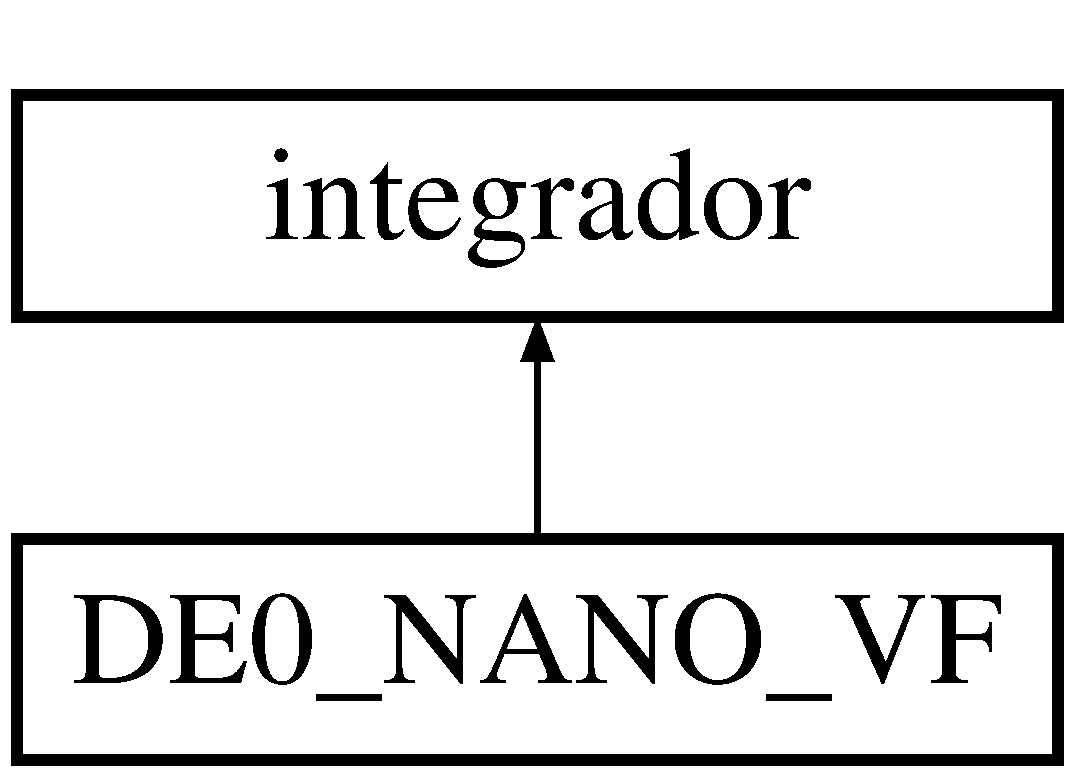
\includegraphics[height=2.000000cm]{classintegrador}
\end{center}
\end{figure}
\subsection*{Entities}
\begin{DoxyCompactItemize}
\item 
\hyperlink{classintegrador_1_1integrador}{integrador} architecture
\end{DoxyCompactItemize}
\subsection*{Libraries}
 \begin{DoxyCompactItemize}
\item 
\hyperlink{classintegrador_ae4f03c286607f3181e16b9aa12d0c6d4}{I\+E\+E\+E} 
\end{DoxyCompactItemize}
\subsection*{Use Clauses}
 \begin{DoxyCompactItemize}
\item 
\hyperlink{classintegrador_a241c3e72dd8024cc8ae831b1b2aed7db}{S\+T\+D\+\_\+\+L\+O\+G\+I\+C\+\_\+\+U\+N\+S\+I\+G\+N\+E\+D}   
\item 
\hyperlink{classintegrador_aa4b2b25246a821511120e3149b003563}{S\+T\+D\+\_\+\+L\+O\+G\+I\+C\+\_\+1164}   
\item 
\hyperlink{classintegrador_aad86249c80e8c1e7ee1c4748aba748e3}{fixed\+\_\+pkg}   
\end{DoxyCompactItemize}
\subsection*{Generics}
 \begin{DoxyCompactItemize}
\item 
\hyperlink{classintegrador_a2629ecb3bb37e8104b2866b0fd0c8574}{Nin} {\bfseries {\bfseries \textcolor{comment}{integer}\textcolor{vhdlchar}{ }\textcolor{vhdlchar}{ }\textcolor{vhdlchar}{\+:}\textcolor{vhdlchar}{=}\textcolor{vhdlchar}{ }\textcolor{vhdlchar}{ } \textcolor{vhdldigit}{13} \textcolor{vhdlchar}{ }}}
\item 
\hyperlink{classintegrador_a061c0d632c8bdf5dd32c80acf9a9c475}{Nout} {\bfseries {\bfseries \textcolor{comment}{integer}\textcolor{vhdlchar}{ }\textcolor{vhdlchar}{ }\textcolor{vhdlchar}{\+:}\textcolor{vhdlchar}{=}\textcolor{vhdlchar}{ }\textcolor{vhdlchar}{ } \textcolor{vhdldigit}{30} \textcolor{vhdlchar}{ }}}
\end{DoxyCompactItemize}
\subsection*{Ports}
 \begin{DoxyCompactItemize}
\item 
\hyperlink{classintegrador_a4a4609c199d30b3adebbeb3a01276ec5}{clk}  {\bfseries {\bfseries \textcolor{keywordflow}{in}\textcolor{vhdlchar}{ }}} {\bfseries \textcolor{comment}{std\+\_\+logic}\textcolor{vhdlchar}{ }} 
\item 
\hyperlink{classintegrador_adcf9c6f5161d039addbda5819bee64a3}{en}  {\bfseries {\bfseries \textcolor{keywordflow}{in}\textcolor{vhdlchar}{ }}} {\bfseries \textcolor{comment}{std\+\_\+logic}\textcolor{vhdlchar}{ }} 
\item 
\hyperlink{classintegrador_aad8dc6359d9e23dabcbf342fadf2fa06}{reset}  {\bfseries {\bfseries \textcolor{keywordflow}{in}\textcolor{vhdlchar}{ }}} {\bfseries \textcolor{comment}{std\+\_\+logic}\textcolor{vhdlchar}{ }} 
\item 
\hyperlink{classintegrador_aae281cf725515894f893258c629a59c7}{sinc}  {\bfseries {\bfseries \textcolor{keywordflow}{out}\textcolor{vhdlchar}{ }}} {\bfseries \textcolor{comment}{std\+\_\+logic}\textcolor{vhdlchar}{ }} 
\item 
\hyperlink{classintegrador_a436836a2e79668e0976eef3a553b5406}{M\+A\+X}  {\bfseries {\bfseries \textcolor{keywordflow}{in}\textcolor{vhdlchar}{ }}} {\bfseries \textcolor{comment}{std\+\_\+logic\+\_\+vector}\textcolor{vhdlchar}{ }\textcolor{vhdlchar}{(}\textcolor{vhdlchar}{ }\textcolor{vhdlchar}{ }\textcolor{vhdlchar}{ }\textcolor{vhdlchar}{ }{\bfseries \hyperlink{classintegrador_a061c0d632c8bdf5dd32c80acf9a9c475}{Nout}} \textcolor{vhdlchar}{-\/}\textcolor{vhdlchar}{ } \textcolor{vhdldigit}{1} \textcolor{vhdlchar}{ }\textcolor{keywordflow}{downto}\textcolor{vhdlchar}{ }\textcolor{vhdlchar}{ } \textcolor{vhdldigit}{0} \textcolor{vhdlchar}{ }\textcolor{vhdlchar}{)}\textcolor{vhdlchar}{ }} 
\item 
\hyperlink{classintegrador_a9e461894ea9b864637648799f51bf9be}{out\+\_\+data}  {\bfseries {\bfseries \textcolor{keywordflow}{out}\textcolor{vhdlchar}{ }}} {\bfseries \textcolor{comment}{std\+\_\+logic\+\_\+vector}\textcolor{vhdlchar}{ }\textcolor{vhdlchar}{(}\textcolor{vhdlchar}{ }\textcolor{vhdlchar}{ }\textcolor{vhdlchar}{ }\textcolor{vhdlchar}{ }{\bfseries \hyperlink{classintegrador_a061c0d632c8bdf5dd32c80acf9a9c475}{Nout}} \textcolor{vhdlchar}{-\/}\textcolor{vhdlchar}{ } \textcolor{vhdldigit}{1} \textcolor{vhdlchar}{ }\textcolor{keywordflow}{downto}\textcolor{vhdlchar}{ }\textcolor{vhdlchar}{ } \textcolor{vhdldigit}{0} \textcolor{vhdlchar}{ }\textcolor{vhdlchar}{)}\textcolor{vhdlchar}{ }} 
\item 
\hyperlink{classintegrador_aec192442094491f2207942b96b64835c}{int\+\_\+data}  {\bfseries {\bfseries \textcolor{keywordflow}{in}\textcolor{vhdlchar}{ }}} {\bfseries \textcolor{comment}{std\+\_\+logic\+\_\+vector}\textcolor{vhdlchar}{ }\textcolor{vhdlchar}{(}\textcolor{vhdlchar}{ }\textcolor{vhdlchar}{ }\textcolor{vhdlchar}{ }\textcolor{vhdlchar}{ }{\bfseries \hyperlink{classintegrador_a2629ecb3bb37e8104b2866b0fd0c8574}{Nin}} \textcolor{vhdlchar}{-\/}\textcolor{vhdlchar}{ } \textcolor{vhdldigit}{1} \textcolor{vhdlchar}{ }\textcolor{keywordflow}{downto}\textcolor{vhdlchar}{ }\textcolor{vhdlchar}{ } \textcolor{vhdldigit}{0} \textcolor{vhdlchar}{ }\textcolor{vhdlchar}{)}\textcolor{vhdlchar}{ }} 
\end{DoxyCompactItemize}


\subsection{Detailed Description}


Definition at line \hyperlink{integrador_8vhd_source_l00006}{6} of file \hyperlink{integrador_8vhd_source}{integrador.\+vhd}.



\subsection{Member Data Documentation}
\hypertarget{classintegrador_a4a4609c199d30b3adebbeb3a01276ec5}{}\index{integrador@{integrador}!clk@{clk}}
\index{clk@{clk}!integrador@{integrador}}
\subsubsection[{clk}]{\setlength{\rightskip}{0pt plus 5cm}{\bf clk} {\bfseries \textcolor{keywordflow}{in}\textcolor{vhdlchar}{ }} {\bfseries \textcolor{comment}{std\+\_\+logic}\textcolor{vhdlchar}{ }} \hspace{0.3cm}{\ttfamily [Port]}}\label{classintegrador_a4a4609c199d30b3adebbeb3a01276ec5}


Definition at line \hyperlink{integrador_8vhd_source_l00011}{11} of file \hyperlink{integrador_8vhd_source}{integrador.\+vhd}.

\hypertarget{classintegrador_adcf9c6f5161d039addbda5819bee64a3}{}\index{integrador@{integrador}!en@{en}}
\index{en@{en}!integrador@{integrador}}
\subsubsection[{en}]{\setlength{\rightskip}{0pt plus 5cm}{\bf en} {\bfseries \textcolor{keywordflow}{in}\textcolor{vhdlchar}{ }} {\bfseries \textcolor{comment}{std\+\_\+logic}\textcolor{vhdlchar}{ }} \hspace{0.3cm}{\ttfamily [Port]}}\label{classintegrador_adcf9c6f5161d039addbda5819bee64a3}


Definition at line \hyperlink{integrador_8vhd_source_l00012}{12} of file \hyperlink{integrador_8vhd_source}{integrador.\+vhd}.

\hypertarget{classintegrador_aad86249c80e8c1e7ee1c4748aba748e3}{}\index{integrador@{integrador}!fixed\+\_\+pkg@{fixed\+\_\+pkg}}
\index{fixed\+\_\+pkg@{fixed\+\_\+pkg}!integrador@{integrador}}
\subsubsection[{fixed\+\_\+pkg}]{\setlength{\rightskip}{0pt plus 5cm}{\bf fixed\+\_\+pkg}\hspace{0.3cm}{\ttfamily [Package]}}\label{classintegrador_aad86249c80e8c1e7ee1c4748aba748e3}


Definition at line \hyperlink{integrador_8vhd_source_l00004}{4} of file \hyperlink{integrador_8vhd_source}{integrador.\+vhd}.

\hypertarget{classintegrador_ae4f03c286607f3181e16b9aa12d0c6d4}{}\index{integrador@{integrador}!I\+E\+E\+E@{I\+E\+E\+E}}
\index{I\+E\+E\+E@{I\+E\+E\+E}!integrador@{integrador}}
\subsubsection[{I\+E\+E\+E}]{\setlength{\rightskip}{0pt plus 5cm}{\bf I\+E\+E\+E}\hspace{0.3cm}{\ttfamily [Library]}}\label{classintegrador_ae4f03c286607f3181e16b9aa12d0c6d4}


Definition at line \hyperlink{integrador_8vhd_source_l00001}{1} of file \hyperlink{integrador_8vhd_source}{integrador.\+vhd}.

\hypertarget{classintegrador_aec192442094491f2207942b96b64835c}{}\index{integrador@{integrador}!int\+\_\+data@{int\+\_\+data}}
\index{int\+\_\+data@{int\+\_\+data}!integrador@{integrador}}
\subsubsection[{int\+\_\+data}]{\setlength{\rightskip}{0pt plus 5cm}{\bf int\+\_\+data} {\bfseries \textcolor{keywordflow}{in}\textcolor{vhdlchar}{ }} {\bfseries \textcolor{comment}{std\+\_\+logic\+\_\+vector}\textcolor{vhdlchar}{ }\textcolor{vhdlchar}{(}\textcolor{vhdlchar}{ }\textcolor{vhdlchar}{ }\textcolor{vhdlchar}{ }\textcolor{vhdlchar}{ }{\bfseries {\bf Nin}} \textcolor{vhdlchar}{-\/}\textcolor{vhdlchar}{ } \textcolor{vhdldigit}{1} \textcolor{vhdlchar}{ }\textcolor{keywordflow}{downto}\textcolor{vhdlchar}{ }\textcolor{vhdlchar}{ } \textcolor{vhdldigit}{0} \textcolor{vhdlchar}{ }\textcolor{vhdlchar}{)}\textcolor{vhdlchar}{ }} \hspace{0.3cm}{\ttfamily [Port]}}\label{classintegrador_aec192442094491f2207942b96b64835c}


Definition at line \hyperlink{integrador_8vhd_source_l00018}{18} of file \hyperlink{integrador_8vhd_source}{integrador.\+vhd}.

\hypertarget{classintegrador_a436836a2e79668e0976eef3a553b5406}{}\index{integrador@{integrador}!M\+A\+X@{M\+A\+X}}
\index{M\+A\+X@{M\+A\+X}!integrador@{integrador}}
\subsubsection[{M\+A\+X}]{\setlength{\rightskip}{0pt plus 5cm}{\bf M\+A\+X} {\bfseries \textcolor{keywordflow}{in}\textcolor{vhdlchar}{ }} {\bfseries \textcolor{comment}{std\+\_\+logic\+\_\+vector}\textcolor{vhdlchar}{ }\textcolor{vhdlchar}{(}\textcolor{vhdlchar}{ }\textcolor{vhdlchar}{ }\textcolor{vhdlchar}{ }\textcolor{vhdlchar}{ }{\bfseries {\bf Nout}} \textcolor{vhdlchar}{-\/}\textcolor{vhdlchar}{ } \textcolor{vhdldigit}{1} \textcolor{vhdlchar}{ }\textcolor{keywordflow}{downto}\textcolor{vhdlchar}{ }\textcolor{vhdlchar}{ } \textcolor{vhdldigit}{0} \textcolor{vhdlchar}{ }\textcolor{vhdlchar}{)}\textcolor{vhdlchar}{ }} \hspace{0.3cm}{\ttfamily [Port]}}\label{classintegrador_a436836a2e79668e0976eef3a553b5406}


Definition at line \hyperlink{integrador_8vhd_source_l00015}{15} of file \hyperlink{integrador_8vhd_source}{integrador.\+vhd}.

\hypertarget{classintegrador_a2629ecb3bb37e8104b2866b0fd0c8574}{}\index{integrador@{integrador}!Nin@{Nin}}
\index{Nin@{Nin}!integrador@{integrador}}
\subsubsection[{Nin}]{\setlength{\rightskip}{0pt plus 5cm}{\bf Nin} {\bfseries \textcolor{vhdlchar}{ }} {\bfseries \textcolor{comment}{integer}\textcolor{vhdlchar}{ }\textcolor{vhdlchar}{ }\textcolor{vhdlchar}{\+:}\textcolor{vhdlchar}{=}\textcolor{vhdlchar}{ }\textcolor{vhdlchar}{ } \textcolor{vhdldigit}{13} \textcolor{vhdlchar}{ }} \hspace{0.3cm}{\ttfamily [Generic]}}\label{classintegrador_a2629ecb3bb37e8104b2866b0fd0c8574}


Definition at line \hyperlink{integrador_8vhd_source_l00007}{7} of file \hyperlink{integrador_8vhd_source}{integrador.\+vhd}.

\hypertarget{classintegrador_a061c0d632c8bdf5dd32c80acf9a9c475}{}\index{integrador@{integrador}!Nout@{Nout}}
\index{Nout@{Nout}!integrador@{integrador}}
\subsubsection[{Nout}]{\setlength{\rightskip}{0pt plus 5cm}{\bf Nout} {\bfseries \textcolor{vhdlchar}{ }} {\bfseries \textcolor{comment}{integer}\textcolor{vhdlchar}{ }\textcolor{vhdlchar}{ }\textcolor{vhdlchar}{\+:}\textcolor{vhdlchar}{=}\textcolor{vhdlchar}{ }\textcolor{vhdlchar}{ } \textcolor{vhdldigit}{30} \textcolor{vhdlchar}{ }} \hspace{0.3cm}{\ttfamily [Generic]}}\label{classintegrador_a061c0d632c8bdf5dd32c80acf9a9c475}


Definition at line \hyperlink{integrador_8vhd_source_l00009}{9} of file \hyperlink{integrador_8vhd_source}{integrador.\+vhd}.

\hypertarget{classintegrador_a9e461894ea9b864637648799f51bf9be}{}\index{integrador@{integrador}!out\+\_\+data@{out\+\_\+data}}
\index{out\+\_\+data@{out\+\_\+data}!integrador@{integrador}}
\subsubsection[{out\+\_\+data}]{\setlength{\rightskip}{0pt plus 5cm}{\bf out\+\_\+data} {\bfseries \textcolor{keywordflow}{out}\textcolor{vhdlchar}{ }} {\bfseries \textcolor{comment}{std\+\_\+logic\+\_\+vector}\textcolor{vhdlchar}{ }\textcolor{vhdlchar}{(}\textcolor{vhdlchar}{ }\textcolor{vhdlchar}{ }\textcolor{vhdlchar}{ }\textcolor{vhdlchar}{ }{\bfseries {\bf Nout}} \textcolor{vhdlchar}{-\/}\textcolor{vhdlchar}{ } \textcolor{vhdldigit}{1} \textcolor{vhdlchar}{ }\textcolor{keywordflow}{downto}\textcolor{vhdlchar}{ }\textcolor{vhdlchar}{ } \textcolor{vhdldigit}{0} \textcolor{vhdlchar}{ }\textcolor{vhdlchar}{)}\textcolor{vhdlchar}{ }} \hspace{0.3cm}{\ttfamily [Port]}}\label{classintegrador_a9e461894ea9b864637648799f51bf9be}


Definition at line \hyperlink{integrador_8vhd_source_l00016}{16} of file \hyperlink{integrador_8vhd_source}{integrador.\+vhd}.

\hypertarget{classintegrador_aad8dc6359d9e23dabcbf342fadf2fa06}{}\index{integrador@{integrador}!reset@{reset}}
\index{reset@{reset}!integrador@{integrador}}
\subsubsection[{reset}]{\setlength{\rightskip}{0pt plus 5cm}{\bf reset} {\bfseries \textcolor{keywordflow}{in}\textcolor{vhdlchar}{ }} {\bfseries \textcolor{comment}{std\+\_\+logic}\textcolor{vhdlchar}{ }} \hspace{0.3cm}{\ttfamily [Port]}}\label{classintegrador_aad8dc6359d9e23dabcbf342fadf2fa06}


Definition at line \hyperlink{integrador_8vhd_source_l00013}{13} of file \hyperlink{integrador_8vhd_source}{integrador.\+vhd}.

\hypertarget{classintegrador_aae281cf725515894f893258c629a59c7}{}\index{integrador@{integrador}!sinc@{sinc}}
\index{sinc@{sinc}!integrador@{integrador}}
\subsubsection[{sinc}]{\setlength{\rightskip}{0pt plus 5cm}{\bf sinc} {\bfseries \textcolor{keywordflow}{out}\textcolor{vhdlchar}{ }} {\bfseries \textcolor{comment}{std\+\_\+logic}\textcolor{vhdlchar}{ }} \hspace{0.3cm}{\ttfamily [Port]}}\label{classintegrador_aae281cf725515894f893258c629a59c7}


Definition at line \hyperlink{integrador_8vhd_source_l00014}{14} of file \hyperlink{integrador_8vhd_source}{integrador.\+vhd}.

\hypertarget{classintegrador_aa4b2b25246a821511120e3149b003563}{}\index{integrador@{integrador}!S\+T\+D\+\_\+\+L\+O\+G\+I\+C\+\_\+1164@{S\+T\+D\+\_\+\+L\+O\+G\+I\+C\+\_\+1164}}
\index{S\+T\+D\+\_\+\+L\+O\+G\+I\+C\+\_\+1164@{S\+T\+D\+\_\+\+L\+O\+G\+I\+C\+\_\+1164}!integrador@{integrador}}
\subsubsection[{S\+T\+D\+\_\+\+L\+O\+G\+I\+C\+\_\+1164}]{\setlength{\rightskip}{0pt plus 5cm}{\bf S\+T\+D\+\_\+\+L\+O\+G\+I\+C\+\_\+1164}\hspace{0.3cm}{\ttfamily [Package]}}\label{classintegrador_aa4b2b25246a821511120e3149b003563}


Definition at line \hyperlink{integrador_8vhd_source_l00003}{3} of file \hyperlink{integrador_8vhd_source}{integrador.\+vhd}.

\hypertarget{classintegrador_a241c3e72dd8024cc8ae831b1b2aed7db}{}\index{integrador@{integrador}!S\+T\+D\+\_\+\+L\+O\+G\+I\+C\+\_\+\+U\+N\+S\+I\+G\+N\+E\+D@{S\+T\+D\+\_\+\+L\+O\+G\+I\+C\+\_\+\+U\+N\+S\+I\+G\+N\+E\+D}}
\index{S\+T\+D\+\_\+\+L\+O\+G\+I\+C\+\_\+\+U\+N\+S\+I\+G\+N\+E\+D@{S\+T\+D\+\_\+\+L\+O\+G\+I\+C\+\_\+\+U\+N\+S\+I\+G\+N\+E\+D}!integrador@{integrador}}
\subsubsection[{S\+T\+D\+\_\+\+L\+O\+G\+I\+C\+\_\+\+U\+N\+S\+I\+G\+N\+E\+D}]{\setlength{\rightskip}{0pt plus 5cm}{\bf S\+T\+D\+\_\+\+L\+O\+G\+I\+C\+\_\+\+U\+N\+S\+I\+G\+N\+E\+D}\hspace{0.3cm}{\ttfamily [Package]}}\label{classintegrador_a241c3e72dd8024cc8ae831b1b2aed7db}


Definition at line \hyperlink{integrador_8vhd_source_l00002}{2} of file \hyperlink{integrador_8vhd_source}{integrador.\+vhd}.



The documentation for this class was generated from the following file\+:\begin{DoxyCompactItemize}
\item 
\hyperlink{integrador_8vhd}{integrador.\+vhd}\end{DoxyCompactItemize}

\hypertarget{classintegrador_1_1integrador}{}\section{integrador Architecture Reference}
\label{classintegrador_1_1integrador}\index{integrador@{integrador}}
\subsection*{Processes}
 \begin{DoxyCompactItemize}
\item 
\hyperlink{classintegrador_1_1integrador_afcc525892643d4614179ad348921cd15}{P\+R\+O\+C\+E\+S\+S\+\_\+10}{\bfseries  ( {\bfseries {\bfseries \hyperlink{classintegrador_a4a4609c199d30b3adebbeb3a01276ec5}{clk}} \textcolor{vhdlchar}{ }} )}
\end{DoxyCompactItemize}
\subsection*{Signals}
 \begin{DoxyCompactItemize}
\item 
\hyperlink{classintegrador_1_1integrador_a951e616187c21eeebaa382a516df536e}{out\+\_\+int} {\bfseries \textcolor{comment}{std\+\_\+logic\+\_\+vector}\textcolor{vhdlchar}{ }\textcolor{vhdlchar}{(}\textcolor{vhdlchar}{ }\textcolor{vhdlchar}{ }\textcolor{vhdlchar}{ }\textcolor{vhdlchar}{ }{\bfseries \hyperlink{classintegrador_a061c0d632c8bdf5dd32c80acf9a9c475}{Nout}} \textcolor{vhdlchar}{-\/}\textcolor{vhdlchar}{ } \textcolor{vhdldigit}{1} \textcolor{vhdlchar}{ }\textcolor{keywordflow}{downto}\textcolor{vhdlchar}{ }\textcolor{vhdlchar}{ } \textcolor{vhdldigit}{0} \textcolor{vhdlchar}{ }\textcolor{vhdlchar}{)}\textcolor{vhdlchar}{ }} 
\item 
\hyperlink{classintegrador_1_1integrador_a45126d1a75be347f440d181b7aa5e033}{sinc\+\_\+int} {\bfseries \textcolor{comment}{std\+\_\+logic}\textcolor{vhdlchar}{ }} 
\end{DoxyCompactItemize}


\subsection{Detailed Description}


Definition at line 23 of file integrador.\+vhd.



\subsection{Member Function Documentation}
\hypertarget{classintegrador_1_1integrador_afcc525892643d4614179ad348921cd15}{}\index{integrador\+::integrador@{integrador\+::integrador}!P\+R\+O\+C\+E\+S\+S\+\_\+10@{P\+R\+O\+C\+E\+S\+S\+\_\+10}}
\index{P\+R\+O\+C\+E\+S\+S\+\_\+10@{P\+R\+O\+C\+E\+S\+S\+\_\+10}!integrador\+::integrador@{integrador\+::integrador}}
\subsubsection[{P\+R\+O\+C\+E\+S\+S\+\_\+10}]{\setlength{\rightskip}{0pt plus 5cm} {\bfseries \textcolor{vhdlchar}{ }} P\+R\+O\+C\+E\+S\+S\+\_\+10(
\begin{DoxyParamCaption}
\item[{}]{{\bfseries {\bfseries {\bf clk}} \textcolor{vhdlchar}{ }} {\em }}
\end{DoxyParamCaption}
)\hspace{0.3cm}{\ttfamily [Process]}}\label{classintegrador_1_1integrador_afcc525892643d4614179ad348921cd15}


Definition at line 31 of file integrador.\+vhd.



\subsection{Member Data Documentation}
\hypertarget{classintegrador_1_1integrador_a951e616187c21eeebaa382a516df536e}{}\index{integrador\+::integrador@{integrador\+::integrador}!out\+\_\+int@{out\+\_\+int}}
\index{out\+\_\+int@{out\+\_\+int}!integrador\+::integrador@{integrador\+::integrador}}
\subsubsection[{out\+\_\+int}]{\setlength{\rightskip}{0pt plus 5cm}{\bf out\+\_\+int} {\bfseries \textcolor{comment}{std\+\_\+logic\+\_\+vector}\textcolor{vhdlchar}{ }\textcolor{vhdlchar}{(}\textcolor{vhdlchar}{ }\textcolor{vhdlchar}{ }\textcolor{vhdlchar}{ }\textcolor{vhdlchar}{ }{\bfseries {\bf Nout}} \textcolor{vhdlchar}{-\/}\textcolor{vhdlchar}{ } \textcolor{vhdldigit}{1} \textcolor{vhdlchar}{ }\textcolor{keywordflow}{downto}\textcolor{vhdlchar}{ }\textcolor{vhdlchar}{ } \textcolor{vhdldigit}{0} \textcolor{vhdlchar}{ }\textcolor{vhdlchar}{)}\textcolor{vhdlchar}{ }} \hspace{0.3cm}{\ttfamily [Signal]}}\label{classintegrador_1_1integrador_a951e616187c21eeebaa382a516df536e}


Definition at line 25 of file integrador.\+vhd.

\hypertarget{classintegrador_1_1integrador_a45126d1a75be347f440d181b7aa5e033}{}\index{integrador\+::integrador@{integrador\+::integrador}!sinc\+\_\+int@{sinc\+\_\+int}}
\index{sinc\+\_\+int@{sinc\+\_\+int}!integrador\+::integrador@{integrador\+::integrador}}
\subsubsection[{sinc\+\_\+int}]{\setlength{\rightskip}{0pt plus 5cm}{\bf sinc\+\_\+int} {\bfseries \textcolor{comment}{std\+\_\+logic}\textcolor{vhdlchar}{ }} \hspace{0.3cm}{\ttfamily [Signal]}}\label{classintegrador_1_1integrador_a45126d1a75be347f440d181b7aa5e033}


Definition at line 26 of file integrador.\+vhd.



The documentation for this class was generated from the following file\+:\begin{DoxyCompactItemize}
\item 
\hyperlink{integrador_8vhd}{integrador.\+vhd}\end{DoxyCompactItemize}

\hypertarget{class_l_e_ds}{}\section{L\+E\+Ds Entity Reference}
\label{class_l_e_ds}\index{L\+E\+Ds@{L\+E\+Ds}}
\subsection*{Entities}
\begin{DoxyCompactItemize}
\item 
\hyperlink{class_l_e_ds_1_1_l_e_ds}{L\+E\+Ds} architecture
\end{DoxyCompactItemize}
\subsection*{Libraries}
 \begin{DoxyCompactItemize}
\item 
\hyperlink{class_l_e_ds_a0a6af6eef40212dbaf130d57ce711256}{ieee} 
\end{DoxyCompactItemize}
\subsection*{Use Clauses}
 \begin{DoxyCompactItemize}
\item 
\hyperlink{class_l_e_ds_acd03516902501cd1c7296a98e22c6fcb}{std\+\_\+logic\+\_\+1164}   
\item 
\hyperlink{class_l_e_ds_a0f5ecc6613f63d07f7963a97b1b26095}{std\+\_\+logic\+\_\+arith}   
\item 
\hyperlink{class_l_e_ds_a598da929e807d58939b47499e8bc9fa8}{std\+\_\+logic\+\_\+unsigned}   
\end{DoxyCompactItemize}
\subsection*{Ports}
 \begin{DoxyCompactItemize}
\item 
\hyperlink{class_l_e_ds_a4b5e1e3eba67b2e61c77c9a719d8518c}{C\+L\+O\+C\+K\+\_\+50}  {\bfseries {\bfseries \textcolor{keywordflow}{in}\textcolor{vhdlchar}{ }}} {\bfseries \textcolor{comment}{std\+\_\+logic}\textcolor{vhdlchar}{ }} 
\item 
\hyperlink{class_l_e_ds_a424944084857f6787a0ddb567d0b5240}{L\+E\+D}  {\bfseries {\bfseries \textcolor{keywordflow}{out}\textcolor{vhdlchar}{ }}} {\bfseries \textcolor{comment}{std\+\_\+logic\+\_\+vector}\textcolor{vhdlchar}{ }\textcolor{vhdlchar}{(}\textcolor{vhdlchar}{ }\textcolor{vhdlchar}{ } \textcolor{vhdldigit}{7} \textcolor{vhdlchar}{ }\textcolor{keywordflow}{D\+O\+W\+N\+T\+O}\textcolor{vhdlchar}{ }\textcolor{vhdlchar}{ } \textcolor{vhdldigit}{0} \textcolor{vhdlchar}{ }\textcolor{vhdlchar}{)}\textcolor{vhdlchar}{ }} 
\item 
\hyperlink{class_l_e_ds_a30974727c81621f672f7f9490463f9d3}{S\+W}  {\bfseries {\bfseries \textcolor{keywordflow}{in}\textcolor{vhdlchar}{ }}} {\bfseries \textcolor{comment}{std\+\_\+logic\+\_\+vector}\textcolor{vhdlchar}{ }\textcolor{vhdlchar}{(}\textcolor{vhdlchar}{ }\textcolor{vhdlchar}{ } \textcolor{vhdldigit}{3} \textcolor{vhdlchar}{ }\textcolor{keywordflow}{D\+O\+W\+N\+T\+O}\textcolor{vhdlchar}{ }\textcolor{vhdlchar}{ } \textcolor{vhdldigit}{0} \textcolor{vhdlchar}{ }\textcolor{vhdlchar}{)}\textcolor{vhdlchar}{ }} 
\item 
\hyperlink{class_l_e_ds_aa70bf9245705f33e4529eb81df3fbf94}{K\+E\+Y}  {\bfseries {\bfseries \textcolor{keywordflow}{in}\textcolor{vhdlchar}{ }}} {\bfseries \textcolor{comment}{std\+\_\+logic\+\_\+vector}\textcolor{vhdlchar}{ }\textcolor{vhdlchar}{(}\textcolor{vhdlchar}{ }\textcolor{vhdlchar}{ } \textcolor{vhdldigit}{1} \textcolor{vhdlchar}{ }\textcolor{keywordflow}{D\+O\+W\+N\+T\+O}\textcolor{vhdlchar}{ }\textcolor{vhdlchar}{ } \textcolor{vhdldigit}{0} \textcolor{vhdlchar}{ }\textcolor{vhdlchar}{)}\textcolor{vhdlchar}{ }} 
\end{DoxyCompactItemize}


\subsection{Detailed Description}


Definition at line \hyperlink{_l_e_ds_8vhd_source_l00009}{9} of file \hyperlink{_l_e_ds_8vhd_source}{L\+E\+Ds.\+vhd}.



\subsection{Member Data Documentation}
\hypertarget{class_l_e_ds_a4b5e1e3eba67b2e61c77c9a719d8518c}{}\index{L\+E\+Ds@{L\+E\+Ds}!C\+L\+O\+C\+K\+\_\+50@{C\+L\+O\+C\+K\+\_\+50}}
\index{C\+L\+O\+C\+K\+\_\+50@{C\+L\+O\+C\+K\+\_\+50}!L\+E\+Ds@{L\+E\+Ds}}
\subsubsection[{C\+L\+O\+C\+K\+\_\+50}]{\setlength{\rightskip}{0pt plus 5cm}{\bf C\+L\+O\+C\+K\+\_\+50} {\bfseries \textcolor{keywordflow}{in}\textcolor{vhdlchar}{ }} {\bfseries \textcolor{comment}{std\+\_\+logic}\textcolor{vhdlchar}{ }} \hspace{0.3cm}{\ttfamily [Port]}}\label{class_l_e_ds_a4b5e1e3eba67b2e61c77c9a719d8518c}


Definition at line \hyperlink{_l_e_ds_8vhd_source_l00011}{11} of file \hyperlink{_l_e_ds_8vhd_source}{L\+E\+Ds.\+vhd}.

\hypertarget{class_l_e_ds_a0a6af6eef40212dbaf130d57ce711256}{}\index{L\+E\+Ds@{L\+E\+Ds}!ieee@{ieee}}
\index{ieee@{ieee}!L\+E\+Ds@{L\+E\+Ds}}
\subsubsection[{ieee}]{\setlength{\rightskip}{0pt plus 5cm}{\bf ieee}\hspace{0.3cm}{\ttfamily [Library]}}\label{class_l_e_ds_a0a6af6eef40212dbaf130d57ce711256}


Definition at line \hyperlink{_l_e_ds_8vhd_source_l00004}{4} of file \hyperlink{_l_e_ds_8vhd_source}{L\+E\+Ds.\+vhd}.

\hypertarget{class_l_e_ds_aa70bf9245705f33e4529eb81df3fbf94}{}\index{L\+E\+Ds@{L\+E\+Ds}!K\+E\+Y@{K\+E\+Y}}
\index{K\+E\+Y@{K\+E\+Y}!L\+E\+Ds@{L\+E\+Ds}}
\subsubsection[{K\+E\+Y}]{\setlength{\rightskip}{0pt plus 5cm}{\bf K\+E\+Y} {\bfseries \textcolor{keywordflow}{in}\textcolor{vhdlchar}{ }} {\bfseries \textcolor{comment}{std\+\_\+logic\+\_\+vector}\textcolor{vhdlchar}{ }\textcolor{vhdlchar}{(}\textcolor{vhdlchar}{ }\textcolor{vhdlchar}{ } \textcolor{vhdldigit}{1} \textcolor{vhdlchar}{ }\textcolor{keywordflow}{D\+O\+W\+N\+T\+O}\textcolor{vhdlchar}{ }\textcolor{vhdlchar}{ } \textcolor{vhdldigit}{0} \textcolor{vhdlchar}{ }\textcolor{vhdlchar}{)}\textcolor{vhdlchar}{ }} \hspace{0.3cm}{\ttfamily [Port]}}\label{class_l_e_ds_aa70bf9245705f33e4529eb81df3fbf94}


Definition at line \hyperlink{_l_e_ds_8vhd_source_l00015}{15} of file \hyperlink{_l_e_ds_8vhd_source}{L\+E\+Ds.\+vhd}.

\hypertarget{class_l_e_ds_a424944084857f6787a0ddb567d0b5240}{}\index{L\+E\+Ds@{L\+E\+Ds}!L\+E\+D@{L\+E\+D}}
\index{L\+E\+D@{L\+E\+D}!L\+E\+Ds@{L\+E\+Ds}}
\subsubsection[{L\+E\+D}]{\setlength{\rightskip}{0pt plus 5cm}{\bf L\+E\+D} {\bfseries \textcolor{keywordflow}{out}\textcolor{vhdlchar}{ }} {\bfseries \textcolor{comment}{std\+\_\+logic\+\_\+vector}\textcolor{vhdlchar}{ }\textcolor{vhdlchar}{(}\textcolor{vhdlchar}{ }\textcolor{vhdlchar}{ } \textcolor{vhdldigit}{7} \textcolor{vhdlchar}{ }\textcolor{keywordflow}{D\+O\+W\+N\+T\+O}\textcolor{vhdlchar}{ }\textcolor{vhdlchar}{ } \textcolor{vhdldigit}{0} \textcolor{vhdlchar}{ }\textcolor{vhdlchar}{)}\textcolor{vhdlchar}{ }} \hspace{0.3cm}{\ttfamily [Port]}}\label{class_l_e_ds_a424944084857f6787a0ddb567d0b5240}


Definition at line \hyperlink{_l_e_ds_8vhd_source_l00012}{12} of file \hyperlink{_l_e_ds_8vhd_source}{L\+E\+Ds.\+vhd}.

\hypertarget{class_l_e_ds_acd03516902501cd1c7296a98e22c6fcb}{}\index{L\+E\+Ds@{L\+E\+Ds}!std\+\_\+logic\+\_\+1164@{std\+\_\+logic\+\_\+1164}}
\index{std\+\_\+logic\+\_\+1164@{std\+\_\+logic\+\_\+1164}!L\+E\+Ds@{L\+E\+Ds}}
\subsubsection[{std\+\_\+logic\+\_\+1164}]{\setlength{\rightskip}{0pt plus 5cm}{\bf std\+\_\+logic\+\_\+1164}\hspace{0.3cm}{\ttfamily [Package]}}\label{class_l_e_ds_acd03516902501cd1c7296a98e22c6fcb}


Definition at line \hyperlink{_l_e_ds_8vhd_source_l00005}{5} of file \hyperlink{_l_e_ds_8vhd_source}{L\+E\+Ds.\+vhd}.

\hypertarget{class_l_e_ds_a0f5ecc6613f63d07f7963a97b1b26095}{}\index{L\+E\+Ds@{L\+E\+Ds}!std\+\_\+logic\+\_\+arith@{std\+\_\+logic\+\_\+arith}}
\index{std\+\_\+logic\+\_\+arith@{std\+\_\+logic\+\_\+arith}!L\+E\+Ds@{L\+E\+Ds}}
\subsubsection[{std\+\_\+logic\+\_\+arith}]{\setlength{\rightskip}{0pt plus 5cm}{\bf std\+\_\+logic\+\_\+arith}\hspace{0.3cm}{\ttfamily [Package]}}\label{class_l_e_ds_a0f5ecc6613f63d07f7963a97b1b26095}


Definition at line \hyperlink{_l_e_ds_8vhd_source_l00006}{6} of file \hyperlink{_l_e_ds_8vhd_source}{L\+E\+Ds.\+vhd}.

\hypertarget{class_l_e_ds_a598da929e807d58939b47499e8bc9fa8}{}\index{L\+E\+Ds@{L\+E\+Ds}!std\+\_\+logic\+\_\+unsigned@{std\+\_\+logic\+\_\+unsigned}}
\index{std\+\_\+logic\+\_\+unsigned@{std\+\_\+logic\+\_\+unsigned}!L\+E\+Ds@{L\+E\+Ds}}
\subsubsection[{std\+\_\+logic\+\_\+unsigned}]{\setlength{\rightskip}{0pt plus 5cm}{\bf std\+\_\+logic\+\_\+unsigned}\hspace{0.3cm}{\ttfamily [Package]}}\label{class_l_e_ds_a598da929e807d58939b47499e8bc9fa8}


Definition at line \hyperlink{_l_e_ds_8vhd_source_l00007}{7} of file \hyperlink{_l_e_ds_8vhd_source}{L\+E\+Ds.\+vhd}.

\hypertarget{class_l_e_ds_a30974727c81621f672f7f9490463f9d3}{}\index{L\+E\+Ds@{L\+E\+Ds}!S\+W@{S\+W}}
\index{S\+W@{S\+W}!L\+E\+Ds@{L\+E\+Ds}}
\subsubsection[{S\+W}]{\setlength{\rightskip}{0pt plus 5cm}{\bf S\+W} {\bfseries \textcolor{keywordflow}{in}\textcolor{vhdlchar}{ }} {\bfseries \textcolor{comment}{std\+\_\+logic\+\_\+vector}\textcolor{vhdlchar}{ }\textcolor{vhdlchar}{(}\textcolor{vhdlchar}{ }\textcolor{vhdlchar}{ } \textcolor{vhdldigit}{3} \textcolor{vhdlchar}{ }\textcolor{keywordflow}{D\+O\+W\+N\+T\+O}\textcolor{vhdlchar}{ }\textcolor{vhdlchar}{ } \textcolor{vhdldigit}{0} \textcolor{vhdlchar}{ }\textcolor{vhdlchar}{)}\textcolor{vhdlchar}{ }} \hspace{0.3cm}{\ttfamily [Port]}}\label{class_l_e_ds_a30974727c81621f672f7f9490463f9d3}


Definition at line \hyperlink{_l_e_ds_8vhd_source_l00013}{13} of file \hyperlink{_l_e_ds_8vhd_source}{L\+E\+Ds.\+vhd}.



The documentation for this class was generated from the following file\+:\begin{DoxyCompactItemize}
\item 
\hyperlink{_l_e_ds_8vhd}{L\+E\+Ds.\+vhd}\end{DoxyCompactItemize}

\hypertarget{class_l_e_ds_1_1_l_e_ds}{}\section{L\+E\+Ds Architecture Reference}
\label{class_l_e_ds_1_1_l_e_ds}\index{L\+E\+Ds@{L\+E\+Ds}}
\subsection*{Processes}
 \begin{DoxyCompactItemize}
\item 
\hyperlink{class_l_e_ds_1_1_l_e_ds_a0b2ae93f7930ef5bc4cc2730b8c405d1}{P\+R\+O\+C\+E\+S\+S\+\_\+11}{\bfseries  ( {\bfseries {\bfseries \hyperlink{class_l_e_ds_a4b5e1e3eba67b2e61c77c9a719d8518c}{C\+L\+O\+C\+K\+\_\+50}} \textcolor{vhdlchar}{ }} )}
\end{DoxyCompactItemize}
\subsection*{Constants}
 \begin{DoxyCompactItemize}
\item 
\hyperlink{class_l_e_ds_1_1_l_e_ds_aa45ed8f4ade73b3c1510f9df8ec7dd9c}{C\+L\+K\+\_\+\+F\+R\+E\+Q} {\bfseries \textcolor{comment}{integer}\textcolor{vhdlchar}{ }\textcolor{vhdlchar}{ }\textcolor{vhdlchar}{\+:}\textcolor{vhdlchar}{=}\textcolor{vhdlchar}{ }\textcolor{vhdlchar}{ } \textcolor{vhdldigit}{50000000} \textcolor{vhdlchar}{ }} 
\item 
\hyperlink{class_l_e_ds_1_1_l_e_ds_a1890617960a841a3d027f78733169e15}{B\+L\+I\+N\+K\+\_\+\+F\+R\+E\+Q} {\bfseries \textcolor{comment}{integer}\textcolor{vhdlchar}{ }\textcolor{vhdlchar}{ }\textcolor{vhdlchar}{\+:}\textcolor{vhdlchar}{=}\textcolor{vhdlchar}{ }\textcolor{vhdlchar}{ } \textcolor{vhdldigit}{1} \textcolor{vhdlchar}{ }} 
\item 
\hyperlink{class_l_e_ds_1_1_l_e_ds_a62b6ca896e870c8bfbd7496a8c89efe6}{C\+N\+T\+\_\+\+M\+A\+X} {\bfseries \textcolor{comment}{integer}\textcolor{vhdlchar}{ }\textcolor{vhdlchar}{ }\textcolor{vhdlchar}{\+:}\textcolor{vhdlchar}{=}\textcolor{vhdlchar}{ }\textcolor{vhdlchar}{ }\textcolor{vhdlchar}{ }\textcolor{vhdlchar}{ }{\bfseries \hyperlink{class_l_e_ds_1_1_l_e_ds_aa45ed8f4ade73b3c1510f9df8ec7dd9c}{C\+L\+K\+\_\+\+F\+R\+E\+Q}} \textcolor{vhdlchar}{/}\textcolor{vhdlchar}{ }\textcolor{vhdlchar}{ }\textcolor{vhdlchar}{ }{\bfseries \hyperlink{class_l_e_ds_1_1_l_e_ds_a1890617960a841a3d027f78733169e15}{B\+L\+I\+N\+K\+\_\+\+F\+R\+E\+Q}} \textcolor{vhdlchar}{/}\textcolor{vhdlchar}{ } \textcolor{vhdldigit}{2} \textcolor{vhdlchar}{-\/}\textcolor{vhdlchar}{ } \textcolor{vhdldigit}{1} \textcolor{vhdlchar}{ }} 
\end{DoxyCompactItemize}
\subsection*{Signals}
 \begin{DoxyCompactItemize}
\item 
\hyperlink{class_l_e_ds_1_1_l_e_ds_a17db0b3b66ebd22d100f607c5589f41d}{cnt} {\bfseries \textcolor{comment}{unsigned}\textcolor{vhdlchar}{ }\textcolor{vhdlchar}{(}\textcolor{vhdlchar}{ }\textcolor{vhdlchar}{ } \textcolor{vhdldigit}{24} \textcolor{vhdlchar}{ }\textcolor{keywordflow}{downto}\textcolor{vhdlchar}{ }\textcolor{vhdlchar}{ } \textcolor{vhdldigit}{0} \textcolor{vhdlchar}{ }\textcolor{vhdlchar}{)}\textcolor{vhdlchar}{ }} 
\item 
\hyperlink{class_l_e_ds_1_1_l_e_ds_a15ab33796b0132ed52d27866826e80ef}{blink} {\bfseries \textcolor{comment}{std\+\_\+logic}\textcolor{vhdlchar}{ }} 
\end{DoxyCompactItemize}


\subsection{Detailed Description}


Definition at line 22 of file L\+E\+Ds.\+vhd.



\subsection{Member Function Documentation}
\hypertarget{class_l_e_ds_1_1_l_e_ds_a0b2ae93f7930ef5bc4cc2730b8c405d1}{}\index{L\+E\+Ds\+::\+L\+E\+Ds@{L\+E\+Ds\+::\+L\+E\+Ds}!P\+R\+O\+C\+E\+S\+S\+\_\+11@{P\+R\+O\+C\+E\+S\+S\+\_\+11}}
\index{P\+R\+O\+C\+E\+S\+S\+\_\+11@{P\+R\+O\+C\+E\+S\+S\+\_\+11}!L\+E\+Ds\+::\+L\+E\+Ds@{L\+E\+Ds\+::\+L\+E\+Ds}}
\subsubsection[{P\+R\+O\+C\+E\+S\+S\+\_\+11}]{\setlength{\rightskip}{0pt plus 5cm} {\bfseries \textcolor{vhdlchar}{ }} P\+R\+O\+C\+E\+S\+S\+\_\+11(
\begin{DoxyParamCaption}
\item[{}]{{\bfseries {\bfseries {\bf C\+L\+O\+C\+K\+\_\+50}} \textcolor{vhdlchar}{ }} {\em }}
\end{DoxyParamCaption}
)\hspace{0.3cm}{\ttfamily [Process]}}\label{class_l_e_ds_1_1_l_e_ds_a0b2ae93f7930ef5bc4cc2730b8c405d1}


Definition at line 29 of file L\+E\+Ds.\+vhd.



\subsection{Member Data Documentation}
\hypertarget{class_l_e_ds_1_1_l_e_ds_a15ab33796b0132ed52d27866826e80ef}{}\index{L\+E\+Ds\+::\+L\+E\+Ds@{L\+E\+Ds\+::\+L\+E\+Ds}!blink@{blink}}
\index{blink@{blink}!L\+E\+Ds\+::\+L\+E\+Ds@{L\+E\+Ds\+::\+L\+E\+Ds}}
\subsubsection[{blink}]{\setlength{\rightskip}{0pt plus 5cm}{\bf blink} {\bfseries \textcolor{comment}{std\+\_\+logic}\textcolor{vhdlchar}{ }} \hspace{0.3cm}{\ttfamily [Signal]}}\label{class_l_e_ds_1_1_l_e_ds_a15ab33796b0132ed52d27866826e80ef}


Definition at line 27 of file L\+E\+Ds.\+vhd.

\hypertarget{class_l_e_ds_1_1_l_e_ds_a1890617960a841a3d027f78733169e15}{}\index{L\+E\+Ds\+::\+L\+E\+Ds@{L\+E\+Ds\+::\+L\+E\+Ds}!B\+L\+I\+N\+K\+\_\+\+F\+R\+E\+Q@{B\+L\+I\+N\+K\+\_\+\+F\+R\+E\+Q}}
\index{B\+L\+I\+N\+K\+\_\+\+F\+R\+E\+Q@{B\+L\+I\+N\+K\+\_\+\+F\+R\+E\+Q}!L\+E\+Ds\+::\+L\+E\+Ds@{L\+E\+Ds\+::\+L\+E\+Ds}}
\subsubsection[{B\+L\+I\+N\+K\+\_\+\+F\+R\+E\+Q}]{\setlength{\rightskip}{0pt plus 5cm}{\bf B\+L\+I\+N\+K\+\_\+\+F\+R\+E\+Q} {\bfseries \textcolor{comment}{integer}\textcolor{vhdlchar}{ }\textcolor{vhdlchar}{ }\textcolor{vhdlchar}{\+:}\textcolor{vhdlchar}{=}\textcolor{vhdlchar}{ }\textcolor{vhdlchar}{ } \textcolor{vhdldigit}{1} \textcolor{vhdlchar}{ }} \hspace{0.3cm}{\ttfamily [Constant]}}\label{class_l_e_ds_1_1_l_e_ds_a1890617960a841a3d027f78733169e15}


Definition at line 24 of file L\+E\+Ds.\+vhd.

\hypertarget{class_l_e_ds_1_1_l_e_ds_aa45ed8f4ade73b3c1510f9df8ec7dd9c}{}\index{L\+E\+Ds\+::\+L\+E\+Ds@{L\+E\+Ds\+::\+L\+E\+Ds}!C\+L\+K\+\_\+\+F\+R\+E\+Q@{C\+L\+K\+\_\+\+F\+R\+E\+Q}}
\index{C\+L\+K\+\_\+\+F\+R\+E\+Q@{C\+L\+K\+\_\+\+F\+R\+E\+Q}!L\+E\+Ds\+::\+L\+E\+Ds@{L\+E\+Ds\+::\+L\+E\+Ds}}
\subsubsection[{C\+L\+K\+\_\+\+F\+R\+E\+Q}]{\setlength{\rightskip}{0pt plus 5cm}{\bf C\+L\+K\+\_\+\+F\+R\+E\+Q} {\bfseries \textcolor{comment}{integer}\textcolor{vhdlchar}{ }\textcolor{vhdlchar}{ }\textcolor{vhdlchar}{\+:}\textcolor{vhdlchar}{=}\textcolor{vhdlchar}{ }\textcolor{vhdlchar}{ } \textcolor{vhdldigit}{50000000} \textcolor{vhdlchar}{ }} \hspace{0.3cm}{\ttfamily [Constant]}}\label{class_l_e_ds_1_1_l_e_ds_aa45ed8f4ade73b3c1510f9df8ec7dd9c}


Definition at line 23 of file L\+E\+Ds.\+vhd.

\hypertarget{class_l_e_ds_1_1_l_e_ds_a17db0b3b66ebd22d100f607c5589f41d}{}\index{L\+E\+Ds\+::\+L\+E\+Ds@{L\+E\+Ds\+::\+L\+E\+Ds}!cnt@{cnt}}
\index{cnt@{cnt}!L\+E\+Ds\+::\+L\+E\+Ds@{L\+E\+Ds\+::\+L\+E\+Ds}}
\subsubsection[{cnt}]{\setlength{\rightskip}{0pt plus 5cm}{\bf cnt} {\bfseries \textcolor{comment}{unsigned}\textcolor{vhdlchar}{ }\textcolor{vhdlchar}{(}\textcolor{vhdlchar}{ }\textcolor{vhdlchar}{ } \textcolor{vhdldigit}{24} \textcolor{vhdlchar}{ }\textcolor{keywordflow}{downto}\textcolor{vhdlchar}{ }\textcolor{vhdlchar}{ } \textcolor{vhdldigit}{0} \textcolor{vhdlchar}{ }\textcolor{vhdlchar}{)}\textcolor{vhdlchar}{ }} \hspace{0.3cm}{\ttfamily [Signal]}}\label{class_l_e_ds_1_1_l_e_ds_a17db0b3b66ebd22d100f607c5589f41d}


Definition at line 26 of file L\+E\+Ds.\+vhd.

\hypertarget{class_l_e_ds_1_1_l_e_ds_a62b6ca896e870c8bfbd7496a8c89efe6}{}\index{L\+E\+Ds\+::\+L\+E\+Ds@{L\+E\+Ds\+::\+L\+E\+Ds}!C\+N\+T\+\_\+\+M\+A\+X@{C\+N\+T\+\_\+\+M\+A\+X}}
\index{C\+N\+T\+\_\+\+M\+A\+X@{C\+N\+T\+\_\+\+M\+A\+X}!L\+E\+Ds\+::\+L\+E\+Ds@{L\+E\+Ds\+::\+L\+E\+Ds}}
\subsubsection[{C\+N\+T\+\_\+\+M\+A\+X}]{\setlength{\rightskip}{0pt plus 5cm}{\bf C\+N\+T\+\_\+\+M\+A\+X} {\bfseries \textcolor{comment}{integer}\textcolor{vhdlchar}{ }\textcolor{vhdlchar}{ }\textcolor{vhdlchar}{\+:}\textcolor{vhdlchar}{=}\textcolor{vhdlchar}{ }\textcolor{vhdlchar}{ }\textcolor{vhdlchar}{ }\textcolor{vhdlchar}{ }{\bfseries {\bf C\+L\+K\+\_\+\+F\+R\+E\+Q}} \textcolor{vhdlchar}{/}\textcolor{vhdlchar}{ }\textcolor{vhdlchar}{ }\textcolor{vhdlchar}{ }{\bfseries {\bf B\+L\+I\+N\+K\+\_\+\+F\+R\+E\+Q}} \textcolor{vhdlchar}{/}\textcolor{vhdlchar}{ } \textcolor{vhdldigit}{2} \textcolor{vhdlchar}{-\/}\textcolor{vhdlchar}{ } \textcolor{vhdldigit}{1} \textcolor{vhdlchar}{ }} \hspace{0.3cm}{\ttfamily [Constant]}}\label{class_l_e_ds_1_1_l_e_ds_a62b6ca896e870c8bfbd7496a8c89efe6}


Definition at line 25 of file L\+E\+Ds.\+vhd.



The documentation for this class was generated from the following file\+:\begin{DoxyCompactItemize}
\item 
\hyperlink{_l_e_ds_8vhd}{L\+E\+Ds.\+vhd}\end{DoxyCompactItemize}

\hypertarget{class_d_e0___n_a_n_o___v_f_1_1_m_a_i_n}{}\section{M\+A\+I\+N Architecture Reference}
\label{class_d_e0___n_a_n_o___v_f_1_1_m_a_i_n}\index{M\+A\+I\+N@{M\+A\+I\+N}}
\subsection*{Processes}
 \begin{DoxyCompactItemize}
\item 
\hyperlink{class_d_e0___n_a_n_o___v_f_1_1_m_a_i_n_aa22d55790db1f4e085c8fc295cb0e58f}{P\+R\+O\+C\+E\+S\+S\+\_\+4}{\bfseries  ( {\bfseries {\bfseries \hyperlink{class_d_e0___n_a_n_o___v_f_1_1_m_a_i_n_ac14ffa45ea42ce220a8e8316677fe263}{err\+\_\+\+F\+A\+B\+C}} \textcolor{vhdlchar}{ }} )}
\item 
\hyperlink{class_d_e0___n_a_n_o___v_f_1_1_m_a_i_n_a3c39b25652f7e5cb193fa2fd950d6b5e}{P\+R\+O\+C\+E\+S\+S\+\_\+5}{\bfseries  ( {\bfseries {\bfseries \hyperlink{class_d_e0___n_a_n_o___v_f_1_1_m_a_i_n_a1d63ebfc050c1099e1dff991817ec3b0}{clk\+\_\+pll}} \textcolor{vhdlchar}{ }} )}
\end{DoxyCompactItemize}
\subsection*{Components}
 \begin{DoxyCompactItemize}
\item 
\hyperlink{class_d_e0___n_a_n_o___v_f_1_1_m_a_i_n_ab6831a7d06c0a2bc69f9b024f6445a80}{L\+E\+Ds}  {\bfseries }  
\item 
\hyperlink{class_d_e0___n_a_n_o___v_f_1_1_m_a_i_n_a1ccf3e82106c07c2170611228e638a34}{contador}  {\bfseries }  
\item 
\hyperlink{class_d_e0___n_a_n_o___v_f_1_1_m_a_i_n_a4b5d0694f1c75396055f15cd7542add4}{tabela\+\_\+sin}  {\bfseries }  
\item 
\hyperlink{class_d_e0___n_a_n_o___v_f_1_1_m_a_i_n_af3891c65cf7793203a9df0cf918d0235}{pll}  {\bfseries }  
\item 
\hyperlink{class_d_e0___n_a_n_o___v_f_1_1_m_a_i_n_a8127d44aee38572cef223d0c27d447ab}{integrador}  {\bfseries }  
\item 
\hyperlink{class_d_e0___n_a_n_o___v_f_1_1_m_a_i_n_a15ab86106af3275297d1b9099a75ea1e}{theta\+\_\+abc}  {\bfseries }  
\item 
\hyperlink{class_d_e0___n_a_n_o___v_f_1_1_m_a_i_n_a39b27375c53f9cfc5759f4a53877ba0b}{clk\+\_\+div}  {\bfseries }  
\item 
\hyperlink{class_d_e0___n_a_n_o___v_f_1_1_m_a_i_n_a954f74a648a4905eff27c767a774c6dd}{portadora\+\_\+tringular}  {\bfseries }  
\item 
\hyperlink{class_d_e0___n_a_n_o___v_f_1_1_m_a_i_n_a4c526d0b606c178a7dddccfa2ae34ba6}{fbpspwmdt}  {\bfseries }  
\item 
\hyperlink{class_d_e0___n_a_n_o___v_f_1_1_m_a_i_n_a96f8f02a115cd76909b2395df08d3902}{vfcontrol}  {\bfseries }  
\end{DoxyCompactItemize}
\subsection*{Signals}
 \begin{DoxyCompactItemize}
\item 
\hyperlink{class_d_e0___n_a_n_o___v_f_1_1_m_a_i_n_a1d63ebfc050c1099e1dff991817ec3b0}{clk\+\_\+pll} {\bfseries \textcolor{comment}{std\+\_\+logic}\textcolor{vhdlchar}{ }} 
\item 
\hyperlink{class_d_e0___n_a_n_o___v_f_1_1_m_a_i_n_ac43fa0336d7f5cd9ac8e0c6994b9f4df}{pll\+\_\+lock} {\bfseries \textcolor{comment}{std\+\_\+logic}\textcolor{vhdlchar}{ }} 
\item 
\hyperlink{class_d_e0___n_a_n_o___v_f_1_1_m_a_i_n_ab7d66bf3e68700b49fb015413b3e0942}{clk\+\_\+wt} {\bfseries \textcolor{comment}{std\+\_\+logic}\textcolor{vhdlchar}{ }} 
\item 
\hyperlink{class_d_e0___n_a_n_o___v_f_1_1_m_a_i_n_ad9e2ede9bec32660c6cd9d7b31c12b02}{clk\+\_\+int} {\bfseries \textcolor{comment}{std\+\_\+logic}\textcolor{vhdlchar}{ }} 
\item 
\hyperlink{class_d_e0___n_a_n_o___v_f_1_1_m_a_i_n_ac8f65478566c027830639b880f06cdc8}{clk\+\_\+vf} {\bfseries \textcolor{comment}{std\+\_\+logic}\textcolor{vhdlchar}{ }} 
\item 
\hyperlink{class_d_e0___n_a_n_o___v_f_1_1_m_a_i_n_a710fb553e23a16a0e0064507901568ca}{clk\+\_\+led} {\bfseries \textcolor{comment}{std\+\_\+logic}\textcolor{vhdlchar}{ }} 
\item 
\hyperlink{class_d_e0___n_a_n_o___v_f_1_1_m_a_i_n_aba73547f4eb746eaf78a2fc2684191e3}{reset} {\bfseries \textcolor{comment}{std\+\_\+logic}\textcolor{vhdlchar}{ }} 
\item 
\hyperlink{class_d_e0___n_a_n_o___v_f_1_1_m_a_i_n_a624a974c2a222ff8e7bee76fbf24f5ae}{th\+\_\+a} {\bfseries \textcolor{comment}{std\+\_\+logic\+\_\+vector}\textcolor{vhdlchar}{ }\textcolor{vhdlchar}{(}\textcolor{vhdlchar}{ }\textcolor{vhdlchar}{ } \textcolor{vhdldigit}{15} \textcolor{vhdlchar}{ }\textcolor{keywordflow}{downto}\textcolor{vhdlchar}{ }\textcolor{vhdlchar}{ } \textcolor{vhdldigit}{0} \textcolor{vhdlchar}{ }\textcolor{vhdlchar}{)}\textcolor{vhdlchar}{ }} 
\item 
\hyperlink{class_d_e0___n_a_n_o___v_f_1_1_m_a_i_n_a5ce947e047b8551e6cc853affa472cdf}{th\+\_\+b} {\bfseries \textcolor{comment}{std\+\_\+logic\+\_\+vector}\textcolor{vhdlchar}{ }\textcolor{vhdlchar}{(}\textcolor{vhdlchar}{ }\textcolor{vhdlchar}{ } \textcolor{vhdldigit}{15} \textcolor{vhdlchar}{ }\textcolor{keywordflow}{downto}\textcolor{vhdlchar}{ }\textcolor{vhdlchar}{ } \textcolor{vhdldigit}{0} \textcolor{vhdlchar}{ }\textcolor{vhdlchar}{)}\textcolor{vhdlchar}{ }} 
\item 
\hyperlink{class_d_e0___n_a_n_o___v_f_1_1_m_a_i_n_ab8d8d0542e19badec5ebc4db01caa559}{th\+\_\+c} {\bfseries \textcolor{comment}{std\+\_\+logic\+\_\+vector}\textcolor{vhdlchar}{ }\textcolor{vhdlchar}{(}\textcolor{vhdlchar}{ }\textcolor{vhdlchar}{ } \textcolor{vhdldigit}{15} \textcolor{vhdlchar}{ }\textcolor{keywordflow}{downto}\textcolor{vhdlchar}{ }\textcolor{vhdlchar}{ } \textcolor{vhdldigit}{0} \textcolor{vhdlchar}{ }\textcolor{vhdlchar}{)}\textcolor{vhdlchar}{ }} 
\item 
\hyperlink{class_d_e0___n_a_n_o___v_f_1_1_m_a_i_n_a045072e209445fccb914305ca0eb2090}{sig\+P\+W\+M01} {\bfseries \textcolor{comment}{std\+\_\+logic}\textcolor{vhdlchar}{ }} 
\item 
\hyperlink{class_d_e0___n_a_n_o___v_f_1_1_m_a_i_n_a2121509d4c8f727f0995628fa5f7ab11}{sig\+P\+W\+M02} {\bfseries \textcolor{comment}{std\+\_\+logic}\textcolor{vhdlchar}{ }} 
\item 
\hyperlink{class_d_e0___n_a_n_o___v_f_1_1_m_a_i_n_a669c24d23c2e390b7703f7618cf959d8}{O\+S\+C\+\_\+\+B\+U\+S1} {\bfseries \textcolor{comment}{std\+\_\+logic\+\_\+vector}\textcolor{vhdlchar}{ }\textcolor{vhdlchar}{(}\textcolor{vhdlchar}{ }\textcolor{vhdlchar}{ } \textcolor{vhdldigit}{9} \textcolor{vhdlchar}{ }\textcolor{keywordflow}{downto}\textcolor{vhdlchar}{ }\textcolor{vhdlchar}{ } \textcolor{vhdldigit}{0} \textcolor{vhdlchar}{ }\textcolor{vhdlchar}{)}\textcolor{vhdlchar}{ }} 
\item 
\hyperlink{class_d_e0___n_a_n_o___v_f_1_1_m_a_i_n_a45126d1a75be347f440d181b7aa5e033}{sinc\+\_\+int} {\bfseries \textcolor{comment}{std\+\_\+logic}\textcolor{vhdlchar}{ }} 
\item 
\hyperlink{class_d_e0___n_a_n_o___v_f_1_1_m_a_i_n_ad0997d5afb9e2c2228ac89f0d9864320}{sinc\+\_\+wt} {\bfseries \textcolor{comment}{std\+\_\+logic}\textcolor{vhdlchar}{ }} 
\item 
\hyperlink{class_d_e0___n_a_n_o___v_f_1_1_m_a_i_n_a6eafaadc798c6f99d4bec39c9060e5f5}{pulso\+\_\+key0} {\bfseries \textcolor{comment}{std\+\_\+logic}\textcolor{vhdlchar}{ }} 
\item 
\hyperlink{class_d_e0___n_a_n_o___v_f_1_1_m_a_i_n_a6748feeda582b979ff293c4bf3ad340a}{key0\+\_\+ant} {\bfseries \textcolor{comment}{std\+\_\+logic}\textcolor{vhdlchar}{ }} 
\item 
\hyperlink{class_d_e0___n_a_n_o___v_f_1_1_m_a_i_n_a8707b12b53b6fd46834cc806fdace68f}{pulso\+\_\+key1} {\bfseries \textcolor{comment}{std\+\_\+logic}\textcolor{vhdlchar}{ }} 
\item 
\hyperlink{class_d_e0___n_a_n_o___v_f_1_1_m_a_i_n_a0b9ce6db8062ecd0f9d69def89105987}{key1\+\_\+ant} {\bfseries \textcolor{comment}{std\+\_\+logic}\textcolor{vhdlchar}{ }} 
\item 
\hyperlink{class_d_e0___n_a_n_o___v_f_1_1_m_a_i_n_ad4bd17174568b8107646eaedcb91db57}{toggle\+\_\+key1} {\bfseries \textcolor{comment}{std\+\_\+logic}\textcolor{vhdlchar}{ }\textcolor{vhdlchar}{ }\textcolor{vhdlchar}{\+:}\textcolor{vhdlchar}{=}\textcolor{vhdlchar}{ }\textcolor{vhdlchar}{ }\textcolor{vhdlchar}{\textquotesingle{}}\textcolor{vhdlchar}{ } \textcolor{vhdldigit}{1} \textcolor{vhdlchar}{ }\textcolor{vhdlchar}{\textquotesingle{}}\textcolor{vhdlchar}{ }} 
\item 
\hyperlink{class_d_e0___n_a_n_o___v_f_1_1_m_a_i_n_aee0f593b549f4d44efc60ee1dc9d6e57}{toggle\+\_\+key0} {\bfseries \textcolor{comment}{std\+\_\+logic}\textcolor{vhdlchar}{ }\textcolor{vhdlchar}{ }\textcolor{vhdlchar}{\+:}\textcolor{vhdlchar}{=}\textcolor{vhdlchar}{ }\textcolor{vhdlchar}{ }\textcolor{vhdlchar}{\textquotesingle{}}\textcolor{vhdlchar}{ } \textcolor{vhdldigit}{1} \textcolor{vhdlchar}{ }\textcolor{vhdlchar}{\textquotesingle{}}\textcolor{vhdlchar}{ }} 
\item 
\hyperlink{class_d_e0___n_a_n_o___v_f_1_1_m_a_i_n_aba08e76a6c0f411322cb6e1d3c6a2aea}{rst} {\bfseries \textcolor{comment}{std\+\_\+logic}\textcolor{vhdlchar}{ }\textcolor{vhdlchar}{ }\textcolor{vhdlchar}{\+:}\textcolor{vhdlchar}{=}\textcolor{vhdlchar}{ }\textcolor{vhdlchar}{ }\textcolor{vhdlchar}{\textquotesingle{}}\textcolor{vhdlchar}{ } \textcolor{vhdldigit}{1} \textcolor{vhdlchar}{ }\textcolor{vhdlchar}{\textquotesingle{}}\textcolor{vhdlchar}{ }} 
\item 
\hyperlink{class_d_e0___n_a_n_o___v_f_1_1_m_a_i_n_a47ba0ff21bd9be77c5cd321b7b3172f6}{moduladoras} {\bfseries {\bfseries \hyperlink{classmy__types__pkg_ae9b90869e95e036baa1ead1b6238589a}{C\+O\+M\+P\+\_\+\+A\+R\+R\+A\+Y}} \textcolor{vhdlchar}{ }} 
\item 
\hyperlink{class_d_e0___n_a_n_o___v_f_1_1_m_a_i_n_aa467a8e78b1fa6ca29b44bf1953b92ce}{portadoras} {\bfseries {\bfseries \hyperlink{classmy__types__pkg_ae9b90869e95e036baa1ead1b6238589a}{C\+O\+M\+P\+\_\+\+A\+R\+R\+A\+Y}} \textcolor{vhdlchar}{ }} 
\item 
\hyperlink{class_d_e0___n_a_n_o___v_f_1_1_m_a_i_n_a54f1550516e9d6e1b2e97bea8efd37b1}{amostragem\+\_\+moduladoras} {\bfseries \textcolor{comment}{std\+\_\+logic\+\_\+vector}\textcolor{vhdlchar}{ }\textcolor{vhdlchar}{(}\textcolor{vhdlchar}{ }\textcolor{vhdlchar}{ } \textcolor{vhdldigit}{24} \textcolor{vhdlchar}{ }\textcolor{keywordflow}{downto}\textcolor{vhdlchar}{ }\textcolor{vhdlchar}{ } \textcolor{vhdldigit}{1} \textcolor{vhdlchar}{ }\textcolor{vhdlchar}{)}\textcolor{vhdlchar}{ }} 
\item 
\hyperlink{class_d_e0___n_a_n_o___v_f_1_1_m_a_i_n_aae73fd684c887a68d241bb6e5ee74c82}{en\+\_\+\+P\+W\+M} {\bfseries \textcolor{comment}{std\+\_\+logic}\textcolor{vhdlchar}{ }\textcolor{vhdlchar}{ }\textcolor{vhdlchar}{\+:}\textcolor{vhdlchar}{=}\textcolor{vhdlchar}{ }\textcolor{vhdlchar}{ }\textcolor{vhdlchar}{\textquotesingle{}}\textcolor{vhdlchar}{ } \textcolor{vhdldigit}{1} \textcolor{vhdlchar}{ }\textcolor{vhdlchar}{\textquotesingle{}}\textcolor{vhdlchar}{ }} 
\item 
\hyperlink{class_d_e0___n_a_n_o___v_f_1_1_m_a_i_n_ab8567aebd0fbd123273e7d26f1b3d13d}{en\+\_\+\+P\+W\+M\+A} {\bfseries \textcolor{comment}{std\+\_\+logic}\textcolor{vhdlchar}{ }\textcolor{vhdlchar}{ }\textcolor{vhdlchar}{\+:}\textcolor{vhdlchar}{=}\textcolor{vhdlchar}{ }\textcolor{vhdlchar}{ }\textcolor{vhdlchar}{\textquotesingle{}}\textcolor{vhdlchar}{ } \textcolor{vhdldigit}{1} \textcolor{vhdlchar}{ }\textcolor{vhdlchar}{\textquotesingle{}}\textcolor{vhdlchar}{ }} 
\item 
\hyperlink{class_d_e0___n_a_n_o___v_f_1_1_m_a_i_n_ab0d06281d664c2922c54e5ec8112563a}{en\+\_\+\+P\+W\+M\+B} {\bfseries \textcolor{comment}{std\+\_\+logic}\textcolor{vhdlchar}{ }\textcolor{vhdlchar}{ }\textcolor{vhdlchar}{\+:}\textcolor{vhdlchar}{=}\textcolor{vhdlchar}{ }\textcolor{vhdlchar}{ }\textcolor{vhdlchar}{\textquotesingle{}}\textcolor{vhdlchar}{ } \textcolor{vhdldigit}{1} \textcolor{vhdlchar}{ }\textcolor{vhdlchar}{\textquotesingle{}}\textcolor{vhdlchar}{ }} 
\item 
\hyperlink{class_d_e0___n_a_n_o___v_f_1_1_m_a_i_n_aec28ac5029fd3a4e08cf5dcbecec2e63}{en\+\_\+\+P\+W\+M\+C} {\bfseries \textcolor{comment}{std\+\_\+logic}\textcolor{vhdlchar}{ }\textcolor{vhdlchar}{ }\textcolor{vhdlchar}{\+:}\textcolor{vhdlchar}{=}\textcolor{vhdlchar}{ }\textcolor{vhdlchar}{ }\textcolor{vhdlchar}{\textquotesingle{}}\textcolor{vhdlchar}{ } \textcolor{vhdldigit}{1} \textcolor{vhdlchar}{ }\textcolor{vhdlchar}{\textquotesingle{}}\textcolor{vhdlchar}{ }} 
\item 
\hyperlink{class_d_e0___n_a_n_o___v_f_1_1_m_a_i_n_ab66e144c375b16a56c7525e9742384ab}{err\+\_\+\+F\+A} {\bfseries \textcolor{comment}{std\+\_\+logic}\textcolor{vhdlchar}{ }} 
\item 
\hyperlink{class_d_e0___n_a_n_o___v_f_1_1_m_a_i_n_aeadb73b72c7bb1f40bf08155265226ca}{err\+\_\+\+F\+B} {\bfseries \textcolor{comment}{std\+\_\+logic}\textcolor{vhdlchar}{ }} 
\item 
\hyperlink{class_d_e0___n_a_n_o___v_f_1_1_m_a_i_n_a3f7bca79f5c341abd442f2e7af18dc1d}{err\+\_\+\+F\+C} {\bfseries \textcolor{comment}{std\+\_\+logic}\textcolor{vhdlchar}{ }} 
\item 
\hyperlink{class_d_e0___n_a_n_o___v_f_1_1_m_a_i_n_ac14ffa45ea42ce220a8e8316677fe263}{err\+\_\+\+F\+A\+B\+C} {\bfseries \textcolor{comment}{std\+\_\+logic}\textcolor{vhdlchar}{ }} 
\item 
\hyperlink{class_d_e0___n_a_n_o___v_f_1_1_m_a_i_n_ae821562e4b8de78d6184d29572b9ae5e}{sin\+\_\+a} {\bfseries \textcolor{comment}{std\+\_\+logic\+\_\+vector}\textcolor{vhdlchar}{ }\textcolor{vhdlchar}{(}\textcolor{vhdlchar}{ }\textcolor{vhdlchar}{ }\textcolor{vhdlchar}{ }\textcolor{vhdlchar}{ }{\bfseries \hyperlink{class_d_e0___n_a_n_o___v_f_afee4aa1628956aa350183d8881689198}{n\+\_\+bits\+\_\+c}} \textcolor{vhdlchar}{-\/}\textcolor{vhdlchar}{ } \textcolor{vhdldigit}{1} \textcolor{vhdlchar}{ }\textcolor{keywordflow}{downto}\textcolor{vhdlchar}{ }\textcolor{vhdlchar}{ } \textcolor{vhdldigit}{0} \textcolor{vhdlchar}{ }\textcolor{vhdlchar}{)}\textcolor{vhdlchar}{ }} 
\item 
\hyperlink{class_d_e0___n_a_n_o___v_f_1_1_m_a_i_n_a97ac7a1922c3f4da271f0d9d754999f4}{sin\+\_\+b} {\bfseries \textcolor{comment}{std\+\_\+logic\+\_\+vector}\textcolor{vhdlchar}{ }\textcolor{vhdlchar}{(}\textcolor{vhdlchar}{ }\textcolor{vhdlchar}{ }\textcolor{vhdlchar}{ }\textcolor{vhdlchar}{ }{\bfseries \hyperlink{class_d_e0___n_a_n_o___v_f_afee4aa1628956aa350183d8881689198}{n\+\_\+bits\+\_\+c}} \textcolor{vhdlchar}{-\/}\textcolor{vhdlchar}{ } \textcolor{vhdldigit}{1} \textcolor{vhdlchar}{ }\textcolor{keywordflow}{downto}\textcolor{vhdlchar}{ }\textcolor{vhdlchar}{ } \textcolor{vhdldigit}{0} \textcolor{vhdlchar}{ }\textcolor{vhdlchar}{)}\textcolor{vhdlchar}{ }} 
\item 
\hyperlink{class_d_e0___n_a_n_o___v_f_1_1_m_a_i_n_ac76860bf552ccd523abf462aa6fc60a4}{sin\+\_\+c} {\bfseries \textcolor{comment}{std\+\_\+logic\+\_\+vector}\textcolor{vhdlchar}{ }\textcolor{vhdlchar}{(}\textcolor{vhdlchar}{ }\textcolor{vhdlchar}{ }\textcolor{vhdlchar}{ }\textcolor{vhdlchar}{ }{\bfseries \hyperlink{class_d_e0___n_a_n_o___v_f_afee4aa1628956aa350183d8881689198}{n\+\_\+bits\+\_\+c}} \textcolor{vhdlchar}{-\/}\textcolor{vhdlchar}{ } \textcolor{vhdldigit}{1} \textcolor{vhdlchar}{ }\textcolor{keywordflow}{downto}\textcolor{vhdlchar}{ }\textcolor{vhdlchar}{ } \textcolor{vhdldigit}{0} \textcolor{vhdlchar}{ }\textcolor{vhdlchar}{)}\textcolor{vhdlchar}{ }} 
\item 
\hyperlink{class_d_e0___n_a_n_o___v_f_1_1_m_a_i_n_a02405666f0ec5525888d897c8ddb079f}{ma} {\bfseries \textcolor{comment}{std\+\_\+logic\+\_\+vector}\textcolor{vhdlchar}{ }\textcolor{vhdlchar}{(}\textcolor{vhdlchar}{ }\textcolor{vhdlchar}{ }\textcolor{vhdlchar}{ }\textcolor{vhdlchar}{ }{\bfseries \hyperlink{class_d_e0___n_a_n_o___v_f_afee4aa1628956aa350183d8881689198}{n\+\_\+bits\+\_\+c}} \textcolor{vhdlchar}{-\/}\textcolor{vhdlchar}{ } \textcolor{vhdldigit}{1} \textcolor{vhdlchar}{ }\textcolor{keywordflow}{downto}\textcolor{vhdlchar}{ }\textcolor{vhdlchar}{ } \textcolor{vhdldigit}{0} \textcolor{vhdlchar}{ }\textcolor{vhdlchar}{)}\textcolor{vhdlchar}{ }} 
\item 
\hyperlink{class_d_e0___n_a_n_o___v_f_1_1_m_a_i_n_ad0814aaad64ee4aa4283f091e1cc4dfc}{mb} {\bfseries \textcolor{comment}{std\+\_\+logic\+\_\+vector}\textcolor{vhdlchar}{ }\textcolor{vhdlchar}{(}\textcolor{vhdlchar}{ }\textcolor{vhdlchar}{ }\textcolor{vhdlchar}{ }\textcolor{vhdlchar}{ }{\bfseries \hyperlink{class_d_e0___n_a_n_o___v_f_afee4aa1628956aa350183d8881689198}{n\+\_\+bits\+\_\+c}} \textcolor{vhdlchar}{-\/}\textcolor{vhdlchar}{ } \textcolor{vhdldigit}{1} \textcolor{vhdlchar}{ }\textcolor{keywordflow}{downto}\textcolor{vhdlchar}{ }\textcolor{vhdlchar}{ } \textcolor{vhdldigit}{0} \textcolor{vhdlchar}{ }\textcolor{vhdlchar}{)}\textcolor{vhdlchar}{ }} 
\item 
\hyperlink{class_d_e0___n_a_n_o___v_f_1_1_m_a_i_n_add77a3ba2fff852407a90f156620722c}{mc} {\bfseries \textcolor{comment}{std\+\_\+logic\+\_\+vector}\textcolor{vhdlchar}{ }\textcolor{vhdlchar}{(}\textcolor{vhdlchar}{ }\textcolor{vhdlchar}{ }\textcolor{vhdlchar}{ }\textcolor{vhdlchar}{ }{\bfseries \hyperlink{class_d_e0___n_a_n_o___v_f_afee4aa1628956aa350183d8881689198}{n\+\_\+bits\+\_\+c}} \textcolor{vhdlchar}{-\/}\textcolor{vhdlchar}{ } \textcolor{vhdldigit}{1} \textcolor{vhdlchar}{ }\textcolor{keywordflow}{downto}\textcolor{vhdlchar}{ }\textcolor{vhdlchar}{ } \textcolor{vhdldigit}{0} \textcolor{vhdlchar}{ }\textcolor{vhdlchar}{)}\textcolor{vhdlchar}{ }} 
\item 
\hyperlink{class_d_e0___n_a_n_o___v_f_1_1_m_a_i_n_a4e5cb69de7c8cd1880de27d2b66140c5}{m\+V\+F} {\bfseries \textcolor{comment}{sfixed}\textcolor{vhdlchar}{ }\textcolor{vhdlchar}{(}\textcolor{vhdlchar}{ }\textcolor{vhdlchar}{ }\textcolor{vhdlchar}{ }\textcolor{vhdlchar}{ }{\bfseries \hyperlink{class_d_e0___n_a_n_o___v_f_abb7ce405d45a733b6db94314a4f791fd}{I}} \textcolor{vhdlchar}{ }\textcolor{keywordflow}{downto}\textcolor{vhdlchar}{ }\textcolor{vhdlchar}{-\/}\textcolor{vhdlchar}{ }\textcolor{vhdlchar}{ }\textcolor{vhdlchar}{ }{\bfseries \hyperlink{class_d_e0___n_a_n_o___v_f_aac2d6825f96b21ae984648cc93554339}{F}} \textcolor{vhdlchar}{ }\textcolor{vhdlchar}{)}\textcolor{vhdlchar}{ }} 
\item 
\hyperlink{class_d_e0___n_a_n_o___v_f_1_1_m_a_i_n_a3625d1beae82a72275c1fb7d61c8ba1c}{inc\+V\+F} {\bfseries \textcolor{comment}{std\+\_\+logic\+\_\+vector}\textcolor{vhdlchar}{ }\textcolor{vhdlchar}{(}\textcolor{vhdlchar}{ }\textcolor{vhdlchar}{ } \textcolor{vhdldigit}{12} \textcolor{vhdlchar}{ }\textcolor{keywordflow}{downto}\textcolor{vhdlchar}{ }\textcolor{vhdlchar}{ } \textcolor{vhdldigit}{0} \textcolor{vhdlchar}{ }\textcolor{vhdlchar}{)}\textcolor{vhdlchar}{ }} 
\item 
\hyperlink{class_d_e0___n_a_n_o___v_f_1_1_m_a_i_n_a42ebdf4696d12bb464c07323a15cf795}{bidir} {\bfseries \textcolor{comment}{std\+\_\+logic}\textcolor{vhdlchar}{ }} 
\item 
\hyperlink{class_d_e0___n_a_n_o___v_f_1_1_m_a_i_n_afeb1030d6b39bba20d43f1014679dde2}{dir\+P\+W\+M1} {\bfseries \textcolor{comment}{std\+\_\+logic}\textcolor{vhdlchar}{ }} 
\item 
\hyperlink{class_d_e0___n_a_n_o___v_f_1_1_m_a_i_n_a1508ba29dddf17c5b76a2f0f7ed4ce2e}{dir\+P\+W\+M2} {\bfseries \textcolor{comment}{std\+\_\+logic}\textcolor{vhdlchar}{ }} 
\item 
\hyperlink{class_d_e0___n_a_n_o___v_f_1_1_m_a_i_n_a4e57a67e14112fc504635d94387241f1}{dir\+P\+W\+M3} {\bfseries \textcolor{comment}{std\+\_\+logic}\textcolor{vhdlchar}{ }} 
\item 
\hyperlink{class_d_e0___n_a_n_o___v_f_1_1_m_a_i_n_a92ea2ec0415709592d72b9e06102ae37}{c\+P\+W\+M1} {\bfseries \textcolor{comment}{std\+\_\+logic\+\_\+vector}\textcolor{vhdlchar}{ }\textcolor{vhdlchar}{(}\textcolor{vhdlchar}{ }\textcolor{vhdlchar}{ } \textcolor{vhdldigit}{15} \textcolor{vhdlchar}{ }\textcolor{keywordflow}{downto}\textcolor{vhdlchar}{ }\textcolor{vhdlchar}{ } \textcolor{vhdldigit}{0} \textcolor{vhdlchar}{ }\textcolor{vhdlchar}{)}\textcolor{vhdlchar}{ }} 
\item 
\hyperlink{class_d_e0___n_a_n_o___v_f_1_1_m_a_i_n_a021d67511a5149673a690eb34c6a4d25}{c\+P\+W\+M2} {\bfseries \textcolor{comment}{std\+\_\+logic\+\_\+vector}\textcolor{vhdlchar}{ }\textcolor{vhdlchar}{(}\textcolor{vhdlchar}{ }\textcolor{vhdlchar}{ } \textcolor{vhdldigit}{15} \textcolor{vhdlchar}{ }\textcolor{keywordflow}{downto}\textcolor{vhdlchar}{ }\textcolor{vhdlchar}{ } \textcolor{vhdldigit}{0} \textcolor{vhdlchar}{ }\textcolor{vhdlchar}{)}\textcolor{vhdlchar}{ }} 
\item 
\hyperlink{class_d_e0___n_a_n_o___v_f_1_1_m_a_i_n_afb8e9b21f517cf5857d0e055b97e2f77}{c\+P\+W\+M3} {\bfseries \textcolor{comment}{std\+\_\+logic\+\_\+vector}\textcolor{vhdlchar}{ }\textcolor{vhdlchar}{(}\textcolor{vhdlchar}{ }\textcolor{vhdlchar}{ } \textcolor{vhdldigit}{15} \textcolor{vhdlchar}{ }\textcolor{keywordflow}{downto}\textcolor{vhdlchar}{ }\textcolor{vhdlchar}{ } \textcolor{vhdldigit}{0} \textcolor{vhdlchar}{ }\textcolor{vhdlchar}{)}\textcolor{vhdlchar}{ }} 
\item 
\hyperlink{class_d_e0___n_a_n_o___v_f_1_1_m_a_i_n_a520fdf898b8436bc57dda10672361534}{dir\+T\+R\+I1} {\bfseries \textcolor{comment}{std\+\_\+logic}\textcolor{vhdlchar}{ }} 
\item 
\hyperlink{class_d_e0___n_a_n_o___v_f_1_1_m_a_i_n_a093de9e856f922d9945c54ce78f389c6}{dir\+T\+R\+I2} {\bfseries \textcolor{comment}{std\+\_\+logic}\textcolor{vhdlchar}{ }} 
\item 
\hyperlink{class_d_e0___n_a_n_o___v_f_1_1_m_a_i_n_aa51d66a4f78b7bb0f480a78a8115e887}{dir\+T\+R\+I3} {\bfseries \textcolor{comment}{std\+\_\+logic}\textcolor{vhdlchar}{ }} 
\item 
\hyperlink{class_d_e0___n_a_n_o___v_f_1_1_m_a_i_n_a928f877f88f39749caa7403eae9da212}{dir\+T\+R\+I4} {\bfseries \textcolor{comment}{std\+\_\+logic}\textcolor{vhdlchar}{ }} 
\item 
\hyperlink{class_d_e0___n_a_n_o___v_f_1_1_m_a_i_n_af2bae0ff986c4918d4b2344745fe96aa}{dir\+T\+R\+I5} {\bfseries \textcolor{comment}{std\+\_\+logic}\textcolor{vhdlchar}{ }} 
\item 
\hyperlink{class_d_e0___n_a_n_o___v_f_1_1_m_a_i_n_a9afd1b9b6f9ae4ee8fe360a0229d6a34}{dir\+T\+R\+I6} {\bfseries \textcolor{comment}{std\+\_\+logic}\textcolor{vhdlchar}{ }} 
\item 
\hyperlink{class_d_e0___n_a_n_o___v_f_1_1_m_a_i_n_acbce87b3c43d76e6a2c55d2e90db56c3}{c\+T\+R\+I1} {\bfseries \textcolor{comment}{std\+\_\+logic\+\_\+vector}\textcolor{vhdlchar}{ }\textcolor{vhdlchar}{(}\textcolor{vhdlchar}{ }\textcolor{vhdlchar}{ } \textcolor{vhdldigit}{15} \textcolor{vhdlchar}{ }\textcolor{keywordflow}{downto}\textcolor{vhdlchar}{ }\textcolor{vhdlchar}{ } \textcolor{vhdldigit}{0} \textcolor{vhdlchar}{ }\textcolor{vhdlchar}{)}\textcolor{vhdlchar}{ }} 
\item 
\hyperlink{class_d_e0___n_a_n_o___v_f_1_1_m_a_i_n_a0691f44fd4ef0a19b491e285cbb23286}{c\+T\+R\+I2} {\bfseries \textcolor{comment}{std\+\_\+logic\+\_\+vector}\textcolor{vhdlchar}{ }\textcolor{vhdlchar}{(}\textcolor{vhdlchar}{ }\textcolor{vhdlchar}{ } \textcolor{vhdldigit}{15} \textcolor{vhdlchar}{ }\textcolor{keywordflow}{downto}\textcolor{vhdlchar}{ }\textcolor{vhdlchar}{ } \textcolor{vhdldigit}{0} \textcolor{vhdlchar}{ }\textcolor{vhdlchar}{)}\textcolor{vhdlchar}{ }} 
\item 
\hyperlink{class_d_e0___n_a_n_o___v_f_1_1_m_a_i_n_a5629e2e1f290ee8718490a7f096055fe}{c\+T\+R\+I3} {\bfseries \textcolor{comment}{std\+\_\+logic\+\_\+vector}\textcolor{vhdlchar}{ }\textcolor{vhdlchar}{(}\textcolor{vhdlchar}{ }\textcolor{vhdlchar}{ } \textcolor{vhdldigit}{15} \textcolor{vhdlchar}{ }\textcolor{keywordflow}{downto}\textcolor{vhdlchar}{ }\textcolor{vhdlchar}{ } \textcolor{vhdldigit}{0} \textcolor{vhdlchar}{ }\textcolor{vhdlchar}{)}\textcolor{vhdlchar}{ }} 
\item 
\hyperlink{class_d_e0___n_a_n_o___v_f_1_1_m_a_i_n_a569a3e9bfb8853bdf2c985d444cb4863}{c\+T\+R\+I4} {\bfseries \textcolor{comment}{std\+\_\+logic\+\_\+vector}\textcolor{vhdlchar}{ }\textcolor{vhdlchar}{(}\textcolor{vhdlchar}{ }\textcolor{vhdlchar}{ } \textcolor{vhdldigit}{15} \textcolor{vhdlchar}{ }\textcolor{keywordflow}{downto}\textcolor{vhdlchar}{ }\textcolor{vhdlchar}{ } \textcolor{vhdldigit}{0} \textcolor{vhdlchar}{ }\textcolor{vhdlchar}{)}\textcolor{vhdlchar}{ }} 
\item 
\hyperlink{class_d_e0___n_a_n_o___v_f_1_1_m_a_i_n_abc70ad694fb9be4565a31c4cde31d225}{c\+T\+R\+I5} {\bfseries \textcolor{comment}{std\+\_\+logic\+\_\+vector}\textcolor{vhdlchar}{ }\textcolor{vhdlchar}{(}\textcolor{vhdlchar}{ }\textcolor{vhdlchar}{ } \textcolor{vhdldigit}{15} \textcolor{vhdlchar}{ }\textcolor{keywordflow}{downto}\textcolor{vhdlchar}{ }\textcolor{vhdlchar}{ } \textcolor{vhdldigit}{0} \textcolor{vhdlchar}{ }\textcolor{vhdlchar}{)}\textcolor{vhdlchar}{ }} 
\item 
\hyperlink{class_d_e0___n_a_n_o___v_f_1_1_m_a_i_n_a3fba77c2013e6f78c5035b08503b220c}{c\+T\+R\+I6} {\bfseries \textcolor{comment}{std\+\_\+logic\+\_\+vector}\textcolor{vhdlchar}{ }\textcolor{vhdlchar}{(}\textcolor{vhdlchar}{ }\textcolor{vhdlchar}{ } \textcolor{vhdldigit}{15} \textcolor{vhdlchar}{ }\textcolor{keywordflow}{downto}\textcolor{vhdlchar}{ }\textcolor{vhdlchar}{ } \textcolor{vhdldigit}{0} \textcolor{vhdlchar}{ }\textcolor{vhdlchar}{)}\textcolor{vhdlchar}{ }} 
\item 
\hyperlink{class_d_e0___n_a_n_o___v_f_1_1_m_a_i_n_a2103702f78ee9bd002af1f96c1ed2be3}{omega\+\_\+pll} {\bfseries \textcolor{comment}{std\+\_\+logic\+\_\+vector}\textcolor{vhdlchar}{ }\textcolor{vhdlchar}{(}\textcolor{vhdlchar}{ }\textcolor{vhdlchar}{ }\textcolor{vhdlchar}{ }\textcolor{vhdlchar}{ }{\bfseries \hyperlink{class_d_e0___n_a_n_o___v_f_a2629ecb3bb37e8104b2866b0fd0c8574}{Nin}} \textcolor{vhdlchar}{-\/}\textcolor{vhdlchar}{ } \textcolor{vhdldigit}{1} \textcolor{vhdlchar}{ }\textcolor{keywordflow}{downto}\textcolor{vhdlchar}{ }\textcolor{vhdlchar}{ } \textcolor{vhdldigit}{0} \textcolor{vhdlchar}{ }\textcolor{vhdlchar}{)}\textcolor{vhdlchar}{ }} 
\item 
\hyperlink{class_d_e0___n_a_n_o___v_f_1_1_m_a_i_n_a7ce0674a7d0d3950bdb55a5b7c982730}{theta\+\_\+pll} {\bfseries \textcolor{comment}{std\+\_\+logic\+\_\+vector}\textcolor{vhdlchar}{ }\textcolor{vhdlchar}{(}\textcolor{vhdlchar}{ }\textcolor{vhdlchar}{ }\textcolor{vhdlchar}{ }\textcolor{vhdlchar}{ }{\bfseries \hyperlink{class_d_e0___n_a_n_o___v_f_a061c0d632c8bdf5dd32c80acf9a9c475}{Nout}} \textcolor{vhdlchar}{-\/}\textcolor{vhdlchar}{ } \textcolor{vhdldigit}{1} \textcolor{vhdlchar}{ }\textcolor{keywordflow}{downto}\textcolor{vhdlchar}{ }\textcolor{vhdlchar}{ } \textcolor{vhdldigit}{0} \textcolor{vhdlchar}{ }\textcolor{vhdlchar}{)}\textcolor{vhdlchar}{ }} 
\item 
\hyperlink{class_d_e0___n_a_n_o___v_f_1_1_m_a_i_n_a799a7bc2994ce9027cae6d5626148dc1}{theta\+\_\+wt} {\bfseries \textcolor{comment}{std\+\_\+logic\+\_\+vector}\textcolor{vhdlchar}{ }\textcolor{vhdlchar}{(}\textcolor{vhdlchar}{ }\textcolor{vhdlchar}{ } \textcolor{vhdldigit}{15} \textcolor{vhdlchar}{ }\textcolor{keywordflow}{downto}\textcolor{vhdlchar}{ }\textcolor{vhdlchar}{ } \textcolor{vhdldigit}{0} \textcolor{vhdlchar}{ }\textcolor{vhdlchar}{)}\textcolor{vhdlchar}{ }} 
\end{DoxyCompactItemize}
\subsection*{Instantiations}
 \begin{DoxyCompactItemize}
\item 
\hyperlink{class_d_e0___n_a_n_o___v_f_1_1_m_a_i_n_a2512a47a9296510af74d6b00755ca2bc}{upll}  {\bfseries pll}   
\item 
\hyperlink{class_d_e0___n_a_n_o___v_f_1_1_m_a_i_n_a8026a39c502750413402a90d9d8bae3c}{u1}  {\bfseries clk\+\_\+div}   
\item 
\hyperlink{class_d_e0___n_a_n_o___v_f_1_1_m_a_i_n_a27eb557254744669a6a00b4944ff5275}{uclkvf}  {\bfseries clk\+\_\+div}   
\item 
\hyperlink{class_d_e0___n_a_n_o___v_f_1_1_m_a_i_n_a05342d075a5ca740d21e6ef1a5509684}{uvf}  {\bfseries vfcontrol}   
\item 
\hyperlink{class_d_e0___n_a_n_o___v_f_1_1_m_a_i_n_a07a832ae72c9e818c5297f366284fb8a}{u5}  {\bfseries integrador}   
\item 
\hyperlink{class_d_e0___n_a_n_o___v_f_1_1_m_a_i_n_ad5456d30cc499f8bb079aef16f37264b}{ucr1}  {\bfseries portadora\+\_\+tringular}   
\item 
\hyperlink{class_d_e0___n_a_n_o___v_f_1_1_m_a_i_n_a94c848f0448710d7822f0c63ac8b434d}{ucr2}  {\bfseries portadora\+\_\+tringular}   
\item 
\hyperlink{class_d_e0___n_a_n_o___v_f_1_1_m_a_i_n_a2117c336b00064038c434778e2a439d6}{ucr3}  {\bfseries portadora\+\_\+tringular}   
\item 
\hyperlink{class_d_e0___n_a_n_o___v_f_1_1_m_a_i_n_a4be6f9699229b58bf309310fa7793933}{ucr4}  {\bfseries portadora\+\_\+tringular}   
\item 
\hyperlink{class_d_e0___n_a_n_o___v_f_1_1_m_a_i_n_ad5a334a61ae0fc53d7c612230ce25772}{ucr5}  {\bfseries portadora\+\_\+tringular}   
\item 
\hyperlink{class_d_e0___n_a_n_o___v_f_1_1_m_a_i_n_a73a6d2830e220c40555fa4962cf56729}{ucr6}  {\bfseries portadora\+\_\+tringular}   
\item 
\hyperlink{class_d_e0___n_a_n_o___v_f_1_1_m_a_i_n_a7224f4e1fe574ededc997672ec003469}{u6}  {\bfseries theta\+\_\+abc}   
\item 
\hyperlink{class_d_e0___n_a_n_o___v_f_1_1_m_a_i_n_ac102afa1d5f3fdb36ad74a9a6b4c849b}{usin\+\_\+a}  {\bfseries tabela\+\_\+sin}   
\item 
\hyperlink{class_d_e0___n_a_n_o___v_f_1_1_m_a_i_n_a6fd4abe647632bcba2e1d5cbce67d4ec}{usin\+\_\+b}  {\bfseries tabela\+\_\+sin}   
\item 
\hyperlink{class_d_e0___n_a_n_o___v_f_1_1_m_a_i_n_abea29a06c5b9632538ab33ef5cf540c8}{usin\+\_\+c}  {\bfseries tabela\+\_\+sin}   
\item 
\hyperlink{class_d_e0___n_a_n_o___v_f_1_1_m_a_i_n_aa3ae3c9f4efdb351bb0a85ffcd62a5c7}{pwm1\+\_\+fa01}  {\bfseries fbpspwmdt}   
\item 
\hyperlink{class_d_e0___n_a_n_o___v_f_1_1_m_a_i_n_addfae6beda08c9f2b7b4323c8fbac268}{pwm2\+\_\+fa01}  {\bfseries fbpspwmdt}   
\item 
\hyperlink{class_d_e0___n_a_n_o___v_f_1_1_m_a_i_n_a6e035999f47dfab0fae082411c438eae}{pwm1\+\_\+fa02}  {\bfseries fbpspwmdt}   
\item 
\hyperlink{class_d_e0___n_a_n_o___v_f_1_1_m_a_i_n_a830079cbe468e7463dc9209c02e7db26}{pwm2\+\_\+fa02}  {\bfseries fbpspwmdt}   
\item 
\hyperlink{class_d_e0___n_a_n_o___v_f_1_1_m_a_i_n_ad15352d9634f571dc9f7b859348e881b}{pwm1\+\_\+fa03}  {\bfseries fbpspwmdt}   
\item 
\hyperlink{class_d_e0___n_a_n_o___v_f_1_1_m_a_i_n_af44d263a15cbebf123af72935f293add}{pwm2\+\_\+fa03}  {\bfseries fbpspwmdt}   
\item 
\hyperlink{class_d_e0___n_a_n_o___v_f_1_1_m_a_i_n_ada74642ae88c21e66ec5358b912770cb}{pwm1\+\_\+fb01}  {\bfseries fbpspwmdt}   
\item 
\hyperlink{class_d_e0___n_a_n_o___v_f_1_1_m_a_i_n_aebdc45725e2d22ebcb42481065eafdc6}{pwm2\+\_\+fb01}  {\bfseries fbpspwmdt}   
\item 
\hyperlink{class_d_e0___n_a_n_o___v_f_1_1_m_a_i_n_aa9b6a252e2423edd83f59f0c620c8695}{pwm1\+\_\+fb02}  {\bfseries fbpspwmdt}   
\item 
\hyperlink{class_d_e0___n_a_n_o___v_f_1_1_m_a_i_n_afcbd248eab723a65868ce6825d11b832}{pwm2\+\_\+fb02}  {\bfseries fbpspwmdt}   
\item 
\hyperlink{class_d_e0___n_a_n_o___v_f_1_1_m_a_i_n_a15d28e7300c9e320f35d38d9e3399bb3}{pwm1\+\_\+fb03}  {\bfseries fbpspwmdt}   
\item 
\hyperlink{class_d_e0___n_a_n_o___v_f_1_1_m_a_i_n_ab9a0f8b982f69531d35a4b8197eef35f}{pwm2\+\_\+fb03}  {\bfseries fbpspwmdt}   
\item 
\hyperlink{class_d_e0___n_a_n_o___v_f_1_1_m_a_i_n_a4e512e9c729378c728d3d1d1269b0b52}{pwm1\+\_\+fc01}  {\bfseries fbpspwmdt}   
\item 
\hyperlink{class_d_e0___n_a_n_o___v_f_1_1_m_a_i_n_abcaa6c0c72185d6bc8aa1561d8e22ac3}{pwm2\+\_\+fc01}  {\bfseries fbpspwmdt}   
\item 
\hyperlink{class_d_e0___n_a_n_o___v_f_1_1_m_a_i_n_a63413d74e1af8eae9e0de1c63d44e84f}{pwm1\+\_\+fc02}  {\bfseries fbpspwmdt}   
\item 
\hyperlink{class_d_e0___n_a_n_o___v_f_1_1_m_a_i_n_a0769739171165b48fe0d02da92121e22}{pwm2\+\_\+fc02}  {\bfseries fbpspwmdt}   
\item 
\hyperlink{class_d_e0___n_a_n_o___v_f_1_1_m_a_i_n_ae90e3dba4e90c1d915d0915607e42483}{pwm1\+\_\+fc03}  {\bfseries fbpspwmdt}   
\item 
\hyperlink{class_d_e0___n_a_n_o___v_f_1_1_m_a_i_n_a22677666f536a3b70d4931c7a26ce47f}{pwm2\+\_\+fc03}  {\bfseries fbpspwmdt}   
\end{DoxyCompactItemize}


\subsection{Detailed Description}


Definition at line \hyperlink{_d_e0___n_a_n_o___v_f_8vhd_source_l00077}{77} of file \hyperlink{_d_e0___n_a_n_o___v_f_8vhd_source}{D\+E0\+\_\+\+N\+A\+N\+O\+\_\+\+V\+F.\+vhd}.



\subsection{Member Function Documentation}
\hypertarget{class_d_e0___n_a_n_o___v_f_1_1_m_a_i_n_aa22d55790db1f4e085c8fc295cb0e58f}{}\index{D\+E0\+\_\+\+N\+A\+N\+O\+\_\+\+V\+F\+::\+M\+A\+I\+N@{D\+E0\+\_\+\+N\+A\+N\+O\+\_\+\+V\+F\+::\+M\+A\+I\+N}!P\+R\+O\+C\+E\+S\+S\+\_\+4@{P\+R\+O\+C\+E\+S\+S\+\_\+4}}
\index{P\+R\+O\+C\+E\+S\+S\+\_\+4@{P\+R\+O\+C\+E\+S\+S\+\_\+4}!D\+E0\+\_\+\+N\+A\+N\+O\+\_\+\+V\+F\+::\+M\+A\+I\+N@{D\+E0\+\_\+\+N\+A\+N\+O\+\_\+\+V\+F\+::\+M\+A\+I\+N}}
\subsubsection[{P\+R\+O\+C\+E\+S\+S\+\_\+4}]{\setlength{\rightskip}{0pt plus 5cm}P\+R\+O\+C\+E\+S\+S\+\_\+4 (
\begin{DoxyParamCaption}
\item[{}]{err\+\_\+\+F\+A\+B\+C}
\end{DoxyParamCaption}
)}\label{class_d_e0___n_a_n_o___v_f_1_1_m_a_i_n_aa22d55790db1f4e085c8fc295cb0e58f}


Definition at line \hyperlink{_d_e0___n_a_n_o___v_f_8vhd_source_l00414}{414} of file \hyperlink{_d_e0___n_a_n_o___v_f_8vhd_source}{D\+E0\+\_\+\+N\+A\+N\+O\+\_\+\+V\+F.\+vhd}.

\hypertarget{class_d_e0___n_a_n_o___v_f_1_1_m_a_i_n_a3c39b25652f7e5cb193fa2fd950d6b5e}{}\index{D\+E0\+\_\+\+N\+A\+N\+O\+\_\+\+V\+F\+::\+M\+A\+I\+N@{D\+E0\+\_\+\+N\+A\+N\+O\+\_\+\+V\+F\+::\+M\+A\+I\+N}!P\+R\+O\+C\+E\+S\+S\+\_\+5@{P\+R\+O\+C\+E\+S\+S\+\_\+5}}
\index{P\+R\+O\+C\+E\+S\+S\+\_\+5@{P\+R\+O\+C\+E\+S\+S\+\_\+5}!D\+E0\+\_\+\+N\+A\+N\+O\+\_\+\+V\+F\+::\+M\+A\+I\+N@{D\+E0\+\_\+\+N\+A\+N\+O\+\_\+\+V\+F\+::\+M\+A\+I\+N}}
\subsubsection[{P\+R\+O\+C\+E\+S\+S\+\_\+5}]{\setlength{\rightskip}{0pt plus 5cm}P\+R\+O\+C\+E\+S\+S\+\_\+5 (
\begin{DoxyParamCaption}
\item[{}]{clk\+\_\+pll}
\end{DoxyParamCaption}
)}\label{class_d_e0___n_a_n_o___v_f_1_1_m_a_i_n_a3c39b25652f7e5cb193fa2fd950d6b5e}


Definition at line \hyperlink{_d_e0___n_a_n_o___v_f_8vhd_source_l00657}{657} of file \hyperlink{_d_e0___n_a_n_o___v_f_8vhd_source}{D\+E0\+\_\+\+N\+A\+N\+O\+\_\+\+V\+F.\+vhd}.



\subsection{Member Data Documentation}
\hypertarget{class_d_e0___n_a_n_o___v_f_1_1_m_a_i_n_a54f1550516e9d6e1b2e97bea8efd37b1}{}\index{D\+E0\+\_\+\+N\+A\+N\+O\+\_\+\+V\+F\+::\+M\+A\+I\+N@{D\+E0\+\_\+\+N\+A\+N\+O\+\_\+\+V\+F\+::\+M\+A\+I\+N}!amostragem\+\_\+moduladoras@{amostragem\+\_\+moduladoras}}
\index{amostragem\+\_\+moduladoras@{amostragem\+\_\+moduladoras}!D\+E0\+\_\+\+N\+A\+N\+O\+\_\+\+V\+F\+::\+M\+A\+I\+N@{D\+E0\+\_\+\+N\+A\+N\+O\+\_\+\+V\+F\+::\+M\+A\+I\+N}}
\subsubsection[{amostragem\+\_\+moduladoras}]{\setlength{\rightskip}{0pt plus 5cm}{\bf amostragem\+\_\+moduladoras} {\bfseries \textcolor{comment}{std\+\_\+logic\+\_\+vector}\textcolor{vhdlchar}{ }\textcolor{vhdlchar}{(}\textcolor{vhdlchar}{ }\textcolor{vhdlchar}{ } \textcolor{vhdldigit}{24} \textcolor{vhdlchar}{ }\textcolor{keywordflow}{downto}\textcolor{vhdlchar}{ }\textcolor{vhdlchar}{ } \textcolor{vhdldigit}{1} \textcolor{vhdlchar}{ }\textcolor{vhdlchar}{)}\textcolor{vhdlchar}{ }} \hspace{0.3cm}{\ttfamily [Signal]}}\label{class_d_e0___n_a_n_o___v_f_1_1_m_a_i_n_a54f1550516e9d6e1b2e97bea8efd37b1}


Definition at line \hyperlink{_d_e0___n_a_n_o___v_f_8vhd_source_l00220}{220} of file \hyperlink{_d_e0___n_a_n_o___v_f_8vhd_source}{D\+E0\+\_\+\+N\+A\+N\+O\+\_\+\+V\+F.\+vhd}.

\hypertarget{class_d_e0___n_a_n_o___v_f_1_1_m_a_i_n_a42ebdf4696d12bb464c07323a15cf795}{}\index{D\+E0\+\_\+\+N\+A\+N\+O\+\_\+\+V\+F\+::\+M\+A\+I\+N@{D\+E0\+\_\+\+N\+A\+N\+O\+\_\+\+V\+F\+::\+M\+A\+I\+N}!bidir@{bidir}}
\index{bidir@{bidir}!D\+E0\+\_\+\+N\+A\+N\+O\+\_\+\+V\+F\+::\+M\+A\+I\+N@{D\+E0\+\_\+\+N\+A\+N\+O\+\_\+\+V\+F\+::\+M\+A\+I\+N}}
\subsubsection[{bidir}]{\setlength{\rightskip}{0pt plus 5cm}{\bf bidir} {\bfseries \textcolor{comment}{std\+\_\+logic}\textcolor{vhdlchar}{ }} \hspace{0.3cm}{\ttfamily [Signal]}}\label{class_d_e0___n_a_n_o___v_f_1_1_m_a_i_n_a42ebdf4696d12bb464c07323a15cf795}


Definition at line \hyperlink{_d_e0___n_a_n_o___v_f_8vhd_source_l00231}{231} of file \hyperlink{_d_e0___n_a_n_o___v_f_8vhd_source}{D\+E0\+\_\+\+N\+A\+N\+O\+\_\+\+V\+F.\+vhd}.

\hypertarget{class_d_e0___n_a_n_o___v_f_1_1_m_a_i_n_a39b27375c53f9cfc5759f4a53877ba0b}{}\index{D\+E0\+\_\+\+N\+A\+N\+O\+\_\+\+V\+F\+::\+M\+A\+I\+N@{D\+E0\+\_\+\+N\+A\+N\+O\+\_\+\+V\+F\+::\+M\+A\+I\+N}!clk\+\_\+div@{clk\+\_\+div}}
\index{clk\+\_\+div@{clk\+\_\+div}!D\+E0\+\_\+\+N\+A\+N\+O\+\_\+\+V\+F\+::\+M\+A\+I\+N@{D\+E0\+\_\+\+N\+A\+N\+O\+\_\+\+V\+F\+::\+M\+A\+I\+N}}
\subsubsection[{clk\+\_\+div}]{\setlength{\rightskip}{0pt plus 5cm}{\bf clk\+\_\+div} {\bfseries \textcolor{vhdlchar}{ }} \hspace{0.3cm}{\ttfamily [Component]}}\label{class_d_e0___n_a_n_o___v_f_1_1_m_a_i_n_a39b27375c53f9cfc5759f4a53877ba0b}


Definition at line \hyperlink{_d_e0___n_a_n_o___v_f_8vhd_source_l00153}{153} of file \hyperlink{_d_e0___n_a_n_o___v_f_8vhd_source}{D\+E0\+\_\+\+N\+A\+N\+O\+\_\+\+V\+F.\+vhd}.

\hypertarget{class_d_e0___n_a_n_o___v_f_1_1_m_a_i_n_ad9e2ede9bec32660c6cd9d7b31c12b02}{}\index{D\+E0\+\_\+\+N\+A\+N\+O\+\_\+\+V\+F\+::\+M\+A\+I\+N@{D\+E0\+\_\+\+N\+A\+N\+O\+\_\+\+V\+F\+::\+M\+A\+I\+N}!clk\+\_\+int@{clk\+\_\+int}}
\index{clk\+\_\+int@{clk\+\_\+int}!D\+E0\+\_\+\+N\+A\+N\+O\+\_\+\+V\+F\+::\+M\+A\+I\+N@{D\+E0\+\_\+\+N\+A\+N\+O\+\_\+\+V\+F\+::\+M\+A\+I\+N}}
\subsubsection[{clk\+\_\+int}]{\setlength{\rightskip}{0pt plus 5cm}{\bf clk\+\_\+int} {\bfseries \textcolor{comment}{std\+\_\+logic}\textcolor{vhdlchar}{ }} \hspace{0.3cm}{\ttfamily [Signal]}}\label{class_d_e0___n_a_n_o___v_f_1_1_m_a_i_n_ad9e2ede9bec32660c6cd9d7b31c12b02}


Definition at line \hyperlink{_d_e0___n_a_n_o___v_f_8vhd_source_l00201}{201} of file \hyperlink{_d_e0___n_a_n_o___v_f_8vhd_source}{D\+E0\+\_\+\+N\+A\+N\+O\+\_\+\+V\+F.\+vhd}.

\hypertarget{class_d_e0___n_a_n_o___v_f_1_1_m_a_i_n_a710fb553e23a16a0e0064507901568ca}{}\index{D\+E0\+\_\+\+N\+A\+N\+O\+\_\+\+V\+F\+::\+M\+A\+I\+N@{D\+E0\+\_\+\+N\+A\+N\+O\+\_\+\+V\+F\+::\+M\+A\+I\+N}!clk\+\_\+led@{clk\+\_\+led}}
\index{clk\+\_\+led@{clk\+\_\+led}!D\+E0\+\_\+\+N\+A\+N\+O\+\_\+\+V\+F\+::\+M\+A\+I\+N@{D\+E0\+\_\+\+N\+A\+N\+O\+\_\+\+V\+F\+::\+M\+A\+I\+N}}
\subsubsection[{clk\+\_\+led}]{\setlength{\rightskip}{0pt plus 5cm}{\bf clk\+\_\+led} {\bfseries \textcolor{comment}{std\+\_\+logic}\textcolor{vhdlchar}{ }} \hspace{0.3cm}{\ttfamily [Signal]}}\label{class_d_e0___n_a_n_o___v_f_1_1_m_a_i_n_a710fb553e23a16a0e0064507901568ca}


Definition at line \hyperlink{_d_e0___n_a_n_o___v_f_8vhd_source_l00201}{201} of file \hyperlink{_d_e0___n_a_n_o___v_f_8vhd_source}{D\+E0\+\_\+\+N\+A\+N\+O\+\_\+\+V\+F.\+vhd}.

\hypertarget{class_d_e0___n_a_n_o___v_f_1_1_m_a_i_n_a1d63ebfc050c1099e1dff991817ec3b0}{}\index{D\+E0\+\_\+\+N\+A\+N\+O\+\_\+\+V\+F\+::\+M\+A\+I\+N@{D\+E0\+\_\+\+N\+A\+N\+O\+\_\+\+V\+F\+::\+M\+A\+I\+N}!clk\+\_\+pll@{clk\+\_\+pll}}
\index{clk\+\_\+pll@{clk\+\_\+pll}!D\+E0\+\_\+\+N\+A\+N\+O\+\_\+\+V\+F\+::\+M\+A\+I\+N@{D\+E0\+\_\+\+N\+A\+N\+O\+\_\+\+V\+F\+::\+M\+A\+I\+N}}
\subsubsection[{clk\+\_\+pll}]{\setlength{\rightskip}{0pt plus 5cm}{\bf clk\+\_\+pll} {\bfseries \textcolor{comment}{std\+\_\+logic}\textcolor{vhdlchar}{ }} \hspace{0.3cm}{\ttfamily [Signal]}}\label{class_d_e0___n_a_n_o___v_f_1_1_m_a_i_n_a1d63ebfc050c1099e1dff991817ec3b0}


Definition at line \hyperlink{_d_e0___n_a_n_o___v_f_8vhd_source_l00200}{200} of file \hyperlink{_d_e0___n_a_n_o___v_f_8vhd_source}{D\+E0\+\_\+\+N\+A\+N\+O\+\_\+\+V\+F.\+vhd}.

\hypertarget{class_d_e0___n_a_n_o___v_f_1_1_m_a_i_n_ac8f65478566c027830639b880f06cdc8}{}\index{D\+E0\+\_\+\+N\+A\+N\+O\+\_\+\+V\+F\+::\+M\+A\+I\+N@{D\+E0\+\_\+\+N\+A\+N\+O\+\_\+\+V\+F\+::\+M\+A\+I\+N}!clk\+\_\+vf@{clk\+\_\+vf}}
\index{clk\+\_\+vf@{clk\+\_\+vf}!D\+E0\+\_\+\+N\+A\+N\+O\+\_\+\+V\+F\+::\+M\+A\+I\+N@{D\+E0\+\_\+\+N\+A\+N\+O\+\_\+\+V\+F\+::\+M\+A\+I\+N}}
\subsubsection[{clk\+\_\+vf}]{\setlength{\rightskip}{0pt plus 5cm}{\bf clk\+\_\+vf} {\bfseries \textcolor{comment}{std\+\_\+logic}\textcolor{vhdlchar}{ }} \hspace{0.3cm}{\ttfamily [Signal]}}\label{class_d_e0___n_a_n_o___v_f_1_1_m_a_i_n_ac8f65478566c027830639b880f06cdc8}


Definition at line \hyperlink{_d_e0___n_a_n_o___v_f_8vhd_source_l00201}{201} of file \hyperlink{_d_e0___n_a_n_o___v_f_8vhd_source}{D\+E0\+\_\+\+N\+A\+N\+O\+\_\+\+V\+F.\+vhd}.

\hypertarget{class_d_e0___n_a_n_o___v_f_1_1_m_a_i_n_ab7d66bf3e68700b49fb015413b3e0942}{}\index{D\+E0\+\_\+\+N\+A\+N\+O\+\_\+\+V\+F\+::\+M\+A\+I\+N@{D\+E0\+\_\+\+N\+A\+N\+O\+\_\+\+V\+F\+::\+M\+A\+I\+N}!clk\+\_\+wt@{clk\+\_\+wt}}
\index{clk\+\_\+wt@{clk\+\_\+wt}!D\+E0\+\_\+\+N\+A\+N\+O\+\_\+\+V\+F\+::\+M\+A\+I\+N@{D\+E0\+\_\+\+N\+A\+N\+O\+\_\+\+V\+F\+::\+M\+A\+I\+N}}
\subsubsection[{clk\+\_\+wt}]{\setlength{\rightskip}{0pt plus 5cm}{\bf clk\+\_\+wt} {\bfseries \textcolor{comment}{std\+\_\+logic}\textcolor{vhdlchar}{ }} \hspace{0.3cm}{\ttfamily [Signal]}}\label{class_d_e0___n_a_n_o___v_f_1_1_m_a_i_n_ab7d66bf3e68700b49fb015413b3e0942}


Definition at line \hyperlink{_d_e0___n_a_n_o___v_f_8vhd_source_l00200}{200} of file \hyperlink{_d_e0___n_a_n_o___v_f_8vhd_source}{D\+E0\+\_\+\+N\+A\+N\+O\+\_\+\+V\+F.\+vhd}.

\hypertarget{class_d_e0___n_a_n_o___v_f_1_1_m_a_i_n_a1ccf3e82106c07c2170611228e638a34}{}\index{D\+E0\+\_\+\+N\+A\+N\+O\+\_\+\+V\+F\+::\+M\+A\+I\+N@{D\+E0\+\_\+\+N\+A\+N\+O\+\_\+\+V\+F\+::\+M\+A\+I\+N}!contador@{contador}}
\index{contador@{contador}!D\+E0\+\_\+\+N\+A\+N\+O\+\_\+\+V\+F\+::\+M\+A\+I\+N@{D\+E0\+\_\+\+N\+A\+N\+O\+\_\+\+V\+F\+::\+M\+A\+I\+N}}
\subsubsection[{contador}]{\setlength{\rightskip}{0pt plus 5cm}{\bf contador} {\bfseries \textcolor{vhdlchar}{ }} \hspace{0.3cm}{\ttfamily [Component]}}\label{class_d_e0___n_a_n_o___v_f_1_1_m_a_i_n_a1ccf3e82106c07c2170611228e638a34}


Definition at line \hyperlink{_d_e0___n_a_n_o___v_f_8vhd_source_l00090}{90} of file \hyperlink{_d_e0___n_a_n_o___v_f_8vhd_source}{D\+E0\+\_\+\+N\+A\+N\+O\+\_\+\+V\+F.\+vhd}.

\hypertarget{class_d_e0___n_a_n_o___v_f_1_1_m_a_i_n_a92ea2ec0415709592d72b9e06102ae37}{}\index{D\+E0\+\_\+\+N\+A\+N\+O\+\_\+\+V\+F\+::\+M\+A\+I\+N@{D\+E0\+\_\+\+N\+A\+N\+O\+\_\+\+V\+F\+::\+M\+A\+I\+N}!c\+P\+W\+M1@{c\+P\+W\+M1}}
\index{c\+P\+W\+M1@{c\+P\+W\+M1}!D\+E0\+\_\+\+N\+A\+N\+O\+\_\+\+V\+F\+::\+M\+A\+I\+N@{D\+E0\+\_\+\+N\+A\+N\+O\+\_\+\+V\+F\+::\+M\+A\+I\+N}}
\subsubsection[{c\+P\+W\+M1}]{\setlength{\rightskip}{0pt plus 5cm}{\bf c\+P\+W\+M1} {\bfseries \textcolor{comment}{std\+\_\+logic\+\_\+vector}\textcolor{vhdlchar}{ }\textcolor{vhdlchar}{(}\textcolor{vhdlchar}{ }\textcolor{vhdlchar}{ } \textcolor{vhdldigit}{15} \textcolor{vhdlchar}{ }\textcolor{keywordflow}{downto}\textcolor{vhdlchar}{ }\textcolor{vhdlchar}{ } \textcolor{vhdldigit}{0} \textcolor{vhdlchar}{ }\textcolor{vhdlchar}{)}\textcolor{vhdlchar}{ }} \hspace{0.3cm}{\ttfamily [Signal]}}\label{class_d_e0___n_a_n_o___v_f_1_1_m_a_i_n_a92ea2ec0415709592d72b9e06102ae37}


Definition at line \hyperlink{_d_e0___n_a_n_o___v_f_8vhd_source_l00235}{235} of file \hyperlink{_d_e0___n_a_n_o___v_f_8vhd_source}{D\+E0\+\_\+\+N\+A\+N\+O\+\_\+\+V\+F.\+vhd}.

\hypertarget{class_d_e0___n_a_n_o___v_f_1_1_m_a_i_n_a021d67511a5149673a690eb34c6a4d25}{}\index{D\+E0\+\_\+\+N\+A\+N\+O\+\_\+\+V\+F\+::\+M\+A\+I\+N@{D\+E0\+\_\+\+N\+A\+N\+O\+\_\+\+V\+F\+::\+M\+A\+I\+N}!c\+P\+W\+M2@{c\+P\+W\+M2}}
\index{c\+P\+W\+M2@{c\+P\+W\+M2}!D\+E0\+\_\+\+N\+A\+N\+O\+\_\+\+V\+F\+::\+M\+A\+I\+N@{D\+E0\+\_\+\+N\+A\+N\+O\+\_\+\+V\+F\+::\+M\+A\+I\+N}}
\subsubsection[{c\+P\+W\+M2}]{\setlength{\rightskip}{0pt plus 5cm}{\bf c\+P\+W\+M2} {\bfseries \textcolor{comment}{std\+\_\+logic\+\_\+vector}\textcolor{vhdlchar}{ }\textcolor{vhdlchar}{(}\textcolor{vhdlchar}{ }\textcolor{vhdlchar}{ } \textcolor{vhdldigit}{15} \textcolor{vhdlchar}{ }\textcolor{keywordflow}{downto}\textcolor{vhdlchar}{ }\textcolor{vhdlchar}{ } \textcolor{vhdldigit}{0} \textcolor{vhdlchar}{ }\textcolor{vhdlchar}{)}\textcolor{vhdlchar}{ }} \hspace{0.3cm}{\ttfamily [Signal]}}\label{class_d_e0___n_a_n_o___v_f_1_1_m_a_i_n_a021d67511a5149673a690eb34c6a4d25}


Definition at line \hyperlink{_d_e0___n_a_n_o___v_f_8vhd_source_l00235}{235} of file \hyperlink{_d_e0___n_a_n_o___v_f_8vhd_source}{D\+E0\+\_\+\+N\+A\+N\+O\+\_\+\+V\+F.\+vhd}.

\hypertarget{class_d_e0___n_a_n_o___v_f_1_1_m_a_i_n_afb8e9b21f517cf5857d0e055b97e2f77}{}\index{D\+E0\+\_\+\+N\+A\+N\+O\+\_\+\+V\+F\+::\+M\+A\+I\+N@{D\+E0\+\_\+\+N\+A\+N\+O\+\_\+\+V\+F\+::\+M\+A\+I\+N}!c\+P\+W\+M3@{c\+P\+W\+M3}}
\index{c\+P\+W\+M3@{c\+P\+W\+M3}!D\+E0\+\_\+\+N\+A\+N\+O\+\_\+\+V\+F\+::\+M\+A\+I\+N@{D\+E0\+\_\+\+N\+A\+N\+O\+\_\+\+V\+F\+::\+M\+A\+I\+N}}
\subsubsection[{c\+P\+W\+M3}]{\setlength{\rightskip}{0pt plus 5cm}{\bf c\+P\+W\+M3} {\bfseries \textcolor{comment}{std\+\_\+logic\+\_\+vector}\textcolor{vhdlchar}{ }\textcolor{vhdlchar}{(}\textcolor{vhdlchar}{ }\textcolor{vhdlchar}{ } \textcolor{vhdldigit}{15} \textcolor{vhdlchar}{ }\textcolor{keywordflow}{downto}\textcolor{vhdlchar}{ }\textcolor{vhdlchar}{ } \textcolor{vhdldigit}{0} \textcolor{vhdlchar}{ }\textcolor{vhdlchar}{)}\textcolor{vhdlchar}{ }} \hspace{0.3cm}{\ttfamily [Signal]}}\label{class_d_e0___n_a_n_o___v_f_1_1_m_a_i_n_afb8e9b21f517cf5857d0e055b97e2f77}


Definition at line \hyperlink{_d_e0___n_a_n_o___v_f_8vhd_source_l00235}{235} of file \hyperlink{_d_e0___n_a_n_o___v_f_8vhd_source}{D\+E0\+\_\+\+N\+A\+N\+O\+\_\+\+V\+F.\+vhd}.

\hypertarget{class_d_e0___n_a_n_o___v_f_1_1_m_a_i_n_acbce87b3c43d76e6a2c55d2e90db56c3}{}\index{D\+E0\+\_\+\+N\+A\+N\+O\+\_\+\+V\+F\+::\+M\+A\+I\+N@{D\+E0\+\_\+\+N\+A\+N\+O\+\_\+\+V\+F\+::\+M\+A\+I\+N}!c\+T\+R\+I1@{c\+T\+R\+I1}}
\index{c\+T\+R\+I1@{c\+T\+R\+I1}!D\+E0\+\_\+\+N\+A\+N\+O\+\_\+\+V\+F\+::\+M\+A\+I\+N@{D\+E0\+\_\+\+N\+A\+N\+O\+\_\+\+V\+F\+::\+M\+A\+I\+N}}
\subsubsection[{c\+T\+R\+I1}]{\setlength{\rightskip}{0pt plus 5cm}{\bf c\+T\+R\+I1} {\bfseries \textcolor{comment}{std\+\_\+logic\+\_\+vector}\textcolor{vhdlchar}{ }\textcolor{vhdlchar}{(}\textcolor{vhdlchar}{ }\textcolor{vhdlchar}{ } \textcolor{vhdldigit}{15} \textcolor{vhdlchar}{ }\textcolor{keywordflow}{downto}\textcolor{vhdlchar}{ }\textcolor{vhdlchar}{ } \textcolor{vhdldigit}{0} \textcolor{vhdlchar}{ }\textcolor{vhdlchar}{)}\textcolor{vhdlchar}{ }} \hspace{0.3cm}{\ttfamily [Signal]}}\label{class_d_e0___n_a_n_o___v_f_1_1_m_a_i_n_acbce87b3c43d76e6a2c55d2e90db56c3}


Definition at line \hyperlink{_d_e0___n_a_n_o___v_f_8vhd_source_l00239}{239} of file \hyperlink{_d_e0___n_a_n_o___v_f_8vhd_source}{D\+E0\+\_\+\+N\+A\+N\+O\+\_\+\+V\+F.\+vhd}.

\hypertarget{class_d_e0___n_a_n_o___v_f_1_1_m_a_i_n_a0691f44fd4ef0a19b491e285cbb23286}{}\index{D\+E0\+\_\+\+N\+A\+N\+O\+\_\+\+V\+F\+::\+M\+A\+I\+N@{D\+E0\+\_\+\+N\+A\+N\+O\+\_\+\+V\+F\+::\+M\+A\+I\+N}!c\+T\+R\+I2@{c\+T\+R\+I2}}
\index{c\+T\+R\+I2@{c\+T\+R\+I2}!D\+E0\+\_\+\+N\+A\+N\+O\+\_\+\+V\+F\+::\+M\+A\+I\+N@{D\+E0\+\_\+\+N\+A\+N\+O\+\_\+\+V\+F\+::\+M\+A\+I\+N}}
\subsubsection[{c\+T\+R\+I2}]{\setlength{\rightskip}{0pt plus 5cm}{\bf c\+T\+R\+I2} {\bfseries \textcolor{comment}{std\+\_\+logic\+\_\+vector}\textcolor{vhdlchar}{ }\textcolor{vhdlchar}{(}\textcolor{vhdlchar}{ }\textcolor{vhdlchar}{ } \textcolor{vhdldigit}{15} \textcolor{vhdlchar}{ }\textcolor{keywordflow}{downto}\textcolor{vhdlchar}{ }\textcolor{vhdlchar}{ } \textcolor{vhdldigit}{0} \textcolor{vhdlchar}{ }\textcolor{vhdlchar}{)}\textcolor{vhdlchar}{ }} \hspace{0.3cm}{\ttfamily [Signal]}}\label{class_d_e0___n_a_n_o___v_f_1_1_m_a_i_n_a0691f44fd4ef0a19b491e285cbb23286}


Definition at line \hyperlink{_d_e0___n_a_n_o___v_f_8vhd_source_l00239}{239} of file \hyperlink{_d_e0___n_a_n_o___v_f_8vhd_source}{D\+E0\+\_\+\+N\+A\+N\+O\+\_\+\+V\+F.\+vhd}.

\hypertarget{class_d_e0___n_a_n_o___v_f_1_1_m_a_i_n_a5629e2e1f290ee8718490a7f096055fe}{}\index{D\+E0\+\_\+\+N\+A\+N\+O\+\_\+\+V\+F\+::\+M\+A\+I\+N@{D\+E0\+\_\+\+N\+A\+N\+O\+\_\+\+V\+F\+::\+M\+A\+I\+N}!c\+T\+R\+I3@{c\+T\+R\+I3}}
\index{c\+T\+R\+I3@{c\+T\+R\+I3}!D\+E0\+\_\+\+N\+A\+N\+O\+\_\+\+V\+F\+::\+M\+A\+I\+N@{D\+E0\+\_\+\+N\+A\+N\+O\+\_\+\+V\+F\+::\+M\+A\+I\+N}}
\subsubsection[{c\+T\+R\+I3}]{\setlength{\rightskip}{0pt plus 5cm}{\bf c\+T\+R\+I3} {\bfseries \textcolor{comment}{std\+\_\+logic\+\_\+vector}\textcolor{vhdlchar}{ }\textcolor{vhdlchar}{(}\textcolor{vhdlchar}{ }\textcolor{vhdlchar}{ } \textcolor{vhdldigit}{15} \textcolor{vhdlchar}{ }\textcolor{keywordflow}{downto}\textcolor{vhdlchar}{ }\textcolor{vhdlchar}{ } \textcolor{vhdldigit}{0} \textcolor{vhdlchar}{ }\textcolor{vhdlchar}{)}\textcolor{vhdlchar}{ }} \hspace{0.3cm}{\ttfamily [Signal]}}\label{class_d_e0___n_a_n_o___v_f_1_1_m_a_i_n_a5629e2e1f290ee8718490a7f096055fe}


Definition at line \hyperlink{_d_e0___n_a_n_o___v_f_8vhd_source_l00239}{239} of file \hyperlink{_d_e0___n_a_n_o___v_f_8vhd_source}{D\+E0\+\_\+\+N\+A\+N\+O\+\_\+\+V\+F.\+vhd}.

\hypertarget{class_d_e0___n_a_n_o___v_f_1_1_m_a_i_n_a569a3e9bfb8853bdf2c985d444cb4863}{}\index{D\+E0\+\_\+\+N\+A\+N\+O\+\_\+\+V\+F\+::\+M\+A\+I\+N@{D\+E0\+\_\+\+N\+A\+N\+O\+\_\+\+V\+F\+::\+M\+A\+I\+N}!c\+T\+R\+I4@{c\+T\+R\+I4}}
\index{c\+T\+R\+I4@{c\+T\+R\+I4}!D\+E0\+\_\+\+N\+A\+N\+O\+\_\+\+V\+F\+::\+M\+A\+I\+N@{D\+E0\+\_\+\+N\+A\+N\+O\+\_\+\+V\+F\+::\+M\+A\+I\+N}}
\subsubsection[{c\+T\+R\+I4}]{\setlength{\rightskip}{0pt plus 5cm}{\bf c\+T\+R\+I4} {\bfseries \textcolor{comment}{std\+\_\+logic\+\_\+vector}\textcolor{vhdlchar}{ }\textcolor{vhdlchar}{(}\textcolor{vhdlchar}{ }\textcolor{vhdlchar}{ } \textcolor{vhdldigit}{15} \textcolor{vhdlchar}{ }\textcolor{keywordflow}{downto}\textcolor{vhdlchar}{ }\textcolor{vhdlchar}{ } \textcolor{vhdldigit}{0} \textcolor{vhdlchar}{ }\textcolor{vhdlchar}{)}\textcolor{vhdlchar}{ }} \hspace{0.3cm}{\ttfamily [Signal]}}\label{class_d_e0___n_a_n_o___v_f_1_1_m_a_i_n_a569a3e9bfb8853bdf2c985d444cb4863}


Definition at line \hyperlink{_d_e0___n_a_n_o___v_f_8vhd_source_l00239}{239} of file \hyperlink{_d_e0___n_a_n_o___v_f_8vhd_source}{D\+E0\+\_\+\+N\+A\+N\+O\+\_\+\+V\+F.\+vhd}.

\hypertarget{class_d_e0___n_a_n_o___v_f_1_1_m_a_i_n_abc70ad694fb9be4565a31c4cde31d225}{}\index{D\+E0\+\_\+\+N\+A\+N\+O\+\_\+\+V\+F\+::\+M\+A\+I\+N@{D\+E0\+\_\+\+N\+A\+N\+O\+\_\+\+V\+F\+::\+M\+A\+I\+N}!c\+T\+R\+I5@{c\+T\+R\+I5}}
\index{c\+T\+R\+I5@{c\+T\+R\+I5}!D\+E0\+\_\+\+N\+A\+N\+O\+\_\+\+V\+F\+::\+M\+A\+I\+N@{D\+E0\+\_\+\+N\+A\+N\+O\+\_\+\+V\+F\+::\+M\+A\+I\+N}}
\subsubsection[{c\+T\+R\+I5}]{\setlength{\rightskip}{0pt plus 5cm}{\bf c\+T\+R\+I5} {\bfseries \textcolor{comment}{std\+\_\+logic\+\_\+vector}\textcolor{vhdlchar}{ }\textcolor{vhdlchar}{(}\textcolor{vhdlchar}{ }\textcolor{vhdlchar}{ } \textcolor{vhdldigit}{15} \textcolor{vhdlchar}{ }\textcolor{keywordflow}{downto}\textcolor{vhdlchar}{ }\textcolor{vhdlchar}{ } \textcolor{vhdldigit}{0} \textcolor{vhdlchar}{ }\textcolor{vhdlchar}{)}\textcolor{vhdlchar}{ }} \hspace{0.3cm}{\ttfamily [Signal]}}\label{class_d_e0___n_a_n_o___v_f_1_1_m_a_i_n_abc70ad694fb9be4565a31c4cde31d225}


Definition at line \hyperlink{_d_e0___n_a_n_o___v_f_8vhd_source_l00239}{239} of file \hyperlink{_d_e0___n_a_n_o___v_f_8vhd_source}{D\+E0\+\_\+\+N\+A\+N\+O\+\_\+\+V\+F.\+vhd}.

\hypertarget{class_d_e0___n_a_n_o___v_f_1_1_m_a_i_n_a3fba77c2013e6f78c5035b08503b220c}{}\index{D\+E0\+\_\+\+N\+A\+N\+O\+\_\+\+V\+F\+::\+M\+A\+I\+N@{D\+E0\+\_\+\+N\+A\+N\+O\+\_\+\+V\+F\+::\+M\+A\+I\+N}!c\+T\+R\+I6@{c\+T\+R\+I6}}
\index{c\+T\+R\+I6@{c\+T\+R\+I6}!D\+E0\+\_\+\+N\+A\+N\+O\+\_\+\+V\+F\+::\+M\+A\+I\+N@{D\+E0\+\_\+\+N\+A\+N\+O\+\_\+\+V\+F\+::\+M\+A\+I\+N}}
\subsubsection[{c\+T\+R\+I6}]{\setlength{\rightskip}{0pt plus 5cm}{\bf c\+T\+R\+I6} {\bfseries \textcolor{comment}{std\+\_\+logic\+\_\+vector}\textcolor{vhdlchar}{ }\textcolor{vhdlchar}{(}\textcolor{vhdlchar}{ }\textcolor{vhdlchar}{ } \textcolor{vhdldigit}{15} \textcolor{vhdlchar}{ }\textcolor{keywordflow}{downto}\textcolor{vhdlchar}{ }\textcolor{vhdlchar}{ } \textcolor{vhdldigit}{0} \textcolor{vhdlchar}{ }\textcolor{vhdlchar}{)}\textcolor{vhdlchar}{ }} \hspace{0.3cm}{\ttfamily [Signal]}}\label{class_d_e0___n_a_n_o___v_f_1_1_m_a_i_n_a3fba77c2013e6f78c5035b08503b220c}


Definition at line \hyperlink{_d_e0___n_a_n_o___v_f_8vhd_source_l00239}{239} of file \hyperlink{_d_e0___n_a_n_o___v_f_8vhd_source}{D\+E0\+\_\+\+N\+A\+N\+O\+\_\+\+V\+F.\+vhd}.

\hypertarget{class_d_e0___n_a_n_o___v_f_1_1_m_a_i_n_afeb1030d6b39bba20d43f1014679dde2}{}\index{D\+E0\+\_\+\+N\+A\+N\+O\+\_\+\+V\+F\+::\+M\+A\+I\+N@{D\+E0\+\_\+\+N\+A\+N\+O\+\_\+\+V\+F\+::\+M\+A\+I\+N}!dir\+P\+W\+M1@{dir\+P\+W\+M1}}
\index{dir\+P\+W\+M1@{dir\+P\+W\+M1}!D\+E0\+\_\+\+N\+A\+N\+O\+\_\+\+V\+F\+::\+M\+A\+I\+N@{D\+E0\+\_\+\+N\+A\+N\+O\+\_\+\+V\+F\+::\+M\+A\+I\+N}}
\subsubsection[{dir\+P\+W\+M1}]{\setlength{\rightskip}{0pt plus 5cm}{\bf dir\+P\+W\+M1} {\bfseries \textcolor{comment}{std\+\_\+logic}\textcolor{vhdlchar}{ }} \hspace{0.3cm}{\ttfamily [Signal]}}\label{class_d_e0___n_a_n_o___v_f_1_1_m_a_i_n_afeb1030d6b39bba20d43f1014679dde2}


Definition at line \hyperlink{_d_e0___n_a_n_o___v_f_8vhd_source_l00234}{234} of file \hyperlink{_d_e0___n_a_n_o___v_f_8vhd_source}{D\+E0\+\_\+\+N\+A\+N\+O\+\_\+\+V\+F.\+vhd}.

\hypertarget{class_d_e0___n_a_n_o___v_f_1_1_m_a_i_n_a1508ba29dddf17c5b76a2f0f7ed4ce2e}{}\index{D\+E0\+\_\+\+N\+A\+N\+O\+\_\+\+V\+F\+::\+M\+A\+I\+N@{D\+E0\+\_\+\+N\+A\+N\+O\+\_\+\+V\+F\+::\+M\+A\+I\+N}!dir\+P\+W\+M2@{dir\+P\+W\+M2}}
\index{dir\+P\+W\+M2@{dir\+P\+W\+M2}!D\+E0\+\_\+\+N\+A\+N\+O\+\_\+\+V\+F\+::\+M\+A\+I\+N@{D\+E0\+\_\+\+N\+A\+N\+O\+\_\+\+V\+F\+::\+M\+A\+I\+N}}
\subsubsection[{dir\+P\+W\+M2}]{\setlength{\rightskip}{0pt plus 5cm}{\bf dir\+P\+W\+M2} {\bfseries \textcolor{comment}{std\+\_\+logic}\textcolor{vhdlchar}{ }} \hspace{0.3cm}{\ttfamily [Signal]}}\label{class_d_e0___n_a_n_o___v_f_1_1_m_a_i_n_a1508ba29dddf17c5b76a2f0f7ed4ce2e}


Definition at line \hyperlink{_d_e0___n_a_n_o___v_f_8vhd_source_l00234}{234} of file \hyperlink{_d_e0___n_a_n_o___v_f_8vhd_source}{D\+E0\+\_\+\+N\+A\+N\+O\+\_\+\+V\+F.\+vhd}.

\hypertarget{class_d_e0___n_a_n_o___v_f_1_1_m_a_i_n_a4e57a67e14112fc504635d94387241f1}{}\index{D\+E0\+\_\+\+N\+A\+N\+O\+\_\+\+V\+F\+::\+M\+A\+I\+N@{D\+E0\+\_\+\+N\+A\+N\+O\+\_\+\+V\+F\+::\+M\+A\+I\+N}!dir\+P\+W\+M3@{dir\+P\+W\+M3}}
\index{dir\+P\+W\+M3@{dir\+P\+W\+M3}!D\+E0\+\_\+\+N\+A\+N\+O\+\_\+\+V\+F\+::\+M\+A\+I\+N@{D\+E0\+\_\+\+N\+A\+N\+O\+\_\+\+V\+F\+::\+M\+A\+I\+N}}
\subsubsection[{dir\+P\+W\+M3}]{\setlength{\rightskip}{0pt plus 5cm}{\bf dir\+P\+W\+M3} {\bfseries \textcolor{comment}{std\+\_\+logic}\textcolor{vhdlchar}{ }} \hspace{0.3cm}{\ttfamily [Signal]}}\label{class_d_e0___n_a_n_o___v_f_1_1_m_a_i_n_a4e57a67e14112fc504635d94387241f1}


Definition at line \hyperlink{_d_e0___n_a_n_o___v_f_8vhd_source_l00234}{234} of file \hyperlink{_d_e0___n_a_n_o___v_f_8vhd_source}{D\+E0\+\_\+\+N\+A\+N\+O\+\_\+\+V\+F.\+vhd}.

\hypertarget{class_d_e0___n_a_n_o___v_f_1_1_m_a_i_n_a520fdf898b8436bc57dda10672361534}{}\index{D\+E0\+\_\+\+N\+A\+N\+O\+\_\+\+V\+F\+::\+M\+A\+I\+N@{D\+E0\+\_\+\+N\+A\+N\+O\+\_\+\+V\+F\+::\+M\+A\+I\+N}!dir\+T\+R\+I1@{dir\+T\+R\+I1}}
\index{dir\+T\+R\+I1@{dir\+T\+R\+I1}!D\+E0\+\_\+\+N\+A\+N\+O\+\_\+\+V\+F\+::\+M\+A\+I\+N@{D\+E0\+\_\+\+N\+A\+N\+O\+\_\+\+V\+F\+::\+M\+A\+I\+N}}
\subsubsection[{dir\+T\+R\+I1}]{\setlength{\rightskip}{0pt plus 5cm}{\bf dir\+T\+R\+I1} {\bfseries \textcolor{comment}{std\+\_\+logic}\textcolor{vhdlchar}{ }} \hspace{0.3cm}{\ttfamily [Signal]}}\label{class_d_e0___n_a_n_o___v_f_1_1_m_a_i_n_a520fdf898b8436bc57dda10672361534}


Definition at line \hyperlink{_d_e0___n_a_n_o___v_f_8vhd_source_l00238}{238} of file \hyperlink{_d_e0___n_a_n_o___v_f_8vhd_source}{D\+E0\+\_\+\+N\+A\+N\+O\+\_\+\+V\+F.\+vhd}.

\hypertarget{class_d_e0___n_a_n_o___v_f_1_1_m_a_i_n_a093de9e856f922d9945c54ce78f389c6}{}\index{D\+E0\+\_\+\+N\+A\+N\+O\+\_\+\+V\+F\+::\+M\+A\+I\+N@{D\+E0\+\_\+\+N\+A\+N\+O\+\_\+\+V\+F\+::\+M\+A\+I\+N}!dir\+T\+R\+I2@{dir\+T\+R\+I2}}
\index{dir\+T\+R\+I2@{dir\+T\+R\+I2}!D\+E0\+\_\+\+N\+A\+N\+O\+\_\+\+V\+F\+::\+M\+A\+I\+N@{D\+E0\+\_\+\+N\+A\+N\+O\+\_\+\+V\+F\+::\+M\+A\+I\+N}}
\subsubsection[{dir\+T\+R\+I2}]{\setlength{\rightskip}{0pt plus 5cm}{\bf dir\+T\+R\+I2} {\bfseries \textcolor{comment}{std\+\_\+logic}\textcolor{vhdlchar}{ }} \hspace{0.3cm}{\ttfamily [Signal]}}\label{class_d_e0___n_a_n_o___v_f_1_1_m_a_i_n_a093de9e856f922d9945c54ce78f389c6}


Definition at line \hyperlink{_d_e0___n_a_n_o___v_f_8vhd_source_l00238}{238} of file \hyperlink{_d_e0___n_a_n_o___v_f_8vhd_source}{D\+E0\+\_\+\+N\+A\+N\+O\+\_\+\+V\+F.\+vhd}.

\hypertarget{class_d_e0___n_a_n_o___v_f_1_1_m_a_i_n_aa51d66a4f78b7bb0f480a78a8115e887}{}\index{D\+E0\+\_\+\+N\+A\+N\+O\+\_\+\+V\+F\+::\+M\+A\+I\+N@{D\+E0\+\_\+\+N\+A\+N\+O\+\_\+\+V\+F\+::\+M\+A\+I\+N}!dir\+T\+R\+I3@{dir\+T\+R\+I3}}
\index{dir\+T\+R\+I3@{dir\+T\+R\+I3}!D\+E0\+\_\+\+N\+A\+N\+O\+\_\+\+V\+F\+::\+M\+A\+I\+N@{D\+E0\+\_\+\+N\+A\+N\+O\+\_\+\+V\+F\+::\+M\+A\+I\+N}}
\subsubsection[{dir\+T\+R\+I3}]{\setlength{\rightskip}{0pt plus 5cm}{\bf dir\+T\+R\+I3} {\bfseries \textcolor{comment}{std\+\_\+logic}\textcolor{vhdlchar}{ }} \hspace{0.3cm}{\ttfamily [Signal]}}\label{class_d_e0___n_a_n_o___v_f_1_1_m_a_i_n_aa51d66a4f78b7bb0f480a78a8115e887}


Definition at line \hyperlink{_d_e0___n_a_n_o___v_f_8vhd_source_l00238}{238} of file \hyperlink{_d_e0___n_a_n_o___v_f_8vhd_source}{D\+E0\+\_\+\+N\+A\+N\+O\+\_\+\+V\+F.\+vhd}.

\hypertarget{class_d_e0___n_a_n_o___v_f_1_1_m_a_i_n_a928f877f88f39749caa7403eae9da212}{}\index{D\+E0\+\_\+\+N\+A\+N\+O\+\_\+\+V\+F\+::\+M\+A\+I\+N@{D\+E0\+\_\+\+N\+A\+N\+O\+\_\+\+V\+F\+::\+M\+A\+I\+N}!dir\+T\+R\+I4@{dir\+T\+R\+I4}}
\index{dir\+T\+R\+I4@{dir\+T\+R\+I4}!D\+E0\+\_\+\+N\+A\+N\+O\+\_\+\+V\+F\+::\+M\+A\+I\+N@{D\+E0\+\_\+\+N\+A\+N\+O\+\_\+\+V\+F\+::\+M\+A\+I\+N}}
\subsubsection[{dir\+T\+R\+I4}]{\setlength{\rightskip}{0pt plus 5cm}{\bf dir\+T\+R\+I4} {\bfseries \textcolor{comment}{std\+\_\+logic}\textcolor{vhdlchar}{ }} \hspace{0.3cm}{\ttfamily [Signal]}}\label{class_d_e0___n_a_n_o___v_f_1_1_m_a_i_n_a928f877f88f39749caa7403eae9da212}


Definition at line \hyperlink{_d_e0___n_a_n_o___v_f_8vhd_source_l00238}{238} of file \hyperlink{_d_e0___n_a_n_o___v_f_8vhd_source}{D\+E0\+\_\+\+N\+A\+N\+O\+\_\+\+V\+F.\+vhd}.

\hypertarget{class_d_e0___n_a_n_o___v_f_1_1_m_a_i_n_af2bae0ff986c4918d4b2344745fe96aa}{}\index{D\+E0\+\_\+\+N\+A\+N\+O\+\_\+\+V\+F\+::\+M\+A\+I\+N@{D\+E0\+\_\+\+N\+A\+N\+O\+\_\+\+V\+F\+::\+M\+A\+I\+N}!dir\+T\+R\+I5@{dir\+T\+R\+I5}}
\index{dir\+T\+R\+I5@{dir\+T\+R\+I5}!D\+E0\+\_\+\+N\+A\+N\+O\+\_\+\+V\+F\+::\+M\+A\+I\+N@{D\+E0\+\_\+\+N\+A\+N\+O\+\_\+\+V\+F\+::\+M\+A\+I\+N}}
\subsubsection[{dir\+T\+R\+I5}]{\setlength{\rightskip}{0pt plus 5cm}{\bf dir\+T\+R\+I5} {\bfseries \textcolor{comment}{std\+\_\+logic}\textcolor{vhdlchar}{ }} \hspace{0.3cm}{\ttfamily [Signal]}}\label{class_d_e0___n_a_n_o___v_f_1_1_m_a_i_n_af2bae0ff986c4918d4b2344745fe96aa}


Definition at line \hyperlink{_d_e0___n_a_n_o___v_f_8vhd_source_l00238}{238} of file \hyperlink{_d_e0___n_a_n_o___v_f_8vhd_source}{D\+E0\+\_\+\+N\+A\+N\+O\+\_\+\+V\+F.\+vhd}.

\hypertarget{class_d_e0___n_a_n_o___v_f_1_1_m_a_i_n_a9afd1b9b6f9ae4ee8fe360a0229d6a34}{}\index{D\+E0\+\_\+\+N\+A\+N\+O\+\_\+\+V\+F\+::\+M\+A\+I\+N@{D\+E0\+\_\+\+N\+A\+N\+O\+\_\+\+V\+F\+::\+M\+A\+I\+N}!dir\+T\+R\+I6@{dir\+T\+R\+I6}}
\index{dir\+T\+R\+I6@{dir\+T\+R\+I6}!D\+E0\+\_\+\+N\+A\+N\+O\+\_\+\+V\+F\+::\+M\+A\+I\+N@{D\+E0\+\_\+\+N\+A\+N\+O\+\_\+\+V\+F\+::\+M\+A\+I\+N}}
\subsubsection[{dir\+T\+R\+I6}]{\setlength{\rightskip}{0pt plus 5cm}{\bf dir\+T\+R\+I6} {\bfseries \textcolor{comment}{std\+\_\+logic}\textcolor{vhdlchar}{ }} \hspace{0.3cm}{\ttfamily [Signal]}}\label{class_d_e0___n_a_n_o___v_f_1_1_m_a_i_n_a9afd1b9b6f9ae4ee8fe360a0229d6a34}


Definition at line \hyperlink{_d_e0___n_a_n_o___v_f_8vhd_source_l00238}{238} of file \hyperlink{_d_e0___n_a_n_o___v_f_8vhd_source}{D\+E0\+\_\+\+N\+A\+N\+O\+\_\+\+V\+F.\+vhd}.

\hypertarget{class_d_e0___n_a_n_o___v_f_1_1_m_a_i_n_aae73fd684c887a68d241bb6e5ee74c82}{}\index{D\+E0\+\_\+\+N\+A\+N\+O\+\_\+\+V\+F\+::\+M\+A\+I\+N@{D\+E0\+\_\+\+N\+A\+N\+O\+\_\+\+V\+F\+::\+M\+A\+I\+N}!en\+\_\+\+P\+W\+M@{en\+\_\+\+P\+W\+M}}
\index{en\+\_\+\+P\+W\+M@{en\+\_\+\+P\+W\+M}!D\+E0\+\_\+\+N\+A\+N\+O\+\_\+\+V\+F\+::\+M\+A\+I\+N@{D\+E0\+\_\+\+N\+A\+N\+O\+\_\+\+V\+F\+::\+M\+A\+I\+N}}
\subsubsection[{en\+\_\+\+P\+W\+M}]{\setlength{\rightskip}{0pt plus 5cm}{\bf en\+\_\+\+P\+W\+M} {\bfseries \textcolor{comment}{std\+\_\+logic}\textcolor{vhdlchar}{ }\textcolor{vhdlchar}{ }\textcolor{vhdlchar}{\+:}\textcolor{vhdlchar}{=}\textcolor{vhdlchar}{ }\textcolor{vhdlchar}{ }\textcolor{vhdlchar}{\textquotesingle{}}\textcolor{vhdlchar}{ } \textcolor{vhdldigit}{1} \textcolor{vhdlchar}{ }\textcolor{vhdlchar}{\textquotesingle{}}\textcolor{vhdlchar}{ }} \hspace{0.3cm}{\ttfamily [Signal]}}\label{class_d_e0___n_a_n_o___v_f_1_1_m_a_i_n_aae73fd684c887a68d241bb6e5ee74c82}


Definition at line \hyperlink{_d_e0___n_a_n_o___v_f_8vhd_source_l00221}{221} of file \hyperlink{_d_e0___n_a_n_o___v_f_8vhd_source}{D\+E0\+\_\+\+N\+A\+N\+O\+\_\+\+V\+F.\+vhd}.

\hypertarget{class_d_e0___n_a_n_o___v_f_1_1_m_a_i_n_ab8567aebd0fbd123273e7d26f1b3d13d}{}\index{D\+E0\+\_\+\+N\+A\+N\+O\+\_\+\+V\+F\+::\+M\+A\+I\+N@{D\+E0\+\_\+\+N\+A\+N\+O\+\_\+\+V\+F\+::\+M\+A\+I\+N}!en\+\_\+\+P\+W\+M\+A@{en\+\_\+\+P\+W\+M\+A}}
\index{en\+\_\+\+P\+W\+M\+A@{en\+\_\+\+P\+W\+M\+A}!D\+E0\+\_\+\+N\+A\+N\+O\+\_\+\+V\+F\+::\+M\+A\+I\+N@{D\+E0\+\_\+\+N\+A\+N\+O\+\_\+\+V\+F\+::\+M\+A\+I\+N}}
\subsubsection[{en\+\_\+\+P\+W\+M\+A}]{\setlength{\rightskip}{0pt plus 5cm}{\bf en\+\_\+\+P\+W\+M\+A} {\bfseries \textcolor{comment}{std\+\_\+logic}\textcolor{vhdlchar}{ }\textcolor{vhdlchar}{ }\textcolor{vhdlchar}{\+:}\textcolor{vhdlchar}{=}\textcolor{vhdlchar}{ }\textcolor{vhdlchar}{ }\textcolor{vhdlchar}{\textquotesingle{}}\textcolor{vhdlchar}{ } \textcolor{vhdldigit}{1} \textcolor{vhdlchar}{ }\textcolor{vhdlchar}{\textquotesingle{}}\textcolor{vhdlchar}{ }} \hspace{0.3cm}{\ttfamily [Signal]}}\label{class_d_e0___n_a_n_o___v_f_1_1_m_a_i_n_ab8567aebd0fbd123273e7d26f1b3d13d}


Definition at line \hyperlink{_d_e0___n_a_n_o___v_f_8vhd_source_l00221}{221} of file \hyperlink{_d_e0___n_a_n_o___v_f_8vhd_source}{D\+E0\+\_\+\+N\+A\+N\+O\+\_\+\+V\+F.\+vhd}.

\hypertarget{class_d_e0___n_a_n_o___v_f_1_1_m_a_i_n_ab0d06281d664c2922c54e5ec8112563a}{}\index{D\+E0\+\_\+\+N\+A\+N\+O\+\_\+\+V\+F\+::\+M\+A\+I\+N@{D\+E0\+\_\+\+N\+A\+N\+O\+\_\+\+V\+F\+::\+M\+A\+I\+N}!en\+\_\+\+P\+W\+M\+B@{en\+\_\+\+P\+W\+M\+B}}
\index{en\+\_\+\+P\+W\+M\+B@{en\+\_\+\+P\+W\+M\+B}!D\+E0\+\_\+\+N\+A\+N\+O\+\_\+\+V\+F\+::\+M\+A\+I\+N@{D\+E0\+\_\+\+N\+A\+N\+O\+\_\+\+V\+F\+::\+M\+A\+I\+N}}
\subsubsection[{en\+\_\+\+P\+W\+M\+B}]{\setlength{\rightskip}{0pt plus 5cm}{\bf en\+\_\+\+P\+W\+M\+B} {\bfseries \textcolor{comment}{std\+\_\+logic}\textcolor{vhdlchar}{ }\textcolor{vhdlchar}{ }\textcolor{vhdlchar}{\+:}\textcolor{vhdlchar}{=}\textcolor{vhdlchar}{ }\textcolor{vhdlchar}{ }\textcolor{vhdlchar}{\textquotesingle{}}\textcolor{vhdlchar}{ } \textcolor{vhdldigit}{1} \textcolor{vhdlchar}{ }\textcolor{vhdlchar}{\textquotesingle{}}\textcolor{vhdlchar}{ }} \hspace{0.3cm}{\ttfamily [Signal]}}\label{class_d_e0___n_a_n_o___v_f_1_1_m_a_i_n_ab0d06281d664c2922c54e5ec8112563a}


Definition at line \hyperlink{_d_e0___n_a_n_o___v_f_8vhd_source_l00221}{221} of file \hyperlink{_d_e0___n_a_n_o___v_f_8vhd_source}{D\+E0\+\_\+\+N\+A\+N\+O\+\_\+\+V\+F.\+vhd}.

\hypertarget{class_d_e0___n_a_n_o___v_f_1_1_m_a_i_n_aec28ac5029fd3a4e08cf5dcbecec2e63}{}\index{D\+E0\+\_\+\+N\+A\+N\+O\+\_\+\+V\+F\+::\+M\+A\+I\+N@{D\+E0\+\_\+\+N\+A\+N\+O\+\_\+\+V\+F\+::\+M\+A\+I\+N}!en\+\_\+\+P\+W\+M\+C@{en\+\_\+\+P\+W\+M\+C}}
\index{en\+\_\+\+P\+W\+M\+C@{en\+\_\+\+P\+W\+M\+C}!D\+E0\+\_\+\+N\+A\+N\+O\+\_\+\+V\+F\+::\+M\+A\+I\+N@{D\+E0\+\_\+\+N\+A\+N\+O\+\_\+\+V\+F\+::\+M\+A\+I\+N}}
\subsubsection[{en\+\_\+\+P\+W\+M\+C}]{\setlength{\rightskip}{0pt plus 5cm}{\bf en\+\_\+\+P\+W\+M\+C} {\bfseries \textcolor{comment}{std\+\_\+logic}\textcolor{vhdlchar}{ }\textcolor{vhdlchar}{ }\textcolor{vhdlchar}{\+:}\textcolor{vhdlchar}{=}\textcolor{vhdlchar}{ }\textcolor{vhdlchar}{ }\textcolor{vhdlchar}{\textquotesingle{}}\textcolor{vhdlchar}{ } \textcolor{vhdldigit}{1} \textcolor{vhdlchar}{ }\textcolor{vhdlchar}{\textquotesingle{}}\textcolor{vhdlchar}{ }} \hspace{0.3cm}{\ttfamily [Signal]}}\label{class_d_e0___n_a_n_o___v_f_1_1_m_a_i_n_aec28ac5029fd3a4e08cf5dcbecec2e63}


Definition at line \hyperlink{_d_e0___n_a_n_o___v_f_8vhd_source_l00221}{221} of file \hyperlink{_d_e0___n_a_n_o___v_f_8vhd_source}{D\+E0\+\_\+\+N\+A\+N\+O\+\_\+\+V\+F.\+vhd}.

\hypertarget{class_d_e0___n_a_n_o___v_f_1_1_m_a_i_n_ab66e144c375b16a56c7525e9742384ab}{}\index{D\+E0\+\_\+\+N\+A\+N\+O\+\_\+\+V\+F\+::\+M\+A\+I\+N@{D\+E0\+\_\+\+N\+A\+N\+O\+\_\+\+V\+F\+::\+M\+A\+I\+N}!err\+\_\+\+F\+A@{err\+\_\+\+F\+A}}
\index{err\+\_\+\+F\+A@{err\+\_\+\+F\+A}!D\+E0\+\_\+\+N\+A\+N\+O\+\_\+\+V\+F\+::\+M\+A\+I\+N@{D\+E0\+\_\+\+N\+A\+N\+O\+\_\+\+V\+F\+::\+M\+A\+I\+N}}
\subsubsection[{err\+\_\+\+F\+A}]{\setlength{\rightskip}{0pt plus 5cm}{\bf err\+\_\+\+F\+A} {\bfseries \textcolor{comment}{std\+\_\+logic}\textcolor{vhdlchar}{ }} \hspace{0.3cm}{\ttfamily [Signal]}}\label{class_d_e0___n_a_n_o___v_f_1_1_m_a_i_n_ab66e144c375b16a56c7525e9742384ab}


Definition at line \hyperlink{_d_e0___n_a_n_o___v_f_8vhd_source_l00222}{222} of file \hyperlink{_d_e0___n_a_n_o___v_f_8vhd_source}{D\+E0\+\_\+\+N\+A\+N\+O\+\_\+\+V\+F.\+vhd}.

\hypertarget{class_d_e0___n_a_n_o___v_f_1_1_m_a_i_n_ac14ffa45ea42ce220a8e8316677fe263}{}\index{D\+E0\+\_\+\+N\+A\+N\+O\+\_\+\+V\+F\+::\+M\+A\+I\+N@{D\+E0\+\_\+\+N\+A\+N\+O\+\_\+\+V\+F\+::\+M\+A\+I\+N}!err\+\_\+\+F\+A\+B\+C@{err\+\_\+\+F\+A\+B\+C}}
\index{err\+\_\+\+F\+A\+B\+C@{err\+\_\+\+F\+A\+B\+C}!D\+E0\+\_\+\+N\+A\+N\+O\+\_\+\+V\+F\+::\+M\+A\+I\+N@{D\+E0\+\_\+\+N\+A\+N\+O\+\_\+\+V\+F\+::\+M\+A\+I\+N}}
\subsubsection[{err\+\_\+\+F\+A\+B\+C}]{\setlength{\rightskip}{0pt plus 5cm}{\bf err\+\_\+\+F\+A\+B\+C} {\bfseries \textcolor{comment}{std\+\_\+logic}\textcolor{vhdlchar}{ }} \hspace{0.3cm}{\ttfamily [Signal]}}\label{class_d_e0___n_a_n_o___v_f_1_1_m_a_i_n_ac14ffa45ea42ce220a8e8316677fe263}


Definition at line \hyperlink{_d_e0___n_a_n_o___v_f_8vhd_source_l00222}{222} of file \hyperlink{_d_e0___n_a_n_o___v_f_8vhd_source}{D\+E0\+\_\+\+N\+A\+N\+O\+\_\+\+V\+F.\+vhd}.

\hypertarget{class_d_e0___n_a_n_o___v_f_1_1_m_a_i_n_aeadb73b72c7bb1f40bf08155265226ca}{}\index{D\+E0\+\_\+\+N\+A\+N\+O\+\_\+\+V\+F\+::\+M\+A\+I\+N@{D\+E0\+\_\+\+N\+A\+N\+O\+\_\+\+V\+F\+::\+M\+A\+I\+N}!err\+\_\+\+F\+B@{err\+\_\+\+F\+B}}
\index{err\+\_\+\+F\+B@{err\+\_\+\+F\+B}!D\+E0\+\_\+\+N\+A\+N\+O\+\_\+\+V\+F\+::\+M\+A\+I\+N@{D\+E0\+\_\+\+N\+A\+N\+O\+\_\+\+V\+F\+::\+M\+A\+I\+N}}
\subsubsection[{err\+\_\+\+F\+B}]{\setlength{\rightskip}{0pt plus 5cm}{\bf err\+\_\+\+F\+B} {\bfseries \textcolor{comment}{std\+\_\+logic}\textcolor{vhdlchar}{ }} \hspace{0.3cm}{\ttfamily [Signal]}}\label{class_d_e0___n_a_n_o___v_f_1_1_m_a_i_n_aeadb73b72c7bb1f40bf08155265226ca}


Definition at line \hyperlink{_d_e0___n_a_n_o___v_f_8vhd_source_l00222}{222} of file \hyperlink{_d_e0___n_a_n_o___v_f_8vhd_source}{D\+E0\+\_\+\+N\+A\+N\+O\+\_\+\+V\+F.\+vhd}.

\hypertarget{class_d_e0___n_a_n_o___v_f_1_1_m_a_i_n_a3f7bca79f5c341abd442f2e7af18dc1d}{}\index{D\+E0\+\_\+\+N\+A\+N\+O\+\_\+\+V\+F\+::\+M\+A\+I\+N@{D\+E0\+\_\+\+N\+A\+N\+O\+\_\+\+V\+F\+::\+M\+A\+I\+N}!err\+\_\+\+F\+C@{err\+\_\+\+F\+C}}
\index{err\+\_\+\+F\+C@{err\+\_\+\+F\+C}!D\+E0\+\_\+\+N\+A\+N\+O\+\_\+\+V\+F\+::\+M\+A\+I\+N@{D\+E0\+\_\+\+N\+A\+N\+O\+\_\+\+V\+F\+::\+M\+A\+I\+N}}
\subsubsection[{err\+\_\+\+F\+C}]{\setlength{\rightskip}{0pt plus 5cm}{\bf err\+\_\+\+F\+C} {\bfseries \textcolor{comment}{std\+\_\+logic}\textcolor{vhdlchar}{ }} \hspace{0.3cm}{\ttfamily [Signal]}}\label{class_d_e0___n_a_n_o___v_f_1_1_m_a_i_n_a3f7bca79f5c341abd442f2e7af18dc1d}


Definition at line \hyperlink{_d_e0___n_a_n_o___v_f_8vhd_source_l00222}{222} of file \hyperlink{_d_e0___n_a_n_o___v_f_8vhd_source}{D\+E0\+\_\+\+N\+A\+N\+O\+\_\+\+V\+F.\+vhd}.

\hypertarget{class_d_e0___n_a_n_o___v_f_1_1_m_a_i_n_a4c526d0b606c178a7dddccfa2ae34ba6}{}\index{D\+E0\+\_\+\+N\+A\+N\+O\+\_\+\+V\+F\+::\+M\+A\+I\+N@{D\+E0\+\_\+\+N\+A\+N\+O\+\_\+\+V\+F\+::\+M\+A\+I\+N}!fbpspwmdt@{fbpspwmdt}}
\index{fbpspwmdt@{fbpspwmdt}!D\+E0\+\_\+\+N\+A\+N\+O\+\_\+\+V\+F\+::\+M\+A\+I\+N@{D\+E0\+\_\+\+N\+A\+N\+O\+\_\+\+V\+F\+::\+M\+A\+I\+N}}
\subsubsection[{fbpspwmdt}]{\setlength{\rightskip}{0pt plus 5cm}{\bf fbpspwmdt} {\bfseries \textcolor{vhdlchar}{ }} \hspace{0.3cm}{\ttfamily [Component]}}\label{class_d_e0___n_a_n_o___v_f_1_1_m_a_i_n_a4c526d0b606c178a7dddccfa2ae34ba6}


Definition at line \hyperlink{_d_e0___n_a_n_o___v_f_8vhd_source_l00176}{176} of file \hyperlink{_d_e0___n_a_n_o___v_f_8vhd_source}{D\+E0\+\_\+\+N\+A\+N\+O\+\_\+\+V\+F.\+vhd}.

\hypertarget{class_d_e0___n_a_n_o___v_f_1_1_m_a_i_n_a3625d1beae82a72275c1fb7d61c8ba1c}{}\index{D\+E0\+\_\+\+N\+A\+N\+O\+\_\+\+V\+F\+::\+M\+A\+I\+N@{D\+E0\+\_\+\+N\+A\+N\+O\+\_\+\+V\+F\+::\+M\+A\+I\+N}!inc\+V\+F@{inc\+V\+F}}
\index{inc\+V\+F@{inc\+V\+F}!D\+E0\+\_\+\+N\+A\+N\+O\+\_\+\+V\+F\+::\+M\+A\+I\+N@{D\+E0\+\_\+\+N\+A\+N\+O\+\_\+\+V\+F\+::\+M\+A\+I\+N}}
\subsubsection[{inc\+V\+F}]{\setlength{\rightskip}{0pt plus 5cm}{\bf inc\+V\+F} {\bfseries \textcolor{comment}{std\+\_\+logic\+\_\+vector}\textcolor{vhdlchar}{ }\textcolor{vhdlchar}{(}\textcolor{vhdlchar}{ }\textcolor{vhdlchar}{ } \textcolor{vhdldigit}{12} \textcolor{vhdlchar}{ }\textcolor{keywordflow}{downto}\textcolor{vhdlchar}{ }\textcolor{vhdlchar}{ } \textcolor{vhdldigit}{0} \textcolor{vhdlchar}{ }\textcolor{vhdlchar}{)}\textcolor{vhdlchar}{ }} \hspace{0.3cm}{\ttfamily [Signal]}}\label{class_d_e0___n_a_n_o___v_f_1_1_m_a_i_n_a3625d1beae82a72275c1fb7d61c8ba1c}


Definition at line \hyperlink{_d_e0___n_a_n_o___v_f_8vhd_source_l00229}{229} of file \hyperlink{_d_e0___n_a_n_o___v_f_8vhd_source}{D\+E0\+\_\+\+N\+A\+N\+O\+\_\+\+V\+F.\+vhd}.

\hypertarget{class_d_e0___n_a_n_o___v_f_1_1_m_a_i_n_a8127d44aee38572cef223d0c27d447ab}{}\index{D\+E0\+\_\+\+N\+A\+N\+O\+\_\+\+V\+F\+::\+M\+A\+I\+N@{D\+E0\+\_\+\+N\+A\+N\+O\+\_\+\+V\+F\+::\+M\+A\+I\+N}!integrador@{integrador}}
\index{integrador@{integrador}!D\+E0\+\_\+\+N\+A\+N\+O\+\_\+\+V\+F\+::\+M\+A\+I\+N@{D\+E0\+\_\+\+N\+A\+N\+O\+\_\+\+V\+F\+::\+M\+A\+I\+N}}
\subsubsection[{integrador}]{\setlength{\rightskip}{0pt plus 5cm}{\bf integrador} {\bfseries \textcolor{vhdlchar}{ }} \hspace{0.3cm}{\ttfamily [Component]}}\label{class_d_e0___n_a_n_o___v_f_1_1_m_a_i_n_a8127d44aee38572cef223d0c27d447ab}


Definition at line \hyperlink{_d_e0___n_a_n_o___v_f_8vhd_source_l00127}{127} of file \hyperlink{_d_e0___n_a_n_o___v_f_8vhd_source}{D\+E0\+\_\+\+N\+A\+N\+O\+\_\+\+V\+F.\+vhd}.

\hypertarget{class_d_e0___n_a_n_o___v_f_1_1_m_a_i_n_a6748feeda582b979ff293c4bf3ad340a}{}\index{D\+E0\+\_\+\+N\+A\+N\+O\+\_\+\+V\+F\+::\+M\+A\+I\+N@{D\+E0\+\_\+\+N\+A\+N\+O\+\_\+\+V\+F\+::\+M\+A\+I\+N}!key0\+\_\+ant@{key0\+\_\+ant}}
\index{key0\+\_\+ant@{key0\+\_\+ant}!D\+E0\+\_\+\+N\+A\+N\+O\+\_\+\+V\+F\+::\+M\+A\+I\+N@{D\+E0\+\_\+\+N\+A\+N\+O\+\_\+\+V\+F\+::\+M\+A\+I\+N}}
\subsubsection[{key0\+\_\+ant}]{\setlength{\rightskip}{0pt plus 5cm}{\bf key0\+\_\+ant} {\bfseries \textcolor{comment}{std\+\_\+logic}\textcolor{vhdlchar}{ }} \hspace{0.3cm}{\ttfamily [Signal]}}\label{class_d_e0___n_a_n_o___v_f_1_1_m_a_i_n_a6748feeda582b979ff293c4bf3ad340a}


Definition at line \hyperlink{_d_e0___n_a_n_o___v_f_8vhd_source_l00211}{211} of file \hyperlink{_d_e0___n_a_n_o___v_f_8vhd_source}{D\+E0\+\_\+\+N\+A\+N\+O\+\_\+\+V\+F.\+vhd}.

\hypertarget{class_d_e0___n_a_n_o___v_f_1_1_m_a_i_n_a0b9ce6db8062ecd0f9d69def89105987}{}\index{D\+E0\+\_\+\+N\+A\+N\+O\+\_\+\+V\+F\+::\+M\+A\+I\+N@{D\+E0\+\_\+\+N\+A\+N\+O\+\_\+\+V\+F\+::\+M\+A\+I\+N}!key1\+\_\+ant@{key1\+\_\+ant}}
\index{key1\+\_\+ant@{key1\+\_\+ant}!D\+E0\+\_\+\+N\+A\+N\+O\+\_\+\+V\+F\+::\+M\+A\+I\+N@{D\+E0\+\_\+\+N\+A\+N\+O\+\_\+\+V\+F\+::\+M\+A\+I\+N}}
\subsubsection[{key1\+\_\+ant}]{\setlength{\rightskip}{0pt plus 5cm}{\bf key1\+\_\+ant} {\bfseries \textcolor{comment}{std\+\_\+logic}\textcolor{vhdlchar}{ }} \hspace{0.3cm}{\ttfamily [Signal]}}\label{class_d_e0___n_a_n_o___v_f_1_1_m_a_i_n_a0b9ce6db8062ecd0f9d69def89105987}


Definition at line \hyperlink{_d_e0___n_a_n_o___v_f_8vhd_source_l00212}{212} of file \hyperlink{_d_e0___n_a_n_o___v_f_8vhd_source}{D\+E0\+\_\+\+N\+A\+N\+O\+\_\+\+V\+F.\+vhd}.

\hypertarget{class_d_e0___n_a_n_o___v_f_1_1_m_a_i_n_ab6831a7d06c0a2bc69f9b024f6445a80}{}\index{D\+E0\+\_\+\+N\+A\+N\+O\+\_\+\+V\+F\+::\+M\+A\+I\+N@{D\+E0\+\_\+\+N\+A\+N\+O\+\_\+\+V\+F\+::\+M\+A\+I\+N}!L\+E\+Ds@{L\+E\+Ds}}
\index{L\+E\+Ds@{L\+E\+Ds}!D\+E0\+\_\+\+N\+A\+N\+O\+\_\+\+V\+F\+::\+M\+A\+I\+N@{D\+E0\+\_\+\+N\+A\+N\+O\+\_\+\+V\+F\+::\+M\+A\+I\+N}}
\subsubsection[{L\+E\+Ds}]{\setlength{\rightskip}{0pt plus 5cm}{\bf L\+E\+Ds} {\bfseries \textcolor{vhdlchar}{ }} \hspace{0.3cm}{\ttfamily [Component]}}\label{class_d_e0___n_a_n_o___v_f_1_1_m_a_i_n_ab6831a7d06c0a2bc69f9b024f6445a80}


Definition at line \hyperlink{_d_e0___n_a_n_o___v_f_8vhd_source_l00080}{80} of file \hyperlink{_d_e0___n_a_n_o___v_f_8vhd_source}{D\+E0\+\_\+\+N\+A\+N\+O\+\_\+\+V\+F.\+vhd}.

\hypertarget{class_d_e0___n_a_n_o___v_f_1_1_m_a_i_n_a02405666f0ec5525888d897c8ddb079f}{}\index{D\+E0\+\_\+\+N\+A\+N\+O\+\_\+\+V\+F\+::\+M\+A\+I\+N@{D\+E0\+\_\+\+N\+A\+N\+O\+\_\+\+V\+F\+::\+M\+A\+I\+N}!ma@{ma}}
\index{ma@{ma}!D\+E0\+\_\+\+N\+A\+N\+O\+\_\+\+V\+F\+::\+M\+A\+I\+N@{D\+E0\+\_\+\+N\+A\+N\+O\+\_\+\+V\+F\+::\+M\+A\+I\+N}}
\subsubsection[{ma}]{\setlength{\rightskip}{0pt plus 5cm}{\bf ma} {\bfseries \textcolor{comment}{std\+\_\+logic\+\_\+vector}\textcolor{vhdlchar}{ }\textcolor{vhdlchar}{(}\textcolor{vhdlchar}{ }\textcolor{vhdlchar}{ }\textcolor{vhdlchar}{ }\textcolor{vhdlchar}{ }{\bfseries {\bf n\+\_\+bits\+\_\+c}} \textcolor{vhdlchar}{-\/}\textcolor{vhdlchar}{ } \textcolor{vhdldigit}{1} \textcolor{vhdlchar}{ }\textcolor{keywordflow}{downto}\textcolor{vhdlchar}{ }\textcolor{vhdlchar}{ } \textcolor{vhdldigit}{0} \textcolor{vhdlchar}{ }\textcolor{vhdlchar}{)}\textcolor{vhdlchar}{ }} \hspace{0.3cm}{\ttfamily [Signal]}}\label{class_d_e0___n_a_n_o___v_f_1_1_m_a_i_n_a02405666f0ec5525888d897c8ddb079f}


Definition at line \hyperlink{_d_e0___n_a_n_o___v_f_8vhd_source_l00227}{227} of file \hyperlink{_d_e0___n_a_n_o___v_f_8vhd_source}{D\+E0\+\_\+\+N\+A\+N\+O\+\_\+\+V\+F.\+vhd}.

\hypertarget{class_d_e0___n_a_n_o___v_f_1_1_m_a_i_n_ad0814aaad64ee4aa4283f091e1cc4dfc}{}\index{D\+E0\+\_\+\+N\+A\+N\+O\+\_\+\+V\+F\+::\+M\+A\+I\+N@{D\+E0\+\_\+\+N\+A\+N\+O\+\_\+\+V\+F\+::\+M\+A\+I\+N}!mb@{mb}}
\index{mb@{mb}!D\+E0\+\_\+\+N\+A\+N\+O\+\_\+\+V\+F\+::\+M\+A\+I\+N@{D\+E0\+\_\+\+N\+A\+N\+O\+\_\+\+V\+F\+::\+M\+A\+I\+N}}
\subsubsection[{mb}]{\setlength{\rightskip}{0pt plus 5cm}{\bf mb} {\bfseries \textcolor{comment}{std\+\_\+logic\+\_\+vector}\textcolor{vhdlchar}{ }\textcolor{vhdlchar}{(}\textcolor{vhdlchar}{ }\textcolor{vhdlchar}{ }\textcolor{vhdlchar}{ }\textcolor{vhdlchar}{ }{\bfseries {\bf n\+\_\+bits\+\_\+c}} \textcolor{vhdlchar}{-\/}\textcolor{vhdlchar}{ } \textcolor{vhdldigit}{1} \textcolor{vhdlchar}{ }\textcolor{keywordflow}{downto}\textcolor{vhdlchar}{ }\textcolor{vhdlchar}{ } \textcolor{vhdldigit}{0} \textcolor{vhdlchar}{ }\textcolor{vhdlchar}{)}\textcolor{vhdlchar}{ }} \hspace{0.3cm}{\ttfamily [Signal]}}\label{class_d_e0___n_a_n_o___v_f_1_1_m_a_i_n_ad0814aaad64ee4aa4283f091e1cc4dfc}


Definition at line \hyperlink{_d_e0___n_a_n_o___v_f_8vhd_source_l00227}{227} of file \hyperlink{_d_e0___n_a_n_o___v_f_8vhd_source}{D\+E0\+\_\+\+N\+A\+N\+O\+\_\+\+V\+F.\+vhd}.

\hypertarget{class_d_e0___n_a_n_o___v_f_1_1_m_a_i_n_add77a3ba2fff852407a90f156620722c}{}\index{D\+E0\+\_\+\+N\+A\+N\+O\+\_\+\+V\+F\+::\+M\+A\+I\+N@{D\+E0\+\_\+\+N\+A\+N\+O\+\_\+\+V\+F\+::\+M\+A\+I\+N}!mc@{mc}}
\index{mc@{mc}!D\+E0\+\_\+\+N\+A\+N\+O\+\_\+\+V\+F\+::\+M\+A\+I\+N@{D\+E0\+\_\+\+N\+A\+N\+O\+\_\+\+V\+F\+::\+M\+A\+I\+N}}
\subsubsection[{mc}]{\setlength{\rightskip}{0pt plus 5cm}{\bf mc} {\bfseries \textcolor{comment}{std\+\_\+logic\+\_\+vector}\textcolor{vhdlchar}{ }\textcolor{vhdlchar}{(}\textcolor{vhdlchar}{ }\textcolor{vhdlchar}{ }\textcolor{vhdlchar}{ }\textcolor{vhdlchar}{ }{\bfseries {\bf n\+\_\+bits\+\_\+c}} \textcolor{vhdlchar}{-\/}\textcolor{vhdlchar}{ } \textcolor{vhdldigit}{1} \textcolor{vhdlchar}{ }\textcolor{keywordflow}{downto}\textcolor{vhdlchar}{ }\textcolor{vhdlchar}{ } \textcolor{vhdldigit}{0} \textcolor{vhdlchar}{ }\textcolor{vhdlchar}{)}\textcolor{vhdlchar}{ }} \hspace{0.3cm}{\ttfamily [Signal]}}\label{class_d_e0___n_a_n_o___v_f_1_1_m_a_i_n_add77a3ba2fff852407a90f156620722c}


Definition at line \hyperlink{_d_e0___n_a_n_o___v_f_8vhd_source_l00227}{227} of file \hyperlink{_d_e0___n_a_n_o___v_f_8vhd_source}{D\+E0\+\_\+\+N\+A\+N\+O\+\_\+\+V\+F.\+vhd}.

\hypertarget{class_d_e0___n_a_n_o___v_f_1_1_m_a_i_n_a47ba0ff21bd9be77c5cd321b7b3172f6}{}\index{D\+E0\+\_\+\+N\+A\+N\+O\+\_\+\+V\+F\+::\+M\+A\+I\+N@{D\+E0\+\_\+\+N\+A\+N\+O\+\_\+\+V\+F\+::\+M\+A\+I\+N}!moduladoras@{moduladoras}}
\index{moduladoras@{moduladoras}!D\+E0\+\_\+\+N\+A\+N\+O\+\_\+\+V\+F\+::\+M\+A\+I\+N@{D\+E0\+\_\+\+N\+A\+N\+O\+\_\+\+V\+F\+::\+M\+A\+I\+N}}
\subsubsection[{moduladoras}]{\setlength{\rightskip}{0pt plus 5cm}{\bf moduladoras} {\bfseries {\bfseries {\bf C\+O\+M\+P\+\_\+\+A\+R\+R\+A\+Y}} \textcolor{vhdlchar}{ }} \hspace{0.3cm}{\ttfamily [Signal]}}\label{class_d_e0___n_a_n_o___v_f_1_1_m_a_i_n_a47ba0ff21bd9be77c5cd321b7b3172f6}


Definition at line \hyperlink{_d_e0___n_a_n_o___v_f_8vhd_source_l00218}{218} of file \hyperlink{_d_e0___n_a_n_o___v_f_8vhd_source}{D\+E0\+\_\+\+N\+A\+N\+O\+\_\+\+V\+F.\+vhd}.

\hypertarget{class_d_e0___n_a_n_o___v_f_1_1_m_a_i_n_a4e5cb69de7c8cd1880de27d2b66140c5}{}\index{D\+E0\+\_\+\+N\+A\+N\+O\+\_\+\+V\+F\+::\+M\+A\+I\+N@{D\+E0\+\_\+\+N\+A\+N\+O\+\_\+\+V\+F\+::\+M\+A\+I\+N}!m\+V\+F@{m\+V\+F}}
\index{m\+V\+F@{m\+V\+F}!D\+E0\+\_\+\+N\+A\+N\+O\+\_\+\+V\+F\+::\+M\+A\+I\+N@{D\+E0\+\_\+\+N\+A\+N\+O\+\_\+\+V\+F\+::\+M\+A\+I\+N}}
\subsubsection[{m\+V\+F}]{\setlength{\rightskip}{0pt plus 5cm}{\bf m\+V\+F} {\bfseries \textcolor{comment}{sfixed}\textcolor{vhdlchar}{ }\textcolor{vhdlchar}{(}\textcolor{vhdlchar}{ }\textcolor{vhdlchar}{ }\textcolor{vhdlchar}{ }\textcolor{vhdlchar}{ }{\bfseries {\bf I}} \textcolor{vhdlchar}{ }\textcolor{keywordflow}{downto}\textcolor{vhdlchar}{ }\textcolor{vhdlchar}{-\/}\textcolor{vhdlchar}{ }\textcolor{vhdlchar}{ }\textcolor{vhdlchar}{ }{\bfseries {\bf F}} \textcolor{vhdlchar}{ }\textcolor{vhdlchar}{)}\textcolor{vhdlchar}{ }} \hspace{0.3cm}{\ttfamily [Signal]}}\label{class_d_e0___n_a_n_o___v_f_1_1_m_a_i_n_a4e5cb69de7c8cd1880de27d2b66140c5}


Definition at line \hyperlink{_d_e0___n_a_n_o___v_f_8vhd_source_l00228}{228} of file \hyperlink{_d_e0___n_a_n_o___v_f_8vhd_source}{D\+E0\+\_\+\+N\+A\+N\+O\+\_\+\+V\+F.\+vhd}.

\hypertarget{class_d_e0___n_a_n_o___v_f_1_1_m_a_i_n_a2103702f78ee9bd002af1f96c1ed2be3}{}\index{D\+E0\+\_\+\+N\+A\+N\+O\+\_\+\+V\+F\+::\+M\+A\+I\+N@{D\+E0\+\_\+\+N\+A\+N\+O\+\_\+\+V\+F\+::\+M\+A\+I\+N}!omega\+\_\+pll@{omega\+\_\+pll}}
\index{omega\+\_\+pll@{omega\+\_\+pll}!D\+E0\+\_\+\+N\+A\+N\+O\+\_\+\+V\+F\+::\+M\+A\+I\+N@{D\+E0\+\_\+\+N\+A\+N\+O\+\_\+\+V\+F\+::\+M\+A\+I\+N}}
\subsubsection[{omega\+\_\+pll}]{\setlength{\rightskip}{0pt plus 5cm}{\bf omega\+\_\+pll} {\bfseries \textcolor{comment}{std\+\_\+logic\+\_\+vector}\textcolor{vhdlchar}{ }\textcolor{vhdlchar}{(}\textcolor{vhdlchar}{ }\textcolor{vhdlchar}{ }\textcolor{vhdlchar}{ }\textcolor{vhdlchar}{ }{\bfseries {\bf Nin}} \textcolor{vhdlchar}{-\/}\textcolor{vhdlchar}{ } \textcolor{vhdldigit}{1} \textcolor{vhdlchar}{ }\textcolor{keywordflow}{downto}\textcolor{vhdlchar}{ }\textcolor{vhdlchar}{ } \textcolor{vhdldigit}{0} \textcolor{vhdlchar}{ }\textcolor{vhdlchar}{)}\textcolor{vhdlchar}{ }} \hspace{0.3cm}{\ttfamily [Signal]}}\label{class_d_e0___n_a_n_o___v_f_1_1_m_a_i_n_a2103702f78ee9bd002af1f96c1ed2be3}


Definition at line \hyperlink{_d_e0___n_a_n_o___v_f_8vhd_source_l00242}{242} of file \hyperlink{_d_e0___n_a_n_o___v_f_8vhd_source}{D\+E0\+\_\+\+N\+A\+N\+O\+\_\+\+V\+F.\+vhd}.

\hypertarget{class_d_e0___n_a_n_o___v_f_1_1_m_a_i_n_a669c24d23c2e390b7703f7618cf959d8}{}\index{D\+E0\+\_\+\+N\+A\+N\+O\+\_\+\+V\+F\+::\+M\+A\+I\+N@{D\+E0\+\_\+\+N\+A\+N\+O\+\_\+\+V\+F\+::\+M\+A\+I\+N}!O\+S\+C\+\_\+\+B\+U\+S1@{O\+S\+C\+\_\+\+B\+U\+S1}}
\index{O\+S\+C\+\_\+\+B\+U\+S1@{O\+S\+C\+\_\+\+B\+U\+S1}!D\+E0\+\_\+\+N\+A\+N\+O\+\_\+\+V\+F\+::\+M\+A\+I\+N@{D\+E0\+\_\+\+N\+A\+N\+O\+\_\+\+V\+F\+::\+M\+A\+I\+N}}
\subsubsection[{O\+S\+C\+\_\+\+B\+U\+S1}]{\setlength{\rightskip}{0pt plus 5cm}{\bf O\+S\+C\+\_\+\+B\+U\+S1} {\bfseries \textcolor{comment}{std\+\_\+logic\+\_\+vector}\textcolor{vhdlchar}{ }\textcolor{vhdlchar}{(}\textcolor{vhdlchar}{ }\textcolor{vhdlchar}{ } \textcolor{vhdldigit}{9} \textcolor{vhdlchar}{ }\textcolor{keywordflow}{downto}\textcolor{vhdlchar}{ }\textcolor{vhdlchar}{ } \textcolor{vhdldigit}{0} \textcolor{vhdlchar}{ }\textcolor{vhdlchar}{)}\textcolor{vhdlchar}{ }} \hspace{0.3cm}{\ttfamily [Signal]}}\label{class_d_e0___n_a_n_o___v_f_1_1_m_a_i_n_a669c24d23c2e390b7703f7618cf959d8}


Definition at line \hyperlink{_d_e0___n_a_n_o___v_f_8vhd_source_l00209}{209} of file \hyperlink{_d_e0___n_a_n_o___v_f_8vhd_source}{D\+E0\+\_\+\+N\+A\+N\+O\+\_\+\+V\+F.\+vhd}.

\hypertarget{class_d_e0___n_a_n_o___v_f_1_1_m_a_i_n_af3891c65cf7793203a9df0cf918d0235}{}\index{D\+E0\+\_\+\+N\+A\+N\+O\+\_\+\+V\+F\+::\+M\+A\+I\+N@{D\+E0\+\_\+\+N\+A\+N\+O\+\_\+\+V\+F\+::\+M\+A\+I\+N}!pll@{pll}}
\index{pll@{pll}!D\+E0\+\_\+\+N\+A\+N\+O\+\_\+\+V\+F\+::\+M\+A\+I\+N@{D\+E0\+\_\+\+N\+A\+N\+O\+\_\+\+V\+F\+::\+M\+A\+I\+N}}
\subsubsection[{pll}]{\setlength{\rightskip}{0pt plus 5cm}{\bf pll} {\bfseries \textcolor{vhdlchar}{ }} \hspace{0.3cm}{\ttfamily [Component]}}\label{class_d_e0___n_a_n_o___v_f_1_1_m_a_i_n_af3891c65cf7793203a9df0cf918d0235}


Definition at line \hyperlink{_d_e0___n_a_n_o___v_f_8vhd_source_l00116}{116} of file \hyperlink{_d_e0___n_a_n_o___v_f_8vhd_source}{D\+E0\+\_\+\+N\+A\+N\+O\+\_\+\+V\+F.\+vhd}.

\hypertarget{class_d_e0___n_a_n_o___v_f_1_1_m_a_i_n_ac43fa0336d7f5cd9ac8e0c6994b9f4df}{}\index{D\+E0\+\_\+\+N\+A\+N\+O\+\_\+\+V\+F\+::\+M\+A\+I\+N@{D\+E0\+\_\+\+N\+A\+N\+O\+\_\+\+V\+F\+::\+M\+A\+I\+N}!pll\+\_\+lock@{pll\+\_\+lock}}
\index{pll\+\_\+lock@{pll\+\_\+lock}!D\+E0\+\_\+\+N\+A\+N\+O\+\_\+\+V\+F\+::\+M\+A\+I\+N@{D\+E0\+\_\+\+N\+A\+N\+O\+\_\+\+V\+F\+::\+M\+A\+I\+N}}
\subsubsection[{pll\+\_\+lock}]{\setlength{\rightskip}{0pt plus 5cm}{\bf pll\+\_\+lock} {\bfseries \textcolor{comment}{std\+\_\+logic}\textcolor{vhdlchar}{ }} \hspace{0.3cm}{\ttfamily [Signal]}}\label{class_d_e0___n_a_n_o___v_f_1_1_m_a_i_n_ac43fa0336d7f5cd9ac8e0c6994b9f4df}


Definition at line \hyperlink{_d_e0___n_a_n_o___v_f_8vhd_source_l00200}{200} of file \hyperlink{_d_e0___n_a_n_o___v_f_8vhd_source}{D\+E0\+\_\+\+N\+A\+N\+O\+\_\+\+V\+F.\+vhd}.

\hypertarget{class_d_e0___n_a_n_o___v_f_1_1_m_a_i_n_a954f74a648a4905eff27c767a774c6dd}{}\index{D\+E0\+\_\+\+N\+A\+N\+O\+\_\+\+V\+F\+::\+M\+A\+I\+N@{D\+E0\+\_\+\+N\+A\+N\+O\+\_\+\+V\+F\+::\+M\+A\+I\+N}!portadora\+\_\+tringular@{portadora\+\_\+tringular}}
\index{portadora\+\_\+tringular@{portadora\+\_\+tringular}!D\+E0\+\_\+\+N\+A\+N\+O\+\_\+\+V\+F\+::\+M\+A\+I\+N@{D\+E0\+\_\+\+N\+A\+N\+O\+\_\+\+V\+F\+::\+M\+A\+I\+N}}
\subsubsection[{portadora\+\_\+tringular}]{\setlength{\rightskip}{0pt plus 5cm}{\bf portadora\+\_\+tringular} {\bfseries \textcolor{vhdlchar}{ }} \hspace{0.3cm}{\ttfamily [Component]}}\label{class_d_e0___n_a_n_o___v_f_1_1_m_a_i_n_a954f74a648a4905eff27c767a774c6dd}


Definition at line \hyperlink{_d_e0___n_a_n_o___v_f_8vhd_source_l00162}{162} of file \hyperlink{_d_e0___n_a_n_o___v_f_8vhd_source}{D\+E0\+\_\+\+N\+A\+N\+O\+\_\+\+V\+F.\+vhd}.

\hypertarget{class_d_e0___n_a_n_o___v_f_1_1_m_a_i_n_aa467a8e78b1fa6ca29b44bf1953b92ce}{}\index{D\+E0\+\_\+\+N\+A\+N\+O\+\_\+\+V\+F\+::\+M\+A\+I\+N@{D\+E0\+\_\+\+N\+A\+N\+O\+\_\+\+V\+F\+::\+M\+A\+I\+N}!portadoras@{portadoras}}
\index{portadoras@{portadoras}!D\+E0\+\_\+\+N\+A\+N\+O\+\_\+\+V\+F\+::\+M\+A\+I\+N@{D\+E0\+\_\+\+N\+A\+N\+O\+\_\+\+V\+F\+::\+M\+A\+I\+N}}
\subsubsection[{portadoras}]{\setlength{\rightskip}{0pt plus 5cm}{\bf portadoras} {\bfseries {\bfseries {\bf C\+O\+M\+P\+\_\+\+A\+R\+R\+A\+Y}} \textcolor{vhdlchar}{ }} \hspace{0.3cm}{\ttfamily [Signal]}}\label{class_d_e0___n_a_n_o___v_f_1_1_m_a_i_n_aa467a8e78b1fa6ca29b44bf1953b92ce}


Definition at line \hyperlink{_d_e0___n_a_n_o___v_f_8vhd_source_l00219}{219} of file \hyperlink{_d_e0___n_a_n_o___v_f_8vhd_source}{D\+E0\+\_\+\+N\+A\+N\+O\+\_\+\+V\+F.\+vhd}.

\hypertarget{class_d_e0___n_a_n_o___v_f_1_1_m_a_i_n_a6eafaadc798c6f99d4bec39c9060e5f5}{}\index{D\+E0\+\_\+\+N\+A\+N\+O\+\_\+\+V\+F\+::\+M\+A\+I\+N@{D\+E0\+\_\+\+N\+A\+N\+O\+\_\+\+V\+F\+::\+M\+A\+I\+N}!pulso\+\_\+key0@{pulso\+\_\+key0}}
\index{pulso\+\_\+key0@{pulso\+\_\+key0}!D\+E0\+\_\+\+N\+A\+N\+O\+\_\+\+V\+F\+::\+M\+A\+I\+N@{D\+E0\+\_\+\+N\+A\+N\+O\+\_\+\+V\+F\+::\+M\+A\+I\+N}}
\subsubsection[{pulso\+\_\+key0}]{\setlength{\rightskip}{0pt plus 5cm}{\bf pulso\+\_\+key0} {\bfseries \textcolor{comment}{std\+\_\+logic}\textcolor{vhdlchar}{ }} \hspace{0.3cm}{\ttfamily [Signal]}}\label{class_d_e0___n_a_n_o___v_f_1_1_m_a_i_n_a6eafaadc798c6f99d4bec39c9060e5f5}


Definition at line \hyperlink{_d_e0___n_a_n_o___v_f_8vhd_source_l00211}{211} of file \hyperlink{_d_e0___n_a_n_o___v_f_8vhd_source}{D\+E0\+\_\+\+N\+A\+N\+O\+\_\+\+V\+F.\+vhd}.

\hypertarget{class_d_e0___n_a_n_o___v_f_1_1_m_a_i_n_a8707b12b53b6fd46834cc806fdace68f}{}\index{D\+E0\+\_\+\+N\+A\+N\+O\+\_\+\+V\+F\+::\+M\+A\+I\+N@{D\+E0\+\_\+\+N\+A\+N\+O\+\_\+\+V\+F\+::\+M\+A\+I\+N}!pulso\+\_\+key1@{pulso\+\_\+key1}}
\index{pulso\+\_\+key1@{pulso\+\_\+key1}!D\+E0\+\_\+\+N\+A\+N\+O\+\_\+\+V\+F\+::\+M\+A\+I\+N@{D\+E0\+\_\+\+N\+A\+N\+O\+\_\+\+V\+F\+::\+M\+A\+I\+N}}
\subsubsection[{pulso\+\_\+key1}]{\setlength{\rightskip}{0pt plus 5cm}{\bf pulso\+\_\+key1} {\bfseries \textcolor{comment}{std\+\_\+logic}\textcolor{vhdlchar}{ }} \hspace{0.3cm}{\ttfamily [Signal]}}\label{class_d_e0___n_a_n_o___v_f_1_1_m_a_i_n_a8707b12b53b6fd46834cc806fdace68f}


Definition at line \hyperlink{_d_e0___n_a_n_o___v_f_8vhd_source_l00212}{212} of file \hyperlink{_d_e0___n_a_n_o___v_f_8vhd_source}{D\+E0\+\_\+\+N\+A\+N\+O\+\_\+\+V\+F.\+vhd}.

\hypertarget{class_d_e0___n_a_n_o___v_f_1_1_m_a_i_n_aa3ae3c9f4efdb351bb0a85ffcd62a5c7}{}\index{D\+E0\+\_\+\+N\+A\+N\+O\+\_\+\+V\+F\+::\+M\+A\+I\+N@{D\+E0\+\_\+\+N\+A\+N\+O\+\_\+\+V\+F\+::\+M\+A\+I\+N}!pwm1\+\_\+fa01@{pwm1\+\_\+fa01}}
\index{pwm1\+\_\+fa01@{pwm1\+\_\+fa01}!D\+E0\+\_\+\+N\+A\+N\+O\+\_\+\+V\+F\+::\+M\+A\+I\+N@{D\+E0\+\_\+\+N\+A\+N\+O\+\_\+\+V\+F\+::\+M\+A\+I\+N}}
\subsubsection[{pwm1\+\_\+fa01}]{\setlength{\rightskip}{0pt plus 5cm}{\bf pwm1\+\_\+fa01} {\bfseries \textcolor{vhdlchar}{fbpspwmdt}\textcolor{vhdlchar}{ }} \hspace{0.3cm}{\ttfamily [Instantiation]}}\label{class_d_e0___n_a_n_o___v_f_1_1_m_a_i_n_aa3ae3c9f4efdb351bb0a85ffcd62a5c7}


Definition at line \hyperlink{_d_e0___n_a_n_o___v_f_8vhd_source_l00443}{443} of file \hyperlink{_d_e0___n_a_n_o___v_f_8vhd_source}{D\+E0\+\_\+\+N\+A\+N\+O\+\_\+\+V\+F.\+vhd}.

\hypertarget{class_d_e0___n_a_n_o___v_f_1_1_m_a_i_n_a6e035999f47dfab0fae082411c438eae}{}\index{D\+E0\+\_\+\+N\+A\+N\+O\+\_\+\+V\+F\+::\+M\+A\+I\+N@{D\+E0\+\_\+\+N\+A\+N\+O\+\_\+\+V\+F\+::\+M\+A\+I\+N}!pwm1\+\_\+fa02@{pwm1\+\_\+fa02}}
\index{pwm1\+\_\+fa02@{pwm1\+\_\+fa02}!D\+E0\+\_\+\+N\+A\+N\+O\+\_\+\+V\+F\+::\+M\+A\+I\+N@{D\+E0\+\_\+\+N\+A\+N\+O\+\_\+\+V\+F\+::\+M\+A\+I\+N}}
\subsubsection[{pwm1\+\_\+fa02}]{\setlength{\rightskip}{0pt plus 5cm}{\bf pwm1\+\_\+fa02} {\bfseries \textcolor{vhdlchar}{fbpspwmdt}\textcolor{vhdlchar}{ }} \hspace{0.3cm}{\ttfamily [Instantiation]}}\label{class_d_e0___n_a_n_o___v_f_1_1_m_a_i_n_a6e035999f47dfab0fae082411c438eae}


Definition at line \hyperlink{_d_e0___n_a_n_o___v_f_8vhd_source_l00466}{466} of file \hyperlink{_d_e0___n_a_n_o___v_f_8vhd_source}{D\+E0\+\_\+\+N\+A\+N\+O\+\_\+\+V\+F.\+vhd}.

\hypertarget{class_d_e0___n_a_n_o___v_f_1_1_m_a_i_n_ad15352d9634f571dc9f7b859348e881b}{}\index{D\+E0\+\_\+\+N\+A\+N\+O\+\_\+\+V\+F\+::\+M\+A\+I\+N@{D\+E0\+\_\+\+N\+A\+N\+O\+\_\+\+V\+F\+::\+M\+A\+I\+N}!pwm1\+\_\+fa03@{pwm1\+\_\+fa03}}
\index{pwm1\+\_\+fa03@{pwm1\+\_\+fa03}!D\+E0\+\_\+\+N\+A\+N\+O\+\_\+\+V\+F\+::\+M\+A\+I\+N@{D\+E0\+\_\+\+N\+A\+N\+O\+\_\+\+V\+F\+::\+M\+A\+I\+N}}
\subsubsection[{pwm1\+\_\+fa03}]{\setlength{\rightskip}{0pt plus 5cm}{\bf pwm1\+\_\+fa03} {\bfseries \textcolor{vhdlchar}{fbpspwmdt}\textcolor{vhdlchar}{ }} \hspace{0.3cm}{\ttfamily [Instantiation]}}\label{class_d_e0___n_a_n_o___v_f_1_1_m_a_i_n_ad15352d9634f571dc9f7b859348e881b}


Definition at line \hyperlink{_d_e0___n_a_n_o___v_f_8vhd_source_l00490}{490} of file \hyperlink{_d_e0___n_a_n_o___v_f_8vhd_source}{D\+E0\+\_\+\+N\+A\+N\+O\+\_\+\+V\+F.\+vhd}.

\hypertarget{class_d_e0___n_a_n_o___v_f_1_1_m_a_i_n_ada74642ae88c21e66ec5358b912770cb}{}\index{D\+E0\+\_\+\+N\+A\+N\+O\+\_\+\+V\+F\+::\+M\+A\+I\+N@{D\+E0\+\_\+\+N\+A\+N\+O\+\_\+\+V\+F\+::\+M\+A\+I\+N}!pwm1\+\_\+fb01@{pwm1\+\_\+fb01}}
\index{pwm1\+\_\+fb01@{pwm1\+\_\+fb01}!D\+E0\+\_\+\+N\+A\+N\+O\+\_\+\+V\+F\+::\+M\+A\+I\+N@{D\+E0\+\_\+\+N\+A\+N\+O\+\_\+\+V\+F\+::\+M\+A\+I\+N}}
\subsubsection[{pwm1\+\_\+fb01}]{\setlength{\rightskip}{0pt plus 5cm}{\bf pwm1\+\_\+fb01} {\bfseries \textcolor{vhdlchar}{fbpspwmdt}\textcolor{vhdlchar}{ }} \hspace{0.3cm}{\ttfamily [Instantiation]}}\label{class_d_e0___n_a_n_o___v_f_1_1_m_a_i_n_ada74642ae88c21e66ec5358b912770cb}


Definition at line \hyperlink{_d_e0___n_a_n_o___v_f_8vhd_source_l00518}{518} of file \hyperlink{_d_e0___n_a_n_o___v_f_8vhd_source}{D\+E0\+\_\+\+N\+A\+N\+O\+\_\+\+V\+F.\+vhd}.

\hypertarget{class_d_e0___n_a_n_o___v_f_1_1_m_a_i_n_aa9b6a252e2423edd83f59f0c620c8695}{}\index{D\+E0\+\_\+\+N\+A\+N\+O\+\_\+\+V\+F\+::\+M\+A\+I\+N@{D\+E0\+\_\+\+N\+A\+N\+O\+\_\+\+V\+F\+::\+M\+A\+I\+N}!pwm1\+\_\+fb02@{pwm1\+\_\+fb02}}
\index{pwm1\+\_\+fb02@{pwm1\+\_\+fb02}!D\+E0\+\_\+\+N\+A\+N\+O\+\_\+\+V\+F\+::\+M\+A\+I\+N@{D\+E0\+\_\+\+N\+A\+N\+O\+\_\+\+V\+F\+::\+M\+A\+I\+N}}
\subsubsection[{pwm1\+\_\+fb02}]{\setlength{\rightskip}{0pt plus 5cm}{\bf pwm1\+\_\+fb02} {\bfseries \textcolor{vhdlchar}{fbpspwmdt}\textcolor{vhdlchar}{ }} \hspace{0.3cm}{\ttfamily [Instantiation]}}\label{class_d_e0___n_a_n_o___v_f_1_1_m_a_i_n_aa9b6a252e2423edd83f59f0c620c8695}


Definition at line \hyperlink{_d_e0___n_a_n_o___v_f_8vhd_source_l00541}{541} of file \hyperlink{_d_e0___n_a_n_o___v_f_8vhd_source}{D\+E0\+\_\+\+N\+A\+N\+O\+\_\+\+V\+F.\+vhd}.

\hypertarget{class_d_e0___n_a_n_o___v_f_1_1_m_a_i_n_a15d28e7300c9e320f35d38d9e3399bb3}{}\index{D\+E0\+\_\+\+N\+A\+N\+O\+\_\+\+V\+F\+::\+M\+A\+I\+N@{D\+E0\+\_\+\+N\+A\+N\+O\+\_\+\+V\+F\+::\+M\+A\+I\+N}!pwm1\+\_\+fb03@{pwm1\+\_\+fb03}}
\index{pwm1\+\_\+fb03@{pwm1\+\_\+fb03}!D\+E0\+\_\+\+N\+A\+N\+O\+\_\+\+V\+F\+::\+M\+A\+I\+N@{D\+E0\+\_\+\+N\+A\+N\+O\+\_\+\+V\+F\+::\+M\+A\+I\+N}}
\subsubsection[{pwm1\+\_\+fb03}]{\setlength{\rightskip}{0pt plus 5cm}{\bf pwm1\+\_\+fb03} {\bfseries \textcolor{vhdlchar}{fbpspwmdt}\textcolor{vhdlchar}{ }} \hspace{0.3cm}{\ttfamily [Instantiation]}}\label{class_d_e0___n_a_n_o___v_f_1_1_m_a_i_n_a15d28e7300c9e320f35d38d9e3399bb3}


Definition at line \hyperlink{_d_e0___n_a_n_o___v_f_8vhd_source_l00565}{565} of file \hyperlink{_d_e0___n_a_n_o___v_f_8vhd_source}{D\+E0\+\_\+\+N\+A\+N\+O\+\_\+\+V\+F.\+vhd}.

\hypertarget{class_d_e0___n_a_n_o___v_f_1_1_m_a_i_n_a4e512e9c729378c728d3d1d1269b0b52}{}\index{D\+E0\+\_\+\+N\+A\+N\+O\+\_\+\+V\+F\+::\+M\+A\+I\+N@{D\+E0\+\_\+\+N\+A\+N\+O\+\_\+\+V\+F\+::\+M\+A\+I\+N}!pwm1\+\_\+fc01@{pwm1\+\_\+fc01}}
\index{pwm1\+\_\+fc01@{pwm1\+\_\+fc01}!D\+E0\+\_\+\+N\+A\+N\+O\+\_\+\+V\+F\+::\+M\+A\+I\+N@{D\+E0\+\_\+\+N\+A\+N\+O\+\_\+\+V\+F\+::\+M\+A\+I\+N}}
\subsubsection[{pwm1\+\_\+fc01}]{\setlength{\rightskip}{0pt plus 5cm}{\bf pwm1\+\_\+fc01} {\bfseries \textcolor{vhdlchar}{fbpspwmdt}\textcolor{vhdlchar}{ }} \hspace{0.3cm}{\ttfamily [Instantiation]}}\label{class_d_e0___n_a_n_o___v_f_1_1_m_a_i_n_a4e512e9c729378c728d3d1d1269b0b52}


Definition at line \hyperlink{_d_e0___n_a_n_o___v_f_8vhd_source_l00595}{595} of file \hyperlink{_d_e0___n_a_n_o___v_f_8vhd_source}{D\+E0\+\_\+\+N\+A\+N\+O\+\_\+\+V\+F.\+vhd}.

\hypertarget{class_d_e0___n_a_n_o___v_f_1_1_m_a_i_n_a63413d74e1af8eae9e0de1c63d44e84f}{}\index{D\+E0\+\_\+\+N\+A\+N\+O\+\_\+\+V\+F\+::\+M\+A\+I\+N@{D\+E0\+\_\+\+N\+A\+N\+O\+\_\+\+V\+F\+::\+M\+A\+I\+N}!pwm1\+\_\+fc02@{pwm1\+\_\+fc02}}
\index{pwm1\+\_\+fc02@{pwm1\+\_\+fc02}!D\+E0\+\_\+\+N\+A\+N\+O\+\_\+\+V\+F\+::\+M\+A\+I\+N@{D\+E0\+\_\+\+N\+A\+N\+O\+\_\+\+V\+F\+::\+M\+A\+I\+N}}
\subsubsection[{pwm1\+\_\+fc02}]{\setlength{\rightskip}{0pt plus 5cm}{\bf pwm1\+\_\+fc02} {\bfseries \textcolor{vhdlchar}{fbpspwmdt}\textcolor{vhdlchar}{ }} \hspace{0.3cm}{\ttfamily [Instantiation]}}\label{class_d_e0___n_a_n_o___v_f_1_1_m_a_i_n_a63413d74e1af8eae9e0de1c63d44e84f}


Definition at line \hyperlink{_d_e0___n_a_n_o___v_f_8vhd_source_l00618}{618} of file \hyperlink{_d_e0___n_a_n_o___v_f_8vhd_source}{D\+E0\+\_\+\+N\+A\+N\+O\+\_\+\+V\+F.\+vhd}.

\hypertarget{class_d_e0___n_a_n_o___v_f_1_1_m_a_i_n_ae90e3dba4e90c1d915d0915607e42483}{}\index{D\+E0\+\_\+\+N\+A\+N\+O\+\_\+\+V\+F\+::\+M\+A\+I\+N@{D\+E0\+\_\+\+N\+A\+N\+O\+\_\+\+V\+F\+::\+M\+A\+I\+N}!pwm1\+\_\+fc03@{pwm1\+\_\+fc03}}
\index{pwm1\+\_\+fc03@{pwm1\+\_\+fc03}!D\+E0\+\_\+\+N\+A\+N\+O\+\_\+\+V\+F\+::\+M\+A\+I\+N@{D\+E0\+\_\+\+N\+A\+N\+O\+\_\+\+V\+F\+::\+M\+A\+I\+N}}
\subsubsection[{pwm1\+\_\+fc03}]{\setlength{\rightskip}{0pt plus 5cm}{\bf pwm1\+\_\+fc03} {\bfseries \textcolor{vhdlchar}{fbpspwmdt}\textcolor{vhdlchar}{ }} \hspace{0.3cm}{\ttfamily [Instantiation]}}\label{class_d_e0___n_a_n_o___v_f_1_1_m_a_i_n_ae90e3dba4e90c1d915d0915607e42483}


Definition at line \hyperlink{_d_e0___n_a_n_o___v_f_8vhd_source_l00642}{642} of file \hyperlink{_d_e0___n_a_n_o___v_f_8vhd_source}{D\+E0\+\_\+\+N\+A\+N\+O\+\_\+\+V\+F.\+vhd}.

\hypertarget{class_d_e0___n_a_n_o___v_f_1_1_m_a_i_n_addfae6beda08c9f2b7b4323c8fbac268}{}\index{D\+E0\+\_\+\+N\+A\+N\+O\+\_\+\+V\+F\+::\+M\+A\+I\+N@{D\+E0\+\_\+\+N\+A\+N\+O\+\_\+\+V\+F\+::\+M\+A\+I\+N}!pwm2\+\_\+fa01@{pwm2\+\_\+fa01}}
\index{pwm2\+\_\+fa01@{pwm2\+\_\+fa01}!D\+E0\+\_\+\+N\+A\+N\+O\+\_\+\+V\+F\+::\+M\+A\+I\+N@{D\+E0\+\_\+\+N\+A\+N\+O\+\_\+\+V\+F\+::\+M\+A\+I\+N}}
\subsubsection[{pwm2\+\_\+fa01}]{\setlength{\rightskip}{0pt plus 5cm}{\bf pwm2\+\_\+fa01} {\bfseries \textcolor{vhdlchar}{fbpspwmdt}\textcolor{vhdlchar}{ }} \hspace{0.3cm}{\ttfamily [Instantiation]}}\label{class_d_e0___n_a_n_o___v_f_1_1_m_a_i_n_addfae6beda08c9f2b7b4323c8fbac268}


Definition at line \hyperlink{_d_e0___n_a_n_o___v_f_8vhd_source_l00454}{454} of file \hyperlink{_d_e0___n_a_n_o___v_f_8vhd_source}{D\+E0\+\_\+\+N\+A\+N\+O\+\_\+\+V\+F.\+vhd}.

\hypertarget{class_d_e0___n_a_n_o___v_f_1_1_m_a_i_n_a830079cbe468e7463dc9209c02e7db26}{}\index{D\+E0\+\_\+\+N\+A\+N\+O\+\_\+\+V\+F\+::\+M\+A\+I\+N@{D\+E0\+\_\+\+N\+A\+N\+O\+\_\+\+V\+F\+::\+M\+A\+I\+N}!pwm2\+\_\+fa02@{pwm2\+\_\+fa02}}
\index{pwm2\+\_\+fa02@{pwm2\+\_\+fa02}!D\+E0\+\_\+\+N\+A\+N\+O\+\_\+\+V\+F\+::\+M\+A\+I\+N@{D\+E0\+\_\+\+N\+A\+N\+O\+\_\+\+V\+F\+::\+M\+A\+I\+N}}
\subsubsection[{pwm2\+\_\+fa02}]{\setlength{\rightskip}{0pt plus 5cm}{\bf pwm2\+\_\+fa02} {\bfseries \textcolor{vhdlchar}{fbpspwmdt}\textcolor{vhdlchar}{ }} \hspace{0.3cm}{\ttfamily [Instantiation]}}\label{class_d_e0___n_a_n_o___v_f_1_1_m_a_i_n_a830079cbe468e7463dc9209c02e7db26}


Definition at line \hyperlink{_d_e0___n_a_n_o___v_f_8vhd_source_l00477}{477} of file \hyperlink{_d_e0___n_a_n_o___v_f_8vhd_source}{D\+E0\+\_\+\+N\+A\+N\+O\+\_\+\+V\+F.\+vhd}.

\hypertarget{class_d_e0___n_a_n_o___v_f_1_1_m_a_i_n_af44d263a15cbebf123af72935f293add}{}\index{D\+E0\+\_\+\+N\+A\+N\+O\+\_\+\+V\+F\+::\+M\+A\+I\+N@{D\+E0\+\_\+\+N\+A\+N\+O\+\_\+\+V\+F\+::\+M\+A\+I\+N}!pwm2\+\_\+fa03@{pwm2\+\_\+fa03}}
\index{pwm2\+\_\+fa03@{pwm2\+\_\+fa03}!D\+E0\+\_\+\+N\+A\+N\+O\+\_\+\+V\+F\+::\+M\+A\+I\+N@{D\+E0\+\_\+\+N\+A\+N\+O\+\_\+\+V\+F\+::\+M\+A\+I\+N}}
\subsubsection[{pwm2\+\_\+fa03}]{\setlength{\rightskip}{0pt plus 5cm}{\bf pwm2\+\_\+fa03} {\bfseries \textcolor{vhdlchar}{fbpspwmdt}\textcolor{vhdlchar}{ }} \hspace{0.3cm}{\ttfamily [Instantiation]}}\label{class_d_e0___n_a_n_o___v_f_1_1_m_a_i_n_af44d263a15cbebf123af72935f293add}


Definition at line \hyperlink{_d_e0___n_a_n_o___v_f_8vhd_source_l00501}{501} of file \hyperlink{_d_e0___n_a_n_o___v_f_8vhd_source}{D\+E0\+\_\+\+N\+A\+N\+O\+\_\+\+V\+F.\+vhd}.

\hypertarget{class_d_e0___n_a_n_o___v_f_1_1_m_a_i_n_aebdc45725e2d22ebcb42481065eafdc6}{}\index{D\+E0\+\_\+\+N\+A\+N\+O\+\_\+\+V\+F\+::\+M\+A\+I\+N@{D\+E0\+\_\+\+N\+A\+N\+O\+\_\+\+V\+F\+::\+M\+A\+I\+N}!pwm2\+\_\+fb01@{pwm2\+\_\+fb01}}
\index{pwm2\+\_\+fb01@{pwm2\+\_\+fb01}!D\+E0\+\_\+\+N\+A\+N\+O\+\_\+\+V\+F\+::\+M\+A\+I\+N@{D\+E0\+\_\+\+N\+A\+N\+O\+\_\+\+V\+F\+::\+M\+A\+I\+N}}
\subsubsection[{pwm2\+\_\+fb01}]{\setlength{\rightskip}{0pt plus 5cm}{\bf pwm2\+\_\+fb01} {\bfseries \textcolor{vhdlchar}{fbpspwmdt}\textcolor{vhdlchar}{ }} \hspace{0.3cm}{\ttfamily [Instantiation]}}\label{class_d_e0___n_a_n_o___v_f_1_1_m_a_i_n_aebdc45725e2d22ebcb42481065eafdc6}


Definition at line \hyperlink{_d_e0___n_a_n_o___v_f_8vhd_source_l00529}{529} of file \hyperlink{_d_e0___n_a_n_o___v_f_8vhd_source}{D\+E0\+\_\+\+N\+A\+N\+O\+\_\+\+V\+F.\+vhd}.

\hypertarget{class_d_e0___n_a_n_o___v_f_1_1_m_a_i_n_afcbd248eab723a65868ce6825d11b832}{}\index{D\+E0\+\_\+\+N\+A\+N\+O\+\_\+\+V\+F\+::\+M\+A\+I\+N@{D\+E0\+\_\+\+N\+A\+N\+O\+\_\+\+V\+F\+::\+M\+A\+I\+N}!pwm2\+\_\+fb02@{pwm2\+\_\+fb02}}
\index{pwm2\+\_\+fb02@{pwm2\+\_\+fb02}!D\+E0\+\_\+\+N\+A\+N\+O\+\_\+\+V\+F\+::\+M\+A\+I\+N@{D\+E0\+\_\+\+N\+A\+N\+O\+\_\+\+V\+F\+::\+M\+A\+I\+N}}
\subsubsection[{pwm2\+\_\+fb02}]{\setlength{\rightskip}{0pt plus 5cm}{\bf pwm2\+\_\+fb02} {\bfseries \textcolor{vhdlchar}{fbpspwmdt}\textcolor{vhdlchar}{ }} \hspace{0.3cm}{\ttfamily [Instantiation]}}\label{class_d_e0___n_a_n_o___v_f_1_1_m_a_i_n_afcbd248eab723a65868ce6825d11b832}


Definition at line \hyperlink{_d_e0___n_a_n_o___v_f_8vhd_source_l00552}{552} of file \hyperlink{_d_e0___n_a_n_o___v_f_8vhd_source}{D\+E0\+\_\+\+N\+A\+N\+O\+\_\+\+V\+F.\+vhd}.

\hypertarget{class_d_e0___n_a_n_o___v_f_1_1_m_a_i_n_ab9a0f8b982f69531d35a4b8197eef35f}{}\index{D\+E0\+\_\+\+N\+A\+N\+O\+\_\+\+V\+F\+::\+M\+A\+I\+N@{D\+E0\+\_\+\+N\+A\+N\+O\+\_\+\+V\+F\+::\+M\+A\+I\+N}!pwm2\+\_\+fb03@{pwm2\+\_\+fb03}}
\index{pwm2\+\_\+fb03@{pwm2\+\_\+fb03}!D\+E0\+\_\+\+N\+A\+N\+O\+\_\+\+V\+F\+::\+M\+A\+I\+N@{D\+E0\+\_\+\+N\+A\+N\+O\+\_\+\+V\+F\+::\+M\+A\+I\+N}}
\subsubsection[{pwm2\+\_\+fb03}]{\setlength{\rightskip}{0pt plus 5cm}{\bf pwm2\+\_\+fb03} {\bfseries \textcolor{vhdlchar}{fbpspwmdt}\textcolor{vhdlchar}{ }} \hspace{0.3cm}{\ttfamily [Instantiation]}}\label{class_d_e0___n_a_n_o___v_f_1_1_m_a_i_n_ab9a0f8b982f69531d35a4b8197eef35f}


Definition at line \hyperlink{_d_e0___n_a_n_o___v_f_8vhd_source_l00576}{576} of file \hyperlink{_d_e0___n_a_n_o___v_f_8vhd_source}{D\+E0\+\_\+\+N\+A\+N\+O\+\_\+\+V\+F.\+vhd}.

\hypertarget{class_d_e0___n_a_n_o___v_f_1_1_m_a_i_n_abcaa6c0c72185d6bc8aa1561d8e22ac3}{}\index{D\+E0\+\_\+\+N\+A\+N\+O\+\_\+\+V\+F\+::\+M\+A\+I\+N@{D\+E0\+\_\+\+N\+A\+N\+O\+\_\+\+V\+F\+::\+M\+A\+I\+N}!pwm2\+\_\+fc01@{pwm2\+\_\+fc01}}
\index{pwm2\+\_\+fc01@{pwm2\+\_\+fc01}!D\+E0\+\_\+\+N\+A\+N\+O\+\_\+\+V\+F\+::\+M\+A\+I\+N@{D\+E0\+\_\+\+N\+A\+N\+O\+\_\+\+V\+F\+::\+M\+A\+I\+N}}
\subsubsection[{pwm2\+\_\+fc01}]{\setlength{\rightskip}{0pt plus 5cm}{\bf pwm2\+\_\+fc01} {\bfseries \textcolor{vhdlchar}{fbpspwmdt}\textcolor{vhdlchar}{ }} \hspace{0.3cm}{\ttfamily [Instantiation]}}\label{class_d_e0___n_a_n_o___v_f_1_1_m_a_i_n_abcaa6c0c72185d6bc8aa1561d8e22ac3}


Definition at line \hyperlink{_d_e0___n_a_n_o___v_f_8vhd_source_l00606}{606} of file \hyperlink{_d_e0___n_a_n_o___v_f_8vhd_source}{D\+E0\+\_\+\+N\+A\+N\+O\+\_\+\+V\+F.\+vhd}.

\hypertarget{class_d_e0___n_a_n_o___v_f_1_1_m_a_i_n_a0769739171165b48fe0d02da92121e22}{}\index{D\+E0\+\_\+\+N\+A\+N\+O\+\_\+\+V\+F\+::\+M\+A\+I\+N@{D\+E0\+\_\+\+N\+A\+N\+O\+\_\+\+V\+F\+::\+M\+A\+I\+N}!pwm2\+\_\+fc02@{pwm2\+\_\+fc02}}
\index{pwm2\+\_\+fc02@{pwm2\+\_\+fc02}!D\+E0\+\_\+\+N\+A\+N\+O\+\_\+\+V\+F\+::\+M\+A\+I\+N@{D\+E0\+\_\+\+N\+A\+N\+O\+\_\+\+V\+F\+::\+M\+A\+I\+N}}
\subsubsection[{pwm2\+\_\+fc02}]{\setlength{\rightskip}{0pt plus 5cm}{\bf pwm2\+\_\+fc02} {\bfseries \textcolor{vhdlchar}{fbpspwmdt}\textcolor{vhdlchar}{ }} \hspace{0.3cm}{\ttfamily [Instantiation]}}\label{class_d_e0___n_a_n_o___v_f_1_1_m_a_i_n_a0769739171165b48fe0d02da92121e22}


Definition at line \hyperlink{_d_e0___n_a_n_o___v_f_8vhd_source_l00629}{629} of file \hyperlink{_d_e0___n_a_n_o___v_f_8vhd_source}{D\+E0\+\_\+\+N\+A\+N\+O\+\_\+\+V\+F.\+vhd}.

\hypertarget{class_d_e0___n_a_n_o___v_f_1_1_m_a_i_n_a22677666f536a3b70d4931c7a26ce47f}{}\index{D\+E0\+\_\+\+N\+A\+N\+O\+\_\+\+V\+F\+::\+M\+A\+I\+N@{D\+E0\+\_\+\+N\+A\+N\+O\+\_\+\+V\+F\+::\+M\+A\+I\+N}!pwm2\+\_\+fc03@{pwm2\+\_\+fc03}}
\index{pwm2\+\_\+fc03@{pwm2\+\_\+fc03}!D\+E0\+\_\+\+N\+A\+N\+O\+\_\+\+V\+F\+::\+M\+A\+I\+N@{D\+E0\+\_\+\+N\+A\+N\+O\+\_\+\+V\+F\+::\+M\+A\+I\+N}}
\subsubsection[{pwm2\+\_\+fc03}]{\setlength{\rightskip}{0pt plus 5cm}{\bf pwm2\+\_\+fc03} {\bfseries \textcolor{vhdlchar}{fbpspwmdt}\textcolor{vhdlchar}{ }} \hspace{0.3cm}{\ttfamily [Instantiation]}}\label{class_d_e0___n_a_n_o___v_f_1_1_m_a_i_n_a22677666f536a3b70d4931c7a26ce47f}


Definition at line \hyperlink{_d_e0___n_a_n_o___v_f_8vhd_source_l00653}{653} of file \hyperlink{_d_e0___n_a_n_o___v_f_8vhd_source}{D\+E0\+\_\+\+N\+A\+N\+O\+\_\+\+V\+F.\+vhd}.

\hypertarget{class_d_e0___n_a_n_o___v_f_1_1_m_a_i_n_aba73547f4eb746eaf78a2fc2684191e3}{}\index{D\+E0\+\_\+\+N\+A\+N\+O\+\_\+\+V\+F\+::\+M\+A\+I\+N@{D\+E0\+\_\+\+N\+A\+N\+O\+\_\+\+V\+F\+::\+M\+A\+I\+N}!reset@{reset}}
\index{reset@{reset}!D\+E0\+\_\+\+N\+A\+N\+O\+\_\+\+V\+F\+::\+M\+A\+I\+N@{D\+E0\+\_\+\+N\+A\+N\+O\+\_\+\+V\+F\+::\+M\+A\+I\+N}}
\subsubsection[{reset}]{\setlength{\rightskip}{0pt plus 5cm}{\bf reset} {\bfseries \textcolor{comment}{std\+\_\+logic}\textcolor{vhdlchar}{ }} \hspace{0.3cm}{\ttfamily [Signal]}}\label{class_d_e0___n_a_n_o___v_f_1_1_m_a_i_n_aba73547f4eb746eaf78a2fc2684191e3}


Definition at line \hyperlink{_d_e0___n_a_n_o___v_f_8vhd_source_l00202}{202} of file \hyperlink{_d_e0___n_a_n_o___v_f_8vhd_source}{D\+E0\+\_\+\+N\+A\+N\+O\+\_\+\+V\+F.\+vhd}.

\hypertarget{class_d_e0___n_a_n_o___v_f_1_1_m_a_i_n_aba08e76a6c0f411322cb6e1d3c6a2aea}{}\index{D\+E0\+\_\+\+N\+A\+N\+O\+\_\+\+V\+F\+::\+M\+A\+I\+N@{D\+E0\+\_\+\+N\+A\+N\+O\+\_\+\+V\+F\+::\+M\+A\+I\+N}!rst@{rst}}
\index{rst@{rst}!D\+E0\+\_\+\+N\+A\+N\+O\+\_\+\+V\+F\+::\+M\+A\+I\+N@{D\+E0\+\_\+\+N\+A\+N\+O\+\_\+\+V\+F\+::\+M\+A\+I\+N}}
\subsubsection[{rst}]{\setlength{\rightskip}{0pt plus 5cm}{\bf rst} {\bfseries \textcolor{comment}{std\+\_\+logic}\textcolor{vhdlchar}{ }\textcolor{vhdlchar}{ }\textcolor{vhdlchar}{\+:}\textcolor{vhdlchar}{=}\textcolor{vhdlchar}{ }\textcolor{vhdlchar}{ }\textcolor{vhdlchar}{\textquotesingle{}}\textcolor{vhdlchar}{ } \textcolor{vhdldigit}{1} \textcolor{vhdlchar}{ }\textcolor{vhdlchar}{\textquotesingle{}}\textcolor{vhdlchar}{ }} \hspace{0.3cm}{\ttfamily [Signal]}}\label{class_d_e0___n_a_n_o___v_f_1_1_m_a_i_n_aba08e76a6c0f411322cb6e1d3c6a2aea}


Definition at line \hyperlink{_d_e0___n_a_n_o___v_f_8vhd_source_l00215}{215} of file \hyperlink{_d_e0___n_a_n_o___v_f_8vhd_source}{D\+E0\+\_\+\+N\+A\+N\+O\+\_\+\+V\+F.\+vhd}.

\hypertarget{class_d_e0___n_a_n_o___v_f_1_1_m_a_i_n_a045072e209445fccb914305ca0eb2090}{}\index{D\+E0\+\_\+\+N\+A\+N\+O\+\_\+\+V\+F\+::\+M\+A\+I\+N@{D\+E0\+\_\+\+N\+A\+N\+O\+\_\+\+V\+F\+::\+M\+A\+I\+N}!sig\+P\+W\+M01@{sig\+P\+W\+M01}}
\index{sig\+P\+W\+M01@{sig\+P\+W\+M01}!D\+E0\+\_\+\+N\+A\+N\+O\+\_\+\+V\+F\+::\+M\+A\+I\+N@{D\+E0\+\_\+\+N\+A\+N\+O\+\_\+\+V\+F\+::\+M\+A\+I\+N}}
\subsubsection[{sig\+P\+W\+M01}]{\setlength{\rightskip}{0pt plus 5cm}{\bf sig\+P\+W\+M01} {\bfseries \textcolor{comment}{std\+\_\+logic}\textcolor{vhdlchar}{ }} \hspace{0.3cm}{\ttfamily [Signal]}}\label{class_d_e0___n_a_n_o___v_f_1_1_m_a_i_n_a045072e209445fccb914305ca0eb2090}


Definition at line \hyperlink{_d_e0___n_a_n_o___v_f_8vhd_source_l00207}{207} of file \hyperlink{_d_e0___n_a_n_o___v_f_8vhd_source}{D\+E0\+\_\+\+N\+A\+N\+O\+\_\+\+V\+F.\+vhd}.

\hypertarget{class_d_e0___n_a_n_o___v_f_1_1_m_a_i_n_a2121509d4c8f727f0995628fa5f7ab11}{}\index{D\+E0\+\_\+\+N\+A\+N\+O\+\_\+\+V\+F\+::\+M\+A\+I\+N@{D\+E0\+\_\+\+N\+A\+N\+O\+\_\+\+V\+F\+::\+M\+A\+I\+N}!sig\+P\+W\+M02@{sig\+P\+W\+M02}}
\index{sig\+P\+W\+M02@{sig\+P\+W\+M02}!D\+E0\+\_\+\+N\+A\+N\+O\+\_\+\+V\+F\+::\+M\+A\+I\+N@{D\+E0\+\_\+\+N\+A\+N\+O\+\_\+\+V\+F\+::\+M\+A\+I\+N}}
\subsubsection[{sig\+P\+W\+M02}]{\setlength{\rightskip}{0pt plus 5cm}{\bf sig\+P\+W\+M02} {\bfseries \textcolor{comment}{std\+\_\+logic}\textcolor{vhdlchar}{ }} \hspace{0.3cm}{\ttfamily [Signal]}}\label{class_d_e0___n_a_n_o___v_f_1_1_m_a_i_n_a2121509d4c8f727f0995628fa5f7ab11}


Definition at line \hyperlink{_d_e0___n_a_n_o___v_f_8vhd_source_l00207}{207} of file \hyperlink{_d_e0___n_a_n_o___v_f_8vhd_source}{D\+E0\+\_\+\+N\+A\+N\+O\+\_\+\+V\+F.\+vhd}.

\hypertarget{class_d_e0___n_a_n_o___v_f_1_1_m_a_i_n_ae821562e4b8de78d6184d29572b9ae5e}{}\index{D\+E0\+\_\+\+N\+A\+N\+O\+\_\+\+V\+F\+::\+M\+A\+I\+N@{D\+E0\+\_\+\+N\+A\+N\+O\+\_\+\+V\+F\+::\+M\+A\+I\+N}!sin\+\_\+a@{sin\+\_\+a}}
\index{sin\+\_\+a@{sin\+\_\+a}!D\+E0\+\_\+\+N\+A\+N\+O\+\_\+\+V\+F\+::\+M\+A\+I\+N@{D\+E0\+\_\+\+N\+A\+N\+O\+\_\+\+V\+F\+::\+M\+A\+I\+N}}
\subsubsection[{sin\+\_\+a}]{\setlength{\rightskip}{0pt plus 5cm}{\bf sin\+\_\+a} {\bfseries \textcolor{comment}{std\+\_\+logic\+\_\+vector}\textcolor{vhdlchar}{ }\textcolor{vhdlchar}{(}\textcolor{vhdlchar}{ }\textcolor{vhdlchar}{ }\textcolor{vhdlchar}{ }\textcolor{vhdlchar}{ }{\bfseries {\bf n\+\_\+bits\+\_\+c}} \textcolor{vhdlchar}{-\/}\textcolor{vhdlchar}{ } \textcolor{vhdldigit}{1} \textcolor{vhdlchar}{ }\textcolor{keywordflow}{downto}\textcolor{vhdlchar}{ }\textcolor{vhdlchar}{ } \textcolor{vhdldigit}{0} \textcolor{vhdlchar}{ }\textcolor{vhdlchar}{)}\textcolor{vhdlchar}{ }} \hspace{0.3cm}{\ttfamily [Signal]}}\label{class_d_e0___n_a_n_o___v_f_1_1_m_a_i_n_ae821562e4b8de78d6184d29572b9ae5e}


Definition at line \hyperlink{_d_e0___n_a_n_o___v_f_8vhd_source_l00226}{226} of file \hyperlink{_d_e0___n_a_n_o___v_f_8vhd_source}{D\+E0\+\_\+\+N\+A\+N\+O\+\_\+\+V\+F.\+vhd}.

\hypertarget{class_d_e0___n_a_n_o___v_f_1_1_m_a_i_n_a97ac7a1922c3f4da271f0d9d754999f4}{}\index{D\+E0\+\_\+\+N\+A\+N\+O\+\_\+\+V\+F\+::\+M\+A\+I\+N@{D\+E0\+\_\+\+N\+A\+N\+O\+\_\+\+V\+F\+::\+M\+A\+I\+N}!sin\+\_\+b@{sin\+\_\+b}}
\index{sin\+\_\+b@{sin\+\_\+b}!D\+E0\+\_\+\+N\+A\+N\+O\+\_\+\+V\+F\+::\+M\+A\+I\+N@{D\+E0\+\_\+\+N\+A\+N\+O\+\_\+\+V\+F\+::\+M\+A\+I\+N}}
\subsubsection[{sin\+\_\+b}]{\setlength{\rightskip}{0pt plus 5cm}{\bf sin\+\_\+b} {\bfseries \textcolor{comment}{std\+\_\+logic\+\_\+vector}\textcolor{vhdlchar}{ }\textcolor{vhdlchar}{(}\textcolor{vhdlchar}{ }\textcolor{vhdlchar}{ }\textcolor{vhdlchar}{ }\textcolor{vhdlchar}{ }{\bfseries {\bf n\+\_\+bits\+\_\+c}} \textcolor{vhdlchar}{-\/}\textcolor{vhdlchar}{ } \textcolor{vhdldigit}{1} \textcolor{vhdlchar}{ }\textcolor{keywordflow}{downto}\textcolor{vhdlchar}{ }\textcolor{vhdlchar}{ } \textcolor{vhdldigit}{0} \textcolor{vhdlchar}{ }\textcolor{vhdlchar}{)}\textcolor{vhdlchar}{ }} \hspace{0.3cm}{\ttfamily [Signal]}}\label{class_d_e0___n_a_n_o___v_f_1_1_m_a_i_n_a97ac7a1922c3f4da271f0d9d754999f4}


Definition at line \hyperlink{_d_e0___n_a_n_o___v_f_8vhd_source_l00226}{226} of file \hyperlink{_d_e0___n_a_n_o___v_f_8vhd_source}{D\+E0\+\_\+\+N\+A\+N\+O\+\_\+\+V\+F.\+vhd}.

\hypertarget{class_d_e0___n_a_n_o___v_f_1_1_m_a_i_n_ac76860bf552ccd523abf462aa6fc60a4}{}\index{D\+E0\+\_\+\+N\+A\+N\+O\+\_\+\+V\+F\+::\+M\+A\+I\+N@{D\+E0\+\_\+\+N\+A\+N\+O\+\_\+\+V\+F\+::\+M\+A\+I\+N}!sin\+\_\+c@{sin\+\_\+c}}
\index{sin\+\_\+c@{sin\+\_\+c}!D\+E0\+\_\+\+N\+A\+N\+O\+\_\+\+V\+F\+::\+M\+A\+I\+N@{D\+E0\+\_\+\+N\+A\+N\+O\+\_\+\+V\+F\+::\+M\+A\+I\+N}}
\subsubsection[{sin\+\_\+c}]{\setlength{\rightskip}{0pt plus 5cm}{\bf sin\+\_\+c} {\bfseries \textcolor{comment}{std\+\_\+logic\+\_\+vector}\textcolor{vhdlchar}{ }\textcolor{vhdlchar}{(}\textcolor{vhdlchar}{ }\textcolor{vhdlchar}{ }\textcolor{vhdlchar}{ }\textcolor{vhdlchar}{ }{\bfseries {\bf n\+\_\+bits\+\_\+c}} \textcolor{vhdlchar}{-\/}\textcolor{vhdlchar}{ } \textcolor{vhdldigit}{1} \textcolor{vhdlchar}{ }\textcolor{keywordflow}{downto}\textcolor{vhdlchar}{ }\textcolor{vhdlchar}{ } \textcolor{vhdldigit}{0} \textcolor{vhdlchar}{ }\textcolor{vhdlchar}{)}\textcolor{vhdlchar}{ }} \hspace{0.3cm}{\ttfamily [Signal]}}\label{class_d_e0___n_a_n_o___v_f_1_1_m_a_i_n_ac76860bf552ccd523abf462aa6fc60a4}


Definition at line \hyperlink{_d_e0___n_a_n_o___v_f_8vhd_source_l00226}{226} of file \hyperlink{_d_e0___n_a_n_o___v_f_8vhd_source}{D\+E0\+\_\+\+N\+A\+N\+O\+\_\+\+V\+F.\+vhd}.

\hypertarget{class_d_e0___n_a_n_o___v_f_1_1_m_a_i_n_a45126d1a75be347f440d181b7aa5e033}{}\index{D\+E0\+\_\+\+N\+A\+N\+O\+\_\+\+V\+F\+::\+M\+A\+I\+N@{D\+E0\+\_\+\+N\+A\+N\+O\+\_\+\+V\+F\+::\+M\+A\+I\+N}!sinc\+\_\+int@{sinc\+\_\+int}}
\index{sinc\+\_\+int@{sinc\+\_\+int}!D\+E0\+\_\+\+N\+A\+N\+O\+\_\+\+V\+F\+::\+M\+A\+I\+N@{D\+E0\+\_\+\+N\+A\+N\+O\+\_\+\+V\+F\+::\+M\+A\+I\+N}}
\subsubsection[{sinc\+\_\+int}]{\setlength{\rightskip}{0pt plus 5cm}{\bf sinc\+\_\+int} {\bfseries \textcolor{comment}{std\+\_\+logic}\textcolor{vhdlchar}{ }} \hspace{0.3cm}{\ttfamily [Signal]}}\label{class_d_e0___n_a_n_o___v_f_1_1_m_a_i_n_a45126d1a75be347f440d181b7aa5e033}


Definition at line \hyperlink{_d_e0___n_a_n_o___v_f_8vhd_source_l00210}{210} of file \hyperlink{_d_e0___n_a_n_o___v_f_8vhd_source}{D\+E0\+\_\+\+N\+A\+N\+O\+\_\+\+V\+F.\+vhd}.

\hypertarget{class_d_e0___n_a_n_o___v_f_1_1_m_a_i_n_ad0997d5afb9e2c2228ac89f0d9864320}{}\index{D\+E0\+\_\+\+N\+A\+N\+O\+\_\+\+V\+F\+::\+M\+A\+I\+N@{D\+E0\+\_\+\+N\+A\+N\+O\+\_\+\+V\+F\+::\+M\+A\+I\+N}!sinc\+\_\+wt@{sinc\+\_\+wt}}
\index{sinc\+\_\+wt@{sinc\+\_\+wt}!D\+E0\+\_\+\+N\+A\+N\+O\+\_\+\+V\+F\+::\+M\+A\+I\+N@{D\+E0\+\_\+\+N\+A\+N\+O\+\_\+\+V\+F\+::\+M\+A\+I\+N}}
\subsubsection[{sinc\+\_\+wt}]{\setlength{\rightskip}{0pt plus 5cm}{\bf sinc\+\_\+wt} {\bfseries \textcolor{comment}{std\+\_\+logic}\textcolor{vhdlchar}{ }} \hspace{0.3cm}{\ttfamily [Signal]}}\label{class_d_e0___n_a_n_o___v_f_1_1_m_a_i_n_ad0997d5afb9e2c2228ac89f0d9864320}


Definition at line \hyperlink{_d_e0___n_a_n_o___v_f_8vhd_source_l00210}{210} of file \hyperlink{_d_e0___n_a_n_o___v_f_8vhd_source}{D\+E0\+\_\+\+N\+A\+N\+O\+\_\+\+V\+F.\+vhd}.

\hypertarget{class_d_e0___n_a_n_o___v_f_1_1_m_a_i_n_a4b5d0694f1c75396055f15cd7542add4}{}\index{D\+E0\+\_\+\+N\+A\+N\+O\+\_\+\+V\+F\+::\+M\+A\+I\+N@{D\+E0\+\_\+\+N\+A\+N\+O\+\_\+\+V\+F\+::\+M\+A\+I\+N}!tabela\+\_\+sin@{tabela\+\_\+sin}}
\index{tabela\+\_\+sin@{tabela\+\_\+sin}!D\+E0\+\_\+\+N\+A\+N\+O\+\_\+\+V\+F\+::\+M\+A\+I\+N@{D\+E0\+\_\+\+N\+A\+N\+O\+\_\+\+V\+F\+::\+M\+A\+I\+N}}
\subsubsection[{tabela\+\_\+sin}]{\setlength{\rightskip}{0pt plus 5cm}{\bf tabela\+\_\+sin} {\bfseries \textcolor{vhdlchar}{ }} \hspace{0.3cm}{\ttfamily [Component]}}\label{class_d_e0___n_a_n_o___v_f_1_1_m_a_i_n_a4b5d0694f1c75396055f15cd7542add4}


Definition at line \hyperlink{_d_e0___n_a_n_o___v_f_8vhd_source_l00105}{105} of file \hyperlink{_d_e0___n_a_n_o___v_f_8vhd_source}{D\+E0\+\_\+\+N\+A\+N\+O\+\_\+\+V\+F.\+vhd}.

\hypertarget{class_d_e0___n_a_n_o___v_f_1_1_m_a_i_n_a624a974c2a222ff8e7bee76fbf24f5ae}{}\index{D\+E0\+\_\+\+N\+A\+N\+O\+\_\+\+V\+F\+::\+M\+A\+I\+N@{D\+E0\+\_\+\+N\+A\+N\+O\+\_\+\+V\+F\+::\+M\+A\+I\+N}!th\+\_\+a@{th\+\_\+a}}
\index{th\+\_\+a@{th\+\_\+a}!D\+E0\+\_\+\+N\+A\+N\+O\+\_\+\+V\+F\+::\+M\+A\+I\+N@{D\+E0\+\_\+\+N\+A\+N\+O\+\_\+\+V\+F\+::\+M\+A\+I\+N}}
\subsubsection[{th\+\_\+a}]{\setlength{\rightskip}{0pt plus 5cm}{\bf th\+\_\+a} {\bfseries \textcolor{comment}{std\+\_\+logic\+\_\+vector}\textcolor{vhdlchar}{ }\textcolor{vhdlchar}{(}\textcolor{vhdlchar}{ }\textcolor{vhdlchar}{ } \textcolor{vhdldigit}{15} \textcolor{vhdlchar}{ }\textcolor{keywordflow}{downto}\textcolor{vhdlchar}{ }\textcolor{vhdlchar}{ } \textcolor{vhdldigit}{0} \textcolor{vhdlchar}{ }\textcolor{vhdlchar}{)}\textcolor{vhdlchar}{ }} \hspace{0.3cm}{\ttfamily [Signal]}}\label{class_d_e0___n_a_n_o___v_f_1_1_m_a_i_n_a624a974c2a222ff8e7bee76fbf24f5ae}


Definition at line \hyperlink{_d_e0___n_a_n_o___v_f_8vhd_source_l00205}{205} of file \hyperlink{_d_e0___n_a_n_o___v_f_8vhd_source}{D\+E0\+\_\+\+N\+A\+N\+O\+\_\+\+V\+F.\+vhd}.

\hypertarget{class_d_e0___n_a_n_o___v_f_1_1_m_a_i_n_a5ce947e047b8551e6cc853affa472cdf}{}\index{D\+E0\+\_\+\+N\+A\+N\+O\+\_\+\+V\+F\+::\+M\+A\+I\+N@{D\+E0\+\_\+\+N\+A\+N\+O\+\_\+\+V\+F\+::\+M\+A\+I\+N}!th\+\_\+b@{th\+\_\+b}}
\index{th\+\_\+b@{th\+\_\+b}!D\+E0\+\_\+\+N\+A\+N\+O\+\_\+\+V\+F\+::\+M\+A\+I\+N@{D\+E0\+\_\+\+N\+A\+N\+O\+\_\+\+V\+F\+::\+M\+A\+I\+N}}
\subsubsection[{th\+\_\+b}]{\setlength{\rightskip}{0pt plus 5cm}{\bf th\+\_\+b} {\bfseries \textcolor{comment}{std\+\_\+logic\+\_\+vector}\textcolor{vhdlchar}{ }\textcolor{vhdlchar}{(}\textcolor{vhdlchar}{ }\textcolor{vhdlchar}{ } \textcolor{vhdldigit}{15} \textcolor{vhdlchar}{ }\textcolor{keywordflow}{downto}\textcolor{vhdlchar}{ }\textcolor{vhdlchar}{ } \textcolor{vhdldigit}{0} \textcolor{vhdlchar}{ }\textcolor{vhdlchar}{)}\textcolor{vhdlchar}{ }} \hspace{0.3cm}{\ttfamily [Signal]}}\label{class_d_e0___n_a_n_o___v_f_1_1_m_a_i_n_a5ce947e047b8551e6cc853affa472cdf}


Definition at line \hyperlink{_d_e0___n_a_n_o___v_f_8vhd_source_l00205}{205} of file \hyperlink{_d_e0___n_a_n_o___v_f_8vhd_source}{D\+E0\+\_\+\+N\+A\+N\+O\+\_\+\+V\+F.\+vhd}.

\hypertarget{class_d_e0___n_a_n_o___v_f_1_1_m_a_i_n_ab8d8d0542e19badec5ebc4db01caa559}{}\index{D\+E0\+\_\+\+N\+A\+N\+O\+\_\+\+V\+F\+::\+M\+A\+I\+N@{D\+E0\+\_\+\+N\+A\+N\+O\+\_\+\+V\+F\+::\+M\+A\+I\+N}!th\+\_\+c@{th\+\_\+c}}
\index{th\+\_\+c@{th\+\_\+c}!D\+E0\+\_\+\+N\+A\+N\+O\+\_\+\+V\+F\+::\+M\+A\+I\+N@{D\+E0\+\_\+\+N\+A\+N\+O\+\_\+\+V\+F\+::\+M\+A\+I\+N}}
\subsubsection[{th\+\_\+c}]{\setlength{\rightskip}{0pt plus 5cm}{\bf th\+\_\+c} {\bfseries \textcolor{comment}{std\+\_\+logic\+\_\+vector}\textcolor{vhdlchar}{ }\textcolor{vhdlchar}{(}\textcolor{vhdlchar}{ }\textcolor{vhdlchar}{ } \textcolor{vhdldigit}{15} \textcolor{vhdlchar}{ }\textcolor{keywordflow}{downto}\textcolor{vhdlchar}{ }\textcolor{vhdlchar}{ } \textcolor{vhdldigit}{0} \textcolor{vhdlchar}{ }\textcolor{vhdlchar}{)}\textcolor{vhdlchar}{ }} \hspace{0.3cm}{\ttfamily [Signal]}}\label{class_d_e0___n_a_n_o___v_f_1_1_m_a_i_n_ab8d8d0542e19badec5ebc4db01caa559}


Definition at line \hyperlink{_d_e0___n_a_n_o___v_f_8vhd_source_l00205}{205} of file \hyperlink{_d_e0___n_a_n_o___v_f_8vhd_source}{D\+E0\+\_\+\+N\+A\+N\+O\+\_\+\+V\+F.\+vhd}.

\hypertarget{class_d_e0___n_a_n_o___v_f_1_1_m_a_i_n_a15ab86106af3275297d1b9099a75ea1e}{}\index{D\+E0\+\_\+\+N\+A\+N\+O\+\_\+\+V\+F\+::\+M\+A\+I\+N@{D\+E0\+\_\+\+N\+A\+N\+O\+\_\+\+V\+F\+::\+M\+A\+I\+N}!theta\+\_\+abc@{theta\+\_\+abc}}
\index{theta\+\_\+abc@{theta\+\_\+abc}!D\+E0\+\_\+\+N\+A\+N\+O\+\_\+\+V\+F\+::\+M\+A\+I\+N@{D\+E0\+\_\+\+N\+A\+N\+O\+\_\+\+V\+F\+::\+M\+A\+I\+N}}
\subsubsection[{theta\+\_\+abc}]{\setlength{\rightskip}{0pt plus 5cm}{\bf theta\+\_\+abc} {\bfseries \textcolor{vhdlchar}{ }} \hspace{0.3cm}{\ttfamily [Component]}}\label{class_d_e0___n_a_n_o___v_f_1_1_m_a_i_n_a15ab86106af3275297d1b9099a75ea1e}


Definition at line \hyperlink{_d_e0___n_a_n_o___v_f_8vhd_source_l00140}{140} of file \hyperlink{_d_e0___n_a_n_o___v_f_8vhd_source}{D\+E0\+\_\+\+N\+A\+N\+O\+\_\+\+V\+F.\+vhd}.

\hypertarget{class_d_e0___n_a_n_o___v_f_1_1_m_a_i_n_a7ce0674a7d0d3950bdb55a5b7c982730}{}\index{D\+E0\+\_\+\+N\+A\+N\+O\+\_\+\+V\+F\+::\+M\+A\+I\+N@{D\+E0\+\_\+\+N\+A\+N\+O\+\_\+\+V\+F\+::\+M\+A\+I\+N}!theta\+\_\+pll@{theta\+\_\+pll}}
\index{theta\+\_\+pll@{theta\+\_\+pll}!D\+E0\+\_\+\+N\+A\+N\+O\+\_\+\+V\+F\+::\+M\+A\+I\+N@{D\+E0\+\_\+\+N\+A\+N\+O\+\_\+\+V\+F\+::\+M\+A\+I\+N}}
\subsubsection[{theta\+\_\+pll}]{\setlength{\rightskip}{0pt plus 5cm}{\bf theta\+\_\+pll} {\bfseries \textcolor{comment}{std\+\_\+logic\+\_\+vector}\textcolor{vhdlchar}{ }\textcolor{vhdlchar}{(}\textcolor{vhdlchar}{ }\textcolor{vhdlchar}{ }\textcolor{vhdlchar}{ }\textcolor{vhdlchar}{ }{\bfseries {\bf Nout}} \textcolor{vhdlchar}{-\/}\textcolor{vhdlchar}{ } \textcolor{vhdldigit}{1} \textcolor{vhdlchar}{ }\textcolor{keywordflow}{downto}\textcolor{vhdlchar}{ }\textcolor{vhdlchar}{ } \textcolor{vhdldigit}{0} \textcolor{vhdlchar}{ }\textcolor{vhdlchar}{)}\textcolor{vhdlchar}{ }} \hspace{0.3cm}{\ttfamily [Signal]}}\label{class_d_e0___n_a_n_o___v_f_1_1_m_a_i_n_a7ce0674a7d0d3950bdb55a5b7c982730}


Definition at line \hyperlink{_d_e0___n_a_n_o___v_f_8vhd_source_l00243}{243} of file \hyperlink{_d_e0___n_a_n_o___v_f_8vhd_source}{D\+E0\+\_\+\+N\+A\+N\+O\+\_\+\+V\+F.\+vhd}.

\hypertarget{class_d_e0___n_a_n_o___v_f_1_1_m_a_i_n_a799a7bc2994ce9027cae6d5626148dc1}{}\index{D\+E0\+\_\+\+N\+A\+N\+O\+\_\+\+V\+F\+::\+M\+A\+I\+N@{D\+E0\+\_\+\+N\+A\+N\+O\+\_\+\+V\+F\+::\+M\+A\+I\+N}!theta\+\_\+wt@{theta\+\_\+wt}}
\index{theta\+\_\+wt@{theta\+\_\+wt}!D\+E0\+\_\+\+N\+A\+N\+O\+\_\+\+V\+F\+::\+M\+A\+I\+N@{D\+E0\+\_\+\+N\+A\+N\+O\+\_\+\+V\+F\+::\+M\+A\+I\+N}}
\subsubsection[{theta\+\_\+wt}]{\setlength{\rightskip}{0pt plus 5cm}{\bf theta\+\_\+wt} {\bfseries \textcolor{comment}{std\+\_\+logic\+\_\+vector}\textcolor{vhdlchar}{ }\textcolor{vhdlchar}{(}\textcolor{vhdlchar}{ }\textcolor{vhdlchar}{ } \textcolor{vhdldigit}{15} \textcolor{vhdlchar}{ }\textcolor{keywordflow}{downto}\textcolor{vhdlchar}{ }\textcolor{vhdlchar}{ } \textcolor{vhdldigit}{0} \textcolor{vhdlchar}{ }\textcolor{vhdlchar}{)}\textcolor{vhdlchar}{ }} \hspace{0.3cm}{\ttfamily [Signal]}}\label{class_d_e0___n_a_n_o___v_f_1_1_m_a_i_n_a799a7bc2994ce9027cae6d5626148dc1}


Definition at line \hyperlink{_d_e0___n_a_n_o___v_f_8vhd_source_l00244}{244} of file \hyperlink{_d_e0___n_a_n_o___v_f_8vhd_source}{D\+E0\+\_\+\+N\+A\+N\+O\+\_\+\+V\+F.\+vhd}.

\hypertarget{class_d_e0___n_a_n_o___v_f_1_1_m_a_i_n_aee0f593b549f4d44efc60ee1dc9d6e57}{}\index{D\+E0\+\_\+\+N\+A\+N\+O\+\_\+\+V\+F\+::\+M\+A\+I\+N@{D\+E0\+\_\+\+N\+A\+N\+O\+\_\+\+V\+F\+::\+M\+A\+I\+N}!toggle\+\_\+key0@{toggle\+\_\+key0}}
\index{toggle\+\_\+key0@{toggle\+\_\+key0}!D\+E0\+\_\+\+N\+A\+N\+O\+\_\+\+V\+F\+::\+M\+A\+I\+N@{D\+E0\+\_\+\+N\+A\+N\+O\+\_\+\+V\+F\+::\+M\+A\+I\+N}}
\subsubsection[{toggle\+\_\+key0}]{\setlength{\rightskip}{0pt plus 5cm}{\bf toggle\+\_\+key0} {\bfseries \textcolor{comment}{std\+\_\+logic}\textcolor{vhdlchar}{ }\textcolor{vhdlchar}{ }\textcolor{vhdlchar}{\+:}\textcolor{vhdlchar}{=}\textcolor{vhdlchar}{ }\textcolor{vhdlchar}{ }\textcolor{vhdlchar}{\textquotesingle{}}\textcolor{vhdlchar}{ } \textcolor{vhdldigit}{1} \textcolor{vhdlchar}{ }\textcolor{vhdlchar}{\textquotesingle{}}\textcolor{vhdlchar}{ }} \hspace{0.3cm}{\ttfamily [Signal]}}\label{class_d_e0___n_a_n_o___v_f_1_1_m_a_i_n_aee0f593b549f4d44efc60ee1dc9d6e57}


Definition at line \hyperlink{_d_e0___n_a_n_o___v_f_8vhd_source_l00213}{213} of file \hyperlink{_d_e0___n_a_n_o___v_f_8vhd_source}{D\+E0\+\_\+\+N\+A\+N\+O\+\_\+\+V\+F.\+vhd}.

\hypertarget{class_d_e0___n_a_n_o___v_f_1_1_m_a_i_n_ad4bd17174568b8107646eaedcb91db57}{}\index{D\+E0\+\_\+\+N\+A\+N\+O\+\_\+\+V\+F\+::\+M\+A\+I\+N@{D\+E0\+\_\+\+N\+A\+N\+O\+\_\+\+V\+F\+::\+M\+A\+I\+N}!toggle\+\_\+key1@{toggle\+\_\+key1}}
\index{toggle\+\_\+key1@{toggle\+\_\+key1}!D\+E0\+\_\+\+N\+A\+N\+O\+\_\+\+V\+F\+::\+M\+A\+I\+N@{D\+E0\+\_\+\+N\+A\+N\+O\+\_\+\+V\+F\+::\+M\+A\+I\+N}}
\subsubsection[{toggle\+\_\+key1}]{\setlength{\rightskip}{0pt plus 5cm}{\bf toggle\+\_\+key1} {\bfseries \textcolor{comment}{std\+\_\+logic}\textcolor{vhdlchar}{ }\textcolor{vhdlchar}{ }\textcolor{vhdlchar}{\+:}\textcolor{vhdlchar}{=}\textcolor{vhdlchar}{ }\textcolor{vhdlchar}{ }\textcolor{vhdlchar}{\textquotesingle{}}\textcolor{vhdlchar}{ } \textcolor{vhdldigit}{1} \textcolor{vhdlchar}{ }\textcolor{vhdlchar}{\textquotesingle{}}\textcolor{vhdlchar}{ }} \hspace{0.3cm}{\ttfamily [Signal]}}\label{class_d_e0___n_a_n_o___v_f_1_1_m_a_i_n_ad4bd17174568b8107646eaedcb91db57}


Definition at line \hyperlink{_d_e0___n_a_n_o___v_f_8vhd_source_l00213}{213} of file \hyperlink{_d_e0___n_a_n_o___v_f_8vhd_source}{D\+E0\+\_\+\+N\+A\+N\+O\+\_\+\+V\+F.\+vhd}.

\hypertarget{class_d_e0___n_a_n_o___v_f_1_1_m_a_i_n_a8026a39c502750413402a90d9d8bae3c}{}\index{D\+E0\+\_\+\+N\+A\+N\+O\+\_\+\+V\+F\+::\+M\+A\+I\+N@{D\+E0\+\_\+\+N\+A\+N\+O\+\_\+\+V\+F\+::\+M\+A\+I\+N}!u1@{u1}}
\index{u1@{u1}!D\+E0\+\_\+\+N\+A\+N\+O\+\_\+\+V\+F\+::\+M\+A\+I\+N@{D\+E0\+\_\+\+N\+A\+N\+O\+\_\+\+V\+F\+::\+M\+A\+I\+N}}
\subsubsection[{u1}]{\setlength{\rightskip}{0pt plus 5cm}{\bf u1} {\bfseries \textcolor{vhdlchar}{clk\+\_\+div}\textcolor{vhdlchar}{ }} \hspace{0.3cm}{\ttfamily [Instantiation]}}\label{class_d_e0___n_a_n_o___v_f_1_1_m_a_i_n_a8026a39c502750413402a90d9d8bae3c}


Definition at line \hyperlink{_d_e0___n_a_n_o___v_f_8vhd_source_l00262}{262} of file \hyperlink{_d_e0___n_a_n_o___v_f_8vhd_source}{D\+E0\+\_\+\+N\+A\+N\+O\+\_\+\+V\+F.\+vhd}.

\hypertarget{class_d_e0___n_a_n_o___v_f_1_1_m_a_i_n_a07a832ae72c9e818c5297f366284fb8a}{}\index{D\+E0\+\_\+\+N\+A\+N\+O\+\_\+\+V\+F\+::\+M\+A\+I\+N@{D\+E0\+\_\+\+N\+A\+N\+O\+\_\+\+V\+F\+::\+M\+A\+I\+N}!u5@{u5}}
\index{u5@{u5}!D\+E0\+\_\+\+N\+A\+N\+O\+\_\+\+V\+F\+::\+M\+A\+I\+N@{D\+E0\+\_\+\+N\+A\+N\+O\+\_\+\+V\+F\+::\+M\+A\+I\+N}}
\subsubsection[{u5}]{\setlength{\rightskip}{0pt plus 5cm}{\bf u5} {\bfseries \textcolor{vhdlchar}{integrador}\textcolor{vhdlchar}{ }} \hspace{0.3cm}{\ttfamily [Instantiation]}}\label{class_d_e0___n_a_n_o___v_f_1_1_m_a_i_n_a07a832ae72c9e818c5297f366284fb8a}


Definition at line \hyperlink{_d_e0___n_a_n_o___v_f_8vhd_source_l00295}{295} of file \hyperlink{_d_e0___n_a_n_o___v_f_8vhd_source}{D\+E0\+\_\+\+N\+A\+N\+O\+\_\+\+V\+F.\+vhd}.

\hypertarget{class_d_e0___n_a_n_o___v_f_1_1_m_a_i_n_a7224f4e1fe574ededc997672ec003469}{}\index{D\+E0\+\_\+\+N\+A\+N\+O\+\_\+\+V\+F\+::\+M\+A\+I\+N@{D\+E0\+\_\+\+N\+A\+N\+O\+\_\+\+V\+F\+::\+M\+A\+I\+N}!u6@{u6}}
\index{u6@{u6}!D\+E0\+\_\+\+N\+A\+N\+O\+\_\+\+V\+F\+::\+M\+A\+I\+N@{D\+E0\+\_\+\+N\+A\+N\+O\+\_\+\+V\+F\+::\+M\+A\+I\+N}}
\subsubsection[{u6}]{\setlength{\rightskip}{0pt plus 5cm}{\bf u6} {\bfseries \textcolor{vhdlchar}{theta\+\_\+abc}\textcolor{vhdlchar}{ }} \hspace{0.3cm}{\ttfamily [Instantiation]}}\label{class_d_e0___n_a_n_o___v_f_1_1_m_a_i_n_a7224f4e1fe574ededc997672ec003469}


Definition at line \hyperlink{_d_e0___n_a_n_o___v_f_8vhd_source_l00376}{376} of file \hyperlink{_d_e0___n_a_n_o___v_f_8vhd_source}{D\+E0\+\_\+\+N\+A\+N\+O\+\_\+\+V\+F.\+vhd}.

\hypertarget{class_d_e0___n_a_n_o___v_f_1_1_m_a_i_n_a27eb557254744669a6a00b4944ff5275}{}\index{D\+E0\+\_\+\+N\+A\+N\+O\+\_\+\+V\+F\+::\+M\+A\+I\+N@{D\+E0\+\_\+\+N\+A\+N\+O\+\_\+\+V\+F\+::\+M\+A\+I\+N}!uclkvf@{uclkvf}}
\index{uclkvf@{uclkvf}!D\+E0\+\_\+\+N\+A\+N\+O\+\_\+\+V\+F\+::\+M\+A\+I\+N@{D\+E0\+\_\+\+N\+A\+N\+O\+\_\+\+V\+F\+::\+M\+A\+I\+N}}
\subsubsection[{uclkvf}]{\setlength{\rightskip}{0pt plus 5cm}{\bf uclkvf} {\bfseries \textcolor{vhdlchar}{clk\+\_\+div}\textcolor{vhdlchar}{ }} \hspace{0.3cm}{\ttfamily [Instantiation]}}\label{class_d_e0___n_a_n_o___v_f_1_1_m_a_i_n_a27eb557254744669a6a00b4944ff5275}


Definition at line \hyperlink{_d_e0___n_a_n_o___v_f_8vhd_source_l00269}{269} of file \hyperlink{_d_e0___n_a_n_o___v_f_8vhd_source}{D\+E0\+\_\+\+N\+A\+N\+O\+\_\+\+V\+F.\+vhd}.

\hypertarget{class_d_e0___n_a_n_o___v_f_1_1_m_a_i_n_ad5456d30cc499f8bb079aef16f37264b}{}\index{D\+E0\+\_\+\+N\+A\+N\+O\+\_\+\+V\+F\+::\+M\+A\+I\+N@{D\+E0\+\_\+\+N\+A\+N\+O\+\_\+\+V\+F\+::\+M\+A\+I\+N}!ucr1@{ucr1}}
\index{ucr1@{ucr1}!D\+E0\+\_\+\+N\+A\+N\+O\+\_\+\+V\+F\+::\+M\+A\+I\+N@{D\+E0\+\_\+\+N\+A\+N\+O\+\_\+\+V\+F\+::\+M\+A\+I\+N}}
\subsubsection[{ucr1}]{\setlength{\rightskip}{0pt plus 5cm}{\bf ucr1} {\bfseries \textcolor{vhdlchar}{portadora\+\_\+tringular}\textcolor{vhdlchar}{ }} \hspace{0.3cm}{\ttfamily [Instantiation]}}\label{class_d_e0___n_a_n_o___v_f_1_1_m_a_i_n_ad5456d30cc499f8bb079aef16f37264b}


Definition at line \hyperlink{_d_e0___n_a_n_o___v_f_8vhd_source_l00308}{308} of file \hyperlink{_d_e0___n_a_n_o___v_f_8vhd_source}{D\+E0\+\_\+\+N\+A\+N\+O\+\_\+\+V\+F.\+vhd}.

\hypertarget{class_d_e0___n_a_n_o___v_f_1_1_m_a_i_n_a94c848f0448710d7822f0c63ac8b434d}{}\index{D\+E0\+\_\+\+N\+A\+N\+O\+\_\+\+V\+F\+::\+M\+A\+I\+N@{D\+E0\+\_\+\+N\+A\+N\+O\+\_\+\+V\+F\+::\+M\+A\+I\+N}!ucr2@{ucr2}}
\index{ucr2@{ucr2}!D\+E0\+\_\+\+N\+A\+N\+O\+\_\+\+V\+F\+::\+M\+A\+I\+N@{D\+E0\+\_\+\+N\+A\+N\+O\+\_\+\+V\+F\+::\+M\+A\+I\+N}}
\subsubsection[{ucr2}]{\setlength{\rightskip}{0pt plus 5cm}{\bf ucr2} {\bfseries \textcolor{vhdlchar}{portadora\+\_\+tringular}\textcolor{vhdlchar}{ }} \hspace{0.3cm}{\ttfamily [Instantiation]}}\label{class_d_e0___n_a_n_o___v_f_1_1_m_a_i_n_a94c848f0448710d7822f0c63ac8b434d}


Definition at line \hyperlink{_d_e0___n_a_n_o___v_f_8vhd_source_l00319}{319} of file \hyperlink{_d_e0___n_a_n_o___v_f_8vhd_source}{D\+E0\+\_\+\+N\+A\+N\+O\+\_\+\+V\+F.\+vhd}.

\hypertarget{class_d_e0___n_a_n_o___v_f_1_1_m_a_i_n_a2117c336b00064038c434778e2a439d6}{}\index{D\+E0\+\_\+\+N\+A\+N\+O\+\_\+\+V\+F\+::\+M\+A\+I\+N@{D\+E0\+\_\+\+N\+A\+N\+O\+\_\+\+V\+F\+::\+M\+A\+I\+N}!ucr3@{ucr3}}
\index{ucr3@{ucr3}!D\+E0\+\_\+\+N\+A\+N\+O\+\_\+\+V\+F\+::\+M\+A\+I\+N@{D\+E0\+\_\+\+N\+A\+N\+O\+\_\+\+V\+F\+::\+M\+A\+I\+N}}
\subsubsection[{ucr3}]{\setlength{\rightskip}{0pt plus 5cm}{\bf ucr3} {\bfseries \textcolor{vhdlchar}{portadora\+\_\+tringular}\textcolor{vhdlchar}{ }} \hspace{0.3cm}{\ttfamily [Instantiation]}}\label{class_d_e0___n_a_n_o___v_f_1_1_m_a_i_n_a2117c336b00064038c434778e2a439d6}


Definition at line \hyperlink{_d_e0___n_a_n_o___v_f_8vhd_source_l00330}{330} of file \hyperlink{_d_e0___n_a_n_o___v_f_8vhd_source}{D\+E0\+\_\+\+N\+A\+N\+O\+\_\+\+V\+F.\+vhd}.

\hypertarget{class_d_e0___n_a_n_o___v_f_1_1_m_a_i_n_a4be6f9699229b58bf309310fa7793933}{}\index{D\+E0\+\_\+\+N\+A\+N\+O\+\_\+\+V\+F\+::\+M\+A\+I\+N@{D\+E0\+\_\+\+N\+A\+N\+O\+\_\+\+V\+F\+::\+M\+A\+I\+N}!ucr4@{ucr4}}
\index{ucr4@{ucr4}!D\+E0\+\_\+\+N\+A\+N\+O\+\_\+\+V\+F\+::\+M\+A\+I\+N@{D\+E0\+\_\+\+N\+A\+N\+O\+\_\+\+V\+F\+::\+M\+A\+I\+N}}
\subsubsection[{ucr4}]{\setlength{\rightskip}{0pt plus 5cm}{\bf ucr4} {\bfseries \textcolor{vhdlchar}{portadora\+\_\+tringular}\textcolor{vhdlchar}{ }} \hspace{0.3cm}{\ttfamily [Instantiation]}}\label{class_d_e0___n_a_n_o___v_f_1_1_m_a_i_n_a4be6f9699229b58bf309310fa7793933}


Definition at line \hyperlink{_d_e0___n_a_n_o___v_f_8vhd_source_l00341}{341} of file \hyperlink{_d_e0___n_a_n_o___v_f_8vhd_source}{D\+E0\+\_\+\+N\+A\+N\+O\+\_\+\+V\+F.\+vhd}.

\hypertarget{class_d_e0___n_a_n_o___v_f_1_1_m_a_i_n_ad5a334a61ae0fc53d7c612230ce25772}{}\index{D\+E0\+\_\+\+N\+A\+N\+O\+\_\+\+V\+F\+::\+M\+A\+I\+N@{D\+E0\+\_\+\+N\+A\+N\+O\+\_\+\+V\+F\+::\+M\+A\+I\+N}!ucr5@{ucr5}}
\index{ucr5@{ucr5}!D\+E0\+\_\+\+N\+A\+N\+O\+\_\+\+V\+F\+::\+M\+A\+I\+N@{D\+E0\+\_\+\+N\+A\+N\+O\+\_\+\+V\+F\+::\+M\+A\+I\+N}}
\subsubsection[{ucr5}]{\setlength{\rightskip}{0pt plus 5cm}{\bf ucr5} {\bfseries \textcolor{vhdlchar}{portadora\+\_\+tringular}\textcolor{vhdlchar}{ }} \hspace{0.3cm}{\ttfamily [Instantiation]}}\label{class_d_e0___n_a_n_o___v_f_1_1_m_a_i_n_ad5a334a61ae0fc53d7c612230ce25772}


Definition at line \hyperlink{_d_e0___n_a_n_o___v_f_8vhd_source_l00352}{352} of file \hyperlink{_d_e0___n_a_n_o___v_f_8vhd_source}{D\+E0\+\_\+\+N\+A\+N\+O\+\_\+\+V\+F.\+vhd}.

\hypertarget{class_d_e0___n_a_n_o___v_f_1_1_m_a_i_n_a73a6d2830e220c40555fa4962cf56729}{}\index{D\+E0\+\_\+\+N\+A\+N\+O\+\_\+\+V\+F\+::\+M\+A\+I\+N@{D\+E0\+\_\+\+N\+A\+N\+O\+\_\+\+V\+F\+::\+M\+A\+I\+N}!ucr6@{ucr6}}
\index{ucr6@{ucr6}!D\+E0\+\_\+\+N\+A\+N\+O\+\_\+\+V\+F\+::\+M\+A\+I\+N@{D\+E0\+\_\+\+N\+A\+N\+O\+\_\+\+V\+F\+::\+M\+A\+I\+N}}
\subsubsection[{ucr6}]{\setlength{\rightskip}{0pt plus 5cm}{\bf ucr6} {\bfseries \textcolor{vhdlchar}{portadora\+\_\+tringular}\textcolor{vhdlchar}{ }} \hspace{0.3cm}{\ttfamily [Instantiation]}}\label{class_d_e0___n_a_n_o___v_f_1_1_m_a_i_n_a73a6d2830e220c40555fa4962cf56729}


Definition at line \hyperlink{_d_e0___n_a_n_o___v_f_8vhd_source_l00363}{363} of file \hyperlink{_d_e0___n_a_n_o___v_f_8vhd_source}{D\+E0\+\_\+\+N\+A\+N\+O\+\_\+\+V\+F.\+vhd}.

\hypertarget{class_d_e0___n_a_n_o___v_f_1_1_m_a_i_n_a2512a47a9296510af74d6b00755ca2bc}{}\index{D\+E0\+\_\+\+N\+A\+N\+O\+\_\+\+V\+F\+::\+M\+A\+I\+N@{D\+E0\+\_\+\+N\+A\+N\+O\+\_\+\+V\+F\+::\+M\+A\+I\+N}!upll@{upll}}
\index{upll@{upll}!D\+E0\+\_\+\+N\+A\+N\+O\+\_\+\+V\+F\+::\+M\+A\+I\+N@{D\+E0\+\_\+\+N\+A\+N\+O\+\_\+\+V\+F\+::\+M\+A\+I\+N}}
\subsubsection[{upll}]{\setlength{\rightskip}{0pt plus 5cm}{\bf upll} {\bfseries \textcolor{vhdlchar}{pll}\textcolor{vhdlchar}{ }} \hspace{0.3cm}{\ttfamily [Instantiation]}}\label{class_d_e0___n_a_n_o___v_f_1_1_m_a_i_n_a2512a47a9296510af74d6b00755ca2bc}


Definition at line \hyperlink{_d_e0___n_a_n_o___v_f_8vhd_source_l00254}{254} of file \hyperlink{_d_e0___n_a_n_o___v_f_8vhd_source}{D\+E0\+\_\+\+N\+A\+N\+O\+\_\+\+V\+F.\+vhd}.

\hypertarget{class_d_e0___n_a_n_o___v_f_1_1_m_a_i_n_ac102afa1d5f3fdb36ad74a9a6b4c849b}{}\index{D\+E0\+\_\+\+N\+A\+N\+O\+\_\+\+V\+F\+::\+M\+A\+I\+N@{D\+E0\+\_\+\+N\+A\+N\+O\+\_\+\+V\+F\+::\+M\+A\+I\+N}!usin\+\_\+a@{usin\+\_\+a}}
\index{usin\+\_\+a@{usin\+\_\+a}!D\+E0\+\_\+\+N\+A\+N\+O\+\_\+\+V\+F\+::\+M\+A\+I\+N@{D\+E0\+\_\+\+N\+A\+N\+O\+\_\+\+V\+F\+::\+M\+A\+I\+N}}
\subsubsection[{usin\+\_\+a}]{\setlength{\rightskip}{0pt plus 5cm}{\bf usin\+\_\+a} {\bfseries \textcolor{vhdlchar}{tabela\+\_\+sin}\textcolor{vhdlchar}{ }} \hspace{0.3cm}{\ttfamily [Instantiation]}}\label{class_d_e0___n_a_n_o___v_f_1_1_m_a_i_n_ac102afa1d5f3fdb36ad74a9a6b4c849b}


Definition at line \hyperlink{_d_e0___n_a_n_o___v_f_8vhd_source_l00384}{384} of file \hyperlink{_d_e0___n_a_n_o___v_f_8vhd_source}{D\+E0\+\_\+\+N\+A\+N\+O\+\_\+\+V\+F.\+vhd}.

\hypertarget{class_d_e0___n_a_n_o___v_f_1_1_m_a_i_n_a6fd4abe647632bcba2e1d5cbce67d4ec}{}\index{D\+E0\+\_\+\+N\+A\+N\+O\+\_\+\+V\+F\+::\+M\+A\+I\+N@{D\+E0\+\_\+\+N\+A\+N\+O\+\_\+\+V\+F\+::\+M\+A\+I\+N}!usin\+\_\+b@{usin\+\_\+b}}
\index{usin\+\_\+b@{usin\+\_\+b}!D\+E0\+\_\+\+N\+A\+N\+O\+\_\+\+V\+F\+::\+M\+A\+I\+N@{D\+E0\+\_\+\+N\+A\+N\+O\+\_\+\+V\+F\+::\+M\+A\+I\+N}}
\subsubsection[{usin\+\_\+b}]{\setlength{\rightskip}{0pt plus 5cm}{\bf usin\+\_\+b} {\bfseries \textcolor{vhdlchar}{tabela\+\_\+sin}\textcolor{vhdlchar}{ }} \hspace{0.3cm}{\ttfamily [Instantiation]}}\label{class_d_e0___n_a_n_o___v_f_1_1_m_a_i_n_a6fd4abe647632bcba2e1d5cbce67d4ec}


Definition at line \hyperlink{_d_e0___n_a_n_o___v_f_8vhd_source_l00391}{391} of file \hyperlink{_d_e0___n_a_n_o___v_f_8vhd_source}{D\+E0\+\_\+\+N\+A\+N\+O\+\_\+\+V\+F.\+vhd}.

\hypertarget{class_d_e0___n_a_n_o___v_f_1_1_m_a_i_n_abea29a06c5b9632538ab33ef5cf540c8}{}\index{D\+E0\+\_\+\+N\+A\+N\+O\+\_\+\+V\+F\+::\+M\+A\+I\+N@{D\+E0\+\_\+\+N\+A\+N\+O\+\_\+\+V\+F\+::\+M\+A\+I\+N}!usin\+\_\+c@{usin\+\_\+c}}
\index{usin\+\_\+c@{usin\+\_\+c}!D\+E0\+\_\+\+N\+A\+N\+O\+\_\+\+V\+F\+::\+M\+A\+I\+N@{D\+E0\+\_\+\+N\+A\+N\+O\+\_\+\+V\+F\+::\+M\+A\+I\+N}}
\subsubsection[{usin\+\_\+c}]{\setlength{\rightskip}{0pt plus 5cm}{\bf usin\+\_\+c} {\bfseries \textcolor{vhdlchar}{tabela\+\_\+sin}\textcolor{vhdlchar}{ }} \hspace{0.3cm}{\ttfamily [Instantiation]}}\label{class_d_e0___n_a_n_o___v_f_1_1_m_a_i_n_abea29a06c5b9632538ab33ef5cf540c8}


Definition at line \hyperlink{_d_e0___n_a_n_o___v_f_8vhd_source_l00399}{399} of file \hyperlink{_d_e0___n_a_n_o___v_f_8vhd_source}{D\+E0\+\_\+\+N\+A\+N\+O\+\_\+\+V\+F.\+vhd}.

\hypertarget{class_d_e0___n_a_n_o___v_f_1_1_m_a_i_n_a05342d075a5ca740d21e6ef1a5509684}{}\index{D\+E0\+\_\+\+N\+A\+N\+O\+\_\+\+V\+F\+::\+M\+A\+I\+N@{D\+E0\+\_\+\+N\+A\+N\+O\+\_\+\+V\+F\+::\+M\+A\+I\+N}!uvf@{uvf}}
\index{uvf@{uvf}!D\+E0\+\_\+\+N\+A\+N\+O\+\_\+\+V\+F\+::\+M\+A\+I\+N@{D\+E0\+\_\+\+N\+A\+N\+O\+\_\+\+V\+F\+::\+M\+A\+I\+N}}
\subsubsection[{uvf}]{\setlength{\rightskip}{0pt plus 5cm}{\bf uvf} {\bfseries \textcolor{vhdlchar}{vfcontrol}\textcolor{vhdlchar}{ }} \hspace{0.3cm}{\ttfamily [Instantiation]}}\label{class_d_e0___n_a_n_o___v_f_1_1_m_a_i_n_a05342d075a5ca740d21e6ef1a5509684}


Definition at line \hyperlink{_d_e0___n_a_n_o___v_f_8vhd_source_l00280}{280} of file \hyperlink{_d_e0___n_a_n_o___v_f_8vhd_source}{D\+E0\+\_\+\+N\+A\+N\+O\+\_\+\+V\+F.\+vhd}.

\hypertarget{class_d_e0___n_a_n_o___v_f_1_1_m_a_i_n_a96f8f02a115cd76909b2395df08d3902}{}\index{D\+E0\+\_\+\+N\+A\+N\+O\+\_\+\+V\+F\+::\+M\+A\+I\+N@{D\+E0\+\_\+\+N\+A\+N\+O\+\_\+\+V\+F\+::\+M\+A\+I\+N}!vfcontrol@{vfcontrol}}
\index{vfcontrol@{vfcontrol}!D\+E0\+\_\+\+N\+A\+N\+O\+\_\+\+V\+F\+::\+M\+A\+I\+N@{D\+E0\+\_\+\+N\+A\+N\+O\+\_\+\+V\+F\+::\+M\+A\+I\+N}}
\subsubsection[{vfcontrol}]{\setlength{\rightskip}{0pt plus 5cm}{\bf vfcontrol} {\bfseries \textcolor{vhdlchar}{ }} \hspace{0.3cm}{\ttfamily [Component]}}\label{class_d_e0___n_a_n_o___v_f_1_1_m_a_i_n_a96f8f02a115cd76909b2395df08d3902}


Definition at line \hyperlink{_d_e0___n_a_n_o___v_f_8vhd_source_l00189}{189} of file \hyperlink{_d_e0___n_a_n_o___v_f_8vhd_source}{D\+E0\+\_\+\+N\+A\+N\+O\+\_\+\+V\+F.\+vhd}.



The documentation for this class was generated from the following file\+:\begin{DoxyCompactItemize}
\item 
\hyperlink{_d_e0___n_a_n_o___v_f_8vhd}{D\+E0\+\_\+\+N\+A\+N\+O\+\_\+\+V\+F.\+vhd}\end{DoxyCompactItemize}

\hypertarget{classmy__types__pkg}{}\section{my\+\_\+types\+\_\+pkg Package Reference}
\label{classmy__types__pkg}\index{my\+\_\+types\+\_\+pkg@{my\+\_\+types\+\_\+pkg}}
\subsection*{Libraries}
 \begin{DoxyCompactItemize}
\item 
\hyperlink{classmy__types__pkg_ae4f03c286607f3181e16b9aa12d0c6d4}{I\+E\+E\+E} 
\end{DoxyCompactItemize}
\subsection*{Use Clauses}
 \begin{DoxyCompactItemize}
\item 
\hyperlink{classmy__types__pkg_a241c3e72dd8024cc8ae831b1b2aed7db}{S\+T\+D\+\_\+\+L\+O\+G\+I\+C\+\_\+\+U\+N\+S\+I\+G\+N\+E\+D}   
\item 
\hyperlink{classmy__types__pkg_aa4b2b25246a821511120e3149b003563}{S\+T\+D\+\_\+\+L\+O\+G\+I\+C\+\_\+1164}   
\end{DoxyCompactItemize}
\subsection*{Types}
 \begin{DoxyCompactItemize}
\item 
{\bfseries \hyperlink{classmy__types__pkg_a21a5e431ab9f6b463a95edab9bc10c40}{W\+O\+R\+D\+\_\+\+A\+R\+R\+A\+Y}{\bfseries \textcolor{vhdlchar}{(}\textcolor{vhdlchar}{ }\textcolor{vhdlchar}{ } \textcolor{vhdldigit}{31} \textcolor{vhdlchar}{ }\textcolor{keywordflow}{downto}\textcolor{vhdlchar}{ }\textcolor{vhdlchar}{ } \textcolor{vhdldigit}{0} \textcolor{vhdlchar}{ }\textcolor{vhdlchar}{)}\textcolor{vhdlchar}{ }\textcolor{vhdlchar}{ }\textcolor{comment}{std\+\_\+logic\+\_\+vector}\textcolor{vhdlchar}{ }\textcolor{vhdlchar}{(}\textcolor{vhdlchar}{ }\textcolor{vhdlchar}{ } \textcolor{vhdldigit}{15} \textcolor{vhdlchar}{ }\textcolor{keywordflow}{downto}\textcolor{vhdlchar}{ }\textcolor{vhdlchar}{ } \textcolor{vhdldigit}{0} \textcolor{vhdlchar}{ }\textcolor{vhdlchar}{)}\textcolor{vhdlchar}{ }}} 
\item 
{\bfseries \hyperlink{classmy__types__pkg_a867534965c0144e4d55443a0f0dcf5f7}{A\+R\+R\+A\+Y\+\_\+8\+\_\+24}{\bfseries \textcolor{vhdlchar}{(}\textcolor{vhdlchar}{ }\textcolor{vhdlchar}{ } \textcolor{vhdldigit}{24} \textcolor{vhdlchar}{ }\textcolor{keywordflow}{downto}\textcolor{vhdlchar}{ }\textcolor{vhdlchar}{ } \textcolor{vhdldigit}{1} \textcolor{vhdlchar}{ }\textcolor{vhdlchar}{)}\textcolor{vhdlchar}{ }\textcolor{vhdlchar}{ }\textcolor{comment}{std\+\_\+logic\+\_\+vector}\textcolor{vhdlchar}{ }\textcolor{vhdlchar}{(}\textcolor{vhdlchar}{ }\textcolor{vhdlchar}{ } \textcolor{vhdldigit}{7} \textcolor{vhdlchar}{ }\textcolor{keywordflow}{downto}\textcolor{vhdlchar}{ }\textcolor{vhdlchar}{ } \textcolor{vhdldigit}{0} \textcolor{vhdlchar}{ }\textcolor{vhdlchar}{)}\textcolor{vhdlchar}{ }}} 
\item 
{\bfseries \hyperlink{classmy__types__pkg_a4627e3166a794c4a7290110f4f5a4b66}{A\+R\+R\+A\+Y\+\_\+9\+\_\+24}{\bfseries \textcolor{vhdlchar}{(}\textcolor{vhdlchar}{ }\textcolor{vhdlchar}{ } \textcolor{vhdldigit}{24} \textcolor{vhdlchar}{ }\textcolor{keywordflow}{downto}\textcolor{vhdlchar}{ }\textcolor{vhdlchar}{ } \textcolor{vhdldigit}{1} \textcolor{vhdlchar}{ }\textcolor{vhdlchar}{)}\textcolor{vhdlchar}{ }\textcolor{vhdlchar}{ }\textcolor{comment}{std\+\_\+logic\+\_\+vector}\textcolor{vhdlchar}{ }\textcolor{vhdlchar}{(}\textcolor{vhdlchar}{ }\textcolor{vhdlchar}{ } \textcolor{vhdldigit}{8} \textcolor{vhdlchar}{ }\textcolor{keywordflow}{downto}\textcolor{vhdlchar}{ }\textcolor{vhdlchar}{ } \textcolor{vhdldigit}{0} \textcolor{vhdlchar}{ }\textcolor{vhdlchar}{)}\textcolor{vhdlchar}{ }}} 
\item 
{\bfseries \hyperlink{classmy__types__pkg_aa080951555b10a6a6e7b072b6e604da0}{A\+R\+R\+A\+Y\+\_\+10\+\_\+24}{\bfseries \textcolor{vhdlchar}{(}\textcolor{vhdlchar}{ }\textcolor{vhdlchar}{ } \textcolor{vhdldigit}{24} \textcolor{vhdlchar}{ }\textcolor{keywordflow}{downto}\textcolor{vhdlchar}{ }\textcolor{vhdlchar}{ } \textcolor{vhdldigit}{1} \textcolor{vhdlchar}{ }\textcolor{vhdlchar}{)}\textcolor{vhdlchar}{ }\textcolor{vhdlchar}{ }\textcolor{comment}{std\+\_\+logic\+\_\+vector}\textcolor{vhdlchar}{ }\textcolor{vhdlchar}{(}\textcolor{vhdlchar}{ }\textcolor{vhdlchar}{ } \textcolor{vhdldigit}{9} \textcolor{vhdlchar}{ }\textcolor{keywordflow}{downto}\textcolor{vhdlchar}{ }\textcolor{vhdlchar}{ } \textcolor{vhdldigit}{0} \textcolor{vhdlchar}{ }\textcolor{vhdlchar}{)}\textcolor{vhdlchar}{ }}} 
\item 
{\bfseries \hyperlink{classmy__types__pkg_a38de78105f7cf19b11bd08f54e0ba0ca}{A\+R\+R\+A\+Y\+\_\+12\+\_\+24}{\bfseries \textcolor{vhdlchar}{(}\textcolor{vhdlchar}{ }\textcolor{vhdlchar}{ } \textcolor{vhdldigit}{24} \textcolor{vhdlchar}{ }\textcolor{keywordflow}{downto}\textcolor{vhdlchar}{ }\textcolor{vhdlchar}{ } \textcolor{vhdldigit}{1} \textcolor{vhdlchar}{ }\textcolor{vhdlchar}{)}\textcolor{vhdlchar}{ }\textcolor{vhdlchar}{ }\textcolor{comment}{std\+\_\+logic\+\_\+vector}\textcolor{vhdlchar}{ }\textcolor{vhdlchar}{(}\textcolor{vhdlchar}{ }\textcolor{vhdlchar}{ } \textcolor{vhdldigit}{11} \textcolor{vhdlchar}{ }\textcolor{keywordflow}{downto}\textcolor{vhdlchar}{ }\textcolor{vhdlchar}{ } \textcolor{vhdldigit}{0} \textcolor{vhdlchar}{ }\textcolor{vhdlchar}{)}\textcolor{vhdlchar}{ }}} 
\item 
{\bfseries \hyperlink{classmy__types__pkg_a446082e32ce8d5ab91b901e9d20bf457}{A\+R\+R\+A\+Y\+\_\+24\+\_\+24}{\bfseries \textcolor{vhdlchar}{(}\textcolor{vhdlchar}{ }\textcolor{vhdlchar}{ } \textcolor{vhdldigit}{24} \textcolor{vhdlchar}{ }\textcolor{keywordflow}{downto}\textcolor{vhdlchar}{ }\textcolor{vhdlchar}{ } \textcolor{vhdldigit}{1} \textcolor{vhdlchar}{ }\textcolor{vhdlchar}{)}\textcolor{vhdlchar}{ }\textcolor{vhdlchar}{ }\textcolor{comment}{std\+\_\+logic\+\_\+vector}\textcolor{vhdlchar}{ }\textcolor{vhdlchar}{(}\textcolor{vhdlchar}{ }\textcolor{vhdlchar}{ } \textcolor{vhdldigit}{23} \textcolor{vhdlchar}{ }\textcolor{keywordflow}{downto}\textcolor{vhdlchar}{ }\textcolor{vhdlchar}{ } \textcolor{vhdldigit}{0} \textcolor{vhdlchar}{ }\textcolor{vhdlchar}{)}\textcolor{vhdlchar}{ }}} 
\item 
{\bfseries \hyperlink{classmy__types__pkg_a37e174b227476d0ad365fd809f980626}{A\+R\+R\+A\+Y\+\_\+2\+\_\+24}{\bfseries \textcolor{vhdlchar}{(}\textcolor{vhdlchar}{ }\textcolor{vhdlchar}{ } \textcolor{vhdldigit}{24} \textcolor{vhdlchar}{ }\textcolor{keywordflow}{downto}\textcolor{vhdlchar}{ }\textcolor{vhdlchar}{ } \textcolor{vhdldigit}{1} \textcolor{vhdlchar}{ }\textcolor{vhdlchar}{)}\textcolor{vhdlchar}{ }\textcolor{vhdlchar}{ }\textcolor{comment}{std\+\_\+logic\+\_\+vector}\textcolor{vhdlchar}{ }\textcolor{vhdlchar}{(}\textcolor{vhdlchar}{ }\textcolor{vhdlchar}{ } \textcolor{vhdldigit}{1} \textcolor{vhdlchar}{ }\textcolor{keywordflow}{downto}\textcolor{vhdlchar}{ }\textcolor{vhdlchar}{ } \textcolor{vhdldigit}{0} \textcolor{vhdlchar}{ }\textcolor{vhdlchar}{)}\textcolor{vhdlchar}{ }}} 
\item 
{\bfseries \hyperlink{classmy__types__pkg_a08aa1a2f19007f2db6aa6ea6e8403ae0}{A\+R\+R\+A\+Y\+\_\+21\+\_\+24}{\bfseries \textcolor{vhdlchar}{(}\textcolor{vhdlchar}{ }\textcolor{vhdlchar}{ } \textcolor{vhdldigit}{24} \textcolor{vhdlchar}{ }\textcolor{keywordflow}{downto}\textcolor{vhdlchar}{ }\textcolor{vhdlchar}{ } \textcolor{vhdldigit}{1} \textcolor{vhdlchar}{ }\textcolor{vhdlchar}{)}\textcolor{vhdlchar}{ }\textcolor{vhdlchar}{ }\textcolor{comment}{std\+\_\+logic\+\_\+vector}\textcolor{vhdlchar}{ }\textcolor{vhdlchar}{(}\textcolor{vhdlchar}{ }\textcolor{vhdlchar}{ } \textcolor{vhdldigit}{20} \textcolor{vhdlchar}{ }\textcolor{keywordflow}{downto}\textcolor{vhdlchar}{ }\textcolor{vhdlchar}{ } \textcolor{vhdldigit}{0} \textcolor{vhdlchar}{ }\textcolor{vhdlchar}{)}\textcolor{vhdlchar}{ }}} 
\item 
{\bfseries \hyperlink{classmy__types__pkg_a294ca9c17621f1d357da53d93d7c448b}{A\+R\+R\+A\+Y\+\_\+16\+\_\+24}{\bfseries \textcolor{vhdlchar}{(}\textcolor{vhdlchar}{ }\textcolor{vhdlchar}{ } \textcolor{vhdldigit}{24} \textcolor{vhdlchar}{ }\textcolor{keywordflow}{downto}\textcolor{vhdlchar}{ }\textcolor{vhdlchar}{ } \textcolor{vhdldigit}{1} \textcolor{vhdlchar}{ }\textcolor{vhdlchar}{)}\textcolor{vhdlchar}{ }\textcolor{vhdlchar}{ }\textcolor{comment}{std\+\_\+logic\+\_\+vector}\textcolor{vhdlchar}{ }\textcolor{vhdlchar}{(}\textcolor{vhdlchar}{ }\textcolor{vhdlchar}{ } \textcolor{vhdldigit}{15} \textcolor{vhdlchar}{ }\textcolor{keywordflow}{downto}\textcolor{vhdlchar}{ }\textcolor{vhdlchar}{ } \textcolor{vhdldigit}{0} \textcolor{vhdlchar}{ }\textcolor{vhdlchar}{)}\textcolor{vhdlchar}{ }}} 
\item 
{\bfseries \hyperlink{classmy__types__pkg_a724f0511a206455cc5fc4b8d07419201}{A\+R\+R\+A\+Y\+\_\+17\+\_\+24}{\bfseries \textcolor{vhdlchar}{(}\textcolor{vhdlchar}{ }\textcolor{vhdlchar}{ } \textcolor{vhdldigit}{24} \textcolor{vhdlchar}{ }\textcolor{keywordflow}{downto}\textcolor{vhdlchar}{ }\textcolor{vhdlchar}{ } \textcolor{vhdldigit}{1} \textcolor{vhdlchar}{ }\textcolor{vhdlchar}{)}\textcolor{vhdlchar}{ }\textcolor{vhdlchar}{ }\textcolor{comment}{std\+\_\+logic\+\_\+vector}\textcolor{vhdlchar}{ }\textcolor{vhdlchar}{(}\textcolor{vhdlchar}{ }\textcolor{vhdlchar}{ } \textcolor{vhdldigit}{16} \textcolor{vhdlchar}{ }\textcolor{keywordflow}{downto}\textcolor{vhdlchar}{ }\textcolor{vhdlchar}{ } \textcolor{vhdldigit}{0} \textcolor{vhdlchar}{ }\textcolor{vhdlchar}{)}\textcolor{vhdlchar}{ }}} 
\item 
{\bfseries \hyperlink{classmy__types__pkg_aa782fcb2097571a3d2166076a9c89c62}{A\+R\+R\+A\+Y\+\_\+18\+\_\+24}{\bfseries \textcolor{vhdlchar}{(}\textcolor{vhdlchar}{ }\textcolor{vhdlchar}{ } \textcolor{vhdldigit}{24} \textcolor{vhdlchar}{ }\textcolor{keywordflow}{downto}\textcolor{vhdlchar}{ }\textcolor{vhdlchar}{ } \textcolor{vhdldigit}{1} \textcolor{vhdlchar}{ }\textcolor{vhdlchar}{)}\textcolor{vhdlchar}{ }\textcolor{vhdlchar}{ }\textcolor{comment}{std\+\_\+logic\+\_\+vector}\textcolor{vhdlchar}{ }\textcolor{vhdlchar}{(}\textcolor{vhdlchar}{ }\textcolor{vhdlchar}{ } \textcolor{vhdldigit}{17} \textcolor{vhdlchar}{ }\textcolor{keywordflow}{downto}\textcolor{vhdlchar}{ }\textcolor{vhdlchar}{ } \textcolor{vhdldigit}{0} \textcolor{vhdlchar}{ }\textcolor{vhdlchar}{)}\textcolor{vhdlchar}{ }}} 
\item 
{\bfseries \hyperlink{classmy__types__pkg_a5d72976bddb9e88ce85cb486a7a4fb4c}{A\+R\+R\+A\+Y\+\_\+20\+\_\+24}{\bfseries \textcolor{vhdlchar}{(}\textcolor{vhdlchar}{ }\textcolor{vhdlchar}{ } \textcolor{vhdldigit}{24} \textcolor{vhdlchar}{ }\textcolor{keywordflow}{downto}\textcolor{vhdlchar}{ }\textcolor{vhdlchar}{ } \textcolor{vhdldigit}{1} \textcolor{vhdlchar}{ }\textcolor{vhdlchar}{)}\textcolor{vhdlchar}{ }\textcolor{vhdlchar}{ }\textcolor{comment}{std\+\_\+logic\+\_\+vector}\textcolor{vhdlchar}{ }\textcolor{vhdlchar}{(}\textcolor{vhdlchar}{ }\textcolor{vhdlchar}{ } \textcolor{vhdldigit}{19} \textcolor{vhdlchar}{ }\textcolor{keywordflow}{downto}\textcolor{vhdlchar}{ }\textcolor{vhdlchar}{ } \textcolor{vhdldigit}{0} \textcolor{vhdlchar}{ }\textcolor{vhdlchar}{)}\textcolor{vhdlchar}{ }}} 
\item 
{\bfseries \hyperlink{classmy__types__pkg_ae9b90869e95e036baa1ead1b6238589a}{C\+O\+M\+P\+\_\+\+A\+R\+R\+A\+Y}{\bfseries \textcolor{vhdlchar}{(}\textcolor{vhdlchar}{ }\textcolor{vhdlchar}{ } \textcolor{vhdldigit}{24} \textcolor{vhdlchar}{ }\textcolor{keywordflow}{downto}\textcolor{vhdlchar}{ }\textcolor{vhdlchar}{ } \textcolor{vhdldigit}{1} \textcolor{vhdlchar}{ }\textcolor{vhdlchar}{)}\textcolor{vhdlchar}{ }\textcolor{vhdlchar}{ }\textcolor{comment}{std\+\_\+logic\+\_\+vector}\textcolor{vhdlchar}{ }\textcolor{vhdlchar}{(}\textcolor{vhdlchar}{ }\textcolor{vhdlchar}{ } \textcolor{vhdldigit}{21} \textcolor{vhdlchar}{ }\textcolor{keywordflow}{downto}\textcolor{vhdlchar}{ }\textcolor{vhdlchar}{ } \textcolor{vhdldigit}{0} \textcolor{vhdlchar}{ }\textcolor{vhdlchar}{)}\textcolor{vhdlchar}{ }}} 
\item 
{\bfseries \hyperlink{classmy__types__pkg_a6dc1be4701c7e7a8fa51806f8952c6f0}{A\+R\+R\+A\+Y\+\_\+8\+\_\+8}{\bfseries \textcolor{vhdlchar}{(}\textcolor{vhdlchar}{ }\textcolor{vhdlchar}{ } \textcolor{vhdldigit}{7} \textcolor{vhdlchar}{ }\textcolor{keywordflow}{downto}\textcolor{vhdlchar}{ }\textcolor{vhdlchar}{ } \textcolor{vhdldigit}{0} \textcolor{vhdlchar}{ }\textcolor{vhdlchar}{)}\textcolor{vhdlchar}{ }\textcolor{vhdlchar}{ }\textcolor{comment}{std\+\_\+logic\+\_\+vector}\textcolor{vhdlchar}{ }\textcolor{vhdlchar}{(}\textcolor{vhdlchar}{ }\textcolor{vhdlchar}{ } \textcolor{vhdldigit}{7} \textcolor{vhdlchar}{ }\textcolor{keywordflow}{downto}\textcolor{vhdlchar}{ }\textcolor{vhdlchar}{ } \textcolor{vhdldigit}{0} \textcolor{vhdlchar}{ }\textcolor{vhdlchar}{)}\textcolor{vhdlchar}{ }}} 
\item 
{\bfseries \hyperlink{classmy__types__pkg_a78ba7d7de881309ad4de369e71c0eb63}{A\+R\+R\+A\+Y\+\_\+10\+\_\+6}{\bfseries \textcolor{vhdlchar}{(}\textcolor{vhdlchar}{ }\textcolor{vhdlchar}{ } \textcolor{vhdldigit}{6} \textcolor{vhdlchar}{ }\textcolor{keywordflow}{downto}\textcolor{vhdlchar}{ }\textcolor{vhdlchar}{ } \textcolor{vhdldigit}{1} \textcolor{vhdlchar}{ }\textcolor{vhdlchar}{)}\textcolor{vhdlchar}{ }\textcolor{vhdlchar}{ }\textcolor{comment}{std\+\_\+logic\+\_\+vector}\textcolor{vhdlchar}{ }\textcolor{vhdlchar}{(}\textcolor{vhdlchar}{ }\textcolor{vhdlchar}{ } \textcolor{vhdldigit}{9} \textcolor{vhdlchar}{ }\textcolor{keywordflow}{downto}\textcolor{vhdlchar}{ }\textcolor{vhdlchar}{ } \textcolor{vhdldigit}{0} \textcolor{vhdlchar}{ }\textcolor{vhdlchar}{)}\textcolor{vhdlchar}{ }}} 
\item 
{\bfseries \hyperlink{classmy__types__pkg_a2cde364a48de0af5bdb88bb700b95de4}{A\+R\+R\+A\+Y\+\_\+12\+\_\+6}{\bfseries \textcolor{vhdlchar}{(}\textcolor{vhdlchar}{ }\textcolor{vhdlchar}{ } \textcolor{vhdldigit}{6} \textcolor{vhdlchar}{ }\textcolor{keywordflow}{downto}\textcolor{vhdlchar}{ }\textcolor{vhdlchar}{ } \textcolor{vhdldigit}{1} \textcolor{vhdlchar}{ }\textcolor{vhdlchar}{)}\textcolor{vhdlchar}{ }\textcolor{vhdlchar}{ }\textcolor{comment}{std\+\_\+logic\+\_\+vector}\textcolor{vhdlchar}{ }\textcolor{vhdlchar}{(}\textcolor{vhdlchar}{ }\textcolor{vhdlchar}{ } \textcolor{vhdldigit}{11} \textcolor{vhdlchar}{ }\textcolor{keywordflow}{downto}\textcolor{vhdlchar}{ }\textcolor{vhdlchar}{ } \textcolor{vhdldigit}{0} \textcolor{vhdlchar}{ }\textcolor{vhdlchar}{)}\textcolor{vhdlchar}{ }}} 
\item 
{\bfseries \hyperlink{classmy__types__pkg_af96ba4fdda70dbcd180b088af159a03f}{A\+R\+R\+A\+Y\+\_\+9\+\_\+6}{\bfseries \textcolor{vhdlchar}{(}\textcolor{vhdlchar}{ }\textcolor{vhdlchar}{ } \textcolor{vhdldigit}{6} \textcolor{vhdlchar}{ }\textcolor{keywordflow}{downto}\textcolor{vhdlchar}{ }\textcolor{vhdlchar}{ } \textcolor{vhdldigit}{1} \textcolor{vhdlchar}{ }\textcolor{vhdlchar}{)}\textcolor{vhdlchar}{ }\textcolor{vhdlchar}{ }\textcolor{comment}{std\+\_\+logic\+\_\+vector}\textcolor{vhdlchar}{ }\textcolor{vhdlchar}{(}\textcolor{vhdlchar}{ }\textcolor{vhdlchar}{ } \textcolor{vhdldigit}{8} \textcolor{vhdlchar}{ }\textcolor{keywordflow}{downto}\textcolor{vhdlchar}{ }\textcolor{vhdlchar}{ } \textcolor{vhdldigit}{0} \textcolor{vhdlchar}{ }\textcolor{vhdlchar}{)}\textcolor{vhdlchar}{ }}} 
\item 
{\bfseries \hyperlink{classmy__types__pkg_ae7d858d58c198342f42bbfd32021bb82}{A\+R\+R\+A\+Y\+\_\+3\+\_\+6}{\bfseries \textcolor{vhdlchar}{(}\textcolor{vhdlchar}{ }\textcolor{vhdlchar}{ } \textcolor{vhdldigit}{6} \textcolor{vhdlchar}{ }\textcolor{keywordflow}{downto}\textcolor{vhdlchar}{ }\textcolor{vhdlchar}{ } \textcolor{vhdldigit}{1} \textcolor{vhdlchar}{ }\textcolor{vhdlchar}{)}\textcolor{vhdlchar}{ }\textcolor{vhdlchar}{ }\textcolor{comment}{std\+\_\+logic\+\_\+vector}\textcolor{vhdlchar}{ }\textcolor{vhdlchar}{(}\textcolor{vhdlchar}{ }\textcolor{vhdlchar}{ } \textcolor{vhdldigit}{2} \textcolor{vhdlchar}{ }\textcolor{keywordflow}{downto}\textcolor{vhdlchar}{ }\textcolor{vhdlchar}{ } \textcolor{vhdldigit}{0} \textcolor{vhdlchar}{ }\textcolor{vhdlchar}{)}\textcolor{vhdlchar}{ }}} 
\item 
{\bfseries \hyperlink{classmy__types__pkg_a5f8bcedf3a94a62697f3546c374c5617}{A\+R\+R\+A\+Y\+\_\+4\+\_\+6}{\bfseries \textcolor{vhdlchar}{(}\textcolor{vhdlchar}{ }\textcolor{vhdlchar}{ } \textcolor{vhdldigit}{6} \textcolor{vhdlchar}{ }\textcolor{keywordflow}{downto}\textcolor{vhdlchar}{ }\textcolor{vhdlchar}{ } \textcolor{vhdldigit}{1} \textcolor{vhdlchar}{ }\textcolor{vhdlchar}{)}\textcolor{vhdlchar}{ }\textcolor{vhdlchar}{ }\textcolor{comment}{std\+\_\+logic\+\_\+vector}\textcolor{vhdlchar}{ }\textcolor{vhdlchar}{(}\textcolor{vhdlchar}{ }\textcolor{vhdlchar}{ } \textcolor{vhdldigit}{3} \textcolor{vhdlchar}{ }\textcolor{keywordflow}{downto}\textcolor{vhdlchar}{ }\textcolor{vhdlchar}{ } \textcolor{vhdldigit}{0} \textcolor{vhdlchar}{ }\textcolor{vhdlchar}{)}\textcolor{vhdlchar}{ }}} 
\item 
{\bfseries \hyperlink{classmy__types__pkg_a8a778c3a55837ad312c6d5d1e50fa383}{A\+R\+R\+A\+Y\+\_\+8\+\_\+6}{\bfseries \textcolor{vhdlchar}{(}\textcolor{vhdlchar}{ }\textcolor{vhdlchar}{ } \textcolor{vhdldigit}{6} \textcolor{vhdlchar}{ }\textcolor{keywordflow}{downto}\textcolor{vhdlchar}{ }\textcolor{vhdlchar}{ } \textcolor{vhdldigit}{1} \textcolor{vhdlchar}{ }\textcolor{vhdlchar}{)}\textcolor{vhdlchar}{ }\textcolor{vhdlchar}{ }\textcolor{comment}{std\+\_\+logic\+\_\+vector}\textcolor{vhdlchar}{ }\textcolor{vhdlchar}{(}\textcolor{vhdlchar}{ }\textcolor{vhdlchar}{ } \textcolor{vhdldigit}{7} \textcolor{vhdlchar}{ }\textcolor{keywordflow}{downto}\textcolor{vhdlchar}{ }\textcolor{vhdlchar}{ } \textcolor{vhdldigit}{0} \textcolor{vhdlchar}{ }\textcolor{vhdlchar}{)}\textcolor{vhdlchar}{ }}} 
\item 
{\bfseries \hyperlink{classmy__types__pkg_ad41ea60f38ebc44a36f03b026e784ab4}{A\+R\+R\+A\+Y\+\_\+8\+\_\+5\+\_\+0}{\bfseries \textcolor{vhdlchar}{(}\textcolor{vhdlchar}{ }\textcolor{vhdlchar}{ } \textcolor{vhdldigit}{5} \textcolor{vhdlchar}{ }\textcolor{keywordflow}{downto}\textcolor{vhdlchar}{ }\textcolor{vhdlchar}{ } \textcolor{vhdldigit}{0} \textcolor{vhdlchar}{ }\textcolor{vhdlchar}{)}\textcolor{vhdlchar}{ }\textcolor{vhdlchar}{ }\textcolor{comment}{std\+\_\+logic\+\_\+vector}\textcolor{vhdlchar}{ }\textcolor{vhdlchar}{(}\textcolor{vhdlchar}{ }\textcolor{vhdlchar}{ } \textcolor{vhdldigit}{7} \textcolor{vhdlchar}{ }\textcolor{keywordflow}{downto}\textcolor{vhdlchar}{ }\textcolor{vhdlchar}{ } \textcolor{vhdldigit}{0} \textcolor{vhdlchar}{ }\textcolor{vhdlchar}{)}\textcolor{vhdlchar}{ }}} 
\item 
{\bfseries \hyperlink{classmy__types__pkg_a358746b92f0a8cc44133e144435ddd90}{A\+R\+R\+A\+Y\+\_\+16\+\_\+16}{\bfseries \textcolor{vhdlchar}{(}\textcolor{vhdlchar}{ }\textcolor{vhdlchar}{ } \textcolor{vhdldigit}{16} \textcolor{vhdlchar}{ }\textcolor{keywordflow}{downto}\textcolor{vhdlchar}{ }\textcolor{vhdlchar}{ } \textcolor{vhdldigit}{1} \textcolor{vhdlchar}{ }\textcolor{vhdlchar}{)}\textcolor{vhdlchar}{ }\textcolor{vhdlchar}{ }\textcolor{comment}{std\+\_\+logic\+\_\+vector}\textcolor{vhdlchar}{ }\textcolor{vhdlchar}{(}\textcolor{vhdlchar}{ }\textcolor{vhdlchar}{ } \textcolor{vhdldigit}{15} \textcolor{vhdlchar}{ }\textcolor{keywordflow}{downto}\textcolor{vhdlchar}{ }\textcolor{vhdlchar}{ } \textcolor{vhdldigit}{0} \textcolor{vhdlchar}{ }\textcolor{vhdlchar}{)}\textcolor{vhdlchar}{ }}} 
\item 
{\bfseries \hyperlink{classmy__types__pkg_ae5d95bb8955e2fa60b6369f51afd06a9}{A\+R\+R\+A\+Y\+\_\+3\+\_\+16}{\bfseries \textcolor{vhdlchar}{(}\textcolor{vhdlchar}{ }\textcolor{vhdlchar}{ } \textcolor{vhdldigit}{16} \textcolor{vhdlchar}{ }\textcolor{keywordflow}{downto}\textcolor{vhdlchar}{ }\textcolor{vhdlchar}{ } \textcolor{vhdldigit}{1} \textcolor{vhdlchar}{ }\textcolor{vhdlchar}{)}\textcolor{vhdlchar}{ }\textcolor{vhdlchar}{ }\textcolor{comment}{std\+\_\+logic\+\_\+vector}\textcolor{vhdlchar}{ }\textcolor{vhdlchar}{(}\textcolor{vhdlchar}{ }\textcolor{vhdlchar}{ } \textcolor{vhdldigit}{2} \textcolor{vhdlchar}{ }\textcolor{keywordflow}{downto}\textcolor{vhdlchar}{ }\textcolor{vhdlchar}{ } \textcolor{vhdldigit}{0} \textcolor{vhdlchar}{ }\textcolor{vhdlchar}{)}\textcolor{vhdlchar}{ }}} 
\item 
{\bfseries \hyperlink{classmy__types__pkg_af41402990f9932cce13ad0c292b52201}{A\+R\+R\+A\+Y\+\_\+16\+\_\+6}{\bfseries \textcolor{vhdlchar}{(}\textcolor{vhdlchar}{ }\textcolor{vhdlchar}{ } \textcolor{vhdldigit}{6} \textcolor{vhdlchar}{ }\textcolor{keywordflow}{downto}\textcolor{vhdlchar}{ }\textcolor{vhdlchar}{ } \textcolor{vhdldigit}{1} \textcolor{vhdlchar}{ }\textcolor{vhdlchar}{)}\textcolor{vhdlchar}{ }\textcolor{vhdlchar}{ }\textcolor{comment}{std\+\_\+logic\+\_\+vector}\textcolor{vhdlchar}{ }\textcolor{vhdlchar}{(}\textcolor{vhdlchar}{ }\textcolor{vhdlchar}{ } \textcolor{vhdldigit}{15} \textcolor{vhdlchar}{ }\textcolor{keywordflow}{downto}\textcolor{vhdlchar}{ }\textcolor{vhdlchar}{ } \textcolor{vhdldigit}{0} \textcolor{vhdlchar}{ }\textcolor{vhdlchar}{)}\textcolor{vhdlchar}{ }}} 
\item 
{\bfseries \hyperlink{classmy__types__pkg_ae5bf53a48fc64a3742270ed7a11f5cee}{A\+R\+R\+A\+Y\+\_\+16x6\+\_\+12}{\bfseries \textcolor{vhdlchar}{(}\textcolor{vhdlchar}{ }\textcolor{vhdlchar}{ } \textcolor{vhdldigit}{12} \textcolor{vhdlchar}{ }\textcolor{keywordflow}{downto}\textcolor{vhdlchar}{ }\textcolor{vhdlchar}{ } \textcolor{vhdldigit}{1} \textcolor{vhdlchar}{ }\textcolor{vhdlchar}{)}\textcolor{vhdlchar}{ }\textcolor{vhdlchar}{ }{\bfseries \hyperlink{classmy__types__pkg_af41402990f9932cce13ad0c292b52201}{A\+R\+R\+A\+Y\+\_\+16\+\_\+6}} \textcolor{vhdlchar}{ }}} 
\item 
{\bfseries \hyperlink{classmy__types__pkg_ada647f1e99db9f53367530a5f79c389f}{O\+P\+P\+\_\+\+G\+A\+M\+M\+A}{\bfseries \textcolor{vhdlchar}{(}\textcolor{vhdlchar}{ }\textcolor{vhdlchar}{ } \textcolor{vhdldigit}{27} \textcolor{vhdlchar}{ }\textcolor{keywordflow}{downto}\textcolor{vhdlchar}{ }\textcolor{vhdlchar}{ } \textcolor{vhdldigit}{1} \textcolor{vhdlchar}{ }\textcolor{vhdlchar}{)}\textcolor{vhdlchar}{ }\textcolor{vhdlchar}{ }\textcolor{comment}{std\+\_\+logic\+\_\+vector}\textcolor{vhdlchar}{ }\textcolor{vhdlchar}{(}\textcolor{vhdlchar}{ }\textcolor{vhdlchar}{ } \textcolor{vhdldigit}{28} \textcolor{vhdlchar}{ }\textcolor{keywordflow}{downto}\textcolor{vhdlchar}{ }\textcolor{vhdlchar}{ } \textcolor{vhdldigit}{0} \textcolor{vhdlchar}{ }\textcolor{vhdlchar}{)}\textcolor{vhdlchar}{ }}} 
\item 
{\bfseries \hyperlink{classmy__types__pkg_abd65dce9bfce515db5f02e1b036aaf05}{O\+P\+P\+\_\+\+P\+U\+L\+S\+O}{\bfseries \textcolor{vhdlchar}{(}\textcolor{vhdlchar}{ }\textcolor{vhdlchar}{ } \textcolor{vhdldigit}{27} \textcolor{vhdlchar}{ }\textcolor{keywordflow}{downto}\textcolor{vhdlchar}{ }\textcolor{vhdlchar}{ } \textcolor{vhdldigit}{1} \textcolor{vhdlchar}{ }\textcolor{vhdlchar}{)}\textcolor{vhdlchar}{ }\textcolor{vhdlchar}{ }\textcolor{comment}{std\+\_\+logic\+\_\+vector}\textcolor{vhdlchar}{ }\textcolor{vhdlchar}{(}\textcolor{vhdlchar}{ }\textcolor{vhdlchar}{ } \textcolor{vhdldigit}{2} \textcolor{vhdlchar}{ }\textcolor{keywordflow}{downto}\textcolor{vhdlchar}{ }\textcolor{vhdlchar}{ } \textcolor{vhdldigit}{0} \textcolor{vhdlchar}{ }\textcolor{vhdlchar}{)}\textcolor{vhdlchar}{ }}} 
\end{DoxyCompactItemize}


\subsection{Detailed Description}


Definition at line 7 of file my\+\_\+types\+\_\+pkg.\+vhd.



\subsection{Member Data Documentation}
\hypertarget{classmy__types__pkg_aa080951555b10a6a6e7b072b6e604da0}{}\index{my\+\_\+types\+\_\+pkg@{my\+\_\+types\+\_\+pkg}!A\+R\+R\+A\+Y\+\_\+10\+\_\+24@{A\+R\+R\+A\+Y\+\_\+10\+\_\+24}}
\index{A\+R\+R\+A\+Y\+\_\+10\+\_\+24@{A\+R\+R\+A\+Y\+\_\+10\+\_\+24}!my\+\_\+types\+\_\+pkg@{my\+\_\+types\+\_\+pkg}}
\subsubsection[{A\+R\+R\+A\+Y\+\_\+10\+\_\+24}]{\setlength{\rightskip}{0pt plus 5cm}{\bf A\+R\+R\+A\+Y\+\_\+10\+\_\+24} {\bfseries \textcolor{vhdlchar}{(}\textcolor{vhdlchar}{ }\textcolor{vhdlchar}{ } \textcolor{vhdldigit}{24} \textcolor{vhdlchar}{ }\textcolor{keywordflow}{downto}\textcolor{vhdlchar}{ }\textcolor{vhdlchar}{ } \textcolor{vhdldigit}{1} \textcolor{vhdlchar}{ }\textcolor{vhdlchar}{)}\textcolor{vhdlchar}{ }\textcolor{vhdlchar}{ }\textcolor{comment}{std\+\_\+logic\+\_\+vector}\textcolor{vhdlchar}{ }\textcolor{vhdlchar}{(}\textcolor{vhdlchar}{ }\textcolor{vhdlchar}{ } \textcolor{vhdldigit}{9} \textcolor{vhdlchar}{ }\textcolor{keywordflow}{downto}\textcolor{vhdlchar}{ }\textcolor{vhdlchar}{ } \textcolor{vhdldigit}{0} \textcolor{vhdlchar}{ }\textcolor{vhdlchar}{)}\textcolor{vhdlchar}{ }} \hspace{0.3cm}{\ttfamily [Type]}}\label{classmy__types__pkg_aa080951555b10a6a6e7b072b6e604da0}


Definition at line 12 of file my\+\_\+types\+\_\+pkg.\+vhd.

\hypertarget{classmy__types__pkg_a78ba7d7de881309ad4de369e71c0eb63}{}\index{my\+\_\+types\+\_\+pkg@{my\+\_\+types\+\_\+pkg}!A\+R\+R\+A\+Y\+\_\+10\+\_\+6@{A\+R\+R\+A\+Y\+\_\+10\+\_\+6}}
\index{A\+R\+R\+A\+Y\+\_\+10\+\_\+6@{A\+R\+R\+A\+Y\+\_\+10\+\_\+6}!my\+\_\+types\+\_\+pkg@{my\+\_\+types\+\_\+pkg}}
\subsubsection[{A\+R\+R\+A\+Y\+\_\+10\+\_\+6}]{\setlength{\rightskip}{0pt plus 5cm}{\bf A\+R\+R\+A\+Y\+\_\+10\+\_\+6} {\bfseries \textcolor{vhdlchar}{(}\textcolor{vhdlchar}{ }\textcolor{vhdlchar}{ } \textcolor{vhdldigit}{6} \textcolor{vhdlchar}{ }\textcolor{keywordflow}{downto}\textcolor{vhdlchar}{ }\textcolor{vhdlchar}{ } \textcolor{vhdldigit}{1} \textcolor{vhdlchar}{ }\textcolor{vhdlchar}{)}\textcolor{vhdlchar}{ }\textcolor{vhdlchar}{ }\textcolor{comment}{std\+\_\+logic\+\_\+vector}\textcolor{vhdlchar}{ }\textcolor{vhdlchar}{(}\textcolor{vhdlchar}{ }\textcolor{vhdlchar}{ } \textcolor{vhdldigit}{9} \textcolor{vhdlchar}{ }\textcolor{keywordflow}{downto}\textcolor{vhdlchar}{ }\textcolor{vhdlchar}{ } \textcolor{vhdldigit}{0} \textcolor{vhdlchar}{ }\textcolor{vhdlchar}{)}\textcolor{vhdlchar}{ }} \hspace{0.3cm}{\ttfamily [Type]}}\label{classmy__types__pkg_a78ba7d7de881309ad4de369e71c0eb63}


Definition at line 24 of file my\+\_\+types\+\_\+pkg.\+vhd.

\hypertarget{classmy__types__pkg_a38de78105f7cf19b11bd08f54e0ba0ca}{}\index{my\+\_\+types\+\_\+pkg@{my\+\_\+types\+\_\+pkg}!A\+R\+R\+A\+Y\+\_\+12\+\_\+24@{A\+R\+R\+A\+Y\+\_\+12\+\_\+24}}
\index{A\+R\+R\+A\+Y\+\_\+12\+\_\+24@{A\+R\+R\+A\+Y\+\_\+12\+\_\+24}!my\+\_\+types\+\_\+pkg@{my\+\_\+types\+\_\+pkg}}
\subsubsection[{A\+R\+R\+A\+Y\+\_\+12\+\_\+24}]{\setlength{\rightskip}{0pt plus 5cm}{\bf A\+R\+R\+A\+Y\+\_\+12\+\_\+24} {\bfseries \textcolor{vhdlchar}{(}\textcolor{vhdlchar}{ }\textcolor{vhdlchar}{ } \textcolor{vhdldigit}{24} \textcolor{vhdlchar}{ }\textcolor{keywordflow}{downto}\textcolor{vhdlchar}{ }\textcolor{vhdlchar}{ } \textcolor{vhdldigit}{1} \textcolor{vhdlchar}{ }\textcolor{vhdlchar}{)}\textcolor{vhdlchar}{ }\textcolor{vhdlchar}{ }\textcolor{comment}{std\+\_\+logic\+\_\+vector}\textcolor{vhdlchar}{ }\textcolor{vhdlchar}{(}\textcolor{vhdlchar}{ }\textcolor{vhdlchar}{ } \textcolor{vhdldigit}{11} \textcolor{vhdlchar}{ }\textcolor{keywordflow}{downto}\textcolor{vhdlchar}{ }\textcolor{vhdlchar}{ } \textcolor{vhdldigit}{0} \textcolor{vhdlchar}{ }\textcolor{vhdlchar}{)}\textcolor{vhdlchar}{ }} \hspace{0.3cm}{\ttfamily [Type]}}\label{classmy__types__pkg_a38de78105f7cf19b11bd08f54e0ba0ca}


Definition at line 13 of file my\+\_\+types\+\_\+pkg.\+vhd.

\hypertarget{classmy__types__pkg_a2cde364a48de0af5bdb88bb700b95de4}{}\index{my\+\_\+types\+\_\+pkg@{my\+\_\+types\+\_\+pkg}!A\+R\+R\+A\+Y\+\_\+12\+\_\+6@{A\+R\+R\+A\+Y\+\_\+12\+\_\+6}}
\index{A\+R\+R\+A\+Y\+\_\+12\+\_\+6@{A\+R\+R\+A\+Y\+\_\+12\+\_\+6}!my\+\_\+types\+\_\+pkg@{my\+\_\+types\+\_\+pkg}}
\subsubsection[{A\+R\+R\+A\+Y\+\_\+12\+\_\+6}]{\setlength{\rightskip}{0pt plus 5cm}{\bf A\+R\+R\+A\+Y\+\_\+12\+\_\+6} {\bfseries \textcolor{vhdlchar}{(}\textcolor{vhdlchar}{ }\textcolor{vhdlchar}{ } \textcolor{vhdldigit}{6} \textcolor{vhdlchar}{ }\textcolor{keywordflow}{downto}\textcolor{vhdlchar}{ }\textcolor{vhdlchar}{ } \textcolor{vhdldigit}{1} \textcolor{vhdlchar}{ }\textcolor{vhdlchar}{)}\textcolor{vhdlchar}{ }\textcolor{vhdlchar}{ }\textcolor{comment}{std\+\_\+logic\+\_\+vector}\textcolor{vhdlchar}{ }\textcolor{vhdlchar}{(}\textcolor{vhdlchar}{ }\textcolor{vhdlchar}{ } \textcolor{vhdldigit}{11} \textcolor{vhdlchar}{ }\textcolor{keywordflow}{downto}\textcolor{vhdlchar}{ }\textcolor{vhdlchar}{ } \textcolor{vhdldigit}{0} \textcolor{vhdlchar}{ }\textcolor{vhdlchar}{)}\textcolor{vhdlchar}{ }} \hspace{0.3cm}{\ttfamily [Type]}}\label{classmy__types__pkg_a2cde364a48de0af5bdb88bb700b95de4}


Definition at line 25 of file my\+\_\+types\+\_\+pkg.\+vhd.

\hypertarget{classmy__types__pkg_a358746b92f0a8cc44133e144435ddd90}{}\index{my\+\_\+types\+\_\+pkg@{my\+\_\+types\+\_\+pkg}!A\+R\+R\+A\+Y\+\_\+16\+\_\+16@{A\+R\+R\+A\+Y\+\_\+16\+\_\+16}}
\index{A\+R\+R\+A\+Y\+\_\+16\+\_\+16@{A\+R\+R\+A\+Y\+\_\+16\+\_\+16}!my\+\_\+types\+\_\+pkg@{my\+\_\+types\+\_\+pkg}}
\subsubsection[{A\+R\+R\+A\+Y\+\_\+16\+\_\+16}]{\setlength{\rightskip}{0pt plus 5cm}{\bf A\+R\+R\+A\+Y\+\_\+16\+\_\+16} {\bfseries \textcolor{vhdlchar}{(}\textcolor{vhdlchar}{ }\textcolor{vhdlchar}{ } \textcolor{vhdldigit}{16} \textcolor{vhdlchar}{ }\textcolor{keywordflow}{downto}\textcolor{vhdlchar}{ }\textcolor{vhdlchar}{ } \textcolor{vhdldigit}{1} \textcolor{vhdlchar}{ }\textcolor{vhdlchar}{)}\textcolor{vhdlchar}{ }\textcolor{vhdlchar}{ }\textcolor{comment}{std\+\_\+logic\+\_\+vector}\textcolor{vhdlchar}{ }\textcolor{vhdlchar}{(}\textcolor{vhdlchar}{ }\textcolor{vhdlchar}{ } \textcolor{vhdldigit}{15} \textcolor{vhdlchar}{ }\textcolor{keywordflow}{downto}\textcolor{vhdlchar}{ }\textcolor{vhdlchar}{ } \textcolor{vhdldigit}{0} \textcolor{vhdlchar}{ }\textcolor{vhdlchar}{)}\textcolor{vhdlchar}{ }} \hspace{0.3cm}{\ttfamily [Type]}}\label{classmy__types__pkg_a358746b92f0a8cc44133e144435ddd90}


Definition at line 33 of file my\+\_\+types\+\_\+pkg.\+vhd.

\hypertarget{classmy__types__pkg_a294ca9c17621f1d357da53d93d7c448b}{}\index{my\+\_\+types\+\_\+pkg@{my\+\_\+types\+\_\+pkg}!A\+R\+R\+A\+Y\+\_\+16\+\_\+24@{A\+R\+R\+A\+Y\+\_\+16\+\_\+24}}
\index{A\+R\+R\+A\+Y\+\_\+16\+\_\+24@{A\+R\+R\+A\+Y\+\_\+16\+\_\+24}!my\+\_\+types\+\_\+pkg@{my\+\_\+types\+\_\+pkg}}
\subsubsection[{A\+R\+R\+A\+Y\+\_\+16\+\_\+24}]{\setlength{\rightskip}{0pt plus 5cm}{\bf A\+R\+R\+A\+Y\+\_\+16\+\_\+24} {\bfseries \textcolor{vhdlchar}{(}\textcolor{vhdlchar}{ }\textcolor{vhdlchar}{ } \textcolor{vhdldigit}{24} \textcolor{vhdlchar}{ }\textcolor{keywordflow}{downto}\textcolor{vhdlchar}{ }\textcolor{vhdlchar}{ } \textcolor{vhdldigit}{1} \textcolor{vhdlchar}{ }\textcolor{vhdlchar}{)}\textcolor{vhdlchar}{ }\textcolor{vhdlchar}{ }\textcolor{comment}{std\+\_\+logic\+\_\+vector}\textcolor{vhdlchar}{ }\textcolor{vhdlchar}{(}\textcolor{vhdlchar}{ }\textcolor{vhdlchar}{ } \textcolor{vhdldigit}{15} \textcolor{vhdlchar}{ }\textcolor{keywordflow}{downto}\textcolor{vhdlchar}{ }\textcolor{vhdlchar}{ } \textcolor{vhdldigit}{0} \textcolor{vhdlchar}{ }\textcolor{vhdlchar}{)}\textcolor{vhdlchar}{ }} \hspace{0.3cm}{\ttfamily [Type]}}\label{classmy__types__pkg_a294ca9c17621f1d357da53d93d7c448b}


Definition at line 17 of file my\+\_\+types\+\_\+pkg.\+vhd.

\hypertarget{classmy__types__pkg_af41402990f9932cce13ad0c292b52201}{}\index{my\+\_\+types\+\_\+pkg@{my\+\_\+types\+\_\+pkg}!A\+R\+R\+A\+Y\+\_\+16\+\_\+6@{A\+R\+R\+A\+Y\+\_\+16\+\_\+6}}
\index{A\+R\+R\+A\+Y\+\_\+16\+\_\+6@{A\+R\+R\+A\+Y\+\_\+16\+\_\+6}!my\+\_\+types\+\_\+pkg@{my\+\_\+types\+\_\+pkg}}
\subsubsection[{A\+R\+R\+A\+Y\+\_\+16\+\_\+6}]{\setlength{\rightskip}{0pt plus 5cm}{\bf A\+R\+R\+A\+Y\+\_\+16\+\_\+6} {\bfseries \textcolor{vhdlchar}{(}\textcolor{vhdlchar}{ }\textcolor{vhdlchar}{ } \textcolor{vhdldigit}{6} \textcolor{vhdlchar}{ }\textcolor{keywordflow}{downto}\textcolor{vhdlchar}{ }\textcolor{vhdlchar}{ } \textcolor{vhdldigit}{1} \textcolor{vhdlchar}{ }\textcolor{vhdlchar}{)}\textcolor{vhdlchar}{ }\textcolor{vhdlchar}{ }\textcolor{comment}{std\+\_\+logic\+\_\+vector}\textcolor{vhdlchar}{ }\textcolor{vhdlchar}{(}\textcolor{vhdlchar}{ }\textcolor{vhdlchar}{ } \textcolor{vhdldigit}{15} \textcolor{vhdlchar}{ }\textcolor{keywordflow}{downto}\textcolor{vhdlchar}{ }\textcolor{vhdlchar}{ } \textcolor{vhdldigit}{0} \textcolor{vhdlchar}{ }\textcolor{vhdlchar}{)}\textcolor{vhdlchar}{ }} \hspace{0.3cm}{\ttfamily [Type]}}\label{classmy__types__pkg_af41402990f9932cce13ad0c292b52201}


Definition at line 36 of file my\+\_\+types\+\_\+pkg.\+vhd.

\hypertarget{classmy__types__pkg_ae5bf53a48fc64a3742270ed7a11f5cee}{}\index{my\+\_\+types\+\_\+pkg@{my\+\_\+types\+\_\+pkg}!A\+R\+R\+A\+Y\+\_\+16x6\+\_\+12@{A\+R\+R\+A\+Y\+\_\+16x6\+\_\+12}}
\index{A\+R\+R\+A\+Y\+\_\+16x6\+\_\+12@{A\+R\+R\+A\+Y\+\_\+16x6\+\_\+12}!my\+\_\+types\+\_\+pkg@{my\+\_\+types\+\_\+pkg}}
\subsubsection[{A\+R\+R\+A\+Y\+\_\+16x6\+\_\+12}]{\setlength{\rightskip}{0pt plus 5cm}{\bf A\+R\+R\+A\+Y\+\_\+16x6\+\_\+12} {\bfseries \textcolor{vhdlchar}{(}\textcolor{vhdlchar}{ }\textcolor{vhdlchar}{ } \textcolor{vhdldigit}{12} \textcolor{vhdlchar}{ }\textcolor{keywordflow}{downto}\textcolor{vhdlchar}{ }\textcolor{vhdlchar}{ } \textcolor{vhdldigit}{1} \textcolor{vhdlchar}{ }\textcolor{vhdlchar}{)}\textcolor{vhdlchar}{ }\textcolor{vhdlchar}{ }{\bfseries {\bf A\+R\+R\+A\+Y\+\_\+16\+\_\+6}} \textcolor{vhdlchar}{ }} \hspace{0.3cm}{\ttfamily [Type]}}\label{classmy__types__pkg_ae5bf53a48fc64a3742270ed7a11f5cee}


Definition at line 37 of file my\+\_\+types\+\_\+pkg.\+vhd.

\hypertarget{classmy__types__pkg_a724f0511a206455cc5fc4b8d07419201}{}\index{my\+\_\+types\+\_\+pkg@{my\+\_\+types\+\_\+pkg}!A\+R\+R\+A\+Y\+\_\+17\+\_\+24@{A\+R\+R\+A\+Y\+\_\+17\+\_\+24}}
\index{A\+R\+R\+A\+Y\+\_\+17\+\_\+24@{A\+R\+R\+A\+Y\+\_\+17\+\_\+24}!my\+\_\+types\+\_\+pkg@{my\+\_\+types\+\_\+pkg}}
\subsubsection[{A\+R\+R\+A\+Y\+\_\+17\+\_\+24}]{\setlength{\rightskip}{0pt plus 5cm}{\bf A\+R\+R\+A\+Y\+\_\+17\+\_\+24} {\bfseries \textcolor{vhdlchar}{(}\textcolor{vhdlchar}{ }\textcolor{vhdlchar}{ } \textcolor{vhdldigit}{24} \textcolor{vhdlchar}{ }\textcolor{keywordflow}{downto}\textcolor{vhdlchar}{ }\textcolor{vhdlchar}{ } \textcolor{vhdldigit}{1} \textcolor{vhdlchar}{ }\textcolor{vhdlchar}{)}\textcolor{vhdlchar}{ }\textcolor{vhdlchar}{ }\textcolor{comment}{std\+\_\+logic\+\_\+vector}\textcolor{vhdlchar}{ }\textcolor{vhdlchar}{(}\textcolor{vhdlchar}{ }\textcolor{vhdlchar}{ } \textcolor{vhdldigit}{16} \textcolor{vhdlchar}{ }\textcolor{keywordflow}{downto}\textcolor{vhdlchar}{ }\textcolor{vhdlchar}{ } \textcolor{vhdldigit}{0} \textcolor{vhdlchar}{ }\textcolor{vhdlchar}{)}\textcolor{vhdlchar}{ }} \hspace{0.3cm}{\ttfamily [Type]}}\label{classmy__types__pkg_a724f0511a206455cc5fc4b8d07419201}


Definition at line 18 of file my\+\_\+types\+\_\+pkg.\+vhd.

\hypertarget{classmy__types__pkg_aa782fcb2097571a3d2166076a9c89c62}{}\index{my\+\_\+types\+\_\+pkg@{my\+\_\+types\+\_\+pkg}!A\+R\+R\+A\+Y\+\_\+18\+\_\+24@{A\+R\+R\+A\+Y\+\_\+18\+\_\+24}}
\index{A\+R\+R\+A\+Y\+\_\+18\+\_\+24@{A\+R\+R\+A\+Y\+\_\+18\+\_\+24}!my\+\_\+types\+\_\+pkg@{my\+\_\+types\+\_\+pkg}}
\subsubsection[{A\+R\+R\+A\+Y\+\_\+18\+\_\+24}]{\setlength{\rightskip}{0pt plus 5cm}{\bf A\+R\+R\+A\+Y\+\_\+18\+\_\+24} {\bfseries \textcolor{vhdlchar}{(}\textcolor{vhdlchar}{ }\textcolor{vhdlchar}{ } \textcolor{vhdldigit}{24} \textcolor{vhdlchar}{ }\textcolor{keywordflow}{downto}\textcolor{vhdlchar}{ }\textcolor{vhdlchar}{ } \textcolor{vhdldigit}{1} \textcolor{vhdlchar}{ }\textcolor{vhdlchar}{)}\textcolor{vhdlchar}{ }\textcolor{vhdlchar}{ }\textcolor{comment}{std\+\_\+logic\+\_\+vector}\textcolor{vhdlchar}{ }\textcolor{vhdlchar}{(}\textcolor{vhdlchar}{ }\textcolor{vhdlchar}{ } \textcolor{vhdldigit}{17} \textcolor{vhdlchar}{ }\textcolor{keywordflow}{downto}\textcolor{vhdlchar}{ }\textcolor{vhdlchar}{ } \textcolor{vhdldigit}{0} \textcolor{vhdlchar}{ }\textcolor{vhdlchar}{)}\textcolor{vhdlchar}{ }} \hspace{0.3cm}{\ttfamily [Type]}}\label{classmy__types__pkg_aa782fcb2097571a3d2166076a9c89c62}


Definition at line 19 of file my\+\_\+types\+\_\+pkg.\+vhd.

\hypertarget{classmy__types__pkg_a5d72976bddb9e88ce85cb486a7a4fb4c}{}\index{my\+\_\+types\+\_\+pkg@{my\+\_\+types\+\_\+pkg}!A\+R\+R\+A\+Y\+\_\+20\+\_\+24@{A\+R\+R\+A\+Y\+\_\+20\+\_\+24}}
\index{A\+R\+R\+A\+Y\+\_\+20\+\_\+24@{A\+R\+R\+A\+Y\+\_\+20\+\_\+24}!my\+\_\+types\+\_\+pkg@{my\+\_\+types\+\_\+pkg}}
\subsubsection[{A\+R\+R\+A\+Y\+\_\+20\+\_\+24}]{\setlength{\rightskip}{0pt plus 5cm}{\bf A\+R\+R\+A\+Y\+\_\+20\+\_\+24} {\bfseries \textcolor{vhdlchar}{(}\textcolor{vhdlchar}{ }\textcolor{vhdlchar}{ } \textcolor{vhdldigit}{24} \textcolor{vhdlchar}{ }\textcolor{keywordflow}{downto}\textcolor{vhdlchar}{ }\textcolor{vhdlchar}{ } \textcolor{vhdldigit}{1} \textcolor{vhdlchar}{ }\textcolor{vhdlchar}{)}\textcolor{vhdlchar}{ }\textcolor{vhdlchar}{ }\textcolor{comment}{std\+\_\+logic\+\_\+vector}\textcolor{vhdlchar}{ }\textcolor{vhdlchar}{(}\textcolor{vhdlchar}{ }\textcolor{vhdlchar}{ } \textcolor{vhdldigit}{19} \textcolor{vhdlchar}{ }\textcolor{keywordflow}{downto}\textcolor{vhdlchar}{ }\textcolor{vhdlchar}{ } \textcolor{vhdldigit}{0} \textcolor{vhdlchar}{ }\textcolor{vhdlchar}{)}\textcolor{vhdlchar}{ }} \hspace{0.3cm}{\ttfamily [Type]}}\label{classmy__types__pkg_a5d72976bddb9e88ce85cb486a7a4fb4c}


Definition at line 20 of file my\+\_\+types\+\_\+pkg.\+vhd.

\hypertarget{classmy__types__pkg_a08aa1a2f19007f2db6aa6ea6e8403ae0}{}\index{my\+\_\+types\+\_\+pkg@{my\+\_\+types\+\_\+pkg}!A\+R\+R\+A\+Y\+\_\+21\+\_\+24@{A\+R\+R\+A\+Y\+\_\+21\+\_\+24}}
\index{A\+R\+R\+A\+Y\+\_\+21\+\_\+24@{A\+R\+R\+A\+Y\+\_\+21\+\_\+24}!my\+\_\+types\+\_\+pkg@{my\+\_\+types\+\_\+pkg}}
\subsubsection[{A\+R\+R\+A\+Y\+\_\+21\+\_\+24}]{\setlength{\rightskip}{0pt plus 5cm}{\bf A\+R\+R\+A\+Y\+\_\+21\+\_\+24} {\bfseries \textcolor{vhdlchar}{(}\textcolor{vhdlchar}{ }\textcolor{vhdlchar}{ } \textcolor{vhdldigit}{24} \textcolor{vhdlchar}{ }\textcolor{keywordflow}{downto}\textcolor{vhdlchar}{ }\textcolor{vhdlchar}{ } \textcolor{vhdldigit}{1} \textcolor{vhdlchar}{ }\textcolor{vhdlchar}{)}\textcolor{vhdlchar}{ }\textcolor{vhdlchar}{ }\textcolor{comment}{std\+\_\+logic\+\_\+vector}\textcolor{vhdlchar}{ }\textcolor{vhdlchar}{(}\textcolor{vhdlchar}{ }\textcolor{vhdlchar}{ } \textcolor{vhdldigit}{20} \textcolor{vhdlchar}{ }\textcolor{keywordflow}{downto}\textcolor{vhdlchar}{ }\textcolor{vhdlchar}{ } \textcolor{vhdldigit}{0} \textcolor{vhdlchar}{ }\textcolor{vhdlchar}{)}\textcolor{vhdlchar}{ }} \hspace{0.3cm}{\ttfamily [Type]}}\label{classmy__types__pkg_a08aa1a2f19007f2db6aa6ea6e8403ae0}


Definition at line 16 of file my\+\_\+types\+\_\+pkg.\+vhd.

\hypertarget{classmy__types__pkg_a446082e32ce8d5ab91b901e9d20bf457}{}\index{my\+\_\+types\+\_\+pkg@{my\+\_\+types\+\_\+pkg}!A\+R\+R\+A\+Y\+\_\+24\+\_\+24@{A\+R\+R\+A\+Y\+\_\+24\+\_\+24}}
\index{A\+R\+R\+A\+Y\+\_\+24\+\_\+24@{A\+R\+R\+A\+Y\+\_\+24\+\_\+24}!my\+\_\+types\+\_\+pkg@{my\+\_\+types\+\_\+pkg}}
\subsubsection[{A\+R\+R\+A\+Y\+\_\+24\+\_\+24}]{\setlength{\rightskip}{0pt plus 5cm}{\bf A\+R\+R\+A\+Y\+\_\+24\+\_\+24} {\bfseries \textcolor{vhdlchar}{(}\textcolor{vhdlchar}{ }\textcolor{vhdlchar}{ } \textcolor{vhdldigit}{24} \textcolor{vhdlchar}{ }\textcolor{keywordflow}{downto}\textcolor{vhdlchar}{ }\textcolor{vhdlchar}{ } \textcolor{vhdldigit}{1} \textcolor{vhdlchar}{ }\textcolor{vhdlchar}{)}\textcolor{vhdlchar}{ }\textcolor{vhdlchar}{ }\textcolor{comment}{std\+\_\+logic\+\_\+vector}\textcolor{vhdlchar}{ }\textcolor{vhdlchar}{(}\textcolor{vhdlchar}{ }\textcolor{vhdlchar}{ } \textcolor{vhdldigit}{23} \textcolor{vhdlchar}{ }\textcolor{keywordflow}{downto}\textcolor{vhdlchar}{ }\textcolor{vhdlchar}{ } \textcolor{vhdldigit}{0} \textcolor{vhdlchar}{ }\textcolor{vhdlchar}{)}\textcolor{vhdlchar}{ }} \hspace{0.3cm}{\ttfamily [Type]}}\label{classmy__types__pkg_a446082e32ce8d5ab91b901e9d20bf457}


Definition at line 14 of file my\+\_\+types\+\_\+pkg.\+vhd.

\hypertarget{classmy__types__pkg_a37e174b227476d0ad365fd809f980626}{}\index{my\+\_\+types\+\_\+pkg@{my\+\_\+types\+\_\+pkg}!A\+R\+R\+A\+Y\+\_\+2\+\_\+24@{A\+R\+R\+A\+Y\+\_\+2\+\_\+24}}
\index{A\+R\+R\+A\+Y\+\_\+2\+\_\+24@{A\+R\+R\+A\+Y\+\_\+2\+\_\+24}!my\+\_\+types\+\_\+pkg@{my\+\_\+types\+\_\+pkg}}
\subsubsection[{A\+R\+R\+A\+Y\+\_\+2\+\_\+24}]{\setlength{\rightskip}{0pt plus 5cm}{\bf A\+R\+R\+A\+Y\+\_\+2\+\_\+24} {\bfseries \textcolor{vhdlchar}{(}\textcolor{vhdlchar}{ }\textcolor{vhdlchar}{ } \textcolor{vhdldigit}{24} \textcolor{vhdlchar}{ }\textcolor{keywordflow}{downto}\textcolor{vhdlchar}{ }\textcolor{vhdlchar}{ } \textcolor{vhdldigit}{1} \textcolor{vhdlchar}{ }\textcolor{vhdlchar}{)}\textcolor{vhdlchar}{ }\textcolor{vhdlchar}{ }\textcolor{comment}{std\+\_\+logic\+\_\+vector}\textcolor{vhdlchar}{ }\textcolor{vhdlchar}{(}\textcolor{vhdlchar}{ }\textcolor{vhdlchar}{ } \textcolor{vhdldigit}{1} \textcolor{vhdlchar}{ }\textcolor{keywordflow}{downto}\textcolor{vhdlchar}{ }\textcolor{vhdlchar}{ } \textcolor{vhdldigit}{0} \textcolor{vhdlchar}{ }\textcolor{vhdlchar}{)}\textcolor{vhdlchar}{ }} \hspace{0.3cm}{\ttfamily [Type]}}\label{classmy__types__pkg_a37e174b227476d0ad365fd809f980626}


Definition at line 15 of file my\+\_\+types\+\_\+pkg.\+vhd.

\hypertarget{classmy__types__pkg_ae5d95bb8955e2fa60b6369f51afd06a9}{}\index{my\+\_\+types\+\_\+pkg@{my\+\_\+types\+\_\+pkg}!A\+R\+R\+A\+Y\+\_\+3\+\_\+16@{A\+R\+R\+A\+Y\+\_\+3\+\_\+16}}
\index{A\+R\+R\+A\+Y\+\_\+3\+\_\+16@{A\+R\+R\+A\+Y\+\_\+3\+\_\+16}!my\+\_\+types\+\_\+pkg@{my\+\_\+types\+\_\+pkg}}
\subsubsection[{A\+R\+R\+A\+Y\+\_\+3\+\_\+16}]{\setlength{\rightskip}{0pt plus 5cm}{\bf A\+R\+R\+A\+Y\+\_\+3\+\_\+16} {\bfseries \textcolor{vhdlchar}{(}\textcolor{vhdlchar}{ }\textcolor{vhdlchar}{ } \textcolor{vhdldigit}{16} \textcolor{vhdlchar}{ }\textcolor{keywordflow}{downto}\textcolor{vhdlchar}{ }\textcolor{vhdlchar}{ } \textcolor{vhdldigit}{1} \textcolor{vhdlchar}{ }\textcolor{vhdlchar}{)}\textcolor{vhdlchar}{ }\textcolor{vhdlchar}{ }\textcolor{comment}{std\+\_\+logic\+\_\+vector}\textcolor{vhdlchar}{ }\textcolor{vhdlchar}{(}\textcolor{vhdlchar}{ }\textcolor{vhdlchar}{ } \textcolor{vhdldigit}{2} \textcolor{vhdlchar}{ }\textcolor{keywordflow}{downto}\textcolor{vhdlchar}{ }\textcolor{vhdlchar}{ } \textcolor{vhdldigit}{0} \textcolor{vhdlchar}{ }\textcolor{vhdlchar}{)}\textcolor{vhdlchar}{ }} \hspace{0.3cm}{\ttfamily [Type]}}\label{classmy__types__pkg_ae5d95bb8955e2fa60b6369f51afd06a9}


Definition at line 34 of file my\+\_\+types\+\_\+pkg.\+vhd.

\hypertarget{classmy__types__pkg_ae7d858d58c198342f42bbfd32021bb82}{}\index{my\+\_\+types\+\_\+pkg@{my\+\_\+types\+\_\+pkg}!A\+R\+R\+A\+Y\+\_\+3\+\_\+6@{A\+R\+R\+A\+Y\+\_\+3\+\_\+6}}
\index{A\+R\+R\+A\+Y\+\_\+3\+\_\+6@{A\+R\+R\+A\+Y\+\_\+3\+\_\+6}!my\+\_\+types\+\_\+pkg@{my\+\_\+types\+\_\+pkg}}
\subsubsection[{A\+R\+R\+A\+Y\+\_\+3\+\_\+6}]{\setlength{\rightskip}{0pt plus 5cm}{\bf A\+R\+R\+A\+Y\+\_\+3\+\_\+6} {\bfseries \textcolor{vhdlchar}{(}\textcolor{vhdlchar}{ }\textcolor{vhdlchar}{ } \textcolor{vhdldigit}{6} \textcolor{vhdlchar}{ }\textcolor{keywordflow}{downto}\textcolor{vhdlchar}{ }\textcolor{vhdlchar}{ } \textcolor{vhdldigit}{1} \textcolor{vhdlchar}{ }\textcolor{vhdlchar}{)}\textcolor{vhdlchar}{ }\textcolor{vhdlchar}{ }\textcolor{comment}{std\+\_\+logic\+\_\+vector}\textcolor{vhdlchar}{ }\textcolor{vhdlchar}{(}\textcolor{vhdlchar}{ }\textcolor{vhdlchar}{ } \textcolor{vhdldigit}{2} \textcolor{vhdlchar}{ }\textcolor{keywordflow}{downto}\textcolor{vhdlchar}{ }\textcolor{vhdlchar}{ } \textcolor{vhdldigit}{0} \textcolor{vhdlchar}{ }\textcolor{vhdlchar}{)}\textcolor{vhdlchar}{ }} \hspace{0.3cm}{\ttfamily [Type]}}\label{classmy__types__pkg_ae7d858d58c198342f42bbfd32021bb82}


Definition at line 27 of file my\+\_\+types\+\_\+pkg.\+vhd.

\hypertarget{classmy__types__pkg_a5f8bcedf3a94a62697f3546c374c5617}{}\index{my\+\_\+types\+\_\+pkg@{my\+\_\+types\+\_\+pkg}!A\+R\+R\+A\+Y\+\_\+4\+\_\+6@{A\+R\+R\+A\+Y\+\_\+4\+\_\+6}}
\index{A\+R\+R\+A\+Y\+\_\+4\+\_\+6@{A\+R\+R\+A\+Y\+\_\+4\+\_\+6}!my\+\_\+types\+\_\+pkg@{my\+\_\+types\+\_\+pkg}}
\subsubsection[{A\+R\+R\+A\+Y\+\_\+4\+\_\+6}]{\setlength{\rightskip}{0pt plus 5cm}{\bf A\+R\+R\+A\+Y\+\_\+4\+\_\+6} {\bfseries \textcolor{vhdlchar}{(}\textcolor{vhdlchar}{ }\textcolor{vhdlchar}{ } \textcolor{vhdldigit}{6} \textcolor{vhdlchar}{ }\textcolor{keywordflow}{downto}\textcolor{vhdlchar}{ }\textcolor{vhdlchar}{ } \textcolor{vhdldigit}{1} \textcolor{vhdlchar}{ }\textcolor{vhdlchar}{)}\textcolor{vhdlchar}{ }\textcolor{vhdlchar}{ }\textcolor{comment}{std\+\_\+logic\+\_\+vector}\textcolor{vhdlchar}{ }\textcolor{vhdlchar}{(}\textcolor{vhdlchar}{ }\textcolor{vhdlchar}{ } \textcolor{vhdldigit}{3} \textcolor{vhdlchar}{ }\textcolor{keywordflow}{downto}\textcolor{vhdlchar}{ }\textcolor{vhdlchar}{ } \textcolor{vhdldigit}{0} \textcolor{vhdlchar}{ }\textcolor{vhdlchar}{)}\textcolor{vhdlchar}{ }} \hspace{0.3cm}{\ttfamily [Type]}}\label{classmy__types__pkg_a5f8bcedf3a94a62697f3546c374c5617}


Definition at line 28 of file my\+\_\+types\+\_\+pkg.\+vhd.

\hypertarget{classmy__types__pkg_a867534965c0144e4d55443a0f0dcf5f7}{}\index{my\+\_\+types\+\_\+pkg@{my\+\_\+types\+\_\+pkg}!A\+R\+R\+A\+Y\+\_\+8\+\_\+24@{A\+R\+R\+A\+Y\+\_\+8\+\_\+24}}
\index{A\+R\+R\+A\+Y\+\_\+8\+\_\+24@{A\+R\+R\+A\+Y\+\_\+8\+\_\+24}!my\+\_\+types\+\_\+pkg@{my\+\_\+types\+\_\+pkg}}
\subsubsection[{A\+R\+R\+A\+Y\+\_\+8\+\_\+24}]{\setlength{\rightskip}{0pt plus 5cm}{\bf A\+R\+R\+A\+Y\+\_\+8\+\_\+24} {\bfseries \textcolor{vhdlchar}{(}\textcolor{vhdlchar}{ }\textcolor{vhdlchar}{ } \textcolor{vhdldigit}{24} \textcolor{vhdlchar}{ }\textcolor{keywordflow}{downto}\textcolor{vhdlchar}{ }\textcolor{vhdlchar}{ } \textcolor{vhdldigit}{1} \textcolor{vhdlchar}{ }\textcolor{vhdlchar}{)}\textcolor{vhdlchar}{ }\textcolor{vhdlchar}{ }\textcolor{comment}{std\+\_\+logic\+\_\+vector}\textcolor{vhdlchar}{ }\textcolor{vhdlchar}{(}\textcolor{vhdlchar}{ }\textcolor{vhdlchar}{ } \textcolor{vhdldigit}{7} \textcolor{vhdlchar}{ }\textcolor{keywordflow}{downto}\textcolor{vhdlchar}{ }\textcolor{vhdlchar}{ } \textcolor{vhdldigit}{0} \textcolor{vhdlchar}{ }\textcolor{vhdlchar}{)}\textcolor{vhdlchar}{ }} \hspace{0.3cm}{\ttfamily [Type]}}\label{classmy__types__pkg_a867534965c0144e4d55443a0f0dcf5f7}


Definition at line 10 of file my\+\_\+types\+\_\+pkg.\+vhd.

\hypertarget{classmy__types__pkg_ad41ea60f38ebc44a36f03b026e784ab4}{}\index{my\+\_\+types\+\_\+pkg@{my\+\_\+types\+\_\+pkg}!A\+R\+R\+A\+Y\+\_\+8\+\_\+5\+\_\+0@{A\+R\+R\+A\+Y\+\_\+8\+\_\+5\+\_\+0}}
\index{A\+R\+R\+A\+Y\+\_\+8\+\_\+5\+\_\+0@{A\+R\+R\+A\+Y\+\_\+8\+\_\+5\+\_\+0}!my\+\_\+types\+\_\+pkg@{my\+\_\+types\+\_\+pkg}}
\subsubsection[{A\+R\+R\+A\+Y\+\_\+8\+\_\+5\+\_\+0}]{\setlength{\rightskip}{0pt plus 5cm}{\bf A\+R\+R\+A\+Y\+\_\+8\+\_\+5\+\_\+0} {\bfseries \textcolor{vhdlchar}{(}\textcolor{vhdlchar}{ }\textcolor{vhdlchar}{ } \textcolor{vhdldigit}{5} \textcolor{vhdlchar}{ }\textcolor{keywordflow}{downto}\textcolor{vhdlchar}{ }\textcolor{vhdlchar}{ } \textcolor{vhdldigit}{0} \textcolor{vhdlchar}{ }\textcolor{vhdlchar}{)}\textcolor{vhdlchar}{ }\textcolor{vhdlchar}{ }\textcolor{comment}{std\+\_\+logic\+\_\+vector}\textcolor{vhdlchar}{ }\textcolor{vhdlchar}{(}\textcolor{vhdlchar}{ }\textcolor{vhdlchar}{ } \textcolor{vhdldigit}{7} \textcolor{vhdlchar}{ }\textcolor{keywordflow}{downto}\textcolor{vhdlchar}{ }\textcolor{vhdlchar}{ } \textcolor{vhdldigit}{0} \textcolor{vhdlchar}{ }\textcolor{vhdlchar}{)}\textcolor{vhdlchar}{ }} \hspace{0.3cm}{\ttfamily [Type]}}\label{classmy__types__pkg_ad41ea60f38ebc44a36f03b026e784ab4}


Definition at line 30 of file my\+\_\+types\+\_\+pkg.\+vhd.

\hypertarget{classmy__types__pkg_a8a778c3a55837ad312c6d5d1e50fa383}{}\index{my\+\_\+types\+\_\+pkg@{my\+\_\+types\+\_\+pkg}!A\+R\+R\+A\+Y\+\_\+8\+\_\+6@{A\+R\+R\+A\+Y\+\_\+8\+\_\+6}}
\index{A\+R\+R\+A\+Y\+\_\+8\+\_\+6@{A\+R\+R\+A\+Y\+\_\+8\+\_\+6}!my\+\_\+types\+\_\+pkg@{my\+\_\+types\+\_\+pkg}}
\subsubsection[{A\+R\+R\+A\+Y\+\_\+8\+\_\+6}]{\setlength{\rightskip}{0pt plus 5cm}{\bf A\+R\+R\+A\+Y\+\_\+8\+\_\+6} {\bfseries \textcolor{vhdlchar}{(}\textcolor{vhdlchar}{ }\textcolor{vhdlchar}{ } \textcolor{vhdldigit}{6} \textcolor{vhdlchar}{ }\textcolor{keywordflow}{downto}\textcolor{vhdlchar}{ }\textcolor{vhdlchar}{ } \textcolor{vhdldigit}{1} \textcolor{vhdlchar}{ }\textcolor{vhdlchar}{)}\textcolor{vhdlchar}{ }\textcolor{vhdlchar}{ }\textcolor{comment}{std\+\_\+logic\+\_\+vector}\textcolor{vhdlchar}{ }\textcolor{vhdlchar}{(}\textcolor{vhdlchar}{ }\textcolor{vhdlchar}{ } \textcolor{vhdldigit}{7} \textcolor{vhdlchar}{ }\textcolor{keywordflow}{downto}\textcolor{vhdlchar}{ }\textcolor{vhdlchar}{ } \textcolor{vhdldigit}{0} \textcolor{vhdlchar}{ }\textcolor{vhdlchar}{)}\textcolor{vhdlchar}{ }} \hspace{0.3cm}{\ttfamily [Type]}}\label{classmy__types__pkg_a8a778c3a55837ad312c6d5d1e50fa383}


Definition at line 29 of file my\+\_\+types\+\_\+pkg.\+vhd.

\hypertarget{classmy__types__pkg_a6dc1be4701c7e7a8fa51806f8952c6f0}{}\index{my\+\_\+types\+\_\+pkg@{my\+\_\+types\+\_\+pkg}!A\+R\+R\+A\+Y\+\_\+8\+\_\+8@{A\+R\+R\+A\+Y\+\_\+8\+\_\+8}}
\index{A\+R\+R\+A\+Y\+\_\+8\+\_\+8@{A\+R\+R\+A\+Y\+\_\+8\+\_\+8}!my\+\_\+types\+\_\+pkg@{my\+\_\+types\+\_\+pkg}}
\subsubsection[{A\+R\+R\+A\+Y\+\_\+8\+\_\+8}]{\setlength{\rightskip}{0pt plus 5cm}{\bf A\+R\+R\+A\+Y\+\_\+8\+\_\+8} {\bfseries \textcolor{vhdlchar}{(}\textcolor{vhdlchar}{ }\textcolor{vhdlchar}{ } \textcolor{vhdldigit}{7} \textcolor{vhdlchar}{ }\textcolor{keywordflow}{downto}\textcolor{vhdlchar}{ }\textcolor{vhdlchar}{ } \textcolor{vhdldigit}{0} \textcolor{vhdlchar}{ }\textcolor{vhdlchar}{)}\textcolor{vhdlchar}{ }\textcolor{vhdlchar}{ }\textcolor{comment}{std\+\_\+logic\+\_\+vector}\textcolor{vhdlchar}{ }\textcolor{vhdlchar}{(}\textcolor{vhdlchar}{ }\textcolor{vhdlchar}{ } \textcolor{vhdldigit}{7} \textcolor{vhdlchar}{ }\textcolor{keywordflow}{downto}\textcolor{vhdlchar}{ }\textcolor{vhdlchar}{ } \textcolor{vhdldigit}{0} \textcolor{vhdlchar}{ }\textcolor{vhdlchar}{)}\textcolor{vhdlchar}{ }} \hspace{0.3cm}{\ttfamily [Type]}}\label{classmy__types__pkg_a6dc1be4701c7e7a8fa51806f8952c6f0}


Definition at line 23 of file my\+\_\+types\+\_\+pkg.\+vhd.

\hypertarget{classmy__types__pkg_a4627e3166a794c4a7290110f4f5a4b66}{}\index{my\+\_\+types\+\_\+pkg@{my\+\_\+types\+\_\+pkg}!A\+R\+R\+A\+Y\+\_\+9\+\_\+24@{A\+R\+R\+A\+Y\+\_\+9\+\_\+24}}
\index{A\+R\+R\+A\+Y\+\_\+9\+\_\+24@{A\+R\+R\+A\+Y\+\_\+9\+\_\+24}!my\+\_\+types\+\_\+pkg@{my\+\_\+types\+\_\+pkg}}
\subsubsection[{A\+R\+R\+A\+Y\+\_\+9\+\_\+24}]{\setlength{\rightskip}{0pt plus 5cm}{\bf A\+R\+R\+A\+Y\+\_\+9\+\_\+24} {\bfseries \textcolor{vhdlchar}{(}\textcolor{vhdlchar}{ }\textcolor{vhdlchar}{ } \textcolor{vhdldigit}{24} \textcolor{vhdlchar}{ }\textcolor{keywordflow}{downto}\textcolor{vhdlchar}{ }\textcolor{vhdlchar}{ } \textcolor{vhdldigit}{1} \textcolor{vhdlchar}{ }\textcolor{vhdlchar}{)}\textcolor{vhdlchar}{ }\textcolor{vhdlchar}{ }\textcolor{comment}{std\+\_\+logic\+\_\+vector}\textcolor{vhdlchar}{ }\textcolor{vhdlchar}{(}\textcolor{vhdlchar}{ }\textcolor{vhdlchar}{ } \textcolor{vhdldigit}{8} \textcolor{vhdlchar}{ }\textcolor{keywordflow}{downto}\textcolor{vhdlchar}{ }\textcolor{vhdlchar}{ } \textcolor{vhdldigit}{0} \textcolor{vhdlchar}{ }\textcolor{vhdlchar}{)}\textcolor{vhdlchar}{ }} \hspace{0.3cm}{\ttfamily [Type]}}\label{classmy__types__pkg_a4627e3166a794c4a7290110f4f5a4b66}


Definition at line 11 of file my\+\_\+types\+\_\+pkg.\+vhd.

\hypertarget{classmy__types__pkg_af96ba4fdda70dbcd180b088af159a03f}{}\index{my\+\_\+types\+\_\+pkg@{my\+\_\+types\+\_\+pkg}!A\+R\+R\+A\+Y\+\_\+9\+\_\+6@{A\+R\+R\+A\+Y\+\_\+9\+\_\+6}}
\index{A\+R\+R\+A\+Y\+\_\+9\+\_\+6@{A\+R\+R\+A\+Y\+\_\+9\+\_\+6}!my\+\_\+types\+\_\+pkg@{my\+\_\+types\+\_\+pkg}}
\subsubsection[{A\+R\+R\+A\+Y\+\_\+9\+\_\+6}]{\setlength{\rightskip}{0pt plus 5cm}{\bf A\+R\+R\+A\+Y\+\_\+9\+\_\+6} {\bfseries \textcolor{vhdlchar}{(}\textcolor{vhdlchar}{ }\textcolor{vhdlchar}{ } \textcolor{vhdldigit}{6} \textcolor{vhdlchar}{ }\textcolor{keywordflow}{downto}\textcolor{vhdlchar}{ }\textcolor{vhdlchar}{ } \textcolor{vhdldigit}{1} \textcolor{vhdlchar}{ }\textcolor{vhdlchar}{)}\textcolor{vhdlchar}{ }\textcolor{vhdlchar}{ }\textcolor{comment}{std\+\_\+logic\+\_\+vector}\textcolor{vhdlchar}{ }\textcolor{vhdlchar}{(}\textcolor{vhdlchar}{ }\textcolor{vhdlchar}{ } \textcolor{vhdldigit}{8} \textcolor{vhdlchar}{ }\textcolor{keywordflow}{downto}\textcolor{vhdlchar}{ }\textcolor{vhdlchar}{ } \textcolor{vhdldigit}{0} \textcolor{vhdlchar}{ }\textcolor{vhdlchar}{)}\textcolor{vhdlchar}{ }} \hspace{0.3cm}{\ttfamily [Type]}}\label{classmy__types__pkg_af96ba4fdda70dbcd180b088af159a03f}


Definition at line 26 of file my\+\_\+types\+\_\+pkg.\+vhd.

\hypertarget{classmy__types__pkg_ae9b90869e95e036baa1ead1b6238589a}{}\index{my\+\_\+types\+\_\+pkg@{my\+\_\+types\+\_\+pkg}!C\+O\+M\+P\+\_\+\+A\+R\+R\+A\+Y@{C\+O\+M\+P\+\_\+\+A\+R\+R\+A\+Y}}
\index{C\+O\+M\+P\+\_\+\+A\+R\+R\+A\+Y@{C\+O\+M\+P\+\_\+\+A\+R\+R\+A\+Y}!my\+\_\+types\+\_\+pkg@{my\+\_\+types\+\_\+pkg}}
\subsubsection[{C\+O\+M\+P\+\_\+\+A\+R\+R\+A\+Y}]{\setlength{\rightskip}{0pt plus 5cm}{\bf C\+O\+M\+P\+\_\+\+A\+R\+R\+A\+Y} {\bfseries \textcolor{vhdlchar}{(}\textcolor{vhdlchar}{ }\textcolor{vhdlchar}{ } \textcolor{vhdldigit}{24} \textcolor{vhdlchar}{ }\textcolor{keywordflow}{downto}\textcolor{vhdlchar}{ }\textcolor{vhdlchar}{ } \textcolor{vhdldigit}{1} \textcolor{vhdlchar}{ }\textcolor{vhdlchar}{)}\textcolor{vhdlchar}{ }\textcolor{vhdlchar}{ }\textcolor{comment}{std\+\_\+logic\+\_\+vector}\textcolor{vhdlchar}{ }\textcolor{vhdlchar}{(}\textcolor{vhdlchar}{ }\textcolor{vhdlchar}{ } \textcolor{vhdldigit}{21} \textcolor{vhdlchar}{ }\textcolor{keywordflow}{downto}\textcolor{vhdlchar}{ }\textcolor{vhdlchar}{ } \textcolor{vhdldigit}{0} \textcolor{vhdlchar}{ }\textcolor{vhdlchar}{)}\textcolor{vhdlchar}{ }} \hspace{0.3cm}{\ttfamily [Type]}}\label{classmy__types__pkg_ae9b90869e95e036baa1ead1b6238589a}


Definition at line 22 of file my\+\_\+types\+\_\+pkg.\+vhd.

\hypertarget{classmy__types__pkg_ae4f03c286607f3181e16b9aa12d0c6d4}{}\index{my\+\_\+types\+\_\+pkg@{my\+\_\+types\+\_\+pkg}!I\+E\+E\+E@{I\+E\+E\+E}}
\index{I\+E\+E\+E@{I\+E\+E\+E}!my\+\_\+types\+\_\+pkg@{my\+\_\+types\+\_\+pkg}}
\subsubsection[{I\+E\+E\+E}]{\setlength{\rightskip}{0pt plus 5cm}{\bf I\+E\+E\+E}\hspace{0.3cm}{\ttfamily [Library]}}\label{classmy__types__pkg_ae4f03c286607f3181e16b9aa12d0c6d4}


Definition at line 1 of file my\+\_\+types\+\_\+pkg.\+vhd.

\hypertarget{classmy__types__pkg_ada647f1e99db9f53367530a5f79c389f}{}\index{my\+\_\+types\+\_\+pkg@{my\+\_\+types\+\_\+pkg}!O\+P\+P\+\_\+\+G\+A\+M\+M\+A@{O\+P\+P\+\_\+\+G\+A\+M\+M\+A}}
\index{O\+P\+P\+\_\+\+G\+A\+M\+M\+A@{O\+P\+P\+\_\+\+G\+A\+M\+M\+A}!my\+\_\+types\+\_\+pkg@{my\+\_\+types\+\_\+pkg}}
\subsubsection[{O\+P\+P\+\_\+\+G\+A\+M\+M\+A}]{\setlength{\rightskip}{0pt plus 5cm}{\bf O\+P\+P\+\_\+\+G\+A\+M\+M\+A} {\bfseries \textcolor{vhdlchar}{(}\textcolor{vhdlchar}{ }\textcolor{vhdlchar}{ } \textcolor{vhdldigit}{27} \textcolor{vhdlchar}{ }\textcolor{keywordflow}{downto}\textcolor{vhdlchar}{ }\textcolor{vhdlchar}{ } \textcolor{vhdldigit}{1} \textcolor{vhdlchar}{ }\textcolor{vhdlchar}{)}\textcolor{vhdlchar}{ }\textcolor{vhdlchar}{ }\textcolor{comment}{std\+\_\+logic\+\_\+vector}\textcolor{vhdlchar}{ }\textcolor{vhdlchar}{(}\textcolor{vhdlchar}{ }\textcolor{vhdlchar}{ } \textcolor{vhdldigit}{28} \textcolor{vhdlchar}{ }\textcolor{keywordflow}{downto}\textcolor{vhdlchar}{ }\textcolor{vhdlchar}{ } \textcolor{vhdldigit}{0} \textcolor{vhdlchar}{ }\textcolor{vhdlchar}{)}\textcolor{vhdlchar}{ }} \hspace{0.3cm}{\ttfamily [Type]}}\label{classmy__types__pkg_ada647f1e99db9f53367530a5f79c389f}


Definition at line 41 of file my\+\_\+types\+\_\+pkg.\+vhd.

\hypertarget{classmy__types__pkg_abd65dce9bfce515db5f02e1b036aaf05}{}\index{my\+\_\+types\+\_\+pkg@{my\+\_\+types\+\_\+pkg}!O\+P\+P\+\_\+\+P\+U\+L\+S\+O@{O\+P\+P\+\_\+\+P\+U\+L\+S\+O}}
\index{O\+P\+P\+\_\+\+P\+U\+L\+S\+O@{O\+P\+P\+\_\+\+P\+U\+L\+S\+O}!my\+\_\+types\+\_\+pkg@{my\+\_\+types\+\_\+pkg}}
\subsubsection[{O\+P\+P\+\_\+\+P\+U\+L\+S\+O}]{\setlength{\rightskip}{0pt plus 5cm}{\bf O\+P\+P\+\_\+\+P\+U\+L\+S\+O} {\bfseries \textcolor{vhdlchar}{(}\textcolor{vhdlchar}{ }\textcolor{vhdlchar}{ } \textcolor{vhdldigit}{27} \textcolor{vhdlchar}{ }\textcolor{keywordflow}{downto}\textcolor{vhdlchar}{ }\textcolor{vhdlchar}{ } \textcolor{vhdldigit}{1} \textcolor{vhdlchar}{ }\textcolor{vhdlchar}{)}\textcolor{vhdlchar}{ }\textcolor{vhdlchar}{ }\textcolor{comment}{std\+\_\+logic\+\_\+vector}\textcolor{vhdlchar}{ }\textcolor{vhdlchar}{(}\textcolor{vhdlchar}{ }\textcolor{vhdlchar}{ } \textcolor{vhdldigit}{2} \textcolor{vhdlchar}{ }\textcolor{keywordflow}{downto}\textcolor{vhdlchar}{ }\textcolor{vhdlchar}{ } \textcolor{vhdldigit}{0} \textcolor{vhdlchar}{ }\textcolor{vhdlchar}{)}\textcolor{vhdlchar}{ }} \hspace{0.3cm}{\ttfamily [Type]}}\label{classmy__types__pkg_abd65dce9bfce515db5f02e1b036aaf05}


Definition at line 42 of file my\+\_\+types\+\_\+pkg.\+vhd.

\hypertarget{classmy__types__pkg_aa4b2b25246a821511120e3149b003563}{}\index{my\+\_\+types\+\_\+pkg@{my\+\_\+types\+\_\+pkg}!S\+T\+D\+\_\+\+L\+O\+G\+I\+C\+\_\+1164@{S\+T\+D\+\_\+\+L\+O\+G\+I\+C\+\_\+1164}}
\index{S\+T\+D\+\_\+\+L\+O\+G\+I\+C\+\_\+1164@{S\+T\+D\+\_\+\+L\+O\+G\+I\+C\+\_\+1164}!my\+\_\+types\+\_\+pkg@{my\+\_\+types\+\_\+pkg}}
\subsubsection[{S\+T\+D\+\_\+\+L\+O\+G\+I\+C\+\_\+1164}]{\setlength{\rightskip}{0pt plus 5cm}{\bf S\+T\+D\+\_\+\+L\+O\+G\+I\+C\+\_\+1164}\hspace{0.3cm}{\ttfamily [Package]}}\label{classmy__types__pkg_aa4b2b25246a821511120e3149b003563}


Definition at line 3 of file my\+\_\+types\+\_\+pkg.\+vhd.

\hypertarget{classmy__types__pkg_a241c3e72dd8024cc8ae831b1b2aed7db}{}\index{my\+\_\+types\+\_\+pkg@{my\+\_\+types\+\_\+pkg}!S\+T\+D\+\_\+\+L\+O\+G\+I\+C\+\_\+\+U\+N\+S\+I\+G\+N\+E\+D@{S\+T\+D\+\_\+\+L\+O\+G\+I\+C\+\_\+\+U\+N\+S\+I\+G\+N\+E\+D}}
\index{S\+T\+D\+\_\+\+L\+O\+G\+I\+C\+\_\+\+U\+N\+S\+I\+G\+N\+E\+D@{S\+T\+D\+\_\+\+L\+O\+G\+I\+C\+\_\+\+U\+N\+S\+I\+G\+N\+E\+D}!my\+\_\+types\+\_\+pkg@{my\+\_\+types\+\_\+pkg}}
\subsubsection[{S\+T\+D\+\_\+\+L\+O\+G\+I\+C\+\_\+\+U\+N\+S\+I\+G\+N\+E\+D}]{\setlength{\rightskip}{0pt plus 5cm}{\bf S\+T\+D\+\_\+\+L\+O\+G\+I\+C\+\_\+\+U\+N\+S\+I\+G\+N\+E\+D}\hspace{0.3cm}{\ttfamily [Package]}}\label{classmy__types__pkg_a241c3e72dd8024cc8ae831b1b2aed7db}


Definition at line 2 of file my\+\_\+types\+\_\+pkg.\+vhd.

\hypertarget{classmy__types__pkg_a21a5e431ab9f6b463a95edab9bc10c40}{}\index{my\+\_\+types\+\_\+pkg@{my\+\_\+types\+\_\+pkg}!W\+O\+R\+D\+\_\+\+A\+R\+R\+A\+Y@{W\+O\+R\+D\+\_\+\+A\+R\+R\+A\+Y}}
\index{W\+O\+R\+D\+\_\+\+A\+R\+R\+A\+Y@{W\+O\+R\+D\+\_\+\+A\+R\+R\+A\+Y}!my\+\_\+types\+\_\+pkg@{my\+\_\+types\+\_\+pkg}}
\subsubsection[{W\+O\+R\+D\+\_\+\+A\+R\+R\+A\+Y}]{\setlength{\rightskip}{0pt plus 5cm}{\bf W\+O\+R\+D\+\_\+\+A\+R\+R\+A\+Y} {\bfseries \textcolor{vhdlchar}{(}\textcolor{vhdlchar}{ }\textcolor{vhdlchar}{ } \textcolor{vhdldigit}{31} \textcolor{vhdlchar}{ }\textcolor{keywordflow}{downto}\textcolor{vhdlchar}{ }\textcolor{vhdlchar}{ } \textcolor{vhdldigit}{0} \textcolor{vhdlchar}{ }\textcolor{vhdlchar}{)}\textcolor{vhdlchar}{ }\textcolor{vhdlchar}{ }\textcolor{comment}{std\+\_\+logic\+\_\+vector}\textcolor{vhdlchar}{ }\textcolor{vhdlchar}{(}\textcolor{vhdlchar}{ }\textcolor{vhdlchar}{ } \textcolor{vhdldigit}{15} \textcolor{vhdlchar}{ }\textcolor{keywordflow}{downto}\textcolor{vhdlchar}{ }\textcolor{vhdlchar}{ } \textcolor{vhdldigit}{0} \textcolor{vhdlchar}{ }\textcolor{vhdlchar}{)}\textcolor{vhdlchar}{ }} \hspace{0.3cm}{\ttfamily [Type]}}\label{classmy__types__pkg_a21a5e431ab9f6b463a95edab9bc10c40}


Definition at line 8 of file my\+\_\+types\+\_\+pkg.\+vhd.



The documentation for this class was generated from the following file\+:\begin{DoxyCompactItemize}
\item 
\hyperlink{my__types__pkg_8vhd}{my\+\_\+types\+\_\+pkg.\+vhd}\end{DoxyCompactItemize}

\hypertarget{classpll}{}\section{pll Entity Reference}
\label{classpll}\index{pll@{pll}}
Inheritance diagram for pll\+:\begin{figure}[H]
\begin{center}
\leavevmode
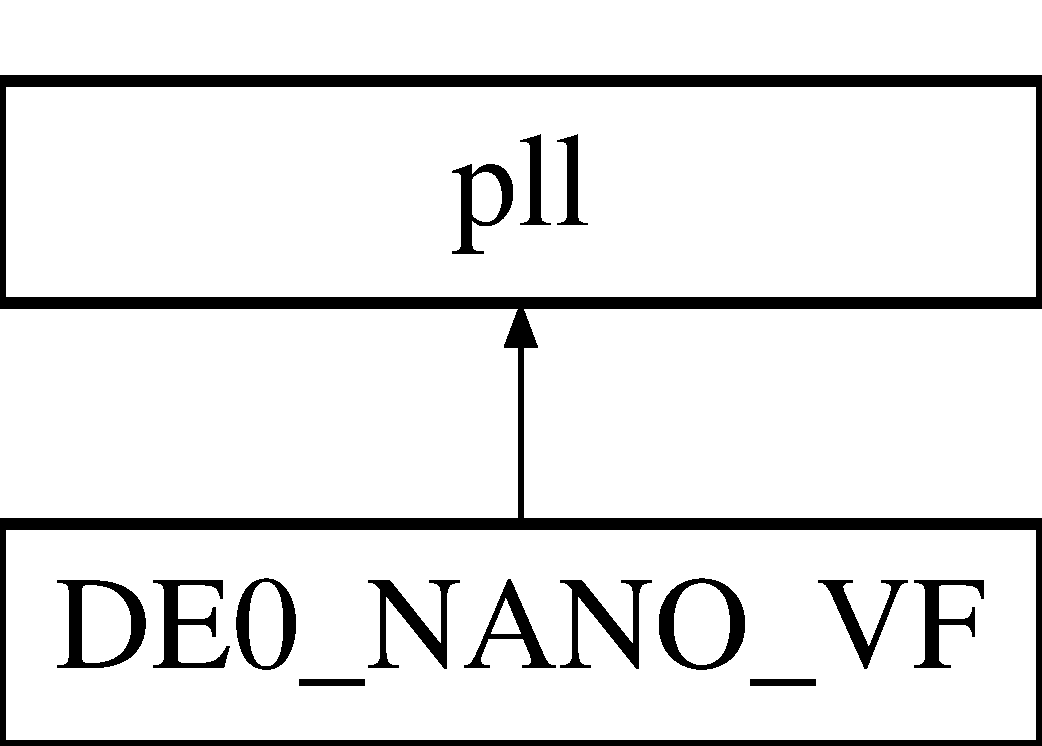
\includegraphics[height=2.000000cm]{classpll}
\end{center}
\end{figure}
\subsection*{Entities}
\begin{DoxyCompactItemize}
\item 
\hyperlink{classpll_1_1_s_y_n}{S\+Y\+N} architecture
\end{DoxyCompactItemize}
\subsection*{Libraries}
 \begin{DoxyCompactItemize}
\item 
\hyperlink{classpll_a0a6af6eef40212dbaf130d57ce711256}{ieee} 
\item 
\hyperlink{classpll_ad57cd8d31a38ff87ac163fb47757ffbf}{altera\+\_\+mf} 
\end{DoxyCompactItemize}
\subsection*{Use Clauses}
 \begin{DoxyCompactItemize}
\item 
\hyperlink{classpll_acd03516902501cd1c7296a98e22c6fcb}{std\+\_\+logic\+\_\+1164}   
\item 
\hyperlink{classpll_a470a86ce8776f637b0483eabf2d92ad2}{ all }   
\end{DoxyCompactItemize}
\subsection*{Ports}
 \begin{DoxyCompactItemize}
\item 
\hyperlink{classpll_a5ff6e3af321d94570fc485fa1bce5a06}{areset}  {\bfseries {\bfseries \textcolor{keywordflow}{in}\textcolor{vhdlchar}{ }}} {\bfseries \textcolor{comment}{S\+T\+D\+\_\+\+L\+O\+G\+I\+C}\textcolor{vhdlchar}{ }\textcolor{vhdlchar}{ }\textcolor{vhdlchar}{\+:}\textcolor{vhdlchar}{=}\textcolor{vhdlchar}{ }\textcolor{vhdlchar}{ }\textcolor{vhdlchar}{\textquotesingle{}}\textcolor{vhdlchar}{ } \textcolor{vhdldigit}{0} \textcolor{vhdlchar}{ }\textcolor{vhdlchar}{\textquotesingle{}}\textcolor{vhdlchar}{ }} 
\item 
\hyperlink{classpll_a9463f4cc62782c2faac516c942dcb5db}{inclk0}  {\bfseries {\bfseries \textcolor{keywordflow}{in}\textcolor{vhdlchar}{ }}} {\bfseries \textcolor{comment}{S\+T\+D\+\_\+\+L\+O\+G\+I\+C}\textcolor{vhdlchar}{ }\textcolor{vhdlchar}{ }\textcolor{vhdlchar}{\+:}\textcolor{vhdlchar}{=}\textcolor{vhdlchar}{ }\textcolor{vhdlchar}{ }\textcolor{vhdlchar}{\textquotesingle{}}\textcolor{vhdlchar}{ } \textcolor{vhdldigit}{0} \textcolor{vhdlchar}{ }\textcolor{vhdlchar}{\textquotesingle{}}\textcolor{vhdlchar}{ }} 
\item 
\hyperlink{classpll_abbf54d96b104435e8cbaadcf0e9184bd}{c0}  {\bfseries {\bfseries \textcolor{keywordflow}{out}\textcolor{vhdlchar}{ }}} {\bfseries \textcolor{comment}{S\+T\+D\+\_\+\+L\+O\+G\+I\+C}\textcolor{vhdlchar}{ }} 
\item 
\hyperlink{classpll_ab33e72e8245db404191648e9a25344eb}{locked}  {\bfseries {\bfseries \textcolor{keywordflow}{out}\textcolor{vhdlchar}{ }}} {\bfseries \textcolor{comment}{S\+T\+D\+\_\+\+L\+O\+G\+I\+C}\textcolor{vhdlchar}{ }} 
\end{DoxyCompactItemize}


\subsection{Detailed Description}


Definition at line \hyperlink{pll_8vhd_source_l00043}{43} of file \hyperlink{pll_8vhd_source}{pll.\+vhd}.



\subsection{Member Data Documentation}
\hypertarget{classpll_a470a86ce8776f637b0483eabf2d92ad2}{}\index{pll@{pll}! all @{ all }}
\index{ all @{ all }!pll@{pll}}
\subsubsection[{ all }]{\setlength{\rightskip}{0pt plus 5cm}{\bf  all }\hspace{0.3cm}{\ttfamily [Package]}}\label{classpll_a470a86ce8776f637b0483eabf2d92ad2}


Definition at line \hyperlink{pll_8vhd_source_l00041}{41} of file \hyperlink{pll_8vhd_source}{pll.\+vhd}.

\hypertarget{classpll_ad57cd8d31a38ff87ac163fb47757ffbf}{}\index{pll@{pll}!altera\+\_\+mf@{altera\+\_\+mf}}
\index{altera\+\_\+mf@{altera\+\_\+mf}!pll@{pll}}
\subsubsection[{altera\+\_\+mf}]{\setlength{\rightskip}{0pt plus 5cm}{\bf altera\+\_\+mf}\hspace{0.3cm}{\ttfamily [Library]}}\label{classpll_ad57cd8d31a38ff87ac163fb47757ffbf}


Definition at line \hyperlink{pll_8vhd_source_l00040}{40} of file \hyperlink{pll_8vhd_source}{pll.\+vhd}.

\hypertarget{classpll_a5ff6e3af321d94570fc485fa1bce5a06}{}\index{pll@{pll}!areset@{areset}}
\index{areset@{areset}!pll@{pll}}
\subsubsection[{areset}]{\setlength{\rightskip}{0pt plus 5cm}{\bf areset} {\bfseries \textcolor{keywordflow}{in}\textcolor{vhdlchar}{ }} {\bfseries \textcolor{comment}{S\+T\+D\+\_\+\+L\+O\+G\+I\+C}\textcolor{vhdlchar}{ }\textcolor{vhdlchar}{ }\textcolor{vhdlchar}{\+:}\textcolor{vhdlchar}{=}\textcolor{vhdlchar}{ }\textcolor{vhdlchar}{ }\textcolor{vhdlchar}{\textquotesingle{}}\textcolor{vhdlchar}{ } \textcolor{vhdldigit}{0} \textcolor{vhdlchar}{ }\textcolor{vhdlchar}{\textquotesingle{}}\textcolor{vhdlchar}{ }} \hspace{0.3cm}{\ttfamily [Port]}}\label{classpll_a5ff6e3af321d94570fc485fa1bce5a06}


Definition at line \hyperlink{pll_8vhd_source_l00046}{46} of file \hyperlink{pll_8vhd_source}{pll.\+vhd}.

\hypertarget{classpll_abbf54d96b104435e8cbaadcf0e9184bd}{}\index{pll@{pll}!c0@{c0}}
\index{c0@{c0}!pll@{pll}}
\subsubsection[{c0}]{\setlength{\rightskip}{0pt plus 5cm}{\bf c0} {\bfseries \textcolor{keywordflow}{out}\textcolor{vhdlchar}{ }} {\bfseries \textcolor{comment}{S\+T\+D\+\_\+\+L\+O\+G\+I\+C}\textcolor{vhdlchar}{ }} \hspace{0.3cm}{\ttfamily [Port]}}\label{classpll_abbf54d96b104435e8cbaadcf0e9184bd}


Definition at line \hyperlink{pll_8vhd_source_l00048}{48} of file \hyperlink{pll_8vhd_source}{pll.\+vhd}.

\hypertarget{classpll_a0a6af6eef40212dbaf130d57ce711256}{}\index{pll@{pll}!ieee@{ieee}}
\index{ieee@{ieee}!pll@{pll}}
\subsubsection[{ieee}]{\setlength{\rightskip}{0pt plus 5cm}{\bf ieee}\hspace{0.3cm}{\ttfamily [Library]}}\label{classpll_a0a6af6eef40212dbaf130d57ce711256}


Definition at line \hyperlink{pll_8vhd_source_l00037}{37} of file \hyperlink{pll_8vhd_source}{pll.\+vhd}.

\hypertarget{classpll_a9463f4cc62782c2faac516c942dcb5db}{}\index{pll@{pll}!inclk0@{inclk0}}
\index{inclk0@{inclk0}!pll@{pll}}
\subsubsection[{inclk0}]{\setlength{\rightskip}{0pt plus 5cm}{\bf inclk0} {\bfseries \textcolor{keywordflow}{in}\textcolor{vhdlchar}{ }} {\bfseries \textcolor{comment}{S\+T\+D\+\_\+\+L\+O\+G\+I\+C}\textcolor{vhdlchar}{ }\textcolor{vhdlchar}{ }\textcolor{vhdlchar}{\+:}\textcolor{vhdlchar}{=}\textcolor{vhdlchar}{ }\textcolor{vhdlchar}{ }\textcolor{vhdlchar}{\textquotesingle{}}\textcolor{vhdlchar}{ } \textcolor{vhdldigit}{0} \textcolor{vhdlchar}{ }\textcolor{vhdlchar}{\textquotesingle{}}\textcolor{vhdlchar}{ }} \hspace{0.3cm}{\ttfamily [Port]}}\label{classpll_a9463f4cc62782c2faac516c942dcb5db}


Definition at line \hyperlink{pll_8vhd_source_l00047}{47} of file \hyperlink{pll_8vhd_source}{pll.\+vhd}.

\hypertarget{classpll_ab33e72e8245db404191648e9a25344eb}{}\index{pll@{pll}!locked@{locked}}
\index{locked@{locked}!pll@{pll}}
\subsubsection[{locked}]{\setlength{\rightskip}{0pt plus 5cm}{\bf locked} {\bfseries \textcolor{keywordflow}{out}\textcolor{vhdlchar}{ }} {\bfseries \textcolor{comment}{S\+T\+D\+\_\+\+L\+O\+G\+I\+C}\textcolor{vhdlchar}{ }} \hspace{0.3cm}{\ttfamily [Port]}}\label{classpll_ab33e72e8245db404191648e9a25344eb}


Definition at line \hyperlink{pll_8vhd_source_l00050}{50} of file \hyperlink{pll_8vhd_source}{pll.\+vhd}.

\hypertarget{classpll_acd03516902501cd1c7296a98e22c6fcb}{}\index{pll@{pll}!std\+\_\+logic\+\_\+1164@{std\+\_\+logic\+\_\+1164}}
\index{std\+\_\+logic\+\_\+1164@{std\+\_\+logic\+\_\+1164}!pll@{pll}}
\subsubsection[{std\+\_\+logic\+\_\+1164}]{\setlength{\rightskip}{0pt plus 5cm}{\bf std\+\_\+logic\+\_\+1164}\hspace{0.3cm}{\ttfamily [Package]}}\label{classpll_acd03516902501cd1c7296a98e22c6fcb}


Definition at line \hyperlink{pll_8vhd_source_l00038}{38} of file \hyperlink{pll_8vhd_source}{pll.\+vhd}.



The documentation for this class was generated from the following file\+:\begin{DoxyCompactItemize}
\item 
\hyperlink{pll_8vhd}{pll.\+vhd}\end{DoxyCompactItemize}

\hypertarget{classportadora__tringular}{}\section{portadora\+\_\+tringular Entity Reference}
\label{classportadora__tringular}\index{portadora\+\_\+tringular@{portadora\+\_\+tringular}}
Inheritance diagram for portadora\+\_\+tringular\+:\begin{figure}[H]
\begin{center}
\leavevmode
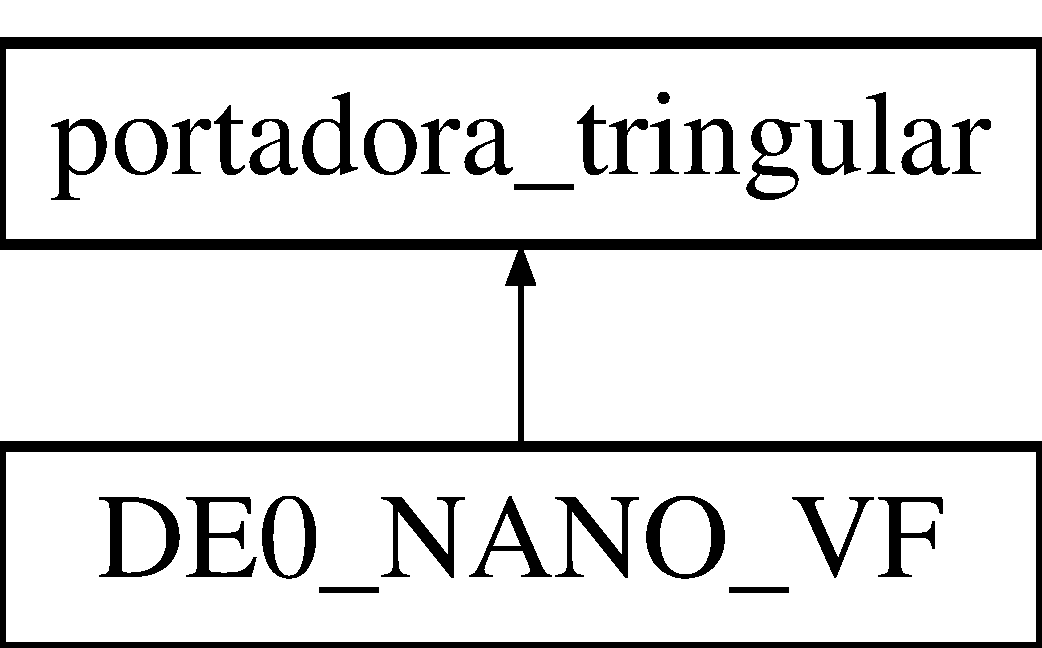
\includegraphics[height=2.000000cm]{classportadora__tringular}
\end{center}
\end{figure}
\subsection*{Entities}
\begin{DoxyCompactItemize}
\item 
\hyperlink{classportadora__tringular_1_1portadora__tringular}{portadora\+\_\+tringular} architecture
\end{DoxyCompactItemize}
\subsection*{Libraries}
 \begin{DoxyCompactItemize}
\item 
\hyperlink{classportadora__tringular_ae4f03c286607f3181e16b9aa12d0c6d4}{I\+E\+E\+E} 
\end{DoxyCompactItemize}
\subsection*{Use Clauses}
 \begin{DoxyCompactItemize}
\item 
\hyperlink{classportadora__tringular_a241c3e72dd8024cc8ae831b1b2aed7db}{S\+T\+D\+\_\+\+L\+O\+G\+I\+C\+\_\+\+U\+N\+S\+I\+G\+N\+E\+D}   
\item 
\hyperlink{classportadora__tringular_aa4b2b25246a821511120e3149b003563}{S\+T\+D\+\_\+\+L\+O\+G\+I\+C\+\_\+1164}   
\item 
\hyperlink{classportadora__tringular_aad86249c80e8c1e7ee1c4748aba748e3}{fixed\+\_\+pkg}   
\end{DoxyCompactItemize}
\subsection*{Generics}
 \begin{DoxyCompactItemize}
\item 
\hyperlink{classportadora__tringular_af8ee6f7e8fea0e211d86d8e3fd6f8d29}{N} {\bfseries {\bfseries \textcolor{comment}{integer}\textcolor{vhdlchar}{ }\textcolor{vhdlchar}{ }\textcolor{vhdlchar}{\+:}\textcolor{vhdlchar}{=}\textcolor{vhdlchar}{ }\textcolor{vhdlchar}{ } \textcolor{vhdldigit}{16} \textcolor{vhdlchar}{ }}}
\end{DoxyCompactItemize}
\subsection*{Ports}
 \begin{DoxyCompactItemize}
\item 
\hyperlink{classportadora__tringular_a4a4609c199d30b3adebbeb3a01276ec5}{clk}  {\bfseries {\bfseries \textcolor{keywordflow}{in}\textcolor{vhdlchar}{ }}} {\bfseries \textcolor{comment}{std\+\_\+logic}\textcolor{vhdlchar}{ }} 
\item 
\hyperlink{classportadora__tringular_adcf9c6f5161d039addbda5819bee64a3}{en}  {\bfseries {\bfseries \textcolor{keywordflow}{in}\textcolor{vhdlchar}{ }}} {\bfseries \textcolor{comment}{std\+\_\+logic}\textcolor{vhdlchar}{ }} 
\item 
\hyperlink{classportadora__tringular_aad8dc6359d9e23dabcbf342fadf2fa06}{reset}  {\bfseries {\bfseries \textcolor{keywordflow}{in}\textcolor{vhdlchar}{ }}} {\bfseries \textcolor{comment}{std\+\_\+logic}\textcolor{vhdlchar}{ }} 
\item 
\hyperlink{classportadora__tringular_ab3bb50450dbeb3852b4f76ef2aefbf9e}{count\+\_\+ini}  {\bfseries {\bfseries \textcolor{keywordflow}{in}\textcolor{vhdlchar}{ }}} {\bfseries \textcolor{comment}{std\+\_\+logic\+\_\+vector}\textcolor{vhdlchar}{ }\textcolor{vhdlchar}{(}\textcolor{vhdlchar}{ }\textcolor{vhdlchar}{ }\textcolor{vhdlchar}{ }\textcolor{vhdlchar}{ }{\bfseries \hyperlink{classportadora__tringular_af8ee6f7e8fea0e211d86d8e3fd6f8d29}{N}} \textcolor{vhdlchar}{-\/}\textcolor{vhdlchar}{ } \textcolor{vhdldigit}{1} \textcolor{vhdlchar}{ }\textcolor{keywordflow}{downto}\textcolor{vhdlchar}{ }\textcolor{vhdlchar}{ } \textcolor{vhdldigit}{0} \textcolor{vhdlchar}{ }\textcolor{vhdlchar}{)}\textcolor{vhdlchar}{ }} 
\item 
\hyperlink{classportadora__tringular_ac855daed6a8d1b25a13c5d5b4aa46c3e}{dir\+\_\+ini}  {\bfseries {\bfseries \textcolor{keywordflow}{in}\textcolor{vhdlchar}{ }}} {\bfseries \textcolor{comment}{std\+\_\+logic}\textcolor{vhdlchar}{ }} 
\item 
\hyperlink{classportadora__tringular_a06de1330d80ce7a764361167217baf42}{M\+A\+X}  {\bfseries {\bfseries \textcolor{keywordflow}{in}\textcolor{vhdlchar}{ }}} {\bfseries \textcolor{comment}{std\+\_\+logic\+\_\+vector}\textcolor{vhdlchar}{ }\textcolor{vhdlchar}{(}\textcolor{vhdlchar}{ }\textcolor{vhdlchar}{ }\textcolor{vhdlchar}{ }\textcolor{vhdlchar}{ }{\bfseries \hyperlink{classportadora__tringular_af8ee6f7e8fea0e211d86d8e3fd6f8d29}{N}} \textcolor{vhdlchar}{-\/}\textcolor{vhdlchar}{ } \textcolor{vhdldigit}{1} \textcolor{vhdlchar}{ }\textcolor{keywordflow}{downto}\textcolor{vhdlchar}{ }\textcolor{vhdlchar}{ } \textcolor{vhdldigit}{0} \textcolor{vhdlchar}{ }\textcolor{vhdlchar}{)}\textcolor{vhdlchar}{ }} 
\item 
\hyperlink{classportadora__tringular_a8fb21bca6cb529fd30fa4b1f8b156237}{dir}  {\bfseries {\bfseries \textcolor{keywordflow}{out}\textcolor{vhdlchar}{ }}} {\bfseries \textcolor{comment}{std\+\_\+logic}\textcolor{vhdlchar}{ }} 
\item 
\hyperlink{classportadora__tringular_a54ed3cc1c7433faf63dbf6b009fe8137}{c}  {\bfseries {\bfseries \textcolor{keywordflow}{out}\textcolor{vhdlchar}{ }}} {\bfseries \textcolor{comment}{std\+\_\+logic\+\_\+vector}\textcolor{vhdlchar}{ }\textcolor{vhdlchar}{(}\textcolor{vhdlchar}{ }\textcolor{vhdlchar}{ }\textcolor{vhdlchar}{ }\textcolor{vhdlchar}{ }{\bfseries \hyperlink{classportadora__tringular_af8ee6f7e8fea0e211d86d8e3fd6f8d29}{N}} \textcolor{vhdlchar}{-\/}\textcolor{vhdlchar}{ } \textcolor{vhdldigit}{1} \textcolor{vhdlchar}{ }\textcolor{keywordflow}{downto}\textcolor{vhdlchar}{ }\textcolor{vhdlchar}{ } \textcolor{vhdldigit}{0} \textcolor{vhdlchar}{ }\textcolor{vhdlchar}{)}\textcolor{vhdlchar}{ }} 
\end{DoxyCompactItemize}


\subsection{Detailed Description}


Definition at line 6 of file portadora\+\_\+tringular.\+vhd.



\subsection{Member Data Documentation}
\hypertarget{classportadora__tringular_a54ed3cc1c7433faf63dbf6b009fe8137}{}\index{portadora\+\_\+tringular@{portadora\+\_\+tringular}!c@{c}}
\index{c@{c}!portadora\+\_\+tringular@{portadora\+\_\+tringular}}
\subsubsection[{c}]{\setlength{\rightskip}{0pt plus 5cm}{\bf c} {\bfseries \textcolor{keywordflow}{out}\textcolor{vhdlchar}{ }} {\bfseries \textcolor{comment}{std\+\_\+logic\+\_\+vector}\textcolor{vhdlchar}{ }\textcolor{vhdlchar}{(}\textcolor{vhdlchar}{ }\textcolor{vhdlchar}{ }\textcolor{vhdlchar}{ }\textcolor{vhdlchar}{ }{\bfseries {\bf N}} \textcolor{vhdlchar}{-\/}\textcolor{vhdlchar}{ } \textcolor{vhdldigit}{1} \textcolor{vhdlchar}{ }\textcolor{keywordflow}{downto}\textcolor{vhdlchar}{ }\textcolor{vhdlchar}{ } \textcolor{vhdldigit}{0} \textcolor{vhdlchar}{ }\textcolor{vhdlchar}{)}\textcolor{vhdlchar}{ }} \hspace{0.3cm}{\ttfamily [Port]}}\label{classportadora__tringular_a54ed3cc1c7433faf63dbf6b009fe8137}


Definition at line 18 of file portadora\+\_\+tringular.\+vhd.

\hypertarget{classportadora__tringular_a4a4609c199d30b3adebbeb3a01276ec5}{}\index{portadora\+\_\+tringular@{portadora\+\_\+tringular}!clk@{clk}}
\index{clk@{clk}!portadora\+\_\+tringular@{portadora\+\_\+tringular}}
\subsubsection[{clk}]{\setlength{\rightskip}{0pt plus 5cm}{\bf clk} {\bfseries \textcolor{keywordflow}{in}\textcolor{vhdlchar}{ }} {\bfseries \textcolor{comment}{std\+\_\+logic}\textcolor{vhdlchar}{ }} \hspace{0.3cm}{\ttfamily [Port]}}\label{classportadora__tringular_a4a4609c199d30b3adebbeb3a01276ec5}


Definition at line 10 of file portadora\+\_\+tringular.\+vhd.

\hypertarget{classportadora__tringular_ab3bb50450dbeb3852b4f76ef2aefbf9e}{}\index{portadora\+\_\+tringular@{portadora\+\_\+tringular}!count\+\_\+ini@{count\+\_\+ini}}
\index{count\+\_\+ini@{count\+\_\+ini}!portadora\+\_\+tringular@{portadora\+\_\+tringular}}
\subsubsection[{count\+\_\+ini}]{\setlength{\rightskip}{0pt plus 5cm}{\bf count\+\_\+ini} {\bfseries \textcolor{keywordflow}{in}\textcolor{vhdlchar}{ }} {\bfseries \textcolor{comment}{std\+\_\+logic\+\_\+vector}\textcolor{vhdlchar}{ }\textcolor{vhdlchar}{(}\textcolor{vhdlchar}{ }\textcolor{vhdlchar}{ }\textcolor{vhdlchar}{ }\textcolor{vhdlchar}{ }{\bfseries {\bf N}} \textcolor{vhdlchar}{-\/}\textcolor{vhdlchar}{ } \textcolor{vhdldigit}{1} \textcolor{vhdlchar}{ }\textcolor{keywordflow}{downto}\textcolor{vhdlchar}{ }\textcolor{vhdlchar}{ } \textcolor{vhdldigit}{0} \textcolor{vhdlchar}{ }\textcolor{vhdlchar}{)}\textcolor{vhdlchar}{ }} \hspace{0.3cm}{\ttfamily [Port]}}\label{classportadora__tringular_ab3bb50450dbeb3852b4f76ef2aefbf9e}


Definition at line 13 of file portadora\+\_\+tringular.\+vhd.

\hypertarget{classportadora__tringular_a8fb21bca6cb529fd30fa4b1f8b156237}{}\index{portadora\+\_\+tringular@{portadora\+\_\+tringular}!dir@{dir}}
\index{dir@{dir}!portadora\+\_\+tringular@{portadora\+\_\+tringular}}
\subsubsection[{dir}]{\setlength{\rightskip}{0pt plus 5cm}{\bf dir} {\bfseries \textcolor{keywordflow}{out}\textcolor{vhdlchar}{ }} {\bfseries \textcolor{comment}{std\+\_\+logic}\textcolor{vhdlchar}{ }} \hspace{0.3cm}{\ttfamily [Port]}}\label{classportadora__tringular_a8fb21bca6cb529fd30fa4b1f8b156237}


Definition at line 16 of file portadora\+\_\+tringular.\+vhd.

\hypertarget{classportadora__tringular_ac855daed6a8d1b25a13c5d5b4aa46c3e}{}\index{portadora\+\_\+tringular@{portadora\+\_\+tringular}!dir\+\_\+ini@{dir\+\_\+ini}}
\index{dir\+\_\+ini@{dir\+\_\+ini}!portadora\+\_\+tringular@{portadora\+\_\+tringular}}
\subsubsection[{dir\+\_\+ini}]{\setlength{\rightskip}{0pt plus 5cm}{\bf dir\+\_\+ini} {\bfseries \textcolor{keywordflow}{in}\textcolor{vhdlchar}{ }} {\bfseries \textcolor{comment}{std\+\_\+logic}\textcolor{vhdlchar}{ }} \hspace{0.3cm}{\ttfamily [Port]}}\label{classportadora__tringular_ac855daed6a8d1b25a13c5d5b4aa46c3e}


Definition at line 14 of file portadora\+\_\+tringular.\+vhd.

\hypertarget{classportadora__tringular_adcf9c6f5161d039addbda5819bee64a3}{}\index{portadora\+\_\+tringular@{portadora\+\_\+tringular}!en@{en}}
\index{en@{en}!portadora\+\_\+tringular@{portadora\+\_\+tringular}}
\subsubsection[{en}]{\setlength{\rightskip}{0pt plus 5cm}{\bf en} {\bfseries \textcolor{keywordflow}{in}\textcolor{vhdlchar}{ }} {\bfseries \textcolor{comment}{std\+\_\+logic}\textcolor{vhdlchar}{ }} \hspace{0.3cm}{\ttfamily [Port]}}\label{classportadora__tringular_adcf9c6f5161d039addbda5819bee64a3}


Definition at line 11 of file portadora\+\_\+tringular.\+vhd.

\hypertarget{classportadora__tringular_aad86249c80e8c1e7ee1c4748aba748e3}{}\index{portadora\+\_\+tringular@{portadora\+\_\+tringular}!fixed\+\_\+pkg@{fixed\+\_\+pkg}}
\index{fixed\+\_\+pkg@{fixed\+\_\+pkg}!portadora\+\_\+tringular@{portadora\+\_\+tringular}}
\subsubsection[{fixed\+\_\+pkg}]{\setlength{\rightskip}{0pt plus 5cm}{\bf fixed\+\_\+pkg}\hspace{0.3cm}{\ttfamily [Package]}}\label{classportadora__tringular_aad86249c80e8c1e7ee1c4748aba748e3}


Definition at line 4 of file portadora\+\_\+tringular.\+vhd.

\hypertarget{classportadora__tringular_ae4f03c286607f3181e16b9aa12d0c6d4}{}\index{portadora\+\_\+tringular@{portadora\+\_\+tringular}!I\+E\+E\+E@{I\+E\+E\+E}}
\index{I\+E\+E\+E@{I\+E\+E\+E}!portadora\+\_\+tringular@{portadora\+\_\+tringular}}
\subsubsection[{I\+E\+E\+E}]{\setlength{\rightskip}{0pt plus 5cm}{\bf I\+E\+E\+E}\hspace{0.3cm}{\ttfamily [Library]}}\label{classportadora__tringular_ae4f03c286607f3181e16b9aa12d0c6d4}


Definition at line 1 of file portadora\+\_\+tringular.\+vhd.

\hypertarget{classportadora__tringular_a06de1330d80ce7a764361167217baf42}{}\index{portadora\+\_\+tringular@{portadora\+\_\+tringular}!M\+A\+X@{M\+A\+X}}
\index{M\+A\+X@{M\+A\+X}!portadora\+\_\+tringular@{portadora\+\_\+tringular}}
\subsubsection[{M\+A\+X}]{\setlength{\rightskip}{0pt plus 5cm}{\bf M\+A\+X} {\bfseries \textcolor{keywordflow}{in}\textcolor{vhdlchar}{ }} {\bfseries \textcolor{comment}{std\+\_\+logic\+\_\+vector}\textcolor{vhdlchar}{ }\textcolor{vhdlchar}{(}\textcolor{vhdlchar}{ }\textcolor{vhdlchar}{ }\textcolor{vhdlchar}{ }\textcolor{vhdlchar}{ }{\bfseries {\bf N}} \textcolor{vhdlchar}{-\/}\textcolor{vhdlchar}{ } \textcolor{vhdldigit}{1} \textcolor{vhdlchar}{ }\textcolor{keywordflow}{downto}\textcolor{vhdlchar}{ }\textcolor{vhdlchar}{ } \textcolor{vhdldigit}{0} \textcolor{vhdlchar}{ }\textcolor{vhdlchar}{)}\textcolor{vhdlchar}{ }} \hspace{0.3cm}{\ttfamily [Port]}}\label{classportadora__tringular_a06de1330d80ce7a764361167217baf42}


Definition at line 15 of file portadora\+\_\+tringular.\+vhd.

\hypertarget{classportadora__tringular_af8ee6f7e8fea0e211d86d8e3fd6f8d29}{}\index{portadora\+\_\+tringular@{portadora\+\_\+tringular}!N@{N}}
\index{N@{N}!portadora\+\_\+tringular@{portadora\+\_\+tringular}}
\subsubsection[{N}]{\setlength{\rightskip}{0pt plus 5cm}{\bf N} {\bfseries \textcolor{vhdlchar}{ }} {\bfseries \textcolor{comment}{integer}\textcolor{vhdlchar}{ }\textcolor{vhdlchar}{ }\textcolor{vhdlchar}{\+:}\textcolor{vhdlchar}{=}\textcolor{vhdlchar}{ }\textcolor{vhdlchar}{ } \textcolor{vhdldigit}{16} \textcolor{vhdlchar}{ }} \hspace{0.3cm}{\ttfamily [Generic]}}\label{classportadora__tringular_af8ee6f7e8fea0e211d86d8e3fd6f8d29}


Definition at line 8 of file portadora\+\_\+tringular.\+vhd.

\hypertarget{classportadora__tringular_aad8dc6359d9e23dabcbf342fadf2fa06}{}\index{portadora\+\_\+tringular@{portadora\+\_\+tringular}!reset@{reset}}
\index{reset@{reset}!portadora\+\_\+tringular@{portadora\+\_\+tringular}}
\subsubsection[{reset}]{\setlength{\rightskip}{0pt plus 5cm}{\bf reset} {\bfseries \textcolor{keywordflow}{in}\textcolor{vhdlchar}{ }} {\bfseries \textcolor{comment}{std\+\_\+logic}\textcolor{vhdlchar}{ }} \hspace{0.3cm}{\ttfamily [Port]}}\label{classportadora__tringular_aad8dc6359d9e23dabcbf342fadf2fa06}


Definition at line 12 of file portadora\+\_\+tringular.\+vhd.

\hypertarget{classportadora__tringular_aa4b2b25246a821511120e3149b003563}{}\index{portadora\+\_\+tringular@{portadora\+\_\+tringular}!S\+T\+D\+\_\+\+L\+O\+G\+I\+C\+\_\+1164@{S\+T\+D\+\_\+\+L\+O\+G\+I\+C\+\_\+1164}}
\index{S\+T\+D\+\_\+\+L\+O\+G\+I\+C\+\_\+1164@{S\+T\+D\+\_\+\+L\+O\+G\+I\+C\+\_\+1164}!portadora\+\_\+tringular@{portadora\+\_\+tringular}}
\subsubsection[{S\+T\+D\+\_\+\+L\+O\+G\+I\+C\+\_\+1164}]{\setlength{\rightskip}{0pt plus 5cm}{\bf S\+T\+D\+\_\+\+L\+O\+G\+I\+C\+\_\+1164}\hspace{0.3cm}{\ttfamily [Package]}}\label{classportadora__tringular_aa4b2b25246a821511120e3149b003563}


Definition at line 3 of file portadora\+\_\+tringular.\+vhd.

\hypertarget{classportadora__tringular_a241c3e72dd8024cc8ae831b1b2aed7db}{}\index{portadora\+\_\+tringular@{portadora\+\_\+tringular}!S\+T\+D\+\_\+\+L\+O\+G\+I\+C\+\_\+\+U\+N\+S\+I\+G\+N\+E\+D@{S\+T\+D\+\_\+\+L\+O\+G\+I\+C\+\_\+\+U\+N\+S\+I\+G\+N\+E\+D}}
\index{S\+T\+D\+\_\+\+L\+O\+G\+I\+C\+\_\+\+U\+N\+S\+I\+G\+N\+E\+D@{S\+T\+D\+\_\+\+L\+O\+G\+I\+C\+\_\+\+U\+N\+S\+I\+G\+N\+E\+D}!portadora\+\_\+tringular@{portadora\+\_\+tringular}}
\subsubsection[{S\+T\+D\+\_\+\+L\+O\+G\+I\+C\+\_\+\+U\+N\+S\+I\+G\+N\+E\+D}]{\setlength{\rightskip}{0pt plus 5cm}{\bf S\+T\+D\+\_\+\+L\+O\+G\+I\+C\+\_\+\+U\+N\+S\+I\+G\+N\+E\+D}\hspace{0.3cm}{\ttfamily [Package]}}\label{classportadora__tringular_a241c3e72dd8024cc8ae831b1b2aed7db}


Definition at line 2 of file portadora\+\_\+tringular.\+vhd.



The documentation for this class was generated from the following file\+:\begin{DoxyCompactItemize}
\item 
\hyperlink{portadora__tringular_8vhd}{portadora\+\_\+tringular.\+vhd}\end{DoxyCompactItemize}

\hypertarget{classportadora__tringular_1_1portadora__tringular}{}\section{portadora\+\_\+tringular Architecture Reference}
\label{classportadora__tringular_1_1portadora__tringular}\index{portadora\+\_\+tringular@{portadora\+\_\+tringular}}
\subsection*{Processes}
 \begin{DoxyCompactItemize}
\item 
\hyperlink{classportadora__tringular_1_1portadora__tringular_a9d3814991b9352ab295cc62784226977}{P\+R\+O\+C\+E\+S\+S\+\_\+12}{\bfseries  ( {\bfseries {\bfseries \hyperlink{classportadora__tringular_a4a4609c199d30b3adebbeb3a01276ec5}{clk}} \textcolor{vhdlchar}{ }} )}
\end{DoxyCompactItemize}
\subsection*{Signals}
 \begin{DoxyCompactItemize}
\item 
\hyperlink{classportadora__tringular_1_1portadora__tringular_ae3b6c46c82d8260487d5f5291a70a96a}{c\+\_\+int} {\bfseries \textcolor{comment}{std\+\_\+logic\+\_\+vector}\textcolor{vhdlchar}{ }\textcolor{vhdlchar}{(}\textcolor{vhdlchar}{ }\textcolor{vhdlchar}{ }\textcolor{vhdlchar}{ }\textcolor{vhdlchar}{ }{\bfseries \hyperlink{classportadora__tringular_af8ee6f7e8fea0e211d86d8e3fd6f8d29}{N}} \textcolor{vhdlchar}{-\/}\textcolor{vhdlchar}{ } \textcolor{vhdldigit}{1} \textcolor{vhdlchar}{ }\textcolor{keywordflow}{downto}\textcolor{vhdlchar}{ }\textcolor{vhdlchar}{ } \textcolor{vhdldigit}{0} \textcolor{vhdlchar}{ }\textcolor{vhdlchar}{)}\textcolor{vhdlchar}{ }} 
\item 
\hyperlink{classportadora__tringular_1_1portadora__tringular_ae27566c74fe97a2b3c215e94dc35dd47}{dir\+\_\+int} {\bfseries \textcolor{comment}{std\+\_\+logic}\textcolor{vhdlchar}{ }} 
\end{DoxyCompactItemize}


\subsection{Detailed Description}


Definition at line \hyperlink{portadora__tringular_8vhd_source_l00023}{23} of file \hyperlink{portadora__tringular_8vhd_source}{portadora\+\_\+tringular.\+vhd}.



\subsection{Member Function Documentation}
\hypertarget{classportadora__tringular_1_1portadora__tringular_a9d3814991b9352ab295cc62784226977}{}\index{portadora\+\_\+tringular\+::portadora\+\_\+tringular@{portadora\+\_\+tringular\+::portadora\+\_\+tringular}!P\+R\+O\+C\+E\+S\+S\+\_\+12@{P\+R\+O\+C\+E\+S\+S\+\_\+12}}
\index{P\+R\+O\+C\+E\+S\+S\+\_\+12@{P\+R\+O\+C\+E\+S\+S\+\_\+12}!portadora\+\_\+tringular\+::portadora\+\_\+tringular@{portadora\+\_\+tringular\+::portadora\+\_\+tringular}}
\subsubsection[{P\+R\+O\+C\+E\+S\+S\+\_\+12}]{\setlength{\rightskip}{0pt plus 5cm} {\bfseries \textcolor{vhdlchar}{ }} P\+R\+O\+C\+E\+S\+S\+\_\+12(
\begin{DoxyParamCaption}
\item[{}]{{\bfseries {\bfseries {\bf clk}} \textcolor{vhdlchar}{ }} {\em }}
\end{DoxyParamCaption}
)\hspace{0.3cm}{\ttfamily [Process]}}\label{classportadora__tringular_1_1portadora__tringular_a9d3814991b9352ab295cc62784226977}


Definition at line \hyperlink{portadora__tringular_8vhd_source_l00031}{31} of file \hyperlink{portadora__tringular_8vhd_source}{portadora\+\_\+tringular.\+vhd}.



\subsection{Member Data Documentation}
\hypertarget{classportadora__tringular_1_1portadora__tringular_ae3b6c46c82d8260487d5f5291a70a96a}{}\index{portadora\+\_\+tringular\+::portadora\+\_\+tringular@{portadora\+\_\+tringular\+::portadora\+\_\+tringular}!c\+\_\+int@{c\+\_\+int}}
\index{c\+\_\+int@{c\+\_\+int}!portadora\+\_\+tringular\+::portadora\+\_\+tringular@{portadora\+\_\+tringular\+::portadora\+\_\+tringular}}
\subsubsection[{c\+\_\+int}]{\setlength{\rightskip}{0pt plus 5cm}{\bf c\+\_\+int} {\bfseries \textcolor{comment}{std\+\_\+logic\+\_\+vector}\textcolor{vhdlchar}{ }\textcolor{vhdlchar}{(}\textcolor{vhdlchar}{ }\textcolor{vhdlchar}{ }\textcolor{vhdlchar}{ }\textcolor{vhdlchar}{ }{\bfseries {\bf N}} \textcolor{vhdlchar}{-\/}\textcolor{vhdlchar}{ } \textcolor{vhdldigit}{1} \textcolor{vhdlchar}{ }\textcolor{keywordflow}{downto}\textcolor{vhdlchar}{ }\textcolor{vhdlchar}{ } \textcolor{vhdldigit}{0} \textcolor{vhdlchar}{ }\textcolor{vhdlchar}{)}\textcolor{vhdlchar}{ }} \hspace{0.3cm}{\ttfamily [Signal]}}\label{classportadora__tringular_1_1portadora__tringular_ae3b6c46c82d8260487d5f5291a70a96a}


Definition at line \hyperlink{portadora__tringular_8vhd_source_l00025}{25} of file \hyperlink{portadora__tringular_8vhd_source}{portadora\+\_\+tringular.\+vhd}.

\hypertarget{classportadora__tringular_1_1portadora__tringular_ae27566c74fe97a2b3c215e94dc35dd47}{}\index{portadora\+\_\+tringular\+::portadora\+\_\+tringular@{portadora\+\_\+tringular\+::portadora\+\_\+tringular}!dir\+\_\+int@{dir\+\_\+int}}
\index{dir\+\_\+int@{dir\+\_\+int}!portadora\+\_\+tringular\+::portadora\+\_\+tringular@{portadora\+\_\+tringular\+::portadora\+\_\+tringular}}
\subsubsection[{dir\+\_\+int}]{\setlength{\rightskip}{0pt plus 5cm}{\bf dir\+\_\+int} {\bfseries \textcolor{comment}{std\+\_\+logic}\textcolor{vhdlchar}{ }} \hspace{0.3cm}{\ttfamily [Signal]}}\label{classportadora__tringular_1_1portadora__tringular_ae27566c74fe97a2b3c215e94dc35dd47}


Definition at line \hyperlink{portadora__tringular_8vhd_source_l00026}{26} of file \hyperlink{portadora__tringular_8vhd_source}{portadora\+\_\+tringular.\+vhd}.



The documentation for this class was generated from the following file\+:\begin{DoxyCompactItemize}
\item 
\hyperlink{portadora__tringular_8vhd}{portadora\+\_\+tringular.\+vhd}\end{DoxyCompactItemize}

\hypertarget{classsinewave}{}\section{sinewave Entity Reference}
\label{classsinewave}\index{sinewave@{sinewave}}
\subsection*{Entities}
\begin{DoxyCompactItemize}
\item 
\hyperlink{classsinewave_1_1_behavioral}{Behavioral} architecture
\end{DoxyCompactItemize}
\subsection*{Libraries}
 \begin{DoxyCompactItemize}
\item 
\hyperlink{classsinewave_ae4f03c286607f3181e16b9aa12d0c6d4}{I\+E\+E\+E} 
\end{DoxyCompactItemize}
\subsection*{Use Clauses}
 \begin{DoxyCompactItemize}
\item 
\hyperlink{classsinewave_aa4b2b25246a821511120e3149b003563}{S\+T\+D\+\_\+\+L\+O\+G\+I\+C\+\_\+1164}   
\item 
\hyperlink{classsinewave_ae00f3f04545af57582ff10609eee23e2}{N\+U\+M\+E\+R\+I\+C\+\_\+\+S\+T\+D}   
\end{DoxyCompactItemize}
\subsection*{Ports}
 \begin{DoxyCompactItemize}
\item 
\hyperlink{classsinewave_a4a4609c199d30b3adebbeb3a01276ec5}{clk}  {\bfseries {\bfseries \textcolor{keywordflow}{in}\textcolor{vhdlchar}{ }}} {\bfseries \textcolor{comment}{std\+\_\+logic}\textcolor{vhdlchar}{ }} 
\item 
\hyperlink{classsinewave_a6f923bb55dbbef4e48f6ae28e0588faf}{dataout}  {\bfseries {\bfseries \textcolor{keywordflow}{out}\textcolor{vhdlchar}{ }}} {\bfseries \textcolor{comment}{integer}\textcolor{vhdlchar}{ }\textcolor{vhdlchar}{ }\textcolor{vhdlchar}{ }\textcolor{keywordflow}{range}\textcolor{vhdlchar}{ }\textcolor{vhdlchar}{-\/}\textcolor{vhdlchar}{ } \textcolor{vhdldigit}{128} \textcolor{vhdlchar}{ }\textcolor{keywordflow}{to}\textcolor{vhdlchar}{ }\textcolor{vhdlchar}{ } \textcolor{vhdldigit}{127} \textcolor{vhdlchar}{ }} 
\end{DoxyCompactItemize}


\subsection{Detailed Description}


Definition at line \hyperlink{sinewave_8vhd_source_l00006}{6} of file \hyperlink{sinewave_8vhd_source}{sinewave.\+vhd}.



\subsection{Member Data Documentation}
\hypertarget{classsinewave_a4a4609c199d30b3adebbeb3a01276ec5}{}\index{sinewave@{sinewave}!clk@{clk}}
\index{clk@{clk}!sinewave@{sinewave}}
\subsubsection[{clk}]{\setlength{\rightskip}{0pt plus 5cm}{\bf clk} {\bfseries \textcolor{keywordflow}{in}\textcolor{vhdlchar}{ }} {\bfseries \textcolor{comment}{std\+\_\+logic}\textcolor{vhdlchar}{ }} \hspace{0.3cm}{\ttfamily [Port]}}\label{classsinewave_a4a4609c199d30b3adebbeb3a01276ec5}


Definition at line \hyperlink{sinewave_8vhd_source_l00007}{7} of file \hyperlink{sinewave_8vhd_source}{sinewave.\+vhd}.

\hypertarget{classsinewave_a6f923bb55dbbef4e48f6ae28e0588faf}{}\index{sinewave@{sinewave}!dataout@{dataout}}
\index{dataout@{dataout}!sinewave@{sinewave}}
\subsubsection[{dataout}]{\setlength{\rightskip}{0pt plus 5cm}{\bf dataout} {\bfseries \textcolor{keywordflow}{out}\textcolor{vhdlchar}{ }} {\bfseries \textcolor{comment}{integer}\textcolor{vhdlchar}{ }\textcolor{vhdlchar}{ }\textcolor{vhdlchar}{ }\textcolor{keywordflow}{range}\textcolor{vhdlchar}{ }\textcolor{vhdlchar}{-\/}\textcolor{vhdlchar}{ } \textcolor{vhdldigit}{128} \textcolor{vhdlchar}{ }\textcolor{keywordflow}{to}\textcolor{vhdlchar}{ }\textcolor{vhdlchar}{ } \textcolor{vhdldigit}{127} \textcolor{vhdlchar}{ }} \hspace{0.3cm}{\ttfamily [Port]}}\label{classsinewave_a6f923bb55dbbef4e48f6ae28e0588faf}


Definition at line \hyperlink{sinewave_8vhd_source_l00009}{9} of file \hyperlink{sinewave_8vhd_source}{sinewave.\+vhd}.

\hypertarget{classsinewave_ae4f03c286607f3181e16b9aa12d0c6d4}{}\index{sinewave@{sinewave}!I\+E\+E\+E@{I\+E\+E\+E}}
\index{I\+E\+E\+E@{I\+E\+E\+E}!sinewave@{sinewave}}
\subsubsection[{I\+E\+E\+E}]{\setlength{\rightskip}{0pt plus 5cm}{\bf I\+E\+E\+E}\hspace{0.3cm}{\ttfamily [Library]}}\label{classsinewave_ae4f03c286607f3181e16b9aa12d0c6d4}


Definition at line \hyperlink{sinewave_8vhd_source_l00002}{2} of file \hyperlink{sinewave_8vhd_source}{sinewave.\+vhd}.

\hypertarget{classsinewave_ae00f3f04545af57582ff10609eee23e2}{}\index{sinewave@{sinewave}!N\+U\+M\+E\+R\+I\+C\+\_\+\+S\+T\+D@{N\+U\+M\+E\+R\+I\+C\+\_\+\+S\+T\+D}}
\index{N\+U\+M\+E\+R\+I\+C\+\_\+\+S\+T\+D@{N\+U\+M\+E\+R\+I\+C\+\_\+\+S\+T\+D}!sinewave@{sinewave}}
\subsubsection[{N\+U\+M\+E\+R\+I\+C\+\_\+\+S\+T\+D}]{\setlength{\rightskip}{0pt plus 5cm}{\bf N\+U\+M\+E\+R\+I\+C\+\_\+\+S\+T\+D}\hspace{0.3cm}{\ttfamily [Package]}}\label{classsinewave_ae00f3f04545af57582ff10609eee23e2}


Definition at line \hyperlink{sinewave_8vhd_source_l00004}{4} of file \hyperlink{sinewave_8vhd_source}{sinewave.\+vhd}.

\hypertarget{classsinewave_aa4b2b25246a821511120e3149b003563}{}\index{sinewave@{sinewave}!S\+T\+D\+\_\+\+L\+O\+G\+I\+C\+\_\+1164@{S\+T\+D\+\_\+\+L\+O\+G\+I\+C\+\_\+1164}}
\index{S\+T\+D\+\_\+\+L\+O\+G\+I\+C\+\_\+1164@{S\+T\+D\+\_\+\+L\+O\+G\+I\+C\+\_\+1164}!sinewave@{sinewave}}
\subsubsection[{S\+T\+D\+\_\+\+L\+O\+G\+I\+C\+\_\+1164}]{\setlength{\rightskip}{0pt plus 5cm}{\bf S\+T\+D\+\_\+\+L\+O\+G\+I\+C\+\_\+1164}\hspace{0.3cm}{\ttfamily [Package]}}\label{classsinewave_aa4b2b25246a821511120e3149b003563}


Definition at line \hyperlink{sinewave_8vhd_source_l00003}{3} of file \hyperlink{sinewave_8vhd_source}{sinewave.\+vhd}.



The documentation for this class was generated from the following file\+:\begin{DoxyCompactItemize}
\item 
\hyperlink{sinewave_8vhd}{sinewave.\+vhd}\end{DoxyCompactItemize}

\hypertarget{classpll_1_1_s_y_n}{}\section{S\+Y\+N Architecture Reference}
\label{classpll_1_1_s_y_n}\index{S\+Y\+N@{S\+Y\+N}}
\subsection*{Components}
 \begin{DoxyCompactItemize}
\item 
\hyperlink{classpll_1_1_s_y_n_ad45c11bbc2e898d68e19fa2eb5ba73d5}{altpll}  {\bfseries }  
\end{DoxyCompactItemize}
\subsection*{Signals}
 \begin{DoxyCompactItemize}
\item 
\hyperlink{classpll_1_1_s_y_n_aca40f2d2e88330e7729fc8f89d1e2366}{sub\+\_\+wire0} {\bfseries \textcolor{comment}{S\+T\+D\+\_\+\+L\+O\+G\+I\+C}\textcolor{vhdlchar}{ }} 
\item 
\hyperlink{classpll_1_1_s_y_n_a325f96af17ccfcff0f437d73da993aff}{sub\+\_\+wire1} {\bfseries \textcolor{comment}{S\+T\+D\+\_\+\+L\+O\+G\+I\+C\+\_\+\+V\+E\+C\+T\+O\+R}\textcolor{vhdlchar}{ }\textcolor{vhdlchar}{(}\textcolor{vhdlchar}{ }\textcolor{vhdlchar}{ } \textcolor{vhdldigit}{1} \textcolor{vhdlchar}{ }\textcolor{keywordflow}{D\+O\+W\+N\+T\+O}\textcolor{vhdlchar}{ }\textcolor{vhdlchar}{ } \textcolor{vhdldigit}{0} \textcolor{vhdlchar}{ }\textcolor{vhdlchar}{)}\textcolor{vhdlchar}{ }} 
\item 
\hyperlink{classpll_1_1_s_y_n_abba109be51ad5c5e0095a8d5fe1e3c85}{sub\+\_\+wire2\+\_\+bv} {\bfseries \textcolor{comment}{B\+I\+T\+\_\+\+V\+E\+C\+T\+O\+R}\textcolor{vhdlchar}{ }\textcolor{vhdlchar}{(}\textcolor{vhdlchar}{ }\textcolor{vhdlchar}{ } \textcolor{vhdldigit}{0} \textcolor{vhdlchar}{ }\textcolor{keywordflow}{D\+O\+W\+N\+T\+O}\textcolor{vhdlchar}{ }\textcolor{vhdlchar}{ } \textcolor{vhdldigit}{0} \textcolor{vhdlchar}{ }\textcolor{vhdlchar}{)}\textcolor{vhdlchar}{ }} 
\item 
\hyperlink{classpll_1_1_s_y_n_a205f2292eed10dd71c2a24fab09e93ae}{sub\+\_\+wire2} {\bfseries \textcolor{comment}{S\+T\+D\+\_\+\+L\+O\+G\+I\+C\+\_\+\+V\+E\+C\+T\+O\+R}\textcolor{vhdlchar}{ }\textcolor{vhdlchar}{(}\textcolor{vhdlchar}{ }\textcolor{vhdlchar}{ } \textcolor{vhdldigit}{0} \textcolor{vhdlchar}{ }\textcolor{keywordflow}{D\+O\+W\+N\+T\+O}\textcolor{vhdlchar}{ }\textcolor{vhdlchar}{ } \textcolor{vhdldigit}{0} \textcolor{vhdlchar}{ }\textcolor{vhdlchar}{)}\textcolor{vhdlchar}{ }} 
\item 
\hyperlink{classpll_1_1_s_y_n_adf9c19689a8299f2f295de58153514e4}{sub\+\_\+wire3} {\bfseries \textcolor{comment}{S\+T\+D\+\_\+\+L\+O\+G\+I\+C\+\_\+\+V\+E\+C\+T\+O\+R}\textcolor{vhdlchar}{ }\textcolor{vhdlchar}{(}\textcolor{vhdlchar}{ }\textcolor{vhdlchar}{ } \textcolor{vhdldigit}{4} \textcolor{vhdlchar}{ }\textcolor{keywordflow}{D\+O\+W\+N\+T\+O}\textcolor{vhdlchar}{ }\textcolor{vhdlchar}{ } \textcolor{vhdldigit}{0} \textcolor{vhdlchar}{ }\textcolor{vhdlchar}{)}\textcolor{vhdlchar}{ }} 
\item 
\hyperlink{classpll_1_1_s_y_n_a1743b96eadf0499d106535e1a9241b2a}{sub\+\_\+wire4} {\bfseries \textcolor{comment}{S\+T\+D\+\_\+\+L\+O\+G\+I\+C}\textcolor{vhdlchar}{ }} 
\item 
\hyperlink{classpll_1_1_s_y_n_a428d095cdf1fa14d47c103e910135ebb}{sub\+\_\+wire5} {\bfseries \textcolor{comment}{S\+T\+D\+\_\+\+L\+O\+G\+I\+C}\textcolor{vhdlchar}{ }} 
\end{DoxyCompactItemize}
\subsection*{Instantiations}
 \begin{DoxyCompactItemize}
\item 
\hyperlink{classpll_1_1_s_y_n_a70fc906d546df6812934a5430ac231a3}{altpll\+\_\+component}  {\bfseries altpll}   
\end{DoxyCompactItemize}


\subsection{Detailed Description}


Definition at line \hyperlink{pll_8vhd_source_l00054}{54} of file \hyperlink{pll_8vhd_source}{pll.\+vhd}.



\subsection{Member Data Documentation}
\hypertarget{classpll_1_1_s_y_n_ad45c11bbc2e898d68e19fa2eb5ba73d5}{}\index{pll\+::\+S\+Y\+N@{pll\+::\+S\+Y\+N}!altpll@{altpll}}
\index{altpll@{altpll}!pll\+::\+S\+Y\+N@{pll\+::\+S\+Y\+N}}
\subsubsection[{altpll}]{\setlength{\rightskip}{0pt plus 5cm}{\bf altpll} {\bfseries \textcolor{vhdlchar}{ }} \hspace{0.3cm}{\ttfamily [Component]}}\label{classpll_1_1_s_y_n_ad45c11bbc2e898d68e19fa2eb5ba73d5}


Definition at line \hyperlink{pll_8vhd_source_l00066}{66} of file \hyperlink{pll_8vhd_source}{pll.\+vhd}.

\hypertarget{classpll_1_1_s_y_n_a70fc906d546df6812934a5430ac231a3}{}\index{pll\+::\+S\+Y\+N@{pll\+::\+S\+Y\+N}!altpll\+\_\+component@{altpll\+\_\+component}}
\index{altpll\+\_\+component@{altpll\+\_\+component}!pll\+::\+S\+Y\+N@{pll\+::\+S\+Y\+N}}
\subsubsection[{altpll\+\_\+component}]{\setlength{\rightskip}{0pt plus 5cm}{\bf altpll\+\_\+component} {\bfseries \textcolor{vhdlchar}{altpll}\textcolor{vhdlchar}{ }} \hspace{0.3cm}{\ttfamily [Instantiation]}}\label{classpll_1_1_s_y_n_a70fc906d546df6812934a5430ac231a3}


Definition at line \hyperlink{pll_8vhd_source_l00204}{204} of file \hyperlink{pll_8vhd_source}{pll.\+vhd}.

\hypertarget{classpll_1_1_s_y_n_aca40f2d2e88330e7729fc8f89d1e2366}{}\index{pll\+::\+S\+Y\+N@{pll\+::\+S\+Y\+N}!sub\+\_\+wire0@{sub\+\_\+wire0}}
\index{sub\+\_\+wire0@{sub\+\_\+wire0}!pll\+::\+S\+Y\+N@{pll\+::\+S\+Y\+N}}
\subsubsection[{sub\+\_\+wire0}]{\setlength{\rightskip}{0pt plus 5cm}{\bf sub\+\_\+wire0} {\bfseries \textcolor{comment}{S\+T\+D\+\_\+\+L\+O\+G\+I\+C}\textcolor{vhdlchar}{ }} \hspace{0.3cm}{\ttfamily [Signal]}}\label{classpll_1_1_s_y_n_aca40f2d2e88330e7729fc8f89d1e2366}


Definition at line \hyperlink{pll_8vhd_source_l00056}{56} of file \hyperlink{pll_8vhd_source}{pll.\+vhd}.

\hypertarget{classpll_1_1_s_y_n_a325f96af17ccfcff0f437d73da993aff}{}\index{pll\+::\+S\+Y\+N@{pll\+::\+S\+Y\+N}!sub\+\_\+wire1@{sub\+\_\+wire1}}
\index{sub\+\_\+wire1@{sub\+\_\+wire1}!pll\+::\+S\+Y\+N@{pll\+::\+S\+Y\+N}}
\subsubsection[{sub\+\_\+wire1}]{\setlength{\rightskip}{0pt plus 5cm}{\bf sub\+\_\+wire1} {\bfseries \textcolor{comment}{S\+T\+D\+\_\+\+L\+O\+G\+I\+C\+\_\+\+V\+E\+C\+T\+O\+R}\textcolor{vhdlchar}{ }\textcolor{vhdlchar}{(}\textcolor{vhdlchar}{ }\textcolor{vhdlchar}{ } \textcolor{vhdldigit}{1} \textcolor{vhdlchar}{ }\textcolor{keywordflow}{D\+O\+W\+N\+T\+O}\textcolor{vhdlchar}{ }\textcolor{vhdlchar}{ } \textcolor{vhdldigit}{0} \textcolor{vhdlchar}{ }\textcolor{vhdlchar}{)}\textcolor{vhdlchar}{ }} \hspace{0.3cm}{\ttfamily [Signal]}}\label{classpll_1_1_s_y_n_a325f96af17ccfcff0f437d73da993aff}


Definition at line \hyperlink{pll_8vhd_source_l00057}{57} of file \hyperlink{pll_8vhd_source}{pll.\+vhd}.

\hypertarget{classpll_1_1_s_y_n_a205f2292eed10dd71c2a24fab09e93ae}{}\index{pll\+::\+S\+Y\+N@{pll\+::\+S\+Y\+N}!sub\+\_\+wire2@{sub\+\_\+wire2}}
\index{sub\+\_\+wire2@{sub\+\_\+wire2}!pll\+::\+S\+Y\+N@{pll\+::\+S\+Y\+N}}
\subsubsection[{sub\+\_\+wire2}]{\setlength{\rightskip}{0pt plus 5cm}{\bf sub\+\_\+wire2} {\bfseries \textcolor{comment}{S\+T\+D\+\_\+\+L\+O\+G\+I\+C\+\_\+\+V\+E\+C\+T\+O\+R}\textcolor{vhdlchar}{ }\textcolor{vhdlchar}{(}\textcolor{vhdlchar}{ }\textcolor{vhdlchar}{ } \textcolor{vhdldigit}{0} \textcolor{vhdlchar}{ }\textcolor{keywordflow}{D\+O\+W\+N\+T\+O}\textcolor{vhdlchar}{ }\textcolor{vhdlchar}{ } \textcolor{vhdldigit}{0} \textcolor{vhdlchar}{ }\textcolor{vhdlchar}{)}\textcolor{vhdlchar}{ }} \hspace{0.3cm}{\ttfamily [Signal]}}\label{classpll_1_1_s_y_n_a205f2292eed10dd71c2a24fab09e93ae}


Definition at line \hyperlink{pll_8vhd_source_l00059}{59} of file \hyperlink{pll_8vhd_source}{pll.\+vhd}.

\hypertarget{classpll_1_1_s_y_n_abba109be51ad5c5e0095a8d5fe1e3c85}{}\index{pll\+::\+S\+Y\+N@{pll\+::\+S\+Y\+N}!sub\+\_\+wire2\+\_\+bv@{sub\+\_\+wire2\+\_\+bv}}
\index{sub\+\_\+wire2\+\_\+bv@{sub\+\_\+wire2\+\_\+bv}!pll\+::\+S\+Y\+N@{pll\+::\+S\+Y\+N}}
\subsubsection[{sub\+\_\+wire2\+\_\+bv}]{\setlength{\rightskip}{0pt plus 5cm}{\bf sub\+\_\+wire2\+\_\+bv} {\bfseries \textcolor{comment}{B\+I\+T\+\_\+\+V\+E\+C\+T\+O\+R}\textcolor{vhdlchar}{ }\textcolor{vhdlchar}{(}\textcolor{vhdlchar}{ }\textcolor{vhdlchar}{ } \textcolor{vhdldigit}{0} \textcolor{vhdlchar}{ }\textcolor{keywordflow}{D\+O\+W\+N\+T\+O}\textcolor{vhdlchar}{ }\textcolor{vhdlchar}{ } \textcolor{vhdldigit}{0} \textcolor{vhdlchar}{ }\textcolor{vhdlchar}{)}\textcolor{vhdlchar}{ }} \hspace{0.3cm}{\ttfamily [Signal]}}\label{classpll_1_1_s_y_n_abba109be51ad5c5e0095a8d5fe1e3c85}


Definition at line \hyperlink{pll_8vhd_source_l00058}{58} of file \hyperlink{pll_8vhd_source}{pll.\+vhd}.

\hypertarget{classpll_1_1_s_y_n_adf9c19689a8299f2f295de58153514e4}{}\index{pll\+::\+S\+Y\+N@{pll\+::\+S\+Y\+N}!sub\+\_\+wire3@{sub\+\_\+wire3}}
\index{sub\+\_\+wire3@{sub\+\_\+wire3}!pll\+::\+S\+Y\+N@{pll\+::\+S\+Y\+N}}
\subsubsection[{sub\+\_\+wire3}]{\setlength{\rightskip}{0pt plus 5cm}{\bf sub\+\_\+wire3} {\bfseries \textcolor{comment}{S\+T\+D\+\_\+\+L\+O\+G\+I\+C\+\_\+\+V\+E\+C\+T\+O\+R}\textcolor{vhdlchar}{ }\textcolor{vhdlchar}{(}\textcolor{vhdlchar}{ }\textcolor{vhdlchar}{ } \textcolor{vhdldigit}{4} \textcolor{vhdlchar}{ }\textcolor{keywordflow}{D\+O\+W\+N\+T\+O}\textcolor{vhdlchar}{ }\textcolor{vhdlchar}{ } \textcolor{vhdldigit}{0} \textcolor{vhdlchar}{ }\textcolor{vhdlchar}{)}\textcolor{vhdlchar}{ }} \hspace{0.3cm}{\ttfamily [Signal]}}\label{classpll_1_1_s_y_n_adf9c19689a8299f2f295de58153514e4}


Definition at line \hyperlink{pll_8vhd_source_l00060}{60} of file \hyperlink{pll_8vhd_source}{pll.\+vhd}.

\hypertarget{classpll_1_1_s_y_n_a1743b96eadf0499d106535e1a9241b2a}{}\index{pll\+::\+S\+Y\+N@{pll\+::\+S\+Y\+N}!sub\+\_\+wire4@{sub\+\_\+wire4}}
\index{sub\+\_\+wire4@{sub\+\_\+wire4}!pll\+::\+S\+Y\+N@{pll\+::\+S\+Y\+N}}
\subsubsection[{sub\+\_\+wire4}]{\setlength{\rightskip}{0pt plus 5cm}{\bf sub\+\_\+wire4} {\bfseries \textcolor{comment}{S\+T\+D\+\_\+\+L\+O\+G\+I\+C}\textcolor{vhdlchar}{ }} \hspace{0.3cm}{\ttfamily [Signal]}}\label{classpll_1_1_s_y_n_a1743b96eadf0499d106535e1a9241b2a}


Definition at line \hyperlink{pll_8vhd_source_l00061}{61} of file \hyperlink{pll_8vhd_source}{pll.\+vhd}.

\hypertarget{classpll_1_1_s_y_n_a428d095cdf1fa14d47c103e910135ebb}{}\index{pll\+::\+S\+Y\+N@{pll\+::\+S\+Y\+N}!sub\+\_\+wire5@{sub\+\_\+wire5}}
\index{sub\+\_\+wire5@{sub\+\_\+wire5}!pll\+::\+S\+Y\+N@{pll\+::\+S\+Y\+N}}
\subsubsection[{sub\+\_\+wire5}]{\setlength{\rightskip}{0pt plus 5cm}{\bf sub\+\_\+wire5} {\bfseries \textcolor{comment}{S\+T\+D\+\_\+\+L\+O\+G\+I\+C}\textcolor{vhdlchar}{ }} \hspace{0.3cm}{\ttfamily [Signal]}}\label{classpll_1_1_s_y_n_a428d095cdf1fa14d47c103e910135ebb}


Definition at line \hyperlink{pll_8vhd_source_l00062}{62} of file \hyperlink{pll_8vhd_source}{pll.\+vhd}.



The documentation for this class was generated from the following file\+:\begin{DoxyCompactItemize}
\item 
\hyperlink{pll_8vhd}{pll.\+vhd}\end{DoxyCompactItemize}

\hypertarget{classtabela__sin_1_1tabela__sin}{}\section{tabela\+\_\+sin Architecture Reference}
\label{classtabela__sin_1_1tabela__sin}\index{tabela\+\_\+sin@{tabela\+\_\+sin}}
\subsection*{Processes}
 \begin{DoxyCompactItemize}
\item 
\hyperlink{classtabela__sin_1_1tabela__sin_a7bc9a0c64529b658f4ba141aaa234427}{P\+R\+O\+C\+E\+S\+S\+\_\+14}{\bfseries  ( {\bfseries {\bfseries \hyperlink{classtabela__sin_a4a4609c199d30b3adebbeb3a01276ec5}{clk}} \textcolor{vhdlchar}{ }} )}
\end{DoxyCompactItemize}
\subsection*{Signals}
 \begin{DoxyCompactItemize}
\item 
\hyperlink{classtabela__sin_1_1tabela__sin_a41a548b528ac841c76442d29dfb0838a}{id} {\bfseries \textcolor{comment}{std\+\_\+logic\+\_\+vector}\textcolor{vhdlchar}{ }\textcolor{vhdlchar}{(}\textcolor{vhdlchar}{ }\textcolor{vhdlchar}{ } \textcolor{vhdldigit}{10} \textcolor{vhdlchar}{ }\textcolor{keywordflow}{downto}\textcolor{vhdlchar}{ }\textcolor{vhdlchar}{ } \textcolor{vhdldigit}{0} \textcolor{vhdlchar}{ }\textcolor{vhdlchar}{)}\textcolor{vhdlchar}{ }} 
\item 
\hyperlink{classtabela__sin_1_1tabela__sin_a1fe5e5a2ba1da85ad8c40a313351a3a5}{sin} {\bfseries \textcolor{comment}{sfixed}\textcolor{vhdlchar}{ }\textcolor{vhdlchar}{(}\textcolor{vhdlchar}{ }\textcolor{vhdlchar}{ }\textcolor{vhdlchar}{ }\textcolor{vhdlchar}{ }{\bfseries \hyperlink{classtabela__sin_abb7ce405d45a733b6db94314a4f791fd}{I}} \textcolor{vhdlchar}{ }\textcolor{keywordflow}{downto}\textcolor{vhdlchar}{ }\textcolor{vhdlchar}{-\/}\textcolor{vhdlchar}{ }\textcolor{vhdlchar}{ }\textcolor{vhdlchar}{ }{\bfseries \hyperlink{classtabela__sin_aac2d6825f96b21ae984648cc93554339}{F}} \textcolor{vhdlchar}{ }\textcolor{vhdlchar}{)}\textcolor{vhdlchar}{ }} 
\item 
\hyperlink{classtabela__sin_1_1tabela__sin_a008ca4c78c7dea76719a666c8e8ec3b8}{va\+\_\+\+Q14} {\bfseries \textcolor{comment}{sfixed}\textcolor{vhdlchar}{ }\textcolor{vhdlchar}{(}\textcolor{vhdlchar}{ }\textcolor{vhdlchar}{ } \textcolor{vhdldigit}{1} \textcolor{vhdlchar}{ }\textcolor{keywordflow}{downto}\textcolor{vhdlchar}{ }\textcolor{vhdlchar}{-\/}\textcolor{vhdlchar}{ } \textcolor{vhdldigit}{14} \textcolor{vhdlchar}{ }\textcolor{vhdlchar}{)}\textcolor{vhdlchar}{ }} 
\end{DoxyCompactItemize}


\subsection{Detailed Description}


Definition at line 23 of file tabela\+\_\+sin.\+vhd.



\subsection{Member Function Documentation}
\hypertarget{classtabela__sin_1_1tabela__sin_a7bc9a0c64529b658f4ba141aaa234427}{}\index{tabela\+\_\+sin\+::tabela\+\_\+sin@{tabela\+\_\+sin\+::tabela\+\_\+sin}!P\+R\+O\+C\+E\+S\+S\+\_\+14@{P\+R\+O\+C\+E\+S\+S\+\_\+14}}
\index{P\+R\+O\+C\+E\+S\+S\+\_\+14@{P\+R\+O\+C\+E\+S\+S\+\_\+14}!tabela\+\_\+sin\+::tabela\+\_\+sin@{tabela\+\_\+sin\+::tabela\+\_\+sin}}
\subsubsection[{P\+R\+O\+C\+E\+S\+S\+\_\+14}]{\setlength{\rightskip}{0pt plus 5cm} {\bfseries \textcolor{vhdlchar}{ }} P\+R\+O\+C\+E\+S\+S\+\_\+14(
\begin{DoxyParamCaption}
\item[{}]{{\bfseries {\bfseries {\bf clk}} \textcolor{vhdlchar}{ }} {\em }}
\end{DoxyParamCaption}
)\hspace{0.3cm}{\ttfamily [Process]}}\label{classtabela__sin_1_1tabela__sin_a7bc9a0c64529b658f4ba141aaa234427}


Definition at line 33 of file tabela\+\_\+sin.\+vhd.



\subsection{Member Data Documentation}
\hypertarget{classtabela__sin_1_1tabela__sin_a41a548b528ac841c76442d29dfb0838a}{}\index{tabela\+\_\+sin\+::tabela\+\_\+sin@{tabela\+\_\+sin\+::tabela\+\_\+sin}!id@{id}}
\index{id@{id}!tabela\+\_\+sin\+::tabela\+\_\+sin@{tabela\+\_\+sin\+::tabela\+\_\+sin}}
\subsubsection[{id}]{\setlength{\rightskip}{0pt plus 5cm}{\bf id} {\bfseries \textcolor{comment}{std\+\_\+logic\+\_\+vector}\textcolor{vhdlchar}{ }\textcolor{vhdlchar}{(}\textcolor{vhdlchar}{ }\textcolor{vhdlchar}{ } \textcolor{vhdldigit}{10} \textcolor{vhdlchar}{ }\textcolor{keywordflow}{downto}\textcolor{vhdlchar}{ }\textcolor{vhdlchar}{ } \textcolor{vhdldigit}{0} \textcolor{vhdlchar}{ }\textcolor{vhdlchar}{)}\textcolor{vhdlchar}{ }} \hspace{0.3cm}{\ttfamily [Signal]}}\label{classtabela__sin_1_1tabela__sin_a41a548b528ac841c76442d29dfb0838a}


Definition at line 24 of file tabela\+\_\+sin.\+vhd.

\hypertarget{classtabela__sin_1_1tabela__sin_a1fe5e5a2ba1da85ad8c40a313351a3a5}{}\index{tabela\+\_\+sin\+::tabela\+\_\+sin@{tabela\+\_\+sin\+::tabela\+\_\+sin}!sin@{sin}}
\index{sin@{sin}!tabela\+\_\+sin\+::tabela\+\_\+sin@{tabela\+\_\+sin\+::tabela\+\_\+sin}}
\subsubsection[{sin}]{\setlength{\rightskip}{0pt plus 5cm}{\bf sin} {\bfseries \textcolor{comment}{sfixed}\textcolor{vhdlchar}{ }\textcolor{vhdlchar}{(}\textcolor{vhdlchar}{ }\textcolor{vhdlchar}{ }\textcolor{vhdlchar}{ }\textcolor{vhdlchar}{ }{\bfseries {\bf I}} \textcolor{vhdlchar}{ }\textcolor{keywordflow}{downto}\textcolor{vhdlchar}{ }\textcolor{vhdlchar}{-\/}\textcolor{vhdlchar}{ }\textcolor{vhdlchar}{ }\textcolor{vhdlchar}{ }{\bfseries {\bf F}} \textcolor{vhdlchar}{ }\textcolor{vhdlchar}{)}\textcolor{vhdlchar}{ }} \hspace{0.3cm}{\ttfamily [Signal]}}\label{classtabela__sin_1_1tabela__sin_a1fe5e5a2ba1da85ad8c40a313351a3a5}


Definition at line 25 of file tabela\+\_\+sin.\+vhd.

\hypertarget{classtabela__sin_1_1tabela__sin_a008ca4c78c7dea76719a666c8e8ec3b8}{}\index{tabela\+\_\+sin\+::tabela\+\_\+sin@{tabela\+\_\+sin\+::tabela\+\_\+sin}!va\+\_\+\+Q14@{va\+\_\+\+Q14}}
\index{va\+\_\+\+Q14@{va\+\_\+\+Q14}!tabela\+\_\+sin\+::tabela\+\_\+sin@{tabela\+\_\+sin\+::tabela\+\_\+sin}}
\subsubsection[{va\+\_\+\+Q14}]{\setlength{\rightskip}{0pt plus 5cm}{\bf va\+\_\+\+Q14} {\bfseries \textcolor{comment}{sfixed}\textcolor{vhdlchar}{ }\textcolor{vhdlchar}{(}\textcolor{vhdlchar}{ }\textcolor{vhdlchar}{ } \textcolor{vhdldigit}{1} \textcolor{vhdlchar}{ }\textcolor{keywordflow}{downto}\textcolor{vhdlchar}{ }\textcolor{vhdlchar}{-\/}\textcolor{vhdlchar}{ } \textcolor{vhdldigit}{14} \textcolor{vhdlchar}{ }\textcolor{vhdlchar}{)}\textcolor{vhdlchar}{ }} \hspace{0.3cm}{\ttfamily [Signal]}}\label{classtabela__sin_1_1tabela__sin_a008ca4c78c7dea76719a666c8e8ec3b8}


Definition at line 26 of file tabela\+\_\+sin.\+vhd.



The documentation for this class was generated from the following file\+:\begin{DoxyCompactItemize}
\item 
\hyperlink{tabela__sin_8vhd}{tabela\+\_\+sin.\+vhd}\end{DoxyCompactItemize}

\hypertarget{classtabela__sin}{}\section{tabela\+\_\+sin Entity Reference}
\label{classtabela__sin}\index{tabela\+\_\+sin@{tabela\+\_\+sin}}
Inheritance diagram for tabela\+\_\+sin\+:\begin{figure}[H]
\begin{center}
\leavevmode
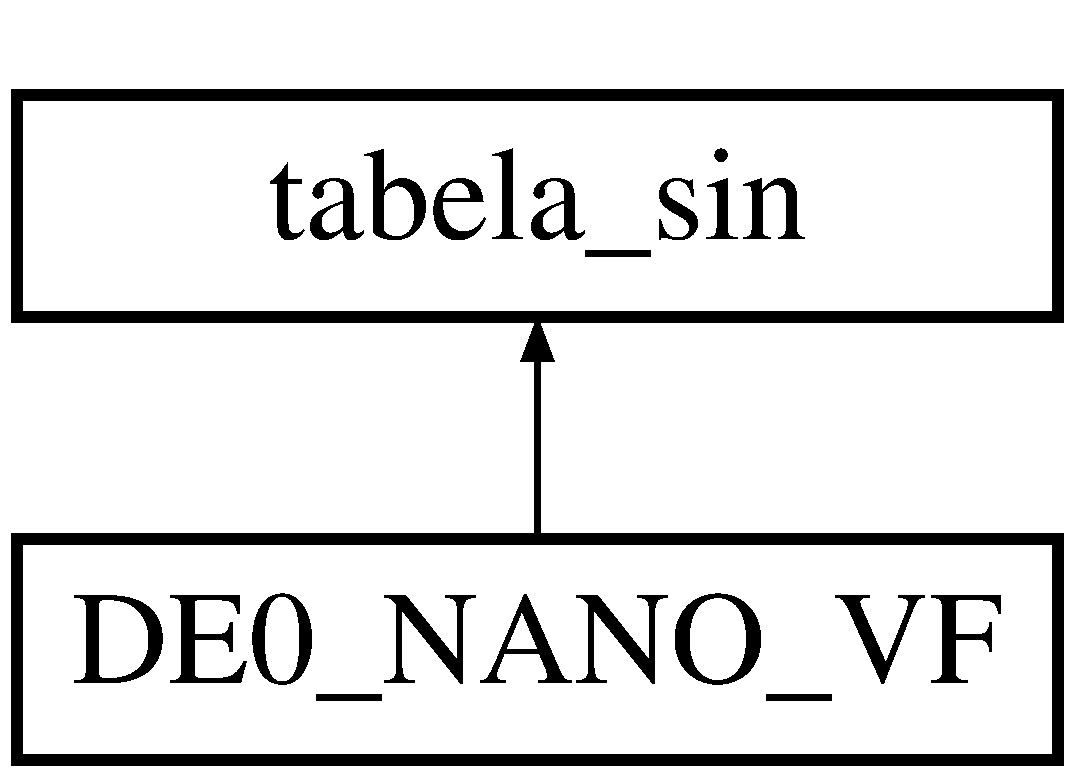
\includegraphics[height=2.000000cm]{classtabela__sin}
\end{center}
\end{figure}
\subsection*{Entities}
\begin{DoxyCompactItemize}
\item 
\hyperlink{classtabela__sin_1_1tabela__sin}{tabela\+\_\+sin} architecture
\end{DoxyCompactItemize}
\subsection*{Libraries}
 \begin{DoxyCompactItemize}
\item 
\hyperlink{classtabela__sin_a0a6af6eef40212dbaf130d57ce711256}{ieee} 
\end{DoxyCompactItemize}
\subsection*{Use Clauses}
 \begin{DoxyCompactItemize}
\item 
\hyperlink{classtabela__sin_acd03516902501cd1c7296a98e22c6fcb}{std\+\_\+logic\+\_\+1164}   
\item 
\hyperlink{classtabela__sin_a598da929e807d58939b47499e8bc9fa8}{std\+\_\+logic\+\_\+unsigned}   
\item 
\hyperlink{classtabela__sin_a2edc34402b573437d5f25fa90ba4013e}{numeric\+\_\+std}   
\item 
\hyperlink{classtabela__sin_aad86249c80e8c1e7ee1c4748aba748e3}{fixed\+\_\+pkg}   
\end{DoxyCompactItemize}
\subsection*{Generics}
 \begin{DoxyCompactItemize}
\item 
\hyperlink{classtabela__sin_ab8831e89bf175c5e1e9c6a650e7e0599}{n\+\_\+bits\+\_\+phase} {\bfseries {\bfseries \textcolor{comment}{integer}\textcolor{vhdlchar}{ }\textcolor{vhdlchar}{ }\textcolor{vhdlchar}{\+:}\textcolor{vhdlchar}{=}\textcolor{vhdlchar}{ }\textcolor{vhdlchar}{ } \textcolor{vhdldigit}{16} \textcolor{vhdlchar}{ }}}
\item 
\hyperlink{classtabela__sin_afee4aa1628956aa350183d8881689198}{n\+\_\+bits\+\_\+c} {\bfseries {\bfseries \textcolor{comment}{integer}\textcolor{vhdlchar}{ }\textcolor{vhdlchar}{ }\textcolor{vhdlchar}{\+:}\textcolor{vhdlchar}{=}\textcolor{vhdlchar}{ }\textcolor{vhdlchar}{ } \textcolor{vhdldigit}{16} \textcolor{vhdlchar}{ }}}
\item 
\hyperlink{classtabela__sin_abb7ce405d45a733b6db94314a4f791fd}{I} {\bfseries {\bfseries \textcolor{comment}{integer}\textcolor{vhdlchar}{ }\textcolor{vhdlchar}{ }\textcolor{vhdlchar}{\+:}\textcolor{vhdlchar}{=}\textcolor{vhdlchar}{ }\textcolor{vhdlchar}{ } \textcolor{vhdldigit}{1} \textcolor{vhdlchar}{ }}}
\item 
\hyperlink{classtabela__sin_aac2d6825f96b21ae984648cc93554339}{F} {\bfseries {\bfseries \textcolor{comment}{integer}\textcolor{vhdlchar}{ }\textcolor{vhdlchar}{ }\textcolor{vhdlchar}{\+:}\textcolor{vhdlchar}{=}\textcolor{vhdlchar}{ }\textcolor{vhdlchar}{ } \textcolor{vhdldigit}{14} \textcolor{vhdlchar}{ }}}
\end{DoxyCompactItemize}
\subsection*{Ports}
 \begin{DoxyCompactItemize}
\item 
\hyperlink{classtabela__sin_a4a4609c199d30b3adebbeb3a01276ec5}{clk}  {\bfseries {\bfseries \textcolor{keywordflow}{in}\textcolor{vhdlchar}{ }}} {\bfseries \textcolor{comment}{std\+\_\+logic}\textcolor{vhdlchar}{ }} 
\item 
\hyperlink{classtabela__sin_afad6cf0a3cf35dff4473dba942ec361a}{theta}  {\bfseries {\bfseries \textcolor{keywordflow}{in}\textcolor{vhdlchar}{ }}} {\bfseries \textcolor{comment}{std\+\_\+logic\+\_\+vector}\textcolor{vhdlchar}{ }\textcolor{vhdlchar}{(}\textcolor{vhdlchar}{ }\textcolor{vhdlchar}{ } \textcolor{vhdldigit}{15} \textcolor{vhdlchar}{ }\textcolor{keywordflow}{downto}\textcolor{vhdlchar}{ }\textcolor{vhdlchar}{ } \textcolor{vhdldigit}{0} \textcolor{vhdlchar}{ }\textcolor{vhdlchar}{)}\textcolor{vhdlchar}{ }} 
\item 
\hyperlink{classtabela__sin_a410cd5827b2743056d0443e5560727d1}{M\+A\+X}  {\bfseries {\bfseries \textcolor{keywordflow}{in}\textcolor{vhdlchar}{ }}} {\bfseries \textcolor{comment}{sfixed}\textcolor{vhdlchar}{ }\textcolor{vhdlchar}{(}\textcolor{vhdlchar}{ }\textcolor{vhdlchar}{ } \textcolor{vhdldigit}{15} \textcolor{vhdlchar}{ }\textcolor{keywordflow}{downto}\textcolor{vhdlchar}{ }\textcolor{vhdlchar}{ } \textcolor{vhdldigit}{0} \textcolor{vhdlchar}{ }\textcolor{vhdlchar}{)}\textcolor{vhdlchar}{ }} 
\item 
\hyperlink{classtabela__sin_aadecc5b785b421d679bab5cf2654c463}{ma}  {\bfseries {\bfseries \textcolor{keywordflow}{in}\textcolor{vhdlchar}{ }}} {\bfseries \textcolor{comment}{sfixed}\textcolor{vhdlchar}{ }\textcolor{vhdlchar}{(}\textcolor{vhdlchar}{ }\textcolor{vhdlchar}{ }\textcolor{vhdlchar}{ }\textcolor{vhdlchar}{ }{\bfseries \hyperlink{classtabela__sin_abb7ce405d45a733b6db94314a4f791fd}{I}} \textcolor{vhdlchar}{ }\textcolor{keywordflow}{downto}\textcolor{vhdlchar}{ }\textcolor{vhdlchar}{-\/}\textcolor{vhdlchar}{ }\textcolor{vhdlchar}{ }\textcolor{vhdlchar}{ }{\bfseries \hyperlink{classtabela__sin_aac2d6825f96b21ae984648cc93554339}{F}} \textcolor{vhdlchar}{ }\textcolor{vhdlchar}{)}\textcolor{vhdlchar}{ }} 
\item 
\hyperlink{classtabela__sin_a2c2cf4dbd0533e281ac8b2f114f11e67}{va}  {\bfseries {\bfseries \textcolor{keywordflow}{out}\textcolor{vhdlchar}{ }}} {\bfseries \textcolor{comment}{std\+\_\+logic\+\_\+vector}\textcolor{vhdlchar}{ }\textcolor{vhdlchar}{(}\textcolor{vhdlchar}{ }\textcolor{vhdlchar}{ } \textcolor{vhdldigit}{15} \textcolor{vhdlchar}{ }\textcolor{keywordflow}{downto}\textcolor{vhdlchar}{ }\textcolor{vhdlchar}{ } \textcolor{vhdldigit}{0} \textcolor{vhdlchar}{ }\textcolor{vhdlchar}{)}\textcolor{vhdlchar}{ }} 
\end{DoxyCompactItemize}


\subsection{Detailed Description}


Definition at line \hyperlink{tabela__sin_8vhd_source_l00007}{7} of file \hyperlink{tabela__sin_8vhd_source}{tabela\+\_\+sin.\+vhd}.



\subsection{Member Data Documentation}
\hypertarget{classtabela__sin_a4a4609c199d30b3adebbeb3a01276ec5}{}\index{tabela\+\_\+sin@{tabela\+\_\+sin}!clk@{clk}}
\index{clk@{clk}!tabela\+\_\+sin@{tabela\+\_\+sin}}
\subsubsection[{clk}]{\setlength{\rightskip}{0pt plus 5cm}{\bf clk} {\bfseries \textcolor{keywordflow}{in}\textcolor{vhdlchar}{ }} {\bfseries \textcolor{comment}{std\+\_\+logic}\textcolor{vhdlchar}{ }} \hspace{0.3cm}{\ttfamily [Port]}}\label{classtabela__sin_a4a4609c199d30b3adebbeb3a01276ec5}


Definition at line \hyperlink{tabela__sin_8vhd_source_l00015}{15} of file \hyperlink{tabela__sin_8vhd_source}{tabela\+\_\+sin.\+vhd}.

\hypertarget{classtabela__sin_aac2d6825f96b21ae984648cc93554339}{}\index{tabela\+\_\+sin@{tabela\+\_\+sin}!F@{F}}
\index{F@{F}!tabela\+\_\+sin@{tabela\+\_\+sin}}
\subsubsection[{F}]{\setlength{\rightskip}{0pt plus 5cm}{\bf F} {\bfseries \textcolor{vhdlchar}{ }} {\bfseries \textcolor{comment}{integer}\textcolor{vhdlchar}{ }\textcolor{vhdlchar}{ }\textcolor{vhdlchar}{\+:}\textcolor{vhdlchar}{=}\textcolor{vhdlchar}{ }\textcolor{vhdlchar}{ } \textcolor{vhdldigit}{14} \textcolor{vhdlchar}{ }} \hspace{0.3cm}{\ttfamily [Generic]}}\label{classtabela__sin_aac2d6825f96b21ae984648cc93554339}


Definition at line \hyperlink{tabela__sin_8vhd_source_l00013}{13} of file \hyperlink{tabela__sin_8vhd_source}{tabela\+\_\+sin.\+vhd}.

\hypertarget{classtabela__sin_aad86249c80e8c1e7ee1c4748aba748e3}{}\index{tabela\+\_\+sin@{tabela\+\_\+sin}!fixed\+\_\+pkg@{fixed\+\_\+pkg}}
\index{fixed\+\_\+pkg@{fixed\+\_\+pkg}!tabela\+\_\+sin@{tabela\+\_\+sin}}
\subsubsection[{fixed\+\_\+pkg}]{\setlength{\rightskip}{0pt plus 5cm}{\bf fixed\+\_\+pkg}\hspace{0.3cm}{\ttfamily [Package]}}\label{classtabela__sin_aad86249c80e8c1e7ee1c4748aba748e3}


Definition at line \hyperlink{tabela__sin_8vhd_source_l00005}{5} of file \hyperlink{tabela__sin_8vhd_source}{tabela\+\_\+sin.\+vhd}.

\hypertarget{classtabela__sin_abb7ce405d45a733b6db94314a4f791fd}{}\index{tabela\+\_\+sin@{tabela\+\_\+sin}!I@{I}}
\index{I@{I}!tabela\+\_\+sin@{tabela\+\_\+sin}}
\subsubsection[{I}]{\setlength{\rightskip}{0pt plus 5cm}{\bf I} {\bfseries \textcolor{vhdlchar}{ }} {\bfseries \textcolor{comment}{integer}\textcolor{vhdlchar}{ }\textcolor{vhdlchar}{ }\textcolor{vhdlchar}{\+:}\textcolor{vhdlchar}{=}\textcolor{vhdlchar}{ }\textcolor{vhdlchar}{ } \textcolor{vhdldigit}{1} \textcolor{vhdlchar}{ }} \hspace{0.3cm}{\ttfamily [Generic]}}\label{classtabela__sin_abb7ce405d45a733b6db94314a4f791fd}


Definition at line \hyperlink{tabela__sin_8vhd_source_l00011}{11} of file \hyperlink{tabela__sin_8vhd_source}{tabela\+\_\+sin.\+vhd}.

\hypertarget{classtabela__sin_a0a6af6eef40212dbaf130d57ce711256}{}\index{tabela\+\_\+sin@{tabela\+\_\+sin}!ieee@{ieee}}
\index{ieee@{ieee}!tabela\+\_\+sin@{tabela\+\_\+sin}}
\subsubsection[{ieee}]{\setlength{\rightskip}{0pt plus 5cm}{\bf ieee}\hspace{0.3cm}{\ttfamily [Library]}}\label{classtabela__sin_a0a6af6eef40212dbaf130d57ce711256}


Definition at line \hyperlink{tabela__sin_8vhd_source_l00001}{1} of file \hyperlink{tabela__sin_8vhd_source}{tabela\+\_\+sin.\+vhd}.

\hypertarget{classtabela__sin_aadecc5b785b421d679bab5cf2654c463}{}\index{tabela\+\_\+sin@{tabela\+\_\+sin}!ma@{ma}}
\index{ma@{ma}!tabela\+\_\+sin@{tabela\+\_\+sin}}
\subsubsection[{ma}]{\setlength{\rightskip}{0pt plus 5cm}{\bf ma} {\bfseries \textcolor{keywordflow}{in}\textcolor{vhdlchar}{ }} {\bfseries \textcolor{comment}{sfixed}\textcolor{vhdlchar}{ }\textcolor{vhdlchar}{(}\textcolor{vhdlchar}{ }\textcolor{vhdlchar}{ }\textcolor{vhdlchar}{ }\textcolor{vhdlchar}{ }{\bfseries {\bf I}} \textcolor{vhdlchar}{ }\textcolor{keywordflow}{downto}\textcolor{vhdlchar}{ }\textcolor{vhdlchar}{-\/}\textcolor{vhdlchar}{ }\textcolor{vhdlchar}{ }\textcolor{vhdlchar}{ }{\bfseries {\bf F}} \textcolor{vhdlchar}{ }\textcolor{vhdlchar}{)}\textcolor{vhdlchar}{ }} \hspace{0.3cm}{\ttfamily [Port]}}\label{classtabela__sin_aadecc5b785b421d679bab5cf2654c463}


Definition at line \hyperlink{tabela__sin_8vhd_source_l00018}{18} of file \hyperlink{tabela__sin_8vhd_source}{tabela\+\_\+sin.\+vhd}.

\hypertarget{classtabela__sin_a410cd5827b2743056d0443e5560727d1}{}\index{tabela\+\_\+sin@{tabela\+\_\+sin}!M\+A\+X@{M\+A\+X}}
\index{M\+A\+X@{M\+A\+X}!tabela\+\_\+sin@{tabela\+\_\+sin}}
\subsubsection[{M\+A\+X}]{\setlength{\rightskip}{0pt plus 5cm}{\bf M\+A\+X} {\bfseries \textcolor{keywordflow}{in}\textcolor{vhdlchar}{ }} {\bfseries \textcolor{comment}{sfixed}\textcolor{vhdlchar}{ }\textcolor{vhdlchar}{(}\textcolor{vhdlchar}{ }\textcolor{vhdlchar}{ } \textcolor{vhdldigit}{15} \textcolor{vhdlchar}{ }\textcolor{keywordflow}{downto}\textcolor{vhdlchar}{ }\textcolor{vhdlchar}{ } \textcolor{vhdldigit}{0} \textcolor{vhdlchar}{ }\textcolor{vhdlchar}{)}\textcolor{vhdlchar}{ }} \hspace{0.3cm}{\ttfamily [Port]}}\label{classtabela__sin_a410cd5827b2743056d0443e5560727d1}


Definition at line \hyperlink{tabela__sin_8vhd_source_l00017}{17} of file \hyperlink{tabela__sin_8vhd_source}{tabela\+\_\+sin.\+vhd}.

\hypertarget{classtabela__sin_afee4aa1628956aa350183d8881689198}{}\index{tabela\+\_\+sin@{tabela\+\_\+sin}!n\+\_\+bits\+\_\+c@{n\+\_\+bits\+\_\+c}}
\index{n\+\_\+bits\+\_\+c@{n\+\_\+bits\+\_\+c}!tabela\+\_\+sin@{tabela\+\_\+sin}}
\subsubsection[{n\+\_\+bits\+\_\+c}]{\setlength{\rightskip}{0pt plus 5cm}{\bf n\+\_\+bits\+\_\+c} {\bfseries \textcolor{vhdlchar}{ }} {\bfseries \textcolor{comment}{integer}\textcolor{vhdlchar}{ }\textcolor{vhdlchar}{ }\textcolor{vhdlchar}{\+:}\textcolor{vhdlchar}{=}\textcolor{vhdlchar}{ }\textcolor{vhdlchar}{ } \textcolor{vhdldigit}{16} \textcolor{vhdlchar}{ }} \hspace{0.3cm}{\ttfamily [Generic]}}\label{classtabela__sin_afee4aa1628956aa350183d8881689198}


Definition at line \hyperlink{tabela__sin_8vhd_source_l00010}{10} of file \hyperlink{tabela__sin_8vhd_source}{tabela\+\_\+sin.\+vhd}.

\hypertarget{classtabela__sin_ab8831e89bf175c5e1e9c6a650e7e0599}{}\index{tabela\+\_\+sin@{tabela\+\_\+sin}!n\+\_\+bits\+\_\+phase@{n\+\_\+bits\+\_\+phase}}
\index{n\+\_\+bits\+\_\+phase@{n\+\_\+bits\+\_\+phase}!tabela\+\_\+sin@{tabela\+\_\+sin}}
\subsubsection[{n\+\_\+bits\+\_\+phase}]{\setlength{\rightskip}{0pt plus 5cm}{\bf n\+\_\+bits\+\_\+phase} {\bfseries \textcolor{vhdlchar}{ }} {\bfseries \textcolor{comment}{integer}\textcolor{vhdlchar}{ }\textcolor{vhdlchar}{ }\textcolor{vhdlchar}{\+:}\textcolor{vhdlchar}{=}\textcolor{vhdlchar}{ }\textcolor{vhdlchar}{ } \textcolor{vhdldigit}{16} \textcolor{vhdlchar}{ }} \hspace{0.3cm}{\ttfamily [Generic]}}\label{classtabela__sin_ab8831e89bf175c5e1e9c6a650e7e0599}


Definition at line \hyperlink{tabela__sin_8vhd_source_l00009}{9} of file \hyperlink{tabela__sin_8vhd_source}{tabela\+\_\+sin.\+vhd}.

\hypertarget{classtabela__sin_a2edc34402b573437d5f25fa90ba4013e}{}\index{tabela\+\_\+sin@{tabela\+\_\+sin}!numeric\+\_\+std@{numeric\+\_\+std}}
\index{numeric\+\_\+std@{numeric\+\_\+std}!tabela\+\_\+sin@{tabela\+\_\+sin}}
\subsubsection[{numeric\+\_\+std}]{\setlength{\rightskip}{0pt plus 5cm}{\bf numeric\+\_\+std}\hspace{0.3cm}{\ttfamily [Package]}}\label{classtabela__sin_a2edc34402b573437d5f25fa90ba4013e}


Definition at line \hyperlink{tabela__sin_8vhd_source_l00004}{4} of file \hyperlink{tabela__sin_8vhd_source}{tabela\+\_\+sin.\+vhd}.

\hypertarget{classtabela__sin_acd03516902501cd1c7296a98e22c6fcb}{}\index{tabela\+\_\+sin@{tabela\+\_\+sin}!std\+\_\+logic\+\_\+1164@{std\+\_\+logic\+\_\+1164}}
\index{std\+\_\+logic\+\_\+1164@{std\+\_\+logic\+\_\+1164}!tabela\+\_\+sin@{tabela\+\_\+sin}}
\subsubsection[{std\+\_\+logic\+\_\+1164}]{\setlength{\rightskip}{0pt plus 5cm}{\bf std\+\_\+logic\+\_\+1164}\hspace{0.3cm}{\ttfamily [Package]}}\label{classtabela__sin_acd03516902501cd1c7296a98e22c6fcb}


Definition at line \hyperlink{tabela__sin_8vhd_source_l00002}{2} of file \hyperlink{tabela__sin_8vhd_source}{tabela\+\_\+sin.\+vhd}.

\hypertarget{classtabela__sin_a598da929e807d58939b47499e8bc9fa8}{}\index{tabela\+\_\+sin@{tabela\+\_\+sin}!std\+\_\+logic\+\_\+unsigned@{std\+\_\+logic\+\_\+unsigned}}
\index{std\+\_\+logic\+\_\+unsigned@{std\+\_\+logic\+\_\+unsigned}!tabela\+\_\+sin@{tabela\+\_\+sin}}
\subsubsection[{std\+\_\+logic\+\_\+unsigned}]{\setlength{\rightskip}{0pt plus 5cm}{\bf std\+\_\+logic\+\_\+unsigned}\hspace{0.3cm}{\ttfamily [Package]}}\label{classtabela__sin_a598da929e807d58939b47499e8bc9fa8}


Definition at line \hyperlink{tabela__sin_8vhd_source_l00003}{3} of file \hyperlink{tabela__sin_8vhd_source}{tabela\+\_\+sin.\+vhd}.

\hypertarget{classtabela__sin_afad6cf0a3cf35dff4473dba942ec361a}{}\index{tabela\+\_\+sin@{tabela\+\_\+sin}!theta@{theta}}
\index{theta@{theta}!tabela\+\_\+sin@{tabela\+\_\+sin}}
\subsubsection[{theta}]{\setlength{\rightskip}{0pt plus 5cm}{\bf theta} {\bfseries \textcolor{keywordflow}{in}\textcolor{vhdlchar}{ }} {\bfseries \textcolor{comment}{std\+\_\+logic\+\_\+vector}\textcolor{vhdlchar}{ }\textcolor{vhdlchar}{(}\textcolor{vhdlchar}{ }\textcolor{vhdlchar}{ } \textcolor{vhdldigit}{15} \textcolor{vhdlchar}{ }\textcolor{keywordflow}{downto}\textcolor{vhdlchar}{ }\textcolor{vhdlchar}{ } \textcolor{vhdldigit}{0} \textcolor{vhdlchar}{ }\textcolor{vhdlchar}{)}\textcolor{vhdlchar}{ }} \hspace{0.3cm}{\ttfamily [Port]}}\label{classtabela__sin_afad6cf0a3cf35dff4473dba942ec361a}


Definition at line \hyperlink{tabela__sin_8vhd_source_l00016}{16} of file \hyperlink{tabela__sin_8vhd_source}{tabela\+\_\+sin.\+vhd}.

\hypertarget{classtabela__sin_a2c2cf4dbd0533e281ac8b2f114f11e67}{}\index{tabela\+\_\+sin@{tabela\+\_\+sin}!va@{va}}
\index{va@{va}!tabela\+\_\+sin@{tabela\+\_\+sin}}
\subsubsection[{va}]{\setlength{\rightskip}{0pt plus 5cm}{\bf va} {\bfseries \textcolor{keywordflow}{out}\textcolor{vhdlchar}{ }} {\bfseries \textcolor{comment}{std\+\_\+logic\+\_\+vector}\textcolor{vhdlchar}{ }\textcolor{vhdlchar}{(}\textcolor{vhdlchar}{ }\textcolor{vhdlchar}{ } \textcolor{vhdldigit}{15} \textcolor{vhdlchar}{ }\textcolor{keywordflow}{downto}\textcolor{vhdlchar}{ }\textcolor{vhdlchar}{ } \textcolor{vhdldigit}{0} \textcolor{vhdlchar}{ }\textcolor{vhdlchar}{)}\textcolor{vhdlchar}{ }} \hspace{0.3cm}{\ttfamily [Port]}}\label{classtabela__sin_a2c2cf4dbd0533e281ac8b2f114f11e67}


Definition at line \hyperlink{tabela__sin_8vhd_source_l00020}{20} of file \hyperlink{tabela__sin_8vhd_source}{tabela\+\_\+sin.\+vhd}.



The documentation for this class was generated from the following file\+:\begin{DoxyCompactItemize}
\item 
\hyperlink{tabela__sin_8vhd}{tabela\+\_\+sin.\+vhd}\end{DoxyCompactItemize}

\hypertarget{classtheta__abc_1_1theta__abc}{}\section{theta\+\_\+abc Architecture Reference}
\label{classtheta__abc_1_1theta__abc}\index{theta\+\_\+abc@{theta\+\_\+abc}}
\subsection*{Processes}
 \begin{DoxyCompactItemize}
\item 
\hyperlink{classtheta__abc_1_1theta__abc_a8ee64d1327298358d5f75867875249ca}{P\+R\+O\+C\+E\+S\+S\+\_\+15}{\bfseries  ( {\bfseries {\bfseries \hyperlink{classtheta__abc_a4a4609c199d30b3adebbeb3a01276ec5}{clk}} \textcolor{vhdlchar}{ }} )}
\end{DoxyCompactItemize}
\subsection*{Signals}
 \begin{DoxyCompactItemize}
\item 
\hyperlink{classtheta__abc_1_1theta__abc_ad76995fdeaec7ada621075ea6562c673}{th\+\_\+a} {\bfseries \textcolor{comment}{std\+\_\+logic\+\_\+vector}\textcolor{vhdlchar}{ }\textcolor{vhdlchar}{(}\textcolor{vhdlchar}{ }\textcolor{vhdlchar}{ }\textcolor{vhdlchar}{ }\textcolor{vhdlchar}{ }{\bfseries \hyperlink{classtheta__abc_ad0f475656f5dd17584d6796fde77d790}{Nout}} \textcolor{vhdlchar}{-\/}\textcolor{vhdlchar}{ } \textcolor{vhdldigit}{1} \textcolor{vhdlchar}{ }\textcolor{keywordflow}{downto}\textcolor{vhdlchar}{ }\textcolor{vhdlchar}{ } \textcolor{vhdldigit}{0} \textcolor{vhdlchar}{ }\textcolor{vhdlchar}{)}\textcolor{vhdlchar}{ }} 
\item 
\hyperlink{classtheta__abc_1_1theta__abc_ae23fb98ce5af67556ecf68e8ffb4a27c}{th\+\_\+b} {\bfseries \textcolor{comment}{std\+\_\+logic\+\_\+vector}\textcolor{vhdlchar}{ }\textcolor{vhdlchar}{(}\textcolor{vhdlchar}{ }\textcolor{vhdlchar}{ }\textcolor{vhdlchar}{ }\textcolor{vhdlchar}{ }{\bfseries \hyperlink{classtheta__abc_ad0f475656f5dd17584d6796fde77d790}{Nout}} \textcolor{vhdlchar}{-\/}\textcolor{vhdlchar}{ } \textcolor{vhdldigit}{1} \textcolor{vhdlchar}{ }\textcolor{keywordflow}{downto}\textcolor{vhdlchar}{ }\textcolor{vhdlchar}{ } \textcolor{vhdldigit}{0} \textcolor{vhdlchar}{ }\textcolor{vhdlchar}{)}\textcolor{vhdlchar}{ }} 
\item 
\hyperlink{classtheta__abc_1_1theta__abc_a99d308b4a97dff4ea9faacf3778ac0f1}{th\+\_\+c} {\bfseries \textcolor{comment}{std\+\_\+logic\+\_\+vector}\textcolor{vhdlchar}{ }\textcolor{vhdlchar}{(}\textcolor{vhdlchar}{ }\textcolor{vhdlchar}{ }\textcolor{vhdlchar}{ }\textcolor{vhdlchar}{ }{\bfseries \hyperlink{classtheta__abc_ad0f475656f5dd17584d6796fde77d790}{Nout}} \textcolor{vhdlchar}{-\/}\textcolor{vhdlchar}{ } \textcolor{vhdldigit}{1} \textcolor{vhdlchar}{ }\textcolor{keywordflow}{downto}\textcolor{vhdlchar}{ }\textcolor{vhdlchar}{ } \textcolor{vhdldigit}{0} \textcolor{vhdlchar}{ }\textcolor{vhdlchar}{)}\textcolor{vhdlchar}{ }} 
\item 
\hyperlink{classtheta__abc_1_1theta__abc_aa089585a137a873b884793531ca5edc0}{th\+\_\+ai} {\bfseries \textcolor{comment}{std\+\_\+logic\+\_\+vector}\textcolor{vhdlchar}{ }\textcolor{vhdlchar}{(}\textcolor{vhdlchar}{ }\textcolor{vhdlchar}{ }\textcolor{vhdlchar}{ }\textcolor{vhdlchar}{ }{\bfseries \hyperlink{classtheta__abc_ad0f475656f5dd17584d6796fde77d790}{Nout}} \textcolor{vhdlchar}{ }\textcolor{keywordflow}{downto}\textcolor{vhdlchar}{ }\textcolor{vhdlchar}{ } \textcolor{vhdldigit}{0} \textcolor{vhdlchar}{ }\textcolor{vhdlchar}{)}\textcolor{vhdlchar}{ }} 
\item 
\hyperlink{classtheta__abc_1_1theta__abc_a7ff18034ace7fde19560f0a2a2cdd952}{th\+\_\+bi} {\bfseries \textcolor{comment}{std\+\_\+logic\+\_\+vector}\textcolor{vhdlchar}{ }\textcolor{vhdlchar}{(}\textcolor{vhdlchar}{ }\textcolor{vhdlchar}{ }\textcolor{vhdlchar}{ }\textcolor{vhdlchar}{ }{\bfseries \hyperlink{classtheta__abc_ad0f475656f5dd17584d6796fde77d790}{Nout}} \textcolor{vhdlchar}{ }\textcolor{keywordflow}{downto}\textcolor{vhdlchar}{ }\textcolor{vhdlchar}{ } \textcolor{vhdldigit}{0} \textcolor{vhdlchar}{ }\textcolor{vhdlchar}{)}\textcolor{vhdlchar}{ }} 
\item 
\hyperlink{classtheta__abc_1_1theta__abc_a45f5cb01816ecd5555fc839e392dfe6a}{th\+\_\+ci} {\bfseries \textcolor{comment}{std\+\_\+logic\+\_\+vector}\textcolor{vhdlchar}{ }\textcolor{vhdlchar}{(}\textcolor{vhdlchar}{ }\textcolor{vhdlchar}{ }\textcolor{vhdlchar}{ }\textcolor{vhdlchar}{ }{\bfseries \hyperlink{classtheta__abc_ad0f475656f5dd17584d6796fde77d790}{Nout}} \textcolor{vhdlchar}{ }\textcolor{keywordflow}{downto}\textcolor{vhdlchar}{ }\textcolor{vhdlchar}{ } \textcolor{vhdldigit}{0} \textcolor{vhdlchar}{ }\textcolor{vhdlchar}{)}\textcolor{vhdlchar}{ }} 
\end{DoxyCompactItemize}


\subsection{Detailed Description}


Definition at line 25 of file theta\+\_\+abc.\+vhd.



\subsection{Member Function Documentation}
\hypertarget{classtheta__abc_1_1theta__abc_a8ee64d1327298358d5f75867875249ca}{}\index{theta\+\_\+abc\+::theta\+\_\+abc@{theta\+\_\+abc\+::theta\+\_\+abc}!P\+R\+O\+C\+E\+S\+S\+\_\+15@{P\+R\+O\+C\+E\+S\+S\+\_\+15}}
\index{P\+R\+O\+C\+E\+S\+S\+\_\+15@{P\+R\+O\+C\+E\+S\+S\+\_\+15}!theta\+\_\+abc\+::theta\+\_\+abc@{theta\+\_\+abc\+::theta\+\_\+abc}}
\subsubsection[{P\+R\+O\+C\+E\+S\+S\+\_\+15}]{\setlength{\rightskip}{0pt plus 5cm} {\bfseries \textcolor{vhdlchar}{ }} P\+R\+O\+C\+E\+S\+S\+\_\+15(
\begin{DoxyParamCaption}
\item[{}]{{\bfseries {\bfseries {\bf clk}} \textcolor{vhdlchar}{ }} {\em }}
\end{DoxyParamCaption}
)\hspace{0.3cm}{\ttfamily [Process]}}\label{classtheta__abc_1_1theta__abc_a8ee64d1327298358d5f75867875249ca}


Definition at line 33 of file theta\+\_\+abc.\+vhd.



\subsection{Member Data Documentation}
\hypertarget{classtheta__abc_1_1theta__abc_ad76995fdeaec7ada621075ea6562c673}{}\index{theta\+\_\+abc\+::theta\+\_\+abc@{theta\+\_\+abc\+::theta\+\_\+abc}!th\+\_\+a@{th\+\_\+a}}
\index{th\+\_\+a@{th\+\_\+a}!theta\+\_\+abc\+::theta\+\_\+abc@{theta\+\_\+abc\+::theta\+\_\+abc}}
\subsubsection[{th\+\_\+a}]{\setlength{\rightskip}{0pt plus 5cm}{\bf th\+\_\+a} {\bfseries \textcolor{comment}{std\+\_\+logic\+\_\+vector}\textcolor{vhdlchar}{ }\textcolor{vhdlchar}{(}\textcolor{vhdlchar}{ }\textcolor{vhdlchar}{ }\textcolor{vhdlchar}{ }\textcolor{vhdlchar}{ }{\bfseries {\bf Nout}} \textcolor{vhdlchar}{-\/}\textcolor{vhdlchar}{ } \textcolor{vhdldigit}{1} \textcolor{vhdlchar}{ }\textcolor{keywordflow}{downto}\textcolor{vhdlchar}{ }\textcolor{vhdlchar}{ } \textcolor{vhdldigit}{0} \textcolor{vhdlchar}{ }\textcolor{vhdlchar}{)}\textcolor{vhdlchar}{ }} \hspace{0.3cm}{\ttfamily [Signal]}}\label{classtheta__abc_1_1theta__abc_ad76995fdeaec7ada621075ea6562c673}


Definition at line 27 of file theta\+\_\+abc.\+vhd.

\hypertarget{classtheta__abc_1_1theta__abc_aa089585a137a873b884793531ca5edc0}{}\index{theta\+\_\+abc\+::theta\+\_\+abc@{theta\+\_\+abc\+::theta\+\_\+abc}!th\+\_\+ai@{th\+\_\+ai}}
\index{th\+\_\+ai@{th\+\_\+ai}!theta\+\_\+abc\+::theta\+\_\+abc@{theta\+\_\+abc\+::theta\+\_\+abc}}
\subsubsection[{th\+\_\+ai}]{\setlength{\rightskip}{0pt plus 5cm}{\bf th\+\_\+ai} {\bfseries \textcolor{comment}{std\+\_\+logic\+\_\+vector}\textcolor{vhdlchar}{ }\textcolor{vhdlchar}{(}\textcolor{vhdlchar}{ }\textcolor{vhdlchar}{ }\textcolor{vhdlchar}{ }\textcolor{vhdlchar}{ }{\bfseries {\bf Nout}} \textcolor{vhdlchar}{ }\textcolor{keywordflow}{downto}\textcolor{vhdlchar}{ }\textcolor{vhdlchar}{ } \textcolor{vhdldigit}{0} \textcolor{vhdlchar}{ }\textcolor{vhdlchar}{)}\textcolor{vhdlchar}{ }} \hspace{0.3cm}{\ttfamily [Signal]}}\label{classtheta__abc_1_1theta__abc_aa089585a137a873b884793531ca5edc0}


Definition at line 28 of file theta\+\_\+abc.\+vhd.

\hypertarget{classtheta__abc_1_1theta__abc_ae23fb98ce5af67556ecf68e8ffb4a27c}{}\index{theta\+\_\+abc\+::theta\+\_\+abc@{theta\+\_\+abc\+::theta\+\_\+abc}!th\+\_\+b@{th\+\_\+b}}
\index{th\+\_\+b@{th\+\_\+b}!theta\+\_\+abc\+::theta\+\_\+abc@{theta\+\_\+abc\+::theta\+\_\+abc}}
\subsubsection[{th\+\_\+b}]{\setlength{\rightskip}{0pt plus 5cm}{\bf th\+\_\+b} {\bfseries \textcolor{comment}{std\+\_\+logic\+\_\+vector}\textcolor{vhdlchar}{ }\textcolor{vhdlchar}{(}\textcolor{vhdlchar}{ }\textcolor{vhdlchar}{ }\textcolor{vhdlchar}{ }\textcolor{vhdlchar}{ }{\bfseries {\bf Nout}} \textcolor{vhdlchar}{-\/}\textcolor{vhdlchar}{ } \textcolor{vhdldigit}{1} \textcolor{vhdlchar}{ }\textcolor{keywordflow}{downto}\textcolor{vhdlchar}{ }\textcolor{vhdlchar}{ } \textcolor{vhdldigit}{0} \textcolor{vhdlchar}{ }\textcolor{vhdlchar}{)}\textcolor{vhdlchar}{ }} \hspace{0.3cm}{\ttfamily [Signal]}}\label{classtheta__abc_1_1theta__abc_ae23fb98ce5af67556ecf68e8ffb4a27c}


Definition at line 27 of file theta\+\_\+abc.\+vhd.

\hypertarget{classtheta__abc_1_1theta__abc_a7ff18034ace7fde19560f0a2a2cdd952}{}\index{theta\+\_\+abc\+::theta\+\_\+abc@{theta\+\_\+abc\+::theta\+\_\+abc}!th\+\_\+bi@{th\+\_\+bi}}
\index{th\+\_\+bi@{th\+\_\+bi}!theta\+\_\+abc\+::theta\+\_\+abc@{theta\+\_\+abc\+::theta\+\_\+abc}}
\subsubsection[{th\+\_\+bi}]{\setlength{\rightskip}{0pt plus 5cm}{\bf th\+\_\+bi} {\bfseries \textcolor{comment}{std\+\_\+logic\+\_\+vector}\textcolor{vhdlchar}{ }\textcolor{vhdlchar}{(}\textcolor{vhdlchar}{ }\textcolor{vhdlchar}{ }\textcolor{vhdlchar}{ }\textcolor{vhdlchar}{ }{\bfseries {\bf Nout}} \textcolor{vhdlchar}{ }\textcolor{keywordflow}{downto}\textcolor{vhdlchar}{ }\textcolor{vhdlchar}{ } \textcolor{vhdldigit}{0} \textcolor{vhdlchar}{ }\textcolor{vhdlchar}{)}\textcolor{vhdlchar}{ }} \hspace{0.3cm}{\ttfamily [Signal]}}\label{classtheta__abc_1_1theta__abc_a7ff18034ace7fde19560f0a2a2cdd952}


Definition at line 28 of file theta\+\_\+abc.\+vhd.

\hypertarget{classtheta__abc_1_1theta__abc_a99d308b4a97dff4ea9faacf3778ac0f1}{}\index{theta\+\_\+abc\+::theta\+\_\+abc@{theta\+\_\+abc\+::theta\+\_\+abc}!th\+\_\+c@{th\+\_\+c}}
\index{th\+\_\+c@{th\+\_\+c}!theta\+\_\+abc\+::theta\+\_\+abc@{theta\+\_\+abc\+::theta\+\_\+abc}}
\subsubsection[{th\+\_\+c}]{\setlength{\rightskip}{0pt plus 5cm}{\bf th\+\_\+c} {\bfseries \textcolor{comment}{std\+\_\+logic\+\_\+vector}\textcolor{vhdlchar}{ }\textcolor{vhdlchar}{(}\textcolor{vhdlchar}{ }\textcolor{vhdlchar}{ }\textcolor{vhdlchar}{ }\textcolor{vhdlchar}{ }{\bfseries {\bf Nout}} \textcolor{vhdlchar}{-\/}\textcolor{vhdlchar}{ } \textcolor{vhdldigit}{1} \textcolor{vhdlchar}{ }\textcolor{keywordflow}{downto}\textcolor{vhdlchar}{ }\textcolor{vhdlchar}{ } \textcolor{vhdldigit}{0} \textcolor{vhdlchar}{ }\textcolor{vhdlchar}{)}\textcolor{vhdlchar}{ }} \hspace{0.3cm}{\ttfamily [Signal]}}\label{classtheta__abc_1_1theta__abc_a99d308b4a97dff4ea9faacf3778ac0f1}


Definition at line 27 of file theta\+\_\+abc.\+vhd.

\hypertarget{classtheta__abc_1_1theta__abc_a45f5cb01816ecd5555fc839e392dfe6a}{}\index{theta\+\_\+abc\+::theta\+\_\+abc@{theta\+\_\+abc\+::theta\+\_\+abc}!th\+\_\+ci@{th\+\_\+ci}}
\index{th\+\_\+ci@{th\+\_\+ci}!theta\+\_\+abc\+::theta\+\_\+abc@{theta\+\_\+abc\+::theta\+\_\+abc}}
\subsubsection[{th\+\_\+ci}]{\setlength{\rightskip}{0pt plus 5cm}{\bf th\+\_\+ci} {\bfseries \textcolor{comment}{std\+\_\+logic\+\_\+vector}\textcolor{vhdlchar}{ }\textcolor{vhdlchar}{(}\textcolor{vhdlchar}{ }\textcolor{vhdlchar}{ }\textcolor{vhdlchar}{ }\textcolor{vhdlchar}{ }{\bfseries {\bf Nout}} \textcolor{vhdlchar}{ }\textcolor{keywordflow}{downto}\textcolor{vhdlchar}{ }\textcolor{vhdlchar}{ } \textcolor{vhdldigit}{0} \textcolor{vhdlchar}{ }\textcolor{vhdlchar}{)}\textcolor{vhdlchar}{ }} \hspace{0.3cm}{\ttfamily [Signal]}}\label{classtheta__abc_1_1theta__abc_a45f5cb01816ecd5555fc839e392dfe6a}


Definition at line 28 of file theta\+\_\+abc.\+vhd.



The documentation for this class was generated from the following file\+:\begin{DoxyCompactItemize}
\item 
\hyperlink{theta__abc_8vhd}{theta\+\_\+abc.\+vhd}\end{DoxyCompactItemize}

\hypertarget{classtheta__abc}{}\section{theta\+\_\+abc Entity Reference}
\label{classtheta__abc}\index{theta\+\_\+abc@{theta\+\_\+abc}}
Inheritance diagram for theta\+\_\+abc\+:\begin{figure}[H]
\begin{center}
\leavevmode
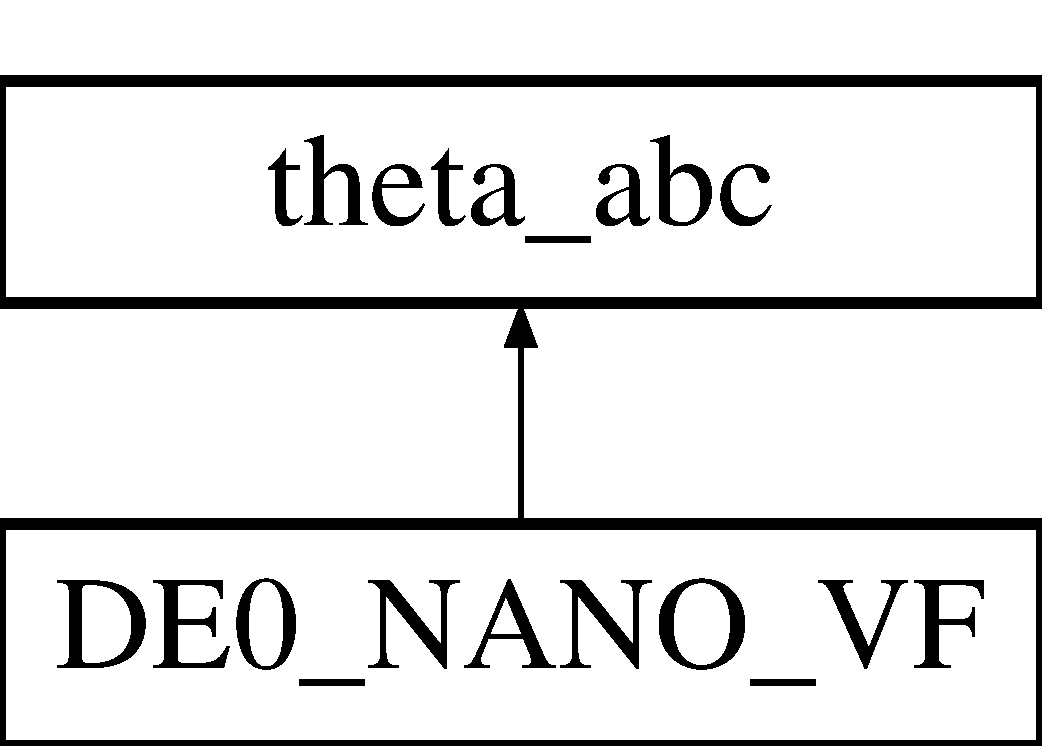
\includegraphics[height=2.000000cm]{classtheta__abc}
\end{center}
\end{figure}
\subsection*{Entities}
\begin{DoxyCompactItemize}
\item 
\hyperlink{classtheta__abc_1_1theta__abc}{theta\+\_\+abc} architecture
\end{DoxyCompactItemize}
\subsection*{Libraries}
 \begin{DoxyCompactItemize}
\item 
\hyperlink{classtheta__abc_ae4f03c286607f3181e16b9aa12d0c6d4}{I\+E\+E\+E} 
\end{DoxyCompactItemize}
\subsection*{Use Clauses}
 \begin{DoxyCompactItemize}
\item 
\hyperlink{classtheta__abc_a241c3e72dd8024cc8ae831b1b2aed7db}{S\+T\+D\+\_\+\+L\+O\+G\+I\+C\+\_\+\+U\+N\+S\+I\+G\+N\+E\+D}   
\item 
\hyperlink{classtheta__abc_aa4b2b25246a821511120e3149b003563}{S\+T\+D\+\_\+\+L\+O\+G\+I\+C\+\_\+1164}   
\item 
\hyperlink{classtheta__abc_aad86249c80e8c1e7ee1c4748aba748e3}{fixed\+\_\+pkg}   
\item 
\hyperlink{classtheta__abc_a2edc34402b573437d5f25fa90ba4013e}{numeric\+\_\+std}   
\end{DoxyCompactItemize}
\subsection*{Generics}
 \begin{DoxyCompactItemize}
\item 
\hyperlink{classtheta__abc_a81567f92ddcbd14c6385d610a895f134}{Nin} {\bfseries {\bfseries \textcolor{comment}{integer}\textcolor{vhdlchar}{ }\textcolor{vhdlchar}{ }\textcolor{vhdlchar}{\+:}\textcolor{vhdlchar}{=}\textcolor{vhdlchar}{ }\textcolor{vhdlchar}{ } \textcolor{vhdldigit}{30} \textcolor{vhdlchar}{ }}}
\item 
\hyperlink{classtheta__abc_ad0f475656f5dd17584d6796fde77d790}{Nout} {\bfseries {\bfseries \textcolor{comment}{integer}\textcolor{vhdlchar}{ }\textcolor{vhdlchar}{ }\textcolor{vhdlchar}{\+:}\textcolor{vhdlchar}{=}\textcolor{vhdlchar}{ }\textcolor{vhdlchar}{ } \textcolor{vhdldigit}{16} \textcolor{vhdlchar}{ }}}
\end{DoxyCompactItemize}
\subsection*{Ports}
 \begin{DoxyCompactItemize}
\item 
\hyperlink{classtheta__abc_a4a4609c199d30b3adebbeb3a01276ec5}{clk}  {\bfseries {\bfseries \textcolor{keywordflow}{in}\textcolor{vhdlchar}{ }}} {\bfseries \textcolor{comment}{std\+\_\+logic}\textcolor{vhdlchar}{ }} 
\item 
\hyperlink{classtheta__abc_adcf9c6f5161d039addbda5819bee64a3}{en}  {\bfseries {\bfseries \textcolor{keywordflow}{in}\textcolor{vhdlchar}{ }}} {\bfseries \textcolor{comment}{std\+\_\+logic}\textcolor{vhdlchar}{ }} 
\item 
\hyperlink{classtheta__abc_aad8dc6359d9e23dabcbf342fadf2fa06}{reset}  {\bfseries {\bfseries \textcolor{keywordflow}{in}\textcolor{vhdlchar}{ }}} {\bfseries \textcolor{comment}{std\+\_\+logic}\textcolor{vhdlchar}{ }} 
\item 
\hyperlink{classtheta__abc_ae915426336e82564b81552bb4a9106c8}{theta\+\_\+a}  {\bfseries {\bfseries \textcolor{keywordflow}{out}\textcolor{vhdlchar}{ }}} {\bfseries \textcolor{comment}{std\+\_\+logic\+\_\+vector}\textcolor{vhdlchar}{ }\textcolor{vhdlchar}{(}\textcolor{vhdlchar}{ }\textcolor{vhdlchar}{ }\textcolor{vhdlchar}{ }\textcolor{vhdlchar}{ }{\bfseries \hyperlink{classtheta__abc_ad0f475656f5dd17584d6796fde77d790}{Nout}} \textcolor{vhdlchar}{-\/}\textcolor{vhdlchar}{ } \textcolor{vhdldigit}{1} \textcolor{vhdlchar}{ }\textcolor{keywordflow}{downto}\textcolor{vhdlchar}{ }\textcolor{vhdlchar}{ } \textcolor{vhdldigit}{0} \textcolor{vhdlchar}{ }\textcolor{vhdlchar}{)}\textcolor{vhdlchar}{ }} 
\item 
\hyperlink{classtheta__abc_a0e4f34615c07a131cc3e798485768ace}{theta\+\_\+b}  {\bfseries {\bfseries \textcolor{keywordflow}{out}\textcolor{vhdlchar}{ }}} {\bfseries \textcolor{comment}{std\+\_\+logic\+\_\+vector}\textcolor{vhdlchar}{ }\textcolor{vhdlchar}{(}\textcolor{vhdlchar}{ }\textcolor{vhdlchar}{ }\textcolor{vhdlchar}{ }\textcolor{vhdlchar}{ }{\bfseries \hyperlink{classtheta__abc_ad0f475656f5dd17584d6796fde77d790}{Nout}} \textcolor{vhdlchar}{-\/}\textcolor{vhdlchar}{ } \textcolor{vhdldigit}{1} \textcolor{vhdlchar}{ }\textcolor{keywordflow}{downto}\textcolor{vhdlchar}{ }\textcolor{vhdlchar}{ } \textcolor{vhdldigit}{0} \textcolor{vhdlchar}{ }\textcolor{vhdlchar}{)}\textcolor{vhdlchar}{ }} 
\item 
\hyperlink{classtheta__abc_a2a449e4b73715ae14ae4178ad27cf5c9}{theta\+\_\+c}  {\bfseries {\bfseries \textcolor{keywordflow}{out}\textcolor{vhdlchar}{ }}} {\bfseries \textcolor{comment}{std\+\_\+logic\+\_\+vector}\textcolor{vhdlchar}{ }\textcolor{vhdlchar}{(}\textcolor{vhdlchar}{ }\textcolor{vhdlchar}{ }\textcolor{vhdlchar}{ }\textcolor{vhdlchar}{ }{\bfseries \hyperlink{classtheta__abc_ad0f475656f5dd17584d6796fde77d790}{Nout}} \textcolor{vhdlchar}{-\/}\textcolor{vhdlchar}{ } \textcolor{vhdldigit}{1} \textcolor{vhdlchar}{ }\textcolor{keywordflow}{downto}\textcolor{vhdlchar}{ }\textcolor{vhdlchar}{ } \textcolor{vhdldigit}{0} \textcolor{vhdlchar}{ }\textcolor{vhdlchar}{)}\textcolor{vhdlchar}{ }} 
\item 
\hyperlink{classtheta__abc_aa0a6389197d6e4203cf6b365fbe2e2d1}{theta\+\_\+in}  {\bfseries {\bfseries \textcolor{keywordflow}{in}\textcolor{vhdlchar}{ }}} {\bfseries \textcolor{comment}{std\+\_\+logic\+\_\+vector}\textcolor{vhdlchar}{ }\textcolor{vhdlchar}{(}\textcolor{vhdlchar}{ }\textcolor{vhdlchar}{ }\textcolor{vhdlchar}{ }\textcolor{vhdlchar}{ }{\bfseries \hyperlink{classtheta__abc_a81567f92ddcbd14c6385d610a895f134}{Nin}} \textcolor{vhdlchar}{-\/}\textcolor{vhdlchar}{ } \textcolor{vhdldigit}{1} \textcolor{vhdlchar}{ }\textcolor{keywordflow}{downto}\textcolor{vhdlchar}{ }\textcolor{vhdlchar}{ } \textcolor{vhdldigit}{0} \textcolor{vhdlchar}{ }\textcolor{vhdlchar}{)}\textcolor{vhdlchar}{ }} 
\end{DoxyCompactItemize}


\subsection{Detailed Description}


Definition at line \hyperlink{theta__abc_8vhd_source_l00008}{8} of file \hyperlink{theta__abc_8vhd_source}{theta\+\_\+abc.\+vhd}.



\subsection{Member Data Documentation}
\hypertarget{classtheta__abc_a4a4609c199d30b3adebbeb3a01276ec5}{}\index{theta\+\_\+abc@{theta\+\_\+abc}!clk@{clk}}
\index{clk@{clk}!theta\+\_\+abc@{theta\+\_\+abc}}
\subsubsection[{clk}]{\setlength{\rightskip}{0pt plus 5cm}{\bf clk} {\bfseries \textcolor{keywordflow}{in}\textcolor{vhdlchar}{ }} {\bfseries \textcolor{comment}{std\+\_\+logic}\textcolor{vhdlchar}{ }} \hspace{0.3cm}{\ttfamily [Port]}}\label{classtheta__abc_a4a4609c199d30b3adebbeb3a01276ec5}


Definition at line \hyperlink{theta__abc_8vhd_source_l00013}{13} of file \hyperlink{theta__abc_8vhd_source}{theta\+\_\+abc.\+vhd}.

\hypertarget{classtheta__abc_adcf9c6f5161d039addbda5819bee64a3}{}\index{theta\+\_\+abc@{theta\+\_\+abc}!en@{en}}
\index{en@{en}!theta\+\_\+abc@{theta\+\_\+abc}}
\subsubsection[{en}]{\setlength{\rightskip}{0pt plus 5cm}{\bf en} {\bfseries \textcolor{keywordflow}{in}\textcolor{vhdlchar}{ }} {\bfseries \textcolor{comment}{std\+\_\+logic}\textcolor{vhdlchar}{ }} \hspace{0.3cm}{\ttfamily [Port]}}\label{classtheta__abc_adcf9c6f5161d039addbda5819bee64a3}


Definition at line \hyperlink{theta__abc_8vhd_source_l00014}{14} of file \hyperlink{theta__abc_8vhd_source}{theta\+\_\+abc.\+vhd}.

\hypertarget{classtheta__abc_aad86249c80e8c1e7ee1c4748aba748e3}{}\index{theta\+\_\+abc@{theta\+\_\+abc}!fixed\+\_\+pkg@{fixed\+\_\+pkg}}
\index{fixed\+\_\+pkg@{fixed\+\_\+pkg}!theta\+\_\+abc@{theta\+\_\+abc}}
\subsubsection[{fixed\+\_\+pkg}]{\setlength{\rightskip}{0pt plus 5cm}{\bf fixed\+\_\+pkg}\hspace{0.3cm}{\ttfamily [Package]}}\label{classtheta__abc_aad86249c80e8c1e7ee1c4748aba748e3}


Definition at line \hyperlink{theta__abc_8vhd_source_l00004}{4} of file \hyperlink{theta__abc_8vhd_source}{theta\+\_\+abc.\+vhd}.

\hypertarget{classtheta__abc_ae4f03c286607f3181e16b9aa12d0c6d4}{}\index{theta\+\_\+abc@{theta\+\_\+abc}!I\+E\+E\+E@{I\+E\+E\+E}}
\index{I\+E\+E\+E@{I\+E\+E\+E}!theta\+\_\+abc@{theta\+\_\+abc}}
\subsubsection[{I\+E\+E\+E}]{\setlength{\rightskip}{0pt plus 5cm}{\bf I\+E\+E\+E}\hspace{0.3cm}{\ttfamily [Library]}}\label{classtheta__abc_ae4f03c286607f3181e16b9aa12d0c6d4}


Definition at line \hyperlink{theta__abc_8vhd_source_l00001}{1} of file \hyperlink{theta__abc_8vhd_source}{theta\+\_\+abc.\+vhd}.

\hypertarget{classtheta__abc_a81567f92ddcbd14c6385d610a895f134}{}\index{theta\+\_\+abc@{theta\+\_\+abc}!Nin@{Nin}}
\index{Nin@{Nin}!theta\+\_\+abc@{theta\+\_\+abc}}
\subsubsection[{Nin}]{\setlength{\rightskip}{0pt plus 5cm}{\bf Nin} {\bfseries \textcolor{vhdlchar}{ }} {\bfseries \textcolor{comment}{integer}\textcolor{vhdlchar}{ }\textcolor{vhdlchar}{ }\textcolor{vhdlchar}{\+:}\textcolor{vhdlchar}{=}\textcolor{vhdlchar}{ }\textcolor{vhdlchar}{ } \textcolor{vhdldigit}{30} \textcolor{vhdlchar}{ }} \hspace{0.3cm}{\ttfamily [Generic]}}\label{classtheta__abc_a81567f92ddcbd14c6385d610a895f134}


Definition at line \hyperlink{theta__abc_8vhd_source_l00009}{9} of file \hyperlink{theta__abc_8vhd_source}{theta\+\_\+abc.\+vhd}.

\hypertarget{classtheta__abc_ad0f475656f5dd17584d6796fde77d790}{}\index{theta\+\_\+abc@{theta\+\_\+abc}!Nout@{Nout}}
\index{Nout@{Nout}!theta\+\_\+abc@{theta\+\_\+abc}}
\subsubsection[{Nout}]{\setlength{\rightskip}{0pt plus 5cm}{\bf Nout} {\bfseries \textcolor{vhdlchar}{ }} {\bfseries \textcolor{comment}{integer}\textcolor{vhdlchar}{ }\textcolor{vhdlchar}{ }\textcolor{vhdlchar}{\+:}\textcolor{vhdlchar}{=}\textcolor{vhdlchar}{ }\textcolor{vhdlchar}{ } \textcolor{vhdldigit}{16} \textcolor{vhdlchar}{ }} \hspace{0.3cm}{\ttfamily [Generic]}}\label{classtheta__abc_ad0f475656f5dd17584d6796fde77d790}


Definition at line \hyperlink{theta__abc_8vhd_source_l00011}{11} of file \hyperlink{theta__abc_8vhd_source}{theta\+\_\+abc.\+vhd}.

\hypertarget{classtheta__abc_a2edc34402b573437d5f25fa90ba4013e}{}\index{theta\+\_\+abc@{theta\+\_\+abc}!numeric\+\_\+std@{numeric\+\_\+std}}
\index{numeric\+\_\+std@{numeric\+\_\+std}!theta\+\_\+abc@{theta\+\_\+abc}}
\subsubsection[{numeric\+\_\+std}]{\setlength{\rightskip}{0pt plus 5cm}{\bf numeric\+\_\+std}\hspace{0.3cm}{\ttfamily [Package]}}\label{classtheta__abc_a2edc34402b573437d5f25fa90ba4013e}


Definition at line \hyperlink{theta__abc_8vhd_source_l00005}{5} of file \hyperlink{theta__abc_8vhd_source}{theta\+\_\+abc.\+vhd}.

\hypertarget{classtheta__abc_aad8dc6359d9e23dabcbf342fadf2fa06}{}\index{theta\+\_\+abc@{theta\+\_\+abc}!reset@{reset}}
\index{reset@{reset}!theta\+\_\+abc@{theta\+\_\+abc}}
\subsubsection[{reset}]{\setlength{\rightskip}{0pt plus 5cm}{\bf reset} {\bfseries \textcolor{keywordflow}{in}\textcolor{vhdlchar}{ }} {\bfseries \textcolor{comment}{std\+\_\+logic}\textcolor{vhdlchar}{ }} \hspace{0.3cm}{\ttfamily [Port]}}\label{classtheta__abc_aad8dc6359d9e23dabcbf342fadf2fa06}


Definition at line \hyperlink{theta__abc_8vhd_source_l00015}{15} of file \hyperlink{theta__abc_8vhd_source}{theta\+\_\+abc.\+vhd}.

\hypertarget{classtheta__abc_aa4b2b25246a821511120e3149b003563}{}\index{theta\+\_\+abc@{theta\+\_\+abc}!S\+T\+D\+\_\+\+L\+O\+G\+I\+C\+\_\+1164@{S\+T\+D\+\_\+\+L\+O\+G\+I\+C\+\_\+1164}}
\index{S\+T\+D\+\_\+\+L\+O\+G\+I\+C\+\_\+1164@{S\+T\+D\+\_\+\+L\+O\+G\+I\+C\+\_\+1164}!theta\+\_\+abc@{theta\+\_\+abc}}
\subsubsection[{S\+T\+D\+\_\+\+L\+O\+G\+I\+C\+\_\+1164}]{\setlength{\rightskip}{0pt plus 5cm}{\bf S\+T\+D\+\_\+\+L\+O\+G\+I\+C\+\_\+1164}\hspace{0.3cm}{\ttfamily [Package]}}\label{classtheta__abc_aa4b2b25246a821511120e3149b003563}


Definition at line \hyperlink{theta__abc_8vhd_source_l00003}{3} of file \hyperlink{theta__abc_8vhd_source}{theta\+\_\+abc.\+vhd}.

\hypertarget{classtheta__abc_a241c3e72dd8024cc8ae831b1b2aed7db}{}\index{theta\+\_\+abc@{theta\+\_\+abc}!S\+T\+D\+\_\+\+L\+O\+G\+I\+C\+\_\+\+U\+N\+S\+I\+G\+N\+E\+D@{S\+T\+D\+\_\+\+L\+O\+G\+I\+C\+\_\+\+U\+N\+S\+I\+G\+N\+E\+D}}
\index{S\+T\+D\+\_\+\+L\+O\+G\+I\+C\+\_\+\+U\+N\+S\+I\+G\+N\+E\+D@{S\+T\+D\+\_\+\+L\+O\+G\+I\+C\+\_\+\+U\+N\+S\+I\+G\+N\+E\+D}!theta\+\_\+abc@{theta\+\_\+abc}}
\subsubsection[{S\+T\+D\+\_\+\+L\+O\+G\+I\+C\+\_\+\+U\+N\+S\+I\+G\+N\+E\+D}]{\setlength{\rightskip}{0pt plus 5cm}{\bf S\+T\+D\+\_\+\+L\+O\+G\+I\+C\+\_\+\+U\+N\+S\+I\+G\+N\+E\+D}\hspace{0.3cm}{\ttfamily [Package]}}\label{classtheta__abc_a241c3e72dd8024cc8ae831b1b2aed7db}


Definition at line \hyperlink{theta__abc_8vhd_source_l00002}{2} of file \hyperlink{theta__abc_8vhd_source}{theta\+\_\+abc.\+vhd}.

\hypertarget{classtheta__abc_ae915426336e82564b81552bb4a9106c8}{}\index{theta\+\_\+abc@{theta\+\_\+abc}!theta\+\_\+a@{theta\+\_\+a}}
\index{theta\+\_\+a@{theta\+\_\+a}!theta\+\_\+abc@{theta\+\_\+abc}}
\subsubsection[{theta\+\_\+a}]{\setlength{\rightskip}{0pt plus 5cm}{\bf theta\+\_\+a} {\bfseries \textcolor{keywordflow}{out}\textcolor{vhdlchar}{ }} {\bfseries \textcolor{comment}{std\+\_\+logic\+\_\+vector}\textcolor{vhdlchar}{ }\textcolor{vhdlchar}{(}\textcolor{vhdlchar}{ }\textcolor{vhdlchar}{ }\textcolor{vhdlchar}{ }\textcolor{vhdlchar}{ }{\bfseries {\bf Nout}} \textcolor{vhdlchar}{-\/}\textcolor{vhdlchar}{ } \textcolor{vhdldigit}{1} \textcolor{vhdlchar}{ }\textcolor{keywordflow}{downto}\textcolor{vhdlchar}{ }\textcolor{vhdlchar}{ } \textcolor{vhdldigit}{0} \textcolor{vhdlchar}{ }\textcolor{vhdlchar}{)}\textcolor{vhdlchar}{ }} \hspace{0.3cm}{\ttfamily [Port]}}\label{classtheta__abc_ae915426336e82564b81552bb4a9106c8}


Definition at line \hyperlink{theta__abc_8vhd_source_l00016}{16} of file \hyperlink{theta__abc_8vhd_source}{theta\+\_\+abc.\+vhd}.

\hypertarget{classtheta__abc_a0e4f34615c07a131cc3e798485768ace}{}\index{theta\+\_\+abc@{theta\+\_\+abc}!theta\+\_\+b@{theta\+\_\+b}}
\index{theta\+\_\+b@{theta\+\_\+b}!theta\+\_\+abc@{theta\+\_\+abc}}
\subsubsection[{theta\+\_\+b}]{\setlength{\rightskip}{0pt plus 5cm}{\bf theta\+\_\+b} {\bfseries \textcolor{keywordflow}{out}\textcolor{vhdlchar}{ }} {\bfseries \textcolor{comment}{std\+\_\+logic\+\_\+vector}\textcolor{vhdlchar}{ }\textcolor{vhdlchar}{(}\textcolor{vhdlchar}{ }\textcolor{vhdlchar}{ }\textcolor{vhdlchar}{ }\textcolor{vhdlchar}{ }{\bfseries {\bf Nout}} \textcolor{vhdlchar}{-\/}\textcolor{vhdlchar}{ } \textcolor{vhdldigit}{1} \textcolor{vhdlchar}{ }\textcolor{keywordflow}{downto}\textcolor{vhdlchar}{ }\textcolor{vhdlchar}{ } \textcolor{vhdldigit}{0} \textcolor{vhdlchar}{ }\textcolor{vhdlchar}{)}\textcolor{vhdlchar}{ }} \hspace{0.3cm}{\ttfamily [Port]}}\label{classtheta__abc_a0e4f34615c07a131cc3e798485768ace}


Definition at line \hyperlink{theta__abc_8vhd_source_l00017}{17} of file \hyperlink{theta__abc_8vhd_source}{theta\+\_\+abc.\+vhd}.

\hypertarget{classtheta__abc_a2a449e4b73715ae14ae4178ad27cf5c9}{}\index{theta\+\_\+abc@{theta\+\_\+abc}!theta\+\_\+c@{theta\+\_\+c}}
\index{theta\+\_\+c@{theta\+\_\+c}!theta\+\_\+abc@{theta\+\_\+abc}}
\subsubsection[{theta\+\_\+c}]{\setlength{\rightskip}{0pt plus 5cm}{\bf theta\+\_\+c} {\bfseries \textcolor{keywordflow}{out}\textcolor{vhdlchar}{ }} {\bfseries \textcolor{comment}{std\+\_\+logic\+\_\+vector}\textcolor{vhdlchar}{ }\textcolor{vhdlchar}{(}\textcolor{vhdlchar}{ }\textcolor{vhdlchar}{ }\textcolor{vhdlchar}{ }\textcolor{vhdlchar}{ }{\bfseries {\bf Nout}} \textcolor{vhdlchar}{-\/}\textcolor{vhdlchar}{ } \textcolor{vhdldigit}{1} \textcolor{vhdlchar}{ }\textcolor{keywordflow}{downto}\textcolor{vhdlchar}{ }\textcolor{vhdlchar}{ } \textcolor{vhdldigit}{0} \textcolor{vhdlchar}{ }\textcolor{vhdlchar}{)}\textcolor{vhdlchar}{ }} \hspace{0.3cm}{\ttfamily [Port]}}\label{classtheta__abc_a2a449e4b73715ae14ae4178ad27cf5c9}


Definition at line \hyperlink{theta__abc_8vhd_source_l00018}{18} of file \hyperlink{theta__abc_8vhd_source}{theta\+\_\+abc.\+vhd}.

\hypertarget{classtheta__abc_aa0a6389197d6e4203cf6b365fbe2e2d1}{}\index{theta\+\_\+abc@{theta\+\_\+abc}!theta\+\_\+in@{theta\+\_\+in}}
\index{theta\+\_\+in@{theta\+\_\+in}!theta\+\_\+abc@{theta\+\_\+abc}}
\subsubsection[{theta\+\_\+in}]{\setlength{\rightskip}{0pt plus 5cm}{\bf theta\+\_\+in} {\bfseries \textcolor{keywordflow}{in}\textcolor{vhdlchar}{ }} {\bfseries \textcolor{comment}{std\+\_\+logic\+\_\+vector}\textcolor{vhdlchar}{ }\textcolor{vhdlchar}{(}\textcolor{vhdlchar}{ }\textcolor{vhdlchar}{ }\textcolor{vhdlchar}{ }\textcolor{vhdlchar}{ }{\bfseries {\bf Nin}} \textcolor{vhdlchar}{-\/}\textcolor{vhdlchar}{ } \textcolor{vhdldigit}{1} \textcolor{vhdlchar}{ }\textcolor{keywordflow}{downto}\textcolor{vhdlchar}{ }\textcolor{vhdlchar}{ } \textcolor{vhdldigit}{0} \textcolor{vhdlchar}{ }\textcolor{vhdlchar}{)}\textcolor{vhdlchar}{ }} \hspace{0.3cm}{\ttfamily [Port]}}\label{classtheta__abc_aa0a6389197d6e4203cf6b365fbe2e2d1}


Definition at line \hyperlink{theta__abc_8vhd_source_l00020}{20} of file \hyperlink{theta__abc_8vhd_source}{theta\+\_\+abc.\+vhd}.



The documentation for this class was generated from the following file\+:\begin{DoxyCompactItemize}
\item 
\hyperlink{theta__abc_8vhd}{theta\+\_\+abc.\+vhd}\end{DoxyCompactItemize}

\hypertarget{classvfcontrol}{}\section{vfcontrol Entity Reference}
\label{classvfcontrol}\index{vfcontrol@{vfcontrol}}
Inheritance diagram for vfcontrol\+:\begin{figure}[H]
\begin{center}
\leavevmode
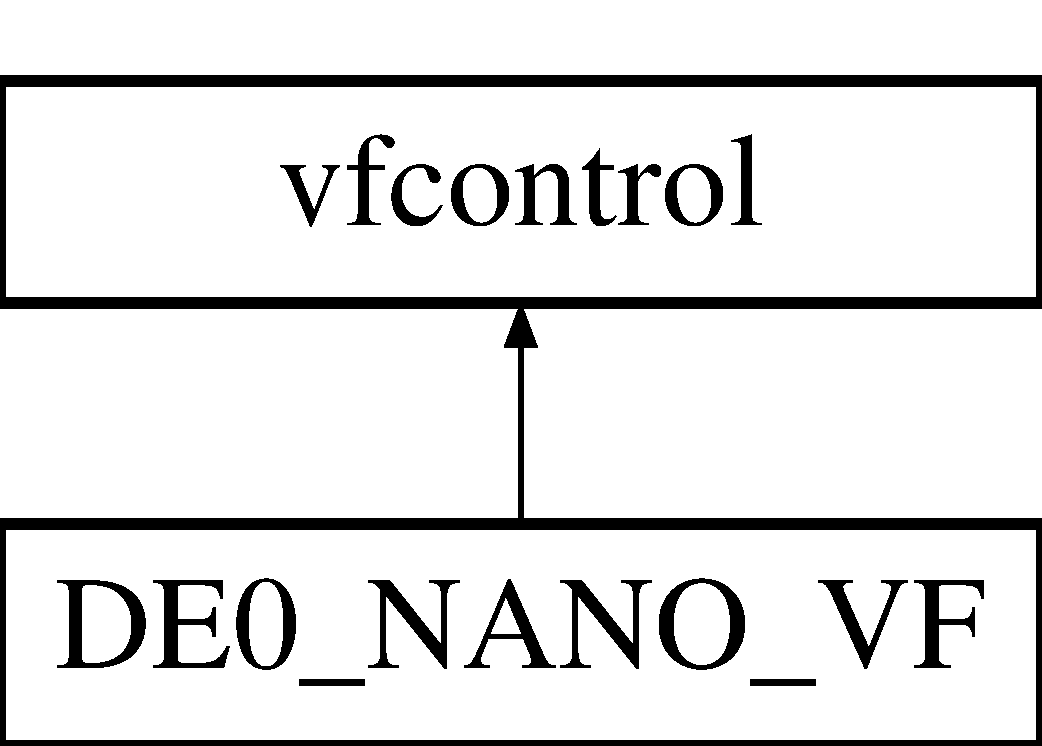
\includegraphics[height=2.000000cm]{classvfcontrol}
\end{center}
\end{figure}
\subsection*{Entities}
\begin{DoxyCompactItemize}
\item 
\hyperlink{classvfcontrol_1_1vfcontrol__arch}{vfcontrol\+\_\+arch} architecture
\end{DoxyCompactItemize}
\subsection*{Libraries}
 \begin{DoxyCompactItemize}
\item 
\hyperlink{classvfcontrol_ae4f03c286607f3181e16b9aa12d0c6d4}{I\+E\+E\+E} 
\end{DoxyCompactItemize}
\subsection*{Use Clauses}
 \begin{DoxyCompactItemize}
\item 
\hyperlink{classvfcontrol_a241c3e72dd8024cc8ae831b1b2aed7db}{S\+T\+D\+\_\+\+L\+O\+G\+I\+C\+\_\+\+U\+N\+S\+I\+G\+N\+E\+D}   
\item 
\hyperlink{classvfcontrol_aa4b2b25246a821511120e3149b003563}{S\+T\+D\+\_\+\+L\+O\+G\+I\+C\+\_\+1164}   
\item 
\hyperlink{classvfcontrol_a5d8c1f7c620a51582be96d2a58d40293}{S\+T\+D\+\_\+\+L\+O\+G\+I\+C\+\_\+\+A\+R\+I\+T\+H}   
\item 
\hyperlink{classvfcontrol_aad86249c80e8c1e7ee1c4748aba748e3}{fixed\+\_\+pkg}   
\item 
\hyperlink{classvfcontrol_a2edc34402b573437d5f25fa90ba4013e}{numeric\+\_\+std}   
\end{DoxyCompactItemize}
\subsection*{Generics}
 \begin{DoxyCompactItemize}
\item 
\hyperlink{classvfcontrol_afee4aa1628956aa350183d8881689198}{n\+\_\+bits\+\_\+c} {\bfseries {\bfseries \textcolor{comment}{integer}\textcolor{vhdlchar}{ }\textcolor{vhdlchar}{ }\textcolor{vhdlchar}{\+:}\textcolor{vhdlchar}{=}\textcolor{vhdlchar}{ }\textcolor{vhdlchar}{ } \textcolor{vhdldigit}{16} \textcolor{vhdlchar}{ }}}
\item 
\hyperlink{classvfcontrol_ac366e3464ed5372201dc4a0b59d91bdd}{inc\+M\+A\+X} {\bfseries {\bfseries \textcolor{comment}{std\+\_\+logic\+\_\+vector}\textcolor{vhdlchar}{ }\textcolor{vhdlchar}{(}\textcolor{vhdlchar}{ }\textcolor{vhdlchar}{ } \textcolor{vhdldigit}{12} \textcolor{vhdlchar}{ }\textcolor{keywordflow}{downto}\textcolor{vhdlchar}{ }\textcolor{vhdlchar}{ } \textcolor{vhdldigit}{0} \textcolor{vhdlchar}{ }\textcolor{vhdlchar}{)}\textcolor{vhdlchar}{ }\textcolor{vhdlchar}{ }\textcolor{vhdlchar}{ }\textcolor{vhdlchar}{\+:}\textcolor{vhdlchar}{=}\textcolor{vhdlchar}{ }\textcolor{vhdlchar}{ }\textcolor{vhdlchar}{ }\textcolor{vhdlchar}{ }\textcolor{comment}{std\+\_\+logic\+\_\+vector}\textcolor{vhdlchar}{ }\textcolor{vhdlchar}{(}\textcolor{vhdlchar}{ }\textcolor{vhdlchar}{to\+\_\+unsigned}\textcolor{vhdlchar}{ }\textcolor{vhdlchar}{(}\textcolor{vhdlchar}{ }\textcolor{vhdlchar}{ } \textcolor{vhdldigit}{2416} \textcolor{vhdlchar}{ }\textcolor{vhdlchar}{,}\textcolor{vhdlchar}{ }\textcolor{vhdlchar}{ } \textcolor{vhdldigit}{13} \textcolor{vhdlchar}{ }\textcolor{vhdlchar}{)}\textcolor{vhdlchar}{ }\textcolor{vhdlchar}{ }\textcolor{vhdlchar}{ }\textcolor{vhdlchar}{)}\textcolor{vhdlchar}{ }}}
\item 
\hyperlink{classvfcontrol_a338e968adaa27098ea77208ca9186ea9}{inc\+M\+I\+N} {\bfseries {\bfseries \textcolor{comment}{std\+\_\+logic\+\_\+vector}\textcolor{vhdlchar}{ }\textcolor{vhdlchar}{(}\textcolor{vhdlchar}{ }\textcolor{vhdlchar}{ } \textcolor{vhdldigit}{12} \textcolor{vhdlchar}{ }\textcolor{keywordflow}{downto}\textcolor{vhdlchar}{ }\textcolor{vhdlchar}{ } \textcolor{vhdldigit}{0} \textcolor{vhdlchar}{ }\textcolor{vhdlchar}{)}\textcolor{vhdlchar}{ }\textcolor{vhdlchar}{ }\textcolor{vhdlchar}{ }\textcolor{vhdlchar}{\+:}\textcolor{vhdlchar}{=}\textcolor{vhdlchar}{ }\textcolor{vhdlchar}{ }\textcolor{vhdlchar}{ }\textcolor{vhdlchar}{ }\textcolor{comment}{std\+\_\+logic\+\_\+vector}\textcolor{vhdlchar}{ }\textcolor{vhdlchar}{(}\textcolor{vhdlchar}{ }\textcolor{vhdlchar}{to\+\_\+unsigned}\textcolor{vhdlchar}{ }\textcolor{vhdlchar}{(}\textcolor{vhdlchar}{ }\textcolor{vhdlchar}{ } \textcolor{vhdldigit}{483} \textcolor{vhdlchar}{ }\textcolor{vhdlchar}{,}\textcolor{vhdlchar}{ }\textcolor{vhdlchar}{ } \textcolor{vhdldigit}{13} \textcolor{vhdlchar}{ }\textcolor{vhdlchar}{)}\textcolor{vhdlchar}{ }\textcolor{vhdlchar}{ }\textcolor{vhdlchar}{ }\textcolor{vhdlchar}{)}\textcolor{vhdlchar}{ }}}
\item 
\hyperlink{classvfcontrol_abb7ce405d45a733b6db94314a4f791fd}{I} {\bfseries {\bfseries \textcolor{comment}{integer}\textcolor{vhdlchar}{ }\textcolor{vhdlchar}{ }\textcolor{vhdlchar}{\+:}\textcolor{vhdlchar}{=}\textcolor{vhdlchar}{ }\textcolor{vhdlchar}{ } \textcolor{vhdldigit}{1} \textcolor{vhdlchar}{ }}}
\item 
\hyperlink{classvfcontrol_aac2d6825f96b21ae984648cc93554339}{F} {\bfseries {\bfseries \textcolor{comment}{integer}\textcolor{vhdlchar}{ }\textcolor{vhdlchar}{ }\textcolor{vhdlchar}{\+:}\textcolor{vhdlchar}{=}\textcolor{vhdlchar}{ }\textcolor{vhdlchar}{ } \textcolor{vhdldigit}{14} \textcolor{vhdlchar}{ }}}
\item 
\hyperlink{classvfcontrol_a35e1281ab3472bb9079152e62c1a9acb}{m\+M\+A\+X} {\bfseries {\bfseries \textcolor{comment}{sfixed}\textcolor{vhdlchar}{ }\textcolor{vhdlchar}{(}\textcolor{vhdlchar}{ }\textcolor{vhdlchar}{ } \textcolor{vhdldigit}{1} \textcolor{vhdlchar}{ }\textcolor{keywordflow}{downto}\textcolor{vhdlchar}{ }\textcolor{vhdlchar}{-\/}\textcolor{vhdlchar}{ } \textcolor{vhdldigit}{27} \textcolor{vhdlchar}{ }\textcolor{vhdlchar}{)}\textcolor{vhdlchar}{ }\textcolor{vhdlchar}{ }\textcolor{vhdlchar}{ }\textcolor{vhdlchar}{\+:}\textcolor{vhdlchar}{=}\textcolor{vhdlchar}{ }\textcolor{vhdlchar}{ }\textcolor{vhdlchar}{ }\textcolor{vhdlchar}{ }\textcolor{vhdlchar}{to\+\_\+sfixed}\textcolor{vhdlchar}{ }\textcolor{vhdlchar}{(}\textcolor{vhdlchar}{ }\textcolor{vhdlchar}{ } \textcolor{vhdldigit}{0} \textcolor{vhdlchar}{.} \textcolor{vhdldigit}{4069} \textcolor{vhdlchar}{ }\textcolor{vhdlchar}{,}\textcolor{vhdlchar}{ }\textcolor{vhdlchar}{ } \textcolor{vhdldigit}{1} \textcolor{vhdlchar}{ }\textcolor{vhdlchar}{,}\textcolor{vhdlchar}{ }\textcolor{vhdlchar}{-\/}\textcolor{vhdlchar}{ } \textcolor{vhdldigit}{27} \textcolor{vhdlchar}{ }\textcolor{vhdlchar}{)}\textcolor{vhdlchar}{ }}}
\item 
\hyperlink{classvfcontrol_a9912dbac80dc6644996e1665646e0823}{m\+M\+I\+N} {\bfseries {\bfseries \textcolor{comment}{sfixed}\textcolor{vhdlchar}{ }\textcolor{vhdlchar}{(}\textcolor{vhdlchar}{ }\textcolor{vhdlchar}{ } \textcolor{vhdldigit}{1} \textcolor{vhdlchar}{ }\textcolor{keywordflow}{downto}\textcolor{vhdlchar}{ }\textcolor{vhdlchar}{-\/}\textcolor{vhdlchar}{ } \textcolor{vhdldigit}{27} \textcolor{vhdlchar}{ }\textcolor{vhdlchar}{)}\textcolor{vhdlchar}{ }\textcolor{vhdlchar}{ }\textcolor{vhdlchar}{ }\textcolor{vhdlchar}{\+:}\textcolor{vhdlchar}{=}\textcolor{vhdlchar}{ }\textcolor{vhdlchar}{ }\textcolor{vhdlchar}{ }\textcolor{vhdlchar}{ }\textcolor{vhdlchar}{to\+\_\+sfixed}\textcolor{vhdlchar}{ }\textcolor{vhdlchar}{(}\textcolor{vhdlchar}{ }\textcolor{vhdlchar}{ } \textcolor{vhdldigit}{0} \textcolor{vhdlchar}{.} \textcolor{vhdldigit}{08137} \textcolor{vhdlchar}{ }\textcolor{vhdlchar}{,}\textcolor{vhdlchar}{ }\textcolor{vhdlchar}{ } \textcolor{vhdldigit}{1} \textcolor{vhdlchar}{ }\textcolor{vhdlchar}{,}\textcolor{vhdlchar}{ }\textcolor{vhdlchar}{-\/}\textcolor{vhdlchar}{ } \textcolor{vhdldigit}{27} \textcolor{vhdlchar}{ }\textcolor{vhdlchar}{)}\textcolor{vhdlchar}{ }}}
\end{DoxyCompactItemize}
\subsection*{Ports}
 \begin{DoxyCompactItemize}
\item 
\hyperlink{classvfcontrol_a4a4609c199d30b3adebbeb3a01276ec5}{clk}  {\bfseries {\bfseries \textcolor{keywordflow}{in}\textcolor{vhdlchar}{ }}} {\bfseries \textcolor{comment}{std\+\_\+logic}\textcolor{vhdlchar}{ }} 
\item 
\hyperlink{classvfcontrol_adcf9c6f5161d039addbda5819bee64a3}{en}  {\bfseries {\bfseries \textcolor{keywordflow}{in}\textcolor{vhdlchar}{ }}} {\bfseries \textcolor{comment}{std\+\_\+logic}\textcolor{vhdlchar}{ }} 
\item 
\hyperlink{classvfcontrol_af402b7ce8e1b9ac1038c575460c5d156}{inc\+\_\+data}  {\bfseries {\bfseries \textcolor{keywordflow}{out}\textcolor{vhdlchar}{ }}} {\bfseries \textcolor{comment}{std\+\_\+logic\+\_\+vector}\textcolor{vhdlchar}{ }\textcolor{vhdlchar}{(}\textcolor{vhdlchar}{ }\textcolor{vhdlchar}{ } \textcolor{vhdldigit}{12} \textcolor{vhdlchar}{ }\textcolor{keywordflow}{downto}\textcolor{vhdlchar}{ }\textcolor{vhdlchar}{ } \textcolor{vhdldigit}{0} \textcolor{vhdlchar}{ }\textcolor{vhdlchar}{)}\textcolor{vhdlchar}{ }} 
\item 
\hyperlink{classvfcontrol_a556e3576ef1696c57d447032f986bf5a}{m\+\_\+vf}  {\bfseries {\bfseries \textcolor{keywordflow}{out}\textcolor{vhdlchar}{ }}} {\bfseries \textcolor{comment}{sfixed}\textcolor{vhdlchar}{ }\textcolor{vhdlchar}{(}\textcolor{vhdlchar}{ }\textcolor{vhdlchar}{ }\textcolor{vhdlchar}{ }\textcolor{vhdlchar}{ }{\bfseries \hyperlink{classvfcontrol_abb7ce405d45a733b6db94314a4f791fd}{I}} \textcolor{vhdlchar}{ }\textcolor{keywordflow}{downto}\textcolor{vhdlchar}{ }\textcolor{vhdlchar}{-\/}\textcolor{vhdlchar}{ }\textcolor{vhdlchar}{ }\textcolor{vhdlchar}{ }{\bfseries \hyperlink{classvfcontrol_aac2d6825f96b21ae984648cc93554339}{F}} \textcolor{vhdlchar}{ }\textcolor{vhdlchar}{)}\textcolor{vhdlchar}{ }} 
\end{DoxyCompactItemize}


\subsection{Detailed Description}


Definition at line \hyperlink{vfcontrol_8vhd_source_l00010}{10} of file \hyperlink{vfcontrol_8vhd_source}{vfcontrol.\+vhd}.



\subsection{Member Data Documentation}
\hypertarget{classvfcontrol_a4a4609c199d30b3adebbeb3a01276ec5}{}\index{vfcontrol@{vfcontrol}!clk@{clk}}
\index{clk@{clk}!vfcontrol@{vfcontrol}}
\subsubsection[{clk}]{\setlength{\rightskip}{0pt plus 5cm}{\bf clk} {\bfseries \textcolor{keywordflow}{in}\textcolor{vhdlchar}{ }} {\bfseries \textcolor{comment}{std\+\_\+logic}\textcolor{vhdlchar}{ }} \hspace{0.3cm}{\ttfamily [Port]}}\label{classvfcontrol_a4a4609c199d30b3adebbeb3a01276ec5}


Definition at line \hyperlink{vfcontrol_8vhd_source_l00024}{24} of file \hyperlink{vfcontrol_8vhd_source}{vfcontrol.\+vhd}.

\hypertarget{classvfcontrol_adcf9c6f5161d039addbda5819bee64a3}{}\index{vfcontrol@{vfcontrol}!en@{en}}
\index{en@{en}!vfcontrol@{vfcontrol}}
\subsubsection[{en}]{\setlength{\rightskip}{0pt plus 5cm}{\bf en} {\bfseries \textcolor{keywordflow}{in}\textcolor{vhdlchar}{ }} {\bfseries \textcolor{comment}{std\+\_\+logic}\textcolor{vhdlchar}{ }} \hspace{0.3cm}{\ttfamily [Port]}}\label{classvfcontrol_adcf9c6f5161d039addbda5819bee64a3}


Definition at line \hyperlink{vfcontrol_8vhd_source_l00025}{25} of file \hyperlink{vfcontrol_8vhd_source}{vfcontrol.\+vhd}.

\hypertarget{classvfcontrol_aac2d6825f96b21ae984648cc93554339}{}\index{vfcontrol@{vfcontrol}!F@{F}}
\index{F@{F}!vfcontrol@{vfcontrol}}
\subsubsection[{F}]{\setlength{\rightskip}{0pt plus 5cm}{\bf F} {\bfseries \textcolor{vhdlchar}{ }} {\bfseries \textcolor{comment}{integer}\textcolor{vhdlchar}{ }\textcolor{vhdlchar}{ }\textcolor{vhdlchar}{\+:}\textcolor{vhdlchar}{=}\textcolor{vhdlchar}{ }\textcolor{vhdlchar}{ } \textcolor{vhdldigit}{14} \textcolor{vhdlchar}{ }} \hspace{0.3cm}{\ttfamily [Generic]}}\label{classvfcontrol_aac2d6825f96b21ae984648cc93554339}


Definition at line \hyperlink{vfcontrol_8vhd_source_l00017}{17} of file \hyperlink{vfcontrol_8vhd_source}{vfcontrol.\+vhd}.

\hypertarget{classvfcontrol_aad86249c80e8c1e7ee1c4748aba748e3}{}\index{vfcontrol@{vfcontrol}!fixed\+\_\+pkg@{fixed\+\_\+pkg}}
\index{fixed\+\_\+pkg@{fixed\+\_\+pkg}!vfcontrol@{vfcontrol}}
\subsubsection[{fixed\+\_\+pkg}]{\setlength{\rightskip}{0pt plus 5cm}{\bf fixed\+\_\+pkg}\hspace{0.3cm}{\ttfamily [Package]}}\label{classvfcontrol_aad86249c80e8c1e7ee1c4748aba748e3}


Definition at line \hyperlink{vfcontrol_8vhd_source_l00006}{6} of file \hyperlink{vfcontrol_8vhd_source}{vfcontrol.\+vhd}.

\hypertarget{classvfcontrol_abb7ce405d45a733b6db94314a4f791fd}{}\index{vfcontrol@{vfcontrol}!I@{I}}
\index{I@{I}!vfcontrol@{vfcontrol}}
\subsubsection[{I}]{\setlength{\rightskip}{0pt plus 5cm}{\bf I} {\bfseries \textcolor{vhdlchar}{ }} {\bfseries \textcolor{comment}{integer}\textcolor{vhdlchar}{ }\textcolor{vhdlchar}{ }\textcolor{vhdlchar}{\+:}\textcolor{vhdlchar}{=}\textcolor{vhdlchar}{ }\textcolor{vhdlchar}{ } \textcolor{vhdldigit}{1} \textcolor{vhdlchar}{ }} \hspace{0.3cm}{\ttfamily [Generic]}}\label{classvfcontrol_abb7ce405d45a733b6db94314a4f791fd}


Definition at line \hyperlink{vfcontrol_8vhd_source_l00016}{16} of file \hyperlink{vfcontrol_8vhd_source}{vfcontrol.\+vhd}.

\hypertarget{classvfcontrol_ae4f03c286607f3181e16b9aa12d0c6d4}{}\index{vfcontrol@{vfcontrol}!I\+E\+E\+E@{I\+E\+E\+E}}
\index{I\+E\+E\+E@{I\+E\+E\+E}!vfcontrol@{vfcontrol}}
\subsubsection[{I\+E\+E\+E}]{\setlength{\rightskip}{0pt plus 5cm}{\bf I\+E\+E\+E}\hspace{0.3cm}{\ttfamily [Library]}}\label{classvfcontrol_ae4f03c286607f3181e16b9aa12d0c6d4}


Definition at line \hyperlink{vfcontrol_8vhd_source_l00002}{2} of file \hyperlink{vfcontrol_8vhd_source}{vfcontrol.\+vhd}.

\hypertarget{classvfcontrol_af402b7ce8e1b9ac1038c575460c5d156}{}\index{vfcontrol@{vfcontrol}!inc\+\_\+data@{inc\+\_\+data}}
\index{inc\+\_\+data@{inc\+\_\+data}!vfcontrol@{vfcontrol}}
\subsubsection[{inc\+\_\+data}]{\setlength{\rightskip}{0pt plus 5cm}{\bf inc\+\_\+data} {\bfseries \textcolor{keywordflow}{out}\textcolor{vhdlchar}{ }} {\bfseries \textcolor{comment}{std\+\_\+logic\+\_\+vector}\textcolor{vhdlchar}{ }\textcolor{vhdlchar}{(}\textcolor{vhdlchar}{ }\textcolor{vhdlchar}{ } \textcolor{vhdldigit}{12} \textcolor{vhdlchar}{ }\textcolor{keywordflow}{downto}\textcolor{vhdlchar}{ }\textcolor{vhdlchar}{ } \textcolor{vhdldigit}{0} \textcolor{vhdlchar}{ }\textcolor{vhdlchar}{)}\textcolor{vhdlchar}{ }} \hspace{0.3cm}{\ttfamily [Port]}}\label{classvfcontrol_af402b7ce8e1b9ac1038c575460c5d156}


Definition at line \hyperlink{vfcontrol_8vhd_source_l00026}{26} of file \hyperlink{vfcontrol_8vhd_source}{vfcontrol.\+vhd}.

\hypertarget{classvfcontrol_ac366e3464ed5372201dc4a0b59d91bdd}{}\index{vfcontrol@{vfcontrol}!inc\+M\+A\+X@{inc\+M\+A\+X}}
\index{inc\+M\+A\+X@{inc\+M\+A\+X}!vfcontrol@{vfcontrol}}
\subsubsection[{inc\+M\+A\+X}]{\setlength{\rightskip}{0pt plus 5cm}{\bf inc\+M\+A\+X} {\bfseries \textcolor{vhdlchar}{ }} {\bfseries \textcolor{comment}{std\+\_\+logic\+\_\+vector}\textcolor{vhdlchar}{ }\textcolor{vhdlchar}{(}\textcolor{vhdlchar}{ }\textcolor{vhdlchar}{ } \textcolor{vhdldigit}{12} \textcolor{vhdlchar}{ }\textcolor{keywordflow}{downto}\textcolor{vhdlchar}{ }\textcolor{vhdlchar}{ } \textcolor{vhdldigit}{0} \textcolor{vhdlchar}{ }\textcolor{vhdlchar}{)}\textcolor{vhdlchar}{ }\textcolor{vhdlchar}{ }\textcolor{vhdlchar}{ }\textcolor{vhdlchar}{\+:}\textcolor{vhdlchar}{=}\textcolor{vhdlchar}{ }\textcolor{vhdlchar}{ }\textcolor{vhdlchar}{ }\textcolor{vhdlchar}{ }\textcolor{comment}{std\+\_\+logic\+\_\+vector}\textcolor{vhdlchar}{ }\textcolor{vhdlchar}{(}\textcolor{vhdlchar}{ }\textcolor{vhdlchar}{to\+\_\+unsigned}\textcolor{vhdlchar}{ }\textcolor{vhdlchar}{(}\textcolor{vhdlchar}{ }\textcolor{vhdlchar}{ } \textcolor{vhdldigit}{2416} \textcolor{vhdlchar}{ }\textcolor{vhdlchar}{,}\textcolor{vhdlchar}{ }\textcolor{vhdlchar}{ } \textcolor{vhdldigit}{13} \textcolor{vhdlchar}{ }\textcolor{vhdlchar}{)}\textcolor{vhdlchar}{ }\textcolor{vhdlchar}{ }\textcolor{vhdlchar}{ }\textcolor{vhdlchar}{)}\textcolor{vhdlchar}{ }} \hspace{0.3cm}{\ttfamily [Generic]}}\label{classvfcontrol_ac366e3464ed5372201dc4a0b59d91bdd}


Definition at line \hyperlink{vfcontrol_8vhd_source_l00014}{14} of file \hyperlink{vfcontrol_8vhd_source}{vfcontrol.\+vhd}.

\hypertarget{classvfcontrol_a338e968adaa27098ea77208ca9186ea9}{}\index{vfcontrol@{vfcontrol}!inc\+M\+I\+N@{inc\+M\+I\+N}}
\index{inc\+M\+I\+N@{inc\+M\+I\+N}!vfcontrol@{vfcontrol}}
\subsubsection[{inc\+M\+I\+N}]{\setlength{\rightskip}{0pt plus 5cm}{\bf inc\+M\+I\+N} {\bfseries \textcolor{vhdlchar}{ }} {\bfseries \textcolor{comment}{std\+\_\+logic\+\_\+vector}\textcolor{vhdlchar}{ }\textcolor{vhdlchar}{(}\textcolor{vhdlchar}{ }\textcolor{vhdlchar}{ } \textcolor{vhdldigit}{12} \textcolor{vhdlchar}{ }\textcolor{keywordflow}{downto}\textcolor{vhdlchar}{ }\textcolor{vhdlchar}{ } \textcolor{vhdldigit}{0} \textcolor{vhdlchar}{ }\textcolor{vhdlchar}{)}\textcolor{vhdlchar}{ }\textcolor{vhdlchar}{ }\textcolor{vhdlchar}{ }\textcolor{vhdlchar}{\+:}\textcolor{vhdlchar}{=}\textcolor{vhdlchar}{ }\textcolor{vhdlchar}{ }\textcolor{vhdlchar}{ }\textcolor{vhdlchar}{ }\textcolor{comment}{std\+\_\+logic\+\_\+vector}\textcolor{vhdlchar}{ }\textcolor{vhdlchar}{(}\textcolor{vhdlchar}{ }\textcolor{vhdlchar}{to\+\_\+unsigned}\textcolor{vhdlchar}{ }\textcolor{vhdlchar}{(}\textcolor{vhdlchar}{ }\textcolor{vhdlchar}{ } \textcolor{vhdldigit}{483} \textcolor{vhdlchar}{ }\textcolor{vhdlchar}{,}\textcolor{vhdlchar}{ }\textcolor{vhdlchar}{ } \textcolor{vhdldigit}{13} \textcolor{vhdlchar}{ }\textcolor{vhdlchar}{)}\textcolor{vhdlchar}{ }\textcolor{vhdlchar}{ }\textcolor{vhdlchar}{ }\textcolor{vhdlchar}{)}\textcolor{vhdlchar}{ }} \hspace{0.3cm}{\ttfamily [Generic]}}\label{classvfcontrol_a338e968adaa27098ea77208ca9186ea9}


Definition at line \hyperlink{vfcontrol_8vhd_source_l00015}{15} of file \hyperlink{vfcontrol_8vhd_source}{vfcontrol.\+vhd}.

\hypertarget{classvfcontrol_a556e3576ef1696c57d447032f986bf5a}{}\index{vfcontrol@{vfcontrol}!m\+\_\+vf@{m\+\_\+vf}}
\index{m\+\_\+vf@{m\+\_\+vf}!vfcontrol@{vfcontrol}}
\subsubsection[{m\+\_\+vf}]{\setlength{\rightskip}{0pt plus 5cm}{\bf m\+\_\+vf} {\bfseries \textcolor{keywordflow}{out}\textcolor{vhdlchar}{ }} {\bfseries \textcolor{comment}{sfixed}\textcolor{vhdlchar}{ }\textcolor{vhdlchar}{(}\textcolor{vhdlchar}{ }\textcolor{vhdlchar}{ }\textcolor{vhdlchar}{ }\textcolor{vhdlchar}{ }{\bfseries {\bf I}} \textcolor{vhdlchar}{ }\textcolor{keywordflow}{downto}\textcolor{vhdlchar}{ }\textcolor{vhdlchar}{-\/}\textcolor{vhdlchar}{ }\textcolor{vhdlchar}{ }\textcolor{vhdlchar}{ }{\bfseries {\bf F}} \textcolor{vhdlchar}{ }\textcolor{vhdlchar}{)}\textcolor{vhdlchar}{ }} \hspace{0.3cm}{\ttfamily [Port]}}\label{classvfcontrol_a556e3576ef1696c57d447032f986bf5a}


Definition at line \hyperlink{vfcontrol_8vhd_source_l00028}{28} of file \hyperlink{vfcontrol_8vhd_source}{vfcontrol.\+vhd}.

\hypertarget{classvfcontrol_a35e1281ab3472bb9079152e62c1a9acb}{}\index{vfcontrol@{vfcontrol}!m\+M\+A\+X@{m\+M\+A\+X}}
\index{m\+M\+A\+X@{m\+M\+A\+X}!vfcontrol@{vfcontrol}}
\subsubsection[{m\+M\+A\+X}]{\setlength{\rightskip}{0pt plus 5cm}{\bf m\+M\+A\+X} {\bfseries \textcolor{vhdlchar}{ }} {\bfseries \textcolor{comment}{sfixed}\textcolor{vhdlchar}{ }\textcolor{vhdlchar}{(}\textcolor{vhdlchar}{ }\textcolor{vhdlchar}{ } \textcolor{vhdldigit}{1} \textcolor{vhdlchar}{ }\textcolor{keywordflow}{downto}\textcolor{vhdlchar}{ }\textcolor{vhdlchar}{-\/}\textcolor{vhdlchar}{ } \textcolor{vhdldigit}{27} \textcolor{vhdlchar}{ }\textcolor{vhdlchar}{)}\textcolor{vhdlchar}{ }\textcolor{vhdlchar}{ }\textcolor{vhdlchar}{ }\textcolor{vhdlchar}{\+:}\textcolor{vhdlchar}{=}\textcolor{vhdlchar}{ }\textcolor{vhdlchar}{ }\textcolor{vhdlchar}{ }\textcolor{vhdlchar}{ }\textcolor{vhdlchar}{to\+\_\+sfixed}\textcolor{vhdlchar}{ }\textcolor{vhdlchar}{(}\textcolor{vhdlchar}{ }\textcolor{vhdlchar}{ } \textcolor{vhdldigit}{0} \textcolor{vhdlchar}{.} \textcolor{vhdldigit}{4069} \textcolor{vhdlchar}{ }\textcolor{vhdlchar}{,}\textcolor{vhdlchar}{ }\textcolor{vhdlchar}{ } \textcolor{vhdldigit}{1} \textcolor{vhdlchar}{ }\textcolor{vhdlchar}{,}\textcolor{vhdlchar}{ }\textcolor{vhdlchar}{-\/}\textcolor{vhdlchar}{ } \textcolor{vhdldigit}{27} \textcolor{vhdlchar}{ }\textcolor{vhdlchar}{)}\textcolor{vhdlchar}{ }} \hspace{0.3cm}{\ttfamily [Generic]}}\label{classvfcontrol_a35e1281ab3472bb9079152e62c1a9acb}


Definition at line \hyperlink{vfcontrol_8vhd_source_l00019}{19} of file \hyperlink{vfcontrol_8vhd_source}{vfcontrol.\+vhd}.

\hypertarget{classvfcontrol_a9912dbac80dc6644996e1665646e0823}{}\index{vfcontrol@{vfcontrol}!m\+M\+I\+N@{m\+M\+I\+N}}
\index{m\+M\+I\+N@{m\+M\+I\+N}!vfcontrol@{vfcontrol}}
\subsubsection[{m\+M\+I\+N}]{\setlength{\rightskip}{0pt plus 5cm}{\bf m\+M\+I\+N} {\bfseries \textcolor{vhdlchar}{ }} {\bfseries \textcolor{comment}{sfixed}\textcolor{vhdlchar}{ }\textcolor{vhdlchar}{(}\textcolor{vhdlchar}{ }\textcolor{vhdlchar}{ } \textcolor{vhdldigit}{1} \textcolor{vhdlchar}{ }\textcolor{keywordflow}{downto}\textcolor{vhdlchar}{ }\textcolor{vhdlchar}{-\/}\textcolor{vhdlchar}{ } \textcolor{vhdldigit}{27} \textcolor{vhdlchar}{ }\textcolor{vhdlchar}{)}\textcolor{vhdlchar}{ }\textcolor{vhdlchar}{ }\textcolor{vhdlchar}{ }\textcolor{vhdlchar}{\+:}\textcolor{vhdlchar}{=}\textcolor{vhdlchar}{ }\textcolor{vhdlchar}{ }\textcolor{vhdlchar}{ }\textcolor{vhdlchar}{ }\textcolor{vhdlchar}{to\+\_\+sfixed}\textcolor{vhdlchar}{ }\textcolor{vhdlchar}{(}\textcolor{vhdlchar}{ }\textcolor{vhdlchar}{ } \textcolor{vhdldigit}{0} \textcolor{vhdlchar}{.} \textcolor{vhdldigit}{08137} \textcolor{vhdlchar}{ }\textcolor{vhdlchar}{,}\textcolor{vhdlchar}{ }\textcolor{vhdlchar}{ } \textcolor{vhdldigit}{1} \textcolor{vhdlchar}{ }\textcolor{vhdlchar}{,}\textcolor{vhdlchar}{ }\textcolor{vhdlchar}{-\/}\textcolor{vhdlchar}{ } \textcolor{vhdldigit}{27} \textcolor{vhdlchar}{ }\textcolor{vhdlchar}{)}\textcolor{vhdlchar}{ }} \hspace{0.3cm}{\ttfamily [Generic]}}\label{classvfcontrol_a9912dbac80dc6644996e1665646e0823}


Definition at line \hyperlink{vfcontrol_8vhd_source_l00021}{21} of file \hyperlink{vfcontrol_8vhd_source}{vfcontrol.\+vhd}.

\hypertarget{classvfcontrol_afee4aa1628956aa350183d8881689198}{}\index{vfcontrol@{vfcontrol}!n\+\_\+bits\+\_\+c@{n\+\_\+bits\+\_\+c}}
\index{n\+\_\+bits\+\_\+c@{n\+\_\+bits\+\_\+c}!vfcontrol@{vfcontrol}}
\subsubsection[{n\+\_\+bits\+\_\+c}]{\setlength{\rightskip}{0pt plus 5cm}{\bf n\+\_\+bits\+\_\+c} {\bfseries \textcolor{vhdlchar}{ }} {\bfseries \textcolor{comment}{integer}\textcolor{vhdlchar}{ }\textcolor{vhdlchar}{ }\textcolor{vhdlchar}{\+:}\textcolor{vhdlchar}{=}\textcolor{vhdlchar}{ }\textcolor{vhdlchar}{ } \textcolor{vhdldigit}{16} \textcolor{vhdlchar}{ }} \hspace{0.3cm}{\ttfamily [Generic]}}\label{classvfcontrol_afee4aa1628956aa350183d8881689198}


Definition at line \hyperlink{vfcontrol_8vhd_source_l00012}{12} of file \hyperlink{vfcontrol_8vhd_source}{vfcontrol.\+vhd}.

\hypertarget{classvfcontrol_a2edc34402b573437d5f25fa90ba4013e}{}\index{vfcontrol@{vfcontrol}!numeric\+\_\+std@{numeric\+\_\+std}}
\index{numeric\+\_\+std@{numeric\+\_\+std}!vfcontrol@{vfcontrol}}
\subsubsection[{numeric\+\_\+std}]{\setlength{\rightskip}{0pt plus 5cm}{\bf numeric\+\_\+std}\hspace{0.3cm}{\ttfamily [Package]}}\label{classvfcontrol_a2edc34402b573437d5f25fa90ba4013e}


Definition at line \hyperlink{vfcontrol_8vhd_source_l00007}{7} of file \hyperlink{vfcontrol_8vhd_source}{vfcontrol.\+vhd}.

\hypertarget{classvfcontrol_aa4b2b25246a821511120e3149b003563}{}\index{vfcontrol@{vfcontrol}!S\+T\+D\+\_\+\+L\+O\+G\+I\+C\+\_\+1164@{S\+T\+D\+\_\+\+L\+O\+G\+I\+C\+\_\+1164}}
\index{S\+T\+D\+\_\+\+L\+O\+G\+I\+C\+\_\+1164@{S\+T\+D\+\_\+\+L\+O\+G\+I\+C\+\_\+1164}!vfcontrol@{vfcontrol}}
\subsubsection[{S\+T\+D\+\_\+\+L\+O\+G\+I\+C\+\_\+1164}]{\setlength{\rightskip}{0pt plus 5cm}{\bf S\+T\+D\+\_\+\+L\+O\+G\+I\+C\+\_\+1164}\hspace{0.3cm}{\ttfamily [Package]}}\label{classvfcontrol_aa4b2b25246a821511120e3149b003563}


Definition at line \hyperlink{vfcontrol_8vhd_source_l00004}{4} of file \hyperlink{vfcontrol_8vhd_source}{vfcontrol.\+vhd}.

\hypertarget{classvfcontrol_a5d8c1f7c620a51582be96d2a58d40293}{}\index{vfcontrol@{vfcontrol}!S\+T\+D\+\_\+\+L\+O\+G\+I\+C\+\_\+\+A\+R\+I\+T\+H@{S\+T\+D\+\_\+\+L\+O\+G\+I\+C\+\_\+\+A\+R\+I\+T\+H}}
\index{S\+T\+D\+\_\+\+L\+O\+G\+I\+C\+\_\+\+A\+R\+I\+T\+H@{S\+T\+D\+\_\+\+L\+O\+G\+I\+C\+\_\+\+A\+R\+I\+T\+H}!vfcontrol@{vfcontrol}}
\subsubsection[{S\+T\+D\+\_\+\+L\+O\+G\+I\+C\+\_\+\+A\+R\+I\+T\+H}]{\setlength{\rightskip}{0pt plus 5cm}{\bf S\+T\+D\+\_\+\+L\+O\+G\+I\+C\+\_\+\+A\+R\+I\+T\+H}\hspace{0.3cm}{\ttfamily [Package]}}\label{classvfcontrol_a5d8c1f7c620a51582be96d2a58d40293}


Definition at line \hyperlink{vfcontrol_8vhd_source_l00005}{5} of file \hyperlink{vfcontrol_8vhd_source}{vfcontrol.\+vhd}.

\hypertarget{classvfcontrol_a241c3e72dd8024cc8ae831b1b2aed7db}{}\index{vfcontrol@{vfcontrol}!S\+T\+D\+\_\+\+L\+O\+G\+I\+C\+\_\+\+U\+N\+S\+I\+G\+N\+E\+D@{S\+T\+D\+\_\+\+L\+O\+G\+I\+C\+\_\+\+U\+N\+S\+I\+G\+N\+E\+D}}
\index{S\+T\+D\+\_\+\+L\+O\+G\+I\+C\+\_\+\+U\+N\+S\+I\+G\+N\+E\+D@{S\+T\+D\+\_\+\+L\+O\+G\+I\+C\+\_\+\+U\+N\+S\+I\+G\+N\+E\+D}!vfcontrol@{vfcontrol}}
\subsubsection[{S\+T\+D\+\_\+\+L\+O\+G\+I\+C\+\_\+\+U\+N\+S\+I\+G\+N\+E\+D}]{\setlength{\rightskip}{0pt plus 5cm}{\bf S\+T\+D\+\_\+\+L\+O\+G\+I\+C\+\_\+\+U\+N\+S\+I\+G\+N\+E\+D}\hspace{0.3cm}{\ttfamily [Package]}}\label{classvfcontrol_a241c3e72dd8024cc8ae831b1b2aed7db}


Definition at line \hyperlink{vfcontrol_8vhd_source_l00003}{3} of file \hyperlink{vfcontrol_8vhd_source}{vfcontrol.\+vhd}.



The documentation for this class was generated from the following file\+:\begin{DoxyCompactItemize}
\item 
\hyperlink{vfcontrol_8vhd}{vfcontrol.\+vhd}\end{DoxyCompactItemize}

\hypertarget{classvfcontrol_1_1vfcontrol__arch}{}\section{vfcontrol\+\_\+arch Architecture Reference}
\label{classvfcontrol_1_1vfcontrol__arch}\index{vfcontrol\+\_\+arch@{vfcontrol\+\_\+arch}}
\subsection*{Processes}
 \begin{DoxyCompactItemize}
\item 
\hyperlink{classvfcontrol_1_1vfcontrol__arch_aae9b98e25b80f11c0a2d412223b4fe8f}{P\+R\+O\+C\+E\+S\+S\+\_\+16}{\bfseries  ( {\bfseries {\bfseries \hyperlink{classvfcontrol_a4a4609c199d30b3adebbeb3a01276ec5}{clk}} \textcolor{vhdlchar}{ }} )}
\end{DoxyCompactItemize}
\subsection*{Signals}
 \begin{DoxyCompactItemize}
\item 
\hyperlink{classvfcontrol_1_1vfcontrol__arch_a3d75c1af6dd5d31b2957e3cc9acbb450}{incsignal} {\bfseries \textcolor{comment}{std\+\_\+logic\+\_\+vector}\textcolor{vhdlchar}{ }\textcolor{vhdlchar}{(}\textcolor{vhdlchar}{ }\textcolor{vhdlchar}{ } \textcolor{vhdldigit}{12} \textcolor{vhdlchar}{ }\textcolor{keywordflow}{downto}\textcolor{vhdlchar}{ }\textcolor{vhdlchar}{ } \textcolor{vhdldigit}{0} \textcolor{vhdlchar}{ }\textcolor{vhdlchar}{)}\textcolor{vhdlchar}{ }\textcolor{vhdlchar}{ }\textcolor{vhdlchar}{ }\textcolor{vhdlchar}{\+:}\textcolor{vhdlchar}{=}\textcolor{vhdlchar}{ }\textcolor{vhdlchar}{ }\textcolor{vhdlchar}{ }\textcolor{vhdlchar}{ }\textcolor{comment}{std\+\_\+logic\+\_\+vector}\textcolor{vhdlchar}{ }\textcolor{vhdlchar}{(}\textcolor{vhdlchar}{ }\textcolor{vhdlchar}{to\+\_\+unsigned}\textcolor{vhdlchar}{ }\textcolor{vhdlchar}{(}\textcolor{vhdlchar}{ }\textcolor{vhdlchar}{ } \textcolor{vhdldigit}{0} \textcolor{vhdlchar}{ }\textcolor{vhdlchar}{,}\textcolor{vhdlchar}{ }\textcolor{vhdlchar}{ } \textcolor{vhdldigit}{13} \textcolor{vhdlchar}{ }\textcolor{vhdlchar}{)}\textcolor{vhdlchar}{ }\textcolor{vhdlchar}{ }\textcolor{vhdlchar}{ }\textcolor{vhdlchar}{)}\textcolor{vhdlchar}{ }} 
\item 
\hyperlink{classvfcontrol_1_1vfcontrol__arch_a2cb1e2099716ec263d6ed1e10ab1a21e}{msignal} {\bfseries \textcolor{comment}{sfixed}\textcolor{vhdlchar}{ }\textcolor{vhdlchar}{(}\textcolor{vhdlchar}{ }\textcolor{vhdlchar}{ } \textcolor{vhdldigit}{1} \textcolor{vhdlchar}{ }\textcolor{keywordflow}{downto}\textcolor{vhdlchar}{ }\textcolor{vhdlchar}{-\/}\textcolor{vhdlchar}{ } \textcolor{vhdldigit}{27} \textcolor{vhdlchar}{ }\textcolor{vhdlchar}{)}\textcolor{vhdlchar}{ }\textcolor{vhdlchar}{ }\textcolor{vhdlchar}{ }\textcolor{vhdlchar}{\+:}\textcolor{vhdlchar}{=}\textcolor{vhdlchar}{ }\textcolor{vhdlchar}{ }\textcolor{vhdlchar}{ }\textcolor{vhdlchar}{ }\textcolor{vhdlchar}{to\+\_\+sfixed}\textcolor{vhdlchar}{ }\textcolor{vhdlchar}{(}\textcolor{vhdlchar}{ }\textcolor{vhdlchar}{ } \textcolor{vhdldigit}{0} \textcolor{vhdlchar}{.} \textcolor{vhdldigit}{08137} \textcolor{vhdlchar}{ }\textcolor{vhdlchar}{,}\textcolor{vhdlchar}{ }\textcolor{vhdlchar}{ } \textcolor{vhdldigit}{1} \textcolor{vhdlchar}{ }\textcolor{vhdlchar}{,}\textcolor{vhdlchar}{ }\textcolor{vhdlchar}{-\/}\textcolor{vhdlchar}{ } \textcolor{vhdldigit}{27} \textcolor{vhdlchar}{ }\textcolor{vhdlchar}{)}\textcolor{vhdlchar}{ }} 
\item 
\hyperlink{classvfcontrol_1_1vfcontrol__arch_a08d653599c7e1a48cdc2c4e52be9c830}{incstep} {\bfseries \textcolor{comment}{std\+\_\+logic\+\_\+vector}\textcolor{vhdlchar}{ }\textcolor{vhdlchar}{(}\textcolor{vhdlchar}{ }\textcolor{vhdlchar}{ } \textcolor{vhdldigit}{12} \textcolor{vhdlchar}{ }\textcolor{keywordflow}{downto}\textcolor{vhdlchar}{ }\textcolor{vhdlchar}{ } \textcolor{vhdldigit}{0} \textcolor{vhdlchar}{ }\textcolor{vhdlchar}{)}\textcolor{vhdlchar}{ }\textcolor{vhdlchar}{ }\textcolor{vhdlchar}{ }\textcolor{vhdlchar}{\+:}\textcolor{vhdlchar}{=}\textcolor{vhdlchar}{ }\textcolor{vhdlchar}{ }\textcolor{vhdlchar}{ }\textcolor{vhdlchar}{ }\textcolor{comment}{std\+\_\+logic\+\_\+vector}\textcolor{vhdlchar}{ }\textcolor{vhdlchar}{(}\textcolor{vhdlchar}{ }\textcolor{vhdlchar}{to\+\_\+unsigned}\textcolor{vhdlchar}{ }\textcolor{vhdlchar}{(}\textcolor{vhdlchar}{ }\textcolor{vhdlchar}{ } \textcolor{vhdldigit}{1} \textcolor{vhdlchar}{ }\textcolor{vhdlchar}{,}\textcolor{vhdlchar}{ }\textcolor{vhdlchar}{ } \textcolor{vhdldigit}{13} \textcolor{vhdlchar}{ }\textcolor{vhdlchar}{)}\textcolor{vhdlchar}{ }\textcolor{vhdlchar}{ }\textcolor{vhdlchar}{ }\textcolor{vhdlchar}{)}\textcolor{vhdlchar}{ }} 
\item 
\hyperlink{classvfcontrol_1_1vfcontrol__arch_a3d5f05a872732b773487db45eaac7e4f}{mstep} {\bfseries \textcolor{comment}{sfixed}\textcolor{vhdlchar}{ }\textcolor{vhdlchar}{(}\textcolor{vhdlchar}{ }\textcolor{vhdlchar}{ } \textcolor{vhdldigit}{1} \textcolor{vhdlchar}{ }\textcolor{keywordflow}{downto}\textcolor{vhdlchar}{ }\textcolor{vhdlchar}{-\/}\textcolor{vhdlchar}{ } \textcolor{vhdldigit}{27} \textcolor{vhdlchar}{ }\textcolor{vhdlchar}{)}\textcolor{vhdlchar}{ }\textcolor{vhdlchar}{ }\textcolor{vhdlchar}{ }\textcolor{vhdlchar}{\+:}\textcolor{vhdlchar}{=}\textcolor{vhdlchar}{ }\textcolor{vhdlchar}{ }\textcolor{vhdlchar}{ }\textcolor{vhdlchar}{ }\textcolor{vhdlchar}{to\+\_\+sfixed}\textcolor{vhdlchar}{ }\textcolor{vhdlchar}{(}\textcolor{vhdlchar}{ }\textcolor{vhdlchar}{ } \textcolor{vhdldigit}{1} \textcolor{vhdlchar}{.} \textcolor{vhdldigit}{6839e} \textcolor{vhdlchar}{-\/} \textcolor{vhdldigit}{04} \textcolor{vhdlchar}{ }\textcolor{vhdlchar}{,}\textcolor{vhdlchar}{ }\textcolor{vhdlchar}{ } \textcolor{vhdldigit}{1} \textcolor{vhdlchar}{ }\textcolor{vhdlchar}{,}\textcolor{vhdlchar}{ }\textcolor{vhdlchar}{-\/}\textcolor{vhdlchar}{ } \textcolor{vhdldigit}{27} \textcolor{vhdlchar}{ }\textcolor{vhdlchar}{)}\textcolor{vhdlchar}{ }} 
\end{DoxyCompactItemize}


\subsection{Detailed Description}


Definition at line \hyperlink{vfcontrol_8vhd_source_l00035}{35} of file \hyperlink{vfcontrol_8vhd_source}{vfcontrol.\+vhd}.



\subsection{Member Function Documentation}
\hypertarget{classvfcontrol_1_1vfcontrol__arch_aae9b98e25b80f11c0a2d412223b4fe8f}{}\index{vfcontrol\+::vfcontrol\+\_\+arch@{vfcontrol\+::vfcontrol\+\_\+arch}!P\+R\+O\+C\+E\+S\+S\+\_\+16@{P\+R\+O\+C\+E\+S\+S\+\_\+16}}
\index{P\+R\+O\+C\+E\+S\+S\+\_\+16@{P\+R\+O\+C\+E\+S\+S\+\_\+16}!vfcontrol\+::vfcontrol\+\_\+arch@{vfcontrol\+::vfcontrol\+\_\+arch}}
\subsubsection[{P\+R\+O\+C\+E\+S\+S\+\_\+16}]{\setlength{\rightskip}{0pt plus 5cm} {\bfseries \textcolor{vhdlchar}{ }} P\+R\+O\+C\+E\+S\+S\+\_\+16(
\begin{DoxyParamCaption}
\item[{}]{{\bfseries {\bfseries {\bf clk}} \textcolor{vhdlchar}{ }} {\em }}
\end{DoxyParamCaption}
)\hspace{0.3cm}{\ttfamily [Process]}}\label{classvfcontrol_1_1vfcontrol__arch_aae9b98e25b80f11c0a2d412223b4fe8f}


Definition at line \hyperlink{vfcontrol_8vhd_source_l00044}{44} of file \hyperlink{vfcontrol_8vhd_source}{vfcontrol.\+vhd}.



\subsection{Member Data Documentation}
\hypertarget{classvfcontrol_1_1vfcontrol__arch_a3d75c1af6dd5d31b2957e3cc9acbb450}{}\index{vfcontrol\+::vfcontrol\+\_\+arch@{vfcontrol\+::vfcontrol\+\_\+arch}!incsignal@{incsignal}}
\index{incsignal@{incsignal}!vfcontrol\+::vfcontrol\+\_\+arch@{vfcontrol\+::vfcontrol\+\_\+arch}}
\subsubsection[{incsignal}]{\setlength{\rightskip}{0pt plus 5cm}{\bf incsignal} {\bfseries \textcolor{comment}{std\+\_\+logic\+\_\+vector}\textcolor{vhdlchar}{ }\textcolor{vhdlchar}{(}\textcolor{vhdlchar}{ }\textcolor{vhdlchar}{ } \textcolor{vhdldigit}{12} \textcolor{vhdlchar}{ }\textcolor{keywordflow}{downto}\textcolor{vhdlchar}{ }\textcolor{vhdlchar}{ } \textcolor{vhdldigit}{0} \textcolor{vhdlchar}{ }\textcolor{vhdlchar}{)}\textcolor{vhdlchar}{ }\textcolor{vhdlchar}{ }\textcolor{vhdlchar}{ }\textcolor{vhdlchar}{\+:}\textcolor{vhdlchar}{=}\textcolor{vhdlchar}{ }\textcolor{vhdlchar}{ }\textcolor{vhdlchar}{ }\textcolor{vhdlchar}{ }\textcolor{comment}{std\+\_\+logic\+\_\+vector}\textcolor{vhdlchar}{ }\textcolor{vhdlchar}{(}\textcolor{vhdlchar}{ }\textcolor{vhdlchar}{to\+\_\+unsigned}\textcolor{vhdlchar}{ }\textcolor{vhdlchar}{(}\textcolor{vhdlchar}{ }\textcolor{vhdlchar}{ } \textcolor{vhdldigit}{0} \textcolor{vhdlchar}{ }\textcolor{vhdlchar}{,}\textcolor{vhdlchar}{ }\textcolor{vhdlchar}{ } \textcolor{vhdldigit}{13} \textcolor{vhdlchar}{ }\textcolor{vhdlchar}{)}\textcolor{vhdlchar}{ }\textcolor{vhdlchar}{ }\textcolor{vhdlchar}{ }\textcolor{vhdlchar}{)}\textcolor{vhdlchar}{ }} \hspace{0.3cm}{\ttfamily [Signal]}}\label{classvfcontrol_1_1vfcontrol__arch_a3d75c1af6dd5d31b2957e3cc9acbb450}


Definition at line \hyperlink{vfcontrol_8vhd_source_l00037}{37} of file \hyperlink{vfcontrol_8vhd_source}{vfcontrol.\+vhd}.

\hypertarget{classvfcontrol_1_1vfcontrol__arch_a08d653599c7e1a48cdc2c4e52be9c830}{}\index{vfcontrol\+::vfcontrol\+\_\+arch@{vfcontrol\+::vfcontrol\+\_\+arch}!incstep@{incstep}}
\index{incstep@{incstep}!vfcontrol\+::vfcontrol\+\_\+arch@{vfcontrol\+::vfcontrol\+\_\+arch}}
\subsubsection[{incstep}]{\setlength{\rightskip}{0pt plus 5cm}{\bf incstep} {\bfseries \textcolor{comment}{std\+\_\+logic\+\_\+vector}\textcolor{vhdlchar}{ }\textcolor{vhdlchar}{(}\textcolor{vhdlchar}{ }\textcolor{vhdlchar}{ } \textcolor{vhdldigit}{12} \textcolor{vhdlchar}{ }\textcolor{keywordflow}{downto}\textcolor{vhdlchar}{ }\textcolor{vhdlchar}{ } \textcolor{vhdldigit}{0} \textcolor{vhdlchar}{ }\textcolor{vhdlchar}{)}\textcolor{vhdlchar}{ }\textcolor{vhdlchar}{ }\textcolor{vhdlchar}{ }\textcolor{vhdlchar}{\+:}\textcolor{vhdlchar}{=}\textcolor{vhdlchar}{ }\textcolor{vhdlchar}{ }\textcolor{vhdlchar}{ }\textcolor{vhdlchar}{ }\textcolor{comment}{std\+\_\+logic\+\_\+vector}\textcolor{vhdlchar}{ }\textcolor{vhdlchar}{(}\textcolor{vhdlchar}{ }\textcolor{vhdlchar}{to\+\_\+unsigned}\textcolor{vhdlchar}{ }\textcolor{vhdlchar}{(}\textcolor{vhdlchar}{ }\textcolor{vhdlchar}{ } \textcolor{vhdldigit}{1} \textcolor{vhdlchar}{ }\textcolor{vhdlchar}{,}\textcolor{vhdlchar}{ }\textcolor{vhdlchar}{ } \textcolor{vhdldigit}{13} \textcolor{vhdlchar}{ }\textcolor{vhdlchar}{)}\textcolor{vhdlchar}{ }\textcolor{vhdlchar}{ }\textcolor{vhdlchar}{ }\textcolor{vhdlchar}{)}\textcolor{vhdlchar}{ }} \hspace{0.3cm}{\ttfamily [Signal]}}\label{classvfcontrol_1_1vfcontrol__arch_a08d653599c7e1a48cdc2c4e52be9c830}


Definition at line \hyperlink{vfcontrol_8vhd_source_l00039}{39} of file \hyperlink{vfcontrol_8vhd_source}{vfcontrol.\+vhd}.

\hypertarget{classvfcontrol_1_1vfcontrol__arch_a2cb1e2099716ec263d6ed1e10ab1a21e}{}\index{vfcontrol\+::vfcontrol\+\_\+arch@{vfcontrol\+::vfcontrol\+\_\+arch}!msignal@{msignal}}
\index{msignal@{msignal}!vfcontrol\+::vfcontrol\+\_\+arch@{vfcontrol\+::vfcontrol\+\_\+arch}}
\subsubsection[{msignal}]{\setlength{\rightskip}{0pt plus 5cm}{\bf msignal} {\bfseries \textcolor{comment}{sfixed}\textcolor{vhdlchar}{ }\textcolor{vhdlchar}{(}\textcolor{vhdlchar}{ }\textcolor{vhdlchar}{ } \textcolor{vhdldigit}{1} \textcolor{vhdlchar}{ }\textcolor{keywordflow}{downto}\textcolor{vhdlchar}{ }\textcolor{vhdlchar}{-\/}\textcolor{vhdlchar}{ } \textcolor{vhdldigit}{27} \textcolor{vhdlchar}{ }\textcolor{vhdlchar}{)}\textcolor{vhdlchar}{ }\textcolor{vhdlchar}{ }\textcolor{vhdlchar}{ }\textcolor{vhdlchar}{\+:}\textcolor{vhdlchar}{=}\textcolor{vhdlchar}{ }\textcolor{vhdlchar}{ }\textcolor{vhdlchar}{ }\textcolor{vhdlchar}{ }\textcolor{vhdlchar}{to\+\_\+sfixed}\textcolor{vhdlchar}{ }\textcolor{vhdlchar}{(}\textcolor{vhdlchar}{ }\textcolor{vhdlchar}{ } \textcolor{vhdldigit}{0} \textcolor{vhdlchar}{.} \textcolor{vhdldigit}{08137} \textcolor{vhdlchar}{ }\textcolor{vhdlchar}{,}\textcolor{vhdlchar}{ }\textcolor{vhdlchar}{ } \textcolor{vhdldigit}{1} \textcolor{vhdlchar}{ }\textcolor{vhdlchar}{,}\textcolor{vhdlchar}{ }\textcolor{vhdlchar}{-\/}\textcolor{vhdlchar}{ } \textcolor{vhdldigit}{27} \textcolor{vhdlchar}{ }\textcolor{vhdlchar}{)}\textcolor{vhdlchar}{ }} \hspace{0.3cm}{\ttfamily [Signal]}}\label{classvfcontrol_1_1vfcontrol__arch_a2cb1e2099716ec263d6ed1e10ab1a21e}


Definition at line \hyperlink{vfcontrol_8vhd_source_l00038}{38} of file \hyperlink{vfcontrol_8vhd_source}{vfcontrol.\+vhd}.

\hypertarget{classvfcontrol_1_1vfcontrol__arch_a3d5f05a872732b773487db45eaac7e4f}{}\index{vfcontrol\+::vfcontrol\+\_\+arch@{vfcontrol\+::vfcontrol\+\_\+arch}!mstep@{mstep}}
\index{mstep@{mstep}!vfcontrol\+::vfcontrol\+\_\+arch@{vfcontrol\+::vfcontrol\+\_\+arch}}
\subsubsection[{mstep}]{\setlength{\rightskip}{0pt plus 5cm}{\bf mstep} {\bfseries \textcolor{comment}{sfixed}\textcolor{vhdlchar}{ }\textcolor{vhdlchar}{(}\textcolor{vhdlchar}{ }\textcolor{vhdlchar}{ } \textcolor{vhdldigit}{1} \textcolor{vhdlchar}{ }\textcolor{keywordflow}{downto}\textcolor{vhdlchar}{ }\textcolor{vhdlchar}{-\/}\textcolor{vhdlchar}{ } \textcolor{vhdldigit}{27} \textcolor{vhdlchar}{ }\textcolor{vhdlchar}{)}\textcolor{vhdlchar}{ }\textcolor{vhdlchar}{ }\textcolor{vhdlchar}{ }\textcolor{vhdlchar}{\+:}\textcolor{vhdlchar}{=}\textcolor{vhdlchar}{ }\textcolor{vhdlchar}{ }\textcolor{vhdlchar}{ }\textcolor{vhdlchar}{ }\textcolor{vhdlchar}{to\+\_\+sfixed}\textcolor{vhdlchar}{ }\textcolor{vhdlchar}{(}\textcolor{vhdlchar}{ }\textcolor{vhdlchar}{ } \textcolor{vhdldigit}{1} \textcolor{vhdlchar}{.} \textcolor{vhdldigit}{6839e} \textcolor{vhdlchar}{-\/} \textcolor{vhdldigit}{04} \textcolor{vhdlchar}{ }\textcolor{vhdlchar}{,}\textcolor{vhdlchar}{ }\textcolor{vhdlchar}{ } \textcolor{vhdldigit}{1} \textcolor{vhdlchar}{ }\textcolor{vhdlchar}{,}\textcolor{vhdlchar}{ }\textcolor{vhdlchar}{-\/}\textcolor{vhdlchar}{ } \textcolor{vhdldigit}{27} \textcolor{vhdlchar}{ }\textcolor{vhdlchar}{)}\textcolor{vhdlchar}{ }} \hspace{0.3cm}{\ttfamily [Signal]}}\label{classvfcontrol_1_1vfcontrol__arch_a3d5f05a872732b773487db45eaac7e4f}


Definition at line \hyperlink{vfcontrol_8vhd_source_l00040}{40} of file \hyperlink{vfcontrol_8vhd_source}{vfcontrol.\+vhd}.



The documentation for this class was generated from the following file\+:\begin{DoxyCompactItemize}
\item 
\hyperlink{vfcontrol_8vhd}{vfcontrol.\+vhd}\end{DoxyCompactItemize}

\hypertarget{classwt}{}\section{wt Entity Reference}
\label{classwt}\index{wt@{wt}}
\subsection*{Entities}
\begin{DoxyCompactItemize}
\item 
\hyperlink{classwt_1_1wt__arch}{wt\+\_\+arch} architecture
\end{DoxyCompactItemize}
\subsection*{Libraries}
 \begin{DoxyCompactItemize}
\item 
\hyperlink{classwt_ae4f03c286607f3181e16b9aa12d0c6d4}{I\+E\+E\+E} 
\end{DoxyCompactItemize}
\subsection*{Use Clauses}
 \begin{DoxyCompactItemize}
\item 
\hyperlink{classwt_a241c3e72dd8024cc8ae831b1b2aed7db}{S\+T\+D\+\_\+\+L\+O\+G\+I\+C\+\_\+\+U\+N\+S\+I\+G\+N\+E\+D}   
\item 
\hyperlink{classwt_aa4b2b25246a821511120e3149b003563}{S\+T\+D\+\_\+\+L\+O\+G\+I\+C\+\_\+1164}   
\item 
\hyperlink{classwt_aad86249c80e8c1e7ee1c4748aba748e3}{fixed\+\_\+pkg}   
\end{DoxyCompactItemize}
\subsection*{Generics}
 \begin{DoxyCompactItemize}
\item 
\hyperlink{classwt_a8b45761acb3f2e683677c4eb77d442b0}{Nbits} {\bfseries {\bfseries \textcolor{comment}{integer}\textcolor{vhdlchar}{ }\textcolor{vhdlchar}{ }\textcolor{vhdlchar}{\+:}\textcolor{vhdlchar}{=}\textcolor{vhdlchar}{ }\textcolor{vhdlchar}{ } \textcolor{vhdldigit}{16} \textcolor{vhdlchar}{ }}}
\end{DoxyCompactItemize}
\subsection*{Ports}
 \begin{DoxyCompactItemize}
\item 
\hyperlink{classwt_a4a4609c199d30b3adebbeb3a01276ec5}{clk}  {\bfseries {\bfseries \textcolor{keywordflow}{in}\textcolor{vhdlchar}{ }}} {\bfseries \textcolor{comment}{std\+\_\+logic}\textcolor{vhdlchar}{ }} 
\item 
\hyperlink{classwt_adcf9c6f5161d039addbda5819bee64a3}{en}  {\bfseries {\bfseries \textcolor{keywordflow}{in}\textcolor{vhdlchar}{ }}} {\bfseries \textcolor{comment}{std\+\_\+logic}\textcolor{vhdlchar}{ }} 
\item 
\hyperlink{classwt_aad8dc6359d9e23dabcbf342fadf2fa06}{reset}  {\bfseries {\bfseries \textcolor{keywordflow}{in}\textcolor{vhdlchar}{ }}} {\bfseries \textcolor{comment}{std\+\_\+logic}\textcolor{vhdlchar}{ }} 
\item 
\hyperlink{classwt_aae281cf725515894f893258c629a59c7}{sinc}  {\bfseries {\bfseries \textcolor{keywordflow}{out}\textcolor{vhdlchar}{ }}} {\bfseries \textcolor{comment}{std\+\_\+logic}\textcolor{vhdlchar}{ }} 
\item 
\hyperlink{classwt_aee4ab8d7344759fe51ddf58734fd8b17}{M\+A\+X}  {\bfseries {\bfseries \textcolor{keywordflow}{in}\textcolor{vhdlchar}{ }}} {\bfseries \textcolor{comment}{std\+\_\+logic\+\_\+vector}\textcolor{vhdlchar}{ }\textcolor{vhdlchar}{(}\textcolor{vhdlchar}{ }\textcolor{vhdlchar}{ }\textcolor{vhdlchar}{ }\textcolor{vhdlchar}{ }{\bfseries \hyperlink{classwt_a8b45761acb3f2e683677c4eb77d442b0}{Nbits}} \textcolor{vhdlchar}{-\/}\textcolor{vhdlchar}{ } \textcolor{vhdldigit}{1} \textcolor{vhdlchar}{ }\textcolor{keywordflow}{downto}\textcolor{vhdlchar}{ }\textcolor{vhdlchar}{ } \textcolor{vhdldigit}{0} \textcolor{vhdlchar}{ }\textcolor{vhdlchar}{)}\textcolor{vhdlchar}{ }} 
\item 
\hyperlink{classwt_a44ef009b7a1d3a2266fd763d872c2b76}{out\+\_\+data}  {\bfseries {\bfseries \textcolor{keywordflow}{out}\textcolor{vhdlchar}{ }}} {\bfseries \textcolor{comment}{std\+\_\+logic\+\_\+vector}\textcolor{vhdlchar}{ }\textcolor{vhdlchar}{(}\textcolor{vhdlchar}{ }\textcolor{vhdlchar}{ }\textcolor{vhdlchar}{ }\textcolor{vhdlchar}{ }{\bfseries \hyperlink{classwt_a8b45761acb3f2e683677c4eb77d442b0}{Nbits}} \textcolor{vhdlchar}{-\/}\textcolor{vhdlchar}{ } \textcolor{vhdldigit}{1} \textcolor{vhdlchar}{ }\textcolor{keywordflow}{downto}\textcolor{vhdlchar}{ }\textcolor{vhdlchar}{ } \textcolor{vhdldigit}{0} \textcolor{vhdlchar}{ }\textcolor{vhdlchar}{)}\textcolor{vhdlchar}{ }} 
\item 
\hyperlink{classwt_a9e24e3e60e3f24bab11f642255ba1bd4}{int\+\_\+data}  {\bfseries {\bfseries \textcolor{keywordflow}{in}\textcolor{vhdlchar}{ }}} {\bfseries \textcolor{comment}{std\+\_\+logic\+\_\+vector}\textcolor{vhdlchar}{ }\textcolor{vhdlchar}{(}\textcolor{vhdlchar}{ }\textcolor{vhdlchar}{ }\textcolor{vhdlchar}{ }\textcolor{vhdlchar}{ }{\bfseries \hyperlink{classwt_a8b45761acb3f2e683677c4eb77d442b0}{Nbits}} \textcolor{vhdlchar}{-\/}\textcolor{vhdlchar}{ } \textcolor{vhdldigit}{1} \textcolor{vhdlchar}{ }\textcolor{keywordflow}{downto}\textcolor{vhdlchar}{ }\textcolor{vhdlchar}{ } \textcolor{vhdldigit}{0} \textcolor{vhdlchar}{ }\textcolor{vhdlchar}{)}\textcolor{vhdlchar}{ }} 
\end{DoxyCompactItemize}


\subsection{Detailed Description}


Definition at line 8 of file wt.\+vhd.



\subsection{Member Data Documentation}
\hypertarget{classwt_a4a4609c199d30b3adebbeb3a01276ec5}{}\index{wt@{wt}!clk@{clk}}
\index{clk@{clk}!wt@{wt}}
\subsubsection[{clk}]{\setlength{\rightskip}{0pt plus 5cm}{\bf clk} {\bfseries \textcolor{keywordflow}{in}\textcolor{vhdlchar}{ }} {\bfseries \textcolor{comment}{std\+\_\+logic}\textcolor{vhdlchar}{ }} \hspace{0.3cm}{\ttfamily [Port]}}\label{classwt_a4a4609c199d30b3adebbeb3a01276ec5}


Definition at line 13 of file wt.\+vhd.

\hypertarget{classwt_adcf9c6f5161d039addbda5819bee64a3}{}\index{wt@{wt}!en@{en}}
\index{en@{en}!wt@{wt}}
\subsubsection[{en}]{\setlength{\rightskip}{0pt plus 5cm}{\bf en} {\bfseries \textcolor{keywordflow}{in}\textcolor{vhdlchar}{ }} {\bfseries \textcolor{comment}{std\+\_\+logic}\textcolor{vhdlchar}{ }} \hspace{0.3cm}{\ttfamily [Port]}}\label{classwt_adcf9c6f5161d039addbda5819bee64a3}


Definition at line 14 of file wt.\+vhd.

\hypertarget{classwt_aad86249c80e8c1e7ee1c4748aba748e3}{}\index{wt@{wt}!fixed\+\_\+pkg@{fixed\+\_\+pkg}}
\index{fixed\+\_\+pkg@{fixed\+\_\+pkg}!wt@{wt}}
\subsubsection[{fixed\+\_\+pkg}]{\setlength{\rightskip}{0pt plus 5cm}{\bf fixed\+\_\+pkg}\hspace{0.3cm}{\ttfamily [Package]}}\label{classwt_aad86249c80e8c1e7ee1c4748aba748e3}


Definition at line 4 of file wt.\+vhd.

\hypertarget{classwt_ae4f03c286607f3181e16b9aa12d0c6d4}{}\index{wt@{wt}!I\+E\+E\+E@{I\+E\+E\+E}}
\index{I\+E\+E\+E@{I\+E\+E\+E}!wt@{wt}}
\subsubsection[{I\+E\+E\+E}]{\setlength{\rightskip}{0pt plus 5cm}{\bf I\+E\+E\+E}\hspace{0.3cm}{\ttfamily [Library]}}\label{classwt_ae4f03c286607f3181e16b9aa12d0c6d4}


Definition at line 1 of file wt.\+vhd.

\hypertarget{classwt_a9e24e3e60e3f24bab11f642255ba1bd4}{}\index{wt@{wt}!int\+\_\+data@{int\+\_\+data}}
\index{int\+\_\+data@{int\+\_\+data}!wt@{wt}}
\subsubsection[{int\+\_\+data}]{\setlength{\rightskip}{0pt plus 5cm}{\bf int\+\_\+data} {\bfseries \textcolor{keywordflow}{in}\textcolor{vhdlchar}{ }} {\bfseries \textcolor{comment}{std\+\_\+logic\+\_\+vector}\textcolor{vhdlchar}{ }\textcolor{vhdlchar}{(}\textcolor{vhdlchar}{ }\textcolor{vhdlchar}{ }\textcolor{vhdlchar}{ }\textcolor{vhdlchar}{ }{\bfseries {\bf Nbits}} \textcolor{vhdlchar}{-\/}\textcolor{vhdlchar}{ } \textcolor{vhdldigit}{1} \textcolor{vhdlchar}{ }\textcolor{keywordflow}{downto}\textcolor{vhdlchar}{ }\textcolor{vhdlchar}{ } \textcolor{vhdldigit}{0} \textcolor{vhdlchar}{ }\textcolor{vhdlchar}{)}\textcolor{vhdlchar}{ }} \hspace{0.3cm}{\ttfamily [Port]}}\label{classwt_a9e24e3e60e3f24bab11f642255ba1bd4}


Definition at line 20 of file wt.\+vhd.

\hypertarget{classwt_aee4ab8d7344759fe51ddf58734fd8b17}{}\index{wt@{wt}!M\+A\+X@{M\+A\+X}}
\index{M\+A\+X@{M\+A\+X}!wt@{wt}}
\subsubsection[{M\+A\+X}]{\setlength{\rightskip}{0pt plus 5cm}{\bf M\+A\+X} {\bfseries \textcolor{keywordflow}{in}\textcolor{vhdlchar}{ }} {\bfseries \textcolor{comment}{std\+\_\+logic\+\_\+vector}\textcolor{vhdlchar}{ }\textcolor{vhdlchar}{(}\textcolor{vhdlchar}{ }\textcolor{vhdlchar}{ }\textcolor{vhdlchar}{ }\textcolor{vhdlchar}{ }{\bfseries {\bf Nbits}} \textcolor{vhdlchar}{-\/}\textcolor{vhdlchar}{ } \textcolor{vhdldigit}{1} \textcolor{vhdlchar}{ }\textcolor{keywordflow}{downto}\textcolor{vhdlchar}{ }\textcolor{vhdlchar}{ } \textcolor{vhdldigit}{0} \textcolor{vhdlchar}{ }\textcolor{vhdlchar}{)}\textcolor{vhdlchar}{ }} \hspace{0.3cm}{\ttfamily [Port]}}\label{classwt_aee4ab8d7344759fe51ddf58734fd8b17}


Definition at line 17 of file wt.\+vhd.

\hypertarget{classwt_a8b45761acb3f2e683677c4eb77d442b0}{}\index{wt@{wt}!Nbits@{Nbits}}
\index{Nbits@{Nbits}!wt@{wt}}
\subsubsection[{Nbits}]{\setlength{\rightskip}{0pt plus 5cm}{\bf Nbits} {\bfseries \textcolor{vhdlchar}{ }} {\bfseries \textcolor{comment}{integer}\textcolor{vhdlchar}{ }\textcolor{vhdlchar}{ }\textcolor{vhdlchar}{\+:}\textcolor{vhdlchar}{=}\textcolor{vhdlchar}{ }\textcolor{vhdlchar}{ } \textcolor{vhdldigit}{16} \textcolor{vhdlchar}{ }} \hspace{0.3cm}{\ttfamily [Generic]}}\label{classwt_a8b45761acb3f2e683677c4eb77d442b0}


Definition at line 11 of file wt.\+vhd.

\hypertarget{classwt_a44ef009b7a1d3a2266fd763d872c2b76}{}\index{wt@{wt}!out\+\_\+data@{out\+\_\+data}}
\index{out\+\_\+data@{out\+\_\+data}!wt@{wt}}
\subsubsection[{out\+\_\+data}]{\setlength{\rightskip}{0pt plus 5cm}{\bf out\+\_\+data} {\bfseries \textcolor{keywordflow}{out}\textcolor{vhdlchar}{ }} {\bfseries \textcolor{comment}{std\+\_\+logic\+\_\+vector}\textcolor{vhdlchar}{ }\textcolor{vhdlchar}{(}\textcolor{vhdlchar}{ }\textcolor{vhdlchar}{ }\textcolor{vhdlchar}{ }\textcolor{vhdlchar}{ }{\bfseries {\bf Nbits}} \textcolor{vhdlchar}{-\/}\textcolor{vhdlchar}{ } \textcolor{vhdldigit}{1} \textcolor{vhdlchar}{ }\textcolor{keywordflow}{downto}\textcolor{vhdlchar}{ }\textcolor{vhdlchar}{ } \textcolor{vhdldigit}{0} \textcolor{vhdlchar}{ }\textcolor{vhdlchar}{)}\textcolor{vhdlchar}{ }} \hspace{0.3cm}{\ttfamily [Port]}}\label{classwt_a44ef009b7a1d3a2266fd763d872c2b76}


Definition at line 18 of file wt.\+vhd.

\hypertarget{classwt_aad8dc6359d9e23dabcbf342fadf2fa06}{}\index{wt@{wt}!reset@{reset}}
\index{reset@{reset}!wt@{wt}}
\subsubsection[{reset}]{\setlength{\rightskip}{0pt plus 5cm}{\bf reset} {\bfseries \textcolor{keywordflow}{in}\textcolor{vhdlchar}{ }} {\bfseries \textcolor{comment}{std\+\_\+logic}\textcolor{vhdlchar}{ }} \hspace{0.3cm}{\ttfamily [Port]}}\label{classwt_aad8dc6359d9e23dabcbf342fadf2fa06}


Definition at line 15 of file wt.\+vhd.

\hypertarget{classwt_aae281cf725515894f893258c629a59c7}{}\index{wt@{wt}!sinc@{sinc}}
\index{sinc@{sinc}!wt@{wt}}
\subsubsection[{sinc}]{\setlength{\rightskip}{0pt plus 5cm}{\bf sinc} {\bfseries \textcolor{keywordflow}{out}\textcolor{vhdlchar}{ }} {\bfseries \textcolor{comment}{std\+\_\+logic}\textcolor{vhdlchar}{ }} \hspace{0.3cm}{\ttfamily [Port]}}\label{classwt_aae281cf725515894f893258c629a59c7}


Definition at line 16 of file wt.\+vhd.

\hypertarget{classwt_aa4b2b25246a821511120e3149b003563}{}\index{wt@{wt}!S\+T\+D\+\_\+\+L\+O\+G\+I\+C\+\_\+1164@{S\+T\+D\+\_\+\+L\+O\+G\+I\+C\+\_\+1164}}
\index{S\+T\+D\+\_\+\+L\+O\+G\+I\+C\+\_\+1164@{S\+T\+D\+\_\+\+L\+O\+G\+I\+C\+\_\+1164}!wt@{wt}}
\subsubsection[{S\+T\+D\+\_\+\+L\+O\+G\+I\+C\+\_\+1164}]{\setlength{\rightskip}{0pt plus 5cm}{\bf S\+T\+D\+\_\+\+L\+O\+G\+I\+C\+\_\+1164}\hspace{0.3cm}{\ttfamily [Package]}}\label{classwt_aa4b2b25246a821511120e3149b003563}


Definition at line 3 of file wt.\+vhd.

\hypertarget{classwt_a241c3e72dd8024cc8ae831b1b2aed7db}{}\index{wt@{wt}!S\+T\+D\+\_\+\+L\+O\+G\+I\+C\+\_\+\+U\+N\+S\+I\+G\+N\+E\+D@{S\+T\+D\+\_\+\+L\+O\+G\+I\+C\+\_\+\+U\+N\+S\+I\+G\+N\+E\+D}}
\index{S\+T\+D\+\_\+\+L\+O\+G\+I\+C\+\_\+\+U\+N\+S\+I\+G\+N\+E\+D@{S\+T\+D\+\_\+\+L\+O\+G\+I\+C\+\_\+\+U\+N\+S\+I\+G\+N\+E\+D}!wt@{wt}}
\subsubsection[{S\+T\+D\+\_\+\+L\+O\+G\+I\+C\+\_\+\+U\+N\+S\+I\+G\+N\+E\+D}]{\setlength{\rightskip}{0pt plus 5cm}{\bf S\+T\+D\+\_\+\+L\+O\+G\+I\+C\+\_\+\+U\+N\+S\+I\+G\+N\+E\+D}\hspace{0.3cm}{\ttfamily [Package]}}\label{classwt_a241c3e72dd8024cc8ae831b1b2aed7db}


Definition at line 2 of file wt.\+vhd.



The documentation for this class was generated from the following file\+:\begin{DoxyCompactItemize}
\item 
\hyperlink{wt_8vhd}{wt.\+vhd}\end{DoxyCompactItemize}

\hypertarget{classwt_1_1wt__arch}{}\section{wt\+\_\+arch Architecture Reference}
\label{classwt_1_1wt__arch}\index{wt\+\_\+arch@{wt\+\_\+arch}}
\subsection*{Processes}
 \begin{DoxyCompactItemize}
\item 
\hyperlink{classwt_1_1wt__arch_a5427232bb22991550e6168cf5171fc30}{P\+R\+O\+C\+E\+S\+S\+\_\+17}{\bfseries  ( {\bfseries {\bfseries \hyperlink{classwt_a4a4609c199d30b3adebbeb3a01276ec5}{clk}} \textcolor{vhdlchar}{ }} )}
\end{DoxyCompactItemize}
\subsection*{Signals}
 \begin{DoxyCompactItemize}
\item 
\hyperlink{classwt_1_1wt__arch_a495e571184c4e4e4665241de22f331cc}{out\+\_\+int} {\bfseries \textcolor{comment}{std\+\_\+logic\+\_\+vector}\textcolor{vhdlchar}{ }\textcolor{vhdlchar}{(}\textcolor{vhdlchar}{ }\textcolor{vhdlchar}{ }\textcolor{vhdlchar}{ }\textcolor{vhdlchar}{ }{\bfseries \hyperlink{classwt_a8b45761acb3f2e683677c4eb77d442b0}{Nbits}} \textcolor{vhdlchar}{-\/}\textcolor{vhdlchar}{ } \textcolor{vhdldigit}{1} \textcolor{vhdlchar}{ }\textcolor{keywordflow}{downto}\textcolor{vhdlchar}{ }\textcolor{vhdlchar}{ } \textcolor{vhdldigit}{0} \textcolor{vhdlchar}{ }\textcolor{vhdlchar}{)}\textcolor{vhdlchar}{ }} 
\item 
\hyperlink{classwt_1_1wt__arch_a45126d1a75be347f440d181b7aa5e033}{sinc\+\_\+int} {\bfseries \textcolor{comment}{std\+\_\+logic}\textcolor{vhdlchar}{ }} 
\end{DoxyCompactItemize}


\subsection{Detailed Description}


Definition at line 25 of file wt.\+vhd.



\subsection{Member Function Documentation}
\hypertarget{classwt_1_1wt__arch_a5427232bb22991550e6168cf5171fc30}{}\index{wt\+::wt\+\_\+arch@{wt\+::wt\+\_\+arch}!P\+R\+O\+C\+E\+S\+S\+\_\+17@{P\+R\+O\+C\+E\+S\+S\+\_\+17}}
\index{P\+R\+O\+C\+E\+S\+S\+\_\+17@{P\+R\+O\+C\+E\+S\+S\+\_\+17}!wt\+::wt\+\_\+arch@{wt\+::wt\+\_\+arch}}
\subsubsection[{P\+R\+O\+C\+E\+S\+S\+\_\+17}]{\setlength{\rightskip}{0pt plus 5cm} {\bfseries \textcolor{vhdlchar}{ }} P\+R\+O\+C\+E\+S\+S\+\_\+17(
\begin{DoxyParamCaption}
\item[{}]{{\bfseries {\bfseries {\bf clk}} \textcolor{vhdlchar}{ }} {\em }}
\end{DoxyParamCaption}
)\hspace{0.3cm}{\ttfamily [Process]}}\label{classwt_1_1wt__arch_a5427232bb22991550e6168cf5171fc30}


Definition at line 33 of file wt.\+vhd.



\subsection{Member Data Documentation}
\hypertarget{classwt_1_1wt__arch_a495e571184c4e4e4665241de22f331cc}{}\index{wt\+::wt\+\_\+arch@{wt\+::wt\+\_\+arch}!out\+\_\+int@{out\+\_\+int}}
\index{out\+\_\+int@{out\+\_\+int}!wt\+::wt\+\_\+arch@{wt\+::wt\+\_\+arch}}
\subsubsection[{out\+\_\+int}]{\setlength{\rightskip}{0pt plus 5cm}{\bf out\+\_\+int} {\bfseries \textcolor{comment}{std\+\_\+logic\+\_\+vector}\textcolor{vhdlchar}{ }\textcolor{vhdlchar}{(}\textcolor{vhdlchar}{ }\textcolor{vhdlchar}{ }\textcolor{vhdlchar}{ }\textcolor{vhdlchar}{ }{\bfseries {\bf Nbits}} \textcolor{vhdlchar}{-\/}\textcolor{vhdlchar}{ } \textcolor{vhdldigit}{1} \textcolor{vhdlchar}{ }\textcolor{keywordflow}{downto}\textcolor{vhdlchar}{ }\textcolor{vhdlchar}{ } \textcolor{vhdldigit}{0} \textcolor{vhdlchar}{ }\textcolor{vhdlchar}{)}\textcolor{vhdlchar}{ }} \hspace{0.3cm}{\ttfamily [Signal]}}\label{classwt_1_1wt__arch_a495e571184c4e4e4665241de22f331cc}


Definition at line 27 of file wt.\+vhd.

\hypertarget{classwt_1_1wt__arch_a45126d1a75be347f440d181b7aa5e033}{}\index{wt\+::wt\+\_\+arch@{wt\+::wt\+\_\+arch}!sinc\+\_\+int@{sinc\+\_\+int}}
\index{sinc\+\_\+int@{sinc\+\_\+int}!wt\+::wt\+\_\+arch@{wt\+::wt\+\_\+arch}}
\subsubsection[{sinc\+\_\+int}]{\setlength{\rightskip}{0pt plus 5cm}{\bf sinc\+\_\+int} {\bfseries \textcolor{comment}{std\+\_\+logic}\textcolor{vhdlchar}{ }} \hspace{0.3cm}{\ttfamily [Signal]}}\label{classwt_1_1wt__arch_a45126d1a75be347f440d181b7aa5e033}


Definition at line 28 of file wt.\+vhd.



The documentation for this class was generated from the following file\+:\begin{DoxyCompactItemize}
\item 
\hyperlink{wt_8vhd}{wt.\+vhd}\end{DoxyCompactItemize}

\chapter{File Documentation}
\hypertarget{clk__div_8vhd}{}\section{clk\+\_\+div.\+vhd File Reference}
\label{clk__div_8vhd}\index{clk\+\_\+div.\+vhd@{clk\+\_\+div.\+vhd}}
\subsection*{Entities}
\begin{DoxyCompactItemize}
\item 
\hyperlink{classclk__div}{clk\+\_\+div} entity
\item 
\hyperlink{classclk__div_1_1div}{div} architecture
\end{DoxyCompactItemize}

\hypertarget{comparador_8vhd}{}\section{comparador.\+vhd File Reference}
\label{comparador_8vhd}\index{comparador.\+vhd@{comparador.\+vhd}}
\subsection*{Entities}
\begin{DoxyCompactItemize}
\item 
\hyperlink{classcomparador}{comparador} entity
\item 
\hyperlink{classcomparador_1_1comparador}{comparador} architecture
\end{DoxyCompactItemize}

\hypertarget{comparadores_8vhd}{}\section{comparadores.\+vhd File Reference}
\label{comparadores_8vhd}\index{comparadores.\+vhd@{comparadores.\+vhd}}
\subsection*{Entities}
\begin{DoxyCompactItemize}
\item 
\hyperlink{classcomparadores}{comparadores} entity
\item 
\hyperlink{classcomparadores_1_1comparadores}{comparadores} architecture
\end{DoxyCompactItemize}

\hypertarget{contador_8vhd}{}\section{contador.\+vhd File Reference}
\label{contador_8vhd}\index{contador.\+vhd@{contador.\+vhd}}
\subsection*{Entities}
\begin{DoxyCompactItemize}
\item 
\hyperlink{classcontador}{contador} entity
\item 
\hyperlink{classcontador_1_1contador}{contador} architecture
\end{DoxyCompactItemize}

\hypertarget{_d_e0___n_a_n_o___v_f_8qsf}{}\section{D\+E0\+\_\+\+N\+A\+N\+O\+\_\+\+V\+F.\+qsf File Reference}
\label{_d_e0___n_a_n_o___v_f_8qsf}\index{D\+E0\+\_\+\+N\+A\+N\+O\+\_\+\+V\+F.\+qsf@{D\+E0\+\_\+\+N\+A\+N\+O\+\_\+\+V\+F.\+qsf}}
\subsection*{Constraints}
 \begin{DoxyCompactItemize}
\item 
\hyperlink{_d_e0___n_a_n_o___v_f_8qsf_ab231a1c4706957244c918356f65cfec8}{F\+A\+M\+I\+L\+Y} {\bfseries \textcolor{vhdlchar}{\char`\"{}}\textcolor{vhdlchar}{ }\textcolor{vhdlchar}{Cyclone}\textcolor{vhdlchar}{ }\textcolor{vhdlchar}{I\+V}\textcolor{vhdlchar}{ }\textcolor{vhdlchar}{E}\textcolor{vhdlchar}{ }\textcolor{vhdlchar}{\char`\"{}}\textcolor{vhdlchar}{ }} 
\item 
\hyperlink{_d_e0___n_a_n_o___v_f_8qsf_a430498eb59a90f64a3df65642194cb5a}{D\+E\+V\+I\+C\+E} {\bfseries \textcolor{vhdlchar}{E\+P4\+C\+E22\+F17\+C6}\textcolor{vhdlchar}{ }} 
\item 
\hyperlink{_d_e0___n_a_n_o___v_f_8qsf_a1029cf591523124c2eccd157bd2833da}{T\+O\+P\+\_\+\+L\+E\+V\+E\+L\+\_\+\+E\+N\+T\+I\+T\+Y} {\bfseries \textcolor{vhdlchar}{D\+E0\+\_\+\+N\+A\+N\+O\+\_\+\+V\+F}\textcolor{vhdlchar}{ }} 
\item 
\hyperlink{_d_e0___n_a_n_o___v_f_8qsf_acd9cab3490a4efd08533ef667b2e65d1}{O\+R\+I\+G\+I\+N\+A\+L\+\_\+\+Q\+U\+A\+R\+T\+U\+S\+\_\+\+V\+E\+R\+S\+I\+O\+N} {\bfseries  \textcolor{vhdldigit}{14} \textcolor{vhdlchar}{.} \textcolor{vhdldigit}{1} \textcolor{vhdlchar}{.} \textcolor{vhdldigit}{0} \textcolor{vhdlchar}{ }} 
\item 
\hyperlink{_d_e0___n_a_n_o___v_f_8qsf_a7aa35954da0d8611b398f9c1e2d18507}{P\+R\+O\+J\+E\+C\+T\+\_\+\+C\+R\+E\+A\+T\+I\+O\+N\+\_\+\+T\+I\+M\+E\+\_\+\+D\+A\+T\+E} {\bfseries \textcolor{vhdlchar}{\char`\"{}}\textcolor{vhdlchar}{ } \textcolor{vhdldigit}{16} \textcolor{vhdlchar}{ }\textcolor{vhdlchar}{\+:}\textcolor{vhdlchar}{ } \textcolor{vhdldigit}{03} \textcolor{vhdlchar}{ }\textcolor{vhdlchar}{\+:}\textcolor{vhdlchar}{ } \textcolor{vhdldigit}{05} \textcolor{vhdlchar}{ }\textcolor{vhdlchar}{ }\textcolor{vhdlchar}{J\+A\+N\+U\+A\+R\+Y}\textcolor{vhdlchar}{ } \textcolor{vhdldigit}{19} \textcolor{vhdlchar}{ }\textcolor{vhdlchar}{,}\textcolor{vhdlchar}{ }\textcolor{vhdlchar}{ } \textcolor{vhdldigit}{2015} \textcolor{vhdlchar}{ }\textcolor{vhdlchar}{\char`\"{}}\textcolor{vhdlchar}{ }} 
\item 
\hyperlink{_d_e0___n_a_n_o___v_f_8qsf_af9b4f5153c889c7aad3c78695bcf0cee}{L\+A\+S\+T\+\_\+\+Q\+U\+A\+R\+T\+U\+S\+\_\+\+V\+E\+R\+S\+I\+O\+N} {\bfseries  \textcolor{vhdldigit}{14} \textcolor{vhdlchar}{.} \textcolor{vhdldigit}{1} \textcolor{vhdlchar}{.} \textcolor{vhdldigit}{0} \textcolor{vhdlchar}{ }} 
\item 
\hyperlink{_d_e0___n_a_n_o___v_f_8qsf_aeca3aec4715d85dc6e882cad8038f949}{P\+R\+O\+J\+E\+C\+T\+\_\+\+O\+U\+T\+P\+U\+T\+\_\+\+D\+I\+R\+E\+C\+T\+O\+R\+Y} {\bfseries \textcolor{vhdlchar}{output\+\_\+files}\textcolor{vhdlchar}{ }} 
\item 
\hyperlink{_d_e0___n_a_n_o___v_f_8qsf_a5769c0f9c049888fc60edca28f890fdb}{M\+I\+N\+\_\+\+C\+O\+R\+E\+\_\+\+J\+U\+N\+C\+T\+I\+O\+N\+\_\+\+T\+E\+M\+P} {\bfseries  \textcolor{vhdldigit}{0} \textcolor{vhdlchar}{ }} 
\item 
\hyperlink{_d_e0___n_a_n_o___v_f_8qsf_a0398daaf5e8a92ea1cedcad52a33d23f}{M\+A\+X\+\_\+\+C\+O\+R\+E\+\_\+\+J\+U\+N\+C\+T\+I\+O\+N\+\_\+\+T\+E\+M\+P} {\bfseries  \textcolor{vhdldigit}{85} \textcolor{vhdlchar}{ }} 
\item 
\hyperlink{_d_e0___n_a_n_o___v_f_8qsf_af683df31e9d4c4217389db00b7bc829a}{E\+R\+R\+O\+R\+\_\+\+C\+H\+E\+C\+K\+\_\+\+F\+R\+E\+Q\+U\+E\+N\+C\+Y\+\_\+\+D\+I\+V\+I\+S\+O\+R} {\bfseries  \textcolor{vhdldigit}{1} \textcolor{vhdlchar}{ }} 
\item 
\hyperlink{_d_e0___n_a_n_o___v_f_8qsf_a35065386cc8fb5cbcc42e9e1083d14b7}{N\+O\+M\+I\+N\+A\+L\+\_\+\+C\+O\+R\+E\+\_\+\+S\+U\+P\+P\+L\+Y\+\_\+\+V\+O\+L\+T\+A\+G\+E} {\bfseries  \textcolor{vhdldigit}{1} \textcolor{vhdlchar}{.}\textcolor{vhdlchar}{2\+V}\textcolor{vhdlchar}{ }} 
\item 
\hyperlink{_d_e0___n_a_n_o___v_f_8qsf_a9b34d84e231e437391c53496179a9ff5}{E\+D\+A\+\_\+\+S\+I\+M\+U\+L\+A\+T\+I\+O\+N\+\_\+\+T\+O\+O\+L} {\bfseries \textcolor{vhdlchar}{\char`\"{}}\textcolor{vhdlchar}{ }\textcolor{vhdlchar}{Model\+Sim}\textcolor{vhdlchar}{-\/}\textcolor{vhdlchar}{Altera}\textcolor{vhdlchar}{ }\textcolor{vhdlchar}{(}\textcolor{vhdlchar}{ }\textcolor{vhdlchar}{V\+H\+D\+L}\textcolor{vhdlchar}{ }\textcolor{vhdlchar}{)}\textcolor{vhdlchar}{ }\textcolor{vhdlchar}{\char`\"{}}\textcolor{vhdlchar}{ }} 
\item 
\hyperlink{_d_e0___n_a_n_o___v_f_8qsf_aefa188e124805b4c730a8c853abf4718}{E\+D\+A\+\_\+\+O\+U\+T\+P\+U\+T\+\_\+\+D\+A\+T\+A\+\_\+\+F\+O\+R\+M\+A\+T} {\bfseries \textcolor{vhdlchar}{V\+H\+D\+L}\textcolor{vhdlchar}{ }\textcolor{vhdlchar}{-\/}\textcolor{vhdlchar}{section\+\_\+id}\textcolor{vhdlchar}{ }\textcolor{vhdlchar}{eda\+\_\+simulation}\textcolor{vhdlchar}{ }} 
\item 
\hyperlink{_d_e0___n_a_n_o___v_f_8qsf_a29cb98513ae5be1eb159c9879a03d59a}{S\+T\+R\+A\+T\+I\+X\+\_\+\+D\+E\+V\+I\+C\+E\+\_\+\+I\+O\+\_\+\+S\+T\+A\+N\+D\+A\+R\+D} {\bfseries \textcolor{vhdlchar}{\char`\"{}}\textcolor{vhdlchar}{ } \textcolor{vhdldigit}{2} \textcolor{vhdlchar}{.} \textcolor{vhdldigit}{5} \textcolor{vhdlchar}{ }\textcolor{vhdlchar}{V}\textcolor{vhdlchar}{ }\textcolor{vhdlchar}{\char`\"{}}\textcolor{vhdlchar}{ }} 
\item 
\hyperlink{_d_e0___n_a_n_o___v_f_8qsf_a0e03e03f9fbf4ac0f76029da0590e281}{P\+I\+N\+\_\+\+R8} {\bfseries \textcolor{vhdlchar}{-\/}\textcolor{keywordflow}{to}\textcolor{vhdlchar}{ }\textcolor{vhdlchar}{C\+L\+O\+C\+K\+\_\+50}\textcolor{vhdlchar}{ }} 
\item 
\hyperlink{_d_e0___n_a_n_o___v_f_8qsf_a8273e2706e6cca647bdd71725b735770}{P\+I\+N\+\_\+\+A15} {\bfseries \textcolor{vhdlchar}{-\/}\textcolor{keywordflow}{to}\textcolor{vhdlchar}{ }\textcolor{vhdlchar}{L\+E\+D}\textcolor{vhdlchar}{ }\textcolor{vhdlchar}{\mbox{[}}\textcolor{vhdlchar}{ } \textcolor{vhdldigit}{0} \textcolor{vhdlchar}{ }\textcolor{vhdlchar}{\mbox{]}}\textcolor{vhdlchar}{ }} 
\item 
\hyperlink{_d_e0___n_a_n_o___v_f_8qsf_a7d0a1120c29455343eda38577128d280}{P\+I\+N\+\_\+\+A13} {\bfseries \textcolor{vhdlchar}{-\/}\textcolor{keywordflow}{to}\textcolor{vhdlchar}{ }\textcolor{vhdlchar}{L\+E\+D}\textcolor{vhdlchar}{ }\textcolor{vhdlchar}{\mbox{[}}\textcolor{vhdlchar}{ } \textcolor{vhdldigit}{1} \textcolor{vhdlchar}{ }\textcolor{vhdlchar}{\mbox{]}}\textcolor{vhdlchar}{ }} 
\item 
\hyperlink{_d_e0___n_a_n_o___v_f_8qsf_a4003ac165161b04e13b2780ae755541e}{P\+I\+N\+\_\+\+B13} {\bfseries \textcolor{vhdlchar}{-\/}\textcolor{keywordflow}{to}\textcolor{vhdlchar}{ }\textcolor{vhdlchar}{L\+E\+D}\textcolor{vhdlchar}{ }\textcolor{vhdlchar}{\mbox{[}}\textcolor{vhdlchar}{ } \textcolor{vhdldigit}{2} \textcolor{vhdlchar}{ }\textcolor{vhdlchar}{\mbox{]}}\textcolor{vhdlchar}{ }} 
\item 
\hyperlink{_d_e0___n_a_n_o___v_f_8qsf_aa194e91d7cd7819bf76f85fdd55b09e3}{P\+I\+N\+\_\+\+A11} {\bfseries \textcolor{vhdlchar}{-\/}\textcolor{keywordflow}{to}\textcolor{vhdlchar}{ }\textcolor{vhdlchar}{L\+E\+D}\textcolor{vhdlchar}{ }\textcolor{vhdlchar}{\mbox{[}}\textcolor{vhdlchar}{ } \textcolor{vhdldigit}{3} \textcolor{vhdlchar}{ }\textcolor{vhdlchar}{\mbox{]}}\textcolor{vhdlchar}{ }} 
\item 
\hyperlink{_d_e0___n_a_n_o___v_f_8qsf_aaf0848ecec1d36e6612b669de77072aa}{P\+I\+N\+\_\+\+D1} {\bfseries \textcolor{vhdlchar}{-\/}\textcolor{keywordflow}{to}\textcolor{vhdlchar}{ }\textcolor{vhdlchar}{L\+E\+D}\textcolor{vhdlchar}{ }\textcolor{vhdlchar}{\mbox{[}}\textcolor{vhdlchar}{ } \textcolor{vhdldigit}{4} \textcolor{vhdlchar}{ }\textcolor{vhdlchar}{\mbox{]}}\textcolor{vhdlchar}{ }} 
\item 
\hyperlink{_d_e0___n_a_n_o___v_f_8qsf_a0e486ba1c2c2bc6a6617feb5e7fe186b}{P\+I\+N\+\_\+\+F3} {\bfseries \textcolor{vhdlchar}{-\/}\textcolor{keywordflow}{to}\textcolor{vhdlchar}{ }\textcolor{vhdlchar}{L\+E\+D}\textcolor{vhdlchar}{ }\textcolor{vhdlchar}{\mbox{[}}\textcolor{vhdlchar}{ } \textcolor{vhdldigit}{5} \textcolor{vhdlchar}{ }\textcolor{vhdlchar}{\mbox{]}}\textcolor{vhdlchar}{ }} 
\item 
\hyperlink{_d_e0___n_a_n_o___v_f_8qsf_af51dcb599a2d7027cf47db2d58a5ecd7}{P\+I\+N\+\_\+\+B1} {\bfseries \textcolor{vhdlchar}{-\/}\textcolor{keywordflow}{to}\textcolor{vhdlchar}{ }\textcolor{vhdlchar}{L\+E\+D}\textcolor{vhdlchar}{ }\textcolor{vhdlchar}{\mbox{[}}\textcolor{vhdlchar}{ } \textcolor{vhdldigit}{6} \textcolor{vhdlchar}{ }\textcolor{vhdlchar}{\mbox{]}}\textcolor{vhdlchar}{ }} 
\item 
\hyperlink{_d_e0___n_a_n_o___v_f_8qsf_a5476a9efa53311ac2022e2c1614df553}{P\+I\+N\+\_\+\+L3} {\bfseries \textcolor{vhdlchar}{-\/}\textcolor{keywordflow}{to}\textcolor{vhdlchar}{ }\textcolor{vhdlchar}{L\+E\+D}\textcolor{vhdlchar}{ }\textcolor{vhdlchar}{\mbox{[}}\textcolor{vhdlchar}{ } \textcolor{vhdldigit}{7} \textcolor{vhdlchar}{ }\textcolor{vhdlchar}{\mbox{]}}\textcolor{vhdlchar}{ }} 
\item 
\hyperlink{_d_e0___n_a_n_o___v_f_8qsf_a32b7ec56d01c704c09620327b024f010}{P\+I\+N\+\_\+\+J15} {\bfseries \textcolor{vhdlchar}{-\/}\textcolor{keywordflow}{to}\textcolor{vhdlchar}{ }\textcolor{vhdlchar}{K\+E\+Y}\textcolor{vhdlchar}{ }\textcolor{vhdlchar}{\mbox{[}}\textcolor{vhdlchar}{ } \textcolor{vhdldigit}{0} \textcolor{vhdlchar}{ }\textcolor{vhdlchar}{\mbox{]}}\textcolor{vhdlchar}{ }} 
\item 
\hyperlink{_d_e0___n_a_n_o___v_f_8qsf_a8601cf9c99edfa0e1b3cf42856d5e01c}{P\+I\+N\+\_\+\+E1} {\bfseries \textcolor{vhdlchar}{-\/}\textcolor{keywordflow}{to}\textcolor{vhdlchar}{ }\textcolor{vhdlchar}{K\+E\+Y}\textcolor{vhdlchar}{ }\textcolor{vhdlchar}{\mbox{[}}\textcolor{vhdlchar}{ } \textcolor{vhdldigit}{1} \textcolor{vhdlchar}{ }\textcolor{vhdlchar}{\mbox{]}}\textcolor{vhdlchar}{ }} 
\item 
\hyperlink{_d_e0___n_a_n_o___v_f_8qsf_a459e8a805e059235025c2bacf8479388}{P\+I\+N\+\_\+\+M1} {\bfseries \textcolor{vhdlchar}{-\/}\textcolor{keywordflow}{to}\textcolor{vhdlchar}{ }\textcolor{vhdlchar}{S\+W}\textcolor{vhdlchar}{ }\textcolor{vhdlchar}{\mbox{[}}\textcolor{vhdlchar}{ } \textcolor{vhdldigit}{0} \textcolor{vhdlchar}{ }\textcolor{vhdlchar}{\mbox{]}}\textcolor{vhdlchar}{ }} 
\item 
\hyperlink{_d_e0___n_a_n_o___v_f_8qsf_add812efc19000eb892cef2fc9d454fe3}{P\+I\+N\+\_\+\+T8} {\bfseries \textcolor{vhdlchar}{-\/}\textcolor{keywordflow}{to}\textcolor{vhdlchar}{ }\textcolor{vhdlchar}{S\+W}\textcolor{vhdlchar}{ }\textcolor{vhdlchar}{\mbox{[}}\textcolor{vhdlchar}{ } \textcolor{vhdldigit}{1} \textcolor{vhdlchar}{ }\textcolor{vhdlchar}{\mbox{]}}\textcolor{vhdlchar}{ }} 
\item 
\hyperlink{_d_e0___n_a_n_o___v_f_8qsf_acf6918a2839138e6f2da808c4a2184ed}{P\+I\+N\+\_\+\+B9} {\bfseries \textcolor{vhdlchar}{-\/}\textcolor{keywordflow}{to}\textcolor{vhdlchar}{ }\textcolor{vhdlchar}{S\+W}\textcolor{vhdlchar}{ }\textcolor{vhdlchar}{\mbox{[}}\textcolor{vhdlchar}{ } \textcolor{vhdldigit}{2} \textcolor{vhdlchar}{ }\textcolor{vhdlchar}{\mbox{]}}\textcolor{vhdlchar}{ }} 
\item 
\hyperlink{_d_e0___n_a_n_o___v_f_8qsf_a6ecdb8849927d95288ff175f57e6f8c6}{P\+I\+N\+\_\+\+M15} {\bfseries \textcolor{vhdlchar}{-\/}\textcolor{keywordflow}{to}\textcolor{vhdlchar}{ }\textcolor{vhdlchar}{S\+W}\textcolor{vhdlchar}{ }\textcolor{vhdlchar}{\mbox{[}}\textcolor{vhdlchar}{ } \textcolor{vhdldigit}{3} \textcolor{vhdlchar}{ }\textcolor{vhdlchar}{\mbox{]}}\textcolor{vhdlchar}{ }} 
\item 
\hyperlink{_d_e0___n_a_n_o___v_f_8qsf_a0e42bb8a9550206fc2615225287032b8}{P\+I\+N\+\_\+\+D3} {\bfseries \textcolor{vhdlchar}{-\/}\textcolor{keywordflow}{to}\textcolor{vhdlchar}{ }\textcolor{vhdlchar}{G\+P\+I\+O\+\_\+0}\textcolor{vhdlchar}{ }\textcolor{vhdlchar}{\mbox{[}}\textcolor{vhdlchar}{ } \textcolor{vhdldigit}{0} \textcolor{vhdlchar}{ }\textcolor{vhdlchar}{\mbox{]}}\textcolor{vhdlchar}{ }} 
\item 
\hyperlink{_d_e0___n_a_n_o___v_f_8qsf_a7d3ad75d4fe6d3ced72f216f42a3dbd5}{P\+I\+N\+\_\+\+C3} {\bfseries \textcolor{vhdlchar}{-\/}\textcolor{keywordflow}{to}\textcolor{vhdlchar}{ }\textcolor{vhdlchar}{G\+P\+I\+O\+\_\+0}\textcolor{vhdlchar}{ }\textcolor{vhdlchar}{\mbox{[}}\textcolor{vhdlchar}{ } \textcolor{vhdldigit}{1} \textcolor{vhdlchar}{ }\textcolor{vhdlchar}{\mbox{]}}\textcolor{vhdlchar}{ }} 
\item 
\hyperlink{_d_e0___n_a_n_o___v_f_8qsf_a16279866886eaaf567c8fdebb9c596b2}{P\+I\+N\+\_\+\+A2} {\bfseries \textcolor{vhdlchar}{-\/}\textcolor{keywordflow}{to}\textcolor{vhdlchar}{ }\textcolor{vhdlchar}{G\+P\+I\+O\+\_\+0}\textcolor{vhdlchar}{ }\textcolor{vhdlchar}{\mbox{[}}\textcolor{vhdlchar}{ } \textcolor{vhdldigit}{2} \textcolor{vhdlchar}{ }\textcolor{vhdlchar}{\mbox{]}}\textcolor{vhdlchar}{ }} 
\item 
\hyperlink{_d_e0___n_a_n_o___v_f_8qsf_a74aab6f5e25e1c07425752485b2095b6}{P\+I\+N\+\_\+\+A3} {\bfseries \textcolor{vhdlchar}{-\/}\textcolor{keywordflow}{to}\textcolor{vhdlchar}{ }\textcolor{vhdlchar}{G\+P\+I\+O\+\_\+0}\textcolor{vhdlchar}{ }\textcolor{vhdlchar}{\mbox{[}}\textcolor{vhdlchar}{ } \textcolor{vhdldigit}{3} \textcolor{vhdlchar}{ }\textcolor{vhdlchar}{\mbox{]}}\textcolor{vhdlchar}{ }} 
\item 
\hyperlink{_d_e0___n_a_n_o___v_f_8qsf_a6405b1c2a0aed468b8e1772e22eb96fb}{P\+I\+N\+\_\+\+B3} {\bfseries \textcolor{vhdlchar}{-\/}\textcolor{keywordflow}{to}\textcolor{vhdlchar}{ }\textcolor{vhdlchar}{P\+W\+M1\+H\+\_\+\+F\+A}\textcolor{vhdlchar}{ }\textcolor{vhdlchar}{\mbox{[}}\textcolor{vhdlchar}{ } \textcolor{vhdldigit}{1} \textcolor{vhdlchar}{ }\textcolor{vhdlchar}{\mbox{]}}\textcolor{vhdlchar}{ }} 
\item 
\hyperlink{_d_e0___n_a_n_o___v_f_8qsf_a8d8a2a83392e2938fdd7eaf606b9c4bd}{P\+I\+N\+\_\+\+B4} {\bfseries \textcolor{vhdlchar}{-\/}\textcolor{keywordflow}{to}\textcolor{vhdlchar}{ }\textcolor{vhdlchar}{P\+W\+M1\+L\+\_\+\+F\+A}\textcolor{vhdlchar}{ }\textcolor{vhdlchar}{\mbox{[}}\textcolor{vhdlchar}{ } \textcolor{vhdldigit}{1} \textcolor{vhdlchar}{ }\textcolor{vhdlchar}{\mbox{]}}\textcolor{vhdlchar}{ }} 
\item 
\hyperlink{_d_e0___n_a_n_o___v_f_8qsf_ac8ffbed57c9b724f9be96194219f4833}{P\+I\+N\+\_\+\+A4} {\bfseries \textcolor{vhdlchar}{-\/}\textcolor{keywordflow}{to}\textcolor{vhdlchar}{ }\textcolor{vhdlchar}{P\+W\+M2\+H\+\_\+\+F\+A}\textcolor{vhdlchar}{ }\textcolor{vhdlchar}{\mbox{[}}\textcolor{vhdlchar}{ } \textcolor{vhdldigit}{1} \textcolor{vhdlchar}{ }\textcolor{vhdlchar}{\mbox{]}}\textcolor{vhdlchar}{ }} 
\item 
\hyperlink{_d_e0___n_a_n_o___v_f_8qsf_a1031e2265ddbe254f406cf16fab20a55}{P\+I\+N\+\_\+\+B5} {\bfseries \textcolor{vhdlchar}{-\/}\textcolor{keywordflow}{to}\textcolor{vhdlchar}{ }\textcolor{vhdlchar}{P\+W\+M2\+L\+\_\+\+F\+A}\textcolor{vhdlchar}{ }\textcolor{vhdlchar}{\mbox{[}}\textcolor{vhdlchar}{ } \textcolor{vhdldigit}{1} \textcolor{vhdlchar}{ }\textcolor{vhdlchar}{\mbox{]}}\textcolor{vhdlchar}{ }} 
\item 
\hyperlink{_d_e0___n_a_n_o___v_f_8qsf_ad6a2e45f73b8aef7a3696da550ea2990}{P\+I\+N\+\_\+\+A5} {\bfseries \textcolor{vhdlchar}{-\/}\textcolor{keywordflow}{to}\textcolor{vhdlchar}{ }\textcolor{vhdlchar}{I\+N\+T0\+\_\+\+F\+A}\textcolor{vhdlchar}{ }\textcolor{vhdlchar}{\mbox{[}}\textcolor{vhdlchar}{ } \textcolor{vhdldigit}{1} \textcolor{vhdlchar}{ }\textcolor{vhdlchar}{\mbox{]}}\textcolor{vhdlchar}{ }} 
\item 
\hyperlink{_d_e0___n_a_n_o___v_f_8qsf_a3b349a6efba801289084718b4ec49561}{P\+I\+N\+\_\+\+D5} {\bfseries \textcolor{vhdlchar}{-\/}\textcolor{keywordflow}{to}\textcolor{vhdlchar}{ }\textcolor{vhdlchar}{R\+E\+S\+E\+T\+\_\+\+F\+A}\textcolor{vhdlchar}{ }\textcolor{vhdlchar}{\mbox{[}}\textcolor{vhdlchar}{ } \textcolor{vhdldigit}{1} \textcolor{vhdlchar}{ }\textcolor{vhdlchar}{\mbox{]}}\textcolor{vhdlchar}{ }} 
\item 
\hyperlink{_d_e0___n_a_n_o___v_f_8qsf_a6f468d89756a5212c792d965e104e6fb}{P\+I\+N\+\_\+\+B6} {\bfseries \textcolor{vhdlchar}{-\/}\textcolor{keywordflow}{to}\textcolor{vhdlchar}{ }\textcolor{vhdlchar}{P\+W\+M1\+H\+\_\+\+F\+A}\textcolor{vhdlchar}{ }\textcolor{vhdlchar}{\mbox{[}}\textcolor{vhdlchar}{ } \textcolor{vhdldigit}{2} \textcolor{vhdlchar}{ }\textcolor{vhdlchar}{\mbox{]}}\textcolor{vhdlchar}{ }} 
\item 
\hyperlink{_d_e0___n_a_n_o___v_f_8qsf_a97daab08786c2327992453b3c3f284a3}{P\+I\+N\+\_\+\+A6} {\bfseries \textcolor{vhdlchar}{-\/}\textcolor{keywordflow}{to}\textcolor{vhdlchar}{ }\textcolor{vhdlchar}{P\+W\+M1\+L\+\_\+\+F\+A}\textcolor{vhdlchar}{ }\textcolor{vhdlchar}{\mbox{[}}\textcolor{vhdlchar}{ } \textcolor{vhdldigit}{2} \textcolor{vhdlchar}{ }\textcolor{vhdlchar}{\mbox{]}}\textcolor{vhdlchar}{ }} 
\item 
\hyperlink{_d_e0___n_a_n_o___v_f_8qsf_a3146a98817c3e2e01ac48174d637135d}{P\+I\+N\+\_\+\+B7} {\bfseries \textcolor{vhdlchar}{-\/}\textcolor{keywordflow}{to}\textcolor{vhdlchar}{ }\textcolor{vhdlchar}{P\+W\+M2\+H\+\_\+\+F\+A}\textcolor{vhdlchar}{ }\textcolor{vhdlchar}{\mbox{[}}\textcolor{vhdlchar}{ } \textcolor{vhdldigit}{2} \textcolor{vhdlchar}{ }\textcolor{vhdlchar}{\mbox{]}}\textcolor{vhdlchar}{ }} 
\item 
\hyperlink{_d_e0___n_a_n_o___v_f_8qsf_a5848eb9eca563ca81c90a4b12e353032}{P\+I\+N\+\_\+\+D6} {\bfseries \textcolor{vhdlchar}{-\/}\textcolor{keywordflow}{to}\textcolor{vhdlchar}{ }\textcolor{vhdlchar}{P\+W\+M2\+L\+\_\+\+F\+A}\textcolor{vhdlchar}{ }\textcolor{vhdlchar}{\mbox{[}}\textcolor{vhdlchar}{ } \textcolor{vhdldigit}{2} \textcolor{vhdlchar}{ }\textcolor{vhdlchar}{\mbox{]}}\textcolor{vhdlchar}{ }} 
\item 
\hyperlink{_d_e0___n_a_n_o___v_f_8qsf_ae257be5062a820fa92de9cca08bc70f1}{P\+I\+N\+\_\+\+A7} {\bfseries \textcolor{vhdlchar}{-\/}\textcolor{keywordflow}{to}\textcolor{vhdlchar}{ }\textcolor{vhdlchar}{I\+N\+T0\+\_\+\+F\+A}\textcolor{vhdlchar}{ }\textcolor{vhdlchar}{\mbox{[}}\textcolor{vhdlchar}{ } \textcolor{vhdldigit}{2} \textcolor{vhdlchar}{ }\textcolor{vhdlchar}{\mbox{]}}\textcolor{vhdlchar}{ }} 
\item 
\hyperlink{_d_e0___n_a_n_o___v_f_8qsf_ab2080a5c310a28f2ceb277416ad86198}{P\+I\+N\+\_\+\+C6} {\bfseries \textcolor{vhdlchar}{-\/}\textcolor{keywordflow}{to}\textcolor{vhdlchar}{ }\textcolor{vhdlchar}{R\+E\+S\+E\+T\+\_\+\+F\+A}\textcolor{vhdlchar}{ }\textcolor{vhdlchar}{\mbox{[}}\textcolor{vhdlchar}{ } \textcolor{vhdldigit}{2} \textcolor{vhdlchar}{ }\textcolor{vhdlchar}{\mbox{]}}\textcolor{vhdlchar}{ }} 
\item 
\hyperlink{_d_e0___n_a_n_o___v_f_8qsf_aae74323f630fe56033a8100db28f33e9}{P\+I\+N\+\_\+\+C8} {\bfseries \textcolor{vhdlchar}{-\/}\textcolor{keywordflow}{to}\textcolor{vhdlchar}{ }\textcolor{vhdlchar}{P\+W\+M1\+H\+\_\+\+F\+B}\textcolor{vhdlchar}{ }\textcolor{vhdlchar}{\mbox{[}}\textcolor{vhdlchar}{ } \textcolor{vhdldigit}{0} \textcolor{vhdlchar}{ }\textcolor{vhdlchar}{\mbox{]}}\textcolor{vhdlchar}{ }} 
\item 
\hyperlink{_d_e0___n_a_n_o___v_f_8qsf_af78aaed65dc132458b5e6ae332ba98f4}{P\+I\+N\+\_\+\+E6} {\bfseries \textcolor{vhdlchar}{-\/}\textcolor{keywordflow}{to}\textcolor{vhdlchar}{ }\textcolor{vhdlchar}{P\+W\+M1\+L\+\_\+\+F\+B}\textcolor{vhdlchar}{ }\textcolor{vhdlchar}{\mbox{[}}\textcolor{vhdlchar}{ } \textcolor{vhdldigit}{0} \textcolor{vhdlchar}{ }\textcolor{vhdlchar}{\mbox{]}}\textcolor{vhdlchar}{ }} 
\item 
\hyperlink{_d_e0___n_a_n_o___v_f_8qsf_a1e096d07fe5313c048fcb7f16a0b2307}{P\+I\+N\+\_\+\+E7} {\bfseries \textcolor{vhdlchar}{-\/}\textcolor{keywordflow}{to}\textcolor{vhdlchar}{ }\textcolor{vhdlchar}{P\+W\+M2\+H\+\_\+\+F\+B}\textcolor{vhdlchar}{ }\textcolor{vhdlchar}{\mbox{[}}\textcolor{vhdlchar}{ } \textcolor{vhdldigit}{0} \textcolor{vhdlchar}{ }\textcolor{vhdlchar}{\mbox{]}}\textcolor{vhdlchar}{ }} 
\item 
\hyperlink{_d_e0___n_a_n_o___v_f_8qsf_a4e36c39023c699529f5ca4895fb5ba91}{P\+I\+N\+\_\+\+D8} {\bfseries \textcolor{vhdlchar}{-\/}\textcolor{keywordflow}{to}\textcolor{vhdlchar}{ }\textcolor{vhdlchar}{P\+W\+M2\+L\+\_\+\+F\+B}\textcolor{vhdlchar}{ }\textcolor{vhdlchar}{\mbox{[}}\textcolor{vhdlchar}{ } \textcolor{vhdldigit}{0} \textcolor{vhdlchar}{ }\textcolor{vhdlchar}{\mbox{]}}\textcolor{vhdlchar}{ }} 
\item 
\hyperlink{_d_e0___n_a_n_o___v_f_8qsf_a9fd6f3834ecab03012ec8ba16f46c403}{P\+I\+N\+\_\+\+E8} {\bfseries \textcolor{vhdlchar}{-\/}\textcolor{keywordflow}{to}\textcolor{vhdlchar}{ }\textcolor{vhdlchar}{I\+N\+T0\+\_\+\+F\+B}\textcolor{vhdlchar}{ }\textcolor{vhdlchar}{\mbox{[}}\textcolor{vhdlchar}{ } \textcolor{vhdldigit}{0} \textcolor{vhdlchar}{ }\textcolor{vhdlchar}{\mbox{]}}\textcolor{vhdlchar}{ }} 
\item 
\hyperlink{_d_e0___n_a_n_o___v_f_8qsf_a97a3e4f131a38de642939db4c2c321c2}{P\+I\+N\+\_\+\+F8} {\bfseries \textcolor{vhdlchar}{-\/}\textcolor{keywordflow}{to}\textcolor{vhdlchar}{ }\textcolor{vhdlchar}{R\+E\+S\+E\+T\+\_\+\+F\+B}\textcolor{vhdlchar}{ }\textcolor{vhdlchar}{\mbox{[}}\textcolor{vhdlchar}{ } \textcolor{vhdldigit}{0} \textcolor{vhdlchar}{ }\textcolor{vhdlchar}{\mbox{]}}\textcolor{vhdlchar}{ }} 
\item 
\hyperlink{_d_e0___n_a_n_o___v_f_8qsf_a0705d45d1c572cb1f67ad0fe489328e4}{P\+I\+N\+\_\+\+F9} {\bfseries \textcolor{vhdlchar}{-\/}\textcolor{keywordflow}{to}\textcolor{vhdlchar}{ }\textcolor{vhdlchar}{P\+W\+M1\+H\+\_\+\+F\+B}\textcolor{vhdlchar}{ }\textcolor{vhdlchar}{\mbox{[}}\textcolor{vhdlchar}{ } \textcolor{vhdldigit}{1} \textcolor{vhdlchar}{ }\textcolor{vhdlchar}{\mbox{]}}\textcolor{vhdlchar}{ }} 
\item 
\hyperlink{_d_e0___n_a_n_o___v_f_8qsf_ab1e12dd47c3460cde159e282b9fb87cf}{P\+I\+N\+\_\+\+E9} {\bfseries \textcolor{vhdlchar}{-\/}\textcolor{keywordflow}{to}\textcolor{vhdlchar}{ }\textcolor{vhdlchar}{P\+W\+M1\+L\+\_\+\+F\+B}\textcolor{vhdlchar}{ }\textcolor{vhdlchar}{\mbox{[}}\textcolor{vhdlchar}{ } \textcolor{vhdldigit}{1} \textcolor{vhdlchar}{ }\textcolor{vhdlchar}{\mbox{]}}\textcolor{vhdlchar}{ }} 
\item 
\hyperlink{_d_e0___n_a_n_o___v_f_8qsf_a34d8a48bb1f12865f9dff6ce11575fe2}{P\+I\+N\+\_\+\+C9} {\bfseries \textcolor{vhdlchar}{-\/}\textcolor{keywordflow}{to}\textcolor{vhdlchar}{ }\textcolor{vhdlchar}{P\+W\+M2\+H\+\_\+\+F\+B}\textcolor{vhdlchar}{ }\textcolor{vhdlchar}{\mbox{[}}\textcolor{vhdlchar}{ } \textcolor{vhdldigit}{1} \textcolor{vhdlchar}{ }\textcolor{vhdlchar}{\mbox{]}}\textcolor{vhdlchar}{ }} 
\item 
\hyperlink{_d_e0___n_a_n_o___v_f_8qsf_aa601015ff2f512c2f4220e22ff1ff885}{P\+I\+N\+\_\+\+D9} {\bfseries \textcolor{vhdlchar}{-\/}\textcolor{keywordflow}{to}\textcolor{vhdlchar}{ }\textcolor{vhdlchar}{P\+W\+M2\+L\+\_\+\+F\+B}\textcolor{vhdlchar}{ }\textcolor{vhdlchar}{\mbox{[}}\textcolor{vhdlchar}{ } \textcolor{vhdldigit}{1} \textcolor{vhdlchar}{ }\textcolor{vhdlchar}{\mbox{]}}\textcolor{vhdlchar}{ }} 
\item 
\hyperlink{_d_e0___n_a_n_o___v_f_8qsf_affc364ed94b272f27920af63159b97c5}{P\+I\+N\+\_\+\+E11} {\bfseries \textcolor{vhdlchar}{-\/}\textcolor{keywordflow}{to}\textcolor{vhdlchar}{ }\textcolor{vhdlchar}{I\+N\+T0\+\_\+\+F\+B}\textcolor{vhdlchar}{ }\textcolor{vhdlchar}{\mbox{[}}\textcolor{vhdlchar}{ } \textcolor{vhdldigit}{1} \textcolor{vhdlchar}{ }\textcolor{vhdlchar}{\mbox{]}}\textcolor{vhdlchar}{ }} 
\item 
\hyperlink{_d_e0___n_a_n_o___v_f_8qsf_af7dbc4a2f73f895033e84c45e71d19ce}{P\+I\+N\+\_\+\+E10} {\bfseries \textcolor{vhdlchar}{-\/}\textcolor{keywordflow}{to}\textcolor{vhdlchar}{ }\textcolor{vhdlchar}{R\+E\+S\+E\+T\+\_\+\+F\+B}\textcolor{vhdlchar}{ }\textcolor{vhdlchar}{\mbox{[}}\textcolor{vhdlchar}{ } \textcolor{vhdldigit}{1} \textcolor{vhdlchar}{ }\textcolor{vhdlchar}{\mbox{]}}\textcolor{vhdlchar}{ }} 
\item 
\hyperlink{_d_e0___n_a_n_o___v_f_8qsf_a17e32fcc072596c1552b3000b0113ed6}{P\+I\+N\+\_\+\+C11} {\bfseries \textcolor{vhdlchar}{-\/}\textcolor{keywordflow}{to}\textcolor{vhdlchar}{ }\textcolor{vhdlchar}{P\+W\+M1\+H\+\_\+\+F\+B}\textcolor{vhdlchar}{ }\textcolor{vhdlchar}{\mbox{[}}\textcolor{vhdlchar}{ } \textcolor{vhdldigit}{2} \textcolor{vhdlchar}{ }\textcolor{vhdlchar}{\mbox{]}}\textcolor{vhdlchar}{ }} 
\item 
\hyperlink{_d_e0___n_a_n_o___v_f_8qsf_aae59a8f0e133e30c7778ad6f12c2c158}{P\+I\+N\+\_\+\+B11} {\bfseries \textcolor{vhdlchar}{-\/}\textcolor{keywordflow}{to}\textcolor{vhdlchar}{ }\textcolor{vhdlchar}{P\+W\+M1\+L\+\_\+\+F\+B}\textcolor{vhdlchar}{ }\textcolor{vhdlchar}{\mbox{[}}\textcolor{vhdlchar}{ } \textcolor{vhdldigit}{2} \textcolor{vhdlchar}{ }\textcolor{vhdlchar}{\mbox{]}}\textcolor{vhdlchar}{ }} 
\item 
\hyperlink{_d_e0___n_a_n_o___v_f_8qsf_a0fd9a8d1b9c40d61eedfefbb75bf3301}{P\+I\+N\+\_\+\+A12} {\bfseries \textcolor{vhdlchar}{-\/}\textcolor{keywordflow}{to}\textcolor{vhdlchar}{ }\textcolor{vhdlchar}{P\+W\+M2\+H\+\_\+\+F\+B}\textcolor{vhdlchar}{ }\textcolor{vhdlchar}{\mbox{[}}\textcolor{vhdlchar}{ } \textcolor{vhdldigit}{2} \textcolor{vhdlchar}{ }\textcolor{vhdlchar}{\mbox{]}}\textcolor{vhdlchar}{ }} 
\item 
\hyperlink{_d_e0___n_a_n_o___v_f_8qsf_a64c40979a1c17395742f9641cfa857a9}{P\+I\+N\+\_\+\+D11} {\bfseries \textcolor{vhdlchar}{-\/}\textcolor{keywordflow}{to}\textcolor{vhdlchar}{ }\textcolor{vhdlchar}{P\+W\+M2\+L\+\_\+\+F\+B}\textcolor{vhdlchar}{ }\textcolor{vhdlchar}{\mbox{[}}\textcolor{vhdlchar}{ } \textcolor{vhdldigit}{2} \textcolor{vhdlchar}{ }\textcolor{vhdlchar}{\mbox{]}}\textcolor{vhdlchar}{ }} 
\item 
\hyperlink{_d_e0___n_a_n_o___v_f_8qsf_a3095f7bf26e5a9f6c62b65b8504a9601}{P\+I\+N\+\_\+\+D12} {\bfseries \textcolor{vhdlchar}{-\/}\textcolor{keywordflow}{to}\textcolor{vhdlchar}{ }\textcolor{vhdlchar}{I\+N\+T0\+\_\+\+F\+B}\textcolor{vhdlchar}{ }\textcolor{vhdlchar}{\mbox{[}}\textcolor{vhdlchar}{ } \textcolor{vhdldigit}{2} \textcolor{vhdlchar}{ }\textcolor{vhdlchar}{\mbox{]}}\textcolor{vhdlchar}{ }} 
\item 
\hyperlink{_d_e0___n_a_n_o___v_f_8qsf_a38f710bb32001a801fef1626902ac5c4}{P\+I\+N\+\_\+\+B12} {\bfseries \textcolor{vhdlchar}{-\/}\textcolor{keywordflow}{to}\textcolor{vhdlchar}{ }\textcolor{vhdlchar}{R\+E\+S\+E\+T\+\_\+\+F\+B}\textcolor{vhdlchar}{ }\textcolor{vhdlchar}{\mbox{[}}\textcolor{vhdlchar}{ } \textcolor{vhdldigit}{2} \textcolor{vhdlchar}{ }\textcolor{vhdlchar}{\mbox{]}}\textcolor{vhdlchar}{ }} 
\item 
\hyperlink{_d_e0___n_a_n_o___v_f_8qsf_a8c8384b39d0ab4865a2b5013a36c45d0}{P\+I\+N\+\_\+\+R13} {\bfseries \textcolor{vhdlchar}{-\/}\textcolor{keywordflow}{to}\textcolor{vhdlchar}{ }\textcolor{vhdlchar}{P\+W\+M1\+H\+\_\+\+F\+C}\textcolor{vhdlchar}{ }\textcolor{vhdlchar}{\mbox{[}}\textcolor{vhdlchar}{ } \textcolor{vhdldigit}{1} \textcolor{vhdlchar}{ }\textcolor{vhdlchar}{\mbox{]}}\textcolor{vhdlchar}{ }} 
\item 
\hyperlink{_d_e0___n_a_n_o___v_f_8qsf_a3b0d58683986326367e12b54a694623b}{P\+I\+N\+\_\+\+T12} {\bfseries \textcolor{vhdlchar}{-\/}\textcolor{keywordflow}{to}\textcolor{vhdlchar}{ }\textcolor{vhdlchar}{P\+W\+M1\+L\+\_\+\+F\+C}\textcolor{vhdlchar}{ }\textcolor{vhdlchar}{\mbox{[}}\textcolor{vhdlchar}{ } \textcolor{vhdldigit}{1} \textcolor{vhdlchar}{ }\textcolor{vhdlchar}{\mbox{]}}\textcolor{vhdlchar}{ }} 
\item 
\hyperlink{_d_e0___n_a_n_o___v_f_8qsf_acc3a7a7e59ba042c36031fa0d381b433}{P\+I\+N\+\_\+\+R12} {\bfseries \textcolor{vhdlchar}{-\/}\textcolor{keywordflow}{to}\textcolor{vhdlchar}{ }\textcolor{vhdlchar}{P\+W\+M2\+H\+\_\+\+F\+C}\textcolor{vhdlchar}{ }\textcolor{vhdlchar}{\mbox{[}}\textcolor{vhdlchar}{ } \textcolor{vhdldigit}{1} \textcolor{vhdlchar}{ }\textcolor{vhdlchar}{\mbox{]}}\textcolor{vhdlchar}{ }} 
\item 
\hyperlink{_d_e0___n_a_n_o___v_f_8qsf_a3a8f144a9402a477710f3174a2ffe6f2}{P\+I\+N\+\_\+\+T11} {\bfseries \textcolor{vhdlchar}{-\/}\textcolor{keywordflow}{to}\textcolor{vhdlchar}{ }\textcolor{vhdlchar}{P\+W\+M2\+L\+\_\+\+F\+C}\textcolor{vhdlchar}{ }\textcolor{vhdlchar}{\mbox{[}}\textcolor{vhdlchar}{ } \textcolor{vhdldigit}{1} \textcolor{vhdlchar}{ }\textcolor{vhdlchar}{\mbox{]}}\textcolor{vhdlchar}{ }} 
\item 
\hyperlink{_d_e0___n_a_n_o___v_f_8qsf_a8d1a5116a5b62a532e1b19ff5035c4bc}{P\+I\+N\+\_\+\+T10} {\bfseries \textcolor{vhdlchar}{-\/}\textcolor{keywordflow}{to}\textcolor{vhdlchar}{ }\textcolor{vhdlchar}{I\+N\+T0\+\_\+\+F\+C}\textcolor{vhdlchar}{ }\textcolor{vhdlchar}{\mbox{[}}\textcolor{vhdlchar}{ } \textcolor{vhdldigit}{1} \textcolor{vhdlchar}{ }\textcolor{vhdlchar}{\mbox{]}}\textcolor{vhdlchar}{ }} 
\item 
\hyperlink{_d_e0___n_a_n_o___v_f_8qsf_a697bfab3ec6ef3c41985b1f9328f94f4}{P\+I\+N\+\_\+\+R11} {\bfseries \textcolor{vhdlchar}{-\/}\textcolor{keywordflow}{to}\textcolor{vhdlchar}{ }\textcolor{vhdlchar}{R\+E\+S\+E\+T\+\_\+\+F\+C}\textcolor{vhdlchar}{ }\textcolor{vhdlchar}{\mbox{[}}\textcolor{vhdlchar}{ } \textcolor{vhdldigit}{1} \textcolor{vhdlchar}{ }\textcolor{vhdlchar}{\mbox{]}}\textcolor{vhdlchar}{ }} 
\item 
\hyperlink{_d_e0___n_a_n_o___v_f_8qsf_a9c6132fb29762d1d809aa3f2ae7b86d0}{P\+I\+N\+\_\+\+P11} {\bfseries \textcolor{vhdlchar}{-\/}\textcolor{keywordflow}{to}\textcolor{vhdlchar}{ }\textcolor{vhdlchar}{P\+W\+M1\+H\+\_\+\+F\+C}\textcolor{vhdlchar}{ }\textcolor{vhdlchar}{\mbox{[}}\textcolor{vhdlchar}{ } \textcolor{vhdldigit}{2} \textcolor{vhdlchar}{ }\textcolor{vhdlchar}{\mbox{]}}\textcolor{vhdlchar}{ }} 
\item 
\hyperlink{_d_e0___n_a_n_o___v_f_8qsf_a60080f3880b1b2249d9b0cbe5b1ca824}{P\+I\+N\+\_\+\+R10} {\bfseries \textcolor{vhdlchar}{-\/}\textcolor{keywordflow}{to}\textcolor{vhdlchar}{ }\textcolor{vhdlchar}{P\+W\+M1\+L\+\_\+\+F\+C}\textcolor{vhdlchar}{ }\textcolor{vhdlchar}{\mbox{[}}\textcolor{vhdlchar}{ } \textcolor{vhdldigit}{2} \textcolor{vhdlchar}{ }\textcolor{vhdlchar}{\mbox{]}}\textcolor{vhdlchar}{ }} 
\item 
\hyperlink{_d_e0___n_a_n_o___v_f_8qsf_a2f5c435fa06be87f19b9ed98dbc9a343}{P\+I\+N\+\_\+\+N12} {\bfseries \textcolor{vhdlchar}{-\/}\textcolor{keywordflow}{to}\textcolor{vhdlchar}{ }\textcolor{vhdlchar}{P\+W\+M2\+H\+\_\+\+F\+C}\textcolor{vhdlchar}{ }\textcolor{vhdlchar}{\mbox{[}}\textcolor{vhdlchar}{ } \textcolor{vhdldigit}{2} \textcolor{vhdlchar}{ }\textcolor{vhdlchar}{\mbox{]}}\textcolor{vhdlchar}{ }} 
\item 
\hyperlink{_d_e0___n_a_n_o___v_f_8qsf_a239d241a8eba8b24852967864b9ca57a}{P\+I\+N\+\_\+\+P9} {\bfseries \textcolor{vhdlchar}{-\/}\textcolor{keywordflow}{to}\textcolor{vhdlchar}{ }\textcolor{vhdlchar}{P\+W\+M2\+L\+\_\+\+F\+C}\textcolor{vhdlchar}{ }\textcolor{vhdlchar}{\mbox{[}}\textcolor{vhdlchar}{ } \textcolor{vhdldigit}{2} \textcolor{vhdlchar}{ }\textcolor{vhdlchar}{\mbox{]}}\textcolor{vhdlchar}{ }} 
\item 
\hyperlink{_d_e0___n_a_n_o___v_f_8qsf_aedb0716cbd99e67785d0af3b48e3469f}{P\+I\+N\+\_\+\+N9} {\bfseries \textcolor{vhdlchar}{-\/}\textcolor{keywordflow}{to}\textcolor{vhdlchar}{ }\textcolor{vhdlchar}{I\+N\+T0\+\_\+\+F\+C}\textcolor{vhdlchar}{ }\textcolor{vhdlchar}{\mbox{[}}\textcolor{vhdlchar}{ } \textcolor{vhdldigit}{2} \textcolor{vhdlchar}{ }\textcolor{vhdlchar}{\mbox{]}}\textcolor{vhdlchar}{ }} 
\item 
\hyperlink{_d_e0___n_a_n_o___v_f_8qsf_a6ce0d06c0bfa933c3d00a602509ea330}{P\+I\+N\+\_\+\+N11} {\bfseries \textcolor{vhdlchar}{-\/}\textcolor{keywordflow}{to}\textcolor{vhdlchar}{ }\textcolor{vhdlchar}{R\+E\+S\+E\+T\+\_\+\+F\+C}\textcolor{vhdlchar}{ }\textcolor{vhdlchar}{\mbox{[}}\textcolor{vhdlchar}{ } \textcolor{vhdldigit}{2} \textcolor{vhdlchar}{ }\textcolor{vhdlchar}{\mbox{]}}\textcolor{vhdlchar}{ }} 
\item 
\hyperlink{_d_e0___n_a_n_o___v_f_8qsf_a40941c945b3077fc11cde14843ca9671}{P\+I\+N\+\_\+\+L16} {\bfseries \textcolor{vhdlchar}{-\/}\textcolor{keywordflow}{to}\textcolor{vhdlchar}{ }\textcolor{vhdlchar}{P\+W\+M1\+H\+\_\+\+F\+C}\textcolor{vhdlchar}{ }\textcolor{vhdlchar}{\mbox{[}}\textcolor{vhdlchar}{ } \textcolor{vhdldigit}{0} \textcolor{vhdlchar}{ }\textcolor{vhdlchar}{\mbox{]}}\textcolor{vhdlchar}{ }} 
\item 
\hyperlink{_d_e0___n_a_n_o___v_f_8qsf_ac67c3621643d5f81c4f8b8a230557c3a}{P\+I\+N\+\_\+\+K16} {\bfseries \textcolor{vhdlchar}{-\/}\textcolor{keywordflow}{to}\textcolor{vhdlchar}{ }\textcolor{vhdlchar}{P\+W\+M1\+L\+\_\+\+F\+C}\textcolor{vhdlchar}{ }\textcolor{vhdlchar}{\mbox{[}}\textcolor{vhdlchar}{ } \textcolor{vhdldigit}{0} \textcolor{vhdlchar}{ }\textcolor{vhdlchar}{\mbox{]}}\textcolor{vhdlchar}{ }} 
\item 
\hyperlink{_d_e0___n_a_n_o___v_f_8qsf_ae840c30fbf8533969033cbc5451e633f}{P\+I\+N\+\_\+\+R16} {\bfseries \textcolor{vhdlchar}{-\/}\textcolor{keywordflow}{to}\textcolor{vhdlchar}{ }\textcolor{vhdlchar}{P\+W\+M2\+H\+\_\+\+F\+C}\textcolor{vhdlchar}{ }\textcolor{vhdlchar}{\mbox{[}}\textcolor{vhdlchar}{ } \textcolor{vhdldigit}{0} \textcolor{vhdlchar}{ }\textcolor{vhdlchar}{\mbox{]}}\textcolor{vhdlchar}{ }} 
\item 
\hyperlink{_d_e0___n_a_n_o___v_f_8qsf_adc30ca3ce79efdb8385e7e95a333313f}{P\+I\+N\+\_\+\+L15} {\bfseries \textcolor{vhdlchar}{-\/}\textcolor{keywordflow}{to}\textcolor{vhdlchar}{ }\textcolor{vhdlchar}{P\+W\+M2\+L\+\_\+\+F\+C}\textcolor{vhdlchar}{ }\textcolor{vhdlchar}{\mbox{[}}\textcolor{vhdlchar}{ } \textcolor{vhdldigit}{0} \textcolor{vhdlchar}{ }\textcolor{vhdlchar}{\mbox{]}}\textcolor{vhdlchar}{ }} 
\item 
\hyperlink{_d_e0___n_a_n_o___v_f_8qsf_a8211c5f2f0afd88dca5e1ae860b8dea2}{P\+I\+N\+\_\+\+P15} {\bfseries \textcolor{vhdlchar}{-\/}\textcolor{keywordflow}{to}\textcolor{vhdlchar}{ }\textcolor{vhdlchar}{I\+N\+T0\+\_\+\+F\+C}\textcolor{vhdlchar}{ }\textcolor{vhdlchar}{\mbox{[}}\textcolor{vhdlchar}{ } \textcolor{vhdldigit}{0} \textcolor{vhdlchar}{ }\textcolor{vhdlchar}{\mbox{]}}\textcolor{vhdlchar}{ }} 
\item 
\hyperlink{_d_e0___n_a_n_o___v_f_8qsf_a0723ac1f697e6dce75df98d1b48c0653}{P\+I\+N\+\_\+\+P16} {\bfseries \textcolor{vhdlchar}{-\/}\textcolor{keywordflow}{to}\textcolor{vhdlchar}{ }\textcolor{vhdlchar}{R\+E\+S\+E\+T\+\_\+\+F\+C}\textcolor{vhdlchar}{ }\textcolor{vhdlchar}{\mbox{[}}\textcolor{vhdlchar}{ } \textcolor{vhdldigit}{0} \textcolor{vhdlchar}{ }\textcolor{vhdlchar}{\mbox{]}}\textcolor{vhdlchar}{ }} 
\item 
\hyperlink{_d_e0___n_a_n_o___v_f_8qsf_adbbedf5e11c70faaa82eb85065e52bc2}{P\+I\+N\+\_\+\+N15} {\bfseries \textcolor{vhdlchar}{-\/}\textcolor{keywordflow}{to}\textcolor{vhdlchar}{ }\textcolor{vhdlchar}{P\+W\+M1\+H\+\_\+\+F\+A}\textcolor{vhdlchar}{ }\textcolor{vhdlchar}{\mbox{[}}\textcolor{vhdlchar}{ } \textcolor{vhdldigit}{0} \textcolor{vhdlchar}{ }\textcolor{vhdlchar}{\mbox{]}}\textcolor{vhdlchar}{ }} 
\item 
\hyperlink{_d_e0___n_a_n_o___v_f_8qsf_ae365ebdc7d0a529bad8aa84d391691b5}{P\+I\+N\+\_\+\+P14} {\bfseries \textcolor{vhdlchar}{-\/}\textcolor{keywordflow}{to}\textcolor{vhdlchar}{ }\textcolor{vhdlchar}{P\+W\+M1\+L\+\_\+\+F\+A}\textcolor{vhdlchar}{ }\textcolor{vhdlchar}{\mbox{[}}\textcolor{vhdlchar}{ } \textcolor{vhdldigit}{0} \textcolor{vhdlchar}{ }\textcolor{vhdlchar}{\mbox{]}}\textcolor{vhdlchar}{ }} 
\item 
\hyperlink{_d_e0___n_a_n_o___v_f_8qsf_a644a2f2f7513c838419d9594c343cd21}{P\+I\+N\+\_\+\+L14} {\bfseries \textcolor{vhdlchar}{-\/}\textcolor{keywordflow}{to}\textcolor{vhdlchar}{ }\textcolor{vhdlchar}{P\+W\+M2\+H\+\_\+\+F\+A}\textcolor{vhdlchar}{ }\textcolor{vhdlchar}{\mbox{[}}\textcolor{vhdlchar}{ } \textcolor{vhdldigit}{0} \textcolor{vhdlchar}{ }\textcolor{vhdlchar}{\mbox{]}}\textcolor{vhdlchar}{ }} 
\item 
\hyperlink{_d_e0___n_a_n_o___v_f_8qsf_a3177755b917e5204e12fa5971fc7d953}{P\+I\+N\+\_\+\+N14} {\bfseries \textcolor{vhdlchar}{-\/}\textcolor{keywordflow}{to}\textcolor{vhdlchar}{ }\textcolor{vhdlchar}{P\+W\+M2\+L\+\_\+\+F\+A}\textcolor{vhdlchar}{ }\textcolor{vhdlchar}{\mbox{[}}\textcolor{vhdlchar}{ } \textcolor{vhdldigit}{0} \textcolor{vhdlchar}{ }\textcolor{vhdlchar}{\mbox{]}}\textcolor{vhdlchar}{ }} 
\item 
\hyperlink{_d_e0___n_a_n_o___v_f_8qsf_a653b32309cdbf2a48d93778e3f654c39}{P\+I\+N\+\_\+\+M10} {\bfseries \textcolor{vhdlchar}{-\/}\textcolor{keywordflow}{to}\textcolor{vhdlchar}{ }\textcolor{vhdlchar}{I\+N\+T0\+\_\+\+F\+A}\textcolor{vhdlchar}{ }\textcolor{vhdlchar}{\mbox{[}}\textcolor{vhdlchar}{ } \textcolor{vhdldigit}{0} \textcolor{vhdlchar}{ }\textcolor{vhdlchar}{\mbox{]}}\textcolor{vhdlchar}{ }} 
\item 
\hyperlink{_d_e0___n_a_n_o___v_f_8qsf_a210b7c61b1c3fa00c3fd1d5b618ed2f1}{P\+I\+N\+\_\+\+L13} {\bfseries \textcolor{vhdlchar}{-\/}\textcolor{keywordflow}{to}\textcolor{vhdlchar}{ }\textcolor{vhdlchar}{R\+E\+S\+E\+T\+\_\+\+F\+A}\textcolor{vhdlchar}{ }\textcolor{vhdlchar}{\mbox{[}}\textcolor{vhdlchar}{ } \textcolor{vhdldigit}{0} \textcolor{vhdlchar}{ }\textcolor{vhdlchar}{\mbox{]}}\textcolor{vhdlchar}{ }} 
\item 
\hyperlink{_d_e0___n_a_n_o___v_f_8qsf_aa84732aefdcb2a7e0c581e7a180199f0}{P\+O\+W\+E\+R\+\_\+\+P\+R\+E\+S\+E\+T\+\_\+\+C\+O\+O\+L\+I\+N\+G\+\_\+\+S\+O\+L\+U\+T\+I\+O\+N} {\bfseries \textcolor{vhdlchar}{\char`\"{}}\textcolor{vhdlchar}{ } \textcolor{vhdldigit}{23} \textcolor{vhdlchar}{ }\textcolor{vhdlchar}{M\+M}\textcolor{vhdlchar}{ }\textcolor{vhdlchar}{H\+E\+A\+T}\textcolor{vhdlchar}{ }\textcolor{vhdlchar}{S\+I\+N\+K}\textcolor{vhdlchar}{ }\textcolor{keywordflow}{W\+I\+T\+H}\textcolor{vhdlchar}{ } \textcolor{vhdldigit}{200} \textcolor{vhdlchar}{ }\textcolor{vhdlchar}{L\+F\+P\+M}\textcolor{vhdlchar}{ }\textcolor{vhdlchar}{A\+I\+R\+F\+L\+O\+W}\textcolor{vhdlchar}{ }\textcolor{vhdlchar}{\char`\"{}}\textcolor{vhdlchar}{ }} 
\item 
\hyperlink{_d_e0___n_a_n_o___v_f_8qsf_a448248c4a58578f75db462bf3eb14aab}{P\+O\+W\+E\+R\+\_\+\+B\+O\+A\+R\+D\+\_\+\+T\+H\+E\+R\+M\+A\+L\+\_\+\+M\+O\+D\+E\+L} {\bfseries \textcolor{vhdlchar}{\char`\"{}}\textcolor{vhdlchar}{ }\textcolor{vhdlchar}{N\+O\+N\+E}\textcolor{vhdlchar}{ }\textcolor{vhdlchar}{(}\textcolor{vhdlchar}{ }\textcolor{vhdlchar}{C\+O\+N\+S\+E\+R\+V\+A\+T\+I\+V\+E}\textcolor{vhdlchar}{ }\textcolor{vhdlchar}{)}\textcolor{vhdlchar}{ }\textcolor{vhdlchar}{\char`\"{}}\textcolor{vhdlchar}{ }} 
\item 
\hyperlink{_d_e0___n_a_n_o___v_f_8qsf_aabc59314d1a057c3b5a7b52bc92041d9}{P\+A\+R\+T\+I\+T\+I\+O\+N\+\_\+\+N\+E\+T\+L\+I\+S\+T\+\_\+\+T\+Y\+P\+E} {\bfseries \textcolor{vhdlchar}{S\+O\+U\+R\+C\+E}\textcolor{vhdlchar}{ }\textcolor{vhdlchar}{-\/}\textcolor{vhdlchar}{section\+\_\+id}\textcolor{vhdlchar}{ }\textcolor{vhdlchar}{Top}\textcolor{vhdlchar}{ }} 
\item 
\hyperlink{_d_e0___n_a_n_o___v_f_8qsf_a32439c0cb466f1e087721048405f8221}{P\+A\+R\+T\+I\+T\+I\+O\+N\+\_\+\+F\+I\+T\+T\+E\+R\+\_\+\+P\+R\+E\+S\+E\+R\+V\+A\+T\+I\+O\+N\+\_\+\+L\+E\+V\+E\+L} {\bfseries \textcolor{vhdlchar}{P\+L\+A\+C\+E\+M\+E\+N\+T\+\_\+\+A\+N\+D\+\_\+\+R\+O\+U\+T\+I\+N\+G}\textcolor{vhdlchar}{ }\textcolor{vhdlchar}{-\/}\textcolor{vhdlchar}{section\+\_\+id}\textcolor{vhdlchar}{ }\textcolor{vhdlchar}{Top}\textcolor{vhdlchar}{ }} 
\item 
\hyperlink{_d_e0___n_a_n_o___v_f_8qsf_a3d96d8db31443ed0dee438cee7b0ba8c}{P\+A\+R\+T\+I\+T\+I\+O\+N\+\_\+\+C\+O\+L\+O\+R} {\bfseries  \textcolor{vhdldigit}{16764057} \textcolor{vhdlchar}{ }\textcolor{vhdlchar}{-\/}\textcolor{vhdlchar}{section\+\_\+id}\textcolor{vhdlchar}{ }\textcolor{vhdlchar}{Top}\textcolor{vhdlchar}{ }} 
\item 
\hyperlink{_d_e0___n_a_n_o___v_f_8qsf_a42c036f7dc9bf25ac6352832625579f9}{Q\+I\+P\+\_\+\+F\+I\+L\+E} {\bfseries \textcolor{vhdlchar}{pll}\textcolor{vhdlchar}{.}\textcolor{vhdlchar}{qip}\textcolor{vhdlchar}{ }} 
\item 
\hyperlink{_d_e0___n_a_n_o___v_f_8qsf_a461ac1f66632f8729bf15b8660f7e07e}{V\+H\+D\+L\+\_\+\+F\+I\+L\+E} {\bfseries \textcolor{vhdlchar}{my\+\_\+types\+\_\+pkg}\textcolor{vhdlchar}{.}\textcolor{vhdlchar}{vhd}\textcolor{vhdlchar}{ }} 
\item 
\hyperlink{_d_e0___n_a_n_o___v_f_8qsf_a5d3721b435da4be0348a9324ddc7d8c0}{V\+H\+D\+L\+\_\+\+F\+I\+L\+E} {\bfseries \textcolor{vhdlchar}{fixed\+\_\+pkg\+\_\+c}\textcolor{vhdlchar}{.}\textcolor{vhdlchar}{vhdl}\textcolor{vhdlchar}{ }} 
\item 
\hyperlink{_d_e0___n_a_n_o___v_f_8qsf_abefe3c6bc16980ce54778dd579ba42c9}{V\+H\+D\+L\+\_\+\+F\+I\+L\+E} {\bfseries \textcolor{vhdlchar}{fixed\+\_\+float\+\_\+types\+\_\+c}\textcolor{vhdlchar}{.}\textcolor{vhdlchar}{vhdl}\textcolor{vhdlchar}{ }} 
\item 
\hyperlink{_d_e0___n_a_n_o___v_f_8qsf_a407c66e36d02ca6a228802badab8bcce}{C\+D\+F\+\_\+\+F\+I\+L\+E} {\bfseries \textcolor{vhdlchar}{output\+\_\+files}\textcolor{vhdlchar}{/}\textcolor{vhdlchar}{Chain1}\textcolor{vhdlchar}{.}\textcolor{vhdlchar}{cdf}\textcolor{vhdlchar}{ }} 
\item 
\hyperlink{_d_e0___n_a_n_o___v_f_8qsf_a8b05d656791b87aca7eba6637f765c99}{V\+H\+D\+L\+\_\+\+F\+I\+L\+E} {\bfseries \textcolor{vhdlchar}{contador}\textcolor{vhdlchar}{.}\textcolor{vhdlchar}{vhd}\textcolor{vhdlchar}{ }} 
\item 
\hyperlink{_d_e0___n_a_n_o___v_f_8qsf_a3ce82377938da50d565087c98da82aed}{V\+H\+D\+L\+\_\+\+F\+I\+L\+E} {\bfseries \textcolor{vhdlchar}{tabela\+\_\+sin}\textcolor{vhdlchar}{.}\textcolor{vhdlchar}{vhd}\textcolor{vhdlchar}{ }} 
\item 
\hyperlink{_d_e0___n_a_n_o___v_f_8qsf_a15c94ebc7d728860be7c411de20d4147}{V\+H\+D\+L\+\_\+\+F\+I\+L\+E} {\bfseries \textcolor{vhdlchar}{theta\+\_\+abc}\textcolor{vhdlchar}{.}\textcolor{vhdlchar}{vhd}\textcolor{vhdlchar}{ }} 
\item 
\hyperlink{_d_e0___n_a_n_o___v_f_8qsf_aa30d06e793a65909e96b56e389170068}{V\+H\+D\+L\+\_\+\+F\+I\+L\+E} {\bfseries \textcolor{vhdlchar}{portadora\+\_\+tringular}\textcolor{vhdlchar}{.}\textcolor{vhdlchar}{vhd}\textcolor{vhdlchar}{ }} 
\item 
\hyperlink{_d_e0___n_a_n_o___v_f_8qsf_a05b1d81caa4070ec80efbe3629657ac1}{V\+H\+D\+L\+\_\+\+F\+I\+L\+E} {\bfseries \textcolor{vhdlchar}{clk\+\_\+div}\textcolor{vhdlchar}{.}\textcolor{vhdlchar}{vhd}\textcolor{vhdlchar}{ }} 
\item 
\hyperlink{_d_e0___n_a_n_o___v_f_8qsf_a56911a1b536f03388a57c27f160f1c37}{V\+H\+D\+L\+\_\+\+F\+I\+L\+E} {\bfseries \textcolor{vhdlchar}{L\+E\+Ds}\textcolor{vhdlchar}{.}\textcolor{vhdlchar}{vhd}\textcolor{vhdlchar}{ }} 
\item 
\hyperlink{_d_e0___n_a_n_o___v_f_8qsf_af3ef501ea8035dd99b04e8f007c19e49}{V\+H\+D\+L\+\_\+\+F\+I\+L\+E} {\bfseries \textcolor{vhdlchar}{integrador}\textcolor{vhdlchar}{.}\textcolor{vhdlchar}{vhd}\textcolor{vhdlchar}{ }} 
\item 
\hyperlink{_d_e0___n_a_n_o___v_f_8qsf_aedf274921e323e9b7cb1b48433456e0a}{C\+D\+F\+\_\+\+F\+I\+L\+E} {\bfseries \textcolor{vhdlchar}{output\+\_\+files}\textcolor{vhdlchar}{/}\textcolor{vhdlchar}{Chain3}\textcolor{vhdlchar}{.}\textcolor{vhdlchar}{cdf}\textcolor{vhdlchar}{ }} 
\item 
\hyperlink{_d_e0___n_a_n_o___v_f_8qsf_a2d1c22823500d7885cd1036c1158b03a}{C\+D\+F\+\_\+\+F\+I\+L\+E} {\bfseries \textcolor{vhdlchar}{output\+\_\+files}\textcolor{vhdlchar}{/}\textcolor{vhdlchar}{Chain2}\textcolor{vhdlchar}{.}\textcolor{vhdlchar}{cdf}\textcolor{vhdlchar}{ }} 
\item 
\hyperlink{_d_e0___n_a_n_o___v_f_8qsf_af1c3235584e167ad7e0c5a520effe51c}{C\+D\+F\+\_\+\+F\+I\+L\+E} {\bfseries \textcolor{vhdlchar}{output\+\_\+files}\textcolor{vhdlchar}{/}\textcolor{vhdlchar}{Chain4}\textcolor{vhdlchar}{.}\textcolor{vhdlchar}{cdf}\textcolor{vhdlchar}{ }} 
\item 
\hyperlink{_d_e0___n_a_n_o___v_f_8qsf_af3518fa9a026fef1e4d8e13067bf0784}{C\+D\+F\+\_\+\+F\+I\+L\+E} {\bfseries \textcolor{vhdlchar}{Chain1}\textcolor{vhdlchar}{.}\textcolor{vhdlchar}{cdf}\textcolor{vhdlchar}{ }} 
\item 
\hyperlink{_d_e0___n_a_n_o___v_f_8qsf_a35eb27ca85461145af829d3dab4b9e86}{V\+H\+D\+L\+\_\+\+F\+I\+L\+E} {\bfseries \textcolor{vhdlchar}{fbpspwmdt}\textcolor{vhdlchar}{.}\textcolor{vhdlchar}{vhd}\textcolor{vhdlchar}{ }} 
\item 
\hyperlink{_d_e0___n_a_n_o___v_f_8qsf_a5e8d33ead4fe819f1814b480339372c5}{V\+H\+D\+L\+\_\+\+F\+I\+L\+E} {\bfseries \textcolor{vhdlchar}{wt}\textcolor{vhdlchar}{.}\textcolor{vhdlchar}{vhd}\textcolor{vhdlchar}{ }} 
\item 
\hyperlink{_d_e0___n_a_n_o___v_f_8qsf_afb4148a20ada7ab6f9e684c529b0efdd}{C\+D\+F\+\_\+\+F\+I\+L\+E} {\bfseries \textcolor{vhdlchar}{output\+\_\+files}\textcolor{vhdlchar}{/}\textcolor{vhdlchar}{Chain5}\textcolor{vhdlchar}{.}\textcolor{vhdlchar}{cdf}\textcolor{vhdlchar}{ }} 
\item 
\hyperlink{_d_e0___n_a_n_o___v_f_8qsf_a6349d59d34ea7e726d096dd1926c101c}{C\+D\+F\+\_\+\+F\+I\+L\+E} {\bfseries \textcolor{vhdlchar}{output\+\_\+files}\textcolor{vhdlchar}{/}\textcolor{vhdlchar}{Chain6}\textcolor{vhdlchar}{.}\textcolor{vhdlchar}{cdf}\textcolor{vhdlchar}{ }} 
\item 
\hyperlink{_d_e0___n_a_n_o___v_f_8qsf_a552d1302330e0a92738409f036af10c3}{V\+H\+D\+L\+\_\+\+F\+I\+L\+E} {\bfseries \textcolor{vhdlchar}{D\+E0\+\_\+\+N\+A\+N\+O\+\_\+\+V\+F}\textcolor{vhdlchar}{.}\textcolor{vhdlchar}{vhd}\textcolor{vhdlchar}{ }} 
\item 
\hyperlink{_d_e0___n_a_n_o___v_f_8qsf_a1adf907232e2d4eaf1301083cbfe63f7}{V\+H\+D\+L\+\_\+\+F\+I\+L\+E} {\bfseries \textcolor{vhdlchar}{vfcontrol}\textcolor{vhdlchar}{.}\textcolor{vhdlchar}{vhd}\textcolor{vhdlchar}{ }} 
\end{DoxyCompactItemize}


\subsection{Variable Documentation}
\hypertarget{_d_e0___n_a_n_o___v_f_8qsf_aedf274921e323e9b7cb1b48433456e0a}{}\index{D\+E0\+\_\+\+N\+A\+N\+O\+\_\+\+V\+F.\+qsf@{D\+E0\+\_\+\+N\+A\+N\+O\+\_\+\+V\+F.\+qsf}!C\+D\+F\+\_\+\+F\+I\+L\+E@{C\+D\+F\+\_\+\+F\+I\+L\+E}}
\index{C\+D\+F\+\_\+\+F\+I\+L\+E@{C\+D\+F\+\_\+\+F\+I\+L\+E}!D\+E0\+\_\+\+N\+A\+N\+O\+\_\+\+V\+F.\+qsf@{D\+E0\+\_\+\+N\+A\+N\+O\+\_\+\+V\+F.\+qsf}}
\subsubsection[{C\+D\+F\+\_\+\+F\+I\+L\+E}]{\setlength{\rightskip}{0pt plus 5cm}{\bf C\+D\+F\+\_\+\+F\+I\+L\+E} {\bfseries \textcolor{vhdlchar}{output\+\_\+files}\textcolor{vhdlchar}{/}\textcolor{vhdlchar}{Chain3}\textcolor{vhdlchar}{.}\textcolor{vhdlchar}{cdf}\textcolor{vhdlchar}{ }}\hspace{0.3cm}{\ttfamily [Constraints]}}\label{_d_e0___n_a_n_o___v_f_8qsf_aedf274921e323e9b7cb1b48433456e0a}


Definition at line \hyperlink{_d_e0___n_a_n_o___v_f_8qsf_source_l00180}{180} of file \hyperlink{_d_e0___n_a_n_o___v_f_8qsf_source}{D\+E0\+\_\+\+N\+A\+N\+O\+\_\+\+V\+F.\+qsf}.

\hypertarget{_d_e0___n_a_n_o___v_f_8qsf_a2d1c22823500d7885cd1036c1158b03a}{}\index{D\+E0\+\_\+\+N\+A\+N\+O\+\_\+\+V\+F.\+qsf@{D\+E0\+\_\+\+N\+A\+N\+O\+\_\+\+V\+F.\+qsf}!C\+D\+F\+\_\+\+F\+I\+L\+E@{C\+D\+F\+\_\+\+F\+I\+L\+E}}
\index{C\+D\+F\+\_\+\+F\+I\+L\+E@{C\+D\+F\+\_\+\+F\+I\+L\+E}!D\+E0\+\_\+\+N\+A\+N\+O\+\_\+\+V\+F.\+qsf@{D\+E0\+\_\+\+N\+A\+N\+O\+\_\+\+V\+F.\+qsf}}
\subsubsection[{C\+D\+F\+\_\+\+F\+I\+L\+E}]{\setlength{\rightskip}{0pt plus 5cm}{\bf C\+D\+F\+\_\+\+F\+I\+L\+E} {\bfseries \textcolor{vhdlchar}{output\+\_\+files}\textcolor{vhdlchar}{/}\textcolor{vhdlchar}{Chain2}\textcolor{vhdlchar}{.}\textcolor{vhdlchar}{cdf}\textcolor{vhdlchar}{ }}\hspace{0.3cm}{\ttfamily [Constraints]}}\label{_d_e0___n_a_n_o___v_f_8qsf_a2d1c22823500d7885cd1036c1158b03a}


Definition at line \hyperlink{_d_e0___n_a_n_o___v_f_8qsf_source_l00181}{181} of file \hyperlink{_d_e0___n_a_n_o___v_f_8qsf_source}{D\+E0\+\_\+\+N\+A\+N\+O\+\_\+\+V\+F.\+qsf}.

\hypertarget{_d_e0___n_a_n_o___v_f_8qsf_af1c3235584e167ad7e0c5a520effe51c}{}\index{D\+E0\+\_\+\+N\+A\+N\+O\+\_\+\+V\+F.\+qsf@{D\+E0\+\_\+\+N\+A\+N\+O\+\_\+\+V\+F.\+qsf}!C\+D\+F\+\_\+\+F\+I\+L\+E@{C\+D\+F\+\_\+\+F\+I\+L\+E}}
\index{C\+D\+F\+\_\+\+F\+I\+L\+E@{C\+D\+F\+\_\+\+F\+I\+L\+E}!D\+E0\+\_\+\+N\+A\+N\+O\+\_\+\+V\+F.\+qsf@{D\+E0\+\_\+\+N\+A\+N\+O\+\_\+\+V\+F.\+qsf}}
\subsubsection[{C\+D\+F\+\_\+\+F\+I\+L\+E}]{\setlength{\rightskip}{0pt plus 5cm}{\bf C\+D\+F\+\_\+\+F\+I\+L\+E} {\bfseries \textcolor{vhdlchar}{output\+\_\+files}\textcolor{vhdlchar}{/}\textcolor{vhdlchar}{Chain4}\textcolor{vhdlchar}{.}\textcolor{vhdlchar}{cdf}\textcolor{vhdlchar}{ }}\hspace{0.3cm}{\ttfamily [Constraints]}}\label{_d_e0___n_a_n_o___v_f_8qsf_af1c3235584e167ad7e0c5a520effe51c}


Definition at line \hyperlink{_d_e0___n_a_n_o___v_f_8qsf_source_l00182}{182} of file \hyperlink{_d_e0___n_a_n_o___v_f_8qsf_source}{D\+E0\+\_\+\+N\+A\+N\+O\+\_\+\+V\+F.\+qsf}.

\hypertarget{_d_e0___n_a_n_o___v_f_8qsf_af3518fa9a026fef1e4d8e13067bf0784}{}\index{D\+E0\+\_\+\+N\+A\+N\+O\+\_\+\+V\+F.\+qsf@{D\+E0\+\_\+\+N\+A\+N\+O\+\_\+\+V\+F.\+qsf}!C\+D\+F\+\_\+\+F\+I\+L\+E@{C\+D\+F\+\_\+\+F\+I\+L\+E}}
\index{C\+D\+F\+\_\+\+F\+I\+L\+E@{C\+D\+F\+\_\+\+F\+I\+L\+E}!D\+E0\+\_\+\+N\+A\+N\+O\+\_\+\+V\+F.\+qsf@{D\+E0\+\_\+\+N\+A\+N\+O\+\_\+\+V\+F.\+qsf}}
\subsubsection[{C\+D\+F\+\_\+\+F\+I\+L\+E}]{\setlength{\rightskip}{0pt plus 5cm}{\bf C\+D\+F\+\_\+\+F\+I\+L\+E} {\bfseries \textcolor{vhdlchar}{Chain1}\textcolor{vhdlchar}{.}\textcolor{vhdlchar}{cdf}\textcolor{vhdlchar}{ }}\hspace{0.3cm}{\ttfamily [Constraints]}}\label{_d_e0___n_a_n_o___v_f_8qsf_af3518fa9a026fef1e4d8e13067bf0784}


Definition at line \hyperlink{_d_e0___n_a_n_o___v_f_8qsf_source_l00183}{183} of file \hyperlink{_d_e0___n_a_n_o___v_f_8qsf_source}{D\+E0\+\_\+\+N\+A\+N\+O\+\_\+\+V\+F.\+qsf}.

\hypertarget{_d_e0___n_a_n_o___v_f_8qsf_afb4148a20ada7ab6f9e684c529b0efdd}{}\index{D\+E0\+\_\+\+N\+A\+N\+O\+\_\+\+V\+F.\+qsf@{D\+E0\+\_\+\+N\+A\+N\+O\+\_\+\+V\+F.\+qsf}!C\+D\+F\+\_\+\+F\+I\+L\+E@{C\+D\+F\+\_\+\+F\+I\+L\+E}}
\index{C\+D\+F\+\_\+\+F\+I\+L\+E@{C\+D\+F\+\_\+\+F\+I\+L\+E}!D\+E0\+\_\+\+N\+A\+N\+O\+\_\+\+V\+F.\+qsf@{D\+E0\+\_\+\+N\+A\+N\+O\+\_\+\+V\+F.\+qsf}}
\subsubsection[{C\+D\+F\+\_\+\+F\+I\+L\+E}]{\setlength{\rightskip}{0pt plus 5cm}{\bf C\+D\+F\+\_\+\+F\+I\+L\+E} {\bfseries \textcolor{vhdlchar}{output\+\_\+files}\textcolor{vhdlchar}{/}\textcolor{vhdlchar}{Chain5}\textcolor{vhdlchar}{.}\textcolor{vhdlchar}{cdf}\textcolor{vhdlchar}{ }}\hspace{0.3cm}{\ttfamily [Constraints]}}\label{_d_e0___n_a_n_o___v_f_8qsf_afb4148a20ada7ab6f9e684c529b0efdd}


Definition at line \hyperlink{_d_e0___n_a_n_o___v_f_8qsf_source_l00186}{186} of file \hyperlink{_d_e0___n_a_n_o___v_f_8qsf_source}{D\+E0\+\_\+\+N\+A\+N\+O\+\_\+\+V\+F.\+qsf}.

\hypertarget{_d_e0___n_a_n_o___v_f_8qsf_a6349d59d34ea7e726d096dd1926c101c}{}\index{D\+E0\+\_\+\+N\+A\+N\+O\+\_\+\+V\+F.\+qsf@{D\+E0\+\_\+\+N\+A\+N\+O\+\_\+\+V\+F.\+qsf}!C\+D\+F\+\_\+\+F\+I\+L\+E@{C\+D\+F\+\_\+\+F\+I\+L\+E}}
\index{C\+D\+F\+\_\+\+F\+I\+L\+E@{C\+D\+F\+\_\+\+F\+I\+L\+E}!D\+E0\+\_\+\+N\+A\+N\+O\+\_\+\+V\+F.\+qsf@{D\+E0\+\_\+\+N\+A\+N\+O\+\_\+\+V\+F.\+qsf}}
\subsubsection[{C\+D\+F\+\_\+\+F\+I\+L\+E}]{\setlength{\rightskip}{0pt plus 5cm}{\bf C\+D\+F\+\_\+\+F\+I\+L\+E} {\bfseries \textcolor{vhdlchar}{output\+\_\+files}\textcolor{vhdlchar}{/}\textcolor{vhdlchar}{Chain6}\textcolor{vhdlchar}{.}\textcolor{vhdlchar}{cdf}\textcolor{vhdlchar}{ }}\hspace{0.3cm}{\ttfamily [Constraints]}}\label{_d_e0___n_a_n_o___v_f_8qsf_a6349d59d34ea7e726d096dd1926c101c}


Definition at line \hyperlink{_d_e0___n_a_n_o___v_f_8qsf_source_l00187}{187} of file \hyperlink{_d_e0___n_a_n_o___v_f_8qsf_source}{D\+E0\+\_\+\+N\+A\+N\+O\+\_\+\+V\+F.\+qsf}.

\hypertarget{_d_e0___n_a_n_o___v_f_8qsf_a407c66e36d02ca6a228802badab8bcce}{}\index{D\+E0\+\_\+\+N\+A\+N\+O\+\_\+\+V\+F.\+qsf@{D\+E0\+\_\+\+N\+A\+N\+O\+\_\+\+V\+F.\+qsf}!C\+D\+F\+\_\+\+F\+I\+L\+E@{C\+D\+F\+\_\+\+F\+I\+L\+E}}
\index{C\+D\+F\+\_\+\+F\+I\+L\+E@{C\+D\+F\+\_\+\+F\+I\+L\+E}!D\+E0\+\_\+\+N\+A\+N\+O\+\_\+\+V\+F.\+qsf@{D\+E0\+\_\+\+N\+A\+N\+O\+\_\+\+V\+F.\+qsf}}
\subsubsection[{C\+D\+F\+\_\+\+F\+I\+L\+E}]{\setlength{\rightskip}{0pt plus 5cm}{\bf C\+D\+F\+\_\+\+F\+I\+L\+E} {\bfseries \textcolor{vhdlchar}{output\+\_\+files}\textcolor{vhdlchar}{/}\textcolor{vhdlchar}{Chain1}\textcolor{vhdlchar}{.}\textcolor{vhdlchar}{cdf}\textcolor{vhdlchar}{ }}\hspace{0.3cm}{\ttfamily [Constraints]}}\label{_d_e0___n_a_n_o___v_f_8qsf_a407c66e36d02ca6a228802badab8bcce}


Definition at line \hyperlink{_d_e0___n_a_n_o___v_f_8qsf_source_l00172}{172} of file \hyperlink{_d_e0___n_a_n_o___v_f_8qsf_source}{D\+E0\+\_\+\+N\+A\+N\+O\+\_\+\+V\+F.\+qsf}.

\hypertarget{_d_e0___n_a_n_o___v_f_8qsf_a430498eb59a90f64a3df65642194cb5a}{}\index{D\+E0\+\_\+\+N\+A\+N\+O\+\_\+\+V\+F.\+qsf@{D\+E0\+\_\+\+N\+A\+N\+O\+\_\+\+V\+F.\+qsf}!D\+E\+V\+I\+C\+E@{D\+E\+V\+I\+C\+E}}
\index{D\+E\+V\+I\+C\+E@{D\+E\+V\+I\+C\+E}!D\+E0\+\_\+\+N\+A\+N\+O\+\_\+\+V\+F.\+qsf@{D\+E0\+\_\+\+N\+A\+N\+O\+\_\+\+V\+F.\+qsf}}
\subsubsection[{D\+E\+V\+I\+C\+E}]{\setlength{\rightskip}{0pt plus 5cm}{\bf D\+E\+V\+I\+C\+E} {\bfseries \textcolor{vhdlchar}{E\+P4\+C\+E22\+F17\+C6}\textcolor{vhdlchar}{ }}\hspace{0.3cm}{\ttfamily [Constraints]}}\label{_d_e0___n_a_n_o___v_f_8qsf_a430498eb59a90f64a3df65642194cb5a}


Definition at line \hyperlink{_d_e0___n_a_n_o___v_f_8qsf_source_l00041}{41} of file \hyperlink{_d_e0___n_a_n_o___v_f_8qsf_source}{D\+E0\+\_\+\+N\+A\+N\+O\+\_\+\+V\+F.\+qsf}.

\hypertarget{_d_e0___n_a_n_o___v_f_8qsf_aefa188e124805b4c730a8c853abf4718}{}\index{D\+E0\+\_\+\+N\+A\+N\+O\+\_\+\+V\+F.\+qsf@{D\+E0\+\_\+\+N\+A\+N\+O\+\_\+\+V\+F.\+qsf}!E\+D\+A\+\_\+\+O\+U\+T\+P\+U\+T\+\_\+\+D\+A\+T\+A\+\_\+\+F\+O\+R\+M\+A\+T@{E\+D\+A\+\_\+\+O\+U\+T\+P\+U\+T\+\_\+\+D\+A\+T\+A\+\_\+\+F\+O\+R\+M\+A\+T}}
\index{E\+D\+A\+\_\+\+O\+U\+T\+P\+U\+T\+\_\+\+D\+A\+T\+A\+\_\+\+F\+O\+R\+M\+A\+T@{E\+D\+A\+\_\+\+O\+U\+T\+P\+U\+T\+\_\+\+D\+A\+T\+A\+\_\+\+F\+O\+R\+M\+A\+T}!D\+E0\+\_\+\+N\+A\+N\+O\+\_\+\+V\+F.\+qsf@{D\+E0\+\_\+\+N\+A\+N\+O\+\_\+\+V\+F.\+qsf}}
\subsubsection[{E\+D\+A\+\_\+\+O\+U\+T\+P\+U\+T\+\_\+\+D\+A\+T\+A\+\_\+\+F\+O\+R\+M\+A\+T}]{\setlength{\rightskip}{0pt plus 5cm}{\bf E\+D\+A\+\_\+\+O\+U\+T\+P\+U\+T\+\_\+\+D\+A\+T\+A\+\_\+\+F\+O\+R\+M\+A\+T} {\bfseries \textcolor{vhdlchar}{V\+H\+D\+L}\textcolor{vhdlchar}{ }\textcolor{vhdlchar}{-\/}\textcolor{vhdlchar}{section\+\_\+id}\textcolor{vhdlchar}{ }\textcolor{vhdlchar}{eda\+\_\+simulation}\textcolor{vhdlchar}{ }}\hspace{0.3cm}{\ttfamily [Constraints]}}\label{_d_e0___n_a_n_o___v_f_8qsf_aefa188e124805b4c730a8c853abf4718}


Definition at line \hyperlink{_d_e0___n_a_n_o___v_f_8qsf_source_l00052}{52} of file \hyperlink{_d_e0___n_a_n_o___v_f_8qsf_source}{D\+E0\+\_\+\+N\+A\+N\+O\+\_\+\+V\+F.\+qsf}.

\hypertarget{_d_e0___n_a_n_o___v_f_8qsf_a9b34d84e231e437391c53496179a9ff5}{}\index{D\+E0\+\_\+\+N\+A\+N\+O\+\_\+\+V\+F.\+qsf@{D\+E0\+\_\+\+N\+A\+N\+O\+\_\+\+V\+F.\+qsf}!E\+D\+A\+\_\+\+S\+I\+M\+U\+L\+A\+T\+I\+O\+N\+\_\+\+T\+O\+O\+L@{E\+D\+A\+\_\+\+S\+I\+M\+U\+L\+A\+T\+I\+O\+N\+\_\+\+T\+O\+O\+L}}
\index{E\+D\+A\+\_\+\+S\+I\+M\+U\+L\+A\+T\+I\+O\+N\+\_\+\+T\+O\+O\+L@{E\+D\+A\+\_\+\+S\+I\+M\+U\+L\+A\+T\+I\+O\+N\+\_\+\+T\+O\+O\+L}!D\+E0\+\_\+\+N\+A\+N\+O\+\_\+\+V\+F.\+qsf@{D\+E0\+\_\+\+N\+A\+N\+O\+\_\+\+V\+F.\+qsf}}
\subsubsection[{E\+D\+A\+\_\+\+S\+I\+M\+U\+L\+A\+T\+I\+O\+N\+\_\+\+T\+O\+O\+L}]{\setlength{\rightskip}{0pt plus 5cm}{\bf E\+D\+A\+\_\+\+S\+I\+M\+U\+L\+A\+T\+I\+O\+N\+\_\+\+T\+O\+O\+L} {\bfseries \textcolor{vhdlchar}{\char`\"{}}\textcolor{vhdlchar}{ }\textcolor{vhdlchar}{Model\+Sim}\textcolor{vhdlchar}{-\/}\textcolor{vhdlchar}{Altera}\textcolor{vhdlchar}{ }\textcolor{vhdlchar}{(}\textcolor{vhdlchar}{ }\textcolor{vhdlchar}{V\+H\+D\+L}\textcolor{vhdlchar}{ }\textcolor{vhdlchar}{)}\textcolor{vhdlchar}{ }\textcolor{vhdlchar}{\char`\"{}}\textcolor{vhdlchar}{ }}\hspace{0.3cm}{\ttfamily [Constraints]}}\label{_d_e0___n_a_n_o___v_f_8qsf_a9b34d84e231e437391c53496179a9ff5}


Definition at line \hyperlink{_d_e0___n_a_n_o___v_f_8qsf_source_l00051}{51} of file \hyperlink{_d_e0___n_a_n_o___v_f_8qsf_source}{D\+E0\+\_\+\+N\+A\+N\+O\+\_\+\+V\+F.\+qsf}.

\hypertarget{_d_e0___n_a_n_o___v_f_8qsf_af683df31e9d4c4217389db00b7bc829a}{}\index{D\+E0\+\_\+\+N\+A\+N\+O\+\_\+\+V\+F.\+qsf@{D\+E0\+\_\+\+N\+A\+N\+O\+\_\+\+V\+F.\+qsf}!E\+R\+R\+O\+R\+\_\+\+C\+H\+E\+C\+K\+\_\+\+F\+R\+E\+Q\+U\+E\+N\+C\+Y\+\_\+\+D\+I\+V\+I\+S\+O\+R@{E\+R\+R\+O\+R\+\_\+\+C\+H\+E\+C\+K\+\_\+\+F\+R\+E\+Q\+U\+E\+N\+C\+Y\+\_\+\+D\+I\+V\+I\+S\+O\+R}}
\index{E\+R\+R\+O\+R\+\_\+\+C\+H\+E\+C\+K\+\_\+\+F\+R\+E\+Q\+U\+E\+N\+C\+Y\+\_\+\+D\+I\+V\+I\+S\+O\+R@{E\+R\+R\+O\+R\+\_\+\+C\+H\+E\+C\+K\+\_\+\+F\+R\+E\+Q\+U\+E\+N\+C\+Y\+\_\+\+D\+I\+V\+I\+S\+O\+R}!D\+E0\+\_\+\+N\+A\+N\+O\+\_\+\+V\+F.\+qsf@{D\+E0\+\_\+\+N\+A\+N\+O\+\_\+\+V\+F.\+qsf}}
\subsubsection[{E\+R\+R\+O\+R\+\_\+\+C\+H\+E\+C\+K\+\_\+\+F\+R\+E\+Q\+U\+E\+N\+C\+Y\+\_\+\+D\+I\+V\+I\+S\+O\+R}]{\setlength{\rightskip}{0pt plus 5cm}{\bf E\+R\+R\+O\+R\+\_\+\+C\+H\+E\+C\+K\+\_\+\+F\+R\+E\+Q\+U\+E\+N\+C\+Y\+\_\+\+D\+I\+V\+I\+S\+O\+R} {\bfseries  \textcolor{vhdldigit}{1} \textcolor{vhdlchar}{ }}\hspace{0.3cm}{\ttfamily [Constraints]}}\label{_d_e0___n_a_n_o___v_f_8qsf_af683df31e9d4c4217389db00b7bc829a}


Definition at line \hyperlink{_d_e0___n_a_n_o___v_f_8qsf_source_l00049}{49} of file \hyperlink{_d_e0___n_a_n_o___v_f_8qsf_source}{D\+E0\+\_\+\+N\+A\+N\+O\+\_\+\+V\+F.\+qsf}.

\hypertarget{_d_e0___n_a_n_o___v_f_8qsf_ab231a1c4706957244c918356f65cfec8}{}\index{D\+E0\+\_\+\+N\+A\+N\+O\+\_\+\+V\+F.\+qsf@{D\+E0\+\_\+\+N\+A\+N\+O\+\_\+\+V\+F.\+qsf}!F\+A\+M\+I\+L\+Y@{F\+A\+M\+I\+L\+Y}}
\index{F\+A\+M\+I\+L\+Y@{F\+A\+M\+I\+L\+Y}!D\+E0\+\_\+\+N\+A\+N\+O\+\_\+\+V\+F.\+qsf@{D\+E0\+\_\+\+N\+A\+N\+O\+\_\+\+V\+F.\+qsf}}
\subsubsection[{F\+A\+M\+I\+L\+Y}]{\setlength{\rightskip}{0pt plus 5cm}{\bf F\+A\+M\+I\+L\+Y} {\bfseries \textcolor{vhdlchar}{\char`\"{}}\textcolor{vhdlchar}{ }\textcolor{vhdlchar}{Cyclone}\textcolor{vhdlchar}{ }\textcolor{vhdlchar}{I\+V}\textcolor{vhdlchar}{ }\textcolor{vhdlchar}{E}\textcolor{vhdlchar}{ }\textcolor{vhdlchar}{\char`\"{}}\textcolor{vhdlchar}{ }}\hspace{0.3cm}{\ttfamily [Constraints]}}\label{_d_e0___n_a_n_o___v_f_8qsf_ab231a1c4706957244c918356f65cfec8}


Definition at line \hyperlink{_d_e0___n_a_n_o___v_f_8qsf_source_l00040}{40} of file \hyperlink{_d_e0___n_a_n_o___v_f_8qsf_source}{D\+E0\+\_\+\+N\+A\+N\+O\+\_\+\+V\+F.\+qsf}.

\hypertarget{_d_e0___n_a_n_o___v_f_8qsf_af9b4f5153c889c7aad3c78695bcf0cee}{}\index{D\+E0\+\_\+\+N\+A\+N\+O\+\_\+\+V\+F.\+qsf@{D\+E0\+\_\+\+N\+A\+N\+O\+\_\+\+V\+F.\+qsf}!L\+A\+S\+T\+\_\+\+Q\+U\+A\+R\+T\+U\+S\+\_\+\+V\+E\+R\+S\+I\+O\+N@{L\+A\+S\+T\+\_\+\+Q\+U\+A\+R\+T\+U\+S\+\_\+\+V\+E\+R\+S\+I\+O\+N}}
\index{L\+A\+S\+T\+\_\+\+Q\+U\+A\+R\+T\+U\+S\+\_\+\+V\+E\+R\+S\+I\+O\+N@{L\+A\+S\+T\+\_\+\+Q\+U\+A\+R\+T\+U\+S\+\_\+\+V\+E\+R\+S\+I\+O\+N}!D\+E0\+\_\+\+N\+A\+N\+O\+\_\+\+V\+F.\+qsf@{D\+E0\+\_\+\+N\+A\+N\+O\+\_\+\+V\+F.\+qsf}}
\subsubsection[{L\+A\+S\+T\+\_\+\+Q\+U\+A\+R\+T\+U\+S\+\_\+\+V\+E\+R\+S\+I\+O\+N}]{\setlength{\rightskip}{0pt plus 5cm}{\bf L\+A\+S\+T\+\_\+\+Q\+U\+A\+R\+T\+U\+S\+\_\+\+V\+E\+R\+S\+I\+O\+N} {\bfseries  \textcolor{vhdldigit}{14} \textcolor{vhdlchar}{.} \textcolor{vhdldigit}{1} \textcolor{vhdlchar}{.} \textcolor{vhdldigit}{0} \textcolor{vhdlchar}{ }}\hspace{0.3cm}{\ttfamily [Constraints]}}\label{_d_e0___n_a_n_o___v_f_8qsf_af9b4f5153c889c7aad3c78695bcf0cee}


Definition at line \hyperlink{_d_e0___n_a_n_o___v_f_8qsf_source_l00045}{45} of file \hyperlink{_d_e0___n_a_n_o___v_f_8qsf_source}{D\+E0\+\_\+\+N\+A\+N\+O\+\_\+\+V\+F.\+qsf}.

\hypertarget{_d_e0___n_a_n_o___v_f_8qsf_a0398daaf5e8a92ea1cedcad52a33d23f}{}\index{D\+E0\+\_\+\+N\+A\+N\+O\+\_\+\+V\+F.\+qsf@{D\+E0\+\_\+\+N\+A\+N\+O\+\_\+\+V\+F.\+qsf}!M\+A\+X\+\_\+\+C\+O\+R\+E\+\_\+\+J\+U\+N\+C\+T\+I\+O\+N\+\_\+\+T\+E\+M\+P@{M\+A\+X\+\_\+\+C\+O\+R\+E\+\_\+\+J\+U\+N\+C\+T\+I\+O\+N\+\_\+\+T\+E\+M\+P}}
\index{M\+A\+X\+\_\+\+C\+O\+R\+E\+\_\+\+J\+U\+N\+C\+T\+I\+O\+N\+\_\+\+T\+E\+M\+P@{M\+A\+X\+\_\+\+C\+O\+R\+E\+\_\+\+J\+U\+N\+C\+T\+I\+O\+N\+\_\+\+T\+E\+M\+P}!D\+E0\+\_\+\+N\+A\+N\+O\+\_\+\+V\+F.\+qsf@{D\+E0\+\_\+\+N\+A\+N\+O\+\_\+\+V\+F.\+qsf}}
\subsubsection[{M\+A\+X\+\_\+\+C\+O\+R\+E\+\_\+\+J\+U\+N\+C\+T\+I\+O\+N\+\_\+\+T\+E\+M\+P}]{\setlength{\rightskip}{0pt plus 5cm}{\bf M\+A\+X\+\_\+\+C\+O\+R\+E\+\_\+\+J\+U\+N\+C\+T\+I\+O\+N\+\_\+\+T\+E\+M\+P} {\bfseries  \textcolor{vhdldigit}{85} \textcolor{vhdlchar}{ }}\hspace{0.3cm}{\ttfamily [Constraints]}}\label{_d_e0___n_a_n_o___v_f_8qsf_a0398daaf5e8a92ea1cedcad52a33d23f}


Definition at line \hyperlink{_d_e0___n_a_n_o___v_f_8qsf_source_l00048}{48} of file \hyperlink{_d_e0___n_a_n_o___v_f_8qsf_source}{D\+E0\+\_\+\+N\+A\+N\+O\+\_\+\+V\+F.\+qsf}.

\hypertarget{_d_e0___n_a_n_o___v_f_8qsf_a5769c0f9c049888fc60edca28f890fdb}{}\index{D\+E0\+\_\+\+N\+A\+N\+O\+\_\+\+V\+F.\+qsf@{D\+E0\+\_\+\+N\+A\+N\+O\+\_\+\+V\+F.\+qsf}!M\+I\+N\+\_\+\+C\+O\+R\+E\+\_\+\+J\+U\+N\+C\+T\+I\+O\+N\+\_\+\+T\+E\+M\+P@{M\+I\+N\+\_\+\+C\+O\+R\+E\+\_\+\+J\+U\+N\+C\+T\+I\+O\+N\+\_\+\+T\+E\+M\+P}}
\index{M\+I\+N\+\_\+\+C\+O\+R\+E\+\_\+\+J\+U\+N\+C\+T\+I\+O\+N\+\_\+\+T\+E\+M\+P@{M\+I\+N\+\_\+\+C\+O\+R\+E\+\_\+\+J\+U\+N\+C\+T\+I\+O\+N\+\_\+\+T\+E\+M\+P}!D\+E0\+\_\+\+N\+A\+N\+O\+\_\+\+V\+F.\+qsf@{D\+E0\+\_\+\+N\+A\+N\+O\+\_\+\+V\+F.\+qsf}}
\subsubsection[{M\+I\+N\+\_\+\+C\+O\+R\+E\+\_\+\+J\+U\+N\+C\+T\+I\+O\+N\+\_\+\+T\+E\+M\+P}]{\setlength{\rightskip}{0pt plus 5cm}{\bf M\+I\+N\+\_\+\+C\+O\+R\+E\+\_\+\+J\+U\+N\+C\+T\+I\+O\+N\+\_\+\+T\+E\+M\+P} {\bfseries  \textcolor{vhdldigit}{0} \textcolor{vhdlchar}{ }}\hspace{0.3cm}{\ttfamily [Constraints]}}\label{_d_e0___n_a_n_o___v_f_8qsf_a5769c0f9c049888fc60edca28f890fdb}


Definition at line \hyperlink{_d_e0___n_a_n_o___v_f_8qsf_source_l00047}{47} of file \hyperlink{_d_e0___n_a_n_o___v_f_8qsf_source}{D\+E0\+\_\+\+N\+A\+N\+O\+\_\+\+V\+F.\+qsf}.

\hypertarget{_d_e0___n_a_n_o___v_f_8qsf_a35065386cc8fb5cbcc42e9e1083d14b7}{}\index{D\+E0\+\_\+\+N\+A\+N\+O\+\_\+\+V\+F.\+qsf@{D\+E0\+\_\+\+N\+A\+N\+O\+\_\+\+V\+F.\+qsf}!N\+O\+M\+I\+N\+A\+L\+\_\+\+C\+O\+R\+E\+\_\+\+S\+U\+P\+P\+L\+Y\+\_\+\+V\+O\+L\+T\+A\+G\+E@{N\+O\+M\+I\+N\+A\+L\+\_\+\+C\+O\+R\+E\+\_\+\+S\+U\+P\+P\+L\+Y\+\_\+\+V\+O\+L\+T\+A\+G\+E}}
\index{N\+O\+M\+I\+N\+A\+L\+\_\+\+C\+O\+R\+E\+\_\+\+S\+U\+P\+P\+L\+Y\+\_\+\+V\+O\+L\+T\+A\+G\+E@{N\+O\+M\+I\+N\+A\+L\+\_\+\+C\+O\+R\+E\+\_\+\+S\+U\+P\+P\+L\+Y\+\_\+\+V\+O\+L\+T\+A\+G\+E}!D\+E0\+\_\+\+N\+A\+N\+O\+\_\+\+V\+F.\+qsf@{D\+E0\+\_\+\+N\+A\+N\+O\+\_\+\+V\+F.\+qsf}}
\subsubsection[{N\+O\+M\+I\+N\+A\+L\+\_\+\+C\+O\+R\+E\+\_\+\+S\+U\+P\+P\+L\+Y\+\_\+\+V\+O\+L\+T\+A\+G\+E}]{\setlength{\rightskip}{0pt plus 5cm}{\bf N\+O\+M\+I\+N\+A\+L\+\_\+\+C\+O\+R\+E\+\_\+\+S\+U\+P\+P\+L\+Y\+\_\+\+V\+O\+L\+T\+A\+G\+E} {\bfseries  \textcolor{vhdldigit}{1} \textcolor{vhdlchar}{.}\textcolor{vhdlchar}{2\+V}\textcolor{vhdlchar}{ }}\hspace{0.3cm}{\ttfamily [Constraints]}}\label{_d_e0___n_a_n_o___v_f_8qsf_a35065386cc8fb5cbcc42e9e1083d14b7}


Definition at line \hyperlink{_d_e0___n_a_n_o___v_f_8qsf_source_l00050}{50} of file \hyperlink{_d_e0___n_a_n_o___v_f_8qsf_source}{D\+E0\+\_\+\+N\+A\+N\+O\+\_\+\+V\+F.\+qsf}.

\hypertarget{_d_e0___n_a_n_o___v_f_8qsf_acd9cab3490a4efd08533ef667b2e65d1}{}\index{D\+E0\+\_\+\+N\+A\+N\+O\+\_\+\+V\+F.\+qsf@{D\+E0\+\_\+\+N\+A\+N\+O\+\_\+\+V\+F.\+qsf}!O\+R\+I\+G\+I\+N\+A\+L\+\_\+\+Q\+U\+A\+R\+T\+U\+S\+\_\+\+V\+E\+R\+S\+I\+O\+N@{O\+R\+I\+G\+I\+N\+A\+L\+\_\+\+Q\+U\+A\+R\+T\+U\+S\+\_\+\+V\+E\+R\+S\+I\+O\+N}}
\index{O\+R\+I\+G\+I\+N\+A\+L\+\_\+\+Q\+U\+A\+R\+T\+U\+S\+\_\+\+V\+E\+R\+S\+I\+O\+N@{O\+R\+I\+G\+I\+N\+A\+L\+\_\+\+Q\+U\+A\+R\+T\+U\+S\+\_\+\+V\+E\+R\+S\+I\+O\+N}!D\+E0\+\_\+\+N\+A\+N\+O\+\_\+\+V\+F.\+qsf@{D\+E0\+\_\+\+N\+A\+N\+O\+\_\+\+V\+F.\+qsf}}
\subsubsection[{O\+R\+I\+G\+I\+N\+A\+L\+\_\+\+Q\+U\+A\+R\+T\+U\+S\+\_\+\+V\+E\+R\+S\+I\+O\+N}]{\setlength{\rightskip}{0pt plus 5cm}{\bf O\+R\+I\+G\+I\+N\+A\+L\+\_\+\+Q\+U\+A\+R\+T\+U\+S\+\_\+\+V\+E\+R\+S\+I\+O\+N} {\bfseries  \textcolor{vhdldigit}{14} \textcolor{vhdlchar}{.} \textcolor{vhdldigit}{1} \textcolor{vhdlchar}{.} \textcolor{vhdldigit}{0} \textcolor{vhdlchar}{ }}\hspace{0.3cm}{\ttfamily [Constraints]}}\label{_d_e0___n_a_n_o___v_f_8qsf_acd9cab3490a4efd08533ef667b2e65d1}


Definition at line \hyperlink{_d_e0___n_a_n_o___v_f_8qsf_source_l00043}{43} of file \hyperlink{_d_e0___n_a_n_o___v_f_8qsf_source}{D\+E0\+\_\+\+N\+A\+N\+O\+\_\+\+V\+F.\+qsf}.

\hypertarget{_d_e0___n_a_n_o___v_f_8qsf_a3d96d8db31443ed0dee438cee7b0ba8c}{}\index{D\+E0\+\_\+\+N\+A\+N\+O\+\_\+\+V\+F.\+qsf@{D\+E0\+\_\+\+N\+A\+N\+O\+\_\+\+V\+F.\+qsf}!P\+A\+R\+T\+I\+T\+I\+O\+N\+\_\+\+C\+O\+L\+O\+R@{P\+A\+R\+T\+I\+T\+I\+O\+N\+\_\+\+C\+O\+L\+O\+R}}
\index{P\+A\+R\+T\+I\+T\+I\+O\+N\+\_\+\+C\+O\+L\+O\+R@{P\+A\+R\+T\+I\+T\+I\+O\+N\+\_\+\+C\+O\+L\+O\+R}!D\+E0\+\_\+\+N\+A\+N\+O\+\_\+\+V\+F.\+qsf@{D\+E0\+\_\+\+N\+A\+N\+O\+\_\+\+V\+F.\+qsf}}
\subsubsection[{P\+A\+R\+T\+I\+T\+I\+O\+N\+\_\+\+C\+O\+L\+O\+R}]{\setlength{\rightskip}{0pt plus 5cm}{\bf P\+A\+R\+T\+I\+T\+I\+O\+N\+\_\+\+C\+O\+L\+O\+R} {\bfseries  \textcolor{vhdldigit}{16764057} \textcolor{vhdlchar}{ }\textcolor{vhdlchar}{-\/}\textcolor{vhdlchar}{section\+\_\+id}\textcolor{vhdlchar}{ }\textcolor{vhdlchar}{Top}\textcolor{vhdlchar}{ }}\hspace{0.3cm}{\ttfamily [Constraints]}}\label{_d_e0___n_a_n_o___v_f_8qsf_a3d96d8db31443ed0dee438cee7b0ba8c}


Definition at line \hyperlink{_d_e0___n_a_n_o___v_f_8qsf_source_l00167}{167} of file \hyperlink{_d_e0___n_a_n_o___v_f_8qsf_source}{D\+E0\+\_\+\+N\+A\+N\+O\+\_\+\+V\+F.\+qsf}.

\hypertarget{_d_e0___n_a_n_o___v_f_8qsf_a32439c0cb466f1e087721048405f8221}{}\index{D\+E0\+\_\+\+N\+A\+N\+O\+\_\+\+V\+F.\+qsf@{D\+E0\+\_\+\+N\+A\+N\+O\+\_\+\+V\+F.\+qsf}!P\+A\+R\+T\+I\+T\+I\+O\+N\+\_\+\+F\+I\+T\+T\+E\+R\+\_\+\+P\+R\+E\+S\+E\+R\+V\+A\+T\+I\+O\+N\+\_\+\+L\+E\+V\+E\+L@{P\+A\+R\+T\+I\+T\+I\+O\+N\+\_\+\+F\+I\+T\+T\+E\+R\+\_\+\+P\+R\+E\+S\+E\+R\+V\+A\+T\+I\+O\+N\+\_\+\+L\+E\+V\+E\+L}}
\index{P\+A\+R\+T\+I\+T\+I\+O\+N\+\_\+\+F\+I\+T\+T\+E\+R\+\_\+\+P\+R\+E\+S\+E\+R\+V\+A\+T\+I\+O\+N\+\_\+\+L\+E\+V\+E\+L@{P\+A\+R\+T\+I\+T\+I\+O\+N\+\_\+\+F\+I\+T\+T\+E\+R\+\_\+\+P\+R\+E\+S\+E\+R\+V\+A\+T\+I\+O\+N\+\_\+\+L\+E\+V\+E\+L}!D\+E0\+\_\+\+N\+A\+N\+O\+\_\+\+V\+F.\+qsf@{D\+E0\+\_\+\+N\+A\+N\+O\+\_\+\+V\+F.\+qsf}}
\subsubsection[{P\+A\+R\+T\+I\+T\+I\+O\+N\+\_\+\+F\+I\+T\+T\+E\+R\+\_\+\+P\+R\+E\+S\+E\+R\+V\+A\+T\+I\+O\+N\+\_\+\+L\+E\+V\+E\+L}]{\setlength{\rightskip}{0pt plus 5cm}{\bf P\+A\+R\+T\+I\+T\+I\+O\+N\+\_\+\+F\+I\+T\+T\+E\+R\+\_\+\+P\+R\+E\+S\+E\+R\+V\+A\+T\+I\+O\+N\+\_\+\+L\+E\+V\+E\+L} {\bfseries \textcolor{vhdlchar}{P\+L\+A\+C\+E\+M\+E\+N\+T\+\_\+\+A\+N\+D\+\_\+\+R\+O\+U\+T\+I\+N\+G}\textcolor{vhdlchar}{ }\textcolor{vhdlchar}{-\/}\textcolor{vhdlchar}{section\+\_\+id}\textcolor{vhdlchar}{ }\textcolor{vhdlchar}{Top}\textcolor{vhdlchar}{ }}\hspace{0.3cm}{\ttfamily [Constraints]}}\label{_d_e0___n_a_n_o___v_f_8qsf_a32439c0cb466f1e087721048405f8221}


Definition at line \hyperlink{_d_e0___n_a_n_o___v_f_8qsf_source_l00166}{166} of file \hyperlink{_d_e0___n_a_n_o___v_f_8qsf_source}{D\+E0\+\_\+\+N\+A\+N\+O\+\_\+\+V\+F.\+qsf}.

\hypertarget{_d_e0___n_a_n_o___v_f_8qsf_aabc59314d1a057c3b5a7b52bc92041d9}{}\index{D\+E0\+\_\+\+N\+A\+N\+O\+\_\+\+V\+F.\+qsf@{D\+E0\+\_\+\+N\+A\+N\+O\+\_\+\+V\+F.\+qsf}!P\+A\+R\+T\+I\+T\+I\+O\+N\+\_\+\+N\+E\+T\+L\+I\+S\+T\+\_\+\+T\+Y\+P\+E@{P\+A\+R\+T\+I\+T\+I\+O\+N\+\_\+\+N\+E\+T\+L\+I\+S\+T\+\_\+\+T\+Y\+P\+E}}
\index{P\+A\+R\+T\+I\+T\+I\+O\+N\+\_\+\+N\+E\+T\+L\+I\+S\+T\+\_\+\+T\+Y\+P\+E@{P\+A\+R\+T\+I\+T\+I\+O\+N\+\_\+\+N\+E\+T\+L\+I\+S\+T\+\_\+\+T\+Y\+P\+E}!D\+E0\+\_\+\+N\+A\+N\+O\+\_\+\+V\+F.\+qsf@{D\+E0\+\_\+\+N\+A\+N\+O\+\_\+\+V\+F.\+qsf}}
\subsubsection[{P\+A\+R\+T\+I\+T\+I\+O\+N\+\_\+\+N\+E\+T\+L\+I\+S\+T\+\_\+\+T\+Y\+P\+E}]{\setlength{\rightskip}{0pt plus 5cm}{\bf P\+A\+R\+T\+I\+T\+I\+O\+N\+\_\+\+N\+E\+T\+L\+I\+S\+T\+\_\+\+T\+Y\+P\+E} {\bfseries \textcolor{vhdlchar}{S\+O\+U\+R\+C\+E}\textcolor{vhdlchar}{ }\textcolor{vhdlchar}{-\/}\textcolor{vhdlchar}{section\+\_\+id}\textcolor{vhdlchar}{ }\textcolor{vhdlchar}{Top}\textcolor{vhdlchar}{ }}\hspace{0.3cm}{\ttfamily [Constraints]}}\label{_d_e0___n_a_n_o___v_f_8qsf_aabc59314d1a057c3b5a7b52bc92041d9}


Definition at line \hyperlink{_d_e0___n_a_n_o___v_f_8qsf_source_l00165}{165} of file \hyperlink{_d_e0___n_a_n_o___v_f_8qsf_source}{D\+E0\+\_\+\+N\+A\+N\+O\+\_\+\+V\+F.\+qsf}.

\hypertarget{_d_e0___n_a_n_o___v_f_8qsf_aa194e91d7cd7819bf76f85fdd55b09e3}{}\index{D\+E0\+\_\+\+N\+A\+N\+O\+\_\+\+V\+F.\+qsf@{D\+E0\+\_\+\+N\+A\+N\+O\+\_\+\+V\+F.\+qsf}!P\+I\+N\+\_\+\+A11@{P\+I\+N\+\_\+\+A11}}
\index{P\+I\+N\+\_\+\+A11@{P\+I\+N\+\_\+\+A11}!D\+E0\+\_\+\+N\+A\+N\+O\+\_\+\+V\+F.\+qsf@{D\+E0\+\_\+\+N\+A\+N\+O\+\_\+\+V\+F.\+qsf}}
\subsubsection[{P\+I\+N\+\_\+\+A11}]{\setlength{\rightskip}{0pt plus 5cm}{\bf P\+I\+N\+\_\+\+A11} {\bfseries \textcolor{vhdlchar}{-\/}\textcolor{keywordflow}{to}\textcolor{vhdlchar}{ }\textcolor{vhdlchar}{L\+E\+D}\textcolor{vhdlchar}{ }\textcolor{vhdlchar}{\mbox{[}}\textcolor{vhdlchar}{ } \textcolor{vhdldigit}{3} \textcolor{vhdlchar}{ }\textcolor{vhdlchar}{\mbox{]}}\textcolor{vhdlchar}{ }}\hspace{0.3cm}{\ttfamily [Constraints]}}\label{_d_e0___n_a_n_o___v_f_8qsf_aa194e91d7cd7819bf76f85fdd55b09e3}


Definition at line \hyperlink{_d_e0___n_a_n_o___v_f_8qsf_source_l00058}{58} of file \hyperlink{_d_e0___n_a_n_o___v_f_8qsf_source}{D\+E0\+\_\+\+N\+A\+N\+O\+\_\+\+V\+F.\+qsf}.

\hypertarget{_d_e0___n_a_n_o___v_f_8qsf_a0fd9a8d1b9c40d61eedfefbb75bf3301}{}\index{D\+E0\+\_\+\+N\+A\+N\+O\+\_\+\+V\+F.\+qsf@{D\+E0\+\_\+\+N\+A\+N\+O\+\_\+\+V\+F.\+qsf}!P\+I\+N\+\_\+\+A12@{P\+I\+N\+\_\+\+A12}}
\index{P\+I\+N\+\_\+\+A12@{P\+I\+N\+\_\+\+A12}!D\+E0\+\_\+\+N\+A\+N\+O\+\_\+\+V\+F.\+qsf@{D\+E0\+\_\+\+N\+A\+N\+O\+\_\+\+V\+F.\+qsf}}
\subsubsection[{P\+I\+N\+\_\+\+A12}]{\setlength{\rightskip}{0pt plus 5cm}{\bf P\+I\+N\+\_\+\+A12} {\bfseries \textcolor{vhdlchar}{-\/}\textcolor{keywordflow}{to}\textcolor{vhdlchar}{ }\textcolor{vhdlchar}{P\+W\+M2\+H\+\_\+\+F\+B}\textcolor{vhdlchar}{ }\textcolor{vhdlchar}{\mbox{[}}\textcolor{vhdlchar}{ } \textcolor{vhdldigit}{2} \textcolor{vhdlchar}{ }\textcolor{vhdlchar}{\mbox{]}}\textcolor{vhdlchar}{ }}\hspace{0.3cm}{\ttfamily [Constraints]}}\label{_d_e0___n_a_n_o___v_f_8qsf_a0fd9a8d1b9c40d61eedfefbb75bf3301}


Definition at line \hyperlink{_d_e0___n_a_n_o___v_f_8qsf_source_l00125}{125} of file \hyperlink{_d_e0___n_a_n_o___v_f_8qsf_source}{D\+E0\+\_\+\+N\+A\+N\+O\+\_\+\+V\+F.\+qsf}.

\hypertarget{_d_e0___n_a_n_o___v_f_8qsf_a7d0a1120c29455343eda38577128d280}{}\index{D\+E0\+\_\+\+N\+A\+N\+O\+\_\+\+V\+F.\+qsf@{D\+E0\+\_\+\+N\+A\+N\+O\+\_\+\+V\+F.\+qsf}!P\+I\+N\+\_\+\+A13@{P\+I\+N\+\_\+\+A13}}
\index{P\+I\+N\+\_\+\+A13@{P\+I\+N\+\_\+\+A13}!D\+E0\+\_\+\+N\+A\+N\+O\+\_\+\+V\+F.\+qsf@{D\+E0\+\_\+\+N\+A\+N\+O\+\_\+\+V\+F.\+qsf}}
\subsubsection[{P\+I\+N\+\_\+\+A13}]{\setlength{\rightskip}{0pt plus 5cm}{\bf P\+I\+N\+\_\+\+A13} {\bfseries \textcolor{vhdlchar}{-\/}\textcolor{keywordflow}{to}\textcolor{vhdlchar}{ }\textcolor{vhdlchar}{L\+E\+D}\textcolor{vhdlchar}{ }\textcolor{vhdlchar}{\mbox{[}}\textcolor{vhdlchar}{ } \textcolor{vhdldigit}{1} \textcolor{vhdlchar}{ }\textcolor{vhdlchar}{\mbox{]}}\textcolor{vhdlchar}{ }}\hspace{0.3cm}{\ttfamily [Constraints]}}\label{_d_e0___n_a_n_o___v_f_8qsf_a7d0a1120c29455343eda38577128d280}


Definition at line \hyperlink{_d_e0___n_a_n_o___v_f_8qsf_source_l00056}{56} of file \hyperlink{_d_e0___n_a_n_o___v_f_8qsf_source}{D\+E0\+\_\+\+N\+A\+N\+O\+\_\+\+V\+F.\+qsf}.

\hypertarget{_d_e0___n_a_n_o___v_f_8qsf_a8273e2706e6cca647bdd71725b735770}{}\index{D\+E0\+\_\+\+N\+A\+N\+O\+\_\+\+V\+F.\+qsf@{D\+E0\+\_\+\+N\+A\+N\+O\+\_\+\+V\+F.\+qsf}!P\+I\+N\+\_\+\+A15@{P\+I\+N\+\_\+\+A15}}
\index{P\+I\+N\+\_\+\+A15@{P\+I\+N\+\_\+\+A15}!D\+E0\+\_\+\+N\+A\+N\+O\+\_\+\+V\+F.\+qsf@{D\+E0\+\_\+\+N\+A\+N\+O\+\_\+\+V\+F.\+qsf}}
\subsubsection[{P\+I\+N\+\_\+\+A15}]{\setlength{\rightskip}{0pt plus 5cm}{\bf P\+I\+N\+\_\+\+A15} {\bfseries \textcolor{vhdlchar}{-\/}\textcolor{keywordflow}{to}\textcolor{vhdlchar}{ }\textcolor{vhdlchar}{L\+E\+D}\textcolor{vhdlchar}{ }\textcolor{vhdlchar}{\mbox{[}}\textcolor{vhdlchar}{ } \textcolor{vhdldigit}{0} \textcolor{vhdlchar}{ }\textcolor{vhdlchar}{\mbox{]}}\textcolor{vhdlchar}{ }}\hspace{0.3cm}{\ttfamily [Constraints]}}\label{_d_e0___n_a_n_o___v_f_8qsf_a8273e2706e6cca647bdd71725b735770}


Definition at line \hyperlink{_d_e0___n_a_n_o___v_f_8qsf_source_l00055}{55} of file \hyperlink{_d_e0___n_a_n_o___v_f_8qsf_source}{D\+E0\+\_\+\+N\+A\+N\+O\+\_\+\+V\+F.\+qsf}.

\hypertarget{_d_e0___n_a_n_o___v_f_8qsf_a16279866886eaaf567c8fdebb9c596b2}{}\index{D\+E0\+\_\+\+N\+A\+N\+O\+\_\+\+V\+F.\+qsf@{D\+E0\+\_\+\+N\+A\+N\+O\+\_\+\+V\+F.\+qsf}!P\+I\+N\+\_\+\+A2@{P\+I\+N\+\_\+\+A2}}
\index{P\+I\+N\+\_\+\+A2@{P\+I\+N\+\_\+\+A2}!D\+E0\+\_\+\+N\+A\+N\+O\+\_\+\+V\+F.\+qsf@{D\+E0\+\_\+\+N\+A\+N\+O\+\_\+\+V\+F.\+qsf}}
\subsubsection[{P\+I\+N\+\_\+\+A2}]{\setlength{\rightskip}{0pt plus 5cm}{\bf P\+I\+N\+\_\+\+A2} {\bfseries \textcolor{vhdlchar}{-\/}\textcolor{keywordflow}{to}\textcolor{vhdlchar}{ }\textcolor{vhdlchar}{G\+P\+I\+O\+\_\+0}\textcolor{vhdlchar}{ }\textcolor{vhdlchar}{\mbox{[}}\textcolor{vhdlchar}{ } \textcolor{vhdldigit}{2} \textcolor{vhdlchar}{ }\textcolor{vhdlchar}{\mbox{]}}\textcolor{vhdlchar}{ }}\hspace{0.3cm}{\ttfamily [Constraints]}}\label{_d_e0___n_a_n_o___v_f_8qsf_a16279866886eaaf567c8fdebb9c596b2}


Definition at line \hyperlink{_d_e0___n_a_n_o___v_f_8qsf_source_l00074}{74} of file \hyperlink{_d_e0___n_a_n_o___v_f_8qsf_source}{D\+E0\+\_\+\+N\+A\+N\+O\+\_\+\+V\+F.\+qsf}.

\hypertarget{_d_e0___n_a_n_o___v_f_8qsf_a74aab6f5e25e1c07425752485b2095b6}{}\index{D\+E0\+\_\+\+N\+A\+N\+O\+\_\+\+V\+F.\+qsf@{D\+E0\+\_\+\+N\+A\+N\+O\+\_\+\+V\+F.\+qsf}!P\+I\+N\+\_\+\+A3@{P\+I\+N\+\_\+\+A3}}
\index{P\+I\+N\+\_\+\+A3@{P\+I\+N\+\_\+\+A3}!D\+E0\+\_\+\+N\+A\+N\+O\+\_\+\+V\+F.\+qsf@{D\+E0\+\_\+\+N\+A\+N\+O\+\_\+\+V\+F.\+qsf}}
\subsubsection[{P\+I\+N\+\_\+\+A3}]{\setlength{\rightskip}{0pt plus 5cm}{\bf P\+I\+N\+\_\+\+A3} {\bfseries \textcolor{vhdlchar}{-\/}\textcolor{keywordflow}{to}\textcolor{vhdlchar}{ }\textcolor{vhdlchar}{G\+P\+I\+O\+\_\+0}\textcolor{vhdlchar}{ }\textcolor{vhdlchar}{\mbox{[}}\textcolor{vhdlchar}{ } \textcolor{vhdldigit}{3} \textcolor{vhdlchar}{ }\textcolor{vhdlchar}{\mbox{]}}\textcolor{vhdlchar}{ }}\hspace{0.3cm}{\ttfamily [Constraints]}}\label{_d_e0___n_a_n_o___v_f_8qsf_a74aab6f5e25e1c07425752485b2095b6}


Definition at line \hyperlink{_d_e0___n_a_n_o___v_f_8qsf_source_l00075}{75} of file \hyperlink{_d_e0___n_a_n_o___v_f_8qsf_source}{D\+E0\+\_\+\+N\+A\+N\+O\+\_\+\+V\+F.\+qsf}.

\hypertarget{_d_e0___n_a_n_o___v_f_8qsf_ac8ffbed57c9b724f9be96194219f4833}{}\index{D\+E0\+\_\+\+N\+A\+N\+O\+\_\+\+V\+F.\+qsf@{D\+E0\+\_\+\+N\+A\+N\+O\+\_\+\+V\+F.\+qsf}!P\+I\+N\+\_\+\+A4@{P\+I\+N\+\_\+\+A4}}
\index{P\+I\+N\+\_\+\+A4@{P\+I\+N\+\_\+\+A4}!D\+E0\+\_\+\+N\+A\+N\+O\+\_\+\+V\+F.\+qsf@{D\+E0\+\_\+\+N\+A\+N\+O\+\_\+\+V\+F.\+qsf}}
\subsubsection[{P\+I\+N\+\_\+\+A4}]{\setlength{\rightskip}{0pt plus 5cm}{\bf P\+I\+N\+\_\+\+A4} {\bfseries \textcolor{vhdlchar}{-\/}\textcolor{keywordflow}{to}\textcolor{vhdlchar}{ }\textcolor{vhdlchar}{P\+W\+M2\+H\+\_\+\+F\+A}\textcolor{vhdlchar}{ }\textcolor{vhdlchar}{\mbox{[}}\textcolor{vhdlchar}{ } \textcolor{vhdldigit}{1} \textcolor{vhdlchar}{ }\textcolor{vhdlchar}{\mbox{]}}\textcolor{vhdlchar}{ }}\hspace{0.3cm}{\ttfamily [Constraints]}}\label{_d_e0___n_a_n_o___v_f_8qsf_ac8ffbed57c9b724f9be96194219f4833}


Definition at line \hyperlink{_d_e0___n_a_n_o___v_f_8qsf_source_l00093}{93} of file \hyperlink{_d_e0___n_a_n_o___v_f_8qsf_source}{D\+E0\+\_\+\+N\+A\+N\+O\+\_\+\+V\+F.\+qsf}.

\hypertarget{_d_e0___n_a_n_o___v_f_8qsf_ad6a2e45f73b8aef7a3696da550ea2990}{}\index{D\+E0\+\_\+\+N\+A\+N\+O\+\_\+\+V\+F.\+qsf@{D\+E0\+\_\+\+N\+A\+N\+O\+\_\+\+V\+F.\+qsf}!P\+I\+N\+\_\+\+A5@{P\+I\+N\+\_\+\+A5}}
\index{P\+I\+N\+\_\+\+A5@{P\+I\+N\+\_\+\+A5}!D\+E0\+\_\+\+N\+A\+N\+O\+\_\+\+V\+F.\+qsf@{D\+E0\+\_\+\+N\+A\+N\+O\+\_\+\+V\+F.\+qsf}}
\subsubsection[{P\+I\+N\+\_\+\+A5}]{\setlength{\rightskip}{0pt plus 5cm}{\bf P\+I\+N\+\_\+\+A5} {\bfseries \textcolor{vhdlchar}{-\/}\textcolor{keywordflow}{to}\textcolor{vhdlchar}{ }\textcolor{vhdlchar}{I\+N\+T0\+\_\+\+F\+A}\textcolor{vhdlchar}{ }\textcolor{vhdlchar}{\mbox{[}}\textcolor{vhdlchar}{ } \textcolor{vhdldigit}{1} \textcolor{vhdlchar}{ }\textcolor{vhdlchar}{\mbox{]}}\textcolor{vhdlchar}{ }}\hspace{0.3cm}{\ttfamily [Constraints]}}\label{_d_e0___n_a_n_o___v_f_8qsf_ad6a2e45f73b8aef7a3696da550ea2990}


Definition at line \hyperlink{_d_e0___n_a_n_o___v_f_8qsf_source_l00095}{95} of file \hyperlink{_d_e0___n_a_n_o___v_f_8qsf_source}{D\+E0\+\_\+\+N\+A\+N\+O\+\_\+\+V\+F.\+qsf}.

\hypertarget{_d_e0___n_a_n_o___v_f_8qsf_a97daab08786c2327992453b3c3f284a3}{}\index{D\+E0\+\_\+\+N\+A\+N\+O\+\_\+\+V\+F.\+qsf@{D\+E0\+\_\+\+N\+A\+N\+O\+\_\+\+V\+F.\+qsf}!P\+I\+N\+\_\+\+A6@{P\+I\+N\+\_\+\+A6}}
\index{P\+I\+N\+\_\+\+A6@{P\+I\+N\+\_\+\+A6}!D\+E0\+\_\+\+N\+A\+N\+O\+\_\+\+V\+F.\+qsf@{D\+E0\+\_\+\+N\+A\+N\+O\+\_\+\+V\+F.\+qsf}}
\subsubsection[{P\+I\+N\+\_\+\+A6}]{\setlength{\rightskip}{0pt plus 5cm}{\bf P\+I\+N\+\_\+\+A6} {\bfseries \textcolor{vhdlchar}{-\/}\textcolor{keywordflow}{to}\textcolor{vhdlchar}{ }\textcolor{vhdlchar}{P\+W\+M1\+L\+\_\+\+F\+A}\textcolor{vhdlchar}{ }\textcolor{vhdlchar}{\mbox{[}}\textcolor{vhdlchar}{ } \textcolor{vhdldigit}{2} \textcolor{vhdlchar}{ }\textcolor{vhdlchar}{\mbox{]}}\textcolor{vhdlchar}{ }}\hspace{0.3cm}{\ttfamily [Constraints]}}\label{_d_e0___n_a_n_o___v_f_8qsf_a97daab08786c2327992453b3c3f284a3}


Definition at line \hyperlink{_d_e0___n_a_n_o___v_f_8qsf_source_l00100}{100} of file \hyperlink{_d_e0___n_a_n_o___v_f_8qsf_source}{D\+E0\+\_\+\+N\+A\+N\+O\+\_\+\+V\+F.\+qsf}.

\hypertarget{_d_e0___n_a_n_o___v_f_8qsf_ae257be5062a820fa92de9cca08bc70f1}{}\index{D\+E0\+\_\+\+N\+A\+N\+O\+\_\+\+V\+F.\+qsf@{D\+E0\+\_\+\+N\+A\+N\+O\+\_\+\+V\+F.\+qsf}!P\+I\+N\+\_\+\+A7@{P\+I\+N\+\_\+\+A7}}
\index{P\+I\+N\+\_\+\+A7@{P\+I\+N\+\_\+\+A7}!D\+E0\+\_\+\+N\+A\+N\+O\+\_\+\+V\+F.\+qsf@{D\+E0\+\_\+\+N\+A\+N\+O\+\_\+\+V\+F.\+qsf}}
\subsubsection[{P\+I\+N\+\_\+\+A7}]{\setlength{\rightskip}{0pt plus 5cm}{\bf P\+I\+N\+\_\+\+A7} {\bfseries \textcolor{vhdlchar}{-\/}\textcolor{keywordflow}{to}\textcolor{vhdlchar}{ }\textcolor{vhdlchar}{I\+N\+T0\+\_\+\+F\+A}\textcolor{vhdlchar}{ }\textcolor{vhdlchar}{\mbox{[}}\textcolor{vhdlchar}{ } \textcolor{vhdldigit}{2} \textcolor{vhdlchar}{ }\textcolor{vhdlchar}{\mbox{]}}\textcolor{vhdlchar}{ }}\hspace{0.3cm}{\ttfamily [Constraints]}}\label{_d_e0___n_a_n_o___v_f_8qsf_ae257be5062a820fa92de9cca08bc70f1}


Definition at line \hyperlink{_d_e0___n_a_n_o___v_f_8qsf_source_l00103}{103} of file \hyperlink{_d_e0___n_a_n_o___v_f_8qsf_source}{D\+E0\+\_\+\+N\+A\+N\+O\+\_\+\+V\+F.\+qsf}.

\hypertarget{_d_e0___n_a_n_o___v_f_8qsf_aae59a8f0e133e30c7778ad6f12c2c158}{}\index{D\+E0\+\_\+\+N\+A\+N\+O\+\_\+\+V\+F.\+qsf@{D\+E0\+\_\+\+N\+A\+N\+O\+\_\+\+V\+F.\+qsf}!P\+I\+N\+\_\+\+B11@{P\+I\+N\+\_\+\+B11}}
\index{P\+I\+N\+\_\+\+B11@{P\+I\+N\+\_\+\+B11}!D\+E0\+\_\+\+N\+A\+N\+O\+\_\+\+V\+F.\+qsf@{D\+E0\+\_\+\+N\+A\+N\+O\+\_\+\+V\+F.\+qsf}}
\subsubsection[{P\+I\+N\+\_\+\+B11}]{\setlength{\rightskip}{0pt plus 5cm}{\bf P\+I\+N\+\_\+\+B11} {\bfseries \textcolor{vhdlchar}{-\/}\textcolor{keywordflow}{to}\textcolor{vhdlchar}{ }\textcolor{vhdlchar}{P\+W\+M1\+L\+\_\+\+F\+B}\textcolor{vhdlchar}{ }\textcolor{vhdlchar}{\mbox{[}}\textcolor{vhdlchar}{ } \textcolor{vhdldigit}{2} \textcolor{vhdlchar}{ }\textcolor{vhdlchar}{\mbox{]}}\textcolor{vhdlchar}{ }}\hspace{0.3cm}{\ttfamily [Constraints]}}\label{_d_e0___n_a_n_o___v_f_8qsf_aae59a8f0e133e30c7778ad6f12c2c158}


Definition at line \hyperlink{_d_e0___n_a_n_o___v_f_8qsf_source_l00124}{124} of file \hyperlink{_d_e0___n_a_n_o___v_f_8qsf_source}{D\+E0\+\_\+\+N\+A\+N\+O\+\_\+\+V\+F.\+qsf}.

\hypertarget{_d_e0___n_a_n_o___v_f_8qsf_a38f710bb32001a801fef1626902ac5c4}{}\index{D\+E0\+\_\+\+N\+A\+N\+O\+\_\+\+V\+F.\+qsf@{D\+E0\+\_\+\+N\+A\+N\+O\+\_\+\+V\+F.\+qsf}!P\+I\+N\+\_\+\+B12@{P\+I\+N\+\_\+\+B12}}
\index{P\+I\+N\+\_\+\+B12@{P\+I\+N\+\_\+\+B12}!D\+E0\+\_\+\+N\+A\+N\+O\+\_\+\+V\+F.\+qsf@{D\+E0\+\_\+\+N\+A\+N\+O\+\_\+\+V\+F.\+qsf}}
\subsubsection[{P\+I\+N\+\_\+\+B12}]{\setlength{\rightskip}{0pt plus 5cm}{\bf P\+I\+N\+\_\+\+B12} {\bfseries \textcolor{vhdlchar}{-\/}\textcolor{keywordflow}{to}\textcolor{vhdlchar}{ }\textcolor{vhdlchar}{R\+E\+S\+E\+T\+\_\+\+F\+B}\textcolor{vhdlchar}{ }\textcolor{vhdlchar}{\mbox{[}}\textcolor{vhdlchar}{ } \textcolor{vhdldigit}{2} \textcolor{vhdlchar}{ }\textcolor{vhdlchar}{\mbox{]}}\textcolor{vhdlchar}{ }}\hspace{0.3cm}{\ttfamily [Constraints]}}\label{_d_e0___n_a_n_o___v_f_8qsf_a38f710bb32001a801fef1626902ac5c4}


Definition at line \hyperlink{_d_e0___n_a_n_o___v_f_8qsf_source_l00128}{128} of file \hyperlink{_d_e0___n_a_n_o___v_f_8qsf_source}{D\+E0\+\_\+\+N\+A\+N\+O\+\_\+\+V\+F.\+qsf}.

\hypertarget{_d_e0___n_a_n_o___v_f_8qsf_a4003ac165161b04e13b2780ae755541e}{}\index{D\+E0\+\_\+\+N\+A\+N\+O\+\_\+\+V\+F.\+qsf@{D\+E0\+\_\+\+N\+A\+N\+O\+\_\+\+V\+F.\+qsf}!P\+I\+N\+\_\+\+B13@{P\+I\+N\+\_\+\+B13}}
\index{P\+I\+N\+\_\+\+B13@{P\+I\+N\+\_\+\+B13}!D\+E0\+\_\+\+N\+A\+N\+O\+\_\+\+V\+F.\+qsf@{D\+E0\+\_\+\+N\+A\+N\+O\+\_\+\+V\+F.\+qsf}}
\subsubsection[{P\+I\+N\+\_\+\+B13}]{\setlength{\rightskip}{0pt plus 5cm}{\bf P\+I\+N\+\_\+\+B13} {\bfseries \textcolor{vhdlchar}{-\/}\textcolor{keywordflow}{to}\textcolor{vhdlchar}{ }\textcolor{vhdlchar}{L\+E\+D}\textcolor{vhdlchar}{ }\textcolor{vhdlchar}{\mbox{[}}\textcolor{vhdlchar}{ } \textcolor{vhdldigit}{2} \textcolor{vhdlchar}{ }\textcolor{vhdlchar}{\mbox{]}}\textcolor{vhdlchar}{ }}\hspace{0.3cm}{\ttfamily [Constraints]}}\label{_d_e0___n_a_n_o___v_f_8qsf_a4003ac165161b04e13b2780ae755541e}


Definition at line \hyperlink{_d_e0___n_a_n_o___v_f_8qsf_source_l00057}{57} of file \hyperlink{_d_e0___n_a_n_o___v_f_8qsf_source}{D\+E0\+\_\+\+N\+A\+N\+O\+\_\+\+V\+F.\+qsf}.

\hypertarget{_d_e0___n_a_n_o___v_f_8qsf_af51dcb599a2d7027cf47db2d58a5ecd7}{}\index{D\+E0\+\_\+\+N\+A\+N\+O\+\_\+\+V\+F.\+qsf@{D\+E0\+\_\+\+N\+A\+N\+O\+\_\+\+V\+F.\+qsf}!P\+I\+N\+\_\+\+B1@{P\+I\+N\+\_\+\+B1}}
\index{P\+I\+N\+\_\+\+B1@{P\+I\+N\+\_\+\+B1}!D\+E0\+\_\+\+N\+A\+N\+O\+\_\+\+V\+F.\+qsf@{D\+E0\+\_\+\+N\+A\+N\+O\+\_\+\+V\+F.\+qsf}}
\subsubsection[{P\+I\+N\+\_\+\+B1}]{\setlength{\rightskip}{0pt plus 5cm}{\bf P\+I\+N\+\_\+\+B1} {\bfseries \textcolor{vhdlchar}{-\/}\textcolor{keywordflow}{to}\textcolor{vhdlchar}{ }\textcolor{vhdlchar}{L\+E\+D}\textcolor{vhdlchar}{ }\textcolor{vhdlchar}{\mbox{[}}\textcolor{vhdlchar}{ } \textcolor{vhdldigit}{6} \textcolor{vhdlchar}{ }\textcolor{vhdlchar}{\mbox{]}}\textcolor{vhdlchar}{ }}\hspace{0.3cm}{\ttfamily [Constraints]}}\label{_d_e0___n_a_n_o___v_f_8qsf_af51dcb599a2d7027cf47db2d58a5ecd7}


Definition at line \hyperlink{_d_e0___n_a_n_o___v_f_8qsf_source_l00061}{61} of file \hyperlink{_d_e0___n_a_n_o___v_f_8qsf_source}{D\+E0\+\_\+\+N\+A\+N\+O\+\_\+\+V\+F.\+qsf}.

\hypertarget{_d_e0___n_a_n_o___v_f_8qsf_a6405b1c2a0aed468b8e1772e22eb96fb}{}\index{D\+E0\+\_\+\+N\+A\+N\+O\+\_\+\+V\+F.\+qsf@{D\+E0\+\_\+\+N\+A\+N\+O\+\_\+\+V\+F.\+qsf}!P\+I\+N\+\_\+\+B3@{P\+I\+N\+\_\+\+B3}}
\index{P\+I\+N\+\_\+\+B3@{P\+I\+N\+\_\+\+B3}!D\+E0\+\_\+\+N\+A\+N\+O\+\_\+\+V\+F.\+qsf@{D\+E0\+\_\+\+N\+A\+N\+O\+\_\+\+V\+F.\+qsf}}
\subsubsection[{P\+I\+N\+\_\+\+B3}]{\setlength{\rightskip}{0pt plus 5cm}{\bf P\+I\+N\+\_\+\+B3} {\bfseries \textcolor{vhdlchar}{-\/}\textcolor{keywordflow}{to}\textcolor{vhdlchar}{ }\textcolor{vhdlchar}{P\+W\+M1\+H\+\_\+\+F\+A}\textcolor{vhdlchar}{ }\textcolor{vhdlchar}{\mbox{[}}\textcolor{vhdlchar}{ } \textcolor{vhdldigit}{1} \textcolor{vhdlchar}{ }\textcolor{vhdlchar}{\mbox{]}}\textcolor{vhdlchar}{ }}\hspace{0.3cm}{\ttfamily [Constraints]}}\label{_d_e0___n_a_n_o___v_f_8qsf_a6405b1c2a0aed468b8e1772e22eb96fb}


Definition at line \hyperlink{_d_e0___n_a_n_o___v_f_8qsf_source_l00091}{91} of file \hyperlink{_d_e0___n_a_n_o___v_f_8qsf_source}{D\+E0\+\_\+\+N\+A\+N\+O\+\_\+\+V\+F.\+qsf}.

\hypertarget{_d_e0___n_a_n_o___v_f_8qsf_a8d8a2a83392e2938fdd7eaf606b9c4bd}{}\index{D\+E0\+\_\+\+N\+A\+N\+O\+\_\+\+V\+F.\+qsf@{D\+E0\+\_\+\+N\+A\+N\+O\+\_\+\+V\+F.\+qsf}!P\+I\+N\+\_\+\+B4@{P\+I\+N\+\_\+\+B4}}
\index{P\+I\+N\+\_\+\+B4@{P\+I\+N\+\_\+\+B4}!D\+E0\+\_\+\+N\+A\+N\+O\+\_\+\+V\+F.\+qsf@{D\+E0\+\_\+\+N\+A\+N\+O\+\_\+\+V\+F.\+qsf}}
\subsubsection[{P\+I\+N\+\_\+\+B4}]{\setlength{\rightskip}{0pt plus 5cm}{\bf P\+I\+N\+\_\+\+B4} {\bfseries \textcolor{vhdlchar}{-\/}\textcolor{keywordflow}{to}\textcolor{vhdlchar}{ }\textcolor{vhdlchar}{P\+W\+M1\+L\+\_\+\+F\+A}\textcolor{vhdlchar}{ }\textcolor{vhdlchar}{\mbox{[}}\textcolor{vhdlchar}{ } \textcolor{vhdldigit}{1} \textcolor{vhdlchar}{ }\textcolor{vhdlchar}{\mbox{]}}\textcolor{vhdlchar}{ }}\hspace{0.3cm}{\ttfamily [Constraints]}}\label{_d_e0___n_a_n_o___v_f_8qsf_a8d8a2a83392e2938fdd7eaf606b9c4bd}


Definition at line \hyperlink{_d_e0___n_a_n_o___v_f_8qsf_source_l00092}{92} of file \hyperlink{_d_e0___n_a_n_o___v_f_8qsf_source}{D\+E0\+\_\+\+N\+A\+N\+O\+\_\+\+V\+F.\+qsf}.

\hypertarget{_d_e0___n_a_n_o___v_f_8qsf_a1031e2265ddbe254f406cf16fab20a55}{}\index{D\+E0\+\_\+\+N\+A\+N\+O\+\_\+\+V\+F.\+qsf@{D\+E0\+\_\+\+N\+A\+N\+O\+\_\+\+V\+F.\+qsf}!P\+I\+N\+\_\+\+B5@{P\+I\+N\+\_\+\+B5}}
\index{P\+I\+N\+\_\+\+B5@{P\+I\+N\+\_\+\+B5}!D\+E0\+\_\+\+N\+A\+N\+O\+\_\+\+V\+F.\+qsf@{D\+E0\+\_\+\+N\+A\+N\+O\+\_\+\+V\+F.\+qsf}}
\subsubsection[{P\+I\+N\+\_\+\+B5}]{\setlength{\rightskip}{0pt plus 5cm}{\bf P\+I\+N\+\_\+\+B5} {\bfseries \textcolor{vhdlchar}{-\/}\textcolor{keywordflow}{to}\textcolor{vhdlchar}{ }\textcolor{vhdlchar}{P\+W\+M2\+L\+\_\+\+F\+A}\textcolor{vhdlchar}{ }\textcolor{vhdlchar}{\mbox{[}}\textcolor{vhdlchar}{ } \textcolor{vhdldigit}{1} \textcolor{vhdlchar}{ }\textcolor{vhdlchar}{\mbox{]}}\textcolor{vhdlchar}{ }}\hspace{0.3cm}{\ttfamily [Constraints]}}\label{_d_e0___n_a_n_o___v_f_8qsf_a1031e2265ddbe254f406cf16fab20a55}


Definition at line \hyperlink{_d_e0___n_a_n_o___v_f_8qsf_source_l00094}{94} of file \hyperlink{_d_e0___n_a_n_o___v_f_8qsf_source}{D\+E0\+\_\+\+N\+A\+N\+O\+\_\+\+V\+F.\+qsf}.

\hypertarget{_d_e0___n_a_n_o___v_f_8qsf_a6f468d89756a5212c792d965e104e6fb}{}\index{D\+E0\+\_\+\+N\+A\+N\+O\+\_\+\+V\+F.\+qsf@{D\+E0\+\_\+\+N\+A\+N\+O\+\_\+\+V\+F.\+qsf}!P\+I\+N\+\_\+\+B6@{P\+I\+N\+\_\+\+B6}}
\index{P\+I\+N\+\_\+\+B6@{P\+I\+N\+\_\+\+B6}!D\+E0\+\_\+\+N\+A\+N\+O\+\_\+\+V\+F.\+qsf@{D\+E0\+\_\+\+N\+A\+N\+O\+\_\+\+V\+F.\+qsf}}
\subsubsection[{P\+I\+N\+\_\+\+B6}]{\setlength{\rightskip}{0pt plus 5cm}{\bf P\+I\+N\+\_\+\+B6} {\bfseries \textcolor{vhdlchar}{-\/}\textcolor{keywordflow}{to}\textcolor{vhdlchar}{ }\textcolor{vhdlchar}{P\+W\+M1\+H\+\_\+\+F\+A}\textcolor{vhdlchar}{ }\textcolor{vhdlchar}{\mbox{[}}\textcolor{vhdlchar}{ } \textcolor{vhdldigit}{2} \textcolor{vhdlchar}{ }\textcolor{vhdlchar}{\mbox{]}}\textcolor{vhdlchar}{ }}\hspace{0.3cm}{\ttfamily [Constraints]}}\label{_d_e0___n_a_n_o___v_f_8qsf_a6f468d89756a5212c792d965e104e6fb}


Definition at line \hyperlink{_d_e0___n_a_n_o___v_f_8qsf_source_l00099}{99} of file \hyperlink{_d_e0___n_a_n_o___v_f_8qsf_source}{D\+E0\+\_\+\+N\+A\+N\+O\+\_\+\+V\+F.\+qsf}.

\hypertarget{_d_e0___n_a_n_o___v_f_8qsf_a3146a98817c3e2e01ac48174d637135d}{}\index{D\+E0\+\_\+\+N\+A\+N\+O\+\_\+\+V\+F.\+qsf@{D\+E0\+\_\+\+N\+A\+N\+O\+\_\+\+V\+F.\+qsf}!P\+I\+N\+\_\+\+B7@{P\+I\+N\+\_\+\+B7}}
\index{P\+I\+N\+\_\+\+B7@{P\+I\+N\+\_\+\+B7}!D\+E0\+\_\+\+N\+A\+N\+O\+\_\+\+V\+F.\+qsf@{D\+E0\+\_\+\+N\+A\+N\+O\+\_\+\+V\+F.\+qsf}}
\subsubsection[{P\+I\+N\+\_\+\+B7}]{\setlength{\rightskip}{0pt plus 5cm}{\bf P\+I\+N\+\_\+\+B7} {\bfseries \textcolor{vhdlchar}{-\/}\textcolor{keywordflow}{to}\textcolor{vhdlchar}{ }\textcolor{vhdlchar}{P\+W\+M2\+H\+\_\+\+F\+A}\textcolor{vhdlchar}{ }\textcolor{vhdlchar}{\mbox{[}}\textcolor{vhdlchar}{ } \textcolor{vhdldigit}{2} \textcolor{vhdlchar}{ }\textcolor{vhdlchar}{\mbox{]}}\textcolor{vhdlchar}{ }}\hspace{0.3cm}{\ttfamily [Constraints]}}\label{_d_e0___n_a_n_o___v_f_8qsf_a3146a98817c3e2e01ac48174d637135d}


Definition at line \hyperlink{_d_e0___n_a_n_o___v_f_8qsf_source_l00101}{101} of file \hyperlink{_d_e0___n_a_n_o___v_f_8qsf_source}{D\+E0\+\_\+\+N\+A\+N\+O\+\_\+\+V\+F.\+qsf}.

\hypertarget{_d_e0___n_a_n_o___v_f_8qsf_acf6918a2839138e6f2da808c4a2184ed}{}\index{D\+E0\+\_\+\+N\+A\+N\+O\+\_\+\+V\+F.\+qsf@{D\+E0\+\_\+\+N\+A\+N\+O\+\_\+\+V\+F.\+qsf}!P\+I\+N\+\_\+\+B9@{P\+I\+N\+\_\+\+B9}}
\index{P\+I\+N\+\_\+\+B9@{P\+I\+N\+\_\+\+B9}!D\+E0\+\_\+\+N\+A\+N\+O\+\_\+\+V\+F.\+qsf@{D\+E0\+\_\+\+N\+A\+N\+O\+\_\+\+V\+F.\+qsf}}
\subsubsection[{P\+I\+N\+\_\+\+B9}]{\setlength{\rightskip}{0pt plus 5cm}{\bf P\+I\+N\+\_\+\+B9} {\bfseries \textcolor{vhdlchar}{-\/}\textcolor{keywordflow}{to}\textcolor{vhdlchar}{ }\textcolor{vhdlchar}{S\+W}\textcolor{vhdlchar}{ }\textcolor{vhdlchar}{\mbox{[}}\textcolor{vhdlchar}{ } \textcolor{vhdldigit}{2} \textcolor{vhdlchar}{ }\textcolor{vhdlchar}{\mbox{]}}\textcolor{vhdlchar}{ }}\hspace{0.3cm}{\ttfamily [Constraints]}}\label{_d_e0___n_a_n_o___v_f_8qsf_acf6918a2839138e6f2da808c4a2184ed}


Definition at line \hyperlink{_d_e0___n_a_n_o___v_f_8qsf_source_l00067}{67} of file \hyperlink{_d_e0___n_a_n_o___v_f_8qsf_source}{D\+E0\+\_\+\+N\+A\+N\+O\+\_\+\+V\+F.\+qsf}.

\hypertarget{_d_e0___n_a_n_o___v_f_8qsf_a17e32fcc072596c1552b3000b0113ed6}{}\index{D\+E0\+\_\+\+N\+A\+N\+O\+\_\+\+V\+F.\+qsf@{D\+E0\+\_\+\+N\+A\+N\+O\+\_\+\+V\+F.\+qsf}!P\+I\+N\+\_\+\+C11@{P\+I\+N\+\_\+\+C11}}
\index{P\+I\+N\+\_\+\+C11@{P\+I\+N\+\_\+\+C11}!D\+E0\+\_\+\+N\+A\+N\+O\+\_\+\+V\+F.\+qsf@{D\+E0\+\_\+\+N\+A\+N\+O\+\_\+\+V\+F.\+qsf}}
\subsubsection[{P\+I\+N\+\_\+\+C11}]{\setlength{\rightskip}{0pt plus 5cm}{\bf P\+I\+N\+\_\+\+C11} {\bfseries \textcolor{vhdlchar}{-\/}\textcolor{keywordflow}{to}\textcolor{vhdlchar}{ }\textcolor{vhdlchar}{P\+W\+M1\+H\+\_\+\+F\+B}\textcolor{vhdlchar}{ }\textcolor{vhdlchar}{\mbox{[}}\textcolor{vhdlchar}{ } \textcolor{vhdldigit}{2} \textcolor{vhdlchar}{ }\textcolor{vhdlchar}{\mbox{]}}\textcolor{vhdlchar}{ }}\hspace{0.3cm}{\ttfamily [Constraints]}}\label{_d_e0___n_a_n_o___v_f_8qsf_a17e32fcc072596c1552b3000b0113ed6}


Definition at line \hyperlink{_d_e0___n_a_n_o___v_f_8qsf_source_l00123}{123} of file \hyperlink{_d_e0___n_a_n_o___v_f_8qsf_source}{D\+E0\+\_\+\+N\+A\+N\+O\+\_\+\+V\+F.\+qsf}.

\hypertarget{_d_e0___n_a_n_o___v_f_8qsf_a7d3ad75d4fe6d3ced72f216f42a3dbd5}{}\index{D\+E0\+\_\+\+N\+A\+N\+O\+\_\+\+V\+F.\+qsf@{D\+E0\+\_\+\+N\+A\+N\+O\+\_\+\+V\+F.\+qsf}!P\+I\+N\+\_\+\+C3@{P\+I\+N\+\_\+\+C3}}
\index{P\+I\+N\+\_\+\+C3@{P\+I\+N\+\_\+\+C3}!D\+E0\+\_\+\+N\+A\+N\+O\+\_\+\+V\+F.\+qsf@{D\+E0\+\_\+\+N\+A\+N\+O\+\_\+\+V\+F.\+qsf}}
\subsubsection[{P\+I\+N\+\_\+\+C3}]{\setlength{\rightskip}{0pt plus 5cm}{\bf P\+I\+N\+\_\+\+C3} {\bfseries \textcolor{vhdlchar}{-\/}\textcolor{keywordflow}{to}\textcolor{vhdlchar}{ }\textcolor{vhdlchar}{G\+P\+I\+O\+\_\+0}\textcolor{vhdlchar}{ }\textcolor{vhdlchar}{\mbox{[}}\textcolor{vhdlchar}{ } \textcolor{vhdldigit}{1} \textcolor{vhdlchar}{ }\textcolor{vhdlchar}{\mbox{]}}\textcolor{vhdlchar}{ }}\hspace{0.3cm}{\ttfamily [Constraints]}}\label{_d_e0___n_a_n_o___v_f_8qsf_a7d3ad75d4fe6d3ced72f216f42a3dbd5}


Definition at line \hyperlink{_d_e0___n_a_n_o___v_f_8qsf_source_l00073}{73} of file \hyperlink{_d_e0___n_a_n_o___v_f_8qsf_source}{D\+E0\+\_\+\+N\+A\+N\+O\+\_\+\+V\+F.\+qsf}.

\hypertarget{_d_e0___n_a_n_o___v_f_8qsf_ab2080a5c310a28f2ceb277416ad86198}{}\index{D\+E0\+\_\+\+N\+A\+N\+O\+\_\+\+V\+F.\+qsf@{D\+E0\+\_\+\+N\+A\+N\+O\+\_\+\+V\+F.\+qsf}!P\+I\+N\+\_\+\+C6@{P\+I\+N\+\_\+\+C6}}
\index{P\+I\+N\+\_\+\+C6@{P\+I\+N\+\_\+\+C6}!D\+E0\+\_\+\+N\+A\+N\+O\+\_\+\+V\+F.\+qsf@{D\+E0\+\_\+\+N\+A\+N\+O\+\_\+\+V\+F.\+qsf}}
\subsubsection[{P\+I\+N\+\_\+\+C6}]{\setlength{\rightskip}{0pt plus 5cm}{\bf P\+I\+N\+\_\+\+C6} {\bfseries \textcolor{vhdlchar}{-\/}\textcolor{keywordflow}{to}\textcolor{vhdlchar}{ }\textcolor{vhdlchar}{R\+E\+S\+E\+T\+\_\+\+F\+A}\textcolor{vhdlchar}{ }\textcolor{vhdlchar}{\mbox{[}}\textcolor{vhdlchar}{ } \textcolor{vhdldigit}{2} \textcolor{vhdlchar}{ }\textcolor{vhdlchar}{\mbox{]}}\textcolor{vhdlchar}{ }}\hspace{0.3cm}{\ttfamily [Constraints]}}\label{_d_e0___n_a_n_o___v_f_8qsf_ab2080a5c310a28f2ceb277416ad86198}


Definition at line \hyperlink{_d_e0___n_a_n_o___v_f_8qsf_source_l00104}{104} of file \hyperlink{_d_e0___n_a_n_o___v_f_8qsf_source}{D\+E0\+\_\+\+N\+A\+N\+O\+\_\+\+V\+F.\+qsf}.

\hypertarget{_d_e0___n_a_n_o___v_f_8qsf_aae74323f630fe56033a8100db28f33e9}{}\index{D\+E0\+\_\+\+N\+A\+N\+O\+\_\+\+V\+F.\+qsf@{D\+E0\+\_\+\+N\+A\+N\+O\+\_\+\+V\+F.\+qsf}!P\+I\+N\+\_\+\+C8@{P\+I\+N\+\_\+\+C8}}
\index{P\+I\+N\+\_\+\+C8@{P\+I\+N\+\_\+\+C8}!D\+E0\+\_\+\+N\+A\+N\+O\+\_\+\+V\+F.\+qsf@{D\+E0\+\_\+\+N\+A\+N\+O\+\_\+\+V\+F.\+qsf}}
\subsubsection[{P\+I\+N\+\_\+\+C8}]{\setlength{\rightskip}{0pt plus 5cm}{\bf P\+I\+N\+\_\+\+C8} {\bfseries \textcolor{vhdlchar}{-\/}\textcolor{keywordflow}{to}\textcolor{vhdlchar}{ }\textcolor{vhdlchar}{P\+W\+M1\+H\+\_\+\+F\+B}\textcolor{vhdlchar}{ }\textcolor{vhdlchar}{\mbox{[}}\textcolor{vhdlchar}{ } \textcolor{vhdldigit}{0} \textcolor{vhdlchar}{ }\textcolor{vhdlchar}{\mbox{]}}\textcolor{vhdlchar}{ }}\hspace{0.3cm}{\ttfamily [Constraints]}}\label{_d_e0___n_a_n_o___v_f_8qsf_aae74323f630fe56033a8100db28f33e9}


Definition at line \hyperlink{_d_e0___n_a_n_o___v_f_8qsf_source_l00107}{107} of file \hyperlink{_d_e0___n_a_n_o___v_f_8qsf_source}{D\+E0\+\_\+\+N\+A\+N\+O\+\_\+\+V\+F.\+qsf}.

\hypertarget{_d_e0___n_a_n_o___v_f_8qsf_a34d8a48bb1f12865f9dff6ce11575fe2}{}\index{D\+E0\+\_\+\+N\+A\+N\+O\+\_\+\+V\+F.\+qsf@{D\+E0\+\_\+\+N\+A\+N\+O\+\_\+\+V\+F.\+qsf}!P\+I\+N\+\_\+\+C9@{P\+I\+N\+\_\+\+C9}}
\index{P\+I\+N\+\_\+\+C9@{P\+I\+N\+\_\+\+C9}!D\+E0\+\_\+\+N\+A\+N\+O\+\_\+\+V\+F.\+qsf@{D\+E0\+\_\+\+N\+A\+N\+O\+\_\+\+V\+F.\+qsf}}
\subsubsection[{P\+I\+N\+\_\+\+C9}]{\setlength{\rightskip}{0pt plus 5cm}{\bf P\+I\+N\+\_\+\+C9} {\bfseries \textcolor{vhdlchar}{-\/}\textcolor{keywordflow}{to}\textcolor{vhdlchar}{ }\textcolor{vhdlchar}{P\+W\+M2\+H\+\_\+\+F\+B}\textcolor{vhdlchar}{ }\textcolor{vhdlchar}{\mbox{[}}\textcolor{vhdlchar}{ } \textcolor{vhdldigit}{1} \textcolor{vhdlchar}{ }\textcolor{vhdlchar}{\mbox{]}}\textcolor{vhdlchar}{ }}\hspace{0.3cm}{\ttfamily [Constraints]}}\label{_d_e0___n_a_n_o___v_f_8qsf_a34d8a48bb1f12865f9dff6ce11575fe2}


Definition at line \hyperlink{_d_e0___n_a_n_o___v_f_8qsf_source_l00117}{117} of file \hyperlink{_d_e0___n_a_n_o___v_f_8qsf_source}{D\+E0\+\_\+\+N\+A\+N\+O\+\_\+\+V\+F.\+qsf}.

\hypertarget{_d_e0___n_a_n_o___v_f_8qsf_a64c40979a1c17395742f9641cfa857a9}{}\index{D\+E0\+\_\+\+N\+A\+N\+O\+\_\+\+V\+F.\+qsf@{D\+E0\+\_\+\+N\+A\+N\+O\+\_\+\+V\+F.\+qsf}!P\+I\+N\+\_\+\+D11@{P\+I\+N\+\_\+\+D11}}
\index{P\+I\+N\+\_\+\+D11@{P\+I\+N\+\_\+\+D11}!D\+E0\+\_\+\+N\+A\+N\+O\+\_\+\+V\+F.\+qsf@{D\+E0\+\_\+\+N\+A\+N\+O\+\_\+\+V\+F.\+qsf}}
\subsubsection[{P\+I\+N\+\_\+\+D11}]{\setlength{\rightskip}{0pt plus 5cm}{\bf P\+I\+N\+\_\+\+D11} {\bfseries \textcolor{vhdlchar}{-\/}\textcolor{keywordflow}{to}\textcolor{vhdlchar}{ }\textcolor{vhdlchar}{P\+W\+M2\+L\+\_\+\+F\+B}\textcolor{vhdlchar}{ }\textcolor{vhdlchar}{\mbox{[}}\textcolor{vhdlchar}{ } \textcolor{vhdldigit}{2} \textcolor{vhdlchar}{ }\textcolor{vhdlchar}{\mbox{]}}\textcolor{vhdlchar}{ }}\hspace{0.3cm}{\ttfamily [Constraints]}}\label{_d_e0___n_a_n_o___v_f_8qsf_a64c40979a1c17395742f9641cfa857a9}


Definition at line \hyperlink{_d_e0___n_a_n_o___v_f_8qsf_source_l00126}{126} of file \hyperlink{_d_e0___n_a_n_o___v_f_8qsf_source}{D\+E0\+\_\+\+N\+A\+N\+O\+\_\+\+V\+F.\+qsf}.

\hypertarget{_d_e0___n_a_n_o___v_f_8qsf_a3095f7bf26e5a9f6c62b65b8504a9601}{}\index{D\+E0\+\_\+\+N\+A\+N\+O\+\_\+\+V\+F.\+qsf@{D\+E0\+\_\+\+N\+A\+N\+O\+\_\+\+V\+F.\+qsf}!P\+I\+N\+\_\+\+D12@{P\+I\+N\+\_\+\+D12}}
\index{P\+I\+N\+\_\+\+D12@{P\+I\+N\+\_\+\+D12}!D\+E0\+\_\+\+N\+A\+N\+O\+\_\+\+V\+F.\+qsf@{D\+E0\+\_\+\+N\+A\+N\+O\+\_\+\+V\+F.\+qsf}}
\subsubsection[{P\+I\+N\+\_\+\+D12}]{\setlength{\rightskip}{0pt plus 5cm}{\bf P\+I\+N\+\_\+\+D12} {\bfseries \textcolor{vhdlchar}{-\/}\textcolor{keywordflow}{to}\textcolor{vhdlchar}{ }\textcolor{vhdlchar}{I\+N\+T0\+\_\+\+F\+B}\textcolor{vhdlchar}{ }\textcolor{vhdlchar}{\mbox{[}}\textcolor{vhdlchar}{ } \textcolor{vhdldigit}{2} \textcolor{vhdlchar}{ }\textcolor{vhdlchar}{\mbox{]}}\textcolor{vhdlchar}{ }}\hspace{0.3cm}{\ttfamily [Constraints]}}\label{_d_e0___n_a_n_o___v_f_8qsf_a3095f7bf26e5a9f6c62b65b8504a9601}


Definition at line \hyperlink{_d_e0___n_a_n_o___v_f_8qsf_source_l00127}{127} of file \hyperlink{_d_e0___n_a_n_o___v_f_8qsf_source}{D\+E0\+\_\+\+N\+A\+N\+O\+\_\+\+V\+F.\+qsf}.

\hypertarget{_d_e0___n_a_n_o___v_f_8qsf_aaf0848ecec1d36e6612b669de77072aa}{}\index{D\+E0\+\_\+\+N\+A\+N\+O\+\_\+\+V\+F.\+qsf@{D\+E0\+\_\+\+N\+A\+N\+O\+\_\+\+V\+F.\+qsf}!P\+I\+N\+\_\+\+D1@{P\+I\+N\+\_\+\+D1}}
\index{P\+I\+N\+\_\+\+D1@{P\+I\+N\+\_\+\+D1}!D\+E0\+\_\+\+N\+A\+N\+O\+\_\+\+V\+F.\+qsf@{D\+E0\+\_\+\+N\+A\+N\+O\+\_\+\+V\+F.\+qsf}}
\subsubsection[{P\+I\+N\+\_\+\+D1}]{\setlength{\rightskip}{0pt plus 5cm}{\bf P\+I\+N\+\_\+\+D1} {\bfseries \textcolor{vhdlchar}{-\/}\textcolor{keywordflow}{to}\textcolor{vhdlchar}{ }\textcolor{vhdlchar}{L\+E\+D}\textcolor{vhdlchar}{ }\textcolor{vhdlchar}{\mbox{[}}\textcolor{vhdlchar}{ } \textcolor{vhdldigit}{4} \textcolor{vhdlchar}{ }\textcolor{vhdlchar}{\mbox{]}}\textcolor{vhdlchar}{ }}\hspace{0.3cm}{\ttfamily [Constraints]}}\label{_d_e0___n_a_n_o___v_f_8qsf_aaf0848ecec1d36e6612b669de77072aa}


Definition at line \hyperlink{_d_e0___n_a_n_o___v_f_8qsf_source_l00059}{59} of file \hyperlink{_d_e0___n_a_n_o___v_f_8qsf_source}{D\+E0\+\_\+\+N\+A\+N\+O\+\_\+\+V\+F.\+qsf}.

\hypertarget{_d_e0___n_a_n_o___v_f_8qsf_a0e42bb8a9550206fc2615225287032b8}{}\index{D\+E0\+\_\+\+N\+A\+N\+O\+\_\+\+V\+F.\+qsf@{D\+E0\+\_\+\+N\+A\+N\+O\+\_\+\+V\+F.\+qsf}!P\+I\+N\+\_\+\+D3@{P\+I\+N\+\_\+\+D3}}
\index{P\+I\+N\+\_\+\+D3@{P\+I\+N\+\_\+\+D3}!D\+E0\+\_\+\+N\+A\+N\+O\+\_\+\+V\+F.\+qsf@{D\+E0\+\_\+\+N\+A\+N\+O\+\_\+\+V\+F.\+qsf}}
\subsubsection[{P\+I\+N\+\_\+\+D3}]{\setlength{\rightskip}{0pt plus 5cm}{\bf P\+I\+N\+\_\+\+D3} {\bfseries \textcolor{vhdlchar}{-\/}\textcolor{keywordflow}{to}\textcolor{vhdlchar}{ }\textcolor{vhdlchar}{G\+P\+I\+O\+\_\+0}\textcolor{vhdlchar}{ }\textcolor{vhdlchar}{\mbox{[}}\textcolor{vhdlchar}{ } \textcolor{vhdldigit}{0} \textcolor{vhdlchar}{ }\textcolor{vhdlchar}{\mbox{]}}\textcolor{vhdlchar}{ }}\hspace{0.3cm}{\ttfamily [Constraints]}}\label{_d_e0___n_a_n_o___v_f_8qsf_a0e42bb8a9550206fc2615225287032b8}


Definition at line \hyperlink{_d_e0___n_a_n_o___v_f_8qsf_source_l00072}{72} of file \hyperlink{_d_e0___n_a_n_o___v_f_8qsf_source}{D\+E0\+\_\+\+N\+A\+N\+O\+\_\+\+V\+F.\+qsf}.

\hypertarget{_d_e0___n_a_n_o___v_f_8qsf_a3b349a6efba801289084718b4ec49561}{}\index{D\+E0\+\_\+\+N\+A\+N\+O\+\_\+\+V\+F.\+qsf@{D\+E0\+\_\+\+N\+A\+N\+O\+\_\+\+V\+F.\+qsf}!P\+I\+N\+\_\+\+D5@{P\+I\+N\+\_\+\+D5}}
\index{P\+I\+N\+\_\+\+D5@{P\+I\+N\+\_\+\+D5}!D\+E0\+\_\+\+N\+A\+N\+O\+\_\+\+V\+F.\+qsf@{D\+E0\+\_\+\+N\+A\+N\+O\+\_\+\+V\+F.\+qsf}}
\subsubsection[{P\+I\+N\+\_\+\+D5}]{\setlength{\rightskip}{0pt plus 5cm}{\bf P\+I\+N\+\_\+\+D5} {\bfseries \textcolor{vhdlchar}{-\/}\textcolor{keywordflow}{to}\textcolor{vhdlchar}{ }\textcolor{vhdlchar}{R\+E\+S\+E\+T\+\_\+\+F\+A}\textcolor{vhdlchar}{ }\textcolor{vhdlchar}{\mbox{[}}\textcolor{vhdlchar}{ } \textcolor{vhdldigit}{1} \textcolor{vhdlchar}{ }\textcolor{vhdlchar}{\mbox{]}}\textcolor{vhdlchar}{ }}\hspace{0.3cm}{\ttfamily [Constraints]}}\label{_d_e0___n_a_n_o___v_f_8qsf_a3b349a6efba801289084718b4ec49561}


Definition at line \hyperlink{_d_e0___n_a_n_o___v_f_8qsf_source_l00096}{96} of file \hyperlink{_d_e0___n_a_n_o___v_f_8qsf_source}{D\+E0\+\_\+\+N\+A\+N\+O\+\_\+\+V\+F.\+qsf}.

\hypertarget{_d_e0___n_a_n_o___v_f_8qsf_a5848eb9eca563ca81c90a4b12e353032}{}\index{D\+E0\+\_\+\+N\+A\+N\+O\+\_\+\+V\+F.\+qsf@{D\+E0\+\_\+\+N\+A\+N\+O\+\_\+\+V\+F.\+qsf}!P\+I\+N\+\_\+\+D6@{P\+I\+N\+\_\+\+D6}}
\index{P\+I\+N\+\_\+\+D6@{P\+I\+N\+\_\+\+D6}!D\+E0\+\_\+\+N\+A\+N\+O\+\_\+\+V\+F.\+qsf@{D\+E0\+\_\+\+N\+A\+N\+O\+\_\+\+V\+F.\+qsf}}
\subsubsection[{P\+I\+N\+\_\+\+D6}]{\setlength{\rightskip}{0pt plus 5cm}{\bf P\+I\+N\+\_\+\+D6} {\bfseries \textcolor{vhdlchar}{-\/}\textcolor{keywordflow}{to}\textcolor{vhdlchar}{ }\textcolor{vhdlchar}{P\+W\+M2\+L\+\_\+\+F\+A}\textcolor{vhdlchar}{ }\textcolor{vhdlchar}{\mbox{[}}\textcolor{vhdlchar}{ } \textcolor{vhdldigit}{2} \textcolor{vhdlchar}{ }\textcolor{vhdlchar}{\mbox{]}}\textcolor{vhdlchar}{ }}\hspace{0.3cm}{\ttfamily [Constraints]}}\label{_d_e0___n_a_n_o___v_f_8qsf_a5848eb9eca563ca81c90a4b12e353032}


Definition at line \hyperlink{_d_e0___n_a_n_o___v_f_8qsf_source_l00102}{102} of file \hyperlink{_d_e0___n_a_n_o___v_f_8qsf_source}{D\+E0\+\_\+\+N\+A\+N\+O\+\_\+\+V\+F.\+qsf}.

\hypertarget{_d_e0___n_a_n_o___v_f_8qsf_a4e36c39023c699529f5ca4895fb5ba91}{}\index{D\+E0\+\_\+\+N\+A\+N\+O\+\_\+\+V\+F.\+qsf@{D\+E0\+\_\+\+N\+A\+N\+O\+\_\+\+V\+F.\+qsf}!P\+I\+N\+\_\+\+D8@{P\+I\+N\+\_\+\+D8}}
\index{P\+I\+N\+\_\+\+D8@{P\+I\+N\+\_\+\+D8}!D\+E0\+\_\+\+N\+A\+N\+O\+\_\+\+V\+F.\+qsf@{D\+E0\+\_\+\+N\+A\+N\+O\+\_\+\+V\+F.\+qsf}}
\subsubsection[{P\+I\+N\+\_\+\+D8}]{\setlength{\rightskip}{0pt plus 5cm}{\bf P\+I\+N\+\_\+\+D8} {\bfseries \textcolor{vhdlchar}{-\/}\textcolor{keywordflow}{to}\textcolor{vhdlchar}{ }\textcolor{vhdlchar}{P\+W\+M2\+L\+\_\+\+F\+B}\textcolor{vhdlchar}{ }\textcolor{vhdlchar}{\mbox{[}}\textcolor{vhdlchar}{ } \textcolor{vhdldigit}{0} \textcolor{vhdlchar}{ }\textcolor{vhdlchar}{\mbox{]}}\textcolor{vhdlchar}{ }}\hspace{0.3cm}{\ttfamily [Constraints]}}\label{_d_e0___n_a_n_o___v_f_8qsf_a4e36c39023c699529f5ca4895fb5ba91}


Definition at line \hyperlink{_d_e0___n_a_n_o___v_f_8qsf_source_l00110}{110} of file \hyperlink{_d_e0___n_a_n_o___v_f_8qsf_source}{D\+E0\+\_\+\+N\+A\+N\+O\+\_\+\+V\+F.\+qsf}.

\hypertarget{_d_e0___n_a_n_o___v_f_8qsf_aa601015ff2f512c2f4220e22ff1ff885}{}\index{D\+E0\+\_\+\+N\+A\+N\+O\+\_\+\+V\+F.\+qsf@{D\+E0\+\_\+\+N\+A\+N\+O\+\_\+\+V\+F.\+qsf}!P\+I\+N\+\_\+\+D9@{P\+I\+N\+\_\+\+D9}}
\index{P\+I\+N\+\_\+\+D9@{P\+I\+N\+\_\+\+D9}!D\+E0\+\_\+\+N\+A\+N\+O\+\_\+\+V\+F.\+qsf@{D\+E0\+\_\+\+N\+A\+N\+O\+\_\+\+V\+F.\+qsf}}
\subsubsection[{P\+I\+N\+\_\+\+D9}]{\setlength{\rightskip}{0pt plus 5cm}{\bf P\+I\+N\+\_\+\+D9} {\bfseries \textcolor{vhdlchar}{-\/}\textcolor{keywordflow}{to}\textcolor{vhdlchar}{ }\textcolor{vhdlchar}{P\+W\+M2\+L\+\_\+\+F\+B}\textcolor{vhdlchar}{ }\textcolor{vhdlchar}{\mbox{[}}\textcolor{vhdlchar}{ } \textcolor{vhdldigit}{1} \textcolor{vhdlchar}{ }\textcolor{vhdlchar}{\mbox{]}}\textcolor{vhdlchar}{ }}\hspace{0.3cm}{\ttfamily [Constraints]}}\label{_d_e0___n_a_n_o___v_f_8qsf_aa601015ff2f512c2f4220e22ff1ff885}


Definition at line \hyperlink{_d_e0___n_a_n_o___v_f_8qsf_source_l00118}{118} of file \hyperlink{_d_e0___n_a_n_o___v_f_8qsf_source}{D\+E0\+\_\+\+N\+A\+N\+O\+\_\+\+V\+F.\+qsf}.

\hypertarget{_d_e0___n_a_n_o___v_f_8qsf_af7dbc4a2f73f895033e84c45e71d19ce}{}\index{D\+E0\+\_\+\+N\+A\+N\+O\+\_\+\+V\+F.\+qsf@{D\+E0\+\_\+\+N\+A\+N\+O\+\_\+\+V\+F.\+qsf}!P\+I\+N\+\_\+\+E10@{P\+I\+N\+\_\+\+E10}}
\index{P\+I\+N\+\_\+\+E10@{P\+I\+N\+\_\+\+E10}!D\+E0\+\_\+\+N\+A\+N\+O\+\_\+\+V\+F.\+qsf@{D\+E0\+\_\+\+N\+A\+N\+O\+\_\+\+V\+F.\+qsf}}
\subsubsection[{P\+I\+N\+\_\+\+E10}]{\setlength{\rightskip}{0pt plus 5cm}{\bf P\+I\+N\+\_\+\+E10} {\bfseries \textcolor{vhdlchar}{-\/}\textcolor{keywordflow}{to}\textcolor{vhdlchar}{ }\textcolor{vhdlchar}{R\+E\+S\+E\+T\+\_\+\+F\+B}\textcolor{vhdlchar}{ }\textcolor{vhdlchar}{\mbox{[}}\textcolor{vhdlchar}{ } \textcolor{vhdldigit}{1} \textcolor{vhdlchar}{ }\textcolor{vhdlchar}{\mbox{]}}\textcolor{vhdlchar}{ }}\hspace{0.3cm}{\ttfamily [Constraints]}}\label{_d_e0___n_a_n_o___v_f_8qsf_af7dbc4a2f73f895033e84c45e71d19ce}


Definition at line \hyperlink{_d_e0___n_a_n_o___v_f_8qsf_source_l00120}{120} of file \hyperlink{_d_e0___n_a_n_o___v_f_8qsf_source}{D\+E0\+\_\+\+N\+A\+N\+O\+\_\+\+V\+F.\+qsf}.

\hypertarget{_d_e0___n_a_n_o___v_f_8qsf_affc364ed94b272f27920af63159b97c5}{}\index{D\+E0\+\_\+\+N\+A\+N\+O\+\_\+\+V\+F.\+qsf@{D\+E0\+\_\+\+N\+A\+N\+O\+\_\+\+V\+F.\+qsf}!P\+I\+N\+\_\+\+E11@{P\+I\+N\+\_\+\+E11}}
\index{P\+I\+N\+\_\+\+E11@{P\+I\+N\+\_\+\+E11}!D\+E0\+\_\+\+N\+A\+N\+O\+\_\+\+V\+F.\+qsf@{D\+E0\+\_\+\+N\+A\+N\+O\+\_\+\+V\+F.\+qsf}}
\subsubsection[{P\+I\+N\+\_\+\+E11}]{\setlength{\rightskip}{0pt plus 5cm}{\bf P\+I\+N\+\_\+\+E11} {\bfseries \textcolor{vhdlchar}{-\/}\textcolor{keywordflow}{to}\textcolor{vhdlchar}{ }\textcolor{vhdlchar}{I\+N\+T0\+\_\+\+F\+B}\textcolor{vhdlchar}{ }\textcolor{vhdlchar}{\mbox{[}}\textcolor{vhdlchar}{ } \textcolor{vhdldigit}{1} \textcolor{vhdlchar}{ }\textcolor{vhdlchar}{\mbox{]}}\textcolor{vhdlchar}{ }}\hspace{0.3cm}{\ttfamily [Constraints]}}\label{_d_e0___n_a_n_o___v_f_8qsf_affc364ed94b272f27920af63159b97c5}


Definition at line \hyperlink{_d_e0___n_a_n_o___v_f_8qsf_source_l00119}{119} of file \hyperlink{_d_e0___n_a_n_o___v_f_8qsf_source}{D\+E0\+\_\+\+N\+A\+N\+O\+\_\+\+V\+F.\+qsf}.

\hypertarget{_d_e0___n_a_n_o___v_f_8qsf_a8601cf9c99edfa0e1b3cf42856d5e01c}{}\index{D\+E0\+\_\+\+N\+A\+N\+O\+\_\+\+V\+F.\+qsf@{D\+E0\+\_\+\+N\+A\+N\+O\+\_\+\+V\+F.\+qsf}!P\+I\+N\+\_\+\+E1@{P\+I\+N\+\_\+\+E1}}
\index{P\+I\+N\+\_\+\+E1@{P\+I\+N\+\_\+\+E1}!D\+E0\+\_\+\+N\+A\+N\+O\+\_\+\+V\+F.\+qsf@{D\+E0\+\_\+\+N\+A\+N\+O\+\_\+\+V\+F.\+qsf}}
\subsubsection[{P\+I\+N\+\_\+\+E1}]{\setlength{\rightskip}{0pt plus 5cm}{\bf P\+I\+N\+\_\+\+E1} {\bfseries \textcolor{vhdlchar}{-\/}\textcolor{keywordflow}{to}\textcolor{vhdlchar}{ }\textcolor{vhdlchar}{K\+E\+Y}\textcolor{vhdlchar}{ }\textcolor{vhdlchar}{\mbox{[}}\textcolor{vhdlchar}{ } \textcolor{vhdldigit}{1} \textcolor{vhdlchar}{ }\textcolor{vhdlchar}{\mbox{]}}\textcolor{vhdlchar}{ }}\hspace{0.3cm}{\ttfamily [Constraints]}}\label{_d_e0___n_a_n_o___v_f_8qsf_a8601cf9c99edfa0e1b3cf42856d5e01c}


Definition at line \hyperlink{_d_e0___n_a_n_o___v_f_8qsf_source_l00064}{64} of file \hyperlink{_d_e0___n_a_n_o___v_f_8qsf_source}{D\+E0\+\_\+\+N\+A\+N\+O\+\_\+\+V\+F.\+qsf}.

\hypertarget{_d_e0___n_a_n_o___v_f_8qsf_af78aaed65dc132458b5e6ae332ba98f4}{}\index{D\+E0\+\_\+\+N\+A\+N\+O\+\_\+\+V\+F.\+qsf@{D\+E0\+\_\+\+N\+A\+N\+O\+\_\+\+V\+F.\+qsf}!P\+I\+N\+\_\+\+E6@{P\+I\+N\+\_\+\+E6}}
\index{P\+I\+N\+\_\+\+E6@{P\+I\+N\+\_\+\+E6}!D\+E0\+\_\+\+N\+A\+N\+O\+\_\+\+V\+F.\+qsf@{D\+E0\+\_\+\+N\+A\+N\+O\+\_\+\+V\+F.\+qsf}}
\subsubsection[{P\+I\+N\+\_\+\+E6}]{\setlength{\rightskip}{0pt plus 5cm}{\bf P\+I\+N\+\_\+\+E6} {\bfseries \textcolor{vhdlchar}{-\/}\textcolor{keywordflow}{to}\textcolor{vhdlchar}{ }\textcolor{vhdlchar}{P\+W\+M1\+L\+\_\+\+F\+B}\textcolor{vhdlchar}{ }\textcolor{vhdlchar}{\mbox{[}}\textcolor{vhdlchar}{ } \textcolor{vhdldigit}{0} \textcolor{vhdlchar}{ }\textcolor{vhdlchar}{\mbox{]}}\textcolor{vhdlchar}{ }}\hspace{0.3cm}{\ttfamily [Constraints]}}\label{_d_e0___n_a_n_o___v_f_8qsf_af78aaed65dc132458b5e6ae332ba98f4}


Definition at line \hyperlink{_d_e0___n_a_n_o___v_f_8qsf_source_l00108}{108} of file \hyperlink{_d_e0___n_a_n_o___v_f_8qsf_source}{D\+E0\+\_\+\+N\+A\+N\+O\+\_\+\+V\+F.\+qsf}.

\hypertarget{_d_e0___n_a_n_o___v_f_8qsf_a1e096d07fe5313c048fcb7f16a0b2307}{}\index{D\+E0\+\_\+\+N\+A\+N\+O\+\_\+\+V\+F.\+qsf@{D\+E0\+\_\+\+N\+A\+N\+O\+\_\+\+V\+F.\+qsf}!P\+I\+N\+\_\+\+E7@{P\+I\+N\+\_\+\+E7}}
\index{P\+I\+N\+\_\+\+E7@{P\+I\+N\+\_\+\+E7}!D\+E0\+\_\+\+N\+A\+N\+O\+\_\+\+V\+F.\+qsf@{D\+E0\+\_\+\+N\+A\+N\+O\+\_\+\+V\+F.\+qsf}}
\subsubsection[{P\+I\+N\+\_\+\+E7}]{\setlength{\rightskip}{0pt plus 5cm}{\bf P\+I\+N\+\_\+\+E7} {\bfseries \textcolor{vhdlchar}{-\/}\textcolor{keywordflow}{to}\textcolor{vhdlchar}{ }\textcolor{vhdlchar}{P\+W\+M2\+H\+\_\+\+F\+B}\textcolor{vhdlchar}{ }\textcolor{vhdlchar}{\mbox{[}}\textcolor{vhdlchar}{ } \textcolor{vhdldigit}{0} \textcolor{vhdlchar}{ }\textcolor{vhdlchar}{\mbox{]}}\textcolor{vhdlchar}{ }}\hspace{0.3cm}{\ttfamily [Constraints]}}\label{_d_e0___n_a_n_o___v_f_8qsf_a1e096d07fe5313c048fcb7f16a0b2307}


Definition at line \hyperlink{_d_e0___n_a_n_o___v_f_8qsf_source_l00109}{109} of file \hyperlink{_d_e0___n_a_n_o___v_f_8qsf_source}{D\+E0\+\_\+\+N\+A\+N\+O\+\_\+\+V\+F.\+qsf}.

\hypertarget{_d_e0___n_a_n_o___v_f_8qsf_a9fd6f3834ecab03012ec8ba16f46c403}{}\index{D\+E0\+\_\+\+N\+A\+N\+O\+\_\+\+V\+F.\+qsf@{D\+E0\+\_\+\+N\+A\+N\+O\+\_\+\+V\+F.\+qsf}!P\+I\+N\+\_\+\+E8@{P\+I\+N\+\_\+\+E8}}
\index{P\+I\+N\+\_\+\+E8@{P\+I\+N\+\_\+\+E8}!D\+E0\+\_\+\+N\+A\+N\+O\+\_\+\+V\+F.\+qsf@{D\+E0\+\_\+\+N\+A\+N\+O\+\_\+\+V\+F.\+qsf}}
\subsubsection[{P\+I\+N\+\_\+\+E8}]{\setlength{\rightskip}{0pt plus 5cm}{\bf P\+I\+N\+\_\+\+E8} {\bfseries \textcolor{vhdlchar}{-\/}\textcolor{keywordflow}{to}\textcolor{vhdlchar}{ }\textcolor{vhdlchar}{I\+N\+T0\+\_\+\+F\+B}\textcolor{vhdlchar}{ }\textcolor{vhdlchar}{\mbox{[}}\textcolor{vhdlchar}{ } \textcolor{vhdldigit}{0} \textcolor{vhdlchar}{ }\textcolor{vhdlchar}{\mbox{]}}\textcolor{vhdlchar}{ }}\hspace{0.3cm}{\ttfamily [Constraints]}}\label{_d_e0___n_a_n_o___v_f_8qsf_a9fd6f3834ecab03012ec8ba16f46c403}


Definition at line \hyperlink{_d_e0___n_a_n_o___v_f_8qsf_source_l00111}{111} of file \hyperlink{_d_e0___n_a_n_o___v_f_8qsf_source}{D\+E0\+\_\+\+N\+A\+N\+O\+\_\+\+V\+F.\+qsf}.

\hypertarget{_d_e0___n_a_n_o___v_f_8qsf_ab1e12dd47c3460cde159e282b9fb87cf}{}\index{D\+E0\+\_\+\+N\+A\+N\+O\+\_\+\+V\+F.\+qsf@{D\+E0\+\_\+\+N\+A\+N\+O\+\_\+\+V\+F.\+qsf}!P\+I\+N\+\_\+\+E9@{P\+I\+N\+\_\+\+E9}}
\index{P\+I\+N\+\_\+\+E9@{P\+I\+N\+\_\+\+E9}!D\+E0\+\_\+\+N\+A\+N\+O\+\_\+\+V\+F.\+qsf@{D\+E0\+\_\+\+N\+A\+N\+O\+\_\+\+V\+F.\+qsf}}
\subsubsection[{P\+I\+N\+\_\+\+E9}]{\setlength{\rightskip}{0pt plus 5cm}{\bf P\+I\+N\+\_\+\+E9} {\bfseries \textcolor{vhdlchar}{-\/}\textcolor{keywordflow}{to}\textcolor{vhdlchar}{ }\textcolor{vhdlchar}{P\+W\+M1\+L\+\_\+\+F\+B}\textcolor{vhdlchar}{ }\textcolor{vhdlchar}{\mbox{[}}\textcolor{vhdlchar}{ } \textcolor{vhdldigit}{1} \textcolor{vhdlchar}{ }\textcolor{vhdlchar}{\mbox{]}}\textcolor{vhdlchar}{ }}\hspace{0.3cm}{\ttfamily [Constraints]}}\label{_d_e0___n_a_n_o___v_f_8qsf_ab1e12dd47c3460cde159e282b9fb87cf}


Definition at line \hyperlink{_d_e0___n_a_n_o___v_f_8qsf_source_l00116}{116} of file \hyperlink{_d_e0___n_a_n_o___v_f_8qsf_source}{D\+E0\+\_\+\+N\+A\+N\+O\+\_\+\+V\+F.\+qsf}.

\hypertarget{_d_e0___n_a_n_o___v_f_8qsf_a0e486ba1c2c2bc6a6617feb5e7fe186b}{}\index{D\+E0\+\_\+\+N\+A\+N\+O\+\_\+\+V\+F.\+qsf@{D\+E0\+\_\+\+N\+A\+N\+O\+\_\+\+V\+F.\+qsf}!P\+I\+N\+\_\+\+F3@{P\+I\+N\+\_\+\+F3}}
\index{P\+I\+N\+\_\+\+F3@{P\+I\+N\+\_\+\+F3}!D\+E0\+\_\+\+N\+A\+N\+O\+\_\+\+V\+F.\+qsf@{D\+E0\+\_\+\+N\+A\+N\+O\+\_\+\+V\+F.\+qsf}}
\subsubsection[{P\+I\+N\+\_\+\+F3}]{\setlength{\rightskip}{0pt plus 5cm}{\bf P\+I\+N\+\_\+\+F3} {\bfseries \textcolor{vhdlchar}{-\/}\textcolor{keywordflow}{to}\textcolor{vhdlchar}{ }\textcolor{vhdlchar}{L\+E\+D}\textcolor{vhdlchar}{ }\textcolor{vhdlchar}{\mbox{[}}\textcolor{vhdlchar}{ } \textcolor{vhdldigit}{5} \textcolor{vhdlchar}{ }\textcolor{vhdlchar}{\mbox{]}}\textcolor{vhdlchar}{ }}\hspace{0.3cm}{\ttfamily [Constraints]}}\label{_d_e0___n_a_n_o___v_f_8qsf_a0e486ba1c2c2bc6a6617feb5e7fe186b}


Definition at line \hyperlink{_d_e0___n_a_n_o___v_f_8qsf_source_l00060}{60} of file \hyperlink{_d_e0___n_a_n_o___v_f_8qsf_source}{D\+E0\+\_\+\+N\+A\+N\+O\+\_\+\+V\+F.\+qsf}.

\hypertarget{_d_e0___n_a_n_o___v_f_8qsf_a97a3e4f131a38de642939db4c2c321c2}{}\index{D\+E0\+\_\+\+N\+A\+N\+O\+\_\+\+V\+F.\+qsf@{D\+E0\+\_\+\+N\+A\+N\+O\+\_\+\+V\+F.\+qsf}!P\+I\+N\+\_\+\+F8@{P\+I\+N\+\_\+\+F8}}
\index{P\+I\+N\+\_\+\+F8@{P\+I\+N\+\_\+\+F8}!D\+E0\+\_\+\+N\+A\+N\+O\+\_\+\+V\+F.\+qsf@{D\+E0\+\_\+\+N\+A\+N\+O\+\_\+\+V\+F.\+qsf}}
\subsubsection[{P\+I\+N\+\_\+\+F8}]{\setlength{\rightskip}{0pt plus 5cm}{\bf P\+I\+N\+\_\+\+F8} {\bfseries \textcolor{vhdlchar}{-\/}\textcolor{keywordflow}{to}\textcolor{vhdlchar}{ }\textcolor{vhdlchar}{R\+E\+S\+E\+T\+\_\+\+F\+B}\textcolor{vhdlchar}{ }\textcolor{vhdlchar}{\mbox{[}}\textcolor{vhdlchar}{ } \textcolor{vhdldigit}{0} \textcolor{vhdlchar}{ }\textcolor{vhdlchar}{\mbox{]}}\textcolor{vhdlchar}{ }}\hspace{0.3cm}{\ttfamily [Constraints]}}\label{_d_e0___n_a_n_o___v_f_8qsf_a97a3e4f131a38de642939db4c2c321c2}


Definition at line \hyperlink{_d_e0___n_a_n_o___v_f_8qsf_source_l00112}{112} of file \hyperlink{_d_e0___n_a_n_o___v_f_8qsf_source}{D\+E0\+\_\+\+N\+A\+N\+O\+\_\+\+V\+F.\+qsf}.

\hypertarget{_d_e0___n_a_n_o___v_f_8qsf_a0705d45d1c572cb1f67ad0fe489328e4}{}\index{D\+E0\+\_\+\+N\+A\+N\+O\+\_\+\+V\+F.\+qsf@{D\+E0\+\_\+\+N\+A\+N\+O\+\_\+\+V\+F.\+qsf}!P\+I\+N\+\_\+\+F9@{P\+I\+N\+\_\+\+F9}}
\index{P\+I\+N\+\_\+\+F9@{P\+I\+N\+\_\+\+F9}!D\+E0\+\_\+\+N\+A\+N\+O\+\_\+\+V\+F.\+qsf@{D\+E0\+\_\+\+N\+A\+N\+O\+\_\+\+V\+F.\+qsf}}
\subsubsection[{P\+I\+N\+\_\+\+F9}]{\setlength{\rightskip}{0pt plus 5cm}{\bf P\+I\+N\+\_\+\+F9} {\bfseries \textcolor{vhdlchar}{-\/}\textcolor{keywordflow}{to}\textcolor{vhdlchar}{ }\textcolor{vhdlchar}{P\+W\+M1\+H\+\_\+\+F\+B}\textcolor{vhdlchar}{ }\textcolor{vhdlchar}{\mbox{[}}\textcolor{vhdlchar}{ } \textcolor{vhdldigit}{1} \textcolor{vhdlchar}{ }\textcolor{vhdlchar}{\mbox{]}}\textcolor{vhdlchar}{ }}\hspace{0.3cm}{\ttfamily [Constraints]}}\label{_d_e0___n_a_n_o___v_f_8qsf_a0705d45d1c572cb1f67ad0fe489328e4}


Definition at line \hyperlink{_d_e0___n_a_n_o___v_f_8qsf_source_l00115}{115} of file \hyperlink{_d_e0___n_a_n_o___v_f_8qsf_source}{D\+E0\+\_\+\+N\+A\+N\+O\+\_\+\+V\+F.\+qsf}.

\hypertarget{_d_e0___n_a_n_o___v_f_8qsf_a32b7ec56d01c704c09620327b024f010}{}\index{D\+E0\+\_\+\+N\+A\+N\+O\+\_\+\+V\+F.\+qsf@{D\+E0\+\_\+\+N\+A\+N\+O\+\_\+\+V\+F.\+qsf}!P\+I\+N\+\_\+\+J15@{P\+I\+N\+\_\+\+J15}}
\index{P\+I\+N\+\_\+\+J15@{P\+I\+N\+\_\+\+J15}!D\+E0\+\_\+\+N\+A\+N\+O\+\_\+\+V\+F.\+qsf@{D\+E0\+\_\+\+N\+A\+N\+O\+\_\+\+V\+F.\+qsf}}
\subsubsection[{P\+I\+N\+\_\+\+J15}]{\setlength{\rightskip}{0pt plus 5cm}{\bf P\+I\+N\+\_\+\+J15} {\bfseries \textcolor{vhdlchar}{-\/}\textcolor{keywordflow}{to}\textcolor{vhdlchar}{ }\textcolor{vhdlchar}{K\+E\+Y}\textcolor{vhdlchar}{ }\textcolor{vhdlchar}{\mbox{[}}\textcolor{vhdlchar}{ } \textcolor{vhdldigit}{0} \textcolor{vhdlchar}{ }\textcolor{vhdlchar}{\mbox{]}}\textcolor{vhdlchar}{ }}\hspace{0.3cm}{\ttfamily [Constraints]}}\label{_d_e0___n_a_n_o___v_f_8qsf_a32b7ec56d01c704c09620327b024f010}


Definition at line \hyperlink{_d_e0___n_a_n_o___v_f_8qsf_source_l00063}{63} of file \hyperlink{_d_e0___n_a_n_o___v_f_8qsf_source}{D\+E0\+\_\+\+N\+A\+N\+O\+\_\+\+V\+F.\+qsf}.

\hypertarget{_d_e0___n_a_n_o___v_f_8qsf_ac67c3621643d5f81c4f8b8a230557c3a}{}\index{D\+E0\+\_\+\+N\+A\+N\+O\+\_\+\+V\+F.\+qsf@{D\+E0\+\_\+\+N\+A\+N\+O\+\_\+\+V\+F.\+qsf}!P\+I\+N\+\_\+\+K16@{P\+I\+N\+\_\+\+K16}}
\index{P\+I\+N\+\_\+\+K16@{P\+I\+N\+\_\+\+K16}!D\+E0\+\_\+\+N\+A\+N\+O\+\_\+\+V\+F.\+qsf@{D\+E0\+\_\+\+N\+A\+N\+O\+\_\+\+V\+F.\+qsf}}
\subsubsection[{P\+I\+N\+\_\+\+K16}]{\setlength{\rightskip}{0pt plus 5cm}{\bf P\+I\+N\+\_\+\+K16} {\bfseries \textcolor{vhdlchar}{-\/}\textcolor{keywordflow}{to}\textcolor{vhdlchar}{ }\textcolor{vhdlchar}{P\+W\+M1\+L\+\_\+\+F\+C}\textcolor{vhdlchar}{ }\textcolor{vhdlchar}{\mbox{[}}\textcolor{vhdlchar}{ } \textcolor{vhdldigit}{0} \textcolor{vhdlchar}{ }\textcolor{vhdlchar}{\mbox{]}}\textcolor{vhdlchar}{ }}\hspace{0.3cm}{\ttfamily [Constraints]}}\label{_d_e0___n_a_n_o___v_f_8qsf_ac67c3621643d5f81c4f8b8a230557c3a}


Definition at line \hyperlink{_d_e0___n_a_n_o___v_f_8qsf_source_l00148}{148} of file \hyperlink{_d_e0___n_a_n_o___v_f_8qsf_source}{D\+E0\+\_\+\+N\+A\+N\+O\+\_\+\+V\+F.\+qsf}.

\hypertarget{_d_e0___n_a_n_o___v_f_8qsf_a210b7c61b1c3fa00c3fd1d5b618ed2f1}{}\index{D\+E0\+\_\+\+N\+A\+N\+O\+\_\+\+V\+F.\+qsf@{D\+E0\+\_\+\+N\+A\+N\+O\+\_\+\+V\+F.\+qsf}!P\+I\+N\+\_\+\+L13@{P\+I\+N\+\_\+\+L13}}
\index{P\+I\+N\+\_\+\+L13@{P\+I\+N\+\_\+\+L13}!D\+E0\+\_\+\+N\+A\+N\+O\+\_\+\+V\+F.\+qsf@{D\+E0\+\_\+\+N\+A\+N\+O\+\_\+\+V\+F.\+qsf}}
\subsubsection[{P\+I\+N\+\_\+\+L13}]{\setlength{\rightskip}{0pt plus 5cm}{\bf P\+I\+N\+\_\+\+L13} {\bfseries \textcolor{vhdlchar}{-\/}\textcolor{keywordflow}{to}\textcolor{vhdlchar}{ }\textcolor{vhdlchar}{R\+E\+S\+E\+T\+\_\+\+F\+A}\textcolor{vhdlchar}{ }\textcolor{vhdlchar}{\mbox{[}}\textcolor{vhdlchar}{ } \textcolor{vhdldigit}{0} \textcolor{vhdlchar}{ }\textcolor{vhdlchar}{\mbox{]}}\textcolor{vhdlchar}{ }}\hspace{0.3cm}{\ttfamily [Constraints]}}\label{_d_e0___n_a_n_o___v_f_8qsf_a210b7c61b1c3fa00c3fd1d5b618ed2f1}


Definition at line \hyperlink{_d_e0___n_a_n_o___v_f_8qsf_source_l00160}{160} of file \hyperlink{_d_e0___n_a_n_o___v_f_8qsf_source}{D\+E0\+\_\+\+N\+A\+N\+O\+\_\+\+V\+F.\+qsf}.

\hypertarget{_d_e0___n_a_n_o___v_f_8qsf_a644a2f2f7513c838419d9594c343cd21}{}\index{D\+E0\+\_\+\+N\+A\+N\+O\+\_\+\+V\+F.\+qsf@{D\+E0\+\_\+\+N\+A\+N\+O\+\_\+\+V\+F.\+qsf}!P\+I\+N\+\_\+\+L14@{P\+I\+N\+\_\+\+L14}}
\index{P\+I\+N\+\_\+\+L14@{P\+I\+N\+\_\+\+L14}!D\+E0\+\_\+\+N\+A\+N\+O\+\_\+\+V\+F.\+qsf@{D\+E0\+\_\+\+N\+A\+N\+O\+\_\+\+V\+F.\+qsf}}
\subsubsection[{P\+I\+N\+\_\+\+L14}]{\setlength{\rightskip}{0pt plus 5cm}{\bf P\+I\+N\+\_\+\+L14} {\bfseries \textcolor{vhdlchar}{-\/}\textcolor{keywordflow}{to}\textcolor{vhdlchar}{ }\textcolor{vhdlchar}{P\+W\+M2\+H\+\_\+\+F\+A}\textcolor{vhdlchar}{ }\textcolor{vhdlchar}{\mbox{[}}\textcolor{vhdlchar}{ } \textcolor{vhdldigit}{0} \textcolor{vhdlchar}{ }\textcolor{vhdlchar}{\mbox{]}}\textcolor{vhdlchar}{ }}\hspace{0.3cm}{\ttfamily [Constraints]}}\label{_d_e0___n_a_n_o___v_f_8qsf_a644a2f2f7513c838419d9594c343cd21}


Definition at line \hyperlink{_d_e0___n_a_n_o___v_f_8qsf_source_l00157}{157} of file \hyperlink{_d_e0___n_a_n_o___v_f_8qsf_source}{D\+E0\+\_\+\+N\+A\+N\+O\+\_\+\+V\+F.\+qsf}.

\hypertarget{_d_e0___n_a_n_o___v_f_8qsf_adc30ca3ce79efdb8385e7e95a333313f}{}\index{D\+E0\+\_\+\+N\+A\+N\+O\+\_\+\+V\+F.\+qsf@{D\+E0\+\_\+\+N\+A\+N\+O\+\_\+\+V\+F.\+qsf}!P\+I\+N\+\_\+\+L15@{P\+I\+N\+\_\+\+L15}}
\index{P\+I\+N\+\_\+\+L15@{P\+I\+N\+\_\+\+L15}!D\+E0\+\_\+\+N\+A\+N\+O\+\_\+\+V\+F.\+qsf@{D\+E0\+\_\+\+N\+A\+N\+O\+\_\+\+V\+F.\+qsf}}
\subsubsection[{P\+I\+N\+\_\+\+L15}]{\setlength{\rightskip}{0pt plus 5cm}{\bf P\+I\+N\+\_\+\+L15} {\bfseries \textcolor{vhdlchar}{-\/}\textcolor{keywordflow}{to}\textcolor{vhdlchar}{ }\textcolor{vhdlchar}{P\+W\+M2\+L\+\_\+\+F\+C}\textcolor{vhdlchar}{ }\textcolor{vhdlchar}{\mbox{[}}\textcolor{vhdlchar}{ } \textcolor{vhdldigit}{0} \textcolor{vhdlchar}{ }\textcolor{vhdlchar}{\mbox{]}}\textcolor{vhdlchar}{ }}\hspace{0.3cm}{\ttfamily [Constraints]}}\label{_d_e0___n_a_n_o___v_f_8qsf_adc30ca3ce79efdb8385e7e95a333313f}


Definition at line \hyperlink{_d_e0___n_a_n_o___v_f_8qsf_source_l00150}{150} of file \hyperlink{_d_e0___n_a_n_o___v_f_8qsf_source}{D\+E0\+\_\+\+N\+A\+N\+O\+\_\+\+V\+F.\+qsf}.

\hypertarget{_d_e0___n_a_n_o___v_f_8qsf_a40941c945b3077fc11cde14843ca9671}{}\index{D\+E0\+\_\+\+N\+A\+N\+O\+\_\+\+V\+F.\+qsf@{D\+E0\+\_\+\+N\+A\+N\+O\+\_\+\+V\+F.\+qsf}!P\+I\+N\+\_\+\+L16@{P\+I\+N\+\_\+\+L16}}
\index{P\+I\+N\+\_\+\+L16@{P\+I\+N\+\_\+\+L16}!D\+E0\+\_\+\+N\+A\+N\+O\+\_\+\+V\+F.\+qsf@{D\+E0\+\_\+\+N\+A\+N\+O\+\_\+\+V\+F.\+qsf}}
\subsubsection[{P\+I\+N\+\_\+\+L16}]{\setlength{\rightskip}{0pt plus 5cm}{\bf P\+I\+N\+\_\+\+L16} {\bfseries \textcolor{vhdlchar}{-\/}\textcolor{keywordflow}{to}\textcolor{vhdlchar}{ }\textcolor{vhdlchar}{P\+W\+M1\+H\+\_\+\+F\+C}\textcolor{vhdlchar}{ }\textcolor{vhdlchar}{\mbox{[}}\textcolor{vhdlchar}{ } \textcolor{vhdldigit}{0} \textcolor{vhdlchar}{ }\textcolor{vhdlchar}{\mbox{]}}\textcolor{vhdlchar}{ }}\hspace{0.3cm}{\ttfamily [Constraints]}}\label{_d_e0___n_a_n_o___v_f_8qsf_a40941c945b3077fc11cde14843ca9671}


Definition at line \hyperlink{_d_e0___n_a_n_o___v_f_8qsf_source_l00147}{147} of file \hyperlink{_d_e0___n_a_n_o___v_f_8qsf_source}{D\+E0\+\_\+\+N\+A\+N\+O\+\_\+\+V\+F.\+qsf}.

\hypertarget{_d_e0___n_a_n_o___v_f_8qsf_a5476a9efa53311ac2022e2c1614df553}{}\index{D\+E0\+\_\+\+N\+A\+N\+O\+\_\+\+V\+F.\+qsf@{D\+E0\+\_\+\+N\+A\+N\+O\+\_\+\+V\+F.\+qsf}!P\+I\+N\+\_\+\+L3@{P\+I\+N\+\_\+\+L3}}
\index{P\+I\+N\+\_\+\+L3@{P\+I\+N\+\_\+\+L3}!D\+E0\+\_\+\+N\+A\+N\+O\+\_\+\+V\+F.\+qsf@{D\+E0\+\_\+\+N\+A\+N\+O\+\_\+\+V\+F.\+qsf}}
\subsubsection[{P\+I\+N\+\_\+\+L3}]{\setlength{\rightskip}{0pt plus 5cm}{\bf P\+I\+N\+\_\+\+L3} {\bfseries \textcolor{vhdlchar}{-\/}\textcolor{keywordflow}{to}\textcolor{vhdlchar}{ }\textcolor{vhdlchar}{L\+E\+D}\textcolor{vhdlchar}{ }\textcolor{vhdlchar}{\mbox{[}}\textcolor{vhdlchar}{ } \textcolor{vhdldigit}{7} \textcolor{vhdlchar}{ }\textcolor{vhdlchar}{\mbox{]}}\textcolor{vhdlchar}{ }}\hspace{0.3cm}{\ttfamily [Constraints]}}\label{_d_e0___n_a_n_o___v_f_8qsf_a5476a9efa53311ac2022e2c1614df553}


Definition at line \hyperlink{_d_e0___n_a_n_o___v_f_8qsf_source_l00062}{62} of file \hyperlink{_d_e0___n_a_n_o___v_f_8qsf_source}{D\+E0\+\_\+\+N\+A\+N\+O\+\_\+\+V\+F.\+qsf}.

\hypertarget{_d_e0___n_a_n_o___v_f_8qsf_a653b32309cdbf2a48d93778e3f654c39}{}\index{D\+E0\+\_\+\+N\+A\+N\+O\+\_\+\+V\+F.\+qsf@{D\+E0\+\_\+\+N\+A\+N\+O\+\_\+\+V\+F.\+qsf}!P\+I\+N\+\_\+\+M10@{P\+I\+N\+\_\+\+M10}}
\index{P\+I\+N\+\_\+\+M10@{P\+I\+N\+\_\+\+M10}!D\+E0\+\_\+\+N\+A\+N\+O\+\_\+\+V\+F.\+qsf@{D\+E0\+\_\+\+N\+A\+N\+O\+\_\+\+V\+F.\+qsf}}
\subsubsection[{P\+I\+N\+\_\+\+M10}]{\setlength{\rightskip}{0pt plus 5cm}{\bf P\+I\+N\+\_\+\+M10} {\bfseries \textcolor{vhdlchar}{-\/}\textcolor{keywordflow}{to}\textcolor{vhdlchar}{ }\textcolor{vhdlchar}{I\+N\+T0\+\_\+\+F\+A}\textcolor{vhdlchar}{ }\textcolor{vhdlchar}{\mbox{[}}\textcolor{vhdlchar}{ } \textcolor{vhdldigit}{0} \textcolor{vhdlchar}{ }\textcolor{vhdlchar}{\mbox{]}}\textcolor{vhdlchar}{ }}\hspace{0.3cm}{\ttfamily [Constraints]}}\label{_d_e0___n_a_n_o___v_f_8qsf_a653b32309cdbf2a48d93778e3f654c39}


Definition at line \hyperlink{_d_e0___n_a_n_o___v_f_8qsf_source_l00159}{159} of file \hyperlink{_d_e0___n_a_n_o___v_f_8qsf_source}{D\+E0\+\_\+\+N\+A\+N\+O\+\_\+\+V\+F.\+qsf}.

\hypertarget{_d_e0___n_a_n_o___v_f_8qsf_a6ecdb8849927d95288ff175f57e6f8c6}{}\index{D\+E0\+\_\+\+N\+A\+N\+O\+\_\+\+V\+F.\+qsf@{D\+E0\+\_\+\+N\+A\+N\+O\+\_\+\+V\+F.\+qsf}!P\+I\+N\+\_\+\+M15@{P\+I\+N\+\_\+\+M15}}
\index{P\+I\+N\+\_\+\+M15@{P\+I\+N\+\_\+\+M15}!D\+E0\+\_\+\+N\+A\+N\+O\+\_\+\+V\+F.\+qsf@{D\+E0\+\_\+\+N\+A\+N\+O\+\_\+\+V\+F.\+qsf}}
\subsubsection[{P\+I\+N\+\_\+\+M15}]{\setlength{\rightskip}{0pt plus 5cm}{\bf P\+I\+N\+\_\+\+M15} {\bfseries \textcolor{vhdlchar}{-\/}\textcolor{keywordflow}{to}\textcolor{vhdlchar}{ }\textcolor{vhdlchar}{S\+W}\textcolor{vhdlchar}{ }\textcolor{vhdlchar}{\mbox{[}}\textcolor{vhdlchar}{ } \textcolor{vhdldigit}{3} \textcolor{vhdlchar}{ }\textcolor{vhdlchar}{\mbox{]}}\textcolor{vhdlchar}{ }}\hspace{0.3cm}{\ttfamily [Constraints]}}\label{_d_e0___n_a_n_o___v_f_8qsf_a6ecdb8849927d95288ff175f57e6f8c6}


Definition at line \hyperlink{_d_e0___n_a_n_o___v_f_8qsf_source_l00068}{68} of file \hyperlink{_d_e0___n_a_n_o___v_f_8qsf_source}{D\+E0\+\_\+\+N\+A\+N\+O\+\_\+\+V\+F.\+qsf}.

\hypertarget{_d_e0___n_a_n_o___v_f_8qsf_a459e8a805e059235025c2bacf8479388}{}\index{D\+E0\+\_\+\+N\+A\+N\+O\+\_\+\+V\+F.\+qsf@{D\+E0\+\_\+\+N\+A\+N\+O\+\_\+\+V\+F.\+qsf}!P\+I\+N\+\_\+\+M1@{P\+I\+N\+\_\+\+M1}}
\index{P\+I\+N\+\_\+\+M1@{P\+I\+N\+\_\+\+M1}!D\+E0\+\_\+\+N\+A\+N\+O\+\_\+\+V\+F.\+qsf@{D\+E0\+\_\+\+N\+A\+N\+O\+\_\+\+V\+F.\+qsf}}
\subsubsection[{P\+I\+N\+\_\+\+M1}]{\setlength{\rightskip}{0pt plus 5cm}{\bf P\+I\+N\+\_\+\+M1} {\bfseries \textcolor{vhdlchar}{-\/}\textcolor{keywordflow}{to}\textcolor{vhdlchar}{ }\textcolor{vhdlchar}{S\+W}\textcolor{vhdlchar}{ }\textcolor{vhdlchar}{\mbox{[}}\textcolor{vhdlchar}{ } \textcolor{vhdldigit}{0} \textcolor{vhdlchar}{ }\textcolor{vhdlchar}{\mbox{]}}\textcolor{vhdlchar}{ }}\hspace{0.3cm}{\ttfamily [Constraints]}}\label{_d_e0___n_a_n_o___v_f_8qsf_a459e8a805e059235025c2bacf8479388}


Definition at line \hyperlink{_d_e0___n_a_n_o___v_f_8qsf_source_l00065}{65} of file \hyperlink{_d_e0___n_a_n_o___v_f_8qsf_source}{D\+E0\+\_\+\+N\+A\+N\+O\+\_\+\+V\+F.\+qsf}.

\hypertarget{_d_e0___n_a_n_o___v_f_8qsf_a6ce0d06c0bfa933c3d00a602509ea330}{}\index{D\+E0\+\_\+\+N\+A\+N\+O\+\_\+\+V\+F.\+qsf@{D\+E0\+\_\+\+N\+A\+N\+O\+\_\+\+V\+F.\+qsf}!P\+I\+N\+\_\+\+N11@{P\+I\+N\+\_\+\+N11}}
\index{P\+I\+N\+\_\+\+N11@{P\+I\+N\+\_\+\+N11}!D\+E0\+\_\+\+N\+A\+N\+O\+\_\+\+V\+F.\+qsf@{D\+E0\+\_\+\+N\+A\+N\+O\+\_\+\+V\+F.\+qsf}}
\subsubsection[{P\+I\+N\+\_\+\+N11}]{\setlength{\rightskip}{0pt plus 5cm}{\bf P\+I\+N\+\_\+\+N11} {\bfseries \textcolor{vhdlchar}{-\/}\textcolor{keywordflow}{to}\textcolor{vhdlchar}{ }\textcolor{vhdlchar}{R\+E\+S\+E\+T\+\_\+\+F\+C}\textcolor{vhdlchar}{ }\textcolor{vhdlchar}{\mbox{[}}\textcolor{vhdlchar}{ } \textcolor{vhdldigit}{2} \textcolor{vhdlchar}{ }\textcolor{vhdlchar}{\mbox{]}}\textcolor{vhdlchar}{ }}\hspace{0.3cm}{\ttfamily [Constraints]}}\label{_d_e0___n_a_n_o___v_f_8qsf_a6ce0d06c0bfa933c3d00a602509ea330}


Definition at line \hyperlink{_d_e0___n_a_n_o___v_f_8qsf_source_l00144}{144} of file \hyperlink{_d_e0___n_a_n_o___v_f_8qsf_source}{D\+E0\+\_\+\+N\+A\+N\+O\+\_\+\+V\+F.\+qsf}.

\hypertarget{_d_e0___n_a_n_o___v_f_8qsf_a2f5c435fa06be87f19b9ed98dbc9a343}{}\index{D\+E0\+\_\+\+N\+A\+N\+O\+\_\+\+V\+F.\+qsf@{D\+E0\+\_\+\+N\+A\+N\+O\+\_\+\+V\+F.\+qsf}!P\+I\+N\+\_\+\+N12@{P\+I\+N\+\_\+\+N12}}
\index{P\+I\+N\+\_\+\+N12@{P\+I\+N\+\_\+\+N12}!D\+E0\+\_\+\+N\+A\+N\+O\+\_\+\+V\+F.\+qsf@{D\+E0\+\_\+\+N\+A\+N\+O\+\_\+\+V\+F.\+qsf}}
\subsubsection[{P\+I\+N\+\_\+\+N12}]{\setlength{\rightskip}{0pt plus 5cm}{\bf P\+I\+N\+\_\+\+N12} {\bfseries \textcolor{vhdlchar}{-\/}\textcolor{keywordflow}{to}\textcolor{vhdlchar}{ }\textcolor{vhdlchar}{P\+W\+M2\+H\+\_\+\+F\+C}\textcolor{vhdlchar}{ }\textcolor{vhdlchar}{\mbox{[}}\textcolor{vhdlchar}{ } \textcolor{vhdldigit}{2} \textcolor{vhdlchar}{ }\textcolor{vhdlchar}{\mbox{]}}\textcolor{vhdlchar}{ }}\hspace{0.3cm}{\ttfamily [Constraints]}}\label{_d_e0___n_a_n_o___v_f_8qsf_a2f5c435fa06be87f19b9ed98dbc9a343}


Definition at line \hyperlink{_d_e0___n_a_n_o___v_f_8qsf_source_l00141}{141} of file \hyperlink{_d_e0___n_a_n_o___v_f_8qsf_source}{D\+E0\+\_\+\+N\+A\+N\+O\+\_\+\+V\+F.\+qsf}.

\hypertarget{_d_e0___n_a_n_o___v_f_8qsf_a3177755b917e5204e12fa5971fc7d953}{}\index{D\+E0\+\_\+\+N\+A\+N\+O\+\_\+\+V\+F.\+qsf@{D\+E0\+\_\+\+N\+A\+N\+O\+\_\+\+V\+F.\+qsf}!P\+I\+N\+\_\+\+N14@{P\+I\+N\+\_\+\+N14}}
\index{P\+I\+N\+\_\+\+N14@{P\+I\+N\+\_\+\+N14}!D\+E0\+\_\+\+N\+A\+N\+O\+\_\+\+V\+F.\+qsf@{D\+E0\+\_\+\+N\+A\+N\+O\+\_\+\+V\+F.\+qsf}}
\subsubsection[{P\+I\+N\+\_\+\+N14}]{\setlength{\rightskip}{0pt plus 5cm}{\bf P\+I\+N\+\_\+\+N14} {\bfseries \textcolor{vhdlchar}{-\/}\textcolor{keywordflow}{to}\textcolor{vhdlchar}{ }\textcolor{vhdlchar}{P\+W\+M2\+L\+\_\+\+F\+A}\textcolor{vhdlchar}{ }\textcolor{vhdlchar}{\mbox{[}}\textcolor{vhdlchar}{ } \textcolor{vhdldigit}{0} \textcolor{vhdlchar}{ }\textcolor{vhdlchar}{\mbox{]}}\textcolor{vhdlchar}{ }}\hspace{0.3cm}{\ttfamily [Constraints]}}\label{_d_e0___n_a_n_o___v_f_8qsf_a3177755b917e5204e12fa5971fc7d953}


Definition at line \hyperlink{_d_e0___n_a_n_o___v_f_8qsf_source_l00158}{158} of file \hyperlink{_d_e0___n_a_n_o___v_f_8qsf_source}{D\+E0\+\_\+\+N\+A\+N\+O\+\_\+\+V\+F.\+qsf}.

\hypertarget{_d_e0___n_a_n_o___v_f_8qsf_adbbedf5e11c70faaa82eb85065e52bc2}{}\index{D\+E0\+\_\+\+N\+A\+N\+O\+\_\+\+V\+F.\+qsf@{D\+E0\+\_\+\+N\+A\+N\+O\+\_\+\+V\+F.\+qsf}!P\+I\+N\+\_\+\+N15@{P\+I\+N\+\_\+\+N15}}
\index{P\+I\+N\+\_\+\+N15@{P\+I\+N\+\_\+\+N15}!D\+E0\+\_\+\+N\+A\+N\+O\+\_\+\+V\+F.\+qsf@{D\+E0\+\_\+\+N\+A\+N\+O\+\_\+\+V\+F.\+qsf}}
\subsubsection[{P\+I\+N\+\_\+\+N15}]{\setlength{\rightskip}{0pt plus 5cm}{\bf P\+I\+N\+\_\+\+N15} {\bfseries \textcolor{vhdlchar}{-\/}\textcolor{keywordflow}{to}\textcolor{vhdlchar}{ }\textcolor{vhdlchar}{P\+W\+M1\+H\+\_\+\+F\+A}\textcolor{vhdlchar}{ }\textcolor{vhdlchar}{\mbox{[}}\textcolor{vhdlchar}{ } \textcolor{vhdldigit}{0} \textcolor{vhdlchar}{ }\textcolor{vhdlchar}{\mbox{]}}\textcolor{vhdlchar}{ }}\hspace{0.3cm}{\ttfamily [Constraints]}}\label{_d_e0___n_a_n_o___v_f_8qsf_adbbedf5e11c70faaa82eb85065e52bc2}


Definition at line \hyperlink{_d_e0___n_a_n_o___v_f_8qsf_source_l00155}{155} of file \hyperlink{_d_e0___n_a_n_o___v_f_8qsf_source}{D\+E0\+\_\+\+N\+A\+N\+O\+\_\+\+V\+F.\+qsf}.

\hypertarget{_d_e0___n_a_n_o___v_f_8qsf_aedb0716cbd99e67785d0af3b48e3469f}{}\index{D\+E0\+\_\+\+N\+A\+N\+O\+\_\+\+V\+F.\+qsf@{D\+E0\+\_\+\+N\+A\+N\+O\+\_\+\+V\+F.\+qsf}!P\+I\+N\+\_\+\+N9@{P\+I\+N\+\_\+\+N9}}
\index{P\+I\+N\+\_\+\+N9@{P\+I\+N\+\_\+\+N9}!D\+E0\+\_\+\+N\+A\+N\+O\+\_\+\+V\+F.\+qsf@{D\+E0\+\_\+\+N\+A\+N\+O\+\_\+\+V\+F.\+qsf}}
\subsubsection[{P\+I\+N\+\_\+\+N9}]{\setlength{\rightskip}{0pt plus 5cm}{\bf P\+I\+N\+\_\+\+N9} {\bfseries \textcolor{vhdlchar}{-\/}\textcolor{keywordflow}{to}\textcolor{vhdlchar}{ }\textcolor{vhdlchar}{I\+N\+T0\+\_\+\+F\+C}\textcolor{vhdlchar}{ }\textcolor{vhdlchar}{\mbox{[}}\textcolor{vhdlchar}{ } \textcolor{vhdldigit}{2} \textcolor{vhdlchar}{ }\textcolor{vhdlchar}{\mbox{]}}\textcolor{vhdlchar}{ }}\hspace{0.3cm}{\ttfamily [Constraints]}}\label{_d_e0___n_a_n_o___v_f_8qsf_aedb0716cbd99e67785d0af3b48e3469f}


Definition at line \hyperlink{_d_e0___n_a_n_o___v_f_8qsf_source_l00143}{143} of file \hyperlink{_d_e0___n_a_n_o___v_f_8qsf_source}{D\+E0\+\_\+\+N\+A\+N\+O\+\_\+\+V\+F.\+qsf}.

\hypertarget{_d_e0___n_a_n_o___v_f_8qsf_a9c6132fb29762d1d809aa3f2ae7b86d0}{}\index{D\+E0\+\_\+\+N\+A\+N\+O\+\_\+\+V\+F.\+qsf@{D\+E0\+\_\+\+N\+A\+N\+O\+\_\+\+V\+F.\+qsf}!P\+I\+N\+\_\+\+P11@{P\+I\+N\+\_\+\+P11}}
\index{P\+I\+N\+\_\+\+P11@{P\+I\+N\+\_\+\+P11}!D\+E0\+\_\+\+N\+A\+N\+O\+\_\+\+V\+F.\+qsf@{D\+E0\+\_\+\+N\+A\+N\+O\+\_\+\+V\+F.\+qsf}}
\subsubsection[{P\+I\+N\+\_\+\+P11}]{\setlength{\rightskip}{0pt plus 5cm}{\bf P\+I\+N\+\_\+\+P11} {\bfseries \textcolor{vhdlchar}{-\/}\textcolor{keywordflow}{to}\textcolor{vhdlchar}{ }\textcolor{vhdlchar}{P\+W\+M1\+H\+\_\+\+F\+C}\textcolor{vhdlchar}{ }\textcolor{vhdlchar}{\mbox{[}}\textcolor{vhdlchar}{ } \textcolor{vhdldigit}{2} \textcolor{vhdlchar}{ }\textcolor{vhdlchar}{\mbox{]}}\textcolor{vhdlchar}{ }}\hspace{0.3cm}{\ttfamily [Constraints]}}\label{_d_e0___n_a_n_o___v_f_8qsf_a9c6132fb29762d1d809aa3f2ae7b86d0}


Definition at line \hyperlink{_d_e0___n_a_n_o___v_f_8qsf_source_l00139}{139} of file \hyperlink{_d_e0___n_a_n_o___v_f_8qsf_source}{D\+E0\+\_\+\+N\+A\+N\+O\+\_\+\+V\+F.\+qsf}.

\hypertarget{_d_e0___n_a_n_o___v_f_8qsf_ae365ebdc7d0a529bad8aa84d391691b5}{}\index{D\+E0\+\_\+\+N\+A\+N\+O\+\_\+\+V\+F.\+qsf@{D\+E0\+\_\+\+N\+A\+N\+O\+\_\+\+V\+F.\+qsf}!P\+I\+N\+\_\+\+P14@{P\+I\+N\+\_\+\+P14}}
\index{P\+I\+N\+\_\+\+P14@{P\+I\+N\+\_\+\+P14}!D\+E0\+\_\+\+N\+A\+N\+O\+\_\+\+V\+F.\+qsf@{D\+E0\+\_\+\+N\+A\+N\+O\+\_\+\+V\+F.\+qsf}}
\subsubsection[{P\+I\+N\+\_\+\+P14}]{\setlength{\rightskip}{0pt plus 5cm}{\bf P\+I\+N\+\_\+\+P14} {\bfseries \textcolor{vhdlchar}{-\/}\textcolor{keywordflow}{to}\textcolor{vhdlchar}{ }\textcolor{vhdlchar}{P\+W\+M1\+L\+\_\+\+F\+A}\textcolor{vhdlchar}{ }\textcolor{vhdlchar}{\mbox{[}}\textcolor{vhdlchar}{ } \textcolor{vhdldigit}{0} \textcolor{vhdlchar}{ }\textcolor{vhdlchar}{\mbox{]}}\textcolor{vhdlchar}{ }}\hspace{0.3cm}{\ttfamily [Constraints]}}\label{_d_e0___n_a_n_o___v_f_8qsf_ae365ebdc7d0a529bad8aa84d391691b5}


Definition at line \hyperlink{_d_e0___n_a_n_o___v_f_8qsf_source_l00156}{156} of file \hyperlink{_d_e0___n_a_n_o___v_f_8qsf_source}{D\+E0\+\_\+\+N\+A\+N\+O\+\_\+\+V\+F.\+qsf}.

\hypertarget{_d_e0___n_a_n_o___v_f_8qsf_a8211c5f2f0afd88dca5e1ae860b8dea2}{}\index{D\+E0\+\_\+\+N\+A\+N\+O\+\_\+\+V\+F.\+qsf@{D\+E0\+\_\+\+N\+A\+N\+O\+\_\+\+V\+F.\+qsf}!P\+I\+N\+\_\+\+P15@{P\+I\+N\+\_\+\+P15}}
\index{P\+I\+N\+\_\+\+P15@{P\+I\+N\+\_\+\+P15}!D\+E0\+\_\+\+N\+A\+N\+O\+\_\+\+V\+F.\+qsf@{D\+E0\+\_\+\+N\+A\+N\+O\+\_\+\+V\+F.\+qsf}}
\subsubsection[{P\+I\+N\+\_\+\+P15}]{\setlength{\rightskip}{0pt plus 5cm}{\bf P\+I\+N\+\_\+\+P15} {\bfseries \textcolor{vhdlchar}{-\/}\textcolor{keywordflow}{to}\textcolor{vhdlchar}{ }\textcolor{vhdlchar}{I\+N\+T0\+\_\+\+F\+C}\textcolor{vhdlchar}{ }\textcolor{vhdlchar}{\mbox{[}}\textcolor{vhdlchar}{ } \textcolor{vhdldigit}{0} \textcolor{vhdlchar}{ }\textcolor{vhdlchar}{\mbox{]}}\textcolor{vhdlchar}{ }}\hspace{0.3cm}{\ttfamily [Constraints]}}\label{_d_e0___n_a_n_o___v_f_8qsf_a8211c5f2f0afd88dca5e1ae860b8dea2}


Definition at line \hyperlink{_d_e0___n_a_n_o___v_f_8qsf_source_l00151}{151} of file \hyperlink{_d_e0___n_a_n_o___v_f_8qsf_source}{D\+E0\+\_\+\+N\+A\+N\+O\+\_\+\+V\+F.\+qsf}.

\hypertarget{_d_e0___n_a_n_o___v_f_8qsf_a0723ac1f697e6dce75df98d1b48c0653}{}\index{D\+E0\+\_\+\+N\+A\+N\+O\+\_\+\+V\+F.\+qsf@{D\+E0\+\_\+\+N\+A\+N\+O\+\_\+\+V\+F.\+qsf}!P\+I\+N\+\_\+\+P16@{P\+I\+N\+\_\+\+P16}}
\index{P\+I\+N\+\_\+\+P16@{P\+I\+N\+\_\+\+P16}!D\+E0\+\_\+\+N\+A\+N\+O\+\_\+\+V\+F.\+qsf@{D\+E0\+\_\+\+N\+A\+N\+O\+\_\+\+V\+F.\+qsf}}
\subsubsection[{P\+I\+N\+\_\+\+P16}]{\setlength{\rightskip}{0pt plus 5cm}{\bf P\+I\+N\+\_\+\+P16} {\bfseries \textcolor{vhdlchar}{-\/}\textcolor{keywordflow}{to}\textcolor{vhdlchar}{ }\textcolor{vhdlchar}{R\+E\+S\+E\+T\+\_\+\+F\+C}\textcolor{vhdlchar}{ }\textcolor{vhdlchar}{\mbox{[}}\textcolor{vhdlchar}{ } \textcolor{vhdldigit}{0} \textcolor{vhdlchar}{ }\textcolor{vhdlchar}{\mbox{]}}\textcolor{vhdlchar}{ }}\hspace{0.3cm}{\ttfamily [Constraints]}}\label{_d_e0___n_a_n_o___v_f_8qsf_a0723ac1f697e6dce75df98d1b48c0653}


Definition at line \hyperlink{_d_e0___n_a_n_o___v_f_8qsf_source_l00152}{152} of file \hyperlink{_d_e0___n_a_n_o___v_f_8qsf_source}{D\+E0\+\_\+\+N\+A\+N\+O\+\_\+\+V\+F.\+qsf}.

\hypertarget{_d_e0___n_a_n_o___v_f_8qsf_a239d241a8eba8b24852967864b9ca57a}{}\index{D\+E0\+\_\+\+N\+A\+N\+O\+\_\+\+V\+F.\+qsf@{D\+E0\+\_\+\+N\+A\+N\+O\+\_\+\+V\+F.\+qsf}!P\+I\+N\+\_\+\+P9@{P\+I\+N\+\_\+\+P9}}
\index{P\+I\+N\+\_\+\+P9@{P\+I\+N\+\_\+\+P9}!D\+E0\+\_\+\+N\+A\+N\+O\+\_\+\+V\+F.\+qsf@{D\+E0\+\_\+\+N\+A\+N\+O\+\_\+\+V\+F.\+qsf}}
\subsubsection[{P\+I\+N\+\_\+\+P9}]{\setlength{\rightskip}{0pt plus 5cm}{\bf P\+I\+N\+\_\+\+P9} {\bfseries \textcolor{vhdlchar}{-\/}\textcolor{keywordflow}{to}\textcolor{vhdlchar}{ }\textcolor{vhdlchar}{P\+W\+M2\+L\+\_\+\+F\+C}\textcolor{vhdlchar}{ }\textcolor{vhdlchar}{\mbox{[}}\textcolor{vhdlchar}{ } \textcolor{vhdldigit}{2} \textcolor{vhdlchar}{ }\textcolor{vhdlchar}{\mbox{]}}\textcolor{vhdlchar}{ }}\hspace{0.3cm}{\ttfamily [Constraints]}}\label{_d_e0___n_a_n_o___v_f_8qsf_a239d241a8eba8b24852967864b9ca57a}


Definition at line \hyperlink{_d_e0___n_a_n_o___v_f_8qsf_source_l00142}{142} of file \hyperlink{_d_e0___n_a_n_o___v_f_8qsf_source}{D\+E0\+\_\+\+N\+A\+N\+O\+\_\+\+V\+F.\+qsf}.

\hypertarget{_d_e0___n_a_n_o___v_f_8qsf_a60080f3880b1b2249d9b0cbe5b1ca824}{}\index{D\+E0\+\_\+\+N\+A\+N\+O\+\_\+\+V\+F.\+qsf@{D\+E0\+\_\+\+N\+A\+N\+O\+\_\+\+V\+F.\+qsf}!P\+I\+N\+\_\+\+R10@{P\+I\+N\+\_\+\+R10}}
\index{P\+I\+N\+\_\+\+R10@{P\+I\+N\+\_\+\+R10}!D\+E0\+\_\+\+N\+A\+N\+O\+\_\+\+V\+F.\+qsf@{D\+E0\+\_\+\+N\+A\+N\+O\+\_\+\+V\+F.\+qsf}}
\subsubsection[{P\+I\+N\+\_\+\+R10}]{\setlength{\rightskip}{0pt plus 5cm}{\bf P\+I\+N\+\_\+\+R10} {\bfseries \textcolor{vhdlchar}{-\/}\textcolor{keywordflow}{to}\textcolor{vhdlchar}{ }\textcolor{vhdlchar}{P\+W\+M1\+L\+\_\+\+F\+C}\textcolor{vhdlchar}{ }\textcolor{vhdlchar}{\mbox{[}}\textcolor{vhdlchar}{ } \textcolor{vhdldigit}{2} \textcolor{vhdlchar}{ }\textcolor{vhdlchar}{\mbox{]}}\textcolor{vhdlchar}{ }}\hspace{0.3cm}{\ttfamily [Constraints]}}\label{_d_e0___n_a_n_o___v_f_8qsf_a60080f3880b1b2249d9b0cbe5b1ca824}


Definition at line \hyperlink{_d_e0___n_a_n_o___v_f_8qsf_source_l00140}{140} of file \hyperlink{_d_e0___n_a_n_o___v_f_8qsf_source}{D\+E0\+\_\+\+N\+A\+N\+O\+\_\+\+V\+F.\+qsf}.

\hypertarget{_d_e0___n_a_n_o___v_f_8qsf_a697bfab3ec6ef3c41985b1f9328f94f4}{}\index{D\+E0\+\_\+\+N\+A\+N\+O\+\_\+\+V\+F.\+qsf@{D\+E0\+\_\+\+N\+A\+N\+O\+\_\+\+V\+F.\+qsf}!P\+I\+N\+\_\+\+R11@{P\+I\+N\+\_\+\+R11}}
\index{P\+I\+N\+\_\+\+R11@{P\+I\+N\+\_\+\+R11}!D\+E0\+\_\+\+N\+A\+N\+O\+\_\+\+V\+F.\+qsf@{D\+E0\+\_\+\+N\+A\+N\+O\+\_\+\+V\+F.\+qsf}}
\subsubsection[{P\+I\+N\+\_\+\+R11}]{\setlength{\rightskip}{0pt plus 5cm}{\bf P\+I\+N\+\_\+\+R11} {\bfseries \textcolor{vhdlchar}{-\/}\textcolor{keywordflow}{to}\textcolor{vhdlchar}{ }\textcolor{vhdlchar}{R\+E\+S\+E\+T\+\_\+\+F\+C}\textcolor{vhdlchar}{ }\textcolor{vhdlchar}{\mbox{[}}\textcolor{vhdlchar}{ } \textcolor{vhdldigit}{1} \textcolor{vhdlchar}{ }\textcolor{vhdlchar}{\mbox{]}}\textcolor{vhdlchar}{ }}\hspace{0.3cm}{\ttfamily [Constraints]}}\label{_d_e0___n_a_n_o___v_f_8qsf_a697bfab3ec6ef3c41985b1f9328f94f4}


Definition at line \hyperlink{_d_e0___n_a_n_o___v_f_8qsf_source_l00136}{136} of file \hyperlink{_d_e0___n_a_n_o___v_f_8qsf_source}{D\+E0\+\_\+\+N\+A\+N\+O\+\_\+\+V\+F.\+qsf}.

\hypertarget{_d_e0___n_a_n_o___v_f_8qsf_acc3a7a7e59ba042c36031fa0d381b433}{}\index{D\+E0\+\_\+\+N\+A\+N\+O\+\_\+\+V\+F.\+qsf@{D\+E0\+\_\+\+N\+A\+N\+O\+\_\+\+V\+F.\+qsf}!P\+I\+N\+\_\+\+R12@{P\+I\+N\+\_\+\+R12}}
\index{P\+I\+N\+\_\+\+R12@{P\+I\+N\+\_\+\+R12}!D\+E0\+\_\+\+N\+A\+N\+O\+\_\+\+V\+F.\+qsf@{D\+E0\+\_\+\+N\+A\+N\+O\+\_\+\+V\+F.\+qsf}}
\subsubsection[{P\+I\+N\+\_\+\+R12}]{\setlength{\rightskip}{0pt plus 5cm}{\bf P\+I\+N\+\_\+\+R12} {\bfseries \textcolor{vhdlchar}{-\/}\textcolor{keywordflow}{to}\textcolor{vhdlchar}{ }\textcolor{vhdlchar}{P\+W\+M2\+H\+\_\+\+F\+C}\textcolor{vhdlchar}{ }\textcolor{vhdlchar}{\mbox{[}}\textcolor{vhdlchar}{ } \textcolor{vhdldigit}{1} \textcolor{vhdlchar}{ }\textcolor{vhdlchar}{\mbox{]}}\textcolor{vhdlchar}{ }}\hspace{0.3cm}{\ttfamily [Constraints]}}\label{_d_e0___n_a_n_o___v_f_8qsf_acc3a7a7e59ba042c36031fa0d381b433}


Definition at line \hyperlink{_d_e0___n_a_n_o___v_f_8qsf_source_l00133}{133} of file \hyperlink{_d_e0___n_a_n_o___v_f_8qsf_source}{D\+E0\+\_\+\+N\+A\+N\+O\+\_\+\+V\+F.\+qsf}.

\hypertarget{_d_e0___n_a_n_o___v_f_8qsf_a8c8384b39d0ab4865a2b5013a36c45d0}{}\index{D\+E0\+\_\+\+N\+A\+N\+O\+\_\+\+V\+F.\+qsf@{D\+E0\+\_\+\+N\+A\+N\+O\+\_\+\+V\+F.\+qsf}!P\+I\+N\+\_\+\+R13@{P\+I\+N\+\_\+\+R13}}
\index{P\+I\+N\+\_\+\+R13@{P\+I\+N\+\_\+\+R13}!D\+E0\+\_\+\+N\+A\+N\+O\+\_\+\+V\+F.\+qsf@{D\+E0\+\_\+\+N\+A\+N\+O\+\_\+\+V\+F.\+qsf}}
\subsubsection[{P\+I\+N\+\_\+\+R13}]{\setlength{\rightskip}{0pt plus 5cm}{\bf P\+I\+N\+\_\+\+R13} {\bfseries \textcolor{vhdlchar}{-\/}\textcolor{keywordflow}{to}\textcolor{vhdlchar}{ }\textcolor{vhdlchar}{P\+W\+M1\+H\+\_\+\+F\+C}\textcolor{vhdlchar}{ }\textcolor{vhdlchar}{\mbox{[}}\textcolor{vhdlchar}{ } \textcolor{vhdldigit}{1} \textcolor{vhdlchar}{ }\textcolor{vhdlchar}{\mbox{]}}\textcolor{vhdlchar}{ }}\hspace{0.3cm}{\ttfamily [Constraints]}}\label{_d_e0___n_a_n_o___v_f_8qsf_a8c8384b39d0ab4865a2b5013a36c45d0}


Definition at line \hyperlink{_d_e0___n_a_n_o___v_f_8qsf_source_l00131}{131} of file \hyperlink{_d_e0___n_a_n_o___v_f_8qsf_source}{D\+E0\+\_\+\+N\+A\+N\+O\+\_\+\+V\+F.\+qsf}.

\hypertarget{_d_e0___n_a_n_o___v_f_8qsf_ae840c30fbf8533969033cbc5451e633f}{}\index{D\+E0\+\_\+\+N\+A\+N\+O\+\_\+\+V\+F.\+qsf@{D\+E0\+\_\+\+N\+A\+N\+O\+\_\+\+V\+F.\+qsf}!P\+I\+N\+\_\+\+R16@{P\+I\+N\+\_\+\+R16}}
\index{P\+I\+N\+\_\+\+R16@{P\+I\+N\+\_\+\+R16}!D\+E0\+\_\+\+N\+A\+N\+O\+\_\+\+V\+F.\+qsf@{D\+E0\+\_\+\+N\+A\+N\+O\+\_\+\+V\+F.\+qsf}}
\subsubsection[{P\+I\+N\+\_\+\+R16}]{\setlength{\rightskip}{0pt plus 5cm}{\bf P\+I\+N\+\_\+\+R16} {\bfseries \textcolor{vhdlchar}{-\/}\textcolor{keywordflow}{to}\textcolor{vhdlchar}{ }\textcolor{vhdlchar}{P\+W\+M2\+H\+\_\+\+F\+C}\textcolor{vhdlchar}{ }\textcolor{vhdlchar}{\mbox{[}}\textcolor{vhdlchar}{ } \textcolor{vhdldigit}{0} \textcolor{vhdlchar}{ }\textcolor{vhdlchar}{\mbox{]}}\textcolor{vhdlchar}{ }}\hspace{0.3cm}{\ttfamily [Constraints]}}\label{_d_e0___n_a_n_o___v_f_8qsf_ae840c30fbf8533969033cbc5451e633f}


Definition at line \hyperlink{_d_e0___n_a_n_o___v_f_8qsf_source_l00149}{149} of file \hyperlink{_d_e0___n_a_n_o___v_f_8qsf_source}{D\+E0\+\_\+\+N\+A\+N\+O\+\_\+\+V\+F.\+qsf}.

\hypertarget{_d_e0___n_a_n_o___v_f_8qsf_a0e03e03f9fbf4ac0f76029da0590e281}{}\index{D\+E0\+\_\+\+N\+A\+N\+O\+\_\+\+V\+F.\+qsf@{D\+E0\+\_\+\+N\+A\+N\+O\+\_\+\+V\+F.\+qsf}!P\+I\+N\+\_\+\+R8@{P\+I\+N\+\_\+\+R8}}
\index{P\+I\+N\+\_\+\+R8@{P\+I\+N\+\_\+\+R8}!D\+E0\+\_\+\+N\+A\+N\+O\+\_\+\+V\+F.\+qsf@{D\+E0\+\_\+\+N\+A\+N\+O\+\_\+\+V\+F.\+qsf}}
\subsubsection[{P\+I\+N\+\_\+\+R8}]{\setlength{\rightskip}{0pt plus 5cm}{\bf P\+I\+N\+\_\+\+R8} {\bfseries \textcolor{vhdlchar}{-\/}\textcolor{keywordflow}{to}\textcolor{vhdlchar}{ }\textcolor{vhdlchar}{C\+L\+O\+C\+K\+\_\+50}\textcolor{vhdlchar}{ }}\hspace{0.3cm}{\ttfamily [Constraints]}}\label{_d_e0___n_a_n_o___v_f_8qsf_a0e03e03f9fbf4ac0f76029da0590e281}


Definition at line \hyperlink{_d_e0___n_a_n_o___v_f_8qsf_source_l00054}{54} of file \hyperlink{_d_e0___n_a_n_o___v_f_8qsf_source}{D\+E0\+\_\+\+N\+A\+N\+O\+\_\+\+V\+F.\+qsf}.

\hypertarget{_d_e0___n_a_n_o___v_f_8qsf_a8d1a5116a5b62a532e1b19ff5035c4bc}{}\index{D\+E0\+\_\+\+N\+A\+N\+O\+\_\+\+V\+F.\+qsf@{D\+E0\+\_\+\+N\+A\+N\+O\+\_\+\+V\+F.\+qsf}!P\+I\+N\+\_\+\+T10@{P\+I\+N\+\_\+\+T10}}
\index{P\+I\+N\+\_\+\+T10@{P\+I\+N\+\_\+\+T10}!D\+E0\+\_\+\+N\+A\+N\+O\+\_\+\+V\+F.\+qsf@{D\+E0\+\_\+\+N\+A\+N\+O\+\_\+\+V\+F.\+qsf}}
\subsubsection[{P\+I\+N\+\_\+\+T10}]{\setlength{\rightskip}{0pt plus 5cm}{\bf P\+I\+N\+\_\+\+T10} {\bfseries \textcolor{vhdlchar}{-\/}\textcolor{keywordflow}{to}\textcolor{vhdlchar}{ }\textcolor{vhdlchar}{I\+N\+T0\+\_\+\+F\+C}\textcolor{vhdlchar}{ }\textcolor{vhdlchar}{\mbox{[}}\textcolor{vhdlchar}{ } \textcolor{vhdldigit}{1} \textcolor{vhdlchar}{ }\textcolor{vhdlchar}{\mbox{]}}\textcolor{vhdlchar}{ }}\hspace{0.3cm}{\ttfamily [Constraints]}}\label{_d_e0___n_a_n_o___v_f_8qsf_a8d1a5116a5b62a532e1b19ff5035c4bc}


Definition at line \hyperlink{_d_e0___n_a_n_o___v_f_8qsf_source_l00135}{135} of file \hyperlink{_d_e0___n_a_n_o___v_f_8qsf_source}{D\+E0\+\_\+\+N\+A\+N\+O\+\_\+\+V\+F.\+qsf}.

\hypertarget{_d_e0___n_a_n_o___v_f_8qsf_a3a8f144a9402a477710f3174a2ffe6f2}{}\index{D\+E0\+\_\+\+N\+A\+N\+O\+\_\+\+V\+F.\+qsf@{D\+E0\+\_\+\+N\+A\+N\+O\+\_\+\+V\+F.\+qsf}!P\+I\+N\+\_\+\+T11@{P\+I\+N\+\_\+\+T11}}
\index{P\+I\+N\+\_\+\+T11@{P\+I\+N\+\_\+\+T11}!D\+E0\+\_\+\+N\+A\+N\+O\+\_\+\+V\+F.\+qsf@{D\+E0\+\_\+\+N\+A\+N\+O\+\_\+\+V\+F.\+qsf}}
\subsubsection[{P\+I\+N\+\_\+\+T11}]{\setlength{\rightskip}{0pt plus 5cm}{\bf P\+I\+N\+\_\+\+T11} {\bfseries \textcolor{vhdlchar}{-\/}\textcolor{keywordflow}{to}\textcolor{vhdlchar}{ }\textcolor{vhdlchar}{P\+W\+M2\+L\+\_\+\+F\+C}\textcolor{vhdlchar}{ }\textcolor{vhdlchar}{\mbox{[}}\textcolor{vhdlchar}{ } \textcolor{vhdldigit}{1} \textcolor{vhdlchar}{ }\textcolor{vhdlchar}{\mbox{]}}\textcolor{vhdlchar}{ }}\hspace{0.3cm}{\ttfamily [Constraints]}}\label{_d_e0___n_a_n_o___v_f_8qsf_a3a8f144a9402a477710f3174a2ffe6f2}


Definition at line \hyperlink{_d_e0___n_a_n_o___v_f_8qsf_source_l00134}{134} of file \hyperlink{_d_e0___n_a_n_o___v_f_8qsf_source}{D\+E0\+\_\+\+N\+A\+N\+O\+\_\+\+V\+F.\+qsf}.

\hypertarget{_d_e0___n_a_n_o___v_f_8qsf_a3b0d58683986326367e12b54a694623b}{}\index{D\+E0\+\_\+\+N\+A\+N\+O\+\_\+\+V\+F.\+qsf@{D\+E0\+\_\+\+N\+A\+N\+O\+\_\+\+V\+F.\+qsf}!P\+I\+N\+\_\+\+T12@{P\+I\+N\+\_\+\+T12}}
\index{P\+I\+N\+\_\+\+T12@{P\+I\+N\+\_\+\+T12}!D\+E0\+\_\+\+N\+A\+N\+O\+\_\+\+V\+F.\+qsf@{D\+E0\+\_\+\+N\+A\+N\+O\+\_\+\+V\+F.\+qsf}}
\subsubsection[{P\+I\+N\+\_\+\+T12}]{\setlength{\rightskip}{0pt plus 5cm}{\bf P\+I\+N\+\_\+\+T12} {\bfseries \textcolor{vhdlchar}{-\/}\textcolor{keywordflow}{to}\textcolor{vhdlchar}{ }\textcolor{vhdlchar}{P\+W\+M1\+L\+\_\+\+F\+C}\textcolor{vhdlchar}{ }\textcolor{vhdlchar}{\mbox{[}}\textcolor{vhdlchar}{ } \textcolor{vhdldigit}{1} \textcolor{vhdlchar}{ }\textcolor{vhdlchar}{\mbox{]}}\textcolor{vhdlchar}{ }}\hspace{0.3cm}{\ttfamily [Constraints]}}\label{_d_e0___n_a_n_o___v_f_8qsf_a3b0d58683986326367e12b54a694623b}


Definition at line \hyperlink{_d_e0___n_a_n_o___v_f_8qsf_source_l00132}{132} of file \hyperlink{_d_e0___n_a_n_o___v_f_8qsf_source}{D\+E0\+\_\+\+N\+A\+N\+O\+\_\+\+V\+F.\+qsf}.

\hypertarget{_d_e0___n_a_n_o___v_f_8qsf_add812efc19000eb892cef2fc9d454fe3}{}\index{D\+E0\+\_\+\+N\+A\+N\+O\+\_\+\+V\+F.\+qsf@{D\+E0\+\_\+\+N\+A\+N\+O\+\_\+\+V\+F.\+qsf}!P\+I\+N\+\_\+\+T8@{P\+I\+N\+\_\+\+T8}}
\index{P\+I\+N\+\_\+\+T8@{P\+I\+N\+\_\+\+T8}!D\+E0\+\_\+\+N\+A\+N\+O\+\_\+\+V\+F.\+qsf@{D\+E0\+\_\+\+N\+A\+N\+O\+\_\+\+V\+F.\+qsf}}
\subsubsection[{P\+I\+N\+\_\+\+T8}]{\setlength{\rightskip}{0pt plus 5cm}{\bf P\+I\+N\+\_\+\+T8} {\bfseries \textcolor{vhdlchar}{-\/}\textcolor{keywordflow}{to}\textcolor{vhdlchar}{ }\textcolor{vhdlchar}{S\+W}\textcolor{vhdlchar}{ }\textcolor{vhdlchar}{\mbox{[}}\textcolor{vhdlchar}{ } \textcolor{vhdldigit}{1} \textcolor{vhdlchar}{ }\textcolor{vhdlchar}{\mbox{]}}\textcolor{vhdlchar}{ }}\hspace{0.3cm}{\ttfamily [Constraints]}}\label{_d_e0___n_a_n_o___v_f_8qsf_add812efc19000eb892cef2fc9d454fe3}


Definition at line \hyperlink{_d_e0___n_a_n_o___v_f_8qsf_source_l00066}{66} of file \hyperlink{_d_e0___n_a_n_o___v_f_8qsf_source}{D\+E0\+\_\+\+N\+A\+N\+O\+\_\+\+V\+F.\+qsf}.

\hypertarget{_d_e0___n_a_n_o___v_f_8qsf_a448248c4a58578f75db462bf3eb14aab}{}\index{D\+E0\+\_\+\+N\+A\+N\+O\+\_\+\+V\+F.\+qsf@{D\+E0\+\_\+\+N\+A\+N\+O\+\_\+\+V\+F.\+qsf}!P\+O\+W\+E\+R\+\_\+\+B\+O\+A\+R\+D\+\_\+\+T\+H\+E\+R\+M\+A\+L\+\_\+\+M\+O\+D\+E\+L@{P\+O\+W\+E\+R\+\_\+\+B\+O\+A\+R\+D\+\_\+\+T\+H\+E\+R\+M\+A\+L\+\_\+\+M\+O\+D\+E\+L}}
\index{P\+O\+W\+E\+R\+\_\+\+B\+O\+A\+R\+D\+\_\+\+T\+H\+E\+R\+M\+A\+L\+\_\+\+M\+O\+D\+E\+L@{P\+O\+W\+E\+R\+\_\+\+B\+O\+A\+R\+D\+\_\+\+T\+H\+E\+R\+M\+A\+L\+\_\+\+M\+O\+D\+E\+L}!D\+E0\+\_\+\+N\+A\+N\+O\+\_\+\+V\+F.\+qsf@{D\+E0\+\_\+\+N\+A\+N\+O\+\_\+\+V\+F.\+qsf}}
\subsubsection[{P\+O\+W\+E\+R\+\_\+\+B\+O\+A\+R\+D\+\_\+\+T\+H\+E\+R\+M\+A\+L\+\_\+\+M\+O\+D\+E\+L}]{\setlength{\rightskip}{0pt plus 5cm}{\bf P\+O\+W\+E\+R\+\_\+\+B\+O\+A\+R\+D\+\_\+\+T\+H\+E\+R\+M\+A\+L\+\_\+\+M\+O\+D\+E\+L} {\bfseries \textcolor{vhdlchar}{\char`\"{}}\textcolor{vhdlchar}{ }\textcolor{vhdlchar}{N\+O\+N\+E}\textcolor{vhdlchar}{ }\textcolor{vhdlchar}{(}\textcolor{vhdlchar}{ }\textcolor{vhdlchar}{C\+O\+N\+S\+E\+R\+V\+A\+T\+I\+V\+E}\textcolor{vhdlchar}{ }\textcolor{vhdlchar}{)}\textcolor{vhdlchar}{ }\textcolor{vhdlchar}{\char`\"{}}\textcolor{vhdlchar}{ }}\hspace{0.3cm}{\ttfamily [Constraints]}}\label{_d_e0___n_a_n_o___v_f_8qsf_a448248c4a58578f75db462bf3eb14aab}


Definition at line \hyperlink{_d_e0___n_a_n_o___v_f_8qsf_source_l00164}{164} of file \hyperlink{_d_e0___n_a_n_o___v_f_8qsf_source}{D\+E0\+\_\+\+N\+A\+N\+O\+\_\+\+V\+F.\+qsf}.

\hypertarget{_d_e0___n_a_n_o___v_f_8qsf_aa84732aefdcb2a7e0c581e7a180199f0}{}\index{D\+E0\+\_\+\+N\+A\+N\+O\+\_\+\+V\+F.\+qsf@{D\+E0\+\_\+\+N\+A\+N\+O\+\_\+\+V\+F.\+qsf}!P\+O\+W\+E\+R\+\_\+\+P\+R\+E\+S\+E\+T\+\_\+\+C\+O\+O\+L\+I\+N\+G\+\_\+\+S\+O\+L\+U\+T\+I\+O\+N@{P\+O\+W\+E\+R\+\_\+\+P\+R\+E\+S\+E\+T\+\_\+\+C\+O\+O\+L\+I\+N\+G\+\_\+\+S\+O\+L\+U\+T\+I\+O\+N}}
\index{P\+O\+W\+E\+R\+\_\+\+P\+R\+E\+S\+E\+T\+\_\+\+C\+O\+O\+L\+I\+N\+G\+\_\+\+S\+O\+L\+U\+T\+I\+O\+N@{P\+O\+W\+E\+R\+\_\+\+P\+R\+E\+S\+E\+T\+\_\+\+C\+O\+O\+L\+I\+N\+G\+\_\+\+S\+O\+L\+U\+T\+I\+O\+N}!D\+E0\+\_\+\+N\+A\+N\+O\+\_\+\+V\+F.\+qsf@{D\+E0\+\_\+\+N\+A\+N\+O\+\_\+\+V\+F.\+qsf}}
\subsubsection[{P\+O\+W\+E\+R\+\_\+\+P\+R\+E\+S\+E\+T\+\_\+\+C\+O\+O\+L\+I\+N\+G\+\_\+\+S\+O\+L\+U\+T\+I\+O\+N}]{\setlength{\rightskip}{0pt plus 5cm}{\bf P\+O\+W\+E\+R\+\_\+\+P\+R\+E\+S\+E\+T\+\_\+\+C\+O\+O\+L\+I\+N\+G\+\_\+\+S\+O\+L\+U\+T\+I\+O\+N} {\bfseries \textcolor{vhdlchar}{\char`\"{}}\textcolor{vhdlchar}{ } \textcolor{vhdldigit}{23} \textcolor{vhdlchar}{ }\textcolor{vhdlchar}{M\+M}\textcolor{vhdlchar}{ }\textcolor{vhdlchar}{H\+E\+A\+T}\textcolor{vhdlchar}{ }\textcolor{vhdlchar}{S\+I\+N\+K}\textcolor{vhdlchar}{ }\textcolor{keywordflow}{W\+I\+T\+H}\textcolor{vhdlchar}{ } \textcolor{vhdldigit}{200} \textcolor{vhdlchar}{ }\textcolor{vhdlchar}{L\+F\+P\+M}\textcolor{vhdlchar}{ }\textcolor{vhdlchar}{A\+I\+R\+F\+L\+O\+W}\textcolor{vhdlchar}{ }\textcolor{vhdlchar}{\char`\"{}}\textcolor{vhdlchar}{ }}\hspace{0.3cm}{\ttfamily [Constraints]}}\label{_d_e0___n_a_n_o___v_f_8qsf_aa84732aefdcb2a7e0c581e7a180199f0}


Definition at line \hyperlink{_d_e0___n_a_n_o___v_f_8qsf_source_l00163}{163} of file \hyperlink{_d_e0___n_a_n_o___v_f_8qsf_source}{D\+E0\+\_\+\+N\+A\+N\+O\+\_\+\+V\+F.\+qsf}.

\hypertarget{_d_e0___n_a_n_o___v_f_8qsf_a7aa35954da0d8611b398f9c1e2d18507}{}\index{D\+E0\+\_\+\+N\+A\+N\+O\+\_\+\+V\+F.\+qsf@{D\+E0\+\_\+\+N\+A\+N\+O\+\_\+\+V\+F.\+qsf}!P\+R\+O\+J\+E\+C\+T\+\_\+\+C\+R\+E\+A\+T\+I\+O\+N\+\_\+\+T\+I\+M\+E\+\_\+\+D\+A\+T\+E@{P\+R\+O\+J\+E\+C\+T\+\_\+\+C\+R\+E\+A\+T\+I\+O\+N\+\_\+\+T\+I\+M\+E\+\_\+\+D\+A\+T\+E}}
\index{P\+R\+O\+J\+E\+C\+T\+\_\+\+C\+R\+E\+A\+T\+I\+O\+N\+\_\+\+T\+I\+M\+E\+\_\+\+D\+A\+T\+E@{P\+R\+O\+J\+E\+C\+T\+\_\+\+C\+R\+E\+A\+T\+I\+O\+N\+\_\+\+T\+I\+M\+E\+\_\+\+D\+A\+T\+E}!D\+E0\+\_\+\+N\+A\+N\+O\+\_\+\+V\+F.\+qsf@{D\+E0\+\_\+\+N\+A\+N\+O\+\_\+\+V\+F.\+qsf}}
\subsubsection[{P\+R\+O\+J\+E\+C\+T\+\_\+\+C\+R\+E\+A\+T\+I\+O\+N\+\_\+\+T\+I\+M\+E\+\_\+\+D\+A\+T\+E}]{\setlength{\rightskip}{0pt plus 5cm}{\bf P\+R\+O\+J\+E\+C\+T\+\_\+\+C\+R\+E\+A\+T\+I\+O\+N\+\_\+\+T\+I\+M\+E\+\_\+\+D\+A\+T\+E} {\bfseries \textcolor{vhdlchar}{\char`\"{}}\textcolor{vhdlchar}{ } \textcolor{vhdldigit}{16} \textcolor{vhdlchar}{ }\textcolor{vhdlchar}{\+:}\textcolor{vhdlchar}{ } \textcolor{vhdldigit}{03} \textcolor{vhdlchar}{ }\textcolor{vhdlchar}{\+:}\textcolor{vhdlchar}{ } \textcolor{vhdldigit}{05} \textcolor{vhdlchar}{ }\textcolor{vhdlchar}{ }\textcolor{vhdlchar}{J\+A\+N\+U\+A\+R\+Y}\textcolor{vhdlchar}{ } \textcolor{vhdldigit}{19} \textcolor{vhdlchar}{ }\textcolor{vhdlchar}{,}\textcolor{vhdlchar}{ }\textcolor{vhdlchar}{ } \textcolor{vhdldigit}{2015} \textcolor{vhdlchar}{ }\textcolor{vhdlchar}{\char`\"{}}\textcolor{vhdlchar}{ }}\hspace{0.3cm}{\ttfamily [Constraints]}}\label{_d_e0___n_a_n_o___v_f_8qsf_a7aa35954da0d8611b398f9c1e2d18507}


Definition at line \hyperlink{_d_e0___n_a_n_o___v_f_8qsf_source_l00044}{44} of file \hyperlink{_d_e0___n_a_n_o___v_f_8qsf_source}{D\+E0\+\_\+\+N\+A\+N\+O\+\_\+\+V\+F.\+qsf}.

\hypertarget{_d_e0___n_a_n_o___v_f_8qsf_aeca3aec4715d85dc6e882cad8038f949}{}\index{D\+E0\+\_\+\+N\+A\+N\+O\+\_\+\+V\+F.\+qsf@{D\+E0\+\_\+\+N\+A\+N\+O\+\_\+\+V\+F.\+qsf}!P\+R\+O\+J\+E\+C\+T\+\_\+\+O\+U\+T\+P\+U\+T\+\_\+\+D\+I\+R\+E\+C\+T\+O\+R\+Y@{P\+R\+O\+J\+E\+C\+T\+\_\+\+O\+U\+T\+P\+U\+T\+\_\+\+D\+I\+R\+E\+C\+T\+O\+R\+Y}}
\index{P\+R\+O\+J\+E\+C\+T\+\_\+\+O\+U\+T\+P\+U\+T\+\_\+\+D\+I\+R\+E\+C\+T\+O\+R\+Y@{P\+R\+O\+J\+E\+C\+T\+\_\+\+O\+U\+T\+P\+U\+T\+\_\+\+D\+I\+R\+E\+C\+T\+O\+R\+Y}!D\+E0\+\_\+\+N\+A\+N\+O\+\_\+\+V\+F.\+qsf@{D\+E0\+\_\+\+N\+A\+N\+O\+\_\+\+V\+F.\+qsf}}
\subsubsection[{P\+R\+O\+J\+E\+C\+T\+\_\+\+O\+U\+T\+P\+U\+T\+\_\+\+D\+I\+R\+E\+C\+T\+O\+R\+Y}]{\setlength{\rightskip}{0pt plus 5cm}{\bf P\+R\+O\+J\+E\+C\+T\+\_\+\+O\+U\+T\+P\+U\+T\+\_\+\+D\+I\+R\+E\+C\+T\+O\+R\+Y} {\bfseries \textcolor{vhdlchar}{output\+\_\+files}\textcolor{vhdlchar}{ }}\hspace{0.3cm}{\ttfamily [Constraints]}}\label{_d_e0___n_a_n_o___v_f_8qsf_aeca3aec4715d85dc6e882cad8038f949}


Definition at line \hyperlink{_d_e0___n_a_n_o___v_f_8qsf_source_l00046}{46} of file \hyperlink{_d_e0___n_a_n_o___v_f_8qsf_source}{D\+E0\+\_\+\+N\+A\+N\+O\+\_\+\+V\+F.\+qsf}.

\hypertarget{_d_e0___n_a_n_o___v_f_8qsf_a42c036f7dc9bf25ac6352832625579f9}{}\index{D\+E0\+\_\+\+N\+A\+N\+O\+\_\+\+V\+F.\+qsf@{D\+E0\+\_\+\+N\+A\+N\+O\+\_\+\+V\+F.\+qsf}!Q\+I\+P\+\_\+\+F\+I\+L\+E@{Q\+I\+P\+\_\+\+F\+I\+L\+E}}
\index{Q\+I\+P\+\_\+\+F\+I\+L\+E@{Q\+I\+P\+\_\+\+F\+I\+L\+E}!D\+E0\+\_\+\+N\+A\+N\+O\+\_\+\+V\+F.\+qsf@{D\+E0\+\_\+\+N\+A\+N\+O\+\_\+\+V\+F.\+qsf}}
\subsubsection[{Q\+I\+P\+\_\+\+F\+I\+L\+E}]{\setlength{\rightskip}{0pt plus 5cm}{\bf Q\+I\+P\+\_\+\+F\+I\+L\+E} {\bfseries \textcolor{vhdlchar}{pll}\textcolor{vhdlchar}{.}\textcolor{vhdlchar}{qip}\textcolor{vhdlchar}{ }}\hspace{0.3cm}{\ttfamily [Constraints]}}\label{_d_e0___n_a_n_o___v_f_8qsf_a42c036f7dc9bf25ac6352832625579f9}


Definition at line \hyperlink{_d_e0___n_a_n_o___v_f_8qsf_source_l00168}{168} of file \hyperlink{_d_e0___n_a_n_o___v_f_8qsf_source}{D\+E0\+\_\+\+N\+A\+N\+O\+\_\+\+V\+F.\+qsf}.

\hypertarget{_d_e0___n_a_n_o___v_f_8qsf_a29cb98513ae5be1eb159c9879a03d59a}{}\index{D\+E0\+\_\+\+N\+A\+N\+O\+\_\+\+V\+F.\+qsf@{D\+E0\+\_\+\+N\+A\+N\+O\+\_\+\+V\+F.\+qsf}!S\+T\+R\+A\+T\+I\+X\+\_\+\+D\+E\+V\+I\+C\+E\+\_\+\+I\+O\+\_\+\+S\+T\+A\+N\+D\+A\+R\+D@{S\+T\+R\+A\+T\+I\+X\+\_\+\+D\+E\+V\+I\+C\+E\+\_\+\+I\+O\+\_\+\+S\+T\+A\+N\+D\+A\+R\+D}}
\index{S\+T\+R\+A\+T\+I\+X\+\_\+\+D\+E\+V\+I\+C\+E\+\_\+\+I\+O\+\_\+\+S\+T\+A\+N\+D\+A\+R\+D@{S\+T\+R\+A\+T\+I\+X\+\_\+\+D\+E\+V\+I\+C\+E\+\_\+\+I\+O\+\_\+\+S\+T\+A\+N\+D\+A\+R\+D}!D\+E0\+\_\+\+N\+A\+N\+O\+\_\+\+V\+F.\+qsf@{D\+E0\+\_\+\+N\+A\+N\+O\+\_\+\+V\+F.\+qsf}}
\subsubsection[{S\+T\+R\+A\+T\+I\+X\+\_\+\+D\+E\+V\+I\+C\+E\+\_\+\+I\+O\+\_\+\+S\+T\+A\+N\+D\+A\+R\+D}]{\setlength{\rightskip}{0pt plus 5cm}{\bf S\+T\+R\+A\+T\+I\+X\+\_\+\+D\+E\+V\+I\+C\+E\+\_\+\+I\+O\+\_\+\+S\+T\+A\+N\+D\+A\+R\+D} {\bfseries \textcolor{vhdlchar}{\char`\"{}}\textcolor{vhdlchar}{ } \textcolor{vhdldigit}{2} \textcolor{vhdlchar}{.} \textcolor{vhdldigit}{5} \textcolor{vhdlchar}{ }\textcolor{vhdlchar}{V}\textcolor{vhdlchar}{ }\textcolor{vhdlchar}{\char`\"{}}\textcolor{vhdlchar}{ }}\hspace{0.3cm}{\ttfamily [Constraints]}}\label{_d_e0___n_a_n_o___v_f_8qsf_a29cb98513ae5be1eb159c9879a03d59a}


Definition at line \hyperlink{_d_e0___n_a_n_o___v_f_8qsf_source_l00053}{53} of file \hyperlink{_d_e0___n_a_n_o___v_f_8qsf_source}{D\+E0\+\_\+\+N\+A\+N\+O\+\_\+\+V\+F.\+qsf}.

\hypertarget{_d_e0___n_a_n_o___v_f_8qsf_a1029cf591523124c2eccd157bd2833da}{}\index{D\+E0\+\_\+\+N\+A\+N\+O\+\_\+\+V\+F.\+qsf@{D\+E0\+\_\+\+N\+A\+N\+O\+\_\+\+V\+F.\+qsf}!T\+O\+P\+\_\+\+L\+E\+V\+E\+L\+\_\+\+E\+N\+T\+I\+T\+Y@{T\+O\+P\+\_\+\+L\+E\+V\+E\+L\+\_\+\+E\+N\+T\+I\+T\+Y}}
\index{T\+O\+P\+\_\+\+L\+E\+V\+E\+L\+\_\+\+E\+N\+T\+I\+T\+Y@{T\+O\+P\+\_\+\+L\+E\+V\+E\+L\+\_\+\+E\+N\+T\+I\+T\+Y}!D\+E0\+\_\+\+N\+A\+N\+O\+\_\+\+V\+F.\+qsf@{D\+E0\+\_\+\+N\+A\+N\+O\+\_\+\+V\+F.\+qsf}}
\subsubsection[{T\+O\+P\+\_\+\+L\+E\+V\+E\+L\+\_\+\+E\+N\+T\+I\+T\+Y}]{\setlength{\rightskip}{0pt plus 5cm}{\bf T\+O\+P\+\_\+\+L\+E\+V\+E\+L\+\_\+\+E\+N\+T\+I\+T\+Y} {\bfseries \textcolor{vhdlchar}{D\+E0\+\_\+\+N\+A\+N\+O\+\_\+\+V\+F}\textcolor{vhdlchar}{ }}\hspace{0.3cm}{\ttfamily [Constraints]}}\label{_d_e0___n_a_n_o___v_f_8qsf_a1029cf591523124c2eccd157bd2833da}


Definition at line \hyperlink{_d_e0___n_a_n_o___v_f_8qsf_source_l00042}{42} of file \hyperlink{_d_e0___n_a_n_o___v_f_8qsf_source}{D\+E0\+\_\+\+N\+A\+N\+O\+\_\+\+V\+F.\+qsf}.

\hypertarget{_d_e0___n_a_n_o___v_f_8qsf_aa30d06e793a65909e96b56e389170068}{}\index{D\+E0\+\_\+\+N\+A\+N\+O\+\_\+\+V\+F.\+qsf@{D\+E0\+\_\+\+N\+A\+N\+O\+\_\+\+V\+F.\+qsf}!V\+H\+D\+L\+\_\+\+F\+I\+L\+E@{V\+H\+D\+L\+\_\+\+F\+I\+L\+E}}
\index{V\+H\+D\+L\+\_\+\+F\+I\+L\+E@{V\+H\+D\+L\+\_\+\+F\+I\+L\+E}!D\+E0\+\_\+\+N\+A\+N\+O\+\_\+\+V\+F.\+qsf@{D\+E0\+\_\+\+N\+A\+N\+O\+\_\+\+V\+F.\+qsf}}
\subsubsection[{V\+H\+D\+L\+\_\+\+F\+I\+L\+E}]{\setlength{\rightskip}{0pt plus 5cm}{\bf V\+H\+D\+L\+\_\+\+F\+I\+L\+E} {\bfseries \textcolor{vhdlchar}{portadora\+\_\+tringular}\textcolor{vhdlchar}{.}\textcolor{vhdlchar}{vhd}\textcolor{vhdlchar}{ }}\hspace{0.3cm}{\ttfamily [Constraints]}}\label{_d_e0___n_a_n_o___v_f_8qsf_aa30d06e793a65909e96b56e389170068}


Definition at line \hyperlink{_d_e0___n_a_n_o___v_f_8qsf_source_l00176}{176} of file \hyperlink{_d_e0___n_a_n_o___v_f_8qsf_source}{D\+E0\+\_\+\+N\+A\+N\+O\+\_\+\+V\+F.\+qsf}.

\hypertarget{_d_e0___n_a_n_o___v_f_8qsf_a05b1d81caa4070ec80efbe3629657ac1}{}\index{D\+E0\+\_\+\+N\+A\+N\+O\+\_\+\+V\+F.\+qsf@{D\+E0\+\_\+\+N\+A\+N\+O\+\_\+\+V\+F.\+qsf}!V\+H\+D\+L\+\_\+\+F\+I\+L\+E@{V\+H\+D\+L\+\_\+\+F\+I\+L\+E}}
\index{V\+H\+D\+L\+\_\+\+F\+I\+L\+E@{V\+H\+D\+L\+\_\+\+F\+I\+L\+E}!D\+E0\+\_\+\+N\+A\+N\+O\+\_\+\+V\+F.\+qsf@{D\+E0\+\_\+\+N\+A\+N\+O\+\_\+\+V\+F.\+qsf}}
\subsubsection[{V\+H\+D\+L\+\_\+\+F\+I\+L\+E}]{\setlength{\rightskip}{0pt plus 5cm}{\bf V\+H\+D\+L\+\_\+\+F\+I\+L\+E} {\bfseries \textcolor{vhdlchar}{clk\+\_\+div}\textcolor{vhdlchar}{.}\textcolor{vhdlchar}{vhd}\textcolor{vhdlchar}{ }}\hspace{0.3cm}{\ttfamily [Constraints]}}\label{_d_e0___n_a_n_o___v_f_8qsf_a05b1d81caa4070ec80efbe3629657ac1}


Definition at line \hyperlink{_d_e0___n_a_n_o___v_f_8qsf_source_l00177}{177} of file \hyperlink{_d_e0___n_a_n_o___v_f_8qsf_source}{D\+E0\+\_\+\+N\+A\+N\+O\+\_\+\+V\+F.\+qsf}.

\hypertarget{_d_e0___n_a_n_o___v_f_8qsf_a56911a1b536f03388a57c27f160f1c37}{}\index{D\+E0\+\_\+\+N\+A\+N\+O\+\_\+\+V\+F.\+qsf@{D\+E0\+\_\+\+N\+A\+N\+O\+\_\+\+V\+F.\+qsf}!V\+H\+D\+L\+\_\+\+F\+I\+L\+E@{V\+H\+D\+L\+\_\+\+F\+I\+L\+E}}
\index{V\+H\+D\+L\+\_\+\+F\+I\+L\+E@{V\+H\+D\+L\+\_\+\+F\+I\+L\+E}!D\+E0\+\_\+\+N\+A\+N\+O\+\_\+\+V\+F.\+qsf@{D\+E0\+\_\+\+N\+A\+N\+O\+\_\+\+V\+F.\+qsf}}
\subsubsection[{V\+H\+D\+L\+\_\+\+F\+I\+L\+E}]{\setlength{\rightskip}{0pt plus 5cm}{\bf V\+H\+D\+L\+\_\+\+F\+I\+L\+E} {\bfseries \textcolor{vhdlchar}{L\+E\+Ds}\textcolor{vhdlchar}{.}\textcolor{vhdlchar}{vhd}\textcolor{vhdlchar}{ }}\hspace{0.3cm}{\ttfamily [Constraints]}}\label{_d_e0___n_a_n_o___v_f_8qsf_a56911a1b536f03388a57c27f160f1c37}


Definition at line \hyperlink{_d_e0___n_a_n_o___v_f_8qsf_source_l00178}{178} of file \hyperlink{_d_e0___n_a_n_o___v_f_8qsf_source}{D\+E0\+\_\+\+N\+A\+N\+O\+\_\+\+V\+F.\+qsf}.

\hypertarget{_d_e0___n_a_n_o___v_f_8qsf_af3ef501ea8035dd99b04e8f007c19e49}{}\index{D\+E0\+\_\+\+N\+A\+N\+O\+\_\+\+V\+F.\+qsf@{D\+E0\+\_\+\+N\+A\+N\+O\+\_\+\+V\+F.\+qsf}!V\+H\+D\+L\+\_\+\+F\+I\+L\+E@{V\+H\+D\+L\+\_\+\+F\+I\+L\+E}}
\index{V\+H\+D\+L\+\_\+\+F\+I\+L\+E@{V\+H\+D\+L\+\_\+\+F\+I\+L\+E}!D\+E0\+\_\+\+N\+A\+N\+O\+\_\+\+V\+F.\+qsf@{D\+E0\+\_\+\+N\+A\+N\+O\+\_\+\+V\+F.\+qsf}}
\subsubsection[{V\+H\+D\+L\+\_\+\+F\+I\+L\+E}]{\setlength{\rightskip}{0pt plus 5cm}{\bf V\+H\+D\+L\+\_\+\+F\+I\+L\+E} {\bfseries \textcolor{vhdlchar}{integrador}\textcolor{vhdlchar}{.}\textcolor{vhdlchar}{vhd}\textcolor{vhdlchar}{ }}\hspace{0.3cm}{\ttfamily [Constraints]}}\label{_d_e0___n_a_n_o___v_f_8qsf_af3ef501ea8035dd99b04e8f007c19e49}


Definition at line \hyperlink{_d_e0___n_a_n_o___v_f_8qsf_source_l00179}{179} of file \hyperlink{_d_e0___n_a_n_o___v_f_8qsf_source}{D\+E0\+\_\+\+N\+A\+N\+O\+\_\+\+V\+F.\+qsf}.

\hypertarget{_d_e0___n_a_n_o___v_f_8qsf_a35eb27ca85461145af829d3dab4b9e86}{}\index{D\+E0\+\_\+\+N\+A\+N\+O\+\_\+\+V\+F.\+qsf@{D\+E0\+\_\+\+N\+A\+N\+O\+\_\+\+V\+F.\+qsf}!V\+H\+D\+L\+\_\+\+F\+I\+L\+E@{V\+H\+D\+L\+\_\+\+F\+I\+L\+E}}
\index{V\+H\+D\+L\+\_\+\+F\+I\+L\+E@{V\+H\+D\+L\+\_\+\+F\+I\+L\+E}!D\+E0\+\_\+\+N\+A\+N\+O\+\_\+\+V\+F.\+qsf@{D\+E0\+\_\+\+N\+A\+N\+O\+\_\+\+V\+F.\+qsf}}
\subsubsection[{V\+H\+D\+L\+\_\+\+F\+I\+L\+E}]{\setlength{\rightskip}{0pt plus 5cm}{\bf V\+H\+D\+L\+\_\+\+F\+I\+L\+E} {\bfseries \textcolor{vhdlchar}{fbpspwmdt}\textcolor{vhdlchar}{.}\textcolor{vhdlchar}{vhd}\textcolor{vhdlchar}{ }}\hspace{0.3cm}{\ttfamily [Constraints]}}\label{_d_e0___n_a_n_o___v_f_8qsf_a35eb27ca85461145af829d3dab4b9e86}


Definition at line \hyperlink{_d_e0___n_a_n_o___v_f_8qsf_source_l00184}{184} of file \hyperlink{_d_e0___n_a_n_o___v_f_8qsf_source}{D\+E0\+\_\+\+N\+A\+N\+O\+\_\+\+V\+F.\+qsf}.

\hypertarget{_d_e0___n_a_n_o___v_f_8qsf_a5e8d33ead4fe819f1814b480339372c5}{}\index{D\+E0\+\_\+\+N\+A\+N\+O\+\_\+\+V\+F.\+qsf@{D\+E0\+\_\+\+N\+A\+N\+O\+\_\+\+V\+F.\+qsf}!V\+H\+D\+L\+\_\+\+F\+I\+L\+E@{V\+H\+D\+L\+\_\+\+F\+I\+L\+E}}
\index{V\+H\+D\+L\+\_\+\+F\+I\+L\+E@{V\+H\+D\+L\+\_\+\+F\+I\+L\+E}!D\+E0\+\_\+\+N\+A\+N\+O\+\_\+\+V\+F.\+qsf@{D\+E0\+\_\+\+N\+A\+N\+O\+\_\+\+V\+F.\+qsf}}
\subsubsection[{V\+H\+D\+L\+\_\+\+F\+I\+L\+E}]{\setlength{\rightskip}{0pt plus 5cm}{\bf V\+H\+D\+L\+\_\+\+F\+I\+L\+E} {\bfseries \textcolor{vhdlchar}{wt}\textcolor{vhdlchar}{.}\textcolor{vhdlchar}{vhd}\textcolor{vhdlchar}{ }}\hspace{0.3cm}{\ttfamily [Constraints]}}\label{_d_e0___n_a_n_o___v_f_8qsf_a5e8d33ead4fe819f1814b480339372c5}


Definition at line \hyperlink{_d_e0___n_a_n_o___v_f_8qsf_source_l00185}{185} of file \hyperlink{_d_e0___n_a_n_o___v_f_8qsf_source}{D\+E0\+\_\+\+N\+A\+N\+O\+\_\+\+V\+F.\+qsf}.

\hypertarget{_d_e0___n_a_n_o___v_f_8qsf_a552d1302330e0a92738409f036af10c3}{}\index{D\+E0\+\_\+\+N\+A\+N\+O\+\_\+\+V\+F.\+qsf@{D\+E0\+\_\+\+N\+A\+N\+O\+\_\+\+V\+F.\+qsf}!V\+H\+D\+L\+\_\+\+F\+I\+L\+E@{V\+H\+D\+L\+\_\+\+F\+I\+L\+E}}
\index{V\+H\+D\+L\+\_\+\+F\+I\+L\+E@{V\+H\+D\+L\+\_\+\+F\+I\+L\+E}!D\+E0\+\_\+\+N\+A\+N\+O\+\_\+\+V\+F.\+qsf@{D\+E0\+\_\+\+N\+A\+N\+O\+\_\+\+V\+F.\+qsf}}
\subsubsection[{V\+H\+D\+L\+\_\+\+F\+I\+L\+E}]{\setlength{\rightskip}{0pt plus 5cm}{\bf V\+H\+D\+L\+\_\+\+F\+I\+L\+E} {\bfseries \textcolor{vhdlchar}{D\+E0\+\_\+\+N\+A\+N\+O\+\_\+\+V\+F}\textcolor{vhdlchar}{.}\textcolor{vhdlchar}{vhd}\textcolor{vhdlchar}{ }}\hspace{0.3cm}{\ttfamily [Constraints]}}\label{_d_e0___n_a_n_o___v_f_8qsf_a552d1302330e0a92738409f036af10c3}


Definition at line \hyperlink{_d_e0___n_a_n_o___v_f_8qsf_source_l00188}{188} of file \hyperlink{_d_e0___n_a_n_o___v_f_8qsf_source}{D\+E0\+\_\+\+N\+A\+N\+O\+\_\+\+V\+F.\+qsf}.

\hypertarget{_d_e0___n_a_n_o___v_f_8qsf_a1adf907232e2d4eaf1301083cbfe63f7}{}\index{D\+E0\+\_\+\+N\+A\+N\+O\+\_\+\+V\+F.\+qsf@{D\+E0\+\_\+\+N\+A\+N\+O\+\_\+\+V\+F.\+qsf}!V\+H\+D\+L\+\_\+\+F\+I\+L\+E@{V\+H\+D\+L\+\_\+\+F\+I\+L\+E}}
\index{V\+H\+D\+L\+\_\+\+F\+I\+L\+E@{V\+H\+D\+L\+\_\+\+F\+I\+L\+E}!D\+E0\+\_\+\+N\+A\+N\+O\+\_\+\+V\+F.\+qsf@{D\+E0\+\_\+\+N\+A\+N\+O\+\_\+\+V\+F.\+qsf}}
\subsubsection[{V\+H\+D\+L\+\_\+\+F\+I\+L\+E}]{\setlength{\rightskip}{0pt plus 5cm}{\bf V\+H\+D\+L\+\_\+\+F\+I\+L\+E} {\bfseries \textcolor{vhdlchar}{vfcontrol}\textcolor{vhdlchar}{.}\textcolor{vhdlchar}{vhd}\textcolor{vhdlchar}{ }}\hspace{0.3cm}{\ttfamily [Constraints]}}\label{_d_e0___n_a_n_o___v_f_8qsf_a1adf907232e2d4eaf1301083cbfe63f7}


Definition at line \hyperlink{_d_e0___n_a_n_o___v_f_8qsf_source_l00189}{189} of file \hyperlink{_d_e0___n_a_n_o___v_f_8qsf_source}{D\+E0\+\_\+\+N\+A\+N\+O\+\_\+\+V\+F.\+qsf}.

\hypertarget{_d_e0___n_a_n_o___v_f_8qsf_a461ac1f66632f8729bf15b8660f7e07e}{}\index{D\+E0\+\_\+\+N\+A\+N\+O\+\_\+\+V\+F.\+qsf@{D\+E0\+\_\+\+N\+A\+N\+O\+\_\+\+V\+F.\+qsf}!V\+H\+D\+L\+\_\+\+F\+I\+L\+E@{V\+H\+D\+L\+\_\+\+F\+I\+L\+E}}
\index{V\+H\+D\+L\+\_\+\+F\+I\+L\+E@{V\+H\+D\+L\+\_\+\+F\+I\+L\+E}!D\+E0\+\_\+\+N\+A\+N\+O\+\_\+\+V\+F.\+qsf@{D\+E0\+\_\+\+N\+A\+N\+O\+\_\+\+V\+F.\+qsf}}
\subsubsection[{V\+H\+D\+L\+\_\+\+F\+I\+L\+E}]{\setlength{\rightskip}{0pt plus 5cm}{\bf V\+H\+D\+L\+\_\+\+F\+I\+L\+E} {\bfseries \textcolor{vhdlchar}{my\+\_\+types\+\_\+pkg}\textcolor{vhdlchar}{.}\textcolor{vhdlchar}{vhd}\textcolor{vhdlchar}{ }}\hspace{0.3cm}{\ttfamily [Constraints]}}\label{_d_e0___n_a_n_o___v_f_8qsf_a461ac1f66632f8729bf15b8660f7e07e}


Definition at line \hyperlink{_d_e0___n_a_n_o___v_f_8qsf_source_l00169}{169} of file \hyperlink{_d_e0___n_a_n_o___v_f_8qsf_source}{D\+E0\+\_\+\+N\+A\+N\+O\+\_\+\+V\+F.\+qsf}.

\hypertarget{_d_e0___n_a_n_o___v_f_8qsf_a5d3721b435da4be0348a9324ddc7d8c0}{}\index{D\+E0\+\_\+\+N\+A\+N\+O\+\_\+\+V\+F.\+qsf@{D\+E0\+\_\+\+N\+A\+N\+O\+\_\+\+V\+F.\+qsf}!V\+H\+D\+L\+\_\+\+F\+I\+L\+E@{V\+H\+D\+L\+\_\+\+F\+I\+L\+E}}
\index{V\+H\+D\+L\+\_\+\+F\+I\+L\+E@{V\+H\+D\+L\+\_\+\+F\+I\+L\+E}!D\+E0\+\_\+\+N\+A\+N\+O\+\_\+\+V\+F.\+qsf@{D\+E0\+\_\+\+N\+A\+N\+O\+\_\+\+V\+F.\+qsf}}
\subsubsection[{V\+H\+D\+L\+\_\+\+F\+I\+L\+E}]{\setlength{\rightskip}{0pt plus 5cm}{\bf V\+H\+D\+L\+\_\+\+F\+I\+L\+E} {\bfseries \textcolor{vhdlchar}{fixed\+\_\+pkg\+\_\+c}\textcolor{vhdlchar}{.}\textcolor{vhdlchar}{vhdl}\textcolor{vhdlchar}{ }}\hspace{0.3cm}{\ttfamily [Constraints]}}\label{_d_e0___n_a_n_o___v_f_8qsf_a5d3721b435da4be0348a9324ddc7d8c0}


Definition at line \hyperlink{_d_e0___n_a_n_o___v_f_8qsf_source_l00170}{170} of file \hyperlink{_d_e0___n_a_n_o___v_f_8qsf_source}{D\+E0\+\_\+\+N\+A\+N\+O\+\_\+\+V\+F.\+qsf}.

\hypertarget{_d_e0___n_a_n_o___v_f_8qsf_abefe3c6bc16980ce54778dd579ba42c9}{}\index{D\+E0\+\_\+\+N\+A\+N\+O\+\_\+\+V\+F.\+qsf@{D\+E0\+\_\+\+N\+A\+N\+O\+\_\+\+V\+F.\+qsf}!V\+H\+D\+L\+\_\+\+F\+I\+L\+E@{V\+H\+D\+L\+\_\+\+F\+I\+L\+E}}
\index{V\+H\+D\+L\+\_\+\+F\+I\+L\+E@{V\+H\+D\+L\+\_\+\+F\+I\+L\+E}!D\+E0\+\_\+\+N\+A\+N\+O\+\_\+\+V\+F.\+qsf@{D\+E0\+\_\+\+N\+A\+N\+O\+\_\+\+V\+F.\+qsf}}
\subsubsection[{V\+H\+D\+L\+\_\+\+F\+I\+L\+E}]{\setlength{\rightskip}{0pt plus 5cm}{\bf V\+H\+D\+L\+\_\+\+F\+I\+L\+E} {\bfseries \textcolor{vhdlchar}{fixed\+\_\+float\+\_\+types\+\_\+c}\textcolor{vhdlchar}{.}\textcolor{vhdlchar}{vhdl}\textcolor{vhdlchar}{ }}\hspace{0.3cm}{\ttfamily [Constraints]}}\label{_d_e0___n_a_n_o___v_f_8qsf_abefe3c6bc16980ce54778dd579ba42c9}


Definition at line \hyperlink{_d_e0___n_a_n_o___v_f_8qsf_source_l00171}{171} of file \hyperlink{_d_e0___n_a_n_o___v_f_8qsf_source}{D\+E0\+\_\+\+N\+A\+N\+O\+\_\+\+V\+F.\+qsf}.

\hypertarget{_d_e0___n_a_n_o___v_f_8qsf_a8b05d656791b87aca7eba6637f765c99}{}\index{D\+E0\+\_\+\+N\+A\+N\+O\+\_\+\+V\+F.\+qsf@{D\+E0\+\_\+\+N\+A\+N\+O\+\_\+\+V\+F.\+qsf}!V\+H\+D\+L\+\_\+\+F\+I\+L\+E@{V\+H\+D\+L\+\_\+\+F\+I\+L\+E}}
\index{V\+H\+D\+L\+\_\+\+F\+I\+L\+E@{V\+H\+D\+L\+\_\+\+F\+I\+L\+E}!D\+E0\+\_\+\+N\+A\+N\+O\+\_\+\+V\+F.\+qsf@{D\+E0\+\_\+\+N\+A\+N\+O\+\_\+\+V\+F.\+qsf}}
\subsubsection[{V\+H\+D\+L\+\_\+\+F\+I\+L\+E}]{\setlength{\rightskip}{0pt plus 5cm}{\bf V\+H\+D\+L\+\_\+\+F\+I\+L\+E} {\bfseries \textcolor{vhdlchar}{contador}\textcolor{vhdlchar}{.}\textcolor{vhdlchar}{vhd}\textcolor{vhdlchar}{ }}\hspace{0.3cm}{\ttfamily [Constraints]}}\label{_d_e0___n_a_n_o___v_f_8qsf_a8b05d656791b87aca7eba6637f765c99}


Definition at line \hyperlink{_d_e0___n_a_n_o___v_f_8qsf_source_l00173}{173} of file \hyperlink{_d_e0___n_a_n_o___v_f_8qsf_source}{D\+E0\+\_\+\+N\+A\+N\+O\+\_\+\+V\+F.\+qsf}.

\hypertarget{_d_e0___n_a_n_o___v_f_8qsf_a3ce82377938da50d565087c98da82aed}{}\index{D\+E0\+\_\+\+N\+A\+N\+O\+\_\+\+V\+F.\+qsf@{D\+E0\+\_\+\+N\+A\+N\+O\+\_\+\+V\+F.\+qsf}!V\+H\+D\+L\+\_\+\+F\+I\+L\+E@{V\+H\+D\+L\+\_\+\+F\+I\+L\+E}}
\index{V\+H\+D\+L\+\_\+\+F\+I\+L\+E@{V\+H\+D\+L\+\_\+\+F\+I\+L\+E}!D\+E0\+\_\+\+N\+A\+N\+O\+\_\+\+V\+F.\+qsf@{D\+E0\+\_\+\+N\+A\+N\+O\+\_\+\+V\+F.\+qsf}}
\subsubsection[{V\+H\+D\+L\+\_\+\+F\+I\+L\+E}]{\setlength{\rightskip}{0pt plus 5cm}{\bf V\+H\+D\+L\+\_\+\+F\+I\+L\+E} {\bfseries \textcolor{vhdlchar}{tabela\+\_\+sin}\textcolor{vhdlchar}{.}\textcolor{vhdlchar}{vhd}\textcolor{vhdlchar}{ }}\hspace{0.3cm}{\ttfamily [Constraints]}}\label{_d_e0___n_a_n_o___v_f_8qsf_a3ce82377938da50d565087c98da82aed}


Definition at line \hyperlink{_d_e0___n_a_n_o___v_f_8qsf_source_l00174}{174} of file \hyperlink{_d_e0___n_a_n_o___v_f_8qsf_source}{D\+E0\+\_\+\+N\+A\+N\+O\+\_\+\+V\+F.\+qsf}.

\hypertarget{_d_e0___n_a_n_o___v_f_8qsf_a15c94ebc7d728860be7c411de20d4147}{}\index{D\+E0\+\_\+\+N\+A\+N\+O\+\_\+\+V\+F.\+qsf@{D\+E0\+\_\+\+N\+A\+N\+O\+\_\+\+V\+F.\+qsf}!V\+H\+D\+L\+\_\+\+F\+I\+L\+E@{V\+H\+D\+L\+\_\+\+F\+I\+L\+E}}
\index{V\+H\+D\+L\+\_\+\+F\+I\+L\+E@{V\+H\+D\+L\+\_\+\+F\+I\+L\+E}!D\+E0\+\_\+\+N\+A\+N\+O\+\_\+\+V\+F.\+qsf@{D\+E0\+\_\+\+N\+A\+N\+O\+\_\+\+V\+F.\+qsf}}
\subsubsection[{V\+H\+D\+L\+\_\+\+F\+I\+L\+E}]{\setlength{\rightskip}{0pt plus 5cm}{\bf V\+H\+D\+L\+\_\+\+F\+I\+L\+E} {\bfseries \textcolor{vhdlchar}{theta\+\_\+abc}\textcolor{vhdlchar}{.}\textcolor{vhdlchar}{vhd}\textcolor{vhdlchar}{ }}\hspace{0.3cm}{\ttfamily [Constraints]}}\label{_d_e0___n_a_n_o___v_f_8qsf_a15c94ebc7d728860be7c411de20d4147}


Definition at line \hyperlink{_d_e0___n_a_n_o___v_f_8qsf_source_l00175}{175} of file \hyperlink{_d_e0___n_a_n_o___v_f_8qsf_source}{D\+E0\+\_\+\+N\+A\+N\+O\+\_\+\+V\+F.\+qsf}.


\hypertarget{_d_e0___n_a_n_o___v_f_8vhd}{}\section{D\+E0\+\_\+\+N\+A\+N\+O\+\_\+\+V\+F.\+vhd File Reference}
\label{_d_e0___n_a_n_o___v_f_8vhd}\index{D\+E0\+\_\+\+N\+A\+N\+O\+\_\+\+V\+F.\+vhd@{D\+E0\+\_\+\+N\+A\+N\+O\+\_\+\+V\+F.\+vhd}}
\subsection*{Entities}
\begin{DoxyCompactItemize}
\item 
\hyperlink{class_d_e0___n_a_n_o___v_f}{D\+E0\+\_\+\+N\+A\+N\+O\+\_\+\+V\+F} entity
\item 
\hyperlink{class_d_e0___n_a_n_o___v_f_1_1_m_a_i_n}{M\+A\+I\+N} architecture
\end{DoxyCompactItemize}

\hypertarget{deadtime_8vhd}{}\section{deadtime.\+vhd File Reference}
\label{deadtime_8vhd}\index{deadtime.\+vhd@{deadtime.\+vhd}}
\subsection*{Entities}
\begin{DoxyCompactItemize}
\item 
\hyperlink{classdeadtime}{deadtime} entity
\item 
\hyperlink{classdeadtime_1_1deadtime__archetecture}{deadtime\+\_\+archetecture} architecture
\end{DoxyCompactItemize}

\hypertarget{fbpspwmdt_8vhd}{}\section{fbpspwmdt.\+vhd File Reference}
\label{fbpspwmdt_8vhd}\index{fbpspwmdt.\+vhd@{fbpspwmdt.\+vhd}}
\subsection*{Entities}
\begin{DoxyCompactItemize}
\item 
\hyperlink{classfbpspwmdt}{fbpspwmdt} entity
\item 
\hyperlink{classfbpspwmdt_1_1fbpspwmdt__arch}{fbpspwmdt\+\_\+arch} architecture
\end{DoxyCompactItemize}

\hypertarget{fixed__float__types__c_8vhdl}{}\section{fixed\+\_\+float\+\_\+types\+\_\+c.\+vhdl File Reference}
\label{fixed__float__types__c_8vhdl}\index{fixed\+\_\+float\+\_\+types\+\_\+c.\+vhdl@{fixed\+\_\+float\+\_\+types\+\_\+c.\+vhdl}}
\subsection*{Entities}
\begin{DoxyCompactItemize}
\item 
\hyperlink{classfixed__float__types}{fixed\+\_\+float\+\_\+types} package
\end{DoxyCompactItemize}

\hypertarget{fixed__pkg__c_8vhdl}{}\section{fixed\+\_\+pkg\+\_\+c.\+vhdl File Reference}
\label{fixed__pkg__c_8vhdl}\index{fixed\+\_\+pkg\+\_\+c.\+vhdl@{fixed\+\_\+pkg\+\_\+c.\+vhdl}}
\subsection*{Entities}
\begin{DoxyCompactItemize}
\item 
\hyperlink{classfixed__pkg}{fixed\+\_\+pkg} package
\item 
\hyperlink{class__fixed__pkg}{fixed\+\_\+pkg} package body
\end{DoxyCompactItemize}

\hypertarget{integrador_8vhd}{}\section{integrador.\+vhd File Reference}
\label{integrador_8vhd}\index{integrador.\+vhd@{integrador.\+vhd}}
\subsection*{Entities}
\begin{DoxyCompactItemize}
\item 
\hyperlink{classintegrador}{integrador} entity
\item 
\hyperlink{classintegrador_1_1integrador}{integrador} architecture
\end{DoxyCompactItemize}

\hypertarget{_l_e_ds_8vhd}{}\section{L\+E\+Ds.\+vhd File Reference}
\label{_l_e_ds_8vhd}\index{L\+E\+Ds.\+vhd@{L\+E\+Ds.\+vhd}}
\subsection*{Entities}
\begin{DoxyCompactItemize}
\item 
\hyperlink{class_l_e_ds}{L\+E\+Ds} entity
\item 
\hyperlink{class_l_e_ds_1_1_l_e_ds}{L\+E\+Ds} architecture
\end{DoxyCompactItemize}

\hypertarget{my__types__pkg_8vhd}{}\section{my\+\_\+types\+\_\+pkg.\+vhd File Reference}
\label{my__types__pkg_8vhd}\index{my\+\_\+types\+\_\+pkg.\+vhd@{my\+\_\+types\+\_\+pkg.\+vhd}}
\subsection*{Entities}
\begin{DoxyCompactItemize}
\item 
\hyperlink{classmy__types__pkg}{my\+\_\+types\+\_\+pkg} package
\end{DoxyCompactItemize}

\hypertarget{pll_8vhd}{}\section{pll.\+vhd File Reference}
\label{pll_8vhd}\index{pll.\+vhd@{pll.\+vhd}}
\subsection*{Entities}
\begin{DoxyCompactItemize}
\item 
\hyperlink{classpll}{pll} entity
\item 
\hyperlink{classpll_1_1_s_y_n}{S\+Y\+N} architecture
\end{DoxyCompactItemize}

\hypertarget{portadora__tringular_8vhd}{}\section{portadora\+\_\+tringular.\+vhd File Reference}
\label{portadora__tringular_8vhd}\index{portadora\+\_\+tringular.\+vhd@{portadora\+\_\+tringular.\+vhd}}
\subsection*{Entities}
\begin{DoxyCompactItemize}
\item 
\hyperlink{classportadora__tringular}{portadora\+\_\+tringular} entity
\item 
\hyperlink{classportadora__tringular_1_1portadora__tringular}{portadora\+\_\+tringular} architecture
\end{DoxyCompactItemize}

\hypertarget{sinewave_8vhd}{}\section{sinewave.\+vhd File Reference}
\label{sinewave_8vhd}\index{sinewave.\+vhd@{sinewave.\+vhd}}
\subsection*{Entities}
\begin{DoxyCompactItemize}
\item 
\hyperlink{classsinewave}{sinewave} entity
\item 
\hyperlink{classsinewave_1_1_behavioral}{Behavioral} architecture
\end{DoxyCompactItemize}

\hypertarget{tabela__sin_8m}{}\section{tabela\+\_\+sin.\+m File Reference}
\label{tabela__sin_8m}\index{tabela\+\_\+sin.\+m@{tabela\+\_\+sin.\+m}}


\subsection{Function Documentation}
\hypertarget{tabela__sin_8m_a5e769bbbabcaddc548203741c7100228}{}\index{tabela\+\_\+sin.\+m@{tabela\+\_\+sin.\+m}!fclose@{fclose}}
\index{fclose@{fclose}!tabela\+\_\+sin.\+m@{tabela\+\_\+sin.\+m}}
\subsubsection[{fclose}]{\setlength{\rightskip}{0pt plus 5cm}fclose (
\begin{DoxyParamCaption}
\item[{{\bf fid}}]{}
\end{DoxyParamCaption}
)}\label{tabela__sin_8m_a5e769bbbabcaddc548203741c7100228}
\hypertarget{tabela__sin_8m_ac363133ed20bc515e96bd50f385250c3}{}\index{tabela\+\_\+sin.\+m@{tabela\+\_\+sin.\+m}!fprintf@{fprintf}}
\index{fprintf@{fprintf}!tabela\+\_\+sin.\+m@{tabela\+\_\+sin.\+m}}
\subsubsection[{fprintf}]{\setlength{\rightskip}{0pt plus 5cm}fprintf (
\begin{DoxyParamCaption}
\item[{{\bf fid}}]{, }
\item[{\textquotesingle{}with {\bf id} select\textbackslash{}n\textquotesingle{}}]{}
\end{DoxyParamCaption}
)}\label{tabela__sin_8m_ac363133ed20bc515e96bd50f385250c3}
\hypertarget{tabela__sin_8m_ac8c4041b10df1ae159a95707be9ee3df}{}\index{tabela\+\_\+sin.\+m@{tabela\+\_\+sin.\+m}!fprintf@{fprintf}}
\index{fprintf@{fprintf}!tabela\+\_\+sin.\+m@{tabela\+\_\+sin.\+m}}
\subsubsection[{fprintf}]{\setlength{\rightskip}{0pt plus 5cm}fprintf (
\begin{DoxyParamCaption}
\item[{{\bf fid}}]{, }
\item[{\textquotesingle{} sin $<$= \textquotesingle{}}]{}
\end{DoxyParamCaption}
)}\label{tabela__sin_8m_ac8c4041b10df1ae159a95707be9ee3df}
\hypertarget{tabela__sin_8m_a503abeed6ec59244a49e8bf26e7130fb}{}\index{tabela\+\_\+sin.\+m@{tabela\+\_\+sin.\+m}!fprintf@{fprintf}}
\index{fprintf@{fprintf}!tabela\+\_\+sin.\+m@{tabela\+\_\+sin.\+m}}
\subsubsection[{fprintf}]{\setlength{\rightskip}{0pt plus 5cm}fprintf (
\begin{DoxyParamCaption}
\item[{{\bf fid}}]{, }
\item[{\textquotesingle{} std\+\_\+logic\+\_\+vector(to\+\_\+unsigned(\%u, n\+\_\+bits\+\_\+c)) when \char`\"{}\%s\char`\"{}}]{, }
\item[{\textbackslash{}n\textquotesingle{}}]{, }
\item[{ }]{roundamp$\ast$sin((id-\/1)/(cmax)$\ast$pi$\ast$2)+med, }
\item[{idd.}]{bin}
\end{DoxyParamCaption}
)}\label{tabela__sin_8m_a503abeed6ec59244a49e8bf26e7130fb}
\hypertarget{tabela__sin_8m_a19b06b5704cd1860edbf8ded11d08777}{}\index{tabela\+\_\+sin.\+m@{tabela\+\_\+sin.\+m}!fprintf@{fprintf}}
\index{fprintf@{fprintf}!tabela\+\_\+sin.\+m@{tabela\+\_\+sin.\+m}}
\subsubsection[{fprintf}]{\setlength{\rightskip}{0pt plus 5cm}end fprintf (
\begin{DoxyParamCaption}
\item[{{\bf fid}}]{, }
\item[{\textquotesingle{} std\+\_\+logic\+\_\+vector(to\+\_\+unsigned(0, n\+\_\+bits\+\_\+c)) when others;\textquotesingle{}}]{}
\end{DoxyParamCaption}
)}\label{tabela__sin_8m_a19b06b5704cd1860edbf8ded11d08777}
\hypertarget{tabela__sin_8m_acfad5b7d7ab139fe329c19365ed3a4c7}{}\index{tabela\+\_\+sin.\+m@{tabela\+\_\+sin.\+m}!fprintf@{fprintf}}
\index{fprintf@{fprintf}!tabela\+\_\+sin.\+m@{tabela\+\_\+sin.\+m}}
\subsubsection[{fprintf}]{\setlength{\rightskip}{0pt plus 5cm}fprintf (
\begin{DoxyParamCaption}
\item[{{\bf fid}}]{, }
\item[{\textquotesingle{} std\+\_\+logic\+\_\+vector(to\+\_\+unsigned(\%u, n\+\_\+bits\+\_\+c)) when \char`\"{}\%s\char`\"{}}]{, }
\item[{\textbackslash{}n\textquotesingle{}}]{, }
\item[{ }]{senok, }
\item[{id.}]{bin}
\end{DoxyParamCaption}
)}\label{tabela__sin_8m_acfad5b7d7ab139fe329c19365ed3a4c7}
\hypertarget{tabela__sin_8m_a86580caab2889bc334724ee8e509b41f}{}\index{tabela\+\_\+sin.\+m@{tabela\+\_\+sin.\+m}!fprintf@{fprintf}}
\index{fprintf@{fprintf}!tabela\+\_\+sin.\+m@{tabela\+\_\+sin.\+m}}
\subsubsection[{fprintf}]{\setlength{\rightskip}{0pt plus 5cm}fprintf (
\begin{DoxyParamCaption}
\item[{{\bf fid}}]{, }
\item[{\textquotesingle{} to\+\_\+sfixed(\%1.\+6f,  I, -\/\+F) when \char`\"{}\%s\char`\"{}}]{, }
\item[{\textbackslash{}n\textquotesingle{}}]{, }
\item[{ }]{yk, }
\item[{id.}]{bin}
\end{DoxyParamCaption}
)}\label{tabela__sin_8m_a86580caab2889bc334724ee8e509b41f}
\hypertarget{tabela__sin_8m_a418b8fd36a868dbf18a4c2631d27002e}{}\index{tabela\+\_\+sin.\+m@{tabela\+\_\+sin.\+m}!fprintf@{fprintf}}
\index{fprintf@{fprintf}!tabela\+\_\+sin.\+m@{tabela\+\_\+sin.\+m}}
\subsubsection[{fprintf}]{\setlength{\rightskip}{0pt plus 5cm}end fprintf (
\begin{DoxyParamCaption}
\item[{{\bf fid}}]{, }
\item[{\textquotesingle{} to\+\_\+sfixed(0, I, -\/F) when others;\textquotesingle{}}]{}
\end{DoxyParamCaption}
)}\label{tabela__sin_8m_a418b8fd36a868dbf18a4c2631d27002e}
\hypertarget{tabela__sin_8m_a96930559dafc6536b32fb1c2fc65a068}{}\index{tabela\+\_\+sin.\+m@{tabela\+\_\+sin.\+m}!log2@{log2}}
\index{log2@{log2}!tabela\+\_\+sin.\+m@{tabela\+\_\+sin.\+m}}
\subsubsection[{log2}]{\setlength{\rightskip}{0pt plus 5cm}log2 (
\begin{DoxyParamCaption}
\item[{735801}]{}
\end{DoxyParamCaption}
)}\label{tabela__sin_8m_a96930559dafc6536b32fb1c2fc65a068}
\hypertarget{tabela__sin_8m_a12e58441d36470618bf72acdd43738f0}{}\index{tabela\+\_\+sin.\+m@{tabela\+\_\+sin.\+m}!log2@{log2}}
\index{log2@{log2}!tabela\+\_\+sin.\+m@{tabela\+\_\+sin.\+m}}
\subsubsection[{log2}]{\setlength{\rightskip}{0pt plus 5cm}log2 (
\begin{DoxyParamCaption}
\item[{1335}]{}
\end{DoxyParamCaption}
)}\label{tabela__sin_8m_a12e58441d36470618bf72acdd43738f0}
{\bfseries Initial value\+:}
\begin{DoxyCode}
= 10.3826

id=0:1:2^\hyperlink{tabela__sin_8m_ac3ebda0e41729d2a4775254c5408627c}{Nbits}-1
\end{DoxyCode}
\hypertarget{tabela__sin_8m_ad87988e2ee7c579de05151a54cc42463}{}\index{tabela\+\_\+sin.\+m@{tabela\+\_\+sin.\+m}!log2@{log2}}
\index{log2@{log2}!tabela\+\_\+sin.\+m@{tabela\+\_\+sin.\+m}}
\subsubsection[{log2}]{\setlength{\rightskip}{0pt plus 5cm}log2 (
\begin{DoxyParamCaption}
\item[{{\bf cmax}}]{}
\end{DoxyParamCaption}
)}\label{tabela__sin_8m_ad87988e2ee7c579de05151a54cc42463}
\hypertarget{tabela__sin_8m_aa1497ffb7c0acb1d6c64e25fe8f271cc}{}\index{tabela\+\_\+sin.\+m@{tabela\+\_\+sin.\+m}!plot@{plot}}
\index{plot@{plot}!tabela\+\_\+sin.\+m@{tabela\+\_\+sin.\+m}}
\subsubsection[{plot}]{\setlength{\rightskip}{0pt plus 5cm}figure plot (
\begin{DoxyParamCaption}
\item[{seno}]{}
\end{DoxyParamCaption}
)}\label{tabela__sin_8m_aa1497ffb7c0acb1d6c64e25fe8f271cc}
\hypertarget{tabela__sin_8m_a240abff6fc3e26a3048e96c70d010279}{}\index{tabela\+\_\+sin.\+m@{tabela\+\_\+sin.\+m}!plotar@{plotar}}
\index{plotar@{plotar}!tabela\+\_\+sin.\+m@{tabela\+\_\+sin.\+m}}
\subsubsection[{plotar}]{\setlength{\rightskip}{0pt plus 5cm}plotar (
\begin{DoxyParamCaption}
\item[{{\bf id}}]{}
\end{DoxyParamCaption}
)}\label{tabela__sin_8m_a240abff6fc3e26a3048e96c70d010279}


\subsection{Variable Documentation}
\hypertarget{tabela__sin_8m_a4124bc0a9335c27f086f24ba207a4912}{}\index{tabela\+\_\+sin.\+m@{tabela\+\_\+sin.\+m}!a@{a}}
\index{a@{a}!tabela\+\_\+sin.\+m@{tabela\+\_\+sin.\+m}}
\subsubsection[{a}]{\setlength{\rightskip}{0pt plus 5cm}a = fi(4832, 0,13, 0)}\label{tabela__sin_8m_a4124bc0a9335c27f086f24ba207a4912}


Definition at line 54 of file tabela\+\_\+sin.\+m.

\hypertarget{tabela__sin_8m_aa9e70201fd4fbc2a8f36753112a26338}{}\index{tabela\+\_\+sin.\+m@{tabela\+\_\+sin.\+m}!amp@{amp}}
\index{amp@{amp}!tabela\+\_\+sin.\+m@{tabela\+\_\+sin.\+m}}
\subsubsection[{amp}]{\setlength{\rightskip}{0pt plus 5cm}amp = {\bf med}$\ast${\bf duty}}\label{tabela__sin_8m_aa9e70201fd4fbc2a8f36753112a26338}


Definition at line 111 of file tabela\+\_\+sin.\+m.

\hypertarget{tabela__sin_8m_a6335a34310e979c773f1c56987103927}{}\index{tabela\+\_\+sin.\+m@{tabela\+\_\+sin.\+m}!cmax@{cmax}}
\index{cmax@{cmax}!tabela\+\_\+sin.\+m@{tabela\+\_\+sin.\+m}}
\subsubsection[{cmax}]{\setlength{\rightskip}{0pt plus 5cm}cmax = 1335}\label{tabela__sin_8m_a6335a34310e979c773f1c56987103927}


Definition at line 109 of file tabela\+\_\+sin.\+m.

\hypertarget{tabela__sin_8m_a50b69e8e55167990c85f65e0a656e294}{}\index{tabela\+\_\+sin.\+m@{tabela\+\_\+sin.\+m}!comp@{comp}}
\index{comp@{comp}!tabela\+\_\+sin.\+m@{tabela\+\_\+sin.\+m}}
\subsubsection[{comp}]{\setlength{\rightskip}{0pt plus 5cm}comp =fi(({\bf y\+Q15}$\ast${\bf fimax}/2+{\bf fimax}/2),0,16,0)}\label{tabela__sin_8m_a50b69e8e55167990c85f65e0a656e294}


Definition at line 198 of file tabela\+\_\+sin.\+m.

\hypertarget{tabela__sin_8m_a6545f4316eace1b9dbd251af87fb6f82}{}\index{tabela\+\_\+sin.\+m@{tabela\+\_\+sin.\+m}!duty@{duty}}
\index{duty@{duty}!tabela\+\_\+sin.\+m@{tabela\+\_\+sin.\+m}}
\subsubsection[{duty}]{\setlength{\rightskip}{0pt plus 5cm}Duty cycle duty =0.\+858794}\label{tabela__sin_8m_a6545f4316eace1b9dbd251af87fb6f82}


Definition at line 108 of file tabela\+\_\+sin.\+m.

\hypertarget{tabela__sin_8m_a191ae6a10a6b332eda4e6b2466629b42}{}\index{tabela\+\_\+sin.\+m@{tabela\+\_\+sin.\+m}!duty60\+Hz@{duty60\+Hz}}
\index{duty60\+Hz@{duty60\+Hz}!tabela\+\_\+sin.\+m@{tabela\+\_\+sin.\+m}}
\subsubsection[{duty60\+Hz}]{\setlength{\rightskip}{0pt plus 5cm}duty60\+Hz =0.\+858794}\label{tabela__sin_8m_a191ae6a10a6b332eda4e6b2466629b42}


Definition at line 68 of file tabela\+\_\+sin.\+m.

\hypertarget{tabela__sin_8m_adea5643fb97e0124281c1063e62cddcb}{}\index{tabela\+\_\+sin.\+m@{tabela\+\_\+sin.\+m}!fid@{fid}}
\index{fid@{fid}!tabela\+\_\+sin.\+m@{tabela\+\_\+sin.\+m}}
\subsubsection[{fid}]{\setlength{\rightskip}{0pt plus 5cm}Limites para opera��o Tabela sin para F\+P\+G\+A fid = fopen(\textquotesingle{}tabela\+\_\+sin.\+txt\textquotesingle{}, \textquotesingle{}w\textquotesingle{})}\label{tabela__sin_8m_adea5643fb97e0124281c1063e62cddcb}


Definition at line 102 of file tabela\+\_\+sin.\+m.

\hypertarget{tabela__sin_8m_aa344839a5220e26f37db4ee025be0e34}{}\index{tabela\+\_\+sin.\+m@{tabela\+\_\+sin.\+m}!fimax@{fimax}}
\index{fimax@{fimax}!tabela\+\_\+sin.\+m@{tabela\+\_\+sin.\+m}}
\subsubsection[{fimax}]{\setlength{\rightskip}{0pt plus 5cm}fimax =fi(1335,0,16,0)}\label{tabela__sin_8m_aa344839a5220e26f37db4ee025be0e34}


Definition at line 195 of file tabela\+\_\+sin.\+m.

\hypertarget{tabela__sin_8m_aca64ecb7d3e71038fc46cb491323dd31}{}\index{tabela\+\_\+sin.\+m@{tabela\+\_\+sin.\+m}!fin@{fin}}
\index{fin@{fin}!tabela\+\_\+sin.\+m@{tabela\+\_\+sin.\+m}}
\subsubsection[{fin}]{\setlength{\rightskip}{0pt plus 5cm}numero de bits da parte inteira excluindo sinal de saida fin ={\bf fint}}\label{tabela__sin_8m_aca64ecb7d3e71038fc46cb491323dd31}


Definition at line 43 of file tabela\+\_\+sin.\+m.

\hypertarget{tabela__sin_8m_a3dcf35661bfc40ffb87f3a8129bcd4db}{}\index{tabela\+\_\+sin.\+m@{tabela\+\_\+sin.\+m}!fint@{fint}}
\index{fint@{fint}!tabela\+\_\+sin.\+m@{tabela\+\_\+sin.\+m}}
\subsubsection[{fint}]{\setlength{\rightskip}{0pt plus 5cm}fint =fpll/8}\label{tabela__sin_8m_a3dcf35661bfc40ffb87f3a8129bcd4db}


Definition at line 37 of file tabela\+\_\+sin.\+m.

\hypertarget{tabela__sin_8m_a8071230ddfd55f7f55be6a85c1ad765a}{}\index{tabela\+\_\+sin.\+m@{tabela\+\_\+sin.\+m}!fixo@{fixo}}
\index{fixo@{fixo}!tabela\+\_\+sin.\+m@{tabela\+\_\+sin.\+m}}
\subsubsection[{fixo}]{\setlength{\rightskip}{0pt plus 5cm}tabela em ponto fixo}\label{tabela__sin_8m_a8071230ddfd55f7f55be6a85c1ad765a}


Definition at line 186 of file tabela\+\_\+sin.\+m.

\hypertarget{tabela__sin_8m_af3646d7543d26f249126ca7855fadd84}{}\index{tabela\+\_\+sin.\+m@{tabela\+\_\+sin.\+m}!fout@{fout}}
\index{fout@{fout}!tabela\+\_\+sin.\+m@{tabela\+\_\+sin.\+m}}
\subsubsection[{fout}]{\setlength{\rightskip}{0pt plus 5cm}fout =({\bf int\+\_\+data}$\ast${\bf fin})/{\bf M\+A\+X}}\label{tabela__sin_8m_af3646d7543d26f249126ca7855fadd84}


Definition at line 63 of file tabela\+\_\+sin.\+m.

\hypertarget{tabela__sin_8m_a57b9e0e4f7c03d3c27e6df8ddfc21a69}{}\index{tabela\+\_\+sin.\+m@{tabela\+\_\+sin.\+m}!fout\+Min@{fout\+Min}}
\index{fout\+Min@{fout\+Min}!tabela\+\_\+sin.\+m@{tabela\+\_\+sin.\+m}}
\subsubsection[{fout\+Min}]{\setlength{\rightskip}{0pt plus 5cm}fout\+Min =({\bf I\+N\+Cmin}$\ast${\bf fin})/{\bf M\+A\+X}}\label{tabela__sin_8m_a57b9e0e4f7c03d3c27e6df8ddfc21a69}


Definition at line 72 of file tabela\+\_\+sin.\+m.

\hypertarget{tabela__sin_8m_ad90e666753da8bfd682fa818bd23e599}{}\index{tabela\+\_\+sin.\+m@{tabela\+\_\+sin.\+m}!id@{id}}
\index{id@{id}!tabela\+\_\+sin.\+m@{tabela\+\_\+sin.\+m}}
\subsubsection[{id}]{\setlength{\rightskip}{0pt plus 5cm}for id}\label{tabela__sin_8m_ad90e666753da8bfd682fa818bd23e599}
{\bfseries Initial value\+:}
\begin{DoxyCode}
=1:1:2^\hyperlink{tabela__sin_8m_ac3ebda0e41729d2a4775254c5408627c}{Nbits}
    idd = fi(\textcolor{keywordtype}{id}-1,0,\hyperlink{tabela__sin_8m_ac3ebda0e41729d2a4775254c5408627c}{Nbits},0)
\end{DoxyCode}


Definition at line 118 of file tabela\+\_\+sin.\+m.

\hypertarget{tabela__sin_8m_aeca03c4db64d7ab2218830efde4d1dd9}{}\index{tabela\+\_\+sin.\+m@{tabela\+\_\+sin.\+m}!idfi@{idfi}}
\index{idfi@{idfi}!tabela\+\_\+sin.\+m@{tabela\+\_\+sin.\+m}}
\subsubsection[{idfi}]{\setlength{\rightskip}{0pt plus 5cm}gera todos os indices idfi = fi({\bf id},0,{\bf Nbits},0)}\label{tabela__sin_8m_aeca03c4db64d7ab2218830efde4d1dd9}


Definition at line 150 of file tabela\+\_\+sin.\+m.

\hypertarget{tabela__sin_8m_af33de7d450ae55bb2e506fd064c897a7}{}\index{tabela\+\_\+sin.\+m@{tabela\+\_\+sin.\+m}!I\+N\+C60\+Hz@{I\+N\+C60\+Hz}}
\index{I\+N\+C60\+Hz@{I\+N\+C60\+Hz}!tabela\+\_\+sin.\+m@{tabela\+\_\+sin.\+m}}
\subsubsection[{I\+N\+C60\+Hz}]{\setlength{\rightskip}{0pt plus 5cm}I\+N\+C60\+Hz =4832}\label{tabela__sin_8m_af33de7d450ae55bb2e506fd064c897a7}


Definition at line 61 of file tabela\+\_\+sin.\+m.

\hypertarget{tabela__sin_8m_a2447165cdb1fcab2cc2281e245709af5}{}\index{tabela\+\_\+sin.\+m@{tabela\+\_\+sin.\+m}!I\+N\+Cdata@{I\+N\+Cdata}}
\index{I\+N\+Cdata@{I\+N\+Cdata}!tabela\+\_\+sin.\+m@{tabela\+\_\+sin.\+m}}
\subsubsection[{I\+N\+Cdata}]{\setlength{\rightskip}{0pt plus 5cm}I\+N\+Cdata ={\bf fout}$\ast${\bf M\+A\+X}/{\bf fin}}\label{tabela__sin_8m_a2447165cdb1fcab2cc2281e245709af5}


Definition at line 66 of file tabela\+\_\+sin.\+m.

\hypertarget{tabela__sin_8m_ae474c9220a3d08b3c69e1922b9e8210b}{}\index{tabela\+\_\+sin.\+m@{tabela\+\_\+sin.\+m}!I\+N\+Cmax@{I\+N\+Cmax}}
\index{I\+N\+Cmax@{I\+N\+Cmax}!tabela\+\_\+sin.\+m@{tabela\+\_\+sin.\+m}}
\subsubsection[{I\+N\+Cmax}]{\setlength{\rightskip}{0pt plus 5cm}I\+N\+Cmax =2$^\wedge${\bf Nin}-\/1}\label{tabela__sin_8m_ae474c9220a3d08b3c69e1922b9e8210b}


Definition at line 46 of file tabela\+\_\+sin.\+m.

\hypertarget{tabela__sin_8m_a7688967cfc97acdf0d8fe0ecdbeb8a68}{}\index{tabela\+\_\+sin.\+m@{tabela\+\_\+sin.\+m}!I\+N\+Cmin@{I\+N\+Cmin}}
\index{I\+N\+Cmin@{I\+N\+Cmin}!tabela\+\_\+sin.\+m@{tabela\+\_\+sin.\+m}}
\subsubsection[{I\+N\+Cmin}]{\setlength{\rightskip}{0pt plus 5cm}Maximun values for inc I\+N\+Cmin =1}\label{tabela__sin_8m_a7688967cfc97acdf0d8fe0ecdbeb8a68}


Definition at line 47 of file tabela\+\_\+sin.\+m.

\hypertarget{tabela__sin_8m_a49d851ee9dec71c92cd03a8aa127be0b}{}\index{tabela\+\_\+sin.\+m@{tabela\+\_\+sin.\+m}!int\+\_\+data@{int\+\_\+data}}
\index{int\+\_\+data@{int\+\_\+data}!tabela\+\_\+sin.\+m@{tabela\+\_\+sin.\+m}}
\subsubsection[{int\+\_\+data}]{\setlength{\rightskip}{0pt plus 5cm}int\+\_\+data =4832}\label{tabela__sin_8m_a49d851ee9dec71c92cd03a8aa127be0b}


Definition at line 60 of file tabela\+\_\+sin.\+m.

\hypertarget{tabela__sin_8m_a1c73327b2882639bc9f5e416bb3cc7ac}{}\index{tabela\+\_\+sin.\+m@{tabela\+\_\+sin.\+m}!k@{k}}
\index{k@{k}!tabela\+\_\+sin.\+m@{tabela\+\_\+sin.\+m}}
\subsubsection[{k}]{\setlength{\rightskip}{0pt plus 5cm}for k}\label{tabela__sin_8m_a1c73327b2882639bc9f5e416bb3cc7ac}
{\bfseries Initial value\+:}
\begin{DoxyCode}
=1:2^\hyperlink{tabela__sin_8m_ac3ebda0e41729d2a4775254c5408627c}{Nbits}
    \textcolor{keywordtype}{id} = \hyperlink{tabela__sin_8m_aeca03c4db64d7ab2218830efde4d1dd9}{idfi}(\hyperlink{tabela__sin_8m_a1c73327b2882639bc9f5e416bb3cc7ac}{k})
\end{DoxyCode}


Definition at line 174 of file tabela\+\_\+sin.\+m.

\hypertarget{tabela__sin_8m_a45f5f88d061da0c18bcb6b6a854fe898}{}\index{tabela\+\_\+sin.\+m@{tabela\+\_\+sin.\+m}!M\+A\+X@{M\+A\+X}}
\index{M\+A\+X@{M\+A\+X}!tabela\+\_\+sin.\+m@{tabela\+\_\+sin.\+m}}
\subsubsection[{M\+A\+X}]{\setlength{\rightskip}{0pt plus 5cm}M\+A\+X}\label{tabela__sin_8m_a45f5f88d061da0c18bcb6b6a854fe898}
{\bfseries Initial value\+:}
\begin{DoxyCode}
=> std\_logic\_vector(to\_unsigned( 1335, 16)), -- valor de contagem maximo

% 1/2^15
% to\_sfixed(0.999300704788399, I, -F) when "000000010", 

\hyperlink{tabela__sin_8m_adea5643fb97e0124281c1063e62cddcb}{fid} = fopen('tabelaSFIXEDsin.txt', 'w')
\end{DoxyCode}


Definition at line 200 of file tabela\+\_\+sin.\+m.

\hypertarget{tabela__sin_8m_a8e74c1aa592176ce4d9de482df12e3b9}{}\index{tabela\+\_\+sin.\+m@{tabela\+\_\+sin.\+m}!max\+\_\+phase@{max\+\_\+phase}}
\index{max\+\_\+phase@{max\+\_\+phase}!tabela\+\_\+sin.\+m@{tabela\+\_\+sin.\+m}}
\subsubsection[{max\+\_\+phase}]{\setlength{\rightskip}{0pt plus 5cm}Gera objeto fi com todos os indices max\+\_\+phase = 2$^\wedge$16-\/1}\label{tabela__sin_8m_a8e74c1aa592176ce4d9de482df12e3b9}


Definition at line 190 of file tabela\+\_\+sin.\+m.

\hypertarget{tabela__sin_8m_ad1392712dba3db363181d4f7c55d23dd}{}\index{tabela\+\_\+sin.\+m@{tabela\+\_\+sin.\+m}!M\+A\+Xmax@{M\+A\+Xmax}}
\index{M\+A\+Xmax@{M\+A\+Xmax}!tabela\+\_\+sin.\+m@{tabela\+\_\+sin.\+m}}
\subsubsection[{M\+A\+Xmax}]{\setlength{\rightskip}{0pt plus 5cm}Minimun values for inc M\+A\+Xmax =2$^\wedge${\bf Nout}-\/1}\label{tabela__sin_8m_ad1392712dba3db363181d4f7c55d23dd}


Definition at line 48 of file tabela\+\_\+sin.\+m.

\hypertarget{tabela__sin_8m_aee3eefaf75816178a42c80cb229c131a}{}\index{tabela\+\_\+sin.\+m@{tabela\+\_\+sin.\+m}!med@{med}}
\index{med@{med}!tabela\+\_\+sin.\+m@{tabela\+\_\+sin.\+m}}
\subsubsection[{med}]{\setlength{\rightskip}{0pt plus 5cm}med = {\bf cmax}/2}\label{tabela__sin_8m_aee3eefaf75816178a42c80cb229c131a}


Definition at line 110 of file tabela\+\_\+sin.\+m.

\hypertarget{tabela__sin_8m_a150e6d543afcb739888f1805186eaf34}{}\index{tabela\+\_\+sin.\+m@{tabela\+\_\+sin.\+m}!m\+M\+I\+N@{m\+M\+I\+N}}
\index{m\+M\+I\+N@{m\+M\+I\+N}!tabela\+\_\+sin.\+m@{tabela\+\_\+sin.\+m}}
\subsubsection[{m\+M\+I\+N}]{\setlength{\rightskip}{0pt plus 5cm}m\+M\+I\+N}\label{tabela__sin_8m_a150e6d543afcb739888f1805186eaf34}
{\bfseries Initial value\+:}
\begin{DoxyCode}
= to\_sfixed(0.08137,  1, -14)

mMAX = to\_sfixed(0.8137,  1, -14)

(mMAX-\hyperlink{tabela__sin_8m_a150e6d543afcb739888f1805186eaf34}{mMIN})/(4832-483)

3/2^14

istep=0.73233/(4832-483)
\hyperlink{tabela__sin_8m_a96930559dafc6536b32fb1c2fc65a068}{log2}(istep)

TotalBits=16
\end{DoxyCode}


Definition at line 2 of file tabela\+\_\+sin.\+m.

\hypertarget{tabela__sin_8m_a4999fbec9adec95eaa8546e1760b1b0e}{}\index{tabela\+\_\+sin.\+m@{tabela\+\_\+sin.\+m}!N16@{N16}}
\index{N16@{N16}!tabela\+\_\+sin.\+m@{tabela\+\_\+sin.\+m}}
\subsubsection[{N16}]{\setlength{\rightskip}{0pt plus 5cm}N16 = 16}\label{tabela__sin_8m_a4999fbec9adec95eaa8546e1760b1b0e}


Definition at line 52 of file tabela\+\_\+sin.\+m.

\hypertarget{tabela__sin_8m_ac3ebda0e41729d2a4775254c5408627c}{}\index{tabela\+\_\+sin.\+m@{tabela\+\_\+sin.\+m}!Nbits@{Nbits}}
\index{Nbits@{Nbits}!tabela\+\_\+sin.\+m@{tabela\+\_\+sin.\+m}}
\subsubsection[{Nbits}]{\setlength{\rightskip}{0pt plus 5cm}Nbits =11}\label{tabela__sin_8m_ac3ebda0e41729d2a4775254c5408627c}


Definition at line 105 of file tabela\+\_\+sin.\+m.

\hypertarget{tabela__sin_8m_add73c22154ea2d5778d1c80257b17dba}{}\index{tabela\+\_\+sin.\+m@{tabela\+\_\+sin.\+m}!Nin@{Nin}}
\index{Nin@{Nin}!tabela\+\_\+sin.\+m@{tabela\+\_\+sin.\+m}}
\subsubsection[{Nin}]{\setlength{\rightskip}{0pt plus 5cm}Nin = 13}\label{tabela__sin_8m_add73c22154ea2d5778d1c80257b17dba}


Definition at line 40 of file tabela\+\_\+sin.\+m.

\hypertarget{tabela__sin_8m_a88dcea275654fb4b9796f8d4d937e4c6}{}\index{tabela\+\_\+sin.\+m@{tabela\+\_\+sin.\+m}!Nout@{Nout}}
\index{Nout@{Nout}!tabela\+\_\+sin.\+m@{tabela\+\_\+sin.\+m}}
\subsubsection[{Nout}]{\setlength{\rightskip}{0pt plus 5cm}numero de bits da parte inteira excluindo sinal de entrada Nout = 30}\label{tabela__sin_8m_a88dcea275654fb4b9796f8d4d937e4c6}


Definition at line 41 of file tabela\+\_\+sin.\+m.

\hypertarget{tabela__sin_8m_a2a89187d8e8e8fba509ef9ab5f815d88}{}\index{tabela\+\_\+sin.\+m@{tabela\+\_\+sin.\+m}!out@{out}}
\index{out@{out}!tabela\+\_\+sin.\+m@{tabela\+\_\+sin.\+m}}
\subsubsection[{out}]{\setlength{\rightskip}{0pt plus 5cm}out}\label{tabela__sin_8m_a2a89187d8e8e8fba509ef9ab5f815d88}
{\bfseries Initial value\+:}
\begin{DoxyCode}
= fixptbestprec(istep,16,1) 

\hyperlink{tabela__sin_8m_a2a89187d8e8e8fba509ef9ab5f815d88}{out} = fixptbestexp(istep,TotalBits,1)


to\_sfixed(istep,  1, -27)


%% Ganho est�tico


Vcc*n*m

Vout=sqrt(2)*220


Vout/400


%% Integrador


fpll=53.333333e6
\end{DoxyCode}


Definition at line 14 of file tabela\+\_\+sin.\+m.

\hypertarget{tabela__sin_8m_a3e25b11568cd851da20b0245b0b0051e}{}\index{tabela\+\_\+sin.\+m@{tabela\+\_\+sin.\+m}!senofi@{senofi}}
\index{senofi@{senofi}!tabela\+\_\+sin.\+m@{tabela\+\_\+sin.\+m}}
\subsubsection[{senofi}]{\setlength{\rightskip}{0pt plus 5cm}senofi}\label{tabela__sin_8m_a3e25b11568cd851da20b0245b0b0051e}
{\bfseries Initial value\+:}
\begin{DoxyCode}
=fi(\hyperlink{tabela__sin_8m_a2fb1c5cf58867b5bbc9a1b145a86f3a0}{y},0,16,0)

seno=round(\hyperlink{tabela__sin_8m_aa9e70201fd4fbc2a8f36753112a26338}{amp}*\hyperlink{tabela__sin_8m_a2fb1c5cf58867b5bbc9a1b145a86f3a0}{y}+\hyperlink{tabela__sin_8m_aee3eefaf75816178a42c80cb229c131a}{med})
\end{DoxyCode}


Definition at line 157 of file tabela\+\_\+sin.\+m.

\hypertarget{tabela__sin_8m_a9368c3493d54b6f95e909e6b586be118}{}\index{tabela\+\_\+sin.\+m@{tabela\+\_\+sin.\+m}!slope@{slope}}
\index{slope@{slope}!tabela\+\_\+sin.\+m@{tabela\+\_\+sin.\+m}}
\subsubsection[{slope}]{\setlength{\rightskip}{0pt plus 5cm}Duty cycle slope}\label{tabela__sin_8m_a9368c3493d54b6f95e909e6b586be118}
{\bfseries Initial value\+:}
\begin{DoxyCode}
=\hyperlink{tabela__sin_8m_a191ae6a10a6b332eda4e6b2466629b42}{duty60Hz}/\hyperlink{tabela__sin_8m_af33de7d450ae55bb2e506fd064c897a7}{INC60Hz}

foutMax=(\hyperlink{tabela__sin_8m_ae474c9220a3d08b3c69e1922b9e8210b}{INCmax}*\hyperlink{tabela__sin_8m_aca64ecb7d3e71038fc46cb491323dd31}{fin})/\hyperlink{tabela__sin_8m_a45f5f88d061da0c18bcb6b6a854fe898}{MAX}
\end{DoxyCode}


Definition at line 69 of file tabela\+\_\+sin.\+m.

\hypertarget{tabela__sin_8m_a28aedf756134a77c7356f59cf5f784a0}{}\index{tabela\+\_\+sin.\+m@{tabela\+\_\+sin.\+m}!th17bits@{th17bits}}
\index{th17bits@{th17bits}!tabela\+\_\+sin.\+m@{tabela\+\_\+sin.\+m}}
\subsubsection[{th17bits}]{\setlength{\rightskip}{0pt plus 5cm}th17bits =fi(bitsrl(theta\+\_\+pll,13),1,17,0)}\label{tabela__sin_8m_a28aedf756134a77c7356f59cf5f784a0}


Definition at line 83 of file tabela\+\_\+sin.\+m.

\hypertarget{tabela__sin_8m_a9efb3629fb972b6998d55afb1db1d725}{}\index{tabela\+\_\+sin.\+m@{tabela\+\_\+sin.\+m}!th\+\_\+ai@{th\+\_\+ai}}
\index{th\+\_\+ai@{th\+\_\+ai}!tabela\+\_\+sin.\+m@{tabela\+\_\+sin.\+m}}
\subsubsection[{th\+\_\+ai}]{\setlength{\rightskip}{0pt plus 5cm}th\+\_\+ai ={\bf th17bits}+{\bf thasum}}\label{tabela__sin_8m_a9efb3629fb972b6998d55afb1db1d725}


Definition at line 85 of file tabela\+\_\+sin.\+m.

\hypertarget{tabela__sin_8m_a0e9add3cb972a1bac76e4131cbe57589}{}\index{tabela\+\_\+sin.\+m@{tabela\+\_\+sin.\+m}!th\+\_\+bi@{th\+\_\+bi}}
\index{th\+\_\+bi@{th\+\_\+bi}!tabela\+\_\+sin.\+m@{tabela\+\_\+sin.\+m}}
\subsubsection[{th\+\_\+bi}]{\setlength{\rightskip}{0pt plus 5cm}th\+\_\+bi ={\bf th17bits}+{\bf thbsum}}\label{tabela__sin_8m_a0e9add3cb972a1bac76e4131cbe57589}


Definition at line 86 of file tabela\+\_\+sin.\+m.

\hypertarget{tabela__sin_8m_a08dacae52e62ffab93f3cc082ab4992f}{}\index{tabela\+\_\+sin.\+m@{tabela\+\_\+sin.\+m}!th\+\_\+ci@{th\+\_\+ci}}
\index{th\+\_\+ci@{th\+\_\+ci}!tabela\+\_\+sin.\+m@{tabela\+\_\+sin.\+m}}
\subsubsection[{th\+\_\+ci}]{\setlength{\rightskip}{0pt plus 5cm}th\+\_\+ci ={\bf th17bits}+{\bf thcsum}}\label{tabela__sin_8m_a08dacae52e62ffab93f3cc082ab4992f}


Definition at line 87 of file tabela\+\_\+sin.\+m.

\hypertarget{tabela__sin_8m_a824ea97f29827d6882c8bea60e357f52}{}\index{tabela\+\_\+sin.\+m@{tabela\+\_\+sin.\+m}!thasum@{thasum}}
\index{thasum@{thasum}!tabela\+\_\+sin.\+m@{tabela\+\_\+sin.\+m}}
\subsubsection[{thasum}]{\setlength{\rightskip}{0pt plus 5cm}thasum =fi(-\/32767,1,17,0)}\label{tabela__sin_8m_a824ea97f29827d6882c8bea60e357f52}


Definition at line 78 of file tabela\+\_\+sin.\+m.

\hypertarget{tabela__sin_8m_a37702d792de67c9e0ac5885379675498}{}\index{tabela\+\_\+sin.\+m@{tabela\+\_\+sin.\+m}!thbsum@{thbsum}}
\index{thbsum@{thbsum}!tabela\+\_\+sin.\+m@{tabela\+\_\+sin.\+m}}
\subsubsection[{thbsum}]{\setlength{\rightskip}{0pt plus 5cm}thbsum =fi(-\/10922,1,17,0)}\label{tabela__sin_8m_a37702d792de67c9e0ac5885379675498}


Definition at line 79 of file tabela\+\_\+sin.\+m.

\hypertarget{tabela__sin_8m_a5728d6bf7f8b7d2db5e32f3d59b77bd6}{}\index{tabela\+\_\+sin.\+m@{tabela\+\_\+sin.\+m}!thcsum@{thcsum}}
\index{thcsum@{thcsum}!tabela\+\_\+sin.\+m@{tabela\+\_\+sin.\+m}}
\subsubsection[{thcsum}]{\setlength{\rightskip}{0pt plus 5cm}thcsum =fi(10922,1,17,0)}\label{tabela__sin_8m_a5728d6bf7f8b7d2db5e32f3d59b77bd6}


Definition at line 80 of file tabela\+\_\+sin.\+m.

\hypertarget{tabela__sin_8m_adb849c41da94fdd7e0af4eeea1f00ce0}{}\index{tabela\+\_\+sin.\+m@{tabela\+\_\+sin.\+m}!theta\+\_\+a@{theta\+\_\+a}}
\index{theta\+\_\+a@{theta\+\_\+a}!tabela\+\_\+sin.\+m@{tabela\+\_\+sin.\+m}}
\subsubsection[{theta\+\_\+a}]{\setlength{\rightskip}{0pt plus 5cm}theta\+\_\+a = fi({\bf th\+\_\+ai},1,16,0)}\label{tabela__sin_8m_adb849c41da94fdd7e0af4eeea1f00ce0}


Definition at line 91 of file tabela\+\_\+sin.\+m.

\hypertarget{tabela__sin_8m_aa3dc7c1d0ffeae860c7e77b2a29e820b}{}\index{tabela\+\_\+sin.\+m@{tabela\+\_\+sin.\+m}!theta\+\_\+b@{theta\+\_\+b}}
\index{theta\+\_\+b@{theta\+\_\+b}!tabela\+\_\+sin.\+m@{tabela\+\_\+sin.\+m}}
\subsubsection[{theta\+\_\+b}]{\setlength{\rightskip}{0pt plus 5cm}theta\+\_\+b = fi({\bf th\+\_\+bi},1,16,0)}\label{tabela__sin_8m_aa3dc7c1d0ffeae860c7e77b2a29e820b}


Definition at line 92 of file tabela\+\_\+sin.\+m.

\hypertarget{tabela__sin_8m_ab17fdf38459466a669e9f1d37aaf451b}{}\index{tabela\+\_\+sin.\+m@{tabela\+\_\+sin.\+m}!theta\+\_\+c@{theta\+\_\+c}}
\index{theta\+\_\+c@{theta\+\_\+c}!tabela\+\_\+sin.\+m@{tabela\+\_\+sin.\+m}}
\subsubsection[{theta\+\_\+c}]{\setlength{\rightskip}{0pt plus 5cm}theta\+\_\+c = fi({\bf th\+\_\+ci},1,16,0)}\label{tabela__sin_8m_ab17fdf38459466a669e9f1d37aaf451b}


Definition at line 93 of file tabela\+\_\+sin.\+m.

\hypertarget{tabela__sin_8m_a7a7b7e39443ef5fd0550dea9959b22fd}{}\index{tabela\+\_\+sin.\+m@{tabela\+\_\+sin.\+m}!wt@{wt}}
\index{wt@{wt}!tabela\+\_\+sin.\+m@{tabela\+\_\+sin.\+m}}
\subsubsection[{wt}]{\setlength{\rightskip}{0pt plus 5cm}{\bf wt} ={\bf id}$\ast$2$\ast$pi/(2$^\wedge${\bf Nbits})}\label{tabela__sin_8m_a7a7b7e39443ef5fd0550dea9959b22fd}


Definition at line 152 of file tabela\+\_\+sin.\+m.

\hypertarget{tabela__sin_8m_a2fb1c5cf58867b5bbc9a1b145a86f3a0}{}\index{tabela\+\_\+sin.\+m@{tabela\+\_\+sin.\+m}!y@{y}}
\index{y@{y}!tabela\+\_\+sin.\+m@{tabela\+\_\+sin.\+m}}
\subsubsection[{y}]{\setlength{\rightskip}{0pt plus 5cm}y =sin({\bf wt})}\label{tabela__sin_8m_a2fb1c5cf58867b5bbc9a1b145a86f3a0}


Definition at line 153 of file tabela\+\_\+sin.\+m.

\hypertarget{tabela__sin_8m_a33a8cdf3eb159661384614c75a76cdc3}{}\index{tabela\+\_\+sin.\+m@{tabela\+\_\+sin.\+m}!y\+Q15@{y\+Q15}}
\index{y\+Q15@{y\+Q15}!tabela\+\_\+sin.\+m@{tabela\+\_\+sin.\+m}}
\subsubsection[{y\+Q15}]{\setlength{\rightskip}{0pt plus 5cm}y\+Q15 =fi({\bf y},1,16,15)}\label{tabela__sin_8m_a33a8cdf3eb159661384614c75a76cdc3}


Definition at line 196 of file tabela\+\_\+sin.\+m.


\hypertarget{tabela__sin_8vhd}{}\section{tabela\+\_\+sin.\+vhd File Reference}
\label{tabela__sin_8vhd}\index{tabela\+\_\+sin.\+vhd@{tabela\+\_\+sin.\+vhd}}
\subsection*{Entities}
\begin{DoxyCompactItemize}
\item 
\hyperlink{classtabela__sin}{tabela\+\_\+sin} entity
\item 
\hyperlink{classtabela__sin_1_1tabela__sin}{tabela\+\_\+sin} architecture
\end{DoxyCompactItemize}

\hypertarget{theta__abc_8vhd}{}\section{theta\+\_\+abc.\+vhd File Reference}
\label{theta__abc_8vhd}\index{theta\+\_\+abc.\+vhd@{theta\+\_\+abc.\+vhd}}
\subsection*{Entities}
\begin{DoxyCompactItemize}
\item 
\hyperlink{classtheta__abc}{theta\+\_\+abc} entity
\item 
\hyperlink{classtheta__abc_1_1theta__abc}{theta\+\_\+abc} architecture
\end{DoxyCompactItemize}

\hypertarget{trash_8vhd}{}\section{trash.\+vhd File Reference}
\label{trash_8vhd}\index{trash.\+vhd@{trash.\+vhd}}

\hypertarget{vfcontrol_8vhd}{}\section{vfcontrol.\+vhd File Reference}
\label{vfcontrol_8vhd}\index{vfcontrol.\+vhd@{vfcontrol.\+vhd}}
\subsection*{Entities}
\begin{DoxyCompactItemize}
\item 
\hyperlink{classvfcontrol}{vfcontrol} entity
\item 
\hyperlink{classvfcontrol_1_1vfcontrol__arch}{vfcontrol\+\_\+arch} architecture
\end{DoxyCompactItemize}

\hypertarget{wt_8vhd}{}\section{wt.\+vhd File Reference}
\label{wt_8vhd}\index{wt.\+vhd@{wt.\+vhd}}
\subsection*{Entities}
\begin{DoxyCompactItemize}
\item 
\hyperlink{classwt}{wt} entity
\item 
\hyperlink{classwt_1_1wt__arch}{wt\+\_\+arch} architecture
\end{DoxyCompactItemize}

%--- End generated contents ---

% Index
\backmatter
\newpage
\phantomsection
\clearemptydoublepage
\addcontentsline{toc}{chapter}{Index}
\printindex

\end{document}
